% Generated by tools/build_combined.py; do not hand-edit.
\documentclass[11pt,oneside,openany,notitlepage]{report}
\usepackage[margin=23mm,headheight=14pt]{geometry}
\usepackage[T1]{fontenc}
\usepackage[utf8]{inputenc}
\usepackage{microtype,amsmath,amssymb,mathtools,booktabs,array,longtable}
\DeclareMathVersion{sourcecm}
\SetSymbolFont{operators}{sourcecm}{OT1}{cmr}{m}{n}
\SetSymbolFont{letters}{sourcecm}{OML}{cmm}{m}{it}
\SetSymbolFont{symbols}{sourcecm}{OMS}{cmsy}{m}{n}
\SetSymbolFont{largesymbols}{sourcecm}{OMX}{cmex}{m}{n}
\SetMathAlphabet{\mathbf}{sourcecm}{OT1}{cmr}{bx}{n}
\SetMathAlphabet{\mathsf}{sourcecm}{OT1}{cmss}{m}{n}
\SetMathAlphabet{\mathit}{sourcecm}{OT1}{cmr}{m}{it}
\SetMathAlphabet{\mathtt}{sourcecm}{OT1}{cmtt}{m}{n}
\usepackage{lmodern}
\usepackage{graphicx,xcolor,fancyhdr,listings,needspace,etoolbox,dsfont,rotating}
\usepackage[shortlabels]{enumitem}
\usepackage[font=small,labelfont=bf]{caption}
\usepackage{pgfplots,url,xurl}
\usepackage{tikz}
\usepackage[hidelinks,bookmarksnumbered]{hyperref}
\hypersetup{pdftitle={The long-range Ising CFT: research notes},pdfauthor={Zechuan Zheng}}
\title{The long-range Ising CFT: research notes}
\author{Zechuan Zheng}
\date{Combined public edition}

\makeatletter
\newwrite\CombinedAuditStream
\immediate\openout\CombinedAuditStream=\jobname.audit
\newcommand{\AuditMacro}[2]{%
  \ifcsname#2\endcsname
    \expandafter\let\expandafter\AuditTemp\csname#2\endcsname
    \immediate\write\CombinedAuditStream{MACRO|#1|#2|\meaning\AuditTemp}%
  \else\immediate\write\CombinedAuditStream{MACRO|#1|#2|UNDEFINED}\fi}
\newcommand{\AuditEvent}[1]{\immediate\write\CombinedAuditStream{EVENT|\AuditPart|#1}}
\newcommand{\AuditPosition}[1]{%
  \pdfsavepos\write\CombinedAuditStream{POS|#1|\thepage|\the\pdflastxpos|\the\pdflastypos}}
\AtBeginEnvironment{figure}{\AuditEvent{figure}}
\AtBeginEnvironment{figure*}{\AuditEvent{figure*}}
\AtBeginEnvironment{sidewaysfigure}{\AuditEvent{sidewaysfigure}}
\AtBeginDocument{%
  \@ifundefined{Gin@setfile}{}{%
    \let\AuditOriginalGin\Gin@setfile
    \def\Gin@setfile#1#2#3{\AuditEvent{graphic|#3}\AuditOriginalGin{#1}{#2}{#3}}}%
  \@ifundefined{tikzpicture}{}{\AtBeginEnvironment{tikzpicture}{\AuditEvent{tikzpicture}}}%
}
\makeatother

\makeatletter
% Article-compatible structure: retain each note's section and appendix numbers.
\renewcommand\thesection{\arabic{section}}
\renewcommand\theequation{\arabic{equation}}
\renewcommand\thefigure{\arabic{figure}}
\renewcommand\thetable{\arabic{table}}
\renewcommand\appendix{\par\setcounter{section}{0}\setcounter{subsection}{0}%
  \renewcommand\thesection{\Alph{section}}}
\renewenvironment{thebibliography}[1]
 {\section*{\refname}%
  \list{\@biblabel{\@arabic\c@enumiv}}%
       {\settowidth\labelwidth{\@biblabel{#1}}\leftmargin\labelwidth
        \advance\leftmargin\labelsep\@openbib@code
        \usecounter{enumiv}\let\p@enumiv\@empty\renewcommand\theenumiv{\@arabic\c@enumiv}}%
  \sloppy\clubpenalty4000\@clubpenalty\clubpenalty\widowpenalty4000\sfcode`\.=1000\relax}
 {\def\@noitemerr{\@latex@warning{Empty bibliography}}\endlist}
\providecommand\refname{References}
\setcounter{secnumdepth}{3}
\newcommand\UseSourceComputerModern{%
  \renewcommand\encodingdefault{OT1}\renewcommand\rmdefault{cmr}%
  \renewcommand\sfdefault{cmss}\renewcommand\ttdefault{cmtt}%
  \normalfont\mathversion{sourcecm}%
  \captionsetup{font=normalsize,labelfont=normalfont}%
  \emergencystretch=3em}
% amsmath's numberwithin changes formatting/reset lists globally; grouping alone
% does not undo those assignments. Save and restore them explicitly.
\newcommand\SaveStructuralState{%
  \let\SavedEquationFormat\theequation\let\SavedSectionReset\cl@section
  \let\SavedEquationAnchor\theHequation}
\newcommand\RestoreStructuralState{%
  \let\theequation\SavedEquationFormat\let\cl@section\SavedSectionReset
  \let\theHequation\SavedEquationAnchor}
\newcounter{sourcepart}
\newcommand\SourcePart[1]{\par\addvspace{4ex}\@afterindentfalse
  \refstepcounter{sourcepart}\addcontentsline{toc}{chapter}{\Roman{sourcepart}\quad #1}%
  {\parindent\z@\raggedright\interlinepenalty\@M\normalfont
   \Large\bfseries Part \Roman{sourcepart}\par\nobreak\huge\bfseries #1\par}%
  \nobreak\vskip3ex\@afterheading}
\let\OriginalEndPart\@endpart
\def\@endpart{\vskip2em{\large\SourceAuthor\par\SourceDate\par}\OriginalEndPart}
\newcommand\BeginSourcePart[4]{%
  \def\AuditPart{#1}%
  \makeatletter\input{size#2.clo}\makeatother%
  \newgeometry{layout=#3,margin=#4,headheight=14pt}%
  \def\PartPaper{#3}\def\LetterPaper{letterpaper}%
  \ifx\PartPaper\LetterPaper\pdfpagewidth=8.5in\pdfpageheight=11in
  \else\pdfpagewidth=210mm\pdfpageheight=297mm\fi
  \setcounter{section}{0}\setcounter{subsection}{0}\setcounter{subsubsection}{0}%
  \setcounter{equation}{0}\setcounter{figure}{0}\setcounter{table}{0}%
  \setcounter{footnote}{0}\setcounter{sourcepart}{0}%
  \def\theHsection{#1.\thesection}\def\theHsubsection{\theHsection.\arabic{subsection}}%
  \def\theHsubsubsection{\theHsubsection.\arabic{subsubsection}}%
  \def\theHequation{#1.\thesection.\arabic{equation}}%
  \def\theHfigure{#1.\arabic{figure}}\def\theHtable{#1.\arabic{table}}%
  \def\theHsourcepart{#1.\arabic{sourcepart}}%
  \def\theHfootnote{#1.\arabic{footnote}}%
  \setlength{\parskip}{0pt plus 1pt}%
  \pagestyle{plain}\allowdisplaybreaks[0]%
  \setlist{itemsep=\itemsep,topsep=\topsep}%
}
\makeatother
\begin{document}
\pagenumbering{roman}
\begin{titlepage}\centering\vspace*{.2\textheight}
{\Huge\bfseries The long-range Ising CFT:\\[.5em]research notes\par}
\vspace{3em}{\Large Zechuan Zheng\par}\vfill{\large Combined public edition\par}
\end{titlepage}
\setcounter{page}{2}
\setcounter{tocdepth}{1}\tableofcontents\clearpage
\chapter*{Preface}
These seven research notes accompany the study of the long-range Ising CFT.
The public repository accompanying the paper (\url{https://github.com/Canonical111/LRI_public}) supplies the code, data, and
replays in the seven folders named below; its root \texttt{README.md} and each
folder's \texttt{results\_map.md} give the entry points. The published folder notes
remain authoritative. Each paragraph below is an excerpt from that part's
own abstract or summary, with its citations left to that part. Numbering and bibliographies remain local to each part.
\begingroup
\newcommand{\De}{\Delta_{\mathcal E}}\newcommand{\Ds}{\Delta_\sigma}
\newcommand{\eps}{\epsilon}\newcommand{\code}[1]{\texttt{#1}}

\paragraph{GFF.} We determine the thermal scaling dimension of the long-range Ising model in the expansion parameter $\epsilon=2s-d$. The analytic result through $C_5(d)$ is expressed in an explicitly defined master basis, with its graph weights, subtraction prescription, regulator expansions and finite special-function representations derived below.

\paragraph{SRI.} We collect the expansions of the thermal scaling dimension $\De$ of the critical long-range Ising model about the point where it joins the short-range Ising universality class, in $d=1,2,3$.

\paragraph{HT\_Pert.} This note documents every perturbative Hamiltonian-truncation (HT) number quoted in the paper \emph{The long-range Ising CFT: perturbative and nonperturbative approaches} and in its Supplemental Material, and how to reproduce each from the folder \code{HT\_Pert/} of the public repository.

\paragraph{HT.} The long-range Ising (LRI) fixed point in $d$ dimensions is reached from the generalized free field (GFF) $\phi$ of dimension $\Ds$ by the relevant $\phi^4$ deformation. In radial quantization the GFF becomes a set of free oscillators.

\paragraph{NRG.} We compute the scaling dimension $\De$ of the energy operator of the one-dimensional long-range Ising model, with couplings decaying as $1/r^{1+s}$, at thirteen values of the spin dimension $\Ds=(1-s)/2$ between $0.249$ and $0.001$.

\paragraph{MC.} We determine, by cluster Monte Carlo simulation, the scaling dimension $\De$ of the leading $\mathbb Z_2$-even scalar of the ferromagnetic long-range Ising model with couplings $J(r)\propto r^{-(d+s)}$, as a function of the exactly known spin dimension $\Ds=(d-s)/2$, in $d=1,2,3$.

\paragraph{Resummation.} We reconstruct the thermal scaling dimension $\De$ of the critical long-range Ising model across its whole interacting window in $d=1,2,3$, by Borel resummation of the generalized-free-field (GFF) $\epsilon$ expansion through eighth order combined with the expansion about the short-range end.
\endgroup
\clearpage

% The opening part (if any) follows the contents and the preface, in the roman front matter.
\clearpage
\SaveStructuralState
\AuditMacro{outside-before-ai}{AC}
\AuditMacro{outside-before-ai}{AIfigCodexRounds}
\AuditMacro{outside-before-ai}{AIfigCoreHours}
\AuditMacro{outside-before-ai}{AIfigGPTPackages}
\AuditMacro{outside-before-ai}{AIfigSubagents}
\AuditMacro{outside-before-ai}{AIsessions}
\AuditMacro{outside-before-ai}{Ae}
\AuditMacro{outside-before-ai}{Ag}
\AuditMacro{outside-before-ai}{Aut}
\AuditMacro{outside-before-ai}{BB}
\AuditMacro{outside-before-ai}{CSR}
\AuditMacro{outside-before-ai}{CT}
\AuditMacro{outside-before-ai}{Cat}
\AuditMacro{outside-before-ai}{CfourOne}
\AuditMacro{outside-before-ai}{CfourOneOld}
\AuditMacro{outside-before-ai}{DE}
\AuditMacro{outside-before-ai}{De}
\AuditMacro{outside-before-ai}{Deff}
\AuditMacro{outside-before-ai}{Disc}
\AuditMacro{outside-before-ai}{Dloc}
\AuditMacro{outside-before-ai}{Ds}
\AuditMacro{outside-before-ai}{Eop}
\AuditMacro{outside-before-ai}{FP}
\AuditMacro{outside-before-ai}{GG}
\AuditMacro{outside-before-ai}{Gr}
\AuditMacro{outside-before-ai}{HTCthreeDev}
\AuditMacro{outside-before-ai}{HTCtwoDev}
\AuditMacro{outside-before-ai}{HTnpDtwoCfourLog}
\AuditMacro{outside-before-ai}{HTpCeightOne}
\AuditMacro{outside-before-ai}{HTpCeightOneCalRange}
\AuditMacro{outside-before-ai}{HTpCeightOneDev}
\AuditMacro{outside-before-ai}{HTpCeightOneUncal}
\AuditMacro{outside-before-ai}{HTpCfiveOne}
\AuditMacro{outside-before-ai}{HTpCfiveOneDev}
\AuditMacro{outside-before-ai}{HTpCfiveThree}
\AuditMacro{outside-before-ai}{HTpCfiveTwo}
\AuditMacro{outside-before-ai}{HTpCfiveTwoDev}
\AuditMacro{outside-before-ai}{HTpCfiveTwoLog}
\AuditMacro{outside-before-ai}{HTpCfourOne}
\AuditMacro{outside-before-ai}{HTpCfourOneDev}
\AuditMacro{outside-before-ai}{HTpCfourThree}
\AuditMacro{outside-before-ai}{HTpCfourThreeDev}
\AuditMacro{outside-before-ai}{HTpCfourTwo}
\AuditMacro{outside-before-ai}{HTpCfourTwoDev}
\AuditMacro{outside-before-ai}{HTpCsevenOne}
\AuditMacro{outside-before-ai}{HTpCsevenOneDev}
\AuditMacro{outside-before-ai}{HTpCsixOne}
\AuditMacro{outside-before-ai}{HTpCsixOneDev}
\AuditMacro{outside-before-ai}{HTpCthreeOne}
\AuditMacro{outside-before-ai}{HTpCthreeOneDev}
\AuditMacro{outside-before-ai}{HTpCthreeThree}
\AuditMacro{outside-before-ai}{HTpCthreeThreeDev}
\AuditMacro{outside-before-ai}{HTpCthreeTwo}
\AuditMacro{outside-before-ai}{HTpCthreeTwoDev}
\AuditMacro{outside-before-ai}{HTpCtwoOne}
\AuditMacro{outside-before-ai}{HTpCtwoOneDev}
\AuditMacro{outside-before-ai}{HTpCtwoThree}
\AuditMacro{outside-before-ai}{HTpCtwoThreeDigits}
\AuditMacro{outside-before-ai}{HTpCtwoTwo}
\AuditMacro{outside-before-ai}{HTpCtwoTwoDigits}
\AuditMacro{outside-before-ai}{HTpEngineAgree}
\AuditMacro{outside-before-ai}{HTpIdentFive}
\AuditMacro{outside-before-ai}{HTpIdentFour}
\AuditMacro{outside-before-ai}{HTpIdentThree}
\AuditMacro{outside-before-ai}{HTpLamCeight}
\AuditMacro{outside-before-ai}{HTpLamThermal}
\AuditMacro{outside-before-ai}{HTpOmegaThree}
\AuditMacro{outside-before-ai}{HTpOmegaThreeEff}
\AuditMacro{outside-before-ai}{HTpOneLexact}
\AuditMacro{outside-before-ai}{HTpRawFracFour}
\AuditMacro{outside-before-ai}{HTpRawFracSeven}
\AuditMacro{outside-before-ai}{HTpRawOffsetFour}
\AuditMacro{outside-before-ai}{HTpSTenMatch}
\AuditMacro{outside-before-ai}{HTpStatesMax}
\AuditMacro{outside-before-ai}{HTpThreeGate}
\AuditMacro{outside-before-ai}{HTpThreeGateL}
\AuditMacro{outside-before-ai}{HTpThreeLfive}
\AuditMacro{outside-before-ai}{HTpThreeLfour}
\AuditMacro{outside-before-ai}{HTpThreeLmax}
\AuditMacro{outside-before-ai}{HTpThreeLwin}
\AuditMacro{outside-before-ai}{HTpTwoIdentThree}
\AuditMacro{outside-before-ai}{HTpTwoImplAgree}
\AuditMacro{outside-before-ai}{HTpTwoLfive}
\AuditMacro{outside-before-ai}{HTpTwoLfour}
\AuditMacro{outside-before-ai}{HTpTwoLowDev}
\AuditMacro{outside-before-ai}{HTpTwoLprod}
\AuditMacro{outside-before-ai}{HTpWinCfive}
\AuditMacro{outside-before-ai}{HTpWinCfour}
\AuditMacro{outside-before-ai}{HTpWinCfourInf}
\AuditMacro{outside-before-ai}{HTpWinLamEight}
\AuditMacro{outside-before-ai}{HTq}
\AuditMacro{outside-before-ai}{HTq@B1}
\AuditMacro{outside-before-ai}{HTq@C1}
\AuditMacro{outside-before-ai}{HTq@C2}
\AuditMacro{outside-before-ai}{HTq@C3}
\AuditMacro{outside-before-ai}{HTq@C5}
\AuditMacro{outside-before-ai}{HTq@C6}
\AuditMacro{outside-before-ai}{HTq@C7}
\AuditMacro{outside-before-ai}{HTq@C8}
\AuditMacro{outside-before-ai}{HTq@C9}
\AuditMacro{outside-before-ai}{HTq@D01}
\AuditMacro{outside-before-ai}{HTq@D02}
\AuditMacro{outside-before-ai}{HTq@D03}
\AuditMacro{outside-before-ai}{HTq@D04}
\AuditMacro{outside-before-ai}{HTq@D05}
\AuditMacro{outside-before-ai}{HTq@D06}
\AuditMacro{outside-before-ai}{HTq@D07}
\AuditMacro{outside-before-ai}{HTq@D08}
\AuditMacro{outside-before-ai}{HTq@D09}
\AuditMacro{outside-before-ai}{HTq@D10}
\AuditMacro{outside-before-ai}{HTq@D11}
\AuditMacro{outside-before-ai}{HTq@D12}
\AuditMacro{outside-before-ai}{HTq@D13}
\AuditMacro{outside-before-ai}{HTq@D14}
\AuditMacro{outside-before-ai}{HTq@E1}
\AuditMacro{outside-before-ai}{HTq@E10}
\AuditMacro{outside-before-ai}{HTq@E11}
\AuditMacro{outside-before-ai}{HTq@E12}
\AuditMacro{outside-before-ai}{HTq@E2}
\AuditMacro{outside-before-ai}{HTq@E3}
\AuditMacro{outside-before-ai}{HTq@E4}
\AuditMacro{outside-before-ai}{HTq@E5}
\AuditMacro{outside-before-ai}{HTq@E6}
\AuditMacro{outside-before-ai}{HTq@E7}
\AuditMacro{outside-before-ai}{HTq@E8}
\AuditMacro{outside-before-ai}{HTq@E9}
\AuditMacro{outside-before-ai}{HTq@M10}
\AuditMacro{outside-before-ai}{HTq@M3}
\AuditMacro{outside-before-ai}{HTq@M4}
\AuditMacro{outside-before-ai}{HTq@M5}
\AuditMacro{outside-before-ai}{HTq@M6}
\AuditMacro{outside-before-ai}{HTq@M7}
\AuditMacro{outside-before-ai}{HTq@P1}
\AuditMacro{outside-before-ai}{HTq@P2}
\AuditMacro{outside-before-ai}{HTq@P3}
\AuditMacro{outside-before-ai}{HTq@P4}
\AuditMacro{outside-before-ai}{HTq@S1}
\AuditMacro{outside-before-ai}{HTq@S10}
\AuditMacro{outside-before-ai}{HTq@S11}
\AuditMacro{outside-before-ai}{HTq@S12}
\AuditMacro{outside-before-ai}{HTq@S2}
\AuditMacro{outside-before-ai}{HTq@S3}
\AuditMacro{outside-before-ai}{HTq@S4}
\AuditMacro{outside-before-ai}{HTq@S5}
\AuditMacro{outside-before-ai}{HTq@S6}
\AuditMacro{outside-before-ai}{HTq@S7}
\AuditMacro{outside-before-ai}{HTq@S8}
\AuditMacro{outside-before-ai}{HTq@S9}
\AuditMacro{outside-before-ai}{HTq@T01}
\AuditMacro{outside-before-ai}{HTq@T02}
\AuditMacro{outside-before-ai}{HTq@T03}
\AuditMacro{outside-before-ai}{HTq@T04}
\AuditMacro{outside-before-ai}{HTq@T05}
\AuditMacro{outside-before-ai}{HTq@T06}
\AuditMacro{outside-before-ai}{HTq@T07}
\AuditMacro{outside-before-ai}{HTq@T08}
\AuditMacro{outside-before-ai}{HTq@T09}
\AuditMacro{outside-before-ai}{HTq@T10}
\AuditMacro{outside-before-ai}{HTq@T11}
\AuditMacro{outside-before-ai}{HTq@T12}
\AuditMacro{outside-before-ai}{HTq@T13}
\AuditMacro{outside-before-ai}{HTq@U00}
\AuditMacro{outside-before-ai}{HTq@U01}
\AuditMacro{outside-before-ai}{HTq@U02}
\AuditMacro{outside-before-ai}{HTq@U03}
\AuditMacro{outside-before-ai}{HTq@U04}
\AuditMacro{outside-before-ai}{HTq@U05}
\AuditMacro{outside-before-ai}{HTq@U06}
\AuditMacro{outside-before-ai}{HTq@U07}
\AuditMacro{outside-before-ai}{HTq@U08}
\AuditMacro{outside-before-ai}{HTq@U09}
\AuditMacro{outside-before-ai}{HTq@U10}
\AuditMacro{outside-before-ai}{HTq@U11}
\AuditMacro{outside-before-ai}{HTq@U12}
\AuditMacro{outside-before-ai}{HTq@U13}
\AuditMacro{outside-before-ai}{HTq@V1}
\AuditMacro{outside-before-ai}{HTq@V2}
\AuditMacro{outside-before-ai}{HTq@V3}
\AuditMacro{outside-before-ai}{HTq@V4}
\AuditMacro{outside-before-ai}{HTq@V5}
\AuditMacro{outside-before-ai}{HTq@V6}
\AuditMacro{outside-before-ai}{HTq@V7}
\AuditMacro{outside-before-ai}{JJ}
\AuditMacro{outside-before-ai}{KK}
\AuditMacro{outside-before-ai}{KP}
\AuditMacro{outside-before-ai}{LL}
\AuditMacro{outside-before-ai}{Li}
\AuditMacro{outside-before-ai}{MM}
\AuditMacro{outside-before-ai}{NOneCfiveAFmiss}
\AuditMacro{outside-before-ai}{NOneCfiveBlindFour}
\AuditMacro{outside-before-ai}{NOneCfiveBlindReimpl}
\AuditMacro{outside-before-ai}{NOneCfiveBlindThree}
\AuditMacro{outside-before-ai}{NOneCfiveConstrained}
\AuditMacro{outside-before-ai}{NOneCfiveFiveHundred}
\AuditMacro{outside-before-ai}{NOneCfiveFourHundred}
\AuditMacro{outside-before-ai}{NOneCfiveFreeLtwo}
\AuditMacro{outside-before-ai}{NOneCfiveFreeMthree}
\AuditMacro{outside-before-ai}{NOneCfiveFreedMiss}
\AuditMacro{outside-before-ai}{NOneCfiveLmax}
\AuditMacro{outside-before-ai}{NOneCfiveOverlap}
\AuditMacro{outside-before-ai}{NOneCfivePre}
\AuditMacro{outside-before-ai}{NOneCfiveSolver}
\AuditMacro{outside-before-ai}{NOneCfiveSolverDev}
\AuditMacro{outside-before-ai}{NOneCfiveTopLog}
\AuditMacro{outside-before-ai}{NOneCfiveTopLogPred}
\AuditMacro{outside-before-ai}{NOneCfourAF}
\AuditMacro{outside-before-ai}{NOneCfourBlind}
\AuditMacro{outside-before-ai}{NOneCfourFrozen}
\AuditMacro{outside-before-ai}{NOneCfourOverlap}
\AuditMacro{outside-before-ai}{NOneCfourRefit}
\AuditMacro{outside-before-ai}{NOneCfourSolver}
\AuditMacro{outside-before-ai}{NOneCfourSolverDev}
\AuditMacro{outside-before-ai}{NOneCfourThousand}
\AuditMacro{outside-before-ai}{NOneCfourTwoThousand}
\AuditMacro{outside-before-ai}{NOneCthreeSolver}
\AuditMacro{outside-before-ai}{NOneCtwoSolver}
\AuditMacro{outside-before-ai}{NOneDCSeventyTwo}
\AuditMacro{outside-before-ai}{NOneDCfiveFiveHundred}
\AuditMacro{outside-before-ai}{NOneGtwoDPhase}
\AuditMacro{outside-before-ai}{NOneTopLogFour}
\AuditMacro{outside-before-ai}{NOneTopLogThree}
\AuditMacro{outside-before-ai}{NThreeCfiveMed}
\AuditMacro{outside-before-ai}{NThreeCfiveWcForty}
\AuditMacro{outside-before-ai}{NThreeCfourBlind}
\AuditMacro{outside-before-ai}{NThreeCfourConsPeak}
\AuditMacro{outside-before-ai}{NThreeCfourConsSix}
\AuditMacro{outside-before-ai}{NThreeCfourPct}
\AuditMacro{outside-before-ai}{NThreeCfourWsix}
\AuditMacro{outside-before-ai}{NThreeChiSqrt}
\AuditMacro{outside-before-ai}{NThreeConsLin}
\AuditMacro{outside-before-ai}{NThreeCrossStore}
\AuditMacro{outside-before-ai}{NThreeGateMax}
\AuditMacro{outside-before-ai}{NThreeNoDiv}
\AuditMacro{outside-before-ai}{NThreeRawLsq}
\AuditMacro{outside-before-ai}{NThreeResid}
\AuditMacro{outside-before-ai}{NThreeSU}
\AuditMacro{outside-before-ai}{NThreeScalarTwenty}
\AuditMacro{outside-before-ai}{NThreeStatesTwenty}
\AuditMacro{outside-before-ai}{NThreeValBrute}
\AuditMacro{outside-before-ai}{NThreeValPkg}
\AuditMacro{outside-before-ai}{NTwoBbias}
\AuditMacro{outside-before-ai}{NTwoBbound}
\AuditMacro{outside-before-ai}{NTwoBcorr}
\AuditMacro{outside-before-ai}{NTwoBfitMax}
\AuditMacro{outside-before-ai}{NTwoBfitMin}
\AuditMacro{outside-before-ai}{NTwoBfreeThreeHundred}
\AuditMacro{outside-before-ai}{NTwoBfreeTwoHundred}
\AuditMacro{outside-before-ai}{NTwoBlindFreeLog}
\AuditMacro{outside-before-ai}{NTwoBlindLogMax}
\AuditMacro{outside-before-ai}{NTwoBlindNoLog}
\AuditMacro{outside-before-ai}{NTwoBlindNoLogMin}
\AuditMacro{outside-before-ai}{NTwoBnull}
\AuditMacro{outside-before-ai}{NTwoCauchyAgree}
\AuditMacro{outside-before-ai}{NTwoCauchyLmax}
\AuditMacro{outside-before-ai}{NTwoCfiveAgree}
\AuditMacro{outside-before-ai}{NTwoCfiveKfourHalf}
\AuditMacro{outside-before-ai}{NTwoCfiveKfourShift}
\AuditMacro{outside-before-ai}{NTwoCfiveKfourTab}
\AuditMacro{outside-before-ai}{NTwoCfiveMedian}
\AuditMacro{outside-before-ai}{NTwoCfiveWLin}
\AuditMacro{outside-before-ai}{NTwoCfiveWc}
\AuditMacro{outside-before-ai}{NTwoCfiveWcMedian}
\AuditMacro{outside-before-ai}{NTwoCfourAgree}
\AuditMacro{outside-before-ai}{NTwoCfourChi}
\AuditMacro{outside-before-ai}{NTwoCfourConsA}
\AuditMacro{outside-before-ai}{NTwoCfourConsB}
\AuditMacro{outside-before-ai}{NTwoCfourRawA}
\AuditMacro{outside-before-ai}{NTwoCfourRawB}
\AuditMacro{outside-before-ai}{NTwoCfourWFitSpread}
\AuditMacro{outside-before-ai}{NTwoCfourWLogMax}
\AuditMacro{outside-before-ai}{NTwoCfourZmA}
\AuditMacro{outside-before-ai}{NTwoCfourZmB}
\AuditMacro{outside-before-ai}{NTwoCfourZmOff}
\AuditMacro{outside-before-ai}{NTwoCsixCont}
\AuditMacro{outside-before-ai}{NTwoCsixLog}
\AuditMacro{outside-before-ai}{NTwoCsixSixteen}
\AuditMacro{outside-before-ai}{NTwoCsixStep}
\AuditMacro{outside-before-ai}{NTwoCthreeLmax}
\AuditMacro{outside-before-ai}{NTwoCthreeTail}
\AuditMacro{outside-before-ai}{NTwoDeltaIdent}
\AuditMacro{outside-before-ai}{NTwoDeltaLmax}
\AuditMacro{outside-before-ai}{NTwoDeltaMin}
\AuditMacro{outside-before-ai}{NTwoDeltaMinL}
\AuditMacro{outside-before-ai}{NTwoDeltaRational}
\AuditMacro{outside-before-ai}{NTwoDeltaS}
\AuditMacro{outside-before-ai}{NTwoGapThree}
\AuditMacro{outside-before-ai}{NTwoGapTwo}
\AuditMacro{outside-before-ai}{NTwoKappa}
\AuditMacro{outside-before-ai}{NTwoLneeded}
\AuditMacro{outside-before-ai}{NTwoLowAgree}
\AuditMacro{outside-before-ai}{NTwoOptAssembly}
\AuditMacro{outside-before-ai}{NTwoOptRegress}
\AuditMacro{outside-before-ai}{NTwoPhiDescFour}
\AuditMacro{outside-before-ai}{NTwoPhiDescTwo}
\AuditMacro{outside-before-ai}{NTwoPkgCauchy}
\AuditMacro{outside-before-ai}{NTwoRSLmax}
\AuditMacro{outside-before-ai}{NTwoRfourSlope}
\AuditMacro{outside-before-ai}{NTwoRthreeWcConst}
\AuditMacro{outside-before-ai}{NTwoRthreeWcSixteen}
\AuditMacro{outside-before-ai}{NTwoRthreeWcsSixteen}
\AuditMacro{outside-before-ai}{NTwoRtwoCons}
\AuditMacro{outside-before-ai}{NTwoRtwoSlope}
\AuditMacro{outside-before-ai}{NTwoRtwoWcoef}
\AuditMacro{outside-before-ai}{NTwoShiftLmax}
\AuditMacro{outside-before-ai}{NTwoSinf}
\AuditMacro{outside-before-ai}{Og}
\AuditMacro{outside-before-ai}{Oh}
\AuditMacro{outside-before-ai}{RR}
\AuditMacro{outside-before-ai}{Res}
\AuditMacro{outside-before-ai}{TODO}
\AuditMacro{outside-before-ai}{agbadges}
\AuditMacro{outside-before-ai}{agcyc}
\AuditMacro{outside-before-ai}{agtag}
\AuditMacro{outside-before-ai}{agtiny}
\AuditMacro{outside-before-ai}{arraystretch}
\AuditMacro{outside-before-ai}{bL}
\AuditMacro{outside-before-ai}{cB}
\AuditMacro{outside-before-ai}{cI}
\AuditMacro{outside-before-ai}{cR}
\AuditMacro{outside-before-ai}{cl@section}
\AuditMacro{outside-before-ai}{code}
\AuditMacro{outside-before-ai}{codeus}
\AuditMacro{outside-before-ai}{csname}
\AuditMacro{outside-before-ai}{dK}
\AuditMacro{outside-before-ai}{dL}
\AuditMacro{outside-before-ai}{db}
\AuditMacro{outside-before-ai}{dd}
\AuditMacro{outside-before-ai}{dtot}
\AuditMacro{outside-before-ai}{eps}
\AuditMacro{outside-before-ai}{file}
\AuditMacro{outside-before-ai}{hMS}
\AuditMacro{outside-before-ai}{href}
\AuditMacro{outside-before-ai}{ii}
\AuditMacro{outside-before-ai}{inputrows}
\AuditMacro{outside-before-ai}{ket}
\AuditMacro{outside-before-ai}{ktau}
\AuditMacro{outside-before-ai}{lbl}
\AuditMacro{outside-before-ai}{nq}
\AuditMacro{outside-before-ai}{nrgDEFifty}
\AuditMacro{outside-before-ai}{nrgDEOne}
\AuditMacro{outside-before-ai}{nrgDEOneFifty}
\AuditMacro{outside-before-ai}{nrgDEOneHundred}
\AuditMacro{outside-before-ai}{nrgDEOneSeventyFive}
\AuditMacro{outside-before-ai}{nrgDEOneTwentyFive}
\AuditMacro{outside-before-ai}{nrgDESeventyFive}
\AuditMacro{outside-before-ai}{nrgDETen}
\AuditMacro{outside-before-ai}{nrgDETwentyFive}
\AuditMacro{outside-before-ai}{nrgDETwoForty}
\AuditMacro{outside-before-ai}{nrgDETwoFortyNine}
\AuditMacro{outside-before-ai}{nrgDETwoHundred}
\AuditMacro{outside-before-ai}{nrgDETwoTwentyFive}
\AuditMacro{outside-before-ai}{nrgDEmin}
\AuditMacro{outside-before-ai}{nrgDEminAt}
\AuditMacro{outside-before-ai}{nrgKdblMax}
\AuditMacro{outside-before-ai}{nrgKdblMin}
\AuditMacro{outside-before-ai}{nrgKdblOne}
\AuditMacro{outside-before-ai}{nrgKthreeOne}
\AuditMacro{outside-before-ai}{nrgLfourFifty}
\AuditMacro{outside-before-ai}{nrgLfourOne}
\AuditMacro{outside-before-ai}{nrgLfourOneHundred}
\AuditMacro{outside-before-ai}{nrgLonefiveMove}
\AuditMacro{outside-before-ai}{nrgLonefiveNb}
\AuditMacro{outside-before-ai}{nrgLonefiveOff}
\AuditMacro{outside-before-ai}{nrgLspreadMax}
\AuditMacro{outside-before-ai}{nrgLspreadMaxAt}
\AuditMacro{outside-before-ai}{nrgLspreadOne}
\AuditMacro{outside-before-ai}{nrgLspreadPilot}
\AuditMacro{outside-before-ai}{nrgLtenSpreadTwoHundred}
\AuditMacro{outside-before-ai}{nrgLtwoFifty}
\AuditMacro{outside-before-ai}{nrgLtwoKconv}
\AuditMacro{outside-before-ai}{nrgLtwoKsixfourSmall}
\AuditMacro{outside-before-ai}{nrgLtwoOne}
\AuditMacro{outside-before-ai}{nrgLtwoOneHundred}
\AuditMacro{outside-before-ai}{nrgLtwofiveFifty}
\AuditMacro{outside-before-ai}{nrgLtwofiveKconv}
\AuditMacro{outside-before-ai}{nrgLtwofiveKconvHigh}
\AuditMacro{outside-before-ai}{nrgLtwofiveKconvNc}
\AuditMacro{outside-before-ai}{nrgLtwofiveOne}
\AuditMacro{outside-before-ai}{nrgLtwofiveOneHundred}
\AuditMacro{outside-before-ai}{nrgaprHi}
\AuditMacro{outside-before-ai}{nrgaprLo}
\AuditMacro{outside-before-ai}{nrgaprSigHi}
\AuditMacro{outside-before-ai}{nrgaprSigLo}
\AuditMacro{outside-before-ai}{nrgarchRel}
\AuditMacro{outside-before-ai}{nrgbpHiTwoHundred}
\AuditMacro{outside-before-ai}{nrgbpLoTwoHundred}
\AuditMacro{outside-before-ai}{nrgbpMedTwoHundred}
\AuditMacro{outside-before-ai}{nrgbpNTwoHundred}
\AuditMacro{outside-before-ai}{nrgcoreHoursCharged}
\AuditMacro{outside-before-ai}{nrgcrossExcHiTwoForty}
\AuditMacro{outside-before-ai}{nrgcrossExcHiTwoFortyNine}
\AuditMacro{outside-before-ai}{nrgcrossExcHiTwoHundred}
\AuditMacro{outside-before-ai}{nrgcrossExcHiTwoTwentyFive}
\AuditMacro{outside-before-ai}{nrgcrossExcLoTwoForty}
\AuditMacro{outside-before-ai}{nrgcrossExcLoTwoFortyNine}
\AuditMacro{outside-before-ai}{nrgcrossExcLoTwoHundred}
\AuditMacro{outside-before-ai}{nrgcrossExcLoTwoTwentyFive}
\AuditMacro{outside-before-ai}{nrgcrossExcTwoForty}
\AuditMacro{outside-before-ai}{nrgcrossExcTwoFortyNine}
\AuditMacro{outside-before-ai}{nrgcrossExcTwoHundred}
\AuditMacro{outside-before-ai}{nrgcrossExcTwoTwentyFive}
\AuditMacro{outside-before-ai}{nrgcrossHiTwoForty}
\AuditMacro{outside-before-ai}{nrgcrossHiTwoFortyNine}
\AuditMacro{outside-before-ai}{nrgcrossHiTwoHundred}
\AuditMacro{outside-before-ai}{nrgcrossHiTwoTwentyFive}
\AuditMacro{outside-before-ai}{nrgcrossLoTwoForty}
\AuditMacro{outside-before-ai}{nrgcrossLoTwoFortyNine}
\AuditMacro{outside-before-ai}{nrgcrossLoTwoHundred}
\AuditMacro{outside-before-ai}{nrgcrossLoTwoTwentyFive}
\AuditMacro{outside-before-ai}{nrgcrossNTwoForty}
\AuditMacro{outside-before-ai}{nrgcrossNTwoFortyNine}
\AuditMacro{outside-before-ai}{nrgcrossNTwoHundred}
\AuditMacro{outside-before-ai}{nrgcrossNTwoTwentyFive}
\AuditMacro{outside-before-ai}{nrgcrossTwoForty}
\AuditMacro{outside-before-ai}{nrgcrossTwoFortyNine}
\AuditMacro{outside-before-ai}{nrgcrossTwoHundred}
\AuditMacro{outside-before-ai}{nrgcrossTwoTwentyFive}
\AuditMacro{outside-before-ai}{nrgdepthOne}
\AuditMacro{outside-before-ai}{nrgdiffMedTwoHundred}
\AuditMacro{outside-before-ai}{nrgdiffTwoHundred}
\AuditMacro{outside-before-ai}{nrgdriftHalfLow}
\AuditMacro{outside-before-ai}{nrgdriftHalfOneFifty}
\AuditMacro{outside-before-ai}{nrgdriftMaxLow}
\AuditMacro{outside-before-ai}{nrgdriftMaxPlateau}
\AuditMacro{outside-before-ai}{nrgdriftMaxPlateauAt}
\AuditMacro{outside-before-ai}{nrgdriftMinNoPlateau}
\AuditMacro{outside-before-ai}{nrgdriftMinNoPlateauAt}
\AuditMacro{outside-before-ai}{nrgdriftSiteTwoForty}
\AuditMacro{outside-before-ai}{nrgdriftSiteTwoFortyNine}
\AuditMacro{outside-before-ai}{nrgdriftSiteTwoTwentyFive}
\AuditMacro{outside-before-ai}{nrgdriftTwentyLow}
\AuditMacro{outside-before-ai}{nrgdriftTwentyOneFifty}
\AuditMacro{outside-before-ai}{nrgedgeCentralMax}
\AuditMacro{outside-before-ai}{nrgedgeMax}
\AuditMacro{outside-before-ai}{nrgedgeMaxLow}
\AuditMacro{outside-before-ai}{nrgedgeNegMed}
\AuditMacro{outside-before-ai}{nrgedgePosMed}
\AuditMacro{outside-before-ai}{nrgerrLow}
\AuditMacro{outside-before-ai}{nrgerrOne}
\AuditMacro{outside-before-ai}{nrgerrOneFifty}
\AuditMacro{outside-before-ai}{nrgerrOneSeventyFive}
\AuditMacro{outside-before-ai}{nrgerrShrink}
\AuditMacro{outside-before-ai}{nrgerrTen}
\AuditMacro{outside-before-ai}{nrgerrTwoHundred}
\AuditMacro{outside-before-ai}{nrgexBitwise}
\AuditMacro{outside-before-ai}{nrgexRel}
\AuditMacro{outside-before-ai}{nrgexcTwoForty}
\AuditMacro{outside-before-ai}{nrgexcTwoFortyNine}
\AuditMacro{outside-before-ai}{nrgexcTwoHundred}
\AuditMacro{outside-before-ai}{nrgexcTwoTwentyFive}
\AuditMacro{outside-before-ai}{nrgextExcHiTwoForty}
\AuditMacro{outside-before-ai}{nrgextExcHiTwoFortyNine}
\AuditMacro{outside-before-ai}{nrgextExcHiTwoTwentyFive}
\AuditMacro{outside-before-ai}{nrgextExcLoTwoForty}
\AuditMacro{outside-before-ai}{nrgextExcLoTwoFortyNine}
\AuditMacro{outside-before-ai}{nrgextExcLoTwoTwentyFive}
\AuditMacro{outside-before-ai}{nrgextHiTwoForty}
\AuditMacro{outside-before-ai}{nrgextHiTwoFortyNine}
\AuditMacro{outside-before-ai}{nrgextHiTwoTwentyFive}
\AuditMacro{outside-before-ai}{nrgextLamOneSeventyFive}
\AuditMacro{outside-before-ai}{nrgextLamTwoHundred}
\AuditMacro{outside-before-ai}{nrgextLoTwoForty}
\AuditMacro{outside-before-ai}{nrgextLoTwoFortyNine}
\AuditMacro{outside-before-ai}{nrgextLoTwoTwentyFive}
\AuditMacro{outside-before-ai}{nrgextOneSeventyFive}
\AuditMacro{outside-before-ai}{nrgextShiftOneSeventyFive}
\AuditMacro{outside-before-ai}{nrgextShiftTwoForty}
\AuditMacro{outside-before-ai}{nrgextShiftTwoFortyNine}
\AuditMacro{outside-before-ai}{nrgextShiftTwoHundred}
\AuditMacro{outside-before-ai}{nrgextShiftTwoTwentyFive}
\AuditMacro{outside-before-ai}{nrgextSpreadOneSeventyFive}
\AuditMacro{outside-before-ai}{nrgextSpreadTwoForty}
\AuditMacro{outside-before-ai}{nrgextSpreadTwoFortyNine}
\AuditMacro{outside-before-ai}{nrgextSpreadTwoHundred}
\AuditMacro{outside-before-ai}{nrgextSpreadTwoTwentyFive}
\AuditMacro{outside-before-ai}{nrgextTwoForty}
\AuditMacro{outside-before-ai}{nrgextTwoFortyNine}
\AuditMacro{outside-before-ai}{nrgextTwoHundred}
\AuditMacro{outside-before-ai}{nrgextTwoTwentyFive}
\AuditMacro{outside-before-ai}{nrgindAlpha}
\AuditMacro{outside-before-ai}{nrgindAlphaBitwise}
\AuditMacro{outside-before-ai}{nrgindChain}
\AuditMacro{outside-before-ai}{nrgindCovered}
\AuditMacro{outside-before-ai}{nrgindDE}
\AuditMacro{outside-before-ai}{nrgindDEmedian}
\AuditMacro{outside-before-ai}{nrgindDivCone}
\AuditMacro{outside-before-ai}{nrgindFlow}
\AuditMacro{outside-before-ai}{nrgindFullList}
\AuditMacro{outside-before-ai}{nrgindFullN}
\AuditMacro{outside-before-ai}{nrgindN}
\AuditMacro{outside-before-ai}{nrgindQuality}
\AuditMacro{outside-before-ai}{nrgindSettled}
\AuditMacro{outside-before-ai}{nrgindSettledN}
\AuditMacro{outside-before-ai}{nrgindTrusted}
\AuditMacro{outside-before-ai}{nrgindTrustedMax}
\AuditMacro{outside-before-ai}{nrgindTrustedMin}
\AuditMacro{outside-before-ai}{nrgindWall}
\AuditMacro{outside-before-ai}{nrgkeepSpread}
\AuditMacro{outside-before-ai}{nrgktOne}
\AuditMacro{outside-before-ai}{nrgktPctOne}
\AuditMacro{outside-before-ai}{nrgktPctTen}
\AuditMacro{outside-before-ai}{nrgktPctTwentyFive}
\AuditMacro{outside-before-ai}{nrgktTen}
\AuditMacro{outside-before-ai}{nrgktTwentyFive}
\AuditMacro{outside-before-ai}{nrglateMaxLow}
\AuditMacro{outside-before-ai}{nrglateOmTen}
\AuditMacro{outside-before-ai}{nrglateOne}
\AuditMacro{outside-before-ai}{nrglateOneFifty}
\AuditMacro{outside-before-ai}{nrglateOneSeventyFive}
\AuditMacro{outside-before-ai}{nrglateOutside}
\AuditMacro{outside-before-ai}{nrglateTwoHundred}
\AuditMacro{outside-before-ai}{nrglongestItem}
\AuditMacro{outside-before-ai}{nrglzeroHi}
\AuditMacro{outside-before-ai}{nrglzeroLo}
\AuditMacro{outside-before-ai}{nrgmaxEigRes}
\AuditMacro{outside-before-ai}{nrgmaxOrth}
\AuditMacro{outside-before-ai}{nrgmcAccDiffMax}
\AuditMacro{outside-before-ai}{nrgmcAccDiffMaxAt}
\AuditMacro{outside-before-ai}{nrgmcAccList}
\AuditMacro{outside-before-ai}{nrgmcAccN}
\AuditMacro{outside-before-ai}{nrgmcAccRatioMax}
\AuditMacro{outside-before-ai}{nrgmcAccStatRatioMax}
\AuditMacro{outside-before-ai}{nrgmcAccSysRatio}
\AuditMacro{outside-before-ai}{nrgmcAccWithinLin}
\AuditMacro{outside-before-ai}{nrgmcAccWithinSys}
\AuditMacro{outside-before-ai}{nrgmcBoth}
\AuditMacro{outside-before-ai}{nrgmcCcfList}
\AuditMacro{outside-before-ai}{nrgmcCcfN}
\AuditMacro{outside-before-ai}{nrgmcCrossAllMax}
\AuditMacro{outside-before-ai}{nrgmcCrossAllN}
\AuditMacro{outside-before-ai}{nrgmcCrossOneFifty}
\AuditMacro{outside-before-ai}{nrgmcCrossOneHundred}
\AuditMacro{outside-before-ai}{nrgmcCrossOneSeventyFive}
\AuditMacro{outside-before-ai}{nrgmcCrossRatioMax}
\AuditMacro{outside-before-ai}{nrgmcCrossStatMax}
\AuditMacro{outside-before-ai}{nrgmcFitOneFifty}
\AuditMacro{outside-before-ai}{nrgmcFitOneSeventyFive}
\AuditMacro{outside-before-ai}{nrgmcNeg}
\AuditMacro{outside-before-ai}{nrgmcTwoTwentyFiveSer}
\AuditMacro{outside-before-ai}{nrgmidLmax}
\AuditMacro{outside-before-ai}{nrgmidLtwoFifty}
\AuditMacro{outside-before-ai}{nrgmidLtwoOneHundred}
\AuditMacro{outside-before-ai}{nrgmidOffHi}
\AuditMacro{outside-before-ai}{nrgmidOffLo}
\AuditMacro{outside-before-ai}{nrgmidOffOne}
\AuditMacro{outside-before-ai}{nrgmidWithin}
\AuditMacro{outside-before-ai}{nrgnExtrap}
\AuditMacro{outside-before-ai}{nrgnItems}
\AuditMacro{outside-before-ai}{nrgnItemsAll}
\AuditMacro{outside-before-ai}{nrgnItemsDs}
\AuditMacro{outside-before-ai}{nrgnItemsExample}
\AuditMacro{outside-before-ai}{nrgnItemsFollowup}
\AuditMacro{outside-before-ai}{nrgnItemsPilot}
\AuditMacro{outside-before-ai}{nrgnLambdaKdbl}
\AuditMacro{outside-before-ai}{nrgnMonoDec}
\AuditMacro{outside-before-ai}{nrgnPlateau}
\AuditMacro{outside-before-ai}{nrgnbEight}
\AuditMacro{outside-before-ai}{nrgnbTen}
\AuditMacro{outside-before-ai}{nrgnbTwelve}
\AuditMacro{outside-before-ai}{nrgnloDiffOne}
\AuditMacro{outside-before-ai}{nrgnloDiffTen}
\AuditMacro{outside-before-ai}{nrgnloDiffTwentyFive}
\AuditMacro{outside-before-ai}{nrgnloOmTen}
\AuditMacro{outside-before-ai}{nrgnloOne}
\AuditMacro{outside-before-ai}{nrgnloRatioErrOne}
\AuditMacro{outside-before-ai}{nrgnloRatioErrTen}
\AuditMacro{outside-before-ai}{nrgnloRatioOne}
\AuditMacro{outside-before-ai}{nrgnloRatioRange}
\AuditMacro{outside-before-ai}{nrgnloRatioTen}
\AuditMacro{outside-before-ai}{nrgnloTen}
\AuditMacro{outside-before-ai}{nrgnloThreeCoef}
\AuditMacro{outside-before-ai}{nrgnloTwentyFive}
\AuditMacro{outside-before-ai}{nrgnmaxTwentyFive}
\AuditMacro{outside-before-ai}{nrgnodeHours}
\AuditMacro{outside-before-ai}{nrgnqFifty}
\AuditMacro{outside-before-ai}{nrgnqOne}
\AuditMacro{outside-before-ai}{nrgnqOneFifty}
\AuditMacro{outside-before-ai}{nrgnqOneHundred}
\AuditMacro{outside-before-ai}{nrgnqOneSeventyFive}
\AuditMacro{outside-before-ai}{nrgnqOneTwentyFive}
\AuditMacro{outside-before-ai}{nrgnqSeventyFive}
\AuditMacro{outside-before-ai}{nrgnqTen}
\AuditMacro{outside-before-ai}{nrgnqTwentyFive}
\AuditMacro{outside-before-ai}{nrgnqTwoForty}
\AuditMacro{outside-before-ai}{nrgnqTwoFortyNine}
\AuditMacro{outside-before-ai}{nrgnqTwoHundred}
\AuditMacro{outside-before-ai}{nrgnqTwoTwentyFive}
\AuditMacro{outside-before-ai}{nrgomFifty}
\AuditMacro{outside-before-ai}{nrgomOneHundred}
\AuditMacro{outside-before-ai}{nrgomOneSeventyFive}
\AuditMacro{outside-before-ai}{nrgomTen}
\AuditMacro{outside-before-ai}{nrgomTwentyFive}
\AuditMacro{outside-before-ai}{nrgomTwoForty}
\AuditMacro{outside-before-ai}{nrgomTwoFortyNine}
\AuditMacro{outside-before-ai}{nrgomTwoHundred}
\AuditMacro{outside-before-ai}{nrgomTwoTwentyFive}
\AuditMacro{outside-before-ai}{nrgpeakRSS}
\AuditMacro{outside-before-ai}{nrgplanHi}
\AuditMacro{outside-before-ai}{nrgplanLo}
\AuditMacro{outside-before-ai}{nrgplanMed}
\AuditMacro{outside-before-ai}{nrgreclassOneFifty}
\AuditMacro{outside-before-ai}{nrgreclassOneSeventyFive}
\AuditMacro{outside-before-ai}{nrgruleDepthTwoTwentyFive}
\AuditMacro{outside-before-ai}{nrgruleOmTwoTwentyFive}
\AuditMacro{outside-before-ai}{nrgruleTwoTwentyFive}
\AuditMacro{outside-before-ai}{nrgserAgreeTwoForty}
\AuditMacro{outside-before-ai}{nrgserBpTwoFortyNine}
\AuditMacro{outside-before-ai}{nrgserOptErrTwoForty}
\AuditMacro{outside-before-ai}{nrgserOptErrTwoFortyNine}
\AuditMacro{outside-before-ai}{nrgserOptTwoForty}
\AuditMacro{outside-before-ai}{nrgserOptTwoTwentyFive}
\AuditMacro{outside-before-ai}{nrgserSensTwoHundred}
\AuditMacro{outside-before-ai}{nrgserSensTwoTwentyFive}
\AuditMacro{outside-before-ai}{nrgserSpreadTwoHundred}
\AuditMacro{outside-before-ai}{nrgserTwoForty}
\AuditMacro{outside-before-ai}{nrgserTwoFortyNine}
\AuditMacro{outside-before-ai}{nrgserTwoHundred}
\AuditMacro{outside-before-ai}{nrgserTwoTwentyFive}
\AuditMacro{outside-before-ai}{nrgsetOneSeventyFive}
\AuditMacro{outside-before-ai}{nrgsetTwoForty}
\AuditMacro{outside-before-ai}{nrgsetTwoFortyNine}
\AuditMacro{outside-before-ai}{nrgsetTwoHundred}
\AuditMacro{outside-before-ai}{nrgsetTwoTwentyFive}
\AuditMacro{outside-before-ai}{nrgsettledTwentyShiftOneFifty}
\AuditMacro{outside-before-ai}{nrgslopeEarly}
\AuditMacro{outside-before-ai}{nrgslopeLate}
\AuditMacro{outside-before-ai}{nrgslopeMid}
\AuditMacro{outside-before-ai}{nrgslopePredEarly}
\AuditMacro{outside-before-ai}{nrgslopePredLate}
\AuditMacro{outside-before-ai}{nrgspans}
\AuditMacro{outside-before-ai}{nrgsrDiffFive}
\AuditMacro{outside-before-ai}{nrgsrDiffFour}
\AuditMacro{outside-before-ai}{nrgsrDiffSix}
\AuditMacro{outside-before-ai}{nrgsrDiffThree}
\AuditMacro{outside-before-ai}{nrgsrDiffTwo}
\AuditMacro{outside-before-ai}{nrgsrTermSix}
\AuditMacro{outside-before-ai}{nrgtau}
\AuditMacro{outside-before-ai}{nrgtermOneMax}
\AuditMacro{outside-before-ai}{nrgtermTenMax}
\AuditMacro{outside-before-ai}{nrgtermTwentyFiveHi}
\AuditMacro{outside-before-ai}{nrgtermTwentyFiveLo}
\AuditMacro{outside-before-ai}{nrgthreadHours}
\AuditMacro{outside-before-ai}{nrgugaFifty}
\AuditMacro{outside-before-ai}{nrgugaOneFifty}
\AuditMacro{outside-before-ai}{nrgugaOneHundred}
\AuditMacro{outside-before-ai}{nrgugaTwoHundred}
\AuditMacro{outside-before-ai}{nrgytFig}
\AuditMacro{outside-before-ai}{nrgytOne}
\AuditMacro{outside-before-ai}{nrgytTen}
\AuditMacro{outside-before-ai}{nrgytTwentyFive}
\AuditMacro{outside-before-ai}{one}
\AuditMacro{outside-before-ai}{pA}
\AuditMacro{outside-before-ai}{pD}
\AuditMacro{outside-before-ai}{pFq}
\AuditMacro{outside-before-ai}{pR}
\AuditMacro{outside-before-ai}{pT}
\AuditMacro{outside-before-ai}{pU}
\AuditMacro{outside-before-ai}{pV}
\AuditMacro{outside-before-ai}{rep}
\AuditMacro{outside-before-ai}{repeatparams}
\AuditMacro{outside-before-ai}{sci}
\AuditMacro{outside-before-ai}{sstat}
\AuditMacro{outside-before-ai}{ssys}
\AuditMacro{outside-before-ai}{theHequation}
\AuditMacro{outside-before-ai}{theequation}
\AuditMacro{outside-before-ai}{widefig}
\begingroup
\BeginSourcePart{ai}{11}{letterpaper}{2cm}
\UseSourceComputerModern





\usetikzlibrary{arrows.meta,calc,shadows}

\definecolor{purple}{rgb}{0.4,.2,0.7}
\definecolor{cEps}{rgb}{0.122,0.467,0.706}  %
\definecolor{cSR}{rgb}{0.80,0.12,0.18}      %
\definecolor{cRes}{rgb}{0.48,0.24,0.68}     %
\definecolor{cHT}{rgb}{0.12,0.52,0.38}      %
\definecolor{cNRG}{rgb}{0.85,0.39,0.08}     %
\definecolor{cMC}{gray}{0.12}              %

\newcommand{\DE}{\Delta_{\mathcal E}}
\newcommand{\CfourOne}{45.42488010356}       %
\newcommand{\CfourOneOld}{45.3896}   %
\newcommand{\AIfigSubagents}{1381} %
\newcommand{\AIfigCodexRounds}{310} %
\newcommand{\AIsessions}{35} %
\newcommand{\AIfigGPTPackages}{20}      %
\newcommand{\AIfigCoreHours}{$\approx10^{6}$ core-h} %

\def\SourceAuthor{}
\def\SourceDate{}
\immediate\write\CombinedAuditStream{PART_BEGIN|ai|\number\value{page}}
\phantomsection\addcontentsline{toc}{part}{AI agents and reproducibility}
\AuditMacro{start}{AIfigCodexRounds}
\AuditMacro{start}{AIfigCoreHours}
\AuditMacro{start}{AIfigGPTPackages}
\AuditMacro{start}{AIfigSubagents}
\AuditMacro{start}{AIsessions}
\AuditMacro{start}{CfourOne}
\AuditMacro{start}{CfourOneOld}
\AuditMacro{start}{DE}
\AuditMacro{start}{agbadges}
\AuditMacro{start}{agcyc}
\AuditMacro{start}{agtag}
\AuditMacro{start}{agtiny}
\AuditMacro{start}{href}
\label{combined:ai:start}


\section*{AI agents and reproducibility}\label{ai:combined:front:start}

AI systems have recently contributed results in amplitudes~\cite{ai:Guevara:2026qzd,ai:Arkani-Hamed:2026rsz}, QCD~\cite{ai:Schwartz:2026ekw}, integrable chains~\cite{ai:Pozsgay:2026hvh} and mathematics~\cite{ai:Romera-Paredes:2024fs}. To our knowledge, language-model agents had not computed new critical exponents or CFT data; reinforcement learning has recovered known ones~\cite{ai:Kantor:2021kbx,ai:Man:2025rl}, and neural networks trained on crossing symmetry reconstruct conformal correlators and partition functions~\cite{ai:Ghosh:2026xnp,ai:Ghosh:2026efw}. This part describes how the work of this study was organized and how its results were checked.

\textit{Architecture of the collaboration.} The work was organized in layers (Fig.~\ref{ai:fig:agents}). The author set the direction: the problem, the five descriptions and key choices of method, among them computing exact asymptotic forms to guide the numerical fits and proposing the transcendental bases in which to seek exact coefficients. The author also set the rules for the clusters, approved plans and production runs, and decided between options the agents presented; the logs contain no derivation or production code by the author. OpenAI's GPT-6 astra drafted the initial high-performance codes for the clusters and computed the coefficients near the short-range end. Anthropic's Claude Code agents, in host sessions that exchanged messages and spawned subagents, reviewed and extended these codes, ran the campaigns, derived and proved closed forms, wrote the fit protocols and the research notes, and drafted the article. OpenAI's Codex, running GPT-6 astra in sessions separate from those that did the work, reviewed plans, codes and results.

\begin{figure*}[tp]
\centering
\colorlet{paperc}{brown!80!black}%
\colorlet{authc}{olive!85!black}%
\colorlet{hubc}{black!70}%
\newcommand{\agtiny}{\fontsize{6}{7}\selectfont}%
\newcommand{\agtag}[1]{\\[-0.5pt]{\ttfamily\color{black!65}#1}}%
\newcommand{\agcyc}{\tikz[baseline=-0.55ex]\draw[teal!80!black,line width=0.5pt,
  -{Stealth[length=1.8pt,width=2.2pt]}] (20:0.07) arc (20:320:0.07);}%
\newcommand{\agbadges}[3]{%
 \ifx&#2&\else\node[stk,anchor=west] at ($(#1.east)+(0.07,0.2)$) {#2};\fi
 \ifx&#3&\else\node[cdx,anchor=west] at ($(#1.east)+(0.07,-0.2)$) {\agcyc\,#3};\fi}%
\begin{tikzpicture}[x=1cm,y=1cm,font=\scriptsize,>={Stealth[length=4pt,width=3.2pt]},
 sess/.style={draw=#1,fill=#1!7,rounded corners=2pt,line width=0.6pt,
  text width=2.0cm,minimum height=1.15cm,align=center,inner sep=1.5pt},
 grp/.style={draw=#1!60,rounded corners=4pt,line width=0.5pt,fill=#1!2},
 gtitle/.style={anchor=north west,inner sep=2pt,font=\footnotesize\bfseries,text=#1},
 ext/.style={draw=#1,fill=#1!8,rounded corners=3pt,line width=0.7pt,align=center,
  inner sep=3pt,minimum height=0.95cm},
 flow/.style={->,black!75,line width=1.2pt},
 bflow/.style={<->,black!75,line width=1.2pt},
 relay/.style={->,authc,line width=0.9pt,dash pattern=on 3.5pt off 2pt},
 review/.style={<->,teal!80!black,line width=1.3pt},
 cnt/.style={font=\scriptsize,inner sep=1.2pt},
 stk/.style={draw=black!60,fill=yellow!30,rounded corners=0.8pt,inner sep=1.3pt,
  font=\agtiny\sffamily\bfseries,
  double copy shadow={shadow xshift=0.7pt,shadow yshift=0.7pt,draw=black!55,fill=yellow!12}},
 cdx/.style={draw=teal!80!black,fill=teal!10,rounded corners=0.8pt,inner sep=1.2pt,
  font=\agtiny\sffamily},
 box/.style={draw=black!40,fill=white,rounded corners=2pt,align=center,inner sep=1.5pt,
  minimum height=1.05cm},
]

\node[ext=teal!80!black,text width=3.7cm] (gpt) at (2.1,12.05)
 {{\footnotesize\textbf{GPT-6 astra}} (OpenAI)\\[-0.5pt]initial HPC codes, short-range coefficients};
\node[ext=authc,text width=3.3cm] (author) at (9.3,12.05)
 {{\footnotesize\textbf{Author}}\\[-0.5pt]directions, decisions, approvals};
\node[ext=teal!80!black,text width=5.0cm] (codex) at (14.6,12.05)
 {{\footnotesize\textbf{Codex}} (OpenAI)\\[-0.5pt]review of plans, codes and results};
\coordinate (ftop) at (0,11.05);

\draw[black!45,rounded corners=6pt,line width=0.8pt,fill=black!1] (0,2.15) rectangle (17.4,11.05);
\node[anchor=north west,inner sep=2pt,font=\footnotesize] at (0.1,11.02)
 {\textbf{Claude Code} (Anthropic): the key host sessions};

\draw[grp=cEps] (0.15,8.75) rectangle (12.25,10.6);
\node[gtitle=cEps] at (0.2,10.58) {Perturbation theory};
\draw[grp=cHT] (0.15,5.55) rectangle (12.25,8.7);
\node[gtitle=cHT] at (0.2,8.68) {Hamiltonian truncation};
\draw[grp=cNRG] (0.15,2.35) rectangle (4.0,5.4);
\node[gtitle=cNRG!80!black] at (0.2,5.38) {NRG};
\draw[grp=cMC] (4.15,2.35) rectangle (8.05,5.4);
\node[gtitle=cMC] at (4.2,5.38) {Monte Carlo};
\draw[grp=cRes] (8.2,2.35) rectangle (12.25,5.4);
\node[gtitle=cRes] at (8.25,5.38) {Resummation};
\draw[grp=black] (12.45,2.35) rectangle (17.25,10.6);
\node[gtitle=hubc] at (12.5,10.58) {Coordination and output};

\node[sess=cEps] (c81) at (1.45,9.5) {$\epsilon$ expansion, $d=1$\agtag{C81d}};
\node[sess=cEps] (c82) at (4.45,9.5) {$\epsilon$ expansion, $d=2$, general $d$\agtag{C82d}};
\node[sess=cEps] (c83) at (7.45,9.5) {$\epsilon$ expansion, $d=3$\agtag{C83d}};
\node[sess=cSR] (sri) at (10.3,9.5) {short-range end\agtag{SRI}};
\node[sess=cHT] (ht1) at (1.6,7.6) {perturbative, $d=1$\agtag{HT1dPert}};
\node[sess=cHT] (ht2) at (5.2,7.6) {perturbative, $d=2$\agtag{HT2dPert}};
\node[sess=cHT] (ht3) at (8.8,7.6) {perturbative, $d=3$\agtag{HT3dPert}};
\node[sess=cHT] (np1) at (1.6,6.2) {finite coupling, $d=1$\agtag{phi4HT1d}};
\node[sess=cHT] (np2) at (5.2,6.2) {finite coupling, $d=2$\agtag{phi4HT2d}};
\node[sess=cHT] (np3) at (8.8,6.2) {finite coupling, $d=3$\agtag{phi4HT3d}};
\node[sess=cNRG!80!black] (sb) at (1.5,3.85) {spin-boson NRG, $d=1$\agtag{spin-boson HT}};
\node[sess=cMC] (mc) at (5.5,3.85) {cluster MC, $d=1$--$3$\agtag{MC}};
\node[sess=cRes,text width=2.4cm] (res) at (9.65,3.85) {resummation, large orders, comparison of all descriptions\agtag{resum}};
\node[sess=hubc,text width=3.0cm] (sup) at (14.45,9.4) {audits, relayed decisions, coordination notes\agtag{Sup}};
\node[sess=hubc,text width=3.0cm] (pub) at (14.45,6.9) {public release: export, privacy scan, tests on two clusters\agtag{Public\_repo}};
\node[sess=paperc,text width=3.0cm] (draft) at (14.45,3.85) {writes the article\agtag{Draft}};

\agbadges{c81}{142}{74}
\agbadges{c82}{348}{39}
\agbadges{c83}{442}{34}
\agbadges{sri}{102}{11}
\agbadges{ht1}{100}{28}
\agbadges{ht2}{13}{4}
\agbadges{ht3}{3}{11}
\agbadges{np1}{1}{7}
\agbadges{np2}{}{12}
\agbadges{np3}{}{8}
\agbadges{sb}{2}{6}
\agbadges{mc}{2}{69}
\agbadges{res}{5}{}
\agbadges{sup}{24}{}
\agbadges{pub}{1}{}
\agbadges{draft}{154}{}

\draw[bflow] (12.25,9.4) -- node[cnt,above] {217} (sup.west);
\draw[bflow] (12.25,6.9) -- node[cnt,above] {470} (pub.west);
\draw[bflow] (12.25,3.85) -- node[cnt,above] {137} (draft.west);
\draw[flow] (10.75,5.55) -- ($(res.north)+(1.1,0)$);
\draw[flow] ($(mc.east)+(0.75,0)$) -- (res.west);
\draw[bflow,black!55,line width=0.8pt] (sup.south) -- node[cnt,right] {91} (pub.north);
\draw[bflow,black!55,line width=0.8pt] (pub.south) -- node[cnt,right] {146} (draft.north);
\draw[bflow,black!55,line width=0.8pt] (sup.east) -- (16.95,9.4) -- node[cnt,left,pos=0.5] {41} (16.95,3.85) -- (draft.east);

\draw[relay] (gpt.south) -- node[cnt,right,text=authc!80!black] {$\geq\AIfigGPTPackages$ code packages} (gpt.south |- ftop);
\draw[<->,authc,line width=0.9pt] (author.west) -- node[cnt,above,text=authc!80!black] {discussions} node[cnt,below,text=authc!80!black,font=\agtiny] {about half of the prompts} (gpt.east);
\draw[->,authc,line width=0.9pt] (author.south) -- node[cnt,right,text=authc!80!black] {tasks, decisions} (author.south |- ftop);
\draw[review] (codex.south) -- node[cnt,right,text=teal!60!black] {reviews and verdicts} (codex.south |- ftop);

\draw[black!45,rounded corners=4pt,fill=black!3] (0,0.05) rectangle (8.9,1.65);
\node[anchor=north west,inner sep=2pt,font=\footnotesize\bfseries] at (0.05,1.63) {Compute (Slurm)};
\node[box,text width=2.45cm] at (1.45,0.65) {\textbf{Expanse} (SDSC)};
\node[box,text width=2.45cm] at (4.25,0.65) {\textbf{symmetry} (Perimeter)};
\node[box,text width=2.45cm] at (7.15,0.65) {\textbf{two personal desktops}};
\draw[black!45,rounded corners=4pt,fill=black!3] (9.1,0.05) rectangle (17.4,1.65);
\node[anchor=north west,inner sep=2pt,font=\footnotesize\bfseries] at (9.15,1.63) {Outputs};
\node[box,text width=2.3cm] at (10.65,0.65) {research notes\agtag{\agtiny owner sessions}};
\node[box,text width=2.3cm] at (13.25,0.65) {public release\agtag{\agtiny Public\_repo}};
\node[box,text width=2.3cm] at (15.85,0.65) {the article\agtag{\agtiny Draft}};
\draw[<->,black!50,line width=1.3pt] (4.25,2.15) -- node[cnt,right,black!70] {jobs, \AIfigCoreHours} (4.25,1.65);
\draw[->,black!50,line width=1.3pt] (14.45,2.15) -- (14.45,1.65);

\begin{scope}[shift={(0.1,-0.4)}]
 \draw[bflow] (0,0) -- (0.7,0); \node[anchor=west,cnt] (l1) at (0.75,0) {messages and files, with count};
 \draw[relay] ($(l1.east)+(0.4,0)$) -- ++(0.7,0) node[anchor=west,cnt,black] (l2) {relayed by the author};
 \draw[review] ($(l2.east)+(0.4,0)$) -- ++(0.7,0) node[anchor=west,cnt,black] (l3) {Codex review};
 \node[stk,anchor=west] (k1) at ($(l3.east)+(0.4,0)$) {$n$};
 \node[anchor=west,cnt] (k1t) at ($(k1.east)+(0.06,0)$) {subagents};
 \node[cdx,anchor=west] (k2) at ($(k1t.east)+(0.35,0)$) {\agcyc\,$r$};
 \node[anchor=west,cnt] at ($(k2.east)+(0.04,0)$) {Codex rounds};
\end{scope}
\end{tikzpicture}
\caption{Collaboration of the AI agents. GPT-6 astra drafted the initial codes in discussions with the author (olive; dashed arrows: work relayed by the author). Inside the Claude Code frame, sessions that each own one topic produce the results, grouped and colored by method; Sup coordinates them, Public\_repo assembles the public release, resum combines the numbers of all descriptions, and Draft writes the article. Badges count the subagents each session spawned (yellow, \AIfigSubagents{} in all) and the rounds of review by Codex (teal, about \AIfigCodexRounds{} in all); arrows count the messages between sessions. The bottom row shows where the jobs ran and what the work produced. Of the \AIsessions{} Claude Code sessions, not counting subagents, the key ones are shown.}
\label{ai:fig:agents}
\end{figure*}


\textit{How the results were checked.} We did not rely on any single computation. Four layers of checks were used, and each result section of the article states which applied.
\begin{enumerate}
\item \emph{Review before production.} Production plans and codes were reviewed by Codex, in most cases until approved; where the author stopped a review early or a last fix was not inspected, the research notes record it.
\item \emph{Rules fixed in advance.} Reporting rules, such as error bars of four sampling standard errors, were fixed before the results where possible; where a rule was fixed afterwards and confirmed by the author, the research notes that follow say so. For the MC fits this held only in part: in $d=1$ and $d=3$ some fit choices were made or amended after data had been seen, among them the amendment under which the $d=3$ value at $s=1.6$ is accepted. Part~VI records when each rule was fixed relative to the data.
\item \emph{Independent recomputation.} Key results were recomputed by separately written codes or methods: the eight-loop coefficients in $d=2,3$, the short-range coefficients $C^{\rm SR}_5(1)$ to $C^{\rm SR}_8(1)$ and $C^{\rm SR}_2(2)$, the Hamiltonian-truncation solvers and the Wilson chain of NRG. Results reviews by Codex covered most of the final coefficients.
\item \emph{Universality.} The five descriptions compute the same $\DE$ with unrelated errors (Sec.~3.5 of the article).
\end{enumerate}
These checks caught errors. The author's own earlier calculation of the four-loop coefficient gave $C_4(1)=\CfourOneOld$; when the Claude Code agents and GPT-6 astra checked it, both found $\CfourOne$, the value in Table~1 of the article. An audit requested by the author found that an earlier version of our MC report presented a fit-model spread as a standard deviation. The checks do not cover an error shared by all codes of one description; only the comparison across descriptions does.

\clearpage
\providecommand{\href}[2]{#2}\begingroup\raggedright\begin{thebibliography}{1}

\bibitem{ai:Guevara:2026qzd}
A.~Guevara, A.~Lupsasca, D.~Skinner, A.~Strominger and K.~Weil,
  \emph{{Single-minus gluon tree amplitudes are nonzero}},
  \href{https://arxiv.org/abs/2602.12176}{{\ttfamily 2602.12176}}.

\bibitem{ai:Arkani-Hamed:2026rsz}
N.~Arkani-Hamed, F.~Calisto, N.~Ussembayev, W.W.~Zhao and Z.~Zhou,
  \emph{{Surface Water Wave Scattering and the Hydrotope}},
  \href{https://arxiv.org/abs/2606.28280}{{\ttfamily 2606.28280}}.

\bibitem{ai:Schwartz:2026ekw}
M.D.~Schwartz, \emph{{Resummation of the C-Parameter Sudakov Shoulder Using
  Effective Field Theory}},  \href{https://arxiv.org/abs/2601.02484}{{\ttfamily
  2601.02484}}.

\bibitem{ai:Pozsgay:2026hvh}
B.~Pozsgay and I.~Vona, \emph{{Bethe Ansatz with a Large Language Model}},
  \href{https://arxiv.org/abs/2603.29932}{{\ttfamily 2603.29932}}.

\bibitem{ai:Romera-Paredes:2024fs}
B.~Romera-Paredes, M.~Barekatain, A.~Novikov, M.~Balog, M.P.~Kumar, E.~Dupont
  et~al., \emph{{Mathematical discoveries from program search with large
  language models}},
  \href{https://doi.org/10.1038/s41586-023-06924-6}{\emph{Nature} {\bfseries
  625} (2024) 468}.

\bibitem{ai:Kantor:2021kbx}
G.~K{\'a}ntor, V.~Niarchos and C.~Papageorgakis, \emph{{Solving Conformal Field
  Theories with Artificial Intelligence}},
  \href{https://doi.org/10.1103/PhysRevLett.128.041601}{\emph{Phys. Rev. Lett.}
  {\bfseries 128} (2022) 041601}
  [\href{https://arxiv.org/abs/2108.08859}{{\ttfamily 2108.08859}}].

\bibitem{ai:Man:2025rl}
H.~Man, C.~Wang, J.-R.~Li, Y.~Tian and S.-G.~Chen, \emph{{Autonomous discovery
  of the Ising model's critical parameters with reinforcement learning}},
  \href{https://doi.org/10.1088/1742-5468/ae22ea}{\emph{J. Stat. Mech.}
  {\bfseries 2025} (2025) 123410}
  [\href{https://arxiv.org/abs/2601.05577}{{\ttfamily 2601.05577}}].

\bibitem{ai:Ghosh:2026xnp}
K.~Ghosh, S.~Kumar, V.~Niarchos and A.~Stergiou, \emph{{Neural spectral bias
  and conformal correlators I introduction and applications}},
  \href{https://doi.org/10.1016/j.nuclphysb.2026.117609}{\emph{Nucl. Phys. B}
  {\bfseries 1030} (2026) 117609}
  [\href{https://arxiv.org/abs/2604.18686}{{\ttfamily 2604.18686}}].

\bibitem{ai:Ghosh:2026efw}
K.~Ghosh, S.~Kumar, V.~Niarchos and A.~Stergiou, \emph{{Neural Spectral Bias
  and Conformal Correlators II: Modular and Annulus Bootstrap}},
  \href{https://arxiv.org/abs/2607.24913}{{\ttfamily 2607.24913}}.

\end{thebibliography}\endgroup

\clearpage
\AuditMacro{end}{AIfigCodexRounds}
\AuditMacro{end}{AIfigCoreHours}
\AuditMacro{end}{AIfigGPTPackages}
\AuditMacro{end}{AIfigSubagents}
\AuditMacro{end}{AIsessions}
\AuditMacro{end}{CfourOne}
\AuditMacro{end}{CfourOneOld}
\AuditMacro{end}{DE}
\AuditMacro{end}{agbadges}
\AuditMacro{end}{agcyc}
\AuditMacro{end}{agtag}
\AuditMacro{end}{agtiny}
\AuditMacro{end}{href}
\immediate\write\CombinedAuditStream{PART_END|ai|\number\numexpr\value{page}-1\relax}
\endgroup
\RestoreStructuralState
\AuditMacro{outside-after-ai}{AC}
\AuditMacro{outside-after-ai}{AIfigCodexRounds}
\AuditMacro{outside-after-ai}{AIfigCoreHours}
\AuditMacro{outside-after-ai}{AIfigGPTPackages}
\AuditMacro{outside-after-ai}{AIfigSubagents}
\AuditMacro{outside-after-ai}{AIsessions}
\AuditMacro{outside-after-ai}{Ae}
\AuditMacro{outside-after-ai}{Ag}
\AuditMacro{outside-after-ai}{Aut}
\AuditMacro{outside-after-ai}{BB}
\AuditMacro{outside-after-ai}{CSR}
\AuditMacro{outside-after-ai}{CT}
\AuditMacro{outside-after-ai}{Cat}
\AuditMacro{outside-after-ai}{CfourOne}
\AuditMacro{outside-after-ai}{CfourOneOld}
\AuditMacro{outside-after-ai}{DE}
\AuditMacro{outside-after-ai}{De}
\AuditMacro{outside-after-ai}{Deff}
\AuditMacro{outside-after-ai}{Disc}
\AuditMacro{outside-after-ai}{Dloc}
\AuditMacro{outside-after-ai}{Ds}
\AuditMacro{outside-after-ai}{Eop}
\AuditMacro{outside-after-ai}{FP}
\AuditMacro{outside-after-ai}{GG}
\AuditMacro{outside-after-ai}{Gr}
\AuditMacro{outside-after-ai}{HTCthreeDev}
\AuditMacro{outside-after-ai}{HTCtwoDev}
\AuditMacro{outside-after-ai}{HTnpDtwoCfourLog}
\AuditMacro{outside-after-ai}{HTpCeightOne}
\AuditMacro{outside-after-ai}{HTpCeightOneCalRange}
\AuditMacro{outside-after-ai}{HTpCeightOneDev}
\AuditMacro{outside-after-ai}{HTpCeightOneUncal}
\AuditMacro{outside-after-ai}{HTpCfiveOne}
\AuditMacro{outside-after-ai}{HTpCfiveOneDev}
\AuditMacro{outside-after-ai}{HTpCfiveThree}
\AuditMacro{outside-after-ai}{HTpCfiveTwo}
\AuditMacro{outside-after-ai}{HTpCfiveTwoDev}
\AuditMacro{outside-after-ai}{HTpCfiveTwoLog}
\AuditMacro{outside-after-ai}{HTpCfourOne}
\AuditMacro{outside-after-ai}{HTpCfourOneDev}
\AuditMacro{outside-after-ai}{HTpCfourThree}
\AuditMacro{outside-after-ai}{HTpCfourThreeDev}
\AuditMacro{outside-after-ai}{HTpCfourTwo}
\AuditMacro{outside-after-ai}{HTpCfourTwoDev}
\AuditMacro{outside-after-ai}{HTpCsevenOne}
\AuditMacro{outside-after-ai}{HTpCsevenOneDev}
\AuditMacro{outside-after-ai}{HTpCsixOne}
\AuditMacro{outside-after-ai}{HTpCsixOneDev}
\AuditMacro{outside-after-ai}{HTpCthreeOne}
\AuditMacro{outside-after-ai}{HTpCthreeOneDev}
\AuditMacro{outside-after-ai}{HTpCthreeThree}
\AuditMacro{outside-after-ai}{HTpCthreeThreeDev}
\AuditMacro{outside-after-ai}{HTpCthreeTwo}
\AuditMacro{outside-after-ai}{HTpCthreeTwoDev}
\AuditMacro{outside-after-ai}{HTpCtwoOne}
\AuditMacro{outside-after-ai}{HTpCtwoOneDev}
\AuditMacro{outside-after-ai}{HTpCtwoThree}
\AuditMacro{outside-after-ai}{HTpCtwoThreeDigits}
\AuditMacro{outside-after-ai}{HTpCtwoTwo}
\AuditMacro{outside-after-ai}{HTpCtwoTwoDigits}
\AuditMacro{outside-after-ai}{HTpEngineAgree}
\AuditMacro{outside-after-ai}{HTpIdentFive}
\AuditMacro{outside-after-ai}{HTpIdentFour}
\AuditMacro{outside-after-ai}{HTpIdentThree}
\AuditMacro{outside-after-ai}{HTpLamCeight}
\AuditMacro{outside-after-ai}{HTpLamThermal}
\AuditMacro{outside-after-ai}{HTpOmegaThree}
\AuditMacro{outside-after-ai}{HTpOmegaThreeEff}
\AuditMacro{outside-after-ai}{HTpOneLexact}
\AuditMacro{outside-after-ai}{HTpRawFracFour}
\AuditMacro{outside-after-ai}{HTpRawFracSeven}
\AuditMacro{outside-after-ai}{HTpRawOffsetFour}
\AuditMacro{outside-after-ai}{HTpSTenMatch}
\AuditMacro{outside-after-ai}{HTpStatesMax}
\AuditMacro{outside-after-ai}{HTpThreeGate}
\AuditMacro{outside-after-ai}{HTpThreeGateL}
\AuditMacro{outside-after-ai}{HTpThreeLfive}
\AuditMacro{outside-after-ai}{HTpThreeLfour}
\AuditMacro{outside-after-ai}{HTpThreeLmax}
\AuditMacro{outside-after-ai}{HTpThreeLwin}
\AuditMacro{outside-after-ai}{HTpTwoIdentThree}
\AuditMacro{outside-after-ai}{HTpTwoImplAgree}
\AuditMacro{outside-after-ai}{HTpTwoLfive}
\AuditMacro{outside-after-ai}{HTpTwoLfour}
\AuditMacro{outside-after-ai}{HTpTwoLowDev}
\AuditMacro{outside-after-ai}{HTpTwoLprod}
\AuditMacro{outside-after-ai}{HTpWinCfive}
\AuditMacro{outside-after-ai}{HTpWinCfour}
\AuditMacro{outside-after-ai}{HTpWinCfourInf}
\AuditMacro{outside-after-ai}{HTpWinLamEight}
\AuditMacro{outside-after-ai}{HTq}
\AuditMacro{outside-after-ai}{HTq@B1}
\AuditMacro{outside-after-ai}{HTq@C1}
\AuditMacro{outside-after-ai}{HTq@C2}
\AuditMacro{outside-after-ai}{HTq@C3}
\AuditMacro{outside-after-ai}{HTq@C5}
\AuditMacro{outside-after-ai}{HTq@C6}
\AuditMacro{outside-after-ai}{HTq@C7}
\AuditMacro{outside-after-ai}{HTq@C8}
\AuditMacro{outside-after-ai}{HTq@C9}
\AuditMacro{outside-after-ai}{HTq@D01}
\AuditMacro{outside-after-ai}{HTq@D02}
\AuditMacro{outside-after-ai}{HTq@D03}
\AuditMacro{outside-after-ai}{HTq@D04}
\AuditMacro{outside-after-ai}{HTq@D05}
\AuditMacro{outside-after-ai}{HTq@D06}
\AuditMacro{outside-after-ai}{HTq@D07}
\AuditMacro{outside-after-ai}{HTq@D08}
\AuditMacro{outside-after-ai}{HTq@D09}
\AuditMacro{outside-after-ai}{HTq@D10}
\AuditMacro{outside-after-ai}{HTq@D11}
\AuditMacro{outside-after-ai}{HTq@D12}
\AuditMacro{outside-after-ai}{HTq@D13}
\AuditMacro{outside-after-ai}{HTq@D14}
\AuditMacro{outside-after-ai}{HTq@E1}
\AuditMacro{outside-after-ai}{HTq@E10}
\AuditMacro{outside-after-ai}{HTq@E11}
\AuditMacro{outside-after-ai}{HTq@E12}
\AuditMacro{outside-after-ai}{HTq@E2}
\AuditMacro{outside-after-ai}{HTq@E3}
\AuditMacro{outside-after-ai}{HTq@E4}
\AuditMacro{outside-after-ai}{HTq@E5}
\AuditMacro{outside-after-ai}{HTq@E6}
\AuditMacro{outside-after-ai}{HTq@E7}
\AuditMacro{outside-after-ai}{HTq@E8}
\AuditMacro{outside-after-ai}{HTq@E9}
\AuditMacro{outside-after-ai}{HTq@M10}
\AuditMacro{outside-after-ai}{HTq@M3}
\AuditMacro{outside-after-ai}{HTq@M4}
\AuditMacro{outside-after-ai}{HTq@M5}
\AuditMacro{outside-after-ai}{HTq@M6}
\AuditMacro{outside-after-ai}{HTq@M7}
\AuditMacro{outside-after-ai}{HTq@P1}
\AuditMacro{outside-after-ai}{HTq@P2}
\AuditMacro{outside-after-ai}{HTq@P3}
\AuditMacro{outside-after-ai}{HTq@P4}
\AuditMacro{outside-after-ai}{HTq@S1}
\AuditMacro{outside-after-ai}{HTq@S10}
\AuditMacro{outside-after-ai}{HTq@S11}
\AuditMacro{outside-after-ai}{HTq@S12}
\AuditMacro{outside-after-ai}{HTq@S2}
\AuditMacro{outside-after-ai}{HTq@S3}
\AuditMacro{outside-after-ai}{HTq@S4}
\AuditMacro{outside-after-ai}{HTq@S5}
\AuditMacro{outside-after-ai}{HTq@S6}
\AuditMacro{outside-after-ai}{HTq@S7}
\AuditMacro{outside-after-ai}{HTq@S8}
\AuditMacro{outside-after-ai}{HTq@S9}
\AuditMacro{outside-after-ai}{HTq@T01}
\AuditMacro{outside-after-ai}{HTq@T02}
\AuditMacro{outside-after-ai}{HTq@T03}
\AuditMacro{outside-after-ai}{HTq@T04}
\AuditMacro{outside-after-ai}{HTq@T05}
\AuditMacro{outside-after-ai}{HTq@T06}
\AuditMacro{outside-after-ai}{HTq@T07}
\AuditMacro{outside-after-ai}{HTq@T08}
\AuditMacro{outside-after-ai}{HTq@T09}
\AuditMacro{outside-after-ai}{HTq@T10}
\AuditMacro{outside-after-ai}{HTq@T11}
\AuditMacro{outside-after-ai}{HTq@T12}
\AuditMacro{outside-after-ai}{HTq@T13}
\AuditMacro{outside-after-ai}{HTq@U00}
\AuditMacro{outside-after-ai}{HTq@U01}
\AuditMacro{outside-after-ai}{HTq@U02}
\AuditMacro{outside-after-ai}{HTq@U03}
\AuditMacro{outside-after-ai}{HTq@U04}
\AuditMacro{outside-after-ai}{HTq@U05}
\AuditMacro{outside-after-ai}{HTq@U06}
\AuditMacro{outside-after-ai}{HTq@U07}
\AuditMacro{outside-after-ai}{HTq@U08}
\AuditMacro{outside-after-ai}{HTq@U09}
\AuditMacro{outside-after-ai}{HTq@U10}
\AuditMacro{outside-after-ai}{HTq@U11}
\AuditMacro{outside-after-ai}{HTq@U12}
\AuditMacro{outside-after-ai}{HTq@U13}
\AuditMacro{outside-after-ai}{HTq@V1}
\AuditMacro{outside-after-ai}{HTq@V2}
\AuditMacro{outside-after-ai}{HTq@V3}
\AuditMacro{outside-after-ai}{HTq@V4}
\AuditMacro{outside-after-ai}{HTq@V5}
\AuditMacro{outside-after-ai}{HTq@V6}
\AuditMacro{outside-after-ai}{HTq@V7}
\AuditMacro{outside-after-ai}{JJ}
\AuditMacro{outside-after-ai}{KK}
\AuditMacro{outside-after-ai}{KP}
\AuditMacro{outside-after-ai}{LL}
\AuditMacro{outside-after-ai}{Li}
\AuditMacro{outside-after-ai}{MM}
\AuditMacro{outside-after-ai}{NOneCfiveAFmiss}
\AuditMacro{outside-after-ai}{NOneCfiveBlindFour}
\AuditMacro{outside-after-ai}{NOneCfiveBlindReimpl}
\AuditMacro{outside-after-ai}{NOneCfiveBlindThree}
\AuditMacro{outside-after-ai}{NOneCfiveConstrained}
\AuditMacro{outside-after-ai}{NOneCfiveFiveHundred}
\AuditMacro{outside-after-ai}{NOneCfiveFourHundred}
\AuditMacro{outside-after-ai}{NOneCfiveFreeLtwo}
\AuditMacro{outside-after-ai}{NOneCfiveFreeMthree}
\AuditMacro{outside-after-ai}{NOneCfiveFreedMiss}
\AuditMacro{outside-after-ai}{NOneCfiveLmax}
\AuditMacro{outside-after-ai}{NOneCfiveOverlap}
\AuditMacro{outside-after-ai}{NOneCfivePre}
\AuditMacro{outside-after-ai}{NOneCfiveSolver}
\AuditMacro{outside-after-ai}{NOneCfiveSolverDev}
\AuditMacro{outside-after-ai}{NOneCfiveTopLog}
\AuditMacro{outside-after-ai}{NOneCfiveTopLogPred}
\AuditMacro{outside-after-ai}{NOneCfourAF}
\AuditMacro{outside-after-ai}{NOneCfourBlind}
\AuditMacro{outside-after-ai}{NOneCfourFrozen}
\AuditMacro{outside-after-ai}{NOneCfourOverlap}
\AuditMacro{outside-after-ai}{NOneCfourRefit}
\AuditMacro{outside-after-ai}{NOneCfourSolver}
\AuditMacro{outside-after-ai}{NOneCfourSolverDev}
\AuditMacro{outside-after-ai}{NOneCfourThousand}
\AuditMacro{outside-after-ai}{NOneCfourTwoThousand}
\AuditMacro{outside-after-ai}{NOneCthreeSolver}
\AuditMacro{outside-after-ai}{NOneCtwoSolver}
\AuditMacro{outside-after-ai}{NOneDCSeventyTwo}
\AuditMacro{outside-after-ai}{NOneDCfiveFiveHundred}
\AuditMacro{outside-after-ai}{NOneGtwoDPhase}
\AuditMacro{outside-after-ai}{NOneTopLogFour}
\AuditMacro{outside-after-ai}{NOneTopLogThree}
\AuditMacro{outside-after-ai}{NThreeCfiveMed}
\AuditMacro{outside-after-ai}{NThreeCfiveWcForty}
\AuditMacro{outside-after-ai}{NThreeCfourBlind}
\AuditMacro{outside-after-ai}{NThreeCfourConsPeak}
\AuditMacro{outside-after-ai}{NThreeCfourConsSix}
\AuditMacro{outside-after-ai}{NThreeCfourPct}
\AuditMacro{outside-after-ai}{NThreeCfourWsix}
\AuditMacro{outside-after-ai}{NThreeChiSqrt}
\AuditMacro{outside-after-ai}{NThreeConsLin}
\AuditMacro{outside-after-ai}{NThreeCrossStore}
\AuditMacro{outside-after-ai}{NThreeGateMax}
\AuditMacro{outside-after-ai}{NThreeNoDiv}
\AuditMacro{outside-after-ai}{NThreeRawLsq}
\AuditMacro{outside-after-ai}{NThreeResid}
\AuditMacro{outside-after-ai}{NThreeSU}
\AuditMacro{outside-after-ai}{NThreeScalarTwenty}
\AuditMacro{outside-after-ai}{NThreeStatesTwenty}
\AuditMacro{outside-after-ai}{NThreeValBrute}
\AuditMacro{outside-after-ai}{NThreeValPkg}
\AuditMacro{outside-after-ai}{NTwoBbias}
\AuditMacro{outside-after-ai}{NTwoBbound}
\AuditMacro{outside-after-ai}{NTwoBcorr}
\AuditMacro{outside-after-ai}{NTwoBfitMax}
\AuditMacro{outside-after-ai}{NTwoBfitMin}
\AuditMacro{outside-after-ai}{NTwoBfreeThreeHundred}
\AuditMacro{outside-after-ai}{NTwoBfreeTwoHundred}
\AuditMacro{outside-after-ai}{NTwoBlindFreeLog}
\AuditMacro{outside-after-ai}{NTwoBlindLogMax}
\AuditMacro{outside-after-ai}{NTwoBlindNoLog}
\AuditMacro{outside-after-ai}{NTwoBlindNoLogMin}
\AuditMacro{outside-after-ai}{NTwoBnull}
\AuditMacro{outside-after-ai}{NTwoCauchyAgree}
\AuditMacro{outside-after-ai}{NTwoCauchyLmax}
\AuditMacro{outside-after-ai}{NTwoCfiveAgree}
\AuditMacro{outside-after-ai}{NTwoCfiveKfourHalf}
\AuditMacro{outside-after-ai}{NTwoCfiveKfourShift}
\AuditMacro{outside-after-ai}{NTwoCfiveKfourTab}
\AuditMacro{outside-after-ai}{NTwoCfiveMedian}
\AuditMacro{outside-after-ai}{NTwoCfiveWLin}
\AuditMacro{outside-after-ai}{NTwoCfiveWc}
\AuditMacro{outside-after-ai}{NTwoCfiveWcMedian}
\AuditMacro{outside-after-ai}{NTwoCfourAgree}
\AuditMacro{outside-after-ai}{NTwoCfourChi}
\AuditMacro{outside-after-ai}{NTwoCfourConsA}
\AuditMacro{outside-after-ai}{NTwoCfourConsB}
\AuditMacro{outside-after-ai}{NTwoCfourRawA}
\AuditMacro{outside-after-ai}{NTwoCfourRawB}
\AuditMacro{outside-after-ai}{NTwoCfourWFitSpread}
\AuditMacro{outside-after-ai}{NTwoCfourWLogMax}
\AuditMacro{outside-after-ai}{NTwoCfourZmA}
\AuditMacro{outside-after-ai}{NTwoCfourZmB}
\AuditMacro{outside-after-ai}{NTwoCfourZmOff}
\AuditMacro{outside-after-ai}{NTwoCsixCont}
\AuditMacro{outside-after-ai}{NTwoCsixLog}
\AuditMacro{outside-after-ai}{NTwoCsixSixteen}
\AuditMacro{outside-after-ai}{NTwoCsixStep}
\AuditMacro{outside-after-ai}{NTwoCthreeLmax}
\AuditMacro{outside-after-ai}{NTwoCthreeTail}
\AuditMacro{outside-after-ai}{NTwoDeltaIdent}
\AuditMacro{outside-after-ai}{NTwoDeltaLmax}
\AuditMacro{outside-after-ai}{NTwoDeltaMin}
\AuditMacro{outside-after-ai}{NTwoDeltaMinL}
\AuditMacro{outside-after-ai}{NTwoDeltaRational}
\AuditMacro{outside-after-ai}{NTwoDeltaS}
\AuditMacro{outside-after-ai}{NTwoGapThree}
\AuditMacro{outside-after-ai}{NTwoGapTwo}
\AuditMacro{outside-after-ai}{NTwoKappa}
\AuditMacro{outside-after-ai}{NTwoLneeded}
\AuditMacro{outside-after-ai}{NTwoLowAgree}
\AuditMacro{outside-after-ai}{NTwoOptAssembly}
\AuditMacro{outside-after-ai}{NTwoOptRegress}
\AuditMacro{outside-after-ai}{NTwoPhiDescFour}
\AuditMacro{outside-after-ai}{NTwoPhiDescTwo}
\AuditMacro{outside-after-ai}{NTwoPkgCauchy}
\AuditMacro{outside-after-ai}{NTwoRSLmax}
\AuditMacro{outside-after-ai}{NTwoRfourSlope}
\AuditMacro{outside-after-ai}{NTwoRthreeWcConst}
\AuditMacro{outside-after-ai}{NTwoRthreeWcSixteen}
\AuditMacro{outside-after-ai}{NTwoRthreeWcsSixteen}
\AuditMacro{outside-after-ai}{NTwoRtwoCons}
\AuditMacro{outside-after-ai}{NTwoRtwoSlope}
\AuditMacro{outside-after-ai}{NTwoRtwoWcoef}
\AuditMacro{outside-after-ai}{NTwoShiftLmax}
\AuditMacro{outside-after-ai}{NTwoSinf}
\AuditMacro{outside-after-ai}{Og}
\AuditMacro{outside-after-ai}{Oh}
\AuditMacro{outside-after-ai}{RR}
\AuditMacro{outside-after-ai}{Res}
\AuditMacro{outside-after-ai}{TODO}
\AuditMacro{outside-after-ai}{agbadges}
\AuditMacro{outside-after-ai}{agcyc}
\AuditMacro{outside-after-ai}{agtag}
\AuditMacro{outside-after-ai}{agtiny}
\AuditMacro{outside-after-ai}{arraystretch}
\AuditMacro{outside-after-ai}{bL}
\AuditMacro{outside-after-ai}{cB}
\AuditMacro{outside-after-ai}{cI}
\AuditMacro{outside-after-ai}{cR}
\AuditMacro{outside-after-ai}{cl@section}
\AuditMacro{outside-after-ai}{code}
\AuditMacro{outside-after-ai}{codeus}
\AuditMacro{outside-after-ai}{csname}
\AuditMacro{outside-after-ai}{dK}
\AuditMacro{outside-after-ai}{dL}
\AuditMacro{outside-after-ai}{db}
\AuditMacro{outside-after-ai}{dd}
\AuditMacro{outside-after-ai}{dtot}
\AuditMacro{outside-after-ai}{eps}
\AuditMacro{outside-after-ai}{file}
\AuditMacro{outside-after-ai}{hMS}
\AuditMacro{outside-after-ai}{href}
\AuditMacro{outside-after-ai}{ii}
\AuditMacro{outside-after-ai}{inputrows}
\AuditMacro{outside-after-ai}{ket}
\AuditMacro{outside-after-ai}{ktau}
\AuditMacro{outside-after-ai}{lbl}
\AuditMacro{outside-after-ai}{nq}
\AuditMacro{outside-after-ai}{nrgDEFifty}
\AuditMacro{outside-after-ai}{nrgDEOne}
\AuditMacro{outside-after-ai}{nrgDEOneFifty}
\AuditMacro{outside-after-ai}{nrgDEOneHundred}
\AuditMacro{outside-after-ai}{nrgDEOneSeventyFive}
\AuditMacro{outside-after-ai}{nrgDEOneTwentyFive}
\AuditMacro{outside-after-ai}{nrgDESeventyFive}
\AuditMacro{outside-after-ai}{nrgDETen}
\AuditMacro{outside-after-ai}{nrgDETwentyFive}
\AuditMacro{outside-after-ai}{nrgDETwoForty}
\AuditMacro{outside-after-ai}{nrgDETwoFortyNine}
\AuditMacro{outside-after-ai}{nrgDETwoHundred}
\AuditMacro{outside-after-ai}{nrgDETwoTwentyFive}
\AuditMacro{outside-after-ai}{nrgDEmin}
\AuditMacro{outside-after-ai}{nrgDEminAt}
\AuditMacro{outside-after-ai}{nrgKdblMax}
\AuditMacro{outside-after-ai}{nrgKdblMin}
\AuditMacro{outside-after-ai}{nrgKdblOne}
\AuditMacro{outside-after-ai}{nrgKthreeOne}
\AuditMacro{outside-after-ai}{nrgLfourFifty}
\AuditMacro{outside-after-ai}{nrgLfourOne}
\AuditMacro{outside-after-ai}{nrgLfourOneHundred}
\AuditMacro{outside-after-ai}{nrgLonefiveMove}
\AuditMacro{outside-after-ai}{nrgLonefiveNb}
\AuditMacro{outside-after-ai}{nrgLonefiveOff}
\AuditMacro{outside-after-ai}{nrgLspreadMax}
\AuditMacro{outside-after-ai}{nrgLspreadMaxAt}
\AuditMacro{outside-after-ai}{nrgLspreadOne}
\AuditMacro{outside-after-ai}{nrgLspreadPilot}
\AuditMacro{outside-after-ai}{nrgLtenSpreadTwoHundred}
\AuditMacro{outside-after-ai}{nrgLtwoFifty}
\AuditMacro{outside-after-ai}{nrgLtwoKconv}
\AuditMacro{outside-after-ai}{nrgLtwoKsixfourSmall}
\AuditMacro{outside-after-ai}{nrgLtwoOne}
\AuditMacro{outside-after-ai}{nrgLtwoOneHundred}
\AuditMacro{outside-after-ai}{nrgLtwofiveFifty}
\AuditMacro{outside-after-ai}{nrgLtwofiveKconv}
\AuditMacro{outside-after-ai}{nrgLtwofiveKconvHigh}
\AuditMacro{outside-after-ai}{nrgLtwofiveKconvNc}
\AuditMacro{outside-after-ai}{nrgLtwofiveOne}
\AuditMacro{outside-after-ai}{nrgLtwofiveOneHundred}
\AuditMacro{outside-after-ai}{nrgaprHi}
\AuditMacro{outside-after-ai}{nrgaprLo}
\AuditMacro{outside-after-ai}{nrgaprSigHi}
\AuditMacro{outside-after-ai}{nrgaprSigLo}
\AuditMacro{outside-after-ai}{nrgarchRel}
\AuditMacro{outside-after-ai}{nrgbpHiTwoHundred}
\AuditMacro{outside-after-ai}{nrgbpLoTwoHundred}
\AuditMacro{outside-after-ai}{nrgbpMedTwoHundred}
\AuditMacro{outside-after-ai}{nrgbpNTwoHundred}
\AuditMacro{outside-after-ai}{nrgcoreHoursCharged}
\AuditMacro{outside-after-ai}{nrgcrossExcHiTwoForty}
\AuditMacro{outside-after-ai}{nrgcrossExcHiTwoFortyNine}
\AuditMacro{outside-after-ai}{nrgcrossExcHiTwoHundred}
\AuditMacro{outside-after-ai}{nrgcrossExcHiTwoTwentyFive}
\AuditMacro{outside-after-ai}{nrgcrossExcLoTwoForty}
\AuditMacro{outside-after-ai}{nrgcrossExcLoTwoFortyNine}
\AuditMacro{outside-after-ai}{nrgcrossExcLoTwoHundred}
\AuditMacro{outside-after-ai}{nrgcrossExcLoTwoTwentyFive}
\AuditMacro{outside-after-ai}{nrgcrossExcTwoForty}
\AuditMacro{outside-after-ai}{nrgcrossExcTwoFortyNine}
\AuditMacro{outside-after-ai}{nrgcrossExcTwoHundred}
\AuditMacro{outside-after-ai}{nrgcrossExcTwoTwentyFive}
\AuditMacro{outside-after-ai}{nrgcrossHiTwoForty}
\AuditMacro{outside-after-ai}{nrgcrossHiTwoFortyNine}
\AuditMacro{outside-after-ai}{nrgcrossHiTwoHundred}
\AuditMacro{outside-after-ai}{nrgcrossHiTwoTwentyFive}
\AuditMacro{outside-after-ai}{nrgcrossLoTwoForty}
\AuditMacro{outside-after-ai}{nrgcrossLoTwoFortyNine}
\AuditMacro{outside-after-ai}{nrgcrossLoTwoHundred}
\AuditMacro{outside-after-ai}{nrgcrossLoTwoTwentyFive}
\AuditMacro{outside-after-ai}{nrgcrossNTwoForty}
\AuditMacro{outside-after-ai}{nrgcrossNTwoFortyNine}
\AuditMacro{outside-after-ai}{nrgcrossNTwoHundred}
\AuditMacro{outside-after-ai}{nrgcrossNTwoTwentyFive}
\AuditMacro{outside-after-ai}{nrgcrossTwoForty}
\AuditMacro{outside-after-ai}{nrgcrossTwoFortyNine}
\AuditMacro{outside-after-ai}{nrgcrossTwoHundred}
\AuditMacro{outside-after-ai}{nrgcrossTwoTwentyFive}
\AuditMacro{outside-after-ai}{nrgdepthOne}
\AuditMacro{outside-after-ai}{nrgdiffMedTwoHundred}
\AuditMacro{outside-after-ai}{nrgdiffTwoHundred}
\AuditMacro{outside-after-ai}{nrgdriftHalfLow}
\AuditMacro{outside-after-ai}{nrgdriftHalfOneFifty}
\AuditMacro{outside-after-ai}{nrgdriftMaxLow}
\AuditMacro{outside-after-ai}{nrgdriftMaxPlateau}
\AuditMacro{outside-after-ai}{nrgdriftMaxPlateauAt}
\AuditMacro{outside-after-ai}{nrgdriftMinNoPlateau}
\AuditMacro{outside-after-ai}{nrgdriftMinNoPlateauAt}
\AuditMacro{outside-after-ai}{nrgdriftSiteTwoForty}
\AuditMacro{outside-after-ai}{nrgdriftSiteTwoFortyNine}
\AuditMacro{outside-after-ai}{nrgdriftSiteTwoTwentyFive}
\AuditMacro{outside-after-ai}{nrgdriftTwentyLow}
\AuditMacro{outside-after-ai}{nrgdriftTwentyOneFifty}
\AuditMacro{outside-after-ai}{nrgedgeCentralMax}
\AuditMacro{outside-after-ai}{nrgedgeMax}
\AuditMacro{outside-after-ai}{nrgedgeMaxLow}
\AuditMacro{outside-after-ai}{nrgedgeNegMed}
\AuditMacro{outside-after-ai}{nrgedgePosMed}
\AuditMacro{outside-after-ai}{nrgerrLow}
\AuditMacro{outside-after-ai}{nrgerrOne}
\AuditMacro{outside-after-ai}{nrgerrOneFifty}
\AuditMacro{outside-after-ai}{nrgerrOneSeventyFive}
\AuditMacro{outside-after-ai}{nrgerrShrink}
\AuditMacro{outside-after-ai}{nrgerrTen}
\AuditMacro{outside-after-ai}{nrgerrTwoHundred}
\AuditMacro{outside-after-ai}{nrgexBitwise}
\AuditMacro{outside-after-ai}{nrgexRel}
\AuditMacro{outside-after-ai}{nrgexcTwoForty}
\AuditMacro{outside-after-ai}{nrgexcTwoFortyNine}
\AuditMacro{outside-after-ai}{nrgexcTwoHundred}
\AuditMacro{outside-after-ai}{nrgexcTwoTwentyFive}
\AuditMacro{outside-after-ai}{nrgextExcHiTwoForty}
\AuditMacro{outside-after-ai}{nrgextExcHiTwoFortyNine}
\AuditMacro{outside-after-ai}{nrgextExcHiTwoTwentyFive}
\AuditMacro{outside-after-ai}{nrgextExcLoTwoForty}
\AuditMacro{outside-after-ai}{nrgextExcLoTwoFortyNine}
\AuditMacro{outside-after-ai}{nrgextExcLoTwoTwentyFive}
\AuditMacro{outside-after-ai}{nrgextHiTwoForty}
\AuditMacro{outside-after-ai}{nrgextHiTwoFortyNine}
\AuditMacro{outside-after-ai}{nrgextHiTwoTwentyFive}
\AuditMacro{outside-after-ai}{nrgextLamOneSeventyFive}
\AuditMacro{outside-after-ai}{nrgextLamTwoHundred}
\AuditMacro{outside-after-ai}{nrgextLoTwoForty}
\AuditMacro{outside-after-ai}{nrgextLoTwoFortyNine}
\AuditMacro{outside-after-ai}{nrgextLoTwoTwentyFive}
\AuditMacro{outside-after-ai}{nrgextOneSeventyFive}
\AuditMacro{outside-after-ai}{nrgextShiftOneSeventyFive}
\AuditMacro{outside-after-ai}{nrgextShiftTwoForty}
\AuditMacro{outside-after-ai}{nrgextShiftTwoFortyNine}
\AuditMacro{outside-after-ai}{nrgextShiftTwoHundred}
\AuditMacro{outside-after-ai}{nrgextShiftTwoTwentyFive}
\AuditMacro{outside-after-ai}{nrgextSpreadOneSeventyFive}
\AuditMacro{outside-after-ai}{nrgextSpreadTwoForty}
\AuditMacro{outside-after-ai}{nrgextSpreadTwoFortyNine}
\AuditMacro{outside-after-ai}{nrgextSpreadTwoHundred}
\AuditMacro{outside-after-ai}{nrgextSpreadTwoTwentyFive}
\AuditMacro{outside-after-ai}{nrgextTwoForty}
\AuditMacro{outside-after-ai}{nrgextTwoFortyNine}
\AuditMacro{outside-after-ai}{nrgextTwoHundred}
\AuditMacro{outside-after-ai}{nrgextTwoTwentyFive}
\AuditMacro{outside-after-ai}{nrgindAlpha}
\AuditMacro{outside-after-ai}{nrgindAlphaBitwise}
\AuditMacro{outside-after-ai}{nrgindChain}
\AuditMacro{outside-after-ai}{nrgindCovered}
\AuditMacro{outside-after-ai}{nrgindDE}
\AuditMacro{outside-after-ai}{nrgindDEmedian}
\AuditMacro{outside-after-ai}{nrgindDivCone}
\AuditMacro{outside-after-ai}{nrgindFlow}
\AuditMacro{outside-after-ai}{nrgindFullList}
\AuditMacro{outside-after-ai}{nrgindFullN}
\AuditMacro{outside-after-ai}{nrgindN}
\AuditMacro{outside-after-ai}{nrgindQuality}
\AuditMacro{outside-after-ai}{nrgindSettled}
\AuditMacro{outside-after-ai}{nrgindSettledN}
\AuditMacro{outside-after-ai}{nrgindTrusted}
\AuditMacro{outside-after-ai}{nrgindTrustedMax}
\AuditMacro{outside-after-ai}{nrgindTrustedMin}
\AuditMacro{outside-after-ai}{nrgindWall}
\AuditMacro{outside-after-ai}{nrgkeepSpread}
\AuditMacro{outside-after-ai}{nrgktOne}
\AuditMacro{outside-after-ai}{nrgktPctOne}
\AuditMacro{outside-after-ai}{nrgktPctTen}
\AuditMacro{outside-after-ai}{nrgktPctTwentyFive}
\AuditMacro{outside-after-ai}{nrgktTen}
\AuditMacro{outside-after-ai}{nrgktTwentyFive}
\AuditMacro{outside-after-ai}{nrglateMaxLow}
\AuditMacro{outside-after-ai}{nrglateOmTen}
\AuditMacro{outside-after-ai}{nrglateOne}
\AuditMacro{outside-after-ai}{nrglateOneFifty}
\AuditMacro{outside-after-ai}{nrglateOneSeventyFive}
\AuditMacro{outside-after-ai}{nrglateOutside}
\AuditMacro{outside-after-ai}{nrglateTwoHundred}
\AuditMacro{outside-after-ai}{nrglongestItem}
\AuditMacro{outside-after-ai}{nrglzeroHi}
\AuditMacro{outside-after-ai}{nrglzeroLo}
\AuditMacro{outside-after-ai}{nrgmaxEigRes}
\AuditMacro{outside-after-ai}{nrgmaxOrth}
\AuditMacro{outside-after-ai}{nrgmcAccDiffMax}
\AuditMacro{outside-after-ai}{nrgmcAccDiffMaxAt}
\AuditMacro{outside-after-ai}{nrgmcAccList}
\AuditMacro{outside-after-ai}{nrgmcAccN}
\AuditMacro{outside-after-ai}{nrgmcAccRatioMax}
\AuditMacro{outside-after-ai}{nrgmcAccStatRatioMax}
\AuditMacro{outside-after-ai}{nrgmcAccSysRatio}
\AuditMacro{outside-after-ai}{nrgmcAccWithinLin}
\AuditMacro{outside-after-ai}{nrgmcAccWithinSys}
\AuditMacro{outside-after-ai}{nrgmcBoth}
\AuditMacro{outside-after-ai}{nrgmcCcfList}
\AuditMacro{outside-after-ai}{nrgmcCcfN}
\AuditMacro{outside-after-ai}{nrgmcCrossAllMax}
\AuditMacro{outside-after-ai}{nrgmcCrossAllN}
\AuditMacro{outside-after-ai}{nrgmcCrossOneFifty}
\AuditMacro{outside-after-ai}{nrgmcCrossOneHundred}
\AuditMacro{outside-after-ai}{nrgmcCrossOneSeventyFive}
\AuditMacro{outside-after-ai}{nrgmcCrossRatioMax}
\AuditMacro{outside-after-ai}{nrgmcCrossStatMax}
\AuditMacro{outside-after-ai}{nrgmcFitOneFifty}
\AuditMacro{outside-after-ai}{nrgmcFitOneSeventyFive}
\AuditMacro{outside-after-ai}{nrgmcNeg}
\AuditMacro{outside-after-ai}{nrgmcTwoTwentyFiveSer}
\AuditMacro{outside-after-ai}{nrgmidLmax}
\AuditMacro{outside-after-ai}{nrgmidLtwoFifty}
\AuditMacro{outside-after-ai}{nrgmidLtwoOneHundred}
\AuditMacro{outside-after-ai}{nrgmidOffHi}
\AuditMacro{outside-after-ai}{nrgmidOffLo}
\AuditMacro{outside-after-ai}{nrgmidOffOne}
\AuditMacro{outside-after-ai}{nrgmidWithin}
\AuditMacro{outside-after-ai}{nrgnExtrap}
\AuditMacro{outside-after-ai}{nrgnItems}
\AuditMacro{outside-after-ai}{nrgnItemsAll}
\AuditMacro{outside-after-ai}{nrgnItemsDs}
\AuditMacro{outside-after-ai}{nrgnItemsExample}
\AuditMacro{outside-after-ai}{nrgnItemsFollowup}
\AuditMacro{outside-after-ai}{nrgnItemsPilot}
\AuditMacro{outside-after-ai}{nrgnLambdaKdbl}
\AuditMacro{outside-after-ai}{nrgnMonoDec}
\AuditMacro{outside-after-ai}{nrgnPlateau}
\AuditMacro{outside-after-ai}{nrgnbEight}
\AuditMacro{outside-after-ai}{nrgnbTen}
\AuditMacro{outside-after-ai}{nrgnbTwelve}
\AuditMacro{outside-after-ai}{nrgnloDiffOne}
\AuditMacro{outside-after-ai}{nrgnloDiffTen}
\AuditMacro{outside-after-ai}{nrgnloDiffTwentyFive}
\AuditMacro{outside-after-ai}{nrgnloOmTen}
\AuditMacro{outside-after-ai}{nrgnloOne}
\AuditMacro{outside-after-ai}{nrgnloRatioErrOne}
\AuditMacro{outside-after-ai}{nrgnloRatioErrTen}
\AuditMacro{outside-after-ai}{nrgnloRatioOne}
\AuditMacro{outside-after-ai}{nrgnloRatioRange}
\AuditMacro{outside-after-ai}{nrgnloRatioTen}
\AuditMacro{outside-after-ai}{nrgnloTen}
\AuditMacro{outside-after-ai}{nrgnloThreeCoef}
\AuditMacro{outside-after-ai}{nrgnloTwentyFive}
\AuditMacro{outside-after-ai}{nrgnmaxTwentyFive}
\AuditMacro{outside-after-ai}{nrgnodeHours}
\AuditMacro{outside-after-ai}{nrgnqFifty}
\AuditMacro{outside-after-ai}{nrgnqOne}
\AuditMacro{outside-after-ai}{nrgnqOneFifty}
\AuditMacro{outside-after-ai}{nrgnqOneHundred}
\AuditMacro{outside-after-ai}{nrgnqOneSeventyFive}
\AuditMacro{outside-after-ai}{nrgnqOneTwentyFive}
\AuditMacro{outside-after-ai}{nrgnqSeventyFive}
\AuditMacro{outside-after-ai}{nrgnqTen}
\AuditMacro{outside-after-ai}{nrgnqTwentyFive}
\AuditMacro{outside-after-ai}{nrgnqTwoForty}
\AuditMacro{outside-after-ai}{nrgnqTwoFortyNine}
\AuditMacro{outside-after-ai}{nrgnqTwoHundred}
\AuditMacro{outside-after-ai}{nrgnqTwoTwentyFive}
\AuditMacro{outside-after-ai}{nrgomFifty}
\AuditMacro{outside-after-ai}{nrgomOneHundred}
\AuditMacro{outside-after-ai}{nrgomOneSeventyFive}
\AuditMacro{outside-after-ai}{nrgomTen}
\AuditMacro{outside-after-ai}{nrgomTwentyFive}
\AuditMacro{outside-after-ai}{nrgomTwoForty}
\AuditMacro{outside-after-ai}{nrgomTwoFortyNine}
\AuditMacro{outside-after-ai}{nrgomTwoHundred}
\AuditMacro{outside-after-ai}{nrgomTwoTwentyFive}
\AuditMacro{outside-after-ai}{nrgpeakRSS}
\AuditMacro{outside-after-ai}{nrgplanHi}
\AuditMacro{outside-after-ai}{nrgplanLo}
\AuditMacro{outside-after-ai}{nrgplanMed}
\AuditMacro{outside-after-ai}{nrgreclassOneFifty}
\AuditMacro{outside-after-ai}{nrgreclassOneSeventyFive}
\AuditMacro{outside-after-ai}{nrgruleDepthTwoTwentyFive}
\AuditMacro{outside-after-ai}{nrgruleOmTwoTwentyFive}
\AuditMacro{outside-after-ai}{nrgruleTwoTwentyFive}
\AuditMacro{outside-after-ai}{nrgserAgreeTwoForty}
\AuditMacro{outside-after-ai}{nrgserBpTwoFortyNine}
\AuditMacro{outside-after-ai}{nrgserOptErrTwoForty}
\AuditMacro{outside-after-ai}{nrgserOptErrTwoFortyNine}
\AuditMacro{outside-after-ai}{nrgserOptTwoForty}
\AuditMacro{outside-after-ai}{nrgserOptTwoTwentyFive}
\AuditMacro{outside-after-ai}{nrgserSensTwoHundred}
\AuditMacro{outside-after-ai}{nrgserSensTwoTwentyFive}
\AuditMacro{outside-after-ai}{nrgserSpreadTwoHundred}
\AuditMacro{outside-after-ai}{nrgserTwoForty}
\AuditMacro{outside-after-ai}{nrgserTwoFortyNine}
\AuditMacro{outside-after-ai}{nrgserTwoHundred}
\AuditMacro{outside-after-ai}{nrgserTwoTwentyFive}
\AuditMacro{outside-after-ai}{nrgsetOneSeventyFive}
\AuditMacro{outside-after-ai}{nrgsetTwoForty}
\AuditMacro{outside-after-ai}{nrgsetTwoFortyNine}
\AuditMacro{outside-after-ai}{nrgsetTwoHundred}
\AuditMacro{outside-after-ai}{nrgsetTwoTwentyFive}
\AuditMacro{outside-after-ai}{nrgsettledTwentyShiftOneFifty}
\AuditMacro{outside-after-ai}{nrgslopeEarly}
\AuditMacro{outside-after-ai}{nrgslopeLate}
\AuditMacro{outside-after-ai}{nrgslopeMid}
\AuditMacro{outside-after-ai}{nrgslopePredEarly}
\AuditMacro{outside-after-ai}{nrgslopePredLate}
\AuditMacro{outside-after-ai}{nrgspans}
\AuditMacro{outside-after-ai}{nrgsrDiffFive}
\AuditMacro{outside-after-ai}{nrgsrDiffFour}
\AuditMacro{outside-after-ai}{nrgsrDiffSix}
\AuditMacro{outside-after-ai}{nrgsrDiffThree}
\AuditMacro{outside-after-ai}{nrgsrDiffTwo}
\AuditMacro{outside-after-ai}{nrgsrTermSix}
\AuditMacro{outside-after-ai}{nrgtau}
\AuditMacro{outside-after-ai}{nrgtermOneMax}
\AuditMacro{outside-after-ai}{nrgtermTenMax}
\AuditMacro{outside-after-ai}{nrgtermTwentyFiveHi}
\AuditMacro{outside-after-ai}{nrgtermTwentyFiveLo}
\AuditMacro{outside-after-ai}{nrgthreadHours}
\AuditMacro{outside-after-ai}{nrgugaFifty}
\AuditMacro{outside-after-ai}{nrgugaOneFifty}
\AuditMacro{outside-after-ai}{nrgugaOneHundred}
\AuditMacro{outside-after-ai}{nrgugaTwoHundred}
\AuditMacro{outside-after-ai}{nrgytFig}
\AuditMacro{outside-after-ai}{nrgytOne}
\AuditMacro{outside-after-ai}{nrgytTen}
\AuditMacro{outside-after-ai}{nrgytTwentyFive}
\AuditMacro{outside-after-ai}{one}
\AuditMacro{outside-after-ai}{pA}
\AuditMacro{outside-after-ai}{pD}
\AuditMacro{outside-after-ai}{pFq}
\AuditMacro{outside-after-ai}{pR}
\AuditMacro{outside-after-ai}{pT}
\AuditMacro{outside-after-ai}{pU}
\AuditMacro{outside-after-ai}{pV}
\AuditMacro{outside-after-ai}{rep}
\AuditMacro{outside-after-ai}{repeatparams}
\AuditMacro{outside-after-ai}{sci}
\AuditMacro{outside-after-ai}{sstat}
\AuditMacro{outside-after-ai}{ssys}
\AuditMacro{outside-after-ai}{theHequation}
\AuditMacro{outside-after-ai}{theequation}
\AuditMacro{outside-after-ai}{widefig}
\label{combined:ai:after}

\restoregeometry
\pagenumbering{arabic}
\clearpage
\SaveStructuralState
\AuditMacro{outside-before-gff}{AC}
\AuditMacro{outside-before-gff}{AIfigCodexRounds}
\AuditMacro{outside-before-gff}{AIfigCoreHours}
\AuditMacro{outside-before-gff}{AIfigGPTPackages}
\AuditMacro{outside-before-gff}{AIfigSubagents}
\AuditMacro{outside-before-gff}{AIsessions}
\AuditMacro{outside-before-gff}{Ae}
\AuditMacro{outside-before-gff}{Ag}
\AuditMacro{outside-before-gff}{Aut}
\AuditMacro{outside-before-gff}{BB}
\AuditMacro{outside-before-gff}{CSR}
\AuditMacro{outside-before-gff}{CT}
\AuditMacro{outside-before-gff}{Cat}
\AuditMacro{outside-before-gff}{CfourOne}
\AuditMacro{outside-before-gff}{CfourOneOld}
\AuditMacro{outside-before-gff}{DE}
\AuditMacro{outside-before-gff}{De}
\AuditMacro{outside-before-gff}{Deff}
\AuditMacro{outside-before-gff}{Disc}
\AuditMacro{outside-before-gff}{Dloc}
\AuditMacro{outside-before-gff}{Ds}
\AuditMacro{outside-before-gff}{Eop}
\AuditMacro{outside-before-gff}{FP}
\AuditMacro{outside-before-gff}{GG}
\AuditMacro{outside-before-gff}{Gr}
\AuditMacro{outside-before-gff}{HTCthreeDev}
\AuditMacro{outside-before-gff}{HTCtwoDev}
\AuditMacro{outside-before-gff}{HTnpDtwoCfourLog}
\AuditMacro{outside-before-gff}{HTpCeightOne}
\AuditMacro{outside-before-gff}{HTpCeightOneCalRange}
\AuditMacro{outside-before-gff}{HTpCeightOneDev}
\AuditMacro{outside-before-gff}{HTpCeightOneUncal}
\AuditMacro{outside-before-gff}{HTpCfiveOne}
\AuditMacro{outside-before-gff}{HTpCfiveOneDev}
\AuditMacro{outside-before-gff}{HTpCfiveThree}
\AuditMacro{outside-before-gff}{HTpCfiveTwo}
\AuditMacro{outside-before-gff}{HTpCfiveTwoDev}
\AuditMacro{outside-before-gff}{HTpCfiveTwoLog}
\AuditMacro{outside-before-gff}{HTpCfourOne}
\AuditMacro{outside-before-gff}{HTpCfourOneDev}
\AuditMacro{outside-before-gff}{HTpCfourThree}
\AuditMacro{outside-before-gff}{HTpCfourThreeDev}
\AuditMacro{outside-before-gff}{HTpCfourTwo}
\AuditMacro{outside-before-gff}{HTpCfourTwoDev}
\AuditMacro{outside-before-gff}{HTpCsevenOne}
\AuditMacro{outside-before-gff}{HTpCsevenOneDev}
\AuditMacro{outside-before-gff}{HTpCsixOne}
\AuditMacro{outside-before-gff}{HTpCsixOneDev}
\AuditMacro{outside-before-gff}{HTpCthreeOne}
\AuditMacro{outside-before-gff}{HTpCthreeOneDev}
\AuditMacro{outside-before-gff}{HTpCthreeThree}
\AuditMacro{outside-before-gff}{HTpCthreeThreeDev}
\AuditMacro{outside-before-gff}{HTpCthreeTwo}
\AuditMacro{outside-before-gff}{HTpCthreeTwoDev}
\AuditMacro{outside-before-gff}{HTpCtwoOne}
\AuditMacro{outside-before-gff}{HTpCtwoOneDev}
\AuditMacro{outside-before-gff}{HTpCtwoThree}
\AuditMacro{outside-before-gff}{HTpCtwoThreeDigits}
\AuditMacro{outside-before-gff}{HTpCtwoTwo}
\AuditMacro{outside-before-gff}{HTpCtwoTwoDigits}
\AuditMacro{outside-before-gff}{HTpEngineAgree}
\AuditMacro{outside-before-gff}{HTpIdentFive}
\AuditMacro{outside-before-gff}{HTpIdentFour}
\AuditMacro{outside-before-gff}{HTpIdentThree}
\AuditMacro{outside-before-gff}{HTpLamCeight}
\AuditMacro{outside-before-gff}{HTpLamThermal}
\AuditMacro{outside-before-gff}{HTpOmegaThree}
\AuditMacro{outside-before-gff}{HTpOmegaThreeEff}
\AuditMacro{outside-before-gff}{HTpOneLexact}
\AuditMacro{outside-before-gff}{HTpRawFracFour}
\AuditMacro{outside-before-gff}{HTpRawFracSeven}
\AuditMacro{outside-before-gff}{HTpRawOffsetFour}
\AuditMacro{outside-before-gff}{HTpSTenMatch}
\AuditMacro{outside-before-gff}{HTpStatesMax}
\AuditMacro{outside-before-gff}{HTpThreeGate}
\AuditMacro{outside-before-gff}{HTpThreeGateL}
\AuditMacro{outside-before-gff}{HTpThreeLfive}
\AuditMacro{outside-before-gff}{HTpThreeLfour}
\AuditMacro{outside-before-gff}{HTpThreeLmax}
\AuditMacro{outside-before-gff}{HTpThreeLwin}
\AuditMacro{outside-before-gff}{HTpTwoIdentThree}
\AuditMacro{outside-before-gff}{HTpTwoImplAgree}
\AuditMacro{outside-before-gff}{HTpTwoLfive}
\AuditMacro{outside-before-gff}{HTpTwoLfour}
\AuditMacro{outside-before-gff}{HTpTwoLowDev}
\AuditMacro{outside-before-gff}{HTpTwoLprod}
\AuditMacro{outside-before-gff}{HTpWinCfive}
\AuditMacro{outside-before-gff}{HTpWinCfour}
\AuditMacro{outside-before-gff}{HTpWinCfourInf}
\AuditMacro{outside-before-gff}{HTpWinLamEight}
\AuditMacro{outside-before-gff}{HTq}
\AuditMacro{outside-before-gff}{HTq@B1}
\AuditMacro{outside-before-gff}{HTq@C1}
\AuditMacro{outside-before-gff}{HTq@C2}
\AuditMacro{outside-before-gff}{HTq@C3}
\AuditMacro{outside-before-gff}{HTq@C5}
\AuditMacro{outside-before-gff}{HTq@C6}
\AuditMacro{outside-before-gff}{HTq@C7}
\AuditMacro{outside-before-gff}{HTq@C8}
\AuditMacro{outside-before-gff}{HTq@C9}
\AuditMacro{outside-before-gff}{HTq@D01}
\AuditMacro{outside-before-gff}{HTq@D02}
\AuditMacro{outside-before-gff}{HTq@D03}
\AuditMacro{outside-before-gff}{HTq@D04}
\AuditMacro{outside-before-gff}{HTq@D05}
\AuditMacro{outside-before-gff}{HTq@D06}
\AuditMacro{outside-before-gff}{HTq@D07}
\AuditMacro{outside-before-gff}{HTq@D08}
\AuditMacro{outside-before-gff}{HTq@D09}
\AuditMacro{outside-before-gff}{HTq@D10}
\AuditMacro{outside-before-gff}{HTq@D11}
\AuditMacro{outside-before-gff}{HTq@D12}
\AuditMacro{outside-before-gff}{HTq@D13}
\AuditMacro{outside-before-gff}{HTq@D14}
\AuditMacro{outside-before-gff}{HTq@E1}
\AuditMacro{outside-before-gff}{HTq@E10}
\AuditMacro{outside-before-gff}{HTq@E11}
\AuditMacro{outside-before-gff}{HTq@E12}
\AuditMacro{outside-before-gff}{HTq@E2}
\AuditMacro{outside-before-gff}{HTq@E3}
\AuditMacro{outside-before-gff}{HTq@E4}
\AuditMacro{outside-before-gff}{HTq@E5}
\AuditMacro{outside-before-gff}{HTq@E6}
\AuditMacro{outside-before-gff}{HTq@E7}
\AuditMacro{outside-before-gff}{HTq@E8}
\AuditMacro{outside-before-gff}{HTq@E9}
\AuditMacro{outside-before-gff}{HTq@M10}
\AuditMacro{outside-before-gff}{HTq@M3}
\AuditMacro{outside-before-gff}{HTq@M4}
\AuditMacro{outside-before-gff}{HTq@M5}
\AuditMacro{outside-before-gff}{HTq@M6}
\AuditMacro{outside-before-gff}{HTq@M7}
\AuditMacro{outside-before-gff}{HTq@P1}
\AuditMacro{outside-before-gff}{HTq@P2}
\AuditMacro{outside-before-gff}{HTq@P3}
\AuditMacro{outside-before-gff}{HTq@P4}
\AuditMacro{outside-before-gff}{HTq@S1}
\AuditMacro{outside-before-gff}{HTq@S10}
\AuditMacro{outside-before-gff}{HTq@S11}
\AuditMacro{outside-before-gff}{HTq@S12}
\AuditMacro{outside-before-gff}{HTq@S2}
\AuditMacro{outside-before-gff}{HTq@S3}
\AuditMacro{outside-before-gff}{HTq@S4}
\AuditMacro{outside-before-gff}{HTq@S5}
\AuditMacro{outside-before-gff}{HTq@S6}
\AuditMacro{outside-before-gff}{HTq@S7}
\AuditMacro{outside-before-gff}{HTq@S8}
\AuditMacro{outside-before-gff}{HTq@S9}
\AuditMacro{outside-before-gff}{HTq@T01}
\AuditMacro{outside-before-gff}{HTq@T02}
\AuditMacro{outside-before-gff}{HTq@T03}
\AuditMacro{outside-before-gff}{HTq@T04}
\AuditMacro{outside-before-gff}{HTq@T05}
\AuditMacro{outside-before-gff}{HTq@T06}
\AuditMacro{outside-before-gff}{HTq@T07}
\AuditMacro{outside-before-gff}{HTq@T08}
\AuditMacro{outside-before-gff}{HTq@T09}
\AuditMacro{outside-before-gff}{HTq@T10}
\AuditMacro{outside-before-gff}{HTq@T11}
\AuditMacro{outside-before-gff}{HTq@T12}
\AuditMacro{outside-before-gff}{HTq@T13}
\AuditMacro{outside-before-gff}{HTq@U00}
\AuditMacro{outside-before-gff}{HTq@U01}
\AuditMacro{outside-before-gff}{HTq@U02}
\AuditMacro{outside-before-gff}{HTq@U03}
\AuditMacro{outside-before-gff}{HTq@U04}
\AuditMacro{outside-before-gff}{HTq@U05}
\AuditMacro{outside-before-gff}{HTq@U06}
\AuditMacro{outside-before-gff}{HTq@U07}
\AuditMacro{outside-before-gff}{HTq@U08}
\AuditMacro{outside-before-gff}{HTq@U09}
\AuditMacro{outside-before-gff}{HTq@U10}
\AuditMacro{outside-before-gff}{HTq@U11}
\AuditMacro{outside-before-gff}{HTq@U12}
\AuditMacro{outside-before-gff}{HTq@U13}
\AuditMacro{outside-before-gff}{HTq@V1}
\AuditMacro{outside-before-gff}{HTq@V2}
\AuditMacro{outside-before-gff}{HTq@V3}
\AuditMacro{outside-before-gff}{HTq@V4}
\AuditMacro{outside-before-gff}{HTq@V5}
\AuditMacro{outside-before-gff}{HTq@V6}
\AuditMacro{outside-before-gff}{HTq@V7}
\AuditMacro{outside-before-gff}{JJ}
\AuditMacro{outside-before-gff}{KK}
\AuditMacro{outside-before-gff}{KP}
\AuditMacro{outside-before-gff}{LL}
\AuditMacro{outside-before-gff}{Li}
\AuditMacro{outside-before-gff}{MM}
\AuditMacro{outside-before-gff}{NOneCfiveAFmiss}
\AuditMacro{outside-before-gff}{NOneCfiveBlindFour}
\AuditMacro{outside-before-gff}{NOneCfiveBlindReimpl}
\AuditMacro{outside-before-gff}{NOneCfiveBlindThree}
\AuditMacro{outside-before-gff}{NOneCfiveConstrained}
\AuditMacro{outside-before-gff}{NOneCfiveFiveHundred}
\AuditMacro{outside-before-gff}{NOneCfiveFourHundred}
\AuditMacro{outside-before-gff}{NOneCfiveFreeLtwo}
\AuditMacro{outside-before-gff}{NOneCfiveFreeMthree}
\AuditMacro{outside-before-gff}{NOneCfiveFreedMiss}
\AuditMacro{outside-before-gff}{NOneCfiveLmax}
\AuditMacro{outside-before-gff}{NOneCfiveOverlap}
\AuditMacro{outside-before-gff}{NOneCfivePre}
\AuditMacro{outside-before-gff}{NOneCfiveSolver}
\AuditMacro{outside-before-gff}{NOneCfiveSolverDev}
\AuditMacro{outside-before-gff}{NOneCfiveTopLog}
\AuditMacro{outside-before-gff}{NOneCfiveTopLogPred}
\AuditMacro{outside-before-gff}{NOneCfourAF}
\AuditMacro{outside-before-gff}{NOneCfourBlind}
\AuditMacro{outside-before-gff}{NOneCfourFrozen}
\AuditMacro{outside-before-gff}{NOneCfourOverlap}
\AuditMacro{outside-before-gff}{NOneCfourRefit}
\AuditMacro{outside-before-gff}{NOneCfourSolver}
\AuditMacro{outside-before-gff}{NOneCfourSolverDev}
\AuditMacro{outside-before-gff}{NOneCfourThousand}
\AuditMacro{outside-before-gff}{NOneCfourTwoThousand}
\AuditMacro{outside-before-gff}{NOneCthreeSolver}
\AuditMacro{outside-before-gff}{NOneCtwoSolver}
\AuditMacro{outside-before-gff}{NOneDCSeventyTwo}
\AuditMacro{outside-before-gff}{NOneDCfiveFiveHundred}
\AuditMacro{outside-before-gff}{NOneGtwoDPhase}
\AuditMacro{outside-before-gff}{NOneTopLogFour}
\AuditMacro{outside-before-gff}{NOneTopLogThree}
\AuditMacro{outside-before-gff}{NThreeCfiveMed}
\AuditMacro{outside-before-gff}{NThreeCfiveWcForty}
\AuditMacro{outside-before-gff}{NThreeCfourBlind}
\AuditMacro{outside-before-gff}{NThreeCfourConsPeak}
\AuditMacro{outside-before-gff}{NThreeCfourConsSix}
\AuditMacro{outside-before-gff}{NThreeCfourPct}
\AuditMacro{outside-before-gff}{NThreeCfourWsix}
\AuditMacro{outside-before-gff}{NThreeChiSqrt}
\AuditMacro{outside-before-gff}{NThreeConsLin}
\AuditMacro{outside-before-gff}{NThreeCrossStore}
\AuditMacro{outside-before-gff}{NThreeGateMax}
\AuditMacro{outside-before-gff}{NThreeNoDiv}
\AuditMacro{outside-before-gff}{NThreeRawLsq}
\AuditMacro{outside-before-gff}{NThreeResid}
\AuditMacro{outside-before-gff}{NThreeSU}
\AuditMacro{outside-before-gff}{NThreeScalarTwenty}
\AuditMacro{outside-before-gff}{NThreeStatesTwenty}
\AuditMacro{outside-before-gff}{NThreeValBrute}
\AuditMacro{outside-before-gff}{NThreeValPkg}
\AuditMacro{outside-before-gff}{NTwoBbias}
\AuditMacro{outside-before-gff}{NTwoBbound}
\AuditMacro{outside-before-gff}{NTwoBcorr}
\AuditMacro{outside-before-gff}{NTwoBfitMax}
\AuditMacro{outside-before-gff}{NTwoBfitMin}
\AuditMacro{outside-before-gff}{NTwoBfreeThreeHundred}
\AuditMacro{outside-before-gff}{NTwoBfreeTwoHundred}
\AuditMacro{outside-before-gff}{NTwoBlindFreeLog}
\AuditMacro{outside-before-gff}{NTwoBlindLogMax}
\AuditMacro{outside-before-gff}{NTwoBlindNoLog}
\AuditMacro{outside-before-gff}{NTwoBlindNoLogMin}
\AuditMacro{outside-before-gff}{NTwoBnull}
\AuditMacro{outside-before-gff}{NTwoCauchyAgree}
\AuditMacro{outside-before-gff}{NTwoCauchyLmax}
\AuditMacro{outside-before-gff}{NTwoCfiveAgree}
\AuditMacro{outside-before-gff}{NTwoCfiveKfourHalf}
\AuditMacro{outside-before-gff}{NTwoCfiveKfourShift}
\AuditMacro{outside-before-gff}{NTwoCfiveKfourTab}
\AuditMacro{outside-before-gff}{NTwoCfiveMedian}
\AuditMacro{outside-before-gff}{NTwoCfiveWLin}
\AuditMacro{outside-before-gff}{NTwoCfiveWc}
\AuditMacro{outside-before-gff}{NTwoCfiveWcMedian}
\AuditMacro{outside-before-gff}{NTwoCfourAgree}
\AuditMacro{outside-before-gff}{NTwoCfourChi}
\AuditMacro{outside-before-gff}{NTwoCfourConsA}
\AuditMacro{outside-before-gff}{NTwoCfourConsB}
\AuditMacro{outside-before-gff}{NTwoCfourRawA}
\AuditMacro{outside-before-gff}{NTwoCfourRawB}
\AuditMacro{outside-before-gff}{NTwoCfourWFitSpread}
\AuditMacro{outside-before-gff}{NTwoCfourWLogMax}
\AuditMacro{outside-before-gff}{NTwoCfourZmA}
\AuditMacro{outside-before-gff}{NTwoCfourZmB}
\AuditMacro{outside-before-gff}{NTwoCfourZmOff}
\AuditMacro{outside-before-gff}{NTwoCsixCont}
\AuditMacro{outside-before-gff}{NTwoCsixLog}
\AuditMacro{outside-before-gff}{NTwoCsixSixteen}
\AuditMacro{outside-before-gff}{NTwoCsixStep}
\AuditMacro{outside-before-gff}{NTwoCthreeLmax}
\AuditMacro{outside-before-gff}{NTwoCthreeTail}
\AuditMacro{outside-before-gff}{NTwoDeltaIdent}
\AuditMacro{outside-before-gff}{NTwoDeltaLmax}
\AuditMacro{outside-before-gff}{NTwoDeltaMin}
\AuditMacro{outside-before-gff}{NTwoDeltaMinL}
\AuditMacro{outside-before-gff}{NTwoDeltaRational}
\AuditMacro{outside-before-gff}{NTwoDeltaS}
\AuditMacro{outside-before-gff}{NTwoGapThree}
\AuditMacro{outside-before-gff}{NTwoGapTwo}
\AuditMacro{outside-before-gff}{NTwoKappa}
\AuditMacro{outside-before-gff}{NTwoLneeded}
\AuditMacro{outside-before-gff}{NTwoLowAgree}
\AuditMacro{outside-before-gff}{NTwoOptAssembly}
\AuditMacro{outside-before-gff}{NTwoOptRegress}
\AuditMacro{outside-before-gff}{NTwoPhiDescFour}
\AuditMacro{outside-before-gff}{NTwoPhiDescTwo}
\AuditMacro{outside-before-gff}{NTwoPkgCauchy}
\AuditMacro{outside-before-gff}{NTwoRSLmax}
\AuditMacro{outside-before-gff}{NTwoRfourSlope}
\AuditMacro{outside-before-gff}{NTwoRthreeWcConst}
\AuditMacro{outside-before-gff}{NTwoRthreeWcSixteen}
\AuditMacro{outside-before-gff}{NTwoRthreeWcsSixteen}
\AuditMacro{outside-before-gff}{NTwoRtwoCons}
\AuditMacro{outside-before-gff}{NTwoRtwoSlope}
\AuditMacro{outside-before-gff}{NTwoRtwoWcoef}
\AuditMacro{outside-before-gff}{NTwoShiftLmax}
\AuditMacro{outside-before-gff}{NTwoSinf}
\AuditMacro{outside-before-gff}{Og}
\AuditMacro{outside-before-gff}{Oh}
\AuditMacro{outside-before-gff}{RR}
\AuditMacro{outside-before-gff}{Res}
\AuditMacro{outside-before-gff}{TODO}
\AuditMacro{outside-before-gff}{agbadges}
\AuditMacro{outside-before-gff}{agcyc}
\AuditMacro{outside-before-gff}{agtag}
\AuditMacro{outside-before-gff}{agtiny}
\AuditMacro{outside-before-gff}{arraystretch}
\AuditMacro{outside-before-gff}{bL}
\AuditMacro{outside-before-gff}{cB}
\AuditMacro{outside-before-gff}{cI}
\AuditMacro{outside-before-gff}{cR}
\AuditMacro{outside-before-gff}{cl@section}
\AuditMacro{outside-before-gff}{code}
\AuditMacro{outside-before-gff}{codeus}
\AuditMacro{outside-before-gff}{csname}
\AuditMacro{outside-before-gff}{dK}
\AuditMacro{outside-before-gff}{dL}
\AuditMacro{outside-before-gff}{db}
\AuditMacro{outside-before-gff}{dd}
\AuditMacro{outside-before-gff}{dtot}
\AuditMacro{outside-before-gff}{eps}
\AuditMacro{outside-before-gff}{file}
\AuditMacro{outside-before-gff}{hMS}
\AuditMacro{outside-before-gff}{href}
\AuditMacro{outside-before-gff}{ii}
\AuditMacro{outside-before-gff}{inputrows}
\AuditMacro{outside-before-gff}{ket}
\AuditMacro{outside-before-gff}{ktau}
\AuditMacro{outside-before-gff}{lbl}
\AuditMacro{outside-before-gff}{nq}
\AuditMacro{outside-before-gff}{nrgDEFifty}
\AuditMacro{outside-before-gff}{nrgDEOne}
\AuditMacro{outside-before-gff}{nrgDEOneFifty}
\AuditMacro{outside-before-gff}{nrgDEOneHundred}
\AuditMacro{outside-before-gff}{nrgDEOneSeventyFive}
\AuditMacro{outside-before-gff}{nrgDEOneTwentyFive}
\AuditMacro{outside-before-gff}{nrgDESeventyFive}
\AuditMacro{outside-before-gff}{nrgDETen}
\AuditMacro{outside-before-gff}{nrgDETwentyFive}
\AuditMacro{outside-before-gff}{nrgDETwoForty}
\AuditMacro{outside-before-gff}{nrgDETwoFortyNine}
\AuditMacro{outside-before-gff}{nrgDETwoHundred}
\AuditMacro{outside-before-gff}{nrgDETwoTwentyFive}
\AuditMacro{outside-before-gff}{nrgDEmin}
\AuditMacro{outside-before-gff}{nrgDEminAt}
\AuditMacro{outside-before-gff}{nrgKdblMax}
\AuditMacro{outside-before-gff}{nrgKdblMin}
\AuditMacro{outside-before-gff}{nrgKdblOne}
\AuditMacro{outside-before-gff}{nrgKthreeOne}
\AuditMacro{outside-before-gff}{nrgLfourFifty}
\AuditMacro{outside-before-gff}{nrgLfourOne}
\AuditMacro{outside-before-gff}{nrgLfourOneHundred}
\AuditMacro{outside-before-gff}{nrgLonefiveMove}
\AuditMacro{outside-before-gff}{nrgLonefiveNb}
\AuditMacro{outside-before-gff}{nrgLonefiveOff}
\AuditMacro{outside-before-gff}{nrgLspreadMax}
\AuditMacro{outside-before-gff}{nrgLspreadMaxAt}
\AuditMacro{outside-before-gff}{nrgLspreadOne}
\AuditMacro{outside-before-gff}{nrgLspreadPilot}
\AuditMacro{outside-before-gff}{nrgLtenSpreadTwoHundred}
\AuditMacro{outside-before-gff}{nrgLtwoFifty}
\AuditMacro{outside-before-gff}{nrgLtwoKconv}
\AuditMacro{outside-before-gff}{nrgLtwoKsixfourSmall}
\AuditMacro{outside-before-gff}{nrgLtwoOne}
\AuditMacro{outside-before-gff}{nrgLtwoOneHundred}
\AuditMacro{outside-before-gff}{nrgLtwofiveFifty}
\AuditMacro{outside-before-gff}{nrgLtwofiveKconv}
\AuditMacro{outside-before-gff}{nrgLtwofiveKconvHigh}
\AuditMacro{outside-before-gff}{nrgLtwofiveKconvNc}
\AuditMacro{outside-before-gff}{nrgLtwofiveOne}
\AuditMacro{outside-before-gff}{nrgLtwofiveOneHundred}
\AuditMacro{outside-before-gff}{nrgaprHi}
\AuditMacro{outside-before-gff}{nrgaprLo}
\AuditMacro{outside-before-gff}{nrgaprSigHi}
\AuditMacro{outside-before-gff}{nrgaprSigLo}
\AuditMacro{outside-before-gff}{nrgarchRel}
\AuditMacro{outside-before-gff}{nrgbpHiTwoHundred}
\AuditMacro{outside-before-gff}{nrgbpLoTwoHundred}
\AuditMacro{outside-before-gff}{nrgbpMedTwoHundred}
\AuditMacro{outside-before-gff}{nrgbpNTwoHundred}
\AuditMacro{outside-before-gff}{nrgcoreHoursCharged}
\AuditMacro{outside-before-gff}{nrgcrossExcHiTwoForty}
\AuditMacro{outside-before-gff}{nrgcrossExcHiTwoFortyNine}
\AuditMacro{outside-before-gff}{nrgcrossExcHiTwoHundred}
\AuditMacro{outside-before-gff}{nrgcrossExcHiTwoTwentyFive}
\AuditMacro{outside-before-gff}{nrgcrossExcLoTwoForty}
\AuditMacro{outside-before-gff}{nrgcrossExcLoTwoFortyNine}
\AuditMacro{outside-before-gff}{nrgcrossExcLoTwoHundred}
\AuditMacro{outside-before-gff}{nrgcrossExcLoTwoTwentyFive}
\AuditMacro{outside-before-gff}{nrgcrossExcTwoForty}
\AuditMacro{outside-before-gff}{nrgcrossExcTwoFortyNine}
\AuditMacro{outside-before-gff}{nrgcrossExcTwoHundred}
\AuditMacro{outside-before-gff}{nrgcrossExcTwoTwentyFive}
\AuditMacro{outside-before-gff}{nrgcrossHiTwoForty}
\AuditMacro{outside-before-gff}{nrgcrossHiTwoFortyNine}
\AuditMacro{outside-before-gff}{nrgcrossHiTwoHundred}
\AuditMacro{outside-before-gff}{nrgcrossHiTwoTwentyFive}
\AuditMacro{outside-before-gff}{nrgcrossLoTwoForty}
\AuditMacro{outside-before-gff}{nrgcrossLoTwoFortyNine}
\AuditMacro{outside-before-gff}{nrgcrossLoTwoHundred}
\AuditMacro{outside-before-gff}{nrgcrossLoTwoTwentyFive}
\AuditMacro{outside-before-gff}{nrgcrossNTwoForty}
\AuditMacro{outside-before-gff}{nrgcrossNTwoFortyNine}
\AuditMacro{outside-before-gff}{nrgcrossNTwoHundred}
\AuditMacro{outside-before-gff}{nrgcrossNTwoTwentyFive}
\AuditMacro{outside-before-gff}{nrgcrossTwoForty}
\AuditMacro{outside-before-gff}{nrgcrossTwoFortyNine}
\AuditMacro{outside-before-gff}{nrgcrossTwoHundred}
\AuditMacro{outside-before-gff}{nrgcrossTwoTwentyFive}
\AuditMacro{outside-before-gff}{nrgdepthOne}
\AuditMacro{outside-before-gff}{nrgdiffMedTwoHundred}
\AuditMacro{outside-before-gff}{nrgdiffTwoHundred}
\AuditMacro{outside-before-gff}{nrgdriftHalfLow}
\AuditMacro{outside-before-gff}{nrgdriftHalfOneFifty}
\AuditMacro{outside-before-gff}{nrgdriftMaxLow}
\AuditMacro{outside-before-gff}{nrgdriftMaxPlateau}
\AuditMacro{outside-before-gff}{nrgdriftMaxPlateauAt}
\AuditMacro{outside-before-gff}{nrgdriftMinNoPlateau}
\AuditMacro{outside-before-gff}{nrgdriftMinNoPlateauAt}
\AuditMacro{outside-before-gff}{nrgdriftSiteTwoForty}
\AuditMacro{outside-before-gff}{nrgdriftSiteTwoFortyNine}
\AuditMacro{outside-before-gff}{nrgdriftSiteTwoTwentyFive}
\AuditMacro{outside-before-gff}{nrgdriftTwentyLow}
\AuditMacro{outside-before-gff}{nrgdriftTwentyOneFifty}
\AuditMacro{outside-before-gff}{nrgedgeCentralMax}
\AuditMacro{outside-before-gff}{nrgedgeMax}
\AuditMacro{outside-before-gff}{nrgedgeMaxLow}
\AuditMacro{outside-before-gff}{nrgedgeNegMed}
\AuditMacro{outside-before-gff}{nrgedgePosMed}
\AuditMacro{outside-before-gff}{nrgerrLow}
\AuditMacro{outside-before-gff}{nrgerrOne}
\AuditMacro{outside-before-gff}{nrgerrOneFifty}
\AuditMacro{outside-before-gff}{nrgerrOneSeventyFive}
\AuditMacro{outside-before-gff}{nrgerrShrink}
\AuditMacro{outside-before-gff}{nrgerrTen}
\AuditMacro{outside-before-gff}{nrgerrTwoHundred}
\AuditMacro{outside-before-gff}{nrgexBitwise}
\AuditMacro{outside-before-gff}{nrgexRel}
\AuditMacro{outside-before-gff}{nrgexcTwoForty}
\AuditMacro{outside-before-gff}{nrgexcTwoFortyNine}
\AuditMacro{outside-before-gff}{nrgexcTwoHundred}
\AuditMacro{outside-before-gff}{nrgexcTwoTwentyFive}
\AuditMacro{outside-before-gff}{nrgextExcHiTwoForty}
\AuditMacro{outside-before-gff}{nrgextExcHiTwoFortyNine}
\AuditMacro{outside-before-gff}{nrgextExcHiTwoTwentyFive}
\AuditMacro{outside-before-gff}{nrgextExcLoTwoForty}
\AuditMacro{outside-before-gff}{nrgextExcLoTwoFortyNine}
\AuditMacro{outside-before-gff}{nrgextExcLoTwoTwentyFive}
\AuditMacro{outside-before-gff}{nrgextHiTwoForty}
\AuditMacro{outside-before-gff}{nrgextHiTwoFortyNine}
\AuditMacro{outside-before-gff}{nrgextHiTwoTwentyFive}
\AuditMacro{outside-before-gff}{nrgextLamOneSeventyFive}
\AuditMacro{outside-before-gff}{nrgextLamTwoHundred}
\AuditMacro{outside-before-gff}{nrgextLoTwoForty}
\AuditMacro{outside-before-gff}{nrgextLoTwoFortyNine}
\AuditMacro{outside-before-gff}{nrgextLoTwoTwentyFive}
\AuditMacro{outside-before-gff}{nrgextOneSeventyFive}
\AuditMacro{outside-before-gff}{nrgextShiftOneSeventyFive}
\AuditMacro{outside-before-gff}{nrgextShiftTwoForty}
\AuditMacro{outside-before-gff}{nrgextShiftTwoFortyNine}
\AuditMacro{outside-before-gff}{nrgextShiftTwoHundred}
\AuditMacro{outside-before-gff}{nrgextShiftTwoTwentyFive}
\AuditMacro{outside-before-gff}{nrgextSpreadOneSeventyFive}
\AuditMacro{outside-before-gff}{nrgextSpreadTwoForty}
\AuditMacro{outside-before-gff}{nrgextSpreadTwoFortyNine}
\AuditMacro{outside-before-gff}{nrgextSpreadTwoHundred}
\AuditMacro{outside-before-gff}{nrgextSpreadTwoTwentyFive}
\AuditMacro{outside-before-gff}{nrgextTwoForty}
\AuditMacro{outside-before-gff}{nrgextTwoFortyNine}
\AuditMacro{outside-before-gff}{nrgextTwoHundred}
\AuditMacro{outside-before-gff}{nrgextTwoTwentyFive}
\AuditMacro{outside-before-gff}{nrgindAlpha}
\AuditMacro{outside-before-gff}{nrgindAlphaBitwise}
\AuditMacro{outside-before-gff}{nrgindChain}
\AuditMacro{outside-before-gff}{nrgindCovered}
\AuditMacro{outside-before-gff}{nrgindDE}
\AuditMacro{outside-before-gff}{nrgindDEmedian}
\AuditMacro{outside-before-gff}{nrgindDivCone}
\AuditMacro{outside-before-gff}{nrgindFlow}
\AuditMacro{outside-before-gff}{nrgindFullList}
\AuditMacro{outside-before-gff}{nrgindFullN}
\AuditMacro{outside-before-gff}{nrgindN}
\AuditMacro{outside-before-gff}{nrgindQuality}
\AuditMacro{outside-before-gff}{nrgindSettled}
\AuditMacro{outside-before-gff}{nrgindSettledN}
\AuditMacro{outside-before-gff}{nrgindTrusted}
\AuditMacro{outside-before-gff}{nrgindTrustedMax}
\AuditMacro{outside-before-gff}{nrgindTrustedMin}
\AuditMacro{outside-before-gff}{nrgindWall}
\AuditMacro{outside-before-gff}{nrgkeepSpread}
\AuditMacro{outside-before-gff}{nrgktOne}
\AuditMacro{outside-before-gff}{nrgktPctOne}
\AuditMacro{outside-before-gff}{nrgktPctTen}
\AuditMacro{outside-before-gff}{nrgktPctTwentyFive}
\AuditMacro{outside-before-gff}{nrgktTen}
\AuditMacro{outside-before-gff}{nrgktTwentyFive}
\AuditMacro{outside-before-gff}{nrglateMaxLow}
\AuditMacro{outside-before-gff}{nrglateOmTen}
\AuditMacro{outside-before-gff}{nrglateOne}
\AuditMacro{outside-before-gff}{nrglateOneFifty}
\AuditMacro{outside-before-gff}{nrglateOneSeventyFive}
\AuditMacro{outside-before-gff}{nrglateOutside}
\AuditMacro{outside-before-gff}{nrglateTwoHundred}
\AuditMacro{outside-before-gff}{nrglongestItem}
\AuditMacro{outside-before-gff}{nrglzeroHi}
\AuditMacro{outside-before-gff}{nrglzeroLo}
\AuditMacro{outside-before-gff}{nrgmaxEigRes}
\AuditMacro{outside-before-gff}{nrgmaxOrth}
\AuditMacro{outside-before-gff}{nrgmcAccDiffMax}
\AuditMacro{outside-before-gff}{nrgmcAccDiffMaxAt}
\AuditMacro{outside-before-gff}{nrgmcAccList}
\AuditMacro{outside-before-gff}{nrgmcAccN}
\AuditMacro{outside-before-gff}{nrgmcAccRatioMax}
\AuditMacro{outside-before-gff}{nrgmcAccStatRatioMax}
\AuditMacro{outside-before-gff}{nrgmcAccSysRatio}
\AuditMacro{outside-before-gff}{nrgmcAccWithinLin}
\AuditMacro{outside-before-gff}{nrgmcAccWithinSys}
\AuditMacro{outside-before-gff}{nrgmcBoth}
\AuditMacro{outside-before-gff}{nrgmcCcfList}
\AuditMacro{outside-before-gff}{nrgmcCcfN}
\AuditMacro{outside-before-gff}{nrgmcCrossAllMax}
\AuditMacro{outside-before-gff}{nrgmcCrossAllN}
\AuditMacro{outside-before-gff}{nrgmcCrossOneFifty}
\AuditMacro{outside-before-gff}{nrgmcCrossOneHundred}
\AuditMacro{outside-before-gff}{nrgmcCrossOneSeventyFive}
\AuditMacro{outside-before-gff}{nrgmcCrossRatioMax}
\AuditMacro{outside-before-gff}{nrgmcCrossStatMax}
\AuditMacro{outside-before-gff}{nrgmcFitOneFifty}
\AuditMacro{outside-before-gff}{nrgmcFitOneSeventyFive}
\AuditMacro{outside-before-gff}{nrgmcNeg}
\AuditMacro{outside-before-gff}{nrgmcTwoTwentyFiveSer}
\AuditMacro{outside-before-gff}{nrgmidLmax}
\AuditMacro{outside-before-gff}{nrgmidLtwoFifty}
\AuditMacro{outside-before-gff}{nrgmidLtwoOneHundred}
\AuditMacro{outside-before-gff}{nrgmidOffHi}
\AuditMacro{outside-before-gff}{nrgmidOffLo}
\AuditMacro{outside-before-gff}{nrgmidOffOne}
\AuditMacro{outside-before-gff}{nrgmidWithin}
\AuditMacro{outside-before-gff}{nrgnExtrap}
\AuditMacro{outside-before-gff}{nrgnItems}
\AuditMacro{outside-before-gff}{nrgnItemsAll}
\AuditMacro{outside-before-gff}{nrgnItemsDs}
\AuditMacro{outside-before-gff}{nrgnItemsExample}
\AuditMacro{outside-before-gff}{nrgnItemsFollowup}
\AuditMacro{outside-before-gff}{nrgnItemsPilot}
\AuditMacro{outside-before-gff}{nrgnLambdaKdbl}
\AuditMacro{outside-before-gff}{nrgnMonoDec}
\AuditMacro{outside-before-gff}{nrgnPlateau}
\AuditMacro{outside-before-gff}{nrgnbEight}
\AuditMacro{outside-before-gff}{nrgnbTen}
\AuditMacro{outside-before-gff}{nrgnbTwelve}
\AuditMacro{outside-before-gff}{nrgnloDiffOne}
\AuditMacro{outside-before-gff}{nrgnloDiffTen}
\AuditMacro{outside-before-gff}{nrgnloDiffTwentyFive}
\AuditMacro{outside-before-gff}{nrgnloOmTen}
\AuditMacro{outside-before-gff}{nrgnloOne}
\AuditMacro{outside-before-gff}{nrgnloRatioErrOne}
\AuditMacro{outside-before-gff}{nrgnloRatioErrTen}
\AuditMacro{outside-before-gff}{nrgnloRatioOne}
\AuditMacro{outside-before-gff}{nrgnloRatioRange}
\AuditMacro{outside-before-gff}{nrgnloRatioTen}
\AuditMacro{outside-before-gff}{nrgnloTen}
\AuditMacro{outside-before-gff}{nrgnloThreeCoef}
\AuditMacro{outside-before-gff}{nrgnloTwentyFive}
\AuditMacro{outside-before-gff}{nrgnmaxTwentyFive}
\AuditMacro{outside-before-gff}{nrgnodeHours}
\AuditMacro{outside-before-gff}{nrgnqFifty}
\AuditMacro{outside-before-gff}{nrgnqOne}
\AuditMacro{outside-before-gff}{nrgnqOneFifty}
\AuditMacro{outside-before-gff}{nrgnqOneHundred}
\AuditMacro{outside-before-gff}{nrgnqOneSeventyFive}
\AuditMacro{outside-before-gff}{nrgnqOneTwentyFive}
\AuditMacro{outside-before-gff}{nrgnqSeventyFive}
\AuditMacro{outside-before-gff}{nrgnqTen}
\AuditMacro{outside-before-gff}{nrgnqTwentyFive}
\AuditMacro{outside-before-gff}{nrgnqTwoForty}
\AuditMacro{outside-before-gff}{nrgnqTwoFortyNine}
\AuditMacro{outside-before-gff}{nrgnqTwoHundred}
\AuditMacro{outside-before-gff}{nrgnqTwoTwentyFive}
\AuditMacro{outside-before-gff}{nrgomFifty}
\AuditMacro{outside-before-gff}{nrgomOneHundred}
\AuditMacro{outside-before-gff}{nrgomOneSeventyFive}
\AuditMacro{outside-before-gff}{nrgomTen}
\AuditMacro{outside-before-gff}{nrgomTwentyFive}
\AuditMacro{outside-before-gff}{nrgomTwoForty}
\AuditMacro{outside-before-gff}{nrgomTwoFortyNine}
\AuditMacro{outside-before-gff}{nrgomTwoHundred}
\AuditMacro{outside-before-gff}{nrgomTwoTwentyFive}
\AuditMacro{outside-before-gff}{nrgpeakRSS}
\AuditMacro{outside-before-gff}{nrgplanHi}
\AuditMacro{outside-before-gff}{nrgplanLo}
\AuditMacro{outside-before-gff}{nrgplanMed}
\AuditMacro{outside-before-gff}{nrgreclassOneFifty}
\AuditMacro{outside-before-gff}{nrgreclassOneSeventyFive}
\AuditMacro{outside-before-gff}{nrgruleDepthTwoTwentyFive}
\AuditMacro{outside-before-gff}{nrgruleOmTwoTwentyFive}
\AuditMacro{outside-before-gff}{nrgruleTwoTwentyFive}
\AuditMacro{outside-before-gff}{nrgserAgreeTwoForty}
\AuditMacro{outside-before-gff}{nrgserBpTwoFortyNine}
\AuditMacro{outside-before-gff}{nrgserOptErrTwoForty}
\AuditMacro{outside-before-gff}{nrgserOptErrTwoFortyNine}
\AuditMacro{outside-before-gff}{nrgserOptTwoForty}
\AuditMacro{outside-before-gff}{nrgserOptTwoTwentyFive}
\AuditMacro{outside-before-gff}{nrgserSensTwoHundred}
\AuditMacro{outside-before-gff}{nrgserSensTwoTwentyFive}
\AuditMacro{outside-before-gff}{nrgserSpreadTwoHundred}
\AuditMacro{outside-before-gff}{nrgserTwoForty}
\AuditMacro{outside-before-gff}{nrgserTwoFortyNine}
\AuditMacro{outside-before-gff}{nrgserTwoHundred}
\AuditMacro{outside-before-gff}{nrgserTwoTwentyFive}
\AuditMacro{outside-before-gff}{nrgsetOneSeventyFive}
\AuditMacro{outside-before-gff}{nrgsetTwoForty}
\AuditMacro{outside-before-gff}{nrgsetTwoFortyNine}
\AuditMacro{outside-before-gff}{nrgsetTwoHundred}
\AuditMacro{outside-before-gff}{nrgsetTwoTwentyFive}
\AuditMacro{outside-before-gff}{nrgsettledTwentyShiftOneFifty}
\AuditMacro{outside-before-gff}{nrgslopeEarly}
\AuditMacro{outside-before-gff}{nrgslopeLate}
\AuditMacro{outside-before-gff}{nrgslopeMid}
\AuditMacro{outside-before-gff}{nrgslopePredEarly}
\AuditMacro{outside-before-gff}{nrgslopePredLate}
\AuditMacro{outside-before-gff}{nrgspans}
\AuditMacro{outside-before-gff}{nrgsrDiffFive}
\AuditMacro{outside-before-gff}{nrgsrDiffFour}
\AuditMacro{outside-before-gff}{nrgsrDiffSix}
\AuditMacro{outside-before-gff}{nrgsrDiffThree}
\AuditMacro{outside-before-gff}{nrgsrDiffTwo}
\AuditMacro{outside-before-gff}{nrgsrTermSix}
\AuditMacro{outside-before-gff}{nrgtau}
\AuditMacro{outside-before-gff}{nrgtermOneMax}
\AuditMacro{outside-before-gff}{nrgtermTenMax}
\AuditMacro{outside-before-gff}{nrgtermTwentyFiveHi}
\AuditMacro{outside-before-gff}{nrgtermTwentyFiveLo}
\AuditMacro{outside-before-gff}{nrgthreadHours}
\AuditMacro{outside-before-gff}{nrgugaFifty}
\AuditMacro{outside-before-gff}{nrgugaOneFifty}
\AuditMacro{outside-before-gff}{nrgugaOneHundred}
\AuditMacro{outside-before-gff}{nrgugaTwoHundred}
\AuditMacro{outside-before-gff}{nrgytFig}
\AuditMacro{outside-before-gff}{nrgytOne}
\AuditMacro{outside-before-gff}{nrgytTen}
\AuditMacro{outside-before-gff}{nrgytTwentyFive}
\AuditMacro{outside-before-gff}{one}
\AuditMacro{outside-before-gff}{pA}
\AuditMacro{outside-before-gff}{pD}
\AuditMacro{outside-before-gff}{pFq}
\AuditMacro{outside-before-gff}{pR}
\AuditMacro{outside-before-gff}{pT}
\AuditMacro{outside-before-gff}{pU}
\AuditMacro{outside-before-gff}{pV}
\AuditMacro{outside-before-gff}{rep}
\AuditMacro{outside-before-gff}{repeatparams}
\AuditMacro{outside-before-gff}{sci}
\AuditMacro{outside-before-gff}{sstat}
\AuditMacro{outside-before-gff}{ssys}
\AuditMacro{outside-before-gff}{theHequation}
\AuditMacro{outside-before-gff}{theequation}
\AuditMacro{outside-before-gff}{widefig}
\begingroup
\BeginSourcePart{gff}{11}{a4paper}{23mm}
% Generated local preamble; edit authoritative sources instead.








\lstset{basicstyle=\ttfamily\footnotesize,breaklines=true,columns=fullflexible,
 keepspaces=true,showstringspaces=false,frame=single,rulecolor=\color{black!18},
 xleftmargin=2mm,xrightmargin=2mm,aboveskip=8pt,belowskip=8pt}
\newcommand{\Eop}{\mathcal E}\newcommand{\Gr}{\mathfrak G}
\newcommand{\KP}{\operatorname{PP}}
\pagestyle{fancy}\fancyhf{}\fancyhead[L]{\small Long-range Ising: thermal-dimension expansion}
\fancyhead[R]{\small Coefficients and derivations}\fancyfoot[C]{\thepage}
\setlength{\headheight}{14pt}\setlength{\parindent}{0pt}\setlength{\parskip}{5pt}
\setlength{\emergencystretch}{2em}\allowdisplaybreaks[2]
\newcommand{\eps}{\epsilon}\newcommand{\dd}{\,d}\newcommand{\RR}{\mathbb R}
\newcommand{\KK}{\mathcal K}\newcommand{\LL}{\mathcal L}\newcommand{\MM}{\mathcal M}
\newcommand{\BB}{\mathsf B}\newcommand{\CT}{\operatorname{CT}}\newcommand{\Res}{\operatorname{Res}}
\newcommand{\Cat}{\mathsf G}\newcommand{\JJ}{\mathcal J}




\setcounter{tocdepth}{1}\newcommand{\ii}{\mathrm i}\newcommand{\GG}{\mathcal G}\newcommand{\rep}[1]{(#1)^{\times7}}\newcommand{\repeatparams}[2]{(#1)^{\times #2}}\newcommand{\Aut}{\operatorname{Aut}}


\newcommand{\pA}{\mathsf A}\newcommand{\pD}{\mathsf D}
\newcommand{\pT}{\mathsf T}\newcommand{\pU}{\mathsf U}
\newcommand{\pR}{\mathsf R}\newcommand{\pV}{\mathsf V}


\def\SourceAuthor{Research calculation record}
\def\SourceDate{Condensed research note \textbar{} 16 October 2026}
\immediate\write\CombinedAuditStream{PART_BEGIN|gff|\number\value{page}}
\part{Thermal dimensions in the long-range Ising model\\[2mm]
\large Analytic coefficients through fifth order and\\
 numerical sixth- to eighth-order coefficients}
\AuditMacro{start}{Aut}
\AuditMacro{start}{BB}
\AuditMacro{start}{CT}
\AuditMacro{start}{Cat}
\AuditMacro{start}{Eop}
\AuditMacro{start}{GG}
\AuditMacro{start}{Gr}
\AuditMacro{start}{JJ}
\AuditMacro{start}{KK}
\AuditMacro{start}{KP}
\AuditMacro{start}{LL}
\AuditMacro{start}{MM}
\AuditMacro{start}{RR}
\AuditMacro{start}{Res}
\AuditMacro{start}{arraystretch}
\AuditMacro{start}{dd}
\AuditMacro{start}{eps}
\AuditMacro{start}{ii}
\AuditMacro{start}{pA}
\AuditMacro{start}{pD}
\AuditMacro{start}{pR}
\AuditMacro{start}{pT}
\AuditMacro{start}{pU}
\AuditMacro{start}{pV}
\AuditMacro{start}{rep}
\AuditMacro{start}{repeatparams}
\label{combined:gff:start}
% Generated body; only mechanical merging changes.



\begin{abstract}
We determine the thermal scaling dimension of the long-range Ising model in the
expansion parameter $\epsilon=2s-d$. The analytic result through $C_5(d)$ is
expressed in an explicitly defined master basis, with its graph weights,
subtraction prescription, regulator expansions and finite special-function
representations derived below. At $d=1$, the result uses only fixed
Gamma/polygamma values and ordinary generalized hypergeometric values;
the proof of the $\mathcal K$ reduction, the logarithmic-wheel reduction and
the five-value evaluation of $P_5(1)$ are included in full. At $d=2$ the
primitive periods factor in the same scalar values, and the nonprimitive
masters $\mathcal K_2$, $\mathcal L_2$ and $Z_2$ are evaluated in closed form, so that $C_5(2)$
is an explicit expression in those values, $\Gamma(\frac14)$, $\pi$, $\log2$, Catalan's
constant and $\zeta(3)$. At $d=3$ the remaining
rank-two structure is identified without claiming an unavailable scalar
summation. For generic $0<d<4$ the masters $\mathcal L_d$ and $Z_d$ are reduced
to at most three samples of finitely many hypergeometric functions with at most
two summation indices at unit argument and their first and second derivatives
in the rim exponent, using a proof that the top Fourier modes of products of
balanced kernels vanish; $\mathcal K_d$ is reduced, under stated analytic
inputs, to one Laurent coefficient of such a sample, and, by a second route,
to a polygamma part plus one two-fold Mellin--Barnes integral. A finite representation of a reduced analytic expression in nine
special-function values gives $C_6(1)=14331.68703275805$; exact sums over all
six-loop graphs at increasing quadrature degree, which do not use that expression,
give $14331.6870328(5)$, in agreement to $1.0\times10^{-8}$. Numerical finite-forest calculations
give $C_6(2)=362.366\pm0.004$, $C_6(3)=33.5754\pm0.0005$,
$C_7(1)=-322550\pm41$, $C_7(2)=-3876.1\pm2.1$,
$C_7(3)=-220.35\pm0.13$, $C_8(1)=(8.060\pm0.017)\times10^6$,
$C_8(2)=45990\pm33$ and $C_8(3)=1602.6\pm3.9$.
The integration kernels, regulator-dependent fixed-point extraction, local
subtractions, sampling designs, covariance propagation and convergence
checks supporting these estimates are retained. Numerical allowances are
empirical, not rigorous intervals or bounds on truncating the epsilon
expansion. Part~V records a second observable built from the same graphs and
master functions, the bulk one-point coefficient $a_{\phi^2}$ of the auxiliary
bulk field through $\epsilon^6$ at general $d$, from a calculation supplied by
the author whose checks are internal to this framework. This note records one
common graph/renormalization calculation;
it is not an independent field-theoretic certification of its higher-loop
results.
\end{abstract}

\clearpage
\SourcePart{Conclusions, conventions and renormalization}
\section{Scope and current coefficients}\label{gff:sec:guide}
The model is the long-range Ising model: spins $\sigma_i=\pm1$ on the sites of
$\mathbb Z^d$ with ferromagnetic energy
\[
 \mathcal H_{\rm lat}=-\sum_{i<j}J(|i-j|)\,\sigma_i\sigma_j,\qquad
 J(r)\sim r^{-(d+s)},
\]
in the critical long-range regime above $s=d/2$. Its continuum description is
a Gaussian field with covariance proportional to $|p|^{-s}$ in momentum space
and to $|x|^{-(d-s)}$ in position space, normalized to coefficient one, with a
quartic interaction of engineering dimension $2s-d=\epsilon$.
The observable is the scaling dimension of the thermal operator
$\mathcal E=[\phi^2]$:
\begin{equation}
 \epsilon=2s-d,\qquad
 \Delta_\phi=\frac{d-\epsilon}{4},\qquad
 \Delta_{\mathcal E}(d,\epsilon)=\sum_{n\ge0}C_n(d)\epsilon^n.
 \label{gff:cn:expansion}
\end{equation}
The general-dimensional long-range regime is fixed $0<d<4$ and sufficiently
small positive $\epsilon$; noninteger dimensions and intermediate meromorphic
integrals have the continuation prescriptions stated in the relevant
sections. This is a local expansion near $s=d/2$, not an unresummed
approximation over the entire interacting regime.

\begin{center}
\begin{tabular}{@{}c r r r@{}}
\toprule
Order & $d=1$ & $d=2$ & $d=3$\\\midrule
$C_0$ & $1/2$ & $1$ & $3/2$\\
$C_1$ & $-1/6$ & $-1/6$ & $-1/6$\\
$C_2$ & $0.657131263981$ & $0.308065413582$ & $0.181221785406$\\
$C_3$ & $-3.719856322902$ & $-0.874850012653$ & $-0.353581520433$\\
$C_4$ & $45.42488010356$ & $5.048868431$ & $1.228063545$\\
$C_5$ & $-731.13947662454$ & $-38.833645896$ & $-5.850351421$\\
$C_6$ & $14331.68703275805$ & $362.366\pm0.004$ & $33.5754\pm0.0005$\\
$C_7$ & $-322550\pm41$ & $-3876.1\pm2.1$ & $-220.35\pm0.13$\\
$C_8$ & $(8.060\pm0.017)10^6$ & $45990\pm33$ & $1602.6\pm3.9$\\
\bottomrule
\end{tabular}
\end{center}
The first six rows use the special-function evaluations, not the noisier
lower-order checks produced during high-loop integration; their closed forms
are collected in Section~\ref{gff:c1:closedForms}. The entry for
$C_6(1)$ is the finite special-function representation of
Section~\ref{gff:c1:c6analytic}. It evaluates a reduced analytic expression that
is taken as an input and is not derived in this note
(Section~\ref{gff:c1:status}). The independent deterministic sum over all graphs at
quadrature degree 22 (Section~\ref{gff:app:C6Numerical}) gives $14331.6870328(5)$. It has
no sampling error; its uncertainty is the empirical convergence-and-rounding
allowance of Section~\ref{gff:c6:uncertainty}, and the representation lies
$1.0\times10^{-8}$ below its unrounded value $14331.68703276838$. For the
remaining entries of the last three rows, the allowances above and the
sampling standard errors below are \emph{different} quantities:
\begin{center}
\begin{tabular}{@{}l r r@{}}
\toprule
Coefficient & Underlying estimator & Sampling standard error\\\midrule
$C_6(2)$ & $362.36647176375726$ & $0.0007997307$\\
$C_6(3)$ & $33.57542664131543$ & $0.0001185495235$\\
$C_7(1)$ & $-322549.8888129889$ & $10.08791295$\\
$C_7(2)$ & $-3876.1260927949925$ & $0.5244496691$\\
$C_7(3)$ & $-220.35448047392794$ & $0.0318188006$\\
$C_8(1)$ & $8059766.723129955$ & $4209.576151$\\
$C_8(2)$ & $45990.00263614446$ & $8.216820958$\\
$C_8(3)$ & $1602.6052229663408$ & $0.9516489064$\\
\bottomrule
\end{tabular}
\end{center}
Each allowance is the output of a stated rule applied to the sampling
standard error and, where they exist, to measured convergence steps. The
table gives the rule for each entry and when it was fixed: before the
production run, during it but before its result was known, or after the
result. ``Four SE'' means four
sampling standard errors; a half-split estimate, called a half-stream estimate
in Sections~\ref{gff:app:C7d2} and~\ref{gff:app:C8d2}, uses only the first or only the
second half of the replicates of every random stream.
\begin{center}\small
\begin{tabular}{@{}l l >{\raggedright\arraybackslash}p{0.44\textwidth} >{\raggedright\arraybackslash}p{0.19\textwidth}@{}}
\toprule
Entry & Allowance & Rule & Fixed\\\midrule
$C_6(1)$, graph sum & $\pm4.9\cdot10^{-7}$ & the last change with quadrature degree, plus the difference of the two cutoffs, a floating-point allowance and the lower-loop convergence (Section~\ref{gff:c6:uncertainty}) & before production\\
$C_6(2)$ & $\pm0.004$ & four SE, rounded up to a multiple of $0.001$ (Section~\ref{gff:prec:d2production2026}) & before the result was known; rounding step refined from $0.01$ afterwards\\
$C_6(3)$ & $\pm0.0005$ & four SE, rounded up to a multiple of $0.0001$ (Section~\ref{gff:prec:d3production2026}) & before production; rounding step refined from $0.001$ afterwards\\
$C_7(1)$ & $\pm41$ & the largest of four SE, twice the last refinement step plus four of its SE, twice the degree six to seven check step plus four of its SE, and the half-split displacement, rounded up to two significant figures (Section~\ref{gff:c7f:production}) & before production\\
$C_7(2)$ & $\pm2.1$ & the larger of four SE and the largest half-split deviation, rounded up to a multiple of $0.1$ (Section~\ref{gff:app:C7d2}) & after the result (the rule of an earlier, lower-precision $C_7(2)$ calculation)\\
$C_7(3)$ & $\pm0.13$ & four SE, rounded up to a multiple of $0.01$ (Section~\ref{gff:app:C7d3}) & before the result was known\\
$C_8(1)$ & $\pm17000$ & as for $C_7(1)$, with the degree eight to nine check step, and with twice the last degree step of the exact loop-five input as a fifth candidate (Section~\ref{gff:c8f:result}) & before production; batch count raised afterwards\\
$C_8(2)$ & $\pm33$ & as for $C_7(2)$, rounded up to a multiple of $1$ (Section~\ref{gff:app:C8d2}) & after the result\\
$C_8(3)$ & $\pm3.9$ & four SE, rounded up to a multiple of $0.1$ (Section~\ref{gff:app:C8d3}) & after the result\\
\bottomrule
\end{tabular}
\end{center}
For $C_7(1)$ the four candidates are $40.35$, $39.50$, $22.49$ and $12.58$,
so the allowance is four sampling standard errors. The radial quadrature of
$C_7(1)$ stops at degree six, and the rule adds no model of the truncation
beyond it. Adding the measured degree six to seven step and a geometric tail
at the last step ratio gives the post hoc estimate
$C_7(1)\approx-322524\pm38$ \eqref{gff:c7f:truncationAware}; its central value
lies inside the quoted interval. That tail model agrees with the
lower-order checks at fifth and sixth order but is not validated at seventh
order, where the step ratio is larger. The result is therefore
$C_7(1)=-322550\pm41$, and the truncation-aware value is a check
(Section~\ref{gff:c7f:checks}). For $C_8(1)$ the rule and the design were fixed
before production, but the number of production batches was not. Under the
stopping rule set first, nine batches give $8061480\pm5300$ with allowance
$\pm22000$; after interim results of five to eight batches had been seen, all
fourteen planned batches were completed (Section~\ref{gff:c8f:production}). At
degree eight the radial quadrature is converged well inside the allowance.
For $C_8(2)$ and $C_8(3)$ four sampling standard errors exceed the distances
of both half-split estimates from the full estimate. The coverage of the
allowance on $C_8(3)$ is conditional on a finite variance, for which
Section~\ref{gff:c8d3:tails} gives empirical evidence, not a bound.

Two eighth-order results are checked by a separately developed code. At
$d=2$ it shares the method and the per-graph input files of loops three to seven and gives
$C_8(2)=46006.1\pm13.4$ (sampling standard error), $+1.03$ combined standard
errors from the estimator (Section~\ref{gff:c8d2:independent}). At $d=3$ it
shares the method and the seventh-order integrator and gives
$C_8(3)=1600.98\pm3.97$, $-0.40$ combined standard errors from the estimator
(Section~\ref{gff:c8d3:independent}).
The additional estimator digits are not
certified physical digits. Numerical
errors do not cover shared mistakes in the graph/renormalization framework,
and are not bounds on the omitted orders in \eqref{gff:cn:expansion}.

Part~V (Section~\ref{gff:ope:section}) adds a second observable built from the same
graphs and master functions: the bulk one-point coefficient $a_{\phi^2}$ of the
composite $:\!\Phi^2\!:$ of the auxiliary bulk field, through $\epsilon^6$ at
fixed $0<d<4$, which is the horizontal coordinate of the bootstrap bounds of
\cite{gff:BLNV}. It comes from a calculation supplied by the author with its own
code. Its checks are internal to the master framework of this note, together
with comparisons against this note's own inputs (Section~\ref{gff:ope:checks});
Section~\ref{gff:ope:status} states what it establishes.

\subsection{Closed forms through fifth order}\label{gff:c1:closedForms}
The entries $C_0$ to $C_5$ of the table are values of exact expressions, not
statistical estimates. This subsection states the expressions together with
every definition they need; each formula below repeats one derived later in
the note, and symbols with more than one meaning in the note are listed in
Section~\ref{gff:c1:notation}. At $d=1$ every step is proved in this note
(Part~II). At $d=2$ the closed form of $C_5(2)$ is proved in this
note. At $d=3$ the inputs of $C_5(3)$, namely $Q_3$,
$P_4(3)$, $P_5(3)$, $\LL_3$, $Z_3$ and $\KK_3$, are evaluated numerically. The
values of $Q_3$, $P_4(3)$ and $P_5(3)$ from their fixed formulas agree to $10^{-74}$ or better
between evaluations at 90 and 100 working digits. Independent evaluations confirm $Q_3$ and $P_4(3)$
to about $10^{-79}$ and $2\cdot10^{-86}$ (a $100$-digit spectral evaluation), $P_5(3)$ to about
$2\cdot10^{-53}$ (a $60$-digit integration of the Gamma kernels), and $\LL_3$, $Z_3$ and $\KK_3$ to
$1.2\cdot10^{-93}$ or better. Propagated into $C_5(3)$ these differences are below $10^{-54}$, well
below one unit in the last of the 50 digits printed for it. These agreements are not interval
bounds. The spectral formula for $\KK_d$ below is proved at $d=2$ in
Section~\ref{gff:mgk:section}; at other
$d$ its derivation uses input~(M) of Section~\ref{gff:gdk:conventions} and the extraction of $[\tau^2]$ under the
trace, which is proved only at $d=2$ (Section~\ref{gff:gdk:status}). The value
of $\KK_3$ does not depend on (M): the two-fold Barnes representation
\eqref{gff:gdk:KMB}, derived without it, reproduces it to $4\cdot10^{-100}$.
Section~\ref{gff:c1:status} lists what is proved, what is conditional and what
is numerical.

\paragraph{Any dimension.} With $q=d/4$, the polygamma functions
$\psi_m(z)=d^{m+1}\log\Gamma(z)/dz^{m+1}$ and the combinations
\begin{equation*}\begin{aligned}
 A&=\psi_0(2q)+\psi_0(1)-2\psi_0(q),&
 R&=\psi_1(2q)-\psi_1(1),\\
 U&=\psi_2(q),& V&=\psi_2(1)+\psi_2(2q),&
 X&=\psi_3(2q)-\psi_3(1).
\end{aligned}\end{equation*}
the coefficients are
\begin{equation*}\boxed{\begin{aligned}
 C_0(d)&=\frac d2,&C_1(d)&=-\frac16,&C_2(d)&=\frac A9,\\
 C_3(d)&=\frac{A^2+R-8Q}{108},\\
 648C_4(d)&=16P_4-A^3-8AQ-3AR+\frac{53}{2}U-3V.
\end{aligned}}\end{equation*}
\begin{equation*}\boxed{\begin{aligned}
46656 C_5(d)={}&-1536\bigl(P_5+\mathcal K_d\bigr)
       +384AP_4-576\mathcal L_d-1728Q^2\\
 &+720A^2Q+1008QR+7152Z_d\\
 &-15A^4-90A^2R+414AU-108AV-117R^2-75X.
\end{aligned}}\end{equation*}
Here $Q_d$, $P_4(d)$ and $P_5(d)$, written $Q$, $P_4$ and $P_5$ in the boxed
formulas, are the primitive (zig-zag) periods with three, four and five loops, normalized by $h_d^{L-1}$ with $h_d=\Gamma(d/2)/\pi^{d/2}$,
and $\KK_d$, $\LL_d$ and $Z_d$ are nonprimitive master data. All of them are
spectral integrals. With
\begin{equation*}\begin{aligned}
 d_0(d)&=1,&
 d_\ell(d)&=\frac{(2\ell+d-2)\Gamma(\ell+d-2)}
 {\Gamma(d-1)\Gamma(\ell+1)}\quad(\ell\geq1),\\
 a_\ell&=\frac\ell2+\frac q2,&b_\ell&=a_\ell+q,\\
 t_\ell(\nu)&=\Gamma(2q)
 \frac{\Gamma(a_\ell+\ii\nu)\Gamma(a_\ell-\ii\nu)}
      {\Gamma(b_\ell+\ii\nu)\Gamma(b_\ell-\ii\nu)}.
\end{aligned}\end{equation*}
and the trace
\begin{equation*}
 \langle f\rangle_d=\frac1\pi\sum_{\ell=0}^{\infty}d_\ell(d)
                    \int_0^{\infty}f(\ell,\nu)\,d\nu.
\end{equation*}
the four-loop and three-loop periods are
\begin{equation*}
 3Q_d=\langle t_\ell^3\rangle_d,\qquad
 P_4(d)=\langle t_\ell^4\rangle_d.
\end{equation*}
and, with
\begin{equation*}\begin{aligned}
 w_1&=-\psi_0(q)+\frac12\Re\{\psi_0(a_\ell+\ii\nu)+\psi_0(b_\ell+\ii\nu)\},\\
 w_2&=\frac18\Re\{\psi_1(a_\ell+\ii\nu)-\psi_1(b_\ell+\ii\nu)\}.
\end{aligned}\end{equation*}
the two wheel master data are
\begin{equation*}\boxed{
 \mathcal L_d=\langle4t_\ell^4w_1\rangle_d,\qquad
 Z_d=\left\langle t_\ell^3\left(w_1^2+\frac{w_2}{3}\right)\right\rangle_d.
}\end{equation*}
For $\KK_d$ put $c_*=\psi_0(1)+\psi_0(2q)$ and, at $a=a_\ell$ and $b=b_\ell$,
\begin{equation*}\begin{aligned}
 p&=\Re\{\psi_0(a+\ii\nu)+\psi_0(b+\ii\nu)\},&
 h&=\Im\{\psi_0(a+\ii\nu)-\psi_0(b+\ii\nu)\},\\
 j&=\Re\{\psi_1(a+\ii\nu)-\psi_1(b+\ii\nu)\},&
 k&=\Im\{\psi_1(a+\ii\nu)+\psi_1(b+\ii\nu)\},\\
 r&=\Re\{\psi_2(a+\ii\nu)+\psi_2(b+\ii\nu)\},&
 E_2&=-\frac{h^2}{2}-\frac{5j}{8}.
\end{aligned}\end{equation*}
Then
\begin{equation*}\boxed{
 \mathcal K_d=-\frac{AU}{4}
 +\frac14\left\langle t_\ell^2
   \left[(c_*-p)E_2-\frac{hk}{2}-\frac{5r}{32}\right]\right\rangle_d.
}\end{equation*}
The master $\KK_d$ is defined as the finite second-order coefficient of a
subtracted two-loop master graph, and the spectral formula above is its
evaluation. The two-fold Mellin--Barnes integral \eqref{gff:gdk:KMB}, derived in
position space without that formula (Section~\ref{gff:gdk:positionSpace}), agrees
to about $10^{-100}$ with the proved values at $d=1$ \eqref{gff:eq:KprovedFinal}
and $d=2$ \eqref{gff:gc:K2closed} and with the residue series at $d=3$
(Section~\ref{gff:gdk:numerics}). The trace forms converge directly for $\frac23<d<4$ ($Q_d$, $Z_d$),
for $d>\frac12$ ($P_4$, $\LL_d$) and for $0<d<4$ ($\KK_d$); elsewhere they are
continued analytically.

The five-loop primitive needs the two-vector zig-zag spectrum. With
$p=d/2-1$ (not the $p$ of the formula for $\KK_d$),
\begin{align*}
 \tau_n^{(d)}(\nu)&=(-1)^n\pi^{d/2}
 \frac{\Gamma(n/2+d/8+\ii\nu)\Gamma(n/2+d/8-\ii\nu)}
      {\Gamma(n/2+3d/8+\ii\nu)\Gamma(n/2+3d/8-\ii\nu)},
 \\
 \rho_n^{(d)}(\nu)&=
 \frac{\Gamma(p)\Gamma(n+2p)(n+p)}
      {2\pi^{3d/2+1}\Gamma(2p)n!}
 \left[(n+p)^2+4\nu^2\right]
 \frac{\Gamma(p+2\ii\nu)\Gamma(p-2\ii\nu)}
      {\Gamma(2\ii\nu)\Gamma(-2\ii\nu)}.
\end{align*}
the periods with $L=3,4,5$ loops are, for $2<d<4$,
\begin{equation*}\boxed{
 P_L(d)=h_d^{L-1}\sum_{n=0}^{\infty}\int_0^{\infty}
        \rho_n^{(d)}(\nu)\,[\tau_n^{(d)}(\nu)]^{L+2}d\nu,
 \qquad L=3,4,5.
}\end{equation*}
and, for $0<d<2$, where the first pair of Gamma poles crosses the real contour,
\begin{equation*}\begin{aligned}
 P_L(d)=h_d^{L-1}\Bigg\{&
 \sum_{n=0}^{\infty}\int_0^{\infty}
       \rho_n^{(d)}(\nu)[\tau_n^{(d)}(\nu)]^{L+2}d\nu\\
 &+\sum_{n=1}^{\infty}
 \frac{\Gamma(n+2p)(n+p)n(n+2p)}
      {2\pi^{3d/2}n!\Gamma(-p)}
       [\tau_n^{(d)}(-\ii p/2)]^{L+2}\Bigg\}.
\end{aligned}\end{equation*}
At removable singular values such as $d=1,2$ the Gamma ratios are taken in their
joint analytic limit. The masters can be reduced further, to a few two-variable
hypergeometric samples and their low-order parameter jets. For generic $d$ this
is a finite representation, not a reduction to scalar values.

\paragraph{One dimension.} At $d=1$ every coefficient is a fixed value. With
$q=\frac14$, $\bar q=\frac34$ and
\begin{equation*}\boxed{\begin{aligned}
 \pA&=\psi_0(2q)+\psi_0(1)-2\psi_0(q),&
 \pD&=\psi_0(\bar q)-\psi_0(q),\\
 \pT&=\psi_1(q),&\overline{\pT}&=\psi_1(\bar q),\\
 \pU&=\psi_2(q),&\overline{\pU}&=\psi_2(\bar q).
\end{aligned}}\end{equation*}
whose values are, with Catalan's constant
$\Cat=\sum_{n\ge0}(-1)^n/(2n+1)^2$,
\begin{equation*}\begin{aligned}
 \pA&=A, &\pD&=\pi,\\
 \pT+\overline{\pT}&=2\pi^2,&
 \pT-\overline{\pT}&=16\Cat,\\
 \pU+\overline{\pU}&=-112\zeta(3),&
 \overline{\pU}-\pU&=4\pi^3,\\
 H&=\frac{5\pT-\overline{\pT}}6,&
 \log2&=\frac{\pA-\pD}{4}.
\end{aligned}\end{equation*}
and with $Q=\Gamma(\frac14)^4/\pi$, the coefficients are
\begin{equation*}\boxed{\begin{aligned}
 C_0&=\frac12,& C_1&=-\frac16,& C_2&=\frac{\pA}{9},\\[1mm]
 C_3&=\frac{\pA^2+(\pT+\overline{\pT})/6-8Q}{108}.
\end{aligned}}\end{equation*}
\begin{equation*}\boxed{\begin{aligned}
648C_4={}&16P_4-\pA^3-\frac{\pA}{2}(\pT+\overline{\pT})-8\pA Q\\
&+\frac{365\pU-6\overline{\pU}}{14}.
\end{aligned}}\end{equation*}
\begin{equation*}\boxed{\begin{aligned}
46656C_5={}&-1536P_5+96(7\pA-\pD)P_4+384\pD B_- -1728Q^2\\
&+16Q(45\pA^2+383\pT-64\overline{\pT})
 -768\pT(3\pT-\overline{\pT})\\
&-15\pA^4-15\pA^2(\pT+\overline{\pT})\\
&-\frac{6\pA}{7}(431\pU+18\overline{\pU})
 -\frac{83}{4}(\pT+\overline{\pT})^2.
\end{aligned}}\end{equation*}
The periods are ordinary hypergeometric values:
\[
 P_4=13B_--3B_+,\qquad
 P_5=16\pi^{3/2}\bigl[-35X_0+(22\sqrt2-13)X_++(22\sqrt2+13)X_-\bigr],
\]
with
\begin{equation*}\begin{aligned}
 B_-&=\Gamma(\tfrac14)^4 F_-,&
 B_+&=\frac{64\pi^4}{\Gamma(\tfrac14)^4}F_+,\\
 X_0&=\mathcal Y_2,&
 X_+&=c_8^7\mathcal Y_3-s_8^7\mathcal Y_5,&
 X_-&=c_8^7\mathcal Y_1+s_8^7\mathcal Y_7.
\end{aligned}\end{equation*}
\begin{equation*}\begin{aligned}
 F_-&={}_4F_3\!\left(\begin{matrix}\frac14,\frac14,\frac12,\frac12\\
          \frac34,\frac34,1\end{matrix};1\right),&
 F_+&={}_4F_3\!\left(\begin{matrix}\frac34,\frac34,\frac12,\frac12\\
          \frac54,\frac54,1\end{matrix};1\right),\\
 c_8&=\cos(\pi/8),&s_8&=\sin(\pi/8),
\end{aligned}\end{equation*}
\begin{equation*}\begin{aligned}
\mathcal Y_r={}&\frac r8
 \left[\frac{\Gamma((r+2)/8)}{\Gamma((r+6)/8)}\right]^7
 {}_9F_8\!\left(
 \begin{matrix}1,1+\frac r8,((r+2)/8)^{\times7}\\
 \frac r8,((r+6)/8)^{\times7}\end{matrix};-1\right),\\
&r\in\{1,2,3,5,7\}.
\end{aligned}\end{equation*}
Here $(a)^{\times n}$ stands for $n$ copies of the parameter $a$, and ${}_pF_q$
is the series of Section~\ref{gff:c1:notation}. At $r=2$ one upper and one lower
parameter $1$ cancel, so $\mathcal Y_2$ is an ${}_8F_7$ value. No elementary evaluation or minimality of these values is
asserted.

\paragraph{Two dimensions.} With $a=\log2$,
\begin{equation*}\boxed{
 Q_2=\frac16\left[\frac{\Gamma(1/4)}{\Gamma(3/4)}\right]^4
     =\frac{\Gamma(1/4)^8}{24\pi^4}.
}\end{equation*}
\begin{equation*}\boxed{\begin{aligned}
 C_0(2)&=1,&C_1(2)&=-\frac16,&C_2(2)&=\frac{4a}{9},\\
 C_3(2)&=\frac{4a^2}{27}-\frac{\Gamma(1/4)^8}{324\pi^4},\\
 648C_4(2)&=16P_4(2)-64a^3-32aQ_2-359\zeta(3),\\
 46656C_5(2)&=-1536\{P_5(2)+\mathcal K_2\}
 +1536aP_4(2)-576\mathcal L_2-1728Q_2^2\\
 &\quad +(11520a^2+28608\Cat)Q_2
 -3840a^4-21456a\zeta(3).
\end{aligned}}\end{equation*}
The two nonprimitive masters are $\LL_2=-2\log2\,P_4(2)$, proved in
Section~\ref{gff:gc:L2proof} for the series definition of $\LL_2$, and
$\KK_2=32\Cat^2-28\zeta(3)\log2$, proved in Section~\ref{gff:gc:K2proof} for its
master-path definition. The formula for $C_5(2)$ below also uses
$Z_2=4\Cat Q_2$ \eqref{gff:gs:Z2exact}. The primitive periods reuse the
one-dimensional values above (proved in Section~\ref{gff:fp:twoDimensional}):
\begin{equation*}\boxed{
 P_4(2)=\frac{B_-^2-B_+^2}{4\pi^3}.
}\end{equation*}
\begin{equation*}\boxed{\begin{aligned}
P_5(2)=\frac8\pi\bigl[&25X_0^2-28\sqrt2\,X_0(X_++X_-)\\
 &+18(X_+^2+X_-^2)+28X_+X_-\bigr].
\end{aligned}}\end{equation*}
Hence
\begin{equation*}\boxed{\begin{aligned}
 972\,C_5(2)={}&-32P_5(2)+56\log2\,P_4(2)-36Q_2^2
 +\bigl(240\log^22+596\Cat\bigr)Q_2\\
 &-1024\Cat^2+449\,\zeta(3)\log2-80\log^42 .
\end{aligned}}\end{equation*}
so $C_5(2)$ needs only $\Gamma(\frac14)$, $\pi$, $\log2$, $\Cat$, $\zeta(3)$,
$F_\pm$ and the five values $\mathcal Y_r$.

\paragraph{Three dimensions.} At $q=\frac34$ the polygamma combinations give
$A=2+4\log2-\pi$ and $R=\frac{\pi^2}3-4$, so $C_2(3)=(2+4\log2-\pi)/9$. The
higher coefficients follow from the formulas for any dimension with the $d=3$
values of the masters, which reduce to fixed two-variable hypergeometric
functions. No reduction of them to scalar ordinary ${}_pF_q$ values is known or
asserted. Evaluated this way,
$C_5(3)=-5.8503514207513272292179442304977443001109973463783\ldots$ to the $50$
digits shown.

\subsection{A finite special-function representation of $C_6(1)$}\label{gff:c1:c6analytic}
The value of $C_6(1)$ in the table is a finite formula in nine
special-function values. It comes from an analytic calculation in the package
\path{C6_research_note/}. That calculation takes a reduced analytic
expression for the six-loop coefficient as its input and converts each of
its sectors into one value at unit argument; Appendix~\ref{gff:app:C6derivation}
gives the conversion. With $A=\pi+4\log2$,
$Q=\Gamma(\frac14)^4/\pi$ and Catalan's constant $\Cat$,
\begin{equation}
\begin{aligned}
 2187\,C_6(1)={}&E-\frac{476}{3}\pi^3(32\Cat+9\pi^2)
 -2176\bigl[(32\Cat+9\pi^2)L_3+128\,C_{212}\bigr]\\
 &-4\pi^2\rho_4\,\mathcal G_4+192\pi\sqrt{290}\,\mathcal G_6
 +16\pi^3\rho_8\,\mathcal G_8-393\pi\sqrt{89}\,\mathcal H_W\\
 &+24\pi^{3/2}\bigl(\rho_7\,\mathcal G_7+196\pi\sqrt{185}\,\mathcal H_7\bigr)
 +7680\pi^3\,\mathcal H_*,
\end{aligned}
\label{gff:c1:c6nine}
\end{equation}
where $E$ is the polynomial
\begin{align*}
 E={}&\frac Q8\left[63A^3+120A\Cat+79A\pi^2+2013\pi^3+54204\zeta(3)\right]
 +Q^2(29\pi-249A)
 +\frac{21}{640}A^5+\frac7{64}A^3\pi^2\\
 &+\frac{1149}{64}A^2\pi^3+\frac{7863}{16}A^2\zeta(3)
 +192A\Cat(16\Cat+3\pi^2)+\frac{14853}{640}A\pi^4
 -\frac{544}{3}\Cat\pi^3\\
 &+\frac{37631}{128}\pi^5+\frac{722279}{48}\pi^2\zeta(3)
 -\frac{805959}{8}\zeta(5).
\end{align*}
The nine values are the following.
\begin{itemize}
\item $L_3=\operatorname{Ls}_3(\frac\pi2)$ and
 $C_{212}=\operatorname{Cl}_{2,1,2}(\frac\pi2)$, a log-sine integral and a
 multiple Clausen value:
 \[
  \operatorname{Ls}_3(\sigma)=-\int_0^\sigma\log^2\bigl|2\sin\tfrac\theta2\bigr|\dd\theta,\qquad
  \operatorname{Cl}_{2,1,2}(\sigma)=\sum_{n>m>k\ge1}\frac{\cos(n\sigma)}{n^2mk^2}.
 \]
\item Four Meijer $G$ values at unit argument, in the convention of
 \cite{gff:DLMF16}:
 \begin{gather*}
  \mathcal G_4=G^{2,3}_{5,5}\!\left(1\,\middle|\,\begin{matrix}(\frac12)^{\times4},\alpha_4\\
  0^{\times4},\alpha_4\end{matrix}\right),\qquad
  \mathcal G_6=G^{4,5}_{7,7}\!\left(1\,\middle|\,\begin{matrix}(\frac12)^{\times6},\alpha_6\\
  0^{\times6},\alpha_6\end{matrix}\right),\\
  \mathcal G_8=G^{3,8}_{11,11}\!\left(1\,\middle|\,\begin{matrix}-\frac14,(\frac12)^{\times8},
  \alpha_{8,+},\alpha_{8,-}\\0^{\times8},\frac34,\alpha_{8,+},\alpha_{8,-}\end{matrix}\right),\\
  \mathcal G_7=G^{3,8}_{10,10}\!\left(1\,\middle|\,\begin{matrix}
  -\frac14,(\frac12)^{\times7},\eta_{7,+},\eta_{7,-}\\
  0^{\times7},\frac34,\eta_{7,+},\eta_{7,-}\end{matrix}\right),
 \end{gather*}
 with the parameters
 \begin{gather*}
  C_d=96Q-42A^2-18A\pi-1227\pi^2,\qquad
  C_s=60Q-\tfrac{105}{4}A^2-9A\pi-\tfrac{2469}{4}\pi^2,\\
  \rho_4=\sqrt{C_d^2+C_s^2},\qquad
  \alpha_4=\frac1\pi\arctan\frac{C_s}{C_d},\qquad
  \alpha_6=\frac1\pi\arctan\frac{11}{13},\\
  \rho_8=\sqrt{2177203-1028322\sqrt2},\\
  \alpha_{8,\pm}=\frac1{2\pi}\Bigl[\arctan\frac{556}{1233-417\sqrt2}
  \pm\ii\operatorname{arcosh}\frac{1233-139\sqrt2}{\rho_8}\Bigr],\\
  q_{7,2}=259A-49\pi,\qquad q_{7,1}=481A-539\pi,\qquad q_{7,0}=407A-1127\pi,\\
  d_7=\sqrt{q_{7,1}^2-4q_{7,2}q_{7,0}},\qquad
  \rho_7=\sqrt{(q_{7,2}-q_{7,0})^2+q_{7,1}^2},\qquad
  \eta_{7,\pm}=\frac1\pi\arctan\frac{q_{7,1}\pm d_7}{2q_{7,2}},
 \end{gather*}
 with principal values throughout.
\item Three bivariate $H$ values at unit arguments, $\mathcal H_W$,
 $\mathcal H_7$ and $\mathcal H_*$, that is, two-fold Mellin--Barnes integrals.
 The first is
\begin{gather*}
 \mathcal H_W=\frac1{(2\pi\ii)^2}\int_{\frac14-\ii\infty}^{\frac14+\ii\infty}
 \int_{\frac18-\ii\infty}^{\frac18+\ii\infty}
 \frac{N(s)\,\Gamma(t)\Gamma(t+\frac12)\Gamma(\frac12-t)\Gamma(1-t)}
 {(\frac12-s-t)^2}\dd t\dd s,\\
 N(s)=\frac{\Gamma(s)^2\Gamma(\frac12-s)^3}
 {\Gamma(1-s)^2\Gamma(\frac12+s)\Gamma(s+\alpha_W)\Gamma(1-s-\alpha_W)},
\end{gather*}
 with $\alpha_W=\pi^{-1}\arctan\frac58$. The other two are
\begin{gather*}
 \mathcal H_7=\frac1{(2\pi\ii)^2}\int_{\frac14-\ii\infty}^{\frac14+\ii\infty}
 \int_{\frac1{16}-\ii\infty}^{\frac1{16}+\ii\infty}
 \frac{\mathcal A_7(s)\cot(2\pi t)}{(\frac12-t)(\frac12-s-t)}\dd t\dd s,\\
 \mathcal A_7(s)=\frac{\Gamma(s)^3\Gamma(\frac12-s)^7\Gamma(\frac54-s)}
 {\Gamma(1-s)^3\Gamma(-s)\Gamma(\frac14-s)\prod_{b\in\{\beta_7,\bar\beta_7\}}\Gamma(s+b)\Gamma(1-s-b)},\\
 \mathcal H_*=\frac1{(2\pi\ii)^2}\int_{\frac14-\ii\infty}^{\frac14+\ii\infty}
 \int_{\frac14-\ii\infty}^{\frac14+\ii\infty}
 \frac{\Psi_+(s)\Psi_-(t)}{\Gamma(1-s-t)}\dd t\dd s,\\
 \Psi_\sigma(s)=\frac{\Gamma(s)^3\Gamma(\frac12-s)^3}
 {\Gamma(\frac12+s)\prod_{b\in\{\beta_\sigma,\bar\beta_\sigma\}}\Gamma(s+b)\Gamma(1-s-b)},
\end{gather*}
 where $\beta_7=\pi^{-1}\arctan\bigl((13+\ii\sqrt{139})/14\bigr)$ and, for
 $\sigma=\pm1$,
 $\beta_\sigma=\pi^{-1}\arctan\bigl(B_\sigma/2+\ii\sqrt{C_\sigma-B_\sigma^2/4}\bigr)$
 with $B_\sigma=\frac{21}{20}+\sigma e_*$,
 $C_\sigma=\frac{\lambda_*}{10}+\sigma e_*\chi_*$, $e_*=\sqrt{40\lambda_*-279}/20$,
 $\chi_*=2(21\lambda_*-150)/(40\lambda_*-279)$, and $\lambda_*$ is the root in
 $(15,16)$ of $4\lambda^3-112\lambda^2+909\lambda-2250=0$. The bar denotes the
 complex conjugate; all inverse tangents are principal (complex for
 $\beta_7$ and $\beta_\sigma$).
\end{itemize}
The formula evaluates to
\[
 C_6(1)=14331.68703275805432044546325524621711831732\ldots
\]
The three bivariate values carry the three sectors of the reduced expression for
which no evaluation in standard constants is known: the wheel sum $W_0$, the
seventh-sector sum $M_7$ \eqref{gff:c6:residualSums} and the pairing $P_a$ of
primitive hypergeometric functions \eqref{gff:c6:primitivePairing}
(Section~\ref{gff:c6:analytic}). The
count of nine describes how the terms are packaged, not the number of
independent constants.

The reduced expression is an input: it is derived neither in this note nor
in the package. Two of its Laurent coefficients were missing from its first
version and were added by a correction; they contribute $+659.279$ to
$C_6(1)$. The deterministic sum over all six-loop
graphs at quadrature degree 22 does not use it and gives $14331.6870328(5)$.
The representation lies $1.03\times10^{-8}$ below its unrounded value,
$14331.68703276838$, which is $0.021$ of its allowance; the comparison tests
the reduced expression at the level of $3\times10^{-11}$ relative. This
confirms the reduced expression and its correction numerically;
it does not prove them. The package encloses an earlier form of the reduced
expression, \eqref{gff:c6d:intervalForm}, in an interval of width below
$1.2\times10^{-145}$ (Section~\ref{gff:c6d:interval}). That form reaches
\eqref{gff:c6:reduced} only through exact identities of the package that this
note does not reproduce, among them two inherited normalizations of the wheel
periods; the later forms, reassembled from the same intervals with $M_7$
enclosed through the tail bound \eqref{gff:c6d:M7tail}, have the same width. The
enclosure therefore holds for the reduced expression conditionally on those
identities, and it encloses the reduced expression, not $C_6(1)$. An
independent review (\path{LRI_C6_closed_form_review/}) recomputed the input
and the nine values with separate codes and found no error.

\subsection{Status of the analytic results}\label{gff:c1:status}
The table separates what this note proves from what it takes as an input or
confirms only numerically. ``Proved here'' means that the note contains the
complete argument; ``conditional'' names the unproved input; ``numerical''
means agreement between independent evaluations, without an interval bound
unless one is stated. The numerical coefficients $C_6(d)$ for $d=2,3$,
$C_7(d)$ and $C_8(d)$ are sampling estimates with the allowances of
Section~\ref{gff:sec:guide} and are not listed.
{\small
\begin{longtable}{@{}>{\raggedright\arraybackslash}p{0.33\textwidth}>{\raggedright\arraybackslash}p{0.22\textwidth}>{\raggedright\arraybackslash}p{0.39\textwidth}@{}}
\toprule Statement & Where & Status\\\midrule\endhead
\multicolumn{3}{@{}l}{\emph{One dimension}}\\
Graph weights, subtraction and RG assembly of $C_0$--$C_5$ & Secs.~\ref{gff:sec:RG}, \ref{gff:sec:graphs}, \ref{gff:sec:assembly}; App.~\ref{gff:app:certificate} & proved here; every four- and five-loop residue is listed exactly\\
$\KK$ \eqref{gff:eq:KprovedFinal} & Sec.~\ref{gff:app:KpsiProof} & proved here\\
Wheel reduction of $\LL$ & Sec.~\ref{gff:app:LreductionProof} & proved here\\
$P_5(1)$ in five fixed values \eqref{gff:eq:P5FixedAnswer} & Sec.~\ref{gff:sec:P5FixedProof} & proved here\\
Graph integration of $C_5(1)$ & Sec.~\ref{gff:sec:checks} & numerical: agrees with the closed form to $6\cdot10^{-13}$ with the span cutoff and $3\cdot10^{-12}$ with the maxgap cutoff, at degree 24; not a bound\\
$C_6(1)=14331.68703275805\ldots$ \eqref{gff:c1:c6nine} & Secs.~\ref{gff:c1:c6analytic}, \ref{gff:c6:analytic}; App.~\ref{gff:app:C6derivation} & conditional: the reduced expression \eqref{gff:c6:reduced} is taken as an input and derived neither here nor in \path{C6_research_note/}; its conversion to the nine values is derived in App.~\ref{gff:app:C6derivation}, from three inherited elliptic-moment evaluations \eqref{gff:c6d:Iseries}--\eqref{gff:c6d:contourM2} and published identities; the interval of Section~\ref{gff:c6d:interval} encloses an earlier form of the reduced expression, which reaches \eqref{gff:c6:reduced} only through package identities not reproduced here, among them two inherited wheel normalizations; confirmed numerically by the graph sum to $3\cdot10^{-11}$ relative\\
$C_6(1)=14331.6870328(5)$, graph sum & Sec.~\ref{gff:app:C6Numerical} & numerical: exact sum over all graphs at quadrature degree 22, with an empirical convergence allowance\\
\multicolumn{3}{@{}l}{\emph{Two dimensions}}\\
$Q_2=\Gamma(\frac14)^8/(24\pi^4)$ & \eqref{gff:gd:d2exact}, \eqref{gff:gc:Q2} & proved here (complex Selberg integral, gamma reflection)\\
$Z_2=4\Cat Q_2$ \eqref{gff:gs:Z2exact} & Sec.~\ref{gff:gs:Z2section} & proved here: a complex Selberg integral for the two-screening integral \eqref{gff:gs:W3d2}, with the wheel jets \eqref{gff:gs:wheelJets}\\
$P_4(2)=(B_-^2-B_+^2)/(4\pi^3)$ \eqref{gff:fp:P4two} & Sec.~\ref{gff:fp:twoDimensional} & proved here: finite-Fourier two-mode theorem and the elliptic moments of Section~\ref{gff:sec:oldmasters}; the first derivation of $b$ cites the mixed-moment integral and the Stieltjes identity of \cite{gff:Wan}; the second (Section~\ref{gff:mgp:P4second}) uses neither\\
$P_5(2)$, quadratic in $X_0$, $X_\pm$ \eqref{gff:fp:P5two} & Sec.~\ref{gff:fp:twoDimensional} & proved here: square-lattice factorization \eqref{gff:fp:primitiveSquare}, the one-dimensional three-mode function \eqref{gff:fx:eq:abc} and exact residue algebra\\
$\LL_2=-2\log2\,P_4(2)$ \eqref{gff:gc:L2closed}, for the series \eqref{gff:gs:Lseries} & Sec.~\ref{gff:gc:L2proof} & proved here: elliptic lemmas of Section~\ref{gff:sec:oldmasters} and one contour integral, with the Stieltjes identity of \cite{gff:Wan} cited. Three further proofs avoid that identity: rim--spoke reflection (Section~\ref{gff:gc:L2second}), Parseval pairings on the unit circle (Section~\ref{gff:mgp:parseval}) and the Fourier representation of the two modes (Section~\ref{gff:mgp:fourier}); the last two use the half-strip evaluation of the elliptic moments (Section~\ref{gff:mgp:halfStrip})\\
$\KK_2=32\Cat^2-28\zeta(3)\log2$ \eqref{gff:gc:K2closed}, for the master-path definition \eqref{gff:gs:Kdefinition} & Secs.~\ref{gff:gc:K2proof}, \ref{gff:mgk:riemann} & proved here: position-space proof (rotation lemma, sum of two squares, Laurent extraction) with the one-dimensional lemmas of Section~\ref{gff:app:KpsiProof}; a second position-space proof of \eqref{gff:gc:K2master}, by Riemann's bilinear relation (Section~\ref{gff:mgk:riemann})\\
$\KK_2$ also equals the series \eqref{gff:gs:Kseries} and the spectral form \eqref{gff:gs:Kspectral} & Secs.~\ref{gff:mgk:spectral}, \ref{gff:mgk:series} & proved here: regularization in the rim exponent, residues on the square lattice and periodization, with the one-dimensional lemmas of Section~\ref{gff:sec:Kdef}; for the series also the per-spin residue identity, proved at $d=2$ with explicit arc bounds\\
Mixed-trace step \eqref{gff:gs:RS}, for $0<\tau<\frac12$ & Sec.~\ref{gff:mgk:regulated} & proved here at $d=2$, in the full-Mellin-line reading: the closed-form trace \eqref{gff:mgk:regulatedEq} with \eqref{gff:gc:K2master}; at other $d$ it is input (M) of Section~\ref{gff:gdk:conventions}\\
Closed form of $C_5(2)$ \eqref{gff:gc:C5twoClosed} & Sec.~\ref{gff:app:generalClosed} & proved here: exact algebra from the rows above and \eqref{gff:gs:C5}\\
\multicolumn{3}{@{}l}{\emph{General dimension}}\\
$C_0$--$C_5(d)$ \eqref{gff:gs:C0C4}, \eqref{gff:gs:C5} & Sec.~\ref{gff:gs:patterns} & proved by exact computation: exact symbolic residues of the 26 four-loop and 129 five-loop classes (certificate and exact audit in \path{lri_general_special_functions_update/})\\
Spectral and series forms of $Q_d$, $P_4$, $\LL_d$, $Z_d$ \eqref{gff:gs:primitiveWheel}, \eqref{gff:gs:LZspectral}, \eqref{gff:gs:QPseries}--\eqref{gff:gs:Zseries} & Secs.~\ref{gff:gs:logWheel}, \ref{gff:gs:residueProof} & proved here\\
Spectral and series forms of $\KK_d$ \eqref{gff:gs:Kspectral}, \eqref{gff:gs:Kseries} & Secs.~\ref{gff:gs:singleKernel}, \ref{gff:gdk:status} & at $d=2$ proved here (Section~\ref{gff:mgk:section}); at other $d$ conditional on input (M) and on extracting $[\tau^2]$ under the trace\\
Finite-Fourier theorem of the primitive sector and finite evaluation rules for $Q_d$, $P_4(d)$, $P_5(d)$ & Sec.~\ref{gff:app:generalPeriodization} & proved here for $\frac12<q<1$, then by continuation\\
Double residue series of $P_5(d)$ \eqref{gff:gc:P5series} & Sec.~\ref{gff:gc:primitive}; checks in \ref{gff:mgc:gcChecks} & proved here for $\frac12<q<1$; the extension by uniform convergence to $\frac25<d<4$ uses convergence orders whose elementary estimates are stated but not written out; checked in double precision at $d=2,\frac{13}5,3$\\
Finite Horn representation of $\LL_d$, $Z_d$, $\KK_d$ \eqref{gff:gc:finiteClosure} & Sec.~\ref{gff:app:generalClosed} & proved here for $\frac23<d<2$, then by continuation of the complete combination\\
Finite Fourier theorem at a general rim exponent, top-mode theorem and its product form, residue functional & Secs.~\ref{gff:gdr:finite}, \ref{gff:gdr:top}, \ref{gff:gdr:residue}; status in \ref{gff:gdr:status} & proved here, with complete proofs in Sec.~\ref{gff:gdr:periodization}. Reviewed independently in the form before the merge (\path{LRI_C5_general_d/review/VERIFICATION.md}): the finite Fourier theorem, the top-mode theorem in its wheel-only form, the residue functional and the block decomposition; the product form separately (\path{review/lemmaG-proof}). Not reviewed: the explicit constants of \eqref{gff:mgf:gammaBounds}, \eqref{gff:mgf:multiplicityBound}, \eqref{gff:mgf:latticeSums} (Sec.~\ref{gff:gdk:growthProof}) and the contour of the residue-functional proof, changed at the merge\\
Sample formulas for $\LL_d$, $Z_d$ and the reduced $C_5(d)$ & Secs.~\ref{gff:gdr:samples}--\ref{gff:gdr:C5}; checks in \ref{gff:gdr:checks} & sample formulas proved (Sections~\ref{gff:mgl:section} and \ref{gff:mgz:proofs}); reduced $C_5(d)$ derived (exact algebra, rederived symbolically in a separate review), conditional on (M), and on (H) on the jet circle, unless $\KK_d$ comes from \eqref{gff:gdk:KMB}; confirmed numerically to about $10^{-48}$\\
Constant \eqref{gff:gdk:Sconstant} of the two-wheel sample and bilateral identity \eqref{gff:gdk:Sbilateral} & Sec.~\ref{gff:gdk:Sfamily}; status in \ref{gff:gdk:status} & proved here from the case $r=2$ of the top-mode theorem, the residue functional and the two-wheel convolution; not independently reviewed; constancy and value confirmed numerically\\
Growth theorem for the $R$ family of $\KK_d$ & Secs.~\ref{gff:gdk:Rfamily}, \ref{gff:gdk:growthProof}; status in \ref{gff:gdk:status} & proved here; parts (a) (sufficiency), (b) and (c) are the case $r=3$ of the proof of the top-mode theorem, which was reviewed independently (Section~\ref{gff:gdr:status}); the sharpness of $\mathbb H_q$ and the explicit constants not independently reviewed\\
Sample formulas for $\KK_d$ & Secs.~\ref{gff:gdk:threeNode}, \ref{gff:gdk:continuation}; status in \ref{gff:gdk:status} & given (M) and (J), proved on $\mathbb H_q$ under the conditions of Section~\ref{gff:gdk:status}; the residue functional and the three-node rule not independently reviewed; at $d=2$, (M) is proved for real $0<\tau<\frac12$ (Section~\ref{gff:mgk:regulated}; complex $\tau$ is not addressed there) and (J) in Section~\ref{gff:gc:K2laurent}; on the jet circle also conditional on (H), at every $d$\\
Barnes representation of $\KK_d$ \eqref{gff:gdk:KMB} & Sec.~\ref{gff:gdk:positionSpace} & derived here without (M), (J), (H); the statement re-derived by separate AI sessions; the printed derivation not reviewed\\
\multicolumn{3}{@{}l}{\emph{Three dimensions}}\\
Determinant and rank-two identification of $Q_3$, $P_4(3)$, $P_5(3)$, and the complex-node variant \eqref{gff:td:complexAnswers} & Secs.~\ref{gff:d3:determinantProof}, \ref{gff:td:complexVariant}, \ref{gff:app:d3RankTwo} & proved here\\
Specialization of $\LL_d$ and $Z_d$ to $d=3$ & Sec.~\ref{gff:gdr:special}; conditions in \ref{gff:gdr:status} & derived here: exact algebra on two identities proved in Section~\ref{gff:gdr:halfShift} (the half-shift proof at a general rim exponent, with Dixon's and Dougall's sums); the identities re-derived by separate AI sessions, the printed derivation not reviewed; confirmed numerically to $10^{-51}$\\
Values of $Q_3$, $P_4(3)$, $P_5(3)$ and $C_5(3)$ & Sec.~\ref{gff:d3:values} & numerical: independent evaluations agree to about $10^{-79}$ ($Q_3$), $2\cdot10^{-86}$ ($P_4(3)$) and $2\cdot10^{-53}$ ($P_5(3)$), which changes $C_5(3)$ by less than $10^{-54}$; not interval bounds. $C_5(3)$ does not depend on (M), through \eqref{gff:gdk:KMB}\\
No ${}_3F_2(1)$ or ${}_4F_3(1)$ relation for $\mathfrak H_3(0)$ of $Q_3$ \eqref{gff:td:Qanswer} in a bounded search; no relation for $\mathsf r_3(3)$, $\KK_3$ & Secs.~\ref{gff:d3:values}, \ref{gff:gdr:attempts}, \ref{gff:gdk:special} & numerical only: bounded catalogue and PSLQ searches in stated bases, not independence proofs; no search is stated for $P_4(3)$, $P_5(3)$\\
\multicolumn{3}{@{}l}{\emph{Bulk one-point coefficient (Part~V)}}\\
$a^{(2)}_{\phi^2}$, $a^{(3)}_{\phi^2}$ & Sec.~\ref{gff:ope:lowOrders} & derived there; agree with \cite{gff:BLNV}\\
$a^{(4)}_{\phi^2}$--$a^{(6)}_{\phi^2}$ and the Gamma-factor form \eqref{gff:ope:factorized} & Secs.~\ref{gff:ope:result}, \ref{gff:ope:graphs} & calculation supplied by the author (16 October 2026); checks internal to the master framework: the five- and six-vertex graphs are reconstructed from master jets and checked with other regulator directions, not integrated one by one; the crossed kite rests on the package's Mellin--Barnes representation\\
$b_5$ and $c_5$ separately \eqref{gff:ope:b5}, \eqref{gff:ope:c5} & Secs.~\ref{gff:ope:RG}, \ref{gff:ope:checks} & $3c_5-b_5$ equals \eqref{gff:gs:D5} exactly; the split agrees numerically with graph sums at $d=1$ and with the seventh- and eighth-order productions at $d=2,3$\\
Map to $C_j(d)$ \eqref{gff:ope:logmap} & Sec.~\ref{gff:ope:thermal} & exact algebra between two calculations with shared inputs; validates neither\\
Exact $a^{(n)}_{\phi^2}(1)$, $a^{(n)}_{\phi^2}(2)$ and the closed $d=2$ map \eqref{gff:ope:d2log} & Secs.~\ref{gff:ope:d1}, \ref{gff:ope:d2} & exact algebra on the proved $d=1$, $d=2$ masters, conditional on $\mathsf H_4$ of the supplied calculation\\
Comparison with the numerical bootstrap & Sec.~\ref{gff:ope:bootstrap} & exploratory: readings of published figures, no bootstrap problem solved; the spread of prescriptions is not an error bar\\
\bottomrule
\end{longtable}}

\subsection{Notation and the logical route}\label{gff:c1:notation}
In the one-dimensional coordinate prescription the covariance is
$\langle\phi(x)\phi(0)\rangle_0=|x|^{-(1-\epsilon)/2}$ and the
interaction is $g\phi^4/4!$. The graph weights and MS recursion are fixed
first. The one-dimensional master reductions then give the full analytic
coefficient; the residue certificate of Appendix~\ref{gff:app:certificate} lists
the residue of every four- and five-loop class.
The general-dimensional sections replace the one-dimensional integrals by
normalized Schwinger and spectral integrals, derive the master jets and
provide their finite-function representations; Sections~\ref{gff:gdr:section}
and \ref{gff:gdk:section} shorten those of the three nonprimitive masters to a
few two-variable hypergeometric samples and their low-order parameter jets.
The numerical sections
retain a separate, regulator-dependent finite-scheme formulation and its
complete error accounting. Part~V uses the same graphs, subtractions and
masters for a second observable, the bulk one-point coefficient. Appendix~A
lists the residue certificate, and Appendix~B derives the special-function
representation of $C_6(1)$ quoted in Section~\ref{gff:c1:c6analytic}.

\begin{longtable}{@{}p{0.23\textwidth}p{0.72\textwidth}@{}}
\toprule Symbol & Meaning\\\midrule\endhead
$C_n(d)$ & Physical coefficient of $\epsilon^n$ in $\Delta_{\mathcal E}$.\\
$b_L,c_L$ & $L$-loop beta and mass-anomalous-dimension coefficients; lowercase $c_L$ is not $C_L$.\\
$z$ & Analytic regulator, set equal to physical $\epsilon$ only after the required Laurent or Taylor data have been retained.\\
$d,q$ & Spatial dimension and $q=d/4$ in the general-dimensional sections. In the five-index one-dimensional master $\mathcal J(a,b,c,d,e)$, $d$ is only an edge exponent.\\
$\widehat b_L(z),\widehat c_L(z)$ & Finite-scheme RG functions, whose $z$ dependence cannot be dropped before fixed-point extraction.\\
$P_3(d),Q_d$ & Primitive normalization $P_3(d)=3Q_d$. At $d=1$, $Q=\Gamma(1/4)^4/\pi$.\\
$\mathcal K_d,\mathcal L_d,Z_d$ & Explicit nonprimitive master data; $\mathcal K_d$ is not an elliptic integral. Reduced at generic $d$ in Sections~\ref{gff:gdr:section} and \ref{gff:gdk:section}.\\
$K(m),\mathbf K(k)$ & Complete elliptic integrals in parameter and modulus conventions: $\mathbf K(k)=K(k^2)$. A complementary argument is not a derivative.\\
$\psi_m(z)$ & $d^{m+1}\log\Gamma(z)/dz^{m+1}$; $\psi_0$ is digamma.\\
$\Cat$ & Catalan's constant; distinct from graph symbols and matrix-argument hypergeometric functions.\\
$a_{\phi^2}$, $a^{(n)}_{\phi^2}(d)$, $a^{(n)}$ & The bulk one-point coefficient of $:\!\Phi^2\!:$ and its coefficient of $\epsilon^n$ (Part~V); not the squared defect OPE coefficient $\lambda^2_{\phi\phi\Eop}$.\\
(M) & Input of Section~\ref{gff:gdk:conventions}: the mixed trace $J_{2\tau}=C(\tau)\langle t_\ell^2R_\tau\rangle_d$ as an identity of meromorphic functions of $\tau$, with the trace \eqref{gff:gdk:fullTrace} read on the full Mellin line and continued from its strip of convergence; proved at $d=2$ for real $0<\tau<\frac12$ (Section~\ref{gff:mgk:regulated}).\\
(J) & Input of Section~\ref{gff:gdk:conventions}: the jet $J_t-J_t^\Gamma=\KK_dt^2+O(t^3)$ on the master path \eqref{gff:gs:Kdefinition}, whose orders $t^0$, $t^1$ are used explicitly; at $d=2$ its low orders are rederived in Section~\ref{gff:gc:K2laurent}.\\
(H) & Continuation hypothesis of Section~\ref{gff:gdk:continuation}: the continued three-node samples \eqref{gff:gdk:sample}, \eqref{gff:gdk:regularized} are jointly holomorphic in $(t,\tau)$ on a domain that contains the disk bounded by the jet circle and meets $\mathbb H_q$, off a closed discrete set.\\
$\mathbb H_q$ & The half-plane $\operatorname{Re}\tau>\tau_*(q)=\max(0,2q-1,\frac12-2q)$ \eqref{gff:gdk:domain}, on which the lattice sum of the $R$ family converges absolutely (Section~\ref{gff:gdk:Rfamily}).\\
jet circle & The circle $|\tau|=r_\tau$ around the pole $\tau=0$ on which the $\tau$-jet of \eqref{gff:gdk:Ksample} is taken as a Cauchy integral; it does not lie in $\mathbb H_q$ (Section~\ref{gff:gdk:continuation}).\\
$[\tau^2]$ under the trace & The interchange of the Taylor coefficient $[\tau^2]$ at $\tau=0$ with the trace, $[\tau^2]\langle t_\ell^2(R_\tau-S_\tau)\rangle_d=\langle t_\ell^2E_2\rangle_d$, used to derive \eqref{gff:gs:Kspectral} from \eqref{gff:gs:Kdefinition} (Sections~\ref{gff:gs:singleKernel}, \ref{gff:gdk:lowOrders}); justified only at $d=2$ (Section~\ref{gff:mgk:regularization}).\\
\midrule
\multicolumn{2}{@{}l}{\emph{Part~III families}}\\
$b$, $b_{\max}$, $b_{\rm spec}$ & The rim exponent of a balanced wheel with spoke exponent $d-b$ \eqref{gff:gs:balancedWheel}, complex in general; the critical wheel has $b=d/2$. Sections~\ref{gff:gdr:section} and \ref{gff:gdk:section} write $\sigma=b/2$ and $g=(d-b)/2$ ($g_b$ in Section~\ref{gff:gdk:section}). The spectral integral \eqref{gff:gdr:kernel} represents $W_r$ for $0<\operatorname{Re}b<b_{\rm spec}=d-\max(d,1)/r$, and the finite Fourier theorem of Section~\ref{gff:gdr:finite} holds for $0<\operatorname{Re}b<b_{\max}(r,d)$ \eqref{gff:gdr:bmax}, with $b_{\max}\le b_{\rm spec}$. Not $b_L$, $b_\ell$ or the mode $b$ of \eqref{gff:fp:abWheel}.\\
$W_r(d;b)$, $t_{\ell,b}$, $N_b$, $\Xi_r$ & The $r$-wheel $W_r(d;b)=\langle t_{\ell,b}^{\,r}\rangle_d$ \eqref{gff:gs:balancedWheel}, with $t_{\ell,b}(\nu)=N_b\,g_\ell(\ii\nu;b)$ for real $b$ and the normalization $N_b$ of \eqref{gff:gdr:kernel}; at $b=d/2$, $t_{\ell,b}=t_\ell$ and $N_{d/2}=\Gamma(2q)$. $\Xi_r(t)$ \eqref{gff:fp:periodization} and $\Xi_r(t;b)$ \eqref{gff:gdr:periodizationDef} are the periodized samples, and $\Xi_2$ (Sections~\ref{gff:gdr:checks}, \ref{gff:gdk:Sfamily}) is the case $r=2$; $\Xi_{\rm R}$ \eqref{gff:gdk:periodization} belongs to the $R$ family, and $\Xi_\Gamma$ (Section~\ref{gff:two:gammaSector}) is unrelated. The rim sample $\mathfrak t_3(b)$, first used in Section~\ref{gff:app:threeDimensionalReduction}, is defined in \eqref{gff:gdr:samples3}.\\
$T_{\ell n}$, $T_{mn}(x)$ & $T_{\ell n}$ \eqref{gff:gs:seriesBase}, with $S_{\ell n}$, $a_{\ell n}$, $b_{\ell n}$ there (not $S_\tau$, $a_\ell$, $b_\ell$), and $T_{\ell n}(b)$ at a rim exponent $b$ \eqref{gff:gdr:Tln}. $T_{mn}(x)=c_m(x)c_n(x)$ \eqref{gff:gc:L2rim} has the first index $m=\ell+n$, so that $T_{mn}(\frac12)=T_{\ell n}$ at $d=2$; $T_\ell(z)$, with one index, is a product kernel of Section~\ref{gff:gdr:top}.\\
$J_t$, $J_{2\tau}$, $C(\tau)$, $R_\tau$, $S_\tau$ & The master path $J_t=J_d(\frac d2,\frac d2,\frac d2,d-t,\frac d2)$ of the jet \eqref{gff:gs:Bjet}, its Gamma part $J_t^\Gamma$ and $\KK_d=[t^2](J_t-J_t^\Gamma)$ \eqref{gff:gs:Kdefinition}. With $t=2\tau$, $C(\tau)=\Gamma(2q)\Gamma(\tau)/\Gamma(2q-\tau)$ and the kernels $R_\tau(s)$, $S_\tau(s)$ \eqref{gff:gs:RS} form the mixed trace of input (M); the $R$ and $S$ families of $\KK_d$ are those of $R_\tau$ and $S_\tau$. Used in Sections~\ref{gff:gs:singleKernel}, \ref{gff:gc:K2proof}, \ref{gff:mgk:section} and \ref{gff:gdk:section}. $C(\tau)$ is not a coefficient $C_j$, $R_\tau$ is not $R$, and $S_\tau$ is not $S_{\ell n}$.\\
$\mu_1$, $\mu_2$, $\eta_m$, $\theta_m$, $\lambda_m$, $\gamma_C$ & Polygamma combinations at the arguments $a_{\ell n}$ of \eqref{gff:gs:seriesBase}: $\lambda_m$ \eqref{gff:gs:lambda} and $\eta_m$, $\theta_m$, $\mu_1$, $\mu_2$ \eqref{gff:gs:etaTheta}, used in the series of Section~\ref{gff:gs:seriesSection}. The $\lambda_j$ of \eqref{gff:gc:dictionary} and the $\eta_r$, $\theta_r$, $\mu_1$, $\mu_2$ of \eqref{gff:gc:wheelDictionary} are the same combinations, with $m=\ell+n$; Sections~\ref{gff:gc:L2rimDerivative}, \ref{gff:gdr:taylor} and \ref{gff:mgz:jetsSection} continue them in the rim exponent. $\gamma_C(a)=\Gamma(a)/\Gamma(1-a)$ (Sections~\ref{gff:app:generalDimension}, \ref{gff:gs:Z2section}, \ref{gff:gc:L2second}, \ref{gff:gdr:special}).\\
$\mathcal N_d$, $\mathcal N_x=N_x$ & $\mathcal N_d=\KK_d+\frac38\LL_d-\frac{149}{32}Z_d$ \eqref{gff:fp:remainingCombination}, the only combination in which the nonprimitive masters enter $C_5(d)$. $N_x=\Gamma(1-x)/\Gamma(x)$ \eqref{gff:gc:L2rim} is written $\mathcal N_x$ in Sections~\ref{gff:gdr:residue} and \ref{gff:gdr:special}: one object with two names, unrelated to $\mathcal N_d$; it equals $N_b$ at $d=2$, $x=\frac b2$.\\
\midrule
\multicolumn{2}{@{}l}{\emph{Symbols with more than one meaning; each is defined where it is used}}\\
$h$ & $h_d=\Gamma(d/2)/\pi^{d/2}$, and an $\Im\psi_0$ combination in the formula for $\KK_d$ (both Section~\ref{gff:c1:closedForms}); the propagator exponent $(1-\epsilon)/2$ or $(1-z)/2$ (Sections~\ref{gff:sec:RG}, \ref{gff:sec:graphs}); the Gamma ratios $h_b(z)$ (Section~\ref{gff:gdr:halfShift}) and $h_x(\sigma)$ (Section~\ref{gff:mgp:fourier}); further local meanings in Sections~\ref{gff:gc:primitive}, \ref{gff:mgk:series}, \ref{gff:app:threeDimensionalReduction}, \ref{gff:gdr:periodization}, \ref{gff:c6:analytic}, \ref{gff:cn:finiteKernels}, \ref{gff:cn:finiteAssembly}, \ref{gff:app:C7d2} and \ref{gff:c8d3:independent}.\\
$p$ & an $\Re\psi_0$ combination in the formula for $\KK_d$, and $p=d/2-1$ in the five-loop spectral formula (both Section~\ref{gff:c1:closedForms}); $p=D/2-1$ in Section~\ref{gff:sec:P5complete}; local regulators, momenta, edge powers, exponent sums, pole orders and auxiliary polynomials elsewhere, for example in Sections~\ref{gff:gc:L2second}, \ref{gff:mgk:singles}, \ref{gff:td:complexVariant}, \ref{gff:mgf:nodes} and \ref{gff:app:C7d2}.\\
$B$, $\BB$, $\mathcal B$, $\mathfrak B$ & Euler's $B(u,v)$; $\BB(u,v)=\int_{\RR}|x|^{-u}|1-x|^{-v}\dd x$ (Section~\ref{gff:sec:jets}); $\mathcal B(g)$ and $B(g)$, the same reduced beta function (Sections~\ref{gff:sec:RG}, \ref{gff:app:C6Numerical}, \ref{gff:mgc:c6assembly}); $\mathcal B_L(z)$, the mass-insertion amplitude (Section~\ref{gff:sec:graphs}); $B_\pm$, hypergeometric values (Section~\ref{gff:c1:closedForms}), not $B_\sigma$, $\sigma=\pm1$, of Section~\ref{gff:c1:c6analytic}; $B_d$ \eqref{gff:gs:convolution}; the residue weights $B_{r,k}(\sigma)$ (Section~\ref{gff:gdr:residue}); the Bernoulli polynomials $B_n(x)$ (Sections~\ref{gff:d3:values}, \ref{gff:gdk:continuation}); $\mathcal B(x)$, a mode amplitude \eqref{gff:gc:L2modes}, and $\mathcal B_\tau$ (Section~\ref{gff:mgk:regulated}); local $B_k$, $B_i(n)$ (Sections~\ref{gff:mgk:regularization}, \ref{gff:mgk:series}); $\mathfrak B_{\rm kn}$ (Section~\ref{gff:mgc:c6assembly}), unrelated to $\mathfrak B_c$ and the transforms $\mathfrak B_{1/4}$, $\mathfrak B_{1/8}$ of Appendix~\ref{gff:app:C6derivation}.\\
$H$, $H_7$, $\mathcal H_7$, $\mathfrak H_7$ & $H=2\pi^2/3+8\Cat$ (Sections~\ref{gff:c1:closedForms}, \ref{gff:cn:oneDresults}); $H_7$, a ${}_7F_6$ value (Section~\ref{gff:sec:oldmasters}); $\mathcal H_7$, a bivariate $H$ function, with $\mathcal H_W$, $\mathcal H_*$ (Section~\ref{gff:c1:c6analytic}); $\mathfrak H_7$, a two-variable Horn function (Section~\ref{gff:app:threeDimensionalReduction}), with the Horn series $\mathfrak H[\cdots]$ \eqref{gff:gc:HornDefinition} and the values $\mathfrak H_+$, $\mathfrak H_c$ (Section~\ref{gff:mgz:fiveSection}); (H), the continuation hypothesis (first block), and the half-plane $\mathbb H_q$; $H(a;v)$ \eqref{gff:gc:dictionary}; $\mathcal H_x$ \eqref{gff:gc:L2residueForm}; $H_6^\chi$ and $H_6(d)$, bare channels, not ${}_6F_5$ values (Sections~\ref{gff:app:C6Numerical}, \ref{gff:mgc:c6assembly}); the harmonic numbers $H_n$ (Section~\ref{gff:c6:analytic}, Appendix~\ref{gff:app:C6derivation}); the Hardy space $H^2$ (Section~\ref{gff:mgp:parseval}); $H(\tau)$ (Section~\ref{gff:mgk:series}); $H_{\rm R}$, $H_{\rm M}$, $H_{\rm L}$ (Section~\ref{gff:gdk:threeNode}); further local meanings in Sections~\ref{gff:sec:shifts}, \ref{gff:sec:checks}, \ref{gff:cn:finiteKernels} and \ref{gff:app:C7complete}.\\
$G_4$, $\mathcal G_4$, $\mathcal G_L$, $G_n$, $\Cat$ & $G_4=\Gamma(\frac14)^4$ (Section~\ref{gff:sec:oldmasters}); $\mathcal G_4$, $\mathcal G_6$, $\mathcal G_7$, $\mathcal G_8$, Meijer $G$ values (Section~\ref{gff:c1:c6analytic}); $\mathcal G_L(z)$, a Gamma prefactor (Section~\ref{gff:cn:finiteAssembly}); $\mathcal G_x(s)$, a Gamma product (Sections~\ref{gff:gc:L2second}, \ref{gff:mgp:fourier}), and $\mathcal G_\alpha(n)$ \eqref{gff:gdk:kernels}; $G_n(z)$, coupling counterterms (Section~\ref{gff:sec:graphs}); $G_0$, $G_1$, $G_2$ \eqref{gff:gs:Bproducts}; $\Cat=\mathsf G$, Catalan's constant; $\mathfrak G(\tau)$, with $\mathfrak F(\tau)$ \eqref{gff:eq:KproofFG}, not the graph set $\Gr_L$ (Section~\ref{gff:sec:graphs}); local $G_{\ell k}$, $G(\beta)$, $G_\ell(s)$ (Sections~\ref{gff:gc:primitive}, \ref{gff:mgp:halfStrip}, \ref{gff:mgk:residues}).\\
$Q$, $Q_d$, $\mathcal Q_3$ & $Q=\Gamma(\frac14)^4/\pi=Q_1$; $Q_d$, the three-loop period, written $Q$ in the general-dimensional formulas of Section~\ref{gff:c1:closedForms}; $Q=Q_3$ in Section~\ref{gff:app:C6d2Complete}; $\mathcal Q_3=[\tau^3]\mathcal Q(\tau)^2$ (Section~\ref{gff:gc:K2proof}).\\
$R$, $U$, $T$, $\mathcal T$ & polygamma combinations ($R$, $U$) and values ($\pT$, $\pU$) in Section~\ref{gff:c1:closedForms}; integrals or functions in Sections~\ref{gff:app:selberg}, \ref{gff:sec:jets} and \ref{gff:sec:oldmasters}, those of Section~\ref{gff:sec:oldmasters} reused in Section~\ref{gff:gc:L2proof}; $U$ is also the allowance of Section~\ref{gff:c6:uncertainty}; $\mathcal R$ has different meanings in Sections~\ref{gff:sec:graphs} and~\ref{gff:app:C6d2Complete}, and $\mathcal R_{\ell n}$, $\mathcal R_+$, $\mathcal R_{\rm m}$ are lattice sums (Sections~\ref{gff:gs:seriesSection}, \ref{gff:mgl:section}); the $R$ family of $\KK_d$ is that of $R_\tau$ (Part~III families); $R$, the number of replicates (Sections~\ref{gff:mgs:benchmarks}, \ref{gff:c8d2:independent}); $U_G$, $U_0$, $U_F$, Symanzik polynomials, and $R$, a parameter sum (Sections~\ref{gff:cn:finiteKernels}, \ref{gff:cn:finiteAssembly}, \ref{gff:app:C7d2}); $T_\tau(s)$, $T_{\mathsf h}(\eta)$ (Sections~\ref{gff:mgk:residues}, \ref{gff:mgk:singles}) and $T_{\rm R}$, $T_{\rm L}$ (Sections~\ref{gff:gdk:Rfamily}, \ref{gff:gdk:growthProof}); $\mathcal T_d$, the corrected tetrahedron (Section~\ref{gff:app:generalDimension}), against $\mathcal T=\sum_na_n^4h_n(8h_n^2+\delta_n)$ in the wheel identities of Section~\ref{gff:c6d:wheel}.\\
$E$ & $\mathcal E=[\phi^2]$; $E_2$ in the formula for $\KK_d$ (Section~\ref{gff:c1:closedForms}), unrelated to the polynomials $E_m$ of Section~\ref{gff:app:generalPeriodization}; $E$, a polynomial in constants (Section~\ref{gff:c1:c6analytic}); $E(a,b)$, the Euler integral of $K$ (Sections~\ref{gff:sec:Kdef}, \ref{gff:mgk:singles}); $E_{\mathfrak k}$, $E^\sharp$ (Section~\ref{gff:gc:L2second}); $E_0$, $E_0^*$, $E_*^*$ (Sections~\ref{gff:app:threeDimensionalReduction}, \ref{gff:td:complexVariant}); $E$, the number of edges of a graph (Section~\ref{gff:app:C6Precision}); the line sets $E_B$, $E(W)$ (Sections~\ref{gff:app:C7d2}, \ref{gff:c8d3:independent}).\\
$Z$ & $\mathcal Z_g$, $Z_r$ and the counterterm coefficients $Z_n(z)$ (Section~\ref{gff:sec:graphs}); $Z_d$, the wheel master, with $Z_2=4\Cat Q_2$ \eqref{gff:gs:Z2exact}.\\
$D$, $\pD$ & $\pD=\pi$ (Section~\ref{gff:c1:closedForms}); $D$, the dimension in Section~\ref{gff:sec:P5complete}; $D=\pi\cot\pi q$ \eqref{gff:gdr:D}, with $S$, $C$ there; $D_4$, $D_5$ and in general $D_L$, the combinations $3c_L-b_L$ (Sections~\ref{gff:sec:RG}, \ref{gff:app:generalDimension}), with $D_5^{\rm prim}$ (Section~\ref{gff:gs:patterns}). Not $3c_L-b_L$: $D_3$, $D_5$, polylogarithm values (Sections~\ref{gff:c6:analytic}, \ref{gff:c6d:polylog}), and $D_4$, $D_6$, wheel sums (Section~\ref{gff:c6d:wheel}); $D_2$, the two-loop kernel of Section~\ref{gff:two:conversion}; $\widetilde D_j$ \eqref{gff:gc:dictionary}; $D_s$, $D_r$ (Sections~\ref{gff:gs:patterns}, \ref{gff:gs:logWheel}); the sine products $D_q(t)$, $D_b(t)$, $D_T$, $D_{\rm R}$ (Sections~\ref{gff:app:generalPeriodization}, \ref{gff:gdr:periodization}, \ref{gff:gdr:top}, \ref{gff:gdk:Rfamily}); $\mathfrak D_L$ (Section~\ref{gff:gdr:samples}); $D(\ell)$ (Section~\ref{gff:mgk:series}); local $\mathcal D(\tau)$, $\mathcal D_2$, $\mathcal D_3$ (Section~\ref{gff:mgk:regularization}), $D_{\rm F}$ (Section~\ref{gff:mgp:fourier}) and $\mathcal D_4(y)$ (Section~\ref{gff:c6d:wheelcert}).\\
$\mathcal K$, $K$ & $\KK$ and $\KK_d$, the nonprimitive master; $\KP$ and, in Sections~\ref{gff:cn:finiteKernels}--\ref{gff:app:C6d2Complete}, $\mathcal K$, the pole-part projector; $K_G$, the forest kernels of Sections~\ref{gff:cn:finiteAssembly}--\ref{gff:app:C7d2}; $K(m)$, $\mathbf K(k)$, elliptic integrals; $\boldsymbol K_{\le4}$, the loop one-to-four vector of Section~\ref{gff:app:C7complete}; $K_\ell(s)$, the five-loop primitive kernel \eqref{gff:fp:primitiveStart}; $K_5$, the complete graph (Sections~\ref{gff:gs:patterns}, \ref{gff:mg7:primitive}); $K_n$, a Pochhammer ratio (Section~\ref{gff:gc:L2second}) and the sums $K_n$ (Section~\ref{gff:c6d:scope}); $\mathfrak K$, a compact set (Section~\ref{gff:gdk:growthProof}).\\
$G_{L,d}$ & the Gamma prefactor of Sections~\ref{gff:cn:finiteAssembly} and \ref{gff:app:C6Precision}; its two normalizations differ by a constant, so the log-jets $a_{L,j}$ and $\ell_j$ agree for $j\ge1$.\\
$r_j$, $\mathsf r_k$ & $r_j$, series coefficients (Section~\ref{gff:gs:seriesSection}); $\mathsf r_k$, $\mathsf s_k$, Laurent coefficients \eqref{gff:gdk:notation}, with $\mathsf r_{-1},\ldots,\mathsf r_2$ in \eqref{gff:gdk:rLow} and $\mathsf r_3=[\tau^3]\langle t_\ell^2R_\tau\rangle_d$ (Section~\ref{gff:gdk:section}); $r_3=2Q_2$, the primitive three-loop residue (Section~\ref{gff:cn:finiteKernels}); $\mathsf r_1$, $\mathsf r_2$ \eqref{gff:ope:r12}, the coefficients of the ratio $b_0^{\Phi,-}/b_0^{\Phi,+}$ of bulk-to-defect coefficients (Section~\ref{gff:ope:lowOrders}), not the $\mathsf r_1$, $\mathsf r_2$ of \eqref{gff:gdk:rLow}.\\
$w$, $\mathfrak w$ & $w_1$, $w_2$, spectral weights (Sections~\ref{gff:c1:closedForms}, \ref{gff:mgz:jetsSection}); the graph weights $w_4=w_A$ and $w_2=w_B$ (Sections~\ref{gff:sec:graphs}, \ref{gff:app:C6Numerical}); $w_H=3w_B-w_A$; $w(k)=\log\frac k{1-k^2}$ (Sections~\ref{gff:sec:oldmasters}, \ref{gff:mgp:halfStrip}); $w_{\KK}$, the weight of \eqref{gff:gs:Kspectral} at $d=2$ (Section~\ref{gff:mgk:conventions}); $w_j(\tau)$, the node weights \eqref{gff:gdk:threeNodeRule}; $\mathfrak w_{r,h}$, spin-tail weights (Section~\ref{gff:d3:values}), and $\mathfrak w_{r,j}(b)$, node weights \eqref{gff:mgf:Wsample}.\\
$z$, $z_1$, $z_2$ & $z$, the analytic regulator; $z_1$, $z_2$, deformation coordinates (Sections~\ref{gff:sec:jets}, \ref{gff:gs:patterns}) or Mellin--Barnes variables (Section~\ref{gff:gdk:positionSpace}); $z$ is also a local complex variable in proofs where the regulator does not enter or is called $\tau$ (Sections~\ref{gff:gc:L2second}, \ref{gff:mgp:parseval}, \ref{gff:mgk:regularization}, \ref{gff:gdr:periodization}), and $z_\ell=\frac\ell2+\ii\nu$ (Section~\ref{gff:mgf:nodes}).\\
$D_G$, $\varpi$ & local meanings in Sections~\ref{gff:cn:finiteKernels} and \ref{gff:cn:finiteAssembly} ($D_G$); Mellin--Barnes weights (Section~\ref{gff:gdk:positionSpace}), hypergeometric values (Section~\ref{gff:c6:analytic}) and Binet's function $\varpi(t)$ (Section~\ref{gff:gc:L2second}) ($\varpi$).\\
MOM & the finite zero-momentum scheme of Section~\ref{gff:cn:finiteAssembly}.\\
$a$, $\mathfrak a$ & $a=\log2$ and $a_\ell=\frac\ell2+\frac q2$ (Section~\ref{gff:c1:closedForms}), with $a_\ell=\frac{\ell+\sigma}2$ at a rim exponent \eqref{gff:gdr:kernel}; the finite Laurent coefficients $a_{L,k}$ (Sections~\ref{gff:sec:graphs}, \ref{gff:app:generalDimension}); the series terms $a_n(t)$ (Section~\ref{gff:sec:Kdef}); the log-jets $a_{L,j}$ (Sections~\ref{gff:cn:finiteAssembly}, \ref{gff:app:C6Precision}); $a_n$ in Section~\ref{gff:c6:analytic}; $a^{(n)}$ and the amplitudes $\mathsf a_n(\epsilon)$ (Part~V); $a=8N_{\rm e}/\pi$, a mode at $d=2$ \eqref{gff:fp:abWheel}; $a=a_\ell$ at fixed spin (Section~\ref{gff:mgk:conventions}); $a=\frac12+\frac z4$ (Sections~\ref{gff:cn:finiteKernels}, \ref{gff:app:C7d2}, \ref{gff:c8d2:independent}); the prefactors $a_r^0$, $a_r^+$, $a_r^c$ (Sections~\ref{gff:fp:arraysSection}, \ref{gff:mgz:fiveSection}); $a_G$ (Sections~\ref{gff:cn:finiteKernels}, \ref{gff:mg7:primitive}). $\mathfrak a_3$, $\mathfrak b_3$, $\mathfrak a_4$, $\mathfrak b_4$, mode amplitudes (Section~\ref{gff:app:threeDimensionalReduction}), continued in $b$ by \eqref{gff:gdr:halfShiftModes}; $\mathfrak a(x)$, $\mathfrak b(x)$ and $\mathfrak s(x)$ (Section~\ref{gff:gc:L2second}) are not these or the Horn values $\mathfrak s_0$, $\mathfrak s_{1/2}$ (Sections~\ref{gff:gdr:samples}, \ref{gff:mgl:section}).\\
$A$, $\mathcal A$ & $A$ and $A_d$ \eqref{gff:gd:blocks}, so $A_2=4\log2$ and $A_3=2+4\log2-\pi$; $A=\pA=A_1$ in Sections~\ref{gff:c1:closedForms} and \ref{gff:c1:c6analytic}; the Horn blocks $A_r^0$, $A_r^+$ \eqref{gff:fp:wheelBlocks} (Sections~\ref{gff:gdr:residue}, \ref{gff:mgz:fiveSection}); local $A_k$, $B_k$ and $A_i(m)$ (Sections~\ref{gff:mgk:regularization}, \ref{gff:mgk:series}), not $A_d$. $\mathcal A_L(z)$, $\mathcal A_L(d,z)$, the bare amplitudes (Sections~\ref{gff:sec:graphs}, \ref{gff:app:generalDimension}), and $\mathcal A_L^\chi$ (Section~\ref{gff:app:C6Numerical}); $\mathcal A_{\rm s}(t)$ (Section~\ref{gff:sec:P5complete}); $\mathcal A_{\ell k}$ (Sections~\ref{gff:app:generalPeriodization}, \ref{gff:gc:primitive}); $\mathcal A(x)$, a mode amplitude \eqref{gff:gc:L2modes}; $\mathcal A_\tau$ (Section~\ref{gff:mgk:regulated}); $\mathcal A(h,z)$ \eqref{gff:done:bareSeries} and $\mathcal A(x,z)$ (Section~\ref{gff:app:C7complete}); $\mathcal A_7(s)$ (Section~\ref{gff:c1:c6analytic}).\\
$b$, $c$ & $b_L$, $c_L$ (first block), and the rim exponent $b$ (Part~III families); $b=8M_{\rm e}/\pi$, a mode at $d=2$ \eqref{gff:fp:abWheel}; $b=b_\ell$ at fixed spin (Section~\ref{gff:mgk:conventions}); $b=\frac12+\frac{3z}4$ (Section~\ref{gff:c8d2:independent}); $b_0^{\Phi,\pm}$, bulk-to-defect coefficients (Section~\ref{gff:ope:lowOrders}); $c_j$ \eqref{gff:gc:dictionary}, so the $c_5$, $c_6$ of \eqref{gff:gc:kappa} are not loop coefficients; $c_n=(\frac12)_n/n!$ (Sections~\ref{gff:mgp:P4second}, \ref{gff:gc:L2proof}, \ref{gff:mgk:series}); $c_k(x)$ \eqref{gff:gc:L2rim}; $c_*$ \eqref{gff:gs:Kweights}; $c_\tau=\cos\pi\tau$ (Sections~\ref{gff:gc:K2proof}, \ref{gff:mgk:section}); the Fourier coefficients $c_{r,k}$ (Sections~\ref{gff:app:generalPeriodization}, \ref{gff:gdr:finite}) and $c_k(\tau)$ (Section~\ref{gff:gdk:Rfamily}); generic constants $c$, $c_0$ (Sections~\ref{gff:mgk:regularization}, \ref{gff:gdk:growthProof}).\\
$C$, $S$ & $C_n(d)$ (first block); $C(\tau)$ (Part~III families); $S=\sin\pi q$, $C=\cos\pi q$ \eqref{gff:gdr:D} (Sections~\ref{gff:gdr:samples}--\ref{gff:gdr:C5}); the Horn blocks $C_r(t)$ \eqref{gff:fp:wheelBlocks}, for example $C_3(t)$, not $C_3(d)$ (Sections~\ref{gff:gdr:residue}, \ref{gff:mgz:fiveSection}); (C), the condition \eqref{gff:gdr:BC}; generic constants $C$, $C_0$, $C_r$, $C_q$, $C_K$, $C_{\mathfrak K}$ in bounds (Sections~\ref{gff:gc:L2second}, \ref{gff:mgk:regularization}, \ref{gff:gdr:periodization}, \ref{gff:mgz:uniform}, \ref{gff:gdk:growthProof}); $C_d$, $C_s$, $C_\sigma$, $C_{212}$ of Section~\ref{gff:c1:c6analytic}; the zonal polynomials $C^{(2)}_\kappa$ (Sections~\ref{gff:app:d3RankTwo}, \ref{gff:d3:values}); $\mathsf C$ (Part~V); $S_{\ell n}$ \eqref{gff:gs:seriesBase}, the periodized sums $S_r(t)$, $S_{\rm R}$ (Sections~\ref{gff:app:generalPeriodization}, \ref{gff:gdr:periodization}, \ref{gff:gdk:Rfamily}) and the sectors $S_{\rm pol}$, $S_6$, $S_8$ (Section~\ref{gff:c6:analytic}).\\
$F$ & $F_4(v)$, $F_2(v)$, the bare amplitudes (Section~\ref{gff:sec:graphs}); $F_1(d,z)$, $F_2(d,z)$ of \eqref{gff:gd:twoLoopHyper} (Sections~\ref{gff:app:generalDimension}, \ref{gff:app:C7d2}, \ref{gff:c8d2:independent}); the polygamma polynomials $F_3$, $F_4$, $F_{3,1}$, $F_{4,1}$ \eqref{gff:gs:Fpolys} (Sections~\ref{gff:gs:seriesSection}, \ref{gff:mgl:section}, \ref{gff:mgz:jetsSection}); $F(\tau)$ and its coefficients $F_k$ \eqref{gff:gdk:notation}, so that $F_3=\mathsf r_3-\mathsf s_3$ in Section~\ref{gff:gdk:lowOrders} is not the polynomial $F_3$; $F(s)$ \eqref{gff:gs:Kholomorphic}; $F_{r,j}$ (Section~\ref{gff:app:generalClosed}); $F_\pm$, ${}_4F_3$ values (Section~\ref{gff:c1:closedForms}); local $F_{\rm L}$, $F_{\rm R}$ (Section~\ref{gff:gc:L2second}) and $F(\beta)$, $G(\beta)$, $L(\beta)$ (Section~\ref{gff:mgp:halfStrip}).\\
$g$ & the coupling (Section~\ref{gff:sec:RG}); the Barnes kernels $g_\ell(s)$, $g_\ell(s;b)$ (Sections~\ref{gff:app:generalSpecial}--\ref{gff:gdk:section}) and $\mathsf g_\ell(s)$ (Section~\ref{gff:gc:L2second}); $g=(d-b)/2$, the spoke half-exponent (Section~\ref{gff:gdr:section}), written $g_b$ in Section~\ref{gff:gdk:section}; the free exponents $g_i$ of $f_{g_i}$ (Section~\ref{gff:gdr:top}); $g(k)=\mathbf K(k')$ (Sections~\ref{gff:sec:oldmasters}, \ref{gff:mgp:halfStrip}); $g(m,n)$ (Section~\ref{gff:mgk:series}); $g_{\rm alt}$ (Section~\ref{gff:ope:RG}).\\
$I$ & $I_m(z)$ (Section~\ref{gff:sec:graphs}); the Euler moments $I_1,\ldots,I_6$ (Sections~\ref{gff:sec:Kdef}, \ref{gff:gc:K2proof}, \ref{gff:mgk:singles}, \ref{gff:mgk:riemann}); $I_1$, $I_3$, $I_5$, $I_7$ (Section~\ref{gff:sec:P5complete}); the pairings $I_{jk}$ (Section~\ref{gff:c6:analytic}, Appendix~\ref{gff:app:C6derivation}); identity matrices $I_2$, $I_L$ (Sections~\ref{gff:app:d3RankTwo}, \ref{gff:rt:kummerDiagnostic}, \ref{gff:cn:finiteKernels}); $I$, the number of model terms (Section~\ref{gff:gdk:continuation}); local $I_\ell$, $I_{\rm L}$, $I_{\rm R}$ and intervals $I$, $I_{\rm F}$ (Sections~\ref{gff:gdr:top}, \ref{gff:gc:L2second}, \ref{gff:gc:L2proof}, \ref{gff:mgp:fourier}).\\
$J$, $\mathsf J$ & $\JJ_m(z)$ (Section~\ref{gff:sec:graphs}) and the master $\mathcal J(a,b,c,d,e)$ (first block); the jet $J_d$ \eqref{gff:gs:Bjet} and the master path $J_t$, $J_{2\tau}$ (Part~III families); $J_0(q)$ (Section~\ref{gff:app:generalDimension}); $J_1$, $J_3$, $J_5$ (Section~\ref{gff:sec:P5complete}); $J_r(a;v)$ \eqref{gff:gc:dictionary}; the bare channels $J_5^\chi$, $J_5(d)$ (Sections~\ref{gff:app:C6Numerical}, \ref{gff:mgc:c6assembly}); the Jacobians $J$, $J_L$, $J_{f,L}$ (Sections~\ref{gff:meth:pooling}, \ref{gff:c7d2:production}); $J(|i-j|)$, the lattice coupling (Section~\ref{gff:sec:guide}); $\mathsf J_0(x)$, $\mathsf J_1(x)$, Barnes integrals (Section~\ref{gff:gc:L2second}), not $\mathsf J_d$ of Section~\ref{gff:ope:lowOrders} at $d=0,1$.\\
$P$ & the periods $P_3(d)=3Q_d$, $P_4(d)$, $P_5(d)$ (first block); $P_W$, a wheel period (Sections~\ref{gff:sec:wheelclassupdated}, \ref{gff:gs:logWheel}); the lattice weights $P_\pm$, $P_{\rm m}$ (Section~\ref{gff:mgl:section}) and $P_{\rm R}$, $P_{\rm M}$, $P_{\rm L}$ (Sections~\ref{gff:gdk:growthProof}, \ref{gff:gdk:threeNode}); $P_{10}$, the retained ten primitive six-loop kernels (Sections~\ref{gff:prec:d2production2026}, \ref{gff:meth:refinement}--\ref{gff:meth:crossdimension}); $P_a$, a pairing \eqref{gff:c6:primitivePairing}; local $P_f$, $P_{\mathsf h}$ (Section~\ref{gff:mgk:singles}).\\
$q$ & $q=d/4$ (first block); the nome $q=e^{-\pi\mathbf K(k')/\mathbf K(k)}$ (Section~\ref{gff:mgp:fourier}); the coefficients $q_n$ of $\mathsf q(z)$ (Section~\ref{gff:mgp:parseval}) and the sequence $q_n$ of Section~\ref{gff:c6d:wheel}; the parameters $q_{7,j}$ of Section~\ref{gff:c1:c6analytic}.\\
$s$, $\varsigma$ & the long-range exponent $s$ (Section~\ref{gff:sec:guide}); the Mellin variable $s$ (Sections~\ref{gff:gs:singleKernel}, \ref{gff:gdk:conventions}); $s_b=\sin\frac{\pi b}2$, $\varsigma_b=\cos\frac{\pi b}2$ (Section~\ref{gff:gdr:section}); $s_\tau=\sin\pi\tau$ (Sections~\ref{gff:gc:K2proof}, \ref{gff:mgk:section}); $\varsigma_f$, sign vectors (Section~\ref{gff:gc:K2proof}); $s_{\rm K}$, a parametric excess (Section~\ref{gff:rt:kummerDiagnostic}).\\
$s_G$ & $s_G(x)=\frac14\sum_e\log x_e-\frac L2\log S(x)$, the regulator logarithm (Section~\ref{gff:app:C6Precision}); $s_G=\sum_ie_i(e_i-1)$, the leg count of a graph (Section~\ref{gff:app:C7d2}).\\
$t$ & the path parameter of $J_t$ \eqref{gff:gs:Kdefinition}, not $t=d-e$ of \eqref{gff:gs:Acoords}; the periodization variable of $S_r(t)$, $\Xi_r(t)$ (Sections~\ref{gff:app:generalPeriodization}, \ref{gff:gdr:section}, \ref{gff:gdk:Rfamily}); the wheel eigenvalues $t_\ell$, $t_{\ell,b}$ (Section~\ref{gff:c1:closedForms}, Part~III families); a direction parameter in Section~\ref{gff:ope:lowOrders}.\\
$u$, $v$, $\sigma$ & $u_j$, the coefficients of $g_*$ (Section~\ref{gff:sec:RG}); $u$, $v$, $\sigma$ with $\tau$ (Section~\ref{gff:sec:Kdef}) or $\varrho$ (Sections~\ref{gff:gc:K2laurent}, \ref{gff:mgk:conventions}), Taylor data of $\mathfrak F$, $\mathfrak G$; $u(b)$, $v(b)$, the weights of \eqref{gff:gdr:twonode}, with $u_0$, $v_0$ (Section~\ref{gff:mgz:simplifiedSection}); local $u$, $v$ (Section~\ref{gff:gdr:halfShift}); $u_h$ \eqref{gff:fp:logCoefficients}; $v_m(x)$ (Section~\ref{gff:mgp:fourier}). $\sigma_i=\pm1$, the spins (Section~\ref{gff:sec:guide}), and $\sigma=\pm1$ (Section~\ref{gff:c1:c6analytic}); $\sigma=b/2$ (Sections~\ref{gff:gdr:section}, \ref{gff:gdk:section}), a free offset in Section~\ref{gff:gdr:top}; $\sigma=\operatorname{Im}t$ (Section~\ref{gff:td:complexVariant}); $\widehat\sigma$, standard errors (Part~IV); further local meanings in Sections~\ref{gff:sec:jets}, \ref{gff:sec:P5complete}, \ref{gff:app:generalDimension}, \ref{gff:gs:patterns}, \ref{gff:gs:Z2section} and \ref{gff:cn:finiteKernels}.\\
$V$, $X$, $\mathcal X$, $\mathsf X$ & $V$, $X$, polygamma constants \eqref{gff:gs:psiBasis}; $X_0$, $X_\pm$, the one-dimensional values of Section~\ref{gff:c1:closedForms}, against $X_0$, $X_h$ at $d=3$ \eqref{gff:td:P4data}, with $X_0=\Xi_4(0;\frac32)$ (Section~\ref{gff:gdr:special}); $\mathsf X_r(t)$ (Section~\ref{gff:app:threeDimensionalReduction}); $\mathcal X_d(\tau)$ \eqref{gff:gdk:notation}, with $\mathcal X_2(\tau)$ (Section~\ref{gff:mgk:conventions}); the samples $\mathcal X_0$, $\mathcal X_{1/2}$, $\mathcal X_T$ (Sections~\ref{gff:gdr:samples}, \ref{gff:mgl:section}), where the subscript labels a node, not a dimension; the model factors $X(m)$ (Section~\ref{gff:gdk:continuation}); $V$, $V_0$, elliptic moments (Sections~\ref{gff:sec:oldmasters}, \ref{gff:mgp:halfStrip}); $V_r(t)$, $V_r^{(0)}(t)$ (Sections~\ref{gff:app:threeDimensionalReduction}, \ref{gff:td:complexVariant}); the variances $V_C$, $V_{\rm pf}$, $V_\Delta$, $V_{f\Delta}$ (Section~\ref{gff:app:C7d2}) and $\widehat V_G$, $\widehat V_{\rm bench}$ (Section~\ref{gff:mgs:benchmarks}); further local meanings in Sections~\ref{gff:sec:shifts}, \ref{gff:gdr:periodization}, \ref{gff:cn:finiteKernels} and \ref{gff:ope:observable}.\\
$x_0$, $m_0$ & $x_0$, a vertex fixed at the origin (Sections~\ref{gff:sec:graphs}, \ref{gff:sec:oldmasters}, \ref{gff:sec:P5complete}, \ref{gff:ope:lowOrders}); $x_0$, a Gamma ratio \eqref{gff:gdk:modelCoefficients}; $m_0$, an integer cutoff (Section~\ref{gff:gdk:growthProof}), and $m_0$ of Section~\ref{gff:c6d:Hconvention}; $\mathfrak m_0$, a moment (Section~\ref{gff:mgp:fourier}).\\
$C_d$, $C_s$, $C_\sigma$, $d_7$, $q_{7,j}$, $\rho_4$, $\rho_7$, $\rho_8$; $W_0$, $M_7$, $P_a$ & parameters of the nine values of Section~\ref{gff:c1:c6analytic}, used again in Section~\ref{gff:c6:analytic} and Appendix~\ref{gff:app:C6derivation}: $C_d$, $C_s$, $C_\sigma$, $B_\sigma$, $d_7$, $q_{7,j}$, $\rho_4$, $\rho_7$, $\rho_8$, $\eta_{7,\pm}$ and $\lambda_*$ are not $C_n(d)$, $B_\pm$, $d_\ell$, $q$, $\rho_n^{(d)}$, $\eta_m$ or $\lambda_m$. Section~\ref{gff:c1:c6analytic} uses the wheel sum $W_0$, the seventh-sector sum $M_7$ and the pairing $P_a$ before their definitions \eqref{gff:c6:residualSums}, \eqref{gff:c6:primitivePairing}; $W_0$ is not a wheel $W_r$.\\
$\beta$ & $\beta_{\rm RG}(g)$ (Section~\ref{gff:sec:RG}); $\alpha$, $\beta$, $\gamma$, constants of the five-loop primitive (Sections~\ref{gff:sec:P5FixedProof}, \ref{gff:fp:twoDimensional}); $\beta_\ell=a_\ell+g$ \eqref{gff:gdr:kernel}; the free shifts $\beta_i$ of \eqref{gff:gdr:BC} (Sections~\ref{gff:gdr:top}, \ref{gff:gdk:topmode}); $\beta_k$, $\beta_n$, digamma sequences (Sections~\ref{gff:gc:L2proof}, \ref{gff:mgp:parseval}); $\beta_f$ (Section~\ref{gff:gc:K2proof}); $\beta_7$, $\beta_\sigma$ (Section~\ref{gff:c1:c6analytic}); the bubbles $\beta_{ij}$ (Section~\ref{gff:app:C7d2}).\\
$\gamma$ & $\gamma_r(g)$ (Section~\ref{gff:sec:RG}); $\alpha$, $\beta$, $\gamma$, constants of the five-loop primitive (Section~\ref{gff:sec:P5FixedProof}); Euler's constant $\gamma_E$ (Section~\ref{gff:sec:Kdef}), written $\gamma$ in Section~\ref{gff:mgp:fourier}; $\gamma_C$ (Part~III families); the Fourier coefficients $\gamma_m$ (Sections~\ref{gff:gdr:finite}, \ref{gff:gdr:top}, \ref{gff:gdk:growthProof}); $\gamma$, a divergent subgraph (Sections~\ref{gff:app:C7d2}, \ref{gff:c8d3:independent}).\\
$\eta$ & $\eta_m$, polygamma combinations (Part~III families); $\eta_r=1/(8\pi r)$, the imaginary offset of the nodes \eqref{gff:fp:nodes} (Sections~\ref{gff:gdr:residue}, \ref{gff:mgf:nodes}); $\eta$ and $\eta_{\rm R}$ \eqref{gff:gdk:domain}, decay exponents of the growth bounds (Sections~\ref{gff:app:generalPeriodization}, \ref{gff:gdr:periodization}, \ref{gff:gdr:finite}, \ref{gff:gdk:Rfamily}); $\eta_{7,\pm}$, parameters of $\mathcal G_7$ (Section~\ref{gff:c1:c6analytic}); $\eta$, the remainder of \eqref{gff:meth:functional}; a local real variable in Sections~\ref{gff:mgp:halfStrip}, \ref{gff:mgp:fourier}, \ref{gff:gc:K2proof}, \ref{gff:mgk:singles}, \ref{gff:mgk:riemann}, \ref{gff:gdk:Sfamily} and \ref{gff:two:gammaSector}.\\
$\theta$ & $\theta_m$ and the $\theta_r$ of \eqref{gff:gc:wheelDictionary}, polygamma combinations (Part~III families); $\theta=\theta_0=2q$ or $\theta_1=2q-1$, the index of the measure block $M_\theta$ (Section~\ref{gff:gc:primitive}); $\theta=-\frac14$, a parameter of a complex Selberg integral (Section~\ref{gff:app:generalDimension}); $\theta_i(z)$, Stirling remainders (Section~\ref{gff:gdk:growthProof}); $\theta_{\rm cv}$, a control coefficient (Section~\ref{gff:meth:crossdimension}); elsewhere an angle.\\
$\vartheta$ & the auxiliary coordinate of the edge exponents $\alpha_e$ (Section~\ref{gff:ope:method}); an angle, with $f_\vartheta=\mathbf K(\sin\vartheta)$ and $g_\vartheta=\mathbf K(\cos\vartheta)$ (Section~\ref{gff:mgp:parseval}), and a local angle in Section~\ref{gff:gc:K2proof}; $\vartheta_\tau(x)$, a Gamma ratio (Section~\ref{gff:mgk:regularization}); $\vartheta=2\psi_1(q)-\psi_1(2q)$ (Section~\ref{gff:gdk:positionSpace}).\\
$\kappa$ & $\kappa(d,z)$ \eqref{gff:gd:normalization}; $\kappa_{\theta,j}$, $\kappa^0_j$ \eqref{gff:gc:kappa}; $\kappa(S)$, a nominal endpoint power (Section~\ref{gff:mgs:benchmarks}); local exponents, partitions and constants in Sections~\ref{gff:gc:K2proof}, \ref{gff:gc:L2second}, \ref{gff:mgp:halfStrip}, \ref{gff:app:d3RankTwo}, \ref{gff:gdr:top}, \ref{gff:gdr:samples}, \ref{gff:gdr:taylor} and \ref{gff:c6:analytic}. The exponent $\varkappa$ (Sections~\ref{gff:gdr:top}, \ref{gff:gdk:growthProof}) is a different letter.\\
$\lambda$ & $\lambda_m$ and $\lambda_j$, the same polygamma combinations, continued as $\lambda_j(x)$ (Part~III families); $\lambda_j$, local to the wheel-tail paragraph of Section~\ref{gff:d3:values}; $\lambda_k$, the Stirling coefficients \eqref{gff:gdk:modelCoefficients}; $\lambda_e$, the completion exponents (Sections~\ref{gff:sec:jets}, \ref{gff:gs:patterns}); the bare couplings $\lambda_0$ (Section~\ref{gff:app:generalDimension}), $\lambda_B$ and $\lambda$ (Sections~\ref{gff:ope:observable}, \ref{gff:ope:RG}); $\lambda_*$, a cubic root (Sections~\ref{gff:c1:c6analytic}, \ref{gff:c6d:HPdef}); $\lambda^2_{\phi\phi\Eop}$, a defect OPE coefficient (Part~V); scale factors in Part~IV.\\
$\tau$ & the regulator of the master path, $t=2\tau$, and of $R_\tau$, $S_\tau$, $C(\tau)$ (Part~III families); $\tau_n(\nu)$, $\tau_n^{(d)}(\nu)$, the zig-zag spectra (Sections~\ref{gff:c1:closedForms}, \ref{gff:sec:P5complete}, \ref{gff:app:generalDimension}); $\tau$, a Taylor coefficient of $\mathfrak G$ (Section~\ref{gff:sec:Kdef}), written $\varrho$ in Section~\ref{gff:mgk:conventions}; $\tau_*(q)$ \eqref{gff:gdk:domain}; local parameters in Sections~\ref{gff:app:generalDimension}, \ref{gff:gs:Z2section} and \ref{gff:gc:L2second}, and the sums $\tau_n$ of Section~\ref{gff:c6d:wheel}.\\
$\phi$, $\varphi$, $\Phi$ & the field $\phi$ (Sections~\ref{gff:c1:notation}, \ref{gff:ope:observable}) and the bulk field $\Phi$ (Part~V); $\phi(x)=\Gamma(\frac14+x)/\Gamma(\frac34+x)$ (Section~\ref{gff:mgk:regularization}); the angle $\phi$ (Section~\ref{gff:mgp:fourier}); $\phi(R,R')$ (Section~\ref{gff:gc:K2proof}); $\varphi_x(s)$ \eqref{gff:gc:L2rim}, $\varphi_\tau(y)$ (Section~\ref{gff:mgk:riemann}), $\varphi(z)$, $\bar\varphi(z)$ \eqref{gff:mgl:phis} and $\varphi_m$ (Section~\ref{gff:gdr:special}); $\Phi_2$ (Section~\ref{gff:gc:d2closedForms}), $\Phi_t(m)$, $\widehat\Phi$ (Sections~\ref{gff:gdk:Rfamily}--\ref{gff:gdk:continuation}), $\Phi_-$, $\Phi_0$, $\Phi_+$ (Section~\ref{gff:c6:analytic}) and $\Phi_{\le4}$ (Section~\ref{gff:c8d3:independent}); local meanings in Sections~\ref{gff:app:selberg}, \ref{gff:gc:L2proof} and \ref{gff:mgf:nodes}.\\
$\psi$, $\Psi$ & $\psi_m$, the polygamma functions (first block), written $\psi=\psi_0$ in Sections~\ref{gff:app:C7d2}, \ref{gff:ope:lowOrders} and \ref{gff:c6d:seventh}; in the proof of the twofold-convolution lemma of Section~\ref{gff:mgp:fourier}, $\psi=\theta-\frac\phi2$ and $\psi_0=\pi-\frac\phi2$ are angles; $\Psi_\sigma(s)$ (Section~\ref{gff:c1:c6analytic}), $\Psi(\sigma)$ (Section~\ref{gff:mgp:fourier}), $\Psi_{r,m}(v;b)$ (Section~\ref{gff:gdr:halfShift}) and $\Psi_t(n)$, $\widehat\Psi$ (Sections~\ref{gff:gdk:Rfamily}--\ref{gff:gdk:continuation}).\\
$\omega$, $\Omega$ & $\omega(\rho)$, the constant of the Gamma-ratio bound \eqref{gff:mgf:gammaBounds} (Sections~\ref{gff:gdr:periodization}, \ref{gff:gdk:growthProof}), against $\omega_j$, the sine shifts of the top-mode proof (Section~\ref{gff:gdr:top}); $\omega=w(\kappa)+\log2$ (Section~\ref{gff:mgp:halfStrip}); $\omega_\tau$ (Section~\ref{gff:gc:K2proof}); $\omega=\pm1$ (Section~\ref{gff:app:threeDimensionalReduction}); $\omega_b$, $\omega_c$ (Appendix~\ref{gff:app:certificate}); $\Omega_r(t)$, $\Omega(t;x)$, $\Omega_r(t;x)$, $\Omega_{\rm R}$, periodized wheels (Sections~\ref{gff:fp:twoDimensional}, \ref{gff:gc:L2proof}, \ref{gff:gdr:special}, \ref{gff:gdk:special}); the simplex measure $d\Omega$ (Part~IV).\\
sans-serif letters & local to the section that defines them, except $\pA$, $\pD$, $\pT$, $\pU$ (Section~\ref{gff:c1:closedForms}), $\BB$ and $\Cat=\mathsf G$. Part~V uses $\mathsf H_j$, $\mathsf e_j$, $\mathsf f_j$, $\mathsf l_j$, $\mathsf S_n$, $\mathsf w_n$, $\mathsf L_n$, $\mathsf J_d$, $\mathsf Y$, $\mathsf C$, $\mathsf K_\times$, $\mathsf K_\parallel$, $\mathsf c_\times$, $\mathsf a_n$, $\mathsf r_1$, $\mathsf r_2$, $\mathsf F_{\rm sch}$, $\mathsf f^{\rm sch}_k$, to keep them apart from $h_d$, $B_\pm$, $\ell_j$, $W_r$, $\LL_d$, $\JJ$, $H$ and $C_n$. Part~III uses its own in Sections~\ref{gff:app:generalClosed}--\ref{gff:gdk:section}, for example $\mathsf c_j$ \eqref{gff:gc:L2rim}, $\mathsf X_r$, $\mathsf r_k$, $\mathsf s_k$, $\mathsf P_\tau$, $\mathsf F_i$, $\mathsf E$, $\mathsf N_q$ and the sequences $\mathsf x_m$, $\mathsf y_j$, $\mathsf z_n$ \eqref{gff:mgf:threeFamilies}; Section~\ref{gff:app:C7d2} uses $\mathsf P_2$, $\mathsf P_3$, $\mathsf p_2$, $\mathsf p_3$, and Appendix~\ref{gff:app:C6derivation} the matrices $\mathsf M$, $\mathsf N$. Clashes: the strip $\mathsf T$ (Section~\ref{gff:mgp:halfStrip}) and the transpose ${}^{\mathsf T}$ have the glyph of $\pT=\psi_1(q)$; the arrays $\mathsf A_{M,\alpha}$, $\mathsf B_{M,\alpha}$ \eqref{gff:gc:finiteClosure} and $\mathsf U_\pm$, $\mathsf V_\pm$ (Section~\ref{gff:fp:arraysSection}) are not $\pA$, $\BB$, $\pU$; $\mathsf J_0$, $\mathsf J_1$ (Section~\ref{gff:gc:L2second}) are not $\mathsf J_d$; $\mathsf a_j$ (Section~\ref{gff:gc:L2second}) is not $\mathsf a_n$; $\mathsf r_1$, $\mathsf r_2$ are not $\mathsf r_k$; and $\mathsf P_x$, $\mathsf Q_x$ (Section~\ref{gff:mgp:fourier}) are functions, not the pole sets $\mathsf P_T$, $\mathsf P_\tau$ (Sections~\ref{gff:gdr:top}, \ref{gff:gdk:Rfamily}).\\
\bottomrule
\end{longtable}
For reference,
\[
 K(m)=\int_0^{\pi/2}\frac{d\theta}{\sqrt{1-m\sin^2\theta}},\quad
 B(u,v)=\frac{\Gamma(u)\Gamma(v)}{\Gamma(u+v)},\quad
 (a)_n=\frac{\Gamma(a+n)}{\Gamma(a)}.
\]
Our ordinary hypergeometric convention is
\[
 {}_pF_q\!\left(\begin{matrix}a_1,\ldots,a_p\\b_1,\ldots,b_q\end{matrix};x\right)
 =\sum_{n=0}^\infty\frac{\prod_i(a_i)_n}{\prod_j(b_j)_n}\frac{x^n}{n!}.
\]
For $p=q+1$, positive real parametric excess ensures absolute convergence
at $x=1$ in the nonsingular cases used here \cite{gff:DLMF16}. Repeated
parameters may not be cancelled along a deformation unless they agree as
functions of that deformation, not merely at its evaluation point.
Contours, endpoint subtractions and continuation rules are part of the
master definitions, not optional numerical conventions. In particular,
$1/4\mapsto d/4$ alone does not generalize a one-dimensional formula:
$3d/4$ and $1-d/4$ coincide only at $d=1$.

\paragraph{Evidence and reproducibility.}
The derivations and definitions below specify the retained calculation.
Published lower-order results and general mathematical identities are
cited separately from this project's higher-loop claims. Algebraic or
master-level agreement does not independently validate every graph.
The public repository of this work contains the code, graph arrays,
numerical inputs and records behind every quoted number;
Section~\ref{gff:cn:reproduction} gives the package map, in which package paths are
relative to the folder \path{GFF/code/} of that repository, and the
provenance of every merged block. These files supply
reproducibility data, not unstated definitions in the formulas.

\section{Renormalization-group derivation}\label{gff:sec:RG}
Normalize the free covariance and perturbations by
\begin{equation}
 \langle\phi(x)\phi(0)\rangle_0=|x|^{-h},\qquad
 h=\frac{1-\eps}{2},\qquad
 S_{\rm int}=\int\dd x\left(\frac{g_0}{4!}\phi^4+\frac{r_0}{2}\phi^2\right).
\end{equation}
After subtraction of the critical local mass power divergence, the long-range kinetic term has no wave-function counterterm. This is the field-theory framework of Ref.~\cite{gff:BGHS}. In the mass-anomalous-dimension convention used here,
\begin{align}
 \beta_{\rm RG}(g)&=-\eps g+\sum_{L\geq1}b_Lg^{L+1},&
 \gamma_r(g)&=\sum_{L\geq1}c_Lg^L,\label{gff:eq:RGfunctions}\\
 \beta_{\rm RG}(g_*)&=0,&
 \Delta_{\Eop}&=1-\nu^{-1}=\frac{1-\eps}{2}+\gamma_r(g_*).
 \label{gff:eq:thermal}
\end{align}
Here $b_4,c_4$ are \emph{loop coefficients}, whereas $C_4,C_5$ are coefficients in the physical $\eps$ expansion. None is Euler's beta function
$B(u,v)=\Gamma(u)\Gamma(v)/\Gamma(u+v)$.

\subsection{Lagrange inversion}
Put
\begin{equation}
 \mathcal B(g)=b_1+b_2g+b_3g^2+b_4g^3+b_5g^4+\cdots,
 \qquad \eps=g_*\mathcal B(g_*).
\end{equation}
Then, for $n\geq1$,
\begin{equation}\boxed{
 C_n=-\tfrac12\delta_{n1}
 +\frac1n[g^{n-1}]\frac{\gamma_r'(g)}{\mathcal B(g)^n}.
}\label{gff:eq:Lagrange}\end{equation}
This follows directly by applying Lagrange--B\"urmann inversion to $\gamma_r(g_*(\eps))$. Equivalently, for $g_* = \sum_j u_j\eps^j$,
\begin{align}
 u_1&=b_1^{-1},&u_2&=-b_2b_1^{-3},\notag\\
 u_3&=2b_2^2b_1^{-5}-b_3b_1^{-4},\notag\\
 u_4&=-5b_2^3b_1^{-7}+5b_2b_3b_1^{-6}-b_4b_1^{-5},\notag\\
 u_5&=14b_2^4b_1^{-9}-21b_2^2b_3b_1^{-8}
 +(6b_2b_4+3b_3^2)b_1^{-7}-b_5b_1^{-6}.
\end{align}
The coefficients through three loops in this normalization are
\begin{align}
 b_1&=3,&c_1&=1,&b_2&=-6A,&c_2&=-A,\notag\\
 b_3&=6Q+\frac{87}{4}A^2-\frac34\pi^2-4\pi,&
 c_3&=\frac72A^2-\frac16\pi^2-\frac43\pi.
 \label{gff:eq:bc3}
\end{align}
Consequently,
\begin{equation}\boxed{
 C_4=\frac{60A^3-8Ab_3+18Ac_3+3c_4-b_4}{243},
}\label{gff:eq:C4RG}\end{equation}
and
\begin{equation}\boxed{\begin{aligned}
 C_5=\frac1{729}\bigl[&336A^4-60A^2b_3+108A^2c_3+b_3^2-3b_3c_3\\
 &-10Ab_4+24Ac_4+3c_5-b_5\bigr].
\end{aligned}}\label{gff:eq:C5RG}\end{equation}
At fifth order the new combination is $D_5=3c_5-b_5$. The four-loop combination $D_4=3c_4-b_4$, sufficient for $C_4$, is not sufficient by itself for $C_5$. Extending a four-loop fixed-point series without five-loop input would miss $D_5/729$.

\section{The complete graph and subtraction prescription}\label{gff:sec:graphs}
This section fixes the full four- and five-loop calculation, including nonprimitive graphs. Write $z$ for an auxiliary regulator, equal to $\eps$ on the physical regulator path, and set $h=(1-z)/2$.

\subsection{Ordered graphs and exact weights}
For loop order $L$, let $\Gr_L$ be the set of symmetric edge-multiplicity matrices on $0,\ldots,L$ satisfying
\begin{equation}\begin{gathered}
 m_{ii}=0,\quad m_{ij}\in\{0,1,2,3\},\quad
 \sum_{i<j}m_{ij}=2L,\quad d_i:=\sum_jm_{ij}\in\{2,3,4\},\\
 \sum_{\substack{i\in S\\j\notin S}}m_{ij}\geq2
 \quad\hbox{for every nonempty proper vertex subset }S.
\end{gathered}\label{gff:eq:graphs}\end{equation}
The cut condition expresses connectedness and one-particle irreducibility. Put $e_i=4-d_i$, so $\sum_i e_i=4$, and use the rational weights
\begin{equation}\boxed{
 w_4(m)=\frac{24}{\prod_i e_i!\prod_{i<j}m_{ij}!},\qquad
 w_2(m)=\frac{w_4(m)}{12}\sum_i e_i(e_i-1).
}\label{gff:eq:weights}\end{equation}
The mass insertion can be represented by choosing two external half-edges at the same vertex of a quartic graph, which yields the second weight. All ordered vertex labels are retained. The perturbative vertex factorial cancels the sum over orderings; there is no additional factor $(L+1)!$ in the following ordered integrals. The enumerated counts for $L=1,\ldots,5$ are
\begin{equation}
 |\Gr_L|=1,\;6,\;85,\;1890,\;59145.
\end{equation}
These are not counts of isomorphism classes.

\paragraph{A zero-dimensional benchmark of the weights.}
The weights \eqref{gff:eq:weights} can be checked without enumerating graphs. In
zero dimensions put
\[
 M_j(g)=\frac1{\sqrt{2\pi}}\int_{\RR}x^j
 \exp\Bigl[-\frac{x^2}{2}-\frac g{24}\bigl(x^4-6x^2+3\bigr)\Bigr]\dd x;
\]
the normal-ordered interaction removes tadpoles. With $r$ coupled to $x^2/2$,
the Legendre transformation gives the amputated one-particle-irreducible
four-point function and the mass insertion,
\begin{equation}
 \Gamma^{(4)}=3\frac{M_0^2}{M_2^2}-\frac{M_4M_0^3}{M_2^4},\qquad
 \partial_r\Gamma^{(2)}\big|_{r=0}=\frac{M_0M_4-M_2^2}{2M_2^2},
 \label{gff:eq:zeroDim}
\end{equation}
whose Gaussian moments give the exact series
\begin{align*}
 \Gamma^{(4)}={}&g-\tfrac32g^2+\tfrac{15}{4}g^3-\tfrac{105}{8}g^4+\tfrac{893}{16}g^5
 -\tfrac{8795}{32}g^6+\tfrac{97987}{64}g^7-\tfrac{10951025}{1152}g^8
 +\tfrac{49985915}{768}g^9-\cdots,\\
 \partial_r\Gamma^{(2)}={}&1-\tfrac12g+\tfrac34g^2-\tfrac{49}{24}g^3+\tfrac{343}{48}g^4
 -\tfrac{2875}{96}g^5+\tfrac{83711}{576}g^6-\tfrac{2763929}{3456}g^7
 +\tfrac{33994099}{6912}g^8-\cdots.
\end{align*}
At every loop order the weights obey
\begin{equation}
 \sum_{m\in\Gr_L}w_4(m)=(-1)^L(L+1)!\,[g^{L+1}]\Gamma^{(4)},\qquad
 \sum_{m\in\Gr_L}w_2(m)=(-1)^L(L+1)!\,[g^{L}]\,\partial_r\Gamma^{(2)}.
 \label{gff:eq:zeroDimSums}
\end{equation}
A class $G$ with automorphism group $\Aut(G)$ has $(L+1)!/|\Aut(G)|$ vertex
labelings, so the class weights \eqref{gff:c7f:weights} sum to
$(-1)^L[g^{L+1}]\Gamma^{(4)}$ and $(-1)^L[g^L]\partial_r\Gamma^{(2)}$. For
$L=1,\ldots,5$ the ordered sums are $3$, $\frac{45}{2}$, $315$,
$\frac{13395}{2}$, $\frac{395775}{2}$ and $1$, $\frac92$, $49$,
$\frac{1715}{2}$, $\frac{43125}{2}$; the five- and six-loop sums of the
enumeration in the table after \eqref{gff:c6:weights} are those of
\eqref{gff:eq:zeroDimSums}. A second enumerator, which builds the adjacency
matrices row by row and tests connectedness and the cut condition of
\eqref{gff:eq:graphs} by a bridge search, rather than building the graphs edge by
edge and testing every cut, reproduced every ordered-label graph and every
rational weight \eqref{gff:eq:weights}; its record is not part of the repository.
The class inventories of the eighth-order calculation
for $L=1,\ldots,8$ (Section~\ref{gff:c8f:changes}), whose loops one to seven
reproduce those of the seventh-order calculation, satisfy the class form
exactly (\path{LRI_C8_HPC/gen/zero_dim_check.py}, with its output in
\path{LRI_C8_HPC/inputs8/verification/logs/c8gen_fin_54591916.out}). The
zero-dimensional integral is a combinatorial test of the weights, not an
approximation to a critical exponent.

With $x_0=0,x_L=1$, define
\begin{equation}\begin{aligned}
 \JJ_m(z)&=\int_{0<x_1<\cdots<x_{L-1}<1}
 \prod_{i<j}(x_j-x_i)^{-hm_{ij}}\dd^{L-1}x,\\
 I_m(z)&=\frac{\JJ_m(z)}{Lz},\qquad
 \mathcal A_L(z)=\sum_m w_4(m)I_m(z),\qquad
 \mathcal B_L(z)=\sum_m w_2(m)I_m(z).
\end{aligned}\label{gff:eq:graphintegral}\end{equation}
The factor $1/(Lz)$ is the overall scale integral with the total vertex span cut off at one. Translation has been removed. The mass power divergence is treated by analytic continuation and critical mass subtraction, rather than by discarding the associated nontrivial graphs.

\subsection{Minimal subtraction}
The bare amplitudes are
\begin{equation}
 F_4(v)=v+\sum_{L\geq1}(-1)^L\mathcal A_L(z)v^{L+1},\qquad
 F_2(v)=1+\sum_{L\geq1}(-1)^L\mathcal B_L(z)v^L,
\end{equation}
with $\mathcal A_1=3/z$, $\mathcal B_1=1/z$. Write
\begin{equation}
 g_0=\mu^z\mathcal Z_g(g,z),\quad r_0=\mu^sr Z_r(g,z),\quad
 \mathcal Z_g=g+\sum_{n\geq2}G_n(z)g^n,\quad
 Z_r=1+\sum_{n\geq1}Z_n(z)g^n.
\end{equation}
The coefficients $G_n,Z_n$ contain only pole terms. If $\KP$ selects negative Laurent powers of $z$, finiteness of $F_4(\mathcal Z_g)$ and $Z_r F_2(\mathcal Z_g)$ gives
\begin{equation}
 G_n=-\KP[g^n]F_4(\mathcal Z_{g,<n}),\qquad
 Z_n=-\KP[g^n]\bigl[Z_{r,<n}F_2(\mathcal Z_g)\bigr].
 \label{gff:eq:MSrecursion}
\end{equation}
The RG coefficients follow from the simple poles:
\begin{equation}\boxed{
 b_L=L[z^{-1}]G_{L+1},\qquad c_L=L[z^{-1}]Z_L.
}\label{gff:eq:simplepoles}\end{equation}
Equivalently, the pole equations are
\begin{equation}
 z\mathcal Z_g+\beta_{\rm RG}\partial_g\mathcal Z_g=0,\qquad
 \beta_{\rm RG}\partial_g Z_r+\gamma_r Z_r=0.
 \label{gff:eq:poleeqs}
\end{equation}
They imply the useful recursions
\begin{equation}
 G_n=\frac{\sum_{\ell=1}^{n-1}b_\ell(n-\ell)G_{n-\ell}}{(n-1)z},\qquad
 Z_n=\frac{\sum_{\ell=1}^{n}[(n-\ell)b_\ell+c_\ell]Z_{n-\ell}}{nz},
\end{equation}
where $G_1=Z_0=1$.


\subsection{Primitive versus nonprimitive: the precise distinction}
A primitive diagram has an overall ultraviolet divergence and no divergent proper subdiagram. A nonprimitive diagram contains subdivergences and must be evaluated together with its counterterms. For example, a two-edge bubble has the local integral
\[
\int_0^\ell r^{-1+z}\,dr=\frac1z+\log\ell+O(z).
\]
If it occurs inside a larger graph, its pole subtraction multiplies the quotient graph. In particular,
\[
\left(-\frac pz\right)\left(\frac{q_{-1}}z+q_0+O(z)\right)
=-\frac{pq_{-1}}{z^2}-\frac{pq_0}{z}+O(1),
\]
so the larger graph's new simple pole depends on the lower-loop \emph{finite part} $q_0$. Primitive periods alone do not determine it. The forest formula implements these products systematically \cite{gff:Herzog}.

The phrase ``remaining nonprimitive'' used during the calculation also included the lower-loop fixed-point terms. Precisely,
\[
C_5=C_5^{\rm primitive}+\frac{\mathcal R-10Ab_4+24Ac_4+3c_5^{\rm nonprim}-b_5^{\rm nonprim}}{729},
\]
where $\mathcal R=336A^4-60A^2b_3+108A^2c_3+b_3^2-3b_3c_3$. The later separation into primitive, wheel-plus-assembly, and rest sectors is stated in Section~\ref{gff:sec:assembly}. Those pieces are bookkeeping within the chosen normalization; the universal object is their sum.

\subsection{Laurent orders needed for the fifth coefficient}
Let $a_{L,k}=[z^k]\mathcal A_L$ and $d_{L,k}=[z^k]\mathcal B_L$. Expanding \eqref{gff:eq:MSrecursion} gives
\begin{align}
 b_4&=36Aa_{2,0}-216a_{2,1}+48a_{3,0}-4a_{4,-1},\notag\\
 c_4&=26Ad_{2,0}-140d_{2,1}+40d_{3,0}-4d_{4,-1},\label{gff:eq:b4c4poles}\\
 b_5&=5a_{5,-1}-75a_{4,0}+450a_{3,1}-60Aa_{3,0}
       -1350a_{2,2}+585Aa_{2,1}-5b_3a_{2,0},\notag\\
 c_5&=5d_{5,-1}-65d_{4,0}+325d_{3,1}-\frac{95}{2}Ad_{3,0}
       -\frac{2275}{3}d_{2,2}\notag\\
    &\hspace{12mm}+\frac{725}{2}Ad_{2,1}
       -\frac{10b_3+5c_3}{3}d_{2,0}.\label{gff:eq:b5c5poles}
\end{align}
The lower-loop data must therefore be retained through
\begin{center}
\begin{tabular}{@{}cl@{}}
\toprule
Loop order & Required Laurent powers in $\mathcal A_L,\mathcal B_L$\\
\midrule
2 & $z^{-2},z^{-1},1,z,z^2$\\
3 & $z^{-3},z^{-2},z^{-1},1,z$\\
4 & $z^{-4},z^{-3},z^{-2},z^{-1},1$\\
5 & $z^{-5},z^{-4},z^{-3},z^{-2},z^{-1}$\\
\bottomrule
\end{tabular}
\end{center}
The finite four-loop terms $a_{4,0},d_{4,0}$ are new inputs relative to the computation of $C_4$. Simplifying $C_4$ alone cannot determine them.

\paragraph{What the higher-pole identities cannot detect.}\label{gff:mgc:higherPoles}
The pole equations \eqref{gff:eq:poleeqs} fix the higher poles of $G_n$ and $Z_n$ from the lower-order
simple poles. They do not fix a new simple pole. For example, the shift
\[
 b_5\longmapsto b_5+\delta b_5,\qquad
 \mathcal Z_g\longmapsto\mathcal Z_g+\frac{\delta b_5}{5z}\,g^6
\]
preserves $z\mathcal Z_g+\beta_{\rm RG}\partial_g\mathcal Z_g=0$ through $g^6$: the three new terms
are $\tfrac15\delta b_5g^6$, $-\tfrac65\delta b_5g^6$ and $\delta b_5g^6$. It changes the physical
coefficient by $\delta C_5=-\delta b_5/729$. More generally $\delta C_5=(3\delta c_5-\delta b_5)/729$
when the lower loops are held fixed. Agreement of the higher poles with their renormalization-group
values, used as a check in Sections~\ref{gff:sec:checks} and~\ref{gff:c6:checks} and at seventh and eighth
order, therefore tests the lower-order inputs and the pipeline but cannot detect missing new
simple-pole information. This caveat was written by OpenAI GPT-6 astra in the research archive behind
the sixth-order packages (package \path{LRI_C6_D2_HPC/reference/}).


\SourcePart{One-dimensional analytic coefficients through fifth order}

\section{Final one-dimensional formulas}\label{gff:cn:oneDresults}

We use
\[
\eps=2s-1,\qquad \Delta_\phi=\frac{1-\eps}{4},\qquad
\Delta_{\mathcal E}=\frac12-\frac\eps6+C_2\eps^2+C_3\eps^3+C_4\eps^4+C_5\eps^5+O(\eps^6).
\]
Here $\mathcal E=[\phi^2]$ is the thermal operator. The covariance is
$\langle\phi(x)\phi(0)\rangle_0=|x|^{-(1-\eps)/2}$, and the interaction is $g\phi^4/4!$.
Set
\begin{equation}
 A=\pi+4\log2,\qquad Q=\frac{\Gamma(1/4)^4}{\pi},\qquad
 H=\frac{2\pi^2}{3}+8\Cat,
 \qquad \Cat=\sum_{n=0}^{\infty}\frac{(-1)^n}{(2n+1)^2}.
\end{equation}
Thus $\Cat$ is Catalan's constant. It is not a graph amplitude.

The complete reduction obtained from the graph calculation is
\begin{equation}\boxed{\begin{aligned}
46656 C_5={}&-1536(P_5+\KK)+384AP_4-576\LL-1728Q^2\\
&+48Q(15A^2+149H+7\pi^2)-15A^4-30A^2\pi^2\\
&-828A\pi^3-21456A\zeta(3)-83\pi^4.
\end{aligned}}\label{gff:eq:full}
\end{equation}
The four constants $P_4,P_5,\LL,\KK$ are evaluated in Sections~\ref{gff:sec:Kdef}--\ref{gff:sec:P5complete}; their graph-normalized definitions and complete reductions are included. The preferred fixed-parameter presentation of $P_5$ is given next.

\subsection{\texorpdfstring{The five fixed hypergeometric values for $P_5$}{The five fixed hypergeometric values for P5}}
For $r\in\{1,2,3,5,7\}$ define
\begin{equation}\boxed{\begin{aligned}
\mathcal Y_r={}&\frac r8
 \left[\frac{\Gamma((r+2)/8)}{\Gamma((r+6)/8)}\right]^7\\
&\times{}_9F_8\!\left(
\begin{matrix}1,\,1+r/8,\,((r+2)/8)^{\times7}\\
r/8,\,((r+6)/8)^{\times7}\end{matrix};-1\right).
\end{aligned}}\label{gff:eq:P5FixedY}\end{equation}
Put $c_8=\cos(\pi/8)$ and $s_8=\sin(\pi/8)$. Then
\begin{equation}\boxed{\begin{aligned}
P_5=16\pi^{3/2}\Big\{&-35\mathcal Y_2\\
&+(22\sqrt2-13)\big(c_8^7\mathcal Y_3-s_8^7\mathcal Y_5\big)\\
&+(22\sqrt2+13)\big(c_8^7\mathcal Y_1+s_8^7\mathcal Y_7\big)\Big\}.
\end{aligned}}\label{gff:eq:P5FixedAnswer}\end{equation}
Every parameter is fixed and positive; all arguments are the ordinary
$-1$. Each series has excess $3/2$ and is absolutely convergent. For
$r=2$ one matching numerator/denominator parameter $1$ cancels, so
\begin{equation}
\mathcal Y_2=\frac{\pi^{7/2}}4\,
{}_8F_7\!\left(\begin{matrix}\frac54,(\frac12)^{\times7}\\
\frac14,1^{\times6}\end{matrix};-1\right).
\label{gff:eq:P5FixedY2}\end{equation}
Thus \eqref{gff:eq:P5FixedAnswer} uses four ${}_9F_8$ values and one
${}_8F_7$ value. It has no parameter derivative, Taylor-coefficient
extraction, coalescence limit, extra summation, multivariate function,
or unstated analytic-continuation sheet. Section~\ref{gff:sec:P5FixedProof}
proves the identity using a regularized bilateral sum with exactly
three Fourier harmonics. Inserting it in the polygamma form of $C_5$
makes the complete result an ordinary fixed-parameter
hypergeometric expression. No elementary evaluation or minimality of
this five-value basis is asserted.

\subsection{The reflected-quarter polygamma basis}
\label{gff:sec:psiAll}
The following is the derivative-free form of every coefficient $C_0,\ldots,C_5$.
The evaluation of $\KK$ used here is proved in Section~\ref{gff:app:KpsiProof},
and the wheel reduction in Section~\ref{gff:app:LreductionProof}.

\subsubsection{A basis adapted to \texorpdfstring{$1/4$ and $3/4$}{1/4 and 3/4}}
Put $q=1/4$ and $\bar q=1-q=3/4$. With the convention
$\psi_m(z)=d^{m+1}\log\Gamma(z)/dz^{m+1}$, define
\begin{equation}\boxed{\begin{aligned}
 \pA&=\psi_0(2q)+\psi_0(1)-2\psi_0(q),&
 \pD&=\psi_0(\bar q)-\psi_0(q),\\
 \pT&=\psi_1(q),&\overline{\pT}&=\psi_1(\bar q),\\
 \pU&=\psi_2(q),&\overline{\pU}&=\psi_2(\bar q).
\end{aligned}}\label{gff:eq:psiQuarterBasis}\end{equation}
An overline here means evaluation at the reflected argument, not complex
conjugation. There is no differentiation with respect to $q$ in the
coefficient formulas. At $q=1/4$, the exact dictionary is
\begin{equation}\begin{aligned}
 \pA&=A, &\pD&=\pi,\\
 \pT+\overline{\pT}&=2\pi^2,&
 \pT-\overline{\pT}&=16\Cat,\\
 \pU+\overline{\pU}&=-112\zeta(3),&
 \overline{\pU}-\pU&=4\pi^3,\\
 H&=\frac{5\pT-\overline{\pT}}6,&
 \log2&=\frac{\pA-\pD}{4}.
\end{aligned}\label{gff:eq:psiQuarterDictionary}\end{equation}
These follow from the polygamma reflection and multiplication identities
\cite{gff:DLMFPolygamma,gff:DLMFDigamma}. An entirely quarter-argument version of
$\pA$, apart from the reference value at $1$, is
\[
 \pA=\frac{4\psi_0(1)-5\psi_0(q)+\psi_0(\bar q)}{3}
 \qquad(q=1/4).
\]
We retain the gamma normalization $Q$ and the ordinary periods $P_4,P_5$.
For clarity, the wheel normalizations are
\[
 B_-=\Gamma(q)^4F_-,\qquad
 B_+=\frac{64\pi^4}{\Gamma(q)^4}F_+,\qquad P_4=13B_--3B_+.
\]
If desired as a uniform notation, $Q=\Gamma(q)^4/\pD$ and
$B_+=64\pD^4F_+/\Gamma(q)^4$ at $q=1/4$. This is not an evaluation of
$Q$ or the periods in polygamma values alone.

\subsubsection{The two master reductions}
The proved polygamma evaluation and the digamma-prefactor wheel identity are
\begin{equation}\boxed{\begin{aligned}
 \KK&=\frac12\left[\pT(3\pT-\overline{\pT})+\pA\pU\right],\\[1mm]
 \LL&=-\frac{3\pA-\pD}{6}P_4-\frac{2\pD}{3}B_-.
\end{aligned}}\label{gff:eq:KLpsiReflected}\end{equation}
Equivalently,
\[
 \LL=-\frac{13\pA-3\pD}{2}B_-
       +\frac{3\pA-\pD}{2}B_+.
\]
The first identity eliminates the entire six-${}_3F_2$ parameter derivative
in the definition of $\KK$. The second removes the parameter derivative in the
definition of the logarithmic wheel but does not eliminate the two wheel
periods $B_\pm$. Both are equalities to the original master
definitions, not merely equalities among proposed right-hand sides.

\subsubsection{\texorpdfstring{$C_0$ through $C_5$}{C0 through C5}}
Writing $\Delta_{\mathcal E}=\sum_{n=0}^5 C_n\eps^n+O(\eps^6)$, the
additional coefficient formulas are
\begin{equation}\boxed{\begin{aligned}
 C_0&=\frac12,& C_1&=-\frac16,& C_2&=\frac{\pA}{9},\\[1mm]
 C_3&=\frac{\pA^2+(\pT+\overline{\pT})/6-8Q}{108}.
\end{aligned}}\label{gff:eq:C0to3psi}\end{equation}
\begin{equation}\boxed{\begin{aligned}
648C_4={}&16P_4-\pA^3-\frac{\pA}{2}(\pT+\overline{\pT})-8\pA Q\\
&+\frac{365\pU-6\overline{\pU}}{14}.
\end{aligned}}\label{gff:eq:C4psiQuarter}\end{equation}
\begin{equation}\boxed{\begin{aligned}
46656C_5={}&-1536P_5+96(7\pA-\pD)P_4+384\pD B_- -1728Q^2\\
&+16Q(45\pA^2+383\pT-64\overline{\pT})
 -768\pT(3\pT-\overline{\pT})\\
&-15\pA^4-15\pA^2(\pT+\overline{\pT})\\
&-\frac{6\pA}{7}(431\pU+18\overline{\pU})
 -\frac{83}{4}(\pT+\overline{\pT})^2.
\end{aligned}}\label{gff:eq:C5psiQuarter}\end{equation}
Section~\ref{gff:app:KpsiProof} proves the master identity used in this substitution. All explicit logarithmic, zeta, Catalan, and power-of-$\pi$
coefficients in these expressions are written using fixed-argument
$\psi_0,\psi_1,\psi_2$. The non-polygamma input consists of the gamma
normalization $Q$, the two wheel periods, and $P_5$; their original
definitions and normalizations have not changed.

For checking \eqref{gff:eq:C5psiQuarter}, the wheel term is exactly
\[
384AP_4-576\LL=96(7\pA-\pD)P_4+384\pD B_-.
\]
An exact symbolic check
(\path{lri_psi_complete_update/verification/symbolic_checks.json}) compares each
$C_n$ with the formulas of Section~\ref{gff:cn:oneDresults}, in particular
\eqref{gff:eq:full}, after substituting \eqref{gff:eq:psiQuarterDictionary} and
\eqref{gff:eq:KLpsiReflected}. In particular, no arithmetic inference is based
on fitting decimal values of the periods.

\section{The full-line Selberg formula used in the expansions}\label{gff:app:selberg}
For
\[
 M(u,v,w)=\iint_{\RR^2}|xy|^{-u}|(1-x)(1-y)|^{-v}|x-y|^{-w}\dd x\dd y,
\]
let
\begin{align}
 U&=S_2(1-u,1-v,-w/2),\qquad c=\cos(\pi w/2),\\
 \theta_u&=\pi(u+w/2),\quad\theta_v=\pi(v+w/2),\\
 T&=\pi(u+v+w),\qquad \Phi=\pi(u+v+w/2),
\end{align}
where
\[
S_2(a,b,c)=\frac{\Gamma(a)\Gamma(b)\Gamma(a+c)\Gamma(b+c)\Gamma(1+2c)}
{\Gamma(a+b+c)\Gamma(a+b+2c)\Gamma(1+c)}.
\]
The real-line chamber sum is
\begin{equation}\begin{aligned}
 M=U\bigg[1&-\frac{2c(\sin\theta_u+\sin\theta_v)}{\sin T}\\
 &+\frac{\sin\theta_v\sin(\pi v)+\sin\theta_u\sin(\pi u)
 +2c\sin\theta_u\sin\theta_v}{\sin T\sin\Phi}\bigg].
\end{aligned}
\end{equation}
Apparent removable singularities are treated in the whole expression. The elementary Selberg evaluation is standard \cite{gff:Selberg}; the real-line chamber weighting follows by splitting each integration variable into $(-\infty,0),(0,1),(1,\infty)$ and mapping the resulting chambers to the Selberg square; the trigonometric factors are fixed by analytic continuation of those chamber integrals. The formula is stated in full so that no separate chamber table is an input. This formula supplies every symmetric two-variable expansion used here.

\section{Root and subtraction conventions}
For an $L$-loop graph the rooted bare integral has the overall factor $2/(Lz)$, with the two root positions fixed at zero and one and their separation integrated with a unit infrared cutoff. Roots must not both lie in a proper superficially divergent collision set. In the code, the root-safety test includes power-divergent and non-one-particle-irreducible collision sets as well as logarithmic ones. This avoids spurious infrared poles in a rooted integral. The counterterm forest itself still contains the proper logarithmic one-particle-irreducible subgraphs; induced contractions that create tadpoles vanish in the stated prescription.

In a quotient graph, the roots are inherited from the parent graph. Choosing arbitrary new quotient roots before subtracting can change finite terms and is not a legitimate shortcut. Counterterms of proper subgraphs can be computed with their own safe roots, since their local pole coefficients are independent of that infrared choice. These distinctions were enforced when producing the residue certificate and the numerical comparisons.

\section{Why the remaining diagrams need only three second-order expansions}\label{gff:sec:jets}
The nonprimitive graph calculation requires only the following three second-order master expansions.

A vertex connected to two other vertices can be integrated using
\begin{equation}
 \BB(u,v)=\int_\RR|x|^{-u}|1-x|^{-v}\dd x
 =\sqrt\pi\,
 \frac{\Gamma((1-u)/2)\Gamma((1-v)/2)\Gamma((u+v-1)/2)}
 {\Gamma(u/2)\Gamma(v/2)\Gamma((2-u-v)/2)}.
 \label{gff:eq:linebeta}
\end{equation}
It replaces its two edges by one edge of power $u+v-1$. A block with two internal vertices and two boundary vertices reduces to
\begin{equation}
 \JJ(a,b,c,d,e)=\iint_{\RR^2}
 \frac{\dd x\dd y}{|x|^a|1-x|^b|y|^c|1-y|^d|x-y|^e}.
 \label{gff:eq:master}
\end{equation}
A generic chamber decomposition of \eqref{gff:eq:master} is a finite sum of ordinary ${}_3F_2(1)$ functions. The crucial further simplification is that the full five-loop coefficient does \emph{not} require its arbitrary-parameter form: only its second-order regulator expansions at three critical index patterns occur.

Complete the five active indices to the ten edges on vertices $(0,1,x,y,\infty)$, ordered lexicographically:
\begin{equation}\begin{aligned}
\boldsymbol\lambda=(&3-a-b-c-d-e,\ a,\ c,\ b+d+e-1,\ b,\ d,\\
 &a+c+e-1,\ e,\ 2-a-b-e,\ 2-c-d-e).
\end{aligned}\label{gff:eq:completion}
\end{equation}
Every completed vertex has incident power sum two. Real-line conformal changes of variables permit permutations of the five completed vertices, followed by fixing three positions to $0,1,\infty$. This gives an exact $S_5$ action on the five active indices. Zero-edge representatives factor into \eqref{gff:eq:linebeta}.

After this action and the zero-edge factorizations, the critical representatives needed are
\begin{equation}
 T=(1/2,1/2,1/2,1/2,1/2),\quad
 A_0=(1/2,1/2,1/2,1/2,1),\quad
 B_0=(1/2,1/2,1/2,1,1/2).
\end{equation}
The exceptional higher-connectivity graphs are reduced to these same patterns by the regulator-corrected moves in Section~\ref{gff:sec:shifts}.

At five loops a nontrivial two-internal-vertex block is multiplied by at most two further simple-pole factors and the overall scale pole. An analytic remainder of total regulator degree at least three cannot then contribute to the simple pole. Consequently, the three second-order expansions below suffice. This order counting also covers the finite lower-loop terms required by the five-loop forests.

\subsection{Regular tetrahedron pattern: a gamma-valued Hessian}
At $T$, $\JJ=3Q$ and all first index derivatives vanish. On the balanced completed variations, the unique permutation-invariant quadratic form is proportional to $\sum_e(\delta\lambda_e)^2$. Evaluation along a symmetric Selberg path fixes it:
\begin{equation}\boxed{
 \JJ=3Q+\frac{QH}{4}\sum_{e=1}^{10}(\delta\lambda_e)^2+O(3).
}\label{gff:eq:Tjet}
\end{equation}
Here $O(3)$ denotes analytic terms of total regulator degree at least three.

For an explicit check, put
\[
 M(u,v,w)=\JJ(u,v,u,v,w).
\]
The full-line Selberg evaluation gives
\begin{equation}
 M(1/2,1/2,1/2)=3Q,\qquad \nabla M=0,\qquad
 \frac{\nabla^2 M}{3Q}=H
 \begin{pmatrix}2&1&1\\1&2&1\\1&1&1\end{pmatrix}.
 \label{gff:eq:Hessian}
\end{equation}
The appearance of Catalan's constant comes from
$\psi_1(1/4)=\pi^2+8\Cat$ and $\psi_1(3/4)=\pi^2-8\Cat$.
The Selberg formula used to establish these identities is recalled in Section~\ref{gff:app:selberg} \cite{gff:Selberg}.

\subsection{Pattern \texorpdfstring{$A_0$}{A0}: no new regular quadratic constant}
Write
\[
 a=u+p,\quad c=u-p,\quad b=v+q,\quad d=v-q,\quad e=w,
 \qquad \sigma_0=2-2u-w,\quad\sigma_1=2-2v-w.
\]
Subtracting the endpoint pole differences from the symmetric integral gives
\begin{equation}\boxed{
 \JJ=M(u,v,w)+R(w)\left(\frac{p^2}{\sigma_0}+\frac{q^2}{\sigma_1}\right)+O(3),
}\label{gff:eq:Ajet}
\end{equation}
where, through the needed order,
\begin{equation}
 R(w)=\pi^3+28\zeta(3)-\frac A2[\pi^3+28\zeta(3)](w-1)+O((w-1)^2).
\end{equation}
In \eqref{gff:eq:Ajet}, the remainder has total scaling degree at least three when all local regulators are scaled together; higher terms from the endpoint pole residues are included in this notation. The diagonal collision residue is independent of $p,q$ and cancels in the difference. The two endpoint residues yield $R(w)=\partial_x^2\BB(x,w)|_{x=(2-w)/2}$.

After the full endpoint pole parts have been removed, symmetry permits only two additional second-order constants, multiplying $p^2+q^2$ and $pq$. Both vanish. To determine them, set $u=v=1/2$, $w=1-t$, and use the two unique-star paths
\begin{align}
 p=t,\ q=0:&\quad
 \JJ=\BB(1/2+t,1/2)\BB(1-t,1-t),\\
 p=q=t/2:&\quad
 \JJ=\BB((1+t)/2,(1+t)/2)\BB(1-t,1-t).
\end{align}
Expansion of these exact gamma products through $t^2$ fixes both regular quadratic constants to zero. The symbolic verification code is not part of the public repository.

\subsection{Pattern \texorpdfstring{$B_0$}{B0}: exactly one new mixed derivative}\label{gff:sec:Bjet}
Use local coordinates
\begin{align}
 p_1&=1-d,&p_2&=2-b-d-e,\\
 z_1&=3-a-b-c-d-e,&z_2&=2-c-d-e.
\end{align}
Equivalently,
\[
 d=1-p_1,\quad b=1+p_1-e-p_2,\quad c=1+p_1-e-z_2,\quad
 a=e-p_1+p_2+z_2-z_1.
\]
The base point has $p_1=p_2=z_1=z_2=0$, $e=1/2$.
The only local pole hyperplanes are $p_1=0$ and $p_2=0$. A convenient complete pole part is
\begin{equation}\begin{aligned}
 \mathcal P={}&\frac2{p_1}\BB(e+p_2+z_2-z_1,1-p_2)
 +\frac2{p_2}\BB(e,1+p_1-e)-\frac4{p_1p_2}.
\end{aligned}
\end{equation}
After subtracting it, the function is jointly analytic in all five local coordinates.

On $z_2=0$, the $y$ integration is a unique three-point star. On $z_1=0$, the completed graph has a zero edge. These exact restrictions are
\begin{align}
 U_2(z_1)&=\BB(1+p_1-e,1-p_1)\BB(e+p_2-z_1,1-p_2),\\
 U_1(z_2)&=\BB(e-p_1+p_2+z_2,1+p_1-e-z_2)
           \BB(1+p_1-e-p_2,1-p_1),\\
 U_0&=U_2(0)=U_1(0).
\end{align}
Analytic interpolation between the two restrictions leaves only one second-order mixed term. Explicitly,
\begin{equation}\boxed{\begin{aligned}
 \JJ={}&U_2(z_1)+U_1(z_2)-U_0+z_1z_2\KK\\
 &+\frac2{p_1}\big[\BB(e+p_2+z_2-z_1,1-p_2)
 -\BB(e+p_2-z_1,1-p_2)\\
 &\hspace{16mm}-\BB(e+p_2+z_2,1-p_2)
 +\BB(e+p_2,1-p_2)\big]+O(3).
\end{aligned}}\label{gff:eq:Bjet}
\end{equation}
The subtracted analytic difference vanishes on both $z_1=0$ and $z_2=0$, hence is divisible by $z_1z_2$. Its coefficient at the base point is precisely the one constant $\KK$. Any dependence of that coefficient on another local index raises the total degree to at least three and is not needed.

This explains why the many apparent ordinary-hypergeometric parameter derivatives in the remaining graph classes collapse to a single new constant rather than a large independent basis.

\section{\texorpdfstring{Evaluation of $\mathcal K$}{Evaluation of K}}\label{gff:sec:Kdef}

\subsection{From the original master to six Euler integrals}
In \eqref{gff:eq:Bjet}, choose
\[
 p_1=p_2=z_1=z_2=t,\qquad e=1/2.
\]
Then
\[
 J_t=\JJ(1/2,1/2,1/2,1-t,1/2)
\]
and the gamma interpolation becomes
\begin{equation}
 J_t^\Gamma=\BB(1/2,1-t)^2+
 \frac2t\,[\BB(1/2,1-t)-\BB(1/2+2t,1-t)].
\end{equation}
Thus
\begin{equation}
 J_t-J_t^\Gamma=t^2\KK+O(t^3).\label{gff:eq:Kpath}
\end{equation}

Integrating $x$ in \eqref{gff:eq:master} gives the full-line elliptic star $F(y)$. Fold its three real-line intervals onto $(0,1)$, obtaining
\begin{equation}\begin{aligned}
 J_t=4\int_0^1[K(x)+K(1-x)]\big[&x^{-1/2}(1-x)^{t-1}\\
 &+x^{-t}(1-x)^{t-1}+x^{-1/2}(1-x)^{-t}\big]\dd x.
\end{aligned}\label{gff:eq:Jfold}
\end{equation}
This integral is initially convergent for small positive $t$; its regulated poles are handled explicitly by multiplication by $t^2$.

For the beta-weighted elliptic moment,
\begin{equation}
 E(a,b)=\int_0^1x^{a-1}(1-x)^{b-1}K(x)\dd x,
\end{equation}
Euler integration gives
\begin{equation}
 E(a,b)=\frac\pi2 B(a,b)
 {}_3F_2\!\left(\begin{matrix}1/2,1/2,a\\1,a+b\end{matrix};1\right).
\end{equation}
A Thomae transformation gives the alternative form
\begin{equation}
 E(a,b)=\frac\pi2\frac{\Gamma(b)^2}{\Gamma(b+1/2)^2}
 {}_3F_2\!\left(\begin{matrix}b,b,1-a\\b+1/2,b+1/2\end{matrix};1\right).
\end{equation}
These follow from the standard beta transform and unity-argument hypergeometric identities \cite{gff:DLMF16}.
Apply the appropriate form to each of the six terms in \eqref{gff:eq:Jfold}. Multiplication by $t^2$ gives exactly \eqref{gff:eq:Jhat}. Since
\[
 V_r(t)=t\BB(1/2+rt,1-t),
\]
\eqref{gff:eq:Kpath} proves the regular fourth-derivative formula \eqref{gff:eq:Kdef}.

For an additional check, the gamma interpolation alone has
\begin{equation}
 [t^2]J_t^\Gamma=\frac{A^4}{6}-\frac{A^2\pi^2}{6}
 -\frac{A\pi^3}{3}-12A\zeta(3)-\frac{\pi^4}{180}.
\end{equation}
The endpoint-subtracted logarithmic coefficient of \eqref{gff:eq:Jfold}, minus this expression, is a second numerical route to $\KK$.

\subsection{An analytic representation of the regulated master}
All derivatives in this section act on the displayed parameters; the argument of every hypergeometric function remains one. Define
\begin{align}
 f_1(t)&={}_3F_2\!\left(\begin{matrix}t,t,1/2\\1/2+t,1/2+t\end{matrix};1\right),&
 f_2(t)&={}_3F_2\!\left(\begin{matrix}t,t,t\\1/2+t,1/2+t\end{matrix};1\right),\\
 f_3(t)&={}_3F_2\!\left(\begin{matrix}1/2,1/2,t\\1,1/2+t\end{matrix};1\right),&
 f_4(t)&={}_3F_2\!\left(\begin{matrix}1/2,1/2,t\\1,1\end{matrix};1\right),\\
 f_5(t)&={}_3F_2\!\left(\begin{matrix}1/2,1/2,1/2\\1,3/2-t\end{matrix};1\right),&
 f_6(t)&={}_3F_2\!\left(\begin{matrix}1/2,1/2,1-t\\1,3/2-t\end{matrix};1\right).
\end{align}
Put
\begin{equation}\begin{aligned}
\widehat J(t)=2\pi\bigg\{&
 \frac{\Gamma(1+t)^2}{\Gamma(1/2+t)^2}[f_1(t)+f_2(t)]\\
&+\frac{t\sqrt\pi\,\Gamma(1+t)}{\Gamma(1/2+t)}f_3(t)
+t\Gamma(1+t)\Gamma(1-t)f_4(t)\\
&+\frac{t^2\sqrt\pi\,\Gamma(1-t)}{\Gamma(3/2-t)}[f_5(t)+f_6(t)]\bigg\},
\end{aligned}\label{gff:eq:Jhat}
\end{equation}
and, for $r=0,2$,
\begin{equation}
 V_r(t)=2\sqrt\pi\,
 \frac{\Gamma(1/4-rt/2)\Gamma(1+t/2)\Gamma(1/4+(r-1)t/2)}
 {\Gamma(1/4+rt/2)\Gamma(1/2-t/2)\Gamma(1/4+(1-r)t/2)}.
 \label{gff:eq:V}
\end{equation}
The new constant has the regular parameter-derivative evaluation
\begin{equation}\boxed{
 \KK=\frac1{24}\left.\frac{d^4}{dt^4}
 \left[\widehat J(t)-V_0(t)^2-2\big(V_0(t)-V_2(t)\big)\right]\right|_{t=0}.
}\label{gff:eq:Kdef}
\end{equation}
The bracket starts at order $t^4$. Every gamma factor is regular near zero, and the six hypergeometric series have parametric excess either $1/2$ or $1-t$. Their defining series and the required derivatives therefore converge near the evaluation point \cite{gff:DLMF16}. No singular defining series has to be assigned a value at $t=0$ in \eqref{gff:eq:Kdef}.

Two numerical evaluations that do not use the result of the proof below give
\begin{equation}
 \KK=39.33156912825903905750318715159786152304\ldots:
\end{equation}
a 32-node Cauchy evaluation of the fourth derivative in \eqref{gff:eq:Kdef} at 45
working digits, and the endpoint-subtracted logarithmic integral obtained
from \eqref{gff:eq:Jfold}, which agree to about $4.1\times10^{-33}$ (a 16-node
evaluation at 40 digits differs by $3.7\times10^{-17}$). The hypergeometric
evaluation uses gamma-ratio asymptotics and Hurwitz-zeta tail summation, the
integral explicitly subtracted endpoint expansions. At 110 working digits
the endpoint integral agrees with the proved value \eqref{gff:eq:KprovedFinal} to
$6\times10^{-109}$
(\path{lri_psi_complete_update/verification/numerical_checks.json}).
Equation~\eqref{gff:eq:Kdef} is an intermediate analytic representation; the following proof reduces this exact master to fixed polygamma values.

\paragraph{Conventions and special values.}
We use the derivative-order convention
\begin{equation}
 \psi_m(z)=\frac{d^{m+1}}{dz^{m+1}}\log\Gamma(z),\qquad m=0,1,2,\ldots.
 \label{gff:eq:polygammaConvention}
\end{equation}
Thus $\psi_0=\psi=\Gamma'/\Gamma$ is the digamma function, $\psi_1=\psi'$
is trigamma, and $\psi_2=\psi''$ is tetragamma. These are ordinary
one-variable polygamma functions, not the multivariate functions sometimes
denoted by uppercase $\Psi_1,\Psi_2$. In particular, a square such as
$\psi_1(1/4)^2$ means an ordinary product, not $\psi_2(1/4)$.
The standard series and rational-argument identities
\cite{gff:DLMFPolygamma,gff:DLMFDigamma} give
\begin{equation}\begin{aligned}
 \psi_0(1)&=-\gamma_E,&
 \psi_0(1/2)&=-\gamma_E-2\log2,\\
 \psi_0(1/4)&=-\gamma_E-\frac\pi2-3\log2,&
 \psi_0(3/4)&=-\gamma_E+\frac\pi2-3\log2,\\
 \psi_1(1/4)&=\pi^2+8\Cat,&
 \psi_1(3/4)&=\pi^2-8\Cat,\\
 \psi_2(1/4)&=-2\pi^3-56\zeta(3),&
 \psi_2(3/4)&=2\pi^3-56\zeta(3).
\end{aligned}\label{gff:eq:quarterPolygamma}
\end{equation}
For example, for $m\geq1$,
\[
 \psi_m(z)=(-1)^{m+1}m!\sum_{n=0}^{\infty}(n+z)^{-m-1}.
\]
Splitting the positive odd integers into the residue classes $1$ and $3$
modulo four yields the displayed quarter-argument values. At order two,
$\sum(4n+1)^{-3}+\sum(4n+3)^{-3}=7\zeta(3)/8$ and their difference is
$\pi^3/32$; the latter also follows from the reflection formula in
\cite{gff:DLMFPolygamma}. The project constants therefore obey the exact dictionary
\begin{equation}\boxed{\begin{aligned}
 A&=\psi_0(1/2)+\psi_0(1)-2\psi_0(1/4),\\
 H&=\psi_1(1/4)-\frac{\pi^2}{3}.
\end{aligned}}\label{gff:eq:AHpolygamma}
\end{equation}

\subsection{The compact evaluation and its proof}
\label{gff:app:KpsiProof}
The proof starts from the original master path
\eqref{gff:eq:Kpath} and does not assume a numerical integer relation, the
wheel reduction, or an unproved hypergeometric summation. The main step is
a bilinear identity for a pair of ordinary ${}_3F_2(1)$ functions. The
periodicity argument below includes the growth estimate needed to rule
out a nonconstant periodic factor.

\subsection{Statement and notation}
Write $\ell=\log2$, and define the parameter functions
\begin{equation}\begin{aligned}
 \mathfrak F(t)&={}_3F_2\!\left(\begin{matrix}1/2,1/2,t\\1,1\end{matrix};1\right),\\
 \mathfrak G(t)&={}_3F_2\!\left(\begin{matrix}t,t,t\\1/2+t,1/2+t\end{matrix};1\right).
\end{aligned}\label{gff:eq:KproofFG}\end{equation}
These are $f_4$ and $f_2$, respectively, in the six-function
formula. They are unrelated to the fixed wheel values $F_\pm$ or Catalan's
constant $\Cat$. We will prove
\begin{equation}\boxed{\begin{aligned}
 \KK&=128\Cat^2+24\pi^2\Cat-4\pi^3\ell-28(\pi+4\ell)\zeta(3)\\
 &=2\psi_1(1/4)^2-\pi^2\psi_1(1/4)+\frac A2\psi_2(1/4).
\end{aligned}}\label{gff:eq:KprovedFinal}\end{equation}
The two equalities have different roles: the first evaluates the original
master, and the second is the rational-argument polygamma dictionary.

\subsection{Reducing the six elliptic moments to two}
Keep the \emph{parameter} convention $K(x)$, and put
\[
 E(a,b)=\int_0^1 x^{a-1}(1-x)^{b-1}K(x)\,dx.
\]
For real $0<t<1$, define
\begin{align*}
 I_1&=E(1/2,t),&I_2&=E(t,1/2),&I_3&=E(1-t,t),\\
 I_4&=E(t,1-t),&I_5&=E(1/2,1-t),&I_6&=E(1-t,1/2).
\end{align*}
Then \eqref{gff:eq:Jfold} says $J_t=4\sum_{j=1}^6 I_j$.
Set $s_t=\sin(\pi t)$ and $c_t=\cos(\pi t)$.
The four exact moment relations are
\begin{equation}\boxed{\begin{aligned}
 I_1&=c_t I_3+s_t I_4,& I_5&=s_t I_3-c_t I_4,\\
 I_2&=s_t I_3,& I_6&=s_t I_4.
\end{aligned}}\label{gff:eq:KproofMomentRelations}\end{equation}
Here is a contour proof, including the branch signs. Integrate
$z^{-1/2}(1-z)^{t-1}K(z)$ on an upper-half-plane contour, using principal
powers continued from $0<z<1$. The boundary values for $x>1$ and $x<0$
are \cite{gff:DLMFEllipticConnection,gff:DLMF15}
\[
 K(x+\ii0)=x^{-1/2}\{K(1/x)+\ii K(1-1/x)\},\qquad
 K(x)=(1-x)^{-1/2}K\!\left(\frac{x}{x-1}\right).
\]
The three real intervals contribute
\[
 -\ii I_5+I_1-e^{-\ii\pi t}(I_3+\ii I_4)=0.
\]
Real and imaginary parts give the first two relations.
The analogous contour for $z^{-1/2}(1-z)^{t-1}K(1-z)$ gives
\[
 -I_5-\ii I_6+I_2-e^{-\ii\pi t}I_4=0,
\]
and hence the last two. At $z=0$ the worst singularity is
$z^{-1/2}\log z$; at $z=1$ it is $(1-z)^{t-1}\log(1-z)$.
The small arcs therefore vanish. The large arc is
$O(R^{t-1}\log R)$ and vanishes for $t<1$. These estimates justify the
contours throughout the indicated interval; the resulting identities
continue meromorphically in $t$.

Euler integration and the Thomae transformation already used in the main
text give \cite{gff:DLMF16}
\[
 I_3=\frac\pi2\frac{\Gamma(t)^2}{\Gamma(1/2+t)^2}\mathfrak G(t),\qquad
 I_4=\frac{\pi^2}{2s_t}\mathfrak F(t).
\]
Consequently,
\begin{equation}\boxed{\begin{aligned}
 J_t={}&2\pi(1+c_t+2s_t)
       \frac{\Gamma(t)^2}{\Gamma(1/2+t)^2}\mathfrak G(t)\\
 &+2\pi^2\left(2+\tan\frac{\pi t}{2}\right)\mathfrak F(t).
\end{aligned}}\label{gff:eq:KproofTwoFunctions}\end{equation}
This is an exact meromorphic reduction of the six-function master, not a
truncation in $t$.

\subsection{A contiguous relation with an explicit telescoping certificate}
Write
\[
 a_n(t)=\frac{(1/2)_n^2(t)_n}{(n!)^3},\qquad
 \mathfrak F(t)=\sum_{n=0}^{\infty}a_n(t).
\]
Direct rational algebra proves the termwise identity
\begin{equation}\begin{aligned}
&t^2a_n(t+1)-(2t^2-2t+3/4)a_n(t)+(t-1)^2a_n(t-1)\\
&\hspace{12mm}=
 \frac{(n+1)^3a_{n+1}(t)}{n+t}-\frac{n^3a_n(t)}{n+t-1}.
\end{aligned}\label{gff:eq:KproofTelescoper}\end{equation}
For generic $\Re t<0$ the right-hand side telescopes to zero:
$a_n(t)=O(n^{\Re t-2})$, so the upper boundary is $O(n^{\Re t})$,
and the lower boundary vanishes. Apparent exceptional parameter values
are handled by analytic continuation. Thus
\begin{equation}\boxed{
 t^2\mathfrak F(t+1)-(2t^2-2t+3/4)\mathfrak F(t)
 +(t-1)^2\mathfrak F(t-1)=0.
}\label{gff:eq:KproofRecurrence}\end{equation}
The defining series is holomorphic for $\Re t<1$. This recurrence extends
$\mathfrak F$ meromorphically to the plane, with possible poles only at
positive integers.

\subsection{The discrete Wronskian is constant, not merely periodic}
The function $\mathfrak F(1-t)$ solves the same recurrence. Its discrete
Wronskian with $\mathfrak F(t)$ is
\begin{equation}
 W(t)=t^2\{\mathfrak F(t+1)\mathfrak F(1-t)
                 -\mathfrak F(t)\mathfrak F(-t)\}.
 \label{gff:eq:KproofCasoratian}
\end{equation}
Equation~\eqref{gff:eq:KproofRecurrence} gives $W(t)=W(t-1)$.
To determine this periodic function, first use the Thomae identity
\begin{equation}
 \mathfrak F(1-t)=
 \frac{\Gamma(t)}{\Gamma(1-t)\Gamma(1/2+t)^2}\mathfrak G(t).
 \label{gff:eq:KproofThomae}
\end{equation}
Since $\mathfrak G$ is analytic near zero and $\mathfrak G(0)=1$, we have
$\mathfrak F(1-t)=1/(\pi t)+O(1)$. The apparent singularity of $W$ at
zero is removable and
\[
 W(0)=-\frac1{\pi^2}.
\]
All possible poles of $W$ are integers. Periodicity therefore makes each
one removable, and $W$ is entire.

A growth bound is essential here. The double Euler representation is
\begin{equation}
 \mathfrak F(t)=\frac1{\pi^2}\int_0^1\!\int_0^1
 \frac{(1-uv)^{-t}}{\sqrt{uv(1-u)(1-v)}}\,du\,dv,
 \qquad\Re t<1.
 \label{gff:eq:KproofDoubleEuler}
\end{equation}
It follows by expanding $(1-uv)^{-t}$ and applying two beta integrals;
absolute convergence at $u=v=1$ holds precisely for $\Re t<1$.
In particular, $|\mathfrak F(x+\ii y)|\leq\mathfrak F(x)$.
For $-1/2\leq\Re t\leq1/2$, the four functions
$\mathfrak F(t),\mathfrak F(-t),\mathfrak F(t-1),\mathfrak F(-t-1)$
are uniformly bounded by $\mathfrak F(1/2)$, independently of $\Im t$.
Solving \eqref{gff:eq:KproofRecurrence} at $t$ and $-t$ expresses
$\mathfrak F(1+t)$ and $\mathfrak F(1-t)$ in terms of those bounded
functions. Their rational coefficients are bounded for $|\Im t|\geq1$.
Hence
\[
 W(t)=O(1+|\Im t|^2)
 \quad\text{uniformly in a full vertical strip of width one}.
\]
An entire one-periodic function with this polynomial vertical growth is
constant. Explicitly, its $n$th Fourier coefficient can be integrated on
any horizontal translate of a period; its modulus is bounded by a
polynomial in $|y|$ times $e^{2\pi n y}$. Sending $y\to-\infty$ for
$n>0$ and $y\to+\infty$ for $n<0$ kills every nonzero mode.
We conclude that $W(t)\equiv-1/\pi^2$, or
\begin{equation}\boxed{
 \mathfrak F(t)\mathfrak F(-t)
 -\mathfrak F(1+t)\mathfrak F(1-t)=\frac1{\pi^2t^2}.
}\label{gff:eq:KproofBilinearF}\end{equation}
This argument supplies both the normalization and the reason that a
nonconstant periodic multiplier is impossible.

Apply \eqref{gff:eq:KproofThomae} at $t$ and $-t$, and use gamma reflection.
The equivalent identity, analytic near zero, is
\begin{equation}\boxed{
 \cos^2(\pi t)\,\mathfrak G(t)\mathfrak G(-t)
 +\pi^2t^2\,\mathfrak F(t)\mathfrak F(-t)=1.
}\label{gff:eq:KproofBilinearFG}\end{equation}
No numerical input has been used in this proof.

\subsection{Only one combination of higher Taylor coefficients is needed}
Write ordinary Taylor coefficients, without hidden factorials, as
\[
 \mathfrak F(t)=1+u t+v t^2+O(t^3),\qquad
 \mathfrak G(t)=1+\sigma t^3+\tau t^4+O(t^5).
\]
The absence of the first two terms in $\mathfrak G-1$ follows immediately
from its three upper parameters $t,t,t$. Extracting $[t^4]$ in
\eqref{gff:eq:KproofBilinearFG} gives
\[
 2\tau+\frac{\pi^4}{3}+\pi^2(2v-u^2)=0,
\]
hence the exact elimination rule
\begin{equation}\boxed{
 \tau+\pi^2v=\frac{\pi^2u^2}{2}-\frac{\pi^4}{6}.
}\label{gff:eq:KproofTaylorCancellation}\end{equation}
Neither $v$ nor $\tau$ has to be evaluated individually. The two lower
coefficients are elementary inverse-binomial sums:
\begin{equation}\begin{aligned}
 u&=\sum_{n\geq1}\frac{\binom{2n}{n}^2}{16^n n}
      =4\ell-\frac{8\Cat}{\pi},\\
 \sigma&=\sum_{n\geq1}\frac{16^n}{n^3\binom{2n}{n}^2}
      =8\pi\Cat-14\zeta(3).
\end{aligned}\label{gff:eq:KproofLowerCoefficients}\end{equation}
For completeness, both evaluations follow without an external summation
assumption. Differentiate \eqref{gff:eq:KproofDoubleEuler} at zero, set
$u=\sin^2\theta$, $v=\sin^2\phi$ in that integral, and use
\[
 \int_0^{\pi/2}\log(1-a\sin^2\phi)\,d\phi
 =\pi\log\frac{1+\sqrt{1-a}}2.
\]
This elementary identity follows by differentiating in $a$ and matching
at $a=0$. It gives
\[
 u=-\frac{16}{\pi}\int_0^{\pi/4}\log\cos x\,dx
   =4\ell-\frac{8\Cat}{\pi}.
\]
For $\sigma$, expand
\[
 (\arcsin x)^2=\frac12\sum_{n\geq1}
           \frac{4^n x^{2n}}{n^2\binom{2n}{n}}
\]
and integrate with $x=\sin\theta$, using
$\int_0^{\pi/2}\sin^{2n-1}\theta\,d\theta
=4^n/(2n\binom{2n}{n})$. The result is
\begin{align*}
 \sigma&=4\int_0^{\pi/2}\frac{\theta^2}{\sin\theta}\,d\theta
 =-8\int_0^{\pi/2}\theta\log\tan(\theta/2)\,d\theta\\
 &=8\pi\sum_{k\geq0}\frac{(-1)^k}{(2k+1)^2}
   -16\sum_{k\geq0}\frac1{(2k+1)^3}
 =8\pi\Cat-14\zeta(3).
\end{align*}
In the last step one may use an Abel factor in the cosine series
$\log\tan(\theta/2)=-2\sum_{k\geq0}\cos((2k+1)\theta)/(2k+1)$
and then take its limit. The endpoint logarithms are integrable, and
integration yields absolutely convergent sums.

\subsection{Extraction of the original master coefficient}
The exact gamma interpolation in the main text gives
\[
 \KK=[t^2]J_t-g_2,\qquad
 g_2=\frac{A^4}{6}-\frac{A^2\pi^2}{6}-\frac{A\pi^3}{3}
      -12A\zeta(3)-\frac{\pi^4}{180}.
\]
Here $[t^2]J_t$ is a Laurent coefficient. No ordinary derivative at a
pole is being taken. To expand \eqref{gff:eq:KproofTwoFunctions}, use
\[
 \frac{\pi\Gamma(1+t)^2}{\Gamma(1/2+t)^2}
 =\exp\left(4\ell t-\frac{\pi^2}{3}t^2+4\zeta(3)t^3
              -\frac{7\pi^4}{90}t^4+O(t^5)\right).
\]
Direct coefficient extraction now yields
\begin{equation}\begin{aligned}
 \KK={}&4A\sigma+4\tau+\pi^3u+4\pi^2v
 -32\ell^2\pi^2-8\ell\pi^3\\
 &+112\ell\zeta(3)+\frac{2\pi^4}{3}+28\pi\zeta(3).
\end{aligned}\label{gff:eq:KproofCoefficientAssembly}\end{equation}
Substituting \eqref{gff:eq:KproofTaylorCancellation} first reduces this to
\[
 \KK=4A\sigma+2\pi^2u^2+\pi^3u-32\ell^2\pi^2-8\ell\pi^3
       +28A\zeta(3).
\]
The elementary values \eqref{gff:eq:KproofLowerCoefficients} then give exactly
\[
 \KK=128\Cat^2+24\pi^2\Cat-4\pi^3\ell-28A\zeta(3).
\]
Finally \eqref{gff:eq:quarterPolygamma} proves \eqref{gff:eq:KprovedFinal} and
\eqref{gff:eq:KLpsiReflected}. Thus the compact evaluation is an analytic consequence of the original master definition. This completes the proof.

\paragraph{Scope of the proof.} The proof evaluates the one-dimensional
master constant defined by \eqref{gff:eq:Kdef}. It proves a local coefficient
identity by means of a global parameter identity; it does not claim that the
whole deformed master $J_t$ is a gamma quotient, and it does not
establish a corresponding identity in other dimensions.

\paragraph{Numerical checks of the identities.} The proof uses no numerical
input. Its identities were also tested numerically, separately from the
proof. These tests are consistency checks, not premises of the proof, and
none of them is an interval bound. Besides the 110-digit endpoint comparison
quoted after \eqref{gff:eq:Kdef}, the record
\path{lri_psi_complete_update/verification/numerical_checks.json} contains
the following tests. A direct evaluation of $\mathfrak F$ and $\mathfrak G$
at $t=0.2$ and 50 working digits satisfies the bilinear identity
\eqref{gff:eq:KproofBilinearFG} to $2.6728\times10^{-51}$. At 75 working digits,
with two settings of the asymptotic tail summation, the six-function master
$\widehat J(t)/t^2$ of \eqref{gff:eq:Jhat} and the two-function reduction
\eqref{gff:eq:KproofTwoFunctions} agree to better than $2\times10^{-68}$ at
$t=0.2$, $0.37$ and $0.12+0.07\ii$, and \eqref{gff:eq:KproofBilinearFG} holds to
better than $4\times10^{-72}$ at the two real points. At the complex point
the 75-digit bilinear residual is only $3\times10^{-59}$, and
$6\times10^{-48}$ with the longer tail, because the gamma-ratio tail cancels
there. Rerun at 130 working digits, the residual has modulus
$1.39\times10^{-102}$
(\path{lri_psi_complete_update/verification/complex_bilinear_130.json}); the
less accurate 75-digit values are kept in the record. At 110 digits the
integral forms of $u$ and $\sigma$ given after
\eqref{gff:eq:KproofLowerCoefficients} reproduce their closed forms to
$8\times10^{-112}$ and $7\times10^{-111}$. Finally, the coefficients
$C_0,\ldots,C_5$ of Section~\ref{gff:cn:oneDresults} and their reflected-quarter
forms agree in exact symbolic algebra (Section~\ref{gff:sec:psiAll}) and
numerically at 70 working digits, with
largest difference $9.3\times10^{-69}$, in $C_5$
(\path{lri_psi_complete_update/verification/coefficient_values.json}). The
numerical comparison reuses the 240-digit values of $F_\pm$
(Section~\ref{gff:sec:oldmasters}) from an earlier record, stored beside it as
\path{wheel_inputs.json}, and recomputes $P_5$ from its gamma moment. None of
these checks bears on the offset of the earlier full-graph control, which
Section~\ref{gff:sec:checks} explains.

\section{\texorpdfstring{The wheel periods $P_4$ and $\mathcal L$}{The wheel periods P4 and L}}\label{gff:sec:oldmasters}

\subsection{The four-loop wheel: two \texorpdfstring{${}_4F_3(1)$}{4F3(1)} values}
Let $G_4=\Gamma(1/4)^4$, and define
\[
 F_-={}_4F_3\!\left(\begin{matrix}1/4,1/4,1/2,1/2\\3/4,3/4,1\end{matrix};1\right),\qquad
 F_+={}_4F_3\!\left(\begin{matrix}3/4,3/4,1/2,1/2\\5/4,5/4,1\end{matrix};1\right).
\]
Then
\begin{equation}\boxed{P_4=13G_4F_--\frac{192\pi^4}{G_4}F_+.}\end{equation}
It evaluates to $2229.5220610709419642945251997485\ldots$.
It follows that the two-${}_4F_3$ expression of the fourth coefficient is
\begin{equation}\boxed{\begin{aligned}
648C_4={}&208G_4F_- -\frac{3072\pi^4}{G_4}F_+
-A^3-A\pi^2-53\pi^3-1436\zeta(3)-8AQ.
\end{aligned}}\label{gff:eq:C4compactUpdated}\end{equation}
For comparison with the earlier elliptic formulas, define
\[
H_4={}_4F_3\!\left(\begin{matrix}1/2,1/2,1/2,1/2\\1,1,1\end{matrix};1\right),\quad
H_7={}_7F_6\!\left(\begin{matrix}5/4,(1/2)^{\times6}\\1/4,1,1,1,1,1\end{matrix};1\right).
\]
The two elimination identities are
\begin{equation}\begin{aligned}
 H_4&=\frac{G_4}{4\pi^3}F_- -\frac{16\pi}{G_4}F_+,\\
 H_7&=\frac{G_4}{2\pi^4}F_- +\frac{32}{G_4}F_+.
\end{aligned}\end{equation}
Indeed, write $\mathbf K(k)=K(k^2)$, $k'=\sqrt{1-k^2}$ and
$N_\nu=\int_0^1 k^\nu\mathbf K(k)\mathbf K(k')\dd k$. Euler integration gives
\begin{equation}
 N_\nu=\frac{\pi^2}{8}\frac{\Gamma(a)^2}{\Gamma(a+1/2)^2}
 {}_4F_3\!\left(\begin{matrix}1/2,1/2,a,a\\1,a+1/2,a+1/2\end{matrix};1\right),
 \qquad a=\frac{\nu+1}{2}.
\end{equation}
The Landen substitution $k=(1-t)/(1+t)$, together with the mixed-to-square moment identity, gives
$N_{-1/2}-N_{1/2}=2N_0$ and
$N_{-1/2}+N_{1/2}=4\int_0^1\mathbf K(k)^2\dd k$.
Using $N_0=\pi^3H_4/8$ and
$\int_0^1\mathbf K(k)^2\dd k=\pi^4H_7/32$ proves the stated identities.
These elliptic-moment evaluations are discussed in \cite{gff:Wan}.



\subsubsection{From the wheel graph to the elliptic period}
For the wheel edges $02,03,04,12,13,14,24,34$, fix $x_0=0,x_1=1$. The two remaining outer-vertex integrations factor, giving
\[
P_4=\int_{\mathbb R}\frac{F(x)^2}{\sqrt{|x(1-x)|}}\,dx,\qquad
F(x)=\int_{\mathbb R}\frac{du}{\sqrt{|u(1-u)(u-x)|}}.
\]
Splitting at $u=0,x,1$ gives $F(x)=4[K(x)+K(1-x)]$ for $0<x<1$. The transformations
\[
F(x)=x^{-1/2}F(1/x)\quad(x>1),\qquad
F(x)=(1-x)^{-1/2}F\!\left(\frac{x}{x-1}\right)\quad(x<0)
\]
fold the tails. Hence
\[
P_4=16\int_0^1\frac{1+\sqrt x+\sqrt{1-x}}{\sqrt{x(1-x)}}
[K(x)+K(1-x)]^2\,dx.
\]
The ordered tetrahedron satisfies
\[
\int_{0<x<y<1}\frac{dx\,dy}{\sqrt{xy(1-x)(1-y)(y-x)}}
=\frac12S_2\!\left(\frac12,\frac12,-\frac14\right)=\frac{\Gamma(1/4)^4}{4\pi};
\]
its full-line period is $3Q$. The three-loop calculation of \cite{gff:BGHS}, with the tetrahedron value corrected in \cite{gff:BGH}, uses this normalization; the integral above is a Selberg integral \cite{gff:Selberg}.

\subsubsection{The moment identities and their contour proof}
Let $M=\int_0^1\mathbf K(k)^2\,dk$, $N=N_0$, and
$J=\int_0^1\mathbf K(k)\mathbf K(k')/k'\,dk$ with $k'=\sqrt{1-k^2}$.
Euler integration of the complementary moment gives
\[
\int_0^1 k^r\mathbf K(k')\,dk
=\frac\pi4\frac{\Gamma((r+1)/2)^2}{\Gamma((r+2)/2)^2},\quad r>-1.
\]
Expanding the other $\mathbf K$ proves the formula for $N_\nu$ above. The square-moment evaluation is $M=\pi^4H_7/32$ \cite{gff:Wan}. To see the mixed-to-square identity $J=2M$, integrate $\mathbf K(z)^2$ around the upper semicircle from $1$ to $-1$. Cauchy's theorem gives $-2M$ on the arc. The boundary-value Landen relation
\[
e^{i\theta}\mathbf K(e^{2i\theta})=\tfrac12[\mathbf K(\cos\theta)+i\mathbf K(\sin\theta)],
\quad 0<\theta<\pi/2,
\]
with the limit taken from inside the disk, makes the real part of that arc integral equal to $-J$; the imaginary part is odd under $\theta\mapsto\pi/2-\theta$. Integrable logarithmic endpoint singularities are handled by an interior limit. Thus $J=2M$.

The real Landen substitution $k=(1-t)/(1+t)$ preserves the mixed measure:
\[
\mathbf K(k)\mathbf K(k')|dk|=\mathbf K(t)\mathbf K(t')dt.
\]
The sum and difference of the half-integer weights transform to $2/t'$ and $2t/t'$, respectively. Therefore
\[
N_{-1/2}+N_{1/2}=2J=4M,\qquad N_{-1/2}-N_{1/2}=2N_0.
\]
Since
\[
N_{-1/2}=\frac{G_4}{16}F_-,\quad
N_{1/2}=\frac{4\pi^4}{G_4}F_+,\quad N_0=\frac{\pi^3}{8}H_4,
\]
these prove both elimination identities. Folding the wheel integral gives
$P_4=16(20M+16N)$, and consequently the stated two-${}_4F_3$ result.

\subsubsection{Four-loop counterterm combination}
The residue certificate, including the wheel $b_4^{\rm wheel}=-6P_4$, gives
\[
3c_4-b_4=6P_4+45AQ+\frac{405A^3-27A\pi^2-159\pi^3}{8}
-8\pi A-\frac{1077}{2}\zeta(3).
\]
Inserting this in the fourth-order RG formula eliminates the intermediate $\pi A$ terms and yields the compact $C_4$. This is an analytic reduction within the graph calculation, not an additional external benchmark.

\begin{equation}
 B_-=G_4F_-,\qquad B_+=\frac{64\pi^4}{G_4}F_+,
 \qquad P_4=13B_--3B_+.
 \label{gff:eq:LnormalizedBasis}
\end{equation}
The derivative-free formula is
\begin{equation}\boxed{\begin{aligned}
 \LL&=-(5\pi+26\log2)B_-+(\pi+6\log2)B_+\\
 &=-\frac{13A-3\pi}{2}B_-+\frac{3A-\pi}{2}B_+.
\end{aligned}}\label{gff:eq:LpolyWheel}\end{equation}

\begin{equation}\boxed{\begin{aligned}
\LL=-\frac23\Bigl\{&[\psi_0(1)-\psi_0(1/4)]P_4\\
&+[\psi_0(3/4)-\psi_0(1/4)]B_-\Bigr\}.
\end{aligned}}\label{gff:eq:Ldigamma}\end{equation}
The two digamma differences are $\pi/2+3\log2$ and $\pi$, respectively.
Numerically, $\LL=-5805.30162954880238014117987700138\ldots$.

\subsection{The logarithmic wheel: full contour proof}
\label{gff:app:LreductionProof}
We give the contour proof of the logarithmic-wheel reduction.
It proves \eqref{gff:eq:LpolyWheel} and \eqref{gff:eq:Ldigamma}, independently of
the evaluation of $\KK$. The symbols $M$, $N$, $U$, $V$, and $R$ below denote
local elliptic moments. They are distinct from the $V_r(t)$ of Section~\ref{gff:sec:Kdef}.

\subsection{Conventions and the folded integral}
In this section put $\ell=\log2$ and use $B_\pm$ from \eqref{gff:eq:LnormalizedBasis}.
The elliptic integral uses the \emph{modulus} convention:
\[
 \mathbf K(k)=\frac\pi2{}_2F_1(1/2,1/2;1;k^2),\qquad
 k'=\sqrt{1-k^2},\qquad f(k)=\mathbf K(k),\quad g(k)=\mathbf K(k').
\]
The prime in $k'$ denotes the complementary modulus, not differentiation.
In the parameter convention, $K(x)=\mathbf K(\sqrt{x})$; the full-line definition below uses it.
Define
\begin{align*}
 M&=\int_0^1 f(k)^2\dd k,&N&=\int_0^1 f(k)g(k)\dd k,\\
 U_0&=\int_0^1\frac{f(k)^2}{k'}\dd k,&
 V_0&=\int_0^1\frac{f(k)g(k)}{k'}\dd k,\\
 U&=\int_0^1\frac{f(k)^2\log(kk')}{k'}\dd k,&
 V&=\int_0^1\frac{f(k)g(k)\log(kk')}{k'}\dd k,\\
 w(k)&=\log\frac{k}{1-k^2},&
 R&=\int_0^1f(k)^2w(k)\dd k.
\end{align*}
All these integrals converge.

The wheel master is defined on the full line by
\[
 \LL=\int_{\mathbb R}\frac{F(x)^2\log|x(1-x)|}{\sqrt{|x(1-x)|}}\dd x,
 \qquad F(x)=\int_{\mathbb R}\frac{\dd u}{\sqrt{|u(1-u)(u-x)|}}.
\]
For $0<x<1$, $F(x)=4[K(x)+K(1-x)]$. Folding the two tails gives
\begin{align*}
\LL=16\int_0^1[K(x)+K(1-x)]^2\bigg[
&\frac{\log x+\log(1-x)}{\sqrt{x(1-x)}}\\
&+\frac{\log(1-x)-2\log x}{\sqrt{1-x}}
+\frac{\log x-2\log(1-x)}{\sqrt x}\bigg]\dd x.
\end{align*}
Substitution $x=k^2$ and reflection of the second tail term give the useful
identity
\begin{equation}
 \frac{\LL}{128}=U+V+\int_0^1(f+g)^2w\dd k.
 \label{gff:lp:eq:fold}
\end{equation}

\subsection{Real Landen identities}
Let $T(k)=(1-k)/(1+k)$. Standard Landen transformations \cite{gff:DLMFElliptic,gff:DLMFEllipticConnection} give
\[
 f(T(k))=\frac{1+k}{2}g(k),\qquad g(T(k))=(1+k)f(k).
\]
Consequently,
\begin{align}
 f(T)g(T)|T'|&=fg,&g(T)^2|T'|&=2f^2,&f(T)^2|T'|&=\tfrac12g^2.
 \label{gff:lp:eq:measures}
\end{align}
In particular, $\int_0^1g^2\dd k=2M$.
Since
\[
 w(T(k))=-w(k)-2\ell,
\]
we have
\begin{align}
 \int_0^1fgw\dd k&=-\ell N,&
 \int_0^1g^2w\dd k&=-2R-4\ell M.
 \label{gff:lp:eq:weighted}
\end{align}
Combining these with \eqref{gff:lp:eq:fold} yields
\begin{equation}
 \frac{\LL}{128}=U+V-R-4\ell M-2\ell N.
 \label{gff:lp:eq:reduction}
\end{equation}
It remains to evaluate just three logarithmic combinations $U,V,R$.

\subsection{Evaluation of \texorpdfstring{$U$}{U} by the Stieltjes transform}
Use the standard identity (Wan, Theorem 1, equation (15)) \cite{gff:Wan}:
\begin{equation}
 f(t)^2=\frac4\pi\int_0^1\frac{k f(k)g(k)}{1-t^2k^2}\dd k,
 \qquad 0\le t<1.
 \label{gff:lp:eq:stieltjes}
\end{equation}
Integration with respect to $\dd t$ gives
\[
 M=\frac4\pi\int_0^1fg\,\operatorname{artanh}k\dd k.
\]
Applying $T$ and $\operatorname{artanh}T(k)=-\tfrac12\log k$ therefore gives
\begin{equation}
 \int_0^1fg\log k\dd k=-\frac\pi2 M.
 \label{gff:lp:eq:mixedlog}
\end{equation}
Also $\log(1+T(k))=\ell-\log(1+k)$, so
\begin{equation}
 \int_0^1fg\log(1+k)\dd k=\frac\ell2N.
 \label{gff:lp:eq:pluslog}
\end{equation}
Integrating \eqref{gff:lp:eq:stieltjes} against $\dd t/\sqrt{1-t^2}$ proves
$U_0=2N$, using the elementary integral
$\int_0^{\pi/2}(1-k^2\sin^2\theta)^{-1}\dd\theta=\pi/(2k')$
and then complementing $k$.

For the logarithmic version, the tangent substitution gives
\[
\int_0^{\pi/2}\frac{\log(\sin\theta\cos\theta)}{1-k^2\sin^2\theta}\dd\theta
=-\frac\pi{2k'}\log\frac{(1+k')^2}{k'}.
\]
Insert this into \eqref{gff:lp:eq:stieltjes} and complement the outer variable:
\begin{align*}
 U&=-2\int_0^1\frac{kfg}{k'}\log\frac{(1+k')^2}{k'}\dd k\\
 &=-2\int_0^1fg\,[2\log(1+k)-\log k]\dd k.
\end{align*}
Equations \eqref{gff:lp:eq:mixedlog}--\eqref{gff:lp:eq:pluslog} now prove
\begin{equation}\boxed{U=-\pi M-2\ell N.}\label{gff:lp:eq:U}\end{equation}
The integral interchanges are justified by positivity for the nonlogarithmic
identities and by Tonelli applied to the negative logarithm for the last one;
the resulting moments are finite.

\subsection{Evaluation of \texorpdfstring{$R$}{R} by a first-quadrant contour}
Continue $\mathbf K(z)$ from its series at zero and put
\[
 W(z)=\operatorname{Log}z-\operatorname{Log}(1-z^2),
\]
with the logarithms analytic in the first quadrant and their indicated upper
boundary values on the real axis. Integrate $\mathbf K(z)^2W(z)$ around the first
quadrant. The large arc vanishes because the integrand is
$O(\log^3|z|/|z|^2)$. The small arcs at $0$ and $1$ also vanish; their
singularities are only integrable powers of logarithms. Thus
\begin{equation}
 \int_0^\infty\mathbf K(x+i0)^2W(x+i0)\dd x
 =i\int_0^\infty\mathbf K(iy)^2W(iy)\dd y.
 \label{gff:lp:eq:quadrant}
\end{equation}
The reciprocal and imaginary-modulus connection formulas \cite{gff:DLMFElliptic,gff:DLMFEllipticConnection} are
\[
 \mathbf K(x+i0)=\frac1x[f(1/x)+ig(1/x)]\quad(x>1),
 \qquad
 \mathbf K(iy)=\frac{1}{\sqrt{1+y^2}}f\!\left(\frac{y}{\sqrt{1+y^2}}\right).
\]
Furthermore $W(x+i0)=w(1/x)+i\pi$ for $x>1$ and
$\operatorname{Im}W(iy)=\pi/2$.
The real part of the left-hand side of \eqref{gff:lp:eq:quadrant} is therefore
\[
 2R-\int_0^1g^2w\dd k-2\pi N=4R+4\ell M-2\pi N.
\]
On the right-hand side, set $y=k/k'$; the real part is
\[
 -\frac\pi2\int_0^\infty\mathbf K(iy)^2\dd y
 =-\frac\pi2U_0=-\pi N.
\]
Equating these gives
\begin{equation}\boxed{R=\frac\pi4N-\ell M.}\label{gff:lp:eq:R}\end{equation}
In particular, the extra $\pi N$ term is a branch contribution; discarding the
imaginary part of the reciprocal-modulus continuation would lose it.

\subsection{Evaluation of \texorpdfstring{$V$}{V} by an upper-semicircle contour}
Integrate the same $\mathbf K(z)^2W(z)$ over the upper half of the unit disk. The
integral over the diameter from $-1$ to $1$ is
\[
 2R+i\pi M.
\]
On the semicircle, put $z=e^{2i\theta}$, $0<\theta<\pi/2$. The boundary-value
Landen identity, with continuation from the interior of the disk, reads
\[
 e^{i\theta}\mathbf K(e^{2i\theta})
 =\frac12[\mathbf K(\cos\theta)+i\mathbf K(\sin\theta)],
\]
This follows by applying
$\mathbf K(z)=(1+z)^{-1}\mathbf K(2\sqrt z/(1+z))$: as $z$ approaches
$e^{2i\theta}$ from inside the disk, its transformed modulus approaches
$\sec\theta$ from the upper side. The reciprocal-modulus formula then
fixes the displayed plus sign. Also,
\[
 W(e^{2i\theta})=-\log(4\sin\theta\cos\theta)+\frac{i\pi}{2}.
\]
Write $f_\theta=\mathbf K(\sin\theta)$, $g_\theta=\mathbf K(\cos\theta)$. Then
\[
 \mathbf K(z)^2\dd z=
 \left[-f_\theta g_\theta+\frac{i}{2}(g_\theta^2-f_\theta^2)\right]\dd\theta.
\]
Terms containing $g_\theta^2-f_\theta^2$ times a symmetric factor integrate to
zero. The complete arc integral is therefore
\[
 V+2\ell V_0-\frac{i\pi}{2}V_0.
\]
Cauchy's theorem implies, from its imaginary and real parts respectively,
\[
 V_0=2M,\qquad V=-2R-4\ell M.
\]
Together with \eqref{gff:lp:eq:R}, this proves
\begin{equation}\boxed{V=-\frac\pi2N-2\ell M.}\label{gff:lp:eq:V}\end{equation}
The endpoint limits are valid because the logarithmic singularities are
integrable and the small indentations contribute zero.

\subsection{Cancellation and reduction to the two \texorpdfstring{${}_4F_3$}{4F3} values}
Substituting \eqref{gff:lp:eq:U}, \eqref{gff:lp:eq:R}, and \eqref{gff:lp:eq:V} into
\eqref{gff:lp:eq:reduction} gives
\begin{equation}\boxed{
 \LL=-(128\pi+640\ell)M-(96\pi+512\ell)N.
}\label{gff:lp:eq:MN}\end{equation}
To eliminate $M,N$, introduce
\[
 N_\nu=\int_0^1 k^\nu f(k)g(k)\dd k,\qquad \nu>-1.
\]
Expanding $f$ and using the beta moment of $g$ yields
\[
 N_\nu=\frac{\pi^2}{8}
 \frac{\Gamma((\nu+1)/2)^2}{\Gamma((\nu+2)/2)^2}
 {}_4F_3\!\left(\begin{matrix}1/2,1/2,(\nu+1)/2,(\nu+1)/2\\
 1,(\nu+2)/2,(\nu+2)/2\end{matrix};1\right).
\]
Hence $N_{-1/2}=B_-/16$ and $N_{1/2}=B_+/16$.
Applying $T$ to their sum and difference gives
\[
 N_{-1/2}+N_{1/2}=2V_0=4M,
 \qquad N_{-1/2}-N_{1/2}=2N.
\]
Thus
\[
 M=\frac{B_-+B_+}{64},\qquad N=\frac{B_--B_+}{32}.
\]
Substitution into \eqref{gff:lp:eq:MN} proves \eqref{gff:eq:LpolyWheel}.
The nonlogarithmic folded integral gives $P_4=320M+256N=13B_--3B_+$,
which proves \eqref{gff:eq:Ldigamma}. No parameter-differentiation identity is required.

\section{The five-loop primitive period}\label{gff:sec:P5complete}

\subsection{Primitive graph and normalization}
A zig-zag decompletion has edges
\[
02,03,04,05,13,14,15,24,25,35.
\]
Fixing $x_0=0,x_5=1$ and performing two independent star integrations gives
\begin{equation}
P_5=\int_{\mathbb R^2}\frac{F(u)F(v)}{\sqrt{|v(1-u)(u-v)|}}\,du\,dv,
\quad F(x)=\int_{\mathbb R}\frac{dt}{\sqrt{|t(1-t)(t-x)|}}.
\label{gff:eq:P5graph}
\end{equation}
This integral is convergent and has no subdivergence subtractions. The zig-zag class has automorphism order $2$ and contributes $24P_5$ to $b_5$. The other two primitive classes share the product period $(3Q)^2=9Q^2$ and have automorphism orders $16$ and $12$. Their combined contribution is
\[
\left(\frac{48}{16}+\frac{48}{12}\right)9Q^2=63Q^2.
\]
All primitive mass weights vanish because the four external legs are on distinct vertices. This yields $C_5^{\rm primitive}=-(63Q^2+24P_5)/729$ in the present normalization.

\subsection{Spectral representation and continuation to one dimension}
The starting point is the conformal-triangle spectral representation of zig-zag graphs in \cite{gff:DIS}, in particular its eigenvalues, spectral measure and two-point reduction, equations (5.23), (5.27) and (6.2). In the present loop convention its eigenvalue power is $k=L+2$, where $L$ is the contribution's loop order in the quartic beta function.

Continuing the spectral formula to $D=1$ requires more than substituting $D=1$ into the density on the real spectral axis. A pole crossing contributes a discrete sum. Define
\begin{align}
 \tau_n(\nu)&=(-1)^n\sqrt\pi
 \left|\frac{\Gamma(n/2+1/8+i\nu)}
 {\Gamma(n/2+3/8+i\nu)}\right|^2,
 &&n=0,1,\label{gff:sp:eq:tau}\\
 \sigma_j&=(-1)^j\sqrt\pi\,
 \frac{\Gamma(j/2-1/8)\Gamma(j/2+3/8)}
 {\Gamma(j/2+1/8)\Gamma(j/2+5/8)},
 &&j=1,2,\ldots.\label{gff:sp:eq:sigma}
\end{align}
For the zig-zag family, the one-dimensional period is
\begin{equation}\label{gff:sp:eq:spec}
 \boxed{\displaystyle
 P_L=\frac1{\pi^2}\int_0^\infty
 \nu\tanh(2\pi\nu)
 \left[\tau_0(\nu)^k+\tau_1(\nu)^k\right]\dd\nu
 +\frac1{2\pi^2}\sum_{j=1}^\infty
 (j-\tfrac12)\sigma_j^k,
 \qquad k=L+2.
 }
\end{equation}
The first term alone is not the period.

\subsubsection{Origin of the discrete sum}
Here is the contour-continuation detail needed to fix its sign and normalization. Set $p=D/2-1$ and specialize the propagator parameter in \cite{gff:DIS} to $\beta=D/4$. The combined density is
\begin{align}\label{gff:sp:eq:rho}
 \rho_n^{(D)}(\nu)
 ={}&\frac{\Gamma(p)\Gamma(n+2p)(n+p)}
 {2\pi^{3D/2+1}\Gamma(2p)n!}
 \bigl[(n+p)^2+4\nu^2\bigr]\\[-2pt]
 &\qquad\times
 \frac{\Gamma(p+2i\nu)\Gamma(p-2i\nu)}
 {\Gamma(2i\nu)\Gamma(-2i\nu)}.\notag
\end{align}
The corresponding eigenvalue is
\[
 \tau_n^{(D)}(\nu)=(-1)^n\pi^{D/2}
 \frac{\Gamma(n/2+D/8+i\nu)\Gamma(n/2+D/8-i\nu)}
 {\Gamma(n/2+3D/8+i\nu)\Gamma(n/2+3D/8-i\nu)}.
\]
For $D>2$ the spectral formula uses the real $\nu$ contour. As $D$ passes below $2$, the poles $\nu=\pm ip/2$ exchange sides. Retaining the analytically continued contour gives a correction
\[
 -2\pi i\Res_{\nu=-ip/2}
 \rho_n^{(D)}(\nu)\tau_n^{(D)}(\nu)^k.
\]
Before taking $D\to1$, its coefficient is
\begin{equation}\label{gff:sp:eq:crossing}
 \frac{\Gamma(n+2p)(n+p)n(n+2p)}
 {2\pi^{3D/2}n!\Gamma(-p)}\,
 \tau_n^{(D)}(-ip/2)^k.
\end{equation}
The $n=0$ crossing cancels identically. For $n\geq1$, the limit of the prefactor in \eqref{gff:sp:eq:crossing} is $(n-1/2)/(2\pi^2)$, while the eigenvalue becomes \eqref{gff:sp:eq:sigma}. This gives the second term of \eqref{gff:sp:eq:spec}.

On the real axis, only $n=0,1$ remain in the pointwise $D\to1$ limit, each with density $\nu\tanh(2\pi\nu)/\pi^2$. The fact that higher-spin densities vanish on this axis does not remove their crossed-pole residues. Losing these residues would already spoil the known three-loop tetrahedron normalization.

The continuation and residue reduction here specialize the spectral construction of \cite{gff:DIS}; they are not an independently published evaluation of this Ising coefficient.

\subsection{Closing the contour and summing the gamma poles}
Define
\begin{equation}\label{gff:sp:eq:Ralpha}
 R_\alpha(x)=
 \frac{\Gamma(\alpha+x)\Gamma(\alpha-x)}
 {\Gamma(\alpha+1/4+x)\Gamma(\alpha+1/4-x)}.
\end{equation}
With $x=i\nu$, closing the continuous spectral integral to the right expresses it as
\begin{equation}\label{gff:sp:eq:contres}
 P_L^{\rm cont}=\pi^{k/2-1}
 \sum_{\Re x>0}\Res_x
 \left\{x\tan(2\pi x)
 \bigl[R_{1/8}(x)^k+(-1)^kR_{5/8}(x)^k\bigr]\right\}.
\end{equation}
One can use expanding rectangular contours avoiding the real poles. Gamma reflection and Stirling estimates give vanishing outer-contour contributions for $k>4$.

There are two pole families. The tangent poles are
$x_j=(2j-1)/4$, $j\geq1$, where
\[
 R_{5/8}(x_j)=-R_{1/8}(x_j),\qquad
 \sqrt\pi R_{1/8}(x_j)=\sigma_j.
\]
Their residues in \eqref{gff:sp:eq:contres} give exactly
\[
 -\frac1{2\pi^2}\sum_{j=1}^\infty(j-\tfrac12)\sigma_j^k.
\]
They cancel the discrete term of \eqref{gff:sp:eq:spec}. The complete period is therefore given just by the gamma poles at $x=\alpha+n$, $n\geq0$, for $\alpha=1/8,5/8$.

\subsection{A Barnes integral with no unwanted tangent poles}
Set
\[
s=2x-\frac14,\qquad
g(s)=\frac{\Gamma(s+\frac12)}{\Gamma(s+1)},\qquad
C(s)=\csc(\pi s),\qquad D(s)=\cot(\pi s).
\]
Reflection and duplication imply
\begin{align}
R_{1/8}(x)&=g(s)\big[1-\cot(\pi s/2)\big],\\
R_{5/8}(x)&=g(s)\big[1+\tan(\pi s/2)\big].
\end{align}
The two gamma-pole families have become $s=0,1,2,\ldots$. Define
\begin{equation}\begin{split}
S(s)=\tan(\pi s+\pi/4)\big\{
[1-\cot(\pi s/2)]^7-[1+\tan(\pi s/2)]^7\big\}.
\end{split}\end{equation}
Its unwanted tangent poles are at $s=1/4+j$. Their residues equal those of
$16\sqrt2\,\csc[\pi(s-1/4)]$. Consequently the kernel
\[
\mathcal R(s)=S(s)-16\sqrt2\,\csc[\pi(s-1/4)]
\]
has only integer poles on the right of $\Re s=-1/4$ and retains the desired residues. A rational trigonometric simplification gives
\begin{equation}\boxed{\begin{aligned}
\mathcal R(s)={}&-128C+160C^3+192C^5-128C^7\\
&-16DC-400DC^3+192DC^5.
\end{aligned}}\label{gff:fp:eq:kernel}\end{equation}
The SymPy check \path{lri_fixed_hypergeometric_update/public/kernel_identity.py} verifies this exactly after replacing
$\tan(\pi s/2)$ by an indeterminate.

Closing a vertical contour to the right is clockwise. Also,
$x\,\dd x=(s+1/4)\dd s/4$. Therefore
\begin{equation}
P_5=-\frac{\pi^{5/2}}4\frac1{2\pi\ii}
\int_{-1/4-\ii\infty}^{-1/4+\ii\infty}
(s+\tfrac14)g(s)^7\mathcal R(s)\dd s.
\label{gff:fp:eq:barnes}\end{equation}
No poles lie on this line. On rectangles avoiding the real poles, gamma-ratio asymptotics and the trigonometric factors justify the vanishing of the closing contributions. The remaining integer-pole sum converges absolutely.

\subsection{The reflection that removes four derivative orders}
For odd $j$, write
\begin{align}
I_j&=\frac1{2\pi\ii}\int_{-1/4-\ii\infty}^{-1/4+\ii\infty}
(s+\tfrac14)g(s)^7C(s)^j\dd s,\\
J_j&=\frac1{2\pi\ii}\int_{-1/4-\ii\infty}^{-1/4+\ii\infty}
(s+\tfrac14)g(s)^7D(s)C(s)^j\dd s.
\end{align}
The substitution $s\mapsto-1/2-s$ preserves the vertical line. Gamma reflection and elementary trigonometry give
\begin{equation}\boxed{
g(-\tfrac12-s)=-D(s)g(s),\qquad
C(-\tfrac12-s)=-\frac{C(s)}{D(s)},\qquad
D(-\tfrac12-s)=\frac1{D(s)}.
}\end{equation}
Together with $D^2=C^2-1$, these imply
\begin{equation}\boxed{
I_7=0,\qquad I_5=I_3,\qquad J_5=0,\qquad J_3=J_1.
}\label{gff:fp:eq:momentrelations}\end{equation}
For example, $I_7=-I_7$. For $I_3$ the reflected integrand gives
$I_3=-I_7+2I_5-I_3$, whence $I_3=I_5$. Similarly,
$J_5=-J_5$ and $J_1=-J_5+2J_3-J_1$.

Substitution into \eqref{gff:fp:eq:kernel}--\eqref{gff:fp:eq:barnes} yields
\begin{equation}\boxed{
P_5=\frac{\pi^{5/2}}4\big(128I_1-352I_3+416J_1\big).
}\label{gff:fp:eq:three}\end{equation}
The pole order is now at most three rather than seven. This is the precise mechanism behind the reduction from sixth to second parameter derivatives.

\subsubsection{Summing the three remaining pole families}
Define the analytic function
\begin{equation}
\mathcal A_{\rm s}(t)=\sum_{n=0}^\infty(-1)^n(n+\tfrac14+t)
\left[\frac{\Gamma(n+\frac12+t)}{\Gamma(n+1+t)}\right]^7.
\label{gff:fp:eq:A}\end{equation}
Termwise parameter derivatives through the needed order are absolutely convergent near zero. Using $\csc[\pi(n+t)]=(-1)^n\csc(\pi t)$ and
$\cot[\pi(n+t)]=\cot(\pi t)$, closing to the right gives
\begin{equation}\boxed{\begin{aligned}
I_1&=-\frac{\mathcal A_{\rm s}(0)}\pi,\\
I_3&=-\frac{\mathcal A_{\rm s}''(0)+\pi^2\mathcal A_{\rm s}(0)}{2\pi^3},\\
J_1&=-\frac{\mathcal A_{\rm s}'(0)}{\pi^2}.
\end{aligned}}\end{equation}
Here the minus signs are the clockwise-contour signs. For the third formula, $\csc(\pi t)\cot(\pi t)=(\pi t)^{-2}-1/6+O(t^2)$ has no simple-pole term. Substitution into \eqref{gff:fp:eq:three} gives

\begin{equation}
 P_5=\frac4{\sqrt\pi}
 \left[11\mathcal A_{\rm s}''(0)-26\pi\mathcal A_{\rm s}'(0)
                  +3\pi^2\mathcal A_{\rm s}(0)\right].
 \label{gff:cn:P5jet}
\end{equation}
This intermediate identity follows by substituting the three residues into
\eqref{gff:fp:eq:three}. The finite-periodization proof below eliminates all
three Taylor operations from the final evaluation.

\subsection{Derivation of the positive gamma integral}
On the same vertical line, put $s=-1/4+\ii y$ and
$G(y)=|\Gamma(1/4+\ii y)|^2$. Gamma reflection gives
\begin{equation}
g(s)=\frac{G(y)}{\sqrt2\,\pi}
\big[\cosh(\pi y)-\ii\sinh(\pi y)\big].
\end{equation}
Writing $z=\cosh(\pi y)-\ii\sinh(\pi y)$, one has
$C(s)=-\sqrt2/z$ and $D(s)=-\overline z/z$.
Taking conjugate halves of the contour integral yields
\begin{align}
I_1&=\frac1{8\pi^8}\int_0^\infty yG(y)^7
\big[\sinh^3(2\pi y)-3\sinh(2\pi y)\big]\dd y,\\
I_3&=-\frac1{2\pi^8}\int_0^\infty yG(y)^7\sinh(2\pi y)\dd y,\\
J_1&=\frac1{4\pi^8}\int_0^\infty yG(y)^7
\sinh(2\pi y)\cosh(2\pi y)\dd y.
\end{align}
Inserting these into \eqref{gff:fp:eq:three} and using
$4\sinh^3 v=\sinh(3v)-3\sinh v$ and
$2\sinh v\cosh v=\sinh(2v)$ proves \eqref{gff:fp:eq:gamma}.
This derivation fixes the coefficients $1,13,29$ and the factor $\pi^{-11/2}$ analytically; they were not obtained by fitting a numerical period.

\begin{equation}\boxed{
 P_5=\frac1{\pi^{11/2}}\int_0^\infty
 y|\Gamma(\tfrac14+\ii y)|^{14}
 [\sinh(6\pi y)+13\sinh(4\pi y)+29\sinh(2\pi y)]\,dy.
}\label{gff:fp:eq:gamma}\end{equation}
The integrand is $O(y^2)$ at zero and $O(y^{-5/2}e^{-\pi y})$ at infinity
by the Gamma-ratio asymptotics \cite{gff:DLMFStirling}; it is positive on the
integration interval. This provides an independent convergent numerical
representation of the same period.
\subsection{Finite periodization and the five fixed values}\label{gff:sec:P5FixedProof}

\subsubsection{The unilateral and bilateral sums}
Use the meromorphic function
\begin{equation}
f(s)=\left(s+\frac14\right)
\left[\frac{\Gamma(s+\frac12)}{\Gamma(s+1)}\right]^7,
\qquad
\mathcal A_{\rm s}(t)=\sum_{n=0}^{\infty}(-1)^n f(n+t).
\label{gff:fx:eq:fA}\end{equation}
This is the same unilateral sum as \eqref{gff:fp:eq:A}. By taking out
the $n=0$ factors and using
$(t+\frac14+n)/(t+\frac14)=(t+\frac54)_n/(t+\frac14)_n$,
\begin{equation}\begin{aligned}
\mathcal A_{\rm s}(t)={}&\left(t+\frac14\right)
 \left[\frac{\Gamma(t+\frac12)}{\Gamma(t+1)}\right]^7\\
&\times{}_9F_8\!\left(
\begin{matrix}1,t+\frac54,(t+\frac12)^{\times7}\\
t+\frac14,(t+1)^{\times7}\end{matrix};-1\right).
\end{aligned}\label{gff:fx:eq:Ahyper}\end{equation}
Consequently
\begin{equation}
\mathcal Y_r=\mathcal A_{\rm s}\!\left(\frac{r-2}{8}\right),
\qquad r=1,2,3,5,7.
\label{gff:fx:eq:Ysamples}\end{equation}
The parameter sum difference in \eqref{gff:fx:eq:Ahyper} is $3/2$;
gamma-ratio asymptotics give absolute and locally uniform convergence
away from poles. In particular all five evaluation points in
\eqref{gff:fx:eq:Ysamples} are nonsingular and have positive
hypergeometric parameters \cite{gff:DLMF16,gff:DLMFStirling}.

Now extend the index in \eqref{gff:fx:eq:fA} to all integers:
\begin{equation}
\Sigma(t)=\sum_{n\in\mathbb Z}(-1)^n f(n+t),
\qquad
\Xi(t)=\cos^7(\pi t)\,\Sigma(t).
\label{gff:fx:eq:bilateral}\end{equation}
These expressions are initially defined away from the half integers.
Gamma reflection gives the two useful identities
\begin{equation}
\frac{\Gamma(-s)}{\Gamma(\frac12-s)}
=-\cot(\pi s)\frac{\Gamma(s+\frac12)}{\Gamma(s+1)},
\qquad
f(-\tfrac12-s)=\cot^7(\pi s)f(s).
\label{gff:fx:eq:reflection}\end{equation}
The minus sign from the linear factor in $f$ cancels the seventh
power of the minus sign in the first identity. These are direct
consequences of the standard gamma reflection formula \cite{gff:DLMF5}.
Writing a negative summation index as $n=-m-1$ and using
\eqref{gff:fx:eq:reflection} shows, including the alternating sign, that
\begin{equation}\boxed{\begin{aligned}
\Sigma(t)&=\mathcal A_{\rm s}(t)
 -\tan^7(\pi t)\mathcal A_{\rm s}(\tfrac12-t),\\
\Xi(t)&=\cos^7(\pi t)\mathcal A_{\rm s}(t)
 -\sin^7(\pi t)\mathcal A_{\rm s}(\tfrac12-t).
\end{aligned}}\label{gff:fx:eq:twohalves}\end{equation}
Thus evaluating $\Xi$ requires only two ordinary unilateral
hypergeometric values, with no new special-function convention.

\subsubsection{Why only three harmonics survive}
We give the analytic growth argument explicitly, because periodicity
alone would not imply a finite Fourier polynomial.
For a compact set of $t$ avoiding half integers, Stirling's
ratio estimate and \eqref{gff:fx:eq:reflection} imply
\[
 f(n+t)=O(|n|^{-5/2})\qquad (n\to\pm\infty),
\]
locally uniformly. Indeed the positive-index estimate follows from
$\Gamma(s+1/2)/\Gamma(s+1)\sim s^{-1/2}$; reflection reduces the
negative-index estimate to the same right-half-plane bound. Hence
$\Sigma$ is meromorphic. Its only possible poles are at half integers
and have order at most seven. Multiplication by $\cos^7(\pi t)$
removes them. The same estimates after multiplication are locally
uniform at a half integer, so the removal applies to the entire
series, not just to individual summands. Therefore $\Xi$ is entire.

Reindexing the absolutely convergent bilateral sum gives
\[
\Sigma(t+1)=-\Sigma(t),\qquad \Xi(t+1)=\Xi(t).
\]
For $0\leq x\leq1$ and $|y|\geq1$, the reflection factors are uniformly
bounded. The right-half-plane gamma estimate therefore also gives
\begin{equation}
|\Sigma(x+\ii y)|\leq
 C\sum_{n\in\mathbb Z}(1+|n+\ii y|)^{-5/2}
=O(|y|^{-3/2}).
\label{gff:fx:eq:Sigmagrowth}\end{equation}
It follows that
\begin{equation}
|\Xi(x+\ii y)|=O\!\left(e^{7\pi|y|}|y|^{-3/2}\right).
\label{gff:fx:eq:Xigrowth}\end{equation}
Let $c_k=\int_0^1\Xi(x)e^{-2\pi\ii kx}\dd x$.
Entirety and periodicity allow the contour to be shifted vertically.
For $k\geq4$, shift down to $\operatorname{Im}t=-Y$ and use
\eqref{gff:fx:eq:Xigrowth} to obtain
\[
|c_k|\leq C Y^{-3/2}e^{(7-2k)\pi Y}\longrightarrow0.
\]
Shifting upward gives $c_k=0$ for $k\leq-4$. Thus only the seven
Fourier modes $-3,\ldots,3$ are possible.

There is one more symmetry. Reflection and reindexing imply
\[
\Sigma(-\tfrac12-t)=\cot^7(\pi t)\Sigma(t),
\qquad
\Xi(\tfrac12-t)=-\Xi(t).
\]
In the second equation periodicity has been used after multiplying by
$\cos^7(\pi t)$. If $\Xi(t)=\sum_{k=-3}^3c_ke^{2\pi\ii kt}$,
this gives $c_0=0$ and $c_{-k}=-(-1)^kc_k$. Consequently
\begin{equation}\boxed{
\Xi(t)=\alpha\cos(2\pi t)+\beta\sin(4\pi t)
       +\gamma\cos(6\pi t).
}\label{gff:fx:eq:threeharmonics}\end{equation}
The coefficients are real because \eqref{gff:fx:eq:twohalves} is real at
nonsingular real $t$. This establishes the three-dimensional space
analytically; the coefficients have not been fitted by assuming an
unproved trigonometric ansatz.

\subsubsection{Exact finite sampling and evaluation of the period}
Set
\begin{equation}\begin{aligned}
X_0&=\Xi(0)=\mathcal Y_2,\\
X_+&=\Xi(\tfrac18)=c_8^7\mathcal Y_3-s_8^7\mathcal Y_5,\\
X_-&=\Xi(-\tfrac18)=c_8^7\mathcal Y_1+s_8^7\mathcal Y_7.
\end{aligned}\label{gff:fx:eq:Xsamples}\end{equation}
Equation \eqref{gff:fx:eq:threeharmonics} gives exactly
\begin{equation}\begin{aligned}
\alpha&=\frac{X_0}{2}+\frac{X_++X_-}{2\sqrt2},\\
\beta&=\frac{X_+-X_-}{2},\\
\gamma&=\frac{X_0}{2}-\frac{X_++X_-}{2\sqrt2}.
\end{aligned}\label{gff:fx:eq:abc}\end{equation}
These are fixed, finite evaluation points; no spacing tends to zero
and there is no interpolation remainder.

For completeness, the link to the previously derived Barnes
integrals can be made without a numerical differentiation step.
The first equation in \eqref{gff:fx:eq:twohalves} gives
$\Sigma(t)=\mathcal A_{\rm s}(t)+O(t^7)$ at zero, since
$\mathcal A_{\rm s}(1/2-t)$ is analytic there. Hence
\begin{equation}\begin{aligned}
\mathcal A_{\rm s}(0)&=\alpha+\gamma,\\
\mathcal A_{\rm s}'(0)&=4\pi\beta,\\
\mathcal A_{\rm s}''(0)&=\pi^2(3\alpha-29\gamma).
\end{aligned}\label{gff:fx:eq:matchingjets}\end{equation}

Substitution of \eqref{gff:fx:eq:matchingjets} into \eqref{gff:cn:P5jet} gives
\[
 P_5=16\pi^{3/2}(9\alpha-26\beta-79\gamma).
\]
Using \eqref{gff:fx:eq:abc} therefore yields
\begin{equation}
 P_5=16\pi^{3/2}
 [-35X_0+(22\sqrt2-13)X_+ +(22\sqrt2+13)X_-],
 \label{gff:fx:eq:Px}
\end{equation}
which proves \eqref{gff:eq:P5FixedAnswer}. Differentiation is used only in
the derivation of \eqref{gff:cn:P5jet}, not in the final fixed-value formula.

\subsubsection{All five parameter arrays}
For clarity, the repeating parameters and the shifted pair in the
five functions are all displayed below. Each row also has the
numerator parameter $1$, as in \eqref{gff:eq:P5FixedY}.
\begin{center}
\begin{tabular}{ccccc}
\toprule
$r$ & shifted upper & seven equal uppers & shifted lower & seven equal lowers\\
\midrule
1 & $9/8$ & $3/8$ & $1/8$ & $7/8$\\
2 & $5/4$ & $1/2$ & $1/4$ & $1$\\
3 & $11/8$ & $5/8$ & $3/8$ & $9/8$\\
5 & $13/8$ & $7/8$ & $5/8$ & $11/8$\\
7 & $15/8$ & $9/8$ & $7/8$ & $13/8$\\
\bottomrule
\end{tabular}
\end{center}
The positive denominator parameters rule out singular defining
series. The only cancellation used is the valid, fixed-parameter
one at $r=2$. The eighths arise from the choice of the exact sampling
points $t=\pm1/8$, not from a change of physical dimension or from a
new regulator. There is no claim that the five individual values
are independent or that their appearance is minimal.

The eighths in the parameters arise from the fixed sample nodes
$t=0,\pm1/8$. They are not new regulators or a change in physical dimension.
At 125 working digits the independently evaluated Gamma integral and the
five-value expression differed by $3.63\times10^{-121}$; this is a numerical
consistency check rather than an interval enclosure. The period begins
\begin{equation*}\begin{split}
 P_5={}&28599.293176562103536646477021422057490321246031264\\
 &\hspace{11mm}16921356927935177776442703824905147018458419833882\ldots.
\end{split}\end{equation*}

\section{Restoring finite regulator corrections}\label{gff:sec:shifts}
The preceding expansions are inserted in the forest calculation, not merely in bare uniqueness integrals. The general forest framework is standard \cite{gff:Herzog}; the concrete deformations and order-by-order corrections below are part of this calculation.

Let the original edge powers be $m_e(1-z)/2$ and introduce
\[
 a_e(z,d)=m_e(1-z)/2+d\,v_e.
\]
The chosen $v_e$ have zero sum over the entire graph and over every proper logarithmically divergent subgraph. Therefore $d$ changes shapes of the integrals but not their logarithmic degrees.
At fixed $d$, write
\begin{equation}
 C_G(z,d)=\sum_{k\ge1}\frac{c_{G,k}(d)}{z^k},\qquad r_G(d)=c_{G,1}(d).
\end{equation}
The higher-pole identity is
\begin{equation}
 L_Gc_{G,k}(d)=\sum_{\gamma\subsetneq G}
 L_\gamma r_\gamma(d)c_{G/\gamma,k-1}(d),\qquad k\ge2,
 \label{gff:eq:higher}
\end{equation}
where the sum is over connected logarithmic one-particle-irreducible proper subgraphs. In particular, the simple residue belongs to the subgraph, not to the quotient.

Define the higher-pole part
\begin{equation}
 H_G(z,d)=\frac1{L_G}\sum_{\gamma\subsetneq G}
 \frac{L_\gamma r_\gamma(d)}z\,C_{G/\gamma}(z,d).
\end{equation}
Let $\mathfrak F'$ denote nonempty sets of disjoint proper logarithmic subgraphs; nested subgraphs are already included inside each $C_\gamma$. The physical residue is obtained from an integrable diagonal $d=z$ by
\begin{equation}\boxed{\begin{aligned}
 r_G(0)={}&-\Res_{z=0}\left[
 I_G(z,z)+\sum_{F\in\mathfrak F'}
 \Big(\prod_{\gamma\in F}C_\gamma(z,z)\Big)I_{G/F}(z,z)\right]\\
 &-\Res_{z=0}H_G(z,z).
\end{aligned}}\label{gff:eq:restore}
\end{equation}
Crucially, $C_\gamma(z,z)$ means first form the fixed-$d$ counterterm and then set $d=z$. It is not the counterterm obtained by setting $d=z$ before subtraction.

To prove \eqref{gff:eq:restore}, expand the fixed-$d$ forest-subtracted amplitude. Its poles are $-C_G(z,d)$. On the diagonal, the coefficient of $z^{-1}$ receives $-r_G(0)$ and also Taylor coefficients of the higher poles. Equation~\eqref{gff:eq:higher} identifies these additional terms as $-\Res H_G(z,z)$, giving the stated formula. This retains precisely the finite regulator corrections that were missing from bare uniqueness reductions.

\subsection{Seven regulator-corrected graph classes}
For six vertices use edge-word order
\[
(01,02,03,04,05,12,13,14,15,23,24,25,34,35,45).
\]
Class numbers are zero-based positions of lexicographically minimal edge words in the sorted 129-class list. The shifts used are:
\begin{center}\small
\begin{tabular}{@{}r l l@{}}\toprule
Class & Nonzero $v_e$ & Fixed roots\\\midrule
52 & $v_{13}=-2,\ v_{23}=2$ & $0,4$\\
56 & $v_{14}=-2,\ v_{24}=2$ & $0,4$\\
60 & $v_{14}=-2,\ v_{45}=2$ & $0,2$\\
79 & $v_{23}=2,\ v_{15}=-2$ & $0,4$\\
80 & $v_{12}=-2,\ v_{13}=2$ & $0,4$\\
91 & $v_{14}=2,\ v_{15}=-2,\ v_{25}=2,\ v_{34}=-2$ & $0,4$\\
127& $v_{05}=-4,\ v_{14}=2,\ v_{23}=2$ & $1,2$\\\bottomrule
\end{tabular}
\end{center}
The exceptional four-loop class with word \texttt{0011101211} uses $v_{24}=2,v_{34}=-2$, with roots $0,1$. Its shift is antisymmetric under a graph automorphism, so the first derivative of its simple residue vanishes. Its higher-pole derivatives are still retained through \eqref{gff:eq:higher}.

Ordinary degree-three unique stars reduce six of the five-loop classes. Class 79 uses a two-internal-vertex conformal three-point block. On its diagonal both internal vertices have incident power sum two, and conformal covariance fixes the external dependence. With $h=(1-z)/2$, its bare integral becomes
\begin{equation}
 I_{79}^{U}(z)=\frac2{5z}M(h,h,h+2z)
 \BB(h,1-3z)\BB(h,1-4z).
\end{equation}
It is gamma-valued. The regulator-restoration terms in \eqref{gff:eq:restore} use the tetrahedron Hessian \eqref{gff:eq:Hessian}. They give
\begin{equation}
 r_{79}=3Q\left[-\frac{13A^2}{20}+\frac{\pi^2}{12}+\frac{37H}{60}\right]
 =Q\left[-\frac{39A^2}{20}+\frac{89\pi^2}{60}+\frac{74\Cat}{5}\right].
\end{equation}
Dropping those restoration terms would not give this residue.

The complete resulting seven residues are recorded compactly below. Define
\begin{align}
 X={}&-\frac{25A^4}{12}+\frac{5A^2\pi^2}{6}
 +\frac{52A\pi^3}{15}+\frac{512A\zeta(3)}5-\frac{11\pi^4}{900},\\
 Y={}&Q\left[-\frac{39A^2}{20}+\frac{89\pi^2}{60}+\frac{74\Cat}{5}\right].
\end{align}
Then
\begin{align}
 r_{52}&=Q\left[-\frac{3A^2}{2}+\frac{41\pi^2}{30}+\frac{76\Cat}{5}\right],\\
 r_{56}&=X-\frac{16}5\KK,\\
 r_{60}&=-\frac{47A^4}{240}-\frac{11A^2\pi^2}{120}
 +\frac{19A\pi^3}{60}+\frac{43A\zeta(3)}5+\frac{3\pi^4}{400},\\
 r_{79}&=Y,\\
 r_{80}&=X+\frac45\KK,\\
 r_{91}&=-\frac{79A^4}{80}-\frac{43A^2\pi^2}{360}
 +\frac{17A\pi^3}{12}+\frac{117A\zeta(3)}5-\frac{623\pi^4}{3600},\\
 r_{127}&=Y.
\end{align}
These are unweighted counterterm residues. Their graph weights, words, and the residue expressions for all other required classes are in the residue certificate of Appendix~\ref{gff:app:certificate}, and in machine-readable form in \path{lri_numerical_resolution/verification/inputs/residue_certificate.json}.


\section{The six nonprimitive wheel-insertion topologies}\label{gff:sec:wheelclassupdated}
A primitive graph has no ultraviolet-divergent proper subgraph. A nonprimitive graph requires subtraction of such subgraphs in addition to its overall pole. The six classes in this section contain a one-loop bubble or a four-loop wheel subgraph. They were evaluated separately from the remaining master-integral classes and must be included exactly once.

Using the edge-word order of Section~\ref{gff:sec:shifts}, define
$d_G=-5(3w_2-w_4)/|\operatorname{Aut}G|$. The unweighted counterterm residues are
\begin{center}\small
\renewcommand{\arraystretch}{1.25}
\begin{tabular}{@{}r l r r l@{}}\toprule
Class & Edge word & $|\operatorname{Aut}G|$ & $d_G$ & $r_G$\\\midrule
51 & \texttt{000110111111110} &4&$15/2$&$-2AP_4/5-3\LL/10$\\
78 & \texttt{000111101110111} &2&$15$&$-2AP_4/5-\LL/10$\\
99 & \texttt{000120111111100} &2&$30$&$-2AP_4/5-\LL/10$\\
113& \texttt{000121101110110} &1&$60$&$-2AP_4/5+\LL/10$\\
124& \texttt{001110111112000} &8&$15/2$&$-2AP_4/5-\LL/2$\\
128& \texttt{001111011201100} &4&$15$&$-2AP_4/5-3\LL/10$\\\bottomrule
\end{tabular}
\end{center}
The table includes the subdivergence subtractions; these are not bare integrals. Weighted summation gives
\begin{equation}
 (3c_5-b_5)_{\rm wheel\ insertions}=-54AP_4-9\LL.
\end{equation}
Since $b_4^{\rm wheel}=-6P_4$ and $c_4^{\rm wheel}=0$, the lower-loop assembly supplies $60AP_4$. Thus
\begin{equation}
 C_5^{\rm wheel+assembly}=\frac{(-54AP_4-9\LL)+60AP_4}{729}
 =\frac{2AP_4-3\LL}{243}.
\end{equation}
The finite star expansion and the regulated wheel derivatives reduce the six residues to $P_4$ and $\LL$. The test programs are not part of the public repository; the detailed derivation is given below. This sector is not the entire nonprimitive contribution.

\subsection{Derivation of the residue table}
\subsubsection{First regulator derivative of the full-line star}
Introduce
\[
 F_h(x)=\int_\RR |u(1-u)(u-x)|^{-h}\dd u.
\]
For $0<x<1$, split the real line at $0,x,1$ to obtain
\begin{align}
F_h(x)={}&B(1-h,1-h)\Big[
 x^{1-2h}{}_2F_1(h,1-h;2-2h;x)\notag\\
&\hspace{32mm}+(1-x)^{1-2h}{}_2F_1(h,1-h;2-2h;1-x)\Big]\notag\\
&+B(1-h,3h-1)\Big[
{}_2F_1(h,3h-1;2h;x)
+{}_2F_1(h,3h-1;2h;1-x)\Big].\label{gff:wi:eq:fourchambers}
\end{align}
At $h=1/2$, the lower-parameter derivative terms cancel in the sum. Euler's transformation \cite{gff:DLMF15} gives
\[
 \left.\partial_a{}_2F_1(a,b;1;x)\right|_{a=b=1/2}
 =-\frac12\log(1-x){}_2F_1(1/2,1/2;1;x).
\]
Using this in \eqref{gff:wi:eq:fourchambers}, the beta-function derivative terms cancel as well, leaving
\begin{equation}\boxed{
 \left.\partial_hF_h(x)\right|_{h=1/2}
 =-\log|x(1-x)|F(x).
}\label{gff:wi:eq:Fprime}\end{equation}
The tails follow from $F_h(x)=x^{1-3h}F_h(1/x)$ for $x>1$ and the corresponding negative-tail transformation.

In the opposite-outer-root representation of the wheel, put
\[
 P_W(z)=\int_\RR |x(1-x)|^{-h}F_h(x)^2\dd x,
 \qquad h=(1-z)/2.
\]
Equation \eqref{gff:wi:eq:Fprime} implies
\begin{equation}\boxed{P_W'(0)=\frac32\LL.}\label{gff:wi:eq:Pprime}\end{equation}

\subsubsection{Edge derivatives and root changes}
In this rooted wheel, the fixed roots are opposite outer vertices. The remaining variables are the center $x$ and the two other outer vertices. Let $D_eP$ denote the derivative with respect to an independent edge power at the point where all eight powers are $1/2$.

The completed wheel is the octahedral graph. For conformally balanced index variations, averaging over its edge-transitive automorphism group makes the first variation vanish. In the opposite-root representation, the allowed deformations obey zero total edge shift and zero sum of spoke shifts. It follows that the index gradient is constant separately on the four rim edges and the four spokes. The two root-to-center spokes differentiate the explicit factor $|x(1-x)|^{-1/2}$, so each contributes $-\LL/2$. Equation \eqref{gff:wi:eq:Fprime} for one outer integrated vertex then fixes the rim derivative. Thus
\begin{equation}\boxed{
 D_{\mathrm{spoke}}P=-\frac12\LL,\qquad
 D_{\mathrm{rim}}P=-\frac14\LL.
}\label{gff:wi:eq:edgegrad}\end{equation}
Changing the fixed outer pair from opposite to adjacent gives, by the scale Jacobian,
\[
 P_W^{\mathrm{adj}\,\prime}(0)
 =P_W^{\mathrm{opp}\,\prime}(0)+4D_{\mathrm{rim}}P
 =\frac12\LL.
\]
Only these first-derivative statements are needed; they are not identities for arbitrary higher index variations.

\subsubsection{Bubble insertions on a rim or spoke}
The full-line convolution coefficient is
\[
\BB(u,v)=\sqrt\pi\,
\frac{\Gamma((1-u)/2)\Gamma((1-v)/2)\Gamma((u+v-1)/2)}
{\Gamma(u/2)\Gamma(v/2)\Gamma((2-u-v)/2)}.
\]
In particular, $\BB(h,2h)=2/z+A+O(z)$. For classes 99 and 113 a degree-three bubble endpoint can be integrated exactly. The rooted bare integral is
\[
 I_G(z)=\frac{2}{5z}\BB(h,2h)P_e(z),\qquad
 P_e'(0)=P_W'(0)-D_eP.
\]
The bubble counterterm contributes $-P_W(z)/z^2$ to the subtraction bracket. Its simple-pole extraction yields
\[
 r_G=-\frac25AP_4+\frac15P_W'(0)+\frac45D_eP.
\]
The modified quotient edge is a spoke for class 99 and a rim for class 113. Equations \eqref{gff:wi:eq:Pprime}--\eqref{gff:wi:eq:edgegrad} give their table entries.

\subsubsection{Splitting the degree-four center}
For classes 124 and 128 one needs the finite part of a star with one doubled edge. The local distributional expansion is
\begin{align}
&\int_\RR |u-y|^{-h}|u-z_1|^{-h}|u-x|^{-1+z}\dd u\notag\\
&\quad=|x-y|^{-h}|x-z_1|^{-h}
\left[\frac2z+A+2\log\frac{|x-y|\,|x-z_1|}{|y-z_1|}\right]+O(z).
\label{gff:wi:eq:starfinite}
\end{align}
One derivation shifts the two single-edge powers from $h$ to $h+z$, applies the unique star--triangle integral, and restores the finite logarithmic terms from the local bubble residue. Those logarithms cannot be dropped.

After subtraction,
\[
 r_G=-\frac25AP_4+\frac15P_W'(0)-\frac45\LL_\triangle,
\]
where $\LL_\triangle$ inserts the logarithm in \eqref{gff:wi:eq:starfinite} into the wheel. For opposite neighbors, $\LL_\triangle=\LL$. For adjacent neighbors, \eqref{gff:wi:eq:edgegrad} gives $\LL_\triangle=3\LL/4$. This proves classes 124 and 128.

\subsubsection{A wheel inserted into the outer one-loop graph}
Classes 51 and 78 have only the wheel as a proper ultraviolet-divergent subgraph. Invert about the degree-two root and fix the other root at one. The additional powers produced by inversion differ from their zero-regulator values by $O(z)$; their logarithms vanish at the only proper divergent collision, so they do not affect the constant term of the angular integral. One obtains
\[
 J_G(z)=\BB(h+2z,1-4z)P_W^{\mathrm{root\ pair}}(z)+O(z),
 \quad \BB(h+2z,1-4z)=\frac1{2z}+A+O(z).
\]
The wheel counterterm times the bubble quotient contributes only a double pole. Hence
\[
 r_G=-\frac25AP_4-\frac15P_W^{\mathrm{root\ pair}\,\prime}(0).
\]
The pair is opposite for class 51 and adjacent for class 78, proving the remaining entries.


\section{Assembly of the full coefficient}\label{gff:sec:assembly}
Write
\[
\beta(g)=-\eps g+\sum_{L\ge1}b_Lg^{L+1},\qquad
\gamma_r(g)=\sum_{L\ge1}c_Lg^L.
\]
The long-range kinetic term has no wave-function counterterm in this setup \cite{gff:BGHS}. At the nonzero fixed point,
\[
\Delta_{\mathcal E}=(1-\eps)/2+\gamma_r(g_*),\qquad\beta(g_*)=0.
\]
With $b_1=3,c_1=1,b_2=-6A,c_2=-A$ and
\[
 b_3=6Q+\frac{87}4A^2-\frac34\pi^2-4\pi,
 \qquad c_3=\frac72A^2-\frac16\pi^2-\frac43\pi,
\]
Lagrange inversion gives
\begin{equation}\begin{aligned}
729C_5={}&336A^4-60A^2b_3+108A^2c_3+b_3^2-3b_3c_3\\
&-10Ab_4+24Ac_4+3c_5-b_5.
\end{aligned}\label{gff:eq:RG}
\end{equation}

The primitive and wheel-insertion sectors are
\begin{equation}
 C_5^{\rm primitive}=-\frac{63Q^2+24P_5}{729},\qquad
 C_5^{\rm wheel+assembly}=\frac{2AP_4-3\LL}{243}.
\end{equation}
The result for all other subtracted terms, including their lower-loop assembly terms, is
\begin{equation}\boxed{\begin{aligned}
 C_5^{\rm rest}={}&-\frac{5A^4}{15552}
 +\frac{5A^2Q}{324}-\frac{5A^2\pi^2}{7776}
 -\frac{23A\pi^3}{1296}-\frac{149A\zeta(3)}{324}\\
 &+\frac{298\Cat Q}{243}-\frac{8\KK}{243}
 +\frac{4Q^2}{81}+\frac{319Q\pi^2}{2916}
 -\frac{83\pi^4}{46656}.
\end{aligned}}\label{gff:eq:rest}
\end{equation}
The coefficient of the only new master constant is $-8/243$. Adding the three sectors and using $H=2\pi^2/3+8\Cat$ proves \eqref{gff:eq:full} by exact algebra.

The enumeration and weighting are fixed by the following graph construction. With $e_i=4-\sum_jm_{ij}$,
\[
 w_4=\frac{24}{\prod_i e_i!\prod_{i<j}m_{ij}!},\qquad
 w_2=\frac{w_4}{12}\sum_i e_i(e_i-1),
\]
and an unlabeled $L$-loop class contributes
\[
 b_L=L(-1)^L\frac{w_4}{|\operatorname{Aut}G|}r_G,
 \qquad c_L=L(-1)^L\frac{w_2}{|\operatorname{Aut}G|}r_G.
\]
The 129 five-loop classes are exhausted by 92 explicitly evaluated remaining classes, six wheel-insertion classes, three primitive classes, and 28 classes whose $3w_2-w_4$ vanishes. The 26 non-wheel four-loop classes are also included. These disjoint sets cover the full enumeration; no unknown residue is hidden in \eqref{gff:eq:rest}.

\section{Independent full-graph numerical control}\label{gff:sec:checks}\label{gff:sec:evidenceledger}\label{gff:app:numericalResolution}
The following control checks the assembled coefficient independently of
special-function evaluation. Only the precision-preserving formulation and
its converged comparison are needed here. The code and records are in the
package \path{lri_numerical_resolution/} (Section~\ref{gff:cn:reproduction}).

The graph control uses the two coordinate cutoffs and meromorphic
Chebyshev quadrature defined in Section~\ref{gff:app:C6Numerical}, specialized
to five loops: the cutoff ``maxgap'' requires the largest gap between
consecutive ordered vertices to be below one, and the cutoff ``span''
requires the total vertex span to be below one. Below, $N_{\rm lower}$ is the
quadrature degree of the lower-loop inputs. In particular its integrand is \eqref{gff:c6:sectorIntegral}
with $L=5$, and its radial moments are \eqref{gff:c6:monomial}. The bare
amplitudes are renormalized by \eqref{gff:eq:MSrecursion} before applying
\eqref{gff:eq:C5RG}. Thus the special-function period values are not inputs
to this independent integration.

The combined bare simple pole is
\[
 H_{5,-1}=[z^{-1}](3\mathcal B_5-\mathcal A_5).
\]
Its exact sensitivity, with all lower-loop inputs held fixed, is
\[
 \delta C_5=\frac5{729}\,\delta H_{5,-1}.
\]
Indeed the new fifth-order contribution is $(3c_5-b_5)/729$, while
\eqref{gff:eq:b5c5poles} gives
$\delta(3c_5-b_5)=5\delta H_{5,-1}$.
The program therefore forms the exact integer channel weights before
integration; this removes 9,540 zero-weight ordered graphs from the
59,145-graph inventory, rather than subtracting two noisy channel sums
only at the end. Quadrature weights, smooth-kernel evaluation, within-group
accumulation and final Laurent assembly are all precision-controlled.
A same-degree comparison with the full two-channel calculation changes
$C_5$ by less than $1.7\times10^{-12}$. The combined channel has 335 rather
than 342 sector exponent groups, and exhaustive exact enumeration shows that
the groups with exponent $a=-2$ disappear from it: its most negative exponent
is $-\frac32$. At degree 18, replacing only the binary64 five-loop kernel by
the extended one, with the same lower-loop inputs, changes $C_5$ by
$-7.957\times10^{-9}$ (span) and $-7.965\times10^{-9}$ (maxgap), most of the
offset of the earlier version described after the table below. For an
independent pole check, the renormalization-group equations predict the
higher poles $H_{5,-p}$, $p\ge2$, from the lower loops; the largest residuals
are $1.96\times10^{-11}$ (span) and $1.74\times10^{-11}$ (maxgap). They are
diagnostics only and do not certify the simple pole, which carries the new
information.

With lower-loop degree $N_{\rm lower}=32$, the complete results are
\begin{center}
\begin{tabular}{@{}c l r r@{}}
\toprule
Degree & Cutoff & Graph value of $C_5$ & Graph value minus closed form\\\midrule
22 & span & $-731.1394766245375925$ & $+2.2334\times10^{-12}$\\
22 & maxgap & $-731.1394766245106192$ & $+2.9207\times10^{-11}$\\
24 & span & $-731.1394766245391892$ & $+6.3667\times10^{-13}$\\
24 & maxgap & $-731.1394766245368057$ & $+3.0201\times10^{-12}$\\
\bottomrule
\end{tabular}
\end{center}
The comparison target is the special-function evaluation
$-731.139476624539825853869126582527\ldots$.
These are observed residuals, not rigorous bounds on either representation.
The cutoff difference alone is not an accuracy certificate: a shared
regular contribution can have a common error that cancels in that
difference. The complete-channel and precision/degree comparisons are
therefore separate checks. An earlier version of this control, whose quadrature kernel used binary64
arithmetic, gave $-731.1394766152787$ with the span cutoff, $9.26\times10^{-9}$
above the closed form. The precision-preserving formulation removes that
offset; the analytic coefficient was not changed. The signed error ledger of
the earlier value is in
\path{lri_numerical_resolution/verification/records/resolution_audit.json}
(field \path{error_budgets}).

\subsection{Further checks of the analytic coefficient}\label{gff:sec:furtherChecks}
The following checks of the one-dimensional result were run with the
analytic calculation and do not use the full graph integration above.
\begin{itemize}
\item \emph{Exact algebra.} The two regular quadratic coefficients at pattern
$A_0$ vanish; the fourth-order weighted sum reproduces the analytic $3c_4-b_4$,
including all gamma and zeta terms; every five-loop class is accounted for
exactly once in the nonzero, primitive, wheel or zero-weight sets; and the
rationally weighted residue table sums to \eqref{gff:eq:rest}, whose addition to
the primitive and wheel sectors gives \eqref{gff:eq:full}. No coefficient is
inferred from a numerical integer-relation fit
(\path{lri_numerical_resolution/verification/records/symbolic_audit.json}).
\item \emph{Seven subtracted graphs.} With extended precision in the
quadrature weights, integrands and accumulation, seven classes were
integrated anew, with the analytic residues used only as comparison targets.
At interpolation degree 18 the numerical minus analytic residues are
$-1.02\times10^{-9}$ (class 52), $-4.95\times10^{-9}$ (56),
$+3.31\times10^{-10}$ (60), $-2.25\times10^{-9}$ (79), $-5.19\times10^{-10}$
(80), $-5.82\times10^{-11}$ (91) and $+2.27\times10^{-10}$ (127); at degree
22 those of classes 56 and 79 fall to $-1.02\times10^{-11}$ and
$-1.92\times10^{-11}$. The lower-loop inputs of these comparisons were
evaluated as bare span-cutoff integrals. The checks cover gamma-valued and
$\KK$-dependent residues; their record is not part of the repository.
\item \emph{Fresh evaluation of the masters.} Evaluating all four masters
without stored period values, at 65 working digits with 64 Cauchy nodes for
the parameter derivatives, reproduces
$C_5=-731.1394766245398258538691265825272306625\ldots$; a separate 28-digit
run agrees to its requested precision (record not part of the repository;
the replay of Section~\ref{gff:cn:reproduction} recomputes $C_5$ from the closed
forms).
\item \emph{Regenerated certificate.} In the code delivery that preceded
this note, the symbolic task regenerated all 26 non-wheel four-loop and 92
retained five-loop residues of Appendix~\ref{gff:app:certificate} from the
graph-class data, the master expansions and the forest rules, without reading
a saved residue; all 118 comparisons were exact. That record is not part of
the repository. Regenerating the table is stronger than adding the saved
rows, but it uses the same master identities and reduction code.
\end{itemize}
These tests, like the graph integration, do not establish the physical
five-loop coefficient independently of the shared graph and renormalization
framework.

\subsection{External lattice comparison: informative but inconclusive}\label{gff:cnm:latticeComparison}
The Monte Carlo data of Uzelac, Glumac and Ani\v ci\'c concern the same
classical long-range chain, with $J(r)\propto r^{-(1+s)}$ \cite{gff:cnm:UGA}.
Their Table~II gives $y_t=\nu^{-1}$, which here is $1-\Delta_{\mathcal E}$,
at three couplings. An earlier comparison resummed the series of $y_t$
through $\epsilon^5$ in six Borel--Pad\'e--Leroy forms: the approximants
$[3/2]$ and $[2/3]$ of the Borel--Leroy transform
$\sum_kc_kt^k/\Gamma(k+b+1)$, with $b=0,1,2$, followed by the Laplace
integral $\int_0^\infty e^{-t}t^b[L/M](\epsilon t)\,dt$. None of the six
approximants has a positive real pole at these couplings. No Monte Carlo
value was fitted.
\begin{center}
\begin{tabular}{@{}rrrr@{}}\toprule
$s$ & $\epsilon$ & $y_t$ of \cite{gff:cnm:UGA} & Resummation range\\\midrule
0.6&0.2&$0.50\pm0.02$&$0.51738$--$0.51774$\\
0.7&0.4&$0.51\pm0.02$&$0.51518$--$0.51886$\\
0.8&0.6&$0.47\pm0.02$&$0.50021$--$0.51231$\\\bottomrule
\end{tabular}
\end{center}
The third row shows a tension, and it must not be omitted from the
interpretation: at $s=0.8$ all six resummed values lie above the Monte Carlo
interval, the lowest by $0.010$. The resummation spread is not a confidence
interval. Changing $C_5$ by $20\%$ in either direction still gives pole-free
resummed values inside the Monte Carlo interval nearest to the expansion
point, at $s=0.6$, so these data do not isolate the fifth coefficient. With
$C_5$ lowered by $20\%$, however, the three $[3/2]$ approximants acquire
positive real Borel poles at all three couplings, and only the three $[2/3]$
values remain; with $C_5$ raised by $20\%$, all six stay pole-free. The
closed-form $C_0,\ldots,C_5$ of Section~\ref{gff:cn:oneDresults} reproduce the
three ranges to the digits shown:
\path{lri_numerical_resolution/public/lattice_comparison.py} recomputes the
ranges, the absence of positive Borel poles and the $20\%$ statement. No
simulation was run for this note.

\SourcePart{Arbitrary-dimensional analytic coefficients and specializations}

\section{General-dimensional normalization and lower-order derivation}\label{gff:app:generalDimension}

\subsection{Dimension, regulator and normalization}
In this section, $d$ always denotes the spatial dimension, not the dummy
exponent called $d$ in some earlier one-dimensional subintegrals. Take
\begin{equation}
 0<d<4,\qquad \epsilon=2s-d,\qquad
 \zeta=\frac s2=\frac{d+\epsilon}{4},\qquad
 \Delta_\phi=\frac{d-\epsilon}{4}.
 \label{gff:gd:conventions}
\end{equation}
The physical long-range kinetic term has $0<\zeta<1$; at fixed $d<4$ this
holds for sufficiently small positive $\epsilon$. Noninteger $d$ is defined
by analytic continuation of the dimensionally parameterized integrals.
Analytically continuing individual periods to $d=4$ is useful as a check,
but it is not the same as replacing this expansion by the short-range
Wilson--Fisher expansion: the absence of a wave-function counterterm, used
below, is a long-range statement \cite{gff:BGHS,gff:BGH}.

After tuning the relevant local mass term to the critical surface,
\begin{equation}
 \Delta_{\Eop}(d,\epsilon)=d-\nu^{-1}
 =\frac{d-\epsilon}{2}+\gamma_r(g_*),\qquad
 \beta(g)=-\epsilon g+\sum_{\ell\geq1}b_\ell(d)g^{\ell+1},\qquad
 \gamma_r(g)=\sum_{\ell\geq1}c_\ell(d)g^\ell.
 \label{gff:gd:RG}
\end{equation}
We use a minimal-subtraction convention with $b_1=3$, $c_1=1$ and an
exactly pole-only one-loop bubble. Write $z$ for the analytic regulator and
introduce the infrared covariance $(p^2+\mu^2)^{-(d+z)/4}$. The bare coupling
normalization is
\begin{equation}
 \lambda_0=\mu^z\kappa(d,z)\mathcal Z_g(g,z),\qquad
 \kappa(d,z)=(4\pi)^{d/2}
       \frac{\Gamma((d+z)/2)}{\Gamma(1+z/2)}.
 \label{gff:gd:normalization}
\end{equation}
The parameter $\mu$ is an infrared regulator, not the coefficient of the
physical $\phi^2$ perturbation. A direct momentum integration gives
\begin{equation}
 \kappa(d,z)\int\frac{d^dp}{(2\pi)^d}
       (p^2+1)^{-(d+z)/2}=\frac2z.
 \label{gff:gd:bubble}
\end{equation}
Hence the one-loop four-point and mass amplitudes are $3/z$ and $1/z$.
The extra $z$-dependent normalization in \eqref{gff:gd:normalization} must be
kept before extracting Laurent coefficients. Finite parts computed in this
massive-Schwinger prescription must not be mixed with finite parts from
the one-dimensional ordered-span prescription of Section~\ref{gff:sec:graphs}.

\subsection{The evaluated coefficients through the third order}
Let
\begin{align}
 q&=d/4,&
 A_d&=\psi_0(2q)+\psi_0(1)-2\psi_0(q),\notag\\
 R_d&=\psi_1(2q)-\psi_1(1),&
 M_d&=\frac{\Gamma(-q)\Gamma(2q)^2}{\Gamma(3q)}
     =-\frac{\Gamma(1-q)\Gamma(2q)^2}{q\Gamma(3q)},
 \label{gff:gd:blocks}
\end{align}
and let $\mathcal T_d$ be the corrected tetrahedron beta-function
coefficient $\alpha_{I_4}$ of \cite{gff:BGH}. Its independent integral definition
is given in \eqref{gff:gd:tetraMB}; put
\begin{equation}
 Q_d=\frac{\mathcal T_d}{6}.
 \label{gff:gd:Qdef}
\end{equation}
In particular $Q_1=Q$, but $Q_d$ is not defined by replacing the argument
of the Gamma functions in the one-dimensional value $Q$.
The coefficient formulas are
\begin{equation}\boxed{\begin{aligned}
 C_0(d)&=\frac d2,&C_1(d)&=-\frac16,&C_2(d)&=\frac{A_d}{9},\\
 C_3(d)&=\frac{A_d^2+R_d-8Q_d}{108}
        =\frac{A_d^2+R_d}{108}-\frac{\mathcal T_d}{81}.
\end{aligned}}\label{gff:gd:C03}\end{equation}
Here and below the polygamma convention is
$\psi_m(z)=d^{m+1}\log\Gamma(z)/dz^{m+1}$.
The corresponding three-loop MS coefficients in \eqref{gff:gd:normalization}
are
\begin{equation}\boxed{\begin{aligned}
 b_1&=3,&c_1&=1,&b_2&=-6A_d,&c_2&=-A_d,\\
 b_3&=6Q_d+\frac{87}{4}A_d^2-\frac94R_d+M_d,&
 c_3&=\frac72A_d^2-\frac12R_d+\frac13M_d.
\end{aligned}}\label{gff:gd:bc3}\end{equation}
The $M_d$ term cancels from the physical $C_3(d)$, but it cannot be dropped
from the RG functions used at fourth and fifth order.

At $d=1$,
\begin{equation}
 A_1=A,\qquad R_1=\frac{\pi^2}{3},\qquad M_1=-4\pi,
 \qquad Q_1=\frac{\Gamma(1/4)^4}{\pi}.
 \label{gff:gd:d1blocks}
\end{equation}
This recovers \eqref{gff:eq:bc3} and the one-dimensional $C_3$ of
Section~\ref{gff:cn:oneDresults}. Equation
\eqref{gff:gd:blocks} also displays a concrete obstruction to blind argument
substitution: $3q$ and $1-q$ cancel in $M_d$ only at $d=1$. In addition,
the reflected identity for $R_d$ is not obtained by keeping
$\psi_1(q)+\psi_1(1-q)=2\pi^2$ away from $q=1/4$.

\subsubsection{Derivation from the published three-loop calculation}
The three-loop beta functions of \cite{gff:BGHS}, Eqs.~(2.13) and~(2.14) there,
are sums over graphs with coefficients $\alpha_X$: $\alpha_D$ for the one-loop
graph, $\alpha_S$ for the two-loop graph, and $\alpha_U$, $\alpha_T$ and
$\alpha_{I_1},\ldots,\alpha_{I_4}$ for the seven three-loop graphs, each the
normalized graph amplitude of Eq.~(2.12) there. The tetrahedron coefficient
$\alpha_{I_4}$ given in \cite{gff:BGHS} was corrected in \cite{gff:BGH}; the corrected
value is required here. For clarity,
let $t_1=\psi_1(1)$, $t_q=\psi_1(q)$, $t_2=\psi_1(2q)$ and
$J=J_0(q)$. The coefficients quoted in \cite{gff:BGH}, specialized to one scalar,
are
\begin{align}
 \alpha_U=\alpha_{I_2}&=-t_1-t_q+2t_2+J,\notag\\
 \alpha_T&=\tfrac12A_d^2+\tfrac12t_1+t_q-\tfrac32t_2-J,\notag\\
 \alpha_{I_1}&=\tfrac32A_d^2+\tfrac12(t_1-t_2),&
 \alpha_{I_3}&=M_d/3,&\alpha_{I_4}&=6Q_d.
 \label{gff:gd:alphas}
\end{align}
An explicit definition, useful for reproducing the intermediate cancellation,
is
\begin{equation}\begin{aligned}
 J_0(q)=\frac1{\Gamma(q)^2}\sum_{n=1}^{\infty}
 &\frac{\Gamma(n+2q)\Gamma(n+q)^2}{n\,n!\,\Gamma(2q+2n)}\\
 &\times\left[2\psi_0(n+1)-\psi_0(n)-2\psi_0(n+q)
   -\psi_0(n+2q)+2\psi_0(2q+2n)\right].
\end{aligned}\label{gff:gd:J0}\end{equation}
After dividing the zero-momentum one-loop normalization out of the
coupling, write $\alpha_S/\alpha_D^2=-A_d+s_1z+O(z^2)$. The expansion
in \cite{gff:BGH} gives
\begin{equation}
 s_1=\frac14A_d^2+\frac34t_1+t_q-\frac74t_2-J.
 \label{gff:gd:s1}
\end{equation}
The two-loop bare amplitudes are then
\begin{equation}
 \mathcal A_2=\frac9{z^2}+\frac{3A_d}{z}-3s_1+O(z),\qquad
 \mathcal B_2=\frac2{z^2}+\frac{A_d}{2z}-\frac{s_1}{2}+O(z).
 \label{gff:gd:twoLoopPoles}
\end{equation}
Consequently, at $z=0$, the zero-momentum and MS variables obey
\begin{equation}
 g_{\rm ZM}=g_{\rm MS}-3s_1g_{\rm MS}^3+O(g^4),\qquad
 r_{\rm ZM}=r_{\rm MS}(1-\tfrac12s_1g_{\rm MS}^2+O(g^3)).
 \label{gff:gd:schemechange}
\end{equation}
These finite transformations imply
\begin{align}
 b_3^{\rm MS}&=3\alpha_T+12\alpha_U+12\alpha_{I_1}
                  +3\alpha_{I_3}+\mathcal T_d+9s_1,\notag\\
 c_3^{\rm MS}&=\alpha_T+2\alpha_{I_1}+\alpha_U+\alpha_{I_3}.
 \label{gff:gd:schemeb3}
\end{align}
Substitution yields \eqref{gff:gd:bc3}: all $J$ and $t_q$ terms cancel.
Alternatively, the physical coefficient can be checked directly before
choosing the MS scheme:
\begin{equation}\begin{aligned}
 C_3&=-\frac1{81}\left[-12A_d^2+9s_1+9\alpha_U
                            +6\alpha_{I_1}+\mathcal T_d\right]\\
 &=\frac{A_d^2+R_d}{108}-\frac{\mathcal T_d}{81}.
\end{aligned}\label{gff:gd:C3direct}\end{equation}
The cancellation is symbolic; it is not an integer-relation fit.

\subsection{A specified tetrahedron at every dimension}
The equal-index specialization of the corrected kite representation in
\cite{gff:BGH}, eqs.~(3.8)--(3.11), is
\begin{equation}\boxed{\begin{aligned}
\mathcal T_d={}&\frac{2\Gamma(2q)^2}{\Gamma(q)^4}
 \int_{-q/3-\ii\infty}^{-q/3+\ii\infty}\frac{du}{2\pi\ii}
 \int_{-q/3-\ii\infty}^{-q/3+\ii\infty}\frac{dv}{2\pi\ii}\\[-1mm]
&\quad\times
 \frac{\Gamma(-u)^2\Gamma(-v)^2\Gamma(q+u)\Gamma(q+v)
       \Gamma(q+u+v)^2\Gamma(-u-v)}
      {\Gamma(q-u)\Gamma(q-v)\Gamma(2q+u+v)}.
\end{aligned}}\label{gff:gd:tetraMB}\end{equation}
Both contours run upwards. Every numerator Gamma argument has positive
real part on these contours for $q>0$, so no pole separation is left
implicit. If $u=-q/3+\ii x$, $v=-q/3+\ii y$, the exponential part of
Stirling's bound is $\exp[-\pi(|x|+|y|+|x+y|)]$; the double integral is
absolutely convergent. There are no hidden regulator derivatives in this
representation. It is a twofold Mellin--Barnes integral, not a claim of
an ordinary single-variable hypergeometric evaluation for generic $d$.

For an independent geometric normalization, let $|e|=1$ and
\begin{equation}\begin{aligned}
 P_3^{\rm raw}(d)&=\int_{\mathbb R^d}\!d^dx\int_{\mathbb R^d}\!d^dy\,
 \left[x^2(x-e)^2y^2(y-e)^2(x-y)^2\right]^{-q},\\
 h_d&=\frac{\Gamma(d/2)}{\pi^{d/2}},\\
 \mathcal T_d&=2h_d^2P_3^{\rm raw}(d),\qquad
 Q_d=\frac{h_d^2}{3}P_3^{\rm raw}(d).
\end{aligned}\label{gff:gd:tetraCoordinate}\end{equation}
The spatial integral defines the same analytic family; the MB formula
provides a direct meaning when $d$ is not an integer.

\subsubsection{An exact two-dimensional Gamma evaluation}
For $d=2$ identify $\mathbb R^2$ with $\mathbb C$. Then
\begin{equation}
 P_3^{\rm raw}(2)=\int_{\mathbb C^2}
 \frac{d^2z\,d^2w}{|z|\,|1-z|\,|w|\,|1-w|\,|z-w|}.
 \label{gff:gd:complexTetra}
\end{equation}
Write $\gamma_C(a)=\Gamma(a)/\Gamma(1-a)$ for real equal holomorphic and
antiholomorphic parameters. The complex Selberg identity
\cite{gff:NeretinComplex}, with $n=2$, $\sigma=\tau=1/2$, $\theta=-1/4$, gives
\begin{align}
 P_3^{\rm raw}(2)
 &=2\pi^2\prod_{j=1}^{2}
 \frac{\gamma_C(1/2+(j-1)\theta)^2\gamma_C(j\theta)}
      {\gamma_C(1+j\theta)\gamma_C(\theta)}\notag\\
 &=\frac{\pi^2}{2}
       \left[\frac{\Gamma(1/4)}{\Gamma(3/4)}\right]^4.
 \label{gff:gd:complexSelberg}
\end{align}
The convergence inequalities hold strictly:
$\theta>-1/2$, $\sigma+\theta=\tau+\theta=1/4>0$,
$\sigma+\tau+\theta=3/4<1$, and
$\sigma+\tau+2\theta=1/2<1$.
Thus this is a convergent integral evaluation, not a formal continuation
of a divergent Selberg integral. Using $h_2=1/\pi$ yields
\begin{equation}\boxed{\begin{aligned}
 \mathcal T_2&=\left[\frac{\Gamma(1/4)}{\Gamma(3/4)}\right]^4,
 &Q_2&=\frac16\left[\frac{\Gamma(1/4)}{\Gamma(3/4)}\right]^4,\\
 C_2(2)&=\frac{4\log2}{9},
 &C_3(2)&=\frac{4\log^22}{27}
   -\frac1{81}\left[\frac{\Gamma(1/4)}{\Gamma(3/4)}\right]^4.
\end{aligned}}\label{gff:gd:d2exact}\end{equation}
The fact that quarter-arguments reappear at $d=2$ here is a consequence
of the complex Selberg reduction, not a justification for replacing
arguments in the $d=1$ formulas.

\subsection{Dimension-independent graph data and the d-dimensional kernel}
Use precisely the finite matrix set in \eqref{gff:eq:graphs}: $L+1$ vertices,
$2L$ internal edges, $m_{ij}\in\{0,1,2,3\}$, internal degrees between two
and four, and every nontrivial cut containing at least two edges. The
weights $w_4,w_2$ are those in \eqref{gff:eq:weights}. In a full $d$-dimensional
integral there is \emph{no ordering of vertices on a line}. Therefore the
labeled sum now includes the vertex factorial:
\begin{equation}\boxed{\begin{aligned}
 \mathcal A_L(d,z)&=\frac1{(L+1)!}\sum_{m\in\Gr_L}w_4(m)\mathcal I_m(d,z),\\
 \mathcal B_L(d,z)&=\frac1{(L+1)!}\sum_{m\in\Gr_L}w_2(m)\mathcal I_m(d,z).
\end{aligned}}\label{gff:gd:amplitudes}\end{equation}
Equivalently, sum one representative of each vertex-isomorphism class
with weights $w_4/|\Aut_v(m)|$, $w_2/|\Aut_v(m)|$. Parallel-edge
factorials are already present in $w_4,w_2$; $\Aut_v$ counts vertex
permutations, not a second set of edge permutations.

Let the $2L$ individual internal lines, including parallel lines, be
labeled $e=1,\ldots,2L$. The first Symanzik polynomial and simplex
measure are
\begin{equation}
 U_m(x)=\sum_{\text{spanning trees }T}\prod_{e\notin T}x_e,
 \qquad d\Omega=\delta\!\left(1-\sum_{e=1}^{2L}x_e\right)
                       \prod_{e=1}^{2L}dx_e.
 \label{gff:gd:U}
\end{equation}
Put $a=(d+z)/4$ and $r(d,z)=\Gamma(2a)/\Gamma(1+z/2)$. The complete
normalized graph kernel is
\begin{equation}\boxed{
 \mathcal I_m(d,z)=
 \frac{r(d,z)^L\Gamma(Lz/2)}{\Gamma(a)^{2L}}
 \int_{x_e\geq0}d\Omega\,
       \frac{\prod_{e=1}^{2L}x_e^{a-1}}{U_m(x)^{d/2}}.
}\label{gff:gd:kernel}\end{equation}
For a primitive graph it suffices to set $z=0$ in the simplex factor
when computing the residue. For nonprimitive graphs one must first
meromorphically continue the integral and apply the subtraction
recursion; the simplex integral at $z=0$ need not converge.

To derive \eqref{gff:gd:kernel}, apply a Schwinger parameter to every
$(p^2+1)^{-a}$, perform the $L$ Gaussian momentum integrals, and set the
Schwinger parameters equal to $\lambda x_e$. The powers of the common
scale are
\[
 \lambda^{2La-1-dL/2}=\lambda^{Lz/2-1},
 \qquad \int_0^\infty e^{-\lambda}\lambda^{Lz/2-1}d\lambda
       =\Gamma(Lz/2).
\]
The factors $(4\pi)^{-Ld/2}$ cancel against \eqref{gff:gd:normalization}.
For the one-loop bubble $U=x_1+x_2=1$ on the simplex,
\eqref{gff:gd:kernel} gives exactly $2/z$, confirming both the factor of two
and the vertex-factorial convention.

\paragraph{Power subgraphs and continuation.}
For fixed $0<d<4$ a proper unmarked two-point subgraph has a local
power divergence, not an independent wave-function counterterm. We use
the analytic critical-mass prescription of \cite{gff:BGHS}, as in the
one-dimensional calculation: its local mass power divergence is removed
by critical tuning and its analytic continuation is retained. In
particular, graphs with triple lines or vacuum-attached pieces are not
silently dropped. An ordinary domain from which to continue the raw
Schwinger integrals is real $z>d/3$: for an induced subgraph with $v$
vertices and $e$ edges, the ultraviolet condition is
$ez+d(2v-2-e)>0$, and the worst tadpole-free two-vertex case is $e=3$.
Continuing to $z=0$ implements the specified analytic regularization;
subsequent logarithmic subdivergences are removed by MS. No cutoff on
individual divergent simplex faces is to be substituted for this
prescription.

\begin{center}
\begin{tabular}{@{}rrrrr@{}}
\toprule
$L$ & Labeled matrices & Vertex classes & Primitive classes
 & Nonzero labeled $3w_2-w_4$\\\midrule
1&1&1&1&0\\
2&6&2&0&3\\
3&85&8&1&55\\
4&1890&27&1&1470\\
5&59145&129&3&49605\\\bottomrule
\end{tabular}
\end{center}
These counts are for the displayed matrix set, not for a minimal
nonprimitive master basis. Some classes can disappear or combine only
after analytic continuation and subtraction. The inventory file
\path{lri_general_special_functions_update/verification/graph_inventory.json},
written by \path{code/graph_inventory.py} of that package,
prints all 167 classes through five loops, their exact rational weights,
expanded edge lists and every monomial of $U_m$. The polynomials were
checked independently against the matrix-tree determinant at exact
integer edge parameters (record \path{verification/inventory_checks.json}). The identity
\begin{equation}
 \frac1{(L+1)!}\sum_m w_i(m)\mathcal I_m
 =\sum_{[m]}\frac{w_i(m)}{|\Aut_v(m)|}\mathcal I_m
 \label{gff:gd:orbitIdentity}
\end{equation}
follows from orbit--stabilizer and was also checked in the enumeration.

\subsection{An all-regulator two-loop master in ordinary hypergeometric functions}
There are only two two-loop vertex classes. The one-vertex-reducible
class has amplitude $(2/z)^2$; denote the other by $S_d(z)$. Their exact
weights give
\begin{equation}
 \mathcal A_2=\frac3{z^2}+3S_d(z),\qquad
 \mathcal B_2=\frac1{z^2}+\frac12S_d(z).
 \label{gff:gd:twoLoopAssembly}
\end{equation}
For the same $a=(d+z)/4$, put $b=(d+3z)/4$ and define
\begin{align}
 F_1(d,z)&={}_3F_2\!\left(
 \begin{matrix}d/2,z/2,a\\1-z/2,a+1/2\end{matrix};\frac14\right),\notag\\
 F_2(d,z)&={}_3F_2\!\left(
 \begin{matrix}z,2a,b\\1+z/2,b+1/2\end{matrix};\frac14\right),\notag\\
 W(d,z)&=\frac{r(d,z)^2\Gamma(1+z)\Gamma(1-z/2)\Gamma(b)^2}
 {\Gamma(a)^2\Gamma(d/2)\Gamma(2b)}.
 \label{gff:gd:twoLoopHyperDefs}
\end{align}
Then the full meromorphic two-loop amplitude is
\begin{equation}\boxed{
 S_d(z)=\frac{4F_1(d,z)-2W(d,z)F_2(d,z)}{z^2}.
}\label{gff:gd:twoLoopHyper}\end{equation}
The two defining ${}_3F_2$ series have argument $1/4$, strictly inside
the convergence disk. Near $z=0$ their parameters and the Gamma factors
in $W$ are regular. Thus \eqref{gff:gd:twoLoopHyper} determines all of the
two-loop Laurent data needed at fourth and fifth order, not just the
residue. The pole is explicit and the numerator is analytic.

\subsubsection{Derivation and a residue check}
Number the edges so that the Symanzik polynomial is
$U=(x_1+x_2)(x_3+x_4)+x_3x_4$. Set
$x_1+x_2=u$, $x_3=(1-u)v$, $x_4=(1-u)(1-v)$. The beta integral over
the split of $x_1,x_2$ and then over $u$ reduces the simplex to
\begin{equation}\begin{aligned}
 S_d(z)=&\frac{r(d,z)^2\Gamma(z)}{\Gamma(a)^4}
 B(a,a)B(2a,z/2)\\
 &\times\int_0^1[v(1-v)]^{a-1}
 {}_2F_1\!\left(\frac d2,\frac z2;\frac d2+z;
                       1-v+v^2\right)dv.
\end{aligned}\label{gff:gd:twoLoopEuler}\end{equation}
Apply the Gauss connection formula at $1-v(1-v)$ \cite{gff:DLMF15}.
Its two pieces have powers $[v(1-v)]^0$ and $[v(1-v)]^{z/2}$, respectively.
For either piece, termwise beta integration uses
\[
 \frac{B(c+n,c+n)}{B(c,c)}
  =\frac{(c)_n^2}{(2c)_{2n}}
  =\frac{(c)_n}{4^n(c+1/2)_n}.
\]
This gives exactly $F_1,F_2$. The first prefactor simplifies to $4/z^2$;
the second to $-2W/z^2$. The derivation starts where the beta integrals
converge and then continues meromorphically.

At $z=0$, $F_1=F_2=W=1$. The $n\geq1$ terms of the defining series
show $\partial_zF_2(d,0)=2\partial_zF_1(d,0)$, while
$\partial_z\log W(d,0)=-A_d/2$. It follows directly that
\begin{equation}
 4F_1-2WF_2=2+A_d z-s_1z^2+O(z^3),\qquad
 S_d(z)=\frac2{z^2}+\frac{A_d}{z}-s_1+O(z).
 \label{gff:gd:twoLoopResidue}
\end{equation}
Thus the known two-loop pole is recovered without evaluating the
intermediate hypergeometric derivatives separately. Derivatives appear
here only in the proof of a Taylor identity; the all-regulator formula
\eqref{gff:gd:twoLoopHyper} is an ordinary fixed-argument evaluation.

\subsection{Complete higher-order MS assembly}
For all the following quantities use the same prescription
\eqref{gff:gd:normalization}--\eqref{gff:gd:kernel}. Define
\begin{equation}
 a_{L,k}(d)=[z^k]\mathcal A_L(d,z),\qquad
 e_{L,k}(d)=[z^k]\mathcal B_L(d,z).
 \label{gff:gd:LaurentNotation}
\end{equation}
The letter $e$ here is a mass-amplitude Laurent coefficient, not an
external half-edge count $e_i$. The following finite recipe makes the
general-dimensional $C_4,C_5$ representation unambiguous.

Set
\begin{align}
 F_4(v)&=v+\sum_{L=1}^5(-1)^L\mathcal A_L v^{L+1},&
 F_2(v)&=1+\sum_{L=1}^5(-1)^L\mathcal B_Lv^L,\notag\\
 \mathcal Z_g&=g+\sum_{n=2}^{6}G_n(z)g^n,&
 Z_r&=1+\sum_{n=1}^{5}Z_n(z)g^n.
 \label{gff:gd:bareSeries}
\end{align}
All $G_n,Z_n$ are pure pole parts. Recursively impose
\begin{equation}\begin{aligned}
 G_n&=-\KP[g^n]F_4(\mathcal Z_{g,<n}),&
 Z_n&=-\KP[g^n]\{Z_{r,<n}F_2(\mathcal Z_g)\},\\
 b_L&=L[z^{-1}]G_{L+1},&c_L&=L[z^{-1}]Z_L.
\end{aligned}\label{gff:gd:MS}\end{equation}
Here $\KP$ retains negative powers of $z$. This is also an explicit
forest subtraction: multiplication by lower counterterms is carried
out before selecting a new simple pole. Keeping only primitive graphs
would not implement \eqref{gff:gd:MS}.

Write $A=A_d$, $R=R_d$, $M=M_d$, $Q=Q_d$ temporarily in the formulas
below. Expanding the recursion gives
\begin{align}
 b_4={}&36Aa_{2,0}-216a_{2,1}+48a_{3,0}-4a_{4,-1},\notag\\
 c_4={}&26Ae_{2,0}-140e_{2,1}+40e_{3,0}-4e_{4,-1},
 \label{gff:gd:bc4poles}\\
 b_5={}&5a_{5,-1}-75a_{4,0}+450a_{3,1}-60Aa_{3,0}
       -1350a_{2,2}+585Aa_{2,1}-5b_3a_{2,0},\notag\\
 c_5={}&5e_{5,-1}-65e_{4,0}+325e_{3,1}-\frac{95}{2}Ae_{3,0}
       -\frac{2275}{3}e_{2,2}\notag\\
 &\hspace{7mm}+\frac{725}{2}Ae_{2,1}
           -\frac{10b_3+5c_3}{3}e_{2,0}.
 \label{gff:gd:bc5poles}
\end{align}
Every $a_{L,k},e_{L,k}$ in these formulas is the coefficient of the
explicit finite integral sum \eqref{gff:gd:amplitudes}, with $U$ defined
in \eqref{gff:gd:U}; there are no unspecified diagram labels. The code
inventory is a convenience for enumerating this finite definition,
not a replacement for it.

For completeness, the required orders are
\begin{center}
\begin{tabular}{@{}p{0.12\textwidth}p{0.19\textwidth}p{0.61\textwidth}@{}}\toprule
Loop order & Highest Laurent power & Required analytic input\\\midrule
2 & $z^2$ & Full formula \eqref{gff:gd:twoLoopHyper}\\
3 & $z^1$ & Master expansions through the stated order\\
4 & $z^0$ & Master finite parts and the primitive period\\
5 & $z^{-1}$ & Subtracted simple poles and primitive periods\\\bottomrule
\end{tabular}
\end{center}
The combinations of these finite data required by the physical coefficients are reduced in Section~\ref{gff:app:generalSpecial}. They cannot be discarded merely because the primitive residues are known.

\subsubsection{The coefficient formulas through fifth order}
Lagrange inversion applied to
$\epsilon=g_*(3+b_2g_*+b_3g_*^2+b_4g_*^3+b_5g_*^4)$ gives
\begin{equation}
 C_n(d)=-\frac12\delta_{n1}
   +\frac1n[g^{n-1}]
      \frac{\gamma_r'(g)}{(3+b_2g+b_3g^2+b_4g^3+b_5g^4)^n}.
 \label{gff:gd:Lagrange}
\end{equation}
Define $D_4(d)=3c_4(d)-b_4(d)$ and $D_5(d)=3c_5(d)-b_5(d)$.
Substituting the evaluated \eqref{gff:gd:bc3} gives the collected general-$d$
formulas
\begin{equation}\boxed{
 243 C_4(d)=D_4-51A^3+9AR-48AQ-2AM,
}\label{gff:gd:C4}\end{equation}
\begin{equation}\boxed{\begin{aligned}
729 C_5(d)={}&D_5+10AD_4-6Ac_4
  -\frac{5541}{16}A^4-\frac{51}{4}A^2M-162A^2Q
  +\frac{315}{8}A^2R\\
 &+6MQ-\frac34MR+36Q^2-18QR+\frac{27}{16}R^2.
\end{aligned}}\label{gff:gd:C5}\end{equation}
Equations~\eqref{gff:gd:amplitudes}, \eqref{gff:gd:kernel}, and
\eqref{gff:gd:bc4poles}--\eqref{gff:gd:bc5poles} are part of these formulas:
$D_4,c_4,D_5$ are completely specified Laurent functionals, not
asserted new elementary constants. Nevertheless, leaving them as
integrals is a weaker endpoint than the finite hypergeometric
reduction obtained at $d=1$. In particular, a known value of $D_4$
would not by itself determine $c_4$ or the finite four-loop amplitudes
needed for $C_5$.

An equivalent form, identical to \eqref{gff:eq:C4RG} and \eqref{gff:eq:C5RG} and
convenient for checking signs, is
\begin{align}
243 C_4={}&60A^3-8Ab_3+18Ac_3+3c_4-b_4,\notag\\
729 C_5={}&336A^4-60A^2b_3+108A^2c_3+b_3^2-3b_3c_3
              -10Ab_4+24Ac_4+3c_5-b_5.
 \label{gff:gd:C45universal}
\end{align}
All terms in \eqref{gff:gd:C4}--\eqref{gff:gd:C5} have been checked by exact
symbolic algebra, including independent extraction of the simple-pole
coefficients in \eqref{gff:gd:bc4poles}--\eqref{gff:gd:bc5poles} from the RG pole
equations. Substituting the established one-dimensional RG data into
the universal assembly reproduces the retained $C_4(1),C_5(1)$ formulas.
That last check is an algebraic specialization, not a fresh numerical
evaluation of the new Schwinger integrals at $d=1$.

\subsubsection{The combined five-loop channel survives in arbitrary d}
The exact integrand weight used in the numerical resolution of the
one-dimensional problem was combinatorial:
\begin{equation}
 w_H=3w_2-w_4=\frac{w_4}{4}
                   \left[\sum_i e_i(e_i-1)-4\right].
 \label{gff:gd:combinedWeight}
\end{equation}
It therefore cancels the same 9540 of the 59145 labeled five-loop
matrices in every dimension. With lower-loop data held fixed,
\begin{equation}\boxed{
 \delta C_5(d)=\frac5{729}\,
  \delta[z^{-1}]\{3\mathcal B_5(d,z)-\mathcal A_5(d,z)\}.
}\label{gff:gd:sensitivity}\end{equation}
This does not remove the $a_{4,0},e_{4,0}$ terms. It identifies the
five-loop channel that should be integrated directly, before a
large numerical subtraction, when performing a general-$d$ evaluation.

\subsection{General-dimensional primitive periods}
The spectral construction extends the primitive periods, but
not by keeping the one-dimensional five hypergeometric parameter lists.
Let $P_L^{\rm raw}(d)$ be the conformal zig-zag decompletion with edge
exponents $q=d/4$, two fixed points at distance one and the remaining
$L-1$ vertices integrated over $\mathbb R^d$. Normalize
\begin{equation}
 P_L(d)=h_d^{L-1}P_L^{\rm raw}(d),\qquad h_d=\Gamma(d/2)/\pi^{d/2}.
 \label{gff:gd:primitiveNormalization}
\end{equation}
Thus $P_3(d)=3Q_d$, $P_4(1)=P_4$, and $P_5(1)=P_5$. The raw
coordinate integrals at integer dimension and their continued
spectral or parametric representations fix the graph definition.

Set $p=d/2-1$ and $k=L+2$. The eigenvalue and measure obtained from
\cite{gff:DIS}, eqs.~(5.23), (5.27), and (6.2), are
\begin{align}
 \tau_n^{(d)}(\nu)&=(-1)^n\pi^{d/2}
 \frac{\Gamma(n/2+d/8+\ii\nu)\Gamma(n/2+d/8-\ii\nu)}
      {\Gamma(n/2+3d/8+\ii\nu)\Gamma(n/2+3d/8-\ii\nu)},
 \label{gff:gd:tau}\\
 \rho_n^{(d)}(\nu)&=
 \frac{\Gamma(p)\Gamma(n+2p)(n+p)}
      {2\pi^{3d/2+1}\Gamma(2p)n!}
 \left[(n+p)^2+4\nu^2\right]
 \frac{\Gamma(p+2\ii\nu)\Gamma(p-2\ii\nu)}
      {\Gamma(2\ii\nu)\Gamma(-2\ii\nu)}.
 \label{gff:gd:rho}
\end{align}
For $2<d<4$ the ordinary real-axis representation is
\begin{equation}\boxed{
 P_L(d)=h_d^{L-1}\sum_{n=0}^{\infty}\int_0^{\infty}
        \rho_n^{(d)}(\nu)\,[\tau_n^{(d)}(\nu)]^{L+2}d\nu,
 \qquad L=3,4,5.
}\label{gff:gd:spectral}\end{equation}
The angular quantum number $n$ runs over an infinite tower. Its presence
is one reason the finite $d=1$ hypergeometric formula cannot be lifted
by changing quarter-arguments alone.

For $0<d<2$, $-1<p<0$ and the first pair of Gamma poles crosses the
real spectral contour. Continuing the contour as in the earlier
one-dimensional derivation adds
\begin{equation}\begin{aligned}
 P_L(d)=h_d^{L-1}\Bigg\{&
 \sum_{n=0}^{\infty}\int_0^{\infty}
       \rho_n^{(d)}(\nu)[\tau_n^{(d)}(\nu)]^{L+2}d\nu\\
 &+\sum_{n=1}^{\infty}
 \frac{\Gamma(n+2p)(n+p)n(n+2p)}
      {2\pi^{3d/2}n!\Gamma(-p)}
       [\tau_n^{(d)}(-\ii p/2)]^{L+2}\Bigg\}.
\end{aligned}\label{gff:gd:spectralContinued}\end{equation}
The $n=0$ crossing vanishes identically. At removable singular
parameter values such as $d=1,2$, take the joint analytic limit of the
Gamma ratios, not the separate factors. There are no additional
measure-pole crossings inside $0<d<2$; the eigenvalue Gamma arguments
for the $n\geq1$ residues stay away from their pole sets. The residue
coefficient is $-2\pi\ii\Res_{\nu=-\ii p/2}(\rho\tau^{L+2})$,
fixing its sign. At $d=1$, formula~\eqref{gff:gd:spectralContinued} reduces to the
continuous-plus-discrete formula \eqref{gff:sp:eq:spec} of
Section~\ref{gff:sec:P5complete}.
The numerical code
\path{lri_general_special_functions_update/code/primitive_spectral.py} (record
\path{verification/primitive_spectral_checks.json}) implements only \eqref{gff:gd:spectral} with
$d>2$; it does not silently substitute $d<2$ into that real-axis code.

As a normalization check, at $d=4$ one has
$\tau_n=(-1)^n4\pi^2/[(n+1)^2+4\nu^2]$. An elementary beta integration
then gives the graph-period limits
\begin{equation}
 P_3(4)=6\zeta(3),\qquad P_4(4)=20\zeta(5),\qquad
 P_5(4)=\frac{441}{8}\zeta(7).
 \label{gff:gd:period4D}
\end{equation}
Equivalently, $\mathcal T_4=12\zeta(3)$. These are checks of the
period normalization, not assertions that the complete long-range
RG functions have a regular short-range limit; $M_d$, for example,
has a pole at $d=4$.

\subsubsection{Primitive weights and the product periods}
The primitive classes at $L=3,4,5$ have vertex automorphism orders
$24$, $8$, and $(12,16,2)$ respectively. The four external legs are
on distinct vertices, so their mass weights vanish. At five loops,
the first two completed graphs have a three-vertex cut with two
components of two vertices each. Fix the cut vertices at $0,e,\infty$;
then the two remaining integrations decouple into two tetrahedron
integrals. Since every completed vertex has four propagators of
exponent $d/4$, the conformal normalization gives $P_3(d)^2=9Q_d^2$,
independently of $d$. The third class is the zig-zag $P_5(d)$.
Consequently the primitive pieces are
\begin{equation}\boxed{\begin{aligned}
 b_3^{\rm prim}(d)&=6Q_d,&
 b_4^{\rm prim}(d)&=-6P_4(d),\\
 b_5^{\rm prim}(d)&=63Q_d^2+24P_5(d),&
 c_L^{\rm prim}(d)&=0\quad(L=3,4,5).
\end{aligned}}\label{gff:gd:primitiveBeta}\end{equation}
Their direct new-loop contributions to $C_4,C_5$ are therefore
$2P_4(d)/81$ and $-[63Q_d^2+24P_5(d)]/729$. The lower-loop RG assembly
and nonprimitive graphs remain essential. The inventory file \path{graph_inventory.json} supplies
explicit completed edge lists and the cut vertices for the product
factorizations, rather than identifying them only by topology names.

\subsection{Numerical checks of the lower-order and primitive data}\label{gff:mgc:gdChecks}
These checks were run by OpenAI GPT-6 astra in the general-dimensional calculation (package
\path{lri_general_special_functions_update/}, scripts \path{tetrahedron.py},
\path{two_loop_master.py}, \path{primitive_spectral.py}, \path{symbolic_checks.py} and
\path{inventory_checks.py} in \path{code/}; records of the same names in \path{verification/}). They
are numerical consistency residuals, not interval enclosures.

\paragraph{Tetrahedron.}
A double-precision tensor trapezoidal quadrature of \eqref{gff:gd:tetraMB} used the contours
$\Re u=\Re v=-q/3$, spacings $0.015$ and $0.01$, and imaginary cutoffs $8$ and $10$. The finer run
differs from the exact values at $d=1,2,4$ (\eqref{gff:gd:d1blocks}, \eqref{gff:gd:d2exact} and
$\mathcal T_4=12\zeta(3)$) by about $3.65\times10^{-13}$, $6.43\times10^{-14}$ and
$5.63\times10^{-15}$. The resulting values, with $C_2(d)$ and $C_3(d)$ from \eqref{gff:gd:C03}, are
(record \path{C0_to_C3_values.csv})
\begin{center}
\begin{tabular}{@{}rrrr@{}}\toprule
$d$ & $\mathcal T_d$ & $C_2(d)$ & $C_3(d)$\\\midrule
1   &330.008919265&0.657131264&$-3.719856323$\\
1.5 &142.350694846&0.427213506&$-1.612227399$\\
2   &76.628287192 &0.308065414&$-0.874850013$\\
2.5 &46.354193318 &0.233416481&$-0.535556041$\\
3   &30.102615387 &0.181221785&$-0.353581520$\\
3.5 &20.493170714 &0.142032326&$-0.246028075$\\\bottomrule
\end{tabular}
\end{center}
The rows at $d=1,2,3$ agree with the table of Section~\ref{gff:sec:guide}. At $d=1.5$ and $2.5$ the record
values of $\mathcal T_d$ (the full double-precision values in \path{C0_to_C3_values.csv}) agree with
$6Q_d$ from the independent spectral code of \path{LRI_C5_general_d/references/reference_values.json}
to $1.0\times10^{-13}$ and $2.2\times10^{-13}$ absolute (comparison made for this note). The rounded numerical values
published with the corrected tetrahedron \cite{gff:BGH} are useful benchmarks, but their last printed
digits are not used as inputs.

\paragraph{Two-loop master.}
At 75 working digits the two-${}_3F_2$ formula \eqref{gff:gd:twoLoopHyper} was compared with the Euler
integral \eqref{gff:gd:twoLoopEuler} at $(d,z)=(1,0.4)$, $(2,0.3)$ and $(3,0.35)$. The differences were
$1.38\times10^{-44}$, below $2.2\times10^{-58}$ and below $4.5\times10^{-75}$. Cauchy extraction of the
analytic numerator of \eqref{gff:gd:twoLoopHyper}, with radii $0.025$ and $0.02$ and $72$ and $80$ nodes,
gives the Laurent data through $z^2$ at $d=1,2,3$; changing the settings changes the extracted
coefficients by less than $2.0\times10^{-69}$. At $d=1$ the finite parts in this massive-Schwinger
prescription are $[z^0]\mathcal A_2\simeq-55.190665$ and $[z^0]\mathcal B_2\simeq-9.198444$. They
differ from the ordered-span finite parts of Section~\ref{gff:sec:graphs}, as they must; the two sets are
not interchangeable (Section~\ref{gff:app:generalDimension}).

\paragraph{Primitive spectral formula.}
Gauss--Legendre quadrature of \eqref{gff:gd:spectral} after a map of the spectral half-line, with $192$
and $320$ nodes and Euler acceleration of the alternating angular sums, gives at $d=3$
$P_3(3)\simeq15.05130769366$, equal to $\mathcal T_3/2=3Q_3$ of the separate Mellin--Barnes
calculation, and $P_5(3)\simeq240.34031776$. The $P_4(3)$ run is an unextrapolated positive partial
sum: $62.0583263456$, $62.0583277437$, $62.0583279184$ and $62.0583279403$ at $128$, $256$, $512$ and
$1024$ angular modes, with no bound claimed for the omitted tail. All three agree with the
high-precision values of Section~\ref{gff:d3:values} to the accuracy of the quadrature. The same code at
$d=4$ reproduces the four-dimensional periods $P_3=6\zeta(3)$ and $P_5=\frac{441}8\zeta(7)$ within
$4.3\times10^{-13}$ and $3.4\times10^{-12}$. None of these is a determination of the complete $C_4(3)$
or $C_5(3)$.

\paragraph{Exact algebra and graph data.}
The symbolic check reconstructs the MS three-loop coefficients \eqref{gff:gd:bc3} from the zero-momentum
ones, shows the cancellation of $J_0$, expands the Lagrange inversion through fifth order, derives
\eqref{gff:gd:bc4poles}--\eqref{gff:gd:bc5poles} independently from the pole equations, and recovers the
one-dimensional coefficient formulas by substitution. The inventory check verifies all 167 Kirchhoff
polynomials by exact matrix-tree arithmetic, the orbit factors, the primitive mass weights, the two
product factorizations of \eqref{gff:gd:primitiveBeta} and the 9540 zero combined weights of
\eqref{gff:gd:combinedWeight}. No general-dimensional nonprimitive four- or five-loop integral is
evaluated numerically in these checks.


\section{General-dimensional master reduction and collected coefficients}\label{gff:app:generalSpecial}

\subsection{Conventions and the collected answer}
Here $d$ is the physical spatial dimension, not the exponent-shift
parameter $d$ of Section~\ref{gff:sec:shifts}. Set
\begin{equation}
 q=\frac d4,\qquad \epsilon=2s-d,\qquad
 \Delta_\phi=\frac{d-\epsilon}{4},\qquad
 \Delta_{\mathcal E}=\sum_{j=0}^5 C_j(d)\epsilon^j+O(\epsilon^6).
 \label{gff:gs:conventions}
\end{equation}
The physical perturbative range is fixed $0<d<4$ and sufficiently small
positive $\epsilon$. The endpoint $d=4$ is not substituted into
unrenormalized power-subgraph formulas. Define
\begin{equation}\begin{aligned}
 A&=\psi_0(2q)+\psi_0(1)-2\psi_0(q),&
 R&=\psi_1(2q)-\psi_1(1),\\
 U&=\psi_2(q),& V&=\psi_2(1)+\psi_2(2q),&
 X&=\psi_3(2q)-\psi_3(1).
\end{aligned}\label{gff:gs:psiBasis}\end{equation}
Here and below $Q=Q_d$, $P_4=P_4(d)$ and $P_5=P_5(d)$ have the
normalization of \eqref{gff:gd:primitiveNormalization}: $P_3=3Q$.
The three additional dimension-dependent functions are denoted by
$\mathcal K_d,\mathcal L_d,Z_d$. Explicit series definitions are
\eqref{gff:gs:Lseries}, \eqref{gff:gs:Zseries} and \eqref{gff:gs:Kseries}.
They are not free parameters. Sections~\ref{gff:gdr:section} and
\ref{gff:gdk:section} give shorter finite-sample evaluations of all three, and
\eqref{gff:gdr:C5reduced} is \eqref{gff:gs:C5} written in them.

The complete collected coefficients are
\begin{equation}\boxed{\begin{aligned}
 C_0(d)&=\frac d2,&C_1(d)&=-\frac16,&C_2(d)&=\frac A9,\\
 C_3(d)&=\frac{A^2+R-8Q}{108},\\
 648C_4(d)&=16P_4-A^3-8AQ-3AR+\frac{53}{2}U-3V.
\end{aligned}}\label{gff:gs:C0C4}\end{equation}
\begin{equation}\boxed{\begin{aligned}
46656 C_5(d)={}&-1536\bigl(P_5+\mathcal K_d\bigr)
       +384AP_4-576\mathcal L_d-1728Q^2\\
 &+720A^2Q+1008QR+7152Z_d\\
 &-15A^4-90A^2R+414AU-108AV-117R^2-75X.
\end{aligned}}\label{gff:gs:C5}\end{equation}
In particular, the extra Gamma factor associated with power-divergent
mass subgraphs cancels from the explicit coefficients of both physical
answers. It must nevertheless be retained until the graph and
fixed-point assembly is complete.

\paragraph{Exact one-dimensional specialization.}
At $d=1$, the dictionary is
\begin{equation}\begin{aligned}
 R&=\frac{\pi^2}{3},&U&=-2\pi^3-56\zeta(3),&V&=-16\zeta(3),\\
 X&=\frac{14\pi^4}{15},&Z_1&=QH,&
 H&=\frac{2\pi^2}{3}+8\Cat,\\
 \mathcal K_1&=\mathcal K,&\mathcal L_1&=\mathcal L.
\end{aligned}\label{gff:gs:d1Dictionary}\end{equation}
Substitution into \eqref{gff:gs:C0C4}--\eqref{gff:gs:C5} reproduces the
one-dimensional coefficients of Section~\ref{gff:cn:oneDresults} (for $C_5$,
\eqref{gff:eq:full}) exactly. In particular, the $7152Z_d$
term becomes $48\cdot149QH$. Neither $Z_d=Q_dH_d$ with a guessed
$H_d$, nor the one-dimensional polygamma formula for $\mathcal K$, is
assumed away from $d=1$.

\subsection{The evaluated RG combinations}
For comparison with the assembly formulas
\eqref{gff:gd:C4}--\eqref{gff:gd:C45universal}, define
\begin{equation}\begin{aligned}
 M&=\frac{\Gamma(-q)\Gamma(2q)^2}{\Gamma(3q)}
   =-\frac{\Gamma(1-q)\Gamma(2q)^2}{q\Gamma(3q)},\\
 N&=\psi_0(-q)+\psi_0(3q)-\psi_0(1)-\psi_0(2q),\qquad
 D_j=3c_j-b_j.
\end{aligned}\label{gff:gs:MN}\end{equation}
For $0<q<1$, the last Gamma representation has only positive arguments.
The recurrence $\psi_0(-q)=\psi_0(1-q)+1/q$ likewise avoids a negative
argument. The exact fourth-order results are
\begin{align}
 b_4={}&-\frac{393}{4}A^3-\frac{11}{2}AM-54AQ+\frac{117}{4}AR
       -\frac32MN-6P_4-\frac{165}{8}U+\frac94V,
 \label{gff:gs:b4}\\
 c_4={}&-\frac{127}{8}A^3-\frac76AM-3AQ+\frac{51}{8}AR
       -\frac12MN-\frac{57}{16}U+\frac38V,
 \label{gff:gs:c4}\\
 D_4={}&\frac{405}{8}A^3+2AM+45AQ-\frac{81}{8}AR
       +6P_4+\frac{159}{16}U-\frac98V.
 \label{gff:gs:D4}
\end{align}
Separate the fifth-order nonprimitive nonwheel part from its wheel and
primitive contributions:
\begin{equation}\begin{aligned}
 D_5^{\rm rem}={}&-\frac{16347}{64}A^4-\frac{57}{4}A^2M
 -\frac{1179}{4}A^2Q+\frac{3159}{32}A^2R-3AMN\\
 &-\frac{3657}{32}AU+\frac{189}{16}AV-24\mathcal K_d
 -6MQ+\frac34MR+\frac{135}{4}QR\\
 &-\frac{225}{64}R^2-\frac{75}{64}X+\frac{447}{4}Z_d,\\
 D_5={}&D_5^{\rm rem}-54AP_4-9\mathcal L_d-63Q^2-24P_5.
\end{aligned}\label{gff:gs:D5}\end{equation}
These expressions determine the three combinations $D_4$, $c_4$ and
$D_5$ left open in \eqref{gff:gd:C4}--\eqref{gff:gd:C5}. Inserting them into \eqref{gff:gd:C45universal}, together
with \eqref{gff:gd:bc3}, gives \eqref{gff:gs:C0C4}--\eqref{gff:gs:C5}; the $M$, $MN$
and $MR$ terms cancel. The script
\path{lri_general_special_functions_update/code/general_special/exact_audit.py}
checks this substitution in exact arithmetic. It computes $b_3$ and $c_3$
from the three-loop graph rows instead of taking \eqref{gff:gd:bc3} as input.

\subsection{Why the graph reduction extends to general dimension}\label{gff:gs:patterns}
Normalize every coordinate integration with
$h_d=\Gamma(d/2)/\pi^{d/2}$. The two-point convolution coefficient is
\begin{equation}
 B_d(a,b)=\Gamma(d/2)
 \frac{\Gamma((d-a)/2)\Gamma((d-b)/2)\Gamma((a+b-d)/2)}
 {\Gamma(a/2)\Gamma(b/2)\Gamma((2d-a-b)/2)}.
 \label{gff:gs:convolution}
\end{equation}
It multiplies $|x-y|^{-(a+b-d)}$. It is symmetric under permutations of
$a,b,2d-a-b$. The star--triangle relation applies when its three absolute-distance
exponents sum to $2d$. These are dimension-dependent Gamma identities,
not replacements of special one-dimensional constants \cite{gff:DIS}.

A reduced two-vertex master is
\begin{equation}
 J_d(a,b,c,f,e)=h_d^2\int_{\mathbb R^d}\!d^dx\int_{\mathbb R^d}\!d^dy\,
 \frac{1}{|x|^a|x-\hat e|^b|y|^c|y-\hat e|^f|x-y|^e},
 \qquad |\hat e|=1.
 \label{gff:gs:masterJ}
\end{equation}
Integrals outside their ordinary convergence domain are defined by
analytic continuation and the critical-mass prescription of \cite{gff:BGHS}
used in Section~\ref{gff:app:generalDimension}.
Its conformal completion is a balanced $K_5$ with ordered edges
$(01,02,03,04,12,13,14,23,24,34)$ and exponents
\begin{equation}\begin{split}
\boldsymbol\lambda={}&(3d-a-b-c-f-e,\ a,\ c,\ b+f+e-d,\ b,\ f,\\
 &a+c+e-d,\ e,\ 2d-a-b-e,\ 2d-c-f-e).
\end{split}\label{gff:gs:completion}\end{equation}
Each completed vertex has incident exponent sum $2d$; permutation of
its five vertices gives the exact completion covariance. The needed
Taylor data reduce to three critical patterns.

\subsubsection{Pattern A: the Gamma-determined jet}
For the critical point $(d/2,d/2,d/2,d/2,d)$ set
\begin{equation}\begin{aligned}
 t&=d-e,&p_0&=2d-a-c-e,&p_1&=2d-b-f-e,\\
 u&=(a-c)/2,&v&=(b-f)/2,&\sigma&=p_0+p_1.
\end{aligned}\label{gff:gs:Acoords}\end{equation}
An explicit pole subtraction is
\begin{equation}\begin{aligned}
 \mathcal P_A={}&\frac2{p_0}B_d\left(\frac{d+t}{2}-u,d-t\right)
 +\frac2{p_1}B_d\left(\frac{d+t}{2}-v,d-t\right)\\
 &+\frac2tB_d(d-p_0,d-p_1)-\frac4t\left(\frac1{p_0}+\frac1{p_1}\right).
\end{aligned}\label{gff:gs:Apole}\end{equation}
The analytic remainder through total degree two is
\begin{equation}\boxed{\begin{aligned}
J_d-\mathcal P_A={}&\sigma\left(\frac{AR}{2}+\frac U8\right)
+t\sigma\left(\frac{A^2R}{8}+\frac{AU}{16}-\frac{R^2}{8}\right)
-\frac{AV}{8}\sigma^2+O(3).
\end{aligned}}\label{gff:gs:Ajet}\end{equation}
This is fixed without evaluating a new master. On each of
$a+b+e=2d$, $c+f+e=2d$, and $a+b+c+f+e=3d$, a completion edge vanishes
and star--triangle reduction gives a product of two copies of
\eqref{gff:gs:convolution}. After \eqref{gff:gs:Apole}, the remainder is analytic.
An analytic difference vanishing on these three distinct hyperplanes is
divisible by their product. It consequently has no term of total degree
at most two. Expanding the Gamma products therefore determines
\eqref{gff:gs:Ajet} uniquely. The exact interpolation in
\path{lri_general_special_functions_update/code/general_special/derive_A.py}
uses rational directions only; it is finite polynomial linear algebra, not
numerical fitting.

\subsubsection{Pattern B: one genuinely independent quadratic coefficient}
At $(d/2,d/2,d/2,d,d/2)$ put the following local coordinates; $p_1$ here is
not the $p_1$ of \eqref{gff:gs:Acoords}, which equals $p_2$ here:
$p_1=d-f$, $p_2=2d-b-f-e$, $z_1=3d-a-b-c-f-e$,
$z_2=2d-c-f-e$. Define
\begin{align}
 G_2={}&B_d(d+p_1-e,d-p_1)B_d(e+p_2-z_1,d-p_2),\notag\\
 G_1={}&B_d(e-p_1+p_2+z_2,d+p_1-e-z_2)
              B_d(d+p_1-e-p_2,d-p_1),\notag\\
 G_0={}&B_d(d+p_1-e,d-p_1)B_d(e+p_2,d-p_2),\notag\\
 \Delta_B={}&B_d(e+p_2+z_2-z_1,d-p_2)-B_d(e+p_2-z_1,d-p_2)\notag\\
 &-B_d(e+p_2+z_2,d-p_2)+B_d(e+p_2,d-p_2).
 \label{gff:gs:Bproducts}
\end{align}
The needed jet is
\begin{equation}
 J_d=G_2+G_1-G_0+\frac2{p_1}\Delta_B+\mathcal K_d z_1z_2+O(3).
 \label{gff:gs:Bjet}
\end{equation}
The Gamma comparison agrees on $z_1=0$ and $z_2=0$. Completion symmetry
and analyticity make the degree-two difference proportional to $z_1z_2$.
Its normalization is fixed by the one-parameter path below. Its parameter
$t$ is not the $t=d-e$ of \eqref{gff:gs:Acoords}:
\begin{equation}\begin{aligned}
 J_t&=J_d(d/2,d/2,d/2,d-t,d/2),\\
 J_t^\Gamma&=B_d(d/2,d-t)^2+\frac2t
   \left[B_d(d/2,d-t)-B_d(d/2+2t,d-t)\right],\\
 \mathcal K_d&=[t^2](J_t-J_t^\Gamma).
\end{aligned}\label{gff:gs:Kdefinition}\end{equation}
This coefficient extraction is a \emph{proof and normalization definition};
the final evaluation \eqref{gff:gs:Kseries} has neither $t$ nor a derivative.
At $d=1$ it is exactly the one-dimensional master $\mathcal K$ of \eqref{gff:eq:Bjet}, not an unrelated
constant with a matching numerical value.

\subsubsection{Pattern T: tetrahedron symmetry}
At $a=b=c=f=e=d/2$, all ten completion edges equal $d/2$. Balanced
variations satisfy $\sum_{e\ni v}\delta\lambda_e=0$ at every vertex. Here
$e$ labels the ten completion edges; it is not the exponent $e$ of
\eqref{gff:gs:masterJ}.
There is no invariant linear form, and every invariant quadratic form
on this balanced subspace is proportional to $\sum_e(\delta\lambda_e)^2$.
Indeed the coefficients of a general permutation-invariant quadratic
form depend only on whether two edges coincide, meet, or are disjoint;
the balance equations reduce the latter two sums to the first.
Thus
\begin{equation}\boxed{
 J_d=3Q_d+\frac{Z_d}{4}\sum_{e=1}^{10}(\delta\lambda_e)^2+O(3).
}\label{gff:gs:Tjet}\end{equation}
This argument applies in every dimension; the coefficient $Z_d$ itself
is not fixed by symmetry. A central-edge-only change by $t$ has squared
completion variation $6t^2$. A balanced three-wheel path has $18t^2$,
which fixes the factors of three and nine used below.

\subsubsection{Forest sum and six wheel rows}
The graph set, exact Wick weights and subtraction prescription are those
already specified in \eqref{gff:gd:amplitudes}--\eqref{gff:gd:kernel}. Equivalently,
a rooted logarithmic $L$-loop coordinate graph has common radial factor
$2/(Lz)$ and edge exponents $m_{ij}(d-z)/2$. Its proper disjoint forests
are subtracted recursively; nested forests occur inside the subgraph
counterterms. The local counterterm is
\[
 Z_G=-\operatorname{PP}\left[I_G+
 \sum_{\varnothing\ne\mathcal F}\left(\prod_{\gamma\in\mathcal F}Z_\gamma\right)
 I_{G/\mathcal F}\right].
\]
The shift method of Section~\ref{gff:sec:shifts}, used on exceptional graphs, preserves the sum
of edge deformations in every divergent subgraph. Only convolution,
star--triangle, completion covariance and the jets above enter.
Consequently its combinatorics is dimension independent. Critical base
exponents scale with $d$; regulator slopes do \emph{not} scale with $d$.

The residue certificate for these classes consists of the files
\path{rows_4_0_27.json} and \path{rows_5_0_129.json} in
\path{lri_general_special_functions_update/code/general_special/}. They list
all 26 nonprimitive four-loop classes and the 92 nonzero five-loop classes
that are neither wheels nor primitive. At five loops six further classes
are wheels, three are primitive, and 28 have zero combined weight. The sum
is 129 classes. For each class the files give the canonical word, the
rational weights and the exact symbolic residue.
They give \eqref{gff:gs:b4}--\eqref{gff:gs:D5}; no period value is used to obtain
these polynomial coefficients.

For completeness the six wheel residues are
$-2AP_4/5+(\alpha D_s+\beta D_r)/5$, where $D_s=\frac14\partial_aP_W$ and
$D_r=\frac14\partial_bP_W$ are the spoke and rim derivatives at $a=b=d/2$ of the
rooted four-wheel $P_W$ of Section~\ref{gff:gs:logWheel}. The class index is the
zero-based position in the five-loop list of
\path{lri_general_special_functions_update/code/general_special/C5_wheel_nonprimitive/reduced_classes.json}.
The data are:
\begin{center}
\begin{tabular}{@{}rrrr@{}}\toprule
Class index & combined weight & $\alpha$ & $\beta$\\\midrule
51&$15/2$&2&2\\78&15&2&$-2$\\99&30&2&$-2$\\
113&60&$-2$&2\\124&$15/2$&6&$-2$\\128&15&6&$-6$\\\bottomrule
\end{tabular}
\end{center}
Their sum is $-54AP_4+24D_s-12D_r=-54AP_4-9\mathcal L_d$.
The completion/product argument behind \eqref{gff:gd:primitiveBeta} gives
$D_5^{\rm prim}=-63Q^2-24P_5$.

\subsection{A common spectral kernel for all nonprimitive master data}
\label{gff:gs:spectralSection}
Let
\begin{equation}\begin{aligned}
 d_0(d)&=1,&
 d_\ell(d)&=\frac{(2\ell+d-2)\Gamma(\ell+d-2)}
 {\Gamma(d-1)\Gamma(\ell+1)}\quad(\ell\geq1),\\
 a_\ell&=\frac\ell2+\frac q2,&b_\ell&=a_\ell+q,\\
 t_\ell(\nu)&=\Gamma(2q)
 \frac{\Gamma(a_\ell+\ii\nu)\Gamma(a_\ell-\ii\nu)}
      {\Gamma(b_\ell+\ii\nu)\Gamma(b_\ell-\ii\nu)}.
\end{aligned}\label{gff:gs:spectrum}\end{equation}
Here $a_\ell,b_\ell$ are spin-dependent Gamma arguments, not the RG
coefficients $b_j$ of \eqref{gff:gd:RG}. At $d=1$, $(d_0,d_1,d_2,\ldots)=(1,1,0,\ldots)$;
at $d=2$ the multiplicities are $(1,2,2,\ldots)$.
At noninteger $d<1$ they are continued Gamma ratios, not positive
integer multiplicities. For notational economy write
\begin{equation}
 \langle f\rangle_d=\frac1\pi\sum_{\ell=0}^{\infty}d_\ell(d)
                    \int_0^{\infty}f(\ell,\nu)\,d\nu.
 \label{gff:gs:trace}
\end{equation}
This is the \emph{one-vector wheel kernel}, not the two-vector zig-zag
measure in \eqref{gff:gd:rho}. The primitive $P_5(d)$ keeps the latter
representation and its stated continuation prescription.

For a balanced wheel with rim exponent $b$ and spoke exponent $d-b$,
the commuting $H_\alpha$ construction of \cite{gff:DIS} gives eigenvalue
\begin{equation}
 t_{\ell,b}(\nu)=\Gamma(d/2)\frac{\Gamma((d-b)/2)}{\Gamma(b/2)}
 \left|\frac{\Gamma(\ell/2+b/4+\ii\nu)}
 {\Gamma(\ell/2+d/2-b/4+\ii\nu)}\right|^2,
 \qquad W_r(d;b)=\langle t_{\ell,b}^{\,r}\rangle_d.
 \label{gff:gs:balancedWheel}
\end{equation}
One can also obtain it directly by applying the normalized convolution
operator $h_d|x-y|^{-b}|y|^{b-d}$ to homogeneous harmonic functions.
The spherical-harmonic addition theorem gives the factor
$d_\ell/(2\pi)$ on the full Mellin line, hence $d_\ell/\pi$ on the
positive half-line. In particular
\begin{equation}
 3Q_d=\langle t_\ell^3\rangle_d,\qquad
 P_4(d)=\langle t_\ell^4\rangle_d.
 \label{gff:gs:primitiveWheel}
\end{equation}
At the graph-period check point $d=4$, $t_\ell=(\nu^2+(\ell+1)^2/4)^{-1}$
and $d_\ell=(\ell+1)^2$, giving $W_3=6\zeta(3)$ and $W_4=20\zeta(5)$.

\subsubsection{The logarithmic wheel and the tetrahedron Hessian}
\label{gff:gs:logWheel}
Let a rooted four-wheel have four spokes of exponent $a$ and four rims
of exponent $b$, and let $P_W(a,b)$ be its period, normalized as in
\eqref{gff:gs:balancedWheel}, so that $P_W(d-b,b)=W_4(d;b)$. At $a=b=d/2$ its completion is the octahedron. The
completed exponents are four $a$'s, four $b$'s, two
$-2d+3a+2b$'s, two $2d-a-2b$'s, and the three absent-edge exponents
$2d-4a$, $4d-4a-4b$, $0$. Their vertex sums equal $2d$.
The octahedral symmetry has two edge orbits: 12 present and three absent.
The total variation is zero, while the sum over the present edges is
$8\,\delta a+4\,\delta b$. Its invariant first derivative therefore
obeys $\partial_aP_W=2\partial_bP_W$, or $D_s=2D_r$ when each derivative
is divided by four. It follows that
\begin{equation}
 \mathcal L_d=\frac43(D_r-2D_s)=-4D_r
   =\left.\partial_bW_4(d;b)\right|_{b=d/2},\qquad
 Z_d=\left.\frac19\partial_b^2W_3(d;b)\right|_{b=d/2}.
 \label{gff:gs:wheelJets}
\end{equation}
These derivatives are used only in the proof. For direct evaluation put
\begin{equation}\begin{aligned}
 w_1&=-\psi_0(q)+\frac12\Re\{\psi_0(a_\ell+\ii\nu)+\psi_0(b_\ell+\ii\nu)\},\\
 w_2&=\frac18\Re\{\psi_1(a_\ell+\ii\nu)-\psi_1(b_\ell+\ii\nu)\}.
\end{aligned}\label{gff:gs:w12}\end{equation}
Then
\begin{equation}\boxed{
 \mathcal L_d=\langle4t_\ell^4w_1\rangle_d,\qquad
 Z_d=\left\langle t_\ell^3\left(w_1^2+\frac{w_2}{3}\right)\right\rangle_d.
}\label{gff:gs:LZspectral}\end{equation}
The first derivative $\langle3t_\ell^3w_1\rangle_d$ vanishes identically;
it is a useful normalization and tail-control check.

\subsubsection{A convergent single-kernel formula for the subtracted master}\label{gff:gs:singleKernel}
Set $c_*=\psi_0(1)+\psi_0(2q)$ and, at $a=a_\ell,b=b_\ell$, define the
local abbreviations below. Here $h$ is not $h_d$, $j$ and $k$ are not
indices, and $r$ is not the wheel order:
\begin{equation}\begin{aligned}
 p&=\Re\{\psi_0(a+\ii\nu)+\psi_0(b+\ii\nu)\},&
 h&=\Im\{\psi_0(a+\ii\nu)-\psi_0(b+\ii\nu)\},\\
 j&=\Re\{\psi_1(a+\ii\nu)-\psi_1(b+\ii\nu)\},&
 k&=\Im\{\psi_1(a+\ii\nu)+\psi_1(b+\ii\nu)\},\\
 r&=\Re\{\psi_2(a+\ii\nu)+\psi_2(b+\ii\nu)\},&
 E_2&=-\frac{h^2}{2}-\frac{5j}{8}.
\end{aligned}\label{gff:gs:Kweights}\end{equation}
The complete subtraction collapses to
\begin{equation}\boxed{
 \mathcal K_d=-\frac{AU}{4}
 +\frac14\left\langle t_\ell^2
   \left[(c_*-p)E_2-\frac{hk}{2}-\frac{5r}{32}\right]\right\rangle_d.
}\label{gff:gs:Kspectral}\end{equation}
Unlike the unsubtracted $J_t$ of \eqref{gff:gs:Kdefinition}, this integral has no ultraviolet
pole. Its large-spin summand is $O(\ell^{-3}\log\ell)$.

Here is a derivation that fixes its finite part. Write $t=2\tau$ in
\eqref{gff:gs:Kdefinition} and $s=\ii\nu$. Here and below $s$ is the Mellin
variable, not the long-range exponent $s$ of \eqref{gff:gs:conventions}. The mixed trace of two critical
wheel operators and one operator of rim exponent $d-2\tau$ is
$J_{2\tau}=C(\tau)\langle t_\ell^2R_\tau\rangle_d$, where (the letters are
local: $C(\tau)$ is not a coefficient $C_j$, $R_\tau$ is not $R$ of
\eqref{gff:gs:psiBasis}, and $S_\tau$ is not $S_{\ell n}$ of \eqref{gff:gs:seriesBase})
\begin{equation}\begin{aligned}
 C(\tau)&=\frac{\Gamma(2q)\Gamma(\tau)}{\Gamma(2q-\tau)},\\
 R_\tau(s)&=\frac{\Gamma(a+s)\Gamma(b-\tau-s)}
                 {\Gamma(a+\tau+s)\Gamma(b-s)},\\
 S_\tau(s)&=\left[
 \frac{\Gamma(a-\tau/4+s)\Gamma(a-\tau/4-s)\Gamma(b+s)\Gamma(b-s)}
 {\Gamma(b+\tau/4+s)\Gamma(b+\tau/4-s)\Gamma(a+s)\Gamma(a-s)}
 \right]^2.
\end{aligned}\label{gff:gs:RS}\end{equation}
At $d=2$ this mixed-trace step is proved, for $0<\tau<\frac12$ and in its
full-Mellin-line reading, in Section~\ref{gff:mgk:regulated}. Its reading for
complex $\tau$ and its status at other $d$ are stated as input (M) in
Section~\ref{gff:gdk:conventions}.
The two-wheel convolution is elementary:
$W_2(d;b')=B_d(d-b',2b')$. Taking $b'=d/2-\tau$ gives the exact identity
\begin{equation}
 J_{2\tau}=C(\tau)^2
 \left[\frac{\Gamma(q-\tau/2)}{\Gamma(q+\tau/2)}\right]^4
 +C(\tau)\langle t_\ell^2(R_\tau-S_\tau)\rangle_d.
 \label{gff:gs:Ksubtraction}
\end{equation}
On the Mellin line, the real difference starts at order $\tau^2$:
\[
 \Re(R_\tau-S_\tau)
 =E_2\tau^2+\left[-pE_2-\frac{hk}{2}-\frac{5r}{32}\right]\tau^3+O(\tau^4).
\]
Using $C(\tau)=\tau^{-1}+c_*+O(\tau)$ and $t=2\tau$ yields the integral
in \eqref{gff:gs:Kspectral}. The coefficient of $t^2$ in the explicit Gamma
term of \eqref{gff:gs:Ksubtraction} is
\[
 \frac{A^4}{6}-\frac{A^2R}{2}+\frac{R^2}{8}
 +\frac{A(2V-U)}{12}-\frac X{48},
\]
whereas that of $J_t^\Gamma$ is
\[
 \frac{A^4}{6}-\frac{A^2R}{2}+\frac{R^2}{8}
 +\frac{A(V+U)}6-\frac X{48}.
\]
Their difference is exactly $-AU/4$. This derives
\eqref{gff:gs:Kspectral} from the master definition \eqref{gff:gs:Kdefinition}, rather than
from a numerical relation search, given the mixed-trace step and the
extraction of $[\tau^2]$ under the trace. Both are proved at $d=2$
(Sections~\ref{gff:mgk:regularization} and \ref{gff:mgk:regulated}). At other $d$ the first is input (M) of
Section~\ref{gff:gdk:conventions}, and the second is an unproved interchange of
$[\tau^2]$ with the trace (Section~\ref{gff:gdk:status}); both are confirmed
numerically in Section~\ref{gff:gdk:numerics}.

\subsection{Explicit polygamma--hypergeometric series: no integrals or parameter derivatives}
\label{gff:gs:seriesSection}
All quantities needed for the nonprimitive terms can now be written
using positive-argument Gamma and polygamma functions and integer sums.
For $\ell,n\geq0$ define
\begin{equation}\begin{aligned}
 T_{\ell n}&=\frac{(q)_{\ell+n}(1-q)_n}{(2q)_{\ell+n}\,n!},&
 S_{\ell n}&=\frac{(2q)_{\ell+n}\,n!}{(3q)_{\ell+n}(1+q)_n},\\
 a_{\ell n}&=\ell+n+q,& b_{\ell n}&=\ell+n+2q,\\
 \chi_m(n;q)&=(-1)^m\psi_m(n+1-q)+\psi_m(q)-(-1)^m\psi_m(1-q).
\end{aligned}\label{gff:gs:seriesBase}\end{equation}
In terms of \eqref{gff:gs:spectrum}, $a_{\ell n}=2a_\ell+n$ and
$b_{\ell n}=a_\ell+b_\ell+n$; they are not $a_\ell,b_\ell$.
Reflection gives $\chi_m(n;q)=\psi_m(q-n)$, but the positive-argument
expression is preferable for evaluating it. Thus the natural pair
$q=d/4$ and $1-q$ remains explicit; no trigonometric replacement is
required.

For $m=1,2,3,4$ set (these $\lambda_m$ are not the completion exponents
$\lambda_e$ of \eqref{gff:gs:completion})
\begin{equation}\begin{split}
 \lambda_m={}&\psi_{m-1}(a_{\ell n})-\psi_{m-1}(b_{\ell n})
 -(-1)^m\chi_{m-1}(n;q)\\
 &+(1+(-1)^m)\psi_{m-1}(1)-\psi_{m-1}(n+1).
\end{split}\label{gff:gs:lambda}\end{equation}
The following are explicit polygamma combinations, not differentiation
operators:
\begin{equation}\begin{aligned}
 \eta_m&=\frac12\{\psi_m(a_{\ell n})+(-1)^m\chi_m(n;q)\},
                       &&m=1,2,3,\\
 \theta_m&=\frac14\{\psi_{m+1}(a_{\ell n})-(-1)^m\chi_{m+1}(n;q)\},
                       &&m=1,2,\\
 \mu_1&=\frac12\{\psi_0(a_{\ell n})-\psi_0(q)
                       +\psi_0(n+1-q)-\psi_0(1-q)\},\\
 \mu_2&=\frac14\{\psi_1(a_{\ell n})-\psi_1(q)
                       +\psi_1(n+1-q)-\psi_1(1-q)\}.
\end{aligned}\label{gff:gs:etaTheta}\end{equation}
All subscripts $\ell,n$ on the right are suppressed in the following
polynomials:
\begin{equation}\begin{aligned}
 F_3&=\frac92\lambda_1^2+\frac32\lambda_2,\\
 F_{3,1}&=9\lambda_1\eta_1+\frac32\eta_2,\\
 F_{3,2}&=9\eta_1^2+9\lambda_1\theta_1+\frac32\theta_2,\\
 F_4&=\frac{32}{3}\lambda_1^3+8\lambda_1\lambda_2+\frac23\lambda_3,\\
 F_{4,1}&=32\lambda_1^2\eta_1+8\eta_1\lambda_2
                         +8\lambda_1\eta_2+\frac23\eta_3.
\end{aligned}\label{gff:gs:Fpolys}\end{equation}
The subscripts $1,2$ in these labels name the displayed polynomials;
they are not a request to differentiate a special function.

The primitive wheel periods and the two corresponding nonprimitive
master data are
\begin{equation}\boxed{\begin{aligned}
 Q_d&=\frac13\sum_{\ell=0}^{\infty}d_\ell(d)
                   \sum_{n=0}^{\infty}T_{\ell n}^3F_3,\\
 P_4(d)&=-\sum_{\ell=0}^{\infty}d_\ell(d)
                   \sum_{n=0}^{\infty}T_{\ell n}^4F_4.
\end{aligned}}\label{gff:gs:QPseries}\end{equation}
\begin{equation}\boxed{
 \mathcal L_d=-\sum_{\ell=0}^{\infty}d_\ell(d)\sum_{n=0}^{\infty}
 T_{\ell n}^4\bigl(4\mu_1F_4+F_{4,1}\bigr).
}\label{gff:gs:Lseries}\end{equation}
\begin{equation}\boxed{
 Z_d=\frac19\sum_{\ell=0}^{\infty}d_\ell(d)\sum_{n=0}^{\infty}T_{\ell n}^3
 \left[(9\mu_1^2+3\mu_2)F_3+6\mu_1F_{3,1}+F_{3,2}\right].
}\label{gff:gs:Zseries}\end{equation}
These are ordinary nonnegative-integer series at fixed dimension.
They contain only Pochhammer symbols and $\psi_0,\ldots,\psi_3$ at the
explicit arguments above.

For $\mathcal K_d$ define, for $j=0,1,2,3$,
\begin{equation}
 r_j=\frac12\lambda_{j+1}+\psi_j(b_{\ell n})+\psi_j(n+1)
                         -(1-(-1)^j)\psi_j(1),
 \qquad c_*=\psi_0(1)+\psi_0(2q),
 \label{gff:gs:rj}
\end{equation}
and the polynomial
\begin{equation}\begin{aligned}
 \mathcal R_{\ell n}={}&\frac{r_0-c_*}{2}
        (\lambda_1^3+3\lambda_1\lambda_2+\lambda_3)
   +\frac{3r_1}{4}(\lambda_1^2+\lambda_2)
   -\frac{\lambda_1r_2+r_3}{4}\\
 &-\frac{\lambda_1^4}{12}+\frac{\lambda_1^2\lambda_2}{8}
   +\frac{7\lambda_1\lambda_3}{24}
   +\frac{\lambda_2^2}{8}+\frac{\lambda_4}{12}.
\end{aligned}\label{gff:gs:Kpoly}\end{equation}
Then the explicit result is
\begin{equation}\boxed{
 \mathcal K_d=-\frac{AU}{4}
 +\sum_{\ell=0}^{\infty}d_\ell(d)
 \left\{\sum_{n=0}^{\infty}
 \left[\frac{M^2S_{\ell n}^2}{8}
       -\frac{T_{\ell n}^2\mathcal R_{\ell n}}4\right]\right\}.
}\label{gff:gs:Kseries}\end{equation}
The square brackets must be formed before summing: they are the two
pole families of the same convergent integral. The inner $n$ sum is
performed before the outer spin sum. Separating the two families or
rearranging this as an unrestricted double sum is not justified;
for example, absolute double summability fails in part of the physical
range even though the stated iterated sum converges.

\paragraph{Domains and continuation.}
For $2/3<d<4$, the $Q_d,Z_d$ series and their Barnes representations
converge directly; the corresponding lower threshold for $P_4$ and
$\mathcal L_d$ is $d>1/2$. The formulas cover $d=1,2,3$ without any
continuation. The subtracted $\mathcal K_d$ spin integral and its ordered
residue sum converge for $0<d<4$. Numerically, at $d=0.8$ the literal bracket
of \eqref{gff:gs:Kseries} loses its digits to cancellation far out in the radial
tail, so Section~\ref{gff:gdk:numerics} evaluates the canceled form
\eqref{gff:gc:Kcancelled} there instead. For smaller positive dimensions in
the other cases, use analytic continuation of the displayed special
functions from their common convergence strip, equivalently the
convergent normalized coordinate/Schwinger periods. Do not evaluate
individual divergent spin integrals and assign them finite numbers.
The analytically continued multiplicities at $d<1$ provide cancellations
that need not survive taking absolute values term by term.

\paragraph{Why these are hypergeometric-series data, rather than new graph names.}
The coefficient $d_\ell T_{\ell n}^{\,r}$ is a two-variable Horn-type
hypergeometric term: its ratios under $\ell\mapsto\ell+1$ and
$n\mapsto n+1$ are rational. Away from removable exceptional dimensions,
\[
 d_\ell(d)=\frac{(4q-2)_\ell(2q)_\ell}{(2q-1)_\ell\,\ell!}.
\]
Together with $(q)_{\ell+n}^r/(2q)_{\ell+n}^r$ and
$(1-q)_n^r/(n!)^r$, this prints the full parameter array of the underlying
Kamp\'e de F\'eriet-type series. The extra polygamma polynomials are
explicit resonant weights; the weighted series is not falsely labeled
as an unweighted ordinary ${}_pF_q$. Most importantly,
\eqref{gff:gs:seriesBase}--\eqref{gff:gs:Kseries} are executable definitions in
standard Gamma and polygamma functions, with no unsupplied master value.

\subsection{Residue proof of the series}\label{gff:gs:residueProof}
Consider the even Barnes moment for one fixed spin,
\begin{equation}
 I_r(a,g)=\int_{-\ii\infty}^{\ii\infty}\frac{ds}{2\pi\ii}
 \left[\frac{\Gamma(a+s)\Gamma(a-s)}
 {\Gamma(a+g+s)\Gamma(a+g-s)}\right]^r.
 \label{gff:gs:BarnesMoment}
\end{equation}
For the wheel at $b=d/2$, $a=a_\ell$ and $g=q$.
Closing an upward contour to the right is clockwise, so the integral
is the negative sum of residues at $s=a+n$. Put $s=a+n+u$. Then
\begin{equation}
 \frac{\Gamma(a+s)\Gamma(a-s)}
      {\Gamma(a+q+s)\Gamma(a+q-s)}
 =-\frac{T_{\ell n}}{\Gamma(2q)\,u}
       \exp\left(\sum_{m\geq1}\frac{\lambda_m}{m!}u^m\right).
 \label{gff:gs:localGamma}
\end{equation}
This follows from Gamma reflection and
\[
 \Gamma(-n-u)=\frac{(-1)^{n+1}\Gamma(1-u)}
 {n!\,u\prod_{j=1}^n(1+u/j)}.
\]
The regular logarithmic derivative of this last factor at order $m$
is $(1+(-1)^m)\psi_{m-1}(1)-\psi_{m-1}(n+1)$,
which is precisely the last line of \eqref{gff:gs:lambda}.
The second and third complete exponential Bell polynomials give
$F_3$ and $F_4$. Their signs are opposite because the pole orders are
three and four. This proves \eqref{gff:gs:QPseries}.

For a general balanced rim exponent put $x=b/2$, $g=d/2-x$.
The normalized residue prefactor is
\[
 -\frac{(x)_{\ell+n}(1-g)_n}{(d/2)_{\ell+n}\,n!}.
\]
Its logarithmic first and second $b$ derivatives at $b=d/2$ are
$\mu_1,\mu_2$. The corresponding first and second derivatives of
$\lambda_m$ are the already displayed $\eta_m,\theta_m$.
Differentiating the convergent residue identities in the proof and
then substituting these \emph{explicit} formulas yields
\eqref{gff:gs:Lseries}--\eqref{gff:gs:Zseries}. No differentiation remains in
those evaluation formulas.

For the subtracted master there are two right-hand pole families.
Write
\[
 g(s)=\frac{\Gamma(a+s)\Gamma(a-s)}{\Gamma(b+s)\Gamma(b-s)},\quad
 \ell(s)=\frac{g'(s)}{g(s)},\quad
 p(s)=\frac12\{\psi_0(a+s)+\psi_0(a-s)+\psi_0(b+s)+\psi_0(b-s)\}.
\]
Here $\ell(s)$ is the logarithmic derivative of $g(s)$, not the spin $\ell$. The holomorphic continuation
of the weight in \eqref{gff:gs:Kspectral} is
\begin{equation}
 F(s)=(c_*-p)\left(\frac{\ell(s)^2}{8}-\frac{5\ell'(s)}{16}\right)
       +\frac{\ell(s)p'(s)}4-\frac{5p''(s)}{32}.
 \label{gff:gs:Kholomorphic}
\end{equation}
Primes in this proof act on the elementary Gamma/polygamma kernel,
not on an unevaluated master. At $s=a+n+u$,
\[
 \ell(s)=-u^{-1}+\sum_{m\geq1}\lambda_m\frac{u^{m-1}}{(m-1)!},\qquad
 p(s)=\frac1{2u}+\sum_{j\geq0}r_j\frac{u^j}{j!}.
\]
Multiplying these finite jets through the required order gives the
negative residue $-T_{\ell n}^2\mathcal R_{\ell n}/4$ of
$\Gamma(2q)^2g(s)^2F(s)/4$. At the other family, $s=b+n+u$,
$g(s)^2$ has a double zero but $F(s)=-1/(2u^3)+O(u^{-2})$.
The resulting negative residue is $M^2S_{\ell n}^2/8$.
This proves both terms and the sign in \eqref{gff:gs:Kseries}.
The local residue polynomial was also checked independently by Cauchy
circles around both families at integer and noninteger dimensions.

\subsection{An additional exact two-dimensional master evaluation}\label{gff:gs:Z2section}
The dimension-two balanced three-wheel is a complex Selberg integral.
For $b$ close to one take, in the complex Selberg identity
\cite{gff:NeretinComplex}, the parameters $n=2$, $\sigma=b/2$, $\tau=1-b/2$ and
$\theta=-b/4$. These names are local to this paragraph; they are not the
$\sigma$ of \eqref{gff:gs:Acoords}, the $\tau$ of \eqref{gff:gs:RS} or the $\theta_m$ of
\eqref{gff:gs:etaTheta}. With $\gamma_C(x)=\Gamma(x)/\Gamma(1-x)$,
its normalized value simplifies to
\begin{equation}\boxed{
 W_3(2;b)=\frac12\frac{\gamma_C(b/4)^3}{\gamma_C(3b/4)}.
}\label{gff:gs:W3d2}\end{equation}
All convergence inequalities hold in a neighborhood of $b=1$:
$0<b<4/3$ suffices for the displayed two-screening integral.
At $b=1$ its logarithmic derivative vanishes, and its logarithmic
second derivative is
\[
 \frac34\{\psi_1(1/4)-\psi_1(3/4)\}=12\Cat.
\]
Combining this with \eqref{gff:gs:wheelJets} gives the exact check
\begin{equation}\boxed{
 Z_2=4\Cat\,Q_2,\qquad
 Q_2=\frac16\left[\frac{\Gamma(1/4)}{\Gamma(3/4)}\right]^4.
}\label{gff:gs:Z2exact}\end{equation}
This is a derivation from a convergent integral identity, not an
integer-relation fit to the numerical value of $Z_2$.

A second derivation of \eqref{gff:gs:W3d2} and of \eqref{gff:gs:Z2exact}, from Dixon's
theorem and the two-node formula of Section~\ref{gff:gdr:samples} without the complex
Selberg integral, is given in Section~\ref{gff:gdr:special}, \eqref{gff:mgz:R2}--\eqref{gff:mgz:Z2};
it holds for $0<\operatorname{Re}b<\frac43$.


\subsection{Special-function coefficient checks}
The one-dimensional specialization recovers the analytic formulas of
Part~II. The general master calculations give, at the precision relevant here,
\[
\begin{array}{c|rr}
 d&C_4(d)&C_5(d)\\\hline
 2&5.048868431&-38.833645896\\
 3&1.228063545&-5.850351421
\end{array}
\]
These are master/assembly evaluations, not a second full-graph calculation
in arbitrary dimension. The two-dimensional exact result
$Z_2=4\Cat Q_2$ supplies an independent master check. The closed forms
\eqref{gff:gc:L2closed}, \eqref{gff:gc:K2closed} make the $d=2$ entry of $C_5$ exact through
\eqref{gff:gc:C5twoClosed}.

\paragraph{Master values at $d=1,2,3$.}\label{gff:gs:masterTable}
The six masters of \eqref{gff:gs:C5} take the following values, correctly rounded to $30$ significant
digits:
\begin{center}\small
\begin{tabular}{@{}lrll@{}}\toprule
Master & $d$ & Value & Source\\\midrule
$Q_d$    & 1 & $55.0014865441629826199207662385$  & \eqref{gff:gd:d1blocks}\\
         & 2 & $12.7713811986469576577497636845$  & \eqref{gff:gc:Q2}\\
         & 3 & $5.01710256455385536959085484569$  & \eqref{gff:td:Qanswer}\\\addlinespace
$P_4(d)$ & 1 & $2229.52206107094196429452519975$  & \eqref{gff:eq:LnormalizedBasis}\\
         & 2 & $250.487315581867285531851756888$  & \eqref{gff:fp:P4two}\\
         & 3 & $62.0583279434066724664633885841$  & \eqref{gff:td:P4answer}\\\addlinespace
$P_5(d)$ & 1 & $28599.2931765621035366464770214$  & \eqref{gff:eq:P5FixedAnswer}\\
         & 2 & $1548.08264023312061513243907395$  & \eqref{gff:fp:P5two}\\
         & 3 & $240.340317759083549816366546388$  & \eqref{gff:td:P5answer}\\\addlinespace
$\mathcal K_d$ & 1 & $39.3315691282590390575031871516$ & \eqref{gff:eq:KprovedFinal}\\
         & 2 & $3.51810913859025224164909017031$  & \eqref{gff:gc:K2closed}\\
         & 3 & $1.14859464952717933655664631081$  & \eqref{gff:gs:Kseries}, record below\\\addlinespace
$\mathcal L_d$ & 1 & $-5805.30162954880238014117987700$ & \eqref{gff:eq:LpolyWheel}\\
         & 2 & $-347.249153123201131058476783075$ & \eqref{gff:gc:L2closed}\\
         & 3 & $-62.7105849683876693472961734335$ & records below\\\addlinespace
$Z_d$    & 1 & $764.931030199588577040161778769$  & \eqref{gff:gs:d1Dictionary}\\
         & 2 & $46.7925830723296966567388258780$  & \eqref{gff:gs:Z2exact}\\
         & 3 & $8.82092489306009248553686732817$  & records below\\\bottomrule
\end{tabular}
\end{center}
At $d=1$ and $d=2$ every entry is a closed form of this note, evaluated at $60$ digits; the entries
agree with all values of these masters printed elsewhere in the note. At $d=3$, $Q_3$, $P_4(3)$ and
$P_5(3)$ are the fixed rational formulas of Section~\ref{gff:app:threeDimensionalReduction}, evaluated at
$90$ digits with $160$ summed terms and a Hurwitz-zeta tail expansion of order $64$
(\path{LRI_C5_d3/inputs/general_d3/period_values.json}); Section~\ref{gff:d3:values} compares them with a less
converged $55$-digit run and with independent integrations of the Gamma kernels. $\mathcal K_3$ is the
$430$-digit ball-arithmetic evaluation of \eqref{gff:gs:Kseries} (\path{LRI_C5_d3/wf_K3/K3_value.json}); at
$d=3$ that series rests on input (M) of Section~\ref{gff:gdk:conventions} and on the extraction of
$[\tau^2]$ under the trace (Section~\ref{gff:gdk:status}). The two-fold Barnes integral \eqref{gff:gdk:KMB},
which uses neither, reproduces it to $4\cdot10^{-100}$ (Section~\ref{gff:gdk:numerics}).
$\mathcal L_3$ and $Z_3$ come from the $d=3$ formulas of Section~\ref{gff:gdr:special}, which rest on the
half-shift identities of Section~\ref{gff:gdr:halfShift} (records \path{LRI_C5_d3/wf_L3/L3_final_values.json},
about $158$ digits, and \path{LRI_C5_d3/wf_Z3/Z3_values.json}, about $250$ digits). An independent
$100$-digit evaluation of the
spectral traces of Section~\ref{gff:gs:spectralSection}, with the derivatives in $b$ of
\eqref{gff:gs:wheelJets} and the $\tau$-expansion of \eqref{gff:gs:Ksubtraction} taken on Cauchy circles
(\path{LRI_C5_d3/run_C_combined.json}), agrees with $\mathcal L_3$, $Z_3$ and $\mathcal K_3$ to
$1.2\times10^{-93}$, $2.9\times10^{-98}$ and $1.5\times10^{-96}$, and with $3Q_3$ and $P_4(3)$ to
$3.5\times10^{-79}$ and $2.1\times10^{-86}$. These agreements are numerical, not interval bounds.
Values at other dimensions (and $Z_d$ to $36$ digits) are in the validation tables of
Sections~\ref{gff:mgl:checks} and~\ref{gff:gdr:checks}; the first, lower-precision evaluations are described
in the paragraph on controls below.

\paragraph{An independent route to $P_5(2)$.}
The spectral formula \eqref{gff:gd:spectral} has a regular limit $d\to2$. Rename its angular index $n$ (of
\eqref{gff:gd:tau} and \eqref{gff:gd:rho}) to $\ell$. At $d=2$ one has $p=0$ and $h_2=1/\pi$, the joint limit
of the Gamma ratios in \eqref{gff:gd:rho} gives the multiplicities $d_\ell(2)=1,2,2,\ldots$, and
$\tau^{(2)}_\ell(\nu)=(-1)^\ell\pi\,t_\ell(\nu)$, with $t_\ell(\nu)$ of \eqref{gff:gs:spectrum} at $d=2$:
there $\Gamma(2q)=1$ and
$t_\ell(\nu)=|\Gamma(\ell/2+\frac14+\ii\nu)/\Gamma(\ell/2+\frac34+\ii\nu)|^2$. For $L=5$,
\begin{equation}
 P_5(2)=\frac1{2\pi}\sum_{\ell=0}^\infty(-1)^\ell d_\ell(2)
       \int_0^\infty(\ell^2+4\nu^2)\,t_\ell(\nu)^7\,d\nu .
 \label{gff:gs:P5d2}
\end{equation}
OpenAI GPT-6 astra evaluated \eqref{gff:gs:P5d2} in double precision, in the package
\path{lri_general_special_functions_update/} (script \path{code/general_special/spectral_evaluate.py},
record \path{verification/general_special/spectral_master_values.json}, entry \texttt{zigzag\_d2}). With
$192$, $384$ and $768$ quadrature nodes it agrees with the table to $6\times10^{-11}$, and the same
limit for $L=3$ reproduces $P_3(2)=3Q_2$. This route uses neither the square factorization of
Section~\ref{gff:fp:twoDimensional} nor the finite sampling of Section~\ref{gff:app:generalPeriodization}.

\paragraph{Controls of the master evaluations.}\label{gff:mgc:masterControls}
These controls belong to the same general-dimensional calculation (folder \path{code/general_special/}
of \path{lri_general_special_functions_update/}, records in \path{verification/general_special/}). The first values of $Q_d$, $P_4(d)$, $\mathcal L_d$, $Z_d$ and
$\mathcal K_d$ came from the common spectral kernel of Section~\ref{gff:gs:spectralSection}
(\path{spectral_evaluate.py}, record \path{spectral_master_values.json}). That evaluator is
independent of the two-contour kite representation, which was used separately to check $\mathcal K_d$
after extracting its pinch residue (\path{kappa_mb.py}, record \path{kappa_mb_checks.json}). The
common-kernel runs vary the spin cutoff ($128$, $256$, $512$), the number of quadrature nodes ($384$,
$512$, $768$) and the number of terms of an angular-tail expansion. That expansion follows from
centered Gamma ratios and even inverse powers of $\ell+(d-2)/2$; its fitted coefficients accelerate the
integration and are not an ansatz for a master identity. At $d=2$ and $d=3$ the two-contour and
common-kernel values of $\mathcal K_d$ agree to about $10^{-11}$ or better. The slower two-contour run
at $d=1$ is not assigned that accuracy; there the one-dimensional closed form is the comparison target.
Local Cauchy residues test both families of \eqref{gff:gs:Kseries}
(\path{local_residue_checks.json}), and raw finite sums of the series converge towards the spectral
values (\path{ordered_series_checks.json}); raw rectangular truncations are not assigned an error
bound, and the iterated convention of \eqref{gff:gs:Kseries} is kept. Exact SymPy calculations
(\path{exact_audit.py}) check the three-loop benchmark, both fixed-point assemblies, the cancellation of
$M$ and $N$, both one-dimensional specializations, the tetrahedron quadratic normalization and the local
$\mathcal K$ residue polynomial. The digits of these runs are superseded by the high-precision values of
Section~\ref{gff:gs:masterTable} (see also Sections~\ref{gff:gc:d2closedForms}, \ref{gff:d3:values}, \ref{gff:gdr:checks}
and~\ref{gff:gdk:numerics}); they remain
an independent lower-precision route. They are master-level checks, not a second general-dimensional
full-graph calculation, and not interval enclosures.

The one-dimensional polygamma form of $\mathcal K$ does not lift to general $d$. The combination
$2\psi_1(q)^2-3R\psi_1(q)+A\psi_2(q)/2$, with $A,R$ of \eqref{gff:gs:psiBasis}, equals $\mathcal K$ at
$d=1$ but gives $25.3748796\ldots$ at $d=2$, whereas $\mathcal K_2=3.5181091\ldots$ (record
\path{kappa_mb_checks.json}).


\section{Finite multivariable representations for the masters}\label{gff:app:generalClosed}

This section writes the masters of \eqref{gff:gs:C5} in standard function classes. For $\mathcal L_d$,
$Z_d$ and $\mathcal K_d$ it reaches finite combinations of unweighted multivariable Horn series at
unit arguments (Section~\ref{gff:gc:HornRules} and the finite arrays after it). This is a function-class
statement, not a reduction to a few ordinary ${}_pF_q$ values: the combinations are long, outside a
common convergence strip only the complete combination may be continued in $d$, and the weighted
double series of Section~\ref{gff:gs:seriesSection} remain preferable for numerical work. For the
primitive $P_5(d)$ the section gives a derivative-free double residue series
(Section~\ref{gff:gc:primitive}); the shorter finite sampling of the primitives is
Section~\ref{gff:app:generalPeriodization}, and at $d=2$ all masters have closed forms
(Section~\ref{gff:gc:d2closedForms}). Apart from those closed forms, the constructions of this section
were written by OpenAI GPT-6 astra (package \path{lri_general_closed_update/}).

\subsection{The two-dimensional normalization and its immediate consequences}
At $d=2$ the tetrahedron normalization \eqref{gff:gd:Qdef}, with $\mathcal T_2$ from
\eqref{gff:gd:d2exact}, gives
\begin{equation}\boxed{
 Q_2=\frac16\left[\frac{\Gamma(1/4)}{\Gamma(3/4)}\right]^4
     =\frac{\Gamma(1/4)^8}{24\pi^4}.
}\label{gff:gc:Q2}\end{equation}
Indeed, reflection gives $\Gamma(1/4)\Gamma(3/4)=\pi\sqrt2$, so the fourth
power of the ratio is $\Gamma(1/4)^8/(4\pi^4)$ \cite{gff:DLMF5}. The factor
$1/6$ is that of $Q_d=\mathcal T_d/6$ in \eqref{gff:gd:Qdef}; it must not be
dropped. Numerically,
\begin{equation}
 Q_2=12.7713811986469576577497636845240084220372849859347\ldots,
 \qquad Z_2=\frac{\Cat\,\Gamma(1/4)^8}{6\pi^4}.
 \label{gff:gc:Q2number}
\end{equation}
The second identity is $Z_2=4\Cat Q_2$ of \eqref{gff:gs:Z2exact}, written in the
same Gamma normalization.

For $a=\log2$, the dimension-two specialization of all coefficients is
\begin{equation}\boxed{\begin{aligned}
 C_0(2)&=1,&C_1(2)&=-\frac16,&C_2(2)&=\frac{4a}{9},\\
 C_3(2)&=\frac{4a^2}{27}-\frac{\Gamma(1/4)^8}{324\pi^4},\\
 648C_4(2)&=16P_4(2)-64a^3-32aQ_2-359\zeta(3),\\
 46656C_5(2)&=-1536\{P_5(2)+\mathcal K_2\}
 +1536aP_4(2)-576\mathcal L_2-1728Q_2^2\\
 &\quad +(11520a^2+28608\Cat)Q_2
 -3840a^4-21456a\zeta(3).
\end{aligned}}\label{gff:gc:d2coefficients}\end{equation}
The remaining dimension-two masters in this display are the fixed
hypergeometric functions specified below, not new undetermined constants; the two
nonprimitive ones, $\mathcal K_2$ and $\mathcal L_2$, are evaluated in closed form in
Section~\ref{gff:gc:d2closedForms}.
None of these identities is inferred from numerical values.

\subsection{Closed forms of the two-dimensional nonprimitive masters}
\label{gff:gc:d2closedForms}
The two masters of \eqref{gff:gc:d2coefficients} that are neither primitive periods nor
Gamma values have closed forms in constants that are already present:
\begin{equation}\boxed{
 \LL_2=-2\log2\,P_4(2)=-\frac A2\,P_4(2)
 =-\frac{\log2}{2\pi^3}\bigl(B_-^2-B_+^2\bigr),
}\label{gff:gc:L2closed}\end{equation}
\begin{equation}\boxed{
 \KK_2=32\Cat^2-28\zeta(3)\log2
 =\frac12\Bigl[\frac{\{\psi_1(\frac14)-\psi_1(\frac34)\}^2}{4}+AU\Bigr].
}\label{gff:gc:K2closed}\end{equation}
Here $A=4\log2$ and $U=\psi_2(\frac12)=-14\zeta(3)$ are the values of
\eqref{gff:gs:psiBasis} at $d=2$, $B_\pm$ are the retained one-dimensional values of
\eqref{gff:fp:inheritedValues}, and $\psi_1(\frac14)-\psi_1(\frac34)=16\Cat$ by
\eqref{gff:eq:quarterPolygamma}. The second form of \eqref{gff:gc:K2closed} reads
$\KK_2=\frac12[\Phi_2+AU]$ with $\Phi_2=64\Cat^2$. The one-dimensional result
\eqref{gff:eq:KprovedFinal} has the same shape, $\KK=\frac12[\Phi_1+AU]$ with
$\Phi_1=\psi_1(\frac14)\{3\psi_1(\frac14)-\psi_1(\frac34)\}$ and the $d=1$ values of
$A$ and $U$.

\paragraph{Status.}
Both identities are proved; no numerical identification enters either proof.
\begin{itemize}
\item \eqref{gff:gc:L2closed} is proved in Section~\ref{gff:gc:L2proof} for $\LL_2$ defined by
the series \eqref{gff:gs:Lseries} at $d=2$. The same proof establishes the two single-sum
relations \eqref{gff:gc:L2singles}, which were first found numerically. The
wheel-derivative reading $\partial_bW_4(2;b)|_{b=1}=-2\log2\,W_4(2;1)$ of
\eqref{gff:gs:wheelJets}, where $W_4(2;1)=P_4(2)$ by \eqref{gff:gs:primitiveWheel}, is the form
in which $\LL_d$ enters \eqref{gff:gs:D5}. It follows because the function $\mathcal W(x)$
of Section~\ref{gff:gc:L2proof} equals $W_4(2;2x)$ for $\frac25\leq x\leq\frac35$. This is
the per-spin residue evaluation of \eqref{gff:gs:BarnesMoment} at rim exponent $2x$,
written out at $d=2$ as \eqref{gff:mgp:Wresidue} in Section~\ref{gff:gc:L2second}; it is also the
case $d=2$ of \eqref{gff:gdr:functional} with \eqref{gff:gdr:d12lattice}. Since the two functions agree on an interval, so do their
derivatives. The wheel-derivative reading has also been proved directly, by a
rim--spoke reflection identity (Section~\ref{gff:gc:L2second}).
\item \eqref{gff:gc:K2closed} is proved in Section~\ref{gff:gc:K2proof} for $\KK_2$ defined by
the master path \eqref{gff:gs:Kdefinition}. The proof starts from the position-space
integral and uses neither \eqref{gff:gs:Kspectral} nor \eqref{gff:gs:Kseries}. The series
\eqref{gff:gs:Kseries} and the spectral form \eqref{gff:gs:Kspectral} are also proved to equal the right side
of \eqref{gff:gc:K2closed}, in Section~\ref{gff:mgk:section}, which also proves the mixed-trace step at $d=2$
and gives a second position-space proof of \eqref{gff:gc:K2master}.
\end{itemize}

Three further proofs were found independently. Two of them prove \eqref{gff:gc:L2closed}
through the rim derivative \eqref{gff:gc:L2derivative} and the residue functional
\eqref{gff:gc:L2residue} of Section~\ref{gff:gc:L2proof}, but obtain the derivatives of the two modes
differently: one evaluates the single sums of \eqref{gff:gc:L2reduction} by Hardy-space Parseval
pairings on the unit circle (Section~\ref{gff:mgp:parseval}), the other differentiates a Fourier
(Cauchy beta integral) representation of the two-mode coefficients (Section~\ref{gff:mgp:fourier}).
The logarithmic elliptic identities they need are proved in Section~\ref{gff:mgp:halfStrip} by
half-strip contours and the real Landen transformation, without Wan's Stieltjes identity. The third proves that the right side of
\eqref{gff:gs:Kspectral} at $d=2$ equals \eqref{gff:gc:K2closed}. It regularizes
\eqref{gff:gs:Ksubtraction} in the rim exponent, evaluates the regulated trace by residues on
the square lattice and periodizes the resulting single sums; it is written out in
Sections~\ref{gff:mgk:regularization}--\ref{gff:mgk:spectral}. Its statements for \eqref{gff:gs:Kseries} and
\eqref{gff:gs:Kdefinition} rest on the per-spin residue identity and on the mixed-trace step, which
Sections~\ref{gff:mgk:series} and \ref{gff:mgk:regulated} prove at $d=2$.

\paragraph{Numerical confirmation.}
These checks are not proof steps. A $70$-digit Euler--Maclaurin evaluation of the
square-lattice factorization of \eqref{gff:gs:Lseries}, and of \eqref{gff:gs:Kseries} through
the limit $\theta\to0$ of its factorized single sums at $z=e^{\ii\theta}$, gives the
residuals $4.5\times10^{-69}$ for \eqref{gff:gc:L2closed} and $2.0\times10^{-70}$ for
\eqref{gff:gc:K2closed}. The factorized single sums of \eqref{gff:gs:Kseries} diverge
individually, so the unrestricted double sum is not used; the limit $\theta\to0$ of the
lattice sum with weight $e^{\ii(m-n)\theta}$ preserves the spin order and equals the
ordered spin sum (part (c) of the proposition on the series and the strip limit,
Section~\ref{gff:mgk:series}). An independent evaluation from the spectral kernel, with
$\LL_2=\partial_bW_4(2;b)|_{b=1}$ as in \eqref{gff:gs:wheelJets} and $\KK_2$ from the spectral
form \eqref{gff:gs:Kspectral}, gives $1.7\times10^{-79}$ and $3.1\times10^{-62}$. To fifty
digits,
\[\begin{aligned}
 P_4(2)&=250.48731558186728553185175688791140716835571092358\ldots,\\
 \LL_2&=-347.24915312320113105847678307522316920816760199487\ldots,\\
 \KK_2&=3.5181091385902522416490901703077395226226728094710\ldots,\\
 P_5(2)&=1548.0826402331206151324390739457893403881102323229\ldots.
\end{aligned}\]

\paragraph{The five-loop coefficient.}
Inserting \eqref{gff:gc:L2closed} and \eqref{gff:gc:K2closed} into \eqref{gff:gc:d2coefficients}
and dividing by $48$ gives (exact algebra)
\begin{equation}\boxed{\begin{aligned}
 972\,C_5(2)={}&-32P_5(2)+56\log2\,P_4(2)-36Q_2^2
 +\bigl(240\log^22+596\Cat\bigr)Q_2\\
 &-1024\Cat^2+449\,\zeta(3)\log2-80\log^42 .
\end{aligned}}\label{gff:gc:C5twoClosed}\end{equation}
In the general-dimensional form \eqref{gff:gs:C5} the two substitutions are
$384AP_4-576\LL_2=672AP_4$ and $-1536\KK_2=-768(\Phi_2+AU)$ at $d=2$.
Thus $C_5(2)$ requires only $\Gamma(\frac14)$, $\pi$, $\log2$, $\Cat$, $\zeta(3)$,
the two ${}_4F_3(1)$ values $F_\pm$ of \eqref{gff:fp:FpmDictionary} and the five fixed
values \eqref{gff:fp:YDictionary} that enter \eqref{gff:fp:P5two}. All of them already occur in
the one-dimensional coefficients, and no multivariable value of
Section~\ref{gff:gc:HornRules} is needed at $d=2$. Numerically \eqref{gff:gc:C5twoClosed} gives
$C_5(2)=-38.83364589622536055293698\ldots$, in agreement with the table of
Section~\ref{gff:sec:guide}.

\paragraph{Remaining gaps.}
There is no gap in the proofs of \eqref{gff:gc:L2closed} and \eqref{gff:gc:K2closed} as stated.
The following related points are not settled in this note.
\begin{itemize}
\item Wan's Stieltjes identity \eqref{gff:lp:eq:stieltjes}, which enters the proof of
Section~\ref{gff:gc:L2proof} through $U_0=2N_{\rm e}$ and \eqref{gff:lp:eq:mixedlog}, is cited
rather than reproved there, exactly as in Section~\ref{gff:app:LreductionProof}. The proofs
of Sections~\ref{gff:gc:L2second}, \ref{gff:mgp:parseval} and \ref{gff:mgp:fourier} do not use it. The
half-strip contours of Section~\ref{gff:mgp:halfStrip} prove $U_0=2N_{\rm e}$ and reprove
\eqref{gff:lp:eq:U}, \eqref{gff:lp:eq:V} and \eqref{gff:lp:eq:R} without it, and Section~\ref{gff:mgp:P4second}
reproves \eqref{gff:fp:abWheel}, hence \eqref{gff:fp:P4two}, without it; among the proofs of
\eqref{gff:gc:L2closed} only the first still uses it, through \eqref{gff:lp:eq:mixedlog}.
\item The derivation of \eqref{gff:gs:Kspectral} in Section~\ref{gff:gs:spectralSection} uses the
mixed-trace representation $J_{2\tau}=C(\tau)\langle t_\ell^2R_\tau\rangle_d$ stated before
\eqref{gff:gs:Ksubtraction}. At $d=2$ it is proved for
$0<\tau<\frac12$, in its full-Mellin-line (real-part) reading only, in
Section~\ref{gff:mgk:regulated}; its reading for complex $\tau$ and its status at other $d$ are
input (M) of Section~\ref{gff:gdk:conventions}. The closed forms here do
not use it.
\item The four-exponent generalization of the rim--spoke reflection ratio of
Section~\ref{gff:gc:L2second} has been checked numerically but not proved; it is not used.
\end{itemize}



\subsection{A common residue dictionary}
For nonnegative integers $\ell,n$ put $m=\ell+n$, $N=\ell+2n$, and
\begin{equation}\begin{aligned}
 T_{\ell n}&=\frac{(q)_{\ell+n}(1-q)_n}{(2q)_{\ell+n}n!},\\
 d_0(4q)&=1,\qquad
 d_{j+1}(4q)=4q\frac{(2q+1)_j(4q-1)_j}{(2q)_j(2)_j},\quad j\geq0.
\end{aligned}\label{gff:gc:base}\end{equation}
The second line is a nonsingular way to implement angular multiplicities.
At $d=1$ the upper parameter $4q-1=0$ terminates the positive-spin series
at $j=0$, leaving just $\ell=0,1$. At $d=2$ every positive-spin
multiplicity is two. At noninteger $d<1$ this is an analytic multiplicity,
not a positive integer count of modes.

Define four useful classes of explicit scalar sequences:
\begin{equation}\begin{aligned}
 \Delta_r(a,b;v)&=\psi_r(v+a)-\psi_r(v+b),\qquad r\geq0,\\
 J_r(a;v)&=\psi_r(v+a),\qquad r\geq1,\\
 H(a;v)&=\psi_0(v+a)-\psi_0(a),\\
 c_j&=(-1)^{j+1}\psi_{j-1}(q)-\psi_{j-1}(1-q)
            +(1+(-1)^j)\psi_{j-1}(1),\\
 \widetilde D_j&=\Delta_{j-1}(q,2q;m)+\Delta_{j-1}(1-q,1;n),\qquad
 \lambda_j=c_j+\widetilde D_j.
\end{aligned}\label{gff:gc:dictionary}\end{equation}
Here $j\leq6$ suffices. All appearances of $\psi_r$ with a summation
index will be eliminated by finite Horn insertions below. Only $c_j$
and the other fixed-argument prefactors retain polygamma notation.

For the lower wheel functions, define, with the indicated finite ranges,
\begin{equation}\begin{aligned}
 \eta_r&=\frac{(-1)^r\psi_r(q)-\psi_r(1-q)}2
        +\frac{J_r(q;m)+J_r(1-q;n)}2,&1\leq r\leq3,\\
 \theta_r&=-\frac{(-1)^r\psi_{r+1}(q)+\psi_{r+1}(1-q)}4
        +\frac{J_{r+1}(q;m)+J_{r+1}(1-q;n)}4,&1\leq r\leq2,\\
 \mu_1&=\frac{H(q;m)+H(1-q;n)}2,\\
 \mu_2&=\frac{J_1(q;m)+J_1(1-q;n)-\psi_1(q)-\psi_1(1-q)}4.
\end{aligned}\label{gff:gc:wheelDictionary}\end{equation}
The ordinary finite polynomials needed are
\begin{equation}\begin{aligned}
 F_3&=\frac92\lambda_1^2+\frac32\lambda_2,&
 F_{3,1}&=9\lambda_1\eta_1+\frac32\eta_2,\\
 F_{3,2}&=9\eta_1^2+9\lambda_1\theta_1+\frac32\theta_2,\\
 F_4&=\frac{32}{3}\lambda_1^3+8\lambda_1\lambda_2+\frac23\lambda_3,\\
 F_{4,1}&=32\lambda_1^2\eta_1+8\eta_1\lambda_2
                      +8\lambda_1\eta_2+\frac23\eta_3.
\end{aligned}\label{gff:gc:wheelPolynomials}\end{equation}
Thus the already proved wheel definitions can be written as
\begin{equation}\boxed{\begin{aligned}
 Q_d&=\frac13\sum_{\ell,n\geq0}d_\ell(d)T_{\ell n}^{3}F_3,\\
 P_4(d)&=-\sum_{\ell,n\geq0}d_\ell(d)T_{\ell n}^{4}F_4,\\
 \mathcal L_d&=-\sum_{\ell,n\geq0}d_\ell(d)T_{\ell n}^{4}
                             (4\mu_1F_4+F_{4,1}),\\
 Z_d&=\frac19\sum_{\ell,n\geq0}d_\ell(d)T_{\ell n}^{3}
          \{(9\mu_1^2+3\mu_2)F_3+6\mu_1F_{3,1}+F_{3,2}\}.
\end{aligned}}\label{gff:gc:wheelSeries}\end{equation}
The subscripts on $F_{r,j}$ are labels of printed polynomials, not
unperformed derivatives. Equations~\eqref{gff:gc:base}--\eqref{gff:gc:wheelSeries}
are also the exact finite inputs for the unweighted Horn construction.

\subsection{A double residue series for \texorpdfstring{$P_5(d)$}{P5(d)}}\label{gff:gc:primitive}
This subsection completes the residue dictionary above for the remaining primitive (implementation
\path{code/general_closed/primitive_series.py} of \path{lri_general_closed_update/}). Like
\eqref{gff:gs:QPseries} for $Q_d$ and $P_4(d)$, the result is an explicit double series, with no Barnes
integral and no parameter derivative. At $d=1,2,3$ the coefficients use the fixed-value formulas
\eqref{gff:eq:P5FixedAnswer}, \eqref{gff:fp:P5two} and \eqref{gff:td:P5answer}; for other $d$ the stated
evaluator is \eqref{gff:fp:periodsFinite}. The series is an independent representation and a check of
them. The proof below uses objects defined in Section~\ref{gff:app:generalPeriodization}, which follows:
the Barnes form \eqref{gff:fp:primitiveStart} with the kernel \eqref{gff:fp:kernel}, the measure block
\eqref{gff:fp:measureBlock}, the array $\mathcal A_{\ell k}$ and the values $G_{\ell k}$ of
\eqref{gff:fp:measureAntisymmetry}, the two-channel identity \eqref{gff:fp:twoChannels} and the polynomials
$E_m$ of \eqref{gff:fp:BellFinite}.

In this subsection $\theta$ is $\theta_0=2q$ or $\theta_1=2q-1$, and $M_\theta$ is the measure block of
\eqref{gff:fp:measureBlock}; this $\theta$ is not a wheel sequence $\theta_r$ of \eqref{gff:gc:wheelDictionary}.
At the shifted arguments $q+N$, $N=0,1,2,\ldots$, the relation $\Gamma(x-N)=(-1)^N\Gamma(x)/(1-x)_N$
gives
\begin{equation}
 M_\theta(q+N)=\frac{\Gamma(\theta+q+N)\Gamma(\theta-q-N)}{\Gamma(q+N)\Gamma(-q-N)}
 =M_\theta(q)\,\frac{(\theta+q)_N(1+q)_N}{(q)_N(1+q-\theta)_N}.
 \label{gff:gc:Htheta}
\end{equation}
In the second channel below only $\ell\geq1$ contributes, so $N\geq1$ there, and one uses
\begin{equation}
 M_\theta(q+N)=M_\theta(q+1)\,
 \frac{(\theta+q+1)_{N-1}(2+q)_{N-1}}{(q+1)_{N-1}(2+q-\theta)_{N-1}},\qquad N\geq1,
 \label{gff:gc:HthetaShift}
\end{equation}
rather than the prefactor $M_\theta(q)$ of \eqref{gff:gc:Htheta}. For $\theta=2q-1$ that prefactor
contains $\Gamma(3q-1)$, which is singular at $q=\frac13$; there, for $N\geq1$, it multiplies the
vanishing $(3q-1)_N$. The value $M_{2q-1}(q)$ is itself singular at $q=\frac13$, so the $\ell=0$ terms
of the second channel are omitted rather than weighted by zero. In the block notation of
\eqref{gff:gc:positiveBlock}, $\ell=j+1$ and $N-1=j+2n$. The first channel uses both $\ell=0$ and
$\ell\geq1$.

With $c_j$, $\widetilde D_j$ and $\Delta_r$ of \eqref{gff:gc:dictionary} and $N=\ell+2n$ of
\eqref{gff:gc:base}, put, for $1\leq j\leq6$,
\begin{equation}\begin{aligned}
 \kappa_{\theta,j}&=\kappa^0_j+7\widetilde D_j
 +2^j\bigl\{\Delta_{j-1}(\theta+q,q;N)+\Delta_{j-1}(1+q,1+q-\theta;N)\bigr\},\\
 \kappa^0_j&=\begin{cases}(7-2^{j+1})\,c_j,&j\text{ odd},\\7c_j,&j\text{ even}.\end{cases}
\end{aligned}\label{gff:gc:kappa}\end{equation}
Thus $(\kappa^0_1,\ldots,\kappa^0_6)=(3c_1,7c_2,-9c_3,7c_4,-57c_5,7c_6)$, the same in both channels.
This follows from reflection and recurrence in the proof below, not from a fit. The
$\kappa_{\theta,j}$ are unrelated to the normalization $\kappa(d,z)$ of \eqref{gff:gd:normalization}.
Let $E_6$ be the polynomial of \eqref{gff:fp:BellFinite}, displayed in \eqref{gff:fp:BellExamples};
$E_6(x_1,\ldots,x_6)$ is the coefficient of $u^6$ in $\exp(\sum_{j=1}^6x_ju^j/j!)$. Then
\begin{equation}\boxed{\begin{aligned}
P_5(d)=\frac1{2\Gamma(2q)^2}
\sum_{\ell,n\geq0}(-1)^\ell d_\ell(d)\,T_{\ell n}^{7}
\Big[&M_{2q}(q+N)\,E_6(\kappa_{2q,1},\ldots,\kappa_{2q,6})\\
 &+\ell(\ell+4q-2)\,M_{2q-1}(q+N)\,
 E_6(\kappa_{2q-1,1},\ldots,\kappa_{2q-1,6})\Big].
\end{aligned}}\label{gff:gc:P5series}\end{equation}
Every ingredient is explicit and free of derivatives. The double series converges absolutely for
$\frac25<d<4$; smaller positive dimensions are reached by analytic continuation of the same master.

\emph{Proof.} Take $\frac12<q<1$ and start from the Barnes form \eqref{gff:fp:primitiveStart}, with
$p=2q-1$ and $a_\ell$, $b_\ell$, $g_\ell(s)$ of \eqref{gff:fp:kernel}; in this strip the contour
separates the pole families. The line points upwards and is closed to the right, so each spin
integral is minus the sum of its right residues. There are two families of right poles: $s=a_\ell+n$,
$n\geq0$, of order seven, from $g_\ell(s)^7$, and the measure poles $s=(p+k)/2$, $k\geq0$, from
$\Gamma(p-2s)$. The second family must not simply be discarded term by term.

\emph{Measure poles.} Since $\Res_{s=(p+k)/2}\Gamma(p-2s)=(-1)^{k+1}/(2\,k!)$ and
$\Gamma(p+k)\Gamma(-p-k)=(-1)^{k+1}\pi/[(p+k)\sin\pi p]$, minus the residue at $s=(p+k)/2$, times
the spin weight $(-1)^\ell d_\ell$, is $-\Gamma(2p+1)\sin(\pi p)\,\mathcal A_{\ell k}/(4\pi)$ before the
overall factor $\Gamma(2q)^5/2$, with $\mathcal A_{\ell k}$ and $G_{\ell k}=g_\ell((p+k)/2)$ of
\eqref{gff:fp:measureAntisymmetry}. The multiplicity $d_k$ in $\mathcal A_{\ell k}$ arises as
$\Gamma(2p+k)(p+k)/k!=\Gamma(2p+1)d_k/2$, by \eqref{gff:gs:spectrum} with $d-2=2p$. The factor is finite
in the initial strip and independent of $\ell,k$. Gamma reflection gives
$G_{k\ell}=(-1)^{\ell-k}G_{\ell k}$ for integer $\ell,k$ (Section~\ref{gff:app:generalPeriodization}), and
the power seven is odd, so
\begin{equation}
 \mathcal A_{k\ell}=-\mathcal A_{\ell k},\qquad \mathcal A_{\ell\ell}=0,\qquad
 \sum_{\ell,k\geq0}\mathcal A_{\ell k}=0.
 \label{gff:gc:antisymmetry}
\end{equation}
The last statement uses absolute convergence. For $\frac12<q<1$ and all $\ell,k\geq0$, with
$h=|\ell-k|$,
\begin{equation}
 |\mathcal A_{\ell k}|\leq\mathrm{const}\cdot(1+\ell+k)^{q-3}\,h\,(1+h)^{-7q}.
 \label{gff:gc:measureBound}
\end{equation}
Indeed, $d_\ell(d)=O((1+\ell)^{4q-2})$ by \eqref{gff:gs:spectrum} and $4q-2>0$, so
$d_\ell d_k\leq\mathrm{const}\cdot(1+\ell+k)^{8q-4}$; next,
$|(\ell+p)^2-(k+p)^2|=h(\ell+k+2p)\leq2h(1+\ell+k)$; finally, Gamma-ratio estimates
\cite{gff:DLMFStirling} bound the first ratio in $G_{\ell k}$ by a constant times $(1+\ell+k)^{-q}$ and,
for $\ell\geq k$, the second by a constant times $(1+h)^{-q}$, and $|G_{\ell k}|=|G_{k\ell}|$ covers
$\ell<k$. The right side of \eqref{gff:gc:measureBound} is summable over $\ell,k\geq0$: at fixed $\ell+k$
each value of $h$ occurs at most twice, so the factor $h(1+h)^{-7q}$ summed over these pairs is at most
$2\sum_{h\geq0}h(1+h)^{-7q}$, finite since $7q>2$, and $(1+\ell+k)^{q-3}$ is summable over $\ell+k$
since $q<2$. These estimates justify the exchange $\ell\leftrightarrow k$, so the measure
poles cancel by an exact involution; no divergent sum is discarded. (The periodized kernel \eqref{gff:fp:periodization} needs the
finer statement that canceling pairs lie in the same congruence class; it is shown after
\eqref{gff:fp:measureAntisymmetry}.)

\emph{The two channels.} Since $\Gamma(p+1\pm2s)=(p\pm2s)\Gamma(p\pm2s)$,
\[
 \bigl[(\ell+p)^2-4s^2\bigr]\Gamma(p+2s)\Gamma(p-2s)
 =\Gamma(p+1+2s)\Gamma(p+1-2s)+\ell(\ell+2p)\Gamma(p+2s)\Gamma(p-2s).
\]
After division by $\Gamma(2s)\Gamma(-2s)$ this is \eqref{gff:fp:twoChannels} at $V=2s$, because $p+1=2q$
and $2p=4q-2$. At $s=a_\ell+n+u$ one has $V=q+N+2u$, so the two channels are
$M_{2q}(q+N+2u)$ and $\ell(\ell+4q-2)M_{2q-1}(q+N+2u)$.

\emph{Local expansion.} At $s=a_\ell+n+u$, \eqref{gff:gs:localGamma} gives
$g_\ell(s)=-T_{\ell n}\exp(\sum_{j\geq1}\lambda_ju^j/j!)/(\Gamma(2q)u)$, with $\lambda_j=c_j+\widetilde
D_j$ of \eqref{gff:gc:dictionary}; these extend the $\lambda_m$ of \eqref{gff:gs:lambda} to $j\leq6$. For either
channel,
\[\begin{aligned}
 \log\frac{M_\theta(q+N+2u)}{M_\theta(q+N)}=\sum_{j\geq1}\frac{u^j}{j!}\Bigl\{
 &2^j\bigl[\psi_{j-1}(\theta+q+N)-\psi_{j-1}(q+N)\bigr]\\
 &+(-2)^j\bigl[\psi_{j-1}(\theta-q-N)-\psi_{j-1}(-q-N)\bigr]\Bigr\}.
\end{aligned}\]
Write $\mathrm{ct}_m(x)=\frac{d^m}{dx^m}\pi\cot(\pi x)$, so that reflection reads
$\psi_m(x)=(-1)^m\psi_m(1-x)-\mathrm{ct}_m(x)$ \cite{gff:DLMF5}. Applied to the two negative arguments, the
polygamma part of the second bracket becomes $2^j\Delta_{j-1}(1+q,1+q-\theta;N)$, and, since
$\mathrm{ct}_m$ has period one, its cotangent part is
$(-2)^j[\mathrm{ct}_{j-1}(-q)-\mathrm{ct}_{j-1}(\theta-q)]$. In both channels $\theta-q\equiv q\pmod1$,
and $\mathrm{ct}_m(-x)=(-1)^{m+1}\mathrm{ct}_m(x)$, so this equals
$(-2)^j[(-1)^j-1]\,\mathrm{ct}_{j-1}(q)$. It vanishes for even $j$. For odd $j$ it is
$2^{j+1}\mathrm{ct}_{j-1}(q)=-2^{j+1}c_j$, because then
$c_j=\psi_{j-1}(q)-\psi_{j-1}(1-q)=-\mathrm{ct}_{j-1}(q)$. Adding $7\lambda_j$ from $g_\ell(s)^7$ gives
exactly $\kappa_{\theta,j}$ of \eqref{gff:gc:kappa}. Hence $g_\ell(s)^7M_\theta(q+N+2u)$ equals
$-(T_{\ell n}/\Gamma(2q))^7\,M_\theta(q+N)\,u^{-7}\exp(\sum_{j\geq1}\kappa_{\theta,j}u^j/j!)$, and minus
its residue at $u=0$ is $(T_{\ell n}/\Gamma(2q))^7M_\theta(q+N)E_6(\kappa_{\theta,1},\ldots,
\kappa_{\theta,6})$, the sign coming from the seventh power. Summing over $n$ and $\ell$ with the
weights $(-1)^\ell d_\ell$ and multiplying by $\Gamma(2q)^5/2$ gives \eqref{gff:gc:P5series} for
$\frac12<q<1$. The local expansion is a device of the proof; the final polynomial needs no coefficient
extraction.

\emph{Convergence and continuation.} For fixed $\ell$ the terms of \eqref{gff:gc:P5series} are
$O(n^{-10q})$; for fixed $n$ each channel is $O(\ell^{q-2})$; in the joint large-index region they are
$O((\ell+n)^{-6q-2})$. These orders follow from $d_\ell(d)=O(\ell^{4q-2})$,
$T_{\ell n}=O((1+\ell+n)^{-q}(1+n)^{-q})$, $M_\theta(q+N)=O(N^{2\theta})$ and the boundedness of
$\kappa_{\theta,j}$; the elementary estimates are not written out. Hence the series converges
absolutely for $\frac1{10}<q<1$, locally uniformly away from the removable parameter singularities
treated by \eqref{gff:gc:HthetaShift}. Uniform convergence extends the identity from $\frac12<q<1$ to this
range, and smaller positive dimensions follow by analytic continuation of the same master; no finite
subtraction is added. $\square$

The numerical checks of \eqref{gff:gc:P5series} are collected with the other checks of this section in
Section~\ref{gff:mgc:gcChecks}.

\subsection{Making the \texorpdfstring{$\mathcal K_d$}{Kd} cancellation explicit}
The paired convention of \eqref{gff:gs:Kseries} is essential. We expose its common non-summable part before
passing to separate Horn terms. Put
\begin{equation}\begin{aligned}
 x&=\pi\cot(\pi q),\qquad P=\pi^2,\\
 R_\infty&=\frac{(P+x^2)^2}{2}=\frac{\pi^4}{2\sin^4(\pi q)},\\
 J_j&=J_j(2q;m)+J_j(1;n),\quad 1\leq j\leq3,\\
 H&=H(2q;m)+H(1;n).
\end{aligned}\label{gff:gc:Knotation}\end{equation}
Here $P$ is just $\pi^2$ and is not a graph period. The first four fixed
constants in \eqref{gff:gc:dictionary} simplify to
\begin{equation}
(c_1,c_2,c_3,c_4)=
\left(-x,-x^2-\frac23P,-2x^3-2Px,
 -6x^4-8Px^2-\frac{28}{15}P^2\right).
\label{gff:gc:cFirstFour}\end{equation}
In particular $c_1^3+3c_1c_2+c_3=0$. This identity removes an otherwise
standalone logarithmic large-index term.

The full remaining polynomial is
\begin{equation}\begin{split}
\mathcal P={}&\frac{\widetilde D_1^4}{6}-\frac{2x\widetilde D_1^3}{3}
 +\frac54\widetilde D_1^2\widetilde D_2+\frac34\widetilde D_1^2J_1
 -\left(\frac{13P}{12}+\frac{x^2}{4}\right)\widetilde D_1^2\\
&-\frac{5x}{2}\widetilde D_1\widetilde D_2+\frac5{12}\widetilde D_1\widetilde D_3
 -\frac{3x}{2}\widetilde D_1J_1-\frac14\widetilde D_1J_2
 +\left(\frac43Px+x^3\right)\widetilde D_1\\
&+\frac12\widetilde D_2^2+\frac34\widetilde D_2J_1
 +\left(-\frac{11P}{12}+\frac{x^2}{4}\right)\widetilde D_2
 -\frac{5x}{12}\widetilde D_3-\frac1{24}\widetilde D_4\\
&+H\left(\frac12\widetilde D_1^3-\frac32x\widetilde D_1^2+\frac32\widetilde D_1\widetilde D_2
       -P\widetilde D_1-\frac32x\widetilde D_2+\frac12\widetilde D_3\right)\\
&-\frac P2J_1+\frac x4J_2-\frac14J_3.
\end{split}\label{gff:gc:KregularPolynomial}\end{equation}
Every monomial contains at least one $\widetilde D_j$ or $J_j$; the possible $H$
factor does not occur alone. Direct exact algebra in the residue
polynomial gives $\mathcal R_{\ell n}=R_\infty+\mathcal P$.

Gauss summation \cite{gff:DLMFGaussUnity} gives a second useful identity:
\begin{equation}\begin{aligned}
 r(c)&=\frac{\Gamma(c)^2}{\Gamma(c-q)\Gamma(c+q)}
      ={}_2F_1\!\left(\begin{matrix}q,-q\\c\end{matrix};1\right),\\
 \delta(c)&=r(c)-1
 =-\frac{q^2}{c}{}_3F_2\!\left(\begin{matrix}1,1-q,1+q\\2,c+1\end{matrix};1\right).
\end{aligned}\label{gff:gc:GaussDelta}\end{equation}
The second line follows by isolating the zeroth term and shifting the
remaining index. Both series converge for the positive $c$ used here.
Using $S_{\ell n}$ and $M$ of \eqref{gff:gs:Kseries}, gamma reflection shows
\begin{equation}
 \frac{M^2S_{\ell n}^2}{T_{\ell n}^2}
 =2R_\infty\,r(m+2q)^2r(n+1)^2.
 \label{gff:gc:Kratio}
\end{equation}
Therefore the exact canceled form is
\begin{equation}\boxed{\begin{aligned}
\mathcal K_d=-\frac{AU}{4}
+\frac14\sum_{\ell,n\geq0}d_\ell(d)T_{\ell n}^2
\Big\{R_\infty\big[& (1+\delta(m+2q))^2(1+\delta(n+1))^2-1\big]
-\mathcal P\Big\}.
\end{aligned}}\label{gff:gc:Kcancelled}\end{equation}
The bracket involving $\delta$ has exactly eight nonconstant monomials,
with coefficients $\binom2i\binom2j$, $0\leq i,j\leq2$, $(i,j)\ne(0,0)$.
Together with \eqref{gff:gc:KregularPolynomial}, this is a finite polynomial
input to Horn functions; the two original divergent family sums have
not been assigned independent values.

For $0<q<1/2$, the monomial sums obtained this way are absolutely
convergent. In the joint large-index region the uncancelled base scales
as $O((\ell+n)^{-2})$, and every printed monomial supplies at least one
additional inverse power, up to harmless logarithms. At fixed $n$,
the remaining angular bound is $O(\ell^{2q-2}\log\ell)$, which explains
the upper endpoint $q=1/2$. At fixed $\ell$, the radial bound is summable
for positive $q$. The endpoint and larger dimensions must be treated
by continuation of the \emph{complete finite combination}, not by
separately summing divergent monomial series at argument one. The paired iterated series remains a direct alternative there.

\subsection{The standard hypergeometric function and the finite parameter rules}
\label{gff:gc:HornRules}
For finite lists of parameter--vector pairs define the ordinary
multivariable Horn-type generalized hypergeometric series
\begin{equation}\begin{split}
\mathfrak H\!\left[
 \begin{matrix}(a_\alpha,\boldsymbol u_\alpha)_\alpha\\
               (b_\beta,\boldsymbol v_\beta)_\beta\end{matrix};
 \boldsymbol z\right]
=\sum_{\boldsymbol n\in\mathbb N_0^r}
\frac{\prod_\alpha(a_\alpha)_{\boldsymbol u_\alpha\cdot\boldsymbol n}}
     {\prod_\beta(b_\beta)_{\boldsymbol v_\beta\cdot\boldsymbol n}}
\prod_{i=1}^r\frac{z_i^{n_i}}{n_i!}.
\end{split}\label{gff:gc:HornDefinition}\end{equation}
All vectors used below have nonnegative integer entries. Repeated pairs
are allowed. Thus each coefficient ratio on increasing a single index
is an explicit rational function of the indices. This is the standard
Horn/Gamma-ratio class, not a new LRI-specific function whose evaluation
has been left unspecified. It includes generalized Lauricella-type
arrays; the $\ell+2n$ vectors in the primitive make the more general
Horn notation convenient \cite{gff:BytevKniehlMoch,gff:MikhailovVolchanskiy}.

A finite set of identities is sufficient to print all its parameters.
For $a,b>0$, nonnegative integer $v$ and the indicated orders,
\begin{equation}\begin{aligned}
 J_r(a;v)&=(-1)^{r+1}r!\sum_{k\geq0}\frac1{(v+a+k)^{r+1}},&&r\geq1,\\
 \Delta_r(a,b;v)&=(-1)^{r+1}r!(b-a)
 \sum_{j=0}^{r}\sum_{k\geq0}
 \frac1{(v+a+k)^{r+1-j}(v+b+k)^{j+1}},&&r\geq0,\\
 H(a;v)&=v\sum_{k\geq0}\frac1{(a+k)(a+v+k)},\\
 \delta(a+v)&=-q^2\sum_{k\geq0}
 \frac{(1-q)_k(1+q)_k}{(2)_k(a+v)_{k+1}}.
\end{aligned}\label{gff:gc:insertionIdentities}\end{equation}
The first three follow from polygamma series and a finite partial-fraction
identity \cite{gff:DLMFPolygamma}; the last is \eqref{gff:gc:GaussDelta}.
For a product, assign a \emph{different} index $k$ to every factor.
The choices $0\leq j\leq r$ are finite, so expanding any of the printed
master polynomials produces finitely many unweighted series.
There is no harmonic-number or polygamma factor left in their coefficients.

Every reciprocal affine power is encoded by one pair of parameter rows:
\begin{equation}
 (a+\boldsymbol v\cdot\boldsymbol n)^{-s}
 =a^{-s}\frac{(a)_{\boldsymbol v\cdot\boldsymbol n}^{s}}
               {(a+1)_{\boldsymbol v\cdot\boldsymbol n}^{s}}.
 \label{gff:gc:reciprocalEncoding}
\end{equation}
For the last identity in \eqref{gff:gc:insertionIdentities}, use
\begin{equation}
 \frac1{(a+v)_{k+1}}=\frac1a\frac{(a)_v}{(a+1)_{v+k}}.
 \label{gff:gc:GaussEncoding}
\end{equation}
An otherwise absent $k!$ is supplied by an upper pair $(1,\boldsymbol e_k)$
in \eqref{gff:gc:HornDefinition}, which cancels its standard denominator.
This fixes all factorial conventions explicitly.

The polynomial factor $v$ in a harmonic insertion, and the primitive's
$\ell(\ell+4q-2)$, also require no Euler derivative. Expand any resulting
power of an index into falling factorials:
\begin{equation}
 n^s=\sum_{j=0}^s\left\{\begin{matrix}s\\j\end{matrix}\right\}
 n^{\underline j},\qquad
 (m+j)^{\underline j}=j!\frac{(j+1)_m}{(1)_m}.
 \label{gff:gc:falling}
\end{equation}
Shift $n=m+j$ in each term. Each old parameter pair
$(a,\boldsymbol v)$ is shifted to $(a+v_nj,\boldsymbol v)$, with a
prefactor $(a)_{v_nj}$ in the numerator or denominator as appropriate.
Multiply by $j!z_n^j$ and add the upper/lower pair
$(j+1,\boldsymbol e_n)/(1,\boldsymbol e_n)$. The braces in
\eqref{gff:gc:falling} are Stirling numbers of the second kind, so this
operation is a finite algebraic rule.

\subsubsection{Explicit starting arrays}
For any of the powers $r=2,3,4,7$, split the original double sum into
$\ell=0$ and $\ell=j+1$. Before inserting weights, the zero-spin block
has scalar prefactor one and rows
\begin{equation}
 \begin{matrix}
 (1;1),\ (q;1)^{\times r},\ (1-q;1)^{\times r}\\
 (2q;1)^{\times r},\ (1;1)^{\times r}
 \end{matrix},\qquad z_n=1.
 \label{gff:gc:zeroBlock}
\end{equation}
The positive-spin block has scalar prefactor $4q/2^r$ and rows
\begin{equation}
 \begin{matrix}
 (1;1,0),(1;0,1),(2q+1;1,0),(4q-1;1,0),
 (q+1;1,1)^{\times r},(1-q;0,1)^{\times r}\\
 (2q;1,0),(2;1,0),(2q+1;1,1)^{\times r},(1;0,1)^{\times r}
 \end{matrix},\qquad (z_j,z_n)=(1,1).
 \label{gff:gc:positiveBlock}
\end{equation}
Here semicolons separate a scalar parameter from its index vector;
these are precisely the pairs in \eqref{gff:gc:HornDefinition}.
\subsubsection{An explicit parameter-array example}
For illustration, it is enough to print one unambiguous insertion
instead of thousands of nearly identical arrays. The zero-spin contribution
of $T_{0n}^3\Delta_0(q,2q;n)$ alone is
\begin{equation}\begin{split}
 -\frac1{2q}\mathfrak H\!\left[
 \begin{matrix}
 (1;1,0),(1;0,1),(q;1,0)^{\times3},(1-q;1,0)^{\times3},
 (q;1,1),(2q;1,1)\\
 (2q;1,0)^{\times3},(1;1,0)^{\times3},
 (q+1;1,1),(2q+1;1,1)
 \end{matrix};(1,1)\right].
\end{split}\label{gff:gc:example}\end{equation}
Its coefficient is obtained from
$\Delta_0(q,2q;n)=-q\sum_k[(n+q+k)(n+2q+k)]^{-1}$.
There is no remaining derivative or finite-index harmonic sum in
\eqref{gff:gc:example}. All other entries follow the same printed rules.
The two-variable example is deliberately elementary; products insert
additional variables, up to the bounds in the following table.

\subsection{Finite arrays, scope of continuation, and what is now closed}
The scalar polynomial inputs for the array construction are precisely
\eqref{gff:gc:wheelPolynomials}, \eqref{gff:gc:wheelSeries},
\eqref{gff:gc:KregularPolynomial}--\eqref{gff:gc:Kcancelled}.
They have finite degree. Applying
\eqref{gff:gc:insertionIdentities}--\eqref{gff:gc:falling} therefore gives a
finite list of conventional parameter arrays for every master:
\begin{equation}
 M(q)=M_{\rm scalar}(q)+\sum_{\alpha=1}^{N_M}
 p_{M,\alpha}(q)\,
 \mathfrak H[\mathsf A_{M,\alpha}(q);
             \mathsf B_{M,\alpha}(q);\boldsymbol z_{M,\alpha}],
 \label{gff:gc:finiteClosure}
\end{equation}
where $M$ is one of $\mathcal L,Z,\mathcal K$. The primitive masters use the smaller finite-sample representation of Section~\ref{gff:app:generalPeriodization}; their residue series (the $Q_d$ and $P_4(d)$ lines of \eqref{gff:gc:wheelSeries}, and \eqref{gff:gc:P5series}) are not converted into arrays here, and Section~\ref{gff:mgc:fpChecks} compares the counts such a conversion gives.
Only $M=\mathcal K$ has a separate scalar term, $-AU/4$.
The coefficients $p_{M,\alpha}$ use rational functions of $q$, Gamma
values and \emph{fixed-argument} polygamma values through $\psi_3$.
All parameter rows are explicit affine functions of $q$ with rational
coefficients, and the nonprimitive argument vectors contain only $1$. No unspecified generic-index kite function or Feynman
integral is included in \eqref{gff:gc:finiteClosure}.

The supplied direct compiler cancels identical parameter pairs and
merges literally identical arrays but does not attempt contiguous
relations or permutations of all auxiliary axes. Its nonminimal counts are
\begin{center}\small
\begin{tabular}{@{}lrr@{}}\toprule
Master & Number of fixed Horn values & Maximum variables per value\\\midrule
$\mathcal L_d$ & 244 & 6\\
$Z_d$ & 318 & 6\\
$\mathcal K_d$ & 386 & 6\\
\bottomrule
\end{tabular}
\end{center}
These counts quantify an important tradeoff: a finite unweighted
function-class expression has been reached, but the mechanical expansion
is \emph{not shorter} than the weighted double series. It gives finite function-class closure, not a short scalar-hypergeometric evaluation.
The counts assert neither minimality nor independence. A much shorter
representation is obtained by a different route in Sections~\ref{gff:gdr:section}
and \ref{gff:gdk:section}: periodization in the rim exponent and the top-mode
theorem \eqref{gff:gdr:topless} reduce $\mathcal L_d$ and $Z_d$ to the values and
first and second rim-exponent derivatives of eight functions with at most two
summation indices (the inventory after \eqref{gff:gdr:C5reduced}), and, under the
inputs stated in Section~\ref{gff:gdk:conventions}, $\mathcal K_d$ to a third-order
$\tau$-jet of three-node samples of three two-variable Horn functions
\eqref{gff:gdk:Ksample}. These forms keep parameter derivatives, so they lie
outside the unweighted class of \eqref{gff:gc:finiteClosure}.

The array files, their scalar-parameter dictionary, and the compiler
are included in \path{lri_general_closed_update/} under
\path{code/general_closed/} and
\path{verification/general_closed/horn_arrays/}.
Each JSON row records the scalar prefactor, the full upper and lower
parameter--vector lists with multiplicities, and the argument vector.
The equations above specify a finite way of generating those same lists
without needing the program; the files are a compact machine-readable
certificate, not a replacement for a missing mathematical definition.

\paragraph{Continuation is part of the formula.}
There is a nonempty common absolute-convergence strip
\begin{equation}
 \frac16<q<\frac12,\qquad\text{equivalently }\frac23<d<2,
 \label{gff:gc:commonStrip}
\end{equation}
for this finite construction. This follows from the wheel bounds and the canceled $\mathcal K$ bounds. The tail insertions have fixed sign or are finite signed sums
of positive denominators there, and their absolute sums have the same
bounds as the weights they replace. This justifies each finite expansion
and the added summation indices in that strip.

For other $0<d<4$, use the unique dimensional analytic continuation of
\emph{the complete finite combination} from \eqref{gff:gc:commonStrip}.
At a removable exceptional value, evaluate that continued combination,
not a separate pole part of each summand. In particular some individual
$\mathcal K$ Horn series diverge at unity for $d\geq2$, even though their
continued combination is the finite physical master. This is not an
extra free regulator, nor does it introduce an adjustable finite part;
it is the continuation already fixed by the original subtracted master.
It does mean that the result must not be advertised as separately
convergent unity-argument series for every physical dimension. Direct
paired summation or the original independent master integral is often
numerically preferable at these points.

Thus \eqref{gff:gs:C0C4}--\eqref{gff:gs:C5}, together with the finite parameter
rules, give all coefficients through $C_5(d)$ in a specified standard
multivariable hypergeometric class. Sections~\ref{gff:gdr:section} and
\ref{gff:gdk:section} shorten this considerably, at the price of low-order
parameter derivatives; \eqref{gff:gdr:C5reduced} is $C_5(d)$ in that form. A
finite reduction to ordinary ${}_pF_q$ values for generic $d$ remains a
different, stronger question. It is not asserted by these results, and the
searches of Section~\ref{gff:gdr:attempts}, which found no such reduction of the
remaining constants, are numerical and rule nothing out. At $d=2$ such a reduction
holds for the whole coefficient: Section~\ref{gff:gc:d2closedForms} expresses $C_5(2)$
through ${}_4F_3(1)$, ${}_9F_8(-1)$ and ${}_8F_7(-1)$ values and fixed constants.

\paragraph{Checks of the finite multivariable construction.}\label{gff:mgc:gcChecks}
These checks belong to the package \path{lri_general_closed_update/} (scripts
\path{check_new_identities.py}, \path{check_primitive_sums.py}, \path{check_horn_compiler.py} and
\path{check_insertion_prefactors.py} in \path{code/general_closed/}; records \path{identity_checks.json},
\path{primitive_sum_checks.json}, \path{horn_compiler_checks.json} and
\path{insertion_prefactor_checks.json} in \path{verification/general_closed/}). They are consistency
checks, not interval bounds. The Gamma-ratio and
eighth-power forms of $Q_2$ in \eqref{gff:gc:Q2}, evaluated separately at 60 working digits, differ by about
$-4.98\times10^{-60}$. The same run checks the canceled polynomial \eqref{gff:gc:KregularPolynomial}, the
normalization \eqref{gff:gc:Kratio} and the shifted Gauss identity \eqref{gff:gc:GaussDelta} at
$q=1/4,3/10,1/2,3/4$ and several nonzero indices, with residuals below $2.0\times10^{-58}$. The Horn
compiler is checked by 1038 exact rational comparisons of normalized coefficients at $q=3/10$, over 519
sampled rows and including inserted tail indices, and by 12 falling-factorial shift identities. A further
336 exact rational checks cover the scalar prefactor of every type of tail insertion, and exact algebra
verifies the polynomial $E_6$ and both dimension-two substitutions in \eqref{gff:gc:d2coefficients}. These
checks verify the parameter encoding; they do not sum every continued multivariable endpoint function
numerically.

For the double residue series \eqref{gff:gc:P5series} of Section~\ref{gff:gc:primitive}: at $60$
digits, Cauchy circles around poles of both channels reproduce the local residues, with largest
normalized residual below $8.8\times10^{-55}$; the antisymmetry \eqref{gff:gc:antisymmetry} was checked
for unequal spins at $q=\frac35$ and $\frac34$; and the constants $\kappa^0_j$ agree with the
unreduced reflection expressions. Double-precision sums of \eqref{gff:gc:P5series}, with $112$ spins, an
Euler transform of the alternating spin sum and radial cutoffs $128$ to $1024$, were compared with
spectral quadrature of \eqref{gff:gd:spectral} at $224$ and $352$ nodes:
\begin{center}\small
\begin{tabular}{@{}rrr@{}}\toprule
$d$ & residue-sum value of $P_5(d)$ & residue sum minus $352$-node control\\\midrule
2 & $1548.0826402331213$ & $-4.43\times10^{-11}$\\
$13/5$ & $473.7956970211414$ & $-6.37\times10^{-12}$\\
3 & $240.3403177590616$ & $-2.77\times10^{-11}$\\\bottomrule
\end{tabular}
\end{center}
The displayed digits are outputs, not certified digits. Against the high-precision values of
Section~\ref{gff:gs:masterTable} the residue sums differ by $+6.8\times10^{-13}$ at $d=2$ and
$-2.2\times10^{-11}$ at $d=3$. At $d=1$ the raw radial series converges much more slowly: against a
$60$-digit evaluation of the Gamma integral its residual falls from $1.05\times10^{-5}$ at cutoff
$128$ to $5.86\times10^{-8}$ at cutoff $1024$. No high-precision agreement is claimed there; the
five-value formula \eqref{gff:eq:P5FixedAnswer} remains the evaluator at $d=1$.

The rigorous parts of the construction are the algebraic normalization, the local residue
identities, the involutive cancellation of the measure poles of $P_5(d)$ (Section~\ref{gff:gc:primitive})
and the finite Horn conversion in its stated convergence domain, followed by the prescribed
continuation; the numerical residuals corroborate these steps but are not interval bounds. The
physical identification of the coefficients rests on the graph reduction and forest assembly of
Sections~\ref{gff:app:generalDimension} and~\ref{gff:app:generalSpecial}; no independent
general-dimensional five-loop graph calculation is claimed.


\section{Finite periodization of the primitive sector}\label{gff:app:generalPeriodization}

\subsection{The three Barnes kernels}
Put $q=d/4$, $p=2q-1$ and
\begin{equation}\begin{aligned}
 a_\ell&=(\ell+q)/2,& b_\ell&=a_\ell+q,\\
 g_\ell(s)&=\frac{\Gamma(a_\ell+s)\Gamma(a_\ell-s)}
 {\Gamma(b_\ell+s)\Gamma(b_\ell-s)},&
 D_q(t)&=\sin(\pi t)\sin\bigl(\pi(t+q)\bigr).
\end{aligned}\label{gff:fp:kernel}\end{equation}
Use $d_\ell=d_\ell(4q)$ from \eqref{gff:gs:spectrum}. A version with no
spurious $0/0$ at $d=1,2$ is
\begin{equation}
 d_0=1,\qquad d_{k+1}=4q\,
 \frac{(2q+1)_k(4q-1)_k}{(2q)_k(2)_k},\qquad k\geq0.
 \label{gff:fp:degeneracy}
\end{equation}
The normalized wheel periods are
\begin{equation}
 W_r=\Gamma(2q)^r\sum_{\ell\geq0}d_\ell
 \int_{-\ii\infty}^{\ii\infty}\frac{ds}{2\pi\ii}\,g_\ell(s)^r,
 \qquad W_3=3Q_d,\quad W_4=P_4(d).
 \label{gff:fp:wheelStart}
\end{equation}
For the five-loop primitive define
\begin{equation}\begin{aligned}
 K_\ell(s)&=\bigl[(\ell+p)^2-4s^2\bigr]
 \frac{\Gamma(p+2s)\Gamma(p-2s)}{\Gamma(2s)\Gamma(-2s)}
 g_\ell(s)^7,\\
 P_5(d)&=\frac{\Gamma(2q)^5}{2}\sum_{\ell\geq0}(-1)^\ell d_\ell
 \int_{-\ii\infty}^{\ii\infty}\frac{ds}{2\pi\ii}\,K_\ell(s).
\end{aligned}\label{gff:fp:primitiveStart}\end{equation}
Initially take $1/2<q<1$ so that the contours separate the pole families
without crossed-pole terms. The result below is then continued with the
same prescription as the original primitive master. The kernels and
normalization are the wheel and conformal-triangle kernels already
specified in this note, based on the operator framework of \cite{gff:DIS}.
No new renormalization convention is introduced.

For the proof only, periodize the kernels:
\begin{equation}\begin{aligned}
 S_r(t)&=\sum_{\ell\geq0}d_\ell\sum_{n\in\mathbb Z}
             g_\ell(a_\ell+n+t)^r,&&r=3,4,\\
 S_7(t)&=\sum_{\ell\geq0}(-1)^\ell d_\ell\sum_{n\in\mathbb Z}
             K_\ell(a_\ell+n+t),\\
 \Xi_r(t)&=D_q(t)^rS_r(t),&&r=3,4,7.
\end{aligned}\label{gff:fp:periodization}\end{equation}
The infinite sums in \eqref{gff:fp:periodization} are proof devices, not
additional operations in the finite evaluation rule below.

\subsection{Why finitely many Fourier modes suffice}
\subsubsection{Wheel poles, reflection and growth}
For $r=3,4$ the only pole classes of $S_r$ modulo one are $t=0$ and
$t=-q$, each of order at most $r$. Gamma reflection gives, for $n\geq0$,
\begin{equation}
 g_\ell(a_\ell+n+t)=
 -\frac{\sin\pi(q-t)}{\sin\pi t}
 \frac{\Gamma(\ell+n+q+t)\Gamma(n+1-q+t)}
 {\Gamma(\ell+n+2q+t)\Gamma(n+1+t)}.
 \label{gff:fp:reflectedRight}
\end{equation}
Reflection, recurrence and the Gamma-ratio asymptotics used here are
standard identities \cite{gff:DLMF5,gff:DLMFStirling}; the periodization argument
is given explicitly rather than inferred from those identities alone.

On compact sets avoiding the pole classes, split the lattice into
$n\geq0$, $n\leq-\ell-1$, and $-\ell\leq n\leq-1$. In the middle part
put $n=-j-1$, $\ell=j+k+1$; then
\begin{equation}
 g_\ell(a_\ell+n+t)=
 \frac{\Gamma(k+q+t)\Gamma(j+1-t)}
 {\Gamma(k+2q+t)\Gamma(j+q+1-t)}.
 \label{gff:fp:middleFactor}
\end{equation}
These bounds give locally uniform convergence, including after the
possible pole factors are cleared. Consequently $\Xi_r$ is entire.
Evenness of $g_\ell(s)$ and the integer reindexing $n\mapsto-\ell-n$
give
\begin{equation}
 \Xi_r(t+1)=\Xi_r(t),\qquad \Xi_r(-q-t)=\Xi_r(t).
 \label{gff:fp:symmetry}
\end{equation}

For $t=x+\ii y$, $0\leq x\leq1$, $|y|\geq1$, the right-hand sum is
bounded by a constant times
\[
 \sum_{\ell,n\geq0}(1+\ell)^{4q-2}
 (1+|\ell+n+\ii y|)^{-rq}(1+|n+\ii y|)^{-rq}.
\]
The middle expression \eqref{gff:fp:middleFactor} has the analogous bound
with weight $(1+j+k)^{4q-2}$. Integral comparison, initially for
$1/2<q<1$, gives
\begin{equation}
 |S_r(x+\ii y)|=O\bigl(|y|^{-2q(r-2)}\bigr),\qquad
 |\Xi_r(x+\ii y)|=O\bigl(e^{2\pi r|y|}|y|^{-2q(r-2)}\bigr).
 \label{gff:fp:wheelGrowth}
\end{equation}
For example the endpoint $\ell\gg n,|y|$ has power
$\ell^{q(4-r)-2}$, which is summable in this strip. This also controls
the endpoints of the scaled integral, not just simultaneous large
indices.

\subsubsection{Five-loop measure poles cancel class by class}
The extra measure poles of $K_\ell$ occur at $2s=\pm(p+k)$,
$k\geq0$. Their \emph{weighted} right residues have the form
\begin{equation}\begin{aligned}
 \mathcal A_{\ell k}&=(-1)^\ell d_\ell d_k
 \bigl[(\ell+p)^2-(k+p)^2\bigr]G_{\ell k}^{\,7},\\
 G_{\ell k}&=
 \frac{\Gamma((\ell+k+3q-1)/2)}{\Gamma((\ell+k+5q-1)/2)}
 \frac{\Gamma((\ell-k+1-q)/2)}{\Gamma((\ell-k+1+q)/2)}.
\end{aligned}\label{gff:fp:measureAntisymmetry}\end{equation}
Gamma reflection \cite{gff:DLMF5}, applied to the second ratio, gives
$G_{k\ell}=(-1)^{\ell-k}G_{\ell k}$ and hence
$\mathcal A_{k\ell}=-\mathcal A_{\ell k}$; the diagonal residue is zero.
For the present purpose cancellation of the \emph{total} measure-residue
sum is not by itself sufficient. One must check the congruence classes.
A right measure pole is at
\[
 t=\frac{q-1+k-\ell}{2}\pmod1.
\]
Exchanging $k,\ell$ changes this by an integer, so the canceling
residues are in the same class. A left measure pole is at
$t=(1-3q-k-\ell)/2\pmod1$, also unchanged by the exchange. Thus the
extra poles cancel locally in the spin-summed periodization, not only
after the final contour integration. Absolute convergence in the initial
strip, which the bound \eqref{gff:gc:measureBound} provides, permits the pairing. Coincident pole parameters are handled by
continuation of the complete expression, not by keeping a separate
singular residue.

After this cancellation only the two order-seven Gamma-pole classes
remain; $\Xi_7$ is entire and satisfies \eqref{gff:fp:symmetry}. The measure
contributes at most a factor of order $(1+\ell+n+|y|)^{4q}$ to the
bound behind \eqref{gff:fp:wheelGrowth}, so
\begin{equation}
 |S_7(x+\ii y)|=O(|y|^{-6q}),\qquad
 |\Xi_7(x+\ii y)|=O(e^{14\pi|y|}|y|^{-6q}).
 \label{gff:fp:primitiveGrowth}
\end{equation}
The endpoint $\ell\gg n,|y|$ now has power $\ell^{q-2}$, again
summable for $q<1$.

\subsubsection{Finite-dimensionality theorem}
For an entire one-periodic function the Fourier coefficient is unchanged
when its integration contour is translated vertically. Apply this to
\eqref{gff:fp:wheelGrowth} or \eqref{gff:fp:primitiveGrowth}. For mode $k\geq r$,
translation down by $\ii Y$ bounds its absolute value by
$C e^{2\pi(r-k)Y}Y^{-\eta}$ with $\eta>0$; it therefore vanishes,
including the boundary mode $k=r$. Upward translation deals with
$k\leq-r$. Reflection \eqref{gff:fp:symmetry} pairs the remaining modes.
Thus, exactly,
\begin{equation}\boxed{
 \Xi_r(t)=\sum_{k=0}^{r-1}c_{r,k}(q)
                 \cos\bigl(2\pi k(t+q/2)\bigr),\qquad r=3,4,7.
}\label{gff:fp:finiteFourier}\end{equation}
For real $q$ the coefficients are real, since the meromorphic kernel is
real on nonsingular real arguments. This is a proved finite Fourier
space, not a fitted trigonometric ansatz. For the wheels the top coefficient
also vanishes: $c_{3,2}(q)=c_{4,3}(q)=0$ for $\frac2r<d<4$, by
\eqref{gff:gdr:topless}, proved in Section~\ref{gff:gdr:top} for a general rim
exponent. The sums in \eqref{gff:fp:finiteFunctional} may therefore stop at
$k=r-2$ for $r=3,4$; the rules below remain exact as written. No such
statement is made for $r=7$, whose kernel is not a product of balanced
factors.

\subsection{A finite evaluation rule, with no derivatives}
A stable fixed sampling grid is
\begin{equation}\begin{aligned}
 N_r&=2r-1,& \eta_r&=\frac1{8\pi r},&
 t_j&=-\frac q2+\frac{j}{N_r}+\ii\eta_r,
 &&j=0,\ldots,r-1,\\
 Y_j&=\Re\Xi_r(t_j).
\end{aligned}\label{gff:fp:nodes}\end{equation}
The nonzero imaginary part avoids every real pole class. It is a fixed
number, not a regulator to be sent to zero. Cosine orthogonality gives
\begin{equation}\boxed{\begin{aligned}
 c_{r,0}&=\frac1{N_r}\left(Y_0+2\sum_{j=1}^{r-1}Y_j\right),\\
 c_{r,k}&=\frac{2}{N_r\cosh(k/(4r))}
 \left[Y_0+2\sum_{j=1}^{r-1}Y_j
             \cos\frac{2\pi kj}{N_r}\right],\quad 1\leq k<r.
\end{aligned}}\label{gff:fp:cosineTransform}\end{equation}
Only finite sums appear here. For complex $q$, use all $2r-1$ complex
samples and the ordinary discrete Fourier transform, rather than using
complex conjugation to reconstruct half of them.

The residue functional can also be printed without differentiating
anything. For $1\leq h<r$ set
\begin{equation}\begin{aligned}
 L_h(q)&=(-1)^{h+1}\psi_{h-1}(1-q)-\psi_{h-1}(q),\\
 u_h(q)&=r\left[(1+(-1)^h)\psi_{h-1}(1)-L_h(q)\right].
\end{aligned}\label{gff:fp:logCoefficients}\end{equation}
These particular polygamma combinations are elementary reflection
values. If $c=\cot(\pi q)$, an implementation requiring no higher
polygamma calls may use
\begin{equation}\begin{aligned}
 \frac{u_1}{r\pi}&=-c,&
 \frac{u_2}{r\pi^2}&=c^2+\frac43,&
 \frac{u_3}{r\pi^3}&=-2c(1+c^2),\\
 \frac{u_4}{r\pi^4}&=\frac{32}{15}+8c^2+6c^4,&
 \frac{u_5}{r\pi^5}&=-8c(1+c^2)(2+3c^2),\\
 \frac{u_6}{r\pi^6}&=\frac{1024}{63}+136c^2+240c^4+120c^6.
\end{aligned}\label{gff:fp:elementaryWeights}\end{equation}
Only $u_1,\ldots,u_{r-1}$ are used. These follow from reflection and the
integer polygamma values, and introduce no additional period constants.

Define finite polynomials $E_m$, only for $0\leq m\leq6$, by
\begin{equation}
 E_0=1,\qquad E_m(x_1,\ldots,x_m)
 =\frac1m\sum_{h=1}^m\frac{x_h}{(h-1)!}
                         E_{m-h}(x_1,\ldots,x_{m-h}).
 \label{gff:fp:BellFinite}
\end{equation}
This is a finite polynomial definition, not a parameter derivative.
For orientation,
\begin{equation}\begin{aligned}
 E_2&=(x_1^2+x_2)/2,& E_3&=(x_1^3+3x_1x_2+x_3)/6,\\
720E_6={}&x_1^6+15x_1^4x_2+20x_1^3x_3+45x_1^2x_2^2+15x_1^2x_4\\
 &+60x_1x_2x_3+6x_1x_5+15x_2^3+15x_2x_4+10x_3^2+x_6.
\end{aligned}\label{gff:fp:BellExamples}\end{equation}
Write
\begin{equation}\begin{aligned}
 B_{r,k}(q)=\frac12\bigl[&e^{\ii\pi kq}
       E_{r-1}(u_1+2\pi\ii k,u_2,\ldots,u_{r-1})\\
 &+e^{-\ii\pi kq}
       E_{r-1}(u_1-2\pi\ii k,u_2,\ldots,u_{r-1})\bigr],\\
 \mathcal E_r(q;\boldsymbol Y)&=
 -\frac{\sum_{k=0}^{r-1}B_{r,k}(q)c_{r,k}}
             {(\pi\sin\pi q)^r}.
\end{aligned}\label{gff:fp:finiteFunctional}\end{equation}
Then the finite primitive formulas are
\begin{equation}\boxed{
 Q_d=\frac{\Gamma(2q)^3}{3}\mathcal E_3,
 \qquad P_4(d)=\Gamma(2q)^4\mathcal E_4,
 \qquad P_5(d)=\frac{\Gamma(2q)^5}{2}\mathcal E_7.
}\label{gff:fp:periodsFinite}\end{equation}
To check the sign and factors, close each Barnes contour to the right.
Its orientation is clockwise, so its value is minus the sum of right
residues. That sum is $\Res_{t=0}S_r(t)$. In
$D_q(t)^{-r}$ the leading coefficient is $(\pi\sin\pi q)^{-r}t^{-r}$;
the logarithmic coefficients of the analytic factor are exactly
\eqref{gff:fp:logCoefficients}. Expanding a cosine then gives
\eqref{gff:fp:finiteFunctional}. Residues are used in this proof only; the
final formula \eqref{gff:fp:periodsFinite} contains finite arithmetic and
fixed special-function values.

\subsection{Explicit one- and two-variable functions for every sample}
\label{gff:fp:arraysSection}
For finite upper/lower lists of parameter--integer-vector pairs use
\begin{equation}
 \mathfrak H[\mathsf U;\mathsf V;\boldsymbol z]
 =\sum_{\boldsymbol n\geq0}
 \frac{\prod_{(a,v)\in\mathsf U}(a)_{v\cdot\boldsymbol n}}
      {\prod_{(b,w)\in\mathsf V}(b)_{w\cdot\boldsymbol n}}
 \prod_i\frac{z_i^{n_i}}{n_i!}.
 \label{gff:fp:HornDefinition}
\end{equation}
This is the unweighted Horn convention already used in the note.
Signed integer-vector entries are permitted; $(a)_{-m}$ means
$\Gamma(a-m)/\Gamma(a)$, not a truncated product. Consecutive coefficient
ratios are rational in the indices. There are no index-dependent
polygammas in the following arrays. The function definition contains its
usual series, just as the definition of ${}_pF_q$ does; the master formula
has no additional outer infinite sum. This distinction is not a claim
that a two-variable function has become a one-variable function.

For two variables put $\boldsymbol e=(1,0)$,
$\boldsymbol f=(0,1)$, $\boldsymbol c=\boldsymbol e+\boldsymbol f$.
Repeated rows are denoted by a superscript $\times r$. Define
\begin{equation}\begin{aligned}
 A_r^0(t)&=a_r^0(t)\,
 {}_{2r+1}F_{2r}\!\left(
 \begin{matrix}1,(q+t)^{\times r},(1-q+t)^{\times r}\\
 (2q+t)^{\times r},(1+t)^{\times r}\end{matrix};1\right),\\
 a_r^0(t)&=\left[
 \frac{\Gamma(q+t)\Gamma(-t)}{\Gamma(2q+t)\Gamma(q-t)}\right]^r,\\
 A_r^+(t)&=a_r^+(t)\mathfrak H[\mathsf U_+;\mathsf V_+;(1,1)],\\
 a_r^+(t)&=4q\left[
 \frac{\Gamma(q+1+t)\Gamma(-t)}{\Gamma(2q+1+t)\Gamma(q-t)}\right]^r,\\
 C_r(t)&=a_r^c(t)\mathfrak H[\mathsf U_c;\mathsf V_c;(1,1)],\\
 a_r^c(t)&=4q\left[
 \frac{\Gamma(q+t)\Gamma(1-t)}{\Gamma(2q+t)\Gamma(1+q-t)}\right]^r.
\end{aligned}\label{gff:fp:wheelBlocks}\end{equation}
The complete two-variable arrays are
\begin{equation}\begin{aligned}
\mathsf U_+={}&\{(q+1+t,\boldsymbol c)^{\times r},
 (1,\boldsymbol e),(2q+1,\boldsymbol e),(4q-1,\boldsymbol e),
 (1,\boldsymbol f),(1-q+t,\boldsymbol f)^{\times r}\},\\
\mathsf V_+={}&\{(2q+1+t,\boldsymbol c)^{\times r},
 (2q,\boldsymbol e),(2,\boldsymbol e),(1+t,\boldsymbol f)^{\times r}\},\\
\mathsf U_c={}&\{(2q+1,\boldsymbol c),(4q-1,\boldsymbol c),
 (1,\boldsymbol e),(1-t,\boldsymbol e)^{\times r},
 (1,\boldsymbol f),(q+t,\boldsymbol f)^{\times r}\},\\
\mathsf V_c={}&\{(2q,\boldsymbol c),(2,\boldsymbol c),
 (1+q-t,\boldsymbol e)^{\times r},(2q+t,\boldsymbol f)^{\times r}\}.
\end{aligned}\label{gff:fp:wheelArrays}\end{equation}
For $r=3,4$ every sample is therefore
\begin{equation}\boxed{
 \Xi_r(t)=D_q(t)^r\bigl[
 A_r^0(t)+A_r^+(t)+A_r^0(1-q-t)+A_r^+(1-q-t)+C_r(t)\bigr].
}\label{gff:fp:wheelSample}\end{equation}
The right tail gives the first two functions, evenness maps the left
tail to $1-q-t$, and \eqref{gff:fp:middleFactor} gives the last function.
Equation \eqref{gff:fp:degeneracy} then proves every Pochhammer row in
\eqref{gff:fp:wheelArrays}. This is also a direct coefficient-by-coefficient
proof of the sample formula.

\subsubsection{The eight primitive sample blocks}
The $r=7$ arrays are obtained from the same printed blocks by finite row
insertions, as follows. Put
\begin{equation}
 v=q+2t,\quad \theta_0=2q,\quad\theta_1=2q-1,\qquad
 M_\theta(v)=\frac{\Gamma(\theta+v)\Gamma(\theta-v)}
                  {\Gamma(v)\Gamma(-v)}.
 \label{gff:fp:measureBlock}
\end{equation}
The identity underlying the two channels is
\begin{equation}
 \bigl[(\ell+p)^2-V^2\bigr]
 \frac{\Gamma(p+V)\Gamma(p-V)}{\Gamma(V)\Gamma(-V)}
 =M_{2q}(V)+\ell(\ell+4q-2)M_{2q-1}(V).
 \label{gff:fp:twoChannels}
\end{equation}
For clarity, a ``block'' below includes its scalar prefactor, both lists
and its argument vector.

Define a right insertion $\mathcal R_{\theta,w,h}$ on any block by
multiplying its prefactor by $M_\theta(w)$ and adjoining the rows
\begin{equation}
 \text{upper: }(\theta+w,h),(1+w,h),\qquad
 \text{lower: }(w,h),(1+w-\theta,h).
 \label{gff:fp:rightInsertion}
\end{equation}
It multiplies its coefficient by $M_\theta(w+h\cdot\boldsymbol n)$.
This follows by reflecting the negative Gamma argument and using that
$h\cdot\boldsymbol n$ is an integer. A middle insertion
$\mathcal C_{\theta,w,h}$ multiplies the prefactor by $M_\theta(w)$
and adjoins instead
\begin{equation}
 \text{upper: }(\theta+w,h),(\theta-w,-h),\qquad
 \text{lower: }(w,h),(-w,-h).
 \label{gff:fp:middleInsertion}
\end{equation}
This is the same identity before reflecting the index difference.

Start with $A_7^0,A_7^+,C_7$. Let $A^-$ be $A_7^+$ with a minus sign
in its prefactor and arguments $(-1,1)$; let $C^-$ be $C_7$ with a minus
sign and arguments $(-1,-1)$. Let $\widehat A^-$ be obtained from $A^-$
by multiplying the prefactor by $4q-1$, replacing its upper row
$(4q-1,\boldsymbol e)$ by $(4q,\boldsymbol e)$ and its lower row
$(2,\boldsymbol e)$ by $(1,\boldsymbol e)$. Define $\widehat C^-$
with the same replacements along $\boldsymbol c$. These replacements
supply the factor $\ell(\ell+4q-2)$ in the second channel of
\eqref{gff:fp:twoChannels}.

There are three right blocks and two middle blocks:
\begin{equation}\begin{aligned}
 Z(t)&=\mathcal R_{\theta_0,v,2} A_7^0(t),\\
 P_0(t)&=\mathcal R_{\theta_0,v+1,\boldsymbol e+2\boldsymbol f}A^-(t),&
 P_1(t)&=\mathcal R_{\theta_1,v+1,\boldsymbol e+2\boldsymbol f}\widehat A^-(t),\\
 C_0(t)&=\mathcal C_{\theta_0,v-1,\boldsymbol f-\boldsymbol e}C^-(t),&
 C_1(t)&=\mathcal C_{\theta_1,v-1,\boldsymbol f-\boldsymbol e}\widehat C^-(t).
\end{aligned}\label{gff:fp:primitiveBlocks}\end{equation}
The single-variable vector in the first line is the integer $2$.
Duplication of those step-two Pochhammers turns $Z(t)$ into an ordinary
${}_{19}F_{18}(1)$. All other blocks have only two indices.
The complete fixed sample is
\begin{equation}\boxed{\begin{aligned}
 \Xi_7(t)=D_q(t)^7\bigl[&Z(t)+P_0(t)+P_1(t)\\
 &+Z(1-q-t)+P_0(1-q-t)+P_1(1-q-t)+C_0(t)+C_1(t)\bigr].
\end{aligned}}\label{gff:fp:primitiveSample}\end{equation}
Equations \eqref{gff:fp:nodes}--\eqref{gff:fp:primitiveSample} specify every
parameter, argument and prefactor using finite lists; the JSON templates
in \path{lri_general_periodization_update/verification/general_periodization/arrays/}
are machine-readable copies, not missing definitions.

\paragraph{Convergence and continuation.}
The proofs above start at $1/2<q<1$. The right and middle Gamma-ratio
estimates give direct absolute convergence of the displayed blocks for
$q>1/(2r)$ in a wheel and $q>1/10$ in the primitive, always with $q<1$.
The endpoint in a positive-spin right block imposes the additional
condition $q(4-r)<1$ for a wheel and $q<1$ for the primitive; these are
automatic in the stated ranges. Thus the new $Q,P_4,P_5$ formulas are
direct endpoint-series formulas for $d>2/3,1/2,2/5$, respectively.
For smaller positive dimensions use their continued complete
combinations. Exceptional real parameter coincidences are dealt with
by the same continuation; the off-real sampling points themselves are
nonsingular. In particular $d=1,2,3$ are valid specializations, though the
retained five ordinary values remain a better presentation for $P_5(1)$.

\subsection{A stronger result at two dimensions: reuse the one-dimensional values}
\label{gff:fp:twoDimensional}
In this subsection $B_-,B_+$ and $X_0,X_+,X_-$ refer to the
\emph{retained one-dimensional} values, not to new functions of $d$:
\begin{equation}\begin{aligned}
 B_-&=\Gamma(\tfrac14)^4 F_-,&
 B_+&=\frac{64\pi^4}{\Gamma(\tfrac14)^4}F_+,\\
 X_0&=\mathcal Y_2,&
 X_+&=c_8^7\mathcal Y_3-s_8^7\mathcal Y_5,&
 X_-&=c_8^7\mathcal Y_1+s_8^7\mathcal Y_7.
\end{aligned}\label{gff:fp:inheritedValues}\end{equation}
For a self-contained dimension-two parameter dictionary, these are
\begin{equation}\begin{aligned}
 F_-&={}_4F_3\!\left(\begin{matrix}\frac14,\frac14,\frac12,\frac12\\
          \frac34,\frac34,1\end{matrix};1\right),&
 F_+&={}_4F_3\!\left(\begin{matrix}\frac34,\frac34,\frac12,\frac12\\
          \frac54,\frac54,1\end{matrix};1\right),\\
 c_8&=\cos(\pi/8),&s_8&=\sin(\pi/8),
\end{aligned}\label{gff:fp:FpmDictionary}\end{equation}
\begin{equation}\begin{aligned}
\mathcal Y_r={}&\frac r8
 \left[\frac{\Gamma((r+2)/8)}{\Gamma((r+6)/8)}\right]^7
 {}_9F_8\!\left(
 \begin{matrix}1,1+\frac r8,((r+2)/8)^{\times7}\\
 \frac r8,((r+6)/8)^{\times7}\end{matrix};-1\right),\\
&r\in\{1,2,3,5,7\}.
\end{aligned}\label{gff:fp:YDictionary}\end{equation}
At $r=2$ one upper and lower parameter $1$ cancel, giving an ordinary
${}_8F_7$; all parameter lists are fixed and positive rational.
The new identities are
\begin{equation}\boxed{
 P_4(2)=\frac{B_-^2-B_+^2}{4\pi^3}.
}\label{gff:fp:P4two}\end{equation}
\begin{equation}\boxed{\begin{aligned}
P_5(2)=\frac8\pi\bigl[&25X_0^2-28\sqrt2\,X_0(X_++X_-)\\
 &+18(X_+^2+X_-^2)+28X_+X_-\bigr].
\end{aligned}}\label{gff:fp:P5two}\end{equation}
Thus no new hypergeometric value is needed for either two-dimensional
primitive. The four-loop result uses the same two ${}_4F_3(1)$ values;
the five-loop result uses exactly the preferred four ${}_9F_8(-1)$ and
one ${}_8F_7(-1)$ with positive rational parameters. The formulas are
quadratic rather than linear. By themselves they do not evaluate the
two-dimensional nonprimitive sector; that evaluation is completed in
Section~\ref{gff:gc:d2closedForms}, with the proofs in Sections~\ref{gff:gc:L2proof}
and \ref{gff:gc:K2proof}.

\subsubsection{Factorization of the wheel lattice}
At $q=1/2$ the multiplicities are $d_0=1$, $d_{\ell>0}=2$.
In a right half-lattice put $k=\ell+n$, $j=n$. Gamma reflection gives
\[
 g_\ell(a_\ell+n+t)=
 -\cot(\pi t)\,
 \frac{\Gamma(k+\frac12+t)}{\Gamma(k+1+t)}
 \frac{\Gamma(j+\frac12+t)}{\Gamma(j+1+t)}.
\]
The diagonal has multiplicity one and the two off-diagonal half-lattices
have multiplicity two. They therefore form a full square lattice.
Define the meromorphic bilateral series and its regularization
\begin{equation}\begin{aligned}
 B_r(t)&=\sum_{n\in\mathbb Z}
      \left[\frac{\Gamma(n+\frac12+t)}{\Gamma(n+1+t)}\right]^r,\\
 \Omega_r(t)&=\cos^r(\pi t)B_r(t).
\end{aligned}\label{gff:fp:OmegaWheel}\end{equation}
The index sums are absolute for $r>2$. Direct reflection or the square
lattice just described gives
\begin{equation}
 \Xi_r(t)=(-1)^r\Omega_r(t)^2\qquad(d=2).
 \label{gff:fp:wheelSquare}\end{equation}
For $r=4$, the growth and reflection argument behind \eqref{gff:fp:finiteFourier} now yields
only two modes:
\begin{equation}
 \Omega_4(t)=a+b\cos\bigl(2\pi(t+\tfrac14)\bigr).
 \label{gff:fp:Omega4Modes}\end{equation}
There is no fitting in this statement: $\Omega_4$ is entire, one-periodic,
even about $-1/4$, and has growth $O(e^{4\pi|\Im t|}|\Im t|^{-1})$,
which excludes the boundary second mode.

Let $M_{\rm e}=\int_0^1\mathbf K(k)^2\,dk$ and
$N_{\rm e}=\int_0^1\mathbf K(k)\mathbf K(k')\,dk$, with the modulus
convention of Section~\ref{gff:app:LreductionProof}. The established elliptic
identities give
\begin{equation}
 M_{\rm e}=\frac{B_-+B_+}{64},\qquad
 N_{\rm e}=\frac{B_--B_+}{32}.
 \label{gff:fp:MN}\end{equation}
Here is a short analytic determination of both coefficients in
\eqref{gff:fp:Omega4Modes}. At $t=0$ the reflected half of $\Omega_4$ vanishes
to fourth order. Hence
\[
 a=\pi^2\,{}_4F_3\left(\begin{matrix}\frac12,\frac12,\frac12,\frac12\\1,1,1\end{matrix};1\right)
   =\frac{8N_{\rm e}}\pi.
\]
For $N(\nu)=\int_0^1 k^\nu\mathbf K(k)\mathbf K(k')\,dk$, the mixed
moment beta integral of \cite{gff:Wan} gives
\begin{equation}
 N(\nu)=\frac{\pi^2}{8}\sum_{n\geq0}
 \frac{(\frac12)_n^2}{(n!)^2}
 \frac{\Gamma(n+(\nu+1)/2)^2}{\Gamma(n+(\nu+2)/2)^2}.
 \label{gff:fp:mixedMomentProof}
\end{equation}
Differentiation in this convergent \emph{proof} representation gives
$\Omega_4'(0)=32N'(0)/\pi$. The already proved Stieltjes--Landen
identity \eqref{gff:lp:eq:mixedlog} says $N'(0)=-\pi M_{\rm e}/2$.
As $\Omega_4'(0)=-2\pi b$, it follows that
\begin{equation}
 a=\frac{8N_{\rm e}}\pi,\qquad b=\frac{8M_{\rm e}}\pi.
 \label{gff:fp:abWheel}\end{equation}
No derivative remains in these coefficients.
Substitute $\Xi_4=(a+b\cos(2\pi(t+1/4)))^2$ into
\eqref{gff:fp:finiteFunctional}. At $q=1/2$ the only contributing coefficient
is $c_{4,1}=2ab$, and $P_4(2)=8ab/\pi=512M_{\rm e}N_{\rm e}/\pi^3$.
Equation \eqref{gff:fp:P4two} follows immediately.

\subsubsection{A second determination of \texorpdfstring{$b$}{b}, without the Stieltjes identity}
\label{gff:mgp:P4second}
The value $a=8N_{\rm e}/\pi$ above uses only Euler integration. The value of $b$ above
rests on the mixed-moment series \eqref{gff:fp:mixedMomentProof} and on \eqref{gff:lp:eq:mixedlog},
whose proof uses the Stieltjes identity \eqref{gff:lp:eq:stieltjes} of \cite{gff:Wan}. The
following derivation uses neither. It was written by the Claude Code session that wrote the
third and fourth proofs of \eqref{gff:gc:L2closed} in Section~\ref{gff:gc:L2proof} (package
\path{LRI_C5_d2_simplify/}, folder \path{proof/}).

Put $c_n=(\frac12)_n/n!$, so that $\Gamma(n+\frac12)/\Gamma(n+1)=\sqrt\pi\,c_n$. At $t=0$
the reflected half of $\Omega_4$ vanishes to fourth order and $\cos^4\pi t$ has zero
derivative, so
\[
 -2\pi b=\Omega_4'(0)=4\pi^2\sum_{n\geq0}c_n^4\bigl[\psi_0(n+\tfrac12)-\psi_0(n+1)\bigr].
\]
Item (ii) of the pairing proposition \eqref{gff:mgp:pairings} below evaluates this single
sum by Parseval's identity on the unit circle. It uses only the generating function
\eqref{gff:mgp:gfDisk} (first line) and the circle values \eqref{gff:mgp:circle}, and gives
$b=4V_0/\pi$, with $V_0=\int_0^1\mathbf K(k)\mathbf K(k')\,dk/k'$ as defined before
\eqref{gff:lp:eq:fold}. The imaginary part of the upper-semicircle contour that proves
\eqref{gff:lp:eq:V} gives $V_0=2M_{\rm e}$; that contour uses the boundary-value Landen relation
and not \eqref{gff:lp:eq:stieltjes}. Hence
$b=8M_{\rm e}/\pi$, which is \eqref{gff:fp:abWheel}. The Fourier representation of
Section~\ref{gff:mgp:fourier} gives the same value independently, $b=v_1(\frac12)/(4\pi)=4V_0/\pi$.
For $a$ the same two routes give $a=4U_0/\pi$, and $U_0=2N_{\rm e}$ is proved without
\eqref{gff:lp:eq:stieltjes} in Section~\ref{gff:mgp:halfStrip}. Since \eqref{gff:fp:MN} uses only
$V_0=2M_{\rm e}$ and the real Landen substitution (the reduction to the two ${}_4F_3$
values after \eqref{gff:lp:eq:MN}), \eqref{gff:fp:P4two} is proved without the Stieltjes
identity and without the mixed-moment series. As a check, not a proof step, the
$70$-digit single sums give $8ab/\pi-(B_-^2-B_+^2)/(4\pi^3)=-1.1\times10^{-67}$
(\path{LRI_C5_d2_simplify/proof/synth/synth_checks.log}).


\subsubsection{The five-loop square and the retained five values}
Put
\begin{equation}\begin{aligned}
 G(s)&=(2s+\tfrac12)
           \left[\frac{\Gamma(s+\frac12)}{\Gamma(s+1)}\right]^7,\\
 \Omega_{\rm a}(t)&=\cos^7(\pi t)
                      \sum_{n\in\mathbb Z}(-1)^nG(n+t).
\end{aligned}\label{gff:fp:OmegaAlternating}\end{equation}
At $q=1/2$ the measure in \eqref{gff:fp:primitiveStart} is
$\ell^2-4s^2$. On the square lattice it becomes
$-(2k+\frac12+2t)(2j+\frac12+2t)$ and
$(-1)^\ell=(-1)^{k-j}$. Consequently
\begin{equation}
 \Xi_7(t)=\Omega_{\rm a}(t)^2\qquad(d=2).
 \label{gff:fp:primitiveSquare}\end{equation}
The sign is plus: the negative quadratic measure and the odd seventh
power of the Gamma-reflection sign cancel.

Most usefully, $G(s)=2f(s)$ for the \emph{one-dimensional} function in
\eqref{gff:fx:eq:fA}. Thus
\begin{equation}
 \Omega_{\rm a}(t)=2\Xi^{(1)}(t)
 =2\bigl[\alpha\cos2\pi t+\beta\sin4\pi t+\gamma\cos6\pi t\bigr],
 \label{gff:fp:oneDimensionalSquare}
\end{equation}
where $\alpha,\beta,\gamma$ are exactly those in
\eqref{gff:fx:eq:abc}. Applying the finite residue polynomial gives
\begin{equation}
 P_5(2)=\frac8\pi
 \left(\alpha^2-14\alpha\gamma+8\beta^2+113\gamma^2\right).
 \label{gff:fp:P5abc}
\end{equation}
One convenient exact algebra check is that at $q=1/2$
\[
 \bigl(B_{7,0},B_{7,1},\ldots,B_{7,6}\bigr)
       =\pi^6(20,0,28,0,84,0,924).
\]
Expanding the square in \eqref{gff:fp:oneDimensionalSquare} and using the
normalization $P_5=\mathcal E_7/2$ gives \eqref{gff:fp:P5abc}; inserting
\eqref{gff:fx:eq:abc} gives \eqref{gff:fp:P5two}. This proves the quadratic
factorization without a numerical integer-relation search.

\subsection{Numerical checks of the finite periodization}\label{gff:mgc:fpChecks}
These checks were run by OpenAI GPT-6 astra in the calculation that introduced the periodization
(package \path{lri_general_periodization_update/}; scripts in \path{code/general_periodization/},
records \path{wheel_periodization.json}, \path{horn_template_checks.json},
\path{p5_periodization.json}, \path{d2_factorization.json}, \path{d2_control.json},
\path{d2_inherited_periods.json} and \path{exact_algebra.json} in
\path{verification/general_periodization/}). They are numerical consistency checks, not interval
bounds.

\paragraph{Function counts.}
The finite evaluation \eqref{gff:fp:periodsFinite} with the arrays of Section~\ref{gff:fp:arraysSection}
needs far fewer special-function values than the unweighted Horn arrays obtained by applying the rules
of Section~\ref{gff:gc:HornRules} to the wheel series \eqref{gff:gc:wheelSeries} and to the derivative-free
double-residue series \eqref{gff:gc:P5series} of $P_5(d)$:
\begin{center}\small
\begin{tabular}{@{}lrrrr@{}}\toprule
 & Horn values & variables & periodization values, at most & variables\\\midrule
$Q_d$ &20&4&15&2\\
$P_4(d)$&56&5&20&2\\
$P_5(d)$&15060&8&56&2\\\bottomrule
\end{tabular}
\end{center}
For $P_5(d)$ the Horn count is $6024$ for the first channel of \eqref{gff:gc:P5series} and $9036$ for the
second. The sampling counts are the five blocks of \eqref{gff:fp:wheelSample} at each of the $r$ nodes of
\eqref{gff:fp:nodes} ($r=3,4$) and the eight blocks of \eqref{gff:fp:primitiveSample} at the seven nodes for $r=7$.
The counts include the one-variable subblocks, and taking the real part of a complex value counts as one
evaluation. They are upper bounds and assert neither minimality nor independence. The gain is the
elimination of the auxiliary indices that encoded residue polygammas, not a proof that the
multivariable functions reduce to ordinary ones.

\paragraph{Fixed-spin controls.}
At 35 working digits, fixed-spin wheel samples were evaluated as ordinary hypergeometric functions and
compared with real-axis Barnes integrals. The cases $(q,r,\ell)=(0.6,3,0)$, $(0.7,3,2)$, $(0.6,4,1)$ and
$(0.25,4,0)$ differ by less than $3\times10^{-30}$, and further off-grid samples check the finite Fourier
polynomial \eqref{gff:fp:finiteFourier}. These test building blocks of the theorem, not a rederived graph
sum.

\paragraph{Parameter arrays and finite transforms.}
At 65 working digits, 44 coefficients of the Horn blocks, including the signed-index middle blocks,
were compared with the Gamma kernels at $q=1/4,1/2,0.63,3/4$; the largest normalized residual is
$3.81\times10^{-65}$. The cosine transforms \eqref{gff:fp:cosineTransform} were checked on every basis mode
for $r=3,4,7$, with residuals below $4.75\times10^{-66}$. The exact derivation of the arrays is
\eqref{gff:fp:reflectedRight}--\eqref{gff:fp:middleFactor} and the finite row rules; these are coefficient
checks.

\paragraph{Noninteger dimensions.}
The spin-summed finite-sampling expression for $P_5(d)$ was compared with spectral quadrature of
\eqref{gff:gd:spectral}, with 640 nodes and 160 spin terms; the sampling computation used 128 spin terms,
Euler acceleration and doubled radial cutoffs. The difference is $-1.39\times10^{-9}$ at $d=2.4$ and
$+7.38\times10^{-8}$ at $d=3$, and the off-grid periodization residuals are below $2.3\times10^{-11}$.
These runs use double-precision Gamma kernels inside wider accumulations, so their residuals are not
promoted to high precision because the finite weights were computed at 50 digits. The five-loop residue
functional is sensitive to cancellation. Imaginary-axis Chebyshev nodes far from the real axis are
particularly ill conditioned; the grid \eqref{gff:fp:nodes} controls this amplification much better, but it
is not an error certificate.

\paragraph{Two dimensions.}
The square factorizations of Section~\ref{gff:fp:twoDimensional} were evaluated first at 55 digits, using
Gamma-ratio series with a Hurwitz-zeta asymptotic tail and a finite Euler transform for the alternating
kernel. A 70-digit rerun changed the direct cutoff from 96 to 144, the tail order from 44 to 58 and the
Euler settings from $(20,260)$ to $(32,340)$, and used the grid \eqref{gff:fp:nodes}. The $Q_2$ value agrees
with $\Gamma(1/4)^8/(24\pi^4)$ to about 67 decimal places, and $P_4(2)$ and $P_5(2)$ are the values
quoted in Section~\ref{gff:gc:d2closedForms}.
The retained values $F_\pm$ and the five $\mathcal Y_r$ were then recomputed with literal ordinary
hypergeometric calls at 60 working digits. The formulas \eqref{gff:fp:P4two} and \eqref{gff:fp:P5two} differ
from the 70-digit square-factorization values by $-5.97\times10^{-59}$ and $+1.59\times10^{-58}$. The
quadratic change of basis from \eqref{gff:fp:P5abc} to \eqref{gff:fp:P5two} was checked by exact symbolic
algebra. No stored period value was an input to either route.

\paragraph{What the finite Fourier theorem does not give.}
The theorem \eqref{gff:fp:finiteFourier} concerns the Barnes-shift variable $t$. It does not imply finite
dependence on an independent rim exponent $b$, so it cannot replace the first and second $b$
derivatives that define $\mathcal L_d$ and $Z_d$ in \eqref{gff:gs:wheelJets} by a finite sampling grid in
$b$; that would be an unjustified interpolation. Sections~\ref{gff:gdr:section} and~\ref{gff:gdk:section} treat
the rim exponent by a separate periodization (Section~\ref{gff:gdr:periodization}) and keep low-order
parameter derivatives.

\subsection{\texorpdfstring{Proof of the closed form of $\mathcal L_2$}{Proof of the closed form of L2}}
\label{gff:gc:L2proof}
We prove \eqref{gff:gc:L2closed} for the series \eqref{gff:gs:Lseries}. The rim exponent of the
wheel lattice of Section~\ref{gff:fp:twoDimensional} is deformed away from one, the
two-mode statement \eqref{gff:fp:Omega4Modes} is proved for every nearby rim exponent, and
the two derivative sums that appear are evaluated with the elliptic lemmas of
Section~\ref{gff:app:LreductionProof} and one further contour integral. This is the
one-dimensional contour proof of Section~\ref{gff:app:LreductionProof}, transferred to the
square lattice. Throughout, $d=2$, $q=\frac12$, $c_k=(\frac12)_k/k!$ (not the constants
$c_j$ of \eqref{gff:gc:dictionary}), and
\[
 \alpha_k=\psi_0(k+\tfrac12)-\psi_0(k+1),\qquad
 \beta_k=\psi_0(k+\tfrac12)-\psi_0(\tfrac12),
\]
that is, $\alpha_k=\Delta_0(\frac12,1;k)$ and $\beta_k=H(\frac12;k)$ in the notation of
\eqref{gff:gc:dictionary}. The letters $a,b$ denote the coefficients of
\eqref{gff:fp:Omega4Modes}. The functions $f,g$, the weight $w$ and the moments $U_0,R$
are those of Section~\ref{gff:app:LreductionProof}, whose $M,N$ are $M_{\rm e},N_{\rm e}$
of \eqref{gff:fp:MN}.

The first proof (Sections~\ref{gff:gc:L2rimDerivative}--\ref{gff:gc:L2conclusion}) and the second
(Section~\ref{gff:gc:L2second}) were written by a Claude Code session with prover and reviewer
subagents (package
\path{LRI_C5_d2_proof/}, folders \path{L2_singlesums/} and \path{L2_structural/}). Another Claude
Code session, with prover, verifier and synthesizer subagents, wrote the half-strip evaluation
of Section~\ref{gff:mgp:halfStrip}, the third and fourth proofs (Sections~\ref{gff:mgp:parseval}
and~\ref{gff:mgp:fourier}) and the remark on the integer-relation form of the collapse inside the
first proof (package \path{LRI_C5_d2_simplify/}, folder \path{proof/}; the third proof is in its
subfolder \path{L2-elliptic/}, the half-strip evaluation and the fourth proof in
\path{L2-fourier/}). That session had first found \eqref{gff:gc:L2closed} and the relations
\eqref{gff:gc:L2singles} numerically, in the top level of the same package.

\subsubsection{The series as a rim derivative}\label{gff:gc:L2rimDerivative}
Let $I=[\frac25,\frac35]$. For $x\in I$ and $m,n,k\geq0$ put
\begin{equation}\begin{aligned}
 \varphi_x(s)&=\frac{\Gamma(s+x)}{\Gamma(s+1)},\qquad
 N_x=\frac{\Gamma(1-x)}{\Gamma(x)},\qquad
 c_k(x)=\frac{(x)_k}{k!},\qquad T_{mn}(x)=c_m(x)c_n(x),\\
 \lambda_j(x)&=\Delta_{j-1}(x,1;m)+\Delta_{j-1}(x,1;n)+\mathsf c_j(x),\qquad
 \sum_{j\geq1}\mathsf c_j(x)\frac{u^j}{j!}=\log\frac{\pi u}{\sin\pi u}
 +\log\frac{\sin\pi(x+u)}{\sin\pi x},
\end{aligned}\label{gff:gc:L2rim}\end{equation}
so that $\mathsf c_1=\pi\cot\pi x$, $\mathsf c_2=\frac{\pi^2}3-\frac{\pi^2}{\sin^2\pi x}$ and
$\mathsf c_3=\frac{2\pi^3\cos\pi x}{\sin^3\pi x}$; at $x=\frac12$ these are the constants
$c_j$ of \eqref{gff:gc:dictionary}. Let $F_4(x)$ be the polynomial $F_4$ of
\eqref{gff:gs:Fpolys} evaluated at these $\lambda_j(x)$.

\paragraph{One summand as a residue.}
Gamma reflection \cite{gff:DLMF5} gives $N_x\sin(\pi x)\varphi_x(m)\varphi_x(n)/\pi=T_{mn}(x)$,
and $\partial_u^j\log\varphi_x(k+u)|_{u=0}=\Delta_{j-1}(x,1;k)$. Hence, as Laurent
expansions at $u=0$,
\begin{equation}
 N_x\frac{\sin\pi(x+u)}{\sin\pi u}\,\varphi_x(m+u)\varphi_x(n+u)
 =\frac{T_{mn}(x)}{u}\exp\Bigl(\sum_{j\geq1}\lambda_j(x)\frac{u^j}{j!}\Bigr).
 \label{gff:gc:L2local}
\end{equation}
Since $F_4$ is the complete Bell coefficient $[u^3]\exp(4\sum_j\lambda_ju^j/j!)$, the
residue at $u=0$ of the fourth power of the left side of \eqref{gff:gc:L2local} is
$T_{mn}^4F_4$. Equation \eqref{gff:gc:L2local} is the two-dimensional form of
\eqref{gff:gs:localGamma} for rim exponent $2x$.

\paragraph{Identification at $x=\frac12$.}
Put $m=\ell+n$. Then $T_{mn}(\frac12)=T_{\ell n}$ of \eqref{gff:gs:seriesBase}, and the
$\lambda_j(\frac12)$, $j\leq3$, are the $\lambda_j$ of \eqref{gff:gs:lambda}, since
$\mathsf c_1(\frac12)=\mathsf c_3(\frac12)=0$ and
$\mathsf c_2(\frac12)=-\frac{2\pi^2}3=2[\psi_1(1)-\psi_1(\frac12)]$.
Moreover $\frac12\partial_x\log T_{mn}|_{x=1/2}=\mu_1$ and
$\frac12\partial_x\lambda_j|_{x=1/2}=\eta_j$ of \eqref{gff:gs:etaTheta}, because
$\partial_x\Delta_{j-1}(x,1;k)=\psi_j(k+x)$ and
$\frac12\mathsf c_j'(\frac12)=(-\frac{\pi^2}2,0,-\pi^4)=\frac12((-1)^j-1)\psi_j(\frac12)$. As
$F_{4,1}=\sum_j(\partial F_4/\partial\lambda_j)\,\eta_j$, the summand of \eqref{gff:gs:Lseries}
is
\[
 T_{\ell n}^4\bigl(4\mu_1F_4+F_{4,1}\bigr)
 =\tfrac12\,\partial_x\bigl[T_{mn}(x)^4F_4(x)\bigr]_{x=1/2}.
\]
These identifications are exact algebra in independent polygamma symbols (machine
checked in \path{LRI_C5_d2_proof/L2_singlesums/verify_symbolic.py},
\S\S1--3 and 5).

\paragraph{The square lattice.}
For $x\in I$ and $k\geq0$, Stirling's formula \cite{gff:DLMFStirling} gives
$0<c_k(x)\leq C(k+1)^{x-1}$. The quantities $\Delta_{j-1}(x,1;k)$, $\psi_j(k+x)$ ($j\geq1$),
$\mathsf c_j$ and $\mathsf c_j'$ are bounded, and $|\psi_0(k+x)-\psi_0(x)|\leq C\log(k+2)$. Hence
$T_{mn}^4F_4$ and its $x$-derivative are bounded by
$Cc_m(x)^4c_n(x)^4\log(m+2)\log(n+2)$, which is summable over $\mathbb N_0^2$ uniformly on
$I$ because $4(x-1)\leq-\frac85$. The summands are symmetric in $m,n$, and at $d=2$ the
multiplicities of \eqref{gff:gs:spectrum} are $d_0=1$ and $d_{\ell\geq1}=2$. Therefore
$\sum_\ell d_\ell\sum_ny_{\ell+n,n}=\sum_{m,n\geq0}y_{mn}$ for every symmetric absolutely
summable array $(y_{mn})$. Define
\[
 \mathcal W(x)=-\sum_{m,n\geq0}T_{mn}(x)^4F_4(x),\qquad x\in I .
\]
By \eqref{gff:gs:QPseries}, $\mathcal W(\frac12)=P_4(2)$. By \eqref{gff:gs:Lseries} and
termwise differentiation (Weierstrass M-test),
\begin{equation}
 \LL_2=\tfrac12\,\mathcal W'(\tfrac12).
 \label{gff:gc:L2derivative}
\end{equation}
The function $\mathcal W(x)$ equals the wheel $W_4(2;2x)$ of \eqref{gff:gs:balancedWheel} (see
the Status paragraph of Section~\ref{gff:gc:d2closedForms}); the proof below does not use
this.

\paragraph{Residue form.}
Put $\mathcal H_x(u)=\sum_{k\geq0}\varphi_x(k+u)^4$. On the circle $|u|=\frac1{10}$ we have
$|\varphi_x(k+u)|\leq C(k+1)^{x-1}$ uniformly, so the double series of fourth powers of
the left side of \eqref{gff:gc:L2local} converges uniformly there, to
$N_x^4\sin^4\pi(x+u)\,\mathcal H_x(u)^2/\sin^4\pi u$. Integrating term by term over the
circle,
\begin{equation}
 \mathcal W(x)=-N_x^4\Res_{u=0}
 \frac{\sin^4\pi(x+u)\,\mathcal H_x(u)^2}{\sin^4\pi u}.
 \label{gff:gc:L2residueForm}
\end{equation}

\subsubsection{Two Fourier modes for every rim exponent}
For $x\in I$ define
\[
 \Omega(t;x)=\sin^4\pi(t+x)\,\mathcal H_x(t)
 +\sin^4(\pi t)\sum_{j\geq0}\Bigl[\frac{\Gamma(j+1-t)}{\Gamma(j+2-x-t)}\Bigr]^4 .
\]
At $x=\frac12$ this is $\Omega_4(t)$ of \eqref{gff:fp:OmegaWheel}. We claim
\begin{equation}
 N_x^2\,\Omega(t;x)=\mathcal A(x)+\mathcal B(x)\cos2\pi\bigl(t+\tfrac x2\bigr),
 \qquad \mathcal A(\tfrac12)=a,\quad\mathcal B(\tfrac12)=b,
 \label{gff:gc:L2modes}
\end{equation}
with $\mathcal A,\mathcal B$ real analytic on the interior of $I$.

Gamma reflection gives, for $j\geq0$ and $m\in\mathbb Z$,
\begin{gather*}
 \sin^4(\pi t)\Bigl[\frac{\Gamma(j+1-t)}{\Gamma(j+2-x-t)}\Bigr]^4
 =\sin^4\pi(t+x)\,\varphi_x(t-j-1)^4,\\
 \sin^4(\pi t)\,\varphi_x(-m-x-t)^4=\sin^4\pi(t+x)\,\varphi_x(m+t)^4 .
\end{gather*}
By the first identity, $\Omega(t;x)=\sin^4\pi(t+x)\sum_{n\in\mathbb Z}\varphi_x(n+t)^4$
away from the poles, which is one-periodic. By the second, with $n\mapsto-n$,
$\Omega(-x-t;x)=\Omega(t;x)$. The two series in the definition converge locally
uniformly away from $t\in-x-\mathbb N_0$ and $t\in1+\mathbb N_0$, respectively. Their
poles there have order at most four and are canceled by the zeros of
$\sin^4\pi(t+x)$ and $\sin^4\pi t$, so $\Omega$ is entire. For $\Re z\geq0$, $|z|\geq1$
and $x\in I$, Stirling's formula with its error bound in the closed right half-plane
\cite{gff:DLMFStirling} gives, uniformly in $x$,
\[
 \Bigl|\frac{\Gamma(z+x)}{\Gamma(z+1)}\Bigr|\leq C|z|^{x-1},\qquad
 \Bigl|\frac{\Gamma(z)}{\Gamma(z+1-x)}\Bigr|\leq C|z|^{x-1}.
\]
With $z=n+t$ and $z=j+1-t$, for $t=\sigma+\ii y$, $0\leq\sigma\leq1$, $|y|\geq1$, this
gives
$|\Omega(t;x)|\leq Ce^{4\pi|y|}\sum_{n\geq0}(n^2+y^2)^{2x-2}\leq C'e^{4\pi|y|}|y|^{4x-3}$,
and $4x-3<0$. The argument of \eqref{gff:fp:finiteFourier} now applies: shifting the
contour of the $k$-th Fourier coefficient to $\Im t=\mp Y$ removes every mode with
$|k|\geq2$, including $|k|=2$ because of the decaying factor $|y|^{4x-3}$. The
reflection $\Omega(-x-t)=\Omega(t)$ gives $\omega_1=e^{2\pi\ii x}\omega_{-1}$ for the two
remaining nonconstant coefficients, which yields the form \eqref{gff:gc:L2modes}, and
$\mathcal A,\mathcal B$ are real because $\Omega$ is real on the real axis. Finally
$\mathcal A(x)=N_x^2\int_0^1\Omega(\sigma+\ii;x)\,d\sigma$ and
$\mathcal B(x)=2e^{\ii\pi x}N_x^2\int_0^1\Omega(\sigma+\ii;x)e^{2\pi\ii(\sigma+\ii)}d\sigma$.
On $\Im t=1$ both series converge locally uniformly for complex $x$ near $I$, so
$\mathcal A$ and $\mathcal B$ are real analytic. At $x=\frac12$, $N_{1/2}=1$ and
\eqref{gff:gc:L2modes} is \eqref{gff:fp:Omega4Modes}.

\subsubsection{The residue functional and an exact reduction}
By the definition of $\Omega$,
$\Omega(u;x)-\sin^4\pi(x+u)\mathcal H_x(u)$ equals $\sin^4(\pi u)$ times a function
analytic for $|u|<1$, and $\sin\pi(x+u)\neq0$ near $u=0$. In \eqref{gff:gc:L2residueForm}
the factor $N_x^2\sin^4\pi(x+u)\mathcal H_x(u)$ may therefore be replaced by
\eqref{gff:gc:L2modes}, since the difference contributes only terms regular at $u=0$. Hence
\begin{equation}\begin{aligned}
 \mathcal W(x)&=-\bigl[\rho_0\mathcal A^2+2\rho_1\mathcal A\mathcal B+\rho_2\mathcal B^2\bigr],
 \qquad
 \rho_p(x)=\Res_{u=0}\frac{\cos^p(2\pi u+\pi x)}{\sin^4\pi u\,\sin^4\pi(u+x)},\\
 \rho_0&=-\frac{4(\cos2\pi x+4)\cos\pi x}{\pi\sin^7\pi x},\qquad
 \rho_1=\frac{4(4\sin^2\pi x-5)}{\pi\sin^7\pi x},\qquad
 \rho_2=\frac{4(\sin^2\pi x-5)\cos\pi x}{\pi\sin^7\pi x}.
\end{aligned}\label{gff:gc:L2residue}\end{equation}
At $x=\frac12$ one has $\rho_0=\rho_2=0$, $\rho_1=-\frac4\pi$, $\rho_0'=12$, $\rho_1'=0$ and
$\rho_2'=16$. So $\mathcal W(\frac12)=8ab/\pi$, the value of $P_4(2)$ found after
\eqref{gff:fp:abWheel}, and by
\eqref{gff:gc:L2derivative}
\[
 \LL_2=-6a^2-8b^2+\frac4\pi\bigl[\mathcal A'(\tfrac12)\,b+a\,\mathcal B'(\tfrac12)\bigr].
\]

At $t=0$ the second series in $\Omega$ carries the factor $\sin^4\pi t$. Evaluating
\eqref{gff:gc:L2modes} and its $t$-derivative at $t=0$ gives, for $x\in I$,
\begin{gather*}
 N_x^2\sin^4(\pi x)\,\mathcal H_x(0)=\mathcal A+\mathcal B\cos\pi x,\\
 N_x^2\bigl[4\pi\sin^3\pi x\cos\pi x\,\mathcal H_x(0)+\sin^4\pi x\,\partial_u\mathcal H_x(0)\bigr]
 =-2\pi\mathcal B\sin\pi x .
\end{gather*}
The series $\mathcal H$ is jointly analytic in $(u,x)$ near $(0,\frac12)$ and may be
differentiated termwise. At $x=\frac12$ we have $N_{1/2}=1$,
$(N_x^2)'=-4\psi_0(\frac12)$, $\varphi_{1/2}(k)=\sqrt\pi\,c_k$ and
\[\begin{aligned}
 \mathcal H&=\pi^2\sum_kc_k^4,&
 \partial_u\mathcal H&=4\pi^2\sum_kc_k^4\alpha_k,\\
 \partial_x\mathcal H&=4\pi^2\sum_kc_k^4\psi_0(k+\tfrac12),&
 \partial_x\partial_u\mathcal H&=4\pi^2\sum_kc_k^4\bigl[4\psi_0(k+\tfrac12)\alpha_k+\psi_1(k+\tfrac12)\bigr].
\end{aligned}\]
The two relations and their $x$-derivatives at $\frac12$ then give
$a=\pi^2\sum_kc_k^4$ and $b=-2\pi\sum_kc_k^4\alpha_k$; the terms in $\psi_0(\frac12)$
cancel, and
\begin{equation}\begin{gathered}
 \mathcal A'(\tfrac12)=\pi b+4\pi^2\mathcal S_1,\qquad
 \mathcal B'(\tfrac12)=2\pi a-2\pi\mathcal S_2,\\
 \mathcal S_1=\sum_{k\geq0}c_k^4\beta_k,\qquad
 \mathcal S_2=\sum_{k\geq0}c_k^4\bigl[4\alpha_k\beta_k+\psi_1(k+\tfrac12)\bigr].
\end{gathered}\label{gff:gc:L2taylor}\end{equation}
All four sums converge absolutely, since $c_k^4\sim(\pi k)^{-2}$. Consequently
\begin{equation}\boxed{
 \LL_2=2a^2-4b^2+16\pi b\,\mathcal S_1-8a\,\mathcal S_2,\qquad P_4(2)=\frac{8ab}\pi .
}\label{gff:gc:L2reduction}\end{equation}
This is an exact identity; it uses no relation among the single sums.

\paragraph{Remark (the integer-relation form of the collapse).}
The integer-relation search that first found \eqref{gff:gc:L2closed} returned, in the present
normalization, $\LL_2=3a^2-2b^2+8\pi b\,\mathcal S_1-12a\,\mathcal S_2$. It differs from
\eqref{gff:gc:L2reduction} by $a^2+2b^2-8\pi b\,\mathcal S_1-4a\,\mathcal S_2$, which vanishes
only by the single-sum relations \eqref{gff:gc:L2singles} below. The four numbers $a^2$, $b^2$,
$\pi b\,\mathcal S_1$ and $a\,\mathcal S_2$ therefore satisfy a $\mathbb Z$-linear relation,
and the searched form is one member of a one-parameter family of representations. Only
\eqref{gff:gc:L2reduction} follows from the structure without those relations, and it is the
form used here; both give the same value. The algebra is checked exactly by
\path{LRI_C5_d2_simplify/proof/synth/synth_checks.py}.


\subsubsection{Generating functions and elliptic moments}
For $0<k<1$,
\begin{equation}\begin{aligned}
 \sum_{n\geq0}c_n^2\alpha_nk^{2n}&=-g(k)-\frac2\pi f(k)\log k,\\
 \sum_{n\geq0}c_n^2\beta_nk^{2n}&=-\frac2\pi f(k)\log k',\\
 \sum_{n\geq0}c_n^2\bigl[4\alpha_n\beta_n+2\psi_1(n+\tfrac12)\bigr]k^{2n}
 &=4g(k)\log k'+2\pi f(k)+\frac8\pi f(k)\log k\,\log k'.
\end{aligned}\label{gff:gc:L2generating}\end{equation}
To prove these, put $z=k^2$, $\Phi(x,z)={}_2F_1(x,x;1;z)$ and
\[
 \Lambda_x(z)=\sum_{n\geq0}\frac{(x)_n^2}{n!^2}\bigl[2\psi_0(n+1)-2\psi_0(n+x)-\log z\bigr]z^n
 =\frac{\Gamma(x)^2}{\Gamma(2x)}\,{}_2F_1(x,x;2x;1-z),
\]
the logarithmic case $m=0$ of the connection formula 15.8.10 of \cite{gff:DLMF15}. At
$x=\frac12$ it gives $\Lambda_{1/2}(z)=\pi\,{}_2F_1(\frac12,\frac12;1;1-z)=2g(k)$, which
is the first line, since $\sum_nc_n^2k^{2n}=\frac2\pi f(k)$. Euler's transformation $\Phi(x,z)=(1-z)^{1-2x}\Phi(1-x,z)$ (15.8.1 of
\cite{gff:DLMF15}), differentiated at $x=\frac12$, gives
$\partial_x\Phi(\frac12,z)=-\log(1-z)\,\Phi(\frac12,z)$. Termwise,
$\partial_x\Phi(\frac12,z)=2\sum_nc_n^2\beta_nz^n$, which is the second line. The
connection formula 15.8.4 of \cite{gff:DLMF15} for the parameters $(x,x;1)$, with its Gamma
coefficients simplified by reflection, reads
\[
 \Lambda_x(z)=(1-z)^{1-2x}\Lambda_{1-x}(z)+2\pi\cot(\pi x)\,\Phi(x,z),
 \qquad 0<x<1,\ x\neq\tfrac12 .
\]
For fixed $|z|<1$ the series converge locally uniformly in $x$, so both sides are
analytic on $0<x<1$ and the identity also holds at $x=\frac12$. Its $x$-derivative
there is $\partial_x\Lambda|_{1/2}=-\log(1-z)\,\Lambda_{1/2}(z)-\pi^2\Phi(\frac12,z)$.
Termwise,
$\partial_x\Lambda|_{1/2}=-\sum_nc_n^2[4\alpha_n\beta_n+2\psi_1(n+\frac12)]z^n
-2\log z\sum_nc_n^2\beta_nz^n$, and with the second line this is the third.

Write $\mathrm{FG}[\phi]=\int_0^1f(k)g(k)\phi(k)\,dk$ and
$\mathrm{GG}[\phi]=\int_0^1g(k)^2\phi(k)\,dk$. Section~\ref{gff:app:LreductionProof} gives the
following values: $\mathrm{GG}[1]=2M_{\rm e}$ by \eqref{gff:lp:eq:measures};
$\mathrm{FG}[w]=-\log2\,N_{\rm e}$ and $\mathrm{GG}[w]=-2R-4\log2\,M_{\rm e}$ by
\eqref{gff:lp:eq:weighted}; $\mathrm{FG}[\log k]=-\frac\pi2M_{\rm e}$ by \eqref{gff:lp:eq:mixedlog};
$R=\frac\pi4N_{\rm e}-\log2\,M_{\rm e}$ by \eqref{gff:lp:eq:R}; and $U_0=2N_{\rm e}$.
One further input is needed:
\begin{equation}
 \mathrm{GG}[\log k]=\int_0^1\mathbf K(k')^2\log k\,dk=-\pi N_{\rm e}.
 \label{gff:gc:L2contour}
\end{equation}
It is the real part of the first-quadrant identity \eqref{gff:lp:eq:quadrant} with $W(z)$
replaced by $\operatorname{Log}z$. The arc estimates are unchanged: the integrand is
$O(\log^3|z|/|z|^2)$ at infinity and has integrable logarithmic singularities at $0$ and
$1$. After $x=1/k$ on $(1,\infty)$ the boundary value $\operatorname{Log}(x+\ii0)=-\log k$
multiplies $(f+\ii g)^2$, so the two contributions $\pm\int_0^1f^2\log k\,dk$ cancel and
the real part of the left side is $\mathrm{GG}[\log k]$. On the imaginary axis
$\operatorname{Log}(\ii y)=\log y+\frac{\ii\pi}2$, so after $y=k/k'$ the real part of the
right side is $-\frac\pi2U_0=-\pi N_{\rm e}$. Since $\log k'=\frac12(\log k-w)$, it
follows that
\begin{equation}
 \mathrm{FG}[\log k']=-\frac\pi4M_{\rm e}+\frac{\log2}2N_{\rm e},\qquad
 \mathrm{GG}[\log k']=\log2\,M_{\rm e}-\frac\pi4N_{\rm e}.
 \label{gff:gc:L2moments}
\end{equation}

\subsubsection{The single sums and the conclusion}\label{gff:gc:L2conclusion}
The complementary moment of Section~\ref{gff:sec:oldmasters},
$\int_0^1k^rg(k)\,dk=\frac\pi4\Gamma(\frac{r+1}2)^2/\Gamma(\frac{r+2}2)^2$ for $r>-1$, and
its $r$-derivative at $r=2n$ (dominated convergence) give
\[
 c_n^2=\frac4{\pi^2}\int_0^1k^{2n}g(k)\,dk,\qquad
 c_n^2\alpha_n=\frac4{\pi^2}\int_0^1k^{2n}\log k\;g(k)\,dk .
\]
In each single sum write one factor $c_n^2$, or $c_n^2\alpha_n$, in this form, and sum
the remaining factor with \eqref{gff:gc:L2generating}. For $\mathcal S_2$ use
\[
 c_n^4\bigl[4\alpha_n\beta_n+\psi_1(n+\tfrac12)\bigr]
 =\tfrac12\bigl\{c_n^2\bigl[4\alpha_n\beta_n+2\psi_1(n+\tfrac12)\bigr]\cdot c_n^2
 +2c_n^2\alpha_n\cdot2c_n^2\beta_n\bigr\}.
\]
The interchanges of sum and integral are justified by Tonelli's theorem, since
$c_n^2>0$, $\alpha_n<0$ and $\beta_n\geq0$ have fixed signs, and, for the first product
above, by Fubini's theorem, since that product is absolutely summable. The two
contributions $\pm\frac{16}{\pi^3}\int_0^1fg\log k\log k'\,dk$ cancel, and
\[
 \sum_nc_n^4=\frac{8N_{\rm e}}{\pi^3},\qquad
 \sum_nc_n^4\alpha_n=-\frac{4M_{\rm e}}{\pi^2},\qquad
 \mathcal S_1=-\frac8{\pi^3}\,\mathrm{FG}[\log k'],\qquad
 \mathcal S_2=\frac8{\pi^2}\,\mathrm{GG}[\log k']+\frac4\pi N_{\rm e}.
\]
Hence $a=8N_{\rm e}/\pi$ and $b=8M_{\rm e}/\pi$, in agreement with \eqref{gff:fp:abWheel},
and \eqref{gff:gc:L2moments} gives the two single-sum relations
\begin{equation}\boxed{
 \mathcal S_1=\frac{\pi b-2a\log2}{4\pi^2},\qquad
 \mathcal S_2=\frac a4+\frac{b\log2}\pi .
}\label{gff:gc:L2singles}\end{equation}
With $\hat a=a/\pi^2=\sum_kc_k^4$ and $\hat b=b/\pi^2=-\frac2\pi\sum_kc_k^4\alpha_k$
they read $\mathcal S_1=\frac14(\pi\hat b-2\hat a\log2)$ and
$\mathcal S_2=\frac{\pi^2}4\hat a+\pi\hat b\log2$, the two relations first found
numerically. Inserting \eqref{gff:gc:L2singles} into
\eqref{gff:gc:L2reduction}, the $a^2$ and $b^2$ terms cancel:
\[
 \LL_2=2a^2-4b^2+\frac{4b}{\pi}(\pi b-2a\log2)-8a\Bigl(\frac a4+\frac{b\log2}\pi\Bigr)
 =-\frac{16\log2}{\pi}\,ab=-2\log2\,P_4(2).
\]
With $P_4(2)=(B_-^2-B_+^2)/(4\pi^3)$ from \eqref{gff:fp:P4two}, this proves
\eqref{gff:gc:L2closed}. Equivalently, \eqref{gff:gc:L2taylor} and \eqref{gff:gc:L2singles} say
$\mathcal A'(\frac12)=2\pi b-2\log2\,a$ and $\mathcal B'(\frac12)=\frac{3\pi}2a-2\log2\,b$,
that is, $(4^x\mathcal A)'=2\pi\,4^x\mathcal B$ and
$(4^x\mathcal B)'=\frac{3\pi}2\,4^x\mathcal A$ at $x=\frac12$.

\paragraph{Checks.}
These are not proof steps. The closed forms of $\sum c_k^4$, $\sum c_k^4\alpha_k$,
$\mathcal S_1$ and $\mathcal S_2$ agree with $70$-digit Euler--Maclaurin values of the
single sums to $3\times10^{-70}$. With $\mathcal A'$ and $\mathcal B'$ obtained from the termwise
$x$-derivative of $\Omega(t;x)$ at generic $t$, \eqref{gff:gc:L2taylor} and the chain
$\frac12\mathcal W'(\frac12)=\LL_2$ hold to $10^{-82}$. The generating functions
\eqref{gff:gc:L2generating} and the moments \eqref{gff:gc:L2contour}, \eqref{gff:gc:L2moments} hold to
about $35$ digits.

\subsubsection{A second proof by rim--spoke reflection}
\label{gff:gc:L2second}
An independent proof works directly with the wheel derivative of
\eqref{gff:gs:wheelJets}. This subsection states the result and its consequences and then proves them in full. For $\frac14<x<\frac34$ it
shows that
\[
 W_4(2;2x)=\frac{2^{4-4x}\Gamma(1-x)^4\Gamma(x)^6}{\pi^{11/2}\Gamma(2x-\frac12)}
 \bigl[\mathfrak a(x)\mathfrak b(1-x)+\mathfrak b(x)\mathfrak a(1-x)\bigr],
\]
where $\mathfrak a(x)+\mathfrak b(x)\cos2\pi\tau$ is the two-mode form of the entire
function
\[
 \pi^4\sum_{k\in\mathbb Z}
 \bigl[\Gamma(1-\tfrac x2+k+\tau)\,\Gamma(1-\tfrac x2-k-\tau)\bigr]^{-4},
\]
with $\mathfrak a(\frac12)=a$ and $\mathfrak b(\frac12)=b$. The inputs are the
square-lattice factorization of the wheel for every rim exponent, the
growth argument of \eqref{gff:fp:finiteFourier}, and a Barnes integral of well-poised type.
That integral is proved in its terminating case from the Pfaff--Saalsch\"utz sum (16.4.3 of \cite{gff:DLMF16}),
Whipple's transformations (16.4.14 and 16.4.15 of \cite{gff:DLMF16}) and Barnes' first lemma
(DLMF 5.13.3), and is extended by Carlson's theorem. The bracket is
invariant under $x\to1-x$, which exchanges rim and spoke exponents. Hence, with
$\gamma_C(z)=\Gamma(z)/\Gamma(1-z)$ as in \eqref{gff:gs:W3d2},
\[
 \frac{W_4(2;b)}{W_4(2;2-b)}=2^{4-4b}\frac{\gamma_C(b/2)^2}{\gamma_C(b-\frac12)},
 \qquad \frac12<b<\frac32 ,
\]
and at the fixed point $b=1$ only the Gamma prefactor contributes to the logarithmic
derivative. This gives
$\partial_b\log W_4(2;b)|_{b=1}=\frac12(-4\log2-4\psi_0(\frac12)+6\psi_0(\frac12)-2\psi_0(\frac12))
=-2\log2$. As a check, the factorized form agrees with a direct spectral evaluation of
$W_4(2;2x)$ at $x=\frac25,\frac12,\frac35$ to $2\times10^{-70}$.

The machine checks of the proof below are
\path{LRI_C5_d2_proof/L2_structural/checks_all.wl} (log \path{checks_all.log}); the
$70$-digit spectral check just quoted is recorded in
\path{LRI_C5_d2_proof/review_L2_structural_numerics_r0/}.

\paragraph{Notation.}
Throughout this subsubsection $d=2$, the rim exponent is $b=2x$, and
$N_x=\Gamma(1-x)/\Gamma(x)=\gamma_C(1-x)$ and $\varphi_x(s)=\Gamma(s+x)/\Gamma(s+1)$ are as in
\eqref{gff:gc:L2rim}. Since $\Gamma(d/2)=1$, the eigenvalue \eqref{gff:gs:balancedWheel} is
$t_{\ell,2x}(\nu)=N_x\,\mathsf g_\ell(\ii\nu)$ with
\[
 \mathsf g_\ell(s)=\frac{\Gamma(\frac\ell2+\frac x2+s)\,\Gamma(\frac\ell2+\frac x2-s)}
 {\Gamma(\frac\ell2+1-\frac x2+s)\,\Gamma(\frac\ell2+1-\frac x2-s)},
\]
the kernel $g_\ell(s;2x)$ of \eqref{gff:gdr:kernel} at $d=2$, and $W_4(2;2x)=\langle t_{\ell,2x}^4\rangle_2$
with $d_0=1$, $d_{\ell\geq1}=2$. For $0<x<\frac34$ let
\[
 \Omega(t;x)=\pi^4\sum_{k\in\mathbb Z}\bigl[\Gamma(1+k+t)\,\Gamma(1-x-k-t)\bigr]^{-4}
 =\sin^4\pi(t+x)\sum_{k\in\mathbb Z}\varphi_x(k+t)^4 ,
\]
where the second form follows termwise from Gamma reflection \cite{gff:DLMF5}. For $x\in I$
this is the function $\Omega(t;x)$ of \eqref{gff:gc:L2modes}, and $\Omega(t;\frac12)=\Omega_4(t)$
of \eqref{gff:fp:OmegaWheel}. The function displayed above in the variable $\tau$ is
$\Omega(\tau-\frac x2;x)$, and its two modes are written $\mathfrak a(x)$, $\mathfrak b(x)$. The
statement to be proved is
\begin{equation}
 W_4(2;2x)=\mathfrak p(x)\bigl[\mathfrak a(x)\mathfrak b(1-x)+\mathfrak b(x)\mathfrak a(1-x)\bigr],\qquad
 \mathfrak p(x)=\frac{2^{4-4x}\Gamma(1-x)^4\Gamma(x)^6}{\pi^{11/2}\Gamma(2x-\frac12)},\qquad
 \tfrac14<x<\tfrac34 .
 \label{gff:mgp:rimSpoke}
\end{equation}
At $x=\frac12$, $\mathfrak p(\frac12)=4/\pi$ and \eqref{gff:mgp:rimSpoke} is $P_4(2)=8ab/\pi$.

\paragraph{Lemma (two modes of a reciprocal-Gamma kernel).}
\emph{Let $0<\kappa_1,\dots,\kappa_4<1$ with $\kappa=\kappa_1+\dots+\kappa_4>\frac52$, and let
$\mathfrak k(s)=\prod_{j=1}^4[\Gamma(\kappa_j+s)\Gamma(\kappa_j-s)]^{-1}$, an entire even
function. Then}
\begin{itemize}
\item[(i)] \emph{$|\mathfrak k(s)|\le C\,e^{4\pi|\Im s|}(1+|s|)^{4-2\kappa}$ for all $s\in\mathbb C$;}
\item[(ii)] \emph{$E_{\mathfrak k}(\tau)=\sum_{k\in\mathbb Z}\mathfrak k(k+\tau)$ converges absolutely
and locally uniformly, and $E_{\mathfrak k}$ is entire, even and one-periodic;}
\item[(iii)] \emph{$E_{\mathfrak k}(\tau)=\int_{\mathbb R}\mathfrak k(s)\dd s
+2\cos(2\pi\tau)\int_{\mathbb R}\mathfrak k(s)\cos(2\pi s)\dd s$.}
\end{itemize}
\emph{Proof.} (i) By reflection,
$[\Gamma(\kappa_j+s)\Gamma(\kappa_j-s)]^{-1}=\pi^{-1}\sin\pi(\kappa_j-s)\,\Gamma(s+1-\kappa_j)/\Gamma(s+\kappa_j)$.
For $\Re s\geq0$ the Gamma ratio has no poles, because $1-\kappa_j>0$, and it is
$O((1+|s|)^{1-2\kappa_j})$ by the Gamma-ratio asymptotics \cite{gff:DLMFStirling} for $|s|\geq1$
and by continuity on the compact rest; moreover $|\sin\pi(\kappa_j-s)|\le e^{\pi|\Im s|}$. For
$\Re s\le0$ use $\mathfrak k(-s)=\mathfrak k(s)$. (ii) On a compact set $K$, (i) gives
$|\mathfrak k(k+\tau)|\le C_K(1+|k|)^{4-2\kappa}$, and $2\kappa-4>1$; the Weierstrass test applies.
Evenness and periodicity follow by re-indexing. (iii) For $\tau=u+\ii y$ with $0\le u\le1$, (i)
and comparison with $\int_{\mathbb R}(1+|v+\ii y|)^{4-2\kappa}\dd v$ give
$|E_{\mathfrak k}(u+\ii y)|\le C'e^{4\pi|y|}(1+|y|)^{5-2\kappa}$, with $5-2\kappa<0$. For an entire
one-periodic function the coefficient
$e_m=\int_0^1E_{\mathfrak k}(u+\ii y)e^{-2\pi\ii m(u+\ii y)}\dd u$ does not depend on $y$, so
$|e_m|\le C'e^{2\pi my+4\pi|y|}(1+|y|)^{5-2\kappa}$. Letting $y\to-\infty$ for $m\geq2$ and
$y\to+\infty$ for $m\le-2$ gives $e_m=0$; for $|m|=2$ this uses $(1+|y|)^{5-2\kappa}\to0$.
Evenness gives $e_{-1}=e_1$. Finally $\int_{\mathbb R}|\mathfrak k|<\infty$, so by Fubini
$e_0=\sum_k\int_0^1\mathfrak k(k+u)\dd u=\int_{\mathbb R}\mathfrak k$ and
$e_1=\int_{\mathbb R}\mathfrak k(s)e^{-2\pi\ii s}\dd s=\int_{\mathbb R}\mathfrak k(s)\cos(2\pi s)\dd s$.
$\square$

This is the growth argument of \eqref{gff:fp:finiteFourier} applied to a reciprocal-Gamma
kernel. Two cases are used.

(a) $\kappa_j=1-\frac x2$ for all $j$, with $0<x<\frac34$, so that $\kappa=4-2x>\frac52$. Then
$\pi^4E_{\mathfrak k}(\tau)=\Omega(\tau-\frac x2;x)$, so that for $0<x<\frac34$
\begin{equation}
 \Omega(t;x)=\mathfrak a(x)+\mathfrak b(x)\cos2\pi\bigl(t+\tfrac x2\bigr),\qquad
 \mathfrak a(x)=\pi^4\!\int_{\mathbb R}\frac{\dd s}{\mathcal G_x(s)^4},\qquad
 \mathfrak b(x)=2\pi^4\!\int_{\mathbb R}\frac{\cos(2\pi s)\dd s}{\mathcal G_x(s)^4},
 \label{gff:mgp:twoModes}
\end{equation}
with $\mathcal G_x(s)=\Gamma(1-\frac x2+s)\Gamma(1-\frac x2-s)$. On $I$, \eqref{gff:gc:L2modes} gives
$\mathfrak a=\mathcal A/N_x^2$ and $\mathfrak b=\mathcal B/N_x^2$, so $\mathfrak a(\frac12)=a$ and
$\mathfrak b(\frac12)=b$. Evaluating at $t=-\frac x2$ and $t=\frac12-\frac x2$, the two
combinations $\mathfrak a\pm\mathfrak b$ are well-poised bilateral series:
$\mathfrak a(x)+\mathfrak b(x)=\sin^4\frac{\pi x}2\sum_{k\in\mathbb Z}[\Gamma(k+\frac x2)/\Gamma(k+1-\frac x2)]^4$
and
$\mathfrak a(x)-\mathfrak b(x)=\cos^4\frac{\pi x}2\sum_{k\in\mathbb Z}[\Gamma(k+\frac12+\frac x2)/\Gamma(k+\frac32-\frac x2)]^4$.

(b) $\kappa_j=\frac12+p_j$ with $0<p_j<\frac12$ and $p=p_1+\dots+p_4>\frac12$, so that
$\kappa=2+p>\frac52$. Then
\[
 E^\sharp(\tau)=\sum_{k\in\mathbb Z}\prod_{j=1}^4
 \bigl[\Gamma(\tfrac12+p_j+k+\tau)\,\Gamma(\tfrac12+p_j-k-\tau)\bigr]^{-1}
\]
is a constant plus a multiple of $\cos2\pi\tau$. If $p_j=\frac x2$ for all $j$, then
$\pi^4E^\sharp(\tau)=\Omega(\tau-\frac{1-x}2;1-x)$, because $1-\frac{1-x}2=\frac12+\frac x2$.

\paragraph{Proposition (the lattice step).}
\emph{For $0<x<\frac34$ put $\mathcal F_x(s)=[\Gamma(\frac x2+s)\Gamma(\frac x2-s)]^4$ and}
\[
 \mathsf J_0(x)=\int_{-\ii\infty}^{\ii\infty}\frac{\dd s}{2\pi\ii}\,\mathcal F_x(s),\qquad
 \mathsf J_1(x)=\int_{-\ii\infty}^{\ii\infty}\frac{\dd s}{2\pi\ii}\,\cos(2\pi s)\,\mathcal F_x(s),
\]
\emph{which converge absolutely because $|\Gamma(\frac x2+\ii y)|^2\sim2\pi|y|^{x-1}e^{-\pi|y|}$. Then}
\begin{equation}\begin{aligned}
 W_4(2;2x)&=-N_x^4\Res_{u=0}\frac{\Omega(u;x)^2}{\sin^4\pi u\,\sin^4\pi(u+x)}
 =\frac{N_x^4}{\pi^4}\int_{-\ii\infty}^{\ii\infty}\frac{\dd s}{2\pi\ii}\,
 \Omega\bigl(s-\tfrac x2;x\bigr)\,\mathcal F_x(s)\\
 &=\frac{N_x^4}{\pi^4}\bigl[\mathfrak a(x)\mathsf J_0(x)+\mathfrak b(x)\mathsf J_1(x)\bigr].
\end{aligned}\label{gff:mgp:lattice}\end{equation}
\emph{In particular, with $\mathcal W$ of \eqref{gff:gc:L2residueForm},}
\begin{equation}
 W_4(2;2x)=\mathcal W(x)\qquad(x\in I).
 \label{gff:mgp:Wresidue}
\end{equation}

\emph{Proof.} (i) \emph{Spectral form.} Since $t_{\ell,2x}(\nu)$ is even in $\nu$,
\eqref{gff:gs:trace} gives
\[
 W_4(2;2x)=N_x^4\sum_{\ell\geq0}d_\ell\int_{-\ii\infty}^{\ii\infty}\frac{\dd s}{2\pi\ii}\,\mathsf g_\ell(s)^4 .
\]
The double sum and integral converge absolutely for $x<\frac34$: at fixed $\ell$,
$t_{\ell,2x}(\nu)^4=O(\nu^{8x-8})$, and $\int_0^\infty t_{\ell,2x}^4\dd\nu=O(\ell^{8x-7})$.

(ii) \emph{Lattice identity.} For $\ell\geq0$ and $n\in\mathbb Z$, Gamma reflection applied to
$\Gamma(-n-u)$ and to $1/\Gamma(1-x-n-u)$ gives
\[
 \mathsf g_\ell\bigl(\tfrac\ell2+\tfrac x2+n+u\bigr)
 =-\frac{\sin\pi(x+u)}{\sin\pi u}\,\varphi_x(\ell+n+u)\,\varphi_x(n+u),
\]
so $-N_x\,\mathsf g_\ell(\frac\ell2+\frac x2+n+u)$ is the left side of \eqref{gff:gc:L2local} with
$m=\ell+n$. With $(k,j)=(\ell+n,n)$ the
weights $d_0=1$, $d_{\ell\geq1}=2$ turn $\sum_{\ell\geq0}d_\ell\sum_{n\in\mathbb Z}$ into the sum
over all $(k,j)\in\mathbb Z^2$, because the summand $\varphi_x(k+u)^4\varphi_x(j+u)^4$ is
symmetric in $k,j$. Hence
\[
 \mathsf S(u)=\sum_{\ell\geq0}d_\ell\sum_{n\in\mathbb Z}\mathsf g_\ell\bigl(\tfrac\ell2+\tfrac x2+n+u\bigr)^4
 =\frac{\sin^4\pi(x+u)}{\sin^4\pi u}\Bigl[\sum_{k\in\mathbb Z}\varphi_x(k+u)^4\Bigr]^2
 =\frac{\Omega(u;x)^2}{\sin^4\pi u\,\sin^4\pi(u+x)} .
\]
On a circle $|u|=r$ with $0<r<\min(x,1-x)$ one has $|\varphi_x(k+u)|\le C(1+|k|)^{x-1}$
uniformly, and $4x-4<-1$, so the double series converges absolutely and uniformly there.
This is \eqref{gff:gdr:d12lattice} at $d=2$.

(iii) \emph{Residues of the two-dimensional integral.} For each $\ell$ the poles of
$\mathsf g_\ell$ in $\Re s>0$ are at $s=\frac\ell2+\frac x2+n$, $n\geq0$, from
$\Gamma(\frac\ell2+\frac x2-s)$; those of $\Gamma(\frac\ell2+\frac x2+s)$ lie in $\Re s<0$. By
reflection,
\[
 \mathsf g_\ell(s)=\frac{\Gamma(s+\frac\ell2+\frac x2)}{\Gamma(s+\frac\ell2+1-\frac x2)}\cdot
 \frac{\Gamma(s-\frac\ell2+\frac x2)}{\Gamma(s-\frac\ell2+1-\frac x2)}\cdot
 \frac{\sin\pi(\frac x2+s-\frac\ell2)}{\sin\pi(\frac x2-s+\frac\ell2)} .
\]
On the arcs $|s-\frac\ell2-\frac x2|=N+\frac12$ in $\Re s\geq0$, which pass midway between
consecutive poles, the sine ratio is bounded uniformly in $N$, and for large $N$ both Gamma
ratios are $O(|s|^{x-1})$. So $\mathsf g_\ell^4=O(|s|^{8x-8})$ there, and since the arcs
have length $O(N)$ and $8x-7<0$ their contributions vanish. Closing the contour to the
right, which is clockwise,
$\int_{-\ii\infty}^{\ii\infty}\frac{\dd s}{2\pi\ii}\mathsf g_\ell^4
=-\sum_{n\geq0}\Res_{u=0}\mathsf g_\ell(\frac\ell2+\frac x2+n+u)^4$. For $n<0$ the function
$\mathsf g_\ell(\frac\ell2+\frac x2+n+u)$ is regular at $u=0$: there $\Gamma(-n-u)$ is regular,
and so is $\Gamma(\ell+n+x+u)$, since $x\notin\mathbb Z$. Summing over $\ell$ with the weights
$d_\ell$, and using the uniform convergence of (ii) on $|u|=r$ to take the sums inside one
contour integral, gives $W_4(2;2x)=-N_x^4\Res_{u=0}\mathsf S(u)$, the first equality in
\eqref{gff:mgp:lattice}.

For $k\le-1$, $1/\Gamma(k+1+u)$ has a simple zero at $u=0$, so $\varphi_x(k+u)^4=O(u^4)$, and
all terms of $\mathsf S$ that contain such a factor are regular at $u=0$. Hence
$\Res_{u=0}\mathsf S(u)=\Res_{u=0}[\sin^4\pi(x+u)\,\mathcal H_x(u)^2/\sin^4\pi u]$ with $\mathcal H_x$
of \eqref{gff:gc:L2residueForm}, and for $x\in I$ that equation gives \eqref{gff:mgp:Wresidue}. This is
the per-spin residue evaluation of \eqref{gff:gs:BarnesMoment} at rim exponent $2x$; it is also the
case $d=2$ of \eqref{gff:gdr:functional} with \eqref{gff:gdr:d12lattice}.

(iv) \emph{Reflection.} For $k\in\mathbb Z$, $1/\Gamma(k+1+u)=(-1)^{k+1}\sin(\pi u)\Gamma(-k-u)/\pi$,
so $\varphi_x(k+u)^4=\pi^{-4}\sin^4(\pi u)\,\mathcal F_x(\frac x2+k+u)$. With
$\mathcal P_x(u)=\sum_{k\in\mathbb Z}\mathcal F_x(\frac x2+k+u)$ this gives
$\Omega(u;x)=\pi^{-4}\sin^4\pi(x+u)\sin^4(\pi u)\,\mathcal P_x(u)$, hence
\[
 \frac{\Omega(u;x)^2}{\sin^4\pi u\,\sin^4\pi(u+x)}=\pi^{-4}\,\Omega(u;x)\,\mathcal P_x(u).
\]

(v) \emph{Residues of the one-dimensional integral.} The function
$\Omega(s-\frac x2;x)=\mathfrak a+\mathfrak b\cos2\pi s$ is entire, with
$|\Omega(s-\frac x2;x)|\le(|\mathfrak a|+|\mathfrak b|)e^{2\pi|\Im s|}$. Writing
$\Gamma(\frac x2-s)=\pi/[\sin\pi(\frac x2-s)\Gamma(1-\frac x2+s)]$ gives
$|\mathcal F_x(s)|\le C|s|^{4x-4}e^{-4\pi|\Im s|}$ on the arcs $|s-\frac x2|=N+\frac12$ in
$\Re s\geq0$. So the integrand is $O(|s|^{4x-4})$ there, and the arc contributions vanish
because $4x-3<0$. The poles of $\mathcal F_x$ in $\Re s>0$ are at $s=\frac x2+n$, $n\geq0$, and
therefore
\[
 \int_{-\ii\infty}^{\ii\infty}\frac{\dd s}{2\pi\ii}\,\Omega\bigl(s-\tfrac x2;x\bigr)\mathcal F_x(s)
 =-\sum_{n\geq0}\Res_{u=0}\bigl[\Omega(n+u;x)\,\mathcal F_x(\tfrac x2+n+u)\bigr]
 =-\Res_{u=0}\bigl[\Omega(u;x)\,\mathcal P_x(u)\bigr],
\]
by the periodicity of $\Omega$ and the uniform convergence of $\mathcal P_x$ near $u=0$; the
terms with $n<0$ are regular at $u=0$. With (iv) this is the second equality of
\eqref{gff:mgp:lattice}, and \eqref{gff:mgp:twoModes} gives the third. $\square$

\paragraph{Lemma (a well-poised Barnes integral).}
\emph{Let $\Re\mathsf a_j>0$ ($j=1,2,3$), $\mathsf a=\mathsf a_1+\mathsf a_2+\mathsf a_3$ and
$\Re(\mathsf a+\frac12-\mathsf b)>0$. Then}
\begin{equation}\begin{aligned}
 &\int_{-\ii\infty}^{\ii\infty}\frac{\dd s}{2\pi\ii}\,
 \frac{\prod_{j=1}^3\Gamma(\mathsf a_j+s)\Gamma(\mathsf a_j-s)}{\Gamma(\mathsf b+s)\Gamma(\mathsf b-s)}\\
 &\qquad=\frac{2\sqrt\pi\,2^{2\mathsf b-2\mathsf a}\prod_{i<j}\Gamma(\mathsf a_i+\mathsf a_j)\prod_i\Gamma(2\mathsf a_i)}
 {\Gamma(\mathsf a+\frac12-\mathsf b)\prod_i\Gamma(\mathsf a_i+\mathsf b)}\;
 {}_4F_3\!\left(\begin{matrix}2\mathsf b-1,\ \mathsf b-\mathsf a_1,\ \mathsf b-\mathsf a_2,\ \mathsf b-\mathsf a_3\\
 \mathsf b+\mathsf a_1,\ \mathsf b+\mathsf a_2,\ \mathsf b+\mathsf a_3\end{matrix};1\right).
\end{aligned}\label{gff:mgp:BarnesLemma}\end{equation}
\emph{The ${}_4F_3$ is well-poised and converges, since its parameter excess is
$1+2\mathsf a-2\mathsf b$.}

At $\mathsf b=\mathsf a_3$ this is Barnes' first lemma (DLMF 5.13.3). At $\mathsf b=\frac12$
it is the de Branges--Wilson integral (DLMF 5.13.5) with one parameter equal to $0$, since
$\Gamma(s)\Gamma(-s)/[\Gamma(2s)\Gamma(-2s)]=4\cos\pi s=4\pi/[\Gamma(\frac12+s)\Gamma(\frac12-s)]$.
Write $I_{\rm L}$ and $I_{\rm R}$ for the two sides of \eqref{gff:mgp:BarnesLemma}.

\emph{Proof.} (a) \emph{Terminating case $\mathsf a_3=\mathsf b+n$, $n\in\mathbb N_0$.} Take
$\mathsf a_1,\mathsf a_2>0$ and $\mathsf b>\frac12$ real and generic
($\mathsf b-\mathsf a_1,\mathsf b-\mathsf a_2\notin\mathbb Z$). Then
$\Gamma(\mathsf a_3\pm s)/\Gamma(\mathsf b\pm s)=(\mathsf b+s)_n(\mathsf b-s)_n$. The
Pfaff--Saalsch\"utz sum (16.4.3 of \cite{gff:DLMF16}), with its parameters taken as
$\mathsf a_2+s$, $\mathsf a_2-s$, $\mathsf a_2+\mathsf b$ and $1+\mathsf a_2-\mathsf b-n$, gives
\[
 (\mathsf b+s)_n(\mathsf b-s)_n=(\mathsf a_2+\mathsf b)_n(\mathsf b-\mathsf a_2)_n
 \sum_{m=0}^n\frac{(-n)_m(\mathsf a_2+s)_m(\mathsf a_2-s)_m}
 {m!\,(\mathsf a_2+\mathsf b)_m(1+\mathsf a_2-\mathsf b-n)_m}.
\]
Since $(\mathsf a_2\pm s)_m\Gamma(\mathsf a_2\pm s)=\Gamma(\mathsf a_2+m\pm s)$, Barnes' first lemma
evaluates each term:
$\int\frac{\dd s}{2\pi\ii}\Gamma(\mathsf a_1+s)\Gamma(\mathsf a_1-s)\Gamma(\mathsf a_2+m+s)\Gamma(\mathsf a_2+m-s)
=\Gamma(2\mathsf a_1)\Gamma(\mathsf a_1+\mathsf a_2+m)^2\Gamma(2\mathsf a_2+2m)/\Gamma(2\mathsf a_1+2\mathsf a_2+2m)$.
With $(2c)_{2m}=4^m(c)_m(c+\frac12)_m$ this gives
\[\begin{gathered}
 I_{\rm L}=(\mathsf a_2+\mathsf b)_n(\mathsf b-\mathsf a_2)_n\,
 \frac{\Gamma(2\mathsf a_1)\Gamma(2\mathsf a_2)\Gamma(\mathsf a_1+\mathsf a_2)^2}{\Gamma(2\mathsf a_1+2\mathsf a_2)}\,F_{\rm L},\\
 F_{\rm L}={}_4F_3\!\left(\begin{matrix}-n,\ \mathsf a_1+\mathsf a_2,\ \mathsf a_2,\ \mathsf a_2+\frac12\\
 \mathsf a_2+\mathsf b,\ 1+\mathsf a_2-\mathsf b-n,\ \mathsf a_1+\mathsf a_2+\frac12\end{matrix};1\right).
\end{gathered}\]
On the right,
$F_{\rm R}={}_4F_3(2\mathsf b-1,\mathsf b-\mathsf a_1,\mathsf b-\mathsf a_2,-n;\mathsf b+\mathsf a_1,\mathsf b+\mathsf a_2,2\mathsf b+n;1)$
is the terminating very-well-poised ${}_7F_6$ with first parameter $2\mathsf b-1$ and further
parameters $\mathsf b-\mathsf a_1$, $\mathsf b-\mathsf a_2$, $\mathsf b-\frac12$, $\mathsf b$, $-n$: the
pair $\mathsf b-\frac12$, $\mathsf b$ cancels the very-well-poised factor and itself. Whipple's
transformation (16.4.15 of \cite{gff:DLMF16}, with $f=-n$, $(b,c)\to(\mathsf b-\mathsf a_1,\mathsf b-\mathsf a_2)$
and $(d,e)\to(\mathsf b-\frac12,\mathsf b)$) gives
\[
 F_{\rm R}=\frac{(2\mathsf b)_n(\frac12)_n}{(\mathsf b+\frac12)_n(\mathsf b)_n}\,
 {}_4F_3\!\left(\begin{matrix}\mathsf a_1+\mathsf a_2,\ \mathsf b-\frac12,\ \mathsf b,\ -n\\
 \mathsf b+\mathsf a_1,\ \mathsf b+\mathsf a_2,\ \frac12-n\end{matrix};1\right),
\]
and Whipple's transformation of a balanced ${}_4F_3$ (16.4.14 of \cite{gff:DLMF16}, with
$(a;b,c;d,e,f)\to(\mathsf a_1+\mathsf a_2;\mathsf b-\frac12,\mathsf b;\mathsf b+\mathsf a_2,\mathsf b+\mathsf a_1,\frac12-n)$)
turns the last ${}_4F_3$ into
$\frac{(\mathsf b-\mathsf a_2)_n(\frac12-n-\mathsf a_1-\mathsf a_2)_n}{(\mathsf b+\mathsf a_1)_n(\frac12-n)_n}F_{\rm L}$.
Hence $F_{\rm R}=K_nF_{\rm L}$ with
\[
 K_n=\frac{(2\mathsf b)_n(\frac12)_n(\mathsf b-\mathsf a_2)_n(\frac12-n-\mathsf a_1-\mathsf a_2)_n}
 {(\mathsf b+\frac12)_n(\mathsf b)_n(\mathsf b+\mathsf a_1)_n(\frac12-n)_n}.
\]
The prefactor of $I_{\rm R}$ times $K_n$ equals the prefactor of $I_{\rm L}$. Indeed, with
$\mathsf a_3=\mathsf b+n$: $\Gamma(\mathsf a_1+\mathsf b+n)=\Gamma(\mathsf a_1+\mathsf b)(\mathsf b+\mathsf a_1)_n$,
$\Gamma(\mathsf a_2+\mathsf b+n)=\Gamma(\mathsf a_2+\mathsf b)(\mathsf a_2+\mathsf b)_n$,
$\Gamma(2\mathsf b+2n)(2\mathsf b)_n/\Gamma(2\mathsf b+n)=(2\mathsf b)_{2n}=4^n(\mathsf b)_n(\mathsf b+\frac12)_n$,
and $(\frac12)_n(\frac12-n-c)_n/(\frac12-n)_n=(\frac12+c)_n$ for $c=\mathsf a_1+\mathsf a_2$, which
cancels against $\Gamma(\mathsf a+\frac12-\mathsf b)=\Gamma(c+\frac12)(c+\frac12)_n$. What remains is
$2\sqrt\pi\,2^{-2c}\Gamma(2c)/[\Gamma(c)\Gamma(c+\frac12)]=1$, by duplication \cite{gff:DLMF5}. So
$I_{\rm L}=I_{\rm R}$ when $\mathsf a_3=\mathsf b+n$.

(b) \emph{Carlson's theorem.} Keep $\mathsf a_1,\mathsf a_2>0$ and a generic
$\mathsf b\in(\frac12,\frac12+\mathsf a_1+\mathsf a_2)$, put $\mathsf a_3=\mathsf b+z$ with $\Re z\geq0$, and
let $f(z)=(I_{\rm L}-I_{\rm R})/\Gamma(\mathsf b+z)^2$. Then $f$ is analytic for $\Re z>-\varepsilon$,
and $f(n)=0$ for $n\in\mathbb N_0$ by (a). It is bounded on $\Re z\geq0$. First, by the Gamma
bound below with $w=\mathsf b+z$,
\[
 \Bigl|\frac{I_{\rm L}}{\Gamma(\mathsf b+z)^2}\Bigr|\le\frac{e^{2/3}}{2\pi}\int_{\mathbb R}
 \frac{|\Gamma(\mathsf a_1+\ii y)|^2|\Gamma(\mathsf a_2+\ii y)|^2}{|\Gamma(\mathsf b+\ii y)|^2}\dd y<\infty .
\]
Second, by duplication, $I_{\rm R}/\Gamma(\mathsf b+z)^2$ is a constant times
$\frac{\Gamma(\mathsf a_1+\mathsf b+z)\Gamma(\mathsf a_2+\mathsf b+z)\Gamma(\mathsf b+\frac12+z)}
{\Gamma(\mathsf a_1+\mathsf a_2+\frac12+z)\Gamma(2\mathsf b+z)\Gamma(\mathsf b+z)}\,F_{\rm R}(z)$, where
$F_{\rm R}(z)$ is the ${}_4F_3$ of \eqref{gff:mgp:BarnesLemma} at $\mathsf a_3=\mathsf b+z$. The Gamma ratio has
equal total weights in numerator and denominator and no poles for $\Re z\geq0$, so it is
bounded there \cite{gff:DLMFStirling}. For $\Re z\geq0$ and $k\geq0$,
$|k-z|\le|k+z|\le|k+2\mathsf b+z|$, so $|(-z)_n/(2\mathsf b+z)_n|\le1$ and
$|F_{\rm R}(z)|\le\sum_n\bigl|\frac{(2\mathsf b-1)_n(\mathsf b-\mathsf a_1)_n(\mathsf b-\mathsf a_2)_n}
{n!\,(\mathsf b+\mathsf a_1)_n(\mathsf b+\mathsf a_2)_n}\bigr|<\infty$, the terms being
$O(n^{2\mathsf b-2-2\mathsf a_1-2\mathsf a_2})$ with exponent below $-1$. A function that is analytic and
bounded on $\Re z\geq0$ and vanishes at every nonnegative integer is identically zero
(Carlson's theorem \cite{gff:TitchmarshCarlson}). So $f\equiv0$.

(c) \emph{Continuation.} Both sides of \eqref{gff:mgp:BarnesLemma} are analytic on the convex domain
$\{\Re\mathsf a_j>0,\ \Re(\mathsf a+\frac12-\mathsf b)>0\}\subset\mathbb C^4$. On the left, the
imaginary axis separates the poles of $\Gamma(\mathsf a_j+s)$ from those of $\Gamma(\mathsf a_j-s)$ and
the integrand decays like $e^{-2\pi|\Im s|}$, locally uniformly. On the right,
$1/[\Gamma(\mathsf b+\mathsf a_j)(\mathsf b+\mathsf a_j)_n]=1/\Gamma(\mathsf b+\mathsf a_j+n)$ is entire and the
series converges locally uniformly. By (b) the two sides agree for real
$(\mathsf a_1,\mathsf a_2,\mathsf b)$ in an open subset of $\mathbb R^3$ and $\Re\mathsf a_3\geq\mathsf b$.
Continuation in $\mathsf a_3$, and then in $(\mathsf a_1,\mathsf a_2,\mathsf b)$ (an analytic function that
vanishes on an open subset of $\mathbb R^3$ vanishes identically), gives equality on the whole
domain. $\square$

\paragraph{Lemma (a uniform Gamma bound).}
\emph{For $\Re w\geq\frac12$ and real $y$, $|\Gamma(w+\ii y)\Gamma(w-\ii y)|\le e^{2/3}|\Gamma(w)|^2$.}

\emph{Proof.} Binet's first formula \cite{gff:WhittakerWatsonBinet} gives, for $\Re\zeta>0$,
$\log\Gamma(\zeta)=(\zeta-\frac12)\log\zeta-\zeta+\frac12\log2\pi+\int_0^\infty\varpi(t)e^{-t\zeta}\,\frac{\dd t}t$
with $\varpi(t)=\frac12-\frac1t+\frac1{e^t-1}=\frac12[\coth\frac t2-\frac2t]$. The expansion
$\coth v=\frac1v+2v\sum_{n\geq1}(v^2+n^2\pi^2)^{-1}$ (DLMF 4.36.3) gives
$0<\coth v-\frac1v<\frac v3$ for $v>0$, hence $0<\varpi(t)/t<\frac1{12}$, and the remainder
integral has modulus at most $1/(12\Re\zeta)\le\frac16$. In
$\log|\Gamma(w+\ii y)\Gamma(w-\ii y)/\Gamma(w)^2|$ the terms $-\zeta$ and $\frac12\log2\pi$ cancel. The
main terms give $\mathfrak g(y)+\mathfrak g(-y)-2\mathfrak g(0)$ with
$\mathfrak g(t)=\Re[(w+\ii t-\frac12)\log(w+\ii t)]$, and, with $\zeta=w+\ii t$,
$\mathfrak g''(t)=-\Re[\zeta^{-1}+\frac12\zeta^{-2}]\le(\frac12-\Re w)/|\zeta|^2\le0$. So $\mathfrak g$ is
concave and $\mathfrak g(y)+\mathfrak g(-y)-2\mathfrak g(0)\le0$. The four remainders contribute at
most $\frac23$. $\square$

\paragraph{Proposition (Barnes--reciprocal duality).}
\emph{Let $0<p_j<\frac12$ ($j=1,\dots,4$), $p=p_1+\dots+p_4>\frac12$, and}
\[
 \mathfrak l(p_1,\dots,p_4)=\frac{2^{2-2p}\prod_{i<j}\Gamma(p_i+p_j)\prod_i\Gamma(2p_i)}
 {\pi^{9/2}\,\Gamma(p-\frac12)} .
\]
\emph{Then, with $E^\sharp$ of case (b) above, for all $\tau\in\mathbb C$}
\begin{equation}
 \int_{-\ii\infty}^{\ii\infty}\frac{\dd s}{2\pi\ii}\bigl[\cos2\pi s+\cos2\pi\tau\bigr]
 \prod_{j=1}^4\Gamma(p_j+s)\Gamma(p_j-s)
 =4\pi^7\,\mathfrak l(p_1,\dots,p_4)\,E^\sharp(\tau).
 \label{gff:mgp:duality}
\end{equation}

\emph{Proof.} The left side is a constant plus a multiple of $\cos2\pi\tau$, and so is the
right side, by case (b). Both sides are symmetric in the $p_j$. It therefore suffices to
prove equality at $\tau_4=\frac12+p_4$ when $p_3\neq p_4$: by symmetry it then holds at
$\tau_3=\frac12+p_3$ as well, and $\cos2\pi\tau_j=-\cos2\pi p_j$ takes different values at
$j=3,4$, because $\cos2\pi(\cdot)$ is injective on $(0,\frac12)$; a constant plus a multiple of
$\cos2\pi\tau$ is fixed by its values at two different values of $\cos2\pi\tau$. The case $p_3=p_4$ follows by continuity of both sides in
the $p_j$ (dominated convergence on the left, uniform convergence of $E^\sharp$ on the right).

\emph{Left side at $\tau_4$.} By reflection and
$\cos2\pi s-\cos2\pi p_4=2\sin\pi(p_4+s)\sin\pi(p_4-s)$,
$(\cos2\pi s-\cos2\pi p_4)\Gamma(p_4+s)\Gamma(p_4-s)=2\pi^2/[\Gamma(1-p_4+s)\Gamma(1-p_4-s)]$. So the left
side is $2\pi^2$ times the left side of \eqref{gff:mgp:BarnesLemma} with
$(\mathsf a_1,\mathsf a_2,\mathsf a_3,\mathsf b)=(p_1,p_2,p_3,1-p_4)$; the condition of that lemma is
$p>\frac12$.

\emph{Right side at $\tau_4$.} For $k\geq0$ the factor $j=4$ contains $1/\Gamma(-k)=0$. For
$k=-1-n$ with $n\geq0$ the summand is
$\prod_j[\Gamma(p_j+p_4-n)\Gamma(1+p_j-p_4+n)]^{-1}$, and $1/\Gamma(z-n)=(-1)^n(1-z)_n/\Gamma(z)$ gives
\[
 E^\sharp(\tau_4)=\prod_{j=1}^4\frac1{\Gamma(p_j+p_4)\Gamma(1+p_j-p_4)}\;
 {}_4F_3\!\left(\begin{matrix}1-2p_4,\ 1-p_1-p_4,\ 1-p_2-p_4,\ 1-p_3-p_4\\
 1+p_1-p_4,\ 1+p_2-p_4,\ 1+p_3-p_4\end{matrix};1\right),
\]
the ${}_4F_3$ of \eqref{gff:mgp:BarnesLemma} at $\mathsf b=1-p_4$. The prefactors agree: after
cancelling $\prod_{j\le3}\Gamma(p_j+p_4)$ and $\Gamma(2p_4)$,
$4\pi^7\mathfrak l/\prod_j[\Gamma(p_j+p_4)\Gamma(1+p_j-p_4)]$ reduces to
$4\pi^{5/2}2^{2-2p}\prod_{i<j\le3}\Gamma(p_i+p_j)\prod_{i\le3}\Gamma(2p_i)/[\Gamma(p-\frac12)\prod_{j\le3}\Gamma(1+p_j-p_4)]$,
which is $2\pi^2$ times the prefactor of \eqref{gff:mgp:BarnesLemma} at $\mathsf b=1-p_4$. $\square$

\paragraph{Corollary (the symmetric case).}
\emph{For $\frac14<x<\frac34$ and
$\mathfrak l_x=\mathfrak l(\frac x2,\frac x2,\frac x2,\frac x2)$, that is
$\mathfrak l_x=2^{2-4x}\Gamma(x)^{10}/(\pi^{9/2}\Gamma(2x-\frac12))$,}
\[
 \mathsf J_0(x)=4\pi^3\,\mathfrak l_x\,\mathfrak b(1-x),\qquad
 \mathsf J_1(x)=4\pi^3\,\mathfrak l_x\,\mathfrak a(1-x).
\]
\emph{Proof.} Take all $p_j=\frac x2$ in \eqref{gff:mgp:duality}, so that $p=2x>\frac12$. The left
side is $\mathsf J_1(x)+\mathsf J_0(x)\cos2\pi\tau$. By case (b) and \eqref{gff:mgp:twoModes} at $1-x$,
which lies in $(0,\frac34)$, the right side is
$4\pi^7\mathfrak l_x\pi^{-4}\Omega(\tau-\frac{1-x}2;1-x)=4\pi^3\mathfrak l_x[\mathfrak a(1-x)+\mathfrak b(1-x)\cos2\pi\tau]$.
Compare the two modes. $\square$

\paragraph{Proof of \eqref{gff:mgp:rimSpoke}.}
By \eqref{gff:mgp:lattice} and the corollary,
$W_4(2;2x)=N_x^4\pi^{-4}\,4\pi^3\mathfrak l_x[\mathfrak a(x)\mathfrak b(1-x)+\mathfrak b(x)\mathfrak a(1-x)]$, and
$\frac4\pi N_x^4\mathfrak l_x=\mathfrak p(x)$. $\square$

\paragraph{Corollary (rim--spoke reflection).}
\emph{For $\frac12<b<\frac32$,}
\[
 \frac{W_4(2;b)}{W_4(2;2-b)}=\frac{\mathfrak p(b/2)}{\mathfrak p(1-b/2)}
 =2^{4-4b}\,\frac{\gamma_C(b/2)^2}{\gamma_C(b-\frac12)} .
\]
\emph{Proof.} The bracket
$\mathfrak s(x)=\mathfrak a(x)\mathfrak b(1-x)+\mathfrak b(x)\mathfrak a(1-x)$ is invariant under $x\to1-x$,
and $W_4(2;2x)>0$ because its spectral integrand is positive, so $\mathfrak s\neq0$. Hence
$W_4(2;2x)/W_4(2;2-2x)=\mathfrak p(x)/\mathfrak p(1-x)
=2^{4-8x}\Gamma(x)^2\Gamma(\frac32-2x)/[\Gamma(1-x)^2\Gamma(2x-\frac12)]
=2^{4-8x}\gamma_C(x)^2/\gamma_C(2x-\frac12)$; put $b=2x$. $\square$

\paragraph{Corollary (the logarithmic wheel).}
\emph{$\partial_bW_4(2;b)|_{b=1}=-2\log2\,P_4(2)$, and $\LL_2$ of \eqref{gff:gs:Lseries} equals
$-2\log2\,P_4(2)$.}

\emph{Proof.} The kernel $\mathcal G_x(s)^{-4}$ of \eqref{gff:mgp:twoModes} is entire in $(x,s)$. Part
(i) of the two-mode lemma holds verbatim for complex $\kappa_j$ with $0<\Re\kappa_j<1$; for
$\kappa_j=1-\frac{x'}2$ it gives $|\mathcal G_{x'}(s)|^{-4}\le C(1+|s|)^{4\Re x'-4}$ for real $s$,
locally uniformly in $x'$. Cauchy's estimate on a circle $|x'-x|=r$ then gives
$|\partial_x\mathcal G_x(s)^{-4}|\le C(1+|s|)^{4(x+r)-4}$, which is integrable when $x+r<\frac34$. By
dominated convergence $\mathfrak a,\mathfrak b\in C^1(0,\frac34)$, so $\mathfrak s\in C^1(\frac14,\frac34)$, and
$\mathfrak s(1-x)=\mathfrak s(x)$ gives $\mathfrak s'(\frac12)=0$. Therefore
\[\begin{gathered}
 \frac{d}{dx}W_4(2;2x)\Big|_{x=\frac12}=\mathfrak p'(\tfrac12)\,\mathfrak s(\tfrac12)
 =(\log\mathfrak p)'(\tfrac12)\,W_4(2;1),\\
 (\log\mathfrak p)'(x)=-4\log2-4\psi_0(1-x)+6\psi_0(x)-2\psi_0(2x-\tfrac12),
\end{gathered}\]
and $(\log\mathfrak p)'(\frac12)=-4\log2$, the three $\psi_0(\frac12)$ terms cancelling. With $b=2x$,
$\partial_bW_4(2;b)|_{b=1}=-2\log2\,W_4(2;1)$, and $W_4(2;1)=P_4(2)$ by \eqref{gff:gs:primitiveWheel}.
This is the wheel-derivative reading \eqref{gff:gs:wheelJets} of $\LL_2$. For the series reading,
\eqref{gff:mgp:Wresidue} and \eqref{gff:gc:L2derivative} give
$\LL_2=\frac12\mathcal W'(\frac12)=\partial_bW_4(2;b)|_{b=1}$. $\square$

\paragraph{Remarks.}
(1) The reflection $b\to2-b$ exchanges the rim and spoke exponents of the two-dimensional
wheel. It is not a graph symmetry, since planar duality maps the wheel to itself with the
same exponents. It is a hypergeometric identity, \eqref{gff:mgp:BarnesLemma} and
\eqref{gff:mgp:duality}, between a Barnes integral of Gamma products and a periodization of
reciprocal Gamma products. $\LL_2$ is the derivative at the fixed point $b=1$, where only the
Gamma prefactor $\mathfrak p$ contributes.
(2) This route gives only the combination of single sums that $\LL_2$ needs, not the two
relations \eqref{gff:gc:L2singles} separately.
(3) The duality \eqref{gff:mgp:duality} is proved for four different parameters, but the lattice
step with four different rim exponents was not written out; the resulting four-exponent
ratio is the numerical statement listed under the remaining gaps of
Section~\ref{gff:gc:d2closedForms}.
(4) Checks, not proof steps: \path{checks_all.log} records the residue functional
\eqref{gff:gc:L2residue} in exact algebra; \eqref{gff:mgp:rimSpoke} at $x=\frac12,\frac25,\frac13,\frac3{10},
0.27,0.6,0.7$ to all $35$ working digits; $(\log\mathfrak p)'(\frac12)=-4\log2$ and the reflection
ratio exactly; \eqref{gff:mgp:duality} at complex $\tau$ and \eqref{gff:mgp:BarnesLemma} at complex
parameters to about $20$ digits; and the identities $F_{\rm R}=K_nF_{\rm L}$ and the prefactor
ratio of step (a) exactly for $n=0,\dots,6$. The script \path{extra_checks.wl} of the same folder
tests the Gamma bound on random samples.


\subsubsection{The elliptic moments by half-strip contours}
\label{gff:mgp:halfStrip}
The two further proofs below use the elliptic moments $U_0$, $V_0$, $U$, $V$, $R$ defined
before \eqref{gff:lp:eq:fold}. This subsubsection evaluates all of them by one method, which does
not use the Stieltjes identity \eqref{gff:lp:eq:stieltjes}. The notation is the one introduced with
these moments: the modulus convention for $\mathbf K$, $f(k)=\mathbf K(k)$, $g(k)=\mathbf K(k')$,
the weight $w(k)=\log\frac k{1-k^2}$, and the moments $M,N$, which are $M_{\rm e},N_{\rm e}$ of
\eqref{gff:fp:MN}; $T(k)=\frac{1-k}{1+k}$ is the Landen map of \eqref{gff:lp:eq:measures}.

\paragraph{Proposition (elliptic moments).}
\begin{equation}\begin{gathered}
 U_0=2N_{\rm e},\qquad V_0=2M_{\rm e},\qquad R=\frac\pi4N_{\rm e}-\log2\,M_{\rm e},\\
 U+\log2\,U_0=-\pi M_{\rm e},\qquad V+\log2\,V_0=-\frac\pi2N_{\rm e}.
\end{gathered}\label{gff:mgp:ellipticMoments}\end{equation}
\emph{Equivalently \eqref{gff:lp:eq:U}, \eqref{gff:lp:eq:V}, \eqref{gff:lp:eq:R}, $U_0=2N_{\rm e}$ and
$V_0=2M_{\rm e}$ hold, and they are proved here without \eqref{gff:lp:eq:stieltjes}.}

\emph{Proof.} \emph{Angle form.} With $k=\sin\beta$ one has $\dd k/k'=\dd\beta$ and
$kk'=\frac12\sin2\beta$. So, with $F(\beta)=\mathbf K(\sin\beta)$, $G(\beta)=\mathbf K(\cos\beta)$ and
$L(\beta)=\log\sin2\beta$,
\[\begin{aligned}
 U_0&=\int_0^{\pi/2}F^2\dd\beta,& V_0&=\int_0^{\pi/2}FG\dd\beta,\\
 U+\log2\,U_0&=\int_0^{\pi/2}F^2L\dd\beta,& V+\log2\,V_0&=\int_0^{\pi/2}FGL\dd\beta .
\end{aligned}\]

(1) \emph{Holomorphy.} On the strip $\mathsf T=\{0<\Re\beta<\frac\pi2\}$ the functions $F$, $G$ and
$L$ (principal branch) are holomorphic. For $\beta=\alpha+\ii\eta$ with $0<\alpha<\frac\pi2$,
$\sin\beta=\sin\alpha\cosh\eta+\ii\cos\alpha\sinh\eta$ has positive real part and is real only for
$\eta=0$, where it lies in $(0,1)$; hence $\sin^2\beta$ is real only there and avoids the cut
$[1,\infty)$ of $\mathbf K$ as a function of $k^2$. The same holds for
$\cos\beta=\cos\alpha\cosh\eta-\ii\sin\alpha\sinh\eta$. Next, $\sin2\beta=\sin2\alpha\cosh2\eta+\ii\cos2\alpha\sinh2\eta$ is real only
if $\eta=0$ or $\alpha=\frac\pi4$, and then it is positive.

(2) \emph{Boundary values.} For $y>0$ put $\kappa=\tanh y$ and $\kappa'=\operatorname{sech}y$. The
imaginary-modulus transformation $\mathbf K(\ii k/k')=k'\mathbf K(k)$ and the reciprocal-modulus
transformation
$\mathbf K(X+\ii0)=X^{-1}[\mathbf K(X^{-1})+\ii\mathbf K(\sqrt{1-X^{-2}})]$ for $X>1$
\cite{gff:DLMFEllipticConnection} give, as limits from inside $\mathsf T$,
\begin{equation}\begin{aligned}
 F(\ii y)&=\kappa'f(\kappa),& F(\tfrac\pi2+\ii y)&=\kappa'[g(\kappa)+\ii f(\kappa)],&
 L(\ii y)&=w(\kappa)+\log2+\tfrac{\ii\pi}2,\\
 G(\ii y)&=\kappa'[g(\kappa)-\ii f(\kappa)],& G(\tfrac\pi2+\ii y)&=\kappa'f(\kappa),&
 L(\tfrac\pi2+\ii y)&=w(\kappa)+\log2-\tfrac{\ii\pi}2 .
\end{aligned}\label{gff:mgp:strip}\end{equation}
Indeed $\sin(\epsilon+\ii y)\to\ii\sinh y$ with $\ii\sinh y=\ii\kappa/\kappa'$;
$\sin(\frac\pi2-\epsilon+\ii y)\to\cosh y+\ii0$; $\cos(\epsilon+\ii y)\to\cosh y-\ii0$;
$\cos(\frac\pi2-\epsilon+\ii y)\to-\ii\sinh y$, and $\mathbf K$ is even; $\sin2(\epsilon+\ii y)\to\ii\sinh2y$ and
$\sin2(\frac\pi2-\epsilon+\ii y)\to-\ii\sinh2y$, both from the right half-plane; finally
$\log\sinh2y=\log(2\kappa/\kappa'^2)=w(\kappa)+\log2$.

(3) \emph{Bounds.} Let $\Theta\in\{F^2,FG,F^2L,FGL\}$. With the boundary values included,
$|\Theta(\beta)|\le C(1+|\log|\beta||^3+|\log|\beta-\frac\pi2||^3)$ for $0\le\Im\beta\le1$, because
$\mathbf K(k)=O(1+|\log(1-k^2)|)$ uniformly as $k^2\to1$ in $\mathbb C\setminus[1,\infty)$ (from the
expansion in powers of $k'^2$, DLMF 19.12.1) and $L(\beta)=O(1+|\log|\beta||+|\log|\beta-\frac\pi2||)$.
For $\Im\beta\geq1$, $|\Theta(\beta)|\le C(1+\Im\beta)^3e^{-2\Im\beta}$, because
$|\sin\beta|,|\cos\beta|\geq\sinh\Im\beta$, $\mathbf K(k)=O(|k|^{-1}\log|k|)$ as $|k|\to\infty$
\cite{gff:DLMFEllipticConnection}, and $L=O(1+\Im\beta)$. These two uniform estimates, which include
the one-sided boundary values of (2), are standard and are stated here without further detail.

(4) \emph{Half-strip identity.} Cauchy's theorem on the rectangle
$[\epsilon,\frac\pi2-\epsilon]\times[0,Y]$, followed by $\epsilon\to0$ (dominated convergence with the
bounds of (3) and locally uniform convergence to the boundary values) and $Y\to\infty$ (the top
edge is $O(Y^3e^{-2Y})$), gives
\begin{equation}
 \int_0^{\pi/2}\Theta(\beta)\dd\beta=-\ii\int_0^\infty\bigl[\Theta(\tfrac\pi2+\ii y)-\Theta(\ii y)\bigr]\dd y .
 \label{gff:mgp:halfStripId}
\end{equation}

(5) \emph{Evaluation.} Write $f,g$ for $f(\kappa),g(\kappa)$ and $\omega=w(\kappa)+\log2$; all integrals
below are over $\kappa\in(0,1)$ and converge, since the integrands have at most $\log^3$ endpoint
singularities. With $\dd y=\dd\kappa/\kappa'^2$ and \eqref{gff:mgp:strip}, \eqref{gff:mgp:halfStripId} gives
\[\begin{aligned}
 U_0&=2\!\int fg-\ii\!\int(g^2-2f^2),&\qquad V_0&=2\!\int f^2,\\
 U+\log2\,U_0&=\int\bigl[2fg\,\omega-\tfrac\pi2g^2\bigr]-\ii\int\bigl[(g^2-2f^2)\omega+\pi fg\bigr],&\qquad
 V+\log2\,V_0&=\int\bigl[2f^2\omega-\pi fg\bigr].
\end{aligned}\]
The left sides are real, so the imaginary parts vanish:
$U_0=2N_{\rm e}$, $\int g^2=2M_{\rm e}$, $V_0=2M_{\rm e}$, $\int(g^2-2f^2)\omega=-\pi N_{\rm e}$, and
$U+\log2\,U_0=2\int fg\,\omega-\pi M_{\rm e}$, $V+\log2\,V_0=2\int f^2\omega-\pi N_{\rm e}$.

(6) \emph{Landen.} By \eqref{gff:lp:eq:measures}, $f(T)g(T)|T'|=fg$ and $g(T)^2|T'|=2f^2$, and
$w(T(\kappa))=-w(\kappa)-2\log2$ gives $\omega(T(\kappa))=-\omega(\kappa)$. Substituting $\kappa\to T(\kappa)$
gives $\int fg\,\omega=-\int fg\,\omega=0$ and $\int g^2\omega=-2\int f^2\omega$. With (5),
$-4\int f^2\omega=-\pi N_{\rm e}$, that is $\int f^2\omega=\frac\pi4N_{\rm e}$. Therefore
$U+\log2\,U_0=-\pi M_{\rm e}$, $V+\log2\,V_0=\frac\pi2N_{\rm e}-\pi N_{\rm e}=-\frac\pi2N_{\rm e}$ and
$R=\int f^2w=\int f^2\omega-\log2\,M_{\rm e}=\frac\pi4N_{\rm e}-\log2\,M_{\rm e}$. With $U_0=2N_{\rm e}$
and $V_0=2M_{\rm e}$ these are $U=-\pi M_{\rm e}-2\log2\,N_{\rm e}$, $V=-\frac\pi2N_{\rm e}-2\log2\,M_{\rm e}$
and $R=\frac\pi4N_{\rm e}-\log2\,M_{\rm e}$, that is \eqref{gff:lp:eq:U}, \eqref{gff:lp:eq:V} and
\eqref{gff:lp:eq:R}. $\square$

The half-strip contours thus reprove the three logarithmic evaluations of the
one-dimensional wheel by a single method. Conversely, \eqref{gff:mgp:ellipticMoments} follows from
\eqref{gff:lp:eq:U}, \eqref{gff:lp:eq:V}, \eqref{gff:lp:eq:R} and $U_0=2N_{\rm e}$, $V_0=2M_{\rm e}$ as proved in
Section~\ref{gff:app:LreductionProof}; that second proof uses \eqref{gff:lp:eq:stieltjes}. As a check,
not a proof step, a $60$-digit run (symmetry, Slurm job 567960;
\path{LRI_C5_d2_simplify/proof/L2-fourier/check_strip_dps60.log}) confirms the boundary
values \eqref{gff:mgp:strip} to $4\times10^{-62}$, the four strip identities and the Landen steps to
$5\times10^{-63}$, and the identities for $U+\log2\,U_0$ and $V+\log2\,V_0$ to $2\times10^{-63}$ and
$2\times10^{-65}$.


\subsubsection{A third proof: Parseval pairings on the unit circle}
\label{gff:mgp:parseval}
This proof keeps the rim derivative \eqref{gff:gc:L2derivative}, the residue functional
\eqref{gff:gc:L2residue}, the jets \eqref{gff:gc:L2taylor} and the reduction \eqref{gff:gc:L2reduction} of
Section~\ref{gff:gc:L2proof}. It evaluates the four single sums $a=\pi^2\sum_kc_k^4$,
$b=-2\pi\sum_kc_k^4\alpha_k$, $\mathcal S_1$ and $\mathcal S_2$ differently: each is a Parseval
pairing of two power series on the unit circle, and the circle values turn the pairings into the
elliptic moments $U_0$, $V_0$, $U$, $V$ defined before \eqref{gff:lp:eq:fold}. With
\eqref{gff:mgp:ellipticMoments} no step uses \eqref{gff:lp:eq:stieltjes}. Here $c_n$, $\alpha_n$,
$\beta_n$ are as in Section~\ref{gff:gc:L2proof},
\[
 y_1(z)={}_2F_1(\tfrac12,\tfrac12;1;z)=\sum_{n\geq0}c_n^2z^n,\qquad y_3(z)={}_2F_1(\tfrac12,\tfrac12;1;1-z),
\]
and, as in the upper-semicircle contour that proves \eqref{gff:lp:eq:V},
$f_\vartheta=\mathbf K(\sin\vartheta)$ and $g_\vartheta=\mathbf K(\cos\vartheta)=f_{\pi/2-\vartheta}$ for
$0<\vartheta<\frac\pi2$.

\paragraph{Generating functions on the slit disk.}
For $|z|<1$, $z\notin(-1,0]$, with principal logarithms,
\begin{equation}\begin{aligned}
 \sum_{n\geq0}c_n^2\alpha_nz^n&=-\frac\pi2\,y_3(z)-\frac12\log z\;y_1(z),\\
 \sum_{n\geq0}c_n^2\beta_nz^n&=-\frac12\log(1-z)\,y_1(z),\\
 \sum_{n\geq0}c_n^2\bigl[4\alpha_n\beta_n+2\psi_1(n+\tfrac12)\bigr]z^n
 &=\pi\log(1-z)\,y_3(z)+\pi^2y_1(z)+\log z\,\log(1-z)\,y_1(z).
\end{aligned}\label{gff:mgp:gfDisk}\end{equation}
At $z=k^2$ with $0<k<1$, where $y_1=\frac2\pi f(k)$ and $y_3=\frac2\pi g(k)$, these are the three
lines of \eqref{gff:gc:L2generating}. The left sides are power series with polynomially bounded
coefficients, hence analytic for $|z|<1$. The right sides are analytic on the slit disk, since
$y_1$ is analytic off $[1,\infty)$, $y_3$ off $(-\infty,0]$ and $\log z$ off $(-\infty,0]$. The slit
disk is connected and the two sides agree on $(0,1)$, so they agree on the whole slit disk.

\paragraph{Lemma (values on the circle).}
\emph{For $0<\vartheta<\frac\pi4$,}
\begin{equation}
 y_1(e^{4\ii\vartheta})=\frac1\pi\,e^{-\ii\vartheta}\bigl[g_\vartheta+\ii f_\vartheta\bigr],\qquad
 y_3(e^{-4\ii\vartheta})=\frac2\pi\,e^{\ii\vartheta}f_\vartheta .
 \label{gff:mgp:circle}
\end{equation}
\emph{Proof.} The function $y_1$ is analytic on $\mathbb C\setminus[1,\infty)$, and
$y_1(e^{4\ii\vartheta})=\frac2\pi\mathbf K(e^{2\ii\vartheta})$. The boundary-value Landen relation
$e^{\ii\vartheta}\mathbf K(e^{2\ii\vartheta})=\frac12[\mathbf K(\cos\vartheta)+\ii\mathbf K(\sin\vartheta)]$, proved with the
upper-semicircle contour behind \eqref{gff:lp:eq:V}, gives the first identity. (The
coefficients $1$ and $\ii$ of the reciprocal-modulus value used there can be confirmed at the
endpoint. For $s>1$, $y_1(s+\ii0)$ solves the hypergeometric equation on $(1,\infty)$, whose
solutions are spanned by $s^{-1/2}y_1(1/s)$ and $s^{-1/2}y_1(1-1/s)$. As $s\downarrow1$ the first
behaves like $\pi^{-1}\log\frac{16}{s-1}$ and the second tends to $1$, while
$y_1(z)=\pi^{-1}[4\log2-\log(1-z)]+o(1)$ as $z\to1$ \cite{gff:DLMF15} gives
$y_1(s+\ii0)=\pi^{-1}[\log\frac{16}{s-1}+\ii\pi]+o(1)$. So the coefficients are $1$ and $\ii$.)
For the second identity, both sides of
${}_2F_1(\frac12,\frac12;1;1-w^2)=\frac2{1+w}\,{}_2F_1(\frac12,\frac12;1;(\frac{1-w}{1+w})^2)$ are
analytic for $\Re w>0$, where $w^2\notin(-\infty,0]$ and $|\frac{1-w}{1+w}|<1$, and they agree on
$(0,1)$, where this is the real Landen identity $f(T(k))=\frac{1+k}2g(k)$ behind
\eqref{gff:lp:eq:measures}. Take $w=e^{-2\ii\vartheta}$. Then $1-w^2=1-e^{-4\ii\vartheta}$,
$(1-w)/(1+w)=\ii\tan\vartheta$ and $2/(1+w)=e^{\ii\vartheta}/\cos\vartheta$, and Pfaff's transformation
\cite{gff:DLMF15} gives
${}_2F_1(\frac12,\frac12;1;-\tan^2\vartheta)=\cos\vartheta\,{}_2F_1(\frac12,\frac12;1;\sin^2\vartheta)
=\frac2\pi\cos\vartheta\,f_\vartheta$. $\square$

\paragraph{Proposition (pairings).}
\begin{equation}
 a=\frac{4U_0}\pi,\qquad b=\frac{4V_0}\pi,\qquad
 \mathcal S_1=-\frac2{\pi^3}\bigl(U+2\log2\,U_0\bigr),\qquad
 \mathcal S_2=\frac a2+\frac4{\pi^2}\bigl(V+2\log2\,V_0\bigr).
 \label{gff:mgp:pairings}
\end{equation}
\emph{Proof.} If $\mathsf p(z)=\sum_np_nz^n$ and $\mathsf q(z)=\sum_nq_nz^n$ have real
square-summable coefficients, they lie in the Hardy space $H^2$, have radial limits almost
everywhere, and
$\sum_np_nq_n=\frac1{2\pi}\int_{-\pi}^{\pi}\mathsf p(e^{\ii\theta})\,\mathsf q(e^{-\ii\theta})\dd\theta$. All
coefficient sequences used below are square summable: $c_n^2=O(1/n)$,
$c_n^2\beta_n=O(\log n/n)$, $c_n^2\alpha_n=O(n^{-2})$ and
$c_n^2[4\alpha_n\beta_n+2\psi_1(n+\frac12)]=O(\log n/n^2)$. For $\theta\in(-\pi,\pi)\setminus\{0\}$ the
radius to $e^{\ii\theta}$ lies in the slit disk, and the right sides of \eqref{gff:mgp:gfDisk} are
continuous up to $e^{\ii\theta}$, so the radial limits are the values of the closed forms. On the
circle $z=e^{\ii\theta}$ one has $\log\bar z=-\ii\theta$ and
$\log(1-z)+\log(1-\bar z)=2\log|2\sin\frac\theta2|$; $\Im\log(1-\bar z)$ is odd in $\theta$;
$|y_1(z)|^2$ is even; and $y_1(e^{-\ii\theta})y_3(e^{\ii\theta})=\overline{y_1(e^{\ii\theta})y_3(e^{-\ii\theta})}$,
since $y_1,y_3$ have real Taylor coefficients. All integrands below have only integrable
logarithmic singularities. For $0<\theta<\pi$ and $\theta=4\vartheta$, \eqref{gff:mgp:circle} gives
$|y_1(e^{\ii\theta})|^2=\pi^{-2}(f_\vartheta^2+g_\vartheta^2)$ and
$y_1(e^{\ii\theta})y_3(e^{-\ii\theta})=2\pi^{-2}(f_\vartheta g_\vartheta+\ii f_\vartheta^2)$. The fold
$\vartheta\mapsto\frac\pi2-\vartheta$ exchanges $f$ and $g$ and fixes $\sin2\vartheta$; so for any
weight $\chi(\sin2\vartheta)$ it turns $\int_0^{\pi/4}(f^2+g^2)\chi\dd\vartheta$ into
$\int_0^{\pi/2}f^2\chi\dd\vartheta$ and $\int_0^{\pi/4}fg\,\chi\dd\vartheta$ into
$\frac12\int_0^{\pi/2}fg\,\chi\dd\vartheta$. Finally, by the angle form in the proof of
\eqref{gff:mgp:ellipticMoments} (with $\beta=\vartheta$),
$\int_0^{\pi/2}f_\vartheta^2\log(2\sin2\vartheta)\dd\vartheta=U+2\log2\,U_0$ and
$\int_0^{\pi/2}f_\vartheta g_\vartheta\log(2\sin2\vartheta)\dd\vartheta=V+2\log2\,V_0$.

(i) $a/\pi^2=\sum c_n^2\cdot c_n^2=\frac1{2\pi}\int|y_1|^2\dd\theta
=\frac4{\pi^3}\int_0^{\pi/4}(f_\vartheta^2+g_\vartheta^2)\dd\vartheta=\frac{4U_0}{\pi^3}$.

(ii) $-b/(2\pi)=\sum c_n^2\cdot c_n^2\alpha_n$ is the pairing of $y_1$ with the first line of
\eqref{gff:mgp:gfDisk}. The integrand is $-\frac\pi2y_1(z)y_3(\bar z)+\frac{\ii\theta}2|y_1(z)|^2$, and the
second term is odd. So
$b=\pi\Re\int_0^\pi y_1(e^{\ii\theta})y_3(e^{-\ii\theta})\dd\theta=\frac8\pi\int_0^{\pi/4}f_\vartheta g_\vartheta\dd\vartheta
=\frac{4V_0}\pi$.

(iii) $\mathcal S_1=\sum c_n^2\cdot c_n^2\beta_n=-\frac1{4\pi}\int\log(1-\bar z)\,|y_1(z)|^2\dd\theta$, by
the second line of \eqref{gff:mgp:gfDisk}. Dropping the odd part and setting $\theta=4\vartheta$,
\[
 \mathcal S_1=-\frac2{\pi^3}\int_0^{\pi/4}\log(2\sin2\vartheta)(f_\vartheta^2+g_\vartheta^2)\dd\vartheta
 =-\frac2{\pi^3}\int_0^{\pi/2}\log(2\sin2\vartheta)f_\vartheta^2\dd\vartheta
 =-\frac2{\pi^3}\bigl(U+2\log2\,U_0\bigr).
\]

(iv) Since
$c_n^4[4\alpha_n\beta_n+\psi_1(n+\frac12)]=(2c_n^2\beta_n)(c_n^2\alpha_n)+c_n^2\cdot\frac12c_n^2[4\alpha_n\beta_n+2\psi_1(n+\frac12)]$,
$\mathcal S_2$ is the sum of two pairings. By \eqref{gff:mgp:gfDisk} the combined integrand is
\[
 \pi\log|2\sin\tfrac\theta2|\;y_1(z)y_3(\bar z)+\frac{\pi^2}2|y_1(z)|^2
 -\ii\theta\log|2\sin\tfrac\theta2|\,|y_1(z)|^2 .
\]
The last term is odd. The middle one contributes $\frac{\pi^2}2\cdot\frac a{\pi^2}=\frac a2$. The first
one contributes
$\frac2{\pi^2}\int_0^\pi\log(2\sin\frac\theta2)f_{\theta/4}g_{\theta/4}\dd\theta
=\frac4{\pi^2}\int_0^{\pi/2}\log(2\sin2\vartheta)f_\vartheta g_\vartheta\dd\vartheta=\frac4{\pi^2}(V+2\log2\,V_0)$.
$\square$

\paragraph{Conclusion.}
Inserting \eqref{gff:mgp:ellipticMoments} into \eqref{gff:mgp:pairings} gives $a=8N_{\rm e}/\pi$ and
$b=8M_{\rm e}/\pi$, which reproves \eqref{gff:fp:abWheel}, and
\[
 \mathcal S_1=\frac{2M_{\rm e}}{\pi^2}-\frac{4\log2\,N_{\rm e}}{\pi^3}=\frac{\pi b-2a\log2}{4\pi^2},\qquad
 \mathcal S_2=\frac{2N_{\rm e}}\pi+\frac{8\log2\,M_{\rm e}}{\pi^2}=\frac a4+\frac{b\log2}\pi ,
\]
which are \eqref{gff:gc:L2singles}. With \eqref{gff:gc:L2reduction} this gives $\LL_2=-2\log2\,P_4(2)$
exactly as at the end of Section~\ref{gff:gc:L2proof}, and with \eqref{gff:fp:P4two} it proves
\eqref{gff:gc:L2closed}. The inputs are Euler's and Pfaff's transformations, the connection formulas
of \cite{gff:DLMF15} behind \eqref{gff:gc:L2generating}, the Landen transformations, Parseval's identity in
$H^2$, the boundary-value Landen relation and the half-strip contours of
Section~\ref{gff:mgp:halfStrip}; the Stieltjes identity is not used.

\paragraph{Remarks.}
(1) The pairings \eqref{gff:mgp:pairings} use only the circle values. Given $U_0=2N_{\rm e}$ and
$V_0=2M_{\rm e}$, the first relation of \eqref{gff:gc:L2singles} is therefore equivalent to
$U+\log2\,U_0=-\frac\pi2V_0$, that is to \eqref{gff:lp:eq:U}, and the second to
$V+\log2\,V_0=-\frac\pi4U_0$, that is to \eqref{gff:lp:eq:V}. The two single-sum relations are the
unit-circle images of the logarithmic evaluations of the one-dimensional wheel.
(2) Two relations among second-order logarithmic moments were found numerically while this route
was developed; they are not used. With $\langle\chi\rangle=\int_0^1f(k)g(k)\chi(k)\dd k$,
$2\langle\log^2k\rangle-\langle\log k\log(1-k)\rangle-3\langle\log k\log(1+k)\rangle
=\frac{\pi^2}2N_{\rm e}+\pi\log2\,M_{\rm e}$, which is equivalent to the second relation of
\eqref{gff:gc:L2singles} through a second-order moment representation that has only been sketched,
and
$32\langle\log^2(1+k)\rangle=22\langle\log^2k\rangle-7\pi^2N_{\rm e}+8\log^22\,N_{\rm e}$. Both come
from an integer-relation search at $40$ digits
(\path{LRI_C5_d2_simplify/proof/L2-elliptic/probe_moments.py}) and are numerical statements only.
(3) Checks, not proof steps: the scripts \path{check_parseval.py}, \path{collapse_sympy.py},
\path{check_collapse.py} and \path{check_rimderivative.py} of the same folder test the generating
functions, the circle values and the pairings at $30$ digits, the rim derivative
\eqref{gff:gc:L2derivative} with the $70$-digit single sums, and the collapse algebra exactly (no logs
of these runs are shipped); the synthesis check \path{LRI_C5_d2_simplify/proof/synth/synth_checks.log}
gives, with the $70$-digit single sums, residuals $9\times10^{-72}$ and $1.1\times10^{-69}$ for the
two relations \eqref{gff:gc:L2singles}, $7\times10^{-68}$ for \eqref{gff:gc:L2reduction}, and
$1.7\times10^{-67}$ for $\LL_2+16\log2\,ab/\pi$.


\subsubsection{A fourth proof: the Fourier representation of the two modes}
\label{gff:mgp:fourier}
This proof keeps the rim derivative \eqref{gff:gc:L2derivative} and the residue functional
\eqref{gff:gc:L2residue}, but obtains the modes $\mathcal A$, $\mathcal B$ and their $x$-derivatives at
$x=\frac12$ without single sums and without growth estimates. Cauchy's beta integral writes the
Fourier coefficients of $\Omega(t;x)$ as convolutions of $(2\cos\frac\theta2)^{-x}$ on $(-\pi,\pi)$,
which have compact support, and at $x=\frac12$ these convolutions are complete elliptic
integrals. Throughout,
$I_{\rm F}=(\frac38,\frac58)$, which contains $I$, and $D_{\rm F}=\{x\in\mathbb C:|x-\frac12|<\frac18\}$. For
real $x\in I_{\rm F}$ put
\[\begin{gathered}
 h_x(\sigma)=\frac1{\Gamma(1-\frac x2+\sigma)\,\Gamma(1-\frac x2-\sigma)},\qquad
 \mathsf P_x(\theta)=(2\cos\tfrac\theta2)^{-x}\,\mathbf 1_{(-\pi,\pi)}(\theta),\\
 \mathsf Q_x=\mathsf P_x*\mathsf P_x,\qquad v_m(x)=(\mathsf Q_x*\mathsf Q_x)(2\pi m).
\end{gathered}\]
Thus $h_x=\mathcal G_x^{-1}$ in the notation of \eqref{gff:mgp:twoModes}. By reflection,
$h_x(\sigma)=\sin\pi(1-\frac x2-\sigma)\,\Gamma(\frac x2+\sigma)/[\pi\Gamma(1-\frac x2+\sigma)]$, so $h_x$ is
real, even and continuous on $\mathbb R$ with $|h_x(\sigma)|\le C(1+|\sigma|)^{x-1}$; hence
$h_x^2\in L^2(\mathbb R)$ and $h_x^4\in L^1(\mathbb R)$. The terms of $\Omega(t;x)$ satisfy
$\pi^4[\Gamma(1+s)\Gamma(1-x-s)]^{-4}=\pi^4h_x(\sigma)^4$ at $s=\sigma-\frac x2$.

\paragraph{Lemma (Cauchy's beta integral).}
\emph{For real $c>-1$ and real $\sigma$,}
\[
 \int_{-\pi}^{\pi}(2\cos\tfrac\theta2)^{c}\,e^{\ii\sigma\theta}\dd\theta
 =\frac{2\pi\,\Gamma(c+1)}{\Gamma(1+\frac c2+\sigma)\,\Gamma(1+\frac c2-\sigma)} .
\]
\emph{Proof.} Put $s=\sigma-\frac c2$ and $w=e^{\ii\theta}$. For $|\theta|<\pi$,
$1+w=2\cos\frac\theta2\,e^{\ii\theta/2}$, so with principal powers
$(2\cos\frac\theta2)^ce^{\ii\sigma\theta}=(1+w)^cw^s$, and the integral equals
$-\ii\oint_{|w|=1}(1+w)^cw^{s-1}\dd w$. Let $\Re s>0$. The integrand is holomorphic in the disk
slit along $(-1,0]$ and integrable at $w=0$. For $0<\rho<1$, collapsing the circle $|w|=\rho$
onto the two sides of the slit $[-\rho,0]$, where $w^{s-1}=r^{s-1}e^{\pm\ii\pi(s-1)}$ at $w=-r$,
gives $\oint_{|w|=\rho}(1+w)^cw^{s-1}\dd w=2\ii\sin(\pi s)\int_0^\rho(1-r)^cr^{s-1}\dd r$. As
$\rho\to1$ the right side tends to $2\ii\sin(\pi s)\,\mathrm B(s,c+1)$; the left side tends to the
integral over the unit circle by dominated convergence, with the majorant
$|1+\rho e^{\ii\theta}|^c\le(4\rho)^{c/2}|\cos\frac\theta2|^c$ for $-1<c<0$ (since
$|1+\rho e^{\ii\theta}|^2-4\rho\cos^2\frac\theta2=(1-\rho)^2$) and $|1+\rho e^{\ii\theta}|^c\le2^c$ for
$c\geq0$. Hence the integral is
$2\sin(\pi s)\Gamma(s)\Gamma(c+1)/\Gamma(s+c+1)=2\pi\Gamma(c+1)/[\Gamma(1-s)\Gamma(1+c+s)]$, which is the
claim. Both sides are entire in $\sigma$, so the restriction $\Re s>0$ is removed by continuation.
$\square$

With $c=-x$ the lemma reads
$h_x(\sigma)=(2\pi\Gamma(1-x))^{-1}\int_{\mathbb R}\mathsf P_x(\theta)e^{\ii\sigma\theta}\dd\theta$.

\paragraph{Lemma (the twofold convolution).}
\emph{For $0<|\phi|<2\pi$ put $k=\cos\frac\phi4$ and $k'=|\sin\frac\phi4|$. For real $x\in I_{\rm F}$,}
\begin{equation}
 \mathsf Q_x(\phi)=2\int_0^{\pi/2}\frac{(2k\cos\eta)^{1-2x}}{\sqrt{1-k^2\sin^2\eta}}\dd\eta
 =(2k)^{1-2x}\,\mathrm B(\tfrac12,1-x)\,{}_2F_1(\tfrac12,\tfrac12;\tfrac32-x;k^2).
 \label{gff:mgp:Qform}
\end{equation}
\emph{Both expressions define holomorphic functions of $x\in D_{\rm F}$ that agree there, and,
uniformly for $x\in D_{\rm F}$,}
\begin{equation}
 |\mathsf Q_x(\phi)|\le C\,|\sin\tfrac\phi2|^{-1/4},\qquad
 |\partial_x\mathsf Q_x(\phi)|\le C\,|\sin\tfrac\phi2|^{-1/3}.
 \label{gff:mgp:Qbounds}
\end{equation}
\emph{At $x=\frac12$,}
\begin{equation}
 \mathsf Q_{1/2}(\phi)=2\mathbf K(k),\qquad
 \partial_x\mathsf Q_x(\phi)\big|_{x=1/2}=\pi\mathbf K(k')-2\mathbf K(k)\log(4kk').
 \label{gff:mgp:Qhalf}
\end{equation}
\emph{Proof.} By evenness take $0<\phi<2\pi$. The integrand of $\mathsf P_x*\mathsf P_x$ is supported
on $\theta\in(\phi-\pi,\pi)$, and $4\cos\frac\theta2\cos\frac{\phi-\theta}2=2[\cos\psi-\cos\psi_0]$ with
$\psi=\theta-\frac\phi2$ and $\psi_0=\pi-\frac\phi2$. So
$\mathsf Q_x(\phi)=\int_{-\psi_0}^{\psi_0}[2(\cos\psi-\cos\psi_0)]^{-x}\dd\psi$. The substitution
$\sin\frac\psi2=k\sin\eta$ with $k=\sin\frac{\psi_0}2=\cos\frac\phi4$ gives
$2(\cos\psi-\cos\psi_0)=4k^2\cos^2\eta$ and $\dd\psi=2k\cos\eta\,\dd\eta/\sqrt{1-k^2\sin^2\eta}$, which
is the $\eta$-integral. Expanding $(1-k^2\sin^2\eta)^{-1/2}$ and integrating termwise with
$\int_0^{\pi/2}\sin^{2n}\eta\cos^{1-2x}\eta\dd\eta=\Gamma(n+\frac12)\Gamma(1-x)/[2\Gamma(n+\frac32-x)]$ gives
the ${}_2F_1$. For fixed $\phi$ both expressions are holomorphic in $x\in D_{\rm F}$ and agree for
real $x$, hence on $D_{\rm F}$.

Bounds: for $x\in D_{\rm F}$, $\xi=\Re(1-2x)\in(-\frac14,\frac14)$, and since $k\cos\eta\le1$,
$|(2k\cos\eta)^{1-2x}|=(2k\cos\eta)^\xi\le2(k\cos\eta)^{-1/4}$ and
$|\partial_x(2k\cos\eta)^{1-2x}|\le4|\log(2k\cos\eta)|(k\cos\eta)^{-1/4}\le C(k\cos\eta)^{-1/3}$. For
$0<s'<1$, $\int_0^{\pi/2}(\cos\eta)^{-s'}(1-k^2\sin^2\eta)^{-1/2}\dd\eta\le C_{s'}k'^{-s'}$: on
$[0,\frac\pi4]$ the integrand is bounded, and on $[\frac\pi4,\frac\pi2]$ one uses
$(1-k^2\sin^2\eta)^{1/2}\geq\max(\cos\eta,k'/\sqrt2)$ and the variable $\cos\eta$. Since
$kk'=\frac12|\sin\frac\phi2|$, \eqref{gff:mgp:Qbounds} follows, and differentiation under the
$\eta$-integral is justified by the same majorants.

At $x=\frac12$ the $\eta$-integral is $2\mathbf K(k)$, and
$\partial_x\mathsf Q_x|_{x=1/2}=-4\log(2k)\mathbf K(k)-4\int_0^{\pi/2}\log\cos\eta\,(1-k^2\sin^2\eta)^{-1/2}\dd\eta$.
The next lemma gives $-4\log(2k)\mathbf K(k)-2\mathbf K(k)\log\frac{k'}k+\pi\mathbf K(k')$, which is
\eqref{gff:mgp:Qhalf}. $\square$

\paragraph{Lemma (a logarithmic moment).}
\emph{For $0<k<1$,}
\[
 \int_0^{\pi/2}\frac{\log\cos\eta}{\sqrt{1-k^2\sin^2\eta}}\dd\eta
 =\frac12\mathbf K(k)\log\frac{k'}{k}-\frac\pi4\mathbf K(k') .
\]
\emph{Proof.} With $\eta=\operatorname{am}(u,k)$ the left side is $\int_0^{\mathbf K}\log\operatorname{cn}u\,\dd u$,
$\mathbf K=\mathbf K(k)$. The theta-quotient form of the Jacobian functions \cite{gff:DLMFTheta} gives
$\operatorname{cn}u=\sqrt{k'/k}\,\theta_2(\zeta,q)/\theta_4(\zeta,q)$ with $\zeta=\pi u/(2\mathbf K)$ and
$q=e^{-\pi\mathbf K(k')/\mathbf K(k)}$, and the product formulas \cite{gff:DLMFTheta} give
\[
 \log\frac{\theta_2(\zeta,q)}{\theta_4(\zeta,q)}=\log(2q^{1/4})+\log\cos\zeta
 +\sum_{n\geq1}\bigl[\log(1+2q^{2n}\cos2\zeta+q^{4n})-\log(1-2q^{2n-1}\cos2\zeta+q^{4n-2})\bigr].
\]
For $0\le r<1$, $\log(1\pm2r\cos2\zeta+r^2)=2\Re\log(1\pm re^{2\ii\zeta})$ has mean zero over
$[0,\pi]$, hence over $[0,\frac\pi2]$ by the symmetry $\zeta\mapsto\pi-\zeta$, and the series
converges uniformly. The mean of $\log\cos\zeta$ over $[0,\frac\pi2]$ is $-\log2$. So the mean of
$\log\operatorname{cn}$ over $[0,\mathbf K]$ is $\frac12\log\frac{k'}k+\frac14\log q$, and
$\int_0^{\mathbf K}\log\operatorname{cn}u\,\dd u=\frac{\mathbf K}2\log\frac{k'}k-\frac\pi4\mathbf K(k')$. $\square$

\paragraph{Proposition (two modes from compact Fourier support).}
\emph{For real $x\in I_{\rm F}$ and all $t\in\mathbb C$,
$\Omega(t;x)=\mathfrak a(x)+\mathfrak b(x)\cos2\pi(t+\frac x2)$, with}
\begin{equation}
 \mathfrak a(x)=\pi^4\!\int_{\mathbb R}h_x^4\dd\sigma=\frac{\pi\,v_0(x)}{8\,\Gamma(1-x)^4},\qquad
 \mathfrak b(x)=2\pi^4\!\int_{\mathbb R}h_x^4\cos(2\pi\sigma)\dd\sigma=\frac{\pi\,v_1(x)}{4\,\Gamma(1-x)^4}.
 \label{gff:mgp:fourierModes}
\end{equation}
\emph{Consequently, on $I$, $\mathcal A(x)=\sin^2(\pi x)\,v_0(x)/(8\pi)$ and
$\mathcal B(x)=\sin^2(\pi x)\,v_1(x)/(4\pi)$.}

\emph{Proof.} Let $\omega_m=\int_0^1\Omega(t;x)e^{-2\pi\ii mt}\dd t$. The terms of $\Omega$ are
integrable on the real line, so unfolding (Fubini) and $s=\sigma-\frac x2$ give
$\omega_m=\pi^4e^{\ii\pi mx}\int_{\mathbb R}h_x(\sigma)^4e^{-2\pi\ii m\sigma}\dd\sigma$. By the Cauchy beta
integral with $c=-x$ and Fubini ($\mathsf P_x\in L^1$),
$h_x(\sigma)^2=(2\pi\Gamma(1-x))^{-2}\int_{\mathbb R}\mathsf Q_x(\phi)e^{\ii\sigma\phi}\dd\phi$. Since
$\mathsf Q_x\in L^1\cap L^2$ by \eqref{gff:mgp:Qbounds}, Plancherel's theorem gives, with
$\widehat\chi(\theta)=\int\chi(\sigma)e^{-\ii\theta\sigma}\dd\sigma$, the identity
$\widehat{h_x^2}=\mathsf Q_x/(2\pi\Gamma(1-x)^2)$ in $L^2$. Parseval's identity for the $L^2$ functions
$h_x^2$ and $h_x^2e^{\ii\xi\sigma}$ then gives
\[
 \int_{\mathbb R}h_x^4e^{-\ii\xi\sigma}\dd\sigma
 =\frac1{2\pi}\int_{\mathbb R}\widehat{h_x^2}(\theta)\,\overline{\widehat{h_x^2}(\theta-\xi)}\dd\theta
 =\frac{(\mathsf Q_x*\mathsf Q_x)(\xi)}{8\pi^3\Gamma(1-x)^4}.
\]
Thus $\omega_m=\pi e^{\ii\pi mx}v_m(x)/(8\Gamma(1-x)^4)$. Now $\mathsf Q_x$ is even, nonnegative and
supported in $[-2\pi,2\pi]$, so $\mathsf Q_x*\mathsf Q_x$ is even and supported in $[-4\pi,4\pi]$, and at
$\xi=\pm4\pi$ the convolution integral runs over a single point. Hence $v_{-1}=v_1$ and $v_m=0$
for $|m|\geq2$. A continuous one-periodic function whose Fourier coefficients vanish for
$|m|\geq2$ equals the corresponding trigonometric polynomial (Fej\'er), so for real $t$,
$\Omega(t;x)=\frac\pi{8\Gamma(1-x)^4}[v_0(x)+2v_1(x)\cos(2\pi t+\pi x)]$, and by analyticity for all
$t$. The integral forms follow from $\omega_0$ and $\omega_1$. Finally
$N_x^2/\Gamma(1-x)^4=[\Gamma(x)\Gamma(1-x)]^{-2}=\sin^2(\pi x)/\pi^2$ and \eqref{gff:gc:L2modes} give the
expressions for $\mathcal A$ and $\mathcal B$. $\square$

For $x\in I$ this is a second proof of \eqref{gff:gc:L2modes}: the modes with $|m|\geq2$ are removed
by the compact support of $\mathsf Q_x*\mathsf Q_x$, without growth estimates. The same argument
should work for every real $x<\frac34$, where $\mathsf Q_x$ behaves like $|\phi|^{1-2x}$ near $0$ and is
still square integrable; this extension is a sketch, is not proved here and is not used (the
general case is \eqref{gff:mgp:twoModes}).

\paragraph{Lemma (the convolutions at $x=\frac12$).}
\emph{$v_0$ and $v_1$ extend holomorphically to $D_{\rm F}$, with
$v_m'(x)=\int_{\mathbb R}\partial_x[\mathsf Q_x(\phi)\mathsf Q_x(2\pi m-\phi)]\dd\phi$. At $x=\frac12$,}
\begin{equation}
 v_0=32\,U_0,\qquad v_1=16\,V_0,\qquad
 v_0'=32\bigl[\pi V_0-2U-4\log2\,U_0\bigr],\qquad
 v_1'=16\bigl[\pi U_0-2V-4\log2\,V_0\bigr].
 \label{gff:mgp:vHalf}
\end{equation}
\emph{Proof.} Use the holomorphic extension \eqref{gff:mgp:Qform}. By \eqref{gff:mgp:Qbounds},
$|\mathsf Q_x(\phi)\mathsf Q_x(2\pi m-\phi)|$ and its $x$-derivative are bounded, uniformly for
$x\in D_{\rm F}$, by $C|\sin\frac\phi2|^{-7/12}$ on the support ($|\phi|<2\pi$ for $m=0$,
$0<\phi<2\pi$ for $m=1$), which is integrable. Holomorphy and differentiation under the integral
follow. By evenness, $v_0'=4\int_0^{2\pi}(\partial_x\mathsf Q_x)\mathsf Q_x\dd\phi$ and
$v_1'=2\int_0^{2\pi}(\partial_x\mathsf Q_x)(\phi)\,\mathsf Q_x(2\pi-\phi)\dd\phi$. Substitute
$\phi=2\pi-4\beta$ with $\beta\in(0,\frac\pi2)$: then $\cos\frac\phi4=\sin\beta$,
$\cos\frac{2\pi-\phi}4=\cos\beta$ and $4kk'=2\sin2\beta$, so \eqref{gff:mgp:Qhalf} gives
$\mathsf Q_{1/2}(\phi)=2F(\beta)$, $\mathsf Q_{1/2}(2\pi-\phi)=2G(\beta)$ and
$\partial_x\mathsf Q_x(\phi)|_{1/2}=\pi G(\beta)-2F(\beta)[\log2+\log\sin2\beta]$, with $F,G$ as in the
proof of \eqref{gff:mgp:ellipticMoments}. With $\dd\phi=4\dd\beta$, the angle forms given there and
$\int_0^{\pi/2}G^2\dd\beta=U_0$, this gives \eqref{gff:mgp:vHalf}. $\square$

\paragraph{Conclusion.}
By \eqref{gff:mgp:fourierModes}, since $\sin^2\pi x$ has zero derivative at $x=\frac12$, and by
\eqref{gff:mgp:vHalf},
\[
 a=\frac{v_0(\frac12)}{8\pi}=\frac{4U_0}\pi,\qquad b=\frac{v_1(\frac12)}{4\pi}=\frac{4V_0}\pi,\qquad
 \mathcal A'(\tfrac12)=\frac{v_0'(\frac12)}{8\pi},\qquad \mathcal B'(\tfrac12)=\frac{v_1'(\frac12)}{4\pi}.
\]
With \eqref{gff:mgp:ellipticMoments}, $a=8N_{\rm e}/\pi$, $b=8M_{\rm e}/\pi$,
$-2U-4\log2\,U_0=2\pi M_{\rm e}-4\log2\,N_{\rm e}$ and $-2V-4\log2\,V_0=\pi N_{\rm e}-4\log2\,M_{\rm e}$,
so that
\begin{equation}
 \mathcal A'(\tfrac12)=16M_{\rm e}-\frac{16\log2}\pi N_{\rm e}=2\pi b-2\log2\,a,\qquad
 \mathcal B'(\tfrac12)=12N_{\rm e}-\frac{16\log2}\pi M_{\rm e}=\frac{3\pi}2a-2\log2\,b .
 \label{gff:mgp:AprimeBprime}
\end{equation}
Inserted into the expression for $\LL_2$ displayed after \eqref{gff:gc:L2residue},
\[
 \LL_2=-6a^2-8b^2+\frac4\pi\Bigl[(2\pi b-2\log2\,a)\,b+a\Bigl(\frac{3\pi}2a-2\log2\,b\Bigr)\Bigr]
 =-\frac{16\log2}\pi\,ab=-2\log2\,P_4(2).
\]
The rotation part $(2\pi b,\frac{3\pi}2a)$ of \eqref{gff:mgp:AprimeBprime} cancels $-6a^2-8b^2$ exactly,
and the diagonal part $-2\log2$ leaves $-2\log2$ times the coefficient $8/\pi$ of $ab$ in
$P_4(2)=8ab/\pi$. With \eqref{gff:gc:L2taylor}, \eqref{gff:mgp:AprimeBprime} is equivalent to
\eqref{gff:gc:L2singles}, which this route therefore proves once more; \eqref{gff:mgp:AprimeBprime} are
the relations quoted after \eqref{gff:gc:L2singles} and in \eqref{gff:gdr:landen}. The inputs are Cauchy's
beta integral, Plancherel's theorem, Stirling's formula, the theta-function form of
$\operatorname{cn}$ and the half-strip contours of Section~\ref{gff:mgp:halfStrip}; the Stieltjes
identity is not used.

\paragraph{Remark (a real-line form).}
Put $\mathfrak m_j=\int_{\mathbb R}h_{1/2}(\sigma)^4\cos(2\pi j\sigma)\dd\sigma$, so that $\mathfrak m_0=a/\pi^4$
and $\mathfrak m_1=b/(2\pi^4)$, and $\Psi(\sigma)=\psi_0(\frac34+\sigma)+\psi_0(\frac34-\sigma)$. Then
\[
 \int_{\mathbb R}h_{1/2}^4\,\Psi\dd\sigma=2\pi\mathfrak m_1-(5\log2+2\gamma)\mathfrak m_0,\qquad
 \int_{\mathbb R}h_{1/2}^4\,\Psi\cos(2\pi\sigma)\dd\sigma=\frac{3\pi}8\mathfrak m_0-(5\log2+2\gamma)\mathfrak m_1 .
\]
To see this, differentiate the integral forms \eqref{gff:mgp:fourierModes} under the integral. One has
$\partial_xh_x^4=2h_x^4\Psi_x$ with $\Psi_x(\sigma)=\psi_0(1-\frac x2+\sigma)+\psi_0(1-\frac x2-\sigma)$, which
is entire in $\sigma$ because the poles of $\psi_0(1-\frac x2-\sigma)$ sit at the fourth-order zeros of
$h_x^4$; the reflected form of $h_x$ gives the majorant
$|\partial_xh_x^4|\le C\log(2+|\sigma|)(1+|\sigma|)^{4x-4}$, uniformly for $x$ near $\frac12$. So
$\mathfrak a'(\frac12)=2\pi^4\int h_{1/2}^4\Psi$ and $\mathfrak b'(\frac12)=4\pi^4\int h_{1/2}^4\Psi\cos2\pi\sigma$.
Since $\mathfrak a=\mathcal A/N_x^2$, $\mathfrak b=\mathcal B/N_x^2$ and $(N_x^{-2})'(\frac12)=4\psi_0(\frac12)$,
\eqref{gff:mgp:AprimeBprime} gives $\mathfrak a'(\frac12)=2\pi b-(10\log2+4\gamma)a$ and
$\mathfrak b'(\frac12)=\frac{3\pi}2a-(10\log2+4\gamma)b$, which are the displayed identities. By
duplication and reflection,
$\Psi(\sigma)=\psi_0(\frac12+2\sigma)+\psi_0(\frac12-2\sigma)-2\log2+\pi\sec2\pi\sigma$, where the combination
is regular; so the first identity also reads
$\int_{\mathbb R}h_{1/2}^4[\psi_0(\frac12+2\sigma)+\psi_0(\frac12-2\sigma)+\pi\sec2\pi\sigma]\dd\sigma
=2\pi\mathfrak m_1-(3\log2+2\gamma)\mathfrak m_0$. This form is not used.

\paragraph{Checks.}
These are not proof steps. A $60$-digit run (symmetry, Slurm job 567960; logs
\path{LRI_C5_d2_simplify/proof/L2-fourier/check_reduction_dps60.log} and
\path{check_strip_dps60.log}, script \path{check_reduction.py}) gives: the Cauchy beta integral to
$1.4\times10^{-42}$; $\mathsf Q_{1/2}=2\mathbf K$ and \eqref{gff:mgp:Qhalf} to $6\times10^{-65}$; $a=4U_0/\pi$
and $b=4V_0/\pi$ to $4\times10^{-65}$; the derivatives from \eqref{gff:mgp:vHalf} against \eqref{gff:gc:L2taylor}
with the $70$-digit single sums to $6\times10^{-63}$; \eqref{gff:mgp:AprimeBprime} to $5\times10^{-63}$ and
$3\times10^{-64}$; and the collapse with these elliptic values of $a$, $b$, $\mathcal A'$, $\mathcal B'$
against the $70$-digit $\LL_2$ to $7\times10^{-62}$. The direct quadrature of $\mathsf Q_x$ at
$x=0.6$ is limited by its endpoint singularity ($2\times10^{-26}$). The symbolic collapse is checked
exactly by \path{collapse.py} (log \path{collapse.log}).


\subsection{\texorpdfstring{Proof of the closed form of $\mathcal K_2$}{Proof of the closed form of K2}}
\label{gff:gc:K2proof}
We prove \eqref{gff:gc:K2closed} for $\KK_2=[t^2](J_t-J_t^\Gamma)$ of \eqref{gff:gs:Kdefinition}
at $d=2$. Write $t=2\tau$. Since $h_2=1/\pi$, the path master is the kite
\eqref{gff:done:kite} at $\boldsymbol p=(1,1,1,2-2\tau,1)$:
\[
 J_{2\tau}=\frac1{\pi^2}\int_{\mathbb C^2}
 \frac{d^2x\,d^2y}{|x|\,|1-x|\,|y|\,|1-y|^{2-2\tau}\,|x-y|},\qquad0<\tau<1 .
\]
We use the parameter convention $K(m)$ of Section~\ref{gff:c1:notation}, the moments
\[
 E(a,b)=\int_0^1x^{a-1}(1-x)^{b-1}K(x)\,dx,
\]
the six moments $I_1,\ldots,I_6$ listed before
\eqref{gff:eq:KproofMomentRelations}, evaluated at $t=\tau$, and the functions
$\mathfrak F,\mathfrak G$ of \eqref{gff:eq:KproofFG}. Put $s_\tau=\sin\pi\tau$ and
$c_\tau=\cos\pi\tau$. At $d=1$ the master is a linear functional of the six moments,
\eqref{gff:eq:Jfold}; at $d=2$ it is a quadratic form in them. This proof uses none of the
periodization machinery of this Section; it is placed next to the proof for $\LL_2$ for
convenience. It was written by the Claude Code session that wrote the first proof of
Section~\ref{gff:gc:L2proof} (package \path{LRI_C5_d2_proof/}, folder \path{K2_selberg/});
the closed form \eqref{gff:gc:K2closed} itself was first found numerically by the other session named
there.

\subsubsection{Real cells and elliptic moments}
For $\xi=(\xi_1,\xi_2)\in\RR^2$ let
\[
 (L_1,\ldots,L_5)=(\xi_1,\,1-\xi_1,\,\xi_2,\,1-\xi_2,\,\xi_2-\xi_1),\qquad
 (\kappa_1,\ldots,\kappa_5)=(-\tfrac12,-\tfrac12,-\tfrac12,\tau-1,-\tfrac12),
\]
and $\Upsilon(\xi)=\prod_f|L_f(\xi)|^{\kappa_f}$. Then
$\pi^2J_{2\tau}=\int_{\mathbb C^2}\prod_f|L_f(x,y)|^{2\kappa_f}d^2x\,d^2y$, where $L_f(x,y)$
is the same affine form at complex arguments. The five lines $L_f=0$ cut $\RR^2$ into
twelve open cells $R$: for $\xi_2$ in one of $(-\infty,0)$, $(0,1)$, $(1,\infty)$, the
points $0,1,\xi_2$ cut the $\xi_1$-line into four intervals. On each cell the sign vector
$\varsigma(R)=(\operatorname{sgn}L_f)_f$ is constant, and distinct cells have distinct sign
vectors. For $0<\tau<1$,
\begin{equation}
 \Upsilon_R:=\int_R\Upsilon(\xi)\,d\xi=2I_{j(R)},
 \label{gff:gc:K2cells}
\end{equation}
with $j(R)$ given by
\begin{center}
\begin{tabular}{@{}lc@{\qquad}lc@{\qquad}lc@{}}\toprule
cell & $j$ & cell & $j$ & cell & $j$\\\midrule
$\xi_1<\xi_2<0$ & 6 & $0<\xi_1<\xi_2<1$ & 1 & $\xi_2<0,\ 1<\xi_1$ & 5\\
$\xi_2<\xi_1<0$ & 5 & $0<\xi_2<\xi_1<1$ & 2 & $0<\xi_2<1<\xi_1$ & 1\\
$\xi_1<0<\xi_2<1$ & 2 & $0<\xi_1<1<\xi_2$ & 3 & $1<\xi_1<\xi_2$ & 4\\
$\xi_1<0,\ 1<\xi_2$ & 4 & $\xi_2<0<\xi_1<1$ & 6 & $1<\xi_2<\xi_1$ & 3\\\bottomrule
\end{tabular}
\end{center}
Indeed $\Upsilon\geq0$, so by Tonelli we may integrate over $\xi_1$ first. For
$e_1<e_2<e_3$ and $P(\xi_1)=|(\xi_1-e_1)(\xi_1-e_2)(\xi_1-e_3)|^{-1/2}$, the substitutions
$\xi_1=e_3-(e_3-e_1)/\sin^2\theta$, $e_1+(e_2-e_1)\sin^2\theta$,
$e_3-(e_3-e_2)\sin^2\theta$ and $e_1+(e_3-e_1)/\sin^2\theta$ on the four intervals give
\begin{gather*}
 \int_{-\infty}^{e_1}P=\int_{e_2}^{e_3}P=2rK(m),\qquad
 \int_{e_1}^{e_2}P=\int_{e_3}^{\infty}P=2rK(1-m),\\
 m=\frac{e_3-e_2}{e_3-e_1},\qquad r=(e_3-e_1)^{-1/2}.
\end{gather*}
With $\{e_i\}=\{0,1,\xi_2\}$, the outer weight $|\xi_2|^{-1/2}|1-\xi_2|^{\tau-1}r$ becomes
the Euler weight $v^{-1/2}(1-v)^{\tau-1}$, $v^{-1/2}(1-v)^{-\tau}$ or
$v^{-\tau}(1-v)^{\tau-1}$ after $v=\xi_2$ on $(0,1)$, $v=-\xi_2/(1-\xi_2)$ on
$(-\infty,0)$ or $v=1/\xi_2$ on $(1,\infty)$, respectively. The arguments of $K$ become
$v$ or $1-v$, and the table follows. All twelve integrals are finite for $0<\tau<1$.

\subsubsection{The rotation lemma}
For each form write $|L_f(x,y)|^2=\alpha_f+\beta_f^2$, where $x=x_1+\ii x_2$,
$y=y_1+\ii y_2$, $\alpha_f=L_f(x_1,y_1)^2$, and $\beta_f$ is the linear part of $L_f$
evaluated at $(x_2,y_2)$; this holds because the $L_f$ have real coefficients. Put
$\xi=(x_1-x_2,y_1-y_2)$ and $\eta=(x_1+x_2,y_1+y_2)$. Then
$\alpha_f-\beta_f^2=L_f(\xi)L_f(\eta)$ and $dx_1\,dx_2\,dy_1\,dy_2=\frac14\,d\xi\,d\eta$.
We claim
\begin{equation}
 \pi^2J_{2\tau}=-\frac14\sum_{R,R'}e^{\ii\pi\phi(R,R')}\,\Upsilon_R\Upsilon_{R'},\qquad
 \phi(R,R')=\sum_{f:\ \varsigma_f(R)\neq\varsigma_f(R')}\kappa_f ,
 \label{gff:gc:K2rotation}
\end{equation}
the sum running over all $144$ ordered pairs of cells.

(a) \emph{Convergence.} Since $\alpha+\beta^2\geq|\alpha-\beta^2|$ and all $\kappa_f<0$,
the integrand $\prod_f(\alpha_f+\beta_f^2)^{\kappa_f}$ is at most $\Upsilon(\xi)\Upsilon(\eta)$,
whose integral is $\frac14(\int_{\RR^2}\Upsilon)^2=4(\sum_jI_j)^2<\infty$ by
\eqref{gff:gc:K2cells}. In particular $J_{2\tau}$ converges for $0<\tau<1$.

(b) \emph{An analytic family.} For $\Re z>0$ put
$\Psi(z)=z^2\int_{\RR^4}\prod_f(\alpha_f+z^2\beta_f^2)^{\kappa_f}\,dx_1\,dx_2\,dy_1\,dy_2$, with
principal powers; off a null set $\alpha_f+z^2\beta_f^2\notin(-\infty,0]$. If
$|\arg z|\leq\theta_0<\frac\pi2$ and $r_1\leq|z|\leq r_2$, the inequality
$|\alpha+Be^{\ii\vartheta}|\geq(\alpha+B)\cos\frac\vartheta2$ for $\alpha,B\geq0$ gives
$|\alpha_f+z^2\beta_f^2|\geq\cos\theta_0\,\min(1,r_1^2)\,(\alpha_f+\beta_f^2)$. The
integrand is therefore dominated by a constant multiple of the integrable function of
(a), and $\Psi$ is holomorphic on $\Re z>0$ by Morera's theorem, Fubini's theorem and
dominated convergence. For real $z>0$ the substitution $(x_2,y_2)\to(x_2,y_2)/z$ gives
$\Psi(z)=\pi^2J_{2\tau}$, so $\Psi$ is constant by the identity theorem.

(c) \emph{The boundary value.} Let $z=e^{\ii\theta}$ with $\theta\uparrow\frac\pi2$. Since
$|\alpha_f+e^{2\ii\theta}\beta_f^2|\geq|\alpha_f-\beta_f^2|$, the integrand is dominated by
$\Upsilon(\xi)\Upsilon(\eta)$ for every $\theta$. Since
$\Im(\alpha_f+e^{2\ii\theta}\beta_f^2)>0$ when $\beta_f\neq0$, almost everywhere
$(\alpha_f+e^{2\ii\theta}\beta_f^2)^{\kappa_f}\to|L_f(\xi)L_f(\eta)|^{\kappa_f}
e^{\ii\pi\kappa_f[L_f(\xi)L_f(\eta)<0]}$. Dominated convergence and $z^2\to-1$ give
$\pi^2J_{2\tau}=-\frac14\iint\Upsilon(\xi)\Upsilon(\eta)
\exp(\ii\pi\sum_f\kappa_f[\varsigma_f(\xi)\neq\varsigma_f(\eta)])\,d\xi\,d\eta$. The phase is
constant on each product of two cells, which proves \eqref{gff:gc:K2rotation}.

This is the Kawai--Lewellen--Tye (KLT) factorization \cite{gff:C6KLT} behind \eqref{gff:done:kiteFactorization}, proved
here directly at the point needed.

\subsubsection{The master path as a sum of two squares}
With $\omega_\tau=e^{\ii\pi\tau}$ the phase in \eqref{gff:gc:K2rotation} is
$(-\ii)^n(-\omega_\tau)^m$, where $n$ counts the forms with exponent $-\frac12$ whose signs
differ on $R$ and $R'$, and $m=1$ if the sign of $1-\xi_2$ differs and $m=0$ otherwise.
Collecting the $144$ terms with the table of \eqref{gff:gc:K2cells}, a finite exact
computation (machine checked in \path{LRI_C5_d2_proof/K2_selberg/region_sum_matrix.py}),
gives, with $\omega=\omega_\tau$,
\[\begin{aligned}
 \pi^2J_{2\tau}=4\bigl[&\ii I_1I_2-\ii\omega I_1I_4-\ii I_1I_5+I_1I_6-\ii\omega I_2I_3
 -\omega I_2I_4+I_2I_5\\
 &+\ii I_3I_4+\ii\omega I_3I_5-\omega I_3I_6+\ii\omega I_4I_6+\ii I_5I_6\bigr].
\end{aligned}\]
Now insert the moment relations \eqref{gff:eq:KproofMomentRelations} at $t=\tau\in(0,1)$ and
$\omega_\tau=c_\tau+\ii s_\tau$. (The second contour in the proof of
\eqref{gff:eq:KproofMomentRelations} also needs, on $x<0$, the boundary value
$K(1-x-\ii0)=(1-x)^{-1/2}[K(\frac1{1-x})-\ii K(\frac{-x}{1-x})]$. It follows from the
displayed formula for $K(x+\ii0)$, $x>1$, by Schwarz reflection, and that proof uses it
without displaying it.) All terms except $s_\tau^2(I_3^2+I_4^2)$ cancel; for instance, the coefficient of
$I_3I_4$ becomes $2\ii-2\omega_\tau(s_\tau+\ii c_\tau)=0$. Euler's integral gives
$I_3=\pi^2\mathfrak F(1-\tau)/(2s_\tau)$ and $I_4=\pi^2\mathfrak F(\tau)/(2s_\tau)$, because
$B(\tau,1-\tau)=\pi/s_\tau$. Therefore, for $0<\tau<1$,
\begin{equation}\boxed{
 J_{2\tau}=\pi^2\bigl[\mathfrak F(\tau)^2+\mathfrak F(1-\tau)^2\bigr]
 =\frac4{\pi^2}s_\tau^2\bigl(I_3^2+I_4^2\bigr)
 =\frac4{\pi^2}\bigl[s_\tau I_1I_4+I_2I_5\bigr].
}\label{gff:gc:K2master}\end{equation}
The last form is \eqref{gff:done:kiteFactorization} at this point: with $a=b=A'=c=-\frac12$
and $B'=\tau-1$, the four factors $\mathcal O(a,b,A',B',c)$, $\mathcal M(a,b,A',B',c)$,
$\mathcal O(A',B',a,b,c)$ and $\mathcal M(A',B',a,b,c)$ take the values $2I_1$, $2I_4$,
$2s_\tau I_3=2I_2$ and $2I_5$. That identity is thereby
proved here; it is not an input. Equation \eqref{gff:gc:K2master} is the two-dimensional
partner of \eqref{gff:eq:KproofTwoFunctions}, with no cross term. It is symmetric under
$t\to2-t$, as completion covariance requires. At $\tau=\frac12$ Dixon's sum
\cite{gff:DLMF16} gives $\mathfrak F(\frac12)=\Gamma(\frac14)^4/(4\pi^3)$, so
$J_1=\Gamma(\frac14)^8/(8\pi^4)=3Q_2$, in agreement with \eqref{gff:gc:Q2}.

\subsubsection{Laurent extraction}
\label{gff:gc:K2laurent}
Write $\mathfrak F(\tau)=1+u\tau+v\tau^2+O(\tau^3)$ and
$\mathfrak G(\tau)=1+\sigma\tau^3+\varrho\tau^4+O(\tau^5)$, where $\varrho$ is the
coefficient called $\tau$ in \eqref{gff:eq:KproofTaylorCancellation} and $\mathfrak G-1=O(\tau^3)$
because every term $n\geq1$ of $\mathfrak G$ carries $(\tau)_n^3$. By
\eqref{gff:eq:KproofThomae}, $\pi\mathfrak F(1-\tau)=\tau^{-1}\mathcal Q(\tau)\mathfrak G(\tau)$
for $0<\tau<1$, with
$\mathcal Q(\tau)=\pi\Gamma(1+\tau)/[\Gamma(1-\tau)\Gamma(\frac12+\tau)^2]$. The series of
$\mathfrak F$ converges locally uniformly on $\Re\tau<1$, its terms being
$O(n^{\Re\tau-2})$; $\mathfrak G$ is holomorphic on $|\tau|<\frac12$; and $\mathcal Q$ is
holomorphic and zero-free there, with $\mathcal Q(0)=1$. Hence
\[
 J_{2\tau}=\pi^2\mathfrak F(\tau)^2+\tau^{-2}\mathcal Q(\tau)^2\mathfrak G(\tau)^2
\]
is meromorphic on $|\tau|<\frac12$, with a double pole at $\tau=0$ only. By the identity
theorem it is the continuation in which \eqref{gff:gs:Kdefinition} takes its Laurent
coefficient. At $d=2$, \eqref{gff:gs:convolution} gives
\[
 J^\Gamma_{2\tau}=\mathcal V(\tau)^2+\frac{\mathcal V(\tau)-\widetilde{\mathcal V}(\tau)}\tau,\qquad
 \mathcal V=\frac{\Gamma(\tau)\Gamma(\frac12-\tau)}{\Gamma(1-\tau)\Gamma(\frac12+\tau)},\quad
 \widetilde{\mathcal V}=\frac{\Gamma(\tau)\Gamma(\frac12+\tau)\Gamma(\frac12-2\tau)}
 {\Gamma(1-\tau)\Gamma(\frac12-\tau)\Gamma(\frac12+2\tau)},
\]
which are $B_2(1,2-2\tau)$ and $B_2(1+4\tau,2-2\tau)$. The series
$\log\Gamma(1+\tau)=-\gamma_E\tau+\sum_{k\geq2}(-1)^k\zeta(k)\tau^k/k$ and
$\log\Gamma(\frac12+\tau)=\frac12\log\pi+\sum_{k\geq1}\psi_{k-1}(\frac12)\tau^k/k!$, with
$\psi_0(\frac12)=-\gamma_E-2\log2$, $\psi_1(\frac12)=\frac{\pi^2}2$,
$\psi_2(\frac12)=-14\zeta(3)$ and $\psi_3(\frac12)=\pi^4$ \cite{gff:DLMFPolygamma}, give
\begin{gather*}
 \log\mathcal Q(\tau)^2=8\log2\,\tau-\pi^2\tau^2+8\zeta(3)\tau^3-\frac{\pi^4}6\tau^4+O(\tau^5),\\
 J^\Gamma_{2\tau}=\frac{e^{8\tau\log2}}{\tau^2}-20\zeta(3)\tau-48\zeta(3)\log2\,\tau^2+O(\tau^3).
\end{gather*}
The last coefficient is four times the coefficient of $t^2$ in $J^\Gamma_t$ stated after
\eqref{gff:gs:Ksubtraction}, evaluated at $q=\frac12$. Write $\mathcal Q_k=[\tau^k]\mathcal Q(\tau)^2$;
in particular $\mathcal Q_3=\frac{256}3\log^32-8\pi^2\log2+8\zeta(3)$ and
$\mathcal Q_4=\frac{512}3\log^42-32\pi^2\log^22+64\zeta(3)\log2+\frac{\pi^4}3$. The Laurent
coefficients are
\begin{center}
\begin{tabular}{@{}cll@{}}\toprule
order & $J_{2\tau}$ & $J^\Gamma_{2\tau}$\\\midrule
$\tau^{-2}$ & $1$ & $1$\\
$\tau^{-1}$ & $8\log2$ & $8\log2$\\
$\tau^{0}$ & $\pi^2+\mathcal Q_2=32\log^22$ & $32\log^22$\\
$\tau^{1}$ & $2\pi^2u+2\sigma+\mathcal Q_3$ & $\frac{256}3\log^32-20\zeta(3)$\\
$\tau^{2}$ & $\pi^2(u^2+2v)+2\varrho+16\sigma\log2+\mathcal Q_4$ & $\frac{512}3\log^42-48\zeta(3)\log2$\\
\bottomrule
\end{tabular}
\end{center}
The orders $\tau^{-2},\tau^{-1},\tau^0$ cancel identically. At order $\tau$ the
difference is $2[\sigma+\pi^2u-4\pi^2\log2+14\zeta(3)]$, which vanishes by
\eqref{gff:eq:KproofLowerCoefficients}; this is the two-dimensional instance of
$J_t-J_t^\Gamma=O(t^2)$ in \eqref{gff:gs:Bjet}, here derived rather than assumed. At order
$\tau^2$ the coefficients $v$ and $\varrho$ enter only through
$2(\varrho+\pi^2v)=\pi^2u^2-\frac{\pi^4}3$, which is \eqref{gff:eq:KproofTaylorCancellation}.
Since $t=2\tau$, $[t^2]=\frac14[\tau^2]$, and
\[
 \KK_2=\frac{\pi^2}2u^2+4\sigma\log2-8\pi^2\log^22+28\zeta(3)\log2 .
\]
With $u=4\log2-8\Cat/\pi$ and $\sigma=8\pi\Cat-14\zeta(3)$ from
\eqref{gff:eq:KproofLowerCoefficients}, this is $\KK_2=32\Cat^2-28\zeta(3)\log2$.
Eliminating $\sigma$ with the order-$\tau$ relation instead gives
$\KK_2=\frac{\pi^2}2(u-A)^2+\frac12AU$ with $\pi(A-u)=8\Cat$, the second form of
\eqref{gff:gc:K2closed}. All coefficient algebra here is exact and machine checked
(\path{LRI_C5_d2_proof/K2_selberg/laurent_K2_sympy.py} and
\path{LRI_C5_d2_proof/K2_selberg/laurent_K2.wl}).

The one-dimensional inputs \eqref{gff:eq:KproofThomae}, \eqref{gff:eq:KproofTaylorCancellation} and
\eqref{gff:eq:KproofLowerCoefficients} concern $\mathfrak F$ and $\mathfrak G$ only and are
proved in Section~\ref{gff:app:KpsiProof}. In that proof \eqref{gff:eq:KproofThomae} is also used
at $-t$, with $\mathfrak F(1+t)$ continued by \eqref{gff:eq:KproofRecurrence}. This is
legitimate: both sides of \eqref{gff:eq:KproofThomae} are meromorphic in a punctured disk
around $t=0$ and agree for $0<t<\frac12$, so they agree there identically.

\subsubsection{Further proofs and checks}
\label{gff:gc:K2further}
Section~\ref{gff:mgk:section} gives a second position-space proof of \eqref{gff:gc:K2master}, by
Riemann's bilinear relation (Section~\ref{gff:mgk:riemann}). It also proves at $d=2$ that the
spectral form \eqref{gff:gs:Kspectral} and the series \eqref{gff:gs:Kseries} equal \eqref{gff:gc:K2closed},
and it proves the mixed-trace step for $0<\tau<\frac12$; its items (i)--(v) say where each
statement is proved. Together with Section~\ref{gff:gc:K2laurent}, these results show that at $d=2$
the definition \eqref{gff:gs:Kdefinition}, the spectral form and the series agree; the agreement of
the definition with the series does not use the mixed-trace step.

\paragraph{Checks.}
These are not proof steps. The closed form \eqref{gff:gc:K2master} agrees with a
two-dimensional quadrature of the $y$-integral, with the inner star \eqref{gff:mgk:star}
inserted, to between $38$ and $68$ digits at seven values of $\tau$. Direct
nested quadratures of the twelve cell integrals agree with $2I_j$ to between $18$ and
$24$ digits, and \eqref{gff:gs:Ksubtraction}, evaluated with an independent spectral code,
reproduces \eqref{gff:gc:K2master} to $54$ digits at $\tau=0.1$ and $\tau=0.23$. At
$\tau=\frac3{10}$ the twelve-term form above, with the moments computed by direct
quadrature, agrees with
$\pi^2[\mathfrak F(\tau)^2+\mathfrak F(1-\tau)^2]=47.790785413226103671\ldots$ to $37$
digits.

\subsection{\texorpdfstring{Spectral and series forms of $\KK_2$, the mixed-trace step, and a second position-space proof}{Spectral and series forms of K2, the mixed-trace step, and a second position-space proof}}
\label{gff:mgk:section}
Section~\ref{gff:gc:K2proof} proves \eqref{gff:gc:K2closed} for the master-path definition
\eqref{gff:gs:Kdefinition}. This subsection proves, at $d=2$, the statements that connect that
definition with the spectral form \eqref{gff:gs:Kspectral} and the series \eqref{gff:gs:Kseries}.
\begin{enumerate}
\item[(i)] For $0<\tau<\frac12$ the two regulated traces of \eqref{gff:gs:Ksubtraction} are
evaluated in closed form:
$C(\tau)\langle t_\ell^2R_\tau\rangle_2=\pi^2[\mathfrak F(\tau)^2+\mathfrak F(1-\tau)^2]$ and
$\langle t_\ell^2S_\tau\rangle_2=C(\tau)\mathcal X_2(\tau)^2$ (Section~\ref{gff:mgk:regulated}).
\item[(ii)] With \eqref{gff:gc:K2master} this proves the mixed-trace representation
$J_{2\tau}=C(\tau)\langle t_\ell^2R_\tau\rangle_2$ stated before \eqref{gff:gs:Ksubtraction}, at
$d=2$, for $0<\tau<\frac12$ and in the full-Mellin-line reading (Section~\ref{gff:mgk:regulated}).
\item[(iii)] The coefficient $[\tau^2]$ may be taken under the trace, and the right side of
\eqref{gff:gs:Kspectral} at $d=2$ equals $32\Cat^2-28\zeta(3)\log2$; as a by-product,
$\langle t_\ell^2E_2\rangle_2=-21\zeta(3)$ (Sections~\ref{gff:mgk:regularization} and \ref{gff:mgk:spectral}).
\item[(iv)] Each inner $n$ sum of \eqref{gff:gs:Kseries} at $d=2$ equals the corresponding spin term
of \eqref{gff:gs:Kspectral}, and the spin sum converges absolutely. Hence \eqref{gff:gs:Kseries} equals
\eqref{gff:gc:K2closed}, and the strip limit used for the $70$-digit evaluation of
Section~\ref{gff:gc:d2closedForms} computes exactly this ordered sum (Section~\ref{gff:mgk:series}).
\item[(v)] A second proof of \eqref{gff:gc:K2master} from the position-space integral evaluates the
inner star by Riemann's bilinear relation and the outer integral by a Stokes pairing on the
slit plane (Section~\ref{gff:mgk:riemann}).
\end{enumerate}
All five statements are proved here. Besides standard theorems (Stirling's formula, Gamma
reflection, Gauss's and Thomae's unity-argument identities, the residue theorem, Liouville's
theorem, Green's theorem, dominated convergence and the identity theorem), the proofs use only
one-dimensional lemmas of Section~\ref{gff:sec:Kdef}: the Euler integral for $E(a,b)$, the moment
relations \eqref{gff:eq:KproofMomentRelations}, the Thomae
relation \eqref{gff:eq:KproofThomae}, and the Taylor data \eqref{gff:eq:KproofLowerCoefficients} and
\eqref{gff:eq:KproofTaylorCancellation}. These concern the elliptic moments and the two functions
$\mathfrak F,\mathfrak G$ only, and do not depend on the dimension. No numerical identification
enters. The results are specific to $d=2$: at other dimensions the mixed-trace step remains
input~(M) of Section~\ref{gff:gdk:conventions}, and the interchange of $[\tau^2]$ with the trace is
not proved.

The material comes from two packages, both written by Claude Code sessions:
\begin{itemize}
\item package \path{LRI_C5_d2_simplify/} (folders \path{proof/} and \path{proof/K2-parseval/}),
by the session that wrote the third and fourth proofs of \eqref{gff:gc:L2closed}: the regularized
spectral route, Sections~\ref{gff:mgk:regularization}--\ref{gff:mgk:spectral}, apart from the parts
listed in the next item;
\item package \path{LRI_C5_d2_proof/}, by the session that wrote the first proof of
Section~\ref{gff:gc:L2proof} and the proof of Section~\ref{gff:gc:K2proof}: in folder \path{K2_gauss/},
the sharper estimate at the end of Section~\ref{gff:mgk:regularization}, the second evaluation of the
single sums (Section~\ref{gff:mgk:singles}), a second derivation of the Laurent extraction of
Section~\ref{gff:mgk:spectral} and the per-spin identity of Section~\ref{gff:mgk:series} with its arc
bounds; in folders \path{K2_d1template/} and \path{K2_d1template_fix1/}, the revised contour
bounds used in Section~\ref{gff:mgk:residues}, the third evaluation of the single sums, the
mixed-trace corollary of Section~\ref{gff:mgk:regulated} and the Riemann bilinear proof of
Section~\ref{gff:mgk:riemann}.
\end{itemize}
Both packages contain the absolute convergence of the series and the strip limit of
Section~\ref{gff:mgk:series}.

\subsubsection{Conventions at \texorpdfstring{$d=2$}{d=2}}\label{gff:mgk:conventions}
Throughout, $d=2$ and $q=\frac12$. Then $a_\ell=\frac\ell2+\frac14$, $b_\ell=\frac\ell2+\frac34$,
$d_0=1$, $d_\ell=2$ for $\ell\geq1$, and $\Gamma(2q)=1$, so $t_\ell(\nu)=g_\ell(\ii\nu)$ with the
kernel $g_\ell$ of \eqref{gff:fp:kernel}. At fixed spin we write $a=a_\ell$, $b=b_\ell$; then
$b-a=\frac12$ and $a+b=\ell+1$. The quantities of \eqref{gff:gs:RS} are
\[
 C(\tau)=\frac{\Gamma(\tau)}{\Gamma(1-\tau)}=\frac1\tau+c_*+O(\tau),\qquad c_*=2\psi_0(1),\qquad
 \mathcal X_2(\tau)=\Bigl[\frac{\Gamma(\frac12-\frac\tau2)}{\Gamma(\frac12+\frac\tau2)}\Bigr]^2,
\]
where $\mathcal X_2$ is $\mathcal X_d$ of \eqref{gff:gdk:notation} at $d=2$. The constants of
\eqref{gff:gs:psiBasis} are $A=4\log2$ and $U=\psi_2(\frac12)=-14\zeta(3)$, so
$-AU/4=14\zeta(3)\log2$. We write
\[
 w_{\KK}=(c_*-p)E_2-\frac{hk}2-\frac{5r}{32}
\]
for the weight in \eqref{gff:gs:Kspectral}, with $p,h,j,k,r,E_2$ of \eqref{gff:gs:Kweights}. Since $h,k$
are odd in $\nu$ and $p,j,r$ are even, $E_2$ and $w_{\KK}$ are even in $\nu$.

The kernel $R_\tau(s)$ is not even in $s$. As in \eqref{gff:gdk:fullTrace}, every trace in this
subsection is read on the full Mellin line,
\[
 \langle f\rangle_2=\frac1{2\pi}\sum_{\ell\geq0}d_\ell\int_{\RR}f(\ell,\nu)\dd\nu .
\]
For $f$ even in $\nu$ this is \eqref{gff:gs:trace}. For real $\tau$,
$R_\tau(-\ii\nu)=\overline{R_\tau(\ii\nu)}$, so $\langle t_\ell^2R_\tau\rangle_2$ is
$\frac1\pi\sum_\ell d_\ell\int_0^\infty\Re\{t_\ell^2R_\tau\}\dd\nu$, the real-part reading used in
\eqref{gff:gs:Ksubtraction}. We put $s_\tau=\sin\pi\tau$ and $c_\tau=\cos\pi\tau$, as in
Section~\ref{gff:gc:K2proof}, and $\xi=\frac\ell2+\ii\nu$, $\bar\xi=\frac\ell2-\ii\nu$ (not the
real points $\xi$ of Section~\ref{gff:gc:K2proof}), so that $\Re\xi=\ell/2\geq0$,
$a\pm\ii\nu=\frac14+\xi$ or $\frac14+\bar\xi$, and $b\pm\ii\nu=\frac34+\xi$ or $\frac34+\bar\xi$.
The functions $\mathfrak F,\mathfrak G$ are those of \eqref{gff:eq:KproofFG}, with the Taylor data
of Section~\ref{gff:gc:K2laurent}:
\begin{equation}\begin{gathered}
 \mathfrak F(\tau)=1+u\tau+v\tau^2+O(\tau^3),\qquad
 \mathfrak G(\tau)=1+\sigma\tau^3+\varrho\tau^4+O(\tau^5),\\
 u=4\log2-\frac{8\Cat}\pi,\qquad \sigma=8\pi\Cat-14\zeta(3),\qquad
 \varrho+\pi^2v=\frac{\pi^2u^2}2-\frac{\pi^4}6 .
\end{gathered}\label{gff:mgk:Taylor}\end{equation}
Here $\varrho$ is the coefficient called $\tau$ in \eqref{gff:eq:KproofTaylorCancellation}; the
letter $\tau$ is the regulator throughout this subsection.

\subsubsection{Analytic regularization in the rim exponent}\label{gff:mgk:regularization}

\paragraph{Lemma (uniform Gamma ratios).}
\emph{Let $\Lambda_0\subset\mathbb C$ be compact and $c_0>0$. There is $C_0$ such that for
all $\alpha,\beta\in\Lambda_0$ and all $z$ with $\Re z\geq0$ and $\Re(z+\alpha)\geq c_0$,}
\[
 \Bigl|\frac{\Gamma(z+\alpha)}{\Gamma(z+\beta)}-(1+z)^{\alpha-\beta}\Bigr|
 \leq\frac{C_0\,|(1+z)^{\alpha-\beta}|}{1+|z|},\qquad
 \Bigl|\frac{\Gamma(z+\alpha)}{\Gamma(z+\beta)}\Bigr|\leq C_0(1+|z|)^{\Re(\alpha-\beta)} .
\]
\emph{The same holds for $z$ in a closed sector $|\arg z|\leq\pi-\delta$, $|z|\geq R$, after
enlarging $C_0$ and $R$.}

\emph{Proof.} For $|z|$ large, $z+\alpha$ and $z+\beta$ lie in a sector $|\arg w|\leq\pi-\delta'$,
where $\log\Gamma(w)=(w-\frac12)\log w-w+\frac12\log2\pi+O(|w|^{-1})$ holds uniformly
\cite{gff:DLMFStirling}. Expanding gives
$\log\Gamma(z+\alpha)-\log\Gamma(z+\beta)=(\alpha-\beta)\log(1+z)+O(|z|^{-1})$ uniformly in
$\alpha,\beta\in\Lambda_0$. On the remaining compact set of $z$ both sides are continuous,
because $1/\Gamma$ is entire and $\Re(z+\alpha)\geq c_0$. \hfill$\square$

\paragraph{Lemma (majorant).}
\emph{Fix $0<r<\frac12$. There is $C_r$ such that for all $\ell\geq0$, $\nu\in\RR$ and complex
$|\tau|\leq r$,}
\begin{equation}
 \bigl|t_\ell(\nu)^2\,[R_\tau(\ii\nu)-S_\tau(\ii\nu)]\bigr|\leq C_r(1+|\xi|)^{-3+2r}.
 \label{gff:mgk:majorant}
\end{equation}
\emph{Hence $\mathcal D(\tau)=\langle t_\ell^2(R_\tau-S_\tau)\rangle_2$ converges absolutely and
uniformly on $|\tau|\leq r$, and $\mathcal D$ is holomorphic in $|\tau|<\frac12$.} The function
$\mathcal D$ is $F(\tau)$ of \eqref{gff:gdk:notation} at $d=2$.

\emph{Proof.} With $\phi(x)=\Gamma(\frac14+x)/\Gamma(\frac34+x)$ one has
$t_\ell=\phi(\xi)\phi(\bar\xi)$,
\[
 \begin{gathered}
 R_\tau(\ii\nu)=\frac{\Gamma(\frac14+\xi)}{\Gamma(\frac14+\tau+\xi)}\cdot
 \frac{\Gamma(\frac34-\tau+\bar\xi)}{\Gamma(\frac34+\bar\xi)},\qquad
 S_\tau(\ii\nu)=\vartheta_\tau(\xi)\vartheta_\tau(\bar\xi),\\
 \vartheta_\tau(x)=\Bigl[\frac{\Gamma(\frac14-\frac\tau4+x)\,\Gamma(\frac34+x)}
 {\Gamma(\frac14+x)\,\Gamma(\frac34+\frac\tau4+x)}\Bigr]^2 .
 \end{gathered}
\]
Every Gamma function in a numerator has an argument with real part at least
$\frac14-\frac r4>0$. The lemma on uniform Gamma ratios gives $|t_\ell|^2\leq C(1+|\xi|)^{-2}$ and
\[
 R_\tau(\ii\nu),\ S_\tau(\ii\nu)=(1+\xi)^{-\tau}(1+\bar\xi)^{-\tau}\Bigl(1+O\Bigl(\frac1{1+|\xi|}\Bigr)\Bigr)
\]
uniformly in $|\tau|\leq r$. Since $\arg(1+\bar\xi)=-\arg(1+\xi)$, the product
$(1+\xi)^{-\tau}(1+\bar\xi)^{-\tau}$ equals $|1+\xi|^{-2\tau}$, whose modulus is at most
$(1+|\xi|)^{2r}$. Hence
\begin{equation}
 R_\tau(\ii\nu)-S_\tau(\ii\nu)=|1+\xi|^{-2\tau}\,O\bigl((1+|\xi|)^{-1}\bigr)\qquad
 \text{uniformly in }|\tau|\leq r,
 \label{gff:mgk:RminusS}
\end{equation}
and \eqref{gff:mgk:majorant} follows. The majorant is summable:
$\int_{\RR}(1+|\frac\ell2+\ii\nu|)^{-3+2r}\dd\nu\leq C(1+\ell)^{-2+2r}$ and
$\sum_\ell(1+\ell)^{-2+2r}<\infty$. The integrands are holomorphic in $\tau$, so dominated
convergence and Morera's theorem give holomorphy. \hfill$\square$

\paragraph{Corollary (regularized form).}
\emph{(i) $\mathcal D(\tau)=\mathcal D_2\tau^2+\mathcal D_3\tau^3+O(\tau^4)$, with
$\mathcal D_2=\langle t_\ell^2E_2\rangle_2$ and
$\mathcal D_3=\langle t_\ell^2[-pE_2-\frac{hk}2-\frac{5r}{32}]\rangle_2$.
(ii) $C(\tau)\mathcal D(\tau)$ is holomorphic in $|\tau|<\frac12$, and
$[\tau^2]\{C(\tau)\mathcal D(\tau)\}=\langle t_\ell^2w_{\KK}\rangle_2$. Hence the right side of
\eqref{gff:gs:Kspectral} at $d=2$ is}
\begin{equation}
 -\frac{AU}4+\frac14\langle t_\ell^2w_{\KK}\rangle_2
 =14\zeta(3)\log2+\frac14[\tau^2]\bigl\{C(\tau)\mathcal D(\tau)\bigr\}.
 \label{gff:mgk:Kreg}
\end{equation}
\emph{(iii) For real $0<\tau<\frac12$,
$\mathcal D(\tau)=\langle t_\ell^2R_\tau\rangle_2-\langle t_\ell^2S_\tau\rangle_2$, and both
traces converge absolutely.}

\emph{Proof.} (i) By Cauchy's formula on $|\tau|=r$ and Fubini's theorem, justified by
\eqref{gff:mgk:majorant}, $[\tau^n]\mathcal D=\langle t_\ell^2\,[\tau^n](R_\tau-S_\tau)\rangle_2$.
Taylor expansion of the Gamma functions gives
\[\begin{aligned}
 \log R_\tau(s)&=\sum_{k\geq1}\frac{(-\tau)^k\psi_{k-1}(b-s)-\tau^k\psi_{k-1}(a+s)}{k!},\\
 \log S_\tau(s)&=2\sum_{k\geq1}\frac{(-\frac\tau4)^k\{\psi_{k-1}(a+s)+\psi_{k-1}(a-s)\}
 -(\frac\tau4)^k\{\psi_{k-1}(b+s)+\psi_{k-1}(b-s)\}}{k!}.
\end{aligned}\]
Expanding the exponentials to third order and symmetrizing under $s\to-s$ gives the finite
polynomial identity
\[
 \tfrac12\bigl[(R_\tau-S_\tau)(s)+(R_\tau-S_\tau)(-s)\bigr]
 =E_2\tau^2+\Bigl[-pE_2-\frac{hk}2-\frac{5r}{32}\Bigr]\tau^3+O(\tau^4),
\]
with $p,h,j,k,r$ of \eqref{gff:gs:Kweights} written in the polygamma values at $a\pm s$, $b\pm s$.
This is the expansion displayed after \eqref{gff:gs:Ksubtraction}. It is checked in exact computer
algebra, at $q=\frac12$ in \path{LRI_C5_d2_simplify/proof/K2-parseval/symbolic_checks.py} (part A)
and for arbitrary real $a,b$ in \path{LRI_C5_d2_proof/K2_gauss/check_expansion.wl}. The parts
odd in $\nu$ integrate to zero in the full-line trace. (ii) $C(\tau)=\tau^{-1}\Gamma(1+\tau)/\Gamma(1-\tau)$
has a simple pole with residue $1$, so
$[\tau^2](C\mathcal D)=\mathcal D_3+c_*\mathcal D_2=\langle t_\ell^2w_{\KK}\rangle_2$.
(iii) For real $\tau\in(0,\frac12)$ the lemma on uniform Gamma ratios gives
$|t_\ell^2R_\tau|,|t_\ell^2S_\tau|\leq C(1+|\xi|)^{-2-2\tau}$, which is summable. \hfill$\square$

Part (i) supplies, at $d=2$, the interchange of $[\tau^2]$ with the trace that the derivation of
\eqref{gff:gs:Kspectral} after \eqref{gff:gs:Ksubtraction} uses.

\paragraph{A sharper estimate for the even part.}
The bound \eqref{gff:mgk:majorant} does not use the cancellation in the even part
$D^{\rm e}_\tau(\nu)=\frac12[R_\tau(\ii\nu)+R_\tau(-\ii\nu)]-S_\tau(\ii\nu)$. Fix $\rho_0=\frac1{32}$ and
write $z=a+\ii\nu$. There is $C$ such that, for all $\ell\geq0$, $\nu\in\RR$ and $|\tau|\leq\rho_0$,
\begin{equation}
 |t_\ell(\nu)|\leq C(1+|z|)^{-1},\qquad
 |D^{\rm e}_\tau(\nu)|\leq C|\tau|^2(1+|z|)^{-2+2\rho_0}.
 \label{gff:mgk:sharp}
\end{equation}
\emph{Proof.} The first bound is $|\Gamma(w)/\Gamma(w+\frac12)|\leq C|w|^{-1/2}$ for
$\Re w\geq\frac14$ \cite{gff:DLMFStirling}, with compactness. For the second, all arguments
$w\in\{a\pm s,b\pm s\}$ have $\Re w\geq\frac14>\rho_0$, so the series
$\log\Gamma(w+\alpha\tau)-\log\Gamma(w)=\sum_{k\geq1}\psi_{k-1}(w)(\alpha\tau)^k/k!$ with
$|\alpha|\leq1$ converge. The polygamma functions obey
$|\psi_{k-1}(w)|\leq(k-1)!\sum_{n\geq0}|w+n|^{-k}\leq(k-1)!\,4^kC_0(1+|w|)^{-2}$ for $k\geq3$, and
$\psi_1(w)-\psi_1(w+\frac12)=O(|w|^{-2})$, $\psi_{k-1}(w)=O(|w|^{1-k})$,
$\psi_0(w)=\log w+O(|w|^{-1})$. Put $A_k=\psi_{k-1}(a+s)+\psi_{k-1}(a-s)$,
$B_k=\psi_{k-1}(b+s)+\psi_{k-1}(b-s)$,
$\Delta_{\rm e}=\frac12[\log R_\tau(s)+\log R_\tau(-s)]-\log S_\tau(s)$ and
$\varepsilon_{\rm o}=\frac12[\log R_\tau(s)-\log R_\tau(-s)]$. The two expansions above give
\[
 [\tau^k]\Delta_{\rm e}=\frac1{k!}\Bigl[-\bigl(\tfrac12+2(-4)^{-k}\bigr)A_k
 +\bigl(\tfrac{(-1)^k}2+2\cdot4^{-k}\bigr)B_k\Bigr].
\]
The coefficient vanishes for $k=1$; it is $-\frac5{16}(A_2-B_2)=O(|z|^{-2})$ for $k=2$ and
$-\frac{15}{192}(A_3+B_3)=O(|z|^{-2})$ for $k=3$; and it is $O((8^k/k)|z|^{-2})$ for $k\geq4$.
Hence $|\Delta_{\rm e}|\leq C|\tau|^2|z|^{-2}$. Similarly $|\varepsilon_{\rm o}|\leq C|\tau||z|^{-1}$;
its $\tau^1$ coefficient is $\frac12[(\psi_0(b+s)-\psi_0(a+s))-(\psi_0(b-s)-\psi_0(a-s))]$.
Finally $|\log S_\tau|\leq2|\tau|\log(2+|z|)+C|\tau|$. Since
$D^{\rm e}_\tau=S_\tau(e^{\Delta_{\rm e}}\cosh\varepsilon_{\rm o}-1)$, it is bounded by
$C(2+|z|)^{2\rho_0}(|\Delta_{\rm e}|+|\varepsilon_{\rm o}|^2)$, which proves \eqref{gff:mgk:sharp} for
$|z|\geq z_0$. For $|z|\leq z_0$ (finitely many spins and bounded $\nu$) compactness and
$D^{\rm e}_\tau=O(\tau^2)$ suffice. \hfill$\square$

Consequently $C(\tau)D^{\rm e}_\tau$, whose pole at $\tau=0$ is cancelled, is holomorphic on
$|\tau|\leq\rho_0$, and by the maximum principle $|t_\ell^2C(\tau)D^{\rm e}_\tau|\leq C(1+|z|)^{-4+2\rho_0}$
there. Since $[\tau^2]\{C(\tau)D^{\rm e}_\tau\}=w_{\KK}$ (by the expansion in the proof of part (i) of
the corollary and $C(\tau)=\tau^{-1}+c_*+O(\tau)$), Cauchy's estimate
gives $|t_\ell^2w_{\KK}|\leq C(1+|z|)^{-4+2\rho_0}$, so the spin term of \eqref{gff:gs:Kspectral} at $d=2$ is
$O(\ell^{-3+2\rho_0})$, consistent with the decay $O(\ell^{-3}\log\ell)$ stated after
\eqref{gff:gs:Kspectral}.

\subsubsection{Residue families on the square lattice}\label{gff:mgk:residues}
For $0<\tau<\frac12$ define the lattice
functions (the sans-serif letters are local to this subsection)
\begin{equation}\begin{aligned}
 \mathsf h(x)&=\frac{\Gamma(x+\frac12)^3}{\Gamma(x+1)^2\,\Gamma(x+\frac12+\tau)},&
 \mathsf k(x)&=\frac{\Gamma(x+1-\tau)^3}{\Gamma(x+\frac32-\tau)^2\,\Gamma(x+1)},\\
 \mathsf m(x)&=\Bigl[\frac{\Gamma(x+\frac{1-\tau}2)}{\Gamma(x+1)}\Bigr]^2,&
 \mathsf n(x)&=\frac{\Gamma(x+\frac12)^2\,\Gamma(x+1-\tau)}{\Gamma(x+1)^3}.
\end{aligned}\label{gff:mgk:lattice}\end{equation}
For $x\geq0$, Stirling's formula gives $\mathsf h,\mathsf k,\mathsf m,\mathsf n=O((1+x)^{-1-\tau})$.
Since $\mathsf h'/\mathsf h$ and $\mathsf m'/\mathsf m$ are combinations of digamma differences,
which are $O(1/(1+x))$, also $\mathsf h',\mathsf m'=O((1+x)^{-2-\tau})$. Note the shift relation
$\mathsf h(x+\frac12-\tau)=\mathsf k(x)$. The single sums
\[
 \begin{gathered}
 \Sigma_{\mathsf h}=\sum_{m\geq0}\mathsf h(m),\quad \Sigma'_{\mathsf h}=\sum_{m\geq0}\mathsf h'(m),\quad
 \Sigma_{\mathsf k}=\sum_{m\geq0}\mathsf k(m),\\
 \Sigma_{\mathsf m}=\sum_{m\geq0}\mathsf m(m),\quad
 \Sigma'_{\mathsf m}=\sum_{m\geq0}\mathsf m'(m),\quad \Sigma_{\mathsf n}=\sum_{k\geq0}\mathsf n(k)
 \end{gathered}
\]
therefore converge absolutely for $\tau>0$. At fixed spin the two integrands are
\[
 \Theta^{\rm R}_\ell(s)=g_\ell(s)^2R_\tau(s)
 =\frac{\Gamma(a+s)^3\,\Gamma(a-s)^2\,\Gamma(b-\tau-s)}{\Gamma(b+s)^2\,\Gamma(b-s)^3\,\Gamma(a+\tau+s)},\qquad
 \Theta^{\rm S}_\ell(s)=g_\ell(s)^2S_\tau(s)=g_\ell(s;1-\tau)^2,
\]
where $g_\ell(s;1-\tau)$ is the balanced kernel of rim exponent $1-\tau$ of \eqref{gff:gdk:Skernel},
that is $\Gamma(a'+s)\Gamma(a'-s)/[\Gamma(b'+s)\Gamma(b'-s)]$ with $a'=a-\frac\tau4$ and
$b'=b+\frac\tau4$. Thus
$\langle t_\ell^2R_\tau\rangle_2=\sum_\ell d_\ell\int_{-\ii\infty}^{\ii\infty}\frac{ds}{2\pi\ii}\Theta^{\rm R}_\ell(s)$,
and similarly for $S_\tau$.

\paragraph{Lemma (per-spin residues).}
\emph{Let $\ell\geq0$, $0<\tau<\frac12$ and $m=\ell+n$. Then, with absolutely convergent series,}
\begin{equation}
 \int_{-\ii\infty}^{\ii\infty}\frac{ds}{2\pi\ii}\,\Theta^{\rm R}_\ell(s)
 =\sum_{n\geq0}\bigl[\rho_{\mathsf h}(m,n)+\rho_{\mathsf k}(m,n)\bigr],\qquad
 \int_{-\ii\infty}^{\ii\infty}\frac{ds}{2\pi\ii}\,\Theta^{\rm S}_\ell(s)=\sum_{n\geq0}\rho_{\mathsf m}(m,n),
 \label{gff:mgk:perSpin}
\end{equation}
\[\begin{aligned}
 \rho_{\mathsf h}(m,n)&=-\frac1{\pi^2c_\tau}\Bigl[\mathsf h'(m)\mathsf h(n)+\mathsf h(m)\mathsf h'(n)
 +\pi\tan(\pi\tau)\,\mathsf h(m)\mathsf h(n)\Bigr],\qquad
 \rho_{\mathsf k}(m,n)=\frac{s_\tau^3}{\pi c_\tau^2}\,\mathsf k(m)\mathsf k(n),\\
 \rho_{\mathsf m}(m,n)&=-\frac1{\pi^2}\Bigl[\cos^2(\tfrac{\pi\tau}2)\bigl(\mathsf m'(m)\mathsf m(n)
 +\mathsf m(m)\mathsf m'(n)\bigr)+\pi s_\tau\,\mathsf m(m)\mathsf m(n)\Bigr].
\end{aligned}\]

\emph{Proof.} \emph{Poles.} In $\Re s>0$ the poles of $\Theta^{\rm R}_\ell$ are the double poles
$s=a+n$, from $\Gamma(a-s)^2$, and the simple poles $s=b-\tau+n$, from $\Gamma(b-\tau-s)$,
$n\geq0$; the other factors are finite and nonzero there because $\tau\notin\frac12+\mathbb Z$ and
$\tau\notin\mathbb Z$. The two families are disjoint because $b-\tau-a=\frac12-\tau\notin\mathbb Z$,
and none lies on $\Re s=0$, since $a>0$ and $b-\tau\geq\frac34-\tau>0$. The factors with left
poles are holomorphic on $\Re s\geq0$.

\emph{Arcs.} Gamma reflection of the three factors with right poles, together with
$\sin\pi(b-s)=\cos\pi(a-s)$, gives the identity $\Theta^{\rm R}_\ell=G_\ell\,T_\tau$, with
\[
 \begin{gathered}
 G_\ell(s)=\Bigl[\frac{\Gamma(a+s)\Gamma(1-b+s)}{\Gamma(b+s)\Gamma(1-a+s)}\Bigr]^2
 \frac{\Gamma(a+s)\Gamma(1-b+s)}{\Gamma(a+\tau+s)\Gamma(1-b+\tau+s)},\\
 T_\tau(s)=\cot^2\pi(a-s)\,\frac{\cos\pi(a-s)}{\sin\pi(b-\tau-s)} .
 \end{gathered}
\]
For fixed $\ell$, $G_\ell$ is holomorphic on $\{\Re s\geq0,\ |s|\geq b\}$; there every Gamma
argument stays in a sector $|\arg|\leq\frac34\pi$, and Stirling's formula gives
$|G_\ell(s)|\leq C_\ell|s|^{-2-2\tau}$. Inside $|s|<b$ the factors have poles and zeros that cancel
pairwise in $\Theta^{\rm R}_\ell$: the triple poles of $\Gamma(1-b+s)^3$ at $s=b-1-k$ against the
triple zeros of $\cot^2\pi(a-s)\cos\pi(a-s)$; the double poles of $\cot^2\pi(a-s)$ at $s=a-k$,
$k\geq1$, against the double zeros of $1/\Gamma(1-a+s)^2$; and the poles of
$1/\sin\pi(b-\tau-s)$ at $s=b-\tau-k$, $k\geq1$, against the zeros of $1/\Gamma(1-b+\tau+s)$. The
residue theorem is therefore applied to $\Theta^{\rm R}_\ell$ itself. The factor $T_\tau$ is
$1$-periodic and bounded on $|\Im s|\geq1$, and it is bounded on the circles
$|s|=\rho_N:=a+N+\frac34-\frac\tau2$, which stay at distance at least $\frac14-O(\rho_N^{-1})$
from both pole families. So $|\Theta^{\rm R}_\ell|\leq C\rho_N^{-2-2\tau}$ on the right
half-circles, and the arcs, together with the parts of the Mellin line beyond $\rho_N$
(where $|\Theta^{\rm R}_\ell(\ii\nu)|\leq C(1+|\nu|)^{-2-2\tau}$), contribute
$O(\rho_N^{-1-2\tau})$. The right half-discs are traversed clockwise, so
\[
 \int_{-\ii\infty}^{\ii\infty}\frac{ds}{2\pi\ii}\,\Theta^{\rm R}_\ell
 =-\sum_{n\geq0}\Bigl[\Res_{s=a+n}+\Res_{s=b-\tau+n}\Bigr]\Theta^{\rm R}_\ell ,
\]
the residue series converging absolutely by the bounds below. (The number of poles of each family
inside a given arc is $N$ or $N+1$; this does not matter, since the series converges absolutely.)

\emph{Residues.} At $s=a+n+u$ one has $a+s=m+\frac12+u$, $b+s=m+1+u$ and
$a+\tau+s=m+\frac12+\tau+u$, while reflection gives
\[
 \frac{\Gamma(a-s)^2\,\Gamma(b-\tau-s)}{\Gamma(b-s)^3}
 =\frac{\cos^3\pi u}{\sin^2\pi u\,\cos\pi(\tau+u)}\,\mathsf h(n+u),
\]
the signs $(-1)^{2n}$, $(-1)^{n}$ and $(-1)^{3n}$ of the three reflected factors cancelling. Hence
$\Theta^{\rm R}_\ell=(\pi u)^{-2}\Psi_\tau(u)\,\mathsf h(m+u)\mathsf h(n+u)$ with
$\Psi_\tau(u)=(\pi u)^2\cos^3\pi u/[\sin^2\pi u\cos\pi(\tau+u)]=c_\tau^{-1}(1+\pi u\tan\pi\tau+O(u^2))$,
and the residue is
$\pi^{-2}[c_\tau^{-1}(\mathsf h'(m)\mathsf h(n)+\mathsf h(m)\mathsf h'(n))+\pi s_\tau c_\tau^{-2}\mathsf h(m)\mathsf h(n)]
=-\rho_{\mathsf h}(m,n)$. At $s=b-\tau+n+u$ only $\Gamma(b-\tau-s)=\Gamma(-n-u)$ is singular, with
residue $-(-1)^n/n!$ in $s$. At $u=0$ the remaining factors are
$\Gamma(a+s)^3/[\Gamma(b+s)^2\Gamma(a+\tau+s)]=\mathsf k(m)$ and
\[
 \frac{\Gamma(a-s)^2}{\Gamma(b-s)^3}=\frac{\Gamma(\tau-\frac12-n)^2}{\Gamma(\tau-n)^3}
 =(-1)^n\frac{s_\tau^3}{\pi c_\tau^2}\,\frac{\Gamma(n+1-\tau)^3}{\Gamma(n+\frac32-\tau)^2},
\]
so the residue is $-(s_\tau^3/\pi c_\tau^2)\mathsf k(m)\mathsf k(n)=-\rho_{\mathsf k}(m,n)$.

\emph{The $S$ family.} The function $\Theta^{\rm S}_\ell=g_\ell(s;1-\tau)^2$ has in $\Re s>0$ only
the double poles $s=a'+n$. Put $x_\tau=\frac{1-\tau}2$; then $2a'=\ell+x_\tau$, $a'+b'=\ell+1$ and
$b'-a'=1-x_\tau$. At $s=a'+n+u$, reflection gives
\[
 \begin{gathered}
 g_\ell(s;1-\tau)=-\frac{\sin\pi(x_\tau+u)}{\sin\pi u}\,
 \frac{\Gamma(m+x_\tau+u)\,\Gamma(n+x_\tau+u)}{\Gamma(m+1+u)\,\Gamma(n+1+u)},\\
 \Theta^{\rm S}_\ell=\frac{\sin^2\pi(x_\tau+u)}{\sin^2\pi u}\,\mathsf m(m+u)\mathsf m(n+u).
 \end{gathered}
\]
Since $\sin^2\pi(x_\tau+u)/\sin^2\pi u=(\pi u)^{-2}[\sin^2\pi x_\tau+\pi u\sin2\pi x_\tau+O(u^2)]$,
$\sin\pi x_\tau=\cos\frac{\pi\tau}2$ and $\sin2\pi x_\tau=s_\tau$, the residue is
$\pi^{-2}[\pi s_\tau\mathsf m(m)\mathsf m(n)+\cos^2(\frac{\pi\tau}2)(\mathsf m'(m)\mathsf m(n)+\mathsf m(m)\mathsf m'(n))]
=-\rho_{\mathsf m}(m,n)$. On the circles $|s|=a'+N+\frac12$, at distance $\frac12$ from the poles,
reflection and Stirling's formula give $|g_\ell(s;1-\tau)|\leq C|s|^{-1-\tau}$, so the arcs vanish
and the second identity of \eqref{gff:mgk:perSpin} follows as the first. Absolute convergence follows
from $|\rho_{\mathsf h}|,|\rho_{\mathsf k}|,|\rho_{\mathsf m}|\leq C(1+m)^{-1-\tau}(1+n)^{-1-\tau}$.
\hfill$\square$

\paragraph{Proposition (factorized traces).}
\emph{For $0<\tau<\frac12$,}
\begin{equation}\begin{aligned}
 \langle t_\ell^2R_\tau\rangle_2&=-\frac1{\pi^2c_\tau}\Bigl[2\Sigma_{\mathsf h}\Sigma'_{\mathsf h}
 +\pi\tan(\pi\tau)\,\Sigma_{\mathsf h}^2\Bigr]+\frac{s_\tau^3}{\pi c_\tau^2}\,\Sigma_{\mathsf k}^2,\\
 \langle t_\ell^2S_\tau\rangle_2&=-\frac1{\pi^2}\Bigl[2\cos^2(\tfrac{\pi\tau}2)\,\Sigma_{\mathsf m}\Sigma'_{\mathsf m}
 +\pi s_\tau\,\Sigma_{\mathsf m}^2\Bigr].
\end{aligned}\label{gff:mgk:factorized}\end{equation}
\emph{Proof.} If $\rho$ is symmetric on $\mathbb Z_{\geq0}^2$ and absolutely summable, then
$\sum_{\ell\geq0}d_\ell\sum_{n\geq0}\rho(\ell+n,n)=\sum_{m,n\geq0}\rho(m,n)$: the spin $\ell$ labels the
diagonal $m-n=\ell$, $d_0=1$ counts the main diagonal, and $d_\ell=2$ counts the two diagonals
$m-n=\pm\ell$, which carry equal sums. Apply this to $\rho_{\mathsf h}+\rho_{\mathsf k}$ and to
$\rho_{\mathsf m}$, which are symmetric and absolutely summable for $\tau>0$, and factor the
absolutely convergent double sums. \hfill$\square$

This is the spectral form, at $\tau>0$, of the square-lattice factorization \eqref{gff:fp:wheelSquare}.
With $\hat{\mathsf h}(z)=\sum_m\mathsf h(m)z^m$ and similarly for the other sequences, the Fourier
series $\sum_{m,n}(\rho_{\mathsf h}+\rho_{\mathsf k})(m,n)e^{\ii(m-n)\theta}$ is the same bilinear
combination of $\hat{\mathsf h},\hat{\mathsf h}',\hat{\mathsf k}$ and their conjugates at
$z=e^{\ii\theta}$. For $\tau>0$ all coefficient sequences are absolutely summable, these functions
are continuous on the closed disk, and the strip limit $\theta\to0$ is evaluation at $z=1$. At
$\tau=0$ the same limit needs the logarithmic singular parts of the single sums
(Section~\ref{gff:mgk:series}).

\subsubsection{The single sums in closed form}\label{gff:mgk:singles}

\paragraph{Lemma (two-mode periodization).}
\emph{For $0<\tau<\frac12$,}
\begin{equation}
 \Sigma'_{\mathsf h}=-\pi s_\tau\,\Sigma_{\mathsf n},\qquad
 \Sigma_{\mathsf h}=c_\tau\,\Sigma_{\mathsf n}+s_\tau^2\,\Sigma_{\mathsf k}.
 \label{gff:mgk:periodTwo}
\end{equation}
\emph{Proof.} \emph{Bilateral sum.} For $k\geq0$, reflection gives identically in $\eta$
\[
 \mathsf h(-k-1+\eta)=T_{\mathsf h}(\eta)\,\mathsf n(k+\tfrac12-\eta),\qquad
 T_{\mathsf h}(\eta)=\frac{\sin^2(\pi\eta)\,\cos\pi(\eta+\tau)}{\cos^3(\pi\eta)},
\]
since the three factors $\Gamma(-k-\frac12+\eta)^3$, $\Gamma(-k+\eta)^{-2}$ and
$\Gamma(-k-\frac12+\tau+\eta)^{-1}$ produce the signs $(-1)^{3k+3}$, $(-1)^{2k}$ and $(-1)^{k+1}$,
which cancel. The series $\sum_{m\geq0}\mathsf h(m+\eta)$ and $\sum_{k\geq0}\mathsf n(k+\frac12-\eta)$
converge locally uniformly and are holomorphic for $\Re\eta>-\frac12$ and $\Re\eta<1$
respectively, because $\mathsf h,\mathsf n=O(|x|^{-1-\tau})$ and the poles of $\mathsf n$ lie at
$-\frac12-\mathbb Z_{\geq0}$ and $-1+\tau-\mathbb Z_{\geq0}$. Hence the bilateral sum
$\Sigma^{\mathbb Z}_{\mathsf h}(\eta)=\sum_{m\in\mathbb Z}\mathsf h(m+\eta)$ satisfies, on the strip
$-\frac12<\Re\eta<1$,
\[
 \Omega_{\mathsf h}(\eta):=\cos^3(\pi\eta)\,\Sigma^{\mathbb Z}_{\mathsf h}(\eta)
 =\cos^3(\pi\eta)\sum_{m\geq0}\mathsf h(m+\eta)
 +\sin^2(\pi\eta)\cos\pi(\eta+\tau)\sum_{k\geq0}\mathsf n(k+\tfrac12-\eta),
\]
and the right side is holomorphic there. \emph{Entire and antiperiodic.} $\Sigma^{\mathbb Z}_{\mathsf h}$
is $1$-periodic and $\cos^3(\pi\eta)$ changes sign under $\eta\mapsto\eta+1$. Since the strip has
width $\frac32>1$, $\Omega_{\mathsf h}$ extends to an entire function with
$\Omega_{\mathsf h}(\eta+1)=-\Omega_{\mathsf h}(\eta)$. \emph{Growth.} For $0\leq\Re\eta\leq1$ and
$|\Im\eta|=|y|\geq1$, the lemma on uniform Gamma ratios in the sector $|\arg|\leq\pi-\delta$ for
$|y|\geq R$, and compactness for $1\leq|y|\leq R$ (there are no poles off the real axis), give
$|\sum_{m\geq0}\mathsf h(m+\eta)|,|\sum_{k\geq0}\mathsf n(k+\frac12-\eta)|\leq C\sum_{k\geq0}|k+\ii y|^{-1-\tau}
\leq C'|y|^{-\tau}$; for the term with real part in $[-\frac12,0)$ the argument stays in such a
sector because $|y|\geq1$. Hence $|\Omega_{\mathsf h}(\eta)|\leq Ce^{3\pi|y|}|y|^{-\tau}$.
\emph{Two modes.} An entire function of period $2$ that changes sign under $\eta\mapsto\eta+1$ has
an expansion $\sum_{k\ \rm odd}\hat\omega_ke^{\ii\pi k\eta}$, with
$\hat\omega_k=\frac12\int_0^2\Omega_{\mathsf h}(x+\ii y)e^{-\ii\pi k(x+\ii y)}\dd x$ for every $y$.
Thus $|\hat\omega_k|\leq Ce^{3\pi|y|}|y|^{-\tau}e^{\pi ky}$. Letting $y\to-\infty$ for $k\geq3$ and
$y\to+\infty$ for $k\leq-3$ gives $\hat\omega_k=0$ for $|k|\geq3$; for $|k|=3$ this uses the factor
$|y|^{-\tau}$, that is $\tau>0$. Therefore
$\Omega_{\mathsf h}(\eta)=\alpha_0\cos\pi\eta+\beta_0\sin\pi\eta$. \emph{Three evaluations.} At
$\eta=0$ (value and derivative; the second term of $\Omega_{\mathsf h}$ has a double zero there,
and termwise differentiation is legitimate), $\alpha_0=\Sigma_{\mathsf h}$ and
$\pi\beta_0=\Sigma'_{\mathsf h}$. At $\eta=\frac12$, $\beta_0=\Omega_{\mathsf h}(\frac12)
=\cos(\frac\pi2+\pi\tau)\Sigma_{\mathsf n}=-s_\tau\Sigma_{\mathsf n}$. At $\eta=\frac12-\tau$ the
second term vanishes, $\cos^3(\frac\pi2-\pi\tau)=s_\tau^3$, and
$\sum_m\mathsf h(m+\frac12-\tau)=\Sigma_{\mathsf k}$ by the shift relation, so
$\alpha_0s_\tau+\beta_0c_\tau=s_\tau^3\Sigma_{\mathsf k}$. These three relations give
\eqref{gff:mgk:periodTwo}. \hfill$\square$

\paragraph{Lemma (one-mode periodization).}
\emph{For $0<\tau<\frac12$ and $x_\tau=\frac{1-\tau}2$,}
\begin{equation}
 \Sigma_{\mathsf m}=\Gamma(\tau)\,\mathcal X_2(\tau),\qquad
 \Sigma'_{\mathsf m}=-2\pi\tan(\tfrac{\pi\tau}2)\,\Sigma_{\mathsf m},\qquad
 \sum_{m\in\mathbb Z}\mathsf m(m+\eta)=\Sigma_{\mathsf m}\,\frac{\sin^2\pi x_\tau}{\sin^2\pi(x_\tau+\eta)} .
 \label{gff:mgk:periodOne}
\end{equation}
\emph{Proof.} Gauss's summation \cite{gff:DLMFGaussUnity} gives
$\Sigma_{\mathsf m}=\Gamma(x_\tau)^2{}_2F_1(x_\tau,x_\tau;1;1)=\Gamma(x_\tau)^2\Gamma(1-2x_\tau)/\Gamma(1-x_\tau)^2
=\Gamma(\tau)\mathcal X_2(\tau)$, since $1-2x_\tau=\tau>0$. Reflection gives
$\mathsf m(-k-1+\eta)=\frac{\sin^2\pi\eta}{\sin^2\pi(x_\tau+\eta)}\tilde{\mathsf m}(k-\eta)$ with
$\tilde{\mathsf m}(x)=[\Gamma(x+1)/\Gamma(x+2-x_\tau)]^2$. Hence
\[
 \sin^2\pi(x_\tau+\eta)\sum_{m\in\mathbb Z}\mathsf m(m+\eta)
 =\sin^2\pi(x_\tau+\eta)\sum_{m\geq0}\mathsf m(m+\eta)+\sin^2(\pi\eta)\sum_{k\geq0}\tilde{\mathsf m}(k-\eta)
\]
is holomorphic on $-x_\tau<\Re\eta<1$, a strip of width larger than $1$; it is $1$-periodic, hence
entire, and it is $O(e^{2\pi|y|}|y|^{-\tau})$. Its Fourier modes $e^{2\pi\ii k\eta}$ with $k\neq0$
vanish by the argument of the previous proof (for $|k|=1$ through the factor $|y|^{-\tau}$), so it
is a constant $c_{\mathsf m}$. The reflected part has a double zero at $\eta=0$, so
$c_{\mathsf m}=\sin^2(\pi x_\tau)\Sigma_{\mathsf m}$, which is the last identity, and
$\Sigma'_{\mathsf m}/\Sigma_{\mathsf m}=\frac{d}{d\eta}\log\sin^{-2}\pi(x_\tau+\eta)\big|_0=-2\pi\cot\pi x_\tau
=-2\pi\tan\frac{\pi\tau}2$. \hfill$\square$

The last identity in \eqref{gff:mgk:periodOne} is an instance of Dougall's bilateral ${}_2H_2$
summation; the proof above does not assume it.

\paragraph{Lemma (Euler and Thomae).}
\emph{For $0<\tau<\frac12$,}
\begin{equation}
 \Sigma_{\mathsf n}=\pi\Gamma(1-\tau)\,\mathfrak F(1-\tau)=\frac{\pi\Gamma(\tau)}{\Gamma(\frac12+\tau)^2}\,\mathfrak G(\tau),\qquad
 \Sigma_{\mathsf k}=\frac{\Gamma(1-\tau)^3}{\Gamma(\frac32-\tau)^2}\,\mathfrak G(1-\tau)=\Gamma(\tau)\Gamma(1-\tau)^2\,\mathfrak F(\tau).
 \label{gff:mgk:singleValues}
\end{equation}
\emph{Proof.} The first form of each is the definition of the series:
$\Sigma_{\mathsf n}=\sum_k\Gamma(k+\frac12)^2\Gamma(k+1-\tau)/k!^3$ and
$\Sigma_{\mathsf k}=\sum_k\Gamma(k+1-\tau)^3/[\Gamma(k+\frac32-\tau)^2k!]$. The second forms follow from
\eqref{gff:eq:KproofThomae} at $t=\tau$ and at $t=1-\tau$; the latter reads
$\mathfrak G(1-\tau)=\Gamma(\frac32-\tau)^2\Gamma(\tau)\Gamma(1-\tau)^{-1}\mathfrak F(\tau)$, and its
${}_3F_2(1)$ has parametric excess $\tau>0$. \hfill$\square$

In particular $s_\tau\Sigma_{\mathsf k}=\pi\Gamma(1-\tau)\mathfrak F(\tau)$, since
$\Gamma(\tau)\Gamma(1-\tau)=\pi/s_\tau$.

\paragraph{Second evaluation: a bilateral Laurent lemma.}
The derivative sums can also be obtained without the growth argument for $\Omega_{\mathsf h}$. Let
$f\in\{\mathsf h,\mathsf m\}$, with $\beta_f=\frac12$ and pole order $p_f=3$ for $\mathsf h$, and
$\beta_f=x_\tau$, $p_f=2$ for $\mathsf m$.
\begin{enumerate}
\item[(a)] For each $\eta_0>0$ there is $C_{\eta_0}$ with $|f(K)|\leq C_{\eta_0}(1+|K|)^{-1-\tau}$
whenever $\operatorname{dist}(K,-\beta_f-\mathbb Z_{\geq0})\geq\eta_0$. For $\Re K\geq0$ this is
Stirling's formula. For $\Re K<0$ use the reflection identities
\[
 \begin{gathered}
 \mathsf h(K)=\frac{\sin^2(\pi K)\,\sin\pi(K+\frac12+\tau)}{\sin^3\pi(K+\frac12)}\,
 \frac{\Gamma(-K)^2\,\Gamma(\frac12-\tau-K)}{\Gamma(\frac12-K)^3},\\
 \mathsf m(K)=\frac{\sin^2(\pi K)}{\sin^2\pi(K+x_\tau)}\,\frac{\Gamma(-K)^2}{\Gamma(1-x_\tau-K)^2}:
 \end{gathered}
\]
the trigonometric factors are $1$-periodic, bounded away from the poles, and have finite limits as
$\Im K\to\pm\infty$, and the Gamma ratios are $O(|K|^{-1-\tau})$ by Stirling's formula in
$\Re(-K)>0$.
\item[(b)] $P_f(u)=\sum_{k\in\mathbb Z}f(k+u)$ is meromorphic and $1$-periodic, with poles only in
$-\beta_f+\mathbb Z$, of order at most $p_f$; its Laurent coefficients $a_{-j}$ at $u=-\beta_f$ are
the sums of the termwise Laurent coefficients (by (a), the convergence is absolute and locally
uniform off the poles and uniform on small circles around $-\beta_f$). Moreover
$\sup_{0\leq\Re u\leq1}|P_f(u)|\leq C\sum_k|k+u|^{-1-\tau}\leq C'|\Im u|^{-\tau}\to0$ as
$|\Im u|\to\infty$.
\item[(c)] $P_f(u)=a_{-2}\,\pi^2/\sin^2\pi(u+\beta_f)+a_{-3}\,\pi^3\cos\pi(u+\beta_f)/\sin^3\pi(u+\beta_f)$,
with $a_{-3}=0$ for $\mathsf m$. Indeed, since $\pi^2/\sin^2\pi\epsilon=\epsilon^{-2}+O(1)$,
$\pi^3\cos\pi\epsilon/\sin^3\pi\epsilon=\epsilon^{-3}+O(\epsilon)$ and
$\pi\cot\pi\epsilon=\epsilon^{-1}+O(\epsilon)$, the function
$P_f-a_{-2}\pi^2\sin^{-2}\pi(u+\beta_f)-a_{-3}\pi^3\cos\pi(u+\beta_f)\sin^{-3}\pi(u+\beta_f)-a_{-1}\pi\cot\pi(u+\beta_f)$
is entire, $1$-periodic and bounded, hence constant by Liouville's theorem. Its limits at
$\pm\ii\infty$ are $\pm\ii\pi a_{-1}$, so $a_{-1}=0$ and the constant vanishes.
\item[(d)] $\sum_{k\geq0}f'(k)=P_f'(0)$: for $k\geq1$, $f(u-k)$ has a double zero at $u=0$, from
$1/\Gamma(K+1)^2$, while the other factors are finite at $K=-k$ because $\frac12-k$,
$\frac12+\tau-k$ and $x_\tau-k$ are not poles; termwise differentiation of the two halves of $P_f$
is justified by local uniform convergence.
\end{enumerate}
For $\mathsf m$, only $\mathsf m(-j-x_\tau+\epsilon)\simeq\epsilon^{-2}/[j!^2\Gamma(1-x_\tau-j)^2]$
contributes at $u=-x_\tau$, and $1/\Gamma(1-x_\tau-j)=(-1)^j\sin(\pi x_\tau)\Gamma(x_\tau+j)/\pi$, so
$a_{-2}=\pi^{-2}\sin^2(\pi x_\tau)\Sigma_{\mathsf m}$. Then (c) is the last identity of
\eqref{gff:mgk:periodOne}, and (d) gives $\Sigma'_{\mathsf m}=-2\pi\cot(\pi x_\tau)\Sigma_{\mathsf m}$. For
$\mathsf h$, only the terms $\mathsf h(-\frac12-j+\epsilon)$ have a pole at $u=-\frac12$. With
$\Gamma(-j+\epsilon)^3=(-1)^j\epsilon^{-3}/j!^3+\dots$, $1/\Gamma(\frac12-j)^2=\Gamma(\frac12+j)^2/\pi^2$ and
$1/\Gamma(\tau-j)=(-1)^js_\tau\Gamma(1+j-\tau)/\pi$,
\[
 a_{-3}=\frac{s_\tau}{\pi^3}\sum_{j\geq0}\frac{\Gamma(\frac12+j)^2\,\Gamma(1+j-\tau)}{j!^3}
 =\frac{s_\tau}{\pi^3}\,\Sigma_{\mathsf n},
\]
which converges since $\tau>0$. With $\beta_f=\frac12$, (c) reads
$P_{\mathsf h}(u)=a_{-2}\pi^2\sec^2\pi u-a_{-3}\pi^3\tan(\pi u)\sec^2(\pi u)$, so (d) gives
$\Sigma'_{\mathsf h}=P_{\mathsf h}'(0)=-\pi^4a_{-3}=-\pi s_\tau\Sigma_{\mathsf n}$, the first identity
of \eqref{gff:mgk:periodTwo}. (As a by-product, $P_{\mathsf h}(0)=a_{-2}\pi^2=\Sigma_{\mathsf h}$,
because $\mathsf h(-k)=0$ for $k\geq1$.) The undifferentiated sum follows from the Euler integral
of Section~\ref{gff:sec:Kdef}: with the moments $I_j$ listed before \eqref{gff:eq:KproofMomentRelations}, at $t=\tau$,
termwise integration with $c_n^2B(n+\frac12,\tau)=\Gamma(\tau)\mathsf h(n)/\pi$, where
$c_n=(\frac12)_n/n!$, gives
\begin{equation}
 \Sigma_{\mathsf h}=\frac{\pi^{3/2}}{\Gamma(\frac12+\tau)}\,
 {}_3F_2\!\left(\begin{matrix}\frac12,\frac12,\frac12\\1,\frac12+\tau\end{matrix};1\right)
 =\frac{2I_1}{\Gamma(\tau)}
 =\frac{\pi c_\tau\Gamma(\tau)}{\Gamma(\frac12+\tau)^2}\,\mathfrak G(\tau)+\frac{\pi^2}{\Gamma(\tau)}\,\mathfrak F(\tau),
 \label{gff:mgk:Sh}
\end{equation}
the last step by $I_1=c_\tau I_3+s_\tau I_4$ of \eqref{gff:eq:KproofMomentRelations} and the values of
$I_3,I_4$ stated after it. By \eqref{gff:mgk:singleValues} the two terms are $c_\tau\Sigma_{\mathsf n}$
and $s_\tau^2\Sigma_{\mathsf k}$, which reproves the second identity of \eqref{gff:mgk:periodTwo}.

\paragraph{Third evaluation: the logarithmic expansion of $K$.}
The derivative sum is also a single elliptic moment. For $0<x<1$ the logarithmic connection
formula \cite{gff:DLMF15} gives
\[
 K(1-x)=\frac12\sum_{n\geq0}c_n^2x^n\bigl[2\psi_0(n+1)-2\psi_0(n+\tfrac12)-\log x\bigr],
\]
with positive terms. Since $\int_0^1x^{n-1/2}(1-x)^{\tau-1}\log x\dd x
=B(n+\frac12,\tau)[\psi_0(n+\frac12)-\psi_0(n+\frac12+\tau)]$ and
$\mathsf h'(n)/\mathsf h(n)=3\psi_0(n+\frac12)-2\psi_0(n+1)-\psi_0(n+\frac12+\tau)$, Tonelli's theorem
gives
\[
 I_2=E(\tau,\tfrac12)=\int_0^1x^{-1/2}(1-x)^{\tau-1}K(1-x)\dd x
 =-\frac{\Gamma(\tau)}{2\pi}\,\Sigma'_{\mathsf h},
\]
so $\Sigma'_{\mathsf h}=-2\pi I_2/\Gamma(\tau)$. By \eqref{gff:eq:KproofMomentRelations},
$I_2=s_\tau I_3=\frac{\pi^2}2\mathfrak F(1-\tau)$ and
$I_1=c_\tau I_3+s_\tau I_4=\frac{\pi^2}2[\mathfrak F(\tau)+\cot(\pi\tau)\mathfrak F(1-\tau)]$. Hence
\[
 \Sigma_{\mathsf h}=\frac{\pi^2}{\Gamma(\tau)}\bigl[\mathfrak F(\tau)+\cot(\pi\tau)\,\mathfrak F(1-\tau)\bigr],\qquad
 \Sigma'_{\mathsf h}=-\frac{\pi^3}{\Gamma(\tau)}\,\mathfrak F(1-\tau),\qquad
 \Sigma_{\mathsf k}=\Gamma(\tau)\Gamma(1-\tau)^2\,\mathfrak F(\tau),
\]
in agreement with \eqref{gff:mgk:periodTwo} and \eqref{gff:mgk:singleValues}. This route uses the elliptic
moments and the moment relations in place of periodization.

\subsubsection{The regulated traces and the mixed-trace step}\label{gff:mgk:regulated}

\paragraph{Theorem (regulated traces).}
\emph{For $0<\tau<\frac12$ both traces converge absolutely, and}
\begin{equation}\boxed{
 C(\tau)\langle t_\ell^2R_\tau\rangle_2=\pi^2\bigl[\mathfrak F(\tau)^2+\mathfrak F(1-\tau)^2\bigr],\qquad
 \langle t_\ell^2S_\tau\rangle_2=C(\tau)\,\mathcal X_2(\tau)^2 .}
 \label{gff:mgk:regulatedEq}
\end{equation}
\emph{Proof.} Insert \eqref{gff:mgk:periodTwo} into \eqref{gff:mgk:factorized}. Since
$-2\Sigma_{\mathsf h}\Sigma'_{\mathsf h}=2\pi s_\tau\Sigma_{\mathsf n}\Sigma_{\mathsf h}$ and
$\Sigma_{\mathsf h}=c_\tau\Sigma_{\mathsf n}+s_\tau^2\Sigma_{\mathsf k}$,
\[
 -\frac1{\pi^2c_\tau}\Bigl[2\Sigma_{\mathsf h}\Sigma'_{\mathsf h}+\pi\frac{s_\tau}{c_\tau}\Sigma_{\mathsf h}^2\Bigr]
 =\frac{s_\tau}{\pi c_\tau^2}\,\Sigma_{\mathsf h}\bigl(2c_\tau\Sigma_{\mathsf n}-\Sigma_{\mathsf h}\bigr)
 =\frac{s_\tau}{\pi c_\tau^2}\bigl(c_\tau^2\Sigma_{\mathsf n}^2-s_\tau^4\Sigma_{\mathsf k}^2\bigr).
\]
Adding the $\mathsf k$ family, the factors $c_\tau^{-2}$ cancel:
\[
 \langle t_\ell^2R_\tau\rangle_2=\frac{s_\tau}\pi\bigl[\Sigma_{\mathsf n}^2+s_\tau^2\Sigma_{\mathsf k}^2\bigr]
 =\pi s_\tau\Gamma(1-\tau)^2\bigl[\mathfrak F(1-\tau)^2+\mathfrak F(\tau)^2\bigr],
\]
by \eqref{gff:mgk:singleValues}. Multiplication by $C(\tau)$, with
$C(\tau)\,\pi s_\tau\Gamma(1-\tau)^2=\pi s_\tau\Gamma(\tau)\Gamma(1-\tau)=\pi^2$, gives the first
identity. For the second, \eqref{gff:mgk:periodOne} in \eqref{gff:mgk:factorized} gives
\[
 \langle t_\ell^2S_\tau\rangle_2=\frac{\Sigma_{\mathsf m}^2}\pi\Bigl[4\cos^2(\tfrac{\pi\tau}2)\tan(\tfrac{\pi\tau}2)-s_\tau\Bigr]
 =\frac{s_\tau\Gamma(\tau)^2\mathcal X_2(\tau)^2}\pi=C(\tau)\,\mathcal X_2(\tau)^2 .\qquad\square
\]

The second identity is \eqref{gff:gdk:Sclosed} at $d=2$, which Section~\ref{gff:gdk:Sfamily} derives at
every dimension from the two-wheel convolution $W_2(d;b')=B_d(d-b',2b')$; here it is obtained from
Gauss's sum and the periodization (Dougall) identity of \eqref{gff:mgk:periodOne}. The second and third
evaluations of the single sums give the same result: with
$\mathcal A_\tau=\Gamma(\tau)\mathfrak G(\tau)/\Gamma(\frac12+\tau)^2$ and
$\mathcal B_\tau=\pi\mathfrak F(\tau)/\Gamma(\tau)$ one has $\Sigma_{\mathsf h}=\pi(c_\tau\mathcal A_\tau+\mathcal B_\tau)$,
$\Sigma'_{\mathsf h}=-\pi^2s_\tau\mathcal A_\tau$ and $\Sigma_{\mathsf k}=\pi\mathcal B_\tau/s_\tau^2$, and
\eqref{gff:mgk:factorized} becomes
$\langle t_\ell^2R_\tau\rangle_2=\pi s_\tau\mathcal A_\tau^2+\pi\mathcal B_\tau^2/s_\tau$, that is
\[
 C(\tau)\langle t_\ell^2R_\tau\rangle_2=\pi^2\mathfrak F(\tau)^2
 +s_\tau^2\frac{\Gamma(\tau)^4}{\Gamma(\frac12+\tau)^4}\,\mathfrak G(\tau)^2,
\]
which is \eqref{gff:mgk:regulatedEq} by \eqref{gff:eq:KproofThomae}. The assembly with the third evaluation
is checked in exact algebra in \path{LRI_C5_d2_proof/K2_d1template_fix1/exact_algebra_v2.wl} (part S2),
and the periodization route numerically (Section~\ref{gff:mgk:status}).
At $d=1$ the regulated master is linear in $\mathfrak F$ and $\mathfrak G$
\eqref{gff:eq:KproofTwoFunctions}; at $d=2$ it is a sum of two squares, which is where $\Cat^2$ comes
from: $u=4\log2-8\Cat/\pi$ enters the extraction below through $2\pi^2u^2$. The two-mode lemma is
the second-power analogue of \eqref{gff:fp:Omega4Modes}; here the decay $|y|^{-\tau}$ supplied by the
regulator is what removes the third harmonics. The periodization route uses neither elliptic
integrals nor the moment relations, only residues, Gauss's sum, Thomae's relation and
periodization, whereas the position-space proofs of \eqref{gff:gc:K2master} relate the same single sums
to the elliptic moments. At $\tau>0$ the only single sums are $\Sigma_{\mathsf h},\Sigma'_{\mathsf h},
\Sigma_{\mathsf k},\Sigma_{\mathsf m},\Sigma'_{\mathsf m}$ and $\Sigma_{\mathsf n}$, all absolutely convergent;
the divergent single sums of the factorization at $\tau=0$, and their finite parts, are never
evaluated.

\paragraph{Corollary (the mixed-trace step at $d=2$).}
\emph{For $0<\tau<\frac12$,}
\begin{equation}
 J_{2\tau}=C(\tau)\langle t_\ell^2R_\tau\rangle_2 ,
 \label{gff:mgk:mixedTrace}
\end{equation}
\emph{with the trace read on the full Mellin line, equivalently as the real part of the half-line
integral \eqref{gff:gs:trace}. This is input (M) of Section~\ref{gff:gdk:conventions} at $d=2$ on this
interval.}

\emph{Proof.} By \eqref{gff:gc:K2master}, $J_{2\tau}=\pi^2[\mathfrak F(\tau)^2+\mathfrak F(1-\tau)^2]$ for
$0<\tau<1$, and by \eqref{gff:mgk:regulatedEq} the right side of \eqref{gff:mgk:mixedTrace} has the same
value for $0<\tau<\frac12$. \hfill$\square$

The proofs of \eqref{gff:gc:K2master} in Section~\ref{gff:gc:K2proof} and in Section~\ref{gff:mgk:riemann} use
neither the trace nor (M), and the proof of \eqref{gff:mgk:regulatedEq} does not use (M); so
\eqref{gff:mgk:mixedTrace} is proved, not assumed. With the second identity of
\eqref{gff:mgk:regulatedEq}, which is the two-wheel identity at $d=2$, it gives \eqref{gff:gs:Ksubtraction}
at $d=2$ for $0<\tau<\frac12$, and with part (i) of the corollary of
Section~\ref{gff:mgk:regularization} the derivation of \eqref{gff:gs:Kspectral} from
\eqref{gff:gs:Kdefinition} given after \eqref{gff:gs:Ksubtraction} is complete at $d=2$. As a
normalization check, at $\tau=\frac12$ one has $R_{1/2}=t_\ell$ and $C(\frac12)=1$, so the right
side of \eqref{gff:mgk:mixedTrace} is $\langle t_\ell^3\rangle_2=3Q_2$ by \eqref{gff:gs:primitiveWheel},
while \eqref{gff:gc:K2master} gives $J_1=3Q_2$ by Dixon's sum. The point $\tau=\frac12$ lies outside
the interval of the corollary, because the two pole families of $\Theta^{\rm R}_\ell$ merge there,
so this is a consistency check only. The reading of (M) for complex $\tau$, and (M) at other
dimensions, are not addressed here.

\subsubsection{The spectral form at \texorpdfstring{$d=2$}{d=2}}\label{gff:mgk:spectral}

\paragraph{Theorem.}
\emph{The right side of \eqref{gff:gs:Kspectral} at $d=2$ equals $32\Cat^2-28\zeta(3)\log2$.}

\emph{Proof.} By part (iii) of the corollary of Section~\ref{gff:mgk:regularization} and by
\eqref{gff:mgk:regulatedEq}, for $0<\tau<\frac12$,
\begin{equation}
 C(\tau)\mathcal D(\tau)=\pi^2\mathfrak F(\tau)^2+\pi^2\mathfrak F(1-\tau)^2-C(\tau)^2\mathcal X_2(\tau)^2 .
 \label{gff:mgk:CD}
\end{equation}
As in Section~\ref{gff:gc:K2laurent}, \eqref{gff:eq:KproofThomae} gives
$\pi\mathfrak F(1-\tau)=\tau^{-1}\mathcal Q(\tau)\mathfrak G(\tau)$ with
$\mathcal Q(\tau)=\pi\Gamma(1+\tau)/[\Gamma(1-\tau)\Gamma(\frac12+\tau)^2]$, holomorphic and zero-free on
$|\tau|<\frac12$ with $\mathcal Q(0)=1$; and $\tau C(\tau)\mathcal X_2(\tau)$ is holomorphic there with
value $1$ at $0$. So the right side of \eqref{gff:mgk:CD} is meromorphic on $|\tau|<\frac12$. The left
side is holomorphic there by the corollary of Section~\ref{gff:mgk:regularization}. Two functions
meromorphic on a punctured disk that agree on $(0,\frac12)$ agree identically, so their Laurent
coefficients at $0$ coincide. From $\log\Gamma(c+x)-\log\Gamma(c)=\sum_k\psi_{k-1}(c)x^k/k!$,
$\psi_0(\frac12)-\psi_0(1)=-2\log2$, $\psi_k(1)=(-1)^{k+1}k!\,\zeta(k+1)$ and
$\psi_k(\frac12)=(2^{k+1}-1)\psi_k(1)$ \cite{gff:DLMFPolygamma},
\[
 \begin{gathered}
 \log\mathcal Q(\tau)^2=8\log2\,\tau-\pi^2\tau^2+8\zeta(3)\tau^3-\frac{\pi^4}6\tau^4+O(\tau^5),\\
 \log\bigl[\tau C(\tau)\mathcal X_2(\tau)\bigr]^2=8\log2\,\tau+\zeta(3)\tau^3+O(\tau^5).
 \end{gathered}
\]
The first is the series of Section~\ref{gff:gc:K2laurent}. Hence
$C\mathcal D=\pi^2\mathfrak F(\tau)^2+\tau^{-2}\{\mathcal Q(\tau)^2\mathfrak G(\tau)^2-[\tau C(\tau)\mathcal X_2(\tau)]^2\}$,
and with \eqref{gff:mgk:Taylor} and the coefficients $\mathcal Q_k=[\tau^k]\mathcal Q(\tau)^2$ of
Section~\ref{gff:gc:K2laurent},
\begin{equation}\begin{aligned}
 [\tau^{-2}]\,C\mathcal D&=1-1=0,\qquad [\tau^{-1}]\,C\mathcal D=8\log2-8\log2=0,\\
 [\tau^{0}]\,C\mathcal D&=\pi^2+\mathcal Q_2-32\log^22=0,\\
 [\tau^{1}]\,C\mathcal D&=2\pi^2u+2\sigma+7\zeta(3)-8\pi^2\log2,\\
 [\tau^{2}]\,C\mathcal D&=2(\varrho+\pi^2v)+\pi^2u^2+\frac{\pi^4}3+56\zeta(3)\log2\\
 &\quad-32\pi^2\log^22+16\sigma\log2 .
\end{aligned}\label{gff:mgk:laurent}\end{equation}
In the last line the $\tau^2$ coefficient of $\pi^2\mathfrak F^2$ is $\pi^2(u^2+2v)$, that of
$\tau^{-2}\mathcal Q^2\mathfrak G^2$ is $\mathcal Q_4+2\sigma\mathcal Q_1+2\varrho$ with $\mathcal Q_1=8\log2$
and $\mathcal Q_4$ of Section~\ref{gff:gc:K2laurent}, and that of $\tau^{-2}[\tau C\mathcal X_2]^2$ is
$\frac{512}3\log^42+8\zeta(3)\log2$; in the line before, $\mathcal Q_3$ of Section~\ref{gff:gc:K2laurent}
and $[\tau^3][\tau C\mathcal X_2]^2=\frac{256}3\log^32+\zeta(3)$ enter. The vanishing
of the first three coefficients is the consistency required by $\mathcal D=O(\tau^2)$. The
cancellation rule in \eqref{gff:mgk:Taylor} removes $v$, $\varrho$ and $\pi^4$:
$[\tau^2]\,C\mathcal D=2\pi^2u^2-32\pi^2\log^22+16\sigma\log2+56\zeta(3)\log2$. With $u$ and $\sigma$
from \eqref{gff:mgk:Taylor}, $2\pi^2u^2=32\pi^2\log^22-128\pi\Cat\log2+128\Cat^2$ and
$16\sigma\log2=128\pi\Cat\log2-224\zeta(3)\log2$, so $[\tau^2]\,C\mathcal D=128\Cat^2-168\zeta(3)\log2$.
Finally \eqref{gff:mgk:Kreg} gives
\[
 14\zeta(3)\log2+\tfrac14\bigl(128\Cat^2-168\zeta(3)\log2\bigr)=32\Cat^2-28\zeta(3)\log2 .\qquad\square
\]

\paragraph{Corollary (a spectral moment).}
\begin{equation}
 \langle t_\ell^2E_2\rangle_2=\mathcal D_2=[\tau^1]\,C\mathcal D
 =2\pi^2u+2\sigma+7\zeta(3)-8\pi^2\log2=-21\zeta(3).
 \label{gff:mgk:E2}
\end{equation}
This is \eqref{gff:gdk:E2} at $d=2$, $\frac32\psi_2(\frac12)=-21\zeta(3)$, proved here without (M) or
(J), and with the interchange of $[\tau^2]$ and the trace justified by the corollary of
Section~\ref{gff:mgk:regularization}.

\paragraph{Relation to the definition.}
With \eqref{gff:mgk:mixedTrace}, $J_{2\tau}-J^\Gamma_{2\tau}=C(\tau)\mathcal D(\tau)-[J^\Gamma_{2\tau}-C(\tau)^2\mathcal X_2(\tau)^2]$,
and by \eqref{gff:gdk:Delta} at $d=2$ the bracket is $\frac32U\tau+AU\tau^2+O(\tau^3)$. So the order-$\tau$
coefficient of $J_{2\tau}-J^\Gamma_{2\tau}$ is $[\tau^1]C\mathcal D-\frac32U=-21\zeta(3)+21\zeta(3)=0$,
which is the vanishing found in Section~\ref{gff:gc:K2laurent}, and
$\frac14[\tau^2](J_{2\tau}-J^\Gamma_{2\tau})=\frac14[\tau^2]C\mathcal D-\frac{AU}4$ is the right side of
\eqref{gff:mgk:Kreg}. At $d=2$ the definition \eqref{gff:gs:Kdefinition}, the spectral form
\eqref{gff:gs:Kspectral} and the regulated trace therefore give the same expression identically, not
only the same number. The exact algebra of both routes is checked in
\path{LRI_C5_d2_simplify/proof/K2-parseval/symbolic_checks.py} (part B) and
\path{LRI_C5_d2_simplify/proof/synth/synth_checks_K2.py}.

\subsubsection{The series at \texorpdfstring{$d=2$}{d=2}}\label{gff:mgk:series}
At $q=\frac12$
the data of \eqref{gff:gs:seriesBase} and \eqref{gff:gs:Kseries} are $M^2=16$, $T_{\ell n}=c_mc_n$ and
$S_{\ell n}=e_me_n$, with $m=\ell+n$, $c_k=(\frac12)_k/k!=\Gamma(k+\frac12)/[\sqrt\pi\,\Gamma(k+1)]$ and
$e_k=k!/(\frac32)_k$. Write
\[
 D(\ell)=\sum_{n\geq0}\Bigl[\frac{M^2S_{\ell n}^2}8-\frac{T_{\ell n}^2\mathcal R_{\ell n}}4\Bigr],
\]
so that \eqref{gff:gs:Kseries} at $d=2$ reads $-\frac{AU}4+\sum_\ell d_\ell D(\ell)$.

\paragraph{Lemma (local forms).}
\emph{Let $u\to0$. At $s=a+n+u$,}
\[
 g_\ell(s)=-\pi\cot(\pi u)\,c(m+u)\,c(n+u),\qquad c(x)=\frac{\Gamma(x+\frac12)}{\sqrt\pi\,\Gamma(x+1)},
\]
\emph{with $\psi_0(a+s)=\psi_0(m+\frac12+u)$, $\psi_0(b+s)=\psi_0(m+1+u)$,
$\psi_0(a-s)=\psi_0(n+1+u)+\pi\cot\pi u$ and $\psi_0(b-s)=\psi_0(n+\frac12+u)-\pi\tan\pi u$. At
$s=b+n+u$,}
\[
 g_\ell(s)=\tan(\pi u)\,\frac{\Gamma(m+1+u)\,\Gamma(n+1+u)}{\Gamma(m+\frac32+u)\,\Gamma(n+\frac32+u)},
\]
\emph{with $\psi_0(a+s)=\psi_0(m+1+u)$, $\psi_0(b+s)=\psi_0(m+\frac32+u)$,
$\psi_0(a-s)=\psi_0(n+\frac32+u)-\pi\tan\pi u$ and $\psi_0(b-s)=\psi_0(n+1+u)+\pi\cot\pi u$.}

\emph{Proof.} Use $\Gamma(z)\Gamma(1-z)=\pi/\sin\pi z$ and $\psi_0(1-z)-\psi_0(z)=\pi\cot\pi z$
\cite{gff:DLMF5,gff:DLMFPolygamma}; for example
$\Gamma(-n-u)/\Gamma(\frac12-n-u)=[\sin\pi(\frac12-n-u)/\sin\pi(-n-u)]\,\Gamma(n+\frac12+u)/\Gamma(n+1+u)
=-\cot(\pi u)\,\Gamma(n+\frac12+u)/\Gamma(n+1+u)$. \hfill$\square$

The products $c(m)c(n)=T_{\ell n}$ and $\Gamma(k+1)/\Gamma(k+\frac32)=2e_k/\sqrt\pi$ connect these
local forms with \eqref{gff:gs:seriesBase}. Inserting them into the holomorphic weight $F(s)$ of
\eqref{gff:gs:Kholomorphic} and expanding in $u$ gives the $q=\frac12$ case of the residues computed in
Section~\ref{gff:gs:residueProof}:
\begin{equation}
 \Res_{s=a+n}\frac{g_\ell^2F}4=\frac{T_{\ell n}^2\mathcal R_{\ell n}}4,\qquad
 \Res_{s=b+n}\frac{g_\ell^2F}4=-2e_m^2e_n^2=-\frac{M^2S_{\ell n}^2}8 .
 \label{gff:mgk:seriesResidues}
\end{equation}
Both are identities between Laurent coefficients, polynomial in the independent symbols
$\psi_j(m+\frac12),\psi_j(m+1),\psi_j(n+\frac12),\psi_j(n+1)$ (or their shifts by $\frac12$) with
exact $\pi$, $\psi_j(1)$ and $\psi_j(\frac12)$; they are verified exactly in
\path{LRI_C5_d2_proof/K2_gauss/check_residue_series.wl}.

\paragraph{Proposition (the per-spin identity).}
\emph{For every $\ell\geq0$ the inner series $D(\ell)$ converges, and}
\begin{equation}
 D(\ell)=\int_{-\ii\infty}^{\ii\infty}\frac{ds}{2\pi\ii}\,\frac{g_\ell(s)^2F(s)}4
 =\frac1{4\pi}\int_0^\infty t_\ell(\nu)^2\,w_{\KK}\dd\nu .
 \label{gff:mgk:innerSpin}
\end{equation}
\emph{Proof.} On $s=\ii\nu$ one has $g_\ell'/g_\ell=\psi_0(a+s)-\psi_0(a-s)-\psi_0(b+s)+\psi_0(b-s)=2\ii h$,
its derivative is $2j$, and $p(\ii\nu)=p$, $p'(\ii\nu)=\ii k$, $p''(\ii\nu)=r$ for the function $p(s)$
of Section~\ref{gff:gs:residueProof}. Hence $F(\ii\nu)=(c_*-p)(-\frac{h^2}2-\frac{5j}8)-\frac{hk}2-\frac{5r}{32}=w_{\KK}$,
which is real and even in $\nu$; so is $g_\ell(\ii\nu)=t_\ell(\nu)$. This gives the second equality.
For the first, close the contour to the right along $|s|=\rho_N:=a+N+\frac34$; these arcs stay at
distance at least $\frac14$ from both pole families $a+\mathbb Z_{\geq0}$ and $b+\mathbb Z_{\geq0}$. On
the arcs $|g_\ell(s)|\leq C|s|^{-1}$: indeed $\Gamma(a+s)/\Gamma(b+s)=O(|s|^{-1/2})$ by Stirling's
formula for $\Re s\geq0$, and
\[
 \frac{\Gamma(a-s)}{\Gamma(b-s)}=\frac{\sin\pi(b-s)}{\sin\pi(a-s)}\cdot\frac{\Gamma(1-b+s)}{\Gamma(1-a+s)},
\]
where the trigonometric ratio is bounded at distance at least $\frac14$ from $a+\mathbb Z$ and has
finite limits as $\Im s\to\pm\infty$, and the Gamma ratio is $O(|s|^{-1/2})$. In the same way
$\psi_0(a-s)=\psi_0(1-a+s)-\pi\cot\pi(a-s)$, and the analogous formula for $\psi_0(b-s)$, give
$|F|\leq C\log^2|s|$ on the arcs. The arc integrals are therefore $O(\rho_N^{-1}\log^2\rho_N)\to0$. At
fixed $\ell$ each residue family converges absolutely, with terms $O(n^{-2}\log^4n)$, and the
residues are summed in increasing $n$. Closing upward to the right is clockwise, so
\eqref{gff:mgk:seriesResidues} gives
$\int\frac{ds}{2\pi\ii}\frac{g_\ell^2F}4=-\sum_n[\Res_{a+n}+\Res_{b+n}]=D(\ell)$. \hfill$\square$

This is the per-spin identity behind \eqref{gff:gs:Kseries}, at $d=2$, with the contour estimates that
Section~\ref{gff:gs:residueProof} does not write out.

\paragraph{Proposition (the series and the strip limit).}
\emph{(a) For each $r\in(0,\frac12)$ there is $C_r'$ with
$|t_\ell(\nu)^2w_{\KK}(\ell,\nu)|\leq C_r'(1+|\xi|)^{-3+2r}$; in particular
$\langle|t_\ell^2w_{\KK}|\rangle_2<\infty$. (b) $\sum_\ell d_\ell|D(\ell)|<\infty$, and \eqref{gff:gs:Kseries} at
$d=2$ equals $-\frac{AU}4+\frac14\langle t_\ell^2w_{\KK}\rangle_2=32\Cat^2-28\zeta(3)\log2$.
(c) Let $g(m,n)$ be the symmetric square-lattice summand with $g(\ell+n,n)$ the summand of $D(\ell)$,
written as a finite sum $\sum_i\alpha_iA_i(m)B_i(n)$ of products of real sequences of bounded
variation that are $O(\log^3(m+2)/(m+1))$. Put $\hat A_i(z)=\sum_mA_i(m)z^m$. Then
$h(\theta)=\sum_i\alpha_i\hat A_i(e^{\ii\theta})\overline{\hat B_i(e^{\ii\theta})}$ is continuous on
$(0,2\pi)$, its Fourier coefficients are $D(|\ell|)$, and
$\lim_{\theta\to0}h(\theta)=\sum_{\ell\geq0}d_\ell D(\ell)$.} Such a factorization, with $27$ distinct
single sequences, is the exact symbolic one behind the $70$-digit evaluation
(\path{LRI_C5_d2_simplify/factor_K2.py}, output \path{K2_factorized.json}); each sequence is $c_k^2$
or $e_k^2$ times polygamma differences with at most one factor $\psi_0(k+1)$.

\emph{Proof.} (a) Let $H(\tau)=\frac12C(\tau)[(R_\tau-S_\tau)(\ii\nu)+(R_\tau-S_\tau)(-\ii\nu)]$. It is
holomorphic in $|\tau|<\frac12$, since the pole of $C$ is cancelled by the double zero of the even
part, and $[\tau^2]H=w_{\KK}$ by the corollary of Section~\ref{gff:mgk:regularization}. By
\eqref{gff:mgk:RminusS}, $|H|\leq C(1+|\xi|)^{-1+2r}$ on $|\tau|=r$, and Cauchy's estimate gives
$|w_{\KK}|\leq r^{-2}C(1+|\xi|)^{-1+2r}$; multiply by $t_\ell^2\leq C(1+|\xi|)^{-2}$. (b) By
\eqref{gff:mgk:innerSpin}, $|D(\ell)|\leq\frac1{8\pi}\int_{\RR}|t_\ell^2w_{\KK}|\dd\nu$, so (a) gives absolute
convergence of the spin sum, and the value follows from the theorem of Section~\ref{gff:mgk:spectral}.
(c) By Dirichlet's test (bounded variation and $A_i(m)\to0$) the series $\hat A_i(e^{\ii\theta})$
converge locally uniformly on $(0,2\pi)$, so $h$ is continuous there. Since $A_i,B_i\in\ell^2$, the
product $\hat A_i\overline{\hat B_i}$ is integrable on the circle, and its $\ell$th Fourier
coefficient is the correlation $\sum_nA_i(n+\ell)B_i(n)$, with $A_i(k)=0$ for $k<0$. Summing over
$i$, the coefficient is $\sum_ng(n+\ell,n)=D(\ell)$ for $\ell\geq0$, and $D(|\ell|)$ for $\ell<0$ by
the symmetry of $g$. By (b) these coefficients are absolutely summable, so the Fourier series
converges uniformly to a continuous function equal to $h$ almost everywhere, hence everywhere on
$(0,2\pi)$. Letting $\theta\to0$ gives $\sum_{\ell\in\mathbb Z}D(|\ell|)=\sum_{\ell\geq0}d_\ell D(\ell)$.
\hfill$\square$

At $d=2$ the inner series of \eqref{gff:gs:Kseries} therefore sum in an absolutely convergent spin order,
although the unrestricted double series is not absolutely convergent: its square-lattice single sums
diverge like $\sum_k\log^pk/k$. Part (c) shows that the strip limit $\theta\to0$ of the lattice sum
with weight $e^{\ii(m-n)\theta}$, used for the $70$-digit evaluation of
Section~\ref{gff:gc:d2closedForms} (\path{LRI_C5_d2_simplify/eval_K2.py}), computes exactly this
ordered sum. The sharper bound \eqref{gff:mgk:sharp} gives $D(\ell)=O(\ell^{-3+2\rho_0})$.

\paragraph{Remark (why the single sums at $\tau=0$ are avoided).}
This is a numerical observation and is not used. At $\tau=0$ the $\mathcal R$ part of the bilinear
form $g(m,n)$ has rank $9$, and the $S_{\ell n}$ part adds one more. In the variables
$\psi_{j-1}(k+\frac12)-\psi_{j-1}(\frac12)$ and $\psi_{j-1}(k+1)-\psi_{j-1}(1)$, the span of all parameter
derivatives of ${}_2F_1(\frac12+\alpha,\frac12+\beta;1+\gamma;z)$ through total order four has dimension
$22$, and the row space of the form has three directions outside it, at weights $2$, $3$ and $4$
(\path{LRI_C5_d2_proof/K2_gauss/rowspace.py}). An integer-relation search on the $70$-digit single sums
(\path{LRI_C5_d2_proof/K2_gauss/pslq_singles.py}) indicates that individual sums contain constants
absent from the final answer, for example
\[
 \sum_kc_k^2\bigl[\psi_2(k+\tfrac12)-\psi_2(k+1)\bigr]
 \overset{\rm num}{=}3\pi^3+4\pi\log^22-64\Cat\log2-128\,\Im\operatorname{Li}_3\bigl(\tfrac{1+\ii}2\bigr),
\]
while the weight-five sums are not identified in a small basis. The regulator $\tau>0$ makes every
single sum convergent, and the only non-Gamma functions left are $\mathfrak F$ and $\mathfrak G$,
whose unknown coefficients $v,\varrho$ cancel by \eqref{gff:eq:KproofTaylorCancellation}.

\subsubsection{A second position-space proof: Riemann's bilinear relation}\label{gff:mgk:riemann}
This subsubsection proves \eqref{gff:gc:K2master} from the integral
\[
 J_{2\tau}=\frac1{\pi^2}\int_{\mathbb C^2}\frac{d^2x\,d^2y}{|x|\,|1-x|\,|y|\,|1-y|^{2-2\tau}\,|x-y|},
 \qquad0<\tau<1,
\]
of Section~\ref{gff:gc:K2proof}, without the cell decomposition and rotation of that section. Here
$d^2x$ is Lebesgue measure on $\mathbb C\cong\RR^2$, so $dx\wedge d\bar x=-2\ii\,d^2x$; $K(m)$ is the
parameter convention, holomorphic on $\mathbb C\setminus[1,\infty)$; $I_1,\dots,I_6$ are the moments
listed before \eqref{gff:eq:KproofMomentRelations}, at $t=\tau$; $\mathbb C_{\rm cut}=\mathbb C\setminus((-\infty,0]\cup[1,\infty))$;
all powers are principal; and the letters $\omega,\Omega_y,\Pi_j$ below are local (they are not the
$\omega_\tau$ of Section~\ref{gff:gc:K2proof} or the $\Omega_r$ of \eqref{gff:fp:OmegaWheel}).

\paragraph{Lemma (properties of $K$).}
(i) For $m\in\mathbb C\setminus[1,\infty)$, $K(m)=\frac12\int_0^1ds/\sqrt{s(1-s)(1-ms)}$, by $s=\sin^2\theta$
in the definition of Section~\ref{gff:c1:notation}. (ii) For $m\in\mathbb C\setminus[1,\infty)$,
$K(m)=(1-m)^{-1/2}K(\frac m{m-1})$ \cite{gff:DLMF15}; in particular $K(x)=(1-x)^{-1/2}K(\frac x{x-1})$ for
$x<0$, with $\frac x{x-1}\in(0,1)$, and $K(1-x)=x^{-1/2}K(1-\frac1x)$ for $x>1$. (iii) For $x>1$,
$K(x\pm\ii0)=x^{-1/2}[K(\frac1x)\pm\ii K(1-\frac1x)]$. (iv) For $|1-m|<1$, $m\notin[1,\infty)$,
$K(m)=\frac12\sum_nc_n^2(1-m)^n[2\psi_0(n+1)-2\psi_0(n+\frac12)-\log(1-m)]$ \cite{gff:DLMF15}. (v) There
is $C$ such that, for all $m\in\mathbb C\setminus[1,\infty)$ and for the boundary values (iii),
$|K(m)|\leq C(1+|\log|1-m||)$ for $|m|\leq3$ and $|K(m)|\leq C|m|^{-1/2}(1+\log|m|)$ for $|m|\geq3$.

\emph{Proof.} (iii) In (i) put $m=x\pm\ii\eta$ with $\eta\downarrow0$. For $s>1/x$,
$1-ms\to(1-xs)\mp\ii0$ with $1-xs<0$, so $(1-ms)^{-1/2}\to\pm\ii(xs-1)^{-1/2}$. Since $|1-ms|\geq|1-xs|$
and $(s(1-s)|1-xs|)^{-1/2}\in L^1(0,1)$, dominated convergence applies. On $(0,1/x)$ substitute
$s=\sigma/x$, and on $(1/x,1)$ substitute $s=1-(1-\frac1x)\sigma$; the two pieces become
$x^{-1/2}K(1/x)$ and $\pm\ii x^{-1/2}K(1-1/x)$. The restriction of $K$ to the upper (lower) half-plane
continues analytically across $(1,\infty)$, because the hypergeometric equation has analytic
coefficients there, so $K$ extends continuously from each side with these values (the $+$ case is the
formula used in the proof of \eqref{gff:eq:KproofMomentRelations}). (v) If $|1-m|\leq\frac12$, use (iv)
and $|\log(1-m)|\leq|\log|1-m||+\pi$. If $|m|\leq3$ and $|1-m|\geq\frac12$, use (i) and
$|1-ms|^2=(1-s\Re m)^2+s^2(\Im m)^2$: for $\Re m\leq\frac34$, $|1-ms|\geq\frac14$; for $\Re m\geq\frac54$,
$|1-ms|\geq|1-s\Re m|$ and $\int_0^1(s(1-s)|1-xs|)^{-1/2}ds$ is bounded for $x\in[\frac54,3]$; for
$\frac34<\Re m<\frac54$, $(\Im m)^2\geq\frac3{16}$, so $|1-ms|\geq\frac38$ for $s\leq\frac12$ and
$|1-ms|\geq\frac{\sqrt3}8$ for $s\geq\frac12$. If $|m|\geq3$, (ii) gives
$K(m)=(1-m)^{-1/2}K(\frac m{m-1})$ with $|1-\frac m{m-1}|=|m-1|^{-1}\leq\frac12$, which reduces to the
first case. The boundary values obey the same bounds by continuity. \hfill$\square$

\paragraph{Green's theorem on slit domains.}
Below, Green's theorem $\int_Vd\alpha=\oint_{\partial V}\alpha$, or Cauchy's theorem, is applied to a
domain $V=\{r<|z-e|$ for the marked points $e$, $|z|<R\}\setminus\Sigma$, where $\Sigma$ is a finite
union of segments (slits) and $\alpha=\mathsf g\,d\bar z$ or $\mathsf g\,dz$. In every case $\mathsf g$ is
real-analytic and bounded on $V$ and extends continuously to each open slit from each side, and
$d\alpha$ is integrable. Delete the $\eta$-neighborhood of $\Sigma$; on the closure of what remains
$\alpha$ is $C^1$, so Green's theorem applies. As $\eta\to0$, the area integral converges by
dominated convergence; the integrals over the two curves parallel to a slit converge to the integrals
of the one-sided boundary values, by uniform convergence on compact parts of the open slits and
boundedness; and the remaining boundary pieces have length $O(\eta)$. So the slit edges enter with
the positive orientation of $V$: each edge is traversed with $V$ on its left.

\paragraph{Reduction to the inner star.}
The integrand is positive, so by Tonelli's theorem
\begin{equation}
 J_{2\tau}=\frac1{\pi^2}\int_{\mathbb C}d^2y\,|y|^{-1}|1-y|^{2\tau-2}\,\mathcal I(y),\qquad
 \mathcal I(y)=\int_{\mathbb C}\frac{d^2x}{|x|\,|1-x|\,|x-y|}\in(0,\infty],
 \label{gff:mgk:starReduction}
\end{equation}
with both sides in $[0,\infty]$. For $y\notin\{0,1\}$, $\mathcal I(y)<\infty$: the three factors are
locally integrable in $\RR^2$, and the integrand is $O(|x|^{-3})$ at infinity.

\paragraph{Lemma (the inner star is a Riemann bilinear relation).}
\emph{For $y\in\mathbb C_{\rm cut}$,}
\begin{equation}\boxed{
 \mathcal I(y)=8\,\Re\bigl[K(y)\,\overline{K(1-y)}\bigr].}
 \label{gff:mgk:star}
\end{equation}
\emph{Proof.} Fix $y\in\mathbb C_{\rm cut}$ and put $\Pi_y(x)=x(x-1)(x-y)$.

\emph{(a) The cut.} Let $\Gamma_y=[0,y]\cup[y,1]\cup[1,+\infty)$, oriented from $0$ to $\infty$. Since
$y\notin(-\infty,0]\cup[1,\infty)$, the segment $[0,y]$ does not meet $[1,\infty)$; $[y,1]$ meets
$[1,\infty)$ only at $1$, and $[0,y]$ meets $[y,1]$ only at $y$ (for $y\in(0,1)$ the three pieces are
collinear). So $\Gamma_y$ is a simple arc from $0$ to $\infty$, and $\mathbb C\setminus\Gamma_y$ is
simply connected. $\Pi_y$ has no zero there, so there is a holomorphic $\omega$ on
$\mathbb C\setminus\Gamma_y$ with $\omega^2=1/\Pi_y$, and $|\omega|^2=1/(|x||1-x||x-y|)$.

\emph{(b) Edge values and jumps.} Near any point of an open piece of $\Gamma_y$, $\Pi_y$ has two
holomorphic square roots on a small disk, and $\omega$ equals $\pm1/(\text{that root})$ on each side.
Hence $\omega$ has continuous boundary values $\omega_L$ (left of $\Gamma_y$) and $\omega_R$ (right of
$\Gamma_y$) on each open piece, and the ratio $\omega_R/\omega_L\in\{\pm1\}$ is a constant
$\varepsilon_1,\varepsilon_2,\varepsilon_3$ on $(0,y)$, $(y,1)$, $(1,\infty)$. A small circle around $0$
crosses $\Gamma_y$ once, on $(0,y)$; since $\Pi_y$ has a simple zero inside, $\Pi_y^{-1/2}$ changes sign
along the circle, so $\varepsilon_1=-1$. A small circle around $y$ crosses $(0,y)$ and $(y,1)$ once each,
so $\varepsilon_1\varepsilon_2=-1$ and $\varepsilon_2=+1$. A small circle around $1$ crosses $(y,1)$ and
$(1,\infty)$, so $\varepsilon_3=-1$. The direction of crossing does not matter, because
$\varepsilon_k^{-1}=\varepsilon_k$.

\emph{(c) Primitive.} $|\omega|\leq C|x-e|^{-1/2}$ near $e\in\{0,y,1\}$, and $|\omega|\leq C|x|^{-3/2}$ for
large $|x|$. Let $\Omega_y$ be the primitive of $\omega$ on $\mathbb C\setminus\Gamma_y$ with
$\Omega_y(x)\to0$ as $x\to0$; the limit exists by the Cauchy criterion, since radial and circular paths
near $0$ give $|\Omega_y(x')-\Omega_y(x'')|\leq C(|x'|^{1/2}+|x''|^{1/2})$. $\Omega_y$ is bounded: it
is continuous up to the edges from each side, has limits at $0,y,1$ within each adjacent sector, and
for $|x|\geq R_0:=2+|y|$ it differs from its value on the circle $|x|=R_0$ by the integral along a
radial segment, which does not meet $\Gamma_y$ (for $\arg x\neq0$) and is $O(R_0^{-1/2})$. The edge
values satisfy $d\Omega_{y,L}=\omega_L\,dx$ and $d\Omega_{y,R}=\omega_R\,dx$ along $\Gamma_y$. At the
corners $y$ and $1$ the left edges of the two adjacent pieces border the same sector, and so do the
right edges; $|\omega|$ is integrable there, so the edge values are continuous through the corners.
Put
\[
 \Pi_1=\int_0^y\omega_L\,dx,\qquad \Pi_2=\int_y^1\omega_L\,dx,\qquad \Pi_3=\int_1^\infty\omega_L\,dx
 \qquad(\text{along }\Gamma_y).
\]
By (b) the edge values are: on $(0,y)$, $\Omega_{y,L}=\int_0^x\omega_L$ and $\Omega_{y,R}=-\Omega_{y,L}$;
at $y$, $\pm\Pi_1$; on $(y,1)$, $\Omega_{y,L}=\Pi_1+\int_y^x\omega_L$ and
$\Omega_{y,R}=-\Pi_1+\int_y^x\omega_L$; at $1$, $\Pi_1+\Pi_2$ and $-\Pi_1+\Pi_2$; on $(1,\infty)$,
$\Omega_{y,L}=\Pi_1+\Pi_2+\int_1^x\omega_L$ and $\Omega_{y,R}=-\Pi_1+\Pi_2-\int_1^x\omega_L$. Thus
$\Omega_{y,L}+\Omega_{y,R}=0$ on $(0,y)$, $\Omega_{y,L}-\Omega_{y,R}=2\Pi_1$ on $(y,1)$, and
$\Omega_{y,L}+\Omega_{y,R}=2\Pi_2$ on $(1,\infty)$.

\emph{(d) Stokes.} On $\mathbb C\setminus\Gamma_y$,
$d(\Omega_y\bar\omega\,d\bar x)=\omega\bar\omega\,dx\wedge d\bar x=-2\ii|\omega|^2d^2x$. Apply Green's
theorem on slit domains to $\{x\notin\Gamma_y:\ |x|<R,\ |x-e|>r,\ e=0,y,1\}$. The positively oriented
boundary runs along the left edge of $\Gamma_y$ in its direction and along the right edge against it,
so
\[
 -2\ii\int|\omega|^2d^2x=\int_{\Gamma_y}\bigl(\Omega_{y,L}\bar\omega_L-\Omega_{y,R}\bar\omega_R\bigr)d\bar x
 +(\text{circle terms}).
\]
The circle terms vanish in the limit: on $|x|=r$, $|\Omega_y|\leq Cr^{1/2}$ and $|\omega|\leq Cr^{-1/2}$,
so the term is $O(r)$; on $|x-y|=r$ and $|x-1|=r$, $\Omega_y$ is bounded and $|\omega|\leq Cr^{-1/2}$, so
the term is $O(r^{1/2})$; on $|x|=R$, $\Omega_y$ is bounded and $|\omega|\leq CR^{-3/2}$, so the term is
$O(R^{-1/2})$. The edge integrands are integrable. Letting $r\to0$ and $R\to\infty$ (monotone
convergence on the left) gives $-2\ii\,\mathcal I(y)=\int_{\Gamma_y}(\Omega_{y,L}\bar\omega_L-\Omega_{y,R}\bar\omega_R)\,d\bar x$.
By (b) and (c) the integrand is $0$ on $(0,y)$, $2\Pi_1\bar\omega_L$ on $(y,1)$ and $2\Pi_2\bar\omega_L$
on $(1,\infty)$. Hence $-2\ii\,\mathcal I(y)=2\Pi_1\bar\Pi_2+2\Pi_2\bar\Pi_3$.

\emph{(e) Cauchy.} The same exhaustion applied to $\omega\,dx$ gives
$\int_{\Gamma_y}(\omega_L-\omega_R)\,dx=0$, that is $2\Pi_1+0+2\Pi_3=0$, so $\Pi_3=-\Pi_1$. Therefore
$-2\ii\,\mathcal I(y)=2(\Pi_1\bar\Pi_2-\bar\Pi_1\Pi_2)=4\ii\,\Im(\Pi_1\bar\Pi_2)$, that is
$\mathcal I(y)=2\,\Im(\bar\Pi_1\Pi_2)$. This is Riemann's bilinear relation for the holomorphic
differential $dx/w$ on the elliptic curve $w^2=\Pi_y(x)$, whose periods are $2\Pi_1$ and $2\Pi_2$; the
factor $\frac12$ in $\mathcal I=\frac12\Im(\overline{2\Pi_1}\,2\Pi_2)$ is the inverse of the degree $2$ of
the covering $(x,w)\mapsto x$.

\emph{(f) The periods.} On $[0,y]$ put $x=ys$. Then $\Pi_y(ys)=y^2s(1-s)(1-ys)$, and
$s(1-s)(1-ys)\notin(-\infty,0]$ for $s\in(0,1)$ because $ys\notin[1,\infty)$. Hence
$\omega_L(ys)=\eta_1/(y\sqrt{s(1-s)(1-ys)})$ with a constant $\eta_1\in\{\pm1\}$, and by (i) of the
lemma on $K$, $\Pi_1=2\eta_1K(y)$. On $[y,1]$ put $x=1-(1-y)\sigma'$. Then
$\Pi_y=-(1-y)^2\sigma'(1-\sigma')(1-(1-y)\sigma')$, with $\sigma'(1-\sigma')(1-(1-y)\sigma')\notin(-\infty,0]$,
so $\omega_L=\eta_2/(\ii(1-y)\sqrt{\sigma'(1-\sigma')(1-(1-y)\sigma')})$ and, with $dx=-(1-y)d\sigma'$,
$\Pi_2=-2\ii\eta_2K(1-y)$. So (e) gives $\mathcal I(y)=8\epsilon_y\Re[K(y)\overline{K(1-y)}]$ with
$\epsilon_y=-\eta_1\eta_2\in\{\pm1\}$.

\emph{(g) The sign.} $\mathcal I(y)>0$, so $\Re[K(y)\overline{K(1-y)}]\neq0$ on $\mathbb C_{\rm cut}$. This
function is continuous on the connected set $\mathbb C_{\rm cut}$ and equals $K(\frac12)^2>0$ at $y=\frac12$,
so it is positive everywhere and $\epsilon_y\equiv1$. \hfill$\square$

For real $y\in(0,1)$ the sign can also be read off directly: continuation along the upper edge gives
$\omega_L=|\Pi_y|^{-1/2}$ on $(0,y)$, $\ii|\Pi_y|^{-1/2}$ on $(y,1)$ and $-|\Pi_y|^{-1/2}$ on $(1,\infty)$,
hence $\Pi_1=2K(y)$, $\Pi_2=2\ii K(1-y)$ and $\Pi_3=-2K(y)$ (using $\int_1^\infty dx/\sqrt{\Pi_y}=2K(y)$
via $x=1/s$), which confirms $\Pi_3=-\Pi_1$ and $\mathcal I(y)=8K(y)K(1-y)$. The algebra of (d)--(f) is
checked exactly in \path{LRI_C5_d2_proof/K2_d1template_fix1/exact_algebra_v2.wl} (part S0a).

\paragraph{Edge values of the outer integrand.}
Let $\varphi_\tau(y)=y^{-1/2}(1-y)^{\tau-1}$, $\mathsf u=\varphi_\tau K(y)$ and $\mathsf v=\varphi_\tau K(1-y)$.
These are holomorphic on $\mathbb C_{\rm cut}$, and $|\varphi_\tau|^2=|y|^{-1}|1-y|^{2\tau-2}$, so by
\eqref{gff:mgk:star}
\begin{equation}
 |y|^{-1}|1-y|^{2\tau-2}\,\mathcal I(y)=4(\mathsf u\bar{\mathsf v}+\bar{\mathsf u}\mathsf v)=8\Re(\mathsf u\bar{\mathsf v}),
 \qquad y\in\mathbb C_{\rm cut}.
 \label{gff:mgk:uv}
\end{equation}
Define the positive functions
\[\begin{aligned}
 f_-(x)&=|x|^{-1/2}(1-x)^{\tau-1}K(x),& g_-(x)&=|x|^{-1/2}(1-x)^{\tau-3/2}K\bigl(\tfrac1{1-x}\bigr)&&(x<0),\\
 f_+(x)&=x^{-1}(x-1)^{\tau-1}K(\tfrac1x),& g_+(x)&=x^{-1}(x-1)^{\tau-1}K(1-\tfrac1x)&&(x>1).
\end{aligned}\]
The principal powers have the one-sided values $(x\pm\ii0)^{-1/2}=\mp\ii|x|^{-1/2}$ for $x<0$ and
$(1-(x\pm\ii0))^{\tau-1}=-(x-1)^{\tau-1}e^{\mp\ii\pi\tau}$ for $x>1$. With (ii) and (iii) of the lemma
on $K$ the edge values are
\begin{equation}\begin{aligned}
 x<0:&\qquad \mathsf u(x\pm\ii0)=\mp\ii f_-(x),\qquad \mathsf v(x\pm\ii0)=-f_-(x)\mp\ii g_-(x),\\
 x>1:&\qquad \mathsf u(x\pm\ii0)=-e^{\mp\ii\pi\tau}\bigl(f_+(x)\pm\ii g_+(x)\bigr),\qquad
 \mathsf v(x\pm\ii0)=-e^{\mp\ii\pi\tau}g_+(x).
\end{aligned}\label{gff:mgk:edgeValues}\end{equation}
For the $\mathsf v$ entry at $x<0$: $1-y=(1-x)\mp\ii0$ with $1-x>1$, so (iii) gives
$K(1-y)=(1-x)^{-1/2}[K(\frac1{1-x})\mp\ii K(\frac x{x-1})]$, and $K(\frac x{x-1})=(1-x)^{1/2}K(x)$ by (ii).
For $x>1$, $K(1-x)=x^{-1/2}K(1-\frac1x)$ by (ii), so $\mathsf v$ jumps only through $\varphi_\tau$. The
substitutions $w=\frac x{x-1}$, $w=\frac1{1-x}$, $w=\frac1x$ and $w=\frac1x$ give (exact check S0f)
\begin{equation}
 \int_{-\infty}^0f_-=I_5,\quad \int_{-\infty}^0g_-=I_6,\quad \int_1^\infty f_+=I_3,\quad
 \int_1^\infty g_+=I_4,\quad \int_0^1\mathsf u=I_1,\quad \int_0^1\mathsf v=I_2 .
 \label{gff:mgk:edgeIntegrals}
\end{equation}
By (v) of the lemma on $K$: near $0$, $|\mathsf u|\leq C|y|^{-1/2}$ and
$|\mathsf v|\leq C|y|^{-1/2}(1+|\log|y||)$; near $1$, $|\mathsf u|\leq C|1-y|^{\tau-1}(1+|\log|1-y||)$ and
$|\mathsf v|\leq C|1-y|^{\tau-1}$; for $|y|\geq4$, $|\mathsf u|,|\mathsf v|\leq C|y|^{\tau-2}(1+\log|y|)$; and
on compact subsets of $\mathbb C\setminus\{0,1\}$ both are bounded, uniformly up to the edges. Hence
$\mathsf u\bar{\mathsf v}\in L^1(\mathbb C)$ for $0<\tau<1$, and $J_{2\tau}<\infty$ by
\eqref{gff:mgk:starReduction} and \eqref{gff:mgk:uv}. The moment relations \eqref{gff:eq:KproofMomentRelations} at
$t=\tau$ are the real and imaginary parts of Cauchy's theorem for $\mathsf u$ and $\mathsf v$ on the upper
half-plane, $\int_{\RR}\mathsf u(x+\ii0)\dd x=\int_{\RR}\mathsf v(x+\ii0)\dd x=0$, read with
\eqref{gff:mgk:edgeValues} and \eqref{gff:mgk:edgeIntegrals}; this is the contour proof given after
\eqref{gff:eq:KproofMomentRelations}.

\paragraph{Lemma (the outer integral).}
\emph{For $0<\tau<1$,}
\begin{equation}
 \int_{\mathbb C}|y|^{-1}|1-y|^{2\tau-2}\,\mathcal I(y)\,d^2y=4\bigl[I_5^2+2s_\tau I_1I_4-I_4^2\bigr].
 \label{gff:mgk:outer}
\end{equation}
\emph{Proof.} \emph{(a) Primitive.} $\mathbb C_{\rm cut}$ is star-shaped with respect to every point of
$(0,1)$: a segment from $c\in(0,1)$ to $y\in\mathbb C_{\rm cut}\setminus\RR$ meets $\RR$ only at $c$. Put
$\mathsf u_1(y)=\int_{[0,y]}\mathsf u(z)\,dz$. The integral converges since $|\mathsf u|\leq C|z|^{-1/2}$
near $0$, and it differs from $\int_{[1/2,y]}\mathsf u$ by a constant (Cauchy's theorem for triangles), so
$\mathsf u_1$ is a holomorphic primitive of $\mathsf u$ on $\mathbb C_{\rm cut}$. Along $[0,y]$,
$|1-\rho e^{\ii\theta}|\geq|1-\rho|$; with the bounds above,
$|\mathsf u(\rho e^{\ii\theta})|\leq C\rho^{-1/2}|1-\rho|^{\tau-1}(1+|\log|1-\rho||)$ for $\rho\leq3$ and
$\leq C\rho^{\tau-2}(1+\log\rho)$ for $\rho\geq3$, so $\mathsf u_1$ is bounded on $\mathbb C_{\rm cut}$.
Moreover $|\mathsf u_1(y)|\leq C|y|^{1/2}$ near $0$, and $\mathsf u_1(y)=I_1+\int_{[1,y]}\mathsf u$ (Cauchy's
theorem for the triangle $0,1,y$), so $\mathsf u_1(y)\to I_1$ as $y\to1$.

\emph{(b) Edge values of $\mathsf u_1$.} With $\hat f_-(x)=\int_x^0f_-$, $\hat f_+(x)=\int_1^xf_+$ and
$\hat g_+(x)=\int_1^xg_+$,
\[
 \mathsf u_1(x\pm\ii0)=\pm\ii\hat f_-(x)\quad(x<0),\qquad
 \mathsf u_1(x\pm\ii0)=I_1-e^{\mp\ii\pi\tau}\bigl(\hat f_+(x)\pm\ii\hat g_+(x)\bigr)\quad(x>1).
\]

\emph{(c) Stokes.} On $\mathbb C_{\rm cut}$,
$d(\mathsf u_1\bar{\mathsf v}\,d\bar y)=\mathsf u\bar{\mathsf v}\,dy\wedge d\bar y=-2\ii\,\mathsf u\bar{\mathsf v}\,d^2y$.
Apply Green's theorem on slit domains to $\{y\in\mathbb C_{\rm cut}:\ r<|y|<R,\ |y-1|>r\}$. The upper
edges of both slits are traversed in the $+x$ direction and the lower edges in the $-x$ direction. With
$[\mathsf g]^+_-=\mathsf g(x+\ii0)-\mathsf g(x-\ii0)$,
\[
 -2\ii\int\mathsf u\bar{\mathsf v}\,d^2y=\int_{-R}^{-r}[\mathsf u_1\bar{\mathsf v}]^+_-\dd x
 +\int_{1+r}^{R}[\mathsf u_1\bar{\mathsf v}]^+_-\dd x+(\text{circle terms}).
\]

\emph{(d) Circle terms.} On $|y|=r$: $|\mathsf u_1|\leq Cr^{1/2}$ and $|\mathsf v|\leq Cr^{-1/2}(1+|\log r|)$,
so the term is $O(r(1+|\log r|))$. On $|y-1|=r$: $|\mathsf u_1|\leq C$ and $|\mathsf v|\leq Cr^{\tau-1}$,
so the term is $O(r^\tau)$. On $|y|=R$: $|\mathsf u_1|\leq C$ and $|\mathsf v|\leq CR^{\tau-2}(1+\log R)$, so
the term is $O(R^{\tau-1}(1+\log R))$. All three vanish in the limit, because $0<\tau<1$.

\emph{(e) Jumps.} From \eqref{gff:mgk:edgeValues} and (b),
\[
 \begin{aligned}
 x<0:&\quad [\mathsf u_1\bar{\mathsf v}]^+_-=(\ii\hat f_-)(-f_-+\ii g_-)-(-\ii\hat f_-)(-f_--\ii g_-)=-2\ii\,\hat f_-f_-,\\
 x>1:&\quad [\mathsf u_1\bar{\mathsf v}]^+_-=-2\ii s_\tau I_1\,g_++2\ii\,\hat g_+g_+ .
 \end{aligned}
\]

\emph{(f) Limit.} Since $\mathsf u\bar{\mathsf v}\in L^1$, the area integral converges. On $(-\infty,0)$,
$\hat f_-'=-f_-$, $\hat f_-(0)=0$ and $\hat f_-(-\infty)=I_5$, so $\int_{-\infty}^0(-2\ii\hat f_-f_-)\dd x=-\ii I_5^2$.
On $(1,\infty)$, $\hat g_+'=g_+$, $\hat g_+(1)=0$ and $\hat g_+(\infty)=I_4$, so
$\int_1^\infty(-2\ii s_\tau I_1g_++2\ii\hat g_+g_+)\dd x=-2\ii s_\tau I_1I_4+\ii I_4^2$. Hence
\[
 \int_{\mathbb C_{\rm cut}}\mathsf u\bar{\mathsf v}\,d^2y=\frac\ii2\bigl(-\ii I_5^2-2\ii s_\tau I_1I_4+\ii I_4^2\bigr)
 =\frac12\bigl(I_5^2+2s_\tau I_1I_4-I_4^2\bigr).
\]

\emph{(g)} By \eqref{gff:mgk:uv}, the left side of \eqref{gff:mgk:outer} is
$8\Re\int\mathsf u\bar{\mathsf v}\,d^2y=4(I_5^2+2s_\tau I_1I_4-I_4^2)$; the complement of
$\mathbb C_{\rm cut}$ has measure zero. \hfill$\square$

\emph{Second evaluation.} Take instead the primitive $\mathsf v_1(y)=\int_{[1,y]}\mathsf v$ of $\mathsf v$,
based at $1$. On $x<0$ it has edge values $\mathsf v_1(x\pm\ii0)=-I_2+\hat f_-(x)\pm\ii\hat g_-(x)$, with
$\hat g_-(x)=\int_x^0g_-$, and the same steps give
$\int\mathsf v\bar{\mathsf u}\,d^2y=\frac12(I_4^2+2I_2I_5-I_5^2)$ (exact check S0c). Since
$\int\mathsf v\bar{\mathsf u}=\overline{\int\mathsf u\bar{\mathsf v}}$ and both values are real, the two
evaluations must agree; given \eqref{gff:eq:KproofMomentRelations} they do, the difference of the two
brackets being $2I_4^2(1-s_\tau^2-c_\tau^2)=0$. Their average,
$\int\mathsf u\bar{\mathsf v}\,d^2y=\frac12(s_\tau I_1I_4+I_2I_5)$, is an identity of the bracket polynomials
that needs no relation among the $I_j$; it is the bilinear form of \eqref{gff:done:kiteFactorization} at
this point, the last form of \eqref{gff:gc:K2master}.

\paragraph{Assembly.}
By \eqref{gff:mgk:starReduction}, \eqref{gff:mgk:outer}, \eqref{gff:eq:KproofMomentRelations} and the values
$I_3=\pi^2\mathfrak F(1-\tau)/(2s_\tau)$, $I_4=\pi^2\mathfrak F(\tau)/(2s_\tau)$ of
Section~\ref{gff:gc:K2proof},
\[
 J_{2\tau}=\frac4{\pi^2}\bigl(I_5^2+2s_\tau I_1I_4-I_4^2\bigr)=\frac4{\pi^2}s_\tau^2\bigl(I_3^2+I_4^2\bigr)
 =\pi^2\bigl[\mathfrak F(1-\tau)^2+\mathfrak F(\tau)^2\bigr]<\infty ,
\]
which is \eqref{gff:gc:K2master}; the other forms there follow from $I_2=s_\tau I_3$, $I_6=s_\tau I_4$ and the
average above. All of this algebra is checked exactly in
\path{LRI_C5_d2_proof/K2_d1template_fix1/exact_algebra_v2.wl} (parts S0a--S0f). This proof uses neither
the cell table \eqref{gff:gc:K2cells}, nor the rotation lemma \eqref{gff:gc:K2rotation}, nor
\eqref{gff:done:kiteFactorization}.

\paragraph{Remarks.}
(1) \emph{Power counting.} Convergence already follows from the bounds above; for completeness, the
integrand of $J_{2\tau}$ in $\RR^4$ has the following strict margins: $x\to0$, $x\to1$, $x\to y$ and
$y\to0$, margin $1$; $y\to1$, margin $2\tau$; $x,y\to0$ jointly, $4-3=1$; $x,y\to1$ jointly,
$4-(4-2\tau)=2\tau$; $x\to\infty$ alone, $2-3=-1$; $y\to\infty$ alone, $2-(4-2\tau)=2\tau-2$; $x,y\to\infty$
jointly, $4-(6-2\tau)=2\tau-2$; $x,y\to\infty$ with $x-y$ bounded, total $2\tau-3$, with $|x-y|^{-1}$
integrable. Mixed configurations factorize into these cases. For $0<\tau<1$ every margin has the
required sign, so the point $(1,1,1,2-2\tau,1)$ lies in the interior of the convergence domain in all
five exponents. (2) \emph{Relation to $d=1$.} At $d=1$, integrating $x$ over $\RR$ gives the full-line
elliptic star, which is linear in $K$, and folding gives the linear functional \eqref{gff:eq:Jfold}. At
$d=2$, integrating $x$ over $\mathbb C$ gives the bilinear star \eqref{gff:mgk:star}, and the $y$ integration
becomes the bilinear Stokes pairing \eqref{gff:mgk:outer}. The six Euler moments, Euler integration and the
moment relations are common to both dimensions. The higher Taylor coefficients enter the extraction of
Section~\ref{gff:gc:K2laurent} as $2(\varrho+\pi^2v)$, against $4(\varrho+\pi^2v)$ in
\eqref{gff:eq:KproofCoefficientAssembly} at $d=1$.

\subsubsection{Status and checks}\label{gff:mgk:status}
\begin{center}\small
\begin{tabular}{@{}p{0.47\textwidth}p{0.12\textwidth}p{0.35\textwidth}@{}}\toprule
Statement & Status & Inputs\\\midrule
Majorant \eqref{gff:mgk:majorant}, regularized form \eqref{gff:mgk:Kreg}, $[\tau^2]$ under the trace; sharper bound \eqref{gff:mgk:sharp}
 & proved & Stirling \cite{gff:DLMFStirling}; the expansion after \eqref{gff:gs:Ksubtraction}, checked exactly\\
Per-spin residues \eqref{gff:mgk:perSpin}, factorized traces \eqref{gff:mgk:factorized} & proved & reflection, Stirling\\
Single sums \eqref{gff:mgk:periodTwo}, \eqref{gff:mgk:periodOne}, \eqref{gff:mgk:singleValues}, \eqref{gff:mgk:Sh} (three evaluations)
 & proved & Gauss \cite{gff:DLMFGaussUnity}, \eqref{gff:eq:KproofThomae}, \eqref{gff:eq:KproofMomentRelations}, Euler integral, \cite{gff:DLMF15}\\
Regulated traces \eqref{gff:mgk:regulatedEq} & proved & the rows above\\
Mixed-trace step \eqref{gff:mgk:mixedTrace} at $d=2$, $0<\tau<\frac12$, full-line reading & proved & \eqref{gff:mgk:regulatedEq}, \eqref{gff:gc:K2master}\\
Right side of \eqref{gff:gs:Kspectral} at $d=2$ equals $32\Cat^2-28\zeta(3)\log2$; $\langle t_\ell^2E_2\rangle_2=-21\zeta(3)$
 & proved & \eqref{gff:eq:KproofLowerCoefficients}, \eqref{gff:eq:KproofTaylorCancellation}\\
Per-spin identity \eqref{gff:mgk:innerSpin}; \eqref{gff:gs:Kseries} at $d=2$ equals the same; strip limit
 & proved & \eqref{gff:mgk:seriesResidues} (exact algebra), the factorization of \path{factor_K2.py} for part (c)\\
Inner star \eqref{gff:mgk:star}, outer integral \eqref{gff:mgk:outer}, second proof of \eqref{gff:gc:K2master} & proved & \eqref{gff:eq:KproofMomentRelations}, Euler integral, \cite{gff:DLMF15}\\
(M) for complex $\tau$; (M) and $[\tau^2]$ under the trace at $d\neq2$ & not addressed & input (M) of Section~\ref{gff:gdk:conventions}\\\bottomrule
\end{tabular}
\end{center}

\paragraph{Checks.}
None of the steps above uses numerics; the following are checks only, each with its record in the
package named.
\begin{itemize}
\item \emph{Periodization and traces} (\path{check_periodization.py} in
\path{LRI_C5_d2_simplify/proof/K2-parseval/}):
at $\tau=0.13$, $0.3$ and $0.41$ both identities \eqref{gff:mgk:periodTwo}, the first two of
\eqref{gff:mgk:periodOne}, the Euler--Thomae step \eqref{gff:mgk:singleValues} and the first identity of
\eqref{gff:mgk:regulatedEq} hold to $10^{-34}$ or better; for example
$\langle t_\ell^2R_{0.3}\rangle_2=20.73663823644757695029316\ldots$ from both sides.
\item \emph{Residues} (\path{check_perspin.py} in the same folder): \eqref{gff:mgk:perSpin} at $\tau=0.3$,
$\ell=0,3$, Barnes integral against residue sum, to $6\times10^{-19}$; \eqref{gff:mgk:innerSpin} at
$\ell=0,1$ to $10^{-21}$; the factorized summand of \path{factor_K2.py} against \eqref{gff:gs:Kpoly} at four
lattice points to $4\times10^{-20}$. The residues of \eqref{gff:mgk:perSpin} by Cauchy circles agree with
the formulas to $6\times10^{-54}$, and the identity $\Theta^{\rm R}_\ell=G_\ell T_\tau$ holds at a test
point to $10^{-78}$ (\path{LRI_C5_d2_proof/review_K2_d1template_numerics_r0/logs/a01_9_20.568115.log}).
\item \emph{Single sums}: the third evaluation, and \eqref{gff:mgk:factorized} computed from direct sums,
agree with the closed forms and with $\pi^2[\mathfrak F(\tau)^2+\mathfrak F(1-\tau)^2]$ to
$3.3\times10^{-67}$ at $\tau=\frac17,\frac3{10},\frac9{20}$
(\path{LRI_C5_d2_proof/review_K2_d1template_numerics_r0/logs/a4b_*.log}). In the second evaluation,
Gauss's sum, the Thomae step and the undifferentiated single sums hold to about $10^{-50}$, the
derivative identities to $10^{-42}$ (limited by finite differences), and the formula of part (c) for
$P_{\mathsf h}$ at six points $(\tau,u)$ to about $24$ digits
(\path{LRI_C5_d2_proof/K2_gauss/logs/check_singles.log}, \path{check_dLambda.log},
\path{check_bilateral.log}).
\item \emph{Algebra}: the expansion after \eqref{gff:gs:Ksubtraction}, both Laurent extractions and
\eqref{gff:mgk:seriesResidues} are exact (\path{K2-parseval/symbolic_checks.out},
\path{synth/synth_checks_K2.log}, \path{K2_gauss/logs/check_expansion.log}, \path{check_extraction.log},
\path{check_residue_series.log}); the Taylor inputs \eqref{gff:mgk:Taylor} hold to $10^{-23}$
(\path{check_taylor_inputs.out}).
\item \emph{Spectral moment}: a direct spectral evaluation of $\langle t_\ell^2E_2\rangle_2$ on symmetry
(spins $\ell<4096$, Richardson extrapolation in $\ell$; job 567967, \path{K2-parseval/e2check-567967.out})
gives $-25.243194966351479993$, equal to $-21\zeta(3)$ within $7.3\times10^{-24}$. A direct spectral
integration of $C(\tau)\langle t_\ell^2(R_\tau-S_\tau)\rangle_2$ at $\tau=\frac1{10},\frac15$ agrees with the
right side of \eqref{gff:mgk:CD} to about $14$ digits (\path{K2_gauss/logs/check_endtoend.log}).
\item \emph{Extraction without the cancellation rule}: a $128$-point Cauchy integral on $|\tau|=\frac18$,
at $90$ digits, of the true ${}_3F_2$ functions in \eqref{gff:mgk:CD}, which does not use
\eqref{gff:eq:KproofTaylorCancellation}, gives $-\frac{AU}4+\frac14[\tau^2]C\mathcal D$ equal to
$32\Cat^2-28\zeta(3)\log2$ to $88$ digits, $[\tau^1]C\mathcal D=-21\zeta(3)$ to $20$ digits, and agreement
with the $70$-digit series value to $2\times10^{-65}$, the truncation of that value
(\path{K2_gauss/logs/check_K2_cauchy.log}).
\item \emph{Position space}: the edge values \eqref{gff:mgk:edgeValues} hold to $7\times10^{-30}$, and the
Stokes expressions and moment relations to $2\times10^{-28}$, at $\tau=0.3,0.45,0.6$
(\path{LRI_C5_d2_proof/K2_d1template_fix1/check_boundary_values_mp.out}); \eqref{gff:mgk:star} agrees with an
independent Feynman-parameter representation to $56$--$58$ digits at fourteen points
(\path{check_lemma1_star.out}); a fresh composite run at $\tau=\frac{37}{100}$, inserting \eqref{gff:mgk:star}
into \eqref{gff:mgk:starReduction} and integrating over $y$, gives
$J_{0.74}=41.7880979669900734758237249270162127\ldots$, equal to
$\pi^2[\mathfrak F(\tau)^2+\mathfrak F(1-\tau)^2]$ to $38$ digits (\path{composite_tau037.out}).
\item \emph{The tetrahedron point}: at $\tau=\frac12$, \eqref{gff:gc:K2master} gives
$J_1=2\pi^2\mathfrak F(\frac12)^2=3Q_2$ (Dixon's sum, checked to $578$ digits), and its second derivative,
$\frac{\pi^2}2[\mathfrak F'(\frac12)^2+\mathfrak F(\frac12)\mathfrak F''(\frac12)]$, equals $Z_2=4\Cat Q_2$ of
\eqref{gff:gs:Z2exact} to $77$ digits (\path{review_K2_d1template_numerics_r0/logs/c6b.568116.log}). By
\eqref{gff:gs:Tjet}, a change of the single exponent $f$ by $\delta$ has squared completion variation
$4\delta^2$, so this is a check of \eqref{gff:gc:K2master} against the complex Selberg evaluation of $Z_2$.
\end{itemize}


\subsection{Scope of the primitive reduction}
The finite sample formulas use at most two-variable hypergeometric functions
for generic dimension; at $d=2$ the factorizations of Section~\ref{gff:fp:twoDimensional}
use the same scalar values as at $d=1$. For generic dimension the nonprimitive
functions are the explicit finite multivariable combinations of
Section~\ref{gff:app:generalClosed}; Sections~\ref{gff:gdr:section} and \ref{gff:gdk:section}
extend the periodization of this section to a general rim exponent and to the
family $R_\tau$ of \eqref{gff:gs:RS}, and reduce them to two-variable samples and
their low-order parameter jets. At $d=2$ all three are known in closed form:
$Z_2=4\Cat Q_2$ by \eqref{gff:gs:Z2exact}, and $\mathcal L_2$, $\mathcal K_2$ by
\eqref{gff:gc:L2closed} and \eqref{gff:gc:K2closed} (Sections~\ref{gff:gc:L2proof} and
\ref{gff:gc:K2proof}).
Their physical occurrence can be collected as
\begin{equation}
 \mathcal N_d=\mathcal K_d+\frac38\mathcal L_d-\frac{149}{32}Z_d.
 \label{gff:fp:remainingCombination}
\end{equation}
This is a change of basis, not an additional evaluation. In this combination \eqref{gff:gs:C5} reads
\begin{equation}\boxed{\begin{aligned}
46656C_5(d)={}&-1536\bigl(P_5(d)+\mathcal N_d\bigr)+384AP_4(d)
 -1728Q_d^2+720A^2Q_d+1008Q_dR\\
 &-15A^4-90A^2R+414AU-108AV-117R^2-75X,
\end{aligned}}\label{gff:fp:C5target}\end{equation}
since $1536\cdot\frac38=576$ and $1536\cdot\frac{149}{32}=7152$. Thus $\mathcal K_d$, $\mathcal L_d$
and $Z_d$ enter $C_5(d)$ only through $\mathcal N_d$, which appears together with $P_5(d)$. This is a
remark on the structure of \eqref{gff:gs:C5}; Sections~\ref{gff:gdr:section} and~\ref{gff:gdk:section} reduce the
three constituents separately. The finite Fourier
spectra used in Sections~\ref{gff:gdr:section} and \ref{gff:gdk:section} belong to the
one-parameter families through which the masters are defined, the rim exponent
in \eqref{gff:gs:wheelJets} and $\tau$ in \eqref{gff:gs:RS}; for $\mathcal K_d$ this
route also rests on the inputs of Section~\ref{gff:gdk:conventions}.

\section{Three dimensions: half-shift determinants and rank-two functions}\label{gff:app:threeDimensionalReduction}

The half-shift reduction and the rank-two identification of this section, with their checks, were
written by OpenAI GPT-6 astra, in the packages \path{lri_d3_reduction_update/} and
\path{lri_d3_matrix_update/} (Section~\ref{gff:cn:reproduction}).
The integer dimension $d=3$ admits a further reduction of the primitive periods $Q_3$, $P_4(3)$ and
$P_5(3)$, but not the square factorization of $d=2$ (Section~\ref{gff:fp:twoDimensional}). Its
multiplicity $d_\ell=2\ell+1$ produces an antisymmetric determinant on two lattices offset by one
half (Section~\ref{gff:d3:determinantProof}). This eliminates one Fourier-parity sector of the samples
\eqref{gff:fp:finiteFourier} in favor of ordinary hypergeometric values. The complementary sector is not
fixed by that identity. The formulas below evaluate it by a small, explicitly specified set of
two-variable Horn values, which are identified, from Section~\ref{gff:app:d3RankTwo} on, with real
rank-two matrix-argument hypergeometric functions. The formulas contain no parameter
derivatives, Barnes integrals or external infinite sums. They do not prove that the remaining
two-variable functions are finite combinations of ordinary ${}_pF_q$ values.

The tetrahedron takes the form
\begin{equation}\boxed{
 Q_3=4\pi^2\mathfrak H_3(0)
       -\frac{\Gamma(\tfrac14)^{10}}{48\pi^{7/2}}.
}\label{gff:td:Qanswer}\end{equation}
Here $Q_3$ means $Q_{d=3}$, not the one-dimensional three-loop coefficient.
The fixed \emph{two-variable} function $\mathfrak H_3(0)$ is fully specified
in \eqref{gff:td:Hbase} below.  In particular \eqref{gff:td:Qanswer} is not a
Gamma-only evaluation of the tetrahedron.

For the real formulas with positive rational parameters proved below, the numbers of distinct
function evaluations are bounded as in the following table. For comparison, its second column
counts the values of functions of at most two variables in the generic-dimensional samples
\eqref{gff:fp:wheelSample} and \eqref{gff:fp:primitiveSample} at the nodes \eqref{gff:fp:nodes}: five blocks
at each of the $r$ nodes for $r=3,4$, and eight blocks at each of the seven nodes for $r=7$,
one-variable blocks included and the real part of a complex value counted once.
\begin{center}\small
\begin{tabular}{@{}lrrrr@{}}\toprule
Period & Generic-$d$ samples, at most & Two-variable values & Ordinary values & Total\\\midrule
$Q_3$ & 15 & 1 & 0 & 1\\
$P_4(3)$ & 20 & 2 & 3 & 5\\
$P_5(3)$ & 56 & 5 & 18 & 23\\\bottomrule
\end{tabular}
\end{center}
Gamma factors and finite arithmetic are not counted. The counts are upper bounds, not independence
or minimality statements. The fixed complex nodes of Section~\ref{gff:td:complexVariant} reduce the
two-variable counts further, to one for $P_4(3)$ and two for $P_5(3)$, at the price of fixed complex
parameters.

\subsection{Ordinary hypergeometric moments}
Write $h(x)=\Gamma(x+\tfrac18)/\Gamma(x+\tfrac78)$.  For
$\omega=\pm1$ and nonnegative integer $m$ define the ordinary function
\begin{equation}\begin{aligned}
 \mathfrak U_{r,m}^{(\omega)}(u)={}&
 u^m h(u)^r\,
 {}_{r+m+1}F_{r+m}\!\left(
 \begin{matrix}1,(u+\tfrac18)^{\times r},(u+1)^{\times m}\\
 (u+\tfrac78)^{\times r},u^{\times m}\end{matrix};\omega\right).
\end{aligned}\label{gff:td:Udefinition}\end{equation}
Repeated parameters with multiplicity zero are absent.  Identical fixed
upper and lower parameters may be canceled.  Its series is
$\sum_{n\ge0}\omega^n(n+u)^m h(n+u)^r$.  The required pairs are
$(r,m)=(3,0),(3,1),(4,0),(4,1),(7,1),(7,3)$; all satisfy
$3r/4-m>1$, so the displayed ordinary series converge absolutely at both
arguments $\omega=1$ and $-1$ \cite{gff:DLMF16}.

Use the following finite combination, also entirely in ordinary functions:
\begin{equation}\boxed{\begin{aligned}
 \Psi_{r,m}^{(\omega)}(u)={}&
 \sin^r\!\bigl(\pi(u+\tfrac18)\bigr)
       \mathfrak U_{r,m}^{(\omega)}(u)\\
 &+\omega(-1)^m\sin^r\!\bigl(\pi(\tfrac18-u)\bigr)
       \mathfrak U_{r,m}^{(\omega)}(1-u).
\end{aligned}}\label{gff:td:Psidefinition}\end{equation}
In all real formulas below $0<u<1$; all upper and lower parameters of the
uncancelled ordinary functions are positive rational numbers.  At
$u=1/8$ the second term vanishes exactly, so its function need not be
computed.  The symbol $\omega$ is a hypergeometric argument, not the
physical expansion parameter $\epsilon$.

The finite-mode identities needed here are
\begin{equation}\boxed{\begin{aligned}
 \Psi_{3,0}^{(+)}(u)&=\mathfrak a_3\cos\pi u,&
 \Psi_{3,1}^{(+)}(u)&=\mathfrak b_3\sin\pi u,\\
 \Psi_{4,0}^{(+)}(u)&=\mathfrak a_4+\mathfrak c_4\cos2\pi u,&
 \Psi_{4,1}^{(+)}(u)&=\mathfrak b_4\sin2\pi u,\\
 \Psi_{7,m}^{(-)}(u)&=\sum_{j=1}^3 h_{m,j}\sin(2\pi j u),
 &&m=1,3.
\end{aligned}}\label{gff:td:momentModes}\end{equation}
The coefficient $\mathfrak c_4$ will cancel from every answer.  The useful
amplitudes have the fixed-value definitions
\begin{equation}\begin{aligned}
 \mathfrak a_3&=\frac{\Psi_{3,0}^{(+)}(1/8)}{\cos(\pi/8)},&
 \mathfrak b_3&=\frac{\Psi_{3,1}^{(+)}(1/8)}{\sin(\pi/8)},\\
 \mathfrak a_4&=\Psi_{4,0}^{(+)}(1/4),&
 \mathfrak b_4&=\frac{\Psi_{4,1}^{(+)}(1/8)}{\sin(\pi/4)}.
\end{aligned}\label{gff:td:wheelAmplitudes}\end{equation}
For $m=1,3$ let $Y_{m,-}=\Psi_{7,m}^{(-)}(1/8)$,
$Y_{m,0}=\Psi_{7,m}^{(-)}(1/4)$ and
$Y_{m,+}=\Psi_{7,m}^{(-)}(3/8)$. The three coefficients $h_{m,j}$, unrelated to
the function $h(x)$ above, are explicitly
\begin{equation}\begin{aligned}
 h_{m,1}&=\frac{Y_{m,0}}2+\frac{Y_{m,-}+Y_{m,+}}{2\sqrt2},\\
 h_{m,2}&=\frac{Y_{m,-}-Y_{m,+}}2,\\
 h_{m,3}&=-\frac{Y_{m,0}}2+\frac{Y_{m,-}+Y_{m,+}}{2\sqrt2}.
\end{aligned}\label{gff:td:hcoefficients}\end{equation}
This is a finite sine transform on a proved three-mode space, not
numerical interpolation of an arbitrary function.

\subsubsection{Two Gamma evaluations within the ordinary sector}
Dixon's sum and the Rogers--Dougall sum \cite[eqs.~16.4.4 and
16.4.9]{gff:DLMF16} give
\begin{equation}\boxed{
 \mathfrak a_3\mathfrak b_3
   =\frac{\Gamma(\tfrac14)^{10}}{16\sqrt2\,\pi^4},
 \qquad
 \mathfrak b_4=\frac{\Gamma(\tfrac14)^6}{16\pi^{5/2}}.
}\label{gff:td:gammaAmplitudes}\end{equation}
For clarity the particular sums used in this step are
\begin{equation}\begin{aligned}
 {}_3F_2\!\left(\begin{matrix}(\tfrac14)^{\times3}\\1,1\end{matrix};1\right)
 &=\frac{\Gamma(\tfrac98)\Gamma(\tfrac58)}
 {\Gamma(\tfrac54)\Gamma(\tfrac78)^2\Gamma(\tfrac34)},\\
 {}_4F_3\!\left(\begin{matrix}\tfrac98,(\tfrac14)^{\times3}\\
 \tfrac18,1,1\end{matrix};1\right)
 &=\frac{\Gamma(\tfrac58)\Gamma(\tfrac18)}
 {\Gamma(\tfrac54)\Gamma(\tfrac34)\Gamma(\tfrac38)^2},\\
 {}_5F_4\!\left(\begin{matrix}\tfrac98,(\tfrac14)^{\times4}\\
 \tfrac18,1,1,1\end{matrix};1\right)
 &=\frac{\sqrt\pi}{\Gamma(\tfrac54)\Gamma(\tfrac34)^3}.
\end{aligned}\label{gff:td:DixonDougall}\end{equation}
For the second identity insert a canceled pair $5/8$ into the
Rogers--Dougall ${}_5F_4$, with parameters $(a,b,c,d)=(1/4,1/4,1/4,5/8)$ in
the notation of \cite[eq.~16.4.9]{gff:DLMF16}; this $d$ is not the dimension.
For the third take $(a,b,c,d)=(1/4,1/4,1/4,1/4)$.  Their convergence conditions hold.
Substitution into \eqref{gff:td:wheelAmplitudes}, followed by reflection and
duplication \cite{gff:DLMF5}, proves \eqref{gff:td:gammaAmplitudes}.  Thus the
Gamma powers in \eqref{gff:td:Qanswer} are analytic evaluations, not PSLQ fits.

\subsection{The remaining two-variable functions and complete sample formulas}
Use the Horn convention \eqref{gff:fp:HornDefinition}.  Put
$\boldsymbol e=(1,0)$, $\boldsymbol f=(0,1)$,
$\boldsymbol c=(1,1)$ and $\boldsymbol v=(1,2)$, and set
\begin{equation}\begin{aligned}
 \mathsf U_r(t)=\{&(1,\boldsymbol e),(1,\boldsymbol f),
 (\tfrac32,\boldsymbol e),
 (\tfrac34+t,\boldsymbol c)^{\times r},
 (\tfrac14+t,\boldsymbol f)^{\times r}\},\\
 \mathsf V_r(t)=\{&(\tfrac12,\boldsymbol e),
 (\tfrac32+t,\boldsymbol c)^{\times r},
 (1+t,\boldsymbol f)^{\times r}\}.
\end{aligned}\label{gff:td:Harrays}\end{equation}
For $r=3,4$ define the fixed two-variable function
\begin{equation}\boxed{
 \mathfrak H_r(t)=\mathfrak H[
       \mathsf U_r(t);\mathsf V_r(t);(1,1)].
}\label{gff:td:Hbase}\end{equation}
For $r=7$ adjoin three upper/lower row pairs:
\begin{equation}\begin{aligned}
 x_t&=t+\tfrac58,& y_t&=t+\tfrac18,& v_t&=2t+\tfrac34,\\
 \mathfrak H_7(t)=\mathfrak H\Big[&
 \mathsf U_7(t)\cup\{(1+x_t,\boldsymbol c),
       (1+y_t,\boldsymbol f),(1+v_t,\boldsymbol v)\};\\
 &\mathsf V_7(t)\cup\{(x_t,\boldsymbol c),
       (y_t,\boldsymbol f),(v_t,\boldsymbol v)\};(-1,1)\Big].
\end{aligned}\label{gff:td:Hseven}\end{equation}
Every row is printed here; there is no unevaluated coefficient-extraction
instruction.  The two upper rows with parameter $1$ cancel the two
factorials of the Horn convention.  The ratio
$(3/2)_\ell/(1/2)_\ell=2\ell+1$ supplies the three-dimensional angular
multiplicity.  The three additional pairs supply $x$, $y$ and $x+y$.
All real nodes used below have positive rational rows.

For compact scalar prefactors write
\begin{equation}\begin{aligned}
 G_r(t)&=\left[
 \frac{\Gamma(\tfrac34+t)\Gamma(\tfrac14+t)}
      {\Gamma(\tfrac32+t)\Gamma(1+t)}\right]^r,\\
 V_r(t)&=G_r(t)\mathfrak H_r(t),&&r=3,4,\\
 V_7(t)&=4x_ty_tv_tG_7(t)\mathfrak H_7(t).
\end{aligned}\label{gff:td:Vfinite}\end{equation}
The symbol $V_r(t)$ here is local to this section; it is not the
polygamma constant $V$ in the general-dimensional coefficient formula.

Let $\mathsf X_r(t)=\Xi_r(t)|_{q=3/4}$, with $\Xi_r$ as in
\eqref{gff:fp:periodization}, and define
\begin{equation}\begin{aligned}
 t^\dagger&=\tfrac14-t,& f(t)&=-\tfrac12\cos2\pi t,\\
 D(t)&=\sin\pi t\sin\pi(t+\tfrac34),&
 T(t)&=\tan\pi(\tfrac34+2t),& z_t&=\tfrac78-t.
\end{aligned}\label{gff:td:sampleScalars}\end{equation}
A sample in a wheel is now just
\begin{equation}\boxed{\begin{aligned}
 \mathsf X_r(t)={}&f(t)^rV_r(t)+f(t^\dagger)^rV_r(t^\dagger)\\
 &+2D(t)^r\bigl[
 \mathfrak U_{r,1}^{(+)}(x_t)\mathfrak U_{r,0}^{(+)}(z_t)
 +\mathfrak U_{r,0}^{(+)}(x_t)\mathfrak U_{r,1}^{(+)}(z_t)\bigr],
 \qquad r=3,4.
\end{aligned}}\label{gff:td:wheelSample}\end{equation}
The corresponding five-loop sample is
\begin{equation}\boxed{\begin{aligned}
 \mathsf X_7(t)=T(t)\Big\{&f(t)^7V_7(t)-f(t^\dagger)^7V_7(t^\dagger)\\
 &+8D(t)^7\bigl[
 \mathfrak U_{7,3}^{(-)}(x_t)\mathfrak U_{7,1}^{(-)}(z_t)
 -\mathfrak U_{7,1}^{(-)}(x_t)\mathfrak U_{7,3}^{(-)}(z_t)\bigr]\Big\}.
\end{aligned}}\label{gff:td:sevenSample}\end{equation}
Only fixed ordinary and two-variable functions appear.  In particular
the middle triangular part of the $(\ell,n)$ lattice of
\eqref{gff:fp:periodization} factorizes into ordinary products.  At $t=0$ the left and middle pieces vanish,
giving the especially simple nonsingular formulas
\begin{equation}\boxed{\begin{aligned}
 \mathsf X_3(0)&=-2\sqrt2\,\pi^{3/2}\mathfrak H_3(0),\\
 \mathsf X_4(0)&=4\pi^2\mathfrak H_4(0),\\
 \mathsf X_7(0)&=\frac{15\sqrt2}{8}\pi^{7/2}\mathfrak H_7(0).
\end{aligned}}\label{gff:td:zeroSamples}\end{equation}
These are values of already regularized functions, not singular
parameter limits to be taken by the reader.

\subsection{Primitive formulas with only real rational parameters}
Let $c_8=\cos(\pi/8)$ and $s_8=\sin(\pi/8)$, as in \eqref{gff:fp:FpmDictionary}.
For the four-loop answer use
\begin{equation}\begin{aligned}
 X_0&=4\pi^2\mathfrak H_4(0),\\
 X_h&=\frac1{32}\left[
 \frac{\Gamma(\tfrac78)\Gamma(\tfrac38)}
      {\Gamma(\tfrac{13}8)\Gamma(\tfrac98)}\right]^4
       \mathfrak H_4(\tfrac18)
       +4s_8^8\mathfrak U_{4,0}^{(+)}(\tfrac34)
                \mathfrak U_{4,1}^{(+)}(\tfrac34),\\
 \mathfrak a_4&=c_8^4\mathfrak U_{4,0}^{(+)}(\tfrac14)
               +s_8^4\mathfrak U_{4,0}^{(+)}(\tfrac34),&
 \mathfrak b_4&=\frac{\Gamma(\tfrac14)^6}{16\pi^{5/2}}.
\end{aligned}\label{gff:td:P4data}\end{equation}
Here $X_0=\mathsf X_4(0)$ and $X_h=\mathsf X_4(1/8)$; they are not the
one-dimensional $X_0,X_+,X_-$ of Section~\ref{gff:app:generalPeriodization}.
The answer is
\begin{equation}\boxed{
 P_4(3)=2\pi X_0-10\pi X_h
            +(14\sqrt2-20)\pi\mathfrak a_4\mathfrak b_4.
}\label{gff:td:P4answer}\end{equation}
This uses two $\mathfrak H_4$ values, two ordinary ${}_5F_4(1)$ values,
and one ordinary ${}_6F_5(1)$ value, plus Gamma factors.  No claim that
the two $\mathfrak H_4$ values have become ordinary functions is intended.

For $P_5(3)$ form the two ordinary-product constants
\begin{equation}\begin{aligned}
 \alpha&=h_{3,2}h_{1,1}-h_{3,1}h_{1,2},\\
 \beta&=h_{3,2}h_{1,3}-h_{3,3}h_{1,2},\\
 \theta(t)&=2\pi(t+\tfrac38),\qquad w(t)=\cos\theta(t),\\
 \mathcal O(t)&=16w(t)\bigl(1-w(t)^2\bigr)
             \bigl[-\alpha-3\beta+4\beta w(t)^2\bigr].
\end{aligned}\label{gff:td:oddSeven}\end{equation}
All $h_{m,j}$ were given by the finite ordinary evaluations
\eqref{gff:td:hcoefficients}.  Use three regularized samples, with $u_j=\cos(4\pi(t_j+3/8))$ the variable of
\eqref{gff:td:evenPolynomial} below:
\begin{equation}\begin{aligned}
 t_0&=0,&t_+&=\tfrac1{16},&t_-&=-\tfrac1{16},\\
 u_0&=0,&u_+&=\tfrac1{\sqrt2},&u_-&=-\tfrac1{\sqrt2},\\
 E_j&=\frac{\mathsf X_7(t_j)-\mathcal O(t_j)}{1-u_j},
 &&j=0,+,-.
\end{aligned}\label{gff:td:sevenE}\end{equation}
Equations \eqref{gff:td:sevenSample} and \eqref{gff:td:zeroSamples} specify each
sample without derivatives.  The result is
\begin{equation}\boxed{\begin{aligned}
 P_5(3)={}&4\sqrt2\,\pi^{3/2}
 \left[-35E_0+
 \left(22+\frac{13}{\sqrt2}\right)E_+
 +\left(22-\frac{13}{\sqrt2}\right)E_-\right]\\
 &-448\pi^{3/2}(2\beta-\alpha).
\end{aligned}}\label{gff:td:P5answer}\end{equation}
The only two-variable values are
\begin{equation}
 \mathfrak H_7(0),\quad\mathfrak H_7(\tfrac1{16}),\quad
 \mathfrak H_7(-\tfrac1{16}),\quad
 \mathfrak H_7(\tfrac3{16}),\quad
 \mathfrak H_7(\tfrac5{16}).
 \label{gff:td:fiveHornNodes}
\end{equation}
All their uncancelled parameters are positive rational, and their
arguments are $(-1,1)$.  The ten ordinary values for $h_{1,j},h_{3,j}$
use $u=1/8,1/4,3/4,3/8,5/8$ and $m=1,3$.  Eight further ordinary values
in the two middle determinants use $u=9/16,11/16,13/16,15/16$ and $m=1,3$.
In total $P_5(3)$ therefore uses eighteen ordinary values.
The excess of every one of these ordinary series is $17/4-m>0$.

\subsection{Proof of the dimension-three determinant}\label{gff:d3:determinantProof}
\subsubsection{The half-offset lattice, not a dimension-two square}
At $q=3/4$ set $k=\ell+n$, $j=n$ in the bilateral sums
\eqref{gff:fp:periodization}, with $g_\ell$ and $a_\ell$ as in \eqref{gff:fp:kernel}, and put
\[
 x=k+t+5/8,\qquad y=j+t+1/8,\qquad u=t+1/8.
\]
Gamma reflection gives, as a meromorphic identity,
\begin{equation}
 g_\ell(a_\ell+n+t)
   =-\frac{\sin\pi(3/4-t)}{\sin\pi t}\,h(x)h(y),
 \qquad d_\ell=2\ell+1=2(x-y).
 \label{gff:td:latticeKernel}
\end{equation}
Here $k\ge j$, with both indices otherwise bilateral.  The two sequences
are $h(k+u+1/2)$ and $h(j+u)$; unlike $d=2$, they are not the same
sequence on the same integer lattice.

The five-loop Gamma measure becomes elementary:
\begin{equation}\boxed{
 \frac{\Gamma(\tfrac12+v)\Gamma(\tfrac12-v)}
      {\Gamma(v)\Gamma(-v)}=-v\tan\pi v.
}\label{gff:td:elementaryMeasure}\end{equation}
This follows directly from the two reflection formulas in
\cite{gff:DLMF5}.  At a sampled pole-family shift $v=2s=x+y$,
\[
 (\ell+\tfrac12)^2-v^2=-4xy,
 \qquad (-1)^\ell=(-1)^{k-j}.
\]
Multiplying by $d_\ell$ gives the polynomial
$8xy(x^2-y^2)$ times the common tangent $T(t)$ and the alternating
sign.  Splitting the bilateral lattice into its two infinite tails and
its middle part now proves \eqref{gff:td:wheelSample}--\eqref{gff:td:sevenSample}.
For example the middle part has $\ell=j+k+1$, $j,k\ge0$, and
$x=k+t+5/8$, $y=j+7/8-t$.  Its weight is $2(x+y)$ in a wheel and the
rank-two polynomial $8(x^3y-xy^3)T(t)$ in the primitive.  These separate
into the displayed ordinary products.

\subsubsection{Completing only the antisymmetric half}
A shift $t\mapsto t+1/2$ interchanges the two lattices.  In a wheel the
factor $x-y$ changes sign.  In the primitive the extra alternating sign
also changes sign.  After reindexing the two complementary half-planes,
the full-square sums factor into determinants.  The result is
\begin{equation}\begin{aligned}
 &\mathsf X_r(t)-(-1)^r\mathsf X_r(t+\tfrac12)\\
 &\quad=2(-1)^r\bigl[
 \Psi_{r,1}^{(+)}(u+\tfrac12)\Psi_{r,0}^{(+)}(u)
 -\Psi_{r,0}^{(+)}(u+\tfrac12)\Psi_{r,1}^{(+)}(u)\bigr],
 \quad r=3,4,\\[1mm]
 &\mathsf X_7(t)-\mathsf X_7(t+\tfrac12)\\
 &\quad=-8T(t)\bigl[
 \Psi_{7,3}^{(-)}(u+\tfrac12)\Psi_{7,1}^{(-)}(u)
 -\Psi_{7,1}^{(-)}(u+\tfrac12)\Psi_{7,3}^{(-)}(u)\bigr].
\end{aligned}\label{gff:td:determinants}\end{equation}
The factors are obtained from
$\sin\pi(t+1/4)\sin\pi(t+3/4)=\cos(2\pi t)/2$.
All moments involved obey $3r/4-m>1$, so the product sums used in the
reindexing are absolutely convergent.  The formulas extend across
removable trigonometric singularities by equality of the complete
meromorphic expressions, not by discarding a pole family.

For the proof of the finite modes, reflection gives
\[
 h(-x)=\frac{\sin\pi(x+1/8)}{\sin\pi(1/8-x)}h(x).
\]
It turns \eqref{gff:td:Psidefinition} into the regularized bilateral moment
$\sin^r\pi(u+1/8)\sum_{n\in\mathbb Z}\omega^n(n+u)^m h(n+u)^r$.
This proof representation has all poles canceled, and satisfies
\begin{equation}\begin{aligned}
 \Psi(u+1)&=(-1)^r\omega\Psi(u),&
 \Psi(-u)&=(-1)^m\Psi(u),\\
 |\Psi(x+\ii y)|&=O\!\left(e^{r\pi|y|}|y|^{m+1-3r/4}\right)
 &&(|y|\to\infty).
\end{aligned}\label{gff:td:momentGrowth}\end{equation}
The growth estimate follows from centered Gamma-ratio asymptotics and
absolute integral comparison \cite{gff:DLMFStirling}.  Periodicity or
antiperiodicity supplies integer or half-integer Fourier frequencies.
Vertical contour translation excludes their boundary frequencies when
$m+1-3r/4<0$.  Reflection then leaves exactly the modes in
\eqref{gff:td:momentModes}.  This proves finite-dimensionality, rather than
assuming it from a few samples.

Substituting those modes in \eqref{gff:td:determinants} yields
\begin{equation}\boxed{\begin{aligned}
 \mathsf X_3(t)+\mathsf X_3(t+\tfrac12)
       &=-2\mathfrak a_3\mathfrak b_3,\\
 \mathsf X_4(t)-\mathsf X_4(t+\tfrac12)
       &=4\mathfrak a_4\mathfrak b_4\cos\theta(t),\\
 \mathsf X_7(t)-\mathsf X_7(t+\tfrac12)
       &=2\mathcal O(t).
\end{aligned}}\label{gff:td:projectedAnswer}\end{equation}
In the cosine convention \eqref{gff:fp:finiteFourier}, the first two lines
prove $c_{3,2}=0$, $c_{3,0}=-\mathfrak a_3\mathfrak b_3$,
$c_{4,3}=0$, and $c_{4,1}=2\mathfrak a_4\mathfrak b_4$.
The last line fixes
\begin{equation}
 c_{7,1}=-4\alpha-4\beta,\qquad
 c_{7,3}=4\alpha+8\beta,\qquad c_{7,5}=-4\beta.
 \label{gff:td:sevenOddCoefficients}
\end{equation}
Of these, $c_{3,2}=0$ and $c_{4,3}=0$ hold in every dimension, by the top-mode
theorem \eqref{gff:gdr:topless} of Section~\ref{gff:gdr:top}; the identifications
$c_{3,0}=-\mathfrak a_3\mathfrak b_3$ and $c_{4,1}=2\mathfrak a_4\mathfrak b_4$
and the coefficients \eqref{gff:td:sevenOddCoefficients} are the additional
restrictions special to three dimensions. The identifications of $c_{3,0}$ and $c_{4,1}$ also
hold at a general rim exponent $b$, by the same proof (Section~\ref{gff:gdr:halfShift}); the $d=3$ forms
of $\LL_d$ and $Z_d$ in Section~\ref{gff:gdr:special} use them.

\subsubsection{Finite residue algebra and the remaining even polynomial}
For a self-contained normalization check, the weights
$B_{r,k}/\pi^{r-1}$ in \eqref{gff:fp:finiteFunctional} at $q=3/4$ are
\begin{equation}\begin{aligned}
 r=3:&\quad(8,-6\sqrt2,12),\\
 r=4:&\quad(32,-24\sqrt2,40,-40\sqrt2),\\
 r=7:&\quad(2624,-1904\sqrt2,2912,-2352\sqrt2,
             4032,-3696\sqrt2,7392).
\end{aligned}\label{gff:td:residueWeights}\end{equation}
Together with \eqref{gff:fp:periodsFinite} at $q=3/4$, that is
$Q_3=\Gamma(3/2)^3\mathcal E_3/3$,
$P_4(3)=\Gamma(3/2)^4\mathcal E_4$, and
$P_5(3)=\Gamma(3/2)^5\mathcal E_7/2$, these weights give
\eqref{gff:td:Qanswer} and \eqref{gff:td:P4answer} immediately.  The clockwise
right closure supplies the minus sign in $\mathcal E_r$.

For $r=7$ there are also exact zeros
\begin{equation}
 \mathsf X_7(\tfrac18)=\mathsf X_7(\tfrac58)=0.
 \label{gff:td:sevenZeros}
\end{equation}
Indeed $v=\ell+3/4+2n+2t$ is an integer at either point, and the
measure in \eqref{gff:td:elementaryMeasure} vanishes.  No Gamma pole of
$g_\ell$ occurs there.  The termwise vanishing is legitimate in the
absolutely convergent regularized sum.  Hence the even part is exactly
\begin{equation}
 \mathsf X_7(t)-\mathcal O(t)
  =(1-u)\bigl(p_0+p_1u+p_2u^2\bigr),\qquad
 u=\cos(4\pi(t+3/8)).
 \label{gff:td:evenPolynomial}
\end{equation}
The even-mode contribution to the $r=7$ residue weight is
$-32(9p_0+13p_1+22p_2)$; the odd contribution is
$1792\sqrt2(2\beta-\alpha)$.  For every quadratic polynomial $p$,
\begin{equation}
 9p_0+13p_1+22p_2
 =-35p(0)+\left(22+\frac{13}{\sqrt2}\right)p(1/\sqrt2)
           +\left(22-\frac{13}{\sqrt2}\right)p(-1/\sqrt2).
 \label{gff:td:quadraticRule}
\end{equation}
This is verified by comparing three coefficients.  It proves
\eqref{gff:td:P5answer} without a derivative, infinitesimal step, or numerical
interpolation error.

Crucially, \eqref{gff:td:projectedAnswer} does not determine the complementary
parity sector.  It leaves one coefficient for $r=3$, two for $r=4$, and
three for the even $r=7$ polynomial.  Equations \eqref{gff:td:Hbase} and
\eqref{gff:td:Hseven} evaluate that remaining information.  This explains
why the dimension-two square proof of Section~\ref{gff:fp:twoDimensional} cannot simply be repeated with the
replacement $d_\ell=2\ell+1$.  It does not prove that some different
identity could never reduce the residual Horn values further.

\subsection{A variant with fixed complex nodes}\label{gff:td:complexVariant}
The real rational formulas above are the preferred presentation when parameter simplicity
matters. Two further exact finite-node identities give smaller two-variable counts. Define
\begin{equation}\begin{aligned}
 t_4^*&=-\tfrac38+\frac{\ii\log2}{4\pi},\qquad
 t_7^*=-\tfrac38+\frac{\ii}{4\pi}\operatorname{arcosh}\frac{22}{13},\\
 E_0^*&=\mathsf X_7(0)-\mathcal O(0),\qquad
 E_*^*=\mathsf X_7(t_7^*)-\mathcal O(t_7^*),
\end{aligned}\label{gff:td:complexNodes}\end{equation}
with $\mathcal O$ as in \eqref{gff:td:oddSeven}; $E_0^*$ is the $E_0$ of \eqref{gff:td:sevenE}. Then
\begin{equation}\boxed{\begin{aligned}
 P_4(3)&=8\pi\left[3\sqrt2\,\mathfrak a_4\mathfrak b_4-\mathsf X_4(t_4^*)\right],\\
 P_5(3)&=\frac{2\sqrt2\,\pi^{3/2}}{11}\left[29E_0^*-\frac{2197}{9}E_*^*\right]
        -448\pi^{3/2}(2\beta-\alpha).
\end{aligned}}\label{gff:td:complexAnswers}\end{equation}
Both nodes lie on the line $\operatorname{Re}t=-\frac38$. There every $\cos\bigl(2\pi k(t+\frac38)\bigr)$ is real,
so the samples \eqref{gff:fp:finiteFourier}, whose coefficients are real, are real.

\emph{Proof.} Since $\Xi_r$ is entire, \eqref{gff:fp:finiteFourier} and \eqref{gff:td:evenPolynomial} are
identities of entire functions whose right sides are trigonometric polynomials, so they hold at
complex $t$. By \eqref{gff:fp:finiteFourier} at $q=\frac34$, with $c_{4,3}=0$ and
$c_{4,1}=2\mathfrak a_4\mathfrak b_4$ (Section~\ref{gff:d3:determinantProof}),
$\mathsf X_4(t)=c_{4,0}+2\mathfrak a_4\mathfrak b_4\cos\theta(t)+c_{4,2}\cos2\theta(t)$ with $\theta(t)$
as in \eqref{gff:td:oddSeven}. The weights \eqref{gff:td:residueWeights}, inserted in
\eqref{gff:fp:finiteFunctional} and \eqref{gff:fp:periodsFinite}, give
$P_4(3)=-\pi\bigl(8c_{4,0}-6\sqrt2\,c_{4,1}+10c_{4,2}\bigr)$. At $t_4^*$ one has
$\cos\theta=\cosh(\frac12\log2)=\frac3{2\sqrt2}$ and $\cos2\theta=\cos\bigl(4\pi(t_4^*+\frac38)\bigr)=\frac54$,
which gives the first line. For the second, \eqref{gff:td:evenPolynomial} gives $E_0^*=p(0)$ and, since
$u=\cos\bigl(4\pi(t_7^*+\frac38)\bigr)=\frac{22}{13}$ and $1-\frac{22}{13}=-\frac9{13}$,
$E_*^*=-\frac9{13}\,p(\frac{22}{13})$. The rule
\[
 9p_0+13p_1+22p_2=\frac{29}{22}\,p(0)+\frac{169}{22}\,p\bigl(\tfrac{22}{13}\bigr),
\]
exact for every quadratic $p$ (compare the coefficients of $1$, $u$ and $u^2$), replaces
\eqref{gff:td:quadraticRule} in the proof of \eqref{gff:td:P5answer}; $169\cdot13=2197$. $\square$

A sample on this line needs only one Horn value. By \eqref{gff:td:Harrays} and \eqref{gff:td:Vfinite},
with $x=x_t+k$, $y=y_t+n$ and $k=\ell+n$ as in \eqref{gff:td:latticeKernel},
$V_r(t)=\sum_{k\ge n\ge0}2(x-y)h(x)^rh(y)^r$ for $r=3,4$ and
$V_7(t)=8\sum_{k\ge n\ge0}(-1)^{k-n}xy(x^2-y^2)h(x)^7h(y)^7$. A shift $t\mapsto t+1$ moves $x$ and $y$
by one and so removes the boundary row $n=0$; the sum of that row is denoted $V_r^{(0)}(t)$:
\begin{equation}\begin{aligned}
 V_r(t+1)&=V_r(t)-V_r^{(0)}(t),\\
 V_r^{(0)}(t)&=2h(y_t)^r\left[\mathfrak U_{r,1}^{(+)}(x_t)-y_t\,\mathfrak U_{r,0}^{(+)}(x_t)\right],
 \qquad r=3,4,\\
 V_7^{(0)}(t)&=8h(y_t)^7\left[y_t\,\mathfrak U_{7,3}^{(-)}(x_t)-y_t^3\,\mathfrak U_{7,1}^{(-)}(x_t)\right].
\end{aligned}\label{gff:td:boundaryShift}\end{equation}
Let $t=-\frac38+\ii\sigma$ with $\sigma>0$. Then $t^\dagger=1+\bar t$, and since $V_r$ is real on the
real axis, $V_r(t^\dagger)=\overline{V_r(t)-V_r^{(0)}(t)}$. The other ordinary factors reduce by
$\mathfrak U_{r,m}^{(\omega)}(u+1)=\omega\bigl[\mathfrak U_{r,m}^{(\omega)}(u)-u^mh(u)^r\bigr]$.
This proves the counts of one $\mathfrak H_4$ value for $P_4(3)$ and two $\mathfrak H_7$ values for
$P_5(3)$, with no second complex Horn value hidden in the samples. The nodes are fixed constants,
not regulators. They do introduce fixed complex parameters, some with negative real part (at
$t_4^*$ the row $\frac14+t$ of \eqref{gff:td:Harrays} has real part $-\frac18$); there are no
denominator poles at the stated nodes. No minimality claim is made for this variant. Its numerical
agreement with \eqref{gff:td:P4answer} and \eqref{gff:td:P5answer} is given in Section~\ref{gff:d3:values}.

\subsection{The real rank-two hypergeometric normalization}\label{gff:app:d3RankTwo}
This subsection and the next two identify the residual functions $\mathfrak H_r$ with standard
real matrix-argument hypergeometric functions of rank two; Section~\ref{gff:rt:kummerDiagnostic} then
records a matrix transformation that maps the tetrahedron to itself and so does not reduce it. The identification is exact and
coefficientwise, not a numerical fit. It does not reduce them to ordinary one-variable ${}_pF_q$
values: the ordinary-hypergeometric endpoint reached for the primitive periods at $d=2$
(Section~\ref{gff:fp:twoDimensional}) is not reached at $d=3$. What it adds is a classification: the
residual objects are low-order functions on a rank-two symmetric cone, not unclassified Horn
arrays. The rational-node formulas above remain the preferred explicit specification of the
periods.

For a partition $\kappa=(m,n)$ with $m\geq n\geq0$ (here $m$ is a part of
$\kappa$, not the moment order $m$ of \eqref{gff:td:Udefinition}), write
\begin{equation}
 [a]_\kappa=(a)_m(a-\tfrac12)_n,
 \qquad |\kappa|=m+n.
 \label{gff:rt:partitionPochhammer}
\end{equation}
From here to the end of this section the Jack parameter is $\alpha=2$, the
matrix size is two, and the physical dimension is $d=3$. This $\alpha$ is
unrelated to the constant $\alpha$ of \eqref{gff:td:oddSeven}.  These three numbers
refer to different notions.  Let $C_\kappa^{(2)}$ denote the
$C$-normalized real zonal polynomial, so that
$\sum_{|\kappa|=k}C_\kappa^{(2)}(X)=(\operatorname{tr}X)^k$.
We use the standard definition \cite{gff:MacdonaldHyperI,gff:DLMFMatrixHyper}
\begin{equation}
 {}_pF_q^{(\alpha=2)}\!\left(
 \begin{matrix}\boldsymbol a\\\boldsymbol b\end{matrix};zI_2\right)
 =\sum_{m\geq n\geq0}
 \frac{\prod_i[a_i]_{(m,n)}}{\prod_j[b_j]_{(m,n)}}
 \frac{C_{(m,n)}^{(2)}(I_2)}{(m+n)!}\,z^{m+n}.
 \label{gff:rt:matrixDefinition}
\end{equation}
This definition fixes the conventional special function; it is not a
claim that writing a summation as a function symbol has removed its
rank-two structure.

The identity that matches the angular multiplicity is
\begin{equation}\boxed{
 \frac{C_{(m,n)}^{(2)}(I_2)}{(m+n)!}
 =\frac{2(m-n)+1}{(\tfrac32)_m n!}
 =\frac{2(m-n)+1}{[\tfrac32]_{(m,n)}}.
}\label{gff:rt:hookWeight}\end{equation}
Here is an explicit hook-product verification, including normalization.
If $a(s)$ and $l(s)$ are the arm and leg lengths of a box of $\kappa$, the
Jack hook product is
\begin{equation}\begin{aligned}
 j_{(m,n)}(2)
 &=\prod_{s\in(m,n)}(2a(s)+l(s)+1)(2a(s)+l(s)+2)\\
 &=2^{2(m+n)}
 \frac{(\tfrac32)_m\,m!\,n!\,(\tfrac12)_n}{2(m-n)+1}.
\end{aligned}\label{gff:rt:hooks}\end{equation}
The specialization formula
$C_\kappa^{(2)}(I_2)/|\kappa|!
=2^{2|\kappa|}[1]_\kappa/j_\kappa(2)$ then gives
\eqref{gff:rt:hookWeight}.  In particular the factor $2\ell+1$ with
$\ell=m-n$ is exactly the rank-two real-zonal weight after canceling
one $[3/2]_\kappa$.  This is why a real matrix-argument function appears.

\subsection{A standard \texorpdfstring{${}_3F_2$}{3F2} of matrix argument for the tetrahedron}
Retain the residual functions $\mathfrak H_r(t)$ of \eqref{gff:td:Hbase} and
\eqref{gff:td:Hseven} and put
\begin{equation}
 a=t+\frac34,\qquad b=t+\frac32.
 \label{gff:rt:ab}
\end{equation}
For $r=3,4$ their exact identification is
\begin{equation}\boxed{
 \mathfrak H_r(t)=
 {}_{r+1}F_r^{(\alpha=2)}\!\left(
 \begin{matrix}a^{\times r},\ \frac32\\ b^{\times r}\end{matrix};I_2\right).
}\label{gff:rt:wheelMatrix}\end{equation}
To verify it, use $m=\ell+n$ in the explicit Horn arrays.  The summand
of either side is
\begin{equation}
 (2\ell+1)
 \left[\frac{(a)_{\ell+n}(a-\frac12)_n}
 {(b)_{\ell+n}(b-\frac12)_n}\right]^r.
 \label{gff:rt:wheelCoefficient}
\end{equation}
On the matrix side this follows from canceling
$[3/2]_{(m,n)}$ against \eqref{gff:rt:hookWeight}.  Thus no summation theorem
or exchange of a conditionally convergent sum is being assumed.
The endpoint sums here are absolutely convergent: along $m\to\infty$
with $n$ fixed the majorant is $m^{1-3r/4}$, and the remaining $n$
factors are summable for $r=3,4$.

At $t=0$ one upper parameter $3/2$ cancels a lower parameter. The
tetrahedron formula \eqref{gff:td:Qanswer} therefore becomes
\begin{equation}\boxed{
 Q_3=4\pi^2
 {}_3F_2^{(\alpha=2)}\!\left(
 \begin{matrix}\frac34,\frac34,\frac34\\\frac32,\frac32\end{matrix};I_2\right)
 -\frac{\Gamma(\frac14)^{10}}{48\pi^{7/2}}.
}\label{gff:rt:Q3}\end{equation}
The same value is the rim sample $\mathfrak t_3(b)$ of \eqref{gff:gdr:samples3} at $d=3$ and
$b=\frac32$: there $\sigma=g=\frac34$, and the summand $d_\ell T_{\ell n}(\frac32)^3$ of
\eqref{gff:gdr:Tln} is \eqref{gff:rt:wheelCoefficient} with $r=3$, $t=0$. Its second $b$-derivative enters
$Z_3$ (Section~\ref{gff:gdr:special}).
Both remaining four-loop values likewise have short conventional arrays:
\begin{equation}\boxed{\begin{aligned}
 \mathfrak H_4(0)
 &={}_4F_3^{(\alpha=2)}\!\left(
 \begin{matrix}(\frac34)^{\times4}\\(\frac32)^{\times3}\end{matrix};I_2\right),\\
 \mathfrak H_4(\tfrac18)
 &={}_5F_4^{(\alpha=2)}\!\left(
 \begin{matrix}(\frac78)^{\times4},\frac32\\(\frac{13}{8})^{\times4}\end{matrix};I_2\right).
\end{aligned}}\label{gff:rt:P4blocks}\end{equation}
Substitution in \eqref{gff:td:P4answer} gives an equivalent
matrix-argument presentation of $P_4(3)$ without changing its ordinary
moment factors.  Neither of these matrix functions is to be evaluated
by an ordinary scalar \texttt{hyper} call.

A local coefficient check makes the distinction unambiguous.  With the
same upper and lower parameters as in \eqref{gff:rt:Q3},
\begin{equation}\begin{aligned}
 {}_3F_2^{(\alpha=2)}(\tfrac34,\tfrac34,\tfrac34;
                         \tfrac32,\tfrac32;zI_2)
 &=1+\frac38z+\frac{2769}{12800}z^2
        +\frac{15113}{102400}z^3+O(z^4),\\
 {}_3F_2(\tfrac34,\tfrac34,\tfrac34;
                         \tfrac32,\tfrac32;z)
 &=1+\frac{3}{16}z+\frac{1029}{12800}z^2
        +\frac{9317}{204800}z^3+O(z^4).
\end{aligned}\label{gff:rt:scalarDistinction}\end{equation}
The first coefficients already differ.  This checks the normalization;
it does not preclude an identity with some \emph{other} scalar
hypergeometric functions or parameters.

\subsection{Five loops: an exact three-term standard-function dictionary}
The polynomial insertion in $\mathfrak H_7$ can also be expressed using
ordinary parameter shifts of standard rank-two functions, rather than
a bespoke extra Horn row. Set (this $v$ is local; it is not $v_t$ of \eqref{gff:td:Hseven})
\begin{equation}
 v=t+\frac58,\qquad \delta_v=v(v-\tfrac12).
 \label{gff:rt:vdelta}
\end{equation}
Define three standard matrix-argument functions, all at $-I_2$:
\begin{equation}\begin{aligned}
 \mathcal J_A(t)&={}_9F_8^{(\alpha=2)}\!\left(
 \begin{matrix}a^{\times7},\frac32,v+2\\b^{\times7},v\end{matrix};-I_2\right),\\
 \mathcal J_B(t)&={}_{10}F_9^{(\alpha=2)}\!\left(
 \begin{matrix}a^{\times7},\frac32,v+1,v+1\\b^{\times7},v,v\end{matrix};-I_2\right),\\
 \mathcal J_C(t)&={}_9F_8^{(\alpha=2)}\!\left(
 \begin{matrix}a^{\times7},\frac32,v+1\\b^{\times7},v\end{matrix};-I_2\right).
\end{aligned}\label{gff:rt:JABC}\end{equation}
Then the exact dictionary is
\begin{equation}\boxed{
 \mathfrak H_7(t)=
 \frac{\delta_{v+1}\mathcal J_A(t)
       -\delta_v\mathcal J_B(t)-\mathcal J_C(t)}{2v-\frac12}.
}\label{gff:rt:H7matrix}\end{equation}
The five arguments required by \eqref{gff:td:P5answer}, listed in
\eqref{gff:td:fiveHornNodes}, are
$t=0,\pm1/16,3/16,5/16$.  They all have $v>1/2$, and all generalized
Pochhammer factors in these arrays have positive real starting
arguments.  At $t=0$, canceling one common $3/2$ changes the three
orders to ${}_8F_7$, ${}_9F_8$ and ${}_8F_7$, still \emph{of matrix
argument}.  No coalescence limit or parameter differentiation is used.

Here is the coefficientwise proof, which also fixes the sign of the
matrix argument.  For $\kappa=(m,n)$ put
$x=m+v$, $y=n+v-1/2$.  Direct Pochhammer cancellation gives
\begin{equation}\begin{aligned}
 \frac{[v+1]_\kappa}{[v]_\kappa}&=\frac{xy}{\delta_v},\\
 \frac{[v+2]_\kappa}{[v]_\kappa}
 &=\frac{xy(x+1)(y+1)}{\delta_v\delta_{v+1}}.
\end{aligned}\label{gff:rt:insertionRatios}\end{equation}
The only polynomial identity needed is
\begin{equation}
 xy(x+y)=xy(x+1)(y+1)-(xy)^2-xy.
 \label{gff:rt:insertionPolynomial}
\end{equation}
Consequently the right-hand side of \eqref{gff:rt:H7matrix} multiplies the
common coefficient \eqref{gff:rt:wheelCoefficient}, with $r=7$, by
$xy(x+y)/(\delta_v(2v-1/2))$, exactly the three polynomial ratios in the
Horn array \eqref{gff:td:Hseven} of $\mathfrak H_7$.  Finally
$(-1)^\ell=(-1)^{m-n}=(-1)^{m+n}$, so the matrix argument is $-I_2$,
\emph{not} $\operatorname{diag}(-1,1)$.
Each of the three endpoint series separately converges absolutely.
For example, the largest polynomial insertion has degree two in each
of $m,n$; its absolute summand is bounded by a constant times
$(m+1)^{-9/4}(n+1)^{-13/4}$ on $m\geq n$, which is summable.

This dictionary standardizes the function class, but increases the
number of displayed functions per Horn block from one to three.
It is not advertised as a more economical numerical formula.  In
particular, it does not eliminate the complementary ordered-lattice
information isolated by the half-shift determinant.

\subsection{A checked transformation that does not finish the tetrahedron}\label{gff:rt:kummerDiagnostic}
The matrix Kummer transformation \cite[Eq.~(35.8.5)]{gff:DLMFMatrixHyper} is a useful diagnostic. For
$s_{\rm K}=b_1+b_2-a_1-a_2-a_3$ it writes the ${}_3F_2^{(\alpha=2)}$ at $I_2$ with the parameter array
$(a_1,a_2,a_3;b_1,b_2)$ as the one with the array
\begin{equation}
 (a_1,a_2,a_3;b_1,b_2)\longmapsto(b_1-a_1,b_1-a_2,a_3;b_1,s_{\rm K}+a_3),
 \label{gff:rt:kummerMap}
\end{equation}
times the prefactor $\Gamma_2(b_2)\Gamma_2(s_{\rm K})/[\Gamma_2(b_2-a_3)\Gamma_2(s_{\rm K}+a_3)]$. Here
$\Gamma_2(a)=\sqrt\pi\,\Gamma(a)\Gamma(a-\frac12)$ is the multivariate Gamma function of order two,
and the conditions $\operatorname{Re}b_2,\operatorname{Re}s_{\rm K}>\frac12$ hold below. For the array of \eqref{gff:rt:Q3},
$s_{\rm K}=\frac34$: the transformed array is identical, and the prefactor equals one. Parameter
permutations add nothing, because the three upper parameters and the two lower parameters are
separately equal. Transformations generated by this map and these permutations therefore expose no
canceling parameter and no terminating series. This is a statement about this explicit route, not
a proof that a different reduction to ordinary ${}_pF_q$ values cannot exist. The script
\path{code/rank_two_checks.py} of \path{lri_d3_matrix_update/} checks the fixed point exactly.

The determinantal formulas for \emph{Hermitian} matrix-argument functions have Jack parameter
$\alpha=1$, whereas \eqref{gff:rt:hookWeight} fixes $\alpha=2$ here. Transplanting a Hermitian formula
would change the coefficients. The distinction between real and Hermitian matrix-argument
transformations is made explicitly in \cite{gff:RichardsZhengMatrix}; it explains why the familiar
determinant machinery is not itself the missing scalar identity.

\subsection{Three-dimensional values and limits of the reduction}\label{gff:d3:values}
The fixed rational formulas give
\[
\begin{aligned}
 Q_3&=5.01710256455385536959085484569018\ldots,\\
 P_4(3)&=62.0583279434066724664633885840967\ldots,\\
 P_5(3)&=240.340317759083549816366546388004\ldots.
\end{aligned}
\]
The digits shown are correctly rounded; $\ldots$ marks omitted digits.
Fresh integrations of the Gamma kernels on the real axis, which do not use these formulas, agree
with these values to about $10^{-51}$, $10^{-52}$ and $10^{-53}$, respectively. For $Q_3$ and $P_4(3)$
there is a stronger independent check: the $100$-digit spectral evaluation of
Section~\ref{gff:gs:masterTable} agrees with $3Q_3$ and $P_4(3)$ to $3.5\times10^{-79}$ and
$2.1\times10^{-86}$. For $P_5(3)$ the kernel integration is the only independent check. The formulas
themselves, evaluated at 55 and at 90 working digits with changed truncation and tail order, differ
by $2.0\times10^{-53}$, $2.9\times10^{-53}$ and $1.6\times10^{-49}$; the 55-digit run is the less
accurate one, since the 90-digit values agree with a further 100-digit evaluation to better than
$10^{-74}$. These are numerical residuals, not interval bounds. The rank-two identity is a
coefficientwise identity with Jack parameter $\alpha=2$: neither its
superscript nor its matrix argument may be dropped. No complete reduction
of these remaining values, or of $\mathcal N_3$ (\eqref{gff:fp:remainingCombination}
at $d=3$), to scalar ordinary
${}_pF_q$ values is asserted.

\paragraph{How the values were obtained and checked.}
The formula side sums the ordinary and two-variable series of the formulas above to a truncation
point and adds an asymptotic tail built from the Stirling expansion of the Gamma ratios and Hurwitz
zeta values. The runs at 55 and 90 working digits used truncation $80$ with tail order $36$ and
truncation $160$ with tail order $64$ (\path{code/general_d3/verify_d3.py}, record
\path{verification/general_d3/period_values.json} of \path{lri_d3_reduction_update/}). The 100-digit
run used truncation $220$ and tail order $80$ (\path{code/recompute_d3_periods.py}, record
\path{verification/fresh_primitive_values.json} of \path{lri_d3_matrix_update/}); it repeats the
formula side and is not an independent integral. The tails are numerical accelerations, not
interval bounds and not fits.

The independent check (\path{code/general_d3/check_spectral.py}, record
\path{verification/general_d3/fresh_spectral.json}) integrates the real-axis Gamma kernels afresh,
without reading stored period values, at 45 and 60 working digits with different quadrature
breakpoints and spin cutoffs. Its wheel spin tail comes from analytically integrated
centered-Stirling coefficients, not from a fit to the answer. With the symbols $\lambda_j$, $e_j$
and $\mathfrak w_{r,h}$ local to this paragraph, put $e_0=1$ and
\begin{equation}\begin{aligned}
 \lambda_j&=-\frac{rB_{2j+1}(\frac18)}{j(2j+1)},\qquad
 e_j=\frac1j\sum_{k=1}^jk\lambda_ke_{j-k},\\
 \mathfrak w_{r,h}&=2\Gamma(\tfrac32)^r\,\Gamma(\tfrac{3r}2+2h-1)
 \sum_{j=0}^h\frac{e_je_{h-j}}{\Gamma(\frac{3r}4+2j)\,\Gamma(\frac{3r}4+2h-2j)},
\end{aligned}\label{gff:td:analyticWheelTail}\end{equation}
where $B_n(x)$ are the Bernoulli polynomials. In $\langle t_\ell^r\rangle_3$ of
Section~\ref{gff:c1:closedForms}, which is $3Q_3$ for $r=3$ and $P_4(3)$ for $r=4$, the spins
$\ell<\ell_{\rm c}$ are integrated directly, and the sum over the spins $\ell\ge\ell_{\rm c}$ is
approximated by the truncated asymptotic series
$\sum_{h=0}^{h_{\max}}\mathfrak w_{r,h}\,\zeta(\frac{3r}2-2+2h,\ell_{\rm c}+\frac12)$, with the
Hurwitz zeta function; the 60-digit run used $\ell_{\rm c}=72$ and $h_{\max}=32$. This is a
numerical acceleration, not an extra operation in \eqref{gff:td:Qanswer} or \eqref{gff:td:P4answer}. The
five-loop kernel uses an alternating spin sum, accelerated separately by an Euler transformation
(232 spins in the 60-digit run). In that run the formula values minus the kernel values are
$-1.47\times10^{-51}$ for $Q_3$, $-1.53\times10^{-52}$ for $P_4(3)$ and $-2.41\times10^{-53}$ for
$P_5(3)$. These residuals are the differences of \path{period_values.json} (90 digits) and
\path{fresh_spectral.json} (60 digits), also listed in the delivered record
\path{verification/general_d3/comparison_summary.json}.

At 75 working digits, evaluations at the complex points $t=0.063+0.041\ii$ and $t=-0.082+0.027\ii$
confirm the half-shift determinants \eqref{gff:td:determinants}, with largest residual
$2.42\times10^{-67}$, and evaluations at two complex points $u$ confirm the finite modes
\eqref{gff:td:momentModes} to $5\times10^{-70}$ (\path{verification/general_d3/identities.json}). In the
same run the complex-node formulas \eqref{gff:td:complexAnswers} differ from \eqref{gff:td:P4answer} and
\eqref{gff:td:P5answer} by $7.0\times10^{-71}$ and $2.7\times10^{-65}$. Twenty-five exact symbolic checks
of the finite residue algebra, the sample rules and the polynomial identities, and 288 comparisons of
rational Horn coefficients, pass (\path{code/general_d3/check_exact.py}, record
\path{verification/general_d3/exact_algebra.json}). Six literal ordinary-hypergeometric evaluations
at 40 working digits agree with the tail evaluator to $2.06\times10^{-38}$
(\path{verification/general_d3/literal_hypergeometric.json}). All these residuals are observed values,
not bounds. They are master-level checks, not a new three-dimensional full-graph calculation or a
rigorous enclosure.

\paragraph{Checks of the rank-two identification.}
The script \path{code/rank_two_checks.py} of \path{lri_d3_matrix_update/} (record
\path{verification/rank_two_checks.json}) builds the Jack hook products independently and compares
them with \eqref{gff:rt:hookWeight} on all $91$ partitions $\kappa=(m,n)$ with $m\le12$. On the same
partitions it compares the coefficients of \eqref{gff:rt:wheelMatrix} for $r=3,4$ at $t=0,\frac18,\frac27$,
and those of \eqref{gff:rt:H7matrix} at the five nodes \eqref{gff:td:fiveHornNodes}, with the Horn
coefficients. With the polynomial identity \eqref{gff:rt:insertionPolynomial}, the Kummer fixed point of
Section~\ref{gff:rt:kummerDiagnostic} and the normalization
$\sum_{|\kappa|=k}C^{(2)}_\kappa(I_2)/k!=2^k/k!$ for $k\le12$, these are 1107 exact checks, all passing.
Direct expansions of the matrix functions and of the Horn series agree through total degree $90$ at
$z=\frac14$ (for $\mathfrak H_3(0)$ and $\mathfrak H_4(\frac18)$) and $z=-\frac14$ (for
$\mathfrak H_7(\pm\frac1{16})$), with $z$ as in \eqref{gff:rt:matrixDefinition}, at 90 working digits.
These are coefficient and interior-series checks, not interval bounds on the endpoint values.

\paragraph{A bounded search for a scalar form of the tetrahedron.}
Consider the 6479 convergent ordinary values $F={}_3F_2(\boldsymbol a;\boldsymbol b;1)$ and
$F={}_4F_3(\boldsymbol a;\boldsymbol b;1)$ whose upper parameters lie in
$\{\frac18,\frac28,\ldots,1\}$ and lower parameters in $\{\frac12,\frac34,1,\frac54,\frac32\}$, with
positive excess and no upper parameter equal to a lower one. For each of them PSLQ was run on the
vector $\bigl(\mathfrak H_3(0),1,\Gamma(\frac14)^{10}/\pi^{11/2},F\bigr)$ at 85 working digits, with
tolerance $10^{-57}$, coefficients up to $10^6$ and at most 800 iterations. No relation with a
nonzero coefficient of $\mathfrak H_3(0)$ was returned (\path{code/scalar_catalog_search.py} of
\path{lri_d3_matrix_update/}, record \path{verification/scalar_catalog_search.json}). This finite
search is not an independence result and does not rule out other parameter arrays, arguments,
prefactors or nonlinear identities. It concerns the tetrahedron only.

\paragraph{The open primitive problem.}
The smallest open primitive question is to evaluate the single rank-two
${}_3F_2^{(\alpha=2)}$ of \eqref{gff:rt:Q3} by finitely many ordinary scalar hypergeometric values. The
four- and five-loop complements need the related rank-two functions \eqref{gff:rt:P4blocks} and
\eqref{gff:rt:H7matrix}. No such scalarization is proved here. Reducing these primitive functions would
still leave $\mathcal N_3$ for $C_5(3)$.

\paragraph{Coefficients through fourth order.}
At $d=3$, that is $q=\frac34$, the constants \eqref{gff:gs:psiBasis} are
\begin{equation}\begin{aligned}
 A&=2+4\log2-\pi,& R&=\frac{\pi^2}3-4,& U&=2\pi^3-56\zeta(3),\\
 V&=16-16\zeta(3),& X&=\frac{14\pi^4}{15}-96,
\end{aligned}\label{gff:td:physicalDictionary}\end{equation}
by reflection, recurrence and the integer and half-integer polygamma values
\cite{gff:DLMFPolygamma,gff:DLMFDigamma}. Here $V$ and $X$ are these constants, not $V_r(t)$ of
\eqref{gff:td:Vfinite}, $\mathsf X_r(t)$ or $X_0$, $X_h$ of \eqref{gff:td:P4data}. Then \eqref{gff:gs:C0C4} reads
\begin{equation}\boxed{\begin{gathered}
 C_0(3)=\tfrac32,\qquad C_1(3)=-\tfrac16,\qquad C_2(3)=\tfrac A9,\\
 108\,C_3(3)=A^2+\tfrac{\pi^2}3-4-8Q_3,\\
 648\,C_4(3)=16P_4(3)-A^3-8AQ_3-\pi^2A+12A+53\pi^3-1436\zeta(3)-48,
\end{gathered}}\label{gff:td:C0C4}\end{equation}
with $Q_3$ from \eqref{gff:td:Qanswer} and $P_4(3)$ from \eqref{gff:td:P4answer}. This gives
$C_4(3)=1.22806354532762307997\ldots$; it is a reevaluation of the coefficient formula, not a new
four-loop graph integration.

With these values and those of the $d=3$ nonprimitive masters $\LL_3$, $Z_3$ and $\KK_3$
(Section~\ref{gff:gs:masterTable}), \eqref{gff:gs:C5}
gives
\[
 C_5(3)=-5.8503514207513272292179442304977443001109973463783\ldots
\]
to the $50$ digits shown (\path{LRI_C5_d3/c5_value.json}). The formula-side values of $Q_3$,
$P_4(3)$ and $P_5(3)$ are stable to $10^{-74}$ or better, and the independent checks above and in
Section~\ref{gff:gs:masterTable} confirm $Q_3$, $P_4(3)$, $P_5(3)$ and the nonprimitive masters to about
$10^{-79}$, $2\cdot10^{-86}$, $2\cdot10^{-53}$ and $1.2\cdot10^{-93}$ or better. Propagated through
\eqref{gff:gs:C5}, these differences change $C_5(3)$ by less than $10^{-54}$: the largest part, about
$8\times10^{-55}$, comes from $P_5(3)$, since $\partial C_5/\partial P_5=-1536/46656\approx-0.033$.
$\KK_3$ is the $430$-digit value of
\eqref{gff:gs:Kseries}; the two-fold Barnes integral \eqref{gff:gdk:KMB}, which uses
none of the inputs of Section~\ref{gff:gdk:conventions}, reproduces it to
$4\cdot10^{-100}$ (Section~\ref{gff:gdk:numerics}), and the generic-dimensional
route of Sections~\ref{gff:gdr:section} and \ref{gff:gdk:section} reproduces
$C_5(3)$ to $5\cdot10^{-45}$ (Section~\ref{gff:gdr:checks}).

\section{Generic-dimensional reduction of \texorpdfstring{$\LL_d$}{Ld} and \texorpdfstring{$Z_d$}{Zd}}\label{gff:gdr:section}

The nonprimitive masters $\LL_d$ and $Z_d$ of \eqref{gff:gs:C5} are rim jets of the balanced wheels,
$\LL_d=\partial_bW_4(d;b)|_{b=d/2}$ and $Z_d=\frac19\partial_b^2W_3(d;b)|_{b=d/2}$ \eqref{gff:gs:wheelJets}.
Section~\ref{gff:app:generalPeriodization} periodizes the wheels only at $b=d/2$. This section extends the finite
periodization to a general rim exponent $b$ (Section~\ref{gff:gdr:periodization}) and proves that the top Fourier modes of
every product of balanced kernels satisfying the convergence condition (C) of \eqref{gff:gdr:BC} vanish in every
dimension, in particular for every balanced wheel (Section~\ref{gff:gdr:top}). With these two statements it gives, for
$\LL_d$ and $Z_d$, in place of the six-variable Horn representation of \eqref{gff:gc:finiteClosure} (244 and 318 values),
samples at three nodes, real for real $b$: five two-variable Horn functions at unit argument for $\LL_d$, and two
${}_7F_6(1)$ values and three two-variable Horn values for $Z_d$, together with their first and second
$b$-derivatives (Sections~\ref{gff:gdr:samples}--\ref{gff:gdr:C5}; the unweighted, derivative-free form
\eqref{gff:gc:finiteClosure} remains valid). $\KK_d$ is treated in Section~\ref{gff:gdk:section}; $P_5(d)$ is not treated
here. Section~\ref{gff:gdr:samples} states the sample formulas of the two wheels, and Sections~\ref{gff:mgl:section}
and~\ref{gff:mgz:proofs} prove them for the four-wheel and the three-wheel and write them out in Horn values. The
package \path{LRI_C5_general_d/} holds the code and records: \path{foundation/} for Section~\ref{gff:gdr:periodization},
\path{L/} for Section~\ref{gff:mgl:section}, \path{Z/} for Section~\ref{gff:mgz:proofs} and \path{specialize/} for the rest;
the review records are in \path{review/}.

\paragraph{Provenance.}
This section, with the code and records in \path{foundation/}, \path{L/}, \path{Z/} and \path{specialize/}, was
written by a Claude Code session. Its complete proofs, with the detailed checks, were added on 16 October 2026 by the
same session, from that session's separate notes, which are not part of the repository. A second Claude Code session,
which wrote
Section~\ref{gff:gdk:section}, supplied two inputs: the explicit constants of \eqref{gff:mgf:gammaBounds},
\eqref{gff:mgf:multiplicityBound} and \eqref{gff:mgf:latticeSums}, taken from its growth proof
(Section~\ref{gff:gdk:growthProof}; package \path{LRI_C5_general_d/K_general/}), and the spectral reference values
\path{LRI_C5_general_d/references/reference_values.json}, computed with its code
\path{LRI_C5_general_d/refvals/hp_general_d.py}. The $d=3$ identities of Section~\ref{gff:gdr:halfShift} state their own
provenance. Section~\ref{gff:gdr:status} says which parts the reviews covered.

\paragraph{Status.}
The general-$b$ statements of Section~\ref{gff:gdr:periodization}, the lattice identities \eqref{gff:gdr:d12lattice} and the
sample formulas of Section~\ref{gff:gdr:samples}, with the two-node formula \eqref{gff:gdr:twonode}, have written proofs here
(Sections~\ref{gff:gdr:periodization}, \ref{gff:mgl:section}, \ref{gff:mgz:proofs} and \ref{gff:gdr:special}). So do the $d=3$
identities \eqref{gff:gdr:halfShiftC} and \eqref{gff:gdr:halfShiftGamma} of Section~\ref{gff:gdr:halfShift}, whose printed
derivation has not been reviewed. The formulas
\eqref{gff:gdr:P4}--\eqref{gff:gdr:C5reduced} are \emph{derived}: exact algebra on top of these theorems, confirmed
numerically (Section~\ref{gff:gdr:checks}). The reviews and checks named in this section and in
Section~\ref{gff:gdk:section} were made by separate AI sessions with their own codes; there was no human referee.
Statements that a further reduction does not exist are \emph{numerical only}. Section~\ref{gff:gdr:status} lists the
status of every statement, the conditional inputs and what each review covered. The evaluation of $\KK_d$ quoted in
Section~\ref{gff:gdr:C5} is that of Section~\ref{gff:gdk:section}, which has its own status list (Section~\ref{gff:gdk:status})
and was not part of the review \path{LRI_C5_general_d/review/VERIFICATION.md}.

\paragraph{Notation.}
In this section $q=d/4$. Except in Section~\ref{gff:gdr:top}, where $\sigma$ is a free offset and $g$ in $f_g$ a free
exponent, $\sigma=b/2$ and $g=(d-b)/2=2q-\sigma$ is the spoke half-exponent; the Barnes kernel $g_\ell$ carries its
spin index. Further $s_b=\sin\frac{\pi b}2$, $\varsigma_b=\cos\frac{\pi b}2$, and in
Sections~\ref{gff:gdr:samples}--\ref{gff:gdr:C5}, at $b=d/2$,
\begin{equation}
 S=\sin\pi q,\qquad C=\cos\pi q,\qquad D=\pi\cot\pi q=\psi_0(1-q)-\psi_0(q).
 \label{gff:gdr:D}
\end{equation}
In Section~\ref{gff:gdr:periodization} and in the bounds of the proofs of Sections~\ref{gff:mgl:section}
and~\ref{gff:mgz:uniform}, $C$ (also $C_K$) denotes a generic constant; (C) is the condition \eqref{gff:gdr:BC}, and $C_r(t)$ is a block of Section~\ref{gff:gdr:residue}. This $D$ is not the dimension $D$ of Section~\ref{gff:sec:P5complete} and not the functions $D_b(t)$, $D_T(t)$ of \eqref{gff:gdr:periodizationDef}, \eqref{gff:gdr:TG}. $A,R,U,V,X$ are the polygamma values
\eqref{gff:gs:psiBasis}; at $q=\frac14$, $A=\pA$ and $U=\pU$ of \eqref{gff:eq:psiQuarterBasis}, and $D=\pD=\pi$. The
calligraphic $\mathcal A,\mathcal B$ are the mode amplitudes of \eqref{gff:gc:L2modes}, not polygamma values. Likewise the samples $\mathcal X_T,\mathcal X_0,\mathcal X_{1/2}$ of \eqref{gff:gdr:samples4} are unrelated to $X$, the $R$ family of $\KK_d$ is unrelated to $R$, and the simplex variable $V$ of Section~\ref{gff:gdr:top} is unrelated to $V$. A prime
denotes $\partial_b$. Functions of $b$ such as $\mathfrak t_3(b)$ of \eqref{gff:gdr:samples3} also depend on $d$; where $d$ is fixed it is
written first, as in $\mathfrak t_3(1;b)$. Some letters have meanings here that are local to this section: $g$ is the
spoke half-exponent, not the coupling; $\sigma=b/2$ is a rim offset, not a spin; $s_b$ is a sine, not the exponent $s$;
$S$ and $C$ are the trigonometric values \eqref{gff:gdr:D}, not $C_n$, $C(\tau)$ or the condition (C); and $\omega(\rho)$
of \eqref{gff:mgf:gammaBounds} is a constant, unrelated to the numbers $\omega_j$ of Step~1 of the proof of
\eqref{gff:gdr:topG}.

\subsection{Finite periodization at a general rim exponent}\label{gff:gdr:periodization}
\paragraph{Kernel.}
For $0<d<4$ and a rim exponent $b$ (complex in general) put
\begin{equation}\begin{gathered}
 N_b=\frac{\Gamma(2q)\Gamma(g)}{\Gamma(\sigma)},\qquad
 a_\ell=\frac{\ell+\sigma}2,\qquad \beta_\ell=a_\ell+g,\qquad
 g_\ell(s;b)=\frac{\Gamma(a_\ell+s)\Gamma(a_\ell-s)}{\Gamma(\beta_\ell+s)\Gamma(\beta_\ell-s)},\\
 W_r(d;b)=\langle t_{\ell,b}^{\,r}\rangle_d
 =N_b^{\,r}\sum_{\ell\geq0}d_\ell\int_{-\ii\infty}^{\ii\infty}\frac{ds}{2\pi\ii}\,g_\ell(s;b)^r .
\end{gathered}\label{gff:gdr:kernel}\end{equation}
The eigenvalue of \eqref{gff:gs:balancedWheel} is $t_{\ell,b}(\nu)=N_b\,g_\ell(\ii\nu;b)$ for real $b$; for complex $b$,
$W_r$ and $\langle t_{\ell,b}^{\,r}\rangle_d$ denote the analytic continuation \eqref{gff:gdr:kernel}, with $|\cdot|^2$
replaced by $\Gamma(a_\ell+\ii\nu)\Gamma(a_\ell-\ii\nu)/(\Gamma(\beta_\ell+\ii\nu)\Gamma(\beta_\ell-\ii\nu))$. Here $2a_\ell=\ell+\sigma$ and
$a_\ell+\beta_\ell=\ell+2q$. At $b=d/2$ one has $\sigma=g=q$, $N_{d/2}=\Gamma(2q)$, $\beta_\ell$ is the $b_\ell$ of
\eqref{gff:fp:kernel}, and \eqref{gff:gdr:kernel} is \eqref{gff:fp:wheelStart}. The multiplicities \eqref{gff:fp:degeneracy} obey
$|d_\ell|\le C(1+\ell)^{d-2}$ and
\begin{equation}
 \sum_{\ell\geq0}d_\ell z^\ell=(1+z)(1-z)^{1-d},\qquad|z|<1 .
 \label{gff:gdr:Dgen}
\end{equation}
For $\operatorname{Re}b>0$ the imaginary axis separates the two pole families of every kernel, and the integral in
\eqref{gff:gdr:kernel} converges absolutely for $2r\operatorname{Re}g>\max(d,1)$. So \eqref{gff:gdr:kernel} represents $W_r$
on $0<\operatorname{Re}b<b_{\rm spec}=d-\max(d,1)/r$.

On the contour $|g_\ell(\ii\nu;b)|$ is comparable to $(1+\ell+|\nu|)^{-2\operatorname{Re}g}$. The
$\nu$-integral therefore converges absolutely for $2r\operatorname{Re}g>1$ and the spin sum for
$2r\operatorname{Re}g>d$; together these are the condition just stated. The integral also converges
at some $\operatorname{Re}b\le0$, but there it no longer represents $W_r$. The function $W_r(d;b)$ is
singular at $b=0$, where the $\ell=0$ contour is pinched (a pole of order $r-1$), and at
$b=b_{\rm spec}$, where the spin or the $\nu$ integration diverges. For $b$ near $\frac d2$ the disc
$|b-\frac d2|<\min(\frac d2,\,b_{\rm spec}-\frac d2)$ lies in this strip of analyticity. The bound
$|d_\ell|\le C(1+\ell)^{d-2}$ holds for every $0<d<4$ and is proved below, \eqref{gff:mgf:multiplicityBound};
for $d<1$ the $d_\ell$ with $\ell\geq2$ are negative.


\paragraph{Periodization and strip.}
Define
\begin{equation}
 S_r(t;b)=\sum_{\ell\geq0}d_\ell\sum_{n\in\mathbb Z}g_\ell(a_\ell+n+t;b)^r,\qquad
 D_b(t)=\sin(\pi t)\sin\bigl(\pi(t+\sigma)\bigr),\qquad
 \Xi_r(t;b)=D_b(t)^rS_r(t;b).
 \label{gff:gdr:periodizationDef}
\end{equation}
At $b=d/2$ these are $S_r,D_q,\Xi_r$ of \eqref{gff:fp:periodization}; the subscript of $D_q$ there is $\sigma=q$, so $D_q$ is $D_b$ at $b=2q$, not at $b=q$. Put $\alpha=r\operatorname{Re}g$ and
\begin{equation}
 b_{\max}(r,d)=\min\Bigl\{d-\frac dr,\;d-\frac{2(d-1)}r,\;d-\frac1r\Bigr\},
 \label{gff:gdr:bmax}
\end{equation}
that is $d-\frac1r$ for $d\le1$, $\frac{(r-1)d}r$ for $1\le d\le2$ and $d-\frac{2(d-1)}r$ for $d\ge2$. The condition
$\operatorname{Re}b<b_{\max}$ is the conjunction of (i) $2\alpha>d$, (ii) $\alpha>d-1$ and (iii) $2\alpha>1$. One has
$b_{\max}\le b_{\rm spec}$, with equality for $d\le2$, and $b=d/2$ lies in $0<b<b_{\max}(r,d)$ iff $\frac2r<d<4$:
$d>\frac12$ for $W_4$ and $d>\frac23$ for $W_3$.

\paragraph{Lattice split and estimates.}
Let $f(z)=\Gamma(z)/\Gamma(z+g)$. For $\ell\geq0$, $n\in\mathbb Z$, $j,k\geq0$ and $t$ off the classes $t\equiv0$,
$t\equiv-\sigma\pmod1$, Gamma reflection \cite{gff:DLMF5} gives
\begin{equation}\begin{aligned}
 g_\ell(a_\ell+n+t)&=f(\ell+\sigma+n+t)\,f(-n-t)\\
 &=-\frac{\sin\pi(g-t)}{\sin\pi t}\,
 \frac{\Gamma(\ell+n+\sigma+t)\,\Gamma(n+1-g+t)}{\Gamma(\ell+n+2q+t)\,\Gamma(n+1+t)},\\
 g_{j+k+1}(a_{j+k+1}-j-1+t)&=\frac{\Gamma(k+\sigma+t)\,\Gamma(j+1-t)}{\Gamma(k+2q+t)\,\Gamma(j+1+g-t)},\\
 g_\ell(a_\ell+n+t)&=g_\ell\bigl(a_\ell+(-\ell-n-1)+(1-\sigma-t)\bigr).
\end{aligned}\label{gff:gdr:reflected}\end{equation}
At $b=d/2$ the first two are \eqref{gff:fp:reflectedRight} and \eqref{gff:fp:middleFactor}. The lattice splits into the
right part $n\geq0$, the middle part $-\ell\le n\le-1$ and the left part $n\le-\ell-1$; by the last identity the left
part is the right part at the mirror point $1-\sigma-t$. The Gamma-ratio bound
$|\Gamma(z+u)/\Gamma(z+v)|\le C|z|^{\operatorname{Re}(u-v)}$ \cite{gff:DLMFStirling} gives, on compact sets avoiding the
pole classes, $|g_\ell(a_\ell+n+t)|^r\le C(1+\ell+n)^{-\alpha}(1+n)^{-\alpha}$ in the right part and
$C(1+k)^{-\alpha}(1+j)^{-\alpha}$ in the middle part. For $t=x+\ii y$ with $x$ bounded and
$|y|\geq y_0>|\operatorname{Im}\sigma|+1$ the same holds with $1+\ell+n,1+n,1+k,1+j$ replaced by
$\ell+n+|y|,\dots,j+|y|$. The constants are uniform for $b$ in compact subsets of $\operatorname{Re}b>0$. Finally
$\sum_{\ell,n\geq0}(1+\ell)^{d-2}(1+\ell+n)^{-\alpha}(1+n)^{-\alpha}<\infty$ iff $\alpha>\max(\frac d2,d-1,\frac12)$,
that is iff $\operatorname{Re}b<b_{\max}$; under this condition the version with $Y$ in place of the $1$'s is
$O(Y^{\max(d,1)-2\alpha}(1+\log Y))$, and the same holds for the middle sum. The paragraph \emph{Proofs of the estimates} below proves them in full, with explicit constants in \eqref{gff:mgf:gammaBounds} and \eqref{gff:mgf:latticeSums}.

\paragraph{Proofs of the estimates.}
\emph{The identities \eqref{gff:gdr:reflected}.} For $s=a_\ell+n+t$ one has $a_\ell+s=\ell+\sigma+n+t$,
$a_\ell-s=-n-t$, $\beta_\ell+s=\ell+\sigma+n+t+g$ and $\beta_\ell-s=g-n-t$, which is the factorized
form. Gamma reflection \cite{gff:DLMF5} gives, for every integer $n$,
\[
 \frac{\Gamma(-n-t)}{\Gamma(g-n-t)}=-\frac{\sin\pi(g-t)}{\sin\pi t}\,
 \frac{\Gamma(n+1-g+t)}{\Gamma(n+1+t)},
\]
and $\ell+\sigma+n+t+g=\ell+2q+n+t$; this is the second line. The substitution $\ell=j+k+1$, $n=-j-1$
in the factorized form gives the third line. Finally $g_\ell$ is even in $s$, and
$-(a_\ell+n+t)=a_\ell+(-\ell-n-1)+(1-\sigma-t)$ because $2a_\ell=\ell+\sigma$.

\emph{The Gamma-ratio bound.} Stirling's formula with its error bound \cite{gff:DLMFStirling} states that
for $|\arg w|<\pi$, with principal branches,
$\operatorname{Ln}\Gamma(w)=(w-\frac12)\operatorname{Ln}w-w+\frac12\ln2\pi+\epsilon_\Gamma(w)$ with
$|\epsilon_\Gamma(w)|\le\sec^2(\frac12\arg w)/(12|w|)$. From it: let $\rho\geq0$ and
$\omega(\rho)=\rho+\frac32\rho^2+\frac{11}3\rho^3+\frac43$. If $\operatorname{Re}z\geq0$,
$|z|\geq\max(1,2\rho)$ and $|u|,|v|\le\rho$, then $\Gamma(z+u)$ and $\Gamma(z+v)$ are finite and
nonzero, and
\begin{equation}\begin{gathered}
 \frac{\Gamma(z+u)}{\Gamma(z+v)}=z^{u-v}e^{\theta},\qquad|\theta|\le\frac{\omega(\rho)}{|z|},\\
 e^{-\omega(\rho)/|z|}e^{-\frac\pi2|\operatorname{Im}(u-v)|}|z|^{\operatorname{Re}(u-v)}
 \le\Bigl|\frac{\Gamma(z+u)}{\Gamma(z+v)}\Bigr|\le
 e^{\omega(\rho)/|z|}e^{\frac\pi2|\operatorname{Im}(u-v)|}|z|^{\operatorname{Re}(u-v)} .
\end{gathered}\label{gff:mgf:gammaBounds}\end{equation}
\emph{Proof.} Put $\xi=u/z$, so $|\xi|\le\frac12$, and $w=z+u=z(1+\xi)$. Then
$|w|\geq|z|/2\geq\frac12$ and $|\arg w|\le|\arg z|+|\arg(1+\xi)|\le\frac\pi2+\frac\pi6$, so $w$ is
neither a pole nor a zero of $\Gamma$, and $|\epsilon_\Gamma(w)|\le\sec^2(\pi/3)/(12|w|)\le2/(3|z|)$.
The imaginary part of $\operatorname{Ln}z+\operatorname{Ln}(1+\xi)$ lies in
$[-\frac{2\pi}3,\frac{2\pi}3]$, so $\operatorname{Ln}w=\operatorname{Ln}z+\operatorname{Ln}(1+\xi)$.
Write $\operatorname{Ln}(1+\xi)=\xi-\xi^2/2+\xi_3$ with
$|\xi_3|\le|\xi|^3/(3(1-|\xi|))\le\frac23|\xi|^3$. Multiplying out with $z\xi=u$,
\[
 \bigl(z+u-\tfrac12\bigr)\operatorname{Ln}(1+\xi)=u+h(z,u),\qquad
 h(z,u)=\frac{u^2}{2z}-\frac{u}{2z}-\frac{u^3}{2z^2}+\frac{u^2}{4z^2}+\bigl(z+u-\tfrac12\bigr)\xi_3 .
\]
With $|u|\le\rho\le|z|/2$, $|z|\geq1$ and $|z+u-\frac12|\le2|z|$, each term is bounded, and
$|h(z,u)|\le(\frac\rho2+\frac34\rho^2+\frac{11}6\rho^3)/|z|$. Hence
$\operatorname{Ln}\Gamma(z+u)=(z+u-\frac12)\operatorname{Ln}z-z+\frac12\ln2\pi+h(z,u)+\epsilon_\Gamma(z+u)$.
Subtracting the same identity for $v$ gives
$\operatorname{Ln}\Gamma(z+u)-\operatorname{Ln}\Gamma(z+v)=(u-v)\operatorname{Ln}z+\theta$ with
$|\theta|\le2(\frac\rho2+\frac34\rho^2+\frac{11}6\rho^3)/|z|+\frac4{3|z|}=\omega(\rho)/|z|$.
Exponentiating gives the first line of \eqref{gff:mgf:gammaBounds}. The second follows from
$|z^{u-v}|=|z|^{\operatorname{Re}(u-v)}e^{-\operatorname{Im}(u-v)\arg z}$ and $|\arg z|\le\frac\pi2$.
$\square$ The bound is a version of the large-$z$ asymptotics of a Gamma ratio \cite{gff:DLMFStirling}
that is uniform in $u,v$ and in the closed right half-plane, with an explicit constant. It is used
below for arguments $m+c+t$ with an integer $m\geq0$ and a bounded constant $c$: one puts
$z=m+t+X$, where $X\geq0$ bounds $|\operatorname{Re}t|$, so that $\operatorname{Re}z\geq m$, and
absorbs $c-X$ into $u$ or $v$; arguments $m+c-t$ are treated in the same way.

\emph{The multiplicities.} For $q\neq\frac14$, \eqref{gff:fp:degeneracy} gives
$d_{k+1}=\frac2{\Gamma(4q-1)}(2q+k)\frac{\Gamma(k+4q-1)}{\Gamma(k+2)}$. By \eqref{gff:mgf:gammaBounds}
with $z=k\geq6$ and $\rho=3$, $\Gamma(k+4q-1)/\Gamma(k+2)=k^{4q-3}e^\theta$ with
$|\theta|\le\omega(3)/k$, uniformly in $q\in(0,1)$. The finitely many $k<6$ are continuous in $q$, and
so is $2/\Gamma(4q-1)$, also at $q=\frac14$, where it vanishes; near $q=\frac14$ one uses the form
\eqref{gff:fp:degeneracy}, with $(4q-1)_k=(4q-1)(4q)_{k-1}$, and at $q=\frac14$ the multiplicities are
$(1,1,0,0,\dots)$. Hence
\begin{equation}
 |d_\ell|\le C_q\,(1+\ell)^{d-2},\qquad d_\ell\,(1+\ell)^{2-d}\to\frac2{\Gamma(d-1)}\quad(\ell\to\infty),
 \label{gff:mgf:multiplicityBound}
\end{equation}
with $C_q=\sup_\ell|d_\ell|(1+\ell)^{2-d}$ finite and bounded on compact subsets of $0<q<1$, across
$d=1$ included (the limit is $0$ at $d=1$).

\emph{The right and middle bounds.} Let $\operatorname{Re}b>0$ and let $K$ be a compact set off the
classes $t\equiv0$ and $t\equiv-\sigma$. In the second line of \eqref{gff:gdr:reflected},
\eqref{gff:mgf:gammaBounds} bounds $\Gamma(\ell+n+\sigma+t)/\Gamma(\ell+n+2q+t)$ by
$C(1+\ell+n)^{-\operatorname{Re}g}$ and $\Gamma(n+1-g+t)/\Gamma(n+1+t)$ by $C(1+n)^{-\operatorname{Re}g}$,
since $\sigma-2q=-g$, for all indices with $\ell+n$, respectively $n$, above a bound fixed by $K$ and
$b$. In the third line it bounds $\Gamma(k+\sigma+t)/\Gamma(k+2q+t)$ and
$\Gamma(j+1-t)/\Gamma(j+1+g-t)$ by $C(1+k)^{-\operatorname{Re}g}$ and $C(1+j)^{-\operatorname{Re}g}$. The
prefactor $\sin\pi(g-t)/\sin\pi t$ is bounded on $K$. Each ratio depends on a single combination of
the summation indices ($\ell+n$, $n$, $k$ or $j$). A ratio with a small index therefore occurs for
infinitely many lattice points but takes only finitely many values; these are continuous on $K$ and
bounded there one by one. Raising to the power $r$ gives the bounds stated above,
$(1+\ell+n)^{-\alpha}(1+n)^{-\alpha}$ and $(1+k)^{-\alpha}(1+j)^{-\alpha}$ with
$\alpha=r\operatorname{Re}g$. Now let $t=x+\ii y$ with $x$ in a fixed bounded interval and
$|y|\geq y_0>|\operatorname{Im}\sigma|+1$. The numerator arguments $\ell+n+\sigma+t$, $n+1-g+t$ and
$k+\sigma+t$ have imaginary parts of modulus at least $|y|-|\operatorname{Im}\sigma|>1$ (note
$\operatorname{Im}g=-\operatorname{Im}\sigma$), and $j+1-t$ has $|\operatorname{Im}|=|y|>1$; so no
Gamma function in the numerators meets a pole, and the prefactor is bounded. With $z$ chosen as above,
$|z|$ is comparable to the index plus $|y|$. For $|y|$ or the index above $2\rho+1$, where $\rho$
bounds the shifts, \eqref{gff:mgf:gammaBounds} applies directly; the remaining factor values, with small
index and bounded $|y|\geq y_0$, are finitely many continuous functions on a compact set that meets no
pole. This gives the bounds with $1+\ell+n$, $1+n$, $1+k$, $1+j$ replaced by $\ell+n+|y|$, $n+|y|$,
$k+|y|$, $j+|y|$. For complex $b$ this is why $y_0$ must exceed $|\operatorname{Im}\sigma|+1$: the class
$-\sigma+\mathbb Z$ lies on $\operatorname{Im}t=-\operatorname{Im}\sigma$. All quantities are continuous
in $b$, so the constants are uniform for $b$ in a compact set $B$ of $\operatorname{Re}b>0$, provided
$K$ avoids the pole classes of every $b\in B$, $y_0>1+\max_B|\operatorname{Im}\sigma|$, and $\alpha$ is
replaced by $r\min_B\operatorname{Re}g$.

\emph{The lattice sums.} Let $0<d<4$ and $\alpha>\max(\frac d2,d-1,\frac12)$, and put
$\bar\alpha=2\alpha-\max(d-1,0)$, so that $\bar\alpha>1$ and $1-\bar\alpha=\max(d,1)-2\alpha$. Then for
$Y\geq1$
\begin{equation}\begin{gathered}
 \Sigma^{\rm r}(Y)=\sum_{\ell,n\geq0}(1+\ell)^{d-2}(\ell+n+Y)^{-\alpha}(n+Y)^{-\alpha}
 \le C^{\rm r}\,Y^{\max(d,1)-2\alpha}(1+\log Y),\\
 \Sigma^{\rm m}(Y)=\sum_{j,k\geq0}(1+j+k)^{d-2}(k+Y)^{-\alpha}(j+Y)^{-\alpha}\le C^{\rm m}\,Y^{d-2\alpha},
\end{gathered}\label{gff:mgf:latticeSums}\end{equation}
where, with $C_1=1+2^{\alpha-d+1}/(\alpha-d+1)$,
\[
 C^{\rm r}=C_1\Bigl[1+\frac1{\bar\alpha-1}+\frac1{(\bar\alpha-1)^2}\Bigr],\qquad
 C^{\rm m}=\begin{cases}2^{d-1}C_1\bigl(1+\frac1{\alpha-1}\bigr),&d\geq2,\\[2pt]
 \Bigl[\frac2d+\frac{2^{\alpha-d/2}}{\alpha-d/2}\Bigr]^2,&d<2.\end{cases}
\]
The two expressions for $C^{\rm m}$ are each continuous on their closed ranges, and $C_1$ and $C^{\rm r}$
are continuous on the open set of $(d,\alpha)$ defined by the condition; so all the constants are
bounded on its compact subsets, across $d=1$ and $d=2$ included. Since $Y^{d-2\alpha}\le
Y^{\max(d,1)-2\alpha}(1+\log Y)$ for $Y\geq1$, the middle sum obeys the bound of the right sum as
well. The left part of a lattice sum, with $k$ in place of $n$, has the form of the right one.
\emph{Proof.} (i) For $M\geq1$ and an exponent $e\in(-2,2)$ with $\alpha>e+1$ put
$\Sigma_e(M)=\sum_{\ell\geq0}(1+\ell)^e(\ell+M)^{-\alpha}$ and $u=1+\ell$. Since
$\ell+M\geq\max(u,M)$, $\Sigma_e(M)\le M^{-\alpha}\sum_{1\le u\le M}u^e+\sum_{u>M}u^{e-\alpha}$. Here
$\sum_{1\le u\le M}u^e\le M^{\max(e+1,0)}(1+\log M)$: for $e>0$ each term is at most $M^e$; for
$-1\le e\le0$, $u^e\le M^{e+1}/u$; for $e<-1$, $u^e\le1/u$; and $\sum_{u\le M}1/u\le1+\log M$. Since
$u^{e-\alpha}$ decreases, $\sum_{u>M}u^{e-\alpha}\le\int_{\lfloor M\rfloor}^\infty v^{e-\alpha}dv
\le2^{\alpha-e-1}M^{e+1-\alpha}/(\alpha-e-1)$, using $\lfloor M\rfloor\geq M/2$. With $e=d-2$ this
gives $\Sigma_{d-2}(M)\le C_1M^{\max(d-1,0)-\alpha}(1+\log M)$, and for $d\geq2$ the same without the
logarithm. (ii) The right sum is $\Sigma^{\rm r}(Y)=\sum_{n\geq0}(n+Y)^{-\alpha}\Sigma_{d-2}(n+Y)\le
C_1\sum_{n\geq0}(n+Y)^{-\bar\alpha}(1+\log(n+Y))$. The function $v\mapsto v^{-\bar\alpha}(1+\log v)$
decreases on $[1,\infty)$ because $\bar\alpha\geq1$, so the sum is at most
\[
 Y^{-\bar\alpha}(1+\log Y)+\int_Y^\infty v^{-\bar\alpha}(1+\log v)\,dv
 =Y^{-\bar\alpha}(1+\log Y)+Y^{1-\bar\alpha}\Bigl[\frac{1+\log Y}{\bar\alpha-1}+\frac1{(\bar\alpha-1)^2}\Bigr],
\]
which is at most $[1+\frac1{\bar\alpha-1}+\frac1{(\bar\alpha-1)^2}]\,Y^{1-\bar\alpha}(1+\log Y)$; times $C_1$ this is the bound with $C^{\rm r}$. (iii) The middle sum for $d\geq2$: by
$(1+j+k)^{d-2}\le2^{d-2}[(1+j)^{d-2}+(1+k)^{d-2}]$,
$\Sigma^{\rm m}(Y)\le2^{d-1}\Sigma_{d-2}(Y)\sum_k(k+Y)^{-\alpha}$, with $\Sigma_{d-2}(Y)\le
C_1Y^{d-1-\alpha}$ and $\sum_k(k+Y)^{-\alpha}\le(1+\frac1{\alpha-1})Y^{1-\alpha}$, because
$\alpha>d-1\geq1$. (iv) The middle sum for $d<2$: here $1+j+k\geq\sqrt{(1+j)(1+k)}$, so
$(1+j+k)^{d-2}\le[(1+j)(1+k)]^{(d-2)/2}$ and $\Sigma^{\rm m}(Y)\le\Sigma_{(d-2)/2}(Y)^2$. Since
$(d-2)/2\in(-1,0)$, $\sum_{1\le u\le Y}u^{(d-2)/2}\le Y^{d/2}/(d/2)$, and the tail needs
$\alpha>d/2$; this gives the stated $C^{\rm m}$. $\square$

\emph{The condition is also necessary.} At $Y=1$, \eqref{gff:mgf:latticeSums} gives
$\sum_{\ell,n\geq0}(1+\ell)^{d-2}(1+\ell+n)^{-\alpha}(1+n)^{-\alpha}<\infty$ for
$\alpha>\max(\frac d2,d-1,\frac12)$; the converse also holds. Split the sum into $n\le\ell$ and
$n>\ell$. For $n\le\ell$, $1+\ell+n$ is comparable to $1+\ell$, and $\sum_{n\le\ell}(1+n)^{-\alpha}$ to
$1$, $1+\log(1+\ell)$ or $(1+\ell)^{1-\alpha}$ for $\alpha>1$, $\alpha=1$, $\alpha<1$; this part
converges iff $\alpha>d-1$ (when $\alpha>1$), $d<2$ (when $\alpha=1$) or $2\alpha>d$ (when $\alpha<1$).
For $n>\ell$, $1+\ell+n$ is comparable to $1+n$, and $\sum_{\ell<n}(1+\ell)^{d-2}$ to $n^{d-1}$,
$1+\log n$ or $1$ for $d>1$, $d=1$, $d<1$; this part converges iff $2\alpha>\max(d,1)$. The
conjunction of the two conditions is $\alpha>\max(\frac d2,d-1,\frac12)$: the second gives the first
and last entries, and if it holds, the first part gives $\alpha>d-1$ in each of its three cases (for
$\alpha<1$ the condition $2\alpha>d$ forces $d<2$, so $\alpha>\frac d2>d-1$).

\emph{The entries of $b_{\max}$.} With $\alpha=r\operatorname{Re}g=r(d-\operatorname{Re}b)/2$ the
condition reads $\operatorname{Re}b<b_{\max}(r,d)$. Its three entries come from three regions of the
lattice: (i) $2\alpha>d$ from the region where $\ell$ and $n$ are both large, (ii) $\alpha>d-1$ from
the end $\ell\gg n$, and (iii) $2\alpha>1$ from the end $n\gg\ell$. For $r=4$, \eqref{gff:gdr:bmax} is
$d-\frac14$, $\frac34d$, $\frac{d+1}2$ on the ranges $d\le1$, $1\le d\le2$, $d\geq2$; for $r=3$ it is
$d-\frac13$, $\frac23d$, $\frac{d+2}3$. Some values, with the spectral bound of \eqref{gff:gdr:kernel}:
\begin{center}\small
\begin{tabular}{@{}lcccccccc@{}}\toprule
$d$ & 0.8 & 1 & 1.25 & 1.5 & 2 & 2.5 & 2.75 & 3\\\midrule
$b_{\max}(3,d)$ & 0.4667 & 0.6667 & 0.8333 & 1 & 1.3333 & 1.5 & 1.5833 & 1.6667\\
$b_{\rm spec}(3,d)$ & 0.4667 & 0.6667 & 0.8333 & 1 & 1.3333 & 1.6667 & 1.8333 & 2\\
$b_{\max}(4,d)$ & 0.55 & 0.75 & 0.9375 & 1.125 & 1.5 & 1.75 & 1.875 & 2\\
$b_{\rm spec}(4,d)$ & 0.55 & 0.75 & 0.9375 & 1.125 & 1.5 & 1.875 & 2.0625 & 2.25\\\bottomrule
\end{tabular}
\end{center}
The two bounds differ only for $d>2$ (paragraph \emph{Beyond $b_{\max}$} of Section~\ref{gff:mgf:nodes}).
At $d=2$ and $r=4$, $b_{\max}=\frac32$ is $x=\frac b2<\frac34$ for the one-variable sum
$\Omega(t;x)$ of \eqref{gff:gc:L2modes}, a range that contains the interval used in
Section~\ref{gff:gc:L2proof}; at $d=3$, $b_{\max}(4,3)=2$ is the range ``every $b<2$'' of the $d=3$
paragraph of Section~\ref{gff:gdr:special}. For $r=3$, $b_{\max}(3,2)=\frac43$ is the range of
\eqref{gff:gs:W3d2}, and $b_{\max}(3,3)=\frac53$. The exponent $\eta$ of part (c) of
Section~\ref{gff:gdr:finite} is $2\alpha-\max(d,1)>0$ throughout the strip, by (i) and (iii), so the
exclusion of the boundary mode needs no extra condition.


\subsubsection{Finite Fourier space}\label{gff:gdr:finite}
Let $r\geq2$, $0<d<4$ and $0<\operatorname{Re}b<b_{\max}(r,d)$, $\sigma\notin\mathbb Z$. Then:
\begin{enumerate}
\item[(a)] $S_r(t;b)$ converges absolutely and locally uniformly off the classes $t\equiv0$ and $t\equiv-\sigma$; it
is one-periodic and meromorphic, with poles of order at most $r$ in these two classes only.
\item[(b)] $\Xi_r(t;b)$ is entire, $\Xi_r(t+1;b)=\Xi_r(t;b)$ and $\Xi_r(-\sigma-t;b)=\Xi_r(t;b)$.
\item[(c)] For $0\le x\le1$ and $|y|\geq2+|\operatorname{Im}b|$,
$|\Xi_r(x+\ii y;b)|\le C\,e^{2\pi r|y|}|y|^{-\eta}(1+\log|y|)$ with $\eta=r(d-\operatorname{Re}b)-\max(d,1)>0$ (a decay exponent, unrelated to the weights $\eta_m$ of \eqref{gff:gs:etaTheta}).
\item[(d)] There are coefficients $c_{r,k}(q,b)$, analytic in $b$ on the strip and real for real $b$, with
\begin{equation}
 \Xi_r(t;b)=\sum_{k=0}^{r-1}c_{r,k}(q,b)\cos\bigl(2\pi k(t+\tfrac b4)\bigr).
 \label{gff:gdr:finiteFourier}
\end{equation}
$\Xi_r(t;b)$ is jointly analytic in $(t,b)$, so every sample at a fixed node is analytic in $b$.
\end{enumerate}
\emph{Proof.} (a) By the right and
middle bounds and \eqref{gff:mgf:latticeSums}, the right and middle parts converge absolutely and
uniformly on compact sets off the pole classes, and so does the left part, which is the right part at
the mirror point. Each term is meromorphic in $t$. By \eqref{gff:gdr:reflected} poles come only from
$\Gamma(-n-t)$ ($t\in\mathbb Z$) and $\Gamma(\ell+\sigma+n+t)$ ($t\in-\sigma+\mathbb Z$), each to order
at most $r$. If $t_0$ is such a point, $(t-t_0)^r$ times each term is analytic in a small disc around
$t_0$; the series of these functions converges uniformly on the boundary circle, hence, by the maximum
principle, in the disc, so $(t-t_0)^rS_r$ is analytic near $t_0$. Periodicity follows from $n\mapsto
n+1$ in an absolutely convergent sum. (b) $D_b^r$ vanishes to order $r$ on both classes, so $\Xi_r$ is
entire, and $D_b(t+1)=D_b(t)$. Evenness of $g_\ell$ gives
$g_\ell(a_\ell+n-\sigma-t)=g_\ell(a_\ell+(-\ell-n)+t)$, and $n\mapsto-\ell-n$ is a bijection of
$\mathbb Z$, so $S_r(-\sigma-t)=S_r(t)$; also $D_b(-\sigma-t)=\sin\pi(\sigma+t)\sin\pi t=D_b(t)$. (c)
$|D_b(x+\ii y)|\le Ce^{2\pi|y|}$. For $|y|\geq2+|\operatorname{Im}b|=2+2|\operatorname{Im}\sigma|$ the
large-$|y|$ bounds apply at $t$ and, for the left part, at the mirror point $1-\sigma-t$, whose
imaginary part has modulus at least $|y|-|\operatorname{Im}\sigma|\geq\max(|y|/2,\,2+|\operatorname{Im}\sigma|)$.
With \eqref{gff:mgf:latticeSums} at $Y=|y|$ (or $|y|/2$), each of the three parts of $S_r$ is bounded by
$C|y|^{\max(d,1)-2\alpha}(1+\log|y|)$, and $\eta=2\alpha-\max(d,1)$. (d) As for \eqref{gff:fp:finiteFourier}, the coefficient
$\gamma_m=\int_0^1\Xi_r(x+\ii y)e^{-2\pi\ii m(x+\ii y)}dx$ does not depend on $y$ (Cauchy's theorem on
a rectangle, the vertical sides cancelling by periodicity). For $m\geq r$ take $y=-Y$ with
$Y\geq2+|\operatorname{Im}b|$; by (c), $|\gamma_m|\le Ce^{2\pi(r-m)Y}Y^{-\eta}(1+\log Y)\to0$, also for
$m=r$ since $\eta>0$. For $m\le-r$ take $y=+Y$. So $\Xi_r=\sum_{|m|\le r-1}\gamma_me^{2\pi\ii mt}$. The
reflection in (b), $\Xi_r(-\sigma-t)=\sum_m\gamma_{-m}e^{2\pi\ii m\sigma}e^{2\pi\ii mt}$, gives
$\gamma_m=\gamma_{-m}e^{2\pi\ii m\sigma}$. With $c_{r,0}=\gamma_0$ and
$c_{r,k}=2\gamma_ke^{-\ii\pi k\sigma}=2\gamma_{-k}e^{\ii\pi k\sigma}$ one has
$\gamma_ke^{2\pi\ii kt}+\gamma_{-k}e^{-2\pi\ii kt}=c_{r,k}\cos(2\pi k(t+\frac b4))$, which is
\eqref{gff:gdr:finiteFourier}. For the analyticity in $b$ let $B$ be a compact subset of the strip and
$y_B=2+\max_B|\operatorname{Im}b|$. On the segment $t=x+\ii y_B$, $0\le x\le1$, the series for $S_r$
converges uniformly in $(x,b)\in[0,1]\times B$, by the large-$|y|$ bounds with constants uniform on $B$
and \eqref{gff:mgf:latticeSums} with $\alpha=r\min_B\operatorname{Re}g>\max(\frac d2,d-1,\frac12)$. Its
terms are analytic in $b$ there, since the segment stays at distance at least one from both pole
classes, and $D_b(t)^r$ is entire in $(t,b)$. Hence $\Xi_r(x+\ii y_B;b)$ is analytic in $b$, and so is
$\gamma_m(b)=\int_0^1\Xi_r(x+\ii y_B;b)e^{-2\pi\ii m(x+\ii y_B)}dx$ on the interior of $B$. The same
argument, with the Cauchy formula in $t$ on small circles around the pole classes, shows that
$\Xi_r(t;b)$ is jointly analytic in $(t,b)$. For real $b$, $\Xi_r$ is real on the real axis, so
$\gamma_{-m}=\overline{\gamma_m}$ and the $c_{r,k}$ are real. $\square$ (The point $\sigma\in\mathbb Z$ lies in
the strip only at $b=2$ when $r\geq3$ and $d>(2r-2)/(r-2)$, never for $r=3$ or for $r=4$, $d\le3$; it is treated in
the paragraph \emph{Integer $\sigma$} below. The masters use only $b$ near $\frac d2$, where $0<\sigma<1$.)

\paragraph{Integer $\sigma$.}
In the strip, $\sigma\in\mathbb Z$ can occur only at the real point $b=2$, because $b_{\max}\le
d-\frac dr<d<4$. The point $b=2$ lies in the strip iff $b_{\max}(r,d)>2$, that is iff $r\geq3$ and
$d>(2r-2)/(r-2)$. This never happens for $r=3$; it happens for $d>3$ when $r=4$, for $d>\frac83$ when
$r=5$, and for $d>(2r-2)/(r-2)$, which decreases to $2$, for larger $r$. At $b=2$ the two pole classes
merge. $\Xi_r$ is still entire: the poles of $S_r$ in $\mathbb Z$ have order at most $2r$, and
$D_2(t)^r=(-1)^r\sin^{2r}\pi t$. The analyticity argument in (d) does not use $\sigma\notin\mathbb Z$,
so the $c_{r,k}$ are analytic across $b=2$, and the finite Fourier statement holds there as well. The
top-mode statement \eqref{gff:gdr:topless} holds there by continuity, and also directly, since
\eqref{gff:gdr:topG} allows every $\sigma\in\mathbb C$. Only the weights of \eqref{gff:gdr:functional} and of
\eqref{gff:mgf:Wsample}, which carry $(\sin\pi\sigma)^{-r}$, are singular at $b=2$. $W_r$ is analytic
there, so these poles cancel in the sum (paragraph \emph{Radius of the sample jets} of
Section~\ref{gff:mgf:nodes}). None of the cases used in this note ($r=3,4$ with $d\le3$) contains $b=2$ in
its strip.


\subsubsection{The top modes vanish}\label{gff:gdr:top}
The top-mode statement holds for every product of balanced kernels that satisfies the convergence condition (C)
below, with different spoke exponents and independent shifts of the left and right Gamma arguments; the wheels are the
case of equal factors. Write
$f_g(w)=\Gamma(w)/\Gamma(w+g)$, so that $f=f_g$ in \eqref{gff:gdr:reflected}. In this subsection $g_i,\alpha_i,\beta_i$
($i=1,\dots,r$) are numbers attached to the $i$-th factor: the kernel $g_\ell(s;b)$ is always written with its arguments,
and $\alpha_i,\beta_i$ are unrelated to $\alpha=r\operatorname{Re}g$ and to $\beta_\ell$ in \eqref{gff:gdr:kernel}. Let $0<d<4$,
$r\geq2$ and $\sigma\in\mathbb C$, and let $g_i,\alpha_i,\beta_i\in\mathbb C$ satisfy
\begin{equation}
 \text{(B)}\ \ \sigma+\alpha_i+\beta_i+g_i=\frac d2\ \ (i=1,\dots,r),\qquad
 \text{(C)}\ \ \varkappa:=\sum_{i=1}^r\operatorname{Re}g_i>\max\Bigl(\frac d2,\,d-1,\,\frac12\Bigr).
 \label{gff:gdr:BC}
\end{equation}
Put
\begin{equation}\begin{gathered}
 T_\ell(z)=\prod_{i=1}^rf_{g_i}(\ell+\sigma+\alpha_i+z)\,f_{g_i}(\beta_i-z),\qquad
 S_T(t)=\sum_{\ell\geq0}d_\ell\sum_{n\in\mathbb Z}T_\ell(n+t),\\
 D_T(t)=\prod_{i=1}^r\sin\pi(t+\sigma+\alpha_i)\,\sin\pi(t-\beta_i),\qquad \Xi_T=D_TS_T .
\end{gathered}\label{gff:gdr:TG}\end{equation}
Here $T_\ell(z)$, with one index, is unrelated to $T_{\ell n}(b)$ of \eqref{gff:gdr:Tln}. Then $S_T$ converges absolutely and locally uniformly off the $2r$ pole classes $-\sigma-\alpha_i+\mathbb Z$ and
$\beta_i+\mathbb Z$; $\Xi_T$ is entire and one-periodic, $\Xi_T=\sum_{|m|\le r-1}\gamma_me^{2\pi\ii mt}$, with $\gamma_m$ analytic in
$(\sigma,\alpha_i,g_i)$ on the convex set defined by (C) ($\beta_i$ fixed by (B)); and
\begin{equation}\boxed{
 \gamma_{1-r}=\gamma_{r-1}=0,\qquad \Xi_T(t)=\sum_{|m|\le r-2}\gamma_m\,e^{2\pi\ii mt},}
 \label{gff:gdr:topG}
\end{equation}
equivalently $S_T(t)=O(e^{-4\pi|\operatorname{Im}t|})$ as $|\operatorname{Im}t|\to\infty$. Individual $\operatorname{Re}g_i$ may
be zero or negative; only their sum is constrained. It is proved below, and Section~\ref{gff:gdk:topmode} applies it to the $R$ family of $\KK_d$.

\paragraph{Mixed wheels and wheels.}
A product $\prod_ig_\ell(s+\delta_i;b_i)$ of kernels \eqref{gff:gdr:kernel} with rim exponents $b_i$ and shifts $\delta_i$,
sampled on the lattice $s=\frac{\ell+\sigma}2+n+t$ with any offset $\sigma$, is $T_\ell(n+t)$ with
\begin{equation}
 g_i=\frac{d-b_i}2,\qquad \alpha_i=\frac12\Bigl(\frac{b_i}2-\sigma\Bigr)+\delta_i,\qquad
 \beta_i=\frac12\Bigl(\frac{b_i}2-\sigma\Bigr)-\delta_i ,
 \label{gff:gdr:mixed}
\end{equation}
since $g_\ell(s;b)=f_{(d-b)/2}(\frac\ell2+\frac b4+s)\,f_{(d-b)/2}(\frac\ell2+\frac b4-s)$. Then (B) holds automatically,
(C) says that the mean rim exponent satisfies $\frac1r\sum_i\operatorname{Re}b_i<b_{\max}(r,d)$, and the shifts are free.
For the wheels, $b_i=b$, $\delta_i=0$ and $\sigma=b/2$, one has $\alpha_i=\beta_i=0$, $g_i=g$,
$T_\ell(n+t)=g_\ell(a_\ell+n+t;b)^r$ and $D_T=D_b^r$, so $\Xi_T=\Xi_r$, $\varkappa=\alpha$, and (C) is
$\operatorname{Re}b<b_{\max}$. With $c_{r,r-1}=2\gamma_{r-1}e^{-\ii\pi(r-1)\sigma}$ this gives, under the hypotheses of
Section~\ref{gff:gdr:finite},
\begin{equation}\boxed{
 c_{r,r-1}(q,b)=0,\qquad
 \Xi_r(t;b)=\sum_{k=0}^{r-2}c_{r,k}(q,b)\cos\bigl(2\pi k(t+\tfrac b4)\bigr),}
 \label{gff:gdr:topless}
\end{equation}
and equivalently $S_r(t;b)=O(e^{-4\pi|\operatorname{Im}t|})$. This wheel statement is the one used in the rest of this
section; Section~\ref{gff:gdk:section} uses the product case $r=3$ and the case $r=2$ of \eqref{gff:gdr:topG}.

\paragraph{The $R$ family of $\KK_d$.}
Section~\ref{gff:gdk:topmode} applies \eqref{gff:gdr:topG} to the $R$ family of $\KK_d$, a product of three balanced kernels
that is not a wheel. On the $\tau$-circle used for $\KK_d$ that application rests in addition on the continuation
hypothesis of Section~\ref{gff:gdk:continuation}; the separate lattice-sum code \path{LRI_C5_general_d/review/lemmaG-numeric} of Section~\ref{gff:gdr:checks}
confirms it at two points of that kind (top modes below $2\cdot10^{-47}$ at 54 digits).

\emph{Proof of \eqref{gff:gdr:topG}.} Its steps are as follows; the paragraph \emph{Details of the top-mode proof} after the proof gives in full the estimates and computations that the steps state in short form. Let $Y_0=1+\max_i\max(|\operatorname{Im}(\sigma+\alpha_i)|,|\operatorname{Im}\beta_i|)$, so that all pole
classes lie in $|\operatorname{Im}t|\le Y_0-1$.

\emph{Step 0 (estimates and finite modes).} Split the lattice into the right part $n\geq0$, the middle part $\ell=j+k+1$,
$n=-j-1$, and the left part $n=-\ell-1-k$ ($j,k\geq0$); there is no mirror map in general. Gamma reflection writes the
factors with large negative argument as
$f_g(\beta-n-t)=\frac{\sin\pi(\beta+g-t)}{\sin\pi(\beta-t)}\frac{\Gamma(n+1-\beta-g+t)}{\Gamma(n+1-\beta+t)}$ in the right part and
$f_g(\sigma+\alpha-1-k+t)=\frac{\sin\pi(\sigma+\alpha+g+t)}{\sin\pi(\sigma+\alpha+t)}\frac{\Gamma(k+2-\sigma-\alpha-g-t)}{\Gamma(k+2-\sigma-\alpha-t)}$
in the left part. The Gamma-ratio bound applied to every factor gives a power $-\operatorname{Re}g_i$ of a base common to
all factors, so the exponents add up to $-\varkappa$, and the lattice sums of Section~\ref{gff:gdr:periodization} apply with
$\alpha=\varkappa$. Step~0 of the paragraph \emph{Details of the top-mode proof} carries this out: $S_T$ converges
absolutely and locally uniformly off the pole classes; for $0\le x\le1$ and $|y|\geq\max(Y_0,2)$,
$|S_T(x+\ii y)|\le C|y|^{\max(d,1)-2\varkappa}(1+\log|y|)$; $\Xi_T$ is entire and one-periodic, its modes $|m|\geq r$
vanish, and the $\gamma_m$ are analytic in the parameters.

\emph{Step 1 (two half-planes).} On $\operatorname{Im}t>Y_0$, $S_T$ is analytic, one-periodic and tends to zero, so
$S_T=\sum_{m\geq1}s_m^+w^m$ with $w=e^{2\pi\ii t}$; on $\operatorname{Im}t<-Y_0$, $S_T=\sum_{m\geq1}s_m^-w^{-m}$. Let $\omega_j$ run over the $2r$
numbers $\sigma+\alpha_i$ and $-\beta_i$. Since
$\sin\pi(t+\omega)=\frac\ii2e^{-\ii\pi(t+\omega)}(1-e^{2\pi\ii\omega}w)=-\frac\ii2e^{\ii\pi(t+\omega)}(1-e^{-2\pi\ii\omega}w^{-1})$, one has
$D_T=\kappa_+w^{-r}\prod_j(1-e^{2\pi\ii\omega_j}w)=\kappa_-w^r\prod_j(1-e^{-2\pi\ii\omega_j}w^{-1})$ with
$\kappa_\pm=(-\frac14)^re^{\mp\ii\pi\sum_j\omega_j}$, and comparing coefficients gives
\[
 \gamma_{1-r}=\kappa_+s_1^+,\qquad\gamma_{r-1}=\kappa_-s_1^- .
\]
For the wheels the reflection in Section~\ref{gff:gdr:finite}(b) relates the two. In general there is no such symmetry at
complex parameters, and the two coefficients are treated separately.

\emph{Step 2 (unfolding).} For $Y>Y_0$ the double series converges absolutely on the segment $x+\ii Y$, $0\le x\le1$ (this
uses (C)), so
\[
 s_1^+=\int_0^1S_T(x+\ii Y)\,e^{-2\pi\ii(x+\ii Y)}\,dx=\sum_{\ell\geq0}d_\ell I_\ell,\qquad
 I_\ell=\int_{\mathbb R+\ii Y}T_\ell(z)\,e^{-2\pi\ii z}\,dz,\qquad \sum_\ell|d_\ell||I_\ell|<\infty .
\]

\emph{Step 3 (Laplace form and $I_\ell$).} Assume first $\operatorname{Re}g_i>0$ for all $i$ (removed in Step~7). Rotating the
ray of Euler's integral $\Gamma(g)f_g(w)=\int_0^\infty e^{-wu}(1-e^{-u})^{g-1}du$, with $u=\mp\ii v$ through the first or the
fourth quadrant, gives, first for $\operatorname{Re}w>0$ and then by analytic continuation,
\begin{equation}\begin{aligned}
 f_g(w)&=\frac{-\ii}{\Gamma(g)}\int_0^\infty e^{\ii wv}\bigl(1-e^{\ii v}\bigr)^{g-1}dv&&(\operatorname{Im}w>0),\\
 f_g(w)&=\frac{\ii}{\Gamma(g)}\int_0^\infty e^{-\ii wv}\bigl(1-e^{-\ii v}\bigr)^{g-1}dv&&(\operatorname{Im}w<0),
\end{aligned}\label{gff:gdr:laplace}\end{equation}
with principal powers. The singularities at $v\in2\pi\mathbb N$ are integrable, since
$|(1-e^{\pm\ii v})^{g-1}|\le e^{\pi|\operatorname{Im}g|/2}|2\sin\frac v2|^{\operatorname{Re}g-1}$. On $\operatorname{Im}z=Y$ every left argument
$\ell+\sigma+\alpha_i+z$ has imaginary part at least $1$ and every right argument $\beta_i-z$ at most $-1$. Let $a_\pm$ be the
convolutions on $[0,\infty)$ of $\mathsf h_i^+(v)=e^{\ii\alpha_iv}(1-e^{\ii v})^{g_i-1}$ and of $\mathsf h_i^-(v)=e^{-\ii\beta_iv}(1-e^{-\ii v})^{g_i-1}$,
that is $a_\pm(V)=\int_{\Delta_V}\prod_i\mathsf h_i^\pm(v_i)\,d\mu$ with $\Delta_V=\{v_i\geq0,\sum_iv_i=V\}$. By Fubini,
$\prod_if_{g_i}(\ell+\sigma+\alpha_i+z)=c_+\int_0^\infty e^{\ii(\ell+\sigma+z)V}a_+(V)\,dV$ and
$\prod_if_{g_i}(\beta_i-z)=c_-\int_0^\infty e^{\ii zV}a_-(V)\,dV$, where $c_\pm=\prod_i(\mp\ii)/\Gamma(g_i)$ and
$c_+c_-=\kappa_\Gamma:=\prod_i\Gamma(g_i)^{-2}$.

\emph{Endpoint behavior.} Fix $0<\delta<\frac\pi2$, and let $\lambda(V)=1+|\log|2\pi-V||$ if $\varkappa=1$ and $\lambda=1$
otherwise (this $\lambda$ is local to Step~3 and unrelated to the weights $\lambda_m$ of Section~\ref{gff:gdr:taylor}). Then
\begin{equation}
 |a_\pm(V)|\le\begin{cases}C\,V^{\varkappa-1},&0<V\le\pi,\\
 C\,|2\pi-V|^{\min(\varkappa-1,0)}\lambda(V),&\pi\le V\le2\pi+\delta.\end{cases}
 \label{gff:gdr:endpoint}
\end{equation}
The paragraph \emph{Details of the top-mode proof} proves \eqref{gff:gdr:endpoint} from
$|\mathsf h_i^\pm(v)|\le C|2\sin\frac v2|^{\operatorname{Re}g_i-1}$ and Dirichlet's integral. For $\varkappa>1$ the
bound at $2\pi$ is attained in general, and at $\varkappa=1$ it is at most logarithmic. Hence, near $V=0$,
\begin{equation}
 a_+(V)\,a_-(2\pi-V)=O\bigl(V^{\,\varkappa-1+\min(\varkappa-1,0)}\bigr)\qquad(\text{times at most }1+|\log V|\text{ at }\varkappa=1),
 \label{gff:gdr:endprod}
\end{equation}
and symmetrically near $V=2\pi$. The exponent exceeds $-1$ iff $2\varkappa>1$.

Along $z=x+\ii Y$ the two products are $c_\pm$ times the Fourier transforms $\widehat{a^Y_\pm}(x)=\int e^{\ii xV}a^Y_\pm(V)\,dV$ of
$a^Y_+(V)=e^{\ii(\ell+\sigma)V-YV}a_+(V)$ and $a^Y_-(V)=e^{-YV}a_-(V)$, extended by zero to $V\le0$; both lie in $L^1(\mathbb R)$.
So $T_\ell(z)=\kappa_\Gamma\widehat{a^Y_+*a^Y_-}(x)$. Since $|f_{g_i}(w)|\le C(1+|w|)^{-\operatorname{Re}g_i}$ on horizontal lines at
distance at least one from the real axis, $\widehat{a^Y_+*a^Y_-}=O(|x|^{-2\varkappa})$ is integrable by $2\varkappa>1$. On
$[0,2\pi+\delta]$ the functions $a^Y_\pm$ are square integrable by \eqref{gff:gdr:endpoint} and $2\varkappa>1$, so $a^Y_+*a^Y_-$ is
continuous at $V=2\pi$. Fourier inversion at this point gives
\begin{equation}
 I_\ell=2\pi\kappa_\Gamma\int_0^{2\pi}e^{\ii(\ell+\sigma)V}a_+(V)\,a_-(2\pi-V)\,dV
 =2\pi\kappa_\Gamma\int_{\widetilde\Delta}e^{\ii(\ell+\sigma)V}\prod_{i=1}^r\mathsf h_i^+(v_i)\,\mathsf h_i^-(v_i')\,d\mathrm{vol},
 \label{gff:gdr:Il}
\end{equation}
where $\widetilde\Delta=\{(v,v')\in[0,\infty)^{2r}:V+V'=2\pi\}$, $V=\sum_iv_i$, $V'=\sum_iv_i'$, and
$d\mathrm{vol}=dv_1\cdots dv_r\,dv'_1\cdots dv'_{r-1}$ is its Lebesgue measure, invariant under permutations of the $2r$
coordinates.

\emph{Step 4 (spin sum).} By Step~2 and Abel's theorem, $s_1^+=\lim_{\rho\uparrow1}\sum_\ell d_\ell\rho^\ell I_\ell$. For $\rho<1$
the sum may be taken inside \eqref{gff:gdr:Il}, since $a_+(V)a_-(2\pi-V)\in L^1(0,2\pi)$ by \eqref{gff:gdr:endprod}, and it
produces \eqref{gff:gdr:Dgen} at $z=\rho e^{\ii V}$. For $\frac12\le\rho<1$, $|1-\rho e^{\ii V}|\geq\sqrt2|\sin\frac V2|$, so the integrand
is dominated by $C|\sin\frac V2|^{-\max(d-1,0)}|a_+(V)a_-(2\pi-V)|$. This function is bounded on compact subsets of
$(0,2\pi)$ and is $O(V^{\,\varkappa-1+\min(\varkappa-1,0)-\max(d-1,0)})$ at both ends (with $2\pi-V$ at the upper end and at
most a logarithm at $\varkappa=1$). The bound is integrable iff $\varkappa+\min(\varkappa-1,0)>\max(d-1,0)$, which is exactly (C): for
$\varkappa\geq1$ it reads $\varkappa>d-1$, and for $\varkappa<1$ it reads $2\varkappa>\max(d,1)$, which forces $d<2$ and hence
$\varkappa>\frac d2>d-1$. For the wheels this is the full hypothesis $b<b_{\max}$, not only $b<b_{\rm spec}$ (Step~2 uses
it as well). Dominated convergence gives
\[
 s_1^+=2\pi\kappa_\Gamma\int_{\widetilde\Delta}\Psi\,d\mathrm{vol},\qquad
 \Psi=e^{\ii\sigma V}(1+e^{\ii V})(1-e^{\ii V})^{1-d}\prod_{i=1}^r\mathsf h_i^+(v_i)\,\mathsf h_i^-(v_i') .
\]

\emph{Step 5 (balance and exchange).} For $0<v<2\pi$, $1-e^{\pm\ii v}=2\sin\frac v2\,e^{\pm\ii(v-\pi)/2}$, so that
$(1-e^{\ii v})^{g-1}=e^{\ii(g-1)(v-\pi)}(1-e^{-\ii v})^{g-1}$ for principal powers, and by (B)
\begin{equation}
 \mathsf h_i^+(v)=e^{-\ii\pi(g_i-1)}\,e^{\ii(\frac d2-1-\sigma)v}\,\mathsf h_i^-(v)\qquad(0<v<2\pi),
 \label{gff:gdr:kernelBalance}
\end{equation}
with the same rate $\frac d2-1-\sigma$ for every factor. In the interior of $\widetilde\Delta$ all coordinates lie in $(0,2\pi)$.
With $1+e^{\ii V}=2\cos\frac V2\,e^{\ii V/2}$ and $(1-e^{\ii V})^{1-d}=(2\sin\frac V2)^{1-d}e^{\ii(1-d)(V-\pi)/2}$ the rates in $V$
cancel, and
\[
 \Psi=e^{\ii\pi(d-1)/2-\ii\pi\sum_i(g_i-1)}\,2\cos\frac V2\Bigl(2\sin\frac V2\Bigr)^{1-d}\prod_{i=1}^r\mathsf h_i^-(v_i)\,\mathsf h_i^-(v_i').
\]
The exchange $\iota(v,v')=(v',v)$ maps $\widetilde\Delta$ onto itself, preserves $d\mathrm{vol}$ and sends $V$ to $2\pi-V$. Every
factor of $\Psi$ is $\iota$-invariant except $\cos\frac V2$, which changes sign. So $\Psi\circ\iota=-\Psi$, $s_1^+=0$ and
$\gamma_{1-r}=0$. Integrated over the fibers of $V$, this is the odd one-variable integral
$s_1^+=2\pi\kappa_\Gamma e^{\ii\pi(d-1)/2-\ii\pi\sum_i(g_i-1)}\int_0^{2\pi}a_-(V)a_-(2\pi-V)(2\sin\frac V2)^{1-d}2\cos\frac V2\,dV$.
For the wheels, $a_-(V)=e^{-\ii(g-1)(V-r\pi)/2}\mathsf p(V)$ with $\mathsf p(V)=\int_{\Delta_V}\prod_i(2\sin\frac{v_i}2)^{g-1}d\mu$, positive for
real $b$, and the prefactor becomes $2\pi e^{\ii\pi(\sigma+1/2)}/\Gamma(g)^{2r}$: the integrand is real up to a constant
phase. Equivalently, writing $\Psi=2\cos\frac V2(2\sin\frac V2)^{1-d}\,\Pi\,e^{\ii\Theta}$ with
$\Pi=\prod_i(2\sin\frac{v_i}2\cdot2\sin\frac{v_i'}2)^{g_i-1}$, the phase obeys
$\Theta-\Theta\circ\iota=\sum_i(\sigma+\alpha_i+\beta_i+g_i-\frac d2)(v_i-v_i')$ for all $(v,v')$. So per-factor balance, not
total balance, makes it $\iota$-invariant.

\emph{Step 6 (the other top mode).} Since $d$ and the $d_\ell$ are real, $\overline{\Xi_T(\bar t;p)}=\Xi_T(t;\bar p)$ for the
parameter point $p=(\sigma,\alpha_i,g_i)$, and $\bar p$ again satisfies (B) and (C). Hence
$\gamma_{r-1}(p)=\overline{\gamma_{1-r}(\bar p)}=0$ by Steps~1--5 at $\bar p$. The direct computation on
$\operatorname{Im}z=-Y$ gives the same: the two forms of \eqref{gff:gdr:laplace} exchange their roles, every exponential has $\ii$
replaced by $-\ii$, and the integrand is again odd under $\iota$.

\emph{Step 7 (continuation).} $\operatorname{Re}g_i>0$ was used only in Steps~3--5. The $\gamma_m$ are analytic on the
convex, hence connected, set (C), and $\gamma_{\pm(r-1)}$ vanish on its nonempty open part where all
$\operatorname{Re}g_i>0$; so they vanish on all of it. $\square$

\paragraph{Details of the top-mode proof.}
The steps above state some estimates and computations in short form; this paragraph gives them in
full, and with it the proof of \eqref{gff:gdr:topG} is complete. Throughout, $\beta_i$ is given by (B). The set (C) is an open half-space of
$\mathbb C^{2r+1}\cong\mathbb R^{4r+2}$, hence convex and connected. For a compact set $B$ in it, let
$Y_B$ be the maximum of $Y_0$ and $\varkappa_B$ the minimum of $\varkappa$ over $B$; then
$\varkappa_B>\max(\frac d2,d-1,\frac12)$. Let $\mathsf P_T$ be the union of the $2r$ classes
$-\sigma-\alpha_i+\mathbb Z$ and $\beta_i+\mathbb Z$.

\emph{Step 0.} In the right part the Gamma-ratio bound \eqref{gff:mgf:gammaBounds} is applied to the left
factors $f_{g_i}(\ell+\sigma+\alpha_i+n+t)$ as they stand (base $1+\ell+n$) and to the right factors in
the first reflected form (base $1+n$); in the middle part to all factors as they stand,
$f_{g_i}(k+\sigma+\alpha_i+t)$ and $f_{g_i}(j+1+\beta_i-t)$ (bases $1+k$ and $1+j$); in the left part to
the left factors in the second reflected form (base $1+k$) and to the right factors as they stand,
$f_{g_i}(\ell+k+1+\beta_i-t)$ (base $1+\ell+k$). Factor $i$ contributes the power
$-\operatorname{Re}g_i$ of a base comparable, uniformly in $i$, to one of these, so the exponents add
up to $-\varkappa$ whatever the signs of the individual $\operatorname{Re}g_i$. On a compact set $K$
off $\mathsf P_T$ the sine ratios of the reflected forms are bounded, and, as in the paragraph
\emph{Proofs of the estimates}, the finitely many factor values with small arguments are bounded on
$K$ one by one, although each occurs for infinitely many lattice points. This gives
$|T_\ell(n+t)|\le C_K(1+\ell+n)^{-\varkappa}(1+n)^{-\varkappa}$, $C_K(1+k)^{-\varkappa}(1+j)^{-\varkappa}$
and $C_K(1+k)^{-\varkappa}(1+\ell+k)^{-\varkappa}$ in the three parts. For $|y|\geq Y_0$: by (B),
$\operatorname{Im}(\beta_i+g_i)=-\operatorname{Im}(\sigma+\alpha_i)$ and
$\operatorname{Im}(\sigma+\alpha_i+g_i)=-\operatorname{Im}\beta_i$. So every Gamma argument in a
numerator, namely $\ell+n+\sigma+\alpha_i+t$, $n+1-\beta_i-g_i+t$, $k+\sigma+\alpha_i+t$,
$j+1+\beta_i-t$, $k+2-\sigma-\alpha_i-g_i-t$ and $\ell+k+1+\beta_i-t$, and every sine argument in a
denominator, has imaginary part of modulus at least $|y|-Y_0+1\geq1$. No numerator Gamma function then
meets a pole, the sine ratios are bounded, and the bounds hold with each base $1+\cdots$ replaced by
$\cdots+|y|$. The constants are uniform for parameters in $B$, with $\varkappa_B$ in place of
$\varkappa$ and $|y|\geq Y_B$, provided $K$ avoids $\mathsf P_T$ for every parameter point of $B$. For
the wheels the right and middle bounds are those of the paragraph \emph{Proofs of the estimates}. With
$|d_\ell|\le C(1+\ell)^{d-2}$ and \eqref{gff:mgf:latticeSums} at $\alpha=\varkappa$ (the left sum has the
form of the right one, with $k$ in place of $n$) the three parts converge absolutely and uniformly on
compact subsets off $\mathsf P_T$. Each term is meromorphic in $t$; its poles come from
$\Gamma(\ell+\sigma+\alpha_i+n+t)$ and $\Gamma(\beta_i-n-t)$, are simple, and lie on the classes
$-\sigma-\alpha_i+\mathbb Z$ and $\beta_i+\mathbb Z$. At a point $t_0$ of $\mathsf P_T$ every term
therefore has a pole of order at most the number of the $2r$ classes that contain $t_0$; multiplied by
$(t-t_0)$ to that power, the series converges uniformly on a small circle around $t_0$, so the product
with $S_T$ is analytic near $t_0$, as in part (a) above. Periodicity follows from $n\mapsto n+1$. Each
factor of $D_T$ has simple zeros exactly on one class, so $D_T$ vanishes at $t_0$ to the same order,
and $\Xi_T$ is entire and one-periodic. For $0\le x\le1$ and $|y|\geq\max(Y_0,2)$, the large-$|y|$
bounds and \eqref{gff:mgf:latticeSums} give $|S_T(x+\ii y)|\le C|y|^{\max(d,1)-2\varkappa}(1+\log|y|)$, and
$|D_T(x+\ii y)|\le Ce^{2\pi r|y|}$. Taking $y=-Y$ for $m\geq r$ and $y=Y$ for $m\le-r$ in the Fourier
coefficient gives $|\gamma_m|\le Ce^{2\pi(r-|m|)Y}Y^{\max(d,1)-2\varkappa}(1+\log Y)\to0$, because
$2\varkappa>\max(d,1)$ by (C). For the analyticity, on the segment $t=x+\ii Y_B$, $0\le x\le1$, which
stays at distance at least one from $\mathsf P_T$ for every parameter point of $B$, the series of $S_T$
converges uniformly in $x$ and in the parameters, its terms are analytic in the parameters, and $D_T$
is entire in $t$ and the parameters. Hence $\gamma_m=\int_0^1\Xi_T(x+\ii Y_B)e^{-2\pi\ii m(x+\ii Y_B)}dx$
is analytic on the interior of $B$.

\emph{Step 1.} The coefficients of the expansion in the upper half-plane with $m\le0$ vanish: the
coefficient integral $\int_0^1S_T(x+\ii y)e^{-2\pi\ii m(x+\ii y)}dx$ does not depend on $y>Y_0$, its
exponential is bounded by one for $m\le0$, and $S_T\to0$ uniformly as $y\to\infty$. The relation
$\gamma_{1-r}=\kappa_+s_1^+$ compares the coefficients of the lowest power $w^{1-r}$ in $\Xi_T=D_TS_T$
with the expansion of Step~0; the lower half-plane is the same.

\emph{Step 3: the Laplace forms \eqref{gff:gdr:laplace}.} For $\operatorname{Re}w>0$,
$\Gamma(g)f_g(w)=B(w,g)=\int_0^\infty e^{-wu}(1-e^{-u})^{g-1}du$ (put $x=e^{-u}$ in Euler's integral).
Substitute $u=-\ii v$, with $v$ on the positive imaginary axis, and rotate the ray to $[0,\infty)$
through the first quadrant. If also $\operatorname{Im}w>0$, then $|e^{\ii wv}|=e^{-\operatorname{Im}(wv)}$
decays exponentially in the closed quadrant, since $\arg w+\arg v\in(0,\pi)$ there. Moreover
$1-e^{\ii v}$ has nonnegative real part in the quadrant and vanishes only at $v\in2\pi\mathbb N_0$,
where the integrand is $O(|v-2\pi k|^{\operatorname{Re}g-1})$, which is integrable. These points lie on
the boundary of the quadrant: $v=0$ at its corner and $v=2\pi k$, $k\geq1$, on its real side. A small
quarter circle of radius $\epsilon$ at $0$ and small semicircles at $2\pi k$, $k\geq1$, contribute
$O(\epsilon^{\operatorname{Re}g})$ each and nothing in the limit. This gives the first formula for
$\operatorname{Re}w>0$, $\operatorname{Im}w>0$. The substitution $u=\ii v$ and the fourth quadrant give
the second formula for $\operatorname{Re}w>0$, $\operatorname{Im}w<0$. Both right sides are analytic on
the respective half-planes, because
$|(1-e^{\pm\ii v})^{g-1}|\le e^{\pi|\operatorname{Im}g|/2}|2\sin\frac v2|^{\operatorname{Re}g-1}$ is
$2\pi$-periodic and locally integrable; so \eqref{gff:gdr:laplace} holds on the whole half-planes. For real
$g$ the second formula is the complex conjugate of the first; for complex $g$ it is the separate
rotation just described. On $\operatorname{Im}z=Y>Y_0$ one has
$|e^{\ii(\ell+\sigma+\alpha_i+z)v}|=e^{-(Y+\operatorname{Im}(\sigma+\alpha_i))v}\le e^{-v}$ and
$|e^{-\ii(\beta_i-z)v}|=e^{-(Y-\operatorname{Im}\beta_i)v}\le e^{-v}$, so the two products of Step~3 are
absolutely convergent integrals and Fubini applies.

\emph{Step 3: the endpoint bound \eqref{gff:gdr:endpoint}.} On $[0,3\pi]$ the exponentials in
$\mathsf h_i^\pm$ and the factors $e^{-\operatorname{Im}g_i\arg(1-e^{\pm\ii v})}$ are bounded, so
$|\mathsf h_i^\pm(v)|\le C|2\sin\frac v2|^{\operatorname{Re}g_i-1}$ there. The modulus
$|2\sin\frac v2|$ lies between $cv$ and $v$ on $(0,\pi+\delta]$ and between $c|2\pi-v|$ and $|2\pi-v|$
on $[\frac\pi2,3\pi)$. Hence, whatever the sign of $\operatorname{Re}g_i-1$,
$|\mathsf h_i^\pm(v)|\le Cv^{\operatorname{Re}g_i-1}$ on the first interval and
$|\mathsf h_i^\pm(v)|\le C|2\pi-v|^{\operatorname{Re}g_i-1}$ on the second. For $V\le\pi$ every
coordinate of $\Delta_V$ is at most $\pi$, and Dirichlet's integral gives
$|a_\pm(V)|\le C\int_{\Delta_V}\prod_iv_i^{\operatorname{Re}g_i-1}d\mu
=CV^{\varkappa-1}\prod_i\Gamma(\operatorname{Re}g_i)/\Gamma(\varkappa)$. For $\pi\le V\le2\pi+\delta$ at
most one coordinate of a point of $\Delta_V$ exceeds $V/2$. Where none does, all coordinates are below
$\pi+\delta$, and the same Dirichlet bound gives $O(1)$. Where $v_j>V/2$, write $s=V-v_j<V/2$ and
$\epsilon_V=2\pi-V\in[-\delta,\pi]$, so that $2\pi-v_j=\epsilon_V+s$. Bounding factor $j$ by
$C|\epsilon_V+s|^{\operatorname{Re}g_j-1}$ and integrating the other $r-1$ factors over their simplex
of size $s$ (Dirichlet again, with exponent $\varkappa-\operatorname{Re}g_j>0$) leaves
\[
 C\int_0^{V/2}|\epsilon_V+s|^{\operatorname{Re}g_j-1}s^{\varkappa-\operatorname{Re}g_j-1}ds .
\]
For $\operatorname{Re}g_j\geq1$ this is bounded. For $\operatorname{Re}g_j<1$, the part
$s\le2|\epsilon_V|$ is $|\epsilon_V|^{\varkappa-1}$ times the convergent integral
$\int_0^2|1\pm u|^{\operatorname{Re}g_j-1}u^{\varkappa-\operatorname{Re}g_j-1}du$ (substitute
$s=|\epsilon_V|u$), and on $s>2|\epsilon_V|$ one has $|\epsilon_V+s|\geq s/2$, which leaves
$C\int_{2|\epsilon_V|}^{2\pi}s^{\varkappa-2}ds$. Both are
$O(|\epsilon_V|^{\min(\varkappa-1,0)}\lambda)$. Summing over $j$ proves \eqref{gff:gdr:endpoint}. At
$\varkappa=1$ the bound is at most logarithmic: when $\operatorname{Im}\sum_ig_i\neq0$,
$a_\pm(2\pi-\epsilon_V)$ stays bounded and oscillates like $\epsilon_V^{\ii\operatorname{Im}\sum_ig_i}$
(checked numerically in the review \path{LRI_C5_general_d/review/lemmaG-proof} for $r=2$,
$g=(0.45+0.3\ii,\,0.55)$), and the logarithm can occur
only when $\operatorname{Im}\sum_ig_i=0$. Only the upper bound is used. For the wheels at real $b$, by
dominated convergence, $a_-(2\pi^-)=e^{-\ii(g-1)(2-r)\pi/2}\mathsf p(2\pi)$ is finite and nonzero, so
for $\varkappa>1$ the exponent in \eqref{gff:gdr:endprod} is $\varkappa-1$, not $2\varkappa-2$.

\emph{Step 3: the formula \eqref{gff:gdr:Il}.} The functions $a^Y_\pm$ lie in $L^1(\mathbb R)$:
$|a^Y_+(V)|$ is at most the convolution of the functions
$Ce^{-(Y+\operatorname{Im}(\sigma+\alpha_i))v}|2\sin\frac v2|^{\operatorname{Re}g_i-1}$, each integrable
on $[0,\infty)$, and likewise for $a^Y_-$. The bound $|f_{g_i}(w)|\le C(1+|w|)^{-\operatorname{Re}g_i}$
on horizontal lines at distance at least one from the real axis follows from Gamma reflection and
\eqref{gff:mgf:gammaBounds}. For $U<2\pi+\delta$ the convolution
$(a^Y_+*a^Y_-)(U)=\int_0^Ua^Y_+(V)a^Y_-(U-V)dV$ involves $a^Y_\pm$ only on $[0,2\pi+\delta]$, where
they are square integrable by \eqref{gff:gdr:endpoint} and $2\varkappa>1$, and a convolution of two
square-integrable functions is continuous. Since the convolution and its Fourier transform are both
integrable, Fourier inversion holds at this point of continuity,
$\int_{\mathbb R}\widehat{a^Y_+*a^Y_-}(x)e^{-2\pi\ii x}dx=2\pi(a^Y_+*a^Y_-)(2\pi)$. Together with
$e^{-2\pi\ii z}=e^{2\pi Y}e^{-2\pi\ii x}$, and the factor $e^{-2\pi Y}$ in $(a^Y_+*a^Y_-)(2\pi)$, this
is the first form of \eqref{gff:gdr:Il}. The second form is Fubini; the absolute integrand obeys the same
bounds. The measure $d\mathrm{vol}$ is $(2r)^{-1/2}$ times the surface measure of the hyperplane
$V+V'=2\pi$, hence invariant under every permutation of the $2r$ coordinates.

\emph{Step 4.} For $\frac12\le\rho<1$, $|1-\rho e^{\ii V}|^2=(1-\rho)^2+4\rho\sin^2\frac V2\geq
2\sin^2\frac V2$, so $|(1+\rho e^{\ii V})(1-\rho e^{\ii V})^{1-d}|\le C|\sin\frac V2|^{-\max(d-1,0)}$.
Dominated convergence gives first the one-variable form
$s_1^+=2\pi\kappa_\Gamma\int_0^{2\pi}e^{\ii\sigma V}(1+e^{\ii V})(1-e^{\ii V})^{1-d}a_+(V)a_-(2\pi-V)\,dV$,
and the form on $\widetilde\Delta$ is Fubini, since after integration over the fibers of $V$ the
function $|\Psi|$ is dominated by the same integrable function. For $d>2$ the entry $\varkappa>d-1$ of
(C) is stronger than the spectral condition $2\varkappa>d$, and by \eqref{gff:gdr:endprod} the argument does
not extend past $b_{\max}$.

\emph{Step 6.} Conjugating the expansion of Step~1 at $\bar p$ gives the expansion in the lower
half-plane at $p$, so $s_m^-(p)=\overline{s_m^+(\bar p)}$ and
$\gamma_{r-1}(p)=\kappa_-s_1^-(p)=\kappa_-\overline{s_1^+(\bar p)}=0$; this is equivalent to the
relation $\gamma_m(\bar p)=\overline{\gamma_{-m}(p)}$ used above. At real parameters it is the reality
$\gamma_{-m}=\overline{\gamma_m}$; at complex parameters it relates two different parameter points and
is not a symmetry of a single $\Xi_T$.

\emph{Step 7.} The part of (C) where all $\operatorname{Re}g_i>0$ is open and nonempty; it contains the
points with all $\operatorname{Re}g_i=\varkappa/r$.

\emph{The equivalent form.} On $\operatorname{Im}t>Y_0$, $D_T=\kappa_+w^{-r}(1+O(w))$ with
$\kappa_+\neq0$, and $\Xi_T=\sum_{|m|\le r-2}\gamma_mw^m=O(e^{2\pi(r-2)\operatorname{Im}t})$; so
$S_T=\Xi_T/D_T=O(e^{-4\pi\operatorname{Im}t})$ as $\operatorname{Im}t\to+\infty$. Conversely, this decay
forces $s_1^+=0$: let $Y\to\infty$ in its coefficient integral. The lower half-plane is the same with
$\kappa_-$. For the wheels, with $c_{r,r-1}=2\gamma_{r-1}e^{-\ii\pi(r-1)\sigma}$, this is the
equivalent form stated after \eqref{gff:gdr:topless}.

\emph{The wheel case and the earlier proof.} For the wheels this proof is the earlier, wheel-only proof
that the review \path{LRI_C5_general_d/review/VERIFICATION.md} checked (proof review in
\path{LRI_C5_general_d/review/foundation-rigor}; Section~\ref{gff:gdr:status}), with Steps~3--4 as corrected after that
review, up to three changes: the parameters are complex throughout (the earlier version reduced to real
$b$ by analyticity in $b$), the second top mode comes from Step~6 instead of the reflection of part (b)
of Section~\ref{gff:gdr:finite}, and Step~5 is written through \eqref{gff:gdr:kernelBalance}.


Two ingredients enter: the balance of every single factor (Step~5) and the factor $1+z$ in \eqref{gff:gdr:Dgen}, which
is odd about $V=\pi$. Both are essential: controls that break either one have nonzero top modes. The numerical tests
of the theorem and of its proof, with these controls, are collected in Section~\ref{gff:gdr:checks} (item \emph{Top-mode
theorem and its product form}).

\paragraph{Relation to the periodization at $b=d/2$ and to the half-shift reduction.}
At $b=d/2$ and $\frac2r<d<4$, \eqref{gff:gdr:topless} sharpens \eqref{gff:fp:finiteFourier} for the wheels: $c_{3,2}(q)=0$ and
$c_{4,3}(q)=0$ in every such dimension, and the sum in \eqref{gff:fp:finiteFunctional} stops at $k=r-2$. It says nothing
about $\Xi_7$: the kernel $K_\ell$ of \eqref{gff:fp:primitiveStart} carries the extra factor
$[(\ell+p)^2-4s^2]\Gamma(p+2s)\Gamma(p-2s)/(\Gamma(2s)\Gamma(-2s))$ and the multiplicities $(-1)^\ell d_\ell$, so it is not of the
form \eqref{gff:gdr:TG}. In Section~\ref{gff:app:threeDimensionalReduction} the relations $c_{3,2}=0$ and $c_{4,3}=0$ come
out of the half-shift determinant \eqref{gff:td:projectedAnswer}; they are the $d=3$ cases of \eqref{gff:gdr:topless}, which
holds for every $d$ and every $b$ in the strip. What is special to three dimensions is the identification of the
surviving modes with products of ordinary moment amplitudes, $c_{3,0}=-\mathfrak a_3\mathfrak b_3$ and
$c_{4,1}=2\mathfrak a_4\mathfrak b_4$, and the odd $r=7$ coefficients \eqref{gff:td:sevenOddCoefficients}. At $d=1$ and
$d=2$, \eqref{gff:gdr:topless} also follows from the one-variable lattices \eqref{gff:gdr:d12lattice} below (at $d=2$, $b=1$
and $r=4$ it is \eqref{gff:fp:Omega4Modes}); at generic $d$ only the proof of Section~\ref{gff:gdr:top} gives it.

\subsubsection{Residue functional, explicit weights and blocks}\label{gff:gdr:residue}
For $0<\operatorname{Re}b<b_{\max}(r,d)$ and $\sigma\notin\mathbb Z$,
\begin{equation}
 W_r(d;b)=-N_b^{\,r}\Res_{t=0}\frac{\Xi_r(t;b)}{D_b(t)^r}
 =-\Bigl[\frac{N_b}{\pi\sin\pi\sigma}\Bigr]^r\sum_{k=0}^{r-2}B_{r,k}(\sigma)\,c_{r,k}(q,b),
 \label{gff:gdr:functional}
\end{equation}
where $B_{r,k}$ is \eqref{gff:fp:finiteFunctional} with the logarithmic coefficients \eqref{gff:fp:logCoefficients}, both
with $q$ replaced by $\sigma$. The proof follows the one after \eqref{gff:fp:periodsFinite}; it is given in full in the
paragraph \emph{The residue functional in full} below. The weights depend on $b$ only, not on $q$. For $r=3,4$,
\begin{equation}\boxed{\begin{aligned}
 W_3(d;b)&=-\frac{2N_b^3}{\pi s_b^5}\Bigl[(1+2\varsigma_b^2)\,c_{3,0}+3\varsigma_b\,c_{3,1}\Bigr],\\
 W_4(d;b)&=\frac{4N_b^4}{\pi s_b^7}\Bigl[\varsigma_b(3+2\varsigma_b^2)\,c_{4,0}+(1+4\varsigma_b^2)\,c_{4,1}
 +5\varsigma_b\,c_{4,2}\Bigr].
\end{aligned}}\label{gff:gdr:explicit}\end{equation}
The weights of the omitted top modes, $B_{3,2}=6\pi^2/s_b^2$ and $B_{4,3}=-20\pi^3/s_b^3$, are nonzero, so the
formulas below depend on \eqref{gff:gdr:topless}.

\paragraph{The residue functional in full.}
\emph{Proof of \eqref{gff:gdr:functional}.} Let
$0<\operatorname{Re}b<b_{\max}(r,d)$ and $\sigma\notin\mathbb Z$; then $b_{\max}\le b_{\rm spec}$, so
\eqref{gff:gdr:kernel} represents $W_r$. For each spin close the Barnes contour to the right by the arcs of
the circles $|s-a_\ell|=n_0+\frac12$, $n_0\in\mathbb N$, that lie in $\operatorname{Re}s\geq0$. The part of the disc
$|s-a_\ell|<n_0+\frac12$ in $\operatorname{Re}s>0$ contains the right poles $a_\ell+n$, $0\le n\le n_0$, and no left
pole, since the left poles $-a_\ell-n$ have negative real part. The arcs stay at distance at least $\frac12$ from
$a_\ell+\mathbb Z$, because $|s-a_\ell-m|\geq|n_0+\frac12-|m||\geq\frac12$ for every integer $m$, so the sine ratio
produced by reflecting $\Gamma(a_\ell-s)/\Gamma(\beta_\ell-s)$ is bounded on them, and $g_\ell(s)^r
=O(|s|^{-2r\operatorname{Re}g})$ there; since $2r\operatorname{Re}g>1$, the arcs contribute nothing in
the limit. (The package's own proof closes the contour on the circles $|s|=a_\ell+N+\frac12$, whose radius is real
only for real $b$. The circles centred at $a_\ell$ keep the distance $\frac12$ from $a_\ell+\mathbb Z$ for every
complex $b$. This change was made when the proof was merged into this note, on 16 October 2026, and has not been
reviewed.) The closure is clockwise, so the $\ell$-th integral is
$-\sum_{n\geq0}\Res_{s=a_\ell+n}g_\ell(s)^r$, and
$\Res_{s=a_\ell+n}g_\ell(s)^r=\Res_{t=0}g_\ell(a_\ell+n+t)^r$. In $S_r$ the point $t=0$ is a pole only
of the terms with $n\geq0$: for $n<0$, $\Gamma(-n-t)$ is regular at $t=0$, and $t=0\equiv-\sigma$ would
need $\sigma\in\mathbb Z$. By the uniform convergence on a small circle $|t|=\epsilon$ (paragraph
\emph{Proofs of the estimates}),
$\sum_\ell d_\ell\sum_{n\geq0}\Res_{s=a_\ell+n}g_\ell^r=\Res_{t=0}S_r=\Res_{t=0}\Xi_r/D_b^r$, which is
the first equality of \eqref{gff:gdr:functional}. Next,
\[
 \log\frac{(\pi t\sin\pi\sigma)^r}{D_b(t)^r}
 =r\log\frac{\pi t}{\sin\pi t}-r\log\frac{\sin\pi(t+\sigma)}{\sin\pi\sigma}
 =\sum_{h\geq1}u_h\frac{t^h}{h!},
\]
with $u_h$ the coefficients \eqref{gff:fp:logCoefficients} at $q\to\sigma$,
$u_h(\sigma)=r[(1+(-1)^h)\psi_{h-1}(1)-(-1)^{h+1}\psi_{h-1}(1-\sigma)+\psi_{h-1}(\sigma)]$. Indeed
$\log(\pi t/\sin\pi t)=\sum_{m\geq1}\zeta(2m)t^{2m}/m$, with $2(h-1)!\,\zeta(h)=(1+(-1)^h)\psi_{h-1}(1)$
for even $h$, and $\partial_\sigma^h\log\sin\pi\sigma=-\psi_{h-1}(\sigma)-(-1)^h\psi_{h-1}(1-\sigma)$
\cite{gff:DLMFPolygamma}. With the polynomials $E_m$ of \eqref{gff:fp:BellFinite}, which are the Taylor
coefficients of $\exp\sum_hx_ht^h/h!$, therefore
$\Res_{t=0}e^{2\pi\ii mt}D_b(t)^{-r}=(\pi\sin\pi\sigma)^{-r}E_{r-1}(u_1+2\pi\ii m,u_2,\dots,u_{r-1})$.
Inserting $\Xi_r=\sum_{|m|\le r-2}\gamma_me^{2\pi\ii mt}$, which is \eqref{gff:gdr:topless}, gives the
exponential form
\begin{equation}
 W_r(d;b)=-\Bigl[\frac{N_b}{\pi\sin\pi\sigma}\Bigr]^r\sum_{|m|\le r-2}\gamma_m\,
 E_{r-1}(u_1+2\pi\ii m,u_2,\dots,u_{r-1}),
 \label{gff:mgf:expForm}
\end{equation}
and $\gamma_{\pm k}=\frac12c_{r,k}e^{\pm\ii\pi k\sigma}$ ($k\geq1$), $\gamma_0=c_{r,0}$ turn it into
\eqref{gff:gdr:functional} with
$B_{r,k}(\sigma)=\frac12[e^{\ii\pi k\sigma}E_{r-1}(u_1+2\pi\ii k,u_2,\dots)+e^{-\ii\pi k\sigma}
E_{r-1}(u_1-2\pi\ii k,u_2,\dots)]$, which is \eqref{gff:fp:finiteFunctional} at $q\to\sigma$. The
functional depends on $b$ only, through $\sigma$; the dimension enters only through $N_b$ and the
$c_{r,k}(q,b)$. By \eqref{gff:fp:elementaryWeights} at $q\to\sigma$ the $u_h$ are elementary,
$u_1/(r\pi)=-\varsigma_b/s_b$, $u_2/(r\pi^2)=\varsigma_b^2/s_b^2+\frac43$ and
$u_3/(r\pi^3)=-2(\varsigma_b/s_b)(1+\varsigma_b^2/s_b^2)$, and for the $b$-derivatives of the weights
$\partial_\sigma u_h=u_{h+1}-r(1-(-1)^h)\psi_h(1)$. For $r=3,4$,
\begin{equation}\begin{gathered}
 B_{3,0}=\frac{2\pi^2(1+2\varsigma_b^2)}{s_b^2},\qquad B_{3,1}=\frac{6\pi^2\varsigma_b}{s_b^2},\qquad
 B_{3,2}=\frac{6\pi^2}{s_b^2},\\
 B_{4,0}=-\frac{4\pi^3\varsigma_b(3+2\varsigma_b^2)}{s_b^3},\qquad
 B_{4,1}=-\frac{4\pi^3(1+4\varsigma_b^2)}{s_b^3},\qquad
 B_{4,2}=-\frac{20\pi^3\varsigma_b}{s_b^3},\qquad B_{4,3}=-\frac{20\pi^3}{s_b^3},
\end{gathered}\label{gff:mgf:Bweights}\end{equation}
and \eqref{gff:gdr:explicit} follows. $\square$ At $d=2$ and $r=4$, with $x=\frac b2$, $N_b$ equals $\mathcal N_x$ of
Section~\ref{gff:gdr:special}, and inserting $c_{4,0},c_{4,1},c_{4,2}$ of the $d=2$ paragraph there into
\eqref{gff:gdr:explicit} reproduces the weights $\rho_0,\rho_1,\rho_2$ of \eqref{gff:gc:L2residue}. At $b=1$
($\varsigma_b=0$, $s_b=1$, $N_1=1$) it reduces to $P_4(2)=4c_{4,1}/\pi=8\mathcal A(\frac12)\mathcal
B(\frac12)/\pi$.


Each sample is a sum of five blocks, \eqref{gff:mgf:blocks} below. The blocks are
\eqref{gff:fp:wheelBlocks} with the arrays \eqref{gff:fp:wheelArrays}, where the rim parameter $q$ is replaced by $\sigma$ in
$q+t$, $q+1+t$ and in the mirror point, and the spoke parameter $q$ by $g$ in $1-q+t$, $1+q-t$ and $\Gamma(q-t)$. Every
parameter is affine in $(q,b)$, and all five blocks converge absolutely exactly for $\operatorname{Re}b<b_{\max}$
(paragraph \emph{Proof of the block decomposition} below). The sections below do not use generic nodes. They sample at the pole node
and at the reflection centers, where the blocks collapse to fewer functions.

\paragraph{Proof of the block decomposition.}
Write $A_r^0,A_r^+,C_r$ for the blocks
\eqref{gff:fp:wheelBlocks} with the substitutions just stated; at $b=\frac d2$ they are the
blocks of \eqref{gff:fp:wheelSample}. The claim is
\begin{equation}
 \Xi_r(t;b)=D_b(t)^r\bigl[A_r^0(t)+A_r^+(t)+A_r^0(1-\sigma-t)+A_r^+(1-\sigma-t)+C_r(t)\bigr]
 \qquad(t\notin\mathbb Z\cup(-\sigma+\mathbb Z)).
 \label{gff:mgf:blocks}
\end{equation}
In the right part with $\ell=0$, the factorized form in \eqref{gff:gdr:reflected} and
\[
 f(\sigma+n+t)=\frac{\Gamma(\sigma+t)}{\Gamma(2q+t)}\frac{(\sigma+t)_n}{(2q+t)_n},\qquad
 f(-n-t)=\frac{\Gamma(-t)}{\Gamma(g-t)}\frac{(1-g+t)_n}{(1+t)_n},
\]
which use $\sigma+g=2q$, give the series of $A_r^0(t)$ term by term; the upper parameter $1$ of the
${}_{2r+1}F_{2r}$ cancels $n!$. For $\ell=j+1$,
$f(j+1+\sigma+n+t)=[\Gamma(1+\sigma+t)/\Gamma(1+2q+t)]\,(1+\sigma+t)_{j+n}/(1+2q+t)_{j+n}$, and the
multiplicity $d_{j+1}=4q\,(2q+1)_j(4q-1)_j/((2q)_j(2)_j)$ of \eqref{gff:fp:degeneracy} supplies the prefactor
$4q$ and the rows $(2q+1,\boldsymbol e),(4q-1,\boldsymbol e);(2q,\boldsymbol e),(2,\boldsymbol e)$;
the rows $(1,\boldsymbol e)$ and $(1,\boldsymbol f)$ cancel the factorials of \eqref{gff:fp:HornDefinition}.
This gives $A_r^+(t)$. In the middle part, the third line of \eqref{gff:gdr:reflected},
\[
 \frac{\Gamma(k+\sigma+t)}{\Gamma(k+2q+t)}\,\frac{\Gamma(j+1-t)}{\Gamma(j+1+g-t)}
 =\frac{\Gamma(\sigma+t)\Gamma(1-t)}{\Gamma(2q+t)\Gamma(1+g-t)}\,
 \frac{(\sigma+t)_k(1-t)_j}{(2q+t)_k(1+g-t)_j},
\]
with the multiplicity $d_{j+k+1}=4q\,(2q+1)_{j+k}(4q-1)_{j+k}/((2q)_{j+k}(2)_{j+k})$, gives $C_r(t)$,
with the multiplicity rows along $\boldsymbol c$. By the last line of \eqref{gff:gdr:reflected} the left
part is the right part at $1-\sigma-t$. All the series converge absolutely by
\eqref{gff:mgf:latticeSums}, so the rearrangement is justified, and multiplying by $D_b(t)^r$ gives
\eqref{gff:mgf:blocks}. Each block also converges directly under part of the condition: the
${}_{2r+1}F_{2r}(1)$ has parameter excess $r(2q+t)+r(1+t)-1-r(\sigma+t)-r(1-g+t)=2rg-1$, so it needs
condition (iii); $A_r^+$ needs (i)--(iii), and $C_r$ needs (i) and (ii). Together this is exactly
$\operatorname{Re}b<b_{\max}$. At integer $d$ the multiplicity rows terminate: $d_{j+1}/(4q)$ is
$\delta_{j0}$ at $d=1$, $1$ at $d=2$ and $1+\frac23j$ at $d=3$.

\paragraph{Removable points of individual blocks.}
As functions of $t$ the five blocks are sub-sums of $S_r$, so each is analytic off $\mathbb
Z\cup(-\sigma+\mathbb Z)$. In the factorized form, a Gamma prefactor times a Horn value, an individual
Horn value has poles where one of its lower parameters is a non-positive integer, cancelled by a zero of
the same order of its prefactor. This happens for $A_r^0(t)$ at $t\in-2q-\mathbb N_0$, for
$A_r^0(1-\sigma-t)$ at $t\in1+g+\mathbb N_0$, for $A_r^+(t)$ at $t\in-1-2q-\mathbb N_0$, for
$A_r^+(1-\sigma-t)$ at $t\in2+g+\mathbb N_0$, and for $C_r(t)$ at $t\in-2q-\mathbb N_0$ and
$t\in1+g+\mathbb N_0$. At these points \eqref{gff:mgf:blocks} holds by continuity. For real $b$ the points
are real, and the nodes of \eqref{gff:mgf:Wsample} below, which have $\operatorname{Im}t_j=\eta_r>0$, never
meet them.

\subsubsection{Fixed nodes, jets, evaluation of the samples, and the continuation beyond \texorpdfstring{$b_{\max}$}{bmax}}\label{gff:mgf:nodes}
The formulas of this subsection are exact algebra on
Sections~\ref{gff:gdr:finite}--\ref{gff:gdr:residue}; the continuation beyond $b_{\max}$ is derived, not proved
(Section~\ref{gff:gdr:status}). Sections~\ref{gff:gdr:samples}--\ref{gff:gdr:C5} do not use this subsection. It
describes the form implemented by the general-$b$ code \path{LRI_C5_general_d/foundation/wheel_general_b.py}
(function \texttt{W(r,d,b,dps)}), which Section~\ref{gff:gdr:checks} tests.

\paragraph{Nodes that do not move with $b$.}
Let $N$ be either $N_r=2r-1$ of \eqref{gff:fp:nodes} or the reduced value $N_r'=2r-3$ permitted by
\eqref{gff:gdr:topless}, and $M=(N-1)/2$. Put
\[
 t_j=-\frac q2+\frac jN+\ii\eta_r,\qquad j=0,\dots,N-1,
\]
with $\eta_r=1/(8\pi r)$ of \eqref{gff:fp:nodes}; for $N=N_r$ the first $r$ of them are the nodes of
\eqref{gff:fp:nodes}. Since $\Xi_r$ is a trigonometric polynomial with exponential modes $|m|\le M$, the
discrete Fourier transform of the $N$ complex samples recovers all modes without aliasing,
$\gamma_m=N^{-1}\sum_j\Xi_r(t_j;b)e^{-2\pi\ii mt_j}$. Inserted into \eqref{gff:mgf:expForm} this gives, for
$0<\operatorname{Re}b<b_{\max}(r,d)$ and $\sigma\notin\mathbb Z$,
\begin{equation}\boxed{\begin{aligned}
 W_r(d;b)&=N_b^{\,r}\sum_{j=0}^{N-1}\mathfrak w_{r,j}(b)\,\Xi_r(t_j;b),\\
 \mathfrak w_{r,j}(b)&=-\frac{1}{N(\pi\sin\pi\sigma)^r}\sum_{|m|\le M}
 E_{r-1}(u_1+2\pi\ii m,u_2,\dots,u_{r-1})\,e^{-2\pi\ii mt_j}.
\end{aligned}}\label{gff:mgf:Wsample}\end{equation}
The weights are elementary: by \eqref{gff:fp:elementaryWeights} at $q\to\sigma$ they are polynomials in
$\pi$, $\cot\frac{\pi b}2$ and $1/\sin\frac{\pi b}2$, times $e^{-2\pi\ii mt_j}$. The nodes do not
depend on $b$, and every factor is analytic in $b$ on the strip (the samples by part (d) of
Section~\ref{gff:gdr:finite}); so the product rule and \eqref{gff:gs:wheelJets} give, with
$\partial_b\log N_b=-\frac12[\psi_0(g)+\psi_0(\sigma)]$,
\begin{equation}\begin{aligned}
 \LL_d&=\sum_j\Bigl[\partial_b\bigl(N_b^4\mathfrak w_{4,j}\bigr)\,\Xi_4(t_j;b)
 +N_b^4\mathfrak w_{4,j}\,\partial_b\Xi_4(t_j;b)\Bigr]_{b=d/2},\\
 Z_d&=\frac19\sum_j\Bigl[\partial_b^2\bigl(N_b^3\mathfrak w_{3,j}\bigr)\,\Xi_3
 +2\partial_b\bigl(N_b^3\mathfrak w_{3,j}\bigr)\,\partial_b\Xi_3+N_b^3\mathfrak w_{3,j}\,\partial_b^2\Xi_3\Bigr]_{b=d/2}.
\end{aligned}\label{gff:mgf:jets}\end{equation}
Here $\partial_b^k\Xi_r(t_j;b)=\sum_{p\le k}\binom kp\partial_b^{k-p}[D_b(t_j)^r]\,\partial_b^p[\cdots]$,
with $\partial_bD_b(t)^r=\frac{r\pi}2\cot\pi(t+\sigma)\,D_b(t)^r$, and the bracket is the sum of the
five blocks of \eqref{gff:mgf:blocks}. The $b$-derivatives of the blocks at fixed $t_j$ are first and second
derivatives of the ${}_{2r+1}F_{2r}(1)$ values and of the two-variable Horn values with respect to their
parameters, which are all affine in $b$ with slopes $\pm\frac12$, together with polygamma values from
the Gamma prefactors; in the mirrored blocks the argument $1-\sigma-t_j$ moves with $b$, which is again
a parameter derivative. In this form $\LL_d$ and $Z_d$ are finite combinations, with elementary
coefficients, of one- and two-variable hypergeometric values at unit argument and their first and
second parameter derivatives. With the reduced nodes $W_3$ needs $3$ complex samples and $W_4$ needs
$5$. The $b$-dependent symmetric nodes $-\frac\sigma2+\frac j{N_r}+\ii\eta_r$ with the real cosine
transform \eqref{gff:fp:cosineTransform} are equally valid, and need $2$ and $3$ real samples; their
$b$-derivatives also contain $t$-derivatives of the samples, which is why the fixed nodes are used for
the jets. The code implements the symmetric nodes as a cross-check (option \texttt{nodes='note'}).

\paragraph{Radius of the sample jets.}
$W_r(d;b)$ is analytic up to $b_{\rm spec}$, but the individual samples $\Xi_r(t_j;b)$ and the
coefficients $c_{r,k}(q,b)$ with $k\le r-2$ have a simple pole at $b=b_{\max}$ when
$b_{\max}<b_{\rm spec}$, that is for $d>2$ (nonzero residue in every case computed; paragraph
\emph{Beyond $b_{\max}$} below). Moreover, at a fixed node the individual blocks have poles in $b$
where $\sigma+t_j\in\mathbb Z$ (at complex $b$, since $\operatorname{Im}t_j=\eta_r\neq0$); they are
removable in $\Xi_r(t_j;b)$ because of the zero of $D_b(t_j)^r$. The derivatives in \eqref{gff:mgf:jets} at
$b=\frac d2$ are unaffected. When they are computed from Taylor series or Cauchy circles of the
samples, however, the radius must stay below $b_{\max}-\frac d2$; for $d\geq2$ this is $\frac12$ for
$r=4$ and $\frac{4-d}6$ for $r=3$. A second restriction concerns the weights: $\mathfrak w_{r,j}(b)$
carries $(\sin\pi\sigma)^{-r}$ and has a pole of order $r$ at $b=2$. The disc
$|b-\frac d2|<b_{\max}-\frac d2$ contains $b=2$ exactly when $b_{\max}>2$ (paragraph \emph{Integer
$\sigma$} of Section~\ref{gff:gdr:finite}): for $r=4$ when $d>3$, and for $r=5$ when $d>\frac83$. There the
samples and $W_r$ are analytic, and the poles of the weights cancel only in the sum \eqref{gff:mgf:Wsample}.
Cauchy circles of the weighted products $N_b^r\mathfrak w_{r,j}\Xi_r(t_j;b)$, or of the weights alone,
must then stay inside $|b-\frac d2|<|2-\frac d2|$. The jets \eqref{gff:mgf:jets} at $b=\frac d2\neq2$ are
unaffected, and the cases used in this note ($r=3,4$ with $d\le3$) do not meet $b=2$.

\paragraph{Evaluation of the Horn values.}
The module \path{LRI_C5_general_d/foundation/hypsums.py} evaluates the sums of the five blocks as an
exact finite part plus an asymptotic tail, and \path{wheel_general_b.py} assembles
\eqref{gff:mgf:blocks} and \eqref{gff:mgf:Wsample}. Every sequence that occurs is a Gamma-ratio sequence
$\mathsf y_n$, a constant times a product of integer powers of Pochhammer ratios $(e)_n/(e')_n$. Its
large-$n$ expansion $\mathsf y_n\sim\sum_k\upsilon_kn^{-p_{\mathsf y}-k}$ follows from the
Bernoulli-polynomial expansion of $\log\Gamma(n+e)-\log\Gamma(n+e')$ \cite{gff:DLMFStirling}.
\emph{Single sums:}
$\sum_{n\geq0}\mathsf y_n=\sum_{n<N_{\rm H}}\mathsf y_n+\sum_k\upsilon_k\,\zeta(p_{\mathsf y}+k,N_{\rm H})$,
with Hurwitz zeta values \cite{gff:DLMFHurwitz} computed by Euler--Maclaurin summation in which every term
carries the factor $N_{\rm H}^{-p_{\mathsf y}-k}$, so that they have relative precision for complex
exponents. (The routine \texttt{mpmath.zeta(s,a)} has an absolute error floor of about $10^{-P}$ at $P$
working digits for complex $s$ and is not used.) The same formula, with the Hurwitz values continued in
the exponent, is the analytic continuation (the zeta-regularized value) when the series diverges.
\emph{Two-variable sums:} $A_r^+$ and $C_r$ have the form $\sum_{m\geq0}\mathsf x_m\mathsf q_m$ with a
Cauchy convolution $\mathsf q_m=\sum_{n=0}^m\mathsf y_{m-n}\mathsf z_n$. For $A_r^+$,
$\mathsf x_m=[(1+\sigma+t)_m/(1+2q+t)_m]^r$, $\mathsf y_j=d_{j+1}/(4q)$ and
$\mathsf z_n=[(1-g+t)_n/(1+t)_n]^r$; for $C_r$, $\mathsf x_m=d_{m+1}/(4q)$,
$\mathsf y_j=[(1-t)_j/(1+g-t)_j]^r$ and $\mathsf z_k=[(\sigma+t)_k/(2q+t)_k]^r$. The code computes
$\mathsf q_m$ exactly for $m<M_{\rm H}$ and uses its large-$m$ expansion for $m\geq M_{\rm H}$. If
$\mathsf y_j\sim\sum_a\upsilon_aj^{-p_{\mathsf y}-a}$ and $\mathsf z_n\sim\sum_c\upsilon'_cn^{-p_{\mathsf z}-c}$,
the generating function of $\mathsf y$ at $x=e^{-w}\to1$ has the singular part
$\sum_a\upsilon_a\Gamma(1-p_{\mathsf y}-a)w^{p_{\mathsf y}+a-1}$ and the regular part
$\sum_k\mathsf m^{\mathsf y}_k(-w)^k/k!$, where $\mathsf m^{\mathsf y}_k$ is the zeta-regularized moment
``$\sum_jj^k\mathsf y_j$'' (Mellin asymptotics of harmonic sums \cite{gff:FlajoletGourdonDumas}; transfer at
the singularity $x=1$ \cite{gff:FlajoletOdlyzko}), and likewise for $\mathsf z$. Multiplying and
transferring back gives three families,
\begin{equation}\begin{aligned}
 \mathsf q_m&\sim\sum_i\bigl[\mathfrak e^{(1)}_im^{-p_{\mathsf y}-i}+\mathfrak e^{(2)}_im^{-p_{\mathsf z}-i}
 +\mathfrak e^{(3)}_im^{1-p_{\mathsf y}-p_{\mathsf z}-i}\bigr],\\
 \mathfrak e^{(1)}_i&=\sum_{a+k=i}\upsilon_a\frac{(p_{\mathsf y}+a)_k}{k!}\mathsf m^{\mathsf z}_k,\qquad
 \mathfrak e^{(2)}_i=\sum_{c+k=i}\upsilon'_c\frac{(p_{\mathsf z}+c)_k}{k!}\mathsf m^{\mathsf y}_k,\\
 \mathfrak e^{(3)}_i&=\sum_{a+c=i}\upsilon_a\upsilon'_c\frac{\Gamma(1-p_{\mathsf y}-a)\Gamma(1-p_{\mathsf z}-c)}
 {\Gamma(2-p_{\mathsf y}-p_{\mathsf z}-a-c)} .
\end{aligned}\label{gff:mgf:threeFamilies}\end{equation}
The tail $\sum_{m\geq M_{\rm H}}\mathsf x_m\mathsf q_m$ is then a finite combination of three batches of
Hurwitz values. For the multiplicity sequence at non-integer $d$ the regularized moments are known in
closed form. By \eqref{gff:gdr:Dgen},
$\sum_j(d_{j+1}/4q)e^{-jw}=[(1+e^{-w})(1-e^{-w})^{1-d}-1]e^w/(4q)$, whose first term has only
non-integer powers of $w$; hence
\begin{equation}
 \mathsf m^{\mathsf y}_k=\frac{(-1)^{k+1}}{4q}\qquad\bigl(\mathsf y_j=d_{j+1}/(4q),\ d\notin\mathbb Z\bigr),
 \label{gff:mgf:muD}
\end{equation}
which the numerical moments reproduce. The other moments are computed with a head $N_{\rm H}\le
M_{\rm H}/2$, so that the cancellation in $\sum_{n<N_{\rm H}}n^k\mathsf z_n$ is suppressed by
$M_{\rm H}^{-k}$ in the tail. \emph{Exceptional parameters:} for non-integer $d$ the coefficients in
\eqref{gff:mgf:threeFamilies} have removable poles when $r(d-b)/2\in\mathbb Z$ (the $\log m$ resonance of
two families). At such points \texttt{W} returns the mean over $8$ points of a circle of radius about
$10^{-(P+10)/8}$ around $b$, which is exact for analytic $W_r$ up to the eighth power of the radius,
with extra working digits. At $d=1,2,3$ the multiplicities are polynomial in $j$ (or $\delta_{j0}$);
then only convergent moments enter, the coefficient of the third family is
$\upsilon_a\upsilon'_c(-p_{\mathsf y}-a)!/(1-p_{\mathsf z}-c)_{1-p_{\mathsf y}-a}$, the middle block is a finite sum of
products of single moments, and no resonance occurs inside the strip. \emph{Parameters and cost:} the
defaults are $M_{\rm H}=\max(80,1.6P')$, $K_{\rm H}=\max(30,0.8P'+10)$ asymptotic terms and
$N_{\rm H}=M_{\rm H}/2$, with $P'=P+15$ guard digits at $P$ requested digits. One $W_4$ at $50$ digits
takes about $45$\,s on one Intel core of the symmetry cluster, and all $846$ evaluations of the checks
of the general-$b$ code in Section~\ref{gff:gdr:checks} took $6$ minutes on one $64$-core AMD node. The
accuracy of this method is established by convergence in $(M_{\rm H},K_{\rm H},N_{\rm H})$ and by the
independent checks, not by interval bounds. \emph{Independent spectral code:}
\path{LRI_C5_general_d/foundation/spectral.py} evaluates \eqref{gff:gdr:kernel} on the Mellin line, by
tanh--sinh quadrature for the spins $\ell<40$ and, for $\ell\geq40$, by the Stirling expansion in
$z_\ell=\frac\ell2+\ii\nu$ with
$\frac1{2\pi}\int_{\mathbb R}z_\ell^{-e}\bar z_\ell^{-e'}d\nu=\ell^{1-e-e'}\Gamma(e+e'-1)/(\Gamma(e)\Gamma(e'))$
and a Hurwitz-zeta spin tail. It shares no code with the finite-sample formula except the Hurwitz
routine.

\paragraph{Beyond $b_{\max}$.}
For $d>2$ one has $b_{\max}<b_{\rm spec}$; the $\ell$-endpoint condition (ii) binds. The continuation
meant here is the continuation in $b$ of each block value at a fixed node $t$. Each block of
\eqref{gff:mgf:blocks} is a finite part, plus Hurwitz zeta values with exponents affine in $b$, plus
convergent remainders, and the evaluation above computes exactly this continuation (zeta regularization
of the tails). So the samples $\Xi_r(t_j;b)$ and the $c_{r,k}$ continue meromorphically in $b$. On
$b_{\max}\le b<b_{\rm spec}$ their only pole is at $b_{\max}$: the next candidates $b_{\max}+2k/r$
exceed $b_{\rm spec}$, since $b_{\rm spec}-b_{\max}=(d-2)/r<2/r$. Both sides of \eqref{gff:mgf:Wsample}
are meromorphic and agree on the strip, so the identity persists on $b_{\max}\le b<b_{\rm spec}$ with
continued block values. The pole at $b_{\max}$ was derived in the review
(\path{LRI_C5_general_d/review/foundation-rigor}); the derivation is an endpoint asymptotic sketch, not a
written proof. The divergence at $b_{\max}$ comes from the ends $\ell\to\infty$ of the lattice at fixed
$n$ and at fixed $\ell+n$. There $d_\ell\sim2\ell^{d-2}/\Gamma(d-1)$ by \eqref{gff:mgf:multiplicityBound},
$f(\ell+c)^r\sim\ell^{-rg}$, and $\sum_\ell\ell^{d-2-rg}$ has the pole
$1/(rg-d+1)=-2/(r(b-b_{\max}))$. Collecting these ends gives
\begin{equation}\begin{gathered}
 \Res_{b=b_{\max}}\Xi_r(t;b)=-\frac{4}{r\,\Gamma(d-1)}\,D_b(t)^r\bigl[\Phi_{\max}(-t)+\Phi_{\max}(\sigma+t)\bigr],\\
 \Phi_{\max}(u)=\sum_{m\in\mathbb Z}\Bigl[\frac{\Gamma(m+u)}{\Gamma(m+u+g)}\Bigr]^r,
\end{gathered}\label{gff:mgf:bmaxres}\end{equation}
at $\sigma=b_{\max}/2$ and $g=(d-b_{\max})/2$, where $rg=d-1>1$. The residue has three properties.
(1) Its top mode is proportional to $\cos(\pi(rg+2-d)/2)$, which vanishes at $b_{\max}$; this follows
from Steps~1, 3 and 5 of the proof of \eqref{gff:gdr:topG} applied to $\Phi_{\max}$, with $a_\pm(2\pi)$
finite because $rg>1$, and it is consistent with \eqref{gff:gdr:topless} holding up to the boundary. (2)
Its lower modes are nonzero in every case computed, so the continued $c_{r,k}$ with $k\le r-2$ have a
simple pole. (3) The functional annihilates it: $\Phi_{\max}(\sigma+t)$ is regular at $t=0$, and
$\Res_{t=0}\Phi_{\max}(-t)=-\sum_{n\geq0}\Res_{z=-n}f(z)^r=0$, because $f^r$ has poles only in
$-\mathbb N_0$ and is $O(|z|^{-rg})$ on the circles $|z|=n_0+\frac12$, with $rg>1$. Hence $W_r$ has no
pole at $b_{\max}$, as the spectral representation requires. The same review checked this numerically at
$20$ digits for $(d,r)=(2.5,4)$, $(2.75,3)$, $(3.5,4)$ and $(3.5,3)$, with its scripts
\path{bmax_residue.py}, \path{bmax_normalization.py} and \path{bmax_compare.py} (symmetry job 569252 for the first
two): the top mode of
\eqref{gff:mgf:bmaxres} is $5\cdot10^{-21}$ to $2\cdot10^{-18}$ of the largest mode, and the lower modes are
of order one; the functional applied to \eqref{gff:mgf:bmaxres} vanishes to $2\cdot10^{-21}$--$10^{-18}$
relative; at $d=2.5$, $r=4$ the predicted residues of $c_{4,0},\dots,c_{4,3}$,
$(-9.109258,\,-11.819680,\,-2.719024,\,0)$, agree with the estimate
$\frac\delta2[c_{4,k}(b_{\max}+\delta)-c_{4,k}(b_{\max}-\delta)]$ from the continued code to
$O(\delta^2)$, at most $4\cdot10^{-5}$ at $\delta=10^{-3}$ and $4\cdot10^{-7}$ at $\delta=10^{-4}$. This
also confirms that the zeta-regularized evaluation is the analytic continuation. The continued formula
agrees with the spectral values at $(d,b)=(2.5,1.8)$ and $(2.5,1.76)$ for $r=4$ and $(2.5,1.55)$ for
$r=3$ to $10^{-14}$ at $15$ digits, and at $50$ digits as in Section~\ref{gff:gdr:checks}. For $d<1$
condition (iii) binds and coincides with the spectral bound. Nothing downstream uses the continuation:
every use of these formulas in this note is at $b=\frac d2$, inside the strip.


\subsection{Samples, modes and the two masters}\label{gff:gdr:samples}
By \eqref{gff:gdr:topless} and \eqref{gff:gdr:explicit}, $W_4$ needs three modes and $W_3$ two. In the variable
$\tilde t=t+\frac b4$ the trigonometric polynomial is $\sum_kc_{r,k}\cos2\pi k\tilde t$, even about $\tilde t=0$ and
$\tilde t=\frac12$. We sample it at the pole node $t=0$ ($\tilde t=\frac b4$) and at these reflection centers.

\paragraph{Four-wheel.}
Three real samples fix the three modes:
\begin{equation}
 \mathcal X_T(b)=N_b^4\Xi_4(0;b),\qquad
 \mathcal X_0(b)=N_b^4\Xi_4(-\tfrac b4;b),\qquad
 \mathcal X_{1/2}(b)=N_b^4\Xi_4(\tfrac12-\tfrac b4;b).
 \label{gff:gdr:samples4}
\end{equation}
With $x=b/4$, $y=d/2-b/4$ (in the definitions of $\mathfrak h_u,\mathfrak s_u$ only; elsewhere in this section $t=x+\ii y$, and $x$ is the argument of $\Omega_r(t;x)$ in Section~\ref{gff:gdr:special}) they are five two-variable Horn functions at argument $(1,1)$:
$\mathcal X_T=(\pi s_b)^4\mathfrak h_x$,
$\mathcal X_0=\kappa_0^4(\mathfrak s_0+2\xi_0^4\mathfrak h_1)$,
$\mathcal X_{1/2}=\kappa_h^4(\mathfrak s_{1/2}+2\xi_h^4\mathfrak h_{1/2})$, where
\[
 \mathfrak h_u=\sum_{\ell,n\ge0}d_\ell\Bigl[\frac{(u+x)_{\ell+n}}{(u+y)_{\ell+n}}\Bigr]^4
 \Bigl[\frac{(u+1-y)_n}{(u+1-x)_n}\Bigr]^4,\qquad
 \mathfrak s_u=\sum_{j,k\ge0}d_{j+k+2u}\Bigl[\frac{(u+x)_j(u+x)_k}{(u+y)_j(u+y)_k}\Bigr]^4,
\]
$\kappa_0=N_b\sin^2(\pi x)\Gamma(x)^2/\Gamma(y)^2$, $\kappa_h=N_b\cos^2(\pi x)\Gamma(\frac12+x)^2/\Gamma(\frac12+y)^2$,
$\xi_0=\frac{x(1-y)}{y(1-x)}$, $\xi_h=\frac{1-2y}{1-2x}$. The index $u$ of $\mathfrak h_u$ and $\mathfrak s_u$ is unrelated to the weight $u(b)$ of \eqref{gff:gdr:twonode}. In particular
$\mathfrak h_x(d;b)=\sum d_\ell T_{\ell n}(b)^4$ with
\begin{equation}
 T_{\ell n}(b)=\frac{(\sigma)_{\ell+n}(1-g)_n}{(2q)_{\ell+n}\,n!},
 \label{gff:gdr:Tln}
\end{equation}
which at $b=d/2$ is the $T_{\ell n}$ of \eqref{gff:gs:seriesBase}.

Section~\ref{gff:mgl:section} proves these sample formulas for every $r$, \eqref{gff:mgl:sampT}--\eqref{gff:mgl:samph}.

By \eqref{gff:gdr:topless} the samples are $N_b^{-4}\mathcal X_0=c_{4,0}+c_{4,1}+c_{4,2}$,
$N_b^{-4}\mathcal X_{1/2}=c_{4,0}-c_{4,1}+c_{4,2}$ and $N_b^{-4}\mathcal X_T=c_{4,0}+\varsigma_bc_{4,1}+c_{4,2}\cos\pi b$.
This system has determinant $4\sin^2\pi\sigma\ne0$. Solving it and inserting into \eqref{gff:gdr:explicit} gives, for
every $b$ in the strip,
\begin{equation}
 W_4(d;b)=\frac{2}{\pi s_b^7}\Bigl[(1+\varsigma_b)^2(1+2\varsigma_b)\mathcal X_0-(1-\varsigma_b)^2(1-2\varsigma_b)
 \mathcal X_{1/2}-2\varsigma_b\mathcal X_T\Bigr].
 \label{gff:gdr:threenode}
\end{equation}
At $b=d/2$, and differentiating once (the product rule done once; all samples at $b=d/2$),
\begin{gather}
 P_4(d)=\frac{2}{\pi S^7}\Bigl[(1+C)^2(1+2C)\mathcal X_0-(1-C)^2(1-2C)\mathcal X_{1/2}-2C\mathcal X_T\Bigr],
 \label{gff:gdr:P4}\\
 \begin{aligned}
 \LL_d={}&-\frac1{S^8}\Bigl[(1+C)^2(4+9C+8C^2)\mathcal X_0+(1-C)^2(4-9C+8C^2)\mathcal X_{1/2}
 -2(1+6C^2)\mathcal X_T\Bigr]\\&+\frac{2}{\pi S^7}\,\mathfrak D_L,
 \end{aligned}
 \label{gff:gdr:L}\\
 \mathfrak D_L=(1+C)^2(1+2C)\,\mathcal X_0'-(1-C)^2(1-2C)\,\mathcal X_{1/2}'-2C\,\mathcal X_T'.
 \label{gff:gdr:frozen}
\end{gather}
Written out in the five Horn values and their first $b$-derivatives, \eqref{gff:gdr:L} is \eqref{gff:mgl:Lfinal}, derived in Section~\ref{gff:mgl:section}. The derivative
data enter only through the single frozen-weight combination $\mathfrak D_L$, the $b$-derivative of the bracket of
\eqref{gff:gdr:P4} with its coefficients held at $b=d/2$. The first line of \eqref{gff:gdr:L} is the derivative of the
coefficients of \eqref{gff:gdr:threenode}.

\paragraph{Three-wheel.}
Two real samples suffice (proofs in Section~\ref{gff:mgz:nodes}): the pole node
$t=0$ and the self-mirror node $t_b=\frac12-\frac b4$, where $1-\sigma-t_b=t_b$ and $\tilde t=\frac12$. At $t=0$ only the leading
coefficients of the triple poles survive, and at $t_b$ the kernel is sampled on the midpoint lattice, because
$a_\ell+n+t_b=n+\frac{\ell+1}2$. With
\begin{equation}
 \mathfrak t_3(b)=\sum_{\ell,n\ge0}d_\ell T_{\ell n}(b)^3,\qquad
 \widehat M_3(b)=\sum_{\ell\ge0}d_\ell\!\!\sum_{s\in\frac{\ell+1}2+\mathbb Z}\!\![N_bg_\ell(s;b)]^3 ,
 \label{gff:gdr:samples3}
\end{equation}
one has $N_b^3\Xi_3(0;b)=-(\pi s_b)^3\mathfrak t_3$ and
$N_b^3\Xi_3(t_b;b)=(\frac{1+\varsigma_b}2)^3\widehat M_3$. Note that $\widehat M_3$ is the bare lattice sum: the
factor $D_b(t_b)^3=(1+\varsigma_b)^3/8$ carried by the sample is written separately. The two samples are
$c_{3,0}+\varsigma_bc_{3,1}$ and $c_{3,0}-c_{3,1}$, and \eqref{gff:gdr:explicit} gives
\begin{equation}
 W_3(d;b)=u(b)\mathfrak t_3(b)+v(b)\widehat M_3(b),\qquad
 u(b)=\frac{2\pi^2(1+2\varsigma_b)}{s_b^2},\qquad v(b)=\frac{\varsigma_b(1+\varsigma_b)^2}{2\pi s_b^3}.
 \label{gff:gdr:twonode}
\end{equation}
$\mathfrak t_3$ is a ${}_7F_6(1)$ plus one two-variable Horn value, $\widehat M_3$ a ${}_7F_6(1)$ plus two. In the
block decomposition of Section~\ref{gff:gdr:residue}, $\widehat M_3$ is the sum of a right-part sum (the ${}_7F_6(1)$ and one
Horn value) and a middle-part sum (one Horn value); the count of Section~\ref{gff:gdr:C5} treats these two as separate
functions. In terms of
the normalized zero mode
$\hat c_0=N_b^3c_{3,0}=\frac{\varsigma_b(1+\varsigma_b)^2}8\widehat M_3-\frac{\pi^3s_b^3}{1+\varsigma_b}\mathfrak t_3$,
\eqref{gff:gdr:twonode} reads $W_3=\frac{6\pi^2}{s_b^2}\mathfrak t_3+\frac{4}{\pi s_b^3}\hat c_0$. Then, at $b=d/2$,
\begin{gather}
 3Q_d=\frac{6\pi^2}{S^2}\mathfrak t_3+\frac{4}{\pi S^3}\hat c_0,
 \label{gff:gdr:Q}\\
 Z_d=\frac{2\pi^2}{3S^2}\mathfrak t_3''-\frac{\pi^2\cos(\pi d/2)}{6S^2}Q_d
 +\frac19\Bigl[\frac{\pi(1+C^2)}{S^5}\hat c_0-\frac{4C}{S^4}\hat c_0'+\frac{4}{\pi S^3}\hat c_0''\Bigr].
 \label{gff:gdr:Z}
\end{gather}
Here $\partial_bW_3(d;d/2)=0$ has been used to remove $\mathfrak t_3'$. Its proof is Pattern~T of Section~\ref{gff:gs:patterns},
\eqref{gff:gs:Tjet}, together with \eqref{gff:gs:wheelJets}: on the balanced $K_5$
subspace there is no linear form invariant under the permutation group $S_5$ (not the lattice sum $S_r$ of \eqref{gff:gdr:periodizationDef} at $r=5$), and the balanced three-wheel path is a balanced variation. (\eqref{gff:gs:LZspectral} records the vanishing
only as a check.) The formula \eqref{gff:gdr:Z}, and the $Z_d$ part of \eqref{gff:gdr:C5reduced}, depend on this input; the
full jet formula $9Z_d=(u\mathfrak t_3+v\widehat M_3)''$ and \eqref{gff:gdr:Q} do not. At $d=1,2$ the input also follows
from the closed forms of Section~\ref{gff:gdr:special}. The second derivatives enter only through
$\frac19(u\mathfrak t_3''+v\widehat M_3'')$ with $u=\frac{2\pi^2(1+2C)}{S^2}$, $v=\frac{C(1+C)^2}{2\pi S^3}$, and
the first derivatives only through $\hat c_0'$.

\paragraph{Analyticity and termwise derivatives.}
The five Horn functions, $\mathfrak t_3$ and $\widehat M_3$ are analytic on the strip, and their $b$-derivatives
are the termwise derivatives. The bounds of Section~\ref{gff:gdr:periodization} hold uniformly for $b$ in compact
subsets of the strip, with $\alpha$ above the threshold $\max(\frac d2,d-1,\frac12)$ by a fixed margin; the
polygamma weights produced by differentiation grow only logarithmically and cost part of that margin
(for the five Horn functions, the proof of \eqref{gff:mgl:dseries} in Section~\ref{gff:mgl:section}; for the three-wheel, Section~\ref{gff:mgz:uniform}).


\subsection{Proofs of the four-wheel samples and the explicit formula for \texorpdfstring{$\LL_d$}{Ld}}\label{gff:mgl:section}
The code \path{LRI_C5_general_d/L/L_general.py} evaluates the formulas of this subsection. It proves the
sample formulas stated after \eqref{gff:gdr:samples4} for every $r\geq2$, writes \eqref{gff:gdr:threenode} and \eqref{gff:gdr:L}
out in the five Horn values and their first $b$-derivatives, and collects the checks of that form
(Section~\ref{gff:mgl:checks}).

\paragraph{Setting and status.}
Throughout, $r\geq2$, $0<d<4$, $0<\operatorname{Re}b<b_{\max}(r,d)$ of \eqref{gff:gdr:bmax} and $\sigma\notin\mathbb Z$, the
hypotheses of Section~\ref{gff:gdr:finite}. As in Section~\ref{gff:gdr:samples},
\begin{equation}
 x=\frac b4,\qquad y=\frac d2-\frac b4,\qquad \sigma=2x,\qquad g=y-x,\qquad x+y=2q,\qquad \tilde t=t+x,
 \label{gff:mgl:xy}
\end{equation}
and in this subsection $x,y$ always have this meaning. For $d\neq2$ the multiplicities \eqref{gff:gs:spectrum} have the
very-well-poised form
\begin{equation}
 d_\ell=\frac{(4q-2)_\ell\,(2q)_\ell}{(2q-1)_\ell\,\ell!},
 \label{gff:mgl:mult}
\end{equation}
since $\Gamma(d-1)=(d-2)\Gamma(d-2)$, $(2\ell+d-2)/(d-2)=(2q)_\ell/(2q-1)_\ell$ and
$\Gamma(\ell+d-2)/(\Gamma(d-2)\,\ell!)=(4q-2)_\ell/\ell!$; here $(2q-1)_\ell\neq0$ because $2q-1\in(-1,1)$ and
$2q\neq1$. The form \eqref{gff:fp:degeneracy} has no $0/0$ at $d=2$, where $d_\ell=2-\delta_{\ell0}$.
Status: the lattice form \eqref{gff:mgl:tauform}--\eqref{gff:mgl:evenform}, the samples
\eqref{gff:mgl:sampT}--\eqref{gff:mgl:samph} and the derivative series \eqref{gff:mgl:dseries} are proved here, from the
estimates of Section~\ref{gff:gdr:periodization} and the finite Fourier theorem of Section~\ref{gff:gdr:finite}. The formulas
\eqref{gff:mgl:W4five}, \eqref{gff:mgl:W3three}, \eqref{gff:mgl:P4five} and \eqref{gff:mgl:Lfinal} are derived: exact algebra on these
statements, on the top-mode theorem \eqref{gff:gdr:topless} and on the residue functional \eqref{gff:gdr:explicit}, checked
symbolically. All numbers in Section~\ref{gff:mgl:checks} are numerical. A separate review with its own codes
(\path{LRI_C5_general_d/review/L-rigor/}) rederived every step of the package's own derivation by hand and
symbolically and found no wrong formula (for the steps added in this note, see Section~\ref{gff:gdr:status}); its
corrections (the continuity step at $t=0$ in the proof of \eqref{gff:mgl:sampT}, the restriction of the three-dimensional
moment statement to $\mathfrak s_0,\mathfrak s_{1/2}$, and the list of digamma arguments) are incorporated below.

\paragraph{Lattice sums in the variable $\tilde t$.}
Let
\begin{equation}
 \varphi(z)=\frac{\Gamma(z+x)}{\Gamma(z+y)},\qquad \bar\varphi(z)=\frac{\Gamma(z+1-y)}{\Gamma(z+1-x)},
 \label{gff:mgl:phis}
\end{equation}
\begin{equation}\begin{gathered}
 \mathcal R_+(u)=\sum_{\ell,n\geq0}d_\ell\bigl[\varphi(\ell+n+u)\,\bar\varphi(n+u)\bigr]^r,\\
 \mathcal R_{\rm m}(\tilde t)=\sum_{j,k\geq0}d_{j+k+1}\bigl[\varphi(k+\tilde t)\,\varphi(j+1-\tilde t)\bigr]^r,\qquad
 \mathcal R_{\rm s}(\tilde t)=\sum_{j,k\geq0}d_{j+k}\bigl[\varphi(k+\tilde t)\,\varphi(j-\tilde t)\bigr]^r,
\end{gathered}\label{gff:mgl:sums}\end{equation}
\begin{equation}\begin{gathered}
 P_+(\tilde t)=\bigl[\sin\pi(\tilde t+x)\sin\pi(\tilde t-y)\bigr]^r,\qquad
 P_-(\tilde t)=\bigl[\sin\pi(\tilde t-x)\sin\pi(\tilde t+y)\bigr]^r,\\
 P_{\rm m}(\tilde t)=\bigl[\sin\pi(\tilde t-x)\sin\pi(\tilde t+x)\bigr]^r=D_b(t)^r .
\end{gathered}\label{gff:mgl:weights}\end{equation}
For
$t=\tilde t-x$ off the pole classes $t\equiv0$ and $t\equiv-\sigma$,
\begin{align}
 \Xi_r(t;b)&=P_+(\tilde t)\,\mathcal R_+(\tilde t)+P_-(\tilde t)\,\mathcal R_+(1-\tilde t)
 +P_{\rm m}(\tilde t)\,\mathcal R_{\rm m}(\tilde t)
 \label{gff:mgl:tauform}\\
 &=P_+(\tilde t)\,\mathcal R_+(1+\tilde t)+P_-(\tilde t)\,\mathcal R_+(1-\tilde t)
 +P_{\rm m}(\tilde t)\,\mathcal R_{\rm s}(\tilde t),
 \label{gff:mgl:evenform}
\end{align}
with absolutely convergent series. The second form is manifestly even in $\tilde t$: $P_+(-\tilde t)=P_-(\tilde t)$,
$P_{\rm m}$ is even, and $\mathcal R_{\rm s}$ is even (exchange $j$ and $k$).

\emph{Proof.} Split the lattice of \eqref{gff:gdr:periodizationDef} into the right part $n\geq0$, the middle part
$\ell=j+k+1$, $n=-j-1$ ($j,k\geq0$) and the left part $n\le-\ell-1$, as in Section~\ref{gff:gdr:periodization}. By the
estimates there and Section~\ref{gff:gdr:finite}(a) the three parts converge absolutely off the pole classes, so they may
be summed separately and rearranged.

\emph{Right part.} By the first line of \eqref{gff:gdr:reflected}, $g_\ell(a_\ell+n+t)=f(\ell+\sigma+n+t)\,f(-n-t)$ with
$f(z)=\Gamma(z)/\Gamma(z+g)$. Since $\sigma+t=\tilde t+x$ and $x+g=y$, $f(\ell+\sigma+n+t)=\varphi(\ell+n+\tilde t)$.
Gamma reflection in the form $\Gamma(z-n)\Gamma(1-z+n)=(-1)^n\pi/\sin\pi z$ \cite{gff:DLMF5}, used for $z=x-\tilde t$ and
$z=y-\tilde t$, gives
\[
 f(-n-t)=\frac{\Gamma(x-\tilde t-n)}{\Gamma(y-\tilde t-n)}
 =\frac{\sin\pi(y-\tilde t)}{\sin\pi(x-\tilde t)}\,\bar\varphi(n+\tilde t).
\]
Since $D_b(t)=\sin\pi(\tilde t-x)\sin\pi(\tilde t+x)$, the prefactor is
$D_b(t)\sin\pi(y-\tilde t)/\sin\pi(x-\tilde t)=\sin\pi(\tilde t+x)\sin\pi(\tilde t-y)$, and the right part is
$P_+(\tilde t)\mathcal R_+(\tilde t)$.

\emph{Left part.} By the last line of \eqref{gff:gdr:reflected}, $n\mapsto n'=-\ell-n-1\geq0$ maps the left part
bijectively onto the right part at the mirror point $t'=1-\sigma-t$, that is at $\tilde t'=1-\tilde t$. Since
$D_b(1-\sigma-t)=\sin\pi(\sigma+t)\sin\pi t=D_b(t)$, the left part is $P_+(1-\tilde t)\mathcal R_+(1-\tilde t)$, and
$P_+(1-\tilde t)=P_-(\tilde t)$.

\emph{Middle part.} In the second line of \eqref{gff:gdr:reflected}, $k+\sigma+t=k+\tilde t+x$, $k+2q+t=k+\tilde t+y$,
$j+1-t=j+1-\tilde t+x$ and $j+1+g-t=j+1-\tilde t+y$, so the summand is
$[\varphi(k+\tilde t)\varphi(j+1-\tilde t)]^r$ with multiplicity $d_{j+k+1}$, and the prefactor is
$D_b(t)^r=P_{\rm m}(\tilde t)$. This proves \eqref{gff:mgl:tauform}.

\emph{Second form.} $\mathcal R_+(\tilde t)-\mathcal R_+(1+\tilde t)=\sum_\ell d_\ell[\varphi(\ell+\tilde t)\,
\bar\varphi(\tilde t)]^r$ is the column $n=0$. From $\sin\pi(\tilde t-y)\,\Gamma(1-y+\tilde t)=-\pi/\Gamma(y-\tilde t)$
and $1/\Gamma(1-x+\tilde t)=\sin\pi(x-\tilde t)\,\Gamma(x-\tilde t)/\pi$,
\begin{equation}
 \sin\pi(\tilde t+x)\sin\pi(\tilde t-y)\,\bar\varphi(\tilde t)
 =\sin\pi(\tilde t+x)\sin\pi(\tilde t-x)\,\varphi(-\tilde t),
 \label{gff:mgl:colid}
\end{equation}
so $P_+(\tilde t)[\mathcal R_+(\tilde t)-\mathcal R_+(1+\tilde t)]
=P_{\rm m}(\tilde t)\sum_\ell d_\ell[\varphi(\ell+\tilde t)\varphi(-\tilde t)]^r$. This is the row $j=0$ of
$\mathcal R_{\rm s}(\tilde t)$, and the rows $j\geq1$ of $\mathcal R_{\rm s}(\tilde t)$ are $\mathcal R_{\rm m}(\tilde t)$
after $j\to j+1$. All rearrangements are of absolutely convergent series. $\square$

\paragraph{The three samples.}
Normalize the sums by their first terms: for $u\in\{x,\frac12,1\}$ and $u\in\{0,\frac12\}$ respectively,
\begin{equation}
 \mathfrak h^{(r)}_u=\sum_{\ell,n\geq0}d_\ell\Bigl[\frac{(u+x)_{\ell+n}}{(u+y)_{\ell+n}}\Bigr]^r
 \Bigl[\frac{(u+1-y)_n}{(u+1-x)_n}\Bigr]^r,\qquad
 \mathfrak s^{(r)}_u=\sum_{j,k\geq0}d_{j+k+2u}\Bigl[\frac{(u+x)_j\,(u+x)_k}{(u+y)_j\,(u+y)_k}\Bigr]^r,
 \label{gff:mgl:five}
\end{equation}
so that $\mathcal R_+(u)=[\varphi(u)\bar\varphi(u)]^r\mathfrak h^{(r)}_u$,
$\mathcal R_{\rm s}(0)=\varphi(0)^{2r}\mathfrak s^{(r)}_0$ and
$\mathcal R_{\rm m}(\frac12)=\varphi(\frac12)^{2r}\mathfrak s^{(r)}_{1/2}$. For $r=4$ these are the $\mathfrak h_u$,
$\mathfrak s_u$ of Section~\ref{gff:gdr:samples}, and the superscript is dropped; for $r=3$, $\mathfrak h^{(3)}_x$ is
$\mathfrak t_3$ of \eqref{gff:gdr:samples3}. At $u=x$ one has $u+x=\sigma$, $u+y=2q$, $u+1-y=1-g$ and $u+1-x=1$, so
$\mathfrak h^{(r)}_x=\sum_{\ell,n}d_\ell T_{\ell n}(b)^r$ with $T_{\ell n}(b)$ of \eqref{gff:gdr:Tln}. In the notation
\eqref{gff:fp:HornDefinition}, with $\boldsymbol e=(1,0)$, $\boldsymbol f=(0,1)$, $\boldsymbol c=\boldsymbol e+\boldsymbol f$,
the first summation index $\ell$ (or $j$), the second $n$ (or $k$), and argument $(1,1)$,
\begin{equation}\begin{aligned}
 \mathfrak h^{(r)}_u={}&\mathfrak H\bigl[\{(u+x,\boldsymbol c)^{\times r},(4q-2,\boldsymbol e),(2q,\boldsymbol e),
 (1,\boldsymbol f),(u+1-y,\boldsymbol f)^{\times r}\};\\
 &\qquad\{(u+y,\boldsymbol c)^{\times r},(2q-1,\boldsymbol e),(u+1-x,\boldsymbol f)^{\times r}\};(1,1)\bigr],\\
 \mathfrak s^{(r)}_0={}&\mathfrak H\bigl[\{(4q-2,\boldsymbol c),(2q,\boldsymbol c),(1,\boldsymbol e),(1,\boldsymbol f),
 (x,\boldsymbol e)^{\times r},(x,\boldsymbol f)^{\times r}\};\\
 &\qquad\{(2q-1,\boldsymbol c),(1,\boldsymbol c),(y,\boldsymbol e)^{\times r},(y,\boldsymbol f)^{\times r}\};(1,1)\bigr],\\
 \mathfrak s^{(r)}_{1/2}={}&4q\,\mathfrak H\bigl[\{(2q+1,\boldsymbol c),(4q-1,\boldsymbol c),(1,\boldsymbol e),
 (1,\boldsymbol f),(\tfrac12+x,\boldsymbol e)^{\times r},(\tfrac12+x,\boldsymbol f)^{\times r}\};\\
 &\qquad\{(2q,\boldsymbol c),(2,\boldsymbol c),(\tfrac12+y,\boldsymbol e)^{\times r},
 (\tfrac12+y,\boldsymbol f)^{\times r}\};(1,1)\bigr].
\end{aligned}\label{gff:mgl:arrays}\end{equation}
The first two use \eqref{gff:mgl:mult} and hold for $d\neq2$; the third uses \eqref{gff:fp:degeneracy} and holds for every
$d$. The upper pairs $(1,\boldsymbol e)$, $(1,\boldsymbol f)$ cancel the factorials of \eqref{gff:fp:HornDefinition}
where the summand has none. At $b=d/2$ ($x=\frac q2$, $y=\frac{3q}2$) the parameters are
\begin{equation}\begin{aligned}
 \mathfrak h_x&=\sum_{\ell,n}d_\ell\Bigl[\tfrac{(q)_{\ell+n}}{(2q)_{\ell+n}}\Bigr]^4\Bigl[\tfrac{(1-q)_n}{n!}\Bigr]^4
 =\sum_{\ell,n}d_\ell T_{\ell n}^4,&
 \mathfrak h_1&=\sum_{\ell,n}d_\ell\Bigl[\tfrac{(1+\frac q2)_{\ell+n}}{(1+\frac{3q}2)_{\ell+n}}\Bigr]^4
 \Bigl[\tfrac{(2-\frac{3q}2)_n}{(2-\frac q2)_n}\Bigr]^4,\\
 \mathfrak h_{1/2}&=\sum_{\ell,n}d_\ell\Bigl[\tfrac{(\frac{1+q}2)_{\ell+n}}{(\frac{1+3q}2)_{\ell+n}}\Bigr]^4
 \Bigl[\tfrac{(\frac{3-3q}2)_n}{(\frac{3-q}2)_n}\Bigr]^4,&
 \mathfrak s_0&=\sum_{j,k}d_{j+k}\Bigl[\tfrac{(\frac q2)_j(\frac q2)_k}{(\frac{3q}2)_j(\frac{3q}2)_k}\Bigr]^4,\\
 \mathfrak s_{1/2}&=\sum_{j,k}d_{j+k+1}\Bigl[\tfrac{(\frac{1+q}2)_j(\frac{1+q}2)_k}{(\frac{1+3q}2)_j(\frac{1+3q}2)_k}\Bigr]^4,
\end{aligned}\label{gff:mgl:fiveCenter}\end{equation}
with $T_{\ell n}$ of \eqref{gff:gs:seriesBase}. Thus $\mathfrak h_x$ is the unweighted version of the residue series
\eqref{gff:gs:QPseries}. With $\kappa_0,\kappa_h,\xi_0,\xi_h$ of Section~\ref{gff:gdr:samples}, that is
$\kappa_0=N_b\sin^2(\pi x)\varphi(0)^2$, $\kappa_h=N_b\cos^2(\pi x)\varphi(\frac12)^2$,
$\xi_0=x(1-y)/(y(1-x))$ and $\xi_h=(1-2y)/(1-2x)$, the samples are
\begin{align}
 N_b^r\,\Xi_r(0;b)&=(-1)^r(\pi s_b)^r\,\mathfrak h^{(r)}_x,\label{gff:mgl:sampT}\\
 N_b^r\,\Xi_r(-\tfrac b4;b)&=(-1)^r\kappa_0^{\,r}\bigl[\mathfrak s^{(r)}_0+2\xi_0^{\,r}\mathfrak h^{(r)}_1\bigr],
 \label{gff:mgl:samp0}\\
 N_b^r\,\Xi_r(\tfrac12-\tfrac b4;b)&=\kappa_h^{\,r}\bigl[\mathfrak s^{(r)}_{1/2}+2\xi_h^{\,r}\mathfrak h^{(r)}_{1/2}\bigr].
 \label{gff:mgl:samph}
\end{align}
For $r=4$ these are the expressions for $\mathcal X_T,\mathcal X_0,\mathcal X_{1/2}$ given after \eqref{gff:gdr:samples4}.
For $r=3$, \eqref{gff:mgl:sampT} is $N_b^3\Xi_3(0;b)=-(\pi s_b)^3\mathfrak t_3$, which Section~\ref{gff:mgz:nodes} also
proves directly, \eqref{gff:mgz:node0}, and comparison of \eqref{gff:mgl:samph} with the midpoint sample \eqref{gff:mgz:nodeb}
gives
$(\frac{1+\varsigma_b}2)^3\widehat M_3=\kappa_h^3[\mathfrak s^{(3)}_{1/2}+2\xi_h^3\mathfrak h^{(3)}_{1/2}]$: the right
and left parts, equal at $\tilde t=\frac12$, give $2\kappa_h^3\xi_h^3\mathfrak h^{(3)}_{1/2}$ (whose row $\ell=0$ is a
${}_7F_6(1)$), and the middle part gives $\kappa_h^3\mathfrak s^{(3)}_{1/2}$.

\emph{Proof.} (i) The node $t=0$, $\tilde t=x$. It lies in the pole class $t\equiv0$, so \eqref{gff:mgl:tauform} is first
extended to it. Assume $g\neq1$. Written in $t$, the terms of $\mathcal R_+(\tilde t)$ are
$[\Gamma(\ell+n+\sigma+t)\Gamma(n+1-g+t)/(\Gamma(\ell+n+2q+t)\Gamma(n+1+t))]^r$, the Gamma ratios of the first line of
\eqref{gff:gdr:reflected} without their prefactor $-\sin\pi(g-t)/\sin\pi t$, which has moved into $P_+$. The terms of
$\mathcal R_+(1-\tilde t)$ are the same ratios at $1-\sigma-t$,
$[\Gamma(\ell+n+1-t)\Gamma(n+2-2q-t)/(\Gamma(\ell+n+1+2q-\sigma-t)\Gamma(n+2-\sigma-t))]^r$, and the terms of
$\mathcal R_{\rm m}(\tilde t)$ are the ratios of the second line of \eqref{gff:gdr:reflected}. All their poles lie in
$-\sigma-\mathbb N_0$, $g-1-\mathbb N_0$, $\mathbb N=\{1,2,\dots\}$ and $2-2q+\mathbb N_0$. None of these sets contains
$0$, since $\operatorname{Re}\sigma>0$, $q<1$, $g\neq1$ and $\operatorname{Re}g<2$. Choose a closed disc $|t|\le\delta$
that avoids these sets and the class $-\sigma+\mathbb Z$. On it the shifts range over a compact set on which no Gamma
argument meets a pole, so the Gamma-ratio bound of Section~\ref{gff:gdr:periodization} holds uniformly, and the terms,
multiplicities included, are bounded by $C(1+\ell)^{d-2}(1+\ell+n)^{-\alpha}(1+n)^{-\alpha}$ (the first two sums) and
$C(1+j+k)^{d-2}(1+k)^{-\alpha}(1+j)^{-\alpha}$ (the middle sum), $\alpha=r\operatorname{Re}g$. By the lattice-sum criterion of Section~\ref{gff:gdr:periodization}, which holds
since $\operatorname{Re}b<b_{\max}$, the three series converge uniformly on the disc. Hence both sides of
\eqref{gff:mgl:tauform} are analytic on the disc ($\Xi_r$ is entire by Section~\ref{gff:gdr:finite}(b), the weights are
entire); they agree on the punctured disc, so they agree at $t=0$. At $\tilde t=x$ the weights $P_-$ and $P_{\rm m}$
vanish, so only the right sum survives, with $P_+(x)=[\sin\pi\sigma\,\sin\pi(x-y)]^r=(-1)^r[\sin\pi\sigma\sin\pi g]^r$.
With $\varphi(x)=\Gamma(\sigma)/\Gamma(2q)$, $\bar\varphi(x)=\Gamma(1-g)$ and $\Gamma(g)\Gamma(1-g)\sin\pi g=\pi$,
\[
 N_b\sin\pi\sigma\sin\pi g\;\varphi(x)\bar\varphi(x)=\pi\sin\pi\sigma=\pi s_b,
\]
which together with $\mathcal R_+(x)=[\varphi(x)\bar\varphi(x)]^r\mathfrak h^{(r)}_x$ gives \eqref{gff:mgl:sampT}. At the
isolated point $g=1$, that is $b=d-2$ (in the strip only for $d>2$), $\bar\varphi(x)$ has a pole. There
\eqref{gff:mgl:sampT} follows by continuity in $b$, since both sides are analytic in $b$: the left side by
Section~\ref{gff:gdr:finite}(d), the right side because the terms of $\mathfrak h^{(r)}_x=\sum d_\ell T_{\ell n}(b)^r$ are
polynomials in $b$ and obey the same majorant uniformly near $b=d-2$. The masters use only $b$ near $\frac d2$, where
$g=q<1$.

(ii) The node $\tilde t=0$, $t=-\frac b4$. It is off the pole classes, since $t\equiv0$ or $t\equiv-\sigma$ would need
$\frac b4\in\mathbb Z$. In \eqref{gff:mgl:evenform}, $P_+(0)=P_-(0)=(-1)^r[\sin\pi x\sin\pi y]^r$ and
$P_{\rm m}(0)=(-1)^r\sin^{2r}\pi x$, so
$\Xi_r=(-1)^r\{2[\sin\pi x\sin\pi y\,\varphi(1)\bar\varphi(1)]^r\mathfrak h^{(r)}_1
+[\sin^2(\pi x)\varphi(0)^2]^r\mathfrak s^{(r)}_0\}$.

(iii) The node $\tilde t=\frac12$, $t=\frac12-\frac b4$. It is off the pole classes, since either class would need
$b\equiv2\pmod4$, that is $\sigma\in\mathbb Z$. In \eqref{gff:mgl:tauform}, $P_+(\frac12)=P_-(\frac12)=[\cos\pi x\cos\pi y]^r$
and $P_{\rm m}(\frac12)=\cos^{2r}\pi x$, so
$\Xi_r=2[\cos\pi x\cos\pi y\,\varphi(\frac12)\bar\varphi(\frac12)]^r\mathfrak h^{(r)}_{1/2}
+[\cos^2(\pi x)\varphi(\frac12)^2]^r\mathfrak s^{(r)}_{1/2}$.

Finally, $\varphi(1)=\frac xy\varphi(0)$ and $\bar\varphi(1)=\frac{1-y}{1-x}\Gamma(1-y)/\Gamma(1-x)$ with
$\Gamma(1-y)/\Gamma(1-x)=(\sin\pi x/\sin\pi y)\varphi(0)$ by reflection, and
$\bar\varphi(\frac12)=\Gamma(\frac32-y)/\Gamma(\frac32-x)=\frac{1-2y}{1-2x}(\cos\pi x/\cos\pi y)\varphi(\frac12)$ by
$\Gamma(\frac12+z)\Gamma(\frac12-z)=\pi/\cos\pi z$. Hence
\begin{equation}
 \sin\pi x\sin\pi y\;\varphi(1)\bar\varphi(1)=\xi_0\sin^2(\pi x)\,\varphi(0)^2,\qquad
 \cos\pi x\cos\pi y\;\varphi(\tfrac12)\bar\varphi(\tfrac12)=\xi_h\cos^2(\pi x)\,\varphi(\tfrac12)^2,
 \label{gff:mgl:rhoid}
\end{equation}
and multiplying (ii) and (iii) by $N_b^r$ gives \eqref{gff:mgl:samp0} and \eqref{gff:mgl:samph}. $\square$

\paragraph{The three-node formula in Horn values.}
By \eqref{gff:gdr:topless} the three samples are, in units of $N_b^4$, $c_{4,0}+c_{4,1}+c_{4,2}$ at $\tilde t=0$,
$c_{4,0}-c_{4,1}+c_{4,2}$ at $\tilde t=\frac12$ and $c_{4,0}+\varsigma_bc_{4,1}+\cos(\pi b)\,c_{4,2}$ at $t=0$. The
determinant is $4\sin^2\pi\sigma=4s_b^2\neq0$, and
\[\begin{gathered}
 N_b^4c_{4,1}=\frac{\mathcal X_0-\mathcal X_{1/2}}2,\qquad
 N_b^4c_{4,0}=\frac{\mathcal X_0+\mathcal X_{1/2}}2-N_b^4c_{4,2},\\
 N_b^4c_{4,2}=\frac1{2s_b^2}\Bigl[\frac{\mathcal X_0+\mathcal X_{1/2}}2+\varsigma_bN_b^4c_{4,1}-\mathcal X_T\Bigr].
\end{gathered}\]
Inserting these into \eqref{gff:gdr:explicit} gives \eqref{gff:gdr:threenode}, and with \eqref{gff:mgl:sampT}--\eqref{gff:mgl:samph} at
$r=4$, for every $b$ in the strip,
\begin{equation}\boxed{\begin{aligned}
 W_4(d;b)={}&-\frac{4\pi^3\varsigma_b}{s_b^3}\,\mathfrak h_x
 +\frac{2(1+\varsigma_b)^2(1+2\varsigma_b)\kappa_0^4}{\pi s_b^7}\bigl[\mathfrak s_0+2\xi_0^4\mathfrak h_1\bigr]\\
 &-\frac{2(1-\varsigma_b)^2(1-2\varsigma_b)\kappa_h^4}{\pi s_b^7}\bigl[\mathfrak s_{1/2}+2\xi_h^4\mathfrak h_{1/2}\bigr].
\end{aligned}}\label{gff:mgl:W4five}\end{equation}
For $r=3$ and $0<\operatorname{Re}b<b_{\max}(3,d)$ the solve of the two samples at $t=0$ and $\tilde t=\frac12$ is
the proof of \eqref{gff:gdr:twonode} in Section~\ref{gff:mgz:nodes}; it gives
$W_3(d;b)=-\frac{2N_b^3}{\pi s_b^5}[(1+2\varsigma_b)\Xi_3(0;b)-2\varsigma_b(1-\varsigma_b)\Xi_3(\frac12-\frac b4;b)]$,
and with \eqref{gff:mgl:sampT} and \eqref{gff:mgl:samph} at $r=3$ this is
\begin{equation}
 W_3(d;b)=\frac{2\pi^2(1+2\varsigma_b)}{s_b^2}\,\mathfrak h^{(3)}_x
 +\frac{4\varsigma_b(1-\varsigma_b)\kappa_h^3}{\pi s_b^5}\bigl[\mathfrak s^{(3)}_{1/2}+2\xi_h^3\mathfrak h^{(3)}_{1/2}\bigr],
 \label{gff:mgl:W3three}
\end{equation}
which is \eqref{gff:gdr:twonode} with its midpoint sample written in Horn values. Neither formula holds without the
top-mode theorem: a mode $c_{4,3}$ would enter $W_4$ with the nonzero weight $B_{4,3}=-20\pi^3/s_b^3$ of
Section~\ref{gff:gdr:residue} and would not be fixed by three samples. The agreement of \eqref{gff:mgl:W4five} with independent
values at $b\neq d/2$ (Section~\ref{gff:mgl:checks}) is therefore also a numerical test of \eqref{gff:gdr:topless}. The exact
solve and the insertion into \eqref{gff:gdr:explicit} are checked symbolically by
\path{LRI_C5_general_d/L/sym_functional.py}, which also rederives \eqref{gff:gdr:explicit} from \eqref{gff:fp:finiteFunctional}
with $q$ replaced by $\sigma$.

\paragraph{The four-wheel period.}
At $b=d/2$ one has $x=\frac q2$, $y=\frac{3q}2$, $\sigma=g=q$, $N_{d/2}=\Gamma(2q)$, $s_b=S$, $\varsigma_b=C$, so
$\kappa_0=\Gamma(2q)\sin^2(\frac{\pi q}2)\,[\Gamma(\frac q2)/\Gamma(\frac{3q}2)]^2$,
$\kappa_h=\Gamma(2q)\cos^2(\frac{\pi q}2)\,[\Gamma(\frac{1+q}2)/\Gamma(\frac{1+3q}2)]^2$,
$\xi_0=\frac{2-3q}{3(2-q)}$ and $\xi_h=\frac{1-3q}{1-q}$. Put, for $b$ near $d/2$,
\begin{equation}\begin{gathered}
 \mathsf k_0(b)=\frac{2(1+\varsigma_b)^2\kappa_0^4}{\pi s_b^7},\qquad
 \mathsf k_h(b)=\frac{2(1-\varsigma_b)^2\kappa_h^4}{\pi s_b^7},\\
 \mathfrak S_0=\mathfrak s_0+2\xi_0^4\mathfrak h_1=\frac{\mathcal X_0}{\kappa_0^4},\qquad
 \mathfrak S_h=\mathfrak s_{1/2}+2\xi_h^4\mathfrak h_{1/2}=\frac{\mathcal X_{1/2}}{\kappa_h^4},
\end{gathered}\label{gff:mgl:kS}\end{equation}
so that \eqref{gff:mgl:W4five} reads
$W_4=-\frac{4\pi^3\varsigma_b}{s_b^3}\mathfrak h_x+(1+2\varsigma_b)\mathsf k_0(b)\mathfrak S_0
+(2\varsigma_b-1)\mathsf k_h(b)\mathfrak S_h$. Write $\mathsf k_0,\mathsf k_h$ for the values at $b=d/2$; with
$1+C=2\cos^2\frac{\pi q}2$, $1-C=2\sin^2\frac{\pi q}2$ and $S=2\sin\frac{\pi q}2\cos\frac{\pi q}2$,
\[
 \mathsf k_0=\frac{\Gamma(2q)^4}{16\pi}\Bigl[\frac{\Gamma(\frac q2)}{\Gamma(\frac{3q}2)}\Bigr]^8
 \frac{\tan\frac{\pi q}2}{\cos^2\frac{\pi q}2},\qquad
 \mathsf k_h=\frac{\Gamma(2q)^4}{16\pi}\Bigl[\frac{\Gamma(\frac{1+q}2)}{\Gamma(\frac{1+3q}2)}\Bigr]^8
 \frac{\cot\frac{\pi q}2}{\sin^2\frac{\pi q}2}.
\]
Then, for $\frac12<d<4$,
\begin{equation}\boxed{
 P_4(d)=-\frac{4\pi^3C}{S^3}\,\mathfrak h_x+(1+2C)\,\mathsf k_0\,\mathfrak S_0+(2C-1)\,\mathsf k_h\,\mathfrak S_h,}
 \label{gff:mgl:P4five}
\end{equation}
which is \eqref{gff:gdr:P4} with the samples written in Horn values. The symbols $\mathsf k_0,\mathsf k_h,\mathfrak S_0,
\mathfrak S_h$ and $\mathsf v_0,\mathsf v_h$ below are local to this subsection.

\paragraph{Derivative series.}
A prime denotes the total derivative $d/db$ at $b=d/2$; in $\mathfrak h_x$ the argument $u=x$ moves with $b$, while
$u=\frac12,1$ in $\mathfrak h_u$ and $u=0,\frac12$ in $\mathfrak s_u$ are fixed. Let $H(a;m)=\psi_0(a+m)-\psi_0(a)$ as
in \eqref{gff:gc:dictionary}, and write $\mathfrak h_u[\ell,n]$ and $\mathfrak s_u[j,k]$ for the summands of
\eqref{gff:mgl:fiveCenter}. For $\frac12<d<4$ the series
\begin{equation}\begin{aligned}
 \mathfrak h_x'&=2\sum_{\ell,n\geq0}d_\ell T_{\ell n}^4\bigl[H(q;\ell+n)+H(1-q;n)\bigr]
 =4\sum_{\ell,n\geq0}d_\ell T_{\ell n}^4\mu_1,\\
 \mathfrak h_u'&=\sum_{\ell,n\geq0}\mathfrak h_u[\ell,n]\bigl[H(u+\tfrac q2;\ell+n)+H(u+\tfrac{3q}2;\ell+n)\\
 &\hphantom{{}=\sum_{\ell,n\geq0}\mathfrak h_u[\ell,n]\bigl[}+H(u+1-\tfrac{3q}2;n)+H(u+1-\tfrac q2;n)\bigr],\\
 \mathfrak s_u'&=2\sum_{j,k\geq0}\mathfrak s_u[j,k]\bigl[H(u+\tfrac q2;j)+H(u+\tfrac{3q}2;j)\bigr],
\end{aligned}\label{gff:mgl:dseries}\end{equation}
with $u=\frac12,1$ in the second line, $u=0,\frac12$ in the third and $\mu_1$ of \eqref{gff:gs:etaTheta}, converge absolutely and are the $b$-derivatives at $b=d/2$. For general $r$ the
prefactors $2,1,2$ become $\frac r2,\frac r4,\frac r2$.

\emph{Proof.} $x'=\frac14$, $y'=-\frac14$ and $\partial_a\log(a)_m=H(a;m)$. In $\mathfrak h_u$ with $u$ fixed, the
parameters $u+x$ and $u+1-y$ stand in numerators and move with slope $\frac14$, while $u+y$ and $u+1-x$ stand in
denominators and move with slope $-\frac14$, so all four contributions carry the sign $+$, each with weight
$\frac r4$. In $\mathfrak h_x$ the numerator parameters $u+x=\sigma$ and $u+1-y=1-g$ move with slope $\frac12$, and
$u+y=2q$, $u+1-x=1$ are fixed; this gives weight $\frac r2$, and at $b=d/2$ the bracket is $2\mu_1$. In
$\mathfrak s_u$ the contributions are $\frac r4[H(u+x;j)+H(u+y;j)+H(u+x;k)+H(u+y;k)]$, and the summand is symmetric in
$j\leftrightarrow k$, so the $k$-terms sum to the $j$-terms. For convergence, let $B$ be a closed disc around $d/2$ inside
the strip $0<\operatorname{Re}b<b_{\max}(4,d)$ on which $\sigma\notin\mathbb Z$; it exists because $d/2$ lies in the
strip for $\frac12<d<4$. On $B$ the summands of the five functions are analytic in $b$ (no denominator Pochhammer symbol
vanishes, since $\operatorname{Re}y>0$ and $\operatorname{Re}(1-x)>0$ there), and by the Gamma-ratio bound, whose
constants are uniform for parameters in compact sets, they are bounded by
$C(1+\ell)^{d-2}(1+\ell+n)^{-\alpha_B}(1+n)^{-\alpha_B}$ for $\mathfrak h_u$ and
$C(1+j+k)^{d-2}(1+j)^{-\alpha_B}(1+k)^{-\alpha_B}$ for $\mathfrak s_u$, with
$\alpha_B=\min_B4\operatorname{Re}g>\max(\frac d2,d-1,\frac12)$. By the lattice-sum criterion of
Section~\ref{gff:gdr:periodization} the five series converge uniformly on $B$. By Weierstrass' theorem their sums are
analytic inside $B$ and may be differentiated termwise, and Cauchy's estimate on a circle around $d/2$ inside $B$
bounds the differentiated terms by a constant times the same majorant, so the derivative series converge absolutely.
The weights $H(a;m)$ grow like $\log(1+m)$, which is the logarithmic loss mentioned in Section~\ref{gff:gdr:samples}.
$\square$

\paragraph{The rim jet in Horn values.}
For $\frac12<d<4$,
\begin{equation}\boxed{\begin{aligned}
 \LL_d={}&\frac{2\pi^4(1+2C^2)}{S^4}\,\mathfrak h_x-\frac{4\pi^3C}{S^3}\,\mathfrak h_x'\\
 &+\mathsf k_0\Bigl\{\bigl[(1+2C)\mathsf v_0-\pi S\bigr]\mathfrak S_0
 +(1+2C)\bigl[\mathfrak s_0'+2\xi_0^4\mathfrak h_1'+2(\xi_0^4)'\mathfrak h_1\bigr]\Bigr\}\\
 &+\mathsf k_h\Bigl\{\bigl[(2C-1)\mathsf v_h-\pi S\bigr]\mathfrak S_h
 +(2C-1)\bigl[\mathfrak s_{1/2}'+2\xi_h^4\mathfrak h_{1/2}'+2(\xi_h^4)'\mathfrak h_{1/2}\bigr]\Bigr\},
\end{aligned}}\label{gff:mgl:Lfinal}\end{equation}
with the five derivatives \eqref{gff:mgl:dseries},
\[\begin{aligned}
 \mathsf v_0&=\partial_b\log\mathsf k_0(b)\big|_{b=d/2}
 =-4\psi_0(q)+2\psi_0(\tfrac q2)+2\psi_0(\tfrac{3q}2)+\pi\cot\tfrac{\pi q}2-\tfrac{3\pi}2\cot\pi q,\\
 \mathsf v_h&=\partial_b\log\mathsf k_h(b)\big|_{b=d/2}
 =-4\psi_0(q)+2\psi_0(\tfrac{1+q}2)+2\psi_0(\tfrac{1+3q}2)-\pi\tan\tfrac{\pi q}2-\tfrac{3\pi}2\cot\pi q,\\
 (\xi_0^4)'&=2\xi_0^4\Bigl[\frac4{3q}+\frac1{2-q}\Bigr]+\frac{2\xi_0^3}{3(2-q)},\qquad
 (\xi_h^4)'=\frac{4(1-2q)\,\xi_h^3}{(1-q)^2}.
\end{aligned}\]
Every coefficient is finite for $\frac12<d<4$. Written with the samples, \eqref{gff:mgl:Lfinal} is \eqref{gff:gdr:L}: both are
the $b$-derivative at $d/2$ of \eqref{gff:gdr:threenode}$\,=\,$\eqref{gff:mgl:W4five}, and
$\mathcal X_0'=(\kappa_0^4)'\mathfrak S_0+\kappa_0^4\mathfrak S_0'$, $\mathcal X_{1/2}'=(\kappa_h^4)'\mathfrak S_h
+\kappa_h^4\mathfrak S_h'$, $\mathcal X_T'=(\pi^4s_b^4)'\mathfrak h_x+\pi^4S^4\mathfrak h_x'$.

\emph{Proof.} Near $b=d/2$ one has $0<\sigma<1$, so \eqref{gff:mgl:W4five} holds on a neighborhood of $d/2$. Every factor
is analytic there, the five Horn functions by the proof of \eqref{gff:mgl:dseries}, so the product rule applies to
$W_4=-\frac{4\pi^3\varsigma_b}{s_b^3}\mathfrak h_x+(1+2\varsigma_b)\mathsf k_0(b)\mathfrak S_0
+(2\varsigma_b-1)\mathsf k_h(b)\mathfrak S_h$. With $\partial_b\varsigma_b=-\frac\pi2s_b$ and
$\partial_bs_b=\frac\pi2\varsigma_b$ one finds $\partial_b(-4\pi^3\varsigma_b/s_b^3)=2\pi^4(1+2\varsigma_b^2)/s_b^4$ and
$\partial_b(1+2\varsigma_b)=\partial_b(2\varsigma_b-1)=-\pi s_b$, which give the first line of \eqref{gff:mgl:Lfinal} and the
terms $-\pi S\,\mathsf k_0\mathfrak S_0$, $-\pi S\,\mathsf k_h\mathfrak S_h$. Next, with
$\partial_b\log N_b=-\frac12[\psi_0(g)+\psi_0(\sigma)]$, $\partial_b\log\varphi(0)^2=\frac12[\psi_0(x)+\psi_0(y)]$,
$\partial_b\log\varphi(\frac12)^2=\frac12[\psi_0(\frac12+x)+\psi_0(\frac12+y)]$,
$\partial_b\log\sin^2\pi x=\frac\pi2\cot\pi x$ and $\partial_b\log\cos^2\pi x=-\frac\pi2\tan\pi x$,
\[\begin{aligned}
 \partial_b\log\mathsf k_0(b)&=-\frac{\pi s_b}{1+\varsigma_b}-\frac{7\pi\varsigma_b}{2s_b}
 -2\psi_0(g)-2\psi_0(\sigma)+2\psi_0(x)+2\psi_0(y)+2\pi\cot\pi x,\\
 \partial_b\log\mathsf k_h(b)&=\frac{\pi s_b}{1-\varsigma_b}-\frac{7\pi\varsigma_b}{2s_b}
 -2\psi_0(g)-2\psi_0(\sigma)+2\psi_0(\tfrac12+x)+2\psi_0(\tfrac12+y)-2\pi\tan\pi x .
\end{aligned}\]
At $b=d/2$, $\pi S/(1+C)=\pi\tan\frac{\pi q}2$, $\pi S/(1-C)=\pi\cot\frac{\pi q}2$ and
$7\pi C/(2S)=\frac{7\pi}2\cot\pi q$; with $\pi\cot\frac{\pi q}2-\pi\tan\frac{\pi q}2=2\pi\cot\pi q$ this gives the
printed $\mathsf v_0$ and $\mathsf v_h$, and the terms $(1+2C)\mathsf v_0\mathsf k_0\mathfrak S_0$ and
$(2C-1)\mathsf v_h\mathsf k_h\mathfrak S_h$. The remaining terms are $(1+2C)\mathsf k_0\mathfrak S_0'$ and
$(2C-1)\mathsf k_h\mathfrak S_h'$, with $\mathfrak S_0'=\mathfrak s_0'+2\xi_0^4\mathfrak h_1'+2(\xi_0^4)'\mathfrak h_1$
and likewise for $\mathfrak S_h'$. Finally $(\xi_0^4)'=4\xi_0^4\partial_b\log\xi_0$ with
$\partial_b\log\xi_0=\frac14[\frac1x+\frac1y+\frac1{1-x}+\frac1{1-y}]=\frac12[\frac4{3q}+\frac1{2-3q}+\frac1{2-q}]$
at $b=d/2$, and $(\xi_h^4)'=4\xi_h^4\partial_b\log\xi_h$ with
$\partial_b\log\xi_h=\frac12[\frac1{1-2x}+\frac1{1-2y}]=\frac12[\frac1{1-q}+\frac1{1-3q}]$; the poles at
$q=\frac23$ and $q=\frac13$ cancel against $\xi_0\propto2-3q$ and $\xi_h\propto1-3q$, which gives the printed forms.
The coefficients are finite for $0<q<1$: $S\neq0$, the trigonometric functions of $\frac{\pi q}2$ and $\cot\pi q$ are
finite, the digamma arguments are positive, and $2-q,1-q\neq0$. $\square$

The closed coefficients were compared with direct symbolic differentiation of \eqref{gff:mgl:W4five} at eleven values of
$d$, including $\frac43$, $2$ and $\frac83$, to $10^{-40}$ (\path{LRI_C5_general_d/L/check_closed_coeffs.py}), and the
review of \path{LRI_C5_general_d/review/L-rigor/} repeated this with its own coefficient functions (Section~\ref{gff:gdr:checks}).

\paragraph{Moving and fixed nodes.}
The nodes $\tilde t=0,\frac12$ are $t=-\frac b4$ and $t=\frac12-\frac b4$, which move with $b$. Since
$\Xi_4(t;b)=\sum_kc_{4,k}\cos2\pi k\tilde t$ is even about both points, $\partial_t\Xi_4=0$ there, and the total
$b$-derivative of these samples equals their $b$-derivative at fixed $t$. In the fixed-$t$ form the right half-lattice
is differentiated only in its numerator parameters ($\sigma+t$ and $1-g+t$ move with slope $\frac12$, while $2q+t$
and $1+t$ are fixed) and the left half-lattice only in its denominator parameters; their average is the symmetric
derivative of \eqref{gff:mgl:dseries}, in which every parameter moves with slope $\pm\frac14$. The node $t=0$ is fixed by
construction. No $t$-derivative of any sample enters \eqref{gff:mgl:Lfinal}.

\paragraph{Relation to the residue series.}
The series \eqref{gff:gs:Lseries} is a residue at $t=0$: it needs the Laurent data of the right half-lattice at $t=0$ up
to third order, through the polynomials $F_4$ and $F_{4,1}$ of \eqref{gff:gs:Fpolys} (with $\lambda_3$ and $\eta_3$).
Formula \eqref{gff:mgl:Lfinal} keeps only the zeroth-order data at $t=0$, namely $\mathfrak h_x=\sum d_\ell T_{\ell n}^4$ and
$\mathfrak h_x'=4\sum d_\ell T_{\ell n}^4\mu_1$, and replaces the higher Laurent coefficients by the values at the two
reflection centers. Section~\ref{gff:gdr:taylor} is the intermediate form with the pole node alone, one Laurent order
below \eqref{gff:gs:Lseries}.

\paragraph{Special dimensions.}
At $b=d/2$ one has $y=3x$, and the triple-angle formulas give $\sin\pi y=(1+2C)\sin\pi x$ and
$\cos\pi y=(2C-1)\cos\pi x$, so $P_\pm(0)=(1+2C)^rP_{\rm m}(0)$ and $P_\pm(\frac12)=(2C-1)^rP_{\rm m}(\frac12)$. In
\eqref{gff:mgl:P4five} and \eqref{gff:mgl:Lfinal} the sample at $\tilde t=0$ carries the factor $1+2C$, and $\mathfrak h_1$
carries in addition $\xi_0^4$ (or $\xi_0^3$ in $(\xi_0^4)'$), with $\xi_0\propto2-3q$; the sample at
$\tilde t=\frac12$ carries $2C-1$, and $\mathfrak h_{1/2}$ carries in addition $\xi_h^4$ or $\xi_h^3$, with
$\xi_h\propto1-3q$. Hence at $d=\frac83$ ($q=\frac23$, $C=-\frac12$, $y=1$) $\mathfrak h_1$ drops out of both $P_4$ and
$\LL_d$: its coefficient in $W_4(d;b)$ has a zero of order five at $b=d/2$, a simple zero of $1+2\varsigma_b$ times the
fourth power of the simple zero of $\xi_0$. There $\mathfrak s_0$ enters $\LL_d$ only through its value, with
coefficient $-\pi S\mathsf k_0$. At $d=\frac43$ ($q=\frac13$, $C=\frac12$, $y=\frac12$) the same holds for
$\mathfrak h_{1/2}$ and $\mathfrak s_{1/2}$. At $d=2$ ($C=0$) the coefficient of $\mathfrak h_x'$ vanishes, and
$\mathfrak h_x$ drops out of $P_4(2)$. Thus $P_4(\frac43)$ and $P_4(\frac83)$ need three Horn values, $\LL_{4/3}$ and
$\LL_{8/3}$ four values and three derivatives, and $\LL_2$ five values and four derivatives. In the code the vanishing
coefficients come out zero to working precision.

\paragraph{The five functions at $d=1,2,3$.}
At $d=1$, $d_\ell=\delta_{\ell0}+\delta_{\ell1}$, so each $\mathfrak h_u$ is a single sum, a ${}_9F_8(1)$ (an
${}_8F_7(1)$ for $u=x$) plus the analogous single sum of the row $\ell=1$; $\mathfrak s_0=1+2(x/y)^4$, which is $\frac{83}{81}$ at
$b=\frac12$ with $\mathfrak s_0'=\frac{64}{243}$, and $\mathfrak s_{1/2}=1$. The samples at $\tilde t=0$ and
$\tilde t=\frac12$ coincide, since $c_{4,1}\equiv0$ there (Section~\ref{gff:gdr:special}).
At $d=2$, $x+y=1$, so $\bar\varphi=\varphi$, and $d_\ell=2-\delta_{\ell0}$. Put $\chi_m=\varphi(m+u)^r$ and
$\mathsf m(u)=\sum_{n\geq0}[(u+x)_n/(u+y)_n]^r$, so that $\sum_{m\geq0}\chi_m=\varphi(u)^r\mathsf m(u)$. In
$\mathcal R_+(u)$ set $m=\ell+n$; the weight $d_{m-n}$ is $2$ for $m>n$ and $1$ for $m=n$, so
$\mathcal R_+(u)=\sum_{m\geq n\geq0}d_{m-n}\chi_m\chi_n=(\sum_m\chi_m)^2$, the symmetrization of the proof of
\eqref{gff:gdr:d12lattice}. Likewise $d_{j+k+1}=2$ and $d_{j+k}=2-\delta_{j0}\delta_{k0}$ give
$\mathcal R_{\rm m}(\frac12)=2\varphi(\frac12)^{2r}\mathsf m(\frac12)^2$ and
$\mathcal R_{\rm s}(0)=2[\varphi(0)^r\mathsf m(0)]^2-\varphi(0)^{2r}$, and $\mathsf m(0)=1+(x/y)^r\mathsf m(1)$. Hence
\[
 \mathfrak h^{(r)}_u=\mathsf m(u)^2,\qquad \mathfrak s^{(r)}_{1/2}=2\,\mathfrak h^{(r)}_{1/2},\qquad
 \mathfrak s^{(r)}_0=2\bigl[1+(x/y)^r\mathsf m(1)\bigr]^2-1\qquad(d=2),
\]
with $\mathsf m(x)={}_rF_{r-1}(\sigma,\dots,\sigma;1,\dots,1;1)$; for real $b$, $\mathsf m(u)>0$ is the positive square
root of $\mathfrak h^{(r)}_u$. The $d=2$ rows of the test data in Section~\ref{gff:mgl:checks} satisfy the last two
relations to the printed precision.
At $d=3$, $d_\ell=2\ell+1$ is linear, so $\mathfrak s_0$ and $\mathfrak s_{1/2}$ are products of one-variable moments:
with $\mathsf n_i(u)=\sum_{j\geq0}j^i[(u+x)_j/(u+y)_j]^4$,
$\mathfrak s_0=4\mathsf n_0(0)\mathsf n_1(0)+\mathsf n_0(0)^2$ and
$\mathfrak s_{1/2}=4\mathsf n_0(\frac12)\mathsf n_1(\frac12)+3\mathsf n_0(\frac12)^2$. This does not hold for
$\mathfrak h_x,\mathfrak h_{1/2},\mathfrak h_1$: with $m=\ell+n$ they are nested sums over $m\geq n\geq0$ with weight
$2(m-n)+1$, genuine two-variable values (rank two). The reduction of $\LL_3$ in Section~\ref{gff:gdr:special} works instead
with the half-shift structure of the full samples. Its Dougall closed form of the amplitude $\mathfrak b_4$ rests on the
linear multiplicity $2\ell+1$, which turns the half-shifted lattice sum into a very-well-poised bilateral series. For
non-integer $d$ the multiplicity \eqref{gff:mgl:mult} is not polynomial; no Gamma-product amplitude was found there, and
none was searched for systematically. The closed forms of $\LL_1$, $\LL_2$ and the $d=3$ reduction are obtained in
Section~\ref{gff:gdr:special} from the mode form, not from \eqref{gff:mgl:Lfinal}; \eqref{gff:mgl:Lfinal} reproduces all three
values numerically (Section~\ref{gff:mgl:checks}).

\paragraph{Function count.}
At generic $\frac12<d<4$, \eqref{gff:mgl:P4five} needs the five two-variable Horn values
$\mathfrak h_x$, $\mathfrak h_{1/2}$, $\mathfrak h_1$, $\mathfrak s_0$, $\mathfrak s_{1/2}$ at argument $(1,1)$, and
\eqref{gff:mgl:Lfinal} the same five values and their five first parameter derivatives \eqref{gff:mgl:dseries}. The coefficients
need trigonometric functions of $\pi q$ and $\frac{\pi q}2$; $\Gamma(2q)$, $\Gamma(\frac q2)$, $\Gamma(\frac{3q}2)$,
$\Gamma(\frac{1+q}2)$, $\Gamma(\frac{1+3q}2)$; $\psi_0$ at $q,\frac q2,\frac{3q}2,\frac{1+q}2,\frac{1+3q}2$ (by the
duplication formula, equivalently $\psi_0(q),\psi_0(3q),\psi_0(\frac q2),\psi_0(\frac{3q}2)$ and $\log2$); and rational
functions of $q$. In the unweighted Horn class \eqref{gff:fp:HornDefinition} the derivatives cost $19$ three-variable
values: each weight $H(a;m)=m\sum_{k\geq0}[(a+k)(a+m+k)]^{-1}$ of \eqref{gff:gc:insertionIdentities} adds one summation
index, encoded by \eqref{gff:gc:reciprocalEncoding}, and the factor $m$ costs one array for $m=n$ or $m=j$ and two for
$m=\ell+n$ \eqref{gff:gc:falling}. This gives $3$ arrays for $\mathfrak h_x'$, $6$ each for $\mathfrak h_{1/2}'$ and
$\mathfrak h_1'$, and $2$ each for $\mathfrak s_0'$ and $\mathfrak s_{1/2}'$. So $\LL_d$ needs $5$ two-variable and $19$
three-variable unweighted Horn values, in place of the $244$ values with up to six variables of \eqref{gff:gc:finiteClosure}.
In the split form used by the code (next paragraph) the five functions are four one-variable values, an
${}_8F_7(1)$ in $\mathfrak h_x$, two ${}_9F_8(1)$ in $\mathfrak h_{1/2},\mathfrak h_1$ and a ${}_7F_6(1)$ in
$\mathfrak s_0$, and five two-variable values, each with its first derivative. For $P_4(d)$, the sampling
\eqref{gff:fp:wheelSample} at the nodes \eqref{gff:fp:nodes} uses $20$ complex block values ($A_4^0,A_4^+$ at eight complex
points and $C_4$ at four; $15$ with \eqref{gff:gdr:topless}); \eqref{gff:mgl:P4five} uses five real Horn values. The five
derivative values are the new constants of the generic-dimensional problem. Whether they are independent is not
decided here; at $d=1,2$ they reduce, and at $d=3$ they reduce, with the identities of Section~\ref{gff:gdr:halfShift}, to
the two constants $\mathfrak d_H,\mathfrak d_a$ (Section~\ref{gff:gdr:special}). Contiguous relations do not connect the five functions, since their parameters differ by
non-integer shifts ($x$ and $\frac12$; Section~\ref{gff:gdr:attempts}).

\paragraph{Evaluation.}
\path{LRI_C5_general_d/L/L_general.py} evaluates \eqref{gff:mgl:W4five}, and \eqref{gff:mgl:W3three}, for any complex $b$ in the
strip, in a split form. Let $\hat d_m=d_{m+1}/(4q)=(2q+1)_m(4q-1)_m/((2q)_m(2)_m)$ be the ratio of
\eqref{gff:fp:degeneracy}. The row $\ell=0$ of $\mathfrak h_u$ is a one-variable sum, and the rows $\ell=j+1\geq1$ are
$4q[(u+x)/(u+y)]^r\sum_{j,n\geq0}\hat d_j\mathsf x_{j+n}\mathsf z_n$ with
$\mathsf x_m=[(u+1+x)_m/(u+1+y)_m]^r$ and $\mathsf z_n=[(u+1-y)_n/(u+1-x)_n]^r$, sequences of the kind
$\mathsf x,\mathsf z$ of \eqref{gff:mgf:threeFamilies}. Further $\mathfrak s_{1/2}=4q\sum_{j,k}\hat d_{j+k}a_ja_k$ with
$a_j=[(\frac12+x)_j/(\frac12+y)_j]^r$, and $\mathfrak s_0=1+4q(x/y)^r[\sum_k\hat d_k\tilde a_k
+\sum_{j,k}\hat d_{j+k}\tilde a_ja_k]$ with $a_j=[(x)_j/(y)_j]^r$ and $\tilde a_k=[(1+x)_k/(1+y)_k]^r$. Each sum is
evaluated as an exact finite part plus an asymptotic tail by the method of the paragraph \emph{Evaluation of the Horn
values} of Section~\ref{gff:mgf:nodes}, with the routines of \path{LRI_C5_general_d/foundation/hypsums.py} and the
default truncation parameters and guard digits stated there; at $d=1,2,3$ the multiplicities are used as exact
polynomials. The
$b$-derivatives are exact: \path{LRI_C5_general_d/L/jet.py} implements first-order jets (a value and its derivative,
combined by the product rule), and \path{LRI_C5_general_d/L/hypsums_jet.py} is the same algorithm with every
operation jet-valued, including the Hurwitz zeta derivative in its first argument and the Bernoulli-polynomial tail
coefficients. Evaluating at the jet based at $b=\frac d2$ returns the value and the derivative of the evaluated
expression, that is the series \eqref{gff:mgl:dseries} with their tails (now with $\log m$ terms) accelerated in the same
way. No finite difference and no Cauchy circle in $b$ enters $\LL_d$. One pair $(P_4(d),\LL_d)$ at 50 digits takes
about 15\,s on one AMD core of the symmetry cluster (5\,s at 30 digits on a laptop); the earlier route of
\path{LRI_C5_general_d/foundation/}, a 96-point Cauchy circle in $b$ of the finite-sample $W_4$, took about 45\,s per
point at 50 digits. The function \texttt{L\_explicit} evaluates \eqref{gff:mgl:Lfinal} as printed, with the closed-form
coefficients of \texttt{coeffs\_closed} times the five values and the five derivative series; it agrees with the jet
derivative of the whole of \eqref{gff:mgl:W4five} to working precision, and \path{LRI_C5_general_d/L/sym_L.py} does the same
with coefficients obtained by symbolic differentiation. Usage: \texttt{python3 L\_general.py d [dps] [b]}, with $d$
given exactly (for example \texttt{4/3}) and $b=d/2$ by default; the script prints $W_4$, $W_3$ and their
$b$-derivatives and, at $b=d/2$, the value of \eqref{gff:mgl:Lfinal}. Resonant parameters, $r(d-b)/2\in\mathbb Z$ at
non-integer $d$, are refused; at $b=d/2$ they occur for $r=3$ at $d=\frac43,\frac83$ and never for $r=4$.

\subsubsection{Checks of the five-Horn formula}\label{gff:mgl:checks}
All runs were made on the symmetry cluster. The records are in \path{LRI_C5_general_d/L/results/} (\path{summary.json},
\path{val50.json}, \path{val70.json}, \path{cfd40.json} and \path{ref_d*.json}), produced by \path{run_validation.py},
\path{refcheck_r4.py}, \path{check_func_derivs.py}, \path{analyze.py} and \path{make_tables.py} in
\path{LRI_C5_general_d/L/}. References: at $d=1$ the proved closed forms $P_4=13B_--3B_+$ (Section~\ref{gff:cn:oneDresults})
and \eqref{gff:eq:KLpsiReflected}; at $d=2$ \eqref{gff:fp:P4two} and $\LL_2=-2\log2\,P_4(2)$ \eqref{gff:gc:L2closed}; at $d=3$ the
160-digit values of \path{LRI_C5_d3}; at $d=0.8,1.25,1.5,2.5,2.75$ the 41- to 50-digit values of the independent spectral
code in \path{LRI_C5_general_d/references/reference_values.json}; at $d=0.6,\frac43,\frac83,3.5$ the same spectral code,
run at 32 digits for $r=4$ only (\path{LRI_C5_general_d/L/refcheck_r4.py}; at $d=0.6$ the point $b=d/2$ lies outside the
$r=3$ strip and the $r=3$ spectral sum does not converge). The spectral code shares no code with the five-Horn formula.

\paragraph{Values of $\LL_d$.}
$\LL_d$ from \eqref{gff:mgl:Lfinal} with exact jet derivatives, at the working precision of the run (50 digits; 70 digits
at $d=1,1.5,2,2.5,3$). ``dev.'' is the relative deviation from the reference, ``conv.'' the relative change of $\LL_d$
when all truncation parameters are enlarged by the factor $1.4$.
\begin{center}\footnotesize
\begin{tabular}{@{}l l l l l l@{}}\toprule
$d$ & $\LL_d$ (five-Horn formula) & reference & dev.\ $P_4$ & dev.\ $\LL_d$ & conv.\ $\LL_d$\\\midrule
0.6 & $-45086.56690064459550422$ & spectral, own run (32 d.) & $3.6\cdot10^{-32}$ & $7.3\cdot10^{-33}$ & $1.9\cdot10^{-44}$\\
0.8 & $-14228.69045883150419322995007$ & spectral reference (47 d.) & $1.0\cdot10^{-45}$ & $2.7\cdot10^{-45}$ & $3.2\cdot10^{-45}$\\
1 & $-5805.301629548802380141$ & closed form (proved) & $1.0\cdot10^{-80}$ & $3.4\cdot10^{-81}$ & $<10^{-80}$\\
1.25 & $-2361.293891754120963656812701$ & spectral reference (49 d.) & $3.3\cdot10^{-45}$ & $8.7\cdot10^{-46}$ & $1.4\cdot10^{-47}$\\
$4/3$ & $-1818.786953676526007105$ & spectral, own run (32 d.) & $3.7\cdot10^{-24}$ & $5.5\cdot10^{-24}$ & $2.8\cdot10^{-49}$\\
1.5 & $-1127.932175171310391303895184$ & spectral reference (50 d.) & $9.7\cdot10^{-47}$ & $3.6\cdot10^{-45}$ & $1.2\cdot10^{-58}$\\
2 & $-347.2491531232011310585$ & $-2\log2\,P_4(2)$ (proved) & $4.7\cdot10^{-81}$ & $8.9\cdot10^{-81}$ & $<10^{-80}$\\
2.5 & $-136.796077287838337518533388$ & spectral reference (49 d.) & $3.8\cdot10^{-45}$ & $2.5\cdot10^{-45}$ & $2.4\cdot10^{-58}$\\
$8/3$ & $-104.035830813482931953$ & spectral, own run (32 d.) & $2.6\cdot10^{-26}$ & $3.5\cdot10^{-26}$ & $2.2\cdot10^{-47}$\\
2.75 & $-91.22798596406115896228950228$ & spectral reference (50 d.) & $5.3\cdot10^{-46}$ & $1.9\cdot10^{-46}$ & $2.5\cdot10^{-47}$\\
3 & $-62.7105849683876693473$ & \path{LRI_C5_d3} (160 d.) & $6.0\cdot10^{-81}$ & $1.7\cdot10^{-81}$ & $<10^{-80}$\\
3.5 & $-31.81370266461412493531$ & spectral, own run (32 d.) & $2.8\cdot10^{-27}$ & $3.5\cdot10^{-27}$ & $9.5\cdot10^{-47}$\\
\bottomrule\end{tabular}
\end{center}

\paragraph{Away from the center.}
Relative deviation of \eqref{gff:mgl:W4five}, \eqref{gff:mgl:W3three} and the two-node formula \eqref{gff:gdr:twonode} from the
56-digit values of the independent spectral code, from the exact $W_3(2;b)$ of \eqref{gff:gs:W3d2}, and, at $d=2$, of the
ratio $W_4(2;1.05)/W_4(2;0.95)$ from the rim--spoke reflection
$W_4(2;b)/W_4(2;2-b)=2^{4-4b}\gamma_C(b/2)^2/\gamma_C(b-\frac12)$, which follows from the formula for $W_4(2;2x)$ in
Section~\ref{gff:gc:L2second}. The columns \eqref{gff:mgl:W4five} and \eqref{gff:mgl:W3three} come from
\path{LRI_C5_general_d/L/L_general.py}, at 70 digits for $d=1.5,2,2.5$ and at 50 digits otherwise. The column
\eqref{gff:gdr:twonode} comes from \path{LRI_C5_general_d/Z/offdiag_check.py} (record
\path{LRI_C5_general_d/Z/results/offdiag60.json}), at 50 digits against the spectral values and at 60 digits against
the finite-sample formula \eqref{gff:mgf:Wsample} with five fixed nodes (``fixed nodes''), which shares the Horn summation
code and is therefore not independent; that code also gives the value column. The two $W_3$ columns differ only at
$d=1.5$ and $2.5$, where the working precisions differ.
\begin{center}\scriptsize
\begin{tabular}{@{}l l l l l l l@{}}\toprule
$d$ & $b$ & $\operatorname{Re}W_3(d;b)$ (24 digits) & reference & dev.\ \eqref{gff:mgl:W4five}
 & dev.\ \eqref{gff:mgl:W3three} & dev.\ \eqref{gff:gdr:twonode}\\\midrule
$0.8$ & $0.37$ & \texttt{266.761267027041907531165} & spectral & $3.5\cdot10^{-51}$ & $2.9\cdot10^{-49}$ & $2.9\cdot10^{-49}$\\
$0.8$ & $0.43$ & \texttt{268.642244930670511767657} & spectral & $3.5\cdot10^{-50}$ & $1.5\cdot10^{-48}$ & $1.5\cdot10^{-48}$\\
$1.25$ & $0.575$ & \texttt{107.42914710548489909118} & spectral & $5.8\cdot10^{-53}$ & $2.7\cdot10^{-50}$ & $2.7\cdot10^{-50}$\\
$1.25$ & $0.675$ & \texttt{108.364244882288165222595} & spectral & $6.8\cdot10^{-53}$ & $1.1\cdot10^{-49}$ & $1.1\cdot10^{-49}$\\
$1.5$ & $0.7$ & \texttt{72.7303680788392574835365} & spectral & $2.0\cdot10^{-54}$ & $1.5\cdot10^{-52}$ & $1.5\cdot10^{-50}$\\
$1.5$ & $0.8$ & \texttt{73.0949788822424244641612} & spectral & $2.3\cdot10^{-53}$ & $8.1\cdot10^{-52}$ & $1.2\cdot10^{-50}$\\
$2.5$ & $1.2$ & \texttt{23.3776070284027512618263} & spectral & $8.1\cdot10^{-57}$ & $2.4\cdot10^{-54}$ & $2.8\cdot10^{-51}$\\
$2.5$ & $1.3$ & \texttt{23.403771830554642453335} & spectral & $7.9\cdot10^{-56}$ & $9.9\cdot10^{-54}$ & $3.2\cdot10^{-51}$\\
$2.75$ & $1.325$ & \texttt{18.6817874548469398300141} & spectral & $4.8\cdot10^{-55}$ & $1.6\cdot10^{-51}$ & $1.6\cdot10^{-51}$\\
$2.75$ & $1.425$ & \texttt{18.6977204798280561759503} & spectral & $2.3\cdot10^{-52}$ & $7.5\cdot10^{-51}$ & $7.5\cdot10^{-51}$\\\addlinespace
$2$ & $0.95$ & & exact \eqref{gff:gs:W3d2} & (ratio, below) & $5.8\cdot10^{-81}$ & \\
$2$ & $1.05$ & & exact \eqref{gff:gs:W3d2} & (ratio, below) & $5.6\cdot10^{-81}$ & \\
$2$ & $1.05/0.95$ & & reflection & $9.8\cdot10^{-81}$ (ratio) & & \\\addlinespace
$1$ & $0.37$ & \texttt{216.134210851145764012993} & fixed nodes & & & $3.4\cdot10^{-62}$\\
$1$ & $0.3+0.1\,\ii$ & \texttt{223.841209588900262170043} & fixed nodes & & & $4.1\cdot10^{-62}$\\
$2$ & $0.8$ & \texttt{45.6639529602144152055429} & fixed nodes & & & $4.5\cdot10^{-63}$\\
$2$ & $1.2+0.05\,\ii$ & \texttt{49.6299926202374115388838} & fixed nodes & & & $1.9\cdot10^{-62}$\\
$3$ & $1.3$ & \texttt{16.4598664890623652308798} & fixed nodes & & & $5.6\cdot10^{-62}$\\
$3$ & $1.6$ & \texttt{15.5022646572795884994581} & fixed nodes & & & $1.2\cdot10^{-62}$\\
$3$ & $1.45+0.05\,\ii$ & \texttt{15.0586428466284212402012} & fixed nodes & & & $3.5\cdot10^{-62}$\\
$1.5$ & $0.9+0.05\,\ii$ & \texttt{86.1127570666953915845079} & fixed nodes & & & $4.6\cdot10^{-56}$\\
$2.5$ & $1.4$ & \texttt{25.6947810198617030782933} & fixed nodes & & & $1.8\cdot10^{-55}$\\
$3.5$ & $1.7$ & \texttt{10.2964255108971126897525} & fixed nodes & & & $6.3\cdot10^{-55}$\\
$0.8$ & $0.42$ & \texttt{263.52442188748393591694} & fixed nodes & & & $3.5\cdot10^{-55}$\\
\bottomrule\end{tabular}
\end{center}

\needspace{14\baselineskip}
\paragraph{Test data.}
The five Horn values and their total first $b$-derivatives at $b=d/2$ ($u=x$ moving in $\mathfrak h_x$), 32 of the at
least 55 digits computed in the 70-digit runs. At $d=1$, $\mathfrak s_0=\frac{83}{81}$, $\mathfrak s_0'=\frac{64}{243}$
and $\mathfrak s_{1/2}=1$ exactly.
\begin{center}\scriptsize
\begin{tabular}{@{}l l l l@{}}\toprule
$d$ & function & value at $b=d/2$ & $\partial_b$ at $b=d/2$\\\midrule
1 & $\mathfrak h_x$ & $1.1186363871641870683496192575256$ & $1.285246154178478427414416657749$\\
 & $\mathfrak h_1$ & $2.5987822357262795715169656086966$ & $7.9424211032565657723245715768249$\\
 & $\mathfrak h_{1/2}$ & $1.6764843387459078434810926719847$ & $3.9229772806249080806880221308364$\\
 & $\mathfrak s_0$ & $1.0246913580246913580246913580247$ & $0.26337448559670781893004115226337$\\
 & $\mathfrak s_{1/2}$ & $1.0$ & $0.0$\\
\addlinespace
1.5 & $\mathfrak h_x$ & $1.177392591060703875855976293685$ & $1.2933702591309377564756247705028$\\
 & $\mathfrak h_1$ & $2.7285923368887621906692408263826$ & $7.0118518320221630889168328700506$\\
 & $\mathfrak h_{1/2}$ & $1.6390896218805694790051124408507$ & $2.9123315039974903478917414402412$\\
 & $\mathfrak s_0$ & $1.0548507244990532977247501057129$ & $0.44524402644527226197972497348997$\\
 & $\mathfrak s_{1/2}$ & $2.2461861367840794529465463415088$ & $3.3311337225326803025747929195969$\\
\addlinespace
2 & $\mathfrak h_x$ & $1.2513473666877450268884376715415$ & $1.4377231145268788593624919295969$\\
 & $\mathfrak h_1$ & $2.8105997380603038789311930383846$ & $6.5768099722236687733793558671552$\\
 & $\mathfrak h_{1/2}$ & $1.6274006603148409180018539998063$ & $2.4813324518913317498491423929508$\\
 & $\mathfrak s_0$ & $1.0836461096219775566294370388355$ & $0.5495504249104147258401786138706$\\
 & $\mathfrak s_{1/2}$ & $3.2548013206296818360037079996126$ & $4.9626649037826634996982847859016$\\
\addlinespace
2.5 & $\mathfrak h_x$ & $1.3376359713522616550547394154586$ & $1.6441674626487503441319240236304$\\
 & $\mathfrak h_1$ & $2.8658700646971037650444991547941$ & $6.312896218106930957543704713237$\\
 & $\mathfrak h_{1/2}$ & $1.6288526582621043253519113017864$ & $2.2658474252647133894689489695958$\\
 & $\mathfrak s_0$ & $1.1103501379648233369119496859969$ & $0.61260865668373670979419911003516$\\
 & $\mathfrak s_{1/2}$ & $4.1368224751542518108391408828496$ & $5.8497720890012283607483552162793$\\
\addlinespace
3 & $\mathfrak h_x$ & $1.4335280971237659036402062676254$ & $1.8841954627648666804462998053832$\\
 & $\mathfrak h_1$ & $2.9047690244187603057569160926227$ & $6.1245414235188740303623918912455$\\
 & $\mathfrak h_{1/2}$ & $1.6357377373331371059669409314044$ & $2.1424411510929036014226183493683$\\
 & $\mathfrak s_0$ & $1.1349627686583730036642106378911$ & $0.65028123499659424582133045301897$\\
 & $\mathfrak s_{1/2}$ & $4.945802884283162665221750648488$ & $6.3455500640456084878526885322906$\\
\bottomrule\end{tabular}
\end{center}

\paragraph{Per-function derivative check.}
For each of the five functions the jet value and derivative at $b=d/2$ were compared, at 40 digits, with the mean and
the first Fourier coefficient of its plain (non-jet) values on a 48-point circle of radius
$0.05\min(\frac d2,b_{\max}-\frac d2)$ around $d/2$ (\path{LRI_C5_general_d/L/check_func_derivs.py},
\path{LRI_C5_general_d/L/results/cfd40.json}). This checks the jet implementation for every function separately; it is
not an independent evaluation. Each cell gives the relative deviation of the value / of the derivative, the latter
relative to $\max(|f'|,1)$ (at $d=1$, $\mathfrak s_{1/2}=1$ has $f'=0$).
\begin{center}\scriptsize
\begin{tabular}{@{}l l l l l l@{}}\toprule
$d$ & $\mathfrak h_x$ & $\mathfrak h_1$ & $\mathfrak h_{1/2}$ & $\mathfrak s_0$ & $\mathfrak s_{1/2}$\\\midrule
1 & $1{\cdot}10^{-45}$ / $3{\cdot}10^{-45}$ & $6{\cdot}10^{-46}$ / $4{\cdot}10^{-46}$ & $2{\cdot}10^{-45}$ / $1{\cdot}10^{-44}$ & $3{\cdot}10^{-45}$ / $2{\cdot}10^{-44}$ & $<10^{-60}$ / $7{\cdot}10^{-56}$\\
1.5 & $4{\cdot}10^{-45}$ / $2{\cdot}10^{-44}$ & $4{\cdot}10^{-45}$ / $1{\cdot}10^{-44}$ & $3{\cdot}10^{-45}$ / $2{\cdot}10^{-44}$ & $4{\cdot}10^{-45}$ / $2{\cdot}10^{-44}$ & $5{\cdot}10^{-44}$ / $3{\cdot}10^{-43}$\\
2 & $2{\cdot}10^{-45}$ / $9{\cdot}10^{-45}$ & $6{\cdot}10^{-46}$ / $2{\cdot}10^{-45}$ & $1{\cdot}10^{-45}$ / $5{\cdot}10^{-45}$ & $4{\cdot}10^{-46}$ / $1{\cdot}10^{-44}$ & $1{\cdot}10^{-45}$ / $1{\cdot}10^{-45}$\\
2.5 & $2{\cdot}10^{-45}$ / $2{\cdot}10^{-45}$ & $1{\cdot}10^{-45}$ / $2{\cdot}10^{-45}$ & $8{\cdot}10^{-46}$ / $9{\cdot}10^{-45}$ & $2{\cdot}10^{-48}$ / $7{\cdot}10^{-45}$ & $3{\cdot}10^{-44}$ / $3{\cdot}10^{-43}$\\
3 & $1{\cdot}10^{-45}$ / $8{\cdot}10^{-45}$ & $2{\cdot}10^{-45}$ / $9{\cdot}10^{-46}$ & $1{\cdot}10^{-45}$ / $5{\cdot}10^{-45}$ & $2{\cdot}10^{-45}$ / $8{\cdot}10^{-45}$ & $3{\cdot}10^{-46}$ / $4{\cdot}10^{-45}$\\
\bottomrule\end{tabular}
\end{center}

\paragraph{Summary.}
At $d=1,2,3$, $\LL_d$ and $P_4(d)$ agree with the proved or 160-digit values to $10^{-60}$ or better at 50 digits and
to $10^{-80}$ or better at 70 digits. At the five non-integer dimensions with 41- to 50-digit spectral references the
agreement is $10^{-45}$ to $10^{-47}$, that is the accuracy of the references (the internal convergence is $10^{-45}$
to $10^{-49}$ at 50 digits and about $10^{-58}$ at 70 digits); at $d=0.6,\frac43,\frac83,3.5$ it is $10^{-24}$ to
$10^{-33}$, limited by the 32-digit spectral runs. Away from the center, $W_4(d;b)$ and $W_3(d;b)$ at the ten points
$b=d/2\pm0.05$ ($\pm0.03$ at $d=0.8$) agree with the 56-digit spectral values to $1.5\cdot10^{-48}$ or better ($W_4$:
$3.5\cdot10^{-50}$ or better), and at $d=2$ with the exact $W_3(2;b)$ and the rim--spoke reflection to $10^{-80}$. The
$r=3$ by-product $3Q_d$ agrees with the references at the eight dimensions where they exist to $10^{-45}$ to
$10^{-81}$, and $\partial_bW_3(d;b)|_{b=d/2}$, which vanishes by \eqref{gff:gs:Tjet} with \eqref{gff:gs:wheelJets}, comes out
$10^{-47}$ to $10^{-86}$ relative to $W_3$; this tests the jets of the $r=3$ functions. Each jet derivative agrees with
the 48-point Cauchy-circle derivative to $3\cdot10^{-43}$ or better at 40 digits (previous table). The accelerated
evaluation is an asymptotic-series method; its accuracy rests on the convergence in the truncation parameters and on
the independent comparisons above, not on interval bounds.


\subsection{The three-wheel at a general rim exponent: proofs}\label{gff:mgz:proofs}
The code of this subsection is in \path{LRI_C5_general_d/Z/}. A separate review with
its own codes rederived the derivations of the package's own text
(\path{LRI_C5_general_d/review/Z-rigor/}; for the steps added in this note, see
Section~\ref{gff:gdr:status}).

This subsection proves the three-wheel statements of Section~\ref{gff:gdr:samples}:
the two samples, the two-node formula \eqref{gff:gdr:twonode} with its zero-mode
form, \eqref{gff:gdr:Q} and \eqref{gff:gdr:Z}. It also gives the five functions behind
$\mathfrak t_3$ and $\widehat M_3$, the jets of the weights $u,v$, series forms of
the jets and the first-derivative identity. Throughout $r=3$, $0<d<4$, and $b$
lies in the strip
\[
 0<\operatorname{Re}b<b_{\max}(3,d)=\min\Bigl\{\frac{2d}3,\ \frac{d+2}3,\ d-\frac13\Bigr\}<2
\]
of \eqref{gff:gdr:bmax}, which contains $b=\frac d2$ if and only if $d>\frac23$. On
this strip $0<\operatorname{Re}\sigma<1$, so $\sigma\notin\mathbb Z$. The inputs are
the finite Fourier theorem of Section~\ref{gff:gdr:finite}, the top-mode theorem
\eqref{gff:gdr:topless}, the residue functional \eqref{gff:gdr:explicit}, the reflected
form \eqref{gff:gdr:reflected} and the block decomposition of
Section~\ref{gff:gdr:residue}. By \eqref{gff:gdr:topless} the three-wheel sample has two
modes,
\begin{equation}
 \Xi_3(t;b)=c_{3,0}(q,b)+c_{3,1}(q,b)\cos2\pi\Bigl(t+\frac b4\Bigr).
 \label{gff:mgz:twomodes}
\end{equation}

\subsubsection{Analyticity in the rim exponent}\label{gff:mgz:uniform}
\emph{Statement.} $\mathfrak t_3$ and $\widehat M_3$ of \eqref{gff:gdr:samples3}, the
five functions of \eqref{gff:mgz:five} below and the weighted series of
\eqref{gff:mgz:series} are analytic in $b$ on the strip. Every $b$-derivative is the
termwise derivative, and the differentiated series again converge locally
uniformly.

\emph{Proof.} Let $K$ be a compact subset of the strip and
$\alpha_K=\min_{b\in K}3\operatorname{Re}g$. Since $\operatorname{Re}b<b_{\max}(3,d)$
on $K$, the conditions (i)--(iii) stated after \eqref{gff:gdr:bmax} hold at every
point of $K$ with $\alpha=3\operatorname{Re}g$, and by compactness
$\alpha_K>\max(\frac d2,d-1,\frac12)$. The estimates of
Section~\ref{gff:gdr:periodization} (paragraph ``Lattice split and estimates'') come
from the Gamma-ratio bound $|\Gamma(z+u)/\Gamma(z+v)|\le C|z|^{\operatorname{Re}(u-v)}$,
which is uniform for $u,v$ in compact sets. Here it is applied to Gamma ratios
whose parameters $\sigma$, $g$, $2q$ are affine in $b$, and only its part for $t$
in a compact set is used, not the large-$|\operatorname{Im}t|$ part. Write
$T_{\ell n}=[(\sigma)_{\ell+n}/(2q)_{\ell+n}]\,[(1-g)_n/n!]$ as in \eqref{gff:gdr:Tln}.
It is a product of two polynomials in $b$, bounded on $K$ by
$C_K(1+\ell+n)^{-\operatorname{Re}g}$ and $C_K(1+n)^{-\operatorname{Re}g}$. With
$|d_\ell|\le C(1+\ell)^{d-2}$ there is a constant $C_K$ with
\[
 |d_\ell\,T_{\ell n}(b)^3|\le C_K(1+\ell)^{d-2}(1+\ell+n)^{-\alpha_K}(1+n)^{-\alpha_K}
 \qquad(\ell,n\ge0,\ b\in K).
\]
The terms of $\widehat M_3$ are $N_b^3g_\ell(a_\ell+n+t_b;b)^3$ with
$t_b=\frac{1-\sigma}2$, since $a_\ell+n+t_b=n+\frac{\ell+1}2$. For $b\in K$ the
node $t_b$ stays at a positive distance from both pole classes $t\equiv0$ and
$t\equiv-\sigma\pmod 1$, because $\operatorname{Re}t_b$ and
$\operatorname{Re}(t_b+\sigma)=\operatorname{Re}\frac{1+\sigma}2$ lie in compact
subintervals of $(0,\frac12)$ and $(\frac12,1)$. So the right part ($n\ge0$, by the
first line of \eqref{gff:gdr:reflected}) and the middle part (by its second line) obey
the two bounds of Section~\ref{gff:gdr:periodization} with a constant independent of
$b\in K$; the finitely many terms with small arguments are continuous in $b$ on
$K$. The left part equals the right part, because $1-\sigma-t_b=t_b$ and the last
identity of \eqref{gff:gdr:reflected} holds. These majorants do not depend on $b\in K$,
and they are summable by the criterion at the end of the same paragraph, since
$\alpha_K>\max(\frac d2,d-1,\frac12)$. Every term is analytic in $b$ on the strip:
$T_{\ell n}$ is a polynomial in $b$, and at the fixed lattice points
$s=n+\frac{\ell+1}2$ the numerator Gamma functions of $N_bg_\ell(s;b)$ have the
arguments $\ell+n+\frac{1+\sigma}2$, $\frac{\sigma-1}2-n$ and $g$, none of which
is a pole for $0<\operatorname{Re}\sigma<1$ and $\operatorname{Re}g>0$. By the
Weierstrass $M$-test and Weierstrass's theorem on locally uniform limits of
analytic functions, $\mathfrak t_3$ and $\widehat M_3$ are analytic on the strip,
every $b$-derivative is the termwise derivative, and the differentiated series
again converge locally uniformly. The same holds for the subseries of
\eqref{gff:mgz:five}. For the weighted series of \eqref{gff:mgz:series} it can also be seen
directly: the weights grow at most logarithmically in the indices, and replacing
$\alpha_K$ by a slightly smaller exponent, still above $\max(\frac d2,d-1,\frac12)$,
gives summable majorants that are uniform on $K$. $\square$

\subsubsection{The two samples and the two-node formula}\label{gff:mgz:nodes}
\emph{Pole node.} For $b$ in the strip,
\begin{equation}
 \Xi_3(0;b)=-\Bigl(\frac{\pi s_b}{N_b}\Bigr)^3\mathfrak t_3(b).
 \label{gff:mgz:node0}
\end{equation}
This is the case $r=3$ of \eqref{gff:mgl:sampT}, which Section~\ref{gff:mgl:section} proves for every $r$ by extending
the lattice form \eqref{gff:mgl:tauform} to $t=0$; the proof below takes the limit term by term instead.

\emph{Proof.} By Section~\ref{gff:gdr:finite}(a) and its proof,
$t^3S_3(t;b)=\sum_\ell d_\ell\sum_nt^3g_\ell(a_\ell+n+t;b)^3$ converges uniformly
near $t=0$, and only the terms with $n\ge0$ are singular at $t=0$: the poles of the
middle part in the class $t\equiv0$ lie at $t\ge1$, by the second line of
\eqref{gff:gdr:reflected}, the same holds for the left part by the mirror identity,
and the class $t\equiv-\sigma$ does not contain $0$ since $\sigma\notin\mathbb Z$.
Since $D_b(t)/t\to\pi s_b$, the value $\Xi_3(0)=\lim_{t\to0}D_b(t)^3S_3(t)$ is
the sum over $\ell\ge0$, $n\ge0$ of $d_\ell\lim_{t\to0}[D_b(t)g_\ell(a_\ell+n+t)]^3$.
By the first line of \eqref{gff:gdr:reflected},
\[\begin{aligned}
 D_b(t)\,g_\ell(a_\ell+n+t)\ \to\ {}&-s_b\sin(\pi g)\,
 \frac{\Gamma(\ell+n+\sigma)\Gamma(n+1-g)}{\Gamma(\ell+n+2q)\,n!}\\
 ={}&-s_b\sin(\pi g)\Gamma(1-g)\frac{\Gamma(\sigma)}{\Gamma(2q)}\,T_{\ell n}
 =-\frac{\pi s_b}{N_b}\,T_{\ell n},
\end{aligned}\]
using $\sin(\pi g)\Gamma(1-g)=\pi/\Gamma(g)$. Cubing and summing gives
\eqref{gff:mgz:node0}. $\square$

The function $T_{\ell n}$ is the normalized residue prefactor at a general rim
exponent: $N_bg_\ell(a_\ell+n+u;b)=-T_{\ell n}(b)/u+O(1)$ for $n\ge0$ (as in
Section~\ref{gff:gdr:taylor}), so
$\mathfrak t_3=-\sum_{\ell,n}d_\ell\lim_{u\to0}u^3[N_bg_\ell(a_\ell+n+u;b)]^3$ collects
only the \emph{leading} coefficients of the triple poles. The residues of the cube
need the full Laurent data, which is the origin of the polygamma polynomial $F_3$
of \eqref{gff:gs:QPseries}.

\emph{Self-mirror node.} Let $t_b=\frac{1-\sigma}2=\frac12-\frac b4$. For $b$ in
the strip, $1-\sigma-t_b=t_b$, $\cos2\pi(t_b+\frac b4)=-1$,
$D_b(t_b)=\cos^2\frac{\pi\sigma}2=\frac{1+\varsigma_b}2$, and
\begin{equation}
 \Xi_3(t_b;b)=\Bigl(\frac{1+\varsigma_b}2\Bigr)^3\frac{\widehat M_3(b)}{N_b^3},\qquad
 \widehat M_3(b)=N_b^3\bigl[2A_3^0(t_b)+2A_3^+(t_b)+C_3(t_b)\bigr],
 \label{gff:mgz:nodeb}
\end{equation}
with the blocks $A_3^0$, $A_3^+$, $C_3$ of Section~\ref{gff:gdr:residue}, written out
in \eqref{gff:mgz:blocks3} below. In the Horn values of Section~\ref{gff:mgl:section} the
same sample is \eqref{gff:mgl:samph} at $r=3$.

\emph{Proof.} The first three statements are direct:
$D_b(t_b)=\sin\frac{\pi(1-\sigma)}2\sin\frac{\pi(1+\sigma)}2=\cos^2\frac{\pi\sigma}2$
and $2\cos^2\frac{\pi\sigma}2=1+\cos\pi\sigma=1+\varsigma_b$. Since
$0<\operatorname{Re}\sigma<1$, $t_b$ lies in neither pole class, so
$\Xi_3(t_b)=D_b(t_b)^3S_3(t_b)$ with an absolutely convergent $S_3(t_b)$. Moreover
$a_\ell+n+t_b=n+\frac{\ell+1}2$; as $n$ runs over $\mathbb Z$ this runs over the
midpoint lattice $\frac{\ell+1}2+\mathbb Z$ of \eqref{gff:gdr:samples3}, hence
$N_b^3S_3(t_b;b)=\widehat M_3(b)$. Finally the block decomposition of
Section~\ref{gff:gdr:residue} at a point equal to its own mirror point $1-\sigma-t$
gives the block form. $\square$

The midpoint lattice is invariant under $s\mapsto-s$, as is $g_\ell(s;b)$.

\emph{Proof of \eqref{gff:gdr:twonode}.} By \eqref{gff:mgz:twomodes},
$y_0:=\Xi_3(0;b)=c_{3,0}+\varsigma_bc_{3,1}$ and
$y_b:=\Xi_3(t_b;b)=c_{3,0}-c_{3,1}$. On the strip $1+\varsigma_b\neq0$
($\varsigma_b=-1$ only for $b\in2+4\mathbb Z$), so
$c_{3,0}=(y_0+\varsigma_by_b)/(1+\varsigma_b)$ and
$c_{3,1}=(y_0-y_b)/(1+\varsigma_b)$. Then
\[
 (1+2\varsigma_b^2)c_{3,0}+3\varsigma_bc_{3,1}
 =\frac{(1+\varsigma_b)(1+2\varsigma_b)\,y_0-2\varsigma_bs_b^2\,y_b}{1+\varsigma_b},
\]
and the first line of \eqref{gff:gdr:explicit} gives
\[
 W_3(d;b)=-\frac{2N_b^3(1+2\varsigma_b)}{\pi s_b^5}\,y_0
 +\frac{4N_b^3\varsigma_b}{\pi s_b^3(1+\varsigma_b)}\,y_b .
\]
Inserting \eqref{gff:mgz:node0} and \eqref{gff:mgz:nodeb} gives \eqref{gff:gdr:twonode} for
every $b$ in the strip and every $0<d<4$. $\square$ (With the midpoint sample in
Horn values the same formula is \eqref{gff:mgl:W3three}.)

\emph{Zero-mode form.} With the normalized zero mode
$\hat c_0(b)=N_b^3c_{3,0}(q,b)=N_b^3\int_0^1\Xi_3(t;b)\dd t$,
\begin{equation}
 W_3(d;b)=\frac{6\pi^2}{s_b^2}\mathfrak t_3(b)+\frac{4}{\pi s_b^3}\hat c_0(b),\qquad
 \hat c_0(b)=\frac{\varsigma_b(1+\varsigma_b)^2}8\widehat M_3(b)
 -\frac{\pi^3s_b^3}{1+\varsigma_b}\mathfrak t_3(b).
 \label{gff:mgz:zeromode}
\end{equation}
\emph{Proof.} $\hat c_0=N_b^3(y_0+\varsigma_by_b)/(1+\varsigma_b)$ with
\eqref{gff:mgz:node0} and \eqref{gff:mgz:nodeb} gives the second relation. Since
$y_0=c_{3,0}+\varsigma_bc_{3,1}$, one has
$(1+2\varsigma_b^2)c_{3,0}+3\varsigma_bc_{3,1}=3y_0-2s_b^2c_{3,0}$ identically (no
division by $\varsigma_b$ occurs, so $\varsigma_b=0$ is allowed), and the first line
of \eqref{gff:gdr:explicit} with \eqref{gff:mgz:node0} gives the first relation. $\square$
This is the form quoted after \eqref{gff:gdr:twonode}; at $b=\frac d2$, where
$W_3(d;\frac d2)=3Q_d$ by \eqref{gff:fp:wheelStart}, it is \eqref{gff:gdr:Q}.

At $b=\frac d2$, \eqref{gff:gdr:twonode} is a finite formula for the primitive,
$3Q_d=u(\frac d2)\mathfrak t_3(\frac d2)+v(\frac d2)\widehat M_3(\frac d2)$, with five
real hypergeometric values at the two real nodes $0$ and $\frac{1-q}2$, whereas
\eqref{gff:fp:periodsFinite} uses three complex samples with five blocks each. The extra
input is the top-mode theorem \eqref{gff:gdr:topless}. For complex $b$ the node $t_b$ is
complex; both nodes are real for real $b$.

\subsubsection{The five functions}\label{gff:mgz:fiveSection}
At $r=3$ and a general rim exponent the blocks of Section~\ref{gff:gdr:residue} are
\begin{equation}\begin{aligned}
 A_3^0(t)&=a_3^0(t)\,{}_7F_6\!\left(\begin{matrix}1,(\sigma+t)^{\times3},(1-g+t)^{\times3}\\
 (2q+t)^{\times3},(1+t)^{\times3}\end{matrix};1\right),&
 a_3^0(t)&=\Bigl[\frac{\Gamma(\sigma+t)\Gamma(-t)}{\Gamma(2q+t)\Gamma(g-t)}\Bigr]^3,\\
 A_3^+(t)&=a_3^+(t)\,\mathfrak H_+(t),&
 a_3^+(t)&=4q\Bigl[\frac{\Gamma(1+\sigma+t)\Gamma(-t)}{\Gamma(1+2q+t)\Gamma(g-t)}\Bigr]^3,\\
 C_3(t)&=a_3^c(t)\,\mathfrak H_c(t),&
 a_3^c(t)&=4q\Bigl[\frac{\Gamma(\sigma+t)\Gamma(1-t)}{\Gamma(2q+t)\Gamma(1+g-t)}\Bigr]^3,
\end{aligned}\label{gff:mgz:blocks3}\end{equation}
with the two Horn values
\begin{equation}\begin{aligned}
 \mathfrak H_+(t)&=\sum_{j,n\ge0}\frac{d_{j+1}}{4q}
 \Bigl[\frac{(1+\sigma+t)_{j+n}}{(1+2q+t)_{j+n}}\Bigr]^3\Bigl[\frac{(1-g+t)_n}{(1+t)_n}\Bigr]^3,\\
 \mathfrak H_c(t)&=\sum_{j,k\ge0}\frac{d_{j+k+1}}{4q}
 \Bigl[\frac{(1-t)_j}{(1+g-t)_j}\Bigr]^3\Bigl[\frac{(\sigma+t)_k}{(2q+t)_k}\Bigr]^3 .
\end{aligned}\label{gff:mgz:horn3}\end{equation}
These are \eqref{gff:fp:wheelBlocks} and $\mathfrak H[\mathsf U_+;\mathsf V_+;(1,1)]$,
$\mathfrak H[\mathsf U_c;\mathsf V_c;(1,1)]$ of \eqref{gff:fp:wheelArrays} at $r=3$ with
the rim parameter $q\to\sigma$ and the spoke parameter $q\to g$, as stated in
Section~\ref{gff:gdr:residue}. Here $d_{j+1}/(4q)=(2q+1)_j(4q-1)_j/[(2q)_j(2)_j]$ by
\eqref{gff:fp:degeneracy}; it equals $\delta_{j0}$, $1$ and $1+\frac23j$ at $d=1,2,3$.

Split $\mathfrak t_3=\mathfrak t_{3,0}+\mathfrak t_{3,+}$ into the spin $\ell=0$ and
$\ell\ge1$, and $\widehat M_3=\widehat M_{3,0}+\widehat M_{3,+}+\widehat M_{3,c}$ by
\eqref{gff:mgz:nodeb}:
\begin{equation}\begin{aligned}
 \mathfrak t_{3,0}(b)&={}_7F_6\!\left(\begin{matrix}1,\sigma,\sigma,\sigma,1-g,1-g,1-g\\
 2q,2q,2q,1,1,1\end{matrix};1\right),&
 \mathfrak t_{3,+}(b)&=4q\Bigl(\frac{\sigma}{2q}\Bigr)^3\mathfrak H_+(0),\\
 \widehat M_{3,0}(b)&=2N_b^3A_3^0(t_b),\qquad \widehat M_{3,+}(b)=2N_b^3A_3^+(t_b),&
 \widehat M_{3,c}(b)&=N_b^3C_3(t_b).
\end{aligned}\label{gff:mgz:five}\end{equation}
The spin-zero row is the ${}_7F_6(1)$ because
$T_{0n}=(\sigma)_n(1-g)_n/[(2q)_n\,n!]$, the upper parameter $1$ cancelling one
$n!$; $\mathfrak t_{3,+}$ follows from
$T_{j+1,n}=\frac{\sigma}{2q}\frac{(1+\sigma)_{j+n}(1-g)_n}{(1+2q)_{j+n}\,n!}$ and
$d_{j+1}=4q\cdot d_{j+1}/(4q)$. (The subscript $0$ of $\mathfrak t_{3,0}$ and
$\widehat M_{3,0}$ names the spin-zero block; these are not Fourier coefficients
$c_{3,0}$.) At the self-mirror node, $\sigma+t_b=1-t_b=\frac{1+\sigma}2$ and
$2q+t_b=1+g-t_b=2q+\frac{1-\sigma}2$, so the two sequences in $\mathfrak H_c(t_b)$
coincide and
\[
 \mathfrak H_c(t_b)=\sum_{j,k\ge0}\frac{d_{j+k+1}}{4q}\,\mathfrak q_j\mathfrak q_k,
 \qquad
 \mathfrak q_k=\Bigl[\frac{(\frac{1+\sigma}2)_k}{(2q+\frac{1-\sigma}2)_k}\Bigr]^3 .
\]
The remaining parameters at $t_b$ are $1-g+t_b=\frac{3+\sigma}2-2q$ and
$1+t_b=\frac{3-\sigma}2$. Every parameter is affine in $b$, so the $b$-derivatives
of the five functions are directional parameter derivatives
(table below). The prefactors $a_3^0,a_3^+,a_3^c$ at $t_b$ and $N_b$
contribute only polygamma values at fixed arguments. So $\mathfrak t_3$ is one
${}_7F_6(1)$ and one two-variable Horn value, and $\widehat M_3$ is one ${}_7F_6(1)$
and two two-variable Horn values, as stated in Section~\ref{gff:gdr:samples}.

\begin{center}\footnotesize
\begin{tabular}{@{}llll@{}}\toprule
function & upper parameters (slope in $b$) & lower parameters (slope in $b$) & at $b=d/2$\\\midrule
$\mathfrak t_{3,0}$: ${}_7F_6$ at $t=0$ & $\sigma^{\times3}$ ($\frac12$), $(1-g)^{\times3}$ ($\frac12$) & $(2q)^{\times3}$, $1^{\times3}$ (0)
& $q,\ 1-q;\ 2q,\ 1$\\
$\mathfrak H_+(0)$ & $1+\sigma$ ($\frac12$), $1-g$ ($\frac12$) & $1+2q$, $1$ (0) & $1+q,\ 1-q;\ 1+2q,\ 1$\\
$A_3^0(t_b)$: ${}_7F_6$ & $\frac{1+\sigma}2$ ($\frac14$), $\frac{3+\sigma}2-2q$ ($\frac14$) &
$2q+\frac{1-\sigma}2$ ($-\frac14$), $\frac{3-\sigma}2$ ($-\frac14$) & $\frac{1+q}2,\ \frac{3-3q}2;\ \frac{1+3q}2,\ \frac{3-q}2$\\
$\mathfrak H_+(t_b)$ & $\frac{3+\sigma}2$ ($\frac14$), $\frac{3+\sigma}2-2q$ ($\frac14$) &
$1+2q+\frac{1-\sigma}2$ ($-\frac14$), $\frac{3-\sigma}2$ ($-\frac14$) & $\frac{3+q}2,\ \frac{3-3q}2;\ \frac{3+3q}2,\ \frac{3-q}2$\\
$\mathfrak H_c(t_b)$ & $\frac{1+\sigma}2$ ($\frac14$), twice & $2q+\frac{1-\sigma}2$ ($-\frac14$), twice &
$\frac{1+q}2;\ \frac{1+3q}2$\\\bottomrule
\end{tabular}
\end{center}
The table lists the parameters of the five hypergeometric functions of
\eqref{gff:mgz:five} (each parameter repeated three times, $r=3$) and their slopes in
$b$. The multiplicity factor $d_{j+1}/(4q)$ (or $d_{j+k+1}/(4q)$) of the Horn values
and the prefactor $4q$ do not depend on $b$.

\subsubsection{Rim jets and their series}\label{gff:mgz:jetsSection}
Primes denote $\partial_b$; by Section~\ref{gff:mgz:uniform} every function above is
analytic in $b$ on the strip. For $\frac23<d<4$, at $b=\frac d2$,
\begin{equation}
 9Z_d=u''\mathfrak t_3+2u'\mathfrak t_3'+u\mathfrak t_3''
 +v''\widehat M_3+2v'\widehat M_3'+v\widehat M_3'' ,
 \label{gff:mgz:Zjets}
\end{equation}
with $\mathfrak t_3^{(k)}=\mathfrak t_{3,0}^{(k)}+\mathfrak t_{3,+}^{(k)}$ and
$\widehat M_3^{(k)}=\widehat M_{3,0}^{(k)}+\widehat M_{3,+}^{(k)}+\widehat M_{3,c}^{(k)}$
the jets of the five functions \eqref{gff:mgz:five}, and, with $S,C$ of \eqref{gff:gdr:D},
\begin{equation}\begin{aligned}
 u&=\frac{2\pi^2(1+2C)}{S^2},& u'&=-\frac{2\pi^3(1+C+C^2)}{S^3},&
 u''&=\frac{\pi^4(1+5C+2C^2+C^3)}{S^4},\\
 v&=\frac{C(1+C)^2}{2\pi S^3},& v'&=-\frac{(1+C)^2(1+2C)}{4S^4},&
 v''&=\frac{\pi(1+C)^3(2+C)}{4S^5}.
\end{aligned}\label{gff:mgz:uvjets}\end{equation}
\emph{Proof.} By \eqref{gff:gs:wheelJets}, $9Z_d=\partial_b^2W_3(d;b)$ at $b=\frac d2$,
which lies in the strip for $\frac23<d<4$. Differentiate \eqref{gff:gdr:twonode} twice,
termwise by Section~\ref{gff:mgz:uniform}, using $\partial_bs_b=\frac\pi2\varsigma_b$ and
$\partial_b\varsigma_b=-\frac\pi2s_b$; for example
$u'=-2\pi^3[s_b^2+\varsigma_b(1+2\varsigma_b)]/s_b^3$ and
$s_b^2+\varsigma_b+2\varsigma_b^2=1+\varsigma_b+\varsigma_b^2$. $\square$
Formula \eqref{gff:mgz:Zjets} is exact differentiation and does not use the input
$\partial_bW_3(d;\frac d2)=0$.

\emph{Series form of the jets.} On the strip,
\begin{equation}\begin{aligned}
 \mathfrak t_3'&=3\sum_{\ell,n\ge0}d_\ell T_{\ell n}^3\mu_1,&
 \mathfrak t_3''&=\sum_{\ell,n\ge0}d_\ell T_{\ell n}^3\bigl(9\mu_1^2+3\mu_2\bigr),\\
 \widehat M_3'&=3\sum_{\ell\ge0}d_\ell\sum_{s}[N_bg_\ell(s;b)]^3w_1,&
 \widehat M_3''&=\sum_{\ell\ge0}d_\ell\sum_{s}[N_bg_\ell(s;b)]^3\bigl(9w_1^2+3w_2\bigr),
\end{aligned}\label{gff:mgz:series}\end{equation}
with $s\in\frac{\ell+1}2+\mathbb Z$ and the explicit weights (arguments
$(\ell,n;b)$ of $\mu_m$ and $(\ell,s;b)$ of $w_m$ suppressed)
\begin{equation}\begin{aligned}
 \mu_1&=\tfrac12\bigl[\psi_0(\sigma+\ell+n)-\psi_0(\sigma)+\psi_0(1-g+n)-\psi_0(1-g)\bigr],\\
 \mu_2&=\tfrac14\bigl[\psi_1(\sigma+\ell+n)-\psi_1(\sigma)+\psi_1(1-g+n)-\psi_1(1-g)\bigr],\\
 w_1&=-\tfrac12\bigl[\psi_0(g)+\psi_0(\sigma)\bigr]
 +\tfrac14\textstyle\sum_\pm\bigl[\psi_0(a_\ell\pm s)+\psi_0(\beta_\ell\pm s)\bigr],\\
 w_2&=\tfrac14\bigl[\psi_1(g)-\psi_1(\sigma)\bigr]
 +\tfrac1{16}\textstyle\sum_\pm\bigl[\psi_1(a_\ell\pm s)-\psi_1(\beta_\ell\pm s)\bigr].
\end{aligned}\label{gff:mgz:weights}\end{equation}
At $b=\frac d2$, $\mu_1,\mu_2$ are those of \eqref{gff:gs:etaTheta}, and $w_1,w_2$ are
the spectral weights of \eqref{gff:gs:w12} continued to $s=\ii\nu$. Consequently
\begin{equation}
 9Z_d=\sum_{\ell,n\ge0}d_\ell T_{\ell n}^3\bigl[(9\mu_1^2+3\mu_2)\,u+6\mu_1\,u'+u''\bigr]
 +\sum_{\ell\ge0}d_\ell\sum_{s\in\frac{\ell+1}2+\mathbb Z}[N_bg_\ell(s;b)]^3
 \bigl[(9w_1^2+3w_2)\,v+6w_1\,v'+v''\bigr],
 \label{gff:mgz:Zseries2}
\end{equation}
at $b=\frac d2$, with $u,\dots,v''$ of \eqref{gff:mgz:uvjets}.

\emph{Proof.} $\mu_1=\partial_b\log T_{\ell n}$ and $\mu_2=\partial_b\mu_1$, since
$\partial_b\sigma=\frac12=\partial_b(1-g)$. At fixed $s$,
$w_1=\partial_b\log[N_bg_\ell(s;b)]$ and $w_2=\partial_bw_1$, since
$\partial_ba_\ell=\frac14=-\partial_b\beta_\ell$ and
$\partial_b\log N_b=-\frac12[\psi_0(g)+\psi_0(\sigma)]$. The midpoint lattice does not
move with $b$, so \eqref{gff:mgz:series} are the termwise derivatives of
\eqref{gff:gdr:samples3}, which Section~\ref{gff:mgz:uniform} justifies; \eqref{gff:mgz:Zseries2}
is \eqref{gff:mgz:Zjets} with these series. The weights were also checked term by term
against numerical differentiation, to $10^{-30}$
(\path{LRI_C5_general_d/Z/check_weights.py}). $\square$

\emph{Comparison with \eqref{gff:gs:Zseries}.} The series \eqref{gff:gs:Zseries} is
$9Z_d=\sum d_\ell T_{\ell n}^3[(9\mu_1^2+3\mu_2)F_3+6\mu_1F_{3,1}+F_{3,2}]$, with the
index-dependent triple-pole weight $F_3$ of \eqref{gff:gs:Fpolys} and its rim
derivatives $F_{3,1},F_{3,2}$. In \eqref{gff:mgz:Zseries2} the same structure appears
with $F_3,F_{3,1},F_{3,2}$ replaced by the index-independent elementary numbers
$u,u',u''$, at the price of the midpoint-lattice term. In that term
$\frac19\widehat M_3''$ is the midpoint-lattice sum of the spectral integrand
$t_\ell^3(w_1^2+w_2/3)$ of \eqref{gff:gs:LZspectral}, whose integral is $Z_d$ itself.

\subsubsection{\texorpdfstring{The first-derivative identity and the simplified formula for $Z_d$}{The first-derivative identity and the simplified formula for Zd}}\label{gff:mgz:simplifiedSection}
\emph{First rim derivative.} $\partial_bW_3(d;\frac d2)=0$ is equivalent to
$u'\mathfrak t_3+u\mathfrak t_3'+v'\widehat M_3+v\widehat M_3'=0$, that is, at
$b=\frac d2$,
\begin{equation}
 8\pi^3S^2(1+2C)\,\mathfrak t_3'+2SC(1+C)^2\,\widehat M_3'
 =8\pi^4S(1+C+C^2)\,\mathfrak t_3+\pi(1+C)^2(1+2C)\,\widehat M_3 ,
 \label{gff:mgz:first}
\end{equation}
and, in the zero-mode form \eqref{gff:mgz:zeromode}, to
\begin{equation}
 3\pi^3S^2\,\mathfrak t_3'+2S\,\hat c_0'=3\pi C\,\bigl(\pi^3S\,\mathfrak t_3+\hat c_0\bigr).
 \label{gff:mgz:firstzm}
\end{equation}
\emph{Proof.} The first is $4\pi S^4\,\partial_bW_3$ with \eqref{gff:mgz:uvjets}. For the
second write $W_3=u_0\mathfrak t_3+v_0\hat c_0$ with $u_0=6\pi^2/s_b^2$ and
$v_0=4/(\pi s_b^3)$, by \eqref{gff:mgz:zeromode}; at $b=\frac d2$,
$u_0'=-6\pi^3C/S^3$ and $v_0'=-6C/S^4$, and \eqref{gff:mgz:firstzm} is
$\frac{\pi S^4}2\,\partial_bW_3=0$. $\square$

Given the input $\partial_bW_3(d;\frac d2)=0$, which is proved by Pattern~T
\eqref{gff:gs:Tjet} with \eqref{gff:gs:wheelJets} (Section~\ref{gff:gdr:samples}), the first
derivative of the residue sum is not independent:
\begin{equation}
 \mathfrak t_3'=\frac{\pi C}S\,\mathfrak t_3+\frac{C}{\pi^2S^2}\,\hat c_0
 -\frac2{3\pi^3S}\,\hat c_0'\qquad\bigl(b=\tfrac d2\bigr)
 \label{gff:mgz:Rprime}
\end{equation}
for every $d$. In the basis $(\mathfrak t_3,\widehat M_3)$, \eqref{gff:mgz:first}
eliminates $\mathfrak t_3'$ for $d\neq\frac83$ (where $1+2C=0$), or $\widehat M_3'$ for
$d\neq2$ (where $C=0$). At $d=1$, \eqref{gff:mgz:firstzm} reads
$\mathfrak t_3'(1;\frac12)=\pi\,\mathfrak t_3(1;\frac12)$, which Dixon's closed form
\eqref{gff:mgz:Dixon1} confirms. At $d=3$, with the Gamma form of $\hat c_0(3;b)$
(Section~\ref{gff:gdr:halfShift}), it reads
$\mathfrak t_3'(3;\frac32)=-\pi\,\mathfrak t_3(3;\frac32)+\Gamma(\frac14)^{10}/(64\pi^{9/2})$,
an identity also found in the $d=3$ computation of \path{LRI_C5_d3/wf_Z3/}.

\emph{Proof of \eqref{gff:gdr:Z}.} Assume $\partial_bW_3(d;\frac d2)=0$. At $b=\frac d2$,
with $\hat c_0^{(k)}=\partial_b^k\hat c_0|_{b=d/2}$,
\begin{equation}
 Z_d=\frac{2\pi^2}{3S^2}\,\mathfrak t_3''-\frac{\pi^4\cos(\pi d/2)}{3S^4}\,\mathfrak t_3
 +\frac19\Bigl[\frac{3\pi}{S^3}\,\hat c_0-\frac{4C}{S^4}\,\hat c_0'
 +\frac4{\pi S^3}\,\hat c_0''\Bigr],
 \label{gff:mgz:simplified}
\end{equation}
and, with \eqref{gff:gdr:Q}, equivalently \eqref{gff:gdr:Z}. Indeed, at $b=\frac d2$,
\[
 u_0'=-\frac{6\pi^3C}{S^3},\qquad u_0''=\frac{3\pi^4(1+2C^2)}{S^4},\qquad
 v_0'=-\frac{6C}{S^4},\qquad v_0''=\frac{3\pi(1+3C^2)}{S^5}.
\]
Insert \eqref{gff:mgz:Rprime} into
$9Z_d=W_3''=u_0''\mathfrak t_3+2u_0'\mathfrak t_3'+u_0\mathfrak t_3''+v_0''\hat c_0
+2v_0'\hat c_0'+v_0\hat c_0''$. The coefficient of $\mathfrak t_3$ becomes
$u_0''+2u_0'\pi C/S=3\pi^4(1-2C^2)/S^4=-3\pi^4\cos(\pi d/2)/S^4$; that of $\hat c_0$
becomes $v_0''+2u_0'C/(\pi^2S^2)=3\pi(1-C^2)/S^5=3\pi/S^3$; that of $\hat c_0'$ becomes
$2v_0'-4u_0'/(3\pi^3S)=-4C/S^4$. This is \eqref{gff:mgz:simplified}. Replacing
$\mathfrak t_3$ by $\frac{S^2}{6\pi^2}(3Q_d-\frac4{\pi S^3}\hat c_0)$ from
\eqref{gff:gdr:Q} turns the $\mathfrak t_3$ term into
$-\frac{\pi^2\cos(\pi d/2)}{6S^2}Q_d+\frac{2\pi\cos(\pi d/2)}{9S^5}\hat c_0$, and
$3S^2+2\cos2\pi q=1+C^2$ gives \eqref{gff:gdr:Z}. $\square$

The same computation shows that the full jet formula \eqref{gff:mgz:Zjets} and
\eqref{gff:mgz:simplified} differ exactly by
$-\frac{2\pi C}{9S}\,\partial_bW_3(d;\frac d2)$ (the review \path{LRI_C5_general_d/review/Z-rigor/} confirmed this
symbolically). So \eqref{gff:gdr:Z} depends on the input only through this term, which
is absent at $d=2$ where $C=0$. In \eqref{gff:mgz:simplified} the second derivatives
enter only through $\frac{2\pi^2}{3S^2}\mathfrak t_3''+\frac4{9\pi S^3}\hat c_0''$,
whose second-derivative part is $\frac19(u\mathfrak t_3''+v\widehat M_3'')$, exactly as
in \eqref{gff:mgz:Zjets}. The data needed in \eqref{gff:mgz:simplified} are $\mathfrak t_3$,
$\mathfrak t_3''$ and the jets of the zero mode, which is computed from the two nodes
by \eqref{gff:mgz:zeromode}; so the complete set of inputs remains
$\{\mathfrak t_3^{(k)},\widehat M_3^{(k)}\}_{k\le2}$, that is, at most 15
special-function numbers (two ${}_7F_6(1)$ values and three two-variable Horn values,
each with its first and second $b$-derivatives), subject to the two exact relations
$W_3(d;\frac d2)=3Q_d$ and \eqref{gff:mgz:first}.

\emph{The count.} The 15 numbers enter only through the six combinations
$\mathfrak t_3^{(k)},\widehat M_3^{(k)}$, $k\le2$, and the second derivatives only
through the single combination $\frac19(u\mathfrak t_3''+v\widehat M_3'')$. After the
two exact relations, $Z_d$ is an elementary multiple of $Q_d$ plus an elementary
combination of three further numbers, for instance $\mathfrak t_3$ (or $\hat c_0$),
$\hat c_0'$ and $\frac19(u\mathfrak t_3''+v\widehat M_3'')$ at $b=\frac d2$; this is
the count of Section~\ref{gff:gdr:C5}. The choice works at every $d$, because the
coefficients $6\pi^2/S^2$ and $4/(\pi S^3)$ of $\mathfrak t_3$ and $\hat c_0$ in
\eqref{gff:gdr:Q}, and $3\pi^3S^2$ and $2S$ of $\mathfrak t_3'$ and $\hat c_0'$ in
\eqref{gff:mgz:firstzm}, never vanish for $0<d<4$. At $d=1$ ($\hat c_0\equiv0$) and at
$d=2$ ($\widehat M_3\equiv0$) only the second-derivative combination remains, and
Section~\ref{gff:gdr:special} evaluates it in closed form. All functions used here belong
to the classes of \eqref{gff:fp:wheelBlocks} and \eqref{gff:fp:wheelArrays}, with the rim
parameter $\sigma$ and the spoke parameter $g$ separated.

\subsection{The pole node alone: residue series of one lower Laurent order}\label{gff:gdr:taylor}
At $t=0$ the left and middle half-lattices carry $[\sin\pi t]^r$, so $\Xi_r^{(k)}(0;b)$ for $k\le r-1$ comes from the
right half-lattice alone. With $r-1$ modes, $k\le r-2$ suffices. Let $\lambda_m(\ell,n;b)$ be \eqref{gff:gs:lambda} with
the rim and spoke separated,
\[
 \lambda_m=\psi_{m-1}(\ell+n+\sigma)-\psi_{m-1}(\ell+n+2q)-(-1)^m\psi_{m-1}(g-n)
 +(1+(-1)^m)\psi_{m-1}(1)-\psi_{m-1}(n+1),
\]
so that $N_bg_\ell(a_\ell+n+u;b)=-\frac{T_{\ell n}(b)}u\exp\sum_m\lambda_m\frac{u^m}{m!}$ as in \eqref{gff:gs:localGamma}.
Then, with $\kappa_b=\pi\cot\frac{\pi b}2$,
\begin{equation}\boxed{
 W_3(d;b)=\sum_{\ell,n\ge0}d_\ell T_{\ell n}^3\bigl[2\pi^2-6\kappa_b\lambda_1\bigr],\qquad
 W_4(d;b)=\sum_{\ell,n\ge0}d_\ell T_{\ell n}^4\Bigl[4\kappa_b\bigl(4\lambda_1^2+\lambda_2-\tfrac{\pi^2}3\bigr)-8\pi^2\lambda_1\Bigr].}
 \label{gff:gdr:taylorW}
\end{equation}
At $b=d/2$, $\kappa_b=D$ and the $\lambda_m$ are those of \eqref{gff:gs:lambda}:
\begin{equation}
 3Q_d=\sum d_\ell T_{\ell n}^3\bigl(2\pi^2-6D\lambda_1\bigr),\qquad
 P_4(d)=\sum d_\ell T_{\ell n}^4\Bigl[4D\bigl(4\lambda_1^2+\lambda_2-\tfrac{\pi^2}3\bigr)-8\pi^2\lambda_1\Bigr],
 \label{gff:gdr:taylorQP}
\end{equation}
to be compared with $F_3$ (quadratic, $\lambda_2$) and $F_4$ (cubic, $\lambda_3$) of \eqref{gff:gs:QPseries}.
Differentiating \eqref{gff:gdr:taylorW} in $b$ (termwise, as for \eqref{gff:gs:Lseries}; $\partial_b\lambda_m=\eta_m$,
$\partial_b\eta_m=\theta_m$, $\partial_b\log T_{\ell n}=\mu_1$, $\partial_b\mu_1=\mu_2$ of \eqref{gff:gs:etaTheta};
$\kappa_b'=-\frac{\pi^2}{2S^2}$, $\kappa_b''=\frac{\pi^3C}{2S^3}$):
\begin{equation}\begin{aligned}
 \LL_d&=\sum d_\ell T_{\ell n}^4\bigl[4\mu_1\widehat F_4+\widehat F_4'\bigr],&
 9Z_d&=\sum d_\ell T_{\ell n}^3\bigl[(9\mu_1^2+3\mu_2)\widehat F_3+6\mu_1\widehat F_3'+\widehat F_3''\bigr],\\
 \widehat F_4&=4D\bigl(4\lambda_1^2+\lambda_2-\tfrac{\pi^2}3\bigr)-8\pi^2\lambda_1,&
 \widehat F_4'&=-\tfrac{2\pi^2}{S^2}\bigl(4\lambda_1^2+\lambda_2-\tfrac{\pi^2}3\bigr)+4D(8\lambda_1\eta_1+\eta_2)-8\pi^2\eta_1,\\
 \widehat F_3&=2\pi^2-6D\lambda_1,&
 \widehat F_3'&=\tfrac{3\pi^2}{S^2}\lambda_1-6D\eta_1,\qquad
 \widehat F_3''=-\tfrac{3\pi^3C}{S^3}\lambda_1+\tfrac{6\pi^2}{S^2}\eta_1-6D\theta_1 .
\end{aligned}\label{gff:gdr:taylorLZ}\end{equation}
Here $\widehat F_3$, $\widehat F_4$ are the weights of \eqref{gff:gdr:taylorQP}, the analogues of $F_3$, $F_4$ of
\eqref{gff:gs:Fpolys}, and primes are their $b$-derivatives.
These replace \eqref{gff:gs:Lseries} and \eqref{gff:gs:Zseries}: the polygamma weights drop by one order ($\lambda_3,\eta_3$
no longer occur in $\LL_d$, and $\lambda_2,\eta_2,\theta_2$ no longer occur in $Z_d$). In this form $P_4,\LL_d$ need
one Horn family and its parameter derivatives of order $\le2$ (shift) and $\le1$ (rim); $Q_d,Z_d$ need one family
with orders $\le1$ and $\le2$. Status: derived (exact algebra, \path{LRI_C5_general_d/specialize/sym_taylor.py}); \eqref{gff:gdr:taylorW}
is confirmed numerically, and \eqref{gff:gdr:taylorLZ} through $b$-derivatives of \eqref{gff:gdr:taylorW}.

\subsection{Specialization to \texorpdfstring{$d=1,2,3$}{d=1,2,3}}\label{gff:gdr:special}
\paragraph{The one-variable function behind $d=1$ and $d=2$.}
Let $\Omega_r(t;x)=\sin^r\pi(t+x)\sum_{n\in\mathbb Z}[\Gamma(n+t+x)/\Gamma(n+t+1)]^r$. At $x=\frac12$ this is the
$\Omega_r(t)$ of \eqref{gff:fp:OmegaWheel}, and $\Omega_4(t;x)$ is the $\Omega(t;x)$ of \eqref{gff:gc:L2modes}. For every $b$
in the strip,
\begin{equation}
 d=1:\ \Xi_r(t;b)=(-1)^r2^{-rb}\,\Omega_r(2t;b),\qquad
 d=2:\ \Xi_r(t;b)=(-1)^r\,\Omega_r(t;\tfrac b2)^2 .
 \label{gff:gdr:d12lattice}
\end{equation}
\emph{Proof at $d=1$.} Here $d_0=d_1=1$, $d_\ell=0$ for $\ell\geq2$, $2q=\frac12$ and $1-g=\frac12+\sigma$. In the
reflected form \eqref{gff:gdr:reflected}, valid for every $n\in\mathbb Z$, Legendre's duplication formula
$\Gamma(w)\Gamma(w+\frac12)=2^{1-2w}\sqrt\pi\,\Gamma(2w)$ \cite{gff:DLMF5} turns the $\ell=0$ and $\ell=1$ Gamma ratios at
$z=n+t$ into $2^{1-2\sigma}\Gamma(2z+b)/\Gamma(2z+1)$ and $2^{1-2\sigma}\Gamma(2z+1+b)/\Gamma(2z+2)$. These are the
terms $m=2n$ and $m=2n+1$ of the bilateral sum of $\Omega_r(2t;b)$, so the two rows merge into one lattice. The
prefactor is $D_b(t)\sin\pi(g-t)/\sin\pi t=\sin\pi(t+\sigma)\cos\pi(t+\sigma)=\frac12\sin\pi(2t+b)$. The sign of
\eqref{gff:gdr:reflected} gives $(-1)^r$, and the powers of two combine to $2^{-r}2^{r(1-2\sigma)}=2^{-rb}$.

\emph{Proof at $d=2$.} Here $d_0=1$, $d_\ell=2$ for $\ell\geq1$ (by \eqref{gff:gdr:Dgen}), $2q=1$ and $g=1-\sigma$. With
$\phi(z)=\Gamma(z+\sigma)/\Gamma(z+1)$ (local to this proof; not the $\varphi$ of \eqref{gff:mgl:phis}) the factorized form in \eqref{gff:gdr:reflected} and Gamma reflection give
$f(\ell+\sigma+n+t)=\phi(\ell+n+t)$ and $f(-n-t)=-[\sin\pi(\sigma+t)/\sin\pi t]\,\phi(n+t)$, so
$D_b(t)\,g_\ell(a_\ell+n+t)=-\sin^2\pi(t+\sigma)\,\phi(n+t)\phi(\ell+n+t)$. With $\chi_m=\phi(m+t)^r$ the
multiplicities turn $\sum_{n\in\mathbb Z}\sum_{\ell\geq0}d_\ell\chi_n\chi_{n+\ell}$ into the symmetrization
$(\sum_{m\in\mathbb Z}\chi_m)^2$. All sums converge absolutely, since $|\chi_m|\asymp|m|^{-r\operatorname{Re}g}$ and
$r\operatorname{Re}g>1$ is $\operatorname{Re}b<b_{\max}(r,2)$. This is the second identity. Both identities are
first obtained off the pole classes and then hold everywhere, since both sides are entire. $\square$

Since $\Omega_r(t+1;x)=(-1)^r\Omega_r(t;x)$ and $\Omega_r$ grows like $e^{r\pi|\operatorname{Im}t|}$ times a negative
power, the frequencies of $\Omega_r$ lie in $\mathbb Z+\frac r2$ and have modulus at most $\frac r2-1$. So at $d=1,2$
\eqref{gff:gdr:d12lattice} gives \eqref{gff:gdr:topless} directly, and at $d=1$ more: only the modes $k\equiv r\pmod2$ occur,
so $c_{4,1}\equiv0$ and $c_{3,0}\equiv0$.

\paragraph{Two amplitudes and their first-derivative relations.}
By \eqref{gff:gc:L2modes}, $\mathcal N_x^2\Omega_4(t;x)=\mathcal A(x)+\mathcal B(x)\cos2\pi(t+\frac x2)$ with
$\mathcal N_x=\Gamma(1-x)/\Gamma(x)$, the $N_x$ of \eqref{gff:gc:L2rim}, and Section~\ref{gff:gc:L2proof} proves, at the single
point $x=\frac12$,
\begin{equation}
 \mathcal A'=2\pi\mathcal B-2\log2\,\mathcal A,\qquad \mathcal B'=\tfrac{3\pi}2\mathcal A-2\log2\,\mathcal B,\qquad
 \mathcal A(\tfrac12)=\frac{8N_{\rm e}}\pi,\quad \mathcal B(\tfrac12)=\frac{8M_{\rm e}}\pi,
 \label{gff:gdr:landen}
\end{equation}
with $M_{\rm e}=(B_-+B_+)/64$, $N_{\rm e}=(B_--B_+)/32$ of \eqref{gff:fp:MN} and $x$-derivatives. These are
first-derivative relations at $x=\frac12$ (from \eqref{gff:gc:L2taylor} and the elliptic and Landen identities
\eqref{gff:gc:L2singles}), not a differential system in $x$; equivalently $(4^x\mathcal A)'=2\pi\,4^x\mathcal B$ and
$(4^x\mathcal B)'=\frac{3\pi}2\,4^x\mathcal A$ there. They are what makes the rim derivative collapse at $d=1$ and
$d=2$: both dimensions sample the \emph{same} $\Omega_4$ at the \emph{same} point $x=\frac12$ ($b=\frac12$ at $d=1$,
$b/2=\frac12$ at $d=2$).

\paragraph{$d=1$.}
By \eqref{gff:gdr:d12lattice} with $x=b$: $c_{4,0}=2^{-4b}\mathcal A(x)/\mathcal N_x^2$, $c_{4,1}\equiv0$,
$c_{4,2}=2^{-4b}\mathcal B(x)/\mathcal N_x^2$, so $\mathcal X_0\equiv\mathcal X_{1/2}$
and only two samples are independent. At $b=\frac12$ ($N_b=\sqrt\pi$, $\varsigma_b=s_b=2^{-1/2}$,
$\partial_b\log N_b=-\psi_0(\frac14)$), \eqref{gff:gdr:landen} gives
\begin{equation}\begin{aligned}
 P_4(1)&=32\pi\mathcal A+40\pi\mathcal B,\\
 \LL_1&=-2(\pi+\log2)\,P_4(1)+52\pi^2\mathcal A+64\pi^2\mathcal B
 =-(96\pi+512\log2)N_{\rm e}-(128\pi+640\log2)M_{\rm e},
\end{aligned}\label{gff:gdr:L1}\end{equation}
which is \eqref{gff:lp:eq:MN}, that is \eqref{gff:eq:KLpsiReflected}:
$\LL_1=-\frac{3\pA-\pD}6P_4-\frac{2\pD}3B_-$ with $\pA=\pi+4\log2$, $\pD=\pi$ and
$B_-=8\pi(c_{4,0}+2c_{4,2})$. The frozen derivative is elementary in the two amplitudes,
$\mathfrak D_L=\sqrt2\,(5\mathcal X_0'-\mathcal X_T')=\frac{\sqrt2\pi^2}4\bigl[(\frac{31\pi}2-8\log2)\mathcal A
+(19\pi-10\log2)\mathcal B\bigr]$, and the single Horn derivative is
$\mathfrak h_x'=4\sum_kc_k(\frac12)^4[\psi_0(k+\frac12)-\psi_0(\frac12)]=4\mathcal S_1$ of \eqref{gff:gc:L2taylor}, with
$c_k(x)$ of \eqref{gff:gc:L2rim} and $\mathfrak h_x(1;b)={}_4F_3(b,b,b,b;1,1,1;1)$.

\paragraph{$d=2$.}
By \eqref{gff:gdr:d12lattice} with $x=b/2$: $c_{4,0}=(\mathcal A^2+\frac12\mathcal B^2)/\mathcal N_x^4$,
$c_{4,1}=2\mathcal A\mathcal B/\mathcal N_x^4$, $c_{4,2}=\mathcal B^2/(2\mathcal N_x^4)$, that is
$\mathcal X_T=\mathcal A^2$, $\mathcal X_0=(\mathcal A+\mathcal B)^2$, $\mathcal X_{1/2}=(\mathcal A-\mathcal B)^2$
at $b=1$. Here $C=0$, so $D=0$ and $\varsigma_{b}$ passes through zero: the weight of $\mathcal X_T'$ in
\eqref{gff:gdr:frozen} vanishes, and $\partial_b\log(N_b/\mathcal N_x)=0$. Then
\[
 \LL_2=-(6\mathcal A^2+8\mathcal B^2)+\frac2\pi(\mathcal X_0'-\mathcal X_{1/2}')
 =-(6\mathcal A^2+8\mathcal B^2)+\frac4\pi\bigl[\mathcal A'\mathcal B+\mathcal A\mathcal B'\bigr]
 =-\frac{16\log2}\pi\mathcal A\mathcal B=-2\log2\,P_4(2),
\]
with $x$-derivatives on $\mathcal A,\mathcal B$ (so $\partial_b=\frac12\partial_x$), which is \eqref{gff:gc:L2residue}
and \eqref{gff:gc:L2closed}. The motion of the trigonometric weights ($\partial_b\varsigma_b=-\frac\pi2$) produces
$-(6\mathcal A^2+8\mathcal B^2)$, which the rotation terms $2\pi\mathcal B$, $\frac{3\pi}2\mathcal A$ of
\eqref{gff:gdr:landen} cancel exactly; only the normalization $4^x$ survives. At $d=1$ the same relations leave
$-\frac{2\pD}3B_-$. If $\pA$ and $\pD$ in \eqref{gff:eq:KLpsiReflected} are replaced by their general-$d$ values $A$ of
\eqref{gff:gs:psiBasis} and $D$ of \eqref{gff:gdr:D}, the $B_-$ term vanishes at $d=2$ and the formula becomes exactly
$\LL_2=-\frac A2P_4(2)$ with $A=4\log2$, which is \eqref{gff:gc:L2closed}. At $d=3$ no analogue of $B_-$ with elementary
coefficients in the samples was found (an integer-relation search by lattice reduction at 155 digits, repeated at 125 digits, in \path{LRI_C5_d3}, found no relation of $\LL_3$ with the $P_4(3)$ blocks; a numerical statement). In
\eqref{gff:gdr:taylorQP} the same $D=0$ leaves $3Q_2=2\pi^2\sum d_\ell T_{\ell n}^3$ (one unweighted Horn value, the
complex Selberg value of \eqref{gff:gs:W3d2}) and $P_4(2)=-8\pi^2\sum d_\ell T_{\ell n}^4\lambda_1$.

\paragraph{The half-shift identities at $d=3$ for a general rim exponent.}\label{gff:gdr:halfShift}
The $d=3$ forms of $\LL_d$ and $Z_d$ below need two identities at rim exponents $b\neq\frac32$:
$c_{4,1}(b)=2\mathfrak a_4(b)\mathfrak b_4(b)$, and a Gamma form of $c_{3,0}(b)$. Both follow from the
half-shift proof of Section~\ref{gff:d3:determinantProof}, repeated at a general $b$. The derivation is
this project's own work: a Claude Code session and its subagents made it in the package
\path{LRI_C5_d3/} (2 October 2026), where it was recorded as a sketch that follows that proof step by
step, and three separate AI sessions per statement tried to refute the statements, re-deriving steps by
hand or with codes of their own, without finding an error. The derivation is written out here; as
printed it has not been reviewed. At $d=3$ one has $q=\frac34$, $\sigma=\frac b2$ and $g=\frac32-\sigma=\frac{3-b}2$. In this
paragraph $x$, $y$, $u$ and $v$ are local, as in Section~\ref{gff:d3:determinantProof}, and
\[
 h_b(z)=\frac{\Gamma(z+\frac{1-g}2)}{\Gamma(z+\frac{1+g}2)},\qquad u=t+\frac{1-g}2 .
\]
At $b=\frac32$, $\frac{1-g}2=\frac18$, $h_b$ is the function $h$ of \eqref{gff:td:Udefinition} and $u=t+\frac18$.

\emph{Lattice.} Put $k=\ell+n$, $j=n$, $x=k+u+\frac12$ and $y=j+u$. The first line of \eqref{gff:gdr:reflected}
gives
\begin{equation}
 g_\ell(a_\ell+n+t;b)=-\frac{\sin\pi(g-t)}{\sin\pi t}\,h_b(x)\,h_b(y),\qquad d_\ell=2\ell+1=2(x-y),
 \label{gff:gdr:halfShiftKernel}
\end{equation}
which is \eqref{gff:td:latticeKernel} at $b=\frac32$. Since $g=\frac32-\sigma$, the prefactor of $\Xi_r$ in
\eqref{gff:gdr:periodizationDef} combines as $D_b(t)\cdot(-\sin\pi(g-t)/\sin\pi t)=\frac12\sin2\pi(t+\sigma)
=-\sin\pi(u+\frac{1-g}2)\sin\pi(u+\frac12+\frac{1-g}2)$, so that
\[
 \Xi_r(t;b)=(-1)^r\Bigl[\sin\pi\bigl(u+\tfrac{1-g}2\bigr)\sin\pi\bigl(u+\tfrac12+\tfrac{1-g}2\bigr)\Bigr]^r
 \sum_{k\ge j}2(x-y)\,h_b(x)^r\,h_b(y)^r ,
\]
summed over all integers $k\ge j$. At $b=\frac32$ the bracket is $\sin\pi(t+\frac14)\sin\pi(t+\frac34)=\frac12\cos2\pi t$,
the factor used in Section~\ref{gff:d3:determinantProof}.

\emph{Half shift.} For $m=0,1$ define the regularized bilateral moments
\[
 \Psi_{r,m}(v;b)=\sin^r\pi\bigl(v+\tfrac{1-g}2\bigr)\sum_{n\in\mathbb Z}(n+v)^m\,h_b(n+v)^r .
\]
By the reflection $h_b(-z)=h_b(z)\sin\pi(z+\frac{1-g}2)/\sin\pi(\frac{1-g}2-z)$ they are the functions
\eqref{gff:td:Psidefinition} with $\omega=+1$ and $\frac18,\frac78$ replaced by $\frac{1-g}2,\frac{1+g}2$; at $b=\frac32$
they are $\Psi^{(+)}_{r,m}$. Their series converge absolutely for $r\operatorname{Re}g>m+1$, since
$|h_b(z)|$ is comparable to $|z|^{-\operatorname{Re}g}$. The shift $t\mapsto t+\frac12$ moves $u$ by $\frac12$,
exchanges the lattices $\mathbb Z+u+\frac12$ of $x$ and $\mathbb Z+u$ of $y$, and changes the sign of the
trigonometric bracket. If $r\operatorname{Re}g>2$, all sums involved converge absolutely, and the reindexing
of Section~\ref{gff:d3:determinantProof} gives \eqref{gff:td:determinants} at general $b$:
\[
 \Xi_r(t;b)-(-1)^r\,\Xi_r(t+\tfrac12;b)=2(-1)^r\bigl[\Psi_{r,1}(u+\tfrac12;b)\Psi_{r,0}(u;b)
 -\Psi_{r,0}(u+\tfrac12;b)\Psi_{r,1}(u;b)\bigr].
\]

\emph{Finite modes.} As in \eqref{gff:td:momentGrowth}, $\Psi_{r,m}(v+1;b)=(-1)^r\Psi_{r,m}(v;b)$,
$\Psi_{r,m}(-v;b)=(-1)^m\Psi_{r,m}(v;b)$, and $|\Psi_{r,m}(v;b)|=O(e^{r\pi|\operatorname{Im}v|}
|\operatorname{Im}v|^{m+1-r\operatorname{Re}g})$ as $|\operatorname{Im}v|\to\infty$, now with the exponent
$r\operatorname{Re}g$ in place of $\frac{3r}4$. Contour translation excludes the boundary frequencies when
$m+1<r\operatorname{Re}g$. For $m\le1$ this is $\operatorname{Re}g>\frac12$, that is $\operatorname{Re}b<2=b_{\max}(4,3)$,
for $r=4$, and $\operatorname{Re}g>\frac23$, that is $\operatorname{Re}b<\frac53=b_{\max}(3,3)$, for $r=3$,
by \eqref{gff:gdr:bmax}; these are also the conditions of the half shift. Reflection then leaves the modes of
\eqref{gff:td:momentModes},
\begin{equation}
 \Psi_{4,0}=\mathfrak a_4(b)+\mathfrak c_4(b)\cos2\pi v,\quad \Psi_{4,1}=\mathfrak b_4(b)\sin2\pi v,\quad
 \Psi_{3,0}=\mathfrak a_3(b)\cos\pi v,\quad \Psi_{3,1}=\mathfrak b_3(b)\sin\pi v,
 \label{gff:gdr:halfShiftModes}
\end{equation}
which define the amplitudes at general $b$; at $b=\frac32$ they are those of \eqref{gff:td:momentModes}.

\emph{Fourier coefficients.} By \eqref{gff:gdr:finiteFourier}, $\Xi_r(t;b)=\sum_kc_{r,k}(\frac34,b)\cos2\pi k(u+\frac14)$,
since $t+\frac b4=u+\frac14$. Inserting \eqref{gff:gdr:halfShiftModes} in the half-shift identity gives
$\Xi_4(t;b)-\Xi_4(t+\frac12;b)=-4\mathfrak a_4\mathfrak b_4\sin2\pi u$ and
$\Xi_3(t;b)+\Xi_3(t+\frac12;b)=-2\mathfrak a_3\mathfrak b_3$, while the left sides are
$-2c_{4,1}\sin2\pi u+2c_{4,3}\sin6\pi u$ and $2c_{3,0}-2c_{3,2}\cos4\pi u$. Hence, for $0<\operatorname{Re}b<2$ and
$0<\operatorname{Re}b<\frac53$ respectively,
\begin{equation}
 c_{4,1}(\tfrac34,b)=2\mathfrak a_4(b)\mathfrak b_4(b),\qquad c_{3,0}(\tfrac34,b)=-\mathfrak a_3(b)\mathfrak b_3(b),
 \label{gff:gdr:halfShiftC}
\end{equation}
and $c_{4,3}=c_{3,2}=0$, as \eqref{gff:gdr:topless} also gives. At $b=\frac32$ this is \eqref{gff:td:projectedAnswer}.

\emph{Gamma evaluations.} Let $1<b<\frac53$ for $r=3$ and $1<b<2$ for $r=4$, so that $\frac12<g<1$. At the node
$v=\frac{1-g}2$ the second term of \eqref{gff:td:Psidefinition} carries the factor $\sin^r\pi(\frac{1-g}2-v)=0$, and
$h_b(n+\frac{1-g}2)=\Gamma(n+1-g)/\Gamma(n+1)$. With
$\mathfrak U_{r,m}=\sum_{n\ge0}(n+\frac{1-g}2)^mh_b(n+\frac{1-g}2)^r$, which is $\mathfrak U^{(+)}_{r,m}(\frac{1-g}2)$ of
\eqref{gff:td:Udefinition} at general $b$,
\[
 \mathfrak a_3(b)=\frac{\sin^3(\pi g)}{\sin(\pi g/2)}\,\mathfrak U_{3,0},\qquad
 \mathfrak b_3(b)=\frac{\sin^3(\pi g)}{\cos(\pi g/2)}\,\mathfrak U_{3,1},\qquad
 \mathfrak b_4(b)=\sin^3(\pi g)\,\mathfrak U_{4,1}.
\]
Dixon's sum \cite[eq.~16.4.4]{gff:DLMF16} with $a=b=c=1-g$, and the Rogers--Dougall sum \cite[eq.~16.4.9]{gff:DLMF16}
with $(a,b,c,d)=(1-g,1-g,1-g,1-\frac g2)$, after inserting the canceled pair $1-\frac g2$, and with
$(a,b,c,d)=(1-g,1-g,1-g,1-g)$ (in the notation of \cite{gff:DLMF16}; these $b,c,d$ are not the rim exponent or the
dimension) give
\begin{gather*}
 \mathfrak U_{3,0}=\frac{\Gamma(1-g)^3\,\Gamma(\frac{3-g}2)\,\Gamma(\frac{3g-1}2)}
 {\Gamma(2-g)\,\Gamma(\frac{1+g}2)^2\,\Gamma(g)},\qquad
 \mathfrak U_{3,1}=\frac{1-g}2\,\frac{\Gamma(1-g)^3\,\Gamma(\frac{2-g}2)\,\Gamma(\frac{3g-2}2)}
 {\Gamma(2-g)\,\Gamma(g)\,\Gamma(\frac g2)^2},\\
 \mathfrak U_{4,1}=\frac{1-g}2\,\frac{\Gamma(1-g)^4\,\Gamma(2g-1)}{\Gamma(2-g)\,\Gamma(g)^3}.
\end{gather*}
Their convergence conditions hold: $g>\frac13$ for Dixon's sum, $g>\frac23$ and $g>\frac12$ for the two
Rogers--Dougall sums. Duplication and reflection \cite{gff:DLMF5} then give
\begin{equation}
 \mathfrak a_3(b)\mathfrak b_3(b)=\frac{\pi^5\,\Gamma(3g-2)}{\Gamma(g)^9},\qquad
 \mathfrak b_4(b)=\frac{\pi^3\,\Gamma(2g-1)}{2\,\Gamma(g)^6}.
 \label{gff:gdr:halfShiftGamma}
\end{equation}
Both sides are analytic in $b$ on the strips of \eqref{gff:gdr:halfShiftC}, where the poles of $\Gamma(3g-2)$ and
$\Gamma(2g-1)$ ($\operatorname{Re}b\ge\frac53$ and $\operatorname{Re}b\ge2$) do not occur, so \eqref{gff:gdr:halfShiftGamma}
holds there by analytic continuation. At $b=\frac32$ it is \eqref{gff:td:gammaAmplitudes}. Consequently
$\hat c_0(3;b)=N_b^3c_{3,0}=-N_b^3\pi^5\Gamma(3g-2)/\Gamma(g)^9$, and, with $\nu_b$ of the next paragraph,
$\nu_b^{1/2}\mathfrak b_4=\pi^3\Gamma(2g-1)/[2\Gamma(\sigma)^2\Gamma(g)^4]$, whose logarithmic $b$-derivative at
$b=\frac32$ is $\psi_0(\frac34)-\psi_0(\frac12)=\frac\pi2-\log2$.

\emph{Checks} (records in \path{LRI_C5_d3/}; numerical, not interval bounds). A code of one of the verifiers
(\path{wf_vL3num/}, records \path{modes_b*.json}), which shares no summation routine with the evaluation code
\path{wf_L3/gen3.py}, fits $\Psi_{4,0}$, $\Psi_{4,1}$ and $\Xi_4$ at $90$ digits at $b=0.4$, $0.8$, $1.2$, $1.5$, $1.6$,
$1.8$ and $1.9$: the modes absent from \eqref{gff:gdr:halfShiftModes}, and $c_{4,3}$, are below $3\cdot10^{-69}$,
$c_{4,1}-2\mathfrak a_4\mathfrak b_4$ is below $2\cdot10^{-68}$, and at the six points other than $b=0.4$ the
function $W_4(3;b)$ assembled from the fitted coefficients agrees with an independent spectral code to
$5.1\cdot10^{-50}$ or better. The product $\mathfrak a_3\mathfrak b_3$ of \eqref{gff:gdr:halfShiftGamma} holds at
$b=1.1$, $1.25$, $1.4$, $1.5$, $1.6$ and $1.3+0.2\ii$ to $2\cdot10^{-60}$ at $60$ digits, and, with a second, literal
hypergeometric evaluator of the moments (not run at $b=1.6$), to $6\cdot10^{-29}$ at $30$ digits
(\path{wf_Z3_gamma_verify/check_amp.py}, logs \path{check_dps30.log}, \path{check_dps60.log}). The checks of the
separate review at $b=0.8$, outside the range of the Gamma evaluation, and at other points are quoted after
\eqref{gff:mgz:W3d3}, and the $d=3$ dictionary below is checked against the $160$-digit values in
Section~\ref{gff:gdr:checks}.

\paragraph{$d=3$.}
By \eqref{gff:gdr:halfShiftC}, $c_{4,1}(b)=2\mathfrak a_4(b)\mathfrak b_4(b)$ for $0<b<2$, with the moment amplitudes of
\eqref{gff:gdr:halfShiftModes}, and \eqref{gff:gdr:halfShiftGamma} gives $\mathfrak b_4(b)$ in Gamma form, so that
$\partial_b[\nu_b^{1/2}\mathfrak b_4]=(\frac\pi2-\log2)\mathfrak b_4$ at $b=\frac32$, where
$\nu_b=[\Gamma(\frac32-\frac b2)/\Gamma(\frac b2)]^4=N_b^4/\Gamma(\frac32)^4$ equals one there. Let $X_0=\Xi_4(0;\frac32)$; this is the $X_0$ of \eqref{gff:td:P4data}, not the sample $\mathcal X_0$ of \eqref{gff:gdr:samples4}. The dictionary to
\eqref{gff:gdr:samples4} is
\begin{gather*}
 \mathcal X_T=N_b^4X_0,\qquad \mathcal X_0-\mathcal X_{1/2}=4N_b^4\mathfrak a_4\mathfrak b_4,\qquad
 \mathfrak d_H=\partial_b\bigl[\nu_b(4c_{4,0}+5c_{4,2})\bigr]=\frac{16}{\pi^2}\partial_b\bigl[N_b^4(4c_{4,0}+5c_{4,2})\bigr],\\
 \mathfrak d_a=\partial_b\bigl[\nu_b^{1/2}\mathfrak a_4\bigr]
 =\frac{8}{\pi^2}\frac{\partial_b(N_b^4c_{4,1})}{\mathfrak b_4}-\Bigl(\frac\pi2-\log2\Bigr)\mathfrak a_4,
\end{gather*}
where the first equalities for $\mathfrak d_H$ and $\mathfrak d_a$ are their definitions. Inserting the dictionary into
\eqref{gff:gdr:L} gives
$\LL_3=4\pi P_4(3)-2\pi^2X_0+6\sqrt2\pi(\pi-2\log2)\mathfrak a_4\mathfrak b_4-2\pi\mathfrak d_H+12\sqrt2\pi\mathfrak b_4\mathfrak d_a$.
The derivative constants occur only in the combination $-2\pi\mathfrak d_H+12\sqrt2\pi\mathfrak b_4\mathfrak d_a$.
It has the same derivative content as $\widehat P'$, the $b$-derivative at $b=\frac32$ of
$\widehat P(b)=-2\pi\nu_b(4c_{4,0}+5c_{4,2})+6\sqrt2\pi\nu_bc_{4,1}$, in terms of which the $160$-digit
evaluation (\path{LRI_C5_d3/wf_L3/}) writes
$\LL_3=4\pi P_4(3)-2\pi^2X_0+\widehat P'$. The two differ by value terms:
\[
 \frac{2}{\pi S^7}\mathfrak D_L=\widehat P'-8\sqrt2\,N_b^4c_{4,1}+32\,N_b^4c_{4,2}\qquad(b=\tfrac32),
\]
numerically $-1332.48$ against $\widehat P'=274.55$; the identity holds to $10^{-57}$ with the 160-digit $d=3$ values stored in
\path{LRI_C5_d3/wf_L3/L3_final_values.json}. So $\mathfrak D_L$ is not literally $\widehat P'$. The split into a Horn-sector and an
ordinary-sector constant follows the rank-two structure. The collapse fails at $d=3$ because the lattice no longer
reduces to a one-variable bilateral sum: the multiplicity $2\ell+1$ gives rank two, the Dougall factor
$\mathfrak b_4$ closes but $\mathfrak a_4'$ and the Horn-sector derivative do not (lattice reduction at 155 digits,
\path{LRI_C5_d3}; numerical), and $D=-\pi\ne0$.

\paragraph{$Z_d$ at $d=1,2,3$.}
In \eqref{gff:gdr:Z} the inputs are $\mathfrak t_3(b)$ and $\hat c_0(b)$. At $d=1$, \eqref{gff:gdr:d12lattice} makes
$\Xi_3$ odd under $t\to t+\frac12$, so $\hat c_0\equiv0$; with $\cos\frac\pi2=0$ and
$\mathfrak t_3(1;b)={}_3F_2(b,b,b;1,1;1)$, which is Dixon's sum \cite{gff:DLMF16}, this gives
$Z_1=\frac{4\pi^2}3\mathfrak t_3''(\frac12)=QH$ of \eqref{gff:gs:d1Dictionary}. At $d=2$ the same symmetrization as in
the proof of \eqref{gff:gdr:d12lattice} gives $\widehat M_3\equiv0$ (the midpoint sum is the square of a bilateral sum
that is odd under $m\to-1-m$) and $\mathfrak t_3(2;b)=[{}_3F_2(\sigma,\sigma,\sigma;1,1;1)]^2$, Dixon's sum squared,
because $T_{\ell n}=\chi_{\ell+n}\chi_n$ with $\chi_m=(\sigma)_m/m!$. Hence $\hat c_0=-\pi^3s_b^3\mathfrak t_3/(1+\varsigma_b)$
and $u\mathfrak t_3=\frac12\gamma_C(b/4)^3/\gamma_C(3b/4)$, the complex Selberg value \eqref{gff:gs:W3d2}, here obtained
from Dixon's theorem; $Z_2=4\Cat Q_2$ follows from it alone (proofs in the next paragraph, \eqref{gff:mgz:R2}--\eqref{gff:mgz:Z2}). At $d=3$, $\hat c_0(b)=-N_b^3\pi^5\Gamma(3g-2)/\Gamma(g)^9$, by \eqref{gff:gdr:halfShiftC} and
\eqref{gff:gdr:halfShiftGamma}. Then $\hat c_0,\hat c_0',\hat c_0''$ are elementary, the zero-mode part of
\eqref{gff:gdr:Z} is $\sqrt2\,(4\pi+32\Cat/\pi)\,\hat c_0(\frac32)$, and
$Z_3=\frac{4\pi^2}3\mathfrak t_3''(\frac32)-(4\Cat+\frac{\pi^2}2)\frac{\Gamma(1/4)^{10}}{16\pi^{7/2}}$. The collapse
stops at $\mathfrak t_3''$, because $\mathfrak t_3(3;b)$ is a genuine two-variable Horn function.

\paragraph{Proofs of the three-wheel statements at $d=1,2,3$.}
\emph{$d=1$.} For $0<b<\frac23=b_{\max}(3,1)$,
\begin{equation}
 \mathfrak t_3(1;b)={}_3F_2\!\left(\begin{matrix}b,b,b\\1,1\end{matrix};1\right)
 =\frac{\Gamma(1+\frac b2)\,\Gamma(1-\frac{3b}2)}{\Gamma(1+b)\,\Gamma(1-\frac b2)^2\,\Gamma(1-b)},\qquad
 W_3(1;b)=\frac{6\pi^2}{s_b^2}\,\mathfrak t_3(1;b).
 \label{gff:mgz:Dixon1}
\end{equation}
\emph{Proof.} At $d=1$ only the modes $k\equiv r\pmod2$ occur (after
\eqref{gff:gdr:d12lattice}), so $c_{3,0}\equiv0$, $\hat c_0\equiv0$, and
\eqref{gff:mgz:zeromode} gives $W_3=6\pi^2\mathfrak t_3/s_b^2$. At $d=1$,
$d_0=d_1=1$ and $d_\ell=0$ for $\ell\ge2$ (the factor $(4q-1)_j$ in
\eqref{gff:fp:degeneracy} vanishes for $j\ge1$), $2q=\frac12$ and $1-g=\frac12+\sigma$.
Legendre's duplication $(x)_n(x+\frac12)_n=4^{-n}(2x)_{2n}$ \cite{gff:DLMF5} gives
$T_{0n}=(b)_{2n}/(2n)!$ and $T_{1n}=(b)_{2n+1}/(2n+1)!$. Hence
$\mathfrak t_3(1;b)=\sum_{m\ge0}[(b)_m/m!]^3$, which is Dixon's well-poised
${}_3F_2$ with $a=b=c$ \cite{gff:DLMF16}; it converges for
$\operatorname{Re}b<\frac23=b_{\max}(3,1)$, and Dixon's theorem gives the Gamma
product. $\square$ Equivalently, the vanishing zero mode is the relation
$\widehat M_3(1;b)=8\pi^3s_b^3\,\mathfrak t_3(1;b)/[\varsigma_b(1+\varsigma_b)^3]$
between the two lattices.

\emph{$Z_1$ from Dixon's theorem.} Since $\hat c_0\equiv0$ for all $b$,
$W_3(1;b)=6\pi^2\mathfrak t_3(1;b)/s_b^2$ on $0<b<\frac23$. At $b=\frac12$ one has
$s_b=\varsigma_b=2^{-1/2}$, and the logarithmic derivatives of the Gamma product
\eqref{gff:mgz:Dixon1}, with the recurrences $\psi_m(z+1)=\psi_m(z)+(-1)^mm!\,z^{-m-1}$
and $\psi_1(\frac12)=\frac{\pi^2}2$, are
\[
 (\log\mathfrak t_3)'(\tfrac12)=\psi_0(\tfrac34)-\psi_0(\tfrac14)=\pi,\qquad
 (\log\mathfrak t_3)''(\tfrac12)=\tfrac52\psi_1(\tfrac14)-\tfrac12\psi_1(\tfrac34)-\pi^2
 =\pi^2+24\Cat ,
\]
using $\psi_1(\frac14)=\pi^2+8\Cat$ and $\psi_1(\frac34)=\pi^2-8\Cat$. Further
$\mathfrak t_3(1;\frac12)=\Gamma(\frac54)\Gamma(\frac14)/[\Gamma(\frac32)\Gamma(\frac34)^2\Gamma(\frac12)]
=\Gamma(\frac14)^4/(4\pi^3)$ by \eqref{gff:mgz:Dixon1} and
$\Gamma(\frac34)=\sqrt2\,\pi/\Gamma(\frac14)$, so that \eqref{gff:gdr:Q} gives
$Q_1=4\pi^2\mathfrak t_3(1;\frac12)=\Gamma(\frac14)^4/\pi$. The first derivative of
$W_3(1;b)$ at $b=\frac12$ is
$12\pi^2\mathfrak t_3[(\log\mathfrak t_3)'-\pi]=0$, so the input
$\partial_bW_3=0$ holds here by Dixon's theorem; the second derivative is
$24\pi^4\mathfrak t_3-24\pi^3\mathfrak t_3'+12\pi^2\mathfrak t_3''=12\pi^2\mathfrak t_3''$.
Hence, with $\mathfrak t_3''/\mathfrak t_3=(\log\mathfrak t_3)''+[(\log\mathfrak t_3)']^2
=2\pi^2+24\Cat$,
\begin{equation}
 Z_1=\frac{4\pi^2}3\,\mathfrak t_3''(1;\tfrac12)=Q_1\Bigl(\frac{2\pi^2}3+8\Cat\Bigr),
 \label{gff:mgz:Z1}
\end{equation}
the value $Q_1H$ of \eqref{gff:gs:d1Dictionary}, here obtained from Dixon's theorem
without Pattern~T.

\emph{$d=2$.} For $0<\operatorname{Re}b<\frac43=b_{\max}(3,2)$, $\widehat M_3(2;b)=0$, and
$\mathfrak t_3(2;b)$ is the square of Dixon's sum at $\sigma=\frac b2$:
\begin{equation}\begin{aligned}
 \mathfrak t_3(2;b)&=\Bigl[{}_3F_2\!\left(\begin{matrix}\sigma,\sigma,\sigma\\1,1\end{matrix};1\right)\Bigr]^2
 =\biggl[\frac{\Gamma(1+\frac b4)\,\Gamma(1-\frac{3b}4)}{\Gamma(1+\frac b2)\,\Gamma(1-\frac b4)^2\,
 \Gamma(1-\frac b2)}\biggr]^2
 =\frac{s_b^2}{4\pi^2(1+2\varsigma_b)}\,\frac{\gamma_C(b/4)^3}{\gamma_C(3b/4)} ,
\end{aligned}\label{gff:mgz:R2}\end{equation}
with $\gamma_C(x)=\Gamma(x)/\Gamma(1-x)$ as in \eqref{gff:gs:W3d2}. Hence
$c_{3,0}=c_{3,1}$ and
\begin{equation}
 W_3(2;b)=u(b)\,\mathfrak t_3(2;b)=\frac12\,\frac{\gamma_C(b/4)^3}{\gamma_C(3b/4)},
 \label{gff:mgz:W3d2}
\end{equation}
which is the complex Selberg value \eqref{gff:gs:W3d2}. Note also
$\mathfrak t_3(2;b)=\mathfrak t_3(1;\frac b2)^2$.

\emph{Proof.} At $d=2$: $g=1-\sigma$, $d_0=1$, $d_\ell=2$ for $\ell\ge1$. Put
$\varrho=\frac{1+\sigma}2$ and $\varphi_m=\Gamma(m+\varrho)/\Gamma(m+2-\varrho)$,
$m\in\mathbb Z$ (both local to this proof). For $s=n+\frac{\ell+1}2$ one has
$a_\ell+s=\ell+n+\varrho$, $a_\ell-s=\varrho-1-n$ and
$\beta_\ell\pm s=a_\ell\pm s+2-2\varrho$. Gamma reflection \cite{gff:DLMF5} gives
$\Gamma(\varrho-1-n)/\Gamma(1-\varrho-n)=-\varphi_n$, because
$\sin\pi(1-\varrho-n)/\sin\pi(\varrho-1-n)=-1$. So
$g_\ell(n+\frac{\ell+1}2)=-\varphi_{\ell+n}\varphi_n$ and
\[
 \frac{\widehat M_3}{N_b^3}=-\sum_{\ell\ge0}d_\ell\sum_{n\in\mathbb Z}\varphi_{\ell+n}^3\varphi_n^3
 =-\sum_{m\ge n}(2-\delta_{mn})\,\varphi_m^3\varphi_n^3
 =-\Bigl(\sum_{m\in\mathbb Z}\varphi_m^3\Bigr)^2 .
\]
The same reflection gives $\varphi_{-1-m}=-\varphi_m$, so the bilateral sum vanishes.
All sums converge absolutely: $|\varphi_m|\asymp|m|^{\operatorname{Re}\sigma-1}$, and
$3(1-\operatorname{Re}\sigma)>1$ is $\operatorname{Re}b<\frac43$. Then
$y_b=c_{3,0}-c_{3,1}=0$ by \eqref{gff:mgz:nodeb}.

At the pole node the same rearrangement applies. At $d=2$ one has $2q=1$ and
$1-g=\sigma$, so $T_{\ell n}=\chi_{\ell+n}\chi_n$ with $\chi_m=(\sigma)_m/m!$, and
$\mathfrak t_3=\sum_{m\ge n\ge0}(2-\delta_{mn})\chi_m^3\chi_n^3=(\sum_{m\ge0}\chi_m^3)^2$.
The inner sum is Dixon's ${}_3F_2(\sigma,\sigma,\sigma;1,1;1)$, as at $d=1$ with
$b\to\sigma$ \cite{gff:DLMF16}; it converges absolutely for
$\operatorname{Re}(2-3\sigma)>0$, again $\operatorname{Re}b<\frac43$. This is the first
equality of \eqref{gff:mgz:R2}, and Dixon's theorem gives the second. For the third put
$x=\frac b4$. Gamma reflection and $\Gamma(1+x)=x\Gamma(x)$ give
\[
 \Bigl[\frac{\Gamma(1+x)\Gamma(1-3x)}{\Gamma(1+2x)\Gamma(1-x)^2\Gamma(1-2x)}\Bigr]^2
 \frac{\gamma_C(3x)}{\gamma_C(x)^3}
 =\frac{x^2\,\Gamma(3x)\Gamma(1-3x)}{[\Gamma(1+2x)\Gamma(1-2x)]^2\,\Gamma(x)\Gamma(1-x)}
 =\frac{\sin\pi x\,\sin^22\pi x}{4\pi^2\sin3\pi x},
\]
and $\sin3\pi x=\sin\pi x\,(1+2\cos2\pi x)$ turns the right side into
$s_b^2/(4\pi^2(1+2\varsigma_b))$. Finally \eqref{gff:gdr:twonode} with $\widehat M_3=0$
gives $W_3(2;b)=u(b)\mathfrak t_3(2;b)$, and
$u(b)\,s_b^2/(4\pi^2(1+2\varsigma_b))=\frac12$. $\square$

This is the square structure of the two-dimensional lattice \eqref{gff:gdr:d12lattice}
at the two nodes: at the self-mirror node the square vanishes, and at the pole node
it is the square of Dixon's sum. It derives the complex Selberg value
\eqref{gff:gs:W3d2} from \eqref{gff:gdr:twonode} and Dixon's theorem, without the complex
Selberg integral. Its agreement with \eqref{gff:gs:W3d2}, which
Section~\ref{gff:gs:Z2section} obtains from that integral, is an exact check of
\eqref{gff:gdr:twonode} and of the theorems it rests on (Sections~\ref{gff:gdr:finite},
\ref{gff:gdr:top}, \ref{gff:gdr:residue}) at $d=2$ on the range $0<b<\frac43$ where both
derivations hold.

\emph{$Z_2$ from Dixon's theorem.} Since $\widehat M_3\equiv0$, \eqref{gff:mgz:Zjets}
gives $9Z_2=(u\mathfrak t_3)''(1)$ with $u\mathfrak t_3$ of \eqref{gff:mgz:W3d2}. Its
logarithmic derivative vanishes at $b=1$ and its logarithmic second derivative there
is $\frac34[\psi_1(\frac14)-\psi_1(\frac34)]=12\Cat$, as in
Section~\ref{gff:gs:Z2section}, so $(u\mathfrak t_3)''(1)=12\Cat\,(u\mathfrak t_3)(1)$; with
$3Q_2=u(1)\mathfrak t_3(2;1)=2\pi^2\,\mathfrak t_3(1;\frac12)^2=\Gamma(\frac14)^8/(8\pi^4)$
this gives
\begin{equation}
 Z_2=4\Cat\,Q_2 ,
 \label{gff:mgz:Z2}
\end{equation}
which is \eqref{gff:gs:Z2exact}. Here it follows from Dixon's theorem alone, without the
complex Selberg integral and without the input $\partial_bW_3=0$ (which holds here
because the logarithmic derivative vanishes).

\emph{$d=3$.} At $d=3$, $\Gamma(2q)=\Gamma(\frac32)=\frac{\sqrt\pi}2$ and
$N_b^3=\frac{\pi^{3/2}}8\Gamma(g)^3/\Gamma(\sigma)^3$. With
$c_{3,0}(b)=-\mathfrak a_3(b)\mathfrak b_3(b)=-\pi^5\Gamma(3g-2)/\Gamma(g)^9$, the Gamma
form \eqref{gff:gdr:halfShiftC}, \eqref{gff:gdr:halfShiftGamma}, one has
$\frac4{\pi s_b^3}\hat c_0=-\frac{\pi^{11/2}\Gamma(3g-2)}{2s_b^3\Gamma(\sigma)^3\Gamma(g)^6}$
with $3g-2=\frac{5-3b}2$, and \eqref{gff:mgz:zeromode} becomes
\begin{equation}
 W_3(3;b)=\frac{6\pi^2\,\mathfrak t_3(3;b)}{\sin^2(\pi b/2)}
 -\frac{\pi^{11/2}\,\Gamma(\frac{5-3b}2)}{2\sin^3(\pi b/2)\,\Gamma(\frac{3-b}2)^6\,\Gamma(\frac b2)^3},
 \label{gff:mgz:W3d3}
\end{equation}
the general-$b$ formula of the $d=3$ computation (\path{LRI_C5_d3/wf_Z3/}). By
Section~\ref{gff:gdr:halfShift} the Gamma form holds on the whole strip
$0<\operatorname{Re}b<\frac53=b_{\max}(3,3)$. A run of the separate review with the block code of
\path{LRI_C5_general_d/Z/} confirms it numerically at $b=0.8$, below the range
$1<b<\frac53$ of the original Gamma evaluation in \path{LRI_C5_d3/}, at
$b=1.2$, $1.35$, $1.6$ and at the complex point $b=1.45+0.05\ii$
(\path{LRI_C5_general_d/review/Z-rigor/d3_gamma_offcenter.log}); an own code of that
review confirms it at $b=1.2$ and $b=1.45+0.05\ii$ (Section~\ref{gff:gdr:checks}).

\emph{$Z_3$.} Here $S=\frac1{\sqrt2}$, $C=-\frac1{\sqrt2}$ and
$\cos\frac{3\pi}2=0$. With the Gamma form,
$\log(-\hat c_0)=\mathrm{const}+\log\Gamma(3g-2)-3\log\Gamma(\sigma)-6\log\Gamma(g)$,
so at $b=\frac32$ ($g=\sigma=\frac34$)
\[
 (\log(-\hat c_0))'=\tfrac32\bigl[\psi_0(\tfrac34)-\psi_0(\tfrac14)\bigr]=\tfrac{3\pi}2,\qquad
 (\log(-\hat c_0))''=\tfrac94\bigl[\psi_1(\tfrac14)-\psi_1(\tfrac34)\bigr]=36\Cat,
\]
and $\hat c_0(\frac32)=-\Gamma(\frac14)^{10}/(2^{15/2}\pi^{5/2})$. In
\eqref{gff:mgz:simplified} the coefficients are $3\pi/S^3=6\sqrt2\pi$,
$-4C/S^4=8\sqrt2$ and $4/(\pi S^3)=8\sqrt2/\pi$, so the zero-mode part is
$\frac{\sqrt2}9[6\pi+12\pi+8(\frac{9\pi}4+\frac{36\Cat}\pi)]\hat c_0
=\sqrt2\,(4\pi+\frac{32\Cat}\pi)\,\hat c_0(\frac32)$ and
\begin{equation}
 Z_3=\frac{4\pi^2}3\,\mathfrak t_3''(3;\tfrac32)+\sqrt2\Bigl(4\pi+\frac{32\Cat}{\pi}\Bigr)\hat c_0(\tfrac32)
 =\frac{4\pi^2}3\,\mathfrak t_3''(3;\tfrac32)-\Bigl(4\Cat+\frac{\pi^2}2\Bigr)\frac{\Gamma(1/4)^{10}}{16\pi^{7/2}},
 \label{gff:mgz:Z3}
\end{equation}
the formula of the paragraph above. It uses the Gamma form \eqref{gff:gdr:halfShiftGamma} and the input
$\partial_bW_3=0$ (through \eqref{gff:mgz:simplified}). At $d=1,2$ the whole function
$\mathfrak t_3(d;b)$ is a Gamma product (Dixon's sum and its square); at $d=3$,
$\mathfrak t_3''(3;\frac32)$ remains as the one new constant.


\begin{center}\small
\begin{tabular}{@{}l>{\raggedright\arraybackslash}p{0.5\textwidth}>{\raggedright\arraybackslash}p{0.36\textwidth}@{}}\toprule
 & $\LL_d$ (four-wheel) & $Z_d$ (three-wheel)\\\midrule
$d=1$ & duplication to $\Omega_4(\cdot;\frac12)$; relations \eqref{gff:gdr:landen}; $B_-$ term $\propto D$ remains
 & $\hat c_0\equiv0$; $\mathfrak t_3$ Dixon\\
$d=2$ & square of $\Omega_4(\cdot;\frac12)$; relations \eqref{gff:gdr:landen}; $D=0$ leaves only $-2\log2$
 & $\widehat M_3\equiv0$; $\mathfrak t_3$ Dixon squared ($=$ Selberg)\\
$d=3$ & rank two; only $\mathfrak b_4$ (Dougall) closes; $\mathfrak D_L$ not reduced & $\hat c_0$ Gamma; $\mathfrak t_3''$ not reduced\\
generic & $\mathfrak D_L$ not reduced & $\hat c_0$, $\hat c_0'$, $\frac19(u\mathfrak t_3''+v\widehat M_3'')$ not reduced\\\bottomrule
\end{tabular}
\end{center}

\subsection{The five-loop coefficient}\label{gff:gdr:C5}
Inserting \eqref{gff:gdr:P4}, \eqref{gff:gdr:L}, \eqref{gff:gdr:Q}, \eqref{gff:gdr:Z} into \eqref{gff:gs:C5} (exact algebra; $A,R,U,V,X$
of \eqref{gff:gs:psiBasis}) gives
\begin{equation}\boxed{\begin{aligned}
 46656\,C_5(d)={}&-1536\bigl[P_5(d)+\KK_d\bigr]-1728Q_d^2
 +\Bigl[720A^2+1008R-\frac{1192\pi^2\cos(\pi d/2)}{S^2}\Bigr]Q_d\\
 &+k_0\mathcal X_0+k_{1/2}\mathcal X_{1/2}+k_T\mathcal X_T-\frac{1152}{\pi S^7}\mathfrak D_L
 +\frac{4768\pi^2}{S^2}\mathfrak t_3''\\
 &+\frac{2384}{3}\Bigl[\frac{\pi(1+C^2)}{S^5}\hat c_0-\frac{4C}{S^4}\hat c_0'+\frac{4}{\pi S^3}\hat c_0''\Bigr]\\
 &-15A^4-90A^2R+414AU-108AV-117R^2-75X,
\end{aligned}}\label{gff:gdr:C5reduced}\end{equation}
\[\begin{aligned}
 k_0&=(1+C)^2\Bigl[\frac{768A(1+2C)}{\pi S^7}+\frac{576(4+9C+8C^2)}{S^8}\Bigr],\\
 k_{1/2}&=(1-C)^2\Bigl[-\frac{768A(1-2C)}{\pi S^7}+\frac{576(4-9C+8C^2)}{S^8}\Bigr],\\
 k_T&=-\frac{1536AC}{\pi S^7}-\frac{1152(1+6C^2)}{S^8},\qquad
 Q_d=\frac{2\pi^2}{S^2}\mathfrak t_3+\frac{4}{3\pi S^3}\hat c_0 .
\end{aligned}\]
The term $384AP_4-576\LL_d$ of \eqref{gff:gs:C5} is $\sum_ik_i\mathcal X_i-\frac{1152}{\pi S^7}\mathfrak D_L$, and
$7152Z_d$ contributes the $\mathfrak t_3''$, $\hat c_0$ and $\cos(\pi d/2)Q_d$ terms. The masters $P_5(d)$ and $\KK_d$
enter \eqref{gff:gdr:C5reduced} only through $-1536[P_5(d)+\KK_d]$, as in \eqref{gff:gs:C5}. $P_5(d)$ is
\eqref{gff:fp:periodsFinite}. $\KK_d$ is defined by \eqref{gff:gs:Kdefinition}. It is evaluated by \eqref{gff:gs:Kseries}, whose
derivation uses the mixed-trace step (input (M) of Section~\ref{gff:gdk:conventions}) and the extraction of $[\tau^2]$
under the trace, by the Mellin--Barnes form \eqref{gff:gdk:KMB}, which uses none of the inputs of
Section~\ref{gff:gdk:conventions}, or by \eqref{gff:gdk:Kr3}; any of these may be substituted in this term without changing
the rest of \eqref{gff:gdr:C5reduced}. With \eqref{gff:gdk:Kr3},
\[
 -1536\,\KK_d=384AU-576c_*U-384(\mathsf r_3-\mathsf s_3),
\]
where $c_*=\psi_0(1)+\psi_0(2q)$ is that of \eqref{gff:gs:Kweights} and $\mathsf r_3,\mathsf s_3$ are the Laurent
coefficients of \eqref{gff:gdk:notation}, with $\mathsf r_3=[\tau^3]\langle t_\ell^2R_\tau\rangle_d$ (sans-serif; not the $r_3$ of \eqref{gff:gs:Kpoly} or of \eqref{gff:loc:rawAggregate}). This is exact given (M) and (J); (J) is the path form of \eqref{gff:gs:Bjet}, on
which \eqref{gff:gs:C5} itself rests. When $\mathsf r_3$ is taken from three-node samples on the jet circle, as in
\eqref{gff:gdk:Ksample}, hypothesis (H) of Section~\ref{gff:gdk:continuation} is needed as well. On the range $\frac23<d<4$
of \eqref{gff:gdr:C5reduced} the caveat for $d\le\frac47$ of Section~\ref{gff:gdk:conventions} does not arise.

\begin{center}\small
\begin{tabular}{@{}>{\raggedright\arraybackslash}p{0.13\textwidth}>{\raggedright\arraybackslash}p{0.33\textwidth}>{\raggedright\arraybackslash}p{0.48\textwidth}@{}}\toprule
master & before & with \eqref{gff:gdr:C5reduced}\\\midrule
$P_4(d)$ & \eqref{gff:fp:wheelSample}: 20 complex block values & 3 samples: 5 two-variable Horn values
 $\mathfrak h_x,\mathfrak h_1,\mathfrak h_{1/2},\mathfrak s_0,\mathfrak s_{1/2}$\\
$\LL_d$ & \eqref{gff:gc:finiteClosure}: 244 values, $\le6$ variables & the same 5 functions and their first
 $b$-derivatives, in the one combination $\mathfrak D_L$\\
$Q_d$ & \eqref{gff:fp:periodsFinite}: 3 complex samples & $\mathfrak t_3$, $\widehat M_3$: 2 one-variable ${}_7F_6(1)$ and
 3 two-variable Horn values\\
$Z_d$ & \eqref{gff:gc:finiteClosure}: 318 values, $\le6$ variables & the 5 functions of the $Q_d$ row with first and second
 $b$-derivatives, through $\hat c_0'$ and $\frac19(u\mathfrak t_3''+v\widehat M_3'')$\\
$\KK_d$ & \eqref{gff:gc:finiteClosure}: 386 values, $\le6$ variables & Section~\ref{gff:gdk:section}: a polygamma part
 plus $\mathsf r_3$, a third-order $\tau$-jet of three-node samples of three two-variable Horn functions
 \eqref{gff:gdk:Ksample}, under the inputs of Section~\ref{gff:gdk:conventions}; or one two-fold Barnes integral
 \eqref{gff:gdk:KMB}\\
$P_5(d)$ & \eqref{gff:fp:primitiveSample} & not treated in this section\\\bottomrule
\end{tabular}
\end{center}
Apart from $P_5$ and $\KK_d$, $C_5(d)$ needs eight hypergeometric functions with at most two summation indices at
unit argument: five for $r=4$ ($\mathfrak h_x,\mathfrak h_1,\mathfrak h_{1/2},\mathfrak s_0,\mathfrak s_{1/2}$) and three for $r=3$ ($\mathfrak t_3$ and the right-part and middle-part sums of $\widehat M_3$, Section~\ref{gff:gdr:samples}). Split into one-variable rows and two-variable remainders, they give six one-variable rows, namely ${}_8F_7$, two
${}_9F_8$ and ${}_7F_6$ for $r=4$ and two ${}_7F_6$ for $r=3$, plus eight two-variable Horn values. $C_5(d)$ also needs the first $b$-derivatives of all eight functions, the second $b$-derivatives of the three functions for $r=3$, and elementary numbers ($\pi$; $\sin,\cos$ of $\pi q,\pi q/2$; $\Gamma$,
$\psi_0$, $\psi_1$ at $q/2,q,3q/2,2q,(1\pm q)/2,(1+3q)/2,(3\pm q)/2$). After the exact relations they enter as eight
numbers per dimension: $\mathcal X_T,\mathcal X_0,\mathcal X_{1/2},\mathfrak D_L$ and
$\mathfrak t_3,\hat c_0,\hat c_0',\frac19(u\mathfrak t_3''+v\widehat M_3'')$. For $Q_d$ and $Z_d$ together these are
four numbers. Since $Q_d$ is one combination of $\mathfrak t_3$ and $\hat c_0$, \eqref{gff:gdr:Q}, $Z_d$ needs three numbers beyond the value of $Q_d$: one of $\mathfrak t_3,\hat c_0$, then $\hat c_0'$ and $\frac19(u\mathfrak t_3''+v\widehat M_3'')$.

\subsection{Further reductions tried}\label{gff:gdr:attempts}
\begin{itemize}
\item \emph{Frozen weights} (exact): one derivative constant for $\LL_d$, one first- and one second-derivative
 constant for $Z_d$ (above).
\item \emph{Pole node only} (exact): \eqref{gff:gdr:taylorW}--\eqref{gff:gdr:taylorLZ}, one Horn family per wheel, one Laurent
 order below \eqref{gff:gs:QPseries}--\eqref{gff:gs:Zseries}. It trades functions for parameter derivatives, so in the
 unweighted Horn class it is not shorter than \eqref{gff:gdr:C5reduced}.
\item \emph{Node choices.} $t=0$ is the only node with a single block; the reflection centers need two; a general
 node three. A real two-node form of $W_4$ using $t=0$ exists only for $|\cos\frac{\pi b}2|\le\frac12$
 (second node $\cos2\pi\tilde t_2=3\varsigma_b/(1+2\varsigma_b^2)$, a general point moving with $b$), so it does not
 shorten $\LL_d$.
\item \emph{Summation theorems for the zero-spin rows.} The row of $\mathfrak h_x$ (and of $\mathfrak t_3$) is a
 well-poised ${}_{2r}F_{2r-1}(1)$ with $a=\sigma$, pairs $(\sigma,1)$, $(1-g,2q)$, not very-well-poised; the rows at
 the reflection centers are not well-poised for generic $b$. Dixon and Dougall do not apply for $r\ge3$; at $d=1$
 only the sum of the $\ell=0,1$ rows is summable. Contiguous relations do not connect the functions (shifts
 $x,\frac12,1$ are non-integer apart). Negative.
\item \emph{Gamma form of $\hat c_0$} (true at $d=1,2,3$): PSLQ at 80 digits at $d=\frac45,\frac85,\frac{12}5,\frac{16}5$
 of $\log|\hat c_0|$ against $\log$ of $\pi,2,5,\frac{1+\sqrt5}2,\Gamma(\frac15),\Gamma(\frac25)$ (all Gamma and
 trigonometric values at multiples of $\frac1{10}$): no relation with coefficients below $10^{11}$. Negative,
 numerical.
\item \emph{Elementary closure of $\mathfrak D_L$} (true at $d=1,2$): PSLQ at $d=\frac43,\frac83$ of $\LL_d$
 against $\{\mathcal X_T,\mathcal X_0,\mathcal X_{1/2}\}\times\{1,\sqrt3,\frac{\log2}\pi,\frac{\log3}\pi,
 \frac{\sqrt3\log2}\pi,\frac{\sqrt3\log3}\pi\}$ (95 digits): no relation stable under a change of precision;
 none with coefficients below about $10^4$. Negative, numerical.

\item \emph{Polygamma closure of $Z_d/Q_d$ and $\mathfrak t_3''/\mathfrak t_3$} (true
 at $d=1,2$, \eqref{gff:mgz:Z1}, \eqref{gff:mgz:Z2}). A bounded PSLQ probe at 70 digits, on
 the 90-digit values of the two-node item of Section~\ref{gff:gdr:checks}, at $d=1.25,1.5,2.5$, against the 15
 constants $1$, $\pi^2$, $\psi_1(q)$, $\psi_1(2q)$, $\psi_1(\frac q2)$,
 $\psi_1(1-\frac q2)$, $\psi_1(\frac{3q}2)$, $\psi_1(3q)$, $\psi_0(q)^2$,
 $\psi_0(q)\psi_0(2q)$, $\psi_0(2q)^2$, $\pi\psi_0(q)$, $\pi\psi_0(2q)$,
 $\pi^2/\sin^2\pi q$, $\pi\cot\pi q$ (coefficient bound $10^4$): at $d=1.5$ only a
 relation internal to the basis (target coefficient zero), at $d=1.25$ and $2.5$ only
 relations with coefficients of size $10^3$--$10^4$, the size expected of spurious
 relations at this precision (\path{LRI_C5_general_d/Z/pslq_quick.py},
 \path{LRI_C5_general_d/Z/results/pslq_quick.log}). Negative, numerical; not an
 independence proof. No closed form of $\hat c_0$ is known at generic $d$: it vanishes
 at $d=1$, equals $-\pi^3s_b^3\mathfrak t_3/(1+\varsigma_b)$ with $\mathfrak t_3$ the
 square of Dixon's sum at $d=2$, and is a Gamma product in $b$ at $d=3$. The $d=2$ and
 $d=3$ Gamma forms have different shapes, so a uniform Gamma product in $(d,b)$ is not
 expected.

\end{itemize}

\subsection{Checks}\label{gff:gdr:checks}
Computations on the symmetry computing cluster of the Perimeter Institute
(\path{LRI_C5_general_d/specialize/results/}) and the separate review
(\path{LRI_C5_general_d/review/}). The package replay, \texttt{make -f public.mk replay}, compares with the records
only the numbers listed in \path{GFF/results/closed_forms_general/reduction_d/expected.json}. These do not include the
numbers of Sections~\ref{gff:mgf:nodes}, \ref{gff:mgl:section} and \ref{gff:mgz:proofs}, nor those of the items below on
the general-$b$ periodization, on the review probes and the product form in more detail, and on the two-node
formula; those numbers are read from the records named there, and no replay target compares them with the text.
\begin{itemize}
\item \eqref{gff:gdr:d12lattice} against the five-Horn samples: $d=1$, $b=\frac12,0.45$ and $d=2$, $b=1,1.1$, $r=3,4$:
 $10^{-44}$--$10^{-46}$. Relations \eqref{gff:gdr:landen} and $\mathcal A,\mathcal B$ against $B_\pm$: $5\cdot10^{-46}$.
 $P_4(1),\LL_1,P_4(2),\LL_2$ from the modes: $\le2\cdot10^{-45}$.
\item $d=3$ dictionary against the 160-digit values of \path{LRI_C5_d3/wf_L3}: $c_{4,k}$, $X_0$, $\mathfrak a_4$,
 $\mathfrak b_4$, $\mathfrak d_H$, $\mathfrak d_a$, $P_4(3)$, $\LL_3$ all to $1.2\cdot10^{-51}$ (50 digits);
 $\LL_3$ formula $5\cdot10^{-64}$.
\item \eqref{gff:gdr:taylorW} against the multi-node values ($d=1.5,2.5$; $b=d/2$, $d/2+0.04$; $r=3,4$):
 $5\cdot10^{-21}$--$3\cdot10^{-23}$ (Cauchy circle in the shift).
\item \eqref{gff:gdr:P4}, \eqref{gff:gdr:L}, \eqref{gff:gdr:Q}, \eqref{gff:gdr:Z} against the five-Horn and two-node codes at
 $d=1$, $2$, $3$, $0.8$, $1.25$, $1.5$, $2.5$, $2.75$ (50 digits): $\le2.1\cdot10^{-48}$; the block
 $384AP_4-576\LL-1728Q^2+(720A^2+1008R)Q+7152Z$ and its reduced form \eqref{gff:gdr:C5reduced}: $\le1.2\cdot10^{-48}$;
 against closed forms ($d=1,2$) $\le4\cdot10^{-50}$, against the independent spectral references $4\cdot10^{-50}$
 (50-digit reference values, 60-digit samples; \path{LRI_C5_general_d/review/joint/numerics-end-to-end}), at
 $d=3$ $6\cdot10^{-34}$ (limited by the 33-digit $Q_3$ used).

\item The explicit five-Horn forms \eqref{gff:mgl:W4five} and \eqref{gff:mgl:Lfinal} against the proved values at $d=1,2$, the
 160-digit values at $d=3$, the independent spectral references at nine non-integer dimensions and off-center spectral
 values at ten points, with per-function checks of the jet derivatives: Section~\ref{gff:mgl:checks}.

\item End to end, with $P_5(d)$ from \eqref{gff:eq:P5FixedAnswer}, \eqref{gff:fp:P5two} and \eqref{gff:td:P5answer} (values in
 Section~\ref{gff:gs:masterTable}) and $\KK_d$ from \eqref{gff:gdk:Kr3} ($\mathsf r_3$ from the jets of
 Section~\ref{gff:gdk:numerics}):
 \[\begin{aligned}
 C_5(1)&=-731.139476624539825853869126582527231,\\
 C_5(2)&=-38.8336458962253605529369824675329232,\\
 C_5(3)&=-5.850351420751327229217944230497744300111.
 \end{aligned}\]
 They agree with $C_5(1)$ of \eqref{gff:eq:C5psiQuarter}, printed to 33 decimals in Section~\ref{gff:sec:checks}, to $3\cdot10^{-34}$ (all
 printed digits), with \eqref{gff:gc:C5twoClosed} to $2\cdot10^{-50}$ and with \path{LRI_C5_d3} to $5\cdot10^{-45}$
 (\path{LRI_C5_general_d/review/joint/numerics-end-to-end}).
\item \emph{Top-mode theorem and its product form} (Section~\ref{gff:gdr:top}). The balance of every single factor and
 the factor $1+z$ in \eqref{gff:gdr:Dgen} are both essential. An unbalanced wheel with the same pole classes ($d=1$,
 $r=4$, $\sigma=0.2$, spoke
half-exponent $0.25$ instead of $0.3$) has $|\gamma_{\pm3}|$ equal to $1.7\%$ of the largest mode, against $10^{-41}$ for
the balanced kernel at 40 digits; an independent 50-digit code (\path{LRI_C5_general_d/review/topmode-numeric}) finds unbalanced top
modes of $6.7\cdot10^{-4}$ to $4.6\cdot10^{-2}$, linear in the imbalance, and $1.9\cdot10^{-3}$ when the factor $1+z$ is
dropped. For balanced wheels the same code finds $|c_{r,r-1}|/\max_k|c_{r,k}|$ between $2.4\cdot10^{-51}$ and
$1.6\cdot10^{-49}$ at 22 configurations with $r=2,\dots,6$, $0.8\le d\le3.2$ and complex $b$, against surviving modes of
$1.6\cdot10^{-3}$ to $1$. For products of different factors, a separate 48-digit lattice-sum code
 (\path{LRI_C5_general_d/review/lemmaG-numeric}; reruns at 54 digits on other compute nodes) finds top modes
 between $2.8\cdot10^{-48}$ and $4.7\cdot10^{-44}$ of the largest mode, at the level of the vanishing boundary
 modes $\gamma_{\pm r}$, at 12 mixed wheels ($r=3,4$; $d=1.3$, $2.4$, $3.1$; unequal $b_i$, real and complex shifts
 and offsets, one with $\operatorname{Re}g_1<0$),
 $6.5\cdot10^{-47}$--$5.2\cdot10^{-45}$ at four $R$ kernels with real $\tau$ and $3.0\cdot10^{-46}$ at one wheel;
 its reruns give at most $9.3\cdot10^{-54}$. The two top modes vanish separately, also where $|\gamma_{r-2}|$ and
 $|\gamma_{2-r}|$ differ by up to $79\%$ of the largest mode, and they stay
 below $2\cdot10^{-47}$ (54 digits) at four analytically continued points on the boundary of (C) or outside it, two
 of them in the $R$ family. A per-factor imbalance $\delta_{\rm bal}$ at fixed total balance switches them on
 linearly, with relative top modes
 $0.047$ down to $0.0013$ for $\delta_{\rm bal}=0.15$ down to $0.0015$. The per-spin code of
 Section~\ref{gff:gdk:numerics}
 (\path{LRI_C5_general_d/K_general/note_fragment/topmode/perspin_topmode.py}; its modes agree with those of the 48-digit lattice-sum code to $10^{-15}$) finds top modes of at
most $6.5\cdot10^{-16}$ of the largest mode, at the level of its extrapolation, for five $R$ kernels (real and complex
$\tau$) and two random mixed kernels ($r=3,4$), against $3\cdot10^{-3}$ to $6\cdot10^{-2}$ for controls that keep the total balance but break (B), use
multiplicities of another dimension, or shift one right argument. The short check
 \path{LRI_C5_general_d/foundation/check_topG.py} (30 digits, about 20\,s on a laptop) finds $10^{-24}$ to $9\cdot10^{-16}$, falling like the truncation error, at
four mixed points with $r=3,4$ and $d=0.6$, $1.7$, $3.3$, three of them with one $\operatorname{Re}g_i<0$ (Step~7),
against $9\cdot10^{-10}$ to $2\cdot10^{-5}$ for controls with right shifts $\pm0.1$ at fixed total balance; it also
 confirms \eqref{gff:gdr:kernelBalance} and \eqref{gff:gdr:mixed} to $10^{-29}$. No further mode
vanishes in general: at the points tested, $c_{5,3}$ and $c_{6,4}$ are $1.6\cdot10^{-3}$ to $0.16$ of the largest mode.
 The proof review \path{LRI_C5_general_d/review/lemmaG-proof} tested Steps~1--6 numerically in unbalanced cases,
 and the endpoint exponents of \eqref{gff:gdr:endpoint} (item on the product form below).
\item Independent review, own codes: top modes as quoted in the item above; the printed formulas of
 Sections~\ref{gff:gdr:samples}--\ref{gff:gdr:special} and \eqref{gff:gdr:C5reduced} rederived symbolically with difference $0$
 (\eqref{gff:gdr:taylorLZ} by hand);
 off-center $W_3,W_4$ from independent samples (exact big-integer convolutions) to $44$--$53$ digits; $P_4$ and
 $\LL_d$ against spectral references to $31$--$39$ and $31$--$38$ digits; the coefficient functions of the
 five-Horn formula for $\LL_d$ at 11 values of $d$ to $1.2\cdot10^{-38}$; $Z_1,Z_2,Z_3$ to $30.7$, $35.2$, $29.5$
 digits; the reduced $C_5$ block against the reference-master block to $30.4$--$35.6$ digits at 8 values of $d$.

\item \emph{The general-$b$ periodization} (Section~\ref{gff:gdr:periodization}). The checks use the code
 \path{wheel_general_b.py} with \path{hypsums.py} of \path{LRI_C5_general_d/foundation/}, driven by \path{run_validation.py} on the symmetry
 cluster (job 568940 on one 64-core AMD node, $50$ requested digits and $15$ guard digits;
 supplementary job 568959); records \path{foundation/results/val50.json} and \path{valx.json}, with the
 comparison \path{val50_analysis.txt} and \path{val50_summary.json} written by \path{analyze_val.py}.
 References: the closed forms of Section~\ref{gff:c1:closedForms} at $d=1,2$ (for $P_4$, $Q$, $\LL$ and $Z$),
 the archived $d=3$ values ($\geq90$ digits), and at non-integer $d$ the independent spectral values of
 \path{LRI_C5_general_d/references/reference_values.json} (41--50 digits at $b=\frac d2$ and 56 digits
 off it when these runs were made; the file was later rewritten with 50 significant digits).
 \begin{itemize}
 \item At $b=\frac d2$, with the fixed nodes of \eqref{gff:mgf:Wsample} ($N=N_r$, complex discrete Fourier
 transform) and with the $b$-dependent nodes and the real cosine transform \eqref{gff:fp:cosineTransform}
 (which at $b=\frac d2$ is literally the rule of Section~\ref{gff:app:generalPeriodization}),
 $W_4=P_4(d)$ and $W_3=3Q_d$ agree with the references to $2.2\cdot10^{-66}$--$1.5\cdot10^{-63}$ at
 $d=1,2,3$ (the working precision) and to $9.7\cdot10^{-47}$--$3.8\cdot10^{-45}$ at
 $d=0.8,1.25,1.5,2.5,2.75$, which is the accuracy of the references there (42--50 digits).
 \item At $b\neq\frac d2$ ($b=\frac d2\pm0.05$, at $d=0.8$ $b=\frac d2\pm0.03$; $r=3,4$; the five
 non-integer $d$, 20 points), the fixed-node values agree with the spectral references to
 $3.1\cdot10^{-55}$--$3.0\cdot10^{-49}$, and the $b$-dependent nodes (not run at $d=0.8$) to
 $3.3\cdot10^{-54}$--$7.7\cdot10^{-50}$. A second spectral code, \path{foundation/spectral.py}, which
 shares only the Hurwitz routine, agrees at six of these points
 ($d=1.5$, $b=0.7,0.8$, $r=3,4$; $d=2.5$, $b=1.2$, $r=3,4$) to $8.2\cdot10^{-54}$--$1.9\cdot10^{-50}$. At
 $d=2$ the exact $W_3(2;b)$ of \eqref{gff:gs:W3d2} is reproduced at $b=0.8$ and $1.2$ to $1.3\cdot10^{-65}$
 and $7.0\cdot10^{-65}$.
 \item Structure: $|c_{r,r-1}|/\max_k|c_{r,k}|$ lies between $4\cdot10^{-66}$ and $9\cdot10^{-49}$ at
 every point; at an extra point $t_*=0.2371+0.0917\ii$ the trigonometric polynomial reproduces
 $\Xi_r(t_*;b)$ to at most $1.0\cdot10^{-62}$ at $d=1,2,3$ and $1.2\cdot10^{-49}$ at non-integer $d$; at
 $d=1$ also $c_{4,1}=c_{4,3}=0$ and $c_{3,0}=c_{3,2}=0$, and at $d=2$ $c_{3,0}=c_{3,1}$, to working
 precision, as \eqref{gff:gdr:d12lattice} requires. The reduced nodes $N=N_r'$ agree with $N=N_r$ to
 $6.4\cdot10^{-65}$ ($d=2$, $b=1$, $r=4$), $4.1\cdot10^{-63}$ ($d=3$, $b=1.5$, $r=3$) and
 $1.2\cdot10^{-53}$--$2.5\cdot10^{-50}$ at four non-integer points.
 \item The $b$-dependence: Cauchy integrals of the finite-sample $W_r(d;b)$ over $96$ points of the
 circle $|b-\frac d2|=\rho$ (phases $2\pi(k+\frac12)/96$, conjugate symmetry used), with $\rho$ one third
 of the distance to the nearest singularity of $W_r$ or to $b_{\max}$, so that the truncation error is
 below about $3^{-96}$, give $\LL_d=\partial_bW_4$ and $Z_d=\frac19\partial_b^2W_3$ at $b=\frac d2$ to
 $3.0\cdot10^{-63}$--$1.0\cdot10^{-46}$ relative at $d=1,2,3$ and to
 $1.2\cdot10^{-46}$--$3.5\cdot10^{-45}$ at $d=0.8,1.25,1.5,2.5,2.75$ (references of 41--50 digits). The
 first derivative $\partial_bW_3(d;\frac d2)$, which vanishes by \eqref{gff:gs:Tjet} with
 \eqref{gff:gs:wheelJets}, comes out between $10^{-61}$ and $10^{-44}$. The sentence after the table that
 follows this list compares these values with the other evaluations.
 \item The jet formula \eqref{gff:mgf:jets} evaluated literally at $30$ digits (\path{foundation/sample_jets.py},
 job 568967; the per-block values and $b$-derivatives at the nodes are stored in
 \path{foundation/results/sample_jets.json}), with the sample derivatives at the reduced fixed nodes
 taken from Cauchy circles of $48$ points of radius one sixth of the distance to the nearest
 singularity of the samples: $\LL_d$ and $Z_d$ at $d=1,1.5,2,2.5,3$ to
 $2.4\cdot10^{-31}$--$2.8\cdot10^{-30}$, and $W_r(d;\frac d2)$ to $5.3\cdot10^{-32}$--$2.7\cdot10^{-30}$.
 \item Beyond $b_{\max}$ (Section~\ref{gff:mgf:nodes}): the continued Horn values against
 \path{spectral.py} at $(d,b,r)=(2.5,1.8,4)$, $(2.5,1.55,3)$, $(2.75,1.95,4)$ and $(2.75,1.65,3)$ to
 $4.7\cdot10^{-45}$, $4.9\cdot10^{-48}$, $2.1\cdot10^{-41}$ and $1.7\cdot10^{-49}$, limited by the
 cancellation near the pole of the $c_{r,k}$ at $b_{\max}$. At the resonant points $(d,b,r)=(\frac43,\frac23,3)$
 and $(2.5,1.5,4)$, where $r(d-b)/2\in\mathbb Z$ and the circle mean is used, to $3.5\cdot10^{-61}$ and
 $1.5\cdot10^{-61}$.
 \end{itemize}
 \begin{center}\small
 \begin{tabular}{@{}lll@{}}\toprule
 $d$ & $P_4(d)=W_4(d;\frac d2)$ & $3Q_d=W_3(d;\frac d2)$\\\midrule
 0.8 & \texttt{4403.5659705473683681} & \texttt{259.83164202536385403}\\
 1.25 & \texttt{1120.1530930090638933} & \texttt{104.22818434903994884}\\
 1.5 & \texttt{632.7128141805458393} & \texttt{71.175347423099135692}\\
 2.5 & \texttt{118.19407871190995074} & \texttt{23.177096659039552764}\\
 2.75 & \texttt{84.737926139821720537} & \texttt{18.545946016773332171}\\\bottomrule
 \end{tabular}
 \end{center}
 The table gives the finite-sample $P_4(d)$ and $3Q_d$ (fixed nodes), within $3.8\cdot10^{-45}$ of the
 spectral references. The values of $\LL_d$ and $Z_d$ from the $b$-circles at these five dimensions
 (\path{foundation/results/val50_summary.json}) are within $3.5\cdot10^{-45}$ of the references and agree in
 every printed digit with the table of $\LL_d$ in Section~\ref{gff:mgl:checks} and the table of $Z_d$ in the
 two-node item below.
\item \emph{Caution on the structural checks.} The periodicity, reflection and off-grid checks test the
 structure of Section~\ref{gff:gdr:finite}, not the accuracy of the samples. They cannot see a sample error
 that is itself a reflection-symmetric trigonometric polynomial of degree at most $r$; a $t$-independent
 error in a tail amplitude, multiplied by $D_b(t)^r$ and the Gamma prefactors, is of this kind. Only the
 top and boundary modes and the comparisons with independent references test accuracy. Errors of this
 kind occurred in the reviewer's own code and were caught only by the top and boundary modes and the
 references.
\item \emph{The review probes of Sections~\ref{gff:gdr:finite}--\ref{gff:gdr:residue}, in more detail.}
 \path{LRI_C5_general_d/review/topmode-numeric} (own lattice sums by two-dimensional Euler--Maclaurin
 summation with tanh--sinh quadrature, $50$ digits, symmetry jobs 569215 and 569260--569313): besides
 the top modes quoted above, the boundary modes are $4\cdot10^{-51}$ to
 $2.1\cdot10^{-49}$; at $r=2$, $d=1.3$, $b=0.6+0.1\ii$, where $\alpha=0.7$ barely exceeds the bound
 $0.65$, $\Xi_2$ is constant to $2.7\cdot10^{-51}$; the weights $B_{r,k}$ of \eqref{gff:gdr:functional} agree
 with a direct series residue to $1.7\cdot10^{-51}$--$7.8\cdot10^{-49}$; $W_r$ agrees with the spectral
 references to 47--50 digits; the stored $c_{r,k}$ of \path{foundation/results/val50.json} agree to
 $1.4\cdot10^{-50}$--$4.2\cdot10^{-50}$; the unbalanced controls quoted above stand against a
 floor of $10^{-30}$. \path{LRI_C5_general_d/review/foundation-rigor}
 (double-precision brute-force lattice sums, \path{brute_xi.py}, 17--25 nodes, symmetry jobs 569242 and
 569252): the five blocks of \eqref{gff:mgf:blocks} agree with the brute-force sums to
 $2.5\cdot10^{-16}$--$1.4\cdot10^{-14}$, and the top modes are $1.9\cdot10^{-15}$ to $2.7\cdot10^{-14}$
 in the fast cases ($d=3.5$; $d=0.9$, with negative multiplicities; complex $b$); in the slow cases the
 residuals halve when the cutoffs are doubled, so they are truncation error. These checks also cover
 $\sigma>1$ at $d=3.9$.
\item \emph{The checks of the product form, in more detail.} The proof check
 \path{LRI_C5_general_d/review/lemmaG-proof} (record \path{review.json}; the test scripts
 \path{t1_laplace.py} to \path{t5b_r4.py} saved no logs) tested: the Laplace forms \eqref{gff:gdr:laplace}
 for complex $g$, also at $\operatorname{Re}w<0$, to $10^{-20}$--$10^{-26}$; the relation
 $\gamma_{1-r}=\kappa_+s_1^+$ with $s_1^+$ from Step~4 and all its constants, against lattice sums in
 unbalanced cases, where the top mode is nonzero, so that the derivation and not only the final
 cancellation is tested: $7\cdot10^{-11}$ ($r=2$, real), $2\cdot10^{-8}$ ($r=2$, complex; limited by the
 lattice truncation), $2\cdot10^{-13}$ ($r=2$, total balance only), $10^{-12}$ ($r=3$, $g=(1,2,3)$,
 complex) and $3\cdot10^{-12}$ ($r=4$, $g=(1,1,2,2)$, $d=2.9$, total balance only), and
 $10^{-22}$--$2\cdot10^{-27}$ in balanced cases; the lower half-plane of Step~6, by the direct formula and
 by the conjugation, to $3\cdot10^{-12}$ at a complex unbalanced point with $r=2$, where
 $|\gamma_1|\neq|\gamma_{-1}|$; and the endpoint exponents of \eqref{gff:gdr:endpoint}, with fitted slopes
 $-0.300$ at $\varkappa=0.7$ and $-0.600$ at $\varkappa=0.4$ on both sides of $2\pi$, bounded at
 $\varkappa=1.2$, and bounded and oscillating at $\varkappa=1$ with complex $g_i$. As a check that the
 mechanism does not prove too much, its formal extension to $r=1$ at $d=2$ predicts
 $\sum_{m\in\mathbb Z}\Gamma(m+a)/\Gamma(m+a+g)=0$ for $\operatorname{Re}g>1$, a known corollary of
 Dougall's bilateral sum. The 48-digit code \path{LRI_C5_general_d/review/lemmaG-numeric} (record
 \path{probe_report.json}) shares nothing with the general-$b$ code, with \path{check_topG.py} or with the
 $\KK_d$ code. It samples $\Xi_T$ at $2r+1$ points on a horizontal line and Fourier transforms; the
 boundary modes $\gamma_{\pm r}$, which vanish by Step~0, set the noise floor. It splits $S_T$ into its
 right, middle and left parts, each a sum over a quadrant, evaluated by exact head sums, exact
 Abel--Plana tails and the corner double integral (tanh--sinh rules matched to the endpoint exponents,
 Gauss--Legendre panels); Gamma ratios come from its own asymptotic series, and \texttt{mpmath.zeta} is
 not used. Main runs are at $48$ digits; every case inside (C) and every continued point was rerun at
 $54$ digits with finer settings and a disjoint set of nodes (symmetry jobs 569336--569347 and 569461).
 Validation: closed-form quadrant sums to $1.1\cdot10^{-52}$; main against fine runs to
 $5\cdot10^{-44}$; the 50-digit modes of \path{topmode-numeric} at one wheel reproduced to all 40
 printed digits, and the modes of the per-spin code of Section~\ref{gff:gdk:numerics} at three of its points
 to its accuracy of $10^{-15}$. Controls: a per-factor imbalance at fixed total balance
 ($\beta_1\to\beta_1+\delta_{\rm bal}$, $\beta_2\to\beta_2-\delta_{\rm bal}$) at a real mixed wheel with
 $r=3$, $d=1.3$ gives relative top modes $0.047$, $0.030$, $0.0116$, $0.0041$, $0.00128$ for
 $\delta_{\rm bal}=0.15$, $0.05$, $0.015$, $0.005$, $0.0015$, with $\gamma_{-2}/\delta_{\rm bal}$
 converging to about $1.72+1.30\ii$ with an $O(\delta_{\rm bal})$ correction, so the onset is linear,
 while $\gamma_{\pm3}$ stay at $1.4$--$1.6\cdot10^{-44}$; at the complex version of that point and complex
 $\delta_{\rm bal}$ the two top modes are nonzero and unrelated ($0.025$ and $0.015$ at
 $\delta_{\rm bal}=0.05+0.03\ii$, $0.0032$ and $0.0018$ at $\delta_{\rm bal}=0.005+0.003\ii$); an $R$
 kernel with right shifts $\pm0.15$, a control of the per-spin code, gives $0.0135$ and $0.0029$, as that
 code does; outside (C), at two mixed wheels with $2\varkappa-d=-0.06$ and (B) exact, the plain lattice
 sum diverges (largest $|\gamma_m|$ about $10^{102}$ at truncation depth $26$ and $10^{134}$ at depth
 $36$), while the analytically continued sum (the leading power of the divergent corner integral
 subtracted and restored analytically) stays a trigonometric polynomial of degree $r-1$ with vanishing
 top modes ($6.8\cdot10^{-42}$--$3.7\cdot10^{-41}$ at $48$ digits, at most $6.1\cdot10^{-50}$ at $54$).
 The continuation reproduces a synthetic closed form outside its convergence region to
 $7.6\cdot10^{-17}$, and continued and plain evaluations agree to $8\cdot10^{-44}$ at a point inside
 (C). So (C) acts as a convergence hypothesis, as Step~7 suggests. One complex case was also evaluated
 on the lines $\operatorname{Im}t=0.2$ and $-0.25$, with modes agreeing to $1.2\cdot10^{-42}$. All error
 bars of this probe are empirical (convergence ladders, independent reruns, must-vanish modes), with no
 interval bounds. Endpoint exponents near $0.1$ converge slowly in the quadrature step; the cases avoid
 that regime or were cross-checked. The continued points test only failures of $2\varkappa>d$ by less
 than one; the $\tau$-circle of Section~\ref{gff:gdk:continuation} at $d=2.5$, where also
 $\varkappa>d-1$ fails, was not tested.


\item \emph{Two-node formula for the three-wheel} (Section~\ref{gff:mgz:proofs}). Code in
 \path{LRI_C5_general_d/Z/}, records in \path{LRI_C5_general_d/Z/results/}.
 \path{z_blocks.py} evaluates the five functions of \eqref{gff:mgz:five} at any complex
 $b$ with the accelerated Horn sums of \path{LRI_C5_general_d/foundation/hypsums.py}
 and \path{wheel_general_b.py} (exact finite part, Stirling tails,
 Euler--Maclaurin Hurwitz zeta values with relative precision, three-family
 convolution asymptotics, exact regularized multiplicity moments) and assembles
 \eqref{gff:mgz:Zjets}, its reduced forms and \eqref{gff:mgz:simplified}. The main engine
 \path{z_jets.py} reruns the same algorithms with every parameter in the ring
 $\mathbb C[\varepsilon]/(\varepsilon^3)$, $b=\frac d2+\varepsilon$, so the
 $b$-derivatives of the five functions are exact derivatives of the accelerated
 evaluation, with no numerical differentiation; at jet order $0$ it reproduces the
 block values of the general-$b$ code to working precision. \path{z_cauchy.py}
 computes the same jets from Cauchy circles in $b$; it is a cross-check, and it is
 used at the resonant dimensions $\frac{3d}4\in\mathbb Z$ ($d=\frac43,\frac83$), where
 the accelerated sums have removable singularities at $b=\frac d2$.
 \path{Z_general.py} is the entry point ($Z_d$ to 25 digits in about 5\,s on one
 laptop core); the full 90-digit set of the table below took 12\,s on one
 64-core node of the symmetry cluster.

 References: at $d=1,2$ the closed forms \eqref{gff:gs:d1Dictionary} and
 \eqref{gff:gs:Z2exact}; at $d=3$ the 250-digit value of \path{LRI_C5_d3/wf_Z3/}; at
 $d=0.8$, $1.25$, $1.5$, $2.5$, $2.75$ the independent spectral values of
 \path{LRI_C5_general_d/references/reference_values.json} (spectral code
 \path{LRI_C5_general_d/refvals/hp_general_d.py}); at $d=\frac43$, $1.75$, $\frac83$, $3.5$, $3.75$ new runs of the same
 spectral code, copied unchanged to \path{LRI_C5_general_d/Z/spectral_ref/} (45
 digits, 64-point $b$-circle). The spectral code shares no code with the
 finite-sample evaluation. At $d=0.7$, just above the threshold $d=\frac23$, the
 spectral run did not converge: its own $\partial_bW_3$ came out as $-83$, and its
 $b$-circle passes within $0.013$ of the spectral convergence bound
 $b_{\rm spec}=d-\frac13=0.367$ of Section~\ref{gff:gdr:periodization}. There only a
 consistency check is available: a $b$-circle of the general-$b$ finite-sample
 formula with five fixed complex nodes and all five blocks per node
 (\path{LRI_C5_general_d/Z/fd_circle_check.py}), which shares the Horn summation code
 and is therefore not independent.

\begin{center}\scriptsize
\begin{tabular}{@{}l l l l l l@{}}\toprule
$d$ & $Z_d$ (two-node formula, 36 digits shown) & reference & rel.\ dev. & $|\partial_bW_3|$ & engine, digits\\\midrule
$1$ & \texttt{764.931030199588577040161778769488397} & \eqref{gff:gs:d1Dictionary} & $4.0{\cdot}10^{-91}$ & $1.1{\cdot}10^{-97}$ & jets, 90\\
$2$ & \texttt{46.7925830723296966567388258779810842} & \eqref{gff:gs:Z2exact} & $3.9{\cdot}10^{-91}$ & $3.5{\cdot}10^{-98}$ & jets, 90\\
$3$ & \texttt{8.82092489306009248553686732817408087} & $d=3$, 250 digits & $4.4{\cdot}10^{-91}$ & $5.3{\cdot}10^{-98}$ & jets, 90\\
$0.8$ & \texttt{1870.91240775271737784994106229072511} & spectral, 46 digits & $2.0{\cdot}10^{-45}$ & $4.7{\cdot}10^{-70}$ & jets, 90\\
$1.25$ & \texttt{312.281876942721713720205721011622893} & spectral, 41 digits & $1.9{\cdot}10^{-46}$ & $1.7{\cdot}10^{-73}$ & jets, 90\\
$1.5$ & \texttt{149.908309291859708760442421585801485} & spectral, 44 digits & $2.9{\cdot}10^{-45}$ & $4.3{\cdot}10^{-73}$ & jets, 90\\
$2.5$ & \texttt{18.78702819646921677529557752590324} & spectral, 44 digits & $1.2{\cdot}10^{-45}$ & $2.1{\cdot}10^{-74}$ & jets, 90\\
$2.75$ & \texttt{12.6721261451666548401131859193957078} & spectral, 44 digits & $1.2{\cdot}10^{-46}$ & $1.8{\cdot}10^{-74}$ & jets, 90\\
$4/3$ & \texttt{240.897293321182080101413442492954567} & new spectral run & $1.0{\cdot}10^{-39}$ & $4.3{\cdot}10^{-44}$ & Cauchy, 60\\
$1.75$ & \texttt{80.4310856344043874032911580057932935} & new spectral run & $1.4{\cdot}10^{-40}$ & $1.7{\cdot}10^{-73}$ & jets, 90\\
$8/3$ & \texttt{14.3946259191595698392288065462545566} & new spectral run & $1.0{\cdot}10^{-39}$ & $4.3{\cdot}10^{-43}$ & Cauchy, 60\\
$3.5$ & \texttt{4.60407732413756930916907954325772311} & new spectral run & $1.4{\cdot}10^{-40}$ & $1.4{\cdot}10^{-74}$ & jets, 90\\
$3.75$ & \texttt{3.42691133073098483556250678138596949} & new spectral run & $1.4{\cdot}10^{-40}$ & $1.5{\cdot}10^{-74}$ & jets, 90\\
$0.7$ & \texttt{3193.82811885501679042755334997746735} & fixed-node circle$^\ast$ & $7.9{\cdot}10^{-40}$ & $7.8{\cdot}10^{-70}$ & jets, 90\\
\bottomrule\end{tabular}
\end{center}
 The table gives $Z_d$ from \eqref{gff:mgz:Zjets} against the references (records
 \path{LRI_C5_general_d/Z/results/Z_values.json}, \path{zj90.json},
 \path{zc60x.json}, \path{compare_refs.log}). ``rel.\ dev.'' is relative to the
 reference. The spectral references are good to the number of digits stated, or to
 about $10^{-39}$ for the new runs. The deviations of the five rows marked
 ``spectral'' were computed with the reference file as it stood before it was rebuilt
 with 50 printed digits (\path{compare_refs.log} predates the rebuild); the stated
 accuracies of the references did not change. $|\partial_bW_3|$ is the first rim derivative at
 $b=\frac d2$ computed from the same jets; it must vanish. $^\ast$At $d=0.7$ the
 reference is the fixed-node $b$-circle described above, a consistency check only.

 The two-node identity \eqref{gff:gdr:twonode} itself was tested away from $b=\frac d2$,
 including complex $b$ (\path{LRI_C5_general_d/Z/offdiag_check.py}, record
 \path{LRI_C5_general_d/Z/results/offdiag60.json}), against the 56-digit spectral
 values of \path{LRI_C5_general_d/references/reference_values.json} (evaluated at 50
 digits) and against the five-fixed-node finite-sample formula (60 digits; not
 independent, as above). The values and deviations are in the last column of the table in the paragraph
 \emph{Away from the center} of Section~\ref{gff:mgl:checks}, next to those of the five-Horn formulas.

 Block-level checks with the 90-digit exact jets (value, first and second
 $b$-derivative at $b=\frac d2$; \path{LRI_C5_general_d/Z/check_blocks.py},
 \path{check_formulas.py}, record \path{results/check_formulas.log}): at $d=1$,
 $\mathfrak t_3$ against \eqref{gff:mgz:Dixon1} to $1.0\cdot10^{-91}$, $1.5\cdot10^{-91}$,
 $7.3\cdot10^{-91}$, and $\hat c_0$ (which must vanish) at most $4.1\cdot10^{-90}$,
 $5.9\cdot10^{-89}$, $1.7\cdot10^{-87}$ in absolute value; at $d=2$, $\mathfrak t_3$
 against \eqref{gff:mgz:R2} to $1.3\cdot10^{-92}$, $7.0\cdot10^{-91}$, $8.5\cdot10^{-91}$,
 and $\widehat M_3$ (which must vanish) at most $7.0\cdot10^{-105}$, $9.0\cdot10^{-98}$,
 $8.0\cdot10^{-97}$; at $d=3$, $\mathfrak t_3$ against the values of
 $\mathfrak t_3(3;b)$ and its first two derivatives at $b=\frac32$ from the
 independent $d=3$ code (\path{LRI_C5_d3/wf_Z3/}) to $1.3\cdot10^{-90}$,
 $1.1\cdot10^{-90}$, $1.1\cdot10^{-90}$, and $\hat c_0$ against
 $-N_b^3\pi^5\Gamma(3g-2)/\Gamma(g)^9$ to $1.2\cdot10^{-90}$, $1.8\cdot10^{-90}$,
 $1.4\cdot10^{-90}$; at all $d$, the jets \eqref{gff:mgz:uvjets} against numerical
 differentiation to $5.2\cdot10^{-110}$. Also, at all twelve dimensions of the 90-digit runs, \eqref{gff:mgz:first},
 \eqref{gff:mgz:firstzm}, \eqref{gff:mgz:Rprime}, \eqref{gff:mgz:simplified} and \eqref{gff:gdr:Z} hold
 to about $10^{-73}$ and \eqref{gff:gdr:Q} to $3\cdot10^{-87}$;
 the $d=1$ relation between the two lattices holds to $4.6\cdot10^{-91}$, and the
 $d=3$ identity for $\mathfrak t_3'(3;\frac32)$ to $4.5\cdot10^{-91}$.

 Summary. (i) The two-node identity holds away from $b=\frac d2$, also for complex
 $b$, to $10^{-48}$--$10^{-51}$ against the spectral values and to
 $10^{-55}$--$10^{-63}$ against the fixed-node formula. (ii) $Z_1,Z_2,Z_3$ agree with
 their references to $4\cdot10^{-91}$ with the exact-jet engine at 90 digits, and to
 about $10^{-60}$ at 60 digits. (iii) At the five dimensions with spectral references
 the agreement is $10^{-45}$--$10^{-46}$, the stated precision of those references;
 at the five dimensions of the new spectral runs it is $10^{-39}$--$10^{-40}$, the
 precision of those runs. (iv) The first rim derivative computed from the same jets
 vanishes to $10^{-70}$--$10^{-98}$ (exact jets, 90 digits) and to $4\cdot10^{-43}$
 (Cauchy engine). (v) The exact-jet values at 60 and 90 working digits agree to
 $10^{-53}$--$10^{-61}$ at 12 dimensions, and the Cauchy-circle engine (64 points;
 its error is the aliasing of the circle) agrees with the 90-digit jets to
 $10^{-42}$--$10^{-55}$ at 10 dimensions. (vi) The block-level identities above hold
 to about $10^{-90}$. The Cauchy circles in $b$ use the same blocks and are a
 consistency check, not an independent evaluation. The separate review
 (\path{LRI_C5_general_d/review/Z-rigor/}, own codes) found in addition: the direct
 midpoint-lattice sum at $d=1$ against
 $8\pi^3s_b^3\mathfrak t_3/[\varsigma_b(1+\varsigma_b)^3]$ to
 $10^{-37}$--$10^{-42}$ at $b=0.2,0.3,0.5$; $\mathfrak t_3(2;b)$ against
 \eqref{gff:mgz:R2} to about $10^{-30}$ at five points including complex $b$, and the
 reflection identities behind $\widehat M_3(2;b)=0$ to about $10^{-30}$;
 at $d=3$ an own evaluation of $\mathfrak t_3$ and $\widehat M_3$ reproducing the Gamma
 form of $\hat c_0$ to $3\cdot10^{-30}$ ($b=1.2$) and $3\cdot10^{-28}$
 ($b=1.45+0.05\ii$). That review did not check the resonant dimensions
 $d=\frac43,\frac83$, where the only reference is the spectral code. All these
 numbers are numerical evidence from asymptotic-series evaluations, not interval
 bounds; together with the top-mode tests above they also support
 \eqref{gff:gdr:topless} at $r=3$, and at $d=2$ the identity \eqref{gff:mgz:W3d2} is an exact
 check of it.

\end{itemize}

\subsection{Status, limits and open points}\label{gff:gdr:status}\label{gff:gdr:open}
\begin{itemize}
\item \emph{Proved, with written proofs:} the finite Fourier theorem (Section~\ref{gff:gdr:finite}), the top-mode theorem
 \eqref{gff:gdr:topless} and its product form \eqref{gff:gdr:topG}, the residue functional \eqref{gff:gdr:functional} and the block
 decomposition; the identities
 \eqref{gff:gdr:d12lattice}; the sample formulas of Section~\ref{gff:gdr:samples} (Section~\ref{gff:mgl:section}, \eqref{gff:mgl:tauform}--\eqref{gff:mgl:samph}, with the derivative series \eqref{gff:mgl:dseries}; for the three-wheel, \eqref{gff:mgz:node0} and \eqref{gff:mgz:nodeb} of Section~\ref{gff:mgz:nodes}) and the analyticity of the samples in $b$.
 Checks: a separate review with its own codes (\path{LRI_C5_general_d/review/VERIFICATION.md}, proof review in
 \path{LRI_C5_general_d/review/foundation-rigor}) rederived by hand the proofs of Section~\ref{gff:gdr:periodization} in
 the form they had before they were merged into this note: the reflected forms and the estimates with unspecified
 constants, the finite Fourier theorem, the top-mode proof in its earlier wheel-only form, the residue functional,
 the block decomposition and the fixed-node formula. It also rederived the identities \eqref{gff:gdr:d12lattice}; the
 proof of the $d=2$ identity printed here was written after it. It did not cover the explicit constants of
 \eqref{gff:mgf:gammaBounds}, \eqref{gff:mgf:multiplicityBound} and \eqref{gff:mgf:latticeSums}, which come from
 Section~\ref{gff:gdk:growthProof} and have had no independent review, nor the contour in the proof of
 \eqref{gff:gdr:functional}, which was changed at the merge (paragraph \emph{The residue functional in full} of
 Section~\ref{gff:gdr:residue}), nor the derivation of the $d=3$ identities in Section~\ref{gff:gdr:halfShift}. Within the
 review a second reader checked parts of the top-mode proof, and a 50-digit
 code of its own (\path{LRI_C5_general_d/review/topmode-numeric}) tested the statements. The review found no printed
 formula wrong and one wrong
 intermediate estimate (the endpoint exponent in Steps~3--4 of the top-mode proof); Steps~3--4 as printed
 here use exactly the hypothesis $b<b_{\max}$. A second separate check of the proof in product form, which contains the wheel case,
 is in \path{LRI_C5_general_d/review/lemmaG-proof}; it also tested the endpoint exponents of \eqref{gff:gdr:endpoint}
 numerically.
 Beyond the wheel case, the product form needs the product estimates with $\varkappa=\sum_i\operatorname{Re}g_i$, the endpoint bound in product
 form, the kernel identity \eqref{gff:gdr:kernelBalance} with the exchange on $\widetilde\Delta$, the conjugation step for
 the second top mode and the continuation in the exponents. The check in
 \path{LRI_C5_general_d/review/lemmaG-proof} rederived every step by hand and tested Steps~1--6 numerically in
 unbalanced cases; it found no fatal or major issue and seven minor wording and documentation items, which are applied here. A separate 48-digit lattice-sum code
 (\path{LRI_C5_general_d/review/lemmaG-numeric}; Section~\ref{gff:gdr:checks}) confirms \eqref{gff:gdr:topG} numerically. The check in \path{LRI_C5_general_d/review/lemmaG-proof} covered the statements
 \eqref{gff:gdr:topG} and \eqref{gff:gdr:topless}, including the $R$-family parameters used in
 Section~\ref{gff:gdk:topmode} and the equivalence of (C) with $\tau\in\mathbb H_q$ there; Section~\ref{gff:gdk:topmode} uses these statements. An earlier separate proof of the case $r=3$,
 written for the $\KK_d$ calculation, is superseded by the proof printed here; where the two differ, that review found
 the earlier threshold $|\operatorname{Im}t|\ge2$ insufficient for complex parameters, which is why the proof here uses
 $Y_0$. In the case $r=3$, Step~0 of the proof gives parts (a) (sufficiency), (b) and (c) of the growth theorem of
 Section~\ref{gff:gdk:Rfamily}; the sharpness of $\mathbb H_q$ and the explicit constants are proved in
 Section~\ref{gff:gdk:growthProof}, which that review did not cover. The use of \eqref{gff:gdr:topG} for the $R$ family of $\KK_d$ at continued points also needs the continuation of
 the regularized samples in $\tau$ (hypothesis (H) of Section~\ref{gff:gdk:continuation}). The reviews
 \path{LRI_C5_general_d/review/L-rigor/} and \path{LRI_C5_general_d/review/Z-rigor/} read the derivations of
 Sections~\ref{gff:mgl:section} and \ref{gff:mgz:proofs} in the package's own text. Details that this note writes out where
 that text only states them, for instance the majorants in the proof of \eqref{gff:mgl:dseries} and the regularity of the
 middle and left parts at $t=0$ in the proof of \eqref{gff:mgz:node0}, were added at the merge and have not been reviewed.
\item \emph{Derived}, meaning exact algebra on the above: \eqref{gff:gdr:threenode}, \eqref{gff:gdr:P4}--\eqref{gff:gdr:Z},
 \eqref{gff:gdr:taylorW}--\eqref{gff:gdr:taylorLZ}, the specializations of Section~\ref{gff:gdr:special} at $d=1,2,3$ (at $d=3$ with the
 identities \eqref{gff:gdr:halfShiftC} and \eqref{gff:gdr:halfShiftGamma} of Section~\ref{gff:gdr:halfShift}), and
 \eqref{gff:gdr:C5reduced}. All were rederived symbolically by the review of \path{LRI_C5_general_d/review/VERIFICATION.md},
 the $d=3$ specializations with the two identities as inputs, and are confirmed numerically (Section~\ref{gff:gdr:checks});
 \eqref{gff:gdr:taylorLZ} only through $b$-derivatives of \eqref{gff:gdr:taylorW}, not by literal summation.
 The explicit forms \eqref{gff:mgl:W4five}, \eqref{gff:mgl:W3three}, \eqref{gff:mgl:P4five} and \eqref{gff:mgl:Lfinal} of
 Section~\ref{gff:mgl:section} are derived in the same sense; their coefficients were also compared with direct symbolic
 differentiation (Section~\ref{gff:mgl:section}).
\item \emph{Fixed-node form and continuation.} The fixed-node formula \eqref{gff:mgf:Wsample} and the jets
 \eqref{gff:mgf:jets} are exact algebra on \eqref{gff:gdr:functional}, confirmed numerically
 (Section~\ref{gff:gdr:checks}); Sections~\ref{gff:gdr:samples}--\ref{gff:gdr:C5} do not use them. The continuation
 of the samples beyond $b_{\max}$ (Section~\ref{gff:mgf:nodes}) is derived as the continuation of each block
 value at a fixed node; the residue \eqref{gff:mgf:bmaxres} is an endpoint asymptotic derivation made in the
 review \path{LRI_C5_general_d/review/foundation-rigor}, not a written proof, and it is confirmed numerically and not
 used downstream.
\item \emph{Three-wheel, Section~\ref{gff:mgz:proofs}.} Proved here, given the theorems of
 Sections~\ref{gff:gdr:finite}--\ref{gff:gdr:residue}: the analyticity statement of
 Section~\ref{gff:mgz:uniform}, the two samples \eqref{gff:mgz:node0}, \eqref{gff:mgz:nodeb},
 the two-node formula \eqref{gff:gdr:twonode} for every $b$ in the strip and every
 $0<d<4$, and its zero-mode form \eqref{gff:mgz:zeromode}. Derived (exact
 differentiation and algebra, rederived symbolically by the review
 \path{LRI_C5_general_d/review/Z-rigor/}):
 \eqref{gff:mgz:Zjets}, \eqref{gff:mgz:series}, \eqref{gff:mgz:Zseries2}, the equivalence of
 $\partial_bW_3(d;\frac d2)=0$ with \eqref{gff:mgz:first} and with \eqref{gff:mgz:firstzm},
 \eqref{gff:mgz:Rprime} and \eqref{gff:mgz:simplified}; of these only \eqref{gff:mgz:Rprime} and
 \eqref{gff:mgz:simplified}, hence \eqref{gff:gdr:Z}, use $\partial_bW_3(d;\frac d2)=0$.
 Proved here at $d=1,2$, from Dixon's theorem and without Pattern~T:
 \eqref{gff:mgz:Dixon1}, \eqref{gff:mgz:Z1}, $\widehat M_3(2;b)=0$, \eqref{gff:mgz:R2},
 \eqref{gff:mgz:W3d2} and \eqref{gff:mgz:Z2}. At $d=3$,
 \eqref{gff:mgz:W3d3} and \eqref{gff:mgz:Z3} follow with the Gamma form of
 $\hat c_0(3;b)$, proved in Section~\ref{gff:gdr:halfShift}, whose printed derivation has not been reviewed. Open: whether $\mathfrak t_3''$, $\widehat M_3'$, $\widehat M_3''$
 (equivalently the zero-mode jets) reduce further at generic $d$.

\item \emph{Conditional inputs.} \eqref{gff:gdr:Z} and the $Z_d$ part of \eqref{gff:gdr:C5reduced} use
 $\partial_bW_3(d;d/2)=0$. This input is proved, by Pattern~T \eqref{gff:gs:Tjet} with \eqref{gff:gs:wheelJets}; it is listed here only to record that \eqref{gff:gdr:Z} depends on it, while \eqref{gff:gdr:Q} and the full jet formula $9Z_d=(u\mathfrak t_3+v\widehat M_3)''$ do not. The $d=3$ specializations
 of $Z_d$ and $\LL_d$ use the Gamma form of $\hat c_0$ and the identity $c_{4,1}(b)=2\mathfrak a_4(b)\mathfrak b_4(b)$.
 Both are proved in Section~\ref{gff:gdr:halfShift}, which repeats the half-shift proof of
 Section~\ref{gff:d3:determinantProof} at a general rim exponent; separate AI sessions re-derived both statements, and
 the printed derivation has not been reviewed. They are confirmed numerically: the Gamma form also at $b=0.8$ and complex $b$,
 and the $d=3$ dictionary to $1.2\cdot10^{-51}$ (Section~\ref{gff:gdr:checks}). If $\KK_d$ is taken from
 \eqref{gff:gdk:Kr3}, \eqref{gff:gdr:C5reduced} is conditional on (M), and on (H) when $\mathsf r_3$ is sampled on the jet
 circle (Section~\ref{gff:gdk:status}); with \eqref{gff:gdk:KMB} it is not.
\item \emph{Numerical:} all values of Section~\ref{gff:gdr:checks}, the evaluation of the Horn values and their
 derivatives (asymptotic series, no interval bounds), and every statement that a further reduction does not exist
 (Section~\ref{gff:gdr:attempts}; PSLQ bounds in stated bases, not independence proofs).
\item \emph{Ranges.} $\frac12<d<4$ for $P_4,\LL_d$ and $\frac23<d<4$ for $Q_d,Z_d$, where $b=d/2$ lies in the strip;
 the continuation below these thresholds was not tested. At $d=\frac43,\frac83$ the accelerated evaluation of the
 $Z_d$ jets has removable resonances and uses Cauchy circles in $b$. The continuation of the samples beyond
 $b_{\max}$ for $d>2$ (a simple pole at $b_{\max}$ whose residue the functional annihilates; Section~\ref{gff:mgf:nodes}) is not used anywhere. For $C_5(d)$ the range is $\frac23<d<4$.
\item \emph{Outside this section:} $\KK_d$ (Section~\ref{gff:gdk:section}, status in Section~\ref{gff:gdk:status}) and
 $P_5(d)$. Since $P_5(d)$ was evaluated to high precision only at $d=1,2,3$ (in double precision also at $d=2.4$ and
 $\frac{13}5$, Sections~\ref{gff:mgc:fpChecks} and \ref{gff:mgc:gcChecks}), $C_5(d)$ itself was evaluated only at $d=1,2,3$
 ($C_5(1)=-731.139476624\ldots$, $C_5(2)=-38.8336458962\ldots$, $C_5(3)=-5.85035142075\ldots$; full values in
 Section~\ref{gff:gdr:checks}); the reduced block of \eqref{gff:gdr:C5reduced} without $P_5,\KK_d$ was evaluated at
 eight dimensions.
\item \emph{Open:} whether $\mathfrak D_L$, $\hat c_0$, $\hat c_0'$ and $\frac19(u\mathfrak t_3''+v\widehat M_3'')$
 reduce further at generic $d$, as they do at $d=1,2$ and partly at $d=3$.
\end{itemize}

\section{The nonprimitive master \texorpdfstring{$\KK_d$}{Kd} at generic dimension}\label{gff:gdk:section}

This section evaluates the nonprimitive master $\KK_d$ of \eqref{gff:gs:C5} for generic $0<d<4$ (for $d\le\frac47$
conditional on the separating-contour construction, Section~\ref{gff:gdk:conventions}). For $\KK_d$ it gives, in place of
the 386 Horn values of \eqref{gff:gc:finiteClosure} with up to six variables each, a low-order parameter jet of
two-variable functions, obtained by periodizing the family $R_\tau$ of \eqref{gff:gs:RS} as in
Sections~\ref{gff:app:generalPeriodization} and \ref{gff:gdr:periodization}. There are three steps.
\begin{enumerate}
\item The $S$ family of \eqref{gff:gs:RS} is elementary in every dimension (Section~\ref{gff:gdk:Sfamily}).
\item Given the inputs (M) and (J) of Section~\ref{gff:gdk:conventions}, the Gamma subtraction of \eqref{gff:gs:Kdefinition}
fixes the $R$ family through order $\tau^2$. The only
non-elementary number in $\KK_d$ is then the Laurent coefficient $\mathsf r_3=[\tau^3]\langle t_\ell^2R_\tau\rangle_d$
(Section~\ref{gff:gdk:lowOrders}).
\item $\langle t_\ell^2R_\tau\rangle_d$ is a three-node sample of an entire periodic function with the Fourier
modes $|k|\le1$, on the half-plane $\mathbb H_q$ of \eqref{gff:gdk:domain} with $\operatorname{Re}\tau<\frac32q$, $\tau\ne q$, and, by the continuation
hypothesis (H) of Section~\ref{gff:gdk:continuation}, on the circle that gives the jet. Each sample consists of three
two-variable Horn functions at argument $(1,1)$ (Sections~\ref{gff:gdk:Rfamily}--\ref{gff:gdk:continuation}).
\end{enumerate}
By a second route, which uses none of these inputs, $\KK_d$ is a polygamma part plus one two-fold Barnes integral
(Section~\ref{gff:gdk:positionSpace}). The specializations to $d=1,2,3$ reproduce \eqref{gff:eq:KprovedFinal},
\eqref{gff:gc:K2closed} and the $430$-digit \eqref{gff:gs:Kseries} value of $\KK_3$ (Section~\ref{gff:gdk:special}).
Section~\ref{gff:gdk:numerics} collects the numerical checks, and Section~\ref{gff:gdk:status} states what is proved, what is
conditional and what is numerical. Codes and logs are in the package folder \path{LRI_C5_general_d/K_general/}.
The material of this section is this project's own work, done in Claude Code sessions in that folder; the proof of
the growth theorem in Section~\ref{gff:gdk:growthProof} was written there as a separate proof file and is merged here in
full.

\subsection{Conventions and two inputs from the master path}\label{gff:gdk:conventions}
Put $q=d/4$. We use $A,R,U,V,X$ of \eqref{gff:gs:psiBasis}, $c_*=\psi_0(1)+\psi_0(2q)$ of \eqref{gff:gs:Kweights},
$C(\tau)$, $R_\tau$, $S_\tau$ of \eqref{gff:gs:RS}, and $d_\ell,a_\ell,b_\ell$ of \eqref{gff:gs:spectrum}. For a rim exponent
$b$ (not to be confused with $b_\ell$), $g_\ell(s;b)$ and $N_b$ are those of \eqref{gff:gdr:kernel}; we write
$a_\ell(b)=\ell/2+b/4$ and $g_b=(d-b)/2$ for the $a_\ell$ and $g$ there (so $a_\ell(b)+g_b$ is its $\beta_\ell$), and keep
$a_\ell,b_\ell$ for their values at $b=d/2$, as in \eqref{gff:gs:spectrum}. For real $b$, $t_{\ell,b}(\nu)=N_b\,g_\ell(\ii\nu;b)$
in \eqref{gff:gs:balancedWheel}; for complex $b$, $t_{\ell,b}$ and $\langle t_{\ell,b}^r\rangle_d$ denote the analytic
continuation \eqref{gff:gdr:kernel}, in which $|\cdot|^2$ of \eqref{gff:gs:balancedWheel} is replaced by
$\Gamma(a+\ii\nu)\Gamma(a-\ii\nu)/(\Gamma(\beta+\ii\nu)\Gamma(\beta-\ii\nu))$ with $a=a_\ell(b)$, $\beta=a_\ell(b)+g_b$.
Further, $g_\ell(s;d/2)=g_\ell(s)$ is the kernel of \eqref{gff:fp:kernel}. We write $t_\ell(s)=\Gamma(2q)g_\ell(s)$, so that
$t_\ell(\ii\nu)$ is \eqref{gff:gs:spectrum}. The
kernel $R_\tau$ is not even in $s$, so every trace is read on the full Mellin line,
\begin{equation}
 \langle t_\ell^2R_\tau\rangle_d=\Gamma(2q)^2\sum_{\ell\ge0}d_\ell\int_{-\ii\infty}^{\ii\infty}\frac{ds}{2\pi\ii}\,
 g_\ell(s)^2R_\tau(s).
 \label{gff:gdk:fullTrace}
\end{equation}
For real $\tau$ the integrand of \eqref{gff:gdk:fullTrace} takes complex-conjugate values at $s=\pm\ii\nu$, so this is
the real-part reading of \eqref{gff:gs:trace} used in \eqref{gff:gs:Kspectral} and in
\eqref{gff:mgk:mixedTrace} (Section~\ref{gff:mgk:regulated}); for complex $\tau$ it is the continuation of that trace, in the sense fixed in (M) below.
For even kernels such as
$t_\ell^2S_\tau$ it coincides with \eqref{gff:gs:trace}. Put
\begin{equation}\begin{gathered}
 \mathcal X_d(\tau)=\Bigl[\frac{\Gamma(q-\tau/2)}{\Gamma(q+\tau/2)}\Bigr]^2,\qquad
 F(\tau)=\langle t_\ell^2(R_\tau-S_\tau)\rangle_d=\sum_kF_k\tau^k,\\
 \mathsf r_k=[\tau^k]\langle t_\ell^2R_\tau\rangle_d,\qquad \mathsf s_k=[\tau^k]\langle t_\ell^2S_\tau\rangle_d .
\end{gathered}\label{gff:gdk:notation}\end{equation}
The Laurent coefficients $\mathsf r_k$ are not the polygamma combinations $r_j$ of \eqref{gff:gs:rj}. In this section
$C(\tau)$ is that of \eqref{gff:gs:RS} and is written with its argument; a bare $C$, also with a subscript such as $C_\ell$, is a generic
constant; $C_5(d)$ is the coefficient of \eqref{gff:gs:C5}. The constants $S$, $C$, $D$ of \eqref{gff:gdr:D} are not used, and $\mathcal X_d(\tau)$ is unrelated to the samples
$\mathcal X_0,\mathcal X_{1/2},\mathcal X_T$ of Section~\ref{gff:gdr:samples}.

Two statements of Section~\ref{gff:app:generalSpecial} about the master path $J_t$ of \eqref{gff:gs:Kdefinition} enter
below.
\begin{itemize}
\item[(M)] \emph{Mixed trace.} $J_{2\tau}=C(\tau)\langle t_\ell^2R_\tau\rangle_d$, as stated before
\eqref{gff:gs:Ksubtraction}, as an identity of meromorphic functions of $\tau$. The expression \eqref{gff:gdk:fullTrace}
converges absolutely, with the Mellin line separating the left and right pole families of every spin, only for
$\max(0,\frac12-2q)<\operatorname{Re}\tau<\frac32q$. Outside this strip, and in particular near $\tau=0$,
$\langle t_\ell^2R_\tau\rangle_d$ denotes its meromorphic continuation, which by (M) is $J_{2\tau}/C(\tau)$; the
$\mathsf r_k$ of \eqref{gff:gdk:notation} are its Laurent coefficients at $\tau=0$. The strip is nonempty iff
$d>\frac47$. For $d\le\frac47$ there is no strip to continue from: the trace must then be defined with contours that
separate the pole families for finitely many spins, which is only sketched (Section~\ref{gff:gdk:threeNode}), and the
statements below that involve $\langle t_\ell^2R_\tau\rangle_d$ or $\mathsf r_k$ are conditional on that
construction. (M) is proved at $d=2$ for
$0<\tau<\frac12$ (\eqref{gff:mgk:mixedTrace} in Section~\ref{gff:mgk:regulated}). At other $d$ it is confirmed numerically (Section~\ref{gff:gdk:numerics}).
\item[(J)] \emph{Jet.} $J_t-J_t^\Gamma=\KK_dt^2+O(t^3)$ on the path of \eqref{gff:gs:Kdefinition}. This is
\eqref{gff:gs:Bjet} restricted to that path, and at $d=1$ it is \eqref{gff:eq:Kpath}. Section~\ref{gff:app:generalSpecial} derives \eqref{gff:gs:Bjet}
from completion symmetry and analyticity; it is listed here as an input because its
lower orders $t^0,t^1$ on the path are used explicitly, in \eqref{gff:gdk:rLow} and \eqref{gff:gdk:MBidentities}. At $d=2$ its low
orders are rederived in Section~\ref{gff:gc:K2laurent}, and at non-integer $d$ it is confirmed numerically
(Section~\ref{gff:gdk:numerics}).
\end{itemize}

\subsection{\texorpdfstring{The $S$ family is elementary}{The S family is elementary}}\label{gff:gdk:Sfamily}
\paragraph{Closed form of the $S$ family.}
Let $0<d<4$ and $\max(0,\frac12-2q)<\operatorname{Re}\tau<2q$; this strip is nonempty for $d>\frac12$. Then
\begin{equation}\boxed{
 \langle t_\ell^2S_\tau\rangle_d=C(\tau)\,\mathcal X_d(\tau)^2
 =\frac{\Gamma(2q)\,\Gamma(\tau)\,\Gamma(q-\tau/2)^4}{\Gamma(2q-\tau)\,\Gamma(q+\tau/2)^4},}
 \label{gff:gdk:Sclosed}
\end{equation}
and everywhere else $\langle t_\ell^2S_\tau\rangle_d$ denotes the meromorphic continuation of the right side in
$\tau$ and $d$. Equivalently $C(\tau)\langle t_\ell^2S_\tau\rangle_d=C(\tau)^2\mathcal X_d(\tau)^2$, the first term of
\eqref{gff:gs:Ksubtraction}; \eqref{gff:gdk:Sclosed} makes that term an explicit statement about the $S$ family.

\emph{Proof.} Put $b'=d/2-\tau$. Then $a_\ell(b')=a_\ell-\tau/4$, $a_\ell(b')+g_{b'}=b_\ell+\tau/4$ and
$N_{b'}=\Gamma(2q)\Gamma(q+\tau/2)/\Gamma(q-\tau/2)$, so \eqref{gff:gs:RS} gives the kernel identity
\begin{equation}
 t_\ell(s)^2S_\tau(s)=\Gamma(2q)^2g_\ell(s;b')^2=\mathcal X_d(\tau)\,\bigl[N_{b'}\,g_\ell(s;b')\bigr]^2 .
 \label{gff:gdk:Skernel}
\end{equation}
Hence $\langle t_\ell^2S_\tau\rangle_d=\mathcal X_d(\tau)\langle t_{\ell,b'}^2\rangle_d=\mathcal X_d(\tau)W_2(d;b')$,
the balanced two-wheel of \eqref{gff:gs:balancedWheel}. A two-wheel is a single convolution, so
$W_2(d;b')=B_d(d-b',2b')$ by \eqref{gff:gs:convolution}; this is the identity used before \eqref{gff:gs:Ksubtraction}, and
spectrally it is Parseval's identity for the dilatation-invariant operator with eigenvalue $t_{\ell,b'}$. For complex
$b'$ it extends because both sides are holomorphic in $\tau$ on the strip, the trace by locally uniform absolute
convergence. With
$(d-b',2b')=(2q+\tau,4q-2\tau)$, \eqref{gff:gs:convolution} gives $B_d=C(\tau)\mathcal X_d(\tau)$. Finally,
$|g_\ell(\ii\nu;b')|\asymp(1+\ell+|\nu|)^{-2\operatorname{Re}g_{b'}}$ with $g_{b'}=q+\tau/2$, so the $\nu$-integral and
the spin sum converge absolutely iff $4\operatorname{Re}g_{b'}>\max(d,1)$; together with $\operatorname{Re}b'>0$, which
keeps the $\ell=0$ contour between its two pole families, this is the stated strip. $\square$

\paragraph{Laurent form.}
Expanding $\log\Gamma$ gives $\log[\tau\langle t_\ell^2S_\tau\rangle_d]=\sum_{h\ge1}x_h\tau^h/h!$ with
\begin{equation}\begin{gathered}
 x_h=\psi_{h-1}(1)-(-1)^h\psi_{h-1}(2q)-[h\ \text{odd}]\,2^{3-h}\psi_{h-1}(q),\\
 (x_1,x_2,x_3,x_4)=\bigl(c_*-4\psi_0(q),\,-R,\,V-U,\,-X\bigr).
\end{gathered}\label{gff:gdk:xh}\end{equation}
Thus $\mathsf s_{m-1}=[u^m]\exp\sum_hx_hu^h/h!$, which is the polynomial $E_m(x_1,\dots,x_m)$ of
\eqref{gff:fp:BellFinite}:
\begin{equation}\begin{gathered}
 \mathsf s_{-1}=1,\qquad \mathsf s_0=x_1,\qquad \mathsf s_1=\tfrac12(x_1^2+x_2),\qquad
 \mathsf s_2=\tfrac16(x_1^3+3x_1x_2+x_3),\\
 \mathsf s_3=\tfrac1{24}(x_1^4+6x_1^2x_2+4x_1x_3+3x_2^2+x_4).
\end{gathered}\label{gff:gdk:sk}\end{equation}

\paragraph{Remarks.}
(i) At $d=2$, \eqref{gff:gdk:Sclosed} is the value of $\langle t_\ell^2S_\tau\rangle_2$ obtained in
\eqref{gff:mgk:regulatedEq} (Section~\ref{gff:mgk:regulated}) from Gauss's sum and the bilateral (Dougall) identity of
\eqref{gff:mgk:periodOne} on the square lattice. At generic $d$ no Dixon, Dougall or
Thomae evaluation is needed. (ii) By \eqref{gff:gdk:Skernel} the spin-summed periodization of $t_\ell^2S_\tau$ is a
balanced two-wheel of rim exponent $d/2-\tau$. For $\tau\in\mathbb H_q$ of \eqref{gff:gdk:domain} its $\Xi$ is constant
in $t$, by the case $r=2$ of \eqref{gff:gdr:topG} (here $r$ counts the factors of the product; it is unrelated to the Laurent coefficients $\mathsf r_k$) with $\alpha_i=\beta_i=-\tau/4$ and $g_i=q+\tau/2$, that is
\eqref{gff:gdr:mixed} with $b_i=d/2-\tau$; \eqref{gff:gdk:Sclosed} does not use this. (iii) For a rim exponent $b$ with
$0<\operatorname{Re}b<b_{\max}(2,d)$ put $\sigma=b/2$, as in Section~\ref{gff:gdr:section}, so that $g_b=2q-\sigma$. By the
case $r=2$ of \eqref{gff:gdr:topless}, $\Xi_2(t;b)=c_{2,0}(q,b)$ does not depend on $t$. The residue functional
\eqref{gff:gdr:functional} at $r=2$, where $B_{2,0}(\sigma)=-2\pi\cot\pi\sigma$, together with $W_2(d;b)=B_d(d-b,2b)$ from
\eqref{gff:gs:convolution} and $N_b$ of \eqref{gff:gdr:kernel}, gives the constant:
\begin{equation}
 \Xi_2(t;b)=c_{2,0}(q,b)=\frac{\pi\sin^3(\pi\sigma)\,W_2(d;b)}{2\cos(\pi\sigma)\,N_b^2}
 =\frac{\pi\sin^3(\pi\sigma)\,\Gamma(\sigma)^4\,\Gamma(2q-2\sigma)}{2\cos(\pi\sigma)\,\Gamma(2q)\,\Gamma(g_b)^4\,\Gamma(2\sigma)} .
 \label{gff:gdk:Sconstant}
\end{equation}
At $b=d/2-\tau$, that is $\sigma=q-\frac\tau2$, with $\tau\in\mathbb H_q$ and $\operatorname{Re}\tau<2q$, this reads
$\Gamma(2q)^2\Xi_2=\pi\sin^3(\pi\sigma)\langle t_\ell^2S_\tau\rangle_d/(2\cos\pi\sigma)$, by \eqref{gff:gdk:Sclosed}. With the
Gamma-reflected form of $g_\ell(a_\ell+n+t)$ in \eqref{gff:gdr:reflected}, $D_b^2S_2=c_{2,0}$ becomes a bilateral identity,
for $t\notin\mathbb Z\cup(-\sigma+\mathbb Z)\cup(g_b+\mathbb Z)$:
\begin{equation}
 \sum_{\ell\ge0}d_\ell\sum_{n\in\mathbb Z}
 \Bigl[\frac{\Gamma(\ell+n+\sigma+t)}{\Gamma(\ell+n+2q+t)}\Bigr]^2\Bigl[\frac{\Gamma(n+1-g_b+t)}{\Gamma(n+1+t)}\Bigr]^2
 =\frac{c_{2,0}(q,b)}{\sin^2\pi(t+\sigma)\,\sin^2\pi(g_b-t)} .
 \label{gff:gdk:Sbilateral}
\end{equation}
At $d=2$ the left side is the square of a single bilateral sum, and \eqref{gff:gdk:Sbilateral} is the square of Dougall's
${}_2H_2$ sum, an instance of which is the last identity of \eqref{gff:mgk:periodOne} (with $x_\tau=\sigma$ and $\eta=t$);
at generic $d$ it is its analogue for the multiplicities $d_\ell$. The package record
\path{LRI_C5_general_d/K_general/S_part/onemode.jsonl} (code \path{onemode_check.py} there) confirms the constancy of
$\Xi_2$ at $b=d/2-\tau$ and the value \eqref{gff:gdk:Sconstant}, at four nodes each, to $4\cdot10^{-17}$ at seven points
$0.8\le d\le3.5$ and to $2\cdot10^{-39}$ at two points at $d=1$.

\subsection{\texorpdfstring{Low orders of the $R$ family and the single new number}{Low orders of the R family and the single new number}}\label{gff:gdk:lowOrders}
At $t=2\tau$, \eqref{gff:gs:convolution} gives $B_d(2q,4q-2\tau)=C(\tau)\Gamma(q-\tau)/\Gamma(q+\tau)$ and
$B_d(2q+4\tau,4q-2\tau)=C(\tau)\Gamma(q-2\tau)\Gamma(q+\tau)/[\Gamma(q+2\tau)\Gamma(q-\tau)]$, so the Gamma
interpolation of \eqref{gff:gs:Kdefinition} is
\begin{equation}
 J^\Gamma_{2\tau}=C(\tau)^2\frac{\Gamma(q-\tau)^2}{\Gamma(q+\tau)^2}
 +\frac{C(\tau)}\tau\Bigl[\frac{\Gamma(q-\tau)}{\Gamma(q+\tau)}
 -\frac{\Gamma(q-2\tau)\Gamma(q+\tau)}{\Gamma(q+2\tau)\Gamma(q-\tau)}\Bigr].
 \label{gff:gdk:JGamma}
\end{equation}
Expanding $\log\Gamma$ gives the exact Laurent series
\begin{equation}
 \Delta(\tau):=J^\Gamma_{2\tau}-C(\tau)^2\mathcal X_d(\tau)^2=\frac32\,U\tau+AU\tau^2+O(\tau^3).
 \label{gff:gdk:Delta}
\end{equation}
The orders $\tau^{-2},\tau^{-1},\tau^0$ cancel identically, and $[\tau^2]\Delta=AU$ is $-4$ times the difference
$-AU/4$ of the $t^2$ coefficients stated after \eqref{gff:gs:Ksubtraction}. A symbolic check for general $q$ is
\path{LRI_C5_general_d/K_general/note_fragment/fragment_checks/check_delta_symbolic.wls}.

\paragraph{Low orders.}
Assume (M) and (J). Then $F(\tau)=\frac32U\tau^2+F_3\tau^3+O(\tau^4)$; that is,
\begin{equation}
 \mathsf r_{-1}=1,\qquad \mathsf r_0=\mathsf s_0,\qquad \mathsf r_1=\mathsf s_1,\qquad
 \mathsf r_2=\mathsf s_2+\tfrac32U,
 \label{gff:gdk:rLow}
\end{equation}
and
\begin{equation}\boxed{
 \KK_d=\frac U8\bigl[\psi_0(1)+\psi_0(2q)+4\psi_0(q)\bigr]+\frac{\mathsf r_3-\mathsf s_3}4 ,}
 \label{gff:gdk:Kr3}
\end{equation}
with $\mathsf s_3$ the polygamma polynomial \eqref{gff:gdk:sk}. Equivalently,
\begin{equation}
 \KK_d=-\frac{AU}4+\frac14[\tau^2]\Bigl\{C(\tau)\langle t_\ell^2R_\tau\rangle_d-C(\tau)^2\mathcal X_d(\tau)^2\Bigr\}.
 \label{gff:gdk:Ktau}
\end{equation}
Equation \eqref{gff:gdk:Ktau} uses only (M), \eqref{gff:gdk:Delta} and the definition \eqref{gff:gs:Kdefinition}, since
$[\tau^2](J_{2\tau}-J^\Gamma_{2\tau})=4\KK_d$ for the Laurent coefficients whatever the lower orders are; here (J)
enters only \eqref{gff:gdk:rLow} and \eqref{gff:gdk:Kr3}.

\emph{Proof.} By (M) and \eqref{gff:gdk:Sclosed}, $J_{2\tau}=C(\tau)^2\mathcal X_d(\tau)^2+C(\tau)F(\tau)$. By (J) at $t=2\tau$,
$J_{2\tau}-J^\Gamma_{2\tau}=4\KK_d\tau^2+O(\tau^3)$. Subtracting and using \eqref{gff:gdk:Delta},
\[
 C(\tau)F(\tau)=\tfrac32U\tau+(AU+4\KK_d)\tau^2+O(\tau^3).
\]
This is \eqref{gff:gdk:Ktau}. Since $C(\tau)=\tau^{-1}+c_*+O(\tau)$, it follows that
$F(\tau)=\frac32U\tau^2+[AU+4\KK_d-\frac32c_*U]\tau^3+O(\tau^4)$, which is \eqref{gff:gdk:rLow}. With
$F_3=\mathsf r_3-\mathsf s_3$ and $A=c_*-2\psi_0(q)$ this gives \eqref{gff:gdk:Kr3}. $\square$

\paragraph{The spectral moment.}
On the Mellin line $\operatorname{Re}(R_\tau-S_\tau)=E_2\tau^2+O(\tau^3)$, with the weight $E_2=-h^2/2-5j/8$ of
\eqref{gff:gs:Kweights}, as displayed after \eqref{gff:gs:Ksubtraction} ($h$, $j$ the weights of \eqref{gff:gs:Kweights}, not the
index $h$ of \eqref{gff:gdk:xh} or the node index $j$ of \eqref{gff:gdk:threeNodeRule}; this $E_2$ is not the polynomial $E_2$ of \eqref{gff:fp:BellFinite}, which gives $\mathsf s_1$ in \eqref{gff:gdk:sk}). If $[\tau^2]$ may be taken under the trace (the
step used in the derivation of \eqref{gff:gs:Kspectral}, justified only at $d=2$, by the corollary of
Section~\ref{gff:mgk:regularization}), then
$F_2=\langle t_\ell^2E_2\rangle_d$, and \eqref{gff:gdk:rLow}, which assumes (M) and (J), gives
\begin{equation}\boxed{
 \langle t_\ell^2E_2\rangle_d=\frac32\,\psi_2\Bigl(\frac d4\Bigr).}
 \label{gff:gdk:E2}
\end{equation}
At $d=2$ this is the value $-21\zeta(3)$ of \eqref{gff:mgk:E2}; by \eqref{gff:eq:quarterPolygamma} it is
$-3\pi^3-84\zeta(3)$ at $d=1$ and $3\pi^3-84\zeta(3)$ at $d=3$.

\paragraph{Consequence.}
Equation \eqref{gff:gdk:Kr3} puts all non-elementary content of $\KK_d$ into the single number $\mathsf r_3$. The
following sections evaluate $\langle t_\ell^2R_\tau\rangle_d$, and hence $\mathsf r_3$, by finite sampling.

\subsection{\texorpdfstring{The $R$ family: lattice form, growth and finite Fourier space}{The R family: lattice form, growth and finite Fourier space}}\label{gff:gdk:Rfamily}
\paragraph{Lattice form.}
Let $f^{\rm R}_\ell(s)=\Gamma(2q)^2g_\ell(s)^2R_\tau(s)$ be the summand of \eqref{gff:gdk:fullTrace}. In Sections~\ref{gff:gdk:Rfamily}--\ref{gff:gdk:special}, $t$ is the periodization variable, not the path parameter of $J_t$. Direct substitution
gives, for $\ell\ge0$ and $n\in\mathbb Z$,
\begin{equation}\begin{gathered}
 f^{\rm R}_\ell(a_\ell+n+t)=\Gamma(2q)^2\,\Phi_t(\ell+n)\,\Psi_t(n),\\
 \Phi_t(m)=\frac{\Gamma(m+q+t)^3}{\Gamma(m+2q+t)^2\Gamma(m+q+\tau+t)},\qquad
 \Psi_t(n)=\frac{\Gamma(-n-t)^2\Gamma(q-\tau-n-t)}{\Gamma(q-n-t)^3}.
\end{gathered}\label{gff:gdk:latticeFactor}\end{equation}
Reflection gives $\Psi_t(n)=T_{\rm R}(t)\Phi_{t+1-2q}(n)$ with
$T_{\rm R}(t)=\sin^3\pi(q-t)/[\sin^2(\pi t)\sin\pi(q-\tau-t)]$. The summand is therefore one Gamma ratio
$\widetilde\Phi(w)=\Gamma(w+q)^3/[\Gamma(w+2q)^2\Gamma(w+q+\tau)]$ on the two lattices $w=m+t$ and $w=n+t+1-d/2$,
with the Toeplitz weight $d_{m-n}$, where $\sum_\ell d_\ell z^\ell=(1+z)(1-z)^{1-d}$. A half-shift as in
\eqref{gff:td:determinants} maps this structure to itself only if $2(1-d/2)\in\mathbb Z$, that is at $d=1,2,3$; at
generic $d$ the half-shift factorization of \eqref{gff:td:determinants} is not available.

\paragraph{Product structure.}
In the notation \eqref{gff:gdr:kernel} the kernel is a product of three balanced factors:
\begin{equation}
 t_\ell(s)^2R_\tau(s)=\Gamma(2q)^2\,g_\ell\bigl(s;\tfrac d2\bigr)^2\,
 g_\ell\Bigl(s+\frac{\tau-q}2;\,d-2\tau\Bigr).
 \label{gff:gdk:Rproduct}
\end{equation}
Indeed $a_\ell(d-2\tau)\pm(s+\frac{\tau-q}2)$ equal $a_\ell+s$ and $b_\ell-\tau-s$, and
$a_\ell(d-2\tau)+\tau\pm(s+\frac{\tau-q}2)$ equal $a_\ell+\tau+s$ and $b_\ell-s$. Each factor has rim plus spoke
exponent $d$, but the third has rim exponent $d-2\tau$ and its own shift. Equation \eqref{gff:gdk:Rproduct} is the
kernel form of the mixed trace of two critical wheel operators and one operator of rim exponent $d-2\tau$
(Section~\ref{gff:gs:spectralSection}), and $C(\tau)=N_{d-2\tau}$.

\paragraph{Periodization.}
Define
\begin{equation}\begin{gathered}
 S_{\rm R}(t;\tau)=\sum_{\ell\ge0}d_\ell\sum_{n\in\mathbb Z}f^{\rm R}_\ell(a_\ell+n+t),\qquad
 \Xi_{\rm R}=D_{\rm R}S_{\rm R},\\
 D_{\rm R}(t)=\sin^2(\pi t)\sin^3\bigl(\pi(t+q)\bigr)\sin\bigl(\pi(t-q+\tau)\bigr).
\end{gathered}\label{gff:gdk:periodization}\end{equation}
The pole classes are $\mathsf P_\tau=\mathbb Z\cup(-q+\mathbb Z)\cup(q-\tau+\mathbb Z)$, of orders at most $2,3,1$,
matching the zeros of $D_{\rm R}$. Put
\begin{equation}\begin{gathered}
 \tau_*(q)=\max\bigl(0,\,2q-1,\,\tfrac12-2q\bigr),\qquad
 \mathbb H_q=\{\tau\in\mathbb C:\operatorname{Re}\tau>\tau_*(q)\},\\
 \eta_{\rm R}=2\operatorname{Re}\tau-\max(0,1-4q).
\end{gathered}\label{gff:gdk:domain}\end{equation}
On $\mathbb H_q$ one has $\eta_{\rm R}>0$.

\paragraph{Growth and finite modes.}
Let $0<d<4$.
\begin{itemize}
\item[(a)] For $t\notin\mathsf P_\tau\cup(q+\mathbb Z)$ the double series $S_{\rm R}$ converges absolutely iff
$\tau\in\mathbb H_q$. For $\tau\in\mathbb H_q$ it converges locally uniformly off $\mathsf P_\tau$, and $S_{\rm R}$ is
meromorphic and one-periodic in $t$, with poles only in $\mathsf P_\tau$ of orders at most those of the zeros of
$D_{\rm R}$.
\item[(b)] For every compact set of pairs $(q,\tau)$ with $\tau\in\mathbb H_q$ there are constants $Y$ and $C$ with
$|S_{\rm R}(x+\ii y)|\le C|y|^{-\eta_{\rm R}}(1+\log|y|)$ for all real $x$ and $|y|\ge Y$. The right part
($n\ge0$), the middle part ($-\ell\le n\le-1$) and the left part ($n\le-\ell-1$) obey this bound separately for
$0\le x\le1$.
\item[(c)] $\Xi_{\rm R}$ is entire and one-periodic in $t$, jointly holomorphic on $\mathbb C\times\mathbb H_q$, and
$\Xi_{\rm R}(t;\tau)=\sum_{|k|\le2}c_k(\tau)e^{2\pi\ii kt}$ with $c_k$ holomorphic on $\mathbb H_q$.
\end{itemize}

\emph{Proof.} Section~\ref{gff:gdk:growthProof} gives the complete proof, with explicit constants. Parts (a)
(sufficiency), (b) and (c) are also the case $r=3$ of Step~0 of the proof of \eqref{gff:gdr:topG}, with the parameters of
Section~\ref{gff:gdk:topmode}, for which $\varkappa=2q+\operatorname{Re}\tau$ in \eqref{gff:gdr:BC} and
$\max(d,1)-2\varkappa=-\eta_{\rm R}$. In outline: Gamma reflection writes each summand of the right, middle and left
parts as a trigonometric factor times two Gamma ratios, each of total exponent $-(2q+\tau)$; a Stirling bound that is uniform
in the closed right half-plane and two lattice-sum estimates give (b) and the convergence in (a); matching lower bounds
give the divergence outside $\mathbb H_q$; and once $D_{\rm R}$ has cleared the poles, (b) removes the modes
$|k|\ge3$. $\square$

The exponent $\eta_{\rm R}$ plays the role of $2q(r-2)$ in \eqref{gff:fp:wheelGrowth}. The estimate holds on the whole
half-plane $\mathbb H_q$; only the residue functional of Section~\ref{gff:gdk:threeNode} needs
$\operatorname{Re}\tau<\frac32q$. Periodicity and analyticity improve (b) to
$S_{\rm R}=O(e^{-2\pi|\operatorname{Im}t|})$ on $\mathbb H_q$ (Section~\ref{gff:gdk:growthProof}), while each part
decays only like a power.

\subsection{The top modes vanish}\label{gff:gdk:topmode}
The kernel \eqref{gff:gdk:Rproduct} is a product of three balanced kernels with different rim exponents and shifts, so the
product form \eqref{gff:gdr:topG} of the top-mode theorem of Section~\ref{gff:gdr:top} applies to it; its wheel case
\eqref{gff:gdr:topless} alone does not.

\paragraph{The $R$ family has the modes $|k|\le1$.}
For $0<d<4$ and $\tau\in\mathbb H_q$, the coefficients $c_{\pm2}$ in part (c) of the growth theorem of
Section~\ref{gff:gdk:Rfamily} vanish:
\begin{equation}\boxed{
 \Xi_{\rm R}(t;\tau)=c_0(\tau)+c_1(\tau)e^{2\pi\ii t}+c_{-1}(\tau)e^{-2\pi\ii t},}
 \label{gff:gdk:threeModes}
\end{equation}
equivalently $S_{\rm R}=O(e^{-4\pi|\operatorname{Im}t|})$.

\emph{Proof.} By \eqref{gff:gdk:Rproduct}, $f^{\rm R}_\ell(a_\ell+n+t)=\Gamma(2q)^2T_\ell(n+t)$ with $T_\ell$ of
\eqref{gff:gdr:TG} for $r=3$, $\sigma=q$, $(g_1,g_2,g_3)=(q,q,\tau)$, $\alpha_i=0$ and
$(\beta_1,\beta_2,\beta_3)=(0,0,q-\tau)$; this is \eqref{gff:gdr:mixed} with $b=(\frac d2,\frac d2,d-2\tau)$ and
$\delta=(0,0,\frac{\tau-q}2)$. Then $D_T$, $S_T$ and $\Xi_T$ of \eqref{gff:gdr:TG} are $D_{\rm R}$,
$\Gamma(2q)^{-2}S_{\rm R}$ and $\Gamma(2q)^{-2}\Xi_{\rm R}$, so $\gamma_m=\Gamma(2q)^{-2}c_m$. Condition (B) of
\eqref{gff:gdr:BC} holds factor by factor, and (C) reads $2q+\operatorname{Re}\tau>\max(2q,4q-1,\frac12)$, that is
$\tau\in\mathbb H_q$. $\square$

A three-wheel has the same exponential modes; there reflection pairs $k=\pm1$ into the single cosine mode $c_{3,1}$,
while $R_\tau$ is not even and $c_{\pm1}$ are independent. For complex $\tau$ no reflection relates $c_2$ and
$c_{-2}$; Step~6 of the proof of \eqref{gff:gdr:topG} treats them separately.

\paragraph{Remarks.}
(i) Read as a wheel with the single pair $(\sigma,g_3)=(q,\tau)$, the third factor is off balance by $\tau-q$; only the
per-factor balance (B) holds, which is why the product form is needed; with its own shift $\beta_3=q-\tau$ the factor
is balanced and \eqref{gff:gdr:kernelBalance} applies. (ii) Per-factor balance is needed: total balance does not suffice,
and the multiplicities must be those of the dimension $d$ in (B), as the following two controls show numerically. At
$d=1.7$, $\tau=0.55+0.3\ii$, a control kernel with right shifts $\beta=(0.15,-0.15,q-\tau)$, which keeps the total
balance, has $|c_{-2}|/\max_k|c_k|=1.4\cdot10^{-2}$, and the $R$ kernel with the multiplicities of $d'=1.9$, for which
the phase $\Theta$ of Step~5 of the proof of \eqref{gff:gdr:topG} obeys $\Theta-\Theta\circ\iota=(d-d')(V-\pi)$, has
$6\cdot10^{-2}$; for the balanced kernel the ratio is below $10^{-15}$, within the spread of the spin-sum
extrapolation. (iii) \eqref{gff:gdr:topG} also contains the $S$ family ($r=2$, rim exponent $d/2-\tau$, by
\eqref{gff:gdk:Skernel}). The consequences of \eqref{gff:gdr:topless} for Section~\ref{gff:app:threeDimensionalReduction}
are stated in Section~\ref{gff:gdr:top}, paragraph ``Relation to the periodization at $b=d/2$ and to the half-shift
reduction''.

\subsection{Proof of the growth theorem}\label{gff:gdk:growthProof}
This subsection proves part (b) of the growth theorem of Section~\ref{gff:gdk:Rfamily} with explicit constants, derives (a)
and (c) from Step~0 of the proof of \eqref{gff:gdr:topG}, and proves the converse in (a), that is the sharpness of
$\mathbb H_q$, and the exponential decay of $S_{\rm R}$. It uses three estimates proved in
Section~\ref{gff:gdr:periodization}: the Gamma-ratio bound \eqref{gff:mgf:gammaBounds}, the multiplicity bound
\eqref{gff:mgf:multiplicityBound} and the lattice sums \eqref{gff:mgf:latticeSums}. Throughout, $0<q<1$, $d=4q$, $t=x+\ii y$
and $\varkappa=2q+\operatorname{Re}\tau$; $\log$, $\arg\in(-\pi,\pi]$ and complex powers are principal; and, besides
the generic constants $C$ of Section~\ref{gff:gdk:conventions}, a bare lowercase $c$ is a positive generic constant. In
terms of $\varkappa$, $\tau\in\mathbb H_q$ means
\begin{equation}
 \varkappa>2q\ \ (\text{that is, }\operatorname{Re}\tau>0),\qquad \varkappa>4q-1,\qquad 2\varkappa>1 ,
 \label{gff:gdk:threeConditions}
\end{equation}
which is the condition of \eqref{gff:mgf:latticeSums} with $\alpha=\varkappa$; its three entries come from the region where
both lattice indices are large, from the end $\ell\to\infty$ and from the end $n\to\infty$ (paragraph \emph{The
entries of $b_{\max}$} of Section~\ref{gff:gdr:periodization}). So $\tau_*=\frac12-2q$ for $q\le\frac14$, $\tau_*=0$ for
$\frac14\le q\le\frac12$ and $\tau_*=2q-1$ for $q\ge\frac12$, and $\eta_{\rm R}=2\varkappa-\max(d,1)$.

\paragraph{Reflected form of the three parts.}
Put
\begin{equation}\begin{aligned}
 \mathsf F_1(z)&=\frac{\Gamma(z+q)^3}{\Gamma(z+2q)^2\,\Gamma(z+q+\tau)},&
 \mathsf F_2(z)&=\frac{\Gamma(z+1-q)^3}{\Gamma(z+1)^2\,\Gamma(z+1-q+\tau)},\\
 \mathsf F_3(z)&=\frac{\Gamma(z)^2\,\Gamma(z+q-\tau)}{\Gamma(z+q)^3},&
 \mathsf F_4(z)&=\frac{\Gamma(z+1-2q)^2\,\Gamma(z+1-q-\tau)}{\Gamma(z+1-q)^3},
\end{aligned}\label{gff:gdk:Fratios}\end{equation}
so that $\mathsf F_1=\widetilde\Phi$ and $\Phi_t(m)=\mathsf F_1(m+t)$ in \eqref{gff:gdk:latticeFactor} (the
$\mathsf F_i$ are not the Laurent coefficients $F_k$ of \eqref{gff:gdk:notation}). The reflection
formula $\Gamma(w)\Gamma(1-w)=\pi/\sin\pi w$ \cite{gff:DLMF5} and $\sin\pi(c-n)=(-1)^n\sin\pi c$ give, for integers
$n,j,p\ge0$,
\[
 \Psi_t(n)=T_{\rm R}(t)\,\mathsf F_2(n+t),\qquad \Psi_t(-j-1)=\mathsf F_3(j+1-t),\qquad
 \Phi_t(-1-p)=T_{\rm L}(t)\,\mathsf F_4(p+1-t),
\]
with $T_{\rm R}$ of Section~\ref{gff:gdk:Rfamily} and
$T_{\rm L}(t)=\sin^2\pi(2q-1+t)\,\sin\pi(q+\tau-1+t)/\sin^3\pi(q-1+t)$; the reflection signs combine to
$(-1)^{4n}=(-1)^{6p}=1$. Hence the right part ($n\ge0$), the middle part ($n=-j-1$, $\ell=j+k+1$) and the left part
($n=-\ell-1-p$) of $S_{\rm R}$ are
\begin{equation}\begin{aligned}
 S^{\rightarrow}(t)&=\Gamma(2q)^2\,T_{\rm R}(t)\sum_{\ell,n\ge0}d_\ell\,\mathsf F_1(\ell+n+t)\,\mathsf F_2(n+t),\\
 S^{\mid}(t)&=\Gamma(2q)^2\sum_{j,k\ge0}d_{j+k+1}\,\mathsf F_1(k+t)\,\mathsf F_3(j+1-t),\\
 S^{\leftarrow}(t)&=\Gamma(2q)^2\,T_{\rm L}(t)\sum_{\ell,p\ge0}d_\ell\,\mathsf F_4(p+1-t)\,\mathsf F_3(\ell+p+1-t),
\end{aligned}\label{gff:gdk:parts}\end{equation}
that is $\Gamma(2q)^2P_{\rm R}H_{\rm R}$, $\Gamma(2q)^2P_{\rm M}H_{\rm M}$ and $\Gamma(2q)^2P_{\rm L}H_{\rm L}$ of
\eqref{gff:gdk:sample}, and $S_{\rm R}=S^{\rightarrow}+S^{\mid}+S^{\leftarrow}$ wherever the double series converges
absolutely. Since $R_\tau(-s)\neq R_\tau(s)$, the left part is not the right part at a reflected point, unlike the
wheels of Section~\ref{gff:gdr:periodization}, and it is estimated separately. For $0\le x\le1$ every argument $z$ in
\eqref{gff:gdk:parts} is $m+t$ or $m+1-t$ with an integer $m\ge0$ (one of $\ell+n$, $n$, $k$, $j$, $p$, $\ell+p$), so
$\operatorname{Re}z\ge m$ and $|z|\ge\max(m,|y|)$.

\paragraph{Gamma ratios and multiplicities.}
Let $\rho\ge2+|\tau|$. Every parameter in \eqref{gff:gdk:Fratios} then has modulus at most $\rho$, and each
$\mathsf F_i$ is a product of three ratios of \eqref{gff:mgf:gammaBounds},
\[\begin{aligned}
 \mathsf F_1&=\Bigl[\frac{\Gamma(z+q)}{\Gamma(z+2q)}\Bigr]^2\frac{\Gamma(z+q)}{\Gamma(z+q+\tau)},&
 \mathsf F_2&=\Bigl[\frac{\Gamma(z+1-q)}{\Gamma(z+1)}\Bigr]^2\frac{\Gamma(z+1-q)}{\Gamma(z+1-q+\tau)},\\
 \mathsf F_3&=\Bigl[\frac{\Gamma(z)}{\Gamma(z+q)}\Bigr]^2\frac{\Gamma(z+q-\tau)}{\Gamma(z+q)},&
 \mathsf F_4&=\Bigl[\frac{\Gamma(z+1-2q)}{\Gamma(z+1-q)}\Bigr]^2\frac{\Gamma(z+1-q-\tau)}{\Gamma(z+1-q)},
\end{aligned}\]
whose exponents $u-v$ add up to $-2q-\tau$. Since $z^az^b=z^{a+b}$ for principal powers, \eqref{gff:mgf:gammaBounds} gives,
for $\operatorname{Re}z\ge0$, $|z|\ge2\rho$ and $i=1,\dots,4$,
\begin{equation}\begin{gathered}
 \mathsf F_i(z)=z^{-2q-\tau}e^{\theta_i(z)},\qquad |\theta_i(z)|\le\frac{3\omega(\rho)}{|z|},\\
 e^{-3\omega(\rho)/|z|-\frac\pi2|\operatorname{Im}\tau|}\,|z|^{-\varkappa}\le|\mathsf F_i(z)|\le
 e^{3\omega(\rho)/|z|+\frac\pi2|\operatorname{Im}\tau|}\,|z|^{-\varkappa}.
\end{gathered}\label{gff:gdk:Fbound}\end{equation}
By \eqref{gff:mgf:multiplicityBound}, $|d_\ell|\le C_q(1+\ell)^{d-2}$ with $C_q$ bounded for $q$ in compact subsets of
$(0,1)$, across $d=1$, and $d_\ell(1+\ell)^{2-d}\to2/\Gamma(d-1)$; the limit vanishes only at $q=\frac14$, so for
$q\neq\frac14$ also $|d_\ell|\ge c\,\ell^{d-2}$ for large $\ell$. By \eqref{gff:fp:degeneracy}, with
$(4q-1)_k=(4q-1)(4q)_{k-1}$, all $d_\ell\ge0$ for $q\ge\frac14$, while for $q<\frac14$ ($d<1$) $d_\ell<0$ for every
$\ell\ge2$.

\paragraph{Trigonometric factors.}
\emph{Lemma.} Let $c_{\rm T}=8/(1-e^{-2\pi})^3\approx8.045$. If $|y|\ge1$ and $|y+\operatorname{Im}\tau|\ge1$, then
$|T_{\rm R}(t)|,|T_{\rm L}(t)|\le c_{\rm T}e^{\pi|\operatorname{Im}\tau|}$. For all $t$,
$|D_{\rm R}(t)|\le e^{6\pi|y|+\pi|\operatorname{Im}\tau|}$, and if $|y|\ge1+|\operatorname{Im}\tau|$, then
$|D_{\rm R}(t)|\ge\bigl(\frac{1-e^{-2\pi}}2\bigr)^6e^{6\pi|y|-\pi|\operatorname{Im}\tau|}$.

\emph{Proof.} From $|\sin\pi w|^2=\sin^2(\pi\operatorname{Re}w)+\sinh^2(\pi\operatorname{Im}w)$ one has
$\sinh(\pi|\operatorname{Im}w|)\le|\sin\pi w|\le e^{\pi|\operatorname{Im}w|}$, and
$\sinh(\pi b)\ge\frac12(1-e^{-2\pi})e^{\pi b}$ for $b\ge1$. The sines of $T_{\rm R}$ have imaginary parts $-y$
(numerator, three times) and $y$, $y$, $-(y+\operatorname{Im}\tau)$ (denominator); those of $T_{\rm L}$ have $y$, $y$,
$y+\operatorname{Im}\tau$ (numerator) and $y$ three times (denominator); those of $D_{\rm R}$ have $y$ five times and
$y+\operatorname{Im}\tau$ once. Insert these bounds and use
$|y|-|\operatorname{Im}\tau|\le|y+\operatorname{Im}\tau|\le|y|+|\operatorname{Im}\tau|$. $\square$

\paragraph{Proof of (b), with constants.}
With $\alpha=\varkappa$, the sums $\Sigma^{\rm r}(Y)$ and $\Sigma^{\rm m}(Y)$ of \eqref{gff:mgf:latticeSums} obey
$\Sigma^{\rm r}(Y)\le C^{\rm r}Y^{-\eta_{\rm R}}(1+\log Y)$ and $\Sigma^{\rm m}(Y)\le C^{\rm m}Y^{-2\operatorname{Re}\tau}$
for $Y\ge1$, since $\max(d,1)-2\varkappa=-\eta_{\rm R}$ and $d-2\varkappa=-2\operatorname{Re}\tau$. Let $\mathfrak K$
be a compact set of pairs $(q,\tau)$ with $0<q<1$ and $\tau\in\mathbb H_q$, and take maxima over $\mathfrak K$. Put
$\rho_{\mathfrak K}=2+\max|\tau|$ and $Y_{\mathfrak K}=2\rho_{\mathfrak K}$, which exceeds
$1+\max|\operatorname{Im}\tau|$; let
$c_{\mathfrak K}=2^\varkappa\exp\bigl(3\omega(\rho_{\mathfrak K})/Y_{\mathfrak K}+\frac\pi2|\operatorname{Im}\tau|\bigr)$,
a function of $(q,\tau)$, and
\[
 C_{\mathfrak K}=\max\,\Gamma(2q)^2\,C_q\,c_{\mathfrak K}^2\,\bigl[c_{\rm T}e^{\pi|\operatorname{Im}\tau|}C^{\rm r}
 +2^{\max(d-2,0)}C^{\rm m}\bigr],
\]
with $C^{\rm r}$, $C^{\rm m}$ at $\alpha=\varkappa$; it is finite because $C_q$, $C^{\rm r}$ and $C^{\rm m}$ are
bounded on compact sets. \emph{For $(q,\tau)\in\mathfrak K$ and $|y|\ge Y_{\mathfrak K}$ the three series
\eqref{gff:gdk:parts} converge absolutely for $0\le x\le1$, $|S^{\rightarrow}|$ and $|S^{\leftarrow}|$ are at most
$C_{\mathfrak K}|y|^{-\eta_{\rm R}}(1+\log|y|)$, $|S^{\mid}|$ is at most $C_{\mathfrak K}|y|^{-2\operatorname{Re}\tau}$,
and for all real $x$}
\begin{equation}\begin{aligned}
 |S_{\rm R}(x+\ii y)|&\le3C_{\mathfrak K}\,|y|^{-\eta_{\rm R}}(1+\log|y|),\\
 |\Xi_{\rm R}(x+\ii y)|&\le3C_{\mathfrak K}\,e^{\pi|\operatorname{Im}\tau|}e^{6\pi|y|}\,|y|^{-\eta_{\rm R}}(1+\log|y|).
\end{aligned}\label{gff:gdk:growthBound}\end{equation}
This is (b) with $Y=Y_{\mathfrak K}$ and $C=3C_{\mathfrak K}$, the bound on the parts holding for $0\le x\le1$.

\emph{Proof.} Fix $(q,\tau)\in\mathfrak K$, $0\le x\le1$ and $|y|\ge Y_{\mathfrak K}$. Every argument $z$ in
\eqref{gff:gdk:parts} has $\operatorname{Re}z\ge0$ and $|z|\ge\max(m,|y|)\ge\frac12(m+|y|)$, in particular
$|z|\ge Y_{\mathfrak K}=2\rho_{\mathfrak K}$, so \eqref{gff:gdk:Fbound} with $\rho=\rho_{\mathfrak K}$ gives
$|\mathsf F_i(z)|\le c_{\mathfrak K}(m+|y|)^{-\varkappa}$. The lemma on trigonometric factors applies, since
$|y|\ge1+|\operatorname{Im}\tau|$. With $|d_\ell|\le C_q(1+\ell)^{d-2}$ and
$|d_{j+k+1}|\le C_q(2+j+k)^{d-2}\le2^{\max(d-2,0)}C_q(1+j+k)^{d-2}$, the series \eqref{gff:gdk:parts} are dominated
termwise:
\[
 |S^{\rightarrow}|,\ |S^{\leftarrow}|\le\Gamma(2q)^2c_{\rm T}e^{\pi|\operatorname{Im}\tau|}C_q\,c_{\mathfrak K}^2\,
 \Sigma^{\rm r}(|y|),\qquad
 |S^{\mid}|\le\Gamma(2q)^2\,2^{\max(d-2,0)}C_q\,c_{\mathfrak K}^2\,\Sigma^{\rm m}(|y|);
\]
for the left part the dominating sum $\sum_{\ell,p\ge0}(1+\ell)^{d-2}(\ell+p+|y|)^{-\varkappa}(p+|y|)^{-\varkappa}$ is
again $\Sigma^{\rm r}(|y|)$. This gives the bounds on the parts. Their absolute convergence also justifies
$S_{\rm R}=S^{\rightarrow}+S^{\mid}+S^{\leftarrow}$ for $0\le x\le1$; for other $x$ one uses
$S_{\rm R}(t+1)=S_{\rm R}(t)$, the shift $n\mapsto n+1$ of the absolutely convergent double series. Finally
$|\Xi_{\rm R}|\le|D_{\rm R}||S_{\rm R}|$ and the bound on $D_{\rm R}$. $\square$

The constant is explicit but crude, because $\omega(\rho)$ grows like $\frac{11}3\rho^3$. For $|y|\ge Y\ge Y_{\mathfrak K}$
one may replace $Y_{\mathfrak K}$ by $Y$ in $c_{\mathfrak K}$; as $Y\to\infty$ the constant decreases to the same
expression with $c_{\mathfrak K}$ replaced by $2^\varkappa e^{\pi|\operatorname{Im}\tau|/2}$ (Section~\ref{gff:gdk:numerics},
item Growth constants).

\paragraph{Proof of (a) and (c).}
Sufficiency in (a), and (c), are the case $r=3$ of Step~0 of the proof of \eqref{gff:gdr:topG}, carried out in full in the
paragraph \emph{Details of the top-mode proof} of Section~\ref{gff:gdr:top}, with the parameters of
Section~\ref{gff:gdk:topmode}: $\sigma=q$, $(g_1,g_2,g_3)=(q,q,\tau)$, $\alpha_i=0$ and
$(\beta_1,\beta_2,\beta_3)=(0,0,q-\tau)$. Then $f^{\rm R}_\ell(a_\ell+n+t)=\Gamma(2q)^2T_\ell(n+t)$,
$D_T=D_{\rm R}$, $\varkappa=2q+\operatorname{Re}\tau$, and condition (C) of \eqref{gff:gdr:BC} is $\tau\in\mathbb H_q$. The
six pole classes of Step~0 are $-q+\mathbb Z$ three times, $\mathbb Z$ twice and $q-\tau+\mathbb Z$ once, so
$\mathsf P_T=\mathsf P_\tau$: through $\Gamma(\ell+n+q+t)^3$, $\Gamma(-n-t)^2$ and $\Gamma(q-\tau-n-t)$ a term of
$S_{\rm R}$ has poles of orders at most $3$ on $-q+\mathbb Z$, $2$ on $\mathbb Z$ and $1$ on $q-\tau+\mathbb Z$, added
where classes meet, which are the zero orders of $D_{\rm R}$. Step~0 gives absolute and locally uniform convergence
off $\mathsf P_\tau$; uniform convergence of $(t-t_0)^o$ times the series on a small circle around each
$t_0\in\mathsf P_\tau$, with $o$ the order of the zero of $D_{\rm R}$ at $t_0$, hence the pole orders in (a);
periodicity by $n\mapsto n+1$; an entire one-periodic $\Xi_{\rm R}$; the vanishing of the modes $|k|\ge3$, the
boundary modes included because $\eta_{\rm R}=2\varkappa-\max(d,1)>0$; and coefficients $c_k=\Gamma(2q)^2\gamma_k$
that are holomorphic in the parameters, hence in $\tau\in\mathbb H_q$. As a trigonometric polynomial in $t$ with
holomorphic coefficients, $\Xi_{\rm R}$ is jointly holomorphic on $\mathbb C\times\mathbb H_q$. The converse in (a) is
proved in the paragraph \emph{Sharpness of $\mathbb H_q$} below. $\square$

\paragraph{Exponential decay of the total.}
For $y>Y_{\mathfrak K}$ there are no poles, since $\mathsf P_\tau$ lies on the
lines $\operatorname{Im}t=0$ and $\operatorname{Im}t=-\operatorname{Im}\tau$; so $S_{\rm R}(t)=\widehat S(e^{2\pi\ii t})$
with $\widehat S$ holomorphic on $0<|w|<e^{-2\pi Y_{\mathfrak K}}$. By \eqref{gff:gdk:growthBound}, $\widehat S(w)\to0$ as
$w\to0$, so $\widehat S$ extends holomorphically with $\widehat S(0)=0$ (Riemann's theorem on removable
singularities). The maximum principle for $\widehat S(w)/w$ on $|w|\le e^{-2\pi(Y_{\mathfrak K}+1)}$ then gives
$|S_{\rm R}(x+\ii y)|\le e^{2\pi(Y_{\mathfrak K}+1)}M_{\mathfrak K}\,e^{-2\pi y}$ for $y\ge Y_{\mathfrak K}+1$, where
$M_{\mathfrak K}=3C_{\mathfrak K}(Y_{\mathfrak K}+1)^{-\eta_{\rm R}}(1+\log(Y_{\mathfrak K}+1))$ bounds $|S_{\rm R}|$
on $\operatorname{Im}t=Y_{\mathfrak K}+1$; for $y\le-Y_{\mathfrak K}-1$ one uses $e^{-2\pi\ii t}$ in place of $w$. So
$S_{\rm R}=O(e^{-2\pi|\operatorname{Im}t|})$ and $\Xi_{\rm R}=O(e^{4\pi|\operatorname{Im}t|})$, uniformly in $x$ and on
$\mathfrak K$, while numerically the parts decay only like powers (Section~\ref{gff:gdk:numerics}, item Growth): the
exponential decay of the total is a cancellation between the parts. Equation \eqref{gff:gdk:threeModes} improves this to
$S_{\rm R}=O(e^{-4\pi|\operatorname{Im}t|})$.

\paragraph{Sharpness of $\mathbb H_q$.}
\emph{Let $0<q<1$ and $\tau\notin\mathbb H_q$. For every $t\notin\mathsf P_\tau\cup(q+\mathbb Z)$ the double series
$S_{\rm R}(t)$ does not converge absolutely.} So the lattice sum, and with it any estimate of the type (b), exists
exactly on $\mathbb H_q$, up to the discrete set of exceptional $t$; this is the converse in (a).

\emph{Proof.} Fix $t$, and put $\rho=2+|\tau|$ and $m_0=\lceil2|\operatorname{Re}t|+2+2\rho\rceil$. For an integer
$m\ge m_0$ the arguments $z=m+t$ and $z=m+1-t$ of \eqref{gff:gdk:parts} have
$\operatorname{Re}z\ge m-|\operatorname{Re}t|\ge\max(2\rho,\frac12(1+m))$, so \eqref{gff:gdk:Fbound} gives
$c\,|z|^{-\varkappa}\le|\mathsf F_i(z)|\le C|z|^{-\varkappa}$, and $\mathsf F_i(z)\neq0$ there;
$T_{\rm R}(t)\neq0$ because $t\notin q+\mathbb Z$; and for $q\neq\frac14$, $|d_\ell|\ge c\,\ell^{d-2}$ for large
$\ell$. One of the conditions \eqref{gff:gdk:threeConditions} fails.
\begin{itemize}
\item $2\varkappa\le1$. The terms of the right part with $\ell=0$,
$d_0\Gamma(2q)^2T_{\rm R}(t)\mathsf F_1(n+t)\mathsf F_2(n+t)$, have modulus at least $c\,n^{-2\varkappa}$ for large
$n$ and are not summable. This case contains $q=\frac14$, where $\tau_*=0=\frac12-2q$.
\item $2\varkappa>1$ and $\varkappa\le4q-1$, so $q>\frac38$. Fix $j=j_0\ge m_0$ in the middle part. Its terms
$d_{j_0+k+1}\Gamma(2q)^2\mathsf F_1(k+t)\mathsf F_3(j_0+1-t)$, with $\mathsf F_3(j_0+1-t)\neq0$ fixed, have modulus
at least $c\,k^{4q-2-\varkappa}$ for large $k$, and $4q-2-\varkappa\ge-1$.
\item $2\varkappa>1$, $\varkappa>4q-1$ and $\varkappa\le2q$, so $q>\frac14$ and $\operatorname{Re}\tau\le0$. In the
middle part the block $N\le j,k<2N$, for large $N$, has $N^2$ terms, each of modulus at least
$c\,N^{4q-2}N^{-2\varkappa}$, because $j+k+1$ lies between $N$ and $4N$ and $|k+t|,|j+1-t|\le3N$. The block
contributes at least $c\,N^{-2\operatorname{Re}\tau}\ge c$, and the sum over the blocks $N=2^i$ diverges. $\square$
\end{itemize}

\paragraph{Is the exponent $\eta_{\rm R}$ attained?}
For $q\ge\frac14$, where all $d_\ell\ge0$ and $\eta_{\rm R}=2\operatorname{Re}\tau$, the bound on the right and left
parts is attained numerically: $\max_x|S^{\rightarrow}||y|^{\eta_{\rm R}}$ tends to a constant at $d=1.25$, $1.5$,
$2.5$ and $3$ (records \path{n5_case0.log} and \path{n5_case2.log} to \path{n5_case5.log} in
\path{LRI_C5_general_d/K_general/note_fragment/growth/checks/}). Numerically it is not attained at $d=0.8$
($q<\frac14$), the only such point tested: there the right and left parts decay like $|y|^{-2\operatorname{Re}\tau}$,
faster than $|y|^{-\eta_{\rm R}}$ (\path{n5_case1.log}). The absolute values taken in the proof lose the cancellation
$\sum_\ell d_\ell=\lim_{z\to1}(1+z)(1-z)^{1-4q}=0$ of the negative multiplicities.

\subsection{Residue functional, three-node rule and the Horn samples}\label{gff:gdk:threeNode}
\paragraph{Three-node rule.}
Let $\tau\in\mathbb H_q$ with $\operatorname{Re}\tau<\frac32q$ and $\tau\neq q$. Then
\begin{equation}
 \langle t_\ell^2R_\tau\rangle_d=-\Res_{t=0}\frac{\Xi_{\rm R}}{D_{\rm R}}-\Res_{t=q-\tau}\frac{\Xi_{\rm R}}{D_{\rm R}}
 =\sum_{|k|\le1}\rho_kc_k,
 \label{gff:gdk:functional}
\end{equation}
\begin{equation}
 \rho_k=-\frac{2\pi\ii k-\pi\bigl[3\cot\pi q+\cot\pi(\tau-q)\bigr]}{\pi^2\sin^3(\pi q)\sin\pi(\tau-q)}
 -\frac{e^{2\pi\ii k(q-\tau)}}{\pi\sin^2\pi(q-\tau)\,\sin^3\pi(2q-\tau)},
 \label{gff:gdk:rho}
\end{equation}
and for every real $t_0$ with $t_0+\frac j3\notin\mathsf P_\tau$,
\begin{equation}\boxed{
 \langle t_\ell^2R_\tau\rangle_d=\sum_{j=0}^2w_j(\tau)\,\Xi_{\rm R}\bigl(t_0+\tfrac j3;\tau\bigr),\qquad
 w_j(\tau)=\frac13\sum_{|k|\le1}\rho_k(\tau)\,e^{-2\pi\ii k(t_0+j/3)}.}
 \label{gff:gdk:threeNodeRule}
\end{equation}

\emph{Proof.} The left poles of $f^{\rm R}_\ell$ are $s=-a_\ell-n$, and the right poles are $s=a_\ell+n$ and
$s=b_\ell-\tau+n$, $n\ge0$, that is $t=0$ and $t=q-\tau$ on the lattice $s=a_\ell+n+t$. The imaginary axis separates
the two families because $a_\ell\ge\frac q2>0$ and $\operatorname{Re}(b_\ell-\tau)\ge\frac32q-\operatorname{Re}\tau>0$.
The two right families are disjoint because $q-\tau\notin\mathbb Z$, which on the strip excludes only $\tau=q$.
Moreover $2q-\tau\notin\mathbb Z$ holds automatically: $2q-\tau=m\in\mathbb Z$ would give
$\operatorname{Re}\tau=2q-m$, which is either $\ge2q>\frac32q$ or $\le2q-1\le\tau_*(q)$.

The trace converges absolutely. Put $\varkappa=2q+\operatorname{Re}\tau$ (the $\varkappa$ of \eqref{gff:gdr:BC} for this
kernel). On the axis, the Gamma-ratio bound \eqref{gff:mgf:gammaBounds}, which gives
$|\Gamma(z+u)/\Gamma(z+v)|\le C|z|^{\operatorname{Re}(u-v)}$ for $\operatorname{Re}z\ge0$ and $|z|$ large, applied with
$z=a_\ell\pm\ii\nu$, gives $|f^{\rm R}_\ell(\ii\nu)|\le C(a_\ell+|\nu|)^{-2\varkappa}$
for $a_\ell+|\nu|$ large. So each $\nu$-integral converges ($2\varkappa>1$), and with $|d_\ell|\le C(1+\ell)^{d-2}$,
$\sum_\ell|d_\ell|\int|f^{\rm R}_\ell(\ii\nu)|\,d\nu\le C\sum_{\ell\ge1}\ell^{4q-2}\ell^{1-2\varkappa}<\infty$, since
$4q-1-2\varkappa=-1-2\operatorname{Re}\tau$ and $\operatorname{Re}\tau>0$.

Close each Barnes contour of \eqref{gff:gdk:fullTrace} to the right, on arcs $|s|=R_N\to\infty$, $\operatorname{Re}s\ge0$,
with radii chosen so that the arcs keep a distance at least $\frac18$ from both right lattices. On the arcs, reflection
of $\Gamma(a_\ell-s)^2\Gamma(b_\ell-\tau-s)/\Gamma(b_\ell-s)^3$ \cite{gff:DLMF5} gives a ratio of three sines over three
sines, bounded away from the lattices and for large $|\operatorname{Im}s|$, times two Gamma ratios of the type above.
Hence $|f^{\rm R}_\ell(s)|\le C_\ell|s|^{-4q-2\operatorname{Re}\tau}$ with $4q+2\operatorname{Re}\tau>1$, so the arcs do
not contribute, and the integral is minus the sum of the right residues. The terms of $S_{\rm R}$ with $n<0$ are
holomorphic at $t=0$ and $t=q-\tau$, since a pole there would need $q\in\mathbb Z$, $q-\tau\in\mathbb Z$ or
$2q-\tau\in\mathbb Z$. Uniform convergence on small circles (Section~\ref{gff:gdk:growthProof}) therefore identifies the sums
of residues with the residues of $S_{\rm R}=\Xi_{\rm R}/D_{\rm R}$, and \eqref{gff:gdk:threeModes} gives
$\sum_{|k|\le1}\rho_kc_k$. The three-point discrete Fourier transform is exact for modes $|k|\le1$. $\square$

Part (c) of the growth theorem alone gives a five-node rule, with the nodes $t_0+j/5$ and the modes $|k|\le2$. By \eqref{gff:gdk:threeModes}, three nodes give the same $\KK_d$ at three fifths of the sampling cost
(Section~\ref{gff:gdk:numerics}). On the jet circle at $d=2$, $\rho_k$ has a triple pole at $\tau=0$, from
$\sin^3\pi(2q-\tau)$, which cancels in the sum; there $\tau=0$ is also a spurious pole of individual pieces of the
continued samples (Section~\ref{gff:gdk:continuation}), and the exceptional set $\mathsf E$ of hypothesis (H), stated in Section~\ref{gff:gdk:continuation}, still meets the
closed disk $|\tau|\le r_\tau$ only in $\{0\}$.

\paragraph{Separating contours (sketch).}
The strip of \eqref{gff:gdk:functional}, $\tau\in\mathbb H_q$ with $\operatorname{Re}\tau<\frac32q$, is nonempty iff
$d>\frac47$. For $\operatorname{Re}\tau\ge\frac32q$ the imaginary axis no longer separates the pole families for the
finitely many spins with $\operatorname{Re}(b_\ell-\tau)\le0$. For $d\le\frac47$ this happens at every
$\tau\in\mathbb H_q$, because then $\tau_*(q)=\frac12-2q\ge\frac32q$. For those spins one replaces the axis by a
contour that separates the left pole family from the two right ones. The proof above then gives \eqref{gff:gdk:functional},
for $\tau\notin q+\mathbb Z$, for the resulting separating-contour trace. That trace is jointly meromorphic in
$(q,\tau)$. Its poles lie at $\tau\in2q+\mathbb N_0$, where the left family $s=-a_\ell-n$ and the right family
$s=b_\ell-\tau+n'$ pinch the contour ($\tau=\ell+2q+n+n'$). There the factor $1/\sin^3\pi(2q-\tau)$ of $\rho_k$ in
\eqref{gff:gdk:rho} is singular as well, and $\tau=2q$, which has $\operatorname{Re}\tau\ge\frac32q$, lies in
$\mathbb H_q$ for $q>\frac18$. The trace agrees with
the axis trace wherever the latter is defined, so it is the meromorphic continuation of the trace in $\tau$ and, for
$d\le\frac47$, also in $q$. This is a sketch: the construction is not carried out in full in this note
(Section~\ref{gff:gdk:status}).

\paragraph{The samples as Horn functions.}
Put
\[\begin{aligned}
 \widehat\Phi(m)&=\frac{(q+t)_m^3}{(2q+t)_m^2(q+\tau+t)_m},&
 \widehat\Psi(n)&=\frac{(1-q+t)_n^3}{(1+t)_n^2(1-q+\tau+t)_n},\\
 \widehat\Psi_{\rm M}(m)&=\frac{(1-t)_m^2(1+q-\tau-t)_m}{(1+q-t)_m^3},&
 \widehat\Phi_{\rm L}(p)&=\frac{(2-2q-t)_p^2(2-q-\tau-t)_p}{(2-q-t)_p^3}.
\end{aligned}\]
For $\tau\in\mathbb H_q$ and $t\notin\mathsf P_\tau$,
\begin{equation}\boxed{
 \Xi_{\rm R}(t;\tau)=D_{\rm R}(t)\,\Gamma(2q)^2\bigl[P_{\rm R}H_{\rm R}+P_{\rm M}H_{\rm M}+P_{\rm L}H_{\rm L}\bigr],}
 \label{gff:gdk:sample}
\end{equation}
with $P_{\rm R}=\Phi_t(0)\Psi_t(0)$, $P_{\rm M}=\Phi_t(0)\Psi_t(-1)$, $P_{\rm L}=\Phi_t(-1)\Psi_t(-1)$ from
\eqref{gff:gdk:latticeFactor}, and
\[\begin{gathered}
 H_{\rm R}=\sum_{\ell,n\ge0}d_\ell\widehat\Phi(\ell+n)\widehat\Psi(n),\qquad
 H_{\rm M}=\sum_{j,k\ge0}d_{j+k+1}\widehat\Psi_{\rm M}(j)\widehat\Phi(k),\\
 H_{\rm L}=\sum_{\ell,p\ge0}d_\ell\widehat\Psi_{\rm M}(\ell+p)\widehat\Phi_{\rm L}(p).
\end{gathered}\]
In the convention of \eqref{gff:fp:HornDefinition}, with $\boldsymbol e=(1,0)$, $\boldsymbol f=(0,1)$ and
$\boldsymbol c=\boldsymbol e+\boldsymbol f$, these are $H_{\rm R}=\mathfrak H[\mathsf U_{\rm R};\mathsf V_{\rm R};(1,1)]$,
$H_{\rm M}=4q\,\mathfrak H[\mathsf U_{\rm M};\mathsf V_{\rm M};(1,1)]$ and
$H_{\rm L}=\mathfrak H[\mathsf U_{\rm L};\mathsf V_{\rm L};(1,1)]$, where
\begin{equation}\begin{aligned}
 \mathsf U_{\rm R}={}&\{(4q-2,\boldsymbol e),(2q,\boldsymbol e),(q+t,\boldsymbol c)^{\times3},(1,\boldsymbol f),
 (1-q+t,\boldsymbol f)^{\times3}\},\\
 \mathsf V_{\rm R}={}&\{(2q-1,\boldsymbol e),(2q+t,\boldsymbol c)^{\times2},(q+\tau+t,\boldsymbol c),
 (1+t,\boldsymbol f)^{\times2},(1-q+\tau+t,\boldsymbol f)\},\\
 \mathsf U_{\rm M}={}&\{(4q-1,\boldsymbol c),(2q+1,\boldsymbol c),(1,\boldsymbol e),(1-t,\boldsymbol e)^{\times2},
 (1+q-\tau-t,\boldsymbol e),\\
 &\qquad(1,\boldsymbol f),(q+t,\boldsymbol f)^{\times3}\},\\
 \mathsf V_{\rm M}={}&\{(2q,\boldsymbol c),(2,\boldsymbol c),(1+q-t,\boldsymbol e)^{\times3},(2q+t,\boldsymbol f)^{\times2},
 (q+\tau+t,\boldsymbol f)\},\\
 \mathsf U_{\rm L}={}&\{(4q-2,\boldsymbol e),(2q,\boldsymbol e),(1-t,\boldsymbol c)^{\times2},(1+q-\tau-t,\boldsymbol c),\\
 &\qquad(1,\boldsymbol f),(2-2q-t,\boldsymbol f)^{\times2},(2-q-\tau-t,\boldsymbol f)\},\\
 \mathsf V_{\rm L}={}&\{(2q-1,\boldsymbol e),(1+q-t,\boldsymbol c)^{\times3},(2-q-t,\boldsymbol f)^{\times3}\}.
\end{aligned}\label{gff:gdk:arrays}\end{equation}

\emph{Proof.} On the right part ($n\ge0$) the Pochhammer form of \eqref{gff:gdk:latticeFactor} gives
$\Phi_t(\ell+n)\Psi_t(n)=P_{\rm R}\widehat\Phi(\ell+n)\widehat\Psi(n)$; the reflection signs combine to
$(-1)^{6n}=1$. On the middle part put $n=-j-1$ and $\ell=j+k+1$, and on the left part $n=-\ell-1-p$. The
multiplicities are $d_\ell=(4q-2)_\ell(2q)_\ell/[(2q-1)_\ell\,\ell!]$ (Section~\ref{gff:gs:seriesSection}) for the
$\boldsymbol e$ rows and \eqref{gff:fp:degeneracy} for the $\boldsymbol c$ rows of $H_{\rm M}$, and the rows
$(1,\boldsymbol e)$, $(1,\boldsymbol f)$ cancel the factorials of \eqref{gff:fp:HornDefinition}. Absolute convergence on
$\mathbb H_q$ (Section~\ref{gff:gdk:Rfamily}) justifies the regrouping. $\square$

The subscripts ${\rm R},{\rm M},{\rm L}$ of $H,P,\mathsf U,\mathsf V$ and of $T_{\rm R},T_{\rm L}$ name the right,
middle and left parts of the lattice; on $S,D,\Xi,\eta,\Omega$ the subscript ${\rm R}$ names the $R$ family.

All parameters are affine in $(q,t,\tau)$. The series $H_{\rm R}$ and $H_{\rm L}$ converge absolutely on
$\mathbb H_q$, and $H_{\rm M}$ on $\operatorname{Re}\tau>\max(0,2q-1)$. At $d=2$ the rows
$(4q-2,\boldsymbol e)/(2q-1,\boldsymbol e)$ are $0/0$; there one splits off $\ell=0$ as in \eqref{gff:fp:wheelBlocks}. At
$d=3$ and $\tau=q$, where $R_q=g_\ell$, the rows of $H_{\rm R}$ reduce to those of $\mathfrak H_3(t)$ in
\eqref{gff:td:Harrays}.

\subsection{\texorpdfstring{Continuation in $\tau$ and the jet}{Continuation in tau and the jet}}\label{gff:gdk:continuation}
The jet of \eqref{gff:gdk:Kr3} is taken on a circle $|\tau|=r_\tau$ around the pole $\tau=0$ of
$\langle t_\ell^2R_\tau\rangle_d$. Since $\operatorname{Re}\tau>0$ is one of the conditions defining $\mathbb H_q$,
no such circle lies in $\mathbb H_q$; for $d=0.8$, $2.5$, $2.75$ and $3$ the whole circle used for the values of Section~\ref{gff:gdk:numerics}
($r_\tau=0.04$ or $0.08$) lies outside it. The samples are continued as follows.

Each of $\widehat\Phi,\widehat\Psi,\widehat\Psi_{\rm M},\widehat\Phi_{\rm L}$ behaves as a constant times $m^{a-1}$ with
$a=1-2q-\tau$. With $\mathsf b_\alpha(m)=\Gamma(m+\alpha)/\Gamma(m+1)$, subtract an $I$-term model,
$X(m)=\sum_{i<I}x_i\mathsf b_{a-i}(m)+\delta X(m)$ with $\delta X=O(m^{a-1-I})$. Here $X$, $Y$ stand for any of the four factors above and $x_i$, $y_i$ for their model coefficients; they are not the constant $X$ of \eqref{gff:gs:psiBasis} or the $x_h$ of \eqref{gff:gdk:xh}. The coefficients $x_i$ follow from the
Bernoulli-polynomial expansion of $\log X(m)$: each is the Gamma ratio $x_0$ below times a polynomial in Bernoulli
polynomials of the parameters. Each factor has the form $X(m)=\prod_{i=1}^3(u_i)_m/(v_i)_m$, with upper and lower
parameters $u_i,v_i$ read off above (local names) and $\sum_i(u_i-v_i)=a-1$. As $m\to\infty$ \cite{gff:DLMFStirling},
\begin{equation}\begin{gathered}
 X(m)\sim x_0\,m^{a-1}\exp\sum_{k\ge1}\lambda_km^{-k},\qquad
 x_0=\prod_{i=1}^3\frac{\Gamma(v_i)}{\Gamma(u_i)},\\
 \lambda_k=\frac{(-1)^{k+1}}{k(k+1)}\sum_{i=1}^3\bigl[B_{k+1}(u_i)-B_{k+1}(v_i)\bigr],
\end{gathered}\label{gff:gdk:modelCoefficients}\end{equation}
with the Bernoulli polynomials $B_{k+1}$ (not the $B_d$ of \eqref{gff:gs:convolution} or the weights $B_{r,k}$ of
\eqref{gff:gdr:functional}). The basis function $\mathsf b_{a-i}$ has the same expansion with the single pair
$(u,v)=(a-i,1)$ and the constant $1$. Matching the coefficients of $m^{a-1-j}$, $j<I$, gives $x_1,\dots,x_{I-1}$ by
a triangular solve with unit diagonal, starting from $x_0$. The model sums are closed Gamma
forms, by Gauss's sum \cite{gff:DLMFGaussUnity} after $(2q)_\ell/(2q-1)_\ell=1+\ell/(2q-1)$, and by Chu--Vandermonde:
\begin{equation}\begin{aligned}
 \mathcal G_\alpha(n)&:=\sum_{\ell\ge0}d_\ell\,\mathsf b_\alpha(\ell+n)
 =\frac{\Gamma(n+\alpha)\Gamma(2-4q-\alpha)\,(2n+2-4q+\alpha)}{\Gamma(n+3-4q)\Gamma(1-\alpha)},\\
 \mathcal S(\alpha,\beta)&:=\sum_{n\ge0}\mathcal G_\alpha(n)\,\mathsf b_\beta(n)
 =\frac{\Gamma(\alpha)\Gamma(\beta)\Gamma(2-4q-\alpha-\beta)\,(2-4q+\alpha-\beta)}{\Gamma(1-\alpha)\Gamma(3-4q-\beta)},\\
 \widetilde{\mathcal G}_\alpha(j)&:=\sum_{k\ge0}d_{j+k+1}\mathsf b_\alpha(k)
 =\frac{d_{j+1}\Gamma(\alpha)\Gamma(j+2)\Gamma(2-4q-\alpha)}{\Gamma(3-4q)\Gamma(j+2-\alpha)}
 \Bigl[2-4q-\alpha+\frac{(4q-1+j)\alpha}{2q+j}\Bigr],\\
 \mathcal V(\alpha,\beta)&:=\sum_{j,k\ge0}d_{j+k+1}\mathsf b_\beta(j)\,\mathsf b_\alpha(k)
 =\frac{2(1-2q)\Gamma(\alpha)\Gamma(\beta)\Gamma(2-4q-\alpha-\beta)\,(4q-\alpha-\beta)}{\Gamma(3-4q)\Gamma(2-\alpha-\beta)},
\end{aligned}\label{gff:gdk:kernels}\end{equation}
valid where the sums converge and by continuation elsewhere. For the Toeplitz blocks, $H_{\rm R}$ with
$(X,Y)=(\widehat\Phi,\widehat\Psi)$ and $H_{\rm L}$ with $(X,Y)=(\widehat\Psi_{\rm M},\widehat\Phi_{\rm L})$, and for the middle
block $H_{\rm M}$ with $(X,Y)=(\widehat\Phi,\widehat\Psi_{\rm M})$, this gives
\begin{equation}\begin{aligned}
 \sum_{\ell,n\ge0}d_\ell X(\ell+n)Y(n)={}&\sum_{\ell,n\ge0}d_\ell\,\delta X(\ell+n)Y(n)
 +\sum_{n\ge0}\Bigl[\sum_ix_i\mathcal G_{a-i}(n)\Bigr]\delta Y(n)\\
 &+\sum_{i,i'}x_iy_{i'}\mathcal S(a-i,a-i'),\\
 \sum_{j,k\ge0}d_{j+k+1}Y(j)X(k)={}&\sum_{j,k\ge0}d_{j+k+1}\,\delta Y(j)\,\delta X(k)
 +\sum_{j\ge0}\delta Y(j)\sum_ix_i\widetilde{\mathcal G}_{a-i}(j)\\
 &+\sum_{k\ge0}\delta X(k)\sum_iy_i\widetilde{\mathcal G}_{a-i}(k)+\sum_{i,i'}x_iy_{i'}\mathcal V(a-i,a-i').
\end{aligned}\label{gff:gdk:regularized}\end{equation}
For $I\ge1$ the two-variable remainders converge absolutely in a neighborhood of $\tau=0$ for every $0<q<1$, and so
do the one-variable remainders. For $d\neq2$ the only singularity at $\tau=0$ is $\Gamma(2\tau)$, in
$\mathcal S(a,a)$ and $\mathcal V(a,a)$; at $d=2$ the two spurious families below also contain $\tau=0$, and these
poles of individual pieces cancel in the sum. Spurious poles of individual pieces, at $\tau\in1-2q+\mathbb Z$, at $\tau\in2q-1-\mathbb Z$ and at
$\tau=q$, bound the admissible radius of the circle. On $\mathbb H_q$ the right sides of \eqref{gff:gdk:regularized} equal
the lattice sums, by an absolutely convergent rearrangement.

\paragraph{Hypothesis (H) and transfer.}
(H) states that there are a bounded connected open set $\mathcal U$ containing the closed disk $|\tau|\le r_\tau$ and
meeting $\mathbb H_q$, and a closed discrete set $\mathsf E\subset\mathcal U$ with $\mathsf E\cap\{|\tau|\le r_\tau\}\subseteq\{0\}$, such
that the continued samples \eqref{gff:gdk:sample}, \eqref{gff:gdk:regularized} are jointly holomorphic in $(t,\tau)$ for
$\tau\in\mathcal U\setminus\mathsf E$ and $t\notin\mathsf P_\tau$, locally uniformly. The construction above gives this, except
that the uniform remainder bounds of the inverse-factorial expansions \cite{gff:DLMFStirling} are not written out. The radius
$r_\tau$ is also taken so small that the disk contains no zero of $\sin\pi(\tau-q)$ or $\sin\pi(2q-\tau)$ other than
$\tau=0$, so that the weights $w_j$ of \eqref{gff:gdk:threeNodeRule} have no other singularity there. Given (H), the
Fourier coefficients $c_k(\tau)=\int_0^1\Xi_{\rm R}(x+\ii y_1;\tau)e^{-2\pi\ii k(x+\ii y_1)}dx$, with
$y_1>1+\sup_{\mathcal U}|\operatorname{Im}\tau|$, so that the segment avoids $\mathsf P_\tau$, are holomorphic on
$\mathcal U\setminus\mathsf E$: the integrand is jointly continuous and holomorphic in $\tau$, so by Fubini's theorem
its integral over the boundary of every small triangle in $\mathcal U\setminus\mathsf E$ vanishes, and Morera's
theorem applies. For $\tau\in(\mathcal U\cap\mathbb H_q)\setminus\mathsf E$, $c_k(\tau)$ is the $k$-th Fourier
coefficient of the entire one-periodic function $\Xi_{\rm R}(\cdot\,;\tau)$, which does not depend on the line
$\operatorname{Im}t=y_1$. The set $\mathcal U\setminus\mathsf E$ is connected, since a closed discrete subset does not
disconnect a planar domain, and $(\mathcal U\cap\mathbb H_q)\setminus\mathsf E$ is a nonempty open subset of it. The
coefficients with $|k|\ge2$ vanish on that subset by \eqref{gff:gdk:threeModes}, hence identically by the identity
theorem. Both sides of
$\Xi_{\rm R}(t;\tau)=\sum_{|k|\le1}c_k(\tau)e^{2\pi\ii kt}$ are holomorphic on the set of $(t,\tau)$ with
$\tau\in\mathcal U\setminus\mathsf E$ and $t\notin\mathsf P_\tau$, which is connected because its base $\mathcal U\setminus\mathsf E$
and its fibers $\mathbb C\setminus\mathsf P_\tau$ are; they agree for $\tau\in(\mathcal U\cap\mathbb H_q)\setminus\mathsf E$, so
they agree on all of it, at the real nodes included. The right side of \eqref{gff:gdk:threeNodeRule} is then holomorphic on
the connected set $(\mathcal U\setminus\mathsf E)\cup\mathbb H_q$ off the poles of the $\rho_k$, and equals the trace on the
residue strip, so it is the continuation of $\langle t_\ell^2R_\tau\rangle_d$, and
\begin{equation}\boxed{\begin{aligned}
 \KK_d&=-\frac{AU}4+\frac14[\tau^2]\Bigl\{C(\tau)\sum_{j=0}^2w_j(\tau)\,\Xi_{\rm R}\bigl(t_0+\tfrac j3;\tau\bigr)
 -C(\tau)^2\mathcal X_d(\tau)^2\Bigr\},\\
 \mathsf r_3&=[\tau^3]\sum_{j=0}^2w_j(\tau)\,\Xi_{\rm R}\bigl(t_0+\tfrac j3;\tau\bigr).
\end{aligned}}\label{gff:gdk:Ksample}\end{equation}
Thus, for $d\neq2$, $\mathsf r_3$ is a finite combination, with elementary coefficients, of the $\tau$-derivatives
of order at most three at $\tau=0$ of nine two-variable remainder sums (three blocks at three nodes), of one-variable
remainder sums, and of Gamma values. At $d=2$ the triple pole of $\rho_k$ and the spurious poles of individual pieces
at $\tau=0$ raise the orders of the derivatives that enter; see the open item on a form adapted to $d=2$
(Section~\ref{gff:gdk:status}). In the computations below the jet is taken with a Cauchy circle; explicit polygamma-weighted
two-variable series for these derivatives have not been written out.

\paragraph{No part-by-part estimate on the jet circle.}
The transfer cannot be replaced by a direct estimate of the lattice parts on the circle. Heuristically, for large
$|\operatorname{Im}t|$ the right part behaves like a $t$-dependent factor times
$\sum_{n\ge0}(n+t)^{-1-2\tau}\approx t^{-2\tau}/(2\tau)$: on $\mathbb H_q$ it decays like
$|\operatorname{Im}t|^{-2\operatorname{Re}\tau}$ (item Growth of Section~\ref{gff:gdk:numerics}, for $q\ge\frac14$), and for
$\operatorname{Re}\tau<0$ it grows like $|\operatorname{Im}t|^{2|\operatorname{Re}\tau|}$. The total decays fast:
given (H), $|\Xi_{\rm R}(x+\ii y;\tau)|\le\sum_{|k|\le1}|c_k(\tau)|\,e^{2\pi|y|}$, and since
$|\sin\pi w|\ge\sinh\pi|\operatorname{Im}w|$ for each of the six sine factors of $D_{\rm R}$,
$S_{\rm R}=\Xi_{\rm R}/D_{\rm R}=O(e^{-4\pi|y|})$ for $|y|\ge1+|\operatorname{Im}\tau|$. At six points of the jet
circles ($d=0.8,1.25,1.5,2.5,3$; five of the six outside $\mathbb H_q$) the largest of the continued right, middle and
left parts, times $|y|^{2\operatorname{Re}\tau}$, is constant to a few percent for $y=1,2,3$, while
$|\Xi_{\rm R}|e^{-2\pi|y|}$ is constant; at $y=3$ the total is $1.2\cdot10^{15}$ to $1.6\cdot10^{16}$ times smaller than
the largest part (records \path{n6_case0.log} to \path{n6_case5.log}, with the \path{.json} files of the same names, in
\path{LRI_C5_general_d/K_general/note_fragment/growth/checks/}). On the circle the decay
of the total is thus a cancellation between the parts, which no part-by-part bound can give; this is why (H) is a
continuation statement.

\paragraph{Status of (H) and a route to a proof.}
The construction \eqref{gff:gdk:regularized} is expected to satisfy (H). Its kernels \eqref{gff:gdk:kernels} depend on
$(q,\tau)$ only and are meromorphic in $\tau$; their poles, and the points $\tau\in q+\mathbb Z$ where pole classes merge, belong to
$\mathsf E$. By \eqref{gff:gdk:modelCoefficients} its model coefficients are the Gamma ratios $x_0$ times polynomials in
Bernoulli polynomials of the parameters, hence holomorphic in $(t,\tau)$ wherever the $x_0$ are. Each model term gains one power
in the remainder sums (the package uses $I=26$ to $30$). Only the locally uniform remainder bound \cite{gff:DLMFStirling}
is missing. An independent proof of (H), not carried out, could proceed as follows for the right block, with $t$ in a
compact strip. (i) Subtract from each of the two Gamma ratios of the right part, $\widetilde\Phi(z)$ at $z=\ell+n+t$
and $\widetilde\Phi(z+1-2q)$ at $z=n+t$ (Section~\ref{gff:gdk:Rfamily}), the single ratio
$\mathfrak m_c(z)=\Gamma(z+c)/\Gamma(z+c+2q+\tau)$ with a constant $c$. The Gamma-ratio bound \eqref{gff:mgf:gammaBounds}
makes the differences $O(|z|^{-\varkappa-1})$, $\varkappa=2q+\operatorname{Re}\tau$, and the remainder double sums then
converge absolutely for $\operatorname{Re}\tau>\max(-\frac12,2q-2,-2q)$. (ii) The spin sum of $\mathfrak m_c$ is a Beta
integral against $\sum_\ell d_\ell x^\ell=(1+x)(1-x)^{1-d}$ of \eqref{gff:gdr:Dgen}, which gives two Beta functions.
(iii) The remaining $n$-sum of $\mathfrak m_c$ times these Beta functions is a ${}_3F_2(1)$ with one upper parameter
equal to $1$ and parameter excess $2\tau$. A two-term Thomae relation, \cite[eq.~16.4.11]{gff:DLMF16} applied twice, maps a
${}_3F_2(1)$ with upper parameters $(1,u,u')$, lower parameters $(v,v')$ and excess $s=v+v'-1-u-u'$ (local names) to
$\Gamma(v)\Gamma(v')\Gamma(s)/[\Gamma(s+u)\Gamma(s+u')]$ times the ${}_3F_2(1)$ with upper parameters
$(v-1,v'-1,s)$ and lower parameters $(s+u,s+u')$, whose excess is $1$. With $s=2\tau$ this continues the $n$-sum as
$\Gamma(2\tau)$ times a ${}_3F_2(1)$ that converges for all $\tau$. The left block is a Toeplitz sum of the same type;
the middle block needs the two-variable kernels
$\widetilde{\mathcal G}$ and $\mathcal V$ of \eqref{gff:gdk:kernels}.

\subsection{\texorpdfstring{Specializations to $d=1,2,3$}{Specializations to d=1,2,3}}\label{gff:gdk:special}
\paragraph{$d=1$.}
Here $d_\ell=(1,1,0,\dots)$ and the offset is $1-d/2=\frac12$. The two spins merge into one sum over consecutive
pairs $(w,w+\frac12)$ of the lattice $t+\frac12\mathbb Z$, which has period $\frac12$ in $t$, while
$D_{\rm R}T_{\rm R}=-\frac18\cos^3(2\pi t)$ is antiperiodic under $t\to t+\frac12$. Hence
$\Xi_{\rm R}(t+\frac12)=-\Xi_{\rm R}(t)$: only $c_{\pm1}$ survive, and $c_0=c_{\pm2}=0$. Numerically, $C(\tau)$ times
the sampled $\langle t_\ell^2R_\tau\rangle_1$ reproduces \eqref{gff:eq:KproofTwoFunctions} with the path parameter of $J_t$ set to $2\tau$. With
$\KK_1=\KK$ of \eqref{gff:eq:KprovedFinal} (see \eqref{gff:gs:d1Dictionary}), \eqref{gff:gdk:Kr3} gives, conditionally on (M) at $d=1$ (confirmed numerically above), the
closed form
\[\begin{aligned}
 \mathsf r_3(1)&=\mathsf s_3(1)+4\KK_1-2\bigl(\pi^3+28\zeta(3)\bigr)\bigl(3\gamma_E+7\log2+\pi\bigr)\\
 &=767.2452094446567860904798157376224\ldots,
\end{aligned}\]
because $\frac U8[\psi_0(1)+\psi_0(\frac12)+4\psi_0(\frac14)]=\frac12(\pi^3+28\zeta(3))(3\gamma_E+7\log2+\pi)$ at
$q=\frac14$. No further condition enters: (J) at $d=1$ is \eqref{gff:eq:Kpath}, on which \eqref{gff:eq:KprovedFinal} already
rests.

\paragraph{$d=2$.}
Here the offset vanishes and $d_\ell=(1,2,2,\dots)$. Then
\[
 \Psi_t(n)=\frac{\cos^3(\pi t)}{\sin^2(\pi t)\cos\pi(t+\tau)}\,\Phi_t(n),\qquad
 \Xi_{\rm R}(t)=-\Omega_{\rm R}(t)^2,\qquad \Omega_{\rm R}(t)=\cos^3(\pi t)\sum_{m\in\mathbb Z}\Phi_t(m),
\]
because the lattice sum becomes the square of $\sum_m\Phi_t(m)$. The function $\Omega_{\rm R}$ is antiperiodic, and,
being entire with $|\Omega_{\rm R}|^2=|\Xi_{\rm R}|=O(e^{2\pi|\operatorname{Im}t|})$ by \eqref{gff:gdk:threeModes}, it has
only the two modes $e^{\pm\ii\pi t}$. This is the square-lattice structure of
Sections~\ref{gff:mgk:residues}--\ref{gff:mgk:regulated}, where the trace is evaluated in closed form,
$C(\tau)\langle t_\ell^2R_\tau\rangle_2=\pi^2[\mathfrak F(\tau)^2+\mathfrak F(1-\tau)^2]$, that is \eqref{gff:gc:K2master}; the
generic samples reproduce it numerically. At $d=2$ both (M) and (J) are proved,
(M) for $0<\tau<\frac12$ in Section~\ref{gff:mgk:regulated} and (J) in Section~\ref{gff:gc:K2laurent}, so \eqref{gff:gdk:Kr3} and \eqref{gff:gc:K2closed} give the exact value
\[\begin{aligned}
 \mathsf r_3(2)&=\mathsf s_3(2)+128\Cat^2-168\,\zeta(3)\log2-42\gamma_E\zeta(3)\\
 &=35.63714944308140680727039972168179\ldots .
\end{aligned}\]

\paragraph{$d=3$.}
Here the offset is $\frac12$ and $d_\ell=2\ell+1$. The half-shift argument of \eqref{gff:td:determinants}, repeated for
this kernel, gives the following for $\frac12<\tau<\frac98$; the derivation is not written out here, and the identity
is checked numerically at six points to $1.1\cdot10^{-24}$ (Section~\ref{gff:gdk:numerics}).
\[
 \Xi_{\rm R}(t)+\Xi_{\rm R}(t+\tfrac12)=-\frac\pi{16}\cos^3(2\pi t)\,
 \bigl[\mathcal M^1_{\rm o}\mathcal M^0_{\rm e}-\mathcal M^0_{\rm o}\mathcal M^1_{\rm e}\bigr],\qquad
 \mathcal M^k_{\rm e,o}=\sum_{n\in\mathbb Z}(n+u)^k\,\widetilde\Phi\bigl(n+u-\tfrac58\bigr)\big|_{q=3/4},
\]
with $u=t+\frac18$ (e) or $u=t+\frac58$ (o) and $\widetilde\Phi$ of Section~\ref{gff:gdk:Rfamily}, so that
$\widetilde\Phi(w-\frac58)|_{q=3/4}=\Gamma(w+\frac18)^3/[\Gamma(w+\frac78)^2\Gamma(w+\frac18+\tau)]$; at $\tau=q=\frac34$
this is the cube of the function $\Gamma(x+\frac18)/\Gamma(x+\frac78)$ of \eqref{gff:td:Udefinition}.
By \eqref{gff:gdk:threeModes} the left side is the constant $2c_0$. So $c_0$ is an ordinary $2\times2$ determinant of
one-variable bilateral moments, while this identity does not reduce $c_{\pm1}$; this is the $R$ analogue of
\eqref{gff:td:projectedAnswer}. No closed form of $\KK_3$ is known. The residue series \eqref{gff:gs:Kseries}, whose
derivation away from $d=2$ uses (M) and the extraction of $[\tau^2]$ under the trace (Section~\ref{gff:gdk:status}), summed
in ball arithmetic, gives $430$ digits (\path{LRI_C5_d3/wf_K3/K3_value.json}),
$\KK_3=1.14859464952717933655664631081067318763\ldots$; the position-space value of
Section~\ref{gff:gdk:positionSpace}, which uses neither, agrees with it to $3.6\cdot10^{-100}$ (Section~\ref{gff:gdk:numerics}).
With this value, \eqref{gff:gdk:Kr3}, conditionally on (M) and (J) at $d=3$, gives
$\mathsf r_3(3)=4.511759358236005780256620897961575\ldots$. A PSLQ search for $\KK_3$ at $420$ digits found no integer relation in the bases listed in
\path{LRI_C5_d3/wf_K3/pslq_K3_results_420.json}.

\paragraph{Consistency.}
At $d=1,2,3$ the five-node version of \eqref{gff:gdk:Ksample} (nodes $t_0+j/5$, modes $|k|\le2$) agrees with
\eqref{gff:eq:KprovedFinal}, \eqref{gff:gc:K2closed} and the $430$-digit \eqref{gff:gs:Kseries} value of $\KK_3$ to
$5\cdot10^{-37}$, $5\cdot10^{-48}$ and
$1.4\cdot10^{-43}$
(relative), and the position-space value of Section~\ref{gff:gdk:positionSpace} agrees with them to about $10^{-100}$
(Section~\ref{gff:gdk:numerics}). The Laurent coefficients $\mathsf r_3(1)$ and $\mathsf r_3(2)$ of the sampled jets agree
with the closed forms above to $10^{-32}$.

\subsection{Position-space representation}\label{gff:gdk:positionSpace}
By completion symmetry $J_t=J_d(d/2,d/2,d/2,d-t,d/2)=J_d(d-t,d/2,d/2,d/2,d/2)$. The $y$-integral is then the
one-loop star with indices $(q,q,q)$, which has a two-fold Mellin--Barnes representation, and the $x$-integral is a
bubble. With $\mathsf N_q=\Gamma(2q)^2/\Gamma(q)^4$ and $z_{12}=z_1+z_2$,
\begin{equation}
 J_t=\mathsf N_q\int\!\!\int\frac{dz_1\,dz_2}{(2\pi\ii)^2}\,
 \Gamma(-z_1)^2\Gamma(-z_2)^2\Gamma(q+z_{12})^2\frac{\Gamma(q+z_2)}{\Gamma(q-z_2)}\,
 \frac{\Gamma(\frac t2+z_1)\Gamma(q-\frac t2-z_{12})}{\Gamma(2q-\frac t2-z_1)\Gamma(q+\frac t2+z_{12})},
 \label{gff:gdk:MB}
\end{equation}
on $-\frac t2<\operatorname{Re}z_1<0$, $-q<\operatorname{Re}z_2<0$, $\operatorname{Re}z_{12}>-q$. Moving
$\operatorname{Re}z_1$ to the left of $-\frac t2$ crosses one simple pole. By Barnes' first lemma its residue is
$J^{\rm pole}_t=\Gamma(2q)\Gamma(\frac t2)^2\Gamma(q-\frac t2)^4/[\Gamma(q)^4\Gamma(2q-t)]$, and the remaining
integral is holomorphic at $t=0$. The coefficient $[t^2]$ of $J_t-J_t^\Gamma$ is therefore the sum of the polygamma part $\KK_d^\Gamma:=[t^2](J^{\rm pole}_t-J^\Gamma_t)$ and the coefficient $\mathcal I_d$ of $t^2$ in the remaining integral:
\begin{equation}\boxed{
 \KK_d=\KK_d^\Gamma+\mathcal I_d,}
 \label{gff:gdk:KMB}
\end{equation}
\[\begin{gathered}
 \KK_d^\Gamma=\frac{A^2\vartheta}2+\frac A2\bigl[\psi_2(2q)-\psi_2(q)\bigr]-\frac{R\vartheta}4+\frac{\vartheta^2}8
 +\frac{2\psi_3(q)-7\psi_3(2q)}{48},\qquad \vartheta=2\psi_1(q)-\psi_1(2q),\\
 \mathcal I_d=\mathsf N_q\int\!\!\int\frac{dz_1\,dz_2}{(2\pi\ii)^2}\,\mathfrak M_0\,\frac{\varpi_1^2+\varpi_2}2,\\
 \mathfrak M_0=\frac{\Gamma(-z_1)^2\Gamma(z_1)}{\Gamma(2q-z_1)}\,\frac{\Gamma(-z_2)^2\Gamma(q+z_2)}{\Gamma(q-z_2)}\,
 \Gamma(q+z_{12})\Gamma(q-z_{12}),\\
 \varpi_1=\tfrac12\bigl[\psi_0(z_1)+\psi_0(2q-z_1)-\psi_0(q-z_{12})-\psi_0(q+z_{12})\bigr],\\
 \varpi_2=\tfrac14\bigl[\psi_1(z_1)-\psi_1(2q-z_1)+\psi_1(q-z_{12})-\psi_1(q+z_{12})\bigr],
\end{gathered}\]
on $-q<\operatorname{Re}z_1,\operatorname{Re}z_2<0$, $\operatorname{Re}z_{12}>-q$ (for example
$\operatorname{Re}z_1=\operatorname{Re}z_2=-q/3$). By (J) the orders $t^0$ and $t^1$ of $J_t-J_t^\Gamma$ vanish,
which gives two Barnes identities:
\begin{equation}
 \mathsf N_q\int\!\!\int\frac{dz_1\,dz_2}{(2\pi\ii)^2}\,\mathfrak M_0=\psi_1(2q)-2\psi_1(q),\qquad
 \mathsf N_q\int\!\!\int\frac{dz_1\,dz_2}{(2\pi\ii)^2}\,\mathfrak M_0\,\varpi_1=-\Bigl[A\vartheta+\frac{\psi_2(2q)}2-\psi_2(q)\Bigr].
 \label{gff:gdk:MBidentities}
\end{equation}
This route uses only the definition \eqref{gff:gs:Kdefinition}, which defines $\KK_d$ as the coefficient $[t^2]$; it uses
none of (M), (J), (H), and not the spectral kernel. Its agreement with
\eqref{gff:gdk:Ksample} at the level of $10^{-41}$ to $10^{-47}$ (Section~\ref{gff:gdk:numerics}) is therefore a numerical
test of (M), and of (H) on the jet circle, at non-integer $d$. The completed graph of $J_t$ can be put into this star-and-bubble form in $60$ ways (choice of the vertex sent to infinity, the two external vertices, the star vertex and the bubble vertex). A computer enumeration shows that each of the $60$ two-fold Mellin--Barnes integrands contains a squared Gamma function, so this framework has no derivative-free residue expansion of $J_t$. The
kite with general indices can also be written as a sum of four Kamp\'e de F\'eriet series $F^{2:2;2}_{2:1;1}(1,1)$ and two Horn double series. This form is not derived or used in this note; it is recorded, with its convergence conditions, in
\path{LRI_C5_general_d/K_general/position_space/position_space_summary.json}.

\subsection{Numerical confirmation}\label{gff:gdk:numerics}
\paragraph{Values.}
The first table gives $\KK_d$ from \eqref{gff:gdk:KMB}, evaluated to $100$ digits by the trapezoid rule in the ball arithmetic of the Arb library~\cite{gff:Arb} on $\operatorname{Re}z_1=\operatorname{Re}z_2=-q/3$
(\path{LRI_C5_general_d/K_general/position_space/K_d_values_mb_D100.json}), and $\mathsf r_3$ obtained from it through
\eqref{gff:gdk:Kr3}. That column assumes (M) and (J); it agrees with the $\tau^3$ coefficients of the $34$-digit Laurent
tables of the directly sampled five-node jets to $3\cdot10^{-34}$ (relative). It is printed to $34$ digits, so that
\eqref{gff:gdk:Kr3} with the printed $\mathsf r_3$ reproduces the printed $\KK_d$ to $3\cdot10^{-32}$ (relative;
$10^{-33}$ against the $100$-digit values). The digits shown are correctly rounded; $\ldots$ marks omitted digits.
\begin{center}\small
\begin{tabular}{@{}lll@{}}\toprule
 $d$ & $\KK_d$, position space \eqref{gff:gdk:KMB} & $\mathsf r_3=[\tau^3]\langle t_\ell^2R_\tau\rangle_d$ by \eqref{gff:gdk:Kr3}\\\midrule
$0.8$ & $92.372770239922771632645391899036\ldots$ & $1894.360867513991151448939858484147\ldots$\\
$1$ & $39.331569128259039057503187151598\ldots$ & $767.2452094446567860904798157376224\ldots$\\
$1.25$ & $17.203345729921688327085720106549\ldots$ & $302.1379775430212297584696879029900\ldots$\\
$1.5$ & $9.0182974015948205470847431046793\ldots$ & $136.5685443212260369206603722998423\ldots$\\
$2$ & $3.5181091385902522416490901703077\ldots$ & $35.63714944308140680727039972168179\ldots$\\
$2.5$ & $1.8405012954285880307301818602723\ldots$ & $11.46731776044183878576775168950130\ldots$\\
$2.75$ & $1.4292491886603120000991755368839\ldots$ & $6.984719816576732523926795215898772\ldots$\\
$3$ & $1.1485946495271793365566463108107\ldots$ & $4.511759358236005780256620897961575\ldots$\\\bottomrule
\end{tabular}
\end{center}

\paragraph{Routes.}
The second table gives relative deviations from the position-space values. ``Spectral reference'' is the
$\tau$-circle evaluation of \eqref{gff:gs:Kspectral} in \path{LRI_C5_general_d/references/reference_values.json}
(50 printed digits, of which that file states 45 to 47 to be correct). ``Abel--Plana'' is \eqref{gff:gs:Kspectral} with an Abel--Plana spin
tail at 60 digits, equal to the residue series \eqref{gff:gc:Kcancelled} to better than $10^{-53}$ for $d\le2.5$ and to
$5\cdot10^{-49}$ at $d=2.75$
(\path{LRI_C5_general_d/K_general/refcheck/}). The two jets are the first line of \eqref{gff:gdk:Ksample}, that is
\eqref{gff:gdk:Ktau}, evaluated with the five nodes $t_0+j/5$ (modes $|k|\le2$) and with the three nodes of
\eqref{gff:gdk:threeNodeRule}, on a Cauchy circle of $48$ points and radius $0.08$ ($0.04$ at $d=0.8$), at $72$ digits.
The three-node circles at $d=1.5$, $2.5$ and $3$ were computed by the separate check code of an independent AI review of Sections~\ref{gff:gdr:section} and \ref{gff:gdk:section}
(\path{LRI_C5_general_d/review/joint/numerics-end-to-end/k3_jets.json}); through \eqref{gff:gdk:Kr3} instead of
\eqref{gff:gdk:Ktau} they give $3.8\cdot10^{-45}$, $5.0\cdot10^{-44}$ and $-8.1\cdot10^{-43}$
(\path{LRI_C5_general_d/K_general/note_fragment/test_build_joint/check_k3_routes.log}). The circles at $d=0.8$,
$2.5$, $2.75$ and $3$ lie entirely outside $\mathbb H_q$. The last column has the opposite sign convention: it gives the
position-space value minus the reference, relative to the reference, for the references \eqref{gff:eq:KprovedFinal},
\eqref{gff:gc:K2closed} and the $430$-digit \eqref{gff:gs:Kseries} value of $\KK_3$, the last conditional on (M) and on the
extraction of $[\tau^2]$ under the trace.
\begin{center}\small
\begin{tabular}{@{}lccccc@{}}\toprule
 $d$ & spectral reference & Abel--Plana & five-node jet & three-node jet &
 \begin{tabular}[b]{@{}c@{}}position space vs\\ \eqref{gff:eq:KprovedFinal}, \eqref{gff:gc:K2closed}, \eqref{gff:gs:Kseries}\end{tabular}\\\midrule
$0.8$ & $-1.9\cdot10^{-49}$ & $8.2\cdot10^{-57}$ & $-8.0\cdot10^{-47}$ & $-8.1\cdot10^{-47}$ & --\\
$1$ & -- & -- & $-4.8\cdot10^{-37}$ & -- & $5.2\cdot10^{-101}$\\
$1.25$ & $1.8\cdot10^{-49}$ & $-2.4\cdot10^{-55}$ & $-1.0\cdot10^{-41}$ & $-1.0\cdot10^{-41}$ & --\\
$1.5$ & $1.9\cdot10^{-49}$ & $2.1\cdot10^{-56}$ & $-9.6\cdot10^{-46}$ & $-1.4\cdot10^{-45}$ & --\\
$2$ & -- & -- & $5.2\cdot10^{-48}$ & -- & $-1.5\cdot10^{-100}$\\
$2.5$ & $5.2\cdot10^{-51}$ & $-1.2\cdot10^{-55}$ & $5.4\cdot10^{-44}$ & $4.1\cdot10^{-44}$ & --\\
$2.75$ & $2.1\cdot10^{-50}$ & $-8.3\cdot10^{-56}$ & $6.0\cdot10^{-44}$ & $-3.5\cdot10^{-44}$ & --\\
$3$ & -- & -- & $-1.4\cdot10^{-43}$ & $-9.5\cdot10^{-43}$ & $3.6\cdot10^{-100}$\\\bottomrule
\end{tabular}
\end{center}

\paragraph{Further checks.}
All are numerical, with empirical error control and no interval enclosures.
\begin{itemize}
\item \emph{$S$ family.} \eqref{gff:gdk:Sclosed} agrees with the spectral trace at $36$ points ($0.8\le d\le3.5$, real
and complex $\tau$) to $2\cdot10^{-38}$ or better, with an independent real-axis lattice route at $18$ points to
$4\cdot10^{-37}$ or better, and with the continued spectral trace on $\tau$-circles to $8\cdot10^{-29}$.
\item \emph{Low orders.} With the $34$-digit Laurent tables of the five-node jets,
$|\mathsf r_0-\mathsf s_0|$, $|\mathsf r_1-\mathsf s_1|$ and $|\mathsf r_2-\mathsf s_2-\frac32U|$ are at most
$5\cdot10^{-32}$ at all eight $d$, and \eqref{gff:gdk:Kr3} reproduces $\KK_d$ to $10^{-33}$. In the $72$-digit jets
$|F_2-\frac32U|$ lies between $10^{-47}$ and $4\cdot10^{-35}$.
\item \emph{Inputs (M) and (J).} The mixed trace (M) holds pointwise at three complex $\tau$ on the $\tau$-circles of the spectral reference (paragraph Routes)
at $d=0.8,1.25,1.5,2.5,2.75$ to $4\cdot10^{-32}$. For (J), at $d=1.25$ the full quadratic jet of
$J_d-(G_2+G_1-G_0+\frac2{p_1}\Delta_B)$ of \eqref{gff:gs:Bjet} at its base point $(d/2,d/2,d/2,d,d/2)$, reconstructed from its restrictions to $18$ random lines through that point, has only the $z_1z_2$ coefficient, equal to
$\KK_d$ to $2\cdot10^{-12}$; the other $14$ coefficients are below $3\cdot10^{-12}$. The orders $t^0,t^1$, that is
\eqref{gff:gdk:MBidentities}, hold to $10^{-101}$ at all eight $d$.
\item \emph{Samples.} \eqref{gff:gdk:sample} with \eqref{gff:gdk:regularized} agrees with the spectral trace at eight
$(d,\tau)$ points, three of them outside $\mathbb H_q$, to $1.1\cdot10^{-19}$ or better (relative; at $d=0.8,1.25$
against the spectral trace with an analytic $\nu$-tail). The termwise identities behind \eqref{gff:gdk:latticeFactor}
and \eqref{gff:gdk:arrays}, the kernels \eqref{gff:gdk:kernels} and $\rho_k$ of \eqref{gff:gdk:rho} hold to $6\cdot10^{-39}$
(\path{LRI_C5_general_d/K_general/note_fragment/fragment_checks/check_blocks.py}). At $d=1,2$ the generic samples
reproduce \eqref{gff:eq:KproofTwoFunctions} and \eqref{gff:gc:K2master} at two values of $\tau$ each, to $10^{-21}$ and
$2\cdot10^{-19}$ (absolute), and at $d=3$ the determinant form of Section~\ref{gff:gdk:special} holds to $1.1\cdot10^{-24}$
at six points.
\item \emph{Growth.} At six points of $\mathbb H_q$ ($0.8\le d\le3$, real and complex $\tau$) the three parts obey
the bound of Section~\ref{gff:gdk:Rfamily}, which is attained for $q\ge\frac14$, while the total $S_{\rm R}$ is up to
$10^{25}$ times smaller and decays like $e^{-4\pi|\operatorname{Im}t|}$.
\item \emph{Growth constants.} These test the estimates used in Section~\ref{gff:gdk:growthProof}. Stirling's error
bound, the input of \eqref{gff:mgf:gammaBounds}, holds at $4000$ random points with $|\arg w|\le0.97\pi$ and
$0.05\le|w|\le10^4$, the largest ratio of $|\epsilon_\Gamma(w)|$ to the bound being $0.99999973$; in
\eqref{gff:mgf:gammaBounds}, $|\theta||z|/\omega(\rho)\le0.29$ on random samples for $\rho=0.25,\dots,3$, the corner
$|z|=\max(1,2\rho)$, $\arg z\to\pm\frac\pi2$ included. For $0.02\le q\le0.99$ the constant $C_q$ of
\eqref{gff:mgf:multiplicityBound}, evaluated over $\ell\le2\cdot10^4$, lies between $1.04$ and $7.9$, and
$d_\ell(1+\ell)^{2-d}$ approaches $2/\Gamma(d-1)$. At ten pairs $(q,\alpha)$, some close to the thresholds
\eqref{gff:gdk:threeConditions}, and $Y=2,\dots,512$, the sums $\Sigma^{\rm r}(Y)$ and $\Sigma^{\rm m}(Y)$ of
\eqref{gff:mgf:latticeSums} (FFT convolutions of $2^{22}$ terms with a fitted tail) stay below their bounds, the largest
ratio being $0.81$, and the exact limits of $Y^{2\alpha-\max(d,1)}\Sigma^{\rm r}(Y)$ (for $d\neq1$) and
$Y^{2\alpha-d}\Sigma^{\rm m}(Y)$ as $Y\to\infty$ lie below $C^{\rm r}$ and $C^{\rm m}$. The Horn-block code of
\eqref{gff:gdk:sample}, used for the item Growth, reproduces the three parts \eqref{gff:gdk:parts}, computed as
Richardson-extrapolated direct lattice sums in ball arithmetic, at twelve complex $t$ with $|\operatorname{Im}t|\le4$
($d=0.8,1.5,2.5,3.4$, $\operatorname{Re}\tau=2.37$ or $2.6$) to between $2\cdot10^{-17}$ and $5\cdot10^{-9}$
(relative), within the error of the direct sums. At the six points of the item Growth, $C_{\mathfrak K}$ of
Section~\ref{gff:gdk:growthProof} for the single point $\mathfrak K=\{(q,\tau)\}$ is $4\cdot10^{31}$ to $4\cdot10^{44}$;
its limit for large $|y|$ is $2.6\cdot10^3$ to $2.7\cdot10^4$, which is $200$ to $1000$ times the observed maximum of
$|S^{\rightarrow}|$, $|S^{\mid}|$, $|S^{\leftarrow}|$ times $|y|^{\eta_{\rm R}}/(1+\log|y|)$. Records:
\path{n1_stirling.log}, \path{n2_mult.log}, \path{n3_lattice.log}, \path{n4_crossval.log} and
\path{n8_constants.log} in \path{LRI_C5_general_d/K_general/note_fragment/growth/checks/}.
\item \emph{Top modes.} With the Horn-block code at eleven points, $0.3\le d\le3.9$, including two continued points,
$|c_{\pm2}|/\max_k|c_k|$ lies between $6\cdot10^{-33}$ and $3\cdot10^{-27}$ and falls with the truncation error. An
independent per-spin code gives ratios below $10^{-15}$ at five points of $\mathbb H_q$, where single spins contribute
$O(1)$, each below the spread of its spin-sum extrapolation (at most $8.5\cdot10^{-16}$); three unbalanced controls give between $3\cdot10^{-3}$ and $6\cdot10^{-2}$. At six points of
the jet circles the continued samples have $|c_{\pm2}|/\max_k|c_k|\le1.3\cdot10^{-37}$.
\item \emph{Three nodes.} At $d=0.8,1.25,2.75$ the three-node $\KK_d$ equals the five-node value to
$3\cdot10^{-49}$, $3.5\cdot10^{-47}$ and $9.5\cdot10^{-44}$, at $0.5$ to $0.65$ of the wall time per circle point.
At the two points of the item Top modes nearest to $d=4$, $d=3.7$ and $3.9$, the three-node and five-node traces
differ by $8\cdot10^{-24}$ and $1.5\cdot10^{-21}$ (relative), more than the top modes, which are about $10^{-27}$ of
the largest mode. The cause is the conditioning of the residue functional, not the rule: at $d=3.9$,
$\tau=1.2+0.3\ii$, the weights \eqref{gff:gdk:rho} have $|\rho_k|\approx2\cdot10^4$, through the factor
$\cot(\pi q)/\sin^3(\pi q)$,
against a trace of modulus about $9$, so \eqref{gff:gdk:functional} cancels about five digits and amplifies the truncation
error of the samples, for both rules alike; at $d=3.9$ the difference is $5\cdot10^{-14}$ with the coarser of the
two truncations (\path{modes_d3.7_t0.95+0.15j.json} and \path{modes_d3.9_t1.2+0.3j.json} in
\path{LRI_C5_general_d/K_general/note_fragment/topmode/results/}).
\item \emph{Position space.} Two contours and step sizes agree to $3\cdot10^{-55}$ (relative) at
$d=0.8,1.25,1.5,2.5$. An independent double-precision
evaluation of \eqref{gff:gdk:KMB} and \eqref{gff:gdk:MBidentities}, written from the formulas as printed here, reproduces
$\KK_d$ to $7\cdot10^{-14}$ (relative) and the two identities to $10^{-12}$ absolute ($3\cdot10^{-15}$ relative) at all eight $d$
(\path{LRI_C5_general_d/K_general/note_fragment/fragment_checks/check_barnes.py}).
\item \emph{A caution.} The literal bracket of \eqref{gff:gs:Kseries}, summed with the Abel--Plana tails of
\path{LRI_C5_general_d/K_general/refcheck/routeB_residue.py}, fails numerically at $d=0.8$, the only $d<1$ tested: it
gives $70.3$ at $40$ digits and $2539.5$ at $60$ digits in place of $\KK_{0.8}=92.37\ldots$, while the canceled form
\eqref{gff:gc:Kcancelled}, summed by the same code, works. For $1.25\le d\le3$ the two brackets agree to the working
precision. The cause is numerical. The two brackets agree term by term, also at non-integer and complex indices, but
the literal one is a difference of two nearly equal terms of order $n^{-d}$ in the radial index $n$, and that code
fixes its constants at $20$ digits beyond its working precision, so the difference keeps no correct digit beyond
$n\approx10^{80}$ at $60$ digits ($10^{60}$ at $40$ digits). At $d=0.8$ the radial tail of that code reaches
$n\approx10^{394}$ ($3.5\cdot10^{279}$), where $n$ times the corrupted term is not small; at $d=1.25$ it stops near
$n\approx10^{93}$ ($10^{67}$), and $n$ times the error stays below $10^{-70}$ ($10^{-50}$), far below the
working precision (\path{check_kbracket_d08.log} and \path{check_kbracket_d08_huge.log} in
\path{LRI_C5_general_d/K_general/note_fragment/test_build_joint/}). This does not bear on the convergence statement
after \eqref{gff:gs:Kseries}.
\end{itemize}

\subsection{Status}\label{gff:gdk:status}
\paragraph{Proved.}
The following have written proofs, in this section or in Section~\ref{gff:gdr:section}. Here an independent review is a separate AI session that re-derived the statement and tried to refute it, and a numerical probe is a separate code. Unless stated otherwise, a statement has had no independent review.
\begin{itemize}
\item The closed form \eqref{gff:gdk:Sclosed} and its Laurent form \eqref{gff:gdk:sk}: Gamma algebra, the kernel identity
\eqref{gff:gdk:Skernel}, and the two-wheel convolution $W_2(d;b')=B_d(d-b',2b')$ of \eqref{gff:gs:convolution}, also
used for \eqref{gff:gs:Ksubtraction}. Three separate AI sessions re-derived it independently and tried to refute it; none
found an error.
\item The constant \eqref{gff:gdk:Sconstant} and the bilateral identity \eqref{gff:gdk:Sbilateral} (Section~\ref{gff:gdk:Sfamily},
remark (iii)): consequences of the case $r=2$ of \eqref{gff:gdr:topless}, of \eqref{gff:gdr:functional} and of
\eqref{gff:gs:convolution}; the constancy and the value at $b=d/2-\tau$ are confirmed numerically there. No independent
review.
\item The Laurent series \eqref{gff:gdk:Delta}: exact Gamma algebra, checked symbolically for general $q$.
\item The lattice and product forms \eqref{gff:gdk:latticeFactor} and \eqref{gff:gdk:Rproduct}, the sample formula
\eqref{gff:gdk:sample} with the arrays \eqref{gff:gdk:arrays}, and the kernels \eqref{gff:gdk:kernels}: exact derivations. Separate AI sessions re-derived the lattice and product forms, the sample formula and the
arrays and tried to refute them, without finding an error; all of them, the kernels included, are rechecked
numerically to $6\cdot10^{-39}$ (Section~\ref{gff:gdk:numerics}, item Samples).
\item The growth theorem of Section~\ref{gff:gdk:Rfamily}, proved in Section~\ref{gff:gdk:growthProof}: growth bound with
explicit constants, finite Fourier space with $|k|\le2$, and sharpness of $\mathbb H_q$. Parts (a) (sufficiency), (b) and (c) are the case $r=3$ of
\eqref{gff:gdr:topG}; an independent AI review re-derived every step of that proof, Step~0 included, by hand (Section~\ref{gff:gdr:status}). The sharpness of $\mathbb H_q$ and the explicit constants of Section~\ref{gff:gdk:growthProof} have had no independent
review.
\item The theorem \eqref{gff:gdk:threeModes} ($R$ family, modes $|k|\le1$) on $\mathbb H_q$. It is the case $r=3$ of the
product form \eqref{gff:gdr:topG} of the top-mode theorem, which has a written proof (Section~\ref{gff:gdr:top}). An independent AI review re-derived every step of that proof by hand and found no fatal or major issue (record \path{LRI_C5_general_d/review/lemmaG-proof}); it also checked
the $R$-family parameters of Section~\ref{gff:gdk:topmode} and the equivalence of condition (C) of \eqref{gff:gdr:BC}
with $\tau\in\mathbb H_q$. A separate $48$-digit lattice-sum code finds the top modes of four $R$ kernels below
$5.2\cdot10^{-45}$ of the largest mode (Section~\ref{gff:gdr:checks}; \path{LRI_C5_general_d/review/lemmaG-numeric}).
\item The residue functional \eqref{gff:gdk:functional} and the three-node rule \eqref{gff:gdk:threeNodeRule} for
$\tau\in\mathbb H_q$, $\operatorname{Re}\tau<\frac32q$, $\tau\neq q$.
\item The representation \eqref{gff:gdk:MB} and \eqref{gff:gdk:KMB}: exact derivation in Section~\ref{gff:gdk:positionSpace}
from \eqref{gff:gs:Kdefinition} (completion symmetry, the two-fold Mellin--Barnes form of the one-loop star, Barnes' first
lemma). It uses none of (M), (J), (H), since \eqref{gff:gs:Kdefinition} defines $\KK_d$ as the coefficient $[t^2]$. Separate AI sessions re-derived the statement and tried to refute it, without finding an error; the
derivation printed in Section~\ref{gff:gdk:positionSpace} has not been reviewed. A separate
code, written from the formulas as printed here, re-evaluates them (Section~\ref{gff:gdk:numerics}, item Position space;
\path{LRI_C5_general_d/K_general/note_fragment/fragment_checks/check_barnes.py}).
\end{itemize}

\paragraph{Conditional.}
\begin{itemize}
\item \eqref{gff:gdk:rLow} and \eqref{gff:gdk:Kr3} are exact given (M) and (J), and \eqref{gff:gdk:Ktau} given (M) alone. The
note proves (M) only at $d=2$; at other $d$ it is numerical. Its strongest test is the agreement of
\eqref{gff:gdk:Ksample} with the position-space route, which uses none of (M), (J), (H); on the jet circle this agreement
tests (M) and (H) together. (J) is the path form of \eqref{gff:gs:Bjet}, derived in Section~\ref{gff:app:generalSpecial}, on which
\eqref{gff:gs:C5} itself rests. At $d=2$ both inputs are proved, (M) for $0<\tau<\frac12$ in
Section~\ref{gff:mgk:regulated} and (J) in Section~\ref{gff:gc:K2laurent}, so there these statements and the value of $\mathsf r_3(2)$ in
Section~\ref{gff:gdk:special} are proved. Elsewhere, including the values of $\mathsf r_3(1)$ and $\mathsf r_3(3)$ in
Section~\ref{gff:gdk:special} and the $\mathsf r_3$ column of the first table of Section~\ref{gff:gdk:numerics}, they are
conditional on (M) and (J). At $d=1$, (J) is \eqref{gff:eq:Kpath}, on which \eqref{gff:eq:KprovedFinal} itself rests, so
there $\mathsf r_3(1)$ is conditional on (M) alone.
\item The two Barnes identities \eqref{gff:gdk:MBidentities} hold given (J).
\item \eqref{gff:gdk:E2} needs, in addition, $[\tau^2]$ under the trace. The derivation of \eqref{gff:gs:Kspectral} uses the
same step, which is justified only at $d=2$ (corollary of Section~\ref{gff:mgk:regularization}); there
\eqref{gff:gdk:E2} is \eqref{gff:mgk:E2}.
\item On the jet circle, \eqref{gff:gdk:threeModes}, \eqref{gff:gdk:threeNodeRule} and \eqref{gff:gdk:Ksample} need (H), the
analyticity in $\tau$ of the continued samples; the first line of \eqref{gff:gdk:Ksample} needs in addition only (M),
through \eqref{gff:gdk:Ktau}. None of the circles used in Section~\ref{gff:gdk:numerics} lies in $\mathbb H_q$.
\item For $d\le\frac47$ the strip of (M) is empty; there the residue functional, and with it the definition of
$\langle t_\ell^2R_\tau\rangle_d$ and of the $\mathsf r_k$, is only sketched. For $\operatorname{Re}\tau\ge\frac32q$
the residue functional is only sketched (Section~\ref{gff:gdk:threeNode}, paragraph ``Separating contours'').
\item For $C_5(d)$ these inputs reduce to (M), plus (H) when $\mathsf r_3$ is sampled on the jet circle as in
\eqref{gff:gdk:Ksample}: (J) adds no condition, since \eqref{gff:gs:C5} already rests on \eqref{gff:gs:Bjet}, and with $\KK_d$
from \eqref{gff:gdk:KMB} none of (M), (J), (H) enters. The range of \eqref{gff:gdr:C5reduced} is $\frac23<d<4$, so the caveat
for $d\le\frac47$ never affects $C_5(d)$.
\end{itemize}

\paragraph{Numerical only.}
All digit agreements of Section~\ref{gff:gdk:numerics}, and the $d=3$ determinant form of $c_0$ in
Section~\ref{gff:gdk:special}. The $100$-digit values are not interval enclosures: ball
arithmetic bounds the rounding error, while discretization and truncation are controlled empirically. The tested
range is $0.8\le d\le3$ for $\KK_d$ and $0.3\le d\le3.9$ for the top modes. A reduction of $\mathsf r_3$ to known
constants was not attempted at generic $d$; at $d=3$ the PSLQ search was negative. The half-shift factorization of
\eqref{gff:td:determinants} is not available at generic $d$, and there is no derivative-free Mellin--Barnes residue
expansion of $J_t$ (Section~\ref{gff:gdk:positionSpace}).

\paragraph{Open.}
\begin{itemize}
\item An independent review of the sharpness of $\mathbb H_q$ and of the explicit constants of the growth theorem
(Section~\ref{gff:gdk:growthProof}).
\item A proof of (M) at generic $d$, and a written proof of (H) with uniform remainder bounds.
\item Explicit polygamma-weighted two-variable series for $\mathsf r_3$ (the $\tau$-derivatives of the remainders in
\eqref{gff:gdk:regularized}), and a form adapted to $d=2$, where individual pieces have removable singularities.
\item A PSLQ search on $\mathsf r_3$ or $\KK_d$ with the $100$-digit values, keeping $n\log_{10}(\max|c|)$ at least
ten digits below the working precision and confirming any relation at a second precision.
\item Dimensions $d<0.8$, and the five-loop primitive kernel, which \eqref{gff:gdr:topG} does not cover.
\item A confluent series for $J_t$ on the path of \eqref{gff:gs:Kdefinition} for $d\ge2$ at small $t$. The confluent
form recorded in \path{LRI_C5_general_d/K_general/position_space/position_space_summary.json} holds only for
$0<d<2+2\operatorname{Re}t$; the confluent limit of the formula with four Kamp\'e de F\'eriet and two Horn series
mentioned at the end of Section~\ref{gff:gdk:positionSpace}, which would cover $d\ge2$, has not been written.
\end{itemize}

\SourcePart{Numerical sixth- to eighth-order coefficients}

\section{The sixth-order coefficient in one dimension}
\label{gff:app:C6Numerical}

\subsection{Result, convention, and scope}
This section extends the one-dimensional calculation by one perturbative
order. It does not extend the arbitrary-dimensional formula to sixth
order and does not alter any fifth-order identity of the analytic parts of
this note.
The regulator and normalization remain
\begin{equation}
 \epsilon=2s-1,\qquad
 \Delta_{\mathcal E}=\frac12-\frac\epsilon6+
 \sum_{n=2}^{6}C_n(1)\epsilon^n+O(\epsilon^7).
 \label{gff:c6:convention}
\end{equation}
The result of the graph-based numerical calculation is
\begin{equation}\boxed{C_6(1)=14331.68703277\pm0.00000049,}
 \label{gff:c6:answer}
\end{equation}
that is, $C_6(1)=14331.6870328(5)$. The value is the mean of the two
infrared-cutoff evaluations at quadrature degree $N_*=22$. Both are
computed by exact summation over every nonzero six-loop graph and every
gap ordering, as described in Section~\ref{gff:c6:exactSums}. The quoted
uncertainty is the pre-registered empirical allowance of
Section~\ref{gff:c6:uncertainty}. It adds the last observed change with
degree, the residual difference between the two cutoffs, a measured
floating-point allowance, and the convergence of the lower-loop inputs.
It is not a rigorous interval enclosure or a probability guarantee, and
it is not a bound on the omitted orders of the $\epsilon$ series.

This is a six-loop graph integration. It is not a Pad\'e prediction,
large-order fit, interpolation in dimension, or extrapolation from the
five previously known physical coefficients, which do not determine
$C_6$. No Monte Carlo sampling enters the final value. An earlier
evaluation combined exhaustive degree-six sums, deterministic hard-sector
refinements and Monte Carlo corrections for the higher degrees. It gave
$14331.77075$ with sampling standard error $0.14344$, quoted as
$14331.8\pm0.5$. The exact sums show that this estimate was high by
$0.084$, or $0.58$ of its standard error; its sampled level differences
are consistent with the exact ones (Section~\ref{gff:c6:checks}).

Section~\ref{gff:c6:analytic} compares \eqref{gff:c6:answer} with a finite
special-function representation of a reduced analytic expression for
$C_6(1)$, derived separately; the two agree to $1.0\times10^{-8}$.
Section~\ref{gff:c1:c6analytic} quotes that representation,
$14331.68703275805$, as the value of $C_6(1)$, and \eqref{gff:c6:answer} is its
independent numerical confirmation.

\subsection{Exactly which new amplitudes are required}
Write the beta function and mass anomalous dimension in the
minimal-subtraction conventions of Sections~\ref{gff:sec:RG}
and~\ref{gff:sec:graphs}:
\begin{equation}
 \beta(g)=-\epsilon g+g^2 B(g),\quad
 B(g)=3+b_2g+\cdots+b_6g^5,\qquad
 \gamma_r(g)=g+c_2g^2+\cdots+c_6g^6.
 \label{gff:c6:RGconventions}
\end{equation}
Since $\epsilon=g_*B(g_*)$, Lagrange inversion gives, for $n\ge2$,
\begin{equation}
 C_n=\frac1n[g^{n-1}]\gamma_r'(g)B(g)^{-n}.
 \label{gff:c6:Lagrange}
\end{equation}
With $A=\pi+4\log2$, $b_2=-6A$, and $c_2=-A$, the exact sixth-order
assembly is
\begin{equation}
\begin{aligned}
 2187C_6={}&3c_6-b_6+2016A^5-448A^3b_3+672A^3c_3
 -84A^2b_4+168A^2c_4\\
 &+\frac{49}{3}Ab_3^2-42Ab_3c_3-12Ab_5+30Ac_5
 +\frac73b_3b_4-4b_3c_4-3b_4c_3.
\end{aligned}\label{gff:c6:RGassembly}
\end{equation}
The script \path{LRI_C6_1D_HPC/reference/verify_algebra.py} is an independent
exact-rational polynomial check of \eqref{gff:c6:RGassembly}. It also checks the sensitivities
$\partial C_6/\partial c_6=1/729$ and
$\partial C_6/\partial b_6=-1/2187$.

Let $\mathcal A_L^\chi(\epsilon)$ and
$\mathcal B_L^\chi(\epsilon)$ denote the bare coupling and mass
amplitudes for the cutoff $\chi$. These are amplitudes, not the scalar
$A$ or the function $B(g)$ in \eqref{gff:c6:RGconventions}. Define
\begin{equation}
 H_6^\chi=[\epsilon^{-1}]
 (3\mathcal B_6^\chi-\mathcal A_6^\chi),\qquad
 J_5^\chi=[\epsilon^0]
 (8\mathcal B_5^\chi-3\mathcal A_5^\chi).
 \label{gff:c6:newInputs}
\end{equation}
The only new five- and six-loop inputs to the physical assembly are
these two numbers. Specifically,
\begin{equation}\boxed{
 C_6=R_6^\chi+\frac4{243}J_5^\chi-\frac2{729}H_6^\chi.}
 \label{gff:c6:bareAssembly}
\end{equation}
Here $R_6^\chi$ is obtained from the same Laurent minimal-subtraction
recursion, setting the five-loop finite terms and six-loop simple poles
to zero, while retaining all previously required poles. Two-loop
amplitudes are now needed through $\epsilon^3$, three-loop amplitudes
through $\epsilon^2$, and four-loop amplitudes through $\epsilon^1$.
Thus $R_6^\chi$ contains newly calculated higher Laurent data even
though it contains no new six-loop master.

For clarity, the new contributions to the renormalization coefficients
are $b_6=108a_{5,0}-6a_{6,-1}+\cdots$ and
$c_6=96e_{5,0}-6e_{6,-1}+\cdots$, where $a,e$ are the coefficients of
$\mathcal A,\mathcal B$. The combination
$3c_6-b_6=36J_5-6H_6+\cdots$ proves the factors and signs in
\eqref{gff:c6:bareAssembly}. Unit shifts of $J_5$ and $H_6$ were also
checked through the full high-precision recursion.

\subsection{Exhaustive graph enumeration and exact weights}
At $L$ loops the ordered-coordinate representation has $L+1$ vertices
and $2L$ internal edges. An integer multiplicity $m_{ij}\in\{0,1,2,3\}$
is assigned to each pair. Tadpoles are omitted, as in the five-loop graph set
\eqref{gff:eq:graphs}; every vertex has degree between two and four, and every
nontrivial cut has at least two crossing edges. The latter requirement
enforces connectivity and one-particle irreducibility.

If $e_i=4-\deg(i)$, the rational Wick weights \eqref{gff:eq:weights} are, with
$w_A=w_4$ and $w_B=w_2$,
\begin{equation}
 w_A(G)=\frac{24}{\prod_i e_i!\prod_{i<j}m_{ij}!},\qquad
 w_B(G)=\frac{w_A(G)}{12}\sum_i e_i(e_i-1),\qquad
 w_H=3w_B-w_A.
 \label{gff:c6:weights}
\end{equation}
All weights are stored exactly as integers in units of $1/1728$.
The fresh enumeration gives
\begin{center}
\begin{tabular}{lrr}
\toprule
 & Five loops & Six loops\\\midrule
Labeled 1PI graphs & 59,145 & 2,427,005\\
Zero $w_H$ graphs & 9,540 & 289,590\\
Nonzero $w_H$ graphs & 49,605 & 2,137,415\\
$\sum_G w_A$ & 197,887.5 & 7,716,476.25\\
$\sum_G w_B$ & 21,562.5 & 732,471.25\\
$\sum_G w_H$ & $-133,200$ & $-5,519,062.5$\\
\bottomrule
\end{tabular}
\end{center}
These are labeled graph counts, not counts of topological isomorphism
classes or master integrals. Every surviving six-loop $w_H$ is negative;
zero-weight graphs are removed by exact integer arithmetic before
integration. The 720 gap orderings reduce to 360 after spatial reversal;
this is an exact symmetry reduction, not a sampled subset of orderings.

\subsection{Meromorphic quadrature and the two cutoffs}
Let $D=L-1$ and order the $L$ consecutive gaps by magnitude. If $R$ is
the largest gap, the smaller ones are
$Rt_0,Rt_0t_1,\ldots,Rt_0\cdots t_{D-1}$, with $0\le t_j\le1$.
For an edge $e$, factor its distance as
\begin{equation}
 |x_i-x_j|=R\left(\prod_{j<r_e}t_j\right)Q_e(t),\qquad Q_e(t)>0,
 \quad
 b_j=\sum_{e:r_e>j}m_e,\qquad
 a_j=L-2-j-\frac{b_j}{2}.
 \label{gff:c6:sectorGeometry}
\end{equation}
Here $r_e$ is the rank of the largest gap crossed by that edge. Each
$Q_e$ is a sum of products of consecutive $t_j$, including a constant
term $1$. Define
\begin{equation}
 H(t)=1+t_0+t_0t_1+\cdots+t_0\cdots t_{D-1}.
 \label{gff:c6:spanFunction}
\end{equation}
The two infrared prescriptions are $R<1$ (maxgap) and $RH(t)<1$
(span). Integrating the common scale exactly, a weighted graph-sector
contributes
\begin{equation}
\begin{aligned}
 \frac{w_G}{L\epsilon}
 \int_{[0,1]^D}\!\prod_jdt_j\,t_j^{a_j+\epsilon b_j/2}
 \prod_e Q_e(t)^{-m_e/2}
 \exp\left\{\epsilon\left[
 \frac12\sum_e m_e\log Q_e(t)
 -L\,\mathbf1_{\chi=\mathrm{span}}\log H(t)\right]\right\}.
\end{aligned}\label{gff:c6:sectorIntegral}
\end{equation}
The integral is meromorphically continued in $\epsilon$ before taking
its Laurent coefficients. It is not an ordinary convergent integral at
$\epsilon=0$ in every sector.

Each smooth factor is tensor-interpolated on the degree-$N$ Chebyshev
grid. Integration of the interpolation polynomial is then exact as a
meromorphic function. For one monomial,
\begin{equation}
 \int_0^1 t^{a+\epsilon b/2+k}\,dt
 =\frac1{a+k+1+\epsilon b/2}.
 \label{gff:c6:monomial}
\end{equation}
If $a+k+1=0$, its contribution is the explicit pole $2/(b\epsilon)$;
otherwise the usual geometric expansion gives every needed Laurent
term. This implements endpoint subtraction without estimating a
regulated integral by a small nonzero $\epsilon$.

The quadrature weights are generated with 100-decimal-digit arithmetic
and stored both in binary64 and as pairs of binary64 numbers whose sum
is accurate to about $10^{-32}$. The binary64 tables agree bitwise with an
independent 80-digit generation, apart from entries that vanish
identically, and they reproduce the exact Laurent coefficients of
polynomial test integrands at every degree used. The arithmetic of the
sums themselves is described in Section~\ref{gff:c6:exactSums}.

\subsection{Exact summation at increasing degree}\label{gff:c6:exactSums}
Let $\boldsymbol H^{(N)}$ collect the twelve six-loop Laurent
coefficients at quadrature degree $N$: powers $-6$ through $-1$ for
maxgap, followed by the same powers for span. Each entry is a finite sum
over all 2,137,415 nonzero six-loop graphs, all 360 reversal classes, and
all $(N+1)^5$ tensor nodes of the interpolated integrand
\eqref{gff:c6:sectorIntegral}. These sums are evaluated in full for
$N=6,8,\ldots,22$; no graph, sector or node is sampled. Two exact
reorganizations make this affordable. Graphs with the same bucket vector
$(b_j)$ in a given sector share their Laurent weight tensor, and the edge
factors $\prod_eQ_e^{-m_e/2}$ and the logarithms in
\eqref{gff:c6:sectorIntegral} factor into two halves of the non-adjacent
edges. The complete sequence through $N=22$ used about 45 node-hours on
64-core processors.

Each graph-sector term is assigned to one of two strata according to its
exponents $a_j$ in \eqref{gff:c6:sectorGeometry}. Let $p$ be the number of
axes with integral $a_j\le-1$, which carry a Laurent pole in
\eqref{gff:c6:monomial}. The hard stratum is
\begin{equation}
 \mathcal S=\{p\ge2\}\ \cup\ \{\text{some }a_j<-1\},
 \label{gff:c6:strata}
\end{equation}
and the light stratum is its complement, in which every axis satisfies
$a_j\ge-1$ and at most one axis produces a pole. The strata are summed in
different arithmetic.
\begin{itemize}
\item The light stratum uses binary64 vector arithmetic on blocks of
eight nodes. Within each block the contributions of all weight groups are
accumulated with error-free two-sum compensation; the blocks are then
reduced in extended precision in a fixed order. Each sector value is
therefore independent of the thread count, the division of sectors
among jobs, and restarts. Its sensitivity to random one-unit perturbations
in the last place of every node datum and weight is at most $7\times10^{-10}$ in
$C_6$ and does not grow with $N$.
\item The hard stratum uses 80-bit extended precision (64-bit
significand) throughout, with the weights read from the double-length
tables. In binary64 the hard-stratum error grows with the degree because
of cancellation within the stratum: the difference between binary64 and
extended precision is $5\times10^{-9}$, $7.6\times10^{-8}$ and
$1.5\times10^{-7}$ in $C_6$ at $N=6$, $8$ and $10$.
\end{itemize}
Plain binary64 accumulation of the sector sums, as in the earlier
deterministic degree-six evaluation, shifts $C_6$ by about $10^{-5}$ at
$N=6$ and $2\times10^{-5}$ at $N=8$. The earlier degree-six value differs
from the present one by about $10^{-5}$ for this reason.

Before production, the implementation was required to reproduce the
earlier deterministic degree-six sums and the earlier hard-stratum sums at
$N=6,8,10$ within those records' own summation errors, to give the
complete sums as light plus hard stratum, and to agree between binary64
and extended precision within the measured errors. Identical executables
give bitwise identical binary64 results on AMD and Intel processors;
extended-precision results agree to $1.7\times10^{-16}$ relative, the
difference coming from vendor-specific x87 transcendental instructions.

\subsection{Five-loop and lower-loop inputs}
The five-loop data in \eqref{gff:c6:bareAssembly} are obtained by the same
exact summation over the five-loop graphs, with the 120 gap orderings reduced
to 60 by spatial reversal; a graph is removed exactly when its weight in the
combination being summed vanishes, $w_H=3w_B-w_A$ for $\mathcal H_5$ (9,540
of the 59,145 graphs) or $8w_B-3w_A$ for $\mathcal J_5$, in extended precision, at degrees $M=12,16,\ldots,40$. The
coupling and mass amplitudes are separated through
$\mathcal A_5=8\mathcal H_5-3\mathcal J_5$ and
$\mathcal B_5=3\mathcal H_5-\mathcal J_5$, where $\mathcal H_5$ and
$\mathcal J_5$ are the combinations $3\mathcal B_5-\mathcal A_5$ and
$8\mathcal B_5-3\mathcal A_5$. Their poles enter $R_6^\chi$, and the
finite part of $\mathcal J_5$ is $J_5^\chi$. From $M=28$ onward,
successive changes of $C_6$ are at most $4.4\times10^{-9}$, below the measured
five-loop rounding sensitivity of $1.0\times10^{-8}$. The two-, three- and
four-loop amplitudes, through the orders listed after
\eqref{gff:c6:bareAssembly}, are evaluated at degree 28; the change from
degree 22 is $-1.54\times10^{-9}$ (maxgap) and $+4.14\times10^{-10}$ (span)
in $C_6$. Recomputing them in binary64 instead of extended precision
changes $C_6$ by $6.0\times10^{-8}$, which implies an extended-precision
rounding error of about $3\times10^{-11}$. The inputs used in the final
assembly are
\begin{center}
\begin{tabular}{lrr}
\toprule
 & maxgap & span\\\midrule
$R_6^\chi$, lower degree 28, five-loop poles at $M=40$ & 39814.47028245011 & 81364.48627171610\\
$J_5^\chi$, $M=40$ & $-231603.7671545272$ & $-1836182.1032583138$\\
$K_\chi=R_6^\chi+\frac4{243}J_5^\chi$ & 36002.06259266366 & 51139.26646499489\\
\bottomrule
\end{tabular}
\end{center}
so that $C_6^\chi(N)=K_\chi-\frac2{729}H_6^\chi(N)$ for each cutoff.

\subsection{Degree sequence, stopping rule and uncertainty}\label{gff:c6:uncertainty}
\begin{center}
\begin{tabular}{rrrrr}
\toprule
$N$ & $C_6^{\mathrm{maxgap}}(N)$ & $C_6^{\mathrm{span}}(N)$ & maxgap$-$span & $\rho(N)$\\\midrule
6 & 14334.549146861 & 14332.554509427 & $1.99$ & $5.5\times10^{-10}$\\
8 & 14331.816869671 & 14331.694925294 & $0.122$ & $1.9\times10^{-10}$\\
10 & 14331.694513177 & 14331.686134511 & $8.4\times10^{-3}$ & $7.4\times10^{-10}$\\
12 & 14331.687501161 & 14331.686917319 & $5.8\times10^{-4}$ & $1.9\times10^{-9}$\\
14 & 14331.687061994 & 14331.687022076 & $4.0\times10^{-5}$ & $4.1\times10^{-9}$\\
16 & 14331.687034432 & 14331.687031833 & $2.6\times10^{-6}$ & $2.9\times10^{-9}$\\
18 & 14331.687032845 & 14331.687032694 & $1.5\times10^{-7}$ & $3.3\times10^{-8}$\\
20 & 14331.687032736 & 14331.687032727 & $9.1\times10^{-9}$ & $4.5\times10^{-9}$\\
22 & 14331.687032770 & 14331.687032767 & $2.5\times10^{-9}$ & $8.8\times10^{-8}$\\
\bottomrule
\end{tabular}
\end{center}
The convergence is geometric. Each step of two degrees reduces the change
by a factor of about $0.06$ for maxgap and $0.1$ for span, and the two
cutoffs, which differ by $2.0$ at $N=6$, approach a common value. The
estimator, the uncertainty and the stopping rule were fixed before any
degree beyond $N=8$ was computed. Degrees $6$ to $16$ were unconditional.
From $N=16$ on, the next degree was computed unless both last changes
$\Delta^\chi(N)=C_6^\chi(N)-C_6^\chi(N-2)$ and the cutoff difference were
below $2\rho(N)$, where $\rho(N)$ is the floating-point estimate described
below. At $N=22$ the changes are $+3.3\times10^{-8}$ and $+4.0\times10^{-8}$
and the cutoff difference is $2.5\times10^{-9}$, all below
$2\rho(22)=1.8\times10^{-7}$, so the sequence stopped at $N_*=22$.

The headline value is $\frac12[C_6^{\mathrm{maxgap}}(N_*)+C_6^{\mathrm{span}}(N_*)]$,
with the allowance
\begin{equation}
 U=\mathrm{ceil}_2\Bigl(2\max_\chi|\Delta^\chi(N_*)|
 +|C_6^{\mathrm{maxgap}}-C_6^{\mathrm{span}}|
 +4\rho(N_*)+U_5+U_{5,\mathrm{round}}+U_{\mathrm{low}}\Bigr),
 \label{gff:c6:allowance}
\end{equation}
where $\mathrm{ceil}_2$ rounds up to two significant figures. The terms
are $8.0\times10^{-8}$, $2.5\times10^{-9}$, $3.5\times10^{-7}$,
$8.7\times10^{-9}$, $4.1\times10^{-8}$ and $3.1\times10^{-9}$, so that
$U=4.9\times10^{-7}$.
\begin{itemize}
\item $\rho(N)$ is a rounding estimate. A fixed subset of 36 sectors is
recomputed with every node datum and weight moved by one unit in the
last place, in random directions, separately for the two strata. The
resulting changes are scaled to all 360 sectors and multiplied by a
calibration factor of $1.03$. That factor is the largest observed ratio
of the true binary64 error, measured against extended precision, to the
same perturbation estimate in binary64 at $N=6,8,10$.
\item $U_5$ is twice the change of $C_6$ between $M=36$ and $M=40$.
$U_{5,\mathrm{round}}$ is four times the calibrated perturbation estimate
for the $M=40$ five-loop data. $U_{\mathrm{low}}$ is twice the lower-degree
change quoted above.
\end{itemize}
The allowance is dominated by the rounding term. Increasing the degree
further would not reduce it. The separately measured rounding of the
lower-loop amplitudes, about $3\times10^{-11}$, does not change $U$.

\subsection{Independent checks}\label{gff:c6:checks}
The poles $\epsilon^{-6}$ through $\epsilon^{-2}$ of $3\mathcal B_6-\mathcal A_6$
are fixed by lower-order renormalization, so their errors test the whole
six-loop pipeline at every degree. For maxgap, the double-pole error is
$9.2\times10^{-2}$, $8.0\times10^{-4}$, $5.2\times10^{-6}$ and
$6.9\times10^{-8}$ at $N=10,14,18,22$, and the triple-pole error at $N=22$
is $2.7\times10^{-9}$; span behaves in the same way. The two cutoffs,
whose six-loop integrands and subtraction constants differ, agree to
$2.5\times10^{-9}$ at $N_*$.

The earlier Monte Carlo evaluation sampled the light-stratum differences
between degrees. Comparing its level estimates with the exact differences,
in units of its standard errors, gives $-0.57$ and $-0.60$ for $8-6$,
$+0.86$ and $+1.33$ for $10-8$, and $+0.09$ and $+1.26$ for the all-graph
$12-10$ diagnostic (maxgap and span). That estimator was therefore
consistent within its errors; its final value was $0.58$ standard
errors above the present one.

The seventh-order calculation of Section~\ref{gff:app:C7complete} produces
$C_6$ as a by-product, in a different representation: coordinate
forests, randomized integration, and radial quadrature through degree
six. Its degree-six value $14332.43593\pm0.30500$ lies $+2.46$ of its
standard errors above \eqref{gff:c6:answer}. Adding its measured degree-six
to degree-seven check step gives $14331.98210$, at $+0.97$; adding further
a geometric tail model gives $14331.62055$, at $-0.22$. The degree-six
tension is the radial truncation of that representation, discussed in
Section~\ref{gff:app:C7complete}; agreement beyond the measured step is
conditional on the tail model.

\subsection{A finite special-function representation}\label{gff:c6:analytic}
A separate analytic calculation, recorded in the package
\path{C6_research_note/}, starts from an analytic reduction of the
six-loop coefficient to explicitly defined periods and series. It converts that expression into a finite formula in nine
special-function values. The reduction itself is derived neither in this note
nor in the package. We state it as the input \eqref{gff:c6:reduced} and compare
its value with \eqref{gff:c6:answer}. Two of its leading Laurent coefficients,
$R_{147,-3}=R_{148,-3}=\frac25$ in the package's numbering, were missing from
the first version of the input and were added by a correction; their
contribution is given below.

In this subsection, for $n\ge0$,
\[
 a_n=\binom{2n}{n}4^{-n},\qquad
 h_n=\log2+H_n-H_{2n},\qquad
 \delta_n=\psi_1(n+\tfrac12)-\psi_1(n+1),\qquad
 y_n=n+\tfrac14,
\]
with $H_n^{(p)}=\sum_{j=1}^nj^{-p}$ and $H_n=H_n^{(1)}$; $\delta_n>0$ is a
trigamma difference, not a Kronecker delta. With $A=\pi+4\log2$,
$Q=\Gamma(\frac14)^4/\pi$ and Catalan's constant $\Cat$, the input reads
\begin{equation}
 2187\,C_6(1)=E+S_{\mathrm{pol}}+S_{\mathrm{low}}+S_6+S_8
 -393\pi^3W_0+24\pi^3M_7+96P_a,
 \label{gff:c6:reduced}
\end{equation}
with the known polynomial
\begin{align}
 E={}&\frac Q8\left[63A^3+120A\Cat+79A\pi^2+2013\pi^3+54204\zeta(3)\right]
 +Q^2(29\pi-249A)
 +\frac{21}{640}A^5+\frac7{64}A^3\pi^2\notag\\
 &+\frac{1149}{64}A^2\pi^3+\frac{7863}{16}A^2\zeta(3)
 +192A\Cat(16\Cat+3\pi^2)+\frac{14853}{640}A\pi^4
 -\frac{544}{3}\Cat\pi^3\notag\\
 &+\frac{37631}{128}\pi^5+\frac{722279}{48}\pi^2\zeta(3)
 -\frac{805959}{8}\zeta(5),
 \label{gff:c6:Epoly}
\end{align}
which already contains the restored coefficients, and the polylogarithmic
sector
\begin{equation}
 S_{\mathrm{pol}}=4352\bigl[(32\Cat+9\pi^2)D_3-64D_5\bigr],\qquad
 D_3=\operatorname{Im}\operatorname{Li}_{2,1}(\ii,1),\quad
 D_5=\operatorname{Re}\operatorname{Li}_{2,1,2}(\ii,1,1),
\end{equation}
where
$\operatorname{Li}_{s_1,\ldots,s_k}(z_1,\ldots,z_k)
=\sum_{n_1>\cdots>n_k\ge1}\prod_jz_j^{n_j}n_j^{-s_j}$.
The three ordinary sectors are
\begin{align}
 S_{\mathrm{low}}={}&4\pi^3C_d\varpi_4+2\pi^4C_s\varpi_6,\notag\\
 C_d={}&96Q-42A^2-18A\pi-1227\pi^2,\qquad
 C_s=60Q-\tfrac{105}{4}A^2-9A\pi-\tfrac{2469}{4}\pi^2,\notag\\
 S_6={}&24\Bigl[\frac{6Q^3}{\pi}(2\Phi_--1)-104\pi^5\Phi_0
 +\frac{2^{18}\pi^5}{Q^3}\Phi_+\Bigr],\notag\\
 S_8={}&\pi^6(4932-5004\sqrt2)\varpi_8
 +556\pi^2\bigl[(17+12\sqrt2)Y_1-(17-12\sqrt2)Y_7\bigr],
 \label{gff:c6:ordinarySectors}
\end{align}
with the hypergeometric values at unit argument (all parametric excesses
are positive)
\begin{gather*}
 \varpi_4={}_4F_3\bigl((\tfrac12)^{\times4};1^{\times3};1\bigr),\quad
 \varpi_6={}_7F_6\bigl(\tfrac54,(\tfrac12)^{\times6};\tfrac14,1^{\times5};1\bigr),\quad
 \varpi_8={}_9F_8\bigl(\tfrac54,(\tfrac12)^{\times8};\tfrac14,1^{\times7};1\bigr),\\
 \Phi_-={}_7F_6\bigl(1,(\tfrac14)^{\times6};(\tfrac34)^{\times6};1\bigr),\quad
 \Phi_0={}_6F_5\bigl((\tfrac12)^{\times6};1^{\times5};1\bigr),\quad
 \Phi_+={}_7F_6\bigl(1,(\tfrac34)^{\times6};(\tfrac54)^{\times6};1\bigr),\\
 Y_r=t\Bigl[\frac{\Gamma(t+\frac14)}{\Gamma(t+\frac34)}\Bigr]^8
 {}_{10}F_9\bigl(1,1+t,(t+\tfrac14)^{\times8};t,(t+\tfrac34)^{\times8};1\bigr),
 \qquad t=\frac r8.
\end{gather*}
The three remaining sectors are sums with no known evaluation in standard
constants:
\begin{align}
 W_0={}&\sum_{n\ge0}a_n^4\bigl[8+5\pi(4n+1)a_n^2\bigr]\delta_n,\qquad
 M_7=\sum_{n\ge0}(-1)^na_n^7F_n,\notag\\
 F_n={}&(98H_{2n}+74\log2-6\pi)T_n-98\pi\kappa_n
 -98(11u_n-13\pi y_n)\Bigl(\frac{\pi^2}3+4H_{2n}^{(2)}\Bigr)\notag\\
 &-8624y_n\bigl[\zeta(3)-H_{2n}^{(3)}\bigr],\notag\\
 T_n={}&80\pi^2y_n-26\pi u_n+11v_n,\qquad
 \kappa_n=28\pi^2y_n-10\pi u_n+3v_n,\notag\\
 u_n={}&1-14y_nh_n,\qquad
 v_n=196y_nh_n^2-28h_n+7y_n(\delta_n-\pi^2),
 \label{gff:c6:residualSums}
\end{align}
and
\begin{equation}
 P_a=\pi^4\bigl(15I_{22}+24I_{11}-4I_{00}\bigr),\qquad
 I_{ij}=\int_0^1\frac{p_i(x)\,p_j(1-x)}{\pi^{i+j}\sqrt{x(1-x)}}\dd x,
 \label{gff:c6:primitivePairing}
\end{equation}
with $p_0=v(x)^2$, $p_1=\sqrt Q\,v(x)\,w(1-x)$, $p_2=Q\,w(1-x)^2$,
$v(x)={}_2F_1(\frac14,\frac14;1;x)$ and
$w(x)={}_2F_1(\frac14,\frac14;\frac12;x)$. The sum $W_0$ includes $n=0$,
whose term is $(8+5\pi)\pi^2/3$. Its terms decay like $14/(\pi^2n^4)$; those
of $M_7$ alternate in sign and are $O(n^{-5/2}\log n)$; the pairings have
integrable endpoint singularities, so all three converge absolutely.

\paragraph{Special-function form.}
Appendix~\ref{gff:app:C6derivation} converts every sector of \eqref{gff:c6:reduced}
into one value at unit argument, using gamma reflection, sine addition, beta
integration and Mellin--Barnes transforms. The result is the nine-value
formula \eqref{gff:c1:c6nine}, whose values and parameters
Section~\ref{gff:c1:c6analytic} defines. In particular
$D_3=-\frac12\operatorname{Ls}_3(\frac\pi2)-\frac{7\pi^3}{192}$,
$D_5=\operatorname{Cl}_{2,1,2}(\frac\pi2)$,
$W_0=\sqrt{89}\,\mathcal H_W/\pi^2$,
$\pi^{3/2}M_7=\rho_7\,\mathcal G_7+196\pi\sqrt{185}\,\mathcal H_7$ and
$P_a=80\pi^3\mathcal H_*$. The count of nine values describes how the terms
are packaged, not the number of independent constants: sine addition merges
two $G$ values into one with an angle parameter, and $\alpha_4$ depends on
$Q$, $A$ and $\pi$.

\paragraph{Value and comparison with the graph sum.}
The representation evaluates to
\[
 C_6^{\mathrm{rep}}(1)=14331.68703275805432044546325524621711831732\ldots,
\]
with the following sector contributions, in units of $C_6$:
\begin{center}
\begin{tabular}{@{}lr@{\qquad}lr@{}}
\toprule
$E/2187$ & $-1334.069267305$ & $S_8/2187$ & $4446.133424647$\\
$S_{\mathrm{pol}}/2187$ & $-30.841591973$ & $-393\pi^3W_0/2187$ & $-437.775914461$\\
$S_{\mathrm{low}}/2187$ & $-944.671764724$ & $24\pi^3M_7/2187$ & $-5217.069054363$\\
$S_6/2187$ & $3148.152054246$ & $96P_a/2187$ & $14701.829146691$\\
\bottomrule
\end{tabular}
\end{center}
It lies $1.03\times10^{-8}$ below the unrounded value $14331.68703276838$ of
\eqref{gff:c6:answer}, which is $0.021$ of the allowance $U$. The two added
Laurent coefficients contribute $+659.278983$ to $C_6$; without them
\eqref{gff:c6:reduced} would give $13672.408$. Because \eqref{gff:c6:answer} is
computed from the graphs directly, without \eqref{gff:c6:reduced}, the agreement
tests the reduction and its correction numerically at the level of
$3\times10^{-11}$ relative. It is not a proof of the reduction.

The package encloses $C_6^{\mathrm{rep}}(1)$ in an outward-rounded interval of
width below $1.2\times10^{-145}$, using explicit bounds on the truncated tails
of the series for $W_0$, $M_7$ and $P_a$. That enclosure is rigorous for \eqref{gff:c6:reduced} as stated,
conditional on the identities the package uses (Section~\ref{gff:c6d:interval});
the tail of $M_7$ is bounded by \eqref{gff:c6d:M7tail}. An independent review
(\path{LRI_C6_closed_form_review/}) re-evaluated \eqref{gff:c6:reduced} from the definitions above to
about 65 digits, recomputed the nine values with separate codes (the
two-fold integrals directly, to 9--14 digits), and checked the algebra of
the conversions. It found no error. Some conversions rest on further
identities. The coefficient series for $S_6$ and $S_8$ and the two
periodization identities for the wheel are derived in
Appendix~\ref{gff:app:C6derivation}, the latter from three elliptic-moment
evaluations that the package takes over without derivation,
\eqref{gff:c6d:Iseries}--\eqref{gff:c6d:contourM2}; the Barnes representation of
Bailey type \cite{gff:Mishev} and a hypergeometric symmetry are published
identities. All were confirmed numerically, the series and periodization
identities to better than $10^{-63}$.
For $W_0$, $M_7$ and $P_a$ no reduction to standard constants is known, and
a PSLQ search in the package found no relation in the three bases it tested.

\subsection{Result in the physical series}
Combining the retained analytic lower-order coefficients with the
sixth-order value of Section~\ref{gff:c6:analytic} gives
\begin{equation}
\begin{aligned}
 \Delta_{\mathcal E}={}&\frac12-\frac\epsilon6
 +0.657131263981\,\epsilon^2
 -3.719856322902\,\epsilon^3\\
 &+45.42488010356\,\epsilon^4
 -731.13947662454\,\epsilon^5
 +14331.68703275805\,\epsilon^6+O(\epsilon^7).
\end{aligned}\label{gff:c6:physicalSeries}
\end{equation}
The graph sum of this section gives the sixth-order coefficient as
$14331.6870328(5)$, in agreement to $1.0\times10^{-8}$. Neither number is a bound on
the omitted $O(\epsilon^7)$ term.

\section{Finite Schwinger kernels and local subtraction}\label{gff:cn:finiteKernels}
Unless stated otherwise, this section fixes $d=2$, $A=4\log2$,
$a=(2+z)/4$ and $r(2,z)=1$. The kernel normalization is exactly
\eqref{gff:gd:kernel}. For a primitive $L$-loop graph define
\begin{equation}
 a_G=[z^{-1}]\mathcal I_G(2,z),\qquad
 \Pi_G=\frac L2a_G
 =\frac1{\pi^L}\int d\Omega\,\frac{\prod_e x_e^{-1/2}}{U_G(x)}.
 \label{gff:c6d2p:periodNorm}
\end{equation}
The perturbative sign is not included in $a_G$. At six loops every
primitive mass weight vanishes, so
\[
 C_{6,\mathrm{prim}}(2)=\frac2{729}
 \sum_{G\ {\rm primitive}}w_A(G)a_G.
\]
The following local one- and two-subgraph constructions define the finite
kernels that the previous two-dimensional estimator
(Section~\ref{gff:meth:pooling}) retained as numerical inputs,
\eqref{gff:meth:retained}. The 2026 two-dimensional production integrates
all six-loop kernels in every replicate (Section~\ref{gff:prec:d2production2026}).
Their MS conversions are given separately so that their finite-scheme
values are not confused with partial MS contributions. The numerical
values quoted in this section are archived records of that superseded
estimator. They and the programs that produced them are kept in the
research archive \texttt{LRI\_complete\_research\_bundle.zip} (packages
\path{lri_C6_d2_primitive_update/}, \path{lri_C6_d2_subtraction_update/}
and \path{lri_C6_d2_two_forest_update/}), which is not part of this
repository; no current coefficient depends on them.

\subsection{The sixth-order assembly at general dimension}\label{gff:mgc:c6assembly}
The material of this subsection was written by OpenAI GPT-6 astra in the earlier sixth-order
calculations at $d=2$ and $d=3$ (package \path{LRI_C6_D2_HPC/reference/}), with one exception: the
value of $\mathfrak B_{\rm kn}/2187$ below was computed from the closed forms by a Claude Code session on
16 October 2026, when this subsection was merged into the note; the earlier calculation had evaluated it
from numerical master values. The same session rechecked the polynomial \eqref{gff:mgc:knownPolynomial} and
the six-loop totals.

\paragraph{Assembly.}
The sixth-order formula \eqref{gff:c6:RGassembly} is the case $n=6$ of the Lagrange formula
\eqref{gff:c6:Lagrange}, an identity between polynomials in the renormalization-group coefficients. In the
bubble-normalized MS prescription \eqref{gff:gd:normalization}, with
\[
 \beta(g)=-\epsilon g+g^2B(g),\quad B(g)=3-6A_dg+b_3g^2+\cdots+b_6g^5,\qquad
 \gamma_r(g)=g-A_dg^2+\sum_{j=3}^{6}c_jg^j,
\]
it therefore holds at every $d$ with $A$ replaced by $A_d$ of \eqref{gff:gd:blocks}; in particular
$A_2=4\log2$ and $A_3=2+4\log2-\pi$. All $b_j,c_j$ in one assembly must belong to the same
prescription. The sensitivities to $c_6$ and $b_6$ quoted after \eqref{gff:c6:RGassembly} hold at
every $d$ as well, and the physical $C_0,\ldots,C_5$ at a fixed dimension cannot supply the independent
six-loop combination $3c_6-b_6$. For the bare amplitudes \eqref{gff:gd:amplitudes} put
\begin{equation}
 J_5(d)=[z^0]\bigl(8\mathcal B_5(d,z)-3\mathcal A_5(d,z)\bigr),\qquad
 H_6(d)=[z^{-1}]\bigl(3\mathcal B_6(d,z)-\mathcal A_6(d,z)\bigr).
 \label{gff:mgc:bareChannels}
\end{equation}
The Laurent recursion \eqref{gff:gd:MS} then gives, exactly as \eqref{gff:c6:bareAssembly} at $d=1$,
\begin{equation}\boxed{
 C_6(d)=R_6(d)+\frac4{243}J_5(d)-\frac2{729}H_6(d),
}\label{gff:mgc:bareAssembly}\end{equation}
where $R_6(d)$ is the result of the same recursion with the five-loop finite parts and the six-loop
simple poles set to zero and all other inputs retained. The new bare terms are
$b_6=108a_{5,0}-6a_{6,-1}+\cdots$ and $c_6=96e_{5,0}-6e_{6,-1}+\cdots$ in the notation
\eqref{gff:gd:LaurentNotation}, and their combination in \eqref{gff:c6:RGassembly} is exactly
$(36J_5-6H_6)/2187$. The two-, three-, four- and five-loop amplitudes are needed through $z^3$, $z^2$,
$z^1$ and $z^0$, and the six-loop ones through $z^{-1}$, each with all its higher poles; the
one-dimensional span and maxgap finite parts
belong to a different prescription and are not inputs at $d\neq1$. These identities were checked by
exact rational polynomial arithmetic; the checker is in the research archive
\texttt{LRI\_complete\_research\_bundle.zip}, which is not part of this repository.

\paragraph{A fifth-order channel that reenters.}
At fifth order 28 vertex-isomorphism classes have $w_4=3w_2$ and drop out of $3\mathcal B_5-\mathcal A_5$,
whose weight $w_H$ is \eqref{gff:gd:combinedWeight}. In $J_5$ their weight is $8w_2-3w_4=-w_2\neq0$, so all 28 reenter at sixth
order. Reusing only the fifth-order combined-channel data would omit them. This is consistent with the
fifth-order result: these terms cancel there, but not here.

\paragraph{Six-loop inventory.}
The 2,427,005 labeled six-loop 1PI graphs of the table after \eqref{gff:c6:weights} fall into 660
vertex-isomorphism classes. With the weights divided by $|\Aut|$, as in the right side of
\eqref{gff:gd:orbitIdentity},
\[
 \sum_Gw_A=\frac{97987}{64},\qquad \sum_Gw_B=\frac{83711}{576},\qquad
 \sum_G\bigl(3w_B-w_A\bigr)=-\frac{105125}{96}.
\]
Times $7!$ these are the six-loop totals of the table after \eqref{gff:c6:weights}, and the first two are the
zero-dimensional coefficients of \eqref{gff:eq:zeroDimSums}. Every class has twelve separately indexed
internal edges, and its first Symanzik polynomial is stored as a list of complementary spanning-tree
masks; the six-loop inventory contains 140,781 such monomials.

\paragraph{MS bookkeeping at $d=2$.}
The MS-converted sector values below are quoted together with the five-loop mass terms
$-6Ac_5/2187$. The reason is the following exact identity. Use the MS values of $b_3,c_3$
\eqref{gff:gd:bc3}, $b_4,c_4$ \eqref{gff:gs:b4}--\eqref{gff:gs:c4} and $D_5=3c_5-b_5$ \eqref{gff:gs:D5}, and
eliminate $b_5=3c_5-D_5$ in \eqref{gff:c6:RGassembly}; since $-12Ab_5+30Ac_5=12AD_5-6Ac_5$, at $d=2$
\begin{equation}\boxed{
 2187\,C_6(2)=\mathfrak B_{\rm kn}+3c_6(2)-b_6(2)-6A\,c_5(2),\qquad A=4\log2 .
}\label{gff:mgc:MStarget}\end{equation}
With the dictionary $R=0$, $M=-4$, $N=4-A$, $U=-14\zeta(3)$, $V=-4\zeta(3)$ and $X=0$ of
\eqref{gff:gs:psiBasis} and \eqref{gff:gs:MN} at $q=1/2$, writing $Q=Q_2$ and $P_j=P_j(2)$,
\begin{equation}\begin{aligned}
 \mathfrak B_{\rm kn}={}&-\frac{14385}{16}A^5-1719A^3Q+186A^3
 -\frac{771}{2}A^2P_4+\frac{164985}{16}A^2\zeta(3)+174A^2\\
 &-288A\KK_2-108A\LL_2-288AP_5-852AQ^2+240AQ+1341AZ_2-\frac{16}{3}A\\
 &-84P_4Q+32P_4+\frac{5511}{2}Q\zeta(3)+144Q-718\zeta(3).
\end{aligned}\label{gff:mgc:knownPolynomial}\end{equation}
Every coefficient follows by exact expansion of $\mathcal R(b_3,c_3,b_4,c_4)+12AD_5$, with
$\mathcal R$ of \eqref{gff:done:lowerR}. With $Z_2=4\Cat Q_2$ \eqref{gff:gs:Z2exact}, the closed forms
\eqref{gff:gc:L2closed}, \eqref{gff:gc:K2closed}, and $P_4(2)$, $P_5(2)$ of Section~\ref{gff:gc:d2closedForms},
\[
 \frac{\mathfrak B_{\rm kn}}{2187}=-1285.866857775584\ldots,\qquad
 C_6(2)=-1285.866857775584\ldots+\frac{3c_6-b_6-24\log2\,c_5}{2187}.
\]
The fifth-order physical coefficient fixes $D_5$ but not $c_5$ separately, so $c_5$ is a genuine input
of \eqref{gff:mgc:MStarget}. This decomposition was used to organize the partial MS sectors below; the
current estimate does not use it, since it computes the physical combination in the finite scheme of
Section~\ref{gff:cn:finiteAssembly}.

\paragraph{Why a different representation was needed at $d=2$.}
The same 660 six-loop classes occur in every dimension, so the graph count is not what makes $d=2$
harder. On the line, seven vertices can be ordered and replaced by six positive gaps; removing the
common scale leaves five dimensionless gap variables, every distance is a sum of consecutive gaps, and
the collision sectors \eqref{gff:c6:sectorGeometry} have an efficient implementation. The
two-dimensional Schwinger representation has 12 edge parameters and an 11-dimensional projective
simplex. (This describes the representation, not a minimal dimension: in coordinate space seven points
have 14 real coordinates, of which translation, rotation and scale remove four.) Without a linear
ordering and with many more relative configurations, naive tensor quadrature and untuned sampling are
much less effective. An earlier attempt at $d=2,3$ sampled the unsubtracted Schwinger sector integrals
with Taylor endpoint subtraction, both uniformly and with a subset dynamic-programming proposal. The
separate large endpoint subtraction terms caused severe variance and loss of precision: the error
propagated to $C_6(2)$ from $H_6$ alone remained of order $10^5$, and no value was accepted. More samples
do not repair a poor subtraction representation. The common finite kernels, the exact root-scale
coefficients and the regulator-aware fixed-point assembly of this section and of
Sections~\ref{gff:app:C6d2Complete} and~\ref{gff:cn:finiteAssembly} address that obstacle directly. Two
dimensions also have advantages: complex-plane factorization, the complex Selberg integral
\eqref{gff:gd:complexSelberg} and the bilinear ${}_3F_2$ form \eqref{gff:done:kiteFactorization}, which allow
many counterterms to be evaluated analytically.


\subsection{Exact primitive inventory and a product reduction}
Use the complete 660-class six-loop inventory. A graph is declared
primitive only if every proper induced vertex subset $S$ with $|S|\ge2$
satisfies $e(S)<2(|S|-1)$. This selects ten classes. All edge labels,
parallel-line labels, rational Wick weights and spanning-tree polynomials
come from the unchanged input inventory. The class indices in this section
are zero-based indices in the project's 660-class six-loop inventory
(archived as \path{data/inventory6.json} in the research archive), not
indices in any external graph catalog; the same indices identify the
six-loop kernels in \path{LRI_C6_D2_HPC/inputs/inventory.json}.

Completing each selected graph to a four-regular graph on eight vertices
partitions the ten classes into five isomorphism classes:
\begin{center}
\begin{tabular}{@{}c l r l@{}}\toprule
Group & Uncompleted class indices & $\sum w_A$ & Period\\\midrule
0 & $639,654,657$ & $16$ & $P_3(2)P_4(2)$\\
1 & $648$ & $12$ & $\Pi_1$\\
2 & $649,651,655$ & $48$ & $\Pi_2$\\
3 & $653,658$ & $12$ & $\Pi_3$\\
4 & $659$ & $1/6$ & $\Pi_4$\\\bottomrule
\end{tabular}
\end{center}
Each equality within a group follows from conformal completion, not from
numerical comparison. In the present two-dimensional normalization each
critical coordinate edge has absolute-distance power one, and each
completed vertex has incident power four. Inversion of an integration
variable therefore cancels its Jacobian, proving invariance under the
choice of the deleted vertex. This is the weighted completion argument;
the general completion and product identities are reviewed in
\cite{gff:SchnetzD2Focus}.

For the representative $639$, the three-vertex separator is $\{4,5,6\}$.
Removing it leaves components $\{0,1\}$ and $\{2,3,7\}$.
Adding the uniquely required triangles on the separator completes the
components to $K_5$ and the octahedral graph. Fixing the separator at
$0,1,\infty$ makes their integrations independent. Thus their normalized
periods multiply, with no additional measure factor:
\begin{equation}
 \Pi_0=P_3(2)P_4(2)=3Q_2P_4(2).
 \label{gff:c6d2p:product}
\end{equation}
The explicit separator and child-graph isomorphisms are checked in the
archived record
\par\noindent{\small\path{lri_C6_d2_primitive_update/verification/primitive_reduction_checks.json}}\par
\noindent of the research archive.
The complete primitive contribution can therefore be written
\begin{equation}\boxed{
 C_{6,\rm prim}(2)=\frac2{2187}
 \left[48Q_2P_4(2)+12\Pi_1+48\Pi_2+12\Pi_3+\frac16\Pi_4\right].
}\label{gff:c6d2p:fivePeriods}\end{equation}
Only the last four periods require new numerical integration. The first
term is evaluated from the retained ordinary-hypergeometric formula for
$P_4(2)$ and the exact Gamma value of $Q_2$:
\begin{equation}\begin{aligned}
 Q_2&=\frac{\Gamma(1/4)^8}{24\pi^4},\\
 P_3(2)P_4(2)&=9597.2069781654209014729791042940933\ldots,\\
 \frac{96}{2187}Q_2P_4(2)
 &=140.42552505774735658305227770343438\ldots.
\end{aligned}\label{gff:c6d2p:productValue}\end{equation}
The unreduced ten-class integration is retained as an independent check of
this reduction; the product value is not fitted to its output.

\subsection{Positive tropical sampling and a stable cycle determinant}
At $d=2$, the primitive residue of the normalized Schwinger integral is
\begin{equation}
 a_G=\frac{2}{L\pi^L}
 \int_{x_e\ge0}\!d\Omega\;
 \frac{\prod_{e=1}^{2L}x_e^{-1/2}}{U_G(x)}.
 \label{gff:c6d2p:integral}
\end{equation}
There is no endpoint analytic continuation in this primitive integral.
We use tropical importance sampling of the positive projective integrand,
in the framework of \cite{gff:BorinskyD2Focus}. Here its specialized construction
is spelled out to fix the normalization.

In an edge ordering $\sigma$, set the largest edge parameter to one and use
$x_{\sigma(j)}=\prod_{k=j}^{2L-1}t_k$ for $j<2L$.
If $h(S)$ is the cycle rank of the first $|S|$ edges, write
\begin{equation}
 \alpha(S)=\frac{|S|-2h(S)}2,
 \qquad U_G=\left(\prod_{j=1}^{2L-1}t_j^{h(S_j)}\right)\widetilde U_G.
 \label{gff:c6d2p:hepp}
\end{equation}
All proper-prefix $\alpha(S_j)$ are strictly positive for the selected graphs.
The integral over a sector has the form
$\int\prod_jt_j^{\alpha(S_j)-1}\,dt_j/\widetilde U_G$.
The exact sector-normalization recursion is
\begin{equation}
 Z_G(\varnothing)=1,\qquad
 Z_G(S)=\frac{\sum_{e\in S}Z_G(S\setminus\{e\})}{\alpha(S)}
 \quad(S\ne E),\qquad
 Z_G(E)=\sum_{e\in E}Z_G(E\setminus\{e\}).
 \label{gff:c6d2p:dp}
\end{equation}
At each backward step choose the removed edge with probability proportional
to $Z_G(S\setminus\{e\})$. Independently sample
$t_j=U_j^{1/\alpha(S_j)}$, with $U_j$ uniform on $(0,1)$.
For graph weights $w_G$, sample graphs proportionally to $w_GZ_G(E)$.
If $W=\sum_Gw_GZ_G(E)$, each sample of the weighted bare residue is simply
\begin{equation}
 Y=\frac{2W}{L\pi^L}\frac1{\widetilde U_G}.
 \label{gff:c6d2p:estimator}
\end{equation}
Thus the estimator is positive and bounded; it does not sample a difference
of divergent contributions. This positivity does not extend to the omitted
nonprimitive subtraction problem.

A direct evaluation of $\widetilde U_G$ sums all spanning-tree monomials.
For the production runs we instead construct a minimum spanning tree in
the sampled edge order. Let $f_i$ be its $L$ chords and let $e$ range over
its $L$ tree edges. Define
\begin{equation}
 V_{ie}=\begin{cases}
 \sigma_{ie}\sqrt{x_e/x_{f_i}},&e\text{ lies in the fundamental cycle of }f_i,\\
 0,&\text{otherwise},
 \end{cases}
 \qquad \sigma_{ie}\in\{+1,-1\}.
 \label{gff:c6d2p:cycleV}
\end{equation}
The matrix-tree identity gives the scaled form
\begin{equation}\boxed{
 \widetilde U_G=\det(I_L+VV^{\mathsf T}).
}\label{gff:c6d2p:det}
\end{equation}
To see the normalization, the fundamental-cycle matrix has one unit entry
on its own chord and zero entries on all other chords. Factoring
$\prod_i x_{f_i}$ from its Gram determinant leaves
$\det(I+VV^{\mathsf T})$. The minimum-spanning-tree property makes that
product the leading Hepp monomial and ensures $x_e\le x_{f_i}$ on each
fundamental cycle. Hence $|V_{ie}|\le1$ and every eigenvalue of
$I+VV^{\mathsf T}$ is at least one. Cholesky evaluation avoids the poor
conditioning of an unscaled Laplacian near a sector boundary.

An independent 60-digit check compares the monomial sum with this determinant
on 180 configurations, including exponentially small sector variables. The
largest relative difference is $4.49\times10^{-61}$. Production runs also
perform pointwise checks before accumulating the batch estimates. The
graph input and both C++ implementations are in the research archive
(package \path{lri_C6_d2_primitive_update/}), which is not part of this
repository.

\subsection{Normalization and the exact set of graphs}
Work at $d=2$, $\epsilon=2s-2$. With the regulator $z$ used for Laurent
coefficients, $a=\tfrac12+z/4$ and the loop normalization \eqref{gff:gd:kernel} becomes
\begin{equation}
 r(2,z)=1,\qquad
 I_G(z)=\frac{\Gamma(Lz/2)}{\Gamma(\frac12+z/4)^{2L}}
  \int_{\Delta_{2L-1}}\frac{\prod_e x_e^{a-1}}{U_G(x)}\,d\Omega,
 \quad U_G=\sum_T\prod_{e\notin T}x_e.
 \label{gff:loc:normalization}
\end{equation}
Here every internal line is a separate Schwinger variable, including
parallel lines. The weights $w_A,w_B$ are the rational vertex-isomorphism
weights of the six-loop inventory used throughout this section; set
$w_H=3w_B-w_A$. No additional
vertex factorial is introduced in this section.

Let $\mathcal S_{26}$ consist of the classes with exactly one connected,
proper, one-particle-irreducible logarithmic subgraph $\gamma$, and no
power-divergent subgraph. Both $\gamma$ and $G/\gamma$ are primitive.
The class IDs and aggregate weights are as follows; a number $j$ in the
second column denotes the unchanged inventory label \texttt{L6G}$j$,
not its zero-based array index.
\begin{center}\small
\begin{tabular}{@{}cp{0.64\textwidth}rr@{}}
\toprule
$h=\ell(\gamma)$ & Class numbers & Number & $\sum w_H$\\\midrule
1 & 524, 529, 539, 563, 575, 587, 588, 596, 599, 607, 613, 614,
    617, 619, 620, 621, 627 &17&$-279/2$\\
3 & 642 &1&$-4$\\
5 & 638, 639, 641, 647, 648, 651, 653, 657 &8&$-93/4$\\\bottomrule
\end{tabular}
\end{center}
The total weight is $-667/4$. The archived machine-readable record gives every
edge list, the subgraph edge mask, the rational weights, and the exact
isomorphism to the primitive subgraph and quotient. A separate checker
also reconstructs their spanning-tree polynomials; its 158 exact checks
include both aggregate conversion identities below.

\subsection{A common-integrand subtraction with no large endpoint difference}
Let $h=\ell(\gamma)$, $k=L-h$, and use $\rho=G/\gamma$ for the quotient.
Define
\begin{equation}
 X_\gamma=\sum_{e\in\gamma}x_e,\quad
 X_\rho=\sum_{e\notin\gamma}x_e,\quad
 S=X_\gamma+X_\rho,\quad
 U_0=U_\gamma U_\rho,\quad U_\times=U_G-U_0.
 \label{gff:loc:U0}
\end{equation}
The edge variables of the quotient are the original edges outside
$\gamma$. The monomials of $U_0$ are a subset of those of $U_G$;
therefore $U_\times$ has nonnegative coefficients. This is checked
exactly, not by evaluating the polynomials at selected points.

The auxiliary amplitude is
\begin{equation}
 \boxed{D_G(z)=I_G(z)-\frac{k}{L}I_\gamma(z)I_\rho(z).}
 \label{gff:loc:Ddefinition}
\end{equation}
Its common projective kernel is
\begin{equation}
 \boxed{\frac1{U_G}-\frac{X_\rho}{S\,U_0}
 =\frac{X_\gamma U_0-X_\rho U_\times}
 {S\,U_0\,U_G}.}
 \label{gff:loc:cancelledKernel}
\end{equation}
In simplex gauge $S=1$; retaining $S$ makes the homogeneity correct in
any Hepp gauge. This is not a replacement of the product by a local
approximation: its integral is exactly the product term in
\eqref{gff:loc:Ddefinition}.

\paragraph{Proof of the factor $k/L$.}
In the product integral, separate the two sets of variables by
$x_\gamma=\lambda u$ and $x_\rho=(1-\lambda)v$, with $u,v$ each on
a unit simplex. Their scale factors are
$\lambda^{hz/2-1}(1-\lambda)^{kz/2-1}$.
Without a scale weight the beta integral exactly combines the two
Gamma prefactors into $\Gamma(Lz/2)$. Inserting $X_\rho/S=1-\lambda$
multiplies the beta integral by
\begin{equation}
 \frac{B(hz/2,1+kz/2)}{B(hz/2,kz/2)}=\frac{k}{L}.
 \label{gff:loc:betaProof}
\end{equation}
The identity holds in the ordinary convergence region and then by
meromorphic continuation. Hence the subtraction has the correct
normalization at nonzero $z$, not just at leading pole order.

\paragraph{Endpoint cancellation.}
When $\gamma$ shrinks, $U_\times$ has at least one extra power of the
subgraph scale compared with $U_0$. The first numerator term in
\eqref{gff:loc:cancelledKernel} has this power through $X_\gamma$.
The artificial singularity when the complementary factor shrinks
is removed similarly, using the fact that it is not a proper
subdivergence of the original $G$. Since the two factors are primitive,
these are the only zero exponents introduced by the product denominator.
The cancellation is applied to the monomial exponents before floating
point evaluation. The implementation never forms two nearly equal,
individually singular reciprocal polynomials.

More explicitly, order the $2L$ edges, write the ordered Schwinger
variables as products of $t_j\in(0,1)$, and let $E_j$ be the first $j$
edges. If
\begin{equation}
 h_0(E_j)=\min_{m\in\operatorname{supp} U_0}|m\cap E_j|,\qquad
 \alpha_j=\frac j2-h_0(E_j)
       +\mathbf1_{E_j=E_\gamma\ \mathrm{or}\ E_j=E_\rho},
 \label{gff:loc:alpha}
\end{equation}
then every proper-sector $\alpha_j$ is positive for these graphs.
The indicated powers are stripped from the numerator and $t_j$ is
sampled with density $\alpha_jt_j^{\alpha_j-1}$. Sector probabilities
are proportional to the corresponding product of $1/\alpha_j$ and
are generated by a subset dynamic program. The normalization for the
simple residue is $2/(L\pi^L)$. The remaining rational kernel is bounded
on each closed sector after these structural powers have been removed;
this distinguishes it from an earlier estimator of the same graphs, which
sampled the unsubtracted integrands with importance weights taken from their
logarithmic moments and was much noisier.

Define the quantity directly measured by this sampler as
\begin{equation}
 Y_{26}=\sum_{G\in\mathcal S_{26}}w_H(G)[z^{-1}]D_G(z).
 \label{gff:loc:Y}
\end{equation}
$Y_{26}$ is not an MS residue. Its conversion is indispensable.

\subsection{Conversion to the same MS coefficient as the six-loop assembly}
Write the primitive factors as
\begin{equation}
 I_\gamma=\frac{r_\gamma}{z}+f_\gamma+O(z),\qquad
 I_\rho=\frac{r_\rho}{z}+f_\rho+O(z).
 \label{gff:loc:primitiveLaurent}
\end{equation}
For a single proper primitive subdivergence the incomplete MS operation
is $R'_GI_G=I_G-(r_\gamma/z)I_\rho$. Taking only the simple pole gives
\begin{equation}
 \boxed{[z^{-1}]R'_GI_G=[z^{-1}]D_G
       -\frac hLr_\gamma f_\rho
       +\frac kLf_\gamma r_\rho.}
 \label{gff:loc:MSsingle}
\end{equation}
Higher poles of $R'_GI_G$ are not assumed to vanish. Equation
\eqref{gff:loc:MSsingle} is a Laurent-coefficient identity and does not confuse
this auxiliary kinematic subtraction with MS.

There are three primitive five-loop inventory classes. In zero-based
array notation they are 123, 125 and 126, with coupling weights
$2,3/2,12$, respectively. Let $f_i$ denote their individual unweighted
finite parts, evaluated in the massive normalization
\eqref{gff:loc:normalization}, and put
\begin{equation}
 a_{5,0}^{\rm p}=2f_{123}+\frac32f_{125}+12f_{126}.
 \label{gff:loc:a50}
\end{equation}
The finite parts of conformally equivalent completed graphs are not
identified: completion identities fix their residues, not their
mass-dependent finite terms. All three terms in \eqref{gff:loc:a50} were
integrated separately.

The one-loop bubble is exactly $I_1=2/z$, with zero finite part.
For the $h=3$ class the two primitive factors are isomorphic, so its
conversion terms in \eqref{gff:loc:MSsingle} cancel. Exact aggregation over
the other 25 classes gives
\begin{equation}
 \boxed{M_{26}:=\sum_{G\in\mathcal S_{26}}w_H[z^{-1}]R'_GI_G
              =Y_{26}+\frac52a_{5,0}^{\rm p}.}
 \label{gff:loc:MSaggregate}
\end{equation}
For example, the three finite-part coefficients on the right are
$5,15/4,30$, which are exactly $5/2$ times the weights in
\eqref{gff:loc:a50}. The direct contribution to the physical assembly is
\begin{equation}
 \boxed{\Theta_{26}=\frac{(3c_6-b_6)_{26}}{2187}
             =-\frac{2}{729}M_{26}.}
 \label{gff:loc:Theta}
\end{equation}
The last sign follows from the even-loop sign in the bare amplitudes:
$(3c_6-b_6)_{26}=-6M_{26}$.

That earlier estimator measured the same weighted simple-pole coefficient
of the unsubtracted amplitudes,
\[
 H_{26}^{\rm bare}=\sum_{G\in\mathcal S_{26}}w_H(G)[z^{-1}]I_G(z).
\]
For a comparison with it, let $r_3,f_3$ be the unweighted primitive
three-loop residue and finite part. A second exact aggregate identity is
\begin{equation}
 \boxed{H_{26}^{\rm bare}=Y_{26}-\frac{31}{2}a_{5,0}^{\rm p}-4r_3f_3,
        \qquad r_3=2Q_2.}
 \label{gff:loc:rawAggregate}
\end{equation}
Comparing $Y_{26}$ directly to $H_{26}^{\rm bare}$ would therefore give a spurious
normalization discrepancy.

\subsection{The two-subgraph classes and a common finite kernel}
There are 40 six-loop classes with exactly two proper logarithmic
subgraphs and no power-divergent subgraph: 23 have a nested pair and 17
have a vertex-disjoint pair. Every decomposition used here has two
one-loop primitive leaves and one four-loop primitive leaf. At five
loops there are 12 analogous classes (seven nested, five disjoint);
only five of them carry a nonzero mass weight. Their primitive leaves
are two bubbles and the three-loop tetrahedron.

For $G$ let $U=U_G$ and let $U_1,U_2$ be its leading polynomials when
respectively $\gamma_1,\gamma_2$ shrink. For a subgraph of loop number
$h_i$, $U_i$ consists exactly of the monomials of $U$ containing $h_i$
edges from $\gamma_i$. The common face is $W=U_{12}$. Set
\begin{equation}
 X=U_1-W,\qquad Y=U_2-W,\qquad
 Z=U-U_1-U_2+W.
 \label{gff:two:facePartition}
\end{equation}
Thus $U=W+X+Y+Z$, $U_1=W+X$, $U_2=W+Y$.
The four polynomials partition the spanning-tree monomials and have
nonnegative coefficients. For nested subgraphs put
\begin{equation}
 \sigma_1=\sum_{e\in\gamma_1}x_e,\quad
 \sigma_2=\sum_{e\in\gamma_2\setminus\gamma_1}x_e,\quad
 \sigma_3=\sum_{e\notin\gamma_2}x_e,
 \qquad S=\sigma_1+\sigma_2+\sigma_3.
 \label{gff:two:nestedScales}
\end{equation}
For disjoint subgraphs, the three sums run over $\gamma_1$, $\gamma_2$
and their complement.

The two auxiliary forest kernels, including the common projective scale
weight but not the common propagator measure, are
\begin{align}
 K_{\rm n}&=\frac1U-\frac{\sigma_2+\sigma_3}{S U_1}
           -\frac{\sigma_3}{S U_2}+\frac{\sigma_3}{S W},
 \label{gff:two:nestedKernel}\\
 K_{\rm d}&=\frac1U-\frac{\sigma_2+\sigma_3}{S U_1}
           -\frac{\sigma_1+\sigma_3}{S U_2}+\frac{\sigma_3}{S W}.
 \label{gff:two:disjointKernel}
\end{align}
These are auxiliary subtractions, not MS graph contributions; the conversion follows below.
For stable evaluation write either kernel as
\begin{equation}
 K_\star=\frac{N_\star}{S\,U\,U_1\,U_2\,W},
 \label{gff:two:commonDenominator}
\end{equation}
where the numerators are the following explicit finite polynomials:
\begin{align}
 N_{\rm n}={}&\sigma_1W(W+X)(W+Y)
 -\sigma_2(Y+Z)W(W+Y)\nonumber\\
 &+\sigma_3\left[XY(2W+X+Y+Z)-ZW^2\right],
 \label{gff:two:nestedNumerator}\\
 N_{\rm d}={}&-\sigma_1W(W+X)(X+Z)
 -\sigma_2W(W+Y)(Y+Z)\nonumber\\
 &+\sigma_3\left[XY(2W+X+Y+Z)-ZW^2\right].
 \label{gff:two:disjointNumerator}
\end{align}
Equations \eqref{gff:two:nestedNumerator}--\eqref{gff:two:disjointNumerator}
are exact rational identities. The code evaluates these polynomials,
not a floating-point subtraction of the four singular fractions.

\paragraph{Why the subtracted integrals converge.}
In a Hepp sector, choose the largest edge equal to one and write
$x_{\pi(j)}=\prod_{k=j}^{2L-1}t_k$. For a proper edge subset $s$ let
$h_P(s)$ be the smallest degree of the polynomial $P$ in the edges of $s$.
For a scale sum $\sigma_i$ this is one if every edge in its group belongs
to $s$, and zero otherwise. Let $h_N(s)$ be the minimum degree among the
nonzero products displayed in \eqref{gff:two:nestedNumerator} or
\eqref{gff:two:disjointNumerator}. No cancellation of leading terms is used
to increase this minimum. The residual exponent is
\begin{equation}
 \alpha_s=\frac{|s|}{2}+h_N(s)-h_U(s)-h_{U_1}(s)-h_{U_2}(s)-h_W(s).
 \label{gff:two:sectorRate}
\end{equation}
An exact integer check over all proper edge subsets gives
$\alpha_s\ge1/2$ for each of the 40 six-loop and 12 five-loop kernels:
there are $40(2^{12}-2)+12(2^{10}-2)=176024$ checks. This controls all
nested endpoint limits, not just separate limits of individual edges.
It establishes a common analytic neighborhood of $z=0$ for the angular
integral after removing the overall $\Gamma(Lz/2)$ pole.

For completeness, the sector weights are computed by
\begin{equation}
 D(\varnothing)=1,\qquad
 D(s)=\frac1{\alpha_s}\sum_{e\in s}D(s\setminus\{e\}),
 \qquad \alpha_{\mathrm{all}}:=1.
 \label{gff:two:sectorDP}
\end{equation}
A descending edge choice has probability proportional to
$D(s\setminus\{e\})$; each continuous coordinate has density
$\alpha_s t^{\alpha_s-1}$. Graphs are sampled proportionally to
$|w_G|D(\mathrm{all})$. After dividing numerator and denominator
polynomials by their exact leading Hepp monomials, the residual factor
has no endpoint pole. The overall residue prefactor is $2/(L\pi^L)$.
The numerical estimates below include the graph sign; positivity of the
primitive estimator is not asserted for the forest estimator.

\subsection{Exact conversion of the auxiliary residues to MS}
\label{gff:two:conversion}
The conversion needs finite parts, and at this order also the coefficient
linear in $z$ of a primitive graph. They cannot be replaced by period
residues. Use the unweighted amplitudes
\begin{equation}
 I_1=\frac2z,\qquad
 I_p=\frac{r_p}{z}+f_p+a_p z+O(z^2),\qquad p=3,4,
 \label{gff:two:primitiveJets}
\end{equation}
where
\begin{equation}
 r_3=2Q_2,\qquad r_4=P_4(2)/2,\qquad
 Q_2=\frac{\Gamma(1/4)^8}{24\pi^4}.
 \label{gff:two:residueReferences}
\end{equation}
For a graph with one logarithmic child $\gamma$ of loop number $h$, define
\begin{equation}
 D_G(z)=I_G(z)-\frac{L-h}{L}I_\gamma(z)I_{G/\gamma}(z)
       =\frac{d_G}{z}+f_G+O(z).
 \label{gff:two:singleD}
\end{equation}
For the two-loop auxiliary graph this gives
\begin{equation}
 D_2=\frac{A}{z}+f_2+O(z),\qquad
 f_2=-4.8368122825689194750929364789022677856768458003883\ldots .
 \label{gff:two:f2}
\end{equation}
The value in \eqref{gff:two:f2} was checked with the two-${}_3F_2(1/4)$ formula
\eqref{gff:gd:twoLoopHyper} and two Cauchy grids; it is a finite part in the
specified massive prescription, not a physical epsilon coefficient.

\paragraph{General nested and disjoint identities.}
For a nested pair, write $\gamma_1=G_a$, $\gamma_2=J$, $J/\gamma_1=G_b$,
$G/\gamma_2=G_c$, $G/\gamma_1=T$, with primitive loop numbers $h,k,m$ and
$L=h+k+m$. Beta integration of the relative scale variables gives the
exact all-$z$ identity
\begin{equation}
 D_G=I_G-\frac{k+m}{L}I_aI_T-\frac mL I_JI_c
                    +\frac mL I_aI_bI_c.
 \label{gff:two:nestedD}
\end{equation}
Meanwhile
\begin{equation}
 R'I_G=I_G-\frac{r_a}{z}I_T+Z_J I_c,\qquad
 Z_J=-\KP\left(I_J-\frac{r_a}{z}I_b\right).
 \label{gff:two:nestedMS}
\end{equation}
where $\KP$ keeps the negative powers of $z$ (the pole part), as in \eqref{gff:eq:MSrecursion}. For a disjoint pair with primitive children $G_a,G_b$ and primitive
cograph $G_c$, the analogous identities are
\begin{align}
 D_G={}&I_G-\frac{L-h}{L}I_aI_{G/G_a}
             -\frac{L-k}{L}I_bI_{G/G_b}
             +\frac mL I_aI_bI_c,
 \label{gff:two:disjointD}\\
 R'I_G={}&I_G-\frac{r_a}{z}I_{G/G_a}
              -\frac{r_b}{z}I_{G/G_b}
              +\frac{r_ar_b}{z^2}I_c.
 \label{gff:two:disjointMS}
\end{align}
The factors $m/L$ and $(L-h)/L$ arise from the beta mean of the remaining
scale fraction, not from fitted subtraction constants. Substituting
\eqref{gff:two:singleD} into \eqref{gff:two:nestedD}--\eqref{gff:two:disjointMS}
and extracting $z^{-1}$ proves each graph's conversion. All graph
identifications, including the inherited subgraph vertex labels, are
checked against the six-loop inventory before the rational weights are
collected.

Let $\mathcal S_{6,2}$ be the set of the 40 six-loop classes with exactly two
proper logarithmic subgraphs, let
$Y_{40}=\sum_{G\in\mathcal S_{6,2}}w_H(G)[z^{-1}]D_G$, and abbreviate
$f_{5,j}=f_{\mathrm{L5G}j}$, $d_{5,j}=d_{\mathrm{L5G}j}$. Define
\begin{equation}\begin{aligned}
 F_5={}&\frac{15}{4}f_{5,052}+\frac{15}{2}f_{5,079}
       +13f_{5,100}+26f_{5,114}
       +\frac{13}{4}f_{5,125}+\frac{13}{2}f_{5,129}.
\end{aligned}\label{gff:two:F5}\end{equation}
The exact aggregate result is
\begin{equation}\boxed{\begin{aligned}
 M_{40}&:=\sum_{G\in\mathcal S_{6,2}}w_H(G)[z^{-1}]R'I_G\\
       &=Y_{40}+F_5+9Af_4-15a_4-18f_2r_4,\\
 \Theta_{40}&=-\frac2{729}M_{40}.
\end{aligned}}\label{gff:two:conversion40}\end{equation}
Thus the primitive four-loop coefficient $a_4$, not just its finite part,
is essential. The same integrations give the entire one-subdivergence
five-loop mass sector:
\begin{equation}\boxed{
 c_5^{(1)}=\frac52d_{5,052}+5d_{5,079}+3f_4.}
 \label{gff:two:c5single}
\end{equation}
Only the first two of the six fifth-order classes have nonzero mass
weights, although all six finite parts enter \eqref{gff:two:F5}.

\paragraph{A further five-loop mass sector.}
The mass-carrying two-subgraph classes are exactly
$\mathrm{L5G053},\mathrm{L5G054},\mathrm{L5G056},\mathrm{L5G077},
\mathrm{L5G080}$, with respective $w_B=(1,1,1/2,1/2,1)$.
All five have nested subdivergences. Put
$Y_{5B}=\sum w_B(G)[z^{-1}]D_G$ over this set, and define $f_{4,j}$
using \eqref{gff:two:singleD} for the indicated fourth-order class.
The independent rational collection gives
\begin{equation}\boxed{\begin{aligned}
 c_5^{(2)}=5\left[
 Y_{5B}+\frac{2A}{5}f_3-a_3-\frac35 f_2r_3
 -\frac45f_{4,013}+\frac65f_{4,024}\right].
\end{aligned}}\label{gff:two:c5double}\end{equation}
These classes are disjoint from the one-subgraph and closed Gamma
classes. Their contribution to the sixth-order combination is
$-6Ac_5^{(2)}/2187$, not a sixth-order primitive period.

\subsection{Finite-part integrands and numerical results}
For any convergent auxiliary kernel $D_G$, differentiation of the common
propagator measure at $z=0$ gives the logarithmic multiplier
\begin{equation}
 \mathcal J_L=L\log2+\frac14\sum_{j=1}^{2L-1}j\log t_j
                         -\frac L2\log S.
 \label{gff:two:finiteMultiplier}
\end{equation}
Multiplying its residue integrand by \eqref{gff:two:finiteMultiplier} gives
$f_G$. For primitive jets through $a_p$, the code uses the full Taylor
coefficients of
$z\Gamma(pz/2)/\Gamma(1/2+z/4)^{2p}$ and the exponential of the logarithmic
measure, retaining the exact factorials. No new period identity for the
massive finite parts is assumed.

Each of the two main production runs uses three independent streams:
$64\,000\,000$ observations for $Y_{40}$, the six fifth-order auxiliary
jets, and the primitive four-loop jets, respectively. Each stream is
split into 128 batches. Runs A and B use distinct seeds. Primitive
residues are fixed-expectation controls for their finite and linear
coefficients; the control slopes are fitted only to excluded
one-million-sample pilots. The fourth-order slopes are
$(-8.0444695540,40.8894797679)$ for $(f_4,a_4)$.

\begin{center}\small
\begin{tabular}{@{}lrr@{}}\toprule
Quantity & Run A & Run B\\\midrule
$Y_{40}$ & $761.536908\pm42.870149$ & $790.704780\pm44.081215$\\
$\Theta_{40}$ & $220.727969\pm0.224779$ & $220.412578\pm0.227748$\\
$c_5^{(1)}$ & $1651.795516\pm1.874636$ & $1649.773937\pm1.603267$\\
$\Theta_{40}-6Ac_5^{(1)}/2187$
 & $208.163498\pm0.218856$ & $207.863484\pm0.223344$\\\bottomrule
\end{tabular}
\end{center}
The displayed errors are sampling standard errors, not certified
uncertainties. Like every partial sum of this section, $\Theta_{40}$ is
neither an estimate nor a bound for $C_6(2)$; graph-sector contributions are
defined only in the stated MS prescription. The main runs agree within one combined standard error
for the MS six-loop result. Equal weighting, without fitting to a target
value, gives
\begin{align}
 Y_{40}&=776.1208440\pm30.7449312,&
 F_5&=6208.4320415\pm48.4413942,\nonumber\\
 f_4&=-957.9657216\pm0.0502308,&
 a_4&=4958.8036029\pm0.6170590,\nonumber\\
 M_{40}&=-80397.8646408\pm58.3185778,&
 c_5^{(1)}&=1650.7847264\pm1.2333617.
 \label{gff:two:inputNumerics}
\end{align}
The auxiliary residue $Y_{40}$ and the MS residue $M_{40}$ differ
substantially; interchanging them would give an incorrect coefficient.
Keeping the within-stream covariance of finite parts and residues yields
\begin{equation}\boxed{
 \Theta_{40}-\frac{6A}{2187}c_5^{(1)}
 =208.01349115\ldots,\qquad
 \widehat\sigma=0.15634950\ldots .}
 \label{gff:two:jointNumerical}
\end{equation}
Without the primitive controls, the same raw observations give
$\Theta_{40}=220.5459148\pm0.1606925$ and the joint combination
$207.9871304\pm0.1571710$. Controls were not fitted to an assumed value
of $C_6$ or to equality of the two runs.

The additional five-loop calculation uses two independently seeded runs,
each with $32\,000\,000$ observations in each of its three streams
($Y_{5B}$, the two fourth-order auxiliary finite parts, and primitive
three-loop jets), again with 128 batches. It gives
\begin{align}
 c_5^{(2)}&=2431.5047824\pm1.8267989,\nonumber\\
 -\frac{6A}{2187}c_5^{(2)}&=-18.49537102\pm0.01389564.
 \label{gff:two:additionalMassNumber}
\end{align}
The two independent estimates of $c_5^{(2)}$ differ by $0.053$ combined
standard errors. The analysis retains the covariance of $f_3$ and $a_3$,
as well as that of every residue/finite-part pair from the same stream.

\paragraph{Checks of the two-subgraph kernels.}\label{gff:mgc:twoChecks}
These checks were made by OpenAI GPT-6 astra with the kernels above (research-archive package
\path{lri_C6_d2_two_forest_update/}; the result record is
\path{lri_C6_d2_complete_update/reproduction/lri_C6_d2_two_forest_update/verification/C6_d2_continuation_result.json}).
The rational numerator identities \eqref{gff:two:nestedNumerator} and \eqref{gff:two:disjointNumerator} were
checked symbolically. An independent scalar implementation compares the normalized floating-point
numerator with the original four fractions at 500 digits; over 312 configurations, including a
coordinate as small as $10^{-140}$, the largest normalized error is $2.49\times10^{-16}$. This is a
pointwise test of the kernel, not an integration error bound.

The third-order nested and disjoint instances of the kernel have the unweighted auxiliary residues
\[
 [z^{-1}]D_{\mathrm{L3G004}}=A^2,\qquad
 [z^{-1}]D_{\mathrm{L3G007}}=\frac{A^2+4f_2}{3},
\]
which follow from the Gamma counterterms of Section~\ref{gff:two:gammaSector} and the exact two-loop finite
part \eqref{gff:two:f2} through the conversion of Section~\ref{gff:two:conversion}. A sixteen-million-observation
control, with the graph weights inserted, deviates by $-0.185$ and $-0.180$ standard errors; a separate
four-million-observation run by $-0.192$ and $1.542$. For the finite-part extension a
sixteen-million-observation two-loop run gives $[z^{-1}]D_2=2.77218438\pm0.00048568$ and
$[z^0]D_2=-4.83492035\pm0.00210898$, at $-0.833$ and $0.897$ standard errors from $A$ and
\eqref{gff:two:f2}. The reference $r_4=P_4(2)/2$ was evaluated afresh from \eqref{gff:fp:P4two} at 65 digits,
and two Cauchy evaluations of $f_2$ differ by $2.0\times10^{-64}$; this is consistency of the
numerical special-function evaluation, not an interval certificate.


\section{\texorpdfstring{Analytic power-sector compensation at $d=2,3$}{Analytic power-sector compensation at d=2,3}}\label{gff:app:C6d2Complete}\label{gff:app:C6d3Complete}

\subsection{An exact Gamma-reducible sector}
\label{gff:two:gammaSector}
The momentum-space normalization at $d=2$ has $r(2,z)=1$. With one
nonzero momentum $p$, a convolution of $n$ parallel propagators with
indices $\alpha_i$ reduces to a single propagator of index
$\eta=\sum_i\alpha_i-(n-1)$ and multiplier
\begin{equation}
 \mathcal B_n(\boldsymbol\alpha)
 =\frac{\Gamma(\eta)}{\Gamma(1-\eta)}
   \prod_{i=1}^n\frac{\Gamma(1-\alpha_i)}{\Gamma(\alpha_i)},
 \qquad I_{\parallel}(p)=\mathcal B_n(\boldsymbol\alpha)(p^2)^{-\eta}.
 \label{gff:two:parallel}
\end{equation}
The integration convention in this formula is $d^2k/\pi$ per loop.
Successive use of the two-propagator convolution proves the displayed
$n$-propagator version by telescoping Gamma factors. A degree-two vertex
with zero momentum injection adds the two adjacent indices. Initially
every line has index $1/2+z/4$; the final line of an accepted $L$-loop
reduction has index $Lz/2$. Thus the bare amplitude is a finite product of
Gamma functions at affine half-integer arguments.

This rearrangement is deliberately restricted. All original degree-two
vertices must be among the two momentum terminals. Both terminals are
inherited under every contraction. An internal index reaching the
infrared boundary $\alpha=1$ at $z=0$, an identically singular Gamma
factor, a tadpole quotient, a scaleless quotient, or an unsolved cograph
causes that reduction to be rejected. Power-divergent mass subgraphs are
analytically continued in the existing critical-mass prescription; they
are not assigned an extra logarithmic vertex counterterm. These
restrictions distinguish the accepted rearrangements from an unrestricted
infrared rearrangement that would require additional $R^*$ counterterms
\cite{gff:Herzog,gff:BaldufPanzerTropicalLocal}.

As in \eqref{gff:two:nestedMS}, $\KP$ projects a Laurent series onto its negative powers of $z$.
The UV counterterm is computed recursively as
\begin{equation}
 Z_G=-\KP\left[I_G+
 \sum_{\substack{S\ne\varnothing\ \mathrm{proper}\ \mathrm{spinney}}}
 \left(\prod_{\gamma\in S}Z_\gamma\right)I_{G/S}\right].
 \label{gff:two:MSrecursion}
\end{equation}
Spinney components here are vertex-disjoint. Nested subdivergences are
already included recursively in $Z_\gamma$. Confusing this convention
with the edge-compatible scale-derivative forests of the finite kernels of
Section~\ref{gff:cn:finiteKernels} changes individual graph counterterms. Formula
\eqref{gff:two:MSrecursion} is the usual MS $R$-operation; the special graph
selection, Gamma reductions and exact arithmetic are the present
calculation \cite{gff:Herzog}.

If a graph is a one-vertex join of two or more logarithmic blocks, its
amplitude factorizes. Induction in \eqref{gff:two:MSrecursion}, or the
multiplicativity of the counterterm character for this join, gives
\begin{equation}
 Z_{G_1\vee\cdots\vee G_k}=\prod_{j=1}^kZ_{G_j},\qquad k\ge2.
 \label{gff:two:articulation}
\end{equation}
Every factor on the right has strictly negative Laurent degree, so the
product has no simple pole. This establishes the simple-pole zero even
when the individual finite amplitudes are not evaluated. Only joins
whose blocks are all logarithmic are used in this additional zero test.

\paragraph{Exact arithmetic and closed counts.}
Gamma recurrence, reflection and half-integer polygamma values reduce the
Laurent arithmetic to an exact rational polynomial ring in $\ell=\log2$
and zeta values \cite{gff:DLMF5,gff:DLMFPolygamma}. Euler's constant cancels
explicitly. No integer-relation fit is used. Requiring both the original
graph and every necessary cograph/counterterm to close gives
\begin{center}
\begin{tabular}{@{}lrrrrrr@{}}\toprule
Loop order & 1&2&3&4&5&6\\\midrule
Closed Gamma-sector classes &1&2&6&15&47&137\\\bottomrule
\end{tabular}
\end{center}
The bare two-terminal graph being reducible by itself is not sufficient:
unsupported cograph finite parts are never filled with zero.

Define $b_L^\Gamma,c_L^\Gamma$ by precisely this closed class set, with
all original rational graph weights. Two useful exact results are
\begin{equation}
 c_5^\Gamma=
 \frac{12692}{3}\ell^4-208\ell^2+\frac{1085}{4}\ell\zeta(3)
 -\frac{224}{3}\ell-\frac{73}{6},
 \label{gff:two:c5Gamma}
\end{equation}
\begin{equation}\boxed{\begin{aligned}
 2187\,\Xi_\Gamma
 &:=(3c_6^\Gamma-b_6^\Gamma)-24\ell c_5^\Gamma\\
 &=\frac{5518904}{75}\ell^5-\frac{216256}{45}\ell^3
   +\frac{5763}{20}\ell^2\zeta(3)-2784\ell^2
   +\frac{6368}{15}\ell-69\zeta(3)
   +\frac{83397}{640}\zeta(5).
\end{aligned}}\label{gff:two:GammaAnswer}\end{equation}
Numerically,
\begin{equation}
 \frac{3c_6^\Gamma-b_6^\Gamma}{2187}
 =12.17588503555361667474529\ldots,\qquad
 \Xi_\Gamma=4.274679502470384138347130\ldots .
 \label{gff:two:GammaNumbers}
\end{equation}
Neither expression includes the missing graph classes. The full exact
counterterm of every accepted graph, not just the weighted totals, is
recorded in \path{sp_exact.json} of
\path{lri_C6_d2_complete_update/reproduction/lri_C6_d2_two_forest_update/analytic/verification/}.

For example, the closed third-order sector gives
$b_3^\Gamma=336\ell^2-4$ and $c_3^\Gamma=52\ell^2-4/3$.
Restoring the retained wineglass residue $A^2/3$ with its original weights,
and the primitive tetrahedron for the beta function, recovers
\begin{equation}
 c_3=\frac72A^2-\frac43,\qquad
 b_3=\frac{87}{4}A^2-4+6Q_2.
 \label{gff:two:lowerGammaCheck}
\end{equation}
This check takes the wineglass residue and the tetrahedron as inputs; it is
not a new independent evaluation of either. The two-loop
checks $b_2=-6A,c_2=-A$ are entirely within the new Gamma calculation.

\paragraph{Checks of the Gamma sector.}\label{gff:mgc:gammaChecks}
These checks were made by OpenAI GPT-6 astra (code \path{sp_exact.py}, \path{sp_ms.py} and
\path{check_gamma_coverage.py} in, and records \path{sp_exact.json} and \path{sp_ms_90.json} under,
\path{lri_C6_d2_complete_update/reproduction/lri_C6_d2_two_forest_update/analytic/}). The 793 pole
coefficients of the exact table were compared with 90-digit Gamma and polygamma arithmetic; the largest
absolute difference is below $4.5\times10^{-78}$. There are 214 accepted terminal-routing instances
through six loops. Wherever alternative routings are admitted their complete pole parts agree, and
changing $\log p^2$ of the terminal momentum from zero to one leaves the pole parts unchanged; exact
arithmetic checks both cancellations before numerical specialization, and the 90-digit residuals are
below $3.8\times10^{-85}$ and $2.0\times10^{-85}$.


\subsection{An analytic advance special to two dimensions}
Write \(d^2x/\pi\) for the normalized complex-plane measure. Riesz
convolution gives
\begin{equation}
 \mathcal B(u,v)=
 \frac{\Gamma(1-u/2)\Gamma(1-v/2)\Gamma((u+v)/2-1)}
 {\Gamma(u/2)\Gamma(v/2)\Gamma(2-(u+v)/2)}.
 \label{gff:done:Riesz}
\end{equation}
It replaces two distance powers \(u,v\) joined at an integrated vertex by
the power \(u+v-2\). This formula is used meromorphically, with all
normalizing factors retained.

For the five-edge two-variable integral define
\begin{equation}
 \mathcal J(\boldsymbol p)=\frac1{\pi^2}\int_{\mathbb C^2}
 \frac{d^2x\,d^2y}{|x|^{p_1}|1-x|^{p_2}|y|^{p_3}|1-y|^{p_4}|x-y|^{p_5}}.
 \label{gff:done:kite}
\end{equation}
Put \(a=-p_1/2,b=-p_2/2,A'=-p_3/2,B'=-p_4/2,c=-p_5/2\), and
\begin{align}
 \mathcal O(a,b,A',B',c)&=
 B(a+1,c+1)B(a+A'+c+2,B'+1)\notag\\
 &\quad\times{}_3F_2\!\left(
 \begin{matrix}-b,a+1,a+A'+c+2\\a+c+2,a+A'+B'+c+3\end{matrix};1\right),
 \label{gff:done:ordered}\end{align}
\begin{align}
 \mathcal M(a,b,A',B',c)&=
 B(a+1,-a-b-c-1)B(B'+1,-A'-B'-c-1)\notag\\
 &\quad\times{}_3F_2\!\left(
 \begin{matrix}-c,a+1,B'+1\\-b-c,-A'-c\end{matrix};1\right).
 \label{gff:done:mixed}\end{align}
Here \(A',B'\) are temporary exponent names, not the RG constant
\(A=4\log2\). A split-contour identity gives
\begin{align}\boxed{\begin{aligned}
 \mathcal J(\boldsymbol p)=\frac1{\pi^2}\bigl[&
 \sin(\pi a)\sin(\pi B')\,
 \mathcal O(a,b,A',B',c)\mathcal M(a,b,A',B',c)\\
 &+\sin(\pi A')\sin(\pi b)\,
 \mathcal O(A',B',a,b,c)\mathcal M(A',B',a,b,c)\bigr].
 \end{aligned}}\label{gff:done:kiteFactorization}
\end{align}
Thus the needed nonsymmetric kite is evaluated by four ordinary
\({}_3F_2(1)\) values, not by a noisy four-real-dimensional integration.
This is a bilinear identity. For complex regulator values the products in
\eqref{gff:done:kiteFactorization} are not replaced by products involving complex
conjugation.

For clarity, the contour argument starts in a common convergence region.
Split the two antiholomorphic contours so that one lies left of zero and
the other right of one. The two possible orderings of the remaining
holomorphic coordinates give \(\mathcal O\) and its exchanged version.
The discontinuities of the two outer contours give the sine factors in
\eqref{gff:done:kiteFactorization}. In the mixed domain the changes
\(x=-u/(1-u)\), \(y=1/(1-v)\) give \(\mathcal M\) by two Euler beta
integrations. The one-variable normalization is fixed by
\(-\sin(\pi b)B(a+1,b+1)B(-a-b-1,b+1)\); applying the construction twice
fixes the positive sign and the \(\pi^{-2}\) in \eqref{gff:done:kiteFactorization}.
Analytic continuation then proves the meromorphic identity away from its
polar divisors. This is the two-integration specialization of the usual
KLT contour factorization \cite{gff:C6KLT}; the relation between two-dimensional
massless Feynman integrals and bilinear hypergeometric expressions is also
established in \cite{gff:C6DuhrPorkert}.

The symmetric cases reduce independently to the complex Selberg Gamma
product \cite{gff:NeretinComplex}. In particular, setting all five powers to one
recovers \(\mathcal J=3Q_2\). Three nonsingular symmetric tests, five
nontrivial completion transformations at a nonsymmetric point, and a
changed-tail hypergeometric calculation verify the normalization separately
from the graph recursion. These are consistency checks of the analytic
formula, not a fit for its coefficients.

\paragraph{Counterterm closure and infrared conditions.}
A graph is accepted by the coordinate reduction only when its raw graph,
all required subgraphs, and every inherited-root quotient have a declared
reduction. A root pair is rejected if it is contained in a proper induced
collision set with \(e\geq2(v-1)\). This prevents a spurious infrared
singularity being interpreted as a UV counterterm. An unanchored
one-attachment massless block is assigned its analytic scaleless value zero
only when its superficial degree at \(d=2\) is the nonzero odd number
\(1\) or \(-1\). No logarithmic scaleless factor is assigned zero by this
rule. Its logarithmic subtractions are still performed before the graph
counterterm is extracted.

Cauchy extraction of the regular function \(z^2\mathcal J(z)\) uses two
settings: 32 nodes at radius 0.02 with 45-digit function evaluation, and
48 nodes at radius 0.016 with 55-digit evaluation. The two runs compare
2699 pole coefficients; their maximum absolute discrepancy is
\(7.38\times10^{-30}\). The maximum discrepancy between distinct admissible
roots in the higher-precision run is \(7.97\times10^{-45}\). The Gamma-only
counterterms of Section~\ref{gff:two:gammaSector} provide additional independent
checks. No zero is
inserted because a nonzero result is numerically inconvenient.

The closed graph/subgraph/quotient reductions and the two contractions below cover the nonzero power-sector target. The other logarithmic graph contributions are evaluated by the finite-scheme calculation, without requiring separate numerical values for every individual MS finite part.

\subsection{The complete power sector is explicitly accounted for}
The only two nonzero-target power graphs not closed by the preceding
procedure are \(\mathrm{L6G106}\) and \(\mathrm{L6G117}\). Both are a
sunset insertion on the four-loop primitive \(\mathrm{L4G027}\). Put
\(p=1-z/2\). Integrating the chain with powers \(p,3p,p\) gives
\begin{equation}
 \mathcal S(p)=
 \frac{\Gamma(1-p/2)^2\Gamma(1-3p/2)\Gamma(5p/2-2)}
 {\Gamma(p/2)^2\Gamma(3p/2)\Gamma(3-5p/2)},
 \qquad \mathcal S(1)=-4.
 \label{gff:done:sunset}
\end{equation}
Its effective edge power is \(5p-4\). The remaining graph is primitive,
so the deformation of this edge does not affect the required simple
pole. Each graph has \(w_A=2,w_B=0\), giving \(16P_4(2)\) to \(b_6\).
Together they contribute \(32P_4(2)\) to \(b_6\) and zero to \(c_6\).
This contraction was checked by exact graph isomorphism and not inferred
from an expected numerical coefficient.

Let a superscript \(p\) denote the sum of graphs containing at least one
proper power-divergent subgraph. Define the lower-order polynomial of the constant-coefficient MS assembly, that is, the terms of \eqref{gff:c6:RGassembly} that contain only $A$, $b_3$, $c_3$, $b_4$ and $c_4$, with $A$ at the present dimension (Section~\ref{gff:mgc:c6assembly} shows that \eqref{gff:c6:RGassembly} holds at every dimension with this $A$):
\begin{align}
 \mathcal R(b_3,c_3,b_4,c_4)={}&2016A^5-448A^3b_3+672A^3c_3
 -84A^2b_4+168A^2c_4\notag\\
 &+\frac{49}{3}Ab_3^2-42Ab_3c_3
 +\frac73b_3b_4-4b_3c_4-3b_4c_3.
 \label{gff:done:lowerR}
\end{align}
Subtracting the constant-coefficient MS assemblies for the full and
power-free graph sets gives the exact bookkeeping identity
\begin{align}\boxed{\begin{aligned}
 2187\,\Delta_p={}&(3c_6-b_6)^p-12A b_5^p+30A c_5^p\\
 &+\mathcal R(b_3,c_3,b_4,c_4)
 -\mathcal R(b_3-b_3^p,c_3-c_3^p,b_4-b_4^p,c_4-c_4^p),\\
 C_6^{\rm full}(2)={}&C_6^{\rm power\mbox{-}free}(2)+\Delta_p.
 \end{aligned}}\label{gff:done:powerCorrection}
\end{align}
Only the complete combination \((3c_6-b_6)^p\), rather than its two
individual summands, is needed. Any remaining individual sixth-order
power graph with \(3w_B=w_A\) has zero weight in this combination and is
excluded by an exact rational identity.

The actual MS sums include
\begin{align}
 b_3^p&=-4,&c_3^p&=-\frac43,\notag\\
 b_4^p&=16A+24,&c_4^p&=\frac83A+8,\notag\\
 b_5^p&=-1540.38932947914290838\ldots,&
 c_5^p&=-251.621917341000466476\ldots .
 \label{gff:done:powerSums}
\end{align}
The evaluated higher-order part of \eqref{gff:done:powerCorrection}, divided
by 2187, is \(1.535501191157190785360393154334\ldots\); the lower-order
difference is its negative at the computed precision. The two Cauchy
settings give \(\Delta_p=-8.02\times10^{-34}\) and
\(\Delta_p=6.91\times10^{-47}\), respectively. These residuals are
numerical consistency checks, not a proof of an all-orders
power-subgraph cancellation theorem. The calculation retains the explicitly
evaluated correction \eqref{gff:done:powerCorrection}; it does not omit the
power graphs by assumption. Their residual numerical uncertainty is
negligible on the scale of the reported $C_6(2)$ uncertainty.

\subsection{Power subgraphs: a separate three-dimensional audit}
It would not be justified to infer cancellation of power graphs from the
two-dimensional result. The correction is instead evaluated in the MS
prescription before being added to the finite-scheme power-free result.
The coordinate convolution with distance exponents $a,b$ is
\begin{equation}
 B_d(a,b)=\Gamma(d/2)
 \frac{\Gamma((d-a)/2)\Gamma((d-b)/2)\Gamma((a+b-d)/2)}
 {\Gamma(a/2)\Gamma(b/2)\Gamma((2d-a-b)/2)}.
 \label{gff:d3six:convolution}
\end{equation}
The dimension-three implementation uses affine edge powers
$m(3-z)/2$, not the two-dimensional powers with a numerical prefactor
changed. It applies the Taylor reductions of the kite master \eqref{gff:gs:masterJ} at its critical patterns A, B and T only to their declared orders. Gamma factors, logarithmic
counterterms, contractions and safe nonzero-distance roots are retained
recursively. A requested coefficient beyond the available master Taylor
order is rejected, not assigned zero. Nonlogarithmic one-attachment
massless factors are removed only in the specified analytic critical-mass
prescription; this test is not used to discard a logarithmic scaleless
UV counterterm.

There are 1,5,31 relevant power-containing classes at loops 3,4,5. At six
loops all 121 power classes with $3w_B-w_A\ne0$ are included; the other
52 power classes have exactly zero weight in the sixth-order target.
A zero sixth-order target weight does not license dropping a lower-order
input. In particular the five-loop graph described next remains necessary.

\paragraph{Two sunset contractions.}
The graphs $\mathrm{L6G106}$ and $\mathrm{L6G117}$ are sunset insertions on
the four-loop primitive. The chain of three effective edges with
critical powers $p,3p,p$, $p=d/2$, has factor
\begin{equation}
 M_d=\frac{\Gamma(-q)\Gamma(2q)^2}{\Gamma(3q)},\qquad
 M_3=-\frac{16\pi}{15}.
 \label{gff:d3six:sunset}
\end{equation}
Each graph contributes $-4M_3P_4(3)$ to $b_6$ and zero to $c_6$.
Only the primitive residue is needed after the contraction; no unknown
edge-deformation finite term is inserted. The inherited graph
identification and its weights are checked in the audit.

\subsection{An exact cancellation avoids two unknown core integrals}
The nontrivial extra obstruction in dimension three is a four-loop
two-terminal core. Using the terminal labels $2,3$, its seven internal
edges are
\begin{equation}
 (01),(02),(03),(03),(12),(12),(13).
 \label{gff:d3six:coreEdges}
\end{equation}
Every edge has distance power $p=(3-z)/2$. Equivalently its two-integrated-
vertex kite powers are $(p,2p,2p,p,p)$. The required expansion has the form
\begin{equation}
 J_{\rm core}(z)=\frac8{z^2}+\frac{2A}{z}+u_0+u_1z+O(z^2),
 \qquad A=2+4\log2-\pi.
 \label{gff:d3six:coreJet}
\end{equation}
The pole coefficients follow from its proper logarithmic subgraphs.
The finite coefficients $u_0,u_1$ are not computed. Their cancellation from the physical target is
proved below, rather than assumed.

Let $C(z)$ be the product of the two external chain convolutions and
$F(z)=C(z)J_{\rm core}(z)$. For reference,
\begin{equation}
 C(0)=M_3,\qquad C'(0)=\frac74M_3(A+N),\qquad
 N=\psi_0(-q)+\psi_0(3q)-\psi_0(1)-\psi_0(2q)
 =\frac{62}{15}-\pi-4\log2.
 \label{gff:d3six:chainJet}
\end{equation}
Denote by $F_0,F_1$ the unknown-dependent regular coefficients. Known
pole-dependent terms are retained elsewhere in the audit. Write $\doteq$
for equality only of the dependence on $F_0,F_1$. If $r_G=[z^{-1}]R'I_G$,
then the three affected graphs satisfy
\begin{equation}\begin{aligned}
 r_{\mathrm{L5G086}}&\doteq\frac25F_0,\\
 r_{\mathrm{L6G332}}&\doteq\frac A3F_0+\frac2{15}F_1,\\
 r_{\mathrm{L6G333}}&\doteq\frac A3F_0-\frac2{15}F_1.
\end{aligned}\label{gff:d3six:coreResidues}\end{equation}
These expressions follow by applying
$B_d(d-kz,d/2-lz)=2/(kz)+A+O(z)$ to the attached convolutions.
For $\mathrm{L6G333}$ the external bubble counterterm contributes
$-4F_1/5$; omitting it would spoil the identity.

The five-loop weights are $(w_A,w_B)=(3/4,1/4)$ and both six-loop
weights are $(3/2,1/4)$. Since $b_L=(-1)^{L+1}Lw_Ar_G$ and
$c_L=(-1)^{L+1}Lw_Br_G$,
the unknown part of the physical sixth-order MS numerator is precisely
\begin{equation}\boxed{
 \frac92\bigl(r_{\mathrm{L6G332}}+r_{\mathrm{L6G333}}\bigr)
 -\frac{15}{2}A\,r_{\mathrm{L5G086}}\doteq0.
}\label{gff:d3six:unknownCancellation}\end{equation}
This is an exact rational-polynomial identity in $A,F_0,F_1$. It
eliminates only the two unknown core coefficients, not the other parts
of these graphs. Substituting $(u_0,u_1)=(0,0)$ and $(101,-37)$ in the
full graph recursion changes the three individual residues exactly as
predicted by \eqref{gff:d3six:coreResidues}, to better than $4\times10^{-73}$.
Thus those trial assignments are algebraic checks, not estimates of
$u_0,u_1$. The saved auxiliary individual $b_5,b_6$ sums obtained with a
trial assignment must not be reported as separately evaluated physical
MS coefficients.

\subsection{Assembled power correction and completeness}
The constant-MS lower-order polynomial is the same function $\mathcal R$ as in \eqref{gff:done:lowerR}; only $A$ changes, to its $d=3$ value $2+4\log2-\pi$ of \eqref{gff:d3six:coreJet}. It is repeated here for reference:
\begin{align}
 \mathcal R(b_3,c_3,b_4,c_4)={}&2016A^5-448A^3b_3+672A^3c_3
 -84A^2b_4+168A^2c_4\notag\\
 &+\frac{49}{3}Ab_3^2-42Ab_3c_3
 +\frac73b_3b_4-4b_3c_4-3b_4c_3.
 \label{gff:d3six:Rlower}
\end{align}
A superscript $p$ denotes the complete power-containing graph sum.
Subtracting the full and power-free MS assemblies gives
\begin{equation}\boxed{\begin{aligned}
 2187\Delta_p={}&(3c_6-b_6)^p-12Ab_5^p+30Ac_5^p\\
 &+\mathcal R(b_3,c_3,b_4,c_4)
 -\mathcal R(b_3-b_3^p,c_3-c_3^p,b_4-b_4^p,c_4-c_4^p),\\
 C_6^{\rm full}(3)={}&C_6^{\rm pf}(3)+\Delta_p.
\end{aligned}}\label{gff:d3six:powerCorrection}\end{equation}
For the three- and four-loop power pieces the graph and counterterm recursion of this section agrees with
\begin{equation}\begin{aligned}
 b_3^p&=M,&c_3^p&=M/3,\\
 b_4^p&=-\tfrac{11}{2}AM-\tfrac32MN,&
 c_4^p&=-\tfrac76AM-\tfrac12MN,
\end{aligned}\label{gff:d3six:lowerPower}\end{equation}
where $M=M_3$. Setting $R=\psi_1(2q)-\psi_1(1)$,
$U=\psi_2(q)$, $V=\psi_2(1)+\psi_2(2q)$, $Q=Q_3$, and $P=P_4(3)$,
exact assembly algebra gives the lower-order part of
\eqref{gff:d3six:powerCorrection},
$\delta\mathcal R=\mathcal R(b_3,c_3,b_4,c_4)-\mathcal R(b_3-b_3^p,c_3-c_3^p,b_4-b_4^p,c_4-c_4^p)$
with the complete lower-order coefficients \eqref{gff:gd:bc3}, \eqref{gff:gs:b4} and
\eqref{gff:gs:c4}, in closed form; it is $2187\,\Delta_{p,\rm lower}$ below:
\begin{equation}\begin{aligned}
 \delta\mathcal R=\frac M{24}\bigl(&2727A^3+603A^2N-8AM+72AQ+63AR\\
 &-216NQ+27NR-192P-318U+36V\bigr).
\end{aligned}\label{gff:d3six:deltaR}\end{equation}
This polynomial alone does not prove the higher graph sum. The latter
was separately computed by the graph and counterterm recursion.

At 90 working digits the two parts of \eqref{gff:d3six:powerCorrection},
including its factor $1/2187$, are
\begin{align}
 \Delta_{p,\rm higher}&=+0.0736516970441648694692229455611\ldots,\notag\\
 \Delta_{p,\rm lower}&=-0.0736516970441648694692229455611\ldots.
 \label{gff:d3six:powerNumbers}
\end{align}
Their sum is $-1.02\times10^{-89}$. A separate 75-digit run with different
core assignments gives $-1.94\times10^{-75}$. A third algebraic stress
test replaces the values of the masters $Q_3$, $P_4(3)$, $\KK_3$ and $Z_3$
by the test numbers $7$, $11$, $5$ and $13$, and the core assignments by
$(-17,29)$: the combined
residual is $1.52\times10^{-65}$ at 65 working digits. This last test is
not a physical evaluation of those masters; it checks that common
master-dependent terms cancel consistently in the target.

These are high-precision numerical checks of the \emph{complete}
power correction, together with an exact proof of the unknown-core
cancellation. They are not an all-orders theorem allowing individual
power graphs to be dropped. The tiny computed residual is negligible
relative to the sampling error, but it is not an interval-certified error
bound. Every nonzero-weight sixth-order power graph and every required
fifth-order power input has been covered. Two unrelated non-power
four-loop graphs rejected by the coordinate reduction are instead
included in the finite-kernel integration and are not a missing power
contribution.

\section{Finite-scheme sixth-order assembly}\label{gff:cn:finiteAssembly}

\subsection{A finite zero-momentum scheme avoids separate MS finite parts}
In this subsection only, \(\widehat b_L(z),\widehat c_L(z)\) denote the
\emph{epsilon-dependent finite-scheme} RG coefficients of the power-free
graph set. They are not the constant MS coefficients. Since the coupling and
the mass are defined by bare amplitudes at zero external momentum, this scheme
is called finite-MOM (finite momentum subtraction) below. Let
\begin{equation}
 \mathcal A(h,z)=1+\sum_{L=1}^6(-1)^L\mathcal A_L(z)h^L,
 \qquad
 \mathcal B(h,z)=1+\sum_{L=1}^6(-1)^L\mathcal B_L(z)h^L,
 \label{gff:done:bareSeries}
\end{equation}
where the graph weights \eqref{gff:c6:weights} and the bubble normalization are
those of Sections~\ref{gff:cn:finiteKernels} and~\ref{gff:app:C6d2Complete}. Defining \(g=h\mathcal A(h,z)\), differentiation at
fixed bare parameters gives
\begin{equation}
 \beta(g,z)=-z\,h\,\partial_h\bigl(h\mathcal A(h,z)\bigr),\qquad
 \gamma_r(g,z)=-z\,h\,\partial_h\log\mathcal B(h,z).
 \label{gff:done:finiteRG}
\end{equation}
The right sides are reexpanded in \(g\). They have the form
\begin{equation}
 \beta=-zg+\sum_{L=1}^6\widehat b_L(z)g^{L+1},\qquad
 \gamma_r=\sum_{L=1}^6\widehat c_L(z)g^L,
 \qquad \widehat b_1=3,\quad\widehat c_1=1.
 \label{gff:done:finiteCoefficients}
\end{equation}
The fixed-point exponent is unchanged by this finite coupling and
operator redefinition: the coupling is reparametrized, and the extra
operator-anomalous-dimension term is proportional to \(\beta\), hence
vanishes at the fixed point. This assertion is used only for the same
power-free amplitudes in the two prescriptions. The correction for the
omitted power-containing amplitudes is separately supplied by
\eqref{gff:done:powerCorrection}.

For a compatible forest \(F\) of proper logarithmic collision sets,
let its blocks be the contracted subgraphs and the remaining root block.
Write \(h_R\) for the loop number of that root block and
\(I_B\) for a bare block amplitude. The finite scale-derivative combination is
\begin{equation}
 D_G(z)=\sum_F(-1)^{|F|}\frac{h_R}{L}\prod_{B\in F\cup\{G\}}I_B(z).
 \label{gff:done:forestD}
\end{equation}
The notation on the product means the forest blocks after their children
have been contracted, not a repeated product of unreduced parent graphs.
Terms with \(h_R=0\) vanish. Complete rational polynomial comparison with
independent inversion of \eqref{gff:done:bareSeries} proves
\begin{equation}
 \widehat b_L(z)=(-1)^{L+1}Lz\sum_G w_A(G)D_G(z),\qquad
 \widehat c_L(z)=(-1)^{L+1}Lz\sum_G w_B(G)D_G(z).
 \label{gff:done:forestRG}
\end{equation}
This comparison was rerun at all six loop orders. The sixth-order
polynomials contain 532 beta and 383 mass monomials; both differences
vanish over the rationals. It is not a numerical agreement at selected
values of the bare integrals. The use of common parametric forest kernels
is consistent with the general parametric renormalization framework
\cite{gff:BrownKreimerLocal}.

\paragraph{The independent inversion.}\label{gff:mgc:forestReversion}
The comparison uses the Lagrange--B\"urmann inversion of $g=h\mathcal A(h,z)$ in \eqref{gff:done:finiteRG}.
With primes denoting $\partial_h$ at fixed $z$ and $\mathcal A,\mathcal B$ the series
\eqref{gff:done:bareSeries},
\begin{equation}\begin{aligned}
 \widehat b_L(z)&=-\frac{z}{L+1}\,[h^L]\bigl(2h\mathcal A'+h^2\mathcal A''\bigr)\mathcal A^{-L-1},\\
 \widehat c_L(z)&=-\frac{z}{L}\,[h^{L-1}]\,\frac{d}{dh}\!\left(\frac{h\mathcal B'}{\mathcal B}\right)\mathcal A^{-L}.
\end{aligned}\label{gff:mgc:reversion}\end{equation}
Indeed $[g^n]F(h(g))=\frac1n[h^{n-1}]F'(h)\mathcal A^{-n}$; for $F=-zh(h\mathcal A)'$ one has
$F'=-z(\mathcal A+3h\mathcal A'+h^2\mathcal A'')$, and $[h^L](\mathcal A+h\mathcal A')\mathcal A^{-L-1}=0$
for $L\geq1$. The same comparison of every monomial was made against the forest polynomials
\eqref{gff:done:forestRG}. For the six-loop inputs the 487 power-free graphs, with 66,198 forests, combine
into 395 nonzero rational kernels; 92 graph kernels vanish identically, and the largest retained kernel
has 52 distinct denominators. These scale-derivative coefficients carry explicit regulator dependence;
they are not the constant MS coefficients and are never inserted into an MS fixed-point assembly
\cite{gff:BaldufPanzerTropicalLocal}. The inversion formulas \eqref{gff:mgc:reversion}, the comparison and the
counts are those of the earlier two-dimensional calculation by OpenAI GPT-6 astra (package
\path{LRI_C6_D2_HPC/reference/}); the derivation of \eqref{gff:mgc:reversion} from $[g^n]F(h(g))$ was written
out by a Claude Code session on 16 October 2026, when this paragraph was merged into the note.


\subsection{A common, locally subtracted integration kernel}
For a forest, let \(U_F\) be the product of the Symanzik polynomials of its
blocks, embedded in the original edge variables, and let \(E_R(F)\) be the
root-block edge set. With \(S=\sum_e x_e\), define
\begin{equation}\boxed{
 K_G(x)=\sum_F(-1)^{|F|}
 \frac{\sum_{e\in E_R(F)}x_e}{S\,U_F(x)}.
}\label{gff:done:commonKernel}
\end{equation}
It is homogeneous of degree \(-L\). All terms are combined before
numerical evaluation. At \(d=2\), the normalization
\(r(2,z)=\Gamma(1+z/2)/\Gamma(1+z/2)\) is identically one, and
\begin{equation}
 D_G(z)=\frac{\Gamma(Lz/2)}{\Gamma(1/2+z/4)^{2L}}
 \int d\Omega\,\prod_e x_e^{-1/2+z/4}K_G(x).
 \label{gff:done:commonIntegral}
\end{equation}
To verify the factor in \eqref{gff:done:forestD}, integrate first over the
relative scales of the blocks. Their Dirichlet parameters are
\(h_Bz/2\), so insertion of the root scale fraction has mean
\((h_Rz/2)/(Lz/2)=h_R/L\). This proves the exact common-integral identity
for positive regulator in its initial convergence region, and then by
continuation. No fitted subtraction constant is involved.

The forest cancellations remove the proper logarithmic endpoint
singularities. The remaining overall pole is isolated by
\(\Gamma(Lz/2)\). Consequently the integral in
\eqref{gff:done:commonIntegral} and its required logarithmic moments are
finite at \(z=0\). The individual terms of \eqref{gff:done:commonKernel} need
not be separately integrable there and are never sampled as unrelated
singular integrals.

There are 1, 5, 16, 76 and 395 nonzero finite kernels at loop orders
2 through 6. For all 493 kernels, an independent exact-rational check
compares the co-tree-mask implementation with a product of Kirchhoff
cofactor determinants constructed directly from the forest blocks. Every
difference is zero. This validates the common-integral mapping separately
from the RG polynomial check.

\subsection{Retaining the regulator dependence through sixth order}
Write
\(\widehat b_L(z)=\sum_j b_{L,j}z^j\) and
\(\widehat c_L(z)=\sum_j c_{L,j}z^j\). Terms through \(j=6-L\) are
required. In a projective sector with one largest edge fixed at one,
put
\begin{equation}
 s_L(x)=\frac14\sum_e\log x_e-\frac L2\log S,
 \qquad
 \mathcal G_L(z)=
 \frac{\pi^L\Gamma(1+Lz/2)}{\Gamma(1/2+z/4)^{2L}}.
 \label{gff:done:momentWeight}
\end{equation}
The normalized Gamma factor has \(\mathcal G_L(0)=1\) and
\begin{equation}
 \log\mathcal G_L(z)=\sum_{j\geq1}a_{L,j}z^j,\quad
 a_{L,1}=L\log2,\quad
 a_{L,j}=\frac{(-1)^j\zeta(j)}{j}
 \left[\left(\frac L2\right)^j-
 \frac{2L(2^j-1)}{4^j}\right]\quad(j\geq2).
 \label{gff:done:GammaJets}
\end{equation}
Only \(j\leq4\) is used. If \(t=s_L+a_{L,1}\), the required polynomials
are
\begin{align}
 E_0&=1,&E_1&=t,&E_2&=\frac{t^2}{2}+a_{L,2},\notag\\
 E_3&=\frac{t^3}{6}+a_{L,2}t+a_{L,3},\qquad
 E_4&=\frac{t^4}{24}+\frac{a_{L,2}t^2}{2}+a_{L,3}t
       +a_{L,4}+\frac{a_{L,2}^2}{2}.
 \label{gff:done:momentPolynomials}
\end{align}
Integrating \(E_jK_G\) with the critical projective measure and multiplying
by \(2(-1)^{L+1}w_{A,B}/\pi^L\) gives \(b_{L,j},c_{L,j}\).
This computes Taylor moments of a finite integral, not a numerical
subtraction of Laurent poles.

The two-loop jets are evaluated by the convergent two-\({}_3F_2(1/4)\)
formula \eqref{gff:gd:twoLoopHyper} for \(S_d(z)\) at \(d=2\), rather than by Monte
Carlo. Explicitly,
\begin{equation}
 \widehat b_2(z)=-6z\left[S_2(z)-\frac2{z^2}\right],\qquad
 \widehat c_2(z)=\frac16\widehat b_2(z).
 \label{gff:done:twoLoopMOM}
\end{equation}
Fresh 65-digit evaluations with radii 0.05 and 0.08 and respectively
64 and 80 Cauchy nodes agree with the saved input through \(z^4\) to
better than \(6.8\times10^{-61}\). The five beta coefficients begin
\begin{equation}
 \begin{aligned}
 b_{2,0}&=-16.63553233344,& b_{2,1}&=29.02087369541,\\
 b_{2,2}&=-47.11795797162,& b_{2,3}&=74.14063002868,\\
 b_{2,4}&=-114.64528966290.&&
 \end{aligned}
 \label{gff:done:twoLoopNumbers}
\end{equation}

Let \(\widehat B(g,z)=\sum_{L\geq1}\widehat b_L(z)g^{L-1}\).
The physical fixed point satisfies \(\epsilon=g_*\widehat B(g_*,\epsilon)\).
Lagrange inversion with \(z\) held fixed, followed by \(z=\epsilon\), gives
\begin{equation}\boxed{
 C_n^{\rm power\mbox{-}free}(2)=
 -\frac12\delta_{n1}+
 \sum_{k=1}^n\frac1k
 [g^{k-1}z^{n-k}]
 \partial_g\gamma_r(g,z)\widehat B(g,z)^{-k},\qquad n\geq1.
}\label{gff:done:bivariateLagrange}
\end{equation}
The constant term is \(C_0=1\). Only finite polynomials enter this
extraction. Independent exact-rational fixed-point substitution and
bivariate Lagrange extraction agree in 192 checks, including 24 checks of
the complete constant-coefficient MS sixth-order assembly.

\textbf{The regulator jets cannot be discarded.} Substituting only
\(\widehat b_L(0),\widehat c_L(0)\) into the constant-coefficient MS assembly
(the analogue of \eqref{gff:c6:RGassembly}) would use a
different truncated RG problem. All required jets in
\eqref{gff:done:bivariateLagrange} are retained, including the two-loop
\(z^4\), three-loop \(z^3\), four-loop \(z^2\), and fifth-loop \(z^1\)
terms. At sixth order only the combination
\(3c_{6,0}-b_{6,0}\) is required, as in the MS assembly.

\subsection{Importance sampling and retained sector controls}
\label{gff:done:samplingControls}
The integration uses Hepp sectors and subset dynamic programming, in the
spirit of tropical Feynman quadrature \cite{gff:BorinskyD2Focus}. For each
proper nonempty edge subset \(S\), choose a positive proposal exponent
\(\alpha(S)\). Numerical leading-power diagnostics, performed on the
\emph{combined} kernel, guide this choice; they are not presented as
rigorous valuations. The normalization is computed without enumerating
all \((2L)!\) edge orders:
\begin{equation}
 Z(\varnothing)=1,\qquad
 Z(S)=\frac1{\alpha(S)}\sum_{e\in S}Z(S\setminus\{e\}),
 \qquad
 Z(E)=\sum_{e\in E}Z(E\setminus\{e\}).
 \label{gff:done:proposalDP}
\end{equation}
An edge is removed with probability proportional to
\(Z(S\setminus\{e\})\); the next sector ratio is sampled with density
\(\alpha(S)t^{\alpha(S)-1}\). The exact reciprocal proposal weight is
applied to every measurement. Changing the positive exponents changes
the variance, not the target integral. Diagram probabilities are fixed
from preceding pilot data with a nonzero uniform floor, and likewise
corrected by their reciprocal. A stated sample count is the number of
random graph--sector--point draws for an entire loop order, not that
number of samples for each individual graph.

Co-tree monomials are evaluated relative to their largest logarithm.
A cancellation monitor compares the signed forest value with the sum of
absolute term contributions. Evaluation starts in extended precision and
is repeated in binary128 when that ratio is below \(10^{-9}\); a
100-digit fallback is available below \(10^{-23}\) at the second stage.
No sample is clipped. The primary run, run C below, invokes binary128 21703 times
and never invokes the final fallback. These diagnostics are precision
controls, not interval arithmetic.

The 100-digit level of that fallback was later found too low. The following account comes from the
three-dimensional sixth-order bundle \path{lri_C6_d3_complete_update/}, written by OpenAI GPT-6 astra (model
stated by the author): a deliberately extreme stress test of the graph $\mathrm{L3G007}$ in that package exposed
insufficient relative accuracy, and the fallback was raised to 300 digits before the test was repeated. This
is the level used by the later sixth-order runs, including the 2026 productions
(Sections~\ref{gff:prec:d2production2026} and~\ref{gff:prec:d3production2026}). No production run of the
three-dimensional package called the emergency path, so none used the defective branch, and two same-seed
128,000-sample replays at loops three and six agreed batch for batch before and after the change.
None of the runs A--D described next reached that branch: the counters of the final fallback in their
records (\path{lri_C6_d2_complete_update/reproduction/mom_prod_*.json} of the research archive) are zero
at every loop order, so their values are unaffected.


Runs A and B, which are unrelated to the two runs of \eqref{gff:two:inputNumerics},
integrate all 395 nonzero sixth-order finite kernels. In
run C the 10 primitive, 26 one-subgraph and 40 two-subgraph kernels are
replaced by their already measured finite-scheme values, with their
uncertainties propagated. The correct replacement is
\begin{equation}\begin{aligned}
 K_{76}^{\rm MOM}
 &=C_{6,\rm primitive}-\frac2{729}(Y_{26}+Y_{40})\\
 &=528.2946383532544,\qquad
 \widehat\sigma(K_{76}^{\rm MOM})=0.1373774929551.
 \end{aligned}\label{gff:done:knownMOM76}
\end{equation}
It is \emph{not} the sum of the separately MS-converted
\(\Theta_{26},\Theta_{40}\). This distinction avoids double counting
finite-scheme conversion terms. Exact zero weights remove another 28
kernels from the sixth-order physical combination, so the remaining
sixth-order integration in C has 291 kernels. Its proposal exponents are
0.85 times those of A and B. A fourth run, D, used the same substitution as C
with the proposal exponents of A and B, a different seed and 16,000,000 draws per
loop order (A and B used 8,000,000 and C 32,000,000). The measurements behind
\eqref{gff:done:knownMOM76} were made before, and independently of, the loop-order
samples and are not used to calibrate an unknown \(C_6\). Runs A--D, combined by
inverse covariance with the weights 0.041, 0.039, 0.702 and 0.219, gave the first
complete two-dimensional estimate, superseded by the 2026
production (Section~\ref{gff:prec:d2production2026}); their records are in the
research archive \texttt{LRI\_complete\_research\_bundle.zip}, which is not part
of this repository, and the input \eqref{gff:done:knownMOM76} is also in
\path{LRI_C6_D2_HPC/reference/baseline_previous/baseline/lri_C6_d2_complete_update/reproduction/mom_known_sectors.json}.

\subsection{The changes required by dimension three}
The long-range regulator is varied at fixed dimension, with
$q=d/4$ and edge exponent $a=q+z/4$. The general-dimensional
renormalization setting follows \cite{gff:BGHS}; the sixth-order numerical
work and its evidence are described here and are not part of that
three-loop paper.

For a proper logarithmic forest $F$ of a power-free $L$-loop graph $G$,
let $U_F$ be the product of the first Symanzik polynomials of its contracted
blocks, $E_R(F)$ the edges in its root block, and $S=\sum_e x_e$.
The correct common kernel in dimension three is
\begin{equation}\boxed{
 K_G^{(3)}(x)=\sum_F(-1)^{|F|}
 \frac{\sum_{e\in E_R(F)}x_e}{S\,U_F(x)^{3/2}}.
}\label{gff:d3six:kernel}\end{equation}
The fractional power applies to each complete forest denominator; it
cannot be obtained by raising an already summed two-dimensional kernel
to $3/2$. Each term is evaluated on the same point before the sum is
sampled. This preserves local cancellation of logarithmic endpoint
singularities. General parametric forest renormalization provides the
framework \cite{gff:BrownKreimerLocal,gff:Herzog}; the retained exact forest-to-RG
polynomial identity remains dimension independent.

With $r(d,z)=\Gamma(d/2+z/2)/\Gamma(1+z/2)$ and $d=3$, the corresponding
scale-derivative amplitude is
\begin{equation}
 D_G(3,z)=\frac{r(3,z)^L\Gamma(Lz/2)}{\Gamma(3/4+z/4)^{2L}}
 \int d\Omega\,\prod_e x_e^{-1/4+z/4}\,K_G^{(3)}(x).
 \label{gff:d3six:integral}
\end{equation}
Relative block-scale integration has Dirichlet parameters $h_Bz/2$.
The inserted root fraction therefore has mean $h_R/L$, proving the same
forest coefficient as in the two-dimensional construction. The finite
RG coefficients, distinguished by hats from constant MS coefficients, are
\begin{equation}
 \widehat b_L(z)=(-1)^{L+1}Lz\sum_G w_A(G)D_G(3,z),\qquad
 \widehat c_L(z)=(-1)^{L+1}Lz\sum_G w_B(G)D_G(3,z).
 \label{gff:d3six:forestRG}
\end{equation}
The inherited inventory contains 660 sixth-order graph classes. There are
487 power-free classes and 173 classes with a proper power subgraph.
After exact forest cancellation, the power-free numerical inputs at
$L=2,3,4,5,6$ contain respectively $1,5,16,76,395$ nonzero kernels.
Their edge lists and rational weights were checked again against the
inventory. This is reuse and checking of the project's graph inventory,
not a second independent enumeration.

\paragraph{Dimension-correct analytic prefactors.}
Unlike at $d=2$, $r(3,z)$ is not identically one. In a largest-edge
projective sector define
\begin{align}
 s_L(x)&=\frac14\sum_e\log x_e-\frac L2\log S,\notag\\
 G_{L,d}(z)&=
 \frac{r(d,z)^L\Gamma(1+Lz/2)}{\Gamma(q+z/4)^{2L}}
 \frac{\Gamma(q)^{2L}}{\Gamma(2q)^L},\qquad q=\frac34.
 \label{gff:d3six:G}
\end{align}
Then $G_{L,d}(0)=1$ and $\log G_{L,d}(z)=\sum_{j\geq1}a_{L,j}z^j$, where
\begin{equation}\boxed{
 a_{L,j}=\frac{
 L2^{-j}\psi_{j-1}(2q)
 +\big[(L/2)^j-L2^{-j}\big]\psi_{j-1}(1)
 -2L4^{-j}\psi_{j-1}(q)}{j!}.
}\label{gff:d3six:GammaJets}\end{equation}
The overall critical normalization is
\begin{equation}
 n_L=2(-1)^{L+1}\frac{\Gamma(2q)^L}{\Gamma(q)^{2L}}.
 \label{gff:d3six:norm}
\end{equation}
Integrating the coefficients of $\exp(s_Lz)G_{L,d}(z)$ against the
critical projective kernel and multiplying by $n_Lw_{A,B}$ gives the
required jets. These coefficients are the finite Bell polynomials
\eqref{gff:done:momentPolynomials}. Their maximum order is four; no
pole-fitting operation is used in the Monte Carlo integration.
All 20 Gamma logarithmic jets and five normalizations were freshly
checked by independent 65-digit Cauchy evaluation of the analytic Gamma
product. The maximum absolute discrepancy is $2.27\times10^{-59}$.

\subsection{Regulator dependence and finite-order extraction}
The two-loop input is recomputed from the explicit general-dimensional
two-${}_3F_2(1/4)$ formula \eqref{gff:gd:twoLoopHyper} for $S_d(z)$, using
\begin{equation}
 \widehat b_2(z)=-6z\left(S_3(z)-\frac2{z^2}\right),\qquad
 \widehat c_2(z)=\frac16\widehat b_2(z).
 \label{gff:d3six:twoLoop}
\end{equation}
Its beta jets through $z^4$ are
\begin{equation}\begin{aligned}
 b_{2,0}&=-9.7859764118999280,& b_{2,1}&=13.1771369571188313,\\
 b_{2,2}&=-16.3759608428540408,&b_{2,3}&=19.5740514096297382,\\
 b_{2,4}&=-22.7913170046010398.&&
\end{aligned}\label{gff:d3six:twoLoopValues}\end{equation}
Two independent 60-digit evaluations use radii $0.05,0.07$ and respectively
48,64 Cauchy nodes. Their full outputs, rather than these rounded entries,
are kept in the package records listed in Section~\ref{gff:cn:reproduction}.

Let $\widehat B(g,z)=\sum_{L\geq1}\widehat b_L(z)g^{L-1}$, with
$\widehat b_1=3,\widehat c_1=1$, and
$\gamma_r(g,z)=\sum_L\widehat c_L(z)g^L$. The power-free physical
fixed point is defined by $\epsilon=g_*\widehat B(g_*,\epsilon)$.
Keeping $z$ independent during Lagrange inversion gives
\begin{equation}\boxed{
 C_n^{\rm pf}(3)=-\frac12\delta_{n1}+
 \sum_{k=1}^{n}\frac1k[g^{k-1}z^{n-k}]
 \partial_g\gamma_r(g,z)\widehat B(g,z)^{-k},\qquad n\geq1,
}\label{gff:d3six:lagrange}\end{equation}
with $C_0=3/2$. The extraction is from finite polynomials, not from an
unevaluated master. The needed orders are $z^{6-L}$ at each loop $L$.
Thus the fifth-loop mass and coupling finite-scheme jets are included
separately, while at six loops only $3c_{6,0}-b_{6,0}$ is needed.
Replacing every hatted function by its constant term would be incorrect.
An independent rational-polynomial implementation of implicit fixed-point
substitution and bivariate Lagrange inversion gives 256 exact checks,
including 32 checks of the constant-MS sixth-order assembly.

\section{Final numerical design, covariance and precision}\label{gff:app:C6Precision}\label{gff:app:C6Methods}

\paragraph{Current and superseded estimates.}
This section serves both dimensions. Only the 2026 productions of
Sections~\ref{gff:prec:d2production2026} and~\ref{gff:prec:d3production2026} are
current. Each has two campaigns, $a$ and $b$, with 64 replicates at every loop
order, and they give $C_6(2)=362.366\pm0.004$ and $C_6(3)=33.5754\pm0.0005$. The
other campaigns described in this Part belong to superseded estimates; they are
kept because the productions inherit their kernels, allocations and checks.
The superseded sixth-order method-refinement calculation at $d=2,3$, called
the earlier sixth-order calculation in this section, with its refinement campaigns,
previous estimators, method benchmarks (Section~\ref{gff:mgs:benchmarks}), control
experiment (Section~\ref{gff:meth:crossdimension}) and method assessment
(Section~\ref{gff:mgs:selection}), was run by OpenAI GPT-6 astra (model stated by
the author) and written up by it in a methods note delivered with the package;
that note is merged into this section. Its code and records are in
\path{LRI_C6_D2_HPC/reference/}; record paths given below for the earlier
calculation are relative to that folder. Three parts were added by a Claude
Code session when the methods note was merged, on 16 October 2026: formula
\eqref{gff:mgs:linearControl}, rederived from the stored covariance, where it
reproduces the reported ratios $0.985$ and $0.962$; the descriptions of the
benchmark variants, of the pilot counts and of the trained maps in
Section~\ref{gff:mgs:benchmarks}, taken from the package code
(\path{code/experiment.cpp}, \path{code/pilot.py}, \path{code/train_grid.py});
and the proof of \eqref{gff:mgs:rao}.
\begin{itemize}
\item Runs A--D of Section~\ref{gff:done:samplingControls} gave the first
complete two-dimensional estimate.
\item The previous estimators of Section~\ref{gff:meth:pooling} pooled, at each
dimension, two baseline campaigns A and B with 64 replicates
(Sections~\ref{gff:prec:stratification} and~\ref{gff:prec:baseline}) and two
refinement campaigns, also labeled A and B, with 32 replicates
(Section~\ref{gff:meth:refinement}). They gave $C_6(2)=362.3489\pm0.1526$ and
$C_6(3)=33.5682\pm0.0242$ (sampling standard errors).
\end{itemize}
Upper-case letters label superseded campaigns; lower-case $a$ and $b$ label the
campaigns of the 2026 productions, here and in Sections~\ref{gff:app:C7d2},
\ref{gff:app:C7d3}, \ref{gff:app:C8d2} and~\ref{gff:app:C8d3}.

\subsection{Integrated RG Taylor vectors}
For a power-free $L$-loop graph $G$ with $E=2L$ edges, the retained
finite forest kernel is
\begin{equation}
 K_G^{(d)}(x)=\sum_F(-1)^{|F|}
 \frac{\displaystyle\sum_{e\in E_R(F)}x_e}
      {S(x)\,U_F(x)^{d/2}},\qquad S(x)=\sum_{e=1}^{E}x_e.
 \label{gff:prec:kernel}
\end{equation}
The sum is over the compatible forests of \eqref{gff:done:forestD}; $U_F$ is the
product of the first Symanzik polynomials of the forest blocks.  Terms
with identical denominators are combined before floating-point
integration.  The rational graph weights, normalized edge measure,
critical-mass prescription, and signs are those of
Section~\ref{gff:cn:finiteAssembly}.  The finite-kernel selection is fixed by exact forest cancellation.
There are respectively 5, 16, 76 and 395 nonzero finite kernels at loops
3, 4, 5 and 6.  This is a count after exact algebraic cancellation, not
the count of all six-loop graph classes.

The dimension-dependent prefactor, including its regulator dependence, is
\begin{equation}
 \frac{\Gamma(d/2)^L}{\Gamma(d/4)^{2L}}\,G_{L,d}(z)=\Gamma(1+Lz/2)
  \left[\frac{\Gamma(d/2+z/2)}{\Gamma(1+z/2)}\right]^L
  \Gamma(d/4+z/4)^{-2L}.
 \label{gff:prec:prefactor}
\end{equation}
Here $G_{L,d}$ is the normalized prefactor \eqref{gff:d3six:G} with $q=d/4$, so $G_{L,d}(0)=1$; at $d=2$ it is $\mathcal G_L$ of \eqref{gff:done:momentWeight}. The overall sign and factor are $n_L=2(-1)^{L+1}\Gamma(d/2)^L/\Gamma(d/4)^{2L}$, as in \eqref{gff:d3six:norm}, times the
retained coupling or mass graph weight.  Put
\begin{equation}
 a_{L,j}=[z^j]\log G_{L,d}(z),\qquad
 s_G(x)=\frac14\sum_e\log x_e-\frac L2\log S(x).
 \label{gff:prec:logjet}
\end{equation}
At each integration point the Taylor coefficients needed through
$z^{6-L}$ are generated by the finite recurrence
\begin{equation}
 e_0(x)=1,\qquad
 e_n(x)=\frac1n\sum_{j=1}^{n}j
       \bigl(a_{L,j}+\delta_{j1}s_G(x)\bigr)e_{n-j}(x).
 \label{gff:prec:jetrecursion}
\end{equation}
The scalar prefactors and their logarithmic Taylor coefficients were
recomputed at 70 decimal working digits and checked against the values stored with the superseded estimator.  The separately evaluated two-loop data remain inputs.  Four
additional independently seeded two-loop sampling checks use both ordering
maps in both dimensions and a different, constant-exponent importance
density.  All five required Taylor coefficients agree with the exact two-loop
master \eqref{gff:gd:twoLoopHyper} within 1.46 estimated standard errors.  Their total 8,388,608
samples are controls only and do not enter the final estimate.

For every loop the stored vector contains all required beta-function
Taylor coefficients followed by all required mass-anomalous-dimension
Taylor coefficients:
\begin{equation}
 \boldsymbol v_L=(b_{L,0},\ldots,b_{L,6-L},
                   c_{L,0},\ldots,c_{L,6-L}).
 \label{gff:prec:jetvector}
\end{equation}
Their covariance is not discarded.  Setting $z=\epsilon$ only after
forming these Taylor series, the coefficient map $\mathcal F_6$, which returns
the coefficient $C_6$ of $\Delta_{\mathcal E}$ at dimension $d$, is defined by
\begin{align}
 0&=-\epsilon g_*+3g_*^2+
    \sum_{L=2}^{6}\widehat b_L(\epsilon)g_*^{L+1}
       +O(\epsilon^8),\\
 \Delta_{\mathcal E}
   &=\frac{d-\epsilon}{2}+g_*+
    \sum_{L=2}^{6}\widehat c_L(\epsilon)g_*^L
       +O(\epsilon^7).
 \label{gff:prec:assembly}
\end{align}
Using only the values of the finite-scheme RG functions at $z=0$ would
not reproduce this calculation.  An independent finite two-variable
Lagrange expansion checks the fixed-point iteration used by $\mathcal F_6$.

\subsection{Graph stratification and fixed pilot allocation}
\label{gff:prec:stratification}
The estimator integrates every graph as a separate stratum, using a
fixed sample count $n_G$ within each independent randomized replicate.
For a generic component of the integral,
\begin{equation}
 \widehat I_b=\sum_G w_G\frac1{n_G}
       \sum_{i=0}^{n_G-1}f_G(X_{bGi})/p_G(X_{bGi}).
 \label{gff:prec:stratified}
\end{equation}
Here $p_G$ is the normalized, unchanged importance density for graph $G$;
there is no inverse random-graph selection probability.  This removes
random fluctuations in the number of times a graph is visited without
changing the integral being estimated.

The counts are powers of two, at least four.  A separate pilot and two
validation calculations estimate the graphwise variance of the linearized
$C_6$ contribution.  These estimates determine the allocation, with a
uniform floor; the allocation is frozen before either production
campaign.  No sample of a campaign is reused as a training pilot for that
campaign, and no
allocation is selected by agreement with a known physical coefficient.
This target-aware allocation is a variance-reduction design, not an
identity for $C_6$ and not a claim of mathematically optimal allocation.

Each graph stratum uses a linearly scrambled Sobol net with a separate
random digital shift.  Powers-of-two net sizes preserve the intended
balance; the first point is retained and the sequence is not thinned.
The direction matrices are generated with the documented SciPy Sobol
construction, then checked against its public point generator
\cite{gff:PrecisionSobol}.  Every baseline campaign has 64 independent randomized
replicates at every loop order, as does each campaign of the 2026
productions; the refinement campaigns of Section~\ref{gff:meth:refinement} have
32.  The same linear scrambling is shared
within a replicate while different graph shifts are independently
seeded; covariance is measured from the \emph{total} replicate vector.

Campaign A uses 52-bit digital coordinates and the original sequence of
conditional draws for the edge ordering.  Campaign B uses 60-bit digital
coordinates and the equivalent one-coordinate ordering construction below.
The integer net coordinate $k$ is mapped to $(k+1/2)/2^b$ before taking
logarithms.  This avoids evaluating an endpoint singularity at zero.
Finite digital resolution is itself an approximation; comparing 52 and
60 bits is an empirical control, not a proof of a bound on its bias.
The production arithmetic begins at long-double precision in both
campaigns; the optional guarded-double experimental build is not used.

\subsection{An exact compressed map for the edge ordering}
Let $S$ be the set of edges not yet selected and let $D(S)$ be the
positive dynamic-programming weight used by the importance sampler.
The probability of choosing edge $j\in S$ next is
\begin{equation}
 p(j\mid S)=\frac{D(S\setminus\{j\})}
                  {\sum_{k\in S}D(S\setminus\{k\})}.
 \label{gff:prec:conditional}
\end{equation}
One may use a fresh uniform coordinate for every such draw.  Alternatively,
start with a single $u\in(0,1)$, choose the interval $[P_j,P_j+p_j)$
containing $u$, and replace it by
\begin{equation}
 u\longmapsto\frac{u-P_j}{p_j}.
 \label{gff:prec:compression}
\end{equation}
Conditional on selecting $j$, the new variable is again uniform on
$(0,1)$.  Induction proves that an entire ordering $\sigma$ has exactly
its original probability $\prod p(j\mid S)$ under this map.  The gap
coordinates are sampled separately, so the continuous density and the
importance weight do not change.

For $E=2L$, the original map uses $2E-1$ digital coordinates after graph
stratification: $E$ ordering draws and $E-1$ scale draws.  The compressed
map uses $E$ coordinates: one ordering coordinate and $E-1$ scales.
At six loops the counts are thus 23 and 12.  This reduces the dimension
of the sampling map, \emph{not} the physical Schwinger integral.  It is
not claimed to improve every integrand, and the two campaigns test its
empirical behavior rather than assuming an improvement.  The probability
identity also passed exhaustive exact rational checks for 870 edge
permutations in smaller examples.

\subsection{Baseline campaigns of the previous estimators}
\label{gff:prec:baseline}
{\footnotesize
\setlength{\tabcolsep}{3.2pt}
\begin{center}\begin{tabular}{ccrrrrrr}
\toprule
$d$ & Run & $L=3$ & $L=4$ & $L=5$ & $L=6$ & $C_6$ & SE\\\midrule
3 & A & 4,456,448 & 9,502,720 & 32,768,000 & 67,076,096 & 33.590772 & 0.057948\\
3 & B & 4,456,448 & 9,502,720 & 32,768,000 & 67,076,096 & 33.560344 & 0.053265\\
\bottomrule
\end{tabular}\end{center}
}
The two three-dimensional baseline campaigns use 227,606,528 kernel samples
over all four loop orders; pilot and validation samples were additional and
excluded. They entered only the previous three-dimensional estimator
\eqref{gff:meth:combined}, and the two corresponding two-dimensional campaigns,
with 115,969,024 samples each, only the previous two-dimensional estimator.
Both are superseded by the productions of
Sections~\ref{gff:prec:d2production2026} and~\ref{gff:prec:d3production2026}.

Counts in this table are sums over graph strata, not counts per graph.
They are the actual rounded power-of-two allocations, not nominal
budgets.  Both campaigns use the same frozen graph allocation and
importance exponents; seeds, net precision and ordering maps differ.
The two campaigns are pooled with the fixed weights $1/2,1/2$ at the
level of the RG Taylor vectors.  The weights were not optimized after
observing the production central values or their empirical variances.

Separate campaigns have independent sampled points.

\subsection{Replicate covariance and fixed-point propagation}
For campaign $t$, loop $L$ and $R_{L,t}$ independent randomized replicates,
let $v_{L,t,r}$ be the complete vector of coupling, mass and regulator
coefficients. Define
\begin{equation}\begin{aligned}
 \mu_{L,t}&=\frac1{R_{L,t}}\sum_r v_{L,t,r},\\
 \widehat\Sigma_{L,t}
 &=\frac1{R_{L,t}(R_{L,t}-1)}
 \sum_r(v_{L,t,r}-\mu_{L,t})(v_{L,t,r}-\mu_{L,t})^{\mathsf T}.
\end{aligned}\label{gff:prec:jetcov}\end{equation}
This is the estimated covariance of the mean. The unit of statistical
independence is a randomized replicate, not a point within one Sobol net
\cite{gff:PrecisionQMC}. Independent loops have independent randomizations;
within each loop all beta/mass and Taylor-order covariances are retained.
The fixed weights, shared-input terms and final Jacobian propagation are
given in \eqref{gff:meth:combined}--\eqref{gff:meth:covariance} below.

No known physical coefficient is used to calibrate the estimator and no
outlying replicate is discarded; the quoted central value is the direct
pooled estimator. For the previous four-campaign estimators the nonlinear
fixed-point map was checked by an independent finite Lagrange expansion,
and a delete-one-replicate calculation diagnosed the leading finite-sample
bias. These archived checks concern the inherited map and estimator, not
the replicate data of the 2026 productions. A replicate bootstrap checks
variance propagation. In the previous two-dimensional estimator it drew
each shared retained input once per complete bootstrap sample; modeling
that input by a normal draw does not prove normality or give an interval
certificate. The 2026 productions have no shared retained input.

\subsection{The quantity being integrated}
For each loop order $L$, the sampled vector contains the coupling and
mass Taylor coefficients through regulator order $6-L$:
\begin{equation}
 \boldsymbol\mu_L=(b_{L,0},\ldots,b_{L,6-L},
 c_{L,0},\ldots,c_{L,6-L}),\qquad L=3,4,5,6.
 \label{gff:meth:jets}
\end{equation}
The one-loop input is exact, and the two-loop input is the special-function
evaluation of Section~\ref{gff:cn:finiteAssembly} at each dimension. The physical
coefficient is evaluated as a finite polynomial
\begin{equation}
 C_6=\mathcal F_6(\boldsymbol\mu_3,\boldsymbol\mu_4,
 \boldsymbol\mu_5,\boldsymbol\mu_6)+\eta.
 \label{gff:meth:functional}
\end{equation}
Here $\mathcal F_6$ solves the regulator-dependent finite-MOM fixed-point
problem before setting $z=\epsilon$; $\eta$ accounts only for separately
retained numerical kernels. Only the previous two-dimensional estimator used
such kernels, so $\eta=0$ in both current estimators. In particular,
\begin{equation}
 \frac{\partial C_6}{\partial(b_{6,0},c_{6,0})}
 =\frac{(-1,3)}{2187}.
 \label{gff:meth:lastgradient}
\end{equation}
One must not replace the Taylor vectors by their values at $z=0$ and
then apply the constant-coefficient MS assembly. The field-theoretic derivation of these
finite vectors and their power-sector compensation is unchanged.

The finite kernel retains the pointwise forest sum \eqref{gff:prec:kernel}: every
numerator and denominator is evaluated on the same integration point before
accumulating the graph estimate. Tropical importance
sampling uses the known endpoint geometry of these parametric
integrals~\cite{gff:BorinskyD2Focus}. More samples cannot in general repair
a representation which postpones subtraction of divergent terms until
after separate numerical integrations.

\subsection{The two-dimensional production of September 2026}\label{gff:prec:d2production2026}
At $d=2$ the current estimate comes from a single new production with two
independent campaigns, $a$ and $b$. It integrates the finite forest kernels
\eqref{gff:prec:kernel} of all 5, 16, 76 and 395 nonzero classes at loops
3--6, generates the regulator jets by \eqref{gff:prec:jetrecursion}, and
applies the fixed-point map \eqref{gff:prec:assembly} with the retained
analytic power-sector compensation of Section~\ref{gff:app:C6d2Complete}. The
code is an optimized, restartable reimplementation of the same
calculation. Its kernel keeps the addition order of every polynomial sum
and the binary128 and 300-decimal fallbacks at the unchanged thresholds
$10^{-9}$ and $10^{-23}$. In its legacy summation mode, replays of all 492
kernels against the original executable agree to a normalized difference
below $9\times10^{-20}$, with identical promotion counts; production uses
compensated summation within each task.

Both campaigns have 64 independent randomized replicates at every loop
order and use the conditional-draw ordering map with $2E-1$ digital
coordinates. Campaign $a$ uses 52-bit and campaign $b$ 60-bit
coordinates, and only campaign $a$ uses, at $L=6$, the pilot-frozen
separable map \eqref{gff:meth:transport}. Every stratum receives the frozen
per-replicate count of the refinement allocation \eqref{gff:meth:allocation},
raised to at least four, multiplied by $2^{13}$; the floor affects only the
28 six-loop kernels whose $C_6$ projection vanishes exactly. Per replicate
this gives 1,107,296,256, 2,164,260,864 and 9,487,515,648 points at
$L=3,4,5$, and 38,076,809,216 points for the 385 nonprimitive six-loop
kernels. The ten primitive six-loop kernels, which the previous estimator
retained as $P_{10}$, are integrated in every replicate with 5,645,533,184
points per replicate, divided among them by a variance-based (Neyman) allocation
frozen from archived paired records of the earlier calculation (\path{paired_new_a_d2_L6.json},
\path{paired_new_b_d2_L6.json}, \path{paired_prod_a_d2_L6.json} and \path{paired_prod_b_d2_L6.json} in
\path{LRI_C6_D2_HPC/reference/records/}, read by \path{tools/primitive_allocation.py}). The two campaigns contain
7,229,621,141,504 kernel samples. Group seeds are derived by SHA-256 from a
fresh base seed, the campaign, the loop and the role. No production sample
was used to choose the allocation, and pilot, smoke and timing samples are
excluded. Every required kernel thus has expectation weight one in every
replicate, no numerical input is retained, and
\begin{equation}\boxed{
 \widehat C_6(2)=
 \mathcal F_6\left(\frac{\boldsymbol\mu^{a}+\boldsymbol\mu^{b}}2\right),
 \qquad\widehat\sigma_{\rm common}=0,
}\label{gff:prec:d2combined}\end{equation}
with the covariance \eqref{gff:meth:covariance} at $w_a=w_b=1/2$.

The production ran on SDSC Expanse as 428 independent 64-thread array
elements, 12,535 core-hours in total. Sample identities do not depend on
node, thread count or checkpoint boundaries: two blocks of 1024 six-loop
tasks run at 64 and at 16 threads gave identical rows, including 152,717
binary128 promotions. The campaigns give
\begin{center}\begin{tabular}{@{}lrr@{}}\toprule
Campaign & $C_6(2)$ & Sampling SE\\\midrule
$a$ & 362.36672022 & 0.00097561\\
$b$ & 362.36622331 & 0.00126747\\
Combined & 362.36647176 & 0.00079973\\\bottomrule
\end{tabular}\end{center}
They differ by 0.31 combined standard errors. The combined standard error
is about half the value 0.0015 projected from the earlier campaigns under
Monte Carlo scaling, in which the variance falls as $1/n$ and the standard
error as $1/\sqrt n$. This single comparison does not determine a
convergence rate; the replicate covariance, not the projection, is
reported. The new estimator lies 0.12 previous standard errors from the
previous estimator $362.3489138\pm0.1526445$.

The reported allowance is four sampling standard errors, 0.0032, rounded
up to a multiple of $0.001$, which gives $C_6(2)=362.366\pm0.004$. The
four-standard-error rule was written down before the production result was
available; the rounding step was refined afterwards from the $0.01$ first
proposed to $0.001$, which changes only the rounding of the allowance. An independent two-dimensional calculation through seventh
order, in which the mixed local-mass and logarithmic forests are integrated
explicitly instead of through the analytic compensation, gives as a
by-product $C_6(2)=362.3727\pm0.0086$ (sampling standard error), $+0.73$
combined standard errors from \eqref{gff:prec:d2combined}. It shares the graph
and renormalization framework and therefore does not test that framework.
The previous two-dimensional baseline and refinement campaigns, the
retained groups \eqref{gff:meth:retained} and the estimator built from them are
superseded; their records are in \path{LRI_C6_D2_HPC/reference/}
(Section~\ref{gff:cn:reproduction}).

\subsection{The three-dimensional production of September 2026}\label{gff:prec:d3production2026}
At $d=3$ the current estimate likewise comes from a single new production
with two independent campaigns, $a$ and $b$. It integrates the finite forest
kernels \eqref{gff:prec:kernel} of all 5, 16, 76 and 395 nonzero classes at loops
3--6, the ten primitive six-loop kernels included, generates the regulator
jets by \eqref{gff:prec:jetrecursion}, and applies the fixed-point map
\eqref{gff:prec:assembly} with the retained analytic power-sector compensation of
Section~\ref{gff:app:C6d3Complete}. The code is the three-dimensional counterpart
of the one in Section~\ref{gff:prec:d2production2026}, with the binary128 and
300-decimal fallbacks at the same thresholds $10^{-9}$ and $10^{-23}$. In its
legacy summation mode it replays the archived three-dimensional refinement
streams, 385,744,896 samples on their archived nets and seeds, with fallback
counts equal to the archive in every stream, and reproduces the
refinement-only estimate $33.56084035$ bit for bit; production uses
compensated summation within each task. Section~\ref{gff:done:samplingControls}
explains why the last fallback has 300 decimal digits.

Both campaigns have 64 independent randomized replicates at every loop
order and use the conditional-draw ordering map with $2E-1$ digital
coordinates and the baseline importance map. Campaign $a$ uses 52-bit and
campaign $b$ 60-bit coordinates. Every stratum receives the frozen
per-replicate count of the three-dimensional refinement allocation
\eqref{gff:meth:allocation}, multiplied by $2^{13}$. Per replicate this gives
1,241,513,984, 2,499,805,184, 9,743,368,192 and 35,891,576,832 points at
$L=3,4,5,6$, and the two campaigns contain 6,320,161,816,576 kernel samples.
Group seeds are derived by SHA-256 from a fresh base seed, the campaign, the
loop and the role. No production sample was used to choose the allocation,
and the samples of the thread-identity check below are excluded. Every
required kernel has expectation weight one in every replicate, no numerical
input is retained, and
\begin{equation}\boxed{
 \widehat C_6(3)=
 \mathcal F_6\left(\frac{\boldsymbol\mu^{a}+\boldsymbol\mu^{b}}2\right),
 \qquad\widehat\sigma_{\rm common}=0,
}\label{gff:prec:d3combined}\end{equation}
with the covariance \eqref{gff:meth:covariance} at $w_a=w_b=1/2$.

The production ran on SDSC Expanse on 29 September 2026 as 458 independent
64-thread array elements. Sample identities do not depend on node, thread
count or checkpoint boundaries: two blocks of 1024 six-loop tasks run at 64
and at 16 threads gave identical rows, including 141,994 binary128
promotions. The campaigns give
\begin{center}\begin{tabular}{@{}lrr@{}}\toprule
Campaign & $C_6(3)$ & Sampling SE\\\midrule
$a$ & 33.57562307 & 0.00015062\\
$b$ & 33.57523021 & 0.00018311\\
Combined & 33.57542664 & 0.00011855\\\bottomrule
\end{tabular}\end{center}
They differ by 1.66 combined standard errors. The combined standard error
is 0.54 of the value 0.00022 projected from the refinement campaigns by
plain Monte Carlo scaling, in which the standard error falls as $1/\sqrt n$;
the replicate covariance, not the projection, is reported. The estimator lies
0.30 standard errors of the superseded estimator \eqref{gff:meth:combined} from
its value $33.5681968\pm0.0241840$, and 0.52 refinement standard errors from
the refinement-only estimate.

The reported allowance is four sampling standard errors, 0.00047, rounded
up to a multiple of $0.0001$, which gives $C_6(3)=33.5754\pm0.0005$. The
estimator, the four-standard-error rule and the consistency checks were
written down and confirmed before any production result was available; the
rounding step was refined afterwards from the $0.001$ first registered to
$0.0001$, which changes only the rounding of the allowance. An independent
three-dimensional calculation through seventh order
(Section~\ref{gff:app:C7d3}), in which the power-containing sector is
integrated explicitly instead of through the analytic compensation, gives
as a by-product $C_6(3)=33.57387\pm0.00198$ (sampling standard error),
$-0.79$ combined standard errors from the estimator. It shares the graph
and renormalization framework and therefore does not test that framework.
The previous
three-dimensional baseline and refinement campaigns and the estimator
\eqref{gff:meth:combined} built from them are superseded. Their records are in
the reference tree that the two- and three-dimensional sixth-order packages
share and that is shipped once, in \path{LRI_C6_D2_HPC/reference/}
(\path{records/}, \path{baseline_previous/records/} and
\path{verification/method_precision_results.json}); the replay of
Section~\ref{gff:cn:reproduction} recomputes them from there.

\subsection{Result and interpretation of the errors}
The current estimates are
\begin{equation}\boxed{\begin{aligned}
 C_6(2)&=362.366\pm0.004,\\
 C_6(3)&=33.5754\pm0.0005.
\end{aligned}}\label{gff:meth:reported}\end{equation}
The allowances are four estimated sampling standard errors rounded
upward, to a multiple of $0.001$ at $d=2$ and of $0.0001$ at $d=3$. They are empirical
numerical allowances, not rigorous enclosures, guaranteed confidence
intervals, or truncation errors for the physical $\epsilon$ expansion.
The underlying estimator digits are recorded for reproducibility, not
as independently certified physical digits.
\begin{center}\begin{tabular}{@{}crr@{}}\toprule
$d$ & Estimator & Sampling standard error\\\midrule
2 & 362.36647176 & 0.00079973 \\
3 & 33.57542664 & 0.00011855 \\
\bottomrule\end{tabular}\end{center}
At $d=2$ and $d=3$ the estimates are the 2026 productions of
Sections~\ref{gff:prec:d2production2026} and~\ref{gff:prec:d3production2026} alone.
Fresh pilot and method-validation samples are excluded.
The lower-loop allocations were planned in part from the variances measured
in the superseded baseline campaigns (Section~\ref{gff:prec:baseline}); since the
allocation is fixed and the production samples are independently randomized,
this does not change the expectation of the estimate. No known $C_3,C_4,C_5$
is used as a fitted control or imposed as a constraint.

\subsection{A faster evaluator with the same integral}
Each monomial in a loop-$L$ forest polynomial has exactly $L$ distinct
edge factors. Associate a bit mask $m$ to a monomial and let $j$ be one
of its set bits. Precompute a directed acyclic product graph obeying
\begin{equation}
 p_0=1,\qquad p_m=x_jp_{m\setminus\{j\}}.
 \label{gff:meth:dag}
\end{equation}
All forest terms share these products. This replaces repeated
$\exp(\sum_{e\in m}\log x_e)$ evaluations by one exponential per edge
and a shared set of multiplications. For very small coordinates the
same common-monomial scaling as the original implementation is used, with
$h$ the largest of the monomial logarithms $\sum_{e\in m}\log x_e$ in the
forest sum, as in Section~\ref{gff:done:samplingControls}:
\begin{equation}
 p_m=\prod_{e\in m}\exp\left(\log x_e-\frac{h}{L}\right)
 =\exp\left(\sum_{e\in m}\log x_e-h\right).
 \label{gff:meth:scaled}
\end{equation}
The common factor is restored outside the forest sum. The direct
unscaled path is used only in a range checked against the exponent
range of extended precision. The original binary128 and 300-decimal
fallbacks for severe cancellation are retained. The numerical kernels
are not evaluated at lower precision to obtain the speedup.

An identical-point comparison used 1,095,680 six-loop evaluations for
each dimension, with identical seeds, digital matrices, allocations,
and importance distributions:
\begin{center}\begin{tabular}{@{}crrr@{}}\toprule
$d$ & Original evaluator (s) & Shared products (s) & Speedup\\\midrule
2 & 7.88237 & 2.77982 & 2.836\\
3 & 7.74461 & 2.69407 & 2.875\\\bottomrule
\end{tabular}\end{center}
These are elapsed times on one four-CPU machine, not
hardware-independent throughput claims. The maximum normalized
per-graph replicate difference was below $9.0\times10^{-13}$.
The improvement is in cost per evaluation, not in the variance of an
individual sample. Independently constructed Kirchhoff cofactor
integrands, built from cofactor determinants rather than from the sampler's list of
spanning-tree monomials, supplied 1,038 additional checks over both $d=2$ and $d=3$ and all
finite kernels, with reference values at 70 digits at ordinary points and at 650 digits at
extreme ones, including endpoint coordinates down to $10^{-130}$; the largest normalized discrepancy
was $6.88\times10^{-18}$. Neither comparison is an interval certificate
for the full integral.

\subsection{Sampling methods tested at matched budgets}\label{gff:mgs:benchmarks}
The baseline sampler is the one of Section~\ref{gff:prec:stratification}:
independently randomized Sobol nets inside each fixed graph stratum, with
power-of-two counts chosen separately for every stratum. The uncertainty is
always estimated between independent randomized nets, never from the dependent
points within one net \cite{gff:PrecisionSobol,gff:PrecisionQMC}. The benchmark target
is the six-loop influence \eqref{gff:meth:lastgradient}: with every six-loop finite
kernel sampled, let $y_{G,r}=(3c_{6,0}-b_{6,0})_{G,r}/2187$ be the contribution
of graph $G$ in replicate $r$. Its variance is estimated by
\begin{equation}
 \widehat V_{\rm bench}=\frac1R\sum_G\widehat V_G,\qquad
 \widehat V_G=\frac1{R-1}\sum_{r=1}^{R}\bigl(y_{G,r}-\bar y_G\bigr)^2,
 \label{gff:mgs:benchVariance}
\end{equation}
the sum of the graph-stratum replicate variances divided by the number $R$ of
replicates. It contains no covariance between strata; the production analysis
instead keeps the full covariance of the total replicate vectors,
\eqref{gff:prec:jetcov}.

Each pilot comparison used $R=16$ randomizations and 1,095,680 six-loop kernel
evaluations. The per-graph counts are powers of two, at least 64, the same at
both dimensions, and were fixed in advance from the graph probabilities of an
earlier, independent pilot, not from this benchmark
(\path{LRI_C6_D2_HPC/reference/code/pilot.py}). Antithetic sampling used half
as many points with two kernel evaluations each. The table gives
$\widehat V_{\rm bench}$ relative to the baseline at the same number of kernel
evaluations; smaller is better.
\begin{center}\begin{tabular}{@{}p{0.59\textwidth}rr@{}}\toprule
Method & $d=2$ & $d=3$\\\midrule
Randomized Sobol nets (baseline) & 1.000 & 1.000 \\
Independent pseudo-random Monte Carlo & 1.899 & 1.499 \\
Radial coordinates placed first & 1.105 & 1.126 \\
One-coordinate edge-order encoding & 1.083 & 1.055 \\
Endpoint rate $0.6\kappa$ & 1.667 & 2.301 \\
Endpoint rate $0.5\kappa$ & 4.194 & 6.194 \\
Endpoint rate $1.0\kappa$ & 4.452 & 1.797 \\
Radial antithetic pairs & 1.584 & 1.629 \\
\bottomrule\end{tabular}\end{center}
The variants are those of \path{code/experiment.cpp} in the same package. In
the baseline layout the $E$ ordering draws and the $E-1$ scale draws of the
conditional-draw map alternate in the $2E-1$ net coordinates. ``Radial
coordinates placed first'' puts the $E-1$ scale (radial) coordinates in the
first net dimensions and the ordering draws after them. The one-coordinate
encoding is the compressed map \eqref{gff:prec:compression}, with $E$ coordinates.
The antithetic variant evaluates each point together with its reflection
$v\mapsto1-v$ in the radial coordinates only, keeping the ordering coordinates,
and averages the pair. The endpoint rates are defined in the next paragraph.
The endpoint-rate and antithetic variants were run in the radial-first layout,
so their ratios include the layout effect of the third row; for pseudo-random
sampling the layout is immaterial.

The pilot differences are empirical and subject to finite-replicate
uncertainty; they are not theorems about the methods. Coordinate reordering,
and compression of all order choices into one uniform coordinate, gave no
convincing improvement. The compressed map was used only by baseline
campaign~B (Section~\ref{gff:prec:stratification}); both refinement campaigns, like
both campaigns of the 2026 productions, use the conditional-draw map.
Independent pseudo-random sampling was worse than randomized Sobol sampling.

\paragraph{Why a smoother endpoint map was not the winner.}
Write $\kappa(S)$ for the nominal endpoint power of the sector variable that
closes the edge subset $S$. The proposal exponents $\alpha(S)$ of the baseline
sampler, used as in \eqref{gff:done:proposalDP}, correspond to the nominal endpoint
rate $\alpha(S)=0.8\,\kappa(S)$. The rows ``endpoint rate'' multiply all of
them by $0.75$, $0.625$ and $1.25$, which gives
$\alpha=0.6\kappa$, $0.5\kappa$ and $1.0\kappa$; the dynamic-programming
normalization is recomputed with the changed exponents and the exact
reciprocal proposal weight is applied, so the target integral is unchanged. An
illustrative endpoint integral is
\begin{equation}
 \int_0^1t^{\kappa-1}f(t)\,dt
 =\frac1\alpha\int_0^1
 u^{\kappa/\alpha-1}f(u^{1/\alpha})\,du,\qquad t=u^{1/\alpha};
 \label{gff:mgs:power}
\end{equation}
sampling $t$ with the density $\alpha t^{\alpha-1}$ is this substitution with
uniform $u$. Reducing $\alpha$ makes the endpoint factor $u^{\kappa/\alpha-1}$
smoother, but it simultaneously changes the normalized sampling distribution in
every radial coordinate and can move variance into a narrow central region. The
variants $0.6\kappa$ and $0.5\kappa$ lost to the baseline in both dimensions,
and so did $1.0\kappa$. Smoothness alone is not a sufficient optimization
criterion for these finite, signed, high-dimensional kernels.


\paragraph{A pilot-frozen separable importance map.}
A separate training stream estimates the conditional second moment
in 32 bins for each radial coordinate. Its square root is smoothed,
clipped, and blended equally with a uniform density. Inverting this
positive piecewise-linear cumulative distribution defines $u=T(v)$.
The exact change of measure is
\begin{equation}
 \int_{[0,1]^s}f(u)\,du
 =\int_{[0,1]^s}f(T(v))
 \prod_{j=1}^sT_j'(v_j)\,dv.
 \label{gff:meth:transport}
\end{equation}
All Jacobian factors are included in the kernel. This is a small
VEGAS-inspired separable transport, not an implementation or benchmark
of the full VEGAS+ algorithm. VEGAS+ additionally uses adaptive
stratification and has documented advantages for some multi-peak and
diagonal structures~\cite{gff:MethodVegas}.

Fresh validation used 32 randomizations and 4,382,720 evaluations per
map. Relative variance per evaluation was
\begin{center}\begin{tabular}{@{}lrr@{}}\toprule
Frozen transport & $d=2$ & $d=3$\\\midrule
None & 1.0000 & 1.0000\\
Three trained axes & 0.9533 & 0.9871\\
All eleven trained axes & 0.8985 & 0.9905\\\bottomrule
\end{tabular}\end{center}
Thus the all-axis map supplied a modest approximately 10\% variance
reduction at $d=2$, but no material improvement at $d=3$. Among the refinement
campaigns only campaign A at $d=2,L=6$ uses this map; refinement campaign B
keeps the baseline map. In the 2026 production only campaign $a$ uses it
(Section~\ref{gff:prec:d2production2026}). Both three-dimensional campaigns use the baseline
map. No map is adapted using its production samples.
The mathematical map has endpoints $0,1$. Delivered decimal maps have
endpoint roundoff below $7.8\times10^{-16}$; a same-point replay with
endpoints snapped exactly to $0,1$ changed the six-loop mean by
$-2.95\times10^{-13}$. This is a floating-point consistency check,
not a bound on all digital-discretization effects.

The trained maps are built by \path{code/train_grid.py} of the same package.
At six loops each graph has $E-1=11$ radial coordinates. On every axis the
training histogram of the second moment is smoothed with the five-bin filter
$(1,2,3,2,1)/9$; its square root is normalized to mean one on that axis and
clipped to $[0.15,4]$, and the density is half this clipped score and half
uniform. ``Three trained axes'' transports, for each graph, the three radial
coordinates whose normalized score varies most across the 32 bins and leaves
the others uniform; ``all eleven'' transports every radial coordinate.

\paragraph{Conditional stratification and linear controls.}
Exact stratification of the first edge-order choice was also tested. The first
edge $j$ is chosen with the probability $p(j\mid E)$ of \eqref{gff:prec:conditional};
in the stratified variant each choice receives its own randomized net, with a
count proportional to $p(j\mid E)$, rounded to a power of two and at least
four, and its estimate enters with the weight $p(j\mid E)$. On fresh validation
streams with 32 randomizations, its variance times the number of kernel
evaluations, relative to the same product for the matched unstratified
validation run, was 1.043 at $d=2$ and 1.062 at $d=3$. It was not adopted.

Separately, let $\Sigma$ be the covariance of the estimates
$(\widehat C_3,\widehat C_4,\widehat C_5,\widehat C_6)$ of the baseline
campaigns, and $\Sigma_{\rm low}$ its $3\times3$ block for $C_3,C_4,C_5$. The
covariance-optimal linear control by the known $C_3,C_4,C_5$ would reduce the
standard error of $\widehat C_6$ by the factor
\begin{equation}
 \frac{\widehat\sigma_6^{\rm lin}}{\widehat\sigma_6}
 =\Bigl(1-\sum_{k,l=3}^{5}\Sigma_{6k}\bigl(\Sigma_{\rm low}^{-1}\bigr)_{kl}
 \Sigma_{l6}\big/\Sigma_{66}\Bigr)^{1/2},
 \label{gff:mgs:linearControl}
\end{equation}
which is 0.985 at $d=2$ and 0.962 at $d=3$. (Formula \eqref{gff:mgs:linearControl}
reproduces both ratios from the covariance stored for the baseline-campaign estimator, field \texttt{previous} of
\path{LRI_C6_D2_HPC/reference/verification/method_precision_results.json}.)
This is a diagnostic within that particular linear span, not a universal bound,
and those controls were neither fitted nor applied. They cannot directly remove
six-loop sampling variation, since $C_3,C_4,C_5$ contain no six-loop input.


\subsection{Refinement campaigns and cost-aware allocation}
\label{gff:meth:refinement}
Let $a_g/n_g$ model the variance of the target contribution from graph
$g$, and let $c_g$ denote the measured cost of one sample. Minimizing
this model at fixed cost gives
\begin{equation}
 \min_{n_g>0}\sum_g\frac{a_g}{n_g},\qquad
 \sum_gc_gn_g=T
 \quad\Longrightarrow\quad
 n_g=\lambda\sqrt{\frac{a_g}{c_g}}.
 \label{gff:meth:allocation}
\end{equation}
The derivative of $C_6$, rather than raw beta-function variance,
defines the pilot target. New six-loop allocations use the independent
method-validation streams, and lower-loop allocations use the variances
measured in the baseline campaigns of Section~\ref{gff:prec:baseline}; no sample
of a refinement campaign sets its own allocation. Each count is rounded to a power of two and frozen before
production integration. This is an MC-variance-model allocation used for
RQMC, not a claim that the RQMC variance is exactly proportional to
$1/n_g$ or that the allocation is globally optimal.

The baseline samples were used twice by the previous estimators: to plan the lower-loop
refinement allocations, and as two of the four pooled campaigns of
Section~\ref{gff:meth:pooling}. This does not change the expectation of the pooled
jet means. The allocation only sets the variance of the independently
randomized refinement samples, and the combination weights, $1/4$ for each
campaign and, at $d=2$, $1/2$ for the 66 nonprimitive kernels added
separately, were fixed before the refinement production
(\path{LRI_C6_D2_HPC/reference/inputs/frozen_production_plan.json}). They are
neither inverse-variance weights nor chosen from any result.


Each refinement campaign has 32 independently randomized replicates at
each loop order. The per-replicate point counts are
\begin{center}\begin{tabular}{@{}crrrr@{}}\toprule
$d$ & $L=3$ & $L=4$ & $L=5$ & $L=6$\\\midrule
2 & 135,168 & 264,192 & 1,158,144 & 4,647,936\\
3 & 151,552 & 305,152 & 1,189,376 & 4,381,184\\\bottomrule
\end{tabular}\end{center}
The refinement campaigns comprise 385,744,896 kernel evaluations at $d=3$
and 397,148,160 at $d=2$. Both are superseded; each row of the table is the
frozen allocation that the corresponding 2026 production multiplies by
$2^{13}$ (Sections~\ref{gff:prec:d2production2026}
and~\ref{gff:prec:d3production2026}). Of the refinement-stage runs, only these
two campaigns entered the previous estimators, together with the two baseline
campaigns. The 34,144,256 two-dimensional evaluations of the
dimension-coupled control experiment of Section~\ref{gff:meth:crossdimension} are
counted separately; that experiment entered neither the previous nor the
current estimators.
Pilot, method-validation, speed-test, and endpoint-replay samples are
not included. Campaigns A and B use different seeds and 52-bit and
60-bit digital coordinates, respectively. The source and input hashes
were frozen before production and rechecked afterward.

The three-dimensional refinement-campaign determinations, before
combination with the baseline campaigns, were
\begin{center}\begin{tabular}{@{}lrr@{}}\toprule
& $C_6(3)$ & Sampling SE\\\midrule
Refinement A & 33.59417512 & 0.040029 \\
Refinement B & 33.52750475 & 0.039502 \\
Refinement only & 33.56084035 & 0.028119 \\
\bottomrule\end{tabular}\end{center}
At $d=3$ the campaigns share no retained input, so the standard error of the
difference of two estimates is the quadrature sum of their standard errors.
Refinement A minus refinement B is $+1.19$ such standard errors, and the
refinement-only value minus the estimator of the two baseline campaigns alone,
$33.57555796\pm0.039354$, is $-0.30$ such standard errors (fields
\texttt{fresh\_campaign\_pull} and \texttt{fresh\_minus\_old\_pull} of the
record \path{verification/method_precision_results.json} of the earlier
calculation). Pooling all four campaigns in the previous estimator
\eqref{gff:meth:combined} lowered the three-dimensional sampling standard error
from 0.039354, for the baseline campaigns alone, to 0.024184, a factor 1.63,
which also reflects the larger number of production samples.
The 2026 code reproduces the refinement-only value bit for bit by replaying
the archived streams (Section~\ref{gff:prec:d3production2026}).

At $d=2$ the corresponding determinations were
\begin{center}\begin{tabular}{@{}lrr@{}}\toprule
& $C_6(2)$ & Sampling SE\\\midrule
Refinement A & 362.41502790 & 0.275726 \\
Refinement B & 362.46528830 & 0.273306 \\
Refinement only & 362.44015668 & 0.196310 \\
\bottomrule\end{tabular}\end{center}
The refinement campaigns integrated the 66 nonprimitive kernels of the groups
\eqref{gff:meth:retained} but not the ten primitive ones. Each value in this table
therefore adds $P_{10}$ once, and each standard error contains
$\widehat\sigma_P$ once. Because $P_{10}$ is common to the three rows, its
variance is removed from campaign-difference tests but not from the
uncertainty of each complete value. With it removed, campaigns A and B differ
by $-0.13$ standard errors of the difference,
$(\widehat\sigma_A^2+\widehat\sigma_B^2-2\widehat\sigma_P^2)^{1/2}$. The
refinement-only value lies $+0.62$ standard errors of the difference, again
with the $P_{10}$ variance removed, from the estimator of the baseline
campaigns alone, $362.25767208\pm0.226352$, which contains $P_{10}$ too (fields \texttt{fresh\_campaign\_pull} and
\texttt{fresh\_minus\_old\_pull} of
\path{LRI_C6_D2_HPC/reference/verification/method_precision_results.json}).
Pooling the four campaigns lowered the sampling standard error of the
two-dimensional estimator from 0.226352, for the baseline campaigns alone, to
0.152644, a factor 1.48. This gain also uses more production samples; it is
not attributed to the change of sampling algorithm alone. The speedup of the
shared-product evaluator \eqref{gff:meth:dag} lowers the cost per evaluation, a
different quantity from the variance per evaluation, and the two are not
combined.


\subsection{Campaign pooling, retained inputs and covariance}
\label{gff:meth:pooling}
The previous three-dimensional estimator pooled the four campaign jet means,
from two baseline and two refinement campaigns, with fixed weights $1/4$;
every vector is complete:
\begin{equation}\boxed{
 \widehat C_6(3)=
 \mathcal F_6\left(\frac{\boldsymbol\mu^{\rm old,A}
 +\boldsymbol\mu^{\rm old,B}+\boldsymbol\mu^{\rm new,A}
 +\boldsymbol\mu^{\rm new,B}}4\right).
}\label{gff:meth:combined}
\end{equation}
There is no separately retained numerical kernel at $d=3$.

The previous two-dimensional estimator pooled the same four campaign
generations, but replaced the 76 six-loop finite kernels of
Section~\ref{gff:cn:finiteKernels} by three independently measured groups. In
the finite-MOM normalization these were
\begin{equation}\begin{aligned}
 P_{10}&=718.7129769223133, &\widehat\sigma_P&=0.0414043282783,\\
 S_{26}&=-188.2890632768604, &\widehat\sigma_{26}&=0.1002179257784,\\
 S_{40}&=-2.129275292198507, &\widehat\sigma_{40}&=0.0843482336693.
\end{aligned}\label{gff:meth:retained}\end{equation}
These are not the separately MS-converted partial sectors
$\Theta_{26},\Theta_{40}$ of Section~\ref{gff:cn:finiteKernels}. Its baseline campaigns omitted all 76 kernels and its
refinement campaigns only the ten primitive ones, so it added
$P_{10}+\tfrac12S_{66}$, with $S_{66}=S_{26}+S_{40}$, and the common variance
\begin{equation}
 \widehat\sigma_{\rm common}^2
 =\widehat\sigma_P^2+
 \frac14(\widehat\sigma_{26}^2+\widehat\sigma_{40}^2).
 \label{gff:meth:common}
\end{equation}
The 2026 productions \eqref{gff:prec:d2combined} and \eqref{gff:prec:d3combined}
integrate every kernel in every replicate. Both current estimators therefore have
$\widehat\sigma_{\rm common}=0$, and no retained input is averaged away as
though independent.

\paragraph{The previous two-dimensional estimator.}
With the baseline campaigns labeled
old and the refinement campaigns new, it was
\begin{equation}
 \widehat C_6^{\rm prev}(2)=
 \mathcal F_6\left(\frac{\boldsymbol\mu^{\rm old,A}
 +\boldsymbol\mu^{\rm old,B}+\boldsymbol\mu^{\rm new,A}
 +\boldsymbol\mu^{\rm new,B}}4\right)
 +P_{10}+\frac12 S_{66}.
 \label{gff:mgs:previous2}
\end{equation}
The six-loop vectors of the two baseline campaigns omit all 76 kernels of
\eqref{gff:meth:retained}, those of the two refinement campaigns omit only the ten
primitive ones, and all lower-loop vectors are complete. Inside the average the
66 nonprimitive kernels therefore have total weight $\tfrac14+\tfrac14=\tfrac12$
and the ten primitive kernels weight zero, so adding $P_{10}+\tfrac12S_{66}$
gives every required contribution total expectation weight one. The groups
$P_{10}$, $S_{26}$, $S_{40}$ were measured independently, so the added term has
variance $\widehat\sigma_P^2+\tfrac14(\widehat\sigma_{26}^2+\widehat\sigma_{40}^2)$,
which is \eqref{gff:meth:common}, and it enters \eqref{gff:meth:covariance} once. The
baseline records also contain four-point diagnostic evaluations of the 76
omitted kernels; they are dropped and never enter as measurements. The
estimators of the refinement campaigns alone add $P_{10}$ once, with variance
$\widehat\sigma_P^2$, and that of the baseline campaigns alone adds
$P_{10}+S_{66}$. The last sum is the replacement used in run~C of
Section~\ref{gff:done:samplingControls}:
$P_{10}+S_{26}+S_{40}=528.2946383532544$ and
$(\widehat\sigma_P^2+\widehat\sigma_{26}^2+\widehat\sigma_{40}^2)^{1/2}=0.13737749$
agree with $K_{76}^{\rm MOM}$ and its standard error in
\eqref{gff:done:knownMOM76} to all printed digits.

The sampling standard error of \eqref{gff:mgs:previous2}, propagated with
\eqref{gff:meth:covariance}, was $0.152644$, made of $0.005635$, $0.037539$,
$0.080576$ and $0.096763$ from loops 3 to 6 and $0.077485$ from the common
term, combined in quadrature. That of the previous three-dimensional estimator
\eqref{gff:meth:combined} was $0.024184$, made of $0.001145$, $0.005894$,
$0.012458$ and $0.019839$ from loops 3 to 6, with no common term, combined in
quadrature (\path{verification/method_precision_results.json} of the earlier
calculation).


For each campaign and loop, let $\widehat\Sigma_{L,t}$ be the covariance
of its mean estimated from independent randomized replicates. With
$J_L=\partial\mathcal F_6/\partial\boldsymbol\mu_L$, the propagated
sampling variance is
\begin{equation}
 \widehat{\operatorname{Var}}(\widehat C_6)
 =\sum_{L,t}w_t^2J_L\widehat\Sigma_{L,t}J_L^{\mathsf T}
 +\widehat\sigma_{\rm common}^2.
 \label{gff:meth:covariance}
\end{equation}
All coupling/mass and Taylor-order covariance is retained. The error
budget, in units of $C_6$, is
\begin{center}\begin{tabular}{@{}crrrrrr@{}}\toprule
$d$ & $L=3$ & $L=4$ & $L=5$ & $L=6$ & Common & Total\\\midrule
2 & 0.000005 & 0.000113 & 0.000365 & 0.000702 & 0.000000 & 0.000800 \\
3 & 0.000001 & 0.000021 & 0.000058 & 0.000101 & 0.000000 & 0.000119 \\
\bottomrule\end{tabular}\end{center}
Both rows are the 2026 productions, and the common term is zero in both. Contributions in this table combine in quadrature, not by addition of
standard errors.

\subsection{A dimension-coupled primitive control experiment}\label{gff:meth:crossdimension}
This control experiment belongs to the earlier calculation. It concerns only
the previous three-dimensional estimator \eqref{gff:meth:combined}, and it
entered neither that estimator nor the 2026 production \eqref{gff:prec:d3combined}.

The Sobol matrices and graph shifts of a three-dimensional campaign can also
evaluate the ten primitive six-loop kernels at $d=2$, on the same randomized
net points; each dimension keeps its own importance exponents. This uses
common random numbers; it assumes no interpolation in $d$ and no relation
between the two physical coefficients. Let $\widehat P^{\rm pair}(2)$ be this
paired estimate, normalized as $P_{10}$ in \eqref{gff:meth:retained}, and
$\widehat P^{\rm ref}(2)$ an independent estimate of the same quantity with
standard error $\sigma_{\rm ref}$. For a fixed coefficient $\theta_{\rm cv}$,
\begin{equation}
 \widehat C_6^{\rm cv}(3)=\widehat C_6(3)
 -\theta_{\rm cv}\bigl(\widehat P^{\rm pair}(2)-\widehat P^{\rm ref}(2)\bigr).
 \label{gff:meth:crosscontrol}
\end{equation}
The difference in parentheses has expectation zero. The paired estimate is
correlated with the sampled three-dimensional primitive block; the reference
is independent of both and not exact, so its variance enters once:
\begin{equation}\begin{aligned}
 \operatorname{Var}\widehat C_6^{\rm cv}(3)
 &=\operatorname{Var}\widehat C_6(3)
 +\theta_{\rm cv}^2\bigl(\operatorname{Var}\widehat P^{\rm pair}(2)
 +\sigma_{\rm ref}^2\bigr)
 -2\theta_{\rm cv}\operatorname{Cov}\bigl(\widehat C_6(3),
 \widehat P^{\rm pair}(2)\bigr),\\
 \theta_{\rm cv}^{\rm opt}
 &=\frac{\operatorname{Cov}\bigl(\widehat C_6(3),\widehat P^{\rm pair}(2)\bigr)}
 {\operatorname{Var}\widehat P^{\rm pair}(2)+\sigma_{\rm ref}^2}.
\end{aligned}\label{gff:meth:noisycontrol}\end{equation}
The optimum assumes a known population covariance; it does not justify
fitting production coefficients without error control.

An independent paired pilot fitted one coefficient for each of the groups
$P_{10}$, $S_{26}$ and $S_{40}$ of \eqref{gff:meth:retained}, the primitive,
one-subgraph and two-subgraph blocks: the least-squares slope of the
three-dimensional block on its two-dimensional partner over the pilot
replicates, that is, the plain ratio of covariance to variance, without the
term $\sigma_{\rm ref}^2$ of \eqref{gff:meth:noisycontrol}.
On independent validation streams with 32 randomizations the residual-variance
ratios were 0.234, 0.743 and 0.597; these ratios also leave out the reference
term. The control doubles the kernel evaluations of a block, so the chosen
equal-cost rule kept a block only if twice its ratio was below one
(\path{inputs/cross_primitive_production_plan.json}). Only the primitive block
passed, with the frozen values
\begin{equation}
 \theta_{\rm cv}=0.09955611941934894,\qquad
 \widehat P^{\rm ref}(2)=P_{10},\qquad
 \sigma_{\rm ref}=\widehat\sigma_P.
 \label{gff:meth:crossbeta}
\end{equation}
No production sample was used to fit $\theta_{\rm cv}$ or to choose the block.
Evaluating the primitive block at $d=2$ on the stored net points of all four
campaigns of \eqref{gff:meth:combined} added 34,144,256 two-dimensional
evaluations and no three-dimensional sample, with identical seeds and digital
matrices verified (\path{verification/cross_production_manifest.json}). An
independent three-dimensional replay of 894,464 primitive evaluations, the
ten primitive graphs in the first two replicates of baseline campaign B and of
refinement campaign A, reproduced the stored graph-replicate values with
maximum difference zero (\path{verification/pairing_checks.json}). With the
campaign weights $1/4$ of \eqref{gff:meth:combined} the controlled result is
\begin{equation}
 \widehat C_6^{\rm cv}(3)=33.5681256836,\qquad
 \widehat\sigma_{\rm cv}=0.0243339897
 \label{gff:meth:cvresult}
\end{equation}
(\path{verification/controlled_precision_result.json}), against
$33.5681968\pm0.0241840$ for the plain estimator.

The validation variance of the primitive block fell by a factor of about 4.3,
but this block carries only about 5.8\% of the plain variance. In the
production its sampling error fell from 0.00584436 to 0.00325730; the
reference adds $\theta_{\rm cv}\widehat\sigma_P=0.00412205$, giving 0.00525370
in all (\path{verification/cross_control_budget.json}). In variance, the
control lowered the sampling part of the complete coefficient by
$9.7\times10^{-6}$ (its six-loop error fell from 0.019839 to 0.019593), while
the reference added $(\theta_{\rm cv}\widehat\sigma_P)^2=1.70\times10^{-5}$.
Because the reference term exceeds the gain, the controlled error is slightly
larger than the plain 0.02418404; this small difference is not evidence of a
general disadvantage of controls. With the reference term included, the
optimum of \eqref{gff:meth:noisycontrol} estimated after the production is
$0.0579$ (same record), a diagnostic that was not used. The experiment shows
that reducing the variance of a strongly correlated subintegral need not
reduce the uncertainty of the complete coefficient, and that an uncertain
auxiliary value cannot be treated as an exact control mean. The plain
estimator \eqref{gff:meth:combined} remained the previous three-dimensional
result; the controlled value served only as a consistency check and a method
benchmark.

\subsection{Final checks and evidence limits}
The same uncalibrated samples give the lower-order discrepancy checks
\begin{center}\begin{tabular}{@{}crrr@{}}\toprule
$d$ & $C_3$ pull & $C_4$ pull & $C_5$ pull\\\midrule
2 & -0.97 & -1.54 & -1.07 \\
3 & -1.69 & -1.09 & +0.92 \\
\bottomrule\end{tabular}\end{center}
Both rows are the 2026 productions. The reference special-function
values are checks only; their numerical values are not refitted or replaced
by the Monte Carlo estimates.
For the previous estimators, an archived independent finite two-variable
Lagrange expansion agreed with the fixed-point iteration to
$7\times10^{-13}$ at $d=2$ and $5\times10^{-14}$ at $d=3$, and the
delete-one-replicate bias estimates were below $3.4\times10^{-7}$ and
$6.5\times10^{-8}$ in $C_6$ units; these check the inherited map
$\mathcal F_6$, not the 2026 replicate data. Bootstrap resampling of the
independent replicate vectors gives sampling errors 0.00080124 at $d=2$
and 0.00011534 at $d=3$ (4096 resamples each).
The bootstrap is a diagnostic, not an interval certification.
The bootstrap means differ from the direct estimates by
$-1.3\times10^{-5}$ at $d=2$ and $+2.1\times10^{-8}$ at $d=3$.

For the previous two-dimensional estimator \eqref{gff:mgs:previous2}, the same
uncalibrated samples gave the pulls
$+0.09$, $+0.50$ and $+0.60$ for $C_3$, $C_4$ and $C_5$. Its replicate
bootstrap, which draws the common inputs once per resample according to
\eqref{gff:meth:common}, gave the sampling error 0.14987068 from 4096 resamples,
against the propagated 0.15264446.

For the previous three-dimensional estimator \eqref{gff:meth:combined} the pulls
were $+0.44$, $+0.80$ and $-0.21$ for $C_3$, $C_4$ and $C_5$, and its replicate
bootstrap gave the sampling error 0.02376720 from 4096 resamples, against the
propagated 0.02418404 (\path{verification/method_precision_results.json} and
\path{verification/extra_checks.json} of the earlier calculation).

\paragraph{Verification scope.}
The final numbers retain the analytic power-sector compensation and the
same graph/renormalization framework; narrower sampling errors do not bound
shared errors in that framework. The reference $C_3$--$C_5$ values were used
for comparisons only, not imposed as constraints. The reported results are
$C_6(2)=362.366\pm0.004$ and $C_6(3)=33.5754\pm0.0005$; all earlier,
less precise full-coefficient estimates and partial sums are superseded.

The method comparison of Sections~\ref{gff:mgs:benchmarks} and~\ref{gff:mgs:selection}
does not bound a shared error in graph generation, renormalization or analytic
continuation, and it did not rerun the analytic power-sector compensation.
Faster arithmetic and smaller sampling errors are neither an independent
field-theoretic validation nor rigorous error enclosures.

\subsection{Method selection and methods not adopted}\label{gff:mgs:selection}
\paragraph{Best supported choice for these integrands.}
The strongest tested practical combination is local finite forest subtraction
\eqref{gff:prec:kernel}, tropical importance sampling \eqref{gff:done:proposalDP},
graph-stratified randomized Sobol nets (Section~\ref{gff:prec:stratification}),
pilot-frozen cost-aware allocation \eqref{gff:meth:allocation}, and the shared
polynomial products \eqref{gff:meth:dag} with monitored high-precision fallback. A
separately trained transport \eqref{gff:meth:transport} is only modestly useful at
$d=2$ and unnecessary at $d=3$ in these tests. The runtime gain and the
variance gains are different quantities and are not conflated, and the total
precision gain of the refinement campaigns also comes from more production
samples (Section~\ref{gff:meth:refinement}).

\paragraph{Methods not benchmarked here.}
Rank-one shifted lattice rules with smooth inverse-CDF importance fits are an
established alternative for multi-loop integrals, including CPU and CUDA
implementations interfaced to pySecDec \cite{gff:mgs:BorowkaQMC}. That
implementation was studied but not benchmarked, so it is not declared better or
worse than the present Sobol method. Global tropical sampling across primitive
graphs has recently reached much higher primitive loop orders
\cite{gff:mgs:BorinskyGlobal}; those positive primitive examples do not by
themselves establish its performance for the signed, regulator-dependent
renormalized forest combinations of this calculation.

\paragraph{Conditional preintegration.}
A promising next structural improvement is conditional preintegration: a subset
of the coordinates is integrated exactly and only the rest, $u_{\rm s}$, is
sampled. If $Y$ is an unbiased single-point estimator, the law of total
variance,
\begin{equation}
 \operatorname{Var}(Y)
 =\mathbb E\bigl[\operatorname{Var}(Y\mid u_{\rm s})\bigr]
 +\operatorname{Var}\bigl(\mathbb E[Y\mid u_{\rm s}]\bigr),
\end{equation}
has a nonnegative first term, so
\begin{equation}
 \operatorname{Var}\bigl(\mathbb E[Y\mid u_{\rm s}]\bigr)\le\operatorname{Var}(Y).
 \label{gff:mgs:rao}
\end{equation}
This is useful computationally only when the cost of the exact inner
integration and any deterministic quadrature error are controlled. No integral
was replaced by an unchecked low-order quadrature, and no favorable variance
reduction is assumed. The first-edge stratification of
Section~\ref{gff:mgs:benchmarks}, which lost at equal cost, shows why a
conditionalization has to be benchmarked at equal cost.


\section{Full seventh order in one dimension: coordinate forests and binary-cluster integration}
\label{gff:app:C7complete}

\subsection{Result, normalization, and scope}
This section continues the numerical calculation to seventh order at
$d=1$, with the unchanged convention
\begin{equation}
 \epsilon=2s-1,\qquad
 \Delta_{\mathcal E}=\frac12-\frac\epsilon6+
 \sum_{n=2}^{7} C_n(1)\epsilon^n+O(\epsilon^8).
 \label{gff:c7f:convention}
\end{equation}
The full graph-based numerical estimate is
\begin{equation}\boxed{
 C_7(1)=-322550,\qquad
 \text{pre-registered empirical allowance: }\pm41.
}\label{gff:c7f:answer}\end{equation}
The unrounded estimator is $-322549.889$, with propagated sampling
standard error $10.088$; a bootstrap over the replicates of every stream
gives $10.111$. The estimator uses the radial quadrature through degree six.
The allowance is the output of a policy fixed before production: the
largest of four sampling errors, twice the last refinement plus four of
its errors, twice the degree six to seven check step plus four of its
errors, and the half-split displacement, rounded up to two significant
figures. It is not a rigorous enclosure, a probability guarantee, or an
estimate of the error of the truncated physical $\epsilon$ series.

The policy value is not a demonstrated total accuracy. It takes the
largest of its candidates rather than combining the estimated truncation
with the sampling error. The measured degree six to seven step is
$+10.40\pm0.43$, and a geometric tail beyond degree seven, extrapolated
with the last step ratio $0.600$, adds $+15.59$. Treating that tail as
uncertain by $100\%$ and neglecting the covariance between the estimate
and the check level, the truncation-aware estimate is
\begin{equation}
 C_7(1)\approx-322524\pm38,
 \label{gff:c7f:truncationAware}
\end{equation}
with the allowance taken as twice the combined error
$10.09\oplus0.43\oplus15.59=18.6$. This estimate is post hoc and depends on
the tail model, whose ratio at seventh order is larger than at fifth and
sixth order (Section~\ref{gff:c7f:checks}). The intervals of
\eqref{gff:c7f:answer} and \eqref{gff:c7f:truncationAware} overlap. Establishing
the total error at this level would require radial data at degree eight or
an independently validated tail model. The long decimal strings in the
machine-readable files specify the estimator, not certified physical
digits. In particular, no independent determination of the common graph
and renormalization framework is claimed.

Both logarithmically and power-subdivergent diagrams are included. No
seventh-order power correction is assigned zero, and no Pad\'e, ratio,
large-order, or interpolation estimate is used to fill a missing graph
class. The 44 seventh-order primitive classes are integrated directly in
a separate campaign, giving $-696179.472\pm0.867$. That campaign replaces
the primitive contribution $-696147.446\pm25.368$ of the first, smaller
seventh-order calculation (23 September 2026, $C_7(1)=-323405\pm5862$ sampling
standard error; record \path{GFF/results/C7_1/v1_46batches/archive_original.json}),
which it confirms within $1.26$ combined standard errors. The
primitive number alone is not the physical $C_7$.

\subsection{Complete inventory and exact algebraic coverage}
The eight-vertex enumeration was rebuilt from integer edge multiplicities.
There are 3986 vertex-isomorphism classes, representing 125894580 labeled
1PI graphs. Of these, 1091 contain an unmarked power-divergent two-point
subgraph. The seventh-order $3c_7-b_7$ target has nonzero weight for 845 of
these classes. The primitive sector has 44 classes.

For a graph with vertex automorphism group $\Aut(G)$, internal
multiplicities $m_{ij}$, and external half-edge counts
$e_i=4-\sum_jm_{ij}$, the class weights are
\begin{equation}
 w_A(G)=\frac{24}{|\Aut(G)|\prod_i e_i!\prod_{i<j}m_{ij}!},\qquad
 w_B(G)=\frac{w_A(G)}{12}\sum_i e_i(e_i-1).
 \label{gff:c7f:weights}
\end{equation}
They include the vertex orbit factor and use the full coordinate domain;
there is no second vertex-factorial division in the numerical integral.
All weights and all forest signs are generated exactly before numerical
conversion. The inventory reproduces the previously recorded class and
labeled counts.

The weighted coordinate forests were independently compared with formal
bare-series inversion, retaining every graph amplitude as an independent
symbol and canonically factoring articulation products. The comparison
is a coefficientwise rational-polynomial identity, not a test at a few
numerical inputs:
\begin{center}
\begin{tabular}{r rr r}
\toprule
Loop order & Coupling monomials & Mass monomials & Nonzero differences\\
\midrule
1&1&1&0\\2&2&2&0\\3&8&6&0\\4&29&25&0\\
5&134&103&0\\6&696&525&0\\7&4164&2935&0\\
\bottomrule
\end{tabular}
\end{center}
These counts are taken after articulation products are identified; without
that factorization the counts are larger.

An additional graph-by-graph exact reduction gives zero RG polynomials
for 691 of the seventh-order classes. Among the 845 power classes with
nonzero channel weight, 151 are such exact zeros; the remaining 694 are
integrated. For the fifth- and sixth-order power inputs, respectively
24 and 132 nonzero classes remain after the same algebraic zero test.
These exclusions are identities, not variance-based pruning. All other
nonzero classes have positive production allocation.

The new 44 primitive representatives were matched by completed-graph
isomorphism to all 14 periods used by the first calculation. Every
aggregated rational weight agrees, including the three lower-period
products. The final production integrates these 44 representatives
directly; the agreement of that integration with those periods is quoted in
Section~\ref{gff:c7f:production}.

\subsection{One common coordinate-space finite prescription}
Computing the power-free and power-containing parts in two different finite
prescriptions would require a conversion between them. Here both are
computed in one coordinate-space prescription. An edgewise
exponential infrared cutoff is used:
\begin{equation}
 C_\mu(x;z)=\frac{2^{z/2}}{\sqrt{\Gamma(1+z)}}
 |x|^{-(1-z)/2}e^{-\mu|x|}.
 \label{gff:c7f:propagator}
\end{equation}
The one-loop bubble is exactly
\begin{equation}
 \int_{\mathbb R}C_\mu(x;z)^2\,dx
 =\frac2z\mu^{-z}.
 \label{gff:c7f:bubble}
\end{equation}
The edgewise cutoff factorizes on products of subgraphs; replacing it by
an independently assigned cutoff on the span of each whole graph would
change finite parts and is not done here.

Let the dimensionless bare coupling be $x$, and write the weighted bare
amplitude series as
\begin{equation}
 \mathcal A(x,z)=1+\sum_{L\ge1}(-1)^L a_L(z)x^L,
 \qquad
 \mathcal B(x,z)=1+\sum_{L\ge1}(-1)^L e_L(z)x^L.
 \label{gff:c7f:bare}
\end{equation}
The finite coupling is $g=x\mathcal A(x,z)$. The two RG functions follow
from differentiating with respect to the common scale:
\begin{equation}
 \widehat\beta(g,z)+zg=-z x^2\partial_x\mathcal A(x,z),\qquad
 \widehat\gamma(g,z)=-z x\partial_x\log\mathcal B(x,z),
 \quad x=x(g,z).
 \label{gff:c7f:finiteRG}
\end{equation}
Thus the regulator-dependent functions, not just their $z=0$ values,
are required. The physical substitution is $z=\epsilon$ after the Taylor
jets and finite fixed point have been assembled.

For clarity, the independent algebraic check extracts the coupling and
mass coefficients directly from
\begin{align}
 \widehat b_L(z)&=-\frac{z}{L+1}[x^L]
 \left(\sum_{j\ge1}j(j+1)(-1)^j a_j(z)x^j\right)
 \mathcal A(x,z)^{-L-1},\\
 \widehat c_L(z)&=-\frac zL[x^{L-1}]
 \partial_x\!\left(\frac{x\partial_x\mathcal B(x,z)}
 {\mathcal B(x,z)}\right)\mathcal A(x,z)^{-L}.
 \label{gff:c7f:bareInversion}
\end{align}
The factor $z$ is carried symbolically before Laurent cancellation. The
code does not estimate these expressions by subtracting independently
sampled divergent amplitudes.

\subsection{Local full-graph forest integrands}
For every compatible proper logarithmic forest $F$, replace its blocks
by their quotient graphs and glue the quotients on the original labeled
vertices. Let $G_F$ be the resulting edge multigraph. Terms whose quotient
is a tadpole are set to zero in the same analytically continued critical
mass prescription as the preceding sections. Unmarked power subgraphs
are not dropped: their coordinate integrals are continued meromorphically
as described below.

For projective coordinates $u$, put
\begin{equation}
 H_F(u)=\sum_{e\in G_F}|u_{e_1}-u_{e_2}|,
 \qquad
 R_F(u)=\sum_{e\in\mathrm{root}(F)}|u_{e_1}-u_{e_2}|.
 \label{gff:c7f:HR}
\end{equation}
The common finite RG integral for an $L$-loop graph is generated by
\begin{equation}
 \mathcal D_G(z)=
 \frac{2^{Lz}\Gamma(1+Lz)}{\Gamma(1+z)^L}
 \int d\Omega\sum_F(-1)^{|F|}
 \frac{R_F(u)}{H_F(u)}H_F(u)^{-Lz}
 \prod_{e\in G_F}|u_{e_1}-u_{e_2}|^{-(1-z)/2}.
 \label{gff:c7f:coordinateKernel}
\end{equation}
Then $\widehat b_L=(-1)^{L+1}\sum_Gw_A(G)\mathcal D_G$ and
$\widehat c_L=(-1)^{L+1}\sum_Gw_B(G)\mathcal D_G$.
The factor $R_F/H_F$ is produced by the scale derivative on the root
block, followed by the common scale integral. Explicitly the latter is
$\int_0^\infty\lambda^{Lz}\exp(-\lambda H_F)d\lambda$.
The exact bare-polynomial check above independently verifies all forest
and root weights. This is a local representation of renormalization in
the spirit of scale-dependent forest formulas\cite{gff:BrownKreimerLocal}, but the
specific kernel and its combinatorial certificate here are part of the
present calculation.

All terms in a forest combination are evaluated on the same coordinates.
For a fixed forest term the Taylor variable appears through
\begin{equation}
 \exp\left\{z\left[
 \frac12\sum_e\log|u_{e_1}-u_{e_2}|-L\log H_F(u)
 \right]\right\}.
 \label{gff:c7f:logJet}
\end{equation}
The common Gamma factor in \eqref{gff:c7f:coordinateKernel} has logarithmic
Taylor coefficients
\begin{equation}
 \ell_1=L\log2,\qquad
 \ell_j=\frac{L^j-L}{j!}\psi_{j-1}(1),\quad j\ge2.
 \label{gff:c7f:gammaJet}
\end{equation}
These are included through the required order, with all products and
Laurent poles retained before the finite coefficients are extracted.

\subsection{Binary vertex clusters instead of fully ranked gaps}
Order the $L+1$ vertices along the line. A binary tree is obtained by
splitting at the largest gap, then repeating inside each of the two
subintervals. This partitions the positive-gap domain except for
measure-zero ties. The internal nodes are contiguous vertex clusters;
there are $L$ of them. Let the root scale be $\lambda$, and let
$t_C\in[0,1]$ be the ratio between each nonroot node's gap and its parent's
gap. Then
\begin{equation}
 \delta_C=\lambda\prod_{D\preceq C,\ D\ne\mathrm{root}}t_D,
 \qquad
 \left|\frac{\partial(\delta_1,\ldots,\delta_L)}
 {\partial(\lambda,(t_C))}\right|
 =\lambda^{L-1}\prod_{C\ne\mathrm{root}}t_C^{|C|-2}.
 \label{gff:c7f:treeJacobian}
\end{equation}
The coordinate of every vertex distance is formed as a sum of positive
gaps, never by subtracting two nearly equal vertex positions.

Unlike a full ranking of all gaps, this construction does not impose an
unnecessary relative ordering between gaps in disjoint clusters. It has
$(L+1)!\,\mathrm{Cat}_L$, with $\mathrm{Cat}_L=(2L)!/[L!(L+1)!]$,
ordered tree sectors rather than
$(L+1)!L!$ ranked-gap sectors, while keeping $L-1$ continuous projective
variables. At seven loops there are six continuous cluster ratios. The
sector sum is sampled, not exhaustively enumerated.

The tree probabilities are computed without enumerating all trees. For
a vertex subset $S$, let $W_{\{i\}}=1$ and
\begin{equation}
 W_S=\frac1{\alpha_S}
 \sum_{\substack{A\sqcup B=S,\ A,B\ne\varnothing\\\min S\in A}}2W_AW_B,
 \qquad \alpha_{\mathrm{root}}=1.
 \label{gff:c7f:treeDP}
\end{equation}
At a split, choose the unordered pair with probability proportional to
$W_AW_B$ and then choose its orientation uniformly. The normalization is
$Z=W_{\mathrm{root}}$. A particular ordered tree has probability
$1/(Z\prod_{C\ne\mathrm{root}}\alpha_C)$.

For the continuous power-free calculation, the proposal sees every
forest term, not only the original graph. With $e_F(C)$ the number of
edges internal to $C$ in $G_F$, choose
\begin{equation}
 p_C=|C|-1-\frac12\max_F e_F(C),\qquad
 \alpha_C=r\max(\tfrac12,p_C),\qquad
 t_C=u_C^{1/\alpha_C}.
 \label{gff:c7f:treeRates}
\end{equation}
Here $r=0.8$ or $0.7$ in the two independent campaigns. The combined tree
and radial importance weight is simply
\begin{equation}
 Z\prod_{C\ne\mathrm{root}}t_C^{|C|-1-\alpha_C}.
 \label{gff:c7f:treeWeight}
\end{equation}
Using only the original graph's edge count can miss a more singular
forest term and can give infinite sampling variance; this happens for
seven-loop forests. The present construction examines the
whole finite forest kernel.

The Jacobian is checked by exact rational determinants for 84 random
cluster geometries. As an independent normalization check, set
$\alpha_C=|C|-1$ and remove all edge factors. The dynamic program then
gives $Z=(L+1)!L$ for $L=1,\ldots,7$, exactly the full projective volume.
Explicit enumeration of the small trees confirms the proposal
probabilities with arbitrary rational subset rates.

\subsection{Power subgraphs: meromorphic radial integration and paired refinement}
In a power-containing graph, a cluster may have negative radial exponent.
It is not sampled as an ordinary convergent endpoint integral. For each
sampled tree, the regular factor is interpolated on a tensor
Chebyshev--Lobatto grid of degree $N$, and the singular powers are
integrated analytically. If $L_i(t)=\sum_k\ell_{ik}t^k$, the one-variable
moment is
\begin{equation}
 \int_0^1t^{a+bz}L_i(t)\,dt
 =\sum_k\frac{\ell_{ik}}{a+k+1+bz},
 \label{gff:c7f:meromorphicMoment}
\end{equation}
under meromorphic continuation. A zero denominator at $z=0$ supplies its
Laurent pole explicitly; a negative half-integer power is continued by
the same rational expression. No endpoint cutoff is fitted or sent to
zero numerically. Tensor products of these moments are formed before
the finite Taylor coefficient is selected.

For this discrete tree sampling only, the rates use
$\alpha_C=r\max(1/2,|p_C|)$. The tree probability is positive and the
inverse probability is $Z\prod_C\alpha_C$. It is a probability on a
finite set of trees, not a claim that the unregularized radial power
integral converges.

Let $Y_N$ denote the complete per-tree Laurent/Taylor vector at degree
$N$. The production estimator uses the exact telescoping organization
\begin{equation}
 \mathbb E[Y_6]=\mathbb E[Y_1]
 +\mathbb E[Y_3-Y_1]
 +\mathbb E[Y_5-Y_3]
 +\mathbb E[Y_6-Y_5].
 \label{gff:c7f:levels}
\end{equation}
Within every difference, both resolutions use the same graph, binary
tree, and random stream. Different levels use independent streams.
This is the multilevel variance-reduction principle\cite{gff:C7Giles}; it
reduces the noise of the refinement differences without extrapolating
from lower physical coefficients. The residual difference between
finite degree six and the meromorphic integral is assessed by the
successive paired refinements, including the last degree-five/six
comparison,
not assumed to be zero by definition.

Negative Laurent coefficients of the fully subtracted RG functions
vanish. Fixed linear combinations of these exact-zero quantities are
used as control variates. The control matrices were fitted to separate
coarse pilot samples, with a fixed regularization, and then frozen before
production; they were not chosen to match any physical reference. A separate first seventh-order
degree-one/three refinement run was used to freeze a cost-aware graph
allocation; that training stream is excluded from the final seventh-order
refinement mean. Every nonzero remaining stratum keeps positive coverage.
The same matrix is applied at every level in \eqref{gff:c7f:levels}.
Consequently any finite-grid error in a control is also refined by the
telescoping calculation. Neither $C_5$, $C_6$, nor a conjecture that the
seventh-order power correction vanishes is imposed as a constraint.

\subsection{Seventh-order assembly and covariance}
Write
\begin{equation}
 \widehat\beta(g,\epsilon)=-\epsilon g+
 \sum_{L=1}^7\widehat b_L(\epsilon)g^{L+1},\qquad
 \widehat\gamma(g,\epsilon)=
 \sum_{L=1}^7\widehat c_L(\epsilon)g^L,
 \label{gff:c7f:jets}
\end{equation}
with $\widehat b_1=3$, $\widehat c_1=1$, and retain each jet through
$\epsilon^{7-L}$. Solving the finite fixed point is equivalent to
\begin{equation}
 C_7=[\epsilon^7]\sum_{k=1}^7\frac{\epsilon^k}{k}[g^{k-1}]
 \partial_g\widehat\gamma(g,\epsilon)
 \left[3+\sum_{L=2}^7\widehat b_L(\epsilon)g^{L-1}\right]^{-k}.
 \label{gff:c7f:finiteLagrange}
\end{equation}
In a regulator-independent MS scheme this reduces to
$\frac17[g^6]\gamma_r'(g)B(g)^{-7}$, but that shorter expression cannot
be used on just the constant terms of the present finite-scheme jets.

For fixed one- through four-loop inputs, $C_5,C_6,C_7$ are affine in all
fifth-, sixth-, and seventh-loop jets. Two such high-loop insertions
would first contribute beyond order seven. Thus, if $v_L$ is the vector
of coupling and mass coefficients (with negative Laurent orders kept
for controls),
\begin{equation}
 \boldsymbol C=\boldsymbol K_{\le4}
 +\sum_{L=5}^7J_L(v_L^{\rm free}+v_L^{\rm power}).
 \label{gff:c7f:affine}
\end{equation}
Here $\boldsymbol C$ is the vector of the coefficients $C_n$,
$\boldsymbol K_{\le4}$ its value from the one- through four-loop inputs alone,
and $J_L$ the exact matrix of its dependence on $v_L$. The complete matrices
$J_L$ and the lower-loop vectors are in
\path{LRI_C7_HPC/reference/verification/full_affine_assembly.json}, and the
frozen control matrices in
\path{LRI_C7_HPC/reference/verification/power_control_training.json}. Thirty-two exact rational tests
verify both \eqref{gff:c7f:finiteLagrange} against an independently iterated
fixed point and the affine identity \eqref{gff:c7f:affine}.

All coupling/mass and Taylor-order covariances are retained. Each random
replicate is projected through the full matrix before computing its
covariance. The two power-free campaigns are averaged with equal weights
fixed independently of their observed values. The direct primitive
campaign is added only once, with variance $(0.8667)^2$. The two
independent coarse power campaigns are combined with preassigned
sample-count weights. Independent refinement-level covariance matrices
are then added. Independent production batches of one frozen design are
combined with equal weights, and their replicate covariances are
propagated. The finite high-loop assembly itself has no nonlinear
Monte Carlo bias, because it is affine.

\subsection{Production results and refinement}\label{gff:c7f:production}
The final production consists of 399 independent batches of one frozen
design, each with its own seeds. The design was fixed before production
from a separate pilot: the replicate counts and sample multipliers of every
campaign were chosen by minimum-variance allocation at the measured pilot
variances and costs, with every multiplier a power of two. Each batch contains the two
independent power-free campaigns at five, six and seven loops (128
randomized replicates each); the two independent coarse power campaigns
(128 and 64 replicates); the paired refinements $1\to3$, $3\to5$ and $5\to6$
of \eqref{gff:c7f:levels} (128, 128 and 64 replicates); and a paired $6\to7$
check level (64 replicates), which is never part of the estimate. The 44
primitive classes are integrated once, in a separate campaign with
$2^{23}$ points per graph and 64 replicates. It gives
$-696179.472\pm0.867$, which agrees with the period-based value
$-696147.446\pm25.368$ of the first calculation within $1.26$ combined
standard errors. The
production used about $2.5\times10^5$ core-hours.

The telescoping resolution sequence for the complete coefficient is
\begin{center}\begin{tabular}{rrr}
\toprule
Power-grid degree & Full $C_7$ estimate & Sampling standard error\\
\midrule
1 & $-331{,}309.98$ & 6.14\\
3 & $-322{,}614.21$ & 9.21\\
5 & $-322{,}567.22$ & 10.01\\
6 & $-322{,}549.89$ & 10.09\\
\bottomrule\end{tabular}\end{center}
The individual refinement corrections, in absolute units of $C_7$, are
\begin{center}\begin{tabular}{lrr}\toprule
Paired degrees & Correction & Sampling standard error\\\midrule
$1\to3$ & $+8{,}695.78$ & 6.86\\
$3\to5$ & $+46.99$ & 3.93\\
$5\to6$ & $+17.33$ & 1.21\\
$6\to7$ (check only) & $+10.40$ & 0.43\\
\bottomrule\end{tabular}\end{center}
The corrections decrease, but the ratio of successive steps grows, from
$0.37$ for $5\to6$ over $3\to5$ to $0.60$ for $6\to7$ over $5\to6$. No
limit has been replaced by a fitted extrapolation in
\eqref{gff:c7f:answer}. The allowance candidates are $4\times10.09=40.35$,
$2\times17.33+4\times1.21=39.50$, $2\times10.40+4\times0.43=22.49$ and the
half-split displacement $12.58$, which gives $\pm41$.

The scatter of the 399 batch estimates about their mean gives
$\chi^2=348.9$ for 398 degrees of freedom, so the replicate-based errors
describe the batch-to-batch variation. A bootstrap over the replicates of
every stream gives the standard error $10.11$, compared with the covariance
value $10.09$. Splitting the replicates of every stream into halves gives
$-322537.30$ and $-322562.47$. The
two independent power-free campaigns agree at each loop order to within
$0.42$ of their combined sampling errors. The largest absolute
standardized residual among the 24 monitored spurious Laurent poles is
$2.31$. With the zero-pole controls the estimate is $71.6\pm41.0$ above the
uncontrolled estimator, $-322621.5\pm41.1$ (the same convention as at eighth
order, Section~\ref{gff:c8f:checks}).

\subsection{Lower-order checks and the radial truncation}\label{gff:c7f:checks}
The same calculation gives the following uncalibrated lower-order values:
\begin{center}\begin{tabular}{rrrr}\toprule
Coefficient & Degree-six value & Sampling error & Reference\\\midrule
$C_5(1)$ & $-731.174185$ & $0.008355$ & $-731.139477$ (exact)\\
$C_6(1)$ & $14{,}332.435930$ & $0.305002$ & $14{,}331.687033$ (deterministic)\\
\bottomrule\end{tabular}\end{center}
The differences are $-4.15$ and $+2.46$ sampling errors. At this precision
the lower orders resolve the truncation of the radial quadrature at degree
six. Adding the measured degree six to seven step and a geometric tail with
each coefficient's own last step ratio gives
\begin{center}\begin{tabular}{lrrr}\toprule
 & Degree six & $+$ step $6\to7$ & $+$ geometric tail\\\midrule
$C_5(1)$, difference in errors & $-4.15$ & $-1.88$ & $-0.30$\\
$C_6(1)$, difference in errors & $+2.46$ & $+0.97$ & $-0.22$\\
$C_7(1)$, value & $-322549.9$ & $-322539.5$ & $-322523.9$\\
\bottomrule\end{tabular}\end{center}
The tail ratios are $0.408$ for $C_5$, $0.443$ for $C_6$ and $0.600$ for
$C_7$. The lower-order agreement is consistency with the tail model at
fifth and sixth order. It does not validate the seventh-order tail, which
converges more slowly, and it does not exclude other systematic errors.
This is the origin of the truncation-aware estimate
\eqref{gff:c7f:truncationAware}. Deterministic low-loop assembly also gives
$C_3=-3.71985632290349$ and $C_4=45.4248801371166$; their discrepancies
from the retained higher-precision values are respectively
$1.5\times10^{-12}$ and $3.4\times10^{-8}$.

The lower-order reference coefficients are used only as checks. They are
not fitted into the estimator; in particular, $C_6(1)$ is not an input to
the mean in \eqref{gff:c7f:affine}. The one- through four-loop inputs are
evaluated by deterministic coordinate quadrature. Changing the four-loop
degree from 16 to 20 moves the seventh-order assembly by less than $0.001$
with the higher-loop inputs held fixed; the preceding degree changes
decrease rapidly. This is a convergence observation, not an interval
bound.

The tree point evaluator was compared with an independent positive-gap
reconstruction at 650 decimal digits in 60 cases, including cluster ratios
exponentially smaller than the production minima. The maximum normalized
discrepancy was $1.18\times10^{-14}$; the extreme-endpoint subset had
maximum $3.45\times10^{-18}$. Continuous integration uses extended
precision, binary128 on strongly canceling samples, and a 100-digit
fallback for more severe cancellations. The 650-digit comparison tests the
values that the evaluator actually returns, including the chosen fallbacks
(extended precision in 51 of the 60 cases, binary128 in one and 100 digits in
eight), rather than only the uncancelled summands
(\path{LRI_C7_HPC/reference/verification/tree_point_checks.json}). The
meromorphic weights are generated at 100 working digits and stored in
extended precision. Independent monomial-moment tests of the stored weights
include the Laurent-pole and negative-power cases; the largest normalized
error in 1152 tests is $1.1\times10^{-11}$
(\path{LRI_C7_HPC/reference/verification/meromorphic_weight_checks.json}).
The production implementation evaluates the radial tensor quadrature in
bounded tiles with compensated accumulation. Replayed against binary128
on 112 degree-seven elements, its aggregate projected error in $C_7$ is
$2.8\times10^{-12}$, compared with $1.9\times10^{-11}$ for the original
dense implementation. The worst individual elements, which cancel strongly,
reach $4.2\times10^{-14}$ relative. These errors are many orders of
magnitude below the sampling error.

The two point streams are randomized differently. In the continuous
power-free integration every graph stratum receives a power-of-two number
of points of one linearly scrambled Sobol net, and the uncertainty is
estimated between independent randomized replicates, not between the
correlated points of one net \cite{gff:PrecisionSobol}. The export of the
direction matrices first reconstructs the sample values of the public SciPy
generator and checks them exactly. The power-sector quadrature instead draws
its finite tree sectors from independent 64-bit Mersenne Twister streams,
seeded per batch and per graph; the paired degrees of \eqref{gff:c7f:levels}
evaluate the same sampled trees, which is what makes the paired refinements
small in variance. The meromorphic weight files are native extended-precision
binaries; on a platform with a different extended-precision format they are
regenerated from the shipped code, not read. For the first, smaller
calculation, a direct fixed-point assembly of the raw Taylor coefficients,
followed by the recorded zero-pole control, agreed with the affine
assembly \eqref{gff:c7f:affine} to $1.8\times10^{-10}$.

\section{Full seventh order in two dimensions: mixed local-mass forests}\label{gff:app:C7d2}

\subsection{Result and scope}\label{gff:c7d2:result}
At $d=2$ the seventh-order coefficient uses the same physical regulator
and finite zero-momentum prescription as the sixth-order calculation of
Sections~\ref{gff:cn:finiteKernels}--\ref{gff:app:C6Precision}, with $\epsilon=2s-2$,
\begin{equation}
 \Delta_{\mathcal E}(2,\epsilon)=1-\frac\epsilon2+\gamma_r(g_*,\epsilon),\qquad
 \beta(g,z)=-zg+\sum_{L=1}^{7}\widehat b_L(z)g^{L+1},\qquad
 \gamma_r(g,z)=\sum_{L=1}^{7}\widehat c_L(z)g^L,
 \label{gff:c7d2:rg}
\end{equation}
$\widehat b_1=3$, $\widehat c_1=1$ and $\beta(g_*,\epsilon)=0$. Every loop
order keeps its Taylor polynomial through $z^{7-L}$ before $z=\epsilon$ is
set. Unlike the sixth-order calculation, the power-containing sector is
integrated explicitly instead of being taken from an analytic compensation.
Write $f_L=(b_L^{\rm pf},c_L^{\rm pf})$ and $p_L=(b_L^{\rm p},c_L^{\rm p})$
for the power-free and power-containing jets in the same prescription, and
$\mathcal F$ for the fixed-point series extraction. Then
\begin{equation}\boxed{
 C_7(2)=C_7^{\rm pf}(2)+\Delta_pC_7(2),\qquad
 \Delta_pC_7=\mathcal F_7(f+p)-\mathcal F_7(f).
}\label{gff:c7d2:difference}\end{equation}
The difference includes lower-loop nonlinear changes; it is not the
simple-pole sum of the seven-loop power graphs. The production of
Section~\ref{gff:c7d2:production} gives
\begin{center}\begin{tabular}{@{}lrr@{}}\toprule
Contribution & Estimate & Sampling standard error\\\midrule
Power-free coefficient $C_7^{\rm pf}(2)$ & $-3876.0700590$ & $0.5224502$\\
Power correction $\Delta_pC_7(2)$ & $-0.0560338$ & $0.0458637$\\
Complete coefficient $C_7(2)$ & $-3876.1260928$ & $0.5244497$\\\bottomrule
\end{tabular}\end{center}
The quoted uncertainty is the empirical reporting allowance
\begin{equation}
 E_{\rm emp}=\max\Bigl(4\widehat\sigma,\ \max_j\bigl|C_{7,j}^{\rm half}-C_7\bigr|\Bigr),
 \quad\text{rounded up},
 \label{gff:c7d2:allowance}
\end{equation}
where $\widehat\sigma$ is the sampling standard error and $C_{7,j}^{\rm half}$,
$j=1,2$, are the half-stream estimates: the estimator recomputed from the first
and from the second half of the replicates of every campaign, loop and sector.
The rule is that of an earlier, lower-precision integration of $C_7(2)$ with the
same graph set and prescription, called the earlier $C_7(2)$ calculation, or
the earlier calculation for short, in this section. The rule was applied
to the 2026 production, and its rounding step chosen, after the result was
available. Here $4\widehat\sigma=2.098$ exceeds both half-stream deviations,
$0.36$, and rounding up to a multiple of $0.1$ gives
\begin{equation}\boxed{C_7(2)=-3876.1\pm2.1,\qquad\epsilon=2s-2.}
\label{gff:c7d2:reported}\end{equation}
The earlier calculation rounded the same rule to a multiple of 10 at its
precision and reported $-3950\pm310$ (estimator $-3953.6336215$, sampling
standard error $76.7310362$); the new estimator lies 1.01 of its standard
errors from it. The allowance is empirical. It is not a probability
guarantee and does not bound an error shared by the graph and
renormalization framework; the additional estimator digits are given for
reproduction only.

The earlier calculation, its method and its frozen design were written by
OpenAI GPT-6 astra (model stated by the author); its code and records are in
\path{LRI_C7_D2_HPC/reference/} (Sections~\ref{gff:mg7:design}
and~\ref{gff:cn:reproduction}). When this method was merged into this section, on
16 October 2026, a Claude Code session wrote out or rechecked four parts: the
three-loop check \eqref{gff:c7d2:threeK}--\eqref{gff:c7d2:threeDerivative}, for which it
wrote out the graph weight, the forest cancellation \eqref{gff:mg7:bubblePair}, the
bound $\mathsf p_3/\mathsf p_2\le1/9$ and the series identity used for the
regulator derivative, and checked the quadrature and the Euler and Pfaff steps
numerically; the two-loop entries \eqref{gff:mg7:twoLoop}--\eqref{gff:mg7:b25} and the
polynomial \eqref{gff:mg7:MS7}, which it rechecked by a separate Cauchy evaluation
and an exact symbolic expansion; the primitive classes of
Section~\ref{gff:mg7:primitive}, for which it supplied the argument for $w_B=0$ and
the normalization \eqref{gff:mg7:primNorm} and compared the 40-digit values with the
closed forms; and the variance decomposition \eqref{gff:mg7:covDecomposition}, which
it evaluated with the 2026 record. It also checked that the group
configurations of the 2026 production hold the sample counts of
Section~\ref{gff:mg7:design}.

\subsection{Graph weights and complete coverage}
An $L$-loop graph has $L+1$ vertices and $2L$ individually labeled
lines. With edge multiplicities $m_{ij}$ and $e_i=4-\deg(i)$,
\begin{equation}
 w_A=\frac{24}{|\operatorname{Aut}G|\prod_{i<j}m_{ij}!\prod_ie_i!},\qquad
 s_G=\sum_ie_i(e_i-1),\qquad
 w_B=\frac{s_G}{12}w_A,
 \label{gff:c7d2:weights}
\end{equation}
so that $3w_B-w_A=(s_G-4)w_A/4$. This rational weight, not a sampled
value, determines the zero-channel exclusions at seven loops; at lower
loops the coupling and mass jets are kept separately even when the
final-order channel weight vanishes. A proper one-particle-irreducible
subgraph with $v$ vertices and $e$ internal lines is logarithmic if
$e=2v-2$ and an unmarked power-divergent two-point subgraph if $e=2v-1$.
Its loop number is $h=e-v+1$, so a power subgraph has $h=v$. All proper
edge subgraphs, including those not induced by their vertex set, were
enumerated independently; their mixed forest maps agree exactly with the
production maps for all 1,301 power-containing classes at loops three to
seven.
\begin{center}\begin{tabular}{@{}rrrrr@{}}\toprule
$L$ & All classes & Power-containing & Nonzero mixed kernels & Integrated power classes\\\midrule
3&8&1&1&1\\4&27&5&3&3\\5&129&31&20&20\\
6&660&173&107&107\\7&3986&1091&709&590\\\bottomrule
\end{tabular}\end{center}
At seven loops 459 classes have $3w_B-w_A=0$ and 639 further classes have
an exactly vanishing mixed forest map. The remaining 2,254 power-free
nonprimitive, 44 primitive and 590 power-containing classes are all
integrated in every replicate of the production below; there is no omitted
nonzero class. At loops three to six the integrated power-free and
power-containing classes number 5, 16, 76, 395 and 1, 3, 20, 107.

A graph is power-free if it has no unmarked power-divergent proper
two-point subgraph; nonprimitive graphs whose subdivergences are all
logarithmic are power-free. The power-free sector
partitions as
\begin{center}\begin{tabular}{@{}rrrrr@{}}\toprule
$L$ & Power-free classes & Nonzero finite kernels & Primitive among them & Zero kernels\\\midrule
2&2&1&0&1\\3&7&5&1&2\\4&22&16&1&6\\
5&98&76&3&22\\6&487&395&10&92\\7&2895&2441&44&454\\\bottomrule
\end{tabular}\end{center}
and at seven loops the 3,986 classes split by sector, kernel and channel
weight as
\begin{center}\begin{tabular}{@{}lrrr@{}}\toprule
Seven-loop classes & $3w_B-w_A\ne0$ & $3w_B-w_A=0$ & All\\\midrule
Power-free, nonzero kernel & 2298 & 143 & 2441\\
Power-free, zero kernel & 384 & 70 & 454\\
Power-containing, nonzero kernel & 590 & 119 & 709\\
Power-containing, zero kernel & 255 & 127 & 382\\\midrule
All & 3527 & 459 & 3986\\\bottomrule
\end{tabular}\end{center}
The first column contains the integrated classes, $2{,}298=2{,}254+44$
power-free and 590 power-containing, and the $639=384+255$ classes with a
vanishing mixed forest map; the 845 power-containing classes of nonzero
channel weight are $590+255$. The class-by-class assignment is in
\path{LRI_C7_D2_HPC/reference/verification/full_graph_coverage.json}. The
$262=143+119$ classes with a nonzero kernel and zero channel weight are not
integrated here; they first contribute at eighth order
(Section~\ref{gff:c8d2:changes}).

The production builders take their subgraphs from induced vertex sets. The
independent enumeration of all edge subgraphs also contains the
non-induced ones, for example a two-line logarithmic bubble inside a
triple-line power insertion, and the exact agreement of the forest maps for
all 1,301 power-containing classes shows that the forest terms of such
subgraphs cancel and were not dropped by assumption; the three-loop
example \eqref{gff:mg7:bubblePair} below shows the cancellation explicitly, and
Section~\ref{gff:c8d3:independent} proves it for every graph of the family.
After graph and line labels are matched, all 492 nonzero power-free kernels
at loops three to six are identical to the kernels of the sixth-order
calculation (Section~\ref{gff:cn:finiteAssembly}; record
\path{LRI_C7_D2_HPC/reference/LRI_C7_d2_progress/verification/legacy_mapping.json}).
A second construction from contracted graph Laplacians and exact rational
Kirchhoff determinants, which does not use the monomial selection,
reproduces 24 selected seven-loop power-free forest kernels exactly; the
analogous construction for the power-containing kernels is the check at 66
configurations quoted below.


\subsection{Local mass subtraction and the mixed forest kernel}
The Schwinger infrared factor does not perform critical mass tuning: an
unmarked self-energy insertion must have its local zero-momentum part
subtracted, as for the three-loop graph $I_3$ in
\cite[Appendix C.3.4]{gff:BGHS}. In two dimensions its superficial degree at
$z=0$ is one in momenta; the amplitude is even in the external momentum, so
the constant Taylor subtraction leaves a remainder of quadratic order. Put
\begin{equation}
 U_G(x)=\sum_T\prod_{e\notin T}x_e,\qquad S(x)=\sum_ex_e,\qquad
 d\Omega=\delta(1-S(x))\prod_edx_e,
\end{equation}
the sum running over spanning trees. A compatible mixed forest
$F=F_{\log}\cup F_{\rm p}$ consists of nested subgraphs, or edge-disjoint
subgraphs meeting in at most one vertex; nested blocks are taken after
contracting their children, and $U_F$ is the product of the block Symanzik
polynomials. Equivalently, a complement-of-tree monomial $m$ of $U_G$ is
kept in $U_F$ if and only if $|m\cap E_\gamma|=h_\gamma$ for every
$\gamma\in F$. With the logarithmic-root edge set
$E_R^{\log}(F)=E_G\setminus\bigcup_{\gamma\in F_{\log}}E_\gamma$, the
finite RG kernel is
\begin{equation}\boxed{
 K_G^{\rm full}(x)=\sum_F(-1)^{|F|}
 \frac{\sum_{e\in E_R^{\log}(F)}x_e}{S(x)\,U_F(x)}.
}\label{gff:c7d2:kernel}\end{equation}
Only logarithmic subgraphs are removed from the root numerator. A power
subgraph changes the denominator through its local Taylor subtraction but
does not remove its interaction order from the root amplitude; excluding
its lines from the numerator would implement a different scale derivative
and already changes the three-loop answer. To derive
\eqref{gff:c7d2:kernel}, apply $1-T^0_\gamma$, with $T^0_\gamma$ setting the
external momentum to zero, to every compatible local two-point insertion.
Gaussian integration replaces $U_G$ by $U_F$ for the selected power
subgraphs, while the vertex interaction order and the common Schwinger mass
factor are unchanged. The finite coupling and mass inversion of these
critically subtracted amplitudes then gives the same logarithmic root
derivative as in the power-free calculation, distributed over the
projective block scales as the root fraction
$\sum_{e\in E_R^{\log}}x_e/S$. Expanding both operations gives one sign
for each selected subgraph. This is a local implementation of parametric
forest renormalization \cite{gff:BrownKreimerLocal}. The scale exponents of the
blocks are derived in the next paragraph.
Identical selected denominators are grouped with integer numerator
coefficients and identically zero vectors are removed before any
floating-point arithmetic. An independent rational Kirchhoff-determinant
implementation agrees exactly at 66 configurations, including
endpoint-scaled points.

\paragraph{Scale exponents of the forest blocks.} This bookkeeping fixes the
numerator of \eqref{gff:c7d2:kernel}. Rescale the lines of a block $B$ of loop number $h_B$
by a common factor $\lambda$. The critical line measure
$\prod_ex_e^{-1/2+z/4}dx_e$ and the block Symanzik polynomial, of degree
$h_B$, give $\lambda^{|E_B|(1/2+z/4)-h_B}$. A logarithmic block has
$|E_B|=2h_B$ and exponent $h_Bz/2$, the Dirichlet parameter of its relative
scale in the proof of \eqref{gff:done:commonIntegral}; this produces the root
fraction and the sign of each logarithmic forest element. A power block
has $|E_B|=2h_B-1$ and exponent $-1/2+(2h_B-1)z/4$ before its Taylor
remainder. Its complement, with $2L-2h_B+1$ lines and loop number $L-h_B$,
has exponent $+1/2+(2L-2h_B+1)z/4$, the opposite engineering dimension, and
the two add to $Lz/2$, the exponent of the whole graph. A mass Taylor
operation therefore splits off no logarithmic scale: it carries no further
factor $h_B/L$ and introduces no second coupling-inversion root factor.
After the logarithmic inversion the root keeps its original lines,
including those of the power Taylor factors, and these form the edge set
$E_R^{\log}(F)$ of \eqref{gff:c7d2:kernel}. Nested blocks obey the same
argument after their children are contracted. In the monomial selection,
$m$ is the complement-of-tree mask of the individually labeled lines, so
parallel lines are separate variables.


In the normalization $r(2,z)=1$ the power-containing jets are
\begin{equation}\boxed{
 \begin{pmatrix}\widehat b_L^{\rm p}(z)\\ \widehat c_L^{\rm p}(z)\end{pmatrix}
 =\frac{2(-1)^{L+1}\Gamma(1+Lz/2)}{\Gamma(\tfrac12+z/4)^{2L}}
 \sum_{G\in{\rm p}}\begin{pmatrix}w_A(G)\\ w_B(G)\end{pmatrix}
 \int d\Omega\prod_ex_e^{-1/2+z/4}K_G^{\rm full}(x),
}\label{gff:c7d2:normalization}\end{equation}
with the same prefactor and finite coupling prescription as the
power-free data. Before local subtraction a connected power face has radial
exponent $e/2-h=-1/2$ at $z=0$; the Taylor remainder raises it to $+1/2$.
Logarithmic faces start at zero and their combined subtraction raises the
exponent; nested limits are handled by the compatible forest. Regulator
derivatives add finite powers of logarithms without removing these
margins. The importance maps use the forest denominator valuations and the
positive half-integer endpoint floor after subtraction.

Equation~\eqref{gff:c7d2:normalization} is \eqref{gff:done:forestRG} with $D_G$ of
\eqref{gff:done:commonIntegral} and $K_G$ replaced by $K_G^{\rm full}$, since
$Lz\,\Gamma(Lz/2)=2\Gamma(1+Lz/2)$: the prefactor is the logarithmic scale
derivative of $\Gamma(Lz/2)$, and at $z=0$ it equals $2(-1)^{L+1}\pi^{-L}$.
The power-free jets $f_L$ are given by the same formula with $K_G$ of
\eqref{gff:done:commonKernel}, so no regulator-independent MS coefficient
enters the input jets of \eqref{gff:c7d2:difference}.

\paragraph{Importance rates.} Let
$\nu_S(P)$ be the smallest degree of a polynomial $P$ in the variables of a
proper line subset $S$, and $N_F=\sum_{e\in E_R^{\log}(F)}x_e$. When the
lines of $S$ shrink by a common factor $\lambda$, the forest term $F$ of
\eqref{gff:c7d2:kernel}, times the line measure at $z=0$, scales as
$\lambda^{|S|/2+\nu_S(N_F)-\nu_S(U_F)}$. The builders store the rate
\begin{equation}
 \alpha_G(S)=\tfrac12\max\bigl(r_G(S),p_S\bigr),\qquad
 r_G(S)=\min_F\bigl[\,|S|+2\nu_S(N_F)-2\nu_S(U_F)\bigr],
 \label{gff:mg7:rates}
\end{equation}
with $p_S=1$ for odd and $p_S=2$ for even $|S|$. The termwise bound
$r_G(S)/2$ can be nonpositive where the forest sum cancels. Since the
kernel is rational and the measure contributes $|S|/2$, the exponent of the
summed kernel lies in $|S|/2+\mathbb Z$, and its positivity after
subtraction implies the floor $p_S/2$. The floor therefore sharpens a
nonpositive termwise bound without changing the integral;
Section~\ref{gff:c8d2:tails} uses the same rule at eighth order and shows that
the weight then stays bounded. At seven loops the floor strengthened the
rates of 81,632 even subsets in the power-free files (record
\path{LRI_C7_D2_HPC/reference/LRI_C7_d2_progress/verification/parity_rate_update.json});
at loops three to six the power-free rates are the frozen tables of the
sixth-order calculation, mapped exactly to the new labels. The campaign
factors $0.8$ and $0.9$ multiply these rates. All such choices change the
variance, not the integral, and no interval error is derived from these
power-counting arguments.

\paragraph{Routes not used.} Subtracting the local part of a self-energy
insertion is not the same as discarding the graph, and the absence of
wave-function renormalization at this order is not used to delete power
amplitudes: in the long-range prescription the local subtraction of a power
divergence leaves a finite two-point amplitude \cite{gff:BGHS}. Two other
routes to the power sector were tried. A coordinate-space routing audit
through the Gamma convolutions, complex Selberg specializations and
five-edge kite formulas of Section~\ref{gff:app:C6d2Complete}, with all
required logarithmic subgraphs and contraction quotients, closed
structurally for 740 of the 845 power-containing seven-loop classes of
nonzero channel weight and did not close for the other 105. It was an
audit of routes, not an evaluation, and no class was assigned zero. An
exploratory radial integration by parts did not implement the local
subtraction: it recovered a constant term, but its regulator derivatives
still produced divergent endpoint integrals. It was rejected, and none of
its samples enters a result. The kernel \eqref{gff:c7d2:kernel} instead
performs the local subtraction and the logarithmic forest combinations
before any sampling.


\subsection{An independent three-loop check}
The first power graph $G$ has three external-chain parameters with sum $R$
and internal parameters $y_1,y_2,y_3$. With $\mathsf P_2=y_1y_2+y_1y_3+y_2y_3$,
$\mathsf P_3=y_1y_2y_3$, $U_G=R\mathsf P_2+\mathsf P_3$ and $U_0=R\mathsf P_2$, its mixed kernel \eqref{gff:c7d2:kernel} is exactly
\begin{equation}
 K_G^{\rm full}=\frac1{U_G}-\frac1{U_0}=-\frac{\mathsf P_3}{R\mathsf P_2(R\mathsf P_2+\mathsf P_3)},
 \label{gff:c7d2:threeK}
\end{equation}
a rational remainder that can be integrated and differentiated at $z=0$.
Let $a=\tfrac12+z/4$, $k=3a-1$, and use simplex variables $u$ with
$\mathsf p_2=u_1u_2+u_1u_3+u_2u_3$ and $\mathsf p_3=u_1u_2u_3$. Integrating the external
parameters and the radial variable, and applying a Pfaff transformation,
gives
\begin{equation}
 \widehat b_3^{\rm p}(z)=
 -\frac{\Gamma(1+3z/2)\,\mathrm B(k,k)}{\Gamma(a)^3\Gamma(3a)}
 \int d\Omega_u\,\mathsf p_3^{z}\mathsf p_2^{-3a}\,
 {}_2F_1\!\left(\frac{3z}2,k;2k;1-\frac{\mathsf p_3}{\mathsf p_2}\right),
 \label{gff:c7d2:threeHyper}
\end{equation}
with $w_A=1/2$ included. At $z=0$ the hypergeometric function is one and
$\int d\Omega_u\,\mathsf p_2^{-3/2}=2\pi$, so $\widehat b_3^{\rm p}(0)=-4$ and
$\widehat c_3^{\rm p}=\widehat b_3^{\rm p}/3$, in agreement with the
subtracted $I_3$ normalization of \cite{gff:BGHS}. The first regulator
coefficient is
\begin{equation}
 [z]\widehat b_3^{\rm p}(z)=-\frac2\pi\int d\Omega_u\,\mathsf p_2^{-3/2}
 \left[-\frac32+\log \mathsf p_3-\frac34\log \mathsf p_2+
 3\log\frac2{1+\sqrt{\mathsf p_3/\mathsf p_2}}\right]=18.6743207750,
 \label{gff:c7d2:threeDerivative}
\end{equation}
from two independently tightened deterministic quadratures differing by
$4.6\times10^{-10}$; this reference uses neither the graph sampler nor its
monomial arrays. The production of Section~\ref{gff:c7d2:production} gives
$\widehat b_3^{\rm p}(0)=-3.99999979\pm0.00000042$ and
$[z]\widehat b_3^{\rm p}=18.6743200\pm0.0000021$, at $+0.50$ and $-0.36$
sampling standard errors from these values.

\paragraph{Derivation of \eqref{gff:c7d2:threeK}--\eqref{gff:c7d2:threeDerivative}.}
The polynomial
$U_G=R\mathsf P_2+\mathsf P_3$ fixes the topology of the single three-loop power-containing
class. Four vertices lie on a ring. One adjacent pair is joined by the
three lines $y_1,y_2,y_3$, the sunset $\gamma$, a power subgraph with
$v=2$, $e=3$ and $h=2$. The other three lines are in series, so their
parameters enter $U_G$ only through their sum $R$, and each of their two
inner vertices carries two external legs. Hence $|\Aut G|=2$, the triple
line contributes $3!$ and the legs $2!\,2!$, so $w_A=24/48=1/2$, and
$s_G=4$ gives $w_B=w_A/3$, which is the statement
$\widehat c_3^{\rm p}=\widehat b_3^{\rm p}/3$.

\emph{The kernel.} The only power subgraph is $\gamma$. The logarithmic
subgraphs are the three bubbles $\beta_{ij}=\{y_i,y_j\}$ inside $\gamma$,
which are not induced. Two bubbles share a line and are not compatible, so
the compatible forests are $\varnothing$, $\{\gamma\}$, $\{\beta_{ij}\}$
and $\{\beta_{ij},\gamma\}$. For $\varnothing$ and $\{\gamma\}$ the
numerator is $S$, since a power subgraph removes no line, and the terms
are $1/U_G$ and $-1/U_0$ with $U_0=U_\gamma U_{G/\gamma}=\mathsf P_2R$. For a bubble,
$U_{\beta_{ij}}=y_i+y_j$, and $G/\beta_{ij}$ is the one-vertex join of the
loop $y_k$ and the contracted chain, $\{i,j,k\}=\{1,2,3\}$. Since
$\gamma/\beta_{ij}$ is the loop $y_k$ and $G/\gamma$ the chain,
\begin{equation}
 U_{\{\beta_{ij}\}}=(y_i+y_j)\,y_kR=U_{\{\beta_{ij},\gamma\}},
 \label{gff:mg7:bubblePair}
\end{equation}
which are also the monomials of $U_G$ with exactly one of $y_i,y_j$. Both
forests have the numerator $R+y_k$ and they carry opposite signs, so they
cancel, and \eqref{gff:c7d2:threeK} remains.

\emph{The integral.} With $a=\tfrac12+z/4$ the line measure is
$\prod_ex_e^{a-1}dx_e$. Integrating the chain parameters at fixed $R$
gives $R^{3a-1}\Gamma(a)^3/\Gamma(3a)$. Put $R=r$ and $y_i=(1-r)u_i$ with
$\sum_iu_i=1$. Then $\mathsf P_2=(1-r)^2\mathsf p_2$, $\mathsf P_3=(1-r)^3\mathsf p_3$, the Jacobian is
$(1-r)^2$, $\prod_iy_i^{a-1}=(1-r)^{3a-3}\prod_iu_i^{a-1}$, and
$K_G^{\rm full}=-\mathsf p_3/[r(1-r)\mathsf p_2(r\mathsf p_2+(1-r)\mathsf p_3)]$. With $k=3a-1$ the $r$ integral is
Euler's,
\begin{equation}
 -\frac{\mathsf p_3}{\mathsf p_2}\int_0^1\frac{r^{k-1}(1-r)^{k-1}}{r\mathsf p_2+(1-r)\mathsf p_3}\,dr
 =-\frac{\mathrm B(k,k)}{\mathsf p_2}\,
 {}_2F_1\!\left(1,k;2k;1-\frac{\mathsf p_2}{\mathsf p_3}\right).
 \label{gff:mg7:threeEuler}
\end{equation}
Its argument is at most $-8$, because
$\mathsf p_3/\mathsf p_2=\bigl(\sum_iu_i^{-1}\bigr)^{-1}\le1/9$. The Pfaff transformation
${}_2F_1(1,k;2k;w)=(1-w)^{-k}{}_2F_1(2k-1,k;2k;w/(w-1))$, with
$1-w=\mathsf p_2/\mathsf p_3$, $w/(w-1)=1-\mathsf p_3/\mathsf p_2\in[8/9,1)$ and $2k-1=3z/2$, turns the
$u$ integrand into
$-\mathrm B(k,k)\,\mathsf p_2^{-1-k}\mathsf p_3^{k}\prod_iu_i^{a-1}\,
{}_2F_1(3z/2,k;2k;1-\mathsf p_3/\mathsf p_2)$. This equals
$-\mathrm B(k,k)\,\mathsf p_3^{z}\mathsf p_2^{-3a}\,{}_2F_1(3z/2,k;2k;1-\mathsf p_3/\mathsf p_2)$ because
$\prod_iu_i=\mathsf p_3$ and $4a-2=z$. With the prefactor
$2\Gamma(1+3z/2)/\Gamma(a)^6$ of \eqref{gff:c7d2:normalization} at $L=3$, the
weight $w_A=1/2$ and the chain factor $\Gamma(a)^3/\Gamma(3a)$, this is
\eqref{gff:c7d2:threeHyper}.

\emph{The two coefficients.} At $z=0$ one has $a=k=\tfrac12$,
$\mathrm B(\tfrac12,\tfrac12)=\pi$ and
$\Gamma(\tfrac12)^3\Gamma(\tfrac32)=\pi^2/2$, so the scalar prefactor is
$-2/\pi$, and $\int d\Omega_u\,\mathsf p_2^{-3/2}=2\pi$ gives
$\widehat b_3^{\rm p}(0)=-4$. The logarithmic derivative of the scalar
prefactor at $z=0$ is $\tfrac34[\psi(\tfrac12)-\psi(\tfrac32)]=-\tfrac32$,
and $\mathsf p_3^z\mathsf p_2^{-3a}$ contributes $\log \mathsf p_3-\tfrac34\log \mathsf p_2$. Since
$(3z/2)_n=O(z)$ for $n\ge1$, the $z$ dependence of $k$ enters the
hypergeometric function only at order $z^2$, and for $0\le\xi<1$
\[
 {}_2F_1\Bigl(\frac{3z}2,\frac12;1;\xi\Bigr)
 =1+\frac{3z}2\sum_{n\ge1}\frac{(\frac12)_n}{n!\,n}\,\xi^n+O(z^2)
 =1+3z\log\frac2{1+\sqrt{1-\xi}}+O(z^2),
\]
because $\sum_{n\ge1}(\frac12)_n\xi^n/(n!\,n)
=\int_0^\xi[(1-t)^{-1/2}-1]\,dt/t=2\log[2/(1+\sqrt{1-\xi})]$. At
$\xi=1-\mathsf p_3/\mathsf p_2$ the three contributions give \eqref{gff:c7d2:threeDerivative}.

\emph{Quadrature.} The integrand is symmetric in $u$. On the sector
$u_1\ge u_2\ge u_3$ put $u=(1,t,tv)/(1+t+tv)$ with $t,v\in(0,1)$, and
$t=\rho^2$. Then $d\Omega_u\,\mathsf p_2^{-3/2}=2(1+v+\rho^2v)^{-3/2}d\rho\,dv$, so
the six sectors give the weight $12(1+v+\rho^2v)^{-3/2}d\rho\,dv$, free of
the algebraic corner singularity, and the logarithms of
\eqref{gff:c7d2:threeDerivative} remain integrable. The adaptive error
estimates of the two deterministic quadratures are not interval
enclosures. In these variables a separate tanh-sinh quadrature at 20
digits reproduces $2\pi$ and $18.6743207750$, and \eqref{gff:mg7:threeEuler}
and the Pfaff step were confirmed numerically at a sample point.


\subsection{Regulator jets and physical assembly}
On a projective chart put $h(x)=\frac14\sum_e\log x_e-\frac L2\log S(x)$.
The scalar normalization logarithm has Taylor coefficients
\begin{equation}
 a_{L,j}=\frac{(L/2)^j\psi_{j-1}(1)-2L(1/4)^j\psi_{j-1}(\tfrac12)}{j!},
\end{equation}
and the integrand jets follow from $e_0=1$ and
\begin{equation}
 e_n(x)=\frac1n\sum_{j=1}^nj\bigl(a_{L,j}+\delta_{j1}h(x)\bigr)e_{n-j}(x),
 \qquad n\le7-L,
 \label{gff:c7d2:jets}
\end{equation}
so the maximum orders at loops two to seven are $5,4,3,2,1,0$. The
two-loop input is the unchanged exact-hypergeometric finite-scheme input
and the one-loop input is exact. With all jets present,
$g(\epsilon)=\frac13\bigl[\epsilon-\sum_{L=2}^7\widehat b_L(\epsilon)
g(\epsilon)^L\bigr]\bmod\epsilon^8$ is solved by eight iterations from
$g=0$ and substituted in \eqref{gff:c7d2:rg}. An independent bivariate
Lagrange extraction agrees exactly in 24 regulator-dependent rational
cases, and 24 further cases agree with the constant-coefficient MS
seventh-order polynomial; these test the assembly, not the sampled data.
No higher-order coefficient is extrapolated from $C_0,\ldots,C_6$.

By \eqref{gff:done:twoLoopMOM} and \eqref{gff:gd:twoLoopHyper} at $d=2$,
where $r(2,z)=1$ and $\Gamma(d/2)=1$,
\begin{equation}
 [z^j]\,\widehat b_2(z)=-6\,[z^{j+1}]\bigl(4F_1(2,z)-2W(2,z)F_2(2,z)\bigr),
 \qquad \widehat c_2=\tfrac16\widehat b_2,\qquad j=0,\ldots,5.
 \label{gff:mg7:twoLoop}
\end{equation}
Seventh order needs, beyond \eqref{gff:done:twoLoopNumbers},
\begin{equation}
 b_{2,5}=175.39598710648998744915099527723636\ldots .
 \label{gff:mg7:b25}
\end{equation}
Two Cauchy evaluations at 75 working digits, one with radius $0.05$ and 80
nodes and one with radius $0.08$ and 96 nodes, agree to
$1.75\times10^{-68}$ over the six entries
(\path{LRI_C7_D2_HPC/reference/LRI_C7_d2_progress/verification/two_loop_extension.json};
the stored input is \path{inputs/two_loop.json} of the same folder). This
is a numerical consistency check, not an interval bound. A separate
60-digit Cauchy evaluation, with radii $0.05$ and $0.08$ and 48 and 64
nodes, reproduces $b_{2,0},\ldots,b_{2,6}$, including the eighth-order
entry of Section~\ref{gff:c8d2:changes}.

For comparison only: in a regulator-independent MS scheme with
$b_2=-6A$, $c_2=-A$ and $A=A_2=4\log2$ \eqref{gff:gd:blocks}, the Lagrange
formula \eqref{gff:c6:Lagrange} at $n=7$ gives the seventh-order counterpart of
\eqref{gff:c6:RGassembly},
\begin{equation}
\begin{aligned}
 6561\,C_7={}&3c_7-b_7+12672A^6-3360A^4b_3+4320A^4c_3
 -672A^3b_4+1152A^3c_4\\
 &+192A^2b_3^2-432A^2b_3c_3-112A^2b_5+240A^2c_5
 +\frac{128}3Ab_3b_4-64Ab_3c_4\\
 &-48Ab_4c_3-14Ab_6+36Ac_6-\frac43b_3^3+4b_3^2c_3
 +\frac83b_3b_5-5b_3c_5\\
 &+\frac43b_4^2-4b_4c_4-3b_5c_3.
\end{aligned}\label{gff:mg7:MS7}
\end{equation}
It is the polynomial of the 24 constant-coefficient test cases above. An
exact symbolic expansion of \eqref{gff:c6:Lagrange} reproduces all 23
monomials of \eqref{gff:mg7:MS7} and, at $n=6$, \eqref{gff:c6:RGassembly}. The
polynomial must not be applied to the constant terms
$\widehat b_{L,0},\widehat c_{L,0}$ of the finite-scheme jets alone, which
define a different truncated problem; the finite-scheme coefficient is
extracted from the full jets, and independently by
\eqref{gff:c7f:finiteLagrange}, whose form does not depend on $d$. In both
schemes the seven-loop constants enter linearly, with
$\partial C_7/\partial(b_7,c_7)=(-1,3)/6561$, so that
$C_7(2)\supset(3\widehat c_{7,0}-\widehat b_{7,0})/6561$ and the classes
with $3w_B=w_A$ drop out at this order.


\subsection{Primitive classes: completed periods and three products}\label{gff:mg7:primitive}
A primitive class has $w_B=0$: a vertex with $e_i\ge2$ would
leave the other $L$ vertices with at least $2L-2$ lines, a logarithmic
subgraph, so each of four vertices carries one external leg and $s_G=0$.
For a primitive graph the forest sum \eqref{gff:done:forestD} has only its root
term, so by \eqref{gff:done:forestRG} and \eqref{gff:c6d2p:periodNorm}, with
$a_G=(2/7)\Pi_G$,
\begin{equation}
 C_{7,\rm prim}(2)=\frac{(3c_7-b_7)_{\rm prim}}{6561}
 =-\frac2{6561}\sum_{G\ \rm primitive}w_A(G)\,\Pi_G .
 \label{gff:mg7:primNorm}
\end{equation}
Completing each of the 44 classes to a four-regular graph on nine vertices
partitions them into 14 isomorphism classes, with periods
$\Pi^{(7)}_0,\ldots,\Pi^{(7)}_{13}$; the equality of periods within a class
is the completion invariance of Section~\ref{gff:cn:finiteKernels}. In the
zero-based order of the completion dictionary
\path{LRI_C7_D2_HPC/reference/LRI_C7_d2_progress/reference/primitive_completion.json},
the summed weights $\bar w_j=\sum w_A$ are
\[
 (\bar w_0,\ldots,\bar w_{13})
 =\Bigl(27,\tfrac{27}2,27,18,3,108,18,\tfrac{27}4,108,12,108,54,54,12\Bigr).
\]
Three completed graphs have three-vertex separators: $\Pi^{(7)}_6$ has one,
splitting it into two octahedra (four-loop factors); $\Pi^{(7)}_{12}$ has
one, splitting it into $K_5$ and the completed five-loop primitive; and
$\Pi^{(7)}_7$ has two, splitting it into three copies of $K_5$. The
factorization behind \eqref{gff:c6d2p:product}, applied once or twice, gives
\begin{equation}
 \Pi^{(7)}_6=P_4(2)^2,\qquad
 \Pi^{(7)}_7=P_3(2)^3=27Q_2^3,\qquad
 \Pi^{(7)}_{12}=P_3(2)P_5(2)=3Q_2P_5(2),
 \label{gff:mg7:products}
\end{equation}
and therefore
\begin{equation}\boxed{
 C_{7,\rm prim}(2)=-\frac2{6561}\Bigl[18P_4(2)^2+\frac{729}4Q_2^3
 +162\,Q_2P_5(2)+\sum_{j\notin\{6,7,12\}}\bar w_j\Pi^{(7)}_j\Bigr].
}\label{gff:mg7:primitive7}\end{equation}
The remaining sum has eleven periods. The representatives, the weights and
the map from the 44 classes to the 14 periods are in the completion
dictionary and in \path{verification/primitive_completion_checks.json} of
the same folder. At 40 working digits
\[\begin{aligned}
 Q_2&=12.7713811986469576577497636845240084\ldots,\\
 P_4(2)&=250.487315581867285531851756887911407\ldots,\\
 P_5(2)&=1548.08264023312061513243907394578934\ldots,
\end{aligned}\]
and the three product terms of \eqref{gff:mg7:primitive7} contribute
$-1436.35574062253405165231921281174843\ldots$ to $C_7(2)$. These values of
$Q_2$ and $P_4(2)$ agree with \eqref{gff:gc:Q2number} and with the fifty-digit
$P_4(2)$ of Section~\ref{gff:gc:d2closedForms}, and solving
\eqref{gff:gc:C5twoClosed} for $P_5(2)$ with the 36-digit $C_5(2)$ of
Section~\ref{gff:gdr:checks} reproduces $P_5(2)$ to 34 digits.

The earlier calculation used \eqref{gff:mg7:primitive7} as follows. Two
independently randomized integrations of all 44 classes, each with 16
replicates of 4,096 points per class, measured the three product blocks;
all six comparisons with the exact references lie within 1.88 sampling
standard errors. The measured blocks were then replaced by the references,
which gave the primitive contribution $-8657.4262196\pm1.2165092$ (the
equal-weight mean of the two integrations, with its sampling standard
error). It entered the earlier estimate once, as a retained input. The
2026 production integrates the 44 classes directly in every replicate and
does not use the reduction, so \eqref{gff:mg7:primitive7} remains an exact
identity available as a check. The product references have negligible
numerical error on the Monte Carlo scale; no interval certification is
asserted.


\subsection{The 2026 production}\label{gff:c7d2:production}
The production uses an optimized, restartable reimplementation of the same
calculation. Its kernel keeps the reference addition order and the
extended-precision first pass, with promotions to binary128 and to the
final tier at the unchanged thresholds $10^{-9}$ and $10^{-23}$. The final
tier uses 350-decimal GMP arithmetic instead of the original 300-decimal
tier; this raises the working precision and was fixed before the production.
On the production host both backends reproduce the original executable at
all 3,511 graph kernels with zero normalized difference and identical
promotion counts, and pass the independent high-precision point checks.
Results do not depend on the thread count: 5,776 seven-loop rows run at 64
and at 16 threads were identical, including 31,663 promotions to the GMP
tier.

The original executable of the earlier calculation was itself checked against independently ordered
high-precision monomial sums: 69 point comparisons for power-free and 174
for power-containing kernels, with maximum errors, normalized by one plus
the sum of the absolute forest terms, of $1.64\times10^{-32}$ and
$2.0\times10^{-32}$ in binary128 and of $1.85\times10^{-302}$ and
$1.3\times10^{-302}$ in the 300-decimal tier. It used compensated
accumulation and strict floating-point flags, without fast-math, and shared
monomial products in place of repeated exponentials, as in
\eqref{gff:meth:dag}, which changes the rounding order but neither the
precision nor the expression. These are pointwise arithmetic checks, not
bounds on an integral.


Two independent campaigns $a$ and $b$ have 64 randomized replicates for
every loop and sector, 52- and 60-bit digital coordinates, and importance
rates multiplied by $0.8$ and $0.9$. Every stratum receives its frozen
per-graph allocation from the earlier pilots, at least four points,
multiplied by $2^{12}$. The 44 primitive classes, which the earlier
calculation retained from a separate integration, are integrated with
$2^{26}$ points each per replicate. Counts are powers of two, the base seed
is fresh, and a cost model from an independent pilot affects only the
placement of tasks. The two campaigns contain 1,094,688,178,176 kernel
samples; they ran on the symmetry cluster on 14 AMD and 14 Intel nodes in
about 6.5 hours, and every merge and the assembly used the package's own
tools.

\paragraph{The frozen design.}\label{gff:mg7:design} The per-graph counts were fixed from pilot runs that never
entered a result. Each stratum receives a count proportional to the square
root of its projected contribution to the variance of $C_7$ per unit cost,
the rule \eqref{gff:meth:allocation} with $C_7$ in place of $C_6$, rounded
upward to a power of two and frozen before production, separately in the
power-free and in the power-containing sector. Per replicate the frozen
counts are
\begin{center}\begin{tabular}{@{}lrrrrrr@{}}\toprule
Sector & $L=3$ & $L=4$ & $L=5$ & $L=6$ & $L=7$ & Total\\\midrule
Power-free, nonprimitive & 10816 & 24704 & 97600 & 188480 & 251472 & 573072\\
Power-containing & 32768 & 163840 & 226304 & 130688 & 240384 & 793984\\\bottomrule
\end{tabular}\end{center}
together with 4,096 points for each primitive class (records
\path{LRI_C7_D2_HPC/reference/LRI_C7_d2_progress/verification/frozen_allocation.json}
and \path{LRI_C7_D2_HPC/reference/power_mass/inputs/production_plan.json}).
With the factor $2^{12}$ and the $2^{26}$ primitive points of the 2026
production, a replicate has $2^{12}(573{,}072+793{,}984)+44\cdot2^{26}$
points, and the two campaigns of 64 replicates contain the
1,094,688,178,176 samples quoted above; the group configurations
\path{GFF/data/C7_2/run1-20260930-m4096/groups/*/config.json} hold these
counts. The earlier calculation used the frozen counts themselves, with 16
replicates in each of two campaigns per sector, rate multipliers $0.8$ and
$0.9$, and 24,105,472 power-free and primitive and 25,407,488
power-containing kernel evaluations. Its power-free coefficient
$-3955.383753\pm76.541680$ (sampling standard error) includes the primitive
contribution of Section~\ref{gff:mg7:primitive} once; adding the power correction
$1.750131\pm5.424390$ (sampling standard error) gave its estimate. There $4\widehat\sigma=306.9$
exceeded both half-stream deviations, $89.3$, and rounding up to a multiple
of 10 gave the allowance 310 of Section~\ref{gff:c7d2:result}.


The campaign means are combined with fixed weights $1/2$. With $J_L$ and
$J_{f,L}$ the Jacobians of $\mathcal F$ at $f+p$ and at $f$, and
$V_{f,L},V_{p,L}$ the covariances of the campaign-mean input vectors, the
complete coefficient and the correction have covariances
\begin{equation}
 V_C=\sum_LJ_L(V_{f,L}+V_{p,L})J_L^{\mathsf T},\qquad
 V_\Delta=\sum_L(J_L-J_{f,L})V_{f,L}(J_L-J_{f,L})^{\mathsf T}
 +\sum_LJ_LV_{p,L}J_L^{\mathsf T}.
 \label{gff:c7d2:covariance}
\end{equation}
The earlier calculation added a retained primitive variance once; the 2026
production has no shared retained input. The two campaigns and the two
half streams give
\begin{center}\begin{tabular}{@{}lrr@{}}\toprule
Estimate & $C_7(2)$ & Sampling SE\\\midrule
Campaign $a$ & $-3875.3202$ & $0.7266$\\
Campaign $b$ & $-3876.9320$ & $0.7565$\\
First half stream & $-3876.4894$ & \\
Second half stream & $-3875.7627$ & \\
Combined & $-3876.1261$ & $0.5244$\\\bottomrule
\end{tabular}\end{center}
The campaigns differ by 1.54 combined standard errors. The error is
dominated by the power-free seven-loop graphs:
\begin{center}\begin{tabular}{@{}lrrrrr@{}}\toprule
Sector & $L=3$ & $L=4$ & $L=5$ & $L=6$ & $L=7$\\\midrule
Power-free & 0.0007 & 0.0047 & 0.0200 & 0.0590 & 0.5187\\
Power & 0.0000 & 0.0001 & 0.0013 & 0.0130 & 0.0440\\\bottomrule
\end{tabular}\end{center}
Entries are in units of $C_7$ and combine in quadrature.

\subsection{Checks}
The same uncalibrated samples give lower-order coefficients, compared with
the special-function values of Section~\ref{gff:sec:guide} and, for $C_6$, with
the two-dimensional production of Section~\ref{gff:prec:d2production2026}:
\begin{center}\begin{tabular}{@{}rrrr@{}}\toprule
Order & Estimate & Sampling SE & Pull\\\midrule
3 & $-0.8748513621$ & $1.25\times10^{-6}$ & $-1.08$\\
4 & $5.0488792961$ & $3.01\times10^{-5}$ & $+0.36$\\
5 & $-38.8344913344$ & $5.07\times10^{-4}$ & $-1.67$\\
6 & $362.3727456$ & $0.0085778$ & $+0.73$\\\bottomrule
\end{tabular}\end{center}
The reference values are checks only; no known coefficient is imposed and
no power correction is forced to vanish. The measured power corrections at
orders four to six are $(5.4\pm15.1)\times10^{-8}$,
$(1.10\pm1.85)\times10^{-5}$ and $(3.3\pm11.8)\times10^{-4}$; at order three
the difference is at the level of rounding. These are consistent with zero
but do not prove a cancellation at seventh order, where the correction is
$-0.056\pm0.046$. A bootstrap of 4,096 replicate resamples gives standard
error 0.52219, against 0.52445 from covariance propagation. The new value
lies 1.01 standard errors of the earlier calculation from its estimator,
and its power correction lies 0.33 of that calculation's standard errors
from its value $1.750131\pm5.424390$ (sampling standard error). Because the power sector is integrated
explicitly here, the sixth-order by-product also tests the analytic
power-sector compensation used at sixth order. These checks share the graph
and renormalization framework and do not validate it. The eighth-order
calculation of Section~\ref{gff:app:C8d2} gives $C_7(2)=-3875.55\pm0.29$ (sampling
standard error) as a by-product, $+0.97$ combined standard errors from
\eqref{gff:c7d2:reported}, and the independent code of
Section~\ref{gff:c8d2:independent} gives $-3875.47\pm0.35$, $+1.04$.

Besides \eqref{gff:c7d2:covariance}, the linearization
$\delta C_7=J\,\delta(f+p)=J_f\,\delta f+[(J-J_f)\,\delta f+J\,\delta p]$
gives the power-free variance and the cross-covariance of the power-free
coefficient with the correction,
\begin{equation}
 V_{\rm pf}=\sum_LJ_{f,L}V_{f,L}J_{f,L}^{\mathsf T},\qquad
 V_{f\Delta}=\sum_LJ_{f,L}V_{f,L}(J_L-J_{f,L})^{\mathsf T},\qquad
 V_C=V_{\rm pf}+V_\Delta+V_{f\Delta}+V_{f\Delta}^{\mathsf T},
 \label{gff:mg7:covDecomposition}
\end{equation}
where the last relation is an exact identity. The record
\path{GFF/results/C7_2/C7_result.json} gives $V_{f\Delta}=-5.09\times10^{-6}$
for $C_7$, a correlation of $-2\times10^{-4}$, and
$0.5224502^2+0.0458637^2-2\cdot5.09\times10^{-6}=0.5244497^2$ reproduces the
sampling standard error of Section~\ref{gff:c7d2:result}. In the earlier
calculation a retained primitive variance $\sigma_{\rm prim}^2$ entered
$V_C$ and $V_{\rm pf}$ once and canceled from $V_\Delta$, so neither the old
power-free error nor the common primitive error was averaged down by its
two power campaigns.


\section{Full seventh order in three dimensions}\label{gff:app:C7d3}

\subsection{Result and scope}\label{gff:c7d3:result}
At $d=3$, with $\epsilon=2s-3$, the seventh-order coefficient follows the
construction of Section~\ref{gff:app:C7d2} with the three-dimensional kernel
and normalization of Section~\ref{gff:cn:finiteAssembly}. With $\beta$ and
$\gamma_r$ as in \eqref{gff:c7d2:rg}, $\widehat b_1=3$ and $\widehat c_1=1$,
\begin{equation}
 \Delta_{\mathcal E}(3,\epsilon)=\frac32-\frac\epsilon2+\gamma_r(g_*,\epsilon),
 \label{gff:c7d3:rg}
\end{equation}
and every loop order keeps its Taylor polynomial through $z^{7-L}$ before
$z=\epsilon$ is set. As at $d=2$, and unlike the three-dimensional
sixth-order production of Section~\ref{gff:prec:d3production2026}, the
power-containing sector is integrated explicitly, and $C_7(3)$ is split as
in \eqref{gff:c7d2:difference}. The production of
Section~\ref{gff:c7d3:production} gives
\begin{center}\begin{tabular}{@{}lrr@{}}\toprule
Contribution & Estimate & Sampling standard error\\\midrule
Power-free coefficient $C_7^{\rm pf}(3)$ & $-220.3723574$ & $0.0277073$\\
Power correction $\Delta_pC_7(3)$ & $0.0178769$ & $0.0156478$\\
Complete coefficient $C_7(3)$ & $-220.3544805$ & $0.0318188$\\\bottomrule
\end{tabular}\end{center}
An earlier three-dimensional seventh-order calculation with the same worker,
whose code and records are kept in \path{LRI_C7_D3_HPC/reference/}
(Section~\ref{gff:cn:reproduction}), reported four sampling standard errors
rounded upward, with its two campaigns and its two half streams (the
estimates from the first and from the second half of the replicates of every
group) as diagnostics. The same rule, rounded up to a multiple of $0.01$, was
written down before the production result was available and confirmed
unchanged afterwards. Here $4\widehat\sigma=0.127$, which gives
\begin{equation}\boxed{C_7(3)=-220.35\pm0.13,\qquad\epsilon=2s-3.}
\label{gff:c7d3:reported}\end{equation}
Both half-stream estimates deviate from $C_7(3)$ by $0.034$, less than
$4\widehat\sigma$, so the two-dimensional rule \eqref{gff:c7d2:allowance} gives
the same allowance. The earlier $C_7(3)$ calculation reported $-228\pm16$
(estimator $-227.6181095$, sampling standard error $3.8273969$); the present
estimator lies 1.90 of its standard errors from it. The allowance is
empirical. It is not a probability guarantee and does not bound an error
shared by the graph and renormalization framework; the additional
estimator digits are given for reproduction only.

\subsection{Kernel, normalization and coverage}
The mixed forest kernel is \eqref{gff:c7d2:kernel} with every forest
denominator $U_F$ replaced by $U_F^{3/2}$, as in \eqref{gff:d3six:kernel}; the
fractional power is applied to each forest term before the terms are
summed. The edge measure is $\prod_ex_e^{-1/4+z/4}$ and the normalization
is that of \eqref{gff:d3six:integral} and \eqref{gff:d3six:G}--\eqref{gff:d3six:norm},
now with Gamma jets through order $7-L$. The integrand jets follow
\eqref{gff:c7d2:jets} with $a_{L,j}$ now taken from
\eqref{gff:d3six:GammaJets}; the logarithmic function $h(x)$ coincides with
$s_L(x)$ of \eqref{gff:d3six:G}. In three dimensions an unmarked self-energy
insertion has superficial degree $3/2$ in momenta at $z=0$. The amplitude is
even in the external momentum, so the constant Taylor subtraction again
leaves a remainder of quadratic order and the local mass subtraction of
Section~\ref{gff:app:C7d2} applies unchanged. Before subtraction a connected
power face has radial exponent $3e/4-3h/2=-3/4$ at $z=0$; the Taylor
remainder raises it to $+1/4$.

The graph classes, rational weights, zero-channel exclusions and forest
maps are those of Section~\ref{gff:app:C7d2}. The integrated classes at loops
three to seven number $5,16,76,395$ and $2{,}298$ ($2{,}254$ nonprimitive
and 44 primitive) in the power-free sector and $1,3,20,107,590$ in the
power-containing sector, $3{,}511$ kernels in all. For every one of them
the denominator polynomials and weights were checked to be unchanged from
the two-dimensional inventory; only the dimension-dependent exponents
differ. The two-loop input is \eqref{gff:d3six:twoLoop}, now through $z^5$, with
$b_{2,5}=26.0214190551330710$ in addition to \eqref{gff:d3six:twoLoopValues};
two 65-digit evaluations with radii $0.04,0.07$ and 64,80 Cauchy nodes
agree to $3.3\times10^{-57}$, and with the sixth-order input to
$1.3\times10^{-54}$. Thirty independent Cauchy evaluations of the Gamma
factors agree to $8.3\times10^{-54}$. The fixed point is solved as
in Section~\ref{gff:app:C7d2} and substituted in \eqref{gff:c7d3:rg}; 64 exact
rational cases test the assembly. The seven-loop constants enter only as
$C_7(3)\supset(3\widehat c_{7,0}-\widehat b_{7,0})/6561$.

The single three-loop power graph has the closed form
$\widehat b_3^{\rm p}(0)=-16\pi/15=-3.3510322$, recorded with the earlier
calculation, and $\widehat c_3^{\rm p}=\widehat b_3^{\rm p}/3$. The
production below gives $\widehat b_3^{\rm p}(0)=-3.3510653\pm0.0000262$,
$-1.26$ sampling standard errors from this value.

\subsection{The 2026 production}\label{gff:c7d3:production}
The production worker is byte-identical to that of the earlier
calculation. It keeps the extended-precision first pass,
with promotions to binary128 and to 350-decimal GMP arithmetic at the
unchanged thresholds $10^{-9}$ and $10^{-23}$. Before the campaign, the
worker replayed all 168,528 archived production rows on their archived
nets and seeds. Of these, 96\% reproduced bit for bit and the rest within
$1.0\times10^{-11}$ in normalized units, with identical promotion counts.
The rebuilt estimator of the earlier calculation was
$-227.61810947469922$, against its recorded value $-227.61810947469945$. An independent high-precision
reimplementation of the sampler and integrand reproduced 13 archived rows
across loops three to seven and both sectors. Results do not depend on the
thread count: 5,776 seven-loop rows run at 64 and at 16 threads were
identical, including 255,396 binary128 and 20,511 GMP promotions. The same
rows computed on AMD and on Intel processors differ by at most
$2.0\times10^{-11}$ in normalized units, with identical promotion counts;
this is about $10^{-7}$ of the relative statistical error.

Two independent campaigns $a$ and $b$ have 64 randomized replicates for
every loop and sector, 52- and 60-bit digital coordinates, and importance
rates multiplied by $0.8$ and $0.7$. Every stratum receives the frozen
per-graph allocation of the earlier calculation, at least 64 points,
multiplied by $2^{12}$. The exception is the 44 seven-loop primitive
classes. They are integrated with $2^{22}$ points each per replicate, a
flat allocation in place of their frozen counts, which changes only the
variance. Counts are powers of two and the base seed is fresh. The two
campaigns contain 867,784,720,384 kernel samples. They ran on the symmetry
cluster on 14 AMD and 14 Intel nodes and completed on 1 October 2026; every
merge and the assembly used the package's own tools. The covariances
follow \eqref{gff:c7d2:covariance}, and there is no shared retained input. The
two campaigns and the two half streams give
\begin{center}\begin{tabular}{@{}lrr@{}}\toprule
Estimate & $C_7(3)$ & Sampling SE\\\midrule
Campaign $a$ & $-220.3220$ & $0.0431$\\
Campaign $b$ & $-220.3870$ & $0.0468$\\
First half stream & $-220.3207$ & \\
Second half stream & $-220.3883$ & \\
Combined & $-220.3545$ & $0.0318$\\\bottomrule
\end{tabular}\end{center}
The campaigns differ by 1.02 combined standard errors. The error is
dominated by the seven-loop graphs of both sectors:
\begin{center}\begin{tabular}{@{}lrrrrr@{}}\toprule
Sector & $L=3$ & $L=4$ & $L=5$ & $L=6$ & $L=7$\\\midrule
Power-free & 0.0000 & 0.0006 & 0.0034 & 0.0119 & 0.0248\\
Power & 0.0000 & 0.0002 & 0.0014 & 0.0058 & 0.0145\\\bottomrule
\end{tabular}\end{center}
Entries are in units of $C_7$ and combine in quadrature.

\subsection{Checks}\label{gff:c7d3:checks}
The same uncalibrated samples give lower-order coefficients, compared with
the special-function values of Section~\ref{gff:sec:guide} and, for $C_6$, with
the three-dimensional production of Section~\ref{gff:prec:d3production2026},
with both uncertainties combined:
\begin{center}\begin{tabular}{@{}rrrr@{}}\toprule
Order & Estimate & Sampling SE & Pull\\\midrule
3 & $-0.3535806960$ & $3.59\times10^{-7}$ & $+2.30$\\
4 & $1.2280727249$ & $8.52\times10^{-6}$ & $+1.08$\\
5 & $-5.8503454757$ & $1.52\times10^{-4}$ & $+0.04$\\
6 & $33.5738672$ & $0.0019782$ & $-0.79$\\\bottomrule
\end{tabular}\end{center}
The reference values are checks only; no known coefficient is imposed and
no power correction is forced to vanish. A pull above three in magnitude
would have been reported without changing $C_7(3)$; none occurred. The
measured power corrections at orders four to six are
$(2.0\pm2.1)\times10^{-6}$, $(4.0\pm6.4)\times10^{-5}$ and
$(-3.7\pm10.2)\times10^{-4}$; at order three the difference is at the level
of rounding. These are consistent with zero but do not prove a cancellation
at seventh order, where the correction is $0.018\pm0.016$. A bootstrap of
4,096 replicate resamples gives standard error 0.03204, against 0.03182
from covariance propagation. The power correction lies 1.92 standard
errors of the earlier calculation from its value $-3.836223\pm2.007117$. Because the power
sector is integrated explicitly here, the sixth-order by-product also tests
the analytic power-sector compensation used for $C_6(3)$. These checks share
the graph and renormalization framework and do not validate it.

\section{Full eighth order in one dimension}\label{gff:app:C8complete}

\subsection{Result and scope}\label{gff:c8f:result}
The eighth-order coefficient uses the coordinate-forest construction of
Section~\ref{gff:app:C7complete}, extended by one order:
\begin{equation}\boxed{
 C_8(1)=8059767,\qquad \text{empirical allowance: }\pm17000,
}\label{gff:c8f:answer}\end{equation}
that is, $C_8(1)=(8.060\pm0.017)\times10^6$. The propagated sampling
standard error is $4210$; a bootstrap over the replicates of all
independent streams gives $4140$. The estimator is the mean of fourteen
independent production batches of one frozen design
(Section~\ref{gff:c8f:production}). Their individual values lie between
$8041935$ and $8089624$, each with standard error between $15090$ and
$16343$, and give $\chi^2=8.49$ for 13 degrees of freedom about the
combined value. The allowance rule was fixed before production and was
not changed: the largest of four sampling errors, twice the last refinement
plus four of its errors, twice the degree eight to nine check step plus four
of its errors, the half-split displacement and twice the last degree step of
the exact loop-five input, rounded up to two significant figures. The
four-error candidate, $4\times4209.58=16838.3$, is the largest. The number
of production batches was not fixed in advance. Under the stopping rule set
first, nine batches give $8061480\pm5300$ with allowance $\pm22000$; all
fourteen planned batches were completed after interim results of five to
eight batches had been seen (Section~\ref{gff:c8f:production}). As for the lower orders, the allowance is not a rigorous
enclosure and does not bound the omitted orders of the $\epsilon$ series.
The ratio $C_8(1)/C_7(1)=-25.0$ continues the sequence
$-12.2,-16.1,-19.6,-22.5$ of the preceding ratios.

\subsection{Changes relative to seventh order}\label{gff:c8f:changes}
The kernel, the binary cluster trees, the meromorphic radial quadrature,
the zero-pole controls and the affine assembly \eqref{gff:c7f:affine} are
unchanged. Each loop vector carries eight Laurent and Taylor slots per
channel instead of seven, and loops up to eight are integrated. Since two
insertions of loops five or higher first contribute beyond eighth order,
$C_2,\ldots,C_8$ are again affine in the loop-five to loop-eight jets. The
affine map shows that $C_8$ depends on loop eight only through the
combination $3c_8(0)-b_8(0)$: its two coefficients are in the ratio
$-3$ to rounding, so the classes with $3w_B=w_A$ contribute exactly zero.

The nine-vertex inventory has 26,540 classes. Of these, 7,231 contain a
power-divergent subgraph, 248 are primitive and power free, and 3,908 have an identically
vanishing forest polynomial. The weighted forests have 2,507,176
coordinate terms. The enumerator and the forest builder are the
seven-loop programs generalized to nine vertices with 128-bit packed
multiplicity keys. Regenerating loops one to seven reproduces the archived
inventories, forest arrays and exact-zero lists byte for byte. The
coefficientwise comparison with bare-series inversion holds as a rational
polynomial identity through eight loops. The exact class weights satisfy the
zero-dimensional sum rules \eqref{gff:eq:zeroDimSums} at every loop order through eight.
Every power-free class with an articulation vertex is an exact zero, so no
class is excluded beyond the exact zeros and the vanishing top-loop
channel.

Loops two to five are no longer sampled. Their vectors are deterministic
sums over all $(L+1)!\,\mathrm{Cat}_L/2$ reflection-reduced ordered trees,
each integrated with the full tensor quadrature: loops two to four at
degree 24 for the constant $K$, and loop five at degrees
$6,8,10,12,14$. The constant reproduces $C_2$ exactly and $C_3$ and $C_4$
to $1.3\times10^{-12}$ and $1.1\times10^{-9}$. Since $C_5$ depends only on
loops up to five, it is now a deterministic check: at the five degrees it
differs from the exact value by $-0.94$, $-0.13$, $-0.019$, $-0.0032$ and
$-5.8\times10^{-4}$. The loop-five contribution to $C_8$ at degree 14 is
$-1297392.1$, and its last degree step is $+2.8$.

Loops six to eight are sampled. The power-free sector uses the two
independent randomized Sobol campaigns of Section~\ref{gff:app:C7complete}.
The power sector is telescoped as in \eqref{gff:c7f:levels}, but to degree
eight:
\begin{equation}
 \mathbb E[Y_8]=\mathbb E[Y_1]+\mathbb E[Y_3-Y_1]+\mathbb E[Y_5-Y_3]
 +\mathbb E[Y_6-Y_5]+\mathbb E[Y_7-Y_6]+\mathbb E[Y_8-Y_7],
 \label{gff:c8f:levels}
\end{equation}
with a paired degree eight to nine level that is never added to the
estimate. With one tree per active eight-loop power graph, one replicate costs
about 5, 14, 32 and 67 core-hours at degrees six, seven, eight and nine. Degree eight is therefore affordable, whereas the seventh-order
estimate stopped at degree six, where its truncation dominated.

\subsection{Pilot, frozen design and production}\label{gff:c8f:production}
An independent pilot of all thirty sampled campaigns fixed the design and
trained the zero-pole controls on its coarse power campaigns; it never
enters the estimate. It also exposed a sampling hazard. The seventh-order
production gives $16372.8$ for the non-primitive contribution to the $C_7$
row. With 64 points per graph and 16 replicates, the two independent
seven-loop power-free campaigns of the pilot gave $-16793.9\pm9359.6$ and
$-13230.8\pm7406.2$ (sampling standard errors), that is $33166.7$ and
$29603.7$ below the production value, or $3.5$ and $4.0$ of their own
standard errors. A repetition of the first campaign with 4096 points per
graph and 32 replicates gives $16838.1\pm724.1$. That this value agrees to the unit with the
four-error candidate $16838.3$ of Section~\ref{gff:c8f:result} is a coincidence:
the two are unrelated quantities. The randomized estimator is unbiased, but at
small point counts its replicate distribution is strongly skewed. The
production therefore uses at least 4096 points per graph in every
power-free campaign. Per-graph sample counts follow a Neyman allocation
from the pilot, and the per-campaign multipliers are split into at most
128 replicates and a power-of-two sample multiplier.

The production consists of fourteen batches with fresh seeds, each of
498 work elements. The first four ran on SDSC Expanse in elements of 16
AMD EPYC 7742 cores and give $8066723\pm8015$ (sampling standard error).
Ten further batches of the same design were then planned together, at
first under a rule that started no new work after 48 hours and, once the
running work had finished, included the batches then complete. That rule
gives the first nine batches,
$8061480\pm5300$ with allowance $\pm22000$. After interim results of five
to eight batches had been seen, it was decided, on grounds of precision,
to complete all fourteen planned batches; from then on every planned batch
was to be included once complete, and all were. The design and the
allowance rule are unchanged. Seven batches ran on Intel Xeon Gold 6148
nodes of the symmetry cluster and seven on Expanse; each batch ran on one
processor type. The means of the two groups of seven differ by
$7037\pm8410$. All campaigns are verified
against the frozen design, including its counts, multipliers, numerical
input hashes and the loop-five input. No seed of the pilot or of the control
training is reused. A coverage guard requires every active class of loops six to
eight to be integrated with total weight one at every level, including
the check level. The calculation used about $9\times10^4$ physical core-hours
($1.4\times10^5$ as charged, counting hyperthreads on the symmetry cluster),
including development, the exact low-loop stage and the pilot.

The kernel was compared on identical tasks with the seventh-order
implementation. In power mode the seven common slots agree bitwise at loops
five to seven and degrees one to six; the randomized point evaluations
agree to $8\times10^{-17}$ relative. A binary128 replay of the contraction
gives $2.5\times10^{-17}$ of the row scale at loop eight.

\subsection{Composition and lower-order checks}\label{gff:c8f:checks}
The contributions to $C_8$ are
\begin{center}\begin{tabular}{@{}lrr@{}}\toprule
Piece & Contribution to $C_8$ & Sampling SE\\\midrule
Loops one to four, $K$ & $1531302.35$ & \\
Loop five, exact at degree 14 & $-1297392.1$ & \\
Power-free sector, loops six to eight & $7879086.8$ & $790.7$\\
Power sector, degree one & $316544.2$ & $1690.3$\\
Refinement $1\to3$ & $-364981.8$ & $2887.4$\\
Refinement $3\to5$ & $-4590.2$ & $2346.3$\\
Refinement $5\to6$ & $-26.5$ & $528.4$\\
Refinement $6\to7$ & $-202.2$ & $321.0$\\
Refinement $7\to8$ & $26.3$ & $117.8$\\
Check $8\to9$, not added & $-113.3$ & $68.1$\\\bottomrule
\end{tabular}\end{center}
The error is dominated by the eight-loop refinements $1\to3$ and
$3\to5$ and by the eight-loop coarse level. The last two refinements and
the check step are small and statistically consistent with zero. Adding
the check step would move the estimate by $-113$, less than one per cent
of the allowance; since it exceeds the last refinement in magnitude, no
geometric tail beyond degree nine is fitted. The radial truncation is
therefore negligible at the present precision, in contrast to seventh
order. With the frozen zero-pole controls the estimate is $11078$ above
the uncontrolled estimator, $8048689$, and its standard error falls from
$23730$ to $4210$. The controls are fixed combinations of 30 Laurent pole
coefficients that vanish exactly. Their standardized sample means are at
most $2.18$ in magnitude; the four above $2$ form two pairs of columns
that move together, and the squares sum to $39.8$, which is only
descriptive because the columns are correlated. Projected onto $C_8$, the
control correction, $+11078\pm24734$, is consistent with zero, but these
residuals alone do not exclude a nonzero pole expectation at the scale of
the allowance. Errors of the controls at finite degree are refined with the
levels and so enter the refinement terms of the allowance; a failure of
the exact vanishing itself would be an error of the framework, which the
allowance does not cover. The half-split
estimates are $8055451$ and $8064082$.

The same samples give the lower-order coefficients, uncalibrated:
\begin{center}\begin{tabular}{@{}rrrrr@{}}\toprule
Coefficient & Estimate & Sampling SE & Reference & Difference\\\midrule
$C_5(1)$ & $-731.140052$ & deterministic & $-731.139477$ (exact) & $-5.8\times10^{-4}$\\
$C_6(1)$ & $14332.8222$ & $2.52$ & $14331.68703$ (deterministic) & $+0.45$ SE\\
$C_7(1)$ & $-322495.6$ & $74.4$ & $-322549.9\pm10.1$ (Sec.~\ref{gff:app:C7complete}) & $+0.72$ SE\\\bottomrule
\end{tabular}\end{center}
The $C_7$ comparison combines both sampling errors. Against the
truncation-aware seventh-order value \eqref{gff:c7f:truncationAware} the
difference is $0.4$ combined standard errors. The references are checks only and are not
imposed. As at lower orders, these comparisons share the graph and
renormalization framework and do not validate it.

\needspace{12\baselineskip}
\section{Full eighth order in two dimensions}\label{gff:app:C8d2}

\subsection{Result and scope}\label{gff:c8d2:result}
At $d=2$, with $\epsilon=2s-2$, the eighth-order coefficient extends the
mixed local-mass forest calculation of Section~\ref{gff:app:C7d2} by one order.
The renormalization functions of \eqref{gff:c7d2:rg} are summed through eight
loops,
\begin{equation}
 \beta(g,z)=-zg+\sum_{L=1}^{8}\widehat b_L(z)g^{L+1},\qquad
 \gamma_r(g,z)=\sum_{L=1}^{8}\widehat c_L(z)g^L,
 \label{gff:c8d2:rg}
\end{equation}
with $\widehat b_1=3$, $\widehat c_1=1$ and
$\Delta_{\mathcal E}(2,\epsilon)=1-\epsilon/2+\gamma_r(g_*,\epsilon)$, and
every loop order keeps its Taylor polynomial through $z^{8-L}$ before
$z=\epsilon$ is set. Both sectors are integrated explicitly, and in the
notation of \eqref{gff:c7d2:difference}
\begin{equation}
 C_8(2)=C_8^{\rm pf}(2)+\Delta_pC_8(2),\qquad
 \Delta_pC_8=\mathcal F_8(f+p)-\mathcal F_8(f).
 \label{gff:c8d2:difference}
\end{equation}
The production of Section~\ref{gff:c8d2:production} gives
\begin{center}\begin{tabular}{@{}lrr@{}}\toprule
Contribution & Estimate & Sampling standard error\\\midrule
Power-free coefficient $C_8^{\rm pf}(2)$ & $45991.2684796$ & $7.6797436$\\
Power correction $\Delta_pC_8(2)$ & $-1.2658435$ & $2.9224044$\\
Complete coefficient $C_8(2)$ & $45990.0026361$ & $8.2168210$\\\bottomrule
\end{tabular}\end{center}
The estimate with its sampling standard error is $C_8(2)=45990.0\pm8.2$; the
production record quotes this, together with the weight bounds and tail
diagnostics of Section~\ref{gff:c8d2:tails}. As for the lower orders, the note
quotes instead the reporting allowance of the rule \eqref{gff:c7d2:allowance} of
Section~\ref{gff:app:C7d2}, with half streams defined there. Here
$4\widehat\sigma=32.87$ exceeds both half-stream deviations, $2.39$, and
rounding up to a multiple of $1$, two significant figures as for $C_7(2)$ and
$C_7(3)$, gives
\begin{equation}\boxed{C_8(2)=45990\pm33,\qquad\epsilon=2s-2.}
\label{gff:c8d2:reported}\end{equation}
The rule was chosen after the result was available. No allowance was
registered with the production decision, unlike the four-standard-error rules
of $C_6(2)$ and $C_6(3)$, which were written down before their results
(Sections~\ref{gff:prec:d2production2026} and~\ref{gff:prec:d3production2026}).
There is no earlier eighth-order calculation at $d=2$. A separately
developed code, run after this production, gives $46006.1\pm13.4$, $+1.03$
combined standard errors from it (Section~\ref{gff:c8d2:independent}). The
exact-path pilot
of Section~\ref{gff:c8d2:design}, with an independent seed, gave
$45620\pm214$, 1.73 combined standard errors from the production. The ratio
$C_8(2)/C_7(2)=-11.86$ continues the sequence $-5.77,-7.69,-9.33,-10.70$ of
the preceding ratios. The allowance is empirical. It is not a probability
guarantee and does not bound an error shared by the graph and
renormalization framework; the additional estimator digits are given for
reproduction only.

\subsection{Changes relative to seventh order}\label{gff:c8d2:changes}
The mixed forest kernel \eqref{gff:c7d2:kernel}, the power-sector normalization
\eqref{gff:c7d2:normalization}, the graph weights \eqref{gff:c7d2:weights}, the
importance sampler and the default precision policy of
Section~\ref{gff:c7d2:production} are unchanged. The native integrator is the
seven-loop one generalized to sixteen propagators and 31-dimensional digital
nets. It keeps an order-seven mode, in which it reproduces the seventh-order
production executables bit for bit (Section~\ref{gff:c8d2:design}).

\paragraph{Regulator jets and low-loop inputs.}
The integrand jets follow \eqref{gff:c7d2:jets} with $n\le8-L$, so the maximum
orders at loops two to eight are $6,5,4,3,2,1,0$. The Gamma table gains the
column $a_{L,6}$, used only by a two-loop control, and an eight-loop row
with normalization $-2/\pi^8$, whose logarithms are not used. The two-loop
input gains
\begin{equation}
 \widehat b_{2,6}=-266.52096796135938173225219261908980094902\ldots,
\end{equation}
from the same exact-hypergeometric numerator; its first six entries are
unchanged. Two Cauchy contours at 75 digits agree to $3.1\times10^{-66}$, and
a direct 130-digit Taylor series confirms the stored value to
$7.7\times10^{-68}$. Every printed Gamma jet is the correctly rounded value of
two independent Cauchy contours at 110 digits. The two-loop control graph,
integrated by the production code, reproduces the seven entries of
$\widehat b_2$ within 1.22 sampling standard errors.

\paragraph{Assembly.}
The physical assembly is a $d$-general eighth-order module shared with the
three-dimensional calculation, used byte for byte and pinned by hash in both.
Its floating-point inversion agrees with two exact rational inversions, the
bivariate Lagrange formula and the coefficientwise solution of
$\beta(g_*,\epsilon)=0$, to $7.0\times10^{-16}$ of the coefficient scale in 64
random eighth-order cases. With $z$-independent jets it reproduces the
constant-coefficient MS polynomials through eighth order; the eighth-order
polynomial, $19683\,C_8=3c_8-b_8+42Ac_7-16Ab_7+\cdots$ with 34 monomials after
$b_2=-6A$ and $c_2=-A$, was derived independently twice and agrees exactly. At
order seven the module reproduces the assembly of the seventh-order
production (Section~\ref{gff:c7d2:production}) to 2 ulp.
The inversion fixes how the new data enter:
\begin{itemize}
\item the top slot of every loop enters additively,
 $\partial C_8/\partial(\widehat b_{L,8-L},\widehat c_{L,8-L})=(-1,3)/3^{L+1}$
 for $L=3,\ldots,8$, without changing a lower $C_n$. The eight-loop constants
 therefore enter only as $C_8(2)\supset(3\widehat c_{8,0}-\widehat b_{8,0})/19683$,
 through the channel weight $3w_B-w_A$;
\item loop seven enters through both channels,
 $\partial C_8/\partial(\widehat b_{7,0},\widehat c_{7,0})=(-16A_2,42A_2)/19683$,
 with $A_2=-\widehat b_{2,0}/6=4\log2$ of \eqref{gff:gd:blocks}. This is not
 proportional to $(-1,3)$, so the seven-loop classes with $3w_B=w_A$, which
 Section~\ref{gff:app:C7d2} excludes, now contribute through
 $-2A_2\widehat b_{7,0}/19683$;
\item $C_2,\ldots,C_8$ are affine in the jets of loops five to eight taken
 together, since two insertions of loops five or higher first contribute
 beyond eighth order; loops two to four enter nonlinearly.
\end{itemize}
At the production means the three rules are hard gates: the top-slot and
loop-seven derivatives agree with their exact values to $6\times10^{-16}$
relative, and the response of $C_8$ to the jets of loops five to eight is
linear to rounding.

The eight-loop sums are complete for $C_8(2)$ but not individually. Since the
eight-loop classes with $3w_B=w_A$ are not integrated, the stored
$\widehat b_{8,0}$ and $\widehat c_{8,0}$ omit contributions with
$3\,\delta\widehat c_{8,0}=\delta\widehat b_{8,0}$, which cancel in
$3\widehat c_{8,0}-\widehat b_{8,0}$. They are therefore not the eight-loop
coefficients of $\beta$ and $\gamma_r$, and a quantity that depends on them
separately, such as the $\epsilon^8$ coefficient of $g_*$, is not an output of
this calculation. At loops three to seven no nonzero class is omitted, so those
jets are complete. For the restored seven-loop classes the top-slot combination
$3\widehat c_{7,1}-\widehat b_{7,1}$ vanishes by the weights, but both jets are
integrated, as for every other class. The independent code of
Section~\ref{gff:c8d2:independent} also leaves out the eight-loop classes with
$3w_B=w_A$, so the caveat applies equally to both codes.


\paragraph{Graph inventory and complete coverage.}
The nine-vertex inventory has the 26,540 classes of
Section~\ref{gff:c8f:changes}. Its $d=2$ per-graph input files, called payloads below (line masks, forest
terms, weights and importance rates), come from the seven-loop builders of
Section~\ref{gff:app:C7d2}, generalized to nine vertices with 128-bit class keys.
The only dimension-dependent part, the rate table, uses the parity floor of
the seven-loop power-free files: every proper edge subset has rate at least
$1/2$ if its size is odd and at least $1$ if it is even. Regenerating loops
three to seven reproduces every production file byte for byte, except the
rate lines of the power-free files at loops three to six, whose earlier rate
tables are kept unchanged. The same payloads, with the rate line rewritten,
serve the three-dimensional calculation.
\begin{center}\begin{tabular}{@{}rrrrrr@{}}\toprule
 & & & Nonzero & \multicolumn{2}{c@{}}{Integrated classes}\\
$L$ & All classes & Power-containing & mixed kernels & power-free & power\\\midrule
3&8&1&1&5&1\\4&27&5&3&16&3\\5&129&31&20&76&20\\
6&660&173&107&395&107\\7&3986&1091&709&2441&709\\
8&26540&7231&4891&16064&4336\\\bottomrule
\end{tabular}\end{center}
At eight loops 2,254 classes have $3w_B-w_A=0$ and 3,886 further classes have
an exactly vanishing mixed forest map. The remaining 15,816 power-free
nonprimitive, 248 primitive and 4,336 power-containing classes are integrated
in every replicate. At seven loops all 3,150 classes with a nonvanishing map
(2,397 nonprimitive, 44 primitive and 709 power-containing) are integrated,
262 more than in Section~\ref{gff:app:C7d2}. In all, 24,173 kernels are
integrated, about seven times the 3,511 of the seventh-order calculation, and
there is no omitted nonzero class. An eight-loop kernel has up to 4,032
complement-of-tree monomials and 280 forest terms. The exactly vanishing
kernels are exactly the classes with an articulation vertex (2,511
power-free and 2,340 power-containing at eight loops), and the exact class
weights satisfy the zero-dimensional sum rules \eqref{gff:eq:zeroDimSums} at
every loop order. An independent edge-subgraph enumeration rederives the
mixed forest map of every power-containing class (1,091 at seven and 7,231 at
eight loops) without a failure; exact rational Kirchhoff determinants agree
with the stored kernels at random rational points for 144 seven- and
eight-loop kernels; and an independent count of the compatible families of
logarithmic subgraphs (nested, or sharing at most one vertex; the empty family
included) gives 11,254,373 over all eight-loop classes, the total recorded with
the inventory of the one-dimensional calculation, and agrees with the builders'
count for each of the 19,309 power-free classes
(\path{LRI_C8_shared/inventory/inventory8_d2/gates/k_forests.json}).

\paragraph{Power sector and campaigns.}
The power-containing jets follow \eqref{gff:c7d2:normalization} through eight
loops. Their reporting follows a protocol registered before any eighth-order
data. The differences $\Delta_pC_n$ at orders three to seven are null rows,
that is, quantities expected to vanish: through sixth order the power sector
cancels in the exact coefficients (Section~\ref{gff:app:C6d2Complete}), and at
seventh order the measured difference is consistent with zero
(Section~\ref{gff:app:C7d2}). They are flagged when a pull exceeds three in
magnitude but never used as gates, and the eighth-order correction is reported
and never assumed to vanish. Two
independent campaigns $a$ and $b$ again use importance rates multiplied by
$0.8$ and $0.9$ and 52- and 60-bit digital coordinates, with group seeds
derived by hashing from a fresh base seed. The campaign means are combined
with fixed weights $1/2$, and the covariances follow \eqref{gff:c7d2:covariance}
through eight loops; there is no retained input.

\subsection{Pilot, design and numerics}\label{gff:c8d2:design}
An exact-path pilot integrated all 24,173 kernels in both campaigns with 8
replicates of 4,096 points per graph, on three nodes of the symmetry cluster for 227
core-hours. It gave $C_8(2)=45620\pm214$, with campaigns 0.64 standard errors
apart and lower-order pulls at most $2.11$ (at $C_6$). It fixed the design and
never enters the estimate; its seed is excluded from the production. With its
uniform allocation the power-free seven-loop graphs carried 71\% of the
variance at 2.4\% of the cost, and the power-free eight-loop graphs 18\% at
71\%.

Per-graph counts follow a Neyman allocation, $n_g\propto\sigma_g/\sqrt{c_g}$
with the pilot's per-point standard deviations $\sigma_g$ and measured costs
$c_g$, on a power-of-two lattice with at least 4,096 points per graph and 128
replicates in every campaign, sector and loop. After the pilot the author chose,
from a table of costs at four targets, a predicted standard error of
$2.5\times10^{-4}$ of $|C_8|\approx4.6\times10^4$, that is $11.50$, which
includes a safety factor $1.5$ on the raw prediction $7.67$. The design, fixed
before the production,
gives every power-free eight-loop graph at least 32,768 points per replicate
and contains 779,836,456,960 kernel samples in one batch.

\paragraph{Exact path.}
The default numerics are the precision policy of
Section~\ref{gff:c7d2:production}: a long-double first pass, binary128 below the
ratio $10^{-9}$ and 350-digit GMP arithmetic below $10^{-23}$. In order-seven
mode the default executables reproduce the seventh-order production
executables bit for bit, on both backends, on the two-loop graph and all 3,773
kernels of loops three to seven, including the 262 new seven-loop ones; the
order-eight slots common to order seven are identical. Each later kernel
speedup (parallel graph loading, and inline correctly rounded binary128
addition, subtraction and multiplication, tested against the compiler library
on $2^{32}$ random operand pairs per operation) had to reproduce the first
unoptimized eight-loop build bit for bit on a sample of 1,600 power-free and
400 power-containing eight-loop kernels, on both backends, so the default path
is no numerical change. The final executables passed these replays, the
450-digit point checks and the thread-identity tests again on the production
cluster.

\paragraph{The faster numerics profile.}
The production used an opt-in profile, chosen by the author after the pilot
and run only by an executable that passed an accuracy gate. Here $v$ is the
kernel value at a point and ${\rm err}$ the same forest sum with every
numerator term replaced by its absolute value, so that $|v|/{\rm err}$ is the
cancellation ratio of Section~\ref{gff:done:samplingControls}. A point that fails
the long-double test is first evaluated in double-double arithmetic, with a
106-bit significand, and accepted when $|v|\ge10^{-20}\,{\rm err}$; otherwise,
or outside the double-double range, it goes to the unchanged binary128 tier. A
point that reaches the multiprecision tier is first evaluated at 77 digits
(320 bits) and accepted when $|v|\ge10^{-63}\,{\rm err}$, and otherwise at the
unchanged 350 digits. The gate compared the production executable with the
exact path on the production hardware in four parts:
\begin{itemize}
\item[(i)] on 153,600 seven- and eight-loop points with 450-digit references,
 every accepted value is within the exact path's bound of $10^{-6}$ relative,
 with largest errors $5.2\times10^{-12}$ in double-double and
 $1.4\times10^{-11}$ in binary128; every 77-digit value equals the 350-digit
 one after conversion;
\item[(ii)] a paired campaign on identical streams, with four replicates of 256
 points for every kernel of loops three to eight in both campaigns (193,384
 tasks), gives
 $|\Delta C_8|+3\,{\rm SE}_\Delta=4.2\times10^{-16}$ against the bound $0.062$,
 one per cent of the standard error at the tightest target considered, with
 per-task normalized differences at most $5.6\times10^{-14}$.
\item[(iii)] the fractions of points promoted to each tier are unchanged;
\item[(iv)] the results are identical at 1, 8, 16 and 64 threads and in eight
 lanes of eight threads.
\end{itemize}
The profile runs about 2.5 times faster than the exact path at eight loops.
The production design keeps the exact pilot's variances and only re-costs the
allocation with a cost model measured under the profile, which (ii)
justifies; it costs 0.37 of the exact path at the same target.

\subsection{The 2026 production}\label{gff:c8d2:production}
The batch ran on the symmetry cluster on 6 and 7 October 2026, in lanes of
eight threads on AMD EPYC 7543 nodes of one runtime identity: eight nodes for
22.4 to 23.0 hours in a first round and six nodes for 4.4 to 5.6 hours after
the 24-hour limit. All 1,129 work indices, 6,192,256 tasks in 24,848
checkpoint blocks, ran once without a failure, in 28.7 hours from submission
to the final merge and 13,454 allocated core-hours, 0.93 of the design's
estimate. Every merge, the assembly and an independent recomputation of the
result record used the package's own tools. With development, the pilot and
the tail diagnostics the calculation used about $1.6\times10^4$ core-hours.
The two campaigns and the two half streams give
\begin{center}\begin{tabular}{@{}lrr@{}}\toprule
Estimate & $C_8(2)$ & Sampling SE\\\midrule
Campaign $a$ & $45993.58$ & $12.15$\\
Campaign $b$ & $45986.42$ & $11.06$\\
First half stream & $45987.61$ & \\
Second half stream & $45992.39$ & \\
Combined & $45990.00$ & $8.22$\\\bottomrule
\end{tabular}\end{center}
The campaigns differ by 0.44 combined standard errors. The error is dominated
by the power-free eight- and seven-loop graphs:
\begin{center}\begin{tabular}{@{}lrrrrrr@{}}\toprule
Sector & $L=3$ & $L=4$ & $L=5$ & $L=6$ & $L=7$ & $L=8$\\\midrule
Power-free & 0.01 & 0.07 & 0.22 & 0.65 & 3.67 & 6.71\\
Power & 0.00 & 0.01 & 0.11 & 0.43 & 1.02 & 2.70\\\bottomrule
\end{tabular}\end{center}
Entries are in units of $C_8$ and combine in quadrature. The realized standard
error is 1.07 times the raw design prediction, the size expected from
per-graph standard deviations estimated with seven degrees of freedom, and
well inside the safety factor; per stratum the realized variances at loops
seven and eight are 0.98 to 1.32 times the predictions.

\subsection{Weight bounds and tail diagnostics}\label{gff:c8d2:tails}
The package's heavy-tail rule, calibrated on synthetic families at $d=3$,
computes a fixed-$k$ ($k=16$) Hill estimate \cite{gff:Hill1975} $\widehat\xi$ of the
tail index of
the per-point weights of every graph and campaign. At production scale it
confirmed 4,832 eight-loop graphs (4,631 power-free and 201
power-containing) as possible infinite-variance cases, with two-campaign mean
$\widehat\xi>0.44$ at 32,768 or more points per replicate. Together they carry
27.6\% of the variance of $C_8(2)$, and no single graph in one campaign more
than 0.08\%. Since an infinite variance would invalidate the replicate standard
error, the weights were analyzed directly.

In an ordered sector the sampler draws successive scale gaps
$z_i=u_i^{1/(\rho_c\alpha_G(S_i))}$, with $u_i$ uniform, $S_i$ the set of lines
below the $i$th gap, $\alpha_G(S)$ the stored importance rate and
$\rho_c=0.8,0.9$ the campaign multiplier. The weight is
\begin{equation}
 t=Z_c\,K_G(x)\prod_iz_i^{|S_i|/2-\rho_c\alpha_G(S_i)},
 \label{gff:c8d2:weight}
\end{equation}
with $K_G$ the rational kernel \eqref{gff:c7d2:kernel} and $Z_c$ a constant. Let
$m_G(S)=|S|/2+\nu_S(K_G)$ be the exact leading exponent of the line measure
times $K_G$, after all forest cancellations, when the lines of a proper subset
$S$ are scaled to zero. Near that face
$t\sim z^{m_G(S)-\rho_c\alpha_G(S)}$, so the weight is bounded if
$m_G(S)\ge\rho_c\alpha_G(S)$ on every face and has a finite second moment if
$2m_G(S)>\rho_c\alpha_G(S)$. The builders set
$\alpha_G(S)=\max(r_G(S),p_S)/2$, where $r_G(S)/2$ is the smallest exponent of
the individual forest terms and $p_S$ is $1$ for odd and $2$ for even $|S|$.
Where $r_G(S)>0$ a sum cannot have a lower exponent than its terms, so
$m_G(S)\ge\alpha_G(S)$. Where $r_G(S)\le0$ the forest sum must cancel; since
$K_G$ is rational, $m_G(S)\in|S|/2+\mathbb Z$, and $m_G(S)>0$ already implies
$m_G(S)\ge\alpha_G(S)$. Once these cancellations are confirmed,
$m_G(S)\ge\alpha_G(S)>\rho_c\alpha_G(S)$ on every face, and the weight is
bounded at both rates. Nested limits are covered because every forest
denominator $U_F$ is the basis generating polynomial of a matroid, so that a
single monomial dominates all nested limits of a sector at once; this rests on
the builders' construction and was checked on random orderings.

The cancellations were verified at all 3,959,753 expanded subsets of the
24,173 kernels: every subset with $r_G(S)\le0$ of the kernels with the
builders' rate tables, and every subset of the 492 power-free kernels at loops
three to six, which keep their earlier tables. At each, $\sum_FN_F/U_F$ is
expanded in the scaling parameter in exact arithmetic modulo four primes
drawn uniformly from $[2^{61},2^{62})$, at two random points per prime and
graph. A nonzero residue proves a nonvanishing coefficient, so an error can
only overestimate a valuation. With explicit degree and height bounds and the
Schwartz--Zippel lemma, the union bound puts the probability of any wrong
valuation below $10^{-53}$, assuming independent uniform draws. Every stored
rate table is reproduced, every required cancellation holds, and the eight
trials agree everywhere. Nine archived controls behave as asserted: deleting
a forest term or doubling a numerator breaks the cancellation, and rate
tables multiplied by $3$ or $2.4$ give infinite variance with a finite mean at
both rates, or at rate $b$ only. Over all seven- and eight-loop kernels the
margins are $m_G-\rho_c\alpha_G\ge0.1$ and $0.05$ and
$2m_G-\rho_c\alpha_G\ge0.6$ and $0.55$ at rates $a$ and $b$. Seventeen
power-free kernels at loops five and six that keep their earlier rate tables
have unbounded weights of finite variance.

The estimated sampling standard error is $8.22$. Boundary analysis, supported
by this multi-prime randomized cancellation verification of all 24,173
integrated kernels, supports finite second moments at both production rates
and bounded weights for all seven- and eight-loop kernels; it is a randomized
verification, not a deterministic certificate in characteristic zero. The
4,832 eight-loop tail warnings are consistent with bounded, sharply peaked
weights. The confirmed power-free graphs have large canceling forest sums
(median 128 terms, against 16 for the cleared graphs), and the fixed-$k$ Hill
estimate falls with the number of points in every class, with log-log slopes
from $-0.34$ to $-0.17$; such finite-sample behavior cannot by itself prove
boundedness. Fresh nested sampling supports variance stability in the
selected main groups: over $2^{12}$ to $2^{17}$ points the slope of
$\log(N\,{\rm Var})$ is $-0.018$ $[-0.051,+0.030]$ for 16 confirmed
power-free and $-0.062$ $[-0.110,+0.060]$ for 8 confirmed power-containing
graphs, with 95\% intervals conditional on the selected panel. In the 380
power-containing eight-loop graphs with a subset that needs two orders of
cancellation (``double lift''; 0.058\% of the measured variance), a targeted
test of the 16 largest contributors (52\% of that class's measured variance)
shows rare-peak sampling effects, with per-point variance growing over
$2^{12}$ to $2^{19}$ points in the largest two. Inflating that class's
variance by factors 18.9, 45 or 335 gives standard errors 8.26, 8.32 or 8.97;
these variance-inflation calculations are sensitivity scenarios, not error
bounds. Every graph stays in the estimand.

\subsection{Checks}\label{gff:c8d2:checks}
The same uncalibrated samples give lower-order coefficients, compared with
the special-function values of Section~\ref{gff:sec:guide} and, for $C_6$ and
$C_7$, with the productions of Sections~\ref{gff:prec:d2production2026} and
\ref{gff:app:C7d2}, with both uncertainties combined:
\begin{center}\begin{tabular}{@{}rrrr@{}}\toprule
Order & Estimate & Sampling SE & Pull\\\midrule
3 & $-0.8748487258$ & $1.24\times10^{-6}$ & $+1.04$\\
4 & $5.0489759126$ & $6.80\times10^{-5}$ & $+1.58$\\
5 & $-38.8332791554$ & $9.37\times10^{-4}$ & $+0.39$\\
6 & $362.3625083$ & $0.0116244$ & $-0.34$\\
7 & $-3875.545222$ & $0.289774$ & $+0.97$\\\bottomrule
\end{tabular}\end{center}
The squared pulls sum to 4.78 for five checks. The reference values are checks
only; no known coefficient is imposed and no power correction is forced to
vanish. The power null rows at orders four to seven are
$(1.37\pm4.03)\times10^{-6}$, $(7.7\pm23.5)\times10^{-5}$,
$(2.28\pm4.86)\times10^{-3}$ and $(2.54\pm9.00)\times10^{-2}$, with pulls at
most $0.47$; at order three the difference vanishes by the weights. These are
consistent with zero but do not prove a cancellation at eighth order, where
the correction is $-1.27\pm2.92$. A bootstrap of 4,096 replicate resamples
gives standard error 8.09, against 8.22 from covariance propagation. Because
both sectors are integrated explicitly, the sixth-order by-product again tests
the analytic power-sector compensation used for $C_6(2)$, and the
seventh-order by-product, $-3875.55\pm0.29$, is an independent sampling of
the seventh-order integrands of Section~\ref{gff:app:C7d2}. These checks share
the graph and renormalization framework and do not validate it.

\subsection{An independent code}\label{gff:c8d2:independent}
A separately developed eighth-order code extends the seventh-order package of
Section~\ref{gff:app:C7d2} independently of the package used above. It generates
its own nine-vertex classes with 128-bit canonical keys and its own
eight-loop payloads, which are different files from those of
Section~\ref{gff:c8d2:changes}. It extends the kernel and the regulator jets to
eight loops on its own, derives the two-loop and Gamma inputs separately, and
solves for the eighth-order fixed point with its own assembly. It integrates the same 24,173 kernels:
16,064 power-free and 4,336 power-containing at eight loops, and 3,150 at
seven. It shares with the calculation above the mixed forest kernel
\eqref{gff:c7d2:kernel} and its precision policy, the importance sampler with
rates multiplied by $0.8$ and $0.9$, the digital nets and the seed hashing,
the finite renormalization scheme and, byte for byte, the payloads of loops
three to seven. It runs only the exact path of Section~\ref{gff:c8d2:design}
(long double, binary128 and 350-digit GMP), without the double-double and
77-digit tiers.

The independent code, its derivation of the eighth-order extension and the
construction checks under the next four headings were written by OpenAI
GPT-6 astra (model stated by the author), as were the caveat on the separate
eight-loop sums in Section~\ref{gff:c8d2:changes}, the reading of the bootstrap and
the reporting rule described below. They were delivered as the package
\path{LRI_C8_D2_HPC_optimized/}, together with an original package that holds
the graph payloads, the class generator and its check records (hosted, see
\path{GFF/data/C8_2_check/DATA.md}). A Claude Code session ported the code to
the clusters and ran the pilot and the production described afterwards. On
16 October 2026, when the delivered derivation was merged into this subsection, a
Claude Code session also
compared the shipped inputs of the two packages: the Gamma table of the
independent code agrees with that of Section~\ref{gff:c8d2:changes} to 65 digits,
the precision of that table, and its two-loop jets
$\widehat b_{2,0},\ldots,\widehat b_{2,6}$ agree with those of the calculation
above to 70 digits (largest relative difference $2.9\times10^{-70}$, at
$\widehat b_{2,6}$).

\paragraph{Inputs.}
The Gamma table \path{inputs/gamma_d2_8.txt} has one row for each
$L=2,\ldots,8$. A row holds the order $8-L$, the normalization
$2(-1)^{L+1}/\pi^L$ and the logarithms $a_{L,0},\ldots,a_{L,6}$ of
\eqref{gff:done:GammaJets}, with $a_{L,0}=0$; every row carries all seven
logarithms, whether or not its loop uses them.

For the two-loop input, at $d=2$ the parameters of \eqref{gff:gd:twoLoopHyperDefs}
are $a=\tfrac12+z/4$ and $b=\tfrac12+3z/4$. The jets are \eqref{gff:mg7:twoLoop} of
Section~\ref{gff:app:C7d2}, extended to $j=6$: the numerator
$z^2S_2(z)=4F_1(2,z)-2W(2,z)F_2(2,z)$ of \eqref{gff:gd:twoLoopHyper} is analytic at
$z=0$, where it equals 2, and the new entry $\widehat b_{2,6}$ needs its seventh
Taylor coefficient. At $d=2$ the upper parameter $2a=1+z/2$ of $F_2$ equals its
lower parameter $1+z/2$, and the series reduces to
\begin{equation}
 F_2(2,z)={}_2F_1\!\left(\begin{matrix}z,\ b\\ b+\tfrac12\end{matrix};\frac14\right).
 \label{gff:mg8:F2reduced}
\end{equation}
The code expands $F_1(2,z)$ and \eqref{gff:mg8:F2reduced}, both convergent at the
argument $1/4$, in finite Taylor arithmetic in $z$ at 120 decimal digits, where
183 terms of the series suffice, and it expands $\log W(2,z)$ analytically in
polygamma values. The result is
\[
 \widehat b_{2,6}=-266.52096796135938173225219261908980094902003629215748\ldots.
\]
Two evaluations of the unreduced representation on Cauchy contours, of
radius $0.05$ with 128 nodes and of radius $0.08$ with 160 nodes, differ from
the Taylor coefficients by at most $5.26\times10^{-112}$. The first six
coefficients are identical as binary64 numbers to the two-loop input of the
seventh-order calculation and differ from it by at most $4.06\times10^{-70}$ at high precision. The identity
$\widehat b_{2,0}=-24\log2$, that is $A_2=4\log2$ in \eqref{gff:gd:blocks}, holds
exactly and reproduces $C_2(2)=4\log2/9$ of \eqref{gff:gd:d2exact}. The 100-digit
values are in \path{inputs/two_loop.json}, written by
\path{tools/analytic_inputs.py}; its check record is
\path{verification/analytic_inputs.json} of the original package. These checks
concern the special-function input, not the sampled integrals.

\paragraph{Graphs and payloads.}
The code enumerates the one-particle-irreducible classes with its own
canonical keys of 128 bits. At eight loops the keys need up to 69 bits, and
5,068 of them exceed 64. Its class files of loops one to seven are byte for byte
those of the seventh-order calculation. At every loop through eight the exact
sums of $w_A$ and $w_B$ of \eqref{gff:c7d2:weights} over the classes equal the
zero-dimensional values, which the code computes separately from normal-ordered
Gaussian moments and a Legendre transform. For each of the 4,810 classes of
loops three to seven, in both sector inventories (9,620 rows), its forest
builder reproduces the weights, the monomial masks, the forest maps and the
exact-zero lists of the seventh-order files. The importance-rate arrays are left
out of this comparison, because the archived power-free rate arrays were
changed after they were generated; the archived rates of loops three to seven
are used as supplied, and the rates of the new eight-loop payloads follow the
rate formulas of the seventh-order builder. The rates affect only the
efficiency of the sampling, since the integral is defined by the complete
weighted kernel. At eight loops an edge-subgraph enumeration, which includes
the subgraphs not induced by their vertex sets, rederives the mixed forest maps
of all 7,231 power-containing classes, 10,451,732 forests in all, without a
failure. Thirty-six exact rational evaluations on 18 eight-loop kernels agree
with Kirchhoff determinants of the contracted forest blocks.

The census agrees with Section~\ref{gff:c8d2:changes}, with the exclusions taken in
the other order. Of the 19,309 power-free and 7,231 power-containing eight-loop
classes, 2,511 and 2,340 have an exactly vanishing kernel. Of the remaining
16,798 and 4,891 nonzero kernels, 734 and 555 have $3w_B=w_A$, and 16,064 and
4,336 are integrated (\path{inputs/coverage.json}). The 4,851 exact zeros and
1,289 channel exclusions are the $2{,}254+3{,}886=6{,}140$ excluded classes of
Section~\ref{gff:c8d2:changes}. At seven loops all 2,441 nonzero power-free
kernels, 44 of them primitive, and all 709 nonzero power-containing kernels are
integrated, including the 262 classes that the seventh-order production excluded
by $3w_B=w_A$ (the split table of Section~\ref{gff:app:C7d2}); they are already in the
seventh-order reference inventories, although its production payloads omit them. The exact-zero list
is computed from the mixed kernel \eqref{gff:c7d2:kernel} itself. The 3,908
classes with an identically vanishing coordinate-forest polynomial in the
one-dimensional calculation (Section~\ref{gff:c8f:changes}) belong to a different
kernel and are not used; the one-dimensional inventory serves only as a check
of class counts and topology.

\paragraph{Kernel arithmetic.}
Besides the 350-digit GMP final tier used in the production, the kernel has an
alternate final tier in Boost decimal arithmetic at 300 digits. In order-seven
mode, at eight points in each of two streams on all 3,773 kernels of loops
three to seven, including the 262 restored ones, all 60,368 point
contributions reproduce the arithmetic of the seventh-order kernel exactly on
both backends. At 37 points per backend, among them physical eight-loop
kernels and cancellation fixtures, the kernel values agree with an independent
450-digit evaluator to $4.55\times10^{-304}$ (decimal) and
$2.22\times10^{-354}$ (GMP), in units of the absolute-term scale ${\rm err}$ of
Section~\ref{gff:c8d2:design}. These are arithmetic comparisons, not interval
bounds on the integrals. Restart, chunking, complete coverage, immutable inputs
and idempotent merges were tested on native runs. The records are
\path{verification/kernel_checks.json} and \path{generator/reports/} of the
original package.

\paragraph{Assembly.}
The assembly evaluates the bivariate Lagrange formula
\eqref{gff:done:bivariateLagrange} through $n=8$, with
$\widehat B(g,z)=3+\sum_{L=2}^{8}\widehat b_L(z)g^{L-1}$ and $\gamma_r$ of
\eqref{gff:c8d2:rg}. Separately, it solves
$g=\frac13\bigl[\epsilon-\sum_{L=2}^8\widehat b_L(\epsilon)g^L\bigr]\bmod\epsilon^9$
by nine iterations from $g=0$ and substitutes the result in
$\Delta_{\mathcal E}=1-\epsilon/2+\gamma_r(g,\epsilon)$. In 24 exact rational
cases with regulator-dependent jets the two constructions agree exactly, and the
floating-point assembly used by the production agrees with them to a normalized
difference of $2.7\times10^{-15}$. The same test, \path{tests/assembly_formula.py}
(record \path{verification/assembly_formula.json} of the original package),
confirms $\partial C_8/\partial\widehat b_{8,0}=-1/19683$ and
$\partial C_8/\partial\widehat c_{8,0}=1/6561$, the contribution at eighth order
of the seventh-order classes with $3w_B=w_A$, the dependence of $C_8$ on the new
entry $\widehat b_{2,6}$, and the affine dependence on the jets of loops five to
eight, all as derived in Section~\ref{gff:c8d2:changes}.

\paragraph{Development runs (superseded).}
Before the port, OpenAI GPT-6 astra ran the delivered code in three
complete-coverage runs of its own, each with two campaigns $a$ and $b$ and small
point counts. A pilot gave $48626\pm2633$. A refinement with 8 replicates per
group and at least 32 points per eight-loop graph and replicate gave
$47068\pm1854$. A second refinement with 16 replicates and at least 128
power-free and 64 power-containing points per eight-loop graph and replicate
gave $45512\pm524$, quoted with the code as $45510\pm520$ (sampling standard
errors throughout). In the last run the two campaigns differed by 2.26 combined
standard errors, the power correction was $153\pm122$, and in 21 of the 25
graphs with the largest variances a single replicate carried at least 80\% of
the squared deviations in its campaign. This is the small-sample hazard also
met at one dimension (Section~\ref{gff:c8f:production}). The three values lie
$+0.99$, $+0.57$ and $-0.94$ combined standard errors from the production
below. They are superseded by it and enter neither its allocation, which was
computed from the pilot below alone, nor its estimate. The records of the
first two runs are in the original package; those of the third were not
delivered.

\paragraph{Port, pilot and production.}


The code was adapted to the Expanse cluster without a change to its
numerical files. Its optimized kernel reproduced the package's 52 frozen
fixtures bit for bit on the production hardware. It used a fresh base seed,
checked against the seeds of this section. A pilot with 32 replicates per
campaign gave $46178\pm417$ and fixed a Neyman allocation at 28,500 kernel
core-hours. The allocation has 64 replicates in every campaign, sector and
loop, at least 8,192 points per replicate for every power-free and 4,096 for
every power-containing eight-loop graph, and a predicted standard error of
$14.97$. The production ran on 9 and 10 October 2026 on eleven whole AMD EPYC
7742 nodes for 16.3 to 20.1 hours each. All 342 work indices ran once without
a failure, in 207 node-hours (26,526 core-hours), 96.5\% of it kernel time.
\begin{center}\begin{tabular}{@{}lrr@{}}\toprule
Estimate & $C_8(2)$ & Sampling SE\\\midrule
Campaign $a$ & $46012.55$ & $19.70$\\
Campaign $b$ & $45999.73$ & $18.23$\\
First half stream & $46008.16$ & \\
Second half stream & $46004.11$ & \\
Combined & $46006.14$ & $13.42$\\\bottomrule
\end{tabular}\end{center}
The campaigns differ by 0.48 combined standard errors, and a bootstrap of
4,096 replicate resamples gives standard error 13.38. The power-free part is
$46004.84\pm12.90$ and the explicitly integrated power correction
$+1.29\pm3.71$. The power-free eight- and seven-loop graphs carry 78\% and
14\% of the variance, and no single graph more than 0.2\%. At orders three to
seven the lower-order by-products have pulls $-0.01$, $+1.75$, $+0.57$,
$-1.18$ and $+1.04$ against the references of Section~\ref{gff:c8d2:checks}; the
squared pulls sum to 5.88 for five checks. The power null rows at orders four
to six have pulls of at most $0.76$.

The bootstrap resamples the 64 replicates of each group. For a mean of $R$
replicates the plug-in bootstrap variance is $(R-1)/R$ times the unbiased
estimate \eqref{gff:prec:jetcov}. To first order the bootstrap standard error is
therefore $\sqrt{(R-1)/R}$ times the propagated one: $0.992$ here, against the
observed $13.38/13.42=0.997$, and $0.996$ for the 128 replicates of the
calculation above, against $8.09/8.22=0.984$ (Section~\ref{gff:c8d2:checks}). The
finite number of resamples and the nonlinearity of $\mathcal F_8$ also enter
these ratios. The bootstrap mean differs from the estimator by $-0.11$, that is
$-0.008$ standard errors (\path{GFF/results/C8_2_check/prod1/C8_result.json}).
Neither a failure of the first-order propagation \eqref{gff:c7d2:covariance} nor a
finite-sample bias of the nonlinear map is therefore visible at this precision.
Resampling adds no integration points and cannot reveal regions that no
replicate sampled.

\paragraph{Comparison with the calculation above.}


The combined estimate differs from the estimator of \eqref{gff:c8d2:reported} by
$+16.1\pm15.7$, that is $+1.03$ combined standard errors, well inside the
allowance $\pm33$. The power-free parts differ by $0.90$ and the power
corrections by $0.54$ combined standard errors. The agreement tests the parts
that were developed independently: the eight-loop graph generation and
payloads, the eighth-order kernel and jet extension, the analytic inputs, the
assembly and the sampling. It does not test what the two codes share. An error
in the seventh-order kernel construction, the precision policy, the
renormalization scheme or the payloads of loops three to seven would be
common to both. The independent estimate is not combined with
\eqref{gff:c8d2:reported}, which is unchanged.

No reporting allowance is assigned to the independent estimate, and its
result record carries none. Under the reporting rule that came with the
independent code, an allowance and its rule are fixed only after fresh
campaigns, half streams, successive refinements, precision-tier replays and the
lower-order by-products have been compared, because a sampling standard error
alone does not establish final digits; no allowance was fixed for the run above.
The estimate therefore enters this note only through its sampling standard
error, as a check. The weight bounds of
Section~\ref{gff:c8d2:tails} were established for the rate tables of the payloads
of the calculation above. The independent eight-loop payloads carry their own
rate tables, built from the seventh-order rate formulas, and the bounds are
not claimed for them here.


\subsection{Records}\label{gff:c8d2:records}
The result record, the production, tail and pilot reports and the package are
listed in Section~\ref{gff:cn:reproduction}. The production's plan, design bundle
and the merged record of each of its 24 groups, from which the estimator and
every number of this section are recomputed, are in \path{GFF/data/C8_2/}. The
full campaign directories of the production
\path{prod1-2.5e-4-ddmp256-20261006-ba68f401e46e} and of the pilot
\path{pilot1-20261006-ba68f401e46e}, with every checkpoint, are archived as
listed in \path{GFF/data/C8_2/DATA.md}. The records of the independent code of
Section~\ref{gff:c8d2:independent} are in \path{GFF/data/C8_2_check/} and
\path{GFF/results/C8_2_check/}; its full campaign directory is hosted
(\path{GFF/data/C8_2_check/DATA.md}).

\needspace{12\baselineskip}
\section{Full eighth order in three dimensions}\label{gff:app:C8d3}

\subsection{Result and scope}\label{gff:c8d3:result}
At $d=3$, with $\epsilon=2s-3$, the eighth-order coefficient extends the
calculation of Section~\ref{gff:app:C7d3} by one order, as
Section~\ref{gff:app:C8d2} extends Section~\ref{gff:app:C7d2}. The renormalization
functions are summed through eight loops, $\Delta_{\mathcal E}(3,\epsilon)$ is
\eqref{gff:c7d3:rg}, and every loop order keeps its Taylor polynomial through
$z^{8-L}$ before $z=\epsilon$ is set. Both sectors are integrated explicitly
and $C_8(3)$ is split as in \eqref{gff:c8d2:difference}. The production of
Section~\ref{gff:c8d3:production} gives
\begin{center}\begin{tabular}{@{}lrr@{}}\toprule
Contribution & Estimate & Sampling standard error\\\midrule
Power-free coefficient $C_8^{\rm pf}(3)$ & $1601.9999290$ & $0.7279030$\\
Power correction $\Delta_pC_8(3)$ & $0.6052940$ & $0.6129303$\\
Complete coefficient $C_8(3)$ & $1602.6052230$ & $0.9516489$\\\bottomrule
\end{tabular}\end{center}
The quoted uncertainty is an allowance, not a standard error. It follows the
rule \eqref{gff:c7d2:allowance}, also used for $C_7(3)$ and $C_8(2)$: the larger
of four sampling standard errors and the deviations of the two half-stream
estimates (computed from the first and from the second half of the replicates
of every group), rounded up, here to a multiple of $0.1$, which keeps two
significant figures as for $C_7(3)$ and $C_8(2)$. The rules for $C_6(3)$ and
$C_7(3)$ were written down before their production results. This one was
chosen after the result was available and confirmed by the author; no
allowance was registered with the production decision. Here
$4\widehat\sigma=3.81$ exceeds both half-stream deviations, $0.046$, and the
rule gives
\begin{equation}\boxed{C_8(3)=1602.6\pm3.9,\qquad\epsilon=2s-3.}
\label{gff:c8d3:reported}\end{equation}
There is no earlier eighth-order calculation at $d=3$. The pilot of
Section~\ref{gff:c8d3:design}, with independent seeds, gave $1619\pm16$, 1.05
combined standard errors from the production. The ratio
$C_8(3)/C_7(3)=-7.27$ continues the sequence $-1.95,-3.47,-4.76,-5.74,-6.56$
of the preceding ratios. A separately developed code gives $1600.98\pm3.97$
(sampling standard error), $-0.40$ combined standard errors from the
estimator (Section~\ref{gff:c8d3:independent}). The allowance is empirical. It is
not a probability guarantee and does not bound an error shared by the graph
and renormalization framework, and its coverage is conditional on the finite
variance discussed in Section~\ref{gff:c8d3:tails}. The additional estimator
digits are given for reproduction only. The production record quotes the
sampling standard error alone, $C_8(3)=1602.6\pm1.0$, together with the tail
diagnostics of Section~\ref{gff:c8d3:tails}; the reported uncertainty is the
allowance $\pm3.9$ of \eqref{gff:c8d3:reported}.

\subsection{Changes relative to seventh order}\label{gff:c8d3:changes}
The three-dimensional kernel, edge measure and normalization of
Section~\ref{gff:app:C7d3} are unchanged: every forest denominator is raised to
$U_F^{3/2}$ before the forest terms are summed, and the Gamma jets
\eqref{gff:d3six:GammaJets} now run through order $8-L$. The graph inventory,
the mixed forest maps, the weights, the zero-channel rule and the shared
eighth-order assembly are those of Section~\ref{gff:c8d2:changes}, used with the
three-dimensional rate lines; the integrated classes at loops three to eight
number $5,16,76,395,2{,}441$ and $16{,}064$ in the power-free sector and
$1,3,20,107,709$ and $4{,}336$ in the power-containing sector, 24,173 kernels
in all. The worker is the three-dimensional seven-loop worker generalized to
sixteen propagators and 31-dimensional digital nets, with the extended-precision
first pass and promotions to binary128 and to 350-digit GMP arithmetic at the
unchanged thresholds $10^{-9}$ and $10^{-23}$. In its order-seven mode it
reproduces the unchanged seventh-order worker bit for bit on the two-loop
graph and all 3,511 kernels of loops three to seven, and it replays the archived
seventh-order production. Results do not depend on the thread count and
differ between processor types only in the last bits, at most
$2.0\times10^{-11}$ in normalized units between AMD and Intel processors;
every production job ran on one processor model, AMD EPYC 7543.

\paragraph{Low-loop inputs.}
The two-loop input gains
\begin{equation}
 \widehat b_{2,6}(3)=-29.258124480916806558671227221989158045345\ldots,
\end{equation}
from \eqref{gff:d3six:twoLoop}, now through $z^6$; its first six entries are those
of Section~\ref{gff:app:C7d3}. Two Cauchy contours at 65 digits
agree to $2.7\times10^{-56}$, and a 95-digit reference contour confirms the
stored entries to $1.7\times10^{-57}$. Every printed Gamma jet, 42 in all, is
the correctly rounded value of two independent Cauchy contours at 100 digits.
The single three-loop power graph has the closed form
$\widehat b_3^{\rm p}(0)=-16\pi/15$; the production gives
$-3.3509158\pm0.0000894$, $+1.30$ sampling standard errors from it.

\paragraph{Assembly gates.}
At the production means the top slots enter with
$\partial C_8/\partial(\widehat b_{L,8-L},\widehat c_{L,8-L})=(-1,3)/3^{L+1}$
to $4\times10^{-16}$ relative, so the eight-loop constants enter only as
$C_8(3)\supset(3\widehat c_{8,0}-\widehat b_{8,0})/19683$; loop seven enters
through $(-16A_3,42A_3)/19683$ with $A_3=-\widehat b_{2,0}/6=1.6309960686$, to
$8\times10^{-16}$; and the response of $C_8$ to the jets of loops five to eight
is linear to $3\times10^{-13}$. These three gates are hard; all pass.

\subsection{Pilot and design}\label{gff:c8d3:design}
A staged pilot fixed the design and never enters the estimate; its seeds are
excluded from the production. A screen at 4,096 points per replicate
(2,732 eight-loop graphs) selected the heavy-tail candidates. A full pilot
integrated all 24,173 kernels in both campaigns with 8 replicates of 4,096
points per graph, 16 replicates for the power-containing eight-loop graphs,
and gave $C_8(3)=1619\pm16$. A confirmation pilot integrated 710 selected
eight-loop graphs at 32,768 points per replicate, within a cap of a quarter of
the full pilot's eight-loop cost. The pilot used 422 core-hours.

Per-graph counts follow the Neyman allocation of Section~\ref{gff:c8d2:design}
on a power-of-two lattice with at least 4,096 points per graph and 128
replicates in every campaign, sector and loop. For the 710 confirmed graphs
the per-point standard deviation is the larger of the full-pilot and
confirmation estimates. After the pilot the author chose a target standard
error of 1, about $6\times10^{-4}$ of $C_8(3)$, and the cheapest of three
power-of-two designs, with a predicted standard error of $0.87$ ($1.31$ with
the safety factor $1.5$ of Section~\ref{gff:c8d2:design}) and an estimated cost
of 15,492 core-hours, to be topped up if the realized error exceeded 1. Two independent campaigns $a$ and $b$ use importance
rates multiplied by $0.8$ and $0.7$, as in Section~\ref{gff:app:C7d3}, and 52- and
60-bit digital coordinates, with group seeds derived from a fresh base seed.
The design contains 365,441,318,912 kernel samples.

\subsection{The 2026 production}\label{gff:c8d3:production}
The production ran on the symmetry cluster from 9 to 12 October 2026, in
lanes of eight threads on whole AMD EPYC 7543 nodes, at most eight at a time,
on ten nodes in all. All 1,941 work indices and 25,714 checkpoint blocks
completed. The lanes used 14,970 core-hours, 0.97 of the design's estimate,
and the merges 106; with the plan job and the rate probes of
Section~\ref{gff:c8d3:tails} the production used 15,102 core-hours. Every merge, the
assembly and an independent re-verification of the result record used the
package's own tools. The two campaigns and the two half streams give
\begin{center}\begin{tabular}{@{}lrr@{}}\toprule
Estimate & $C_8(3)$ & Sampling SE\\\midrule
Campaign $a$ & $1604.684$ & $1.239$\\
Campaign $b$ & $1600.527$ & $1.445$\\
First half stream & $1602.651$ & \\
Second half stream & $1602.559$ & \\
Combined & $1602.605$ & $0.952$\\\bottomrule
\end{tabular}\end{center}
The campaigns differ by 2.18 combined standard errors. Linearized with the
assembly Jacobian, the difference $4.16\pm1.90$ is spread over loops and
sectors, $+1.36$ and $+1.39$ from the power-free and power-containing
eight-loop graphs, $+0.90$ from the power-free seven-loop graphs and
$+0.19\pm0.10$ from the power-free five-loop graphs, with no term above two of
its own standard errors. Over the eight-loop graphs the per-graph campaign
differences have $\chi^2$ per graph $0.994$ (16,064 power-free) and $1.010$
(4,336 power-containing), the ten largest carry $+0.19$ and $-0.07$, and no
class of tail index carries the difference. No concentrated discrepancy is
therefore seen. This is consistent with a fluctuation, but it does not
exclude a small coherent effect of the importance rates spread over many
graphs, and it does not by itself establish that the per-graph standard
errors are calibrated. The error is dominated by the eight- and seven-loop
graphs of both sectors:
\begin{center}\begin{tabular}{@{}lrrrrrr@{}}\toprule
Sector & $L=3$ & $L=4$ & $L=5$ & $L=6$ & $L=7$ & $L=8$\\\midrule
Power-free & 0.001 & 0.010 & 0.048 & 0.160 & 0.362 & 0.609\\
Power & 0.000 & 0.003 & 0.018 & 0.079 & 0.220 & 0.566\\\bottomrule
\end{tabular}\end{center}
Entries are in units of $C_8$ and combine in quadrature. The realized standard
error is 1.09 times the design prediction.

\subsection{Tail diagnostics}\label{gff:c8d3:tails}
The fixed-$k$ ($k=16$) Hill estimate $\widehat\xi$ of Section~\ref{gff:c8d2:tails}
listed 10,034 eight-loop graphs with two-campaign mean $\widehat\xi>0.44$ at
production length. No graph carries more than 1.65\% of the variance of its
group, and none was flagged above 3\%. The listed graphs carry 62\% of the
power-free and 99.5\% of the power-containing eight-loop variance, so the
finiteness of their variance matters for the quoted error. The exact weight
bound of Section~\ref{gff:c8d2:tails} does not carry over, because the
three-dimensional kernel contains $U_F^{3/2}$. Two empirical tests replace it.

First, the importance rates were re-derived on 48 graphs: those with the
largest variance shares, representatives of the double-lift classes, two
controls and the 16 power-containing eight-loop graphs whose $\widehat\xi$
did not fall in the pilot. No asymptotic rate deficit was found. Five apparent deficits were
crossovers of the integrand from $t^{1.5}$ to $t^{1.0}$, with a zero of the
integrand in between, and the asymptotic exponent $1.0$ equals the table
rate. This is a probe at one base point, not a certificate.

Second, a true heavy tail keeps $\widehat\xi$ constant as the number $N$ of
points per replicate grows, while bounded, peaked weights make it fall. For
the 441 graphs confirmed in the pilot as possible infinite-variance cases
(246 power-free, 195 power-containing), $\widehat\xi$ fell from $N=4{,}096$
to $N=32{,}768$ as about $N^{-0.23}$ and $N^{-0.18}$. The production, with
independent seeds, mostly at intermediate lengths $N=8{,}192$ and
$16{,}384$, reproduces this dependence: the medians of $\widehat\xi$ lie at
0.996 to 1.031 of the falling trend interpolated between the pilot lengths,
13 to 38\% above the pilot's value at $N=32{,}768$, which a true heavy tail
would keep. The 13 graph-campaigns run beyond the pilot's range, at
$N=65{,}536$, continue to fall, to medians of 0.82 to 0.87 of their
$N=32{,}768$ values, at 0.94 to 1.02 of the extrapolated trend. At matched
sample length the campaign shift of $\widehat\xi$ in the power-free sector is
positive, $+0.03$ to $+0.05$, opposite in sign to the shift a rate-limited tail
would produce; in the power-containing sector it is inconclusive. The data
therefore behave as bounded, peaked weights would. This is empirical evidence, not a bound.

\subsection{Checks}\label{gff:c8d3:checks}
The same samples give lower-order coefficients, compared with the
special-function values of Section~\ref{gff:sec:guide} and with the productions of
Sections~\ref{gff:prec:d3production2026} and~\ref{gff:app:C7d3}, with both
uncertainties combined:
\begin{center}\begin{tabular}{@{}rrrr@{}}\toprule
Order & Estimate & Sampling SE & Pull\\\midrule
3 & $-0.3535809354$ & $1.38\times10^{-6}$ & $+0.43$\\
4 & $1.2280445577$ & $3.88\times10^{-5}$ & $-0.49$\\
5 & $-5.8499922821$ & $4.86\times10^{-4}$ & $+0.74$\\
6 & $33.5763740$ & $0.0050853$ & $+0.19$\\
7 & $-220.3847628$ & $0.0528950$ & $-0.49$\\\bottomrule
\end{tabular}\end{center}
The reference values are checks only; no known coefficient is imposed and no
power correction is forced to vanish. A pull above three in magnitude would
have been reported without changing $C_8(3)$; none occurred. The measured
power corrections at orders four to seven are
$(8.6\pm7.3)\times10^{-6}$, $(9.2\pm13.1)\times10^{-5}$,
$(3.3\pm19.5)\times10^{-4}$ and $0.009\pm0.024$; at order three the difference
is at the level of rounding. These are consistent with zero but do not prove a
cancellation at eighth order, where the correction is $0.61\pm0.61$. A
bootstrap of 4,096 replicate resamples gives standard error $0.940$, against
$0.952$ from covariance propagation. These checks share the graph and
renormalization framework and do not validate it.

\subsection{An independent code}\label{gff:c8d3:independent}
The eighth-order code of this subsection, \path{LRI_C8_D3_OPT/}, and its
derivation, given below, were written by OpenAI GPT-6 astra (model stated
by the author), which was given the seventh-order package of
Section~\ref{gff:app:C7d3} and an earlier version of this note; the cluster port
and the production were done within this project. The code extends that
package independently of the package used above. It
regenerates the graph inputs at every loop, restores the seven-loop classes
excluded at seventh order, extends the integrator and the regulator jets to
eight loops on its own, derives its own low-loop inputs, and solves for the
eighth-order fixed point with its own assembly; it integrates the same 24,173
kernels. It shares with the calculation above the three-dimensional mixed
forest kernel and the precision policy of the seventh-order integrator, the
importance sampler with rates multiplied by $0.8$ and $0.7$, the digital nets
and the finite renormalization scheme. An error in those shared parts would
not be detected.

\paragraph{Graph inputs.}
The code enumerates its own classes of the graph family of
Section~\ref{gff:app:C7d2}: connected one-particle-irreducible multigraphs
without self-lines, with $L+1$ vertices, $2L$ individually labeled lines and
at most four lines at each vertex. Classes are identified by a canonical form
from partition refinement, keyed by multiplicity strings, and their counts
agree at every loop with those of Section~\ref{gff:c8d2:changes}. An independent
nauty computation on two-color incidence graphs (vertices and labeled lines)
confirms all 26,540 eight-loop classes and their automorphism orders, and
reproduces the archived lower-loop inventories with their exact weights. At
eight loops the class weights sum to $\sum_Gw_A=49{,}985{,}915/768$ and
$\sum_Gw_B=33{,}994{,}099/6{,}912$, the zero-dimensional four-point and
mass-insertion values of \eqref{gff:eq:zeroDimSums} in class-weight form.

Its census of exact zeros and channel exclusions is that of
Sections~\ref{gff:c8d2:changes} and~\ref{gff:c8d2:independent}, which also explain
why its 4,851 eight-loop zeros differ from the 3,908 of
Section~\ref{gff:c8f:changes}; it integrates $26{,}540-4{,}851-1{,}289=20{,}400$
eight-loop kernels, all exclusions being exact. At seven loops the code
restores the 143 power-free and 119 power-containing nonzero classes with
$3w_B=w_A$ that Section~\ref{gff:app:C7d3} omits, giving 2,441 and 709 kernels.
Its builders reproduce all 3,511 payloads of the seventh-order calculation
(loops three to seven), that is, line masks, denominator lists, integer
numerators and importance rates, byte for byte after the header line,
whose weights are checked against the exact rational values. A coverage
record binds the census to the active inventory by its SHA-256 hash, and the
assembly refuses to run without it.

\paragraph{Non-induced divergent subgraphs.}
A subgraph is induced if it contains every line of $G$ between its vertices.
The code builds its forests from induced divergent subgraphs only, as do the
production builders whose maps the edge-subgraph enumerations of
Sections~\ref{gff:app:C7d2} and~\ref{gff:c8d2:changes} confirm. With parallel lines
a graph can also have proper divergent subgraphs that are not induced. The
forest terms that contain them cancel exactly, by the following argument. It
uses only the graph family and the structure of the forest sum
\eqref{gff:c7d2:kernel} with any fixed power of $U_F$ in its denominators, so it
holds in every dimension in which this sum is used, at $d=2$ and, with
$U_F^{3/2}$, at $d=3$.

Let $W$ be a proper nonempty subset of the vertices of $G$, $E(W)$ the set of
lines with both ends in $W$ and $\partial W$ the set of lines with exactly
one end in $W$. Since $G$ is connected and has no bridge, $|\partial W|\ge2$,
and the degree bound gives
\begin{equation}
 2|E(W)|+|\partial W|=\sum_{u\in W}\deg_G(u)\le4|W|,
 \qquad\text{hence}\qquad |E(W)|\le2|W|-1.
 \label{gff:c8d3:edgeBound}
\end{equation}
A proper divergent subgraph does not contain every vertex: on all $L+1$
vertices a logarithmic subgraph would need all $2L$ lines, and a power
subgraph one line more than $G$ has. A power subgraph on $v$ vertices has
$2v-1$ lines, the maximum allowed by \eqref{gff:c8d3:edgeBound}, so every proper
power subgraph is induced. A proper divergent subgraph $\gamma$ that is not
induced is therefore logarithmic, with $2v-2$ lines on its $v$ vertices, and
misses exactly one line $\ell_0$ of its induced closure $\bar\gamma$, the
subgraph of all $2v-1$ lines between the vertices of $\gamma$. Adding a line
to the one-particle-irreducible $\gamma$ keeps it one-particle irreducible,
so $\bar\gamma$ is a proper power subgraph, with loop number
$h_{\bar\gamma}=v$.

Let $m$ be a complement-of-tree monomial kept by $\gamma$, that is
$|m\cap E_\gamma|=h_\gamma=v-1$. The complementary spanning tree
then has $v-1$ lines in $\gamma$, which form a spanning tree of the vertices
of $\gamma$, so it cannot also contain $\ell_0$, which would close a cycle.
Hence $\ell_0\in m$ and $|m\cap E_{\bar\gamma}|=v=h_{\bar\gamma}$: the
constraint of $\bar\gamma$ follows from that of $\gamma$, and adding
$\bar\gamma$ to a forest that contains $\gamma$ does not change $U_F$.

Now take a compatible forest $F$ with at least one non-induced logarithmic
member, let $\gamma$ be an inclusion-maximal one, chosen by a fixed rule,
and toggle $\bar\gamma$: remove it from $F$ if it is a member and add it
otherwise. The result is again a compatible forest. By the definition of
compatibility before \eqref{gff:c7d2:kernel}, two members are either nested or
edge-disjoint and meeting in at most one vertex. Members inside $\gamma$
lie inside $\bar\gamma$. Members not nested with $\gamma$ meet its vertex set,
which is that of $\bar\gamma$, in at most one vertex, so they share no line
with $\bar\gamma$. Members containing $\gamma$ are induced, by the
maximality of $\gamma$ if they are logarithmic and by
\eqref{gff:c8d3:edgeBound} if they are power subgraphs, so they contain
$\bar\gamma$. The toggle does not change the set of non-induced logarithmic
members, so it selects the same $\gamma$ again and is an involution without
fixed points. It leaves $U_F$ unchanged, by the implied constraint, and the
root numerator $\sum_{e\in E_R^{\log}(F)}x_e$, because $\bar\gamma$ is a
power member and only logarithmic members remove lines from it; it reverses
the sign $(-1)^{|F|}$. The forest terms with a non-induced logarithmic member
therefore cancel in pairs, and the sum over forests of induced subgraphs
equals the full forest sum. $\square$

By the argument above, the closure of a non-induced divergent subgraph is a
proper power subgraph, so power-free graphs have no such subgraph. The code
also checks the cancellation by direct enumeration, which therefore needs
only the power-containing classes. Its all-edge audit visits
every proper subset of labeled lines of all 8,532 power-containing classes of
loops three to eight, 492,490,392 subsets, tests one-particle irreducibility,
builds the 11,123,924 unreduced mixed forests and reproduces every grouped
integer map, the zero maps and the maps with a vanishing top channel
included. At eight loops alone it covers the 7,231 power-containing classes,
with 40,679 non-induced logarithmic subgraphs and 10,451,732 forests.

\paragraph{Assembly and analytic inputs.}
The truncated fixed point is obtained by nine iterations of
$g\leftarrow\frac13\bigl[\epsilon-\sum_{L=2}^8\widehat b_L(\epsilon)g^L\bigr]
\bmod\epsilon^9$ from $g=0$, and in 64 exact rational cases,
regulator-dependent and constant-coefficient ones included, it agrees
exactly with the Lagrange formula \eqref{gff:d3six:lagrange} carried to eight
loops. The response to the jets of loops five to eight has a closed form.
Hold the jets of loops one to four fixed and put
\begin{equation}
 \Phi_{\le4}(g,z)=3g+\sum_{L=2}^{4}\widehat b_L(z)g^L,\qquad
 \gamma_{r,\le4}(g,z)=g+\sum_{L=2}^{4}\widehat c_L(z)g^L,\qquad
 \Phi_{\le4}\bigl(g_{\le4}(\epsilon),\epsilon\bigr)=\epsilon,
 \label{gff:c8d3:truncatedRG}
\end{equation}
so that $g_{\le4}(\epsilon)=\epsilon/3+O(\epsilon^2)$ is the fixed point of
the functions \eqref{gff:c8d2:rg} truncated after four loops. A change of the
jets of loops five to eight changes the exponent by
\begin{equation}
 \delta\Delta_{\mathcal E}(3,\epsilon)=\sum_{L=5}^{8}g_{\le4}^L
 \Bigl[\delta\widehat c_L(\epsilon)
 -\frac{\partial_g\gamma_{r,\le4}(g_{\le4},\epsilon)}
 {\partial_g\Phi_{\le4}(g_{\le4},\epsilon)}\,
 \delta\widehat b_L(\epsilon)\Bigr]\pmod{\epsilon^9},
 \label{gff:c8d3:variation}
\end{equation}
with $g_{\le4}=g_{\le4}(\epsilon)$. This first variation is exact through
order eight, because two insertions of loops five or higher first contribute
at order $5+5-1=9$. With $\widehat b_L(z)=\sum_j\widehat b_{L,j}z^j$ and
likewise for $\widehat c_L$, the Jacobian of $C_8$ is therefore, for
$L=5,\ldots,8$ and $0\le j\le8-L$, whatever the jets of loops five to eight,
\begin{equation}
 \frac{\partial C_8}{\partial\widehat c_{L,j}}=[\epsilon^{8-j}]\,g_{\le4}^L,
 \qquad
 \frac{\partial C_8}{\partial\widehat b_{L,j}}=-[\epsilon^{8-j}]\,
 \frac{\partial_g\gamma_{r,\le4}(g_{\le4},\epsilon)}
 {\partial_g\Phi_{\le4}(g_{\le4},\epsilon)}\,g_{\le4}^L.
 \label{gff:c8d3:jacobian}
\end{equation}
For $j=8-L$ it reduces to the top-slot rule $(-1,3)/3^{L+1}$ of
Section~\ref{gff:c8d3:changes}, so the eight-loop constants enter only as
$C_8(3)\supset(3\widehat c_{8,0}-\widehat b_{8,0})/19683$; for
$(L,j)=(7,0)$, with $A_3=-\widehat b_{2,0}/6$ (Section~\ref{gff:c8d3:changes})
and $\widehat c_{2,0}=\widehat b_{2,0}/6$, it gives
$(-16A_3,42A_3)/19683$. A seven-loop class with $3w_B=w_A$ has
$\delta\widehat b_{7,j}=3\delta\widehat c_{7,j}$. Its top slot cancels, but
through the mixing with the two-loop input its constant terms give
$\delta C_8=-2A_3\,\delta\widehat b_{7,0}/19683
=\widehat b_{2,0}\,\delta\widehat b_{7,0}/59049$, which is why the code
restores these classes.

The code derives its own two-loop and Gamma inputs. At 80 digits, Cauchy
contours of radii $0.04$ and $0.07$ with 80 and 96 nodes agree on all seven
two-loop entries to $3.5\times10^{-72}$; the six entries shared with
Section~\ref{gff:app:C7d3} agree with that calculation's input to
$4.5\times10^{-59}$; and a 112-node Cauchy extraction of the logarithm of the
Gamma product checks all 42 Gamma-jet coefficients (loops two to eight,
orders one to six) to $1.2\times10^{-73}$. These are high-precision
cross-checks, not interval bounds. By direct comparison of the files
\path{inputs/two_loop.json} and \path{inputs/gamma_d3_8.txt} of the two
packages, the two-loop entries and the Gamma table differ from those of the
calculation above by at most $1.7\times10^{-57}$, the precision of the
stored two-loop entries there (Section~\ref{gff:c8d3:changes}), and
$4.1\times10^{-58}$.

\paragraph{Worker.}
The production used the code's optimized worker, with the 350-digit GMP
tier. Its one change to the arithmetic is in the binary128 additions inside
the positive denominator polynomials: the 113-bit integer significands are
aligned with guard, round and sticky bits and rounded to nearest, ties to
even, so each sum is the correctly rounded one; zeros, subnormal and negative
operands, exceptional values and possible overflow go to the compiler's
addition. Signed forest sums, the addition order, the promotion thresholds
and the sampling are unchanged. A test of 12,051,840 additions agrees bit for
bit (NaN cases by outcome); on 179 graphs at 40,448 fixed points the
optimized and the unoptimized worker give identical coefficient vectors,
maximum contributions and promotion counts; 2,432 evaluations at shared
points reproduce the jets and promotion counts of the seventh-order worker of
Section~\ref{gff:app:C7d3} exactly; and 48 points of 12 eight-loop graphs agree with a 450-digit
reference within the tolerances of their precision tiers. Three builds on
Expanse gave one binary hash and passed all 14 build and test steps.

\paragraph{Pilot and allocation.}
The code was delivered with a pilot on its development host: both campaigns
with 8 replicates each and 32,768, 8,192, 2,048, 512, 64 and 16 points per
graph and replicate at loops three to eight, 21,342,208 evaluations in all.
It gave $C_8(3)=1514.6\pm161.7$ (sampling standard error), an exploratory
estimate. Its per-graph variances and timings fixed the allocation of the
production by the code's Neyman rule: the points per graph are proportional
to the square root of the ratio of per-point variance to per-point cost,
rounded up to a power of two, at least 4,096, and scaled to the budget. The
replay reproduces the allocation file byte for byte. The pilot is not part
of the estimate.

\paragraph{Production.}
The code was adapted to the Expanse cluster without a change to its
numerical files. With a fresh base seed, an allocation of about 2,000
core-hours of its development host, 16 replicates per campaign and at least
4,096 points per graph, it ran on 10 and 11 October 2026 on six whole AMD
EPYC 7742 nodes, the last 5 of its 1,994 jobs in a separate one-node job,
with $3.7\times10^{10}$ evaluations and about 9,800 service units in all. It gives
\begin{equation}
 C_8(3)=1600.98\pm3.97\quad\text{(sampling standard error)},
\end{equation}
$-0.40$ combined standard errors from the estimator. Its campaigns,
$1603.53\pm4.91$ and $1598.42\pm6.24$, differ by 0.64 combined standard
errors; its lower-order coefficients agree with the references within 1.73
standard errors (pulls $-1.41$, $-1.55$, $-0.10$, $+1.73$ and $-0.21$ at
orders three to seven; the squared pulls sum to 7.40 for these five checks),
and its sixth- and seventh-order by-products are
$33.599\pm0.014$ and $-220.40\pm0.19$. Its power-free part is
$1602.61\pm2.96$ and its power correction $-1.63\pm2.64$, with covariance
$1.9\times10^{-4}$; they differ from those of Section~\ref{gff:c8d3:result} by
$+0.20$ and $-0.82$ combined standard errors. The half streams give
$1599.79$ and $1602.17$, deviations of $-1.19$ and $+1.19$ from the
estimator, and a bootstrap of 4,096 replicate resamples gives standard error
$3.78$. The eight-loop graphs carry 42.1\% (power-free) and 31.5\%
(power-containing) of the variance, the seven-loop graphs 12.2\% and 12.6\%,
and the six-loop graphs 1.4\%. The power null rows at orders four to seven
are $(-4.66\pm2.22)\times10^{-5}$, $(-1.91\pm4.57)\times10^{-4}$,
$(-1.21\pm5.62)\times10^{-3}$ and $0.072\pm0.126$, with pulls $-2.10$,
$-0.42$, $-0.22$ and $+0.57$, whose squares sum to 4.95 for these four null
rows.

The quoted error is the covariance of the replicates propagated through the
fixed point. The code assigns no allowance, and its result record marks the
reportable precision as not established. There were no tail diagnostics like
those of Section~\ref{gff:c8d3:tails} and no convergence test beyond the
campaign and half-stream splits, and neither the delivered science code nor
this number had an independent review: the reviews of the port covered only
its cluster layer. The independent estimate is not combined with the
reported value.

\subsection{Records}\label{gff:c8d3:records}
The production result, the frozen plan and the merged replicate data that
reproduce the estimator are in \path{GFF/results/C8_3/}; the per-graph
replicate tables are hosted in \path{GFF/data/C8_3/}. The verification, the
job records and the analyses of Sections~\ref{gff:c8d3:production}
and~\ref{gff:c8d3:tails} are in
\path{LRI_C8_D3_HPC/benchmarks/symmetry_2026-10-c8/production/prod1/}.
The pilot report is in \path{pilot/evidence/} and the rate probes in
\path{production/margin_*} of the same \path{symmetry_2026-10-c8/} folder, and
the independent code's production is in \path{GFF/results/C8_3_check/}.
\path{LRI_C8_D3_HPC/public.mk} recomputes every number of
Sections~\ref{gff:c8d3:result}--\ref{gff:c8d3:checks} from these records. The
numbers of Section~\ref{gff:c8d3:independent} come from the independent package.
\path{LRI_C8_D3_OPT/public.mk} recomputes those of its production from
\path{GFF/results/C8_3_check/}, except the half streams and the bootstrap
error, which need the replicate matrices and are read from its result record.
The census, audit, input, worker and pilot checks are the package's delivered
evidence (\path{LRI_C8_D3_OPT/verification/}, \path{docs/} and
\path{README.md}), its builds are summarized in its \path{public/REVIEWS.md},
and the differences between the input files follow from the files
\path{inputs/two_loop.json} and \path{inputs/gamma_d3_8.txt} of the two
packages. The complete run tree of the production of
Section~\ref{gff:c8d3:production} is archived in two copies
(Section~\ref{gff:cn:reproduction}); the native outputs of the independent
production are not archived.

\section{Reproduction and data dependencies}\label{gff:cn:reproduction}\label{gff:sec:softwarefinal}
The code and records behind this note are in the folder \path{GFF/} of the
public repository of this work. Its folder \path{GFF/code/} holds the
packages named in the table below, each at the commit that produced the quoted
results; package paths in this note, in the text and in the table, are
relative to \path{GFF/code/}. The records from which the quoted numbers are
recomputed are in \path{GFF/data/}, and the published outputs in
\path{GFF/results/}; these paths are written in full. Every package has a
file \path{public.mk}: \texttt{make -f public.mk test} runs its tests, and
\texttt{make -f public.mk replay} recomputes from that package's shipped records
the numbers this note quotes for the results the package produced, and compares
them with the quoted digits. Numbers of earlier calculations that a package
keeps in \path{reference/}, checks made when the separate notes were merged into
this note, and construction checks whose records are hosted are not all
replayed; the rows below say which. Large raw
files (checkpoints, graph packs, payload archives) are hosted outside the
repository and fetched with \texttt{make -f public.mk fetch-data}; the
package's \path{DATA.md} says which target needs them, and its review
summary, \path{REVIEWS.md}, says which reviews it received. The present note is a
mathematical condensation, not a production integration campaign. A
package's finite parts and graph ordering must be used with that same
package's code; files with similar names from different schemes are not
interchangeable. Packages of the earlier research archive
\texttt{LRI\_complete\_research\_bundle.zip} that hold only superseded
estimates are not part of the repository. The separate \TeX{} notes that
came with several packages are merged into this note and are left out of the
repository: their derivations, methods, results and caveats are in the
sections cited in the table, and Section~\ref{gff:cn:provenance} says where each
block came from. Markdown records of derivation steps that ship inside a
package stay there as its records; for example, the delivered stage scripts
of \path{C6_research_note/} read or write such files under
\path{code/stages/} and \path{inputs/source_snapshots/}. No step of this note
cites them; the arguments are written out here, for $C_6(1)$ in
Appendix~\ref{gff:app:C6derivation}.

\paragraph{Provenance of the merged material.}\label{gff:cn:provenance}
The table lists the blocks that were merged into this note from separate
notes and records on 16 October 2026, with their source and author. None of
these sources names its author: their bylines read ``Research calculation
record'' or ``Calculation record'', or are empty. The entry ``OpenAI GPT-6
astra'' records the author's statement that the source was written by that
model (for the research bundle and the delivered packages, 13 October 2026;
for \path{C6_research_note/}, 16 October 2026); ``author not named'' marks a
source for which there is no such statement. Claude Code sessions wrote the
merged text itself and adapted it to the notation of this note.
{\small
\begin{longtable}{@{}>{\raggedright\arraybackslash}p{0.33\textwidth}>{\raggedright\arraybackslash}p{0.30\textwidth}>{\raggedright\arraybackslash}p{0.31\textwidth}@{}}
\toprule Block & Source & Author\\\midrule\endhead
Appendix~\ref{gff:app:C6derivation} (derivation of the $C_6(1)$ representation) & \path{C6_research_note/}: its note and input records & OpenAI GPT-6 astra\\
Section~\ref{gff:app:C7complete}: method, design and checks of the seventh order & \path{LRI_C7_HPC/reference/}: the two seventh-order notes & OpenAI GPT-6 astra\\
Sections~\ref{gff:sec:guide} (lattice model), \ref{gff:c1:notation} (the caveat on repeated parameters), \ref{gff:sec:graphs} (zero-dimensional benchmark), \ref{gff:app:KpsiProof} (checks of $\KK$), \ref{gff:sec:oldmasters} (decimal value of $\LL$), \ref{gff:sec:P5complete} (100-digit value of $P_5$), \ref{gff:sec:checks} & the earlier complete note in \path{LRI_C7_HPC/reference/} & OpenAI GPT-6 astra; the resummation of Section~\ref{gff:cnm:latticeComparison} recomputed at the merge by a Claude Code session\\
Sections~\ref{gff:ope:d1}, \ref{gff:ope:d1functional}; the $d=1$ checks of Section~\ref{gff:ope:checks} & \path{lri_ope_reproducibility/} and \cite{gff:GhoshSuperSum} & written at the merge by a Claude Code session\\
Section~\ref{gff:gs:masterTable}, values & the note's closed forms; \path{LRI_C5_d3/} records & a Claude Code session\\
Section~\ref{gff:gs:masterTable}, spectral route to $d=2$ & \path{lri_d3_reduction_update/}: its complete note & OpenAI GPT-6 astra\\
Section~\ref{gff:gc:primitive} (double residue series of $P_5(d)$) & \path{lri_d3_reduction_update/}: the general-dimensional addition & OpenAI GPT-6 astra; steps the source left implicit written out at the merge by a Claude Code session\\
\eqref{gff:fp:C5target} and the measure-pole bound & \path{lri_d3_reduction_update/}: the periodization addition & OpenAI GPT-6 astra\\
Section~\ref{gff:app:threeDimensionalReduction}: opening, count table, Section~\ref{gff:td:complexVariant}, values and dictionary of Section~\ref{gff:d3:values}, catalogue search & \path{lri_d3_reduction_update/}: the three-dimensional addition & OpenAI GPT-6 astra\\
Section~\ref{gff:rt:kummerDiagnostic}, rank-two checks, open problem & \path{lri_d3_matrix_update/}: its complete note & OpenAI GPT-6 astra\\
Section~\ref{gff:app:threeDimensionalReduction}: the link to $\mathfrak t_3(3;\frac32)$ & derived at the merge & a Claude Code session\\
Section~\ref{gff:gdr:halfShift} (half-shift identities at $d=3$) & \path{LRI_C5_d3/} & a Claude Code session (written out at the merge)\\
Section~\ref{gff:gdk:section}, including the growth proof and the continuation & \path{LRI_C5_general_d/K_general/} & a Claude Code session\\
\eqref{gff:gdk:Sconstant} & \path{LRI_C5_general_d/K_general/}; constant derived at the merge & a Claude Code session\\
Section~\ref{gff:done:samplingControls}, the 300-digit fallback & \path{lri_C6_d3_complete_update/} & OpenAI GPT-6 astra\\
Section~\ref{gff:meth:crossdimension}, $d=3$ rows of the method comparison & \path{LRI_C6_D2_HPC/reference/}: the numerical-methods note & OpenAI GPT-6 astra; the explanation of the failed control added at the merge by a Claude Code session\\
Section~\ref{gff:c8d3:independent} & \path{LRI_C8_D3_OPT/}: its derivation and calculation notes & OpenAI GPT-6 astra; cluster port and production by a Claude Code session\\
Part~V, general $d$, $d=3$ and the bootstrap comparison & \path{lri_ope_reproducibility/}: its note & author not named; supplied by the author on 16 October 2026; the checks of Section~\ref{gff:ope:checks} by Claude Code sessions\\
Section~\ref{gff:gc:d2closedForms}: numerical discovery of $\LL_2$, $\KK_2$ and the single-sum relations & \path{LRI_C5_d2_simplify/} & a Claude Code session\\
Sections~\ref{gff:gc:L2proof} (first and second proofs of $\LL_2$) and \ref{gff:gc:K2proof} (proof of $\KK_2$); in Section~\ref{gff:mgk:section} the sharper estimate, the per-spin identity, the second and third single-sum evaluations, the mixed-trace corollary and the Riemann bilinear proof & \path{LRI_C5_d2_proof/} & a Claude Code session with prover and reviewer subagents\\
Sections~\ref{gff:mgp:P4second}, \ref{gff:mgp:halfStrip}--\ref{gff:mgp:fourier}; the regularized spectral route of $\KK_2$ in Section~\ref{gff:mgk:section} & \path{LRI_C5_d2_simplify/proof/} & a Claude Code session with prover, verifier and synthesizer subagents\\
Section~\ref{gff:gdr:section}: the generic-dimensional reduction of $\LL_d$, $Z_d$ and its proofs & \path{LRI_C5_general_d/} & a Claude Code session; the explicit constants of \eqref{gff:mgf:gammaBounds}, \eqref{gff:mgf:multiplicityBound}, \eqref{gff:mgf:latticeSums} come from the growth proof of Section~\ref{gff:gdk:growthProof}\\
Sections~\ref{gff:cn:finiteKernels}--\ref{gff:cn:finiteAssembly}: the blocks merged from the earlier complete note & \path{LRI_C6_D2_HPC/reference/}: the complete note & OpenAI GPT-6 astra; one closed-form value and one derivation added at the merge by a Claude Code session\\
Checks merged from the same complete note into Sections~\ref{gff:mgc:higherPoles} (what the higher-pole identities cannot detect), \ref{gff:mgc:gdChecks}, \ref{gff:mgc:masterControls} (controls of the master evaluations), \ref{gff:mgc:gcChecks} (checks of the finite multivariable construction) and \ref{gff:mgc:fpChecks} & \path{LRI_C6_D2_HPC/reference/}: the complete note & OpenAI GPT-6 astra\\
Sections~\ref{gff:mgs:benchmarks}--\ref{gff:mgs:selection}: method blocks & \path{LRI_C6_D2_HPC/reference/}: the methods note & OpenAI GPT-6 astra; the variant descriptions read from the code, the linear-control formula and one proof added at the merge by a Claude Code session\\
Section~\ref{gff:app:C7d2}: merged blocks & \path{LRI_C7_D2_HPC/reference/}: the method and progress notes & OpenAI GPT-6 astra; the three-loop check, the two-loop entries, the primitive classes and the variance decomposition written out or rechecked at the merge by a Claude Code session\\
Section~\ref{gff:c8d2:independent}: merged blocks & \path{LRI_C8_D2_HPC_optimized/}: the calculation note and results fragment & OpenAI GPT-6 astra; the 65- and 70-digit comparison of the two packages' inputs made at the merge by a Claude Code session\\
Section~\ref{gff:ope:d2}, the $d=2$ rows of Section~\ref{gff:ope:bootstrap} and \eqref{gff:ope:b5MS} & written for this note from \path{lri_ope_reproducibility/} & a Claude Code session; checks in \path{ope_checks/d2/}\\
\bottomrule
\end{longtable}}

\begin{longtable}{@{}>{\raggedright\arraybackslash}p{0.30\textwidth}>{\raggedright\arraybackslash}p{0.65\textwidth}@{}}
\toprule Result or dependency & Package and principal record\\\midrule\endhead
One-dimensional analytic $C_5$ &
\path{lri_numerical_resolution/}: graph audit in
\path{verification/records/resolution_audit.json}, with the raw five-loop and
lower-loop Laurent records in \path{verification/records/}, the residue
certificate in \path{verification/inputs/residue_certificate.json} and the
kernels that produced the records in \path{verification/source/}. The packages
\path{lri_psi_complete_update/} and
\path{lri_fixed_hypergeometric_update/} supply the checks of the
polygamma evaluation of $\mathcal K$ and of the five-value $P_5$, with the
records \path{verification/numerical_checks.json} and
\path{verification/fixed_hypergeometric_checks.json}. The quoted values are
collected in \path{GFF/results/closed_forms_1/C5_1_quoted.json}, and
\texttt{make -f public.mk replay} in each package folder recomputes them from
the shipped files in under a minute on one core.\\
General $C_0$--$C_5$ &
\path{lri_general_special_functions_update/} (with the general-dimensional
$C_0$--$C_3$, graph-inventory, tetrahedron and two-loop files of
Section~\ref{gff:app:generalDimension}), \path{lri_general_closed_update/},
\path{lri_general_periodization_update/}; master evaluators, finite arrays,
residue and assembly checks. The quoted values and formulas, with their
records, are in \path{GFF/results/closed_forms_general/C0_C5/expected.json};
\texttt{make -f public.mk replay} in each package recomputes them.\\
Closed forms of $\mathcal L_2$, $\mathcal K_2$ and $C_5(2)$ &
\path{LRI_C5_d2_proof/} (proof routes with their machine checks; the computations behind the
quoted checks in \path{review_*/}; reviews summarized in \path{REVIEWS.md}) and
\path{LRI_C5_d2_simplify/} (discovery, $70$-digit single sums \path{confirm_dps70.json},
scripts and logs of the three further proofs in \path{proof/}, whose $\mathcal L_2$ parts are
written out in Sections~\ref{gff:mgp:halfStrip}--\ref{gff:mgp:fourier}; reviews summarized in \path{REVIEWS.md}); the independent spectral evaluation is
\path{LRI_C5_d3/wf_d2check/d2check_results.json}. Expected values:
\path{GFF/results/closed_forms_2/closed_forms_2.json}; \texttt{make -f public.mk replay} in
either package recomputes every quoted number.\\
Generic-dimensional reduction of $\mathcal L_d$, $Z_d$ and $\mathcal K_d$ &
\path{LRI_C5_general_d/}: the code and validation records of the general-$b$ periodization (Section~\ref{gff:gdr:periodization}) in \path{foundation/}; the specialization code and records in
\path{specialize/}; records of the checks in
\path{K_general/note_fragment/growth/checks/}, \path{K_general/note_fragment/topmode/results/},
\path{specialize/results/}, \path{L/results/} (with the code of Section~\ref{gff:mgl:section} in \path{L/}), \path{Z/results/} and the
end-to-end $C_5(1)$, $C_5(2)$, $C_5(3)$ in
\path{review/joint/numerics-end-to-end/e2e_report.json}; the review records
\path{review/VERIFICATION.md}, \path{review/lemmaG-proof/} and the check code of
\path{review/} (\path{lemmaG-numeric/}, \path{topmode-numeric/},
\path{joint/numerics-end-to-end/}), with all reviews of both sections, including
those of \path{K_general/note_fragment/}, summarized in \path{REVIEWS.md} (the
review transcripts are not included); independent spectral references
\path{references/reference_values.json}; $100$-digit $\mathcal K_d$ in
\path{K_general/position_space/K_d_values_mb_D100.json}. \texttt{make -f public.mk replay} compares
with these records every quoted number of Section~\ref{gff:gdk:section} (expected values
\path{public/expected_K_d.json}) and the numbers of Section~\ref{gff:gdr:section} listed in
\path{GFF/results/closed_forms_general/reduction_d/expected.json}, and reruns the fast checks among
them. It does not compare the numbers of Sections~\ref{gff:mgf:nodes}, \ref{gff:mgl:section} and
\ref{gff:mgz:proofs}, nor those of the items of Section~\ref{gff:gdr:checks} on the general-$b$
periodization, the review probes, the product form in detail and the two-node formula; these were
added on 16 October 2026 and are read from the records named there. \texttt{make -f public.mk
replay-full} recomputes part of those records (\path{L/results/val50.json},
\path{L/results/val70.json}, \path{Z/results/zj*.json}, \path{Z/results/zc*.json},
\path{Z/results/compare_refs.log}, \path{Z/results/check_formulas.log}) and compares them with the
shipped records, not with the text; the records in \path{foundation/results/},
\path{Z/results/offdiag60.json} and the other files of \path{L/results/} are recomputed by no target.
The $d=3$ inputs are in \path{LRI_C5_d3/} (\path{wf_L3/}, \path{wf_K3/K3_value.json}), with the
quoted values in \path{GFF/results/closed_forms_3/}.\\
Three-dimensional specialization &
\path{lri_d3_reduction_update/}: \path{code/general_d3/check_exact.py} (residue algebra,
polynomial identities and rational Horn coefficients; \path{verification/general_d3/exact_algebra.json},
with the eight real-node Horn arrays in \path{horn_arrays.json} of the same folder),
\path{code/general_d3/verify_d3.py} (formula-side values at 55 and 90 digits, the 75-digit
determinant, mode and complex-node checks and the literal hypergeometric checks;
\path{period_values.json}, \path{identities.json}, \path{literal_hypergeometric.json}) and
\path{code/general_d3/check_spectral.py} (fresh real-axis Gamma kernels; \path{fresh_spectral.json};
the residuals are its differences from \path{period_values.json}, also listed in the delivered record
\path{comparison_summary.json}). \path{lri_d3_matrix_update/}:
\path{code/rank_two_checks.py} (the 1107 exact checks and the degree-90 interior sums;
\path{verification/rank_two_checks.json}), \path{code/recompute_d3_periods.py} (the 100-digit values;
\path{verification/fresh_primitive_values.json}) and \path{code/scalar_catalog_search.py} (the
catalogue search of Section~\ref{gff:d3:values}; \path{verification/scalar_catalog_search.json}, rerun by
\texttt{make -f public.mk search}). Section~\ref{gff:app:threeDimensionalReduction} quotes these
records. The quoted values and their tolerances are in
\path{GFF/results/closed_forms_3/d3_specialization_quoted.json}.\\
$C_6(1)$ &
\path{GFF/results/C6_1/C6_final.json}, with the degree sequence in
\path{assembled.json}, the rounding estimates in \path{rounding.json}, the
stopping decisions in \path{decisions/}, the pre-registered plan
\path{PLAN.md} and the report \path{REPORT.md} of the same folder. The
results-review checks are \path{C7_crosscheck.json} and
\path{lower_amplitude_precision/} in that folder. The code is
\path{LRI_C6_1D_HPC/} at git commit \texttt{cef6fa7}; the production
ran at \texttt{8680864}. The merged level records and the engine outputs are
in \path{GFF/data/C6_1/}. The target \texttt{replay} of \path{public.mk} in
the code folder regenerates these records and checks every quoted number.
The superseded Monte Carlo estimator is not included in the public
repository.\\
Analytic representation of $C_6(1)$ &
\path{C6_research_note/}: the reassembly \path{outputs/reassembly.json}, the
interval certificate in
\path{outputs/rerun/complete_refined/} and the task runner
\path{code/reproduce_final.py}, which runs the 22 tasks of the final method
(Section~\ref{gff:c6d:numerics}). The derivation is
Appendix~\ref{gff:app:C6derivation}. The target \texttt{replay} of
\path{public.mk} in that folder recomputes the quoted numbers from these records
and compares them with \path{GFF/results/C6_1/analytic/quoted_numbers.json}.
The independent review is
\path{LRI_C6_closed_form_review/REVIEW.md}, with its check scripts and
their recorded outputs in \path{checks/} of the same folder.\\
Inherited $d=2$ finite kernels &
Superseded inputs of the previous two-dimensional estimator (the primitive
and locally subtracted kernels of Section~\ref{gff:cn:finiteKernels}), not
additional contributions to add again and not needed to reproduce any
current coefficient. The kernels, rates, two-loop input and fixed-point
map that the 2026 production uses are byte-identical copies in
\path{LRI_C6_D2_HPC/reference/}, bound by
\path{LRI_C6_D2_HPC/inputs/manifest.json}. The construction records
(\path{lri_C6_d2_primitive_update/}, \path{lri_C6_d2_subtraction_update/},
\path{lri_C6_d2_two_forest_update/}) are in the research archive
\texttt{LRI\_complete\_research\_bundle.zip}, which is not part of this
repository.\\
Power compensation and finite kernels &
\path{lri_C6_d2_complete_update/}: the part of the research-archive package
that the two-dimensional power-sector compensation and the audits of
Sections~\ref{gff:app:C6d2Complete} and~\ref{gff:cn:finiteAssembly} need, namely
the saved counterterms, the check scripts and the counterterm chain.
\texttt{make -f public.mk replay} reruns the checks and compares them with
the records in \path{GFF/results/C6_2/power_compensation/}, among them
\path{GFF/results/C6_2/power_compensation/verification/power_sector_audit.json};
\texttt{make -f public.mk regen} regenerates the counterterms from the
graph inventory. The three-dimensional compensation is
\path{lri_C6_d3_complete_update/}, with its full-coverage, analytic-extension,
power-sector and fixed-point audits; its quoted values are in
\path{GFF/results/C6_3/power_compensation_quoted.json}. The superseded first
full sampling run of $C_6(3)$ in that package is not included.\\
$C_6(2)$ &
\path{GFF/results/C6_2/C6_result.json}, with the production log, reporting
rule and checks in \path{GFF/results/C6_2/CAMPAIGN.md}. The frozen plan
\path{manifest.json}, the group configurations and the per-group
\path{merged.json} records are in \path{GFF/data/C6_2/run-20260928-m8192/},
and the complete run directory with the checkpoints is hosted outside the
repository and fetched by \texttt{make fetch-data}. The code is
\path{LRI_C6_D2_HPC/} at git commit \texttt{6aaf656};
\texttt{make -f public.mk replay} there recomputes every number quoted here
for $C_6(2)$ from the merged records, and \texttt{make -f public.mk remerge}
re-merges the checkpoints. The seventh-order cross-check is
\path{GFF/results/C7_2/C7_result.json}. The superseded estimator is
\path{LRI_C6_D2_HPC/reference/verification/method_precision_results.json}.\\

Superseded sixth-order estimators at $d=2,3$ and the method benchmarks &
\path{LRI_C6_D2_HPC/reference/}, the earlier method-refinement calculation
shared by the two sixth-order packages: the refinement, pilot, validation,
speed and endpoint-replay records in \path{records/} (the baseline campaigns in
\path{baseline_previous/records/}); the per-graph counts, binary Sobol direction
matrices, frozen transport tables \path{grid_d2_top3.txt},
\path{grid_d2_top11.txt} (and their $d=3$ counterparts) and the frozen plan
\path{frozen_production_plan.json} in \path{inputs/}; the source and input
hashes in \path{verification/production_source_hashes.json}. Without new
integration, \path{code/analyze.py} reassembles the previous estimators and
their campaign comparisons (\path{verification/method_precision_results.json};
the rounded reporting convention is stored separately in
\path{verification/reported_values.json}), \path{code/summarize_methods.py} the
benchmarks of Section~\ref{gff:mgs:benchmarks}
(\path{verification/method_benchmarks.json}) and \path{code/extra_checks.py} the
finite Lagrange, bootstrap and delete-one checks
(\path{verification/extra_checks.json}). These archived scripts rewrite their
output files in \path{verification/} in place, and on another NumPy build the
last bits can differ;
\path{LRI_C6_D2_HPC/tools/reassemble_reference.py} runs the archived
\path{code/analyze.py} for $d=2$ without writing and compares with the stored
result to relative $10^{-12}$. The integrator is rebuilt by
\path{code/build.sh} (C++17 with OpenMP, libquadmath and Boost.Multiprecision)
and replayed from the shipped direction matrices by \path{code/replay.py}.
\texttt{make -f public.mk replay} does not run these archived scripts; the
method numbers of Sections~\ref{gff:mgs:benchmarks}--\ref{gff:meth:pooling} that are
derived from stored values, such as the linear-control ratios and the
refinement pulls, are recomputed by no script.\\

$C_6(3)$ &
\path{GFF/results/C6_3/results_run-20260929-m8192/C6_result.json},
with the frozen plan \path{manifest.json}, the group configurations and the
per-group \path{merged.json} records in the same folder. The production log,
reporting rule and checks are in \path{GFF/results/C6_3/CAMPAIGN.md},
and the complete run directory is
\path{GFF/data/C6_3/run-20260929-m8192_full.tgz}, hosted outside the
repository and fetched by \texttt{make fetch-data}. The code is
\path{LRI_C6_D3_HPC/} at git commit \texttt{1c6dfb3}; its archived-stream
replay is
\path{benchmarks/expanse_2026-09/logs/validation_54510646/archived_stream_replay.json}
in that folder, and \texttt{make -f public.mk replay} there recomputes every
number quoted here for $C_6(3)$ from the merged records. The superseded estimator is
\path{reference/verification/method_precision_results.json} in the reference
tree that the package shares with \path{LRI_C6_D2_HPC/}.\\
Full $C_7(1)$ &
\path{GFF/results/C7_1/C7_final.json}, with the frozen design
\path{design_v1.json}, the batch inclusion list \path{inclusion.txt}, the
combined assembly \path{combined_assembly.json} and the report
\path{REPORT.md} in the same folder; the earlier 46-batch combination is in
\path{v1_46batches/} of that folder. The code is
\path{LRI_C7_HPC/}, exported from git commit \texttt{68dc6be},
whose code files equal those of commit \texttt{7320afc}, which ran the final
combination; the production workers ran commit \texttt{3213ce0}, which
differs from it only in the verification, assembly, combination and design
tools and their tests. Full forest arrays, the retained primitive input and
the earlier assembly are in \path{LRI_C7_HPC/reference/}. The target
\texttt{replay} of \path{public.mk} in the code folder recomputes the quoted
numbers from these records. The merged replicate records of the 399 batches
and of the primitive campaign are hosted data, described in
\path{GFF/data/C7_1/DATA.md}; from them the target \texttt{replay-full}
reruns the combination.\\
Full $C_7(2)$ &
\path{GFF/results/C7_2/C7_result.json}, with the frozen plan
\path{manifest.json} and the per-group \path{merged.json} records in
\path{GFF/data/C7_2/run1-20260930-m4096/}; \texttt{make -f public.mk replay}
in \path{LRI_C7_D2_HPC/} recomputes the quoted numbers from them for the 2026
production, together with the earlier estimator and power correction
(reassembled from \path{reference/} by \path{tools/reassemble_reference.py}), the
three-loop reference and the coverage tables; the other numbers of the earlier
calculation in Section~\ref{gff:app:C7d2} are records in \path{reference/},
reassembled by \path{reference/code/reproduce.py}, and are not replayed. The
production log and checks are in \path{GFF/results/C7_2/CAMPAIGN.md}; the
code is \path{LRI_C7_D2_HPC/} at git commit \texttt{fb64c47}. The code and records of the earlier
calculation (Section~\ref{gff:app:C7d2}), with its power-free and primitive campaigns in \path{reference/LRI_C7_d2_progress/} and its power-sector completion in \path{reference/power_mass/}, are in
\path{LRI_C7_D2_HPC/reference/}. The checkpoints and task tables of the run
are archived, not included.\\
Full $C_7(3)$ &
\path{GFF/results/C7_3/run1-20260930-m4096/C7_result.json},
with the frozen plan \path{manifest.json}, the group configurations and the
per-group \path{merged.json} records in the same folder. The production log,
reporting rule, errata and checks are in \path{GFF/results/C7_3/CAMPAIGN.md}, and
the complete run directory is the hosted
\path{GFF/data/C7_3/run1-20260930-m4096_full.tgz}. The production used
\path{LRI_C7_D3_HPC/}, the export of git commit \texttt{4de9412}; the
re-verification tool
\path{LRI_C7_D3_HPC/reverify_a6ce987/tools/report.py}, from commit
\texttt{a6ce987}, reproduces the result. The previous calculation and its
construction checks are in \path{LRI_C7_D3_HPC/reference/}, with its raw
records in the hosted \path{GFF/data/C7_3/reference_records.tar.gz}; the
archived-stream replay is in \path{GFF/results/C7_3/evidence/replay_report.json},
and the reviews are summarized in \path{GFF/results/C7_3/REVIEWS.md}.\\
Full $C_8(1)$ &
\path{GFF/results/C8_1/2026-10_ext1/C8_final_A3/C8_final.json}, the
fourteen-batch result, with the report \path{REPORT.md} one level up, the
nine-batch interim in \path{C8_A1_close/} and the records of both clusters in
\path{records_symmetry/} and \path{records_expanse/}; the extension rules are
\path{LRI_C8_HPC/docs/EXTENSION_A1.md}, \path{EXTENSION_A2.md} and
\path{EXTENSION_A3.md}, and the independent reviews are summarized in
\path{LRI_C8_HPC/REVIEWS.md}. The four-batch result
\path{GFF/results/C8_1/2026-10_expanse/C8_final.json} has the report
\path{REPORT.md}, the frozen design \path{frozen_design/}, the controlled affine
map \path{full_affine8.json}, the batch plans and the combined assembly in the
same folder. The merged records of all fourteen batches and of the
seven-loop test with 4096 points per graph are in \path{GFF/data/C8_1/};
\texttt{make -f public.mk replay} in \path{LRI_C8_HPC/} recombines them with
the production tools and checks every quoted number. The production code is
\path{LRI_C8_HPC/} at git commit \texttt{c0ffa63} (tools of the extension at
\texttt{15a110e} and \texttt{bd13a63}; the public copy is commit
\texttt{1282e37}, whose code equals \texttt{bd13a63}); its nine-vertex
inventory is \path{inputs8/} (the eight-loop coordinate file compressed in
\path{GFF/data/C8_1/inputs8/}), generated by \path{gen/}, and its kernel
regressions against the seventh-order binary are in \path{validation/}.\\
Full $C_8(2)$ &
\path{GFF/results/C8_2/C8_final.json}, with the tail diagnostics in
\path{GFF/results/C8_2/tailcheck/} and the production's replicate records
(plan, design bundle, merged groups) in \path{GFF/data/C8_2/}. The code is
\path{LRI_C8_D2_HPC/} at git commit \texttt{9df5b1c}, whose code equals that
of \texttt{ba68f40}, the export the production ran; its folder
\path{benchmarks/symmetry_2026-10-c8/} holds the result report
(\path{production/result/README.md}), the tail-check report
(\path{production/tailcheck/README.md}) and the pilot analysis
(\path{pilot/analysis/}), and \texttt{make -f public.mk replay} recomputes
every number of Sections~\ref{gff:c8d2:result}--\ref{gff:c8d2:checks} from the records. Its plan reviews and
code inspections are summarized in \path{LRI_C8_D2_HPC/REVIEWS.md}. The
shared nine-vertex inventory is \path{LRI_C8_shared/inventory/inventory8_d2/},
and the shared eighth-order assembly \path{LRI_C8_shared/assembly/} is
vendored byte for byte in \path{vendor/c8_assembly/}. The full campaign
directories are archived as listed in \path{GFF/data/C8_2/DATA.md}.\\
Independent check of $C_8(2)$ &
\path{GFF/results/C8_2_check/prod1/C8_result.json}, with the frozen plan, the
group configurations and merged records in \path{GFF/data/C8_2_check/prod1/},
the pilot in \path{GFF/data/C8_2_check/pilot1/} and the analysis in
\path{GFF/results/C8_2_check/prod1_analysis/}. The code is
\path{LRI_C8_D2_HPC_optimized/} at git commit \texttt{a791a1f};
\texttt{make -f public.mk replay} there recomputes the numbers of the
paragraphs on the port, pilot and production and on the comparison in
Section~\ref{gff:c8d2:independent}; the construction checks under Inputs, Graphs and
payloads, Kernel arithmetic and Assembly, and the development runs, rest on the
records of the hosted original package, and the comparison of the two
packages' inputs, the bootstrap ratios and the bootstrap mean are not
replayed. Its reviews are summarized in
\path{LRI_C8_D2_HPC_optimized/REVIEWS.md}. The full campaign directory and
the original package with its graph packs are hosted
(\path{GFF/data/C8_2_check/DATA.md}).\\
Full $C_8(3)$ &
\path{GFF/results/C8_3/C8_result.json}, with the frozen plan
\path{manifest.json}, the group configurations and the per-group
\path{merged.json} records that reproduce the estimator in the same folder;
the per-graph replicate tables \path{graph_replicates.csv} are hosted in
\path{GFF/data/C8_3/}. The production report \path{README.md}, the tail
diagnostics \path{tail_ntrend/} and the campaign split \path{ab_split/} are in
\path{LRI_C8_D3_HPC/benchmarks/symmetry_2026-10-c8/production/prod1/},
the rate probes in \path{production/margin_*}, the priced designs in
\path{production/price/} and the pilot report in \path{pilot/evidence/} of the
same \path{symmetry_2026-10-c8/} folder. The code is
\path{LRI_C8_D3_HPC/}: the production ran git commit
\texttt{4fbd1bae}, which is the code shipped, and the evidence is taken from
commit \texttt{6dd4a75a}; \path{public.mk} replays every quoted number. The
plan, its review log and the results review are not included; they are
summarized in \path{public/REVIEWS.md}. The shared nine-vertex inventory and
eighth-order assembly are those of the $C_8(2)$ row. The campaign directories
(13\,GB) are not included; they are archived in two copies.\\
Independent check of $C_8(3)$ &
\path{GFF/results/C8_3_check/runs/prod1/C8_result_54838171.json}, with the
frozen plan \path{manifest.json} and the per-graph statistics
\path{graph_statistics_54838171.json} in the same folder, the frozen
allocation \path{allocations/prod1_2000.json} and the production summary
\path{README.md} in \path{GFF/results/C8_3_check/}. The code is
\path{LRI_C8_D3_OPT/} at git commit \texttt{d5deeb9}; the target
\texttt{replay} of \path{public.mk} in that folder recomputes the estimator,
its standard error and the quoted checks from the means and covariances stored
in the result (\path{public/replay_check.py}). The port to the clusters, its
decisions and its reviews are summarized in \path{public/PROVENANCE.md} and
\path{public/REVIEWS.md} of the same folder; the logs, the admission ledger and
the lane summaries are not included. The graph payloads and the delivered pilot
are hosted data, and the native outputs of the campaign are not archived; both
are described in \path{GFF/data/C8_3_check/DATA.md}.\\
Bulk one-point coefficient (Part~V) &
\path{lri_ope_reproducibility/}, supplied by the author on 16 October 2026:
the engines in \path{code/}, the graph inventories and master inputs in
\path{data/}, the coefficient table \path{results/coefficients.json} and the
verification reports in \path{results/verification/}; the tasks of its
runner \path{run.py} are listed in Section~\ref{gff:ope:reproduce}.
\texttt{make -f public.mk test} checks the release hashes and runs the quick
task in a work folder, \texttt{make -f public.mk replay} also reruns the
checks of Section~\ref{gff:ope:checks}, which are in \path{ope_checks/} (folders
\path{d1/}, \path{d2/}, \path{d3/}, with their recorded outputs), and
\texttt{make -f public.mk full} reruns the remaining tasks (about ten minutes on
one core). The package's own note is merged into Part~V and is not part of
the repository.\\
\bottomrule
\end{longtable}
The mathematical definitions and intermediate steps above specify the
quantities being computed; raw numerical replicate files are evidence for
their estimators, not substitutes for missing master definitions. The
file \path{GFF/REPRODUCE.md} distinguishes the inexpensive replay from saved
records from graph regeneration and expensive integration. The numerical
allowances throughout this note are empirical and are not upgraded by
checksum or source-preservation checks.

\SourcePart{Bulk one-point data}

\section{The bulk one-point coefficient through sixth order}\label{gff:ope:section}

This part records a second observable built from the graphs and master
functions of Parts~I--III: the bulk one-point coefficient $a_{\phi^2}$ of the
composite $:\!\Phi^2\!:$ of the auxiliary bulk field, through $\epsilon^6$, at
fixed $0<d<4$. It is the horizontal coordinate of the numerical-bootstrap
bounds of \cite{gff:BLNV}. The calculation, its code and its checks were supplied
by the author on 16 October 2026 as a reproducibility package; this part
contains its derivations, results, conditions and caveats, so that the package
is needed only to rerun the computations. The package is
\path{lri_ope_reproducibility/}; package paths in this part are relative to
\path{GFF/code/}, as in Section~\ref{gff:cn:reproduction}.
Sections~\ref{gff:ope:status}--\ref{gff:ope:graphs} hold for general $d$, and
Sections~\ref{gff:ope:values}--\ref{gff:ope:d1functional} specialize to $d=1,2,3$.
Section~\ref{gff:ope:bootstrap} compares with the bootstrap,
and Section~\ref{gff:ope:checks} lists what was checked independently for this note.

\subsection{Status}\label{gff:ope:status}
The material has four logically different layers.
\begin{enumerate}
\item \emph{Definitions and the two lowest orders.} The observable, its
normalization and $a^{(2)}_{\phi^2}$, $a^{(3)}_{\phi^2}$ agree with the published
values of \cite{gff:BLNV} (Section~\ref{gff:ope:lowOrders}).
\item \emph{The calculation of $a^{(4)}_{\phi^2},a^{(5)}_{\phi^2},a^{(6)}_{\phi^2}$.}
It uses the graph set, local subtractions and master functions of this note.
Its checks are internal to that framework: the five- and six-vertex graphs are
reconstructed from shared master jets and checked with alternative regulator
directions, not integrated one by one. The four-vertex finite parts were also
evaluated at finite regulator.
\item \emph{The conversion to the thermal coefficients} $C_j(d)$
(Section~\ref{gff:ope:thermal}). It is exact algebra between two calculations that
share their inputs; it does not validate either of them independently.
\item \emph{Finite-coupling estimates} (Section~\ref{gff:ope:bootstrap}). The
Borel--Pad\'e values and the comparison with published bootstrap figures are
exploratory. No bootstrap problem was solved, the bootstrap data are readings of
published figures, and the spread between resummation prescriptions is not an
error bar.
\end{enumerate}
Residuals of the internal checks, however small, do not bound the omitted
orders of the series, the resummation bias, or an error shared by the
calculation and its inputs. The coefficients are numbers of a finite-order
calculation; $a^{(7)}_{\phi^2}$ and higher are not determined by the thermal
coefficients $C_6$, $C_7$, $C_8$ of Part~IV.

\subsection{The observable}\label{gff:ope:observable}
Write the long-range Ising model as the $d$-dimensional defect of a free scalar
$\Phi$ in a bulk of dimension $d+2-s=2+2\Delta_\phi$ and codimension $2-s$, the
local description of \cite{gff:BLNV,gff:GK}. In the notation of \cite{gff:BLNV} the
physical dimension is $p$, which is our $d$; the bulk dimension is its $d$ and
the codimension its $q$, whereas here $q=d/4$ throughout. The bulk propagator
and the defect interaction are
\begin{equation}
 \langle\Phi(X)\Phi(X')\rangle_0=|X-X'|^{-2\Delta_\phi},\qquad
 \phi(x)=\Phi(x,0),\qquad
 S_{\rm int}=\frac{\lambda_B}{4!}\int d^dx\,\phi(x)^4,
 \label{gff:ope:action}
\end{equation}
with $\Delta_\phi=(d-\epsilon)/4=q-\epsilon/4$ and $\epsilon=2s-d$, $q=d/4$, as in
\eqref{gff:gs:conventions}. The critical local mass is tuned away, and no
wave-function counterterm arises in the long-range regime, so $\Delta_\phi$ is
protected. For a bulk point at distance $|y|$ from the defect, define
\begin{equation}\boxed{
 a_{\phi^2}(d,\epsilon)=|y|^{2\Delta_\phi}\lim_{X'\to X}
 \Bigl[\langle\Phi(X)\Phi(X')\rangle-|X-X'|^{-2\Delta_\phi}\Bigr],\qquad
 \langle:\!\Phi^2\!:(x,y)\rangle=\frac{a_{\phi^2}(d,\epsilon)}{|y|^{2\Delta_\phi}}.
}\label{gff:ope:definition}\end{equation}
This is the coincident-limit convention of Appendix~B.4.2 of \cite{gff:BLNV}
(equation, figure and appendix numbers of \cite{gff:BLNV} refer to its arXiv
version~6). For the
unit-normalized composite $:\!\Phi^2\!:/\sqrt2$, divide by $\sqrt2$. After
tadpole and critical-mass subtraction there is no term of order $\lambda$, so
\begin{equation}
 a_{\phi^2}(d,\epsilon)=\sum_{n=2}^6a^{(n)}_{\phi^2}(d)\,\epsilon^n+O(\epsilon^7).
 \label{gff:ope:series}
\end{equation}
The superscript $(n)$ is an order of $\epsilon$; it is not an index of the
Laurent coefficients $a_{L,k}$ of Sections~\ref{gff:sec:graphs} and
\ref{gff:app:generalDimension}. Below, $a^{(n)}$ abbreviates $a^{(n)}_{\phi^2}(d)$.

Three quantities must be kept apart. The thermal dimension
$\Delta_{\Eop}=\sum_nC_n(d)\epsilon^n$ has the free value $d/2$; the squared defect
OPE coefficient $\lambda^2_{\phi\phi\Eop}$ has the free value $2$; and
$a_{\phi^2}$ has the free value $0$. Only the last is computed here. For the
second, only the one-loop relation is recorded:
\begin{equation}
 \lambda^2_{\phi\phi\Eop}=2-6C_2(d)\,\epsilon+O(\epsilon^2),
 \label{gff:ope:defectOPE}
\end{equation}
in agreement with the tree-level and one-loop terms $\sqrt2$ and
$-A\epsilon/(3\sqrt2)$ of $\lambda_{\phi\phi\Eop}$ in Eqs.~(3.24) and (3.33) of
\cite{gff:BLNV}. It is a separate low-order observable, and the higher-order
formulas of this part must not be used for it.
For the bootstrap, Eq.~(2.16) of \cite{gff:BLNV} allows at least
$-0.575408\le a_{\phi^2}\le0$ at $d=3$ and $-\frac78\le a_{\phi^2}\le0$ at $d=2$.
This range contains the generalized-free end, $a_{\phi^2}=0$, and the
short-range end of its Eq.~(2.15), where $\Delta_\phi$ is the short-range Ising
value, $0.5181489$ at $d=3$ and $\frac18$ at $d=2$; it is compatible with
bulk--defect crossing with nonnegative squared defect-channel coefficients.

\subsection{The result}\label{gff:ope:result}
With $A,R,U,V,X$ of \eqref{gff:gs:psiBasis}, the masters $Q_d$, $P_4(d)$,
$P_5(d)$, $\KK_d$, $\LL_d$, $Z_d$ of Section~\ref{gff:app:generalSpecial}, and the
reflected polygamma differences
\begin{equation}
 \mathsf e_j=\psi_j(-q)-\psi_j(q)=\psi_j(1-q)-\psi_j(q)+\frac{j!}{q^{j+1}},
 \qquad \mathsf e_0=\pi\cot(\pi q)+\frac1q,
 \label{gff:ope:ej}
\end{equation}
the calculation gives
\begin{equation}\boxed{
 a_{\phi^2}(d,\epsilon)=\epsilon^2\,
 \frac{\Gamma(2q)^3\,\Gamma(-q-\epsilon/4)}{54\,\Gamma(4q)\,\Gamma(q-\epsilon/4)}
 \Bigl[1+\mathsf H_1\epsilon+\mathsf H_2\epsilon^2+\mathsf H_3\epsilon^3
 +\mathsf H_4\epsilon^4\Bigr]+O(\epsilon^7),
}\label{gff:ope:factorized}\end{equation}
with
\begin{align}
 \mathsf H_1={}&\frac43A,\qquad
 \mathsf H_2=\frac{25}{36}A^2+\frac R6-\frac49Q_d,\notag\\
 \mathsf H_3={}&\frac{17}{108}A^3+\frac{AR}{12}-\frac49AQ_d+\frac4{27}P_4
 +\frac{71}{216}U-\frac V{36},\label{gff:ope:H123}
\end{align}
\begin{equation}\boxed{\begin{aligned}
 \mathsf H_4={}&-\frac{7A^4}{5184}-\frac{7A^2R}{288}-\frac{7A^2Q_d}{162}
 +\frac{14AP_4}{81}+\frac{301AU}{864}-\frac{7AV}{144}
 -\frac{28\KK_d}{81}-\frac{7\LL_d}{81}-\frac{16P_5}{81}\\
 &-\frac{103R^2}{5184}+\frac{7RQ_d}{54}-\frac{14Q_d^2}{81}
 -\frac{61X}{3888}+\frac{175Z_d}{162}.
\end{aligned}}\label{gff:ope:H4}\end{equation}
Here $P_4=P_4(d)$, $P_5=P_5(d)$, and $6Q_d$ is the corrected tetrahedron
$\mathcal T_d$ of \eqref{gff:gd:Qdef}. The leading coefficient is
\begin{equation}
 a^{(2)}=\frac{\Gamma(-q)\Gamma(2q)^3}{54\,\Gamma(q)\Gamma(4q)}
 =-\frac{\Gamma(1-q)\Gamma(2q)^3}{54\,\Gamma(1+q)\Gamma(4q)}<0 .
 \label{gff:ope:a2}
\end{equation}
Expanding the Gamma ratio,
$\Gamma(-q-\epsilon/4)\Gamma(q)/[\Gamma(q-\epsilon/4)\Gamma(-q)]
=\exp\sum_{k\ge1}(-\frac14)^k\mathsf e_{k-1}\epsilon^k/k!
=\sum_j\mathsf f_j\epsilon^j$, with
\begin{equation}\begin{aligned}
 \mathsf f_0&=1,\quad \mathsf f_1=-\frac{\mathsf e_0}4,\quad
 \mathsf f_2=\frac{\mathsf e_0^2+\mathsf e_1}{32},\quad
 \mathsf f_3=-\frac{\mathsf e_0^3+3\mathsf e_0\mathsf e_1+\mathsf e_2}{384},\\
 \mathsf f_4&=\frac{\mathsf e_0^4+6\mathsf e_0^2\mathsf e_1+3\mathsf e_1^2
 +4\mathsf e_0\mathsf e_2+\mathsf e_3}{6144},
\end{aligned}\label{gff:ope:fj}\end{equation}
the ordinary coefficients are the finite convolution
\begin{equation}\boxed{
 a^{(n)}=a^{(2)}\sum_{j=0}^{n-2}\mathsf H_j\,\mathsf f_{n-2-j},\qquad
 \mathsf H_0=1,\quad 2\le n\le6.
}\label{gff:ope:convolution}\end{equation}
For example $a^{(3)}/a^{(2)}=\frac43A-\frac{\mathsf e_0}{4}
=\frac43A-\frac\pi4\cot(\pi q)-\frac1d$.
Equations \eqref{gff:ope:ej}--\eqref{gff:ope:convolution} and the master values suffice
to evaluate the coefficients; no graph has to be rebuilt.

The form \eqref{gff:ope:factorized} is a statement about finite orders. Keeping the
Gamma ratio unexpanded generates terms beyond $\epsilon^6$; those terms are not
predicted. The organization itself is derived: all dependence on the
$\mathsf e_j$ comes from derivatives of the external-leg integral along one
direction (Section~\ref{gff:ope:lowOrders}), and the remaining coefficients
$\mathsf H_j$ contain only $A,R,U,V,X$ and the masters.

\subsection{Relation to the thermal coefficients}\label{gff:ope:thermal}
Eliminating $Q_d$, $P_4$ and $P_5$ with \eqref{gff:gs:C0C4}--\eqref{gff:gs:C5} gives
\begin{align}
 \mathsf H_2={}&6C_3+\frac{23}{36}A^2+\frac R9,\qquad
 \mathsf H_3=6C_4+5AC_3+\frac{13}{108}A^3+\frac{7AR}{108}+\frac U{12},
 \label{gff:ope:H23thermal}\\
 \mathsf H_4={}&6C_5+5AC_4+\frac{5A^2-R}{6}C_3+9C_3^2
 -\frac{A^4}{5184}+\frac{7A^2R}{2592}+\frac{235AU}{2592}-\frac{5AV}{432}
 -\frac{7R^2}{1728}-\frac{47X}{7776}\notag\\
 &+\frac{13Z_d-\LL_d-12\KK_d}{81}.\label{gff:ope:H4thermal}
\end{align}
The logarithm of the normalized series is shorter. Define
\begin{equation}
 \log\frac{a_{\phi^2}(d,\epsilon)}{a^{(2)}\epsilon^2}
 =\mathsf l_1\epsilon+\mathsf l_2\epsilon^2+\mathsf l_3\epsilon^3
 +\mathsf l_4\epsilon^4+O(\epsilon^5),
 \label{gff:ope:logdef}
\end{equation}
a formal Taylor series of a ratio that tends to one (no logarithm of a negative
number is taken). Then
\begin{equation}\boxed{\begin{aligned}
 \mathsf l_1={}&12C_2-\frac{\mathsf e_0}4,\qquad
 \mathsf l_2=6C_3-\frac{A^2}4+\frac R9+\frac{\mathsf e_1}{32},\\
 \mathsf l_3={}&6C_4-3AC_3+\frac{19A^3}{324}-\frac{AR}{12}+\frac U{12}
 -\frac{\mathsf e_2}{384},\\
 \mathsf l_4={}&6C_5-3AC_4+\Bigl(A^2-\frac56R\Bigr)C_3-9C_3^2
 -\frac{11A^4}{576}+\frac{37A^2R}{864}-\frac{53AU}{2592}-\frac{5AV}{432}
 -\frac{53R^2}{5184}\\
 &-\frac{47X}{7776}+\frac{13Z_d-\LL_d-12\KK_d}{81}+\frac{\mathsf e_3}{6144},
\end{aligned}}\label{gff:ope:logmap}\end{equation}
where $A=9C_2$. Exponentiation gives
\begin{equation}\begin{aligned}
 \frac{a^{(3)}}{a^{(2)}}&=\mathsf l_1,\qquad
 \frac{a^{(4)}}{a^{(2)}}=\mathsf l_2+\frac{\mathsf l_1^2}2,\qquad
 \frac{a^{(5)}}{a^{(2)}}=\mathsf l_3+\mathsf l_1\mathsf l_2+\frac{\mathsf l_1^3}6,\\
 \frac{a^{(6)}}{a^{(2)}}&=\mathsf l_4+\mathsf l_1\mathsf l_3+\frac{\mathsf l_2^2}2
 +\frac{\mathsf l_1^2\mathsf l_2}2+\frac{\mathsf l_1^4}{24}.
\end{aligned}\label{gff:ope:expmap}\end{equation}
Through $a^{(5)}$ the one-point coefficients are therefore fixed by
$C_2,\dots,C_4$, the polygamma values $A=9C_2$, $R$, $U$ and
$\mathsf e_0,\mathsf e_1,\mathsf e_2$, and the Gamma functions of
\eqref{gff:ope:a2}. At sixth order they are not fixed by
$C_2,\dots,C_5$: the combination $13Z_d-\LL_d-12\KK_d$ is independent of the
combination $-1536\KK_d-576\LL_d+7152Z_d$ that enters $C_5$ in \eqref{gff:gs:C5}, so
$a^{(6)}$ needs one more master value at a generic dimension. At $d=2$ the
closed forms of Section~\ref{gff:gc:d2closedForms} remove it (Section~\ref{gff:ope:d2}).
These relations eliminate shared integrals. They do not identify scaling
dimensions with OPE data, and they are checked by substitution, not by a new
loop calculation.

\subsection{Renormalization-group input}\label{gff:ope:RG}
The amplitudes of this part are massless position-space integrals, and
$\epsilon$ itself is their regulator. The coupling is
$g=\lambda/h_d=\pi^{d/2}\lambda/\Gamma(d/2)$, with $\lambda$ the quartic
coupling of \eqref{gff:ope:action}, so that every vertex integration carries the
normalized measure $h_d\,d^dx$ of Section~\ref{gff:gs:patterns}. It is renormalized by
minimal subtraction of the poles in $\epsilon$ (coordinate-space MS, with the
forest counterterms of Section~\ref{gff:ope:method}), with the critical-mass
prescription for local power subgraphs, and
\begin{equation}
 \beta(g)=-\epsilon g+3g^2-6Ag^3+b_3g^4+b_4g^5+b_5g^6+\cdots.
 \label{gff:ope:beta}
\end{equation}
This is not the massive momentum-space prescription of \eqref{gff:gd:RG} and
\eqref{gff:gd:normalization}, which has its own regulator $z$. The coefficients
$b_L$, $c_L$ of the two prescriptions nevertheless coincide where they were
compared: $b_3,c_3$ and $b_4,c_4$ of this prescription are those of
\eqref{gff:gd:bc3}, \eqref{gff:gs:b4} and \eqref{gff:gs:c4}, with $M$ and $N$ of
\eqref{gff:gs:MN}; its $3c_5-b_5$ is $D_5$ of \eqref{gff:gs:D5}; and its $b_5$ agrees
numerically with five-loop data of this note at $d=1,2,3$
(Section~\ref{gff:ope:checks}, items ``Exact algebra'' and ``Five-loop split'').
Finite parts are a different matter: finite parts of a massive-regulator
prescription and of the massless position-space prescription must not be
interchanged. The package's low-order matching relates a massive-regulator
coupling $g_{\rm alt}$ to $g$ through the regulator-dependent factor
$\mathsf F_{\rm sch}$; with both couplings minimally subtracted,
\begin{equation}\begin{aligned}
 \mathsf F_{\rm sch}(\epsilon)&=2^{-\epsilon}
 \frac{\Gamma(2q+\epsilon/2)}{\Gamma(2q)\Gamma(1+\epsilon/2)}
 \frac{\Gamma(q-\epsilon/4)^2}{\Gamma(q+\epsilon/4)^2}
 =1+\mathsf f^{\rm sch}_1\epsilon+\mathsf f^{\rm sch}_2\epsilon^2+\cdots,\\
 g_{\rm alt}&=\mathsf F_{\rm sch}\,g
 -\bigl[3\mathsf f^{\rm sch}_1+3\bigl(\mathsf f^{\rm sch}_2+(\mathsf f^{\rm sch}_1)^2\bigr)\epsilon+\cdots\bigr]g^2
 +\bigl[9(\mathsf f^{\rm sch}_1)^2+6A\,\mathsf f^{\rm sch}_1+O(\epsilon)\bigr]g^3+\cdots.
\end{aligned}\label{gff:ope:schemeF}\end{equation}
The package checks this matching at the fixed point through the order used
there (\path{lri_ope_reproducibility/code/a4/symbolic_check.py}). The
higher-order assembly below uses the coordinate-space prescription and its
forest counterterms throughout; it imports no unmatched finite amplitude.
The fixed point is
\begin{equation}\begin{aligned}
 g_*={}&\frac\epsilon3+\frac{2A}{9}\epsilon^2
 +\Bigl(\frac{8A^2}{27}-\frac{b_3}{81}\Bigr)\epsilon^3
 +\Bigl[\frac{40A^3}{81}-\frac{10Ab_3+b_4}{243}\Bigr]\epsilon^4\\
 &+\frac{672A^4-84A^2b_3-12Ab_4+b_3^2-b_5}{729}\epsilon^5+O(\epsilon^6).
\end{aligned}\label{gff:ope:gstar}\end{equation}
Since $a_{\phi^2}$ starts at $g^2$, $a^{(6)}$ needs $b_5$ but not $b_6$; it needs
$b_5$ itself, not only the thermal combination $D_5=3c_5-b_5$ of
\eqref{gff:gs:D5}. With $\widetilde N=\psi_1(-q)-\psi_1(3q)$, the five-loop forest
sums of the calculation are
\begin{equation}\begin{aligned}
 b_5={}&\frac{64341A^4}{128}+\frac{2145A^2M}{64}-\frac{17001A^2R}{64}
 +\frac{3159A^2Q_d}{8}+\frac{393AMN}{32}+63AP_4\\
 &+\frac{14907AU}{64}-\frac{603AV}{32}+87\KK_d+\frac{51}4\LL_d+\frac34M^2
 +\frac{81MN^2}{64}-\frac98MR+6MQ_d\\
 &+\frac{81M\widetilde N}{64}+24P_5+\frac{1839R^2}{128}
 -\frac{459RQ_d}{8}+63Q_d^2+\frac{565X}{128}-\frac{1311Z_d}{8},
\end{aligned}\label{gff:ope:b5}\end{equation}
\begin{equation}\begin{aligned}
 c_5={}&\frac{10549A^4}{128}+\frac{411A^2M}{64}-\frac{3561A^2R}{64}
 +\frac{267A^2Q_d}{8}+\frac{99AMN}{32}+3AP_4\\
 &+\frac{2531AU}{64}-\frac{75AV}{32}+21\KK_d+\frac54\LL_d+\frac14M^2
 +\frac{27MN^2}{64}-\frac18MR\\
 &+\frac{27M\widetilde N}{64}+\frac{463R^2}{128}-\frac{63RQ_d}{8}
 +\frac{415X}{384}-\frac{139Z_d}{8}.
\end{aligned}\label{gff:ope:c5}\end{equation}
Their combination $3c_5-b_5$ is exactly $D_5$ of \eqref{gff:gs:D5}; with the
Lagrange formula \eqref{gff:c6:Lagrange}, which holds at any $d$, the coefficients
\eqref{gff:gd:bc3}--\eqref{gff:gs:c4}, \eqref{gff:ope:b5} and \eqref{gff:ope:c5} give
$C_2,\dots,C_5$ of \eqref{gff:gs:C0C4}--\eqref{gff:gs:C5}. The split into $b_5$ and
$c_5$ is not visible in $D_5$: zero-weight vertex classes, for example, cancel
from $D_5$ but not from $b_5$. It was checked separately against this note's own data at $d=1,2,3$
(Section~\ref{gff:ope:checks}). The sensitivity is
$\partial a^{(6)}/\partial b_5=-\frac2{243}a^{(2)}$, about $2\times10^{-4}$ at
$d=3$.

For $a_{\phi^2}=\sum_{n\ge2}g^n\mathsf a_n(\epsilon)$, sixth order needs the
regular Taylor orders
\begin{center}
\begin{tabular}{@{}c*{5}{c}@{}}\toprule
target & $\mathsf a_2$ & $\mathsf a_3$ & $\mathsf a_4$ & $\mathsf a_5$ & $\mathsf a_6$\\\midrule
$a^{(4)}$ & $\epsilon^2$ & $\epsilon^1$ & $\epsilon^0$ & -- & --\\
$a^{(5)}$ & $\epsilon^3$ & $\epsilon^2$ & $\epsilon^1$ & $\epsilon^0$ & --\\
$a^{(6)}$ & $\epsilon^4$ & $\epsilon^3$ & $\epsilon^2$ & $\epsilon^1$ & $\epsilon^0$\\\bottomrule
\end{tabular}
\end{center}
together with $g_*$ through $\epsilon^{n-1}$. Extending the fixed point alone
does not give the next coefficient: each order needs new finite amplitudes.

\subsection{Graphs, kernels and finite parts}\label{gff:ope:graphs}

\subsubsection{External legs and the two lowest orders}\label{gff:ope:lowOrders}
Put the bulk point at unit distance from the defect. Both bulk legs end on
defect vertices $x_0,x_1$, and every two-point graph reduces to an internal
kernel $\propto|x_0-x_1|^{-2b}$ followed by the external-leg integral
\begin{equation}
 \mathsf J_d(a,b)=\int d^dx\,d^dy\,\frac{1}{(1+x^2)^a(1+y^2)^a|x-y|^{2b}}
 =\pi^d\frac{\Gamma(\frac d2-b)\Gamma(2a+b-d)\Gamma(a+b-\frac d2)^2}
 {\Gamma(a)^2\Gamma(\frac d2)\Gamma(2a+2b-d)} .
 \label{gff:ope:Jd}
\end{equation}
The closed form follows from Schwinger parameters (integrate the parameter of
$|x-y|$ first, then the two others as a Gamma and a Beta integral) in the
region of convergence; at the physical exponents it denotes the critical-mass
continuation. A convergent normalization check is $\mathsf J_1(1,\frac14)=\pi^2$.
For an $n$-vertex graph the $n-2$ internal integrations fix
$b=(2n-1)\Delta_\phi-(n-2)\frac d2$, and with $h_d$ of
Section~\ref{gff:app:generalSpecial}
\begin{equation}
 \mathsf L_n(\epsilon)=h_d^2\,\mathsf J_d\Bigl(\Delta_\phi,(2n-1)\Delta_\phi-\frac{(n-2)d}{2}\Bigr)
 =\frac{\Gamma(2q)\Gamma(-q+\frac{2n-1}4\epsilon)\Gamma(q-\frac{2n+1}4\epsilon)
 \Gamma(2q-\frac n2\epsilon)^2}{\Gamma(q-\frac\epsilon4)^2\,\Gamma(4q-n\epsilon)} .
 \label{gff:ope:Ln}
\end{equation}
All $\mathsf L_n(0)$ are equal, to $54a^{(2)}$. Along the direction
$(a,b)=(q+t,3q-t)$,
$\mathsf J_d=\pi^d\Gamma(2q)\Gamma(-q+t)/[\Gamma(4q)\Gamma(q+t)]$, so the
$k$th derivative of $\log\mathsf J_d$ along $\partial_a-\partial_b$ at
$(q,3q)$ is exactly $\mathsf e_{k-1}$ of \eqref{gff:ope:ej}. The Gamma ratio of
\eqref{gff:ope:factorized} is, up to a constant, $\mathsf J_d$ on this line at
$t=-\epsilon/4$; this shift is the origin of the factors $(-\frac14)^k$ in
\eqref{gff:ope:fj}. When the assembly is carried out with these
outer derivatives kept as independent symbols, they enter only through the
combination
$\mathsf H_4-\frac{\mathsf H_3}4\frac{\partial_-\mathsf J_d}{\mathsf J_d}
+\frac{\mathsf H_2}{32}\frac{\partial_-^2\mathsf J_d}{\mathsf J_d}
-\frac{\mathsf H_1}{384}\frac{\partial_-^3\mathsf J_d}{\mathsf J_d}
+\frac1{6144}\frac{\partial_-^4\mathsf J_d}{\mathsf J_d}$,
$\partial_-=\partial_a-\partial_b$ at $(a,b)=(q,3q)$, which is the origin of
\eqref{gff:ope:factorized}; no all-order statement about the interacting amplitude
is assumed.

The first graph is the two-vertex sunset with Wick weight $\frac16$. With the
normalized bubble
\begin{equation}
 \mathsf Y(\epsilon)=\Gamma(\tfrac d2)\frac{\Gamma(\frac\epsilon2)^2\Gamma(\frac d2-\epsilon)}
 {\Gamma(\frac{d-\epsilon}2)^2\Gamma(\epsilon)}
 =\frac4\epsilon+R\epsilon-\frac V2\epsilon^2
 +\Bigl(\frac{R^2}8+\frac{7X}{48}\Bigr)\epsilon^3+O(\epsilon^4),
 \label{gff:ope:bubble}
\end{equation}
whose constant term vanishes, the renormalized amplitudes of order $g^2$ and
$g^3$ (at $\mu|y|=1$) are
\begin{equation}
 \mathsf a_2=\frac{\mathsf L_2}{6},\qquad
 \mathsf a_3=\frac{\mathsf L_2}\epsilon-\frac14\mathsf Y\mathsf L_3 .
 \label{gff:ope:a23amp}
\end{equation}
The pole of $\mathsf a_3$ cancels because $\mathsf L_2(0)=\mathsf L_3(0)$. With
$g_*\simeq\epsilon/3$ the sunset gives \eqref{gff:ope:a2}; the sign is that of
$\Gamma(-q)<0$ and involves no positivity statement about a divergent integral.
The second arguments of $\mathsf L_2$ and $\mathsf L_3$ differ by
$\epsilon/2$, so the finite part of $\mathsf a_3$ is
$\frac12h_d^2\,\partial_b\mathsf J_d$ at $(a,b)=(q,3q)$.
Adding the $\epsilon$-dependence of $\mathsf L_2$, the finite part of
$\mathsf a_3$ and the $O(\epsilon^2)$ term of $g_*$ gives
$a^{(3)}/a^{(2)}=\frac43A+\frac14[\psi(q)-\psi(-q)]$. At $d=2$ and $d=3$,
\begin{equation}\begin{aligned}
 a_{\phi^2}(2,\epsilon)&=-\frac{\epsilon^2}{27}
 +\Bigl(\frac1{54}-\frac{8\log4}{81}\Bigr)\epsilon^3+O(\epsilon^4),\\
 a_{\phi^2}(3,\epsilon)&=-\frac{\pi^{5/2}\epsilon^2}{576\sqrt2\,\Gamma(\frac74)^2}
 +\frac{4\sqrt{2\pi}}{6075}\bigl(13\pi-28-64\log2\bigr)\Gamma\bigl(\tfrac94\bigr)^2\epsilon^3
 +O(\epsilon^4),
\end{aligned}\label{gff:ope:BLNVvalues}\end{equation}
which are the values of Eq.~(3.36) of \cite{gff:BLNV} (Section~\ref{gff:ope:checks}).
The same two coefficients also follow from the exact bulk--defect relation of
\cite{gff:BLNV} and the two-loop ratio of its defect-channel coefficients, without
any higher-order one-point input. Let
$b_0^{\Phi,-}/b_0^{\Phi,+}=\mathsf r_1\epsilon+\mathsf r_2\epsilon^2+\cdots$ be
the ratio of the bulk-to-defect coefficients of the two scalar defect modes of
$\Phi$, in the notation and normalization of \cite{gff:BLNV}. Its Eqs.~(3.25) and
(3.34) give
\begin{equation}
 \mathsf r_1=\frac{\Gamma(1-q)\Gamma(2q)}{3\sqrt6\,\Gamma(1+q)},\qquad
 \mathsf r_2=-\frac{\mathsf r_1}{12}\bigl[13\psi(q)+3\psi(-q)-8\psi(2q)-8\psi(1)\bigr],
 \label{gff:ope:r12}
\end{equation}
and expanding the exact relation, its Eq.~(2.11), through cubic order gives
\begin{equation}
 a^{(2)}=\frac{\Gamma(2q)\Gamma(q)}{\Gamma(4q)\Gamma(-q)}\,\mathsf r_1^2,\qquad
 a^{(3)}=\frac{\Gamma(2q)\Gamma(q)}{\Gamma(4q)\Gamma(-q)}
 \Bigl(2\mathsf r_1\mathsf r_2+\frac{\mathsf e_0}4\,\mathsf r_1^2\Bigr).
 \label{gff:ope:Rcheck}
\end{equation}
These are \eqref{gff:ope:a2} and the value of $a^{(3)}/a^{(2)}$ above. The
agreement is not independent of all low-order renormalization-group input:
the diagrammatic route of this subsection still uses the known two-loop
$\beta$ function, through $g_*$.

Read literally, two general formulas of \cite{gff:BLNV}, its Eqs.~(3.35) and
(3.47), disagree in places with these values (Section~\ref{gff:ope:d1}; the package
records the literal evaluations in
\path{lri_ope_reproducibility/results/verification/low_order_checks.json}).
These are apparent printed-formula inconsistencies, not conclusions about the
authors' numerical code. The conventions used here are fixed by the
operational definition \eqref{gff:ope:definition} and the explicit low-order
checks, not by a transcription of those formulas.

\subsubsection{Four vertices}
A tadpole-free two-point graph with $n$ quartic vertices is a symmetric
multiplicity matrix $m_{ij}\in\{0,1,2,3\}$ with zero diagonal, degrees $3$ at the
two roots, which carry the bulk legs, and $4$ elsewhere, and a connected
underlying graph. Up to root exchange and permutations of the $n-2$ internal
vertices, its Wick weight is
\begin{equation}
 w(m)=\frac{|{\rm orb}(m)|}{(n-2)!\prod_{i<j}m_{ij}!},
 \label{gff:ope:wick}
\end{equation}
and the sign $(-1)^n$ is kept separately. Reducible graphs are included. Graphs
with both bulk legs on one vertex give only local mass and tadpole terms. The
numbers of graphs for $n=2,\dots,6$ are $1,1,5,14,64$. With edges listed as
$(01,02,03,12,13,23)$ and squared-distance exponents, the four-vertex graphs are
\begin{center}\small
\begin{tabular}{@{}lll@{}}\toprule
edge word & weight & internal reduction\\\midrule
$(0,0,3,3,0,1)$ & $1/36$ & chain $\mathsf C(3\Delta_\phi,\Delta_\phi,3\Delta_\phi)$\\
$(0,1,2,2,1,1)$ & $1/4$ & crossed kite $\mathsf K_\times$\\
$(1,0,2,2,0,2)$ & $1/8$ & chain $\mathsf C(2\Delta_\phi,2\Delta_\phi,2\Delta_\phi)$\\
$(1,1,1,1,1,2)$ & $1/4$ & symmetric kite $\mathsf K_\parallel$\\
$(2,0,1,1,0,3)$ & $1/12$ & chain $\mathsf C(\Delta_\phi,3\Delta_\phi,\Delta_\phi)$\\\bottomrule
\end{tabular}
\end{center}
where the normalized three-link chain is
\begin{equation}
 \mathsf C(v_1,v_2,v_3)=\Gamma(\tfrac d2)^2\prod_{i=1}^3
 \frac{\Gamma(\frac d2-v_i)}{\Gamma(v_i)}\,
 \frac{\Gamma(v_1+v_2+v_3-d)}{\Gamma(\frac{3d}2-v_1-v_2-v_3)} .
 \label{gff:ope:chain}
\end{equation}
The two kites are, through the needed order,
\begin{equation}
 \mathsf K_\times=\frac8{\epsilon^2}+\frac{2A}\epsilon+4R+O(\epsilon),\qquad
 \mathsf K_\parallel=\frac4{\epsilon^2}+\frac{2A}\epsilon+\frac{A^2}2+\frac72R+O(\epsilon).
 \label{gff:ope:kites}
\end{equation}
The symmetric kite is the master \eqref{gff:gs:masterJ} at the absolute exponents
$(2\Delta_\phi,2\Delta_\phi,2\Delta_\phi,2\Delta_\phi,4\Delta_\phi)$, that is,
Pattern~A with the coordinates \eqref{gff:gs:Acoords} $t=\epsilon$,
$p_0=p_1=2\epsilon$ and $u=v=0$; its expansion
through $\epsilon^0$ is the Laurent expansion of $\mathcal P_A$ in
\eqref{gff:gs:Apole}, because the remainder \eqref{gff:gs:Ajet} is $O(\epsilon)$. The
crossed kite is not one of the patterns A, B, T: both of its internal vertices
have absolute exponent sum $2d-2\epsilon$. Its finite part comes from contour
deformation of a two-fold Mellin--Barnes representation, in which the crossed
residues and the single-contour pieces give the displayed terms and the
remaining double contour is $O(\epsilon)$. Keeping only the poles would give
the wrong $a^{(4)}$. Summing the weights gives the internal kernel
\begin{equation}
 \mathsf S_4=\frac9{2\epsilon^2}+\frac A\epsilon+\frac{A^2}8+3R+\frac M9
 +\epsilon\Bigl[\frac{M(A+N)}{18}+AR+\frac U8-\frac94V\Bigr]+O(\epsilon^2),
 \label{gff:ope:S4}
\end{equation}
and the renormalized amplitude
\begin{equation}
 \mathsf a_4=\Bigl(\frac9{2\epsilon^2}-\frac A\epsilon\Bigr)\mathsf L_2
 -\frac9{4\epsilon}\mathsf Y\mathsf L_3+\mathsf S_4\mathsf L_4 .
 \label{gff:ope:a4amp}
\end{equation}
Its finite limit is
\begin{equation}
 \mathsf a_4(0)=h_d^2\Bigl[\frac98\,\partial_b^2\mathsf J_d-A\,\partial_b\mathsf J_d
 +\Bigl(\frac{A^2}8+\frac34R+\frac M9\Bigr)\mathsf J_d\Bigr]_{(a,b)=(q,3q)} .
 \label{gff:ope:a4finite}
\end{equation}
With $\mathsf a_2$ through $\epsilon^2$, $\mathsf a_3$ through $\epsilon$ and
$g_*$ through $\epsilon^3$, the $M$ terms cancel and $\mathsf H_2$ of
\eqref{gff:ope:H123} follows. The full finite-$\epsilon$ Mellin--Barnes values of
both kites and the exact Gamma chains reproduce the assembled $a^{(4)}$ at
$d=1,2,3$ by extrapolation $\epsilon\to0$ to better than $10^{-13}$; at $d=2$ the
symmetric kite also has the exact complex-Selberg form
$2\gamma(a)^2\gamma(a+c)^2\gamma(2c)/[\gamma(2a+c)\gamma(2a+2c)\gamma(c)]$ with
$\gamma(z)=\Gamma(z)/\Gamma(1-z)$, $a=1-\Delta_\phi$, $c=-\Delta_\phi$.

\subsubsection{Five vertices}
The fourteen five-vertex graphs, with edges ordered
$(01,02,03,04,12,13,14,23,24,34)$ and roots $0,1$, have the finite internal
coefficients below (before the Wick weight). Graphs~1 and~13 are scaleless mass
terms. Graph~7 has no finite part but a pole: it is a marginal bubble times the
regular tetrahedron, $4Q_d/\epsilon+O(\epsilon)$, and the vanishing balanced first
derivative of the tetrahedron \eqref{gff:gs:Tjet} is what removes its finite part.
At $d=2$ the package also evaluates this graph as an exact three-variable
complex-Selberg integral at finite $\epsilon$; with the pole removed, its
extrapolation to $\epsilon=0$ is $1.3\times10^{-36}$, consistent with a zero
finite part (task \texttt{integrals}, record
\path{lri_ope_reproducibility/results/verification/a5_numeric/verification_results.json}).
\begin{center}\small
\renewcommand{\arraystretch}{1.25}
\needspace{24\baselineskip}
\begin{longtable}{@{}rllp{82mm}@{}}
\toprule
graph & edge word & weight & finite internal coefficient\\\midrule\endfirsthead
\toprule
graph & edge word & weight & finite internal coefficient\\\midrule\endhead
1 & \texttt{0003111300} & $1/36$ & $0$\\
2 & \texttt{0003120210} & $1/12$ & $-M(A+N)$\\
3 & \texttt{0012102300} & $1/24$ & $3M(A+N)$\\
4 & \texttt{0012111210} & $1/2$ & $5A^3/18+65AR/6+43U/36-163V/18$\\
5 & \texttt{0012120120} & $1/4$ & $-7A^3/18+77AR/6+7U/36-247V/18$\\
6 & \texttt{0012210111} & $1/4$ & $-A^3/3+11AR+11U/6-13V/3$\\
7 & \texttt{0111111111} & $1/6$ & $0$ (simple pole $4Q_d/\epsilon$)\\
8 & \texttt{1002011310} & $1/6$ & $2M(A+N)$\\
9 & \texttt{1002020220} & $1/16$ & $-40V$\\
10 & \texttt{1002110211} & $1/4$ & $2A^3/9+26AR/3+11U/9-166V/9$\\
11 & \texttt{1011011220} & $1/8$ & $8A^3/9+32AR/3+23U/9-160V/9$\\
12 & \texttt{1011101211} & $1/2$ & $3A^3/2+13AR/2+23U/12-17V/2$\\
13 & \texttt{2001001311} & $1/24$ & $0$\\
14 & \texttt{2001010221} & $1/8$ & $5M(A+N)$\\\bottomrule
\end{longtable}
\end{center}
The weighted sum gives
\begin{equation}\begin{aligned}
 \mathsf S_5={}&\frac{18}{\epsilon^3}+\frac{11A}{\epsilon^2}
 +\frac{b_3/9+3A^2/2+45R/2+4M/3}{\epsilon}\\
 &+\frac78A^3+M(A+N)+\frac{145}8AR+\frac{43}{16}U-\frac{181}8V+O(\epsilon),
\end{aligned}\label{gff:ope:S5}\end{equation}
whose finite term is new integral data; pole cancellation does not fix it. The
renormalized amplitude is
\begin{equation}
 \mathsf a_5=\Bigl[\frac{18}{\epsilon^3}-\frac{10A}{\epsilon^2}+\frac{b_3}{9\epsilon}\Bigr]\mathsf L_2
 +\Bigl[-\frac{27}{2\epsilon^2}+\frac{9A}{4\epsilon}\Bigr]\mathsf Y\mathsf L_3
 +\frac{12}\epsilon\mathsf S_4\mathsf L_4-\mathsf S_5\mathsf L_5 .
 \label{gff:ope:a5amp}
\end{equation}
The $O(\epsilon)$ term of $\mathsf S_4$ reaches the finite part through
$12/\epsilon$. After the lower Taylor terms and $g_*$ are inserted, all $M$ and
$MN$ terms cancel and $\mathsf H_3$ of \eqref{gff:ope:H123} remains.

\subsubsection{Six vertices}
The 64 six-vertex graphs give the kernel
\begin{equation}\begin{aligned}
 \mathsf S_6={}&\frac{135}{2\epsilon^4}+\frac{153A}{2\epsilon^3}
 +\frac{399A^2/8+23M/2+1053R/8+9Q_d}{\epsilon^2}\\
 &+\frac1\epsilon\Bigl[\frac{365}{16}A^3+\frac{283}{24}AM+\frac{2979}{16}AR
 +\frac92AQ_d+\frac{81}8MN+\frac12P_4+\frac{985}{32}U-\frac{2733}{16}V\Bigr]\\
 &+\mathsf w_6+O(\epsilon).
\end{aligned}\label{gff:ope:S6}\end{equation}
All four pole coefficients agree with the counterterm constraints, including
the parts multiplying derivatives of the external-leg integral; this checks the
subtractions and does not determine $\mathsf w_6$. The new data at sixth order
are $\mathsf w_4=[\epsilon^2]\mathsf S_4$, $\mathsf w_5=[\epsilon]\mathsf S_5$,
$\mathsf w_6=[\epsilon^0]\mathsf S_6$ and $b_5$:
\begin{align}
 \mathsf w_4={}&\frac{A^4}{384}+\frac{7A^2M}{288}+\frac{7A^2R}{64}+\frac{7AMN}{144}
 +\frac{11AU}{192}-\frac{47AV}{96}\notag\\
 &+\frac{\mathsf c_\times}4+\frac{7MN^2}{288}
 -\frac{M\widetilde N}{288}+\frac{103R^2}{128}+\frac{85X}{96},\label{gff:ope:w4}\\
 \mathsf w_5={}&\frac{113A^4}{576}+\frac{55A^2M}{96}+\frac{713A^2R}{96}
 +\frac{55AMN}{48}+\frac{619AU}{288}-\frac{2071AV}{144}+\frac92\mathsf c_\times
 +\frac{55MN^2}{96}+\frac{7MR}{12}\notag\\
 &+\frac{7M\widetilde N}{96}+\frac{643R^2}{64}+\frac32RQ_d+\frac{2179X}{192}
 -\frac{5Z_d}{12},\label{gff:ope:w5}\\
 \mathsf w_6={}&\frac{1139A^4}{128}+\frac{1697A^2M}{192}+\frac{9057A^2R}{64}
 +\frac98A^2Q_d+\frac{1513AMN}{96}+\frac{2549AU}{64}\notag\\
 &-\frac{6545AV}{32}+\frac{189}4\mathsf c_\times+5\KK_d+\frac14\LL_d+\frac{11M^2}{108}
 +\frac{459MN^2}{64}+\frac{89MR}8+\frac{123M\widetilde N}{64}\notag\\
 &+\frac{11345R^2}{128}+\frac{231}8RQ_d+\frac{40211X}{384}-\frac{89Z_d}8.
 \label{gff:ope:w6}
\end{align}
Here $\mathsf c_\times$ is the quadratic Taylor coefficient of the crossed-kite pattern
along its one undetermined direction. It is kept as a free symbol and cancels:
\begin{equation}
 10\cdot\frac14-\frac43\cdot\frac92+\frac2{27}\cdot\frac{189}4=0 ,
 \label{gff:ope:crossCancel}
\end{equation}
because the scalar assembly is
\begin{equation}\begin{aligned}
 \mathsf H_4={}&\frac{4811A^4}{1296}+\frac{23A^2M}{162}-\frac{839A^2R}{216}
 +\frac{253A^2Q_d}{81}-\frac{2AMN}{81}+\frac{56AP_4}{81}+\frac{521AU}{324}
 +\frac23AV-\frac{M^2}{729}\\
 &-\frac{MR}{18}+\frac{4MQ_d}{81}-\frac{161R^2}{144}-\frac{13RQ_d}{27}
 +\frac{28Q_d^2}{81}-\frac{35X}{24}
 +10\mathsf w_4-\frac43\mathsf w_5+\frac2{27}\mathsf w_6-\frac2{243}b_5 .
\end{aligned}\label{gff:ope:H4assembly}\end{equation}
Substituting \eqref{gff:ope:w4}--\eqref{gff:ope:w6} and \eqref{gff:ope:b5} removes
$M$, $N$, $\widetilde N$ and $\mathsf c_\times$ and gives \eqref{gff:ope:H4}. The masters
survive only through $\KK_d,\LL_d,Z_d,P_5$; no further master enters.

\subsubsection{Finite parts and local subtractions}\label{gff:ope:method}
Graphs that are not reduced by convolution \eqref{gff:gs:convolution} and
star--triangle are completed conformally as in \eqref{gff:gs:completion}. Their edge
exponents are written $\alpha_e=q\,r_e+\epsilon(v_e+\vartheta\,t_e)$ with
rational $r_e,v_e,t_e$; the auxiliary coordinate $\vartheta$ along the
direction $(t_e)$ separates the logarithmic collision poles. For a UV cluster
$\gamma$ the degree $(|\gamma|-1)\frac d2-\sum_{e\subset\gamma}\alpha_e$ is
$\epsilon$ times a linear function of $\vartheta$; IR poles are treated after
inversion. At each critical
hyperplane the residue factorizes into the normalized anchored subgraph period
and its contracted cograph, and the poles are subtracted before the analytic
remainder is reconstructed. With $m$ remaining integrations, sixth order needs
exponent jets through degree $4-m$. The pole-subtracted remainder is a
polynomial of that degree in the deformations; its restrictions to reference
hyperplanes with a vanishing completion edge reduce by star--triangle, and exact
rational linear algebra checks that these restrictions determine it. The jets
used are those of the patterns A, B and T, \eqref{gff:gs:Ajet}, \eqref{gff:gs:Bjet} and
\eqref{gff:gs:Tjet}, together with the wheel derivatives \eqref{gff:gs:wheelJets}; Gamma
jets are expanded in abstract polygammas, and no fit in the dimension is
made. The one direction not fixed by these restrictions is $\mathsf c_\times$.

The local counterterms are the recursive forest formula of
Section~\ref{gff:app:generalSpecial},
$Z_G=-\operatorname{PP}[I_G+\sum_{\mathcal F\neq\varnothing}
(\prod_{\gamma\in\mathcal F}Z_\gamma)I_{G/\mathcal F}]$ over disjoint proper
logarithmic subgraphs, with radial factor $2/(L\epsilon)$ for an $L$-loop
vertex graph. With the enumeration's sign convention,
\begin{equation}
 b_L=L(-1)^L\sum_Gw_4(G)\,[\epsilon^{-1}]Z_G,\qquad
 c_L=L(-1)^L\sum_Gw_2(G)\,[\epsilon^{-1}]Z_G ,
 \label{gff:ope:bLcL}
\end{equation}
over the 129 five-loop vertex classes of Section~\ref{gff:app:generalSpecial}, with
$w_4$ and $w_2$ the four-point and mass weights. The mass-weighted sum is
computed separately; $c_5$ is not obtained by fitting a thermal coefficient.
The reconstruction presumes the master identities and the analytic pole
structure of Parts~II--III. Alternative rational directions test its
consistency inside that framework, not its independence from those inputs.

\subsection{Values at \texorpdfstring{$d=1,2,3$}{d=1,2,3}}\label{gff:ope:values}
With the closed forms of Section~\ref{gff:c1:closedForms} at $d=1,2$ and the $d=3$
values of Sections~\ref{gff:d3:values} and \ref{gff:gdk:numerics} (with $\LL_3$ and $Z_3$
from the same evaluation as $C_5(3)$), \eqref{gff:ope:convolution} gives
\begin{center}\small
\begin{tabular}{@{}crrr@{}}\toprule
 & $d=1$ & $d=2$ & $d=3$\\\midrule
$a^{(2)}$ & $-0.139409946645025$ & $-0.0370370370370370$ & $-0.0254241874995486$\\
$a^{(3)}$ & $-0.850425350705174$ & $-0.118399443073569$ & $-0.0667823808153469$\\
$a^{(4)}$ & $1.67987388417139$ & $0.0717109289555818$ & $-0.0279145897482122$\\
$a^{(5)}$ & $-26.2720127156913$ & $-0.751719824443267$ & $-0.156637777571136$\\
$a^{(6)}$ & $450.850442331799$ & $6.09946795238583$ & $0.507382663942981$\\\midrule
$13Z_d-\LL_d-12\KK_d$ & $15277.4261926043$ & $913.335423400404$ & $163.599472783843$\\\bottomrule
\end{tabular}
\end{center}
The digits shown are exact roundings: the master values are known to at least
$40$ digits at all three dimensions. The supplied package evaluates the $d=3$
nonprimitive masters by double-precision spectral quadrature with analytic spin
tails; its $\KK_3$, $\LL_3$, $Z_3$ agree with this note's values to about 12
significant digits (largest difference $1.4\times10^{-11}$, in $\LL_3$, a
relative $2.2\times10^{-13}$), its $a^{(6)}(3)=0.507382663943009$ differs
from the table by $2.8\times10^{-14}$, and its $d=2$ value before the closed
forms of Section~\ref{gff:gc:d2closedForms} differed by $2.7\times10^{-13}$. The
table entries are coefficients, not estimates of $a_{\phi^2}$ at finite
$\epsilon$. At $d=1,2$ they alternate in sign from $a^{(3)}$ on, and at all
three dimensions they grow quickly, so a truncated series at moderate
$\epsilon$ is not reliable (Section~\ref{gff:ope:bootstrap}).

\subsection{Two dimensions}\label{gff:ope:d2}
At $d=2$, $q=\frac12$ and $A=4\log2$, $R=X=0$, $U=\psi_2(\frac12)=-14\zeta(3)$,
$V=2\psi_2(1)=-4\zeta(3)$, $\mathsf e_j=j!\,2^{j+1}$. The external-leg ratio is elementary,
$\Gamma(-\frac12-\frac\epsilon4)/\Gamma(\frac12-\frac\epsilon4)=-2/(1+\frac\epsilon2)$, so
\eqref{gff:ope:factorized} reads
\begin{equation}
 a_{\phi^2}(2,\epsilon)=-\frac{\epsilon^2}{27}\,
 \frac{1+\mathsf H_1\epsilon+\mathsf H_2\epsilon^2+\mathsf H_3\epsilon^3+\mathsf H_4\epsilon^4}{1+\epsilon/2}
 +O(\epsilon^7).
 \label{gff:ope:d2ratio}
\end{equation}
Every master in $\mathsf H_1,\dots,\mathsf H_4$ is known in closed form at $d=2$: $Q_2$ of
\eqref{gff:gc:Q2}; $P_4(2)$ and $P_5(2)$ of \eqref{gff:fp:P4two}, \eqref{gff:fp:P5two};
$\LL_2=-2\log2\,P_4(2)$ of \eqref{gff:gc:L2closed}, proved in Section~\ref{gff:gc:L2proof};
$\KK_2=32\Cat^2-28\zeta(3)\log2$ of \eqref{gff:gc:K2closed}, proved in Section~\ref{gff:gc:K2proof} for the
master-path definition \eqref{gff:gs:Kdefinition}, which is the definition used in \eqref{gff:ope:H4}; and
$Z_2=4\Cat Q_2$ of \eqref{gff:gs:Z2exact}, proved in Section~\ref{gff:gs:Z2section}. Given the supplied
calculation of $\mathsf H_1,\dots,\mathsf H_4$ (Section~\ref{gff:ope:status}), the coefficients are therefore
exact. With $Q_2$, $P_4=P_4(2)$ and $P_5=P_5(2)$,
\begin{equation}\begin{aligned}
 a^{(3)}(2)&=\frac1{54}-\frac{16\log2}{81},\qquad
 -27\,a^{(4)}(2)=\frac14-\frac{8\log2}3+\frac{100\log^22}9-\frac49Q_2,\\
 -27\,a^{(5)}(2)&=-\frac18+\frac{4\log2}3-\frac{50\log^22}9+\frac{272\log^32}{27}-\frac{485}{108}\zeta(3)\\
 &\quad+\Bigl(\frac29-\frac{16\log2}9\Bigr)Q_2+\frac4{27}P_4,\\
 -27\,a^{(6)}(2)&=\frac1{16}-\frac{2\log2}3+\frac{25\log^22}9-\frac{136\log^32}{27}-\frac{28\log^42}{81}\\
 &\quad+\frac{485}{216}\zeta(3)-\frac{2933}{324}\zeta(3)\log2-\frac{896}{81}\Cat^2\\
 &\quad+\Bigl(\frac{350}{81}\Cat-\frac{56\log^22}{81}+\frac{8\log2}9-\frac19\Bigr)Q_2-\frac{14}{81}Q_2^2
 +\Bigl(\frac{70\log2}{81}-\frac2{27}\Bigr)P_4-\frac{16}{81}P_5 ,
\end{aligned}\label{gff:ope:d2exact}\end{equation}
with $a^{(2)}(2)=-\frac1{27}$. So $a^{(6)}(2)$ needs no constant beyond those of $C_5(2)$ in
\eqref{gff:gc:C5twoClosed}: $\Gamma(\frac14)$, $\pi$, $\log2$, $\Cat$, $\zeta(3)$, $F_\pm$ and the five values
$\mathcal Y_r$. Its value is $a^{(6)}(2)=6.0994679523858305821\ldots$

\paragraph{The thermal map at $d=2$.} The extra combination of \eqref{gff:ope:logmap} is
\begin{equation}
 13Z_2-\LL_2-12\KK_2=52\Cat Q_2+2\log2\,P_4(2)-384\Cat^2+336\,\zeta(3)\log2
 =913.33542340040416069629\ldots,
 \label{gff:ope:d2extra}
\end{equation}
and \eqref{gff:gd:d2exact}, \eqref{gff:gc:d2coefficients} give, with $C_j$ standing for $C_j(2)$ in this paragraph,
\begin{equation}
 Q_2=2\log^22-\frac{27}{2}C_3,\qquad
 P_4(2)=\frac{81}{2}C_4+8\log^32-27\log2\,C_3+\frac{359}{16}\zeta(3).
 \label{gff:ope:d2eliminate}
\end{equation}
Inserting these into \eqref{gff:ope:logmap} removes \eqref{gff:ope:d2extra}:
\begin{equation}\begin{aligned}
 \mathsf l_1(2)&=\frac{16\log2}{3}-\frac12,\qquad \mathsf l_2(2)=6C_3-4\log^22+\frac18,\\
 \mathsf l_3(2)&=6C_4-12\log2\,C_3+\frac{304}{81}\log^32-\frac76\zeta(3)-\frac1{24},\\
 \mathsf l_4(2)&=6C_5-11\log2\,C_4+\frac{46\log^22-26\Cat}{3}C_3-9C_3^2-\frac{380}{81}\log^42\\
 &\quad+\frac{104}{81}\Cat\log^22-\frac{128}{27}\Cat^2+\frac{1303}{216}\zeta(3)\log2+\frac1{64}.
\end{aligned}\label{gff:ope:d2log}\end{equation}
At $d=2$ the one-point coefficients through $a^{(6)}$ thus follow from $C_3(2)$, $C_4(2)$,
$C_5(2)$ and the constants $\log2$, $\Cat$, $\zeta(3)$. Numerically $\mathsf l_1,\dots,\mathsf l_4$
are $3.19678496299$, $-7.04591213159$, $37.3758123361$ and $-277.339425824$.

\paragraph{Checks at $d=2$.} The following were checked with code of their own
(\path{ope_checks/d2/ope_d2_check.py}, record \path{ope_d2_check.json}), which takes
every $d=2$ input from this note. Exactly: the logarithm of \eqref{gff:ope:d2ratio}, with
$\mathsf H_1,\dots,\mathsf H_4$ of \eqref{gff:ope:H123}, \eqref{gff:ope:H4}, the closed forms above and
$C_3(2)$, $C_4(2)$, $C_5(2)$ from \eqref{gff:gc:d2coefficients}, gives \eqref{gff:ope:d2log}, and also
\eqref{gff:ope:logmap} at $d=2$; \eqref{gff:ope:d2exact} and the second form of \eqref{gff:ope:d2extra} follow
in the same way, and the two forms of $C_5(2)$, \eqref{gff:gc:d2coefficients} and
\eqref{gff:gc:C5twoClosed}, agree. All residuals are zero. Numerically, at 60 digits: the closed-form
masters reproduce the supplied package's $6Q_2$, $P_4(2)$, $P_5(2)$ and $Z_2$ to
$2\times10^{-58}$, and \eqref{gff:ope:d2log} with the numerical $C_3(2)$, $C_4(2)$, $C_5(2)$ reproduces
\eqref{gff:ope:convolution} to $10^{-59}$. These checks take $\mathsf H_4$ as given. They test the
two-dimensional specialization and the shared masters, not the six-vertex calculation.

The five-loop coefficient $b_5$ enters $a^{(6)}$ on its own, not only through $D_5=3c_5-b_5$ of
\eqref{gff:gs:D5} (Section~\ref{gff:ope:RG}). Our two-dimensional productions use the finite-MOM
coefficients $\widehat b_L(z)=\sum_jb_{L,j}z^j$ of \eqref{gff:done:finiteCoefficients}. The conversion of
Section~\ref{gff:ope:checks} (item ``Five-loop split'') to regulator-independent coefficients gives,
explicitly,
\begin{equation}
 b_5=b_{5,0}+\frac94b_{4,1}+\frac92b_{3,2}+\frac{27}4b_{2,3}-\frac12b_{2,1}b_{3,0}
 +\frac13b_{2,0}b_{3,1}+\frac12b_{2,0}b_{2,2}-\frac38b_{2,1}^2 ,
 \label{gff:ope:b5MS}
\end{equation}
where $b_{2,j}$ are the exact two-loop jets. With $D_5$ held at \eqref{gff:gs:D5}, the jets of the
seventh-order production (Section~\ref{gff:c7d2:production}) and of the eighth-order production
(Section~\ref{gff:app:C8d2}), which use independent random streams, give $b_5(2)=135708.65\pm0.27$ and
$135709.17\pm0.42$, together $135708.80\pm0.23$; \eqref{gff:ope:b5} gives $135708.425\ldots$. Without
that constraint the two productions give $135709.43\pm0.55$ and $135709.64\pm0.96$, because their
five-loop jets fluctuate along $D_5$ (by $-2.1$ and $-0.7$ standard errors). The same conversion
reproduces $b_4$ and $c_4$ of \eqref{gff:gs:b4}, \eqref{gff:gs:c4} within $2.0$ standard errors. Since
$a^{(6)}(2)$ changes by $3.05\times10^{-4}$ per unit of $b_5$, this checks the five-loop input of
$a^{(6)}(2)$ at the level of $10^{-4}$ in $a^{(6)}(2)$, against data of this note only
(\path{ope_checks/d2/ms_b5_from_jets.py}, records \path{ms_b5_c7d2.json},
\path{ms_b5_c8d2.json}).

\subsection{One dimension}\label{gff:ope:d1}
At $d=1$ every master in \eqref{gff:ope:H4} is a closed form proved in Parts~II--III:
$Q=\Gamma(\frac14)^4/\pi$, $P_4=13B_--3B_+$, $P_5$ in the five values
$\mathcal Y_r$ (Section~\ref{gff:c1:closedForms}), $\KK$ \eqref{gff:eq:KprovedFinal},
$\LL_1$ \eqref{gff:gdr:L1} and $Z_1=QH$ \eqref{gff:gs:d1Dictionary}. The coefficients
$a^{(2)}(1),\ldots,a^{(6)}(1)$ of Section~\ref{gff:ope:values} are therefore exact
expressions in the same fixed values as $C_5(1)$: $\Gamma(\frac14)$, $\pi$,
$\log2$, $\Cat$, $\zeta(3)$, $F_\pm$ and the $\mathcal Y_r$. They are
conditional only on the calculation itself (Section~\ref{gff:ope:status}). The
first two are
\begin{equation}
 a_{\phi^2}(1,\epsilon)=-\frac{2\pi^{3/2}\Gamma(\frac34)}{27\,\Gamma(\frac14)}\,\epsilon^2
 \Bigl[1+\Bigl(\frac{13\pi}{12}+\frac{16}{3}\log2-1\Bigr)\epsilon\Bigr]+O(\epsilon^4).
 \label{gff:ope:d1low}
\end{equation}
Both agree with the general formulas of \cite{gff:BLNV}: $a^{(2)}$ with its
quadratic coefficient for the Ising case, Eq.~(3.35), and $a^{(3)}$ with its
cubic coefficient for the long-range $O(N)$ model at $N=1$, Eq.~(3.47). Read
literally, its Ising cubic coefficient in Eq.~(3.35) and the sign of its
$O(N)$ quadratic coefficient in Eq.~(3.47) disagree with these values and with
its own Eq.~(3.36).

Two checks exist only at $d=1$. First, the package's reconstruction of all
six-vertex kernels and five-loop forest sums at 60 digits, with rational
regulator and reference directions other than those of the derivation and
$\mathsf c_\times=17$, runs at $d=1$. It differs from \eqref{gff:ope:H4} by
$7.6\times10^{-54}$ in $a^{(6)}(1)$, with residual poles below
$1.4\times10^{-52}$; it shares the master identities and the subtraction
framework (Section~\ref{gff:ope:status}). Second, the split of $D_5$ into $b_5$ and
$c_5$, which $a^{(6)}$ needs and \eqref{gff:gs:D5} does not fix, is compared at
$d=1$ with numerical graph integrations that do not use the master reduction
(Section~\ref{gff:ope:checks}). The residue certificate of
Appendix~\ref{gff:app:certificate} cannot serve for this: it omits the 28
five-loop classes of zero weight in $3c_5-b_5$, which is correct for $D_5$
but not for $b_5$ alone. Since $b_5$ enters \eqref{gff:ope:H4assembly} as
$-\frac2{243}b_5$, the coefficient $a^{(6)}(1)$ moves by
$-\frac2{243}a^{(2)}(1)=1.15\times10^{-3}$ per unit of $b_5$.

\subsection{A one-dimensional functional cross-check}\label{gff:ope:d1functional}
In one dimension the super sum rule of \cite{gff:GhoshSuperSum} gives a
determination of the low-order thermal coefficients that is independent of the
graphs. Its expansion parameter $\epsilon=1-4\Delta_\phi$ is ours at $d=1$.
Writing $\Delta_{\Eop}=2\Delta_\phi+\gamma^{(1)}\epsilon+\gamma^{(2)}\epsilon^2+\cdots$,
the functional $\widehat\beta_0=-\frac\epsilon4\widetilde\beta_0$ gives
$-\gamma^{(1)}+3(\gamma^{(1)})^2=0$, so $\gamma^{(1)}=\frac13=C_1+\frac12$ on
the nontrivial branch. At the next order, assuming that only $\Eop$
contributes, a high-precision numerical evaluation of the functional gives
$\gamma^{(2)}=\frac19(\pi+4\log2)=C_2(1)$. The cross-check therefore concerns
$C_1$ and $C_2(1)$; it does not test the one-point coefficients. At the next
order the sums over double-trace operators and over the twist-four family, and
the $\phi^4$ operator, contribute at $O(\epsilon^3)$ although each term starts
at $O(\epsilon^4)$, for example through
\begin{equation}
 \epsilon^4\sum_{n\ge1}n^{-1-\nu\epsilon}=\frac{\epsilon^3}{\nu}+\gamma_{\rm E}\epsilon^4+\cdots;
 \label{gff:ope:enhanced}
\end{equation}
their cancellation requires an exponent that \cite{gff:GhoshSuperSum} does not
determine, so \cite{gff:GhoshSuperSum} does not determine $C_3(1)$, and no
functional determination of it is made here. In that reference
$a_{\phi^2}$ denotes the squared defect OPE coefficient of $\phi^2$ in the
four-point function of $\phi$, not the bulk one-point coefficient of this part.

\subsection{Comparison with the numerical bootstrap}\label{gff:ope:bootstrap}
At fixed $d$ and $\Delta_\phi$, the bootstrap of \cite{gff:BLNV} constrains a region
in the plane $(a_{\phi^2},\Delta_{\Eop})$; $a_{\phi^2}$ is its horizontal
coordinate. Figure~11 of \cite{gff:BLNV} shows allowed regions at $d=3$ for four
external dimensions; their upper right corners (kinks) are the candidate
long-range Ising points. The comparison below inserts the series of this note
into one resummation prescription and places the result next to readings of
that figure. It does not rerun the bootstrap, it has no access to the
underlying numerical data, and it does not provide an excluding functional.
The package draws both comparisons, with its pixel traces of the published
boundaries and kinks, in \path{lri_ope_reproducibility/results/figures/}:
\path{3d_sixth_order_comparison.png} and \path{2d_sixth_order_comparison.png},
and, for the successive truncations and the two resummations at the weakest
coupling, \path{3d_weak_point_orders.png} and \path{2d_weak_point_orders.png}.
These plots use the older $C_6$ inputs; \path{results/bootstrap/current/}
holds the same plots with the current ones. The traces are approximate
readings, not bootstrap data, and the plots are not exclusion certificates.

\paragraph{Prescription.} For a truncated series $F(\epsilon)=\sum_kc_k\epsilon^k$
use the Borel transform $\sum_kc_kt^k/k!$, its $[L/M]$ Pad\'e approximant, and
the Laplace integral $\int_0^\infty e^{-t}[L/M](\epsilon t)\,dt$. Horizontally,
resum $a_{\phi^2}/\epsilon^2=a^{(2)}+\dots+a^{(6)}\epsilon^4$ with $[3/1]$ and
$[1/3]$, whose denominators have no positive real root at these points; $[2/2]$
has one at every point and is not used. Vertically, resum
$\Delta_{\Eop}$ through $C_6$ with $[4/2]$; the package also records $[3/2]$
through $C_5$ as an order diagnostic. Factoring out $\epsilon^2$ is part
of the prescription. No bootstrap point and no short-range endpoint is fitted,
and varying the Borel--Leroy parameter, the approximant or the factored power
would add uncertainty that has not been quantified.

\paragraph{Three dimensions.} The four external dimensions of Figure~11 are
equally spaced between $\Delta_\phi=\frac34$ and the short-range end
$\Delta_\phi=0.5181489$, the short-range Ising value used by \cite{gff:BLNV}
(Section~\ref{gff:ope:observable}), so $\epsilon=3-4\Delta_\phi$:
\begin{center}\small
\begin{tabular}{@{}rrrrrr@{}}\toprule
$\Delta_\phi$ & $\epsilon$ & $a_{\phi^2}$, $[3/1]$ & $a_{\phi^2}$, $[1/3]$ &
$\Delta_{\Eop}$, $[4/2]$ & kink of Fig.~11\\\midrule
$0.70363$ & $0.18548$ & $-0.00135602$ & $-0.00134382$ & $1.4738699$ & $(-0.00187,\,1.4700)$\\
$0.65726$ & $0.37096$ & $-0.00797138$ & $-0.00713938$ & $1.4541700$ & $(-0.00292,\,1.4500)$\\
$0.61089$ & $0.55644$ & $-0.0253361$ & $-0.0185657$ & $1.4383505$ & $(-0.0110,\,1.4318)$\\
$0.56452$ & $0.74192$ & $-0.0613651$ & $-0.0352226$ & $1.4248531$ & $(-0.0420,\,1.4154)$\\\bottomrule
\end{tabular}
\end{center}
The $[4/2]$ column uses $C_6(3)=33.5754$ of Section~\ref{gff:prec:d3production2026};
with the older input $33.57$ it is lower by $4.6\times10^{-8}$,
$1.2\times10^{-6}$, $7.6\times10^{-6}$ and $2.6\times10^{-5}$. The kinks are read
from the vector data of the published figure (\path{ope_checks/d3/check_fig11.py},
record \path{ope_checks/d3/check_fig11.json}; Section~\ref{gff:ope:checks}). The
figure file of the arXiv source, converted with \texttt{pdftocairo -svg}, draws
each region boundary as a polyline; its vertices are mapped to data
coordinates by the axis frame, and the kink is the vertex with the largest
turning angle in axis-normalized coordinates. Vertices that should lie on
round values, such as $a_{\phi^2}=-0.005$ or $\Delta_{\Eop}=1.45$, are
recovered to within $7\times10^{-7}$, so a kink is limited by the spacing of
the polyline vertices around it, $3\times10^{-4}$ to $4\times10^{-3}$ in
$a_{\phi^2}$, not by the reading. The supplied package used pixel readings
that agree to about one pixel.

At the weakest coupling, $\Delta_\phi=0.70363$, the drawn region at
$\Delta_{\Eop}=1.4739$ requires $a_{\phi^2}\lesssim-0.0032$, while both
resummations give $-0.0013$ to $-0.0014$: this resummed point lies outside the
drawn region. The truncated sums through $\epsilon^4$, $\epsilon^5$ and
$\epsilon^6$ are $-0.00133384$, $-0.00136823$ and $-0.00134757$, and the
cubic-order point that \cite{gff:BLNV} itself plots, $(-0.0013004,\,1.473078)$,
is also on the excluded side of its own boundary. The mismatch is therefore
not created by the higher orders; equally, it does not test them. At this
point the thermal terms $C_4\epsilon^4$, $C_5\epsilon^5$, $C_6\epsilon^6$ are
about $+0.00145$, $-0.00128$, $+0.00137$, so the vertical coordinate is not
known to six digits from apparent Pad\'e stability.

\paragraph{What the mismatch can and cannot mean.} An excluding functional must
be positive on every admissible exchanged dimension and spin. The bounds of
\cite{gff:BLNV} impose the long-range OPE relations on a grid of exchanged
dimensions (its App.~A.2: 3000 points, and up to 12000 in its refined
two-dimensional runs, where the kinks move up as the grid is refined). A
functional positive on the grid can be negative between grid points, which
would make a finite-grid boundary too restrictive. The two numerical
truncations have different logical effects: keeping fewer crossing
derivatives, with positivity still imposed on the continuum, only restricts
the available functionals and weakens the exclusions, so it cannot by itself
make a true solution inconsistent; sampling the exchanged dimension instead
can miss a negative interval. Near the generalized-free end the spectrum approaches
double-twist values at a rate set by $\epsilon^2$; the package estimates the
leading spin-2 shift as $-4\epsilon^2/[9d(d+2)]\approx-0.0010$ at the first
point, smaller than a grid spacing of order $0.007$ (this estimate was not
checked here). This is a possible mechanism, not a demonstrated one. The decisive
test would be to check the candidate functional between grid points, including
the smallest eigenvalue of each matrix sector and the large-dimension tail. If
positivity held and both coordinates had controlled errors, the discrepancy would
have to be resolved in the perturbation theory, the resummation or the spectral
assumptions. None of this has been done.

\paragraph{Two dimensions.} Figure~7 of \cite{gff:BLNV} shows, at $d=2$ and eight external
dimensions between $\Delta_\phi=0.13333$ and $0.425$, the kinks of runs with 3000, 6000 and 12000 grid
points and the authors' own two-sided Pad\'e estimates; it shows kinks, not allowed regions. With
$\epsilon=2-4\Delta_\phi$, the four weakest couplings give
\begin{center}\small
\begin{tabular}{@{}rrrrrrr@{}}\toprule
$\Delta_\phi$ & $\epsilon$ & $a_{\phi^2}$, $[3/1]$ & $a_{\phi^2}$, $[1/3]$ &
$\Delta_{\Eop}$, $[4/2]$ & kink of Fig.~7 & $\Delta_{\Eop}$, $[5/3]$ to $C_8$\\\midrule
$0.425$ & $0.3$ & $-0.00654824$ & $-0.00601150$ & $0.9678196$ & $(-0.0060,\,0.9600)$ & $0.9679055$\\
$0.35$ & $0.6$ & $-0.0414334$ & $-0.0277046$ & $0.9578452$ & $(-0.0430,\,0.9602)$ & $0.9590956$\\
$0.275$ & $0.9$ & $-0.134446$ & $-0.0621047$ & $0.9629664$ & $(-0.1420,\,0.9660)$ & $0.9680003$\\
$0.2$ & $1.2$ & $-0.325205$ & $-0.105209$ & $0.9803317$ & $(-0.3750,\,0.9878)$ & $0.9929583$\\\bottomrule
\end{tabular}
\end{center}
The $[4/2]$ column uses $C_6(2)=362.366$ of Section~\ref{gff:app:C6Precision}; with the older input
$362.3$ it is lower by $1.7\times10^{-6}$, $2.6\times10^{-5}$, $1.1\times10^{-4}$ and $2.7\times10^{-4}$,
and the allowance $\pm0.004$ of $C_6(2)$ moves the first row by $10^{-7}$. As at $d=3$, $[2/2]$ has a
positive Borel pole at every point. The kinks are those of the 12000-point runs. Each is the centre of
its cross marker, read from the marker's placement in the vector figure file of the arXiv source of
\cite{gff:BLNV} (\path{ope_checks/d2/check_fig7.py}, record \path{check_fig7.json}), which places it
to about $3\times10^{-9}$ in $a_{\phi^2}$ and $2\times10^{-10}$ in $\Delta_{\Eop}$;
the supplied package's pixel readings agree to $2\times10^{-4}$ in $a_{\phi^2}$, except at
$\Delta_\phi=0.425$, where its $-0.00676$ is $7.6\times10^{-4}$ off, and to $8\times10^{-5}$ in
$\Delta_{\Eop}$.

At the weakest coupling, $\Delta_\phi=0.425$, the kink at $a_{\phi^2}=-0.0060$ lies between the two
horizontal resummations, while the resummed $\Delta_{\Eop}=0.96782$ lies $0.0078$ above it. The
truncated sums $\sum_{n\le k}a^{(n)}(2)\,\epsilon^n$ at this point are $-0.00594925977$, $-0.00777593895$
and $-0.00332942681$ for $k=4,5,6$, so the last available term is not an error estimate. The kinks
of the same figure move up as the grid is refined, from $0.9575$ at 3000 points to $0.9592$ and
$0.9600$, and the authors' own Pad\'e estimates at this $\Delta_\phi$ are $0.9695$ with all their
perturbative data and $0.9723$ without the order $\epsilon^3$; \cite{gff:BLNV} itself notes that the
kinks of best agreement lie noticeably below its perturbative line. So the gap was present before
the orders computed here, as at $d=3$. At the three stronger couplings the resummed points lie
$0.0023$ to $0.0074$ below the kinks. The last column is a diagnostic only: it adds $C_7(2)$ of
Section~\ref{gff:app:C7d2} and $C_8(2)$ of Section~\ref{gff:app:C8d2} in $[5/3]$, which has no positive Borel
pole at the four points ($[4/3]$, $[3/4]$, $[4/4]$ and $[3/5]$ have one at $\epsilon=0.3$). It moves
$\Delta_{\Eop}$ at $\epsilon=0.3$ by $8.6\times10^{-5}$, and by at most $7.4\times10^{-6}$ more when
$C_7(2)$ and $C_8(2)$ vary over their allowances; at the three stronger couplings it moves it by
$1.3\times10^{-3}$, $5.0\times10^{-3}$ and $1.3\times10^{-2}$, comparable to the distances from the kinks.
Neither column is an error estimate (\path{ope_checks/d2/ope_d2_check.py}).

\subsection{Checks made for this note}\label{gff:ope:checks}
The following were done independently of the supplied code, with this note's
inputs; the scripts and their outputs are in \path{ope_checks/}.
\begin{enumerate}
\item \emph{Rerun.} All tasks of the package except the \TeX{} build (low-order
checks, symbolic reconstruction of the five- and six-vertex kernels and of the
129-class forest sums, the $d=1$ alternative-regulator reconstruction at 60
digits, the four-vertex finite-regulator checks, the $d=2,3$ spectral masters,
and the comparison plots) pass on a clean extraction on the symmetry cluster
(Intel Xeon Gold 6148, Python~3.13.3, the pinned library versions). Every
output equals the shipped one byte for byte, apart from recorded run times.
\item \emph{Exact algebra} (32 identities, own code): the package's
$C_2,\dots,C_5$ equal \eqref{gff:gs:C0C4}--\eqref{gff:gs:C5}; its $b_3,c_3,b_4,c_4$
equal \eqref{gff:gd:bc3}, \eqref{gff:gs:b4}, \eqref{gff:gs:c4}; $3c_5-b_5$ from
\eqref{gff:ope:b5}--\eqref{gff:ope:c5} equals \eqref{gff:gs:D5}, and Lagrange inversion with
these coefficients gives \eqref{gff:gs:C5}; \eqref{gff:ope:gstar} solves
\eqref{gff:ope:beta}; \eqref{gff:ope:H4assembly} with \eqref{gff:ope:w4}--\eqref{gff:ope:w6} and
\eqref{gff:ope:b5} gives \eqref{gff:ope:H4}; \eqref{gff:ope:fj}, \eqref{gff:ope:H23thermal},
\eqref{gff:ope:H4thermal}, \eqref{gff:ope:logmap} and \eqref{gff:ope:expmap} are exact.
\item \emph{Low orders.} $a^{(2)}$ and $a^{(3)}$ at $d=2,3$ equal Eq.~(3.36) of
\cite{gff:BLNV}, \eqref{gff:ope:BLNVvalues}, to 35 digits. At $d=1$ they equal the
quadratic coefficient of Eq.~(3.35) and the $N=1$ cubic coefficient of
Eq.~(3.47) of \cite{gff:BLNV}, and the ratios $R^{(1)}$, $R^{(2)}$ of its
Eq.~(3.34), to 80 digits; the cubic coefficient of its Eq.~(3.35) read
literally gives $-1.50734$ instead of $a^{(3)}(1)=-0.850425$, and the
quadratic coefficient of its Eq.~(3.47) has the opposite sign
(\path{ope_checks/d1/}, with its recorded run).
\item \emph{Amplitudes.} With \eqref{gff:ope:Ln}, \eqref{gff:ope:bubble},
\eqref{gff:ope:a23amp}, \eqref{gff:ope:a4amp}, \eqref{gff:ope:a5amp}, the kernels
\eqref{gff:ope:S4}, \eqref{gff:ope:S5} and $g_*$, the amplitudes $\mathsf a_3$,
$\mathsf a_4$, $\mathsf a_5$ are finite and the re-expanded
$\sum_ng_*^n\mathsf a_n$ reproduces $a^{(2)},\dots,a^{(5)}$ of
\eqref{gff:ope:convolution} to $10^{-31}$ at $d=3$ and at $d=2.6$. The bubble
expansion \eqref{gff:ope:bubble} and the closed form \eqref{gff:ope:Jd} (by direct
quadrature at $d=1$) were checked numerically.
\item \emph{Kernels.} The symmetric kite \eqref{gff:ope:kites} through $\epsilon^0$
follows from \eqref{gff:gs:Apole} at $d=1$, $2.6$ and $3$, including its $R$ term;
the four-vertex table with the exact chains \eqref{gff:ope:chain} gives the pole and
constant terms of \eqref{gff:ope:S4}; the five-vertex table sums to the finite part
of \eqref{gff:ope:S5}. The crossed kite \eqref{gff:ope:kites} enters the package
through a two-fold Mellin--Barnes representation, whose finite-$\epsilon$ values
reproduce the assembled $a^{(4)}$ (Section~\ref{gff:ope:graphs}). At $d=2$ this
note's kite formula \eqref{gff:done:kiteFactorization}, evaluated at
$\epsilon=0.02,0.04,0.06,0.1,0.15$ (the slowly convergent ${}_3F_2(1)$ after
Thomae's transformation), reproduces those finite-$\epsilon$ values of
$\mathsf K_\times$ to $2\times10^{-14}$ or better, and those of
$\mathsf K_\parallel$ to $10^{-16}$. At $d=1$ the full-line Selberg formula of
Section~\ref{gff:app:selberg} gives $\mathsf K_\parallel$ to all 15 digits of the
package's values; for $\mathsf K_\times$ at $d=1$ only a double-precision direct
quadrature was made, which agrees to $0.3\%$, within its own error (it misses
the exact $\mathsf K_\parallel$ by $0.7\%$). Since $R=0$ at $d=2$, the $4R$ term
of $\mathsf K_\times$ is tested only through the package's representation.
\item \emph{Five-loop split.} At $d=1$, $b_5$ and $c_5$ of
\eqref{gff:ope:b5}--\eqref{gff:ope:c5} agree to about $10^{-12}$ relative with the
two-channel five-loop graph sums of Section~\ref{gff:sec:checks} at quadrature
degree 18, renormalized with the degree-28 lower-loop inputs of the $C_6(1)$
calculation (records \path{amplitude5_maxgap_18.json} and
\path{amplitude5_span_18.json} in \path{lri_numerical_resolution/verification/records/},
assembled in \path{LRI_C6_1D_HPC/reference/assembly_lower6.json}). These are
numerical graph integrations that do not use the master reduction
(Section~\ref{gff:ope:d1}).
At $d=2$, the $M$-dependent parts of \eqref{gff:ope:b5} and \eqref{gff:ope:c5} equal
the minimal-subtraction power sums $b_5^p$ and $c_5^p$ of \eqref{gff:done:powerSums}
to all 21 printed digits, and their $b_3$, $b_4$ parts equal $b_3^p$, $b_4^p$
there. At $d=2$ and $d=3$ the complete $b_5$ was also extracted from the
finite-scheme Taylor jets of the seventh- and eighth-order productions. A
regular redefinition $g=g'+\sum_k\rho_k(z)g'^{k+1}$ with an operator
normalization brings the finite-scheme $\beta$ and $\gamma_r$ to
regulator-independent coefficients. Because of the $-zg'$ term this
redefinition is unique, so the result is the minimal-subtraction form used
here. It needs $b_2$ through $z^3$, $b_3$ through $z^2$, $b_4$ through $z^1$
and $b_5$ at $z^0$, and likewise for $c_L$. Holding $D_5$ at its proved value
\eqref{gff:gs:D5}, the $C_7(3)$ and $C_8(3)$ productions give
$b_5(3)=18822.676\pm0.097$ and $18822.42\pm0.28$, against $18822.627$ from
\eqref{gff:ope:b5}. The same conversion reproduces $b_3,c_3,b_4,c_4$ of
\eqref{gff:gd:bc3}--\eqref{gff:gs:c4} within the sampling errors. At $d=2$ it gives
$b_5(2)=135708.80\pm0.23$, against $135708.43$.
The individual $b_5$ sums of Section~\ref{gff:app:C6d3Complete} cannot serve
here, because they depend on trial core assignments.
\item \emph{Values.} The table of Section~\ref{gff:ope:values} was computed from
this note's master values, which reproduce $C_2,\dots,C_5$ of the
coefficient table of Section~\ref{gff:sec:guide} at $d=1,2,3$. The log map with
those $C_2,\dots,C_5$ and the master value of $13Z_d-\LL_d-12\KK_d$ reproduces it
to the precision of the displayed $C_j$.
\item \emph{Bootstrap rows.} An own Borel--Pad\'e evaluation reproduces the
four $d=3$ rows of Section~\ref{gff:ope:bootstrap} to all printed digits and finds
the positive Borel pole of $[2/2]$ at every point. The kinks and the
cubic-order point of Figure~11 were taken from the vector paths of the figure
file in the arXiv source of \cite{gff:BLNV}: the plotted point lies at
$(-0.0013004,1.473078)$, the package's recomputation of it is
$(-0.00130080,1.473065)$, and the package's four kink readings agree with the
vector kinks to within $9\times10^{-5}$ in $a_{\phi^2}$ and $2\times10^{-4}$ in
$\Delta_{\Eop}$.
\end{enumerate}

\subsection{Reproduction}\label{gff:ope:reproduce}
The package \path{lri_ope_reproducibility/} contains the low-order,
four-, five- and six-vertex and relation engines, the graph inventories
(\path{data/a6/graphs_n*.json}, \path{vertex_n*.json}), the master inputs, the
bootstrap figure readings, and stored certificates. Its runner stages each
engine in a temporary directory and does not overwrite inputs:
\begin{center}\small
\begin{tabular}{@{}lp{105mm}@{}}\toprule
task & content (run time on the cluster above)\\\midrule
\texttt{quick} & low-order diagrams, the thermal map, the coefficient table, and a regression against stored certificates (4~s)\\
\texttt{symbolic} & fresh graph inventories, five- and six-vertex symbolic kernels, forest sums, pole cancellation, $3c_5-b_5$, the compact result (2~min)\\
\texttt{numeric} & all sixth-order kernels and five-loop forest sums at 60 digits in $d=1$ with other rational regulator directions and $\mathsf c_\times=17$; agreement with \eqref{gff:ope:H4} to about $10^{-53}$, residual poles about $10^{-52}$ (5~min)\\
\texttt{integrals} & finite-regulator four-vertex kite and chain checks at $d=1,2,3$, the $d=2$ Selberg check, the five-vertex checks (1.5~min)\\
\texttt{masters} & $d=2,3$ spectral evaluation of $\KK_d,\LL_d,Z_d$ with varied quadrature (20~s)\\
\texttt{figures} & Borel--Pad\'e rows and comparison plots, with both $C_6$ inputs (30~s)\\\bottomrule
\end{tabular}
\end{center}
The command \texttt{python run.py}, followed by the task names and
\texttt{-{}-output-dir DIR}, runs them; each writes \path{verification/run_TASK.json}. The numerical
residuals of these tasks are consistency checks within the framework above,
not uncertainties of the coefficients.

\subsection{Open points}\label{gff:ope:open}
\begin{itemize}
\item An evaluation of selected five- and six-vertex finite parts by a method
that does not use the pattern jets, for example sector decomposition with all
local subtractions, would test the reconstruction beyond its alternative
directions. The $R$ term of the crossed-kite finite part \eqref{gff:ope:kites}
is checked only through the package's own Mellin--Barnes representation; an
evaluation at $d\ne2$ to many digits would close this.
\item The resummation has no controlled error: varying the Borel--Leroy
parameter, the approximants and the factored power, rejecting or treating
positive Borel poles, and propagating the input uncertainties remain to be done.
\item The bootstrap mismatch needs a continuum-positivity check of the
candidate functional, not more coefficients.
\item The apparent printed-formula inconsistencies in Eqs.~(3.35) and (3.47)
of \cite{gff:BLNV} (Sections~\ref{gff:ope:lowOrders} and \ref{gff:ope:d1}) should be
checked against the authors' ancillary calculation or clarified with them.
They should not be used to infer that the authors' numerical bootstrap code
shares them.
\item $a^{(7)}$ would need $\mathsf a_2,\dots,\mathsf a_6$ one order further, a
new finite $\mathsf a_7$ and $b_6$; neither $C_6$ nor the pattern of
\eqref{gff:ope:logmap} determines them, and new master derivatives may enter.
\end{itemize}

\appendix

\section{Complete retained residue certificate}\label{gff:app:certificate}
This appendix lists the residues that enter the one-dimensional assembly of Sections~\ref{gff:sec:shifts}--\ref{gff:sec:assembly}: the 26 non-wheel four-loop rows and 92 retained five-loop rows, as exact polynomials, so that the weighted sum can be inspected without the machine-readable certificate. The six wheel rows are in Section~\ref{gff:sec:wheelclassupdated}; the three primitive rows are determined by their periods; the 28 five-loop zero-weight classes contribute nothing to $3c_5-b_5$. Together these disjoint sets exhaust the stated graph list.

For each row, $i$ is the zero-based canonical class index and the word lists upper-triangular multiplicities in lexicographic vertex-pair order. The columns are \emph{RG weights}, not raw Wick weights:
\[
\omega_b=L(-1)^Lw_4/|\Aut G|,\qquad
\omega_c=L(-1)^Lw_2/|\Aut G|.
\]
A row with residue $R_j^{(L)}$ contributes $\omega_bR_j^{(L)}$ to $b_L$ and $\omega_cR_j^{(L)}$ to $c_L$. Equal residues are identified to keep the certificate legible. All expressions use the same $A,Q,\Cat,\mathcal K$ as the main result. Their transcription from the retained JSON is checked by exact symbolic substitution, including $\log2=(A-\pi)/4$. No numerical fit enters this table.
\subsection{4-loop rows and residue polynomials}
\begin{longtable}{@{}r l r r r@{}}\toprule Class & Edge word & $\omega_b$ & $\omega_c$ & Residue\\\midrule\endhead
0 & \texttt{0002011310} & $2$ & $\frac{2}{3}$ & $R_{0}^{(4)}$\\
1 & \texttt{0002020220} & $\frac{3}{4}$ & $\frac{1}{4}$ & $R_{0}^{(4)}$\\
2 & \texttt{0002021210} & $3$ & $\frac{1}{2}$ & $R_{0}^{(4)}$\\
3 & \texttt{0002110211} & $3$ & $1$ & $R_{0}^{(4)}$\\
4 & \texttt{0002111201} & $12$ & $2$ & $R_{0}^{(4)}$\\
5 & \texttt{0002112200} & $3$ & $\frac{1}{2}$ & $R_{0}^{(4)}$\\
6 & \texttt{0011011220} & $\frac{3}{2}$ & $\frac{1}{2}$ & $R_{1}^{(4)}$\\
7 & \texttt{0011012210} & $6$ & $1$ & $R_{2}^{(4)}$\\
8 & \texttt{0011101211} & $6$ & $2$ & $R_{2}^{(4)}$\\
9 & \texttt{0011102201} & $6$ & $1$ & $R_{3}^{(4)}$\\
10 & \texttt{0011102210} & $12$ & $2$ & $R_{4}^{(4)}$\\
11 & \texttt{0011102300} & $4$ & $\frac{2}{3}$ & $R_{5}^{(4)}$\\
12 & \texttt{0011111111} & $12$ & $2$ & $R_{6}^{(4)}$\\
13 & \texttt{0011111120} & $24$ & $4$ & $R_{7}^{(4)}$\\
14 & \texttt{0011201102} & $6$ & $1$ & $R_{8}^{(4)}$\\
15 & \texttt{0011201111} & $24$ & $4$ & $R_{9}^{(4)}$\\
16 & \texttt{0011201201} & $12$ & $2$ & $R_{3}^{(4)}$\\
17 & \texttt{0011202110} & $3$ & $1$ & $R_{10}^{(4)}$\\
18 & \texttt{0011202200} & $3$ & $\frac{1}{2}$ & $R_{11}^{(4)}$\\
19 & \texttt{0011211110} & $6$ & $1$ & $R_{12}^{(4)}$\\
20 & \texttt{0011301011} & $1$ & $\frac{1}{3}$ & $R_{0}^{(4)}$\\
21 & \texttt{0011301101} & $4$ & $\frac{2}{3}$ & $R_{13}^{(4)}$\\
22 & \texttt{0012102200} & $6$ & $0$ & $R_{11}^{(4)}$\\
23 & \texttt{0012111110} & $24$ & $0$ & $R_{6}^{(4)}$\\
24 & \texttt{0012111200} & $24$ & $0$ & $R_{4}^{(4)}$\\
25 & \texttt{0012210101} & $3$ & $0$ & $R_{0}^{(4)}$\\
\bottomrule\end{longtable}
\begin{equation*}\begin{aligned}R_{0}^{(4)}&=0.\end{aligned}\end{equation*}
\begin{equation*}\begin{aligned}R_{1}^{(4)}&=- \frac{2 A^{3}}{9} + \frac{\pi^{3}}{9} - 4 \zeta(3)\\ &- \frac{2 A \pi^{2}}{9}.\end{aligned}\end{equation*}
\begin{equation*}\begin{aligned}R_{2}^{(4)}&=- \frac{23 A^{3}}{36} + \frac{25 \pi^{3}}{36} + 19 \zeta(3)\\ &+\frac{A \pi^{2}}{36}.\end{aligned}\end{equation*}
\begin{equation*}\begin{aligned}R_{3}^{(4)}&=- \frac{23 A^{3}}{36} - \frac{11 \pi^{3}}{36} - 9 \zeta(3)\\ &+\frac{A \pi^{2}}{36}.\end{aligned}\end{equation*}
\begin{equation*}\begin{aligned}R_{4}^{(4)}&=- \frac{5 A^{3}}{18} + \frac{5 \pi^{3}}{36} + 3 \zeta(3)\\ &- \frac{A \pi^{2}}{9}.\end{aligned}\end{equation*}
\begin{equation*}\begin{aligned}R_{5}^{(4)}&=2 A \pi - 2 \pi^{2} - 4 \pi.\end{aligned}\end{equation*}
\begin{equation*}\begin{aligned}R_{6}^{(4)}&=- \frac{3 A Q}{2}.\end{aligned}\end{equation*}
\begin{equation*}\begin{aligned}R_{7}^{(4)}&=- \frac{4 A^{3}}{3} + \frac{5 \pi^{3}}{3} + 48 \zeta(3)\\ &+\frac{A \pi^{2}}{3}.\end{aligned}\end{equation*}
\begin{equation*}\begin{aligned}R_{8}^{(4)}&=- \frac{A^{3}}{9} + \frac{\pi^{3}}{18} + 2 \zeta(3)\\ &- \frac{A \pi^{2}}{9}.\end{aligned}\end{equation*}
\begin{equation*}\begin{aligned}R_{9}^{(4)}&=- \frac{4 A^{3}}{3} - \frac{\pi^{3}}{3} - 8 \zeta(3)\\ &+\frac{A \pi^{2}}{3}.\end{aligned}\end{equation*}
\begin{equation*}\begin{aligned}R_{10}^{(4)}&=4 \pi^{2} + 8 \pi.\end{aligned}\end{equation*}
\begin{equation*}\begin{aligned}R_{11}^{(4)}&=- \frac{A^{3}}{12} - \frac{\pi^{3}}{12} - \zeta(3)\\ &- \frac{A \pi^{2}}{12}.\end{aligned}\end{equation*}
\begin{equation*}\begin{aligned}R_{12}^{(4)}&=- \frac{5 A^{3}}{9} + \frac{5 \pi^{3}}{18} - 2 \zeta(3)\\ &- \frac{2 A \pi^{2}}{9}.\end{aligned}\end{equation*}
\begin{equation*}\begin{aligned}R_{13}^{(4)}&=2 A \pi + 2 \pi^{2} + 4 \pi.\end{aligned}\end{equation*}
\subsection{5-loop rows and residue polynomials}
\begin{longtable}{@{}r l r r r@{}}\toprule Class & Edge word & $\omega_b$ & $\omega_c$ & Residue\\\midrule\endhead
5 & \texttt{000020021201200} & $- \frac{15}{8}$ & $- \frac{5}{16}$ & $R_{0}^{(5)}$\\
6 & \texttt{000020021210110} & $- \frac{15}{2}$ & $- \frac{5}{4}$ & $R_{0}^{(5)}$\\
7 & \texttt{000020021301100} & $- \frac{5}{2}$ & $- \frac{5}{12}$ & $R_{0}^{(5)}$\\
8 & \texttt{000020022210100} & $- \frac{15}{8}$ & $- \frac{5}{16}$ & $R_{0}^{(5)}$\\
13 & \texttt{000020111111200} & $- \frac{15}{4}$ & $- \frac{5}{8}$ & $R_{0}^{(5)}$\\
14 & \texttt{000020111120110} & $-15$ & $- \frac{5}{2}$ & $R_{0}^{(5)}$\\
15 & \texttt{000020111121100} & $-15$ & $- \frac{5}{2}$ & $R_{0}^{(5)}$\\
16 & \texttt{000020111130010} & $- \frac{5}{2}$ & $- \frac{5}{12}$ & $R_{0}^{(5)}$\\
17 & \texttt{000020111220001} & $- \frac{15}{2}$ & $- \frac{5}{4}$ & $R_{0}^{(5)}$\\
18 & \texttt{000020112120100} & $- \frac{15}{2}$ & $- \frac{5}{4}$ & $R_{0}^{(5)}$\\
19 & \texttt{000020112220000} & $- \frac{15}{8}$ & $- \frac{5}{16}$ & $R_{0}^{(5)}$\\
20 & \texttt{000020120210011} & $- \frac{15}{4}$ & $- \frac{5}{8}$ & $R_{0}^{(5)}$\\
21 & \texttt{000020120211001} & $- \frac{15}{4}$ & $- \frac{5}{8}$ & $R_{0}^{(5)}$\\
22 & \texttt{000020120211010} & $- \frac{15}{4}$ & $- \frac{5}{8}$ & $R_{0}^{(5)}$\\
23 & \texttt{000021110110111} & $- \frac{15}{2}$ & $- \frac{5}{4}$ & $R_{0}^{(5)}$\\
27 & \texttt{000110012201200} & $- \frac{15}{2}$ & $- \frac{5}{4}$ & $R_{1}^{(5)}$\\
28 & \texttt{000110012210110} & $-15$ & $- \frac{5}{2}$ & $R_{2}^{(5)}$\\
29 & \texttt{000110012301100} & $-5$ & $- \frac{5}{6}$ & $R_{3}^{(5)}$\\
30 & \texttt{000110012310100} & $- \frac{5}{2}$ & $- \frac{5}{12}$ & $R_{0}^{(5)}$\\
31 & \texttt{000110013210100} & $- \frac{5}{2}$ & $- \frac{5}{12}$ & $R_{0}^{(5)}$\\
32 & \texttt{000110022201100} & $- \frac{15}{4}$ & $- \frac{5}{8}$ & $R_{4}^{(5)}$\\
37 & \texttt{000110102111200} & $-15$ & $- \frac{5}{2}$ & $R_{5}^{(5)}$\\
38 & \texttt{000110102120110} & $- \frac{15}{2}$ & $- \frac{5}{4}$ & $R_{6}^{(5)}$\\
39 & \texttt{000110102121100} & $-15$ & $- \frac{5}{2}$ & $R_{7}^{(5)}$\\
105 & \texttt{000120111310000} & $-5$ & $0$ & $R_{8}^{(5)}$\\
106 & \texttt{000120120201001} & $-15$ & $0$ & $R_{9}^{(5)}$\\
107 & \texttt{000120120202000} & $- \frac{15}{4}$ & $0$ & $R_{10}^{(5)}$\\
108 & \texttt{000120120211000} & $- \frac{15}{2}$ & $0$ & $R_{11}^{(5)}$\\
109 & \texttt{000120120301000} & $- \frac{5}{2}$ & $0$ & $R_{12}^{(5)}$\\
110 & \texttt{000120121210000} & $- \frac{15}{4}$ & $0$ & $R_{13}^{(5)}$\\
111 & \texttt{000121101101200} & $- \frac{15}{2}$ & $0$ & $R_{14}^{(5)}$\\
112 & \texttt{000121101110101} & $-30$ & $0$ & $R_{15}^{(5)}$\\
114 & \texttt{000121101110200} & $-30$ & $0$ & $R_{16}^{(5)}$\\
115 & \texttt{000121101200101} & $-15$ & $0$ & $R_{6}^{(5)}$\\
116 & \texttt{000121101210100} & $- \frac{15}{2}$ & $0$ & $R_{17}^{(5)}$\\
117 & \texttt{000121102110100} & $-15$ & $0$ & $R_{14}^{(5)}$\\
118 & \texttt{000121110110110} & $-15$ & $0$ & $R_{18}^{(5)}$\\
119 & \texttt{000121110200011} & $-15$ & $0$ & $R_{6}^{(5)}$\\
120 & \texttt{000121110200101} & $-15$ & $0$ & $R_{0}^{(5)}$\\
121 & \texttt{000121120200001} & $- \frac{15}{8}$ & $0$ & $R_{0}^{(5)}$\\
122 & \texttt{000131101110100} & $-5$ & $0$ & $R_{19}^{(5)}$\\
127 & \texttt{001111011101200} & $-30$ & $0$ & $R_{20}^{(5)}$\\
40 & \texttt{000110102130010} & $-5$ & $- \frac{5}{6}$ & $R_{21}^{(5)}$\\
41 & \texttt{000110102210101} & $-15$ & $- \frac{5}{2}$ & $R_{22}^{(5)}$\\
42 & \texttt{000110102211100} & $-15$ & $- \frac{5}{2}$ & $R_{23}^{(5)}$\\
43 & \texttt{000110102220001} & $- \frac{15}{2}$ & $- \frac{5}{4}$ & $R_{24}^{(5)}$\\
44 & \texttt{000110102220010} & $- \frac{15}{2}$ & $- \frac{5}{4}$ & $R_{9}^{(5)}$\\
45 & \texttt{000110102220100} & $- \frac{15}{2}$ & $- \frac{5}{4}$ & $R_{25}^{(5)}$\\
46 & \texttt{000110102310001} & $-5$ & $- \frac{5}{6}$ & $R_{3}^{(5)}$\\
48 & \texttt{000110103210100} & $-5$ & $- \frac{5}{6}$ & $R_{21}^{(5)}$\\
49 & \texttt{000110103220000} & $- \frac{5}{2}$ & $- \frac{5}{12}$ & $R_{12}^{(5)}$\\
52 & \texttt{000110111112100} & $-30$ & $-5$ & $R_{26}^{(5)}$\\
53 & \texttt{000110111201101} & $-30$ & $-5$ & $R_{27}^{(5)}$\\
54 & \texttt{000110111202100} & $-15$ & $- \frac{5}{2}$ & $R_{28}^{(5)}$\\
55 & \texttt{000110111211001} & $-15$ & $- \frac{5}{2}$ & $R_{29}^{(5)}$\\
56 & \texttt{000110111211010} & $-30$ & $-5$ & $R_{30}^{(5)}$\\
57 & \texttt{000110111301001} & $-10$ & $- \frac{5}{3}$ & $R_{31}^{(5)}$\\
59 & \texttt{000110112201100} & $-15$ & $- \frac{5}{2}$ & $R_{32}^{(5)}$\\
60 & \texttt{000110112210001} & $-15$ & $- \frac{5}{2}$ & $R_{33}^{(5)}$\\
61 & \texttt{000110112210010} & $-15$ & $- \frac{5}{2}$ & $R_{7}^{(5)}$\\
62 & \texttt{000110112210100} & $-15$ & $- \frac{5}{2}$ & $R_{34}^{(5)}$\\
63 & \texttt{000110112211000} & $-15$ & $- \frac{5}{2}$ & $R_{35}^{(5)}$\\
64 & \texttt{000110112220000} & $- \frac{15}{2}$ & $- \frac{5}{4}$ & $R_{11}^{(5)}$\\
66 & \texttt{000110112310000} & $-5$ & $- \frac{5}{6}$ & $R_{8}^{(5)}$\\
67 & \texttt{000110201210002} & $- \frac{15}{4}$ & $- \frac{5}{8}$ & $R_{36}^{(5)}$\\
68 & \texttt{000110201211001} & $-15$ & $- \frac{5}{2}$ & $R_{37}^{(5)}$\\
69 & \texttt{000110201220001} & $- \frac{15}{2}$ & $- \frac{5}{4}$ & $R_{24}^{(5)}$\\
71 & \texttt{000110202220000} & $- \frac{15}{8}$ & $- \frac{5}{16}$ & $R_{10}^{(5)}$\\
72 & \texttt{000110211211000} & $- \frac{15}{4}$ & $- \frac{5}{8}$ & $R_{38}^{(5)}$\\
76 & \texttt{000111101101201} & $-15$ & $- \frac{5}{2}$ & $R_{39}^{(5)}$\\
77 & \texttt{000111101102200} & $-15$ & $- \frac{5}{2}$ & $R_{16}^{(5)}$\\
79 & \texttt{000111101111110} & $-30$ & $-5$ & $R_{20}^{(5)}$\\
80 & \texttt{000111101111200} & $-30$ & $-5$ & $R_{40}^{(5)}$\\
81 & \texttt{000111101200102} & $-15$ & $- \frac{5}{2}$ & $R_{41}^{(5)}$\\
82 & \texttt{000111101201101} & $-30$ & $-5$ & $R_{42}^{(5)}$\\
83 & \texttt{000111101210101} & $-15$ & $- \frac{5}{2}$ & $R_{43}^{(5)}$\\
84 & \texttt{000111102200101} & $-15$ & $- \frac{5}{2}$ & $R_{22}^{(5)}$\\
86 & \texttt{000111102210100} & $- \frac{15}{2}$ & $- \frac{5}{4}$ & $R_{17}^{(5)}$\\
88 & \texttt{000111111200002} & $- \frac{15}{4}$ & $- \frac{5}{8}$ & $R_{0}^{(5)}$\\
89 & \texttt{000111111200011} & $-30$ & $-5$ & $R_{44}^{(5)}$\\
91 & \texttt{000111111201100} & $-15$ & $- \frac{5}{2}$ & $R_{45}^{(5)}$\\
92 & \texttt{000111111300001} & $- \frac{5}{2}$ & $- \frac{5}{12}$ & $R_{0}^{(5)}$\\
94 & \texttt{000111201210001} & $- \frac{15}{2}$ & $- \frac{5}{4}$ & $R_{46}^{(5)}$\\
95 & \texttt{000120012210100} & $- \frac{15}{4}$ & $0$ & $R_{0}^{(5)}$\\
96 & \texttt{000120021201100} & $- \frac{15}{2}$ & $0$ & $R_{47}^{(5)}$\\
97 & \texttt{000120102120100} & $-15$ & $0$ & $R_{9}^{(5)}$\\
98 & \texttt{000120102220000} & $- \frac{15}{8}$ & $0$ & $R_{10}^{(5)}$\\
100 & \texttt{000120111120010} & $-30$ & $0$ & $R_{48}^{(5)}$\\
101 & \texttt{000120111210001} & $-30$ & $0$ & $R_{34}^{(5)}$\\
102 & \texttt{000120111210010} & $-15$ & $0$ & $R_{48}^{(5)}$\\
103 & \texttt{000120111211000} & $-15$ & $0$ & $R_{49}^{(5)}$\\
104 & \texttt{000120111220000} & $-15$ & $0$ & $R_{11}^{(5)}$\\
\bottomrule\end{longtable}
\begin{equation*}\begin{aligned}R_{0}^{(5)}&=0.\end{aligned}\end{equation*}
\begin{equation*}\begin{aligned}R_{1}^{(5)}&=- \frac{19 A^{4}}{60} + 16 A \zeta(3) + \frac{19 \pi^{4}}{900}\\ &- \frac{A^{2} \pi^{2}}{30} + \frac{8 A \pi^{3}}{15}.\end{aligned}\end{equation*}
\begin{equation*}\begin{aligned}R_{2}^{(5)}&=- \frac{499 A^{4}}{720} + \frac{17 A^{2} \pi^{2}}{360} - \frac{3 \pi^{4}}{400}\\ &+\frac{191 A \pi^{3}}{180} + \frac{141 A \zeta(3)}{5}.\end{aligned}\end{equation*}
\begin{equation*}\begin{aligned}R_{3}^{(5)}&=- \frac{4 \pi^{3}}{3} - \frac{24 \pi^{2}}{5} - \frac{48 \pi}{5}\\ &+2 A^{2} \pi.\end{aligned}\end{equation*}
\begin{equation*}\begin{aligned}R_{4}^{(5)}&=- \frac{47 A^{4}}{720} - \frac{43 A^{2} \pi^{2}}{360} + \frac{83 \pi^{4}}{1200}\\ &+\frac{7 A \pi^{3}}{180} - \frac{3 A \zeta(3)}{5}.\end{aligned}\end{equation*}
\begin{equation*}\begin{aligned}R_{5}^{(5)}&=- \frac{499 A^{4}}{720} - \frac{4 \mathcal K}{5} - \frac{3 \pi^{4}}{400}\\ &+\frac{17 A^{2} \pi^{2}}{360} + \frac{191 A \pi^{3}}{180} + \frac{141 A \zeta(3)}{5}.\end{aligned}\end{equation*}
\begin{equation*}\begin{aligned}R_{6}^{(5)}&=- \frac{47 A^{4}}{180} - \frac{A^{2} \pi^{2}}{18} - \frac{11 \pi^{4}}{900}\\ &+\frac{2 A \pi^{3}}{9} + \frac{24 A \zeta(3)}{5}.\end{aligned}\end{equation*}
\begin{equation*}\begin{aligned}R_{7}^{(5)}&=- \frac{499 A^{4}}{720} + \frac{4 \mathcal K}{5} - \frac{3 \pi^{4}}{400}\\ &+\frac{17 A^{2} \pi^{2}}{360} + \frac{227 A \pi^{3}}{180} + \frac{169 A \zeta(3)}{5}.\end{aligned}\end{equation*}
\begin{equation*}\begin{aligned}R_{8}^{(5)}&=- \frac{4 \pi^{3}}{15} - \frac{12 \pi^{2}}{5} - \frac{24 \pi}{5}\\ &+\frac{3 A^{2} \pi}{5} + \frac{2 A \pi^{2}}{5} + \frac{4 A \pi}{5}.\end{aligned}\end{equation*}
\begin{equation*}\begin{aligned}R_{9}^{(5)}&=- \frac{A^{4}}{16} - A \zeta(3) + \frac{3 \pi^{4}}{400}\\ &- \frac{5 A^{2} \pi^{2}}{72} - \frac{A \pi^{3}}{12}.\end{aligned}\end{equation*}
\begin{equation*}\begin{aligned}R_{10}^{(5)}&=- \frac{A^{4}}{60} - \frac{4 A \zeta(3)}{5} - \frac{19 \pi^{4}}{900}\\ &- \frac{A^{2} \pi^{2}}{30} - \frac{A \pi^{3}}{15}.\end{aligned}\end{equation*}
\begin{equation*}\begin{aligned}R_{11}^{(5)}&=- \frac{11 A^{4}}{80} - \frac{47 A^{2} \pi^{2}}{360} - \frac{3 \pi^{4}}{400}\\ &+\frac{17 A \pi^{3}}{60} + \frac{33 A \zeta(3)}{5}.\end{aligned}\end{equation*}
\begin{equation*}\begin{aligned}R_{12}^{(5)}&=\frac{4 \pi^{3}}{3} + \frac{24 \pi^{2}}{5} + \frac{48 \pi}{5}\\ &+\frac{6 A^{2} \pi}{5} - \frac{12 A \pi^{2}}{5} - \frac{24 A \pi}{5}.\end{aligned}\end{equation*}
\begin{equation*}\begin{aligned}R_{13}^{(5)}&=- \frac{7 A^{4}}{180} - \frac{A^{2} \pi^{2}}{18} - \frac{11 \pi^{4}}{900}\\ &+\frac{2 A \pi^{3}}{45} + \frac{8 A \zeta(3)}{5}.\end{aligned}\end{equation*}
\begin{equation*}\begin{aligned}R_{14}^{(5)}&=- \frac{9 A^{2} Q}{10} - \frac{44 \Cat Q}{5} - \frac{5 Q \pi^{2}}{6}.\end{aligned}\end{equation*}
\begin{equation*}\begin{aligned}R_{15}^{(5)}&=- \frac{39 A^{2} Q}{20} - \frac{22 \Cat Q}{5} - \frac{7 Q \pi^{2}}{60}.\end{aligned}\end{equation*}
\begin{equation*}\begin{aligned}R_{16}^{(5)}&=- \frac{53 A^{4}}{180} + \frac{4 \mathcal K}{5} + \frac{11 \pi^{4}}{900}\\ &- \frac{A^{2} \pi^{2}}{6} + \frac{16 A \pi^{3}}{45} + 8 A \zeta(3).\end{aligned}\end{equation*}
\begin{equation*}\begin{aligned}R_{17}^{(5)}&=- \frac{7 A^{4}}{48} - A \zeta(3) + \frac{623 \pi^{4}}{3600}\\ &- \frac{A^{2} \pi^{2}}{8} - \frac{A \pi^{3}}{12}.\end{aligned}\end{equation*}
\begin{equation*}\begin{aligned}R_{18}^{(5)}&=- \frac{9 A^{2} Q}{20} + \frac{22 \Cat Q}{5} + \frac{7 Q \pi^{2}}{60}.\end{aligned}\end{equation*}
\begin{equation*}\begin{aligned}R_{19}^{(5)}&=\frac{24 Q \pi}{5}.\end{aligned}\end{equation*}
\begin{equation*}\begin{aligned}R_{20}^{(5)}&=- \frac{39 A^{2} Q}{20} + \frac{74 \Cat Q}{5} + \frac{89 Q \pi^{2}}{60}.\end{aligned}\end{equation*}
\begin{equation*}\begin{aligned}R_{21}^{(5)}&=\frac{4 \pi^{3}}{15} + \frac{12 \pi^{2}}{5} + \frac{24 \pi}{5}\\ &+\frac{13 A^{2} \pi}{5} - \frac{14 A \pi^{2}}{5} - \frac{28 A \pi}{5}.\end{aligned}\end{equation*}
\begin{equation*}\begin{aligned}R_{22}^{(5)}&=- \frac{499 A^{4}}{720} - 11 A \zeta(3) - \frac{3 \pi^{4}}{400}\\ &+\frac{17 A^{2} \pi^{2}}{360} - \frac{61 A \pi^{3}}{180}.\end{aligned}\end{equation*}
\begin{equation*}\begin{aligned}R_{23}^{(5)}&=- \frac{A^{4}}{3} - \frac{2 A^{2} \pi^{2}}{9} + \frac{2 A \pi^{3}}{5}\\ &+\frac{16 A \zeta(3)}{5}.\end{aligned}\end{equation*}
\begin{equation*}\begin{aligned}R_{24}^{(5)}&=- \frac{19 A^{4}}{60} - \frac{88 A \zeta(3)}{5} + \frac{19 \pi^{4}}{900}\\ &- \frac{A^{2} \pi^{2}}{30} - \frac{2 A \pi^{3}}{3}.\end{aligned}\end{equation*}
\begin{equation*}\begin{aligned}R_{25}^{(5)}&=- \frac{62 \pi^{3}}{15} - 16 \pi^{2} - 32 \pi\\ &- \frac{2 A^{2} \pi}{5} + 4 A \pi^{2} + 8 A \pi.\end{aligned}\end{equation*}
\begin{equation*}\begin{aligned}R_{26}^{(5)}&=- \frac{3 A^{2} Q}{2} + \frac{76 \Cat Q}{5} + \frac{41 Q \pi^{2}}{30}.\end{aligned}\end{equation*}
\begin{equation*}\begin{aligned}R_{27}^{(5)}&=- \frac{3 A^{2} Q}{2} - 4 \Cat Q - \frac{7 Q \pi^{2}}{30}.\end{aligned}\end{equation*}
\begin{equation*}\begin{aligned}R_{28}^{(5)}&=- \frac{287 A^{4}}{240} - \frac{8 \mathcal K}{5} + \frac{3 \pi^{4}}{400}\\ &+\frac{127 A^{2} \pi^{2}}{360} + \frac{37 A \pi^{3}}{20} + \frac{271 A \zeta(3)}{5}.\end{aligned}\end{equation*}
\begin{equation*}\begin{aligned}R_{29}^{(5)}&=- \frac{3 A^{2} Q}{2} - \frac{52 \Cat Q}{5} - \frac{23 Q \pi^{2}}{30}.\end{aligned}\end{equation*}
\begin{equation*}\begin{aligned}R_{30}^{(5)}&=- \frac{25 A^{4}}{12} - \frac{16 \mathcal K}{5} - \frac{11 \pi^{4}}{900}\\ &+\frac{5 A^{2} \pi^{2}}{6} + \frac{52 A \pi^{3}}{15} + \frac{512 A \zeta(3)}{5}.\end{aligned}\end{equation*}
\begin{equation*}\begin{aligned}R_{31}^{(5)}&=\frac{4 \pi^{3}}{15} + \frac{12 \pi^{2}}{5} + \frac{24 \pi}{5}\\ &+\frac{13 A^{2} \pi}{5} + \frac{14 A \pi^{2}}{5} + \frac{28 A \pi}{5}.\end{aligned}\end{equation*}
\begin{equation*}\begin{aligned}R_{32}^{(5)}&=- \frac{287 A^{4}}{240} + \frac{4 \mathcal K}{5} + \frac{3 \pi^{4}}{400}\\ &+\frac{127 A^{2} \pi^{2}}{360} + \frac{37 A \pi^{3}}{20} + \frac{271 A \zeta(3)}{5}.\end{aligned}\end{equation*}
\begin{equation*}\begin{aligned}R_{33}^{(5)}&=- \frac{47 A^{4}}{240} - \frac{11 A^{2} \pi^{2}}{120} + \frac{3 \pi^{4}}{400}\\ &+\frac{19 A \pi^{3}}{60} + \frac{43 A \zeta(3)}{5}.\end{aligned}\end{equation*}
\begin{equation*}\begin{aligned}R_{34}^{(5)}&=- \frac{53 A^{4}}{180} + 8 A \zeta(3) + \frac{11 \pi^{4}}{900}\\ &- \frac{A^{2} \pi^{2}}{6} + \frac{16 A \pi^{3}}{45}.\end{aligned}\end{equation*}
\begin{equation*}\begin{aligned}R_{35}^{(5)}&=- \frac{287 A^{4}}{240} - \frac{4 \mathcal K}{5} + \frac{3 \pi^{4}}{400}\\ &+\frac{127 A^{2} \pi^{2}}{360} + \frac{41 A \pi^{3}}{20} + \frac{299 A \zeta(3)}{5}.\end{aligned}\end{equation*}
\begin{equation*}\begin{aligned}R_{36}^{(5)}&=- \frac{19 A^{4}}{720} + A \zeta(3) - \frac{3 \pi^{4}}{400}\\ &- \frac{23 A^{2} \pi^{2}}{360} - \frac{A \pi^{3}}{180}.\end{aligned}\end{equation*}
\begin{equation*}\begin{aligned}R_{37}^{(5)}&=- \frac{287 A^{4}}{240} - \frac{177 A \zeta(3)}{5} + \frac{3 \pi^{4}}{400}\\ &+\frac{127 A^{2} \pi^{2}}{360} - \frac{27 A \pi^{3}}{20}.\end{aligned}\end{equation*}
\begin{equation*}\begin{aligned}R_{38}^{(5)}&=- \frac{73 A^{4}}{180} - 8 A \zeta(3) - \frac{389 \pi^{4}}{900}\\ &- \frac{7 A^{2} \pi^{2}}{18} + \frac{26 A \pi^{3}}{45}.\end{aligned}\end{equation*}
\begin{equation*}\begin{aligned}R_{39}^{(5)}&=- \frac{3 A^{2} Q}{2} + \frac{44 \Cat Q}{5} + \frac{5 Q \pi^{2}}{6}.\end{aligned}\end{equation*}
\begin{equation*}\begin{aligned}R_{40}^{(5)}&=- \frac{25 A^{4}}{12} + \frac{4 \mathcal K}{5} - \frac{11 \pi^{4}}{900}\\ &+\frac{5 A^{2} \pi^{2}}{6} + \frac{52 A \pi^{3}}{15} + \frac{512 A \zeta(3)}{5}.\end{aligned}\end{equation*}
\begin{equation*}\begin{aligned}R_{41}^{(5)}&=- \frac{13 A^{4}}{180} - \frac{A^{2} \pi^{2}}{6} + \frac{11 \pi^{4}}{900}\\ &+\frac{8 A \pi^{3}}{45} + \frac{24 A \zeta(3)}{5}.\end{aligned}\end{equation*}
\begin{equation*}\begin{aligned}R_{42}^{(5)}&=- \frac{25 A^{4}}{12} - \frac{4 \mathcal K}{5} - \frac{11 \pi^{4}}{900}\\ &+\frac{5 A^{2} \pi^{2}}{6} + \frac{28 A \pi^{3}}{15} + \frac{288 A \zeta(3)}{5}.\end{aligned}\end{equation*}
\begin{equation*}\begin{aligned}R_{43}^{(5)}&=- \frac{79 A^{4}}{80} - \frac{79 A \zeta(3)}{5} - \frac{623 \pi^{4}}{3600}\\ &- \frac{43 A^{2} \pi^{2}}{360} + \frac{A \pi^{3}}{60}.\end{aligned}\end{equation*}
\begin{equation*}\begin{aligned}R_{44}^{(5)}&=- \frac{25 A^{4}}{12} - 32 A \zeta(3) - \frac{11 \pi^{4}}{900}\\ &+\frac{5 A^{2} \pi^{2}}{6} - \frac{4 A \pi^{3}}{3}.\end{aligned}\end{equation*}
\begin{equation*}\begin{aligned}R_{45}^{(5)}&=- \frac{79 A^{4}}{80} - \frac{43 A^{2} \pi^{2}}{360} - \frac{623 \pi^{4}}{3600}\\ &+\frac{17 A \pi^{3}}{12} + \frac{117 A \zeta(3)}{5}.\end{aligned}\end{equation*}
\begin{equation*}\begin{aligned}R_{46}^{(5)}&=\frac{62 \pi^{3}}{15} + 16 \pi^{2} + 32 \pi\\ &+\frac{2 A^{2} \pi}{5} + 4 A \pi^{2} + 8 A \pi.\end{aligned}\end{equation*}
\begin{equation*}\begin{aligned}R_{47}^{(5)}&=- \frac{11 A^{4}}{80} + A \zeta(3) - \frac{3 \pi^{4}}{400}\\ &- \frac{47 A^{2} \pi^{2}}{360} + \frac{A \pi^{3}}{12}.\end{aligned}\end{equation*}
\begin{equation*}\begin{aligned}R_{48}^{(5)}&=- \frac{9 A^{2} Q}{10} + 4 \Cat Q + \frac{7 Q \pi^{2}}{30}.\end{aligned}\end{equation*}
\begin{equation*}\begin{aligned}R_{49}^{(5)}&=- \frac{9 A^{2} Q}{10} + \frac{52 \Cat Q}{5} + \frac{23 Q \pi^{2}}{30}.\end{aligned}\end{equation*}

\clearpage
\section{Derivation of the special-function representation of $C_6(1)$}\label{gff:app:C6derivation}
This appendix reproduces the derivation of the analytic calculation in the
package \path{C6_research_note/}, written by OpenAI GPT-6 astra, adapted to
the notation of this note. It starts from the reduced input
\eqref{gff:c6:reduced} of Section~\ref{gff:c6:analytic} and proves the conversions
stated there and in Section~\ref{gff:c1:c6analytic}: the ordinary-period sectors
(Section~\ref{gff:c6d:ordinary}), the wheel (Section~\ref{gff:c6d:wheel}), the
seventh-power sector (Section~\ref{gff:c6d:seventh}), the primitive
(Section~\ref{gff:c6d:primitive}) and the polylogarithmic sector
(Section~\ref{gff:c6d:polylog}). Sections~\ref{gff:c6d:numerics} and
\ref{gff:c6d:recurrence} give the numerical method and its error control.
Definitions already given in Sections~\ref{gff:c1:c6analytic} and
\ref{gff:c6:analytic} are used without restating them. The package's records of
these steps are the reduced setup
\path{C6_research_note/inputs/upstream_reduced_setup.md} (extracted from
\path{C6_research_note/inputs/source_snapshots/C6_central_binomial_wheel_expression.json}),
the derivation snapshots
\path{C6_research_note/inputs/source_snapshots/*_derivation.md} with their
expression and check files, and the stage folders
\path{C6_research_note/code/stages/} with their \path{DERIVATION.md} files,
inputs and code; the steps below are written out where they are used, so
these records are not cited again step by step, and the inputs that remain
are named in Section~\ref{gff:c6d:scope}.

\subsection{Scope, levels of statements and notation}\label{gff:c6d:scope}
\paragraph{Scope.}
The identity \eqref{gff:c6:reduced} is the supplied reduced analytic input of
the method; the graph-to-period reduction that produced it is derived neither
here nor in the package. The derivations below convert its sectors into the
formula \eqref{gff:c1:c6nine}. The model, the expansion parameter, the
conventions and the graph enumeration are those of this note
(Sections~\ref{gff:sec:guide}--\ref{gff:sec:graphs}), and Section~\ref{gff:c1:status}
gives the status of each statement.

\paragraph{Three levels of statements.}
The package keeps three kinds of statement apart, and so does this appendix.
\emph{Physical identification}: the graph-to-period identities and the
renormalization-group assembly behind \eqref{gff:c6:reduced} are inherited inputs;
the downstream checks do not establish them independently. \emph{Analytic
identity}: a finite algebraic, differential or contour derivation may prove
the equality of two representations, conditional on its stated input
identities. \emph{Numerical certification}: an outward-rounded interval plus
an analytic tail bound encloses a specified expression; agreement of
floating-point calculations alone is not a certificate. Input identities that
are supplied with the reduced expression, rather than derived from it, are
named as such where they are used. After the derivations below, the
conversion to the nine values uses three of them, the elliptic-moment
evaluations \eqref{gff:c6d:Iseries}--\eqref{gff:c6d:contourM2} on which the wheel's
periodization identities rest (Section~\ref{gff:c6d:wheelPeriod}), besides
published identities. The interval certificate uses more: it encloses an
earlier form of the reduced expression (Section~\ref{gff:c6d:interval}), which
reaches \eqref{gff:c6:reduced} only through further exact identities of the
package, among them the inherited wheel normalizations of $B_-+B_+$ and
$B_--B_+$. This appendix does not reproduce those identities; they are
inputs of the enclosure.

\paragraph{Symbols.}
The package writes $B_{\mathrm{pol}}$, $B_{\mathrm{low}}$, $B_6$, $B_8$ for the
sectors $S_{\mathrm{pol}}$, $S_{\mathrm{low}}$, $S_6$, $S_8$ of
\eqref{gff:c6:reduced}; $U_4,U_6,U_8$ and $H_-,H_0,H_+$ for the hypergeometric
values $\varpi_4,\varpi_6,\varpi_8$ and $\Phi_-,\Phi_0,\Phi_+$ of
\eqref{gff:c6:ordinarySectors}; $K_n$ for $\kappa_n$ of \eqref{gff:c6:residualSums},
whose sum $M_7$ it writes with a script letter; $h(x)$ for the Gauss function
$w(x)$ of
\eqref{gff:c6:primitivePairing}; $G$ for $\Cat$; $\ell$ for $\log2$; and
$\mathcal H_7^{(u)}$ for $\mathcal H_7$. It defines $P_b$ by $S_6=24P_b$, and
it writes $E_{\mathrm{real}}=E-\frac{476}{3}\pi^3(32\Cat+9\pi^2)$ for the
polynomial part of \eqref{gff:c1:c6nine}. To avoid clashes with symbols of this
note, the following local symbols are also renamed: the Barnes functional
(package $\mathcal B_c$) is $\mathfrak B_c$; the wheel sum that the package
writes as a script $S_7$ is $\Sigma_7$; the contour kernel of the primitive (package
$\mathcal K$) is $\widetilde{\mathcal N}$; the primitive Meijer kernels
(package $M_j$) are $M_j^{(3)}$; the Barnes kernel of the lower block (package
$K$) is $\widetilde M$; the wheel's parameter point and direction are
$\mathbf p_0$, $\mathbf v$; the coefficient matrices of the primitive are
$\mathsf M$, $\mathsf N$; and the Euler-weighted approximant (package $E_N$)
is $\widehat E_N$. Repetition is written $a^{\times k}$, as in
Section~\ref{gff:c1:c6analytic}.

\paragraph{Harmonic remainders.}
The constants $A=\pi+4\log2$, $Q=\Gamma(\frac14)^4/\pi$, $\Cat$ and the
sequences $a_n,h_n,\delta_n,y_n$ are those of Section~\ref{gff:c6:analytic}, with
$H_0^{(p)}=0$. Equivalently,
\begin{equation}\label{gff:c6d:deltaH}
 a_n=\frac{(1/2)_n}{n!},\qquad
 \delta_n=\frac{\pi^2}{3}-4H_{2n}^{(2)}+2H_n^{(2)}
 =\psi_1(n+\tfrac12)-\psi_1(n+1)>0
\end{equation}
for every $n\ge0$. For example $\delta_0=\pi^2/3$, $\delta_1=\pi^2/3-3$ and
$\delta_2=\pi^2/3-115/36$. The empty harmonic sum vanishes; the terms with
$n>0$ do not.

\paragraph{Polylogarithm and Meijer conventions.}
The multiple polylogarithm has the descending index order of
Section~\ref{gff:c6:analytic}. In the ordinary alphabet of harmonic
polylogarithms, $H_0(z)=\log z$ and $H_1(z)=-\log(1-z)$, with differential
letters $dz/z$ and $dz/(1-z)$. Thus $H_{011}(z)=\operatorname{Li}_{2,1}(z,1)$
and $H_{01101}(z)=\operatorname{Li}_{2,1,2}(z,1,1)$. Principal branches
continued from the stated convergence domains are used.

For an ordinary $G_{p,q}^{m,n}$ we use the inverse Mellin measure $ds/(2\pi\ii)$
and the argument factor $x^{-s}$. Its kernel is
\begin{equation}\label{gff:c6d:gkernel}
 \frac{\prod_{j=1}^{m}\Gamma(b_j+s)
       \prod_{j=1}^{n}\Gamma(1-a_j-s)}
      {\prod_{j=m+1}^{q}\Gamma(1-b_j-s)
       \prod_{j=n+1}^{p}\Gamma(a_j+s)}.
\end{equation}
The first $n$ upper and the first $m$ lower parameters are in numerator
groups. An identical numerical parameter in two different denominator groups
does not cancel. The repetition notation $a^{\times k}$ means a list of $k$
entries, not a power of a function \cite{gff:DLMF16,gff:C6dWolframMeijerG}.

For contour manipulations we use the functional
\begin{equation}\label{gff:c6d:Barnes}
 \mathfrak B_c[f]=\frac1{2\pi\ii}\int_{\operatorname{Re}s=c}f(s)\dd s,
\end{equation}
with the vertical contour directed upward. The kernels and contour majorants
are specified wherever this notation is used.

\paragraph{The restored Laurent coefficients.}
The correction of Section~\ref{gff:c6:analytic}, $R_{147,-3}=R_{148,-3}=\frac25$,
contributes to $r_6=2187\,C_6(1)$
\begin{align}\label{gff:c6d:repair}
\Delta r_6^{\mathrm{repair}}={}&
 \frac{1024}{25}A^5-\frac{1216}{15}A^3\pi^2
 +\frac{2672}{5}A^2\pi^3+\frac{60864}{5}A^2\zeta(3)\notag\\
&-\frac{2738}{75}A\pi^4+\frac{5963}{15}\pi^5
 -\frac{12046}{5}\pi^2\zeta(3)+\frac{711576}{5}\zeta(5).
\end{align}
Divided by $2187$ this is the contribution $+659.278983$ quoted in
Section~\ref{gff:c6:analytic}. It is already included in the polynomial $E$ of
\eqref{gff:c6:Epoly} and must not be added again. The package describes it as a
correction of the symbolic skeleton, not an adjustment of the independent
numerical estimate.

\subsection{Specification of the nine values}\label{gff:c6d:dictionary}
\subsubsection{The four ordinary Meijer values}\label{gff:c6d:ordinaryValues}
The values $\mathcal G_4,\mathcal G_6,\mathcal G_8,\mathcal G_7$ and their
parameters are defined in Section~\ref{gff:c1:c6analytic}. The package writes
$X_4=-C_d$ and $Y_4=-C_s$, so that $\rho_4=\sqrt{X_4^2+Y_4^2}$ and
$\alpha_4=\pi^{-1}\arctan(Y_4/X_4)$. Both $X_4,Y_4>0$ for the specified
constants (Section~\ref{gff:c6d:lower}); the real principal inverse tangent is
used. For the eighth-power block,
\begin{equation}\label{gff:c6d:alpha8}
 d_8=\frac1{2\pi}\arctan\frac{556}{1233-417\sqrt2},\qquad
 e_8=\frac1{2\pi}\operatorname{arcosh}\frac{1233-139\sqrt2}{\rho_8},\qquad
 \alpha_{8,\pm}=d_8\pm\ii e_8 .
\end{equation}
All displayed real square roots and real inverse functions take their
positive or principal values. The subscript $8$ denotes eighth-power kernel
content, not an eighth-order thermal coefficient. In the seventh block the
$\eta_{7,\pm}$ use real principal inverse tangents and $\beta_7$ uses the
principal complex inverse tangent; here $q_{7,2}>0$, $q_{7,1}>0$ and
$q_{7,0}<0$, as follows from $2/3<\log2<7/10$ and $3<\pi<22/7$. These are the
retained lower-, sixth-, eighth- and seventh-sector reductions.

\subsubsection{The bivariate convention: the kernel is part of the specification}\label{gff:c6d:Hconvention}
The bivariate $H$ convention is that of Andrade, Rathie and Farias
\cite{gff:C6dARF} (its bivariate Definition~B), as adopted by the package. All
three values have arguments $(1,1)$ and unit slopes. In a local variable $s$,
the factor is
\begin{equation}\label{gff:c6d:localH}
 \Theta(s)=
 \frac{\prod_{j=1}^{m}\Gamma(b_j+B_js)
       \prod_{j=1}^{n}\Gamma(1-a_j-A_js)}
      {\prod_{j=m+1}^{q}\Gamma(1-b_j-B_js)
       \prod_{j=n+1}^{p}\Gamma(a_j+A_js)}.
\end{equation}
For the shared group, the present cases have $m_0=0$. Its numerator factors
are $\Gamma(1-e_j-E_js-F_jt)$ for the first $n_0$ upper entries; its
denominator contains the remaining upper factors $\Gamma(e_j+E_js+F_jt)$ and
every lower factor $\Gamma(1-f_j-A_js-B_jt)$. The standard measure is
$ds\,dt/(2\pi\ii)^2$, with $x^{-s}y^{-t}$. Ordered pair and triple lists and
numerator counts fix each function without naming a residual integral as a
new function. Both the lists and the simplified kernels are given, to prevent
any ambiguity of convention; the kernels and contours are those displayed in
Section~\ref{gff:c1:c6analytic}.

\subsubsection{The wheel value}\label{gff:c6d:HWdef}
With $\alpha_W=\pi^{-1}\arctan(5/8)$ put
\begin{align}
 \boldsymbol a_W&=((1/2,1)^{\times4},(\alpha_W,1)),&
 \boldsymbol b_W&=((0,1)^{\times4},(\alpha_W,1)).
\end{align}
Then
\begin{equation}\label{gff:c6d:HW}
\mathcal H_W=H_{2,2;5,5;2,2}^{0,2;2,3;2,2}
 \left[\begin{matrix}
 (1/2;1,1)^{\times2}:\boldsymbol a_W;(1/2,1),(0,1)\\
 (-1/2;1,1)^{\times2}:\boldsymbol b_W;(0,1),(1/2,1)
 \end{matrix}\middle|1,1\right].
\end{equation}
Its kernel is $N_{\alpha_W}(s)P(t)/(1/2-s-t)^2$, the integrand of
Section~\ref{gff:c1:c6analytic}, where for any angle parameter $\alpha$
\begin{align}\label{gff:c6d:Nalpha0}
 N_\alpha(s)&=
 \frac{\Gamma(s)^2\Gamma(1/2-s)^3}
 {\Gamma(1-s)^2\Gamma(1/2+s)
  \Gamma(s+\alpha)\Gamma(1-s-\alpha)},\notag\\
 P(t)&=\Gamma(t)\Gamma(t+1/2)\Gamma(1/2-t)\Gamma(1-t),
\end{align}
so that the kernel $N(s)$ of Section~\ref{gff:c1:c6analytic} is $N_{\alpha_W}(s)$.
The upward lines $\operatorname{Re}s=1/4$,
$\operatorname{Re}t=1/8$ separate the poles and give absolute convergence. The
shared quotient is $\Gamma(1/2-s-t)^2/\Gamma(3/2-s-t)^2$. The normalization
$W_0=\sqrt{89}\,\mathcal H_W/\pi^2$, so that
$-393\pi^3W_0=-393\pi\sqrt{89}\,\mathcal H_W$, is derived in
Section~\ref{gff:c6d:wheelH} from the wheel identity \eqref{gff:c6d:wheelcore}, which
rests on the periodization identities \eqref{gff:c6d:wheelperiodinputs} proved in
Section~\ref{gff:c6d:wheelPeriod}.

\subsubsection{The unit-slope seventh-sector value}\label{gff:c6d:H7def}
With $\beta=\beta_7$, define the lists
\begin{align*}
\boldsymbol a_7&=((-1/4,1),(1/2,1)^{\times7},(\beta,1),(\bar\beta,1)),\\
\boldsymbol b_7&=((0,1)^{\times6},(1,1),(3/4,1),(\beta,1),(\bar\beta,1)),\\
\boldsymbol c_7&=((0,1),(1/2,1),(1/2,1),(1/4,1),(3/4,1)),\\
\boldsymbol d_7&=((0,1),(1/2,1),(-1/2,1),(1/4,1),(3/4,1)).
\end{align*}
Then
\begin{equation}\label{gff:c6d:H7}
 \mathcal H_7=H_{1,1;10,10;5,5}^{0,1;3,8;2,3}
 \left[\begin{matrix}(1/2;1,1):\boldsymbol a_7;\boldsymbol c_7\\
 (-1/2;1,1):\boldsymbol b_7;\boldsymbol d_7\end{matrix}\middle|1,1\right],
\end{equation}
with the simplified kernel
$\mathcal A_7(s)\cot(2\pi t)/[(1/2-t)(1/2-s-t)]$ and the contours
$\operatorname{Re}s=1/4$, $\operatorname{Re}t=1/16$ of
Section~\ref{gff:c1:c6analytic}. The second local gamma quotient equals
$\cot(2\pi t)/(1/2-t)$; its parameter lists are those in \eqref{gff:c6d:H7}. This
is a bivariate function, not an ordinary Meijer $G$ value. The normalization
$24\pi^3M_7=24\pi^{3/2}[\rho_7\mathcal G_7+196\pi\sqrt{185}\,\mathcal H_7]$ is
proved in Section~\ref{gff:c6d:seventhInner}.

\subsubsection{The primitive value}\label{gff:c6d:HPdef}
The unique root $\lambda_*\in(15,16)$ of $4\lambda^3-112\lambda^2+909\lambda-2250=0$
has the explicit form
\begin{equation}\label{gff:c6d:lambda}
 \lambda_*=\frac{28+\sqrt{409}\cos\!\left[
 \frac13\arccos\frac{7298}{409\sqrt{409}}\right]}3 .
\end{equation}
In the definitions of $e_*$, $\chi_*$, $B_\sigma$, $C_\sigma$ and
$\beta_\sigma$ of Section~\ref{gff:c1:c6analytic}, both real square-root radicands
are positive, and the complex inverse tangent is principal. These parameters
depend only on elementary and algebraic constants, not on a numerically fitted
primitive value. Define
\begin{align*}
 \boldsymbol a_\sigma&=((1/2,1)^{\times4},(\beta_\sigma,1),(\bar\beta_\sigma,1)),\\
 \boldsymbol b_\sigma&=((0,1)^{\times3},(\beta_\sigma,1),(\bar\beta_\sigma,1)).
\end{align*}
Then
\begin{equation}\label{gff:c6d:HP}
 \mathcal H_*=H_{0,1;6,5;6,5}^{0,0;3,3;3,3}
 \left[\begin{matrix}-:\boldsymbol a_+;\boldsymbol a_-\\
 (0;1,1):\boldsymbol b_+;\boldsymbol b_-\end{matrix}\middle|1,1\right].
\end{equation}
For each local group the first three upper and the first three lower
parameters are numerator entries. The kernel is
$\Psi_+(s)\Psi_-(t)/\Gamma(1-s-t)$ on the lines
$\operatorname{Re}s=\operatorname{Re}t=1/4$ (Section~\ref{gff:c1:c6analytic}). The
exact primitive normalizations are $P_a=80\pi^3\mathcal H_*$ and
$96P_a=7680\pi^3\mathcal H_*$. The primitive normalization is unchanged. The
global contour relation and the factorization producing this value are derived
in Section~\ref{gff:c6d:primitive} from the stated Gauss-product input.

\subsection{The ordinary-period sectors}\label{gff:c6d:ordinary}
\subsubsection{The input periods and their weights}
The three ordinary sectors of \eqref{gff:c6:reduced} have the hypergeometric input
forms \eqref{gff:c6:ordinarySectors}, with $S_6=24P_b$. They specify the analytic
quantities that are converted into $\mathcal G_4$, $\mathcal G_6$ and
$\mathcal G_8$; their graph identifications are part of the reduced input. The
formerly separated contribution $-144Q^3/\pi$ belongs to the complete $P_b$ and
is inside $S_6$ there (it comes from the $-1$ in $2\Phi_--1$); it is not an
additional term in $E$ and must not be appended to $E$. The parameter excesses are positive, so the ordinary series converge
at their unit arguments.

\subsubsection{A common gamma expansion}
The gamma recurrence and the integer and half-integer polygamma values give,
for $n\ge0$ and $\varepsilon\to0$,
\begin{equation}\label{gff:c6d:gammaLaurent}
 \frac{\Gamma(-n+\varepsilon)}{\Gamma(1/2-n+\varepsilon)}
 =\frac{a_n}{\sqrt\pi\,\varepsilon}
 \exp\left[2h_n\varepsilon+
 \frac{\delta_n-2\pi^2/3}{2}\varepsilon^2+O(\varepsilon^3)\right].
\end{equation}
For $n=0$, the first logarithmic coefficient is $2\log2$ and the second
derivative is $-\pi^2/3$. Moving to $-n$ adds $2(H_n-H_{2n})$ and
$-4H_{2n}^{(2)}+2H_n^{(2)}$ respectively. This gives \eqref{gff:c6d:gammaLaurent}
with exactly the remainders $h_n$ and $\delta_n$ of Section~\ref{gff:c6:analytic}
and \eqref{gff:c6d:deltaH}. The same expansion fixes the logarithmic
normalizations of the primitive and of the wheel residues.

\subsubsection{The lower block: two fourth-order kernels and sine addition}\label{gff:c6d:lower}
On the upward line $\operatorname{Re}s=1/4$, define
\begin{align}\label{gff:c6d:M12}
 M_1(s)&=\frac{\Gamma(s)\Gamma(1/2-s)^3}
 {\Gamma(1-s)^3\Gamma(1/2+s)},\notag\\
 M_2(s)&=\frac{\Gamma(s)^2\Gamma(1/2-s)^2}
 {\Gamma(1-s)^2\Gamma(1/2+s)^2}.
\end{align}
Gamma reflection writes these as $R_4(s)\tan^3(\pi s)$ and
$R_4(s)\tan^2(\pi s)$, where $R_4(s)=[\Gamma(s)/\Gamma(s+1/2)]^4$. Their
contour values are
\begin{equation}
 g_{13}=G^{1,3}_{4,4}\!\left(1\,\middle|\,\begin{matrix}(\frac12)^{\times4}\\
 0^{\times4}\end{matrix}\right),\qquad
 g_{22}=G^{2,2}_{4,4}\!\left(1\,\middle|\,\begin{matrix}(\frac12)^{\times4}\\
 0^{\times4}\end{matrix}\right).
\end{equation}
The residues of $M_1$ at $s=-n$ are $\pi a_n^4$; hence $g_{13}=\pi\varpi_4$.
To obtain the other normalization, the Bailey--Mishev Barnes and ${}_7F_6$
representations at $(1/2,1/2,1/2,1/2;1;1,1)$ \cite{gff:Mishev}, a published
identity, give
\begin{equation}
 \frac{\varpi_6}{2\pi}=\frac1{\pi^5}\mathfrak B_{1/4}[\widetilde M],\qquad
 \widetilde M(s)=\frac{\Gamma(s)^2\Gamma(1/2-s)^4}{\Gamma(1-s)^2}.
\end{equation}
Here and below $\mathfrak B_c$ is the upward Barnes functional
\eqref{gff:c6d:Barnes}. Set $M_0(s)=\Gamma(1/2-s)^4/\Gamma(1-s)^4$. Reflection
gives $\widetilde M=\pi^2(M_2+M_0)$. The contribution $\mathfrak B_{1/4}[M_0]$
is zero: under $s\mapsto1/2-s$ it is the inverse Mellin value of $R_4$ at $1$.
The beta integral identifies $\Gamma(s)/\Gamma(s+1/2)$ as the Laplace
transform of
\[
 b(t)=\frac1{\sqrt\pi\sqrt{1-e^{-t}}},\qquad t>0.
\]
Since $b(t)=t^{-1/2}(1+O(t))/\sqrt\pi$, its fourfold additive convolution is
$t(1+O(t))$ at $0$ and has value zero there. Inversion is justified by the
integrability of $R_4(1/4+\ii u)$. Therefore
\begin{equation}\label{gff:c6d:U46}
 \varpi_4=g_{13}/\pi,\qquad \varpi_6=2g_{22}/\pi^2.
\end{equation}
The gamma kernel $N_\alpha$ of \eqref{gff:c6d:Nalpha0} obeys
\begin{equation}\label{gff:c6d:Nalpha}
 N_\alpha=\cos(\pi\alpha)M_1+\sin(\pi\alpha)M_2.
\end{equation}
Using $X_4=-C_d$, $Y_4=-C_s$ and the angle $\alpha_4$,
\eqref{gff:c6d:U46} and \eqref{gff:c6d:Nalpha} yield
\[
 S_{\mathrm{low}}=4\pi^2(C_dg_{13}+C_sg_{22})
                  =-4\pi^2\rho_4\mathcal G_4.
\]
There is no contour boundary correction: the kernels are
$O((1+|\operatorname{Im}s|)^{-2})$ on the common line. The branch can be
checked without sampling the periods. The inequalities $\pi>3$ and
$\log2>1/2$ give $A>5$. Splitting Euler's integral for $\Gamma(1/4)$ at $t=1$,
and using $e^{-t}<1-t+t^2/2$ on $(0,1)$ and $t^{-3/4}<1$ on $(1,\infty)$,
\[
 \Gamma(1/4)
 <\int_0^1t^{-3/4}\Bigl(1-t+\frac{t^2}2\Bigr)\dd t+\int_1^\infty e^{-t}\dd t
 <4-\frac45+\frac29+\frac25<4 .
\]
Thus $Q<256/3$. These bounds imply
\[
 C_s<5120-\frac{105}{4}\,25-135-\frac{2469}{4}\,9=-\frac{2453}{2},\qquad
 C_d<8192-42\cdot25-270-1227\cdot9=-4171 .
\]
Hence $X_4,Y_4>0$, as used above.

\subsubsection{The sixth-power block}
The sixth-power sector $S_6=24P_b$ of \eqref{gff:c6:ordinarySectors}, with
$P_b=\frac{6Q^3}{\pi}(2\Phi_--1)-104\pi^5\Phi_0+\frac{2^{18}\pi^5}{Q^3}\Phi_+$,
has the absolutely convergent coefficient series
\begin{equation}\label{gff:c6d:Pbseries}
 P_b=24\pi^3\sum_{n\ge0}a_n^6
                  (312h_n^2+13\delta_n+88\pi h_n).
\end{equation}
It is derived from the three hypergeometric values by a finite Fourier
interpolation, not inferred from a numerical value. Define the proof-only
function
\begin{equation}\label{gff:c6d:f6}
 \mathsf f_6(t)=\pi^3\sum_{m\in\mathbb Z}
       \bigl[\Gamma(\tfrac34+m+t)\Gamma(\tfrac34-m-t)\bigr]^{-6}.
\end{equation}
It is entire, even and one-periodic. Gamma reflection and ratio asymptotics
\cite{gff:DLMF5,gff:DLMFStirling} give locally uniform convergence and, on a vertical
strip,
$\mathsf f_6(t)=O(e^{6\pi|\operatorname{Im}t|}(1+|\operatorname{Im}t|)^{-2})$.
Moving Fourier-coefficient contours vertically excludes the frequencies
$|k|\ge3$, including the boundary frequencies because of the factor
$(1+|\operatorname{Im}t|)^{-2}$. Hence $\mathsf f_6$ lies in the span of $1$,
$\cos2\pi t$ and $\cos4\pi t$. For every function $f$ in this
three-dimensional space,
\begin{equation}\label{gff:c6d:f6interp}
 384f(0)-104f(\tfrac14)+32f(\tfrac12)
 =312f(\tfrac14)-\frac{176}{\pi}f'(\tfrac14)+\frac{52}{\pi^2}f''(\tfrac14).
\end{equation}
Gamma reflection fixes the sample normalizations exactly:
\[
 \mathsf f_6(0)=\frac{Q^3}{64\pi^6}(2\Phi_--1),\qquad
 \mathsf f_6(\tfrac14)=\Phi_0,\qquad
 \mathsf f_6(\tfrac12)=\frac{8192}{Q^3}\Phi_+ .
\]
Consequently $P_b$ equals $\pi^5$ times the left side of \eqref{gff:c6d:f6interp}
with $f=\mathsf f_6$. At $t=\frac14$ each negative-index term of
\eqref{gff:c6d:f6} vanishes to order six. All derivatives needed here have order
at most two, so this half contributes zero. On the nonnegative half, polygamma
reflection and recurrence \cite{gff:DLMFPolygamma} yield
\[
 \mathsf f_6(\tfrac14)=\sum a_n^6,\qquad
 \mathsf f_6'(\tfrac14)=-12\sum a_n^6h_n,\qquad
 \mathsf f_6''(\tfrac14)=\sum a_n^6(144h_n^2+6\delta_n-6\pi^2).
\]
The constant $312$ term cancels the $-6\pi^2$ derivative term, and $\pi^5$
times the right side of \eqref{gff:c6d:f6interp} is \eqref{gff:c6d:Pbseries}. This is a
positive central-binomial series; it does not give separate finite evaluations
of $\Phi_-$, $\Phi_0$ or $\Phi_+$.

Introduce the proof kernels
\[
 M_j^{(6)}(s)=
 \left[\frac{\Gamma(s)}{\Gamma(s+1/2)}\right]^6
 \tan^{6-j}(\pi s),\qquad j=1,\ldots,5.
\]
Their reflection is $M_j^{(6)}(1/2-s)=M_{6-j}^{(6)}(s)$. For the ordinary values
\[
 X_{35}=G^{3,5}_{6,6}\!\left(1\,\middle|\,\begin{matrix}(\frac12)^{\times6}\\
 0^{\times6}\end{matrix}\right),\qquad
 X_{44}=G^{4,4}_{6,6}\!\left(1\,\middle|\,\begin{matrix}(\frac12)^{\times6}\\
 0^{\times6}\end{matrix}\right),
\]
the corresponding kernels satisfy
\begin{align}
 N_{35}&=\frac{\Gamma(s)^3\Gamma(1/2-s)^5}
                  {\Gamma(1-s)^3\Gamma(1/2+s)}
       =\pi^2(M_1^{(6)}+M_3^{(6)}),\notag\\
 N_{44}&=\frac{\Gamma(s)^4\Gamma(1/2-s)^4}
                  {\Gamma(1-s)^2\Gamma(1/2+s)^2}
       =\pi^2(M_2^{(6)}+M_4^{(6)}).
\end{align}
Expanding by \eqref{gff:c6d:gammaLaurent} and using the reflection of
$M_4^{(6)}$ gives
\begin{equation}
 X_{35}=3\pi^2\sum a_n^6(24h_n^2+\delta_n),\qquad
 X_{44}=24\pi^3\sum a_n^6h_n.
\end{equation}
Multiplication by $13$, $11$ and $8\pi$ now reproduces every term in
\eqref{gff:c6d:Pbseries}: $P_b=8\pi(13X_{35}+11X_{44})$. The kernel of
$\mathcal G_6$ is
\[
 N_6(s)=\frac{\Gamma(s)^4\Gamma(1/2-s)^5}
 {\Gamma(1-s)^2\Gamma(1/2+s)
   \Gamma(s+\alpha_6)\Gamma(1-s-\alpha_6)}.
\]
Sine addition gives $N_6=\cos(\pi\alpha_6)N_{35}+\sin(\pi\alpha_6)N_{44}$.
Because these two coefficients are $13/\sqrt{290}$ and $11/\sqrt{290}$,
respectively, this proves $S_6=192\pi\sqrt{290}\,\mathcal G_6$. All kernels
decay at least cubically on $\operatorname{Re}s=1/4$, and their residue series
converge absolutely at $1$, justifying these operations.

\subsubsection{The eighth-power block}
The eighth-power sector of \eqref{gff:c6:ordinarySectors} has the coefficient
series, with $y_n=n+1/4$,
\begin{align}\label{gff:c6d:B8series}
 S_8=8\pi^4\sum_{n\ge0}a_n^8\big[&
 (2466-834\sqrt2)\pi^2y_n-1112\pi(1-16y_nh_n)\notag\\
 &+139\sqrt2(256y_nh_n^2-32h_n+8y_n\delta_n)\big].
\end{align}
It is derived from $\varpi_8$, $Y_1$ and $Y_7$ as follows. Write
$\mathfrak Y=(17+12\sqrt2)Y_1-(17-12\sqrt2)Y_7$, so that
$S_8=\pi^6(4932-5004\sqrt2)\varpi_8+556\pi^2\mathfrak Y$, and note that
$Y_r=\sum_{n\ge0}(n+t)[\Gamma(n+t+\frac14)/\Gamma(n+t+\frac34)]^8$ with
$t=r/8$; in particular $Y_2=\frac{\pi^4}4\varpi_8$, so that
$S_8=\pi^2[(19728-20016\sqrt2)Y_2+556\mathfrak Y]$. Define the proof-only
function
\begin{equation}\label{gff:c6d:f8}
 \mathsf f_8(t)=\pi^4\sum_{m\in\mathbb Z}
 \frac{m+t}{[\Gamma(\frac34+m+t)\Gamma(\frac34-m-t)]^8}.
\end{equation}
It is odd and one-periodic. The same argument gives
$\mathsf f_8(t)=O(e^{8\pi|\operatorname{Im}t|}(1+|\operatorname{Im}t|)^{-2})$,
so the frequencies $|k|\ge4$ vanish, including $k=\pm4$. Thus $\mathsf f_8$
lies in the span of $\sin2\pi t$, $\sin4\pi t$ and $\sin6\pi t$, and
interpolation on these three sine modes gives the exact identity
\begin{equation}\label{gff:c6d:f8interp}
 \mathsf f_8(\tfrac18)=\frac{5\sqrt2}{8}\mathsf f_8(\tfrac14)
 -\frac1{4\pi}\mathsf f_8'(\tfrac14)
 +\frac{\sqrt2}{32\pi^2}\mathsf f_8''(\tfrac14).
\end{equation}
Gamma reflection, including the sign from the numerator of the negative half,
gives
\[
 Y_2=\pi^4\mathsf f_8(\tfrac14),\qquad \mathfrak Y=64\pi^4\mathsf f_8(\tfrac18).
\]
The factors $64$ are fixed by $\cos^8(\pi/8)=(17+12\sqrt2)/64$ and
$\sin^8(\pi/8)=(17-12\sqrt2)/64$. At the center the negative half now
vanishes to order eight. Put
\[
 u_n^{(8)}=1-16y_nh_n,\qquad
 v_n^{(8)}=256y_nh_n^2-32h_n+8y_n\delta_n-8\pi^2y_n.
\]
Then
\[
 \mathsf f_8(\tfrac14)=\sum a_n^8y_n,\qquad
 \mathsf f_8'(\tfrac14)=\sum a_n^8u_n^{(8)},\qquad
 \mathsf f_8''(\tfrac14)=\sum a_n^8v_n^{(8)}.
\]
Substituting these sums and \eqref{gff:c6d:f8interp} into the expression of $S_8$
through $Y_2$ and $\mathfrak Y$ gives \eqref{gff:c6d:B8series}. No eighth-shifted
gamma value or parameter derivative occurs on the right. This converts the
combined ordinary periods to explicit harmonic sums; it is not a finite
elementary evaluation.

To convert this coefficient polynomial, let $K_j$ be the contour value of
\[
 (1/4-s)\left[\frac{\Gamma(s)}{\Gamma(s+1/2)}\right]^8
                       \tan^{8-j}(\pi s).
\]
The factor $1/4-s=\Gamma(5/4-s)/\Gamma(1/4-s)$ supplies an ordinary contiguous
gamma pair. Equation~\eqref{gff:c6d:gammaLaurent} gives the first three residue
polynomials, each multiplied by $a_n^8$:
\begin{align}
 K_1:&\quad \pi^3y_n,\notag\\
 K_2:&\quad \pi^2(16y_nh_n-1),\notag\\
 K_3:&\quad \pi[y_n(128h_n^2+4\delta_n-\pi^2)-16h_n].
\end{align}
Set $a=1233-278\sqrt2$, $b=556$, $c=139\sqrt2$. Comparing the full polynomial
in \eqref{gff:c6d:B8series} gives
\begin{equation}
 S_8=16\pi^3(aK_1+bK_2+cK_3).
\end{equation}
The angle parameters $\alpha_{8,\pm}$ satisfy the exact identity
\begin{align}
 &a\sin^2(\pi s)+b\sin(\pi s)\cos(\pi s)+c\cos^2(\pi s)\notag\\
 &\hspace{12mm}=\rho_8\sin\pi(s+\alpha_{8,+})
                         \sin\pi(s+\alpha_{8,-}).
\end{align}
Indeed $\rho_8^2=(a-c)^2+b^2$ and $4ac-b^2=685548\sqrt2-618272>0$, fixing the
real $e_8$ and the conjugate angles \eqref{gff:c6d:alpha8}. Gamma reflection
converts the full kernel to
\begin{equation}
 \frac{\Gamma(s)^3\Gamma(1/2-s)^7\Gamma(5/4-s)}
 {\Gamma(1-s)^5\Gamma(1/2+s)\Gamma(1/4-s)
 \prod_{\sigma=\pm}\Gamma(s+\alpha_{8,\sigma})
                         \Gamma(1-s-\alpha_{8,\sigma})}.
\end{equation}
This is exactly the kernel of $\mathcal G_8$, proving
$S_8=16\pi^3\rho_8\mathcal G_8$. The common contour has cubic decay, so the
evaluation at $1$ needs no regularization.

\subsection{The wheel: one positive sequence and one bivariate value}\label{gff:c6d:wheel}
\subsubsection{Zero-index bookkeeping and direct convergence}
The legacy positive wheel and its zero-included version are
\begin{align}\label{gff:c6d:Wc}
 W_c&=\sum_{n=1}^{\infty}a_n^4
       [8+5\pi(4n+1)a_n^2]\delta_n,\notag\\
 W_0&=W_c+\frac{(8+5\pi)\pi^2}{3}.
\end{align}
The zero-included convention is used in \eqref{gff:c6:reduced} and
\eqref{gff:c1:c6nine}. The $n=0$ contribution to $-393\pi^3W_0$ is
$-1048\pi^5-655\pi^6$ and is already present there. The recurrence
\begin{equation}
 a_{n+1}=a_n\frac{2n+1}{2n+2},\qquad
 \delta_{n+1}=\delta_n-\frac4{(2n+1)^2}+\frac1{(n+1)^2}
\end{equation}
requires only one binomial sequence and one reciprocal-square accumulator.

For $x=n+1/4$, the integral
$\psi_1(z)=\int_0^\infty ue^{-zu}(1-e^{-u})^{-1}\dd u$ \cite{gff:DLMFPolygamma}
and \eqref{gff:c6d:deltaH} give
$\delta_n=\int_0^\infty ue^{-(n+1/2)u}(1+e^{-u/2})^{-1}\dd u$, that is,
\begin{equation}\label{gff:c6d:deltabound}
 \delta_n=\frac12\int_0^\infty u e^{-xu}\operatorname{sech}(u/4)\dd u,
 \qquad 0<\delta_n<\frac1{2x^2};
\end{equation}
the bound follows from $0<\operatorname{sech}(u/4)<1$ for $u>0$. Moreover
$a_n^2\le1/(3n+1)$ for every $n\ge0$: equality holds at $n=0$, and since
$a_{n+1}^2=a_n^2(2n+1)^2/(2n+2)^2$ and
$(2n+1)^2(3n+4)=(3n+1)(2n+2)^2-n$, the bound passes from $n$ to $n+1$. Hence
$a_n^2\le1/(3x)$ and $(4n+1)a_n^2\le4/3$. Together these give, for the literal
sum over
$1\le n<N$,
\begin{equation}\label{gff:c6d:wheeltail}
 0<W_c-W_{c,N}<\frac{8+20\pi/3}{54(N-3/4)^3}.
\end{equation}
The direct-tail estimate applies to the literal finite sum; the stronger
numerical construction of Section~\ref{gff:c6d:wheelcert} controls the corrected
tail.

\subsubsection{The global fourth/sixth-power identity}
Put
\begin{equation}
 \tau_n=12\zeta(3)-16H_{2n}^{(3)}+4H_n^{(3)},\quad
 D_4=\sum_{n\ge0}a_n^4\delta_n,\quad
 D_6=\sum_{n\ge0}(4n+1)a_n^6\delta_n.
\end{equation}
The key identity of the calculation is
\begin{equation}\label{gff:c6d:wheelcore}
 \sum_{n\ge0}a_n^4(8h_n\delta_n+\tau_n)=\pi^2D_6,
 \qquad W_0=8D_4+5\pi D_6.
\end{equation}
It is a global summation identity, not a termwise identification of fourth and
sixth binomial powers. The package derives it from a completed hypergeometric
symmetry \cite{gff:Mishev,gff:C6dBao} and the two periodization identities
\eqref{gff:c6d:wheelperiodinputs} below. The specialized symmetry calculation is
given here, and the two periodization identities are proved in
Section~\ref{gff:c6d:wheelPeriod}.

Write
\begin{align}
 q_n&=(4n+1)a_n^6,\notag\\
 A_n&=4H_{2n}-3H_n-2\log2+\frac1{4n+1},\notag\\
 R_n&=4H_{2n}^{(2)}-H_n^{(2)}+\frac2{(4n+1)^2}.
\end{align}
For parameters satisfying $e+f+g-a-b-c-d=1$, define the completed function
$L(a,b,c,d;e;f,g)$ by the following ${}_7F_6$ representation. Put
$\alpha=d+g-e$ and take $\operatorname{Re}(f-d)>0$:
\begin{align}\label{gff:c6d:completedL}
 L={}&\frac{\Gamma(1+\alpha)}
 {\pi\Gamma(g)\Gamma(1+g-e)\Gamma(f-d)
  \Gamma(1+a+d-e)\Gamma(1+b+d-e)\Gamma(1+c+d-e)}\notag\\
 &\quad\times{}_7F_6\!\left(\begin{matrix}
 \alpha,1+\alpha/2,g-a,g-b,g-c,d,1+d-e\\
 \alpha/2,1+a+d-e,1+b+d-e,1+c+d-e,1+g-e,g\end{matrix};1\right).
\end{align}
The input symmetry is invariance under
\begin{equation}
 \mathcal C(a,b,c,d;e;f,g)
 =(g-c,a,b,g-d;1+a+b-f;g,1+a+b-e).
\end{equation}
Let $\omega=e^{\ii\pi/4}$ and set
\begin{align}
 \mathbf p_0&=(1/2,1/2,1/2,1/2;1;1,1),\notag\\
 \mathbf v&=(\omega^2,\omega,1,1-\omega+\omega^2;
                  1+\omega^2;\omega^2-\omega^3,1+\omega^3).
\end{align}
Direct substitution gives $\mathcal C(\mathbf p_0+x\mathbf v)=\mathbf p_0+\omega x\mathbf v$.
Hence $L(\mathbf p_0+x\mathbf v)=L(\mathbf p_0+\omega x\mathbf v)$, and the
coefficient of $x^2$ vanishes. The parameter excess is one at $x=0$ and stays
positive in a sufficiently small closed neighborhood; the twice-differentiated
coefficients have a summable bound $n^{-2+\varepsilon}(1+\log^2 n)$ for some
$\varepsilon<1$.

Include the gamma prefactor in each summand $l_n(x)$ of
\eqref{gff:c6d:completedL}. At the base point, $l_n(0)=q_n/(2\pi)$. With
$\varrho=1-\omega+\omega^3=1-\sqrt2$, the sums of slopes and of squared slopes
needed for differentiation are
\begin{center}\small
\begin{tabular}{@{}lcc@{}}
\toprule
Gamma-factor group & Sum of slopes & Sum of squared slopes\\\midrule
Six half-parameter factors depending on $n$ & $4\varrho$ & $2\varrho^2$\\
Five unit-parameter denominator factors & $2\varrho$ & $0$\\
Half-parameter normalization factors & $2\varrho$ & $2\varrho^2$\\
\bottomrule
\end{tabular}
\end{center}
The very-well-poised linear factor has slope $\varrho$. The polygamma
recurrence then gives
\[
 (\log l_n)'(0)=2\varrho A_n,\qquad
 (\log l_n)''(0)=-2\varrho^2R_n.
\]
Therefore
\begin{equation}\label{gff:c6d:wheelvanish}
 l_n''(0)=\frac{q_n}{2\pi}4\varrho^2(A_n^2-R_n/2),\qquad
 \sum_{n\ge0}q_n(A_n^2-R_n/2)=0.
\end{equation}
Differentiating only the hypergeometric factor and omitting its gamma
normalization would not give this identity.

To apply \eqref{gff:c6d:wheelvanish}, define
\begin{align}
 L_n&=8H_{2n}-6H_n-4\log2+\frac2{4n+1}=2A_n,\notag\\
 M_n&=\frac{5\pi^2}{3}-16H_{2n}^{(2)}+6H_n^{(2)}
                           -\frac4{(4n+1)^2},\notag\\
 \Sigma_7&=\sum_{n\ge0}q_n(L_n^2+M_n),\qquad
 V_w=\sum_{n\ge0}q_n=\varpi_6.
\end{align}
The pointwise identity
\[
 L_n^2+M_n-(\pi^2+2\delta_n)=4(A_n^2-R_n/2)
\]
implies $\Sigma_7=\pi^2V_w+2D_6$. The two periodization identities specific to
the calculation are, with $B_s=2\pi^4V_w$ and
$\mathcal T=\sum a_n^4h_n(8h_n^2+\delta_n)$,
\begin{align}\label{gff:c6d:wheelperiodinputs}
 \Sigma_7&=\frac{3B_s}{2\pi^2}-\frac{32}{\pi^2}\mathcal T,\notag\\
 \sum_{n\ge0}a_n^4(128h_n^3+24h_n\delta_n+\tau_n)&=B_s/2.
\end{align}
They are proved in Section~\ref{gff:c6d:wheelPeriod} from a periodization of the
gamma ratio $\Gamma(z+\frac12)/\Gamma(z+1)$ and three elliptic-moment
evaluations that the package inherits; they do not follow from the symmetry
alone. Subtracting
$16\mathcal T$ from the second line gives
\begin{align*}
 \sum a_n^4(8h_n\delta_n+\tau_n)
 &=\frac{B_s}{2}-16\mathcal T
 =\frac{\pi^2\Sigma_7}{2}-\frac{B_s}{4}\\
 &=\frac{\pi^2}{2}(\pi^2V_w+2D_6)-\frac{2\pi^4V_w}{4}
 =\pi^2D_6.
\end{align*}
This proves \eqref{gff:c6d:wheelcore} from the symmetry and
\eqref{gff:c6d:wheelperiodinputs}. Every series used in this elimination is
absolutely convergent.

\subsubsection{Proof of the two periodization identities}\label{gff:c6d:wheelPeriod}
\paragraph{The quartic periodization.}
Put $\mathsf g(z)=\Gamma(z+\frac12)/\Gamma(z+1)$, so that
$\mathsf g(n)^4=\pi^2a_n^4$, and $\mathsf b(t)=\sum_{n\ge0}\mathsf g(n+t)^4$.
Half-integer recurrence and special values of the polygamma functions
\cite{gff:DLMFPolygamma} give
\begin{equation}\label{gff:c6d:loggDerivatives}
 (\log\mathsf g)'(n)=-2h_n,\qquad
 (\log\mathsf g)''(n)=\delta_n,\qquad
 (\log\mathsf g)'''(n)=-\tau_n .
\end{equation}
Gamma reflection \cite{gff:DLMF5} gives
$\mathsf g(-\frac12-z)=-\cot(\pi z)\,\mathsf g(z)$. Consequently
\[
 \mathfrak P(t)=\cos^4(\pi t)\,\mathsf b(t)+\sin^4(\pi t)\,\mathsf b(\tfrac12-t)
\]
is the cosine-multiplied bilateral sum
$\cos^4(\pi t)\sum_{n\in\mathbb Z}\mathsf g(n+t)^4$. It is entire and periodic
of period one: the cosine factor removes all fourth-order half-integer poles.
In a vertical strip, gamma-ratio asymptotics and reflection
\cite{gff:DLMF5,gff:DLMFStirling} give
$|\mathfrak P(\theta+\ii y)|=O(e^{4\pi|y|}/|y|)$; indeed the one-sided sum of
four gamma ratios is bounded by a constant times
$\sum_{n\ge0}|n+\theta+\ii y|^{-2}=O(1/|y|)$. Shifting the contour of a
Fourier coefficient vertically therefore excludes the frequencies $\pm2$ as
well as all larger ones. Reflection under $t\mapsto\frac12-t$, which leaves
$\mathfrak P$ invariant, removes the cosine mode, so $\mathfrak P$ is a
constant plus a multiple of $\sin(2\pi t)$. Since
$\sin^4(\pi t)\mathsf b(\frac12-t)$ starts at order four and
$\cos^4(\pi t)=1-2\pi^2t^2+O(t^4)$,
\[
 \mathfrak P'(0)=\mathsf b'(0),\qquad
 \mathfrak P'''(0)=\mathsf b'''(0)-12\pi^2\mathsf b'(0).
\]
The finite Fourier form gives $\mathfrak P'''(0)=-4\pi^2\mathfrak P'(0)$. Hence
\begin{equation}\label{gff:c6d:quarticCubic}
 \mathsf b'''(0)=8\pi^2\mathsf b'(0).
\end{equation}

\paragraph{Three inherited elliptic-moment evaluations.}
With $\mathsf k(t)={}_2F_1(\frac12,\frac12;1;t)=2K(t)/\pi$ in the parameter
convention, put
\[
 \mathfrak N(a,b)=\int_0^1t^{a-1}(1-t)^{b-1}\mathsf k(t)\mathsf k(1-t)\dd t,\qquad
 \mathfrak M(s)=\mathfrak N(s,1),\qquad
 \mathfrak I(s)=\mathfrak N(s,1-s),
\]
and $\mathfrak M_2(a,b)=\int_0^1t^{a-1}(1-t)^{b-1}\mathsf k(t)^2\dd t$. These
integrals and their fixed-order logarithmic derivatives are holomorphic in
their common positive-beta domain, and the endpoints have at most logarithmic
growth. The package takes three evaluations of these moments from the earlier
stages of the calculation and does not rederive them. First, the
very-well-poised Mellin series, for $0<\operatorname{Re}s<1$,
\begin{equation}\label{gff:c6d:Iseries}
 \mathfrak I(s)=\frac{\Gamma(1+s)\Gamma(s)^2\Gamma(1-s)}{\Gamma(s+\frac12)^2}\,
 {}_7F_6\!\left(\begin{matrix}s,s,s,s,1+\frac s2,\frac12,\frac12\\[1pt]
 \frac s2,1,1,1,s+\frac12,s+\frac12\end{matrix};1\right).
\end{equation}
Second, the mixed Mellin series
\begin{equation}\label{gff:c6d:Mseries}
 \mathfrak M(s)=\frac{\Gamma(s)^2}{\Gamma(s+\frac12)^2}\,
 {}_4F_3\!\left(\begin{matrix}\frac12,\frac12,s,s\\[1pt]
 1,s+\frac12,s+\frac12\end{matrix};1\right).
\end{equation}
Third, the upper-half-plane contour relation for the square moments, with
$c=2-a-b$,
\begin{equation}\label{gff:c6d:contourM2}
 0=\mathfrak M_2(a,b)-e^{\ii\pi a}\mathfrak M_2(a,c)
 -e^{-\ii\pi b}\bigl[\mathfrak M_2(c,b)-\mathfrak M_2(b,c)
 +2\ii\,\mathfrak N(c,b)\bigr],
\end{equation}
whose arcs vanish when
$\operatorname{Re}a,\operatorname{Re}b,\operatorname{Re}c>0$.

\paragraph{Consequences of the inputs.}
At $s=\frac12$ the $n$-th term of \eqref{gff:c6d:Iseries}, gamma prefactor
included, is $\frac{\pi^2}2q_n$, and its first and second logarithmic
derivatives in $s$ are $L_n$ and $M_n$. Hence
\begin{equation}\label{gff:c6d:Ihalf}
 \mathfrak I(\tfrac12)=\frac{\pi^2}2V_w=\frac{B_s}{4\pi^2},\qquad
 \Sigma_7=\frac2{\pi^2}\,\mathfrak I''(\tfrac12).
\end{equation}
Taking $(a,b,c)=(s,1,1-s)$ in \eqref{gff:c6d:contourM2} gives
$\mathfrak M_2(s,1-s)=2\mathfrak M(1-s)/\sin\pi s$. Taking
$(a,b,c)=(1,s,1-s)$, and its imaginary part, then gives
\begin{equation}\label{gff:c6d:IfromM}
 \mathfrak I(s)=\frac{\mathfrak M(s)-\mathfrak M(1-s)}{\cos\pi s}.
\end{equation}
The singularity at $s=\frac12$ is removable. All derivatives below include the
derivative of this denominator, with its sign. By \eqref{gff:c6d:Mseries},
$\mathfrak M(\frac12+t)=\pi^{-1}\sum_{n\ge0}\mathsf g(n)^2\mathsf g(n+t)^2$, and
the differentiated series converge locally normally.

\paragraph{The second identity.}
At its removable point \eqref{gff:c6d:IfromM} gives
$\mathfrak M'(\frac12)=-\frac\pi2\mathfrak I(\frac12)$, and termwise
differentiation gives $\mathfrak M'(\frac12)=\mathsf b'(0)/(2\pi)$. With
\eqref{gff:c6d:Ihalf},
\begin{equation}\label{gff:c6d:bprime}
 \mathsf b'(0)=-\frac{B_s}4,\qquad\text{equivalently}\qquad
 \sum_{n\ge0}a_n^4h_n=\frac{B_s}{32\pi^2}.
\end{equation}
By \eqref{gff:c6d:loggDerivatives},
\[
 \left.\frac{d^3}{dt^3}\mathsf g(n+t)^4\right|_{t=0}
 =-4\pi^2a_n^4(128h_n^3+24h_n\delta_n+\tau_n).
\]
Equations \eqref{gff:c6d:quarticCubic} and \eqref{gff:c6d:bprime} now give
$\sum_{n\ge0}a_n^4(128h_n^3+24h_n\delta_n+\tau_n)=-2\,\mathsf b'(0)=B_s/2$,
the second line of \eqref{gff:c6d:wheelperiodinputs}.

\paragraph{The first identity.}
Write $\langle f\rangle=\sum_{n\ge0}\mathsf g(n)^4f_n$ and
$\mathsf d_n=(\log\mathsf g)'(n)=-2h_n$. Expanding \eqref{gff:c6d:IfromM} about
$s=\frac12$ gives
$\mathfrak I''(\frac12)=-\frac2{3\pi}\bigl[\mathfrak M'''(\frac12)
+\pi^2\mathfrak M'(\frac12)\bigr]$. The third derivative of the series for
$\mathfrak M(\frac12+t)$ contains $\langle(\log\mathsf g)'''\rangle$, which
\eqref{gff:c6d:quarticCubic}, written as
$\langle64\mathsf d^3+48\mathsf d\delta+4(\log\mathsf g)'''\rangle
=8\pi^2\langle4\mathsf d\rangle$, eliminates. The result is
\[
 \mathfrak I''(\tfrac12)=\frac{16}{\pi^2}\langle\mathsf d^3\rangle
 +\frac8{\pi^2}\langle\mathsf d\delta\rangle-12\langle\mathsf d\rangle .
\]
With $\mathsf g(n)^4=\pi^2a_n^4$, $\mathsf d_n=-2h_n$, \eqref{gff:c6d:bprime} and
\eqref{gff:c6d:Ihalf}, this is the first line of \eqref{gff:c6d:wheelperiodinputs}:
\[
 \Sigma_7=\frac{3B_s}{2\pi^2}
 -\frac{32}{\pi^2}\sum_{n\ge0}a_n^4h_n(8h_n^2+\delta_n).
\]

\paragraph{What remains an input.}
The two periodization identities, and with them \eqref{gff:c6d:wheelcore} and the
wheel normalization of Section~\ref{gff:c6d:wheelH}, rest on the three inherited
evaluations \eqref{gff:c6d:Iseries}--\eqref{gff:c6d:contourM2}, besides gamma and
polygamma identities and the published symmetry used above. The quartic
periodization \eqref{gff:c6d:quarticCubic} is proved here. Both periodization
identities were also confirmed numerically (Section~\ref{gff:c6:analytic}); these
are floating-point checks, not part of the proof.

\subsubsection{From the common Barnes contour to one $H$ value}\label{gff:c6d:wheelH}
Use the kernels $M_1,M_2$ of \eqref{gff:c6d:M12}, and put
$d(s)=\psi_1(1/2-s)-\psi_1(1-s)$. At $s=-n$, $d(-n)=\delta_n$ and
$d'(-n)=\tau_n$. Equation~\eqref{gff:c6d:gammaLaurent} gives
\[
 \Res_{s=-n}(M_1d)=\pi a_n^4\delta_n,\qquad
 \Res_{s=-n}(M_2d)=a_n^4(8h_n\delta_n+\tau_n).
\]
Thus \eqref{gff:c6d:wheelcore} yields
\begin{equation}
 W_0=\frac1\pi\mathfrak B_{1/4}[(8M_1+5M_2)d]
     =\frac{\sqrt{89}}\pi\mathfrak B_{1/4}[N_{\alpha_W}d].
\end{equation}
The second equality uses \eqref{gff:c6d:Nalpha} and
$\cos(\pi\alpha_W)=8/\sqrt{89}$, $\sin(\pi\alpha_W)=5/\sqrt{89}$.

To remove the trigamma insertion, start with
\[
 d(s)=-4\int_0^1\frac{x^{-2s}\log x}{1+x}\dd x,
 \qquad \operatorname{Re}s<1/2.
\]
The Mellin representation
$(1+x)^{-1}=\mathfrak B_{1/4}[\Gamma(z)\Gamma(1-z)x^{-z}]$ and
$\int_0^1x^{a-1}(-\log x)\dd x=a^{-2}$ give
\[
 d(s)=4\mathfrak B_{1/4}\!
 \left[\frac{\Gamma(z)\Gamma(1-z)}{(1-2s-z)^2}\right].
\]
Substitute $z=2t$ and use gamma duplication,
\[
 \Gamma(2t)\Gamma(1-2t)
 =\frac{\Gamma(t)\Gamma(t+1/2)\Gamma(1/2-t)\Gamma(1-t)}{2\pi}
 =\frac{P(t)}{2\pi}.
\]
The Jacobian and the squared denominator then give
\begin{equation}\label{gff:c6d:wheelinner}
 \mathfrak B_{1/8}\!\left[\frac{P(t)}{(1/2-s-t)^2}\right]=\pi d(s).
\end{equation}
Substituting this identity proves $W_0=\sqrt{89}\,\mathcal H_W/\pi^2$, with
precisely the kernel of Section~\ref{gff:c6d:HWdef}. On the specified contours,
$|1/2-s-t|\ge1/8$, $P(t)=2\pi^2/\sin(2\pi t)$ decays exponentially, and
$N_{\alpha_W}(1/4+\ii u)=O((1+|u|)^{-2})$. These give an integrable product
majorant and justify the Mellin interchanges.

\subsection{The seventh-power sector}\label{gff:c6d:seventh}
\subsubsection{A complete central series, not just a logarithmic fragment}
The sum $M_7=\sum_{n\ge0}(-1)^na_n^7F_n$ and its coefficients are defined in
\eqref{gff:c6:residualSums}. The $n=0$ term is included. The definition includes
the complete ordinary and logarithmic seventh-sector contributions; no
separate ordinary correction is added to it.
For auditing the initial term,
\begin{align}
F_0={}&39886\log^32-10906\pi\log^22-22792\log^22
 -2188\pi^2\log2+8156\pi\log2\notag\\
 &-\frac{1679}{6}\pi^3+\frac{2330}{3}\pi^2-2156\zeta(3).
\end{align}

\subsubsection{Matching the complete coefficient with a Barnes kernel}
For the Barnes proof, put
\begin{equation}
 Y(s)=\tfrac14-s,\quad R(s)=\left[\frac{\Gamma(s)}{\Gamma(s+1/2)}\right]^7,
 \quad z(s)=\tan(\pi s),\quad
 \Psi(s)=\psi(1-2s)+\gamma_{\mathrm E}.
\end{equation}
Here $\gamma_{\mathrm E}$ is Euler's constant; it is used in the proof but is
not a parameter of the final functions. Define $p(z)=7z^2+13z+11$ and
$q(z)=q_{7,2}z^2+q_{7,1}z+q_{7,0}$. The common kernel is
\begin{equation}\label{gff:c6d:seventhBarnes}
 I(s)=Y(s)R(s)\sec(\pi s)z(s)^4[196p(z(s))\Psi(s)+q(z(s))].
\end{equation}
For $j=1,2,3$, the kernels $M_j^{(7)}(s)=Y(s)R(s)\sec(\pi s)z(s)^{7-j}$ have
the following residues at $s=-n$, with the common factor $(-1)^na_n^7$
omitted:
\begin{align}
 M_1^{(7)}:&\quad\pi^{5/2}y_n,\notag\\
 M_2^{(7)}:&\quad\pi^{3/2}(14y_nh_n-1),\notag\\
 M_3^{(7)}:&\quad\sqrt\pi\,[y_n(98h_n^2+7\delta_n/2-\pi^2/2)-14h_n].
\end{align}
They follow from \eqref{gff:c6d:gammaLaurent} and the tangent and secant
expansions. The digamma insertion satisfies
\begin{equation}
 \Psi(-n)=H_{2n},\quad
 \Psi'(-n)=2H_{2n}^{(2)}-\pi^2/3,\quad
 \Psi''(-n)=-8[\zeta(3)-H_{2n}^{(3)}].
\end{equation}
Taking the residues of the products with this Taylor expansion reproduces the
complete polynomial $F_n$:
\begin{equation}\label{gff:c6d:seventhresidue}
 \Res_{s=-n}I(s)=\sqrt\pi\,(-1)^na_n^7F_n.
\end{equation}
At negative half-integers, $R(s)$ has zeros of order seven. The tangent and
secant remove $8-j$ of these orders in $M_j^{(7)}$, leaving order $j-1\ge0$;
$\Psi$ is analytic there. There is consequently no additional left-pole
family. On the initial line $\operatorname{Re}s=1/4$ the kernels decay as
$O((1+|\operatorname{Im}s|)^{-5/2}e^{-\pi|\operatorname{Im}s|})$, with a
logarithmic factor for $\Psi$. On the closing lines
$\operatorname{Re}s=-N-1/4$, reflection gives an integrated bound
$O(N^{-5/2}\log(N+2))$. The horizontal sides vanish exponentially. Thus
closing to the left is justified and gives
\begin{equation}
 M_7=\pi^{-1/2}\mathfrak B_{1/4}[I].
\end{equation}

The parameters $\eta_{7,\pm}$ and $\beta_7,\bar\beta_7$ of
Section~\ref{gff:c1:c6analytic} factor both quadratics:
\begin{align}
 p(\tan\theta)&=\sqrt{185}\,
 \frac{\sin(\theta+\pi\beta_7)\sin(\theta+\pi\bar\beta_7)}{\cos^2\theta},\notag\\
 q(\tan\theta)&=\rho_7\,
 \frac{\sin(\theta+\pi\eta_{7,+})\sin(\theta+\pi\eta_{7,-})}{\cos^2\theta}.
\end{align}
For example the tangent parameters in the first line have sum $13/7$,
product $11/7$, and normalizing square $185/49$. Gamma reflection gives
\begin{align}
 YR\sec(\pi s)z^4p(z)&=\frac{\sqrt{185}}\pi N_p(s),\notag\\
 YR\sec(\pi s)z^4q(z)&=\frac{\rho_7}\pi N_7(s),\notag\\
 N_p(s)&=\frac{\Gamma(s)^3\Gamma(1/2-s)^7\Gamma(5/4-s)}
 {\Gamma(1-s)^4\Gamma(1/4-s)
  \prod_{b\in\{\beta_7,\bar\beta_7\}}\Gamma(s+b)\Gamma(1-s-b)}.
\end{align}
The kernel $N_7$ is the same expression with $\beta_7,\bar\beta_7$ replaced by
$\eta_{7,+},\eta_{7,-}$, and hence is the ordinary kernel of $\mathcal G_7$.
Also $\mathcal A_7(s)=(-s)N_p(s)$ by the gamma recurrence. These identities fix
both the ordinary contribution and the outer kernel of the bivariate
contribution.

\subsubsection{The inner digamma transform and the unit-slope value}\label{gff:c6d:seventhInner}
For $\operatorname{Re}s=1/4$, set
\begin{equation}
 J_\pm(s)=\mathfrak B_{1/8}\left[
 \frac{\Gamma(t)\Gamma(1-t)e^{\pm\ii\pi t}}
 {(1-t)(1-2s-t)}\right].
\end{equation}
Residues at $t=-k$ give $1/[(k+1)(k+1-2s)]$; their partial-fraction sum is
\begin{equation}
 J_-(s)=\frac{\psi(1-2s)+\gamma_{\mathrm E}}{-2s}
       =\frac{\Psi(s)}{-2s}.
\end{equation}
The phase and the alternating gamma residue cancel. Quadratic rational decay
in the undamped direction and exponential decay in the other direction justify
closing the contour. Gamma reflection gives
\[
 \Gamma(t)\Gamma(1-t)(e^{-\ii\pi t}-e^{\ii\pi t})=-2\pi\ii.
\]
Thus $J_--J_+$ is $-2\pi\ii$ times the contour value of
$[(1-t)(1-2s-t)]^{-1}$. Both poles of this rational function are on the right,
and its quadratic decay permits closing to the left. The difference is zero.
Averaging the two phases and substituting $t=2v$ now gives
\begin{equation}
 J_-(s)=\frac\pi2\mathfrak B_{1/16}\left[
 \frac{\cot(2\pi v)}{(1/2-v)(1/2-s-v)}\right].
\end{equation}
The factor is $\pi/2$: the measure contributes $2$, and the two denominators
contribute $4$. Therefore
\begin{equation}\label{gff:c6d:seventhinner}
 \mathfrak B_{1/16}\left[
 \frac{\cot(2\pi v)}{(1/2-v)(1/2-s-v)}\right]
 =-\frac{\Psi(s)}{\pi s}.
\end{equation}
Gamma reflection at quarter arguments gives the unit-slope quotient
\begin{equation}
 \cot(2\pi v)=
 \frac{\Gamma(v)\Gamma(v+1/2)\Gamma(1-v)\Gamma(1/2-v)}
 {\Gamma(v+1/4)\Gamma(v+3/4)\Gamma(1/4-v)\Gamma(3/4-v)}.
\end{equation}
There is no extra $\pi$ in this identity. Combining it with the two rational
factors yields exactly the lists in \eqref{gff:c6d:H7}. Inserting
$\mathcal A_7=(-s)N_p$ into \eqref{gff:c6d:seventhinner} gives
$\mathcal H_7=\mathfrak B_{1/4}[N_p\Psi]/\pi$. Consequently
\begin{align}\label{gff:c6d:seventhfinal}
 M_7
 &=\frac{\rho_7\mathcal G_7}{\pi^{3/2}}
       +\frac{196\sqrt{185}}{\sqrt\pi}\mathcal H_7,\notag\\
 24\pi^3M_7
 &=24\pi^{3/2}\big[\rho_7\mathcal G_7
                  +196\pi\sqrt{185}\,\mathcal H_7\big].
\end{align}
This proves the complete normalization of the seventh-power sector in
\eqref{gff:c1:c6nine}.

For $s=1/4+\ii u$ and $v=1/16+\ii w$, $|\cot(2\pi v)|\le1+\sqrt2$.
Cauchy--Schwarz bounds the integral of the absolute rational factors by
\[
 \int_{\RR}\frac{\dd w}
 {\sqrt{(7/16)^2+w^2}\sqrt{(3/16)^2+(u+w)^2}}
 \le\frac{16\pi}{\sqrt{21}}.
\]
The outer factor is $O((1+|u|)^{-3/2}e^{-\pi|u|})$. This gives a product
majorant for the bivariate integral and justifies the interchanges. The
logarithms of both final arguments $(1,1)$ are zero; conjugation of the
parameter pairs and of the imaginary contour coordinates also shows that the
specified value is real.

\subsection{The primitive: from the Gauss pairing to one bivariate value}\label{gff:c6d:primitive}
\subsubsection{The Gauss-product input}
The primitive input is \eqref{gff:c6:primitivePairing}, with
$v(x)={}_2F_1(\frac14,\frac14;1;x)$, $w(x)={}_2F_1(\frac14,\frac14;\frac12;x)$,
the products $p_0,p_1,p_2$ and the pairings $I_{ij}=I_{ji}$ defined there.
The zero-balanced Gauss factor has at most a logarithmic endpoint singularity,
so these pairings converge absolutely. The coefficient in $r_6$ is $96P_a$.

\subsubsection{The contour relation used in the final reduction}
On the open upper half-plane define
\[
 f(z)=v(z),\qquad
 g(z)=\frac{\sqrt Q}{\pi}w(1-z)-v(z),\qquad
 f_*=f(1-z),\quad g_*=g(1-z).
\]
The star means reflection, not complex conjugation. Principal Gauss branches
and separate principal square roots $\sqrt z,\sqrt{1-z}$ are used. The Gauss
cut-jump and connection formulas give the exterior boundary data
\begin{center}
\begin{tabular}{@{}ccccc@{}}
\toprule
Region & $f$ & $g$ & $f_*$ & $g_*$\\\midrule
$x<0$, $z=x+\ii0$ & $u$ & $r-\ii u$ & $a-\ii b$ & $a+\ii b$\\
$x>1$, $z=x+\ii0$ & $a+\ii b$ & $a-\ii b$ & $u$ & $r+\ii u$\\
\bottomrule
\end{tabular}
\end{center}
Here $u,r,a,b$ are real local values. For $x<0$, the argument $1-z$ approaches
the zero-balanced cut from below; this fixes the minus sign in $g=r-\ii u$. For
$x>1$, the connection formula
\[
 v(z)=\frac{\sqrt Q}{2\pi}w(1-z)
 -\frac2{\sqrt Q}\sqrt{1-z}\;
 {}_2F_1\!\left(\begin{matrix}3/4,3/4\\3/2\end{matrix};1-z\right)
\]
shows that $f$ and $g$ are conjugate on the upper bank. Reflection supplies the
remaining entries.

Use the holomorphic numerator
\begin{align}
 \mathcal N={}&g^2g_*^2+g^2f_*^2+f^2g_*^2-4fgf_*g_*-3f^2f_*^2\notag\\
 &+4\ii(fg f_*^2-f^2f_*g_*),\qquad
 \widetilde{\mathcal N}(z)=\frac{\mathcal N(z)}{\sqrt z\sqrt{1-z}}.
\end{align}
Substitution of either boundary row gives the polynomial identity
\[
 \mathcal N=2r(a-b)[(a+b)r-2(a-b)u]\in\RR.
\]
On $x<0$ and $x>1$, the reciprocal square-root factor is respectively
$-\ii/\sqrt{(-x)(1-x)}$ and $\ii/\sqrt{x(x-1)}$. Therefore
$\operatorname{Re}\widetilde{\mathcal N}(x+\ii0)=0$ outside $[0,1]$. At
infinity the Gauss connection expansion gives
$\widetilde{\mathcal N}(z)=O(|z|^{-2}(1+\log|z|)^4)$. Near $0$ and $1$ the
bounds are of inverse-square-root type with at most quadratic logarithms. The
large semicircle and the two endpoint indentations all vanish. Taking the real
part of Cauchy's theorem leaves
$\int_0^1\operatorname{Re}\widetilde{\mathcal N}(x)\dd x=0$.

On the interior interval, $p_0=f^2$, $p_1/\pi=f(f+g)$ and $p_2/\pi^2=(f+g)^2$.
Expanding the real numerator in these products, and using $I_{ij}=I_{ji}$,
gives
\begin{align}\label{gff:c6d:pairings}
 I_{22}-4I_{12}+4I_{02}-4I_{00}&=0,\notag\\
 P_a&=\pi^4[60(I_{12}-I_{02})+24I_{11}+56I_{00}].
\end{align}
Thus the logarithm-squared times logarithm-squared pairing $I_{22}$ of
\eqref{gff:c6:primitivePairing} is removed. The contour proof, not an equality of
individual power-series coefficients, establishes the relation.

\subsubsection{Identification of the three ordinary Meijer solutions}
All three $p_i$ solve the symmetric-square equation
\begin{equation}\label{gff:c6d:primitiveODE}
 [\theta^3-x(\theta+\tfrac12)^3]p=0,\qquad\theta=x\frac{d}{dx}.
\end{equation}
Define
\begin{equation}
 g_j(x)=G^{j,3-j}_{3,3}\!\left(x\,\middle|\,\begin{matrix}(\frac12)^{\times3}\\
 0^{\times3}\end{matrix}\right),\quad j=1,2,3.
\end{equation}
Their inverse-Mellin kernels are
\begin{equation}\label{gff:c6d:primitiveM}
 M_j^{(3)}(s)=\frac{\Gamma(s)^j\Gamma(1/2-s)^{3-j}}
 {\Gamma(1-s)^{3-j}\Gamma(1/2+s)^j}
 =\left[\frac{\Gamma(s)}{\Gamma(s+1/2)}\right]^3
                      \tan^{3-j}(\pi s).
\end{equation}
The standard Meijer differential equation is also \eqref{gff:c6d:primitiveODE}.
To determine the complete normalization, expand at $s=0$:
\[
 \left[\frac{\Gamma(s)}{\Gamma(s+1/2)}\right]^3
 =\frac{1+6s\log2+(18\log^22-\pi^2/2)s^2+O(s^3)}{\pi^{3/2}s^3}.
\]
Writing $L=-\log x$, the residues give
\begin{align}
 g_1(x)&=\sqrt\pi+O(x),\notag\\
 g_2(x)&=(L+6\log2)/\sqrt\pi+O(x|\log x|),\notag\\
 g_3(x)&=[(L+6\log2)^2-\pi^2]/(2\pi^{3/2})+O(x\log^2x).
\end{align}
On the Gauss side, $v(x)=1+O(x)$ and the zero-balanced connection formula is
$\sqrt Q\,w(1-x)=L+\pi+6\log2+O(x|\log x|)$. Matching all constant and
logarithmic coefficients gives
\begin{equation}\label{gff:c6d:gj}
 g_1=\sqrt\pi p_0,\qquad
 g_2=\frac{p_1-\pi p_0}{\sqrt\pi},\qquad
 g_3=\frac{p_2-2\pi p_1}{2\pi^{3/2}}.
\end{equation}
The Frobenius recurrence of \eqref{gff:c6d:primitiveODE} then fixes every higher
coefficient. Matching the differential equation without these boundary
polynomials would not suffice.

For the real numerical evaluator, introduce the elliptic coordinate
\begin{equation}\label{gff:c6d:ellipticCoordinate}
 m(x)=\frac{x}{2(1+\sqrt{1-x})},\qquad
 K_x=K(m(x)),\qquad
 K_x^c=K(1-m(x)),
\end{equation}
with $K(m)$ in the parameter convention of Section~\ref{gff:c1:notation}. The
argument is the elliptic parameter, not the modulus. The substitution
$x=4m(1-m)$ transforms the elliptic equation $m(1-m)Y''+(1-2m)Y'-Y/4=0$ into
$x(1-x)y''+(1-3x/2)y'-y/16=0$. Its regular normalization gives
$v(x)=2K_x/\pi$. At zero the complete logarithmic normalization is
$2(K_x+K_x^c)=-\log x+\pi+6\log2+O(x|\log x|)$, which matches the
zero-balanced connection formula above; the regular and logarithmic Frobenius
data then give $\sqrt Q\,w(1-x)=2(K_x+K_x^c)$. Therefore
\begin{equation}\label{gff:c6d:gelliptic}
 g_1=\frac4{\pi^{3/2}}K_x^2,\qquad
 g_2=\frac4{\pi^{3/2}}K_xK_x^c,\qquad
 g_3=\frac2{\pi^{3/2}}[(K_x^c)^2-K_x^2].
\end{equation}
These are finite kernel identities used to check the primitive numerically.
The package also contains a Wolfram implementation of them but claims no run
of it; its numerical values come from the equivalent Python implementations.

\subsubsection{Beta integration and the four intermediate pairings}
Write
\[
 \langle f,g\rangle=\int_0^1
           \frac{f(x)g(1-x)}{\sqrt{x(1-x)}}\dd x,
 \qquad H_{jk}=\langle g_j,g_k\rangle.
\]
Inserting the two kernels \eqref{gff:c6d:primitiveM} and applying Euler's beta
integral gives the bivariate kernel
\begin{equation}\label{gff:c6d:intermediateH}
 \frac{\Gamma(s)^j\Gamma(1/2-s)^{4-j}
       \Gamma(t)^k\Gamma(1/2-t)^{4-k}}
 {\Gamma(1-s)^{3-j}\Gamma(1/2+s)^j
  \Gamma(1-t)^{3-k}\Gamma(1/2+t)^k\Gamma(1-s-t)}.
\end{equation}
The added factor is $\Gamma(1/2-s)\Gamma(1/2-t)/\Gamma(1-s-t)$. On
$\operatorname{Re}s=\operatorname{Re}t=1/4$, each $M_j^{(3)}$ is
$O((1+|\operatorname{Im}s|)^{-3/2})$. Before integrating in $x$, the absolute
three-variable integral is bounded by $B(1/4,1/4)$ times the product of the
two integrable local majorants. This justifies the interchanges and the
absolute convergence of \eqref{gff:c6d:intermediateH}.

Inverting \eqref{gff:c6d:gj} gives
\[
 p_0=g_1/\sqrt\pi,\quad p_1=\sqrt\pi(g_1+g_2),\quad
 p_2=2\pi^{3/2}(g_1+g_2+g_3).
\]
Substituting these into \eqref{gff:c6d:pairings} gives
\begin{align*}
 P_a/\pi^3={}&120(H_{11}+2H_{12}+H_{13}+H_{22}+H_{23})\\
 &-120(H_{11}+H_{12}+H_{13})
   +24(H_{11}+2H_{12}+H_{22})+56H_{11}.
\end{align*}
Thus
\begin{equation}\label{gff:c6d:fourH}
 P_a=8\pi^3(10H_{11}+21H_{12}+18H_{22}+15H_{23}),\qquad
 H_{33}+2H_{13}-H_{22}=0.
\end{equation}
The second relation is the first line of \eqref{gff:c6d:pairings} in the $g_j$
basis. It is the relation used in the final compression.

\subsubsection{From the four pairings to the final single value}
The coefficient matrix and the zero-relation matrix are
\begin{equation}
 \mathsf M=\begin{pmatrix}10&21/2&0\\21/2&18&15/2\\0&15/2&0\end{pmatrix},\qquad
 \mathsf N=\begin{pmatrix}0&0&1\\0&-1&0\\1&0&1\end{pmatrix}.
\end{equation}
Adding $\lambda\mathsf N$ leaves the definite pairing unchanged. The cubic
$4\lambda^3-112\lambda^2+909\lambda-2250$ is $4\det(\mathsf M+\lambda\mathsf N)$.
For its root $\lambda_*$ and the parameters of $\mathcal H_*$,
$v_\sigma=(1,B_\sigma,C_\sigma)^T$ satisfies
\begin{equation}
 \mathsf M+\lambda_*\mathsf N=5(v_+v_-^T+v_-v_+^T).
\end{equation}
With $f_\sigma=g_1+B_\sigma g_2+C_\sigma g_3$, symmetry of the pairing gives
\[
 10H_{11}+21H_{12}+18H_{22}+15H_{23}=10\langle f_+,f_-\rangle.
\]
The kernel of $f_\sigma$ contains $P_\sigma(z)=z^2+B_\sigma z+C_\sigma$,
$z=\tan(\pi s)$. Put $D_\sigma=\sqrt{(1-C_\sigma)^2+B_\sigma^2}$. The angle
parameters $\beta_\sigma$ give
\[
 P_\sigma(\tan\theta)=D_\sigma
 \frac{\sin(\theta+\pi\beta_\sigma)
       \sin(\theta+\pi\bar\beta_\sigma)}{\cos^2\theta}.
\]
Gamma reflection consequently converts $f_\sigma/D_\sigma$ to one local Meijer
kernel. The normalization is exact:
\[
 P_+(\ii)P_-(\ii)=-\frac45-\frac35\ii,\qquad
 |P_\sigma(\ii)|=D_\sigma,\qquad D_+D_-=1.
\]
After beta integration the local kernels are precisely $\Psi_+,\Psi_-$ of
Section~\ref{gff:c1:c6analytic}, with the shared factor $1/\Gamma(1-s-t)$. It
follows that $\langle f_+,f_-\rangle=\mathcal H_*$, and hence
\begin{equation}\label{gff:c6d:PaH}
 P_a=80\pi^3\mathcal H_*,\qquad 96P_a=7680\pi^3\mathcal H_*.
\end{equation}
No term is extracted from an endpoint or transferred into the known polynomial
in this conversion.

\subsection{Conversion to the real log-sine and Clausen values}\label{gff:c6d:polylog}
The starting block is $S_{\mathrm{pol}}$ of Section~\ref{gff:c6:analytic}, with
the descending-index convention. For $l(\theta)=\log(2\sin(\theta/2))$ and
$0<\theta<2\pi$, the principal logarithm is
\begin{equation}
 \log(1-e^{\ii\theta})=l(\theta)+\frac\ii2(\theta-\pi).
\end{equation}
The derivative
\[
 \frac{d}{dz}\operatorname{Li}_{2,1}(z,1)=\frac{\log^2(1-z)}{2z}
\]
and $z=e^{\ii\theta}$ imply
\begin{equation}
 \frac{d}{d\theta}\operatorname{Im}\operatorname{Li}_{2,1}(e^{\ii\theta},1)
 =\frac12l(\theta)^2-\frac{(\theta-\pi)^2}{8}.
\end{equation}
The initial imaginary part at $\theta=0$ is zero. The logarithmic singularity
is integrable. Integrating to $\pi/2$ gives
\[
 D_3=-\frac12\operatorname{Ls}_3(\pi/2)
       -\int_0^{\pi/2}\frac{(\theta-\pi)^2}{8}\dd\theta
     =-\frac12L_3-\frac{7\pi^3}{192}.
\]
This is a differential identity. For weight five, the real coefficient
convention $\operatorname{Cl}_{2,1,2}(\sigma)=\sum_{n>m>k\ge1}\cos(n\sigma)/(n^2mk^2)$
of Section~\ref{gff:c1:c6analytic} gives directly $D_5=C_{212}$: at odd total
weight the multiple Clausen convention used here is the cosine component of
the descending multiple polylogarithm. This is a real-function convention, not
a new elementary evaluation of $D_5$. Absolute convergence follows from
\[
 \sum_{n>m>k\ge1}\frac1{n^2mk^2}
 \le\zeta(2)\sum_{n\ge1}\frac{H_{n-1}}{n^2}<\infty,
\]
so the cosine component may be taken term by term. The definitions of $L_3$
and $C_{212}$ fix established special functions \cite{gff:C6dBorweinStraub}; they
are not additional residual operations in the fixed-value formula
\eqref{gff:c1:c6nine}.

Substitute these two identities into the entire block, not just into its
individual special values:
\begin{align}
 S_{\mathrm{pol}}
 &=4352\big[(32\Cat+9\pi^2)(-L_3/2-7\pi^3/192)-64C_{212}\big]\notag\\
 &=-2176\big[(32\Cat+9\pi^2)L_3+128C_{212}\big]
       -\frac{476}{3}\pi^3(32\Cat+9\pi^2).
\end{align}
Adding the last polynomial to $E$ gives the polynomial
$E_{\mathrm{real}}=E-\frac{476}{3}\pi^3(32\Cat+9\pi^2)$ of \eqref{gff:c1:c6nine}.
The fully expanded $E$ has eighteen monomials in $A,Q,\Cat,\pi,\zeta(3),\zeta(5)$,
and only two of them change. Their new coefficients are
\[
 -\frac{544}{3}-\frac{476\cdot32}{3}=-\frac{15776}{3}\quad(\Cat\pi^3),\qquad
 \frac{37631}{128}-\frac{476\cdot9}{3}=-\frac{145153}{128}\quad(\pi^5).
\]
There is no new physical contribution, and the $Q$-dependent block is
unchanged. Together with the ordinary, wheel, seventh and primitive
conversions, this completes the derivation of \eqref{gff:c1:c6nine} from the
stated reduced input.

The formula \eqref{gff:c1:c6nine} has no explicit $\operatorname{Re}$ or
$\operatorname{Im}$ operation. Some Meijer $G$ and bivariate $H$ parameter
lists still contain complex-conjugate pairs. Removing the projection notation
does not remove those parameters, and the multiple Clausen name does not
constitute a reduction of arithmetic independence.

\subsection{Numerical evaluation and error control}\label{gff:c6d:numerics}
\subsubsection{Evaluation of the final expression}
A mathematically short special-function formula need not be the fastest way to
evaluate the constant. The preferred numerical routes are a rational
central-wheel tail correction, Euler-transformed seventh coefficients, a
geometric primitive recurrence, and algorithms for harmonic polylogarithms and
log-sine values for the real polylogarithmic sector. These compute the same
specified values using the proved conversion identities, not by subtracting
unknown parts from the target $C_6$.

\subsubsection{Wheel certificate: a finite correction, not an infinite asymptotic sum}\label{gff:c6d:wheelcert}
For $t\ge N$, put $x=t+1/4$, $y=x^{-2}$ and
\begin{equation}
 \Delta_r q(t)=q(t)-\left(\frac{t+1/2}{t+1}\right)^r q(t+1),\qquad
 d_j=\frac{E_{2j}(2j+1)}{2\,16^j}.
\end{equation}
The rational bases are
\begin{align}
 \phi_{-1}^{(4)}(t)&=\frac{(t-1/4)^3}{(t-1/2)^4},&
 \phi_j^{(4)}(t)&=\frac{t-1/4}{t^j(t-1/2)^{j+4}},\notag\\
 \phi_j^{(6)}(t)&=\frac{(t-1/4)^6}{t^j(t-1/2)^{j+6}}.
\end{align}
To make the matching and the bound explicit, define the Euler numbers by
$\operatorname{sech}v=\sum_{j\ge0}E_{2j}v^{2j}/(2j)!$ near zero. Write
\[
 q_M^{(4)}=\sum_{j=-1}^M\alpha_j\phi_j^{(4)},\qquad
 q_L^{(6)}=\sum_{j=0}^L\beta_j\phi_j^{(6)},\qquad L=M+1.
\]
Choose their rational coefficients by matching
\[
 \Delta_4q_M^{(4)}=\sum_{k=0}^{M+1}d_ky^{k+1}+O(y^{M+3}),\qquad
 \Delta_6q_L^{(6)}=4\sqrt y\sum_{k=0}^Ld_ky^k
                                    +O(\sqrt y\,y^{L+1}).
\]
The triangular leading multipliers are $3$ for the fourth-power index $-1$,
$2j+5$ for its indices $j\ge0$, and $2j+3$ in the sixth-power construction.
The initial coefficients are $\alpha_{-1}=1/6$, $\alpha_0=-77/480$ and
$\beta_0=2/3$, $\beta_1=-91/120$. The rational differences have the
denominator polynomials
\begin{align*}
 \mathcal D_4(y)&=(1-y/16)^M(1-9y/16)^{M+4},&
 \Delta_4q_M^{(4)}&=\mathcal P_4(y)/\mathcal D_4(y),\\
 \mathcal D_6(y)&=(1-y/16)^L(1-9y/16)^{L+6},&
 \Delta_6q_L^{(6)}&=\sqrt y\,\mathcal P_6(y)/\mathcal D_6(y).
\end{align*}
Let $\mathcal U_4(y)=\sum_{k=0}^{M+1}d_ky^{k+1}$ and
$\mathcal U_6(y)=4\sum_{k=0}^Ld_ky^k$. Exact polynomial division gives
\[
 \mathcal E_4(y)=\frac{\mathcal P_4-\mathcal D_4\mathcal U_4}{y^{M+3}},
 \qquad
 \mathcal E_6(y)=\frac{\mathcal P_6-\mathcal D_6\mathcal U_6}{y^{L+1}}.
\]
For $Y=(N+1/4)^{-2}$, the constants used below are
\begin{align*}
 K_4&=|d_{M+2}|+
       \frac{\sum_j|[y^j]\mathcal E_4(y)|Y^j}{\mathcal D_4(Y)},\\
 K_6&=4|d_{L+1}|+
       \frac{\sum_j|[y^j]\mathcal E_6(y)|Y^j}{\mathcal D_6(Y)}.
\end{align*}
Both denominators are positive for $0\le y\le Y$ when $N\ge2$. They imply, for
$t\ge N$ and $x=t+1/4$,
\[
 |\delta(t)-\Delta_4q_M^{(4)}(t)|\le K_4x^{-2M-6},\qquad
 |4x\delta(t)-\Delta_6q_L^{(6)}(t)|\le K_6x^{-2L-3}.
\]
Here $\delta(t)=\psi_1(t+1/2)-\psi_1(t+1)$ extends the integer remainder, and
\eqref{gff:c6d:deltabound} holds with $x=t+1/4$. The global Taylor estimate used is
\begin{equation}\label{gff:c6d:sechTaylor}
 \left|\operatorname{sech}v-
       \sum_{k=0}^{K}\frac{E_{2k}v^{2k}}{(2k)!}\right|
 \le\frac{|E_{2K+2}|v^{2K+2}}{(2K+2)!}\quad(v\in\RR).
\end{equation}
It follows from the positive product
$\cosh v=\prod_{k\ge1}\bigl(1+4v^2/((2k-1)^2\pi^2)\bigr)$ \cite{gff:C6dDLMFcosh}.
Since $(1+\mu\varsigma)^{-1}$ is the Laplace transform at $\varsigma$ of an
exponential variable with mean $\mu$,
$\operatorname{sech}\sqrt\varsigma=\mathbb E\,e^{-\varsigma\mathsf X}$, where
$\mathsf X$ is the sum of independent exponential variables with means
$4/((2k-1)^2\pi^2)$; these means are summable, with sum $\frac12$. Comparing
Taylor coefficients at $\varsigma=0$ gives
$\mathbb E\,\mathsf X^k=k!\,|E_{2k}|/(2k)!$. The finite remainder
$|e^{-u}-\sum_{k=0}^K(-u)^k/k!|\le u^{K+1}/(K+1)!$ for $u\ge0$, applied at
$u=v^2\mathsf X$ and averaged, gives \eqref{gff:c6d:sechTaylor}. Integrated against
\eqref{gff:c6d:deltabound}, it gives
$\delta(t)=\sum_{k=0}^{K}d_kx^{-2k-2}+\mathsf r_K$ with
$|\mathsf r_K|\le|d_{K+1}|x^{-2K-4}$, which supplies the next-term bounds
above. No infinite asymptotic expansion is summed at fixed $t$.

Rational triangular matching determines $q_M^{(4)}$ and $q_{M+1}^{(6)}$ so that
their finite differences match the truncated expansions of $\delta(t)$ and
$(4t+1)\delta(t)$. The constants $K_4,K_6$ above give the finite approximant
\begin{align}
 W_{N,M}={}&\sum_{n=1}^{N-1}a_n^4[8+5\pi(4n+1)a_n^2]\delta_n\notag\\
 &+8a_N^4q_M^{(4)}(N)+5\pi a_N^6q_{M+1}^{(6)}(N),\notag\\
 |W_c-W_{N,M}|&\le
 \frac{(8/9)K_4+(110/189)K_6}
 {(2M+7)(N-3/4)^{2M+7}}.\label{gff:c6d:wheelcertbound}
\end{align}
The added terms evaluate the two rational tails completely by telescoping,
since $a_{n+1}^r=a_n^r[(n+\frac12)/(n+1)]^r$. The upper boundaries vanish:
$q_M^{(4)}$ is $O(t^{-1})$ and $q_{M+1}^{(6)}$ is $O(1)$, whereas the
respective gamma weights $a_n^4$ and $a_n^6$ are $O(n^{-2})$ and $O(n^{-3})$.
Using $a_n^4\le1/(9x^2)$, $a_n^6\le1/(27x^3)$, $\pi<22/7$ and integral
comparison then gives \eqref{gff:c6d:wheelcertbound}.
Each approximant is a rational cubic in $\pi$, but its coefficients depend on
$N,M$ and the error is not identically zero. It does not prove that the exact
wheel lies in $\mathbb Q+\mathbb Q\pi+\mathbb Q\pi^2+\mathbb Q\pi^3$.

The remainder is controlled by a finite global Taylor inequality for
$\operatorname{sech}$, obtained from the positive product for $\cosh$, not by
assuming convergence of an infinite asymptotic expansion at fixed $t$. The
certificate independently bounds $\pi$ by Machin's formula and uses exact
rational arithmetic plus outward dyadic rounding.

\subsubsection{Euler-weighted alternating sums}
For alternating coefficients $b_n$, the evaluator uses the finite weights
\begin{equation}
 w_{N,n}=1-2^{-N}\sum_{k=0}^{n}\binom Nk,\qquad
 \widehat E_N=\sum_{n=0}^{N-1}(-1)^n w_{N,n}b_n.
\end{equation}
For the seventh-sector sum, $b_n=a_n^7F_n$, write $\widehat M_{7,N}$ for
$\widehat E_N$. The lemma below gives the tail bound
\begin{equation}\label{gff:c6d:M7tail}
 |M_7-\widehat M_{7,N}|\le2^{100-N},\qquad N\ge1.
\end{equation}
Finite arithmetic must still be enclosed; the dyadic interval code does so.
This bound applies to the Euler-weighted approximant, not to a raw partial
sum. The elementary remainder kernel $2^{-N}(1-x)^N/(1+x)$ and beta-moment
bounds underpin this family of evaluations; Section~\ref{gff:c6d:interval} applies
them to further alternating series.

\paragraph{Lemma (Euler tail of the seventh-sector sum).}
For $N\ge1$, $|M_7-\widehat M_{7,N}|\le2^{99-N}$; in particular
\eqref{gff:c6d:M7tail} holds with one bit of slack.

\emph{Proof.} Restrict $x$ and $s$ to the closed bidisk
$|x|,|s|\le\frac1{64}$, put $t=\frac14+s$, $\mathsf a=\frac12+s+x$,
$\mathsf d=\frac12-2x$, and define
\[
 \mathfrak Z(x,s)=\left[\frac{\Gamma(1-x)\cos\pi(s+x)}
 {\Gamma(\frac12+x)\cos\pi x}\right]^7
 \sum_{n\ge0}(-1)^n(n+t)
 \left[\frac{\Gamma(n+\mathsf a)}{\Gamma(n+\mathsf a+\mathsf d)}\right]^7 .
\]
By gamma reflection this is the nonnegative-index half of the finite-Fourier
family with which the package derives \eqref{gff:c6:residualSums} from its earlier
five-shift form. Its terms are $O(n^{-5/2+14\operatorname{Re}x})$, so the
series converges absolutely and uniformly on the bidisk, where $\mathfrak Z$ is
analytic. At $x=s=0$ the $n$-th term is $(-1)^na_n^7y_n$. Its local
logarithmic derivatives there follow from polygamma reflection, recurrence
and half-integer values \cite{gff:DLMFPolygamma}:
\[
 \partial_s:\ y_n^{-1}-14h_n,\qquad
 \partial_s^2:\ -y_n^{-2}-7\pi^2+7\delta_n,\qquad
 \partial_x:\ 14H_{2n},\qquad
 \partial_x\partial_s:\ R_n^{(7)},\qquad
 \partial_x\partial_s^2:\ S_n^{(7)},
\]
with $R_n^{(7)}=-7(\frac{\pi^2}3+4H_{2n}^{(2)})$ and
$S_n^{(7)}=-112[\zeta(3)-H_{2n}^{(3)}]$. With $u_n,v_n$ of
\eqref{gff:c6:residualSums}, the six derivatives at $(0,0)$ needed below are
\begin{align*}
 \mathfrak Z&=\sum(-1)^na_n^7y_n,&
 \mathfrak Z_x&=\sum(-1)^na_n^7\,14H_{2n}y_n,\\
 \mathfrak Z_s&=\sum(-1)^na_n^7u_n,&
 \mathfrak Z_{xs}&=\sum(-1)^na_n^7(14H_{2n}u_n+y_nR_n^{(7)}),\\
 \mathfrak Z_{ss}&=\sum(-1)^na_n^7v_n,&
 \mathfrak Z_{xss}&=\sum(-1)^na_n^7(14H_{2n}v_n+2u_nR_n^{(7)}+y_nS_n^{(7)}).
\end{align*}
The linear combination with the coefficients
\begin{center}\small
\begin{tabular}{@{}ll@{\qquad}ll@{}}
\toprule
Derivative & Coefficient & Derivative & Coefficient\\\midrule
$\mathfrak Z_x$ & $560\pi^2$ & $\mathfrak Z$ & $5920\pi^2\log2-3224\pi^3$\\
$\mathfrak Z_{xs}$ & $-182\pi$ & $\mathfrak Z_s$ & $1136\pi^2-1924\pi\log2$\\
$\mathfrak Z_{xss}$ & $77$ & $\mathfrak Z_{ss}$ & $814\log2-360\pi$\\
\bottomrule
\end{tabular}
\end{center}
reproduces $F_n$ of \eqref{gff:c6:residualSums} term by term (an identity of
polynomials in $\pi$, $\log2$, $y_n$, $h_n$, $\delta_n$, $H_{2n}$,
$H_{2n}^{(2)}$, $H_{2n}^{(3)}$ and $\zeta(3)$), so it equals $M_7$. Let
$\mathfrak Z_N$ be $\mathfrak Z$ with the $n$-sum replaced by its Euler
approximant with the weights $w_{N,n}$. The weights act termwise, so the same
combination of the derivatives of $\mathfrak Z_N$ at $(0,0)$ is
$\widehat M_{7,N}$.

Euler's beta integral \cite{gff:C6dDLMFBeta} gives the sevenfold beta-moment
representation
\[
 \mathfrak Z(x,s)=\mathfrak c(x,s)\int_{[0,1]^7}
 \Bigl[\sum_{n\ge0}(-1)^n(n+t)\xi^n\Bigr]
 \prod_{i=1}^7u_i^{\mathsf a-1}(1-u_i)^{\mathsf d-1}\dd u_i,
 \qquad \xi=u_1\cdots u_7,
\]
with
\[
 \mathfrak c(x,s)=\left[\frac{\Gamma(1-x)\cos\pi(s+x)}
 {\Gamma(\frac12+x)\cos\pi x\,\Gamma(\frac12-2x)}\right]^7 .
\]
The alternating kernel is
$\sum_{n\ge0}(-1)^n(n+t)\xi^n=t/(1+\xi)-\xi/(1+\xi)^2$, and its exact remainder
after $N$ Euler coefficients is
\[
 2^{-N}\left[\frac{t(1-\xi)^N}{1+\xi}
 -\frac{N\xi(1-\xi)^{N-1}}{1+\xi}
 -\frac{\xi(1-\xi)^N}{(1+\xi)^2}\right].
\]
Its absolute value is at most $(|t|+2)2^{-N}$, since
$N\xi(1-\xi)^{N-1}\le1$. On the bidisk
$\operatorname{Re}\mathsf a,\operatorname{Re}\mathsf d\ge\frac{15}{32}$ and
$B(\operatorname{Re}\mathsf a,\operatorname{Re}\mathsf d)<16$. Elementary
integral bounds give $|\Gamma(1-x)|<3$; reflection and the same integral
bounds give $|1/\Gamma(\frac12+x)|<2$ and $|1/\Gamma(\frac12-2x)|<2$. Also
$|\cos\pi(s+x)|<2$ and $|1/\cos\pi x|<2$. Thus
\[
 |\mathfrak c(x,s)|\,B(\operatorname{Re}\mathsf a,\operatorname{Re}\mathsf d)^7
 <(48\cdot16)^7<2^{70},
\]
and $|\mathfrak Z-\mathfrak Z_N|<2^{72-N}$ uniformly on the bidisk. Cauchy's
coefficient bound yields
\[
 |\partial_x^\mu\partial_s^\nu(\mathfrak Z-\mathfrak Z_N)(0,0)|
 \le\mu!\,\nu!\,64^{\mu+\nu}2^{72-N},\qquad \mu=0,1,\quad \nu=0,1,2.
\]
Using $\pi<4$ and $0<\log2<1$, the sum of the Cauchy-weighted absolute
coefficients of the table is less than
$2^{20}+2^{22}+2^{26}+2^{19}+2^{21}+2^{25}<2^{27}$. This proves the bound
$2^{99-N}$. The proof differentiates a bounded analytic remainder; it makes no
assumption that an infinite asymptotic expansion converges.

\subsubsection{The primitive's fast recurrence}
The primitive evaluator uses integer and half-integer Frobenius branches in a
nine-component system with logarithmic degree at most two.
Section~\ref{gff:c6d:recurrence} states both exact $9\times9$ matrices and all seed
polynomials. The recurrence is
\begin{align}\label{gff:c6d:fastRec}
 [(n+\lambda)I-A_0]z_{n,j}={}&C_0z_{n-1,j}
 +[(n-1+\lambda)I+A_0]z_{n-2,j}\notag\\
 &+(j+1)(z_{n-2,j+1}-z_{n,j+1}),
 \quad\lambda\in\{0,1/2\}.
\end{align}
The terminal log channel is zero, and $j$ is processed in descending order. The
first components are combined with elementary logarithmic moments at
$\rho=3-2\sqrt2$. The complete-interval evaluation uses an explicit
last-two-state norm majorant; its numerical values are recomputed for each run.
The evaluation weights and the last-two-state bound are specified in
Section~\ref{gff:c6d:recurrence}. They are implemented in the package's interval
code; no previous primitive value is used to initialize the recurrence.

\subsubsection{The complete interval certificate}\label{gff:c6d:interval}
\paragraph{What is enclosed.}
The interval of width below $1.183\times10^{-145}$ quoted in
Section~\ref{gff:c6:analytic} is built by the package's interval stage for the
form of the reduced expression that this stage receives,
\begin{equation}\label{gff:c6d:intervalForm}
\begin{aligned}
 2187\,C_6^{\mathrm{rep}}(1)={}&E_{\mathrm{central}}+835584\Lambda_{3,2}
 +391680\mathsf H_5+13056\sqrt2(32\Cat+3\pi^2)\mathsf H_3\\
 &-393\pi^3W_c+96P_a-784\pi^{3/2}\mathsf L_7 .
\end{aligned}
\end{equation}
Here $W_c$ is \eqref{gff:c6d:Wc} and $P_a$ is \eqref{gff:c6:primitivePairing};
$\Lambda_{3,2}=\operatorname{Re}\operatorname{Li}_{3,2}(\frac{1+\ii}2,1-\ii)$,
$\mathsf H_3=\sum_{n\ge0}a_n2^{-n}(2n+1)^{-3}$ and
$\mathsf H_5=\sum_{n\ge0}2^{-n}(n+1)^{-5}=2\operatorname{Li}_5(\frac12)$. The
sum $\mathsf L_7$ is a fixed combination of the five alternating series
$\mathsf L(t)$ below, and the polynomial $E_{\mathrm{central}}$ contains,
besides elementary constants, the ten ordinary series of the table below and
the five alternating series $\mathsf Z(t)$. The coefficients of
$E_{\mathrm{central}}$ and the weights of $\mathsf L_7$ are those of the
package's input expression for this stage. Exact identities established in
later stages of the package carry \eqref{gff:c6d:intervalForm} into
\eqref{gff:c6:reduced}. Among them are closed-form evaluations of two ordinary
values in $E_{\mathrm{central}}$, the identity that turns the complete
seventh-power contribution into $24\pi^3M_7$, the conversion of
$\Lambda_{3,2}$, $\mathsf H_3$ and $\mathsf H_5$ into the values $D_3$, $D_5$
of $S_{\mathrm{pol}}$, and the inherited wheel normalizations
$B_-+B_+=2\pi^4\varpi_6$, $B_--B_+=4\pi^3\varpi_4$ that write the lower block
through $\varpi_4$ and $\varpi_6$. These identities are not reproduced in this
appendix. Reassembling the later forms from the same intervals of the
unchanged constants, with $M_7$ enclosed directly through \eqref{gff:c6d:M7tail},
again gives a width below $1.183\times10^{-145}$; the values $D_3$ and $D_5$
receive no separate interval.

\paragraph{Alternating series of the earlier form.}
For the five shifts $t\in\{\frac18,\frac14,\frac38,\frac58,\frac78\}$ put
$\mathsf a_t=t+\frac14$, $\mathsf b_t=t+\frac34$,
$g_t=\Gamma(\mathsf a_t)/\Gamma(\mathsf b_t)$ and
\[
 \mathsf Z(t)=\sum_{n\ge0}(-1)^n(n+t)
 \left[\frac{\Gamma(n+\mathsf a_t)}{\Gamma(n+\mathsf b_t)}\right]^7,\qquad
 \mathsf L(t)=\sum_{n\ge0}(-1)^n(n+t)
 \left[\frac{\Gamma(n+\mathsf a_t)}{\Gamma(n+\mathsf b_t)}\right]^7
 H_{2n}(2\mathsf a_t),
\]
with $H_m(a)=\sum_{j=0}^{m-1}(j+a)^{-1}$. Their finite Euler approximants
$\widehat E_N$ use the weights $w_{N,n}$ above; the equivalent form
$w_{N,n}=\sum_{k=n}^{N-1}\binom kn2^{-k-1}$ follows from finite binomial
summation, and the first form avoids a forward-difference table. Euler's beta
integral \cite{gff:C6dDLMFBeta} writes
$[(\mathsf a_t)_n/(\mathsf b_t)_n]^7=\mathbb E\,\mathsf S^n$, where
$\mathsf S$ is the product of seven independent
$\mathrm{Beta}(\mathsf a_t,\frac12)$ variables. For fixed $0\le\xi\le1$ the
alternating generating function of $(n+t)\xi^n$ is
$t/(1+\xi)-\xi/(1+\xi)^2$, and its finite Euler remainder is, with
$u=(1-\xi)/2$,
\[
 \mathsf r_N(\xi)=\frac{tu^N}{1+\xi}-\frac{\xi u^N}{(1+\xi)^2}
 -\frac{N\xi(1-\xi)^{N-1}}{2^N(1+\xi)},\qquad
 |\mathsf r_N(\xi)|\le(t+2)2^{-N},
\]
since $N\xi(1-\xi)^{N-1}\le1$ for $N\ge1$, endpoints included. Integrating
against the positive beta measure proves
\begin{equation}\label{gff:c6d:eulerZ}
 |\mathsf Z(t)-\widehat E_N[\mathsf Z(t)]|\le(t+2)g_t^7\,2^{-N}.
\end{equation}
For $\mathsf L(t)$ deform each beta density to
$\mathrm{Beta}(\mathsf a_t+x,\frac12-2x)$. Its normalized $n$-th moment is
$(\mathsf a_t+x)_n/(\mathsf b_t-x)_n$, and for seven copies
\[
 \left.\frac{d}{dx}\left[\frac{(\mathsf a_t+x)_n}{(\mathsf b_t-x)_n}\right]^7
 \right|_{x=0}
 =14\left[\frac{(\mathsf a_t)_n}{(\mathsf b_t)_n}\right]^7H_{2n}(2\mathsf a_t),
\]
by the duplication $H_{2n}(2a)=[H_n(a)+H_n(a+\frac12)]/2$. The logarithmic
derivative of one density is $\varphi(\xi)-\mathbb E\,\varphi(\xi)$ with
$\varphi(\xi)=\log\xi-2\log(1-\xi)$; its mean absolute value is at most
$2\,\mathbb E|\varphi|$. With the factor $1/14$, the seven copies give a signed
measure whose total variation is at most
$\mathbb E|\varphi|\le\psi(\mathsf b_t)-\psi(\mathsf a_t)
+2[\psi(\mathsf b_t)-\psi(\frac12)]$. The polygamma series and an integral
comparison give $\psi_1(a)\le a^{-2}+a^{-1}$ \cite{gff:DLMFPolygamma}. Since
$\mathsf a_t\ge\frac38$, $\mathsf b_t\le\frac{13}8$ and
$\psi_1(\frac12)=\pi^2/2<5$,
\[
 \psi(\mathsf b_t)-\psi(\mathsf a_t)\le\frac{44}9,\qquad
 2[\psi(\mathsf b_t)-\psi(\tfrac12)]\le\frac{45}4,\qquad
 \frac{44}9+\frac{45}4<17 .
\]
Integrating $\mathsf r_N$ against this signed measure proves
\begin{equation}\label{gff:c6d:eulerL}
 |\mathsf L(t)-\widehat E_N[\mathsf L(t)]|\le17(t+2)g_t^7\,2^{-N}.
\end{equation}
The beta parameters remain positive near $x=0$ and logarithmic beta moments
are integrable, which justifies the differentiation and the finite Euler
operation. The derivative serves only the error bound; the evaluator contains
none.

\paragraph{Ordinary positive series.}
The ten positive unit-argument series have rational term ratios
$R(n)=t_{n+1}/t_n=\prod_i(n+a_i)/\prod_i(n+b_i)$, $t_0=1$, with all shifts
positive, equal numerator and denominator degrees, and
$\alpha=\sum_ib_i-\sum_ia_i>1$; gamma-product asymptotics give
$t_n=O(n^{-\alpha})$ \cite{gff:DLMFStirling,gff:DLMF16}. For a finite $M\ge1$ choose
$q_M(n)=\sum_{j=0}^Mc_jn^{1-j}$ with $q_M(n)-R(n)q_M(n+1)=1+O(n^{-M-1})$. This
is a finite triangular rational calculation: the leading multiplier for $c_j$
is $\alpha+j-1>0$. To turn it into a bound, put $y=1/n$,
$\mathcal A_R(y)=\prod_i(1+a_iy)$, $\mathcal B_R(y)=\prod_i(1+b_iy)$ and
$\mathcal C_R(y)=\sum_{j=0}^Mc_jy^j$. The exact polynomial
\begin{equation}\label{gff:c6d:telescopeE}
 \mathcal E(y)=y(1+y)^{M-1}\mathcal B_R(y)-(1+y)^{M-1}\mathcal B_R(y)\mathcal C_R(y)
 +\mathcal A_R(y)\sum_{j=0}^Mc_jy^j(1+y)^{M-j}
\end{equation}
has zero coefficients through degree $M+1$, and the exact rational residual is
\[
 \mathsf r(n)=1-q_M(n)+R(n)q_M(n+1)
 =\frac{\mathcal E(y)}{y(1+y)^{M-1}\mathcal B_R(y)} .
\]
Since the denominator factors other than $y$ are at least $1$ for $y\ge0$,
for $n\ge N$
\[
 |\mathsf r(n)|\le\varepsilon_{N,M}=\sum_{k\ge M+2}|[y^k]\mathcal E(y)|\,N^{1-k},
\]
a finite rational number, not an omitted asymptotic term. The identity
$t_nR(n)=t_{n+1}$ telescopes, and $t_nq_M(n)\to0$ because $\alpha>1$. For
$T_N=\sum_{n\ge N}t_n$ this gives $|T_N-t_Nq_M(N)|\le\varepsilon_{N,M}T_N$,
so that, whenever $\varepsilon_{N,M}<1$ and $q_M(N)>0$ (both checked exactly),
\begin{equation}\label{gff:c6d:telescopeBound}
 \frac{t_Nq_M(N)}{1+\varepsilon_{N,M}}\le T_N\le
 \frac{t_Nq_M(N)}{1-\varepsilon_{N,M}} .
\end{equation}
Adding the finite rational partial sum gives an exact rational interval for
each series. The parameter ratios, including the factorial denominator, are
\begin{center}\small
\begin{tabular}{@{}llll@{}}
\toprule
Series & Numerator shifts $a_i$ & Denominator shifts $b_i$ & $\alpha$\\\midrule
${}_4F_3$ factor of $B_-$ & $\frac14,\frac14,\frac12,\frac12$ & $\frac34,\frac34,1,1$ & $2$\\
${}_4F_3$ factor of $B_+$ & $\frac34,\frac34,\frac12,\frac12$ & $\frac54,\frac54,1,1$ & $2$\\
${}_5F_4$ value & $\frac14,(\frac12)^{\times4}$ & $\frac54,1^{\times4}$ & $3$\\
${}_6F_5$ value & $1,1,(\frac54)^{\times4}$ & $2,(\frac74)^{\times4},1$ & $3$\\
$\Phi_-$ & $(\frac14)^{\times6}$ & $(\frac34)^{\times6}$ & $3$\\
$\Phi_0$ & $(\frac12)^{\times6}$ & $1^{\times6}$ & $3$\\
$\Phi_+$ & $(\frac34)^{\times6}$ & $(\frac54)^{\times6}$ & $3$\\
$Y_r$, $r=1,2,7$, normalized & $t+1,(t+\frac14)^{\times8}$ & $t,(t+\frac34)^{\times8}$ & $3$\\
\bottomrule
\end{tabular}
\end{center}
Here $t=r/8$, the $Y_r$ are normalized by their $n=0$ term, which is restored
afterwards,
$B_-=\Gamma(\frac14)^4\,{}_4F_3(\frac14,\frac14,\frac12,\frac12;\frac34,\frac34,1;1)$,
$B_+=64\pi^4\Gamma(\frac14)^{-4}\,{}_4F_3(\frac34,\frac34,\frac12,\frac12;\frac54,\frac54,1;1)$,
and the ${}_5F_4$ and ${}_6F_5$ values are the two ordinary values of
$E_{\mathrm{central}}$ named above. Gamma prefactors and the linear
combinations built from these series are evaluated with outward-rounded
interval operations.

\paragraph{Elementary constants, polylogarithms and the wheel.}
All certificate arithmetic uses dyadic endpoints, integers divided by $2^P$.
Integer floors and ceilings enclose every multiplication and division, square
roots use integer square roots, and additions and subtractions of endpoint
integers are exact; no binary floating-point special-value call enters the
construction. The constant $\pi$ is enclosed by Machin's arctangent identity
with alternating rational tails. Logarithms use range reduction and a finite
$\operatorname{artanh}$ series with a geometric tail; exponentials use range
reduction and a factorial Taylor remainder. For a positive gamma argument $a$,
the argument is shifted to $a+K$, the finite Stirling expansion of
$\log\Gamma$ is applied, and the logarithm of the exact product
$a(a+1)\cdots(a+K-1)$ is subtracted; the real-positive remainder has the sign
of, and at most the magnitude of, its first omitted Bernoulli term
\cite{gff:DLMFStirling}. Exponentiating the resulting interval encloses $\Gamma$.
This uses a finite remainder theorem, not convergence of Stirling's formal
series. Catalan's constant, $\zeta(3)$ and $\zeta(5)$ are enclosed by
Euler-transformed alternating Hausdorff-moment sums with nonnegative tails at
most $2^{-N}$; the zeta values include the exact Dirichlet-eta prefactor, and
$\zeta(2)=\pi^2/6$. The trigonometric eighth-angle constants are algebraic
expressions in $\sqrt2$. The half-argument series $\mathsf H_3$ and
$\mathsf H_5$ are positive, with tails bounded by twice their first omitted
term. For $\Lambda_{3,2}$, the substitution $n=m+r$ in the strict double sum
and $\frac{1+\ii}2(1-\ii)=1$ give
\begin{gather*}
 \Lambda_{3,2}=\operatorname{Re}\sum_{r\ge1}z_\Lambda^r\Lambda_r,\qquad
 z_\Lambda=\frac{1+\ii}2,\\
 \Lambda_r=\frac{\zeta(3)-H_r^{(3)}}{r^2}+\frac{3\zeta(2)-2H_r^{(2)}}{r^3}
 -\frac{3H_r}{r^4}=\sum_{m\ge1}\frac1{m^2(m+r)^3}.
\end{gather*}
Since $\Lambda_r\le\zeta(2)/(r+1)^3$, $|z_\Lambda|<\frac34$ and
$\zeta(2)/(1-|z_\Lambda|)<8$, the tail after $N$ terms is less than
$8(\frac34)^{N+1}/(N+2)^3$; the real and imaginary parts of the powers of
$z_\Lambda$ are generated by rational interval recurrences. The wheel $W_c$ is
recomputed with the certificate of Section~\ref{gff:c6d:wheelcert} at $N=256$,
$M=40$ (orders $40$ and $41$ for the fourth- and sixth-power corrections),
using the new $\pi$ interval; earlier wheel endpoints are read only for an
overlap check. The primitive uses \eqref{gff:c6d:primitiveTail}.

\paragraph{Assembly.}
Each run evaluates the complete polynomial and all six further weighted
contributions of \eqref{gff:c6d:intervalForm} before division by $2187$; the
source repair is included once, in the polynomial. The three recorded
configurations are
\begin{center}\small
\begin{tabular}{@{}lrrrr@{}}
\toprule
Configuration & Arithmetic bits & Ordinary $N/M$ & Primitive $N$ & Full interval width\\\midrule
smoke & 640 & 128/40 & 140 & $<4.673\times10^{-67}$\\
release & 1024 & 256/80 & 240 & $<1.986\times10^{-136}$\\
refined & 1280 & 320/96 & 280 & $<1.183\times10^{-145}$\\
\bottomrule
\end{tabular}
\end{center}
The three intervals are nested, as checked with their exact rational
endpoints. All runs use the same wheel cutoff, so its finite tail bound
dominates the last run. In the refined run the weighted widths are bounded by
$1.1826\times10^{-145}$ (wheel), $6.1870\times10^{-166}$ (polynomial),
$2.1146\times10^{-205}$ (primitive), $2.7549\times10^{-244}$
($\Lambda_{3,2}$), $3.7886\times10^{-280}$ ($\mathsf H_3$),
$7.1367\times10^{-284}$ ($\mathsf H_5$) and $4.9568\times10^{-323}$
($\mathsf L_7$). These are outward-rounded upper bounds, not differences
between floating-point approximations. The direct enclosure of $M_7$ by
\eqref{gff:c6d:M7tail} initializes $\pi$ by Machin's formula, $\log2$ by a
rational $\operatorname{artanh}$ series and $\zeta(3)$ by an Euler-transformed
eta series, never starts from an earlier value of $M_7$, and gives nested
intervals of width below $1.245\times10^{-60}$, $6.110\times10^{-151}$ and
$3.000\times10^{-241}$ at $N=300$, $600$ and $900$.

\subsubsection{Recorded validation of the retained computation}
The execution records of the package contain real-function checks, interval
assemblies, residual enclosures, exact kernel transformations and separate
Barnes comparisons. These records were produced for the consolidation of the
package's sources. They are reruns of the supplied implementations, not
independent rederivations of every analytic input. The final-method profile of
the package (Section~\ref{gff:cn:reproduction}) selects the tasks needed for the
method described here.

The real check used 105 working decimal digits for its 90-digit request. The
formula \eqref{gff:c1:c6nine} was then freshly assembled from the rerun values and
the proved conversions. Its absolute discrepancy from the refined interval
midpoint was about $4.2620\times10^{-93}$. The baseline assembly from complex
polylogarithms and series differed by about $3.9697\times10^{-94}$. Using the
independently rerun 40-digit seventh Barnes block gave a discrepancy in the
full coefficient of about $4.1439\times10^{-37}$. These are floating-point
assembly checks, not new interval bounds for the bivariate Barnes integrals.

The refined full interval constructor of Section~\ref{gff:c6d:interval} was also
rerun. It uses 1280-bit outward interval arithmetic and returns a width below
$1.183\times10^{-145}$ for the retained analytic expression in the form
\eqref{gff:c6d:intervalForm}. The subsequent assembly in the real basis uses those
intervals through exact identities but is not itself advertised as a new
nine-function interval implementation.

\begin{center}\small
\begin{tabular}{@{}ll@{}}
\toprule
Quantity & Rerun numerical value (shortened)\\\midrule
$L_3$ & $-2.0335765060720546009120689697005182\ldots$\\
$C_{212}$ & $0.032383901800869146760958099191565833\ldots$\\
$W_0$ & $78.57031213654711716068274888671985244\ldots$\\
$M_7$ & $-15332.55419477457527697894653409303157\ldots$\\
$P_a$ & $334926.04524805183788322200124007778661\ldots$\\
$\mathcal H_W$ & $82.198372839948704474444779671977025\ldots$\\
$\mathcal H_7$ & $-12.961075412927996857090472232198888\ldots$\\
$\mathcal H_*$ & $135.02348601116092499084881978216882\ldots$\\
\bottomrule
\end{tabular}
\end{center}
The $\mathcal H$ entries are obtained through the proved beta, Barnes and
series equivalents; they are not three independent fully two-dimensional
numerical integrations. Their exact normalization maps are
$W_0=\sqrt{89}\,\mathcal H_W/\pi^2$, \eqref{gff:c6d:seventhfinal} and
\eqref{gff:c6d:PaH}.

The three residual contributions, in $C_6$ rather than $r_6$ units, are
\begin{align}
 -\frac{393\pi^3W_0}{2187}&=-437.775914461168923635033332127009\ldots,\notag\\
 \frac{24\pi^3M_7}{2187}&=-5217.069054363479839305067485280987\ldots,\notag\\
 \frac{96P_a}{2187}&=14701.829146690890003104395116162537\ldots.
\end{align}
Their sum is $9046.984177866241240164294298754541\ldots$. They are three
normalization-consistent contributions, not nine additional unknown constants.

\subsection{Primitive recurrence data}\label{gff:c6d:recurrence}
This subsection supplies the matrices, seeds, evaluation weights and the
a~posteriori bound used in \eqref{gff:c6d:fastRec}. They are the computational
input recorded in the supplied recurrence and interval implementation.
The global constant $A$ still means $\pi+4\log2$; the matrix $A_0$ below is a
different object.

\begin{equation}
 A_0=\begin{pmatrix}
0 & 2 & 0 & 2 & 0 & 0 & 0 & 0 & 0\\0 & \frac{1}{2} & 1 & 0 & 2 & 0 & 0 & 0 & 0\\0 & 0 & 1 & 0 & 0 & 2 & 0 & 0 & 0\\0 & 0 & 0 & 0 & 2 & 0 & 1 & 0 & 0\\0 & 0 & 0 & 0 & \frac{1}{2} & 1 & 0 & 1 & 0\\0 & 0 & 0 & 0 & 0 & 1 & 0 & 0 & 1\\0 & 0 & 0 & 0 & 0 & 0 & 0 & 2 & 0\\0 & 0 & 0 & 0 & 0 & 0 & 0 & \frac{1}{2} & 1\\0 & 0 & 0 & 0 & 0 & 0 & 0 & 0 & 1
\end{pmatrix}.
\end{equation}
\begin{equation}
 C_0=\begin{pmatrix}
-1 & -4 & 0 & -4 & 0 & 0 & 0 & 0 & 0\\\frac{1}{4} & 2 & -2 & 0 & -4 & 0 & 0 & 0 & 0\\0 & \frac{1}{2} & 5 & 0 & 0 & -4 & 0 & 0 & 0\\\frac{1}{4} & 0 & 0 & 1 & -4 & 0 & -2 & 0 & 0\\0 & \frac{1}{4} & 0 & \frac{1}{4} & 4 & -2 & 0 & -2 & 0\\0 & 0 & \frac{1}{4} & 0 & \frac{1}{2} & 7 & 0 & 0 & -2\\0 & 0 & 0 & \frac{1}{2} & 0 & 0 & 3 & -4 & 0\\0 & 0 & 0 & 0 & \frac{1}{2} & 0 & \frac{1}{4} & 6 & -2\\0 & 0 & 0 & 0 & 0 & \frac{1}{2} & 0 & \frac{1}{2} & 9
\end{pmatrix}.
\end{equation}

There are two branches $\lambda=0,1/2$. At each order $n$, the nine-component
vectors $z_{n,j}^{(\lambda)}$ have logarithmic channels $j=0,1,2$; set
$z_{n,3}^{(\lambda)}=0$. For $n\ge2$, compute the channels in descending order
using \eqref{gff:c6d:fastRec}. The matrix on its left is upper triangular, so each
solve is an exact back substitution.

The initial vectors are specified by finite polynomials. Let $L$ be a formal
variable, $x=L-A$, and define the three-vectors
\begin{align*}
 \mathbf e&=(1,0,0),\\
 \mathbf a&=(15x^2-12\pi x-\pi^2,\;15x-6\pi,\;15),\\
 \mathbf b&=\left(\frac{15(x^2+6x)-12\pi(x+3)-\pi^2}{8},\right.\\[-3pt]
 &\hspace{15mm}\left.\frac{15(x^2+8x+6)-12\pi(x+4)-\pi^2}{16},
                    \frac{15(x+7)-6\pi}{8}\right),\\
 \mathbf p&=(\pi+6x,3,0),\qquad
 \mathbf q=\left(\frac{\pi+6x+18}{8},\frac{\pi+6x+24}{16},\frac38\right).
\end{align*}
Here $\otimes$ is the Kronecker product with the first vector's index
outermost. Form the nine-component polynomials
\begin{align*}
 U_0&=Q\,\mathbf a\otimes\mathbf e,\\
 U_1&=Q[\mathbf b\otimes\mathbf e+
                \mathbf a\otimes(3/4,1/8,0)]
        -\frac{16\pi^4}{Q}\mathbf e\otimes(1,1/2,1/4),\\
 V_0&=8\pi^2\mathbf p\otimes(1,1/4,0),\\
 V_1&=8\pi^2[\mathbf q\otimes(1,1/4,0)
                  +\mathbf p\otimes(1,1/2,1/16)].
\end{align*}
With $[L^j]$ denoting coefficient extraction from these finite polynomials,
the seeds are
\begin{align*}
 z_{0,j}^{(0)}&=[L^j]U_0,&
 z_{1,j}^{(0)}&=[L^j](4U_1-3U_0-2\partial_LU_0),\\
 z_{0,j}^{(1/2)}&=2[L^j]V_0,&
 z_{1,j}^{(1/2)}&=[L^j](8V_1-8V_0-4\partial_LV_0).
\end{align*}
The half-integer branch has no degree-two logarithmic channel. The displayed
derivatives are derivatives of explicit finite polynomials used to initialize
the algorithm, not special-function parameter derivatives.

Put $\rho=3-2\sqrt2$, and write $u_{n,j}$ and $v_{n,j}$ for the first
components of $z_{n,j}^{(0)}$ and $z_{n,j}^{(1/2)}$. Define
\begin{equation}
 J_j(s)=\rho^s\sum_{r=0}^j\binom jr
          \frac{(-1)^r r!\log^{j-r}\rho}{s^{r+1}}.
\end{equation}
These are the elementary moments $\int_0^\rho x^{s-1}\log^j x\dd x$. The
finite primitive evaluator, retaining $n<N$, is
\begin{equation}\label{gff:c6d:primitiveFinite}
 P_{a,N}=4\sum_{n=0}^{N-1}\left[
 \sum_{j=0}^2u_{n,j}J_j(n+1/2)+
 \sum_{j=0}^1v_{n,j}J_j(n+1)\right].
\end{equation}
The recurrence represents $P_a$ as the convergent limit of these
approximants. No numerical primitive value is used as a seed.

For completeness, the error bound can be constructed from the final two
states. The matrix norms are $\|A_0\|_\infty=4$ and $\|C_0\|_\infty=10$. On all
logarithmic channels, the operator $(Dz)_j=(j+1)z_{j+1}$ has norm $2$.
Rearranging the recurrence and applying a Neumann inverse bound gives
\[
 \|z_n^{(\lambda)}\|_\infty\le
 \frac{10\|z_{n-1}^{(\lambda)}\|_\infty+
       (n+\lambda+5)\|z_{n-2}^{(\lambda)}\|_\infty}{n+\lambda-6}.
\]
Let $U_n^{(\lambda)}=\rho^n\|z_n^{(\lambda)}\|_\infty$. Since $\rho<1/5$, the
two scalar coefficients are bounded by $\mathfrak a_n=2/(n-6)$ and
$\mathfrak b_n=(n+5)/(25(n-6))$. For $n\ge48$,
\[
 \frac{\mathfrak a_n}{1/4}+\frac{\mathfrak b_n}{(1/4)^2}
       =\frac{16n+280}{25(n-6)}\le1.
\]
With $K_\lambda=\max\{U_{N-1}^{(\lambda)},U_{N-2}^{(\lambda)}/4\}$, induction
gives $\sum_{n\ge N}U_n^{(\lambda)}\le K_\lambda/3$. Also $|\log\rho|<2$ and
$j\le2$ imply, for $s\ge N\ge48$,
\[
 \sum_{j=0}^2|J_j(s)|/\rho^s
 \le 7/N+5/N^2+2/N^3<8/N.
\]
The resulting bound is
\begin{equation}\label{gff:c6d:primitiveTail}
 |P_a-P_{a,N}|\le\frac{32}{3N}
          (\sqrt\rho\,K_0+\rho K_{1/2}),\qquad N\ge48.
\end{equation}
The code uses outward upper norms of the computed states in this inequality
and encloses every finite operation in \eqref{gff:c6d:primitiveFinite}. Thus both
the arithmetic uncertainty and the remaining infinite tail are included.

\begin{thebibliography}{99}
\bibitem{gff:BrownKreimerLocal} F.~Brown and D.~Kreimer,
\emph{Angles, scales and parametric renormalization},
\href{https://arxiv.org/abs/1112.1180}{arXiv:1112.1180} (2011).

\bibitem{gff:BaldufPanzerTropicalLocal} P.-H.~Balduf and E.~Panzer,
\emph{Renormalized tropical field theory},
\href{https://arxiv.org/abs/2512.21091}{arXiv:2512.21091} (2025).

\bibitem{gff:BytevKniehlMoch} V.~Bytev, B.~Kniehl and S.~Moch,
\emph{Derivatives of Horn-type hypergeometric functions with respect to their parameters},
\href{https://arxiv.org/abs/1712.07579}{arXiv:1712.07579},
including the general Gamma-ratio definition and generalized Lauricella arrays.

\bibitem{gff:DLMFGaussUnity} NIST Digital Library of Mathematical Functions,
\S15.4(ii), Gauss's unity-argument summation, equation (15.4.20).
\url{https://dlmf.nist.gov/15.4.E20}.

\bibitem{gff:MikhailovVolchanskiy} S. V. Mikhailov and N. Volchanskiy,
\emph{Two-loop kite master integral for a correlator of two composite vertices},
\href{https://arxiv.org/abs/1812.02164}{arXiv:1812.02164},
especially eq.~(3.30) and Appendix~A for the generalized Lauricella notation.

\bibitem{gff:NeretinComplex} Yu.~A.~Neretin,
\emph{On the Dotsenko--Fateev complex twin of the Selberg integral and its extensions},
\href{https://arxiv.org/abs/2212.09112}{arXiv:2212.09112}, especially eq.~(1.13).

\bibitem{gff:BGHS} D.~Benedetti, R.~Gurau, S.~Harribey and K.~Suzuki,
\emph{Long-range multi-scalar models at three loops},
J. Phys. A \textbf{53} (2020) 445008,
\href{https://arxiv.org/abs/2007.04603}{arXiv:2007.04603}.

\bibitem{gff:BLNV} C.~Behan, E.~Lauria, M.~Nocchi and P.~van Vliet,
\emph{Analytic and numerical bootstrap for the long-range Ising model},
JHEP \textbf{03} (2024) 136, \href{https://arxiv.org/abs/2311.02742v6}{arXiv:2311.02742v6}.

\bibitem{gff:GK} S.~Giombi and H.~Khanchandani,
\emph{$O(N)$ models with boundary interactions and their long range generalizations},
JHEP \textbf{08} (2020) 010, \href{https://arxiv.org/abs/1912.08169}{arXiv:1912.08169}.

\bibitem{gff:GhoshSuperSum} K.~Ghosh, M.~F.~Paulos, N.~Suchel and Z.~Zheng,
\emph{Super sum rules for long-range models},
\href{https://arxiv.org/abs/2603.22395}{arXiv:2603.22395} (2026).

\bibitem{gff:cnm:UGA} K.~Uzelac, Z.~Glumac and A.~Ani\v ci\'c,
\emph{Critical behavior of the long-range Ising chain from the largest-cluster probability distribution},
Phys.\ Rev.\ E \textbf{63} (2001) 037101,
\href{https://arxiv.org/abs/cond-mat/0011306}{arXiv:cond-mat/0011306}.

\bibitem{gff:BGH} D.~Benedetti, R.~Gurau and S.~Harribey,
\emph{Addendum: Long-range multi-scalar models at three loops},
\href{https://arxiv.org/abs/2411.00805}{arXiv:2411.00805}.

\bibitem{gff:Selberg} P.~J.~Forrester and S.~O.~Warnaar,
\emph{The importance of the Selberg integral},
Bull. Amer. Math. Soc. \textbf{45} (2008) 489--534,
\href{https://arxiv.org/abs/0710.3981}{arXiv:0710.3981}.

\bibitem{gff:Mishev} I.~D.~Mishev, \emph{Coxeter group actions on Saalsch\"utzian ${}_4F_3(1)$ series and
very-well-poised ${}_7F_6(1)$ series},
\href{https://arxiv.org/abs/1008.1011}{arXiv:1008.1011}.

\bibitem{gff:C6dBao} D.~Bao, \emph{Coxeter symmetry in hypergeometric functions and elliptic integral moments},
\href{https://arxiv.org/abs/2609.34016}{arXiv:2609.34016} (2026); its Proposition~5.4 is used.

\bibitem{gff:C6dBorweinStraub} J.~M.~Borwein and A.~Straub, \emph{Special values of generalized log-sine integrals},
in \emph{Proceedings of ISSAC 2011} (ACM, 2011), pp.~43--50,
\href{https://doi.org/10.1145/1993886.1993899}{doi:10.1145/1993886.1993899},
\href{https://arxiv.org/abs/1103.4298}{arXiv:1103.4298}.

\bibitem{gff:C6dARF} J.~A.~A.~Andrade, P.~N.~Rathie and R.~B.~A.~Farias,
\emph{Exact Bayesian computation using H-functions}, Comput.\ Appl.\ Math.\ \textbf{37} (2018) 2277--2293,
\href{https://doi.org/10.1007/s40314-017-0451-z}{doi:10.1007/s40314-017-0451-z}; its bivariate Definition~B is used.

\bibitem{gff:C6dWolframMeijerG} Wolfram Language documentation, \emph{MeijerG},
\url{https://reference.wolfram.com/language/ref/MeijerG.html}.

\bibitem{gff:C6dDLMFBeta} NIST Digital Library of Mathematical Functions, \S5.12,
beta function and Euler's beta integral. \url{https://dlmf.nist.gov/5.12}.

\bibitem{gff:C6dDLMFcosh} NIST Digital Library of Mathematical Functions, \S4.36,
infinite products and partial fractions of the hyperbolic functions.
\url{https://dlmf.nist.gov/4.36}.

\bibitem{gff:Herzog} F.~Herzog, \emph{Zimmermann's forest formula, infrared divergences and the QCD beta function},
\href{https://arxiv.org/abs/1711.06121}{arXiv:1711.06121}.

\bibitem{gff:DLMF16} NIST Digital Library of Mathematical Functions,
\href{https://dlmf.nist.gov/16.2}{\S16.2 (convergence)},
\href{https://dlmf.nist.gov/16.4}{\S16.4 (unity-argument identities)},
\href{https://dlmf.nist.gov/16.5}{\S16.5 (Euler and Barnes integrals)},
\href{https://dlmf.nist.gov/16.17}{\S16.17 (Meijer $G$ definition)},
\href{https://dlmf.nist.gov/16.21}{\S16.21 (differential equation)}.

\bibitem{gff:DLMF15} NIST Digital Library of Mathematical Functions,
\href{https://dlmf.nist.gov/15.8}{\S15.8 (Gauss transformations and connection formulas)}.

\bibitem{gff:DIS} S.~E.~Derkachov, A.~P.~Isaev and L.~A.~Shumilov,
\emph{Ladder and zig-zag Feynman diagrams, operator formalism and conformal triangles},
\href{https://arxiv.org/abs/2302.11238}{arXiv:2302.11238}.

\bibitem{gff:Wan} J.~G.~Wan, \emph{Moments of products of elliptic integrals},
\href{https://arxiv.org/abs/1101.1132}{arXiv:1101.1132}.

\bibitem{gff:DLMF5} NIST Digital Library of Mathematical Functions, \S5.5, gamma reflection, recurrence and duplication. \url{https://dlmf.nist.gov/5.5}.

\bibitem{gff:DLMFStirling} NIST Digital Library of Mathematical Functions, \S5.11, gamma asymptotics. \url{https://dlmf.nist.gov/5.11}.

\bibitem{gff:DLMFHurwitz} NIST Digital Library of Mathematical Functions, \S25.11, Hurwitz zeta function. \url{https://dlmf.nist.gov/25.11}.

\bibitem{gff:FlajoletGourdonDumas} P.~Flajolet, X.~Gourdon and P.~Dumas, \emph{Mellin transforms and asymptotics: harmonic sums}, Theor.\ Comput.\ Sci.\ \textbf{144} (1995) 3--58.

\bibitem{gff:FlajoletOdlyzko} P.~Flajolet and A.~Odlyzko, \emph{Singularity analysis of generating functions}, SIAM J.\ Discrete Math.\ \textbf{3} (1990) 216--240.


\bibitem{gff:DLMFElliptic} NIST Digital Library of Mathematical Functions, \S19.8, complete elliptic integrals, AGM and Landen transformations. \url{https://dlmf.nist.gov/19.8}.

\bibitem{gff:DLMFPolygamma} NIST Digital Library of Mathematical Functions,
\S5.15, polygamma functions: series, reflection, and multiplication formulas.
\url{https://dlmf.nist.gov/5.15}.

\bibitem{gff:DLMFDigamma} NIST Digital Library of Mathematical Functions,
\S5.4(ii), special values of the psi (digamma) function.
\url{https://dlmf.nist.gov/5.4#ii}.

\bibitem{gff:DLMFEllipticConnection} NIST Digital Library of Mathematical Functions,
\S19.7, connection formulas for complete elliptic integrals.
\url{https://dlmf.nist.gov/19.7}.

\bibitem{gff:DLMFTheta} NIST Digital Library of Mathematical Functions,
\S20.5 (infinite products of theta functions) and \S22.2 (Jacobian elliptic functions as
quotients of theta functions). \url{https://dlmf.nist.gov/20.5}, \url{https://dlmf.nist.gov/22.2}.

\bibitem{gff:TitchmarshCarlson} E.~C.~Titchmarsh, \emph{The Theory of Functions}, 2nd ed.,
Oxford University Press (1939), \S5.81 (Carlson's theorem).

\bibitem{gff:WhittakerWatsonBinet} E.~T.~Whittaker and G.~N.~Watson, \emph{A Course of Modern
Analysis}, 4th ed., Cambridge University Press (1927), \S12.31 (Binet's first expression for
$\log\Gamma(z)$).


\bibitem{gff:MacdonaldHyperI} I.~G.~Macdonald,
\emph{Hypergeometric Functions I},
\href{https://arxiv.org/abs/1309.4568}{arXiv:1309.4568} (2013),
originally circulated in 1987--1988; partitional Pochhammer symbols,
Jack normalizations, and matrix-argument hypergeometric series.

\bibitem{gff:DLMFMatrixHyper} NIST Digital Library of Mathematical Functions,
\S35.8, generalized hypergeometric functions of real matrix argument,
especially equations (35.8.1) and (35.8.5).
\url{https://dlmf.nist.gov/35.8}.

\bibitem{gff:RichardsZhengMatrix} D.~Richards and Q.~Zheng,
\emph{A Reflection Formula for the Gaussian Hypergeometric Function of
Matrix Argument}, J.~Math.\ Anal.\ Appl.\ \textbf{531} (2024), 127862,
\href{https://arxiv.org/abs/2002.05248}{arXiv:2002.05248};
especially Sections~3 and~4, distinguishing real and Hermitian matrix arguments.

\bibitem{gff:BorinskyD2Focus} M.~Borinsky,
\emph{Tropical Monte Carlo quadrature for Feynman integrals},
Annales de l'Institut Henri Poincar\'e D \textbf{10} (2023), 635--685,
arXiv:2008.12310.

\bibitem{gff:SchnetzD2Focus} O.~Schnetz,
\emph{Numbers and functions in quantum field theory},
Phys. Rev. D \textbf{97} (2018), 085018, arXiv:1606.08598,
Sections 3.1--3.3 (weighted completion and product identities).
% END FOCUSED D2 PRIMITIVE UPDATE

\bibitem{gff:C6KLT} N.~E.~J.~Bjerrum-Bohr, P.~H.~Damgaard, T.~S\o ndergaard and P.~Vanhove,
\emph{The Momentum Kernel of Gauge and Gravity Theories},
JHEP \textbf{01} (2011), 001, arXiv:1010.3933.

\bibitem{gff:Hill1975} B.~M.~Hill,
\emph{A simple general approach to inference about the tail of a distribution},
Ann.\ Statist.\ \textbf{3} (1975), 1163--1174.

\bibitem{gff:C6DuhrPorkert} C.~Duhr and F.~Porkert,
\emph{Feynman integrals in two dimensions and single-valued hypergeometric functions},
JHEP \textbf{02} (2024), 179, arXiv:2309.12772.

\bibitem{gff:PrecisionSobol} SciPy developers, \emph{scipy.stats.qmc.Sobol}: LMS scrambling, digital shifts, powers-of-two balance and bit resolution. Documentation accessed 14 September 2026. \url{https://docs.scipy.org/doc/scipy/reference/generated/scipy.stats.qmc.Sobol.html}.

\bibitem{gff:PrecisionQMC} SciPy developers, \emph{Quasi-Monte Carlo submodule}: independent randomizations, approximate error estimation and limits of convergence claims. Documentation accessed 14 September 2026. \url{https://docs.scipy.org/doc/scipy/reference/stats.qmc.html}.

\bibitem{gff:Arb} F. Johansson, \emph{Arb: efficient arbitrary-precision midpoint-radius interval arithmetic},
IEEE Trans.\ Comput.\ \textbf{66} (2017) 1281--1292, \href{https://doi.org/10.1109/TC.2017.2690633}{doi:10.1109/TC.2017.2690633}.

\bibitem{gff:MethodVegas}G. P. Lepage,
\emph{Adaptive Multidimensional Integration: VEGAS Enhanced},
J. Comput. Phys. \textbf{439} (2021) 110386,
\href{https://arxiv.org/abs/2009.05112}{arXiv:2009.05112}.

\bibitem{gff:mgs:BorowkaQMC} S.~Borowka, G.~Heinrich, S.~Jahn, S.~P.~Jones,
M.~Kerner and J.~Schlenk,
\emph{A GPU compatible quasi-Monte Carlo integrator interfaced to pySecDec},
Comput.\ Phys.\ Commun.\ \textbf{240} (2019) 120--137,
\href{https://arxiv.org/abs/1811.11720}{arXiv:1811.11720}.

\bibitem{gff:mgs:BorinskyGlobal} M.~Borinsky,
\emph{Tropicalized quantum field theory and global tropical sampling},
Ann.\ Henri Poincar\'e (2026),
\href{https://doi.org/10.1007/s00023-026-01695-y}{doi:10.1007/s00023-026-01695-y},
\href{https://arxiv.org/abs/2508.14263}{arXiv:2508.14263}.


\bibitem{gff:C7Giles} M.~B.~Giles, \emph{Multilevel Monte Carlo methods},
arXiv:1304.5472 (2013), \url{https://arxiv.org/abs/1304.5472}.

\end{thebibliography}

\clearpage
\AuditMacro{end}{Aut}
\AuditMacro{end}{BB}
\AuditMacro{end}{CT}
\AuditMacro{end}{Cat}
\AuditMacro{end}{Eop}
\AuditMacro{end}{GG}
\AuditMacro{end}{Gr}
\AuditMacro{end}{JJ}
\AuditMacro{end}{KK}
\AuditMacro{end}{KP}
\AuditMacro{end}{LL}
\AuditMacro{end}{MM}
\AuditMacro{end}{RR}
\AuditMacro{end}{Res}
\AuditMacro{end}{arraystretch}
\AuditMacro{end}{dd}
\AuditMacro{end}{eps}
\AuditMacro{end}{ii}
\AuditMacro{end}{pA}
\AuditMacro{end}{pD}
\AuditMacro{end}{pR}
\AuditMacro{end}{pT}
\AuditMacro{end}{pU}
\AuditMacro{end}{pV}
\AuditMacro{end}{rep}
\AuditMacro{end}{repeatparams}
\immediate\write\CombinedAuditStream{PART_END|gff|\number\numexpr\value{page}-1\relax}
\endgroup
\RestoreStructuralState
\AuditMacro{outside-after-gff}{AC}
\AuditMacro{outside-after-gff}{AIfigCodexRounds}
\AuditMacro{outside-after-gff}{AIfigCoreHours}
\AuditMacro{outside-after-gff}{AIfigGPTPackages}
\AuditMacro{outside-after-gff}{AIfigSubagents}
\AuditMacro{outside-after-gff}{AIsessions}
\AuditMacro{outside-after-gff}{Ae}
\AuditMacro{outside-after-gff}{Ag}
\AuditMacro{outside-after-gff}{Aut}
\AuditMacro{outside-after-gff}{BB}
\AuditMacro{outside-after-gff}{CSR}
\AuditMacro{outside-after-gff}{CT}
\AuditMacro{outside-after-gff}{Cat}
\AuditMacro{outside-after-gff}{CfourOne}
\AuditMacro{outside-after-gff}{CfourOneOld}
\AuditMacro{outside-after-gff}{DE}
\AuditMacro{outside-after-gff}{De}
\AuditMacro{outside-after-gff}{Deff}
\AuditMacro{outside-after-gff}{Disc}
\AuditMacro{outside-after-gff}{Dloc}
\AuditMacro{outside-after-gff}{Ds}
\AuditMacro{outside-after-gff}{Eop}
\AuditMacro{outside-after-gff}{FP}
\AuditMacro{outside-after-gff}{GG}
\AuditMacro{outside-after-gff}{Gr}
\AuditMacro{outside-after-gff}{HTCthreeDev}
\AuditMacro{outside-after-gff}{HTCtwoDev}
\AuditMacro{outside-after-gff}{HTnpDtwoCfourLog}
\AuditMacro{outside-after-gff}{HTpCeightOne}
\AuditMacro{outside-after-gff}{HTpCeightOneCalRange}
\AuditMacro{outside-after-gff}{HTpCeightOneDev}
\AuditMacro{outside-after-gff}{HTpCeightOneUncal}
\AuditMacro{outside-after-gff}{HTpCfiveOne}
\AuditMacro{outside-after-gff}{HTpCfiveOneDev}
\AuditMacro{outside-after-gff}{HTpCfiveThree}
\AuditMacro{outside-after-gff}{HTpCfiveTwo}
\AuditMacro{outside-after-gff}{HTpCfiveTwoDev}
\AuditMacro{outside-after-gff}{HTpCfiveTwoLog}
\AuditMacro{outside-after-gff}{HTpCfourOne}
\AuditMacro{outside-after-gff}{HTpCfourOneDev}
\AuditMacro{outside-after-gff}{HTpCfourThree}
\AuditMacro{outside-after-gff}{HTpCfourThreeDev}
\AuditMacro{outside-after-gff}{HTpCfourTwo}
\AuditMacro{outside-after-gff}{HTpCfourTwoDev}
\AuditMacro{outside-after-gff}{HTpCsevenOne}
\AuditMacro{outside-after-gff}{HTpCsevenOneDev}
\AuditMacro{outside-after-gff}{HTpCsixOne}
\AuditMacro{outside-after-gff}{HTpCsixOneDev}
\AuditMacro{outside-after-gff}{HTpCthreeOne}
\AuditMacro{outside-after-gff}{HTpCthreeOneDev}
\AuditMacro{outside-after-gff}{HTpCthreeThree}
\AuditMacro{outside-after-gff}{HTpCthreeThreeDev}
\AuditMacro{outside-after-gff}{HTpCthreeTwo}
\AuditMacro{outside-after-gff}{HTpCthreeTwoDev}
\AuditMacro{outside-after-gff}{HTpCtwoOne}
\AuditMacro{outside-after-gff}{HTpCtwoOneDev}
\AuditMacro{outside-after-gff}{HTpCtwoThree}
\AuditMacro{outside-after-gff}{HTpCtwoThreeDigits}
\AuditMacro{outside-after-gff}{HTpCtwoTwo}
\AuditMacro{outside-after-gff}{HTpCtwoTwoDigits}
\AuditMacro{outside-after-gff}{HTpEngineAgree}
\AuditMacro{outside-after-gff}{HTpIdentFive}
\AuditMacro{outside-after-gff}{HTpIdentFour}
\AuditMacro{outside-after-gff}{HTpIdentThree}
\AuditMacro{outside-after-gff}{HTpLamCeight}
\AuditMacro{outside-after-gff}{HTpLamThermal}
\AuditMacro{outside-after-gff}{HTpOmegaThree}
\AuditMacro{outside-after-gff}{HTpOmegaThreeEff}
\AuditMacro{outside-after-gff}{HTpOneLexact}
\AuditMacro{outside-after-gff}{HTpRawFracFour}
\AuditMacro{outside-after-gff}{HTpRawFracSeven}
\AuditMacro{outside-after-gff}{HTpRawOffsetFour}
\AuditMacro{outside-after-gff}{HTpSTenMatch}
\AuditMacro{outside-after-gff}{HTpStatesMax}
\AuditMacro{outside-after-gff}{HTpThreeGate}
\AuditMacro{outside-after-gff}{HTpThreeGateL}
\AuditMacro{outside-after-gff}{HTpThreeLfive}
\AuditMacro{outside-after-gff}{HTpThreeLfour}
\AuditMacro{outside-after-gff}{HTpThreeLmax}
\AuditMacro{outside-after-gff}{HTpThreeLwin}
\AuditMacro{outside-after-gff}{HTpTwoIdentThree}
\AuditMacro{outside-after-gff}{HTpTwoImplAgree}
\AuditMacro{outside-after-gff}{HTpTwoLfive}
\AuditMacro{outside-after-gff}{HTpTwoLfour}
\AuditMacro{outside-after-gff}{HTpTwoLowDev}
\AuditMacro{outside-after-gff}{HTpTwoLprod}
\AuditMacro{outside-after-gff}{HTpWinCfive}
\AuditMacro{outside-after-gff}{HTpWinCfour}
\AuditMacro{outside-after-gff}{HTpWinCfourInf}
\AuditMacro{outside-after-gff}{HTpWinLamEight}
\AuditMacro{outside-after-gff}{HTq}
\AuditMacro{outside-after-gff}{HTq@B1}
\AuditMacro{outside-after-gff}{HTq@C1}
\AuditMacro{outside-after-gff}{HTq@C2}
\AuditMacro{outside-after-gff}{HTq@C3}
\AuditMacro{outside-after-gff}{HTq@C5}
\AuditMacro{outside-after-gff}{HTq@C6}
\AuditMacro{outside-after-gff}{HTq@C7}
\AuditMacro{outside-after-gff}{HTq@C8}
\AuditMacro{outside-after-gff}{HTq@C9}
\AuditMacro{outside-after-gff}{HTq@D01}
\AuditMacro{outside-after-gff}{HTq@D02}
\AuditMacro{outside-after-gff}{HTq@D03}
\AuditMacro{outside-after-gff}{HTq@D04}
\AuditMacro{outside-after-gff}{HTq@D05}
\AuditMacro{outside-after-gff}{HTq@D06}
\AuditMacro{outside-after-gff}{HTq@D07}
\AuditMacro{outside-after-gff}{HTq@D08}
\AuditMacro{outside-after-gff}{HTq@D09}
\AuditMacro{outside-after-gff}{HTq@D10}
\AuditMacro{outside-after-gff}{HTq@D11}
\AuditMacro{outside-after-gff}{HTq@D12}
\AuditMacro{outside-after-gff}{HTq@D13}
\AuditMacro{outside-after-gff}{HTq@D14}
\AuditMacro{outside-after-gff}{HTq@E1}
\AuditMacro{outside-after-gff}{HTq@E10}
\AuditMacro{outside-after-gff}{HTq@E11}
\AuditMacro{outside-after-gff}{HTq@E12}
\AuditMacro{outside-after-gff}{HTq@E2}
\AuditMacro{outside-after-gff}{HTq@E3}
\AuditMacro{outside-after-gff}{HTq@E4}
\AuditMacro{outside-after-gff}{HTq@E5}
\AuditMacro{outside-after-gff}{HTq@E6}
\AuditMacro{outside-after-gff}{HTq@E7}
\AuditMacro{outside-after-gff}{HTq@E8}
\AuditMacro{outside-after-gff}{HTq@E9}
\AuditMacro{outside-after-gff}{HTq@M10}
\AuditMacro{outside-after-gff}{HTq@M3}
\AuditMacro{outside-after-gff}{HTq@M4}
\AuditMacro{outside-after-gff}{HTq@M5}
\AuditMacro{outside-after-gff}{HTq@M6}
\AuditMacro{outside-after-gff}{HTq@M7}
\AuditMacro{outside-after-gff}{HTq@P1}
\AuditMacro{outside-after-gff}{HTq@P2}
\AuditMacro{outside-after-gff}{HTq@P3}
\AuditMacro{outside-after-gff}{HTq@P4}
\AuditMacro{outside-after-gff}{HTq@S1}
\AuditMacro{outside-after-gff}{HTq@S10}
\AuditMacro{outside-after-gff}{HTq@S11}
\AuditMacro{outside-after-gff}{HTq@S12}
\AuditMacro{outside-after-gff}{HTq@S2}
\AuditMacro{outside-after-gff}{HTq@S3}
\AuditMacro{outside-after-gff}{HTq@S4}
\AuditMacro{outside-after-gff}{HTq@S5}
\AuditMacro{outside-after-gff}{HTq@S6}
\AuditMacro{outside-after-gff}{HTq@S7}
\AuditMacro{outside-after-gff}{HTq@S8}
\AuditMacro{outside-after-gff}{HTq@S9}
\AuditMacro{outside-after-gff}{HTq@T01}
\AuditMacro{outside-after-gff}{HTq@T02}
\AuditMacro{outside-after-gff}{HTq@T03}
\AuditMacro{outside-after-gff}{HTq@T04}
\AuditMacro{outside-after-gff}{HTq@T05}
\AuditMacro{outside-after-gff}{HTq@T06}
\AuditMacro{outside-after-gff}{HTq@T07}
\AuditMacro{outside-after-gff}{HTq@T08}
\AuditMacro{outside-after-gff}{HTq@T09}
\AuditMacro{outside-after-gff}{HTq@T10}
\AuditMacro{outside-after-gff}{HTq@T11}
\AuditMacro{outside-after-gff}{HTq@T12}
\AuditMacro{outside-after-gff}{HTq@T13}
\AuditMacro{outside-after-gff}{HTq@U00}
\AuditMacro{outside-after-gff}{HTq@U01}
\AuditMacro{outside-after-gff}{HTq@U02}
\AuditMacro{outside-after-gff}{HTq@U03}
\AuditMacro{outside-after-gff}{HTq@U04}
\AuditMacro{outside-after-gff}{HTq@U05}
\AuditMacro{outside-after-gff}{HTq@U06}
\AuditMacro{outside-after-gff}{HTq@U07}
\AuditMacro{outside-after-gff}{HTq@U08}
\AuditMacro{outside-after-gff}{HTq@U09}
\AuditMacro{outside-after-gff}{HTq@U10}
\AuditMacro{outside-after-gff}{HTq@U11}
\AuditMacro{outside-after-gff}{HTq@U12}
\AuditMacro{outside-after-gff}{HTq@U13}
\AuditMacro{outside-after-gff}{HTq@V1}
\AuditMacro{outside-after-gff}{HTq@V2}
\AuditMacro{outside-after-gff}{HTq@V3}
\AuditMacro{outside-after-gff}{HTq@V4}
\AuditMacro{outside-after-gff}{HTq@V5}
\AuditMacro{outside-after-gff}{HTq@V6}
\AuditMacro{outside-after-gff}{HTq@V7}
\AuditMacro{outside-after-gff}{JJ}
\AuditMacro{outside-after-gff}{KK}
\AuditMacro{outside-after-gff}{KP}
\AuditMacro{outside-after-gff}{LL}
\AuditMacro{outside-after-gff}{Li}
\AuditMacro{outside-after-gff}{MM}
\AuditMacro{outside-after-gff}{NOneCfiveAFmiss}
\AuditMacro{outside-after-gff}{NOneCfiveBlindFour}
\AuditMacro{outside-after-gff}{NOneCfiveBlindReimpl}
\AuditMacro{outside-after-gff}{NOneCfiveBlindThree}
\AuditMacro{outside-after-gff}{NOneCfiveConstrained}
\AuditMacro{outside-after-gff}{NOneCfiveFiveHundred}
\AuditMacro{outside-after-gff}{NOneCfiveFourHundred}
\AuditMacro{outside-after-gff}{NOneCfiveFreeLtwo}
\AuditMacro{outside-after-gff}{NOneCfiveFreeMthree}
\AuditMacro{outside-after-gff}{NOneCfiveFreedMiss}
\AuditMacro{outside-after-gff}{NOneCfiveLmax}
\AuditMacro{outside-after-gff}{NOneCfiveOverlap}
\AuditMacro{outside-after-gff}{NOneCfivePre}
\AuditMacro{outside-after-gff}{NOneCfiveSolver}
\AuditMacro{outside-after-gff}{NOneCfiveSolverDev}
\AuditMacro{outside-after-gff}{NOneCfiveTopLog}
\AuditMacro{outside-after-gff}{NOneCfiveTopLogPred}
\AuditMacro{outside-after-gff}{NOneCfourAF}
\AuditMacro{outside-after-gff}{NOneCfourBlind}
\AuditMacro{outside-after-gff}{NOneCfourFrozen}
\AuditMacro{outside-after-gff}{NOneCfourOverlap}
\AuditMacro{outside-after-gff}{NOneCfourRefit}
\AuditMacro{outside-after-gff}{NOneCfourSolver}
\AuditMacro{outside-after-gff}{NOneCfourSolverDev}
\AuditMacro{outside-after-gff}{NOneCfourThousand}
\AuditMacro{outside-after-gff}{NOneCfourTwoThousand}
\AuditMacro{outside-after-gff}{NOneCthreeSolver}
\AuditMacro{outside-after-gff}{NOneCtwoSolver}
\AuditMacro{outside-after-gff}{NOneDCSeventyTwo}
\AuditMacro{outside-after-gff}{NOneDCfiveFiveHundred}
\AuditMacro{outside-after-gff}{NOneGtwoDPhase}
\AuditMacro{outside-after-gff}{NOneTopLogFour}
\AuditMacro{outside-after-gff}{NOneTopLogThree}
\AuditMacro{outside-after-gff}{NThreeCfiveMed}
\AuditMacro{outside-after-gff}{NThreeCfiveWcForty}
\AuditMacro{outside-after-gff}{NThreeCfourBlind}
\AuditMacro{outside-after-gff}{NThreeCfourConsPeak}
\AuditMacro{outside-after-gff}{NThreeCfourConsSix}
\AuditMacro{outside-after-gff}{NThreeCfourPct}
\AuditMacro{outside-after-gff}{NThreeCfourWsix}
\AuditMacro{outside-after-gff}{NThreeChiSqrt}
\AuditMacro{outside-after-gff}{NThreeConsLin}
\AuditMacro{outside-after-gff}{NThreeCrossStore}
\AuditMacro{outside-after-gff}{NThreeGateMax}
\AuditMacro{outside-after-gff}{NThreeNoDiv}
\AuditMacro{outside-after-gff}{NThreeRawLsq}
\AuditMacro{outside-after-gff}{NThreeResid}
\AuditMacro{outside-after-gff}{NThreeSU}
\AuditMacro{outside-after-gff}{NThreeScalarTwenty}
\AuditMacro{outside-after-gff}{NThreeStatesTwenty}
\AuditMacro{outside-after-gff}{NThreeValBrute}
\AuditMacro{outside-after-gff}{NThreeValPkg}
\AuditMacro{outside-after-gff}{NTwoBbias}
\AuditMacro{outside-after-gff}{NTwoBbound}
\AuditMacro{outside-after-gff}{NTwoBcorr}
\AuditMacro{outside-after-gff}{NTwoBfitMax}
\AuditMacro{outside-after-gff}{NTwoBfitMin}
\AuditMacro{outside-after-gff}{NTwoBfreeThreeHundred}
\AuditMacro{outside-after-gff}{NTwoBfreeTwoHundred}
\AuditMacro{outside-after-gff}{NTwoBlindFreeLog}
\AuditMacro{outside-after-gff}{NTwoBlindLogMax}
\AuditMacro{outside-after-gff}{NTwoBlindNoLog}
\AuditMacro{outside-after-gff}{NTwoBlindNoLogMin}
\AuditMacro{outside-after-gff}{NTwoBnull}
\AuditMacro{outside-after-gff}{NTwoCauchyAgree}
\AuditMacro{outside-after-gff}{NTwoCauchyLmax}
\AuditMacro{outside-after-gff}{NTwoCfiveAgree}
\AuditMacro{outside-after-gff}{NTwoCfiveKfourHalf}
\AuditMacro{outside-after-gff}{NTwoCfiveKfourShift}
\AuditMacro{outside-after-gff}{NTwoCfiveKfourTab}
\AuditMacro{outside-after-gff}{NTwoCfiveMedian}
\AuditMacro{outside-after-gff}{NTwoCfiveWLin}
\AuditMacro{outside-after-gff}{NTwoCfiveWc}
\AuditMacro{outside-after-gff}{NTwoCfiveWcMedian}
\AuditMacro{outside-after-gff}{NTwoCfourAgree}
\AuditMacro{outside-after-gff}{NTwoCfourChi}
\AuditMacro{outside-after-gff}{NTwoCfourConsA}
\AuditMacro{outside-after-gff}{NTwoCfourConsB}
\AuditMacro{outside-after-gff}{NTwoCfourRawA}
\AuditMacro{outside-after-gff}{NTwoCfourRawB}
\AuditMacro{outside-after-gff}{NTwoCfourWFitSpread}
\AuditMacro{outside-after-gff}{NTwoCfourWLogMax}
\AuditMacro{outside-after-gff}{NTwoCfourZmA}
\AuditMacro{outside-after-gff}{NTwoCfourZmB}
\AuditMacro{outside-after-gff}{NTwoCfourZmOff}
\AuditMacro{outside-after-gff}{NTwoCsixCont}
\AuditMacro{outside-after-gff}{NTwoCsixLog}
\AuditMacro{outside-after-gff}{NTwoCsixSixteen}
\AuditMacro{outside-after-gff}{NTwoCsixStep}
\AuditMacro{outside-after-gff}{NTwoCthreeLmax}
\AuditMacro{outside-after-gff}{NTwoCthreeTail}
\AuditMacro{outside-after-gff}{NTwoDeltaIdent}
\AuditMacro{outside-after-gff}{NTwoDeltaLmax}
\AuditMacro{outside-after-gff}{NTwoDeltaMin}
\AuditMacro{outside-after-gff}{NTwoDeltaMinL}
\AuditMacro{outside-after-gff}{NTwoDeltaRational}
\AuditMacro{outside-after-gff}{NTwoDeltaS}
\AuditMacro{outside-after-gff}{NTwoGapThree}
\AuditMacro{outside-after-gff}{NTwoGapTwo}
\AuditMacro{outside-after-gff}{NTwoKappa}
\AuditMacro{outside-after-gff}{NTwoLneeded}
\AuditMacro{outside-after-gff}{NTwoLowAgree}
\AuditMacro{outside-after-gff}{NTwoOptAssembly}
\AuditMacro{outside-after-gff}{NTwoOptRegress}
\AuditMacro{outside-after-gff}{NTwoPhiDescFour}
\AuditMacro{outside-after-gff}{NTwoPhiDescTwo}
\AuditMacro{outside-after-gff}{NTwoPkgCauchy}
\AuditMacro{outside-after-gff}{NTwoRSLmax}
\AuditMacro{outside-after-gff}{NTwoRfourSlope}
\AuditMacro{outside-after-gff}{NTwoRthreeWcConst}
\AuditMacro{outside-after-gff}{NTwoRthreeWcSixteen}
\AuditMacro{outside-after-gff}{NTwoRthreeWcsSixteen}
\AuditMacro{outside-after-gff}{NTwoRtwoCons}
\AuditMacro{outside-after-gff}{NTwoRtwoSlope}
\AuditMacro{outside-after-gff}{NTwoRtwoWcoef}
\AuditMacro{outside-after-gff}{NTwoShiftLmax}
\AuditMacro{outside-after-gff}{NTwoSinf}
\AuditMacro{outside-after-gff}{Og}
\AuditMacro{outside-after-gff}{Oh}
\AuditMacro{outside-after-gff}{RR}
\AuditMacro{outside-after-gff}{Res}
\AuditMacro{outside-after-gff}{TODO}
\AuditMacro{outside-after-gff}{agbadges}
\AuditMacro{outside-after-gff}{agcyc}
\AuditMacro{outside-after-gff}{agtag}
\AuditMacro{outside-after-gff}{agtiny}
\AuditMacro{outside-after-gff}{arraystretch}
\AuditMacro{outside-after-gff}{bL}
\AuditMacro{outside-after-gff}{cB}
\AuditMacro{outside-after-gff}{cI}
\AuditMacro{outside-after-gff}{cR}
\AuditMacro{outside-after-gff}{cl@section}
\AuditMacro{outside-after-gff}{code}
\AuditMacro{outside-after-gff}{codeus}
\AuditMacro{outside-after-gff}{csname}
\AuditMacro{outside-after-gff}{dK}
\AuditMacro{outside-after-gff}{dL}
\AuditMacro{outside-after-gff}{db}
\AuditMacro{outside-after-gff}{dd}
\AuditMacro{outside-after-gff}{dtot}
\AuditMacro{outside-after-gff}{eps}
\AuditMacro{outside-after-gff}{file}
\AuditMacro{outside-after-gff}{hMS}
\AuditMacro{outside-after-gff}{href}
\AuditMacro{outside-after-gff}{ii}
\AuditMacro{outside-after-gff}{inputrows}
\AuditMacro{outside-after-gff}{ket}
\AuditMacro{outside-after-gff}{ktau}
\AuditMacro{outside-after-gff}{lbl}
\AuditMacro{outside-after-gff}{nq}
\AuditMacro{outside-after-gff}{nrgDEFifty}
\AuditMacro{outside-after-gff}{nrgDEOne}
\AuditMacro{outside-after-gff}{nrgDEOneFifty}
\AuditMacro{outside-after-gff}{nrgDEOneHundred}
\AuditMacro{outside-after-gff}{nrgDEOneSeventyFive}
\AuditMacro{outside-after-gff}{nrgDEOneTwentyFive}
\AuditMacro{outside-after-gff}{nrgDESeventyFive}
\AuditMacro{outside-after-gff}{nrgDETen}
\AuditMacro{outside-after-gff}{nrgDETwentyFive}
\AuditMacro{outside-after-gff}{nrgDETwoForty}
\AuditMacro{outside-after-gff}{nrgDETwoFortyNine}
\AuditMacro{outside-after-gff}{nrgDETwoHundred}
\AuditMacro{outside-after-gff}{nrgDETwoTwentyFive}
\AuditMacro{outside-after-gff}{nrgDEmin}
\AuditMacro{outside-after-gff}{nrgDEminAt}
\AuditMacro{outside-after-gff}{nrgKdblMax}
\AuditMacro{outside-after-gff}{nrgKdblMin}
\AuditMacro{outside-after-gff}{nrgKdblOne}
\AuditMacro{outside-after-gff}{nrgKthreeOne}
\AuditMacro{outside-after-gff}{nrgLfourFifty}
\AuditMacro{outside-after-gff}{nrgLfourOne}
\AuditMacro{outside-after-gff}{nrgLfourOneHundred}
\AuditMacro{outside-after-gff}{nrgLonefiveMove}
\AuditMacro{outside-after-gff}{nrgLonefiveNb}
\AuditMacro{outside-after-gff}{nrgLonefiveOff}
\AuditMacro{outside-after-gff}{nrgLspreadMax}
\AuditMacro{outside-after-gff}{nrgLspreadMaxAt}
\AuditMacro{outside-after-gff}{nrgLspreadOne}
\AuditMacro{outside-after-gff}{nrgLspreadPilot}
\AuditMacro{outside-after-gff}{nrgLtenSpreadTwoHundred}
\AuditMacro{outside-after-gff}{nrgLtwoFifty}
\AuditMacro{outside-after-gff}{nrgLtwoKconv}
\AuditMacro{outside-after-gff}{nrgLtwoKsixfourSmall}
\AuditMacro{outside-after-gff}{nrgLtwoOne}
\AuditMacro{outside-after-gff}{nrgLtwoOneHundred}
\AuditMacro{outside-after-gff}{nrgLtwofiveFifty}
\AuditMacro{outside-after-gff}{nrgLtwofiveKconv}
\AuditMacro{outside-after-gff}{nrgLtwofiveKconvHigh}
\AuditMacro{outside-after-gff}{nrgLtwofiveKconvNc}
\AuditMacro{outside-after-gff}{nrgLtwofiveOne}
\AuditMacro{outside-after-gff}{nrgLtwofiveOneHundred}
\AuditMacro{outside-after-gff}{nrgaprHi}
\AuditMacro{outside-after-gff}{nrgaprLo}
\AuditMacro{outside-after-gff}{nrgaprSigHi}
\AuditMacro{outside-after-gff}{nrgaprSigLo}
\AuditMacro{outside-after-gff}{nrgarchRel}
\AuditMacro{outside-after-gff}{nrgbpHiTwoHundred}
\AuditMacro{outside-after-gff}{nrgbpLoTwoHundred}
\AuditMacro{outside-after-gff}{nrgbpMedTwoHundred}
\AuditMacro{outside-after-gff}{nrgbpNTwoHundred}
\AuditMacro{outside-after-gff}{nrgcoreHoursCharged}
\AuditMacro{outside-after-gff}{nrgcrossExcHiTwoForty}
\AuditMacro{outside-after-gff}{nrgcrossExcHiTwoFortyNine}
\AuditMacro{outside-after-gff}{nrgcrossExcHiTwoHundred}
\AuditMacro{outside-after-gff}{nrgcrossExcHiTwoTwentyFive}
\AuditMacro{outside-after-gff}{nrgcrossExcLoTwoForty}
\AuditMacro{outside-after-gff}{nrgcrossExcLoTwoFortyNine}
\AuditMacro{outside-after-gff}{nrgcrossExcLoTwoHundred}
\AuditMacro{outside-after-gff}{nrgcrossExcLoTwoTwentyFive}
\AuditMacro{outside-after-gff}{nrgcrossExcTwoForty}
\AuditMacro{outside-after-gff}{nrgcrossExcTwoFortyNine}
\AuditMacro{outside-after-gff}{nrgcrossExcTwoHundred}
\AuditMacro{outside-after-gff}{nrgcrossExcTwoTwentyFive}
\AuditMacro{outside-after-gff}{nrgcrossHiTwoForty}
\AuditMacro{outside-after-gff}{nrgcrossHiTwoFortyNine}
\AuditMacro{outside-after-gff}{nrgcrossHiTwoHundred}
\AuditMacro{outside-after-gff}{nrgcrossHiTwoTwentyFive}
\AuditMacro{outside-after-gff}{nrgcrossLoTwoForty}
\AuditMacro{outside-after-gff}{nrgcrossLoTwoFortyNine}
\AuditMacro{outside-after-gff}{nrgcrossLoTwoHundred}
\AuditMacro{outside-after-gff}{nrgcrossLoTwoTwentyFive}
\AuditMacro{outside-after-gff}{nrgcrossNTwoForty}
\AuditMacro{outside-after-gff}{nrgcrossNTwoFortyNine}
\AuditMacro{outside-after-gff}{nrgcrossNTwoHundred}
\AuditMacro{outside-after-gff}{nrgcrossNTwoTwentyFive}
\AuditMacro{outside-after-gff}{nrgcrossTwoForty}
\AuditMacro{outside-after-gff}{nrgcrossTwoFortyNine}
\AuditMacro{outside-after-gff}{nrgcrossTwoHundred}
\AuditMacro{outside-after-gff}{nrgcrossTwoTwentyFive}
\AuditMacro{outside-after-gff}{nrgdepthOne}
\AuditMacro{outside-after-gff}{nrgdiffMedTwoHundred}
\AuditMacro{outside-after-gff}{nrgdiffTwoHundred}
\AuditMacro{outside-after-gff}{nrgdriftHalfLow}
\AuditMacro{outside-after-gff}{nrgdriftHalfOneFifty}
\AuditMacro{outside-after-gff}{nrgdriftMaxLow}
\AuditMacro{outside-after-gff}{nrgdriftMaxPlateau}
\AuditMacro{outside-after-gff}{nrgdriftMaxPlateauAt}
\AuditMacro{outside-after-gff}{nrgdriftMinNoPlateau}
\AuditMacro{outside-after-gff}{nrgdriftMinNoPlateauAt}
\AuditMacro{outside-after-gff}{nrgdriftSiteTwoForty}
\AuditMacro{outside-after-gff}{nrgdriftSiteTwoFortyNine}
\AuditMacro{outside-after-gff}{nrgdriftSiteTwoTwentyFive}
\AuditMacro{outside-after-gff}{nrgdriftTwentyLow}
\AuditMacro{outside-after-gff}{nrgdriftTwentyOneFifty}
\AuditMacro{outside-after-gff}{nrgedgeCentralMax}
\AuditMacro{outside-after-gff}{nrgedgeMax}
\AuditMacro{outside-after-gff}{nrgedgeMaxLow}
\AuditMacro{outside-after-gff}{nrgedgeNegMed}
\AuditMacro{outside-after-gff}{nrgedgePosMed}
\AuditMacro{outside-after-gff}{nrgerrLow}
\AuditMacro{outside-after-gff}{nrgerrOne}
\AuditMacro{outside-after-gff}{nrgerrOneFifty}
\AuditMacro{outside-after-gff}{nrgerrOneSeventyFive}
\AuditMacro{outside-after-gff}{nrgerrShrink}
\AuditMacro{outside-after-gff}{nrgerrTen}
\AuditMacro{outside-after-gff}{nrgerrTwoHundred}
\AuditMacro{outside-after-gff}{nrgexBitwise}
\AuditMacro{outside-after-gff}{nrgexRel}
\AuditMacro{outside-after-gff}{nrgexcTwoForty}
\AuditMacro{outside-after-gff}{nrgexcTwoFortyNine}
\AuditMacro{outside-after-gff}{nrgexcTwoHundred}
\AuditMacro{outside-after-gff}{nrgexcTwoTwentyFive}
\AuditMacro{outside-after-gff}{nrgextExcHiTwoForty}
\AuditMacro{outside-after-gff}{nrgextExcHiTwoFortyNine}
\AuditMacro{outside-after-gff}{nrgextExcHiTwoTwentyFive}
\AuditMacro{outside-after-gff}{nrgextExcLoTwoForty}
\AuditMacro{outside-after-gff}{nrgextExcLoTwoFortyNine}
\AuditMacro{outside-after-gff}{nrgextExcLoTwoTwentyFive}
\AuditMacro{outside-after-gff}{nrgextHiTwoForty}
\AuditMacro{outside-after-gff}{nrgextHiTwoFortyNine}
\AuditMacro{outside-after-gff}{nrgextHiTwoTwentyFive}
\AuditMacro{outside-after-gff}{nrgextLamOneSeventyFive}
\AuditMacro{outside-after-gff}{nrgextLamTwoHundred}
\AuditMacro{outside-after-gff}{nrgextLoTwoForty}
\AuditMacro{outside-after-gff}{nrgextLoTwoFortyNine}
\AuditMacro{outside-after-gff}{nrgextLoTwoTwentyFive}
\AuditMacro{outside-after-gff}{nrgextOneSeventyFive}
\AuditMacro{outside-after-gff}{nrgextShiftOneSeventyFive}
\AuditMacro{outside-after-gff}{nrgextShiftTwoForty}
\AuditMacro{outside-after-gff}{nrgextShiftTwoFortyNine}
\AuditMacro{outside-after-gff}{nrgextShiftTwoHundred}
\AuditMacro{outside-after-gff}{nrgextShiftTwoTwentyFive}
\AuditMacro{outside-after-gff}{nrgextSpreadOneSeventyFive}
\AuditMacro{outside-after-gff}{nrgextSpreadTwoForty}
\AuditMacro{outside-after-gff}{nrgextSpreadTwoFortyNine}
\AuditMacro{outside-after-gff}{nrgextSpreadTwoHundred}
\AuditMacro{outside-after-gff}{nrgextSpreadTwoTwentyFive}
\AuditMacro{outside-after-gff}{nrgextTwoForty}
\AuditMacro{outside-after-gff}{nrgextTwoFortyNine}
\AuditMacro{outside-after-gff}{nrgextTwoHundred}
\AuditMacro{outside-after-gff}{nrgextTwoTwentyFive}
\AuditMacro{outside-after-gff}{nrgindAlpha}
\AuditMacro{outside-after-gff}{nrgindAlphaBitwise}
\AuditMacro{outside-after-gff}{nrgindChain}
\AuditMacro{outside-after-gff}{nrgindCovered}
\AuditMacro{outside-after-gff}{nrgindDE}
\AuditMacro{outside-after-gff}{nrgindDEmedian}
\AuditMacro{outside-after-gff}{nrgindDivCone}
\AuditMacro{outside-after-gff}{nrgindFlow}
\AuditMacro{outside-after-gff}{nrgindFullList}
\AuditMacro{outside-after-gff}{nrgindFullN}
\AuditMacro{outside-after-gff}{nrgindN}
\AuditMacro{outside-after-gff}{nrgindQuality}
\AuditMacro{outside-after-gff}{nrgindSettled}
\AuditMacro{outside-after-gff}{nrgindSettledN}
\AuditMacro{outside-after-gff}{nrgindTrusted}
\AuditMacro{outside-after-gff}{nrgindTrustedMax}
\AuditMacro{outside-after-gff}{nrgindTrustedMin}
\AuditMacro{outside-after-gff}{nrgindWall}
\AuditMacro{outside-after-gff}{nrgkeepSpread}
\AuditMacro{outside-after-gff}{nrgktOne}
\AuditMacro{outside-after-gff}{nrgktPctOne}
\AuditMacro{outside-after-gff}{nrgktPctTen}
\AuditMacro{outside-after-gff}{nrgktPctTwentyFive}
\AuditMacro{outside-after-gff}{nrgktTen}
\AuditMacro{outside-after-gff}{nrgktTwentyFive}
\AuditMacro{outside-after-gff}{nrglateMaxLow}
\AuditMacro{outside-after-gff}{nrglateOmTen}
\AuditMacro{outside-after-gff}{nrglateOne}
\AuditMacro{outside-after-gff}{nrglateOneFifty}
\AuditMacro{outside-after-gff}{nrglateOneSeventyFive}
\AuditMacro{outside-after-gff}{nrglateOutside}
\AuditMacro{outside-after-gff}{nrglateTwoHundred}
\AuditMacro{outside-after-gff}{nrglongestItem}
\AuditMacro{outside-after-gff}{nrglzeroHi}
\AuditMacro{outside-after-gff}{nrglzeroLo}
\AuditMacro{outside-after-gff}{nrgmaxEigRes}
\AuditMacro{outside-after-gff}{nrgmaxOrth}
\AuditMacro{outside-after-gff}{nrgmcAccDiffMax}
\AuditMacro{outside-after-gff}{nrgmcAccDiffMaxAt}
\AuditMacro{outside-after-gff}{nrgmcAccList}
\AuditMacro{outside-after-gff}{nrgmcAccN}
\AuditMacro{outside-after-gff}{nrgmcAccRatioMax}
\AuditMacro{outside-after-gff}{nrgmcAccStatRatioMax}
\AuditMacro{outside-after-gff}{nrgmcAccSysRatio}
\AuditMacro{outside-after-gff}{nrgmcAccWithinLin}
\AuditMacro{outside-after-gff}{nrgmcAccWithinSys}
\AuditMacro{outside-after-gff}{nrgmcBoth}
\AuditMacro{outside-after-gff}{nrgmcCcfList}
\AuditMacro{outside-after-gff}{nrgmcCcfN}
\AuditMacro{outside-after-gff}{nrgmcCrossAllMax}
\AuditMacro{outside-after-gff}{nrgmcCrossAllN}
\AuditMacro{outside-after-gff}{nrgmcCrossOneFifty}
\AuditMacro{outside-after-gff}{nrgmcCrossOneHundred}
\AuditMacro{outside-after-gff}{nrgmcCrossOneSeventyFive}
\AuditMacro{outside-after-gff}{nrgmcCrossRatioMax}
\AuditMacro{outside-after-gff}{nrgmcCrossStatMax}
\AuditMacro{outside-after-gff}{nrgmcFitOneFifty}
\AuditMacro{outside-after-gff}{nrgmcFitOneSeventyFive}
\AuditMacro{outside-after-gff}{nrgmcNeg}
\AuditMacro{outside-after-gff}{nrgmcTwoTwentyFiveSer}
\AuditMacro{outside-after-gff}{nrgmidLmax}
\AuditMacro{outside-after-gff}{nrgmidLtwoFifty}
\AuditMacro{outside-after-gff}{nrgmidLtwoOneHundred}
\AuditMacro{outside-after-gff}{nrgmidOffHi}
\AuditMacro{outside-after-gff}{nrgmidOffLo}
\AuditMacro{outside-after-gff}{nrgmidOffOne}
\AuditMacro{outside-after-gff}{nrgmidWithin}
\AuditMacro{outside-after-gff}{nrgnExtrap}
\AuditMacro{outside-after-gff}{nrgnItems}
\AuditMacro{outside-after-gff}{nrgnItemsAll}
\AuditMacro{outside-after-gff}{nrgnItemsDs}
\AuditMacro{outside-after-gff}{nrgnItemsExample}
\AuditMacro{outside-after-gff}{nrgnItemsFollowup}
\AuditMacro{outside-after-gff}{nrgnItemsPilot}
\AuditMacro{outside-after-gff}{nrgnLambdaKdbl}
\AuditMacro{outside-after-gff}{nrgnMonoDec}
\AuditMacro{outside-after-gff}{nrgnPlateau}
\AuditMacro{outside-after-gff}{nrgnbEight}
\AuditMacro{outside-after-gff}{nrgnbTen}
\AuditMacro{outside-after-gff}{nrgnbTwelve}
\AuditMacro{outside-after-gff}{nrgnloDiffOne}
\AuditMacro{outside-after-gff}{nrgnloDiffTen}
\AuditMacro{outside-after-gff}{nrgnloDiffTwentyFive}
\AuditMacro{outside-after-gff}{nrgnloOmTen}
\AuditMacro{outside-after-gff}{nrgnloOne}
\AuditMacro{outside-after-gff}{nrgnloRatioErrOne}
\AuditMacro{outside-after-gff}{nrgnloRatioErrTen}
\AuditMacro{outside-after-gff}{nrgnloRatioOne}
\AuditMacro{outside-after-gff}{nrgnloRatioRange}
\AuditMacro{outside-after-gff}{nrgnloRatioTen}
\AuditMacro{outside-after-gff}{nrgnloTen}
\AuditMacro{outside-after-gff}{nrgnloThreeCoef}
\AuditMacro{outside-after-gff}{nrgnloTwentyFive}
\AuditMacro{outside-after-gff}{nrgnmaxTwentyFive}
\AuditMacro{outside-after-gff}{nrgnodeHours}
\AuditMacro{outside-after-gff}{nrgnqFifty}
\AuditMacro{outside-after-gff}{nrgnqOne}
\AuditMacro{outside-after-gff}{nrgnqOneFifty}
\AuditMacro{outside-after-gff}{nrgnqOneHundred}
\AuditMacro{outside-after-gff}{nrgnqOneSeventyFive}
\AuditMacro{outside-after-gff}{nrgnqOneTwentyFive}
\AuditMacro{outside-after-gff}{nrgnqSeventyFive}
\AuditMacro{outside-after-gff}{nrgnqTen}
\AuditMacro{outside-after-gff}{nrgnqTwentyFive}
\AuditMacro{outside-after-gff}{nrgnqTwoForty}
\AuditMacro{outside-after-gff}{nrgnqTwoFortyNine}
\AuditMacro{outside-after-gff}{nrgnqTwoHundred}
\AuditMacro{outside-after-gff}{nrgnqTwoTwentyFive}
\AuditMacro{outside-after-gff}{nrgomFifty}
\AuditMacro{outside-after-gff}{nrgomOneHundred}
\AuditMacro{outside-after-gff}{nrgomOneSeventyFive}
\AuditMacro{outside-after-gff}{nrgomTen}
\AuditMacro{outside-after-gff}{nrgomTwentyFive}
\AuditMacro{outside-after-gff}{nrgomTwoForty}
\AuditMacro{outside-after-gff}{nrgomTwoFortyNine}
\AuditMacro{outside-after-gff}{nrgomTwoHundred}
\AuditMacro{outside-after-gff}{nrgomTwoTwentyFive}
\AuditMacro{outside-after-gff}{nrgpeakRSS}
\AuditMacro{outside-after-gff}{nrgplanHi}
\AuditMacro{outside-after-gff}{nrgplanLo}
\AuditMacro{outside-after-gff}{nrgplanMed}
\AuditMacro{outside-after-gff}{nrgreclassOneFifty}
\AuditMacro{outside-after-gff}{nrgreclassOneSeventyFive}
\AuditMacro{outside-after-gff}{nrgruleDepthTwoTwentyFive}
\AuditMacro{outside-after-gff}{nrgruleOmTwoTwentyFive}
\AuditMacro{outside-after-gff}{nrgruleTwoTwentyFive}
\AuditMacro{outside-after-gff}{nrgserAgreeTwoForty}
\AuditMacro{outside-after-gff}{nrgserBpTwoFortyNine}
\AuditMacro{outside-after-gff}{nrgserOptErrTwoForty}
\AuditMacro{outside-after-gff}{nrgserOptErrTwoFortyNine}
\AuditMacro{outside-after-gff}{nrgserOptTwoForty}
\AuditMacro{outside-after-gff}{nrgserOptTwoTwentyFive}
\AuditMacro{outside-after-gff}{nrgserSensTwoHundred}
\AuditMacro{outside-after-gff}{nrgserSensTwoTwentyFive}
\AuditMacro{outside-after-gff}{nrgserSpreadTwoHundred}
\AuditMacro{outside-after-gff}{nrgserTwoForty}
\AuditMacro{outside-after-gff}{nrgserTwoFortyNine}
\AuditMacro{outside-after-gff}{nrgserTwoHundred}
\AuditMacro{outside-after-gff}{nrgserTwoTwentyFive}
\AuditMacro{outside-after-gff}{nrgsetOneSeventyFive}
\AuditMacro{outside-after-gff}{nrgsetTwoForty}
\AuditMacro{outside-after-gff}{nrgsetTwoFortyNine}
\AuditMacro{outside-after-gff}{nrgsetTwoHundred}
\AuditMacro{outside-after-gff}{nrgsetTwoTwentyFive}
\AuditMacro{outside-after-gff}{nrgsettledTwentyShiftOneFifty}
\AuditMacro{outside-after-gff}{nrgslopeEarly}
\AuditMacro{outside-after-gff}{nrgslopeLate}
\AuditMacro{outside-after-gff}{nrgslopeMid}
\AuditMacro{outside-after-gff}{nrgslopePredEarly}
\AuditMacro{outside-after-gff}{nrgslopePredLate}
\AuditMacro{outside-after-gff}{nrgspans}
\AuditMacro{outside-after-gff}{nrgsrDiffFive}
\AuditMacro{outside-after-gff}{nrgsrDiffFour}
\AuditMacro{outside-after-gff}{nrgsrDiffSix}
\AuditMacro{outside-after-gff}{nrgsrDiffThree}
\AuditMacro{outside-after-gff}{nrgsrDiffTwo}
\AuditMacro{outside-after-gff}{nrgsrTermSix}
\AuditMacro{outside-after-gff}{nrgtau}
\AuditMacro{outside-after-gff}{nrgtermOneMax}
\AuditMacro{outside-after-gff}{nrgtermTenMax}
\AuditMacro{outside-after-gff}{nrgtermTwentyFiveHi}
\AuditMacro{outside-after-gff}{nrgtermTwentyFiveLo}
\AuditMacro{outside-after-gff}{nrgthreadHours}
\AuditMacro{outside-after-gff}{nrgugaFifty}
\AuditMacro{outside-after-gff}{nrgugaOneFifty}
\AuditMacro{outside-after-gff}{nrgugaOneHundred}
\AuditMacro{outside-after-gff}{nrgugaTwoHundred}
\AuditMacro{outside-after-gff}{nrgytFig}
\AuditMacro{outside-after-gff}{nrgytOne}
\AuditMacro{outside-after-gff}{nrgytTen}
\AuditMacro{outside-after-gff}{nrgytTwentyFive}
\AuditMacro{outside-after-gff}{one}
\AuditMacro{outside-after-gff}{pA}
\AuditMacro{outside-after-gff}{pD}
\AuditMacro{outside-after-gff}{pFq}
\AuditMacro{outside-after-gff}{pR}
\AuditMacro{outside-after-gff}{pT}
\AuditMacro{outside-after-gff}{pU}
\AuditMacro{outside-after-gff}{pV}
\AuditMacro{outside-after-gff}{rep}
\AuditMacro{outside-after-gff}{repeatparams}
\AuditMacro{outside-after-gff}{sci}
\AuditMacro{outside-after-gff}{sstat}
\AuditMacro{outside-after-gff}{ssys}
\AuditMacro{outside-after-gff}{theHequation}
\AuditMacro{outside-after-gff}{theequation}
\AuditMacro{outside-after-gff}{widefig}
\label{combined:gff:after}

\clearpage
\SaveStructuralState
\AuditMacro{outside-before-sri}{AC}
\AuditMacro{outside-before-sri}{AIfigCodexRounds}
\AuditMacro{outside-before-sri}{AIfigCoreHours}
\AuditMacro{outside-before-sri}{AIfigGPTPackages}
\AuditMacro{outside-before-sri}{AIfigSubagents}
\AuditMacro{outside-before-sri}{AIsessions}
\AuditMacro{outside-before-sri}{Ae}
\AuditMacro{outside-before-sri}{Ag}
\AuditMacro{outside-before-sri}{Aut}
\AuditMacro{outside-before-sri}{BB}
\AuditMacro{outside-before-sri}{CSR}
\AuditMacro{outside-before-sri}{CT}
\AuditMacro{outside-before-sri}{Cat}
\AuditMacro{outside-before-sri}{CfourOne}
\AuditMacro{outside-before-sri}{CfourOneOld}
\AuditMacro{outside-before-sri}{DE}
\AuditMacro{outside-before-sri}{De}
\AuditMacro{outside-before-sri}{Deff}
\AuditMacro{outside-before-sri}{Disc}
\AuditMacro{outside-before-sri}{Dloc}
\AuditMacro{outside-before-sri}{Ds}
\AuditMacro{outside-before-sri}{Eop}
\AuditMacro{outside-before-sri}{FP}
\AuditMacro{outside-before-sri}{GG}
\AuditMacro{outside-before-sri}{Gr}
\AuditMacro{outside-before-sri}{HTCthreeDev}
\AuditMacro{outside-before-sri}{HTCtwoDev}
\AuditMacro{outside-before-sri}{HTnpDtwoCfourLog}
\AuditMacro{outside-before-sri}{HTpCeightOne}
\AuditMacro{outside-before-sri}{HTpCeightOneCalRange}
\AuditMacro{outside-before-sri}{HTpCeightOneDev}
\AuditMacro{outside-before-sri}{HTpCeightOneUncal}
\AuditMacro{outside-before-sri}{HTpCfiveOne}
\AuditMacro{outside-before-sri}{HTpCfiveOneDev}
\AuditMacro{outside-before-sri}{HTpCfiveThree}
\AuditMacro{outside-before-sri}{HTpCfiveTwo}
\AuditMacro{outside-before-sri}{HTpCfiveTwoDev}
\AuditMacro{outside-before-sri}{HTpCfiveTwoLog}
\AuditMacro{outside-before-sri}{HTpCfourOne}
\AuditMacro{outside-before-sri}{HTpCfourOneDev}
\AuditMacro{outside-before-sri}{HTpCfourThree}
\AuditMacro{outside-before-sri}{HTpCfourThreeDev}
\AuditMacro{outside-before-sri}{HTpCfourTwo}
\AuditMacro{outside-before-sri}{HTpCfourTwoDev}
\AuditMacro{outside-before-sri}{HTpCsevenOne}
\AuditMacro{outside-before-sri}{HTpCsevenOneDev}
\AuditMacro{outside-before-sri}{HTpCsixOne}
\AuditMacro{outside-before-sri}{HTpCsixOneDev}
\AuditMacro{outside-before-sri}{HTpCthreeOne}
\AuditMacro{outside-before-sri}{HTpCthreeOneDev}
\AuditMacro{outside-before-sri}{HTpCthreeThree}
\AuditMacro{outside-before-sri}{HTpCthreeThreeDev}
\AuditMacro{outside-before-sri}{HTpCthreeTwo}
\AuditMacro{outside-before-sri}{HTpCthreeTwoDev}
\AuditMacro{outside-before-sri}{HTpCtwoOne}
\AuditMacro{outside-before-sri}{HTpCtwoOneDev}
\AuditMacro{outside-before-sri}{HTpCtwoThree}
\AuditMacro{outside-before-sri}{HTpCtwoThreeDigits}
\AuditMacro{outside-before-sri}{HTpCtwoTwo}
\AuditMacro{outside-before-sri}{HTpCtwoTwoDigits}
\AuditMacro{outside-before-sri}{HTpEngineAgree}
\AuditMacro{outside-before-sri}{HTpIdentFive}
\AuditMacro{outside-before-sri}{HTpIdentFour}
\AuditMacro{outside-before-sri}{HTpIdentThree}
\AuditMacro{outside-before-sri}{HTpLamCeight}
\AuditMacro{outside-before-sri}{HTpLamThermal}
\AuditMacro{outside-before-sri}{HTpOmegaThree}
\AuditMacro{outside-before-sri}{HTpOmegaThreeEff}
\AuditMacro{outside-before-sri}{HTpOneLexact}
\AuditMacro{outside-before-sri}{HTpRawFracFour}
\AuditMacro{outside-before-sri}{HTpRawFracSeven}
\AuditMacro{outside-before-sri}{HTpRawOffsetFour}
\AuditMacro{outside-before-sri}{HTpSTenMatch}
\AuditMacro{outside-before-sri}{HTpStatesMax}
\AuditMacro{outside-before-sri}{HTpThreeGate}
\AuditMacro{outside-before-sri}{HTpThreeGateL}
\AuditMacro{outside-before-sri}{HTpThreeLfive}
\AuditMacro{outside-before-sri}{HTpThreeLfour}
\AuditMacro{outside-before-sri}{HTpThreeLmax}
\AuditMacro{outside-before-sri}{HTpThreeLwin}
\AuditMacro{outside-before-sri}{HTpTwoIdentThree}
\AuditMacro{outside-before-sri}{HTpTwoImplAgree}
\AuditMacro{outside-before-sri}{HTpTwoLfive}
\AuditMacro{outside-before-sri}{HTpTwoLfour}
\AuditMacro{outside-before-sri}{HTpTwoLowDev}
\AuditMacro{outside-before-sri}{HTpTwoLprod}
\AuditMacro{outside-before-sri}{HTpWinCfive}
\AuditMacro{outside-before-sri}{HTpWinCfour}
\AuditMacro{outside-before-sri}{HTpWinCfourInf}
\AuditMacro{outside-before-sri}{HTpWinLamEight}
\AuditMacro{outside-before-sri}{HTq}
\AuditMacro{outside-before-sri}{HTq@B1}
\AuditMacro{outside-before-sri}{HTq@C1}
\AuditMacro{outside-before-sri}{HTq@C2}
\AuditMacro{outside-before-sri}{HTq@C3}
\AuditMacro{outside-before-sri}{HTq@C5}
\AuditMacro{outside-before-sri}{HTq@C6}
\AuditMacro{outside-before-sri}{HTq@C7}
\AuditMacro{outside-before-sri}{HTq@C8}
\AuditMacro{outside-before-sri}{HTq@C9}
\AuditMacro{outside-before-sri}{HTq@D01}
\AuditMacro{outside-before-sri}{HTq@D02}
\AuditMacro{outside-before-sri}{HTq@D03}
\AuditMacro{outside-before-sri}{HTq@D04}
\AuditMacro{outside-before-sri}{HTq@D05}
\AuditMacro{outside-before-sri}{HTq@D06}
\AuditMacro{outside-before-sri}{HTq@D07}
\AuditMacro{outside-before-sri}{HTq@D08}
\AuditMacro{outside-before-sri}{HTq@D09}
\AuditMacro{outside-before-sri}{HTq@D10}
\AuditMacro{outside-before-sri}{HTq@D11}
\AuditMacro{outside-before-sri}{HTq@D12}
\AuditMacro{outside-before-sri}{HTq@D13}
\AuditMacro{outside-before-sri}{HTq@D14}
\AuditMacro{outside-before-sri}{HTq@E1}
\AuditMacro{outside-before-sri}{HTq@E10}
\AuditMacro{outside-before-sri}{HTq@E11}
\AuditMacro{outside-before-sri}{HTq@E12}
\AuditMacro{outside-before-sri}{HTq@E2}
\AuditMacro{outside-before-sri}{HTq@E3}
\AuditMacro{outside-before-sri}{HTq@E4}
\AuditMacro{outside-before-sri}{HTq@E5}
\AuditMacro{outside-before-sri}{HTq@E6}
\AuditMacro{outside-before-sri}{HTq@E7}
\AuditMacro{outside-before-sri}{HTq@E8}
\AuditMacro{outside-before-sri}{HTq@E9}
\AuditMacro{outside-before-sri}{HTq@M10}
\AuditMacro{outside-before-sri}{HTq@M3}
\AuditMacro{outside-before-sri}{HTq@M4}
\AuditMacro{outside-before-sri}{HTq@M5}
\AuditMacro{outside-before-sri}{HTq@M6}
\AuditMacro{outside-before-sri}{HTq@M7}
\AuditMacro{outside-before-sri}{HTq@P1}
\AuditMacro{outside-before-sri}{HTq@P2}
\AuditMacro{outside-before-sri}{HTq@P3}
\AuditMacro{outside-before-sri}{HTq@P4}
\AuditMacro{outside-before-sri}{HTq@S1}
\AuditMacro{outside-before-sri}{HTq@S10}
\AuditMacro{outside-before-sri}{HTq@S11}
\AuditMacro{outside-before-sri}{HTq@S12}
\AuditMacro{outside-before-sri}{HTq@S2}
\AuditMacro{outside-before-sri}{HTq@S3}
\AuditMacro{outside-before-sri}{HTq@S4}
\AuditMacro{outside-before-sri}{HTq@S5}
\AuditMacro{outside-before-sri}{HTq@S6}
\AuditMacro{outside-before-sri}{HTq@S7}
\AuditMacro{outside-before-sri}{HTq@S8}
\AuditMacro{outside-before-sri}{HTq@S9}
\AuditMacro{outside-before-sri}{HTq@T01}
\AuditMacro{outside-before-sri}{HTq@T02}
\AuditMacro{outside-before-sri}{HTq@T03}
\AuditMacro{outside-before-sri}{HTq@T04}
\AuditMacro{outside-before-sri}{HTq@T05}
\AuditMacro{outside-before-sri}{HTq@T06}
\AuditMacro{outside-before-sri}{HTq@T07}
\AuditMacro{outside-before-sri}{HTq@T08}
\AuditMacro{outside-before-sri}{HTq@T09}
\AuditMacro{outside-before-sri}{HTq@T10}
\AuditMacro{outside-before-sri}{HTq@T11}
\AuditMacro{outside-before-sri}{HTq@T12}
\AuditMacro{outside-before-sri}{HTq@T13}
\AuditMacro{outside-before-sri}{HTq@U00}
\AuditMacro{outside-before-sri}{HTq@U01}
\AuditMacro{outside-before-sri}{HTq@U02}
\AuditMacro{outside-before-sri}{HTq@U03}
\AuditMacro{outside-before-sri}{HTq@U04}
\AuditMacro{outside-before-sri}{HTq@U05}
\AuditMacro{outside-before-sri}{HTq@U06}
\AuditMacro{outside-before-sri}{HTq@U07}
\AuditMacro{outside-before-sri}{HTq@U08}
\AuditMacro{outside-before-sri}{HTq@U09}
\AuditMacro{outside-before-sri}{HTq@U10}
\AuditMacro{outside-before-sri}{HTq@U11}
\AuditMacro{outside-before-sri}{HTq@U12}
\AuditMacro{outside-before-sri}{HTq@U13}
\AuditMacro{outside-before-sri}{HTq@V1}
\AuditMacro{outside-before-sri}{HTq@V2}
\AuditMacro{outside-before-sri}{HTq@V3}
\AuditMacro{outside-before-sri}{HTq@V4}
\AuditMacro{outside-before-sri}{HTq@V5}
\AuditMacro{outside-before-sri}{HTq@V6}
\AuditMacro{outside-before-sri}{HTq@V7}
\AuditMacro{outside-before-sri}{JJ}
\AuditMacro{outside-before-sri}{KK}
\AuditMacro{outside-before-sri}{KP}
\AuditMacro{outside-before-sri}{LL}
\AuditMacro{outside-before-sri}{Li}
\AuditMacro{outside-before-sri}{MM}
\AuditMacro{outside-before-sri}{NOneCfiveAFmiss}
\AuditMacro{outside-before-sri}{NOneCfiveBlindFour}
\AuditMacro{outside-before-sri}{NOneCfiveBlindReimpl}
\AuditMacro{outside-before-sri}{NOneCfiveBlindThree}
\AuditMacro{outside-before-sri}{NOneCfiveConstrained}
\AuditMacro{outside-before-sri}{NOneCfiveFiveHundred}
\AuditMacro{outside-before-sri}{NOneCfiveFourHundred}
\AuditMacro{outside-before-sri}{NOneCfiveFreeLtwo}
\AuditMacro{outside-before-sri}{NOneCfiveFreeMthree}
\AuditMacro{outside-before-sri}{NOneCfiveFreedMiss}
\AuditMacro{outside-before-sri}{NOneCfiveLmax}
\AuditMacro{outside-before-sri}{NOneCfiveOverlap}
\AuditMacro{outside-before-sri}{NOneCfivePre}
\AuditMacro{outside-before-sri}{NOneCfiveSolver}
\AuditMacro{outside-before-sri}{NOneCfiveSolverDev}
\AuditMacro{outside-before-sri}{NOneCfiveTopLog}
\AuditMacro{outside-before-sri}{NOneCfiveTopLogPred}
\AuditMacro{outside-before-sri}{NOneCfourAF}
\AuditMacro{outside-before-sri}{NOneCfourBlind}
\AuditMacro{outside-before-sri}{NOneCfourFrozen}
\AuditMacro{outside-before-sri}{NOneCfourOverlap}
\AuditMacro{outside-before-sri}{NOneCfourRefit}
\AuditMacro{outside-before-sri}{NOneCfourSolver}
\AuditMacro{outside-before-sri}{NOneCfourSolverDev}
\AuditMacro{outside-before-sri}{NOneCfourThousand}
\AuditMacro{outside-before-sri}{NOneCfourTwoThousand}
\AuditMacro{outside-before-sri}{NOneCthreeSolver}
\AuditMacro{outside-before-sri}{NOneCtwoSolver}
\AuditMacro{outside-before-sri}{NOneDCSeventyTwo}
\AuditMacro{outside-before-sri}{NOneDCfiveFiveHundred}
\AuditMacro{outside-before-sri}{NOneGtwoDPhase}
\AuditMacro{outside-before-sri}{NOneTopLogFour}
\AuditMacro{outside-before-sri}{NOneTopLogThree}
\AuditMacro{outside-before-sri}{NThreeCfiveMed}
\AuditMacro{outside-before-sri}{NThreeCfiveWcForty}
\AuditMacro{outside-before-sri}{NThreeCfourBlind}
\AuditMacro{outside-before-sri}{NThreeCfourConsPeak}
\AuditMacro{outside-before-sri}{NThreeCfourConsSix}
\AuditMacro{outside-before-sri}{NThreeCfourPct}
\AuditMacro{outside-before-sri}{NThreeCfourWsix}
\AuditMacro{outside-before-sri}{NThreeChiSqrt}
\AuditMacro{outside-before-sri}{NThreeConsLin}
\AuditMacro{outside-before-sri}{NThreeCrossStore}
\AuditMacro{outside-before-sri}{NThreeGateMax}
\AuditMacro{outside-before-sri}{NThreeNoDiv}
\AuditMacro{outside-before-sri}{NThreeRawLsq}
\AuditMacro{outside-before-sri}{NThreeResid}
\AuditMacro{outside-before-sri}{NThreeSU}
\AuditMacro{outside-before-sri}{NThreeScalarTwenty}
\AuditMacro{outside-before-sri}{NThreeStatesTwenty}
\AuditMacro{outside-before-sri}{NThreeValBrute}
\AuditMacro{outside-before-sri}{NThreeValPkg}
\AuditMacro{outside-before-sri}{NTwoBbias}
\AuditMacro{outside-before-sri}{NTwoBbound}
\AuditMacro{outside-before-sri}{NTwoBcorr}
\AuditMacro{outside-before-sri}{NTwoBfitMax}
\AuditMacro{outside-before-sri}{NTwoBfitMin}
\AuditMacro{outside-before-sri}{NTwoBfreeThreeHundred}
\AuditMacro{outside-before-sri}{NTwoBfreeTwoHundred}
\AuditMacro{outside-before-sri}{NTwoBlindFreeLog}
\AuditMacro{outside-before-sri}{NTwoBlindLogMax}
\AuditMacro{outside-before-sri}{NTwoBlindNoLog}
\AuditMacro{outside-before-sri}{NTwoBlindNoLogMin}
\AuditMacro{outside-before-sri}{NTwoBnull}
\AuditMacro{outside-before-sri}{NTwoCauchyAgree}
\AuditMacro{outside-before-sri}{NTwoCauchyLmax}
\AuditMacro{outside-before-sri}{NTwoCfiveAgree}
\AuditMacro{outside-before-sri}{NTwoCfiveKfourHalf}
\AuditMacro{outside-before-sri}{NTwoCfiveKfourShift}
\AuditMacro{outside-before-sri}{NTwoCfiveKfourTab}
\AuditMacro{outside-before-sri}{NTwoCfiveMedian}
\AuditMacro{outside-before-sri}{NTwoCfiveWLin}
\AuditMacro{outside-before-sri}{NTwoCfiveWc}
\AuditMacro{outside-before-sri}{NTwoCfiveWcMedian}
\AuditMacro{outside-before-sri}{NTwoCfourAgree}
\AuditMacro{outside-before-sri}{NTwoCfourChi}
\AuditMacro{outside-before-sri}{NTwoCfourConsA}
\AuditMacro{outside-before-sri}{NTwoCfourConsB}
\AuditMacro{outside-before-sri}{NTwoCfourRawA}
\AuditMacro{outside-before-sri}{NTwoCfourRawB}
\AuditMacro{outside-before-sri}{NTwoCfourWFitSpread}
\AuditMacro{outside-before-sri}{NTwoCfourWLogMax}
\AuditMacro{outside-before-sri}{NTwoCfourZmA}
\AuditMacro{outside-before-sri}{NTwoCfourZmB}
\AuditMacro{outside-before-sri}{NTwoCfourZmOff}
\AuditMacro{outside-before-sri}{NTwoCsixCont}
\AuditMacro{outside-before-sri}{NTwoCsixLog}
\AuditMacro{outside-before-sri}{NTwoCsixSixteen}
\AuditMacro{outside-before-sri}{NTwoCsixStep}
\AuditMacro{outside-before-sri}{NTwoCthreeLmax}
\AuditMacro{outside-before-sri}{NTwoCthreeTail}
\AuditMacro{outside-before-sri}{NTwoDeltaIdent}
\AuditMacro{outside-before-sri}{NTwoDeltaLmax}
\AuditMacro{outside-before-sri}{NTwoDeltaMin}
\AuditMacro{outside-before-sri}{NTwoDeltaMinL}
\AuditMacro{outside-before-sri}{NTwoDeltaRational}
\AuditMacro{outside-before-sri}{NTwoDeltaS}
\AuditMacro{outside-before-sri}{NTwoGapThree}
\AuditMacro{outside-before-sri}{NTwoGapTwo}
\AuditMacro{outside-before-sri}{NTwoKappa}
\AuditMacro{outside-before-sri}{NTwoLneeded}
\AuditMacro{outside-before-sri}{NTwoLowAgree}
\AuditMacro{outside-before-sri}{NTwoOptAssembly}
\AuditMacro{outside-before-sri}{NTwoOptRegress}
\AuditMacro{outside-before-sri}{NTwoPhiDescFour}
\AuditMacro{outside-before-sri}{NTwoPhiDescTwo}
\AuditMacro{outside-before-sri}{NTwoPkgCauchy}
\AuditMacro{outside-before-sri}{NTwoRSLmax}
\AuditMacro{outside-before-sri}{NTwoRfourSlope}
\AuditMacro{outside-before-sri}{NTwoRthreeWcConst}
\AuditMacro{outside-before-sri}{NTwoRthreeWcSixteen}
\AuditMacro{outside-before-sri}{NTwoRthreeWcsSixteen}
\AuditMacro{outside-before-sri}{NTwoRtwoCons}
\AuditMacro{outside-before-sri}{NTwoRtwoSlope}
\AuditMacro{outside-before-sri}{NTwoRtwoWcoef}
\AuditMacro{outside-before-sri}{NTwoShiftLmax}
\AuditMacro{outside-before-sri}{NTwoSinf}
\AuditMacro{outside-before-sri}{Og}
\AuditMacro{outside-before-sri}{Oh}
\AuditMacro{outside-before-sri}{RR}
\AuditMacro{outside-before-sri}{Res}
\AuditMacro{outside-before-sri}{TODO}
\AuditMacro{outside-before-sri}{agbadges}
\AuditMacro{outside-before-sri}{agcyc}
\AuditMacro{outside-before-sri}{agtag}
\AuditMacro{outside-before-sri}{agtiny}
\AuditMacro{outside-before-sri}{arraystretch}
\AuditMacro{outside-before-sri}{bL}
\AuditMacro{outside-before-sri}{cB}
\AuditMacro{outside-before-sri}{cI}
\AuditMacro{outside-before-sri}{cR}
\AuditMacro{outside-before-sri}{cl@section}
\AuditMacro{outside-before-sri}{code}
\AuditMacro{outside-before-sri}{codeus}
\AuditMacro{outside-before-sri}{csname}
\AuditMacro{outside-before-sri}{dK}
\AuditMacro{outside-before-sri}{dL}
\AuditMacro{outside-before-sri}{db}
\AuditMacro{outside-before-sri}{dd}
\AuditMacro{outside-before-sri}{dtot}
\AuditMacro{outside-before-sri}{eps}
\AuditMacro{outside-before-sri}{file}
\AuditMacro{outside-before-sri}{hMS}
\AuditMacro{outside-before-sri}{href}
\AuditMacro{outside-before-sri}{ii}
\AuditMacro{outside-before-sri}{inputrows}
\AuditMacro{outside-before-sri}{ket}
\AuditMacro{outside-before-sri}{ktau}
\AuditMacro{outside-before-sri}{lbl}
\AuditMacro{outside-before-sri}{nq}
\AuditMacro{outside-before-sri}{nrgDEFifty}
\AuditMacro{outside-before-sri}{nrgDEOne}
\AuditMacro{outside-before-sri}{nrgDEOneFifty}
\AuditMacro{outside-before-sri}{nrgDEOneHundred}
\AuditMacro{outside-before-sri}{nrgDEOneSeventyFive}
\AuditMacro{outside-before-sri}{nrgDEOneTwentyFive}
\AuditMacro{outside-before-sri}{nrgDESeventyFive}
\AuditMacro{outside-before-sri}{nrgDETen}
\AuditMacro{outside-before-sri}{nrgDETwentyFive}
\AuditMacro{outside-before-sri}{nrgDETwoForty}
\AuditMacro{outside-before-sri}{nrgDETwoFortyNine}
\AuditMacro{outside-before-sri}{nrgDETwoHundred}
\AuditMacro{outside-before-sri}{nrgDETwoTwentyFive}
\AuditMacro{outside-before-sri}{nrgDEmin}
\AuditMacro{outside-before-sri}{nrgDEminAt}
\AuditMacro{outside-before-sri}{nrgKdblMax}
\AuditMacro{outside-before-sri}{nrgKdblMin}
\AuditMacro{outside-before-sri}{nrgKdblOne}
\AuditMacro{outside-before-sri}{nrgKthreeOne}
\AuditMacro{outside-before-sri}{nrgLfourFifty}
\AuditMacro{outside-before-sri}{nrgLfourOne}
\AuditMacro{outside-before-sri}{nrgLfourOneHundred}
\AuditMacro{outside-before-sri}{nrgLonefiveMove}
\AuditMacro{outside-before-sri}{nrgLonefiveNb}
\AuditMacro{outside-before-sri}{nrgLonefiveOff}
\AuditMacro{outside-before-sri}{nrgLspreadMax}
\AuditMacro{outside-before-sri}{nrgLspreadMaxAt}
\AuditMacro{outside-before-sri}{nrgLspreadOne}
\AuditMacro{outside-before-sri}{nrgLspreadPilot}
\AuditMacro{outside-before-sri}{nrgLtenSpreadTwoHundred}
\AuditMacro{outside-before-sri}{nrgLtwoFifty}
\AuditMacro{outside-before-sri}{nrgLtwoKconv}
\AuditMacro{outside-before-sri}{nrgLtwoKsixfourSmall}
\AuditMacro{outside-before-sri}{nrgLtwoOne}
\AuditMacro{outside-before-sri}{nrgLtwoOneHundred}
\AuditMacro{outside-before-sri}{nrgLtwofiveFifty}
\AuditMacro{outside-before-sri}{nrgLtwofiveKconv}
\AuditMacro{outside-before-sri}{nrgLtwofiveKconvHigh}
\AuditMacro{outside-before-sri}{nrgLtwofiveKconvNc}
\AuditMacro{outside-before-sri}{nrgLtwofiveOne}
\AuditMacro{outside-before-sri}{nrgLtwofiveOneHundred}
\AuditMacro{outside-before-sri}{nrgaprHi}
\AuditMacro{outside-before-sri}{nrgaprLo}
\AuditMacro{outside-before-sri}{nrgaprSigHi}
\AuditMacro{outside-before-sri}{nrgaprSigLo}
\AuditMacro{outside-before-sri}{nrgarchRel}
\AuditMacro{outside-before-sri}{nrgbpHiTwoHundred}
\AuditMacro{outside-before-sri}{nrgbpLoTwoHundred}
\AuditMacro{outside-before-sri}{nrgbpMedTwoHundred}
\AuditMacro{outside-before-sri}{nrgbpNTwoHundred}
\AuditMacro{outside-before-sri}{nrgcoreHoursCharged}
\AuditMacro{outside-before-sri}{nrgcrossExcHiTwoForty}
\AuditMacro{outside-before-sri}{nrgcrossExcHiTwoFortyNine}
\AuditMacro{outside-before-sri}{nrgcrossExcHiTwoHundred}
\AuditMacro{outside-before-sri}{nrgcrossExcHiTwoTwentyFive}
\AuditMacro{outside-before-sri}{nrgcrossExcLoTwoForty}
\AuditMacro{outside-before-sri}{nrgcrossExcLoTwoFortyNine}
\AuditMacro{outside-before-sri}{nrgcrossExcLoTwoHundred}
\AuditMacro{outside-before-sri}{nrgcrossExcLoTwoTwentyFive}
\AuditMacro{outside-before-sri}{nrgcrossExcTwoForty}
\AuditMacro{outside-before-sri}{nrgcrossExcTwoFortyNine}
\AuditMacro{outside-before-sri}{nrgcrossExcTwoHundred}
\AuditMacro{outside-before-sri}{nrgcrossExcTwoTwentyFive}
\AuditMacro{outside-before-sri}{nrgcrossHiTwoForty}
\AuditMacro{outside-before-sri}{nrgcrossHiTwoFortyNine}
\AuditMacro{outside-before-sri}{nrgcrossHiTwoHundred}
\AuditMacro{outside-before-sri}{nrgcrossHiTwoTwentyFive}
\AuditMacro{outside-before-sri}{nrgcrossLoTwoForty}
\AuditMacro{outside-before-sri}{nrgcrossLoTwoFortyNine}
\AuditMacro{outside-before-sri}{nrgcrossLoTwoHundred}
\AuditMacro{outside-before-sri}{nrgcrossLoTwoTwentyFive}
\AuditMacro{outside-before-sri}{nrgcrossNTwoForty}
\AuditMacro{outside-before-sri}{nrgcrossNTwoFortyNine}
\AuditMacro{outside-before-sri}{nrgcrossNTwoHundred}
\AuditMacro{outside-before-sri}{nrgcrossNTwoTwentyFive}
\AuditMacro{outside-before-sri}{nrgcrossTwoForty}
\AuditMacro{outside-before-sri}{nrgcrossTwoFortyNine}
\AuditMacro{outside-before-sri}{nrgcrossTwoHundred}
\AuditMacro{outside-before-sri}{nrgcrossTwoTwentyFive}
\AuditMacro{outside-before-sri}{nrgdepthOne}
\AuditMacro{outside-before-sri}{nrgdiffMedTwoHundred}
\AuditMacro{outside-before-sri}{nrgdiffTwoHundred}
\AuditMacro{outside-before-sri}{nrgdriftHalfLow}
\AuditMacro{outside-before-sri}{nrgdriftHalfOneFifty}
\AuditMacro{outside-before-sri}{nrgdriftMaxLow}
\AuditMacro{outside-before-sri}{nrgdriftMaxPlateau}
\AuditMacro{outside-before-sri}{nrgdriftMaxPlateauAt}
\AuditMacro{outside-before-sri}{nrgdriftMinNoPlateau}
\AuditMacro{outside-before-sri}{nrgdriftMinNoPlateauAt}
\AuditMacro{outside-before-sri}{nrgdriftSiteTwoForty}
\AuditMacro{outside-before-sri}{nrgdriftSiteTwoFortyNine}
\AuditMacro{outside-before-sri}{nrgdriftSiteTwoTwentyFive}
\AuditMacro{outside-before-sri}{nrgdriftTwentyLow}
\AuditMacro{outside-before-sri}{nrgdriftTwentyOneFifty}
\AuditMacro{outside-before-sri}{nrgedgeCentralMax}
\AuditMacro{outside-before-sri}{nrgedgeMax}
\AuditMacro{outside-before-sri}{nrgedgeMaxLow}
\AuditMacro{outside-before-sri}{nrgedgeNegMed}
\AuditMacro{outside-before-sri}{nrgedgePosMed}
\AuditMacro{outside-before-sri}{nrgerrLow}
\AuditMacro{outside-before-sri}{nrgerrOne}
\AuditMacro{outside-before-sri}{nrgerrOneFifty}
\AuditMacro{outside-before-sri}{nrgerrOneSeventyFive}
\AuditMacro{outside-before-sri}{nrgerrShrink}
\AuditMacro{outside-before-sri}{nrgerrTen}
\AuditMacro{outside-before-sri}{nrgerrTwoHundred}
\AuditMacro{outside-before-sri}{nrgexBitwise}
\AuditMacro{outside-before-sri}{nrgexRel}
\AuditMacro{outside-before-sri}{nrgexcTwoForty}
\AuditMacro{outside-before-sri}{nrgexcTwoFortyNine}
\AuditMacro{outside-before-sri}{nrgexcTwoHundred}
\AuditMacro{outside-before-sri}{nrgexcTwoTwentyFive}
\AuditMacro{outside-before-sri}{nrgextExcHiTwoForty}
\AuditMacro{outside-before-sri}{nrgextExcHiTwoFortyNine}
\AuditMacro{outside-before-sri}{nrgextExcHiTwoTwentyFive}
\AuditMacro{outside-before-sri}{nrgextExcLoTwoForty}
\AuditMacro{outside-before-sri}{nrgextExcLoTwoFortyNine}
\AuditMacro{outside-before-sri}{nrgextExcLoTwoTwentyFive}
\AuditMacro{outside-before-sri}{nrgextHiTwoForty}
\AuditMacro{outside-before-sri}{nrgextHiTwoFortyNine}
\AuditMacro{outside-before-sri}{nrgextHiTwoTwentyFive}
\AuditMacro{outside-before-sri}{nrgextLamOneSeventyFive}
\AuditMacro{outside-before-sri}{nrgextLamTwoHundred}
\AuditMacro{outside-before-sri}{nrgextLoTwoForty}
\AuditMacro{outside-before-sri}{nrgextLoTwoFortyNine}
\AuditMacro{outside-before-sri}{nrgextLoTwoTwentyFive}
\AuditMacro{outside-before-sri}{nrgextOneSeventyFive}
\AuditMacro{outside-before-sri}{nrgextShiftOneSeventyFive}
\AuditMacro{outside-before-sri}{nrgextShiftTwoForty}
\AuditMacro{outside-before-sri}{nrgextShiftTwoFortyNine}
\AuditMacro{outside-before-sri}{nrgextShiftTwoHundred}
\AuditMacro{outside-before-sri}{nrgextShiftTwoTwentyFive}
\AuditMacro{outside-before-sri}{nrgextSpreadOneSeventyFive}
\AuditMacro{outside-before-sri}{nrgextSpreadTwoForty}
\AuditMacro{outside-before-sri}{nrgextSpreadTwoFortyNine}
\AuditMacro{outside-before-sri}{nrgextSpreadTwoHundred}
\AuditMacro{outside-before-sri}{nrgextSpreadTwoTwentyFive}
\AuditMacro{outside-before-sri}{nrgextTwoForty}
\AuditMacro{outside-before-sri}{nrgextTwoFortyNine}
\AuditMacro{outside-before-sri}{nrgextTwoHundred}
\AuditMacro{outside-before-sri}{nrgextTwoTwentyFive}
\AuditMacro{outside-before-sri}{nrgindAlpha}
\AuditMacro{outside-before-sri}{nrgindAlphaBitwise}
\AuditMacro{outside-before-sri}{nrgindChain}
\AuditMacro{outside-before-sri}{nrgindCovered}
\AuditMacro{outside-before-sri}{nrgindDE}
\AuditMacro{outside-before-sri}{nrgindDEmedian}
\AuditMacro{outside-before-sri}{nrgindDivCone}
\AuditMacro{outside-before-sri}{nrgindFlow}
\AuditMacro{outside-before-sri}{nrgindFullList}
\AuditMacro{outside-before-sri}{nrgindFullN}
\AuditMacro{outside-before-sri}{nrgindN}
\AuditMacro{outside-before-sri}{nrgindQuality}
\AuditMacro{outside-before-sri}{nrgindSettled}
\AuditMacro{outside-before-sri}{nrgindSettledN}
\AuditMacro{outside-before-sri}{nrgindTrusted}
\AuditMacro{outside-before-sri}{nrgindTrustedMax}
\AuditMacro{outside-before-sri}{nrgindTrustedMin}
\AuditMacro{outside-before-sri}{nrgindWall}
\AuditMacro{outside-before-sri}{nrgkeepSpread}
\AuditMacro{outside-before-sri}{nrgktOne}
\AuditMacro{outside-before-sri}{nrgktPctOne}
\AuditMacro{outside-before-sri}{nrgktPctTen}
\AuditMacro{outside-before-sri}{nrgktPctTwentyFive}
\AuditMacro{outside-before-sri}{nrgktTen}
\AuditMacro{outside-before-sri}{nrgktTwentyFive}
\AuditMacro{outside-before-sri}{nrglateMaxLow}
\AuditMacro{outside-before-sri}{nrglateOmTen}
\AuditMacro{outside-before-sri}{nrglateOne}
\AuditMacro{outside-before-sri}{nrglateOneFifty}
\AuditMacro{outside-before-sri}{nrglateOneSeventyFive}
\AuditMacro{outside-before-sri}{nrglateOutside}
\AuditMacro{outside-before-sri}{nrglateTwoHundred}
\AuditMacro{outside-before-sri}{nrglongestItem}
\AuditMacro{outside-before-sri}{nrglzeroHi}
\AuditMacro{outside-before-sri}{nrglzeroLo}
\AuditMacro{outside-before-sri}{nrgmaxEigRes}
\AuditMacro{outside-before-sri}{nrgmaxOrth}
\AuditMacro{outside-before-sri}{nrgmcAccDiffMax}
\AuditMacro{outside-before-sri}{nrgmcAccDiffMaxAt}
\AuditMacro{outside-before-sri}{nrgmcAccList}
\AuditMacro{outside-before-sri}{nrgmcAccN}
\AuditMacro{outside-before-sri}{nrgmcAccRatioMax}
\AuditMacro{outside-before-sri}{nrgmcAccStatRatioMax}
\AuditMacro{outside-before-sri}{nrgmcAccSysRatio}
\AuditMacro{outside-before-sri}{nrgmcAccWithinLin}
\AuditMacro{outside-before-sri}{nrgmcAccWithinSys}
\AuditMacro{outside-before-sri}{nrgmcBoth}
\AuditMacro{outside-before-sri}{nrgmcCcfList}
\AuditMacro{outside-before-sri}{nrgmcCcfN}
\AuditMacro{outside-before-sri}{nrgmcCrossAllMax}
\AuditMacro{outside-before-sri}{nrgmcCrossAllN}
\AuditMacro{outside-before-sri}{nrgmcCrossOneFifty}
\AuditMacro{outside-before-sri}{nrgmcCrossOneHundred}
\AuditMacro{outside-before-sri}{nrgmcCrossOneSeventyFive}
\AuditMacro{outside-before-sri}{nrgmcCrossRatioMax}
\AuditMacro{outside-before-sri}{nrgmcCrossStatMax}
\AuditMacro{outside-before-sri}{nrgmcFitOneFifty}
\AuditMacro{outside-before-sri}{nrgmcFitOneSeventyFive}
\AuditMacro{outside-before-sri}{nrgmcNeg}
\AuditMacro{outside-before-sri}{nrgmcTwoTwentyFiveSer}
\AuditMacro{outside-before-sri}{nrgmidLmax}
\AuditMacro{outside-before-sri}{nrgmidLtwoFifty}
\AuditMacro{outside-before-sri}{nrgmidLtwoOneHundred}
\AuditMacro{outside-before-sri}{nrgmidOffHi}
\AuditMacro{outside-before-sri}{nrgmidOffLo}
\AuditMacro{outside-before-sri}{nrgmidOffOne}
\AuditMacro{outside-before-sri}{nrgmidWithin}
\AuditMacro{outside-before-sri}{nrgnExtrap}
\AuditMacro{outside-before-sri}{nrgnItems}
\AuditMacro{outside-before-sri}{nrgnItemsAll}
\AuditMacro{outside-before-sri}{nrgnItemsDs}
\AuditMacro{outside-before-sri}{nrgnItemsExample}
\AuditMacro{outside-before-sri}{nrgnItemsFollowup}
\AuditMacro{outside-before-sri}{nrgnItemsPilot}
\AuditMacro{outside-before-sri}{nrgnLambdaKdbl}
\AuditMacro{outside-before-sri}{nrgnMonoDec}
\AuditMacro{outside-before-sri}{nrgnPlateau}
\AuditMacro{outside-before-sri}{nrgnbEight}
\AuditMacro{outside-before-sri}{nrgnbTen}
\AuditMacro{outside-before-sri}{nrgnbTwelve}
\AuditMacro{outside-before-sri}{nrgnloDiffOne}
\AuditMacro{outside-before-sri}{nrgnloDiffTen}
\AuditMacro{outside-before-sri}{nrgnloDiffTwentyFive}
\AuditMacro{outside-before-sri}{nrgnloOmTen}
\AuditMacro{outside-before-sri}{nrgnloOne}
\AuditMacro{outside-before-sri}{nrgnloRatioErrOne}
\AuditMacro{outside-before-sri}{nrgnloRatioErrTen}
\AuditMacro{outside-before-sri}{nrgnloRatioOne}
\AuditMacro{outside-before-sri}{nrgnloRatioRange}
\AuditMacro{outside-before-sri}{nrgnloRatioTen}
\AuditMacro{outside-before-sri}{nrgnloTen}
\AuditMacro{outside-before-sri}{nrgnloThreeCoef}
\AuditMacro{outside-before-sri}{nrgnloTwentyFive}
\AuditMacro{outside-before-sri}{nrgnmaxTwentyFive}
\AuditMacro{outside-before-sri}{nrgnodeHours}
\AuditMacro{outside-before-sri}{nrgnqFifty}
\AuditMacro{outside-before-sri}{nrgnqOne}
\AuditMacro{outside-before-sri}{nrgnqOneFifty}
\AuditMacro{outside-before-sri}{nrgnqOneHundred}
\AuditMacro{outside-before-sri}{nrgnqOneSeventyFive}
\AuditMacro{outside-before-sri}{nrgnqOneTwentyFive}
\AuditMacro{outside-before-sri}{nrgnqSeventyFive}
\AuditMacro{outside-before-sri}{nrgnqTen}
\AuditMacro{outside-before-sri}{nrgnqTwentyFive}
\AuditMacro{outside-before-sri}{nrgnqTwoForty}
\AuditMacro{outside-before-sri}{nrgnqTwoFortyNine}
\AuditMacro{outside-before-sri}{nrgnqTwoHundred}
\AuditMacro{outside-before-sri}{nrgnqTwoTwentyFive}
\AuditMacro{outside-before-sri}{nrgomFifty}
\AuditMacro{outside-before-sri}{nrgomOneHundred}
\AuditMacro{outside-before-sri}{nrgomOneSeventyFive}
\AuditMacro{outside-before-sri}{nrgomTen}
\AuditMacro{outside-before-sri}{nrgomTwentyFive}
\AuditMacro{outside-before-sri}{nrgomTwoForty}
\AuditMacro{outside-before-sri}{nrgomTwoFortyNine}
\AuditMacro{outside-before-sri}{nrgomTwoHundred}
\AuditMacro{outside-before-sri}{nrgomTwoTwentyFive}
\AuditMacro{outside-before-sri}{nrgpeakRSS}
\AuditMacro{outside-before-sri}{nrgplanHi}
\AuditMacro{outside-before-sri}{nrgplanLo}
\AuditMacro{outside-before-sri}{nrgplanMed}
\AuditMacro{outside-before-sri}{nrgreclassOneFifty}
\AuditMacro{outside-before-sri}{nrgreclassOneSeventyFive}
\AuditMacro{outside-before-sri}{nrgruleDepthTwoTwentyFive}
\AuditMacro{outside-before-sri}{nrgruleOmTwoTwentyFive}
\AuditMacro{outside-before-sri}{nrgruleTwoTwentyFive}
\AuditMacro{outside-before-sri}{nrgserAgreeTwoForty}
\AuditMacro{outside-before-sri}{nrgserBpTwoFortyNine}
\AuditMacro{outside-before-sri}{nrgserOptErrTwoForty}
\AuditMacro{outside-before-sri}{nrgserOptErrTwoFortyNine}
\AuditMacro{outside-before-sri}{nrgserOptTwoForty}
\AuditMacro{outside-before-sri}{nrgserOptTwoTwentyFive}
\AuditMacro{outside-before-sri}{nrgserSensTwoHundred}
\AuditMacro{outside-before-sri}{nrgserSensTwoTwentyFive}
\AuditMacro{outside-before-sri}{nrgserSpreadTwoHundred}
\AuditMacro{outside-before-sri}{nrgserTwoForty}
\AuditMacro{outside-before-sri}{nrgserTwoFortyNine}
\AuditMacro{outside-before-sri}{nrgserTwoHundred}
\AuditMacro{outside-before-sri}{nrgserTwoTwentyFive}
\AuditMacro{outside-before-sri}{nrgsetOneSeventyFive}
\AuditMacro{outside-before-sri}{nrgsetTwoForty}
\AuditMacro{outside-before-sri}{nrgsetTwoFortyNine}
\AuditMacro{outside-before-sri}{nrgsetTwoHundred}
\AuditMacro{outside-before-sri}{nrgsetTwoTwentyFive}
\AuditMacro{outside-before-sri}{nrgsettledTwentyShiftOneFifty}
\AuditMacro{outside-before-sri}{nrgslopeEarly}
\AuditMacro{outside-before-sri}{nrgslopeLate}
\AuditMacro{outside-before-sri}{nrgslopeMid}
\AuditMacro{outside-before-sri}{nrgslopePredEarly}
\AuditMacro{outside-before-sri}{nrgslopePredLate}
\AuditMacro{outside-before-sri}{nrgspans}
\AuditMacro{outside-before-sri}{nrgsrDiffFive}
\AuditMacro{outside-before-sri}{nrgsrDiffFour}
\AuditMacro{outside-before-sri}{nrgsrDiffSix}
\AuditMacro{outside-before-sri}{nrgsrDiffThree}
\AuditMacro{outside-before-sri}{nrgsrDiffTwo}
\AuditMacro{outside-before-sri}{nrgsrTermSix}
\AuditMacro{outside-before-sri}{nrgtau}
\AuditMacro{outside-before-sri}{nrgtermOneMax}
\AuditMacro{outside-before-sri}{nrgtermTenMax}
\AuditMacro{outside-before-sri}{nrgtermTwentyFiveHi}
\AuditMacro{outside-before-sri}{nrgtermTwentyFiveLo}
\AuditMacro{outside-before-sri}{nrgthreadHours}
\AuditMacro{outside-before-sri}{nrgugaFifty}
\AuditMacro{outside-before-sri}{nrgugaOneFifty}
\AuditMacro{outside-before-sri}{nrgugaOneHundred}
\AuditMacro{outside-before-sri}{nrgugaTwoHundred}
\AuditMacro{outside-before-sri}{nrgytFig}
\AuditMacro{outside-before-sri}{nrgytOne}
\AuditMacro{outside-before-sri}{nrgytTen}
\AuditMacro{outside-before-sri}{nrgytTwentyFive}
\AuditMacro{outside-before-sri}{one}
\AuditMacro{outside-before-sri}{pA}
\AuditMacro{outside-before-sri}{pD}
\AuditMacro{outside-before-sri}{pFq}
\AuditMacro{outside-before-sri}{pR}
\AuditMacro{outside-before-sri}{pT}
\AuditMacro{outside-before-sri}{pU}
\AuditMacro{outside-before-sri}{pV}
\AuditMacro{outside-before-sri}{rep}
\AuditMacro{outside-before-sri}{repeatparams}
\AuditMacro{outside-before-sri}{sci}
\AuditMacro{outside-before-sri}{sstat}
\AuditMacro{outside-before-sri}{ssys}
\AuditMacro{outside-before-sri}{theHequation}
\AuditMacro{outside-before-sri}{theequation}
\AuditMacro{outside-before-sri}{widefig}
\begingroup
\BeginSourcePart{sri}{11}{a4paper}{23mm}
% Generated local preamble; edit authoritative sources instead.
% !TeX program = pdflatex
% Expansions about the short-range end of the long-range Ising model in d = 1, 2, 3.
% Public edition (SRI/note). Build: latexmk -pdf -synctex=1 sri_short_range.tex (pdfLaTeX, standard packages only,
% embedded bibliography, no external input files). Every quoted number is reproduced as described in Appendix
% "Reproduction" (SRI/code/<package>, documentation in SRI/docs/<package>).










\pretocmd{\section}{\needspace{10\baselineskip}}{}{}
\pretocmd{\subsection}{\needspace{6\baselineskip}}{}{}

% The MD5 of this source is written into the PDF information dictionary; tools/check_note.py compares it with the
% source to decide whether the PDF is current.


\pagestyle{fancy}\fancyhf{}
\fancyhead[L]{\small LRI: expansions about the short-range end}
\fancyhead[R]{\small 17 October 2026}\fancyfoot[C]{\thepage}
\setlength{\parskip}{3.5pt}
\setlength{\emergencystretch}{2.5em}
\setlist{itemsep=2pt,topsep=4pt}
\numberwithin{equation}{section}
\allowdisplaybreaks[2]
% == open items: \TODO marks what is still to be filled in before the export (tools/check_note.py lists them)
\newcommand{\TODO}[1]{\textcolor{red!75!black}{\textbf{[TODO:}~#1\textbf{]}}}
% == notation
\newcommand{\dd}{\,\mathrm d}
\newcommand{\De}{\Delta_{\mathcal E}}
\newcommand{\Ds}{\Delta_\sigma}
\newcommand{\CSR}{C^{\rm SR}}
\newcommand{\db}{\bar\delta}
\newcommand{\AC}{\operatorname{AC}}
\newcommand{\FP}{\operatorname{FP}}
\newcommand{\Li}{\operatorname{Li}}
\newcommand{\Res}{\operatorname*{Res}_{\delta=0}}
\newcommand{\cI}{\mathcal I}
\newcommand{\Og}{\mathcal O_g}
\newcommand{\Oh}{\mathcal O_h}
\newcommand{\hMS}{h_{\rm MS}}
\newcommand{\ket}[1]{\lvert#1\rangle}
\newcommand{\file}[1]{\path{#1}}
\newcommand{\sci}[2]{#1\times10^{#2}}
\newcommand{\pFq}[3]{{}_4F_3\!\left(\begin{matrix}#1\\[1pt]#2\end{matrix};#3\right)}






\def\SourceAuthor{LRI project note}
\def\SourceDate{17 October 2026}
\immediate\write\CombinedAuditStream{PART_BEGIN|sri|\number\value{page}}
\part{\textbf{Expansions about the short-range end\\ of the long-range Ising model\\
in one, two and three dimensions}\\[3mm]
\large The dual of the chain through eighth order, the crossover coefficients $c_2$ ($d=2$) and $c_1$ ($d=3$),
their checks and their status}
\AuditMacro{start}{AC}
\AuditMacro{start}{CSR}
\AuditMacro{start}{De}
\AuditMacro{start}{Ds}
\AuditMacro{start}{FP}
\AuditMacro{start}{Li}
\AuditMacro{start}{Og}
\AuditMacro{start}{Oh}
\AuditMacro{start}{Res}
\AuditMacro{start}{TODO}
\AuditMacro{start}{arraystretch}
\AuditMacro{start}{cI}
\AuditMacro{start}{db}
\AuditMacro{start}{dd}
\AuditMacro{start}{file}
\AuditMacro{start}{hMS}
\AuditMacro{start}{ket}
\AuditMacro{start}{pFq}
\AuditMacro{start}{sci}
\label{combined:sri:start}
% Generated body; only mechanical merging changes.



\begin{abstract}
\noindent
We collect the expansions of the thermal scaling dimension $\De$ of the critical long-range Ising model about the
point where it joins the short-range Ising universality class, in $d=1,2,3$. In $d=1$ the strong--weak dual of the
chain of Benedetti, Lauria, Maz\'a\v c and van Vliet gives $\De=1+\sum_n\CSR_n\Ds^{n/2}$; its published coefficients
are $\CSR_1=-2$ and $\CSR_2=\frac12$. In the matched two-coupling prescription defined in Sec.~\ref{sri:sec:dual}, the
archived integral expressions for $\CSR_3$ to $\CSR_7$ reduce exactly to rational combinations of zeta values,
$\CSR_5$ to $\CSR_7$ by exact word-algebra certificates. The step from the kink integrals to those expressions cannot
be rerun, because 21 stage programs of the archive are missing; it is backed by an independent re-derivation of the
inputs by Mellin--Hepp sector integration, which reproduces $\CSR_3$ to $\CSR_7$ within statistical errors of
$\sci{3}{-14}$ to $\sci{3}{-5}$ (largest pull $0.9$ over the 25 inputs of $\CSR_5$ to $\CSR_7$).
$\CSR_8=247.381204805\ldots$ is a numerical record printed to about 85 digits, of which a second evaluation of one
input cross-checks about 57 decimal places; its rational part, 88, is exact, and a weight-seven zeta-value formula
matches all printed digits but is not proved. The independent re-derivation gives $\CSR_8=242.8\pm2.4$ (one
standard error), 1.9 to 4.0 standard errors below the record depending on the error estimator; the difference sits
in one input integral. A third calculation, in a scheme defined by the magnetization at the integrable point $s=1$,
where the Bethe-ansatz solution gives the whole $s=1$ part, shares no input with the other two and gives
$\CSR_8=247.38118\pm0.13$, an empirical numerical uncertainty. It agrees with the record to $\sci{2.5}{-5}$, reproduces
$\CSR_3$ to $\CSR_7$ to $\sci{7}{-26}$, and so indicates that the low independent value is the one in error; the
re-derivation's own input comparison locates the difference in that integral. In $d=2$, $c_1=0$, and $c_2=-4.0662701481325\ldots$ is a closed form in Gamma values and three
${}_4F_3(1)$ constants whose identification with the physical coefficient rests on one unproved uniform-remainder
step. A Monte Carlo integration of the regulated integral gives $-4.075\pm0.019$ (one standard error), and
fourth-order perturbation theory with the truncated cylinder Hamiltonian gives $-4.0670(24)$, where the error is a
linear sum of systematic diagnostics; its relative difference from the closed form is $\sci{1.9}{-4}$. In $d=3$,
$c_1=0.2732$, with the estimated range $[0.2690,0.2760]$, conditional on assumed gaps in the omitted spectrum and on
assumed ranges of the input data. Every
result carries its status word and caveats. The appendices give in full the derivations, proofs, methods and checks
of the supplied packages behind these results (the independent re-derivation, the Monte Carlo and the cylinder
continuum analysis are described in the main text), including the formal arguments that two couplings close under renormalization of the dual and
that its prescription extracts the local beta functions. Appendix~\ref{sri:app:repro} maps each number to the package and
command that reproduce it, and a last appendix gives the magnetization-scheme calculation of $\CSR_8$ that the paper
quotes.
\end{abstract}

\clearpage
\setcounter{tocdepth}{2}
\begingroup\small\endgroup
\clearpage

%====================================================================
\section{Introduction and conventions}\label{sri:sec:intro}
%====================================================================
\subsection{The short-range end}
The critical long-range Ising (LRI) model in $d$ dimensions has couplings $J(r)\propto r^{-(d+s)}$. Its spin field has
the exact dimension $\Ds=(d-s)/2$ throughout the long-range regime, and its fixed point joins the short-range Ising
(SRI) universality class at
\begin{equation}
 s_*=d-2\Ds^{\rm SR}.
\end{equation}
Near $s_*$ the natural small parameter is
\begin{equation}
 \delta=\frac{s_*-s}{2}=\Ds-\Ds^{\rm SR}.
 \label{sri:eq:delta}
\end{equation}
This note collects what is known about the thermal dimension $\De$ near that end in $d=1,2,3$. These are the results
quoted in Sec.~3.2, ``Near the short-range end'', of the accompanying paper~\cite{sri:Paper} (its table of short-range
coefficients, the closed forms of the dual of the chain, the $c_2$ row of its table of perturbative Hamiltonian
truncation, and the closed-form appendix for $c_2$), with the derivations, checks and status of each. The paper's
resummation of the expansion about the generalized-free-field end, $s=d/2$, also imposes these values at the other
end of the long-range window, $s=s_*$.

Two different expansions apply. In $d=1$ the short-range end is $s_*=1$, where $\Ds^{\rm SR}=0$ (for $s>1$ the chain
has no finite-temperature transition); the expansion is that of a strong--weak dual and proceeds in $\sqrt{\Ds}$
(Sec.~\ref{sri:sec:d1}). In $d=2,3$ the fixed point near $s_*$ is the SRI conformal field theory (CFT) coupled to a
generalized free field (GFF), and the expansion proceeds in integer powers of $\delta$
(Secs.~\ref{sri:sec:d2} and~\ref{sri:sec:d3}). Table~\ref{sri:tab:conv} lists the conventions.

\begin{table}[htbp]\centering\small
\renewcommand{\arraystretch}{1.25}\setlength{\tabcolsep}{4pt}
\begin{tabular}{@{}cllll@{}}
\toprule
$d$ & $s_*$ & $\Ds^{\rm SR}$, $\De^{\rm SR}$ & variable & expansion\\
\midrule
1 & $1$ & $0$, $1$ & $x=\Ds=\frac{1-s}{2}$ & $\De=1+\sum_{n\ge1}\CSR_n\,x^{n/2}$\\
2 & $\frac74$ & $\frac18$, $1$ & $\delta=\frac{7/4-s}{2}=\Ds-\frac18$ & $\De=1+c_1\delta+c_2\delta^2+O(\delta^3)$\\
3 & $1.963702388(48)$ & $0.518148806(24)$, $1.41262528(29)$ & $\delta=\frac{s_*-s}{2}$ & $\De=\De^{\rm SR}+c_1\delta+O(\delta^2)$\\
\bottomrule
\end{tabular}
\caption{Conventions. The $d=3$ data are those of Ref.~\cite{sri:Chang:2024whx}. In $d=1$ the variable $\delta$ of
Eq.~\eqref{sri:eq:delta} is $x$; the dual of Sec.~\ref{sri:sec:d1} uses $\db=1-s=2x$, which its computational sources write
$\delta$ (as in the input name $N_\delta$). A coefficient of $(s_*-s)^n$ is $c_n/2^n$: the coefficient of $(7/4-s)^2$ in
$d=2$ is $c_2/4$, and that of $s_*-s$ in $d=3$ is $c_1/2$. The paper writes $C^{\rm SR}_n(d)$ for all three:
$C^{\rm SR}_n(1)=\CSR_n$ multiplies $\Ds^{n/2}$, while $C^{\rm SR}_n(2)=c_n$ and $C^{\rm SR}_n(3)=c_n$ multiply
$\delta^n$ (so $c_2=C^{\rm SR}_2(2)$ and $c_1=C^{\rm SR}_1(3)$).}
\label{sri:tab:conv}
\end{table}

The symbol $b_0$ follows the sources and has two unrelated meanings: in $d=1$ it is the charge of the compact field of
the dual (Sec.~\ref{sri:sec:dual}); in $d=2$ and $d=3$ it is the one-loop coefficient of the beta function of the
crossover coupling (Secs.~\ref{sri:sec:rg2} and~\ref{sri:sec:d3}). A few other letters are reused, always with a local
definition: $h$ is the current coupling of the dual in Sec.~\ref{sri:sec:d1} and the $g^4$ coefficient of
$\gamma_{\mathcal E}$ or of the cylinder observable in Sec.~\ref{sri:sec:d2} ($h_0$, $h(\lambda)$); $W$ is an input of
$\CSR_8$, the Gaussian source factor of Sec.~\ref{sri:sec:d2} and, as $W_k$, the cylinder counterterms; $\kappa$ is the
reference inverse length of the dual (Appendix~\ref{sri:app:dualA}), the finite redefinition parameter of
Sec.~\ref{sri:sec:rg2} and, as $\kappa_r$, a counterterm coefficient of Appendix~\ref{sri:app:cyl}; and $\chi$ is the
generalized free field in $d=2,3$, while the bare current of the dual is $\chi_B$ and its renormalized current primary
(Appendices~\ref{sri:app:dualA} and~\ref{sri:app:dualC}) is written $\chi$ there.

\subsection{Sources and who produced them}\label{sri:sec:sources}
The note rests on seven packages of the release. Four were written by another AI system, OpenAI GPT-6 astra (via
ChatGPT), and supplied by the author: a research compendium for the $d=1$ dual (its derivations, code, exact
expressions, certificates and numerical records of $\CSR_3$ to $\CSR_8$; ``the compendium''; its original
archive, of which the release ships a pruned copy, is ``the archive''), a closed-form study of $c_2$ in $d=2$ (``the
study'', also called the closed-form or final-method study), a base study of $c_2$ with the truncated cylinder Hamiltonian, and a package for $c_1$
in $d=3$ (``the $c_1$ package''). Claude Code (Anthropic) sessions reviewed each of them (``the review'' of each),
re-derived every input of $\CSR_5$ to $\CSR_8$ independently, ran the Monte Carlo of $c_2$, and wrote the cluster
layer and the continuum analysis of the cylinder calculation, and computed $\CSR_8$ in the magnetization scheme
(Sec.~\ref{sri:sec:integ}); OpenAI Codex reviewed the plans and the code of those two calculations. Two formal arguments about the dual, that two couplings close under its renormalization and that its
prescription extracts the local beta functions, are also by GPT-6 astra.

The main text states each result with its basis and caveats; the appendices give the derivations behind them, edited
to the notation of this note: the compendium in Appendices~\ref{sri:app:dualA} (the model, the regulator and the
finite-response renormalization), \ref{sri:app:dualB} (the third to sixth orders) and \ref{sri:app:dualC} (the exact
certificates and the seventh and eighth orders); the two arguments about the dual in Appendix~\ref{sri:app:clos}; the
study in Appendix~\ref{sri:app:cform}; the method of the cylinder calculation in Appendix~\ref{sri:app:cyl}; and the $c_1$
package in Appendix~\ref{sri:app:cone}. Section~\ref{sri:sec:prov} gives the authorship, and Appendix~\ref{sri:app:repro} the
folder of each package. A third calculation of $\CSR_8$, in a scheme defined by the magnetization at the integrable
point $s=1$, was made for the project after the other packages: Sec.~\ref{sri:sec:integ} summarizes it,
Appendix~\ref{sri:app:integ} gives it in full, and its code and records are the package \file{integ_d1}.

\subsection{Status words}\label{sri:sec:words}
Each quoted result carries one of the following status words.
\begin{description}[leftmargin=1.5em]
\item[literature] a published value, cited where it is used and quoted as published; where this note re-derives it
 as a check, Table~\ref{sri:tab:main} says so;
\item[proved closed form within the prescription] ($d=1$) an exact expression into which the archived integral
 expressions of the matched two-coupling prescription (Sec.~\ref{sri:sec:dual}) reduce exactly, with exact certificates
 where the reduction is computer-assisted; it covers neither the step from the kink integrals to those expressions nor
 the prescription itself;
\item[closed form conditional on one unproved step] ($c_2$) an exact expression whose evaluation is proved, but whose
 identification with the physical coefficient needs a step that is not proved;
\item[numerical] a number obtained by numerical integration, extrapolation or sampling, with the kind of its error
 stated: a statistical standard error, a linear sum of systematic diagnostics that is not a standard deviation, or,
 for a record without an error estimate, the precision to which it is cross-checked;
\item[conjectured] an exact expression supported numerically but without a proof;
\item[conditional] a statement or range that holds only under explicitly stated, unproved assumptions.
\end{description}
The file \file{results/sr_values.json} uses the short forms literature, closed form, numerical, conjectured and
conditional, with the qualification in a note or caveat field; it lists $c_1$ in $d=3$ as a numerical retained value
and an estimated range with the status conditional. Errors are always labelled with their kind. A pull is (our value $-$ claimed
value)/(quoted standard error).

\subsection{Results and their status}
Table~\ref{sri:tab:main} gives every result of this note that the paper quotes, and three that it does not print (the
largest pull of the recomputed inputs, the independent value of $\CSR_8$ and the agreement of the two independent
codes for $c_1$), with its status word, its basis and its caveats. The summaries and checks follow in
Secs.~\ref{sri:sec:d1} to~\ref{sri:sec:d3}, the derivations in Appendices~\ref{sri:app:dualA} to~\ref{sri:app:cone}
and~\ref{sri:app:integ}, and the authorship in Sec.~\ref{sri:sec:prov}.

{\small
\renewcommand{\arraystretch}{1.2}
\begin{longtable}{@{}>{\raggedright\arraybackslash}p{.12\textwidth}>{\raggedright\arraybackslash}p{.215\textwidth}>{\raggedright\arraybackslash}p{.165\textwidth}>{\raggedright\arraybackslash}p{.41\textwidth}@{}}
\caption{The results near the short-range end, with the status words of Sec.~\ref{sri:sec:words}. In $d=1$ ``the
prescription'' is the matched two-coupling prescription of Sec.~\ref{sri:sec:dual}. The paper prints six significant
digits; the longer strings are evaluations of the closed forms and of the $\CSR_8$ record, rounded to 15 significant
digits (all digits are in \texttt{results/sr\_values.json}).}\label{sri:tab:main}\\
\toprule
result & value & status & basis and caveats\\
\midrule\endfirsthead
\toprule
result & value & status & basis and caveats\\
\midrule\endhead
\bottomrule\endfoot
\multicolumn{4}{@{}l}{$d=1$}\\
$\CSR_1$, $\CSR_2$ & $-2$, $\frac12$ & literature & Refs.~\cite{sri:Benedetti:2024wgx,sri:Benedetti:2025nzp}; re-derived from the leading flow (Sec.~\ref{sri:sec:invariants}).\\
$\CSR_3$ to $\CSR_7$ & Eq.~\eqref{sri:eq:closed}: & proved closed form within the prescription & The archived integral expressions of the beta inputs reduce exactly to zeta values: $\CSR_3$, $\CSR_4$ by analytic period evaluations (with four archived mixed response coefficients), $\CSR_5$ to $\CSR_7$ by exact word-algebra certificates (Sec.~\ref{sri:sec:closed}). The step from the kink integrals to these expressions cannot be rerun (Appendix~\ref{sri:app:cannot}); the independent re-derivation reproduces $\CSR_3$ to $\CSR_7$ numerically (Sec.~\ref{sri:sec:indep}). Prescription caveat: Secs.~\ref{sri:sec:dual} and~\ref{sri:sec:d1caveats}, Appendix~\ref{sri:app:clos}.\\
\quad$\CSR_3$ & $5.72736813369645\ldots$ & & \\
\quad$\CSR_4$ & $-12.1961914926697\ldots$ & & \\
\quad$\CSR_5$ & $29.2378115809900\ldots$ & & \\
\quad$\CSR_6$ & $-58.6656974742253\ldots$ & & \\
\quad$\CSR_7$ & $51.0689886129281\ldots$ & & \\
$\pi_0\CSR_8$ (rational part) & $88$ & proved closed form within the prescription & Exact rational projection, from two separate exact calculations (Sec.~\ref{sri:sec:C8}); the same two qualifications as $\CSR_3$ to $\CSR_7$.\\
$\CSR_8$ & $247.381204804994\ldots$ & numerical & Record printed to about 85 digits (printing floor $\sci{2}{-85}$); a second evaluation of its input $P_6$ cross-checks about 57 decimal places; six inputs are single numerical records; no error bound (Sec.~\ref{sri:sec:C8}).\\
Eq.~\eqref{sri:eq:C8cand} & weight-seven formula for $\CSR_8$ & conjectured & Matches the record to $\sci{3.1}{-86}$; no certificate; the record is its only high-precision support (the magnetization-scheme value agrees to $\sci{2.5}{-5}$).\\
inputs of $\CSR_5$ to $\CSR_7$, independent & largest pull $0.9$ & numerical & One standard error (the largest of three statistical estimators); 25 inputs, largest pull $0.915$, rms $0.34$; the coefficients within $0.78$ ($\CSR_6$); the paper says only that the recomputed inputs match.\\
$\CSR_8$, independent & $242.8\pm2.4$ & numerical & One standard error (largest of three estimators); 1.9 to 4.0 standard errors below the record, depending on the estimator; the difference sits in one input integral, $A_9[\varepsilon^0\ell^1]$ (Sec.~\ref{sri:sec:indep}); the magnetization-scheme value (next row) indicates that this value is the one in error; not printed by the paper.\\
$\CSR_8$, magnetization scheme & $247.38118\pm0.13$ & numerical & Empirical numerical uncertainty, a linear sum of the differences between three runs and a validated roundoff estimate, not a standard deviation or a bound; no input shared with the two hard-core calculations, no nine-kink integral; reproduces $\CSR_3$ to $\CSR_7$ to $\sci{7}{-26}$; $\sci{2.5}{-5}$ from the record; two check criteria amended after their data were seen; the paper quotes it as $247.38\pm0.13$ (its Sec.~3.2); package \file{integ_d1} (Sec.~\ref{sri:sec:integ}, Appendix~\ref{sri:app:integ}).\\
\midrule
\multicolumn{4}{@{}l}{$d=2$}\\
$c_1$ & $0$ & literature & BRRZ~\cite{sri:Behan:2017emf}; re-derived ($I_2(0)=0$, Sec.~\ref{sri:sec:d2}).\\
$c_2$ & $-4.06627014813252\ldots$ & closed form conditional on one unproved step & The evaluation of $\cI$ is proved; the identification with the physical coefficient needs the uniform-remainder step (Sec.~\ref{sri:sec:unproved}); a formal result in critically tuned analytic minimal subtraction.\\
$c_2$, Monte Carlo & $-4.075\pm0.019$ & numerical & One standard error (statistical); $0.5$ standard errors from the closed form (Sec.~\ref{sri:sec:mc}).\\
$c_2$, cylinder & $-4.0670(24)$ & numerical & Linear sum of systematic diagnostics (64\% regulator model), not a standard deviation; $\sci{1.9}{-4}$ relative from the closed form, which was known but is not an input; error rule revised after the first result; 11 of the 25 points are archived records of the base study (Sec.~\ref{sri:sec:cyl}).\\
\midrule
\multicolumn{4}{@{}l}{$d=3$}\\
$c_1$ & $0.2732$; estimated range $[0.2690,\,0.2760]$ & conditional & Retained 60-primary value $0.27315242\ldots$ (Sec.~\ref{sri:sec:retained}). The range holds if no omitted primary lies below the gaps 8 ($\mathbb Z_2$-even) and 7 ($\mathbb Z_2$-odd), the inputs lie within twice their quoted errors, a published constraint on $\lambda_{\epsilon\epsilon\epsilon'}$ applies and the chosen margins and allowances suffice; it is neither a bound nor a confidence interval, and mild relaxations extend it (Secs.~\ref{sri:sec:range} and~\ref{sri:sec:howcond}).\\
$c_1$, two independent codes & agree to $10^{-12}$ & numerical & Absolute difference in $c_1$ of the review's two re-implementations from the package (Sec.~\ref{sri:sec:retained}); not printed by the paper.\\
$c_1$, BRRZ & $0.27(4)$ & literature & Ref.~\cite{sri:Behan:2017emf}.\\
\end{longtable}
}

%====================================================================
\section{One dimension: the dual of the chain}\label{sri:sec:d1}
%====================================================================
\subsection{The dual, its two couplings and the prescription}\label{sri:sec:dual}
Near $s=1$ the domain walls of the critical chain form a dilute gas of alternating kinks and antikinks with a
logarithmic interaction~\cite{sri:Anderson:1970kyb,sri:Kosterlitz:1976zz}. Benedetti, Lauria, Maz\'a\v c and van Vliet recast
this gas as a two-state system (a qubit) coupled to a compact Gaussian field $\phi\sim\phi+2\pi/b_0$ of negative
dimension~\cite{sri:Benedetti:2024wgx,sri:Benedetti:2025nzp}. With $\db=1-s$ and $f_{\db}(r)=(r^{\db}-1)/\db$, the field has
covariance $-2f_{\db}(|X-Y|)$ on neutral test functions, and the path-ordered evolution
\begin{equation}
 \mathrm P\exp\int\dd X\,\bigl[g\,\Og+h\,\Oh\bigr],\qquad
 \Og=\hat\sigma_+{:}e^{\mathrm i b_0\phi}{:}+\hat\sigma_-{:}e^{-\mathrm i b_0\phi}{:},\qquad
 \Oh=\hat\sigma_3\chi_B,\qquad \chi_B=\tfrac{\mathrm i}{\sqrt2}\partial\phi,
 \label{sri:eq:dual}
\end{equation}
reproduces the alternating gas because $\hat\sigma_\pm^2=0$ (Appendices~\ref{sri:app:dualA:model}
and~\ref{sri:app:dualA:gas} derive the gas and this representation). The bare current $\chi_B$ is a different field from the generalized free
field $\chi$ of Secs.~\ref{sri:sec:d2} and~\ref{sri:sec:d3} (and from the renormalized current primary that
Appendix~\ref{sri:app:dualA:dictionary} writes $\chi$); the symbol table of the dual is Table~\ref{sri:tab:dualA:notation}. The critical chain is the sector invariant under a $U(1)$
that shifts $\phi$ and rotates the qubit. The fugacity $g$ and the current coupling $h$ flow; the current can be
resummed into the effective charge $b=b_0-\sqrt2h$.

\paragraph{The matched two-coupling prescription.} The coefficients $\CSR_3$ to $\CSR_8$ are computed in one fixed
prescription, taken from the compendium and derived in Appendices~\ref{sri:app:dualA:regulator}
to~\ref{sri:app:dualA:recurrence}:
\begin{enumerate}[label=(\roman*),leftmargin=2em]
\item \emph{Regulator.} Kinks at ordered positions $0<X_1<\cdots<X_n<1$ on an interval of unit length, with a hard core
 $X_{i+1}-X_i\ge\varepsilon$ on consecutive kinks only (none between a kink and an endpoint), and $\ell=\log\varepsilon$
 (Eq.~\eqref{sri:eq:dualA:domain}).
\item \emph{Exact current resummation.} Before the hard core is imposed, a field-dependent change of frame removes the
 bulk current interaction. It shifts the wall charge to $b=b_0-\sqrt2h$ and leaves charges $\pm h/\sqrt2$ at the two
 endpoints of the interval, whose contraction with the walls is an \emph{endpoint source} $\eta=\sqrt2\,h\,b$
 (Appendix~\ref{sri:app:dualA:regulator}).
\item \emph{Matching at the cutoff.} Normal ordering at the cutoff defines the charge $B=b\,\varepsilon^{\db/2}$ and
 the fugacity $g$, keeping the $\db$-dependent normal-ordering factor of the wall interaction exactly (finite-tail
 matching); the essential couplings are
 \begin{equation}
  u=g^2,\qquad v=B^2=1+z,\qquad \beta_u=2uF(u,z,\db),\qquad \beta_z=(1+z)H(u,z,\db),
 \end{equation}
 in units with $b_0=1$, so that $z=0$ is the marginal point (Appendix~\ref{sri:app:dualA:matching}).
\item \emph{Vacuum normalization.} The ordered moments of the regulated gas (Sec.~\ref{sri:sec:inputs1}) are divided by the
 vacuum moments, as complete series in $\varepsilon$ and $\ell$, before any coefficient is extracted
 (Appendix~\ref{sri:app:dualA:moments}).
\item \emph{Two projected responses.} The beta functions of $u$ and $z$ are solved, order by order, from two responses
 only: the odd (charged) response and the current response, each projected on its coefficient
 $[\varepsilon^0\ell^1]$, through a finite-response Jacobian that carries their finite parts $[\varepsilon^0\ell^0]$
 (Appendix~\ref{sri:app:dualA:recurrence}).
\end{enumerate}
``Matched'' refers to (iii), and ``two-coupling'' to the assumption that $(u,z)$ close under renormalization: no
further coupling enters their flow at the orders computed. At leading order
(Appendix~\ref{sri:app:dualA:dictionary})
\begin{equation}
 F=z+u+\cdots,\qquad H=-\db+4u+\cdots,\qquad u_*=\frac{\db}{4}+O(\db^2),\quad z_*=-\frac{\db}{4}+O(\db^2),
\end{equation}
so the fugacity at the fixed point is of order $\sqrt{\db}$, which is why the series runs in $\sqrt{\Ds}$.

\paragraph{What ``proved within the prescription'' covers.} In this prescription the beta inputs are fixed
regulated integrals. A \emph{proved closed form within the prescription} means that the archived exact expressions of
these integrals reduce exactly to rational combinations of zeta values (Sec.~\ref{sri:sec:closed}). Two steps lie outside
it. First, the step from the kink integrals to the archived expressions cannot be rerun, because 21 stage programs of
the archive are missing (Appendix~\ref{sri:app:cannot}); it is backed numerically by the independent re-derivation of
Sec.~\ref{sri:sec:indep}. Second, whether the prescription computes the coefficients of the dual (that the dual
describes the chain is the published duality proposal), which rests on the two-coupling closure and on the prescription extracting the local beta functions; two unrefereed arguments support
both formally (Appendix~\ref{sri:app:clos}: the closure statement in Appendix~\ref{sri:app:clos:closure}, the prescription
statement in Appendix~\ref{sri:app:clos:prescription}). Their status is stated once, in the caveat ``Two-coupling
closure'' of Sec.~\ref{sri:sec:d1caveats}, together with the evidence that bears on it.

\subsection{Stability invariants and the thermal series}\label{sri:sec:invariants}
At the fixed point $F=H=0$, so the trace and determinant of the stability matrix in $(u,z)$ are
\begin{equation}
 T=2u_*F_u+(1+z_*)H_z,\qquad D=2u_*(1+z_*)\bigl(F_uH_z-F_zH_u\bigr),
\end{equation}
with the derivatives taken before the fixed point is substituted. They are invariant under regular changes of
couplings, although individual beta coefficients are not (Appendix~\ref{sri:app:dualA:invariants}). With
\begin{equation}
 T(\db)=\frac{\db}{2}+\sum_{m\ge2}T_m\db^m,\qquad D(\db)=-2\db+\sum_{m\ge2}D_m\db^m,
\end{equation}
the two dimensions are
\begin{equation}
 \Delta_\pm=1+\frac T2\pm\sqrt{\frac{T^2}{4}-D},\qquad \De=\Delta_-,
 \label{sri:eq:eigen}
\end{equation}
assuming, as in Ref.~\cite{sri:Paper}, that the relevant operator is not crossed by another level. The square root is
$\sqrt{2\db}$ times a power series in $\db$, so the odd powers of $\sqrt{\Ds}$ come from the eigenvalue splitting and
the even powers from $T/2$. At leading order $\Delta_\pm=1\pm\sqrt{2\db}+\db/4+O(\db^{3/2})$~\cite{sri:Benedetti:2025nzp},
which is
\begin{equation}
 \CSR_1=-2,\qquad \CSR_2=\frac12.
\end{equation}
Expanding Eq.~\eqref{sri:eq:eigen} gives the exact conversions
\begin{equation}
\begin{aligned}
 \CSR_3&=D_2-\tfrac1{16}, & \CSR_4&=2T_2, & \CSR_5&=2D_3-\tfrac{T_2}{2}+\tfrac14\bigl(D_2-\tfrac1{16}\bigr)^2,\\
 \CSR_6&=4T_3, & \CSR_7&=4D_4-T_3-T_2^2+\tfrac12\CSR_3\CSR_5, & \CSR_8&=8T_4,
\end{aligned}
\label{sri:eq:conv}
\end{equation}
and in general $\CSR_{2m}=2^{m-1}T_m$. These are algebraic identities; they do not determine an uncomputed invariant
($\CSR_9$ needs $D_5$).

\subsection{Beta inputs and finite-response renormalization}\label{sri:sec:inputs1}
The invariants are polynomials in Taylor coefficients of $F$ and $H$ at the marginal point $v=1$, $\db=0$, which
the computation calls beta inputs. They come from ordered moments of the regulated gas, odd moments $A_{2m+1}$,
vacuum moments $Z_{2m}$ and current moments $Q_{2m}$, with up to nine kinks and their derivatives in the charge $v$,
the tail parameter $\db$ and the endpoint source $\eta$. After the vacuum normalization (iv), the coefficients
$[\varepsilon^0\ell^0]$ and $[\varepsilon^0\ell^1]$ are taken, and the finite-response Jacobian (v) turns them into
beta coefficients (Appendices~\ref{sri:app:dualA:moments} to~\ref{sri:app:dualA:recurrence}; the inputs of each order,
evaluated or given by their archived exact expressions, are in Appendices~\ref{sri:app:dualB} and~\ref{sri:app:dualC}). Five inputs ($a,p,b,c,f$) fix $\CSR_3$ and $\CSR_4$, 25 fix $\CSR_7$, and ten more
($W,S,U,J_9,L_3,M_{21},M_{12},N_2,N_\delta,K_v$) enter $\CSR_8$. For example (the input $b=b_5$ is not the charge $b$)
\begin{align}
 a&=-4\zeta(2),\qquad c=-16,\qquad p=8-2\zeta(2)-7\zeta(3)-8\log2,\notag\\
 b&=-18-6\zeta(2)+\tfrac{28}{3}\zeta(3)+32\log2-12\log3-4\log^22-8\Li_2(-\tfrac12),\\
 f&=32-\tfrac{136}{3}\zeta(3)-64\log2+48\log3+16\log^22+32\Li_2(-\tfrac12),\notag
\end{align}
and $D_2=\frac12-\frac a2-\frac c8$, $T_2=-\frac a8+\frac b4-\frac c{32}+\frac f{16}+\frac p2$. The regulator
constants $\log2$, $\log3$ and $\Li_2(-\frac12)$ are genuine parts of the individual inputs and cancel from the
invariants. The eighth order is affine in the ten new inputs,
\begin{equation}
 \CSR_8=B_{\rm old}+4W+2S+\tfrac34U+\tfrac14J_9+\tfrac3{32}L_3-\tfrac14M_{21}+\tfrac12M_{12}-\tfrac1{16}N_2
 +\tfrac18N_\delta+\tfrac1{32}K_v,
 \label{sri:eq:C8assembly}
\end{equation}
where the polynomial $B_{\rm old}$ in the 25 earlier inputs (printed in Appendix~\ref{sri:app:dualC:Bold}) has the value
$-861.66356723547977920\ldots$.

\subsection{Closed forms through the seventh order}\label{sri:sec:closed}
The invariants reduce to
\begin{align}
 D_2&=\tfrac52+2\zeta(2),\qquad T_2=2-2\zeta(2)-4\zeta(3),\qquad
 D_3=\tfrac{21}{4}-13\zeta(2)+11\zeta(3)+11\zeta(4),\notag\\
 T_3&=\tfrac{13}{2}-\tfrac{19}{2}\zeta(2)+26\zeta(3)-20\zeta(4)-68\zeta(5)+28\zeta(2)\zeta(3),\\
 D_4&=13-\tfrac{179}{8}\zeta(2)+\tfrac{47}{2}\zeta(3)-\tfrac{493}{8}\zeta(4)+289\zeta(5)-130\zeta(2)\zeta(3)
 +\tfrac{499}{4}\zeta(6)-76\zeta(3)^2,\notag
\end{align}
and Eq.~\eqref{sri:eq:conv} gives
\begin{equation}
\begin{aligned}
 \CSR_3&=\frac{39}{16}+2\zeta(2),\qquad \CSR_4=4-4\zeta(2)-8\zeta(3),\\
 \CSR_5&=\frac{11249}{1024}-\frac{361}{16}\zeta(2)+24\zeta(3)+\frac{49}{2}\zeta(4),\\
 \CSR_6&=26-38\zeta(2)+104\zeta(3)-80\zeta(4)-272\zeta(5)+112\zeta(2)\zeta(3),\\
 \CSR_7&=\frac{1798583}{32768}-\frac{90637}{1024}\zeta(2)+\frac{453}{4}\zeta(3)-\frac{16835}{64}\zeta(4)+1224\zeta(5)\\
 &\quad-540\zeta(2)\zeta(3)+\frac{4335}{8}\zeta(6)-320\zeta(3)^2.
\end{aligned}
\label{sri:eq:closed}
\end{equation}
Their values are in Table~\ref{sri:tab:main}. Each $\CSR_n$ with $n\le7$ lies in the rational span of multiple zeta
values of weight at most $n-1$.

\paragraph{How the closed forms are established.} $\CSR_3$ and $\CSR_4$ follow from analytic evaluations of the
four- and five-insertion periods, closed by a finite-part trilogarithm identity proved with explicit primitives and a
real-branch Spence--Kummer identity; the four mixed response coefficients of Eq.~\eqref{sri:eq:dualB:mixed} that attach the
periods to the inputs are archived values, not derived here (Appendix~\ref{sri:app:dualB}, which also assembles $\CSR_5$ and $\CSR_6$ from
their inputs and evaluates the analytic inputs $A=\tfrac12b_{3,vv}$, $E=b_{3,v\db}$ (Appendix~\ref{sri:app:dualB:conv}) and the two
endpoint constants of $\CSR_5$; the other inputs of
these orders are archived exact expressions). From $\CSR_5$ on, the exact archived expressions of the beta inputs, rational
functions of the cutoff multiplying iterated integrals, are lifted to a free rational vector space of words of
regularized hyperlogarithm constants. The difference between the archived expression and the proposed closed form is
then written as an explicit rational combination of shuffle products of proved zero relations (shuffle, stuffle,
duality, a convergent confluence lemma and a beta-integral identity), and a standalone verifier checks it word by
word in exact rational arithmetic, with no numerical period and no assumption of numerical independence
(Appendix~\ref{sri:app:dualC:certificates}):
\begin{center}\small
\begin{tabular}{@{}lrrr@{}}
\toprule
target & weights & nonzero words & certificate rows\\
\midrule
$D_3$ (hence $\CSR_5$) & 2--4 & 170 & 476\\
$\CSR_6$ & 2--5 & 1\,945 & 56\,381\\
$D_4$, $\CSR_7$ (with all product terms) & 2--6 & 25\,212 & 588\,878\\
\bottomrule
\end{tabular}
\end{center}
A separate standard-library checker parses the archived input expressions, lifts them into the word algebra and
verifies the trace assembly and the target coefficients, so the certificates are tied to the inputs. The certificates
prove the reduction of the archived regulated-integral expressions to zeta values. They do not reintegrate the
original kink kernels, and they do not test the prescription itself (Sec.~\ref{sri:sec:dual}).

\subsection{The eighth order}\label{sri:sec:C8}
\paragraph{Rational part.} The formal weight-zero projection $\pi_0$, which removes positive-weight constant periods
after integration, is computed exactly (Appendix~\ref{sri:app:dualC:C8rational}; the trace reduction of the eighth order
is in Appendix~\ref{sri:app:dualC:C8setup}). A decomposition into four raw residues (of the six-kink and eight-kink current
moments, the seven-kink tail and the nine-kink fugacity) gives, after the first two are combined with the known terms,
\begin{equation}
 \pi_0\CSR_8=-\frac{111389}{24}-\frac{910891}{8}+\frac{1423087}{12}=88,
\end{equation}
and a separate literal full-Jacobian calculation gives $\pi_0T(\db)=\frac{\db}2+2\db^2+\frac{13}2\db^3+11\db^4+\cdots$,
hence $\pi_0\CSR_8=8\times11=88$. None of the raw integrals was inferred from the answer or from an earlier
conjectured value, 160, which this result excludes.

\paragraph{Full value.} Four of the ten new inputs were computed in four separate stages: the six-kink mixed logarithm
$P_6=1261.944897843140491372852392951531767542124984174\ldots$ (an exact period expression with 66\,404 terms,
evaluated at 70 and 100 working digits), from which $N_\delta=-4P_6+11218.914021881803142\ldots$; the seven-kink
tail coefficient $U=-1296.687960291526491656\ldots$; the eight-kink current derivative
$K_v=-1486.962109278823406128\ldots$; and the ninth-order fugacity $J_9=-273.724515999324646514\ldots$, a
cancellation between pieces of order $6\times10^5$. The other six ($W,S,L_3,M_{21},M_{12},N_2$) enter as
\emph{inherited numerical records}: decimal values from one recorded 100-digit evaluation, with no surviving exact
expression and no second evaluation (Appendix~\ref{sri:app:dualC:C8packages} describes all ten). The assembly reduces to $\CSR_8=C_{\rm fixed}-\frac12P_6$ with
$C_{\rm fixed}=878.353653726563794093781271\ldots$, and gives
\begin{equation}
 \CSR_8=247.3812048049935484073550747660999986521591512209\ldots .
 \label{sri:eq:C8num}
\end{equation}

\paragraph{How many digits.} Four facts bear on the digits of Eq.~\eqref{sri:eq:C8num}; none is an interval bound.
\begin{itemize}
\item \emph{Cross-check.} The two evaluations of $P_6$ give values of $\CSR_8$ that differ by $\sci{2.2}{-57}$, the
 precision of the 70-digit run. This cross-checks about 57 decimal places, and only through $P_6$.
\item \emph{Printing floor.} The record is assembled exactly from 36 numbers (the 35 inputs, with $N_\delta$ given as
 $P_6$ and its remainder), all decimal strings of 85 to 96 decimals except the exact $c=-16$. Changing each by half a
 unit in its last printed digit changes $\CSR_8$ by about $\sci{2}{-85}$ in all, about 87 significant digits, quoted
 as about 85. This is the precision to which the inputs are written, not a demonstrated accuracy: the six inherited
 inputs have neither exact expressions nor second evaluations.
\item \emph{The formula.} The 100-digit value agrees with the conjectured Eq.~\eqref{sri:eq:C8cand} below to
 $\sci{3.1}{-86}$. This is consistent with both, but the formula has no high-precision support other than this record,
 so the agreement is not independent evidence for the record's digits.
\item \emph{A third value.} The magnetization-scheme value of Sec.~\ref{sri:sec:integ}, $247.38118\pm0.13$, agrees with the
 record to $\sci{2.5}{-5}$; it bears on the first few digits only.
\end{itemize}

\paragraph{The weight-seven candidate.} An integer-relation search (Appendix~\ref{sri:app:dualC:C8assembly}) on the
70-digit value, in the basis
$\{\zeta(2),\zeta(3),\zeta(4),\zeta(5),\zeta(2)\zeta(3),\zeta(6),\zeta(3)^2,\zeta(7),\zeta(2)\zeta(5),\zeta(3)\zeta(4)\}$
with the rational part 88 subtracted, gives
\begin{equation}
\begin{aligned}
 \CSR_8\overset{?}{=}{}&88-178\zeta(2)+110\zeta(3)+113\zeta(4)+4892\zeta(5)-2376\zeta(2)\zeta(3)-\frac{8630}{3}\zeta(6)
 +1872\zeta(3)^2\\
 &-12168\zeta(7)+6048\zeta(2)\zeta(5)+1536\zeta(3)\zeta(4).
\end{aligned}
\label{sri:eq:C8cand}
\end{equation}
The 100-digit evaluation differs from Eq.~\eqref{sri:eq:C8cand} by $\sci{3.1}{-86}$, and a search with the rational
part left free recovers 88. In the review of the compendium (Sec.~\ref{sri:sec:review1}) the relation stayed the only
one when 26 further constants were added to the basis. A looser earlier search had produced a different relation
that failed at higher precision. Equation~\eqref{sri:eq:C8cand} is therefore conjectured: the residual is strong
numerical evidence, not an interval enclosure or an exact certificate. A proof would assemble every input of
$\CSR_8$ as an exact expression in one regularized-period convention (which requires recovering or regenerating the
six inherited inputs), subtract Eq.~\eqref{sri:eq:C8cand} and certify the difference at every weight through seven,
products included, as was done for $\CSR_7$.

\subsection{Independent re-derivation of the inputs}\label{sri:sec:indep}
The compendium's raw integral expressions had been replayed only with its own code. Every input of $\CSR_5$ to
$\CSR_8$ was therefore recomputed from scratch.
\begin{itemize}
\item \emph{Definitions.} The 35 inputs were written as Taylor coefficients of the auxiliary beta functions from the
 compendium's text alone (the definitions now in Appendices~\ref{sri:app:dualA:recurrence} and~\ref{sri:app:dualC:C8setup}).
\item \emph{Renormalization map.} The response-to-beta map, the vacuum normalization, the fixed point and the
 invariants were derived again from first principles (symbolically); the map agrees with the compendium's (Eq.~\eqref{sri:eq:dualA:recurrence}). All
 required raw coefficients must be supplied; a missing one is an error, never a zero.
\item \emph{Engine.} A new numerical engine computes the $\varepsilon$ expansion of the hard-core moments: a Mellin
 transform in the cutoff, Hepp sectors (total orderings of the gaps) with the divergent variables subtracted
 analytically, and rank-one lattice quasi-Monte Carlo with six independent random shifts per job.
\item \emph{Direct check.} The raw moments were also integrated directly at finite cutoffs (nested Gauss--Legendre,
 relative accuracy about $10^{-14}$) and compared with the engine's series.
\item \emph{Independence.} No integration code or raw data of the compendium was used. Its numbers were read by a
 script only in a comparison step that refused to run before the independent results had been written and hashed.
 Some compendium numbers were visible earlier in task descriptions and reports; the result records disclose each
 case, and none entered a computation.
\end{itemize}
Three error estimators were computed: linear propagation with the replicate covariance, the standard error of six
replicate assemblies (one per random shift), and a sector-pooled estimate from the scatter of the shifts within each
integration sector, summed over sectors. The protocol, fixed before the comparison, quotes the largest of the three;
all three are statistical estimates, not bounds.

\paragraph{Through the seventh order} (production about $\sci{3.3}{3}$ core-hours on the symmetry cluster). All 25
inputs agree with the compendium: the rms pull is $0.34$, and the largest, $0.915$, is that of the input the compendium
calls $\Omega$ (the coefficient of $u^3z$ in $F$, Eq.~\eqref{sri:eq:dualC:C7jets}). The coefficients agree within $0.78$ standard errors:
\begin{center}\small
\begin{tabular}{@{}lllr@{}}
\toprule
& independent & closed form & pull\\
\midrule
$\CSR_5$ & $29.237811563\pm\sci{1.35}{-7}$ & $29.2378115809900\ldots$ & $-0.13$\\
$\CSR_6$ & $-58.66569861\pm\sci{1.45}{-6}$ & $-58.6656974742253\ldots$ & $-0.78$\\
$D_4$ & $-2.53463048\pm\sci{7.85}{-6}$ & $-2.53462979953825\ldots$ & $-0.09$\\
$\CSR_7$ & $51.0689860\pm\sci{3.14}{-5}$ & $51.0689886129281\ldots$ & $-0.08$\\
\bottomrule
\end{tabular}
\end{center}
The errors are one standard error. Five checks use no compendium number. They are the proved low-order closed forms
(17 quantities, among them $\CSR_3$ and $\CSR_4$ with errors $\sci{3.3}{-14}$ and $\sci{9.8}{-10}$; largest pull
$0.52$), the cancellation of 702 negative powers of $\varepsilon$ in the normalized responses (largest pull $2.37$),
39 higher-logarithm predictions (largest pull $0.96$), a renormalization-group second-logarithm test derived for this
work (six responses, largest pull $1.09$), and the direct finite-cutoff comparison. In the last, a moment passes when
its two leading coefficients agree with the direct fit, that is, no pull reaches 3 and their joint
two-degree-of-freedom $\chi^2$ stays below $11.83$; 44 of the 47 moments pass. The other three are flagged: two depend
on the fit window, and one comes from a single production coefficient that is 4 replicate standard errors low and
changes $\CSR_7$ by $\sci{7}{-10}$. $\CSR_7$ and $D_4$ are effectively one test, dominated by the eight-kink current
moment.

\paragraph{The eighth order} (about $\sci{1.9}{4}$ core-hours, on the symmetry cluster and a personal desktop). All
ten new inputs and all 201 raw scalars are the project's own. Table~\ref{sri:tab:C8inputs} compares them with the
compendium.

\begin{table}[htbp]\centering\small
\renewcommand{\arraystretch}{1.15}
\begin{tabular}{@{}lrllr@{}}
\toprule
input & coefficient & compendium & independent & pull\\
\midrule
$W$ & $4$ & $-37.70811151495$ & $-37.70811151495\pm\sci{1.1}{-10}$ & $-0.02$\\
$S$ & $2$ & $878.1837337477$ & $878.1837337543\pm\sci{3.1}{-9}$ & $+2.13$\\
$U$ & $\frac34$ & $-1296.687960$ & $-1296.687551\pm0.0015$ & $+0.27$\\
$J_9$ & $\frac14$ & $-273.72452$ & $-291.94\pm9.48$ & $-1.92$\\
$L_3$ & $\frac3{32}$ & $-0.6386928106$ & $-0.6386928106\pm\sci{9}{-11}$ & $-0.02$\\
$M_{21}$ & $-\frac14$ & $-171.2355765656$ & $-171.2355765656\pm\sci{1.2}{-9}$ & $-0.01$\\
$M_{12}$ & $\frac12$ & $-422.7150579699$ & $-422.7150579699\pm\sci{6.1}{-9}$ & $0.00$\\
$N_2$ & $-\frac1{16}$ & $189.742012494$ & $189.742009475\pm\sci{8.5}{-6}$ & $-0.35$\\
$N_\delta$ & $\frac18$ & $6171.134430509$ & $6171.134427764\pm\sci{9.1}{-6}$ & $-0.30$\\
$K_v$ & $\frac1{32}$ & $-1486.962109$ & $-1487.004626\pm0.158$ & $-0.27$\\
\midrule
$\CSR_8-\frac14J_9$ & & $315.812334$ & $315.811301\pm0.0051$ & $-0.20$\\
$\CSR_8$ & & $247.381204805$ & $242.825\pm2.371$ & $-1.92$\\
\bottomrule
\end{tabular}
\caption{The new inputs of $\CSR_8$, with their coefficients in Eq.~\eqref{sri:eq:C8assembly}: compendium values and the
independent re-derivation (one standard error, the largest of three estimators). The $+2.13$ of $S$ is
$\sci{7.5}{-12}$ relative and moves $\CSR_8$ by $\sci{1.3}{-8}$.}
\label{sri:tab:C8inputs}
\end{table}

The result is
\begin{equation}
 \CSR_8=242.83\pm2.37\qquad(\text{independent; one standard error}),
\end{equation}
$1.92$ standard errors below the record with the quoted error (rounded, $242.8\pm2.4$; for the other
estimators see the next paragraph). Everything
except the $J_9$ term is tested sharply: $\CSR_8-\frac14J_9$ agrees at $-0.20\sigma$, which checks $B_{\rm old}$, the
seven inputs of the re-derivation's first tier (the six inherited ones and $N_\delta$), $U$ and $K_v$ together to
$\sci{2}{-5}$ of $\CSR_8$. The whole difference sits in $J_9$, and within it in one raw coefficient,
$A_9[\varepsilon^0\ell^1]$ of the nine-kink odd moment: independent minus compendium is $-20.4\pm9.3$
($-2.19\sigma$, $\sci{3.3}{-5}$ relative), while the other four pieces of $J_9$ agree.

\paragraph{How large the tension is.} The size of the pull depends on the error estimator, because $\sigma(\CSR_8)$
comes almost entirely (93\%) from $A_9[\varepsilon^0\ell^1]$. With the same central value $242.825$:
\begin{center}\small
\begin{tabular}{@{}llr@{}}
\toprule
estimator & $\sigma(\CSR_8)$ & pull\\
\midrule
sector-pooled (quoted, the largest of the three) & $2.37$ & $-1.92$\\
per job the larger of the replicate and pooled projections & $2.42$ & $-1.89$\\
chunk-pooled (the post-assembly statistics check) & & $-2.09$\\
linear propagation & $1.37$ & $-3.32$\\
replicate spread (five degrees of freedom) & $1.15$ & $-3.98$\\
\bottomrule
\end{tabular}
\end{center}
The independent value therefore lies 1.9 to 4.0 standard errors below the record, depending on the estimator. Through
the seventh order the same rule, the largest of the three, gives an rms pull of $0.34$ over the 25 inputs, so there it
is conservative. For $A_9$ the replicate error is $0.52$ of the sector-pooled one, and an archive-free comparison of
production with an independent probe on a subsample of its sectors differs by $+2.16$ standard errors, so
$\sigma(A_9)$, and with it $\sigma(\CSR_8)$, may be underestimated. Which value is right is indicated by the third
calculation of Sec.~\ref{sri:sec:integ}, which agrees with the record. A second independent evaluation of
$A_9[\varepsilon^0\ell^1]$ with fresh random shifts (about $\sci{9}{3}$ core-hours) would show whether the low value
is a fluctuation or a systematic error. A 1\%
measurement of $\CSR_8$ cannot test the eleven rational coefficients of Eq.~\eqref{sri:eq:C8cand} in any case; that would
need $A_9$ to about $10^{-9}$ relative, beyond the present method.

\subsection{The eighth order from the integrable point}\label{sri:sec:integ}
A third calculation of $\CSR_8$ uses neither the matched two-coupling prescription nor any input of the two
calculations above. At $s=1$ the wall gas is the Coulomb gas of the anisotropic Kondo model~\cite{sri:Anderson:1969xx,sri:Anderson:1970kyb}, equivalently of the ohmic spin--boson model~\cite{sri:Leggett:1987zz}, which is solvable by Bethe
ansatz~\cite{sri:Andrei:1983,sri:Tsvelick:1983}. The calculation (Appendix~\ref{sri:app:integ}) has three parts.
\begin{itemize}
\item \emph{Scheme.} The gas, without a hard core, is put in a uniform magnetic field, and its couplings $\hat u$ and
 $\hat z$ are defined from the magnetization (the magnetization scheme). The flow of $\hat z$ is then exact,
 $\hat H=4\hat u-\db$, and only one function $\hat F$ has to be computed; $T$ and $D$ follow as in
 Sec.~\ref{sri:sec:invariants}, with a factor $1-\db/2$ that converts the field scale to a length scale.
\item \emph{The exact part at $s=1$.} The whole $\db=0$ part of $\hat F$, to all orders in the fugacity, follows from
 the magnetization at $s=1$, derived from the Bethe-ansatz equations by a Wiener--Hopf solution as a Mellin--Barnes
 integral (Eq.~\eqref{sri:eq:integ:MB}). It contains the counterpart of $J_9$ exactly, so no nine-kink integral is needed.
\item \emph{Kink clusters.} The $\db$-dependent coefficients come from connected clusters of two to eight kinks with
 logarithm insertions, continued analytically in the charge $v$ to $v=1$ by sector decomposition. Their poles at $v=1$
 must cancel in $\hat F$. These cancellations, the exact clusters at $s=1$ and the closed forms of $\CSR_3$ to $\CSR_7$
 are the checks.
\end{itemize}
The same assembly reproduces the closed forms of $\CSR_3$ to $\CSR_7$ to at most $\sci{7}{-26}$ relative. $\CSR_8$ needs
two new coefficients, a six-kink one, $f_{202}=172415.83018563\pm\sci{1.7}{-7}$, and an eight-kink one,
$f_{301}=-514275.75\pm0.17$, which enter as $2f_{202}+\frac34f_{301}$. The result is
\begin{equation}
 \CSR_8=247.38118\pm0.13\qquad(\text{magnetization scheme; empirical numerical uncertainty}).
 \label{sri:eq:C8integ}
\end{equation}
The central value is given to five decimals because it is compared with the record below. The uncertainty is $\frac34$
of that of $f_{301}$, a linear sum of the differences between three complete runs (two
quadrature grids and two contour radii) and of a roundoff estimate validated by recomputing 56 sectors in double-double
arithmetic. It is not a standard deviation or a bound, and it cannot exclude an error common to all three runs. The
central value was frozen before any comparison; two criteria of the checks were amended after their data had been seen
(Appendix~\ref{sri:app:integ:disclosures}). The code and records of this calculation are the package
\file{code/integ_d1/}, whose replay rebuilds every record from the shipped engine outputs (Appendix~\ref{sri:app:repro}).

\paragraph{Comparison.} Equation~\eqref{sri:eq:C8integ} agrees with the record~\eqref{sri:eq:C8num} to $\sci{2.5}{-5}$
($10^{-7}$ relative, $0.0002$ of its uncertainty) and lies $4.56$ above the independent value, 1.9 of that value's
standard error. It shares no input with either hard-core calculation and never uses $A_9$. Since $\CSR_8-\frac14J_9$ of
the independent re-derivation agrees with the compendium (Sec.~\ref{sri:sec:indep}), the low independent value lies in its
$J_9$, and within $J_9$ in $A_9[\varepsilon^0\ell^1]$, the one piece that deviates. Whether that deviation is a
fluctuation with an underestimated error or a systematic error is not known. At $\sci{5}{-4}$ relative,
Eq.~\eqref{sri:eq:C8integ} supports the leading digits of the record but can neither identify nor certify the rational
coefficients of Eq.~\eqref{sri:eq:C8cand}.

\paragraph{What the integrable point tests directly.} Of the $s=1$ coefficients of the flow up to the order that
$\CSR_8$ needs, only two combinations are invariant under changes of coupling, and both agree with the compendium; one
of them, $b+\frac f4-\frac a2-\frac c8-A$, vanishes identically with the closed forms of Sec.~\ref{sri:sec:inputs1}
(Appendix~\ref{sri:app:integ:gauge}). All the others, $J_9$ among them, are coordinate choices of the hard-core scheme, so
the $s=1$ solution alone cannot test $A_9$.

\subsection{Review of the compendium}\label{sri:sec:review1}
The compendium was reviewed on 2 October 2026 by a multi-agent workflow (ten review dimensions and adversarial
verification). It found no error in any coefficient or proof claim: the conversions and invariants of $\CSR_3$ to
$\CSR_7$ were recomputed from their stated formulas, the $\CSR_5$ to $\CSR_7$ certificates were found sound (mutation
tests: altered rows are rejected), and every task of the archive's reproduction script passed on Linux, including a
fresh evaluation of the exact $P_6$ expression that reproduces it byte for byte. These tasks replay the archived
expressions, certificates and records; none regenerates the raw kink integrals, which is impossible because 21
ordered-integration stage programs are missing from the archive (Appendix~\ref{sri:app:cannot}). The other defects concern
the archive as well: two files whose names differ only by case (they collide on case-insensitive file systems), a
reconstruction step that does not recreate two historical paths, and bibliographic errors. None affects a quoted
number.

\subsection{Caveats}\label{sri:sec:d1caveats}
\begin{itemize}
\item \emph{Two-coupling closure.} The expansion assumes that the renormalization of the dual involves only the
 couplings $g$ and $b$, and that the prescription of Sec.~\ref{sri:sec:dual} extracts their $\beta$ functions. Two
 unrefereed arguments, given in full in Appendix~\ref{sri:app:clos}, support both formally, coefficientwise in $g$, $h$
 and $\db$ and so at every order. The first (Appendix~\ref{sri:app:clos:closure}) argues that, for a symmetry-preserving
 local subtraction, every bulk ultraviolet counterterm lies in $\mathrm{span}\{\mathbf 1,\Og,\Oh\}$, so no third bulk coupling is needed ($h$ and $b$ are two coordinates on one
 direction). A literal two-operator truncation would nevertheless be wrong: finite irrelevant terms, such as
 ${:}\chi_B^2{:}$ from $\Og\Og$, feed the marginal $\beta$ functions, and the full multi-kink integrals of the archive
 include them (Appendices~\ref{sri:app:clos:counterexample} and~\ref{sri:app:clos:notmean}). The second
 (Appendix~\ref{sri:app:clos:prescription}) argues that the prescription extracts the local $\beta$ functions. A
 divergence at a fixed endpoint of the interval can only multiply the identity, so it cancels when the responses are
 divided by the vacuum moments (Appendix~\ref{sri:app:clos:endpoint}), while the finite endpoint-source terms remain
 and are those of the archive's recurrence (Eq.~\eqref{sri:eq:dualA:recurrence}, Appendix~\ref{sri:app:clos:uniqueness}); the two-response system then has the local $\beta$ functions as its solution, up to a finite change of
 $(g,b)$, which leaves $T$ and $D$, and so the series, unchanged. Neither argument checks the historical high-order
 integrations, which are tested only numerically, by the independent re-derivation and by the magnetization scheme of
 Sec.~\ref{sri:sec:integ} (the certificates concern the later reduction to zeta values), nor the identification of the dual
 with the chain (Appendix~\ref{sri:app:clos:scope}). The magnetization scheme, with a different regulator and different
 responses but the same two-coupling description, reproduces $\CSR_3$ to $\CSR_7$ to $\sci{7}{-26}$ and the record of
 $\CSR_8$ within its uncertainty: numerical support for the prescription, not a test of the closure. Independently, the NRG (next item) confirms $\CSR_3$ to $\CSR_5$ without using the dual.
\item \emph{The NRG test in numbers.} The numerical renormalization group (NRG) of the accompanying
 paper~\cite{sri:Paper,sri:NRGnote} does not use the dual. At $\Ds=0.01$, the residual of its $\De$ after each added order
 of the series is $\sci{4.7}{-3}$, $\sci{9.8}{-4}$, $\sci{2.4}{-4}$ and $\sci{5.3}{-5}$ through $\CSR_2$ to $\CSR_5$;
 the NRG error there is $\sci{4.7}{-5}$ (a linear sum of chain-depth, truncation and discretization parts, not a
 standard deviation), so the last residual is 1.1 times that error. The test is of the partial sums, and with them of
 $\CSR_3$ to $\CSR_5$; the term of $\CSR_6$ ($\sci{5.9}{-5}$) is of the size of the NRG error, and the higher terms
 are below it.
\item \emph{Level crossing.} $\De$ is identified with $\Delta_-$, assuming that no other level crosses it.
\item \emph{$\CSR_8$ is not proved.} Its record is printed to about 85 digits and cross-checked to about 57 decimal
 places (Sec.~\ref{sri:sec:C8}), and the zeta-value form is conjectured. The magnetization-scheme value agrees with the
 record to $\sci{2.5}{-5}$, within its empirical uncertainty of $0.13$ (Sec.~\ref{sri:sec:integ}); the independent value
 lies 1.9 to 4.0 standard errors below, with the difference traced to one input integral.
\item \emph{Numerical errors are not bounds.} The compendium's high-precision evaluations are checked by repeated runs
 with different settings (Appendix~\ref{sri:app:dualC:numerics}), not by interval arithmetic; the independent errors are statistical, and the
 magnetization-scheme uncertainty is an empirical numerical estimate.
\item \emph{Side results.} Appendices~\ref{sri:app:dualC:conjectures} to~\ref{sri:app:dualC:logs} also record general-formula
 tests and results derived from published data of the dual (the shadow relation, the logarithmic endpoint). They hold
 under the regularity assumptions stated there, are not quoted by the paper and are not results of Table~\ref{sri:tab:main}.
\end{itemize}

%====================================================================
\section{Two dimensions: \texorpdfstring{$c_2$}{c2}}\label{sri:sec:d2}
%====================================================================
\subsection{The crossover theory}
In $d=2$ the long-range fixed point meets the short-range Ising CFT at $s_*=2-2\Ds^{\rm SR}=7/4$. Near $s_*$,
Behan, Rastelli, Rychkov and Zan (BRRZ) describe it as the Ising CFT coupled to a generalized free scalar $\chi$ of
dimension $\Delta_\chi=15/8-\delta$ through $g\int\sigma\chi$~\cite{sri:Behan:2017dwr,sri:Behan:2017emf}; the relevant
thermal coupling is tuned to the critical surface. With unit-normalized fields, $\Delta_\sigma^{\rm SR}=1/8$,
$\De^{\rm SR}=1$, $c=1/2$, $C_{\sigma\sigma\epsilon}=1/2$ and $C_{\epsilon\epsilon\epsilon}=0$. The exact Ising
correlators $\langle\sigma_1\cdots\sigma_{2n}\rangle$ and $\langle\epsilon\epsilon\sigma_1\cdots\sigma_{2n}\rangle$
needed here follow from a neutral-charge (bosonization) formula~\cite{sri:Ardonne:2010zz}. Appendix~\ref{sri:app:cform} derives
every step of this section in full: the conventions in Appendix~\ref{sri:app:cform:conv} and the correlators in
Appendix~\ref{sri:app:cform:correlators}.

\emph{First order.} With $\AC$ the analytic continuation in the exponents (defined, with the circular finite part
$\FP$ used below, in Appendix~\ref{sri:app:cform:conv}), the first-order energy shift is proportional to
\begin{equation}
\begin{aligned}
 I_2(\delta)&=\AC\!\int_{\mathbb C}|1-z|^{-4+2\delta}\Bigl(\frac{|1+z|^2}{4|z|}-1\Bigr)\dd^2z\\
 &=\frac{\pi \delta^2}{4(1-\delta)^2}\frac{\Gamma(\delta)\Gamma(\frac12-\delta)}{\Gamma(1-\delta)\Gamma(\frac12+\delta)}
 =\frac\pi4\bigl[\delta+(2+4\log2)\delta^2+\cdots\bigr],
\end{aligned}
\end{equation}
which vanishes at $\delta=0$ (Appendix~\ref{sri:app:cform:lower}). This reproduces the known cancellation $c_1=0$~\cite{sri:Behan:2017emf}, and the expansion
starts at $c_2\delta^2$.

\subsection{Renormalization-group reduction}\label{sri:sec:rg2}
In pole-only analytic minimal subtraction (Appendix~\ref{sri:app:cform:rg}), $\beta(g)=-\delta g+b_0g^3+O(g^5)$ and
$\gamma_{\mathcal E}=\hMS g^4+O(g^6)$, so $g_*^2=\delta/b_0$ and
\begin{equation}
 c_2=\frac{\hMS}{b_0^2}=-\frac{4z_{4,1}}{b_0^2},
\end{equation}
where $z_{4,1}$ is the coefficient of $g^4/\delta$ in $\log Z_{\mathcal E}$. The one-loop coefficient is exact:
\begin{equation}
 b_0=\frac{9\pi^2}{8}\Bigl[\frac{\Gamma(3/4)}{\Gamma(1/4)}\Bigr]^2=1.26840430893914254379\ldots,
\end{equation}
obtained from the four-spin correlator by a quadratic change of variables and the complex beta integral
(Appendix~\ref{sri:app:cform:lower}); it agrees
with the BRRZ value $1.268404$. The split between a $g^2$ and a $g^4$ term is prescription dependent: if
$\gamma_{\mathcal E}=a_1\delta g^2+hg^4$, then $c_2=a_1/b_0+h/b_0^2$ is invariant under
$\mathcal E_R\to e^{\kappa g^2}\mathcal E_R$, which shifts $a_1$ by $2\kappa$ and $h$ by $-2\kappa b_0$. Minimal
subtraction has $a_1=0$ and $h=\hMS=c_2b_0^2\approx-6.54$.

\subsection{Localized source, elliptic cover and the finite contact}\label{sri:sec:source2}
The fourth-order logarithm is extracted with the coupling smeared by a localized source $f(w)=e^{-|w|^2}$ about the
origin and with the two energy operators at $0$ and $\infty$. Write $S_4$ for the four-spin correlator
$\langle\sigma\sigma\sigma\sigma\rangle$ and $H_4$ for the same correlator with the two energies inserted, and $S_{ij}$,
$H_{ij}$ for the corresponding two-spin functions of spins $i$ and $j$. The fourth-order term of the logarithm of the
energy two-point function has the connected kernel $\mathcal F=H_4-S_4-H_{12}H_{34}+S_{12}S_{34}$ for the GFF pairing
$(12)(34)$, and the three equal pairings give $3/4!=1/8$; its integral over the four spin positions is $A_4(\delta)$.
The local coupling counterterm $b_0g^3f^3/(2\delta)$ contributes at the same order through the second-order integral
$A_{a,b}(\delta)$, the two-spin integral with Gaussian weights $e^{-a|w_1|^2-b|w_2|^2}$: at fourth order it gives
$b_0A_{3,1}(\delta)/\delta$ (Appendix~\ref{sri:app:cform:source}), so that
\begin{equation}
 z_{4,1}=\Res A_4+b_0B_{31},\qquad B_{31}=A_{3,1}(0)=\frac{\pi^2}{96}\bigl(12-\pi\sqrt3-9\log3\bigr)=-0.34223970692408023655\ldots.
\end{equation}
A M\"obius map returns the energies to $0$ and $\infty$ (Appendix~\ref{sri:app:cform:ellipticmap}); the integral over the
overall scale gives $A_4(\delta)=\frac\pi8\Gamma(2\delta)J(\delta)$, where $J(\delta)$ is the remaining integral over the
four-spin cross ratio $z$ and the two energy positions, weighted by $W^{2\delta}$, with $W$ the Gaussian source factor
carried through the map. The energy positions are uniformized by the elliptic curve $E_z$, the double cover of the $t$-plane branched at
$0$, $z$, $1$ and $\infty$, on which the
Ising kernel becomes an algebraic expression in Weierstrass functions, and the torus integration defines the
elliptic finite part
\begin{equation}
 \cI=\FP\!\int_{\mathbb C}\dd^2z\,|z|^{-15/4}\frac{\mathcal A(z)^2}{4}
 \Bigl[w_+|c_+-2q|^2+w_-|c_--2q|^2-w_0|c_0-2q|^2\Bigr],
 \label{sri:eq:I}
\end{equation}
with the torus area $\mathcal A=16\,{\rm Re}[\overline{K(z)}K(1-z)]$, the circular mean
$q=E(z)/(4K(z))-(2-z)/12-\pi\overline{K(z)}/(K(z)\mathcal A)$, the Ising block weights
$w_\pm=|1\pm\sqrt{1-z}|/(2|z|^{1/4}|1-z|^{1/4})$, $w_0=|z|^{-1/4}$, and $c_\pm=(z-2\pm3\sqrt{1-z})/6$,
$c_0=(2-z)/12$. In this notation the four-spin function at cross ratio $z$ is $S_4(z)=w_++w_-$.

The flat torus finite part is not yet the limit of the source-weighted integral $J(\delta)$. When both energies
approach the same branch point, the first derivative of the source factor $W^{2\delta}$ survives against a vanishing
zeroth-order angular residue and leaves a finite contact $A_{\rm br}$ (Appendix~\ref{sri:app:cform:contact}). It is
related exactly to the lower Gaussian integral,
\begin{equation}
 A_{\rm br}=4B_{31}-\frac{\pi^2}{4},
\end{equation}
and at fixed modulus $z$ the regulated energy integral equals the torus integrand plus $4A_{\rm br}[S_4(z)-|z|^{-1/4}]$.
The energy-primary term of the shrinking spin pair cancels exactly in the connected logarithm, and no scalar with a
logarithmic threshold remains at the modulus boundaries (Appendix~\ref{sri:app:cform:qualification}).

\subsection{Assembly and the matching term}\label{sri:sec:assembly2}
Integrating the fixed-modulus comparison over $z$, with $\AC\!\int|z|^{-15/4}[S_4-|z|^{-1/4}]\dd^2z=-b_0/\pi$, gives
$J(0)=\cI-16b_0B_{31}/\pi+\pi b_0$ (Appendix~\ref{sri:app:cform:assembly}), so $B_{31}$ cancels and
\begin{equation}
 z_{4,1}=\frac{\pi\cI+\pi^2b_0}{16},\qquad
 \boxed{c_2=-\frac{\pi\cI}{4b_0^2}-\frac{\pi^2}{4b_0}.}
 \label{sri:eq:c2I}
\end{equation}
The finite matching term $-\pi^2/(4b_0)=-1.94527965797909034563\ldots$ is comparable to the period term
$-\pi\cI/(4b_0^2)=-2.12099049015343120711\ldots$. The study's own source-contact checks (Appendix~\ref{sri:app:cform:numerics}) and its review showed that
it does not depend on the shape of the source (analytically, and numerically for two other shapes), and that it equals $a_1/b_0$, where $a_1=-\pi^2/4$
is the $O(\delta)$ slope of the leading-order formula of BRRZ with the $\delta$-deformed $\chi$ propagator; the finite
redefinition with $\kappa=-\pi^2/8$ maps minimal subtraction to that scheme. The cylinder calculation of
Sec.~\ref{sri:sec:cyl} finds the same $a_1=-\pi^2/4$ independently (Appendix~\ref{sri:app:cyl:second}). Without the matching term $c_2$ would be about $-2.12$,
which the Monte Carlo of Sec.~\ref{sri:sec:mc} excludes by about 100 standard errors.

\subsection{Closed form of the elliptic finite part}\label{sri:sec:closed2}
The integral $\cI$ is reduced by a Landen substitution and a single-valued period pairing to periods of $K(t)^2$,
$K(t)K(1-t)$ and $K(1-t)^2$ over $0<t<1$, then by contour reflection to symmetric elliptic moments, and finally, through summand-level rational telescoping certificates with
their nonzero endpoint terms, to three convergent hypergeometric values (Appendices~\ref{sri:app:cform:moments} to~\ref{sri:app:cform:telescoping}). With $R_\Gamma=\Gamma(\frac14)/\Gamma(\frac34)$,
so that $b_0=9\pi^2/(8R_\Gamma^2)$, and
\begin{equation}
 \mathsf P=\pFq{-\frac12,-\frac12,\frac32,\frac34}{1,2,\frac14}{1},\quad
 \mathsf Q=\pFq{\frac12,\frac32,\frac32,\frac94}{3,3,\frac74}{1},\quad
 \mathsf T=\pFq{\frac32,-\frac14,\frac34,\frac34}{\frac14,\frac94,\frac94}{1},
\end{equation}
the coefficient is
\begin{equation}
 c_2=\frac{16}{R_\Gamma^2}-\frac{R_\Gamma^2}{9}
 -\frac{\pi^2R_\Gamma^2}{16}\Bigl(\mathsf P-\frac{5R_\Gamma^2}{384}\mathsf Q\Bigr)
 \Bigl(\mathsf P-\frac{5R_\Gamma^2}{128}\mathsf Q-\frac{512}{25\pi R_\Gamma^2}\mathsf T\Bigr),
 \label{sri:eq:c2closed}
\end{equation}
which evaluates to
\begin{equation}
 c_2=-4.0662701481325215527400276085728764875299011411866\ldots .
 \label{sri:eq:c2num}
\end{equation}
Each series has $\sum b_j-\sum a_i=2$, so its terms decay as $n^{-3}$, it converges absolutely and its unaccelerated
remainder is $O(N^{-2})$. The three constants need no analytic continuation, and the expression contains no unevaluated
integral, parameter derivative or unresolved subtraction constant. No reduction to
Gamma values alone has been established (an integer-relation search found none). The constants are
\begin{center}\small
\begin{tabular}{@{}lr@{\qquad}lr@{}}
\toprule
$R_\Gamma$ & $2.95867511918863889231$ & $b_0$ & $1.26840430893914254379$\\
$\mathsf P$ & $1.62562945952539344424$ & $B_{31}$ & $-0.34223970692408023655$\\
$\mathsf Q$ & $1.28812240964200676062$ & $\cI$ & $4.34474465231888563075$\\
$\mathsf T$ & $0.76385352476101335168$ & $z_{4,1}$ & $1.63550416445718870488$\\
\bottomrule
\end{tabular}
\end{center}
\paragraph{Checks of the evaluation} (Appendix~\ref{sri:app:cform:numerics}). The six-function and three-function expressions and a half-interval Frobenius
series of the moments agree to $\sci{2.53}{-80}$ (the 80-digit arithmetic floor). An endpoint-subtracted quadrature with
Carlson's integrals, which uses no Frobenius coefficients, agrees to $\sci{1.40}{-61}$, a difference set by the
finite upper limit of its last integral (doubling that limit lowers it to $\sci{7.4}{-77}$). Exact tail inequalities for the three
series give $-4.066270148133018<c_2<-4.066270148131205$ (floating-point propagation, not a certified rounding). The
base study of the cylinder calculation (Sec.~\ref{sri:sec:cyl}) contains an integer-interval evaluation that certifies the
value of the closed expression to 51 decimal places (Appendix~\ref{sri:app:cyl:closedchecks}; its code is not in the
release, Appendix~\ref{sri:app:cannot}). In the review, $\cI$ was also evaluated directly from its defining integral, without
the reduction, to 51 digits in one implementation and to $\sci{5}{-15}$ by $z$-plane integration in another, and every
intermediate identity of the chain was checked at 30 to 80 digits.

\subsection{The step that is not proved}\label{sri:sec:unproved}
Equation~\eqref{sri:eq:c2I} needs one step that is not proved: exchanging the limit $\delta\to0$ with the nested
subtracted integrals of the global comparison. In each collision sector the comparison subtracts the local OPE and
Taylor terms, restores powers by their Mellin continuation and spin terms by their circular finite parts, and then
takes the regulator limit of the subtracted remainder. That exchange needs an integrable bound on the remainder,
uniform near $\delta=0$, including the degenerating shapes where sectors intersect. The study classifies the channels
and gives a general subtraction argument (Appendix~\ref{sri:app:cform:qualification}), but this step is incomplete in two
respects: not every sectorwise
subtraction is written out, and the uniform bound is not proved. We count both as the one unproved step of the
abstract and Table~\ref{sri:tab:main}. Its weakest point is where a same-branch contact meets the corner $z\to0$.

The review of the study (summarized in \file{docs/c2_closed_d2/REVIEWS.md}) looked for each mechanism by which an
$O(1)$ term could arise there, and found none. There is no scalar with a logarithmic threshold at dimension two (the energy
primary cancels), no dependence of the leading regulator on $\arg z$ at the corners, and no term above threshold from
subleading regulator terms combined with spin-one terms. Two numerical tests bear on the step: the Monte Carlo of
Sec.~\ref{sri:sec:mc} integrates the full regulated integral, and the cylinder calculation of Sec.~\ref{sri:sec:cyl} uses a
different regularization. The identification of Eq.~\eqref{sri:eq:c2closed} with the physical coefficient is therefore a
formal perturbative result in the critically tuned analytic minimal-subtraction prescription, conditional on this
step; the evaluation of $\cI$ itself is proved.

\subsection{Independent Monte Carlo of the regulated integral}\label{sri:sec:mc}
The review integrated the complete regulated eight-dimensional integral over the four insertion positions by Monte
Carlo, with the exact Ising correlators built by bosonization and no M\"obius map, elliptic cover, contact derivation
or sector subtraction. Because it integrates the whole regulated integral, it tests the global exchange step
numerically. Three configurations with different channel weights were run, two on the symmetry cluster and one on a
personal desktop, with $\sci{4.26}{10}$ samples in all (142 chunks, about 135 core-hours); all three enter the
result. Their inverse-variance combination gives
\begin{center}\small
\begin{tabular}{@{}lll@{}}
\toprule
quantity & Monte Carlo & closed-form route\\
\midrule
$J(0)$ & $10.559\pm0.039$ & $10.5404$\\
$z_{4,1}$ & $1.6391\pm0.0076$ & $1.635504$\\
$c_2$ & $-4.075\pm0.019$ & $-4.066270$\\
\bottomrule
\end{tabular}
\end{center}
The errors are statistical (one standard error). The recombination gives $c_2=-4.0752\pm0.0189$, quoted as
$-4.075\pm0.019$; it differs from the closed form by $-0.009$, $0.5$ standard errors. The two configurations run on
the symmetry cluster alone give $-4.0724\pm0.0197$. The three configurations agree on the integral itself ($\chi^2=1.29$
for two degrees of freedom). A source-shape control, the difference between a quartic and a Gaussian source,
reproduces its prediction when the three are combined ($16.185\pm0.053$ against $16.150$), but the three
configurations disagree among themselves on it ($\chi^2=7.6$ for two degrees of freedom). The control does not enter
$c_2$; the disagreement is unexplained and left open. The same code reproduces $b_0$, the vanishing first-order shift,
$B_{31}$, and $z_{2,1}=-b_0/2$, which gives $\Ds=\frac18+\delta$.

\subsection{Fourth-order perturbation theory on the cylinder}\label{sri:sec:cyl}
\paragraph{Setup.} A separate calculation (its method in full in Appendix~\ref{sri:app:cyl}) does Rayleigh--Schr\"odinger
perturbation theory for the Ising CFT times the GFF on the radial cylinder, with $H_0=D_{\rm Ising}+D_\chi$ and $V=\int_0^{2\pi}\dd\theta\,\sigma\chi$. It shares
with the closed-form route only the crossover description, the exact Ising data and $b_0$; it uses none of $\cI$,
the hypergeometric form, the branch contact or the proposed value. The observable is
$X=2E_{\mathcal E}-E_d-E_0$, with $\ket d=L_{-1}\ket{\mathcal E}$, which equals $\De-1$ at a conformal fixed point and
removes the direct fourth-order local terms (Appendix~\ref{sri:app:cyl:counterterms}). In the scheme defined by the cylinder Hamiltonian with its locally
derived counterterms, $H=H_0+gV+\sum_{k\ge2}g^kW_k$, write $X=a_1\delta g^2+hg^4+\cdots$. With $h_0$ the value of $h$
once the regulator is removed, the invariant combination of Sec.~\ref{sri:sec:rg2} gives
\begin{equation}
 c_2=\frac{a_1}{b_0}+\frac{h_0}{b_0^2};
\end{equation}
here $h_0\approx-3.41$, while minimal subtraction has $a_1=0$ and $\hMS\approx-6.54$. The second-order coefficient is
an exact meromorphic continuation (Appendix~\ref{sri:app:cyl:second}),
$a(\delta)=\pi^2\Gamma(1-\frac\delta2)^2\Gamma(\delta-1)/[\Gamma(\frac\delta2)^2\Gamma(2-\delta)]=-\frac{\pi^2}4\delta+O(\delta^2)$,
so $a_1=-\pi^2/4$ and $a_1/b_0=-1.94527965797909\ldots$. The fourth-order coefficient $h$ is computed at $\delta=0$
with a family of smooth positive oscillator regulators of order $r=1,2,3$ and length $\lambda$, locally derived thermal
and spin-two counterterms, and exact chiral conformal blocks as spectral generating functions
(Appendices~\ref{sri:app:cyl:regulator}, \ref{sri:app:cyl:counterterms} and~\ref{sri:app:cyl:blocks}). The spectral sums run
over intermediate states labelled by three level indices and are truncated at a cube $0\le n,m,\ell<N$, with
$N\le1024$; they are extrapolated first in $N$ at fixed $(r,\lambda)$ and then in $\lambda\to0$. No fit has the
physical $\delta$ as its variable. As a lower-order check, the renormalized magnetic gap gives
$[g^2](E_\sigma-E_0)=1.268404004672631$ at $r=3$, $\lambda=1/32$, which differs from $b_0$ by $\sci{-3.04}{-7}$; it
was not used to tune the counterterms (Appendix~\ref{sri:app:cyl:magnetic}).

\paragraph{Continuum analysis.} The base study, with $N\le384$, gave $c_2\simeq-4.07$ (representative extrapolations
$-4.0669$, $-4.0680$ and $-4.0713$ for $r=1,2,3$). The continuum analysis uses 25 fixed-regulator points $(r,\lambda)$,
for each the record with the largest $N$. Fourteen are new production records with $N=768$ or $1024$, computed on SDSC
Expanse and the symmetry cluster ($\lambda=0.05$ to $0.175$). The other eleven are archived records of the base study,
computed by GPT-6 astra (Sec.~\ref{sri:sec:prov}): $N=256$ at $\lambda=0.125$ to $0.25$ for $r=1$ and $0.175$ to $0.35$ for
$r=2$, and $N=384$, $256$, $256$ and $128$ at $\lambda=0.2$, $0.25$, $0.35$ and $0.5$ for $r=3$. Their spectral sums are
taken as archived and extrapolated under the same rules; their auxiliary sums were recomputed on the symmetry cluster at the common cutoffs of all points
(below). Nine of them are among the 23 points of the joint fit. The rules were all fixed in code before the final
numbers were computed and are copied into every output:
\begin{itemize}
\item \emph{Large-$N$ limit at fixed $(r,\lambda)$.} The leading large-$N$ correction, a power $N^{-7/4}$ from the faces
 of the truncation cube with an analytically derived coefficient (Appendix~\ref{sri:app:cyl:facetail}), is subtracted; the remaining tail is fitted with
 sets of powers and exponentials fixed in advance, on windows that are fixed fractions of $N$, and the median of the
 selected fits is $h(\lambda)$.
\item \emph{Checks of that limit.} The same extrapolation is repeated on the sums truncated at $N'=N/2,\dots,N$, and
 records with different $N$ are compared. Points with $\lambda N$ below a minimum (50, 60 and 75 for $r=1,2,3$) are
 flagged, since the cutoff must resolve the regulator; the five flagged points, all archived, stay in the fits, and
 only records above the minimum enter the cross-$N$ comparison. The spectral coefficients, computed by discrete Cauchy integrals on a grid of points on a
 torus (Appendix~\ref{sri:app:cyl:blocks}), are extracted again on a second grid with a different radius, for every record, and roundoff is estimated. Three
 auxiliary truncations (of the mixed thermal sums, of the collapsed sums and of the two-index leading-tail
 calculation; Appendices~\ref{sri:app:cyl:collapsed} and~\ref{sri:app:cyl:facetail}) are set to common values for all points
 (16384, 800000 and 8192), and their shifts under a change (to 400000 and 2048 for the last two) are propagated.
\item \emph{Regulator limit} (Appendix~\ref{sri:app:cyl:tails}). Per order, $h(\lambda)=h_0+k_1\lambda^2+k_2\lambda^2\log\lambda+k_3\lambda^3$, the
 preferred model fixed in advance, on $\lambda\le0.25$ for $r=1,2$ and $\lambda\le0.35$ for $r=3$ (the smallest
 $\lambda$ is 0.05, 0.0625 and 0.1; the points $(2,0.35)$ and $(3,0.5)$ lie outside these windows). Alternative models
 and windows are admitted by fixed rules, and the regulator-model error is the largest deviation of an admissible fit.
\item \emph{Choice of estimator.} A rule fixed in advance chooses between the per-order results and a joint fit. Here
 the three orders are consistent (each pairwise difference of $h_0$, at most $\sci{1.9}{-3}$, is below the sum of
 the two errors), and the joint fit with a shared $h_0$ is accepted (23 of the 25
 fixed-regulator points enter it).
\end{itemize}
The closed form was never an input, a prior or a selection criterion. The per-order and joint results are
\begin{center}\small
\begin{tabular}{@{}lllll@{}}
\toprule
& points & $h_0$ & $c_2$ & error in $c_2$\\
\midrule
$r=1$ & 9 & $-3.414150$ & $-4.06739$ & $0.01006$\\
$r=2$ & 7 & $-3.412774$ & $-4.06653$ & $0.00417$\\
$r=3$ & 7 & $-3.412269$ & $-4.06622$ & $0.00346$\\
joint & 23 & $-3.413609\pm0.003794$ & $-4.0670498$ & $0.0023580$\\
\bottomrule
\end{tabular}
\end{center}
so that
\begin{equation}
 c_2=-4.0670498\pm0.0023580,\qquad\text{quoted }-4.0670(24).
\end{equation}
The error is a linear sum of systematic numerical diagnostics, not a standard deviation and not a rigorous bound.
Its components in $c_2$ are: the choice of regulator model $\sci{1.52}{-3}$ (64\%); the large-$N$ extrapolation of the
points, propagated through the fit, $\sci{4.04}{-4}$ (17\%); the cutoff and model spread of the mixed thermal sums
$\sci{2.14}{-4}$ (9\%); roundoff $\sci{8.7}{-5}$ (4\%); coefficient extraction, from the comparison of the two Cauchy
grids, $\sci{7.5}{-5}$ (3\%); the cutoff of the collapsed sums $\sci{6.2}{-5}$ (3\%); and the cutoff of the
leading-tail calculation $\sci{2.5}{-9}$. The difference from the closed form is $-\sci{7.8}{-4}$, or
$|{-4.0670498}+4.0662701|/4.06627=\sci{1.9}{-4}$ relative, 0.33 of the quoted error.

\paragraph{Caveats, as the paper states them.}
\begin{itemize}
\item The closed form was known before this analysis, but it enters the analysis in no way.
\item The error rule was revised after the first result had been seen. The first complete analysis gave the same
 central value with $E(c_2)=\pm2.21$ (absolute, in $c_2$). Of that, 99.9\% was the coefficient-extraction term,
 bounded by a worst case over sign patterns: the weights $\sum_n|v_n|$ of the large-$N$ fits on the raw sums, up to
 about $\sci{2.4}{5}$, times differences between two coefficient grids of $\sci{5}{-7}$ to $\sci{7}{-5}$, measured at six of the 25 fit points and transported
 to the others. The revised rule, written after that result and approved in the Codex review, measures the grid
 difference directly at all 25 points (20 new extraction-check records), carries its smooth part with its measured
 sign and keeps only the rough residual at worst case; it gives $\sci{7.5}{-5}$ in $c_2$. Every other component is
 identical in both analyses ($\sci{2.28}{-3}$ in all). The quoted error therefore fell from $\pm2.21$ to $\pm0.00236$,
 about 940-fold, entirely through the replaced extraction bound, and the central value is unchanged by construction.
 The superseded result is archived.
\item The two $N=1024$ coefficient grids were rebuilt on the symmetry cluster, and the last nine extraction-check
 computations ran there, because SDSC Expanse's file system stopped serving two small files of the grids built there
 (an author-approved change of the plan). The grids are a deterministic function of their parameters; a pilot at
 $N=512$ built on both machines agreed to $\sci{6.9}{-11}$ in the raw sums.
\item A difference between two Cauchy grids measures extraction sensitivity; it does not bound an error that both
 share. The regulator extrapolation dominates the error and is not rigorously bounded.
\end{itemize}

\subsection{Summary for \texorpdfstring{$d=2$}{d=2}}
The closed form is $c_2=-4.06627014813\ldots$, conditional on one unproved step. The Monte Carlo of the regulated
integral gives $-4.075\pm0.019$, one standard error ($0.5\%$ relative), and differs from it by $0.5$ standard errors.
The cylinder Hamiltonian gives $-4.0670(24)$, where the error is a linear sum of diagnostics with no probability
meaning, and differs from it by $\sci{1.9}{-4}$ relative, 0.33 of that error. The Monte Carlo integrates the
full regulated integral without the exchange step, and the cylinder calculation uses a different regularization; both
test the unproved step numerically. No published $O(\delta^2)$ value exists in two dimensions to
compare with.

%====================================================================
\section{Three dimensions: \texorpdfstring{$c_1$}{c1}}\label{sri:sec:d3}
%====================================================================
\subsection{The first-order coefficient as a ratio of integrated correlators}
In $d=3$ the same crossover theory applies with $\Delta_\chi=3-\Ds^{\rm SR}-\delta$. With
$\beta(g)=-\delta g+b_0g^3$ ($b_0$ again the one-loop coefficient, now in $d=3$) and $\gamma_{\mathcal E}=a_0g^2$,
\begin{equation}
 c_1=\frac{a_0}{b_0},\qquad a_0=-2\pi I_\epsilon,\quad b_0=-2\pi I_\sigma,
\end{equation}
where, with one external state at infinity,
\begin{equation}
\begin{gathered}
 I_O=\AC\!\int_{\mathbb R^3}\dd^3y\,|e-y|^{-2(3-\Ds^{\rm SR})}\bigl[H_O(y)-|e-y|^{-2\Ds^{\rm SR}}\bigr],\\
 H_O(y)=\lim_{R\to\infty}R^{2\Delta_O}\langle O(0)\sigma(y)\sigma(e)O(Re)\rangle,\qquad O\in\{\sigma,\epsilon\},
\end{gathered}
\end{equation}
with $e$ a unit vector and $\AC$ the analytic continuation through the power-divergent short-distance terms. The
denominator comes from the protected spin dimension, $a_\sigma=b_0$ (Appendices~\ref{sri:app:cone:cpt}
and~\ref{sri:app:cone:functional}). Both integrals are evaluated on a folded
region with conformal-block sums of the 3d Ising CFT: 60 primaries from the spectrum of
Simmons-Duffin~\cite{sri:Simmons-Duffin:2016wlq} (the stable entries with $\Delta<24$), with $\Ds^{\rm SR}$, $\De^{\rm SR}$
and the stress-tensor couplings from Ref.~\cite{sri:Chang:2024whx} and the Ward identity, radial and small-$z$ block
recurrences, and analytic continuation of the power-divergent terms. Appendix~\ref{sri:app:cone} derives the folding
(Appendix~\ref{sri:app:cone:folding}), the blocks and the integration (Appendices~\ref{sri:app:cone:blocks}
and~\ref{sri:app:cone:recurrences}) and lists the retained spectrum (Table~\ref{sri:tab:cone:spectrum}).

\subsection{Retained-spectrum value}\label{sri:sec:retained}
With the retained 60 primaries,
\begin{equation}
 a_0=3.3474594916917857,\qquad b_0=12.254914105481044,\qquad c_1=0.27315242382601645,
\end{equation}
quoted as $0.2732$. The long strings are numerical regression targets, not physical digits: the uncertainty of $c_1$ is
set by the omitted spectrum, through the estimated range of Sec.~\ref{sri:sec:range} (the three meanings of precision
are separated in Appendix~\ref{sri:app:cone:precision}). The numbers agree with
BRRZ~\cite{sri:Behan:2017dwr,sri:Behan:2017emf} component by component: $I_\sigma=-b_0/(2\pi)=-1.950430$ against $-1.950(5)$,
$b_0=12.2549$ against $12.26(3)$, $a_0=3.3475$ against $3.3(5)$, and $c_1$ against their estimate $0.27(4)$; later
bootstrap studies found $0.269$~\cite{sri:Behan:2018hfx} and $0.27$~\cite{sri:Behan:2023ile}.

\emph{Implementations.} The package's full workflow, rerun from scratch, reproduces every shipped number bit for bit in
the review's run and on the Intel nodes of the symmetry cluster, and within the replay's tolerances on its AMD nodes
($\sci{5}{-10}$ for $a_0$, $b_0$ and $c_1$). The review of the package wrote two independent implementations, A and B,
each with its own conformal blocks, quadrature and analytic continuation, neither importing the package; they agree on
$c_1$ to $10^{-12}$, including all 60 per-family contributions. Both are included in \file{review_indep/} of the package
and rerun by its replay on the retained spectrum: on the symmetry cluster (Intel and AMD nodes) A differs from the
package's $c_1$ by at most $\sci{6}{-14}$, B by at most $\sci{5}{-13}$, and A from B by at most $\sci{4}{-13}$, all
absolute (the replay tolerance is $10^{-12}$). For $a_0$ and $b_0$ the agreement is only at the level of
$\sci{2}{-12}$ relative, so the claim of $10^{-12}$ is made for $c_1$ alone. The package's own two integrated forms
(\texttt{blocks} and \texttt{kernels}) agree to about $\sci{1.5}{-13}$ but share the folded domain, so they are a
consistency check, not an independent one. The blocks satisfy the Casimir equation and agree with the
Zamolodchikov-type recursion of implementation B to $\sci{6}{-13}$; the package's own block checks, against a small-$z$
series and a closed form on the diagonal, are in Appendix~\ref{sri:app:cone:blocks}.

\subsection{Estimated range}\label{sri:sec:range}
The omitted spectrum is controlled only under explicit hypotheses:
\begin{itemize}
\item every primary missing from the retained list and exchanged in $\sigma\times\sigma$, $\sigma\times\epsilon$ or
 $\epsilon\times\epsilon$ has dimension at least 8 if it is $\mathbb Z_2$-even and at least 7 if it is
 $\mathbb Z_2$-odd (published spectra motivate these gaps but do not prove
 them~\cite{sri:Simmons-Duffin:2016wlq,sri:Henriksson:2022,sri:Zhu:2022,sri:Fardelli:2026});
\item each retained input lies within twice its quoted error (the input box). The errors of the higher families are
 spreads over spectra at fixed derivative order, not rigorous; of the five low inputs from Ref.~\cite{sri:Chang:2024whx},
 $\Ds^{\rm SR}$ and $\De^{\rm SR}$ have rigorous errors there, the two OPE coefficients and $c$ do not
 (Appendix~\ref{sri:app:cone:inputs});
\item the conditional bootstrap result $\lambda_{\epsilon\epsilon\epsilon'}=1.5362(12)$ of Ref.~\cite{sri:Reehorst:2021},
 with its sparsity assumptions, applies;
\item the margins added to the linearized crossing constraints and to the integrated ratio, which cover nonlinear terms
 and sampled remainders, and the sampled allowances for the denominator ($|\Delta b_{\rm in}|\le0.001428$), for the
 reference bounds (a factor 1.001) and for the quadrature, are large enough.
\end{itemize}
The hypotheses are discussed in Appendices~\ref{sri:app:cone:tails} (gaps and $\lambda_{\epsilon\epsilon\epsilon'}$),
\ref{sri:app:cone:variations} (the input box), and \ref{sri:app:cone:optimization} and~\ref{sri:app:cone:validation} (the margins
and their sampled tests).
Under them, an identical-channel positive remainder, a Cauchy--Schwarz bound on the even mixed remainder, a sign-aware
integration of the odd remainder and an affine linear program over crossing constraints and inputs
(Appendices~\ref{sri:app:cone:tails} to~\ref{sri:app:cone:budget}) give the nominal interval $[0.2697959,\,0.2752135]$ (ten
constraint updates); doubling the crossing margins gives $[0.2692738,\,0.2754104]$ (the package's recorded run, eight
updates; ten give $[0.26927,\,0.27541]$). The
outward-rounded estimated range is
\begin{equation}
 c_1\in[0.2690,\,0.2760]\qquad(\text{conditional}),
\end{equation}
to be read next to the retained value $0.2732$, about $-0.0042$ and $+0.0028$ from it. It is neither a certified
bound nor a confidence interval. A weaker-gap scenario (6 and 6) gives $[0.26400,\,0.27842]$ (recorded run, eight updates; ten give
$[0.26420,\,0.27834]$).

\subsection{How conditional the range is}\label{sri:sec:howcond}
The review found, and the revised package now shows, that the range is set by the assumed input box and the gap
hypotheses rather than by numerical precision.
\begin{itemize}
\item \emph{Feasibility} (Appendix~\ref{sri:app:cone:optimization}). With all inputs at their central values, the final
 linear program is infeasible: 68 of
 its 552 constraints, all in the spin four-point channel, are violated. With the nominal program held fixed, the
 smallest feasible displacement is $0.574$ of the box half-width, that is, 1.15 quoted errors for the input that moves
 most (it is neither a common displacement of all inputs nor a significance). Underestimated spectrum errors and
 a missing contribution below dimension 8 are natural explanations, and the chosen numerical relaxation may contribute
 (Appendix~\ref{sri:app:cone:optimization}); the data cannot tell which.
\item \emph{Box size} (Appendix~\ref{sri:app:cone:sensitivity}). Replacing each quoted error $e_k$ by $me_k$, so that the inputs range over
 $|u_k-u_k^{(0)}|\le2me_k$, and rebuilding the program (sensitivities, crossing secants and margins; the
 $\lambda_{\epsilon\epsilon\epsilon'}$ window held fixed) gives, with ten constraint updates each,
\begin{center}\small
\begin{tabular}{@{}lllll@{}}
\toprule
$m$ & $\le0.6$ & $0.8$ & $1$ (nominal) & $2$\\
interval & infeasible & $[0.27027,0.27492]$ & $[0.26980,0.27521]$ & $[0.26708,0.27684]$\\
\bottomrule
\end{tabular}
\end{center}
 The infeasibility at $m=0.6$ ($\pm1.2$ quoted errors) does not contradict the 1.15 above: that minimization kept the
 nominal program fixed, whereas this scan rebuilds it.
\item \emph{Gaps} (Appendices~\ref{sri:app:cone:tails} and~\ref{sri:app:cone:sensitivity}). Mild relaxations of the gap hypotheses extend the interval outside the estimated range
 $[0.2690,0.2760]$, while every interval still contains the retained value:
\begin{center}\small
\begin{tabular}{@{}lllll@{}}
\toprule
(even, odd) gaps & $(8,6.5)$ & $(7,7)$ & $(8,6)$ & $(6,5.5)$\\
interval & $[0.26890,0.27541]$ & $[0.26891,0.27629]$ & $[0.26720,0.27576]$ & $[0.25839,0.27948]$\\
\bottomrule
\end{tabular}
\end{center}
 Lowering the odd gap mainly lowers the lower end, because the odd remainder enters with a definite sign; lowering the
 even gap, as in $(7,7)$, widens both ends. Unlisted odd primaries are estimated at about $7.3$ to $7.7$, only
 0.3 to 0.7 above the assumed gap: spin six at about $7.3$~\cite{sri:Henriksson:2022} and $7.73(5)$~\cite{sri:Fardelli:2026},
 spin three at $7.53(6)$~\cite{sri:Fardelli:2026}.
\end{itemize}
The package contains its review revision of 8 October 2026, which adds these feasibility and sensitivity tests, the
missing derivations (now in Appendix~\ref{sri:app:cone}) and explicit guards, with the numerical values unchanged; its
\texttt{replay-full} reruns the feasibility diagnostics and the gap, margin and box scenarios. The three-dimensional
Monte Carlo of the accompanying paper~\cite{sri:Paper} cannot test $c_1$: its only accepted point, at $s=1.6$
($\delta=0.18$), is too far from $s_*$ to isolate the linear term.

%====================================================================
\section{Authorship and provenance}\label{sri:sec:prov}
%====================================================================
The author of the project chose the problems, approved plans and production runs, and decided between the options
the agents presented; the author wrote none of the computations below. They were done as follows.
\begin{itemize}
\item \emph{$\CSR_1$, $\CSR_2$}: published by Benedetti, Lauria, Maz\'a\v c and van Vliet.
\item \emph{$\CSR_3$ to $\CSR_8$}: computed by another AI system, OpenAI GPT-6 astra (via ChatGPT), and supplied by the
 author as a research compendium with its derivations, code, exact expressions, certificates and numerical records. It
 was reviewed by Claude Code (Anthropic) on 2 October 2026 (Sec.~\ref{sri:sec:review1}). The derivations of
 Appendices~\ref{sri:app:dualA} to~\ref{sri:app:dualC} are GPT-6 astra's.
\item \emph{Independent re-derivation of the inputs of $\CSR_5$ to $\CSR_8$}: Claude Code sessions, 2 to 7 October
 2026, with adversarial verification by separate agents for independence, statistics and mathematics; production on
 the symmetry cluster, part of the eighth-order work on a personal desktop.
\item \emph{The two-coupling closure and prescription arguments} (Appendix~\ref{sri:app:clos}): written by OpenAI GPT-6
 astra (via ChatGPT) and supplied by the author on 15 October 2026, the second with its checker; not refereed. Claude
 Code assessed both at the author's request, checked the finite algebra of the first independently, reran the checker
 of the second and re-derived its beta recurrence independently (Appendix~\ref{sri:app:clos:checks};
 \file{docs/closure_d1/REVIEWS.md}).
\item \emph{$c_2$ closed form}: derived by OpenAI GPT-6 astra (via ChatGPT), supplied by the author (the final-method
 study; its derivation is Appendix~\ref{sri:app:cform}). Reviewed by Claude Code on 8 October 2026; the review wrote and
 ran the Monte Carlo of Sec.~\ref{sri:sec:mc}.
\item \emph{Cylinder Hamiltonian for $c_2$}: the base study was written by OpenAI GPT-6 astra (via ChatGPT) and supplied
 by the author; its method is Appendix~\ref{sri:app:cyl}. All four archives it consolidates are GPT-6 astra's: the final-method study, the independent formula,
 elliptic and local checks (with the integer-interval certificate of the closed expression), and the two Hamiltonian
 packages (the solver). Its 17 archived raw records ($N=128$ to 384) were computed by GPT-6 astra in its own
 environment; their machine, dates and software versions are not recorded. Eleven of them are points of the
 continuum analysis (nine of the 23 in its joint fit; Sec.~\ref{sri:sec:cyl}), with their auxiliary sums recomputed on the
 symmetry cluster. Claude Code sessions wrote the cluster
 layer for SDSC Expanse and the symmetry cluster, ran the production and wrote the arbitrary-$N$ continuum analysis.
 OpenAI Codex reviewed the analysis plan in seven rounds, approving it at revision 7, and inspected the cluster layer
 and the analysis code twice each. The fixes made after the last inspection of each were not re-inspected (for the
 analysis, four hardening findings with no numerical change, by the author's choice).
\item \emph{$c_1$ in $d=3$}: the package was written by OpenAI GPT-6 astra (via ChatGPT), supplied by the author and
 dated 7 October 2026; its derivation is Appendix~\ref{sri:app:cone}. It was reviewed by Claude Code on 7 October 2026; the two independent re-implementations of the
 review (\file{review_indep/}) were written by Claude Code review agents. The package contains its review revision of
 8 October 2026 (UTC; 7 October local time; a full rerun with explicit guards, the missing derivations and the sensitivity tests; numbers
 unchanged), which OpenAI GPT-6 astra made after our review and the author supplied; the four earlier archives it was
 built from are also GPT-6 astra's. Claude Code checked the revision on 8 October 2026.
\item \emph{Magnetization-scheme value of $\CSR_8$} (Sec.~\ref{sri:sec:integ}, Appendix~\ref{sri:app:integ}): Claude Code
 sessions, 14 to 17 October 2026, on the symmetry cluster (about $\sci{2.7}{4}$ core-hours, including pilots and failed jobs); OpenAI Codex reviewed the
 plan and inspected the code (Appendix~\ref{sri:app:integ:disclosures}). Its code and records ship as
 \file{code/integ_d1/} (commit 8bd5a22), with \file{public.mk} and \file{public/} added by the same session on 18 October
 2026.
\item \emph{This note}: written by a Claude Code session on 15 October 2026 from the sources above, and revised the
 same day after an independent readability and precision review. On 16 October 2026, at the author's request that each
 direction of the release have a single note, the derivations of the sources, which had accompanied the packages as six
 separate notes by GPT-6 astra, were brought into Appendices~\ref{sri:app:dualA} to~\ref{sri:app:cone} by Claude Code
 sessions, edited to the notation and status words of this note and checked against the sources (A to C from the
 compendium, D from the two notes on the closure and the prescription, E from the study, F from the base study, G from
 the $c_1$ package); short explanatory steps were added in the merge and checked, and none changes a result. The
 separate notes are not part of the release, nor are the scripts that only build them; the few TeX blocks of the
 compendium that the checks parse are kept verbatim in \file{code/dual_d1/public/compendium_extract.json}
 (Appendix~\ref{sri:app:repro}). On 17 October 2026, at the author's request, the magnetization-scheme calculation was added
 as Sec.~\ref{sri:sec:integ} and Appendix~\ref{sri:app:integ}, from its records and documentation, which are not in the
 release.
\end{itemize}

%====================================================================
\section{Open problems}\label{sri:sec:open}
%====================================================================
\begin{itemize}
\item A proof of Eq.~\eqref{sri:eq:C8cand}: exact expressions for all inputs of $\CSR_8$ and a weight-seven certificate.
\item The cause of the low independent value of $\CSR_8$, which Sec.~\ref{sri:sec:integ} indicates is the one in error
 and the re-derivation's own input comparison locates in $A_9[\varepsilon^0\ell^1]$: a rerun with fresh random shifts
 would show whether it is a fluctuation with an underestimated error or a systematic error.
\item Beyond the magnetization scheme of Sec.~\ref{sri:sec:integ}, which checks the prescription argument of
 Appendix~\ref{sri:app:clos} numerically with a second regulator and different responses but assumes the same two-coupling
 description: a check that does not assume it, for example a higher-order analytic bootstrap (a ring also needs the
 monodromy sector of the compact boson), and a source-level audit of the historical high-order integrations, whose 21
 stage programs are missing from the archive.
\item $\CSR_9$, which needs the next determinant coefficient $D_5$ (a rational-part guess for it,
 $D_5^{(0)}=\frac{141}{4}$, is untested; Appendix~\ref{sri:app:dualC:conjectures}).
\item Interval enclosures of the compendium's high-order numerical integrals (Appendix~\ref{sri:app:dualC:numerics}), and a
 proof of the weight bound that the closed forms through $\CSR_7$ obey (Appendix~\ref{sri:app:dualC:conjectures}).
\item In $d=2$, the uniform remainder bound that would make Eq.~\eqref{sri:eq:c2closed} a theorem within the prescription.
\item In $d=2$, the disagreement of the three Monte Carlo configurations on the source-shape control ($\chi^2=7.6$ for
 two degrees of freedom), which does not affect $c_2$.
\item In $d=3$, gap hypotheses with independent support, or input errors with a calibrated meaning, so that the range of
 $c_1$ stops depending on chosen margins.
\end{itemize}

\appendix
\addtocontents{toc}{\protect\setcounter{tocdepth}{1}}
%====================================================================
\section{The dual of the chain: model, regulator and finite-response renormalization}\label{sri:app:dualA}
%====================================================================
This appendix gives the derivations of the compendium (written by OpenAI GPT-6 astra; Sec.~\ref{sri:sec:sources})
behind Secs.~\ref{sri:sec:dual} to~\ref{sri:sec:inputs1}, edited to the notation of this note. It starts from the lattice
model and derives the alternating domain-wall gas and its matrix representation
(Appendices~\ref{sri:app:dualA:model} and~\ref{sri:app:dualA:gas}). It then defines the regulated finite-interval responses
of the matched two-coupling prescription (Appendices~\ref{sri:app:dualA:regulator} to~\ref{sri:app:dualA:insertions}) and
the finite-response Jacobian and subtraction recurrence that turn them into beta coefficients
(Appendix~\ref{sri:app:dualA:recurrence}). The last part explains why the invariants $T$ and $D$ need the
higher-insertion integrals (Appendix~\ref{sri:app:dualA:invariants}). The beta inputs of the individual orders and their
evaluation are in Appendices~\ref{sri:app:dualB} and~\ref{sri:app:dualC}.

Apart from the published results quoted in Appendix~\ref{sri:app:dualA:dictionary} and the continuum derivation of the
wall gas from the lattice model (Appendices~\ref{sri:app:dualA:model} and~\ref{sri:app:dualA:gas}), everything here either
defines the prescription or derives exact relations within it. Two things are not established here: that the dual
describes the critical chain, which is the published duality proposal~\cite{sri:Benedetti:2024wgx,sri:Benedetti:2025nzp}, and
that the renormalization of the dual involves only the couplings $g$ and $b$ and the prescription extracts their local
beta functions, which is the subject of the caveat ``Two-coupling closure'' in Sec.~\ref{sri:sec:d1caveats} and of
Appendix~\ref{sri:app:clos}.

%--------------------------------------------------------------------
\subsection{Notation}\label{sri:app:dualA:notation}
As in the main text, $\db=1-s$ and $x=\Ds=\db/2$; the compendium writes $\delta$ for $\db$ (record and input names
such as $N_\delta$ keep their spelling), $C_n$ for $\CSR_n$, $b_{\rm dim}$ for the resummed charge $b$ and
$D_{2m}$ for $\Xi_{2m}$. The hard core is $\varepsilon$ and
$\ell=\log\varepsilon$; the thermal operator is $\mathcal E$, with dimension $\De$. Table~\ref{sri:tab:dualA:notation}
collects the symbols of the dual that this appendix and the two following ones use.

{\small
\renewcommand{\arraystretch}{1.15}
\begin{longtable}{@{}>{\raggedright\arraybackslash}p{.24\textwidth}>{\raggedright\arraybackslash}p{.70\textwidth}@{}}
\caption{Symbols of the dual of the chain. The calligraphic $\mathcal C_n$ and $\mathcal K_n$ are normalized
responses (archived programs call them $C_n$ and $K_n$); they are never the thermal coefficients
$\CSR_n$.}\label{sri:tab:dualA:notation}\\
\toprule
symbol & meaning\\
\midrule\endfirsthead
\toprule
symbol & meaning\\
\midrule\endhead
\bottomrule\endfoot
$X$, $X_i$, $q_i$ & coordinate along the chain; ordered kink (wall) positions; wall charges $\pm1$, alternating,
 $q_i=(-1)^{i+1}$\\
$\varepsilon$, $\ell$, $\Omega_n(\varepsilon)$ & dimensionless hard core between consecutive kinks; $\ell=\log\varepsilon$;
 ordered domain of $n$ kinks, Eq.~\eqref{sri:eq:dualA:domain}\\
$\kappa$, $f_{\db}$ & reference inverse length (set to 1 from Appendix~\ref{sri:app:dualA:regulator} on); wall
 interaction function, Eq.~\eqref{sri:eq:dualA:fdb}\\
$\phi$, $\varphi$ & Gaussian field of the dual; coarse-grained Ising field (different fields)\\
$\hat\sigma_3$, $\hat\sigma_\pm$, $\sigma$ & qubit matrices; spin primary (unit normalized)\\
$\Og$, $\Oh$, $\chi_B$, $\chi$ & kink operator and current operator of Eq.~\eqref{sri:eq:dual}; bare current
 $\frac{\mathrm i}{\sqrt2}\partial\phi$ (written $\chi$ in Eq.~\eqref{sri:eq:dual}); renormalized unit-normalized current
 primary\\
$g$, $h$, $b_0$, $b$ & auxiliary wall fugacity and current coupling; reference charge; resummed charge
 $b=b_0-\sqrt2h$\\
$\eta$, $\partial_\eta$ & endpoint source $\sqrt2hb$, Eq.~\eqref{sri:eq:dualA:eta}; derivative with respect to $\eta$ at
 $\eta=0$ (the compendium's script-E operator)\\
$B$, $v$, $z$; $Y$, $u$ & essential charge, $v=B^2$, $z=v-1$; essential wall fugacity (renamed $g$ after
 matching), $u=g^2$\\
$F$, $H$ & essential beta functions divided by $2u$ and by $1+z$, Eq.~\eqref{sri:eq:dualA:essential}\\
$T$, $D$; $T_m$, $D_m$ & trace and determinant of the stability matrix in $(u,z)$; their coefficients of $\db^m$\\
$W_n$, $\Xi_{2m}$ & wall weight of $n$ ordered kinks; total length of the reversed domains,
 Eq.~\eqref{sri:eq:dualA:moments}\\
$A_{2m+1}$, $Z_{2m}$, $Q_{2m}$ & odd, vacuum and current moments, Eq.~\eqref{sri:eq:dualA:moments}\\
$\mathcal C_{2m+1}$, $\mathcal K_{2m}$ & vacuum-normalized odd and current responses,
 Eq.~\eqref{sri:eq:dualA:normalization}\\
$I_0$, $I_1$ & coefficients $[\varepsilon^0\ell^0]I$ and $[\varepsilon^0\ell^1]I$ of a response $I$; e.g.\
 $\mathcal C_{3,1}$, $\mathcal K_{4,0}$, $Q_{2,0}$\\
$S_j$ & charge-weighted sums of $\log^j$ of the kink separations, Eq.~\eqref{sri:eq:dualA:insertions}\\
$j_n$, $\lambda_{2m}$ & entries of the finite-response Jacobian, Eq.~\eqref{sri:eq:dualA:jacobian}\\
$b_n$ ($n$ odd), $h_n$ ($n$ even) & coefficients of the auxiliary fugacity and current beta functions,
 Eq.~\eqref{sri:eq:dualA:auxbeta} (archived scripts write $\eta_4,\eta_6$ for $h_4,h_6$); unrelated to $b_0$, $b$, $h$ and $\eta$\\
$a,p,b,c,f,\dots$ & beta inputs: Taylor coefficients of $F$ and $H$ at $v=1$, $\db=0$ (Sec.~\ref{sri:sec:inputs1}); the
 input $b$ is $b_5$, not the charge\\
\end{longtable}
}

%--------------------------------------------------------------------
\subsection{The classical model and the short-range end}\label{sri:app:dualA:model}
The object of interest is the thermal dimension of the \emph{classical} one-dimensional long-range Ising critical
family, not the spectrum of the quantum transverse-field Ising chain. A microscopic representative is the chain of
spins $m_i=\pm1$ with reduced Hamiltonian (energy divided by temperature)
\begin{equation}
 \mathcal H_{\rm red}=-K_{\rm nn}\sum_i m_im_{i+1}-K_{\rm lr}\sum_{i<j}\frac{m_im_j}{|i-j|^{1+s}},
 \qquad K_{\rm lr}>0.
 \label{sri:eq:dualA:lattice}
\end{equation}
The nearest-neighbour coupling changes the core energies of the walls and the nonuniversal critical temperature; it
need not be present separately. The long-range critical regime of interest is $\frac12<s<1$. The endpoint $s=1$ is
marginal, and for $s>1$ there is no finite-temperature transition~\cite{sri:Benedetti:2024wgx,sri:Benedetti:2025nzp}.

\paragraph{The two ends of the long-range window.} The familiar coarse-grained action is
\begin{equation}
 S[\varphi]=\frac{c_s}{4}\int\dd X\dd Y\,\frac{[\varphi(X)-\varphi(Y)]^2}{|X-Y|^{1+s}}
 +\int\dd X\Bigl(\frac{r_\varphi}{2}\varphi^2+\frac{\lambda_\varphi}{4}\varphi^4\Bigr),\qquad c_s>0.
\end{equation}
Its nonanalytic quadratic kernel is proportional to $|p|^s$ in momentum space and gives $\Delta_\varphi=(1-s)/2$,
which is $\Ds$. The quartic coupling has engineering dimension $1-4\Delta_\varphi=2s-1$. The expansion about the
generalized free field (GFF) is therefore weak near $s=\frac12$, whereas the dual used here is weak near $s=1$. These
are opposite ends of the same critical family, not the same perturbative
expansion~\cite{sri:Benedetti:2025nzp,sri:Benedetti:2020rrq}.

\paragraph{What sits at the short-range end in $d=1$.} For the nearest-neighbour chain alone, the transfer matrix is
\begin{equation}
 \mathsf T_{\rm nn}=\begin{pmatrix}e^{K_{\rm nn}}&e^{-K_{\rm nn}}\\ e^{-K_{\rm nn}}&e^{K_{\rm nn}}\end{pmatrix}
 =\mathcal N\exp(\gamma\hat\sigma_1),\qquad \tanh\gamma=e^{-2K_{\rm nn}},
\end{equation}
with a constant $\mathcal N>0$. Its transfer Hamiltonian is a single two-state system, $\hat H=-\gamma\hat\sigma_1$ up
to an additive constant, and the inverse correlation length is $\xi^{-1}=2\gamma=\log\coth K_{\rm nn}$. At zero
temperature $\gamma\to0$, and the symmetric normalized trace gives $\frac12\operatorname{tr}\hat\sigma_3^2=1$: the
spin $\hat\sigma_3$ then has dimension zero. This endpoint spin sector plays, in $d=1$, the role of the
short-range fixed point ($\Ds^{\rm SR}=0$, Table~\ref{sri:tab:conv}); it is not an ordinary finite-temperature
one-dimensional conformal field theory. In $d=2,3$ the crossover theory couples the short-range fixed point to a
generalized free field through the spin (Sec.~\ref{sri:sec:d2}). In $d=1$ the analogous diagonal coupling
of the dual, $h\,\Oh=h\hat\sigma_3\chi_B$, commutes with $\hat\sigma_3$ and cannot flip the spin, so operators that create kinks are
essential. The higher-dimensional crossover construction therefore has a special one-dimensional realization, the
dual of Sec.~\ref{sri:sec:dual}~\cite{sri:Benedetti:2025nzp,sri:Behan:2017dwr,sri:Behan:2017emf}.

%--------------------------------------------------------------------
\subsection{Alternating domain walls, the Gaussian field and the matrices}\label{sri:app:dualA:gas}
\paragraph{Domain walls.} Let $m(X)=\pm1$ be piecewise constant along the chain, with walls at $X_i$ of charge
$q_i$:
\begin{equation}
 \partial_Xm(X)=2\sum_iq_i\,\delta(X-X_i),\qquad q_i=\pm1,
\end{equation}
where $\delta(X)$ is the Dirac distribution. Ising walls necessarily alternate in sign, and a configuration that
returns to its initial spin has an even number of walls and zero total charge. With a reference inverse length
$\kappa$, define
\begin{equation}
 f_{\db}(r)=\frac{r^{\db}-\kappa^{-\db}}{\db},\qquad f_0(r)=\log(\kappa r),\qquad
 f_{\db}''(r)=-(1-\db)\,r^{-2+\db}\quad(r>0).
 \label{sri:eq:dualA:fdb}
\end{equation}
From Appendix~\ref{sri:app:dualA:regulator} on $\kappa=1$, so that $f_{\db}(r)=(r^{\db}-1)/\db$ as in
Sec.~\ref{sri:sec:dual}. Take the continuum tail action, relative to the uniform configuration, to be
\begin{equation}
 S_{\rm tail}[m]=\frac{\kappa_s}{4}\int\dd X\dd Y\,\frac{[m(X)-m(Y)]^2}{|X-Y|^{2-\db}},
\end{equation}
the long-range term of Eq.~\eqref{sri:eq:dualA:lattice} with $1+s=2-\db$. Since
$\partial_X\partial_Yf_{\db}(|X-Y|)=(1-\db)|X-Y|^{-2+\db}$ away from contact points, two integrations by parts give
\begin{equation}
 S_{\rm tail}=-\frac{\kappa_s}{2(1-\db)}\int\dd X\dd Y\,m'(X)\,m'(Y)\,f_{\db}(|X-Y|)+\text{core and boundary terms}.
\end{equation}
Inserting the wall charges, removing the self-energies and absorbing the positive coefficient into
$b_{\rm w}^2=2\kappa_s/(1-\db)$ gives the wall action
\begin{equation}
 S_{\rm walls}=-2b_{\rm w}^2\sum_{i<j}q_iq_j\,f_{\db}(X_j-X_i)+N_{\rm w}E_{\rm core}+\text{boundary terms},
 \label{sri:eq:dualA:wallaction}
\end{equation}
with $N_{\rm w}$ the number of walls and $E_{\rm core}$ their core energy. As a check of the sign, an isolated pair
of opposite charges at separation $r$ has interaction energy $2b_{\rm w}^2f_{\db}(r)$, which increases with $r$ and is
positive beyond the reference length $1/\kappa$. Short-distance details are encoded by a fugacity and by local core
counterterms.

On a finite interval the regulated neutral gas is
\begin{equation}
 Z_{\rm gas}=\sum_{m\ge0}g^{2m}\int_{\Omega_{2m}(\varepsilon)}\prod_i\dd X_i\,
 \exp\Bigl[2b_{\rm w}^2\sum_{i<j}q_iq_j\,f_{\db}(X_j-X_i)\Bigr],
\end{equation}
up to the overall two-state trace and reference-length normalizations, with the ordered hard-core domain
$\Omega_n(\varepsilon)$ of Eq.~\eqref{sri:eq:dualA:domain}. The positions are ordered, so there is no additional divisor
$(2m)!$. The odd projected responses of Appendix~\ref{sri:app:dualA:moments} carry a specified compensating external
charge; they are not neutral partition functions.

\paragraph{The Gaussian field and its zero mode.} The wall weight is reproduced by vertex operators of a Gaussian
field. Choose a real Gaussian field modulo constant shifts, with covariance on neutral test functions
\begin{equation}
 C_{\db}(X-Y)=-2f_{\db}(|X-Y|),
 \label{sri:eq:dualA:covariance}
\end{equation}
the covariance of Sec.~\ref{sri:sec:dual}. With a finite-volume momentum cutoff and the zero mode removed, it is defined
by the positive quadratic action
\begin{equation}
 S_0[\phi]=\frac{\mathcal A_{\db}}{2}\int\frac{\dd p}{2\pi}\,|p|^{1+\db}\,|\widetilde\phi(p)|^2,
 \qquad\mathcal A_{\db}>0.
\end{equation}
The constant in $C_{\db}$ is immaterial for neutral observables, and $\phi$ itself is not a shift-invariant local
primary. Its increments have nonnegative variance. The formal scaling dimension of $\phi$ is $-\db/2$, but this does
not license treating its unphysical zero mode as a negative-norm primary.

Compactifying the constant mode with period $2\pi/b_0$ implements charge neutrality for the vertices
$V_\pm=\kappa\,{:}e^{\pm\mathrm ib_0\phi}{:}$. For $\sum_iq_i=0$, Wick's rule gives
\begin{equation}
 \Bigl\langle\prod_i{:}e^{\mathrm ib_0q_i\phi(X_i)}{:}\Bigr\rangle_0
 =\exp\Bigl[-b_0^2\sum_{i<j}q_iq_j\,C_{\db}(X_i-X_j)\Bigr]
 =\exp\Bigl[2b_0^2\sum_{i<j}q_iq_j\,f_{\db}(X_j-X_i)\Bigr],
 \label{sri:eq:dualA:vertexgas}
\end{equation}
which is the nonlocal wall weight of Eq.~\eqref{sri:eq:dualA:wallaction} with $b_0^2=b_{\rm w}^2$. At $\db=0$ the
two-point function of opposite charges is proportional to $r^{-2b_0^2}$.

\paragraph{Matrices enforce the Ising constraint.} With these vertices the operators of Eq.~\eqref{sri:eq:dual} are
$\Og=\hat\sigma_+V_++\hat\sigma_-V_-$ and $\Oh=\hat\sigma_3\chi_B$, with $\chi_B=\frac{\mathrm i}{\sqrt2}\partial\phi$
the bare current (the subscript distinguishes it from the renormalized primary $\chi$ of
Appendix~\ref{sri:app:dualA:dictionary}). Their path-ordered evolution from $U$ to $V$ is
\begin{equation}
 \mathcal D(V,U)=\mathrm P\exp\int_U^V\dd X\,\bigl[g\,\Og(X)+h\,\Oh(X)\bigr].
\end{equation}
Because $\hat\sigma_+^2=\hat\sigma_-^2=0$, only alternating charges survive in its expansion, so the traced matrix
expansion matches the regulated Ising gas, whereas an unconstrained cosine interaction would also admit nonalternating
walls. Spin correlators are obtained by inserting $\hat\sigma_3$ in the ordered trace. Two insertions multiply a wall
history by $(-1)^{N_{\rm between}}$, with $N_{\rm between}$ the number of walls between them, which is exactly the
product of the two Ising spins.

The auxiliary model also contains charged objects that are not physical operators of the chain. Constant shifts of
$\phi$ compensated by rotations of $\hat\sigma_\pm$ define a $U(1)$ action, and the physical operator algebra is its
invariant sector (Sec.~\ref{sri:sec:dual}). The equality of consistently regulated wall weights and matrix histories is a
direct algebraic statement. The identification of the critical continuum limit with the long-range Ising CFT is the
published duality proposal and its tested consequences~\cite{sri:Benedetti:2025nzp}; this calculation supplies no
all-orders theorem on the lattice scaling limit.

%--------------------------------------------------------------------
\subsection{The regulator and exact current resummation}\label{sri:app:dualA:regulator}
Work on an interval of length one, with $\kappa=1$. All ordered integrations use
\begin{equation}
 \Omega_n(\varepsilon)=\{0<X_1<\cdots<X_n<1:\ X_{i+1}-X_i\ge\varepsilon\},\qquad \ell=\log\varepsilon.
 \label{sri:eq:dualA:domain}
\end{equation}
Only consecutive kink separations have a hard core; there is no separate hard core between a wall and an endpoint.
Current insertions are resummed \emph{before} this regulator is imposed. An independent hard core on unresolved
current insertions would change the finite parts of the responses, and could not be combined with the formulas below.

\paragraph{Change of frame.} The resummation is a field-dependent change of frame,
\begin{equation}
 R(X)=\exp\bigl[\mathrm ih\,\hat\sigma_3\,\phi(X)/\sqrt2\bigr],\qquad
 \mathcal D(V,U)=R(V)\,\widetilde{\mathcal D}(V,U)\,R(U)^{-1},
\end{equation}
which removes the bulk derivative interaction $h\,\Oh$. Conjugation by $R$ multiplies $\hat\sigma_\pm$ by
$e^{\mp\mathrm i\sqrt2h\phi}$ and so shifts the bulk wall charge to
\begin{equation}
 b=b_0-\sqrt2h,
\end{equation}
the effective charge of Sec.~\ref{sri:sec:dual} (the beta input $b$ of Sec.~\ref{sri:sec:inputs1} is a different
quantity). The endpoint matrices $R(1)$ and $R(0)^{-1}$ remain. Equivalently, one integrates by parts on the
interval $I$, $\int m\,\partial\phi=m\phi|_{\partial I}-\int m'\phi$. The endpoint charges have magnitude $h/\sqrt2$,
and their contraction with a wall produces the \emph{endpoint source}
\begin{equation}
 \eta=\sqrt2\,h\,b=\sqrt2\,b_0h-2h^2.
 \label{sri:eq:dualA:eta}
\end{equation}
The coefficient of $h^2$ is $-2$. An intermediate higher-logarithm check in the archive used $-1$; the beta
coefficients below use only first $h$ derivatives at $h=0$ and are unaffected, but checks that involve second or
higher source derivatives are.

\paragraph{Endpoint factors.} With alternating charges $q_i=(-1)^{i+1}$, the endpoint factors of $n$ kinks are
\begin{equation}
\begin{aligned}
 U_n^{\rm odd}(\eta)&=\exp\Bigl\{\eta\sum_iq_i\bigl[f_{\db}(X_i)+f_{\db}(1-X_i)\bigr]\Bigr\}&&(n\text{ odd}),\\
 U_n^{\rm even}(\eta)&=\exp\Bigl\{\eta\sum_iq_i\bigl[f_{\db}(X_i)-f_{\db}(1-X_i)\bigr]\Bigr\}&&(n\text{ even}).
\end{aligned}
\label{sri:eq:dualA:endpoint}
\end{equation}
We write $\partial_\eta$ for the derivative with respect to $\eta$ at $\eta=0$ (the compendium writes it as a script E).
By the reflection $X\to1-X$, a \emph{first} source derivative may be represented after integration by
$2\sum_iq_if_{\db}(X_i)$; this replacement is not valid before squaring, for a second derivative. At the reference
charge $v=b_0^2$ the coupling $h$ enters the moments through the squared charge $v=b^2=(b_0-\sqrt2h)^2$ of the wall
weight $W_n$ (Eq.~\eqref{sri:eq:dualA:moments}; it equals the essential $B^2$ of Appendix~\ref{sri:app:dualA:matching} at
$\db=0$) and through $\eta$, so that
\begin{equation}
 \partial_h\big|_{h=0}=\sqrt2\,b_0\,\bigl(-2\partial_v+\partial_\eta\bigr).
 \label{sri:eq:dualA:sourcechain}
\end{equation}
For example, for a single kink at $\db=0$ and $b_0=1$ the odd endpoint factor is $X^\eta(1-X)^\eta$, so the
one-kink moment is Euler's beta function, $A_1(h)=\Gamma(1+\eta)^2/\Gamma(2+2\eta)$, and
\begin{equation}
 A_1(h)=1-2\sqrt2\,h+\bigl(12-2\zeta(2)\bigr)h^2+O(h^3).
 \label{sri:eq:dualA:A1}
\end{equation}

%--------------------------------------------------------------------
\subsection{Essential couplings and finite-tail matching}\label{sri:app:dualA:matching}
Normal ordering at the cutoff and the charge shift give the essential charge $B$ and the essential wall fugacity
$Y$,
\begin{equation}
 B=(b_0-\sqrt2h)\,\varepsilon^{\db/2},\qquad
 Y=g_{\rm aux}\,\kappa\varepsilon\,\exp\Bigl[\frac{b_0^2(\kappa^{-\db}-\varepsilon^{\db})}{\db}\Bigr],
 \label{sri:eq:dualA:matching}
\end{equation}
where $g_{\rm aux}$ is the fugacity of the auxiliary (unmatched) theory. The $h$ dependence cancels from $Y$ once
both normal-ordering factors are included. At unit reference length and $b_0=1$,
\begin{equation}
 Y=g_{\rm aux}\exp\Bigl[\ell+\frac{1-e^{\db\ell}}{\db}\Bigr]
 =g_{\rm aux}\Bigl[1-\frac{\db}{2}\ell^2+\db^2\Bigl(\frac{\ell^4}{8}-\frac{\ell^3}{6}\Bigr)+\cdots\Bigr].
 \label{sri:eq:dualA:fugmatch}
\end{equation}
Charge derivatives require keeping $b_0$ variable until they are taken; setting $b_0=1$ prematurely loses terms.
With $Y$ renamed $g$, the essential flow is written as in Sec.~\ref{sri:sec:dual},
\begin{equation}
 u=g^2,\qquad v=B^2=1+z,\qquad \beta_u=2uF,\qquad \beta_z=(1+z)H,\qquad
 \beta=\mu\frac{\dd}{\dd\mu}=-\frac{\dd}{\dd\ell}.
 \label{sri:eq:dualA:essential}
\end{equation}
The finite $\db$ factors of Eq.~\eqref{sri:eq:dualA:fugmatch} must be matched together with the endpoint integrals. It
is not consistent to compute at $\db=0$ in one scheme and append the classical-scaling term in unrelated coordinates. The
finite-tail factor is needed, for example, for the input $p$ of Sec.~\ref{sri:sec:inputs1} (Appendix~\ref{sri:app:dualB:threeins}).

%--------------------------------------------------------------------
\subsection{Leading spectrum and operator dictionary}\label{sri:app:dualA:dictionary}
This subsection collects the published leading-order results~\cite{sri:Benedetti:2024wgx,sri:Benedetti:2025nzp} in the
notation of this appendix. The published field-theory and bootstrap methods agree at their stated orders. They give
\begin{equation}
 \Delta_\pm=1\pm\sqrt{2\db}+\frac{\db}{4}+O(\db^{3/2}),\qquad \Ds=\frac{\db}{2},\qquad \Delta_\chi=1-\frac{\db}{2}.
 \label{sri:eq:dualA:published}
\end{equation}
The coefficients $\CSR_3$ and beyond are not quoted from those papers; they belong to the computation described in
this and the following appendices and carry its conditions (Sec.~\ref{sri:sec:dual}).

\paragraph{OPE and leading flow.} At $\db=0$ and $b_0=1$ the ordered OPE of two kink operators is
\begin{equation}
 \Og(X)\,\Og(0)=X^{-2}\,\mathbb 1+\sqrt2\,X^{-1}\,\Oh(0)+\cdots,\qquad X>0,
\end{equation}
and the two ordered mixed OPEs, of $\Og$ with $\Oh$ in either order, each contain $\sqrt2\,\Og/X$. The beta
functions of the dual through the published order are
\begin{equation}
 \beta_g=-2\sqrt2\,gh+2gh^2+g^3+\cdots,\qquad \beta_h=-\sqrt2\,g^2+2hg^2+\cdots.
 \label{sri:eq:dualA:leadingbeta}
\end{equation}
In the essential couplings, with $z=b^2-1=-2\sqrt2h+2h^2$ at $b_0=1$ and $\db=0$, they become $\beta_g=gF$ and
$\beta_z=2b\,\partial_hb\,\beta_h=(1+z)H$ with $F=z+u+\cdots$ and $H=4u+\cdots$; at $\db\neq0$ the classical
scaling of $B=b\,\varepsilon^{\db/2}$ adds $-\db$ to $H$, so that $H=-\db+4u+\cdots$, whose fixed point $u_*=\db/4$,
$z_*=-\db/4$ is given in Sec.~\ref{sri:sec:dual}. This explains the expansion in $\sqrt{\db}$: the fugacity itself is of
order $\sqrt{\db}$, although $u$ and $z$ are of order $\db$. In the coordinates $(g,v)$ the leading stability matrix is
\begin{equation}
 M_*=\begin{pmatrix}\db/2&g_*\\ 8(1-\db/4)\,g_*&0\end{pmatrix}+\text{higher-order terms}.
 \label{sri:eq:dualA:Mstar}
\end{equation}
A linear beta eigenvalue $\lambda$ corresponds to the dimension $1+\lambda$; with $g_*^2=\db/4$ the eigenvalues of
$M_*$ give $\Delta_\pm$ of Eq.~\eqref{sri:eq:dualA:published}. The relevant branch is the thermal primary
$\mathcal E=\mathcal O_-$, so $\nu^{-1}=1-\De$, and the other eigenvalue gives the leading correction exponent
$\omega=\Delta_+-1$. Only the orders shown in Eq.~\eqref{sri:eq:dualA:published} are controlled by this truncation.
Expanding the small matrix to more orders does not compute the higher coefficients
(Appendix~\ref{sri:app:dualA:invariants}).

\paragraph{Spin dimension.} A direct wall-gas check gives, for the spin two-point function at separation $r$,
$G_\sigma(r)-1=-4g^2\log(r/\varepsilon)+\cdots$, because a kink pair changes the spin product only when one wall lies
between the insertions. Thus $\gamma_\sigma=2g^2+\cdots$, which reproduces $\Ds=\db/2$ at the fixed point.

\paragraph{Equation of motion and the shadow pair.} The covariant derivative of an insertion is
$D_X\mathcal O=\partial_X\mathcal O-[g\,\Og+h\,\Oh,\mathcal O]$. In particular
\begin{equation}
 D_X\hat\sigma_3=2g\bigl(\hat\sigma_+V_+-\hat\sigma_-V_-\bigr),\qquad
 C_{\db}^{-1}\phi=\frac{\mathrm ib}{2}\,D_X\hat\sigma_3
 \label{sri:eq:dualA:eom}
\end{equation}
away from contact terms, where $C_{\db}^{-1}$ is the inverse of the covariance~\eqref{sri:eq:dualA:covariance}. The
nonanalytic Gaussian kernel and this equation of motion give the protected shadow pair of
Eq.~\eqref{sri:eq:dualA:published}, $\Ds+\Delta_\chi=1$: the antisymmetric flip operator
$\hat\sigma_+V_+-\hat\sigma_-V_-$ becomes the descendant of $\sigma$. The bare current $\chi_B$ can mix with $\sigma$
through power-divergent counterterms and needs a finite normalization; all CFT data below refer to the renormalized,
unit-normalized primary $\chi$, not to an unsubtracted current~\cite{sri:Benedetti:2025nzp}.

\paragraph{Published OPE coefficients.} For completeness, with $\tau=\sqrt{\db}=\sqrt{2\Ds}$, with $\pm$ labelling the
operators $\mathcal O_\pm$ of dimensions $\Delta_\pm$, and with the published operator
signs~\cite[eqs.~(5.115) and (5.120)]{sri:Benedetti:2025nzp},
\begin{equation}
\begin{aligned}
 c_{\sigma\chi\pm}&=\frac1{\sqrt2}\mp\frac{\tau}{16}-\frac{\tau^2}{256\sqrt2}+O(\tau^3),\\
 c_{\sigma\sigma\pm}&=\pm\frac{\tau}{\sqrt2}-\frac{15}{16}\tau^2
 \pm\frac1{\sqrt2}\Bigl(\frac{543}{256}-\frac{\pi^2}{6}\Bigr)\tau^3+O(\tau^4),\\
 c_{\chi\chi\pm}&=-\frac{\pi^2}{2}\tau^2\mp\frac{11\pi^2}{16\sqrt2}\tau^3+O(\tau^4),\\
 c_{+++}&=\frac32+\frac{39}{16\sqrt2}\tau+O(\tau^2),\qquad
 c_{---}=\frac32-\frac{39}{16\sqrt2}\tau+O(\tau^2),\\
 c_{++-}&=-\frac12+\frac{\tau}{16\sqrt2}+O(\tau^2),\qquad
 c_{+--}=-\frac12-\frac{\tau}{16\sqrt2}+O(\tau^2).
\end{aligned}
\label{sri:eq:dualA:ope}
\end{equation}
These OPE coefficients, including their $\pi^2$ terms, are published inputs, not loop results of the compendium.
The compendium takes its published inputs from Ref.~\cite{sri:Benedetti:2025nzp}, Secs.~2--3 and App.~B, Secs.~4.1--4.4,
Eqs.~(5.48), (5.53)--(5.54) and (5.115)--(5.120), and App.~E.

%--------------------------------------------------------------------
\subsection{Ordered moments and vacuum normalization}\label{sri:app:dualA:moments}
\paragraph{Moments.} At unit reference length and with $q_i=(-1)^{i+1}$, define the wall weight of $n$ ordered kinks
and, for an even number of kinks, the total length of the reversed domains,
\begin{equation}
 W_n(v,\db;\boldsymbol X)=\exp\Bigl[2v\sum_{i<j}q_iq_j\,\frac{(X_j-X_i)^{\db}-1}{\db}\Bigr],\qquad
 \Xi_{2m}(\boldsymbol X)=\sum_{j=1}^m(X_{2j}-X_{2j-1}),
\end{equation}
and the odd, vacuum and current moments
\begin{equation}
\begin{gathered}
 A_{2m+1}=\int_{\Omega_{2m+1}(\varepsilon)}W_{2m+1}\prod_i\dd X_i,\\
 Z_{2m}=\int_{\Omega_{2m}(\varepsilon)}W_{2m}\prod_i\dd X_i,\qquad
 Q_{2m}=\int_{\Omega_{2m}(\varepsilon)}\Xi_{2m}W_{2m}\prod_i\dd X_i.
\end{gathered}
 \label{sri:eq:dualA:moments}
\end{equation}
When the endpoint source is switched on, the integrands also carry the endpoint factors of
Eq.~\eqref{sri:eq:dualA:endpoint}, on which all $\partial_\eta$ derivatives act (as in the example of $A_1$,
Eq.~\eqref{sri:eq:dualA:A1}). The $A$ moments are coefficients of charged projected responses, with their compensating
external operator understood; they do not contradict the zero-mode neutrality of $Z$. At zero endpoint source
$A_1=1$.

\paragraph{Gap variables and the first kernels.} Integrating the first position gives a translation factor $1-R$
in the gap variables $r_i=X_{i+1}-X_i\ge\varepsilon$, with $R=\sum_ir_i\le1$. At $v=1$ and $\db=0$,
$W_n=\prod_{i<j}(X_j-X_i)^{2q_iq_j}$; naming the consecutive gaps $r,t,w,y$, the first kernels are
\begin{align}
 W_3&=\frac{(r+t)^2}{r^2t^2},\label{sri:eq:dualA:W3}\\
 W_4&=\frac{(r+t)^2(t+w)^2}{r^2t^2w^2(r+t+w)^2},\label{sri:eq:dualA:W4}\\
 W_5&=\frac{(r+t)^2(t+w)^2(w+y)^2(r+t+w+y)^2}{r^2t^2w^2y^2(r+t+w)^2(t+w+y)^2}.\label{sri:eq:dualA:W5}
\end{align}
(The compendium names the second gap $t'$; it is unrelated to the trace $T$.) At $v=1$, $\db=0$ the two-kink moments
are elementary, $Z_2=\int_\varepsilon^1(1-r)r^{-2}\dd r$ and $Q_2=\int_\varepsilon^1(1-r)r^{-1}\dd r$:
\begin{equation}
 Z_2=\varepsilon^{-1}+\ell-1,\qquad Q_2=-\ell-1+\varepsilon.
 \label{sri:eq:dualA:Z2Q2}
\end{equation}
These elementary expressions fix the signs of the finite parts of the responses.

\paragraph{Vacuum normalization before coefficient extraction.} The responses are divided by the vacuum before any
coefficient is extracted. One forms generating functions in the fugacity and divides the \emph{integrated} numerator
by the integrated vacuum denominator,
\begin{equation}
 \sum_{m\ge0}\mathcal C_{2m+1}\,g^{2m}=\frac{\sum_{m\ge0}A_{2m+1}g^{2m}}{\sum_{m\ge0}Z_{2m}g^{2m}},\qquad
 \sum_{m\ge1}\mathcal K_{2m}\,g^{2m}=\frac{\sum_{m\ge1}Q_{2m}g^{2m}}{\sum_{m\ge0}Z_{2m}g^{2m}},\qquad Z_0=1,
 \label{sri:eq:dualA:genfun}
\end{equation}
so that $\mathcal C_1=A_1$ and $\mathcal K_2=Q_2$. At zero source ($A_1=1$) this gives, through the orders used,
\begin{equation}
\begin{aligned}
 \mathcal C_3&=A_3-Z_2,\\
 \mathcal C_5&=A_5-A_3Z_2+Z_2^2-Z_4,\\
 \mathcal C_7&=A_7-A_5Z_2+A_3(Z_2^2-Z_4)-Z_2^3+2Z_2Z_4-Z_6,\\
 \mathcal K_4&=Q_4-Q_2Z_2,\\
 \mathcal K_6&=Q_6-Q_4Z_2+Q_2(Z_2^2-Z_4),\\
 \mathcal K_8&=Q_8-Q_6Z_2+Q_4(Z_2^2-Z_4)+Q_2(-Z_2^3+2Z_2Z_4-Z_6).
\end{aligned}
\label{sri:eq:dualA:normalization}
\end{equation}
Source derivatives differentiate \emph{every} factor, including $A_1$; for example
\begin{equation}
 \partial_\eta\mathcal C_3=\partial_\eta A_3-(\partial_\eta A_1)\,Z_2-\partial_\eta Z_2.
\end{equation}
For a response $I$ define
\begin{equation}
 I_0=[\varepsilon^0\ell^0]\,I,\qquad I_1=[\varepsilon^0\ell^1]\,I,
 \label{sri:eq:dualA:I0I1}
\end{equation}
so that, for instance, $\mathcal C_{3,1}$ is the single-logarithm coefficient of $\mathcal C_3$ and $Q_{2,0}=-1$ the
finite part of $Q_2$. The products in Eq.~\eqref{sri:eq:dualA:normalization} must be formed, as complete series in
$\varepsilon$ and $\ell$, before these projections are applied: since $Z_2\sim\varepsilon^{-1}$, a term such as
$\varepsilon\ell$ in another factor contributes to $I_1$. Multiplying only finite parts is not a valid normalization
rule. Derivatives are likewise taken before the projection: $\partial_v\mathcal C_{n,0}$ and $\partial_\eta\mathcal
C_{n,0}$ mean the finite parts of $\partial_v\mathcal C_n$ and $\partial_\eta\mathcal C_n$.

%--------------------------------------------------------------------
\subsection{Charge and tail insertions}\label{sri:app:dualA:insertions}
Derivatives of the wall weight in the charge $v$ and the tail parameter $\db$ insert logarithms of the kink
separations. Let
\begin{equation}
 S_j=\sum_{i<k}q_iq_k\log^j(X_k-X_i).
\end{equation}
Since $[(X_k-X_i)^{\db}-1]/\db=\log(X_k-X_i)+\frac{\db}2\log^2(X_k-X_i)+\frac{\db^2}6\log^3(X_k-X_i)+\cdots$, the
derivatives at $v=1$, $\db=0$ are
\begin{equation}
\begin{aligned}
 \partial_vW_n&=2S_1W_n,&\partial_v^2W_n&=4S_1^2W_n,\\
 \partial_{\db}W_n&=S_2W_n,&\partial_v\partial_{\db}W_n&=(S_2+2S_1S_2)W_n,\\
 [\db^2]\,W_n&=\Bigl(\frac13S_3+\frac12S_2^2\Bigr)W_n.
\end{aligned}
\label{sri:eq:dualA:insertions}
\end{equation}
The second term of the mixed derivative and both terms of the second tail insertion are essential. Tail derivatives
also act on the endpoint factors of Eq.~\eqref{sri:eq:dualA:endpoint}, through $f_{\db}$. A Taylor coefficient such as
$[\db^2]$ includes the factor $1/2!$; it is not the second derivative itself.

%--------------------------------------------------------------------
\subsection{The finite-response Jacobian and the subtraction recurrence}\label{sri:app:dualA:recurrence}
The beta functions are extracted from two vacuum-normalized responses at $h=0$: the odd response, the projection of
the ordered evolution on the odd spin-flip vertex, with finite parts built from the $\mathcal C_{2m+1}$, and the
current response, its projection on the current, built from the $\mathcal K_{2m}$ (with $\mathcal K_2=Q_2$). The
regulator convention subtracts logarithmic coupling counterterms with no additional finite coupling redefinition in
these coordinates. The finite parts of the responses are nevertheless required: the single logarithm of a normalized
response is not by itself a beta coefficient, because finite parts of lower orders, multiplied by lower beta
coefficients, also contribute to it.

\paragraph{Jacobian entries.} Set
\begin{equation}
\begin{aligned}
 j_1&=-\frac{2}{1+\db},\qquad j_n=-2\partial_v\mathcal C_{n,0}+\partial_\eta\mathcal C_{n,0}\quad(n=3,5),\\
 \lambda_2&=-2Q_{2,0}-4v\,\partial_vQ_{2,0}+2v\,\partial_\eta Q_{2,0},\\
 \lambda_4&=-2\mathcal K_{4,0}-4v\,\partial_v\mathcal K_{4,0}+2v\,\partial_\eta\mathcal K_{4,0}.
\end{aligned}
\label{sri:eq:dualA:jacobian}
\end{equation}
The integral defining $j_1$ is $\int_0^1[f_{\db}(X)+f_{\db}(1-X)]\dd X$, the source derivative $\partial_\eta A_1$ of
the one-kink moment. The same definition of $j_7$ is used at the eighth order (Appendix~\ref{sri:app:dualC:C8setup}).

\paragraph{Auxiliary beta coefficients.} Write the beta functions of the auxiliary couplings at $h=0$ as
\begin{equation}
 \beta_g=b_3g^3+b_5g^5+b_7g^7+\cdots,\qquad
 \frac{\beta_h}{\sqrt2\,b_0}=-g^2+h_4g^4+h_6g^6+\cdots,
 \label{sri:eq:dualA:auxbeta}
\end{equation}
so that $b_n$ ($n$ odd) are the odd fugacity coefficients and $h_n$ ($n$ even, $h_2=-1$) the normalized current
coefficients. Archived scripts call $h_4$ and $h_6$ by $\eta_4$ and $\eta_6$; these are not the endpoint source $\eta$.
The coefficients depend on the charge $v=b_0^2$ and on $\db$, and their Taylor coefficients at $v=1$, $\db=0$, after
the matching factors of Appendix~\ref{sri:app:dualA:matching} are restored, are the beta inputs of
Sec.~\ref{sri:sec:inputs1}. For example $b_3=1$ and $h_2=-1$ at that point give the leading terms $u$ of $F$ and $4u$ of
$H$, while $b=b_5$, $c=-4h_4$ and $k=-4h_6$ are the coefficients of $u^2$ in $F$ and of $u^2$ and $u^3$ in $H$; the complete dictionary is in Appendices~\ref{sri:app:dualB:conv} and~\ref{sri:app:dualC:C8setup}.

\paragraph{The finite-response Jacobian.} Through the required orders the Jacobian is
\begin{equation}
 \mathcal J=\begin{pmatrix}
 1+3\mathcal C_{3,0}g^2+5\mathcal C_{5,0}g^4 & \sqrt2\,b_0\,(j_1g+j_3g^3+j_5g^5)\\[2pt]
 \sqrt2\,b_0\,(2Q_{2,0}g+4\mathcal K_{4,0}g^3) & 1+\lambda_2g^2+\lambda_4g^4
 \end{pmatrix},
 \label{sri:eq:dualA:jacobianmatrix}
\end{equation}
and the vector of single-logarithm coefficients is
\begin{equation}
 R_1=\begin{pmatrix}
 \mathcal C_{3,1}g^3+\mathcal C_{5,1}g^5+\mathcal C_{7,1}g^7\\[2pt]
 \sqrt2\,b_0\,(-g^2+\mathcal K_{4,1}g^4+\mathcal K_{6,1}g^6)
 \end{pmatrix}.
 \label{sri:eq:dualA:R1}
\end{equation}
The entries have a direct reading. The first column holds the $g$ derivatives of the finite parts of the odd
response, $g+\mathcal C_{3,0}g^3+\mathcal C_{5,0}g^5$, and of the current response,
$h+\sqrt2\,b\,(Q_{2,0}g^2+\mathcal K_{4,0}g^4)$. The second column holds their $h$ derivatives at $h=0$, taken with
Eq.~\eqref{sri:eq:dualA:sourcechain}; the terms $-2Q_{2,0}$ and $-2\mathcal K_{4,0}$ of $\lambda_2$ and $\lambda_4$ are the
derivative of the charge $b=b_0-\sqrt2h$ that multiplies the current moments. The leading $-g^2$ in the second row of
$R_1$ is $Q_{2,1}=-1$, from Eq.~\eqref{sri:eq:dualA:Z2Q2}.

\paragraph{The subtraction recurrence.} The prescription solves
\begin{equation}
 \mathcal J\begin{pmatrix}\beta_g\\ \beta_h\end{pmatrix}=R_1
 \label{sri:eq:dualA:system}
\end{equation}
order by order in $g$. With $v=b_0^2$ (the factors $2v$ are $(\sqrt2b_0)^2$) this gives
\begin{equation}
\begin{aligned}
 b_3&=\mathcal C_{3,1}+2vj_1,\\
 h_4&=\mathcal K_{4,1}-2Q_{2,0}b_3+\lambda_2,\\
 b_5&=\mathcal C_{5,1}-3\mathcal C_{3,0}b_3-2vj_1h_4+2vj_3,\\
 h_6&=\mathcal K_{6,1}-2Q_{2,0}b_5-4\mathcal K_{4,0}b_3-\lambda_2h_4+\lambda_4,\\
 b_7&=\mathcal C_{7,1}-3\mathcal C_{3,0}b_5-5\mathcal C_{5,0}b_3-2vj_1h_6-2vj_3h_4+2vj_5.
\end{aligned}
\label{sri:eq:dualA:recurrence}
\end{equation}
The classical-scaling and matching contributions of Eq.~\eqref{sri:eq:dualA:matching} are then restored to pass from the
auxiliary couplings $(g_{\rm aux},b)$ to the essential couplings $(u,z)$. This derives the recurrence; it is not an
assignment of a raw single logarithm to a physical beta function. The recurrence uses only first $h$ derivatives at
$h=0$, which is why the coefficient of $h^2$ in Eq.~\eqref{sri:eq:dualA:eta} does not enter it. Its extension through
the ninth order ($h_8$ and $b_9$, with $\mathcal C_9$) is in Appendix~\ref{sri:app:dualC:C8setup}, Eqs.~\eqref{sri:eq:dualC:j7lambda6} and~\eqref{sri:eq:dualC:b9}.

\paragraph{The lowest order as a check of signs.} The normalized three-kink response has
$\mathcal C_{3,1}=5$ (its expansion is in Appendix~\ref{sri:app:dualB:D2T2}), and $j_1=-2$ at $\db=0$, so
$b_3=5-4=1$. With $\mathcal K_{4,1}=-8+4\zeta(2)$, $Q_{2,0}=-1$, $\partial_vQ_{2,0}=-2$ and
$\partial_\eta Q_{2,0}=-2\zeta(2)$, one has $\lambda_2=10-4\zeta(2)$ and $h_4=4$, that is $c=-4h_4=-16$
(Sec.~\ref{sri:sec:inputs1}).

\paragraph{Scope.} Equation~\eqref{sri:eq:dualA:system} defines the beta functions of the prescription. That its
solution is the local beta function of the dual, up to a finite change of $(g,b)$ that leaves $T$ and $D$ unchanged,
is the formal argument of Appendix~\ref{sri:app:clos} (Appendices~\ref{sri:app:clos:prescription} and~\ref{sri:app:clos:uniqueness}), summarized in the caveat ``Two-coupling
closure'' of Sec.~\ref{sri:sec:d1caveats}.

%--------------------------------------------------------------------
\subsection{Stability invariants and the limits of the leading flow}\label{sri:app:dualA:invariants}
\paragraph{Trace and determinant.} Linearizing $(\beta_u,\beta_z)=(2uF,(1+z)H)$ about a fixed point with $F=H=0$,
the terms $2F$ and $H$ of the derivatives vanish, and the stability matrix in $(u,z)$ is
\begin{equation}
 \begin{pmatrix} 2u_*F_u & 2u_*F_z\\ (1+z_*)H_u & (1+z_*)H_z\end{pmatrix},
 \label{sri:eq:dualA:stability}
\end{equation}
with the derivatives taken before the fixed point is substituted. Its trace and determinant are the $T$ and $D$ of
Sec.~\ref{sri:sec:invariants}, and its eigenvalues $\lambda_\pm=T/2\pm(T^2/4-D)^{1/2}$ give the dimensions
$\Delta_\pm=1+\lambda_\pm$ of Eq.~\eqref{sri:eq:eigen}. A regular change of couplings transforms the exact stability
matrix by similarity, so $T$ and $D$ are invariant although individual beta coefficients are not. The even
coefficients need only the trace, $\CSR_{2m}=2^{m-1}T_m$ (Eq.~\eqref{sri:eq:conv}): a new even coefficient needs the next
trace coefficient but not the next determinant coefficient.

\paragraph{Why the leading flow cannot be extrapolated.} If one regarded the leading $F=z+u$ and $H=-\db+4u$ as
exact, the invariants would be $T=2u_*=\db/2$ and $D=-8u_*(1+z_*)=-2\db+\db^2/2$, so $D_2=\frac12$ and $T_2=0$, and
Eq.~\eqref{sri:eq:conv} would give $\CSR_3=\frac7{16}$ and $\CSR_4=0$ instead of the values of Eq.~\eqref{sri:eq:closed}.
Terms omitted in that truncation change both results. For instance, a term $azu$ in $F$ is of order $\db^2$ at the
fixed point, but it adds $au_*$, of order $\db$, to the derivative $F_z$ and so changes $D_2$ (indeed
$D_2=\frac12-\frac a2-\frac c8$, Sec.~\ref{sri:sec:inputs1}). A term $zu^2$ in $H$ has a value of order $\db^3$, but its
derivative $H_z$ is of order $\db^2$. Power counting must be applied \emph{after} differentiation. This is the
distinction between a higher-insertion calculation and a formal re-expansion of an already truncated flow, and it is
why the beta inputs include derivatives in $z$ and $\db$ of integrals with more kinks than the order would suggest.
For the same reason, expanding the leading matrix $M_*$ of Eq.~\eqref{sri:eq:dualA:Mstar} to more orders does not compute
the higher coefficients.

%====================================================================
\section{The dual of the chain: the third to sixth orders}\label{sri:app:dualB}
%====================================================================
This appendix gives the derivations of the compendium (written by OpenAI GPT-6 astra; Sec.~\ref{sri:sec:sources}) for
the coefficients $\CSR_3$ to $\CSR_6$, edited to the notation of this note. It builds on the model, the regulator,
the moments and the subtraction recurrence of Appendix~\ref{sri:app:dualA}, and gives the calculations that
Secs.~\ref{sri:sec:inputs1} and~\ref{sri:sec:closed} summarize for these orders; the inputs that rest on archived exact
expressions are marked as such below.

Appendices~\ref{sri:app:dualB:D2T2} to~\ref{sri:app:dualB:C6} assemble the invariants $D_2$, $T_2$, $D_3$ and $T_3$ from the
beta inputs. The remaining subsections evaluate the inputs: the Mellin representation of the regulated moments and
the rules for finite parts, with the charge-derivative period $\mathcal R_4$ (Appendix~\ref{sri:app:dualB:worked}); a
trilogarithm lemma and the Spence--Kummer identity on which it rests (Appendix~\ref{sri:app:dualB:trilog}); the closed
forms of the periods $\mathcal P_4$ and $\mathcal S_5$ (Appendix~\ref{sri:app:dualB:periods}); the counterterm
calculation that attaches the periods to the inputs (Appendix~\ref{sri:app:dualB:counterterms}); the charge and tail
derivatives at three insertions (Appendix~\ref{sri:app:dualB:threeins}); and the three-kink and endpoint inputs of $D_3$
(Appendix~\ref{sri:app:dualB:endpoints}). What these derivations establish differs by order:
\begin{itemize}
\item $\CSR_3$ and $\CSR_4$. The three periods $\mathcal P_4$, $\mathcal R_4$ and $\mathcal S_5$ are evaluated in closed
 form with explicit primitives, a table of elementary finite parts and the trilogarithm lemma, without numerical
 recognition. Their attachment to the five inputs $a,p,b,c,f$ goes through response coefficients and counterterms:
 the mixed response coefficients of Eq.~\eqref{sri:eq:dualB:mixed} are taken from the archive without derivation, the
 counterterm algebra is displayed here in full, and the compendium checks the charge derivative of the fourth-order
 counterterm and the three-insertion derivatives with its code.
\item $\CSR_5$. The inputs $A$ and $E$ and two endpoint constants are evaluated here. The inputs $G$, $q$, $k$ are
 archived exact period expressions, and the combination of them that enters $D_3$ is reduced to zeta values by the
 exact certificate of $D_3$ (Appendix~\ref{sri:app:dualC:certificates}; Sec.~\ref{sri:sec:closed}).
\item $\CSR_6$. The six new inputs are archived exact period expressions, and the closed form of $\CSR_6$ is
 established by the exact certificate at weights two to five (same appendix). This appendix gives the assembly, a
 convergent check of one input and checks that do not use the new single logarithms.
\end{itemize}
Everything holds within the matched two-coupling prescription of Sec.~\ref{sri:sec:dual}, with the caveats stated there
and in Sec.~\ref{sri:sec:d1caveats}.

%--------------------------------------------------------------------
\subsection{Conventions and the beta inputs}\label{sri:app:dualB:conv}
The notation is that of Table~\ref{sri:tab:dualA:notation}. In particular $\db=1-s$; $\varepsilon$ is the hard core and
$\ell=\log\varepsilon$; $\mathcal C_{2m+1}$ and $\mathcal K_{2m}$ are the vacuum-normalized responses of
Eq.~\eqref{sri:eq:dualA:normalization}; a second subscript 0 or 1 denotes the coefficient $[\varepsilon^0\ell^0]$ or
$[\varepsilon^0\ell^1]$ (Eq.~\eqref{sri:eq:dualA:I0I1}); $\partial_\eta$ is the derivative with respect to the endpoint
source at $\eta=0$; and $b_n$ ($n$ odd) and $h_n$ ($n$ even) are the auxiliary beta coefficients of
Eq.~\eqref{sri:eq:dualA:auxbeta}, determined by the recurrence~\eqref{sri:eq:dualA:recurrence}. Derivatives in $v$ and $\db$
are taken at the marginal point $v=1$, $\db=0$, before any fixed point is substituted. We write $\log^22$ for
$(\log2)^2$, and similarly for other powers.

\paragraph{The beta inputs of orders three to six.} The beta inputs are the Taylor coefficients of $F$ and $H$ at the
marginal point. In the compendium's dictionary, with the matching factors of Eq.~\eqref{sri:eq:dualA:fugmatch} restored as
described in Appendix~\ref{sri:app:dualA:recurrence}, and with a subscript $v$ or $\db$ denoting a derivative of the
auxiliary coefficient, the inputs used here are
\begin{equation}
\begin{gathered}
 a=b_{3,v},\qquad p=b_{3,\db},\qquad A=\tfrac12b_{3,vv},\qquad E=b_{3,v\db},\qquad V=\tfrac12b_{3,\db\db},\\
 b=b_5,\qquad G=b_{5,v},\qquad R=b_{5,\db},\qquad J=b_7,\\
 c=-4h_4,\qquad f=-4h_{4,v},\qquad q=-4h_{4,\db},\qquad L=-2h_{4,vv},\qquad M=-4h_{4,v\db},\\
 k=-4h_6,\qquad N=-4h_{6,v}.
\end{gathered}
\label{sri:eq:dualB:dictionary}
\end{equation}
Taylor factors appear only for repeated derivatives; the mixed derivatives $E$ and $M$ carry none. The input $b=b_5$
is not the resummed charge $b_0-\sqrt2h$, and the input $q$ is not a kink charge or a Mellin variable.

\paragraph{Local symbols.} From Appendix~\ref{sri:app:dualB:worked} on, the letters $e$, $t$, $w$, $x$, $y$ and $z$ are
integration or auxiliary variables defined where they are used; there $x$ and $z$ are never $\Ds$ or the coupling $z$.
Where the compendium uses one letter for two quantities, the local quantity is renamed; the renamed symbols are
defined at first use.

%--------------------------------------------------------------------
\subsection{Third and fourth orders: \texorpdfstring{$D_2$}{D2} and \texorpdfstring{$T_2$}{T2}}\label{sri:app:dualB:D2T2}
\paragraph{Beta functions.} To the first new orders the matched beta functions have the form
\begin{equation}
 F=z+(1+az+p\db)u+bu^2+\cdots,\qquad H=-\db+4u+cu^2+fzu^2+\cdots.
 \label{sri:eq:dualB:beta2}
\end{equation}
The one-pair calculation fixes the term $4u$ of $H$, with no further terms $zu$, $z^2u$, $\db u$ or $\db zu$ at these
orders in this prescription. Indeed the one-pair current moment is
\begin{equation}
 Q_2(v,\db;\varepsilon)=\int_\varepsilon^1r(1-r)\,e^{-2vf_{\db}(r)}\dd r,
\end{equation}
with $f_{\db}$ of Eq.~\eqref{sri:eq:dualA:fdb} at $\kappa=1$. At the marginal point its single logarithm is $-\ell$
(Eq.~\eqref{sri:eq:dualA:Z2Q2}), while derivatives in the charge or the tail parameter add powers of $\log r$ to the
integrand and so produce higher powers of $\ell$, not a new single logarithm
(Appendix~\ref{sri:app:dualB:counterterms}). The tree coefficient of the fugacity in the essential variables is exactly
$z$.

\paragraph{Inputs and periods.} The five inputs $a,p,b,c,f$ are listed in Sec.~\ref{sri:sec:inputs1}. They are fixed by
elementary constants and three regulator periods: $\mathcal P_4$ and $\mathcal R_4$, Laurent coefficients of the
angular Mellin function of the four-kink current moment and of its charge derivative, and $\mathcal S_5$, a Laurent
coefficient of the angular Mellin function of the five-kink odd moment (Eq.~\eqref{sri:eq:dualB:laurent}). The
derivations of Appendices~\ref{sri:app:dualB:counterterms} and~\ref{sri:app:dualB:threeins}, and of
Appendix~\ref{sri:app:dualA:recurrence} for $c$, give
\begin{equation}
\begin{gathered}
 a=-4\zeta(2),\qquad c=-16,\qquad p=8-2\zeta(2)-7\zeta(3)-8\log2,\\
 b=-21+38\zeta(2)+60\zeta(3)+32\log2-\mathcal S_5,\qquad
 f=16\mathcal P_4+4\mathcal R_4-32+16\zeta(2)+32\zeta(3),
\end{gathered}
\label{sri:eq:dualB:inputsperiods}
\end{equation}
and Appendices~\ref{sri:app:dualB:worked} and~\ref{sri:app:dualB:periods} evaluate the periods,
\begin{equation}
\begin{aligned}
 \mathcal P_4&=4\zeta(2)+\tfrac83\zeta(3)-2+3\log3+\log^22+2\Li_2(-\tfrac12),\\
 \mathcal R_4&=24-20\zeta(2)-30\zeta(3)-16\log2,\\
 \mathcal S_5&=44\zeta(2)+\tfrac{152}{3}\zeta(3)-3+12\log3+4\log^22+8\Li_2(-\tfrac12).
\end{aligned}
\label{sri:eq:dualB:periods}
\end{equation}
In particular
\begin{equation}
 \mathcal S_5-4\mathcal P_4=5+28\zeta(2)+40\zeta(3).
 \label{sri:eq:dualB:SminusP}
\end{equation}
With Eq.~\eqref{sri:eq:dualB:periods}, Eq.~\eqref{sri:eq:dualB:inputsperiods} gives the values of $b$ and $f$ in
Sec.~\ref{sri:sec:inputs1}. The regulator constants $\log2$, $\log3$, $\log^22$ and $\Li_2(-\frac12)$ are genuine parts of
the individual inputs. In $T_2$ below, $b$ and $f$ enter as
\begin{equation}
 \frac b4+\frac f{16}=-\frac{29}{4}+\frac{21}{2}\zeta(2)+17\zeta(3)+8\log2
 -\frac{\mathcal S_5-4\mathcal P_4}{4}+\frac{\mathcal R_4}{4},
\end{equation}
so the periods enter only through $\mathcal R_4$ and the combination~\eqref{sri:eq:dualB:SminusP}, and the regulator
constants cancel. The evaluation of $\mathcal P_4$ and $\mathcal S_5$ turns on one finite part,
\begin{equation}
 J_L=\lim_{T\to\infty}\Bigl[\int_2^T\frac{\log(t-1)\log(t+1)}{t}\dd t-\frac13\log^3T\Bigr]=-\frac13\zeta(3),
 \label{sri:eq:dualB:JLshort}
\end{equation}
which Appendix~\ref{sri:app:dualB:trilog} proves with explicit primitives and a real-branch Spence--Kummer identity, not
by numerical recognition.

\paragraph{Normalized responses.} With $\ell=\log\varepsilon$, the normalized low-order responses at $v=1$, $\db=0$
begin
\begin{align}
 \mathcal C_3&=2\ell^2+5\ell+3-2\zeta(2)+\cdots,\label{sri:eq:dualB:C3}\\
 \mathcal K_4&=-\frac43\ell^3-6\ell^2+\bigl[-8+4\zeta(2)\bigr]\ell+\mathcal P_4+4\zeta(2)-10+\cdots,\label{sri:eq:dualB:K4}\\
 \mathcal C_5&=\frac{10}{3}\ell^4+\frac{62}{3}\ell^3+\Bigl(\frac{95}{2}-24\zeta(2)\Bigr)\ell^2
 +\bigl[96-40\zeta(2)-\mathcal S_5\bigr]\ell+\cdots,\label{sri:eq:dualB:C5}
\end{align}
where the dots stand for terms that vanish as $\varepsilon\to0$ and, in $\mathcal C_5$, for its finite part, which is
not needed here. Their substitution into the subtraction recurrence~\eqref{sri:eq:dualA:recurrence}, together with the
finite parts and the charge and source derivatives of the lower responses, yields the inputs; the raw single
logarithms alone do not. The finite-tail factor of Eq.~\eqref{sri:eq:dualA:fugmatch} is needed for $p$
(Appendix~\ref{sri:app:dualB:threeins}).

\paragraph{Invariant assembly.} Solving $H=0$ and $F=0$ order by order gives $u_*=\db/4-c\,\db^2/64+O(\db^3)$ and
$z_*=-\db/4+O(\db^2)$. In $D=2u(1+z)(F_uH_z-F_zH_u)$ the derivative $H_z=fu^2+\cdots$ is of order $\db^2$, so through
order $\db^2$, with $F_z=1+au+\cdots$ and $H_u=4+2cu+\cdots$,
\begin{equation}
 D=-2u(1+z)F_zH_u+O(\db^3)=-8u\Bigl(1+z+au+\frac c2u\Bigr)+O(\db^3).
\end{equation}
In $T=2uF_u+(1+z)H_z$, with $F_u=1+az+p\db+2bu+\cdots$,
\begin{equation}
 T=2u\bigl(1+az+p\db+2bu\bigr)+fu^2+O(\db^3).
\end{equation}
Inserting the fixed point gives $D=-2\db+D_2\db^2+\cdots$ and $T=\db/2+T_2\db^2+\cdots$ with
\begin{equation}
 D_2=\frac12-\frac a2-\frac c8,\qquad T_2=-\frac a8+\frac b4-\frac c{32}+\frac f{16}+\frac p2,
\end{equation}
as in Sec.~\ref{sri:sec:inputs1}. With Eqs.~\eqref{sri:eq:dualB:inputsperiods} to~\eqref{sri:eq:dualB:SminusP} these are the
closed forms $D_2=\frac52+2\zeta(2)$ and $T_2=2-2\zeta(2)-4\zeta(3)$ of Sec.~\ref{sri:sec:closed}, and Eq.~\eqref{sri:eq:conv}
gives $\CSR_3=D_2-\frac1{16}$ and $\CSR_4=2T_2$ of Eq.~\eqref{sri:eq:closed}. The highest insertion order needed for
$\CSR_4$ is five (the period $\mathcal S_5$); an insertion count is not a Feynman-loop count.

%--------------------------------------------------------------------
\subsection{Fifth order: \texorpdfstring{$D_3$}{D3}}\label{sri:app:dualB:D3}
The determinant at order $\db^3$ needs the further sectors
\begin{equation}
\begin{aligned}
 F&=z+\bigl(1+az+p\db+Az^2+E\db z\bigr)u+(b+Gz)u^2+\cdots,\\
 H&=-\db+4u+(c+fz+q\db)u^2+ku^3+\cdots.
\end{aligned}
\label{sri:eq:dualB:beta3}
\end{equation}

\paragraph{The three-kink inputs $A$ and $E$.} They have convergent representations and closed forms,
\begin{equation}
\begin{aligned}
 A&=-8-4\zeta(2)-2\zeta(3)+16\log2,\\
 E&=-16+14\zeta(2)-22\zeta(3)+12\zeta(4)+8\log2-8\log^22-16\Li_4(\tfrac12)\\
 &\quad-14\zeta(3)\log2+4\zeta(2)\log^22-\tfrac23\log^42.
\end{aligned}
\label{sri:eq:dualB:AE}
\end{equation}
For $A$ one may evaluate
\begin{equation}
 A=-4\int_0^{1/2}\frac{\log^2(1-y)}{y^2(1-y)^2}\dd y,
\end{equation}
and for $E$ an independent convergent representation is
\begin{equation}
 E=p+4\int_0^{1/2}\frac{\log^2(1-y)\bigl[2\log y-\log(1-y)\bigr]}{y^2(1-y)^2}\dd y.
 \label{sri:eq:dualB:Erep}
\end{equation}
Appendix~\ref{sri:app:dualB:endpoints} reduces $E$ to the weight-four constants of Eq.~\eqref{sri:eq:dualB:AE}; the key step is
\begin{equation}
 \int_0^1\frac{\log t\,\log^2(1+t)}{t}\dd t=\frac23\int_0^1\frac{\log^3(1+t)}{t}\dd t-\frac14\zeta(4).
\end{equation}

\paragraph{Endpoint constants.} Appendix~\ref{sri:app:dualB:endpoints} also derives the finite parts of two source
derivatives of raw moments,
\begin{equation}
 \partial_v\partial_\eta A_{3,0}=-108+60\zeta(2)+22\zeta(3)-34\zeta(4)+16\log2,\qquad
 \partial_\eta Q_{4,0}=6-12\zeta(2)-54\zeta(3)-25\zeta(4).
 \label{sri:eq:dualB:endpointconstants}
\end{equation}
Source derivatives of this kind enter the subtraction recurrence through the Jacobian entries $j_n$ and
$\lambda_{2m}$ of Eq.~\eqref{sri:eq:dualA:jacobian}. The precise moment convention is given in
Appendix~\ref{sri:app:dualB:endpoints}. In particular, the conversion from angular to radial variables must keep
$\log(\varepsilon/R)=\ell-\log R$ in full ($R$ the span of the kinks); dropping the radial logarithms changes finite parts.

\paragraph{The inputs $G$, $q$, $k$.} The remaining inputs, $G=b_{5,v}$, $q=-4h_{4,\db}$ and $k=-4h_6$, are archived
exact period expressions (\file{code/dual_d1/data/archived/C6_closed_form/input_expressions/}). Their values are
\begin{equation}
\begin{aligned}
 G&=32.7634092768376557983124741174\ldots,\\
 q&=-103.5603579270427462132101236545\ldots,\\
 k&=104.6723927432126373310860847487\ldots.
\end{aligned}
\end{equation}
The exact expressions, not these decimals, enter the assembly.

\paragraph{Fixed point and determinant.} Through the orders needed,
\begin{equation}
\begin{aligned}
 u_*&=\frac\db4-\frac c{64}\db^2+\Bigl(\frac{c^2}{512}+\frac{f-k}{256}-\frac q{64}\Bigr)\db^3+\cdots,\\
 z_*&=-\frac\db4+\Bigl(\frac{a-b}{16}+\frac c{64}-\frac p4\Bigr)\db^2+\cdots,
\end{aligned}
\label{sri:eq:dualB:fixedpoint}
\end{equation}
and the determinant gives
\begin{equation}
 D_3=\frac{16A-32E-8G+8b+c^2+4f-4k+32p-8q}{64}.
 \label{sri:eq:dualB:D3assembly}
\end{equation}
With $\mathcal R=2G+k+2q-2b-f$ and $c^2/64=4$, this is $D_3=\frac A4-\frac E2+4+\frac p2-\frac{\mathcal R}{16}$. The
exact certificate of $D_3$ (Appendix~\ref{sri:app:dualC:certificates}; the table of Sec.~\ref{sri:sec:closed}) proves
\begin{equation}
\begin{aligned}
 \mathcal R={}&140+64\zeta(2)-64\zeta(3)-272\zeta(4)-64\log2+64\log^22\\
 &+112\zeta(3)\log2-32\zeta(2)\log^22+\tfrac{16}{3}\log^42+128\Li_4(\tfrac12).
\end{aligned}
\label{sri:eq:dualB:calR}
\end{equation}
With Eq.~\eqref{sri:eq:dualB:AE} and the value of $p$, all regulator constants other than zeta values cancel, and
$D_3=\frac{21}{4}-13\zeta(2)+11\zeta(3)+11\zeta(4)=8.99403863655111357\ldots$, the closed form of
Sec.~\ref{sri:sec:closed}. Equation~\eqref{sri:eq:conv} then gives $\CSR_5$ of Eq.~\eqref{sri:eq:closed},
$29.2378115809900396\ldots$.

%--------------------------------------------------------------------
\subsection{Sixth order: \texorpdfstring{$T_3$}{T3}}\label{sri:app:dualB:C6}
To determine $T_3$, retain
\begin{equation}
\begin{aligned}
 F&=z+u\bigl(1+az+p\db+Az^2+E\db z+V\db^2\bigr)+u^2(b+Gz+R\db)+Ju^3+\cdots,\\
 H&=-\db+4u+u^2\bigl(c+fz+q\db+Lz^2+M\db z\bigr)+u^3(k+Nz)+\cdots.
\end{aligned}
\label{sri:eq:dualB:beta6}
\end{equation}
The six new inputs of Eq.~\eqref{sri:eq:dualB:dictionary},
\begin{equation}
 V=\tfrac12b_{3,\db\db},\quad R=b_{5,\db},\quad J=b_7,\quad L=-2h_{4,vv},\quad M=-4h_{4,v\db},\quad N=-4h_{6,v},
 \label{sri:eq:dualB:C6inputs}
\end{equation}
are evaluated at the marginal point $v=1$, $\db=0$, not at the interacting fixed point. The term $Nzu^3$ is of order
$\db^4$ in $H$ at the fixed point but contributes at order $\db^3$ after a derivative in $z$, so it cannot be dropped.
\begin{center}\small
\begin{tabular}{@{}cll@{}}
\toprule
input & largest new moment sector & value\\
\midrule
$V$ & three-kink second tail & $-19.518741011574465808$\\
$R$ & five-kink tail & $-1.148356985726247710$\\
$J$ & seven-kink odd response & $32.280324973629037003$\\
$L$ & four-kink second charge & $-7.677303759056569914$\\
$M$ & four-kink charge--tail & $13.315217322864044765$\\
$N$ & six-kink charge derivative & $210.030599248618268410$\\
\bottomrule
\end{tabular}
\end{center}
These are beta inputs of the prescription, not universal exponents. Their exact expressions are archived with those
of $G$, $q$, $k$ (\file{code/dual_d1/data/archived/C6_closed_form/input_expressions/}).

\paragraph{A convergent check of $V$.} For three kinks, put $l=\log y$, $\bar l=\log(1-y)$ and
\begin{equation}
 P_V(y)=-l^2\bar l+l\bar l^2-\tfrac13\bar l^3+2l^2\bar l^2-2l\bar l^3+\tfrac12\bar l^4.
\end{equation}
The direct regulated calculation reduces to
\begin{equation}
 V=\frac23\log^32-2\int_0^{1/2}\Bigl[\frac{P_V(y)}{y^2(1-y)^2}-\frac{\log^2y}{y}\Bigr]\dd y.
 \label{sri:eq:dualB:Vintegral}
\end{equation}
The subtraction removes the endpoint singularity. Both the cubic-logarithm term $\frac13S_3$ and the square
$\frac12S_2^2$ of the first tail insertion in Eq.~\eqref{sri:eq:dualA:insertions} are needed. The finite hard-core
endpoint contributes $2\int_1^\infty\log^2w\,w^{-2}\dd w=4$, which cancels a $-4$ in the beta assembly (the coefficient
of $\db^2$ in $2vj_1=-4/(1+\db)$ at $v=1$, Eqs.~\eqref{sri:eq:dualA:jacobian} and~\eqref{sri:eq:dualA:recurrence}). This
finite piece is derived with the regulator kept; it is not an adjustable counterterm.

\paragraph{Trace assembly.} With the fixed point~\eqref{sri:eq:dualB:fixedpoint}, the trace gives
\begin{equation}
 \CSR_6=\mathcal B^{(6)}_{\rm old}+2V+R+\frac38J-\frac18L+\frac14M+\frac1{16}N,
 \label{sri:eq:dualB:C6assembly}
\end{equation}
where the part fixed by the inputs of the lower orders is
\begin{equation}
\begin{aligned}
 \mathcal B^{(6)}_{\rm old}={}&\frac A8-\frac E2-\frac G4+\frac{a^2-ab}{8}+\frac{ac}{16}-\frac{ap}{2}-\frac{bc}{8}
 +\frac{c^2}{64}\\
 &-\frac{cf}{32}-\frac{cp}{8}-\frac f{32}-\frac k{32}-\frac q8,
\end{aligned}
\end{equation}
with the archived value $\mathcal B^{(6)}_{\rm old}=-48.0003600840977427059\ldots$. The complete regulated expression
gives $\CSR_6=-58.66569747422530894971714612863082\ldots$. The exact certificate at weights two to five (Appendix~\ref{sri:app:dualC:certificates}) establishes the closed form of $\CSR_6$ in Eq.~\eqref{sri:eq:closed}, and $T_3=\CSR_6/4$ is the
expression of Sec.~\ref{sri:sec:closed}.

\paragraph{Checks that do not use the new single logarithms.} The lower flow predicts, for the normalized seven-kink
response,
\begin{equation}
 [\ell^6]\,\mathcal C_7=\frac{244}{45},\qquad [\ell^5]\,\mathcal C_7=\frac{170}{3},\qquad
 [\ell^4]\,\mathcal C_7=247-\frac{316}{3}\zeta(2),
\end{equation}
and the archived exact integrations reproduce these coefficients without using $J$. For the finite-tail correction
to the five-kink response, the matching of Eq.~\eqref{sri:eq:dualA:fugmatch} predicts
\begin{equation}
 [\ell^6]\,\partial_{\db}\mathcal C_5=-\frac{142}{45},\qquad [\ell^5]\,\partial_{\db}\mathcal C_5=-\frac{71}{5},\qquad
 [\ell^4]\,\partial_{\db}\mathcal C_5=\frac{14}{3}\zeta(2)-\frac{55}{3},
\end{equation}
which do not use $R$. The archive contains further higher-logarithm checks, exact derivatives of the primitives and
direct finite-cutoff numerical integrations of the original kernels. Some period residuals in the higher-logarithm
tests were checked numerically, not by exact certificates, and the verification reports keep that distinction.

Two archived full period evaluations used 80 and 100 decimal digits, matching points 100 and 120, and different
continuation steps and series orders; they agreed in all 65 output digits of the first. This is a convergence
check, not an interval bound; the closed form of $\CSR_6$ rests on the rational certificate, not on numerical
agreement.

%--------------------------------------------------------------------
\subsection{Mellin representation, finite parts and the period \texorpdfstring{$\mathcal R_4$}{R4}}\label{sri:app:dualB:worked}
This and the following subsections give the low-insertion calculations behind Appendix~\ref{sri:app:dualB:D2T2}, with
their subtractions and branch conventions. The normalized responses are those of
Eq.~\eqref{sri:eq:dualA:normalization}, and the gap variables are those of Appendix~\ref{sri:app:dualA:moments}.

\paragraph{Separating the radial integral.} Let $F$ be homogeneous of degree $d_F$ in $m$ gaps, and put $k_F=m+d_F$.
Define, with the translation factor of Appendix~\ref{sri:app:dualA:moments},
\begin{equation}
 I_F(\varepsilon)=\int_{r_i\ge\varepsilon,\ \sum r_i\le1}\Bigl(1-\sum_ir_i\Bigr)F(\boldsymbol r)\,\dd^mr.
\end{equation}
First integrate $\varepsilon$ up to $\min_ir_i$, then write $r_i=Rx_i$ with $\sum_ix_i=1$. This gives
\begin{equation}
 \int_0^\infty\varepsilon^{q-1}I_F(\varepsilon)\dd\varepsilon=\frac{\mathcal A_F(q)}{q(q+k_F)(q+k_F+1)},\qquad
 \mathcal A_F(q)=\int_{\sum x_i=1}F(\boldsymbol x)\bigl(\min_ix_i\bigr)^q\dd^{m-1}x.
 \label{sri:eq:dualB:mellin}
\end{equation}
Here $q$ is the Mellin variable, not the input $q$. The identity is first used in a half-plane where it converges and
is then continued after explicit subtraction; no divergent integral is evaluated naively at $q=0$. The pole of order
$n$ at $q=0$ gives the $\varepsilon^0$ terms of $I_F$ through
\begin{equation}
 q^{-n}\;\longleftrightarrow\;\frac{(-\ell)^{n-1}}{(n-1)!},
 \label{sri:eq:dualB:poles}
\end{equation}
so the coefficient of $q^{-1}$ is the finite part; power divergences give poles away from $q=0$.

The needed Laurent coefficients of the angular functions define the regulator periods:
\begin{equation}
\begin{aligned}
 \mathcal A_{Q_4}(q)\big|_{v=1}&=\frac8{q^2}-\frac6q-6-4\zeta(2)+\mathcal P_4\,q+O(q^2),\\
 \partial_v\mathcal A_{Q_4}(q)\big|_{v=1}&=\frac{32}{q^3}-\frac4{q^2}+\frac{4+16\zeta(2)}{q}+\mathcal R_4+O(q),\\
 \mathcal A_{Z_4}(q)&=\frac{12}{q^2}-\frac3q-5-6\zeta(2)+O(q),\\
 \mathcal A_{A_5}(q)&=\frac{80}{q^3}-\frac{68}{q^2}-\frac{56+48\zeta(2)}{q}+\mathcal S_5+O(q).
\end{aligned}
\label{sri:eq:dualB:laurent}
\end{equation}
The subscript names the moment whose kernel is meant: $\Xi_4W_4$ for $Q_4$, $W_4$ for $Z_4$ and $W_5$ for $A_5$ (the
compendium writes $G_5$ for the last). For $Q_4$, $k_F=4-4v$, so a charge derivative of Eq.~\eqref{sri:eq:dualB:mellin}
also differentiates its radial denominator; that contribution must be included
(Appendix~\ref{sri:app:dualB:counterterms}). For example, at $v=1$ ($k_F=0$) the first line and
Eq.~\eqref{sri:eq:dualB:poles} give the $\varepsilon^0$ part of $Q_4$,
$-\frac43\ell^3-7\ell^2+[-8+4\zeta(2)]\ell+\mathcal P_4+4\zeta(2)-8$; subtracting the $\varepsilon^0$ part of $Q_2Z_2$,
which is $2-\ell^2$ by Eq.~\eqref{sri:eq:dualA:Z2Q2}, gives $\mathcal K_4$ of Eq.~\eqref{sri:eq:dualB:K4}.

\paragraph{Hard-cut angular functions.} Define
\begin{equation}
 \mathcal H_F(e)=\int_{x_i\ge e,\ \sum x_i=1}F(\boldsymbol x)\dd^{m-1}x,\qquad
 \mathcal A_F(q)=q\int_0^{1/m}e^{q-1}\mathcal H_F(e)\dd e.
 \label{sri:eq:dualB:angularH}
\end{equation}
The constant term ($e^0\log^0e$) of $\mathcal H_{A_5}$ is $\mathcal S_5$, and that of $\partial_v\mathcal H_{Q_4}$ is
$\mathcal R_4$. Power divergences produce poles away from $q=0$ and do not change these identifications. The period
$\mathcal P_4$ is instead a finite part of $\int\mathcal H_{Q_4}(e)\dd e/e$ (Appendix~\ref{sri:app:dualB:periods}).

\paragraph{Finite parts.} Throughout, $\FP$ denotes the constant coefficient that remains after all displayed powers
and logarithms of the endpoint cutoff are subtracted; for instance,
\begin{equation}
 \FP\!\int_2^\infty f(t)\dd t=\text{constant term of }\int_2^Tf(t)\dd t\text{ as }T\to\infty.
 \label{sri:eq:dualB:FPdef}
\end{equation}
On the interval $(0,1)$ the cutoffs are $\vartheta$ and $1-\vartheta$. Finite parts are not invariant under a change of
cutoff variable unless the corresponding conversion terms are kept; an example occurs in the evaluation of
$\mathcal P_4$.

To extract the constant of a one-dimensional angular integral with moving endpoints, one uses three regions: the bulk,
a lower endpoint region $w=et$ and an upper endpoint region $w=1-et$. The integrand, \emph{including the Jacobian}, is
expanded in each region, and its coefficient of $e^0\log^0e$ is kept; the desired constant is the sum of the three
finite-part integrals. To justify this, split the original domain at fixed $\vartheta$ and $1-\vartheta$, take
$e\ll\vartheta$ first, and cancel the powers and logarithms of the overlaps before taking $\vartheta\to0$; the constant
that remains is the sum stated. This procedure keeps finite boundary contributions that an expansion of the bulk alone
would miss. In symbolic software, a term such as $1/[e(t+1)]$ must be recognized as $e^{-1}/(t+1)$ before a Laurent
coefficient is read off; reading a coefficient from an uncollected rational denominator can silently drop an endpoint
term.

\paragraph{Elementary finite parts.} With $l=\log w$ and $\bar l=\log(1-w)$, the nontrivial finite parts over $(0,1)$
needed below are (convergent integrals take their ordinary values):
\begin{center}\small
\renewcommand{\arraystretch}{1.25}
\begin{tabular}{@{}ll@{\qquad\qquad}ll@{}}
\toprule
integrand & $\FP\int_0^1$ & integrand & $\FP\int_0^1$\\
\midrule
$l\bar l$ & $2-\zeta(2)$ & $\bar l/w$ & $-\zeta(2)$\\
$l\bar l/w$ & $\zeta(3)$ & $\bar l/(w-1)$ & $0$\\
$l\bar l/(w-1)$ & $-\zeta(3)$ & $\bar l/(w-1)^2$ & $-1$\\
$l\bar l/w^2$, $l\bar l/(w-1)^2$ & $\zeta(2)-1$ & $\bar l/(w-1)^3$ & $\frac14$\\
$l$ & $-1$ & $l^2/w$ & $0$\\
$l/w$ & $0$ & $l^2/w^2$ & $-2$\\
$l/w^2$ & $-1$ & $l^2/(w+1)$ & $\frac32\zeta(3)$\\
$l/(w-1)$ & $\zeta(2)$ & $l^2/(w+1)^2$ & $\zeta(2)$\\
$l/(w-1)^2$ & $-1$ & $\bar l^2$, $\bar l^2/(w-1)$ & $2$, $0$\\
$l/(w+1)$ & $-\frac12\zeta(2)$ & $\bar l^2/w$, $\bar l^2/w^2$ & $2\zeta(3)$, $2\zeta(2)$\\
$l/(w+1)^2$ & $-\log2$ & $1/(w+1)$, $1/(w+1)^2$ & $\log2$, $\frac12$\\
$l/(w+1)^3$ & $-\frac12\log2-\frac14$ & $1/w$, $1/(w-1)$ & $0$, $0$\\
& & $1/w^2$, $1/(w-1)^2$ & $-1$, $-1$\\
& & $1/(w-1)^3$ & $\frac12$\\
\bottomrule
\end{tabular}
\end{center}
For example,
\begin{equation}
 \FP\!\int_0^1\frac{\log w\log(1-w)}{w^2}\dd w=\sum_{n=2}^\infty\frac1{n(n-1)^2}=\zeta(2)-1,
\end{equation}
where the term $n=1$ of the expansion of $\log(1-w)$ gives a pure logarithmic divergence with zero finite constant.
Likewise
\begin{equation}
 \int_0^1\frac{\log^2w}{1+w}\dd w=2\sum_{n=1}^\infty\frac{(-1)^{n-1}}{n^3}=\frac32\zeta(3).
\end{equation}
Repeated denominators follow by integration by parts, and pure powers and logarithms can be integrated directly; these
procedures derive the whole table.

\paragraph{The period $\mathcal R_4$.} On the angular simplex $r+t+w=1$ of three gaps, Eq.~\eqref{sri:eq:dualA:W4}
simplifies to
\begin{equation}
 W_4=\frac1{r^2w^2}+\frac2{rtw}+\frac1{t^2},
 \label{sri:eq:dualB:W4decomp}
\end{equation}
and the current kernel is $\Xi_4W_4=(r+w)W_4$. For a fixed outer gap $r$, let $\mathcal M_{\rm out}(r,e)$ be the
integral of $\Xi_4W_4$ over the other outer gap, and for a fixed middle gap $r$ let $\mathcal M_{\rm mid}(r,e)$ be the
integral over an outer gap. Elementary partial fractions give, with $\rho_r=e^{-1}-(1-r-e)^{-1}$ and
$L_r=\log[(1-r-e)/e]$,
\begin{equation}
\begin{aligned}
 \mathcal M_{\rm out}(r,e)&=\bigl(1+r^{-1}\bigr)\rho_r+\frac{(r+1)(r^2+1)}{r^2(1-r)}L_r,\\
 \mathcal M_{\rm mid}(r,e)&=\frac{2\rho_r}{1-r}+\frac{4(r^2-r+1)}{r(1-r)^2}L_r+\frac{(1-r)(1-r-2e)}{r^2}.
\end{aligned}
\label{sri:eq:dualB:Mout}
\end{equation}
On the simplex $\log W_4=2\log[(1-r)/r]+2\log[(1-w)/w]-2\log t$, and $\partial_vW_4^v|_{v=1}=W_4\log W_4$. The symmetry
between the two outer gaps then gives the exact one-dimensional reduction
\begin{equation}
 \partial_v\mathcal H_{Q_4}(e,v)\big|_{v=1}=\int_e^{1-2e}\Bigl[4\mathcal M_{\rm out}(r,e)\log\frac{1-r}{r}
 -2\mathcal M_{\rm mid}(r,e)\log r\Bigr]\dd r.
 \label{sri:eq:dualB:Hprime}
\end{equation}
Its three regions are the bulk (at fixed $r$, renamed $w$), the lower region $r=et$ with $t\ge1$, and the upper region
$r=1-et$ with $t\ge2$. With $l=\log w$ and $\bar l=\log(1-w)$, the constant integrands are
\begin{align}
 B_4(w)={}&l\bar l\Bigl(4+\frac{16}{w-1}-\frac8{(w-1)^2}-\frac{16}{w}-\frac4{w^2}\Bigr)
 +l\Bigl(-2-\frac8{w-1}+\frac4{(w-1)^2}+\frac8w-\frac2{w^2}\Bigr)\notag\\
 &+\bar l^2\Bigl(-4-\frac{16}{w-1}+\frac8w+\frac4{w^2}\Bigr)+\bar l\Bigl(\frac8{w-1}-\frac4w\Bigr),\label{sri:eq:dualB:B4}\\
 L_4(t)={}&\Bigl(-8+\frac{12}{t}+\frac8{t^2}\Bigr)\log t-4,\qquad t\ge1,\\
 U_4(t)={}&\frac{16}{t}\log t\log(t-1)+\Bigl(8-\frac8{t-1}\Bigr)\log t+\frac8t\log(t-1)+4-\frac4{t-1},\qquad t\ge2.
\end{align}
The finite-part table gives, group by group,
\begin{center}\small
\begin{tabular}{@{}lllll@{}}
\toprule
group of $B_4$ & $l\bar l$ & $l$ & $\bar l^2$ & $\bar l$\\
\midrule
$\FP\int_0^1$ & $20-16\zeta(2)-32\zeta(3)$ & $-8\zeta(2)$ & $-8+8\zeta(2)+16\zeta(3)$ & $4\zeta(2)$\\
\bottomrule
\end{tabular}
\end{center}
so that
\begin{equation}
 \FP\!\int_0^1B_4(w)\dd w=12-12\zeta(2)-16\zeta(3),\qquad \FP\!\int_1^\infty L_4(t)\dd t=4.
\end{equation}
In the upper integral, the term with two logarithms is
\begin{equation}
 J_U=\FP\!\int_2^\infty\frac{\log t\log(t-1)}{t}\dd t=-\frac{\log^32}{3}-\log2\,\Li_2(\tfrac12)-\Li_3(\tfrac12)
 =-\frac78\zeta(3),
 \label{sri:eq:dualB:JU}
\end{equation}
where the last step uses the values~\eqref{sri:eq:dualB:halfvalues} at $\frac12$. The remaining terms have the primitive
\begin{equation}
 8t\log t-4t+8\Li_2(1-t)+4\log^2t+8\Li_2(1/t)-4\log(t-1),
\end{equation}
whose constant at infinity is $-8\zeta(2)$ and whose value at $t=2$ is $16\log2-8$. Hence
\begin{equation}
 \FP\!\int_2^\infty U_4(t)\dd t=8-8\zeta(2)-14\zeta(3)-16\log2.
\end{equation}
Adding the three regions gives
\begin{equation}
 \mathcal R_4=24-20\zeta(2)-30\zeta(3)-16\log2,
 \label{sri:eq:dualB:Rclosed}
\end{equation}
with no numerical reconstruction.

%--------------------------------------------------------------------
\subsection{The trilogarithm lemma and the Spence--Kummer identity}\label{sri:app:dualB:trilog}
\paragraph{Polylogarithms.} For $|z|<1$, $\Li_n(z)=\sum_{k\ge1}z^k/k^n$, continued by
$\dd\Li_n(z)/\dd z=\Li_{n-1}(z)/z$ with $\Li_1(z)=-\log(1-z)$. Real principal values are used for $z<1$; where an
argument exceeds one, the real part is indicated explicitly. The identities needed are
\begin{align}
 \Li_2(z)+\Li_2(1-z)&=\zeta(2)-\log z\log(1-z),\label{sri:eq:dualB:Euler}\\
 \Li_2\Bigl(\frac{z}{z-1}\Bigr)&=-\Li_2(z)-\frac12\log^2(1-z),\label{sri:eq:dualB:Li2Landen}\\
 \Li_n(z)+\Li_n(-z)&=2^{1-n}\Li_n(z^2),\label{sri:eq:dualB:dup}\\
 \Li_3(z)+\Li_3(1-z)+\Li_3\Bigl(-\frac z{1-z}\Bigr)&=\zeta(3)+\zeta(2)\log(1-z)-\frac12\log z\log^2(1-z)
 +\frac16\log^3(1-z).\label{sri:eq:dualB:Li3Landen}
\end{align}
The first two follow by differentiation and evaluation at an endpoint, the third from the power series, and the
fourth by differentiation using the first two. At $z=\frac12$ they give
\begin{equation}
 \Li_2(\tfrac12)=\frac{\zeta(2)}{2}-\frac{\log^22}{2},\qquad
 \Li_3(\tfrac12)=\frac78\zeta(3)-\frac{\zeta(2)\log2}{2}+\frac{\log^32}{6}.
 \label{sri:eq:dualB:halfvalues}
\end{equation}

\paragraph{The real-domain Spence--Kummer identity.} For real $0<x<y<1$ define
\begin{equation}
\begin{array}{lll}
 f_1=\dfrac{x(1-y)^2}{y(1-x)^2},\quad & f_2=xy,\quad & f_3=x/y,\\[3mm]
 f_4=\dfrac{x(1-y)}{y(1-x)}, & f_5=-\dfrac{x(1-y)}{1-x}, & f_6=\dfrac{1-y}{1-x},\\[3mm]
 f_7=-\dfrac{1-y}{y(1-x)}, & f_8=x, & f_9=y.
\end{array}
\end{equation}
All positive arguments are smaller than one, and the two negative ones are on the real principal branch. The identity
is
\begin{equation}
 \Li_3(f_1)+\Li_3(f_2)+\Li_3(f_3)-2\sum_{i=4}^{9}\Li_3(f_i)+2\zeta(3)
 =\log^2y\,\log\frac{1-y}{1-x}-2\zeta(2)\log y-\frac13\log^3y.
 \label{sri:eq:dualB:Kummerfull}
\end{equation}
The branch choices are the real-domain specialization of the path formulation of Ref.~\cite{sri:Shiraishi:2023}.

A differential verification uses the five-term relation of the dilogarithm,
\begin{equation}
 \Li_2(a)+\Li_2(b)=\Li_2(ab)+\Li_2\Bigl(\frac{a(1-b)}{1-ab}\Bigr)+\Li_2\Bigl(\frac{b(1-a)}{1-ab}\Bigr)
 +\log\frac{1-a}{1-ab}\log\frac{1-b}{1-ab},
 \label{sri:eq:dualB:Abel}
\end{equation}
together with Eqs.~\eqref{sri:eq:dualB:Euler} and~\eqref{sri:eq:dualB:Li2Landen}; Eq.~\eqref{sri:eq:dualB:Abel} itself follows by
differentiation in $a$ and $b$ and evaluation at $a=0$. Differentiating Eq.~\eqref{sri:eq:dualB:Kummerfull} with respect
to $x$ and multiplying by $x(1-x)$ leaves the dilogarithm equality
\begin{equation}
\begin{aligned}
 &(1+x)\Li_2(f_1)+(1-x)\bigl[\Li_2(f_2)+\Li_2(f_3)\bigr]-2\bigl[\Li_2(f_4)+\Li_2(f_5)\bigr]\\
 &\quad-2x\bigl[\Li_2(f_6)+\Li_2(f_7)\bigr]-2(1-x)\Li_2(x)=x\log^2y.
\end{aligned}
\label{sri:eq:dualB:Kummerdiff}
\end{equation}
Substituting the rational $f_i$ into Eq.~\eqref{sri:eq:dualB:Abel}, followed by Eqs.~\eqref{sri:eq:dualB:Euler}
and~\eqref{sri:eq:dualB:Li2Landen}, verifies this equality. The integration constant is fixed by $x\to0$, where
Eq.~\eqref{sri:eq:dualB:Kummerfull} reduces exactly to the Landen relation~\eqref{sri:eq:dualB:Li3Landen} at $1-y$. This
proves the real-domain identity without a numerically inferred special value.

At $x=\frac12$, $y=\frac23$ the nine arguments are
\begin{equation}
 (f_1,\ldots,f_9)=\Bigl(\frac13,\frac13,\frac34,\frac12,-\frac13,\frac23,-1,\frac12,\frac23\Bigr).
\end{equation}
Since $\Li_3(-1)=-\frac34\zeta(3)$, Eq.~\eqref{sri:eq:dualB:Kummerfull} becomes
\begin{equation}
 2\Li_3(\tfrac13)+\Li_3(\tfrac34)-4\Li_3(\tfrac12)-2\Li_3(-\tfrac13)-4\Li_3(\tfrac23)+\frac72\zeta(3)
 =\frac23\log^3\tfrac23-2\zeta(2)\log\tfrac23.
 \label{sri:eq:dualB:Kspecial}
\end{equation}
All its arguments are real and at most one, so no continuation across a branch cut of the trilogarithm is needed. The
compendium's script \file{code/dual_d1/code/archived/LRI_thermal_closed_form/code/verify_closed_forms.py} also checks
this specialization and the Landen eliminations that follow.

\paragraph{Lemma (a finite part with an exact zeta value).} With the finite-part convention
of Eq.~\eqref{sri:eq:dualB:FPdef},
\begin{equation}
 J_L=\lim_{T\to\infty}\Bigl[\int_2^T\frac{\log(t-1)\log(t+1)}{t}\dd t-\frac13\log^3T\Bigr]=-\frac13\zeta(3).
 \label{sri:eq:dualB:JL}
\end{equation}

\emph{Proof.} Define the convergent integral
\begin{equation}
 \Lambda(z)=\int_0^z\frac{\log(1-t)\log(1+t)}{t}\dd t.
\end{equation}
The substitution $t\mapsto1/t$ in Eq.~\eqref{sri:eq:dualB:JL} gives the absolutely convergent representation
\begin{equation}
 J_L=\Lambda(\tfrac12)-\frac12\log2\,\Li_2(\tfrac14)-\frac14\Li_3(\tfrac14)-\frac13\log^32.
 \label{sri:eq:dualB:JLhalf}
\end{equation}
For an explicit reduction introduce
\begin{equation}
 \Theta(z)=\int_0^z\frac{\log^2(1-t)}{t}\dd t=\log z\log^2(1-z)+2\log(1-z)\Li_2(1-z)-2\Li_3(1-z)+2\zeta(3);
 \label{sri:eq:dualB:Theta}
\end{equation}
the equality follows by differentiation and the limit $z\to0$. Squaring $\log(1-t^2)=\log(1-t)+\log(1+t)$ gives
\begin{equation}
 \Lambda(z)=\frac14\Theta(z^2)-\frac12\Theta(z)-\frac12\Theta(-z).
\end{equation}
In $\Theta(-\frac12)$ the real parts of Eq.~\eqref{sri:eq:dualB:Theta} are taken. Equivalently, for $a>0$ the manifestly
real formula
\begin{equation}
\begin{aligned}
 \Theta(-a)&=-\log a\log^2(1+a)-2\zeta(2)\log(1+a)-2\log(1+a)\Li_2(-a)\\
 &\quad-2\Li_3\Bigl(\frac1{1+a}\Bigr)+\frac13\log^3(1+a)+2\zeta(3)
\end{aligned}
\end{equation}
holds; it follows from Eq.~\eqref{sri:eq:dualB:Euler} and from
$\operatorname{Re}\Li_3(\beta)=\Li_3(1/\beta)-\frac16\log^3\beta+2\zeta(2)\log\beta$ for real $\beta>1$. Let
\begin{equation}
 \Pi=\log^33-3\log^23\log2+6\log3\log^22-5\log^32-6\zeta(2)\log3+6\zeta(2)\log2.
\end{equation}
Substituting Eq.~\eqref{sri:eq:dualB:Theta} and the formula for $\Theta(-a)$ into Eq.~\eqref{sri:eq:dualB:JLhalf}, and using
Eqs.~\eqref{sri:eq:dualB:Euler} to~\eqref{sri:eq:dualB:dup}, gives
\begin{equation}
 J_L=\Li_3(\tfrac23)-\frac12\Li_3(\tfrac34)-\Li_3(-\tfrac12)-\frac32\zeta(3)-\frac\Pi6.
 \label{sri:eq:dualB:JLreduced}
\end{equation}
The dilogarithms are eliminated in favour of $\Li_2(\frac13)$,
\begin{equation}
\begin{gathered}
 \Li_2(-\tfrac12)=-\Li_2(\tfrac13)-\tfrac12\log^2\tfrac32,\qquad
 \Li_2(\tfrac14)=\zeta(2)-\log^22-2\Li_2(\tfrac13)-\log^2\tfrac32,\\
 \Li_2(\tfrac34)=\zeta(2)-\Li_2(\tfrac14)+2\log2\,\log\tfrac34,
\end{gathered}
\end{equation}
and all coefficients of $\Li_2(\frac13)$ cancel. Next, Eq.~\eqref{sri:eq:dualB:Li3Landen} at $z=\frac13$ and $z=\frac14$
eliminates $\Li_3(\frac13)$ and $\Li_3(-\frac13)$ from Eq.~\eqref{sri:eq:dualB:Kspecial}. With
$\Li_3(\frac14)=4[\Li_3(\frac12)+\Li_3(-\frac12)]$ and Eq.~\eqref{sri:eq:dualB:halfvalues} the result is
\begin{equation}
 \Li_3(\tfrac23)-\frac12\Li_3(\tfrac34)-\Li_3(-\tfrac12)=\frac76\zeta(3)+\frac\Pi6.
 \label{sri:eq:dualB:keycombination}
\end{equation}
Substitution in Eq.~\eqref{sri:eq:dualB:JLreduced} gives $J_L=-\zeta(3)/3$. Every functional identity is used with its
branch specified, and the final cancellation is symbolic, not an integer-relation fit.\hfill$\square$

%--------------------------------------------------------------------
\subsection{Closed forms of the four- and five-insertion periods}\label{sri:app:dualB:periods}
\paragraph{The four-insertion period $\mathcal P_4$.} The decomposition~\eqref{sri:eq:dualB:W4decomp} allows the angular
current kernel to be integrated directly. Put
\begin{equation}
 L_e=\log\frac{1-2e}{e},\qquad z_e=\frac e{1-e},\qquad 0<e<\frac13.
\end{equation}
The result is
\begin{equation}
 \mathcal H_{Q_4}(e)=\frac{2L_e+1}{e}-\frac{4L_e}{1-e}-2(1-e)L_e-2-3e+4\log^2z_e-4\zeta(2)+8\Li_2(z_e),
 \label{sri:eq:dualB:HQexact}
\end{equation}
with the small-$e$ expansion
\begin{equation}
 \mathcal H_{Q_4}(e)=\frac{-2\log e+1}{e}+4\log^2e+6\log e-6-4\zeta(2)+O(e\log e).
\end{equation}
The finite part that corresponds to the first line of Eq.~\eqref{sri:eq:dualB:laurent} is therefore
\begin{equation}
 \mathcal P_4=\lim_{\vartheta\to0}\Bigl[\int_\vartheta^{1/3}\frac{\mathcal H_{Q_4}(e)}{e}\dd e+\frac{2\log\vartheta+1}{\vartheta}
 +\frac43\log^3\vartheta+3\log^2\vartheta-\bigl(6+4\zeta(2)\bigr)\log\vartheta\Bigr].
 \label{sri:eq:dualB:Pfinitepart}
\end{equation}

An explicit antiderivative evaluates it. Change variables to $z=e/(1-e)$, so that the upper endpoint is $z=\frac12$,
and write $\lambda(z)=\log(1-z)-\log z$. The integrand becomes
\begin{equation}
 A_P(z)\lambda(z)+B_P(z)+\frac{4\log^2z-4\zeta(2)+8\Li_2(z)}{z(1+z)},
\end{equation}
with
\begin{equation}
 A_P(z)=\frac2{1+z}+\frac2{(1+z)^2}-\frac6z+\frac2{z^2},\qquad
 B_P(z)=\frac2{1+z}-\frac3{(1+z)^2}-\frac2z+\frac1{z^2}.
\end{equation}
A primitive is $K_P=K_{P,\le2}+K_{P,3}$, with
\begin{align}
 K_{P,\le2}(z)={}&2\Bigl[(\log2-\log z)\log(1+z)-\Li_2\Bigl(\frac{1+z}{2}\Bigr)-\Li_2(-z)\Bigr]
 -2\lambda(z)\Bigl(\frac1z+\frac1{1+z}\Bigr)\notag\\
 &+\frac1z+\frac3{1+z}+6\Li_2(z)+3\log^2z-6\log z+3\log(1-z^2),\\
 K_{P,3}(z)={}&\frac43\log^3z-4\log^2z\log(1+z)-8\log z\Li_2(-z)+8\Li_3(-z)+8\Li_3(z)\notag\\
 &-8\Li_2(z)\log(1+z)-8\Lambda(z)-4\zeta(2)\log\frac z{1+z},
\end{align}
which is verified directly by differentiation, with $\Lambda'(z)=\log(1-z)\log(1+z)/z$ ($\Lambda$ as in
Appendix~\ref{sri:app:dualB:trilog}). The lower endpoint is $z=\vartheta/(1-\vartheta)$, not $z=\vartheta$, and there
\begin{equation}
 K_P\Bigl(\frac\vartheta{1-\vartheta}\Bigr)=\frac{2\log\vartheta+1}{\vartheta}+\frac43\log^3\vartheta+3\log^2\vartheta
 -\bigl(6+4\zeta(2)\bigr)\log\vartheta
 +6-2\Li_2(\tfrac12)+o(1).
\end{equation}
Consequently
\begin{equation}
 \mathcal P_4=K_P(\tfrac12)-6+2\Li_2(\tfrac12).
\end{equation}
The representation~\eqref{sri:eq:dualB:JLhalf}, Euler reflection and duplication reduce this to
\begin{equation}
 \mathcal P_4=4\zeta(2)-2+3\log3+\log^22+2\Li_2(-\tfrac12)-8J_L,
\end{equation}
and the lemma~\eqref{sri:eq:dualB:JL} gives
\begin{equation}
 \mathcal P_4=4\zeta(2)+\frac83\zeta(3)-2+3\log3+\log^22+2\Li_2(-\tfrac12).
 \label{sri:eq:dualB:Pclosed}
\end{equation}
The logarithms and the dilogarithm are allowed in this regulator-dependent period; they cancel from the stability
invariants (Appendix~\ref{sri:app:dualB:D2T2}).

\paragraph{The five-insertion period $\mathcal S_5$: the middle vertex.} On the angular simplex of five kinks, fix the
first and last kinks at $0$ and $1$ and write the intermediate positions as $0<\alpha<\xi<\beta<1$, with every
consecutive gap at least $e$. Let $w=\beta-\alpha$ and $P_0(x)=x^2(1-x)^2$. Then
\begin{equation}
 W_5=\frac{w^2}{P_0(\alpha)P_0(\beta)}\,\frac{P_0(\xi)}{(\xi-\alpha)^2(\beta-\xi)^2}.
\end{equation}
With $\xi=\alpha+t$, the rational identity
\begin{equation}
 \frac{P_0(\alpha+t)}{t^2(w-t)^2}=1+\frac{\mu_1}{t}+\frac{\mu_2}{w-t}+\frac{\nu_1}{t^2}+\frac{\nu_2}{(w-t)^2}
\end{equation}
has the coefficients
\begin{equation}
 \nu_1=\frac{P_0(\alpha)}{w^2},\quad \nu_2=\frac{P_0(\beta)}{w^2},\quad
 \mu_1=\frac{P_0'(\alpha)}{w^2}+\frac{2P_0(\alpha)}{w^3},\quad
 \mu_2=-\frac{P_0'(\beta)}{w^2}+\frac{2P_0(\beta)}{w^3}.
\end{equation}
The $t$ integration runs from $e$ to $w-e$ and leaves
\begin{equation}
 \frac{w^2(w-2e)+\mathcal N_1\log[(w-e)/e]+\mathcal N_2\bigl[e^{-1}-(w-e)^{-1}\bigr]}{P_0(\alpha)P_0(\beta)},
 \label{sri:eq:dualB:postcentral}
\end{equation}
where $\mathcal N_2=P_0(\alpha)+P_0(\beta)$ and $\mathcal N_1=P_0'(\alpha)-P_0'(\beta)+2\mathcal N_2/w$. The
integration over $\alpha$, from $e$ to $1-e-w$, is again elementary, and leaves
\begin{equation}
 \mathcal H_{A_5}(e)=\int_{2e}^{1-2e}I_5(w,e)\dd w.
\end{equation}
With
\begin{equation}
\begin{gathered}
 L_0=\log\frac{w-e}{e},\qquad \rho_0=\frac1e-\frac1{w-e},\qquad
 \rho_-=\frac1e-\frac1{1-e-w},\qquad \rho_+=\frac1{w+e}-\frac1{1-e},\\
 L_-=\log\frac{1-e-w}{e},\qquad L_+=\log\frac{1-e}{w+e},
\end{gathered}
\end{equation}
the exact remaining kernel is
\begin{equation}
\begin{aligned}
 I_5(w,e)={}&\rho_-\Bigl[\frac{2(w-2e)}{(w-1)^2}-\frac{4L_0}{w-1}+2\rho_0\Bigr]
 +\rho_+\Bigl[\frac{2(w-2e)}{(w+1)^2}-\frac{4L_0}{w+1}+2\rho_0\Bigr]\\
 &+L_-\Bigl[\frac{4(w^2-3w+1)(w-2e)}{w(w-1)^3}+\Bigl(-\frac8w+\frac8{w^2(w-1)^2}\Bigr)L_0+4\rho_0\Bigr]\\
 &+L_+\Bigl[\frac{4(w^2+3w+1)(w-2e)}{w(w+1)^3}+\Bigl(-\frac8w-\frac8{w^2(w+1)^2}\Bigr)L_0+4\rho_0\Bigr].
\end{aligned}
\label{sri:eq:dualB:I5}
\end{equation}
Its equality with the $\alpha$ integral of Eq.~\eqref{sri:eq:dualB:postcentral} can be checked by rational partial
fractions in $\alpha$; the compendium's code also compares both sides numerically at finite positive cutoffs, before
any subtraction or expansion. This makes the reduction reproducible without a sector-decomposition package.

\paragraph{The five-insertion period $\mathcal S_5$: bulk and endpoint finite parts.} The three regions are obtained by
expanding $I_5(w,e)$, $e\,I_5(et,e)$ and $e\,I_5(1-et,e)$ and keeping the coefficient of $e^0\log^0e$. The lower and
upper ranges begin at $t=2$, because the middle separation satisfies $w\ge2e$ and the outer complement $1-w\ge2e$.
With $l=\log w$ and $\bar l=\log(1-w)$, the bulk integrand is
\begin{equation}
\begin{aligned}
 B_5(w)={}&l^2\Bigl(\frac{16}{w+1}+\frac8{(w+1)^2}-\frac8w+\frac8{w^2}\Bigr)
 +l\bar l\Bigl(-\frac{16}{w-1}+\frac8{(w-1)^2}+\frac8w+\frac8{w^2}\Bigr)\\
 &+l\Bigl(\frac4{w+1}-\frac4{(w+1)^2}+\frac4{(w+1)^3}-\frac4{(w-1)^2}\Bigr)
 +\bar l\Bigl(\frac4{w-1}-\frac4{(w-1)^2}-\frac4{(w-1)^3}-\frac4w\Bigr)\\
 &-6-\frac2{w+1}+\frac4{(w+1)^2}+\frac6{w-1}-\frac4{(w-1)^2}+\frac2{(w-1)^3}-\frac4w-\frac6{w^2}.
\end{aligned}
\label{sri:eq:dualB:B5}
\end{equation}
The lower region $w=et$ gives
\begin{equation}
 L_5(t)=-\frac8t\log(t-1)\log(t+1)+\Bigl(4-\frac4{t+1}-\frac8t\Bigr)\log(t-1)
 +\Bigl(-4+\frac4{t-1}\Bigr)\log(t+1)-4+\frac4{t-1}.
 \label{sri:eq:dualB:L5}
\end{equation}
The term $-4\log(t-1)/(t+1)$ is essential; omitting it changes the finite part. The upper region $w=1-et$ gives
\begin{equation}
 U_5(t)=\Bigl(4-\frac{12}{t}-\frac8{t^2}\Bigr)\log(t-1)-6+\frac{10}{t-1}-\frac8t.
 \label{sri:eq:dualB:U5}
\end{equation}
These are the coefficients of $e^0\log^0e$ after the Jacobians of the endpoint regions are included.

The finite-part table evaluates the bulk integral group by group,
\begin{center}\small
\begin{tabular}{@{}llllll@{}}
\toprule
group of $B_5$ & $l^2$ & $l\bar l$ & $l$ & $\bar l$ & rational\\
\midrule
$\FP\int_0^1$ & $24\zeta(3)+8\zeta(2)-16$ & $24\zeta(3)+16\zeta(2)-16$ & $-2\zeta(2)+2\log2+3$ & $4\zeta(2)+3$
 & $7-2\log2$\\
\bottomrule
\end{tabular}
\end{center}
so that
\begin{equation}
 \FP\!\int_0^1B_5(w)\dd w=48\zeta(3)+26\zeta(2)-19.
 \label{sri:eq:dualB:Sbulk}
\end{equation}
For the upper region a primitive is
\begin{equation}
 (4t-2)\log(t-1)-10t+4-6\log^2t-12\Li_2(1/t)+\frac8t\log(t-1);
\end{equation}
its finite constant at infinity is zero and its value at $t=2$ is $-16-6\zeta(2)$. Thus
\begin{equation}
 \FP\!\int_2^\infty U_5(t)\dd t=16+6\zeta(2).
 \label{sri:eq:dualB:Supper}
\end{equation}
The lower region contains the only nontrivial weight-three endpoint integral, $-8J_L$, from its first term. For the
remaining terms one primitive is
\begin{equation}
\begin{aligned}
 K_L(t)={}&4\bigl[(t-1)\log(t-1)-(t+1)\log(t+1)+2\bigr]-2\log^2(t+1)-4\Li_2\Bigl(\frac2{t+1}\Bigr)\\
 &+4\log2\log(t-1)-4\Li_2\Bigl(-\frac{t-1}{2}\Bigr)-4\log^2t-8\Li_2(1/t)-4t+4\log(t-1),
\end{aligned}
\end{equation}
whose finite part at infinity is $4\zeta(2)+2\log^22$. Its value at $t=2$, followed by Euler reflection and the
inversion formula of the dilogarithm at negative argument, gives
\begin{equation}
 \FP\!\int_2^\infty L_5(t)\dd t=-8J_L+12\zeta(2)+12\log3+4\log^22+8\Li_2(-\tfrac12).
 \label{sri:eq:dualB:Slower}
\end{equation}
Combining Eqs.~\eqref{sri:eq:dualB:Sbulk} to~\eqref{sri:eq:dualB:Slower} with the lemma~\eqref{sri:eq:dualB:JL} gives
\begin{equation}
 \mathcal S_5=44\zeta(2)+\frac{152}{3}\zeta(3)-3+12\log3+4\log^22+8\Li_2(-\tfrac12),
 \label{sri:eq:dualB:Sclosed}
\end{equation}
and subtracting four times Eq.~\eqref{sri:eq:dualB:Pclosed} gives Eq.~\eqref{sri:eq:dualB:SminusP} without any numerical
inference. With Eq.~\eqref{sri:eq:dualB:Rclosed}, this completes the closed-form evaluation of the three periods.

%--------------------------------------------------------------------
\subsection{Counterterms and the inputs \texorpdfstring{$b$}{b}, \texorpdfstring{$c$}{c} and \texorpdfstring{$f$}{f}}\label{sri:app:dualB:counterterms}
The period evaluation is one part of the calculation of the exponents. This subsection records the response
functions, finite terms and counterterm insertions that attach the periods to the beta inputs.

\paragraph{Projected responses.} The two essential counterterms can be extracted by projecting the finite-interval
ordered exponential onto the odd spin-flip vertex and onto the even current operator. At the endpoint the odd
projection can equivalently be neutralized by a compensating vertex at infinity, with its free two-point
normalization divided out; the current projection is the corresponding normalized dipole response. At finite $\db$ the
calculation uses the regulated finite-interval responses and their kernel derivatives; it does not assume a charged
conformal limit of the auxiliary theory. Displaying the terms needed, the odd and even responses are
\begin{equation}
\begin{aligned}
 \Gamma_g&=g+\Gamma_{gh}\,gh+\Gamma_{gh^2}\,gh^2+\mathcal C_3\,g^3+\Gamma_{g^3h}\,g^3h+\mathcal C_5\,g^5+\cdots,\\
 \Gamma_h&=h+\sqrt2\,b_0\,g^2Q_2+\Gamma_{hg^2}\,hg^2+\sqrt2\,b_0\,g^4\mathcal K_4+\cdots,
\end{aligned}
\label{sri:eq:dualB:responsegen}
\end{equation}
with the normalized responses of Eq.~\eqref{sri:eq:dualA:normalization}, not raw moments. Contractions involving the
current coupling are generated by differentiating the exact current-resummed charges, keeping the endpoint factors of
Eq.~\eqref{sri:eq:dualA:endpoint}. At $b_0=1$, $\db=0$ the mixed coefficients needed are
\begin{equation}
\begin{aligned}
 \Gamma_{gh}&=-2\sqrt2\,(\ell+1),\\
 \Gamma_{hg^2}&=4\ell^2+10\ell+10-4\zeta(2),\\
 \Gamma_{gh^2}&=4\ell^2+10\ell+12-2\zeta(2),\\
 \frac{\Gamma_{g^3h}}{\sqrt2}&=-\frac{20}{3}\ell^3-28\ell^2+\bigl[-48+24\zeta(2)\bigr]\ell+\Gamma_{40},\qquad
 \Gamma_{40}=-62+36\zeta(2)+30\zeta(3)+16\log2.
\end{aligned}
\label{sri:eq:dualB:mixed}
\end{equation}
These finite constants belong to the kink-only prescription, not to one that regulates current--kink separations
independently. For example, $\Gamma_{40}$ multiplies the counterterm of $h$ at second order in the renormalized fugacity $g_R$ and contributes to the
fifth-order single logarithm. (The compendium writes $F_G$, $F_H$, $F_{gh}$, \dots\ for these responses and
coefficients.)

\paragraph{Lower counterterms.} The two-kink responses of Eq.~\eqref{sri:eq:dualA:Z2Q2} give, at $h_R=0$,
\begin{equation}
 h_{\rm bare}=\sqrt2\,g_R^2\ell+O(g_R^4),\qquad g_{\rm bare}=g_R+g_R^3(2\ell^2-\ell)+O(g_R^5),
 \label{sri:eq:dualB:lowerct}
\end{equation}
where $g_R$ and $h_R$ are the renormalized couplings. The odd subtraction can be checked directly:
$\mathcal C_3+\Gamma_{gh}\,(\sqrt2\ell)+(2\ell^2-\ell)$ has no logarithm. Charge differentiation of the one-pair
integral generates only higher powers of $\ell$, not a new charge-dependent single logarithm, and its finite-$\db$
derivative likewise gives the cubic logarithm of Appendix~\ref{sri:app:dualB:threeins}. This is the one-pair origin of the
absent terms stated below Eq.~\eqref{sri:eq:dualB:beta2}.

\paragraph{Fourth and fifth insertions.} At $h_R=0$ and $\db=0$ the counterterms are
\begin{equation}
\begin{aligned}
 h_{\rm bare}={}&\sqrt2\,g_R^2\ell+\sqrt2\,g_R^4\Bigl(\frac43\ell^3-2\ell^2-4\ell\Bigr)+\cdots,\\
 g_{\rm bare}={}&g_R+g_R^3(2\ell^2-\ell)
 +g_R^5\Bigl[\frac{10}{3}\ell^4-\frac{22}{3}\ell^3-\Bigl(\frac{13}{2}+8\zeta(2)\Bigr)\ell^2-b\,\ell\Bigr]+\cdots.
\end{aligned}
\label{sri:eq:dualB:g5ct}
\end{equation}
To make the subtraction reproducible, set
\begin{equation}
 h^{\rm ct}_2=\sqrt2\,\ell,\qquad g^{\rm ct}_3=2\ell^2-\ell,\qquad
 h^{\rm ct}_4=\sqrt2\Bigl(\frac43\ell^3-2\ell^2-4\ell\Bigr).
\end{equation}
Then the coefficient of $g_R^5$ in the bare fugacity is
\begin{equation}
 g^{\rm ct}_5=-\Bigl[\mathcal C_5+\Gamma_{gh}\bigl(h^{\rm ct}_4+g^{\rm ct}_3h^{\rm ct}_2\bigr)+3\,\mathcal C_3\,g^{\rm ct}_3
 +\Gamma_{gh^2}\bigl(h^{\rm ct}_2\bigr)^2+\Gamma_{g^3h}\,h^{\rm ct}_2\Bigr]_{\rm logs},
 \label{sri:eq:dualB:g5assembly}
\end{equation}
where $[\,\cdot\,]_{\rm logs}$ keeps the terms of order $\varepsilon^0$ with a positive power of $\ell$. All quantities
on the right are specified in Eqs.~\eqref{sri:eq:dualB:C3},~\eqref{sri:eq:dualB:C5} and~\eqref{sri:eq:dualB:mixed}. The
coefficient of the single logarithm gives
\begin{equation}
 b=-21+38\zeta(2)+60\zeta(3)+32\log2-\mathcal S_5.
 \label{sri:eq:dualB:bperiod}
\end{equation}
The fourth-insertion charge counterterm gives $c=-16$ (the value $h_4=4$ of Appendix~\ref{sri:app:dualA:recurrence}).

\paragraph{The charge derivative that enters the trace.} Write the fourth-order auxiliary charge counterterm as
$h^{\rm ct}_4=\sqrt2\,b_0\,c^{\rm ct}_4(v_0)$ with $v_0=b_0^2$. Its derivative at $v_0=1$ is
\begin{equation}
 c^{\rm ct\,\prime}_4=-\frac83\ell^4+\frac{16}{3}\ell^3+\bigl(8+4\zeta(2)\bigr)\ell^2
 +\bigl[4\mathcal P_4+\mathcal R_4-8+4\zeta(2)+8\zeta(3)\bigr]\ell.
 \label{sri:eq:dualB:C4prime}
\end{equation}
Consequently
\begin{equation}
 f=16\mathcal P_4+4\mathcal R_4-32+16\zeta(2)+32\zeta(3).
 \label{sri:eq:dualB:fperiod}
\end{equation}
The lower endpoint integral needed in this derivative is
\begin{equation}
\begin{gathered}
 J_{\rm end}(v)=2\int_0^1r^{1-2v}\bigl[(1-r)\log(1-r)+r\log r\bigr]\dd r,\\
 J_{\rm end}(1)=-2\zeta(2),\qquad J_{\rm end}'(1)=-4\bigl(\zeta(2)+\zeta(3)\bigr),
\end{gathered}
\end{equation}
and it gives
\begin{equation}
 \partial_v\Gamma_{hg^2}\big|_{v=1}=-\frac83\ell^3+2\ell^2+24\ell+44-12\zeta(2)-8\zeta(3).
 \label{sri:eq:dualB:Hmixedprime}
\end{equation}

Equation~\eqref{sri:eq:dualB:C4prime} can be reconstructed algebraically. Let $Q_2\to-\ell-1$ and
$\partial_vQ_2\to\ell^2-2$ denote the $\varepsilon^0$ parts of the one-pair current moment and of its charge
derivative, and $\partial_vg^{\rm ct}_3=-\frac43\ell^3+3\ell^2+4\zeta(2)\ell$. Differentiating
Eq.~\eqref{sri:eq:dualB:mellin} at $k_F=4-4v=0$ gives
\begin{equation}
 \partial_v\mathcal M_{Q_4}=\frac{\partial_v\mathcal A_{Q_4}}{q^2(q+1)}+\frac{4(2q+1)\,\mathcal A_{Q_4}}{q^3(q+1)^2},
 \label{sri:eq:dualB:MQprime}
\end{equation}
where $\mathcal M_{Q_4}$ is the Mellin transform of $Q_4$. Its poles give the $\varepsilon^0$ part of $\partial_vQ_4$
through Eq.~\eqref{sri:eq:dualB:poles}. Subtracting the derivative of $Q_2Z_2$ forms $\partial_v\mathcal K_4$; with
$Z_2=\int_\varepsilon^1(1-r)r^{-2v}\dd r$ and $Q_2=\int_\varepsilon^1(1-r)r^{1-2v}\dd r$ at $\db=0$, the
$\varepsilon^0$ part of $\partial_v(Q_2Z_2)$ at $v=1$ is $2\ell^3-8\ell$. Then
\begin{equation}
 c^{\rm ct\,\prime}_4=-\partial_v\mathcal K_4\big|_{\rm logs}-2(\partial_vQ_2)\,g^{\rm ct}_3-2Q_2\,\partial_vg^{\rm ct}_3
 -(\partial_v\Gamma_{hg^2})\,\ell+\Gamma_{hg^2}\,\ell^2.
 \label{sri:eq:dualB:C4prassembly}
\end{equation}
Equations~\eqref{sri:eq:dualB:laurent} and~\eqref{sri:eq:dualB:MQprime} fix every term of this expression; the compendium
checks it symbolically in its code.

%--------------------------------------------------------------------
\subsection{Charge and finite-\texorpdfstring{$\db$}{delta} derivatives at three insertions:
\texorpdfstring{$a$}{a} and \texorpdfstring{$p$}{p}}\label{sri:app:dualB:threeins}
\paragraph{An incomplete-beta representation.} For three kinks with gaps $r$ and $t$, take the kernel
$r^{-2p_{12}}t^{-2p_{23}}(r+t)^{2p_{13}}$ with general powers (the subscripts name the kink pairs). Its Mellin
integral is
\begin{equation}
 \mathcal M_3(q;p_{12},p_{23},p_{13})
 =\frac{\mathrm B_{1/2}(q+1-2p_{12},\,1-2p_{23})+\mathrm B_{1/2}(q+1-2p_{23},\,1-2p_{12})}{q(q+k_3)(q+k_3+1)},
 \label{sri:eq:dualB:M3}
\end{equation}
with $k_3=2-2p_{12}-2p_{23}+2p_{13}$ and the incomplete beta function
$\mathrm B_x(a,b)=\int_0^xy^{a-1}(1-y)^{b-1}\dd y$, continued meromorphically from its domain of convergence. The
formula follows by writing $r=Ry$ and $t=R(1-y)$, splitting at $y=\frac12$ and doing the radial integral. The kernel
$W_3$ at $v=1$, $\db=0$ corresponds to $p_{12}=p_{23}=p_{13}=1$.

\paragraph{The charge derivative and $a$.} The charge derivative varies all three powers together. The normalized
three-kink response then has
\begin{equation}
 \partial_v\mathcal C_3\big|_{v=1}=-\frac83\ell^3-3\ell^2+\bigl(4-4\zeta(2)\bigr)\ell
 +18-14\zeta(2)-15\zeta(3)-8\log2+\cdots.
 \label{sri:eq:dualB:C3v}
\end{equation}
Combining it with the lower mixed response and counterterms gives
\begin{equation}
 a=-4\zeta(2).
\end{equation}
Equation~\eqref{sri:eq:dualB:M3} is a compact exact representation from which the logarithmic and finite terms of
Eq.~\eqref{sri:eq:dualB:C3v} can be regenerated.

\paragraph{The finite-tail deformation of the kernel and $p$.} For separated charges the Gaussian weight expands as
\begin{equation}
 \exp\Bigl[\frac{2v}{\db}\sum_{i<j}q_iq_j\bigl(r_{ij}^{\db}-1\bigr)\Bigr]
 =W^v\Bigl[1+v\,\db\sum_{i<j}q_iq_j\log^2r_{ij}+O(\db^2)\Bigr],
\end{equation}
where $r_{ij}$ is the separation of kinks $i$ and $j$ and $W^v$ the weight at $\db=0$. Thus the three-kink Mellin
derivative is
\begin{equation}
 \partial_{\db}\mathcal M_3\big|_{\db=0}=\frac14\bigl(\partial_{p_{13}}^2-\partial_{p_{12}}^2-\partial_{p_{23}}^2\bigr)
 \mathcal M_3\big|_{p_{12}=p_{23}=p_{13}=1}.
 \label{sri:eq:dualB:M3delta}
\end{equation}
The positive sign belongs to the like-charge outer pair, the negative signs to the two neighbouring opposite-charge
pairs. Expanding Eq.~\eqref{sri:eq:dualB:M3delta} and normalizing by the two-kink moment gives
\begin{equation}
\begin{gathered}
 \partial_{\db}\mathcal C_3\big|_{\db=0}=-\ell^4-\ell^3-2\zeta(2)\ell^2+(p-4)\ell+O(1),\qquad
 \partial_{\db}\Gamma_{gh}\big|_{\db=0}=\sqrt2\,(2-\ell^2),\\
 p=8-2\zeta(2)-7\zeta(3)-8\log2.
\end{gathered}
\label{sri:eq:dualB:panswer}
\end{equation}
The $\mathrm B_{1/2}$ formula, the explicit differential operator and the lower moments fix this single logarithm
independently of any fit to thermal exponents. The compendium's three-vertex residue script evaluates these
derivatives as a separate check.

The finite-$\db$ current counterterm at order $g_R^2$ is
\begin{equation}
 h_{\rm bare}\big|_{\db g_R^2}=-\frac{\sqrt2}{3}\,\db\,g_R^2\ell^3.
\end{equation}
Substitution into the odd response gives
\begin{equation}
 g_{\rm bare}\big|_{\db g_R^3}=\db\,g_R^3\Bigl[-\frac13\ell^4+\frac53\ell^3+2\zeta(2)\ell^2-p\,\ell\Bigr].
 \label{sri:eq:dualB:auxDeltaCt}
\end{equation}
This auxiliary fugacity is not yet the essential wall fugacity. Multiplication by the factor of
Eq.~\eqref{sri:eq:dualA:fugmatch} changes it to
\begin{equation}
 Y_{\rm bare}\big|_{\db g_R^3}=\db\,g_R^3\Bigl[-\frac43\ell^4+\frac{13}{6}\ell^3+2\zeta(2)\ell^2-p\,\ell\Bigr].
 \label{sri:eq:dualB:physicalDeltaCt}
\end{equation}
The difference in the terms $\ell^4$ and $\ell^3$ is the finite-$\db$ matching, and it is indispensable.

%--------------------------------------------------------------------
\subsection{Analytic three-kink and endpoint inputs}\label{sri:app:dualB:endpoints}
This subsection gives the analytic inputs of Appendix~\ref{sri:app:dualB:D3}. These reductions of lower inputs do not
assume the higher-kink identity~\eqref{sri:eq:dualB:calR} that the certificate proves. Here $\partial_\eta A_3$ denotes the integrated first source derivative
of the raw odd three-kink moment, not the derivative of an already normalized CFT correlator; the normalization and
derivative factors of the subtraction recurrence must still be applied. At $\db=0$ the endpoint factors of
Eq.~\eqref{sri:eq:dualA:endpoint} are
\begin{equation}
 U_n^{\rm odd}(\eta)=\prod_i\bigl[X_i(1-X_i)\bigr]^{\eta q_i},\qquad
 U_n^{\rm even}(\eta)=\prod_i\bigl[X_i/(1-X_i)\bigr]^{\eta q_i},
\end{equation}
and
\begin{equation}
 \partial_\eta A_3=\partial_\eta\int W_3^vU_3^{\rm odd}\Big|_{\eta=0},\qquad
 \partial_\eta Q_4=\partial_\eta\int\Xi_4W_4^vU_4^{\rm even}\Big|_{\eta=0},
\end{equation}
with the integrals over $\Omega_3(\varepsilon)$ and $\Omega_4(\varepsilon)$; the endpoints of the interval are not cut.
The charge-curvature input has the convergent representation
\begin{equation}
 A=-4\int_0^{1/2}\frac{\log^2(1-t)}{t^2(1-t)^2}\dd t=-8-4\zeta(2)-2\zeta(3)+16\log2,
\end{equation}
obtained by partial fractions and integration by parts.

\paragraph{The mixed three-kink coefficient $E$.} The representation~\eqref{sri:eq:dualB:Erep} reads
\begin{equation}
 E=p-4\,\mathsf I_3+8\,\mathsf I_{12},\qquad
 \mathsf I_3=\int_0^{1/2}\frac{\log^3(1-y)}{y^2(1-y)^2}\dd y,\qquad
 \mathsf I_{12}=\int_0^{1/2}\frac{\log y\log^2(1-y)}{y^2(1-y)^2}\dd y,
 \label{sri:eq:dualB:Estart}
\end{equation}
and it can be integrated exactly. The result is the expression of $E$ in Eq.~\eqref{sri:eq:dualB:AE}.

\emph{Proof.} Put $t=y/(1-y)$. Then $0<t<1$, $\log(1-y)=-\log(1+t)$, and the rational measure becomes
$(1+2/t+1/t^2)\dd t$. Define
\begin{equation}
 \mathsf B_3=\int_0^1\frac{\log^3(1+t)}{t}\dd t,\qquad \mathsf B_{12}=\int_0^1\frac{\log t\log^2(1+t)}{t}\dd t.
\end{equation}
The elementary reductions by integration by parts are
\begin{equation}
\begin{aligned}
 \int_0^1\Bigl(1+\frac2t+\frac1{t^2}\Bigr)\log^3(1+t)\dd t&=-6\log^22+12\log2-6+\frac34\zeta(3)+2\mathsf B_3,\\
 \int_0^1\Bigl(1+\frac2t+\frac1{t^2}\Bigr)\log t\log^2(1+t)\dd t&=2\mathsf B_{12}+2\zeta(2)-4\log^22+8\log2-6
 -\frac32\zeta(3).
\end{aligned}
\end{equation}
Thus
\begin{equation}
 E=-16+14\zeta(2)-22\zeta(3)-8\log^22+8\log2+16\mathsf B_{12}-8\mathsf B_3.
 \label{sri:eq:dualB:Eintermediate}
\end{equation}
To evaluate $\mathsf B_3$, set $u=(1+t)^{-1}$ and expand $(1-u)^{-1}$. A primitive needed for the logarithmic part is
\begin{equation}
 \int\frac{\log^3u}{1-u}\dd u=-\log^3u\log(1-u)-3\log^2u\Li_2(u)+6\log u\Li_3(u)-6\Li_4(u).
\end{equation}
Evaluation between $u=\frac12$ and $1$, with Eq.~\eqref{sri:eq:dualB:halfvalues}, gives
\begin{equation}
 \mathsf B_3=6\zeta(4)-6\Li_4(\tfrac12)-\frac{21}{4}\zeta(3)\log2+\frac32\zeta(2)\log^22-\frac14\log^42.
 \label{sri:eq:dualB:B3}
\end{equation}
For $\mathsf B_{12}$ introduce
\begin{equation}
 \mathsf K(\alpha,\beta)=\int_0^1t^{\alpha-1}(1+t)^\beta\dd t.
\end{equation}
Splitting the complete integral over $(0,\infty)$ at one and inverting $t$ in the second half proves, first in a
common domain of convergence and then by meromorphic continuation,
\begin{equation}
 \mathsf K(\alpha,\beta)+\mathsf K(-\alpha-\beta,\beta)=\mathrm B(\alpha,-\alpha-\beta),
 \label{sri:eq:dualB:betareflection}
\end{equation}
with $\mathrm B$ Euler's beta function. The cubic regular part of the right side, after its pole, is
\begin{equation}
 \frac74\zeta(4)\bigl(\alpha^2\beta+\alpha\beta^2\bigr)+\zeta(4)\beta^3,
\end{equation}
which follows from the expansion
\begin{equation}
 \mathrm B(\alpha,-\alpha-\beta)=\frac{\beta}{\alpha(\alpha+\beta)}\exp\sum_{n\ge2}\frac{(-1)^n\zeta(n)}{n}
 \bigl[\alpha^n+(-\alpha-\beta)^n-(-\beta)^n\bigr];
\end{equation}
the term of degree four in the exponential, including its quadratic $\zeta(2)^2$ contribution, supplies the cubic
regular part, with $\zeta(2)^2=\frac52\zeta(4)$. The coefficient of $\beta^3$ on the left of
Eq.~\eqref{sri:eq:dualB:betareflection} is
\begin{equation}
 \frac{\mathsf B_3}{3}-\frac{\mathsf B_{12}}{2}+\frac12\int_0^1\frac{\log^2t\log(1+t)}{t}\dd t
 =\frac{\mathsf B_3}{3}-\frac{\mathsf B_{12}}{2}+\frac78\zeta(4).
\end{equation}
Therefore
\begin{equation}
 \mathsf B_{12}=\frac23\mathsf B_3-\frac14\zeta(4).
 \label{sri:eq:dualB:B12}
\end{equation}
Substituting Eqs.~\eqref{sri:eq:dualB:B3} and~\eqref{sri:eq:dualB:B12} into Eq.~\eqref{sri:eq:dualB:Eintermediate} gives the
closed form of $E$.\hfill$\square$

An independent quadrature of Eq.~\eqref{sri:eq:dualB:Estart}, which does not use the functional identity, gives
\begin{equation}
 E=-21.663876674184610081020147908761053559049257064774\ldots,
\end{equation}
in agreement with the closed form to more than eighty decimal places. This precision refers to a convergent
one-dimensional check, not to the full quadrature of $D_3$.

\paragraph{The three-kink endpoint derivative.} For the uncut interval endpoints and the consecutive-kink hard core,
the finite part of the charge-differentiated source derivative of the odd three-kink moment is
\begin{equation}
 \partial_v\partial_\eta A_{3,0}=-108+60\zeta(2)+22\zeta(3)-34\zeta(4)+16\log2.
 \label{sri:eq:dualB:ep3}
\end{equation}
Its reduction is explicit. Put
\begin{equation}
 j(r)=(1-r)\log(1-r)-r\log r.
\end{equation}
For the two gaps $r$ and $t$ with span $R=r+t$, the integral over the first position gives the odd endpoint factor
\begin{equation}
 \Phi_{\rm odd}(r,t)=2j(R)-j(r)-j(t)-2(1-R).
\end{equation}
Consequently
\begin{equation}
 \partial_v\partial_\eta A_3(\varepsilon)=2\int_{2\varepsilon}^1\bigl[j(R)-(1-R)\bigr]I_{R,v}(R,\varepsilon)\dd R
 -2\int_\varepsilon^{1-\varepsilon}j(r)\,I_{r,v}(r,\varepsilon)\dd r.
 \label{sri:eq:dualB:ep3reduce}
\end{equation}
Both inner integrals, $I_{R,v}$ at fixed span and $I_{r,v}$ at fixed gap, have elementary dilogarithmic primitives.
Define
\begin{equation}
\begin{aligned}
 J_0(e)&=\frac2e-\frac2{1-e}-4\log e+4\log(1-e),\\
 \Phi_{\log}(y)&=-\frac{\log y+1}{y}+\frac{\log y}{1-y}-\log y+\log(1-y)+\log^2y-2\log y\log(1-y)-2\Li_2(y),\\
 J_1(e)&=-4\bigl[\Phi_{\log}(1-e)-\Phi_{\log}(e)\bigr].
\end{aligned}
\end{equation}
Then
\begin{equation}
 I_{R,v}=R^{-1}\bigl[-2\log R\,J_0(\varepsilon/R)+J_1(\varepsilon/R)\bigr],
\end{equation}
and indeed $\Phi_{\log}'(y)=\log y/[y^2(1-y)^2]$. For the second integral let
\begin{equation}
\begin{aligned}
 \Psi_0(t)&=t+2\log t-\frac1t,\\
 \Psi_1(t)&=t\bigl[\log(1+t)-\log t\bigr]-2\Li_2(-t)-\log^2t+\frac{\log t+1-\log(1+t)}{t}+\log t.
\end{aligned}
\end{equation}
The derivative of $\Psi_1$ is $(1+2/t+1/t^2)[\log(1+t)-\log t]$, and
\begin{equation}
 I_{r,v}=\frac2r\Bigl[\Psi_1\Bigl(\frac{1-r}{r}\Bigr)-\Psi_1\Bigl(\frac\varepsilon r\Bigr)
 -\log r\Bigl\{\Psi_0\Bigl(\frac{1-r}{r}\Bigr)-\Psi_0\Bigl(\frac\varepsilon r\Bigr)\Bigr\}\Bigr].
\end{equation}

The finite part of Eq.~\eqref{sri:eq:dualB:ep3reduce} consists of two bulk terms and the lower-span region
$R=\varepsilon t$; the second integral has no additional finite boundary term. The pieces are
\begin{center}\small
\begin{tabular}{@{}ll@{}}
\toprule
piece & finite contribution\\
\midrule
first bulk & $-144+64\zeta(2)+32\zeta(3)-24\zeta(4)$\\
second bulk & $60-16\zeta(2)-40\zeta(3)-10\zeta(4)$\\
lower-span boundary & $-24+16\log2+12\zeta(2)+30\zeta(3)$\\
\bottomrule
\end{tabular}
\end{center}
and their sum is Eq.~\eqref{sri:eq:dualB:ep3}. The first bulk is
\begin{equation}
 2\,\FP\!\int_0^1\frac{j(r)-(1-r)}{r}\bigl[-4\log^2r+8\log r+8+8\zeta(2)\bigr]\dd r.
\end{equation}
For the second bulk set $l=\log r$, $\bar l=\log(1-r)$, $\tau=(1-r)/r$ and
\begin{equation}
 \Upsilon=-2\tau(\bar l+l)+4\Li_2(1-r)-2\bar l^2+2l^2+\frac{2(\bar l+l+1)}{\tau}+2\bar l+2.
\end{equation}
The integrand is $-2(\tau\bar l-l)\Upsilon$; its part with logarithms only integrates to
$12+8\zeta(2)-24\zeta(3)-16\zeta(4)$, and its dilogarithm part to $48-24\zeta(2)-16\zeta(3)+6\zeta(4)$. The
lower-span contribution is
\begin{equation}
 2\,\FP\!\int_0^{1/2}\frac{-2\log e\,J_0(e)-J_1(e)}{e}\dd e.
\end{equation}
Euler's identity~\eqref{sri:eq:dualB:Euler} reduces its integrand, with $l=\log e$ and $\bar l=\log(1-e)$, to
\begin{equation}
 \frac{8(\bar l+1)}{e^2}-\frac{8(\bar l+1)}{e(1-e)}+\frac{16(l-\bar l)}{e}+\frac{8(\bar l^2+l^2)}{e}
 -\frac{16\zeta(2)}{e}+\frac{32\Li_2(e)}{e},
\end{equation}
whose six finite integrals over $(0,\frac12)$ are, in order,
\begin{equation}
 -24+16\log2,\quad 4\zeta(2),\quad 8\zeta(2),\quad 2\zeta(3)-\tfrac{16}{3}\log^32,\quad 16\zeta(2)\log2,\quad
 28\zeta(3)-16\zeta(2)\log2+\tfrac{16}{3}\log^32.
\end{equation}
This gives the boundary entry of the table directly. The compendium checks all primitives and rational-logarithm
moment operations symbolically (\file{code/dual_d1/code/archived/LRI_1d_complete/stages/D3_exact/reproducibility/}).

\paragraph{The four-kink endpoint finite part.} The current endpoint response has the expansion
\begin{equation}
\begin{aligned}
 \partial_\eta Q_4(\varepsilon)&=-\frac{2\zeta(2)}{\varepsilon}+\ell^3-\bigl(1+8\zeta(2)\bigr)\ell^2
 -\bigl(2+32\zeta(2)+28\zeta(3)\bigr)\ell\\
 &\quad+6-12\zeta(2)-54\zeta(3)-25\zeta(4)+o(1),
\end{aligned}
\label{sri:eq:dualB:ep4asympt}
\end{equation}
so that
\begin{equation}
 \partial_\eta Q_{4,0}=6-12\zeta(2)-54\zeta(3)-25\zeta(4).
 \label{sri:eq:dualB:ep4}
\end{equation}
Let $\mathsf f(t)=t\log t+(1-t)\log(1-t)$, with continuous values at the endpoints. For the gaps $r,t,w$ and span
$R=r+t+w$, the integral of the endpoint logarithm over the first position is
\begin{equation}
 \Phi_4=2\mathsf f(R)+\mathsf f(r)+\mathsf f(w)-\mathsf f(R-r)-\mathsf f(R-w).
\end{equation}
The rational four-kink kernel is $W_4$ of Eq.~\eqref{sri:eq:dualA:W4}. At fixed span put $y=r/R$ and $e=\varepsilon/R$;
the integration over the other angular gap is elementary. With
\begin{equation}
 \mathcal A(y)=\frac{(y+1)(y^2+1)}{y^2(1-y)}=-1+\frac4{1-y}+\frac2y+\frac1{y^2},\qquad
 \mathsf F_R(y)=\mathsf f(R)+\mathsf f(Ry)-\mathsf f\bigl(R(1-y)\bigr),
\end{equation}
and the function $\mathcal M_{\rm out}(y,e)=(1+1/y)[e^{-1}-(1-y-e)^{-1}]+\mathcal A(y)\log[(1-y-e)/e]$ of
Eq.~\eqref{sri:eq:dualB:Mout}, one obtains the exact two-dimensional formula
\begin{equation}
 \partial_\eta Q_4(\varepsilon)=2\int_{3\varepsilon}^1\frac{\dd R}{R}\int_{\varepsilon/R}^{1-2\varepsilon/R}
 \mathcal M_{\rm out}(y,\varepsilon/R)\,\mathsf F_R(y)\dd y,
 \label{sri:eq:dualB:ep4kernel}
\end{equation}
which is also integrated directly at finite cutoff as a separate check.

\emph{Angular finite part and the radial logarithms.} Let $\varkappa(R)=2\log R-\log(1-R)-1$ and
$\mathsf F_1=2\mathsf f(R)$. Near $y=0$, $\mathsf F_R(y)=Ry[\log y+\varkappa(R)]+O(y^2)$; near $y=1$,
$\mathsf F_R(y)\to\mathsf F_1$. Define
\begin{equation}
 \mathcal H(e,R)=\int_e^{1-2e}\mathcal M_{\rm out}(y,e)\,\mathsf F_R(y)\dd y,\qquad
 J_{\FP}(R)=\FP\!\int_0^1\mathcal A(y)\,\mathsf F_R(y)\dd y.
\end{equation}
Differentiating $\mathcal H$ with respect to $\log e$, including the moving boundaries, gives its part of order $e^0$,
\begin{equation}
 \partial_{\log e}\mathcal H\big|_{e^0}=\frac{3R}{2}\log^2e+\bigl(2R\varkappa+4\mathsf F_1\bigr)\log e-J_{\FP}-R
 +2\mathsf F_1.
\end{equation}
Hence
\begin{equation}
 \mathcal H\big|_{e^0}=\frac R2\log^3e+\bigl(R\varkappa+2\mathsf F_1\bigr)\log^2e+\bigl(-J_{\FP}-R+2\mathsf F_1\bigr)\log e
 +C_0(R),
\end{equation}
where the constant is
\begin{equation}
 C_0(R)=\FP\!\int_0^1\bigl[-\mathcal B(y)+\mathcal A(y)\log(1-y)\bigr]\mathsf F_R(y)\dd y+R(1-\varkappa)
 -\bigl(4+2\zeta(2)\bigr)\mathsf F_1,
\end{equation}
with $\mathcal B(y)=(1+1/y)/(1-y)$. These expressions keep both angular endpoints.

It is essential to insert $\log e=\ell-\log R$ in the \emph{whole} polynomial; integrating only $C_0(R)$ would miss
finite terms that come from powers of $\log e$. The radial moments are
\begin{equation}
\begin{aligned}
 \mathsf U(y)&=\int_0^1\mathsf F_R(y)\frac{\dd R}{R}=-2\Li_2(y)-\log y\log(1-y),\\
 \mathsf V(y)&=\int_0^1\log R\,\mathsf F_R(y)\frac{\dd R}{R}=\zeta(3)-\mathsf U(y)+\Li_3(y)-\Li_3(1-y),
\end{aligned}
\end{equation}
which follow, for example, from
\begin{equation}
 \int_0^1\mathsf f(cR)\frac{\dd R}{R}=\mathsf f(c)-\Li_2(c),\qquad
 \int_0^1\log R\,\mathsf f(cR)\frac{\dd R}{R}=-\mathsf f(c)+\Li_2(c)+\Li_3(c).
\end{equation}
The remaining bulk integral is
\begin{equation}
 2\,\FP\!\int_0^1\Bigl[-\mathcal B\,\mathsf U+\mathcal A\bigl\{\log(1-y)\,\mathsf U+\mathsf V\bigr\}\Bigr]\dd y
 =12-26\zeta(3)-29\zeta(4).
 \label{sri:eq:dualB:ep4bulk}
\end{equation}
One integration by parts removes the trilogarithms. A primitive of $\mathcal A$ is
\begin{equation}
 \Pi_{\mathcal A}(y)=-y+2\log y-4\log(1-y)-\frac1y,
\end{equation}
and the finite endpoint term for $\mathcal D(y)=\zeta(3)+\Li_3(y)-\Li_3(1-y)$ is
\begin{equation}
 \bigl[\Pi_{\mathcal A}\mathcal D\bigr]_0^1=1+\zeta(2)-4\zeta(3).
\end{equation}
The resulting rational-logarithm and dilogarithm moments are elementary derivatives of beta integrals.

The other endpoint constants contribute $4+16\zeta(2)+20\zeta(4)$. The shift from the radial logarithms is
\begin{equation}
 \Delta_{\rm rad}=2\int_0^1\Bigl[-\frac{2\mathsf F_1}{R}\log R+\Bigl(\varkappa+\frac{2\mathsf F_1}{R}\Bigr)\log^2R
 -\frac12\log^3R\Bigr]\dd R=-10-28\zeta(2)-28\zeta(3)-16\zeta(4),
\end{equation}
which follows from
\begin{equation}
\begin{gathered}
 \int_0^1\mathsf f(R)\frac{\log R}{R}\dd R=\zeta(2)+\zeta(3),\qquad
 \int_0^1\mathsf f(R)\frac{\log^2R}{R}\dd R=-2\bigl(\zeta(2)+\zeta(3)+\zeta(4)\bigr),\\
 \int_0^1\varkappa(R)\log^2R\dd R=-8-2\zeta(2)-2\zeta(3).
\end{gathered}
\end{equation}
Adding Eq.~\eqref{sri:eq:dualB:ep4bulk}, the other endpoint constants and $\Delta_{\rm rad}$ gives
Eq.~\eqref{sri:eq:dualB:ep4}, and collecting the remaining logarithms gives Eq.~\eqref{sri:eq:dualB:ep4asympt}.

%====================================================================
\section{The dual of the chain: exact certificates, the seventh and eighth orders}\label{sri:app:dualC}
%====================================================================
This appendix gives the derivations of the compendium (written by OpenAI GPT-6 astra; Sec.~\ref{sri:sec:sources}) behind
Secs.~\ref{sri:sec:closed} and~\ref{sri:sec:C8}, edited to the notation of this note. As in Appendices~\ref{sri:app:dualA}
and~\ref{sri:app:dualB}, everything here holds within the matched two-coupling prescription of Sec.~\ref{sri:sec:dual}: the
certificates and the rational part of $\CSR_8$ prove reductions of the archived expressions of that prescription, and
the numerical values are evaluations within it (Sec.~\ref{sri:sec:dual}, ``What `proved within the prescription'
covers''). Appendix~\ref{sri:app:dualC:certificates}
sets up the exact integration and the word algebra in which the certificates of $\CSR_5$ to $\CSR_7$ are written, and
Appendix~\ref{sri:app:dualC:C7} completes the seventh order. Appendices~\ref{sri:app:dualC:C8setup} to~\ref{sri:app:dualC:numerics}
treat the eighth order: its trace reduction, the exact rational part, the four computational stages of the full
value, the assembly with the zeta-value candidate, and the numerical evaluation of periods.
Appendices~\ref{sri:app:dualC:conjectures} and~\ref{sri:app:dualC:endpoints} record the general formulas that were tested and
the relation to the other end of the long-range window; Appendices~\ref{sri:app:dualC:shadow} and~\ref{sri:app:dualC:logs} give two
results that use only published data of the dual; Appendix~\ref{sri:app:dualC:Bold} prints the polynomial $B_{\rm old}$ of
Eq.~\eqref{sri:eq:C8assembly}.

\paragraph{Notation.} As in Sec.~\ref{sri:sec:dual}, $\db=1-s$, $x=\Ds=\db/2$, $\varepsilon$ is the hard core and
$\ell=\log\varepsilon$; $u=g^2$ and $v=B^2=1+z$ are the essential couplings, with $\beta_u=2uF$ and $\beta_z=(1+z)H$.
The beta inputs are Taylor coefficients of $F$ and $H$ at the marginal reference point $v=1$, $\db=0$, not at the
fixed point. Their names ($a,p,b,c,f,\dots,J_9,K_v$) are the compendium's and denote coefficients only. Several of these letters
also have unrelated uses here, distinguished by subscripts or context: $\Omega_n(\varepsilon)$ is the hard-core domain,
$W_n$ a wall weight and $W_N\mathcal Z$ a span of MZVs, $Q_{2m}$ a current moment, $R$ a sum of gaps and $R_w$ a
regularized constant, $S_j$ an insertion, $P_6$, $P_8$, $P_{w,k}$ periods and polynomials, $L$ a logarithmic
variable, and $B$, $B_j$ a boundary derivative and its face integrals (Appendices~\ref{sri:app:dualC:C8rational}
and~\ref{sri:app:dualC:C8packages}), not the essential charge. The input $N_\delta$ keeps the
compendium's name; the $\delta$ in it is $\db$. For a regulated response $I$ we write $I_0=[\varepsilon^0\ell^0]I$
and $I_1=[\varepsilon^0\ell^1]I$, and more generally $(I)_m=[\varepsilon^0\ell^m]I$. A subscript $v$ or $\db$ after a
comma denotes a derivative at the reference point, as in $b_{3,v\db}=\partial_v\partial_{\db}b_3$, while a final
subscript $0$ or $1$ after a comma is the projection $I_0$ or $I_1$, as in $Q_{2,0}$, $\mathcal K_{8,1}$ and
$A_{9,1}=(A_9)_1$, the coefficient written $A_9[\varepsilon^0\ell^1]$ in Sec.~\ref{sri:sec:indep}; thus $(\partial_vA_7)_1$
is the coefficient of $\varepsilon^0\ell^1$ in $\partial_vA_7$. The symbol $\partial_\eta$ is the derivative with respect to the
endpoint source $\eta$ of Sec.~\ref{sri:sec:dual}, item~(ii), at $\eta=0$. The other symbols of the dual are those of
Appendix~\ref{sri:app:dualA:notation}: the ordered moments $A_{2m+1}$, $Z_{2m}$ and $Q_{2m}$ with the current weight
$\Xi_{2m}$ (Eq.~\eqref{sri:eq:dualA:moments}), the vacuum-normalized odd and current
responses $\mathcal C_{2m+1}$ and $\mathcal K_{2m}$ (Eq.~\eqref{sri:eq:dualA:normalization}), the charge and tail
insertions $S_j=\sum_{i<k}q_iq_k\log^j(X_k-X_i)$ (Eq.~\eqref{sri:eq:dualA:insertions}), the Jacobian entries $j_n$ and
$\lambda_{2m}$ (Eq.~\eqref{sri:eq:dualA:jacobian}) and the subtraction recurrence (Eq.~\eqref{sri:eq:dualA:recurrence}).
The formal projection $\pi_0$ is defined in Appendix~\ref{sri:app:dualC:C8rational}; a superscript $(0)$ denotes it, as in
$U^{(0)}=\pi_0U$.

%--------------------------------------------------------------------
\subsection{Exact integration, regularized periods and the certificates}\label{sri:app:dualC:certificates}
%--------------------------------------------------------------------
The numerical tables of the compendium are not the definitions of its results. The primary exact data are rational
functions of the cutoff multiplying iterated integrals. This subsection explains how they are integrated and reduced,
including the constants that a symbol calculation does not see.

\paragraph{Keeping the hard core during exact integration.} After the integral over the overall translation, use
cumulative coordinates and shift $X_j=j\varepsilon+\tilde X_j$. The remaining simplex is
$0<\tilde X_1<\cdots<\tilde X_{n-1}<1-(n-1)\varepsilon$. At $v=1$, $\db=0$ the kernel is rational, and the charge and tail
derivatives insert polynomials in logarithms. Partial fractions, integration by parts and shuffle products reduce the
successive integrations to hyperlogarithms, defined with the outermost letter first by
\begin{equation}
 G(a_1,\ldots,a_n;\Lambda)=\int_0^\Lambda\frac{\dd t'}{t'-a_1}\,G(a_2,\ldots,a_n;t'),\qquad G(;\Lambda)=1
 \label{sri:eq:dualC:gpl}
\end{equation}
(the compendium writes $T$ for the argument $\Lambda$; here $T$ is the stability trace). For zero letters the
tangential-base convention $G(0^n;\Lambda)=\log^n\Lambda/n!$ is used. The total differential is
\begin{equation}
 \dd G(a_1,\ldots,a_n;\Lambda)=\sum_{i=1}^nG(a_1,\ldots,\widehat{a_i},\ldots,a_n;\Lambda)\,
 \dd\log\frac{a_{i-1}-a_i}{a_{i+1}-a_i},\qquad a_0=\Lambda,\quad a_{n+1}=0,
 \label{sri:eq:dualC:totaldiff}
\end{equation}
with coincident letters taken as limits. For affine letters it gives an exact recurrence in rational kernels.
Antiderivatives are checked by differentiation, and their constants are fixed by the specified base point;
differentiation alone does not fix a constant.

For a word $w$ of nonnegative letters write $-w$ for the word with every letter negated. At infinity
\begin{equation}
 G(-w;\Lambda)=\sum_{n\ge0}\Lambda^{-n}P_{w,n}(\log\Lambda),\qquad
 P_{w,0}(L)=\sum_{j=0}^{|w|}\frac{L^j}{j!}\,R_{w_{j+1}\cdots w_{|w|}},
 \label{sri:eq:dualC:infinity}
\end{equation}
with the constants $R$ defined below. The inverse-power coefficients follow from the differential equation. A rational
prefactor can grow as a power of $\Lambda$, so enough inverse powers must be kept before a finite coefficient is taken.
In the same way, positive powers of $\varepsilon$ are kept whenever a vacuum denominator can lower their degree.

\paragraph{The rational shuffle algebra.} For a word $w=(a_1,\ldots,a_n)$ of nonnegative letters define the
regularized constant at infinity
\begin{equation}
 R_w=\operatorname{Reg}_{\Lambda\to\infty}G(-a_1,\ldots,-a_n;\Lambda),\qquad R_\varnothing=1,
 \label{sri:eq:dualC:Rw}
\end{equation}
where $\operatorname{Reg}$ takes the coefficient of $\Lambda^0(\log\Lambda)^0$. The hyperlogarithms themselves have no
positive powers of $\Lambda$, so the constants obey the shuffle product,
\begin{equation}
 R_wR_{w'}=\sum_{w''\in w\mathbin{\amalg}w'}R_{w''},
\end{equation}
with shuffle multiplicities. The basic values are $R_0=R_1=0$ and $R_a=-\log a$ for $a>0$. A subscript $ab$ that
denotes the single integer product satisfies $R_{ab}=R_a+R_b$; it must not be confused with the two-letter word $(a,b)$.

\emph{Lemma (repeated-letter values).} For $b>0$, $a\ge0$ and $n\ge2$,
\begin{equation}
 R_{a,b^{n-1}}=\frac{(-\log b)^n}{n!}+\Li_n(1-a/b),
 \label{sri:eq:dualC:repeated}
\end{equation}
where $b^{n-1}$ is the letter $b$ repeated $n-1$ times.

\emph{Proof.} The inner repeated-letter integral is $\log^{n-1}(1+t'/b)/(n-1)!$. Set $\vartheta=\log(1+t'/b)$ in the outer
integration. The kernel splits into a constant $1$ and $(1-a/b)/(e^\vartheta-(1-a/b))$. The first term integrates to the
logarithmic polynomial. The remaining convergent geometric-series integral is $\Li_n(1-a/b)$, extended along the
nonsingular real domain; its integrable limit at $a=0$ is $\zeta(n)$. $\square$

Hence
\begin{equation}
 \zeta(n)=-\frac{2^{n-1}}{2^{n-1}-1}\,R_{2,1^{n-1}},\qquad
 \Li_n(r)=R_{a,b^{n-1}}-R_{b^n}\quad(1-r=a/b>0).
\end{equation}
These identities, together with the prime factorization of rational logarithms, give a deterministic lift of the exact
beta expressions to rational vectors of words. For words whose last letter is positive, uniform scaling gives
\begin{equation}
 R_{\kappa w}=\sum_{j=0}^{|w|}R_{\kappa^j}\,R_{w_{j+1}\cdots w_{|w|}},\qquad \kappa>0,
\end{equation}
where $\kappa w$ multiplies every letter by $\kappa$ and $\kappa^j$ is the word of $j$ letters $\kappa$. The restriction
on the last letter prevents silently rescaling a trailing-zero tangential logarithm.

\paragraph{Confluence fixes the full constants.} \emph{Lemma (convergent confluence).} Let $e=(e_1,\ldots,e_n)$ be a
binary word with $e_1=0$ and $e_n=1$. Choose $a_i\ge0$ for a zero bit and $a_i>0$ for a one bit, and set
$\lambda_i(\Lambda)=-a_i$ if $e_i=0$ and $\lambda_i(\Lambda)=\Lambda+a_i$ if $e_i=1$. Then
\begin{equation}
 \lim_{\Lambda\to\infty}G\bigl(\lambda_1(\Lambda),\ldots,\lambda_n(\Lambda);\Lambda\bigr)=G(e_1,\ldots,e_n;1).
 \label{sri:eq:dualC:confluence}
\end{equation}

\emph{Proof.} Rescale every integration variable by $\Lambda$. The two kinds of kernels become
$\dd\upsilon/(\upsilon+a_i/\Lambda)$ and $-\dd\upsilon/(1-\upsilon+a_i/\Lambda)$, whose absolute values are bounded by
$\dd\upsilon/\upsilon$ and $\dd\upsilon/(1-\upsilon)$. The product of these bounds is integrable on the ordered simplex
because the binary word begins with $0$ and ends with $1$. Dominated convergence gives the limit of the actual
integral, including its constant. Fixed zero intercepts do not invalidate the bound. $\square$

Applying Eq.~\eqref{sri:eq:dualC:totaldiff} to the affine letters, every nonconstant logarithmic derivative has a fixed
nonpositive pole, and deleting a letter produces a finite recursive expansion
\begin{equation}
 G\bigl(\lambda_1(\Lambda),\ldots,\lambda_n(\Lambda);\Lambda\bigr)=\sum_wf_w\,G(-w;\Lambda),\qquad f_w\in\mathbb Z.
\end{equation}
The original convergent word vanishes at $\Lambda\to0$, while pure zero subwords keep their tangential logarithm; these
conditions fix the constants. Taking $\operatorname{Reg}$ yields the exact relations $\sum_wf_wR_w=G(e;1)$. For example,
\begin{equation}
 -R_{a,b}-R_{b,a}+R_{a+b,b}+R_{a+b,a}=-\zeta(2)\qquad(a,b>0),
\end{equation}
and the zero-intercept case is $-R_{0,b}+R_{b,b}=-\zeta(2)$. This zero-letter extension is needed by the target of
$\CSR_6$; treating all letters as strictly positive would not suffice.

\paragraph{The weight-five constants.} Multiple zeta values (MZVs) are written with decreasing indices,
\begin{equation}
 \zeta(n_1,\ldots,n_r)=\sum_{k_1>\cdots>k_r\ge1}\frac1{k_1^{n_1}\cdots k_r^{n_r}},\qquad n_1\ge2.
\end{equation}
For convergent words the right-hand sides of Eq.~\eqref{sri:eq:dualC:confluence} are MZVs, with a sign set by the number of
one letters. Through weight four their reduction uses shuffle, stuffle, duality and $\zeta(2)^2=\frac52\zeta(4)$. At
weight five the required height-one identity follows from
\begin{equation}
 1-\frac{\Gamma(1-u)\Gamma(1-v)}{\Gamma(1-u-v)}
 =u\int_0^1t'^{-u-1}\bigl[(1-t')^{-v}-1\bigr]\dd t'
 =\sum_{m,n\ge1}\zeta(m+1,1^{n-1})\,u^mv^n,
 \label{sri:eq:dualC:heightone}
\end{equation}
where $u$ and $v$ are formal variables here. The Taylor expansion of $\log\Gamma$ and the coefficient of $u^3v^2$
give $\zeta(4,1)=2\zeta(5)-\zeta(2)\zeta(3)$. The convergent stuffle and shuffle products give respectively
\begin{equation}
 \zeta(2)\zeta(3)=\zeta(2,3)+\zeta(3,2)+\zeta(5),\qquad
 \zeta(2)\zeta(3)=\zeta(2,3)+3\zeta(3,2)+6\zeta(4,1),
\end{equation}
hence
\begin{equation}
 \zeta(3,2)=3\zeta(2)\zeta(3)-\frac{11}{2}\zeta(5),\qquad
 \zeta(2,3)=\frac92\zeta(5)-2\zeta(2)\zeta(3).
\end{equation}
Duality supplies the remaining binary words of weight five. No assumption of numerical independence is needed. The
iterated-integral and MZV framework is standard~\cite{sri:Brown:2011uzk,sri:Brown:2013depth}; the programs of the compendium
implement the explicit conventions above.

\paragraph{The certificates and their logical scope.} The proposed closed expression is subtracted from the exact
archived expression of the renormalization-group (RG) assembly, and the difference is lifted to the word algebra. The
following finite identities then hold in the free rational vector space of words ($\CSR_7$ is in
Appendix~\ref{sri:app:dualC:C7}):
\begin{center}\small
\begin{tabular}{@{}lrrr@{}}
\toprule
target & weight & nonzero words & certificate rows\\
\midrule
$D_3-D_3^{\rm closed}$ & 2 & 14 & 10\\
 & 3 & 54 & 47\\
 & 4 & 102 & 419\\
\midrule
$\CSR_6-\CSR_6{}^{\rm closed}$ & 2 & 26 & 21\\
 & 3 & 169 & 142\\
 & 4 & 608 & 3\,879\\
 & 5 & 1\,142 & 52\,339\\
\bottomrule
\end{tabular}
\end{center}
The totals, 170 words and 476 rows for $D_3$ and 1\,945 words and 56\,381 rows for $\CSR_6$, are those of
Sec.~\ref{sri:sec:closed}. For each weight the target $\mathsf X$ is written explicitly as
\begin{equation}
 \mathsf X=\sum_jr_j\bigl(\mathsf B_j\mathbin{\amalg}\langle v_j\rangle\bigr),\qquad r_j\in\mathbb Q,
\end{equation}
where $\langle v_j\rangle$ is a word and every $\mathsf B_j$ is one of the analytically established zero relations
above (shuffle, stuffle, duality, the confluence relations and the height-one identity). The verifier regenerates
these relations from their labels and checks the rational coefficients word by word. Since the relations evaluate to
zero, so does the target.

The electronic certificate is part of the proof of the reduction, not optional numerical support: it contains all coefficients, and
none is inferred from decimal agreement. Both certificates are plain JSON embedded in standalone Python
verifiers (for $D_3$, \file{code/dual_d1/code/archived/D3_analytic_proof/verify_D3_proof_standalone.py}). Modular elimination was
used to discover the certificates, but the final verification uses exact rational arithmetic and no numerical period.
The proof does not require the chosen relations to span all MZV identities. Both certificates replay successfully
(Sec.~\ref{sri:sec:review1}). In addition, a standard-library checker
(\file{code/dual_d1/code/archived/C7_closed_form_proof/code/verify_C6_input_map.py}) parses the archived beta
expressions as a restricted syntax tree, lifts the individual beta coefficients directly into the shuffle algebra and
verifies the trace assembly, the archived $\CSR_6$ expression, its difference from the closed form and all 1\,945
target coefficients, so that the certificate is tied to the RG inputs. It does not reintegrate the original kink
kernels.

%--------------------------------------------------------------------
\subsection{The seventh order and the weight-six certificate}\label{sri:app:dualC:C7}
%--------------------------------------------------------------------
By Eq.~\eqref{sri:eq:conv}, $\CSR_7=4D_4-T_3-T_2^2+\frac12\CSR_3\CSR_5$ needs a new determinant coefficient but no new
trace coefficient. This follows from expanding the characteristic polynomial, not from extrapolating a truncated beta
function. The closed form of $D_4$ is in Sec.~\ref{sri:sec:closed}, and
\begin{equation}
 D_4=-2.5346297995382501152606064124\ldots,\qquad \CSR_7=51.06898861292810883118\ldots .
\end{equation}

\paragraph{New derivatives.} At this order the required jets are
\begin{equation}
\begin{aligned}
 F={}&z+u\bigl(1+az+p\db+Az^2+E\db z+V\db^2+\alpha z^3+\beta z^2\db+\gamma z\db^2\bigr)\\
 &+u^2\bigl(b+Gz+R\db+\Phi z^2+\Psi z\db\bigr)+u^3(J+\Omega z)+\cdots,\\
 H={}&-\db+4u+u^2\bigl(c+fz+q\db+Lz^2+Mz\db+Q\db^2\bigr)+u^3(k+Nz+P\db)+Ku^4+\cdots,
\end{aligned}
\label{sri:eq:dualC:C7jets}
\end{equation}
and the determinant combination is
\begin{equation}
 D_4=B^{D_4}_{\rm old}-\frac{3\alpha}{32}+\frac\beta4-\frac\gamma2+\frac\Phi{16}-\frac\Psi8-\frac\Omega{32}
 -\frac Q8-\frac P{16}-\frac{3K}{128}.
 \label{sri:eq:dualC:D4assembly}
\end{equation}
The polynomial $B^{D_4}_{\rm old}$ involves only earlier inputs; it is regenerated by
\file{code/dual_d1/code/archived/C7_closed_form_proof/code/derive_D4.py}. Differentiation must precede the
fixed-point substitution, since a term that is small at the fixed point can contribute to a derivative at the
required order. The derivatives that define the new inputs are listed in Appendix~\ref{sri:app:dualC:C8setup}.

The two largest new integrations were the eight-kink current response and the charge derivative of the seven-kink odd
response. The latter enters
\begin{equation}
 \Omega=\partial_vb_7\big|_{v=1,\db=0}=-234.4214552889636875265144452523\ldots .
\end{equation}
Every term of $b_7$ in the subtraction recurrence, Eq.~\eqref{sri:eq:dualA:recurrence}, is differentiated, including the
endpoint terms and the explicit factors $v$, and so is every product in the normalized response
$\mathcal C_7=A_7-A_5Z_2+A_3(Z_2^2-Z_4)-Z_2^3+2Z_2Z_4-Z_6$; the raw integral $\partial_vA_7$ alone is not $\Omega$.
An early partial calculation of $\CSR_7$ had used an incorrect numerical value of the second-tail input; the rebuilt
value is $Q=-107.0654814955476394045726813165\ldots$, and with all other inputs fixed
$\CSR_7=21.76630670180764789\ldots-\Omega/8$. The certificate below is tied to the rebuilt input expressions.

\paragraph{Higher-logarithm checks.} The rebuilt numerical integration passed the following higher-logarithm tests,
which do not use the new single-logarithm coefficient:
\begin{equation}
\begin{aligned}
 [\ell^8]\partial_v\mathcal C_7&=0, & [\ell^7]\partial_v\mathcal C_7&=-\frac{6416}{315}, &
 [\ell^6]\partial_v\mathcal C_7&=-\frac{1622}{9}, & [\ell^5]\partial_v\mathcal C_7&=\frac{3848\zeta(2)-8824}{15},\\
 && [\ell^7]\mathcal K_8&=-\frac{1088}{315}, & [\ell^6]\mathcal K_8&=-\frac{664}{15}, &
 [\ell^5]\mathcal K_8&=96\zeta(2)-\frac{3656}{15}.
\end{aligned}
\end{equation}
A direct finite-cutoff test compares the whole of $\partial_vA_7$ at $\varepsilon=1/10$ with a separate cubature of the
original kernels, not with a fitted asymptotic polynomial.

\paragraph{What the certificate establishes.} All 25 archived beta inputs of $\CSR_3$ to $\CSR_7$ are parsed
directly from the archived expressions and assembled into $D_4$ and $\CSR_7$. Subtracting the proposed zeta-value result and lifting
logarithms and polylogarithms to the word algebra gives a target with the homogeneous components
\begin{center}\small
\begin{tabular}{@{}rrrr@{}}
\toprule
weight & target words & certificate rows & final residual words\\
\midrule
2 & 37 & 33 & 0\\
3 & 337 & 284 & 0\\
4 & 1\,810 & 2\,880 & 0\\
5 & 7\,428 & 54\,363 & 0\\
6 & 15\,600 & 531\,318 & 0\\
\midrule
total & 25\,212 & 588\,878 & 0\\
\bottomrule
\end{tabular}
\end{center}
The weight-six identity includes the products of lower-weight periods; a reduction modulo products would not suffice.
In the free rational word space the certificate has the form
\begin{equation}
 \mathsf X_6=\sum_jr_j\,\mathsf B_j\mathbin{\amalg}\mathsf M_j,\qquad r_j\in\mathbb Q,
\end{equation}
where $\mathsf X_6$ is the weight-six target, every $\mathsf B_j$ is a proved zero relation and every multiplier
$\mathsf M_j$ is expanded with its full shuffle multiplicities, so that evaluation annihilates the right-hand side. The
verifier does not use the Lyndon-polynomial representation employed during discovery; it expands ordinary words with
exact integers after clearing denominators.

All 16 convergent binary boundary values of weight six are derived from 31 rational equations, using the shuffle and
stuffle products, duality and the height-one identity~\eqref{sri:eq:dualC:heightone}. Examples are
\begin{equation}
\begin{aligned}
 \zeta(5,1)&=\tfrac34\zeta(6)-\tfrac12\zeta(3)^2, & \zeta(4,2)&=-\tfrac43\zeta(6)+\zeta(3)^2,\\
 \zeta(3,3)&=-\tfrac12\zeta(6)+\tfrac12\zeta(3)^2, & \zeta(2,4)&=\tfrac{25}{12}\zeta(6)-\zeta(3)^2.
\end{aligned}
\end{equation}
No assumption of numerical independence of MZVs is used. The final certificates and the target suffice for
verification; the large discovery matrices and redundant intermediate certificates are not part of the proof input.

%--------------------------------------------------------------------
\subsection{The eighth order: trace reduction and recurrence}\label{sri:app:dualC:C8setup}
%--------------------------------------------------------------------
The integer powers of $x$ in $\De$ (the even powers of $\sqrt x$) come entirely from the half-trace $T/2$, so
$\CSR_8=8T_4$ (Eq.~\eqref{sri:eq:conv}). No
new determinant coefficient $D_5$ is needed, but $T_4$ needs new derivatives that $D_4$ does not fix. The jets
required for this trace, keeping only the sectors that can contribute after differentiation, extend
Eq.~\eqref{sri:eq:dualC:C7jets} by ten coefficients:
\begin{equation}
\begin{aligned}
 F={}&z+u\bigl(1+az+p\db+Az^2+E\db z+V\db^2+\alpha z^3+\beta\db z^2+\gamma\db^2z+W\db^3\bigr)\\
 &+u^2\bigl(b+Gz+R\db+\Phi z^2+\Psi\db z+S\db^2\bigr)+u^3(J+\Omega z+U\db)+J_9u^4+\cdots,\\
 H={}&-\db+4u+u^2\bigl(c+fz+q\db+Lz^2+M\db z+Q\db^2+L_3z^3+M_{21}\db z^2+M_{12}\db^2z\bigr)\\
 &+u^3\bigl(k+Nz+P\db+N_2z^2+N_\delta\db z\bigr)+u^4(K+K_vz)+\cdots.
\end{aligned}
\label{sri:eq:dualC:C8jets}
\end{equation}
These are not the exact beta functions beyond the displayed order. For example, the term $K_vzu^4$ of $H$ must be kept,
because $H_z$ contributes at order $\db^4$.

\paragraph{Derivative dictionary.} All derivatives are taken at $v=1$, $\db=0$. The normalized auxiliary current
beta function is $\beta_h/(\sqrt2b_0)=-g^2+h_4g^4+h_6g^6+h_8g^8+\cdots$ (so $h_2=-1$), and $b_3,b_5,b_7,b_9$ are the odd
fugacity coefficients of the subtraction recurrence. The lower jets are
\begin{equation}
\begin{aligned}
 a&=b_{3,v}, & p&=b_{3,\db}, & A&=\tfrac12b_{3,vv}, & E&=b_{3,v\db}, & V&=\tfrac12b_{3,\db\db},\\
 \alpha&=\tfrac16b_{3,vvv}, & \beta&=\tfrac12b_{3,vv\db}, & \gamma&=\tfrac12b_{3,v\db\db}, && &&\\
 b&=b_5, & G&=b_{5,v}, & R&=b_{5,\db}, & \Phi&=\tfrac12b_{5,vv}, & \Psi&=b_{5,v\db},\\
 J&=b_7, & \Omega&=b_{7,v}, &&&&&&\\
 c&=-4h_4, & f&=-4h_{4,v}, & q&=-4h_{4,\db}, & L&=-2h_{4,vv}, & M&=-4h_{4,v\db},\\
 Q&=-2h_{4,\db\db}, & k&=-4h_6, & N&=-4h_{6,v}, & P&=-4h_{6,\db}, & K&=-4h_8,
\end{aligned}
\end{equation}
and the ten additional inputs of $\CSR_8$ are
\begin{equation}
\begin{aligned}
 W&=\tfrac16b_{3,\db\db\db}, & S&=\tfrac12b_{5,\db\db}, & U&=b_{7,\db}, & J_9&=b_9, & L_3&=-\tfrac23h_{4,vvv},\\
 M_{21}&=-2h_{4,vv\db}, & M_{12}&=-2h_{4,v\db\db}, & N_2&=-2h_{6,vv}, & N_\delta&=-4h_{6,v\db}, & K_v&=-4h_{8,v}.
\end{aligned}
\end{equation}
A mixed first derivative carries no factor $\frac12$; Taylor factors appear only for repeated derivatives, as
displayed.

\paragraph{Finite-response recurrence through ninth order.} The eight-kink current response is
\begin{equation}
 \mathcal K_8=Q_8-Q_6Z_2+Q_4(Z_2^2-Z_4)+Q_2(-Z_2^3+2Z_2Z_4-Z_6),
 \label{sri:eq:dualC:K8norm}
\end{equation}
as in Eq.~\eqref{sri:eq:dualA:normalization}, and the nine-kink odd response, the coefficient of $g^8$ in the ratio of the
odd generating function to the vacuum one (Appendix~\ref{sri:app:dualA:moments}) at zero source ($A_1=1$), is
\begin{equation}
 \mathcal C_9=A_9-A_7Z_2+A_5(Z_2^2-Z_4)+A_3(-Z_2^3+2Z_2Z_4-Z_6)+Z_2^4-3Z_2^2Z_4+Z_4^2+2Z_2Z_6-Z_8.
 \label{sri:eq:dualC:C9norm}
\end{equation}
The Jacobian entries needed next are
\begin{equation}
 j_7=-2\partial_v\mathcal C_{7,0}+\partial_\eta\mathcal C_{7,0},\qquad
 \lambda_6=-2\mathcal K_{6,0}-4v\,\partial_v\mathcal K_{6,0}+2v\,\partial_\eta\mathcal K_{6,0},
 \label{sri:eq:dualC:j7lambda6}
\end{equation}
with the same rule as $j_3,j_5$ and $\lambda_2,\lambda_4$ in Eq.~\eqref{sri:eq:dualA:jacobian}. The compendium defines
$j_7$ in this form but uses $\lambda_6$ without writing it; Eq.~\eqref{sri:eq:dualC:j7lambda6} gives $\lambda_6$ by that
rule. The new counterterm recurrences, which continue Eq.~\eqref{sri:eq:dualA:recurrence}, are
\begin{equation}
\begin{aligned}
 h_8={}&\mathcal K_{8,1}-2Q_{2,0}b_7-4\mathcal K_{4,0}b_5-6\mathcal K_{6,0}b_3-\lambda_2h_6-\lambda_4h_4+\lambda_6,\\
 b_9={}&\mathcal C_{9,1}-3\mathcal C_{3,0}b_7-5\mathcal C_{5,0}b_5-7\mathcal C_{7,0}b_3
 -2vj_1h_8-2vj_3h_6-2vj_5h_4+2vj_7.
\end{aligned}
\label{sri:eq:dualC:b9}
\end{equation}
Products and derivatives are formed before the finite parts are extracted. An unavailable raw scalar is an error, not a
zero coefficient, and the compendium's full scalar-aware convolution code enforces this.

Solving $F=H=0$ with Eq.~\eqref{sri:eq:dualC:C8jets} through $\db^4$ and expanding $T=2uF_u+(1+z)H_z$ gives
Eq.~\eqref{sri:eq:C8assembly}: $\CSR_8$ is $B_{\rm old}$ plus a fixed linear combination of the ten new inputs. The
polynomial $B_{\rm old}$ involves only the 25 earlier inputs; it is printed in Appendix~\ref{sri:app:dualC:Bold}. Its value is
$-861.6635672354797792014971909923\ldots$, and its rational projection is $\frac{1153}{6}$. Replacing it by its
rational projection before the assembly would lose genuine terms.

%--------------------------------------------------------------------
\subsection{The rational part of the eighth order}\label{sri:app:dualC:C8rational}
%--------------------------------------------------------------------
The formal weight-zero map $\pi_0$ acts on the graded representation of an integrated quantity: it removes the
positive-weight constant periods. It is not a numerical limit in which the real zeta values vanish, and variable
logarithms cannot be discarded before integration; for example,
\begin{equation}
 \int_0^\infty\frac{\log(1+t')}{(1+t')^2}\,\dd t'=1.
\end{equation}
Products, coefficient convolutions and power divergences must already have been treated consistently when $\pi_0$ is
applied.

\paragraph{Four raw residues.} Define
\begin{equation}
\begin{aligned}
 \mathcal R_6&=\pi_0(\partial_v\partial_{\db}Q_6)_1, &
 \mathcal R_8&=\pi_0(\partial_vQ_8)_1,\\
 \mathcal R_{\rm tail}&=\pi_0(\partial_{\db}A_7)_1-\pi_0(\partial_{\db}Z_6)_1, &
 \mathcal R_9&=\pi_0(A_9)_1-\pi_0(Z_8)_1+2\pi_0(\partial_\eta A_7)_0,
\end{aligned}
\end{equation}
the residues of the six-kink and eight-kink current moments, of the seven-kink tail and of the nine-kink fugacity.
Before any of them was inserted, the exact trace and subtraction reduction gave
\begin{equation}
 \pi_0\CSR_8=\frac{5345}{12}-\frac12\mathcal R_6-\frac18\mathcal R_8+\frac34\mathcal R_{\rm tail}+\frac14\mathcal R_9 .
\end{equation}
The completed values are
\begin{equation}
 \mathcal R_6=\frac{399343}{2},\qquad \mathcal R_8=-757993,\qquad \mathcal R_{\rm tail}=-\frac{910891}{6},\qquad
 \mathcal R_9=\frac{1423087}{3},
\end{equation}
and after the first two are inserted the known term is $-\frac{111389}{24}$, which gives the sum
$\pi_0\CSR_8=88$ of Sec.~\ref{sri:sec:C8}. None of the raw integrals was inferred from that answer or from the earlier
conjecture $160$. For reconstruction, the last five raw scalars are
\begin{center}\small
\begin{tabular}{@{}lr@{\qquad}lr@{}}
\toprule
raw scalar & rational value & raw scalar & rational value\\
\midrule
$\pi_0(\partial_{\db}A_7)_1$ & $-\frac{468683}{3}$ & $\pi_0(Z_8)_1$ & $\frac{23294}{3}$\\[2pt]
$\pi_0(\partial_{\db}Z_6)_1$ & $-\frac{8825}{2}$ & $\pi_0(\partial_\eta A_7)_0$ & $-\frac{184413}{2}$\\[2pt]
$\pi_0(A_9)_1$ & $666540$ & & \\
\bottomrule
\end{tabular}
\end{center}

\paragraph{The rational inputs and the full-Jacobian check.} A separate finite-response reconstruction gives
\begin{equation}
 U^{(0)}=\frac{16534}{3},\qquad J_9^{(0)}=-\frac{10192}{3},\qquad N_\delta^{(0)}=-20848,\qquad K_v^{(0)}=\frac{77920}{3},
\end{equation}
and the other six new rational inputs are
\begin{equation}
 W^{(0)}=168,\quad S^{(0)}=-1751,\quad L_3^{(0)}=128,\quad M_{21}^{(0)}=-384,\quad M_{12}^{(0)}=2720,\quad
 N_2^{(0)}=3712.
\end{equation}
A separate literal full-Jacobian calculation then yields
$T^{(0)}(\db)=\frac{\db}{2}+2\db^2+\frac{13}{2}\db^3+11\db^4+O(\db^5)$, which reproduces $\pi_0\CSR_8=8\times11$ without
using the residue assembly above.

\paragraph{Boundary differentiation and its checks.} If $M(\varepsilon)=\sum_{p,m}c_{p,m}\varepsilon^p\ell^m$ and
$B=-\varepsilon\partial_\varepsilon M$, then
\begin{equation}
 [\varepsilon^p\ell^0]B=-p\,c_{p,0}-c_{p,1},\qquad [\varepsilon^0\ell^1]M=-[\varepsilon^0\ell^0]B.
 \label{sri:eq:dualC:Euler}
\end{equation}
Differentiating a consecutive-gap lower limit removes one integration. For $n=2m$ kinks the reflection weights of the
$2m-1$ faces are $(2,\ldots,2,1)$; for odd $n$ the faces are all paired. These factors and the minus sign in
Eq.~\eqref{sri:eq:dualC:Euler} are essential. The negative powers of $\varepsilon$ are predicted from lower moments. For
$Q_{6,v\db}$ the predictions are $(c_{-2,0},c_{-2,1},c_{-1,0},c_{-1,1})^{(0)}=(-7,-32,2193,555)$; for $Q_{8,v}$ they are
\begin{center}\small
\begin{tabular}{@{}rrr@{}}
\toprule
power $p$ & $c_{p,0}^{(0)}$ & $c_{p,1}^{(0)}$\\
\midrule
$-3$ & $\frac23$ & $2$\\[2pt]
$-2$ & $-\frac{104}{3}$ & $-\frac{52}{3}$\\[2pt]
$-1$ & $-\frac{80255}{12}$ & $-\frac{20429}{6}$\\
\bottomrule
\end{tabular}
\end{center}
All comparisons in the rational calculation are exact. They are generated from lower moments and do not use the target
finite-power residue. The tail and ninth-order groups also pass complete comparisons of their negative-power
logarithmic polynomials, and further direct finite-cutoff and alternative endpoint-representation tests are kept in
their stage records.

%--------------------------------------------------------------------
\subsection{The full eighth order: the four computational stages}\label{sri:app:dualC:C8packages}
%--------------------------------------------------------------------
The rational result does not give the full coefficient. Restoring the constant periods requires undoing every earlier
projection, keeping the integer-offset logarithms and lower-endpoint constants, and keeping the full counterterm
contributions.

\paragraph{The six inherited inputs.} Six of the ten new inputs have recorded numerical evaluations only:
\begin{center}\small
\begin{tabular}{@{}lrr@{}}
\toprule
input & full numerical value & rational projection\\
\midrule
$W$ & $-37.708111514952555\ldots$ & $168$\\
$S$ & $878.183733747745103\ldots$ & $-1751$\\
$L_3$ & $-0.638692810583406\ldots$ & $128$\\
$M_{21}$ & $-171.235576565588699\ldots$ & $-384$\\
$M_{12}$ & $-422.715057969894520\ldots$ & $2720$\\
$N_2$ & $189.742012494084223\ldots$ & $3712$\\
\bottomrule
\end{tabular}
\end{center}
They enter the assembly as inherited numerical records: decimal values from one recorded 100-digit evaluation, with no
surviving exact expression and no second evaluation (Sec.~\ref{sri:sec:C8}). This is one reason why a complete analytic
proof for $\CSR_8$ is a further task. The other four new inputs were computed in four stages, F1 ($N_\delta$), F2
($U$), F3 ($K_v$) and F4 ($J_9$). Their definitions and subtraction factors are fixed by Eq.~\eqref{sri:eq:C8assembly}
and the recurrence; they are not adjustable parameters.

\paragraph{F1a: the six-kink mixed logarithm.} Define
\begin{equation}
 P_6=(Q_{6,v\db})_1\big|_{v=1,\db=0}=[\varepsilon^0\ell^1]\int_{\Omega_6(\varepsilon)}\Xi_6W_6\,(S_2+2S_1S_2)\,\dd^6X,
\end{equation}
where $\Omega_6(\varepsilon)$ is the ordered hard-core domain of six kinks, $W_6$ the six-kink weight,
$\Xi_6=\sum_{j=1}^3(X_{2j}-X_{2j-1})$ the current weight, and $(S_2+2S_1S_2)W_6=\partial_v\partial_{\db}W_6$ the
mixed insertion, with both terms and no Taylor factor. Early quadrature estimates around $1261.9448\ldots$ were
not accurate enough for an integer-relation search with many constants. The final computation instead integrated the
complete cutoff-boundary source with all constant periods kept. With the five gaps written $r_i$ and $R=\sum_ir_i$,
the face integrals are
\begin{equation}
 B_j=\varepsilon\int_{\substack{r_i\ge\varepsilon\ (i\ne j)\\ R<1}}(1-R)\,\Xi_6W_6\,(S_2+2S_1S_2)\prod_{i\ne j}\dd r_i,
 \qquad r_j=\varepsilon,
\end{equation}
with $B=2B_1+2B_2+B_3$ (the reflection weights of the five faces) and $P_6=-[\varepsilon^0\ell^0]B$ by
Eq.~\eqref{sri:eq:dualC:Euler}. The final record includes all 21 first-stage blocks and all 64 terminal outputs; exact
collection gives 66\,404 period terms, and the rational projection is $\frac{399343}{2}=\mathcal R_6$. The
value of $P_6$ is given in Sec.~\ref{sri:sec:C8}. The two fresh evaluations at 70 and 100 working digits differ in the
matching point, the step size, the Taylor order and the asymptotic order. A complete four-kink mixed control agrees
exactly with the archived expression; a comparison of the full stage in moving-letter and in ordinary-word form agrees
in 196\,169 rational coefficients; and all 23\,816 rational prefactors are reconstructed exactly from their partial
fractions.

On a face all separations carry a factor $\varepsilon$, and the scale is restored by
\begin{equation}
 S_1=-3\ell+s_1,\qquad S_2=-3\ell^2+2s_1\ell+s_2,
\end{equation}
where $s_1$ and $s_2$ are the insertions of the rescaled configuration (the six alternating charges give
$\sum_{i<k}q_iq_k=-3$). The logarithm-free boundary coefficient uses $s_2+2s_1s_2$, but its variable and constant
logarithms remain. The full positive-weight divergence differences at the powers $\varepsilon^{-2}$ and
$\varepsilon^{-1}$ are numerically consistent with zero at about $10^{-88}$ and $10^{-87}$; these are not exact period
certificates.

\paragraph{F1b: vacuum normalization.} The six-kink current response is
$\mathcal K_6=Q_6-Q_4Z_2+Q_2Z_2^2-Q_2Z_4$, so that
\begin{equation}
 (\partial_v\partial_{\db}\mathcal K_6)_1=P_6+D_{\rm norm},\qquad
 D_{\rm norm}=[\varepsilon^0\ell^1]\,\partial_v\partial_{\db}\bigl(-Q_4Z_2+Q_2Z_2^2-Q_2Z_4\bigr)\big|_{v=1,\db=0}.
\end{equation}
The three product contributions are
\begin{equation}
 -1300.763962200486633\ldots,\qquad -108\ \text{(exact)},\qquad -1261.404579171677298\ldots,
\end{equation}
which give
\begin{equation}
 D_{\rm norm}=-2670.168541372163931149878165554559\ldots,\qquad \pi_0D_{\rm norm}=-\frac{8719}{2}.
\end{equation}
All 13 Leibniz terms are included, with their repeated-factor multiplicities. The terms with zero cutoff powers alone
would give $-1497.3871181439\ldots$, so the products of suppressed and divergent powers are substantial. The input map
uses 32 complete scalar coefficients; the 16 two-kink ones can be rederived by elementary integration, and the
four-kink finite expressions are inherited exact inputs, not integrated afresh in this step.

\paragraph{F1c: finite-response correction.} Define
\begin{equation}
 D_{\rm ct}=\partial_v\partial_{\db}\bigl[-2Q_{2,0}b_5-4\mathcal K_{4,0}b_3-\lambda_2h_4+\lambda_4\bigr]\big|_{v=1,\db=0},
\end{equation}
the derivative of the counterterm terms of $h_6$ in the recurrence. The complete result is
\begin{equation}
 D_{\rm ct}=-134.559964098286854425679630067592\ldots,\qquad \pi_0D_{\rm ct}=-190100.
\end{equation}
With $k_4=\mathcal K_{4,0}$ and $e_4=\partial_\eta\mathcal K_{4,0}$, the explicit coupling factors of $\lambda_4$ give
\begin{equation}
 (\lambda_4)_{v\db}=-6k_{4,v\db}-4k_{4,vv\db}+2e_{4,\db}+2e_{4,v\db};
\end{equation}
the extra terms would be lost if the prefactors were treated as constants. Two new complete four-kink finite parts are
\begin{equation}
\begin{aligned}
 (Q_{4,vv\db})_0&=17290.15809730659828787662714975844\ldots,\\
 (\partial_\eta Q_{4,v\db})_0&=34463.59564045596175027158175593235\ldots .
\end{aligned}
\end{equation}
Since $N_\delta=-4h_{6,v\db}$ and $h_{6,v\db}=P_6+D_{\rm norm}+D_{\rm ct}$, the three F1 stages combine into
\begin{equation}
 N_\delta=-4P_6+11218.914021881803142302231182488606\ldots ,
 \label{sri:eq:dualC:NdP6}
\end{equation}
where the ellipsis abbreviates an archived exact period expression, not an unknown contribution. The rational check is
$\frac{399343}{2}-\frac{8719}{2}-190100=5212$, hence $N_\delta^{(0)}=-20848$.

\paragraph{F2: the seven-kink tail coefficient.} The derivative of the $b_7$ recurrence with respect to $\db$ isolates
\begin{equation}
 U=(\partial_{\db}A_7)_1-(\partial_{\db}Z_6)_1+2(\partial_\eta\partial_{\db}A_5)_0-2(\partial_\eta\partial_{\db}Z_4)_0
 +D_{\rm lower},
\end{equation}
where $D_{\rm lower}$ collects the remaining lower-order terms of the differentiated recurrence. The lower shift
terms, the vacuum tail and the endpoint terms are kept unprojected. Collecting everything but the first term into $D_{\rm known}$,
\begin{equation}
\begin{aligned}
 (\partial_{\db}A_7)_1&=315459.451152690228448576716538300797\ldots,\\
 D_{\rm known}&=-316756.139112981754940233110311642866\ldots,
\end{aligned}
\end{equation}
and their sum is the value of $U$ in Sec.~\ref{sri:sec:C8}, $U=-1296.687960291526491656393773342069\ldots$, with
$U^{(0)}=\frac{16534}{3}$. The seven-kink expression has 66\,476 terms and the final $U$ 81\,495; their exact scalar
relation and the rational projection are checked, and full evaluations at 80 and 110 digits cover 57\,346 periods
through weight seven. A separately derived leading logarithm,
\begin{equation}
 [\varepsilon^0\ell^8]\partial_{\db}A_7=-\frac{2362}{315},\qquad [\varepsilon^0\ell^9]\partial_{\db}A_7=0,
\end{equation}
agrees with the leading-logarithm recursion of the lower flow; this is not a replay of the whole subleading logarithmic
polynomial. The historical coverage record of F2 names 258 intermediate files that are not among the surviving files.
The complete period expression of $U$ and its numerical replay survive, but an independent replay from the full kernels
would require regenerating those source stages.

\paragraph{F3: the eight-kink logarithm and six-kink finite responses.} Define the full, unprojected scalars
\begin{equation}
 P_8=(Q_{8,v})_1,\qquad X_{vv}=(Q_{6,vv})_0,\qquad X_E=(\partial_v\partial_\eta Q_6)_0 .
\end{equation}
The finite-response calculation of $K_v=-4h_{8,v}$ gives
\begin{equation}
 K_v=-4P_8+16X_{vv}-8X_E+\mathcal S_3,\qquad \mathcal S_3=24144.925877712789692098427372845263\ldots,
\end{equation}
with
\begin{equation}
\begin{aligned}
 X_{vv}&=8059.736102186616125752727901120985\ldots,\\
 X_E&=-88077.172363552137052197675538291236\ldots,\\
 P_8&=214801.261132598641881962805253618627\ldots,\\
 K_v&=-1486.962109278823406127742917363593\ldots .
\end{aligned}
\end{equation}
The complete period expression of $P_8$ has 120\,411 terms, and all 37 original source blocks are included through the
weighted boundary calculation. Its rational projection is $-757993=\mathcal R_8$, a separate check of the rational
calculation.

For certain six-kink finite endpoint responses, scaling gives an overall factor $\varepsilon$ multiplying the last
integral; proper rational terms then grow only logarithmically after integration and vanish as
$\varepsilon\log^k\varepsilon$, so only the part with polynomial growth contributes to the finite constant. This
shortcut is not applied to $P_8$, whose scaling differs and whose proper rational terms contribute to the residue;
both endpoints and the corresponding regularized constants are kept. The complete expression of $Q_{6,vv}$ at
$\varepsilon=1/10$ equals $425.5449632473382428\ldots$ and agrees with direct quadrature of the original kernels. The
full source of $P_8$ passes the six rational divergence checks of the table in Appendix~\ref{sri:app:dualC:C8rational}, and a
positive-weight divergence comparison is numerically below $10^{-85}$. Exact source coverage and numerical period checks
are distinct kinds of check.

\paragraph{F4: the ninth-order fugacity.} The last new combination is
\begin{equation}
 J_9=A_{9,1}-Z_{8,1}+2(\partial_\eta A_7)_0-2(\partial_\eta Z_6)_0+D_{9,\rm lower},
\end{equation}
with the full inputs
\begin{center}\small
\begin{tabular}{@{}lr@{}}
\toprule
quantity & numerical value\\
\midrule
$A_{9,1}$ & $-613817.497451118368344265\ldots$\\
$Z_{8,1}$ & $11059.024476469114411035\ldots$\\
$(\partial_\eta A_7)_0$ & $-14142.938944879185749695\ldots$\\
$(\partial_\eta Z_6)_0$ & $305.264828822013665772\ldots$\\
$D_{9,\rm lower}$ & $653499.204958990556939720\ldots$\\
\bottomrule
\end{tabular}
\end{center}
They give $J_9=-273.724515999324646514077910398647\ldots$ and $J_9^{(0)}=-\frac{10192}{3}$; the value is a cancellation
between terms of order $6\times10^5$. The complete expression has 84\,928 terms. Some base-integral stages were
restored from rational-stage files only after an exact audit of the omitted constant terms, and the endpoint-offset
logarithms were restored separately. An intermediate error in an endpoint-vacuum multiplicity was corrected, and the
affected outputs were regenerated before the accepted evaluations; only the corrected scalar enters the assembly. The
independent re-derivation of Sec.~\ref{sri:sec:indep} differs from this record in the first entry of the table,
$A_{9,1}$, and agrees on the other four pieces of $J_9$.

%--------------------------------------------------------------------
\subsection{The full numerical assembly and the zeta-value candidate}\label{sri:app:dualC:C8assembly}
%--------------------------------------------------------------------
The six inherited inputs combined with $B_{\rm old}$ give
\begin{equation}
 B_{\rm done}=B_{\rm old}+4W+2S+\tfrac3{32}L_3-\tfrac14M_{21}+\tfrac12M_{12}-\tfrac1{16}N_2
 =563.404066124777663118309147204616\ldots,
\end{equation}
and Eq.~\eqref{sri:eq:C8assembly} becomes the scalar identity
\begin{equation}
 \CSR_8=B_{\rm done}+\frac{N_\delta}{8}+\frac{3U}{4}+\frac{K_v}{32}+\frac{J_9}{4}.
\end{equation}
With Eq.~\eqref{sri:eq:dualC:NdP6} it reduces to $\CSR_8=C_{\rm fixed}-\frac12P_6$, with the $C_{\rm fixed}$ and the
record of Eq.~\eqref{sri:eq:C8num} given in Sec.~\ref{sri:sec:C8}. Every additive ingredient has a numerical value; there is
no missing F3 or F4 term, and the exact $P_6$ integration removes the earlier $10^{-4}$ discrepancy of the
quadrature estimates of $P_6$ (Appendix~\ref{sri:app:dualC:numerics}). A separate literal-polynomial implementation solves
$F=H=0$ with Eq.~\eqref{sri:eq:dualC:C8jets} through $\db^4$, differentiates the full beta functions and obtains the same
$8T_4$. The exact equality of this result, of the literal trace polynomial and of $C_{\rm fixed}-\frac12P_6$, with the
supplied decimal strings treated as fractions, checks the assembly; it does not certify the numerical integration
errors of those strings.

\paragraph{Recognition.} The first fresh evaluation, at 70 digits, was used for an integer-relation search in the
basis of Sec.~\ref{sri:sec:C8}, $\{\zeta(2),\zeta(3),\zeta(4),\zeta(5),\zeta(2)\zeta(3),\zeta(6),\zeta(3)^2,\zeta(7),
\zeta(2)\zeta(5),\zeta(3)\zeta(4)\}$. The relation found for $(\CSR_8-88,\ \text{basis})$ is
\begin{equation}
 (3,\,534,\,-330,\,-339,\,-14676,\,7128,\,8630,\,-5616,\,36504,\,-18144,\,-4608),
\end{equation}
which is Eq.~\eqref{sri:eq:C8cand}. The second evaluation, at 100 digits and with the candidate held fixed, differs from
it by about $\sci{3.0854}{-86}$; a separate search with the rational intercept free recovers $88$. A looser earlier
search had produced a different relation that failed at higher precision; its rejected record is kept as a warning
against overinterpreting integer relations. The highest-weight part of the candidate,
$-12168\zeta(7)+6048\zeta(2)\zeta(5)+1536\zeta(3)\zeta(4)$, is compatible with the maximal weight seven
(Appendix~\ref{sri:app:dualC:conjectures}); compatibility proves neither this coefficient identity nor a period-class theorem
to all orders. With the even zeta values written out, the same candidate is
\begin{equation}
\begin{aligned}
 \CSR_8\overset{?}{=}{}&88-\frac{89\pi^2}{3}+\frac{113\pi^4}{90}-\frac{1726\pi^6}{567}
 +\Bigl(110-396\pi^2+\frac{256\pi^4}{15}\Bigr)\zeta(3)+(4892+1008\pi^2)\zeta(5)\\
 &+1872\zeta(3)^2-12168\zeta(7),
\end{aligned}
\end{equation}
algebraically identical to Eq.~\eqref{sri:eq:C8cand}.

\paragraph{Status.} The record is numerical: its digits are cross-checked only through $P_6$, to about 57 decimal
places; six of its inputs are single inherited records; and it carries no error bound (Sec.~\ref{sri:sec:C8}).
Equation~\eqref{sri:eq:C8cand} is conjectured: it has no certificate, and the record is its only high-precision support, so its agreement
with the record is not independent evidence for the record's digits. The independent re-derivation of
Sec.~\ref{sri:sec:indep} gives $\CSR_8=242.8\pm2.4$ (one standard error), 1.9 to 4.0 standard errors below the record
depending on the error estimator, with the difference in $A_{9,1}$. The magnetization-scheme calculation of
Appendix~\ref{sri:app:integ}, which shares no input with the compendium, gives $247.38118\pm0.13$, $\sci{2.5}{-5}$ from the
record; it supports the leading digits of the record but not the coefficients of Eq.~\eqref{sri:eq:C8cand}. A proof of
Eq.~\eqref{sri:eq:C8cand} would follow the
route stated in Sec.~\ref{sri:sec:C8}; its verifier would also have to regenerate each source relation and check the
complete rational vector, not only its primitive quotient or its numerical value. No such certificate exists.

%--------------------------------------------------------------------
\subsection{Numerical evaluation of periods and error control}\label{sri:app:dualC:numerics}
%--------------------------------------------------------------------
The numerical value of a regulated period is not obtained by substituting a large cutoff into a divergent integral; it
is the constant term of a controlled expansion in logarithms and inverse powers. For a fixed nonnegative letter $a$
the differential system is triangular,
\begin{equation}
 \frac{\dd}{\dd\Lambda}G(-a,-w;\Lambda)=\frac{G(-w;\Lambda)}{\Lambda+a},
\end{equation}
where $(-a,-w)$ is the word $-w$ with the letter $-a$ prefixed. The empty word is one, all-zero words have the tangential value
$\log^n\Lambda/n!$, and words beginning with a zero letter need their regular and singular parts treated explicitly.

For $a>0$ and a regular Taylor expansion $G(-w;\Lambda)=\sum_nc_{w,n}\Lambda^n$, the coefficients $c_{a,w,n}$ of $G(-a,-w;\Lambda)$ near the origin obey
\begin{equation}
 c_{a,w,n}=\frac1n\sum_{j=0}^{n-1}(-1)^ja^{-j-1}c_{w,n-1-j},\qquad n\ge1.
\end{equation}
The local Taylor expansion is continued along the positive axis in steps smaller than the distance to the nearest
singularity. At a large enough matching point the expansion~\eqref{sri:eq:dualC:infinity},
$G(-w;\Lambda)=\sum_{k\ge0}\Lambda^{-k}P_{w,k}(\log\Lambda)$, is used. For the word $(a,w)$ the leading polynomial satisfies
$P'_{a,w,0}=P_{w,0}$, with the constant fixed by matching, and the higher polynomials solve
\begin{equation}
 (\partial_L-k)P_{a,w,k}(L)=\sum_{j=0}^k(-a)^jP_{w,k-j}(L),\qquad k\ge1.
\end{equation}
The regularized period is $R_w=P_{w,0}(0)$. Ordering the suffixes depth first lowers the peak memory without changing
the recurrence. A C++ implementation with the GMP library supplies the arithmetic; a separate Python implementation with
decimal arithmetic checks sampled periods and closed controls.

Every accepted run records its working precision, matching point, Taylor order, asymptotic order, step fraction,
input hashes and backend. Repeating a run with more printed digits only is not an independent accuracy test; the
comparisons of the compendium change several settings at once. Their stability and the controls on lower integrals
support the quoted values, but no rigorous global error bound for the high-order assembly exists (Sec.~\ref{sri:sec:C8},
``How many digits'').

\paragraph{The superseded Mellin quadrature.} For a cutoff moment $M(\varepsilon)$ the Mellin transform
$\mathcal M(\varsigma)=\int_0^{\varepsilon_{\max}}\varepsilon^{\varsigma-1}M(\varepsilon)\,\dd\varepsilon$ converges
in a right half-plane and is continued analytically; a term $\varepsilon^0\log\varepsilon$ contributes
$-\varsigma^{-2}$. Sector
decomposition with analytic power and logarithm moments evaluates the continued transform without integrating
divergent powers. The compendium's six-kink runs of this kind covered all ordered-gap sectors with compensated
summation, but its finest runs of $P_6$ still differed at about $10^{-4}$. They are kept only as historical
diagnostics and are not used in the high-precision test of the candidate; the exact boundary calculation of
Appendix~\ref{sri:app:dualC:C8packages} replaces them.

%--------------------------------------------------------------------
\subsection{General-formula conjectures and what survived}\label{sri:app:dualC:conjectures}
%--------------------------------------------------------------------
Matching a finite series and deriving the next coefficient from an independent integral are different tests. The
compendium used the latter to reject several attractive extrapolations; none of the general generating formulas it
tried is validated.

\paragraph{Exact recursion versus an all-orders solution.} Define
\begin{equation}
 Q_{\rm root}(\db)=\frac{T(\db)^2/4-D(\db)}{2\db}=1+\sum_{m\ge1}q_m\db^m,\qquad
 \sqrt{Q_{\rm root}}=1+\sum_{m\ge1}s_m\db^m .
\end{equation}
Then, with $T_1=\frac12$ and $s_0=1$,
\begin{equation}
\begin{gathered}
 q_m=\frac18\sum_{i=1}^mT_iT_{m+1-i}-\frac12D_{m+1},\qquad
 s_m=\frac12\Bigl(q_m-\sum_{i=1}^{m-1}s_is_{m-i}\Bigr),\\
 \CSR_{2m}=2^{m-1}T_m,\qquad \CSR_{2m+1}=-2^{m+1}s_m .
\end{gathered}
 \label{sri:eq:dualC:allrecursion}
\end{equation}
These equations are exact algebra; they do not determine uncalculated invariants. For instance, $\CSR_9$ needs the new
determinant coefficient $D_5$, which $T_4$ does not fix.

\paragraph{Filtered MZV structure.} Give $\zeta(n_1,\ldots,n_r)$ the weight $\sum_in_i$, with weights adding under
products, and let $W_N\mathcal Z$ be the rational span of MZVs of weight at most $N$. The structural conjecture that
remains viable is
\begin{equation}
 \CSR_n\in W_{n-1}\mathcal Z .
 \label{sri:eq:dualC:weightconj}
\end{equation}
It is not uniform transcendentality, and it does not specify the rational coefficients. The closed forms through
$\CSR_7$ obey it, and the candidate~\eqref{sri:eq:C8cand} is consistent with it; its unproved status must not be upgraded
into a theorem to all orders. The geometry of ordered points on the line (genus zero) motivates the period
class~\cite{sri:Brown:2009qja,sri:Brown:2011uzk}. A conditional angular-counting argument suggests
\begin{equation}
 [u^kz^j\db^r]F\in W_{2k+j+2r-1}\mathcal Z,\qquad [u^kz^j\db^r]H\in W_{2k+j+2r-2}\mathcal Z .
\end{equation}
The individual inputs of the prescription contain the regulator constants $\log2$, $\log3$, $\Li_2(-\frac12)$ and
$\Li_4(\frac12)$, which are not written as MZVs and which cancel only from the invariants (Sec.~\ref{sri:sec:inputs1}; $\Li_4(\frac12)$ enters through the input $E$,
Appendix~\ref{sri:app:dualB:D3});
the compendium does not say how the bound is to be read for them. If subtraction and matching preserve these bounds and
close in the two essential couplings, the fixed-point recursion divides only by the rational determinant $-4$ of the
leading Jacobian of $(F,H)$ in $(u,z)$, and the bounds imply Eq.~\eqref{sri:eq:dualC:weightconj}. Proving that every
required renormalization operation preserves them is the missing step. At weight eight the motivic MZV algebra admits a
new depth-two direction, representable by $\zeta(5,3)$, beyond products of single zeta values~\cite{sri:Brown:2013depth}.
Under the conjectured bound it could first enter $\CSR_9$, and it need not have a nonzero coefficient; this is not a
claim of numerical independence of the corresponding real constants.

\paragraph{Specific guesses and direct tests.} For the inverse curve $y=1-\De$ write $x=y^2\mathcal G(y)/4$. A
specified trial function $\widehat{\mathcal G}$ predicts, by Lagrange inversion,
\begin{equation}
 \widehat C_n=-\frac{2^n}{n}[y^{n-1}]\,\widehat{\mathcal G}(y)^{-n/2}.
\end{equation}
Two rational--digamma trials, with scales $(1,2,3)$ and $(1,2,4)$, fit $\CSR_1$ to $\CSR_6$ exactly but predicted
$\CSR_7\simeq17.91784$ and $247.18113$; the completed value $51.06899\ldots$ rejects both fixed generators. A later
implicit Gamma family used
\begin{equation}
 \mathcal K_{ab}(y,t)=1-\frac{\Gamma(1+ay)^2}{\Gamma(1+ay+bt)\,\Gamma(1+ay-bt)},\qquad
 \mathcal S=y^2-4t^2+t^2\Bigl[P(y)+\sum P_{ab}(y)\,\mathcal K_{ab}\Bigr],
\end{equation}
with $t=\sqrt x$. It fits all seven supplied coefficients but predicts the wrong rational part of $\CSR_8$. Quadratic
log-Gamma and Borel--Laplace variants also fit their inputs but fail the same direct test. The rational-invariant
Pad\'e prescription $\widehat C_8=\CSR_6{}^2/\CSR_4$ fails after clearing denominators and taking weight zero:
\begin{center}\small
\begin{tabular}{@{}>{\raggedright\arraybackslash}p{.38\textwidth}>{\raggedright\arraybackslash}p{.29\textwidth}>{\raggedright\arraybackslash}p{.22\textwidth}@{}}
\toprule
fixed hypothesis & prediction tested & outcome\\
\midrule
geometric rational trace & $\pi_0\CSR_8=160$ & false: $88$\\
implicit Gamma fit & $\pi_0\CSR_8=-\frac{55777}{64}$ & false\\
quadratic log-Gamma and Borel--Gamma fits & $\pi_0\CSR_8=-\frac{78669187}{917504}$ & false\\
rational-invariant Pad\'e & $\pi_0\CSR_8=26^2/4=169$ & false\\
rational--digamma fits & $\CSR_7\simeq17.92$ or $247.18$ & false\\
filtered MZV class and weight bound & constants allowed at each order & unproved; not contradicted\\
determinant-only rational guess & $D_m^{(0)}=(3^m+2^m+7)/8$ ($m\ge2$) & next value $D_5^{(0)}=\frac{141}{4}$ untested\\
\bottomrule
\end{tabular}
\end{center}
The rational trace guess $T_m^{(0)}=(3^m-1)/4$ is excluded by $T_4^{(0)}=11\ne20$; this alone does not exclude its
determinant-only companion. Adjusting a new parameter after learning $\CSR_8$ is a new fit, not a successful prior
prediction.

\paragraph{Gamma-product and Euler-kernel obstructions.} The logarithm of a finite product of Gamma functions with
rational linear arguments consists of single-zeta terms, whereas the inverse series contains
\begin{equation}
 [y^5]\log\mathcal G(y)\big|_{\text{weight }5}=-\frac{17}{2}\zeta(5)+2\zeta(2)\zeta(3).
\end{equation}
This excludes the simple Gamma-product ansatz as a formal (motivic) identity, but not every nonlinear implicit Gamma
equation. A broader single-product trial,
\begin{equation}
 K_{\rho,e}(y)=\sum_{n\ge1}\frac1{n(n+ey)}\prod_{k<n}\rho(y/k),\qquad
 \mathcal G_{\max}(y)=1+\frac{y^2}{2}K_{\rho,e}(y),
\end{equation}
was tested with an arbitrary analytic $\rho$, $\rho(0)=1$. Formal matching of the product terms requires both
\begin{equation}
 8e^2-16e+23=0,\qquad 864e^4-4176e^3+16504e^2-21884e+14095=0,
\end{equation}
whose resultant is $401375222784\ne0$. This exact exclusion applies to the stated family, not to all possible spectral
kernels; the code derives the elimination equations rather than loading them as empirical numerical constraints.

%--------------------------------------------------------------------
\subsection{The two ends are not a coefficient-by-coefficient duality}\label{sri:app:dualC:endpoints}
%--------------------------------------------------------------------
Both perturbative descriptions concern the same long-range family. The expansion of Sec.~\ref{sri:sec:d1} is about $s=1$, with
$x\to0$; the expansion about the generalized free field (GFF) with a quartic coupling is about $s=\frac12$, with
\begin{equation}
 \varepsilon_{\rm G}=2s-1=1-4x\to0 .
\end{equation}
The strong--weak duality compares two descriptions at the same $s$; it is not a symmetry that exchanges the two
ends~\cite{sri:Benedetti:2025nzp}. A finite GFF expansion is not controlled at $\varepsilon_{\rm G}=1$ and cannot be
substituted there to compute a coefficient $\CSR_n$.

In one dimension $\De=1-\nu^{-1}$, and the GFF expansion gives
\begin{equation}
 \De=\frac12-\frac{1-4x}{6}+\frac{\pi+4\log2}{9}(1-4x)^2+O\bigl((1-4x)^3\bigr),
\end{equation}
where the three-loop diagram must be the corrected tetrahedron value, not the superseded
one~\cite{sri:Benedetti:2020rrq,sri:Benedetti:2024mqx}. With $t=\sqrt x$ and $f(t)=\De(t^2)$, this gives the local derivatives
at the GFF end
\begin{equation}
 f(\tfrac12)=\frac12,\qquad f'(\tfrac12)=\frac23,\qquad f''(\tfrac12)=\frac43+\frac{32}{9}(\pi+4\log2).
\end{equation}
They are not relations derived from $\CSR_1$ to $\CSR_7$. Only under extra convergence and termwise-continuation
assumptions could one write, for the GFF coefficients $a_m$ of $\varepsilon_{\rm G}^m$,
\begin{equation}
 a_m=(-1)^m\sum_{n\ge1}\frac{\CSR_n}{2^n}\binom{n/2}{m},\qquad m\ge1,
\end{equation}
and even then each $a_m$ mixes infinitely many orders of the expansion about $s=1$. For an asymptotic series alone the
identity is not justified: a flat term $e^{-1/t^2}h(t)$ changes the data at the GFF end without changing any formal
coefficient $\CSR_n$. This is a logical example, not a proposed physical correction.

\paragraph{An independent global exclusion.} A specified global Gamma trial fails the value at the GFF end outright.
Its one-parameter repair enforces the value and the slope, and matching the curvature fixes its last parameter; the
resulting third derivative is less than $927$. With $A_{\rm G}=\pi+4\log2$, the corrected cubic coefficient
$b_{\rm G}$ of the GFF expansion of $\nu^{-1}=1-\De$ (the coefficient of $\varepsilon_{\rm G}^3$; the compendium calls it
the cubic mass coefficient) and the third derivative are
\begin{equation}
 b_{\rm G}=\frac{\mathfrak a}{81}-\frac{A_{\rm G}^2+\pi^2/3}{108},\qquad f'''(\tfrac12)=\frac{64A_{\rm G}}{3}+384b_{\rm G},
\end{equation}
where, in the corrected integral normalization~\cite{sri:Benedetti:2024mqx},
\begin{equation}
 \mathfrak a=2\int_{\mathbb R^2}\frac{\dd u\,\dd v}{\sqrt{|u(1-u)v(1-v)(u-v)|}}
\end{equation}
($u$ and $v$ are integration variables here). Reflection and inversion divide the integral into three equal diagonal
and six equal off-diagonal sectors; with their integrals $\mathcal D$ and $\mathcal O$, $\mathfrak a=6\mathcal
D+12\mathcal O$. The off-diagonal substitution $v\to1/v$ gives $\mathcal O\ge\pi^2$. For independent arcsine variables
$U_1,U_2$ on $[0,1]$, $\mathcal D=\pi^2\,\mathbb E|U_1-U_2|^{-1/2}$ and $\mathbb E|U_1-U_2|=4/\pi^2$, so Jensen's
inequality gives
\begin{equation}
 \mathcal D\ge\frac{\pi^3}{2},\qquad \mathfrak a\ge3\pi^3+12\pi^2>211 .
\end{equation}
This implies $f'''(\frac12)>992$, which contradicts the repaired global trial; the archived proof gives exact rational
interval enclosures for the strict inequalities. The argument excludes that global function family; without further
analyticity or uniqueness assumptions it does not by itself exclude a formal rule for the coefficients $\CSR_n$. The
rational tests of $\CSR_8$ in Appendix~\ref{sri:app:dualC:conjectures} do not need that global assumption.

%--------------------------------------------------------------------
\subsection{Further consequences of the shadow relation}\label{sri:app:dualC:shadow}
%--------------------------------------------------------------------
The results of this subsection are separate from the thermal series. They use the published shadow identity and
leading data of operator product expansion (OPE) coefficients of the dual~\cite{sri:Benedetti:2025nzp}, not the integrals
of many kinks. Unit-normalized primaries obey $\langle\mathcal O_i(X)\mathcal O_j(0)\rangle=\delta_{ij}|X|^{-2\Delta_i}$,
and $\chi$ denotes the renormalized, unit-normalized primary of dimension $\Delta_\chi=1-x$ obtained from the current
of Eq.~\eqref{sri:eq:dual}, not the unsubtracted current. Here $x=\Ds=\db/2$ as throughout.

\paragraph{The gamma-function factor.} A scalar shadow transform is proportional to
\begin{equation}
 \mathsf S_xf(X)=\mathcal N_x\int\frac{f(Y)\,\dd Y}{|X-Y|^{2(1-x)}},
\end{equation}
defined by continuation of homogeneous distributions with contact subtractions. For three-point functions at separated
points the factor that depends on the pair follows from
\begin{equation}
 \int\dd X\,e^{-\mathrm ipX}|X|^{-\alpha}=2^{1-\alpha}\sqrt\pi\,\frac{\Gamma((1-\alpha)/2)}{\Gamma(\alpha/2)}\,|p|^{\alpha-1}.
\end{equation}
Putting one spectator at zero and one at infinity and convolving the remaining power law gives
\begin{equation}
 q(x;\Delta_i,\Delta_j)=\frac{\Gamma\bigl((1-x+\Delta_i-\Delta_j)/2\bigr)\Gamma\bigl((1-x-\Delta_i+\Delta_j)/2\bigr)}
 {\Gamma\bigl((x+\Delta_i-\Delta_j)/2\bigr)\Gamma\bigl((x-\Delta_i+\Delta_j)/2\bigr)}.
\end{equation}
The published relation has the form $c_{\chi ij}/c_{\sigma ij}=\mathcal N(\db)\,q(x;\Delta_i,\Delta_j)$, with a
normalization independent of the spectator pair (Ref.~\cite{sri:Benedetti:2025nzp}, Eq.~(5.116)). For the leading
operator $\mathcal O_+$, of dimension $\Delta_+$ (Eq.~\eqref{sri:eq:eigen}), the published data give
$c_{\sigma\chi+}/c_{\sigma\sigma+}\sim1/\sqrt{\db}$, while $q(x;x,\Delta_+)\sim1/(\sqrt2\pi\sqrt{\db})$; hence
$\mathcal N(0)=\sqrt2\pi$. Applying the relation twice to an even primary $\mathcal O$ of dimension $\Delta$ gives
\begin{equation}
 \frac{c_{\chi\chi\mathcal O}}{c_{\sigma\sigma\mathcal O}}=\mathcal N(\db)^2P(x,\Delta),\qquad
 P(x,\Delta)=\frac{\Gamma\bigl((1-2x+\Delta)/2\bigr)\Gamma\bigl((2-2x-\Delta)/2\bigr)}
 {\Gamma\bigl((2x-\Delta)/2\bigr)\Gamma\bigl((2x-1+\Delta)/2\bigr)}.
 \label{sri:eq:dualC:shadowP}
\end{equation}

\paragraph{The isolated dimension-two primary.} At the endpoint the unique primary at dimension two that is even under
parity and under the Ising symmetry is $\rho\to{:}\chi^2{:}/\sqrt2$. Its published leading data are
$c_{\chi\chi\rho}=\sqrt2+\cdots$ and $c_{\sigma\sigma\rho}=\db/\sqrt2+\cdots$, so the double-shadow ratio diverges as
$2/\db$. A generic displacement $\Delta=2+a'\db+\cdots$ leaves Eq.~\eqref{sri:eq:dualC:shadowP} finite; the required pole
lies at $\Delta=2-\db+e$ with $e=o(\db)$, where
\begin{equation}
 P\bigl(\tfrac{\db}{2},2-\db+e\bigr)=\frac{\Gamma(\frac32-\db+\frac e2)\,\Gamma(-\frac e2)}
 {\Gamma(-1+\db-\frac e2)\,\Gamma(\frac12+\frac e2)}\sim\frac{\db}{e} .
\end{equation}
Matching $2/\db\sim2\pi^2\db/e$ gives
\begin{equation}
 \Delta_\rho=2-\db+\pi^2\db^2+O(\db^3)=2-2x+4\pi^2x^2+O(x^3).
\end{equation}
For the same solution $q(x;x,\Delta_\rho)=\pi\db+O(\db^2)$, hence
\begin{equation}
 c_{\sigma\chi\rho}=\pi^2\db^2+O(\db^3).
\end{equation}
The sign assumes $c_{\chi\chi\rho}>0$ and the stated sign of $\chi$. The integer-power remainders assume analytic
continuation of the isolated even branch; without that regularity the last justified term is followed by $o(\db^2)$.
Conjugation by $\hat\sigma_3$ implements $g\mapsto-g$, which explains why an isolated even analytic branch has no odd
powers of $g$. No new fully renormalized four-point integral was used.

\paragraph{A weighted statement, not a resolved higher spectrum.} Let $N=2,4,6,\ldots$, and let $\alpha$ label the
branches that approach dimension $N$, with $v_\alpha$ the value of $c_{\chi\chi\alpha}$ at $\db=0$ and
$u_\alpha=\lim_{\db\to0}c_{\sigma\sigma\alpha}/\db$. For regular branches visible to the leading $\chi\chi$ OPE write
$\Delta_\alpha=N-\db+\gamma^{[2]}_\alpha\db^2+o(\db^2)$. The shadow residue implies
\begin{equation}
 v_\alpha\gamma^{[2]}_\alpha=\pi^2N(N-1)\,u_\alpha,
\end{equation}
with a zero $u_\alpha$ interpreted by continuity. The published mixed-correlator weight and the free $\chi$ block
coefficient are
\begin{equation}
 A_N=\sum_\alpha u_\alpha v_\alpha=\frac{4(N-1)[(N-2)!]^2}{N(2N-2)!},\qquad
 a_N=\sum_\alpha v_\alpha^2=\frac{2N(N-1)[(N-1)!]^2}{(2N-2)!};
\end{equation}
the second follows by matching $1+z_c^2+[z_c/(1-z_c)]^2$ to $1+\sum_Na_Nz_c^N{}_2F_1(N,N;2N;z_c)$, with $z_c$ the cross
ratio. Therefore
\begin{equation}
 \frac{\sum_\alpha v_\alpha^2\gamma^{[2]}_\alpha}{\sum_\alpha v_\alpha^2}=\frac{2\pi^2}{N(N-1)} .
\end{equation}
For $N=2$ the primary is unique. For higher $N$ this is only an average weighted by the OPE: it does not assign the
same correction to every degenerate branch, and it does not determine branches invisible to the leading OPE.

%--------------------------------------------------------------------
\subsection{The logarithmic endpoint at \texorpdfstring{$s=1$}{s=1}}\label{sri:app:dualC:logs}
%--------------------------------------------------------------------
At $\db=0$, with $b_0=1$, the published beta functions of the dual are those of
Eq.~\eqref{sri:eq:dualA:leadingbeta}~\cite{sri:Benedetti:2025nzp}.
Choose the marginally irrelevant branch $g>0$, $h<0$, and write its critical separatrix as
$h=-g/\sqrt2+a_2g^2+O(g^3)$. The cubic beta functions give $\beta_h-h'(g)\beta_g=-6a_2g^3+O(g^4)$, hence $a_2=0$.
With $L=\log(r/r_0)$ (not the input $L$),
\begin{equation}
 \frac{\dd g}{\dd L}=-2g^2-2g^3+O(g^4),\qquad
 g(L)=\frac1{2L}-\frac{\log L}{4L^2}+\frac{C}{L^2}+O\Bigl(\frac{\log^2L}{L^3}\Bigr).
\end{equation}
Let $M_\sigma^2=\lim_{r\to\infty}\langle\sigma(r)\sigma(0)\rangle$ on this trajectory. The wall gas gives
$G_\sigma(r)-1=-4g^2\log(r/\varepsilon)+\cdots$, because a kink pair changes the spin product only when one wall lies
between the insertions; so $\gamma_\sigma=2g^2+\cdots$, and
\begin{equation}
 \log\frac{G_\sigma(r)}{M_\sigma^2}=2\int_L^\infty\gamma_\sigma\bigl(g(u'),h(u')\bigr)\dd u'+\log F_\sigma\bigl(g(L),h(L)\bigr).
\end{equation}
The finite matching function satisfies $F_\sigma=1+O(g^2)$: at $g=0$ the spin is conserved for every $h$, and a nonzero
spin-flip correction needs two flips, so it cannot change the term in $\log L$. Inserting the running coupling and
exponentiating gives
\begin{equation}
 \frac{G_\sigma(r)}{M_\sigma^2}=1+\frac1L-\frac{\log L}{2L^2}+\frac{K_{\rm match}}{L^2}+O\Bigl(\frac{\log^2L}{L^3}\Bigr).
\end{equation}
The coefficient $-\frac12$ is fixed by the cubic flow; $K_{\rm match}$ depends on the matching convention and on the
definition of $r_0$. This extends the leading endpoint logarithm of Ref.~\cite{sri:Benedetti:2025nzp} (its Appendix~E).
The difference $G_\sigma(r)-M_\sigma^2$ is best called the plateau-subtracted correlator: in the symmetric mixture
$\langle\sigma\rangle=0$ while the plateau is nonzero, so it need not equal the usual connected subtraction. Neither
the results of Appendices~\ref{sri:app:dualC:shadow} and~\ref{sri:app:dualC:logs} nor the thermal coefficients rely on a
stronger four-point statement that the compendium's earliest record had argued from a formal
principal-value cancellation in a current integral; such an identity alone does not determine composite-operator
counterterms or the fully renormalized four-point function.

%--------------------------------------------------------------------
\subsection{The polynomial \texorpdfstring{$B_{\rm old}$}{B-old} of the eighth order}\label{sri:app:dualC:Bold}
%--------------------------------------------------------------------
The coefficient names are those of the derivative dictionary of Appendix~\ref{sri:app:dualC:C8setup}. All terms are fixed by
the 25 inputs of $\CSR_3$ to $\CSR_7$; the ten new inputs enter only through the linear terms of
Eq.~\eqref{sri:eq:C8assembly}. This is the unprojected expression: its rational projection is $\frac{1153}{6}$, and its
value is $-861.6635672354797792014971909923\ldots$.
\begin{align}
 B_{\rm old}={}&- \gamma - \frac{5 c^{3}}{1024} - \frac{3 \Omega}{16} - \frac{\Psi}{2} - \frac{Q}{4} - \frac{M}{16} - \frac{P}{16}\notag\\
 &- \frac{\alpha}{16} - \frac{a^{3}}{16} - \frac{K}{64} - \frac{N}{64} + \frac{\beta}{4} + \frac{\Phi}{8} + \frac{f^{2}}{64}\notag\\
 &+ \frac{3 L}{64} + \frac{A p}{2} + \frac{E a}{2} - E p - V a - \frac{9 J c}{64} - \frac{5 a c^{2}}{256}\notag\\
 &- \frac{3 A a}{16} - \frac{3 A c}{64} - \frac{3 a^{2} c}{64} - \frac{3 N c}{128} - \frac{G p}{2} - \frac{E b}{4} - \frac{L p}{4}\notag\\
 &- \frac{R a}{4} - \frac{R c}{4} - \frac{V c}{4} - \frac{b q}{4} - \frac{p q}{4} - \frac{G b}{8} - \frac{J a}{16}\notag\\
 &- \frac{L b}{16} - \frac{M c}{16} - \frac{b k}{16} - \frac{f q}{16} - \frac{k p}{16} - \frac{a f}{64} - \frac{f k}{64}\notag\\
 &+ \frac{a^{2} p}{4} + \frac{A b}{8} + \frac{E c}{8} + \frac{a q}{8} + \frac{L a}{16} + \frac{a^{2} b}{16} + \frac{c q}{16}\notag\\
 &+ \frac{a k}{32} + \frac{c^{2} p}{32} + \frac{c f}{256} + \frac{3 G a}{16} + \frac{3 G c}{32} + \frac{3 L c}{64} + \frac{3 b f}{64}\notag\\
 &+ \frac{5 b c^{2}}{128} + \frac{5 c k}{256} + \frac{5 c^{2} f}{512} + \frac{a c p}{8} + \frac{3 a b c}{64}.\label{sri:eq:dualC:Bold}
\end{align}
The machine-readable version is the field \texttt{old\_part} of
\file{code/dual_d1/data/archived/C8_full_work/full_trace.json}. The separate full-Jacobian program recomputes this
expression from the beta functions; it does not read an expected value of $\CSR_8$ to obtain it.

\section{The two-coupling closure and the prescription}\label{sri:app:clos}
%====================================================================
This appendix gives two formal arguments about the dual of Sec.~\ref{sri:sec:dual}, both written by OpenAI GPT-6 astra
(via ChatGPT) and supplied by the author on 15 October 2026 (Secs.~\ref{sri:sec:sources} and~\ref{sri:sec:prov}), merged and edited to the
notation of this note: the \emph{closure argument}, on the bulk counterterms of the dual, and the \emph{prescription
argument}, on what the matched two-coupling prescription computes. Neither has been refereed. This note counts both as
formal, unrefereed arguments (Secs.~\ref{sri:sec:dual} and~\ref{sri:sec:d1caveats}). Where an argument states a proposition
or a theorem, it is given below as the statement that the argument establishes formally, coefficientwise in $g$, $h$
and $\db$; it is not a proved result of this note. Appendix~\ref{sri:app:clos:checks} lists what the review checked.

Throughout, $\db=1-s$ and $x=\Ds=\db/2$. The dual, its operators $\Og$ and $\Oh$ and the charge $b=b_0-\sqrt2h$
are those of Eq.~\eqref{sri:eq:dual}. The bare current $\chi_B=\frac{\mathrm i}{\sqrt2}\partial\phi$ is the $\chi$ of
Eq.~\eqref{sri:eq:dual}; as in Appendix~\ref{sri:app:dualA:gas}, the subscript distinguishes it from the renormalized current
primary, and neither is the generalized free field $\chi$ of Secs.~\ref{sri:sec:d2} and~\ref{sri:sec:d3}. The regulator, the
current resummation, the finite-tail matching, the vacuum normalization, and the finite-response Jacobian and
recurrence are given as the compendium states them in Appendices~\ref{sri:app:dualA:regulator}, \ref{sri:app:dualA:matching},
\ref{sri:app:dualA:moments} and~\ref{sri:app:dualA:recurrence}, whose notation is used here (in particular $\partial_\eta$ is
the derivative with respect to the endpoint source $\eta$ at $\eta=0$). Where the prescription argument re-derives
one of these objects, its derivation is given here and the formula is referred to there.

\subsection{The question, three claims and the common framework}\label{sri:app:clos:question}
The thermal series of Sec.~\ref{sri:sec:d1} rests on two assumptions (Sec.~\ref{sri:sec:dual}): the renormalization of the dual
involves only the two couplings $(g,b)$, and the matched prescription extracts their $\beta$ functions. Three claims
must be kept apart.
\begin{enumerate}[label=(\arabic*),leftmargin=2em]
\item \emph{The full Wilsonian action at every finite cutoff contains only two interactions.} This is false in an
 ordinary fixed-field cutoff scheme (Appendix~\ref{sri:app:clos:counterexample}).
\item \emph{Only two nontrivial independent bulk counterterm structures are needed in the formal perturbation theory
 about the endpoint.} This is the restricted statement of the closure argument (Appendix~\ref{sri:app:clos:closure}).
\item \emph{The archived subtraction algorithm implements that renormalization, so that its computed coefficients are
 those of the dual.} This follows neither from operator counting nor from the exact period certificates of
 Sec.~\ref{sri:sec:closed}. The prescription argument addresses the analytic recipe behind it
 (Appendix~\ref{sri:app:clos:prescription}); whether the historical integrations follow that recipe is a separate question
 (Sec.~\ref{sri:sec:indep} and Appendix~\ref{sri:app:cannot}).
\end{enumerate}
The distinction between (1) and (2) is not semantic: finite irrelevant interactions can contribute to higher-order
marginal $\beta$ functions even when no independent irrelevant counterterm is required
(Appendix~\ref{sri:app:clos:notmean}).

Claim (2) does not imply claim (3). The argument ``there are two counterterms, and two response equations determine
two numbers'' is insufficient, because for arbitrary responses the two numbers can absorb an endpoint or insertion
anomalous dimension. Schematically, the single-logarithm equation of two responses could be
\begin{equation}
 R_1=\mathcal J\beta+\Gamma_\partial R_0+\mathcal A_{\rm probe},
 \label{sri:eq:clos:anomaly}
\end{equation}
where $R_0$ and $R_1$ are the finite and single-logarithm parts of the responses, $\mathcal J=D_cR_0$ is the
Jacobian of their finite parts (Appendix~\ref{sri:app:clos:jacobian}; its tree-level value is the identity), $\Gamma_\partial$ an endpoint anomalous dimension and $\mathcal A_{\rm probe}$ a renormalization of the
probe. Inverting $\mathcal J$ does not show that the last two terms vanish. The prescription argument argues that both
are absent for the specific normalized, separated-probe prescription of Sec.~\ref{sri:sec:dual}, and only then inverts
$\mathcal J$.

\paragraph{Common framework.} Both arguments work coefficientwise in a joint formal series in $g$, $h$ and $\db$ about
$g=h=\db=0$ (and, where needed, in the reference charge about $b_0=1$), at zero magnetic field. They use a fixed compact
target coordinate and a reference normalization of the Wick products. Distances in the Gaussian formulas are
dimensionless; a reference inverse length $\kappa$ is restored by replacing $r$ by $\kappa r$. An infrared regulator,
or a smooth compactly supported switching function of the interaction, is kept throughout. The subject is ultraviolet
collisions, not an infrared limit and not the renormalization of arbitrary composite insertions.

The published analysis identifies two symmetry-invariant marginal perturbations at $\db=0$ but distinguishes this
explicitly from an all-orders renormalizability result for its non-scaling perturbation at $\db>0$
\cite[Secs.~3.2.3, 4 and~6]{sri:Benedetti:2025nzp}; the compendium likewise qualifies its higher coefficients by the
two-coupling and matching assumptions.

\subsection{The closure statement}\label{sri:app:clos:closure}
The closure argument, a formal and unrefereed argument written by OpenAI GPT-6 astra (see the head of this
appendix; its scope is in Appendix~\ref{sri:app:clos:scope} and its checks in Appendix~\ref{sri:app:clos:checks}), establishes
formally the following statement, which it states as a proposition.
\begin{quote}
\emph{Formal bulk counterterm class.} For the matrix-valued Gaussian model of Eq.~\eqref{sri:eq:dual}, impose its diagonal
shift symmetry, internal reflection and parity (Appendix~\ref{sri:app:clos:reference}). Work coefficientwise in $g$, $h$
and $\db$ about the marginal endpoint, using the Wick products of the deformed covariance
(Appendix~\ref{sri:app:clos:power}), with a fixed infrared cutoff. Then local symmetry-preserving subtractions can be
constructed recursively such that every required bulk action counterterm for constant couplings lies in
\begin{equation}
 \mathrm{span}\{\mathbf 1,\Og,\Oh\},
 \label{sri:eq:clos:span}
\end{equation}
modulo total derivatives. Only two nontrivial independent bulk coupling counterterms are therefore required.
Field-insertion and endpoint counterterms are not included in this count.
\end{quote}
The argument has three parts: the exact selection rules and the classification of local operators
(Appendix~\ref{sri:app:clos:classification}), power counting (Appendix~\ref{sri:app:clos:power}), and the recursive subtraction
of all partial coincidences (Appendix~\ref{sri:app:clos:forest}). Since $h$ and $b=b_0-\sqrt2h$ are two coordinates on one
coupling direction (Appendix~\ref{sri:app:clos:current}), the statement supplies a counterterm-class argument for the two
essential coordinates $(g,b)$. The closure argument sums it up as follows: in the zero-field, symmetry-preserving formal
expansion about the marginal endpoint, two nontrivial independent bulk ultraviolet counterterm directions suffice, in
addition to vacuum and external-insertion or endpoint renormalization; a finite-cutoff Wilsonian action nevertheless
contains irrelevant terms, and their finite contributions must be incorporated in any correct high-order calculation.

The statement uses the standard local extension construction explicitly. It is not a claim that any procedure that
cancels two chosen scalar divergences implements that construction; that is the subject of the prescription argument.

\subsection{The prescription statement}\label{sri:app:clos:prescription}
The prescription argument, a formal and unrefereed argument written by OpenAI GPT-6 astra (see the head of this
appendix; its scope is in Appendix~\ref{sri:app:clos:scope} and its checks in Appendix~\ref{sri:app:clos:checks}), establishes
formally the following statement, which it states as a theorem. Its hypotheses are:
\begin{enumerate}[label=(\alph*),leftmargin=2em]
\item the reference Gaussian and matrix operator algebra of Appendix~\ref{sri:app:clos:reference}, at zero magnetic field;
\item a coefficientwise expansion in $g$, $h$ and $\db$ and, when needed, in the reference charge about $b_0=1$;
\item the diagonal $O(2)$ symmetry (the $U(1)$ of Sec.~\ref{sri:sec:dual} and the internal reflection) is preserved;
\item the interaction is restricted to a finite interval, with a hard core on successive kink positions only;
\item current products are defined by exact Gaussian current resummation, retaining the specified Wick-ordering and
 endpoint factors;
\item every response is normalized by the same vacuum expectation of that interval operator;
\item the reference-theory probe of each response lies outside the interaction support, and any projection to an
 infinitely distant probe is taken only afterwards.
\end{enumerate}
\begin{quote}
\emph{Formal normalized-interval prescription.} Within local, scaling-degree-preserving position-space
renormalization, the bulk counterterms are $\mathbf 1$, $\Og$ and $\Oh$, and all ultraviolet counterterms localized at
either endpoint of the interval are scalar multiples of $\mathbf 1$. Consequently the normalized responses require no
additional endpoint or probe counterterm. If their tree-level two-by-two response matrix is invertible, their
single-logarithm equation determines the local logarithmic $\beta$ function. Relative to any other local normalization
in the same class, the result is related by a regular finite change of the two nontrivial bulk couplings, so the
fixed-point stability eigenvalues are identical.
\end{quote}
As defined in Sec.~\ref{sri:sec:dual}, the matched two-coupling prescription has the form of hypotheses (d) to (f): (d)
is its item (i), (e) its items (ii) and (iii), and (f) its item (iv). The prescription argument identifies its two
responses with the far-field projections of separated reference probes, as hypothesis (g) requires
(Appendix~\ref{sri:app:clos:endpoint}); that projection is stated rather than shown in detail
(Appendix~\ref{sri:app:clos:checks}). Identical
eigenvalues mean identical invariants $T$ and $D$ (Sec.~\ref{sri:sec:invariants}), and so an identical series
$\De=1+\sum_n\CSR_nx^{n/2}$.

The statement concerns the prescription as an analytic recipe, not whether a particular computer output implemented
every part of it without error. The complete normalized moments, the first endpoint-source derivatives and the exact
normal-ordering map are essential hypotheses, not optional approximations; the argument compares them with the
compendium's formulas (Appendices~\ref{sri:app:clos:current} and~\ref{sri:app:clos:jacobian}). It uses standard local
distribution-extension and finite-renormalization results~\cite{sri:Brunetti:2000,sri:Brunetti:2009}; the model-specific
steps are the collision bounds, the endpoint classification, the spectator factorization and the audit of the
current and normal-ordering factors. These steps do not use Lorentzian locality of the nonlocal Gaussian action: they
concern the explicit Euclidean Wick kernels, which are smooth away from coincidence diagonals.

The order of the steps is what makes the argument non-circular: the local renormalization is built for arbitrary
spectators first (Appendix~\ref{sri:app:clos:forest}), the endpoint cancellation and the absence of probe renormalization
follow (Appendix~\ref{sri:app:clos:endpoint}), and the invertibility of the response matrix is used only at the end, for
uniqueness (Appendix~\ref{sri:app:clos:uniqueness}).

\subsection{The reference theory, its symmetries and the regulated responses}\label{sri:app:clos:reference}
\paragraph{Reference theory.} At $\db=0$ the field normalization and compactification are chosen so that
\begin{equation}
 \langle\phi(X)\phi(0)\rangle_0=-2\log(\kappa|X|),\qquad
 V_\pm=\kappa\,{:}e^{\pm\mathrm i b_0\phi}{:},\qquad
 \chi_B=\frac{\mathrm i}{\sqrt2}\partial\phi,\qquad b_0=1.
 \label{sri:eq:clos:reference}
\end{equation}
Thus $V_\pm$ and $\chi_B$ have reference dimension one. The deformed covariance, before any expansion in $\db$, is
\begin{equation}
 C_{\db}(r)=\frac{2\bigl(\kappa^{-\db}-|r|^{\db}\bigr)}{\db}=-2f_{\db}(|r|),\qquad
 f_{\db}(r)=\frac{r^{\db}-\kappa^{-\db}}{\db},
 \label{sri:eq:clos:cov}
\end{equation}
which at $\kappa=1$ is the covariance of Sec.~\ref{sri:sec:dual}. The zero mode is removed, and complete charged
observables carry the appropriate neutralizing probe. With $\hat\sigma_\pm=(\hat\sigma_1\pm\mathrm i\hat\sigma_2)/2$,
the interactions are $\Og=\hat\sigma_+V_++\hat\sigma_-V_-$ and $\Oh=\hat\sigma_3\chi_B$, and the evolution over an
interval $I$ is
\begin{equation}
 \mathcal D_I(c)=\mathrm P\exp\int_I\dd X\,\bigl[g\Og+h\Oh\bigr],\qquad c=(g,h).
 \label{sri:eq:clos:interaction}
\end{equation}

\paragraph{Exact symmetries.} With $A$ a matrix of the qubit, the global symmetry includes
\begin{equation}
 \phi\mapsto\phi+\alpha/b_0,\quad A\mapsto e^{-\mathrm i\alpha\hat\sigma_3/2}Ae^{\mathrm i\alpha\hat\sigma_3/2};
 \qquad\qquad
 \phi\mapsto-\phi,\quad A\mapsto\hat\sigma_1A\hat\sigma_1.
 \label{sri:eq:clos:symmetry}
\end{equation}
The first is the $U(1)$ of Sec.~\ref{sri:sec:dual}, the second the internal reflection; together they form the diagonal
$O(2)$. Parity combines $X\mapsto-X$, $\phi(X)\mapsto-\phi(-X)$, the reversal of the path ordering and matrix
transposition. These transformations preserve the regulated matrix expansion
\cite[Eqs.~(3.31)--(3.35)]{sri:Benedetti:2025nzp}. At zero magnetic field the reflection is not broken. The internal
reflection, not spatial parity alone, is what excludes a local $\hat\sigma_3$ counterterm at a single endpoint
(Appendix~\ref{sri:app:clos:power}).

\paragraph{The regulated responses.} The interaction is restricted to $I=[0,L]$, and the distinct-kink integrations
run over
\begin{equation}
 0<X_1<\cdots<X_n<L,\qquad X_{i+1}-X_i\ge\varepsilon,
 \label{sri:eq:clos:cutoff}
\end{equation}
with no hard core between a kink and an endpoint; $\ell=\log\varepsilon$ (or $\log(\varepsilon\mu)$ at a reference
scale $\mu$). The compendium works at $L=\kappa^{-1}=1$ (Eq.~\eqref{sri:eq:dualA:domain}). At a finite regulator it
is useful first to keep a smoothed Gaussian covariance, for which the matrix change-of-frame identity of
Appendix~\ref{sri:app:clos:current} is exact, and then to pass to normal-ordered products. Changes of the smoothing at
separations of order $\varepsilon$ are local regulator changes, handled by the forest construction of
Appendix~\ref{sri:app:clos:forest}. The coincident Wick convention used in the archive is $C(0)\to C_{\db}(\varepsilon)$.

For a reference probe $\mathcal X$ separated from $I$, the normalized response is
\begin{equation}
 \mathcal R_{\mathcal X}(\varepsilon;c)
 =\frac{\frac12\operatorname{tr}\langle\mathcal X\,\mathcal D_{I,\varepsilon}(c)\rangle_0}
 {\frac12\operatorname{tr}\langle\mathcal D_{I,\varepsilon}(c)\rangle_0},
 \label{sri:eq:clos:ratio}
\end{equation}
with the same interval and regulator in numerator and denominator. The probes used for the two coordinates are the
reference vertex-and-matrix and current-and-matrix probes, normalized by their free two-point functions. They are
\emph{not} the fully interacting, renormalized primaries inserted inside the interacting interval.

\subsection{Matrix algebra and the local operators below threshold}\label{sri:app:clos:classification}
\paragraph{Matrix algebra excludes higher-charge vertices.} The exact relations
\begin{equation}
 \hat\sigma_+^2=\hat\sigma_-^2=0,\qquad
 \hat\sigma_+\hat\sigma_-=\frac{\mathbf 1+\hat\sigma_3}{2},\qquad
 \hat\sigma_-\hat\sigma_+=\frac{\mathbf 1-\hat\sigma_3}{2}
\end{equation}
force the sequence of nonzero flips to alternate. Inserting diagonal $\hat\sigma_3$ factors, as the current
interaction does, does not change this, since $\hat\sigma_\pm\hat\sigma_3^k\hat\sigma_\pm=0$. Consequently every
nonzero contiguous matrix word $M$ has vertex charge $Q\in\{0,+1,-1\}$ and satisfies $[\hat\sigma_3,M]=2QM$: an even
number of flips gives $Q=0$ and a diagonal matrix, an odd number gives $Q=\pm1$ and a matrix proportional to
$\hat\sigma_\pm$. This holds for words of every length, not only for a two-vertex product. In particular, no ordering
of the interactions generates a bulk counterterm of charge two.

Equivalently, the complete shift-invariant local Wick algebra generated by these fields consists of
\begin{equation}
 P_{\mathbf 1}(\partial\phi,\partial^2\phi,\ldots)\,\mathbf 1,\qquad
 P_3(\partial\phi,\partial^2\phi,\ldots)\,\hat\sigma_3,\qquad
 P_+(\partial\phi,\ldots)\,\hat\sigma_+V_+,\qquad
 P_-(\partial\phi,\ldots)\,\hat\sigma_-V_-,
 \label{sri:eq:clos:algebra}
\end{equation}
with $P_{\mathbf 1},P_3,P_\pm$ polynomials in the derivatives of $\phi$. This is the perturbative local algebra:
disorder or boundary-condition-changing fields outside it are not adjoined to the theory. An undifferentiated
polynomial in $\phi$ is not an extra shift-invariant local operator ($\phi$ itself is the unobservable zero-mode
field); expanding a vertex in powers of $\phi$ and giving those powers independent couplings would break the exact
diagonal shift symmetry.

\paragraph{Classification.} The reference dimension of a derivative monomial is
\begin{equation}
 d\Bigl(\prod_{j\ge1}(\partial^j\phi)^{n_j}\Bigr)=\sum_{j\ge1}jn_j,
\end{equation}
and a charged vertex sector adds one. These are dimensions at $\db=0$; they do not claim that the deformed vertex is a
scaling operator at $\db\ne0$. Through dimension one the complete list of candidates is that of
Table~\ref{sri:tab:clos:operators}.
\begin{table}[htbp]\centering\small
\renewcommand{\arraystretch}{1.15}
\begin{tabular}{@{}lll@{}}
\toprule
candidate & reference dimension & internal reflection\\
\midrule
$\mathbf 1$ & $0$ & even\\
$\hat\sigma_3$ & $0$ & odd\\
$\partial\phi$ & $1$ & odd\\
$\hat\sigma_3\partial\phi$ & $1$ & even\\
$\hat\sigma_+V_++\hat\sigma_-V_-$ & $1$ & even\\
$\hat\sigma_+V_+-\hat\sigma_-V_-$ & $1$ & odd\\
\bottomrule
\end{tabular}
\caption{The $U(1)$-invariant local operators of the algebra~\eqref{sri:eq:clos:algebra} through reference dimension one,
with their behaviour under the internal reflection of Eq.~\eqref{sri:eq:clos:symmetry}.}
\label{sri:tab:clos:operators}
\end{table}
The two even entries of dimension one also have the required parity. The only nontrivial symmetry-invariant local
action densities at dimension one are therefore $\Og$ and $\Oh=\frac{\mathrm i}{\sqrt2}\hat\sigma_3\partial\phi$. The
identity changes the vacuum normalization. A source for $\hat\sigma_3$ (a magnetic field) would be an additional
relevant coupling; it is excluded by the zero-field symmetry of the problem considered.

At dimension zero the invariant sector is $\mathbb R\,\mathbf 1$: a neutral constant matrix is diagonal, and the
internal reflection equates its two entries ($\hat\sigma_3$ is odd, and the bare $\hat\sigma_\pm$ are charged). This
is the input of the endpoint classification of Appendix~\ref{sri:app:clos:power}.

\subsection{The product \texorpdfstring{$\Og\Og$}{OgOg}: no literal two-operator closure}\label{sri:app:clos:counterexample}
At a symmetric pair of points with $r>0$, Wick's theorem with Eq.~\eqref{sri:eq:clos:reference} gives
\begin{align}
 \Og(X+\tfrac r2)\,\Og(X-\tfrac r2)
 &=r^{-2}\Bigl[\mathbf 1+\mathrm i r\hat\sigma_3\partial\phi-\frac{r^2}{2}{:}(\partial\phi)^2{:}+O(r^3)\Bigr]
 \notag\\
 &=\frac{\mathbf 1}{r^2}+\frac{\sqrt2}{r}\Oh(X)+{:}\chi_B^2{:}(X)+O(r).
 \label{sri:eq:clos:ope}
\end{align}
Only $\hat\sigma_+\hat\sigma_-$ and $\hat\sigma_-\hat\sigma_+$ contribute; they multiply
$r^{-2}{:}e^{\pm\mathrm i(\phi(X+r/2)-\phi(X-r/2))}{:}$, and $\phi(X+\frac r2)-\phi(X-\frac r2)=r\partial\phi+O(r^3)$.
The midpoint convention removes a spurious first derivative of the expansion point. The coefficient of ${:}\chi_B^2{:}$
is one, not zero. Integrating a short-distance shell $\varepsilon<r<\varepsilon e^{\dd\ell}$ in a standard real-space
shell prescription therefore produces, besides the two lower-dimensional terms, an irrelevant term proportional to
\begin{equation}
 g^2\varepsilon\,\dd\ell\int\dd X\,{:}\chi_B^2{:}(X).
\end{equation}
Its detailed Wilsonian coefficient depends on the scheme; its appearance as an allowed term of the operator product
expansion does not.

The current-squared channel is finite as $\varepsilon\to0$ in this two-insertion integral (its radial integrand is
$r^0$). This is why its generation does not refute the closure of the ultraviolet counterterm class
(Appendix~\ref{sri:app:clos:closure}). It does refute the unqualified statement that no other operator coefficient is
generated at finite cutoff, that is, claim (1) of Appendix~\ref{sri:app:clos:question}. Some such terms can be removed by
redundant transformations in particular schemes, but that is not the same as their absence from a fixed-field
Wilsonian action. How these finite terms enter the marginal $\beta$ functions is the subject of
Appendix~\ref{sri:app:clos:notmean}.

\subsection{Power counting in the bulk and at the endpoints}\label{sri:app:clos:power}
\paragraph{Bulk clusters.} Consider $N\ge2$ insertions of reference dimension one collapsing toward one interior
point. Removing the centre coordinate leaves $N-1$ relative coordinates, written as a scale $\rho$ and shape
variables, with radial measure $\rho^{N-2}\dd\rho$. If the product produces a local field $\mathcal A$ of reference
dimension $d_{\mathcal A}$, its coefficient scales as $\rho^{d_{\mathcal A}-N}$, up to logarithms introduced by
subtractions, and the radial integral has the form
\begin{equation}
 \int_0^{\rho_0}\dd\rho\,\rho^{N-2}\rho^{d_{\mathcal A}-N}(\log\rho)^M
 =\int_0^{\rho_0}\dd\rho\,\rho^{d_{\mathcal A}-2}(\log\rho)^M .
 \label{sri:eq:clos:bulk}
\end{equation}
The threshold does not depend on $N$:
\begin{equation}
 d_{\mathcal A}=0:\ \text{power divergence};\qquad
 d_{\mathcal A}=1:\ \text{logarithmic divergence};\qquad
 d_{\mathcal A}\ge2:\ \text{integrable},
 \label{sri:eq:clos:threshold}
\end{equation}
and for any finite $M$ the logarithms do not change it. By Table~\ref{sri:tab:clos:operators}, symmetry leaves
$\mathbf 1$, $\Og$ and $\Oh$ below the threshold.

\paragraph{Alternating vertices.} The same follows directly from Wick's theorem. For $n$ vertex insertions with charges
$q_i=\pm1$ and total charge $Q$, at $b_0=\kappa=1$,
\begin{equation}
 \prod_iV_{q_i}(X_i)=\prod_{i<j}|X_i-X_j|^{2q_iq_j}\,{:}\exp\Bigl(\mathrm i\sum_iq_i\phi(X_i)\Bigr){:},
 \qquad 2\sum_{i<j}q_iq_j=Q^2-n .
\end{equation}
For a cluster $X_i=X+\rho r_i$ the normal product is organized exactly as
\begin{equation}
 \prod_iV_{q_i}(X_i)=\mathcal W(\rho,\boldsymbol r)\,
 {:}\exp\Bigl[\mathrm i b_0Q\phi(X)+\mathrm i b_0\sum_{k\ge1}\frac{\rho^km_k}{k!}\partial^k\phi(X)\Bigr]{:},\qquad
 m_k=\sum_iq_ir_i^k,
 \label{sri:eq:clos:wick}
\end{equation}
where the prefactor $\mathcal W$ has radial degree $Q^2-n$ at the reference point. A descendant of derivative level $k$
adds a factor $\rho^k$, so the radial power is
\begin{equation}
 \rho^{n-2}\rho^{Q^2-n+k}=\rho^{Q^2+k-2}.
\end{equation}
For even (neutral) clusters, $Q=0$, only $k\le1$ diverges; for odd clusters, $Q=\pm1$, only $k=0$; all higher
derivatives are integrable. The operator content follows without reference to any probe: summing the two orientations
of an even cluster gives the identity at level zero and a multiple of $\hat\sigma_3\partial\phi$ at level one, while an
odd cluster gives $\Og$ at level zero and its first-derivative descendants already have dimension two. Current
insertions obey the same bound, because $\chi_B$ has reference dimension one and its contractions use one or two
derivatives of the logarithmic covariance. Simultaneous collapse is not the whole argument, since the shape variables
still have partial-collision singularities; these are treated in Appendix~\ref{sri:app:clos:forest}.

\paragraph{Endpoint clusters: the degree differs by one.} At a fixed endpoint of $I$ the centre of the cluster also
approaches the endpoint. There are then $N$, not $N-1$, scaled coordinates, and
\begin{equation}
 \int_0\dd\rho\,\rho^{N-1}\rho^{d_{\mathcal A}-N}(\log\rho)^M=\int_0\dd\rho\,\rho^{d_{\mathcal A}-1}(\log\rho)^M .
 \label{sri:eq:clos:edge}
\end{equation}
An endpoint divergence therefore requires $d_{\mathcal A}\le0$. The invariant dimension-zero sector is
$\mathbb R\,\mathbf 1$ (Appendix~\ref{sri:app:clos:classification}), hence
\begin{equation}
 \text{every primitive ultraviolet counterterm at an endpoint is a scalar multiple of }\mathbf 1 .
 \label{sri:eq:clos:scalaredge}
\end{equation}
This holds separately at the left and at the right endpoint; their scalar coefficients need not be assumed equal. The
classification is made in the original invariant $(g,h)$ frame. In the frame in which the current is resummed, the
endpoint vertices are dressed and can carry non-integer auxiliary charges; they must be transformed together with the
bulk charge and the Wick factors, and treating them as unrelated new endpoint interactions would not describe the same
theory. The estimates~\eqref{sri:eq:clos:bulk} and~\eqref{sri:eq:clos:edge} apply after proper collision subgraphs have been
subtracted; they must not be applied separately to unprepared products of a power-divergent counterterm and an omitted
remainder.

\paragraph{The long-range deformation does not enlarge the threshold.} At fixed reference scale ($\kappa=1$) the
deformation of the covariance~\eqref{sri:eq:clos:cov} is
\begin{equation}
 f_{\db}(r)=\frac{r^{\db}-1}{\db}=\sum_{j\ge0}\frac{\db^{\,j}\log^{j+1}r}{(j+1)!}
 =\log r+\frac{\db}{2}\log^2r+\frac{\db^2}{6}\log^3r+\cdots.
 \label{sri:eq:clos:deform}
\end{equation}
At each fixed order in $\db$, a Gaussian vertex coefficient is the power-law coefficient at $\db=0$ times a finite
polynomial in logarithms. Spatial derivatives of $\log^jr$ have the same inverse powers of the distance as the same
derivatives of $\log r$, multiplied by logarithms and constants, so they do not raise the superficial degree of
divergence at that order. This is visible before the outgoing operator is expanded: the Wick normal product has the
exact form
\begin{equation}
 {:}\exp\Bigl(\mathrm i\sum_iq_i\phi(X_i)\Bigr){:}_{\db}
 ={:}\exp\Bigl(\mathrm iQ\phi(X)+\mathrm i\sum_{k\ge1}\frac{\rho^km_k}{k!}\partial^k\phi(X)\Bigr){:}_{\db},
\end{equation}
with the moments $m_k$ of Eq.~\eqref{sri:eq:clos:wick}. The deformation changes the contraction coefficients and the
normal-ordering convention, but not the list of possible outgoing charges or derivative levels. The normal ordering is
varied consistently with the contractions, rather than differentiating the contraction and forgetting the definition of
the local field. Consequently, for every fixed coefficient of $g^{n_1}h^{n_2}\db^{\,n_3}$, the coefficient
$t_{\mathcal A}$ of an outgoing field obeys the reference scaling-degree bound
\begin{equation}
 \operatorname{sd}t_{\mathcal A}\le N-d_{\mathcal A},
 \label{sri:eq:clos:sd}
\end{equation}
with possibly higher powers of logarithms, so that the degree of divergence is
$\omega_{\mathcal A}=\operatorname{sd}t_{\mathcal A}-(N-1)\le1-d_{\mathcal A}$ in the bulk and
$\omega_{\mathcal A}\le-d_{\mathcal A}$ at an endpoint. Derivatives in the charge, that is an expansion in the resummed
charge $b^2-1$, likewise insert only logarithms, provided the expansion is taken order by order about the reference
value and is not a statement uniform in an arbitrary fixed $b$.

\paragraph{Order of limits.} The bound~\eqref{sri:eq:clos:sd} concerns a formal coefficient before all powers of $\db$ are
summed. It does not justify interchanging that infinite sum with $\varepsilon\to0$. At fixed $\db>0$, $r^{\db}$ tends to
zero as $r\to0$, while each fixed Taylor coefficient in Eq.~\eqref{sri:eq:clos:deform} grows logarithmically; these are
different ultraviolet organizations. The existence of coefficientwise counterterms establishes neither convergence,
nor Borel summability, nor a unique identification of the formal series with a theory at fixed $\db$; neither argument
asserts such an interchange.

\subsection{The local forest construction}\label{sri:app:clos:forest}
This construction supplies the renormalized family \emph{before} any response condition is used, which is what keeps
the prescription argument from being circular. It is the recursive position-space (Epstein--Glaser) construction,
with the matrix multiplication kept in its original order.

\paragraph{The extension principle.} A distribution in $m$ relative variables, defined away from a coincidence point and
of finite scaling degree $\operatorname{sd}$, has an extension of the same scaling degree. If $\operatorname{sd}<m$ the
extension is unique; otherwise its local ambiguity is a finite sum of derivatives, of order at most
$\lfloor\operatorname{sd}-m\rfloor$, of the Dirac distribution at the coincidence point. A finite logarithmic scaling
anomaly does not change that bound~\cite{sri:Brunetti:2000,sri:Dutsch:2014}; Euclidean recursive versions are also
available~\cite{sri:Keller:2009}. The arguments apply these results to the explicit finite-order Gaussian and
operator-product coefficient distributions of the dual; the cited works do not establish the nonperturbative impurity
theory.

\paragraph{Structure at separated points.} At separated points every fixed perturbative coefficient is a finite sum of
products of rational powers of differences and finite powers of logarithms, multiplying multilocal normal-ordered
exponentials and derivative polynomials with Pauli matrices. Only coincidence loci can be singular, and all
contractions with spectators a fixed distance away are smooth functions of the cluster coordinates.

\paragraph{The expansion is operator valued and made before projection.} The collision of a cluster is expanded with
Eq.~\eqref{sri:eq:clos:wick} into the local operators of Eq.~\eqref{sri:eq:clos:algebra}, as an operator statement, with no
reference to the two probes used in the computation. To see that its coefficients do not depend on distant spectators,
take external charges $Q_\alpha$ at points $y_\alpha$ a fixed positive distance from the cluster. In a chamber where the
signed distances are fixed, their Wick factors expand as
\begin{equation}
 \prod_{i,\alpha}|y_\alpha-X-\rho r_i|^{2q_iQ_\alpha}
 =\prod_\alpha|y_\alpha-X|^{2QQ_\alpha}
 \exp\Bigl[-2\sum_{k\ge1}\frac{\rho^km_k}{k}\sum_\alpha\frac{Q_\alpha}{(y_\alpha-X)^k}\Bigr].
 \label{sri:eq:clos:spectator}
\end{equation}
The level-zero and level-one terms are exactly the Wick correlators of the local operators of
Eq.~\eqref{sri:eq:clos:wick} with those spectators; derivative spectators follow by differentiation. Spectator dependence
therefore multiplies universal local collision coefficients and does not enter their definition.

\paragraph{A finite Taylor jet suffices.} The expansion into local output fields is in general infinite, but only a
finite Taylor jet is needed: neutral clusters need the constant and first-derivative jets, and charged clusters the
leading vertex jet. The next Taylor remainder gains at least two powers of $\rho$ in the neutral channel and one in the
charged channel. Tested against separated smooth spectators, it obeys the improved bound in the remaining shape
sectors, so the argument does not interchange an unproved infinite operator-product sum with a divergent integral.

\paragraph{Induction over clusters.} Suppose that the products of fewer than $N$ insertions have been extended at all
their coincidence loci. The $N$-point configuration space is subdivided by relative cluster scales. In one dimension a
collapsing subset of an ordered chamber is consecutive, and compatible scale hierarchies consist of nested or disjoint
clusters, that is, forests. On sectors where some clusters have already collapsed, the lower-order local subtractions
are inserted. This defines the renormalized product away from the total diagonal. Overlapping candidate subclusters
occur in different hierarchy sectors, so they are never subtracted twice in one forest, nor treated as independent
simultaneous subtractions.

For the remaining total collision of a cluster $\gamma$, let $t_{\gamma,\mathcal A}$ be the prepared coefficient
distribution of its output field $\mathcal A$, in $m$ relative coordinates. By Eq.~\eqref{sri:eq:clos:sd} its excess of
scaling degree obeys
\begin{equation}
 \omega_{\gamma,\mathcal A}\le
 \begin{cases}1-d_{\mathcal A}&\text{(bulk)},\\ -d_{\mathcal A}&\text{(fixed endpoint)}.\end{cases}
\end{equation}
Choose a smooth compactly supported function $w$ equal to one near zero, at a reference scale $\mu$. For
$\omega\ge0$ a test function $f$ is replaced by
\begin{equation}
 (\mathcal T_\omega f)(\xi)=f(\xi)-w(\xi)\sum_{|\alpha|\le\omega}\frac{\xi^\alpha}{\alpha!}\,\partial^\alpha f(0).
 \label{sri:eq:clos:taylor}
\end{equation}
The extra vanishing order makes $t_{\gamma,\mathcal A}(\mathcal T_\omega f)$ integrable; for $\omega<0$ nothing is
subtracted. Finite local normalization constants are then added to specify the chosen extension. The subtractions are
local by Eq.~\eqref{sri:eq:clos:taylor}, and their coefficients are independent of spectators by
Eq.~\eqref{sri:eq:clos:spectator}. In channels with $d_{\mathcal A}\ge2$ the scaling-degree-preserving extension is unique
once the subdivergences have been removed, so no new irrelevant bulk counterterm is needed. Only fields of dimension at
most one can carry a counterterm ambiguity, and Table~\ref{sri:tab:clos:operators} leaves $\mathbf 1$, $\Og$ and $\Oh$.
Derivatives of the Dirac distribution in a dimension-zero channel act on switching functions or produce total
derivatives; they are not extra bulk interactions with constant couplings. Counterterms of the identity give the
vacuum normalization.

\paragraph{Stability under counterterm insertions.} An inserted counterterm is an effective vertex of dimension at most
one. With $N'$ effective vertices of dimensions $d_i\le1$, the new degree of divergence is bounded by
\begin{equation}
 \omega_{\mathcal A}\le\sum_{i=1}^{N'}d_i-d_{\mathcal A}-(N'-1)\le1-d_{\mathcal A}
\end{equation}
in the bulk, with one further unit of improvement at an endpoint. All proper collisions therefore remain subtractable
within the same class. Finite powers of logarithms from $\db$ derivatives and from earlier subtractions do not change
the power bound. This completes the induction at every finite order, rather than assuming only simultaneous collapse.

\paragraph{Symmetric extensions.} Symmetric extensions can be chosen: the original kernels are invariant, and averaging
an extension over the compact internal symmetry and the finite group of reflection and parity preserves its scaling
bound and its factorization, once the lower extensions have been chosen invariantly. No anomalous symmetry breaking is
forced by this finite-cutoff matrix and Gaussian construction.

\paragraph{The hard-core regulator.} For a coefficient regulated by the hard core, the difference between its integral
and the Taylor-subtracted one is a finite sum of local Taylor jets,
\begin{equation}
 \langle t_{\gamma,\mathcal A;\varepsilon},f\rangle-\langle t_{\gamma,\mathcal A;\varepsilon},\mathcal T_\omega f\rangle
 =\sum_{|\alpha|\le\omega}c_{\gamma,\mathcal A,\alpha}(\varepsilon,\mu)\,\partial^\alpha f(0),
 \label{sri:eq:clos:cutoffdiff}
\end{equation}
where the coefficients are regulated moments of $t_{\gamma,\mathcal A;\varepsilon}\,w(\xi)\,\xi^\alpha/\alpha!$. Their
divergent and finite parts define the cutoff counterterms recursively. Replacing the cutoff for an already collapsed
effective vertex changes only a shrinking collision region, and the next step of the same Taylor construction absorbs
its local difference. Thus no exact finite-cutoff factorization of the exclusion region of a collapsed kink is assumed.

\paragraph{Identity terms and sharp endpoints.} The identity and its first test-function derivatives are vacuum and
switching-function counterterms. For a constant coupling on the interval they give a bulk vacuum energy and scalar
endpoint factors; the endpoint Taylor ambiguities have order zero and multiply only $\mathbf 1$. The construction can
first be formulated with a smooth switching function and then taken to the sharp-edge limit. The renormalization is
local in the coupling profile, and at finite smoothing width a profile is not assumed equal to its square. In the sharp
limit all nontrivial bulk terms have the common plateau coupling, while the additional ultraviolet terms at either
edge obey Eq.~\eqref{sri:eq:clos:edge} and are scalar. Finite higher-dimensional regulator remainders are kept in the
prepared integrals; dropping them by hand would not be this construction.

\paragraph{No new nonlocal Gaussian counterterm.} A primitive ultraviolet counterterm is supported on a collision
diagonal. In momentum space it is therefore polynomial in the external momenta, not a new nonanalytic kernel such as
$|p|^{1+\db}$ or one of its logarithmic Taylor coefficients. The only local quadratic derivative term that could occur
has reference dimension at least two and is excluded from the required counterterms by the same power counting. This
concerns divergent counterterms; finite self-energy effects and anomalous dimensions are not excluded.

\subsection{What the closure statement does not mean}\label{sri:app:clos:notmean}
\paragraph{Irrelevant operators feed the marginal \texorpdfstring{$\beta$}{beta} functions.} A simple formal example has
a marginal coupling $g$ and an irrelevant dimensionless coupling $\vartheta$, with (in the $\mu\partial_\mu$
convention)
\begin{equation}
 \beta_g=e_1g^3+e_2g\vartheta+\cdots,\qquad \beta_\vartheta=\vartheta-e_3g^2+\cdots .
\end{equation}
An invariant perturbative trajectory has $\vartheta=e_3g^2+O(g^4)$, so that
\begin{equation}
 \beta_g^{\rm reduced}=(e_1+e_2e_3)g^3+O(g^5).
\end{equation}
Setting $\vartheta=0$ blindly loses a cubic contribution, although $\vartheta$ need not be an independent continuum
parameter. In the dual such finite effects, among them the ${:}\chi_B^2{:}$ term of Eq.~\eqref{sri:eq:clos:ope}, occur inside
the fully integrated multi-kink kernels and their finite subtractions. The absence of an independent counterterm does
not license truncating every intermediate operator product to its singular terms when finite higher-order coefficients
are computed. The coefficient of ${:}\chi_B^2{:}$ at level two is locally integrable in the expansion about the
endpoint; all such finite terms are retained in the full cutoff integrals and finite responses of the prescription.
The prescription argument would fail for an algorithm that replaced every cluster by its two marginal channels and
discarded the integrable remainder before the higher integrations.

\paragraph{The stability matrix is tangent to the renormalized family.} Suppose a full Wilsonian description has
coordinates $(q^a,\vartheta^i)$, with $q$ the two retained couplings, and a two-parameter invariant surface
$\vartheta^i=\Theta^i(q)$ with slope $\Theta'=\partial\Theta/\partial q$. At its fixed point write the full
linearization in blocks as
\begin{equation}
 M_{\rm full}=\begin{pmatrix}M_{qq}&M_{q\vartheta}\\ M_{\vartheta q}&M_{\vartheta\vartheta}\end{pmatrix}.
\end{equation}
The reduced matrix and the invariance condition are
\begin{equation}
 M_{\rm red}=M_{qq}+M_{q\vartheta}\Theta',\qquad
 M_{\rm full}\begin{pmatrix}\mathbf 1\\ \Theta'\end{pmatrix}=\begin{pmatrix}\mathbf 1\\ \Theta'\end{pmatrix}M_{\rm red}.
\end{equation}
The two eigenvalues of $M_{\rm red}$ are genuine tangent eigenvalues of the full flow; the block $M_{qq}$ alone is in
general not the correct matrix. This identity explains what a correctly renormalized two-coupling description
computes; it does not construct an infinite-dimensional Wilsonian invariant manifold.

\paragraph{The statement is formal, not uniform in a finite charge displacement.} Even at $\db=0$, resumming a charge
displacement $b^2=1+z$ before expanding can change the ultraviolet power counting. For an even cluster of $n$ flips the
Wick prefactor scales as $\rho^{(1+z)(Q^2-n)}=\rho^{-n(1+z)}$, so the level-two channel has radial behaviour
$\rho^{n-2}\rho^{-n(1+z)}\rho^2=\rho^{-nz}$. It is integrable for $nz<1$, while each of its fixed Taylor coefficients in
$z$ is an integrable polynomial in $\log\rho$. A formal all-order statement about coefficients is therefore not a
uniform statement for an arbitrary fixed $b$ and an arbitrarily large number of insertions. The analogous
non-uniformity in $\db$ is the order of limits of Appendix~\ref{sri:app:clos:power}.

\paragraph{Identity, endpoints and composite insertions.} The identity counterterm cancels vacuum divergences and may
depend on the couplings. It drops out of normalized bulk correlators, but it cannot be ignored before the normalization
is formed correctly. Sharp interval endpoints and external operator insertions can require their own local
renormalizations. Such constants are not new translation-invariant couplings of the action, but they can affect an
extraction prescription based on integrated responses on a finite interval; the endpoint sources created by the
current resummation belong to this separate bookkeeping. This is the gap that the prescription argument addresses
(Appendices~\ref{sri:app:clos:endpoint} to~\ref{sri:app:clos:uniqueness}).

\subsection{Endpoint cancellation and the separated probes}\label{sri:app:clos:endpoint}
\paragraph{Factorization and cancellation.} In correlators with separated probes, the operator-valued forest
construction gives the asymptotic factorization
\begin{equation}
 \mathcal D_{I,\varepsilon}(c_B)=\mathcal V(\varepsilon,c_B,L)\,\mathcal Z_0(\varepsilon,c_B)\,
 \mathcal Z_L(\varepsilon,c_B)\,\mathcal D_I^{\rm loc}(c_R)+o(1),
 \label{sri:eq:clos:factor}
\end{equation}
after the same nontrivial local bulk redefinition $c_B=\mathcal B(c_R,\varepsilon\mu,\db)$ at each order. Here $c_B$
and $c_R$ are the bare and renormalized couplings, $\mathcal D_I^{\rm loc}$ is the locally renormalized evolution,
$\mathcal V$ is the bulk identity normalization, and $\mathcal Z_0$, $\mathcal Z_L$ are the scalar factors of the two
endpoints (Eq.~\eqref{sri:eq:clos:scalaredge}). A finite scalar factor can be moved to either side without changing the
conclusion. Equation~\eqref{sri:eq:clos:factor} holds coefficientwise, after the proper subdivergences are prepared; it is
not a uniform nonperturbative limit in operator norm.

For any separated reference probe in the numerator and the vacuum in the denominator, the three scalar factors cancel:
\begin{equation}
 \mathcal R_{\mathcal X,\varepsilon}\bigl(\mathcal B(c_R)\bigr)\longrightarrow
 \frac{\operatorname{tr}\langle\mathcal X\,\mathcal D_I^{\rm loc}(c_R)\rangle_0}
 {\operatorname{tr}\langle\mathcal D_I^{\rm loc}(c_R)\rangle_0}.
 \label{sri:eq:clos:cancel}
\end{equation}
The cancellation happens before any differentiation with respect to parameters, so derivatives of coupling-dependent
scalar endpoint normalizations cancel as well.

Only the ultraviolet normalization factors cancel. The finite endpoint-source interactions created by the current
resummation do not; they remain in the finite responses and in the Jacobian of Appendix~\ref{sri:app:clos:jacobian}.
Ignoring them would be a different, unjustified prescription.

\paragraph{The first endpoint logarithm appears at two kinks.} On an interval of length $L$ with hard core
$\varepsilon$, the two-kink vacuum and current integrals at $\db=0$, $b_0=1$ are
\begin{align}
 Z_2(L,\varepsilon)&=\int_\varepsilon^L\frac{L-r}{r^2}\dd r=\frac L\varepsilon+\log\frac\varepsilon L-1,
 \label{sri:eq:clos:Z2}\\
 Q_2(L,\varepsilon)&=\int_\varepsilon^L\frac{L-r}{r}\dd r=L\log\frac L\varepsilon-L+\varepsilon,
 \label{sri:eq:clos:Q2}
\end{align}
which at $L=1$ are the moments of Appendix~\ref{sri:app:dualA:moments}. In $Z_2$ the term $L/\varepsilon$ is the bulk
identity normalization and the logarithm, which does not scale with $L$, is an endpoint identity contribution; it is
not zero. Both multiply any distant numerator by the same identity coefficient and cancel when it is divided by the
vacuum moment. In $Q_2$ the logarithm is proportional to $L$: it multiplies the bulk operator $\Oh$ and survives the
normalization. With the operator product $\Og(X+r)\Og(X)=r^{-2}\mathbf 1+\sqrt2r^{-1}\Oh(X)+O(1)$ it gives the
standard leading $\beta_h=-\sqrt2g^2$. The two integrals exhibit, rather than assume, the difference between an
endpoint logarithm and a bulk one.

\paragraph{Separated reference probes need no ultraviolet counterterm.} Fix a probe at $y$, a positive distance from
$I$. There is no collision diagonal involving $y$ and an integrated point, so its fixed free normal ordering suffices.
Counterterms inside $I$ act on any spectator through the universal local expansion~\eqref{sri:eq:clos:spectator}. A qubit
matrix attached to the probe may be transported freely through the free exterior; the colliding interval product still
multiplies it by the same scalar endpoint coefficient, and transporting the matrix creates no new Gaussian
contraction.

At $\db>0$ the projection to a distant probe is normalized by the free two-point function, as in
\cite[Eq.~(4.18)]{sri:Benedetti:2025nzp}. For a vertex probe the remaining position-dependent external Wick factors contain
$C(y-X)-C(y)$. On a fixed compact interval these tend to zero uniformly, like $O(y^{\db-1})$ for $\db<1$, or
coefficientwise like $y^{-1}$ times finite polynomials in logarithms. For a neutral current probe the monopole term
cancels and the first moment survives after the free normalization: it is the total length $\Xi_{2m}$ of the reversed domains, which
weights the current moments $Q_{2m}$ (Appendix~\ref{sri:app:dualA:moments}), plus the exact endpoint current term. This yields the
archived odd responses $A_{2m+1}$ and current moments $Q_{2m}$. The limit is taken after the local ultraviolet
subtractions and introduces no further cutoff renormalization of the probe.

An interacting primary \emph{inside} the interval is different: it needs its own insertion renormalization, and it
cannot replace the exterior reference probe in the same two-response formula.

\subsection{The current resummation and the normal-ordering factors}\label{sri:app:clos:current}
\paragraph{From the longitudinal coupling to the charge.} For smooth regulated fields, the change of frame with
$R_h(X)=\exp[\mathrm ih\hat\sigma_3\phi(X)/\sqrt2]$, $\mathcal D_h(L,0)=R_h(L)\widetilde{\mathcal D}(L,0)R_h(0)^{-1}$
(Appendix~\ref{sri:app:dualA:regulator}), removes the derivative interaction from the interior and shifts the kink charge
to $b=b_0-\sqrt2h$. It follows either by differentiating the identity or by integrating the piecewise-constant spin
history $m(X)=\pm1$ by parts, $\int m\,\partial\phi=m\phi|_{\partial I}-\int m'\phi$. It is not a change of the
Gaussian integration variable and needs no path-integral Jacobian. The endpoint matrices remain and must not be
omitted \cite[Sec.~3.2.1]{sri:Benedetti:2025nzp}. With the reference normalization fixed, $h$ and $b$ are therefore two
coordinates on the same coupling direction, not independent third and fourth parameters; at $\db\ne0$ the classical
scaling must also be included in passing to a dimensionless charge. This is why the closure statement in $(g,h)$ is a
statement about the two essential coordinates $(g,b)$.

\paragraph{Wick-ordering factors.} Wick ordering supplies a local factor at each kink
\cite[Eqs.~(3.20)--(3.23)]{sri:Benedetti:2025nzp},
\begin{equation}
 g_h=g\exp\bigl[(\sqrt2b_0h-h^2)\,C(\varepsilon)\bigr],
 \label{sri:eq:clos:gh}
\end{equation}
with $C=C_{\db}$ of Eq.~\eqref{sri:eq:clos:cov}. The endpoint charges have magnitude $h/\sqrt2$. Their two self-contractions
give the common scalar $e^{-h^2C(\varepsilon)/2}$, identical in numerator and denominator. The finite endpoint-to-endpoint
and endpoint-to-kink contractions must be kept. The endpoint-to-kink source parameter is the $\eta=\sqrt2hb
=\sqrt2b_0h-2h^2$ of Eq.~\eqref{sri:eq:dualA:eta}, and for alternating histories with $q_i=(-1)^{i+1}$ the finite endpoint
factors are the $U_n^{\rm odd}$ and $U_n^{\rm even}$ of Eq.~\eqref{sri:eq:dualA:endpoint}, with $f_{\db}(L-X_i)$ in place of
$f_{\db}(1-X_i)$ on an interval of length $L$. At
$L=\kappa^{-1}=1$ the finite endpoint-pair covariance vanishes ($C_{\db}(\kappa^{-1})=0$); a general $L$ retains it as
part of the finite response, not as a new bulk coupling. The first source derivative may be combined by reflection, as
in the archive; that replacement cannot be made before squaring for a second source derivative.

\paragraph{The essential charge and fugacity.} The dimensionless essential charge and fugacity are
\begin{equation}
 B=(b_0-\sqrt2h)\,\varepsilon^{\db/2},\qquad
 Y=g_h\,\kappa\varepsilon\,e^{b^2C(\varepsilon)/2}=g\,\kappa\varepsilon\,e^{b_0^2C(\varepsilon)/2},
 \label{sri:eq:clos:essential}
\end{equation}
where the second equality is the exact cancellation
\begin{equation}
 (\sqrt2b_0h-h^2)+\tfrac12(b_0-\sqrt2h)^2=\tfrac12b_0^2 .
 \label{sri:eq:clos:wickcancel}
\end{equation}
With Eq.~\eqref{sri:eq:clos:cov}, $Y=g\kappa\varepsilon\exp[b_0^2(\kappa^{-\db}-\varepsilon^{\db})/\db]$; this is precisely
the finite-tail matching~\eqref{sri:eq:dualA:matching} of the compendium (expanded in Eq.~\eqref{sri:eq:dualA:fugmatch}), where $g$ is called $g_{\rm aux}$ and $Y$ is
renamed $g$ after matching (Sec.~\ref{sri:sec:dual}). The known explicit scale factors must be differentiated when the essential $\beta$ functions are
formed. On the reference section $h=0$, with the couplings identified at the reference matching scale and $v=B^2$,
the chain rule applied to Eq.~\eqref{sri:eq:clos:essential} gives
\begin{equation}
 \frac{\beta_Y}{Y}=v-1+\frac{\beta_g^{\log}}{g},\qquad
 \frac{\beta_v}{v}=-\db-\frac{4\beta_h^{\log}}{\sqrt2b_0},
 \label{sri:eq:clos:classical}
\end{equation}
where $\beta^{\log}$ denotes the logarithmic part extracted from the responses. This explains the classical-scaling terms
$v-1$ and $-\db$, rather than appending them in an unrelated scheme. With $u=Y^2$ and $z=v-1$ these are $F$ and $H$ of
Sec.~\ref{sri:sec:dual} (Eq.~\eqref{sri:eq:dualA:essential}); for instance $\beta_h^{\log}/(\sqrt2b_0)=-g^2+\cdots$ gives
$H=-\db+4u+\cdots$.

\paragraph{An exact check at \texorpdfstring{$g=0$}{g=0}.} With $J_I=\int_I\chi_B$,
\begin{equation}
 \frac{\operatorname{tr}\langle\hat\sigma_3\chi_B(y)\,e^{h\hat\sigma_3J_I}\rangle_0}
 {\operatorname{tr}\langle e^{h\hat\sigma_3J_I}\rangle_0}=h\,\langle\chi_B(y)J_I\rangle_0 ,
\end{equation}
since the qubit traces give $e^{hJ_I}\mp e^{-hJ_I}$, and for a Gaussian field
\begin{equation}
 \langle\chi_B(y)\,e^{\pm hJ_I}\rangle_0=\pm h\,\langle\chi_B(y)J_I\rangle_0\,\langle e^{hJ_I}\rangle_0 .
\end{equation}
Every Gaussian endpoint normalization factor cancels. The normalized far current response is exactly $hL$, so an
endpoint anomalous factor cannot generate a spurious pure-$h$ quantum $\beta$ function.

\subsection{The response Jacobian}\label{sri:app:clos:jacobian}
Dividing the integrated odd and current numerators by the same integrated vacuum series gives, at $h=0$ and on the unit
interval, the two normalized responses
\begin{equation}
 R_g=g+\mathcal C_3g^3+\mathcal C_5g^5+\cdots,\qquad
 R_h=\sqrt2b_0\bigl(Q_2g^2+\mathcal K_4g^4+\mathcal K_6g^6+\cdots\bigr),
\end{equation}
and away from that section $R_h$ also contains the tree term $h$. The coefficients $\mathcal C_{2m+1}$ and
$\mathcal K_{2m}$ are the vacuum-normalized moments of Eq.~\eqref{sri:eq:dualA:normalization}, for example
$\mathcal C_3=A_3-Z_2$ and $\mathcal K_4=Q_4-Q_2Z_2$. They are the coefficients of the normalized
correlators~\eqref{sri:eq:clos:ratio}, not two functions selected after integration. The products are formed before
$[\varepsilon^0\ell^0]$ or $[\varepsilon^0\ell^1]$ is extracted, since a term of order $\varepsilon$ can multiply one of
order $1/\varepsilon$; the common-scalar cancellation~\eqref{sri:eq:clos:cancel} requires this, and it is not a dispensable
numerical detail.

The projections $\mathcal C_{n,0}$, $\mathcal C_{n,1}$, $\mathcal K_{2m,0}$, $\mathcal K_{2m,1}$ and $Q_{2,0}$ (finite
part and single-logarithm coefficient) are those of Appendix~\ref{sri:app:dualA:moments}, and $v=b_0^2$ on the reference
section. Exact resummation gives, on the normalized moment part at $h=0$, the source chain rule
$\partial_h=\sqrt2b_0(-2\partial_v+\partial_\eta)$ of Eq.~\eqref{sri:eq:dualA:sourcechain}, because $h$ enters only through
the charge $b^2=v$ and the endpoint source $\eta$. The local factor~\eqref{sri:eq:clos:gh} has no
finite constant at $\kappa\varepsilon=1$ (there $C(\varepsilon)=0$); its logarithms are accounted for by the matching.
Differentiating also the explicit current prefactor $\sqrt2b$, with $\partial_h(\sqrt2b)=-2$, gives the finite
source and current entries
\begin{equation}
\begin{aligned}
 j_1&=-\frac2{1+\db},\qquad
 j_{2m+1}=-2\partial_v\mathcal C_{2m+1,0}+\partial_\eta\mathcal C_{2m+1,0},\\
 \lambda_{2m}&=-2\mathcal K_{2m,0}-4v\partial_v\mathcal K_{2m,0}+2v\partial_\eta\mathcal K_{2m,0},
\end{aligned}
 \label{sri:eq:clos:jlambda}
\end{equation}
with $\mathcal K_2=Q_2$; for $m=1,2$ these are the entries of Eq.~\eqref{sri:eq:dualA:jacobian}. Here $j_1$ is the case
$m=0$, with $\mathcal C_1=A_1$: the one-kink response has no charge
dependence, and $j_1$ is its endpoint integral $\int_0^1[f_{\db}(X)+f_{\db}(1-X)]\dd X=2(\frac1{1+\db}-1)/\db$. The
coupling and source derivatives thus produce exactly the compendium's finite-response matrix $\mathcal J=D_cR_0$ of
Eq.~\eqref{sri:eq:dualA:jacobianmatrix}, continued to the orders needed: $\partial_g$ of the finite parts of $R_g$ and $R_h$
gives its first column, and $\partial_h$, through Eq.~\eqref{sri:eq:clos:jlambda}, its second. Its free value is the
identity, so it is formally invertible; the invertibility is used only \emph{after} locality and the endpoint cancellation have
been established.

\subsection{Uniqueness of the two-response solution, the recurrence and scheme independence}\label{sri:app:clos:uniqueness}
\paragraph{Uniqueness.} Keep the known engineering and normal-ordering factors separate for the moment, and write the
normalized bare responses, in the common reference coordinates $c$, as
\begin{equation}
 R(c;\varepsilon)=R_0(c)+\ell R_1(c)+\ell^2R_2(c)+\cdots+o(1),\qquad \mathcal J=D_cR_0 .
 \label{sri:eq:clos:Rexp}
\end{equation}
The absence of residual power divergences follows from the operator-valued local construction and the scalar
normalization, not from dropping such terms in the raw moments. The independently constructed local scheme has a bare
map
\begin{equation}
 c_B=\mathcal B(\tilde c,\ell),\qquad \mathcal B(\tilde c,0)=\mathcal G(\tilde c),\qquad
 \mathcal G(\tilde c)=\tilde c+O(\tilde c^2),
\end{equation}
whose coefficients are finite formal coefficients: they are the finite local Taylor moments of
Eq.~\eqref{sri:eq:clos:cutoffdiff}, recursively including forests. Local finite normalizations can be chosen so that
$\mathcal G$ is the identity, and no response condition is needed for that choice; for an arbitrary local normalization
$\mathcal G$ is kept explicit. At fixed bare couplings, with $\ell=\log(\varepsilon\mu)$, the local logarithmic
renormalization-group identity is
\begin{equation}
 \partial_\ell\mathcal B+D_{\tilde c}\mathcal B\,\tilde\beta^{\log}=0 .
\end{equation}
Every normalized spectator response is finite in the renormalized couplings, so its $\ell$ derivative at fixed
$\tilde c$ vanishes. At first order in $\ell$ this gives
\begin{equation}
 R_1\bigl(\mathcal G(\tilde c)\bigr)=DR_0\bigl(\mathcal G(\tilde c)\bigr)\,D\mathcal G(\tilde c)\,
 \tilde\beta^{\log}(\tilde c),
 \label{sri:eq:clos:localtoR}
\end{equation}
and therefore
\begin{equation}
 \beta^{\log}_{\rm archive}\bigl(\mathcal G(\tilde c)\bigr)=D\mathcal G(\tilde c)\,\tilde\beta^{\log}(\tilde c),
 \qquad \beta^{\log}_{\rm archive}=\mathcal J^{-1}R_1 .
 \label{sri:eq:clos:equivalence}
\end{equation}
The known explicit classical-scaling and normal-ordering maps are then applied on both sides, including their scale
derivatives as in Eq.~\eqref{sri:eq:clos:classical}; this gives the corresponding relation for the full essential vector
fields. The charge is not held fixed when a change of scale physically changes $B$.

The argument is not circular. It constructs the local renormalization and the finiteness for all spectators in
Appendices~\ref{sri:app:clos:power} to~\ref{sri:app:clos:endpoint}, independently of the response equations;
Equation~\eqref{sri:eq:clos:localtoR} then makes the local $\beta$ function a solution, and the invertibility of
$\mathcal J$ makes it the \emph{unique} solution in the specified coordinates. No
independent anomalous term of Eq.~\eqref{sri:eq:clos:anomaly} remains: the endpoint factors cancel before
differentiation, and the exterior reference probe does not collide with an integrated operator. If either fact were
false, the uniqueness argument would not apply.

\paragraph{The recurrence at every required power.} With the auxiliary coefficients $b_{2m+1}$ and $h_{2m}$ of
Appendix~\ref{sri:app:dualA:recurrence} ($\beta_g=b_3g^3+b_5g^5+\cdots$, $\beta_h/(\sqrt2b_0)=-g^2+h_4g^4+\cdots$),
solving Eq.~\eqref{sri:eq:clos:equivalence} on the section $h=0$ means solving the system $\mathcal J\beta=R_1$ of
Eq.~\eqref{sri:eq:dualA:system}, with $R_1$ of Eq.~\eqref{sri:eq:dualA:R1} continued to the orders needed. Order by order in
$g$ it is triangular: the coefficient of $g^{2m+1}$ in the first
row contains $b_{2m+1}$ with coefficient one and otherwise only lower coefficients, and the coefficient of $g^{2m}$ in
the second row does the same for $h_{2m}$ (the factor $\sqrt2b_0$ of $\mathcal J_{12}$ times the factor $\sqrt2b_0$ of $\beta_h$ gives the $2v$ of the
recurrence; in the second row the factor $\sqrt2b_0$ of $\mathcal J_{21}$ cancels against that of $R_1$). The solution is the compendium's recurrence: Eq.~\eqref{sri:eq:dualA:recurrence} through $b_7$, and its continuation to
$h_8$ and $b_9$ in Appendix~\ref{sri:app:dualC:C8setup} (Eq.~\eqref{sri:eq:dualC:b9}). All finite and source terms are
retained; it is not a new fit to the final $\CSR_n$. It was reproduced by the prescription
argument's symbolic checker and re-derived independently by the review (Appendix~\ref{sri:app:clos:checks}).

The lowest order, also the check of signs of Appendix~\ref{sri:app:dualA:recurrence}, shows what the finite endpoint
term does. At $\db=0$ and $v=1$ the archived exact normalization gives
\begin{equation}
 \mathcal C_3=2\ell^2+5\ell+3-2\zeta(2)+o(1),\qquad j_1=-2,
\end{equation}
so the first line of the recurrence, $b_3=\mathcal C_{3,1}+2vj_1$, gives $b_3=5-4=1$, while $h_2=-1$ follows from
Eq.~\eqref{sri:eq:clos:Q2}. This is the leading $F=z+u+\cdots$ of Sec.~\ref{sri:sec:dual}. Discarding the finite endpoint
derivative $j_1$ would give $b_3=5$, a wrong cubic coefficient, even though the ultraviolet endpoint factor itself has
cancelled.

\paragraph{Scheme independence.} For the full essential vector fields, Eq.~\eqref{sri:eq:clos:equivalence} is the usual
transformation under a finite change of coordinates. At a fixed point $c_*$,
\begin{equation}
 M_{\rm archive}\bigl(\mathcal G(c_*)\bigr)=D\mathcal G(c_*)\,M_{\rm local}(c_*)\,D\mathcal G(c_*)^{-1};
\end{equation}
the term with second derivatives of $\mathcal G$ vanishes because the $\beta$ function itself vanishes there. The
trace, the determinant and the two scaling eigenvalues therefore coincide coefficientwise. The finite map is regular in
the formal $\db$ expansion, so substituting the fixed-point series in $\sqrt{\db}$ does not introduce a hidden change of
the physical parameter $s$. This gives the formal scheme statement at any finite computed order. It needs no separately
evaluated integral on a ring, and none is claimed: a ring in the compact boson theory also has a monodromy sector that
must be treated correctly, and deleting the endpoints of an existing interval integral is not automatically a second
prescription~\cite{sri:Benedetti:2025nzp}.

\paragraph{Other observables.} For any other separated observable the same local forest construction and the same bare
map apply: Eq.~\eqref{sri:eq:clos:spectator} identifies its local collision coefficients before projection, and
Eq.~\eqref{sri:eq:clos:cancel} removes its scalar endpoint factors. There is therefore no spectator-dependent bulk
counterterm. Physical operator insertions inside the support are renormalized separately as composite operators, and
their mixing is not a third bulk coupling.

\subsection{What the arguments establish and what they do not}\label{sri:app:clos:scope}
\paragraph{For the operator content.} The closure argument improves the status of the operator-content assumption: at
the finite orders used for the expansion about the endpoint, no third symmetry-preserving bulk operator that needs an
ultraviolet counterterm is expected or required in the formal local subtraction construction, and the same argument
applies at each finite order rather than stopping at a two-insertion test. It does not certify the archived numerical
$\beta$ coefficients. The exact certificates of Sec.~\ref{sri:sec:closed} prove identities between supplied integral
expressions; they do not show that the finite-response prescription assembled the correct local counterterms for all
collision configurations.

\paragraph{For the prescription.} To connect the archive with the closure statement, the closure argument named a
concrete audit in three steps: (i) construct the collision subtractions of the regulated, path-ordered kernels as
operator-valued products, including every proper cluster and not only the projections that define the two response
coordinates; (ii) show that the archive's vacuum normalization, current resummation, endpoint prescription and
finite-$\db$ matching implement those subtractions, or differ from them by an explicit finite redefinition of the two
essential couplings and separately specified operator and endpoint normalizations; (iii) check an independent family of
non-projected correlators after inserting the same counterterms, whose coefficients in the $\mathbf 1$, $\Og$ and $\Oh$
channels must not depend on the distant spectator configuration, with locally integrable remainders of derivative order
two and higher. In this note's assessment (Appendix~\ref{sri:app:clos:checks}), the prescription argument supplies steps
(i) and (ii) at the formal level
(Appendices~\ref{sri:app:clos:forest} to~\ref{sri:app:clos:uniqueness}). The prescription argument addresses the analytic content of step (iii)
through the spectator expansion~\eqref{sri:eq:clos:spectator} and the paragraph ``Other observables'' of
Appendix~\ref{sri:app:clos:uniqueness}; the computation itself has not been done. A numerical check of the prescription
with a second regulator and different responses, within the same two-coupling description, is the magnetization-scheme
calculation of Sec.~\ref{sri:sec:integ}, which reproduces $\CSR_3$ to $\CSR_7$ and the record of $\CSR_8$ (Sec.~\ref{sri:sec:open}). Given (i) and (ii), regular
finite coupling redefinitions transform the stability matrix by similarity, so its eigenvalues do not depend on the
chosen two-coupling coordinates.

\paragraph{What is not established.} Neither argument proves the lattice duality, the identification of the dual and
of its thermal branch with the critical chain, or the infinite-volume limit; these keep the scope of the published
proposal~\cite{sri:Benedetti:2024wgx,sri:Benedetti:2025nzp}. Neither proves convergence or resummability at fixed $\db$, nor
a non-perturbative renormalizability statement. Neither recomputes $\CSR_3$ to $\CSR_7$ in a second regulator or
audits the arithmetic of the historical high-order integrations, whose 21 stage programs are missing
(Appendix~\ref{sri:app:cannot}). Their fidelity to the recipe is tested only numerically: by the independent
re-derivation (Sec.~\ref{sri:sec:indep}) and, through the invariants they produce, by the magnetization-scheme calculation
in a second regulator (Sec.~\ref{sri:sec:integ}); the exact certificates (Sec.~\ref{sri:sec:closed}) concern the later reduction of the archived
expressions to zeta values. Neither bears on the conjectured zeta-value form of
$\CSR_8$ (Eq.~\eqref{sri:eq:C8cand}) or on the statistical claims of the NRG or Monte Carlo comparisons, for which no raw
data were supplied to them. The statement of the prescription argument
concerns the mathematically specified recipe: implementations must still be checked to follow it, and its formula audit
covers the normalization, the current and endpoint identity, the Wick factors, the finite-response Jacobian and its
recurrence. The arguments are also narrower than a proof of the fixed-$s$ duality, and they avoid the opposite mistake
of treating every generated irrelevant Wilsonian coefficient as a new independent tuning parameter.

\paragraph{Status in this note.} Both arguments are formal and unrefereed; this note uses them as such. The status
word ``proved closed form within the prescription'' (Sec.~\ref{sri:sec:words}) is unchanged by them: they bear on whether
the prescription computes the coefficients of the dual, not on the reduction of the archived expressions to zeta
values. The evidence that does not use the dual at all is the NRG test of $\CSR_3$ to $\CSR_5$
(Sec.~\ref{sri:sec:d1caveats}).

\subsection{Assessment and checks by the review}\label{sri:app:clos:checks}
Claude Code assessed both arguments at the author's request on 15 October 2026 (Sec.~\ref{sri:sec:prov}); the caveat
``Two-coupling closure'' of Sec.~\ref{sri:sec:d1caveats} is the summary that the author approved afterwards.

\paragraph{The closure argument.} Verdict: narrowed; the operator content is closed formally, and the matching of the
archived prescription was left open. The argument is sound as a standard
perturbative power-counting (Epstein--Glaser) argument, and no gap was found that changes its conclusion. It is a
careful sketch: the uniform scaling bounds in the shape sectors and the sufficiency of a finite Taylor jet are
asserted, not estimated in detail, and the extension step is invoked from the cited theorems. Checked independently:
the classification through dimension one under the shift symmetry, the internal reflection and parity
(Table~\ref{sri:tab:clos:operators}); the charge selection rule; the radial-power identity; the product
$\Og\Og$~\eqref{sri:eq:clos:ope}; the coefficientwise logarithmic deformation~\eqref{sri:eq:clos:deform}; symmetric extensions by
group averaging; and the frame change between $h$ and $b$, identical to the compendium's. The assessment found that
the archive's prescription did not obviously implement the local subtraction, and named the risks: (i) the $\beta$
functions are solved from exactly two projected responses, a square system that would absorb a mis-assigned endpoint
or insertion logarithm silently; (ii) all responses live on one unit interval, with the current resummed into endpoint
sources and no endpoint hard core, so endpoint and bulk logarithms are not separated by construction; (iii) the
finite-$\db$ matching is the exact normal-ordering factor, coefficientwise a regular redefinition, but its equivalence
to the local scheme was not shown; (iv) the current resummation and (v) the vacuum normalization were judged low risk.
The prescription argument answers this open link: (i) by the scalar endpoint factors, the separated probes and the
uniqueness argument (Appendices~\ref{sri:app:clos:endpoint} and~\ref{sri:app:clos:uniqueness}); (ii) by the endpoint power
counting and the two-kink integrals~\eqref{sri:eq:clos:Z2} and~\eqref{sri:eq:clos:Q2}; (iii) by the normal-ordering audit
(Appendix~\ref{sri:app:clos:current}).

\paragraph{The prescription argument.} Verdict: the link to the prescription is closed at the formal level, at the same
level of rigour as the closure argument. Checked: the endpoint power counting (one fewer free coordinate, so endpoint
divergences only at reference dimension zero or below); the endpoint classification (the invariant dimension-zero
sector is the identity, so endpoint ultraviolet factors are scalars that cancel in the normalized responses); that the
finite endpoint-source terms survive and are the compendium's $j$ and $\lambda$ terms ($b_3=1$, against $5$ without
$j_1$); the cancellation~\eqref{sri:eq:clos:wickcancel} and $\eta=\sqrt2b_0h-2h^2$; the two-kink integrals at general $L$
and $\varepsilon$; and the recurrence for $b_3$ to $b_9$ and $h_4$ to $h_8$, re-derived from $\mathcal J\beta=R_1$ and
equal to the compendium's formulas. The logic is not circular: local renormalization for arbitrary spectators is
constructed first, and the invertibility of the response system is used only for uniqueness. Stated rather than shown
in detail: the sharp-edge limit from smooth switching, the recursion relating the hard-core regulator to the local
subtraction when exclusion regions do not factorize (Eq.~\eqref{sri:eq:clos:cutoffdiff}), and the projection to a distant
probe.

\paragraph{Code.} \file{code/closure_d1/public/check_closure.py}, written by the review and run by the package's
\texttt{test} and \texttt{replay} targets (standard library and sympy, a few seconds), checks the finite algebra:
\begin{itemize}
\item all $3+3^2+\cdots+3^9=29\,523$ words of length one to nine in $\hat\sigma_+$, $\hat\sigma_-$, $\hat\sigma_3$, in
 exact integer arithmetic: the 2\,035 nonzero words all have $Q\in\{0,\pm1\}$ and $[\hat\sigma_3,M]=2QM$, with no
 violation;
\item the radial-power identity $2\sum_{i<j}q_iq_j=Q^2-n$ for alternating charges, $n=1$ to $11$;
\item the coefficients $1$, $\sqrt2$, $1$ of the midpoint product~\eqref{sri:eq:clos:ope} (to $10^{-15}$);
\item a rerun of the prescription argument's own checker,
 \file{code/closure_d1/prescription/code/check_prescription.py} (sympy): all 22 of its checks are true and equal to its
 shipped record. They cover the matrix words, the scalar invariant matrix at dimension zero, the bulk and endpoint
 radial powers, the cancellation~\eqref{sri:eq:clos:wickcancel} and $\eta$, the source chain rule of $\lambda_{2m}$, the
 integral $j_1$, every coefficient equation of the response system through $g^9$, both two-kink integrals at general
 $L$ and $\varepsilon$, the spectator expansion at zeroth and first order, a toy response-generator identity, and the
 cancellation of a common scalar factor;
\item independently of that checker, the recurrence $b_3,\dots,b_9$, $h_4,\dots,h_8$ solved order by order from
 $\mathcal J\beta=R_1$ (sympy), which equals the compendium's formulas exactly and gives $b_3=1$ at $v=1$,
 $\mathcal C_{3,1}=5$, $j_1=-2$.
\end{itemize}
The export tests on the Intel and AMD nodes of the symmetry cluster give the same table.

\paragraph{What the checks establish.} They establish the finite algebra on which the arguments rest: the selection
rule for words up to length nine (the general rule is argued for every length independently of the enumeration), the
pair product, the radial powers, the normal-ordering identities, the two-kink integrals, and that the compendium's
recurrence is exactly what the response system $\mathcal J\beta=R_1$ implies. They do not check the analytic
induction, the uniform bounds in the shape sectors, the sharp-edge limit, the hard-core recursion or the far-field
projection; they recompute no archived $\beta$ coefficient; and they are not a numerical test of the prescription. The
closure argument describes its own script of finite checks (the same algebra, a bound on the logarithmic degree
through order nine and an exact example of the tangent-stability identity); the script was not supplied and is not part
of the release, and the review's checker above replaces its first three items.

%====================================================================
\section{The closed form of \texorpdfstring{$c_2$}{c2}: derivation}\label{sri:app:cform}
%====================================================================
This appendix gives the derivation of the closed form of $c_2$ in the closed-form study (``the study'', written by
OpenAI GPT-6 astra; Sec.~\ref{sri:sec:sources}), edited to the notation of this note.

Section~\ref{sri:sec:d2} states the steps and their results; here each step is derived, in the order in which the
results depend on one another. Appendices~\ref{sri:app:cform:conv} to~\ref{sri:app:cform:assembly} reduce the coefficient to
the elliptic finite part $\cI$ of Eq.~\eqref{sri:eq:I} and give Eq.~\eqref{sri:eq:c2I};
Appendices~\ref{sri:app:cform:moments} to~\ref{sri:app:cform:telescoping} evaluate $\cI$ in closed form; and
Appendix~\ref{sri:app:cform:numerics} describes the numerical checks of that evaluation. The status is that of
Table~\ref{sri:tab:main}: the evaluation of $\cI$ is proved, and $c_2$ is a closed form conditional on one unproved step,
the uniform-remainder exchange (Appendix~\ref{sri:app:cform:qualification} and Sec.~\ref{sri:sec:unproved}) on which the
identification of Eq.~\eqref{sri:eq:c2closed} with the physical coefficient rests.

\paragraph{Notation.} We write $c_2$ for the study's $C_2$, $\hMS$ for the fourth-order coefficient of the anomalous
dimension in minimal subtraction (the study's $h_0$), $\kappa$ for the parameter of a finite operator redefinition (the
study's $q$), and $\mathsf P,\mathsf Q,\mathsf T$ for its three ${}_4F_3(1)$ constants. Auxiliary symbols are
renamed where the study's symbol would clash with another one in this note: the M\"obius scale $\Lambda$ (study: $a$), the factor $\Upsilon$
($Y$), the kernel combination $\Sigma(x,y;z)$ ($S$), the weights $\Omega_1,\Omega_0$ ($U,W$), the constant matrices
$\mathsf J,\mathsf L,\mathsf C_\pm,\mathsf B_-,\mathsf H,\mathsf D$ ($J,L,C_\pm,B_-,H,D$), the charge factors
$\mathcal W_{\boldsymbol e},\mathcal P_{\boldsymbol e}$ ($W_{\boldsymbol e},P_{\boldsymbol e}$), the moment combinations
$m_U,m_V$ ($f,g$) and $d_O$ ($d$), the polynomial $\varpi$ ($p$), the normalized integral $\hat K=2K/\pi$ ($F$), the
hypergeometric functions $\Phi_A,\Phi_D$ ($A,D_h$), the period vectors $\mathbf X,\mathbf Y,\mathbf Z,\mathbf W$
($X_v,Y_v,Z_v,W_v$), the derivative combinations $\mathcal D_1,\mathcal D_0$ ($D_1,D_0$), and the Mellin integrals
$j_0,j_1,j_2$ ($J_0,J_1,J_2$). The complex beta integral is written throughout as
\begin{equation}
 \mathcal B(a,b)=\AC\!\int_{\mathbb C}|z|^{2a-2}|1-z|^{2b-2}\dd^2z
 =\pi\frac{\Gamma(a)\Gamma(b)\Gamma(1-a-b)}{\Gamma(1-a)\Gamma(1-b)\Gamma(a+b)},
 \label{sri:eq:cform:beta}
\end{equation}
which the study writes as $J(a-1,b-1)$ in its lower-order steps.

%--------------------------------------------------------------------
\subsection{Observable, regulator and continuation}\label{sri:app:cform:conv}
The crossover theory is that of Sec.~\ref{sri:sec:d2}: the Ising CFT times a generalized free scalar $\chi$, with
unit-normalized fields, $\langle\sigma(x)\sigma(0)\rangle=|x|^{-1/4}$ and $\langle\epsilon(x)\epsilon(0)\rangle=|x|^{-2}$,
and the Ising data listed there. An insertion at infinity means
$O(\infty)=\lim_{|x|\to\infty}|x|^{2\Delta_O}O(x)$, so that $\langle O(0)O(\infty)\rangle=1$. The fusion rules are
$\sigma\times\sigma=\mathbb 1+\epsilon$ and $\epsilon\times\epsilon=\mathbb 1$, each family including all its Virasoro
descendants. The generalized free field is fixed by Wick's theorem and
\begin{equation}
 \langle\chi(x)\chi(y)\rangle=|x-y|^{-15/4+2\delta},
 \label{sri:eq:cform:gff}
\end{equation}
so that $\Delta_\chi=15/8-\delta$ and the perturbing operator $\sigma\chi$ has dimension $2-\delta$. The bare action is
\begin{equation}
 S=S_{\rm Ising}+S_\chi+\int g_0(x)\,\sigma\chi(x)\dd^2x+\int t_0(x)\,\epsilon(x)\dd^2x,
\end{equation}
where $g_0$ has mass dimension $\delta$ and the thermal source $t_0$ is tuned to the critical surface. The thermal
source cannot be left out of the definition of the prescription, because the short-distance product contains
\begin{equation}
 \sigma\chi(x)\,\sigma\chi(0)\supset|x|^{-4+2\delta}\,\mathbb 1+\tfrac12|x|^{-3+2\delta}\epsilon(0).
\end{equation}
The second term produces a thermal power divergence. It is retained by analytic continuation, as appropriate to the
critically tuned theory.

\paragraph{Observable.} The observable is the dimension $\De$ of the critical thermal eigenoperator continued from
$\epsilon$,
\begin{equation}
 \De=1+c_2\delta^2+O(\delta^3);
\end{equation}
the absence of a linear term is derived in Appendix~\ref{sri:app:cform:lower}. In terms of $s$,
$\De=1-1.01656753703313038819\ldots\,(7/4-s)^2+O\bigl((7/4-s)^3\bigr)$, the coefficient being $c_2/4$
(Table~\ref{sri:tab:conv}). Since $1/\nu=2-\De$, also $\nu=1+c_2\delta^2+O(\delta^3)$.

\paragraph{Regulator and continuation.} All complex integrals use $\dd^2z=\dd(\mathrm{Re}\,z)\,\dd(\mathrm{Im}\,z)$.
The renormalized coupling is localized by the source profile $f(w)=e^{-|w|^2}$; its width and the renormalization
scale $\mu$ are set to one after the renormalization identities have been derived. The Gaussian controls the
infrared. Ultraviolet integrals are first defined in a domain of convergence and then continued meromorphically in
$\delta$ and, where needed, in auxiliary exponents; $\AC$ denotes this continuation. In particular,
\begin{equation}
 \AC\!\int_0^R r^{p-1+b\delta}\dd r=\frac{R^{p+b\delta}}{p+b\delta}.
 \label{sri:eq:cform:mellin}
\end{equation}
For $p\ne0$ the value at $\delta=0$ need not vanish; for $p=0$ the integral has a logarithmic pole. A circular finite
part, $\FP$, is defined with rotationally symmetric exclusions about each specified singularity, and the subtracted
local terms are restored in the same continuation. This convention fixes the angular contacts used below.

%--------------------------------------------------------------------
\subsection{Renormalization-group reduction}\label{sri:app:cform:rg}
This subsection explains why a fourth-order residue determines the quadratic coefficient. In pole-only analytic
minimal subtraction let
\begin{equation}
 \beta(g,\delta)=\mu\frac{\dd g}{\dd\mu}=-\delta g+b_0g^3+O(g^5),\qquad
 \gamma_{\mathcal E}(g)=\hMS g^4+O(g^6).
\end{equation}
The interacting fixed point has $g_*^2=\delta/b_0+O(\delta^2)$, and the dimension there is
$\De=1+\gamma_{\mathcal E}(g_*)$, so $c_2=\hMS/b_0^2$. The thermal operator renormalizes multiplicatively,
$\mathcal E_0=Z_{\mathcal E}\mathcal E_R$, with $\gamma_{\mathcal E}=\beta\,\partial_g\log Z_{\mathcal E}$. There is no
energy pole at order $g^2$: the second-order integral is finite at $\delta=0$ because the first-order shift vanishes
(Appendices~\ref{sri:app:cform:lower} and~\ref{sri:app:cform:source}). Therefore
\begin{equation}
 \log Z_{\mathcal E}=\frac{z_{4,1}}{\delta}g^4+O(g^6),\qquad
 \gamma_{\mathcal E}=\Bigl(-\delta g+\cdots\Bigr)\frac{4z_{4,1}g^3}{\delta}=-4z_{4,1}g^4+O(g^6),
\end{equation}
which gives $\hMS=-4z_{4,1}$ and the relation $c_2=-4z_{4,1}/b_0^2$ of Sec.~\ref{sri:sec:rg2}.

The factor four relies on there being a single renormalization factor. The source is localized at the origin, so in
the correlator with the energies at $0$ and $\infty$ the only local ultraviolet factor is the $Z_{\mathcal E}$ at $0$;
since $f(\infty)=0$, the energy at infinity supplies no second source-dependent ultraviolet factor.

The restriction to pole-only subtraction is substantive. The split of $c_2$ between a $\delta g^2$ term and a $g^4$
term of $\gamma_{\mathcal E}$ depends on the scheme (Sec.~\ref{sri:sec:rg2}): the finite redefinition
$\mathcal E_R\to e^{\kappa g^2}\mathcal E_R$ moves weight from one to the other. The finite lower-order source contact
and the fourth-order pole must therefore be matched in one and the same convention, which is what
Appendices~\ref{sri:app:cform:source} to~\ref{sri:app:cform:assembly} do.

%--------------------------------------------------------------------
\subsection{Exact Ising correlators}\label{sri:app:cform:correlators}
For $2n=2,4$ distinct spin positions $z_i$, sum over the neutral charges $e_i=\pm1$ with $\sum_ie_i=0$, and define
\begin{equation}
 \mathcal W_{\boldsymbol e}=\prod_{i<j}|z_i-z_j|^{e_ie_j/2},\qquad
 \mathcal P_{\boldsymbol e}=1-\frac14\Bigl(\sum_ie_iz_i\Bigr)\Bigl(\sum_i\frac{e_i}{z_i}\Bigr).
\end{equation}
The Euclidean correlators needed are~\cite{sri:Ardonne:2010zz}
\begin{equation}
 S_{2n}=\langle\sigma_1\cdots\sigma_{2n}\rangle=\Bigl[2^{-n}\sum_{\boldsymbol e}\mathcal W_{\boldsymbol e}\Bigr]^{1/2},\qquad
 H_{2n}=\langle\epsilon(0)\epsilon(\infty)\sigma_1\cdots\sigma_{2n}\rangle
 =\Bigl[2^{-n}\sum_{\boldsymbol e}\mathcal W_{\boldsymbol e}|\mathcal P_{\boldsymbol e}|^2\Bigr]^{1/2}.
 \label{sri:eq:cform:neutral}
\end{equation}
The positive Euclidean square root is fixed by the identity OPE. These formulas follow by combining two independent
Ising copies, $\sigma^{(1)}\sigma^{(2)}=\sqrt2\cos(\varphi/2)$ with $\langle\varphi(z)\varphi(w)\rangle=-2\log|z-w|$,
and representing the product of energies by currents. Charge neutrality gives the displayed sum; taking the square
root removes the second copy. For energies at finite positions $x,y$, $\mathcal P_{\boldsymbol e}$ is replaced by
\begin{equation}
 \frac1{(x-y)^2}+\frac14\Bigl(\sum_i\frac{e_i}{x-z_i}\Bigr)\Bigl(\sum_i\frac{e_i}{y-z_i}\Bigr).
 \label{sri:eq:cform:finiteenergy}
\end{equation}
For two spins (energies at $0$ and $\infty$) this gives
\begin{equation}
 S_2(a,b)=|a-b|^{-1/4},\qquad H_2(a,b)=\frac{|a+b|^2}{4|ab|\,|a-b|^{1/4}}.
 \label{sri:eq:cform:twospin}
\end{equation}

%--------------------------------------------------------------------
\subsection{The vanishing first-order shift and the exact \texorpdfstring{$b_0$}{b0}}\label{sri:app:cform:lower}
\paragraph{First order.} The first-order energy shift is proportional to the integral $I_2(\delta)$ of
Sec.~\ref{sri:sec:d2}, whose integrand is $|1-z|^{-4+2\delta}$ times $H_2(z,1)/S_2(z,1)-1$ from
Eq.~\eqref{sri:eq:cform:twospin}. The combined integrand is absolutely integrable for $0<\mathrm{Re}\,\delta<1/2$. The term
$-1$ (the subtracted spin two-point function) gives a scaleless integral, which vanishes in the continuation. With
$|1+z|^2=2(1+|z|^2)-|1-z|^2$, the rest is three complex beta integrals~\eqref{sri:eq:cform:beta}:
\begin{equation}
 I_2(\delta)=\tfrac12\mathcal B(\tfrac12,\delta-1)+\tfrac12\mathcal B(\tfrac32,\delta-1)-\tfrac14\mathcal B(\tfrac12,\delta)
 =\frac{\pi\delta^2}{4(1-\delta)^2}\frac{\Gamma(\delta)\Gamma(\frac12-\delta)}{\Gamma(1-\delta)\Gamma(\frac12+\delta)}.
\end{equation}
Expanding the Gamma ratios gives $I_2(\delta)=\frac\pi4[\delta+(2+4\log2)\delta^2+O(\delta^3)]$. Thus $I_2(0)=0$, which
reproduces the leading cancellation ($c_1=0$), while $I_2'(0)=\pi/4$. The finite derivative is retained in the source
matching of Appendix~\ref{sri:app:cform:source}; it is not a separate contribution to be added to $c_2=\hMS/b_0^2$.

\paragraph{The exact normalization of $b_0$.} In the same field normalization the leading coefficient of the beta
function is
\begin{equation}
 b_0=-\pi I_\beta,\qquad
 I_\beta=\FP\!\int_{\mathbb C}|z|^{-15/4}\bigl[S_4(0,z,1,\infty)-|z|^{-1/4}\bigr]\dd^2z,
 \label{sri:eq:cform:Ibeta}
\end{equation}
with $S_4$ from Eq.~\eqref{sri:eq:cform:neutral}. The quadratic map $z=4w/(1+w)^2$, followed by $u=w^2$, with its
multiplicity and Jacobian, reduces the integral to
\begin{equation}
 I_\beta=\frac1{64}\AC\!\int_{\mathbb C}\bigl(|u|^{-3}+|u|^{-5/2}\bigr)|1-u|^{3/2}\dd^2u.
\end{equation}
Inversion, $u\mapsto1/u$, interchanges the two terms. Equation~\eqref{sri:eq:cform:beta} therefore gives
\begin{equation}
 I_\beta=\frac1{32}\mathcal B(-\tfrac12,\tfrac74)=-\frac{9\pi}{8}\Bigl[\frac{\Gamma(3/4)}{\Gamma(1/4)}\Bigr]^2,
\end{equation}
which is the exact $b_0=\frac{9\pi^2}{8}[\Gamma(\frac34)/\Gamma(\frac14)]^2$ of Sec.~\ref{sri:sec:rg2}. All power terms in
this reduction use Eq.~\eqref{sri:eq:cform:mellin}.

%--------------------------------------------------------------------
\subsection{The localized source and the fourth-order logarithm}\label{sri:app:cform:source}
\paragraph{The connected kernel.} With the energies at $0$ and $\infty$, write $S_{ij}=S_2(w_i,w_j)$ and
$H_{ij}=H_2(w_i,w_j)$ from Eq.~\eqref{sri:eq:cform:twospin}, and $S_4,H_4$ for the four-spin functions of
Eq.~\eqref{sri:eq:cform:neutral}. The fourth-order coefficient of a logarithm is its fourth-order moment minus one half
the square of its second-order moment. Applied to the logarithm of the vacuum-normalized energy two-point function,
for the fixed generalized-free pairing $(12)(34)$, this gives the connected kernel
$\mathcal F=H_4-S_4-H_{12}H_{34}+S_{12}S_{34}$ of Sec.~\ref{sri:sec:d2}; its last two terms are fixed by the logarithm.
The three Wick pairings have equal integrals by permutation symmetry, so $3/4!=1/8$ and
\begin{equation}
 A_4(\delta)=\frac18\AC\!\int_{\mathbb C^4}\prod_{i=1}^4\dd^2w_i\,e^{-\sum_i|w_i|^2}\,
 |w_{12}|^{-15/4+2\delta}|w_{34}|^{-15/4+2\delta}\,\mathcal F(w_1,w_2,w_3,w_4),
 \label{sri:eq:cform:A4}
\end{equation}
with $w_{ij}=w_i-w_j$. Connectedness alone does not make Eq.~\eqref{sri:eq:cform:A4} an ordinary ultraviolet-convergent
integral.

\paragraph{Why the finite Gaussian two-point term is needed.} Locality of the coupling counterterm gives
\begin{equation}
 g_0(w)=\mu^\delta\Bigl[g\,f(w)+\frac{b_0}{2\delta}g^3f(w)^3+O(g^5)\Bigr].
 \label{sri:eq:cform:ct}
\end{equation}
The power $f^3$ follows from the three perturbing insertions in the local coupling logarithm. It cannot be replaced by
$f$ inside a finite lower-order integral. Define the second-order integral with two Gaussian weights,
\begin{equation}
 A_{a,b}(\delta)=\frac12\AC\!\int_{\mathbb C^2}\dd^2w_1\dd^2w_2\,e^{-a|w_1|^2-b|w_2|^2}\,
 |w_{12}|^{-15/4+2\delta}\bigl(H_{12}-S_{12}\bigr).
 \label{sri:eq:cform:Aab}
\end{equation}
Inserting Eq.~\eqref{sri:eq:cform:ct} into the second-order term gives two equivalent placements of the cubic
counterterm, whose total fourth-order contribution is $b_0A_{3,1}(\delta)/\delta$. Hence $z_{4,1}=\Res A_4+b_0B_{31}$
with $B_{31}=A_{3,1}(0)$, as in Sec.~\ref{sri:sec:d2}. There is one ultraviolet external-operator factor: the localized
source produces collisions at the finite energy insertion and is suppressed near infinity, so there is no extra
factor of two from the second energy.

\paragraph{Evaluation of $B_{31}$.} Set $w_1=\Lambda z$ and $w_2=\Lambda$ in Eq.~\eqref{sri:eq:cform:Aab}, with $\Lambda$
the overall complex scale. The integral over $\Lambda$ gives
\begin{equation}
 A_{a,b}(\delta)=\frac\pi2\Gamma(\delta)\AC\!\int_{\mathbb C}\dd^2z\,(a|z|^2+b)^{-\delta}F_\delta(z),\qquad
 F_\delta(z)=|1-z|^{-4+2\delta}\Bigl(\frac{|1+z|^2}{4|z|}-1\Bigr).
 \label{sri:eq:cform:Fdelta}
\end{equation}
By Appendix~\ref{sri:app:cform:lower}, $\AC\!\int F_\delta(z)\dd^2z=I_2(\delta)=\frac\pi4\delta+O(\delta^2)$, so the
vanishing two-point residue leaves a finite contribution when it is multiplied by the scale factor $\Gamma(\delta)$.
For smooth radial test functions $h$ with the required decay, and by continuation for the logarithmic weights below,
the circular finite part about $z=1$ obeys the distributional identity
\begin{equation}
 \FP\!\int_{\mathbb C}\dd^2z\,F_0(z)\,h(|z|)=\frac\pi2\int_0^\infty\frac{|r-1|}{(1+r)^3}h(r)\dd r-\frac\pi4h(1).
 \label{sri:eq:cform:radialfp}
\end{equation}
For $r\ne1$ the first term follows from the angular integral. The second is the local term from the circular exclusion
about $z=1$. Its coefficient is also fixed by $I_2(0)=0$, since the bulk radial integral for $h=1$ is $\pi/4$. It must
be retained when the source weight is differentiated. Expanding Eq.~\eqref{sri:eq:cform:Fdelta} at $\delta=0$ gives
\begin{equation}
 A_{a,b}(0)=\frac{\pi^2}{8}-\frac\pi2\FP\!\int_{\mathbb C}\dd^2z\,F_0(z)\log(a|z|^2+b).
 \label{sri:eq:cform:Aab0}
\end{equation}
At $(a,b)=(3,1)$, inversion of the part $r>1$ and an integration by parts reduce the remaining finite part to an
ordinary integral:
\begin{gather}
 B_{31}=\frac{\pi^2}{8}-\frac{\pi^2}{2}\int_0^1\frac{\dd r}{(1+r)^2}\Bigl(\frac1{1+3r^2}-\frac{r^2}{r^2+3}\Bigr),\notag\\
 \int_0^1\frac{\dd r}{(1+r)^2}\Bigl(\frac1{1+3r^2}-\frac{r^2}{r^2+3}\Bigr)=\frac{\pi\sqrt3}{48}+\frac{3\log3}{16},
\end{gather}
which gives $B_{31}=\frac{\pi^2}{96}(12-\pi\sqrt3-9\log3)$, the value quoted in Sec.~\ref{sri:sec:d2}. It is the
combination $\Res A_4+b_0B_{31}$, not this source-dependent finite number alone, that determines the exponent.

%--------------------------------------------------------------------
\subsection{The regulated conformal map and the elliptic energy integral}\label{sri:app:cform:ellipticmap}
\paragraph{Keeping the source factor through the coordinate change.} Put the four spins at the reference positions
$(0,z,1,\infty)$ and the energies at $(x,y)$. The M\"obius map
\begin{equation}
 M(t)=\Lambda\frac{t-x}{t-y},\qquad (w_1,w_2,w_3,w_4)=\bigl(M(0),M(z),M(1),M(\infty)\bigr),
 \label{sri:eq:cform:mobius}
\end{equation}
returns the energies to $(0,\infty)$; $\Lambda$ is again an overall complex scale. Its complex Jacobian determinant is
\begin{equation}
 \det\frac{\partial(w_1,w_2,w_3,w_4)}{\partial(\Lambda,x,y,z)}=-\frac{\Lambda^3(x-y)^2}{y^2(y-z)^2(y-1)^2}.
\end{equation}
Hats denote correlators with the spins at these reference positions. In particular
$\widehat H_4=\langle\epsilon(x)\epsilon(y)\sigma(0)\sigma(z)\sigma(1)\sigma(\infty)\rangle$, and
$\widehat H_{12},\widehat H_{34}$ each include both energy insertions; their energy two-point function is not divided
out. The transformed connected kernel is
\begin{equation}
 \mathcal G(x,y;z)=\frac{\widehat H_4(x,y;z)}{|x-y|^2}-\frac{\widehat S_4(z)}{|x-y|^4}
 -\widehat H_{12}(x,y)\widehat H_{34}(x,y)+\frac{|z|^{-1/4}}{|x-y|^4},
 \label{sri:eq:cform:G}
\end{equation}
where, from Eqs.~\eqref{sri:eq:cform:neutral} and~\eqref{sri:eq:cform:finiteenergy},
\begin{equation}
 \widehat H_{12}(x,y)=|z|^{-1/4}\Bigl|\frac1{(x-y)^2}+\frac{z^2}{4xy(x-z)(y-z)}\Bigr|,\qquad
 \widehat H_{34}(x,y)=\Bigl|\frac1{(x-y)^2}+\frac1{4(x-1)(y-1)}\Bigr|.
\end{equation}
Define the exact Gaussian factors
\begin{equation}
\begin{gathered}
 R(x,y,z)=\Bigl|\frac xy\Bigr|^2+\Bigl|\frac{z-x}{z-y}\Bigr|^2+\Bigl|\frac{1-x}{1-y}\Bigr|^2+1,\\
 \Upsilon(y,z)=|y(y-z)(y-1)|,\qquad
 W(x,y,z)=\frac{|x-y|^2}{\Upsilon(y,z)R(x,y,z)}.
\end{gathered}
 \label{sri:eq:cform:W}
\end{equation}
Combining the conformal weights, the Wick kernels and the Jacobian gives the full density, apart from the factor $1/8$,
\begin{equation}
 |\Lambda|^{-2+4\delta}e^{-|\Lambda|^2R}\,|z|^{-15/4+2\delta}\Bigl(\frac{|x-y|^2}{\Upsilon}\Bigr)^{2\delta}\mathcal G.
\end{equation}
The scale integral $\int_{\mathbb C}|\Lambda|^{-2+4\delta}e^{-R|\Lambda|^2}\dd^2\Lambda=\pi\Gamma(2\delta)R^{-2\delta}$
therefore yields
\begin{equation}
 A_4(\delta)=\frac\pi8\Gamma(2\delta)J(\delta),\qquad
 J(\delta)=\AC\!\int_{\mathbb C}\dd^2z\,|z|^{-15/4+2\delta}\int_{\mathbb C^2}\dd^2x\dd^2y\,
 W(x,y,z)^{2\delta}\,\mathcal G(x,y;z).
 \label{sri:eq:cform:J}
\end{equation}
This is an equality before the endpoint $\delta\to0$ is taken, and hence an equality of the prescribed meromorphic
continuations. The source factor $W^{2\delta}$ (the $W$ of Sec.~\ref{sri:sec:d2}) is responsible for the matching contact
of Appendix~\ref{sri:app:cform:contact}.

\paragraph{An explicit algebraic form of the lifted Ising kernel.} The energy positions are uniformized by the
elliptic curve $E_z$, the double cover of the $t$-plane branched at the zeros of $f_z(t)=t(t-z)(t-1)$ and at infinity,
with Abel coordinate $\dd u=\dd t/\sqrt{f_z(t)}$. The complete elliptic integrals use the parameter convention
\begin{equation}
 K(z)=\int_0^{\pi/2}\frac{\dd\theta}{\sqrt{1-z\sin^2\theta}},\qquad
 E(z)=\int_0^{\pi/2}\sqrt{1-z\sin^2\theta}\,\dd\theta,
\end{equation}
continued consistently away from the real unit interval. The periods of $E_z$ are $4K(z)$ and $4\mathrm iK(1-z)$; the
torus area $\mathcal A(z)$, the circular mean parameter $q(z)$, the Ising block weights $w_\pm,w_0$ and the constants
$c_\pm,c_0$ are those defined after Eq.~\eqref{sri:eq:I}. In particular $\widehat S_4=w_++w_-$; changing the sign of
$\sqrt{1-z}$ interchanges the two block labels and leaves the sum invariant.

The passage from the exact Ising correlators to the elliptic kernel is an algebraic identity. Set $s_z=(1+z)/3$ and
\begin{equation}
 \Sigma(x,y;z)=-\frac{x+y-2s_z}{2}+\frac{f_z(x)+f_z(y)}{2(x-y)^2},\qquad
 D^2(x,y;z)=\frac{|f_z(x)f_z(y)|}{|x-y|^4}.
\end{equation}
Substituting Eq.~\eqref{sri:eq:cform:neutral} and its finite-energy variant~\eqref{sri:eq:cform:finiteenergy} into
Eq.~\eqref{sri:eq:cform:G} gives
\begin{equation}
 \mathcal G=\frac{w_+|\Sigma+c_+|^2+w_-|\Sigma+c_-|^2-w_0|\Sigma+c_0|^2-(w_++w_--w_0)D^2}{|f_z(x)f_z(y)|}.
 \label{sri:eq:cform:cover}
\end{equation}
Every quantity in this identity is explicit; no unknown conformal-block coefficient remains.

The uniformization is $x=4\wp(u)+s_z$, $y=4\wp(v)+s_z$, with $\wp$ the Weierstrass function of $E_z$. The addition
formulas give
\begin{equation}
 \Sigma(x,y;z)=\wp(u-v)+\wp(u+v),\qquad D^2(x,y;z)=|\wp(u-v)-\wp(u+v)|^2;
 \label{sri:eq:cform:addition}
\end{equation}
for example $f_z(x)=16\wp'(u)^2$ and $\wp(u-v)-\wp(u+v)=\wp'(u)\wp'(v)/(\wp(u)-\wp(v))^2$. The denominator of
Eq.~\eqref{sri:eq:cform:cover} is cancelled by $\dd^2x\dd^2y=|f_z(x)f_z(y)|\dd^2u\dd^2v$. Each energy plane has two
preimages on the curve, so its integral is one half of the integral over the cover, and the two energies give an
overall factor $1/4$.

\paragraph{Circular torus integration.} In the circular torus prescription
\begin{equation}
 \FP\!\int_{E_z}\wp(u)\dd^2u=-\mathcal A\,q.
 \label{sri:eq:cform:wpmean}
\end{equation}
One way to obtain Eq.~\eqref{sri:eq:cform:wpmean} is from the periodic completion
$\zeta_{\rm W}(u)-qu-(\pi/\mathcal A)\bar u$ of the Weierstrass zeta function $\zeta_{\rm W}$. For the half-period
$\omega_1=2K(z)$, with quasi-period $\eta_1=\zeta_{\rm W}(\omega_1)$, its periodicity gives
$q=\eta_1/\omega_1-\pi\bar\omega_1/(\omega_1\mathcal A)$, and the elliptic-integral expression for $\eta_1/\omega_1$
gives the formula for $q$ after Eq.~\eqref{sri:eq:I}. Integrating the $u$ derivative of the completion over a torus with a
circular hole gives Eq.~\eqref{sri:eq:cform:wpmean}, because the spin-two principal part has zero circular boundary
average.

Write $\wp_\mp=\wp(u\mp v)$. Subtracting the squared kernels before integrating gives
\begin{equation}
 |\wp_-+\wp_++c|^2-|\wp_--\wp_+|^2=4\,\mathrm{Re}(\wp_-\bar\wp_+)+2\,\mathrm{Re}\bigl[c(\bar\wp_-+\bar\wp_+)\bigr]+|c|^2.
\end{equation}
The map $(u,v)\mapsto(u-v,u+v)$ is a finite covering of $E_z^2$ and preserves the normalized Haar measure. With the
circular finite parts understood,
\begin{equation}
 \FP\!\int_{E_z^2}\wp_-\bar\wp_+\,\dd^2u\dd^2v=\mathcal A^2|q|^2,\qquad
 \FP\!\int_{E_z^2}\wp_-\,\dd^2u\dd^2v=\FP\!\int_{E_z^2}\wp_+\,\dd^2u\dd^2v=-\mathcal A^2q,
\end{equation}
and therefore
\begin{equation}
 \frac14\FP\!\int_{E_z^2}\dd^2u\dd^2v\,\bigl(|\wp_-+\wp_++c|^2-|\wp_--\wp_+|^2\bigr)=\frac{\mathcal A^2}{4}|c-2q|^2.
 \label{sri:eq:cform:torus}
\end{equation}
Applying Eq.~\eqref{sri:eq:cform:torus} to Eq.~\eqref{sri:eq:cform:cover}, with $c=c_\pm,c_0$, gives
\begin{equation}
 \mathcal T(z)=\frac{\mathcal A(z)^2}{4}\Bigl[w_+|c_+-2q|^2+w_-|c_--2q|^2-w_0|c_0-2q|^2\Bigr],
\end{equation}
and $\cI=\FP\!\int\dd^2z\,|z|^{-15/4}\mathcal T(z)$ is the reduced period integral of Eq.~\eqref{sri:eq:I}. This operation
defines the flat torus finite part. It is not yet the limit of the source-weighted integral $J(\delta)$ of
Eq.~\eqref{sri:eq:cform:J}; the comparison follows.

%--------------------------------------------------------------------
\subsection{The finite contact}\label{sri:app:cform:contact}
\paragraph{The four same-branch contacts.} Fix a nondegenerate modulus $z$. A single energy approaching a branch point
is locally integrable, and so are energies approaching distinct branch points. Coincident energies away from a branch
point leave a spin-two term with a radial leading regulator and zero scalar contact. The remaining case has both
energies approaching the same branch point. In Abel coordinates $u,v$ that vanish at that point, including the chart
at infinity, the exact source factor~\eqref{sri:eq:cform:W} has the leading form
\begin{equation}
 W=\frac{|u-v|^2|u+v|^2|v|^2}{4(|u|^4+3|v|^4)}\bigl[1+O(|u|+|v|)\bigr].
 \label{sri:eq:cform:branchW}
\end{equation}
With $\alpha_1=u-v$ and $\alpha_2=u+v$, the leading density, including the cover and linear-coordinate factors, is
\begin{equation}
 \frac{\widehat S_4-w_0}{4}\,\mathrm{Re}\frac1{\alpha_1^2\bar\alpha_2^2}\,\dd^2\alpha_1\dd^2\alpha_2.
\end{equation}
Now put $\alpha_1=\alpha_2\zeta$ and $\alpha_2=re^{\mathrm i\theta}$. Then
\begin{equation}
 W=r^2|\zeta|^2\frac{|1-\zeta|^2}{|1+\zeta|^4+3|1-\zeta|^4}+o(r^2).
\end{equation}
The radial integral up to an auxiliary radius $\rho$ is $\rho^{4\delta}/(4\delta)$. Its zeroth-order angular
coefficient is zero, but the first derivative of $W^{2\delta}$ survives and produces, per branch point, the contact
$A_{\rm br}[\widehat S_4-w_0]$ with
\begin{equation}
 A_{\rm br}=\frac\pi4\FP\!\int_{\mathbb C}\dd^2\zeta\,\mathrm{Re}(\zeta^{-2})
 \log\frac{|1-\zeta|^2}{|1+\zeta|^4+3|1-\zeta|^4}.
 \label{sri:eq:cform:Abr}
\end{equation}
The term $2\log|\zeta|$ of $\log W$ has zero angular contribution. The auxiliary radius $\rho$ also drops out,
because it multiplies a vanishing zeroth-order residue. There are four branch points ($0$, $z$, $1$ and $\infty$); the
sheet factors are already included, so there is no further multiplicity.

\paragraph{The contact and the lower Gaussian integral.} The contact is related exactly to the integral
$A_{a,b}$ of Eq.~\eqref{sri:eq:cform:Aab}. Let $B_{M1}=A_{M,1}(0)$ (so that $B_{31}$ is the case $M=3$), and let
$A_{\rm br}(M)$ be Eq.~\eqref{sri:eq:cform:Abr} with
3 replaced by $M\ge0$. The distributional change of variables $\tilde w=(1+\zeta)/(1-\zeta)$ gives
\begin{equation}
 \FP\!\int_{\mathbb C}\dd^2\zeta\,\mathrm{Re}(\zeta^{-2})\,h\Bigl(\Bigl|\frac{1+\zeta}{1-\zeta}\Bigr|^2\Bigr)
 =8\,\FP\!\int_{\mathbb C}\dd^2z\,F_0(z)\,h(|z|).
 \label{sri:eq:cform:contactdist}
\end{equation}
Indeed, the transformed bulk kernel is $4\,\mathrm{Re}[(\tilde w-1)^{-2}(\bar{\tilde w}+1)^{-2}]$. Its angular
integral, in the variable $\varrho=|\tilde w|^2$, is $4\pi|\varrho-1|/(1+\varrho)^3$, with local term $-2\pi h(1)$; this
is eight times Eq.~\eqref{sri:eq:cform:radialfp}. Differentiating $A_{\rm br}(M)$ and $4B_{M1}$ in $M$, and using
Eq.~\eqref{sri:eq:cform:contactdist} and inversion, gives equal derivatives. The endpoint values $A_{\rm br}(0)=\pi^2/4$
and $B_{01}=\pi^2/8$ (from Eq.~\eqref{sri:eq:cform:Aab0}) fix the constant, $A_{\rm br}(M)=4B_{M1}-\pi^2/4$, which at $M=3$ is
the relation $A_{\rm br}=4B_{31}-\pi^2/4$ of Sec.~\ref{sri:sec:d2}. These $M=0$ values are the prescribed continued limits;
no ordinary infrared convergence is asserted for the unweighted limit.

\paragraph{The fixed-modulus comparison.} For $z\notin\{0,1,\infty\}$ the comparison is therefore
\begin{equation}
 \lim_{\delta\to0}\AC\!\int\dd^2x\dd^2y\,W^{2\delta}\mathcal G=\mathcal T(z)+4A_{\rm br}\bigl[\widehat S_4(z)-w_0(z)\bigr],
 \label{sri:eq:cform:fixedmod}
\end{equation}
with $\mathcal T(z)$ the torus integrand of Appendix~\ref{sri:app:cform:ellipticmap}. The source-dependent first derivative
of the regulator is necessary even though the corresponding pointwise zeroth-order angular residue vanishes.

\paragraph{The external-primary cancellation.} Extending Eq.~\eqref{sri:eq:cform:fixedmod} to the modulus boundaries uses a
stronger fact than the integrated equality $I_2(0)=0$. For fixed noncoincident $a,b,c,d$ (energies at $0$ and
$\infty$), the exact simultaneous OPE gives
\begin{equation}
\begin{aligned}
 H_4(\lambda a,\lambda b,c,d)&=\lambda^{-5/4}\frac{|a-b|^{3/4}|c-d|^{3/4}}{4|ab|}
 +\lambda^{-1/4}H_2(a,b)H_2(c,d)+O(\lambda^{3/4}),\\
 S_4(\lambda a,\lambda b,c,d)&=\lambda^{-1/4}S_2(a,b)S_2(c,d)+O(\lambda^{3/4}).
\end{aligned}
\end{equation}
Consequently
\begin{equation}
 \mathcal F(\lambda a,\lambda b,c,d)=\lambda^{-5/4}\frac{|a-b|^{3/4}|c-d|^{3/4}}{4|ab|}+O(\lambda^{3/4}):
 \label{sri:eq:cform:external}
\end{equation}
the entire $\lambda^{-1/4}$ energy-primary term cancels in the connected logarithm. Multiplying by the internally
contracted generalized-free pair changes the leading degree to $-5+2\delta$ in four real coordinates, which produces
$\dd\lambda\,\lambda^{-2+2\delta}$. Its Mellin denominator is $-1+2\delta$, which does not vanish at the endpoint. The
absent term would have given $\dd\lambda\,\lambda^{-1+2\delta}$, a logarithm. The cancellation persists for nonzero
$\delta$, since the same generalized-free kernel multiplies all terms of $\mathcal F$. If the shrinking pair is not
internally contracted in the fixed pairing, the remaining generalized-free fields raise the output dimension beyond
this threshold.

%--------------------------------------------------------------------
\subsection{Modulus boundaries, subtractions and the qualification}\label{sri:app:cform:qualification}
\paragraph{Thresholds at the modulus boundaries.} In the fixed pairing the contracted degeneration is $z\to0$; the
pair degenerations at $z\to1$ and $z\to\infty$ lack this internal generalized-free contraction. At $r=|z|\to0$, let
$\Delta$ be the exchanged Ising dimension. Including the measures of all energy coordinates that shrink with the pair
gives the scalar thresholds
\begin{center}\small
\begin{tabular}{@{}lll@{}}
\toprule
shrinking cluster & radial measure & logarithmic threshold\\
\midrule
two spins, neither energy & $\dd r\,r^{\Delta-3+2\delta}$ & $\Delta=2$\\
two spins and one energy & $\dd r\,r^{\Delta-2+2\delta}$ & $\Delta=1$\\
two spins and both energies & $\dd r\,r^{\Delta-3+2\delta}$ & $\Delta=2$\\
\bottomrule
\end{tabular}
\end{center}
The disconnected identity terms cancel in the connected expression; an identity-channel power term with denominator
$-1+2\delta$ is retained and analytically continued. The energy primary of the middle row cancels by
Eq.~\eqref{sri:eq:cform:external}. At dimension two, the even Ising identity and energy families contain descendants of
nonzero spin but no scalar. The remaining thermal powers are restored by Eq.~\eqref{sri:eq:cform:mellin}; their regular
denominators must not be dropped.

\paragraph{Spin residues and coupling logarithms.} The regulator also has to preserve the vanishing spin residues. In
the joint corner $x=z\xi$, $y=z\eta$ its leading term is
\begin{equation}
 W\longrightarrow\frac{|\xi-\eta|^2}{|\eta(\eta-1)|\bigl(|\xi/\eta|^2+|(1-\xi)/(1-\eta)|^2+2\bigr)}.
\end{equation}
This is independent of $\arg z$, so a leading term of nonzero spin keeps zero angular residue for nonzero $\delta$. The
corners with zero and with one energy have the same property. The only proper scalar coupling logarithm left is a
cluster of three insertions of $\sigma\chi$, which is already represented by the counterterm~\eqref{sri:eq:cform:ct}. Two
distinct triples among four perturbing fields overlap, so they cannot both be separate proper nested or disjoint
members of one forest. Thermal pairs inside a triple are included in the continued lower-order coupling projection.

\paragraph{The global comparison and its unproved step.} The global comparison uses local OPE and Taylor subtractions
in each nested sector, in the distribution-extension framework of Ref.~\cite{sri:Brunetti:2000}: subtract the
nonintegrable powers and spin terms, restore the powers by their Mellin continuation and the spin terms by their
circular finite parts, and then interchange the regulator limit with the subtracted remainder integral. This last
step requires an integrable dominating bound, uniform near $\delta=0$, including the degenerating tangent shapes at
intersections of sectors. The study gives the channel classification above and a general subtraction argument for
this step. An audit stage that is part of the study itself (same authorship; not the review of
Sec.~\ref{sri:sec:sources}) checked the exact algebra, the local contacts and representative
simultaneous limits, but did not reconstruct every sectorwise subtraction or prove the uniform remainder bound. This
is the one unproved step of Sec.~\ref{sri:sec:unproved}, and the identification of Eq.~\eqref{sri:eq:c2closed} with the
physical coefficient is a formal perturbative result in the critically tuned analytic minimal-subtraction prescription,
conditional on it. The study adds that the qualification is not evidence for a missing contact, and that neither a
fixed-modulus check nor a high-precision evaluation of $\cI$ can replace the bound: they establish different parts of
the method.

%--------------------------------------------------------------------
\subsection{Assembly}\label{sri:app:cform:assembly}
Under the global comparison just described, Eq.~\eqref{sri:eq:cform:fixedmod} is integrated over $z$ with the weight
$|z|^{-15/4}$. The term $4A_{\rm br}[\widehat S_4-w_0]$ then gives $4A_{\rm br}I_\beta$, with the coupling integral of
Eq.~\eqref{sri:eq:cform:Ibeta},
$I_\beta=\AC\!\int\dd^2z\,|z|^{-15/4}[\widehat S_4(z)-|z|^{-1/4}]=-b_0/\pi$. With Eq.~\eqref{sri:eq:cform:J}, in which
$\Gamma(2\delta)=1/(2\delta)+O(1)$, and the contact relation of Appendix~\ref{sri:app:cform:contact},
\begin{equation}
\begin{aligned}
 J(0)&=\cI+4A_{\rm br}I_\beta=\cI-\frac{16b_0B_{31}}{\pi}+\pi b_0,\\
 \Res A_4&=\frac\pi{16}J(0)=\frac\pi{16}\cI-b_0B_{31}+\frac{\pi^2b_0}{16},
\end{aligned}
\end{equation}
and $z_{4,1}=\Res A_4+b_0B_{31}$ is Eq.~\eqref{sri:eq:c2I}. The finite source constant $B_{31}$ cancels between the bare
residue and its source counterterm. The remaining $-\pi^2/(4b_0)$ in $c_2$ is the finite matching contribution; its
size is comparable to that of the period term (Sec.~\ref{sri:sec:d2}). The evaluation that follows concerns $\cI$ alone;
it supplies an explicit value once this renormalization comparison has been specified.

%--------------------------------------------------------------------
\subsection{Complex moments and their reduction to interval periods}\label{sri:app:cform:moments}
From here to Appendix~\ref{sri:app:cform:telescoping} the target is $\cI$ in
$c_2=-\pi\cI/(4b_0^2)-\pi^2/(4b_0)$, with $b_0=9\pi^2/(8R_\Gamma^2)$ and $R_\Gamma=\Gamma(\frac14)/\Gamma(\frac34)$. The
continuation and finite-part prescriptions remain those of Eq.~\eqref{sri:eq:I}. In particular, an integral with a negative
endpoint exponent denotes its meromorphic continuation, not an ordinary improper integral.

\paragraph{Interval periods and complex moments.} With $K(t)$ of parameter $t$, put
\begin{equation}
\begin{gathered}
 \mathbf k(t)=\begin{pmatrix}K(t)^2\\K(t)K(1-t)\\K(1-t)^2\end{pmatrix},\qquad
 \mathsf J=\begin{pmatrix}0&0&1\\0&2&0\\1&0&0\end{pmatrix},\\
 \mathbf P(a,b)=\AC\!\int_0^1t^{a-1}(1-t)^{b-1}\mathbf k(t)\dd t,\qquad
 \mathbf p(a,b)=\frac4{\pi^2}\mathbf P(a,b).
\end{gathered}
 \label{sri:eq:cform:periods}
\end{equation}
The vector $\mathbf k$ reverses under $t\mapsto1-t$; in particular the third component of $\mathbf p(a,b)$ is the first
component of $\mathbf p(b,a)$. Write
\begin{equation}
 \mathbf p(a,b)=\bigl(\mathcal U(a,b),\,\mathcal V(a,b),\,\mathcal U(b,a)\bigr)^{\mathsf T}.
\end{equation}
The complex area moment is
\begin{equation}
 \mathcal M(a,b)=\AC\!\int_{\mathbb C}\dd^2t\,|t|^{2a-2}|1-t|^{2b-2}\mathcal A(t)^2,
\end{equation}
and $\mathcal B(a,b)$ is Eq.~\eqref{sri:eq:cform:beta}. The single-valued period pairing uses the elliptic connection
formulas~\cite{sri:NIST:DLMF} and the bilinear contour construction of Ref.~\cite{sri:Duhr:2023}. In the present
normalization it reads
\begin{equation}
 \mathcal M(a,b)=64\,\mathbf P(a,b)^{\mathsf T}\mathsf L(b)\,\mathbf P(2-a-b,b),\qquad
 \mathsf L(b)=\begin{pmatrix}0&0&\sin\pi b\\0&2\sin\pi b&-2\cos\pi b\\\sin\pi b&-2\cos\pi b&-\sin\pi b\end{pmatrix}.
 \label{sri:eq:cform:pairing}
\end{equation}

\paragraph{Contour conventions.} On $0<t<1$ both $K(t)$ and $K(1-t)$ are real and positive. They are continued from this
interval to the slit plane, with the upper and lower boundary values used separately. For real $t>1$ they obey
\begin{equation}
 K(t\pm\mathrm i0)=t^{-1/2}\bigl[K(1/t)\pm\mathrm iK(1-1/t)\bigr],\qquad K(1-t)=t^{-1/2}K(1-1/t),
\end{equation}
so that
\begin{equation}
 \mathbf k(t\pm\mathrm i0)=t^{-1}\mathsf C_\pm\mathbf k(1/t),\qquad
 \mathsf C_\pm=\begin{pmatrix}1&\pm2\mathrm i&-1\\0&1&\pm\mathrm i\\0&0&1\end{pmatrix}.
 \label{sri:eq:cform:boundary}
\end{equation}
These are the symmetric-square connection matrices of the elliptic equation. Moreover
$\mathcal A(t)^2=64\,\mathbf k(t)^{\mathsf T}\mathsf J\,\overline{\mathbf k(t)}$. To obtain
Eq.~\eqref{sri:eq:cform:pairing}, take a primitive of the holomorphic one-form $t^{a-1}(1-t)^{b-1}\mathbf k(t)\dd t$ in
this single-valued pairing and apply Stokes' theorem on the cut plane. The two banks of the cut $[1,\infty)$ give
\begin{equation}
 \frac{e^{\mathrm i\pi b}\mathsf J\mathsf C_--e^{-\mathrm i\pi b}\mathsf J\mathsf C_+}{2\mathrm i}=\mathsf L(b).
\end{equation}
The substitution $t=1/\tau$ on that cut changes the power to $\tau^{1-a-b}(1-\tau)^{b-1}$ and so gives the second
interval period $\mathbf P(2-a-b,b)$. This accounts for the parameter $2-a-b$ and for every entry of $\mathsf L(b)$.
The contour identity is first applied with convergent endpoint regulators and then continued meromorphically;
small-circle terms at nonintegrable powers are continued with the same prescription, not discarded. This is the
standard single-valued period-pairing step of the calculation, not a separate numerical integration of the four-point
correlator.

%--------------------------------------------------------------------
\subsection{Landen substitution and the six complex moments}\label{sri:app:cform:landen}
The quadratic substitution and the area Wronskian are
\begin{equation}
 z=\frac{4w}{(1+w)^2},\quad t=w^2,\qquad
 \mathcal A\Bigl(\frac{4w}{(1+w)^2}\Bigr)=\frac{|1+w|^2}{2}\mathcal A(w^2),\qquad
 |\partial_t\mathcal A|^2=\frac14\partial_t\partial_{\bar t}(\mathcal A^2)+\frac{2\pi^2}{|t(1-t)|^2}.
 \label{sri:eq:cform:landen}
\end{equation}
They are inserted in the three-term integrand of Eq.~\eqref{sri:eq:I} as follows. The derivative of the area and
Legendre's relation give
\begin{equation}
 q(z)=\frac{z(1-z)}{2}\frac{\partial_z\mathcal A(z)}{\mathcal A(z)}+\frac{1-2z}{12}.
\end{equation}
For $t=w^2$, abbreviate (in this subsection only) $A=\mathcal A(t)$ and $A_t=\partial_tA$. Using
$\sqrt{1-z}=(1-w)/(1+w)$ on a consistent sheet, the three factors of the integrand become
\begin{equation}
\begin{aligned}
 \mathcal A(z)(c_+-2q)&=-t(1-w)(1+\bar w)A_t,\\
 \mathcal A(z)(c_--2q)&=-(1-w)(1+\bar w)(A/2+tA_t),\\
 \mathcal A(z)(c_0-2q)&=\frac{t(1+\bar w)}{1+w}\bigl[A/2-(1-t)A_t\bigr].
\end{aligned}
\end{equation}
The exchange of the two square-root sheets interchanges the first two and leaves their sum unchanged. The Jacobian
$|\dd z/\dd w|^2=16|1-w|^2/|1+w|^6$ and the multiplicities of the degree-two maps $w\mapsto z$ ($w$ and $1/w$ have the
same image) and $w\mapsto t$ give
\begin{equation}
 \cI=\frac1{256}\AC\!\int_{\mathbb C}\dd^2t\,\biggl\{\frac{|1-t|^{7/2}}{|t|}|A_t|^2
 +\frac{|1-t|^{7/2}}{|t|^{5/2}}|A/2+tA_t|^2-\frac{|1-t|^2}{|t|}|A/2-(1-t)A_t|^2\biggr\}.
 \label{sri:eq:cform:landenI}
\end{equation}
Under inversion $\mathcal A(1/t)=|t|\mathcal A(t)$, so the first two integrals are equal. Put
\begin{equation}
 \Omega_1=|t|^{-1}|1-t|^{7/2},\qquad\Omega_0=|t|^{-1}|1-t|^2.
\end{equation}
The two remaining integrals are evaluated by integration by parts. For the first, the Wronskian identity gives
\begin{equation}
 \AC\!\int\Omega_1|A_t|^2\dd^2t=\AC\!\int\Bigl[\frac14(\partial_t\partial_{\bar t}\Omega_1)A^2
 +\frac{2\pi^2\Omega_1}{|t(1-t)|^2}\Bigr]\dd^2t,\qquad
 \frac14\partial_t\partial_{\bar t}\Omega_1=\frac{|t|^{-3}|1-t|^{3/2}}{64}|2+5t|^2,
\end{equation}
with $|2+5t|^2=14+35|t|^2-10|1-t|^2$. In the third integral the cross term is also integrated by parts. The
resulting coefficient of $A^2$ is
\begin{equation}
 \frac{\Omega_0}4+\frac14\Bigl\{\partial_t\bigl[\Omega_0(1-t)\bigr]+\partial_{\bar t}\bigl[\Omega_0(1-\bar t)\bigr]\Bigr\}
 +\frac14\partial_t\partial_{\bar t}\bigl[\Omega_0|1-t|^2\bigr]
 =\frac{|t|^{-3}|1-t|^2}{16}|1+t|^2,
\end{equation}
with $|1+t|^2=2+2|t|^2-|1-t|^2$, and its Wronskian term is $2\pi^2\mathcal B(-\frac12,2)=0$, a zero of the reciprocal
Gamma function $1/\Gamma(1-b)$ in Eq.~\eqref{sri:eq:cform:beta}. These integrations by parts are justified by first
replacing the coefficient of $|A_t|^2$ by an auxiliary weight $|t|^{2a}|1-t|^{2b}$ with $\mathrm{Re}\,a>0$,
$\mathrm{Re}\,b>0$ and $\mathrm{Re}(a+b)<1$, where the boundary terms vanish, and then continuing to the stated
exponents. They therefore preserve the finite-part boundary prescription. The result, written so as to keep every
endpoint contribution, is
\begin{equation}
\begin{aligned}
 \cI&=\frac{\mathcal D_1}{128}-\frac{\mathcal D_0}{1024},\\
 \mathcal D_1&=-\frac5{32}\mathcal M(-\tfrac12,\tfrac{11}4)+\frac{35}{64}\mathcal M(\tfrac12,\tfrac74)
 +\frac7{32}\mathcal M(-\tfrac12,\tfrac74)+2\pi^2\mathcal B(-\tfrac12,\tfrac74),\\
 \mathcal D_0&=\frac{\mathcal M(\frac12,2)+\mathcal M(-\frac12,2)}2-\frac14\mathcal M(-\tfrac12,3).
\end{aligned}
 \label{sri:eq:cform:six}
\end{equation}
The derivative reduction thus gives six complex area moments and one elementary complex beta function, which
evaluates exactly to $\mathcal B(-\frac12,\frac74)=-32b_0/\pi$.

\paragraph{The vanishing of $\mathcal D_0$.} Behind $\mathcal D_0=0$ is an endpoint identity. The symmetric-square
elliptic equation gives
\begin{equation}
 \mathbf P(-\tfrac12,2)+\mathbf P(\tfrac12,2)=(-4,0,0)^{\mathsf T},
 \label{sri:eq:cform:boundaryperiod}
\end{equation}
an identity of continued periods that includes the Mellin boundary term at $t=0$. It has an explicit differential
certificate. For any component $y$ of $\mathbf k(t)$ define
\begin{equation}
 \mathcal C[y]=-8t^{3/2}(1-t)^2y''+4\sqrt t(1-t)(5t-3)y'+\frac{2(1-t)(3t-1)}{\sqrt t}y.
\end{equation}
The symmetric-square differential equation,
$y'''+3\rho_1y''+(\rho_1'+2\rho_1^2+4\rho_0)y'+(2\rho_0'+4\rho_1\rho_0)y=0$ with $\rho_1=(1-2t)/[t(1-t)]$ and
$\rho_0=-1/[4t(1-t)]$, gives, by direct substitution,
\begin{equation}
 \frac{\dd}{\dd t}\mathcal C[y]=t^{-3/2}(1-t^2)\,y.
\end{equation}
At $t=0$ the continued constant boundary term is zero. At $t=1$ the three boundary values of $\mathcal C[y]$ are
$-4,0,0$, from $K(t)\sim\frac12\log[16/(1-t)]$ and $K(1-t)\sim\pi/2$. This proves Eq.~\eqref{sri:eq:cform:boundaryperiod}
with its finite endpoint term. To see how it enters, let $\mathbf u=\mathbf P(-\frac12,2)$ and
$\mathbf v=\mathbf P(\frac12,2)$. Since $\mathsf L(2)(\mathbf u+\mathbf v)=0$, $\mathsf L(3)=-\mathsf L(2)$ and
$\mathbf P(-\frac12,3)=\mathbf u-\mathbf v$ (by Eq.~\eqref{sri:eq:cform:contiguous} below), the pairing gives
\begin{equation}
 \mathcal M(-\tfrac12,3)=4\mathcal M(\tfrac12,2)=4\mathcal M(-\tfrac12,2),\qquad\mathcal D_0=0.
\end{equation}

\paragraph{Reduction to four interval periods.} Abbreviate
\begin{equation}
 \mathbf X=\mathbf P(-\tfrac12,\tfrac74),\quad\mathbf Y=\mathbf P(\tfrac12,\tfrac74),\quad
 \mathbf Z=\mathbf P(-\tfrac14,\tfrac74),\quad\mathbf W=\mathbf P(\tfrac34,\tfrac74).
\end{equation}
The contiguous identity
\begin{equation}
 \mathbf P(a,b+1)=\mathbf P(a,b)-\mathbf P(a+1,b)
 \label{sri:eq:cform:contiguous}
\end{equation}
and $\mathsf L(\frac{11}4)=-\mathsf L(\frac74)$ turn the part of $\mathcal D_1$ without the beta function into
\begin{equation}
 10(\mathbf X-\mathbf Y)^{\mathsf T}\mathsf L(\tfrac74)(\mathbf Z-\mathbf W)+35\,\mathbf Y^{\mathsf T}\mathsf L(\tfrac74)\mathbf Z
 +14\,\mathbf X^{\mathsf T}\mathsf L(\tfrac74)\mathbf W
 =(2\mathbf X+5\mathbf Y)^{\mathsf T}\mathsf L(\tfrac74)(5\mathbf Z+2\mathbf W).
\end{equation}
Consequently
\begin{equation}
 \cI=\frac1{128}(2\mathbf X+5\mathbf Y)^{\mathsf T}\mathsf L(\tfrac74)(5\mathbf Z+2\mathbf W)-\frac{\pi b_0}{2}.
 \label{sri:eq:cform:Iperiod}
\end{equation}
The constant here is the complex-beta term of $\mathcal D_1$. It is separate from the finite regulator-matching term
$-\pi^2/(4b_0)$ of Eq.~\eqref{sri:eq:c2I}.

%--------------------------------------------------------------------
\subsection{Reduction to symmetric elliptic moments}\label{sri:app:cform:symmetric}
Use normalized period vectors and set
\begin{equation}
 \mathbf a=2\mathbf p(-\tfrac12,\tfrac74)+5\mathbf p(\tfrac12,\tfrac74),\quad
 \mathbf b=5\mathbf p(-\tfrac14,\tfrac74)+2\mathbf p(\tfrac34,\tfrac74),\quad
 \mathsf H=\begin{pmatrix}0&0&1\\0&2&2\\1&2&-1\end{pmatrix},\quad
 \mathsf L(\tfrac74)=-\frac{\mathsf H}{\sqrt2}.
\end{equation}
Equations~\eqref{sri:eq:c2I} and~\eqref{sri:eq:cform:Iperiod} give
\begin{equation}
 c_2=-\frac{R_\Gamma^2}{9}+\frac{\pi R_\Gamma^4}{10368\sqrt2}\,\mathbf a^{\mathsf T}\mathsf H\,\mathbf b.
 \label{sri:eq:cform:c2matrix}
\end{equation}

\paragraph{Contour reflection.} In the same boundary convention, contour reflection of these particular interval
periods gives
\begin{equation}
 \mathbf p(-\tfrac12,\tfrac74)=\mathsf D\,\mathbf p(\tfrac34,\tfrac74),\qquad
 \mathbf p(\tfrac12,\tfrac74)=\mathsf D\,\mathbf p(-\tfrac14,\tfrac74),\qquad
 \mathsf D=\frac1{\sqrt2}\begin{pmatrix}1&-2&-1\\-1&-1&0\\0&-2&-1\end{pmatrix}.
 \label{sri:eq:cform:reflection}
\end{equation}
These relations use the same connection matrices and continued endpoint contours as Eq.~\eqref{sri:eq:cform:pairing};
they are not identities obtained by naive substitution in divergent real integrals. They can be derived without
assuming $\mathsf D$. For real $a,b>0$ with $a'=2-a-b>0$, integrate $t^{a-1}(1-t)^{b-1}\mathbf k(t)\dd t$ along the
real axis, closed in the upper half-plane; the small and large arcs vanish in this domain of convergence. On the
negative interval set $t=-\tau/(1-\tau)$; its connection matrix is
\begin{equation}
 \mathsf B_-=\begin{pmatrix}1&0&0\\-\mathrm i&1&0\\-1&-2\mathrm i&1\end{pmatrix}.
\end{equation}
The three real intervals give the vector identity
\begin{equation}
 \mathbf P(a,b)=e^{\mathrm i\pi a}\mathsf B_-\mathbf P(a,a')+e^{-\mathrm i\pi b}\mathsf C_+\mathbf P(a',b),
\end{equation}
which continues to the parameters of Eq.~\eqref{sri:eq:cform:reflection}. Let $\mathsf A_c=e^{\mathrm i\pi a}\mathsf B_-$ and
$\mathsf E_c=e^{-\mathrm i\pi b}\mathsf C_+$. The left side and the two interval vectors are real, so eliminating
$\mathbf P(a,a')$ between the imaginary and real parts gives
\begin{equation}
 \mathbf P(a,b)=\bigl[\mathrm{Re}\,\mathsf E_c-\mathrm{Re}\,\mathsf A_c(\mathrm{Im}\,\mathsf A_c)^{-1}\mathrm{Im}\,\mathsf E_c\bigr]
 \mathbf P(a',b).
\end{equation}
For $a=\pm\frac12$ and $b=\frac74$, $e^{\mathrm i\pi a}=\pm\mathrm i$ and $e^{-\mathrm i\pi b}=(1+\mathrm i)/\sqrt2$, and the
bracket evaluates exactly to $\mathsf D$ for either sign. This proves Eq.~\eqref{sri:eq:cform:reflection}, and hence
$\mathbf a=\mathsf D\,\mathbf b$.

\paragraph{Symmetric moments.} Define
\begin{equation}
 U(a)=\mathcal U(a,a),\qquad V(a)=\mathcal V(a,a),\qquad
 m_U=\tfrac52U(-\tfrac14)-4U(\tfrac34),\qquad m_V=\tfrac52V(-\tfrac14)-4V(\tfrac34).
 \label{sri:eq:cform:mUV}
\end{equation}
For $a=-\frac14$ the weight in $\mathbf b$ is $[t(1-t)]^{a-1}\varpi(t)$, where
\begin{equation}
 \varpi(t)=(5+2t)(1-t)^2,\quad\frac{\varpi(t)+\varpi(1-t)}2=\frac52-4t(1-t),\quad
 \varpi(t)-\varpi(1-t)=(1-2t)\{5+2t(1-t)\}.
\end{equation}
For the components $[\mathbf b]_i$ of $\mathbf b$ it follows directly that $([\mathbf b]_1+[\mathbf b]_3)/2=m_U$ and
$[\mathbf b]_2=m_V$.

\paragraph{The antisymmetric moment.} The remaining antisymmetric moment has an exact Gamma evaluation:
\begin{equation}
 O(a):=\mathcal U(a,a+1)-\mathcal U(a+1,a)=-\frac{2^{1-2a}}{\sqrt\pi}\Bigl[\frac{\Gamma(a)}{\Gamma(a+\frac12)}\Bigr]^3.
 \label{sri:eq:cform:odd}
\end{equation}
The following derivation also fixes its sign. Set $\hat K(t)=2K(t)/\pi$ and $x=4t(1-t)$ on $0<t<\frac12$, and
introduce the Meijer function
\begin{equation}
 G_0(x)=G^{3,0}_{3,3}\!\left(x\,\middle|\,\begin{matrix}\frac12,\frac12,\frac12\\0,0,0\end{matrix}\right),\qquad
 \int_0^1x^{s-1}G_0(x)\dd x=\frac{\Gamma(s)^3}{\Gamma(s+\frac12)^3}.
 \label{sri:eq:cform:G0}
\end{equation}
The elliptic symmetric-square equation $[\vartheta^3-x(\vartheta+\frac12)^3]Y=0$, with $\vartheta=x\partial_x$, together
with its endpoint normalization, gives
\begin{equation}
 \hat K(1-t)^2-\hat K(t)^2=\frac2{\sqrt\pi}G_0\bigl(4t(1-t)\bigr).
 \label{sri:eq:cform:compdiff}
\end{equation}
The normalization can be checked directly, without an unspecified constant. The triple pole at $s=0$ of the Mellin
transform~\eqref{sri:eq:cform:G0} gives
\begin{equation}
 \frac2{\sqrt\pi}G_0(x)=\frac1{\pi^2}\log^2\frac{64}{x}-1+O(x\log^2x),
\end{equation}
which agrees with $\hat K(1-t)^2-\hat K(t)^2$ because $t=x/4+O(x^2)$, $\hat K(t)=1+O(t)$ and
$\hat K(1-t)=\pi^{-1}\log(16/t)+O(t\log t)$. The coefficients of the squared logarithm, the logarithm and the constant
fix the three local solutions of the third-order equation. Folding the odd moment about $\frac12$ gives
\begin{equation}
 O(a)=\int_0^{1/2}[t(1-t)]^{a-1}(1-2t)\bigl\{\hat K(t)^2-\hat K(1-t)^2\bigr\}\dd t
 =-\frac{2\cdot4^{-a}}{\sqrt\pi}\int_0^1x^{a-1}G_0(x)\dd x,
\end{equation}
which proves Eq.~\eqref{sri:eq:cform:odd} where the integrals converge, and then by meromorphic continuation. With the
decomposition of $\varpi$,
\begin{equation}
 d_O:=[\mathbf b]_1-[\mathbf b]_3=5O(-\tfrac14)+2O(\tfrac34)=\frac{576\sqrt2}{\sqrt\pi R_\Gamma^3},\qquad
 \mathbf b=\begin{pmatrix}m_U+d_O/2\\m_V\\m_U-d_O/2\end{pmatrix}.
\end{equation}
Direct matrix multiplication, with no further integral identity, gives
\begin{equation}
 \frac{(\mathsf D\mathbf b)^{\mathsf T}\mathsf H\,\mathbf b}{\sqrt2}=\frac{d_O^2}{4}-(m_U+m_V)(m_U+3m_V),
\end{equation}
and therefore
\begin{equation}
 c_2=\frac{16}{R_\Gamma^2}-\frac{R_\Gamma^2}{9}-\frac{\pi R_\Gamma^4}{10368}(m_U+m_V)(m_U+3m_V).
 \label{sri:eq:cform:c2fg}
\end{equation}
The term $16/R_\Gamma^2$ comes from the evaluated antisymmetric period. Its origin differs from that of both constants
of the residue and complex-beta reductions.

%--------------------------------------------------------------------
\subsection{Ordinary hypergeometric evaluation of the moments}\label{sri:app:cform:hypergeometric}
The generalized hypergeometric series is~\cite{sri:NIST:DLMF}
\begin{equation}
 {}_pF_q\!\left(\begin{matrix}a_1,\ldots,a_p\\b_1,\ldots,b_q\end{matrix};x\right)
 =\sum_{n=0}^\infty\frac{(a_1)_n\cdots(a_p)_n}{(b_1)_n\cdots(b_q)_n}\frac{x^n}{n!},\qquad(a)_n=\frac{\Gamma(a+n)}{\Gamma(a)},
\end{equation}
the convention of $\mathsf P,\mathsf Q,\mathsf T$ in Sec.~\ref{sri:sec:closed2}. Define
\begin{equation}
 \Phi_A(a)=\pFq{\frac12,\frac12,\frac12,a}{1,1,a+\frac12}{1},\qquad
 \Phi_D(a)=\pFq{\frac12,a,a,a}{a+\frac12,a+\frac12,a+\frac12}{1}.
\end{equation}
Both series have parametric excess one at every nonresonant parameter used below. The symmetric moments are
\begin{align}
 U(a)&=2^{1-2a}\biggl[\sqrt\pi\frac{\Gamma(a)}{\Gamma(a+\frac12)}\Phi_A(a)
 +\frac1{\sqrt\pi}\Bigl(\frac{\Gamma(a)}{\Gamma(a+\frac12)}\Bigr)^3\Phi_D(a)\biggr],
 \label{sri:eq:cform:U}\\
 V(a)&=2^{1-2a}\biggl[\sqrt\pi\frac{\Gamma(a-\frac12)}{\Gamma(a)}\Phi_A(1-a)
 +\frac{\tan\pi a}{\sqrt\pi}\Bigl(\frac{\Gamma(a)}{\Gamma(a+\frac12)}\Bigr)^3\Phi_D(a)\biggr].
 \label{sri:eq:cform:V}
\end{align}
These are meromorphic identities in $a$. At $a=-\frac14$ and $a=\frac34$ no limiting cancellation of Gamma poles is
needed in the displayed summands.

\paragraph{The square moment.} The quadratic transformation and Clausen's identity give
\begin{equation}
 \hat K(t)^2={}_3F_2\!\left(\begin{matrix}\frac12,\frac12,\frac12\\1,1\end{matrix};x\right),\qquad x=4t(1-t),\quad0<t<\tfrac12.
\end{equation}
Combine this with Eq.~\eqref{sri:eq:cform:compdiff} and fold the interval. Since
$[t(1-t)]^{a-1}\dd t=4^{-a}x^{a-1}(1-x)^{-1/2}\dd x$,
\begin{equation}
 U(a)=2\cdot4^{-a}\biggl[\int_0^1x^{a-1}(1-x)^{-1/2}\,{}_3F_2\!\left(\begin{matrix}\frac12,\frac12,\frac12\\1,1\end{matrix};x\right)\dd x
 +\frac1{\sqrt\pi}\int_0^1x^{a-1}(1-x)^{-1/2}G_0(x)\dd x\biggr].
\end{equation}
The first integral is the Euler beta integral for $\Phi_A(a)$. Expanding $(1-x)^{-1/2}$ and applying the Mellin
transform~\eqref{sri:eq:cform:G0} to each term gives $\Phi_D(a)$ for the second. This proves Eq.~\eqref{sri:eq:cform:U}.

\paragraph{The mixed moment.} Its Mellin--Barnes representation follows from the inverse Mellin formula, on $0<x<1$,
\begin{equation}
 \hat K(t_x)\hat K(1-t_x)=\frac1{2\pi\mathrm i\sqrt\pi}\int_{c-\mathrm i\infty}^{c+\mathrm i\infty}
 \frac{\Gamma(s)^2\Gamma(\frac12-s)}{\Gamma(s+\frac12)^2\Gamma(1-s)}x^{-s}\dd s,\qquad
 t_x=\frac{1-\sqrt{1-x}}2,\quad0<c<\tfrac12.
 \label{sri:eq:cform:mixedmellin}
\end{equation}
One way to verify it: its Mellin kernel $m(s)$ satisfies $m(s+1)/m(s)=s^3/(s+\frac12)^3$, so it solves the same
symmetric-square equation. The double pole at zero has principal part
\begin{equation}
 \frac{\Gamma(s)^2\Gamma(\frac12-s)}{\sqrt\pi\,\Gamma(s+\frac12)^2\Gamma(1-s)}
 =\frac1\pi\Bigl[\frac1{s^2}+\frac{6\log2}{s}+O(1)\Bigr].
\end{equation}
The resulting local behaviour is $\pi^{-1}\log(64/x)$ with no squared logarithm, exactly that of the left side, and
these Frobenius data determine the identity. Folding the interval in $V(a)$ and inserting
Eq.~\eqref{sri:eq:cform:mixedmellin} adds the Euler beta factor $B(a-s,\frac12)=\sqrt\pi\,\Gamma(a-s)/\Gamma(a+\frac12-s)$.
Consequently
\begin{equation}
 V(a)=2\cdot4^{-a}\frac1{2\pi\mathrm i}\int_{c-\mathrm i\infty}^{c+\mathrm i\infty}
 \frac{\Gamma(s)^2\Gamma(\frac12-s)\Gamma(a-s)}{\Gamma(s+\frac12)^2\Gamma(1-s)\Gamma(a+\frac12-s)}\dd s,\qquad
 0<c<\mathrm{Re}\,a<\tfrac12.
\end{equation}
Close the contour to the right, with its clockwise orientation. The two pole families, $s=\frac12+n$ and $s=a+n$, give
respectively
\begin{equation}
 \sqrt\pi\frac{\Gamma(a-\frac12)}{\Gamma(a)}\Phi_A(1-a),\qquad
 \frac{\Gamma(a)^2\Gamma(\frac12-a)}{\sqrt\pi\,\Gamma(a+\frac12)^2\Gamma(1-a)}\Phi_D(a).
\end{equation}
The residues of $\Gamma(\frac12-s)$ and $\Gamma(a-s)$ have the opposite sign to ordinary left-pole residues; the
clockwise closure cancels that sign. Gamma reflection reduces the second prefactor to
$(\tan\pi a/\sqrt\pi)[\Gamma(a)/\Gamma(a+\frac12)]^3$. Restoring $2\cdot4^{-a}$ proves Eq.~\eqref{sri:eq:cform:V} and
allows its continuation to the required values of $a$. Both pole families are part of the derivation.

\paragraph{The six-function form.} At the two values of $a$ in Eq.~\eqref{sri:eq:cform:mUV} exactly six ordinary
${}_4F_3(1)$ values occur. They enter only through
\begin{equation}
 X=5\Phi_A(-\tfrac14)+2\Phi_A(\tfrac34),\qquad Y=5\Phi_A(\tfrac54)-6\Phi_A(\tfrac14),\qquad
 Z=5\Phi_D(-\tfrac14)+2\Phi_D(\tfrac34).
 \label{sri:eq:cform:XYZ}
\end{equation}
Gamma recursion in Eqs.~\eqref{sri:eq:cform:U} and~\eqref{sri:eq:cform:V} gives
\begin{equation}
 m_U=-\frac{4\sqrt{2\pi}}{R_\Gamma}X-\frac{64\sqrt2}{\sqrt\pi R_\Gamma^3}Z,\qquad
 m_V=\frac{\sqrt{2\pi}R_\Gamma}{3}Y+\frac{64\sqrt2}{\sqrt\pi R_\Gamma^3}Z.
\end{equation}
In particular $Z$ cancels in $m_U+m_V$, but it contributes to $m_U+3m_V$. Equivalently,
\begin{equation}
 c_2=\frac{16}{R_\Gamma^2}-\frac{R_\Gamma^2}{9}-\frac{\pi^2}{15552}\bigl(12X-R_\Gamma^2Y\bigr)
 \Bigl[R_\Gamma^2\bigl(4X-R_\Gamma^2Y\bigr)-\frac{128Z}{\pi}\Bigr].
 \label{sri:eq:cform:sixfunction}
\end{equation}
This six-function expression is an intermediate identity. The next step eliminates three independent combinations by
exact telescoping, including their boundary values.

%--------------------------------------------------------------------
\subsection{Telescoping proof of the three-function closed form}\label{sri:app:cform:telescoping}
Let $\mathsf P,\mathsf Q,\mathsf T$ be the convergent series of Sec.~\ref{sri:sec:closed2}. The closed
form~\eqref{sri:eq:c2closed} follows from Eq.~\eqref{sri:eq:cform:sixfunction} by the three exact reductions
\begin{equation}
 X=\frac92\mathsf P-\frac{2R_\Gamma}{\pi^{3/2}},\qquad
 Y=\frac{45}{64}\mathsf Q-\frac{24}{\pi^{3/2}R_\Gamma},\qquad
 Z=\frac{72}{25}\mathsf T+\frac{R_\Gamma^3}{8\sqrt\pi},
 \label{sri:eq:cform:XYZfinal}
\end{equation}
which are proved here with every telescoping endpoint retained. Take the base summands
\begin{equation}
 a_n=\frac{(\frac12)_n^3(\frac34)_n}{(n!)^3(\frac54)_n},\qquad
 b_n=\frac{(\frac12)_n^3(\frac14)_n}{(n!)^3(\frac34)_n},\qquad
 d_n=\frac{(\frac12)_n(\frac34)_n^3}{n!\,(\frac54)_n^3}.
\end{equation}
The summands of $X,Y,Z$ in Eq.~\eqref{sri:eq:cform:XYZ} are respectively
\begin{equation}
 -\frac{12n+7}{4n-1}a_n,\qquad\frac{3(12n-1)}{4n+3}b_n,\qquad
 \Bigl[2-5\Bigl(\frac{4n+1}{4n-1}\Bigr)^3\Bigr]d_n.
\end{equation}
Let $p_n,q_n,t_n$ denote the summands of $\mathsf P,\mathsf Q,\mathsf T$, and define the certificates
\begin{equation}
\begin{aligned}
 H_X(n)&=-\frac{4n^2(2n-3)(4n+1)^2}{(2n-1)^2(4n-1)},\qquad
 H_Y(n)=-\frac{3n(16n^3+44n^2+34n+15)}{2(n+1)^2},\\
 H_Z(n)&=\frac{2n(4n+1)(64n^3+16n^2-20n+43)}{(4n-1)^3}.
\end{aligned}
\end{equation}
Direct rational simplification proves
\begin{equation}
\begin{aligned}
 -\frac{12n+7}{4n-1}a_n-\frac92p_n&=H_X(n+1)a_{n+1}-H_X(n)a_n,\\
 \frac{3(12n-1)}{4n+3}b_n-\frac{45}{64}q_n&=H_Y(n+1)b_{n+1}-H_Y(n)b_n,\\
 \Bigl[2-5\Bigl(\frac{4n+1}{4n-1}\Bigr)^3\Bigr]d_n-\frac{72}{25}t_n&=H_Z(n+1)d_{n+1}-H_Z(n)d_n.
\end{aligned}
 \label{sri:eq:cform:telescoping}
\end{equation}
For example, divide the first identity by $a_n$ and use
\begin{equation}
 \frac{a_{n+1}}{a_n}=\frac{(n+\frac12)^3(n+\frac34)}{(n+1)^3(n+\frac54)},\qquad
 \frac{p_n}{a_n}=\frac{(2n+1)(4n+1)}{(2n-1)^2(n+1)}.
\end{equation}
It becomes an identity of rational functions of $n$, so checking it depends neither on numerical precision nor on
summing the series. The other two identities are checked in the same way.

Every $H(0)$ vanishes, but the upper boundary terms do not:
\begin{equation}
\begin{gathered}
 \lim_{n\to\infty}\frac{(H_X,H_Y,H_Z)}{n^2}=(-8,-24,8),\\
 \lim_{n\to\infty}n^2a_n=\frac{R_\Gamma}{4\pi^{3/2}},\qquad
 \lim_{n\to\infty}n^2b_n=\frac1{\pi^{3/2}R_\Gamma},\qquad
 \lim_{n\to\infty}n^2d_n=\frac{R_\Gamma^3}{64\sqrt\pi}.
\end{gathered}
\end{equation}
Summing Eq.~\eqref{sri:eq:cform:telescoping} from $n=0$ to $N$ and letting $N\to\infty$ gives exactly the three Gamma
terms of Eq.~\eqref{sri:eq:cform:XYZfinal}. Substituting Eq.~\eqref{sri:eq:cform:XYZfinal} into
Eq.~\eqref{sri:eq:cform:sixfunction}, the boundary constants cancel from both factors, and the result is exactly the closed
form~\eqref{sri:eq:c2closed}.

%--------------------------------------------------------------------
\subsection{Numerical evaluation and the scope of the checks}\label{sri:app:cform:numerics}
\paragraph{Default evaluation.} The study evaluates Eq.~\eqref{sri:eq:c2closed} at 80 working digits, and checks it against
the six-function form~\eqref{sri:eq:cform:sixfunction} and against the endpoint series below, with 400 terms in each
half-interval series; Sec.~\ref{sri:sec:closed2} quotes their agreement. With $N_{\rm h}$ terms in each half-interval
series, the absolute difference $|\Delta c_2|$ between the endpoint-series value and the three-function value is
\begin{center}\small
\begin{tabular}{@{}rl@{\qquad}rl@{\qquad}rl@{\qquad}rl@{}}
\toprule
$N_{\rm h}$ & $|\Delta c_2|$ & $N_{\rm h}$ & $|\Delta c_2|$ & $N_{\rm h}$ & $|\Delta c_2|$ & $N_{\rm h}$ & $|\Delta c_2|$\\
\midrule
24 & $\sci{5.2}{-7}$ & 64 & $\sci{2.8}{-19}$ & 144 & $\sci{1.5}{-43}$ & 320 & $\sci{2.5}{-80}$\\
40 & $\sci{6.0}{-12}$ & 96 & $\sci{5.1}{-29}$ & 224 & $\sci{9.4}{-68}$ & 400 & $\sci{2.5}{-80}$\\
\bottomrule
\end{tabular}
\end{center}
and it reaches the 80-digit arithmetic floor at 320 terms. This is numerical consistency, not an error bound. The values
are in \file{code/c2_closed_d2/outputs/raw/three_4f3_80dps.json} and \file{code/c2_closed_d2/outputs/raw/convergence.json}.

\paragraph{Endpoint-series evaluation.}\label{sri:app:cform:endpoint} An evaluation independent of the
${}_4F_3$ identities uses the Frobenius expansions
\begin{equation}
\begin{gathered}
 \hat K(t)=\sum_{n\ge0}\phi_nt^n,\qquad \phi_n=\Bigl[\frac{(\frac12)_n}{n!}\Bigr]^2,\\
 G(t)=4\sum_{n\ge0}\phi_n(\mathsf h_{2n}-\mathsf h_n)t^n,\qquad
 K(1-t)=\tfrac12\bigl\{\log(16/t)\hat K(t)-G(t)\bigr\},
\end{gathered}
 \label{sri:eq:cform:frobenius}
\end{equation}
with the harmonic numbers $\mathsf h_0=0$, $\mathsf h_n=\sum_{k=1}^n1/k$. Each period is split at $t=\frac12$, its second
half is reflected, and $(1-t)^{b-1}\hat K^2$, $(1-t)^{b-1}\hat KG$ and $(1-t)^{b-1}G^2$ are expanded in power series of
$t$, with coefficient arrays $\alpha_n,\beta_n,\gamma_n$. For each coefficient the only Mellin integrals required are,
with $p=a+n$ and $\ell_{32}=\log32$,
\begin{equation}
\begin{aligned}
 j_0(p)&=\AC\!\int_0^{1/2}t^{p-1}\dd t=\frac{2^{-p}}p,\qquad
 j_1(p)=\AC\!\int_0^{1/2}t^{p-1}\log(16/t)\dd t=2^{-p}\Bigl(\frac{\ell_{32}}p+\frac1{p^2}\Bigr),\\
 j_2(p)&=\AC\!\int_0^{1/2}t^{p-1}\log^2(16/t)\dd t=2^{-p}\Bigl(\frac{\ell_{32}^2}p+\frac{2\ell_{32}}{p^2}+\frac2{p^3}\Bigr).
\end{aligned}
\end{equation}
These hold first at $\mathrm{Re}\,p>0$ and continue analytically to the nonzero negative $p$ needed here. The three
unnormalized half-period sums (for $K(t)^2$, $K(t)K(1-t)$ and $K(1-t)^2$) are
\begin{equation}
 \sum_n\frac{\pi^2}{4}\alpha_nj_0,\qquad\sum_n\frac\pi4\bigl(\alpha_nj_1-\beta_nj_0\bigr),\qquad
 \sum_n\frac14\bigl(\alpha_nj_2-2\beta_nj_1+\gamma_nj_0\bigr),
\end{equation}
and adding the reflected half gives the full vector. Because the expansion is restricted to $0\le t\le\frac12$, this is
an exponentially convergent numerical check of the continued periods that uses neither the six- nor the
three-function formula. Agreement is a reproducible numerical consistency check, not an interval enclosure of the
final digits.

\paragraph{A separate endpoint-subtracted quadrature.} A second implementation checks the same moments by quadrature,
with the elliptic integrals evaluated through Carlson's symmetric integral,
\begin{equation}
 K(t)=R_F(0,1-t,1),\qquad K(1-t)=R_F(0,t,1),\qquad
 R_F(x,y,z)=\frac12\int_0^\infty\frac{\dd v}{\sqrt{(v+x)(v+y)(v+z)}},
\end{equation}
for positive arguments, continued to the endpoint limits shown. This representation does not use the Frobenius
coefficients. To make the negative moment at $a=-\frac14$ integrable, each symmetric moment is folded onto
$0<t<\frac12$ and its leading endpoint terms are subtracted. With $u=-\log t$ and $\ell=\log16+u$, define
\begin{equation}
\begin{aligned}
 R_U(u;a)&=(1-e^{-u})^{a-1}\bigl\{K(e^{-u})^2+K(1-e^{-u})^2\bigr\}-\frac{\pi^2+\ell^2}{4},\\
 R_V(u;a)&=(1-e^{-u})^{a-1}K(e^{-u})K(1-e^{-u})-\frac{\pi\ell}{4}.
\end{aligned}
\end{equation}
The continued Mellin integrals $j_k(a)$ then give
\begin{equation}
\begin{aligned}
 U(a)&=\frac4{\pi^2}\Bigl[\int_{\log2}^\infty e^{-au}R_U(u;a)\dd u+\frac{\pi^2j_0(a)+j_2(a)}{4}\Bigr],\\
 V(a)&=\frac8{\pi^2}\Bigl[\int_{\log2}^\infty e^{-au}R_V(u;a)\dd u+\frac{\pi j_1(a)}{4}\Bigr].
\end{aligned}
 \label{sri:eq:cform:carlson}
\end{equation}
The remainders are $O(e^{-u}u^2)$, so the integrals converge for $\mathrm{Re}\,a>-1$, including $a=-\frac14$ and
$a=\frac34$. The implementation uses Gauss--Legendre quadrature on the intervals with endpoints
$\log2,2,5,10,20,40,80,120,200$, evaluates the integrand at 100 decimal digits, and restores the analytic leading terms
exactly as in Eq.~\eqref{sri:eq:cform:carlson}. The finite upper limit $u=200$ leaves a rapidly decaying tail. Inserted in
Eq.~\eqref{sri:eq:cform:c2fg}, these moments reproduce the closed form to $\sci{1.40}{-61}$ in $c_2$ (record value
$\sci{1.4045}{-61}$; Sec.~\ref{sri:sec:closed2}). This is an observed difference; the script supplies no rigorous bound on
the quadrature error or on the cutoff (record: \file{code/c2_closed_d2/outputs/raw/independent_c2_80dps.json}).

\paragraph{Exact bounds on the series tails.} The three final series also admit direct remainder inequalities. For any
of them let $v_n$ be the absolute value of its $n$th summand, $n\ge1$. Its positive ratio is the rational function
\begin{equation}
 r_n=\frac{v_{n+1}}{v_n}=\frac{\prod_{j=1}^4(n+u_j)}{(n+1)\prod_{j=1}^3(n+l_j)},
\end{equation}
with the upper parameters $u_j$ and lower parameters $l_j$ of that series. Set $\phi_c(n)=n/2+c$ and
$E_c(n)=\phi_c(n)-1-\phi_c(n+1)r_n$. For $\mathsf P$ and $\mathsf T$ take $(c_-,c_+)=(0,1)$, and for $\mathsf Q$ take
$(1,2)$. Then $E_{c_-}(n)\le0$ and $E_{c_+}(n)\ge0$ for all integers $n\ge1$; these signs are verified exactly by
replacing $n$ with $m+1$ and checking that the numerator and denominator of the suitably signed rational expression
have nonnegative coefficients. Multiplying by $v_n$ and summing telescopically gives
\begin{equation}
 \Bigl(\frac N2+c_-\Bigr)v_N\le\sum_{n=N}^\infty v_n\le\Bigl(\frac N2+c_+\Bigr)v_N,
\end{equation}
where the upper boundary term vanishes because $v_n=O(n^{-3})$. All terms of $\mathsf P$ and $\mathsf Q$ are positive;
for $\mathsf T$ the terms with $n\ge1$ are negative. These signs decide which tail is added to or subtracted from a
partial sum. With $N=20000$, propagation of these bounds gives the envelope of $c_2$ quoted in Sec.~\ref{sri:sec:closed2}.
The inequalities for the mathematical series are exact, but the arithmetic that evaluates their endpoints is ordinary
arbitrary-precision floating point, so the envelope is an independent check, not a certified rounding interval.

\paragraph{Scope of the checks.} The study's exact checks cover the three rational telescoping identities with their
nonzero endpoint terms, the complex coordinate Jacobians, the lower-order Gamma reductions and the scheme covariance
of $c_2$ under $\mathcal E_R\to e^{\kappa g^2}\mathcal E_R$. A separate check of the analytic bridges verifies the
Landen coefficient reduction, the cut-jump and reflection matrices, and the differential certificate used for
$\mathcal D_0=0$. The study's numerical checks test the elliptic-cover identity~\eqref{sri:eq:cform:cover} at noncoincident
points,
the Gaussian finite term $B_{31}$, the contact relation, and representative simultaneous OPE limits; the source-contact checks
test the dependence of the finite contact on the smooth infrared cutoff and its cancellation against the local
counterterm. None of these checks evaluates every global collision sector. The discrepancies quoted above are
neither statistical error bars nor statements about the physical regulator comparison of
Appendix~\ref{sri:app:cform:qualification}. The checks made by the review of the study are those of
Secs.~\ref{sri:sec:closed2} and~\ref{sri:sec:mc}.

%--------------------------------------------------------------------
\subsection{Further conditions stated by the study}\label{sri:app:cform:status}
Beyond Secs.~\ref{sri:sec:unproved} and~\ref{sri:sec:open}, the study states three conditions on what it establishes.
\begin{itemize}
\item \emph{Endpoint terms are part of the value.} The evaluation requires the finite source contact, the
 interval-period pairing with its continued endpoint terms, and the nonzero endpoint terms of the telescoping proof;
 every integral with a negative endpoint exponent is a meromorphic continuation, not an ordinary improper integral.
 The endpoint values $A_{\rm br}(0)=\pi^2/4$ and $B_{01}=\pi^2/8$ of the contact relation are prescribed continued
 limits; no ordinary infrared convergence is asserted for them.
\item \emph{The digits are checked, not certified, within the study.} Its long decimal value rests on
 high-precision evaluations by different routes (the six- and three-function forms, the endpoint series and the
 Carlson quadrature); it is not presented as a certified rounding theorem. A certified enclosure would
 combine interval arithmetic with the analytic tail bounds above, or bound both the Carlson quadrature error and its
 tail beyond $u=200$. (The integer-interval evaluation to 51 decimal places mentioned in Sec.~\ref{sri:sec:closed2} is part
 of the cylinder base study (Appendix~\ref{sri:app:cyl:closedchecks}), not of this study.)
\item \emph{The local checks do not bear on the global step.} The fixed-modulus contact calculation and the
 high-precision agreement of the special-function evaluations establish different parts of the method; neither
 supplies the uniform remainder bound of Appendix~\ref{sri:app:cform:qualification}.
\end{itemize}

%====================================================================
\section{\texorpdfstring{$c_2$}{c2} from fourth-order perturbation theory on the cylinder: method}\label{sri:app:cyl}
%====================================================================
This appendix gives the method of the base study of $c_2$ with the truncated cylinder Hamiltonian (written by OpenAI
GPT-6 astra; Sec.~\ref{sri:sec:sources}), edited to the notation of this note.

Section~\ref{sri:sec:cyl} summarises the setup and gives the continuum analysis that produced the quoted value
$c_2=-4.0670(24)$, whose error is a linear sum of systematic diagnostics, not a standard deviation. That analysis was
done later, with $N\le1024$ and with fit and selection rules fixed in code before the final numbers were computed
(its error rule was revised once, after the first result had been seen; Sec.~\ref{sri:sec:cyl}); it evaluates the
quantities defined here. The appendix gives
the normalization and the exact second-order coefficient (Appendices~\ref{sri:app:cyl:setup} to~\ref{sri:app:cyl:anomaly}), the
fourth-order Rayleigh--Schr\"odinger formula, its Hilbert space, regulator and counterterms
(Appendices~\ref{sri:app:cyl:rs} to~\ref{sri:app:cyl:counterterms}), the spectral generating functions that evaluate it
(Appendices~\ref{sri:app:cyl:blocks} and~\ref{sri:app:cyl:collapsed}), the large-$N$ tails and the regulator limit
(Appendix~\ref{sri:app:cyl:tails}), the checks (Appendices~\ref{sri:app:cyl:checks} to~\ref{sri:app:cyl:closedchecks}), and the explicit
formulas behind them (Appendices~\ref{sri:app:cyl:formfactors} to~\ref{sri:app:cyl:algorithm}). The calculation is numerical: no
step below bounds the remaining spectral or regulator extrapolation. The base study's checks of the closed form
(Appendix~\ref{sri:app:cyl:closedchecks}) certify the value of the closed expression, Eq.~\eqref{sri:eq:c2closed}, not its
identification with the physical coefficient, which remains conditional on the step of Sec.~\ref{sri:sec:unproved}.

Notation: $\delta$ is that of Table~\ref{sri:tab:conv} ($d=2$), and $c_2$ is the coefficient the base study writes $C_2$.
As in Sec.~\ref{sri:sec:cyl}, $\ket{\mathcal E}$ is the state of the Ising energy field $\epsilon$ at the ultraviolet
point, $E_{\mathcal E}$ its energy, and a subscript $\mathcal E$ on a state-dependent quantity refers to it.

%--------------------------------------------------------------------
\subsection{Continuum setup and normalization}\label{sri:app:cyl:setup}
\paragraph{The short-range description.} The theory is the crossover description of Sec.~\ref{sri:sec:d2}: the diagonal
Ising CFT, with central charge $c=\frac12$, tensored with a generalized free scalar $\chi$, with
\begin{equation}
 \Delta_\sigma=\frac18,\qquad \Delta_\epsilon=1,\qquad \Delta_\chi=\frac{15}{8}-\delta,\qquad
 C_{\sigma\sigma\epsilon}=\frac12,\qquad C_{\epsilon\epsilon\epsilon}=0,
\end{equation}
and unit-normalized plane two-point functions,
$\langle\sigma(x)\sigma(0)\rangle=|x|^{-1/4}$, $\langle\epsilon(x)\epsilon(0)\rangle=|x|^{-2}$ and
$\langle\chi(x)\chi(0)\rangle=|x|^{-2\Delta_\chi}$. The higher correlators of $\chi$ are Wick-factorized. The
perturbation is $\sigma\chi$, of dimension $p=2-\delta$. Critical thermal tuning is understood: the relevant energy
coupling generated by the perturbation is removed along the critical trajectory. The limit is $\delta\to0^+$, from the
long-range side.

\paragraph{The cylinder Hamiltonian.} On the radial cylinder of unit radius, with the unperturbed vacuum energy
subtracted,
\begin{equation}
 H_0=D_{\rm Ising}+D_\chi,\qquad V=\int_0^{2\pi}\dd\theta\,\sigma(\theta)\chi(\theta),\qquad
 V_\epsilon=\int_0^{2\pi}\dd\theta\,\epsilon(\theta),
 \label{sri:eq:cyl:H0}
\end{equation}
where $D_{\rm Ising}$ and $D_\chi$ are the dilatation operators and $V_\epsilon$ is the integrated thermal operator
(the base study writes $\mathcal E$ for it). The angular integral projects onto equal total spin and contributes a
factor $2\pi$ at every vertex, so a chain of four vertices carries $(2\pi)^4$. These factors are part of the coupling
convention and must not be changed independently of $b_0$.

\paragraph{Fixed point and coefficient extraction.} The beta function is $\beta(g)=-\delta g+b_0g^3+O(g^5)$, with the
exact $b_0$ of Sec.~\ref{sri:sec:rg2}. This normalization agrees with the lower-order crossover
calculation~\cite{sri:Behan:2017emf}, and it is checked independently by the magnetic gap (Appendix~\ref{sri:app:cyl:magnetic}).
The infrared fixed point has $g_*^2=\delta/b_0+O(\delta^2)$. Let $\ket d=L_{-1}\ket{\mathcal E}$ be the left-derivative
state at the ultraviolet point. Since the energy field has holomorphic weight $\frac12$, its norm is $2\cdot\frac12=1$;
its unperturbed dimension is two and its spin one. Following the energy eigenstates continuously connected to these
states, define
\begin{equation}
 X=2(E_{\mathcal E}-E_0)-(E_d-E_0)=2E_{\mathcal E}-E_d-E_0.
 \label{sri:eq:cyl:X}
\end{equation}
At a conformal fixed point $E_{\mathcal E}-E_0=\De$ and $E_d-E_0=\De+1$, hence $X=\De-1$; at the ultraviolet point
$X=0$. In a consistently matched Hamiltonian scheme,
\begin{equation}
 X=a_1\delta g^2+hg^4+O(g^6,\delta^2g^2,\delta g^4),
\end{equation}
and substituting $g_*$ gives the relation $c_2=a_1/b_0+h_0/b_0^2$ of Sec.~\ref{sri:sec:cyl}, with $h_0$ the value of
$h$ once the regulator is removed (Eq.~\eqref{sri:eq:cyl:limits} below). Only the leading fixed-point coupling is needed at
this order, because there is no term $\delta^0g^2$. The split between the two terms depends on the prescription
(Sec.~\ref{sri:sec:rg2}): the Hamiltonian $h$ is not the pole-only coefficient $\hMS$ of minimal subtraction, and dropping
$a_1/b_0$ would be wrong in this convention. A shift $\Delta h_0$ moves $c_2$ by $\Delta h_0/b_0^2\simeq0.62156\,\Delta
h_0$ ($b_0^2\simeq1.60885$); this is the conversion by which errors in $h_0$ are quoted in $c_2$.

\paragraph{Why the coefficients are computed at $\delta=0$.} Inferring a curvature from dimensions computed at finite
$\delta$ would magnify an error in a dimension by $\delta^{-2}$. The method instead computes the $g^4$ coefficient at
$\delta=0$ and the analytic $\delta$ derivative of the $g^2$ coefficient. The remaining fits are numerical fits in
auxiliary cutoffs and in the regulator length, never in the physical $\delta$. What the calculation shares with the
closed-form route, and what it does not use, is listed in Sec.~\ref{sri:sec:cyl}.

\paragraph{Notation and the three separate limits.}
\begin{center}\small
\begin{tabular}{@{}l>{\raggedright\arraybackslash}p{.74\textwidth}@{}}
\toprule
symbol & meaning\\
\midrule
$\delta$ & physical distance from the short-range end; the fourth-order sums are evaluated at $\delta=0$\\
$\Delta_{\chi,0}=\frac{15}{8}$ & endpoint dimension of $\chi$ (not an oscillator index)\\
$r=1,2,3$ & order of the positive, polynomial-improved oscillator regulator (Appendix~\ref{sri:app:cyl:regulator})\\
$\lambda>0$ & length of that smooth ultraviolet regulator on the unit cylinder\\
$N$ & cubical coefficient cutoff, $0\le n,m,\ell<N$; it is not the number of Hilbert-space states\\
$N_{\rm mix}$ & two-index cutoff of the mixed thermal sums (4096 in the base study)\\
$N_{\rm col}$ & cutoff of the collapsed sums ($200\,000$ and $800\,000$ in the base study)\\
\bottomrule
\end{tabular}
\end{center}
A third auxiliary cutoff, besides $N_{\rm mix}$ and $N_{\rm col}$, is the two-index cutoff of the leading-tail calculation (Appendix~\ref{sri:app:cyl:facetail}). The
auxiliary cutoffs are not interchangeable with $N$. The numerical limits are taken in the order
\begin{equation}
 h_0=\lim_{\lambda\to0^+}\Bigl[\lim_{N\to\infty}h_N(\lambda)\Bigr],
 \label{sri:eq:cyl:limits}
\end{equation}
with $N_{\rm mix}$, $N_{\rm col}$ and the tail cutoff removed together with $N$ at fixed $\lambda$ (in the analysis of
Sec.~\ref{sri:sec:cyl} they are held at common values for all points and their shifts under a change are propagated); $h_N(\lambda)$ is
the assembled fourth-order quantity of Eq.~\eqref{sri:eq:cyl:assembly} with the chain sums truncated at $N$. None of these
limits samples the physical $\delta$.

%--------------------------------------------------------------------
\subsection{Exact second-order spectral continuation}\label{sri:app:cyl:second}
\paragraph{Vacuum and thermal sums.} Set $p=2-\delta$ and
\begin{equation}
 A_n=\frac{(p)_n}{n!},\qquad A_{-1}=A_{-2}=0.
\end{equation}
Expanding the exact cylinder correlators and projecting on angles gives
\begin{align}
 E_0^{(2)}&=-4\pi^2\sum_{n=0}^\infty\frac{A_n^2}{p+2n},\label{sri:eq:cyl:E02}\\
 E_{\mathcal E}^{(2)}&=-\pi^2\sum_{n=0}^\infty\frac{(A_n+A_{n-1})^2}{p-1+2n}.\label{sri:eq:cyl:EE2}
\end{align}
The denominators are measured relative to the external state. The sums converge in an ordinary domain, for example
$\frac12<p<1$ away from level crossings, and are then continued meromorphically; they are not convergent positive sums
at the physical endpoint. With $\tilde A_n=(p-1)_n/n!$ (the base study's $c_n$),
\begin{equation}
 A_n+A_{n-1}=\frac{2n+p-1}{p-1}\tilde A_n,
\end{equation}
so Eq.~\eqref{sri:eq:cyl:EE2} reduces to a linear combination of two Gauss sums,
\begin{equation}
 \sum_{n\ge0}\tilde A_n^2=\frac{\Gamma(3-2p)}{\Gamma(2-p)^2},\qquad
 \sum_{n\ge0}n\tilde A_n^2=(p-1)^2\frac{\Gamma(2-2p)}{\Gamma(2-p)^2}.
\end{equation}
With $\Gamma(3-2p)=(2-2p)\Gamma(2-2p)$ the required combination vanishes exactly:
\begin{equation}
 E_{\mathcal E}^{(2)}=0\qquad\text{as a meromorphically continued function.}
\end{equation}
The vacuum sum is a well-poised hypergeometric sum. Written as $p^{-1}\,{}_3F_2(p,p,\frac p2;1,1+\frac p2;1)$, it
reduces to the standard well-poised summation, followed by Gamma reflection and recursion:
\begin{equation}
 -E_0^{(2)}=\pi^2\frac{\Gamma(p/2)^2\,\Gamma(1-p)}{\Gamma(1-p/2)^2\,\Gamma(p)}.
 \label{sri:eq:cyl:vac}
\end{equation}
This fixes the analytic continuation used here; it does not assign a finite part to an endpoint cutoff sum.

\paragraph{The derivative state and the slope of the observable.} Define
\begin{equation}
 D_n=A_{n+1}+3A_n+3A_{n-1}+A_{n-2}.
\end{equation}
The absolute second-order correction of the derivative state is
\begin{equation}
 E_d^{(2)}=-\frac{\pi^2}{4(p-1)}\sum_{n\ge0}\tilde A_nD_n.
\end{equation}
For $\Sigma_j=\sum_{n\ge0}\tilde A_nA_{n+j}$ and $\mathcal G=\Gamma(2-2p)/\Gamma(2-p)^2$ the continued shifted
sums are
\begin{equation}
 \frac{\Sigma_1}{\mathcal G}=\frac{p(1-p)}{2-p},\qquad
 \frac{\Sigma_0}{\mathcal G}=1-p,\qquad
 \frac{\Sigma_{-1}}{\mathcal G}=p-1,\qquad
 \frac{\Sigma_{-2}}{\mathcal G}=\frac{p(p-1)}{2-p}.
\end{equation}
Consequently $\Sigma_1+3\Sigma_0+3\Sigma_{-1}+\Sigma_{-2}=0$, and $E_d^{(2)}=0$ as well. The
coefficient of $g^2$ in $X$ is therefore $-E_0^{(2)}$ at $p=2-\delta$:
\begin{equation}
 a(\delta)=\pi^2\frac{\Gamma(1-\delta/2)^2\,\Gamma(\delta-1)}{\Gamma(\delta/2)^2\,\Gamma(2-\delta)}
 =-\frac{\pi^2}{4}\delta-\frac{\pi^2}{2}\delta^2+O(\delta^3),
 \label{sri:eq:cyl:adelta}
\end{equation}
so that
\begin{equation}
 a_1=-\frac{\pi^2}{4},\qquad \frac{a_1}{b_0}=-1.94527965797909034563\ldots,
\end{equation}
which is the finite matching term of Eq.~\eqref{sri:eq:c2I}. A complementary check
(\file{code/c2_cylinder_d2/code/hamiltonian/slope_check.py}) differentiates the regulated Pochhammer coefficients,
the regulator factors and the resolvent denominators analytically in $\delta$; it does not finite-difference dimensions
at several values of $\delta$.

%--------------------------------------------------------------------
\subsection{A finite endpoint-regulator anomaly}\label{sri:app:cyl:anomaly}
Setting $p=2$ first and multiplying each second-order resolvent term by $e^{-\tau(E_n-E_a)}$, where $E_n$ is the energy
of the intermediate state, $E_a$ that of the external state and $\tau>0$ a Euclidean time cutoff, direct geometric
summation gives
\begin{equation}
 E_0^{(2)}(\tau)=-\frac{\pi^2}{2\sinh^2\tau},\qquad
 E_{\mathcal E}^{(2)}(\tau)=-\frac{\pi^2\cosh\tau}{2\sinh^2\tau},
\end{equation}
hence
\begin{equation}
 E_{\mathcal E}^{(2)}(\tau)-E_0^{(2)}(\tau)=-\frac{\pi^2}{4\cosh^2(\tau/2)}\ \xrightarrow{\ \tau\to0\ }\ -\frac{\pi^2}{4}.
\end{equation}
The analytically continued endpoint gap, however, is $a(0)=0$. Even a finite difference of cutoff sums can therefore
have the wrong finite part. This is the failure of an attempted endpoint prescription, not an error in the closed-form
study; it motivates the explicitly matched Hermitian regulator of Appendix~\ref{sri:app:cyl:regulator}. General fourth-order
difficulties of Hamiltonian cutoffs, including nonlocal cutoff effects and disconnected cancellations, are discussed in
Refs.~\cite{sri:EliasMiro:2021,sri:EliasMiro:2022}. An earlier explicit-basis calculation that fixed the counterterms by trial
matching to finite spectral gaps gave strongly cutoff-dependent fourth-order values; it is not used.

%--------------------------------------------------------------------
\subsection{Fourth-order Rayleigh--Schr\"odinger perturbation theory}\label{sri:app:cyl:rs}
\paragraph{Reduced resolvents and the normalization subtraction.} For an external state $\ket a$, work in its
conserved-spin sector and use
\begin{equation}
 Q_a=1-\ket a\langle a\rvert,\qquad R_a=\frac{Q_a}{E_a^{(0)}-H_0},\qquad \ket{w_a}=R_aV\ket a,\qquad
 \ket{z_a}=Q_aV\ket{w_a}.
\end{equation}
The relevant external levels are nondegenerate within their symmetry sectors at the endpoint. Since $V_{aa}=0$, the
second- and fourth-order energy coefficients are
\begin{align}
 E_a^{(2)}&=\langle a\rvert VR_aV\ket a,\\
 E_a^{(4)}&=\langle z_a\rvert R_a\ket{z_a}-E_a^{(2)}\langle w_a\vert w_a\rangle.
 \label{sri:eq:cyl:RS4}
\end{align}
The first term, $\langle a\rvert VR_aVR_aVR_aV\ket a$, is the chain. The second comes from the perturbative
normalization of the state and is essential. It must use the same regulator as the chain; assigning unrelated finite
parts to the two separately can destroy their cancellation.

Because $V$ is linear in $\chi$, four insertions that begin and end in the $\chi$ vacuum pass through the $\chi$
occupations $0\to1\to0\to1\to0$ or $0\to1\to2\to1\to0$. The explicit-basis implementation includes the factors
$\sqrt2$ for double occupation of a mode; the generating-function implementation (Appendix~\ref{sri:app:cyl:blocks}) includes
the same multiplicities through the three Wick pairings. Finite-box tests compare the two
(Appendix~\ref{sri:app:cyl:checks}).

\paragraph{Counterterms enter at the same perturbative order.} Write the matched Hamiltonian as
\begin{equation}
 H=H_0+gV+g^2W_2+g^3W_3+g^4W_4+\cdots.
\end{equation}
For any insertion $W$ of order $g^2$ define its mixed and quadratic fourth-order contributions
\begin{align}
 L_a(W)&=\langle w_a\rvert(W-W_{aa})\ket{w_a}+2\,{\rm Re}\,\langle Q_aWa\rvert R_a\ket{z_a},\notag\\
 \mathcal Q_a(W)&=\langle Q_aWa\rvert R_a\ket{Q_aWa},
 \label{sri:eq:cyl:mixed}
\end{align}
where $\ket{Q_aWa}$ means $Q_aW\ket a$ (not an independent state). For every state-dependent quantity $Y$ write
$Y_X=2Y_{\mathcal E}-Y_d-Y_0$. For $W_2=tV_\epsilon+kD_{\rm Ising}$ the quadratic contribution of the thermal term to $X$
is exactly
\begin{equation}
 \mathcal Q_X(tV_\epsilon)=\frac{32\pi^2}{3}\,t^2:
 \label{sri:eq:cyl:thermalsq}
\end{equation}
a free Majorana thermal deformation gives the second-order gap coefficients $8\pi^2$ and $16\pi^2/3$ for $\ket{\mathcal
E}$ and $\ket d$, and $2\cdot8\pi^2-16\pi^2/3=32\pi^2/3$. Quadratic terms involving $D_{\rm Ising}$ vanish because it is
diagonal; its \emph{mixed} fourth-order contribution $L_X(D_{\rm Ising})$ does not. The observable $X$ was chosen so
that the direct local fourth-order terms cancel (Appendix~\ref{sri:app:cyl:counterterms}); the mixed terms of
Eq.~\eqref{sri:eq:cyl:mixed} cannot be omitted on that basis.

%--------------------------------------------------------------------
\subsection{Hilbert space, matrix elements and oscillators}\label{sri:app:cyl:hilbert}
\paragraph{Ising states.} The validation implementation uses an orthonormal Majorana basis of Neveu--Schwarz (NS) and
Ramond (R) states. In the NS sector the occupied chiral modes are positive half-integers, in the R sector positive
integers. Chiral R energies carry the vacuum shift $\frac1{16}$, so the full R shift is $\frac18$, and the diagonal
Ising theory retains NS left and right occupations of equal parity. The vacuum, energy, derivative and spin states are
\begin{equation}
 \ket0=(\varnothing,\varnothing)_{\rm NS},\qquad \ket{\mathcal E}=(\tfrac12,\tfrac12)_{\rm NS},\qquad
 \ket d=(\tfrac32,\tfrac12)_{\rm NS},\qquad \ket\sigma=(\varnothing,\varnothing)_{\rm R}.
\end{equation}
Products of chiral spin-field form factors give the full Ising $\sigma$ matrix elements, and the angular integration
then enforces conservation of total spin. Appendix~\ref{sri:app:cyl:formfactors} gives the product formula and the fermion
signs; the representation is also available in Ref.~\cite{sri:Liu:2026}.

\paragraph{Generalized-free oscillators.} For $\tau>0$ the unit-cylinder correlator is
\begin{equation}
 \langle\chi(\tau,\theta)\chi(0,0)\rangle=\bigl[2\cosh\tau-2\cos\theta\bigr]^{-\Delta_\chi}.
\end{equation}
Expanding its two chiral factors gives modes $m,n\ge0$ with
\begin{equation}
 \omega_{mn}=\Delta_\chi+m+n,\qquad J_{mn}=m-n,\qquad
 \gamma_{mn}=\sqrt{\frac{(\Delta_\chi)_m(\Delta_\chi)_n}{m!\,n!}},
\end{equation}
energy $\omega_{mn}$, spin $J_{mn}$ and oscillator coefficient $\gamma_{mn}$ (the base study's $c_{mn}$), so that
$D_\chi=\sum_{m,n}\omega_{mn}a^\dagger_{mn}a_{mn}$. These modes implement the radial Hamiltonian of the isotropic theory;
no identification with a spatially long-range quantum spin chain is assumed.

%--------------------------------------------------------------------
\subsection{The regulator family}\label{sri:app:cyl:regulator}
At the endpoint set $\Delta_{\chi,0}=\frac{15}{8}$ and define
\begin{equation}
 P_r(x)=\sum_{j=0}^r\frac{x^j}{j!},\qquad q=e^{-\lambda}
\end{equation}
($q$ is unrelated to the circular mean of Eq.~\eqref{sri:eq:I}). The oscillator coefficient is replaced by
\begin{equation}
 \tilde\gamma_{mn}=q^{(\Delta_{\chi,0}+m+n)/2}\sqrt{\frac{(\Delta_{\chi,0})_m(\Delta_{\chi,0})_n}{m!\,n!}\,
 P_r\bigl(\lambda(m+\tfrac{\Delta_{\chi,0}}{2})\bigr)\,P_r\bigl(\lambda(n+\tfrac{\Delta_{\chi,0}}{2})\bigr)}.
 \label{sri:eq:cyl:regc}
\end{equation}
All factors under the square root are positive. Applying the same real coefficient to the creation and annihilation
parts gives a Hermitian interaction at fixed $\lambda>0$. The un-improved regulator is $r=0$; the analysis uses
$r=1,2,3$. Excluding a common factor $q^{\Delta_{\chi,0}/2}$, the chiral contraction series is
\begin{equation}
 H(z)=\sum_{n\ge0}H_nz^n,\qquad
 H_n=\frac{(\Delta_{\chi,0})_n}{n!}\,q^n\,P_r\bigl(\lambda(n+\tfrac{\Delta_{\chi,0}}{2})\bigr).
 \label{sri:eq:cyl:Hseries}
\end{equation}
Since $e^{-x}P_r(x)=1+O(x^{r+1})$, low-frequency regulator artifacts are suppressed. This improvement does not remove
the need for local counterterms. At fixed $\lambda$ the $\chi$ modes are exponentially damped and the remaining Ising
collision singularities of the sums are integrable. The cubical spectral cutoff $N$ is therefore a numerical truncation
of a regulated theory, not the physical ultraviolet prescription.

%--------------------------------------------------------------------
\subsection{Local counterterms and the improved observable}\label{sri:app:cyl:counterterms}
\paragraph{Thermal and spin-two terms from the short-distance kernel.} The Ising operator product expansion contains
\begin{equation}
 \sigma(z)\sigma(0)=|z|^{-1/4}\Bigl[1+\frac12|z|\,\epsilon(0)+\frac14z^2T(0)+\frac14\bar z^2\bar T(0)+\cdots\Bigr],
\end{equation}
with $T$, $\bar T$ the stress tensor. The $\epsilon$ term gives a thermal power subtraction. The regulator distinguishes
cylinder time from angle at short distances, so the spin-two terms generate a finite anisotropic subtraction. With the
normalization of Eq.~\eqref{sri:eq:cyl:H0} the counterterm is
\begin{equation}
 W_2=t_r(\lambda)\,V_\epsilon-\kappa_r\,D_{\rm Ising}.
 \label{sri:eq:cyl:W2}
\end{equation}
It is derived from the regulated kernel, not by setting the fourth-order answer or by fitting an energy gap to a
desired value. For a local coordinate $z=\tau+\mathrm ix$ and unit regulator length define
\begin{equation}
 \mathfrak h_{\alpha,r}(z)=\sum_{j=0}^r\frac{(\alpha)_j}{j!}(z+1)^{-\alpha-j}.
\end{equation}
The planar regulated $\chi$ kernel is $|\mathfrak h_{\Delta_{\chi,0},r}(z)|^2$. Its thermal moment is
\begin{equation}
 c_{t,r}=\frac12\int_{\tau>0}\dd\tau\dd x\,(\tau^2+x^2)^{3/8}\,|\mathfrak h_{\Delta_{\chi,0},r}(\tau+\mathrm ix)|^2,
 \qquad t_r(\lambda)=\frac{c_{t,r}}{\lambda}+\cdots.
\end{equation}
For the un-improved regulator
\begin{equation}
\begin{aligned}
 c_{t,0}&={}_3F_2\!\left(\begin{matrix}-\frac38,1,1\\[1pt]\frac32,\frac32\end{matrix};1\right)=0.76212879108984270790\ldots,\\
 \kappa_0&=\frac{\pi^2}{4}\,\frac{\Delta_{\chi,0}-\rho_\chi}{\Delta_{\chi,0}-1},\qquad
 \rho_\chi=\frac{\Gamma(\Delta_{\chi,0}+\frac12)}{\Gamma(\frac32)\Gamma(\Delta_{\chi,0})},\qquad
 \kappa_0=1.20829489911072968942\ldots.
\end{aligned}
\end{equation}
For $r>0$ the difference of the spin-two moments of the improved and un-improved kernels converges and determines
$\kappa_r-\kappa_0$. Appendix~\ref{sri:app:cyl:quadratures} gives the compact finite-domain integrals used for these
constants, so that they can be recomputed without any saved number.

\paragraph{Removing a leading cylinder artifact.} The holomorphic cylinder kernel obeys
\begin{equation}
 \bigl[2\sinh(z/2)\bigr]^{-\Delta_{\chi,0}}=z^{-\Delta_{\chi,0}}-\frac{\Delta_{\chi,0}}{24}z^{2-\Delta_{\chi,0}}+\cdots.
\end{equation}
Applying the same regulator to this expansion produces a thermal term of order $\lambda$. For $r\ge1$ the subtracted
moment converges:
\begin{equation}
 c_{{\rm cyl},r}=-\frac{\Delta_{\chi,0}}{24}\int_{\tau>0}\dd^2z\,|z|^{3/4}\Bigl[{\rm Re}\bigl(\mathfrak
 h_{\Delta_{\chi,0}-2,r}(z)\,\overline{\mathfrak h_{\Delta_{\chi,0},r}(z)}\bigr)-{\rm Re}(z^2)\,|z|^{-2\Delta_{\chi,0}}\Bigr].
\end{equation}
The calculation therefore uses
\begin{equation}
 \boxed{t_r(\lambda)=\frac{c_{t,r}}{\lambda}+c_{{\rm cyl},r}\,\lambda.}
 \label{sri:eq:cyl:tfinal}
\end{equation}
The second term vanishes in the continuum. It is an explicitly derived regulator improvement, not an adjustable finite
fourth-order constant, and it is checked separately by the protected magnetic coefficient
(Appendix~\ref{sri:app:cyl:magnetic}). The constants are
\begin{center}\small
\begin{tabular}{@{}rrrr@{}}
\toprule
$r$ & $c_{t,r}$ & $\kappa_r$ & $c_{{\rm cyl},r}$\\
\midrule
1 & $1.96478977995214$ & $1.78455951314437$ & $-0.11068091195498$\\
2 & $3.31217153117521$ & $2.20281564903759$ & $-0.05396644709415$\\
3 & $4.74456159798846$ & $2.54264875945082$ & $-0.03541592348370$\\
\bottomrule
\end{tabular}
\end{center}
They are ordinary quadrature values, refined as described in Appendix~\ref{sri:app:cyl:quadratures}, not interval enclosures.

\paragraph{Why the direct fourth-order local terms cancel in $X$.} After the auxiliary spectral cutoff has been removed
at fixed $\lambda$, short-distance power counting and the separate Ising and $\chi$ parity selection rules restrict the
nonvanishing relevant or marginal local counterterms of even order to the identity, the thermal operator and the
parity-even Ising spin-two term. Odd-spin total derivatives do not contribute. In particular $\chi^2$ has dimension
$\frac{15}{4}>2$ at the endpoint and is not an additional relevant or marginal subtraction. The direct fourth-order
expectations of these operators in $X$ vanish:
\begin{equation}
\begin{array}{c|c}
 \text{operator in }W_4 & 2(W_4)_{\mathcal E\mathcal E}-(W_4)_{dd}-(W_4)_{00}\\\hline
 \mathbb 1 & 2-1-1=0\\
 V_\epsilon & 0\quad\text{(each diagonal element vanishes)}\\
 D_{\rm Ising} & 2\cdot1-2-0=0
\end{array}
\label{sri:eq:cyl:W4}
\end{equation}
The diagonal thermal elements vanish by Ising fusion ($C_{\epsilon\epsilon\epsilon}=0$) and remain zero for the
descendant. This cancellation does not remove the mixed effects of $W_2$, which are included explicitly.

At third order the coupling counterterm $W_3=\mu_3(\lambda)V$ contributes
$2\,{\rm Re}\,\langle a\rvert W_3R_aV\ket a=2\mu_3(\lambda)E_a^{(2)}$, and thus $2\mu_3(\lambda)X_2(\lambda)$ to $X$,
where $X_2(\lambda)$ is the second-order observable at finite $\lambda$ and $\delta=0$
(Appendix~\ref{sri:app:cyl:collapsed}). The coefficient $\mu_3$ grows logarithmically, whereas $X_2(\lambda)$ tends to zero as a
positive power of $\lambda$, so this product supplies no unknown finite constant to the limiting $h$. The analysis uses
the convenient choice
\begin{equation}
 \mu_3(\lambda)=-b_0\log\lambda,\qquad \Delta X_4=-2b_0\log\lambda\,X_2(\lambda).
 \label{sri:eq:cyl:couplinglog}
\end{equation}
Omitting this term, or shifting the reference scale of the logarithm, is a sensitivity test at finite regulator.

This is an argument about the local short-distance expansion of a specified, smoothly regulated theory, made
\emph{after} the numerical spectral limit. It does not license arbitrary finite counterterms at a fixed hard
Hilbert-space cutoff, and the numerical calculation does not supply a uniform treatment of every subleading
remainder.

\paragraph{The assembled fourth-order quantity.} Combining all terms,
\begin{equation}
\begin{aligned}
 h(\lambda)={}&X_{4,\rm chain}+X_{4,\rm norm}+t_r(\lambda)\,L_X(V_\epsilon)-\kappa_r\,L_X(D_{\rm Ising})\\
 &+\frac{32\pi^2}{3}t_r(\lambda)^2-2b_0\log\lambda\,X_2(\lambda),
\end{aligned}
\label{sri:eq:cyl:assembly}
\end{equation}
where every sum on the right must first be converged at fixed $\lambda$, and $h_0=\lim_{\lambda\to0}h(\lambda)$. Here
$X_{4,\rm chain}$ is the chain term of Eq.~\eqref{sri:eq:cyl:RS4} combined into $X$ (Appendix~\ref{sri:app:cyl:blocks}),
$X_{4,\rm norm}$ its normalization term and $L_X(D_{\rm Ising})$ the mixed spin-two term (both
Appendix~\ref{sri:app:cyl:collapsed}), and $L_X(V_\epsilon)$ the mixed thermal term (Appendix~\ref{sri:app:cyl:mixed}). Large terms
cancel in Eq.~\eqref{sri:eq:cyl:assembly}, and its individual pieces are not physical coefficients; this is one reason the
collapsed and mixed sums need their own convergence checks. The continuum analysis of Sec.~\ref{sri:sec:cyl} evaluates
this assembly at each $(r,\lambda)$.

%--------------------------------------------------------------------
\subsection{Exact chiral blocks as spectral generating functions}\label{sri:app:cyl:blocks}
\paragraph{Replacing state enumeration.} The explicit Majorana basis serves for validation but grows rapidly. The
production implementation sums the level degeneracies analytically with chiral blocks. A Taylor coefficient of a
radially ordered four-point block is the sum, over intermediate states at specified levels, of products of spin-field
matrix elements. Dividing these coefficients by the corresponding three energy denominators therefore evaluates the
same Rayleigh--Schr\"odinger sum as Eq.~\eqref{sri:eq:cyl:RS4}. This is not a return to the elliptic-integral calculation
of the closed-form study: the blocks supply discrete spectral weights, and the operations that follow are coefficient
extraction, angular projection and Hamiltonian denominators. The underlying Ising correlators are known
independently~\cite{sri:Ardonne:2010zz}.

\paragraph{Vacuum, thermal and derivative blocks.} Place four chiral spin insertions at
\begin{equation}
 z_1=1,\qquad z_2=u,\qquad z_3=uv,\qquad z_4=uvw,
\end{equation}
and define, for $|u|,|v|,|w|<1$,
\begin{equation}
\begin{gathered}
 S=\sqrt{1-uv}\sqrt{1-vw},\qquad T=\sqrt{1-v}\sqrt{1-uvw},\qquad
 \mathcal D=\prod_{x\in\{u,v,w,uv,vw,uvw\}}(1-x)^{-1/8},\\
 \mathcal R=\sqrt{(S+T)/2},\qquad \mathcal U=\sqrt{(1-u)(1-w)}
\end{gathered}
\end{equation}
(the base study writes $\mathcal Q$ for $\mathcal U$). All roots are continued analytically from the origin, with
positive values for small positive real arguments. After removal of simple radial monomials the two middle-fusion
channels ($\eta=0,1$) of the vacuum and thermal blocks are
\begin{equation}
\begin{aligned}
 g_0&=\mathcal D\mathcal R, & g_1&=\frac{\mathcal D\mathcal U}{2\mathcal R},\\
 e_0&=\frac{\mathcal D}{4\mathcal R}\bigl[S(1+uw)+T(u+w)\bigr], &
 e_1&=\frac{\mathcal D\mathcal R}{2\mathcal U}\bigl[S(1+uw)-T(u+w)\bigr].
\end{aligned}
\label{sri:eq:cyl:blocksge}
\end{equation}
For a partition $(A,B)$ of the four position labels set
\begin{equation}
 K_{AB}=uvw\Bigl[1-\frac14\Bigl(\sum_{i\in B}z_i-\sum_{i\in A}z_i\Bigr)\Bigl(\sum_{i\in B}z_i^{-1}-\sum_{i\in A}z_i^{-1}\Bigr)\Bigr],
\end{equation}
and let $K_{13}=K_{(1,3),(2,4)}$ and $K_{14}=K_{(1,4),(2,3)}$. The derivative blocks are
\begin{equation}
 d_0=\frac{\mathcal D}{4\mathcal R}\bigl[S(1+uw)K_{13}+T(u+w)K_{14}\bigr],\qquad
 d_1=\frac{\mathcal D\mathcal R}{2\mathcal U}\bigl[S(1+uw)K_{13}-T(u+w)K_{14}\bigr].
 \label{sri:eq:cyl:blocksd}
\end{equation}
The apparent inverse powers in $K_{13}$ and $K_{14}$ cancel against the displayed $uvw$ and the block factors, so the
series are analytic at the origin. Their analytic branches are tested at complex arguments against explicit NS and R
form factors (Appendix~\ref{sri:app:cyl:checks}).

\paragraph{Wick pairings, angular projection and denominators.} For each fusion label $\eta$, the block is multiplied
by the chiral $\chi$ factor of one of the three Wick pairings, with the series $H$ of Eq.~\eqref{sri:eq:cyl:Hseries}:
\begin{center}\small
\begin{tabular}{@{}lll@{}}
\toprule
pairing & chiral factor & middle occupation $o$\\
\midrule
adjacent & $H(u)H(w)$ & 0\\
crossed & $H(uv)H(vw)$ & 1\\
nested & $H(uvw)H(v)$ & 1\\
\bottomrule
\end{tabular}
\end{center}
Here $o=1$ means a middle state with two $\chi$ quanta and $o=0$ one with none. The real Taylor coefficients of the
products are written $G_{nm\ell}$, $E_{nm\ell}$ and $D_{nm\ell}$ for the vacuum, thermal and derivative blocks. The
angular projection gives squares for the vacuum and thermal states; for the spin-one derivative state it gives the
shifted product $D_{n+1,m+1,\ell+1}E_{nm\ell}$. For a given pairing and fusion label the chain energies are
\begin{equation}
\begin{aligned}
 E_{0,\eta,o}^{(4),\rm chain}&=-(2\pi)^4q^{2\Delta_{\chi,0}}\sideset{}{'}\sum_{n,m,\ell\ge0}
 \frac{G_{nm\ell}^2}{(2n+2)(2m+\eta+2\Delta_{\chi,0}o)(2\ell+2)},\\
 E_{\mathcal E,\eta,o}^{(4),\rm chain}&=-(2\pi)^4q^{2\Delta_{\chi,0}}\sideset{}{'}\sum_{n,m,\ell\ge0}
 \frac{E_{nm\ell}^2}{(2n+1)(2m-\eta+2\Delta_{\chi,0}o)(2\ell+1)},\\
 E_{d,\eta,o}^{(4),\rm chain}&=-(2\pi)^4q^{2\Delta_{\chi,0}}\sideset{}{'}\sum_{n,m,\ell\ge0}
 \frac{D_{n+1,m+1,\ell+1}E_{nm\ell}}{(2n+1)(2m-\eta+2\Delta_{\chi,0}o)(2\ell+1)}.
\end{aligned}
\label{sri:eq:cyl:chain}
\end{equation}
The prime excludes only a zero denominator, which corresponds to the external-state projector. A negative denominator,
such as that of the lower vacuum intermediate state in a thermal channel, must be retained. Summing over both fusion
labels and all three pairings and forming $2E_{\mathcal E}-E_d-E_0$ gives $X_{4,\rm chain}$. The common negative sign
reflects three resolvents written with positive excitation-energy denominators. At cutoff $N$ the indices run from 0 to
$N-1$; because the derivative block is shifted by one, the coefficient array has shape $(6,N+1,N+1,N+1)$, with the six
channels ordered $(g_0,g_1,e_0,e_1,d_0,d_1)$.

\paragraph{Coefficient extraction and convolution.} The coefficients of the unregulated Ising blocks are extracted by
a discrete Cauchy (Fourier) transform on a three-torus. With $M$ angular points per direction and radius
$\varrho=e^{-\varsigma/(N+1)}$,
\begin{equation}
 [f]_{nm\ell}\simeq\frac{\varrho^{-n-m-\ell}}{M^3}\sum_{j_1,j_2,j_3=0}^{M-1}
 f\bigl(\varrho e^{2\pi\mathrm ij_1/M},\varrho e^{2\pi\mathrm ij_2/M},\varrho e^{2\pi\mathrm ij_3/M}\bigr)\,
 e^{-2\pi\mathrm i(j_1n+j_2m+j_3\ell)/M}.
\end{equation}
$M$ is an even FFT length of about the oversampling factor times $N+1$, and $\varsigma$ is the radius cost.
Oversampling controls aliasing; decreasing the radius reduces aliasing but amplifies roundoff through
$\varrho^{-n-m-\ell}$. The main grids of the base study use oversampling five and radius cost four at $N=256$, and
oversampling four and radius cost $4.5$ at $N=384$. These are numerical choices, not physical regulators; the
extraction check of Sec.~\ref{sri:sec:cyl} compares two grids that differ in the radius. The $\chi$ factors are then
applied by one-dimensional convolutions along lines parallel to the monomials $u$, $w$, $uv$, $vw$, $uvw$ or $v$, and
prefix sums of the weighted three-index arrays return every cubical partial sum at once. The prefix test of
Sec.~\ref{sri:sec:cyl}, which repeats the large-$N$ extrapolation on the sums truncated at $N'<N$, uses these partial sums.
Independent versions of the convolution and of the coefficient grid are kept for validation.

%--------------------------------------------------------------------
\subsection{Collapsed and mixed contributions}\label{sri:app:cyl:collapsed}
\paragraph{One-dimensional two-point contractions.} The second-order energies, the norms of the normalization
subtraction and the mixed spin-two term reduce to one-index sums. Let
\begin{equation}
 p_0(z)=1,\qquad p_{\mathcal E}(z)=\frac{1+z}{2},\qquad p_d(z)=\frac{(1+z)^3}{8},
\end{equation}
and $a_f(j)=[z^j](1-z)^{-1/8}p_f(z)$ for $f\in\{0,\mathcal E,d\}$, with coefficients of negative index zero. With the
regulated sequence $H_j$ of Eq.~\eqref{sri:eq:cyl:Hseries}, set
\begin{equation}
 B_f(n)=\sum_{j=0}^na_f(j)H_{n-j},\qquad \hat B_f(n)=\sum_{j=0}^nj\,a_f(j)H_{n-j}
\end{equation}
(the base study writes $W_f$ for $\hat B_f$). The external states are labelled by
\begin{center}\small
\begin{tabular}{@{}ccccc@{}}
\toprule
state $a$ & left block $l$ & right block $l'$ & shift $s_a$ & $\alpha_a$\\
\midrule
$0$ & $0$ & $0$ & 0 & 2\\
$\mathcal E$ & $\mathcal E$ & $\mathcal E$ & 0 & 1\\
$d$ & $d$ & $\mathcal E$ & 1 & 1\\
\bottomrule
\end{tabular}
\end{center}
With $F_2=(2\pi)^2q^{\Delta_{\chi,0}}$ and $\nu_n=2n+\alpha_a$,
\begin{equation}
\begin{aligned}
 E_a^{(2)}&=-F_2\sum_{n\ge0}\frac{B_l(n+s_a)B_{l'}(n)}{\nu_n},\qquad
 \mathcal N_a:=\langle w_a\vert w_a\rangle=F_2\sum_{n\ge0}\frac{B_l(n+s_a)B_{l'}(n)}{\nu_n^2},\\
 L_a(D_{\rm Ising})&=F_2\sum_{n\ge0}\frac1{\nu_n^2}\Bigl[\bigl(\tfrac18-E_a^{(0)}\bigr)B_l(n+s_a)B_{l'}(n)
 +\hat B_l(n+s_a)B_{l'}(n)+B_l(n+s_a)\hat B_{l'}(n)\Bigr].
\end{aligned}
\label{sri:eq:cyl:collapsed}
\end{equation}
The finite-regulator second-order observable is $X_2(\lambda)=2E_{\mathcal E}^{(2)}-E_d^{(2)}-E_0^{(2)}$ evaluated with
these sums, and the normalization contribution is
\begin{equation}
 X_{4,\rm norm}=-2E_{\mathcal E}^{(2)}\mathcal N_{\mathcal E}+E_d^{(2)}\mathcal N_d+E_0^{(2)}\mathcal N_0.
\end{equation}
These sums are evaluated at much larger cutoffs than the three-index chain: $N_{\rm col}=200\,000$ in the base study's
$N=256$ records and $800\,000$ in its larger-cutoff records, with the small change between them recorded separately.

\paragraph{Two-dimensional thermal insertions.} The mixed thermal term $L_X(V_\epsilon)$ has the insertion $V_\epsilon$
either between the two $V$ vertices (central placement) or outside them (side placement). The basic chiral generating
functions are
\begin{equation}
\begin{aligned}
 G_c(u,v)&=(1-u)^{-1/2}(1-v)^{-1/2}(1-uv)^{3/8}H(uv),\\
 G_s(u,v)&=(1-u)^{-1/2}(1-v)^{3/8}H(v)(1-uv)^{-1/2}.
\end{aligned}
\end{equation}
For either placement the vacuum, energy and derivative factors are $G/\sqrt2$, $GP_{\mathcal E}/(2\sqrt2)$ and
$GP_d/(2\sqrt2)$; the polynomials $P_{\mathcal E,b}$ and $P_{d,b}$, the denominators and the shifted derivative projection are in
Appendix~\ref{sri:app:cyl:mixed}. The common factor is $(2\pi)^3q^{\Delta_{\chi,0}}$, and
\begin{equation}
 L_X(V_\epsilon)=X_c+2X_s,
\end{equation}
where the factor two counts the two side placements. All square partial sums are obtained through $N_{\rm mix}$ (4096
in the base study), and the large-level limit is extrapolated separately (Appendix~\ref{sri:app:cyl:tails}).

%--------------------------------------------------------------------
\subsection{High-state tails and the regulator limit}\label{sri:app:cyl:tails}
\paragraph{The independently determined leading tail.} At fixed $\lambda$ the leading remaining Ising singularity on a
face of the coefficient box is $(1-u)^{-1/8}$. Its coefficients $a_0(n)=(\frac18)_n/n!$ (Appendix~\ref{sri:app:cyl:collapsed})
behave as $a_0(n)\sim n^{-7/8}/\Gamma(\frac18)$, so
\begin{equation}
 \sum_{n\ge N}\frac{a_0(n)^2}{2n}\sim\frac{2}{7\Gamma(\frac18)^2}N^{-7/4};
 \label{sri:eq:cyl:tailpower}
\end{equation}
the factor $\frac27$ follows by integrating $n^{-11/4}/2$. Exact limits of the generating functions on the faces of the
coefficient box determine the coefficient of this tail, with the sign convention
\begin{equation}
 X_{4,\rm chain}(\infty)-X_{4,\rm chain}(N)=A_{\rm face}(\lambda,r)\,N^{-7/4}+\text{subleading terms}.
\end{equation}
Appendix~\ref{sri:app:cyl:facetail} gives the two-index construction of $A_{\rm face}$. It uses the block singularities and the
collapsed norms, not the observed $N$ sequence or any value of $c_2$. This is the analytically derived coefficient of
the face tail that the continuum analysis of Sec.~\ref{sri:sec:cyl} subtracts.

\paragraph{What is still fitted at fixed regulator.} The subleading powers include the one-face corrections
$N^{-11/4},N^{-15/4},\ldots$ and overlapping-face contributions such as $N^{-7/2}$. The regulated $\chi$ kernel has its
next singularities at $e^{\lambda}$, which generate terms exponentially small in $N\lambda$; on finite windows they can
compete with the power terms. A reasonably large $\lambda N$ is therefore desirable, but this is a planning criterion,
not a remainder bound (the analysis of Sec.~\ref{sri:sec:cyl} flags points with $\lambda N$ below a minimum). Let $h_n(\lambda)$
be the assembled quantity, Eq.~\eqref{sri:eq:cyl:assembly}, with the chain truncated to the cube $[0,n)^3$. With the leading
tail held fixed, the corrected sequence is fitted on $n_{\min}\le n\le N$ as
\begin{equation}
 h_n(\lambda)+A_{\rm face}\,n^{-7/4}=h(\lambda)+\sum_j\xi_j\Bigl(\frac nN\Bigr)^{-p_j}+\text{exponential terms},
 \label{sri:eq:cyl:spectralfit}
\end{equation}
with the power sets
\begin{equation}
 \{2.75,3.75\},\quad\{2.75,3.75,4.75\},\quad\{2.75,3.5,3.75,4.75\},\quad\{2.75,3.5,3.75,4.75,5.5\}
\end{equation}
and, for exponential order $n_e=0,1,2,3$, the optional columns
\begin{equation}
 e^{-\lambda(n-n_{\min})}\Bigl(\frac nN\Bigr)^{r-1-j},\qquad e^{-2\lambda(n-n_{\min})}\Bigl(\frac nN\Bigr)^{2r+3/4-j},
 \qquad j=0,\ldots,n_e-1.
\end{equation}
The base study's selected ensemble uses at least three power terms (the analysis of Sec.~\ref{sri:sec:cyl}: three or
four), $n_e=1,2$, and the two lower endpoints $n_{\min}=240,288$ at $N=384$
and $160,192$ at $N=256$, that is $n_{\min}=5N/8$ and $3N/4$. The fixed-regulator estimate $h(\lambda)$ is the median
of the selected limits, and half the difference between the largest and the smallest is the \emph{spectral-model
half-spread}, a model diagnostic, neither a standard deviation nor a truncation bound. Small residuals alone do not
prove the tail model correct. The continuum analysis of Sec.~\ref{sri:sec:cyl} uses these power sets, exponential columns
and selection, with the windows $n_{\min}=5N/8$ and $3N/4$ at every $N$. That these windows reproduce the base
study's relative windows does not by itself show the same tail model valid at smaller $\lambda$; the prefix and
cross-$N$ checks of Sec.~\ref{sri:sec:cyl} test it.

The mixed thermal sums have their own tail fits in $N_{\rm mix}$, with powers drawn from $\{1,2,\frac{11}4,3,4\}$; the
chosen mixed limit is the median of the models with at least three powers and $n_{\min}\ge N_{\rm mix}/2$ (2048 in the
base study). Its spread is recorded separately and not identified with the error of the chain.

\paragraph{Removing the smooth regulator.} After the spectral limit, the regulator model is
$h(\lambda)=h_0+k_1\lambda^2+k_2\lambda^2\log\lambda+k_3\lambda^3$, the preferred model of Sec.~\ref{sri:sec:cyl}. The
improved low-frequency filter and the removal of the leading cylinder thermal artifact motivate this form; higher terms
are not rigorously bounded. The base study varied the regulator order, the $\lambda$ window, the spectral-tail model,
the weighting and the last power ($\lambda^4$ instead of $\lambda^3$), and it tested omission and scale shifts of the
term~\eqref{sri:eq:cyl:couplinglog}. No fit has the physical $\delta$ as its variable, but the uncertainty remains an
extrapolation uncertainty. A four-parameter model fitted to four regulator points is saturated, and a near-zero residual
is then no evidence of accuracy; two of the base study's three regulator families had only four points, which is why more
regulator points were needed. The base study's own extrapolations ($N\le384$), quoted in Sec.~\ref{sri:sec:cyl}, were
superseded by the analysis given there; its archived records were not: eleven of them are points of that analysis.

For a fixed linear extrapolation $\hat h_0=\sum_iw_i\hat h(\lambda_i)$ with input diagnostics $\varepsilon_i$ and a
regulator-model term $\varepsilon_{\rm model}$, the error in $c_2$ is propagated as
\begin{equation}
 \frac1{b_0^2}\Bigl(\sum_i|w_i|\varepsilon_i+\varepsilon_{\rm model}\Bigr).
 \label{sri:eq:cyl:budget}
\end{equation}
This is the form of the linear sum of Sec.~\ref{sri:sec:cyl}. It would be a bound only if the $\varepsilon_i$ and
$\varepsilon_{\rm model}$ were valid bounds, which the half-spreads and model spreads are not. It also shows why the
fixed-$\lambda$ inputs need better precision than the desired final error. As $\lambda$ decreases, cancellations between
large raw terms and the counterterms make roundoff more important.

%--------------------------------------------------------------------
\subsection{Algebraic and finite-sum checks}\label{sri:app:cyl:checks}
The validation suite tests different failure modes:
\begin{center}\small
\begin{tabular}{@{}>{\raggedright\arraybackslash}p{.62\textwidth}r@{}}
\toprule
check & largest reported discrepancy\\
\midrule
chiral Virasoro Ward identities (252 identities) & $\sci{4.22}{-16}$\\
exact second-order shell weights (vacuum, energy and derivative correlators) & below $\sci{5.4}{-16}$ relative\\
explicit basis against blocks, fourth-order finite sums & below $\sci{2}{-13}$\\
blocks at complex arguments against finite-level form factors & about $\sci{1.16}{-10}$ (scaled)\\
alternative finite convolution and sequence implementations & below $\sci{2}{-11}$\\
\bottomrule
\end{tabular}
\end{center}
The suite also checks the four-spin block sums and the fourth-order formula~\eqref{sri:eq:cyl:RS4} against an independent
finite-matrix recursion for the perturbed eigenvector. The discrepancy of the complex-argument blocks includes the
truncation of the explicit form factors. The entries are precisions of cross-checks on finite problems. None of these
identities bounds the omitted continuum tail; they establish that signs, mode occupations, derivative shifts and
normalization subtractions agree between independent implementations on the tested finite problems.

%--------------------------------------------------------------------
\subsection{The protected magnetic dimension as a matching check}\label{sri:app:cyl:magnetic}
At the fixed point the magnetic dimension is protected, $\Ds=\frac18+\delta$ in this
convention~\cite{sri:Behan:2017emf}. With $g_*^2=\delta/b_0$, the leading renormalized Hamiltonian gap coefficient must
therefore satisfy
\begin{equation}
 [g^2](E_\sigma-E_0)=b_0.
\end{equation}
The independently derived local counterterms, including the cylinder improvement of Eq.~\eqref{sri:eq:cyl:tfinal}, give at
$r=3$ and $\lambda=1/32$ the value $1.268404004672631$ quoted in Sec.~\ref{sri:sec:cyl}, which differs from $b_0$ by
$\sci{-3.04}{-7}$. This value was not used to tune the counterterms. It is a lower-order check of the normalization,
not a fourth-order error bound.

%--------------------------------------------------------------------
\subsection{What is exact and what is numerical}\label{sri:app:cyl:status}
The second-order meromorphic continuation (Appendix~\ref{sri:app:cyl:second}) and the finite-basis identities are exact
analytic or algebraic results. The counterterm classification and the cancellation~\eqref{sri:eq:cyl:W4} remove the
unspecified direct local fourth-order constants within the stated smoothly regulated prescription; this is an
argument, not a proof. The fourth-order continuum number is a numerical inference, supported by independent regulator
families, the analytically derived leading tail and the lower-order normalization checks; its remaining uncertainty is
systematic, not statistical. What is not supplied is a rigorous
uniform bound on every nested spectral and regulator remainder, or an independent many-digit enclosure of $h_0$.

%--------------------------------------------------------------------
\subsection{Checks of the closed form made in the base study}\label{sri:app:cyl:closedchecks}
The base study also consolidates a set of formula, elliptic and local checks of the closed-form study
(Secs.~\ref{sri:sec:closed2} and~\ref{sri:sec:unproved}), likewise written by GPT-6 astra. Their code is not in the release
(Appendix~\ref{sri:app:cannot}); the value of the closed expression is reproduced, not as an interval enclosure, by
\file{c2_closed_d2}. None of these quantities is an input
to the Hamiltonian sums. They certify the value of the closed expression~\eqref{sri:eq:c2closed} and test local steps of
the route to Eq.~\eqref{sri:eq:c2I}; they do not prove the identification of the expression with the physical coefficient,
which rests on the step of Sec.~\ref{sri:sec:unproved}.

\paragraph{The certified expression.} The expression is Eq.~\eqref{sri:eq:c2closed}, with
${}_pF_q(a_1,\ldots,a_p;b_1,\ldots,b_q;z)=\sum_n\prod_i(a_i)_n/\prod_j(b_j)_n\,z^n/n!$. All three series have excess
two and absolutely convergent summands of order $n^{-3}$. An integer-interval implementation that uses no Gamma or
generalized-hypergeometric evaluator and imports no code from the closed-form study encloses the value, with the tail
construction below at $n_0=4000$, in an interval of width about $\sci{2.69823801745}{-53}$, and so proves the rounding
\begin{equation}
 c_2^{\rm closed}=-4.066270148132521552740027608572876487529901141186618
 \label{sri:eq:cyl:certified}
\end{equation}
to 51 decimal places. This is a computer-assisted proof about the specified expression. It is not a physical error
interval for the Hamiltonian extrapolation, nor a proof of the regulator-identification step of the closed-form study.

\paragraph{Exact tail inequalities and elementary constant bounds.} For the absolute value $v_n$ of a term of one of
the three series, the ratio is rational,
\begin{equation}
 \rho_n=\frac{v_{n+1}}{v_n}=\frac{\prod_{j=1}^4(n+a_j)}{(n+1)\prod_{j=1}^3(n+b_j)}.
\end{equation}
Rational functions $\phi(n)=\frac n2+\phi_0+\phi_1/n+\cdots+\phi_{12}/n^{12}$ are constructed by exact cancellation of
the leading powers in $\Xi(n)=\phi(n)-1-\rho_n\phi(n+1)$; changing the last coefficient by $-1$ and $+1$ gives $\phi_-$
and $\phi_+$. After a positive denominator is cleared and $n=4000+m$ substituted, nonnegative polynomial coefficients
prove
\begin{equation}
 \phi_-(n)-1-\rho_n\phi_-(n+1)\le0,\qquad \phi_+(n)-1-\rho_n\phi_+(n+1)\ge0\qquad\text{for all }m\ge0.
\end{equation}
A second exact polynomial inequality bounds $v_n\le v_{n_0}(n_0/n)^2$ and controls the telescoping boundary at
infinity. Hence
\begin{equation}
 \phi_-(n_0)\,v_{n_0}\le\sum_{n=n_0}^\infty v_n\le\phi_+(n_0)\,v_{n_0}.
\end{equation}
The terms of $\mathsf T$ after index zero are negative, so its enclosed tail is subtracted with the endpoints reversed.
For $\pi$ the implementation uses the alternating rational sums of Machin's identity
$\pi=16\arctan\frac15-4\arctan\frac1{239}$. For $R_\Gamma^2$ it uses $B(\frac14,\frac12)^2/\pi$ and the convergent split
beta integral
\begin{equation}
 B\bigl(\tfrac14,\tfrac12\bigr)=2^{-1/4}\sum_{n\ge0}\frac{(\frac12)_n}{n!}\frac{2^{-n}}{n+\frac14}
 +2^{-1/2}\sum_{n\ge0}\frac{(\frac34)_n}{n!}\frac{2^{-n}}{n+\frac12}.
\end{equation}
Both positive term ratios are below $\frac12$, so after 420 terms each remainder lies between its first omitted term and
twice that term. Integer root inequalities enclose the powers of two. All arithmetic uses outward-rounded integer
endpoints at scale $10^{110}$, and assertions check the exact sign certificates. The closed-form study's own tail check behind the envelope quoted in Sec.~\ref{sri:sec:closed2} (Appendix~\ref{sri:app:cform:numerics}) is of the same
type, with $\phi=\frac n2+{\rm const}$ and floating-point endpoints; the higher-order $\phi$ and the integer arithmetic
are what make this enclosure a certified rounding.

\paragraph{Elliptic integration from the period integrands.} This check starts from the period integrands, not from the final series.
With $K(t)=\int_0^{\pi/2}\dd\theta\,(1-t\sin^2\theta)^{-1/2}$ (parameter convention) and
$\mathbf k(t)=\bigl(K(t)^2,\,K(t)K(1-t),\,K(1-t)^2\bigr)^{\mathsf T}$, define
\begin{equation}
 \mathbf P(a,b)=\AC\!\int_0^1t^{a-1}(1-t)^{b-1}\mathbf k(t)\dd t,\qquad \mathbf p(a,b)=\frac4{\pi^2}\mathbf P(a,b),
\end{equation}
where negative exponents mean meromorphic continuation, not a divergent improper integral. Near zero
\begin{equation}
 \mathbf k(t)\sim\Bigl(\frac{\pi^2}4,\ \frac\pi4\log\frac{16}t,\ \frac14\log^2\frac{16}t\Bigr)^{\mathsf T}.
\end{equation}
The quadrature splits at $\frac12$, subtracts these endpoint terms, restores their elementary continued Mellin
integrals and integrates the convergent remainder after the substitution $t=u^{12}/2$; Carlson's $R_F$ supplies $K$
independently of the Frobenius arrays of the closed-form study. One nonsymmetric assembly is
\begin{equation}
\begin{gathered}
 \mathbf a=2\mathbf p(-\tfrac12,\tfrac74)+5\mathbf p(\tfrac12,\tfrac74),\qquad
 \mathbf b=5\mathbf p(-\tfrac14,\tfrac74)+2\mathbf p(\tfrac34,\tfrac74),\qquad
 \mathsf H=\begin{pmatrix}0&0&1\\0&2&2\\1&2&-1\end{pmatrix},\\
 c_2=-\frac{R_\Gamma^2}9+\frac{\pi R_\Gamma^4}{10368\sqrt2}\,\mathbf a^{\mathsf T}\mathsf H\,\mathbf b,
\end{gathered}
\end{equation}
and a separate assembly uses symmetric moments. The observed differences from the enclosed value are
\begin{center}\small
\begin{tabular}{@{}rll@{}}
\toprule
quadrature order & nonsymmetric periods & symmetric moments\\
\midrule
96 & $\sci{1.74}{-19}$ & $\sci{4.78}{-29}$\\
192 & $\sci{5.24}{-23}$ & $\sci{2.28}{-34}$\\
384 & $\sci{1.51}{-26}$ & $\sci{1.04}{-39}$\\
\bottomrule
\end{tabular}
\end{center}
These are observed agreements under refinement, not rigorous quadrature-error bounds. The closed-form study's own
endpoint-subtracted quadrature with Carlson's integrals (Sec.~\ref{sri:sec:closed2}, Appendix~\ref{sri:app:cform:numerics}) is a check of the same kind,
implemented separately.

\paragraph{Complex-plane normalization.} With the single-valued area pairing
$\mathcal A(t)=8\bigl[K(t)\overline{K(1-t)}+\overline{K(t)}K(1-t)\bigr]$ (the torus area of Eq.~\eqref{sri:eq:I}) and the
continued complex moment
\begin{equation}
 \mathcal M(a,b)=\AC\!\int_{\mathbb C}\dd^2t\,|t|^{2a-2}|1-t|^{2b-2}\mathcal A(t)^2,
\end{equation}
the tested period relation is
\begin{equation}
 \mathcal M(a,b)=64\,\mathbf P(a,b)^{\mathsf T}\mathsf L(b)\,\mathbf P(2-a-b,b),\qquad
 \mathsf L(b)=\begin{pmatrix}0&0&\sin\pi b\\0&2\sin\pi b&-2\cos\pi b\\ \sin\pi b&-2\cos\pi b&-\sin\pi b\end{pmatrix}.
\end{equation}
The ordinary convergent moment $\mathcal M(\frac23,\frac23)$ was evaluated directly on the plane and through the
real-period pairing, with the values $24181.76549557689$ and $24181.76549557647$, a relative difference of
$\sci{1.72}{-14}$. Generic convergent moments also agreed. Symbolic checks gave zero residual for the endpoint
differential identity, the cut-jump matrix, the reflection reduction and the final symmetric matrix reduction. These
tests support the period identity and the normalization in the regimes checked; they do not supply a uniform proof for
the physical collisions.

\paragraph{Local contacts.} The finite localized-source term $B_{31}$ of Sec.~\ref{sri:sec:d2} was checked with an
elementary-integral residual of about $\sci{3.17}{-71}$ at 70 working digits. Direct polar quadrature of the local
branch contact, at the source parameter $M=3$, agreed with
\begin{equation}
 A_{\rm br}=4B_{31}-\frac{\pi^2}4=-3.8363599279686606009\ldots
\end{equation}
to about $\sci{1.05}{-14}$; other source parameters gave comparable local agreement. Fixed-shape neutral-charge checks
supported the cancellation of the energy-primary term of the shrinking spin pair. In the minimal-subtraction assembly,
Eq.~\eqref{sri:eq:c2I}, the local calculation supports the factor $3/4!=\frac18$ and the two placements of the coupling
counterterm. The two contributions to $c_2$ there are $-2.12099049015343\ldots$ and $-1.94527965797909\ldots$; the
agreement of the second with $a_1/b_0$ of Appendix~\ref{sri:app:cyl:second} is a comparison made after both calculations, not
an input to Eq.~\eqref{sri:eq:cyl:assembly}.

\paragraph{The global qualification remains separate.} The closed-form study states that its audit does not
reconstruct every sectorwise subtraction or prove a regulator-uniform remainder bound across nested collisions
(Sec.~\ref{sri:sec:unproved}). Agreement of local contact terms at fixed nondegenerate modulus does not by itself control
the degeneration regions at $0$, $1$ and $\infty$, or a simultaneous shrinking of relative scales. The base study's own review of
these checks (GPT-6 astra; not the review of Sec.~\ref{sri:sec:sources}) reached the same boundary: no error that changes $c_2$ was found in the tested expressions, but the global regulator comparison
was not proved independently. It also noted a point of exposition: the statement that identity projections cancel
should distinguish disconnected identity terms from an identity-channel power term with denominator $-1+2\delta$, which
is retained and analytically continued; this is not a numerical error. The Hamiltonian result is a different physical
consistency check on Eq.~\eqref{sri:eq:c2I}; it does not turn these local checks into a proof of the global comparison.

%--------------------------------------------------------------------
\subsection{Explicit Majorana form factors}\label{sri:app:cyl:formfactors}
Let $\mathbf m=(m_1,\ldots,m_{n_{\rm R}})$ be increasing positive integer R occupations and
$\mathbf s=(s_1,\ldots,s_{n_{\rm NS}})$ increasing positive half-integer NS occupations, and
\begin{equation}
 f_{\rm R}(n)=\binom{2n}{n}4^{-n},\qquad f_{\rm NS}(s)=\binom{2s-1}{s-\frac12}4^{-(s-1/2)}.
\end{equation}
In the real chiral gauge of the implementation (\file{code/c2_cylinder_d2/code/hamiltonian/ising_basis.py}) the chiral
spin-field element between these states is
\begin{equation}
\begin{aligned}
 \mathcal S(\mathbf m,\mathbf s)={}&(-1)^{(n_{\rm NS}\bmod2)\,n_{\rm R}}\,2^{-(n_{\rm R}+n_{\rm NS})/2}
 \prod_{i=1}^{n_{\rm R}}f_{\rm R}(m_i)\prod_{j=1}^{n_{\rm NS}}f_{\rm NS}(s_j)\\
 &\times\prod_{i<j}\frac{m_i-m_j}{m_i+m_j}\prod_{i<j}\frac{s_i-s_j}{s_i+s_j}\prod_{i,j}\frac{m_i+s_j}{m_i-s_j},
\end{aligned}
\label{sri:eq:cyl:formfactors}
\end{equation}
with empty products equal to one. The full spin-field element is the product of the left- and right-chiral factors.
This representation, including its phase convention, is checked by chiral Virasoro Ward identities; it gives
$\langle\sigma\rvert\sigma\ket0=1$ and $C_{\sigma\sigma\epsilon}=\frac12$ in the chosen normalization. Related
scaling-limit product formulas are in Ref.~\cite{sri:Liu:2026}.

For a fermion mode that creates or removes a positive occupied mode $m$, the sign is $(-1)^{\#\{k<m\}}$, where
$\#\{k<m\}$ counts the occupied modes below $m$. The diagonal element of the Ramond zero mode is $(-1)^{\#{\rm occupied}}/\sqrt2$. Products of left
and right fermion elements give the thermal field. Angular integration forces equal signed energy changes on the two
sides, so the integrated thermal matrix connects pair creation and annihilation and the diagonal of the Ramond zero
mode; it is implemented as a sparse matrix, whose angular factor $2\pi$ enters only when the Hamiltonian insertion is
assembled. A basis state with left and right occupations $\boldsymbol\ell$, $\bar{\boldsymbol\ell}$ has energy and spin
\begin{equation}
 E=\sum_i\ell_i+\sum_j\bar\ell_j+\begin{cases}0&\text{NS},\\ \frac18&\text{R},\end{cases}\qquad
 J=\sum_i\ell_i-\sum_j\bar\ell_j,
\end{equation}
and in NS only equal left and right parity is retained. The finite-basis checks built on these elements are those of
Appendix~\ref{sri:app:cyl:checks}; they detect basis-sign and projection errors without assuming the continuum answer.

%--------------------------------------------------------------------
\subsection{Compact quadratures for the local counterterms}\label{sri:app:cyl:quadratures}
The constants of Appendix~\ref{sri:app:cyl:counterterms} are computed from the following finite-domain integrals
(\file{code/c2_cylinder_d2/code/hamiltonian/improved_regulator.py}). Let
\begin{equation}
 \mathcal P_{\alpha,r}(z)=\sum_{j=0}^r\frac{(\alpha)_j}{j!}z^j.
\end{equation}
For $a,b\in(0,1)$ put $Z=(1-a)\bigl[(1-b^2)+\mathrm ib\sqrt{1-b^2}\bigr]$. The thermal coefficient is
\begin{equation}
 c_{t,r}=\int_0^1\dd a\int_0^1\dd b\,(a^2+b^2-a^2b^2)^{3/8}\,|\mathcal P_{\Delta_{\chi,0},r}(Z)|^2.
 \label{sri:eq:cyl:ctcompact}
\end{equation}
For $t\in(0,1)$ and $\varphi\in(0,\pi/2)$ put
\begin{equation}
 D_t=t^2+2t(1-t)\cos\varphi+(1-t)^2,\qquad Z_t=\frac{1-t}{1-t+te^{\mathrm i\varphi}}.
\end{equation}
The finite spin-two change is
\begin{equation}
 \kappa_r-\kappa_0=-\pi\int_0^1\dd t\int_0^{\pi/2}\dd\varphi\,\frac{\cos(2\varphi)\,t^{11/4}}{(1-t)\,D_t^{\Delta_{\chi,0}}}
 \Bigl(|\mathcal P_{\Delta_{\chi,0},r}(Z_t)|^2-1\Bigr).
 \label{sri:eq:cyl:kcompact}
\end{equation}
For the cylinder term put $y=(1-t)/t$ and
\begin{equation}
 F(t,\varphi)=\frac{{\rm Re}\bigl[(e^{\mathrm i\varphi}+y)^2\,\mathcal P_{\Delta_{\chi,0}-2,r}(Z_t)\,
 \overline{\mathcal P_{\Delta_{\chi,0},r}(Z_t)}\bigr]}{(1+2y\cos\varphi+y^2)^{\Delta_{\chi,0}}};
\end{equation}
then
\begin{equation}
 c_{{\rm cyl},r}=-\frac{\Delta_{\chi,0}}{12}\int_0^1\dd t\int_0^{\pi/2}\dd\varphi\,\frac{F(t,\varphi)-\cos(2\varphi)}{(1-t)^2},
 \qquad r\ge1.
 \label{sri:eq:cyl:cylcompact}
\end{equation}
The factor two relative to the half-plane expression comes from reflection in $x$. Tensor Gauss--Legendre rules
evaluate these integrals after their domains are mapped to the unit interval; orders 128, 256 and 512 are used for
refinement, and the constants are evaluated with 512 points in each direction. The subtraction stays inside the
integrand: numerically subtracting separately divergent moments would not define the same calculation.

%--------------------------------------------------------------------
\subsection{Mixed thermal polynomials and denominators}\label{sri:app:cyl:mixed}
For the central and side kernels of Appendix~\ref{sri:app:cyl:collapsed}, the energy polynomials are
\begin{equation}
 P_{\mathcal E,c}=1+uv-2u-2v,\qquad P_{\mathcal E,s}=-2+u+uv-2u^2v,
\end{equation}
and the derivative polynomials are
\begin{equation}
\begin{aligned}
 P_{d,c}&=\frac{uv+1}{4}\bigl(u^2v^2+2u^2v-4u^2+2uv^2-6uv+2u-4v^2+2v+1\bigr),\\
 P_{d,s}&=-\frac{v+1}{4}\bigl(4u^4v^2-2u^3v^2-2u^3v-u^2v^2+6u^2v-u^2-2uv-2u+4\bigr).
\end{aligned}
\label{sri:eq:cyl:mixedpolys}
\end{equation}
For placement $b=c,s$ the coefficient arrays are
\begin{equation}
 V^b_{nm}=[u^nv^m]\frac{G_b}{\sqrt2},\qquad E^b_{nm}=[u^nv^m]\frac{G_bP_{\mathcal E,b}}{2\sqrt2},\qquad
 D^b_{nm}=[u^nv^m]\frac{G_bP_{d,b}}{2\sqrt2},
\end{equation}
and the derivative angular projection uses $D^b_{n+1,m+1}E^b_{nm}$. The denominators are
\begin{center}\small
\begin{tabular}{@{}lll@{}}
\toprule
placement & vacuum, $d^b_0(n,m)$ & energy and derivative, $d^b_{\mathcal E}(n,m)$\\
\midrule
central & $(2n+2)(2m+2)$ & $(2n+1)(2m+1)$\\
side & $(2n+1)(2m+2)$ & $(2n-1)(2m+1)$\\
\bottomrule
\end{tabular}
\end{center}
so that
\begin{equation}
 X_b=(2\pi)^3q^{\Delta_{\chi,0}}\sum_{n,m\ge0}\biggl[\frac{(2E^b_{nm}-D^b_{n+1,m+1})E^b_{nm}}{d^b_{\mathcal E}(n,m)}
 -\frac{(V^b_{nm})^2}{d^b_0(n,m)}\biggr].
\end{equation}
The side denominator is negative at $n=0$ and must be kept. The total mixed term is $L_X(V_\epsilon)=X_c+2X_s$. A
function of the form $A(u)B(v)C(uv)$ is generated by diagonal convolutions,
\begin{equation}
 [u^nv^m]A(u)B(v)C(uv)=\sum_{j=0}^{\min(n,m)}A_{n-j}B_{m-j}C_j,
 \label{sri:eq:cyl:diagconv}
\end{equation}
and the finite polynomials are applied by shifts. This reduces the mixed calculation to two-index arrays and permits
the much larger $N_{\rm mix}$.

%--------------------------------------------------------------------
\subsection{The leading face-tail coefficient in full}\label{sri:app:cyl:facetail}
The coefficient $A_{\rm face}$ of Eq.~\eqref{sri:eq:cyl:tailpower} is fixed independently of any fitted cutoff sequence. It
is derived from exact face limits of the blocks but evaluated numerically through convergent two-index sums
(\file{code/c2_cylinder_d2/code/hamiltonian/exact_leading_tail.py}; ``exact'' in the file name describes the source of
the asymptotic formula, not an interval enclosure of its floating-point evaluation). With the regulated $H$ of
Eq.~\eqref{sri:eq:cyl:Hseries} define
\begin{equation}
 \Phi_B(u,v)=H(u)(1-v)^{-1/8}H(uv),\qquad \Phi_A(u,v)=H(u)H(v)(1-uv)^{-1/8},
\end{equation}
with Taylor coefficients $B_{ij}$ and $A_{ij}$, and set
\begin{equation}
\begin{aligned}
 E^B_{ij}&=[u^iv^j]\frac{1+v}{2}\Phi_B, & D^B_{ij}&=[u^iv^j]\frac{(1+v)^3}{8}\Phi_B,\\
 E^A_{ij}&=[u^iv^j]\frac{1+uv}{2}\Phi_A, & D^A_{ij}&=[u^iv^j]\frac{(1+uv)^3}{8}\Phi_A.
\end{aligned}
\end{equation}
The two outer faces are organized by
\begin{equation}
 O=\sum_{i,j\ge0}\frac1{2i+2\Delta_{\chi,0}}\biggl[\frac{(2E^B_{ij}-D^B_{i,j+1})E^B_{ij}}{2j+1}-\frac{B_{ij}^2}{2j+2}\biggr],
\end{equation}
the adjacent middle face by
\begin{equation}
 M_{\rm adj}=\sum_{i,j\ge0}\biggl[\frac{(2E^A_{ij}-D^A_{i+1,j+1})E^A_{ij}}{(2i+1)(2j+1)}-\frac{A_{ij}^2}{(2i+2)(2j+2)}\biggr],
\end{equation}
and the nested middle face by the collapsed norms of Eq.~\eqref{sri:eq:cyl:collapsed},
\begin{equation}
 \mathcal N_X=2\mathcal N_{\mathcal E}-\mathcal N_d-\mathcal N_0,\qquad
 M_{\rm nest}=\frac{H(1)^2\,\mathcal N_X}{(2\pi)^2q^{\Delta_{\chi,0}}}.
\end{equation}
The leading coefficient is
\begin{equation}
 \boxed{A_{\rm face}=-(2\pi)^4q^{2\Delta_{\chi,0}}\,\frac{2}{7\Gamma(\frac18)^2}\bigl(4O+2M_{\rm adj}+M_{\rm nest}\bigr).}
 \label{sri:eq:cyl:Aface}
\end{equation}
The base study evaluates it with two-index cutoff 2048 and records $O$, $M_{\rm adj}$, $M_{\rm nest}$, their
combination and the sign convention; refinement at smaller and larger auxiliary cutoffs and a comparison with
independently fitted leading tails are kept as diagnostics. The continuum analysis of Sec.~\ref{sri:sec:cyl} sets this
two-index cutoff to a common value for all points and propagates its shift under a change (the ``cutoff of the
leading-tail calculation'' in its error budget). Once Eq.~\eqref{sri:eq:cyl:Aface} is fixed, the residual spectral models of Appendix~\ref{sri:app:cyl:tails} account for
the subleading powers and exponentials.

%--------------------------------------------------------------------
\subsection{Minimal end-to-end algorithm}\label{sri:app:cyl:algorithm}
For an implementation in another language the logical order is:
\begin{enumerate}[leftmargin=2em]
\item Fix the unit-field normalization, $\Delta_{\chi,0}=\frac{15}8$, $a_1=-\pi^2/4$ and the common lower-order $b_0$.
 Choose $r$ and $\lambda>0$. No value of $c_2$ enters the solver.
\item Generate the six Ising block coefficient arrays of Eqs.~\eqref{sri:eq:cyl:blocksge} and~\eqref{sri:eq:cyl:blocksd} through
 one index beyond the desired cube; check branches, reality and selected low coefficients against explicit form
 factors.
\item Construct $H_n$ from Eq.~\eqref{sri:eq:cyl:Hseries}, apply the three Wick-pairing convolutions, evaluate
 Eq.~\eqref{sri:eq:cyl:chain} for each pairing and channel, and return every cubical partial sum.
\item Compute the collapsed energies, norms and spin-two mixed terms of Eq.~\eqref{sri:eq:cyl:collapsed} at a much larger
 cutoff, including the normalization subtraction.
\item Generate the two-index thermal kernels and polynomials of Appendix~\ref{sri:app:cyl:mixed} and extrapolate their square
 cutoff separately.
\item Evaluate the compact counterterm integrals of Appendix~\ref{sri:app:cyl:quadratures}, form $t_r(\lambda)$ and
 $-\kappa_r$, and assemble Eq.~\eqref{sri:eq:cyl:assembly}, including the exact thermal-squared term.
\item Compute $A_{\rm face}$ from Appendix~\ref{sri:app:cyl:facetail} and extrapolate the corrected chain sequence,
 Eq.~\eqref{sri:eq:cyl:spectralfit}, over the predeclared power sets, exponential terms and windows.
\item Repeat at several $\lambda$ for each regulator order, take the regulator limit only after the spectral limits,
 and keep model sensitivity and fits with residual degrees of freedom.
\item Convert $h_0$ to $c_2=a_1/b_0+h_0/b_0^2$, and compare with the closed expression only at this final stage.
\end{enumerate}
A faithful reproduction also tests the second-order endpoint anomaly (Appendix~\ref{sri:app:cyl:anomaly}), the magnetic
normalization (Appendix~\ref{sri:app:cyl:magnetic}), the finite-box equivalence of the two implementations
(Appendix~\ref{sri:app:cyl:checks}) and the sensitivity to the coefficient grid; matching a final decimal number alone is not an
adequate test.

%====================================================================
\section{\texorpdfstring{$c_1$}{c1} in three dimensions: derivation and conditional control of the omitted spectrum}\label{sri:app:cone}
%====================================================================
This appendix gives the derivation and the method of the $c_1$ package (written by OpenAI GPT-6 astra, in its review
revision of 8 October 2026; Sec.~\ref{sri:sec:sources}), edited to the notation of this note. Section~\ref{sri:sec:d3} states
the ratio formula, the retained value and its comparison with BRRZ, the implementations, the hypotheses of the
estimated range, and the feasibility, box and gap tests; they are not repeated here. Throughout this appendix
\begin{equation}
 S\equiv\Ds^{\rm SR}=0.518148806(24),\qquad E\equiv\De^{\rm SR}=1.41262528(29),\qquad
 \delta=\frac{s_*-s}{2},
\end{equation}
as in Table~\ref{sri:tab:conv}, and $\epsilon$ is the energy operator of the 3d Ising CFT. Sans-serif letters
($\mathsf S$, $\mathsf E$, $\mathsf M$, $\mathsf V$) denote block sums, never these two dimensions. All long decimal
strings below are numerical regression targets of the package, not physical significant digits.

The coefficient $c_1$ is the right derivative of $\De$ with respect to $\delta$ at $\delta=0$; the long-range side has $\delta>0$. With the retained value
of Sec.~\ref{sri:sec:retained} the expansion reads
\begin{equation}
 \De\simeq1.41262528+0.27315242\,\delta=1.41262528+0.13657621\,(s_*-s),
\end{equation}
with the remainder of the expansion understood. It describes the local slope at $s_*$ only, not a controlled
extrapolation over a large range of $s$.

\subsection{Three meanings of precision}\label{sri:app:cone:precision}
Three kinds of uncertainty are kept apart throughout.
\begin{itemize}
\item \emph{Numerical.} For a fixed finite list of primary operators with fixed dimensions and operator-product-expansion
 (OPE) coefficients, the integrals can be evaluated to many digits. Numerical stability then tests the descendant
 truncation, the quadrature and the subtraction. By itself it says nothing about omitted primaries or about errors of
 the input correlator.
\item \emph{Parametric.} Letting the retained dimensions and couplings vary gives a second uncertainty. The spectrum
 tables do not provide a calibrated joint probability distribution for their error estimates, so the calculation uses
 explicit ranges and crossing constraints, not a statistical error model.
\item \emph{Physical.} A physical interval must also control the missing conformal families and the possible
 incompleteness of the selected low-dimensional spectrum. The interval of Sec.~\ref{sri:sec:range} is conditional on
 explicit hypotheses about that missing spectrum and on numerical allowances for nonlinear effects. Whenever an
 interval for $c_1$ is written, its assumptions are part of the statement.
\end{itemize}

\subsection{Reduction to short-range conformal perturbation theory}\label{sri:app:cone:cpt}
\paragraph{The product theory and the perturbing operator.} Near the crossover the fixed point is described by the
product of the short-range Ising CFT and a generalized free scalar $\chi$~\cite{sri:Behan:2017dwr,sri:Behan:2017emf}. All
scalar two-point functions are normalized to unity,
\begin{equation}
 \langle\sigma(x)\sigma(0)\rangle=|x|^{-2S},\qquad
 \langle\epsilon(x)\epsilon(0)\rangle=|x|^{-2E},\qquad
 \langle\chi(x)\chi(0)\rangle=|x|^{-2\Delta_\chi},
\end{equation}
with
\begin{equation}
 \Delta_\chi=3-S-\delta,\qquad \mathcal O=\sigma\chi,\qquad \Delta_{\mathcal O}=3-\delta .
\end{equation}
The deformation is $g\mu^\delta\int\dd^3x\,\sigma\chi$, with $\mu$ the renormalization scale, and the relevant
thermal coupling is tuned to the critical trajectory. The generalized free field has Wick-factorized correlators; the
Ising factors do not. With a dimensionless renormalized coupling $g$,
\begin{equation}
 \beta(g)=-\delta g+b_0g^3+O(g^5),\qquad \gamma_{\mathcal E}(g)=a_0g^2+O(g^4).
\end{equation}
There is no $g^2$ term in $\beta$, because the undeformed product theory forbids the relevant three-point function
($\langle\mathcal O\mathcal O\mathcal O\rangle=\langle\sigma\sigma\sigma\rangle\langle\chi\chi\chi\rangle=0$). To
first order in $\delta$ the infrared fixed point has $g_*^2=\delta/b_0+O(\delta^2)$, so
$\De=E+\gamma_{\mathcal E}(g_*)=E+(a_0/b_0)\,\delta+O(\delta^2)$, which is $c_1=a_0/b_0$. Rescaling $g$ by a constant
rescales $a_0$ and $b_0$ by the same factor and leaves the ratio unchanged.

\paragraph{Why the spin channel supplies the denominator.} In the crossover description the long-range spin dimension
is protected~\cite{sri:Behan:2017emf}: $\Ds=(3-s)/2=S+\delta$. If $\gamma_\sigma(g)=a_\sigma g^2+O(g^4)$, the fixed point
gives $\Ds=S+a_\sigma\delta/b_0+O(\delta^2)$, and matching to $S+\delta$ gives $a_\sigma=b_0$. Both coefficients are
therefore first-order anomalous-dimension integrals of short-range four-point functions: the energy external state
supplies $a_0$ and the spin external state supplies $b_0$.

\subsection{The integrated four-point functional}\label{sri:app:cone:functional}
\paragraph{Normalization and scale extraction.} With $e$ a unit vector, recall from Sec.~\ref{sri:sec:d3} the
four-point function with one external state at infinity, $H_O$, and write the integral $I_O$ as
\begin{equation}
\begin{gathered}
 H_O(y)=\lim_{R\to\infty}R^{2\Delta_O}\langle O(0)\sigma(y)\sigma(e)O(Re)\rangle,\qquad O\in\{\sigma,\epsilon\},\\
 F_O(y)=|e-y|^{-2(3-S)}\bigl[H_O(y)-|e-y|^{-2S}\bigr],\qquad I_O=\AC\!\int_{\mathbb R^3}\dd^3y\,F_O(y).
\end{gathered}
 \label{sri:eq:cone:FO}
\end{equation}
The vacuum term removes the identity contraction of the two inserted spins. The symbol $\AC$ denotes analytic
continuation through the power-divergent short-distance terms, with the relevant deformation tuned critically; it is not
a prescription to integrate an unregulated divergent expression numerically. The normalization
$a_0=-2\pi I_\epsilon$, $b_0=-2\pi I_\sigma$ follows from a second-order amplitude with a Gaussian source. Let
\begin{equation}
 D_O(x_1,x_2)=\langle O(\infty)\sigma(x_1)\sigma(x_2)O(0)\rangle-|x_1-x_2|^{-2S},
\end{equation}
where the state at infinity has unit overlap with the unperturbed state at the origin, and define
\begin{equation}
 A_{O,2}(\delta)=\frac12\AC\!\int\dd^3x_1\dd^3x_2\,e^{-|x_1|^2-|x_2|^2}\,|x_1-x_2|^{-2(3-S-\delta)}D_O(x_1,x_2).
 \label{sri:eq:cone:A2}
\end{equation}
Set $x_2=te$, $x_1=ty$ and integrate over the direction of $e$. The measure is $4\pi t^5\dd t\,\dd^3y$, the correlator
scales as $D_O(ty,te)=t^{-2S}D_O(y,e)$, and the kernel supplies $t^{-6+2S+2\delta}$. With the factor $\frac12$ the
remaining scale integral is
\begin{equation}
 2\pi\int_0^\infty\dd t\,t^{2\delta-1}e^{-t^2(1+|y|^2)}=\pi\Gamma(\delta)(1+|y|^2)^{-\delta},
\end{equation}
so that $A_{O,2}(\delta)=\pi\Gamma(\delta)\,I_O(\delta;1)$ with the source-dependent integral
\begin{equation}
 I_O(\delta;1)=\AC\!\int\dd^3y\,(1+|y|^2)^{-\delta}|e-y|^{-2(3-S-\delta)}\bigl[H_O(y)-|e-y|^{-2S}\bigr],
 \qquad I_O(0;1)=I_O .
 \label{sri:eq:cone:Ireg}
\end{equation}
The second argument records the equal Gaussian weights. This amplitude probes the local insertion at the origin
against a fixed external state; the source suppresses the second short-distance region, at infinity, so its pole is
cancelled by a \emph{single} local operator-renormalization factor, not by twice that factor. With $O_R=Z_OO_{\rm bare}$
and
\begin{equation}
 Z_O=1+\frac{a_O}{2\delta}g^2+O(g^4),\qquad \gamma_O=-\beta(g)\,\partial_g\log Z_O=a_Og^2+O(g^4),
\end{equation}
finiteness of $Z_O[1+g^2A_{O,2}+\cdots]$ requires
\begin{equation}
 A_{O,2}(\delta)=-\frac{a_O}{2\delta}+O(1),\qquad a_\sigma=b_0,\quad a_\epsilon=a_0 .
\end{equation}
Since $\pi\Gamma(\delta)I_O(\delta;1)=\pi I_O/\delta+O(1)$, this gives $a_O=-2\pi I_O$, the normalization of
Sec.~\ref{sri:sec:d3}. The common factor $-2\pi$ cancels from $c_1$, but keeping it makes the comparison with the
published normalization possible. The finite, source-dependent term is not needed at first order. All these identities
use the same critical analytic continuation; the Gaussian source does not replace the subtraction of the
short-distance power terms.

\paragraph{The folded integration region.} Rotational invariance reduces the vector integral to a radius $r=|y|$ and a
cosine $\eta=\widehat y\cdot e$. Write
\begin{equation}
 z=r\bigl(\eta+\mathrm i\sqrt{1-\eta^2}\bigr),\qquad v=|1-z|^2=1-2r\eta+r^2,\qquad \dd\mu=2\pi r^2\dd r\,\dd\eta .
\end{equation}
Here $z$ only encodes the rotational invariants of a three-dimensional configuration; the integral is not a
two-dimensional CFT integral. The conformal maps and the channel identity of Appendix~\ref{sri:app:cone:folding} fold the full
integration into
\begin{equation}
 \mathcal R=\{|z|<1,\ |z|<|1-z|\}=\{|z|<1,\ \operatorname{Re}z<\tfrac12\},
 \label{sri:eq:cone:region}
\end{equation}
that is, $0<r<1$ and $-1<\eta<\min\{1,(2r)^{-1}\}$. The upper $\eta$ limit changes at $r=\frac12$, which is a breakpoint
of the numerical integration.

\paragraph{Block sums.} Let $g_{\Delta,\ell}^{d_a,d_b}(z,\bar z)$ be the conformal block with leading OPE behaviour
$r^\Delta P_\ell(\eta)$ as $z\to0$, where $P_\ell$ is the Legendre polynomial. For the ordered four-point function the
external-dimension differences are $d_a=\Delta_1-\Delta_2$ and $d_b=\Delta_3-\Delta_4$; the mixed ordering
$(\epsilon,\sigma,\sigma,\epsilon)$ has $(d_a,d_b)=(E-S,S-E)$. In the $f$ normalization of the published spectrum
(Appendix~\ref{sri:app:cone:inputs}), with the rising Pochhammer symbol $(a)_\ell=\Gamma(a+\ell)/\Gamma(a)$, define
\begin{equation}
\begin{aligned}
 w_\ell&=\frac{\ell!}{(1/2)_\ell},\qquad
 \mathsf S(z)=\sum_{A\ne\mathbf 1,\ \mathbb Z_2\text{-even}}w_{\ell_A}f_{\sigma\sigma A}^2\,g_{\Delta_A,\ell_A}^{0,0}(z),\\
 \mathsf E(z)&=\sum_{A\ne\mathbf 1,\ \mathbb Z_2\text{-even}}w_{\ell_A}f_{\sigma\sigma A}f_{\epsilon\epsilon A}\,
 g_{\Delta_A,\ell_A}^{0,0}(z),\qquad
 \mathsf M(z)=\sum_{B,\ \mathbb Z_2\text{-odd}}w_{\ell_B}f_{\sigma\epsilon B}^2\,g_{\Delta_B,\ell_B}^{E-S,S-E}(z).
\end{aligned}
 \label{sri:eq:cone:sums}
\end{equation}
For example, the direct (odd-channel) representation of the mixed correlator is $H_\epsilon(z)=r^{-S-E}\mathsf M(z)$,
and its crossed (even-channel) representation is $|1-z|^{-2S}[1+\mathsf E(1-z)]$. The two coincide for an exact
crossing-symmetric correlator, not necessarily for independently truncated sums.

\subsection{Derivation of the folding and its assumptions}\label{sri:app:cone:folding}
Three steps take the integral $I_O$ of Eq.~\eqref{sri:eq:cone:FO} over $\mathbb R^3$ to the region $\mathcal R$ and account
for the coefficients and the extra term of the folded expression.

\paragraph{Inversion about the origin.} For $y=x/|x|^2$ the Jacobian is $|x|^{-6}$, and
\begin{equation}
 H_O\Bigl(\frac{x}{|x|^2}\Bigr)=|x|^{2S}H_O(x),\qquad \Bigl|e-\frac{x}{|x|^2}\Bigr|=\frac{|e-x|}{|x|}.
\end{equation}
The first identity uses the identical operators $O$ at zero and infinity, which the inversion exchanges. Since
$2(3-S)+2S=6$, the kernel and correlator factors cancel the Jacobian exactly, and
\begin{equation}
 I_O=2\AC\!\int_{|y|<1}\dd^3y\,F_O(y).
 \label{sri:eq:cone:foldorigin}
\end{equation}
The cancellation uses $\Delta_\chi=3-S$ at $\delta=0$; it is not an identity between integrands at finite $\delta$.

\paragraph{The crossed representation on the rest of the ball.} Split $|y|<1$ into $\mathcal R$ and
$\mathcal C=\{|e-y|<|y|<1\}$, and set $w=e-y$ on $\mathcal C$. The exact correlator admits
\begin{equation}
 H_O(e-w)=|w|^{-2S}\bigl[1+X_O(w)\bigr],\qquad X_\sigma=\mathsf S,\quad X_\epsilon=\mathsf E .
\end{equation}
For $O=\epsilon$ this equality selects the even $\sigma\sigma$--$\epsilon\epsilon$ OPE channel; it is \emph{not} a
permutation symmetry that interchanges $\sigma$ and $\epsilon$. The vacuum term cancels, $F_O(e-w)=|w|^{-6}X_O(w)$, and
the new domain is $\mathcal D=\{|w|<|e-w|<1\}\subset\mathcal R$. Hence
\begin{equation}
 I_O=2\AC\!\int_{\mathcal R}\dd^3y\,F_O(y)+2\AC\!\int_{\mathcal D}\dd^3w\,|w|^{-6}X_O(w).
 \label{sri:eq:cone:foldchannel}
\end{equation}

\paragraph{Inversion about the second spin insertion.} Let $v=|e-w|^2$ and
\begin{equation}
 T(w)=e+\frac{w-e}{|w-e|^2},\qquad |T(w)|^2=\frac{|w|^2}{v},\qquad |e-T(w)|^2=\frac1v,\qquad
 |\det\partial T|=v^{-3}.
\end{equation}
The map $T$ sends $\mathcal R$ to itself (it exchanges the two conditions $|w|<1$ and $|w|<|e-w|$) and exchanges its
parts with $v<1$ and $v>1$, namely $\mathcal D$ and its complement, up to boundaries of zero measure. In the complex
representative it is $w\mapsto w/(w-1)$ up to conjugation. Both $X_O$ contain pairs of equal external dimensions and
only even-spin exchanges, so the pair-exchange factor $(-1)^\ell$ is one and $X_O(Tw)=X_O(w)$. Moreover
$|T(w)|^{-6}|\det\partial T|=|w|^{-6}$. The two parts of the last integral of Eq.~\eqref{sri:eq:cone:foldchannel} are
therefore equal, and
\begin{equation}
 \boxed{\,I_O=\AC\!\int_{\mathcal R}\dd^3y\,\bigl[2F_O(y)+|y|^{-6}X_O(y)\bigr].\,}
 \label{sri:eq:cone:fold}
\end{equation}
The changes of variables are applied with consistent subtractions and analytic continuation, not to bare divergent
integrals. They establish Eq.~\eqref{sri:eq:cone:fold} for the exact correlator. Replacing its channel sums by
independently truncated data introduces a correlator approximation that no change of variables can remove.

\paragraph{Folded integrands and per-family kernels.} With $H_\sigma=r^{-2S}(1+\mathsf S)$ in the direct channel and
$H_\epsilon=r^{-S-E}\mathsf M$, the implemented linear functionals are
\begin{align}
 I_\sigma&=\AC\!\int_{\mathcal R}\dd\mu\,\Bigl\{2v^{-(3-S)}\bigl[r^{-2S}(1+\mathsf S)-v^{-S}\bigr]+r^{-6}\mathsf S\Bigr\},
 \label{sri:eq:cone:Is}\\
 I_\epsilon&=\AC\!\int_{\mathcal R}\dd\mu\,\Bigl\{2v^{-(3-S)}\bigl[r^{-S-E}\mathsf M-v^{-S}\bigr]+r^{-6}\mathsf E\Bigr\}.
 \label{sri:eq:cone:Ie}
\end{align}
Both the identity subtraction and the signs of the mixed products must be kept; in particular the energy integrand is
not a sum of positive even-channel coefficients. The per-family kernels are
\begin{equation}
\begin{aligned}
 K_b(\Delta,\ell)&=-2\pi w_\ell\AC\!\int_{\mathcal R}\dd\mu\,\bigl[2v^{-(3-S)}r^{-2S}+r^{-6}\bigr]g_{\Delta,\ell}^{0,0},\qquad
 K_e(\Delta,\ell)=-2\pi w_\ell\AC\!\int_{\mathcal R}\dd\mu\,r^{-6}g_{\Delta,\ell}^{0,0},\\
 K_o(\Delta,\ell)&=-4\pi w_\ell\int_{\mathcal R}\dd\mu\,v^{-(3-S)}r^{-S-E}g_{\Delta,\ell}^{E-S,S-E},
\end{aligned}
 \label{sri:eq:cone:kernels}
\end{equation}
so that, with $f_A=f_{\sigma\sigma A}$, $h_A=f_{\epsilon\epsilon A}$ and $k_B=f_{\sigma\epsilon B}$,
\begin{equation}
 b_0=b_{\mathbf 1}+\sum_AK_b(\Delta_A,\ell_A)f_A^2,\qquad
 a_0=a_{\mathbf 1}+\sum_AK_e(\Delta_A,\ell_A)f_Ah_A+\sum_BK_o(\Delta_B,\ell_B)k_B^2 .
 \label{sri:eq:cone:decomp}
\end{equation}
The nonspectral constants come from the remaining terms of Eqs.~\eqref{sri:eq:cone:Is} and~\eqref{sri:eq:cone:Ie},
\begin{equation}
 b_{\mathbf 1}=-4\pi\!\int_{\mathcal R}\dd\mu\,v^{-(3-S)}\bigl[r^{-2S}-v^{-S}\bigr]\approx-26.0638858592,\qquad
 a_{\mathbf 1}=4\pi\!\int_{\mathcal R}\dd\mu\,v^{-3}\approx44.4132198049
\end{equation}
(both integrals converge: $v>\frac14$ on $\mathcal R$, and $r^{-2S}$ is integrable at the origin because $2S<3$). They are bookkeeping terms, not separate physical
observables.

\subsection{Conformal blocks and numerical integration}\label{sri:app:cone:blocks}
\paragraph{Radial expansion.} With the conformal radial coordinate
\begin{equation}
 \rho(z)=\frac{z}{(1+\sqrt{1-z})^2},\qquad \varrho=|\rho|,\qquad \xi=\frac{\operatorname{Re}\rho}{|\rho|},
\end{equation}
where the branch of the square root is continued from $z=0$, the blocks are evaluated as
\begin{equation}
 g_{\Delta,\ell}^{d_a,d_b}(z,\bar z)=(4\varrho)^\Delta\sum_{n=0}^{N}\varrho^n\sum_jB_{n,j}P_j(\xi),\qquad
 B_{0,j}=\delta_{j\ell}.
 \label{sri:eq:cone:rhoblock}
\end{equation}
The coefficients solve the quadratic Casimir equation; the matrix recurrence evaluated is given in
Appendix~\ref{sri:app:cone:recurrences}. The organization in the radial coordinate follows Ref.~\cite{sri:Hogervorst:2013}; it
converges fast in favourable OPE configurations. On the closure of $\mathcal R$ the largest radial coordinate is
$\max|\rho|=2-\sqrt3\simeq0.267949$, reached at the corner $z=e^{\mathrm i\pi/3}$. This small maximum is why the folded domain
is used: equivalent domains with a larger maximum radial coordinate magnify omitted-family and descendant effects, so
their truncated values should not be averaged as independent measurements.

A primary is the lowest state of a conformal family, and the terms with $n>0$ account for its descendants. Increasing
$N$ completes a retained family but does not add a primary. Descendant convergence and completeness of the primary
spectrum are therefore different error questions.

\paragraph{Analytic continuation at small radius.} The $r^{-6}$ terms of Eqs.~\eqref{sri:eq:cone:Is}
and~\eqref{sri:eq:cone:Ie} are power divergent at the origin. Choose a subtraction radius $r_0<\frac12$, normally
$r_0=0.2$, so that the small ball has the complete angular range. On it a separate small-$z$ series is used,
\begin{equation}
 g_{\Delta,\ell}^{0,0}(z)=\sum_{n,j}A_{n,j}r^{\Delta+n}P_j(\eta)
\end{equation}
(Appendix~\ref{sri:app:cone:recurrences}). The angular integral keeps only $j=0$, and gives the explicit small-ball
contribution
\begin{equation}
 \AC\!\int_{r<r_0}\dd\mu\,r^{-6}g_{\Delta,\ell}^{0,0}=4\pi\sum_nA_{n,0}\,\frac{r_0^{\Delta+n-3}}{\Delta+n-3}.
 \label{sri:eq:cone:AC}
\end{equation}
The sum uses 32 levels of the $z$-series. Terms whose scalar coefficient vanishes are not evaluated as artificial
$0/0$ expressions. A genuine resonance with a nonzero coefficient would need a separate logarithmic treatment; the
implementation rejects an active scalar-series term with $|\Delta+n-3|<10^{-10}$. This is a diagnostic threshold, not a
way to assign a finite part. It is inactive for the retained inputs, where the nearest active power is about $0.41$
from resonance. At the conserved stress tensor the null-state consistency checks enforce the required cancellation.

For the rest of the integral, Gauss--Legendre quadrature is used in $\eta$, and $r$ is split into $(0,r_0)$,
$(r_0,\frac12)$ and $(\frac12,1)$, with the map $r=r_0u^4$ on the first interval to resolve the integrable endpoint and
linear maps on the others. The principal run uses $N=24$ and $100\times100$ nodes in each radial and angular piece. The
$r^{-6}$ contribution is left out of the small-ball quadrature, because Eq.~\eqref{sri:eq:cone:AC} already includes it. The
critical analytic continuation, rather than a cutoff-dependent finite part with unspecified thermal tuning, is part of
the definition of the observable. The relevant test is therefore agreement between equivalent analytically continued
representations, not agreement between a cutoff integral and the intended critical quantity.

\paragraph{Numerical checks and their scope.} The radial block is compared with the independent $z$-series at complex
points and, for scalar exchange with equal external dimensions, with the diagonal hypergeometric expression
\begin{equation}
 g_{\Delta,0}(z,z)=\Bigl(\frac{z^2}{1-z}\Bigr)^{\Delta/2}
 {}_3F_2\!\left(\begin{matrix}\Delta/2,\ \Delta/2,\ \Delta/2-1/2\\[1pt](\Delta+1)/2,\ \Delta-1/2\end{matrix};
 \frac{z^2}{4(z-1)}\right).
 \label{sri:eq:cone:3F2}
\end{equation}
The largest discrepancies are $\sci{5.6}{-17}$ against the $z$-series and $\sci{2.3}{-16}$ against
Eq.~\eqref{sri:eq:cone:3F2}, floating-point effects at fixed input data. The
package's two integrated forms (Sec.~\ref{sri:sec:retained}) agree on the retained coefficients; this checks the algebra
and the bookkeeping on the \emph{same} folded domain, including the spin-channel identity that reduces one form to the
other, and is not an independent validation of the folding.

\subsection{Input data and tensor conventions}\label{sri:app:cone:inputs}
\paragraph{The selected 60-primary snapshot.} The retained selection transcribes the stable extracted operators of
dimension below 24 in Tables~3 to~7 of Ref.~\cite{sri:Simmons-Duffin:2016wlq}: 37 internally $\mathbb Z_2$-even and 23
internally $\mathbb Z_2$-odd primaries (Table~\ref{sri:tab:cone:spectrum}). It is a selection of published stable entries,
not a statement that every exchanged primary below 24 is present. The leading data are replaced coherently by the
stress-tensor bootstrap inputs of Ref.~\cite{sri:Chang:2024whx}:
\begin{center}\small
\begin{tabular}{@{}lllll@{}}
\toprule
$S$ & $E$ & $\lambda_{\sigma\sigma\epsilon}$ & $\lambda_{\epsilon\epsilon\epsilon}$ & $c=c_T/c_B$\\
\midrule
$0.518148806(24)$ & $1.41262528(29)$ & $1.05185373(11)$ & $1.53244304(58)$ & $0.946538675(42)$\\
\bottomrule
\end{tabular}
\end{center}
Here $c_B$ is the stress-tensor two-point normalization of one free real scalar, and $c=c_T/c_B$ is the dimensionless
normalization used in the Ward identities. Shared inputs stay shared under variations: the same
$\lambda_{\sigma\sigma\epsilon}$ enters the even $\epsilon$ channel and the odd $\sigma$ channel. The stress-tensor
couplings are derived from $S$, $E$ and $c$, not treated as independent measured numbers:
\begin{equation}
 f_{\sigma\sigma T}=S\sqrt{\frac{3}{8c}},\qquad f_{\epsilon\epsilon T}=E\sqrt{\frac{3}{8c}},
 \label{sri:eq:cone:ward}
\end{equation}
so the Ward ratio is $f_{\epsilon\epsilon T}/f_{\sigma\sigma T}=E/S$. A simultaneous sign change of both stress
couplings is an operator convention and does not change the products that enter.

\paragraph{What the printed errors mean.} In Table~1 of Ref.~\cite{sri:Chang:2024whx}, the rigorous entries among these
five inputs are $S$ and $E$, under that bootstrap setup; the printed errors of the two OPE coefficients and of $c$ are
not established there as rigorous bounds. The errors of the higher families in Ref.~\cite{sri:Simmons-Duffin:2016wlq}
describe spreads of extracted data over 60 spectra at the fixed derivative cutoff $\Lambda=43$; they contain no
certified $\Lambda\to\infty$ uncertainty. For example, Ref.~\cite{sri:Henriksson:2022} reports an extraction near $7.297$
at $\Lambda=30$ for the even scalar listed at $7.2535(51)$ in the retained table. This does not determine the true
dimension, but it shows why the printed spreads cannot be read as complete errors. The strong sensitivity of $c_1$ to
the $\epsilon'$ family and to the odd spin-three coupling near $\Delta=4.638$ makes this limitation relevant to the
final interval; the package supplies no calibrated independent cross-check of the quoted error of that coupling.

\paragraph{Normalization conversion and signs.} The $\lambda$ convention meant here is the tensor convention of
Kos, Poland and Simmons-Duffin~\cite{sri:Kos:2014bka} and of Reehorst~\cite{sri:Reehorst:2021}, related to the table convention by $\lambda=2^{\ell/2}f$; the symbol is
not a convention-independent OPE normalization. The block contraction factor in the $\lambda$ convention is
$\ell!/[2^\ell(1/2)_\ell]$; multiplied by the conversion $2^\ell$ of the two couplings, it gives $w_\ell=\ell!/(1/2)_\ell$
in Eq.~\eqref{sri:eq:cone:sums}. For scalar exchange the conventions agree.

The signs of $f_Ah_A$ are physical relative signs. Nine rows, all in the selected $[\epsilon\epsilon]_0$ trajectory
(family \texttt{ee0}), have a negative product; replacing all couplings by absolute values would change the mixed
correlator and the answer. The overall sign of one exchanged primary cancels from its product and is immaterial.

\paragraph{Odd spins in the reflected mixed ordering.} The lightcone-normalized blocks of
Ref.~\cite{sri:Simmons-Duffin:2016wlq} behave as $g^{\rm SD}_{\Delta,\ell}\sim(-1)^\ell w_\ell(4\varrho)^\Delta P_\ell(\xi)$,
whereas the blocks of Eq.~\eqref{sri:eq:cone:rhoblock} have leading coefficient $+1$. In the ordering
$(\epsilon,\sigma,\sigma,\epsilon)$ the two OPE pairs are reflected, and reversing the ordered scalar pair contributes a
second factor $(-1)^\ell$ in the OPE product, which cancels the sign of the lightcone block. The coefficient of the
mixed block is therefore $+w_\ell f_{\sigma\epsilon B}^2$, as in $\mathsf M$, with no further $(-1)^\ell$. For
$0<z<1$ the reflected radial-state decomposition must have positive leading squared amplitudes; its all-descendant
positivity is formulated with the prefactor $Q$ of Eq.~\eqref{sri:eq:cone:Q}, not asserted for every coefficient of the
raw mixed block. The generalized-free prefactor and positive-state tests of Appendix~\ref{sri:app:cone:validation} check this
convention. As an independent calibration of the stress family, a free real scalar has $S=\frac12$, $c=1$, and
Eq.~\eqref{sri:eq:cone:ward} gives $w_2f_{\sigma\sigma T}^2=\frac83\cdot\frac3{32}=\frac14$.

\subsection{Retained-spectrum evaluation}\label{sri:app:cone:retained}
The package stores the per-family kernels and contributions, not only the final ratio, which exposes normalization
changes and large cancellations. For example, the even $\epsilon$ family contributes about $108.0654$ to $a_0$ and the
odd $\sigma$ family about $-147.3028$, before the other families and the nonspectral constant $a_{\mathbf 1}$ are
added; the comparatively small $a_0$ of Sec.~\ref{sri:sec:retained} should not be reconstructed from rounded individual
terms.

\paragraph{Numerical convergence at fixed inputs.} Raising the descendant order from 24 to 28 and the quadrature from
$100^2$ to $128^2$ nodes changes the ratio by about $\sci{1.7}{-12}$; moving $r_0$ from $0.2$ to $0.15$ changes it by
about $\sci{3}{-14}$. Quadrature refinement is therefore not the route to a substantially smaller physical error.

\paragraph{Comparison with the published normalization.} The component-by-component agreement with BRRZ in
Sec.~\ref{sri:sec:retained} uses the same normalization $a_0=-2\pi I_\epsilon$, $b_0=-2\pi I_\sigma$. These comparisons
are compatible at the published accuracy; they are not independent measurements to be combined into a smaller error.
The precision of the retained integral and the uncertainty of the full CFT remain separate.

\subsection{Retained-input variations}\label{sri:app:cone:variations}
In this and the following subsections $a_0$, $b_0$ denote the retained reference coefficients of
Sec.~\ref{sri:sec:retained}, $c_1^{(0)}=a_0/b_0$, and $\Delta a$, $\Delta b$ denote shifts away from them.

\paragraph{Linearized integrated objective.} The first variation is
\begin{equation}
 \dd c_1=\frac{\dd a_0-c_1^{(0)}\dd b_0}{b_0}.
 \label{sri:eq:cone:variation}
\end{equation}
By Eq.~\eqref{sri:eq:cone:decomp} the coupling derivatives are elementary: for an even primary the variations with $f_A$
and $h_A$ are proportional to $K_eh_A-2c_1^{(0)}K_bf_A$ and $K_ef_A$, and for an odd primary the derivative is
$2K_ok_B$. Dimension derivatives are finite differences of the family kernels. The five shared low inputs $S$, $E$,
$\lambda_{\sigma\sigma\epsilon}$, $\lambda_{\epsilon\epsilon\epsilon}$ and $c$ are varied coherently through
Eq.~\eqref{sri:eq:cone:ward}: varying an external dimension changes the powers in the integrands and all affected blocks,
as well as the associated exchanged operator, so these inputs are varied globally and not counted again as independent
entries of the $\sigma$, $\epsilon$ or $T$ rows.

For every other input $u_k$ with quoted error $e_k$, the scaled displacement is $x_k=(u_k-u_k^{(0)})/(2e_k)$. The range
$|x_k|\le1$ is a twice-quoted-error hypothesis, not a two-standard-deviation statement. The coupling derivatives are
analytic. For an exchanged dimension, the coefficient of the integrated objective is the centred kernel difference at
$\Delta\pm e_k$ multiplied by the full scale $2e_k$. For a shared low input it is the centred difference of the full
ratio at $u_k^{(0)}\pm2e_k$. Nonlinear corrections to this affine objective are allowed separately
(Appendix~\ref{sri:app:cone:optimization}).

\paragraph{Retained-input bound for the denominator.} The conversion of a numerator range into a ratio interval also
needs a bound on the denominator. Every retained independent input is placed within twice its quoted error, keeping
shared quantities coherent. For each nonleading family the dimension is sampled at $\Delta+ne_\Delta$, $n=-2,\dots,2$,
together with the coupling corners $f\pm2e_f$ and, for an even family, $h\pm2e_h$; if the interval of $f$ contained
zero, $f=0$ would be added to the candidates, because $b_0$ depends on $f^2$ (no retained row triggers this). The
smallest and largest sampled shifts of each family's contribution to $b_0$ are kept and summed over families; the
shared low inputs are evaluated at their coherent $\pm2e_k$ endpoints and added. This calculation uses descendant order
20 and $80\times80$ nodes. The sampled envelope is
\begin{equation}
 -0.00142738811843\lesssim\Delta b_{\rm in}\lesssim0.00142355554030,
 \label{sri:eq:cone:denbox}
\end{equation}
rounded outward to $|\Delta b_{\rm in}|\le0.001428$. It does not impose crossing or the $h_{\epsilon'}$ restriction of
Appendix~\ref{sri:app:cone:tails}, so it remains applicable after those constraints shrink the input region. It is a sampled
numerical allowance, not an interval-arithmetic extremum over every continuous parameter value, and its adequacy is one
of the assumptions of the estimated range.

\subsection{Conditional control of the omitted spectrum}\label{sri:app:cone:tails}
\paragraph{The hypotheses and their limitations.} The main scenario assumes the gaps
\begin{equation}
 G_{\rm even}=8,\qquad G_{\rm odd}=7
 \label{sri:eq:cone:gaps}
\end{equation}
of Sec.~\ref{sri:sec:range}: every unlisted primary exchanged in the relevant scalar OPEs has dimension at least the
corresponding $G$. This allows arbitrary omitted spectral weight above the thresholds, subject to crossing and
positivity; it does not assert that the retained list is complete up to its largest dimension, 24. Neither threshold is
proved, and additional unlisted low-dimensional operators remain a possible cause of failure of the narrow interval.
The input ranges are hypotheses as well: the actual retained CFT data are assumed to lie inside the
twice-quoted-error box. Exact crossing and reflection positivity are imposed on the full theory, not on the finite
retained approximation alone.

\paragraph{Evidence motivating the thresholds, not proving them.} The gap hypotheses refer to spatial-parity-even
primaries in the indicated internal $\mathbb Z_2$ sectors. Spatial and internal parity are different labels: a
spatial-parity-odd state does not contribute to these two-scalar OPEs merely because its internal parity is
appropriate. The selected list has 11 even primaries below dimension 8. Published spectral extractions and fuzzy-sphere
studies~\cite{sri:Simmons-Duffin:2016wlq,sri:Henriksson:2022,sri:Zhu:2022,sri:Fardelli:2026} give the following nearby unlisted
families; the entries are estimates, not gap bounds.
\begin{center}\small
\begin{tabular}{@{}llp{.2\textwidth}p{.47\textwidth}@{}}
\toprule
internal parity & spin & estimated dimension & evidence and status\\
\midrule
odd & 3 & $7.53(6)$ & fuzzy sphere~\cite{sri:Fardelli:2026}; an additional trajectory is also discussed in extremal spectra\\
odd & 6 & $7.73(5)$; about $7.3$ & Ref.~\cite{sri:Fardelli:2026}; lower extremal-functional estimate in Ref.~\cite{sri:Henriksson:2022}\\
even & 0 & about $8.55$ to $8.92$ & differing extremal extractions compared in Ref.~\cite{sri:Henriksson:2022}; not a certified interval\\
even & 2 & about $8.6$ & higher trajectory in the spectral plots of Ref.~\cite{sri:Henriksson:2022}; approximate reading\\
even & 6 & about $8.78$ & described as an unstable extraction in Ref.~\cite{sri:Henriksson:2022}; tentative\\
\bottomrule
\end{tabular}
\end{center}
The fuzzy-sphere results of Ref.~\cite{sri:Fardelli:2026} explain why an odd threshold of 8 cannot simply be kept: allowed
unlisted odd states are estimated below 8. A threshold of 7 leaves only a margin of about $0.3$ to $0.7$ to the nearby
spin-six estimates, and the associated OPE data do not justify assuming that missing states just above the threshold
have negligible weight. None of these approximate couplings is used as a precision input; the remainder bounds must
accommodate them. The comparisons certify neither gap. In particular, Figures~1 and~2 of
Ref.~\cite{sri:Simmons-Duffin:2016wlq} contain unstable extracted entries, and the main scenario assumes that no such
unretained entry below its threshold is an additional genuine exchanged primary; calling an entry an artifact does not
establish that assumption. The evidence motivates testing $(8,7)$, and the feasibility and sensitivity tests
(Sec.~\ref{sri:sec:howcond} and Appendix~\ref{sri:app:cone:sensitivity}) expose its tension and its consequences.

\paragraph{The published constraint on $\lambda_{\epsilon\epsilon\epsilon'}$.} Let $\epsilon'$ be the next retained
internally even scalar after $\epsilon$, with reference dimension $3.82968$ and $h_{\epsilon'}=f_{\epsilon\epsilon\epsilon'}=1.5360$;
for a scalar the $f$ and $\lambda$ conventions coincide. Reehorst's conditional bootstrap analysis gives
$\lambda_{\epsilon\epsilon\epsilon'}=1.5362(12)$~\cite{sri:Reehorst:2021}. Its assumptions include an isolated
nondegenerate $\epsilon'$, the next even scalar above dimension 6 and the next odd scalar above dimension 3, which are
compatible with the spectral assumptions used here. To allow for the rounding of the printed bound, the retained-input
box is intersected with
\begin{equation}
 1.5349\le h_{\epsilon'}\le1.5375 .
 \label{sri:eq:cone:reehorst}
\end{equation}
This applies a published conditional constraint; it is not a new semidefinite-programming computation, nor a weighted
average of independent experiments. If its sparsity or nondegeneracy hypotheses are not assumed, the restriction must
be removed and the envelope recomputed.

\paragraph{The identical-channel positive remainder.} For an identical external scalar of dimension $D\in\{S,E\}$, write
its reduced correlator as $P+R$, where $P$ is the retained block sum including the identity and $R$ the missing sum. In
radial variables, reflection positivity gives nonnegative expansion coefficients on the collinear axis,
$R(r,1)=\sum_pc_pr^p$ with $c_p\ge0$; each descendant adds a nonnegative integer level to the primary dimension, so with
a missing-primary gap $G$ every $p\ge G$. For $0<r_1<r_2$ this gives
\begin{equation}
 0\le R(r_1,1)\le\Bigl(\frac{r_1}{r_2}\Bigr)^GR(r_2,1),
 \label{sri:eq:cone:radsupp}
\end{equation}
and the same gap controls the full omitted family. Choose a real $0<x<\frac12$ and let $A=[x/(1-x)]^{2D}$,
$r_1=\rho(x)$, $r_2=\rho(1-x)$. Crossing gives $P(x)+R(x)=A[P(1-x)+R(1-x)]$, with $R(x)$ evaluated at radius $r_1$ and
$R(1-x)$ at $r_2$. Solving for the remainder at the larger radius and using Eq.~\eqref{sri:eq:cone:radsupp},
\begin{equation}
 R(r_2,1)=A^{-1}R(r_1,1)+A^{-1}P(x)-P(1-x)\le A^{-1}\Bigl(\frac{r_1}{r_2}\Bigr)^GR(r_2,1)+A^{-1}P(x)-P(1-x),
\end{equation}
and therefore
\begin{equation}
 R(r_2,1)\le\frac{A^{-1}P(x)-P(1-x)}{1-A^{-1}(r_1/r_2)^G},
 \label{sri:eq:cone:anchor}
\end{equation}
provided the denominator is positive. The numerator must be maximized over the allowed retained inputs and include the
nonlinear and numerical allowances. A negative upper bound is a consistency failure, not permission to replace a
sizeable negative number by zero. Different reference points give valid bounds at different radii: if $B_i$ bounds the
reference norm at $r_i$, then
\begin{equation}
 R(r,1)\le\min_{i:\,r\le r_i}B_i\Bigl(\frac{r}{r_i}\Bigr)^G .
 \label{sri:eq:cone:anchormin}
\end{equation}
The minimum is justified because each reference bound is separately necessary; it is not a statistical combination.
The radial-expansion framework is that of Ref.~\cite{sri:Hogervorst:2013}.

\paragraph{Even mixed and odd remainders.} The even mixed remainder is not positive, but the Cauchy--Schwarz inequality
bounds it by the two identical-channel norms,
\begin{equation}
 \bigl|R_{\sigma\sigma;\epsilon\epsilon}(r,\xi)\bigr|\le\sqrt{R_{\sigma^4}(r,1)\,R_{\epsilon^4}(r,1)} .
 \label{sri:eq:cone:cauchy}
\end{equation}
This is why the analysis uses all three scalar correlators, including $\langle\epsilon\epsilon\epsilon\epsilon\rangle$,
although that correlator does not enter the slope functional directly. In the odd mixed channel positivity applies to
\begin{equation}
 Q(\rho,\bar\rho)\,R_{\rm odd},\qquad Q(\rho,\bar\rho)=\Bigl|\frac{1+\rho}{1-\rho}\Bigr|^{2(E-S)},
 \label{sri:eq:cone:Q}
\end{equation}
not to the raw mixed-block coefficients. At real odd-channel reference points $x>\frac12$, mixed crossing and
Eq.~\eqref{sri:eq:cone:cauchy} bound this normalized odd norm; radial suppression is applied to the normalized quantity, and
the bound at a complex integration point is divided by $Q$ again. Applying positivity directly to the raw series,
without this prefactor, would be invalid.

Let $U_\sigma(u)$ and $U_\epsilon(u)$ be the identical-channel envelopes of Eq.~\eqref{sri:eq:cone:anchormin}, and
$d_m^{\min}(x)$ the smallest allowed retained mixed residual, with the direct-minus-crossed normalization of
Eq.~\eqref{sri:eq:cone:residuals} and including its nonlinear allowance. At a real odd reference point $x>\frac12$ mixed
crossing reads
\begin{equation}
 0=d_m(x)+x^{-S-E}R_{\rm odd}(x)-(1-x)^{-2S}R_{\sigma\sigma;\epsilon\epsilon}(1-x).
\end{equation}
Before the common numerical padding (Appendix~\ref{sri:app:cone:optimization}), the normalized odd reference norm at
$u_x=\rho(x)$ is therefore bounded by
\begin{equation}
 B_{\rm odd}(x)=x^{S+E}\,Q(u_x,u_x)\Bigl[-d_m^{\min}(x)+(1-x)^{-2S}\sqrt{U_\sigma(\rho(1-x))\,U_\epsilon(\rho(1-x))}\Bigr].
 \label{sri:eq:cone:oddanchor}
\end{equation}
Each valid odd reference supplies a radial bound, and the envelope used at radius $u$ is
\begin{equation}
 U_o(u)=\min_{x:\,u\le\rho(x)}B_{\rm odd}(x)\Bigl(\frac{u}{\rho(x)}\Bigr)^{G_{\rm odd}} .
 \label{sri:eq:cone:oddenv}
\end{equation}
The raw odd remainder at a complex point is bounded by $U_o(|\rho|)/Q(\rho,\bar\rho)$. As in the identical channel, a
materially negative upper reference norm is a consistency failure. The identical-channel inequality and the mixed
normalization were tested on exact generalized-free correlators; these tests check the algebra of the envelope and its
implementation, not the completeness assumptions about the Ising spectrum.

\subsection{Joint crossing and input optimization}\label{sri:app:cone:optimization}
\paragraph{The crossing residuals.} The residuals are unnormalized differences of the direct and crossed correlators,
not divided by an average correlator magnitude. With the further sum
$\mathsf V(z)=\sum_{A\ne\mathbf 1,\ \mathbb Z_2\text{-even}}w_{\ell_A}h_A^2g_{\Delta_A,\ell_A}^{0,0}(z)$, they are, for
each retained input configuration,
\begin{equation}
\begin{aligned}
 d_\sigma(z)&=|z|^{-2S}\bigl[1+\mathsf S(z)\bigr]-|1-z|^{-2S}\bigl[1+\mathsf S(1-z)\bigr],\\
 d_\epsilon(z)&=|z|^{-2E}\bigl[1+\mathsf V(z)\bigr]-|1-z|^{-2E}\bigl[1+\mathsf V(1-z)\bigr],\\
 d_m(z)&=|z|^{-S-E}\mathsf M(z)-|1-z|^{-2S}\bigl[1+\mathsf E(1-z)\bigr].
\end{aligned}
 \label{sri:eq:cone:residuals}
\end{equation}
The identity contributions are explicit, and the external dimensions and all occurrences of shared couplings vary
coherently. These definitions fix the signs and normalization of the reference bounds, the Jacobian and the affine
constraints below.

\paragraph{The affine necessary-constraint problem.} Crossing constrains which retained-input shifts and omitted
contributions can coexist. The retained inputs enter through the scaled variables $x_k$ of
Appendix~\ref{sri:app:cone:variations}; except for the intersected $h_{\epsilon'}$ range, $-1\le x_k\le1$ is a displacement of
at most twice a quoted error. Shared low inputs are parametrized once, and there are 154 variables. For residual type
$q\in\{\sigma^4,\epsilon^4,\text{mixed}\}$ at point $z_j$,
\begin{equation}
 d_{qj}(x)=d^{(0)}_{qj}+\sum_kJ_{qjk}x_k+e_{qj}(x),\qquad |e_{qj}(x)|\le p_{qj}.
 \label{sri:eq:cone:affine}
\end{equation}
The columns of $J$ are centred secants of the retained residual at $x_k=\pm1$, with the other inputs at their
reference values. The bound on $e_{qj}$ is a sampled numerical allowance, not a proved uniform bound. For each
nonleading family the affine remainder is evaluated at scaled dimension displacements $-1,-\frac12,0,\frac12,1$ and
scaled coupling displacements $-1,0,1$; the largest absolute remainder at each crossing point is multiplied by $1.5$ and
summed over families. For each shared low input, twice the absolute difference between the mean of its two endpoint
residuals and the reference residual is added. Finally the floor $\sci{2}{-10}(1+|d^{(0)}|)$ is added. The factors
$1.5$ and $2$ and the floor are chosen allowances, not consequences of a proved uniform Hessian bound. (The ``margins''
of Sec.~\ref{sri:sec:range} are these paddings, the objective allowance $\sci{5}{-5}$ and the sampled denominator, reference
and quadrature allowances.) Adding separate
per-family and low-input samples also does not enclose cross terms between a shared low input and a family input
uniformly; the nonlinear tests of Appendix~\ref{sri:app:cone:validation} sample such combined shifts but do not close this
logical gap.

The array has 92 point entries: 35 equally spaced real identical-channel references from $0.15$ to $0.49$, 15 equally
spaced odd references from $0.64$ to $0.85$, and the grid $z=0.2+0.1i_1+0.12i_2\,\mathrm i$ with $i_1=0,\dots,6$ and
$i_2=0,\dots,5$. Some configurations serve more than one role, so 92 counts entries, not independent constraints.
Blocks are evaluated at descendant level 40 for the principal optimization.

Exact crossing requires a nonzero omitted contribution $t_{qj}$ to cancel the retained residual. With a conditional
bound $t_{qj}\in[-B^-_{qj},B^+_{qj}]$, Eq.~\eqref{sri:eq:cone:affine} becomes two affine inequalities once the nonlinear
padding is included. Real-axis positivity gives one-sided improvements; complex-point bounds use magnitudes. The
truncated correlator is never forced to satisfy crossing with its tail set to zero.

The allowed residual ranges follow from the reference envelopes. Put $u=|\rho(z)|$, $u'=|\rho(1-z)|$ and
$Q_z=Q(\rho(z),\overline{\rho(z)})$. For an identical external scalar of dimension $D\in\{S,E\}$, with $U_S=U_\sigma$
and $U_E=U_\epsilon$, define
\begin{equation}
 T_D^d=|z|^{-2D}U_D(u),\qquad T_D^c=|1-z|^{-2D}U_D(u').
\end{equation}
In general the retained residual lies in $[L_D,U^{\rm res}_D]=[-(T_D^d+T_D^c),\,T_D^d+T_D^c]$. On the real axis a one-sided improvement
needs a sign condition: for $x=\min\{z,1-z\}<\frac12$ put
\begin{equation}
 q_D(x;G)=\Bigl[\frac{\rho(x)}{\rho(1-x)}\Bigr]^G\Bigl(\frac{1-x}{x}\Bigr)^{2D}\le1 .
 \label{sri:eq:cone:realsign}
\end{equation}
Then the direct positive tail on the side of the smaller radius is at most $q_D$ times the crossed one, and the exact
retained residual there, $T^c-T^d$ in terms of the actual tails, is nonnegative. At the nominal points the largest
values are about $0.6629$ for $D=S$ and $0.7121$ for $D=E$, excluding the symmetric point $z=\frac12$, where the residual
vanishes identically. The implementation checks Eq.~\eqref{sri:eq:cone:realsign} and stops if it fails, so a different gap
or point selection cannot silently keep the sharpening. Under this condition the ranges are
\begin{equation}
 \bigl[L_D,U^{\rm res}_D\bigr]=\begin{cases}[0,\,T_D^c],&0<z<\frac12,\\[2pt] [-T_D^d,\,0],&\frac12<z<1.\end{cases}
\end{equation}
For the mixed residual put
\begin{equation}
 T_m^o=|z|^{-S-E}\frac{U_o(u)}{Q_z},\qquad T_m^e=|1-z|^{-2S}\sqrt{U_\sigma(u')\,U_\epsilon(u')} .
\end{equation}
The general range is $[-T_m^o-T_m^e,\,T_m^o+T_m^e]$; on the real axis its upper end is reduced to $T_m^e$, because the
direct odd remainder is nonnegative. These bounds constrain the retained residuals, not the missing residual of opposite
sign. Writing any allowed range as $[L_{qj},U_{qj}]$, the necessary inequalities on the affine part are
\begin{equation}
 J_{qj}\cdot x\le U_{qj}-d^{(0)}_{qj}+p_{qj},\qquad -J_{qj}\cdot x\le-L_{qj}+d^{(0)}_{qj}+p_{qj}.
 \label{sri:eq:cone:lp}
\end{equation}
Each pair is divided by $\max\{|d^{(0)}_{qj}|,\max_k|J_{qjk}|,p_{qj},10^{-10}\}$ before it is passed to the solver,
which does not change the feasible region. The result is a linear program, solved with the HiGHS backend of SciPy. It is
not a full semidefinite bootstrap calculation, and feasibility of these finitely many necessary inequalities is not an
existence proof of a CFT.

\paragraph{Iterating input constraints and reference bounds.} Starting from the input box and
Eq.~\eqref{sri:eq:cone:reehorst}, each reference numerator of Eq.~\eqref{sri:eq:cone:anchor} is maximized over the current
feasible input region. Equations~\eqref{sri:eq:cone:anchor} to~\eqref{sri:eq:cone:oddenv} then give omitted-tail bounds, which
tighten the allowed crossing residuals and hence the input region; the references are recomputed in the smaller region
and the step is repeated. New inequalities are intersected with the existing ones, not averaged. The nominal calculation
makes ten constraint updates; the archived doubled-padding run makes eight (Appendix~\ref{sri:app:cone:sensitivity} compares
matched ten-update runs). A fixed number of updates is not a convergence criterion. The intermediate intervals of the
iteration use symmetric magnitude envelopes for the tails; they are stages of the construction, not the reported result,
which uses the sign-aware odd integral of Appendix~\ref{sri:app:cone:sign}.

The reference bounds include a chosen multiplicative factor $1.001$, intended to allow for tiny external-dimension
effects; this too is a numerical allowance, not an interval-certified treatment of all continuous dependence on the
dimensions. The final problem has 552 scaled inequalities in 154 variables, plus the variable bounds. For the
contribution of the retained inputs the objective is
\begin{equation}
 F_{\rm in}=\frac{\Delta a_{\rm retained}-c_1^{(0)}\Delta b_{\rm retained}}{b_0},
\end{equation}
and its final linear extrema are
\begin{equation}
 -0.001584618275\lesssim F_{\rm in,lin}\lesssim0.001256144319 .
 \label{sri:eq:cone:inputlp}
\end{equation}
A further $\sci{5}{-5}$ is allowed on each side for the nonlinearity of the integrated objective; the separately
sampled sum of objective remainders is about $\sci{2.3952}{-5}$, below this allowance. No covariance matrix is
inferred by fitting crossing residuals, and no independent-Gaussian interpretation is given to the box.

\paragraph{The central input vector is excluded.} Inserting $x=0$ into the \emph{final} nominal constraints $Ax\le B$
violates the 68 rows of Sec.~\ref{sri:sec:howcond} (those with $B_i<-10^{-9}$, all in the $\sigma\sigma\sigma\sigma$
channel); the smallest scaled right-hand side is about $-0.727632$. The central tabulated data are therefore not a
feasible correlator input for the nominal relaxation. This concerns the vector of input data; its integrated value
$c_1^{(0)}$ can, and does, lie inside the final interval. The displacement needed for this fixed problem is measured by
\begin{equation}
 t_*=\min_{x,t}t\quad\text{subject to}\quad Ax\le B,\quad -t\le x_k\le t,\quad t\ge0,
 \label{sri:eq:cone:minnorm}
\end{equation}
with the $h_{\epsilon'}$ restriction kept. The saved nominal matrices give $t_*=0.5735097802$, that is
$2t_*=1.1470195604$ quoted errors. This is the smallest \emph{maximum} displacement over the inputs; it does not say
that every input moves by that amount and has no Gaussian interpretation. Equation~\eqref{sri:eq:cone:minnorm} freezes the
nominal reference bounds, secants and padding, so it does not give the feasibility threshold of a rebuilt input box,
whose arrays and iteration change with the box (Sec.~\ref{sri:sec:howcond}). The exclusion shows a tension among the central
extracted spectrum, the missing-spectrum hypotheses and the chosen numerical relaxation. Under a valid remainder
construction, underestimated tabulated errors or missing low-dimensional spectral weight are natural explanations; the
calculation does not decide between them, does not establish a new operator, and does not prove that these
possibilities exhaust the limitations of the numerical envelopes. Nor does it turn an empirical error spread into a
rigorous physical range by shifting central values until crossing is feasible.

\subsection{Sign-aware integration of the odd missing contribution}\label{sri:app:cone:sign}
\paragraph{Why absolute values lose information.} Integrating an absolute pointwise tail bound gives a valid
conditional magnitude estimate, but it can be loose. In the normalized odd channel
\begin{equation}
 Q\,R_{\rm odd}(\varrho,\xi)=\sum_{p,j}c_{p,j}\varrho^pP_j(\xi),\qquad c_{p,j}\ge0,\quad p\ge G_{\rm odd},
 \label{sri:eq:cone:states}
\end{equation}
where the radial-state energy $p$ is a primary dimension plus an integer descendant level, so it is not restricted to
integers. A reference norm bounds $\sum_{p,j}c_{p,j}r_{\rm ref}^p$. For one such state, the Legendre polynomial is
integrated against the actual odd contribution to $a_0$, whose kernel carries an overall minus sign. Separating a
positive integration weight $W$, which includes $4\pi\,\dd\mu\,v^{-(3-S)}r^{-S-E}/Q$, define
\begin{equation}
 M_j(p;r_{\rm ref})=-\int_{\mathcal R}W(z)\Bigl(\frac{|\rho(z)|}{r_{\rm ref}}\Bigr)^pP_j\Bigl(\frac{\operatorname{Re}\rho}{|\rho|}\Bigr).
\end{equation}
A reference norm $B$ then bounds the integrated omitted contribution by $B$ times the extrema of
$M_j(p;r_{\rm ref})$ over the allowed states. The angular integration is done before the worst case is taken, and the
positive and negative extrema are in general unequal.

\paragraph{Coverage of spins and continuous exponents.} The main calculation evaluates $0\le j\le64$, radial energies
from $G_{\rm odd}$ to $G_{\rm odd}+60$ in steps of $0.1$, and 100 quadrature nodes in each variable. Three analytic
bounds cover the rest. For higher spins, the Legendre bound implied by Eq.~18.14.7 of Ref.~\cite{sri:NIST:DLMF},
\begin{equation}
 |P_j(\xi)|\le\min\Bigl\{1,\ \sqrt{\frac{2}{\pi(j+1/2)\sqrt{1-\xi^2}}}\Bigr\},
 \label{sri:eq:cone:legendre}
\end{equation}
is used with $j+\frac12$ replaced by $J+\frac32$, a common upper bound for every $j\ge J+1$; the cap at 1 prevents an
artificial divergence of the angular estimate at the endpoints. Between sampled exponents with step $h$, the second
derivative with respect to $p$ brings down $\log^2(|\rho|/r_{\rm ref})$, and since $|\rho|/r_{\rm ref}<1$ a uniform
interpolation allowance is
\begin{equation}
 \frac{h^2}{8}\int_{\mathcal R}W(z)\Bigl(\frac{|\rho|}{r_{\rm ref}}\Bigr)^{G_{\rm odd}}\log^2\Bigl(\frac{|\rho|}{r_{\rm ref}}\Bigr).
 \label{sri:eq:cone:interp}
\end{equation}
Above the last sampled exponent, the absolute kernel is bounded by its magnitude at the gap times
$[(2-\sqrt3)/r_{\rm ref}]^{60}$; only reference radii larger than $2-\sqrt3$ are used for this bound. These are
analytic envelopes evaluated by floating-point quadrature. They do not certify the input or nonlinear assumptions, but
they control the tails in the state indices instead of stopping a scan at a convenient value.

\paragraph{Numerical effect.} In the nominal scenario the symmetric magnitude estimate of the odd contribution to $a_0$
is $0.01652521405$, while the sign-aware upper end is only $0.004677262775$:
\begin{equation}
 \Delta a_{\rm odd}\in[-0.01652521405,\,+0.004677262775]
 \label{sri:eq:cone:oddint}
\end{equation}
under the hypotheses, about $[-0.0013485,\,+0.0003817]$ after division by $b_0$. The best upper reference in this run is
$x=0.76$, with $r_{\rm ref}\simeq0.34237382$, and the sampled maximum occurs at $p=7$, $j=2$. Raising the quadrature to
160 nodes and the explicit spin cutoff to 96 and halving the exponent step changes the positive allowance to about
$0.004672754193$; the sampled maximum itself is stable to about $\sci{5}{-15}$, and most of the change is the
intentionally reduced interpolation allowance. The main interval uses the larger, original allowance. Because the odd
remainder enters with this definite sign, lowering the odd gap mainly lowers the lower end of the range
(Sec.~\ref{sri:sec:howcond}).

\subsection{The conditional result and its error budget}\label{sri:app:cone:budget}
\paragraph{Combining numerator and denominator corrections.} The nominal tail estimates are
\begin{equation}
 |\Delta b_{\rm tail}|\le\sci{7.02687010}{-5},\qquad |\Delta a_{\rm even}|\le0.004552089294,
\end{equation}
together with the asymmetric odd interval of Eq.~\eqref{sri:eq:cone:oddint}. With Eq.~\eqref{sri:eq:cone:inputlp}, the
allowances in units of $c_1$ (numerator contributions divided by $b_0$) are
\begin{center}\small
\begin{tabular}{@{}lrr@{}}
\toprule
contribution & lower & upper\\
\midrule
crossing-constrained linear input variation & $-0.00158462$ & $+0.00125614$\\
nonlinear integrated-input allowance & $-0.00005000$ & $+0.00005000$\\
missing even contribution to $a_0$ & $-0.00037145$ & $+0.00037145$\\
missing odd contribution to $a_0$ & $-0.00134846$ & $+0.00038166$\\
missing contribution to $b_0$, times $-c_1^{(0)}$ & $-0.00000157$ & $+0.00000157$\\
\bottomrule
\end{tabular}
\end{center}
These are allowed ranges, not independent standard deviations, and they are added linearly. The denominator is not
frozen in the conversion to the ratio; exactly,
\begin{equation}
 c_1-c_1^{(0)}=\frac{\Delta a-c_1^{(0)}\Delta b}{b_0+\Delta b}.
 \label{sri:eq:cone:exactratio}
\end{equation}
The retained-input bound $|\Delta b_{\rm in}|\le0.001428$ of Eq.~\eqref{sri:eq:cone:denbox} plus the tail bound keeps the
denominator away from zero. With the total scaled numerator range $[F_-,F_+]$ and $d_b=0.001428+|\Delta b_{\rm tail}|$,
the conversion is
\begin{equation}
 \Bigl[c_1^{(0)}+\frac{F_-}{1-d_b/b_0},\ c_1^{(0)}+\frac{F_+}{1-d_b/b_0}\Bigr],\qquad\text{provided}\quad
 F_-\le0\le F_+,\quad 0\le d_b<b_0 .
 \label{sri:eq:cone:ratioguard}
\end{equation}
The nominal range is $[F_-,F_+]=[-0.003356090758,\,0.002060824936]$, so both conditions hold. Taking the smaller
allowed denominator for both ends is conservative only because the two ends have opposite signs; it is not a general
rule for converting ratios. The code checks both conditions with explicit exceptions and does not use a first-order
expansion of the denominator for the quoted range. The result is the nominal interval
$[0.269795922707,\,0.275213500746]$; the archived doubled-padding run with eight updates gives
$[0.269273823430,\,0.275410362633]$ (Sec.~\ref{sri:sec:range} quotes both to seven digits).

\paragraph{Nominal and enlarged padding.} The outward-rounded estimated range $[0.2690,0.2760]$ of Sec.~\ref{sri:sec:range}
covers these two runs. The retained value and the estimated range are reported separately. The range extends about
$-0.0042$ and $+0.0028$ from the rounded retained value $0.2732$, not symmetrically; its rounded midpoint, $0.2725$, is
not a new best fit or a feasible optimized correlator. The range has no claimed confidence level, and its rounding
covers the specified doubled-padding test, not arbitrary changes of the input box, the gaps or the numerical
allowances. All endpoints remain conditional on the omitted-primary gaps, on the validity of the retained-input ranges
and of the nondegenerate-$\epsilon'$ constraint, and on the adequacy of the sampled nonlinear, denominator and
quadrature allowances. The finite crossing relaxation supplies necessary conditions only; its feasible points and
extrema need not be realized by an exact CFT. No assumption-independent physical interval is established.

\subsection{Sensitivity scans: method and further rows}\label{sri:app:cone:sensitivity}
The scans of Sec.~\ref{sri:sec:howcond} rerun the same final method with ten constraint updates each; they are not
alternative estimators to average. In the box scan each quoted error $e_k$ is replaced by $me_k$, and the integrated
sensitivities, the sampled denominator box, the crossing secants and padding, and the reference-bound iteration are all
recomputed. The physical $h_{\epsilon'}$ window of Eq.~\eqref{sri:eq:cone:reehorst} is held fixed, not scaled with the table
errors, so its limits in the scaled variable are recomputed from the changed parameter scale. In the gap scan the
central spectrum and the twice-quoted-error box are unchanged; the same level-40 basis is reused, while the radial
suppression, the reference bounds, the crossing constraints and the integrated tails are recomputed at each threshold.
A third scan multiplies every crossing padding by a constant with ten updates, which isolates the effect of the padding
from that of the iteration count. The rows not shown in Sec.~\ref{sri:sec:howcond} are:
\begin{center}\small
\begin{tabular}{@{}lll@{}}
\toprule
scan & setting & ten-update interval\\
\midrule
box, $m$ (box radius $\pm2m$ quoted errors) & $0.5$ & infeasible\\
 & $0.7$ & $[0.27050311,\,0.27455152]$\\
 & $0.9$ & $[0.27003354,\,0.27506550]$\\
 & $1.5$ & $[0.26848108,\,0.27600079]$\\
 & $3$ & $[0.26380302,\,0.27869935]$\\
\midrule
gaps $(G_{\rm even},G_{\rm odd})$ & $(6.5,7)$ & $[0.26850350,\,0.27679517]$\\
 & $(7,6)$ & $[0.26573717,\,0.27697080]$\\
 & $(6,6)$ & $[0.26419915,\,0.27833854]$\\
 & $(8,5.5)$ & $[0.26156563,\,0.27688176]$\\
\midrule
crossing-padding multiplier & $1$ (nominal) & $[0.26979592,\,0.27521350]$\\
 & $2$ & $[0.26927464,\,0.27540968]$\\
 & $3$ & $[0.26887007,\,0.27557227]$\\
\bottomrule
\end{tabular}
\end{center}
Every feasible range listed contains the retained value $c_1^{(0)}$, but that does not remove the infeasibility of the
central input vector. The scans keep the chosen $\sci{5}{-5}$ allowance for the integrated objective while recomputing
the other quantities; enlarging the box does not certify this fixed allowance on the enlarged domain, so the wider-box
outputs are numerical stress diagnostics, not validated confidence intervals. The sampled nonlinear maxima, the
incomplete control of mixed input cross terms and the absence of interval arithmetic apply throughout.

The iterations are finite and not claimed to be converged. At the end of the original histories the nominal lower end
still changed by order $10^{-6}$ per update, and the eight-update $(6,6)$ history by order $\sci{1.5}{-4}$, so the
ten-update $(6,6)$ row above differs correspondingly from that archived history. Assuming valid outer allowances,
further intersections can tighten the feasible region; stopping earlier is no reason to claim a sharper result.
Improving the precision requires resolving the tension between the spectrum and the inputs and certifying the numerical
envelopes, not rounding the nominal endpoints more finely.

\subsection{Validation}\label{sri:app:cone:validation}
\paragraph{Nonlinear crossing and solver checks.} The nonlinear test uses a fixed pseudorandom seed, 6087, and 34
configurations: sampled interior points, parameter corners and extrema of the linear optimization. It recomputes the
full nonlinear retained residual and compares the affine error with its allocated padding. The largest ratio is
$0.666645$: below one, but about two thirds of the allowance, so the chosen factor $1.5$ provides essentially the
sampled margin rather than a large safety reserve. This is evidence that the padding is adequate on the tested
configurations, not a proof that it covers every point of the continuous box. The test of the integrated objective
samples nine dimension values and the coupling corners family by family, with a separate treatment of the global low
inputs; the summed sampled remainder is $\sci{2.3952}{-5}$, against the allowance $\sci{5}{-5}$. Summing such samples
cannot by itself give a certified statement. The two final objective linear programs have primal--dual gaps of order
$10^{-18}$ and largest scaled constraint violations of about $\sci{8.87}{-10}$. These tests establish solver
consistency for the floating-point affine problem; they do not certify that the problem contains every physical
correlator consistent with the stated gaps.

\paragraph{Descendants, integration and positive radial states.} Raising the descendant order of the crossing basis
from 40 to 48 changes the largest central residual by $\sci{5.75}{-11}$, a Jacobian entry by $\sci{3.30}{-14}$ and a
padding entry by $\sci{7.10}{-14}$; the bases at orders 32, 40 and 48 are all kept. Changing the quadrature of the
integrated envelopes from 80 to 220 nodes changes the even contribution to $a_0$ by about $\sci{1.01}{-7}$, or
$\sci{8.3}{-9}$ after division by $b_0$; the spin and odd magnitudes are much more stable. Separate low-level checks of the
normalized odd radial expansion support the use of Eq.~\eqref{sri:eq:cone:Q}; they supplement the positivity argument, they
do not replace it.

\paragraph{Executable guards and the remaining logical limits.} The final runner reads $c_1^{(0)}$ and $b_0$ from the
current retained-spectrum output, derives the outward-rounded denominator allowance from the input-box output, and
derives the scaled $h_{\epsilon'}$ limits from the actual parameter scale; the chosen objective allowance and the
physical $h_{\epsilon'}$ window are explicit settings in one configuration file. The numerical guards raise exceptions
that stay active when Python assertions are disabled, among them the sign condition of Eq.~\eqref{sri:eq:cone:realsign} and
the conditions of Eq.~\eqref{sri:eq:cone:ratioguard}, and the table of the estimated range is generated only after checking
that it contains the computed nominal and doubled-padding intervals. The verification script tests the level-40 and
level-48 arrays (residual, Jacobian and padding), the normalized radial-state output, the generalized-free remainder
tests, the integrated-tail quadrature and the angular and exponent envelopes, as well as the central values and the
optimality of the linear programs. These are numerical regression checks: no passing test establishes completeness of
the spectrum, a uniform bound on the nonlinearity in the inputs, or the existence of a CFT at an extremum of the linear
program.

One limitation of the even mixed-tail construction is its dependence, through Eq.~\eqref{sri:eq:cone:cauchy}, on the
positive $\epsilon^4$ remainder. The retained $\langle\epsilon\epsilon\epsilon\epsilon\rangle$ correlator can have a
substantially larger crossing mismatch than $\langle\sigma\sigma\sigma\sigma\rangle$ or the mixed correlator. It does
not enter the slope functional directly, but it weakens the auxiliary norm bound, so a small mixed residual alone
cannot replace the full remainder analysis.

\subsection{The implemented conformal-block recurrences}\label{sri:app:cone:recurrences}
\paragraph{The small-$z$ series.} For external differences $d_a$, $d_b$ write
\begin{equation}
 g_{\Delta,\ell}^{d_a,d_b}(z)=\sum_{n\ge0}\sum_{j\ge0}A_{n,j}r^{\Delta+n}P_j(\eta),\qquad A_{0,j}=\delta_{j\ell}.
\end{equation}
Let $C_{\Delta,\ell}=\Delta(\Delta-3)+\ell(\ell+1)$ and $D_{n,j}=(\Delta+n)(\Delta+n-3)+j(j+1)-C_{\Delta,\ell}$. The
coefficients obey
\begin{equation}
\begin{aligned}
 D_{n,j}A_{n,j}={}&\frac{j}{2j-1}(\Delta+n+j-2-d_a)(\Delta+n+j-2+d_b)A_{n-1,j-1}\\
 &+\frac{j+1}{2j+3}(\Delta+n-j-3-d_a)(\Delta+n-j-3+d_b)A_{n-1,j+1},
\end{aligned}
 \label{sri:eq:cone:zrec}
\end{equation}
where the first term is absent for $j=0$ and out-of-range coefficients vanish. At a null-state denominator the
numerator must vanish consistently; otherwise the routine raises an error. Only the scalar angular coefficient
$A_{n,0}$ enters the analytic continuation of Eq.~\eqref{sri:eq:cone:AC}; for block validation the series is also evaluated
at complex points with all angular components.

\paragraph{The radial matrix recurrence.} The coefficients $B_{n,j}$ of Eq.~\eqref{sri:eq:cone:rhoblock} are computed by
matrices acting on vectors of Legendre coefficients (matrices carry hats). Let $\hat M$ represent multiplication by
$\xi$ and $\hat D$ differentiation with respect to $\xi$:
\begin{equation}
 \hat M_{j+1,j}=\frac{j+1}{2j+1},\qquad \hat M_{j-1,j}=\frac{j}{2j+1},\qquad
 \hat D_{k,j}=\begin{cases}2k+1,&k=j-1,\,j-3,\,\dots\ge0,\\0,&\text{otherwise}.\end{cases}
\end{equation}
With the Chebyshev matrix polynomials $T_m(\hat M)$ and $U_m(\hat M)$, built by the usual second-order recurrence,
define
\begin{equation}
 \hat A=2\hat M^2-\hat I,\qquad \hat B=2\hat M(\hat I-\hat M^2)\hat D,\qquad
 a=-\frac{d_a}2,\quad b=\frac{d_b}2,\quad c=a+b,\quad p=ab .
\end{equation}
(These $a$, $b$, $c$, $p$ and the $u$ below are local symbols: here $c$ is not $c_T/c_B$, and $p$ and $u$ are not
the radial energy and radius of the preceding subsections.) Let $\boldsymbol B_n$ be the vector of $B_{n,j}$;
$\boldsymbol B_0$ has only its entry $\ell$ equal to one. For each
$1\le m\le n$ put $u=\Delta+n-m$ and accumulate a right-hand side acting on $\boldsymbol B_{n-m}$:
\begin{itemize}
\item for even $m=2(k+1)$, add $-4\bigl[u\bigl(-\hat AU_k(\hat A)+U_{k-1}(\hat A)-\tfrac12\hat I\bigr)+U_k(\hat A)\hat B\bigr]\boldsymbol B_{n-m}$,
 with $U_{-1}=0$;
\item for odd $m$, add $8c\bigl[u\,T_m(\hat M)+(\hat M^2-\hat I)U_{m-1}(\hat M)\hat D\bigr]\boldsymbol B_{n-m}$;
\item for every $m$, add $16p\,(-1)^{m-1}m\,T_m(\hat M)\boldsymbol B_{n-m}$.
\end{itemize}
The $j$th component of the total right-hand side, divided by $D_{n,j}$, is $B_{n,j}$. The same quadratic Casimir
eigenvalue governs both series, but the recurrences and the evaluation coordinates differ. The implementation uses
matrices of size $\ell+N+8$ and returns angular spins up to $\ell+N$. Denominators smaller than $10^{-9}$ are treated as
null candidates, whose numerator residual must be below $10^{-8}$; these are floating-point consistency thresholds, not
regulators of a genuine nonzero null-state obstruction, and the code fails rather than keep an inconsistent
coefficient.

\subsection{The retained input spectrum}\label{sri:app:cone:spectrum}
Table~\ref{sri:tab:cone:spectrum} lists the central values actually evaluated, grouped by internal $\mathbb Z_2$ parity and
by the trajectory labels \texttt{ss0}, \texttt{ee0}, \texttt{ss1}, \texttt{se0} and \texttt{other}. These labels are
bookkeeping inherited from the published selection; they do not prove a classification of the CFT spectrum. All rows
come from the stable-spectrum tables of Ref.~\cite{sri:Simmons-Duffin:2016wlq}, except that the leading scalars and the
stress tensor (marked $\dagger$) are replaced by the inputs of Ref.~\cite{sri:Chang:2024whx} and by
Eq.~\eqref{sri:eq:cone:ward}. For even rows the columns are $(f,h)=(f_{\sigma\sigma A},f_{\epsilon\epsilon A})$, and for odd
rows the single coefficient is $f_{\sigma\epsilon B}$, all in the $f$ normalization of Appendix~\ref{sri:app:cone:inputs}. The
overall sign of a primary is conventional, but the signs of the even products are kept. The decimal places specify the
numerical inputs, not a guaranteed physical accuracy. The package's input files also hold every quoted dimension and
coupling error, the values before replacement and the source table of each row; the stress-tensor row has zero
independent errors because its variations are inherited from the shared low inputs, which is not a claim that the
stress couplings are exact.

{\small
\renewcommand{\arraystretch}{1.05}
\begin{longtable}{@{}lrrrr@{}}
\caption{The retained input spectrum of the $c_1$ package: 37 internally $\mathbb Z_2$-even and 23 internally
$\mathbb Z_2$-odd primaries, with central values. $\dagger$: replaced by Ref.~\cite{sri:Chang:2024whx} ($\epsilon$, $\sigma$)
or by the Ward identity, Eq.~\eqref{sri:eq:cone:ward} ($T$, at $\Delta=3$).}\label{sri:tab:cone:spectrum}\\
\toprule
family & $\ell$ & $\Delta$ & $f$ & $h$\\
\midrule\endfirsthead
\toprule
family & $\ell$ & $\Delta$ & $f$ & $h$\\
\midrule\endhead
\bottomrule\endfoot
\multicolumn{5}{@{}l}{\emph{internally $\mathbb Z_2$-even}: $f=f_{\sigma\sigma A}$, $h=f_{\epsilon\epsilon A}$}\\
\texttt{ss0}$^\dagger$ & $2$ & $3$ & $0.3261376622$ & $0.8891467104$\\
\texttt{ss0} & $4$ & $5.022665$ & $0.069076$ & $0.24792$\\
\texttt{ss0} & $6$ & $7.028488$ & $0.0157416$ & $0.066136$\\
\texttt{ss0} & $8$ & $9.031023$ & $0.003685$ & $0.017318$\\
\texttt{ss0} & $10$ & $11.0324141$ & $0.00087562$ & $0.0044811$\\
\texttt{ss0} & $12$ & $13.033286$ & $0.00020992$ & $0.00115174$\\
\texttt{ss0} & $14$ & $15.033838$ & $\sci{5.065}{-5}$ & $0.00029484$\\
\texttt{ss0} & $16$ & $17.034258$ & $\sci{1.228}{-5}$ & $\sci{7.517}{-5}$\\
\texttt{ss0} & $18$ & $19.034564$ & $\sci{2.98935}{-6}$ & $\sci{1.91408}{-5}$\\
\texttt{ss0} & $20$ & $21.0347884$ & $\sci{7.2954}{-7}$ & $\sci{4.8632}{-6}$\\
\texttt{ss0} & $22$ & $23.034983$ & $\sci{1.78412}{-7}$ & $\sci{1.23201}{-6}$\\
\texttt{ee0} & $4$ & $6.42065$ & $0.0019552$ & $-0.110247$\\
\texttt{ee0} & $6$ & $8.4957$ & $0.000472$ & $-0.0431$\\
\texttt{ee0} & $8$ & $10.562$ & $0.0001084$ & $-0.0139$\\
\texttt{ee0} & $10$ & $12.5659$ & $\sci{2.598}{-5}$ & $-0.004437$\\
\texttt{ee0} & $12$ & $14.633$ & $\sci{6.1}{-6}$ & $-0.001224$\\
\texttt{ee0} & $14$ & $16.6174$ & $\sci{1.417}{-6}$ & $-0.0003791$\\
\texttt{ee0} & $16$ & $18.678$ & $\sci{3.547}{-7}$ & $\sci{-9.72}{-5}$\\
\texttt{ee0} & $18$ & $20.654$ & $\sci{7.99}{-8}$ & $\sci{-2.84}{-5}$\\
\texttt{ee0} & $20$ & $22.651$ & $\sci{1.83}{-8}$ & $\sci{-7.58}{-6}$\\
\texttt{ss1} & $0$ & $3.82968$ & $0.053012$ & $1.536$\\
\texttt{ss1} & $2$ & $5.50915$ & $0.0105745$ & $0.69023$\\
\texttt{ss1} & $4$ & $7.38568$ & $0.00237745$ & $0.22975$\\
\texttt{ss1} & $6$ & $9.32032$ & $0.00055657$ & $0.06949$\\
\texttt{ss1} & $8$ & $11.2751$ & $0.00013251$ & $0.0198$\\
\texttt{ss1} & $10$ & $13.241$ & $\sci{3.234}{-5}$ & $0.005459$\\
\texttt{ss1} & $12$ & $15.2301$ & $\sci{7.64}{-6}$ & $0.001538$\\
\texttt{ss1} & $14$ & $17.1944$ & $\sci{1.93}{-6}$ & $0.000386$\\
\texttt{ss1} & $16$ & $19.195$ & $\sci{4.568}{-7}$ & $0.0001107$\\
\texttt{ss1} & $18$ & $21.172$ & $\sci{1.153}{-7}$ & $\sci{2.798}{-5}$\\
\texttt{ss1} & $20$ & $23.167$ & $\sci{2.74}{-8}$ & $\sci{7.45}{-6}$\\
\texttt{other}$^\dagger$ & $0$ & $1.41262528$ & $1.05185373$ & $1.53244304$\\
\texttt{other} & $2$ & $7.0758$ & $0.0004773$ & $0.21882$\\
\texttt{other} & $4$ & $8.941$ & $0.0001173$ & $0.08635$\\
\texttt{other} & $6$ & $10.975$ & $\sci{2.437}{-5}$ & $0.02775$\\
\texttt{other} & $0$ & $6.8956$ & $0.0007338$ & $0.1279$\\
\texttt{other} & $0$ & $7.2535$ & $0.000162$ & $0.1874$\\
\midrule
\multicolumn{5}{@{}l}{\emph{internally $\mathbb Z_2$-odd}: $f=f_{\sigma\epsilon B}$}\\
\texttt{se0} & $2$ & $4.180305$ & $0.38915941$ & \\
\texttt{se0} & $3$ & $4.63804$ & $0.1385$ & \\
\texttt{se0} & $4$ & $6.112674$ & $0.1077052$ & \\
\texttt{se0} & $5$ & $6.709778$ & $0.04191549$ & \\
\texttt{se0} & $6$ & $8.08097$ & $0.0286902$ & \\
\texttt{se0} & $7$ & $8.747293$ & $0.01161255$ & \\
\texttt{se0} & $8$ & $10.0623$ & $0.00745$ & \\
\texttt{se0} & $9$ & $10.77075$ & $0.003115$ & \\
\texttt{se0} & $10$ & $12.0492$ & $0.00194$ & \\
\texttt{se0} & $11$ & $12.787668$ & $0.000823634$ & \\
\texttt{se0} & $12$ & $14.0383$ & $0.0004983$ & \\
\texttt{se0} & $13$ & $14.80006$ & $0.000215$ & \\
\texttt{se0} & $14$ & $16.0305$ & $0.0001291$ & \\
\texttt{se0} & $15$ & $16.81009$ & $\sci{5.587}{-5}$ & \\
\texttt{se0} & $16$ & $18.025$ & $\sci{3.13}{-5}$ & \\
\texttt{se0} & $17$ & $18.81794$ & $\sci{1.44219}{-5}$ & \\
\texttt{se0} & $18$ & $20.01947$ & $\sci{8.442}{-6}$ & \\
\texttt{se0} & $19$ & $20.8246$ & $\sci{3.69}{-6}$ & \\
\texttt{se0} & $20$ & $22.0152$ & $\sci{2.131}{-6}$ & \\
\texttt{se0} & $21$ & $22.83035$ & $\sci{9.512}{-7}$ & \\
\texttt{other}$^\dagger$ & $0$ & $0.518148806$ & $1.05185373$ & \\
\texttt{other} & $0$ & $5.2906$ & $0.057235$ & \\
\texttt{other} & $2$ & $6.9873$ & $0.017413$ & \\
\end{longtable}
}

%====================================================================
\section{Reproduction}\label{sri:app:repro}
%====================================================================
Everything in this note is reproduced from the folder \file{SRI/} of the public repository; paths below are relative
to it unless they are said to be in a package.

\subsection{Layout}
\begin{itemize}
\item \file{code/<pkg>/}: the code and records of each package. Production code is included verbatim, at its git
 commit or as a dated snapshot with a sha256 list (\file{public/SNAPSHOT.sha256}); the tools added for the public replay
 are in \file{public/} and \file{public.mk}.
 \begin{itemize}
 \item \file{dual_d1}: the compendium of the dual of the chain ($\CSR_3$ to $\CSR_8$, the certificates, the record of
  $\CSR_8$), pruned to what the replay and the cited checks need;
 \item \file{indep_d1}: the independent re-derivation of the inputs of $\CSR_5$ to $\CSR_8$;
 \item \file{integ_d1}: the magnetization-scheme calculation of $\CSR_8$ (Appendix~\ref{sri:app:integ}): code, frozen
  records and the engine outputs they are rebuilt from;
 \item \file{c2_closed_d2}: the final-method study of $c_2$ and the three Monte Carlo configurations of the review;
 \item \file{c2_cylinder_d2}: the cylinder-Hamiltonian solver, its cluster records and the continuum analysis;
 \item \file{c1_d3}: the $c_1$ package (review revision of 8 October 2026) with the review's two re-implementations in
  \file{review_indep/};
 \item \file{closure_d1}: the checks of the two arguments of Appendix~\ref{sri:app:clos} (no quoted number): an
  independent check of the closure argument's finite algebra (matrix-word charges, the radial-power identity, the
  $\Og\Og$ product), and in \file{prescription/} the prescription argument's own checker (rerun by
  \texttt{make test}) with an independent re-derivation of the $\beta$ recurrence.
 \end{itemize}
\item \file{docs/<pkg>/}: the documentation of each package (README, REPRODUCE, PROVENANCE, DATA, REVIEWS,
 requirements, \file{results_map.md} with every quoted number, its record, rule and tolerance, and TESTS with the
 export tests on the symmetry cluster).
\item \file{results/quoted_numbers.json}: every quoted number of the paper with its macro and its text as printed, the
 TeX of the two closed-form equations of the dual, and the cells of the table of short-range coefficients;
 \file{results/sr_values.json}: machine-readable values for other folders (Sec.~\ref{sri:app:values}).
\item \file{verify/}: \file{sri_lib.py} (the replay helper: PASS/FAIL/INFO/SKIP table, rounding rule) and
 \file{check_sr_values.py}; \file{note/}: this note and \file{tools/check_note.py}.
\end{itemize}

\subsection{Commands and cost}
From \file{SRI/}:
\begin{verbatim}
make test          # fast tests of every package              about 12 min
make replay        # every quoted number from shipped records about 17 min
make fetch-data    # the hosted inputs (Zenodo data record; see below)
make replay-full   # the heavier reruns                       about 35 min
make check-values  # results/sr_values.json against the tree
make note          # tools/check_note.py of this note
make -C code/<pkg> -f public.mk replay   # one package (also test, replay-full)
\end{verbatim}
Measured on the symmetry cluster (seconds, Intel Xeon Gold 6148 / AMD EPYC 7532 nodes, Python 3.12, unpacked in
node-local storage; \file{docs/<pkg>/TESTS_<pkg>.md}):
\begin{center}\small
\begin{tabular}{@{}llll@{}}
\toprule
package & \texttt{test} & \texttt{replay} & \texttt{replay-full}\\
\midrule
\file{dual_d1} & 23 / 26 & 65 / 70 & 544 / 556 (a)\\
\file{indep_d1} & 258 / 308 (b) & 229 / 264 & (c)\\
\file{integ_d1} & 249 / 249 (b) & 78 / 85 & (c)\\
\file{c2_closed_d2} & 4 / 4 & 39 / 41 & --\\
\file{c2_cylinder_d2} & 170 / 152 & 3 / 3 & 10 / 9\\
\file{c1_d3} & 16 / 14 & 469 / 484 (d) & 1474 / 1486\\
\bottomrule
\end{tabular}
\end{center}
(a) After \texttt{fetch-data}. (b) On 8 cores. (c) Prints the production rerun. (d) Plus 66\,s (Intel) for the
two re-implementations in \file{review_indep/}. Further targets: \file{indep_d1} \texttt{replay-raw RAW=<dir>} (349\,s; the assembly from the raw per-sector engine
outputs), \file{c2_closed_d2} \texttt{rerun-mc-smoke} (24\,s) and \texttt{mc-batch-check} (169\,s; reruns the first
batch of one Monte Carlo chunk with the production flags; bitwise identical on AMD, within $\sci{1.6}{-11}$ of the
largest entry on Intel).

\paragraph{Rule.} A replay recomputes each quoted number of its package from shipped records, rounds it half-up to the
precision at which the paper prints it, and compares it with the printed text in \file{results/quoted_numbers.json}
(for a value with its uncertainty in parentheses, the uncertainty is in units of the last digit). It prints a PASS/FAIL
table and exits non-zero on any FAIL. Numbers that the note prints but the paper does not, and literature values,
give INFO rows. The regenerated records are compared with the shipped ones within the tolerances of
Table~\ref{sri:tab:repro}.

\subsection{Map of the quoted numbers}
Table~\ref{sri:tab:repro} gives, for each result, the package, the record (path in the package), the target that checks it
and the tolerance beyond the rounding rule; \file{results/quoted_numbers.json} gives the paper's macro for each. In the
table and below, $G$ stands for \file{results/continuum_2026-10/generations/20261015T000632Z_99019_1e66b9}, the current
generation of the cylinder analysis (named by \file{results/continuum_2026-10/CURRENT}).

{\small
\renewcommand{\arraystretch}{1.2}
\begin{longtable}{@{}>{\raggedright\arraybackslash}p{.205\textwidth}>{\raggedright\arraybackslash}p{.165\textwidth}>{\raggedright\arraybackslash}p{.29\textwidth}>{\raggedright\arraybackslash}p{.26\textwidth}@{}}
\caption{Reproduction map. Target: \texttt{make -C code/<package> -f public.mk <target>}, or \texttt{make <target>}
from \texttt{SRI/}.}\label{sri:tab:repro}\\
\toprule
result & package, target & record (in the package) & tolerance\\
\midrule\endfirsthead
\toprule
result & package, target & record (in the package) & tolerance\\
\midrule\endhead
\bottomrule\endfoot
$\CSR_1$, $\CSR_2$ & \file{dual_d1}, replay & Refs.~\cite{sri:Benedetti:2024wgx,sri:Benedetti:2025nzp}; registry \file{data/coefficients.json} & INFO (literature)\\
$\CSR_3$ to $\CSR_7$ & \file{dual_d1}, test, replay & Eq.~\eqref{sri:eq:closed} with mpmath at 50 digits; \file{data/coefficients.json} & rounding\\
Eq.~\eqref{sri:eq:closed} & \file{dual_d1}, test, replay & \file{data/coefficients.json}, the closed forms as the compendium's TeX states them (verbatim blocks in
\file{public/compendium_extract.json}), the candidates proved by the $\CSR_6$, $\CSR_7$ input maps & exact equality of every rational coefficient\\
certificates of $\CSR_5$ to $\CSR_7$ & \file{dual_d1}, replay; replay-full & $\CSR_5$ ($D_3$) and $\CSR_6$ certificates, $\CSR_6$ and $\CSR_7$ input maps, $\CSR_7$ certificate at weights 2 to 5 (replay); the complete certificate task, with the hosted weight-6 part (replay-full) & exact zero residual (exit 0); input-map reports equal the recorded ones\\
$\pi_0\CSR_8=88$ & \file{dual_d1}, test, replay & \file{data/archived/C8_rational_completion/result.json} \file{/C8_weight_zero} & exact: the record, the full-Jacobian script on the 35 rational inputs and two separate rational sums agree\\
$\CSR_8$ & \file{dual_d1}, test, replay & \file{data/archived/C8_zeta_candidate/result.json} \file{/C8_assembled_without_candidate} & rounding; recomputed from its 36 inputs within $10^{-95}$\\
``about 85 digits'' & \file{dual_d1}, test & the record and its inputs & printing floor about $\sci{2}{-85}$ (INFO)\\
Eq.~\eqref{sri:eq:C8cand} & \file{dual_d1}, test, replay & \file{data/coefficients.json} ($n=8$), \file{result.json} & exact coefficients; residual $\sci{3.085}{-86}$ below the printing floor\\
fresh $P_6$ evaluations & \file{dual_d1}, replay-full & the 66\,404-term $P_6$ expression at 70 and 100 digits & $10^{-(\text{digits}-15)}$\\
largest input pull through $\CSR_7$ & \file{indep_d1}, replay & \file{RESULTS_independent.json} against \file{spec/comparison/archive_comparison.json}; \file{RESULTS_archive_comparison.json} & INFO (not printed by the paper; $0.915\to0.9$); regenerated records below\\
$\CSR_8$ independent and its pull & \file{indep_d1}, replay (replay-raw) & \file{RESULTS_C8_independent.json} \file{/step1/outputs/C8}; \file{RESULTS_C8_archive_comparison.json}; \file{public/pooled_sector_record.json} & INFO (not printed by the paper); central values $10^{-24}$ relative, linear and replicate errors $10^{-12}$, sector-pooled errors $10^{-6}$ of the quoted error\\
$\CSR_8$, magnetization scheme (Eq.~\eqref{sri:eq:C8integ}) & \file{integ_d1}, replay & \file{results/C8_record_v2.json} \file{/C8}, \file{/C8_error}; every record from two bubbles to $\CSR_8$ rebuilt from \file{results/m*_runs/} by the verbatim gates & rounding; records byte-identical (sha256)\\
numbers of Appendix~\ref{sri:app:integ} (inputs, gates, comparison) & \file{integ_d1}, replay & the records and the outputs of the verbatim tools & 25-digit inputs equal to the record; ``to $10^{-n}$'' means in $[10^{-n-1/2},10^{-n+1})$; counts equal\\
engine builds and production sectors & \file{integ_d1}, test & \file{results/builds.json}; sectors of four production chunks rerun & build ids equal; $|\text{rerun}-\text{shipped}|\le4\varepsilon B$ per coefficient ($B$ the engine's bound)\\
$c_2$ closed form (Eq.~\eqref{sri:eq:c2closed}) & \file{c2_closed_d2}, test, replay & \file{outputs/summary.json} \file{/C2}; the study's eight-stage rerun & rounding; 50-digit evaluation within $10^{-45}$\\
$c_2$ Monte Carlo & \file{c2_closed_d2}, test, replay & \file{mc/run_{A,B,C}/out_*.txt} (142 chunks); \file{public/mc_combined.json} \file{/combined/C2}, \file{/combined/C2_se} & rounding; recombination $10^{-12}$ relative; \texttt{summ.py} output equal to the production logs\\
$c_2$ cylinder, its relative difference from the closed form and $N_{\max}$ (also the $c_2$ row of the paper's table of perturbative Hamiltonian truncation) & \file{c2_cylinder_d2}, replay & \file{G/C2_estimate.json} \file{/final/C2}, \file{/final/dC2}, from \file{G/continuum_points.json} & rounding ($N_{\max}$: INFO, not printed by the paper); fits recomputed twice (verbatim and independent) within $10^{-9}$ relative\\
same, from the raw records & \file{c2_cylinder_d2}, replay-full & 16 production, 25 extraction-check and 17 archived records, auxiliary inputs & discrete choices equal; chain $10^{-7}$ absolute; fit diagnostics $10^{-6}+10^{-3}|x|$\\
$c_1$ ($d=3$) & \file{c1_d3}, replay & \file{outputs/tables/current_summary.json} \file{/retained/C1}; the 20-stage workflow rerun from scratch & rounding; rerun within $\sci{5}{-10}$\\
$c_1$ estimated range & \file{c1_d3}, replay & \file{refinement/final_8_7_pad1_summary.json} and \file{refinement/final_8_7_pad2_summary.json} (\file{/interval}) of the rerun; \file{current_summary.json} \file{/recommended_working_summary/interval} & rounding; envelopes within $\sci{2}{-8}$\\
two independent implementations of $c_1$ (Table~\ref{sri:tab:main}) & \file{c1_d3}, replay & \file{review_indep/} (two scripts) on \file{data/inputs/retained_spectrum.json} & each within $10^{-12}$ of the package; their agreement, a bound, INFO (not printed by the paper)\\
feasibility and sensitivity (Sec.~\ref{sri:sec:d3}) & \file{c1_d3}, replay-full & the review-revision diagnostics and the 11 gap and margin and 8 box scenarios & status and endpoints within $\sci{2}{-8}$\\
$c_1$ BRRZ & \file{c1_d3}, replay & Ref.~\cite{sri:Behan:2017emf} & INFO (literature)\\
numbers of orders (eight computed, seven in closed form, two published) & \file{dual_d1}, test & \file{data/coefficients.json} & equal; INFO for those the paper does not print\\
\end{longtable}
}

\subsection{Values for other folders}\label{sri:app:values}
\file{results/sr_values.json} publishes each value with all the digits of its record, its status, and the file and
JSON pointer where it lives in the tree; \texttt{make check-values} resolves every entry. The stable pointers are
\begin{center}\small
\begin{tabular}{@{}ll>{\raggedright\arraybackslash}p{.46\textwidth}@{}}
\toprule
pointer & quantity & file (in \file{SRI/code/})\\
\midrule
\texttt{/d1/C/1} to \texttt{/d1/C/7} & $\CSR_1$ to $\CSR_7$ & \file{dual_d1/data/coefficients.json}\\
\texttt{/d1/C/8} & $\CSR_8$ (record) & \file{dual_d1/data/archived/C8_zeta_candidate/result.json}\\
\texttt{/d1/magnetization/C8} & $\CSR_8$, magnetization scheme & \file{integ_d1/results/C8_record_v2.json}\\
\texttt{/d2/c2/closed} & $c_2$, closed form & \file{c2_closed_d2/outputs/summary.json}\\
\texttt{/d2/c2/mc} & $c_2$, Monte Carlo & \file{c2_closed_d2/public/mc_combined.json}\\
\texttt{/d2/c2/cylinder} & $c_2$, cylinder & \file{c2_cylinder_d2/G/C2_estimate.json}\\
\texttt{/d3/c1/value} & $c_1$ & \file{c1_d3/outputs/tables/current_summary.json}\\
\texttt{/d3/c1/range} & estimated range of $c_1$ & \file{c1_d3/outputs/tables/current_summary.json}\\
\texttt{/d3/S}, \texttt{/d3/E\_SR} & $\Ds^{\rm SR}$, $\De^{\rm SR}$ ($d=3$) & \file{c1_d3/data/inputs/low_inputs.json}\\
\bottomrule
\end{tabular}
\end{center}
The resummation folder reads $\CSR_1$ to $\CSR_8$, $c_2$ (closed form), $c_1$ with its estimated range, and the two $d=3$
inputs at these pointers.

\subsection{What cannot be reproduced}\label{sri:app:cannot}
\begin{itemize}
\item \emph{The compendium's raw integrals cannot be regenerated}, from this folder or from the compendium's original
 archive: 21 ordered-integration stage programs are missing from the archive, so the documented raw regenerations stop
 at the first missing stage. What is offered instead is the replay of every quoted number from the shipped records,
 the exact certificate checks of $\CSR_5$ to $\CSR_7$, and the independent re-derivation of every input of $\CSR_5$
 to $\CSR_8$ (\file{indep_d1}).
\item Six inputs of $\CSR_8$ ($W,S,L_3,M_{21},M_{12},N_2$) are single numerical records with no exact expression; no
 $\CSR_8$ certificate exists.
\item Hosted inputs: the weight-6 $\CSR_7$ certificate (57\,MB, needed only by \file{dual_d1} \texttt{replay-full}) and
 the raw per-sector outputs of \file{indep_d1} (131\,MB, as a 31\,MB archive; needed only by \texttt{replay-raw}) are in
 the project's Zenodo data record, DOI~\href{https://doi.org/10.5281/zenodo.23466766}{10.5281/zenodo.23466766};
 \texttt{make fetch-data} downloads and checks them (the certificate can also be taken from the compendium's original
 archive).
\item \file{dual_d1} needs a case-sensitive work directory: the compendium has two input files whose names differ
 only in case.
\item The base study's checks of the closed expression of $c_2$ (the integer-interval evaluation to 51 decimal places,
 its tail inequalities, elliptic integration and local checks; Appendix~\ref{sri:app:cyl:closedchecks}) are described but
 their code is not in the release; the value of the closed expression is reproduced by \file{c2_closed_d2} (50 digits,
 not as an interval enclosure). The closure argument's own script of finite checks was not
 supplied and is not part of the release (Appendix~\ref{sri:app:clos:checks}).
\item The release has no git history, so it cannot show the order in which the magnetization-scheme calculation
 committed its designs and its data (Appendix~\ref{sri:app:integ:disclosures}): \file{integ_d1} checks that the files its
 tools ask git about equal the committed blobs, and the code inspections checked the order on the history.
\item Production reruns (not needed for any replay): \file{indep_d1} about $\sci{2.2}{4}$ core-hours on the symmetry
 cluster; the engine runs of \file{integ_d1} about $\sci{1.6}{4}$ core-hours on the symmetry cluster; the Monte Carlo of \file{c2_closed_d2} about 135 core-hours; the cylinder records of \file{c2_cylinder_d2}
 about 1.5 node-hours on the symmetry cluster, about 470 service units on SDSC Expanse, and, again on the symmetry
 cluster, the two rebuilt $N=1024$ grids (2.6 to 2.7 hours each) and twelve extraction-check jobs (0.3 to 1.6 hours
 each). A Monte Carlo rerun is statistically equivalent, not identical, unless the same binary, weights and seeds are
 used.
\end{itemize}

\subsection{Numbers of this note that the paper does not quote}
The decimal strings of Table~\ref{sri:tab:main} and Sec.~\ref{sri:sec:closed2} are evaluations of the closed forms
(mpmath, 60 digits; the same digits as \file{results/sr_values.json}). The inputs of Table~\ref{sri:tab:C8inputs}, the
pulls, the estimators and the checks of Sec.~\ref{sri:sec:indep} are in the result records of \file{code/indep_d1/} (and
its \file{RESULTS.md}, \file{RESULTS_C8.md}); the eighth-order sub-results of Sec.~\ref{sri:sec:C8} in those of
\file{code/dual_d1/}; the constants of Sec.~\ref{sri:sec:closed2} in \file{code/c2_closed_d2/outputs/summary.json}; the
per-order table and the error budget of Sec.~\ref{sri:sec:cyl}, and the superseded first analysis, in
\file{G/C2_estimate.json}, \file{G/REPORT.md} and \file{results/continuum_2026-10/evidence/rev4/} of
\file{code/c2_cylinder_d2/}; and the intervals and sensitivity tables of Sec.~\ref{sri:sec:d3} in
\file{code/c1_d3/outputs/tables/} (the box scan of Sec.~\ref{sri:sec:d3} at $m=2$ is the package's; the review's own scan
gave $[0.26698,0.27693]$). The NRG residuals of Sec.~\ref{sri:sec:d1caveats} are checked in the NRG folder of the
repository~\cite{sri:NRGnote}. The magnetization-scheme values of Sec.~\ref{sri:sec:integ} and Appendix~\ref{sri:app:integ}
other than the one the paper quotes are in the records of \file{code/integ_d1/results/}
(Appendix~\ref{sri:app:integ:records}), and the replay of \file{integ_d1} checks each of them.

%====================================================================
\section{The eighth order from the integrable point: the magnetization scheme}\label{sri:app:integ}
%====================================================================
This appendix gives the third calculation of $\CSR_8$ summarized in Sec.~\ref{sri:sec:integ}: its derivation, method,
checks and records. It starts from the wall gas of Appendix~\ref{sri:app:dualA:gas}, with the wall weight $W_n$ of
Eq.~\eqref{sri:eq:dualA:moments}, but it uses nothing of the matched two-coupling prescription of Sec.~\ref{sri:sec:dual} (no
hard core, no finite interval, no endpoint source) and no input of the compendium or of the independent
re-derivation. Its code and records are the package \file{code/integ_d1/} (Appendix~\ref{sri:app:repro}). Its result is
numerical in the sense of Sec.~\ref{sri:sec:words}.

\paragraph{Notation.} As elsewhere $\db=1-s$; $v$ is the charge of the wall weight $W_n$ (at $\db=0$ a pair of
opposite walls at distance $r$ has weight $r^{-2v}$), and $w=1-v$. In this appendix $h_{\rm m}$ is a uniform magnetic
field (not the current coupling $h$ of the dual), $\bar m$ is the magnetization, the mean of $m(X)$, $\xi$ is the
expansion variable of the magnetization, $\hat u$, $\hat z$ and $\hat F$ are the couplings and the beta function of
the magnetization scheme (Appendix~\ref{sri:app:integ:scheme}), and $f_{ijk}$ is the coefficient of $\hat u^i\hat
z^j\db^k$ in $\hat F$. A ``bubble'' is a pair of consecutive opposite walls, which bounds one reversed domain.

%--------------------------------------------------------------------
\subsection{The integrable point}\label{sri:app:integ:point}
At $s=1$ the wall gas, with the weights $\prod_{i<j}(X_j-X_i)^{2vq_iq_j}$, is the Coulomb gas of Anderson, Yuval and
Hamann for the anisotropic Kondo model~\cite{sri:Anderson:1969xx,sri:Anderson:1970kyb}, and equivalently that of the ohmic
spin--boson model with dissipation strength $\alpha=v$~\cite{sri:Leggett:1987zz}. These models are solvable by Bethe
ansatz~\cite{sri:Andrei:1983,sri:Tsvelick:1983}. For $\db>0$ the interaction $f_{\db}$ of Eq.~\eqref{sri:eq:dualA:fdb} breaks the
integrability, and the long-range fixed point lies at $\db>0$. The integrable point can therefore supply the $\db=0$
part of the flow exactly, to all orders in the wall fugacity, while the dependence on $\db$ needs perturbation theory
in kink clusters.

The observable is the magnetization of the gas on the infinite line in a uniform field $h_{\rm m}$ coupled to $m(X)$.
Relative to the all-up configuration, a configuration of walls carries the extra weight $e^{-2h_{\rm m}\Xi}$, where
$\Xi$ is the total length of the reversed domains (as in $\Xi_{2m}$ of Eq.~\eqref{sri:eq:dualA:moments}). No hard core is
imposed: the short-distance divergences near $v=1$ are regulated by analytic continuation in $v$
(Appendix~\ref{sri:app:integ:clusters}).

%--------------------------------------------------------------------
\subsection{The magnetization at \texorpdfstring{$s=1$}{s=1} from the Bethe ansatz}\label{sri:app:integ:BA}
\paragraph{Bethe-ansatz equations.} The spin sector of the anisotropic Kondo model is an inhomogeneous six-vertex
(XXZ) chain in its gapless regime, with anisotropy $\gamma$, $N$ bulk sites at rapidity $0$ and the impurity at
rapidity $\Theta$; $\Theta\to\infty$ is the weak-coupling scaling limit~\cite{sri:Andrei:1983,sri:Tsvelick:1983}. With the
kernels
\begin{equation}
 a_n(\theta)=\frac1{2\pi}\,\frac{\gamma\sin(n\gamma)}{\cosh(\gamma\theta)-\cos(n\gamma)},\qquad
 \hat a_n(\omega)=\int a_n(\theta)\,e^{\mathrm i\omega\theta}\dd\theta
 =\frac{\sinh\bigl((\pi-n\gamma)\omega/\gamma\bigr)}{\sinh(\pi\omega/\gamma)},
\end{equation}
the roots fill $\theta<\theta_F$ in a field, and the impurity root density $\sigma_{\rm imp}$ solves
\begin{equation}
 \sigma_{\rm imp}(\theta)+\int_{-\infty}^{\theta_F}a_2(\theta-\theta')\,\sigma_{\rm imp}(\theta')\dd\theta'
 =a_1(\theta-\Theta)\quad(\theta<\theta_F),\qquad
 \bar m=1-2\int_{-\infty}^{\theta_F}\sigma_{\rm imp}(\theta)\dd\theta .
 \label{sri:eq:integ:BAE}
\end{equation}
The impurity magnetization is $\frac12-\int\sigma_{\rm imp}$, and $\bar m\in[0,1]$ is twice it. The zero-field bulk
density is $1/(4\cosh(\pi\theta/2))$, so spinon energies scale as $e^{-\pi\theta/2}$, and $h_{\rm m}/T_K\propto
e^{-\pi L/2}$ with $L=\theta_F-\Theta$ and $T_K$ the Kondo scale.

\paragraph{Wiener--Hopf solution.} With $x=\theta_F-\theta$ and $\varsigma(x)=\sigma_{\rm imp}(\theta_F-x)$,
Eq.~\eqref{sri:eq:integ:BAE} becomes $\varsigma(x)+\int_0^\infty a_2(x-y)\varsigma(y)\dd y=a_1(L-x)$ for $x>0$. With
$p=\pi/\gamma$ the kernel factorizes,
\begin{equation}
\begin{gathered}
 1+\hat a_2(\omega)=\frac{2\sinh((p-1)\omega)\cosh\omega}{\sinh(p\omega)}=\Phi_+(\omega)\Phi_-(\omega),\\
 \Phi_-(\omega)=\sqrt{\frac{2\pi(p-1)}{p}}\,
 \frac{\Gamma(1+\mathrm ip\omega/\pi)\,e^{-\mathrm i\omega c/\pi}}{\Gamma(1+\mathrm i(p-1)\omega/\pi)\,
 \Gamma(\frac12+\mathrm i\omega/\pi)},
\end{gathered}
\end{equation}
with $c=p\log p-(p-1)\log(p-1)$ and $\Phi_+(\omega)=\Phi_-(-\omega)$, which tends to 1 at infinity. The standard
argument gives $\int_0^\infty\varsigma=[e^{\mathrm i\omega L}\hat a_1/\Phi_-]_+(0)/\Phi_+(0)$, where $[\cdot]_+$ is
the part analytic in the upper half plane. With $\omega=\mathrm i\pi t/p$ the Gamma functions combine into one
Mellin--Barnes integral,
\begin{equation}
 \bar m=1+\frac1{\sqrt\pi}\,\frac1{2\pi\mathrm i}\int_{c_0-\mathrm i\infty}^{c_0+\mathrm i\infty}
 \frac{\Gamma(t)\,\Gamma\bigl(\frac12-(1-v)t\bigr)}{\Gamma(1+vt)}\,\xi^{-t}\dd t,\qquad -1<c_0<0,
 \label{sri:eq:integ:MB}
\end{equation}
with $v=1-\gamma/\pi$ and $\xi=e^{\gamma(L+c/\pi)}\propto(h_{\rm m}/T_K)^{-2(1-v)}$. The identification
$v=1-\gamma/\pi$ is forced by the exponent: perturbation theory in the wall fugacity $y$ proceeds in powers of
$y^2h_{\rm m}^{-2(1-v)}$, the Bethe ansatz in powers of $h_{\rm m}^{-2\gamma/\pi}$. The free-fermion point
$\gamma=\pi/2$ is then the Toulouse point $v=\frac12$, and the isotropic limit $\gamma\to0$ is $v\to1$.

\paragraph{The two expansions.} Closing the contour to the left picks up the poles of $\Gamma(t)$ at $t=-n$ and gives
the large-field series
\begin{equation}
 \bar m=1-\frac1{\sqrt\pi}\sum_{n\ge1}\frac{(-1)^{n+1}\,\Gamma\bigl(\frac12+n(1-v)\bigr)}{n!\,\Gamma(1-nv)}\,\xi^n .
 \label{sri:eq:integ:largefield}
\end{equation}
Closing to the right picks up the pole of $\Gamma(t)$ at $t=0$, which cancels the 1, and the poles at
$t=s_m=(m+\frac12)/(1-v)$, and gives a series odd in $h_{\rm m}$,
\begin{equation}
 \bar m=\frac1{\sqrt\pi}\sum_{m\ge0}\frac{(-1)^m\,\Gamma(1+s_m)}{m!\,(m+\frac12)\,\Gamma(1+vs_m)}\,\xi^{-s_m}.
\end{equation}
At $v=0$ Eq.~\eqref{sri:eq:integ:largefield} sums to $\bar m=(1+\xi)^{-1/2}$, the free spin. At $v=\frac12$ only odd
powers survive, since $1/\Gamma(1-\frac n2)=0$ for even $n$, and $\bar m=\frac2\pi\arctan(h_{\rm m}/\Gamma_0)$, the
resonant level of width $\Gamma_0$.

\paragraph{Checks.}
\begin{itemize}
\item \emph{The Wiener--Hopf algebra.} The integral equation~\eqref{sri:eq:integ:BAE} was solved numerically by Nystr\"om
 discretization and compared with Eq.~\eqref{sri:eq:integ:MB}, including the shift $c$. At $\gamma=0.4$, $0.7$ and $1.2$
 ($v=0.873$, $0.777$, $0.618$) and $L=-6$, $-2$, $0$, $2$ and $6$, where $\bar m$ runs from $0.9996$ to $\sci{4}{-5}$,
 the differences in $\bar m$ are at most $\sci{8}{-13}$.
\item \emph{Against the wall gas, with no Bethe ansatz.} The ratio $R=c_2/c_1^2$ of the coefficients of $\xi^2$ and
 $\xi$ in Eq.~\eqref{sri:eq:integ:largefield} does not depend on the normalization of $\xi$:
 \begin{equation}
  R_{\rm BA}=\frac{\sqrt\pi\,\Gamma(\frac52-2v)\,\Gamma(1-v)^2}{2\,\Gamma(1-2v)\,\Gamma(\frac32-v)^2}.
 \end{equation}
 On the gas side $R$ is the connected two-bubble cluster with the field weight,
 \begin{equation}
 \begin{gathered}
  R_{\rm gas}=\frac{(4v-3)\,A_2}{2\,\Gamma(2-2v)^2},\qquad
  A_2=\Gamma(3-4v)\int_0^1\bigl(t(1-t)\bigr)^{-2v}\Bigl[I(t)-\frac12\Bigr]\dd t,\\
  I(t)=\int_0^\infty\Bigl[\frac{(t+g)^{2v}(g+1-t)^{2v}}{g^{2v}(1+g)^{2v}}-1\Bigr]\dd g,
 \end{gathered}
 \end{equation}
 which converges for $v<\frac12$ (where $R_{\rm BA}$ is the analytic continuation of the formula). The two agree
 exactly at $v=0$ ($R=\frac32$) and to $\sci{2}{-13}$, $\sci{3}{-13}$, $\sci{4}{-12}$, $\sci{4}{-10}$ and $\sci{1}{-9}$
 at $v=0.1$, $0.2$, $0.3$, $0.4$ and $0.45$, each within the quadrature error of the gas integral.
\item \emph{Higher clusters.} The later stages reproduce the exact two-, three- and four-bubble clusters at $\db=0$
 (Appendix~\ref{sri:app:integ:gates}).
\end{itemize}
The derivation covers $\frac12<v<1$ directly (real roots, $0<\gamma<\frac\pi2$); for $v<\frac12$ the formula is the
analytic continuation in $v$, which the second check tests. The Bethe-ansatz equations and the identification of the
gas with the anisotropic Kondo model are taken from the literature; everything from the impurity integral equation
on is derived here.

%--------------------------------------------------------------------
\subsection{What the integrable point can and cannot test}\label{sri:app:integ:gauge}
At $\db=0$ the change $u\to H/4$ brings the flow of Sec.~\ref{sri:sec:invariants} to coordinates in which $H=4u$
exactly. The freedom that remains is the shifts $z\to z+u\,\chi(u,z)$, with $u$ readjusted so that $H=4u$ still
holds. Write $F_{ij}$ for the coefficient of $u^iz^j$ of $F$ in these coordinates; $F(0,z)=z$. Through total degree
four in $(u,z)$, the order that $\CSR_8$ needs, $F$ has ten coefficients with $i\ge1$. The linearized action of the
shifts on them has rank eight (in exact arithmetic, at random flows), so exactly two combinations are invariant:
\begin{equation}
 F_{10}=1,\qquad I_2=F_{20}-\tfrac12F_{11}-F_{12}.
\end{equation}
In the inputs of the hard-core scheme (Sec.~\ref{sri:sec:inputs1}), $I_2=b+\frac f4-\frac a2-\frac c8-A$. With the closed
forms of $a$, $b$, $c$, $f$ (Sec.~\ref{sri:sec:inputs1}) and $A=-8-4\zeta(2)-2\zeta(3)+16\log2$
(Appendix~\ref{sri:app:dualB:D3}) it vanishes identically: the rational, $\zeta(2)$, $\zeta(3)$ and $\log2$ parts cancel
separately, and $\log3$, $\log^22$ and $\Li_2(-\frac12)$ cancel between $b$ and $f/4$. The Bethe-ansatz flow of
Appendix~\ref{sri:app:integ:scheme}, whose $\db=0$ part is already in these coordinates, gives $F_{10}=f_{100}=1$ and
$I_2=f_{200}-\frac12f_{110}-f_{120}=0$ (to $10^{-54}$ in the first fit and $10^{-63}$ in the frozen matching). The agreement is a check of the compendium's $s=1$ sector by
integrability.

All other $s=1$ coefficients through degree four can be changed by the shifts: among them $J_9$, and with it
$A_9[\varepsilon^0\ell^1]$, and the current-type inputs $L_3$, $N_2$ and $K_v$ of $\CSR_8$ (the direction of $J_9$ lies
in the span of the linearized action). They are coordinate choices of the hard-core scheme, and only $\CSR_8$ as a
whole is physical. The $s=1$ solution alone therefore cannot test $A_9$ or $J_9$; the calculation below instead
computes $\CSR_8$ in its own scheme.

%--------------------------------------------------------------------
\subsection{The magnetization scheme}\label{sri:app:integ:scheme}
\paragraph{Couplings.} For the gas of bare charge $v$ in the field $h_{\rm m}$, at $0<\db<1$, define
\begin{equation}
 K_h=v\,(2h_{\rm m})^{-\db},\qquad 1+\hat z=K_h\,\bar m^{\,2-\db},\qquad
 \hat u=\frac{2-\db}{4}\,\frac{\dd\log\bar m}{\dd\log h_{\rm m}} .
 \label{sri:eq:integ:couplings}
\end{equation}
Then, identically by these definitions,
\begin{equation}
 h_{\rm m}\frac{\dd\hat z}{\dd h_{\rm m}}=(1+\hat z)\,\hat H,\qquad \hat H=4\hat u-\db,
 \label{sri:eq:integ:Hhat}
\end{equation}
and the only function to be computed is $\hat F$ in
\begin{equation}
 h_{\rm m}\frac{\dd\hat u}{\dd h_{\rm m}}=2\hat u\,\hat F(\hat u,\hat z,\db),\qquad
 \hat F=\hat z+\sum_{i+j+k\ge1}f_{ijk}\,\hat u^i\hat z^j\db^k,\qquad f_{0j0}=0,\quad f_{100}=1 .
 \label{sri:eq:integ:Fhat}
\end{equation}
The flow is in $\log h_{\rm m}$, and Eqs.~\eqref{sri:eq:integ:Hhat} and~\eqref{sri:eq:integ:Fhat} have the form of
Eq.~\eqref{sri:eq:dualA:essential} with $(\hat u,\hat z,\hat F,\hat H)$ in place of $(u,z,F,H)$.

\paragraph{Fixed point and invariants.} $\hat H=0$ gives $\hat u_*=\db/4$ exactly, and $\hat F(\db/4,\hat z_*,\db)=0$
fixes $\hat z_*$. Since $\hat H_{\hat z}=0$ and $\hat H_{\hat u}=4$, the trace and determinant of
Eq.~\eqref{sri:eq:dualA:stability} per unit $\log h_{\rm m}$ are $T_h=\frac\db2\hat F_{\hat u}$ and
$D_h=-2\db(1+\hat z_*)\hat F_{\hat z}$ at the fixed point. The field has dimension $1-\Ds=1-\db/2$, so per unit
logarithm of length
\begin{equation}
 T=\Bigl(1-\frac\db2\Bigr)\frac\db2\,\hat F_{\hat u},\qquad
 D=-\Bigl(1-\frac\db2\Bigr)^{\!2}\,2\db\,(1+\hat z_*)\,\hat F_{\hat z},
 \label{sri:eq:integ:TD}
\end{equation}
and Eqs.~\eqref{sri:eq:eigen} and~\eqref{sri:eq:conv} give the $\CSR_n$. The leading $\hat F=\hat z+\hat u$ gives
$T=\db/2+O(\db^2)$ and $D=-2\db+O(\db^2)$, hence $\CSR_1=-2$, $\CSR_2=\frac12$. The next orders are, for example,
\begin{equation}
 \CSR_3=\frac{39}{16}+2f_{001}-2f_{011}-\frac12f_{110},\qquad
 \CSR_4=f_{101}+\frac12f_{200}-f_{001}f_{110}-\frac14f_{110}-\frac12,
\end{equation}
and $\CSR_8$ is affine in its two new coefficients, $\partial\CSR_8/\partial f_{202}=2$ and $\partial\CSR_8/\partial
f_{301}=\frac34$; the $\db=0$ coefficient $f_{400}$ enters as $f_{400}/4$, the counterpart of $J_9/4$ in
Eq.~\eqref{sri:eq:C8assembly}.

\paragraph{Which coefficients, from how many kinks.} $\hat u\propto y^2$ counts bubbles, so $f_{ijk}$ comes from
connected clusters of $i+1$ bubbles, that is $2i+2$ kinks; $k$ is the number of logarithm insertions from expanding
$f_{\db}$, and the dependence on $\hat z$ comes from the expansion in $w$ about $v=1$. $\CSR_8$ needs the $f_{ijk}$ with
$i+j+k\le4$, 29 of them:
\begin{center}\small
\begin{tabular}{@{}>{\raggedright\arraybackslash}p{.27\textwidth}>{\raggedright\arraybackslash}p{.25\textwidth}>{\raggedright\arraybackslash}p{.24\textwidth}>{\raggedright\arraybackslash}p{.16\textwidth}@{}}
\toprule
coefficients & content & kinks (integration dimension) & first needed for\\
\midrule
$f_{ij0}$ & $\db=0$, from Eq.~\eqref{sri:eq:integ:largefield} & none & $\CSR_3$\\
$f_{0jk}$, $k\ge1$ & one bubble, all orders in $\db$ & 2 (closed form in derivatives of $\Gamma$) & $\CSR_3$\\
$f_{101}$; $f_{111}$; $f_{121},f_{102},f_{112},f_{103}$ & two bubbles, one to three logarithms & 4 (2D) & $\CSR_4$; $\CSR_5$; $\CSR_6$ to $\CSR_8$\\
$f_{201}$, $f_{211}$ & three bubbles, one logarithm & 6 (4D) & $\CSR_6$, $\CSR_7$\\
$f_{202}$ & three bubbles, two logarithms & 6 (4D) & $\CSR_8$\\
$f_{301}$ & four bubbles, one logarithm & 8 (6D) & $\CSR_8$\\
\bottomrule
\end{tabular}
\end{center}
The $\db=0$ coefficients follow from Eq.~\eqref{sri:eq:integ:largefield}: with $K_h=v$ at $\db=0$,
Eq.~\eqref{sri:eq:integ:couplings} expresses $\hat u$ and $\hat z$ through $\xi$ at $v=1-w$, and eliminating $\xi$ gives
$\hat F(\hat u,\hat z,0)$ to all orders; through degree four the overdetermined matching has residual $10^{-63}$. They
include $f_{400}$: the $s=1$ part of $\CSR_8$ is exact in this scheme, and no nine-kink integral is needed. No
current-type input is needed either, since $\hat H$ is exact.

%--------------------------------------------------------------------
\subsection{Kink clusters and their continuation to \texorpdfstring{$v=1$}{v=1}}\label{sri:app:integ:clusters}
\paragraph{Clusters.} The $\db$-dependent coefficients come from the connected Mayer clusters of $n$ bubbles per unit
length (field scaled to $2h_{\rm m}=1$),
\begin{equation}
 J_n=\frac1{n!}\int\prod_{a=1}^n\mathcal W_a\sum_{\text{connected graphs}}\ \prod_{(ab)}\varphi_{ab},
\end{equation}
where $\mathcal W_a$ is the weight of bubble $a$ (its pair factor and field factor), and the bond $\varphi_{ab}$ is
$C_{ab}-1$ for disjoint bubbles, with $C_{ab}$ the cross-pair factor of $W_n$ between them, and $-1$ for overlapping
ones, which alternation excludes. The expansion of $f_{\db}$ to order $k$ gives $k$ logarithm insertions. A symbolic
map, derived once per order, turns the Laurent coefficients of the $J_n$ at $v=1$ into the $f_{ijk}$.

\paragraph{Radial factor and sectors.} Every monomial of the integrand is homogeneous of degree $-2nv$ in the gaps (the
cross-pair factors are scale invariant), so after the overall size is scaled out the radial integral is exact:
$J_n^{(k)}=\sum_j\Gamma^{(j)}(\alpha_n)A_j^{(k)}$ with $\alpha_n=2n-1-2nv$, the logarithm insertions giving the
derivatives $\Gamma^{(j)}$, and $A_j^{(k)}$ angular integrals over a simplex of dimension $2n-2$. The angular domain is
split into primary Cheng--Wu sectors (the largest gap set to 1), refined by iterated Binoth--Heinrich splitting until
every sum of gaps is a monomial times a positive function: 187 sectors for three bubbles and 4777 for four, of which
3445 are computed, using a mirror symmetry of the bubble patterns.

\paragraph{Exponents.} In a sector every term is $\prod_kt_k^{a_k+b_kw}$ times an analytic function. A set $G$ of
gaps that shrinks together at rate $\rho$, possibly as several disjoint contacts, contributes
$\rho^{a_G+b_Gw}$ with $a_G=(|G|-1)+2S_G$ at $v=1$, where $S_G$ is the sum of $q_iq_k$ over all pairs whose separation
shrinks with $\rho$. A single kink--antikink contact gives $\rho^{-2+2w}$; two simultaneous contacts give
$\rho^{-3+4w}$ and three $\rho^{-4+6w}$. Every Taylor term whose integrated exponent is at most $-1$ at $w=0$ is
continued analytically, which produces poles in $w$. No term has $a_k\le-1$ with $b_k=0$ (a divergence independent of
$v$) for $n\le4$.

\paragraph{Continuation.} Each sector variable has $[0,1]=[0,\tau]\cup[\tau,1]$. On $[\tau,1]$ the integral is done by
Gauss--Legendre quadrature in $\log t$. On $[0,\tau]$ the Taylor coefficients of the analytic part are obtained by the
trapezoid rule on the circle $|t|=\tau$ and integrated analytically against $t^{c+n}\log^pt$, which continues every
non-integrable power. The radius $\tau$ is set by the analyticity radius of the regular part: sampled for three bubbles,
and for four bubbles a rigorous radius from Rouch\'e's theorem with a joint polydisc check. All quantities are
truncated Laurent series in $w$, so the Laurent coefficients of the clusters at $v=1$ come out directly. The engine is
written in C++, in double-double arithmetic (about 32 digits) for three bubbles; for four bubbles it runs in double
precision with double-double accumulators, the largest-bound sectors entirely in double-double. It gives a first-order
roundoff bound for every sector.

\paragraph{What the poles test.} The raw Laurent coefficients carry information in their pole parts as well as their
finite parts, and all of them are computed. The checks are that the $f_{ijk}$ have no negative powers of $w$ (the
analyticity relations, listed symbolically for each order), the exact $\db=0$ clusters from
Eq.~\eqref{sri:eq:integ:largefield}, and the closed forms of $\CSR_3$ to $\CSR_7$.

%--------------------------------------------------------------------
\subsection{Gates and results}\label{sri:app:integ:gates}
The plan fixed the stages, their checks and their stopping rules before any multi-bubble cluster with logarithm
insertions was computed; each stage gated the
next.
\begin{itemize}
\item \emph{One bubble.} The poles cancel in $\hat F(0,\hat z,\db)$ through $\db^3$, and $f_{001}=-\gamma_E$.
\item \emph{$\CSR_3$.} With $f_{001}=-\gamma_E$, $f_{011}=-\gamma_E-2\zeta(2)$ and $f_{110}=4\zeta(2)$,
 $\CSR_3=\frac{39}{16}+2\zeta(2)$, to $\sci{2}{-38}$ (absolute) numerically.
\item \emph{Two bubbles ($\CSR_4$, $\CSR_5$).} The cluster at $\db=0$, continued to $v=1$, matches the Bethe ansatz to
 $\sci{4}{-32}$, and all 36 analyticity relations hold to $10^{-28}$. The value of $f_{101}$ implied by $\CSR_4$ was
 printed in advance as a blind check; the computation gave $f_{101}=-36.49853744243762\ldots$. $\CSR_4$ agrees to
 $\sci{3}{-28}$ and $\CSR_5$ to $10^{-26}$ (absolute).
\item \emph{Three bubbles, one logarithm ($\CSR_6$, $\CSR_7$).} The engine matches the exact three-bubble cluster to
 $10^{-23}$ at real $v$ and $10^{-28}$ at complex $v$, and the analyticity relations hold to $10^{-27}$. With the results
 hashed before the comparison, $\CSR_6$ agrees to $\sci{4}{-24}$ and $\CSR_7$ to $\sci{2}{-24}$ (absolute).
\item \emph{Three bubbles, two logarithms ($f_{202}$).} The $\db^0$ part matches the Bethe ansatz to $\sci{4}{-23}$, the
 $\db^1$ part the frozen one-logarithm record to $\sci{9}{-24}$, and all twelve $\db^2$ analyticity relations hold to
 $\sci{4}{-24}$. $f_{202}=172415.83018563\pm\sci{1.7}{-7}$, the difference between two quadrature grids.
\item \emph{Four bubbles, one logarithm ($f_{301}$).} Three complete runs: a fine and a coarse grid at contour-radius
 ratio $0.2$, and a radius-check run at $0.3$; in each, the sectors with the largest roundoff bounds were recomputed
 entirely in double-double arithmetic (8 at ratio $0.2$, 14 at $0.3$). The $\db^0$ part matches the exact four-bubble
 cluster to $\sci{4}{-11}$, and all twelve $\db^1$ analyticity relations hold to $\sci{7}{-12}$. A confirmatory check of
 the $\db^0$ part at two complex values of $v$ gives $\sci{1.7}{-14}$ and $\sci{1.6}{-12}$ (the second under amendment
 A of Appendix~\ref{sri:app:integ:disclosures}).
\item \emph{Roundoff, measured.} 56 further sectors were recomputed in double-double arithmetic at the fine grid: the
 16 with the next-largest bounds, 24 drawn by bound decile, and 16 from the two top deciles as a held-out sample fixed
 in advance. The difference between double and double-double is at most $\sci{2.5}{-3}$ of the first-order bound in the
 top 16 sectors and the top decile, which together carry about 98\% of the bound, at most $\sci{1.3}{-2}$ in the next
 decile, and reaches $0.41$ only in sectors whose bound is negligible.
\item \emph{Result.} $f_{301}=-514275.75\pm0.17$; the uncertainty, $0.174$, is the linear sum of the fine--coarse difference $0.016$, the
 fine--radius difference $0.022$ and the validated roundoff estimate $0.137$.
\end{itemize}
The inputs were hashed and frozen before $\CSR_8$ was assembled. The same assembly reproduces the closed forms of
Eq.~\eqref{sri:eq:closed}:
\begin{center}\small
\begin{tabular}{@{}lllr@{}}
\toprule
& magnetization scheme & closed form & relative difference\\
\midrule
$\CSR_3$ & $5.72736813369645287294483$ & $5.72736813369645287294483$ & $\sci{3}{-39}$\\
$\CSR_4$ & $-12.19619149266966002908757$ & $-12.19619149266966002908757$ & $\sci{2}{-29}$\\
$\CSR_5$ & $29.23781158099003956882694$ & $29.23781158099003956882694$ & $\sci{3}{-28}$\\
$\CSR_6$ & $-58.66569747422530894971715$ & $-58.66569747422530894971715$ & $\sci{7}{-26}$\\
$\CSR_7$ & $51.06898861292810883118393$ & $51.06898861292810883118394$ & $\sci{4}{-26}$\\
\bottomrule
\end{tabular}
\end{center}
and gives
\begin{equation}
 \CSR_8=247.381179745789\pm0.131,
\end{equation}
quoted as $247.38118\pm0.13$ in Eq.~\eqref{sri:eq:C8integ}. The uncertainty is the linear sum of the propagated input
uncertainties: $\frac34\times0.174=0.13$ from $f_{301}$, $\sci{3.3}{-7}$ from $f_{202}$ and $\sci{3.6}{-15}$ from all
other inputs. Table~\ref{sri:tab:integ:inputs} lists the 29 inputs, from which Eq.~\eqref{sri:eq:integ:TD} reassembles
$\CSR_3$ to $\CSR_8$: from the printed 25-digit values $\CSR_8$ equals the record to all its printed digits, and
$\CSR_3$ to $\CSR_7$ come out to $10^{-25}$ to $\sci{2}{-22}$ relative (the table above used the unrounded inputs). The computation used about $\sci{2.7}{4}$ core-hours on the symmetry cluster, including pilots and failed jobs; the
engine runs behind the records, which a rerun repeats, took about $\sci{1.6}{4}$.

{\small
\renewcommand{\arraystretch}{1.1}
\begin{longtable}{@{}lllll@{}}
\caption{The 29 inputs of $\CSR_8$ in the magnetization scheme, as frozen in the record of $\CSR_8$
(Appendix~\ref{sri:app:integ:records}). Index $ijk$: $\hat u^i\hat z^j\db^k$, with $i+1$ bubbles and $k$ logarithms.
The $\db^0$ entries come from the exact Bethe-ansatz formula (matching residual $10^{-63}$); the one-bubble entries are exact or
high-precision numerics; the two-bubble entries are good to about $10^{-26}$ relative and the three-bubble $\db^1$
entries to about $10^{-22}$. (a) $f_{202}$ and $f_{301}$ are printed in full only for exact reassembly; they are
accurate only to $\pm\sci{1.7}{-7}$ and $\pm0.174$.}\label{sri:tab:integ:inputs}\\
\toprule
& monomial & value & source & closed form\\
\midrule\endfirsthead
\toprule
& monomial & value & source & closed form\\
\midrule\endhead
\bottomrule\endfoot
$f_{100}$ & $\hat u$ & $1$ & Bethe ansatz (exact) & $1$\\
$f_{110}$ & $\hat u\hat z$ & $6.579736267392905745889661$ & Bethe ansatz (exact) & $4\zeta(2)$\\
$f_{120}$ & $\hat u\hat z^2$ & $42.00883821061607434137304$ & Bethe ansatz (exact) & \\
$f_{130}$ & $\hat u\hat z^3$ & $174.5896405924634503829158$ & Bethe ansatz (exact) & \\
$f_{200}$ & $\hat u^2$ & $45.29870634431252721431787$ & Bethe ansatz (exact) & \\
$f_{210}$ & $\hat u^2\hat z$ & $777.0075210550932975552262$ & Bethe ansatz (exact) & \\
$f_{220}$ & $\hat u^2\hat z^2$ & $8099.313348527777075847784$ & Bethe ansatz (exact) & \\
$f_{300}$ & $\hat u^3$ & $3848.445467772377268238629$ & Bethe ansatz (exact) & \\
$f_{310}$ & $\hat u^3\hat z$ & $115632.5319783609240553502$ & Bethe ansatz (exact) & \\
$f_{400}$ & $\hat u^4$ & $545193.0244029872263588049$ & Bethe ansatz (exact) & \\
$f_{001}$ & $\db$ & $-0.5772156649015328606065121$ & one bubble & $-\gamma_E$\\
$f_{011}$ & $\hat z\db$ & $-3.867083798597985733551342$ & one bubble & $-\gamma_E-2\zeta(2)$\\
$f_{021}$ & $\hat z^2\db$ & $-8.098095746334830014543783$ & one bubble & \\
$f_{031}$ & $\hat z^3\db$ & $-13.46681348232748267372698$ & one bubble & \\
$f_{002}$ & $\db^2$ & $5.292133223877124175286$ & one bubble & \\
$f_{012}$ & $\hat z\db^2$ & $43.26016741947440932389841$ & one bubble & \\
$f_{022}$ & $\hat z^2\db^2$ & $194.2323046570014639460987$ & one bubble & \\
$f_{003}$ & $\db^3$ & $-61.14566451935350750983253$ & one bubble & \\
$f_{013}$ & $\hat z\db^3$ & $-767.6867345496617072942533$ & one bubble & \\
$f_{101}$ & $\hat u\db$ & $-36.49853744243762329795634$ & two bubbles & \\
$f_{111}$ & $\hat u\hat z\db$ & $-404.1590010240865956167455$ & two bubbles & \\
$f_{121}$ & $\hat u\hat z^2\db$ & $-2982.066378636498938272215$ & two bubbles & \\
$f_{102}$ & $\hat u\db^2$ & $810.9918099349166764628352$ & two bubbles & \\
$f_{112}$ & $\hat u\hat z\db^2$ & $14885.33541859945105628608$ & two bubbles & \\
$f_{103}$ & $\hat u\db^3$ & $-23498.57164495448058791384$ & two bubbles & \\
$f_{201}$ & $\hat u^2\db$ & $-3157.008605154717628460989$ & three bubbles & \\
$f_{211}$ & $\hat u^2\hat z\db$ & $-75994.36349692199322461628$ & three bubbles & \\
$f_{202}$ & $\hat u^2\db^2$ & $172415.8301856328384692596$ & three bubbles & (a)\\
$f_{301}$ & $\hat u^3\db$ & $-514275.7548978331544915535$ & four bubbles & (a)\\
\end{longtable}
}

%--------------------------------------------------------------------
\subsection{Comparison, disclosures and review}\label{sri:app:integ:disclosures}
\paragraph{Comparison.} The comparison stage was run after the last code inspection had approved, and it refused to
run unless the record of $\CSR_8$ was the current frozen one, bound to the current records of its inputs and to a
passing confirmatory check. With $\Delta$ the magnetization-scheme value minus the reference:
\begin{center}\small
\begin{tabular}{@{}llrrr@{}}
\toprule
reference & value & $\Delta$ & $\Delta/0.131$ & $\Delta$/own error\\
\midrule
record, Eq.~\eqref{sri:eq:C8num} & $247.3812048049935\ldots$ & $\sci{-2.506}{-5}$ & $-0.0002$ & --\\
independent, Sec.~\ref{sri:sec:indep} & $242.825\pm2.371$ & $+4.556$ & $+34.8$ & $+1.92$\\
\bottomrule
\end{tabular}
\end{center}
(The comparison stage of the calculation used the rounded $242.83\pm2.37$, which gives $\Delta=+4.551$.)

\paragraph{Disclosures.} The review of the code approved quoting the value on condition that the following are stated.
\begin{itemize}
\item The central value was frozen, by hash, before any comparison. A first version, $247.38118\pm0.077$ with the same
 central value, is superseded because its roundoff estimate had not been validated.
\item The session coordinating the calculation saw the comparison when that first version was frozen. The session
 running the computation was exposed to it later: after the central values and the design of the additional runs for
 the error bar were frozen, but before the first record of the confirmatory check was computed (from finished runs,
 against its fixed criterion, which it failed) and before the error bar was evaluated.
\item Two stopping rules fixed in advance fired during that work. The author decided both amendments after seeing the
 data; the failing first records stay frozen.
 \begin{itemize}
 \item[A.] \emph{Confirmatory check.} The second complex point missed its criterion $10^{-12}$ by roundoff
  ($\sci{1.6}{-12}$, against that run's own first-order roundoff bound $\sci{1.7}{-9}$). A double-double rerun (about
  $\sci{1.7}{4}$ core-hours) was not made; the criterion was amended to at most $10^{-11}$ and within the run's own
  roundoff bound.
 \item[B.] \emph{Roundoff validation.} The global rule, a stop if in any sampled sector the difference between the
  double and double-double results exceeds $0.1$ of the first-order bound, fired on sectors of negligible bound; applied as written it would
  have made the uncertainty of $\CSR_8$ about 16. The rule was amended to apply the same factor-ten margin decile by
  decile, with a stop only for a ratio above $0.1$ among the sectors ranked 9 to 24 by bound (the top 8, recomputed entirely in
  double-double, are checked separately) or in the two top deciles, and it
  was tested on the fresh held-out sample, fixed before its data, which stayed within the margin.
 \end{itemize}
\end{itemize}

\paragraph{Review.} OpenAI Codex reviewed the plan in three rounds, approving it before any multi-bubble cluster with logarithm insertions
was computed, and
inspected the code six times; the sixth inspection approved quoting the value with the disclosures above. After each
of the last two rounds of fixes, every current record was rebuilt byte for byte with the revised checks.

\paragraph{What the calculation establishes and what it does not.}
\begin{itemize}
\item It gives $\CSR_8=247.38118\pm0.13$ in a scheme that shares no input with the compendium or with the independent
 re-derivation, and that never uses $A_9$. It agrees with the record to $\sci{2.5}{-5}$. Since $\CSR_8-\frac14J_9$ of
 the independent re-derivation agrees with the compendium (Sec.~\ref{sri:sec:indep}), the low independent value lies in its
 $J_9$, and within $J_9$ in $A_9[\varepsilon^0\ell^1]$, the one piece that deviates; whether that deviation is a
 fluctuation with an underestimated error or a systematic error is not known.
\item With a different regulator (analytic continuation in $v$ instead of a hard core) and different responses (the
 magnetization on the infinite line instead of finite-interval responses with an endpoint source), it reproduces the
 closed forms of $\CSR_3$ to $\CSR_7$ to $\sci{7}{-26}$ and the record of $\CSR_8$ within its uncertainty. This is
 numerical support for the prescription of Sec.~\ref{sri:sec:dual} and for the compendium's integrations, not a proof of
 either.
\item The uncertainty is an empirical numerical estimate from three runs and measured roundoff: not a standard
 deviation and not a bound, and it cannot exclude an error common to all three runs. At $\sci{5}{-4}$ relative it can
 neither identify nor certify the rational coefficients of Eq.~\eqref{sri:eq:C8cand}.
\item It assumes, in its own coordinates, the same two-coupling description of the gas as the prescription (the
 analyticity relations test it order by order), the identification $\De=\Delta_-$ of Eq.~\eqref{sri:eq:eigen}, the
 Bethe-ansatz equations of the anisotropic Kondo model and its identification with the gas at $s=1$. It does not test
 whether the gas, or the dual, describes the critical chain.
\end{itemize}

%--------------------------------------------------------------------
\subsection{Records}\label{sri:app:integ:records}
The records of the calculation are frozen and identified by their sha256 hashes; they are in
\file{code/integ_d1/results/}, \texttt{make test} checks the hashes, and \texttt{make replay} rebuilds each current
record byte for byte from the shipped engine outputs. The
record of $\CSR_8$ contains Table~\ref{sri:tab:integ:inputs}, the values of $\CSR_3$ to $\CSR_7$ and the amendment texts,
and it is bound to the records of its inputs:
\begin{center}\small
\begin{tabular}{@{}>{\raggedright\arraybackslash}p{.37\textwidth}l@{}}
\toprule
record & sha256\\
\midrule
$\CSR_8$ (\file{C8_record_v2.json}) & \scriptsize\texttt{0d463b29d9ec474cacf2ab96afff62ae56b0ec262d766684ebbf0b7b8b20ec0c}\\
two bubbles (\file{M2_flow_coefficients.json}) & \scriptsize\texttt{33cc2e1e9a6e9a57510b0b3c6a7ef419258317be892774c3054d04852161e833}\\
three bubbles, one logarithm (\file{M3_flow_coefficients.json}) & \scriptsize\texttt{4328cab931ea96e953e9e6ba3789dfbfc0859c94f26fc8d38c1b1161eb271bce}\\
$f_{202}$ (\file{M4A_flow_coefficients.json}) & \scriptsize\texttt{584562ca72485e0f57c2f1e8ac6a05dcc5cc07b2acc73659a39587bd61641048}\\
$f_{301}$ (\file{M4B_flow_coefficients_v2.json}) & \scriptsize\texttt{90542a62db08d875995f2944e84ec7d6ff8987acc1b50892cd459d7e632d9899}\\
confirmatory check (\file{M4B_cx_check_v2.json}) & \scriptsize\texttt{66287b2af2f4c5352a1c15dc07edf6b381c2215f54b5b979fe726f4febf0f1fb}\\
\bottomrule
\end{tabular}
\end{center}

%====================================================================
\phantomsection
\addcontentsline{toc}{section}{References}
\begin{thebibliography}{99}
\bibitem{sri:Paper}
\emph{The long-range Ising CFT: perturbative and nonperturbative approaches}, the paper that this
release accompanies (2026); source in \file{paper/} of the public repository.

\bibitem{sri:NRGnote}
\emph{Thermal dimension of the one-dimensional long-range Ising model from bosonic NRG of the sub-ohmic spin--boson
model}, note in the folder \file{NRG/} of the public repository (\file{NRG/note/lri_nrg_1d_note.pdf}), 2026.

\bibitem{sri:Benedetti:2024wgx}
D.~Benedetti, E.~Lauria, D.~Maz\'a\v c and P.~van Vliet,
\emph{One-dimensional Ising model with $1/r^{1.99}$ interaction},
Phys.\ Rev.\ Lett.\ \textbf{134}, 201602 (2025),
\href{https://arxiv.org/abs/2412.12243}{arXiv:2412.12243}.

\bibitem{sri:Benedetti:2025nzp}
D.~Benedetti, E.~Lauria, D.~Maz\'a\v c and P.~van Vliet,
\emph{A strong--weak duality for the 1d long-range Ising model},
SciPost Phys.\ \textbf{20}, 029 (2026),
\href{https://arxiv.org/abs/2509.05250}{arXiv:2509.05250}.

\bibitem{sri:Anderson:1969xx}
P.~W.~Anderson and G.~Yuval,
\emph{Exact results in the Kondo problem: equivalence to a classical one-dimensional Coulomb gas},
Phys.\ Rev.\ Lett.\ \textbf{23}, 89 (1969).

\bibitem{sri:Anderson:1970kyb}
P.~W.~Anderson, G.~Yuval and D.~R.~Hamann,
\emph{Exact results in the Kondo problem. II. Scaling theory, qualitatively correct solution, and some new results on
one-dimensional classical statistical models}, Phys.\ Rev.\ B \textbf{1}, 4464 (1970).

\bibitem{sri:Leggett:1987zz}
A.~J.~Leggett, S.~Chakravarty, A.~T.~Dorsey, M.~P.~A.~Fisher, A.~Garg and W.~Zwerger,
\emph{Dynamics of the dissipative two-state system},
Rev.\ Mod.\ Phys.\ \textbf{59}, 1 (1987).

\bibitem{sri:Andrei:1983}
N.~Andrei, K.~Furuya and J.~H.~Lowenstein,
\emph{Solution of the Kondo problem},
Rev.\ Mod.\ Phys.\ \textbf{55}, 331 (1983).

\bibitem{sri:Tsvelick:1983}
A.~M.~Tsvelick and P.~B.~Wiegmann,
\emph{Exact results in the theory of magnetic alloys},
Adv.\ Phys.\ \textbf{32}, 453 (1983).

\bibitem{sri:Kosterlitz:1976zz}
J.~M.~Kosterlitz,
\emph{Phase transitions in long-range ferromagnetic chains},
Phys.\ Rev.\ Lett.\ \textbf{37}, 1577 (1976).

\bibitem{sri:Behan:2017dwr}
C.~Behan, L.~Rastelli, S.~Rychkov and B.~Zan,
\emph{Long-range critical exponents near the short-range crossover},
Phys.\ Rev.\ Lett.\ \textbf{118}, 241601 (2017),
\href{https://arxiv.org/abs/1703.03430}{arXiv:1703.03430}.

\bibitem{sri:Behan:2017emf}
C.~Behan, L.~Rastelli, S.~Rychkov and B.~Zan,
\emph{A scaling theory for the long-range to short-range crossover and an infrared duality},
J.\ Phys.\ A \textbf{50}, 354002 (2017),
\href{https://arxiv.org/abs/1703.05325}{arXiv:1703.05325}.

\bibitem{sri:Ardonne:2010zz}
E.~Ardonne and G.~Sierra,
\emph{Chiral correlators of the Ising conformal field theory},
J.\ Phys.\ A \textbf{43}, 505402 (2010),
\href{https://arxiv.org/abs/1008.2863}{arXiv:1008.2863}.

\bibitem{sri:Simmons-Duffin:2016wlq}
D.~Simmons-Duffin,
\emph{The lightcone bootstrap and the spectrum of the 3d Ising CFT},
JHEP \textbf{03}, 086 (2017),
\href{https://arxiv.org/abs/1612.08471}{arXiv:1612.08471}.

\bibitem{sri:Chang:2024whx}
C.-H.~Chang, V.~Dommes, R.~S.~Erramilli, A.~Homrich, P.~Kravchuk, A.~Liu, M.~S.~Mitchell, D.~Poland and
D.~Simmons-Duffin, \emph{Bootstrapping the 3d Ising stress tensor},
JHEP \textbf{03}, 136 (2025),
\href{https://arxiv.org/abs/2411.15300}{arXiv:2411.15300}.

\bibitem{sri:Kos:2014bka}
F.~Kos, D.~Poland and D.~Simmons-Duffin,
\emph{Bootstrapping mixed correlators in the 3D Ising model},
JHEP \textbf{11}, 109 (2014),
\href{https://arxiv.org/abs/1406.4858}{arXiv:1406.4858}.

\bibitem{sri:Reehorst:2021}
M.~Reehorst,
\emph{Rigorous bounds on irrelevant operators in the 3d Ising model CFT},
JHEP \textbf{09}, 177 (2022),
\href{https://arxiv.org/abs/2111.12093}{arXiv:2111.12093}.

\bibitem{sri:Henriksson:2022}
J.~Henriksson, S.~R.~Kousvos and M.~Reehorst,
\emph{Spectrum continuity and level repulsion: the Ising CFT from infinitesimal to finite $\varepsilon$},
JHEP \textbf{02}, 218 (2023),
\href{https://arxiv.org/abs/2207.10118}{arXiv:2207.10118}.

\bibitem{sri:Zhu:2022}
W.~Zhu, C.~Han, E.~Huffman, J.~S.~Hofmann and Y.-C.~He,
\emph{Uncovering conformal symmetry in the 3D Ising transition: state-operator correspondence from a quantum fuzzy
sphere regularization}, Phys.\ Rev.\ X \textbf{13}, 021009 (2023),
\href{https://arxiv.org/abs/2210.13482}{arXiv:2210.13482}.

\bibitem{sri:Fardelli:2026}
G.~Fardelli, A.~L.~Fitzpatrick and E.~Katz,
\emph{Improving 3d Ising OPE coefficients with fuzzy sphere conformal generators},
\href{https://arxiv.org/abs/2602.04958}{arXiv:2602.04958}.

\bibitem{sri:Behan:2018hfx}
C.~Behan,
\emph{Bootstrapping the long-range Ising model in three dimensions},
J.\ Phys.\ A \textbf{52}, 075401 (2019),
\href{https://arxiv.org/abs/1810.07199}{arXiv:1810.07199}.

\bibitem{sri:Behan:2023ile}
C.~Behan, E.~Lauria, M.~Nocchi and P.~van Vliet,
\emph{Analytic and numerical bootstrap for the long-range Ising model},
JHEP \textbf{03}, 136 (2024),
\href{https://arxiv.org/abs/2311.02742}{arXiv:2311.02742}.
\bibitem{sri:Benedetti:2020rrq}
D.~Benedetti, R.~Gurau, S.~Harribey and K.~Suzuki,
\emph{Long-range multi-scalar models at three loops},
J.\ Phys.\ A \textbf{53}, 445008 (2020),
\href{https://arxiv.org/abs/2007.04603}{arXiv:2007.04603}.

\bibitem{sri:Shiraishi:2023}
D.~Shiraishi,
\emph{Spence--Kummer's trilogarithm functional equation and its underlying geometry},
\href{https://arxiv.org/abs/2307.09414}{arXiv:2307.09414}.

\bibitem{sri:Brown:2011uzk}
F.~Brown,
\emph{Mixed Tate motives over $\mathbb Z$},
Ann.\ Math.\ \textbf{175}, 949 (2012),
\href{https://arxiv.org/abs/1102.1312}{arXiv:1102.1312}.

\bibitem{sri:Brown:2009qja}
F.~Brown,
\emph{Multiple zeta values and periods of moduli spaces $\mathfrak M_{0,n}$},
Ann.\ Sci.\ \'Ec.\ Norm.\ Sup\'er.\ \textbf{42}, 371 (2009),
\href{https://arxiv.org/abs/math/0606419}{arXiv:math/0606419}.

\bibitem{sri:Brown:2013depth}
F.~Brown,
\emph{Depth-graded motivic multiple zeta values},
\href{https://arxiv.org/abs/1301.3053}{arXiv:1301.3053}.

\bibitem{sri:Benedetti:2024mqx}
D.~Benedetti, R.~Gurau and S.~Harribey,
\emph{Addendum: Long-range multi-scalar models at three loops},
J.\ Phys.\ A \textbf{58}, 129401 (2025),
\href{https://arxiv.org/abs/2411.00805}{arXiv:2411.00805}.

\bibitem{sri:Brunetti:2000}
R.~Brunetti and K.~Fredenhagen,
\emph{Microlocal analysis and interacting quantum field theories: renormalization on physical backgrounds},
Commun.\ Math.\ Phys.\ \textbf{208}, 623 (2000),
\href{https://arxiv.org/abs/math-ph/9903028}{arXiv:math-ph/9903028}.

\bibitem{sri:Brunetti:2009}
R.~Brunetti, M.~D\"utsch and K.~Fredenhagen,
\emph{Perturbative algebraic quantum field theory and the renormalization groups},
Adv.\ Theor.\ Math.\ Phys.\ \textbf{13}, 1541 (2009),
\href{https://arxiv.org/abs/0901.2038}{arXiv:0901.2038}.

\bibitem{sri:Keller:2009}
K.~J.~Keller,
\emph{Euclidean Epstein--Glaser renormalization},
J.\ Math.\ Phys.\ \textbf{50}, 103503 (2009),
\href{https://arxiv.org/abs/0902.4789}{arXiv:0902.4789}.

\bibitem{sri:Dutsch:2014}
M.~D\"utsch, K.~Fredenhagen, K.~J.~Keller and K.~Rejzner,
\emph{Dimensional regularization in position space, and a forest formula for Epstein--Glaser renormalization},
J.\ Math.\ Phys.\ \textbf{55}, 122303 (2014),
\href{https://arxiv.org/abs/1311.5424}{arXiv:1311.5424}.

\bibitem{sri:Duhr:2023}
C.~Duhr and F.~Porkert,
\emph{Feynman integrals in two dimensions and single-valued hypergeometric functions},
\href{https://arxiv.org/abs/2309.12772}{arXiv:2309.12772}.

\bibitem{sri:NIST:DLMF}
\emph{NIST Digital Library of Mathematical Functions}, \url{https://dlmf.nist.gov}: Chapters 16 (generalized hypergeometric functions), 18 (\S18.14, Eq.~(18.14.7)) and 19 (elliptic integrals).

\bibitem{sri:EliasMiro:2021}
J.~Elias Mir\'o and J.~Ingoldby,
\emph{Hamiltonian truncation with larger dimensions},
\href{https://arxiv.org/abs/2112.09049}{arXiv:2112.09049}.

\bibitem{sri:EliasMiro:2022}
J.~Elias Mir\'o and J.~Ingoldby,
\emph{Effective Hamiltonians and counterterms for Hamiltonian truncation},
JHEP \textbf{07}, 052 (2023),
\href{https://arxiv.org/abs/2212.07266}{arXiv:2212.07266}.

\bibitem{sri:Liu:2026}
Y.~Liu,
\emph{Spin-operator form factors of the critical Ising chain and their finite volume scaling limits},
\href{https://arxiv.org/abs/2601.00751}{arXiv:2601.00751}.

\bibitem{sri:Hogervorst:2013}
M.~Hogervorst and S.~Rychkov,
\emph{Radial coordinates for conformal blocks},
Phys.\ Rev.\ D \textbf{87}, 106004 (2013),
\href{https://arxiv.org/abs/1303.1111}{arXiv:1303.1111}.
\end{thebibliography}

\clearpage
\AuditMacro{end}{AC}
\AuditMacro{end}{CSR}
\AuditMacro{end}{De}
\AuditMacro{end}{Ds}
\AuditMacro{end}{FP}
\AuditMacro{end}{Li}
\AuditMacro{end}{Og}
\AuditMacro{end}{Oh}
\AuditMacro{end}{Res}
\AuditMacro{end}{TODO}
\AuditMacro{end}{arraystretch}
\AuditMacro{end}{cI}
\AuditMacro{end}{db}
\AuditMacro{end}{dd}
\AuditMacro{end}{file}
\AuditMacro{end}{hMS}
\AuditMacro{end}{ket}
\AuditMacro{end}{pFq}
\AuditMacro{end}{sci}
\immediate\write\CombinedAuditStream{PART_END|sri|\number\numexpr\value{page}-1\relax}
\endgroup
\RestoreStructuralState
\AuditMacro{outside-after-sri}{AC}
\AuditMacro{outside-after-sri}{AIfigCodexRounds}
\AuditMacro{outside-after-sri}{AIfigCoreHours}
\AuditMacro{outside-after-sri}{AIfigGPTPackages}
\AuditMacro{outside-after-sri}{AIfigSubagents}
\AuditMacro{outside-after-sri}{AIsessions}
\AuditMacro{outside-after-sri}{Ae}
\AuditMacro{outside-after-sri}{Ag}
\AuditMacro{outside-after-sri}{Aut}
\AuditMacro{outside-after-sri}{BB}
\AuditMacro{outside-after-sri}{CSR}
\AuditMacro{outside-after-sri}{CT}
\AuditMacro{outside-after-sri}{Cat}
\AuditMacro{outside-after-sri}{CfourOne}
\AuditMacro{outside-after-sri}{CfourOneOld}
\AuditMacro{outside-after-sri}{DE}
\AuditMacro{outside-after-sri}{De}
\AuditMacro{outside-after-sri}{Deff}
\AuditMacro{outside-after-sri}{Disc}
\AuditMacro{outside-after-sri}{Dloc}
\AuditMacro{outside-after-sri}{Ds}
\AuditMacro{outside-after-sri}{Eop}
\AuditMacro{outside-after-sri}{FP}
\AuditMacro{outside-after-sri}{GG}
\AuditMacro{outside-after-sri}{Gr}
\AuditMacro{outside-after-sri}{HTCthreeDev}
\AuditMacro{outside-after-sri}{HTCtwoDev}
\AuditMacro{outside-after-sri}{HTnpDtwoCfourLog}
\AuditMacro{outside-after-sri}{HTpCeightOne}
\AuditMacro{outside-after-sri}{HTpCeightOneCalRange}
\AuditMacro{outside-after-sri}{HTpCeightOneDev}
\AuditMacro{outside-after-sri}{HTpCeightOneUncal}
\AuditMacro{outside-after-sri}{HTpCfiveOne}
\AuditMacro{outside-after-sri}{HTpCfiveOneDev}
\AuditMacro{outside-after-sri}{HTpCfiveThree}
\AuditMacro{outside-after-sri}{HTpCfiveTwo}
\AuditMacro{outside-after-sri}{HTpCfiveTwoDev}
\AuditMacro{outside-after-sri}{HTpCfiveTwoLog}
\AuditMacro{outside-after-sri}{HTpCfourOne}
\AuditMacro{outside-after-sri}{HTpCfourOneDev}
\AuditMacro{outside-after-sri}{HTpCfourThree}
\AuditMacro{outside-after-sri}{HTpCfourThreeDev}
\AuditMacro{outside-after-sri}{HTpCfourTwo}
\AuditMacro{outside-after-sri}{HTpCfourTwoDev}
\AuditMacro{outside-after-sri}{HTpCsevenOne}
\AuditMacro{outside-after-sri}{HTpCsevenOneDev}
\AuditMacro{outside-after-sri}{HTpCsixOne}
\AuditMacro{outside-after-sri}{HTpCsixOneDev}
\AuditMacro{outside-after-sri}{HTpCthreeOne}
\AuditMacro{outside-after-sri}{HTpCthreeOneDev}
\AuditMacro{outside-after-sri}{HTpCthreeThree}
\AuditMacro{outside-after-sri}{HTpCthreeThreeDev}
\AuditMacro{outside-after-sri}{HTpCthreeTwo}
\AuditMacro{outside-after-sri}{HTpCthreeTwoDev}
\AuditMacro{outside-after-sri}{HTpCtwoOne}
\AuditMacro{outside-after-sri}{HTpCtwoOneDev}
\AuditMacro{outside-after-sri}{HTpCtwoThree}
\AuditMacro{outside-after-sri}{HTpCtwoThreeDigits}
\AuditMacro{outside-after-sri}{HTpCtwoTwo}
\AuditMacro{outside-after-sri}{HTpCtwoTwoDigits}
\AuditMacro{outside-after-sri}{HTpEngineAgree}
\AuditMacro{outside-after-sri}{HTpIdentFive}
\AuditMacro{outside-after-sri}{HTpIdentFour}
\AuditMacro{outside-after-sri}{HTpIdentThree}
\AuditMacro{outside-after-sri}{HTpLamCeight}
\AuditMacro{outside-after-sri}{HTpLamThermal}
\AuditMacro{outside-after-sri}{HTpOmegaThree}
\AuditMacro{outside-after-sri}{HTpOmegaThreeEff}
\AuditMacro{outside-after-sri}{HTpOneLexact}
\AuditMacro{outside-after-sri}{HTpRawFracFour}
\AuditMacro{outside-after-sri}{HTpRawFracSeven}
\AuditMacro{outside-after-sri}{HTpRawOffsetFour}
\AuditMacro{outside-after-sri}{HTpSTenMatch}
\AuditMacro{outside-after-sri}{HTpStatesMax}
\AuditMacro{outside-after-sri}{HTpThreeGate}
\AuditMacro{outside-after-sri}{HTpThreeGateL}
\AuditMacro{outside-after-sri}{HTpThreeLfive}
\AuditMacro{outside-after-sri}{HTpThreeLfour}
\AuditMacro{outside-after-sri}{HTpThreeLmax}
\AuditMacro{outside-after-sri}{HTpThreeLwin}
\AuditMacro{outside-after-sri}{HTpTwoIdentThree}
\AuditMacro{outside-after-sri}{HTpTwoImplAgree}
\AuditMacro{outside-after-sri}{HTpTwoLfive}
\AuditMacro{outside-after-sri}{HTpTwoLfour}
\AuditMacro{outside-after-sri}{HTpTwoLowDev}
\AuditMacro{outside-after-sri}{HTpTwoLprod}
\AuditMacro{outside-after-sri}{HTpWinCfive}
\AuditMacro{outside-after-sri}{HTpWinCfour}
\AuditMacro{outside-after-sri}{HTpWinCfourInf}
\AuditMacro{outside-after-sri}{HTpWinLamEight}
\AuditMacro{outside-after-sri}{HTq}
\AuditMacro{outside-after-sri}{HTq@B1}
\AuditMacro{outside-after-sri}{HTq@C1}
\AuditMacro{outside-after-sri}{HTq@C2}
\AuditMacro{outside-after-sri}{HTq@C3}
\AuditMacro{outside-after-sri}{HTq@C5}
\AuditMacro{outside-after-sri}{HTq@C6}
\AuditMacro{outside-after-sri}{HTq@C7}
\AuditMacro{outside-after-sri}{HTq@C8}
\AuditMacro{outside-after-sri}{HTq@C9}
\AuditMacro{outside-after-sri}{HTq@D01}
\AuditMacro{outside-after-sri}{HTq@D02}
\AuditMacro{outside-after-sri}{HTq@D03}
\AuditMacro{outside-after-sri}{HTq@D04}
\AuditMacro{outside-after-sri}{HTq@D05}
\AuditMacro{outside-after-sri}{HTq@D06}
\AuditMacro{outside-after-sri}{HTq@D07}
\AuditMacro{outside-after-sri}{HTq@D08}
\AuditMacro{outside-after-sri}{HTq@D09}
\AuditMacro{outside-after-sri}{HTq@D10}
\AuditMacro{outside-after-sri}{HTq@D11}
\AuditMacro{outside-after-sri}{HTq@D12}
\AuditMacro{outside-after-sri}{HTq@D13}
\AuditMacro{outside-after-sri}{HTq@D14}
\AuditMacro{outside-after-sri}{HTq@E1}
\AuditMacro{outside-after-sri}{HTq@E10}
\AuditMacro{outside-after-sri}{HTq@E11}
\AuditMacro{outside-after-sri}{HTq@E12}
\AuditMacro{outside-after-sri}{HTq@E2}
\AuditMacro{outside-after-sri}{HTq@E3}
\AuditMacro{outside-after-sri}{HTq@E4}
\AuditMacro{outside-after-sri}{HTq@E5}
\AuditMacro{outside-after-sri}{HTq@E6}
\AuditMacro{outside-after-sri}{HTq@E7}
\AuditMacro{outside-after-sri}{HTq@E8}
\AuditMacro{outside-after-sri}{HTq@E9}
\AuditMacro{outside-after-sri}{HTq@M10}
\AuditMacro{outside-after-sri}{HTq@M3}
\AuditMacro{outside-after-sri}{HTq@M4}
\AuditMacro{outside-after-sri}{HTq@M5}
\AuditMacro{outside-after-sri}{HTq@M6}
\AuditMacro{outside-after-sri}{HTq@M7}
\AuditMacro{outside-after-sri}{HTq@P1}
\AuditMacro{outside-after-sri}{HTq@P2}
\AuditMacro{outside-after-sri}{HTq@P3}
\AuditMacro{outside-after-sri}{HTq@P4}
\AuditMacro{outside-after-sri}{HTq@S1}
\AuditMacro{outside-after-sri}{HTq@S10}
\AuditMacro{outside-after-sri}{HTq@S11}
\AuditMacro{outside-after-sri}{HTq@S12}
\AuditMacro{outside-after-sri}{HTq@S2}
\AuditMacro{outside-after-sri}{HTq@S3}
\AuditMacro{outside-after-sri}{HTq@S4}
\AuditMacro{outside-after-sri}{HTq@S5}
\AuditMacro{outside-after-sri}{HTq@S6}
\AuditMacro{outside-after-sri}{HTq@S7}
\AuditMacro{outside-after-sri}{HTq@S8}
\AuditMacro{outside-after-sri}{HTq@S9}
\AuditMacro{outside-after-sri}{HTq@T01}
\AuditMacro{outside-after-sri}{HTq@T02}
\AuditMacro{outside-after-sri}{HTq@T03}
\AuditMacro{outside-after-sri}{HTq@T04}
\AuditMacro{outside-after-sri}{HTq@T05}
\AuditMacro{outside-after-sri}{HTq@T06}
\AuditMacro{outside-after-sri}{HTq@T07}
\AuditMacro{outside-after-sri}{HTq@T08}
\AuditMacro{outside-after-sri}{HTq@T09}
\AuditMacro{outside-after-sri}{HTq@T10}
\AuditMacro{outside-after-sri}{HTq@T11}
\AuditMacro{outside-after-sri}{HTq@T12}
\AuditMacro{outside-after-sri}{HTq@T13}
\AuditMacro{outside-after-sri}{HTq@U00}
\AuditMacro{outside-after-sri}{HTq@U01}
\AuditMacro{outside-after-sri}{HTq@U02}
\AuditMacro{outside-after-sri}{HTq@U03}
\AuditMacro{outside-after-sri}{HTq@U04}
\AuditMacro{outside-after-sri}{HTq@U05}
\AuditMacro{outside-after-sri}{HTq@U06}
\AuditMacro{outside-after-sri}{HTq@U07}
\AuditMacro{outside-after-sri}{HTq@U08}
\AuditMacro{outside-after-sri}{HTq@U09}
\AuditMacro{outside-after-sri}{HTq@U10}
\AuditMacro{outside-after-sri}{HTq@U11}
\AuditMacro{outside-after-sri}{HTq@U12}
\AuditMacro{outside-after-sri}{HTq@U13}
\AuditMacro{outside-after-sri}{HTq@V1}
\AuditMacro{outside-after-sri}{HTq@V2}
\AuditMacro{outside-after-sri}{HTq@V3}
\AuditMacro{outside-after-sri}{HTq@V4}
\AuditMacro{outside-after-sri}{HTq@V5}
\AuditMacro{outside-after-sri}{HTq@V6}
\AuditMacro{outside-after-sri}{HTq@V7}
\AuditMacro{outside-after-sri}{JJ}
\AuditMacro{outside-after-sri}{KK}
\AuditMacro{outside-after-sri}{KP}
\AuditMacro{outside-after-sri}{LL}
\AuditMacro{outside-after-sri}{Li}
\AuditMacro{outside-after-sri}{MM}
\AuditMacro{outside-after-sri}{NOneCfiveAFmiss}
\AuditMacro{outside-after-sri}{NOneCfiveBlindFour}
\AuditMacro{outside-after-sri}{NOneCfiveBlindReimpl}
\AuditMacro{outside-after-sri}{NOneCfiveBlindThree}
\AuditMacro{outside-after-sri}{NOneCfiveConstrained}
\AuditMacro{outside-after-sri}{NOneCfiveFiveHundred}
\AuditMacro{outside-after-sri}{NOneCfiveFourHundred}
\AuditMacro{outside-after-sri}{NOneCfiveFreeLtwo}
\AuditMacro{outside-after-sri}{NOneCfiveFreeMthree}
\AuditMacro{outside-after-sri}{NOneCfiveFreedMiss}
\AuditMacro{outside-after-sri}{NOneCfiveLmax}
\AuditMacro{outside-after-sri}{NOneCfiveOverlap}
\AuditMacro{outside-after-sri}{NOneCfivePre}
\AuditMacro{outside-after-sri}{NOneCfiveSolver}
\AuditMacro{outside-after-sri}{NOneCfiveSolverDev}
\AuditMacro{outside-after-sri}{NOneCfiveTopLog}
\AuditMacro{outside-after-sri}{NOneCfiveTopLogPred}
\AuditMacro{outside-after-sri}{NOneCfourAF}
\AuditMacro{outside-after-sri}{NOneCfourBlind}
\AuditMacro{outside-after-sri}{NOneCfourFrozen}
\AuditMacro{outside-after-sri}{NOneCfourOverlap}
\AuditMacro{outside-after-sri}{NOneCfourRefit}
\AuditMacro{outside-after-sri}{NOneCfourSolver}
\AuditMacro{outside-after-sri}{NOneCfourSolverDev}
\AuditMacro{outside-after-sri}{NOneCfourThousand}
\AuditMacro{outside-after-sri}{NOneCfourTwoThousand}
\AuditMacro{outside-after-sri}{NOneCthreeSolver}
\AuditMacro{outside-after-sri}{NOneCtwoSolver}
\AuditMacro{outside-after-sri}{NOneDCSeventyTwo}
\AuditMacro{outside-after-sri}{NOneDCfiveFiveHundred}
\AuditMacro{outside-after-sri}{NOneGtwoDPhase}
\AuditMacro{outside-after-sri}{NOneTopLogFour}
\AuditMacro{outside-after-sri}{NOneTopLogThree}
\AuditMacro{outside-after-sri}{NThreeCfiveMed}
\AuditMacro{outside-after-sri}{NThreeCfiveWcForty}
\AuditMacro{outside-after-sri}{NThreeCfourBlind}
\AuditMacro{outside-after-sri}{NThreeCfourConsPeak}
\AuditMacro{outside-after-sri}{NThreeCfourConsSix}
\AuditMacro{outside-after-sri}{NThreeCfourPct}
\AuditMacro{outside-after-sri}{NThreeCfourWsix}
\AuditMacro{outside-after-sri}{NThreeChiSqrt}
\AuditMacro{outside-after-sri}{NThreeConsLin}
\AuditMacro{outside-after-sri}{NThreeCrossStore}
\AuditMacro{outside-after-sri}{NThreeGateMax}
\AuditMacro{outside-after-sri}{NThreeNoDiv}
\AuditMacro{outside-after-sri}{NThreeRawLsq}
\AuditMacro{outside-after-sri}{NThreeResid}
\AuditMacro{outside-after-sri}{NThreeSU}
\AuditMacro{outside-after-sri}{NThreeScalarTwenty}
\AuditMacro{outside-after-sri}{NThreeStatesTwenty}
\AuditMacro{outside-after-sri}{NThreeValBrute}
\AuditMacro{outside-after-sri}{NThreeValPkg}
\AuditMacro{outside-after-sri}{NTwoBbias}
\AuditMacro{outside-after-sri}{NTwoBbound}
\AuditMacro{outside-after-sri}{NTwoBcorr}
\AuditMacro{outside-after-sri}{NTwoBfitMax}
\AuditMacro{outside-after-sri}{NTwoBfitMin}
\AuditMacro{outside-after-sri}{NTwoBfreeThreeHundred}
\AuditMacro{outside-after-sri}{NTwoBfreeTwoHundred}
\AuditMacro{outside-after-sri}{NTwoBlindFreeLog}
\AuditMacro{outside-after-sri}{NTwoBlindLogMax}
\AuditMacro{outside-after-sri}{NTwoBlindNoLog}
\AuditMacro{outside-after-sri}{NTwoBlindNoLogMin}
\AuditMacro{outside-after-sri}{NTwoBnull}
\AuditMacro{outside-after-sri}{NTwoCauchyAgree}
\AuditMacro{outside-after-sri}{NTwoCauchyLmax}
\AuditMacro{outside-after-sri}{NTwoCfiveAgree}
\AuditMacro{outside-after-sri}{NTwoCfiveKfourHalf}
\AuditMacro{outside-after-sri}{NTwoCfiveKfourShift}
\AuditMacro{outside-after-sri}{NTwoCfiveKfourTab}
\AuditMacro{outside-after-sri}{NTwoCfiveMedian}
\AuditMacro{outside-after-sri}{NTwoCfiveWLin}
\AuditMacro{outside-after-sri}{NTwoCfiveWc}
\AuditMacro{outside-after-sri}{NTwoCfiveWcMedian}
\AuditMacro{outside-after-sri}{NTwoCfourAgree}
\AuditMacro{outside-after-sri}{NTwoCfourChi}
\AuditMacro{outside-after-sri}{NTwoCfourConsA}
\AuditMacro{outside-after-sri}{NTwoCfourConsB}
\AuditMacro{outside-after-sri}{NTwoCfourRawA}
\AuditMacro{outside-after-sri}{NTwoCfourRawB}
\AuditMacro{outside-after-sri}{NTwoCfourWFitSpread}
\AuditMacro{outside-after-sri}{NTwoCfourWLogMax}
\AuditMacro{outside-after-sri}{NTwoCfourZmA}
\AuditMacro{outside-after-sri}{NTwoCfourZmB}
\AuditMacro{outside-after-sri}{NTwoCfourZmOff}
\AuditMacro{outside-after-sri}{NTwoCsixCont}
\AuditMacro{outside-after-sri}{NTwoCsixLog}
\AuditMacro{outside-after-sri}{NTwoCsixSixteen}
\AuditMacro{outside-after-sri}{NTwoCsixStep}
\AuditMacro{outside-after-sri}{NTwoCthreeLmax}
\AuditMacro{outside-after-sri}{NTwoCthreeTail}
\AuditMacro{outside-after-sri}{NTwoDeltaIdent}
\AuditMacro{outside-after-sri}{NTwoDeltaLmax}
\AuditMacro{outside-after-sri}{NTwoDeltaMin}
\AuditMacro{outside-after-sri}{NTwoDeltaMinL}
\AuditMacro{outside-after-sri}{NTwoDeltaRational}
\AuditMacro{outside-after-sri}{NTwoDeltaS}
\AuditMacro{outside-after-sri}{NTwoGapThree}
\AuditMacro{outside-after-sri}{NTwoGapTwo}
\AuditMacro{outside-after-sri}{NTwoKappa}
\AuditMacro{outside-after-sri}{NTwoLneeded}
\AuditMacro{outside-after-sri}{NTwoLowAgree}
\AuditMacro{outside-after-sri}{NTwoOptAssembly}
\AuditMacro{outside-after-sri}{NTwoOptRegress}
\AuditMacro{outside-after-sri}{NTwoPhiDescFour}
\AuditMacro{outside-after-sri}{NTwoPhiDescTwo}
\AuditMacro{outside-after-sri}{NTwoPkgCauchy}
\AuditMacro{outside-after-sri}{NTwoRSLmax}
\AuditMacro{outside-after-sri}{NTwoRfourSlope}
\AuditMacro{outside-after-sri}{NTwoRthreeWcConst}
\AuditMacro{outside-after-sri}{NTwoRthreeWcSixteen}
\AuditMacro{outside-after-sri}{NTwoRthreeWcsSixteen}
\AuditMacro{outside-after-sri}{NTwoRtwoCons}
\AuditMacro{outside-after-sri}{NTwoRtwoSlope}
\AuditMacro{outside-after-sri}{NTwoRtwoWcoef}
\AuditMacro{outside-after-sri}{NTwoShiftLmax}
\AuditMacro{outside-after-sri}{NTwoSinf}
\AuditMacro{outside-after-sri}{Og}
\AuditMacro{outside-after-sri}{Oh}
\AuditMacro{outside-after-sri}{RR}
\AuditMacro{outside-after-sri}{Res}
\AuditMacro{outside-after-sri}{TODO}
\AuditMacro{outside-after-sri}{agbadges}
\AuditMacro{outside-after-sri}{agcyc}
\AuditMacro{outside-after-sri}{agtag}
\AuditMacro{outside-after-sri}{agtiny}
\AuditMacro{outside-after-sri}{arraystretch}
\AuditMacro{outside-after-sri}{bL}
\AuditMacro{outside-after-sri}{cB}
\AuditMacro{outside-after-sri}{cI}
\AuditMacro{outside-after-sri}{cR}
\AuditMacro{outside-after-sri}{cl@section}
\AuditMacro{outside-after-sri}{code}
\AuditMacro{outside-after-sri}{codeus}
\AuditMacro{outside-after-sri}{csname}
\AuditMacro{outside-after-sri}{dK}
\AuditMacro{outside-after-sri}{dL}
\AuditMacro{outside-after-sri}{db}
\AuditMacro{outside-after-sri}{dd}
\AuditMacro{outside-after-sri}{dtot}
\AuditMacro{outside-after-sri}{eps}
\AuditMacro{outside-after-sri}{file}
\AuditMacro{outside-after-sri}{hMS}
\AuditMacro{outside-after-sri}{href}
\AuditMacro{outside-after-sri}{ii}
\AuditMacro{outside-after-sri}{inputrows}
\AuditMacro{outside-after-sri}{ket}
\AuditMacro{outside-after-sri}{ktau}
\AuditMacro{outside-after-sri}{lbl}
\AuditMacro{outside-after-sri}{nq}
\AuditMacro{outside-after-sri}{nrgDEFifty}
\AuditMacro{outside-after-sri}{nrgDEOne}
\AuditMacro{outside-after-sri}{nrgDEOneFifty}
\AuditMacro{outside-after-sri}{nrgDEOneHundred}
\AuditMacro{outside-after-sri}{nrgDEOneSeventyFive}
\AuditMacro{outside-after-sri}{nrgDEOneTwentyFive}
\AuditMacro{outside-after-sri}{nrgDESeventyFive}
\AuditMacro{outside-after-sri}{nrgDETen}
\AuditMacro{outside-after-sri}{nrgDETwentyFive}
\AuditMacro{outside-after-sri}{nrgDETwoForty}
\AuditMacro{outside-after-sri}{nrgDETwoFortyNine}
\AuditMacro{outside-after-sri}{nrgDETwoHundred}
\AuditMacro{outside-after-sri}{nrgDETwoTwentyFive}
\AuditMacro{outside-after-sri}{nrgDEmin}
\AuditMacro{outside-after-sri}{nrgDEminAt}
\AuditMacro{outside-after-sri}{nrgKdblMax}
\AuditMacro{outside-after-sri}{nrgKdblMin}
\AuditMacro{outside-after-sri}{nrgKdblOne}
\AuditMacro{outside-after-sri}{nrgKthreeOne}
\AuditMacro{outside-after-sri}{nrgLfourFifty}
\AuditMacro{outside-after-sri}{nrgLfourOne}
\AuditMacro{outside-after-sri}{nrgLfourOneHundred}
\AuditMacro{outside-after-sri}{nrgLonefiveMove}
\AuditMacro{outside-after-sri}{nrgLonefiveNb}
\AuditMacro{outside-after-sri}{nrgLonefiveOff}
\AuditMacro{outside-after-sri}{nrgLspreadMax}
\AuditMacro{outside-after-sri}{nrgLspreadMaxAt}
\AuditMacro{outside-after-sri}{nrgLspreadOne}
\AuditMacro{outside-after-sri}{nrgLspreadPilot}
\AuditMacro{outside-after-sri}{nrgLtenSpreadTwoHundred}
\AuditMacro{outside-after-sri}{nrgLtwoFifty}
\AuditMacro{outside-after-sri}{nrgLtwoKconv}
\AuditMacro{outside-after-sri}{nrgLtwoKsixfourSmall}
\AuditMacro{outside-after-sri}{nrgLtwoOne}
\AuditMacro{outside-after-sri}{nrgLtwoOneHundred}
\AuditMacro{outside-after-sri}{nrgLtwofiveFifty}
\AuditMacro{outside-after-sri}{nrgLtwofiveKconv}
\AuditMacro{outside-after-sri}{nrgLtwofiveKconvHigh}
\AuditMacro{outside-after-sri}{nrgLtwofiveKconvNc}
\AuditMacro{outside-after-sri}{nrgLtwofiveOne}
\AuditMacro{outside-after-sri}{nrgLtwofiveOneHundred}
\AuditMacro{outside-after-sri}{nrgaprHi}
\AuditMacro{outside-after-sri}{nrgaprLo}
\AuditMacro{outside-after-sri}{nrgaprSigHi}
\AuditMacro{outside-after-sri}{nrgaprSigLo}
\AuditMacro{outside-after-sri}{nrgarchRel}
\AuditMacro{outside-after-sri}{nrgbpHiTwoHundred}
\AuditMacro{outside-after-sri}{nrgbpLoTwoHundred}
\AuditMacro{outside-after-sri}{nrgbpMedTwoHundred}
\AuditMacro{outside-after-sri}{nrgbpNTwoHundred}
\AuditMacro{outside-after-sri}{nrgcoreHoursCharged}
\AuditMacro{outside-after-sri}{nrgcrossExcHiTwoForty}
\AuditMacro{outside-after-sri}{nrgcrossExcHiTwoFortyNine}
\AuditMacro{outside-after-sri}{nrgcrossExcHiTwoHundred}
\AuditMacro{outside-after-sri}{nrgcrossExcHiTwoTwentyFive}
\AuditMacro{outside-after-sri}{nrgcrossExcLoTwoForty}
\AuditMacro{outside-after-sri}{nrgcrossExcLoTwoFortyNine}
\AuditMacro{outside-after-sri}{nrgcrossExcLoTwoHundred}
\AuditMacro{outside-after-sri}{nrgcrossExcLoTwoTwentyFive}
\AuditMacro{outside-after-sri}{nrgcrossExcTwoForty}
\AuditMacro{outside-after-sri}{nrgcrossExcTwoFortyNine}
\AuditMacro{outside-after-sri}{nrgcrossExcTwoHundred}
\AuditMacro{outside-after-sri}{nrgcrossExcTwoTwentyFive}
\AuditMacro{outside-after-sri}{nrgcrossHiTwoForty}
\AuditMacro{outside-after-sri}{nrgcrossHiTwoFortyNine}
\AuditMacro{outside-after-sri}{nrgcrossHiTwoHundred}
\AuditMacro{outside-after-sri}{nrgcrossHiTwoTwentyFive}
\AuditMacro{outside-after-sri}{nrgcrossLoTwoForty}
\AuditMacro{outside-after-sri}{nrgcrossLoTwoFortyNine}
\AuditMacro{outside-after-sri}{nrgcrossLoTwoHundred}
\AuditMacro{outside-after-sri}{nrgcrossLoTwoTwentyFive}
\AuditMacro{outside-after-sri}{nrgcrossNTwoForty}
\AuditMacro{outside-after-sri}{nrgcrossNTwoFortyNine}
\AuditMacro{outside-after-sri}{nrgcrossNTwoHundred}
\AuditMacro{outside-after-sri}{nrgcrossNTwoTwentyFive}
\AuditMacro{outside-after-sri}{nrgcrossTwoForty}
\AuditMacro{outside-after-sri}{nrgcrossTwoFortyNine}
\AuditMacro{outside-after-sri}{nrgcrossTwoHundred}
\AuditMacro{outside-after-sri}{nrgcrossTwoTwentyFive}
\AuditMacro{outside-after-sri}{nrgdepthOne}
\AuditMacro{outside-after-sri}{nrgdiffMedTwoHundred}
\AuditMacro{outside-after-sri}{nrgdiffTwoHundred}
\AuditMacro{outside-after-sri}{nrgdriftHalfLow}
\AuditMacro{outside-after-sri}{nrgdriftHalfOneFifty}
\AuditMacro{outside-after-sri}{nrgdriftMaxLow}
\AuditMacro{outside-after-sri}{nrgdriftMaxPlateau}
\AuditMacro{outside-after-sri}{nrgdriftMaxPlateauAt}
\AuditMacro{outside-after-sri}{nrgdriftMinNoPlateau}
\AuditMacro{outside-after-sri}{nrgdriftMinNoPlateauAt}
\AuditMacro{outside-after-sri}{nrgdriftSiteTwoForty}
\AuditMacro{outside-after-sri}{nrgdriftSiteTwoFortyNine}
\AuditMacro{outside-after-sri}{nrgdriftSiteTwoTwentyFive}
\AuditMacro{outside-after-sri}{nrgdriftTwentyLow}
\AuditMacro{outside-after-sri}{nrgdriftTwentyOneFifty}
\AuditMacro{outside-after-sri}{nrgedgeCentralMax}
\AuditMacro{outside-after-sri}{nrgedgeMax}
\AuditMacro{outside-after-sri}{nrgedgeMaxLow}
\AuditMacro{outside-after-sri}{nrgedgeNegMed}
\AuditMacro{outside-after-sri}{nrgedgePosMed}
\AuditMacro{outside-after-sri}{nrgerrLow}
\AuditMacro{outside-after-sri}{nrgerrOne}
\AuditMacro{outside-after-sri}{nrgerrOneFifty}
\AuditMacro{outside-after-sri}{nrgerrOneSeventyFive}
\AuditMacro{outside-after-sri}{nrgerrShrink}
\AuditMacro{outside-after-sri}{nrgerrTen}
\AuditMacro{outside-after-sri}{nrgerrTwoHundred}
\AuditMacro{outside-after-sri}{nrgexBitwise}
\AuditMacro{outside-after-sri}{nrgexRel}
\AuditMacro{outside-after-sri}{nrgexcTwoForty}
\AuditMacro{outside-after-sri}{nrgexcTwoFortyNine}
\AuditMacro{outside-after-sri}{nrgexcTwoHundred}
\AuditMacro{outside-after-sri}{nrgexcTwoTwentyFive}
\AuditMacro{outside-after-sri}{nrgextExcHiTwoForty}
\AuditMacro{outside-after-sri}{nrgextExcHiTwoFortyNine}
\AuditMacro{outside-after-sri}{nrgextExcHiTwoTwentyFive}
\AuditMacro{outside-after-sri}{nrgextExcLoTwoForty}
\AuditMacro{outside-after-sri}{nrgextExcLoTwoFortyNine}
\AuditMacro{outside-after-sri}{nrgextExcLoTwoTwentyFive}
\AuditMacro{outside-after-sri}{nrgextHiTwoForty}
\AuditMacro{outside-after-sri}{nrgextHiTwoFortyNine}
\AuditMacro{outside-after-sri}{nrgextHiTwoTwentyFive}
\AuditMacro{outside-after-sri}{nrgextLamOneSeventyFive}
\AuditMacro{outside-after-sri}{nrgextLamTwoHundred}
\AuditMacro{outside-after-sri}{nrgextLoTwoForty}
\AuditMacro{outside-after-sri}{nrgextLoTwoFortyNine}
\AuditMacro{outside-after-sri}{nrgextLoTwoTwentyFive}
\AuditMacro{outside-after-sri}{nrgextOneSeventyFive}
\AuditMacro{outside-after-sri}{nrgextShiftOneSeventyFive}
\AuditMacro{outside-after-sri}{nrgextShiftTwoForty}
\AuditMacro{outside-after-sri}{nrgextShiftTwoFortyNine}
\AuditMacro{outside-after-sri}{nrgextShiftTwoHundred}
\AuditMacro{outside-after-sri}{nrgextShiftTwoTwentyFive}
\AuditMacro{outside-after-sri}{nrgextSpreadOneSeventyFive}
\AuditMacro{outside-after-sri}{nrgextSpreadTwoForty}
\AuditMacro{outside-after-sri}{nrgextSpreadTwoFortyNine}
\AuditMacro{outside-after-sri}{nrgextSpreadTwoHundred}
\AuditMacro{outside-after-sri}{nrgextSpreadTwoTwentyFive}
\AuditMacro{outside-after-sri}{nrgextTwoForty}
\AuditMacro{outside-after-sri}{nrgextTwoFortyNine}
\AuditMacro{outside-after-sri}{nrgextTwoHundred}
\AuditMacro{outside-after-sri}{nrgextTwoTwentyFive}
\AuditMacro{outside-after-sri}{nrgindAlpha}
\AuditMacro{outside-after-sri}{nrgindAlphaBitwise}
\AuditMacro{outside-after-sri}{nrgindChain}
\AuditMacro{outside-after-sri}{nrgindCovered}
\AuditMacro{outside-after-sri}{nrgindDE}
\AuditMacro{outside-after-sri}{nrgindDEmedian}
\AuditMacro{outside-after-sri}{nrgindDivCone}
\AuditMacro{outside-after-sri}{nrgindFlow}
\AuditMacro{outside-after-sri}{nrgindFullList}
\AuditMacro{outside-after-sri}{nrgindFullN}
\AuditMacro{outside-after-sri}{nrgindN}
\AuditMacro{outside-after-sri}{nrgindQuality}
\AuditMacro{outside-after-sri}{nrgindSettled}
\AuditMacro{outside-after-sri}{nrgindSettledN}
\AuditMacro{outside-after-sri}{nrgindTrusted}
\AuditMacro{outside-after-sri}{nrgindTrustedMax}
\AuditMacro{outside-after-sri}{nrgindTrustedMin}
\AuditMacro{outside-after-sri}{nrgindWall}
\AuditMacro{outside-after-sri}{nrgkeepSpread}
\AuditMacro{outside-after-sri}{nrgktOne}
\AuditMacro{outside-after-sri}{nrgktPctOne}
\AuditMacro{outside-after-sri}{nrgktPctTen}
\AuditMacro{outside-after-sri}{nrgktPctTwentyFive}
\AuditMacro{outside-after-sri}{nrgktTen}
\AuditMacro{outside-after-sri}{nrgktTwentyFive}
\AuditMacro{outside-after-sri}{nrglateMaxLow}
\AuditMacro{outside-after-sri}{nrglateOmTen}
\AuditMacro{outside-after-sri}{nrglateOne}
\AuditMacro{outside-after-sri}{nrglateOneFifty}
\AuditMacro{outside-after-sri}{nrglateOneSeventyFive}
\AuditMacro{outside-after-sri}{nrglateOutside}
\AuditMacro{outside-after-sri}{nrglateTwoHundred}
\AuditMacro{outside-after-sri}{nrglongestItem}
\AuditMacro{outside-after-sri}{nrglzeroHi}
\AuditMacro{outside-after-sri}{nrglzeroLo}
\AuditMacro{outside-after-sri}{nrgmaxEigRes}
\AuditMacro{outside-after-sri}{nrgmaxOrth}
\AuditMacro{outside-after-sri}{nrgmcAccDiffMax}
\AuditMacro{outside-after-sri}{nrgmcAccDiffMaxAt}
\AuditMacro{outside-after-sri}{nrgmcAccList}
\AuditMacro{outside-after-sri}{nrgmcAccN}
\AuditMacro{outside-after-sri}{nrgmcAccRatioMax}
\AuditMacro{outside-after-sri}{nrgmcAccStatRatioMax}
\AuditMacro{outside-after-sri}{nrgmcAccSysRatio}
\AuditMacro{outside-after-sri}{nrgmcAccWithinLin}
\AuditMacro{outside-after-sri}{nrgmcAccWithinSys}
\AuditMacro{outside-after-sri}{nrgmcBoth}
\AuditMacro{outside-after-sri}{nrgmcCcfList}
\AuditMacro{outside-after-sri}{nrgmcCcfN}
\AuditMacro{outside-after-sri}{nrgmcCrossAllMax}
\AuditMacro{outside-after-sri}{nrgmcCrossAllN}
\AuditMacro{outside-after-sri}{nrgmcCrossOneFifty}
\AuditMacro{outside-after-sri}{nrgmcCrossOneHundred}
\AuditMacro{outside-after-sri}{nrgmcCrossOneSeventyFive}
\AuditMacro{outside-after-sri}{nrgmcCrossRatioMax}
\AuditMacro{outside-after-sri}{nrgmcCrossStatMax}
\AuditMacro{outside-after-sri}{nrgmcFitOneFifty}
\AuditMacro{outside-after-sri}{nrgmcFitOneSeventyFive}
\AuditMacro{outside-after-sri}{nrgmcNeg}
\AuditMacro{outside-after-sri}{nrgmcTwoTwentyFiveSer}
\AuditMacro{outside-after-sri}{nrgmidLmax}
\AuditMacro{outside-after-sri}{nrgmidLtwoFifty}
\AuditMacro{outside-after-sri}{nrgmidLtwoOneHundred}
\AuditMacro{outside-after-sri}{nrgmidOffHi}
\AuditMacro{outside-after-sri}{nrgmidOffLo}
\AuditMacro{outside-after-sri}{nrgmidOffOne}
\AuditMacro{outside-after-sri}{nrgmidWithin}
\AuditMacro{outside-after-sri}{nrgnExtrap}
\AuditMacro{outside-after-sri}{nrgnItems}
\AuditMacro{outside-after-sri}{nrgnItemsAll}
\AuditMacro{outside-after-sri}{nrgnItemsDs}
\AuditMacro{outside-after-sri}{nrgnItemsExample}
\AuditMacro{outside-after-sri}{nrgnItemsFollowup}
\AuditMacro{outside-after-sri}{nrgnItemsPilot}
\AuditMacro{outside-after-sri}{nrgnLambdaKdbl}
\AuditMacro{outside-after-sri}{nrgnMonoDec}
\AuditMacro{outside-after-sri}{nrgnPlateau}
\AuditMacro{outside-after-sri}{nrgnbEight}
\AuditMacro{outside-after-sri}{nrgnbTen}
\AuditMacro{outside-after-sri}{nrgnbTwelve}
\AuditMacro{outside-after-sri}{nrgnloDiffOne}
\AuditMacro{outside-after-sri}{nrgnloDiffTen}
\AuditMacro{outside-after-sri}{nrgnloDiffTwentyFive}
\AuditMacro{outside-after-sri}{nrgnloOmTen}
\AuditMacro{outside-after-sri}{nrgnloOne}
\AuditMacro{outside-after-sri}{nrgnloRatioErrOne}
\AuditMacro{outside-after-sri}{nrgnloRatioErrTen}
\AuditMacro{outside-after-sri}{nrgnloRatioOne}
\AuditMacro{outside-after-sri}{nrgnloRatioRange}
\AuditMacro{outside-after-sri}{nrgnloRatioTen}
\AuditMacro{outside-after-sri}{nrgnloTen}
\AuditMacro{outside-after-sri}{nrgnloThreeCoef}
\AuditMacro{outside-after-sri}{nrgnloTwentyFive}
\AuditMacro{outside-after-sri}{nrgnmaxTwentyFive}
\AuditMacro{outside-after-sri}{nrgnodeHours}
\AuditMacro{outside-after-sri}{nrgnqFifty}
\AuditMacro{outside-after-sri}{nrgnqOne}
\AuditMacro{outside-after-sri}{nrgnqOneFifty}
\AuditMacro{outside-after-sri}{nrgnqOneHundred}
\AuditMacro{outside-after-sri}{nrgnqOneSeventyFive}
\AuditMacro{outside-after-sri}{nrgnqOneTwentyFive}
\AuditMacro{outside-after-sri}{nrgnqSeventyFive}
\AuditMacro{outside-after-sri}{nrgnqTen}
\AuditMacro{outside-after-sri}{nrgnqTwentyFive}
\AuditMacro{outside-after-sri}{nrgnqTwoForty}
\AuditMacro{outside-after-sri}{nrgnqTwoFortyNine}
\AuditMacro{outside-after-sri}{nrgnqTwoHundred}
\AuditMacro{outside-after-sri}{nrgnqTwoTwentyFive}
\AuditMacro{outside-after-sri}{nrgomFifty}
\AuditMacro{outside-after-sri}{nrgomOneHundred}
\AuditMacro{outside-after-sri}{nrgomOneSeventyFive}
\AuditMacro{outside-after-sri}{nrgomTen}
\AuditMacro{outside-after-sri}{nrgomTwentyFive}
\AuditMacro{outside-after-sri}{nrgomTwoForty}
\AuditMacro{outside-after-sri}{nrgomTwoFortyNine}
\AuditMacro{outside-after-sri}{nrgomTwoHundred}
\AuditMacro{outside-after-sri}{nrgomTwoTwentyFive}
\AuditMacro{outside-after-sri}{nrgpeakRSS}
\AuditMacro{outside-after-sri}{nrgplanHi}
\AuditMacro{outside-after-sri}{nrgplanLo}
\AuditMacro{outside-after-sri}{nrgplanMed}
\AuditMacro{outside-after-sri}{nrgreclassOneFifty}
\AuditMacro{outside-after-sri}{nrgreclassOneSeventyFive}
\AuditMacro{outside-after-sri}{nrgruleDepthTwoTwentyFive}
\AuditMacro{outside-after-sri}{nrgruleOmTwoTwentyFive}
\AuditMacro{outside-after-sri}{nrgruleTwoTwentyFive}
\AuditMacro{outside-after-sri}{nrgserAgreeTwoForty}
\AuditMacro{outside-after-sri}{nrgserBpTwoFortyNine}
\AuditMacro{outside-after-sri}{nrgserOptErrTwoForty}
\AuditMacro{outside-after-sri}{nrgserOptErrTwoFortyNine}
\AuditMacro{outside-after-sri}{nrgserOptTwoForty}
\AuditMacro{outside-after-sri}{nrgserOptTwoTwentyFive}
\AuditMacro{outside-after-sri}{nrgserSensTwoHundred}
\AuditMacro{outside-after-sri}{nrgserSensTwoTwentyFive}
\AuditMacro{outside-after-sri}{nrgserSpreadTwoHundred}
\AuditMacro{outside-after-sri}{nrgserTwoForty}
\AuditMacro{outside-after-sri}{nrgserTwoFortyNine}
\AuditMacro{outside-after-sri}{nrgserTwoHundred}
\AuditMacro{outside-after-sri}{nrgserTwoTwentyFive}
\AuditMacro{outside-after-sri}{nrgsetOneSeventyFive}
\AuditMacro{outside-after-sri}{nrgsetTwoForty}
\AuditMacro{outside-after-sri}{nrgsetTwoFortyNine}
\AuditMacro{outside-after-sri}{nrgsetTwoHundred}
\AuditMacro{outside-after-sri}{nrgsetTwoTwentyFive}
\AuditMacro{outside-after-sri}{nrgsettledTwentyShiftOneFifty}
\AuditMacro{outside-after-sri}{nrgslopeEarly}
\AuditMacro{outside-after-sri}{nrgslopeLate}
\AuditMacro{outside-after-sri}{nrgslopeMid}
\AuditMacro{outside-after-sri}{nrgslopePredEarly}
\AuditMacro{outside-after-sri}{nrgslopePredLate}
\AuditMacro{outside-after-sri}{nrgspans}
\AuditMacro{outside-after-sri}{nrgsrDiffFive}
\AuditMacro{outside-after-sri}{nrgsrDiffFour}
\AuditMacro{outside-after-sri}{nrgsrDiffSix}
\AuditMacro{outside-after-sri}{nrgsrDiffThree}
\AuditMacro{outside-after-sri}{nrgsrDiffTwo}
\AuditMacro{outside-after-sri}{nrgsrTermSix}
\AuditMacro{outside-after-sri}{nrgtau}
\AuditMacro{outside-after-sri}{nrgtermOneMax}
\AuditMacro{outside-after-sri}{nrgtermTenMax}
\AuditMacro{outside-after-sri}{nrgtermTwentyFiveHi}
\AuditMacro{outside-after-sri}{nrgtermTwentyFiveLo}
\AuditMacro{outside-after-sri}{nrgthreadHours}
\AuditMacro{outside-after-sri}{nrgugaFifty}
\AuditMacro{outside-after-sri}{nrgugaOneFifty}
\AuditMacro{outside-after-sri}{nrgugaOneHundred}
\AuditMacro{outside-after-sri}{nrgugaTwoHundred}
\AuditMacro{outside-after-sri}{nrgytFig}
\AuditMacro{outside-after-sri}{nrgytOne}
\AuditMacro{outside-after-sri}{nrgytTen}
\AuditMacro{outside-after-sri}{nrgytTwentyFive}
\AuditMacro{outside-after-sri}{one}
\AuditMacro{outside-after-sri}{pA}
\AuditMacro{outside-after-sri}{pD}
\AuditMacro{outside-after-sri}{pFq}
\AuditMacro{outside-after-sri}{pR}
\AuditMacro{outside-after-sri}{pT}
\AuditMacro{outside-after-sri}{pU}
\AuditMacro{outside-after-sri}{pV}
\AuditMacro{outside-after-sri}{rep}
\AuditMacro{outside-after-sri}{repeatparams}
\AuditMacro{outside-after-sri}{sci}
\AuditMacro{outside-after-sri}{sstat}
\AuditMacro{outside-after-sri}{ssys}
\AuditMacro{outside-after-sri}{theHequation}
\AuditMacro{outside-after-sri}{theequation}
\AuditMacro{outside-after-sri}{widefig}
\label{combined:sri:after}

\clearpage
\SaveStructuralState
\AuditMacro{outside-before-htp}{AC}
\AuditMacro{outside-before-htp}{AIfigCodexRounds}
\AuditMacro{outside-before-htp}{AIfigCoreHours}
\AuditMacro{outside-before-htp}{AIfigGPTPackages}
\AuditMacro{outside-before-htp}{AIfigSubagents}
\AuditMacro{outside-before-htp}{AIsessions}
\AuditMacro{outside-before-htp}{Ae}
\AuditMacro{outside-before-htp}{Ag}
\AuditMacro{outside-before-htp}{Aut}
\AuditMacro{outside-before-htp}{BB}
\AuditMacro{outside-before-htp}{CSR}
\AuditMacro{outside-before-htp}{CT}
\AuditMacro{outside-before-htp}{Cat}
\AuditMacro{outside-before-htp}{CfourOne}
\AuditMacro{outside-before-htp}{CfourOneOld}
\AuditMacro{outside-before-htp}{DE}
\AuditMacro{outside-before-htp}{De}
\AuditMacro{outside-before-htp}{Deff}
\AuditMacro{outside-before-htp}{Disc}
\AuditMacro{outside-before-htp}{Dloc}
\AuditMacro{outside-before-htp}{Ds}
\AuditMacro{outside-before-htp}{Eop}
\AuditMacro{outside-before-htp}{FP}
\AuditMacro{outside-before-htp}{GG}
\AuditMacro{outside-before-htp}{Gr}
\AuditMacro{outside-before-htp}{HTCthreeDev}
\AuditMacro{outside-before-htp}{HTCtwoDev}
\AuditMacro{outside-before-htp}{HTnpDtwoCfourLog}
\AuditMacro{outside-before-htp}{HTpCeightOne}
\AuditMacro{outside-before-htp}{HTpCeightOneCalRange}
\AuditMacro{outside-before-htp}{HTpCeightOneDev}
\AuditMacro{outside-before-htp}{HTpCeightOneUncal}
\AuditMacro{outside-before-htp}{HTpCfiveOne}
\AuditMacro{outside-before-htp}{HTpCfiveOneDev}
\AuditMacro{outside-before-htp}{HTpCfiveThree}
\AuditMacro{outside-before-htp}{HTpCfiveTwo}
\AuditMacro{outside-before-htp}{HTpCfiveTwoDev}
\AuditMacro{outside-before-htp}{HTpCfiveTwoLog}
\AuditMacro{outside-before-htp}{HTpCfourOne}
\AuditMacro{outside-before-htp}{HTpCfourOneDev}
\AuditMacro{outside-before-htp}{HTpCfourThree}
\AuditMacro{outside-before-htp}{HTpCfourThreeDev}
\AuditMacro{outside-before-htp}{HTpCfourTwo}
\AuditMacro{outside-before-htp}{HTpCfourTwoDev}
\AuditMacro{outside-before-htp}{HTpCsevenOne}
\AuditMacro{outside-before-htp}{HTpCsevenOneDev}
\AuditMacro{outside-before-htp}{HTpCsixOne}
\AuditMacro{outside-before-htp}{HTpCsixOneDev}
\AuditMacro{outside-before-htp}{HTpCthreeOne}
\AuditMacro{outside-before-htp}{HTpCthreeOneDev}
\AuditMacro{outside-before-htp}{HTpCthreeThree}
\AuditMacro{outside-before-htp}{HTpCthreeThreeDev}
\AuditMacro{outside-before-htp}{HTpCthreeTwo}
\AuditMacro{outside-before-htp}{HTpCthreeTwoDev}
\AuditMacro{outside-before-htp}{HTpCtwoOne}
\AuditMacro{outside-before-htp}{HTpCtwoOneDev}
\AuditMacro{outside-before-htp}{HTpCtwoThree}
\AuditMacro{outside-before-htp}{HTpCtwoThreeDigits}
\AuditMacro{outside-before-htp}{HTpCtwoTwo}
\AuditMacro{outside-before-htp}{HTpCtwoTwoDigits}
\AuditMacro{outside-before-htp}{HTpEngineAgree}
\AuditMacro{outside-before-htp}{HTpIdentFive}
\AuditMacro{outside-before-htp}{HTpIdentFour}
\AuditMacro{outside-before-htp}{HTpIdentThree}
\AuditMacro{outside-before-htp}{HTpLamCeight}
\AuditMacro{outside-before-htp}{HTpLamThermal}
\AuditMacro{outside-before-htp}{HTpOmegaThree}
\AuditMacro{outside-before-htp}{HTpOmegaThreeEff}
\AuditMacro{outside-before-htp}{HTpOneLexact}
\AuditMacro{outside-before-htp}{HTpRawFracFour}
\AuditMacro{outside-before-htp}{HTpRawFracSeven}
\AuditMacro{outside-before-htp}{HTpRawOffsetFour}
\AuditMacro{outside-before-htp}{HTpSTenMatch}
\AuditMacro{outside-before-htp}{HTpStatesMax}
\AuditMacro{outside-before-htp}{HTpThreeGate}
\AuditMacro{outside-before-htp}{HTpThreeGateL}
\AuditMacro{outside-before-htp}{HTpThreeLfive}
\AuditMacro{outside-before-htp}{HTpThreeLfour}
\AuditMacro{outside-before-htp}{HTpThreeLmax}
\AuditMacro{outside-before-htp}{HTpThreeLwin}
\AuditMacro{outside-before-htp}{HTpTwoIdentThree}
\AuditMacro{outside-before-htp}{HTpTwoImplAgree}
\AuditMacro{outside-before-htp}{HTpTwoLfive}
\AuditMacro{outside-before-htp}{HTpTwoLfour}
\AuditMacro{outside-before-htp}{HTpTwoLowDev}
\AuditMacro{outside-before-htp}{HTpTwoLprod}
\AuditMacro{outside-before-htp}{HTpWinCfive}
\AuditMacro{outside-before-htp}{HTpWinCfour}
\AuditMacro{outside-before-htp}{HTpWinCfourInf}
\AuditMacro{outside-before-htp}{HTpWinLamEight}
\AuditMacro{outside-before-htp}{HTq}
\AuditMacro{outside-before-htp}{HTq@B1}
\AuditMacro{outside-before-htp}{HTq@C1}
\AuditMacro{outside-before-htp}{HTq@C2}
\AuditMacro{outside-before-htp}{HTq@C3}
\AuditMacro{outside-before-htp}{HTq@C5}
\AuditMacro{outside-before-htp}{HTq@C6}
\AuditMacro{outside-before-htp}{HTq@C7}
\AuditMacro{outside-before-htp}{HTq@C8}
\AuditMacro{outside-before-htp}{HTq@C9}
\AuditMacro{outside-before-htp}{HTq@D01}
\AuditMacro{outside-before-htp}{HTq@D02}
\AuditMacro{outside-before-htp}{HTq@D03}
\AuditMacro{outside-before-htp}{HTq@D04}
\AuditMacro{outside-before-htp}{HTq@D05}
\AuditMacro{outside-before-htp}{HTq@D06}
\AuditMacro{outside-before-htp}{HTq@D07}
\AuditMacro{outside-before-htp}{HTq@D08}
\AuditMacro{outside-before-htp}{HTq@D09}
\AuditMacro{outside-before-htp}{HTq@D10}
\AuditMacro{outside-before-htp}{HTq@D11}
\AuditMacro{outside-before-htp}{HTq@D12}
\AuditMacro{outside-before-htp}{HTq@D13}
\AuditMacro{outside-before-htp}{HTq@D14}
\AuditMacro{outside-before-htp}{HTq@E1}
\AuditMacro{outside-before-htp}{HTq@E10}
\AuditMacro{outside-before-htp}{HTq@E11}
\AuditMacro{outside-before-htp}{HTq@E12}
\AuditMacro{outside-before-htp}{HTq@E2}
\AuditMacro{outside-before-htp}{HTq@E3}
\AuditMacro{outside-before-htp}{HTq@E4}
\AuditMacro{outside-before-htp}{HTq@E5}
\AuditMacro{outside-before-htp}{HTq@E6}
\AuditMacro{outside-before-htp}{HTq@E7}
\AuditMacro{outside-before-htp}{HTq@E8}
\AuditMacro{outside-before-htp}{HTq@E9}
\AuditMacro{outside-before-htp}{HTq@M10}
\AuditMacro{outside-before-htp}{HTq@M3}
\AuditMacro{outside-before-htp}{HTq@M4}
\AuditMacro{outside-before-htp}{HTq@M5}
\AuditMacro{outside-before-htp}{HTq@M6}
\AuditMacro{outside-before-htp}{HTq@M7}
\AuditMacro{outside-before-htp}{HTq@P1}
\AuditMacro{outside-before-htp}{HTq@P2}
\AuditMacro{outside-before-htp}{HTq@P3}
\AuditMacro{outside-before-htp}{HTq@P4}
\AuditMacro{outside-before-htp}{HTq@S1}
\AuditMacro{outside-before-htp}{HTq@S10}
\AuditMacro{outside-before-htp}{HTq@S11}
\AuditMacro{outside-before-htp}{HTq@S12}
\AuditMacro{outside-before-htp}{HTq@S2}
\AuditMacro{outside-before-htp}{HTq@S3}
\AuditMacro{outside-before-htp}{HTq@S4}
\AuditMacro{outside-before-htp}{HTq@S5}
\AuditMacro{outside-before-htp}{HTq@S6}
\AuditMacro{outside-before-htp}{HTq@S7}
\AuditMacro{outside-before-htp}{HTq@S8}
\AuditMacro{outside-before-htp}{HTq@S9}
\AuditMacro{outside-before-htp}{HTq@T01}
\AuditMacro{outside-before-htp}{HTq@T02}
\AuditMacro{outside-before-htp}{HTq@T03}
\AuditMacro{outside-before-htp}{HTq@T04}
\AuditMacro{outside-before-htp}{HTq@T05}
\AuditMacro{outside-before-htp}{HTq@T06}
\AuditMacro{outside-before-htp}{HTq@T07}
\AuditMacro{outside-before-htp}{HTq@T08}
\AuditMacro{outside-before-htp}{HTq@T09}
\AuditMacro{outside-before-htp}{HTq@T10}
\AuditMacro{outside-before-htp}{HTq@T11}
\AuditMacro{outside-before-htp}{HTq@T12}
\AuditMacro{outside-before-htp}{HTq@T13}
\AuditMacro{outside-before-htp}{HTq@U00}
\AuditMacro{outside-before-htp}{HTq@U01}
\AuditMacro{outside-before-htp}{HTq@U02}
\AuditMacro{outside-before-htp}{HTq@U03}
\AuditMacro{outside-before-htp}{HTq@U04}
\AuditMacro{outside-before-htp}{HTq@U05}
\AuditMacro{outside-before-htp}{HTq@U06}
\AuditMacro{outside-before-htp}{HTq@U07}
\AuditMacro{outside-before-htp}{HTq@U08}
\AuditMacro{outside-before-htp}{HTq@U09}
\AuditMacro{outside-before-htp}{HTq@U10}
\AuditMacro{outside-before-htp}{HTq@U11}
\AuditMacro{outside-before-htp}{HTq@U12}
\AuditMacro{outside-before-htp}{HTq@U13}
\AuditMacro{outside-before-htp}{HTq@V1}
\AuditMacro{outside-before-htp}{HTq@V2}
\AuditMacro{outside-before-htp}{HTq@V3}
\AuditMacro{outside-before-htp}{HTq@V4}
\AuditMacro{outside-before-htp}{HTq@V5}
\AuditMacro{outside-before-htp}{HTq@V6}
\AuditMacro{outside-before-htp}{HTq@V7}
\AuditMacro{outside-before-htp}{JJ}
\AuditMacro{outside-before-htp}{KK}
\AuditMacro{outside-before-htp}{KP}
\AuditMacro{outside-before-htp}{LL}
\AuditMacro{outside-before-htp}{Li}
\AuditMacro{outside-before-htp}{MM}
\AuditMacro{outside-before-htp}{NOneCfiveAFmiss}
\AuditMacro{outside-before-htp}{NOneCfiveBlindFour}
\AuditMacro{outside-before-htp}{NOneCfiveBlindReimpl}
\AuditMacro{outside-before-htp}{NOneCfiveBlindThree}
\AuditMacro{outside-before-htp}{NOneCfiveConstrained}
\AuditMacro{outside-before-htp}{NOneCfiveFiveHundred}
\AuditMacro{outside-before-htp}{NOneCfiveFourHundred}
\AuditMacro{outside-before-htp}{NOneCfiveFreeLtwo}
\AuditMacro{outside-before-htp}{NOneCfiveFreeMthree}
\AuditMacro{outside-before-htp}{NOneCfiveFreedMiss}
\AuditMacro{outside-before-htp}{NOneCfiveLmax}
\AuditMacro{outside-before-htp}{NOneCfiveOverlap}
\AuditMacro{outside-before-htp}{NOneCfivePre}
\AuditMacro{outside-before-htp}{NOneCfiveSolver}
\AuditMacro{outside-before-htp}{NOneCfiveSolverDev}
\AuditMacro{outside-before-htp}{NOneCfiveTopLog}
\AuditMacro{outside-before-htp}{NOneCfiveTopLogPred}
\AuditMacro{outside-before-htp}{NOneCfourAF}
\AuditMacro{outside-before-htp}{NOneCfourBlind}
\AuditMacro{outside-before-htp}{NOneCfourFrozen}
\AuditMacro{outside-before-htp}{NOneCfourOverlap}
\AuditMacro{outside-before-htp}{NOneCfourRefit}
\AuditMacro{outside-before-htp}{NOneCfourSolver}
\AuditMacro{outside-before-htp}{NOneCfourSolverDev}
\AuditMacro{outside-before-htp}{NOneCfourThousand}
\AuditMacro{outside-before-htp}{NOneCfourTwoThousand}
\AuditMacro{outside-before-htp}{NOneCthreeSolver}
\AuditMacro{outside-before-htp}{NOneCtwoSolver}
\AuditMacro{outside-before-htp}{NOneDCSeventyTwo}
\AuditMacro{outside-before-htp}{NOneDCfiveFiveHundred}
\AuditMacro{outside-before-htp}{NOneGtwoDPhase}
\AuditMacro{outside-before-htp}{NOneTopLogFour}
\AuditMacro{outside-before-htp}{NOneTopLogThree}
\AuditMacro{outside-before-htp}{NThreeCfiveMed}
\AuditMacro{outside-before-htp}{NThreeCfiveWcForty}
\AuditMacro{outside-before-htp}{NThreeCfourBlind}
\AuditMacro{outside-before-htp}{NThreeCfourConsPeak}
\AuditMacro{outside-before-htp}{NThreeCfourConsSix}
\AuditMacro{outside-before-htp}{NThreeCfourPct}
\AuditMacro{outside-before-htp}{NThreeCfourWsix}
\AuditMacro{outside-before-htp}{NThreeChiSqrt}
\AuditMacro{outside-before-htp}{NThreeConsLin}
\AuditMacro{outside-before-htp}{NThreeCrossStore}
\AuditMacro{outside-before-htp}{NThreeGateMax}
\AuditMacro{outside-before-htp}{NThreeNoDiv}
\AuditMacro{outside-before-htp}{NThreeRawLsq}
\AuditMacro{outside-before-htp}{NThreeResid}
\AuditMacro{outside-before-htp}{NThreeSU}
\AuditMacro{outside-before-htp}{NThreeScalarTwenty}
\AuditMacro{outside-before-htp}{NThreeStatesTwenty}
\AuditMacro{outside-before-htp}{NThreeValBrute}
\AuditMacro{outside-before-htp}{NThreeValPkg}
\AuditMacro{outside-before-htp}{NTwoBbias}
\AuditMacro{outside-before-htp}{NTwoBbound}
\AuditMacro{outside-before-htp}{NTwoBcorr}
\AuditMacro{outside-before-htp}{NTwoBfitMax}
\AuditMacro{outside-before-htp}{NTwoBfitMin}
\AuditMacro{outside-before-htp}{NTwoBfreeThreeHundred}
\AuditMacro{outside-before-htp}{NTwoBfreeTwoHundred}
\AuditMacro{outside-before-htp}{NTwoBlindFreeLog}
\AuditMacro{outside-before-htp}{NTwoBlindLogMax}
\AuditMacro{outside-before-htp}{NTwoBlindNoLog}
\AuditMacro{outside-before-htp}{NTwoBlindNoLogMin}
\AuditMacro{outside-before-htp}{NTwoBnull}
\AuditMacro{outside-before-htp}{NTwoCauchyAgree}
\AuditMacro{outside-before-htp}{NTwoCauchyLmax}
\AuditMacro{outside-before-htp}{NTwoCfiveAgree}
\AuditMacro{outside-before-htp}{NTwoCfiveKfourHalf}
\AuditMacro{outside-before-htp}{NTwoCfiveKfourShift}
\AuditMacro{outside-before-htp}{NTwoCfiveKfourTab}
\AuditMacro{outside-before-htp}{NTwoCfiveMedian}
\AuditMacro{outside-before-htp}{NTwoCfiveWLin}
\AuditMacro{outside-before-htp}{NTwoCfiveWc}
\AuditMacro{outside-before-htp}{NTwoCfiveWcMedian}
\AuditMacro{outside-before-htp}{NTwoCfourAgree}
\AuditMacro{outside-before-htp}{NTwoCfourChi}
\AuditMacro{outside-before-htp}{NTwoCfourConsA}
\AuditMacro{outside-before-htp}{NTwoCfourConsB}
\AuditMacro{outside-before-htp}{NTwoCfourRawA}
\AuditMacro{outside-before-htp}{NTwoCfourRawB}
\AuditMacro{outside-before-htp}{NTwoCfourWFitSpread}
\AuditMacro{outside-before-htp}{NTwoCfourWLogMax}
\AuditMacro{outside-before-htp}{NTwoCfourZmA}
\AuditMacro{outside-before-htp}{NTwoCfourZmB}
\AuditMacro{outside-before-htp}{NTwoCfourZmOff}
\AuditMacro{outside-before-htp}{NTwoCsixCont}
\AuditMacro{outside-before-htp}{NTwoCsixLog}
\AuditMacro{outside-before-htp}{NTwoCsixSixteen}
\AuditMacro{outside-before-htp}{NTwoCsixStep}
\AuditMacro{outside-before-htp}{NTwoCthreeLmax}
\AuditMacro{outside-before-htp}{NTwoCthreeTail}
\AuditMacro{outside-before-htp}{NTwoDeltaIdent}
\AuditMacro{outside-before-htp}{NTwoDeltaLmax}
\AuditMacro{outside-before-htp}{NTwoDeltaMin}
\AuditMacro{outside-before-htp}{NTwoDeltaMinL}
\AuditMacro{outside-before-htp}{NTwoDeltaRational}
\AuditMacro{outside-before-htp}{NTwoDeltaS}
\AuditMacro{outside-before-htp}{NTwoGapThree}
\AuditMacro{outside-before-htp}{NTwoGapTwo}
\AuditMacro{outside-before-htp}{NTwoKappa}
\AuditMacro{outside-before-htp}{NTwoLneeded}
\AuditMacro{outside-before-htp}{NTwoLowAgree}
\AuditMacro{outside-before-htp}{NTwoOptAssembly}
\AuditMacro{outside-before-htp}{NTwoOptRegress}
\AuditMacro{outside-before-htp}{NTwoPhiDescFour}
\AuditMacro{outside-before-htp}{NTwoPhiDescTwo}
\AuditMacro{outside-before-htp}{NTwoPkgCauchy}
\AuditMacro{outside-before-htp}{NTwoRSLmax}
\AuditMacro{outside-before-htp}{NTwoRfourSlope}
\AuditMacro{outside-before-htp}{NTwoRthreeWcConst}
\AuditMacro{outside-before-htp}{NTwoRthreeWcSixteen}
\AuditMacro{outside-before-htp}{NTwoRthreeWcsSixteen}
\AuditMacro{outside-before-htp}{NTwoRtwoCons}
\AuditMacro{outside-before-htp}{NTwoRtwoSlope}
\AuditMacro{outside-before-htp}{NTwoRtwoWcoef}
\AuditMacro{outside-before-htp}{NTwoShiftLmax}
\AuditMacro{outside-before-htp}{NTwoSinf}
\AuditMacro{outside-before-htp}{Og}
\AuditMacro{outside-before-htp}{Oh}
\AuditMacro{outside-before-htp}{RR}
\AuditMacro{outside-before-htp}{Res}
\AuditMacro{outside-before-htp}{TODO}
\AuditMacro{outside-before-htp}{agbadges}
\AuditMacro{outside-before-htp}{agcyc}
\AuditMacro{outside-before-htp}{agtag}
\AuditMacro{outside-before-htp}{agtiny}
\AuditMacro{outside-before-htp}{arraystretch}
\AuditMacro{outside-before-htp}{bL}
\AuditMacro{outside-before-htp}{cB}
\AuditMacro{outside-before-htp}{cI}
\AuditMacro{outside-before-htp}{cR}
\AuditMacro{outside-before-htp}{cl@section}
\AuditMacro{outside-before-htp}{code}
\AuditMacro{outside-before-htp}{codeus}
\AuditMacro{outside-before-htp}{csname}
\AuditMacro{outside-before-htp}{dK}
\AuditMacro{outside-before-htp}{dL}
\AuditMacro{outside-before-htp}{db}
\AuditMacro{outside-before-htp}{dd}
\AuditMacro{outside-before-htp}{dtot}
\AuditMacro{outside-before-htp}{eps}
\AuditMacro{outside-before-htp}{file}
\AuditMacro{outside-before-htp}{hMS}
\AuditMacro{outside-before-htp}{href}
\AuditMacro{outside-before-htp}{ii}
\AuditMacro{outside-before-htp}{inputrows}
\AuditMacro{outside-before-htp}{ket}
\AuditMacro{outside-before-htp}{ktau}
\AuditMacro{outside-before-htp}{lbl}
\AuditMacro{outside-before-htp}{nq}
\AuditMacro{outside-before-htp}{nrgDEFifty}
\AuditMacro{outside-before-htp}{nrgDEOne}
\AuditMacro{outside-before-htp}{nrgDEOneFifty}
\AuditMacro{outside-before-htp}{nrgDEOneHundred}
\AuditMacro{outside-before-htp}{nrgDEOneSeventyFive}
\AuditMacro{outside-before-htp}{nrgDEOneTwentyFive}
\AuditMacro{outside-before-htp}{nrgDESeventyFive}
\AuditMacro{outside-before-htp}{nrgDETen}
\AuditMacro{outside-before-htp}{nrgDETwentyFive}
\AuditMacro{outside-before-htp}{nrgDETwoForty}
\AuditMacro{outside-before-htp}{nrgDETwoFortyNine}
\AuditMacro{outside-before-htp}{nrgDETwoHundred}
\AuditMacro{outside-before-htp}{nrgDETwoTwentyFive}
\AuditMacro{outside-before-htp}{nrgDEmin}
\AuditMacro{outside-before-htp}{nrgDEminAt}
\AuditMacro{outside-before-htp}{nrgKdblMax}
\AuditMacro{outside-before-htp}{nrgKdblMin}
\AuditMacro{outside-before-htp}{nrgKdblOne}
\AuditMacro{outside-before-htp}{nrgKthreeOne}
\AuditMacro{outside-before-htp}{nrgLfourFifty}
\AuditMacro{outside-before-htp}{nrgLfourOne}
\AuditMacro{outside-before-htp}{nrgLfourOneHundred}
\AuditMacro{outside-before-htp}{nrgLonefiveMove}
\AuditMacro{outside-before-htp}{nrgLonefiveNb}
\AuditMacro{outside-before-htp}{nrgLonefiveOff}
\AuditMacro{outside-before-htp}{nrgLspreadMax}
\AuditMacro{outside-before-htp}{nrgLspreadMaxAt}
\AuditMacro{outside-before-htp}{nrgLspreadOne}
\AuditMacro{outside-before-htp}{nrgLspreadPilot}
\AuditMacro{outside-before-htp}{nrgLtenSpreadTwoHundred}
\AuditMacro{outside-before-htp}{nrgLtwoFifty}
\AuditMacro{outside-before-htp}{nrgLtwoKconv}
\AuditMacro{outside-before-htp}{nrgLtwoKsixfourSmall}
\AuditMacro{outside-before-htp}{nrgLtwoOne}
\AuditMacro{outside-before-htp}{nrgLtwoOneHundred}
\AuditMacro{outside-before-htp}{nrgLtwofiveFifty}
\AuditMacro{outside-before-htp}{nrgLtwofiveKconv}
\AuditMacro{outside-before-htp}{nrgLtwofiveKconvHigh}
\AuditMacro{outside-before-htp}{nrgLtwofiveKconvNc}
\AuditMacro{outside-before-htp}{nrgLtwofiveOne}
\AuditMacro{outside-before-htp}{nrgLtwofiveOneHundred}
\AuditMacro{outside-before-htp}{nrgaprHi}
\AuditMacro{outside-before-htp}{nrgaprLo}
\AuditMacro{outside-before-htp}{nrgaprSigHi}
\AuditMacro{outside-before-htp}{nrgaprSigLo}
\AuditMacro{outside-before-htp}{nrgarchRel}
\AuditMacro{outside-before-htp}{nrgbpHiTwoHundred}
\AuditMacro{outside-before-htp}{nrgbpLoTwoHundred}
\AuditMacro{outside-before-htp}{nrgbpMedTwoHundred}
\AuditMacro{outside-before-htp}{nrgbpNTwoHundred}
\AuditMacro{outside-before-htp}{nrgcoreHoursCharged}
\AuditMacro{outside-before-htp}{nrgcrossExcHiTwoForty}
\AuditMacro{outside-before-htp}{nrgcrossExcHiTwoFortyNine}
\AuditMacro{outside-before-htp}{nrgcrossExcHiTwoHundred}
\AuditMacro{outside-before-htp}{nrgcrossExcHiTwoTwentyFive}
\AuditMacro{outside-before-htp}{nrgcrossExcLoTwoForty}
\AuditMacro{outside-before-htp}{nrgcrossExcLoTwoFortyNine}
\AuditMacro{outside-before-htp}{nrgcrossExcLoTwoHundred}
\AuditMacro{outside-before-htp}{nrgcrossExcLoTwoTwentyFive}
\AuditMacro{outside-before-htp}{nrgcrossExcTwoForty}
\AuditMacro{outside-before-htp}{nrgcrossExcTwoFortyNine}
\AuditMacro{outside-before-htp}{nrgcrossExcTwoHundred}
\AuditMacro{outside-before-htp}{nrgcrossExcTwoTwentyFive}
\AuditMacro{outside-before-htp}{nrgcrossHiTwoForty}
\AuditMacro{outside-before-htp}{nrgcrossHiTwoFortyNine}
\AuditMacro{outside-before-htp}{nrgcrossHiTwoHundred}
\AuditMacro{outside-before-htp}{nrgcrossHiTwoTwentyFive}
\AuditMacro{outside-before-htp}{nrgcrossLoTwoForty}
\AuditMacro{outside-before-htp}{nrgcrossLoTwoFortyNine}
\AuditMacro{outside-before-htp}{nrgcrossLoTwoHundred}
\AuditMacro{outside-before-htp}{nrgcrossLoTwoTwentyFive}
\AuditMacro{outside-before-htp}{nrgcrossNTwoForty}
\AuditMacro{outside-before-htp}{nrgcrossNTwoFortyNine}
\AuditMacro{outside-before-htp}{nrgcrossNTwoHundred}
\AuditMacro{outside-before-htp}{nrgcrossNTwoTwentyFive}
\AuditMacro{outside-before-htp}{nrgcrossTwoForty}
\AuditMacro{outside-before-htp}{nrgcrossTwoFortyNine}
\AuditMacro{outside-before-htp}{nrgcrossTwoHundred}
\AuditMacro{outside-before-htp}{nrgcrossTwoTwentyFive}
\AuditMacro{outside-before-htp}{nrgdepthOne}
\AuditMacro{outside-before-htp}{nrgdiffMedTwoHundred}
\AuditMacro{outside-before-htp}{nrgdiffTwoHundred}
\AuditMacro{outside-before-htp}{nrgdriftHalfLow}
\AuditMacro{outside-before-htp}{nrgdriftHalfOneFifty}
\AuditMacro{outside-before-htp}{nrgdriftMaxLow}
\AuditMacro{outside-before-htp}{nrgdriftMaxPlateau}
\AuditMacro{outside-before-htp}{nrgdriftMaxPlateauAt}
\AuditMacro{outside-before-htp}{nrgdriftMinNoPlateau}
\AuditMacro{outside-before-htp}{nrgdriftMinNoPlateauAt}
\AuditMacro{outside-before-htp}{nrgdriftSiteTwoForty}
\AuditMacro{outside-before-htp}{nrgdriftSiteTwoFortyNine}
\AuditMacro{outside-before-htp}{nrgdriftSiteTwoTwentyFive}
\AuditMacro{outside-before-htp}{nrgdriftTwentyLow}
\AuditMacro{outside-before-htp}{nrgdriftTwentyOneFifty}
\AuditMacro{outside-before-htp}{nrgedgeCentralMax}
\AuditMacro{outside-before-htp}{nrgedgeMax}
\AuditMacro{outside-before-htp}{nrgedgeMaxLow}
\AuditMacro{outside-before-htp}{nrgedgeNegMed}
\AuditMacro{outside-before-htp}{nrgedgePosMed}
\AuditMacro{outside-before-htp}{nrgerrLow}
\AuditMacro{outside-before-htp}{nrgerrOne}
\AuditMacro{outside-before-htp}{nrgerrOneFifty}
\AuditMacro{outside-before-htp}{nrgerrOneSeventyFive}
\AuditMacro{outside-before-htp}{nrgerrShrink}
\AuditMacro{outside-before-htp}{nrgerrTen}
\AuditMacro{outside-before-htp}{nrgerrTwoHundred}
\AuditMacro{outside-before-htp}{nrgexBitwise}
\AuditMacro{outside-before-htp}{nrgexRel}
\AuditMacro{outside-before-htp}{nrgexcTwoForty}
\AuditMacro{outside-before-htp}{nrgexcTwoFortyNine}
\AuditMacro{outside-before-htp}{nrgexcTwoHundred}
\AuditMacro{outside-before-htp}{nrgexcTwoTwentyFive}
\AuditMacro{outside-before-htp}{nrgextExcHiTwoForty}
\AuditMacro{outside-before-htp}{nrgextExcHiTwoFortyNine}
\AuditMacro{outside-before-htp}{nrgextExcHiTwoTwentyFive}
\AuditMacro{outside-before-htp}{nrgextExcLoTwoForty}
\AuditMacro{outside-before-htp}{nrgextExcLoTwoFortyNine}
\AuditMacro{outside-before-htp}{nrgextExcLoTwoTwentyFive}
\AuditMacro{outside-before-htp}{nrgextHiTwoForty}
\AuditMacro{outside-before-htp}{nrgextHiTwoFortyNine}
\AuditMacro{outside-before-htp}{nrgextHiTwoTwentyFive}
\AuditMacro{outside-before-htp}{nrgextLamOneSeventyFive}
\AuditMacro{outside-before-htp}{nrgextLamTwoHundred}
\AuditMacro{outside-before-htp}{nrgextLoTwoForty}
\AuditMacro{outside-before-htp}{nrgextLoTwoFortyNine}
\AuditMacro{outside-before-htp}{nrgextLoTwoTwentyFive}
\AuditMacro{outside-before-htp}{nrgextOneSeventyFive}
\AuditMacro{outside-before-htp}{nrgextShiftOneSeventyFive}
\AuditMacro{outside-before-htp}{nrgextShiftTwoForty}
\AuditMacro{outside-before-htp}{nrgextShiftTwoFortyNine}
\AuditMacro{outside-before-htp}{nrgextShiftTwoHundred}
\AuditMacro{outside-before-htp}{nrgextShiftTwoTwentyFive}
\AuditMacro{outside-before-htp}{nrgextSpreadOneSeventyFive}
\AuditMacro{outside-before-htp}{nrgextSpreadTwoForty}
\AuditMacro{outside-before-htp}{nrgextSpreadTwoFortyNine}
\AuditMacro{outside-before-htp}{nrgextSpreadTwoHundred}
\AuditMacro{outside-before-htp}{nrgextSpreadTwoTwentyFive}
\AuditMacro{outside-before-htp}{nrgextTwoForty}
\AuditMacro{outside-before-htp}{nrgextTwoFortyNine}
\AuditMacro{outside-before-htp}{nrgextTwoHundred}
\AuditMacro{outside-before-htp}{nrgextTwoTwentyFive}
\AuditMacro{outside-before-htp}{nrgindAlpha}
\AuditMacro{outside-before-htp}{nrgindAlphaBitwise}
\AuditMacro{outside-before-htp}{nrgindChain}
\AuditMacro{outside-before-htp}{nrgindCovered}
\AuditMacro{outside-before-htp}{nrgindDE}
\AuditMacro{outside-before-htp}{nrgindDEmedian}
\AuditMacro{outside-before-htp}{nrgindDivCone}
\AuditMacro{outside-before-htp}{nrgindFlow}
\AuditMacro{outside-before-htp}{nrgindFullList}
\AuditMacro{outside-before-htp}{nrgindFullN}
\AuditMacro{outside-before-htp}{nrgindN}
\AuditMacro{outside-before-htp}{nrgindQuality}
\AuditMacro{outside-before-htp}{nrgindSettled}
\AuditMacro{outside-before-htp}{nrgindSettledN}
\AuditMacro{outside-before-htp}{nrgindTrusted}
\AuditMacro{outside-before-htp}{nrgindTrustedMax}
\AuditMacro{outside-before-htp}{nrgindTrustedMin}
\AuditMacro{outside-before-htp}{nrgindWall}
\AuditMacro{outside-before-htp}{nrgkeepSpread}
\AuditMacro{outside-before-htp}{nrgktOne}
\AuditMacro{outside-before-htp}{nrgktPctOne}
\AuditMacro{outside-before-htp}{nrgktPctTen}
\AuditMacro{outside-before-htp}{nrgktPctTwentyFive}
\AuditMacro{outside-before-htp}{nrgktTen}
\AuditMacro{outside-before-htp}{nrgktTwentyFive}
\AuditMacro{outside-before-htp}{nrglateMaxLow}
\AuditMacro{outside-before-htp}{nrglateOmTen}
\AuditMacro{outside-before-htp}{nrglateOne}
\AuditMacro{outside-before-htp}{nrglateOneFifty}
\AuditMacro{outside-before-htp}{nrglateOneSeventyFive}
\AuditMacro{outside-before-htp}{nrglateOutside}
\AuditMacro{outside-before-htp}{nrglateTwoHundred}
\AuditMacro{outside-before-htp}{nrglongestItem}
\AuditMacro{outside-before-htp}{nrglzeroHi}
\AuditMacro{outside-before-htp}{nrglzeroLo}
\AuditMacro{outside-before-htp}{nrgmaxEigRes}
\AuditMacro{outside-before-htp}{nrgmaxOrth}
\AuditMacro{outside-before-htp}{nrgmcAccDiffMax}
\AuditMacro{outside-before-htp}{nrgmcAccDiffMaxAt}
\AuditMacro{outside-before-htp}{nrgmcAccList}
\AuditMacro{outside-before-htp}{nrgmcAccN}
\AuditMacro{outside-before-htp}{nrgmcAccRatioMax}
\AuditMacro{outside-before-htp}{nrgmcAccStatRatioMax}
\AuditMacro{outside-before-htp}{nrgmcAccSysRatio}
\AuditMacro{outside-before-htp}{nrgmcAccWithinLin}
\AuditMacro{outside-before-htp}{nrgmcAccWithinSys}
\AuditMacro{outside-before-htp}{nrgmcBoth}
\AuditMacro{outside-before-htp}{nrgmcCcfList}
\AuditMacro{outside-before-htp}{nrgmcCcfN}
\AuditMacro{outside-before-htp}{nrgmcCrossAllMax}
\AuditMacro{outside-before-htp}{nrgmcCrossAllN}
\AuditMacro{outside-before-htp}{nrgmcCrossOneFifty}
\AuditMacro{outside-before-htp}{nrgmcCrossOneHundred}
\AuditMacro{outside-before-htp}{nrgmcCrossOneSeventyFive}
\AuditMacro{outside-before-htp}{nrgmcCrossRatioMax}
\AuditMacro{outside-before-htp}{nrgmcCrossStatMax}
\AuditMacro{outside-before-htp}{nrgmcFitOneFifty}
\AuditMacro{outside-before-htp}{nrgmcFitOneSeventyFive}
\AuditMacro{outside-before-htp}{nrgmcNeg}
\AuditMacro{outside-before-htp}{nrgmcTwoTwentyFiveSer}
\AuditMacro{outside-before-htp}{nrgmidLmax}
\AuditMacro{outside-before-htp}{nrgmidLtwoFifty}
\AuditMacro{outside-before-htp}{nrgmidLtwoOneHundred}
\AuditMacro{outside-before-htp}{nrgmidOffHi}
\AuditMacro{outside-before-htp}{nrgmidOffLo}
\AuditMacro{outside-before-htp}{nrgmidOffOne}
\AuditMacro{outside-before-htp}{nrgmidWithin}
\AuditMacro{outside-before-htp}{nrgnExtrap}
\AuditMacro{outside-before-htp}{nrgnItems}
\AuditMacro{outside-before-htp}{nrgnItemsAll}
\AuditMacro{outside-before-htp}{nrgnItemsDs}
\AuditMacro{outside-before-htp}{nrgnItemsExample}
\AuditMacro{outside-before-htp}{nrgnItemsFollowup}
\AuditMacro{outside-before-htp}{nrgnItemsPilot}
\AuditMacro{outside-before-htp}{nrgnLambdaKdbl}
\AuditMacro{outside-before-htp}{nrgnMonoDec}
\AuditMacro{outside-before-htp}{nrgnPlateau}
\AuditMacro{outside-before-htp}{nrgnbEight}
\AuditMacro{outside-before-htp}{nrgnbTen}
\AuditMacro{outside-before-htp}{nrgnbTwelve}
\AuditMacro{outside-before-htp}{nrgnloDiffOne}
\AuditMacro{outside-before-htp}{nrgnloDiffTen}
\AuditMacro{outside-before-htp}{nrgnloDiffTwentyFive}
\AuditMacro{outside-before-htp}{nrgnloOmTen}
\AuditMacro{outside-before-htp}{nrgnloOne}
\AuditMacro{outside-before-htp}{nrgnloRatioErrOne}
\AuditMacro{outside-before-htp}{nrgnloRatioErrTen}
\AuditMacro{outside-before-htp}{nrgnloRatioOne}
\AuditMacro{outside-before-htp}{nrgnloRatioRange}
\AuditMacro{outside-before-htp}{nrgnloRatioTen}
\AuditMacro{outside-before-htp}{nrgnloTen}
\AuditMacro{outside-before-htp}{nrgnloThreeCoef}
\AuditMacro{outside-before-htp}{nrgnloTwentyFive}
\AuditMacro{outside-before-htp}{nrgnmaxTwentyFive}
\AuditMacro{outside-before-htp}{nrgnodeHours}
\AuditMacro{outside-before-htp}{nrgnqFifty}
\AuditMacro{outside-before-htp}{nrgnqOne}
\AuditMacro{outside-before-htp}{nrgnqOneFifty}
\AuditMacro{outside-before-htp}{nrgnqOneHundred}
\AuditMacro{outside-before-htp}{nrgnqOneSeventyFive}
\AuditMacro{outside-before-htp}{nrgnqOneTwentyFive}
\AuditMacro{outside-before-htp}{nrgnqSeventyFive}
\AuditMacro{outside-before-htp}{nrgnqTen}
\AuditMacro{outside-before-htp}{nrgnqTwentyFive}
\AuditMacro{outside-before-htp}{nrgnqTwoForty}
\AuditMacro{outside-before-htp}{nrgnqTwoFortyNine}
\AuditMacro{outside-before-htp}{nrgnqTwoHundred}
\AuditMacro{outside-before-htp}{nrgnqTwoTwentyFive}
\AuditMacro{outside-before-htp}{nrgomFifty}
\AuditMacro{outside-before-htp}{nrgomOneHundred}
\AuditMacro{outside-before-htp}{nrgomOneSeventyFive}
\AuditMacro{outside-before-htp}{nrgomTen}
\AuditMacro{outside-before-htp}{nrgomTwentyFive}
\AuditMacro{outside-before-htp}{nrgomTwoForty}
\AuditMacro{outside-before-htp}{nrgomTwoFortyNine}
\AuditMacro{outside-before-htp}{nrgomTwoHundred}
\AuditMacro{outside-before-htp}{nrgomTwoTwentyFive}
\AuditMacro{outside-before-htp}{nrgpeakRSS}
\AuditMacro{outside-before-htp}{nrgplanHi}
\AuditMacro{outside-before-htp}{nrgplanLo}
\AuditMacro{outside-before-htp}{nrgplanMed}
\AuditMacro{outside-before-htp}{nrgreclassOneFifty}
\AuditMacro{outside-before-htp}{nrgreclassOneSeventyFive}
\AuditMacro{outside-before-htp}{nrgruleDepthTwoTwentyFive}
\AuditMacro{outside-before-htp}{nrgruleOmTwoTwentyFive}
\AuditMacro{outside-before-htp}{nrgruleTwoTwentyFive}
\AuditMacro{outside-before-htp}{nrgserAgreeTwoForty}
\AuditMacro{outside-before-htp}{nrgserBpTwoFortyNine}
\AuditMacro{outside-before-htp}{nrgserOptErrTwoForty}
\AuditMacro{outside-before-htp}{nrgserOptErrTwoFortyNine}
\AuditMacro{outside-before-htp}{nrgserOptTwoForty}
\AuditMacro{outside-before-htp}{nrgserOptTwoTwentyFive}
\AuditMacro{outside-before-htp}{nrgserSensTwoHundred}
\AuditMacro{outside-before-htp}{nrgserSensTwoTwentyFive}
\AuditMacro{outside-before-htp}{nrgserSpreadTwoHundred}
\AuditMacro{outside-before-htp}{nrgserTwoForty}
\AuditMacro{outside-before-htp}{nrgserTwoFortyNine}
\AuditMacro{outside-before-htp}{nrgserTwoHundred}
\AuditMacro{outside-before-htp}{nrgserTwoTwentyFive}
\AuditMacro{outside-before-htp}{nrgsetOneSeventyFive}
\AuditMacro{outside-before-htp}{nrgsetTwoForty}
\AuditMacro{outside-before-htp}{nrgsetTwoFortyNine}
\AuditMacro{outside-before-htp}{nrgsetTwoHundred}
\AuditMacro{outside-before-htp}{nrgsetTwoTwentyFive}
\AuditMacro{outside-before-htp}{nrgsettledTwentyShiftOneFifty}
\AuditMacro{outside-before-htp}{nrgslopeEarly}
\AuditMacro{outside-before-htp}{nrgslopeLate}
\AuditMacro{outside-before-htp}{nrgslopeMid}
\AuditMacro{outside-before-htp}{nrgslopePredEarly}
\AuditMacro{outside-before-htp}{nrgslopePredLate}
\AuditMacro{outside-before-htp}{nrgspans}
\AuditMacro{outside-before-htp}{nrgsrDiffFive}
\AuditMacro{outside-before-htp}{nrgsrDiffFour}
\AuditMacro{outside-before-htp}{nrgsrDiffSix}
\AuditMacro{outside-before-htp}{nrgsrDiffThree}
\AuditMacro{outside-before-htp}{nrgsrDiffTwo}
\AuditMacro{outside-before-htp}{nrgsrTermSix}
\AuditMacro{outside-before-htp}{nrgtau}
\AuditMacro{outside-before-htp}{nrgtermOneMax}
\AuditMacro{outside-before-htp}{nrgtermTenMax}
\AuditMacro{outside-before-htp}{nrgtermTwentyFiveHi}
\AuditMacro{outside-before-htp}{nrgtermTwentyFiveLo}
\AuditMacro{outside-before-htp}{nrgthreadHours}
\AuditMacro{outside-before-htp}{nrgugaFifty}
\AuditMacro{outside-before-htp}{nrgugaOneFifty}
\AuditMacro{outside-before-htp}{nrgugaOneHundred}
\AuditMacro{outside-before-htp}{nrgugaTwoHundred}
\AuditMacro{outside-before-htp}{nrgytFig}
\AuditMacro{outside-before-htp}{nrgytOne}
\AuditMacro{outside-before-htp}{nrgytTen}
\AuditMacro{outside-before-htp}{nrgytTwentyFive}
\AuditMacro{outside-before-htp}{one}
\AuditMacro{outside-before-htp}{pA}
\AuditMacro{outside-before-htp}{pD}
\AuditMacro{outside-before-htp}{pFq}
\AuditMacro{outside-before-htp}{pR}
\AuditMacro{outside-before-htp}{pT}
\AuditMacro{outside-before-htp}{pU}
\AuditMacro{outside-before-htp}{pV}
\AuditMacro{outside-before-htp}{rep}
\AuditMacro{outside-before-htp}{repeatparams}
\AuditMacro{outside-before-htp}{sci}
\AuditMacro{outside-before-htp}{sstat}
\AuditMacro{outside-before-htp}{ssys}
\AuditMacro{outside-before-htp}{theHequation}
\AuditMacro{outside-before-htp}{theequation}
\AuditMacro{outside-before-htp}{widefig}
\begingroup
\BeginSourcePart{htp}{11}{letterpaper}{2.5cm}
\UseSourceComputerModern
% Generated local preamble; edit authoritative sources instead.





\makeatletter
\newcommand{\inputrows}[1]{\@@input #1 }\makeatother
\graphicspath{{parts/htp/figures/}{parts/htp/sections/d2/}{parts/htp/sections/d3/}}
\newcommand{\Ds}{\Delta_\sigma}
\newcommand{\DE}{\Delta_\varepsilon}
\newcommand{\eps}{\epsilon}
\newcommand{\codeus}{\char95\allowbreak}% breakable underscore inside \code
\newcommand{\code}[1]{{\ttfamily\let\_\codeus\def\{{\char123\relax}\def\}{\char125\relax}#1}}% tt braces in paths
% numbers_d1.tex: generated by tools/gen_numbers_d1.py from data/quoted_numbers_d1.json; do not edit.
% Every macro has a replay row (column 'id'); see the reproduction section.
\providecommand{\HTpLamThermal}{118}   % a1.lam: largest cutoff with thermal C0..C7 at every even Lambda
\providecommand{\HTpStatesMax}{3.5\times10^{9}}   % a1.states: basis size at Lambda = 118
\providecommand{\HTpRawFracFour}{67}   % a1.frac4: raw C4(118) as a percentage of the exact C4
\providecommand{\HTpRawFracSeven}{44}   % a1.frac7: raw C7(118) as a percentage of the diagrammatic C7
\providecommand{\HTpWinCfour}{0.080}   % a1.win4: complete window shift of C4 at Lambda = 118
\providecommand{\HTpWinCfive}{0.71}   % a1.win5: complete window shift of C5 at Lambda = 118
\providecommand{\HTpWinCfourInf}{0.0803}   % a1.win4inf: large-Lambda constant of the C4 window shift (HT_Pert note)
\providecommand{\HTpRawOffsetFour}{0.19}   % a1.offset4: raw C4 offset below exact (percent)
\providecommand{\NOneCfourSolver}{45.415\text{--}45.420}   % a1.c4AF: solver-fit C4 with the complete window, bases A-F part of the quoted range (note-only macro of the HT_Pert note; the paper's \HTpCfourOne now comes from the exact sums, code/lri_1d_c4_exact row x4.c4)
\providecommand{\NOneCfivePre}{2\times10^{-3}}   % a1.c5pre: largest relative C5 miss of the pre-registered solver bases (note-only macro of the HT_Pert note; \HTpCfiveOnePre is retired from the paper)
\providecommand{\NOneCfiveSolver}{-731.36\text{ to }{-730.97}}   % a1.c5freed: solver-fit C5 with the complete window, freed-tail part of the quoted range (note-only macro of the HT_Pert note; the paper's \HTpCfiveOne now comes from the exact sums, code/lri_1d_c5_exact row x5.c5)
\providecommand{\HTpOmegaThree}{556}   % a1.omega3: phi^6-gap omega_3
\providecommand{\HTpOmegaThreeEff}{380\text{--}430}   % a1.omega3eff: effective omega_3 of the fits that reach the exact C5
\providecommand{\HTpEngineAgree}{10^{-11}}   % a1.engine: agreement of the window engines through eps^5
\providecommand{\HTpIdentThree}{0.003}   % a1.ident3: eps^3 descendant-identity violation with the window, per W
\providecommand{\HTpIdentFour}{96\text{--}100}   % a1.ident4: percent of the eps^4 identity violation removed by the window
\providecommand{\HTpIdentFive}{0.1\text{--}0.2}   % a1.ident5: eps^5 identity residual with the window, per W
\providecommand{\NOneCfourAF}{45.415\text{--}45.419}   % a1.c4AF.range: solver C4 with Dconn, pre-registered bases A-F, lo 40-70 (refit_rc.json): range of the 24 intercepts
\providecommand{\NOneCfiveAFmiss}{-1.53\text{ to }{-0.51}}   % a1.c5pre.miss: solver C5 with Dconn, pre-registered bases A-F, lo 40-70: misses C5 - exact
\providecommand{\NOneCfiveFreedMiss}{-0.22\text{ to }{+0.06}}   % a1.c5freed.miss: solver C5, freed leading tail (family (i)), lo 50-70: misses C5 - exact
\providecommand{\NOneGtwoDPhase}{+0.0495}   % a1.phase.g2D.value: g2D-only [eps^4] v1(dphi) at Lambda = L + 1/4 (median of the reconciler fits)
\providecommand{\HTpLamCeight}{92}   % c8.reach: largest cutoff of the C8 campaign (raw and vacuum_only, every even Lambda = 52..92); quoted in the HT_Pert note as \HTpLamCeight (numbers.tex)
\providecommand{\HTpWinLamEight}{72}   % s10.winlam: largest cutoff with the complete Dconn window computed through eps^8, every even cutoff below it present (archive 2..44 + production 46..72)
\providecommand{\NOneDCSeventyTwo}{+1.1717361, -1.828185, -8.5641}   % s10.dC678: window shifts dC6, dC7, dC8 at L = 72 (note text; regenerated table, last row)
\providecommand{\HTpSTenMatch}{2\times10^{-11}}   % s10.match: max over L = 46..72 of |(C4 - raw4) - dC4| and |(C5 - raw5) - dC5|, dC4, dC5 the exact eps^4/eps^5 windows of dC_reconciled.json
\providecommand{\NOneCfourSolverDev}{2\times10^{-4}}   % rf.C4dev: max |end - C4| / C4 over the unrounded union ends of rf.C4, C4 = \CfourOne = 45.42488010356. Note-only macro of the HT_Pert note (renamed 2026-10-14).
\providecommand{\NOneCfiveSolverDev}{3\times10^{-4}}   % rf.C5dev: max |end - C5| / |C5| over the unrounded union ends of rf.C5, C5 = \CfiveOne. Note-only macro of the HT_Pert note (renamed 2026-10-14).
\providecommand{\HTpCsixOne}{14\,320\text{--}14\,342}   % rf.C6: C6: union of (a) fixed bases A-F of the UNWEIGHTED dataset dconn, 16-84 (r72_summary.json C_low.dconn_hi118.fixed_AF.miss6 + 14331.68703277), (b) the joint floor+stat 16-84 range of the weighted dataset dconn_w (summary_dconn_w.json dconn_w_hi118_C6_floor_stat), (c) the model-independent lens's variants (headline.json uncal, uncal_hi118, held-out mean, the four calibration rules, l^2 T2 family; final72.json delta-free hi = 72 uncal and cal; accelerators excluded as biased)
\providecommand{\HTpCsixOneDev}{8\times10^{-4}}   % rf.C6dev: max |end - C6| / C6 over the unrounded ends, C6 = \CsixOne
\providecommand{\HTpCsevenOne}{-322\,890\text{ to }{-322\,230}}   % rf.C7: C7: the same three components: (a) fixed A-F of the UNWEIGHTED dataset dconn, miss7 16-84 + (-322550) (r72_summary.json C_low.dconn_hi118.fixed_AF), (b) floor+stat 16-84 of the weighted dataset dconn_w, (c) the model-independent lens's variants including the Neville/BST accelerators, widened by the stated delta-model error +-6 (-322709.21 .. -322575.65)
\providecommand{\HTpCsevenOneDev}{1\times10^{-3}}   % rf.C7dev: max |end - (-322550)| / 322550 over the unrounded ends
\providecommand{\HTpCeightOne}{8.0652\times10^{6}}   % rf.C8: calibrated C8: joint-lens estimator prior_crit_full_grid:sel67 (selection on |C6 rel| <= 1e-4 and |C7 + 322550| <= 82, hi = 92, weighted fits, n = 138; summary_dconn_w.json C8_calibrated)
\providecommand{\HTpCeightOneDev}{7\times10^{-4}}   % rf.C8dev: |C8(HT) / C8(1) - 1| with C8(1) = 8059766.723129955 (the estimator behind \CeightOne)
\providecommand{\HTpCeightOneCalRange}{8.061\text{--}8.067}   % rf.C8cal: 'realistic calibrated range' of the joint stage (spread over estimator, family, anchoring and window choices); judgement, not a stored number
\providecommand{\HTpCeightOneUncal}{8.045\text{--}8.073}   % rf.C8uncal: uncalibrated C8, 16-84 across the tail families, 'unchanged' from run 1
\providecommand{\HTpCtwoOne}{0.657131263984(10)}   % x4.c2: d = 1 HT C2: median ± half-range of the 6 fits of the fixed rule on exact C2(Λ), even Λ ≤ 2000
\providecommand{\HTpCtwoOneDev}{4\times10^{-12}}   % x4.c2: |C2^HT/C2 - 1|
\providecommand{\HTCtwoDev}{3\times10^{-12}}   % x4.c2: |C2^HT - C2|
\providecommand{\HTpCthreeOne}{-3.7198563(10)}   % x4.c3: d = 1 HT C3, same rule
\providecommand{\HTpCthreeOneDev}{2\times10^{-8}}   % x4.c3: |C3^HT/C3 - 1|
\providecommand{\HTCthreeDev}{6\times10^{-8}}   % x4.c3: |C3^HT - C3|
\providecommand{\HTpOneLexact}{2000}   % x4.lexact: largest cutoff of the exact sums
\providecommand{\HTpCfourOne}{45.4249(9)}   % x4.c4: d = 1 HT C4: median ± half-range of the three L2 fits frozen at Λ ≤ 1000 (lo 100, 200, 300)
\providecommand{\HTpCfourOneDev}{1\times10^{-6}}   % x4.c4: |C4^HT/C4 - 1|
\providecommand{\NOneCfourThousand}{37.8351012026}   % x4.values: C4^Dconn(1000)
\providecommand{\NOneCfourTwoThousand}{39.4111422825}   % x4.values: C4^Dconn(2000)
\providecommand{\NOneCfourOverlap}{3.3\times10^{-13}}   % x4.overlap: max |Δ| between the L1000 and L2000 runs
\providecommand{\NOneCfourBlind}{4.0\times10^{-10}}   % x4.blind: blind max |d| of the frozen L2 fit (lo 200) at 1000 < Λ ≤ 2000
\providecommand{\NOneCfourFrozen}{45.4249416926}   % x4.intercept: frozen L2 intercept, lo 200, hi 1000
\providecommand{\NOneCfourRefit}{45.4249235266}   % x4.refit: refit L2 intercept, lo 200, hi 2000
\providecommand{\NOneCtwoSolver}{0.657131272(35)}   % x4.c23solver: C2 by the same rule on the solver range (hi 118, lo 16, 24, 32)
\providecommand{\NOneCthreeSolver}{-3.71984(8)}   % x4.c23solver: C3 by the same rule on the solver range
\providecommand{\HTpCfiveOne}{-731.13(10)}   % x5.c5: d = 1 HT C5: median of the separately written constrained fits (basis A, lo 50-80, Λ ≤ 500) with that code's uncertainty
\providecommand{\HTpCfiveOneDev}{2\times10^{-5}}   % x5.c5: |C5^HT/C5 - 1|
\providecommand{\NOneCfiveLmax}{500}   % x5.records: largest cutoff of the exact C5 sums
\providecommand{\NOneCfiveFourHundred}{-506.619063805112}   % x5.values: C5^Dconn(400)
\providecommand{\NOneCfiveFiveHundred}{-519.770442010804}   % x5.values: C5^Dconn(500)
\providecommand{\NOneDCfiveFiveHundred}{0.717651334579}   % x5.values: ΔC5 = C5^Dconn - C5^raw at Λ = 500
\providecommand{\NOneCfiveOverlap}{6\times10^{-12}}   % x5.overlap: max |Δ| between consecutive rungs
\providecommand{\NOneCfiveBlindFour}{3\times10^{-9}}   % x5.blind: blind max |d|, records frozen at Λ ≤ 400, L2/M3 lo 80, at 400 < Λ ≤ 500
\providecommand{\NOneCfiveBlindThree}{1.5\times10^{-8}}   % x5.blind: blind max |d|, records frozen at Λ ≤ 320, L2 lo 80, at 320 < Λ ≤ 500
\providecommand{\NOneCfiveFreeLtwo}{-730.8460638788}   % x5.intercept: frozen (Λ ≤ 400) L2 intercept, lo 80
\providecommand{\NOneCfiveFreeMthree}{-731.0822822059}   % x5.intercept: frozen (Λ ≤ 400) M3 intercept, lo 80
\providecommand{\NOneCfiveTopLog}{1.945--1.994}   % x5.tail: fitted log^3 coefficient c13 with A = C5 (M3, lo 80 and 120, Λ ≤ 500)
\providecommand{\NOneCfiveTopLogPred}{1.9965}   % x5.constrained: c13 = -(7/2)/3 c4^top from the C4 data
\providecommand{\NOneCfiveConstrained}{-731.1467, -731.1397, -731.1359}   % x5.constrained: constrained C5 intercepts, fits with cond <= 1e14
\providecommand{\NOneCfiveBlindReimpl}{-731.13(10)}   % x5.crosscheck: blind re-implementation of the constrained fit (cited check)
\providecommand{\NOneTopLogThree}{5\times10^{-6}}   % x5.toplog: |c3/(-omega1 c2) - 1| of the top-log relation on the exact C2, C3
\providecommand{\NOneTopLogFour}{0.3\%}   % x5.toplog: |c4/(-omega1/2 c3) - 1| on the exact C3, C4

\IfFileExists{parts/htp/sections/d2/numbers_d2.tex}{% numbers_d2.tex -- d = 2 numbers of the HT_Pert note (from HT2dPert, 2026-10-14).
% Paper macros keep the paper's names and values (the paper's numbers file; rechecked against the final paper a6772872);
% note-only macros use \NTwo.
% Every macro has a replay row in repro_d2.tex (check ids p2.*).
%
% == paper macros (values identical to the paper's numbers.tex at a6772872) ==
% Printed in the final paper (Sec. 3.1, Table 2): HTpCtwoTwo, HTpCtwoTwoDigits, HTpCthreeTwo, HTpCthreeTwoDev,
% HTpCfourTwo, HTpCfourTwoDev, HTpCfiveTwo, HTpCfiveTwoDev, HTpTwoLowDev. Defined there but not printed: HTpTwoLprod,
% HTpTwoLfour, HTpTwoLfive, HTpTwoImplAgree, HTpTwoIdentThree, HTpCfiveTwoLog, HTnpDtwoCfourLog.
\newcommand{\HTpTwoLprod}{34}
\newcommand{\HTpTwoLfour}{2000}
\newcommand{\HTpTwoLfive}{300}
\newcommand{\HTpCtwoTwo}{0.30806541358}
\newcommand{\HTpCtwoTwoDigits}{35}
\newcommand{\HTpCthreeTwo}{-0.8748500(1)}
\newcommand{\HTpCthreeTwoDev}{1\times10^{-8}}
\newcommand{\HTpCfourTwo}{5.0488682(10)}
\newcommand{\HTpCfourTwoDev}{5\times10^{-8}}
\newcommand{\HTpCfiveTwo}{-38.835(13)}
\newcommand{\HTpCfiveTwoDev}{5\times10^{-5}}
\newcommand{\HTpCfiveTwoLog}{0.1}
\newcommand{\HTpTwoLowDev}{10^{-7}}
\newcommand{\HTpTwoImplAgree}{4\times10^{-13}}
\newcommand{\HTpTwoIdentThree}{95}
\newcommand{\HTnpDtwoCfourLog}{-0.027}
%
% == note only ==
% solvers and cross-checks
\newcommand{\NTwoRSLmax}{18}                 % exact-rational RS, L = 0..18
\newcommand{\NTwoCauchyLmax}{8}              % Cauchy-integral solver, L = 0..8
\newcommand{\NTwoCauchyAgree}{5\times10^{-46}}  % Cauchy vs exact RS, worst scaled difference 4.76e-46
\newcommand{\NTwoPkgCauchy}{1.6\times10^{-14}}  % package vs Cauchy, C_n, L = 2..8
\newcommand{\NTwoLowAgree}{4\times10^{-14}}     % exact C2(L), C3(L) code vs package, L = 2..34, absolute
\newcommand{\NTwoCfourAgree}{1.1\times10^{-13}} % large-L C4 code vs exact RS and package (relative)
\newcommand{\NTwoCfiveAgree}{2.2\times10^{-13}} % large-L C2..C5 code vs package, L <= 34 (relative)
\newcommand{\NTwoOptRegress}{7.3\times10^{-16}} % optimized C5 engine vs production engine, per task (norm-relative)
\newcommand{\NTwoOptAssembly}{7.6\times10^{-13}}% L = 300 assembly vs L <= 200 production data, C5 (relative)
\newcommand{\NTwoDeltaRational}{4\times10^{-16}}% delta^(3) chain sums vs exact rationals, L = 2..16 (absolute)
% C2, C3
\newcommand{\NTwoCthreeLmax}{600}
\newcommand{\NTwoCthreeTail}{0.70734}        % ln L / L coefficient of C3(L), = (9/2) x 40/(81 pi)
% C4 schemes (fits of exact C4(L), L <= 2000)
\newcommand{\NTwoKappa}{2.2073\times10^{-4}} % C4^cons - C4^raw = kappa L + ...
\newcommand{\NTwoCfourRawA}{5.0021}
\newcommand{\NTwoCfourConsA}{5.0026(5)}
\newcommand{\NTwoCfourZmA}{5.0213(5)}
\newcommand{\NTwoCfourRawB}{-0.026381}
\newcommand{\NTwoCfourConsB}{-0.026563(42)}
\newcommand{\NTwoCfourZmB}{-0.010480(42)}
\newcommand{\NTwoBlindLogMax}{8.3\times10^{-8}}  % blind L = 2000: log models miss by at most
\newcommand{\NTwoBlindNoLogMin}{4.1\times10^{-7}}% blind L = 2000: no-log models miss by at least
\newcommand{\NTwoRtwoSlope}{0.0235785}       % [r_2(2000) - r_2(1998)]/2
\newcommand{\NTwoCfourZmOff}{5.0386139}      % limit of C4 with the full zero-mode window only
\newcommand{\NTwoCfourChi}{0.0102543}        % limit of the chi-line mass-window shift of C4
\newcommand{\NTwoCfourWFitSpread}{6\times10^{-7}} % half spread of the 9 no-log fits of C4^W
\newcommand{\NTwoCfourWLogMax}{3.5\times10^{-6}}  % |free ln L coefficient| of C4^W, stable towers
% eps^2 spacing
\newcommand{\NTwoRtwoWcoef}{0.0114}          % R_2(chi_11) in W ~ 0.0114 / L
\newcommand{\NTwoRtwoCons}{0.0243}           % R_2(chi_11), consistent window, L = 16 (constant)
% C5
\newcommand{\NTwoCfiveWLin}{-0.0019}         % linear coefficient of C5^W(L)
\newcommand{\NTwoRthreeWcConst}{0.063}       % R_3^{Wc}(chi_aa)/(a w_aa) at L <= 16 (limit 16/(81 pi) = 0.06288)
\newcommand{\NTwoDeltaMin}{-0.0159046}       % minimum of delta^(3)(L)
\newcommand{\NTwoDeltaMinL}{34}
\newcommand{\NTwoDeltaLmax}{16000}
\newcommand{\NTwoDeltaIdent}{7\times10^{-11}}% |free-limit fit of delta_inf + 4/(81 pi)| <= this
\newcommand{\NTwoSinf}{0.367187}             % C5 response to X/2 at eps^3, L -> inf
\newcommand{\NTwoDeltaS}{-0.005772}          % delta_inf S_inf
\newcommand{\NTwoShiftLmax}{1000}            % window shifts of C5 and S(L) known to L = 1000
\newcommand{\NTwoBlindNoLog}{4.3\times10^{-6}}  % C5^Wcs blind error, fit <= 200 -> 202..300, k1 = 3, no ln L
\newcommand{\NTwoBlindFreeLog}{9.4\times10^{-6}}% same with a free ln L
\newcommand{\NTwoCfiveWc}{-38.830(13)}       % C5^Wc(inf), same protocol
\newcommand{\NTwoBfreeTwoHundred}{-0.011}    % free ln L coefficient, Lmax = 200
\newcommand{\NTwoBfreeThreeHundred}{+0.004}  % free ln L coefficient, Lmax = 300
\newcommand{\NTwoBfitMin}{-0.05}             % individual fits at Lmax = 300, lower end
\newcommand{\NTwoBfitMax}{+0.07}             % individual fits at Lmax = 300, upper end
\newcommand{\NTwoBnull}{+0.0005}             % same estimator on C4^W (no ln L)
\newcommand{\NTwoCfiveMedian}{-38.83544}        % unrounded median of the 15 C5^Wcs fits, L_min 30..100 (residual_log/fits/parent_check_largeL/refit_c5_300.txt; replay p2.c5_limit; HT2dPert 2026-10-15)
\newcommand{\NTwoCfiveWcMedian}{-38.8297}       % unrounded median of the 15 C5^Wc fits (replay p2.c5_wc prints -38.82967)
\newcommand{\NTwoBbias}{0.004}                  % median free-ln L estimator reads b - 0.004 on 7.7 C4^W + 2 ln^3L/L + b ln L, L_max = 300 (replay p2.c5_calibration: -0.0036/-0.0136/-0.0336 for b = 0/-0.01/-0.03; protocol of large_L/c5_fits300.py)
\newcommand{\NTwoBcorr}{+0.008}              % bias-corrected median free ln L coefficient of C5^Wcs, 15 fits, Lmax 300 (replay p2.c5_calibration15: +0.0078; 12 fits +0.0090)
\newcommand{\NTwoCfiveKfourShift}{+0.002}    % C5^Wcs: median of the 15 fits of Eq. C5tower with k1 = 4 minus that with k1 = 3 (-38.83342 vs -38.83544; replay p2.c5_k1)
\newcommand{\NTwoCfiveKfourHalf}{0.050}      % half range of those 15 k1 = 4 fits (0.0497; k1 = 3: 0.0128, \HTpCfiveTwo; replay p2.c5_k1)
\newcommand{\NTwoCfiveKfourTab}{+0.015}      % k1 = 3 -> 4 shift of the limit with the towers of Table d2:tab:k1 (-0.003 -> +0.012; replay p2.c5_k1)
\newcommand{\NTwoBbound}{0.01}               % |b| bound
\newcommand{\NTwoLneeded}{400}               % L needed to bound |b| well below 0.01
% eps^3 and eps^4 spacings
\newcommand{\NTwoRthreeWcsSixteen}{-1.6\times10^{-4}} % R_3^{Wcs}(chi_11), L = 16
\newcommand{\NTwoRthreeWcSixteen}{0.0156}    % R_3^{Wc}(chi_11), L = 16
\newcommand{\NTwoPhiDescTwo}{-0.057}         % R_3^{Wcs}, phi^2 descendant level 2, L = 16
\newcommand{\NTwoPhiDescFour}{-0.059}        % R_3^{Wcs}, phi^2 descendant level 4, L = 16
\newcommand{\NTwoRfourSlope}{0.028}          % growth of R_4(chi_11) per unit ln L in Wc, Wcs
\newcommand{\NTwoGapTwo}{95}                 % % of the chi_22 gap closed by Wcs4chi at L = 14
\newcommand{\NTwoGapThree}{90}               % % of the chi_33 gap closed by Wcs4chi at L = 14
\newcommand{\NTwoCsixLog}{+0.010}            % predicted ln L coefficient of C6^{Wc}
% C6 to C8
\newcommand{\NTwoCsixSixteen}{165.4}         % C6(16), every scheme (165.35 to 165.39)
\newcommand{\NTwoCsixStep}{7.5}              % rise of C6(L) per step of 2 in L at L = 16
\newcommand{\NTwoCsixCont}{362.366(4)}       % continuum C6(2) (GFF), for comparison only
}{}
\IfFileExists{parts/htp/sections/d3/numbers_d3.tex}{% numbers_d3.tex (HT3dPert, 2026-10-14, second version): d = 3 perturbative HT. Paper macros keep their names and
% values (the paper's numbers.tex); note-only numbers use the prefix \NThree. Check ids: make -f public.mk replay in
% code/lri_3d_c4_exact (X) or code/lri_3d_hpc (P:X); make test stages as test:X.
% --- quoted in the paper (final a6772872: Table 2, tab:htpert, d = 3 column; \HTpThreeLfour in Sec. 3.1, \HTpThreeLfive
%     in the Table 2 caption; \HTpThreeLwin only here)
\providecommand{\HTpCtwoThree}{0.181221785405554}      % X C2-3D: limit - exact = -1.4e-16 (fit to L <= 8000)
\providecommand{\HTpCtwoThreeDigits}{15}                % X C2-3D
\providecommand{\HTpCthreeThree}{-0.353581479(20)}      % X C3-3D: mean and half-range of 3 windows (L <= 600)
\providecommand{\HTpCthreeThreeDev}{1\times10^{-7}}     % X C3-3D: central 1.2e-7 (largest 1.6e-7)
\providecommand{\HTpCfourThree}{1.228070(21)}           % X C4-3D: tower T4, 12 windows, median; half-range with the blind fit
\providecommand{\HTpCfourThreeDev}{5\times10^{-6}}      % X C4-3D: central 5.2e-6 (largest 2.8e-5)
\providecommand{\HTpCfiveThree}{-6.0\pm0.3}             % X C5-3D: PROVISIONAL (Table 2 caption); paper delta \HTpCfiveThreeDev = 3e-2
\providecommand{\HTpThreeLfour}{600}                    % X CUTOFFS
\providecommand{\HTpThreeLfive}{40}                     % X CUTOFFS
\providecommand{\HTpThreeLwin}{8000}                    % X CUTOFFS
% --- production package (not printed in the paper; still defined in its numbers.tex)
\providecommand{\HTpThreeLmax}{20}                      % P:CUTOFFS: L = 16, 18, 20
\providecommand{\HTpThreeGateL}{14}                     % P:GATE-L14
\providecommand{\HTpThreeGate}{10^{-14}}                % P:GATE-L14: max scaled error 1.25e-14
% --- note only: exact sums
\newcommand{\NThreeCfourWsix}{1.21735}                  % C4^W(600), C4_by_L.csv
\newcommand{\NThreeCfourConsPeak}{0.759}                % consistent C4 peak, L ~ 32 (README Sec. 4)
\newcommand{\NThreeCfourConsSix}{-0.749}                % consistent C4(600)
\newcommand{\NThreeRawLsq}{2.135\times10^{-5}}          % raw - consistent ~ -2.13504e-5 L^2 (fits/fit_summary.txt Sec. 1)
\newcommand{\NThreeConsLin}{7.433\times10^{-5}}         % consistent: -7.4327e-5 L (zero-mode diagonal window, L^1 coefficient)
\newcommand{\NThreeChiSqrt}{3.614\times10^{-4}}         % chi-attached sunset shift, +3.6136e-4 sqrt(L)
\newcommand{\NThreeCfourBlind}{1.6\times10^{-8}}        % X C4-BLIND
\newcommand{\NThreeNoDiv}{7\times10^{-8}}               % X C4-NODIV: max |b| of a free sqrt(L) term, 6.5e-8
\newcommand{\NThreeValPkg}{3\times10^{-13}}             % X VAL-PKG-C4/C5: exact sums vs package, L <= 20 (2.7e-13 C4, 2.2e-13 C5)
\newcommand{\NThreeValBrute}{4.3\times10^{-13}}         % X VAL-PKG-C5: window schemes vs brute force on the package operators, L <= 14
\newcommand{\NThreeCfiveWcForty}{-4.574}                % C5^Wc(40), fits/fits5_summary.txt
\newcommand{\NThreeCfiveMed}{-6.005}                    % X C5-3D: median of towers A, D
% --- note only: production package
\newcommand{\NThreeCfourPct}{60.26}                     % P:C4-RATIO (read by HT/code/lri_3d_window_hpc)
\newcommand{\NThreeGateMax}{1.25\times10^{-14}}         % P:GATE-L14
\newcommand{\NThreeResid}{5.1\times10^{-19}}            % P:RESIDUAL
\newcommand{\NThreeCrossStore}{9.8\times10^{-15}}       % P:CROSS-STORE
\newcommand{\NThreeStatesTwenty}{182\,727\,113}         % bath states at L = 20 before the projection
\newcommand{\NThreeScalarTwenty}{196\,585}              % scalar inversion-even bath states at L = 20
\newcommand{\NThreeSU}{2550}                            % Expanse SU of the campaign
}{}






\def\SourceAuthor{Companion note to the public repository, folder \texttt{HT\_Pert/}}
\def\SourceDate{Draft}
\immediate\write\CombinedAuditStream{PART_BEGIN|htp|\number\value{page}}
\part{Perturbative Hamiltonian truncation of the long-range Ising model\\[2pt]
\large Finite-cutoff coefficients $C_2$ to $C_8$, window corrections, extrapolations in $d=1,2,3$, and how to reproduce them}
\AuditMacro{start}{DE}
\AuditMacro{start}{Ds}
\AuditMacro{start}{HTCthreeDev}
\AuditMacro{start}{HTCtwoDev}
\AuditMacro{start}{HTnpDtwoCfourLog}
\AuditMacro{start}{HTpCeightOne}
\AuditMacro{start}{HTpCeightOneCalRange}
\AuditMacro{start}{HTpCeightOneDev}
\AuditMacro{start}{HTpCeightOneUncal}
\AuditMacro{start}{HTpCfiveOne}
\AuditMacro{start}{HTpCfiveOneDev}
\AuditMacro{start}{HTpCfiveThree}
\AuditMacro{start}{HTpCfiveTwo}
\AuditMacro{start}{HTpCfiveTwoDev}
\AuditMacro{start}{HTpCfiveTwoLog}
\AuditMacro{start}{HTpCfourOne}
\AuditMacro{start}{HTpCfourOneDev}
\AuditMacro{start}{HTpCfourThree}
\AuditMacro{start}{HTpCfourThreeDev}
\AuditMacro{start}{HTpCfourTwo}
\AuditMacro{start}{HTpCfourTwoDev}
\AuditMacro{start}{HTpCsevenOne}
\AuditMacro{start}{HTpCsevenOneDev}
\AuditMacro{start}{HTpCsixOne}
\AuditMacro{start}{HTpCsixOneDev}
\AuditMacro{start}{HTpCthreeOne}
\AuditMacro{start}{HTpCthreeOneDev}
\AuditMacro{start}{HTpCthreeThree}
\AuditMacro{start}{HTpCthreeThreeDev}
\AuditMacro{start}{HTpCthreeTwo}
\AuditMacro{start}{HTpCthreeTwoDev}
\AuditMacro{start}{HTpCtwoOne}
\AuditMacro{start}{HTpCtwoOneDev}
\AuditMacro{start}{HTpCtwoThree}
\AuditMacro{start}{HTpCtwoThreeDigits}
\AuditMacro{start}{HTpCtwoTwo}
\AuditMacro{start}{HTpCtwoTwoDigits}
\AuditMacro{start}{HTpEngineAgree}
\AuditMacro{start}{HTpIdentFive}
\AuditMacro{start}{HTpIdentFour}
\AuditMacro{start}{HTpIdentThree}
\AuditMacro{start}{HTpLamCeight}
\AuditMacro{start}{HTpLamThermal}
\AuditMacro{start}{HTpOmegaThree}
\AuditMacro{start}{HTpOmegaThreeEff}
\AuditMacro{start}{HTpOneLexact}
\AuditMacro{start}{HTpRawFracFour}
\AuditMacro{start}{HTpRawFracSeven}
\AuditMacro{start}{HTpRawOffsetFour}
\AuditMacro{start}{HTpSTenMatch}
\AuditMacro{start}{HTpStatesMax}
\AuditMacro{start}{HTpThreeGate}
\AuditMacro{start}{HTpThreeGateL}
\AuditMacro{start}{HTpThreeLfive}
\AuditMacro{start}{HTpThreeLfour}
\AuditMacro{start}{HTpThreeLmax}
\AuditMacro{start}{HTpThreeLwin}
\AuditMacro{start}{HTpTwoIdentThree}
\AuditMacro{start}{HTpTwoImplAgree}
\AuditMacro{start}{HTpTwoLfive}
\AuditMacro{start}{HTpTwoLfour}
\AuditMacro{start}{HTpTwoLowDev}
\AuditMacro{start}{HTpTwoLprod}
\AuditMacro{start}{HTpWinCfive}
\AuditMacro{start}{HTpWinCfour}
\AuditMacro{start}{HTpWinCfourInf}
\AuditMacro{start}{HTpWinLamEight}
\AuditMacro{start}{NOneCfiveAFmiss}
\AuditMacro{start}{NOneCfiveBlindFour}
\AuditMacro{start}{NOneCfiveBlindReimpl}
\AuditMacro{start}{NOneCfiveBlindThree}
\AuditMacro{start}{NOneCfiveConstrained}
\AuditMacro{start}{NOneCfiveFiveHundred}
\AuditMacro{start}{NOneCfiveFourHundred}
\AuditMacro{start}{NOneCfiveFreeLtwo}
\AuditMacro{start}{NOneCfiveFreeMthree}
\AuditMacro{start}{NOneCfiveFreedMiss}
\AuditMacro{start}{NOneCfiveLmax}
\AuditMacro{start}{NOneCfiveOverlap}
\AuditMacro{start}{NOneCfivePre}
\AuditMacro{start}{NOneCfiveSolver}
\AuditMacro{start}{NOneCfiveSolverDev}
\AuditMacro{start}{NOneCfiveTopLog}
\AuditMacro{start}{NOneCfiveTopLogPred}
\AuditMacro{start}{NOneCfourAF}
\AuditMacro{start}{NOneCfourBlind}
\AuditMacro{start}{NOneCfourFrozen}
\AuditMacro{start}{NOneCfourOverlap}
\AuditMacro{start}{NOneCfourRefit}
\AuditMacro{start}{NOneCfourSolver}
\AuditMacro{start}{NOneCfourSolverDev}
\AuditMacro{start}{NOneCfourThousand}
\AuditMacro{start}{NOneCfourTwoThousand}
\AuditMacro{start}{NOneCthreeSolver}
\AuditMacro{start}{NOneCtwoSolver}
\AuditMacro{start}{NOneDCSeventyTwo}
\AuditMacro{start}{NOneDCfiveFiveHundred}
\AuditMacro{start}{NOneGtwoDPhase}
\AuditMacro{start}{NOneTopLogFour}
\AuditMacro{start}{NOneTopLogThree}
\AuditMacro{start}{NThreeCfiveMed}
\AuditMacro{start}{NThreeCfiveWcForty}
\AuditMacro{start}{NThreeCfourBlind}
\AuditMacro{start}{NThreeCfourConsPeak}
\AuditMacro{start}{NThreeCfourConsSix}
\AuditMacro{start}{NThreeCfourPct}
\AuditMacro{start}{NThreeCfourWsix}
\AuditMacro{start}{NThreeChiSqrt}
\AuditMacro{start}{NThreeConsLin}
\AuditMacro{start}{NThreeCrossStore}
\AuditMacro{start}{NThreeGateMax}
\AuditMacro{start}{NThreeNoDiv}
\AuditMacro{start}{NThreeRawLsq}
\AuditMacro{start}{NThreeResid}
\AuditMacro{start}{NThreeSU}
\AuditMacro{start}{NThreeScalarTwenty}
\AuditMacro{start}{NThreeStatesTwenty}
\AuditMacro{start}{NThreeValBrute}
\AuditMacro{start}{NThreeValPkg}
\AuditMacro{start}{NTwoBbias}
\AuditMacro{start}{NTwoBbound}
\AuditMacro{start}{NTwoBcorr}
\AuditMacro{start}{NTwoBfitMax}
\AuditMacro{start}{NTwoBfitMin}
\AuditMacro{start}{NTwoBfreeThreeHundred}
\AuditMacro{start}{NTwoBfreeTwoHundred}
\AuditMacro{start}{NTwoBlindFreeLog}
\AuditMacro{start}{NTwoBlindLogMax}
\AuditMacro{start}{NTwoBlindNoLog}
\AuditMacro{start}{NTwoBlindNoLogMin}
\AuditMacro{start}{NTwoBnull}
\AuditMacro{start}{NTwoCauchyAgree}
\AuditMacro{start}{NTwoCauchyLmax}
\AuditMacro{start}{NTwoCfiveAgree}
\AuditMacro{start}{NTwoCfiveKfourHalf}
\AuditMacro{start}{NTwoCfiveKfourShift}
\AuditMacro{start}{NTwoCfiveKfourTab}
\AuditMacro{start}{NTwoCfiveMedian}
\AuditMacro{start}{NTwoCfiveWLin}
\AuditMacro{start}{NTwoCfiveWc}
\AuditMacro{start}{NTwoCfiveWcMedian}
\AuditMacro{start}{NTwoCfourAgree}
\AuditMacro{start}{NTwoCfourChi}
\AuditMacro{start}{NTwoCfourConsA}
\AuditMacro{start}{NTwoCfourConsB}
\AuditMacro{start}{NTwoCfourRawA}
\AuditMacro{start}{NTwoCfourRawB}
\AuditMacro{start}{NTwoCfourWFitSpread}
\AuditMacro{start}{NTwoCfourWLogMax}
\AuditMacro{start}{NTwoCfourZmA}
\AuditMacro{start}{NTwoCfourZmB}
\AuditMacro{start}{NTwoCfourZmOff}
\AuditMacro{start}{NTwoCsixCont}
\AuditMacro{start}{NTwoCsixLog}
\AuditMacro{start}{NTwoCsixSixteen}
\AuditMacro{start}{NTwoCsixStep}
\AuditMacro{start}{NTwoCthreeLmax}
\AuditMacro{start}{NTwoCthreeTail}
\AuditMacro{start}{NTwoDeltaIdent}
\AuditMacro{start}{NTwoDeltaLmax}
\AuditMacro{start}{NTwoDeltaMin}
\AuditMacro{start}{NTwoDeltaMinL}
\AuditMacro{start}{NTwoDeltaRational}
\AuditMacro{start}{NTwoDeltaS}
\AuditMacro{start}{NTwoGapThree}
\AuditMacro{start}{NTwoGapTwo}
\AuditMacro{start}{NTwoKappa}
\AuditMacro{start}{NTwoLneeded}
\AuditMacro{start}{NTwoLowAgree}
\AuditMacro{start}{NTwoOptAssembly}
\AuditMacro{start}{NTwoOptRegress}
\AuditMacro{start}{NTwoPhiDescFour}
\AuditMacro{start}{NTwoPhiDescTwo}
\AuditMacro{start}{NTwoPkgCauchy}
\AuditMacro{start}{NTwoRSLmax}
\AuditMacro{start}{NTwoRfourSlope}
\AuditMacro{start}{NTwoRthreeWcConst}
\AuditMacro{start}{NTwoRthreeWcSixteen}
\AuditMacro{start}{NTwoRthreeWcsSixteen}
\AuditMacro{start}{NTwoRtwoCons}
\AuditMacro{start}{NTwoRtwoSlope}
\AuditMacro{start}{NTwoRtwoWcoef}
\AuditMacro{start}{NTwoShiftLmax}
\AuditMacro{start}{NTwoSinf}
\AuditMacro{start}{arraystretch}
\AuditMacro{start}{code}
\AuditMacro{start}{codeus}
\AuditMacro{start}{eps}
\AuditMacro{start}{inputrows}
\label{combined:htp:start}
% Generated body; only mechanical merging changes.




% s01_summary.tex (HT1dPert)
\section{Summary}\label{htp:sec:summary}
This note documents every perturbative Hamiltonian-truncation (HT) number quoted in the paper \emph{The long-range Ising
CFT: perturbative and nonperturbative approaches} and in its Supplemental Material, and how to
reproduce each from the folder \code{HT\_Pert/} of the public repository. The truncation at finite coupling is
documented separately, in the note \emph{Hamiltonian truncation of the long-range Ising model at finite coupling}
(folder \code{HT/}).

The method expands the truncated Hamiltonian of the $\phi^4$-deformed generalized free field in $\eps=2s-d$ at fixed
cutoff. Two exact relations fix the couplings, the gap $\DE=\sum_nC_n(\Lambda)\eps^n$ follows order by order, and the
coefficients are extrapolated in the cutoff (Section~\ref{htp:sec:method}). Two observations recur. First, in every
dimension, truncating the total energy or level of a state leaves it a vacuum window that does not close as the cutoff
grows. A window correction with no free parameter removes the resulting bias. In $d=1$, with it, post hoc fits of the exact
sums give $C_4$ and $C_5$ to $\HTpCfiveOneDev$ or better, and the solver data give $C_4$ to $C_7$ to
$\HTpCsevenOneDev$ or better. In $d=2$ it
works through $\eps^4$, and through $\eps^5$ with two further rules that are not derived in full. In $d=3$ it works
through $\eps^4$, with $\eps^5$ provisional. It removes the $\eps^2$ violation of the descendant spacings in all three dimensions
(in $d=3$ for the one state tested), and the $\eps^3$ violation in the single-state sectors of $d=1$; in $d=2$ it
removes at least $\HTpTwoIdentThree\%$ of the $\eps^3$ violation of single-quantum descendants at $L=14$ and 16. Second, convergence is slow: the corrections fall like
$\Lambda^{-1/2}$ times powers of $\log\Lambda$ in $d=1$ and like $1/L$ times powers of $\ln L$ in $d=2$ and $d=3$, so the
tail model carries a large part of every limit and dominates the error. Section~\ref{htp:sec:refvals} gives the reference
values (Table~\ref{htp:tab:refvals}), the deviation $\delta=|C_n^{\rm HT}/C_n-1|$ and the status words used below.

\paragraph{One dimension (Section~\ref{htp:d1:sec}).} $C_2$ and $C_3$ come from exact sums over intermediate states to
$\Lambda=\HTpOneLexact$, with a fit rule fixed in advance: $\delta=\HTpCtwoOneDev$ and $\HTpCthreeOneDev$. The same
sums extend $C_4$ to $\Lambda=\HTpOneLexact$ and $C_5$ to $\NOneCfiveLmax$, and fits frozen before the largest runs
predict them to $10^{-9}$. The frozen $C_4$ fits land $\HTpCfourOneDev$ from the exact value, with the basis and the
median chosen post hoc. Fixing the $\log^3$ tail of $C_5$ by the exponentiated $C_4$ tail gives $C_5$ to
$\HTpCfiveOneDev$, post hoc. With the complete window, the solver data to $\Lambda=\HTpLamThermal$ give $C_6$ to
$\HTpCsixOneDev$ and $C_7$ to $\HTpCsevenOneDev$, with fit windows and tail models chosen after the data were seen. The
same data give a $C_4$ range that lies below the exact value and excludes it (largest deviation
$\NOneCfourSolverDev$) and a $C_5$ range that contains it (largest deviation $\NOneCfiveSolverDev$). $C_8$ lies $\HTpCeightOneDev$ from the reference, inside its
uncertainty, when the tail models are calibrated on $C_6$ and $C_7$.

\paragraph{Two dimensions (Section~\ref{htp:d2:sec}).} The complete window, built from the level left to each counterterm,
removes the $\ln L$ divergence of $C_4$. $C_2$ to $C_4$ agree with the continuum values to better than
$\HTpTwoLowDev$, and $C_5$ to $\HTpCfiveTwoDev$, if the $C_5$ data carry no residual $\ln L$ term. The data cannot exclude one; with
the bound judged from the median of the fits it would move $C_5$ by up to about $\HTpCfiveTwoLog$, and the spread of
single fits would allow $-0.7$ to $+0.5$. $C_6$ to $C_8$ are not reproduced.

\paragraph{Three dimensions (Section~\ref{htp:d3:sec}).} With the complete window of $d=2$ carried over unchanged, exact sums
over intermediate states ($C_2$ to $L=\HTpThreeLwin$, $C_3$ and $C_4$ to $L=\HTpThreeLfour$) reproduce $C_2$
($\HTpCtwoThreeDigits$ digits), $C_3$ ($\delta=\HTpCthreeThreeDev$) and $C_4$ ($\delta=\HTpCfourThreeDev$). $C_5$, from
$L\le\HTpThreeLfive$, gives $\HTpCfiveThree$ against $-5.850$ (provisional and calibrated on $C_4^{(3)}$; a term in
$L^{-1/2}$ that $L\le\HTpThreeLfive$ cannot exclude would lower it by 0.5 to 1). The vacuum window alone diverges at
order $\eps^4$. $C_6$ to $C_8$ are not reproduced.

Section~\ref{htp:sec:repro} maps every number to its code, records, command and tolerance.

% s02_method.tex (HT1dPert): model, cutoffs, perturbation theory, tails and windows, common to d = 1, 2, 3.
\section{Model, cutoffs and perturbation theory}\label{htp:sec:method}

\subsection{Model and observable}
The long-range Ising critical point in $d$ dimensions is described by the generalized free field (GFF) $\phi$ with
nonlocal kinetic term $\phi(-\partial^2)^{s/2}\phi$, deformed by a $\phi^4$ interaction
\cite{htp:Fisher:1972zz,htp:Sak:1973oqx,htp:Paulos:2015jfa}. With $\eps=2s-d$ the field dimension is
\begin{equation}
 \Ds=\frac{d-s}{2}=\frac{d-\eps}{4},
\end{equation}
exactly, since no local counterterm renormalizes the nonlocal kinetic term \cite{htp:Paulos:2015jfa}. The nonlocal
equation of motion gives the shadow relation $\Delta_{\phi^3}=d-\Ds$ \cite{htp:Paulos:2015jfa}. These two exact statements
are the only physics inputs of the truncation: they fix the two couplings of the Hamiltonian order by order. The
observable is the thermal operator $\varepsilon=[\phi^2]$,
\begin{equation}
 \DE(\eps)=\sum_{n\ge0}C_n\eps^n,\qquad C_0=\frac d2,\qquad C_1=-\frac16 .
 \label{htp:eq:Cn}
\end{equation}
We write $C_n(\Lambda)$ or $C_n(L)$ for a coefficient computed at finite cutoff, and $C_n$, or $C_n^{(d)}$ where the
dimension must be named, for the continuum value.

\subsection{Reference values and conventions}\label{htp:sec:refvals}
Table~\ref{htp:tab:refvals} lists the continuum coefficients that the HT results are compared with. They come from the
$\eps$ expansion of the GFF with Feynman graphs. The note \emph{Thermal dimensions in the long-range Ising model}, in
the folder \code{GFF/} of the public repository, documents them, and the paper \emph{The long-range Ising
CFT: perturbative and nonperturbative approaches} summarizes them. In this note they are used only for
comparison, except where a fit is explicitly labeled as calibrated on them.

\begin{table}[ht]
\centering\footnotesize\renewcommand{\arraystretch}{1.2}
\begin{tabular}{@{}clll@{}}
\toprule
 & $d=1$ & $d=2$ & $d=3$ \\
\midrule
$C_2$ & $\tfrac19(\pi+4\log2)=0.657131263981$ & $\tfrac49\log2=0.308065413582$ & $\tfrac19(2+4\log2-\pi)=0.181221785405554$ \\
$C_3$ & $-3.719856322902$ & $-0.874850012653$ & $-0.353581520433$ \\
$C_4$ & $45.42488010356$ & $5.048868431$ & $1.228063545$ \\
$C_5$ & $-731.13947662454$ & $-38.833645896$ & $-5.850351421$ \\
$C_6$ & $14331.68703275805$ & $362.366\pm0.004$ & $33.5754\pm0.0005$ \\
$C_7$ & $-322550\pm41$ & $-3876.1\pm2.1$ & $-220.35\pm0.13$ \\
$C_8$ & $(8.060\pm0.017)\times10^6$ & $45990\pm33$ & $1602.6\pm3.9$ \\
\bottomrule
\end{tabular}
\caption{Continuum coefficients $C_n^{(d)}$ used as references, from the GFF note (folder \code{GFF/}). $C_2$ to
$C_5$ are closed forms, and $C_6^{(1)}$ is a finite representation in special-function values (an independent sum over
all six-loop graphs gives $14331.6870328(5)$). The other entries are Monte Carlo estimates; their $\pm$ is the empirical
allowance of the GFF note, about four to five sampling standard errors, not a standard deviation.}
\label{htp:tab:refvals}
\end{table}

\paragraph{Conventions.} The deviation of an HT value from the reference is $\delta=|C_n^{\rm HT}/C_n-1|$; for a range,
$\delta$ is the largest deviation of its ends. Quoted HT uncertainties are spreads over fit models, fit windows or
prescriptions, not standard errors; values are rounded with the PDG rule. Each result carries the status word of the
analysis that produced it. The words are \emph{final} (the analysis is complete; it may still contain post hoc
choices), \emph{blind} (fit rules fixed before the data they predict existed), \emph{post hoc} (a choice
made after the data, or the continuum value, were seen), \emph{calibrated} (tail models selected by their reproduction of
known continuum coefficients), \emph{provisional}, or \emph{not reproduced}.

\subsection{Radial quantization and the Hamiltonian}
In radial quantization the GFF is a set of free oscillators. In $d=1$ the ``sphere'' is the pair of points
$\sigma=\pm1$ and
\begin{equation}
 \phi_\sigma=\sum_{n\ge0}u_n\,\sigma^n\big(a_n+a_n^\dagger\big),\qquad
 u_n^2=\frac{(2\Ds)_n}{n!}=\frac{\big(\tfrac{1-\eps}2\big)_n}{n!},\qquad E(a_n^\dagger)=\Ds+n .
 \label{htp:eq:modes}
\end{equation}
With the level $\ell=\sum_n nN_n$ and the particle number $P=\sum_nN_n$,
\begin{equation}
 H=H_0+\eps F_1+r(\eps)\,M+g(\eps)\,V,\qquad H_0=\ell+\tfrac P4,\qquad F_1=-\tfrac P4,
 \label{htp:eq:H}
\end{equation}
where $M=\langle{:}\phi^2{:}\rangle$ and $V=\tfrac1{12}\langle{:}\phi^4{:}\rangle$ are averages over the sphere, normal
ordered. Their matrix elements are used as they stand in the truncated space: operators are never commuted past each
other, because in a truncated space a commutator identity no longer holds. The sphere average keeps only transitions
that change $\ell$ by an even amount, so the parity of $\ell$ is conserved; the reference states below have $\ell=0$, and
odd-$\ell$ states such as $\partial\phi$ enter only the descendant tests. The field parity $(-1)^P$ is conserved as
well. $\eps$ enters only through $u_n(\eps)$ and $F_1$; the Taylor coefficients of $u_n$ are kept exactly to the working
order. The $d=2$ and $d=3$ mode functions and weights are given in Sections~\ref{htp:d2:sec} and~\ref{htp:d3:sec}.

\subsection{Cutoffs}
\paragraph{$d=1$: frozen energy cutoff.} The Fock space keeps the states whose energy at $\eps=0$ satisfies
\begin{equation}
 E^0=\ell+\tfrac P4\le\Lambda\qquad\Longleftrightarrow\qquad 4\ell+P\le4\Lambda ,
 \label{htp:eq:Lambda}
\end{equation}
and the thresholds are not moved with $\eps$. Energies at $\eps=0$ are multiples of $\tfrac14$.

\paragraph{$d=2,3$: level cutoff.} The zero mode (the mode with the lowest energy, $\Ds$) is kept untruncated; the
other modes form the bath, whose total level is cut at $L$: $\ell\le L$ in $d=2$, $N_b\le L$ in $d=3$
(Sections~\ref{htp:d2:sec}, \ref{htp:d3:sec}).

\subsection{Tuning and the coefficients}\label{htp:sec:tuning}
The reference states are the zero-mode states $|p\rangle=(a_0^\dagger)^p|0\rangle/\sqrt{p!}$ with $\ell=0$: $p=0$ is
the vacuum, $p=1$ and $p=3$ are $\phi$ and $\phi^3$, $p=2$ is $\phi^2$, and $p=6$ ($\phi^6$) gives the gap channel used
for the tail exponents. The couplings $r=\sum_{k\ge1}r_k\eps^k$ and $g=\sum_{k\ge1}g_k\eps^k$ are fixed order by order by
\begin{equation}
 E_1-E_0=\Ds,\qquad E_3-E_0=d-\Ds,\qquad \DE=E_2-E_0=\sum_nC_n(\Lambda)\eps^n .
 \label{htp:eq:tune}
\end{equation}
At $\eps=0$, $\langle p|M|p\rangle-\langle0|M|0\rangle=2p$ and $\langle p|V|p\rangle-\langle0|V|0\rangle=p(p-1)/2$, so
the solve is triangular. At first order $r_1=0$ and $g_1=\tfrac13$, so $C_0=\tfrac d2$ and $C_1=-\tfrac16$ at every
cutoff. With $\mathcal E_p$ the order-$\eps^n$ energy of $|p\rangle$ without the $r_n$, $g_n$ terms,
\begin{equation}
 C_n=\mathcal E_2-\mathcal E_1-\tfrac13\big(\mathcal E_3-\mathcal E_0\big)=-\tfrac13\,\Delta_p^3\mathcal E_p\qquad(n\ge2):
 \label{htp:eq:Pi}
\end{equation}
shifts linear or quadratic in $p$ are absorbed by $r$ and $g$.

\paragraph{Evaluation.} The $\eps$ series are computed by formal power-series algebra at fixed cutoff, never by
sampling $\eps$. At low orders a Rayleigh--Schr\"odinger recursion on truncated power series in $\eps$ gives the wave
functions. At high orders a trial state correct through $\eps^k$ (order $k$) gives the energy through $\eps^{2k+1}$ by
its Rayleigh quotient, and the eighth order adds one scalar term (Section~\ref{htp:d1:sec:data}). At order $k$ no
intermediate state of $|p\rangle$ has more than $p+4k$ particles, or more than $4k$ particles in modes $n\ge1$, so these
particle caps are exact at the order computed. Independently, the order-$n$ Rayleigh--Schr\"odinger expressions can be
summed exactly over the intermediate states of the truncated Hamiltonian, grouped by the levels of the intermediate
states between consecutive vertices, without building a basis. This gives $C_2$ to $C_4$ to $\Lambda=2000$ and $C_5$ to
$\Lambda=500$ in $d=1$, $C_4$, $C_5$ to large $L$ in $d=2$, and $C_2$ to $C_4$ to $L=600$ and $C_5$ to $L=40$ in $d=3$.

\subsection{Large-cutoff tails}\label{htp:sec:tails}
At second order the $d=1$ truncation has a closed form: at every cutoff
\begin{equation}
 C_2(\Lambda)=\!\!\sum_{\substack{n\ {\rm even}\\0\le n\le\Lambda-2}}\!\!\bar u_n^2\Big[\frac{2}{81(n-\frac12)}+\frac{2}{9(n+\frac12)}
 +\frac{2}{81(n+1)}+[n>0]\frac{2}{9n}\Big],\qquad \bar u_n^2=u_n^2\big|_{\eps=0}=\frac{(1/2)_n}{n!},
 \label{htp:eq:C2shell}
\end{equation}
which every solver run checks, and its tail is
\begin{equation}
 C_2(\Lambda)-C_2\simeq-\frac{40}{81\sqrt\pi}\,\Lambda^{-1/2}=-0.2786121\,\Lambda^{-1/2} .
 \label{htp:eq:T2}
\end{equation}
Cutoff effects scale as $\Lambda^{-(\Delta_{\rm irr}-1)}$ with $\Delta_{\rm irr}$ the dimension of the leading
irrelevant operator, $\phi^6$. Its gap $\Delta_6=E_6-E_0$, computed in the same truncation, defines
\begin{equation}
 \omega(\eps)=\Delta_6(\eps)-1=\tfrac12+\tfrac72\eps+\sum_{k\ge2}\omega_k\eps^k,
 \label{htp:eq:omega}
\end{equation}
with $\omega_1=-\tfrac64+15g_1=\tfrac72$ from the one-loop rule $[\eps]\Delta_{\phi^n}=-\tfrac n4+\binom n2g_1$, the same
rule that gives $C_1=-\tfrac16$ for $n=2$. The tail model of the extrapolations is
\begin{equation}
 \sum_n\big[C_n(\Lambda)-C_n\big]\eps^n=\Lambda^{-1/2}\Big(\sum_{n\ge2}a_n\eps^n\Big)\,e^{-[\omega(\eps)-\frac12]\log\Lambda}
 +\rho(\eps,\Lambda),
 \label{htp:eq:tail}
\end{equation}
with the remainder $\rho$ built from the terms $\Lambda^{-p}\log^j\Lambda$ of one of six bases fixed in advance:
\begin{center}\footnotesize
\begin{tabular}{@{}cl@{}}
\toprule
basis & terms $(p,j)$ of $\rho$ \\
\midrule
A & $(1,0)$, $(\tfrac32,0)$, $(\tfrac32,1)$, $(2,0)$ \\
B & A and $(2,1)$ \\
C & $(1,0)$, $(1,1)$, $(\tfrac32,0)$, $(\tfrac32,1)$ \\
D & C and $(2,0)$ \\
E & D and $(2,1)$ \\
F & $(1,0)$, $(\tfrac32,0)$, $(\tfrac32,1)$, $(\tfrac32,2)$, $(2,0)$ \\
\bottomrule
\end{tabular}
\end{center}
The model is fitted order by order, with $C_2$ and $C_3$ fixed to their continuum values and $C_4$ to $C_8$ fitted in
sequence. Identifying the gap with the leading irrelevant operator is an assumption for this regulator.

\paragraph{Top logarithm.} If the $\Lambda^{-1/2}$ tail comes from a single channel whose amplitude starts at $\eps^2$,
Eq.~\eqref{htp:eq:tail} fixes the coefficient of the highest power of $\log\Lambda$ at each order:
\begin{equation}
 C_n(\Lambda)-C_n\ni c_n\,\Lambda^{-1/2}\log^{n-2}\Lambda,\qquad
 c_n=a_2\frac{(-\omega_1)^{n-2}}{(n-2)!},\qquad a_2=-\frac{40}{81\sqrt\pi},
 \label{htp:eq:toplog}
\end{equation}
independently of $\omega_{k\ge2}$, of $a_{k\ge3}$ and of channels that start at $\eps^3$ or later. The exact sums test it:
$c_3$ agrees to $\NOneTopLogThree$ and $c_4$ to $\NOneTopLogFour$ (Section~\ref{htp:d1:sec:exact}).

\subsection{The vacuum window}\label{htp:sec:window}
Truncating the total energy of a state makes the cutoff effectively nonlocal and state dependent~\cite{htp:Rychkov:2014eea}.
In $\phi^4$ theory in $2+1$ dimensions this spoils the cancellation of disconnected vacuum bubbles in Hamiltonian
perturbation theory and gives new UV divergences, which Ref.~\cite{htp:Elias-Miro:2020qwz} addressed with perturbative
state-dependent counterterms that add back the missing states.
A basis state of energy $E^0_i$ is dressed only by vacuum bubbles with $E_b\le\Lambda-E^0_i$, while the vacuum keeps all
bubbles with $E_b\le\Lambda$, so the state misses
\begin{equation}
 E_b\in\big(\Lambda-E^0_i,\Lambda\big],\qquad N_{{\rm w},i}=\#\big\{\text{odd }k\in(\Lambda-E^0_i,\Lambda]\big\}.
 \label{htp:eq:window}
\end{equation}
At $\eps=0$ every four-particle shell of odd energy $k$ carries $-g^2/6$, so the deficit is proportional to the number
$N_{\rm w}$ of missing shells, which is of order one at every cutoff and does not decay as $\Lambda\to\infty$. The
descendant spacings $v_n(\mathcal O)=E(\partial^n\mathcal O)-E(\mathcal O)-n$, which vanish in a conformal theory,
measure it: raw HT gives $v_n=\tfrac{N_{\rm w}}{54}\eps^2+O(\eps^3)$.

\paragraph{Complete window, $d=1$.} We add to every basis state $m$ the diagonal shift
\begin{equation}
 D^{\rm conn}_m=E_c(\Lambda)-E_c\big(\lfloor\Lambda-E^0_m\rfloor_{1/2}\big),
 \label{htp:eq:Dconn}
\end{equation}
with $\lfloor\cdot\rfloor_{1/2}$ the half-integer floor and $E_c(x)$ the vacuum energy at cutoff $x$ of the truncated
Hamiltonian plus the same correction, and retune $r$ and $g$. Since $D^{\rm conn}_{s+b}=D^{\rm conn}_s+D^{[\Lambda-E_s]}_b$
for a disconnected bubble $b$, each window is restored exactly once; the literal vacuum-energy difference
$E_{\rm vac}(\Lambda)-E_{\rm vac}(\Lambda-E^0_m)$ would count the bubble-bubble class twice. There is no free parameter.
At second order in $g$, $D^{\rm conn}$ reduces to the isolated window $g^2D$ of the second-order vacuum bubbles, the
counterpart of Patch~I of Ref.~\cite{htp:Elias-Miro:2020qwz}: a state-dependent counterterm that adds back the same missing
four-particle states, with the unperturbed energy of the level being computed in its energy denominator, where $g^2D$
has the bubble energy alone. Its Patch~II, called a temporary fix there, restores towers of iterated bubbles up to five bubbles with every bubble cut at the full cutoff; $D^{\rm conn}$
contains such towers through $E_c$, cut as in the truncated vacuum.

\paragraph{Level cutoff, $d=2,3$.} With bath level $\ell\le L$ the vacuum window is $D_L(\ell)=E_v(L)-E_v(L-\ell)$
(called the consistent window in the $d=2$ production code). In $d=2$ divergent sub-bubbles inside a state also see only
the level left by the other quanta; the complete window $W$ that cures this is defined in Section~\ref{htp:d2:sec} and derived in Appendix~\ref{htp:d2:app:eps4}. The
same complete window applies unchanged in $d=3$ (Section~\ref{htp:d3:sec}).

\subsection{Notation across dimensions}\label{htp:sec:notation}
Table~\ref{htp:tab:notation} collects the symbols that differ between the three dimensions.

\begin{table}[ht]
\centering\footnotesize\renewcommand{\arraystretch}{1.2}
\begin{tabular}{@{}p{3.3cm}p{3.6cm}p{4.1cm}p{3.6cm}@{}}
\toprule
 & $d=1$ & $d=2$ & $d=3$ \\
\midrule
cutoff & energy $\Lambda$, Eq.~\eqref{htp:eq:Lambda} & bath level $L$, $\ell\le L$ & bath level $L$, $N_b\le L$ \\
level of a state & $\ell$ & $\ell$ (operator $\hat\ell$) & $N_b$ (operator $\hat N_b$); $\ell$ is the angular momentum \\
vacuum window & second-order part $g^2D$ (isolated window) & consistent window $D_L(\ell)$ & vacuum window $D_L(N_b)$ \\
complete window & $D^{\rm conn}$, Eq.~\eqref{htp:eq:Dconn} & $W=D^{\rm zm}+D^M$; at $\eps^5$ the rules $W_c$, $W_{cs}$ & $W$ of $d=2$; $W_c$, $W_{cs}$ at $\eps^5$ \\
descendant spacing & $v_n(\mathcal O)$ & $R_n$ (coefficient of $\eps^n$) & as in $d=2$ \\
leading tail & $\Lambda^{-1/2}\log^k\Lambda$ & $L^{-1}\ln^kL$ & $L^{-1}\ln^kL$ \\
\bottomrule
\end{tabular}
\caption{Notation that differs between dimensions. The ``raw'' truncation has no window in every dimension. $D^{\rm conn}$
has the self-consistent form of the $d=2$ consistent window; ``complete'' names, in each dimension, the window that
restores the tested descendant spacings and continuum coefficients there.}
\label{htp:tab:notation}
\end{table}

% s03_d1.tex (HT1dPert): results in d = 1.
\section{Results in one dimension}\label{htp:d1:sec}

\subsection{Computations and data}\label{htp:d1:sec:data}
Table~\ref{htp:d1:tab:data} lists the computations behind the $d=1$ numbers. All of them use the Hamiltonian
\eqref{htp:eq:H}, the cutoff \eqref{htp:eq:Lambda} and the tuning \eqref{htp:eq:tune}; they differ in the order reached, in how the
$\eps$ series is evaluated, and in the window. The eighth order needs, besides third-order trial states, the scalar
$\langle b_4,R_pb_4\rangle$, with $b_4$ the fourth-order source vector of the reference state $|p\rangle$ and $R_p$ its
reduced resolvent. Production runs used SDSC Expanse and the symmetry cluster of the Perimeter Institute.

\begin{table}[ht]
\centering\footnotesize\renewcommand{\arraystretch}{1.2}
\begin{tabular}{@{}p{3.6cm}p{3.6cm}p{7.6cm}@{}}
\toprule
computation & reach & method, where \\
\midrule
HT solver, thermal & $C_0$--$C_7$, every even $\Lambda\le\HTpLamThermal$ & Rayleigh quotient of third-order trial states in the Fock basis (up to $\HTpStatesMax$ states at $\Lambda=\HTpLamThermal$); Expanse, 111 new cutoffs; \code{code/lri\_hpc\_Hamitonian} \\
HT solver, $\phi^6$ gap & $\Delta_6$ to $\eps^5$ for $\Lambda\le160$, to $\eps^3$ for $\Lambda\le832$ & same solver; exponents $\omega_k$ of Eq.~\eqref{htp:eq:omega} \\
eighth-order code & $C_8$, every even $\Lambda\le\HTpLamCeight$ & third-order trial states plus $\langle b_4,R_pb_4\rangle$; raw and isolated $g^2D$ window; symmetry; \code{code/lri\_c8\_hpc} \\
window engines & $\Delta C_4$, $\Delta C_5$ exact, $\Lambda\le152$ & two independent engines plus closed-form sums over the states at the top of the window; \code{code/lri\_hpc\_Hamitonian/analysis}, \code{code/lri\_eh\_hpc} \\
complete-window solver & $C_0$--$C_8$ with $D^{\rm conn}$, every even $\Lambda\le\HTpWinLamEight$ & numerical, eighth order; beyond $\HTpWinLamEight$ a continuation validated blind (Section~\ref{htp:d1:sec:extrap}); symmetry; \code{code/lri\_d1\_full\_coefficient\_flow} \\
exact sums & $C_2$--$C_4$ to $\Lambda=\HTpOneLexact$, $C_5$ to $\Lambda=\NOneCfiveLmax$, raw and $D^{\rm conn}$ & Rayleigh--Schr\"odinger summed over intermediate states; symmetry; \code{code/lri\_1d\_c4\_exact}, \code{code/lri\_1d\_c5\_exact} \\
\bottomrule
\end{tabular}
\caption{The $d=1$ computations. Where they overlap they agree to $\HTpSTenMatch$ or better (Section~\ref{htp:sec:checks}).
The eighth-order code also reproduces the saved records of its original version to $2.1\times10^{-8}$.}
\label{htp:d1:tab:data}
\end{table}

\subsection{Raw coefficients and slow convergence}
The tails are long. At $\Lambda=\HTpLamThermal$ the raw $C_4$ reaches only $\HTpRawFracFour$\% of its limit and the
raw $C_7$ only $\HTpRawFracSeven$\%, and even at $\Lambda=\NOneCfiveLmax$ the exact
$C_5^{\rm conn}(\NOneCfiveLmax)=\NOneCfiveFiveHundred$ is still far from $C_5=-731.14$. The tail
model of Section~\ref{htp:sec:tails} therefore carries a large part of every limit. Every extrapolation of the raw
truncation, with any of the bases A--F, gives a $C_4$ about $\HTpRawOffsetFour$\% below the exact value; the window
explains this offset.

\subsection{The window in one dimension}\label{htp:d1:sec:window}
With $D^{\rm conn}$ added, the shift of the coefficients does not decay:
\begin{equation}
 C_4^{\rm conn}(\Lambda)-C_4^{\rm raw}(\Lambda)\simeq\HTpWinCfourInf+\frac{\log\Lambda}{17496},
 \label{htp:eq:dC4}
\end{equation}
where $\HTpWinCfourInf=K+\eta_4$, with $K$ the finite part of the isolated $g^2D$ window and $\eta_4=0.0186910$ the
limit of the remaining fourth-order shift. At $\Lambda=\HTpLamThermal$, $\Delta C_4=\HTpWinCfour$ and $\Delta
C_5=\HTpWinCfive$. The exact sums follow $\Delta C_5$ to $\Lambda=\NOneCfiveLmax$, where it is $\NOneDCfiveFiveHundred$:
the two $\log\Lambda$ terms of its pieces nearly cancel, and $\Delta C_5$ tends to a constant near $0.72$. Beyond
$\eps^5$ the complete window is computed numerically to $\Lambda=\HTpWinLamEight$; there $\Delta C_6$, $\Delta C_7$,
$\Delta C_8$ are \NOneDCSeventyTwo, respectively.

\paragraph{Descendant spacings.} The spacings $v_n$ test the window without any continuum input
(Table~\ref{htp:d1:tab:ident}). States are labeled by their particle number $P$ and level $\ell$; a sector is a pair
$(P,\ell)$. The raw truncation gives $N_{\rm w}/54$ at $\eps^2$ and about $0.146\,N_{\rm w}$ at $\eps^3$. With
$D^{\rm conn}$ the $\eps^2$ violation vanishes, and the $\eps^3$ one is within $\HTpIdentThree\,N_{\rm w}$ in the
sectors with a single state; the degenerate block $P=2$, $\ell=2$ gives $+0.004$ to $+0.006\,N_{\rm w}$ over the fit
models, and whether it vanishes is not settled. At $\eps^4$, $D^{\rm conn}$ removes $\HTpIdentFour$\% of the violation
left by $g^2D$ alone. At $\eps^5$ the violation is consistent with zero within about $\pm(\HTpIdentFive)\,N_{\rm w}$,
against $+2.3$ to $+2.8\,N_{\rm w}$ raw and $-1.3$ to $-1.6\,N_{\rm w}$ with $g^2D$ alone; the $\partial\phi$ residual is
not converged.

\begin{table}[ht]
\centering\footnotesize\renewcommand{\arraystretch}{1.2}
\begin{tabular}{@{}llll@{}}
\toprule
order & raw & $g^2D$ alone & with $D^{\rm conn}$ \\
\midrule
$[\eps^2]v_n$ & $N_{\rm w}/54$ & 0 & 0 \\
$[\eps^3]v_n$ & $\approx0.146\,N_{\rm w}$ & $-N_{\rm w}/27$ & $|\cdot|\le\HTpIdentThree\,N_{\rm w}$ (single-state sectors) \\
$[\eps^4]v_n$ & & $\approx-0.46\,N_{\rm w}$ & \HTpIdentFour\% of the $g^2D$ value removed \\
$[\eps^5]v_n$ & $+2.3$ to $+2.8\,N_{\rm w}$ & $-1.3$ to $-1.6\,N_{\rm w}$ & $0$ within $\pm(\HTpIdentFive)\,N_{\rm w}$ \\
\bottomrule
\end{tabular}
\caption{Violations of the descendant spacings in $d=1$, per missing shell $N_{\rm w}$ (Eq.~\eqref{htp:eq:window}). Values
from $\eps^3$ on are extrapolated in $\Lambda$; ranges are spreads over fit models. The raw value at $\eps^4$ was not
extrapolated. The $g^2D$ column and the $\eps^5$ raw value are from \code{analysis/DIAGNOSIS.md} of
\code{lri\_hpc\_Hamitonian}.}
\label{htp:d1:tab:ident}
\end{table}

\paragraph{Cutoff placement.} If the cutoff sits at $\Lambda=2m+\tfrac14$ or $2m+\tfrac12$, with $m$ an integer, the
window of $\phi$ is empty, and raw HT satisfies $E(\partial\phi)-E(\phi)=1$ exactly through
$\eps^3$ (to $10^{-14}$). At $\Lambda=2m+\tfrac14$ the $\eps^4$ spacing of $\partial\phi$ measures the part
$\eta_4$ of the $C_4$ window that $g^2D$ leaves out, without extrapolating $C_4$: with $g^2D$ alone it should equal
\begin{equation}
 [\eps^4]\,v_1(\phi)=3\eta_4=0.0561 .
 \label{htp:eq:phase}
\end{equation}
The fits give $\NOneGtwoDPhase$ (median), $12\%$ below this prediction, which lies just above the range of the fits.
With $D^{\rm conn}$ a residual of about a tenth of $3\eta_4$, with the opposite sign, remains. The test thus confirms
$\eta_4$ at the level of $12\%$.

\subsection{Extrapolations of \texorpdfstring{$C_2$}{C2} to \texorpdfstring{$C_8$}{C8}}\label{htp:d1:sec:extrap}
Table~\ref{htp:d1:tab:results} collects the $d=1$ results.

\paragraph{$C_2$ and $C_3$.} The exact $C_2(\Lambda)$, $C_3(\Lambda)$ at every even $\Lambda\le\HTpOneLexact$ are fitted
by a rule fixed before any fit was run: free intercept; for $C_2$ the bases $\Lambda^{-j/2}$, $j\le6$ and $j\le8$; for
$C_3$ the bases $\{\Lambda^{-1/2},\Lambda^{-1/2}\log\Lambda,\Lambda^{-1},\Lambda^{-1}\log\Lambda,\Lambda^{-3/2},
\Lambda^{-3/2}\log\Lambda,\Lambda^{-2}\}$ and the same with $\Lambda^{-2}\log\Lambda$, $\Lambda^{-5/2}$ added; lower
cutoffs 100, 200, 400; the median of the six fits, with half their range. This gives $C_2=\HTpCtwoOne$
($\delta=\HTpCtwoOneDev$) and $C_3=\HTpCthreeOne$ ($\delta=\HTpCthreeOneDev$). The same rule on the solver range
$\Lambda\le118$ gives $\NOneCtwoSolver$ and $\NOneCthreeSolver$. Earlier drafts of the paper quoted, instead, the
closest of twenty solver fits to the exact values; that selection used the exact values and is no longer used.

\paragraph{$C_4$ from the solver.} With the complete window, the bases A--F at lower cutoffs 40--70 give
$\NOneCfourAF$, all below the exact value. Two further extrapolations extend the range upward
(\code{lri\_1d\_dconn\_refit}). The first is an ensemble of joint fits of $C_4$ to $C_8$ that share their tail
parameters, kept when their residuals reach the noise floor of the data. The second is a model-independent
extrapolation that fits a grid of tail sets and selects among them with rules calibrated on held-out cutoffs. The union of the three is $\NOneCfourSolver$. It lies below the exact $C_4$ and
excludes it; its largest deviation is $\NOneCfourSolverDev$. The fit windows were chosen after the data were seen.

\paragraph{$C_4$ from the exact sums.} With $C_4^{\rm conn}(\Lambda)$ to $\Lambda=\HTpOneLexact$, fits of the form
$A+\sum c_{jk}\Lambda^{-j/2}\log^k\Lambda$ were frozen from the $\Lambda\le1000$ result before the $\Lambda=2000$ run
existed, for several bases and lower cutoffs. In the basis L2 ($\Lambda^{-1/2}$ and $\Lambda^{-1}$ with $\log^{0,1,2}$,
$\Lambda^{-3/2}$ with $\log^{0,1}$, and $\Lambda^{-2}$) they predict $C_4^{\rm conn}(2000)$ to $\NOneCfourBlind$, while
fits without logarithms miss by up to $10^{-2}$. Which frozen fits to quote was decided after their intercepts had been
compared with the exact $C_4$: basis L2, lower cutoffs 100, 200, 300, median and half-range. This gives
$C_4=\HTpCfourOne$, $\HTpCfourOneDev$ from the exact value; the refit on all data gives $\NOneCfourRefit$ at lower
cutoff 200. The quoted uncertainty is the half-range of these three fits only; fits with larger lower cutoffs have
condition numbers above $10^{12}$ and scatter by up to $3\times10^{-3}$.

\paragraph{$C_5$ from the solver.} The bases A--F miss $C_5$ by $\NOneCfiveAFmiss$, i.e.\ by up to $\NOneCfivePre$
relative. Freeing the leading tail amplitudes (the coefficients of $\Lambda^{-1/2}$ and $\Lambda^{-1/2}\log\Lambda$ at
orders 4 and 5) after the data were seen moves the misses to $\NOneCfiveFreedMiss$, and the ensemble of joint fits
extends the range upward. The union is $\NOneCfiveSolver$; it contains the exact $C_5$, and its largest deviation is
$\NOneCfiveSolverDev$. The fits that reach the exact $C_5$ need an effective $\omega_3$ of $\HTpOmegaThreeEff$, not the
gap value $\HTpOmegaThree$; Section~\ref{htp:sec:caveats} discusses this.

\paragraph{$C_5$ from the exact sums.}\label{htp:d1:sec:exact} The exact $C_5^{\rm conn}(\Lambda)$ to
$\Lambda=\NOneCfiveLmax$ carries $\Lambda^{-1/2}\log^k\Lambda$ up to $k=3$. Frozen fits predict the unseen cutoffs to
$\NOneCfiveBlindFour$ (records frozen at $\Lambda\le400$) and $\NOneCfiveBlindThree$ ($\Lambda\le320$). Their free
intercepts, however, determine $C_5$ only to a few tenths: without the $\log^3$ term (basis L2) the intercept
$\NOneCfiveFreeLtwo$ is biased; with it (basis M3, which adds $\Lambda^{-1/2}\log^3\Lambda$ to L2) the intercept is
$\NOneCfiveFreeMthree$ at the lowest cutoff and unstable above. With the intercept fixed to the exact $C_5$, only the
bases with $\log^3$ fit at the noise floor, and the fitted $\log^3$ coefficient is $\NOneCfiveTopLog$.
Eq.~\eqref{htp:eq:toplog} predicts it from the $C_4$ data, $c_5=-\tfrac{\omega_1}{3}c_4=\NOneCfiveTopLogPred$. The relation
\eqref{htp:eq:toplog} holds at $\eps^3$ to $\NOneTopLogThree$ and at $\eps^4$ to $\NOneTopLogFour$
(Section~\ref{htp:sec:caveats}); the step from $c_4$ to $c_5$ itself is not tested independently. Fixing $c_5$ at this value
and fitting the rest with a free intercept gives $\NOneCfiveConstrained$ for the three best-conditioned fits. A
separately written fit of the same constrained model gives $C_5=\HTpCfiveOne$, the quoted determination. Its
uncertainty is the spread over tail bases and fit windows, and the deviation from the exact value, $\HTpCfiveOneDev$,
lies well inside it. This is post hoc: the constraint was adopted after free-intercept fits had left $C_5$ open to
about $\pm0.3$, with the exact value known, and the selection thresholds of the first constrained fit were set after a
run had printed the exact $C_5$.

\paragraph{$C_6$, $C_7$ and $C_8$.} Beyond $\Lambda=\HTpWinLamEight$ an ensemble of fits to the computed shifts continues
$\Delta C_6$, $\Delta C_7$ to $\Lambda=118$ and $\Delta C_8$ to $\Lambda=92$. The same rule, frozen on $\Lambda\le44$ before the data at $46\le\Lambda\le72$ existed, predicted those data within a tenth
of its own uncertainty. The window changes the order-6 to order-8 extrapolations little; the spread of tail models
dominates. The bases A--F, the ensemble of joint fits (16th to 84th percentiles) and the model-independent
extrapolation give $C_6\in\HTpCsixOne$
(at most $\HTpCsixOneDev$ from $C_6$) and $C_7\in\HTpCsevenOne$ (at most $\HTpCsevenOneDev$; the range includes the
uncertainty of the continuation). For $C_8$ the eighth-order data to $\Lambda=\HTpLamCeight$ with the continued window
are used, and the tail models are selected by their reproduction of $C_6$ and $C_7$: the selected estimators span
$(\HTpCeightOneCalRange)\times10^6$, with central value $\HTpCeightOne$, $\HTpCeightOneDev$ from the reference and inside
its uncertainty ($2\times10^{-3}$). Unselected tail models span $(\HTpCeightOneUncal)\times10^6$. This $C_8$ is calibrated
on the diagrammatic $C_6$ and $C_7$ and is not an independent determination.

\begin{table}[ht]
\centering\footnotesize\renewcommand{\arraystretch}{1.25}
\begin{tabular}{@{}cllp{6.5cm}@{}}
\toprule
order & HT & $\delta$ & source, status \\
\midrule
$C_2$ & $\HTpCtwoOne$ & $\HTpCtwoOneDev$ & exact sums, $\Lambda\le\HTpOneLexact$; rule fixed in advance \\
$C_3$ & $\HTpCthreeOne$ & $\HTpCthreeOneDev$ & same \\
$C_4$ & $\HTpCfourOne$ & $\HTpCfourOneDev$ & exact sums to $\Lambda=1000$, fits frozen before $\Lambda=2000$; choice of fits post hoc \\
 & $\NOneCfourSolver$ & $\NOneCfourSolverDev$ & solver, $\Lambda\le\HTpLamThermal$, $D^{\rm conn}$; fit windows post hoc; excludes $C_4$ \\
$C_5$ & $\HTpCfiveOne$ & $\HTpCfiveOneDev$ & exact sums to $\Lambda=\NOneCfiveLmax$, $\log^3$ tail fixed by Eq.~\eqref{htp:eq:toplog}; post hoc \\
 & $\NOneCfiveSolver$ & $\NOneCfiveSolverDev$ & solver; leading tail freed post hoc (bases A--F alone: $\NOneCfivePre$) \\
$C_6$ & $\HTpCsixOne$ & $\HTpCsixOneDev$ & solver plus complete window to $\HTpWinLamEight$; post hoc; spread of tail models \\
$C_7$ & $\HTpCsevenOne$ & $\HTpCsevenOneDev$ & same \\
$C_8$ & $\HTpCeightOne$ & $\HTpCeightOneDev$ & $\Lambda\le\HTpLamCeight$; calibrated on $C_6$, $C_7$ \\
\bottomrule
\end{tabular}
\caption{$d=1$ results; $\delta$ against Table~\ref{htp:tab:refvals}. Ranges and uncertainties are spreads over tail
models and fit windows, not standard errors.}
\label{htp:d1:tab:results}
\end{table}

\subsection{A test protocol fixed before most of the data}
A test protocol for the raw $C_4$ and $C_5$ was written after the first new thermal cutoff ($\Lambda=84$) had been seen
and before the rest. It set numeric thresholds for three criteria, evaluated in the bases A, B and C: stability under
changes of the fit window, prediction of held-out cutoffs, and insensitivity to the tail model. Outcome: the held-out
predictions pass for both orders; window stability fails for $C_4$ in one basis and for $C_5$ in two of the three; tail
insensitivity passes for $C_4$ and fails for $C_5$. The protocol's verdict for this mixed outcome is
``unresolved'', and no later analysis has revised it. Everything above beyond $C_3$, apart from the blind checks of the
exact sums, is post hoc.

\IfFileExists{parts/htp/sections/d2/sec_d2.tex}{% sec_d2.tex -- d = 2 results of the HT_Pert note (from HT2dPert, 2026-10-14).
% Every number here has a replay row in repro_d2.tex / results_map.md (check ids p2.*); macros in numbers_d2.tex.
% Needs: amsmath, booktabs, graphicx. Inputs: fig_c4_delta_d2.pdf (make_fig_d2.py).
\section{Results in two dimensions}\label{htp:d2:sec}

In $d=2$ the truncation is a level cutoff $\ell\le L$ and the coefficients are computed in three ways: a production solver
to eighth order for $L\le\HTpTwoLprod$, exact-rational and Cauchy-integral solvers at small $L$, and sums over intermediate
states that give $C_4(L)$ to $L=\HTpTwoLfour$ and $C_5(L)$ to $L=\HTpTwoLfive$. Through $\eps^3$ the truncation converges to the
continuum. At $\eps^4$ every window in use diverges like $\ln L$; a complete window, derived from the level budget of
divergent sub-bubbles, removes the logarithm and gives $C_4$ to $\HTpCfourTwoDev$. At $\eps^5$ it needs two further pieces
and then gives $C_5$ to $\HTpCfiveTwoDev$, if the data carry no residual $\ln L$ term (Sec.~\ref{htp:d2:c5log}). $C_6$ to $C_8$ are not reproduced. Table~\ref{htp:d2:tab:summary} collects the results, and Appendices~\ref{htp:d2:app:eps4} to~\ref{htp:d2:app:legs} give the derivations and the supporting data.

\begin{table}[ht]
\centering\small
\begin{tabular}{@{}llllp{3.1cm}@{}}
\toprule
 & HT, $L\to\infty$ & continuum & $|C_n^{\rm HT}/C_n-1|$ & status \\\midrule
$C_2$ & $\HTpCtwoTwo$ & $\frac49\log2$ & \HTpCtwoTwoDigits{} digits & final \\
$C_3$ & $\HTpCthreeTwo$ & $-0.8748500127$ & $\HTpCthreeTwoDev$ & final \\
$C_4$, complete window $W$ & $\HTpCfourTwo$ & $5.0488684314$ & $\HTpCfourTwoDev$ & final \\
$C_5$, scheme $W_{cs}$ (Sec.~\ref{htp:d2:c5}) & $\HTpCfiveTwo$ & $-38.8336459$ & $\HTpCfiveTwoDev$ & final; no residual $\ln L$ assumed \\
$C_6$ to $C_8$ & not reproduced & $\NTwoCsixCont$, \dots & & not reproduced \\
\bottomrule
\end{tabular}
\caption{$d=2$ perturbative results. ``Final'' refers to the quoted value in the sense of Sec.~\ref{htp:sec:refvals}: the
analysis is complete, with post hoc choices. The windows behind $C_4$ and $C_5$ were derived after their effects had been
seen, and the rules $W_c$ and $W_{cs}$ behind $C_5$ are provisional (Table~\ref{htp:d2:tab:status}). Uncertainties are spreads
over tail models and fit windows, not standard errors; that of $C_4$ is the half spread of nine fits, rounded up
(Sec.~\ref{htp:d2:c4}).
The $C_5$ uncertainty assumes that the data carry no residual $\ln L$ term. They cannot exclude one: with the bound
judged from the median of the fits it would move $C_5$ by up to about $\HTpCfiveTwoLog$, and the spread of single fits
would allow $-0.7$ to $+0.5$ (Sec.~\ref{htp:d2:c5log}). Continuum values from Table~\ref{htp:tab:refvals}; in $d=2$,
$C_3=\frac4{27}\log^22-\frac{\Gamma(1/4)^8}{324\pi^4}$ and $C_4=\frac1{648}\big[16P_4(2)-64\log^32-32\log2\,Q_2-359\zeta(3)\big]$,
with $Q_2=\frac{\Gamma(1/4)^8}{24\pi^4}=12.77138119864696$ and the primitive four-loop wheel value $P_4(2)=250.48731558186729$
(GFF note, section ``Finite multivariable representations for the nonprimitive masters'').}
\label{htp:d2:tab:summary}
\end{table}

\subsection{Model and level cutoff}\label{htp:d2:model}
On the unit circle the field has one oscillator $A_{ab}$ for each $a,b\ge0$, describing $\partial^a\bar\partial^b\phi$, with
energy $\Ds+a+b$, spin $a-b$ and weight
\begin{equation}
 \phi(\theta)=\sum_{a,b}\sqrt{w_{ab}}\,\big(e^{\mathrm i(a-b)\theta}A^\dagger_{ab}+e^{-\mathrm i(a-b)\theta}A_{ab}\big),\qquad
 w_{ab}=\frac{(\Ds)_a(\Ds)_b}{a!\,b!},\qquad \Ds=\tfrac12-\tfrac\eps4 .
 \label{htp:d2:eq:modes}
\end{equation}
A Fock state has level $\ell=\sum(a+b)\,n_{ab}$ and particle number $P=\sum n_{ab}$, and its free energy is
$\ell+P\Ds=H_0+\eps F_1$, with $H_0=\ell+\frac P2$ and $F_1=-\frac P4$ (the $d=1$ Hamiltonian, Eq.~\eqref{htp:eq:H}, has $H_0=\ell+\frac P4$). With
$M=\langle{:}\phi^2{:}\rangle_\theta$ and $V=\frac1{12}\langle{:}\phi^4{:}\rangle_\theta$,
\begin{equation}
 H(\eps)=H_0+\eps F_1+r(\eps)M+g(\eps)V+D ,
 \label{htp:d2:eq:H}
\end{equation}
where $D$ is the window. We keep the states with $\ell\le L$ (even), spin zero and even under $a\leftrightarrow b$; the zero mode
$(0,0)$ costs no level and is not truncated; the other modes form the bath. $r$ and $g$ are tuned at cutoff $L$, and $C_n(L)$ follows from the reference
states $|p\rangle$, $p=0,\dots,3$, as in Sec.~\ref{htp:sec:method}, with $C_0=1$, $C_1=-\frac16$, $r_1=0$, $g_1=\frac13$ at every $L$.
Through $\eps^8$ no intermediate state has more than $p+16$ particles, so this cap is exact. We write $Z=A_{00}+A_{00}^\dagger$,
$\chi=\phi-Z$ for the non-zero modes, $M'=M-{:}Z^2{:}$, and $\chi_{aa}$ for the one-quantum state of mode $(a,a)$.

\emph{Windows.} The raw truncation has $D=0$. The consistent window is the vacuum window
$D_L(\ell)=E_v(L)-E_v(L-\ell)$ with self-consistent vacua $E_v(\lambda)$ at sub-cutoffs $\lambda\le L$, each computed
with the same window. The literal window is the same difference with the vacua $E_v(\lambda)$ of the raw truncation; it
differs from the consistent window from $\eps^6$ on. The zero-mode window replaces $E_v$ by the self-consistent energy
$E_z(\lambda)$ of the channel with the same number $z$ of zero-mode quanta. All of them are diagonal.

\emph{Terms.} The zero-mode channel $|z\rangle=(A_{00}^\dagger)^z|0\rangle/\sqrt{z!}$ has free energy $E^0_z=\frac z2$;
$|z,\chi\rangle$ is a state with $z$ zero-mode quanta and bath part $\chi$ of level $\ell_\chi$, and $|k\rangle$ is an
intermediate state of free energy $E^0_k$. In a time-ordered product of vertices, a \emph{slice} is the intermediate state
between two neighboring vertices. A sub-process (a bubble, sunset or mass insertion) absorbs or emits some $\chi$ quanta,
its \emph{legs}; the other quanta present are \emph{spectators}, \emph{hard} if their level is comparable with $L$ and
\emph{soft} otherwise. A term of $M'$ with one creator and one annihilator is a \emph{hop}; one with two creators or two
annihilators is a \emph{pair} term. The \emph{exchange sunset} of $\chi_{aa}$ is the $\eps^2$ ordering in which the new
$\chi_{aa}$ is emitted, together with a bubble, before the old one is absorbed, so that two $(a,a)$ quanta are present at
once. An \emph{auxiliary channel} is the eigenvalue branch $E_z(\lambda)$, with right eigenvector $\psi_z(\lambda)$, of the
Hamiltonian at a sub-cutoff $\lambda\le L$ through $|z\rangle$; the windows use it as the reference for zero-mode clusters
inside larger states. A \emph{ket-referenced (Bloch)} effective interaction uses the energy denominators of the state it acts
on, so it is not symmetric in $z$ and $z'$. Newton's forward-difference form in $p$, $E_p=E_0+p\,e_1+\binom p2e_2+\dots$,
defines the \emph{Newton coefficients} $e_1=E_1-E_0$ and $e_2=E_2-2E_1+E_0$. A \emph{tower} is a fit model: a constant plus
terms $\ln^jL/L^k$ (Appendix~\ref{htp:d2:app:c4exact}). A \emph{tagged} line is an external quantum replaced by a copy that the
cutoff and the windows see with an assigned level, its \emph{charge} (Appendix~\ref{htp:d2:app:tag}).

\subsection{Solvers}\label{htp:d2:solvers}
The production solver \code{code/lri\_d2\_coeff\_hpc/} computes $C_0$ to $C_8$, $r_n$, $g_n$ and every reference energy for
$L\le\HTpTwoLprod$ in the raw and consistent schemes, in float64 truncated power series in $\eps$ ($L=16$ to 30 on the symmetry cluster, 32 and 34
on SDSC Expanse); the literal window is implemented and checked at small $L$. Two clean-room solvers, written from the model specification without seeing the production code or each other,
check it: exact Rayleigh--Schr\"odinger perturbation theory in rational arithmetic ($L\le\NTwoRSLmax$) and Cauchy integrals of
the non-perturbative truncated Hamiltonian at complex $\eps$ with 256-bit arithmetic ($L\le\NTwoCauchyLmax$). The production
solver agrees with the exact one to $\HTpTwoImplAgree$ (largest scaled difference over all $C_n$, $r_n$, $g_n$, energies and
vacua, $n\le8$), and the Cauchy solver with the exact one to $\NTwoCauchyAgree$ (Sec.~\ref{htp:d2:checks}).

The large-$L$ results come from separate codes in \code{code/lri\_2d\_coeff\_independent\_check/}. With $V$ and $M$ factorized
into zero-mode and $\chi$ parts, a $K$-vertex chain is a sum over $\chi$-line patterns of a Wick count, an exact zero-mode
path sum and a $\chi$ level sum; at $\eps=0$ the weights factorize holomorphically, $\sum_{ab}w_{ab}y^a\bar y^b=(1-y)^{-1/2}(1-\bar
y)^{-1/2}$, and the cutoff only bounds the largest slice level, so one run gives every even $L$. These codes reproduce the exact
rationals and the production solver: $C_2(L)$ and $C_3(L)$ to $\NTwoLowAgree$ (absolute), $C_4(L)$ to $\NTwoCfourAgree$ and
$C_5(L)$ to $\NTwoCfiveAgree$ (relative). The $C_5$ engine was later optimized; per task it agrees with the original to $\NTwoOptRegress$,
and the assembled $C_5(L)$ reproduces the earlier data at $L\le200$ to $\NTwoOptAssembly$.

The zero-mode scheme has its own exact solver (\code{zeromode\_exact/}, $L\le18$; Appendix~\ref{htp:d2:app:c4exact}). Every
other window scheme at $L\le16$, and every descendant spacing, comes from two further exact solvers in the same package: \code{complete\_exact/} (scheme $W$ and its variants as explicit operators, exact through
$\eps^8$ for $L\le16$) and its copy \code{residual\_log/\allowbreak{}ce\_wc/} with rule $W_c$ and the external-line windows
(Appendix~\ref{htp:d2:app:eps5data}).

\subsection{Second and third order}\label{htp:d2:low}
At $\eps^2$ only $-\frac P4+g_1V$ acts and
\begin{equation}
 C_2(L)=\frac1{81}\Big[17+\sum_{a=1}^{L/2}w_{aa}\Big(\frac2{2a-1}+\frac{18}{2a}+\frac{18}{2a+1}+\frac2{2a+2}\Big)\Big],\qquad
 C_2(L)-C_2\simeq-\frac{40}{81\pi}\,\frac1L ,
 \label{htp:d2:eq:C2}
\end{equation}
with $w_{aa}$ at $\eps=0$. Summed to $L=10^5$ with its asymptotic tail it equals $\frac49\log2=\HTpCtwoTwo\ldots$ to all
$\HTpCtwoTwoDigits$ digits evaluated (numerical agreement, not a proof). $C_3(L)$ is exact to $L=\NTwoCthreeLmax$; its tail
has a $\ln L/L$ term with coefficient $\NTwoCthreeTail\approx\frac92\cdot\frac{40}{81\pi}$ (the factor $\frac92$ identified
numerically; Appendix~\ref{htp:d2:app:checks}), and towers in $1/L^k\ln^jL$ give
$C_3=\HTpCthreeTwo$ against $-0.8748500127$. The schemes do not differ through $\eps^3$.

\subsection{Fourth order: the level budget and the complete window}\label{htp:d2:c4}
\emph{Divergence of the raw, consistent and zero-mode windows.} Exact $C_4(L)$ to $L=\HTpTwoLfour$ in the raw, consistent and zero-mode schemes
(Fig.~\ref{htp:d2:fig}a) has the large-$L$ form $A+\beta\ln L$ (plus $-\kappa L$ in raw, $\kappa=\NTwoKappa$):
\begin{center}\small
\begin{tabular}{@{}llll@{}}
\toprule
scheme & $A$ & fitted $\beta$ & derived $\beta$ \\\midrule
raw & $\NTwoCfourRawA$ & $\NTwoCfourRawB$ & $-\frac{725}{8748\pi}=-0.0263803$ \\
consistent & $\NTwoCfourConsA$ & $\NTwoCfourConsB$ & $-\frac{365}{4374\pi}=-0.0265622$ \\
zero-mode & $\NTwoCfourZmA$ & $\NTwoCfourZmB$ & $-\frac{8}{243\pi}=-0.0104793$ \\
\bottomrule
\end{tabular}
\end{center}
For the consistent and zero-mode schemes, $A$ and the fitted $\beta$ are medians of twelve fits, with half their spread in
brackets; the twelve include variants with the $\ln^2L/L$ coefficient fixed to $-5/\pi$ (with $T_{22}$ these fit 2.5 to 50 times
worse, with $T_{22}+\ln^3L/L$ about as well; \code{c4\_exact/\allowbreak{}fits/\allowbreak{}fit\_summary.txt}). The raw row follows from the consistent fit and the exact window shift.
The consistent scheme thus diverges like $\HTnpDtwoCfourLog\ln L$. Predictions for $L=1200$ to 2000, recorded from fits to
$L\le1000$ before those data existed, miss by at most $\NTwoBlindLogMax$ with the logarithm; at $L=2000$ the models
without it miss by at least $\NTwoBlindNoLogMin$.

\emph{Cause.} The cutoff bounds the total level of an intermediate state, so a divergent sub-bubble inside a state with other
quanta of level $\ell$ keeps only $L-\ell$, while $r$, $g$ and the vacuum are tuned on level-0 states with the full $L$. In
$d=2$ the mass (sunset) sub-bubble diverges linearly, $r_2\simeq\frac{2L}{27\pi}$ (exact slope $\NTwoRtwoSlope$ at $L=2000$,
$\frac2{27\pi}=0.0235785$), so the deficit is proportional to $\ell$ and does not decay with $L$. It is an operator
${\sim}\{\hat\ell,M\}$; through the zero-mode amplitude it is cubic in $p$, so no choice of $r$ and $g$ absorbs it. Splitting the
deficit by window class gives the derived coefficients above: the consistent window restores the vacuum class, the diagonal
zero-mode window $\frac35$ of the zero-mode sunset class, and the rest is the part of the sunset that changes the
zero-mode number by $\pm2$ ($\frac8{243\pi}$; Appendix~\ref{htp:d2:app:mech}).

\emph{Complete window.} Each counterterm acting in a state is evaluated at the budget left by the quanta that do not take
part. At the order that enters $C_4$, $D=D^{\rm zm}+D^M$ with
\begin{align}
 D^{\rm zm}|z,\chi\rangle&=\sum_{z'}\big[h^{(2)}_{z'z}(L)-h^{(2)}_{z'z}(L-\ell_\chi)\big]\,|z',\chi\rangle,\qquad
 h^{(2)}_{z'z}(\lambda)=g_1^2\sum_{k:\,\ell_k\le \lambda}\frac{\langle z'|V|k\rangle\langle k|V|z\rangle}{E^0_z-E^0_k},\label{htp:d2:eq:Dzm}\\
 D^M&=-\frac{g_1^2}{3\pi}\{\hat\ell,M'\}=-\frac12\frac{dr_2}{dL}\{\hat\ell,M'\} ,\label{htp:d2:eq:DM}
\end{align}
where $\ell_\chi\ge2$ is the level of the $\chi$ part and $h^{(2)}$ is the second-order effective interaction of the zero mode, a
matrix in $z$ in its ket-referenced (Bloch) form; its diagonal contains the consistent and zero-mode windows. The mass
window $D^M$ makes a mass insertion between states of levels $\ell_s$, $\ell_{s'}$ use $r(L-\frac12(\ell_s+\ell_{s'}))$. $D^{\rm zm}$ follows from
the linked-cluster cancellation of two components that share only the zero mode; $D^M$ is derived at leading order in $1/L$.
Appendix~\ref{htp:d2:app:Wall} gives the all-order form of $D^M$, with the Newton coefficient $e_1$ in place of $r$; at $\eps^2$
the two forms agree up to $\mathcal O(1/L)$. The $C_4$ data to $L=\HTpTwoLfour$ and the brute-force checks of
Appendix~\ref{htp:d2:app:window} use Eq.~\eqref{htp:d2:eq:DM}; the exact solvers \code{complete\_exact} and \code{ce\_wc} and the
$\eps^5$ data use the all-order form.
Neither has a fitted parameter. The window codes agree with brute-force exact perturbation theory with $D$ as an explicit
operator at $L\le12$ (Appendix~\ref{htp:d2:app:window}).

\emph{Result.} With the complete window $C_4(L)$ has no $\ln L$ term (Fig.~\ref{htp:d2:fig}a). The full zero-mode window alone
tends to $\NTwoCfourZmOff$; the mass window $D^M$ adds the missing $\NTwoCfourChi$. Fits of $C_4^W(L)$ for
$L\le\HTpTwoLfour$ with tail towers in $\ln^jL/L^k$ give
\begin{equation}
 C_4=\HTpCfourTwo\qquad\text{against}\qquad C_4^{(2)}=5.0488684314 ,
 \label{htp:d2:eq:C4}
\end{equation}
with a half spread of $\NTwoCfourWFitSpread$ over the nine stable no-log fits (towers $T_{22}$, $T_{22}+\ln^3L/L$ and
$T_{23}$), rounded up to the quoted $10^{-6}$. No-log fits outside this set move the limit by up to $2\times10^{-5}$ (one
over-fitted tower excepted). A free $\ln L$ term $\beta\ln L$ in the stable towers comes out at
$|\beta|\le\NTwoCfourWLogMax$ ($T_{33}$ gives $-8.1\times10^{-6}$) and moves the limit by up to $4.3\times10^{-5}$
(Appendix~\ref{htp:d2:app:window}); the complete window has no $\ln L$ by construction (Table~\ref{htp:d2:tab:logs}). $C_2$ to $C_4$ thus agree
with the continuum to better than $\HTpTwoLowDev$.

\begin{figure}[t]
\centering
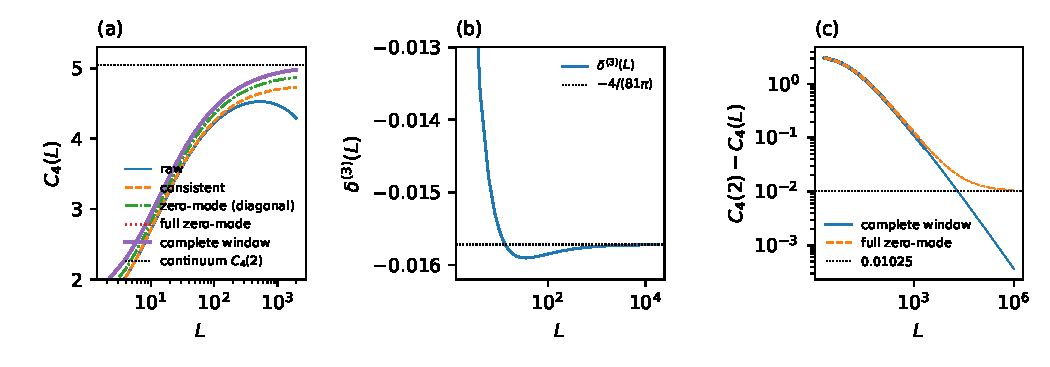
\includegraphics[width=\textwidth]{parts/htp/sections/d2/fig_c4_delta_d2.pdf}
\caption{(a) Exact $C_4(L)$ in $d=2$ for $L\le\HTpTwoLfour$ in five windows: raw, consistent, diagonal zero-mode, full
zero-mode (diagonal and off-diagonal) and complete; only the complete window converges to $C_4^{(2)}$ (dotted). (b) The
$\eps^3$ external-line coefficient $\delta^{(3)}(L)$ of Eq.~\eqref{htp:d2:eq:delta} for $L\le\NTwoDeltaLmax$, with its limit
$-4/(81\pi)$ (dotted); it is not monotone. (c) Distance to the continuum value, $C_4^{(2)}-C_4(L)$, for the complete window
(solid) and the full zero-mode window (dashed); thin lines continue each with its tail fit $T_{22}$ ($300\le L\le2000$,
Appendix~\ref{htp:d2:app:window}). The complete window falls like $\ln^2L/L$; the full zero-mode window levels off at
$0.01025$ (dotted), the part that the mass window $D^M$ supplies. Script \code{make\_fig\_d2.py}.}
\label{htp:d2:fig}
\end{figure}

\subsection{Fifth order}\label{htp:d2:c5}
\emph{All-order window and double counting.} At all orders $D^{\rm zm}$ uses the Bloch matrix of the auxiliary channels
$|z\rangle$ at sub-cutoff $\lambda$, $h(\lambda)=U\,{\rm diag}(E_z(\lambda))\,U^{-1}$ with $U_{z'z}=\langle z'|\psi_z(\lambda)\rangle$, and the mass
window is $D^M=\frac14\{e_1(L)-e_1(L-\hat\ell),M'\}$ with the Newton coefficient $e_1(\lambda)=E_1(\lambda)-E_0(\lambda)$; degenerate partners of $|z\rangle$
($z\ge5$) are projected out. If the auxiliary objects carry their own windows self-consistently, $C_5^W(L)$ diverges linearly,
with coefficient $\NTwoCfiveWLin\pm0.0004$ (the uncertainty of the linear term of raw $C_5$; Table~\ref{htp:d2:tab:c5lin}). The cause is a double counting: a sunset nested in an auxiliary channel is restored once by
the outer $D^M$ and once more inside $h(L-\ell)$. Rule $W_c$ removes it: an auxiliary channel at sub-cutoff $\lambda<L$
represents a zero-mode cluster inside a state of the cutoff-$L$ theory, so its windows are referred to the outer cutoff,
$[h(L)-h(\lambda-\ell_\chi)]$ and $\frac14\{e_1(L)-e_1(\lambda-\hat\ell),M'\}$. It leaves $C_4$ unchanged and removes the linear term (Appendices~\ref{htp:d2:app:Wall} to~\ref{htp:d2:app:tests}).

\emph{External-line window.} In $W_c$ the $\eps^3$ spacing of $\chi_{aa}$ (Sec.~\ref{htp:d2:desc}) tends to a constant,
$R_3\approx\NTwoRthreeWcConst\,a\,w_{aa}$ ($0.062$ to $0.063\,a\,w_{aa}$ at $L=16$ for $a=1$, 2, 3, changing slowly with $L$). An exact test with a tagged external line (Appendix~\ref{htp:d2:app:tag}) locates it: if the external quantum is
invisible to the cutoff and the windows (budget-free), $R_3\to0$; if it is charged its level, $R_3$ reproduces its value
in $W_c$. $D^M$
charges both legs of a mass sub-process with their average level in every slice, which is exact for the $\eps^2$ sunset but not
for the mixed orderings at $\eps^3$. Scheme $W_{cs}$ adds at $\eps^3$
\begin{equation}
 D^{(3)}\mathrel{+}=\frac{\delta^{(3)}(L)}2\,X_0,\qquad \delta^{(3)}(L)=\tfrac14\big[e_1^{(3)}(L-2)-e_1^{{\rm tag},(3)}(L;2,2)\big] ,
 \label{htp:d2:eq:wcs}
\end{equation}
where $X$ is $M'$ with each term multiplied by the summed level of its $\chi$ legs (plus for hops, minus for pair
creation and annihilation), $X_0$ its $\eps^0$ part, and $e_1^{\rm tag}(\lambda;2,2)$ is $E-E_0$ of the $\phi$ channel $|1\rangle$
at cutoff $\lambda$ whose external zero-mode quantum is tagged with charges $(2,2)$: it has level 0 in $H_0$, but the cutoff
and the windows count it as level 2 before it is absorbed and after it is re-emitted (Appendix~\ref{htp:d2:app:wcs}). $\delta^{(3)}(L)$ is an exact rational at each $L$, one number per cutoff; nothing is
fitted (Appendix~\ref{htp:d2:app:wcs} derives the operator form). Chain sums give it for every even $L\le\NTwoDeltaLmax$ (equal to the rationals at $L\le16$ to $\NTwoDeltaRational$).
It is not monotone, with a minimum $\NTwoDeltaMin$ at $L=\NTwoDeltaMinL$ (Fig.~\ref{htp:d2:fig}b), and
\begin{equation}
 \delta^{(3)}(L)=-\frac4{81\pi}-\frac1{54\pi}\,\frac{\ln L}L+\mathcal O(1/L) ,
 \label{htp:d2:eq:delta}
\end{equation}
where the limit $\delta_\infty=-\frac4{81\pi}$ (to $\NTwoDeltaIdent$ by free-limit fits) and the $\ln L/L$ coefficient are
identified numerically, not derived. With this identification the shift $4a\,w_{aa}\delta_\infty=-\frac{16}{81\pi}a\,w_{aa}$
of $R_3(\chi_{aa})$ that the window produces is two thirds of the $\eps^2$ exchange-sunset defect $\frac{8}{27\pi}a\,w_{aa}$
of $R_2$, and $\frac{16}{81\pi}=0.0629$ is close to the $W_c$ remainder above. The shift is therefore expected to cancel
that remainder as $L\to\infty$; this is not established, since $R_3$ is known only to $L=16$. $W_{cs}$ leaves $C_0$ to
$C_4$, $r_{\le3}$ and $g_{\le3}$ unchanged and shifts $C_5$ by $\delta^{(3)}(L)S(L)$, with $S(L)$ the $C_5$ response to
$\frac12X_0$; $S$ has no $\ln L$ and $S_\infty\equiv S(\infty)=\NTwoSinf$, so the shift tends to
$\delta_\infty S_\infty=\NTwoDeltaS$.

\emph{Data and tail} (Appendix~\ref{htp:d2:app:c5tail}). $C_5^{W_{cs}}(L)$ is raw $C_5$ to $L=\HTpTwoLfive$ plus the exact $W_c$ shift and $\delta^{(3)}S$ (both
known to $L=\NTwoShiftLmax$). The tails of $C_2$ to $C_4$ carry $\ln^{n-2}L/L$, and hold-out tests select $\ln^3L/L$ for $C_5$. The
fits use
\begin{equation}
 C_5(L)=A+\sum_{j=0}^{3}a_j\frac{\ln^jL}{L}+\sum_{j=0}^{k_2}a'_j\frac{\ln^jL}{L^2},\qquad k_2\in\{0,1,2\},
 \label{htp:d2:eq:C5tower}
\end{equation}
with no $\ln L$ term, on every even $L$ from $L_{\min}\in\{30,40,60,80,100\}$ to 300. Fitted to $L\le200$, these forms
predict $L=202$ to 300 to $\NTwoBlindNoLog$, against $\NTwoBlindFreeLog$ with a free $\ln L$; fitted to $L\le240$, both
predict $L=242$ to 300 to about $6\times10^{-7}$ (Appendix~\ref{htp:d2:app:c5tail}). The median and half range
of the 15 fits give
\begin{equation}
 C_5=\HTpCfiveTwo\qquad\text{against}\qquad C_5^{(2)}=-38.8336459 ,
 \label{htp:d2:eq:C5}
\end{equation}
with the unrounded median $\NTwoCfiveMedian$, $0.0018$ below the continuum value. Towers with one more power of $\ln L$
at $1/L$ ($k_1=4$), which the hold-out test does not exclude, move the median by only $\NTwoCfiveKfourShift$ but widen the half range
of the fits from $0.013$ to $\NTwoCfiveKfourHalf$ (Appendix~\ref{htp:d2:app:c5tail}); the quoted uncertainty does not include
this. Without the external-line window,
$C_5^{W_c}=\NTwoCfiveWc$ (median $\NTwoCfiveWcMedian$), higher by about $-\delta_\infty S_\infty$ as expected. Both agree
with the continuum value within the spread of the fits, so $C_5$ does not distinguish $W_c$ from $W_{cs}$; the case for
the external-line window rests on the spacing $R_3$ (Sec.~\ref{htp:d2:desc}).

\emph{Residual logarithm.}\label{htp:d2:c5log} A term $b\ln L$ that the data cannot see would move the limit. Over the 15
fits of Eq.~\eqref{htp:d2:eq:C5tower}, the median of the free coefficient drifts from $\NTwoBfreeTwoHundred$ at $L_{\max}=200$
to $\NTwoBfreeThreeHundred$ at 300; a second set of twelve fits ($L_{\min}=30$ to 80) drifts from $-0.0134$ to $+0.0054$
(Appendix~\ref{htp:d2:app:c5tail}). On $C_4^W$, which has no $\ln L$, the 15-fit estimator returns $\NTwoBnull$. On a synthetic
series with a $C_5$-like tail and a known $b$, both sets read about $\NTwoBbias$ low; corrected for this bias, the median
is about $\NTwoBcorr$ (15 fits; $+0.009$ with 12). We take $|b|\lesssim\NTwoBbound$ as a judgement from this median, its
drift and its bias; it is not a confidence bound. The individual fits of the 15-fit set range from $\NTwoBfitMin$ to
$\NTwoBfitMax$, but the extreme ones have nearly as many parameters as points; taken as a bound they would allow shifts of
$C_5$ between about $-0.7$ and $+0.5$. In the 15 fits, fixing $b=\mp\NTwoBbound$ moves the limit by about
$\pm\HTpCfiveTwoLog$, and $b=\NTwoBcorr$ would move it by about $-0.08$; bounding $|b|$ well below $\NTwoBbound$ would
need $L\gtrsim\NTwoLneeded$. The external-line class itself gives no $\ln L$: the
$\ln L$ terms of $S$ cancel within the hop and within the pair sector separately.

\emph{Status.} The complete window has no fitted parameter, removes the $\ln L$ and is verified through $\eps^4$. At $\eps^5$
the rule $W_c$ is needed to remove a linear divergence, and the external-line window to reduce $R_3$ (by at least
$\HTpTwoIdentThree\%$ at $L=14$ and 16). With both, $C_5$ agrees with the continuum. Both rules are provisional: they are
not derived in full, and the window is not proven complete at this order. Like all windows here, they were derived after
their effect had been seen and with the continuum values known.

\subsection{Descendant spacings}\label{htp:d2:desc}
A descendant lies an integer above its primary at every order. With
\begin{equation}
 R_n(L)=\big[E(\chi_{aa})-E(\phi)-2a\big]_{\eps^n},
 \label{htp:d2:eq:R}
\end{equation}
the $\eps^n$ coefficient of the spacing of $\chi_{aa}=\partial^a\bar\partial^a\phi$ computed with the same $r$, $g$ and
window, and the same for the descendants $(\partial\bar\partial)^a\phi^2$ of $\phi^2$, the exact small-$L$ solvers
\code{complete\_exact} and \code{ce\_wc} (Sec.~\ref{htp:d2:solvers}) give every $R_n$, $n\le8$, as rationals for $L\le16$ in each
scheme. These tests need no continuum input; Appendix~\ref{htp:d2:app:legs} gives the data.
\begin{itemize}
\item $\eps^2$: in the consistent and zero-mode windows the exchange sunset of $\chi_{aa}$ has only $L-4a$, and
 $R_2\to\frac{8a\,w_{aa}}{27\pi}$ ($\NTwoRtwoCons$ for $\chi_{11}$ at $L=16$). $D^M$ shifts it by exactly
 $-\frac{8a\,w_{aa}}{27\pi}$, so in the complete window $R_2$ decays like $1/L$ ($\NTwoRtwoWcoef/L$ for $\chi_{11}$), also for
 the $\phi^2$ descendants.
\item $\eps^3$, single-quantum descendants: $R_3(\chi_{11})$ is $\NTwoRthreeWcSixteen$ in $W_c$ and $\NTwoRthreeWcsSixteen$ in
 $W_{cs}$ at $L=16$. At $L=14$ and 16 the window leaves at most 3\% of the $W_c$ value for $a=1$ to 3, so at least
 $\HTpTwoIdentThree\%$ of the defect is removed at $L=14$ and 16. Free-limit fits of $\chi_{11}$ leave a few percent, and the window is
 expected to cancel the defect as $L\to\infty$ (above); $R_3$ itself is not computed beyond
 $L=16$.
\item $\eps^3$, descendants of $\phi^2$: at $L=16$, $R_3=\NTwoPhiDescTwo$ (level 2) and $\NTwoPhiDescFour$ (level 4) in $W_{cs}$;
 the level-4 value still moves away from zero. Not settled.
\item $\eps^4$: in $W_c$ and $W_{cs}$, $R_4(\chi_{11})$ grows, with a local slope of about $\NTwoRfourSlope$ per unit of $\ln L$
 at $L=8$ to 16, while with budget-free legs it goes
 to zero: the same leg defect one order higher. A partial $\chi$-line window ($W_{cs4\chi}$, calibrated on $\chi_{11}$, with the
 $\eps^4$ difference between the $\chi$-line and zero-mode self-energies as a spectator term) closes $\NTwoGapTwo\%$ and
 $\NTwoGapThree\%$ of the gaps of $\chi_{22}$ and $\chi_{33}$ to their budget-free lines at $L=14$, but the $\chi_{22}$ gap is not
 shrinking, the $\phi^2$ descendants still grow, and $R_5(\chi_{aa})$ grows. The window coefficient grows roughly like $\ln L$
 at $L\le16$, which suggests that
 $C_6$ in $W_c$ carries about $\NTwoCsixLog\ln L$ (a prediction, not a measurement). The $\eps^4$ window is not yet known.
\end{itemize}

\subsection{Sixth to eighth order}\label{htp:d2:c6}
$C_6$ to $C_8$ are not reproduced. At $L=16$, $C_6\approx\NTwoCsixSixteen$ in $W_c$, $W_{cs}$ and $W_{cs4\chi}$
(Table~\ref{htp:d2:tab:c6}), $54\%$ below the continuum value $\NTwoCsixCont$, and $C_6(L)$ still rises by about
$\NTwoCsixStep$ per step of 2 in $L$. The external-line windows shift $C_6$ by about $10^{-4}$ of its value there, while
$W$ and $W_c$ differ by about 1\% (Appendix~\ref{htp:d2:app:c6eps5}). The production tables to $L=\HTpTwoLprod$ (raw and
consistent) are shipped as finite-cutoff data, but those windows diverge from $\eps^4$ on, and the external-line windows
from $\eps^4$ on are not known.
}{\section{Results in two dimensions}\label{htp:d2:sec}(Contribution of HT2dPert pending.)}
\IfFileExists{parts/htp/sections/d3/sec_d3.tex}{% sec_d3.tex (HT3dPert, 2026-10-14, second version; edited by HT1dPert 2026-10-15 for the note review, facts from
% HT3dPert): d = 3 perturbative HT. Numbers: numbers_d3.tex; table tab_d3_coeffs.tex (code/lri_3d_hpc/public/note_d3.py);
% figure fig_d3_c4.pdf (code/lri_3d_c4_exact/public/note_fig_d3.py); reproduction rows: repro_d3.tex; package rows:
% packages_d3.tex; checks and caveats: checks_d3.tex, caveats_d3.tex.
\section{Results in three dimensions}\label{htp:d3:sec}

\paragraph{Model and cutoff.}
In $d=3$ the generalized free field is quantized on $S^2$ (Sec.~\ref{htp:sec:method}, Ref.~\cite{htp:Hogervorst:2014rta}). A
mode $(n,\ell,m)$ has energy $\Ds+2n+\ell$, with $\ell$ the angular momentum; the zero mode $n=\ell=0$ is the local
oscillator, and all other modes form the bath. We keep the states with bath level
\begin{equation}
 N_b=\sum_{(n,\ell,m)\neq(0,0,0)}(2n+\ell)\,n_{n\ell m}\le L
 \label{htp:d3:eq:cutoff}
\end{equation}
and do not truncate the zero mode. The perturbation is $H=H_0+r\,M+g\,V$ with
$M=\int d\Omega\,{:}\phi^2{:}/(4\pi)$ and $V=\int d\Omega\,{:}\phi^4{:}/(48\pi)$. $r$ and $g$ are tuned order by order
to $E_1-E_0=\Ds$ and $E_3-E_0=3-\Ds$, and
\begin{equation}
 \DE(\eps;L)=E_2-E_0=\tfrac32-\tfrac{\eps}{6}+\sum_{n\ge2}C_n(L)\,\eps^n,\qquad \Ds=\frac{3-\eps}{4}.
 \label{htp:d3:eq:Cn}
\end{equation}
The continuum values $C_n^{(3)}$ are those of Table~\ref{htp:tab:refvals}.

\paragraph{Two codes.}
The production package (\code{code/lri\_3d\_hpc/}) builds the truncated Hamiltonian explicitly in the SO(3)-scalar,
inversion-even sector and solves the Rayleigh--Schr\"odinger recursion through $\eps^8$ in x87 long double. It reached
$L=16$, 18 and \HTpThreeLmax{} (\NThreeScalarTwenty{} scalar bath states at $L=20$, from \NThreeStatesTwenty{} before
the projection; about \NThreeSU{} service units on SDSC Expanse, charge units of about one per core-hour, with
large-memory jobs charged more). It implements two prescriptions: raw, and the vacuum window
$D_L(N_b)=E_v(L)-E_v(L-N_b)$.

The exact-sum package (\code{code/lri\_3d\_c4\_exact/}) evaluates the same coefficients as sums over intermediate states,
with exact partial-wave reductions on $S^2$ and exact zero-mode projections, at every even $L$:
\begin{itemize}
\item $C_2$ to $L=\HTpThreeLwin$, $C_3$ and $C_4$ to $L=\HTpThreeLfour$, $C_5$ to $L=\HTpThreeLfive$;
\item every window shift to $L=\HTpThreeLwin$;
\item every window scheme, including the complete window of $d=2$ (Sec.~\ref{htp:d2:sec}).
\end{itemize}
At every even $L\le20$ the two codes agree on $C_2$ to $C_5$, $r$, $g$ and the reference energies $E_0$ to $E_3$ to
$\NThreeValPkg$. The window schemes that the production package lacks agree with a brute force, built as explicit
operators on the package's own Hamiltonian at $L\le14$, to $\NThreeValBrute$. Table~\ref{htp:d3:tab:coeffs} gives the
production values.

\input{parts/htp/sections/d3/tab_d3_coeffs.tex}

\paragraph{The vacuum window diverges at $\eps^4$.}
$C_2(L)$ and $C_3(L)$ do not depend on the window and converge. From $C_4$ on, the vacuum window does not suffice
(Fig.~\ref{htp:d3:fig:c4}).
\begin{itemize}
\item As in $d=2$, divergent sub-bubbles inside a state see only the level left by the other quanta, while $r$, $g$ and
 the vacuum are tuned with the full $L$.
\item In $d=3$ the mass sub-bubble diverges like $L^{3/2}$ instead of $L$, so every term is one power worse.
\item Uncorrected, $C_4(L)$ falls like $-\NThreeRawLsq\,L^2$.
\item With $D_L$ alone it peaks at $\NThreeCfourConsPeak$ near $L=32$ and is $\NThreeCfourConsSix$ at $L=600$. The
 terms are $-\NThreeConsLin\,L$ and $-\tfrac{10}{243\,\Gamma(7/2)}\sqrt L\ln L$, which the diagonal and
 zero-mode-number-changing parts of the zero-mode window remove.
\item The mass window ($\chi$-attached sunset term), which in $d=2$ is a finite shift, here removes a further
 $\NThreeChiSqrt\sqrt L$.
\end{itemize}

\paragraph{Complete window.}
The complete window $W$ of $d=2$ is carried over unchanged: vacuum window, full zero-mode window, and mass window
$-\tfrac12 r_2'(L)\{\hat N_b,M'\}$, with $\hat N_b$ the bath-level operator. With it, $C_4(L)$ converges like $1/L$. At
$L=600$ it is $\NThreeCfourWsix$. With the limit fixed at $C_4^{(3)}$, a free $\sqrt L$ term comes out below
$\NThreeNoDiv$. The mass window is used in its leading-order linear form; since $r_2$ is not linear in $L$ in $d=3$, the
exact form may differ by a finite amount, which the agreement below suggests is small but which is not derived.

At $\eps^5$ the nested windows are referred to the outer cutoff (rule $W_c$ of $d=2$); the external-line window
($W_{cs}$) changes $C_5(40)$ by $-0.003$.

\begin{figure}[ht]\centering
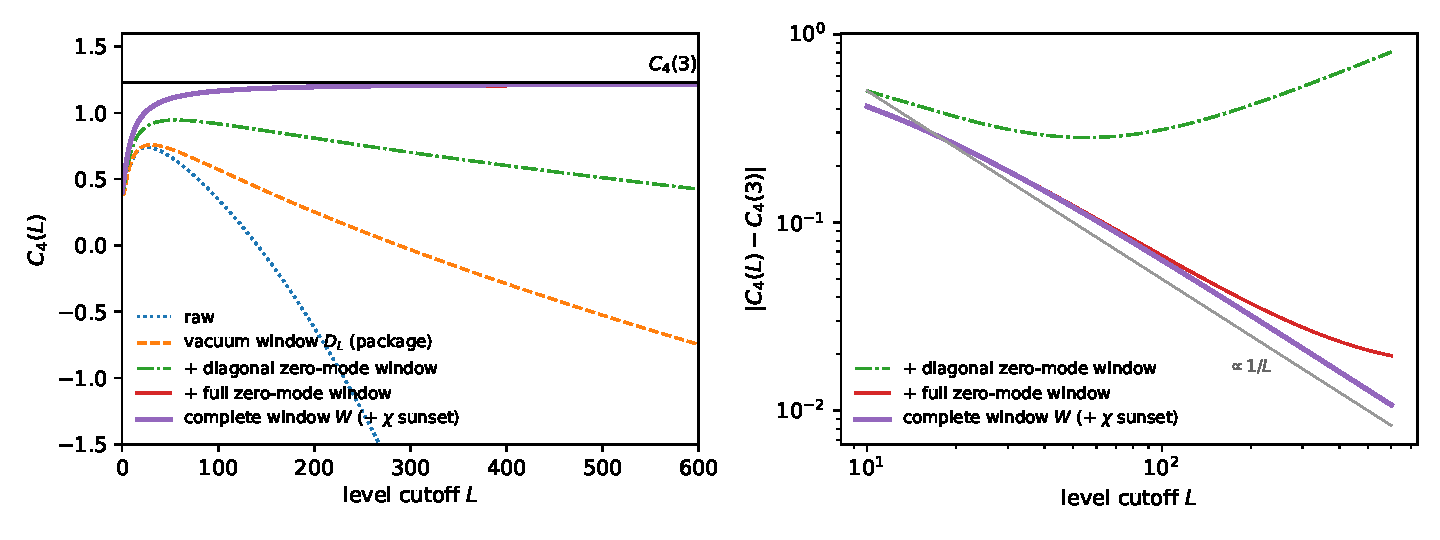
\includegraphics[width=\linewidth]{parts/htp/sections/d3/fig_d3_c4.pdf}
\caption{$C_4(L)$ in $d=3$ from the exact sums, in each window scheme. Left: raw, the vacuum window $D_L$ of the
production package, and the zero-mode and mass windows added one by one (the full-zero-mode curve lies under $W$ at this
scale). Right: distance from $C_4^{(3)}$ on logarithmic axes. The complete window $W$ converges like $1/L$; without its
mass window the distance stops decreasing, has its minimum near $L\approx1100$ and grows like $3.6\times10^{-4}\sqrt L$
beyond the plotted range.}
\label{htp:d3:fig:c4}
\end{figure}

\paragraph{Extrapolations.}
Fit forms (towers of $L^{-k}\ln^jL$ terms, from the $d=2$ protocol) and windows were chosen after the data were seen,
with the continuum values known; the quoted uncertainties are spreads over fits, not standard errors.
\begin{itemize}
\item $C_2=\HTpCtwoThree$ ($\HTpCtwoThreeDigits$ digits of the closed form; fit to $L\le\HTpThreeLwin$).
\item $C_3=\HTpCthreeThree$ ($\delta=\HTpCthreeThreeDev$): mean and half-range of three fit windows.
\item $C_4=\HTpCfourThree$ ($\delta=\HTpCfourThreeDev$): median of one tower over 12 fit windows; the uncertainty is
 the half-range, including a blind fit to $L\le400$ that predicts $402\le L\le600$ to $\NThreeCfourBlind$. Towers with
 one more correction term spread to about $10^{-4}$.
\item $C_5$, provisional and calibrated on $C_4^{(3)}$: towers are kept if, on $C_4^W(L)$ at the same $L\le40$, they
 reproduce $C_4^{(3)}$ to within 0.036 and pass a blind test. The median of their $C_5$ fits gives $\HTpCfiveThree$
 (median $\NThreeCfiveMed$) against $C_5^{(3)}=-5.850351421$. The uncertainty is the worst $C_4$ miss relative to the
 remaining $C_4$ correction at $L=40$ (0.036 of 0.147), times the remaining $C_5$ correction at $L=40$ (1.28, which
 uses $C_5^{(3)}$ itself).
 \begin{itemize}
 \item This is a weak test: $C_5^{W_c}(40)=\NThreeCfiveWcForty$ is still 1.28 above the limit.
 \item A term in $L^{-1/2}$, which $L\le40$ cannot exclude, would lower the limit by 0.5 to 1.
 \item A window without the mass window also fits at $L\le40$, although it differs from $W_c$ by a term growing like
  $L^2$.
 \item Going further needs a new representation of the angular channels: the cost grows like $L^{8.4}$ and the memory
  like $L^{4.5}$.
 \end{itemize}
\end{itemize}

\paragraph{Descendant spacings.}
For the scalar descendant of $\phi$ (the $n=1$, $\ell=0$ quantum), the window removes the $\eps^2$ violation of its
spacing as $L\to\infty$. At $\eps^3$ the external-line window acts in the right direction, but the violation is not shown
to vanish at $L\le16$.
}{\section{Results in three dimensions}\label{htp:d3:sec}(Contribution of HT3dPert pending.)}
% s06_checks.tex (HT1dPert): independent checks; d = 2, 3 paragraphs are \input from their folders.
\section{Independent checks}\label{htp:sec:checks}

\paragraph{One dimension.}
\begin{itemize}
\item \emph{Window engines.} The complete window through $\eps^5$ was computed by two independent engines, one on the
 solver's kernels and one written from scratch with exact rationals, plus a third engine for a skeptic's check. Four
 algorithms within the second engine agree to $1.3\times10^{-11}$; the two engines agree on 3808 numbers to
 $9.6\times10^{-12}$; the third reproduces $\Delta C_5$ at $\Lambda\le28$ to $2.4\times10^{-12}$
 (quoted as $\HTpEngineAgree$ in the paper).
\item \emph{Eighth-order window.} The complete-window solver reproduces the exact $\Delta C_4$, $\Delta C_5$ at
 $\Lambda=46$--$72$ to $\HTpSTenMatch$.
\item \emph{Exact sums against the solver.} The exact sums reproduce the solver's raw $C_4$ and $C_5$ at
 $\Lambda\le118$ to $1.4\times10^{-12}$ and $10^{-11}$, and the window pieces to $10^{-15}$; brute-force
 Rayleigh--Schr\"odinger on explicit bases at small cutoffs agrees to $10^{-11}$.
\item \emph{Eighth-order code.} The optimized eighth-order code reproduces the 38 saved records of its original
 version to $2.1\times10^{-8}$ and the thermal solver's $C_0$--$C_7$ to $6\times10^{-14}$ relative.
\item \emph{Blind protocol of the exact sums.} Fit records were frozen and hash-committed before each larger run
 existed: $\Lambda\le1000$ before $2000$ for $C_4$, $\Lambda\le320$ before 400 and $\Lambda\le400$ before 500 for $C_5$.
 Their predictions of the new cutoffs are quoted in Section~\ref{htp:d1:sec:extrap}.
\item \emph{Constrained $C_5$.} A separately written fit of the constrained extrapolation, made without reading the
 package's fit code, gives $\HTpCfiveOne$; a separate derivation confirms $\omega_1=\tfrac72$ as the one-loop
 exponent of $\phi^6$ and the closed form \eqref{htp:eq:toplog}.
\end{itemize}
\IfFileExists{parts/htp/sections/d2/checks_d2.tex}{\input{parts/htp/sections/d2/checks_d2.tex}}{}
\IfFileExists{parts/htp/sections/d3/checks_d3.tex}{\input{parts/htp/sections/d3/checks_d3.tex}}{}

% s07_caveats.tex (HT1dPert); d = 2, 3 paragraphs are \input from their folders.
\section{Caveats}\label{htp:sec:caveats}

\paragraph{One dimension.}
\begin{itemize}
\item The windows were derived after their effects had been seen and with the continuum values known, though with no
 fitted parameter.
\item The extrapolation dominates the error, and the exponents \eqref{htp:eq:omega} are an assumption. Fits that reach the
 exact $C_5$ need an effective $\omega_3$ of $\HTpOmegaThreeEff$, not the gap value $\HTpOmegaThree$. A second channel
 with the leading power $\Lambda^{-1/2}$, from the phase operator of the cutoff kernel, enters at $\eps^4$ (cited check
 \code{code/lri\_d1\_fullblock\_tail\_response}); it does not affect the top logarithm \eqref{htp:eq:toplog} but does affect
 the lower ones, so tying them to $\omega_2$, $\omega_3$ is not exact.
\item The $\eps^4$ top-log coefficient fitted from the exact $C_4(\Lambda)$ lies $\NOneTopLogFour$ from
 Eq.~\eqref{htp:eq:toplog}, depending on the basis; whether this is a real violation is undecided. Taking $c_5$ from the
 $C_2$ chain of Eq.~\eqref{htp:eq:toplog} instead, a value $0.3\%$ smaller, moves the constrained $C_5$ by $4\times10^{-4}$ to
 $1.4\times10^{-3}$ (absolute), far below its quoted uncertainty (\code{xchk/REPORT\_blind.md} of \code{lri\_1d\_c5\_exact}).
\item A test protocol for the raw $C_4$ and $C_5$, fixed before most of the large-cutoff data had been seen, had mixed
 results: its held-out predictions passed; window stability failed for $C_5$ in two of three bases and for $C_4$ in one,
 and tail insensitivity failed for $C_5$. Every $d=1$ fit beyond $C_3$ involves choices made after the data were seen, apart from the blind
 predictions of the exact sums. The constrained $C_5$ fit's selection thresholds were set after a run had printed the
 exact value; the separately written fit is the quoted determination.
\item $C_8$, calibrated on the diagrammatic $C_6$ and $C_7$, is not an independent determination.
\item We have not constructed an effective Hamiltonian beyond the windows.
\end{itemize}
\IfFileExists{parts/htp/sections/d2/caveats_d2.tex}{\input{parts/htp/sections/d2/caveats_d2.tex}}{}
\IfFileExists{parts/htp/sections/d3/caveats_d3.tex}{\input{parts/htp/sections/d3/caveats_d3.tex}}{}

% s08_repro.tex (HT1dPert): reproduction section; rows come from repro_d1.tex, sections/d2/repro_d2.tex, sections/d3/repro_d3.tex
\section{Reproduction}\label{htp:sec:repro}

\subsection{Layout}
All paths are relative to the folder \code{HT\_Pert/} of the public repository.
\begin{itemize}
\item \code{code/<package>/}: one package per solver or analysis, shipped at the commit its production ran. Each has a
 \code{public.mk} with the targets \code{test} and \code{replay} (some also \code{smoke}, \code{replay-full},
 \code{fetch-data}) and a \code{public/} folder with the replay scripts.
\item \code{data/HT\_<d>d/}: the production records.
\item \code{results/HT\_<d>d/}: the expected value of every quoted number (\code{quoted\_numbers.json}) and summaries.
\end{itemize}
\code{make test} and \code{make replay} in \code{HT\_Pert/} run the targets of every package; in a package folder,
\code{make -f public.mk test|replay}. A replay recomputes every quoted number of its package from the shipped records,
without a production rerun, prints a PASS/FAIL table and exits non-zero on any failure.

\subsection{Packages and records}
\begingroup\footnotesize\renewcommand{\arraystretch}{1.15}
\begin{longtable}{@{}p{4.4cm}p{2.3cm}p{8.2cm}@{}}
\toprule
package (\code{code/}) & $d$, role & content, records, cost\\
\midrule\endhead
\bottomrule\endfoot
\code{lri\_hpc\_Hamitonian} & 1: solver, analyses & HT solver to $\eps^7$; joint tail fits, window engines, identities. Records \code{data/HT\_1d/thermal\_expanse} (111 cutoffs) and the analysis outputs \\
\code{lri\_eh\_hpc} & 1: window & isolated $g^2D$ window, closed form $K$ \\
\code{lri\_c8\_hpc} & 1: solver & eighth order, $\Lambda\le\HTpLamCeight$; records \code{data/HT\_1d/c8} \\
\code{lri\_d1\_full\_coefficient\_flow} & 1: solver & complete window through $\eps^8$, $\Lambda\le\HTpWinLamEight$; records \code{data/HT\_1d/s10\_production} \\
\code{lri\_1d\_dconn\_refit} & 1: analysis & extrapolations of $C_4$--$C_8$ with the complete window \\
\code{lri\_1d\_c4\_exact}, \code{lri\_1d\_c5\_exact} & 1: exact sums & $C_2$--$C_4$ to $\Lambda=\HTpOneLexact$, $C_5$ to $\NOneCfiveLmax$; records \code{data/HT\_1d/exact\_c4}, \code{exact\_c5}; blind fit records \\
\code{lri\_d1\_fullblock\_tail\_response} & 1: cited check & second $\Lambda^{-1/2}$ channel \\
\IfFileExists{parts/htp/sections/d2/packages_d2.tex}{\inputrows{parts/htp/sections/d2/packages_d2.tex}}{}
\IfFileExists{parts/htp/sections/d3/packages_d3.tex}{\inputrows{parts/htp/sections/d3/packages_d3.tex}}{}
\end{longtable}
\endgroup

\subsection{Rules that are part of the results}
The fit families and windows, the selection and calibration rules, the rounding of quoted ranges and the status words
are part of the results; the \code{REPRODUCE} file of each package lists them under ``Decisions you must not make''.

\subsection{\texorpdfstring{Result $\to$ code, record, command, tolerance}{Result to code, record, command, tolerance}}
\begingroup\footnotesize\renewcommand{\arraystretch}{1.15}
\begin{longtable}{@{}>{\raggedright}p{3.7cm}>{\raggedright}p{2.8cm}p{0.8cm}>{\raggedright}p{2.75cm}>{\raggedright}p{2.25cm}>{\raggedright\arraybackslash}p{1.6cm}@{}}
\toprule
result & value & pkg & records & command & tolerance\\
\midrule\endhead
\bottomrule\endfoot
\inputrows{parts/htp/sections/repro_d1.tex}
\midrule
\inputrows{parts/htp/sections/d2/repro_d2.tex}
\midrule
\inputrows{parts/htp/sections/d3/repro_d3.tex}
\end{longtable}
\endgroup

\appendix
% app_d2_eps4.tex -- d = 2 appendix, part 1 of 3 (HT2dPert, 2026-10-16): operators and schemes at low order, solver
% checks, exact C4(L), the mechanism of the ln L divergence class by class, and the complete window at eps^4.
% Merged from the method write-up of package I (public edition of 2026-10-14), which these appendices
% replace; superseded material is not carried over, and what Sec. d2:sec states is not repeated.
% Notation of Sec. d2:sec and Table tab:notation (level l, operator \hat l, sub-cutoff lambda, e_1 = E_1 - E_0).
% Numbers quoted in Sec. d2:sec use the macros of numbers_d2.tex (replay rows in repro_d2.tex); every other number is
% read from, or (where marked) evaluated from, the records named in the subsection (all shipped in package I).
\section{Two dimensions: operators, exact fourth order and the complete window}\label{htp:d2:app:eps4}

Appendices~\ref{htp:d2:app:eps4} to~\ref{htp:d2:app:legs} give the derivations and the supporting data behind
Section~\ref{htp:d2:sec}. This appendix covers the operators and schemes at low order, the solver checks, the exact $C_4(L)$,
the cause of its $\ln L$ divergence class by class, and the complete window at $\eps^4$. Appendix~\ref{htp:d2:app:eps5}
treats order $\eps^5$: the window at all orders, the double counting that rule $W_c$ removes, and the tail of $C_5$.
Appendix~\ref{htp:d2:app:legs} treats the descendant spacings and the external-line windows $W_{cs}$ and $W_{cs4\chi}$, and
ends with the status of each window component. Paths are relative to the package
\code{code/\allowbreak{}lri\_2d\_coeff\_independent\_check/} (package I of Section~\ref{htp:sec:repro}), and each subsection names its
records. Numbers that Section~\ref{htp:d2:sec} also quotes have reproduction rows in Section~\ref{htp:sec:repro}. The other numbers
of these appendices are read from the records named in each subsection, or evaluated from them where the text says
so; the reproduction scripts do not recompute them. ``Exact'' data
are rationals, or float64 evaluations of exact finite sums with a measured rounding error of at most
$1.4\times10^{-11}$. Limits $L\to\infty$ are fits; their uncertainties are spreads over tail models and fit windows, not
standard deviations.

\subsection{Operators and schemes at low order}\label{htp:d2:app:ops}
{\small\raggedright\noindent Records: \code{SPEC.md}, \code{rs\_exact/\allowbreak{}README.md}, \code{zeromode\_exact/\allowbreak{}README.md},
\code{cauchy/\allowbreak{}README.md}.\par}

\paragraph{Factorized vertices.} With $Z=a_0+a_0^\dagger$, $a_0=A_{00}$, and $\chi=\phi-Z$, normal ordering factorizes:
\begin{equation}
 V=\sum_{m=0}^4\frac1{12}\binom4m{:}Z^{4-m}{:}\otimes\langle{:}\chi^m{:}\rangle_\theta,\qquad
 M=\sum_{m=0}^2\binom2m{:}Z^{2-m}{:}\otimes\langle{:}\chi^m{:}\rangle_\theta .
 \label{htp:d2:eq:factorize}
\end{equation}
At $\eps=0$ the weights factorize holomorphically, $w_{ab}=v(a)v(b)$ with $v(a)=(\frac12)_a/a!$. The squared
$V$-vertex coefficient times the Wick count of a bundle of $m$ $\chi$ lines is
$\gamma_m=m!\,\big[\binom4m/12\big]^2$: $\gamma_1=\frac19$, $\gamma_2=\frac12$, $\gamma_3=\frac23$, $\gamma_4=\frac16$.

\paragraph{Space and particle cap.} The truncated space holds the occupation states with spin zero, even under
$(a,b)\to(b,a)$, and $\ell\le L$; spin zero forces $\ell$ even, and the field parity $(-1)^P$ is conserved. Truncated
operators are the projections of the full ones; nothing else is truncated. The level cutoff does not bound $P$, because
zero-mode quanta cost no level. A path argument shows that a contribution to the order-$\eps^n$ energy of $|p\rangle$
reaches at most $P=p+4\lfloor n/2\rfloor$, which gives the cap $P\le p+16$ through $\eps^8$. It was also tested: caps
$p+18$ and $p+20$ reproduce the $p+16$ rationals identically, while $p+14$ changes $C_8$ and nothing below. The Cauchy
code confirms it with absolute caps: $P\le21$ and $P\le23$ reproduce $P\le19$, and $P\le17$, 18 change only $C_8$.

\paragraph{References and the projection $\Pi$.} Each reference $|p\rangle$ is non-degenerate in its sector, so $E_p(\eps)$
is unique. Because $w_{00}=1$ and every window has vanishing diagonal elements on level-0 states, $\langle p|M|p\rangle=2p$ and
$\langle p|V|p\rangle=\frac12p(p-1)$ at every $\eps$. With $\mathcal E_p^{(n)}$ the order-$n$ energy without the $r_n$,
$g_n$ terms, Eq.~\eqref{htp:eq:Pi} reads $C_n=\Pi[\mathcal E^{(n)}]$ with
\begin{equation}
 \Pi f=f(2)-f(1)-\tfrac13\big[f(3)-f(0)\big]=-\tfrac13\Delta^3f(0),\qquad \Pi[p^3]=-2,\qquad \Pi[p^4]=-12 ,
 \label{htp:d2:eq:Pi}
\end{equation}
and $\Pi$ annihilates every polynomial of degree at most two in $p$. Only the part of an energy shift that is at least
cubic in $p$ reaches $C_n$.

\paragraph{Where the schemes differ.} The diagonal windows (consistent, literal, zero-mode) are of order $\eps^2$ and
vanish on $|p\rangle$, so they first enter through $\langle p|H_1G_pD_2G_pH_1|p\rangle$ at $\eps^4$, with $H_1=F_1+g_1V$ and the resolvent
$G_p=Q_p/(\frac p2-H_0)$, $Q_p$ the projection off $|p\rangle$. Raw and consistent therefore differ first at $C_4$. Raw
and consistent vacua agree through $\eps^3$, so the consistent and literal windows differ first at $C_6$; the exact data
confirm both statements for every $L>0$. At $\eps^4$ only the $\eps^2$ parts of the windows matter:
\begin{equation}
 D^{\rm cons}_2(\ell)=E_v^{(2)}(L)-E_v^{(2)}(L-\ell),\qquad
 E_v^{(2)}(\lambda)=g_1^2\langle0|VG_0V|0\rangle_\lambda=-\frac{(\lambda+2)(\lambda+4)}{864},
 \label{htp:d2:eq:Ev2}
\end{equation}
where $\langle\cdot\rangle_\lambda$ restricts the intermediate states to level $\le\lambda$, and the zero-mode window is
$D_2^{\rm zm}(z,\ell)=h^{(2)}_{zz}(L)-h^{(2)}_{zz}(L-\ell)$, the diagonal of Eq.~\eqref{htp:d2:eq:Dzm}. The $r_2$ and $g_2$ terms of
the sub-cutoff energies cancel in these differences, and for $z=0$ the two windows coincide.

\paragraph{Degenerate partners.} For $z\ge5$ the zero-mode channel $|z\rangle$ has degenerate partners with level
$\ell=2,4,\dots\le\frac{z-1}2$ and $P=z-2\ell$. First order lifts the degeneracy (smallest separation $\frac73$, at $z=5$,
$\ell=2$), so the branch through $|z\rangle$ is unique; the references are never degenerate. The window objects project
the partners out (Appendix~\ref{htp:d2:app:Wall}).

\subsection{Solver checks in detail}\label{htp:d2:app:checks}
{\small\raggedright\noindent Records: \code{compare\_with\_package.txt}, \code{compare\_three\_way.txt}, \code{rs\_exact/\allowbreak{}README.md},
\code{cauchy/\allowbreak{}README.md}, the production records \code{../\allowbreak{}../\allowbreak{}data/\allowbreak{}HT\_2d/\allowbreak{}prod/}, \code{continuum/\allowbreak{}exact\_C2\_C3.csv}, \code{continuum/\allowbreak{}asymptotics\_C2\_C3.txt}; code
\code{continuum/\allowbreak{}exact\_low\_orders.py}.\par}

\paragraph{The three computations.} Section~\ref{htp:d2:solvers} and the independent-checks paragraph of
Section~\ref{htp:sec:checks} give their scope and agreement. The production solver propagates Taylor jets of the wave
functions in float64, with scalar reductions in extended long double; its consistent run at $L=34$ took 2893\,s on 64
threads with a peak memory of 463\,GiB. The exact solver works in a similarity frame in which every matrix element is
rational; its modular code uses 72 primes with Chinese remaindering, and every rational reconstruction is verified on
eight held-out primes. The Cauchy solver evaluates $\DE$ at $\eps_k=\rho\,e^{2\pi\mathrm ik/K}$ with $\rho=\frac1{64}$,
$K=128$ and 256-bit arithmetic, and $C_n=K^{-1}\sum_k\DE(\eps_k)\eps_k^{-n}$. It solves the consistent vacua exactly. On states with
$\ell\ge2$ the window is $E_v(\lambda)-E_v(\lambda-\ell)$, so the self-consistent condition $(H_\lambda+D_\lambda)\psi=E_v(\lambda)\psi$
becomes the linear generalized eigenproblem $A_\lambda\psi=E_v(\lambda)\,\mathcal P_0\psi$, with
$A_\lambda=H_\lambda-E_v(\lambda-\hat\ell)(1-\mathcal P_0)$, $\mathcal P_0$ the projection on level-0 states, and the
sub-cutoff vacua $E_v(\lambda-\ell)$ known from smaller $\lambda$.

\paragraph{Internal checks of the exact codes.}
\begin{itemize}
\item $C_0=1$, $C_1=-\frac16$, $r_1=0$, $g_1=\frac13$ for every $L$ and scheme, and the tuning conditions hold exactly at
 every order. The fraction and modular codes agree identically for every number at $L\le12$.
\item A third, Hermitian construction of $H$ was diagonalized at 110 digits at $\eps=10^{-3}$, $10^{-5}$, $10^{-8}$, with the
 exact series for $r$, $g$ and the vacua inserted ($L\le6$, every scheme and channel). The residual divided by $\eps^9$
 tends to a constant, which confirms every coefficient through $\eps^8$ to about $10^{-8}$.
\item The Cauchy results do not change with the circle radius, the number of points, the precision, the continuation path
 or the particle cap; the quoted errors (about $10^{-45}$ on $C_8$) are set by the most aliased variant. All 882 rational
 identifications have denominators of the form $2^a3^b5^c7^d$.
\end{itemize}

\paragraph{$C_2$ and $C_3$.} The closed form~\eqref{htp:d2:eq:C2} gives $C_2(0)=\frac{17}{81}$, $C_2(2)=\frac{19}{72}$,
$C_2(4)=\frac{179}{640}$ and $C_2(6)=\frac{833719}{2903040}$, equal to the exact rationals (evaluated against
\code{rs\_exact/\allowbreak{}results/\allowbreak{}raw\_L\{0,2,4,6\}.json}). Its approach to the limit is
$C_2(L)-C_2=-\frac{40}{81\pi}L^{-1}+0.235785\,L^{-2}+\dots$. An independent diagrammatic code, which contracts the factorized
vertices~\eqref{htp:d2:eq:factorize} with the level cutoff on every intermediate state, gives $C_3(L)$ in float64 to
$L=\NTwoCthreeLmax$, where $C_3(600)=-0.865794525554$. Its $\ln L/L$ coefficient is $\NTwoCthreeTail$, which is
$4.4999\times\frac{40}{81\pi}$; the factor $\frac92$ is identified numerically from this fit. It is not the one-loop $\phi^6$
value $\omega_1=\frac72$ of Eq.~\eqref{htp:eq:omega}, and which operator sets the $d=2$ tail is not derived. With the tower
$1$, $\ln L/L$, $1/L$, $\ln^kL/L^2$ ($k\le2$), $\ln L/L^3$, $1/L^3$ the limit is $-0.8748500372$, $-0.8748500106$ and
$-0.8748500065$ for $L_{\min}=32$, 64 and 128, which gives $C_3=\HTpCthreeTwo$.

\subsection{Exact \texorpdfstring{$C_4(L)$}{C4(L)} to \texorpdfstring{$L=2000$}{L=2000}}\label{htp:d2:app:c4exact}
{\small\raggedright\noindent Records: \code{c4\_exact/\allowbreak{}README.md}, \code{c4\_exact/\allowbreak{}C4\_by\_L.csv},
\code{c4\_exact/\allowbreak{}results/\allowbreak{}\{c4\_L1000,\allowbreak{}c4\_L2000,\allowbreak{}windows\_L20000\}.npz}, \code{c4\_exact/\allowbreak{}fits/\allowbreak{}fit\_summary.txt},
\code{c4\_exact/\allowbreak{}fits/\allowbreak{}blind\_predictions\_L1200\_2000.json}, \code{c4\_exact/\allowbreak{}validate\_\{rs,\allowbreak{}pkg,\allowbreak{}corrected\}.txt},
\code{zeromode\_exact/\allowbreak{}README.md}, \code{continuum/\allowbreak{}\{fits\_summary,\allowbreak{}zm\_corrected\_fits\}.txt}; code \code{c4\_exact/\allowbreak{}\{c4lib,\allowbreak{}c4\_compute,\allowbreak{}c4\_run,\allowbreak{}windows,\allowbreak{}fitlib,\allowbreak{}fits\_c4\}.py}.\par}

At $L\le30$ the production data could not separate a slow power tail from a logarithm. Fits of the consistent $C_4$ with
towers that contain $\ln L/L$ landed 2.4 to 5\% below the continuum value, and the same fits with the zero-mode window added
gave 4.90 to 5.04 (\code{continuum/\allowbreak{}zm\_corrected\_fits.txt}). The exact $C_4(L)$ settles the question.

\paragraph{Fourth-order perturbation theory.} Write $H=H_0+\sum_{k\ge1}\eps^kH_k$ with
\begin{equation}
 H_1=F_1+g_1V,\qquad H_2=r_2M+g_2V+g_1\dot V+D_2,\qquad H_3=r_3M+g_3V+g_2\dot V+\tfrac12g_1\ddot V+r_2\dot M+D_3 ,
\end{equation}
where $\dot V=\partial_\eps V$ and $\dot M=\partial_\eps M$ act through $w_{ab}(\eps)$. With $G=G_p$, $\langle\cdot\rangle=\langle
p|\cdot|p\rangle$ and $E^{(1)}=\langle H_1\rangle$,
\begin{align}
 E^{(4)}={}&\langle H_4\rangle+2\langle H_1GH_3\rangle+\langle H_2GH_2\rangle+2\langle H_1G(H_1-E^{(1)})GH_2\rangle
 +\langle H_1G(H_2-\langle H_2\rangle)GH_1\rangle\nonumber\\
 &+\langle H_1G(H_1-E^{(1)})G(H_1-E^{(1)})GH_1\rangle-\langle H_1GH_1\rangle\langle H_1G^2H_1\rangle .
\end{align}
A diagonal window enters $C_4$ only through $g_1^2\langle VGD_2GV\rangle$; the mass window $D^M$ enters through more
terms (Appendix~\ref{htp:d2:app:window}). The order-3 couplings $r_3$, $g_3$ need the complete
$\mathcal E^{(3)}_p$ for $p=0,1,3$, not only its part that survives $\Pi$.

\paragraph{Diagram evaluation.} With Eq.~\eqref{htp:d2:eq:factorize}, a $K$-vertex chain is a sum over $\chi$-line patterns
$n_{ij}$ (lines between vertices $i<j$) of a Wick count, the vertex coefficients, an exact rational zero-mode path sum and
a $\chi$ level sum. A time slice $s$ with $n_s$ $\chi$ lines and $z_s$ zero-mode quanta has the energy denominator
$\frac12(z_s-p)+\frac12n_s+(\text{level of the slice})$. The $\chi$ sums use the holomorphic factorization: with
$v_k(y)=(1-y)^{-k/2}$, $\sum_{ab}w_{ab}y^a\bar y^b=v_1(y)v_1(\bar y)$, and a bundle of $n$ $\chi$ lines has the generating
function $[v_1(y)v_1(\bar y)-1]^n=\sum_k\binom nk(-1)^{n-k}v_k(y)v_k(\bar y)$. Angular averaging at every vertex forces spin
zero in every slice, so the holomorphic and antiholomorphic levels of a slice are equal, $j_s$, and its level is $2j_s$.
The density of a pattern is then a sum of squares of one-variable coefficients, with no angular-momentum sum left.
$\eps$-derivative vertices differentiate the line weights.

\paragraph{One run for all cutoffs.} The densities do not depend on $L$; the cutoff only imposes $\max_s2j_s\le L$.
Accumulating by $\max_sj_s$ and summing cumulatively gives every even $L\le L_{\max}$ in one run. The window terms
depend on $L$ explicitly and are evaluated separately.

\paragraph{Pruning and symmetry.} The zero-mode amplitude of a four-$V$ chain with $n$ $\chi$ lines is a polynomial of
degree $8-n$ in $p$. Since $\Pi$ kills degree $\le2$, only $n\le5$ reaches $C_4$: 384 of the 641 four-vertex patterns.
Time reversal maps them onto each other in 168 pairs with identical contributions, so 216 patterns are computed. The full set reproduces every
individual $E_p^{(4)}$ of the exact solver.

\paragraph{Window shifts without cancellation.} Evaluated naively, the window $h^{(2)}_{zz}(L)-h^{(2)}_{zz}(L-\ell)$ is built from
terms of size $h^{(2)}_{zz}\sim L^2$, while the part that survives $\Pi$ is of order $1/L$: a relative cancellation of about
$L^3$. The script \code{windows.py} applies $\Pi$ to the
rational zero-mode polynomials first and only then multiplies by single-signed level sums. It runs to $L=20000$ and agrees
with the full computation to $6\times10^{-13}$ for $L\le1000$.

\paragraph{Cost and precision.} On one 40-core node the run to $L_{\max}=600$ takes 51\,s, to 1000 four minutes and to
2000 about 77 minutes (two Slurm jobs on the symmetry cluster, 59 minutes to the time limit and 17 minutes from the
checkpoint; the package README's 80 to 90 minutes is the estimate made during the run). Everything is float64. Overlapping
runs agree to $6.7\times10^{-12}$ (600 against 1000, from the README) and $1.4\times10^{-11}$ (1000 against 2000, evaluated
from \code{c4\_L1000.npz} and \code{c4\_L2000.npz}), and the cancellation in the assembly is about $4\times10^3$ at $L=1000$.

\begin{table}[ht]
\centering\footnotesize\renewcommand{\arraystretch}{1.15}
\begin{tabular}{@{}p{8.6cm}p{2.2cm}p{3.7cm}@{}}
\toprule
check & range & worst deviation \\\midrule
$r_2$, $g_2$, $r_3$, $g_3$, $C_2$, $C_3$ against the exact rationals & $L=0$ to 18 & $3.4\times10^{-15}$ relative ($C_3$: $1.3\times10^{-14}$) \\
raw and consistent $C_4$ against the exact rationals & $L=0$ to 18 & $1.1\times10^{-13}$ relative \\
every $E_p^{(4)}-2pr_4-\frac12p(p-1)g_4$, $p=0$ to 3, raw, all 641 patterns & $L=0$ to 18 & $2.1\times10^{-14}$ relative \\
$E_v^{(2)}(\lambda)$ of Eq.~\eqref{htp:d2:eq:Ev2} & $\lambda\le18$ & $2.2\times10^{-16}$; exact for $\lambda\le12$ \\
$C_2$, $C_3$, raw and consistent $C_4$, $r_3$, $g_3$ against the production solver & $L=2$ to 34 & $1.1\times10^{-13}$ relative \\
zero-mode $C_4$ against brute-force fraction arithmetic & $L=0$ to 12 & $1.1\times10^{-13}$ relative \\
zero-mode $C_4$ against the exact zero-mode solver & $L=0$ to 18 & $1.1\times10^{-13}$ relative \\
pruned ($n\le5$) against the full pattern set & $L\le18$ & $10^{-13}$ \\
time-reversal pairs & 168 pairs, $L=40$ & $5.5\times10^{-16}$ \\
\bottomrule
\end{tabular}
\caption{Validation of the large-$L$ $C_4$ code (\code{c4\_exact/\allowbreak{}README.md}, \code{c4\_exact/\allowbreak{}validate\_*.txt}).}
\label{htp:d2:tab:c4valid}
\end{table}

\paragraph{Validation.} Table~\ref{htp:d2:tab:c4valid} lists the checks. The zero-mode scheme itself was solved exactly through
$\eps^8$ for $L=0$ to 18 (\code{zeromode\_exact/}), by exact perturbation theory with the degenerate partners treated by
a projected equation. Two implementations (modular and fraction) are identical for $L\le10$. A non-perturbative Cauchy
check covers every coefficient and every sub-cutoff energy $E_z^{(k)}(\lambda)$ at $L\le6$, and closure tests show that this scheme
needs only the zero-mode channels $z\le14$ through $\eps^8$. The zero-mode $C_4$ minus the consistent $C_4$ equals an exact
closed form in $L$ (\code{zeromode\_exact/\allowbreak{}closed\_form\_dC4.py}) at every $L$; for example
$C_4^{\rm zm}(2)=\frac{6786263}{3732480}$.

\paragraph{Exact window shifts.} Fits of the cancellation-free shifts to $L=20000$ (residuals $\le5\times10^{-14}$) give
\begin{align}
 \Delta C_4^{\rm cons}(L)&\equiv C_4^{\rm cons}-C_4^{\rm raw}=\kappa L-\frac5{8748\pi}\ln L+0.000446687+o(1),\nonumber\\
 \Delta C_4^{\rm zm}(L)&\equiv C_4^{\rm zm}-C_4^{\rm cons}=\Big(\frac4{81\pi}+\frac5{4374\pi}\Big)\ln L+0.0187584+o(1),
 \label{htp:d2:eq:dC4shifts}
\end{align}
with $\kappa=\NTwoKappa$; the analytic evaluation in \code{continuum/\allowbreak{}asymptotics\_C2\_C3.txt} gives
$\kappa=2.20729299645\times10^{-4}$. The $\ln L$ coefficients are those of Table~\ref{htp:d2:tab:logs}. Split by the number of
outer $\chi$ lines, $\Delta C_4^{\rm zm}$ has logarithms only for two lines ($\frac4{81\pi}$) and four lines
($3.6387\times10^{-4}$). Evaluated from \code{C4\_by\_L.csv}, it has a minimum of $0.0982$ near $L=36$ and then grows logarithmically: $0.1028$ at $L=100$,
$0.1313$ at 1000 and $0.1418$ at 2000.

\paragraph{Fits.} The tail models (\code{fitlib.py}) are towers $T_{jk}$: a constant, $\ln^iL/L$ for $i\le j$ and
$\ln^iL/L^2$ for $i\le k$; $T_{jkm}$ adds $\ln^iL/L^3$ for $i\le m$. A model may add a free $\ln L$ and single terms such
as $\ln^3L/L$. The table of Section~\ref{htp:d2:c4} uses $T_{22}$ and $T_{22}+\ln^3L/L$, each with a free $\ln L$, the $\ln^2L/L$
coefficient free or fixed to $-5/\pi$ (end of Appendix~\ref{htp:d2:app:window}), and $L_{\min}\in\{200,300,400\}$, $L\le2000$: twelve fits, with the median and half
the full spread quoted. At $L=2000$ the data are $C_4=4.29126$ (raw), $4.73178$ (consistent) and $4.87359$ (zero-mode). The
raw fit uses $C_4^{\rm raw}=C_4^{\rm cons}-\Delta C_4^{\rm cons}$ with the exact shift. The difference of the two fitted
$\beta$, $0.016082$, equals the $\ln L$ coefficient of $\Delta C_4^{\rm zm}$. Subtracting the fitted $1/L$ and $1/L^2$
terms from $C_4(L)$ leaves straight lines in $\ln L$: $5.0026-0.02656\ln L$ (consistent) and $5.0213-0.01048\ln L$
(zero-mode). Without a $\ln L$ term every tower drifts with
the fit window, and the limits, 4.881 to 4.896 (zero-mode) and 4.648 to 4.684 (consistent), are far from $5.0489$ and from
each other. The fitted $\beta$ of the consistent scheme alone would not exclude the nearby simple value $-1/(12\pi)=-0.0265258$; the class
decomposition of Appendix~\ref{htp:d2:app:mech} fixes it at $-\frac{365}{4374\pi}$.

\paragraph{Out-of-sample and blind tests.} Fitted on $[200,600]$ and used to predict $(600,2000]$, the zero-mode model
$T_{22}$ with $\ln L$ misses by at most $9.0\times10^{-8}$, and models without $\ln L$ miss by $5.0\times10^{-6}$ to
$2.5\times10^{-5}$. Fitted on $[200,1000]$, the models with $\ln L$ miss by $8.5\times10^{-9}$ ($T_{22}$) and
$5.5\times10^{-8}$ ($T_{232}$), those without by $4.3\times10^{-7}$ to $6.7\times10^{-6}$. Before the $L=2000$ run finished,
predictions for $L=1200$ to 2000 were recorded from fits on $L\le1000$. At $L=2000$, prediction minus data is
$-8.6\times10^{-9}$ ($T_{22}$) and $-6.4\times10^{-8}$ ($T_{232}$) for the models with $\ln L$ in the zero-mode and
consistent schemes ($-7.5\times10^{-9}$ and $-8.3\times10^{-8}$ raw). For the models without $\ln L$ it is $+4.3\times10^{-7}$
to $+1.8\times10^{-6}$ (zero-mode), $+1.2\times10^{-6}$ to $+4.6\times10^{-6}$ (consistent) and $-4.1\times10^{-7}$ to
$-8.6\times10^{-7}$ (raw). The data are accurate to about $10^{-11}$, so the blind test favors the logarithm, by factors of 5 to
500 (the ratios of the deviations above).

\subsection{Mechanism and the \texorpdfstring{$\ln L$}{ln L} coefficients by class}\label{htp:d2:app:mech}
{\small\raggedright\noindent Records: \code{residual\_log/\allowbreak{}results/\allowbreak{}log\_coeffs.txt}; code \code{residual\_log/\allowbreak{}\{log\_coeffs,\allowbreak{}offdiag\_window,\allowbreak{}decompose\}.py}.\par}

\paragraph{The budget defect.} The cutoff constrains the total level of each intermediate state. View a fourth-order
process as an outer structure with a sub-bubble nested in one of its intermediate states. The sub-bubble may use only the
level $L-\ell_{\rm other}$, where $\ell_{\rm other}$ is the level of everything else in that time slice, while the
counterterm that cancels its divergence was tuned on level-0 references, where it has the full $L$. The mismatch is the
density of the divergence at the cutoff times the level taken by the other quanta. Table~\ref{htp:d2:tab:budget} lists the
three divergent sub-bubbles of the $\phi^4$ vertex.

\begin{table}[ht]
\centering\footnotesize\renewcommand{\arraystretch}{1.15}
\begin{tabular}{@{}p{3.1cm}p{4.3cm}p{3.7cm}p{4.1cm}@{}}
\toprule
sub-bubble & divergence & deficit for spectators of level $\ell$ & restored by \\\midrule
vacuum (four $\chi$ lines) & $E_v^{(2)}(\lambda)=-\frac{(\lambda+2)(\lambda+4)}{864}$, quadratic & ${\sim}\ell L$ & consistent window \\
sunset (three $\chi$ lines; mass) & $r_2(\lambda)=\frac{2\lambda}{27\pi}+\dots$, linear & $\frac2{27\pi}\ell$ per mass insertion; does not decay & in part by the diagonal zero-mode window; fully by $D^{\rm zm}$ and $D^M$ \\
coupling (two $\chi$ lines) & $g_2\sim\ln\lambda$ & $\ln\frac L{L-\ell}\sim\frac\ell L$ & not needed for soft spectators; finite effects from hard ones \\
\bottomrule
\end{tabular}
\caption{Divergent sub-bubbles and their level-budget deficits in $d=2$ ($\Ds=\frac12$ at $\eps=0$).}
\label{htp:d2:tab:budget}
\end{table}

The sunset slope is $dr_2/dL=\frac2{27\pi}=0.0235785$ (the exact $[r_2(2000)-r_2(1998)]/2$ is $\NTwoRtwoSlope$). Because the
divergence is linear, the deficit is proportional to the spectator level and independent of $L$, and it hits every
insertion of the mass operator $M$, not only the diagonal of its zero-mode part.

\paragraph{Linked clusters with zero-mode transfer.} Take two components that share only the zero mode: an outer bubble $O$
with $m$ $\chi$ lines and an inner bubble $B$ with $m'$. Let $E_O$, $E_B$ be their slice energies and $q=\frac12\Delta z_B$ the
zero-mode transfer, with $\Delta z_B$ the change of $z$ caused by $B$. The four vertices
have six time orderings: two sequential ones ($OOBB$, $BBOO$), in which no slice holds lines of both components, and four
overlapping ones ($OBBO$, $BOOB$, $OBOB$, $BOBO$), in which some slice holds both. Since $H_0=\ell+\frac P2$ is additive, the
six orderings and the unlinked terms of perturbation theory cancel in the continuum. At leading degree in $p$ the zero-mode
amplitude does not depend on the ordering, and the cancellation reduces to the identity
\begin{equation}
 \frac1{E_OE_B(E_O+q)}+\frac1{E_OE_B(E_B-q)}-\frac1{q\,E_O(E_B-q)}+\frac1{q\,E_B(E_O+q)}=0
\end{equation}
for every $q$, including the limit $q\to0$; its first two terms come from the four overlapping orderings, the last two from
the sequential orderings and the unlinked terms. With outer level $2a$ and inner level $2b$, the overlapping orderings need
$a+b\le\frac L2$, and the others do not. The truncation therefore errs by
\begin{equation}
 -\sum_{a,b\le L/2<a+b}\Big[\frac1{E_OE_B(E_O+q)}+\frac1{E_OE_B(E_B-q)}\Big]\times(\text{zero-mode amplitude}).
\end{equation}
This is the nested insertion, into every outer state of level $\ell$, of the window part of the second-order zero-mode
effective interaction,
\begin{equation}
 D_\lambda(z\to z')=g_1^2\sum_{k:\,\lambda-\ell<\ell_k\le\lambda}\frac{\langle z'|V|k\rangle\langle k|V|z\rangle}{E^0_z-E^0_k}
 =h^{(2)}_{z'z}(\lambda)-h^{(2)}_{z'z}(\lambda-\ell),
 \label{htp:d2:eq:Dwindow}
\end{equation}
in its ket-referenced (Bloch) form and including $z'\neq z$: the window $D^{\rm zm}$ of Eq.~\eqref{htp:d2:eq:Dzm}. The diagonal
zero-mode scheme keeps only $q=0$. At subleading degree in $p$ the orderings differ by commutator terms. These are confined to
the window region and are $\mathcal O(\ln L/L)$ for the numbers $(m,m')=(2,2)$, $(1,3)$ and $(3,1)$ of outer and inner $\chi$
lines.

\paragraph{The ratio $\frac23$.} Take the outer two-$\chi$ bubble, with ${:}Z^2{:}$ at each outer vertex, and the inner
zero-mode sunset, with ${:}Z{:}$ at each inner vertex. Per unit amplitude the window of the nested sunset at outer level $2a$
is $-\frac2\pi a$, and the outer weight (pattern density over the squared denominator) tends to $\frac1{4a^2}$. The window sum
is therefore
\begin{equation}
 \sum_{a\le L/2}\frac1{4a^2}\Big(-\frac{2a}\pi\Big)=-\frac1{2\pi}\ln L+\mathcal O(1) .
\end{equation}
At leading degree in $p$ the zero-mode operators commute and act as $a_0\to\sqrt p\,e^{\mathrm i\theta}$,
$a_0^\dagger\to\sqrt p\,e^{-\mathrm i\theta}$, so ${:}Z^2{:}\to p\,(e^{2\mathrm i\theta}+2+e^{-2\mathrm i\theta})$ and
${:}Z{:}\to\sqrt p\,(2\cos\theta)$. The closed-path amplitude is the angular average $p^3\langle(2\cos\theta)^6\rangle_\theta=
20\,p^3$. Split it by the zero-mode transfer of the inner sunset:
\begin{itemize}
\item $\Delta z_B=0$ (inner vertices $a_0$, $a_0^\dagger$ in either order, two ways) times the phase-free part of the outer
 factor $(e^{2\mathrm i\theta}+2+e^{-2\mathrm i\theta})^2$, which is $1+4+1=6$: in total 12;
\item $\Delta z_B=+2$ (inner $a_0^\dagger a_0^\dagger$) times the $e^{2\mathrm i\theta}$ coefficient of the outer factor,
 $2\cdot2=4$, and likewise $\Delta z_B=-2$: in total 8.
\end{itemize}
So $20=12+8$. The coupling factor is $g_1^4\gamma_2\gamma_3=\frac1{81}\cdot\frac12\cdot\frac23=\frac1{243}$. With
$\Pi[p^3]=-2$ the window logarithm restored in $C_4$ is
\begin{equation}
 (-2)\cdot20\cdot\Big(-\frac1{2\pi}\Big)\cdot\frac1{243}=\frac{20}{243\pi}
 =\underbrace{\frac{12}{243\pi}}_{\Delta z=0\ (=\frac4{81\pi})}+\underbrace{\frac{8}{243\pi}}_{\Delta z=\pm2} .
\end{equation}
The part that changes the zero-mode number is $\frac8{12}=\frac23$ of the diagonal part, and a diagonal window captures
$\frac{12}{20}=\frac35$ of this class. The split $20=12+8$ and the $\gamma_m$ follow from the algebra above; the factor
$\frac1{243}$ is also in \code{log\_coeffs.py}.

\begin{table}[ht]
\centering\footnotesize\renewcommand{\arraystretch}{1.15}
\begin{tabular}{@{}p{4.9cm}p{2.9cm}p{2.6cm}cccc@{}}
\toprule
class (outer state $\times$ sub-bubble) & analytic & exact fit & raw & cons & zm & $W$ \\\midrule
one $\chi$ line $\times$ vacuum bubble (also $\kappa L$) & $-\frac5{8748\pi}=-1.81933\times10^{-4}$ & $-1.81933\times10^{-4}$ & m & r & r & r \\
two $\chi$ lines $\times$ zero-mode sunset, $\Delta z=0$ & $\frac4{81\pi}=0.0157190067$ & $0.015719006698$ & m & m & r & r \\
four $\chi$ lines $\times$ one-line zero-mode bubble & $\frac5{4374\pi}=3.63866\times10^{-4}$ & $3.63865887\times10^{-4}$ & m & m & r & r \\
two $\chi$ lines $\times$ zero-mode sunset, $\Delta z=\pm2$ & $\frac8{243\pi}=0.0104793378$ & $0.010479337749$ & m & m & m & r \\
all other zero-mode classes (diagonal and off-diagonal) & 0 & $|\cdot|<2\times10^{-10}$ & & & & \\
$\chi$-attached sunsets ($D^M$) & 0 & $-2.9\times10^{-9}$; $-2.6\times10^{-7}$ & & & & \\
\bottomrule
\end{tabular}
\caption{$\ln L$ coefficients of the $C_4$ shift that each window class restores. ``m'': missing in the scheme; ``r'':
restored. The fits use the exact shifts to $L=20000$ (the $\chi$-attached class to $L=8000$) with $L_{\min}=2000$ and 4000
(\code{residual\_log/\allowbreak{}results/\allowbreak{}log\_coeffs.txt}).}
\label{htp:d2:tab:logs}
\end{table}

\paragraph{The coefficients by class.} Table~\ref{htp:d2:tab:logs} lists every class. The two other logarithmic classes follow the
same pattern. For four $\chi$ lines times a one-line bubble, the outer weight tends to $\frac14$, and when the outer state has level
$L-2j$ the inner one-line bubble keeps the budget $2j$; its window is then $-\frac1{2\pi}(\frac1j-\frac2L)$, which sums to
$-\frac1{8\pi}\ln L$; with
$g_1^4\gamma_4\gamma_1=\frac1{4374}$ and the amplitude $20p^3$ this gives $+\frac5{4374\pi}$. For one $\chi$ line times the vacuum,
Eq.~\eqref{htp:d2:eq:Ev2} gives $E_v(L)-E_v(L-2a)=-[2a(2L+6)-4a^2]/864$: the term linear in $L$ gives $\kappa L$, and the
$4a^2$ term with weight $1/(4\pi a^3)$ gives $(864\pi)^{-1}\ln L$, which the factor $-\frac{40}{81}$ of the one-line outer state (couplings,
zero-mode amplitude and $\Pi$; \code{log\_coeffs.py}) turns into $-\frac{40}{81\cdot864\pi}=-\frac5{8748\pi}$ in $C_4$. The $\ln L$ coefficient of each scheme is minus the sum of the logarithms it misses:
\begin{align}
 \beta_{\rm raw}&=-\Big(-\frac5{8748\pi}+\frac{20}{243\pi}+\frac5{4374\pi}\Big)=-\frac{725}{8748\pi},\qquad
 \beta_{\rm cons}=-\Big(\frac{20}{243\pi}+\frac5{4374\pi}\Big)=-\frac{365}{4374\pi},\nonumber\\
 \beta_{\rm zm}&=-\frac8{243\pi},\qquad \beta_W=0 ,
\end{align}
in agreement with the fitted values of Section~\ref{htp:d2:c4} to $10^{-6}$ or better. The $\chi$-attached class has no net
logarithm, but its two parts do: $+0.0369938\ln L$ directly at $\eps^4$ and $-0.0369938\ln L$ through the retuned $g_3$. This
is a local vertex renormalization, a sunset with one hard external $\chi$ line, which the tuning of $g$ absorbs. The
decomposition must be made by window class, not by diagram topology: single four-vertex topologies carry $L$, $\ln^2L$ and
$\ln L$ terms that cancel against counterterm chains (\code{decompose.py}), and the window classes are the combinations that
are separately finite in the continuum.

\paragraph{Why the tuning cannot absorb the defect.} The two tuning conditions fix two state-independent numbers, $r_n$ and
$g_n$. A shift of $r$ or $g$ changes the reference energies by $2p\,\delta r+\frac12p(p-1)\,\delta g$, which $\Pi$ removes.
The budget defect is different in kind: it is an operator proportional to the level of the spectator quanta,
${\sim}\{\hat\ell,M\}$, and through the outer amplitude $20p^3$ it is cubic in $p$. No choice of tuning conditions can
represent it.

\paragraph{Contrast with one dimension.} In $d=1$ the cutoff is on the free energy $E^0=\ell+\frac P4$
(Eq.~\eqref{htp:eq:Lambda}). Every four-particle vacuum shell then carries the same energy, so the vacuum window is of order one
per missing shell and does not decay, and $D^{\rm conn}$ repairs it (Section~\ref{htp:sec:window}). The references have
$E^0=\frac p4$, so their own windows hold vacuum shells as well, and how many depends on where the cutoff sits relative to
them (the cutoff placement of Section~\ref{htp:d1:sec:window}). By power counting the sunset density falls like
${\rm level}^{-1/2}$ ($r_2\sim\Lambda^{1/2}$), so its budget deficit ${\sim}\ell/\Lambda^{1/2}$ vanishes: this is why the
vacuum correction suffices in $d=1$ and does not in $d=2$. The connected (``folded'') $\eps^4$ term that $D^{\rm conn}$ does
not restore also decays; its contribution to the $\eps^4$ spacing of $\partial\phi$ is $-6.8\times10^{-4}$ at
$\Lambda=16.25$ and $-3.8\times10^{-4}$ at $\Lambda=64.25$ (\code{lri\_hpc\_Hamitonian}, record
\code{analysis/\allowbreak{}identity\_checks/\allowbreak{}challenge-theory/\allowbreak{}folded\_ph0.25.json}). With the
vacuum window alone the $\eps^2$ descendant spacings vanish (Table~\ref{htp:d1:tab:ident}). In $d=2$ every structure is one
power worse: the vacuum window grows like $L$ (the $\kappa L$ of the raw scheme), the sunset window is of order one, and the
coupling window is ${\sim}\ell/L$. The references have level 0, so their own windows are empty and nothing depends on where
the cutoff sits relative to them; the zero-mode dependence that $d=1$ carries through $E^0=\ell+\frac P4$ appears in $d=2$
as the separate zero-mode window.

\subsection{The complete window at \texorpdfstring{$\eps^4$}{eps4}}\label{htp:d2:app:window}
{\small\raggedright\noindent Records: \code{residual\_log/\allowbreak{}WINDOW\_SPEC.md}, \code{residual\_log/\allowbreak{}results/\allowbreak{}brute\_vs\_codes.txt},
\code{residual\_log/\allowbreak{}C4W\_by\_L.csv}, \code{residual\_log/\allowbreak{}results/\allowbreak{}\{offdiag\_L20000,\allowbreak{}nm\_L8000\}.npz},
\code{residual\_log/\allowbreak{}fits/\allowbreak{}fits\_final.txt}; code \code{residual\_log/\allowbreak{}\{nm\_window,\allowbreak{}nm\_window\_exact,\allowbreak{}brute\_full,\allowbreak{}brute\_nm,\allowbreak{}nm\_zz\_check,\allowbreak{}offdiag\_hermitian\_check,\allowbreak{}fits\_final\}.py}.\par}

\paragraph{Principle.} Section~\ref{htp:d2:c4} defines the window, $D=D^{\rm zm}+D^M$ with Eqs.~\eqref{htp:d2:eq:Dzm}
and~\eqref{htp:d2:eq:DM}, and states its principle. For a mass insertion between states of levels $\ell_s$ and $\ell_{s'}$ the
budget is the average $L-\frac12(\ell_s+\ell_{s'})$, which comes from averaging the internal orderings of the sunset: nested
and exchange orderings for a $\chi$ hop $A^\dagger A$, and the two assignments for pair creation $A^\dagger A^\dagger$ and pair
annihilation $AA$. $h^{(2)}$ contains all inner bubble types with one to four $\chi$ lines; the zero-line part and the $r_2$,
$g_2$ terms do not depend on the level and cancel. Bra-referenced and Hermitian versions of $h^{(2)}$ give the same $C_4$ to
$10^{-16}$, because the product $\langle VG\,D^{\rm zm}GV\rangle$ through which it enters is symmetric.

\paragraph{How the window enters $C_4$.} Since $D^{\rm zm}$ vanishes on level-0 states, its only contribution is
$g_1^2\langle VG\,D^{\rm zm}GV\rangle$. $D^M$ is symmetric, but it does not vanish on $|p\rangle$, because $M'$ creates two
quanta. It therefore enters already at $\eps^3$, through $2g_1\langle VGD^M\rangle$, which changes $r_3$ and $g_3$ but not $C_3$.
At $\eps^4$
\begin{align}
 \delta\mathcal E^{(4)}_p&=g_1^2\langle VGD^MGV\rangle+2g_1\big[g_1\langle VGVGD^M\rangle-g_1V_{pp}\langle VG^2D^M\rangle
 -\tfrac14\langle VG(P-p)GD^M\rangle\big],\nonumber\\
 \delta C_4^M&=\Pi\big[\delta\mathcal E^{(4)}\big]+2g_1\,\delta g_3\,\Pi\big[\langle VGV\rangle\big] ;
\end{align}
$r_3$ drops out of $C_4$, and $\Pi$ kills $\langle H_2GD^M\rangle$ and $\langle D^MGD^M\rangle$. The complete coefficient is
\begin{equation}
 C_4^W(L)=C_4^{\rm zm}(L)+\delta C_4^{\rm off}(L)+\delta C_4^M(L),
\end{equation}
where $\delta C_4^{\rm off}$ is the shift from the elements $z'\neq z$ of $D^{\rm zm}$. All three pieces are exact for every
even $L\le2000$, and the shifts are known further, to $L=20000$ (off-diagonal) and $L=8000$ ($D^M$).

\paragraph{Derivation status.} $D^{\rm zm}$ follows from the linked-cluster argument of Appendix~\ref{htp:d2:app:mech}; it is
exact at leading degree in $p$, and the differences at subleading degree vanish as $L\to\infty$. $D^M$ is derived at leading
order in $1/L$. Its slope can be replaced by the exact sum $t_M(j)$ of the sunset contributions that the cutoff removes for a
spectator of level $2j$, with both zero-mode orderings averaged; $t_M(j)\to\frac2\pi j$ per unit amplitude
(Appendix~\ref{htp:d2:app:mech}). This changes $\delta C_4^M$ by $-4.5\times10^{-4}$ at $L=100$ and $-2.4\times10^{-4}$ at $L=200$
(\code{nm\_window\_exact.py}), that is by $\mathcal O(1/L)$, with the same limit. The Newton-coefficient form of
Appendix~\ref{htp:d2:app:Wall}, another refinement, changes $C_4$ much less ($4.9\times10^{-7}$ at $L=100$), also with the same
limit; why the two refinements differ this much at finite $L$ was not analyzed.

\begin{table}[ht]
\centering\footnotesize\renewcommand{\arraystretch}{1.15}
\begin{tabular}{@{}p{9.4cm}p{2.0cm}p{3.0cm}@{}}
\toprule
check & $L$ & agreement \\\midrule
\code{offdiag\_window.py}, diagonal part, against $C_4^{\rm zm}-C_4^{\rm raw}$ of \code{c4\_exact} & $\le2000$ & $4\times10^{-11}$ \\
\code{nm\_window.py} against \code{brute\_nm.py} (exact perturbation theory with $\{\hat\ell,M'\}$ as an operator): $\delta C_4$ and $\delta g_3$ & 2, 4, 6 & $10^{-14}$ \\
\code{brute\_full.py} (complete scheme as operators; off-diagonal window from auxiliary $|z\rangle$ channels) against $C_4^{\rm zm}$, $C_4^{\rm zm}+\delta C_4^{\rm off}$ and $C_4^W$ & 2 to 12 & $\le6.3\times10^{-14}$ \\
\code{nm\_window.py} on a workstation ($L\le400$) against the symmetry cluster ($L\le2000$, 8000) & overlap & $6\times10^{-14}$ \\
\bottomrule
\end{tabular}
\caption{Checks of the window codes against brute-force exact perturbation theory in fraction arithmetic, with $D$ added as
an explicit operator (\code{residual\_log/\allowbreak{}results/\allowbreak{}brute\_vs\_codes.txt}).}
\label{htp:d2:tab:brute}
\end{table}

\paragraph{Verification at finite $L$.} Table~\ref{htp:d2:tab:brute} lists the checks. The brute-force values of the complete
scheme are $C_4^W(2)=1.966884466461$, $C_4^W(4)=2.290042077448$, $C_4^W(6)=2.546923269518$, $C_4^W(8)=2.756245037529$,
$C_4^W(10)=2.928832263364$ and $C_4^W(12)=3.073608283249$; the comparison is limited by the float64 precision of the
large-$L$ code, about $6\times10^{-14}$.

\paragraph{What does not work.}
\begin{itemize}
\item Any diagonal window (consistent, zero-mode): it misses the transitions $\Delta z\neq0$ and the $\chi$ parts by
 construction.
\item Replacing $D^{\rm zm}$ by its leading form $-\frac{g_1^2}{3\pi}\{\hat\ell,{:}Z^2{:}\}$ (\code{nm\_zz\_check.py}). The
 difference tends to $0.042838+\frac5{4374\pi}\ln L$: the inner coupling and one-line bubbles carry finite parts from hard
 outer states and the four-line $\times$ one-line logarithm, so the exact zero-mode window is required. Only the $\chi$ part
 may use the leading form.
\item A modified tuning prescription (Appendix~\ref{htp:d2:app:mech}).
\end{itemize}

\begin{table}[ht]
\centering\footnotesize\renewcommand{\arraystretch}{1.15}
\begin{tabular}{@{}p{5.6cm}lp{4.3cm}p{3.2cm}@{}}
\toprule
scheme & $C_4(2000)$ & large $L$ & limit \\\midrule
raw & 4.29126 & $-\kappa L-\frac{725}{8748\pi}\ln L$ & diverges \\
consistent ($=$ literal at this order) & 4.73178 & $-\frac{365}{4374\pi}\ln L$ & diverges \\
zero-mode (diagonal) & 4.87359 & $-\frac8{243\pi}\ln L$ & diverges \\
$+$ off-diagonal zero-mode window & 4.97161 & no $\ln L$ & $\NTwoCfourZmOff$, $0.0102545$ short \\
$+$ mass window $D^M$ ($=W$) & 4.98172 & no $\ln L$ & $5.0488682$ \\
\midrule
continuum & & & $5.0488684314$ \\
\bottomrule
\end{tabular}
\caption{$C_4$ at $L=2000$ and its large-$L$ form, window by window (\code{residual\_log/\allowbreak{}C4W\_by\_L.csv},
\code{residual\_log/\allowbreak{}fits/\allowbreak{}fits\_final.txt}).}
\label{htp:d2:tab:c4w}
\end{table}

\paragraph{Large $L$.} Table~\ref{htp:d2:tab:c4w} builds the complete window up piece by piece. The off-diagonal shift is
$\delta C_4^{\rm off}(L)=\frac8{243\pi}\ln L+0.0172932+\mathcal O(\ln^2L/L)$, from exact values to $L=20000$. It removes the
logarithm of the zero-mode scheme but leaves a finite miss of $0.0102545$. The mass-window shift converges,
$\delta C_4^M(\infty)=0.0102543394$ with a spread of $1.5\times10^{-8}$ over twelve fits of the exact values to $L=8000$, and
supplies the missing finite part: the separately extrapolated pieces give $\NTwoCfourZmOff+\NTwoCfourChi=5.0488682$. The
approach is slow, like $\ln^2L/L$: at $L=2000$, $C_4^W-C_4^{(2)}=-0.0672$ (Fig.~\ref{htp:d2:fig}c).

\paragraph{Fits of $C_4^W$.} The data are accurate to $10^{-10}$ or better, so the uncertainty is entirely the extrapolation.
\begin{itemize}
\item The towers $T_{22}$, $T_{22}+\ln^3L/L$ and $T_{23}$ without $\ln L$, with $L_{\min}\in\{200,300,400\}$ (nine fits), give
 $5.04886823$ with a half spread of $5.6\times10^{-7}$, $2.0\times10^{-7}$ below the continuum value; this is the value
 quoted in Section~\ref{htp:d2:c4}.
\item No-log fits outside this set (towers $T_{22}+\ln^3L/L$ and $T_{23}$ at $L_{\min}=600$, $T_{33}$ at $L_{\min}=400$) move
 the limit by up to $1.8\times10^{-5}$ from the continuum value; $T_{33}$ at $L_{\min}=600$ is over-fitted ($\ln^2L/L$
 coefficient $-25$, limit $2.8\times10^{-4}$ low).
\item With a free $\ln L$ term the stable towers at $L_{\min}=200$ to 300 give its coefficient between $-1.8\times10^{-6}$ and
 $+3.5\times10^{-6}$, and the limit moves by $-4.3\times10^{-5}$ to $+2.2\times10^{-5}$ (the tower $T_{33}$,
 outside this set, gives a coefficient of $-8.1\times10^{-6}$ at $L_{\min}=200$). Richer towers at larger $L_{\min}$ become unstable, for example with a free $\ln L$ coefficient up to
 $5\times10^{-4}$ and a $\ln^2L/L$ coefficient of $+16$ to $+30$; these fits have more freedom than the data constrain.
\end{itemize}
Hence the quoted uncertainty: the half spread of the nine stable fits, rounded up to $10^{-6}$. The fits outside the stable
set show that the model dependence can reach $2\times10^{-5}$, and $4\times10^{-5}$ with a free $\ln L$ term, which the
complete window excludes by construction (Table~\ref{htp:d2:tab:logs}). The fitted tail is about $-1.40\ln^2L/L$ and comes entirely from $C_4^{\rm zm}$.
Fixing it at $-5/\pi$, the value used as a prior in the fit scripts, makes the fits 500 times worse, so that prior is not
supported. In the
fits of the raw, consistent and zero-mode schemes (Section~\ref{htp:d2:c4}) the variants with the coefficient fixed only widen the quoted spread.

% app_d2_eps5.tex -- d = 2 appendix, part 2 of 3 (HT2dPert, 2026-10-16): order eps^5. The window at all orders, the
% exact eps^5 data, the linear divergence of scheme W and its location, the double counting and rule W_c, tests T1-T3,
% the tail of C5 and the residual-log question, consequences for C6-C8. Merged from the method write-up of package I.
% Numbers: as in app_d2_eps4.tex (macros where Sec. d2:sec quotes them; otherwise read from the named records).
\section{Two dimensions: order \texorpdfstring{$\eps^5$}{eps5}}\label{htp:d2:app:eps5}

This appendix supports Section~\ref{htp:d2:c5}. It gives the window at all orders, shows that it diverges linearly at
$\eps^5$ and why, derives the rule $W_c$ that removes the divergence, and gives the details of the $C_5$ extrapolation.

\subsection{The window at all orders}\label{htp:d2:app:Wall}
{\small\raggedright\noindent Records: \code{residual\_log/\allowbreak{}WINDOW\_SPEC.md} (status table and \S\S2.2 to 2.10),
\code{complete\_exact/\allowbreak{}README.md}.\par}

For every even $\lambda\le L$ the Hamiltonian at sub-cutoff $\lambda$ is the truncation to $\ell\le\lambda$ of
$H_0+\eps F_1+rM+gV$ plus $D_\lambda=D^{\rm zm}_\lambda+D^M_\lambda$, with one $r(\eps)$, $g(\eps)$ fixed at $\lambda=L$. Scheme $W$ is
this window with self-consistent auxiliary objects (last item below): through $\eps^4$ it is the complete window of
Section~\ref{htp:d2:c4}; at $\eps^5$ it diverges (Appendix~\ref{htp:d2:app:Wlin}), and rule $W_c$ repairs it. The ingredients are the
following.
\begin{itemize}
\item \emph{Auxiliary channels.} $E_z(\lambda)$ and $\psi_z(\lambda)$ are the eigenvalue and the right eigenvector of this
 Hamiltonian on the branch through $|z\rangle$, normalized by $\langle z|\psi_z\rangle=1$.
\item \emph{Bloch zero-mode window.} With $U_{z'z}(\lambda)=\langle z'|\psi_z(\lambda)\rangle$ and
 $h(\lambda)=U\,{\rm diag}(E_z(\lambda))\,U^{-1}$,
 \[
  D^{\rm zm}|z,\chi\rangle=\sum_{z'}\big[h(\lambda)-h(\lambda-\ell_\chi)\big]_{z'z}|z',\chi\rangle\qquad(\ell_\chi\ge2).
 \]
 Here $h$ is the full Bloch matrix; at $\eps^2$ its level-dependent part is $h^{(2)}$ of Eq.~\eqref{htp:d2:eq:Dzm}, so the
 window reduces to that equation.
\item \emph{Mass window.} $D^M=\frac14\{e_1(\lambda)-e_1(\lambda-\hat\ell),M'\}$ with the Newton coefficient
 $e_1=E_1-E_0$, the combination that the mass counterterm renormalizes: $E_z=\sum_ke_k\binom zk$ and
 $\langle z|M|z\rangle=2z$ (\S2.4 of \code{WINDOW\_SPEC.md}). At $\eps^2$, $e_1^{(2)}(\lambda)-e_1^{(2)}(\lambda-\ell)=-\frac4{27\pi}\ell+\mathcal O(\ell/\lambda)$, so
 $D^{M,(2)}$ is Eq.~\eqref{htp:d2:eq:DM} up to $\mathcal O(1/\lambda)$. This form changes $C_4$ relative to the slope form by
 $1.8\times10^{-6}$, $4.9\times10^{-7}$, $1.2\times10^{-7}$ and $2.9\times10^{-8}$ at $L=50$, 100, 200 and 400, with the same
 limit, and it makes the scheme an exact rational at every $L$.
\item \emph{Coupling window} (scheme $W{+}V$ only). $D^V=\frac12\{e_2(\lambda)-e_2(\lambda-\hat\ell),V'\}$ with
 $e_2=E_2-2E_1+E_0$ and $V'=V-\frac1{12}{:}Z^4{:}$.
\item \emph{Partners.} The degenerate partners of $|z\rangle$, $z\ge5$ (Appendix~\ref{htp:d2:app:ops}), are projected out of every
 window object. A reading that keeps them through a projected equation in the auxiliary channels differs by
 $2.8\times10^{-5}$ in $C_4$ and $-1.6\times10^{-4}$ in $C_5$ at $L=16$.
\item \emph{Self-consistency} (scheme $W$). $h(\lambda-\ell)$ and $e_1(\lambda-\ell)$ belong to the Hamiltonian at
 sub-cutoff $\lambda-\ell$ with its own window. Rule $W_c$ (Appendix~\ref{htp:d2:app:Wc}) replaces this.
\end{itemize}
$C_5$ needs $D^{{\rm zm},(2)}$, $D^{{\rm zm},(3)}$, $D^{M,(2)}$ and $D^{M,(3)}$; $D^{M,(4)}$ does not enter. $C_4$ sees only the
$\eps^2$ windows, so $C_4^W$ is the coefficient of Appendix~\ref{htp:d2:app:window} up to the difference between the $e_1$ form
and the slope form given above.

\paragraph{The coupling window is invalid.} In the exact small-$L$ solver $C_4(W{+}V)-C_4(W)=0.484$, $0.491$ and $0.492$ at
$L=10$, 12 and 14. This is a finite shift, although power counting (\S3 of \code{WINDOW\_SPEC.md}) suggests that the effect
of $D^V$ vanishes. $D^V$ also makes the $\eps^3$ spacing grow (Table~\ref{htp:d2:tab:desc3}). It is
not used below.

\subsection{Exact \texorpdfstring{$\eps^5$}{eps5} data}\label{htp:d2:app:eps5data}
{\small\raggedright\noindent Records: \code{residual\_log/\allowbreak{}results/\allowbreak{}eps5/\allowbreak{}\{validation\_c5,\allowbreak{}validation\_vs\_complete\_exact\}.txt},
\code{residual\_log/\allowbreak{}results/\allowbreak{}eps5/\allowbreak{}\{c5\_L160,\allowbreak{}c5\_L200,\allowbreak{}dC5\_L1000\_all\}.npz}, \code{complete\_exact/\allowbreak{}README.md}; code
\code{residual\_log/\allowbreak{}eps5/}, \code{residual\_log/\allowbreak{}brute\_W5.py}.\par}

Two independent exact computations exist.
\begin{enumerate}
\item \emph{Large-$L$ diagram sums} (\code{residual\_log/\allowbreak{}eps5/}). The $C_4$ machinery of Appendix~\ref{htp:d2:app:c4exact} is
 extended to five-vertex chains, $\eps$-Taylor orders at every vertex, open zero-mode paths and window insertions;
 the perturbation-theory expression for $E^{(5)}$ is unrolled symbolically into 201 products of vertices, windows and
 resolvents. The code gives $C_n(L)$, $n\le5$, for every even $L\le160$ in the raw scheme and eleven window schemes (among
 them those of Table~\ref{htp:d2:tab:c5lin}), raw $C_5$ to $L=200$ (extended to $L=\HTpTwoLfive$ in
 Appendix~\ref{htp:d2:app:c5tail}), and the scheme shifts $\delta C_n(L)=C_n(\text{scheme})-C_n(\text{raw})$ for every even
 $L\le\NTwoShiftLmax$. The shifts need no five-vertex chain. The cost was about 25 node-hours on the symmetry cluster.
\item \emph{Exact small-$L$ solver} (\code{complete\_exact/}). Scheme $W$ and its variants as explicit operators in exact
 perturbation theory through $\eps^8$, $L=0$ to 16, modulo 208 primes ($L\le12$) or 128 primes ($L=14$, 16), every value
 verified on eight held-out primes, with descendant channels in every scheme. An independent fraction implementation agrees
 identically at $L=2$ to 10; closure tests with random entries outside the claimed window sets change nothing; and the raw,
 consistent and zero-mode schemes reproduce the exact solvers of Appendix~\ref{htp:d2:app:checks} exactly to $L=16$. Examples,
 with $D^M$ in the $e_1$ form: $C_4^W(2)=\frac{11011547}{5598720}$ (the slope form of Appendix~\ref{htp:d2:app:window} gives
 $1.966884466461$) and $C_5^W(2)=-\frac{879593527}{80621568}$.
\end{enumerate}

\begin{table}[ht]
\centering\footnotesize\renewcommand{\arraystretch}{1.15}
\begin{tabular}{@{}p{6.4cm}p{5.4cm}p{3.0cm}@{}}
\toprule
quantity & reference & worst deviation \\\midrule
raw, consistent $C_2$ to $C_5$ & exact solver, $L\le18$ & $1.0\times10^{-13}$ relative \\
raw, consistent $C_2$ to $C_5$ & production solver, $L\le34$ & $\NTwoCfiveAgree$ relative \\
zero-mode $C_2$ to $C_5$ & exact zero-mode solver, $L\le18$ & $9\times10^{-14}$ relative \\
$C_5$ of $W$ and three diagnostic variants & explicit-operator fraction arithmetic (\code{brute\_W5.py}), $L\le8$ & $1.7\times10^{-14}$ relative \\
$C_3$ to $C_5$ of $W$, $W_2$, raw, consistent, zero-mode & \code{complete\_exact}, $L\le16$ & $1.0\times10^{-15}$ relative \\
full runs against raw plus shift & all schemes, $L\le160$ & $1.7\times10^{-11}$ absolute \\
raw $C_5$, run to $L=200$ against run to $L=160$ & overlap & $1.3\times10^{-11}$ absolute \\
\bottomrule
\end{tabular}
\caption{Validation of the exact $\eps^5$ data; scheme names as in Appendix~\ref{htp:d2:app:Wlin} (\code{residual\_log/\allowbreak{}results/\allowbreak{}eps5/\allowbreak{}validation\_c5.txt},
\code{validation\_vs\_complete\_exact.txt}).}
\label{htp:d2:tab:c5valid}
\end{table}

Table~\ref{htp:d2:tab:c5valid} lists the checks. Raw $C_5$ is $-31.898$ at $L=160$ and $-32.597$ at $L=200$, against the
continuum value $-38.834$. The last row of the table is evaluated from \code{c5\_L160.npz} and \code{c5\_L200.npz}.

\subsection{Scheme \texorpdfstring{$W$}{W} diverges linearly}\label{htp:d2:app:Wlin}
{\small\raggedright\noindent Records: \code{residual\_log/\allowbreak{}results/\allowbreak{}eps5/\allowbreak{}classes\_c5.txt},
\code{residual\_log/\allowbreak{}fits/\allowbreak{}fits\_c5.txt}, \code{residual\_log/\allowbreak{}results/\allowbreak{}eps5/\allowbreak{}dC5\_L1000\_all.npz}, \code{residual\_log/\allowbreak{}WINDOW\_SPEC.md} (status after the exact $\eps^5$
test, item~1); code \code{residual\_log/\allowbreak{}eps5/\allowbreak{}\{classes\_c5,\allowbreak{}fits\_c5\}.py}.\par}

The exact shifts have the form $aL+b_2\ln^2L+b_1\ln L+c+\mathcal O(\ln^kL/L)$, with no $L\ln L$ term, and their linear
coefficients are fixed to better than $2\times10^{-6}$. Raw $C_5$ to $L=160$ fixes its own linear coefficient only roughly.
A free fit gives $+0.0004\pm0.002$ (half range over tail towers and $L_{\min}=30$, 40, 60; step~2 of
\code{fits\_c5.txt}). A profile over a fixed raw coefficient $a_{\rm raw}$ (fits of $C_5^{\rm raw}(L)-a_{\rm
raw}L$ with logarithmic towers, $L\le160$) is sharper: the intercept is most stable, and needs no logarithms, at
$a_{\rm raw}=+0.0004(4)$; the $(4)$ is the range of $a_{\rm raw}$ over which the intercept stays most stable, a
judgement read off the profile (step~4 of \code{fits\_c5.txt}), not a statistic. These fits were made with the data then available and were not repeated with the data to
$L=\HTpTwoLfive$. Table~\ref{htp:d2:tab:c5lin} gives the coefficients. The scheme names are: subscript 2 for windows of order
$\eps^2$ only; consistent and zero-mode with their $\eps^3$ windows; Bloch for the Bloch $D^{\rm zm}$ at $\eps^2$ and
$\eps^3$ without $D^M$; $W_{3e}$ for $W$ with the eigenvalue-diagonal $\eps^3$ zero-mode window
$E_z^{(3)}(L)-E_z^{(3)}(L-\ell)$ in place of the Bloch one.

\begin{table}[ht]
\centering\footnotesize\setlength{\tabcolsep}{2.6pt}\renewcommand{\arraystretch}{1.15}
\begin{tabular}{@{}lccccccccc@{}}
\toprule
 & consistent$_2$ & consistent & zero-mode$_2$ & zero-mode & Bloch$_2$ & Bloch & $W_2$ & $W_{3e}$ & $W$ \\\midrule
shift & $-0.001429$ & $-0.000392$ & $+0.003119$ & $-0.001381$ & $+0.000991$ & $-0.000364$ & $-0.000974$ & $-0.005474$ & $-0.002329$ \\
total & $-0.0010$ & $+0.0000$ & $+0.0035$ & $-0.0010$ & $+0.0014$ & $+0.0000$ & $-0.0006$ & $-0.0051$ & $-0.0019$ \\
\bottomrule
\end{tabular}
\caption{Linear coefficient of $C_5^S(L)$ by scheme $S$. ``Shift'': the coefficient of $\delta C_5^S(L)=C_5^S-C_5^{\rm raw}$,
from the exact shifts to $L=1000$ (\code{residual\_log/\allowbreak{}results/\allowbreak{}eps5/\allowbreak{}classes\_c5.txt}). ``Total'': shift plus the raw
coefficient $+0.0004(4)$ from the profile fit of raw $C_5(L)$, $L\le160$ (\code{residual\_log/\allowbreak{}WINDOW\_SPEC.md}); every total
carries its uncertainty $\pm0.0004$.}
\label{htp:d2:tab:c5lin}
\end{table}

So $C_5^W(L)$ carries about $\NTwoCfiveWLin\,L$. The Bloch zero-mode windows alone (scheme Bloch) leave no linear term; the
eigenvalue-diagonal $\eps^3$ form leaves $-0.0051\,L$ and is excluded. The consistent scheme has no linear term but keeps
about $+0.2\ln L$.

\paragraph{Location.} Differences of schemes isolate the window classes (Table~\ref{htp:d2:tab:c5classes}). The whole linear
defect of $W$ is the Z--$\chi$ part $2\langle Z\chi\rangle_\theta$ of $D^{M,(2)}$, the only part of $M'$ that connects a pure
zero-mode state to a one-$\chi$ state. That part cannot simply be dropped: at $\eps^4$ its $\ln L$ cancels that of the
$\chi\chi$ parts, and together they give the finite $+0.0102$ that $C_4$ needs. A variant that evaluates the Z--$\chi$ window
at the smaller of the two levels keeps the linear term of $C_5$ and adds $+0.00295\ln L$ to $C_4$.

\begin{table}[ht]
\centering\footnotesize\renewcommand{\arraystretch}{1.15}
\begin{tabular}{@{}p{7.4cm}p{3.2cm}p{4.4cm}@{}}
\toprule
class & $C_5$: coefficient of $L$ & $C_4$: finite part and $\ln L$ \\\midrule
$\eps^2$ vacuum window & $-0.001429$ & the linear $+0.000221\,L$ \\
$\eps^3$ vacuum window & $+0.001037$ & none \\
$\eps^2$ diagonal $z$-dependent window & $+0.004548$ & $+0.016083\ln L$ \\
$\eps^2$ off-diagonal Bloch window & $-0.002129$ & $+0.010479\ln L$ \\
$\eps^3$ Bloch window & $-0.001355$ & none \\
$\eps^3$ eigenvalue-diagonal window (instead of Bloch) & $-0.004500$ & none \\
$D^{M,(2)}$ & $-0.001965$ & $+0.010246$, no $\ln L$ \\
$D^{M,(3)}$ & $0.000000$ & none \\
partner terms in $E_z^{(3)}$ & 0 & 0 \\\midrule
$D^{M,(2)}$, Z--$\chi$ part & $-0.001965$ & $+0.012293-0.002947\ln L$ \\
$D^{M,(2)}$, $\chi$ hop ($\chi$ in, $\chi$ out) & 0 & $-0.000894+0.001474\ln L$ \\
$D^{M,(2)}$, pair creation & 0 & $-0.000579+0.000737\ln L$ \\
$D^{M,(2)}$, pair annihilation & 0 & $-0.000579+0.000737\ln L$ \\
\bottomrule
\end{tabular}
\caption{Window classes at $\eps^5$ and their $\eps^4$ content (\code{residual\_log/\allowbreak{}results/\allowbreak{}eps5/\allowbreak{}classes\_c5.txt}). The lower
block splits $D^{M,(2)}$ by the leg type of its $M'$ vertex; the parts add up to $D^{M,(2)}$ within $8\times10^{-11}$. The $C_4$
column gives fits of the shifts to $L\le1000$: for the $\eps^2$ vacuum window it lists only the linear term (its $\ln L$ is in
Table~\ref{htp:d2:tab:logs}), and the $D^{M,(2)}$ entry is a finite-$L$ estimate of the limit $\NTwoCfourChi$ of
Appendix~\ref{htp:d2:app:window}.}
\label{htp:d2:tab:c5classes}
\end{table}

\subsection{Double counting and the rule \texorpdfstring{$W_c$}{Wc}}\label{htp:d2:app:Wc}
{\small\raggedright\noindent Records: \code{residual\_log/\allowbreak{}WINDOW\_SPEC.md} (\S2.2a); code \code{residual\_log/\allowbreak{}\{brute\_W5,\allowbreak{}brute\_desc\}.py},
\code{residual\_log/\allowbreak{}ce\_wc/}.\par}

\paragraph{Diagnosis.} A Z--$\chi$ sunset ($Z\to3\chi\to\chi_{aa}$) followed by a vertex that absorbs $\chi_{aa}$ into the zero
mode is a connected process from a pure zero-mode state to a pure zero-mode state, that is, a term of the Bloch matrix
$h^{(3)}$. Inside an outer state with spectator level $\ell$ its sunset has only the budget $L-\ell$. The outer $D^{M,(2)}$,
acting on the transition $z\to(z\mp1,\chi_{aa})$, restores it once. The zero-mode window $D^{{\rm zm},(3)}=h^{(3)}(L)-h^{(3)}(L-\ell)$
restores it a second time: in scheme $W$ the auxiliary channel at $L-\ell$ carries its own mass window, so $h(L-\ell)$
contains this sunset restored only to $L-\ell$, while $h(L)$ contains it restored to $L$, and their difference adds the
restoration from $L-\ell$ to $L$ once more. In general, with self-consistent
auxiliary objects ($h$, $e_1$, $E_0$, \dots), every window nested inside them is counted twice. At $\eps^5$ this affects only
$D^{M,(2)}$ inside $h^{(3)}$ and $e_1^{(3)}$, which is why the defect is purely Z--$\chi$ and why $C_4$ is unaffected. From
$\eps^6$ on it affects $D^{\rm zm}$, the hop and pair parts of $D^M$ inside $h^{(4)}$, and the vacuum window inside
$E_0^{(4)}$ of the consistent scheme.

\paragraph{The rule.} An auxiliary channel at sub-cutoff $\lambda<L$ represents the zero-mode cluster embedded in a state of
the cutoff-$L$ theory whose spectators have level $L-\lambda$. The windows inside it are therefore the cutoff-$L$ windows of
that embedded state:
\begin{equation}
 D^{\rm zm}_{\rm aux}|z,\chi\rangle=\sum_{z'}\big[h(L)-h(\lambda-\ell_\chi)\big]_{z'z}|z',\chi\rangle,\qquad
 D^M_{\rm aux}=\tfrac14\big\{e_1(L)-e_1(\lambda-\hat\ell),M'\big\}.
\end{equation}
$D^{\rm zm}_{\rm aux}$ is absent on auxiliary level-0 states, where $D^M_{\rm aux}$ uses $e_1(L)-e_1(\lambda)$. The outer
windows keep their form, with $h$ and $e_1$ now computed under this rule. At the order that enters $C_5$,
\begin{align}
 h^{(3)}(\lambda;L)&=h^{(3)}(\lambda)+\tfrac12\big[e_1^{(2)}(L)-e_1^{(2)}(\lambda)\big]H_3^{M'}(\lambda),\nonumber\\
 e_1^{(3)}(\lambda;L)&=e_1^{(3)}(\lambda)+g_1\big[e_1^{(2)}(L)-e_1^{(2)}(\lambda)\big]\big[A_1(\lambda)-A_0(\lambda)\big],\qquad
 A_z(\lambda)=\langle z|M'_0G_zV_0|z\rangle_\lambda ,
\end{align}
where $H_3^{M'}$ is the response of $h^{(3)}$ to $M'_0$ inserted with unit coefficient at $\eps^2$, the subscript 0 marks the
$\eps^0$ part of an operator, and $G_z=Q_z/(\frac z2-H_0)$. The added terms complete the inner sunsets to the outer cutoff
$L$, so that the outer difference no longer restores them a second time. The rule has no fitted parameter; its status is provisional (Appendix~\ref{htp:d2:app:status}). Three exact
implementations agree: explicit-operator fraction arithmetic (\code{brute\_W5.py}, \code{brute\_desc.py}), the large-$L$
diagram code, and \code{ce\_wc/}, a copy of the small-$L$ solver with the auxiliary windows referred to $L$ at all orders.
They give identical $C_5$ at $L\le8$, $C_3$ to $C_5$ within $10^{-15}$ at $L\le16$, and the same $\eps^3$ spacing of
$\chi_{11}$ as rationals at $L=8$ to 14.

\subsection{Tests T1 to T3}\label{htp:d2:app:tests}
{\small\raggedright\noindent Records: \code{residual\_log/\allowbreak{}results/\allowbreak{}eps5/\allowbreak{}\{classes\_c5,\allowbreak{}ce\_wc\_tables\}.txt}, \code{residual\_log/\allowbreak{}fits/\allowbreak{}fits\_c5.txt},
\code{residual\_log/\allowbreak{}results/\allowbreak{}eps5/\allowbreak{}dC5\_L1000\_all.npz}.\par}

We test each window in three ways: T1, $C_4$ stays unchanged and convergent; T2, $C_5$ converges to the continuum value; T3,
the $\eps^3$ spacing $R_3$ of the single-quantum descendants vanishes (Appendix~\ref{htp:d2:app:legs} adds T4, the $\eps^4$
spacing).

\paragraph{T1 passes.} Windows of order $\eps^3$ and higher do not enter $C_4$, and $|C_4^{W_c}-C_4^W|\le6\times10^{-13}$ for
$L\le1000$. So $C_4^{W_c}$ has the limit $\HTpCfourTwo$ of Section~\ref{htp:d2:c4}.

\paragraph{T2 passes, with the caveat of Section~\ref{htp:d2:c5log}.} The $W_c$ shift has the linear coefficient $-0.0003922$
(half range $2\times10^{-6}$ over tail towers and fit windows; step~1 of \code{fits\_c5.txt}), equal to the consistent
scheme's $-0.0003923$, so with the raw $+0.0004(4)$ the scheme has no linear term. Its limit and the residual-logarithm
question are those of Appendix~\ref{htp:d2:app:c5tail}. Table~\ref{htp:d2:tab:c5schemes} compares the schemes.

\begin{table}[ht]
\centering\footnotesize\renewcommand{\arraystretch}{1.15}
\begin{tabular}{@{}p{2.6cm}p{3.6cm}p{1.6cm}p{3.6cm}p{2.6cm}@{}}
\toprule
scheme & windows & linear & limit & limit $-$ continuum \\\midrule
raw & none & $+0.0004$ & needs $L$ or $\ln L$ terms & \\
consistent & vacuum, $\eps^2$ and $\eps^3$ & $+0.0000$ & needs $\ln L$ ($+0.2\ln L$) & \\
zero-mode & diagonal, $\eps^2$ and $\eps^3$ & $-0.0010$ & diverges & \\
Bloch & Bloch $D^{\rm zm}$, $\eps^2$ and $\eps^3$ & $+0.0000$ & ${\approx}-38.5$ & ${\approx}+0.3$ \\
$W$ & $D^{\rm zm}+D^M$ & $-0.0019$ & diverges & \\
$W_c$ & $W$ with rule $W_c$ & $+0.0000$ & $\NTwoCfiveWc$ & $+0.004$ \\
\bottomrule
\end{tabular}
\caption{Large-$L$ behavior and extrapolated $C_5$ by scheme. ``Linear'' is the total linear coefficient of $C_5^S(L)$ of
Table~\ref{htp:d2:tab:c5lin}, with uncertainty $\pm0.0004$. The $W_c$ limit uses the protocol of
Appendix~\ref{htp:d2:app:c5tail} (towers with the $\ln^3L/L$ term, $L\le\HTpTwoLfive$); for Bloch, whose tail also carries
logarithms, the limit and the miss are only approximate. Raw: fits without $L$, $\ln^2L$ and $\ln L$ terms miss the continuum
value by 1.9 (step~3 of \code{fits\_c5.txt}, $L\le160$). Continuum value $C_5^{(2)}=-38.8336459$.}
\label{htp:d2:tab:c5schemes}
\end{table}

The scheme Bloch misses by about $0.3$: the finite part of $D^M$ is needed, and $W_c$ keeps it.

\paragraph{T3 fails in $W_c$.} $W_c$ removes the slow growth of the $\eps^3$ spacing that $W$ has, but leaves a constant
(Table~\ref{htp:d2:tab:desc3}). A repair of this defect shifts $C_5$ by less than the extrapolation spread: the external-line
window of Appendix~\ref{htp:d2:app:legs}, which identifies the cause and derives the repair, shifts it by $\NTwoDeltaS$, against
a spread of $\pm0.013$. So T2 cannot decide it, and T3 is the decisive test.

\subsection{The tail of \texorpdfstring{$C_5$}{C5} and the residual logarithm}\label{htp:d2:app:c5tail}
{\small\raggedright\noindent Records: \code{residual\_log/\allowbreak{}large\_L/\allowbreak{}fits/\allowbreak{}\{c5\_fits300,\allowbreak{}legw\_logs\}.txt},
\code{residual\_log/\allowbreak{}large\_L/\allowbreak{}results/\allowbreak{}\{regression\_opt,\allowbreak{}compare\_c5\_L300\_vs\_L200\}.txt},
\code{residual\_log/\allowbreak{}large\_L/\allowbreak{}results/\allowbreak{}c5\_L300.npz},
\code{residual\_log/\allowbreak{}fits/\allowbreak{}parent\_check\_largeL/\allowbreak{}refit\_c5\_300.txt}; code \code{residual\_log/\allowbreak{}large\_L/\allowbreak{}\{c5\_fits300,\allowbreak{}c5\_fits\}.py},
\code{residual\_log/\allowbreak{}large\_L/\allowbreak{}lib\_opt/}, \code{residual\_log/\allowbreak{}fits/\allowbreak{}parent\_check\_largeL/\allowbreak{}refit\_c5\_300.py}.\par}

$C_5^{W_{cs}}$ (Section~\ref{htp:d2:c5}, Appendix~\ref{htp:d2:app:wcs}) differs from $C_5^{W_c}$ by $\delta^{(3)}(L)S(L)$, which
carries no $\ln L$. Towers without the $\ln^3L/L$ term that $C_5$ needs bias the limit, because a free $\ln L$ then stands in
for the missing tail.

\paragraph{Tail power.} The tail of $C_n(L)$ carries $\ln^{n-2}L/L$: $C_2\sim1/L$, $C_3\sim\ln L/L$, $C_4\sim\ln^2L/L$ and
$C_5\sim\ln^3L/L$ (Appendices~\ref{htp:d2:app:checks} and~\ref{htp:d2:app:window}). Hold-out tests, made after the data to $L=300$ existed, support this power
(Table~\ref{htp:d2:tab:k1}): fit $[L_{\min},240]$ and predict $L=242$ to 300 with towers without $\ln L$ whose $1/L$ part has
the powers $\ln^iL$, $i\le k_1$. The prediction error falls by one to two orders of magnitude for each added power up to
$k_1=n-2$ ($k_1=2$ for $C_4^W$, 3 for $C_5^{W_{cs}}$) and changes by at most a factor of two beyond it. The test thus finds
the smallest adequate tail, but it cannot exclude one more power: for $C_4^W$, $k_1=3$ is slightly better than 2.

\begin{table}[ht]
\centering\footnotesize\renewcommand{\arraystretch}{1.15}
\begin{tabular}{@{}lccccc@{}}
\toprule
 & $k_1=0$ & 1 & 2 & 3 & 4 \\\midrule
$C_4^W$: hold-out error & $6.1\times10^{-4}$ & $9.7\times10^{-6}$ & $1.1\times10^{-7}$ & $\mathbf{5.2\times10^{-8}}$ & $6.5\times10^{-8}$ \\
$C_5^{W_{cs}}$: hold-out error & $1.2\times10^{-2}$ & $3.5\times10^{-4}$ & $5.3\times10^{-6}$ & $\mathbf{3.7\times10^{-7}}$ & $5.7\times10^{-7}$ \\
$C_5^{W_{cs}}$: limit $-$ continuum & $+0.81$ & $+0.16$ & $+0.015$ & $-0.003$ & $+0.012$ \\
\bottomrule
\end{tabular}
\caption{Selection of the tail power $k_1$ (largest $i$ in $\ln^iL/L$) by hold-out prediction of $L=242$ to 300 from fits to
$L\le240$, towers without $\ln L$ ($1/L^2$ with $\ln^{0,1}L$ or $\ln^{0,1,2}L$; $L_{\min}=40$, 60, 80; median of the largest
errors), and the limit of the same towers fitted to $L\le300$ (\code{residual\_log/\allowbreak{}large\_L/\allowbreak{}fits/\allowbreak{}c5\_fits300.txt},
\S1). Bold: smallest error.}
\label{htp:d2:tab:k1}
\end{table}

With the 15 fits of Eq.~\eqref{htp:d2:eq:C5tower} ($L_{\min}=30$ to 100, $k_2=0$ to 2, $L\le300$), $k_1=4$ gives a median of
$-38.8334$, shifted by $\NTwoCfiveKfourShift$ from the $k_1=3$ value, with a half range of $\NTwoCfiveKfourHalf$ instead of $0.013$
(replay check \code{p2.c5\_k1}); with the towers of Table~\ref{htp:d2:tab:k1} the limit moves by $\NTwoCfiveKfourTab$.

\paragraph{Raw $C_5$ to $L=\HTpTwoLfive$.} The sum is split into 10012 independent tasks (groups of chain patterns and
level ranges). The large-$L$ engine as first run (\code{residual\_log/\allowbreak{}large\_L/\allowbreak{}lib/}, not the
production solver) computed 3987 of them in about 130 node-hours.
An optimized engine (\code{residual\_log/\allowbreak{}large\_L/\allowbreak{}lib\_opt/\allowbreak{}engine.py}) finished the remaining 6025 tasks in 32 node-hours;
only the density without $\eps$-derivatives changes, through a memoized tree over the inclusion--exclusion terms, a parallel
diagonal convolution and batched axis convolutions. Per task it agrees with the first engine to $\NTwoOptRegress$
(norm-relative; 1448 tasks, covering every kind of density kernel at $L=300$ and all tasks with a bundle of six lines at
$L=200$).
The $L=300$ assembly, 40\% old and 60\% new tasks, reproduces the $L\le200$ data to $\NTwoOptAssembly$ ($C_5$, relative)
and $5.1\times10^{-13}$ ($C_4$). Raw $C_5(300)=-33.6509669991$.

\paragraph{Hold-out tests with $L\le300$.} Table~\ref{htp:d2:tab:c5log} compares fits without and with a free $\ln L$ at fixed
$k_1$.

\begin{table}[ht]
\centering\footnotesize\renewcommand{\arraystretch}{1.15}
\begin{tabular}{@{}ccccc@{}}
\toprule
 & \multicolumn{2}{c}{fit $L\le200$, predict 202 to 300} & \multicolumn{2}{c}{fit $L\le240$, predict 242 to 300} \\
$k_1$ & no $\ln L$ & free $\ln L$ & no $\ln L$ & free $\ln L$ \\\midrule
2 & $4.2\times10^{-5}$ & $7.1\times10^{-6}$ & $1.6\times10^{-5}$ & $2.0\times10^{-6}$ \\
3 & $\NTwoBlindNoLog$ & $\NTwoBlindFreeLog$ & $6.0\times10^{-7}$ & $5.7\times10^{-7}$ \\
4 & $6.5\times10^{-6}$ & $1.4\times10^{-5}$ & $6.3\times10^{-7}$ & $7.7\times10^{-7}$ \\
\bottomrule
\end{tabular}
\caption{$C_5^{W_{cs}}$: hold-out prediction errors, median over the 15 fits of Eq.~\eqref{htp:d2:eq:C5tower}
(\code{residual\_log/\allowbreak{}fits/\allowbreak{}parent\_check\_largeL/\allowbreak{}refit\_c5\_300.txt}). The medians over twelve fits with $L_{\min}=30$ to 80
(\code{c5\_fits300.txt}) for the fit to $L\le200$ with $k_1=3$ are $4.7\times10^{-6}$ and $9.6\times10^{-6}$.}
\label{htp:d2:tab:c5log}
\end{table}

With the misspecified $k_1=2$ a free logarithm helps. With $k_1=3$ and the fit ending at $L=200$, the model without $\ln L$
predicts $L=202$ to 300 better by a factor of two. With the fit ending at $L=240$ the two are equal, so at that level the
hold-out test no longer separates a logarithm from none; for $C_4^W$, which has no logarithm, a free one also predicts slightly
better there.

\paragraph{Drift of the free $\ln L$ coefficient.} With $k_1=3$ towers, $L_{\min}=30$ to 80 (medians of twelve fits,
\S2 of \code{c5\_fits300.txt}):
\begin{center}\footnotesize\renewcommand{\arraystretch}{1.15}
\begin{tabular}{@{}lcccccc@{}}
\toprule
$L_{\max}$ & 200 & 220 & 240 & 260 & 280 & 300 \\\midrule
free $\ln L$ coefficient $b$ & $-0.0134$ & $-0.0080$ & $-0.0005$ & $+0.0030$ & $+0.0047$ & $+0.0054$ \\
calibration, injected $0$ & $-0.0007$ & $-0.0021$ & $-0.0028$ & $-0.0033$ & $-0.0035$ & $-0.0036$ \\
calibration, injected $-0.03$ & $-0.0307$ & $-0.0321$ & $-0.0328$ & $-0.0333$ & $-0.0335$ & $-0.0336$ \\
$C_5^{W_{cs}}$: limit without $\ln L$ $-$ continuum & $-0.0049$ & $-0.0051$ & $-0.0043$ & $-0.0032$ & $-0.0024$ & $-0.0017$ \\
\bottomrule
\end{tabular}
\end{center}
The calibration applies the same estimator to the synthetic series $7.7\,C_4^W+2\ln^3L/L+b\ln L$ with a known, injected $b$:
$C_4^W$ has no logarithm and a known limit, the factor $7.7\approx|C_5/C_4|$ gives it the size of $C_5$, and the
$\ln^3L/L$ term gives it the top logarithm of $C_5$. The estimator settles by $L_{\max}\approx250$ and then reads about
$\NTwoBbias$ low. An independent refit (\code{refit\_c5\_300.py}), with the 15 fits of Eq.~\eqref{htp:d2:eq:C5tower}, gives the
same drift ($\NTwoBfreeTwoHundred$, $-0.004$, $+0.003$ and
$\NTwoBfreeThreeHundred$ at $L_{\max}=200$, 240, 280 and 300), and on $C_4^W$, which has no logarithm, the same estimator
returns $\NTwoBnull$. Section~\ref{htp:d2:c5log} draws the conclusion.

\paragraph{The limit.} The 15 fits of Eq.~\eqref{htp:d2:eq:C5tower} to $L\le300$ give Eq.~\eqref{htp:d2:eq:C5}; their range is
$-38.8430$ to $-38.8174$. $C_5^{W_c}$ lies higher by about $-\delta_\infty S_\infty=+0.0058$, as the external-line window
requires. As $L_{\max}$ grows, the $W_c$ median moves away from the continuum value and the $W_{cs}$ median toward it. The
same protocol applied to $C_4^W$ gives $5.04868\pm0.00082$ (half range of the 15 fits) against $5.0488684$.

\paragraph{Classes excluded as sources of a logarithm.} The $\eps^3$ external-line class gives no $\ln L$ for any per-unit
coefficients, because the $\ln L$ coefficients of $S(L)$ cancel within the hop sector and within the pair sector separately
($6\times10^{-7}$ and $-1.7\times10^{-6}$; \code{legw\_logs.txt}). The spectator window $D^{M,(3)}$ has no $L$, $\ln^2L$ or
$\ln L$ term within the fit uncertainties. The other classes that carry logarithms cannot be separated by fits of the exact shifts alone.

\subsection{Consequences for \texorpdfstring{$C_6$}{C6} to \texorpdfstring{$C_8$}{C8}}\label{htp:d2:app:c6eps5}
{\small\raggedright\noindent Records: \code{residual\_log/\allowbreak{}results/\allowbreak{}eps5/\allowbreak{}ce\_wc\_tables.txt}, \code{complete\_exact/\allowbreak{}README.md}
(\S9).\par}

The double counting recurs, and grows, at every order with nested windows. Rule $W_c$ removes it by construction and is
implemented at all orders in \code{residual\_log/\allowbreak{}ce\_wc/}. At $L=14$ the schemes $W_c$ and $W$ already differ by about 1\%:
$C_6=157.83$ against $159.46$, $C_7=-1439.9$ against $-1458.3$, and $C_8=14710$ against $14962$. The $\eps^3$ remainder of T3
is a constant defect attached to $\chi$ lines; it enters $C_5$ (through the shift $\delta^{(3)}S$,
Appendix~\ref{htp:d2:app:wcstests}) and every higher coefficient. Its repair (Appendix~\ref{htp:d2:app:legs}) changes $C_6$ to $C_8$ by
only about 0.01\%, but the same defect recurs at $\eps^4$ and $\eps^5$. These differences between schemes are much smaller than
the distance of $C_6$ to $C_8$ at $L\le16$ from the continuum values, and $C_6$ to $C_8$ are not reproduced in any scheme
(Section~\ref{htp:d2:c6}).

% app_d2_legs.tex -- d = 2 appendix, part 3 of 3 (HT2dPert, 2026-10-16): descendant spacings at eps^2..eps^5, the
% tagged-line test, the eps^3 external-line window W_cs and its tests, the partial eps^4 chi-line window W_cs4chi, and the
% status of every window component with the outlook. Merged from the method write-up of package I.
% Wording of the R_3 cancellation follows the 2026-10-15 review (expected, not established beyond L <= 16).
% Numbers: as in app_d2_eps4.tex (macros where Sec. d2:sec quotes them; otherwise read from the named records).
\section{Two dimensions: descendant spacings and the external-line windows}\label{htp:d2:app:legs}

This appendix supports Section~\ref{htp:d2:desc} and the external-line window of Section~\ref{htp:d2:c5}. The spacings $R_n$ of
Eq.~\eqref{htp:d2:eq:R} test a window at a fixed order without any continuum input; they exposed the defects that remain beyond
the complete $\eps^4$ window, and a tagged external line located the $\eps^3$ defect exactly.

\subsection{Descendant channels}\label{htp:d2:app:desc}
{\small\raggedright\noindent Records: \code{complete\_exact/\allowbreak{}README.md} (\S\S4, 8 and 9),
\code{complete\_exact/\allowbreak{}results/\allowbreak{}\{descendant\_summary.md,\allowbreak{}descendant\_fits.txt\}},
\code{complete\_exact/\allowbreak{}results/\allowbreak{}descendant\_<scheme>\_L<L>.json}, \code{residual\_log/\allowbreak{}results/\allowbreak{}descendant\_e2.txt},
\code{residual\_log/\allowbreak{}results/\allowbreak{}eps5/\allowbreak{}\{descendant\_eps3,\allowbreak{}ce\_wc\_tables\}.txt}, \code{residual\_log/\allowbreak{}fits/\allowbreak{}parent\_check\_wcs/\allowbreak{}verify.txt}; code \code{residual\_log/\allowbreak{}descendant\_e2.py}.\par}

Two kinds of descendants are used: $\chi_{aa}=\partial^a\bar\partial^a\phi$ (one quantum $(a,a)$, level $2a$, primary
$|1\rangle$) and $(\partial\bar\partial)^a\phi^2$ (primary $|2\rangle$). The reference of the latter at $\eps=0$ lies in a
degenerate block and is fixed as the eigenvector of $H_1$ with eigenvalue $E_2^{(1)}$. The small-$L$ solver
\code{complete\_exact/} and its $W_c$ copy \code{residual\_log/\allowbreak{}ce\_wc/} compute these channels exactly in every scheme for
$L\le16$, and $R_0=R_1=0$ exactly everywhere. A spacing counts as restored if it decays like $1/L$.

\paragraph{Order $\eps^2$.}\label{htp:d2:app:desc2} Since $z=0$ for $\chi_{aa}$, the consistent and zero-mode windows coincide on
it. $R_2(\chi_{aa})$ is a sum over two kinds of intermediate states. In the nested ones the external quantum is absorbed and
re-emitted. In the exchange ones the first vertex emits the new $\chi_{aa}$ together with a bubble, and the second absorbs
the old $\chi_{aa}$ with the bubble. The exchange states hold two $(a,a)$ quanta, so the level cutoff leaves the bubble only
$L-4a$ instead of $L$. For the sunset this is a deficit of $\frac2\pi(2a)\times g_1^2\cdot\frac23w_{aa}$, and all other finite
parts cancel, so
\begin{equation}
 \lim_{L\to\infty}R_2(\chi_{aa})=\frac{8a\,w_{aa}}{27\pi}\neq0
\end{equation}
in the consistent, literal and zero-mode schemes; the raw truncation also lacks the vacuum window, which by
Eq.~\eqref{htp:d2:eq:Ev2} grows linearly in $L$. The mass window repairs it. On the one-quantum state
$\langle\chi_{aa}|M'|\chi_{aa}\rangle=2w_{aa}$ and $\ell=2a$, while $\langle1|D^M|1\rangle=0$, so at first order $D^M$ shifts $R_2$ by
exactly $-\frac1{27\pi}\cdot4a\cdot2w_{aa}=-\frac{8a\,w_{aa}}{27\pi}$.

\begin{table}[ht]
\centering\footnotesize\renewcommand{\arraystretch}{1.15}
\begin{tabular}{@{}cllllll@{}}
\toprule
$a$ & $w_{aa}$ & $\frac{8a\,w_{aa}}{27\pi}$ & $R_2(2000)$ & $R_2(20000)$ & with $D^M$, $L=2000$ & with $D^M$, $L=20000$ \\\midrule
1 & 0.25 & 0.023578510 & 0.023584405 & 0.023579100 & $5.90\times10^{-6}$ & $5.90\times10^{-7}$ \\
2 & 0.140625 & 0.026525824 & 0.026532463 & 0.026526487 & $6.64\times10^{-6}$ & $6.63\times10^{-7}$ \\
3 & 0.0976563 & 0.027631067 & 0.027637989 & 0.027631757 & $6.92\times10^{-6}$ & $6.91\times10^{-7}$ \\
5 & 0.0605621 & 0.028559298 & 0.028566467 & 0.028560012 & $7.17\times10^{-6}$ & $7.14\times10^{-7}$ \\
10 & 0.0310454 & 0.029280172 & 0.029287560 & 0.029280905 & $7.39\times10^{-6}$ & $7.33\times10^{-7}$ \\
\bottomrule
\end{tabular}
\caption{The $\eps^2$ spacing of $\chi_{aa}$ in the consistent window at large $L$, and the residual
$R_2-\frac{8a\,w_{aa}}{27\pi}$ left after adding $D^M$ (\code{residual\_log/\allowbreak{}results/\allowbreak{}descendant\_e2.txt}).}
\label{htp:d2:tab:desc2}
\end{table}

Table~\ref{htp:d2:tab:desc2} gives the numbers: with $D^M$ the residual decays like $1/L$, with coefficient $1.2\times10^{-2}$
($a=1$) to $1.5\times10^{-2}$ ($a=10$). The exact small-$L$ solver confirms this for the full schemes at $L\le16$. In the raw
scheme $R_2$ grows ($\chi_{11}$: $0.1077$ at $L=16$). In the consistent and zero-mode schemes $R_2(\chi_{11})$ is constant
($\NTwoRtwoCons$ at $L=16$), and the $\phi^2$ descendant decreases only slowly ($0.1459$ at $L=16$, effective exponent
$-0.27$). In $W$, and in $W_c$, which is identical at this order, $R_2$ is restored: $\NTwoRtwoWcoef/L$ for $\chi_{11}$
($0.000714$ at $L=16$), $0.0146/L$ for $\chi_{22}$ and $0.634/L$ for the $\phi^2$ descendant.

\paragraph{Order $\eps^3$.}\label{htp:d2:app:desc3} None of the schemes $W$, $W_c$ and their variants restores the $\eps^3$
spacing. The external-line window $W_{cs}$ (Appendix~\ref{htp:d2:app:wcs}) reduces it for $\chi_{aa}$ by at least
$\HTpTwoIdentThree\%$ at $L=14$ and 16, but a $1/L$ decay is not established.
Table~\ref{htp:d2:tab:desc3} collects $R_3(\chi_{11})$; the two sources agree where they overlap (scheme $W$ to all printed digits
at $L=6$ to 14).

\begin{table}[ht]
\centering\footnotesize\renewcommand{\arraystretch}{1.15}
\begin{tabular}{@{}lllllll@{}}
\toprule
scheme & $L=4$ & $L=8$ & $L=12$ & $L=14$ & $L=16$ & behavior \\\midrule
raw & 0.1617 & 0.2479 & 0.3355 & 0.3793 & 0.4232 & grows linearly \\
consistent ($=$ zero-mode) & 0.04007 & 0.03941 & 0.04002 & 0.04037 & 0.04071 & constant \\
$\eps^2$ windows only & 0.1874 & 0.2750 & 0.3643 & 0.4089 & & grows linearly \\
$W$ without $D^M$ & 0.05598 & 0.05519 & 0.05577 & 0.05611 & & constant \\
$W$ with $D^{M,(2)}$ only & 0.05812 & 0.06237 & 0.06598 & 0.06749 & & grows slowly \\
$W$ & 0.02316 & 0.02686 & 0.02962 & 0.03074 & 0.03173 & grows, ${\sim}0.009\ln L$ \\
$W{+}V$ & 0.08723 & 0.1138 & 0.1362 & 0.1469 & 0.1573 & grows \\
$W_c$ & 0.01785 & 0.01618 & 0.01579 & 0.01570 & 0.01565 & constant \\
$W_{cs}$ & 0.004225 & 0.000896 & 0.000121 & $-0.000049$ & $-0.000157$ & falls (Appendix~\ref{htp:d2:app:wcstests}) \\
\bottomrule
\end{tabular}
\caption{$R_3$ of $\chi_{11}=\partial\bar\partial\phi$ by scheme, exact (\code{complete\_exact/\allowbreak{}README.md},
\code{residual\_log/\allowbreak{}results/\allowbreak{}eps5/\allowbreak{}\{descendant\_eps3,\allowbreak{}ce\_wc\_tables\}.txt}, \code{residual\_log/\allowbreak{}fits/\allowbreak{}parent\_check\_wcs/\allowbreak{}verify.txt}).
``$\eps^2$ windows only'' is the window of Appendix~\ref{htp:d2:app:window} with no $\eps^3$ part; ``without $D^M$'' and ``with
$D^{M,(2)}$ only'' are $W$ without the mass window and with its $\eps^2$ part only (their $W_c$ versions are identical at this
order).}
\label{htp:d2:tab:desc3}
\end{table}

For the other descendants at $L=16$: $\chi_{22}$ has $R_3=0.04048$ (consistent), $0.03447$ ($W$, growing) and $0.01755$
($W_c$, flat). The $\phi^2$ descendant of level 2 has $0.09469$ (consistent, growing), $0.03864$ ($W$, growing after a minimum of
$0.0074$ near $L=6$ to 8) and $-0.0337$ ($W_c$; $-0.0306$, $-0.0413$ and $-0.0337$ at $L=6$, 10 and 16, not settled).

\paragraph{Structure of the $\eps^3$ defect.} For $a\ll L/2$ the $\eps^3$ spacing of $\chi_{aa}$ is proportional to
$a\,w_{aa}=\frac18\langle\chi_{aa}|\{\hat\ell,M'\}|\chi_{aa}\rangle$ in every scheme. At $L=12$, $R_3/(a\,w_{aa})=0.16$, $0.15$,
$0.15$ for $a=1$, 2, 3 in the consistent scheme, $0.22$, $0.21$, $0.21$ in $W$ without $D^M$, $0.119$, $0.114$, $0.110$ in $W$,
and $0.063$ to $0.068$ in $W_c$. This is the operator structure of a mass window attached to $\chi$ lines, as at $\eps^2$. The
diagnostics locate it:
\begin{itemize}
\item $D^{\rm zm}$ is not the problem at $\eps^3$: $W$ without $D^M$ leaves a constant ($0.056$ for $\chi_{11}$).
\item In $W$, $D^{M,(2)}$ acting at third order produces the slow growth, and $D^{M,(3)}$ shifts the spacing by an almost
 $L$-independent $-0.036$. The growth is the double counting of Appendix~\ref{htp:d2:app:Wc}, which $W_c$ removes.
\item $W_c$ leaves a near constant: at $L=16$, $R_3/(a\,w_{aa})=0.06259$, $0.06242$ and $0.06337$ for $a=1$, 2 and 3,
 changing slowly with $L$. Section~\ref{htp:d2:c5} compares it with the first-order shift of the external-line window,
 $4a\,w_{aa}\,\delta^{(3)}(L)\to-\frac{16}{81\pi}a\,w_{aa}$, with $\frac{16}{81\pi}=\frac23\cdot\frac8{27\pi}=0.06288$.
\end{itemize}
The factor $\frac23$ equals the $\Delta z=\pm2$ share of the angular average of Appendix~\ref{htp:d2:app:mech}, which suggested a
missing channel of the $\eps^3$ exchange sunset that changes the zero-mode number. The tagged-line test of
Appendix~\ref{htp:d2:app:tag} shows instead that the defect is the level budget of the external legs, charged in each slice only
where the legs are present. Whether the $\frac23$ has a simple diagrammatic origin is not derived.

\paragraph{Order $\eps^4$ and higher.} The defect propagates. In $W_c$, $R_4(\chi_{11})=0.019$, $0.037$, $0.049$, $0.057$,
$0.063$, $0.068$, $0.073$ and $0.076$ for $L=2$, 4, \dots, 16; $R_4(\chi_{22})$ rises from $0.034$ ($L=6$) to $0.070$ ($L=16$), and
$R_4$ of the $\phi^2$ descendant from $0.14$ to $0.40$. In $W$, $R_4(\chi_{11})=0.097$ at $L=16$, and orders 4 to 8 are
violated by larger, growing amounts. Appendices~\ref{htp:d2:app:wcstests} and~\ref{htp:d2:app:wcs4chi} give the $\eps^4$ results of
the external-line windows.

\subsection{The tagged-line test}\label{htp:d2:app:tag}
{\small\raggedright\noindent Records: \code{residual\_log/\allowbreak{}results/\allowbreak{}tag/\allowbreak{}tag\_L<L>\_a<a>\_*.json}; code
\code{residual\_log/\allowbreak{}brute\_desc\_tag.py} (exact fraction arithmetic).\par}

In the $\chi_{aa}$ channel the external line is tagged. The initial quantum is a separate copy $\tau_{\rm in}$ of the mode
$(a,a)$ that can only be absorbed, and the final quantum a copy $\tau_{\rm out}$ that can only be created, once. The three
one-quantum states $|\tau_{\rm in}\rangle$, $|\tau_{\rm out}\rangle$ and the regular $|\chi_{aa}\rangle$ all stand for the real
descendant. All three are projected out of every resolvent, as the reference state is in ordinary perturbation theory. The
order-$n$ energy is the sum of the components on $|\tau_{\rm in}\rangle$ and $|\tau_{\rm out}\rangle$ of the order-$n$
right-hand side of the Rayleigh--Schr\"odinger recursion (the vector whose overlap with the reference gives $E^{(n)}$).
Histories that end on the regular $|\chi_{aa}\rangle$ would count those ending on $|\tau_{\rm out}\rangle$ twice and are dropped. The tags count toward the level
budget, and toward $\ell$ in every window, with charges $(\nu_{\rm in},\nu_{\rm out})$.
\begin{itemize}
\item With charges $(2a,2a)$ the construction is identical to the real channel; it reproduces $W_c$ exactly ($L=2$ to 14
 for $a=1$, $L=6$ to 12 for $a=2$).
\item With charges $(0,0)$ the external line is invisible to the cutoff and to the windows (budget-free). Its self-energy
 then has exactly the budget of the $\phi$ self-energy, on which $r$ is tuned.
\end{itemize}

\begin{table}[ht]
\centering\footnotesize\renewcommand{\arraystretch}{1.15}
\begin{tabular}{@{}rllllll@{}}
\toprule
$L$ & charged ($=W_c$): $R_2$ & $R_3$ & budget-free: $R_2$ & $R_3$ & in only: $R_3$ & out only: $R_3$ \\\midrule
2 & 0.004630 & 0.021917 & 0.017361 & 0.028412 & 0.024564 & 0.026879 \\
6 & 0.001808 & 0.016678 & 0.008545 & 0.012127 & 0.012487 & 0.013542 \\
10 & 0.001122 & 0.015932 & 0.005728 & 0.007330 & 0.009882 & 0.010568 \\
14 & 0.000813 & 0.015702 & 0.004317 & 0.005055 & 0.008861 & 0.009368 \\
\bottomrule
\end{tabular}
\caption{$R_2$ and $R_3$ of $\chi_{11}$ with a tagged external line, $W_c$ windows (\code{residual\_log/\allowbreak{}results/\allowbreak{}tag/}).
``In only'' and ``out only'' charge one leg by 2.}
\label{htp:d2:tab:tag}
\end{table}

With the legs budget-free, $R_2\approx0.06/L$ and $R_3\approx0.07/L$ both go to zero (Table~\ref{htp:d2:tab:tag}); charged,
$R_3$ tends to $\NTwoRthreeWcSixteen$. For $a=2$ the budget-free $R_3$ is $0.0313$, $0.0227$, $0.0177$ and $0.0144$ at $L=6$
to 12, against $0.0221$, $0.0195$, $0.0185$ and $0.0180$ in $W_c$. So the whole $\eps^3$ remainder of $W_c$ is the level
budget of the external legs; spectators, nested windows and the auxiliary objects are already treated correctly.

\paragraph{Why average-level charging is exact at $\eps^2$ and not at $\eps^3$.} A mass-type sub-process on a $\chi$ line,
one of the sub-bubbles that $rM'$ cancels, has two external legs, the legs of the $M'$ term. The truncation charges a leg only
in the slices of the sub-process where it is present: an absorbed leg before its absorption, an emitted leg after its
emission. $D^M$ instead charges both legs with their average level $\frac12(\ell_s+\ell_{s'})$ in every slice.
\begin{itemize}
\item At $\eps^2$ the sub-process is the sunset. It has two orderings, normal (no leg present) and exchange (both legs
 present), whose weights are equal at large bubble level, so the average is exact and $R_2\to0$.
\item At $\eps^3$ there are also mixed orderings. In the vertex-corrected sunset (vertices $v_1$, $v_2$, $v_3$; lines $v_1v_2$, twice $v_1v_3$ and twice $v_3v_2$;
 the legs at $v_1$ and $v_2$) the six orderings have $(0,0)$, $(1,0)$, $(0,1)$, $(2,1)$, $(1,2)$ and $(2,2)$ external legs present in
 their two internal slices. Their weights differ, so the response to the level of a leg is not half the response to a
 spectator.
\item The tadpole with a sunset on its loop has both legs at one vertex and charges exactly one leg in every slice, so it is
 unaffected.
\end{itemize}

\subsection{The \texorpdfstring{$\eps^3$}{eps3} external-line window \texorpdfstring{$W_{cs}$}{Wcs}}\label{htp:d2:app:wcs}
{\small\raggedright\noindent Records: \code{residual\_log/\allowbreak{}WINDOW\_SPEC.md} (\S2.5a),
\code{residual\_log/\allowbreak{}large\_L/\allowbreak{}fits/\allowbreak{}delta3\_fits.txt}, \code{residual\_log/\allowbreak{}large\_L/\allowbreak{}results/\allowbreak{}\{validation\_small.txt,\allowbreak{}tag3\_L16000.npz,\allowbreak{}tag3nu\_L4000.npz\}},
\code{residual\_log/\allowbreak{}ce\_wc/\allowbreak{}out\_wcs/}; code \code{residual\_log/\allowbreak{}\{brute\_desc\_tag,\allowbreak{}delta3\}.py},
\code{residual\_log/\allowbreak{}large\_L/\allowbreak{}\{tagchan,\allowbreak{}delta3\_fits\}.py}, \code{residual\_log/\allowbreak{}ce\_wc/\allowbreak{}\{ce\_core,\allowbreak{}ce\_solver,\allowbreak{}ce\_run,\allowbreak{}tables\_wcs\}.py}.\par}

\paragraph{Definition.} Scheme $W_{cs}$ is $W_c$ with one more term at $\eps^3$. The full $\eps^3$ window is
\begin{equation}
 D^{(3)}=\tfrac14\big\{\Delta e_1^{(3)}(L,\hat\ell),M'_0\big\}+\tfrac14\big\{\Delta e_1^{(2)}(L,\hat\ell),M'_1\big\}+\frac{\delta^{(3)}(L)}2\,X_0,
 \qquad \Delta e_1(L,\ell)=e_1(L)-e_1(L-\ell),
 \label{htp:d2:eq:wcsfull}
\end{equation}
with $\delta^{(3)}$ of Eq.~\eqref{htp:d2:eq:wcs} and $M'_k$ the $\eps^k$ part of $M'$.
\begin{itemize}
\item $X$ is $M'$ with every term multiplied by $\eta$ times the sum of the levels of its $\chi$ legs. The crossing sign is
 $\eta=+1$ for terms with one creator and one annihilator ($\chi$ hops and $Z\leftrightarrow\chi$ hops) and $\eta=-1$ for pair
 creation and pair annihilation ($\chi\chi$ or $Z\chi$). Zero-mode legs have level 0.
\item $e_1^{\rm tag}(\lambda;\nu_{\rm in},\nu_{\rm out})$ is $E-E_0$ of the $\phi$ channel $|1\rangle$ at sub-cutoff $\lambda$
 whose external zero-mode line is tagged as in Appendix~\ref{htp:d2:app:tag}. The tags have level 0 in $H_0$ but add
 $\nu_{\rm in}$, $\nu_{\rm out}$ to the budget level; $r$ and $g$ are those of the references at $L$. With zero charges the
 tagged channel equals the $\phi$ channel exactly through $\eps^3$. $e_1^{(3)}$ and $e_1^{{\rm tag},(3)}$ are taken with $r_3$
 removed.
\item $\delta^{(3)}(L)$ is one number per outer cutoff, used in every channel, including the auxiliary ones (rule $W_c$).
 Everything else ($D^{(2)}$, $D^{\rm zm}$ at all orders, $D^{M,(k)}$ for $k\ge4$, rule $W_c$) is unchanged.
\end{itemize}

\paragraph{Derivation of the operator form.} For a hop $s\to s'$ with spectator level $\ell_{\rm spec}$ and $\chi$ legs of
levels $\nu_{\rm in}$, $\nu_{\rm out}$, the slice-resolved window is $\frac12[e_1(L)-e_1^{\rm tag}(L-\ell_{\rm spec};\nu_{\rm
in},\nu_{\rm out})]M'_{s's}$. To first order in the charges this is $\frac12[e_1'\ell_{\rm spec}+\mu(\nu_{\rm in}+\nu_{\rm
out})]M'_{s's}$, with $e_1'=de_1/d\lambda$ and $\mu=\frac12e_1'+\delta$ the response to one unit of leg level; $\delta$ is its
departure from the average-level rule of $D^M$. As $L\to\infty$ in and out legs respond equally, by time reversal; at finite
$L$ they differ by $\mathcal O(1/L)$ (below). Crossing a leg exchanges the slices in which it is present, so a pair leg
responds with $e_1'-\mu=\frac12e_1'-\delta$. With $\frac12(\ell_s+\ell_{s'})=\ell_{\rm spec}+\frac12(\nu_{\rm in}+\nu_{\rm out})$ this is $D^M$
plus $\frac\delta2X$. $\delta$ is calibrated on the smallest charges, $(2,2)$: with
$\delta^{(3)}_\nu(L)=\frac1{2\nu}\big[e_1^{(3)}(L-\nu)-e_1^{{\rm tag},(3)}(L;\nu,\nu)\big]$ for symmetric charges $(\nu,\nu)$,
$\delta^{(3)}=\delta^{(3)}_2$. For $\chi_{11}$ the window is therefore exactly
the slice-resolved one; for larger $a$ it is its linearization, which becomes exact as $L\to\infty$ (below).

\paragraph{What is fixed and what is assumed.} Nothing is fitted: $\delta^{(3)}(L)$ is an exact rational computed from the
tagged $\phi$ channel at each $L$. The descendant tests do not probe the sign of the pair terms, because $R_3$ of any
descendant involves only diagonal hop terms of $X$. The pair sign rests on the crossing argument and on the separate
cancellation of $\ln L$ in the Z--$\chi$ and $\chi\chi$ parts of the $C_5$ response $S(L)$ (Appendix~\ref{htp:d2:app:wcstests}).

\paragraph{$\delta^{(3)}(L)$ at large $L$.} A chain-sum version of the tagged $\phi$ channel
(\code{residual\_log/\allowbreak{}large\_L/\allowbreak{}tagchan.py}) evaluates $\delta^{(3)}(L)$ for every even $L\le\NTwoDeltaLmax$ in one run of 11
minutes. It reproduces the exact rationals for $L=2$ to 16 to $\NTwoDeltaRational$ (relative $2.6\times10^{-14}$), including
the values the $W_{cs}$ runs used, and runs with different $L_{\max}$ agree to $10^{-11}$. Table~\ref{htp:d2:tab:delta3} gives
selected values; Fig.~\ref{htp:d2:fig}b shows the curve.

\begin{table}[ht]
\centering\footnotesize\renewcommand{\arraystretch}{1.15}
\begin{tabular}{@{}rccc@{}}
\toprule
$L$ & $\delta^{(3)}(L)$ & $\delta^{(3)}(L)+\frac4{81\pi}$ & $\delta^{(3)}_4(L)$ \\\midrule
6 & $-0.0148018$ & $+9.2\times10^{-4}$ & $-0.014450$ \\
10 & $-0.0155308$ & $+1.9\times10^{-4}$ & $-0.016733$ \\
16 & $-0.0158036$ & $-8.5\times10^{-5}$ & $-0.016729$ \\
34 (minimum) & $\NTwoDeltaMin$ & $-1.9\times10^{-4}$ & \\
100 & $-0.0158494$ & $-1.3\times10^{-4}$ & $-0.015993$ \\
400 & $-0.0157725$ & $-5.3\times10^{-5}$ & $-0.015806$ \\
1000 & $-0.0157458$ & $-2.7\times10^{-5}$ & $-0.015759$ \\
4000 & $-0.0157278$ & $-8.8\times10^{-6}$ & $-0.015731$ \\
16000 & $-0.0157217$ & $-2.7\times10^{-6}$ & \\
\bottomrule
\end{tabular}
\caption{$\delta^{(3)}(L)$: exact rationals for $L\le16$, chain sums beyond (\code{residual\_log/\allowbreak{}large\_L/\allowbreak{}fits/\allowbreak{}delta3\_fits.txt}).
Third column: distance from $-\frac4{81\pi}=-0.0157190$. Last column: the coefficient $\delta^{(3)}_4$ calibrated on charges $(4,4)$ (the
exact form for $\chi_{22}$).}
\label{htp:d2:tab:delta3}
\end{table}

$\delta^{(3)}(L)$ falls to its minimum at $L=\NTwoDeltaMinL$ and then rises toward the limit of Eq.~\eqref{htp:d2:eq:delta}; the
next term is $+0.013856/L$, followed by $\mathcal O(\ln L/L^2)$. Free-limit fits with a $\ln L/L$ term ($L_{\min}=200$ to
2000, data to $L=16000$) give $\delta_\infty+\frac4{81\pi}$ between $-3\times10^{-11}$ and $+7\times10^{-11}$; without $\ln
L/L$ they miss by $-5\times10^{-7}$ to $-1.5\times10^{-6}$. With the limit fixed, the $\ln L/L$ coefficient is $-0.0058946$,
equal to $-\frac1{54\pi}$. A fit to $L\le4000$ predicts $L=16000$ to $4\times10^{-10}$ with the $\ln L/L$ term
($-2\times10^{-6}$ without). Also $\delta^{(3)}(2)=-0.0093879$, $\delta^{(3)}(4)=-0.0136276$, and $\delta^{(3)}(16)$ is the
rational $-17345700448126303825/1097581272385718321152$. Because $L\le16$ lies on the falling branch before the minimum,
extrapolations in $1/L^2$ from $L\le16$, which do not see the $\ln L/L$ term, miss the limit: they give $-0.0158$ to $-0.0165$
(\code{residual\_log/\allowbreak{}fits/\allowbreak{}parent\_check\_wcs/\allowbreak{}fits.txt}). With the limit identified numerically,
$4|\delta_\infty|/\frac8{27\pi}=\frac23$: the leg coefficient is two thirds of the $\eps^2$ exchange-sunset defect.

\paragraph{The nonlinearities are finite-$L$ effects.} Define the single-leg coefficients $d_{\rm in}$ and $d_{\rm out}$ as
$\delta^{(3)}_2$ with only one leg charged (by 2); with the $(2,2)$ cross term they give $\delta^{(3)}_2=\frac12(d_{\rm in}+d_{\rm
out})+\frac14(\text{cross term})$. At $L\le16$, $d_{\rm in}$ and $d_{\rm out}$ are smaller in magnitude than $\delta^{(3)}$, and
the coefficients for larger charges are larger: at $L=16$, $\delta^{(3)}_4$ and $\delta^{(3)}_6$ (the exact $\chi_{22}$ and $\chi_{33}$ forms)
exceed $\delta^{(3)}_2$ in magnitude by 6\% and 13\% (evaluated from the $\nu=4$ and $\nu=6$ lines of
\code{delta3\_fits.txt}). At large $L$ both effects disappear
(\code{delta3\_fits.txt}):
\begin{itemize}
\item $d_{\rm in}$ and $d_{\rm out}$ both tend to $-\frac4{81\pi}$. Their difference falls like $1/L$ ($1.6\times10^{-5}$ at
 $L=1000$, $3.9\times10^{-6}$ at 4000), so time reversal is restored, and the $(2,2)$ cross term vanishes
 ($-4.0\times10^{-4}$ at $L=1000$, $-1.2\times10^{-4}$ at 4000).
\item $\delta^{(3)}_\nu$ for $\nu=4$, 6, 8 and 16 tends to the same limit, with differences of about $-(\nu-2)\times0.0062/L$ from
 $\delta^{(3)}_2$ (last column of Table~\ref{htp:d2:tab:delta3}).
\end{itemize}
So the linearized window~\eqref{htp:d2:eq:wcsfull}, calibrated on the charges $(2,2)$, is asymptotically exact for every $a$.

\subsection{Tests of \texorpdfstring{$W_{cs}$}{Wcs}}\label{htp:d2:app:wcstests}
{\small\raggedright\noindent Records: \code{residual\_log/\allowbreak{}fits/\allowbreak{}parent\_check\_wcs/\allowbreak{}\{verify,\allowbreak{}fits,\allowbreak{}r3zero,\allowbreak{}blind16\}.txt},
\code{residual\_log/\allowbreak{}results/\allowbreak{}legw/\allowbreak{}legw\_L1000.npz}, \code{residual\_log/\allowbreak{}large\_L/\allowbreak{}fits/\allowbreak{}legw\_logs.txt},
\code{residual\_log/\allowbreak{}ce\_wc/\allowbreak{}\{out\_wcs,\allowbreak{}out\_local,\allowbreak{}out\_wcs4\}/}, \code{residual\_log/\allowbreak{}large\_L/\allowbreak{}results/\allowbreak{}tag3\_L16000.npz}; code \code{residual\_log/\allowbreak{}\{nm\_legw,\allowbreak{}brute\_legw\}.py}.\par}

\paragraph{T1 passes.} $C_0$ to $C_4$, $r_1$ to $r_3$ and $g_1$ to $g_3$ of $W_{cs}$ are identical to those of $W_c$ as exact
rationals for $L=2$ to 16 ($r_4$ differs).

\paragraph{T2 passes, with the same caveat.} $C_5^{W_{cs}}(L)-C_5^{W_c}(L)=\delta^{(3)}(L)\,S(L)$ holds to
$1.2\times10^{-16}$ or better for $L=2$ to 16, with $S(L)$ the $C_5$ response to $\frac12X$ inserted at $\eps^3$
(\code{nm\_legw.py}, checked by brute force at $L=2$, 4, 6). $S(L)$ is known to $L=\NTwoShiftLmax$ and converges with no
$\ln L$:
\begin{center}\footnotesize\renewcommand{\arraystretch}{1.15}
\begin{tabular}{@{}lllllllll@{}}
\toprule
$L$ & 10 & 20 & 50 & 100 & 200 & 400 & 1000 & $\infty$ \\\midrule
$S(L)$ & 0.286252 & 0.319024 & 0.344641 & 0.354908 & 0.360610 & 0.363699 & 0.365693 & \NTwoSinf \\
\bottomrule
\end{tabular}
\end{center}
A free $\ln L$ coefficient comes out at $7\times10^{-7}$ or less (\code{fits.txt}, $L_{\min}=100$ to 400; other tail towers give
at most $4\times10^{-6}$, \code{legw\_logs.txt}). By type of $M'$ term the $\ln L$ coefficients of $S$ are $+\frac1{16}$
(Z--$\chi$ hop), $-\frac1{16}$ (Z--$\chi$ pair), $-\frac1{16}$ ($\chi$ hop), $+\frac1{16}+\frac1{27}$ (pair creation) and
$-\frac1{27}$ (pair annihilation). They cancel within the hop sector and within the pair sector separately, so a leg window with one
coefficient per unit leg level for hops and another for pairs gives no $\ln L$ in $C_5$, whatever the two coefficients are;
the large-$L$ check confirms this to $10^{-6}$. This holds for either sign of the pair terms. With the crossing sign the
coefficients also cancel within the Z--$\chi$ sector and within the $\chi\chi$ sector; with an unsigned leg weight these two
sectors would carry $\pm\frac18$ each. Only the signed weight therefore keeps $C_5$ free of $\ln L$ if the Z--$\chi$ and
$\chi\chi$ parts of the window have independent coefficients, and this is the support for the sign. With the exact $\delta^{(3)}(L)$, $C_5^{W_{cs}}-C_5^{W_c}=-0.005478$, $-0.005625$ and $-0.005700$ at $L=50$,
100 and 200 (evaluated from \code{tag3\_L16000.npz} and \code{legw\_L1000.npz}), tending to $\delta_\infty S_\infty=\NTwoDeltaS$ with no $\ln L$. The window shift is small compared with the
effect of a residual $\ln L$ with $|b|\approx\NTwoBbound$, about $\pm\HTpCfiveTwoLog$ (Section~\ref{htp:d2:c5log}).

\paragraph{T3 for $\chi_{aa}$: passes at $L\le16$, with a possible small remainder.} Table~\ref{htp:d2:tab:wcsr3} gives $R_3$ of
$\chi_{11}$, $\chi_{22}$ and $\chi_{33}$ in $W_{cs}$.

\begin{table}[ht]
\centering\footnotesize\renewcommand{\arraystretch}{1.15}
\begin{tabular}{@{}rlll@{}}
\toprule
$L$ & $\chi_{11}$ & $\chi_{22}$ & $\chi_{33}$ \\\midrule
6 & $+0.001876$ [$0.016678$] & $+0.005487$ [$0.022139$] & $+0.029714$ [$0.047060$] \\
8 & $+0.000896$ [$0.016183$] & $+0.002279$ [$0.019477$] & $+0.012071$ [$0.029985$] \\
10 & $+0.000401$ [$0.015932$] & $+0.000987$ [$0.018459$] & $+0.003591$ [$0.021791$] \\
12 & $+0.000121$ [$0.015789$] & $+0.000345$ [$0.017971$] & $+0.001503$ [$0.019864$] \\
14 & $-0.000049$ [$0.015702$] & $-0.000012$ [$0.017707$] & $+0.000554$ [$0.019012$] \\
16 & $-0.000157$ [$0.015647$] & $-0.000225$ [$0.017554$] & $+0.000046$ [$0.018566$] \\
\bottomrule
\end{tabular}
\caption{$R_3$ in $W_{cs}$, exact, with the $W_c$ value in brackets (\code{residual\_log/\allowbreak{}fits/\allowbreak{}parent\_check\_wcs/\allowbreak{}verify.txt};
$L=16$ from \code{residual\_log/\allowbreak{}ce\_wc/\allowbreak{}out\_wcs/\allowbreak{}wcs\_L16.json}).}
\label{htp:d2:tab:wcsr3}
\end{table}

The table is the basis of the statement in Section~\ref{htp:d2:desc} (at most 3\% of the $W_c$ value left at $L=14$ and 16
for $a=1$ to 3). In $W_{cs}$, $R_3(\chi_{11})$ is $0.0019$ at $L=6$ and below $2\times10^{-4}$ from $L=12$
on, against about $0.0157$ in $W_c$; it crosses zero between $L=12$ and 14. Whether it tends to zero was tested by a hold-out test (\code{blind16.txt}, made when the $L=16$ value already existed):
fits to $L\le14$ predict $L=16$.
\begin{itemize}
\item Free-limit models ($a+b/L^2$, $a+b/L^2+c/L^3$, $a+b/L+c/L^2$; $L_{\min}=6$, 8) give a $\chi_{11}$ limit of $-0.0005$ to
 $-0.0007$ and miss $L=16$ by $5\times10^{-6}$ to $2.8\times10^{-5}$.
\item The zero-limit model $b/L+c/L^2+d/L^3$ misses by $9\times10^{-6}$ ($L_{\min}=8$) and $2.1\times10^{-5}$ ($L_{\min}=6$), equally
 well.
\end{itemize}
So for $\chi_{11}$ a zero limit is not excluded, and a small negative remainder of 3 to 5\% of the $W_c$ value is slightly
favored. For $\chi_{22}$ the same free-limit fits give $-0.0014$ to $+0.0001$, up to about 8\% of its $W_c$ value ($0.0176$); for
$\chi_{33}$ they scatter between $-0.008$ and $+0.022$ and decide nothing. The exact statement behind the window
is the budget-free test of Appendix~\ref{htp:d2:app:tag}, where $R_3$ falls roughly like $1/L$ at $L\le14$ ($R_3\approx0.07/L$). The residual at $L\le16$ is consistent with
finite-$L$ effects (the linearization and the slow convergence of $R_3$ in $W_c$), but $R_3$ itself has not been computed
beyond $L=16$. The exact slice-resolved forms for $\chi_{22}$ and $\chi_{33}$ use $e_1^{\rm tag}(L;2a,2a)$ instead of the
linearization. They give $-0.0004$, $-0.0009$, $-0.0012$ ($\chi_{22}$) and $+0.0019$, $-0.0013$, $-0.0022$ ($\chi_{33}$) at
$L=10$, 12 and 14, drifting slowly negative. The linearized window is closer to zero at these $L$, and both forms share the
same large-$L$ limit.

\paragraph{T3 for the $\phi^2$ descendants: not settled.} The level-2 descendant is shifted by exactly $\frac32\delta^{(3)}(L)$
(ratio $1.5000$ at every $L$), the first-order expectation value of $\frac\delta2X$ in that state. $W_{cs}$ is right for this
state only if its $W_c$ spacing tends to $-\frac32\delta_\infty=\frac6{81\pi}=+0.0236$. Fits of the $W_c$ spacing at $L\le16$
give $+0.005$ to $+0.039$ (\code{fits.txt}), so they neither confirm nor exclude it. At $L=16$ the spacings are
$\NTwoPhiDescTwo$ (level 2; $W_c$: $-0.0337$) and $\NTwoPhiDescFour$ (level 4; $W_c$: $-0.0257$), and the level-4 one is still
moving away from zero. Two-particle descendants have large finite-$L$ terms: their $R_2$ is still $0.04$ at $L=16$, against
$0.0007$ for $\chi_{11}$.

\paragraph{T4 ($\eps^4$ spacing) is not restored by $W_{cs}$.}
\begin{itemize}
\item $W_{cs}$ leaves $R_4$ of every $\chi_{aa}$ exactly unchanged. The direct effect of the $\delta^{(3)}$ term on $R_4$
 ($+0.002115$ at $L=6$) is cancelled exactly by the change it makes in $e_1^{(4)}$ of the auxiliary channels, hence in
 $D^{M,(4)}$.
\item $R_4$ still grows: $R_4(\chi_{11})=0.0489$, $0.0570$, $0.0632$, $0.0682$, $0.0726$ and $0.0765$ at $L=6$ to 16, a local
 slope of about $\NTwoRfourSlope$ per unit of $\ln L$ (least-squares slope over $L=8$ to 16).
\item With budget-free legs (tagged, all windows of $W_{cs}$ through $\eps^3$), $R_4(\chi_{11})=-0.0235$, $-0.0164$, $-0.0118$,
 $-0.0086$, $-0.0062$ and $-0.0043$ at $L=4$ to 14, going to zero. So the growth is the same leg defect at $\eps^4$.
\item The direct transcription to $\eps^4$ (diagnostic scheme $W_{cs4}$: $D^{(4)}\mathrel{+}=\frac12[\delta^{(4)}X_0+\delta^{(3)}X_1]$,
 with $\delta^{(4)}$ from the tagged $\phi$ channel) removes the growth but does not track the budget-free values:
 $R_4(\chi_{11})=-0.0165$, $-0.0133$, $-0.0115$, $-0.0108$ and $-0.0107$ at $L=6$ to 14, flattening at $-0.0107$. The
 reason is that the zero-mode proxy fails at $\eps^4$ (Appendix~\ref{htp:d2:app:wcs4chi}): in the tagged $\phi$ channel $D^{\rm zm}$
 acts on the regular zero modes only, so the tag is a spectator of the zero-mode clusters, whereas the real external zero mode
 joins them. At zero charge the proxy already differs from $e_1^{(4)}$, and $\delta^{(4)}(L)$ grows roughly like $\ln L$ ($-0.0802$
 at $L=6$ to $-0.0991$ at $L=14$; Table~\ref{htp:d2:tab:d4chi}).
\end{itemize}

\begin{table}[ht]
\centering\footnotesize\renewcommand{\arraystretch}{1.15}
\begin{tabular}{@{}rlllll@{}}
\toprule
$L$ & & $C_5$ & $C_6$ & $C_7$ & $C_8$ \\\midrule
14 & $W_{cs}$ & $-20.25163$ & $157.8451$ & $-1440.041$ & $14711.12$ \\
14 & $W_c$ & $-20.24684$ & $157.8302$ & $-1439.928$ & $14710.24$ \\
14 & relative change & $-2.4\times10^{-4}$ & $+9.4\times10^{-5}$ & $-7.8\times10^{-5}$ & $+5.9\times10^{-5}$ \\\midrule
16 & $W_{cs}$ & $-21.06383$ & $165.3880$ & $-1521.286$ & $15664.25$ \\
16 & $W_c$ & $-21.05893$ & $165.3722$ & $-1521.165$ & $15663.31$ \\
16 & relative change & $-2.3\times10^{-4}$ & $+9.6\times10^{-5}$ & $-7.9\times10^{-5}$ & $+6.0\times10^{-5}$ \\
\bottomrule
\end{tabular}
\caption{$C_5$ to $C_8$ in $W_{cs}$ and $W_c$ at $L=14$ and 16, exact rationals rounded (\code{residual\_log/\allowbreak{}ce\_wc/\allowbreak{}out\_wcs/},
\code{residual\_log/\allowbreak{}ce\_wc/\allowbreak{}out\_local/}).}
\label{htp:d2:tab:wcsCn}
\end{table}

\paragraph{Higher coefficients.} $W_{cs}$ changes $C_6$ to $C_8$ by about 0.01\% at $L\le16$ (Table~\ref{htp:d2:tab:wcsCn}), much
less than the differences of about 1\% between $W_c$ and $W$. Every auxiliary object still follows rule $W_c$.

\subsection{The \texorpdfstring{$\eps^4$}{eps4} \texorpdfstring{$\chi$}{chi}-line window \texorpdfstring{$W_{cs4\chi}$}{Wcs4chi}}\label{htp:d2:app:wcs4chi}
{\small\raggedright\noindent Records: \code{residual\_log/\allowbreak{}WINDOW\_SPEC.md} (\S2.5b),
\code{residual\_log/\allowbreak{}fits/\allowbreak{}parent\_check\_p5/\allowbreak{}verify\_p5.txt}, \code{residual\_log/\allowbreak{}ce\_wc/\allowbreak{}\{out\_wcs,\allowbreak{}out\_wcs4,\allowbreak{}out\_wcs4c,\allowbreak{}out\_wcs4x,\allowbreak{}x4\}/}, \code{residual\_log/\allowbreak{}results/\allowbreak{}legw/\allowbreak{}legw\_L1000.npz},
\code{residual\_log/\allowbreak{}results/\allowbreak{}tag/\allowbreak{}\{tag4bf\_*,\allowbreak{}tag4\_*,\allowbreak{}spec4\_*\}.json}; code
\code{residual\_log/\allowbreak{}\{brute\_desc\_tag4,\allowbreak{}brute\_desc\_chi4,\allowbreak{}delta4chi,\allowbreak{}p5\_prepare\_x4\}.py}, \code{residual\_log/\allowbreak{}ce\_wc/\allowbreak{}tables\_p5.py},
\code{residual\_log/\allowbreak{}fits/\allowbreak{}parent\_check\_p5/\allowbreak{}verify\_p5.py}.\par}

\paragraph{Why the zero-mode proxy fails at $\eps^4$.} Through $\eps^3$ a $\chi$ line and the zero-mode line have the same
self-energy function up to $\mathcal O(1/L)$. That is why $D^M$ can use $e_1$ and why the leg window can be calibrated on the
tagged $\phi$ channel. At $\eps^4$ they differ: in the $\phi$ channel the external zero mode belongs to the zero-mode sector and
joins the zero-mode clusters that $D^{\rm zm}$ windows, and a $\chi$ line cannot. Both parts of the $\chi$ mass window are then
off.
\begin{itemize}
\item \emph{Leg part.} The transcription $W_{cs4}$ flattens at $R_4(\chi_{11})=-0.0107$, while the budget-free $\chi_{11}$
 line goes to zero.
\item \emph{Uniform (spectator) part.} Define the $\chi$-line function $e_1^\chi(\lambda)=\Sigma_\chi(\lambda)/w_{11}(\eps)$, with
 $\Sigma_\chi(\lambda)=E(\chi_{11}\text{ line};\lambda)-E_0(\lambda)$ from the budget-free tagged $\chi_{11}$ channel at sub-cutoff
 $\lambda$ under rule $W_c$, without a window on its own line, and the spectator function
 $Y_n(L,\ell)=\Delta e_1^{\chi,(n)}(L,\ell)-\Delta e_1^{(n)}(L,\ell)$ (Table~\ref{htp:d2:tab:Y4}). At fixed $\ell$, $Y_2$ and $Y_3$
 vanish like $1/L$, so $D^M$ with $e_1$ is right for $\chi$-line spectators through $\eps^3$. $Y_4(L,2)$ does not vanish: it is
 $0.0829$, $0.0824$ and $0.0817$ at $L=12$, 14 and 16, about $+0.082$. $Y_4(L,4)$ levels off at $0.1426$ at $L=14$ and 16, $Y_4(L,6)$ is still
 growing there, and for hard spectators ($\ell$ near $L$) every $Y_n$ is large.
\end{itemize}

\begin{table}[ht]
\centering\footnotesize\renewcommand{\arraystretch}{1.15}
\begin{tabular}{@{}rcccccc@{}}
\toprule
$L$ & $Y_2(L,2)$ & $Y_3(L,2)$ & $Y_4(L,2)$ & $Y_4(L,4)$ & $Y_4(L,6)$ & $Y_4(L,L)$ \\\midrule
6 & $-0.0114$ & $-0.0599$ & $+0.0624$ & $-0.0567$ & $-2.4772$ & $-2.477$ \\
8 & $-0.0068$ & $-0.0346$ & $+0.0789$ & $+0.0971$ & $-0.1060$ & $-2.925$ \\
10 & $-0.0045$ & $-0.0225$ & $+0.0826$ & $+0.1312$ & $+0.1085$ & $-3.328$ \\
12 & $-0.0032$ & $-0.0158$ & $+0.0829$ & $+0.1405$ & $+0.1600$ & $-3.706$ \\
14 & $-0.0024$ & $-0.0117$ & $+0.0824$ & $+0.1426$ & $+0.1756$ & $-4.067$ \\
16 & $-0.0019$ & $-0.0090$ & $+0.0817$ & $+0.1426$ & $+0.1803$ & $-4.421$ \\
\bottomrule
\end{tabular}
\caption{The spectator function $Y_n(L,\ell)$, exact rationals rounded (\code{residual\_log/\allowbreak{}ce\_wc/\allowbreak{}x4/}).}
\label{htp:d2:tab:Y4}
\end{table}

\paragraph{Definition.} Scheme $W_{cs4\chi}$ is $W_{cs}$ plus, at $\eps^4$,
\begin{align}
 D^{(4)}&\mathrel{+}=\tfrac14\big\{Y_4(L,\hat\ell),M'_{cc,0}\big\}+\tfrac12\big[\delta_{4\chi}(L)\,X_0+\delta^{(3)}(L)\,X_1\big],
 \label{htp:d2:eq:wcs4chi}\\
 \delta_{4\chi}(L)&=R^{\rm bf}_4(L)-R_4^{W_{cs}}(\chi_{11};L)+\delta^{(3)}(L)-\tfrac14Y_4(L,2).\nonumber
\end{align}
\begin{itemize}
\item $M'_{cc}$ is the $\chi\chi$ part of $M'$ (hops and pair terms without a zero-mode leg). The anticommutator uses the same
 per-state rule as $D^M$, and in auxiliary channels $Y_4$ is evaluated at the outer reference (rule $W_c$).
\item $R^{\rm bf}_4(L)$ is the $\eps^4$ spacing of the budget-free $\chi_{11}$ line at cutoff $L$, and $X_1$ is the $\eps^1$
 part of the leg operator $X$.
\item The second term is a calibration on $\chi_{11}$. On that state the window adds $w_0Y_4(L,2)+4[w_0\delta_{4\chi}+w_1
 \delta^{(3)}]$, with $w_{11}=w_0+w_1\eps+\dots$, $w_0=\frac14$, $w_1=-\frac14$; this is fixed so that the charged line has the
 $\eps^4$ self-energy of the budget-free one. Hence $R_4(\chi_{11})=R^{\rm bf}_4(L)$ by construction, and $\chi_{11}$ is not a
 test.
\item Nothing is fitted: $R^{\rm bf}_4$ and $Y_4$ are exact brute-force rationals at each $L\le16$.
\end{itemize}
Two variants serve as comparisons. Variant ``all'' applies $Y_4$ also to the Z--$\chi$ terms of $M'$; whether a
$Z\leftrightarrow\chi$ sub-process uses $e_1$, $e_1^\chi$ or a mixture is not derived, so the $\chi\chi$ form is the definition
and ``all'' brackets the choice. The leg-only variant keeps the uniform part on $e_1$:
$D^{(4)}\mathrel{+}=\frac12[(\delta_{4\chi}+\frac14Y_4(L,2))X_0+\delta^{(3)}X_1]$.

\begin{table}[ht]
\centering\footnotesize\renewcommand{\arraystretch}{1.15}
\begin{tabular}{@{}rccccc@{}}
\toprule
$L$ & $\delta^{(3)}$ & $\delta_{4\chi,{\rm leg}}$ & $Y_4(L,2)$ & $\delta_{4\chi}$ & proxy $\delta^{(4)}$ \\\midrule
6 & $-0.01480$ & $-0.08012$ & $+0.06243$ & $-0.09572$ & $-0.08023$ \\
8 & $-0.01529$ & $-0.08409$ & $+0.07888$ & $-0.10381$ & $-0.08554$ \\
10 & $-0.01553$ & $-0.08729$ & $+0.08258$ & $-0.10794$ & $-0.09023$ \\
12 & $-0.01567$ & $-0.09007$ & $+0.08293$ & $-0.11080$ & $-0.09469$ \\
14 & $-0.01575$ & $-0.09264$ & $+0.08240$ & $-0.11324$ & $-0.09908$ \\
16 & $-0.01580$ & $-0.09509$ & $+0.08172$ & $-0.11552$ & \\
\bottomrule
\end{tabular}
\caption{Coefficients of the $\eps^4$ windows (\code{residual\_log/\allowbreak{}ce\_wc/\allowbreak{}x4/}, \code{residual\_log/\allowbreak{}results/\allowbreak{}tag/}).
$\delta_{4\chi,{\rm leg}}=\delta_{4\chi}+\frac14Y_4(L,2)$ is the coefficient of the leg-only variant; the proxy $\delta^{(4)}$ is that of
$W_{cs4}$.}
\label{htp:d2:tab:d4chi}
\end{table}

\paragraph{Exact invariances.} For the leg-only variant ($L=2$ to 16) and for $W_{cs4\chi}$ and ``all'' ($L=4$ to 16), the following are
identical to $W_{cs}$ as exact rationals (\code{verify\_p5.txt}): $C_0$ to $C_5$; $r_1$ to $r_4$ and $g_1$ to $g_4$; $E_p$
through $\eps^4$; $R_2$ and $R_3$ of every descendant. $r_5$, $g_5$ and $C_6$ change (at $L=16$, $r_5=10.4473$ against
$10.2495$ and $g_5=-2.2890$ against $-2.2681$). $R_5$ of $\chi_{aa}$ is exactly unchanged, as $R_4$ was under the $\eps^3$
window, and it grows: $R_5(\chi_{11})=0.0737$, $0.0839$, $0.0934$, $0.1042$, $0.1158$, $0.1285$ and $0.1420$ at $L=4$ to 16.
That is the $\eps^5$ instance of the same leg defect.

\paragraph{T4: the $\eps^4$ spacing.} $\chi_{11}$ matches the budget-free line by construction ($-0.0043$ at $L=14$, $-0.0028$ at
16, going to zero). The tests are $\chi_{22}$ and $\chi_{33}$ against their own budget-free lines (Table~\ref{htp:d2:tab:r4chi}).

\begin{table}[ht]
\centering\footnotesize\renewcommand{\arraystretch}{1.15}
\begin{tabular}{@{}llcccccc@{}}
\toprule
 & scheme & $L=6$ & 8 & 10 & 12 & 14 & 16 \\\midrule
$\chi_{22}$ & $W_{cs}$ ($=W_c$) & $+0.0341$ & $+0.0398$ & $+0.0485$ & $+0.0564$ & $+0.0634$ & $+0.0697$ \\
 & proxy $W_{cs4}$ & $-0.0340$ & $-0.0335$ & $-0.0297$ & $-0.0267$ & $-0.0245$ & \\
 & leg only & $-0.0338$ & $-0.0319$ & $-0.0264$ & $-0.0215$ & $-0.0172$ & $-0.0136$ \\
 & $W_{cs4\chi}$ & $-0.0594$ & $-0.0404$ & $-0.0312$ & $-0.0250$ & $-0.0204$ & $-0.0165$ \\
 & budget-free & $-0.0497$ & $-0.0405$ & $-0.0338$ & $-0.0288$ & $-0.0248$ & \\\midrule
$\chi_{33}$ & $W_{cs}$ ($=W_c$) & $+0.0894$ & $+0.0715$ & $+0.0448$ & $+0.0474$ & $+0.0544$ & $+0.0619$ \\
 & proxy $W_{cs4}$ & $+0.0220$ & $-0.0013$ & $-0.0331$ & $-0.0354$ & $-0.0334$ & \\
 & leg only & $+0.0221$ & $+0.0004$ & $-0.0296$ & $-0.0300$ & $-0.0259$ & $-0.0212$ \\
 & $W_{cs4\chi}$ & $-0.2381$ & $-0.0331$ & $-0.0432$ & $-0.0387$ & $-0.0329$ & $-0.0275$ \\
 & budget-free & & $-0.0723$ & $-0.0569$ & $-0.0490$ & $-0.0429$ & \\
\bottomrule
\end{tabular}
\caption{$R_4$ of $\chi_{22}$ and $\chi_{33}$ by scheme, exact (\code{residual\_log/\allowbreak{}fits/\allowbreak{}parent\_check\_p5/\allowbreak{}verify\_p5.txt}). The
$\chi\chi$ form ($W_{cs4\chi}$) and the variant ``all'' give identical $R_4$ for every descendant.}
\label{htp:d2:tab:r4chi}
\end{table}

\begin{itemize}
\item $\chi_{22}$: $W_{cs4\chi}$ closes $\NTwoGapTwo\%$ of the gap between $W_{cs}$ and the budget-free line at $L=14$ ($-0.0204$
 against $-0.0248$) and agrees to $10^{-5}$ at $L=8$ ($-0.04044$ against $-0.04045$). The remaining gap, $+0.0026$, $+0.0037$ and $+0.0044$ at $L=10$, 12 and 14,
 is not shrinking: $L$ times the gap grows ($0.026$, $0.044$, $0.062$). A zero limit for $a\ge2$ is therefore not established.
 The gap reflects the dependence of the $\eps^4$ leg response on the charge, a few percent of the leg coefficient
 (about 3.5\% at $L=14$), which the calibration on $\chi_{11}$, with charges $(2,2)$, cannot see. $R_4(\chi_{22})$ itself falls ($LR_4=-0.31$, $-0.30$, $-0.29$, $-0.26$ at $L=10$ to 16); the budget-free
 $\chi_{22}$ line was not computed at $L=16$.
\item $\chi_{33}$: $\NTwoGapThree\%$ of the gap is closed at $L=14$ ($-0.0329$ against $-0.0429$); the gap is $+0.0137$, $+0.0103$
 and $+0.0101$ at $L=10$, 12 and 14.
\item The leg-only variant misses $\chi_{22}$ by $0.0073$ to $0.0076$ and $\chi_{33}$ by $0.017$ to $0.019$ at $L=12$ and 14, so the uniform
 part $Y_4$ is needed. The proxy $W_{cs4}$ happens to land near $\chi_{22}$ at $L=12$ and 14 but misses $\chi_{11}$ ($-0.0064$ at
 $L=14$) and $\chi_{33}$ ($+0.0095$).
\item The $\phi^2$ descendant of level 2 still grows in every scheme: $R_4=0.0404$, $0.1472$, $0.2080$, $0.2459$, $0.2710$ and
 $0.2885$ in $W_{cs4\chi}$ at $L=6$ to 16 ($W_{cs}$: $0.1301$ to $0.3949$). It is not settled, as at $\eps^3$.
\end{itemize}

\begin{table}[ht]
\centering\footnotesize\renewcommand{\arraystretch}{1.15}
\begin{tabular}{@{}rccccc@{}}
\toprule
$L$ & $W_c$ & $W_{cs}$ & leg only & $W_{cs4\chi}$ & ``all'' \\\midrule
12 & 149.30050 & 149.31434 & 149.29008 & 149.28512 & 149.28594 \\
14 & 157.83017 & 157.84508 & 157.81947 & 157.81354 & 157.81431 \\
16 & 165.37223 & 165.38804 & 165.36121 & 165.35460 & 165.35533 \\
\bottomrule
\end{tabular}
\caption{$C_6$ by scheme, exact rationals rounded (\code{residual\_log/\allowbreak{}fits/\allowbreak{}parent\_check\_p5/\allowbreak{}verify\_p5.txt}); the continuum
value is $\NTwoCsixCont$.}
\label{htp:d2:tab:c6}
\end{table}

\paragraph{$C_6$.} The leg-only variant and the proxy $W_{cs4}$ add the same operator, $\frac12[\delta X_0+\delta^{(3)}X_1]$,
with different coefficients $\delta$ of $X_0$. Their $C_6$ values therefore fix the response of $C_6$ to $\frac12X_0$
inserted at $\eps^4$: it equals the $C_5$ response $S(L)$ of Appendix~\ref{htp:d2:app:wcstests} to $10^{-14}$ at $L=6$ to 14
(replay check \code{p2.c6\_identity}). Relative to $W_{cs}$, the leg-only variant thus shifts $C_6$ by
$\delta_{4\chi,{\rm leg}}(L)S(L)+\delta^{(3)}(L)S_1(L)$, where $S_1$ is the $C_6$ response to $\frac12X_1$; the second term is
$+0.0018$ to $+0.0025$ at $L=6$ to 14 ($S_1=-0.12$ to $-0.16$). The shift is $-0.0256$ at $L=14$ and $-0.0268$ at $L=16$,
and the uniform part of $W_{cs4\chi}$ adds $-0.0035$, $-0.0050$, $-0.0059$ and $-0.0066$ at $L=10$ to 16. The total
$W_{cs4\chi}$ shift relative to $W_{cs}$ is $-0.032$ at $L=14$ and $-0.033$ at $L=16$ (Table~\ref{htp:d2:tab:c6}).

\paragraph{The window coefficient grows with $\ln L$.} $\delta_{4\chi,{\rm leg}}=-0.0801$, $-0.0841$, $-0.0873$, $-0.0901$, $-0.0926$ and $-0.0951$ at
$L=6$ to 16, a local slope of $-0.014$ to $-0.018$ per unit of $\ln L$ ($-0.0183$ between 14 and 16), and $\delta_{4\chi}$ runs
from $-0.0957$ to $-0.1155$. This is forced: in $W_{cs}$, $R_4$ grows with a local slope of about $\NTwoRfourSlope$ per unit of $\ln L$, while the
budget-free line goes to zero, so the slope should approach $-\NTwoRfourSlope$ as the budget-free spacing flattens. Since
the $C_6$ response to the $\eps^4$ leg term is $S(L)$, the leg window's $C_6$ shift then tends to about
$-\NTwoRfourSlope\,S_\infty\ln L\approx-0.010\ln L$, plus a uniform part of order 0.01.

\paragraph{A structural prediction, not a measurement.} If this window is complete at $\eps^4$, $C_6$ in $W_c$ and $W_{cs}$
carries the opposite divergence, about $\NTwoCsixLog\ln L$, from the missing $\chi$-line budget, and $W_{cs4\chi}$ removes it.
This parallels $\eps^3$, where the missing constant leg window left $C_5^{W_c}$ about $0.006$ above $C_5^{W_{cs}}$. It cannot be
tested at $L\le16$: there $C_6\approx\NTwoCsixSixteen$ in every scheme of Table~\ref{htp:d2:tab:c6}, against the continuum value
$\NTwoCsixCont$, $C_6(L)$ still rises by about $\NTwoCsixStep$ per step of 2 in $L$, and the external-line windows shift $C_6$
by about $2\times10^{-4}$ of its value. No statement
about $C_6(\infty)$ is possible from $L\le16$ in any scheme.

\paragraph{Cost.} The $\chi$-line objects are exact brute force. The budget-free line at $L=16$ took 6.1~hours and 76~GB, the
$\chi$-line function 7.3~hours and 110~GB; $L=18$ would need about 20~hours and more than 200~GB per process, more than one
node holds. A large-$L$ test needs an $\eps^6$ version of the shift machinery and a diagrammatic tagged $\chi$ channel for
$\delta_{4\chi}(L)$ and $Y_4(L,\ell)$; neither is built.

\subsection{Status of the window components and outlook}\label{htp:d2:app:status}
{\small\raggedright\noindent Records: \code{residual\_log/\allowbreak{}WINDOW\_SPEC.md} (status table, \S\S2.5a and 2.5b),
\code{zeromode\_exact/\allowbreak{}README.md} (\S\S9 and 10), \code{complete\_exact/\allowbreak{}README.md} (\S\S1 and 5),
\code{continuum/\allowbreak{}fits\_summary.txt}.\par}

\begin{table}[ht]
\centering\footnotesize\renewcommand{\arraystretch}{1.15}
\begin{tabular}{@{}p{6.4cm}p{8.6cm}@{}}
\toprule
component & status \\\midrule
$D^{\rm zm}$ at $\eps^2$, Eq.~\eqref{htp:d2:eq:Dzm} & derived (linked clusters); exact agreement with brute force at $L\le12$; with $D^M$, the fitted limit of $C_4^W$ agrees with the continuum (Section~\ref{htp:d2:c4}) \\
$D^M$ at $\eps^2$, Eq.~\eqref{htp:d2:eq:DM}, or in the $e_1$ form & derived at leading order in $1/L$; verified at $\eps^4$ \\
Bloch $D^{\rm zm}$ at $\eps^3$ & supported at $\eps^5$: no linear term (scheme Bloch); the eigenvalue-diagonal form is excluded ($-0.0051\,L$) \\
self-consistent auxiliary windows (scheme $W$) & double counting; $C_5^W$ diverges like $\NTwoCfiveWLin\,L$ \\
rule $W_c$ (auxiliary windows referred to $L$) & provisional, not derived in full; T1 and T2 pass, T3 fails \\
coupling window $D^V$ & invalid (finite $C_4$ shift of about 0.49; growing $\eps^3$ spacing) \\
$\eps^3$ external-line window ($W_{cs}$, Eq.~\eqref{htp:d2:eq:wcsfull}) & provisional, not derived in full; $\delta_\infty=-\frac4{81\pi}$ identified numerically; linearization asymptotically exact; T1 and T2 pass; T3 for $\chi_{aa}$: at least $\HTpTwoIdentThree\%$ removed at $L=14$ and 16 ($a=1$ to 3); extrapolated remainder 3 to 5\% for $\chi_{11}$ (zero not excluded), up to about 8\% for $\chi_{22}$, undetermined for $\chi_{33}$; cancellation as $L\to\infty$ expected but not established; $\phi^2$ descendants not settled \\
$C_5$ residual logarithm & no $\ln L$ term preferred by the fits with the $\ln^3L/L$ tail; $|b|\lesssim\NTwoBbound$ judged from the median of the fits to $L\le\HTpTwoLfive$ (Section~\ref{htp:d2:c5log}); bounding it well below $\NTwoBbound$ would need $L\gtrsim\NTwoLneeded$ \\
$\eps^4$ $\chi$-line window ($W_{cs4\chi}$, Eq.~\eqref{htp:d2:eq:wcs4chi}) & provisional; exact invariances through $C_5$ and $R_3$; $\chi_{11}$ by construction; $\chi_{22}$, $\chi_{33}$ gaps $\NTwoGapTwo\%$, $\NTwoGapThree\%$ closed at $L=14$ ($\chi_{22}$ gap not shrinking); $\phi^2$ not settled; grows like $\ln L$ \\
$\eps^5$ leg window & open: $R_5(\chi_{aa})$ grows \\
coupling window with $\chi$ legs; higher-order windows; completeness & conjectured from power counting; not computed \\
$C_6$ to $C_8$ with a complete window & not available \\
\bottomrule
\end{tabular}
\caption{Status of the window components in $d=2$. Every component was derived after its effect had been seen and with the
continuum values known (Section~\ref{htp:d2:caveats}); none has a fitted parameter.}
\label{htp:d2:tab:status}
\end{table}

\paragraph{Structure at higher orders.} Since $C_n=-\frac13\Delta_p^3\mathcal E_p^{(n)}$ at every order, only degree three or
more in $p$ survives, and at order $n$ the number of surviving $\chi$ lines is at most $\frac12(4n-6)$: five at $\eps^4$, seven at
$\eps^5$, nine at $\eps^6$. The following is conjectured from power counting.
\begin{itemize}
\item Nested $\chi$ sunsets with $\chi$ spectators start at $\eps^5$. $\{\hat\ell,M'\}$ contains them, because $\hat\ell$ counts
 every quantum present.
\item Coupling bubbles with hard $\chi$ spectators give windows of order one from $\eps^5$ on. Their window behaves like
 $\ln\frac L{L-\ell}$, so the leading form is not enough; $D^V$ as specified is not a correct form, and a correct one is open.
\item The zero-mode effective Hamiltonian is needed at all orders as a matrix $h^{(k)}_{z'z}(\lambda)$, not only its
 eigenvalues; the slope of the mass window acquires a $\ln L$ at $\eps^3$ ($r_3\sim L\ln L$); and divergent three-vertex
 sub-bubbles with spectators appear.
\item The double counting of Appendix~\ref{htp:d2:app:Wc} recurs at every order with nested windows; rule $W_c$ removes it by
 construction.
\end{itemize}

\paragraph{Next steps.}
\begin{enumerate}
\item The residual logarithm of $C_5$: bounding $|b|$ well below $\NTwoBbound$ needs exact $C_5(L)$ to $L\gtrsim\NTwoLneeded$.
\item Large-$L$ tests of the $\eps^4$ window: the prediction $C_6^{W_c}\supset\NTwoCsixLog\ln L$ and $C_6(\infty)$ need the
 $\eps^6$ shift machinery and a diagrammatic tagged $\chi$ channel for $\delta_{4\chi}(L)$ and $Y_4(L,\ell)$, the analogue of
 \code{residual\_log/\allowbreak{}large\_L/\allowbreak{}tagchan.py} with an external $\chi$ line. The $\chi_{22}$ gap would then show whether the
 $a$-dependence of the leg response is a finite-$L$ effect, as it was at $\eps^3$.
\item The $\eps^5$ leg window: $R_5(\chi_{aa})$ grows, and the same construction one order higher is needed before $C_7$.
\item The $\phi^2$ descendants at $\eps^3$ and $\eps^4$ need larger $L$ or a treatment of two-particle legs beyond the
 linearization.
\end{enumerate}

\paragraph{Consequences for the production solver.}
\begin{itemize}
\item The production solver computes its stated truncation correctly through $\eps^8$ (Section~\ref{htp:d2:solvers}); no
 implementation change is needed for what it claims to compute.
\item The windows it implements (consistent, literal) are incomplete in $d=2$ from $\eps^4$ on. Its consistent $C_4$ follows
 $\NTwoCfourConsA-\frac{365}{4374\pi}\ln L+\dots$, and its consistent $C_5$ needs about $+0.2\ln L$
 (\code{residual\_log/\allowbreak{}WINDOW\_SPEC.md}): fits without logarithms miss the continuum value by 1.6 to 1.7 (steps~3
 and~4 of \code{residual\_log/\allowbreak{}fits/\allowbreak{}fits\_c5.txt}, $L\le160$). Fits of $C_4$ to $C_8$ from its data at $L\le30$ (the data available when they were made) fall short of the diagrammatic
 values in magnitude, by 6 to 13\% for the medians over the tail towers (\code{continuum/\allowbreak{}fits\_summary.txt}); they are no
 evidence against those values.
\item The windows matter much more at high order. The diagonal zero-mode window alone changes $C_4$ by about $+0.10$ but $C_8$ by
 $+67\%$ at $L=2$, $+23\%$ at $L=14$ and $+18.5\%$ at $L=18$ (\S9 of \code{zeromode\_exact/\allowbreak{}README.md}).
\item A production implementation of the window must drop the assumption that $D$ is diagonal in the occupation basis.
 It needs the Bloch matrices $h_{z'z}(\lambda)$ for every $\lambda\le L$ (in scheme $W$, zero-mode channels $z\le20$ for the references
 through $\eps^8$, $z\le21$ with descendant channels), the Newton coefficients $e_1(\lambda)$, rule $W_c$ inside every
 auxiliary channel, and the partners projected out of the window objects. It needs the non-diagonal $D^M$, which does not
 vanish on the references and enters $r_3$ and $g_3$. The $\eps^3$ external-line window needs the tagged $\phi$ channel that
 gives $\delta^{(3)}(L)$ and the reweighted operator $X$, and the $\eps^4$ window the budget-free and spectator $\chi$-line
 channels.
\item The exact Fock basis grows fast (463\,GiB at $L=34$). A reliable extrapolation needs exact large-$L$ sums of the kind
 used here, or at least the exact window shifts, to fix the $\ln L$ structure.
\end{itemize}

% sA_provenance.tex (HT1dPert)
\section{Provenance and reviews}\label{htp:sec:provenance}
Each package folder carries \code{PROVENANCE} and \code{REVIEWS} files with commits, dates, authors and review rounds;
the review logs and agent transcripts themselves are not published. Codex below is the Codex CLI with model
gpt-6-astra at reasoning effort xhigh.

\paragraph{One dimension.}
\begin{itemize}
\item \emph{Solver} (\code{lri\_hpc\_Hamitonian}). Based on a supplied package written by OpenAI GPT-6 astra (via
 ChatGPT); the Expanse layer, fixes and the analyses (joint tail fits, window engines, identity checks) were written by
 Claude Code sessions in September and October 2026. Codex reviewed the plan (five rounds, approved) and inspected the
 code twice; the second round's fixes and all later analyses were not inspected by Codex. The analyses were checked by
 internal multi-agent workflows with independent engines and skeptic lenses.
\item \emph{Eighth-order code} (\code{lri\_c8\_hpc}). A GPT-6 astra rewrite of its own original eighth-order code; the
 port to the symmetry cluster by a Claude Code session; Codex inspection rounds 1--8, approved.
\item \emph{Complete-window solver} (\code{lri\_d1\_full\_coefficient\_flow}). Supplied by the author as a GPT-6 astra
 package; the extension on the symmetry cluster by Claude Code, Codex rounds 1--4, approved. The refits that use it
 (\code{lri\_1d\_dconn\_refit}) were made by a Claude Code workflow with an independent verifier stage and had no Codex
 review.
\item \emph{Exact sums} (\code{lri\_1d\_c4\_exact}, \code{lri\_1d\_c5\_exact}). Written by the Claude Code session that
 also wrote this note, in October 2026, ported from the $d=2$ exact-sum code. Codex approved the plans and inspected each
 package twice; the last fix round of each is not re-inspected. The constrained $C_5$ fit was checked by two separate
 Claude Code subagents (a blind re-implementation and a theory check).
\item \emph{Second channel} (\code{lri\_d1\_fullblock\_tail\_response}). A GPT-6 astra research package, shipped
 verbatim; reviewed by a Claude Code workflow, which rated the sign and normalization of its $J$ term plausible but did
 not re-derive them.
\end{itemize}

\paragraph{Two dimensions, Appendices~\ref{htp:d2:app:eps4} to~\ref{htp:d2:app:legs}.} These appendices merge the method
write-up of \code{lri\_2d\_coeff\_independent\_check}, which earlier shipped as a separate note in that package, in its
public edition of 14 October 2026 (file paths made relative; an appendix on inconsistencies between internal sources and
the values that later data superseded removed). The
write-up and the computations behind it were made by Claude Code sessions (Claude Opus 5.5) between 8 and 14 October 2026:
the coordinating session HT2dPert and the agents it launched. These were two clean-room solver agents that saw only the
model specification, a continuum agent, the exact-$C_4$ agent, the zero-mode agent, the complete-window agent, the
window-derivation agent, the large-$L$ agent and a write-up agent. The parent checks were made by the coordinating
session. HT2dPert merged the write-up into this note on 16 October 2026, leaving out material that the main text already
states and values that later data superseded. The merged text was then read by a fresh agent with no project context
and reviewed against the write-up by the reviewing session; their findings were checked against the records named in
each subsection. None of this material had an external code review.

\paragraph{Two and three dimensions.} See the provenance files of the packages named in Sections~\ref{htp:d2:sec}
and~\ref{htp:d3:sec}.


\begin{thebibliography}{9}
\bibitem{htp:Fisher:1972zz} M.~E.~Fisher, S.-k.~Ma and B.~G.~Nickel, \emph{Critical exponents for long-range interactions}, Phys.\ Rev.\ Lett.\ \textbf{29} (1972) 917.
\bibitem{htp:Sak:1973oqx} J.~Sak, \emph{Recursion relations and fixed points for ferromagnets with long-range interactions}, Phys.\ Rev.\ B \textbf{8} (1973) 281.
\bibitem{htp:Paulos:2015jfa} M.~F.~Paulos, S.~Rychkov, B.~C.~van~Rees and B.~Zan, \emph{Conformal invariance in the long-range Ising model}, Nucl.\ Phys.\ B \textbf{902} (2016) 246, arXiv:1509.00008.
\bibitem{htp:Hogervorst:2014rta} M.~Hogervorst, S.~Rychkov and B.~C.~van~Rees, \emph{Truncated conformal space approach in $d$ dimensions: A cheap alternative to lattice field theory?}, Phys.\ Rev.\ D \textbf{91} (2015) 025005, arXiv:1409.1581.
\bibitem{htp:Rychkov:2014eea} S.~Rychkov and L.~G.~Vitale, \emph{Hamiltonian truncation study of the $\phi^4$ theory in two dimensions}, Phys.\ Rev.\ D \textbf{91} (2015) 085011, arXiv:1412.3460.
\bibitem{htp:Elias-Miro:2020qwz} J.~Elias-Mir\'o and E.~Hardy, \emph{Exploring Hamiltonian truncation in $d=2+1$}, Phys.\ Rev.\ D \textbf{102} (2020) 065001, arXiv:2003.08405.
\end{thebibliography}

\clearpage
\AuditMacro{end}{DE}
\AuditMacro{end}{Ds}
\AuditMacro{end}{HTCthreeDev}
\AuditMacro{end}{HTCtwoDev}
\AuditMacro{end}{HTnpDtwoCfourLog}
\AuditMacro{end}{HTpCeightOne}
\AuditMacro{end}{HTpCeightOneCalRange}
\AuditMacro{end}{HTpCeightOneDev}
\AuditMacro{end}{HTpCeightOneUncal}
\AuditMacro{end}{HTpCfiveOne}
\AuditMacro{end}{HTpCfiveOneDev}
\AuditMacro{end}{HTpCfiveThree}
\AuditMacro{end}{HTpCfiveTwo}
\AuditMacro{end}{HTpCfiveTwoDev}
\AuditMacro{end}{HTpCfiveTwoLog}
\AuditMacro{end}{HTpCfourOne}
\AuditMacro{end}{HTpCfourOneDev}
\AuditMacro{end}{HTpCfourThree}
\AuditMacro{end}{HTpCfourThreeDev}
\AuditMacro{end}{HTpCfourTwo}
\AuditMacro{end}{HTpCfourTwoDev}
\AuditMacro{end}{HTpCsevenOne}
\AuditMacro{end}{HTpCsevenOneDev}
\AuditMacro{end}{HTpCsixOne}
\AuditMacro{end}{HTpCsixOneDev}
\AuditMacro{end}{HTpCthreeOne}
\AuditMacro{end}{HTpCthreeOneDev}
\AuditMacro{end}{HTpCthreeThree}
\AuditMacro{end}{HTpCthreeThreeDev}
\AuditMacro{end}{HTpCthreeTwo}
\AuditMacro{end}{HTpCthreeTwoDev}
\AuditMacro{end}{HTpCtwoOne}
\AuditMacro{end}{HTpCtwoOneDev}
\AuditMacro{end}{HTpCtwoThree}
\AuditMacro{end}{HTpCtwoThreeDigits}
\AuditMacro{end}{HTpCtwoTwo}
\AuditMacro{end}{HTpCtwoTwoDigits}
\AuditMacro{end}{HTpEngineAgree}
\AuditMacro{end}{HTpIdentFive}
\AuditMacro{end}{HTpIdentFour}
\AuditMacro{end}{HTpIdentThree}
\AuditMacro{end}{HTpLamCeight}
\AuditMacro{end}{HTpLamThermal}
\AuditMacro{end}{HTpOmegaThree}
\AuditMacro{end}{HTpOmegaThreeEff}
\AuditMacro{end}{HTpOneLexact}
\AuditMacro{end}{HTpRawFracFour}
\AuditMacro{end}{HTpRawFracSeven}
\AuditMacro{end}{HTpRawOffsetFour}
\AuditMacro{end}{HTpSTenMatch}
\AuditMacro{end}{HTpStatesMax}
\AuditMacro{end}{HTpThreeGate}
\AuditMacro{end}{HTpThreeGateL}
\AuditMacro{end}{HTpThreeLfive}
\AuditMacro{end}{HTpThreeLfour}
\AuditMacro{end}{HTpThreeLmax}
\AuditMacro{end}{HTpThreeLwin}
\AuditMacro{end}{HTpTwoIdentThree}
\AuditMacro{end}{HTpTwoImplAgree}
\AuditMacro{end}{HTpTwoLfive}
\AuditMacro{end}{HTpTwoLfour}
\AuditMacro{end}{HTpTwoLowDev}
\AuditMacro{end}{HTpTwoLprod}
\AuditMacro{end}{HTpWinCfive}
\AuditMacro{end}{HTpWinCfour}
\AuditMacro{end}{HTpWinCfourInf}
\AuditMacro{end}{HTpWinLamEight}
\AuditMacro{end}{NOneCfiveAFmiss}
\AuditMacro{end}{NOneCfiveBlindFour}
\AuditMacro{end}{NOneCfiveBlindReimpl}
\AuditMacro{end}{NOneCfiveBlindThree}
\AuditMacro{end}{NOneCfiveConstrained}
\AuditMacro{end}{NOneCfiveFiveHundred}
\AuditMacro{end}{NOneCfiveFourHundred}
\AuditMacro{end}{NOneCfiveFreeLtwo}
\AuditMacro{end}{NOneCfiveFreeMthree}
\AuditMacro{end}{NOneCfiveFreedMiss}
\AuditMacro{end}{NOneCfiveLmax}
\AuditMacro{end}{NOneCfiveOverlap}
\AuditMacro{end}{NOneCfivePre}
\AuditMacro{end}{NOneCfiveSolver}
\AuditMacro{end}{NOneCfiveSolverDev}
\AuditMacro{end}{NOneCfiveTopLog}
\AuditMacro{end}{NOneCfiveTopLogPred}
\AuditMacro{end}{NOneCfourAF}
\AuditMacro{end}{NOneCfourBlind}
\AuditMacro{end}{NOneCfourFrozen}
\AuditMacro{end}{NOneCfourOverlap}
\AuditMacro{end}{NOneCfourRefit}
\AuditMacro{end}{NOneCfourSolver}
\AuditMacro{end}{NOneCfourSolverDev}
\AuditMacro{end}{NOneCfourThousand}
\AuditMacro{end}{NOneCfourTwoThousand}
\AuditMacro{end}{NOneCthreeSolver}
\AuditMacro{end}{NOneCtwoSolver}
\AuditMacro{end}{NOneDCSeventyTwo}
\AuditMacro{end}{NOneDCfiveFiveHundred}
\AuditMacro{end}{NOneGtwoDPhase}
\AuditMacro{end}{NOneTopLogFour}
\AuditMacro{end}{NOneTopLogThree}
\AuditMacro{end}{NThreeCfiveMed}
\AuditMacro{end}{NThreeCfiveWcForty}
\AuditMacro{end}{NThreeCfourBlind}
\AuditMacro{end}{NThreeCfourConsPeak}
\AuditMacro{end}{NThreeCfourConsSix}
\AuditMacro{end}{NThreeCfourPct}
\AuditMacro{end}{NThreeCfourWsix}
\AuditMacro{end}{NThreeChiSqrt}
\AuditMacro{end}{NThreeConsLin}
\AuditMacro{end}{NThreeCrossStore}
\AuditMacro{end}{NThreeGateMax}
\AuditMacro{end}{NThreeNoDiv}
\AuditMacro{end}{NThreeRawLsq}
\AuditMacro{end}{NThreeResid}
\AuditMacro{end}{NThreeSU}
\AuditMacro{end}{NThreeScalarTwenty}
\AuditMacro{end}{NThreeStatesTwenty}
\AuditMacro{end}{NThreeValBrute}
\AuditMacro{end}{NThreeValPkg}
\AuditMacro{end}{NTwoBbias}
\AuditMacro{end}{NTwoBbound}
\AuditMacro{end}{NTwoBcorr}
\AuditMacro{end}{NTwoBfitMax}
\AuditMacro{end}{NTwoBfitMin}
\AuditMacro{end}{NTwoBfreeThreeHundred}
\AuditMacro{end}{NTwoBfreeTwoHundred}
\AuditMacro{end}{NTwoBlindFreeLog}
\AuditMacro{end}{NTwoBlindLogMax}
\AuditMacro{end}{NTwoBlindNoLog}
\AuditMacro{end}{NTwoBlindNoLogMin}
\AuditMacro{end}{NTwoBnull}
\AuditMacro{end}{NTwoCauchyAgree}
\AuditMacro{end}{NTwoCauchyLmax}
\AuditMacro{end}{NTwoCfiveAgree}
\AuditMacro{end}{NTwoCfiveKfourHalf}
\AuditMacro{end}{NTwoCfiveKfourShift}
\AuditMacro{end}{NTwoCfiveKfourTab}
\AuditMacro{end}{NTwoCfiveMedian}
\AuditMacro{end}{NTwoCfiveWLin}
\AuditMacro{end}{NTwoCfiveWc}
\AuditMacro{end}{NTwoCfiveWcMedian}
\AuditMacro{end}{NTwoCfourAgree}
\AuditMacro{end}{NTwoCfourChi}
\AuditMacro{end}{NTwoCfourConsA}
\AuditMacro{end}{NTwoCfourConsB}
\AuditMacro{end}{NTwoCfourRawA}
\AuditMacro{end}{NTwoCfourRawB}
\AuditMacro{end}{NTwoCfourWFitSpread}
\AuditMacro{end}{NTwoCfourWLogMax}
\AuditMacro{end}{NTwoCfourZmA}
\AuditMacro{end}{NTwoCfourZmB}
\AuditMacro{end}{NTwoCfourZmOff}
\AuditMacro{end}{NTwoCsixCont}
\AuditMacro{end}{NTwoCsixLog}
\AuditMacro{end}{NTwoCsixSixteen}
\AuditMacro{end}{NTwoCsixStep}
\AuditMacro{end}{NTwoCthreeLmax}
\AuditMacro{end}{NTwoCthreeTail}
\AuditMacro{end}{NTwoDeltaIdent}
\AuditMacro{end}{NTwoDeltaLmax}
\AuditMacro{end}{NTwoDeltaMin}
\AuditMacro{end}{NTwoDeltaMinL}
\AuditMacro{end}{NTwoDeltaRational}
\AuditMacro{end}{NTwoDeltaS}
\AuditMacro{end}{NTwoGapThree}
\AuditMacro{end}{NTwoGapTwo}
\AuditMacro{end}{NTwoKappa}
\AuditMacro{end}{NTwoLneeded}
\AuditMacro{end}{NTwoLowAgree}
\AuditMacro{end}{NTwoOptAssembly}
\AuditMacro{end}{NTwoOptRegress}
\AuditMacro{end}{NTwoPhiDescFour}
\AuditMacro{end}{NTwoPhiDescTwo}
\AuditMacro{end}{NTwoPkgCauchy}
\AuditMacro{end}{NTwoRSLmax}
\AuditMacro{end}{NTwoRfourSlope}
\AuditMacro{end}{NTwoRthreeWcConst}
\AuditMacro{end}{NTwoRthreeWcSixteen}
\AuditMacro{end}{NTwoRthreeWcsSixteen}
\AuditMacro{end}{NTwoRtwoCons}
\AuditMacro{end}{NTwoRtwoSlope}
\AuditMacro{end}{NTwoRtwoWcoef}
\AuditMacro{end}{NTwoShiftLmax}
\AuditMacro{end}{NTwoSinf}
\AuditMacro{end}{arraystretch}
\AuditMacro{end}{code}
\AuditMacro{end}{codeus}
\AuditMacro{end}{eps}
\AuditMacro{end}{inputrows}
\immediate\write\CombinedAuditStream{PART_END|htp|\number\numexpr\value{page}-1\relax}
\endgroup
\RestoreStructuralState
\AuditMacro{outside-after-htp}{AC}
\AuditMacro{outside-after-htp}{AIfigCodexRounds}
\AuditMacro{outside-after-htp}{AIfigCoreHours}
\AuditMacro{outside-after-htp}{AIfigGPTPackages}
\AuditMacro{outside-after-htp}{AIfigSubagents}
\AuditMacro{outside-after-htp}{AIsessions}
\AuditMacro{outside-after-htp}{Ae}
\AuditMacro{outside-after-htp}{Ag}
\AuditMacro{outside-after-htp}{Aut}
\AuditMacro{outside-after-htp}{BB}
\AuditMacro{outside-after-htp}{CSR}
\AuditMacro{outside-after-htp}{CT}
\AuditMacro{outside-after-htp}{Cat}
\AuditMacro{outside-after-htp}{CfourOne}
\AuditMacro{outside-after-htp}{CfourOneOld}
\AuditMacro{outside-after-htp}{DE}
\AuditMacro{outside-after-htp}{De}
\AuditMacro{outside-after-htp}{Deff}
\AuditMacro{outside-after-htp}{Disc}
\AuditMacro{outside-after-htp}{Dloc}
\AuditMacro{outside-after-htp}{Ds}
\AuditMacro{outside-after-htp}{Eop}
\AuditMacro{outside-after-htp}{FP}
\AuditMacro{outside-after-htp}{GG}
\AuditMacro{outside-after-htp}{Gr}
\AuditMacro{outside-after-htp}{HTCthreeDev}
\AuditMacro{outside-after-htp}{HTCtwoDev}
\AuditMacro{outside-after-htp}{HTnpDtwoCfourLog}
\AuditMacro{outside-after-htp}{HTpCeightOne}
\AuditMacro{outside-after-htp}{HTpCeightOneCalRange}
\AuditMacro{outside-after-htp}{HTpCeightOneDev}
\AuditMacro{outside-after-htp}{HTpCeightOneUncal}
\AuditMacro{outside-after-htp}{HTpCfiveOne}
\AuditMacro{outside-after-htp}{HTpCfiveOneDev}
\AuditMacro{outside-after-htp}{HTpCfiveThree}
\AuditMacro{outside-after-htp}{HTpCfiveTwo}
\AuditMacro{outside-after-htp}{HTpCfiveTwoDev}
\AuditMacro{outside-after-htp}{HTpCfiveTwoLog}
\AuditMacro{outside-after-htp}{HTpCfourOne}
\AuditMacro{outside-after-htp}{HTpCfourOneDev}
\AuditMacro{outside-after-htp}{HTpCfourThree}
\AuditMacro{outside-after-htp}{HTpCfourThreeDev}
\AuditMacro{outside-after-htp}{HTpCfourTwo}
\AuditMacro{outside-after-htp}{HTpCfourTwoDev}
\AuditMacro{outside-after-htp}{HTpCsevenOne}
\AuditMacro{outside-after-htp}{HTpCsevenOneDev}
\AuditMacro{outside-after-htp}{HTpCsixOne}
\AuditMacro{outside-after-htp}{HTpCsixOneDev}
\AuditMacro{outside-after-htp}{HTpCthreeOne}
\AuditMacro{outside-after-htp}{HTpCthreeOneDev}
\AuditMacro{outside-after-htp}{HTpCthreeThree}
\AuditMacro{outside-after-htp}{HTpCthreeThreeDev}
\AuditMacro{outside-after-htp}{HTpCthreeTwo}
\AuditMacro{outside-after-htp}{HTpCthreeTwoDev}
\AuditMacro{outside-after-htp}{HTpCtwoOne}
\AuditMacro{outside-after-htp}{HTpCtwoOneDev}
\AuditMacro{outside-after-htp}{HTpCtwoThree}
\AuditMacro{outside-after-htp}{HTpCtwoThreeDigits}
\AuditMacro{outside-after-htp}{HTpCtwoTwo}
\AuditMacro{outside-after-htp}{HTpCtwoTwoDigits}
\AuditMacro{outside-after-htp}{HTpEngineAgree}
\AuditMacro{outside-after-htp}{HTpIdentFive}
\AuditMacro{outside-after-htp}{HTpIdentFour}
\AuditMacro{outside-after-htp}{HTpIdentThree}
\AuditMacro{outside-after-htp}{HTpLamCeight}
\AuditMacro{outside-after-htp}{HTpLamThermal}
\AuditMacro{outside-after-htp}{HTpOmegaThree}
\AuditMacro{outside-after-htp}{HTpOmegaThreeEff}
\AuditMacro{outside-after-htp}{HTpOneLexact}
\AuditMacro{outside-after-htp}{HTpRawFracFour}
\AuditMacro{outside-after-htp}{HTpRawFracSeven}
\AuditMacro{outside-after-htp}{HTpRawOffsetFour}
\AuditMacro{outside-after-htp}{HTpSTenMatch}
\AuditMacro{outside-after-htp}{HTpStatesMax}
\AuditMacro{outside-after-htp}{HTpThreeGate}
\AuditMacro{outside-after-htp}{HTpThreeGateL}
\AuditMacro{outside-after-htp}{HTpThreeLfive}
\AuditMacro{outside-after-htp}{HTpThreeLfour}
\AuditMacro{outside-after-htp}{HTpThreeLmax}
\AuditMacro{outside-after-htp}{HTpThreeLwin}
\AuditMacro{outside-after-htp}{HTpTwoIdentThree}
\AuditMacro{outside-after-htp}{HTpTwoImplAgree}
\AuditMacro{outside-after-htp}{HTpTwoLfive}
\AuditMacro{outside-after-htp}{HTpTwoLfour}
\AuditMacro{outside-after-htp}{HTpTwoLowDev}
\AuditMacro{outside-after-htp}{HTpTwoLprod}
\AuditMacro{outside-after-htp}{HTpWinCfive}
\AuditMacro{outside-after-htp}{HTpWinCfour}
\AuditMacro{outside-after-htp}{HTpWinCfourInf}
\AuditMacro{outside-after-htp}{HTpWinLamEight}
\AuditMacro{outside-after-htp}{HTq}
\AuditMacro{outside-after-htp}{HTq@B1}
\AuditMacro{outside-after-htp}{HTq@C1}
\AuditMacro{outside-after-htp}{HTq@C2}
\AuditMacro{outside-after-htp}{HTq@C3}
\AuditMacro{outside-after-htp}{HTq@C5}
\AuditMacro{outside-after-htp}{HTq@C6}
\AuditMacro{outside-after-htp}{HTq@C7}
\AuditMacro{outside-after-htp}{HTq@C8}
\AuditMacro{outside-after-htp}{HTq@C9}
\AuditMacro{outside-after-htp}{HTq@D01}
\AuditMacro{outside-after-htp}{HTq@D02}
\AuditMacro{outside-after-htp}{HTq@D03}
\AuditMacro{outside-after-htp}{HTq@D04}
\AuditMacro{outside-after-htp}{HTq@D05}
\AuditMacro{outside-after-htp}{HTq@D06}
\AuditMacro{outside-after-htp}{HTq@D07}
\AuditMacro{outside-after-htp}{HTq@D08}
\AuditMacro{outside-after-htp}{HTq@D09}
\AuditMacro{outside-after-htp}{HTq@D10}
\AuditMacro{outside-after-htp}{HTq@D11}
\AuditMacro{outside-after-htp}{HTq@D12}
\AuditMacro{outside-after-htp}{HTq@D13}
\AuditMacro{outside-after-htp}{HTq@D14}
\AuditMacro{outside-after-htp}{HTq@E1}
\AuditMacro{outside-after-htp}{HTq@E10}
\AuditMacro{outside-after-htp}{HTq@E11}
\AuditMacro{outside-after-htp}{HTq@E12}
\AuditMacro{outside-after-htp}{HTq@E2}
\AuditMacro{outside-after-htp}{HTq@E3}
\AuditMacro{outside-after-htp}{HTq@E4}
\AuditMacro{outside-after-htp}{HTq@E5}
\AuditMacro{outside-after-htp}{HTq@E6}
\AuditMacro{outside-after-htp}{HTq@E7}
\AuditMacro{outside-after-htp}{HTq@E8}
\AuditMacro{outside-after-htp}{HTq@E9}
\AuditMacro{outside-after-htp}{HTq@M10}
\AuditMacro{outside-after-htp}{HTq@M3}
\AuditMacro{outside-after-htp}{HTq@M4}
\AuditMacro{outside-after-htp}{HTq@M5}
\AuditMacro{outside-after-htp}{HTq@M6}
\AuditMacro{outside-after-htp}{HTq@M7}
\AuditMacro{outside-after-htp}{HTq@P1}
\AuditMacro{outside-after-htp}{HTq@P2}
\AuditMacro{outside-after-htp}{HTq@P3}
\AuditMacro{outside-after-htp}{HTq@P4}
\AuditMacro{outside-after-htp}{HTq@S1}
\AuditMacro{outside-after-htp}{HTq@S10}
\AuditMacro{outside-after-htp}{HTq@S11}
\AuditMacro{outside-after-htp}{HTq@S12}
\AuditMacro{outside-after-htp}{HTq@S2}
\AuditMacro{outside-after-htp}{HTq@S3}
\AuditMacro{outside-after-htp}{HTq@S4}
\AuditMacro{outside-after-htp}{HTq@S5}
\AuditMacro{outside-after-htp}{HTq@S6}
\AuditMacro{outside-after-htp}{HTq@S7}
\AuditMacro{outside-after-htp}{HTq@S8}
\AuditMacro{outside-after-htp}{HTq@S9}
\AuditMacro{outside-after-htp}{HTq@T01}
\AuditMacro{outside-after-htp}{HTq@T02}
\AuditMacro{outside-after-htp}{HTq@T03}
\AuditMacro{outside-after-htp}{HTq@T04}
\AuditMacro{outside-after-htp}{HTq@T05}
\AuditMacro{outside-after-htp}{HTq@T06}
\AuditMacro{outside-after-htp}{HTq@T07}
\AuditMacro{outside-after-htp}{HTq@T08}
\AuditMacro{outside-after-htp}{HTq@T09}
\AuditMacro{outside-after-htp}{HTq@T10}
\AuditMacro{outside-after-htp}{HTq@T11}
\AuditMacro{outside-after-htp}{HTq@T12}
\AuditMacro{outside-after-htp}{HTq@T13}
\AuditMacro{outside-after-htp}{HTq@U00}
\AuditMacro{outside-after-htp}{HTq@U01}
\AuditMacro{outside-after-htp}{HTq@U02}
\AuditMacro{outside-after-htp}{HTq@U03}
\AuditMacro{outside-after-htp}{HTq@U04}
\AuditMacro{outside-after-htp}{HTq@U05}
\AuditMacro{outside-after-htp}{HTq@U06}
\AuditMacro{outside-after-htp}{HTq@U07}
\AuditMacro{outside-after-htp}{HTq@U08}
\AuditMacro{outside-after-htp}{HTq@U09}
\AuditMacro{outside-after-htp}{HTq@U10}
\AuditMacro{outside-after-htp}{HTq@U11}
\AuditMacro{outside-after-htp}{HTq@U12}
\AuditMacro{outside-after-htp}{HTq@U13}
\AuditMacro{outside-after-htp}{HTq@V1}
\AuditMacro{outside-after-htp}{HTq@V2}
\AuditMacro{outside-after-htp}{HTq@V3}
\AuditMacro{outside-after-htp}{HTq@V4}
\AuditMacro{outside-after-htp}{HTq@V5}
\AuditMacro{outside-after-htp}{HTq@V6}
\AuditMacro{outside-after-htp}{HTq@V7}
\AuditMacro{outside-after-htp}{JJ}
\AuditMacro{outside-after-htp}{KK}
\AuditMacro{outside-after-htp}{KP}
\AuditMacro{outside-after-htp}{LL}
\AuditMacro{outside-after-htp}{Li}
\AuditMacro{outside-after-htp}{MM}
\AuditMacro{outside-after-htp}{NOneCfiveAFmiss}
\AuditMacro{outside-after-htp}{NOneCfiveBlindFour}
\AuditMacro{outside-after-htp}{NOneCfiveBlindReimpl}
\AuditMacro{outside-after-htp}{NOneCfiveBlindThree}
\AuditMacro{outside-after-htp}{NOneCfiveConstrained}
\AuditMacro{outside-after-htp}{NOneCfiveFiveHundred}
\AuditMacro{outside-after-htp}{NOneCfiveFourHundred}
\AuditMacro{outside-after-htp}{NOneCfiveFreeLtwo}
\AuditMacro{outside-after-htp}{NOneCfiveFreeMthree}
\AuditMacro{outside-after-htp}{NOneCfiveFreedMiss}
\AuditMacro{outside-after-htp}{NOneCfiveLmax}
\AuditMacro{outside-after-htp}{NOneCfiveOverlap}
\AuditMacro{outside-after-htp}{NOneCfivePre}
\AuditMacro{outside-after-htp}{NOneCfiveSolver}
\AuditMacro{outside-after-htp}{NOneCfiveSolverDev}
\AuditMacro{outside-after-htp}{NOneCfiveTopLog}
\AuditMacro{outside-after-htp}{NOneCfiveTopLogPred}
\AuditMacro{outside-after-htp}{NOneCfourAF}
\AuditMacro{outside-after-htp}{NOneCfourBlind}
\AuditMacro{outside-after-htp}{NOneCfourFrozen}
\AuditMacro{outside-after-htp}{NOneCfourOverlap}
\AuditMacro{outside-after-htp}{NOneCfourRefit}
\AuditMacro{outside-after-htp}{NOneCfourSolver}
\AuditMacro{outside-after-htp}{NOneCfourSolverDev}
\AuditMacro{outside-after-htp}{NOneCfourThousand}
\AuditMacro{outside-after-htp}{NOneCfourTwoThousand}
\AuditMacro{outside-after-htp}{NOneCthreeSolver}
\AuditMacro{outside-after-htp}{NOneCtwoSolver}
\AuditMacro{outside-after-htp}{NOneDCSeventyTwo}
\AuditMacro{outside-after-htp}{NOneDCfiveFiveHundred}
\AuditMacro{outside-after-htp}{NOneGtwoDPhase}
\AuditMacro{outside-after-htp}{NOneTopLogFour}
\AuditMacro{outside-after-htp}{NOneTopLogThree}
\AuditMacro{outside-after-htp}{NThreeCfiveMed}
\AuditMacro{outside-after-htp}{NThreeCfiveWcForty}
\AuditMacro{outside-after-htp}{NThreeCfourBlind}
\AuditMacro{outside-after-htp}{NThreeCfourConsPeak}
\AuditMacro{outside-after-htp}{NThreeCfourConsSix}
\AuditMacro{outside-after-htp}{NThreeCfourPct}
\AuditMacro{outside-after-htp}{NThreeCfourWsix}
\AuditMacro{outside-after-htp}{NThreeChiSqrt}
\AuditMacro{outside-after-htp}{NThreeConsLin}
\AuditMacro{outside-after-htp}{NThreeCrossStore}
\AuditMacro{outside-after-htp}{NThreeGateMax}
\AuditMacro{outside-after-htp}{NThreeNoDiv}
\AuditMacro{outside-after-htp}{NThreeRawLsq}
\AuditMacro{outside-after-htp}{NThreeResid}
\AuditMacro{outside-after-htp}{NThreeSU}
\AuditMacro{outside-after-htp}{NThreeScalarTwenty}
\AuditMacro{outside-after-htp}{NThreeStatesTwenty}
\AuditMacro{outside-after-htp}{NThreeValBrute}
\AuditMacro{outside-after-htp}{NThreeValPkg}
\AuditMacro{outside-after-htp}{NTwoBbias}
\AuditMacro{outside-after-htp}{NTwoBbound}
\AuditMacro{outside-after-htp}{NTwoBcorr}
\AuditMacro{outside-after-htp}{NTwoBfitMax}
\AuditMacro{outside-after-htp}{NTwoBfitMin}
\AuditMacro{outside-after-htp}{NTwoBfreeThreeHundred}
\AuditMacro{outside-after-htp}{NTwoBfreeTwoHundred}
\AuditMacro{outside-after-htp}{NTwoBlindFreeLog}
\AuditMacro{outside-after-htp}{NTwoBlindLogMax}
\AuditMacro{outside-after-htp}{NTwoBlindNoLog}
\AuditMacro{outside-after-htp}{NTwoBlindNoLogMin}
\AuditMacro{outside-after-htp}{NTwoBnull}
\AuditMacro{outside-after-htp}{NTwoCauchyAgree}
\AuditMacro{outside-after-htp}{NTwoCauchyLmax}
\AuditMacro{outside-after-htp}{NTwoCfiveAgree}
\AuditMacro{outside-after-htp}{NTwoCfiveKfourHalf}
\AuditMacro{outside-after-htp}{NTwoCfiveKfourShift}
\AuditMacro{outside-after-htp}{NTwoCfiveKfourTab}
\AuditMacro{outside-after-htp}{NTwoCfiveMedian}
\AuditMacro{outside-after-htp}{NTwoCfiveWLin}
\AuditMacro{outside-after-htp}{NTwoCfiveWc}
\AuditMacro{outside-after-htp}{NTwoCfiveWcMedian}
\AuditMacro{outside-after-htp}{NTwoCfourAgree}
\AuditMacro{outside-after-htp}{NTwoCfourChi}
\AuditMacro{outside-after-htp}{NTwoCfourConsA}
\AuditMacro{outside-after-htp}{NTwoCfourConsB}
\AuditMacro{outside-after-htp}{NTwoCfourRawA}
\AuditMacro{outside-after-htp}{NTwoCfourRawB}
\AuditMacro{outside-after-htp}{NTwoCfourWFitSpread}
\AuditMacro{outside-after-htp}{NTwoCfourWLogMax}
\AuditMacro{outside-after-htp}{NTwoCfourZmA}
\AuditMacro{outside-after-htp}{NTwoCfourZmB}
\AuditMacro{outside-after-htp}{NTwoCfourZmOff}
\AuditMacro{outside-after-htp}{NTwoCsixCont}
\AuditMacro{outside-after-htp}{NTwoCsixLog}
\AuditMacro{outside-after-htp}{NTwoCsixSixteen}
\AuditMacro{outside-after-htp}{NTwoCsixStep}
\AuditMacro{outside-after-htp}{NTwoCthreeLmax}
\AuditMacro{outside-after-htp}{NTwoCthreeTail}
\AuditMacro{outside-after-htp}{NTwoDeltaIdent}
\AuditMacro{outside-after-htp}{NTwoDeltaLmax}
\AuditMacro{outside-after-htp}{NTwoDeltaMin}
\AuditMacro{outside-after-htp}{NTwoDeltaMinL}
\AuditMacro{outside-after-htp}{NTwoDeltaRational}
\AuditMacro{outside-after-htp}{NTwoDeltaS}
\AuditMacro{outside-after-htp}{NTwoGapThree}
\AuditMacro{outside-after-htp}{NTwoGapTwo}
\AuditMacro{outside-after-htp}{NTwoKappa}
\AuditMacro{outside-after-htp}{NTwoLneeded}
\AuditMacro{outside-after-htp}{NTwoLowAgree}
\AuditMacro{outside-after-htp}{NTwoOptAssembly}
\AuditMacro{outside-after-htp}{NTwoOptRegress}
\AuditMacro{outside-after-htp}{NTwoPhiDescFour}
\AuditMacro{outside-after-htp}{NTwoPhiDescTwo}
\AuditMacro{outside-after-htp}{NTwoPkgCauchy}
\AuditMacro{outside-after-htp}{NTwoRSLmax}
\AuditMacro{outside-after-htp}{NTwoRfourSlope}
\AuditMacro{outside-after-htp}{NTwoRthreeWcConst}
\AuditMacro{outside-after-htp}{NTwoRthreeWcSixteen}
\AuditMacro{outside-after-htp}{NTwoRthreeWcsSixteen}
\AuditMacro{outside-after-htp}{NTwoRtwoCons}
\AuditMacro{outside-after-htp}{NTwoRtwoSlope}
\AuditMacro{outside-after-htp}{NTwoRtwoWcoef}
\AuditMacro{outside-after-htp}{NTwoShiftLmax}
\AuditMacro{outside-after-htp}{NTwoSinf}
\AuditMacro{outside-after-htp}{Og}
\AuditMacro{outside-after-htp}{Oh}
\AuditMacro{outside-after-htp}{RR}
\AuditMacro{outside-after-htp}{Res}
\AuditMacro{outside-after-htp}{TODO}
\AuditMacro{outside-after-htp}{agbadges}
\AuditMacro{outside-after-htp}{agcyc}
\AuditMacro{outside-after-htp}{agtag}
\AuditMacro{outside-after-htp}{agtiny}
\AuditMacro{outside-after-htp}{arraystretch}
\AuditMacro{outside-after-htp}{bL}
\AuditMacro{outside-after-htp}{cB}
\AuditMacro{outside-after-htp}{cI}
\AuditMacro{outside-after-htp}{cR}
\AuditMacro{outside-after-htp}{cl@section}
\AuditMacro{outside-after-htp}{code}
\AuditMacro{outside-after-htp}{codeus}
\AuditMacro{outside-after-htp}{csname}
\AuditMacro{outside-after-htp}{dK}
\AuditMacro{outside-after-htp}{dL}
\AuditMacro{outside-after-htp}{db}
\AuditMacro{outside-after-htp}{dd}
\AuditMacro{outside-after-htp}{dtot}
\AuditMacro{outside-after-htp}{eps}
\AuditMacro{outside-after-htp}{file}
\AuditMacro{outside-after-htp}{hMS}
\AuditMacro{outside-after-htp}{href}
\AuditMacro{outside-after-htp}{ii}
\AuditMacro{outside-after-htp}{inputrows}
\AuditMacro{outside-after-htp}{ket}
\AuditMacro{outside-after-htp}{ktau}
\AuditMacro{outside-after-htp}{lbl}
\AuditMacro{outside-after-htp}{nq}
\AuditMacro{outside-after-htp}{nrgDEFifty}
\AuditMacro{outside-after-htp}{nrgDEOne}
\AuditMacro{outside-after-htp}{nrgDEOneFifty}
\AuditMacro{outside-after-htp}{nrgDEOneHundred}
\AuditMacro{outside-after-htp}{nrgDEOneSeventyFive}
\AuditMacro{outside-after-htp}{nrgDEOneTwentyFive}
\AuditMacro{outside-after-htp}{nrgDESeventyFive}
\AuditMacro{outside-after-htp}{nrgDETen}
\AuditMacro{outside-after-htp}{nrgDETwentyFive}
\AuditMacro{outside-after-htp}{nrgDETwoForty}
\AuditMacro{outside-after-htp}{nrgDETwoFortyNine}
\AuditMacro{outside-after-htp}{nrgDETwoHundred}
\AuditMacro{outside-after-htp}{nrgDETwoTwentyFive}
\AuditMacro{outside-after-htp}{nrgDEmin}
\AuditMacro{outside-after-htp}{nrgDEminAt}
\AuditMacro{outside-after-htp}{nrgKdblMax}
\AuditMacro{outside-after-htp}{nrgKdblMin}
\AuditMacro{outside-after-htp}{nrgKdblOne}
\AuditMacro{outside-after-htp}{nrgKthreeOne}
\AuditMacro{outside-after-htp}{nrgLfourFifty}
\AuditMacro{outside-after-htp}{nrgLfourOne}
\AuditMacro{outside-after-htp}{nrgLfourOneHundred}
\AuditMacro{outside-after-htp}{nrgLonefiveMove}
\AuditMacro{outside-after-htp}{nrgLonefiveNb}
\AuditMacro{outside-after-htp}{nrgLonefiveOff}
\AuditMacro{outside-after-htp}{nrgLspreadMax}
\AuditMacro{outside-after-htp}{nrgLspreadMaxAt}
\AuditMacro{outside-after-htp}{nrgLspreadOne}
\AuditMacro{outside-after-htp}{nrgLspreadPilot}
\AuditMacro{outside-after-htp}{nrgLtenSpreadTwoHundred}
\AuditMacro{outside-after-htp}{nrgLtwoFifty}
\AuditMacro{outside-after-htp}{nrgLtwoKconv}
\AuditMacro{outside-after-htp}{nrgLtwoKsixfourSmall}
\AuditMacro{outside-after-htp}{nrgLtwoOne}
\AuditMacro{outside-after-htp}{nrgLtwoOneHundred}
\AuditMacro{outside-after-htp}{nrgLtwofiveFifty}
\AuditMacro{outside-after-htp}{nrgLtwofiveKconv}
\AuditMacro{outside-after-htp}{nrgLtwofiveKconvHigh}
\AuditMacro{outside-after-htp}{nrgLtwofiveKconvNc}
\AuditMacro{outside-after-htp}{nrgLtwofiveOne}
\AuditMacro{outside-after-htp}{nrgLtwofiveOneHundred}
\AuditMacro{outside-after-htp}{nrgaprHi}
\AuditMacro{outside-after-htp}{nrgaprLo}
\AuditMacro{outside-after-htp}{nrgaprSigHi}
\AuditMacro{outside-after-htp}{nrgaprSigLo}
\AuditMacro{outside-after-htp}{nrgarchRel}
\AuditMacro{outside-after-htp}{nrgbpHiTwoHundred}
\AuditMacro{outside-after-htp}{nrgbpLoTwoHundred}
\AuditMacro{outside-after-htp}{nrgbpMedTwoHundred}
\AuditMacro{outside-after-htp}{nrgbpNTwoHundred}
\AuditMacro{outside-after-htp}{nrgcoreHoursCharged}
\AuditMacro{outside-after-htp}{nrgcrossExcHiTwoForty}
\AuditMacro{outside-after-htp}{nrgcrossExcHiTwoFortyNine}
\AuditMacro{outside-after-htp}{nrgcrossExcHiTwoHundred}
\AuditMacro{outside-after-htp}{nrgcrossExcHiTwoTwentyFive}
\AuditMacro{outside-after-htp}{nrgcrossExcLoTwoForty}
\AuditMacro{outside-after-htp}{nrgcrossExcLoTwoFortyNine}
\AuditMacro{outside-after-htp}{nrgcrossExcLoTwoHundred}
\AuditMacro{outside-after-htp}{nrgcrossExcLoTwoTwentyFive}
\AuditMacro{outside-after-htp}{nrgcrossExcTwoForty}
\AuditMacro{outside-after-htp}{nrgcrossExcTwoFortyNine}
\AuditMacro{outside-after-htp}{nrgcrossExcTwoHundred}
\AuditMacro{outside-after-htp}{nrgcrossExcTwoTwentyFive}
\AuditMacro{outside-after-htp}{nrgcrossHiTwoForty}
\AuditMacro{outside-after-htp}{nrgcrossHiTwoFortyNine}
\AuditMacro{outside-after-htp}{nrgcrossHiTwoHundred}
\AuditMacro{outside-after-htp}{nrgcrossHiTwoTwentyFive}
\AuditMacro{outside-after-htp}{nrgcrossLoTwoForty}
\AuditMacro{outside-after-htp}{nrgcrossLoTwoFortyNine}
\AuditMacro{outside-after-htp}{nrgcrossLoTwoHundred}
\AuditMacro{outside-after-htp}{nrgcrossLoTwoTwentyFive}
\AuditMacro{outside-after-htp}{nrgcrossNTwoForty}
\AuditMacro{outside-after-htp}{nrgcrossNTwoFortyNine}
\AuditMacro{outside-after-htp}{nrgcrossNTwoHundred}
\AuditMacro{outside-after-htp}{nrgcrossNTwoTwentyFive}
\AuditMacro{outside-after-htp}{nrgcrossTwoForty}
\AuditMacro{outside-after-htp}{nrgcrossTwoFortyNine}
\AuditMacro{outside-after-htp}{nrgcrossTwoHundred}
\AuditMacro{outside-after-htp}{nrgcrossTwoTwentyFive}
\AuditMacro{outside-after-htp}{nrgdepthOne}
\AuditMacro{outside-after-htp}{nrgdiffMedTwoHundred}
\AuditMacro{outside-after-htp}{nrgdiffTwoHundred}
\AuditMacro{outside-after-htp}{nrgdriftHalfLow}
\AuditMacro{outside-after-htp}{nrgdriftHalfOneFifty}
\AuditMacro{outside-after-htp}{nrgdriftMaxLow}
\AuditMacro{outside-after-htp}{nrgdriftMaxPlateau}
\AuditMacro{outside-after-htp}{nrgdriftMaxPlateauAt}
\AuditMacro{outside-after-htp}{nrgdriftMinNoPlateau}
\AuditMacro{outside-after-htp}{nrgdriftMinNoPlateauAt}
\AuditMacro{outside-after-htp}{nrgdriftSiteTwoForty}
\AuditMacro{outside-after-htp}{nrgdriftSiteTwoFortyNine}
\AuditMacro{outside-after-htp}{nrgdriftSiteTwoTwentyFive}
\AuditMacro{outside-after-htp}{nrgdriftTwentyLow}
\AuditMacro{outside-after-htp}{nrgdriftTwentyOneFifty}
\AuditMacro{outside-after-htp}{nrgedgeCentralMax}
\AuditMacro{outside-after-htp}{nrgedgeMax}
\AuditMacro{outside-after-htp}{nrgedgeMaxLow}
\AuditMacro{outside-after-htp}{nrgedgeNegMed}
\AuditMacro{outside-after-htp}{nrgedgePosMed}
\AuditMacro{outside-after-htp}{nrgerrLow}
\AuditMacro{outside-after-htp}{nrgerrOne}
\AuditMacro{outside-after-htp}{nrgerrOneFifty}
\AuditMacro{outside-after-htp}{nrgerrOneSeventyFive}
\AuditMacro{outside-after-htp}{nrgerrShrink}
\AuditMacro{outside-after-htp}{nrgerrTen}
\AuditMacro{outside-after-htp}{nrgerrTwoHundred}
\AuditMacro{outside-after-htp}{nrgexBitwise}
\AuditMacro{outside-after-htp}{nrgexRel}
\AuditMacro{outside-after-htp}{nrgexcTwoForty}
\AuditMacro{outside-after-htp}{nrgexcTwoFortyNine}
\AuditMacro{outside-after-htp}{nrgexcTwoHundred}
\AuditMacro{outside-after-htp}{nrgexcTwoTwentyFive}
\AuditMacro{outside-after-htp}{nrgextExcHiTwoForty}
\AuditMacro{outside-after-htp}{nrgextExcHiTwoFortyNine}
\AuditMacro{outside-after-htp}{nrgextExcHiTwoTwentyFive}
\AuditMacro{outside-after-htp}{nrgextExcLoTwoForty}
\AuditMacro{outside-after-htp}{nrgextExcLoTwoFortyNine}
\AuditMacro{outside-after-htp}{nrgextExcLoTwoTwentyFive}
\AuditMacro{outside-after-htp}{nrgextHiTwoForty}
\AuditMacro{outside-after-htp}{nrgextHiTwoFortyNine}
\AuditMacro{outside-after-htp}{nrgextHiTwoTwentyFive}
\AuditMacro{outside-after-htp}{nrgextLamOneSeventyFive}
\AuditMacro{outside-after-htp}{nrgextLamTwoHundred}
\AuditMacro{outside-after-htp}{nrgextLoTwoForty}
\AuditMacro{outside-after-htp}{nrgextLoTwoFortyNine}
\AuditMacro{outside-after-htp}{nrgextLoTwoTwentyFive}
\AuditMacro{outside-after-htp}{nrgextOneSeventyFive}
\AuditMacro{outside-after-htp}{nrgextShiftOneSeventyFive}
\AuditMacro{outside-after-htp}{nrgextShiftTwoForty}
\AuditMacro{outside-after-htp}{nrgextShiftTwoFortyNine}
\AuditMacro{outside-after-htp}{nrgextShiftTwoHundred}
\AuditMacro{outside-after-htp}{nrgextShiftTwoTwentyFive}
\AuditMacro{outside-after-htp}{nrgextSpreadOneSeventyFive}
\AuditMacro{outside-after-htp}{nrgextSpreadTwoForty}
\AuditMacro{outside-after-htp}{nrgextSpreadTwoFortyNine}
\AuditMacro{outside-after-htp}{nrgextSpreadTwoHundred}
\AuditMacro{outside-after-htp}{nrgextSpreadTwoTwentyFive}
\AuditMacro{outside-after-htp}{nrgextTwoForty}
\AuditMacro{outside-after-htp}{nrgextTwoFortyNine}
\AuditMacro{outside-after-htp}{nrgextTwoHundred}
\AuditMacro{outside-after-htp}{nrgextTwoTwentyFive}
\AuditMacro{outside-after-htp}{nrgindAlpha}
\AuditMacro{outside-after-htp}{nrgindAlphaBitwise}
\AuditMacro{outside-after-htp}{nrgindChain}
\AuditMacro{outside-after-htp}{nrgindCovered}
\AuditMacro{outside-after-htp}{nrgindDE}
\AuditMacro{outside-after-htp}{nrgindDEmedian}
\AuditMacro{outside-after-htp}{nrgindDivCone}
\AuditMacro{outside-after-htp}{nrgindFlow}
\AuditMacro{outside-after-htp}{nrgindFullList}
\AuditMacro{outside-after-htp}{nrgindFullN}
\AuditMacro{outside-after-htp}{nrgindN}
\AuditMacro{outside-after-htp}{nrgindQuality}
\AuditMacro{outside-after-htp}{nrgindSettled}
\AuditMacro{outside-after-htp}{nrgindSettledN}
\AuditMacro{outside-after-htp}{nrgindTrusted}
\AuditMacro{outside-after-htp}{nrgindTrustedMax}
\AuditMacro{outside-after-htp}{nrgindTrustedMin}
\AuditMacro{outside-after-htp}{nrgindWall}
\AuditMacro{outside-after-htp}{nrgkeepSpread}
\AuditMacro{outside-after-htp}{nrgktOne}
\AuditMacro{outside-after-htp}{nrgktPctOne}
\AuditMacro{outside-after-htp}{nrgktPctTen}
\AuditMacro{outside-after-htp}{nrgktPctTwentyFive}
\AuditMacro{outside-after-htp}{nrgktTen}
\AuditMacro{outside-after-htp}{nrgktTwentyFive}
\AuditMacro{outside-after-htp}{nrglateMaxLow}
\AuditMacro{outside-after-htp}{nrglateOmTen}
\AuditMacro{outside-after-htp}{nrglateOne}
\AuditMacro{outside-after-htp}{nrglateOneFifty}
\AuditMacro{outside-after-htp}{nrglateOneSeventyFive}
\AuditMacro{outside-after-htp}{nrglateOutside}
\AuditMacro{outside-after-htp}{nrglateTwoHundred}
\AuditMacro{outside-after-htp}{nrglongestItem}
\AuditMacro{outside-after-htp}{nrglzeroHi}
\AuditMacro{outside-after-htp}{nrglzeroLo}
\AuditMacro{outside-after-htp}{nrgmaxEigRes}
\AuditMacro{outside-after-htp}{nrgmaxOrth}
\AuditMacro{outside-after-htp}{nrgmcAccDiffMax}
\AuditMacro{outside-after-htp}{nrgmcAccDiffMaxAt}
\AuditMacro{outside-after-htp}{nrgmcAccList}
\AuditMacro{outside-after-htp}{nrgmcAccN}
\AuditMacro{outside-after-htp}{nrgmcAccRatioMax}
\AuditMacro{outside-after-htp}{nrgmcAccStatRatioMax}
\AuditMacro{outside-after-htp}{nrgmcAccSysRatio}
\AuditMacro{outside-after-htp}{nrgmcAccWithinLin}
\AuditMacro{outside-after-htp}{nrgmcAccWithinSys}
\AuditMacro{outside-after-htp}{nrgmcBoth}
\AuditMacro{outside-after-htp}{nrgmcCcfList}
\AuditMacro{outside-after-htp}{nrgmcCcfN}
\AuditMacro{outside-after-htp}{nrgmcCrossAllMax}
\AuditMacro{outside-after-htp}{nrgmcCrossAllN}
\AuditMacro{outside-after-htp}{nrgmcCrossOneFifty}
\AuditMacro{outside-after-htp}{nrgmcCrossOneHundred}
\AuditMacro{outside-after-htp}{nrgmcCrossOneSeventyFive}
\AuditMacro{outside-after-htp}{nrgmcCrossRatioMax}
\AuditMacro{outside-after-htp}{nrgmcCrossStatMax}
\AuditMacro{outside-after-htp}{nrgmcFitOneFifty}
\AuditMacro{outside-after-htp}{nrgmcFitOneSeventyFive}
\AuditMacro{outside-after-htp}{nrgmcNeg}
\AuditMacro{outside-after-htp}{nrgmcTwoTwentyFiveSer}
\AuditMacro{outside-after-htp}{nrgmidLmax}
\AuditMacro{outside-after-htp}{nrgmidLtwoFifty}
\AuditMacro{outside-after-htp}{nrgmidLtwoOneHundred}
\AuditMacro{outside-after-htp}{nrgmidOffHi}
\AuditMacro{outside-after-htp}{nrgmidOffLo}
\AuditMacro{outside-after-htp}{nrgmidOffOne}
\AuditMacro{outside-after-htp}{nrgmidWithin}
\AuditMacro{outside-after-htp}{nrgnExtrap}
\AuditMacro{outside-after-htp}{nrgnItems}
\AuditMacro{outside-after-htp}{nrgnItemsAll}
\AuditMacro{outside-after-htp}{nrgnItemsDs}
\AuditMacro{outside-after-htp}{nrgnItemsExample}
\AuditMacro{outside-after-htp}{nrgnItemsFollowup}
\AuditMacro{outside-after-htp}{nrgnItemsPilot}
\AuditMacro{outside-after-htp}{nrgnLambdaKdbl}
\AuditMacro{outside-after-htp}{nrgnMonoDec}
\AuditMacro{outside-after-htp}{nrgnPlateau}
\AuditMacro{outside-after-htp}{nrgnbEight}
\AuditMacro{outside-after-htp}{nrgnbTen}
\AuditMacro{outside-after-htp}{nrgnbTwelve}
\AuditMacro{outside-after-htp}{nrgnloDiffOne}
\AuditMacro{outside-after-htp}{nrgnloDiffTen}
\AuditMacro{outside-after-htp}{nrgnloDiffTwentyFive}
\AuditMacro{outside-after-htp}{nrgnloOmTen}
\AuditMacro{outside-after-htp}{nrgnloOne}
\AuditMacro{outside-after-htp}{nrgnloRatioErrOne}
\AuditMacro{outside-after-htp}{nrgnloRatioErrTen}
\AuditMacro{outside-after-htp}{nrgnloRatioOne}
\AuditMacro{outside-after-htp}{nrgnloRatioRange}
\AuditMacro{outside-after-htp}{nrgnloRatioTen}
\AuditMacro{outside-after-htp}{nrgnloTen}
\AuditMacro{outside-after-htp}{nrgnloThreeCoef}
\AuditMacro{outside-after-htp}{nrgnloTwentyFive}
\AuditMacro{outside-after-htp}{nrgnmaxTwentyFive}
\AuditMacro{outside-after-htp}{nrgnodeHours}
\AuditMacro{outside-after-htp}{nrgnqFifty}
\AuditMacro{outside-after-htp}{nrgnqOne}
\AuditMacro{outside-after-htp}{nrgnqOneFifty}
\AuditMacro{outside-after-htp}{nrgnqOneHundred}
\AuditMacro{outside-after-htp}{nrgnqOneSeventyFive}
\AuditMacro{outside-after-htp}{nrgnqOneTwentyFive}
\AuditMacro{outside-after-htp}{nrgnqSeventyFive}
\AuditMacro{outside-after-htp}{nrgnqTen}
\AuditMacro{outside-after-htp}{nrgnqTwentyFive}
\AuditMacro{outside-after-htp}{nrgnqTwoForty}
\AuditMacro{outside-after-htp}{nrgnqTwoFortyNine}
\AuditMacro{outside-after-htp}{nrgnqTwoHundred}
\AuditMacro{outside-after-htp}{nrgnqTwoTwentyFive}
\AuditMacro{outside-after-htp}{nrgomFifty}
\AuditMacro{outside-after-htp}{nrgomOneHundred}
\AuditMacro{outside-after-htp}{nrgomOneSeventyFive}
\AuditMacro{outside-after-htp}{nrgomTen}
\AuditMacro{outside-after-htp}{nrgomTwentyFive}
\AuditMacro{outside-after-htp}{nrgomTwoForty}
\AuditMacro{outside-after-htp}{nrgomTwoFortyNine}
\AuditMacro{outside-after-htp}{nrgomTwoHundred}
\AuditMacro{outside-after-htp}{nrgomTwoTwentyFive}
\AuditMacro{outside-after-htp}{nrgpeakRSS}
\AuditMacro{outside-after-htp}{nrgplanHi}
\AuditMacro{outside-after-htp}{nrgplanLo}
\AuditMacro{outside-after-htp}{nrgplanMed}
\AuditMacro{outside-after-htp}{nrgreclassOneFifty}
\AuditMacro{outside-after-htp}{nrgreclassOneSeventyFive}
\AuditMacro{outside-after-htp}{nrgruleDepthTwoTwentyFive}
\AuditMacro{outside-after-htp}{nrgruleOmTwoTwentyFive}
\AuditMacro{outside-after-htp}{nrgruleTwoTwentyFive}
\AuditMacro{outside-after-htp}{nrgserAgreeTwoForty}
\AuditMacro{outside-after-htp}{nrgserBpTwoFortyNine}
\AuditMacro{outside-after-htp}{nrgserOptErrTwoForty}
\AuditMacro{outside-after-htp}{nrgserOptErrTwoFortyNine}
\AuditMacro{outside-after-htp}{nrgserOptTwoForty}
\AuditMacro{outside-after-htp}{nrgserOptTwoTwentyFive}
\AuditMacro{outside-after-htp}{nrgserSensTwoHundred}
\AuditMacro{outside-after-htp}{nrgserSensTwoTwentyFive}
\AuditMacro{outside-after-htp}{nrgserSpreadTwoHundred}
\AuditMacro{outside-after-htp}{nrgserTwoForty}
\AuditMacro{outside-after-htp}{nrgserTwoFortyNine}
\AuditMacro{outside-after-htp}{nrgserTwoHundred}
\AuditMacro{outside-after-htp}{nrgserTwoTwentyFive}
\AuditMacro{outside-after-htp}{nrgsetOneSeventyFive}
\AuditMacro{outside-after-htp}{nrgsetTwoForty}
\AuditMacro{outside-after-htp}{nrgsetTwoFortyNine}
\AuditMacro{outside-after-htp}{nrgsetTwoHundred}
\AuditMacro{outside-after-htp}{nrgsetTwoTwentyFive}
\AuditMacro{outside-after-htp}{nrgsettledTwentyShiftOneFifty}
\AuditMacro{outside-after-htp}{nrgslopeEarly}
\AuditMacro{outside-after-htp}{nrgslopeLate}
\AuditMacro{outside-after-htp}{nrgslopeMid}
\AuditMacro{outside-after-htp}{nrgslopePredEarly}
\AuditMacro{outside-after-htp}{nrgslopePredLate}
\AuditMacro{outside-after-htp}{nrgspans}
\AuditMacro{outside-after-htp}{nrgsrDiffFive}
\AuditMacro{outside-after-htp}{nrgsrDiffFour}
\AuditMacro{outside-after-htp}{nrgsrDiffSix}
\AuditMacro{outside-after-htp}{nrgsrDiffThree}
\AuditMacro{outside-after-htp}{nrgsrDiffTwo}
\AuditMacro{outside-after-htp}{nrgsrTermSix}
\AuditMacro{outside-after-htp}{nrgtau}
\AuditMacro{outside-after-htp}{nrgtermOneMax}
\AuditMacro{outside-after-htp}{nrgtermTenMax}
\AuditMacro{outside-after-htp}{nrgtermTwentyFiveHi}
\AuditMacro{outside-after-htp}{nrgtermTwentyFiveLo}
\AuditMacro{outside-after-htp}{nrgthreadHours}
\AuditMacro{outside-after-htp}{nrgugaFifty}
\AuditMacro{outside-after-htp}{nrgugaOneFifty}
\AuditMacro{outside-after-htp}{nrgugaOneHundred}
\AuditMacro{outside-after-htp}{nrgugaTwoHundred}
\AuditMacro{outside-after-htp}{nrgytFig}
\AuditMacro{outside-after-htp}{nrgytOne}
\AuditMacro{outside-after-htp}{nrgytTen}
\AuditMacro{outside-after-htp}{nrgytTwentyFive}
\AuditMacro{outside-after-htp}{one}
\AuditMacro{outside-after-htp}{pA}
\AuditMacro{outside-after-htp}{pD}
\AuditMacro{outside-after-htp}{pFq}
\AuditMacro{outside-after-htp}{pR}
\AuditMacro{outside-after-htp}{pT}
\AuditMacro{outside-after-htp}{pU}
\AuditMacro{outside-after-htp}{pV}
\AuditMacro{outside-after-htp}{rep}
\AuditMacro{outside-after-htp}{repeatparams}
\AuditMacro{outside-after-htp}{sci}
\AuditMacro{outside-after-htp}{sstat}
\AuditMacro{outside-after-htp}{ssys}
\AuditMacro{outside-after-htp}{theHequation}
\AuditMacro{outside-after-htp}{theequation}
\AuditMacro{outside-after-htp}{widefig}
\label{combined:htp:after}

\clearpage
\SaveStructuralState
\AuditMacro{outside-before-ht}{AC}
\AuditMacro{outside-before-ht}{AIfigCodexRounds}
\AuditMacro{outside-before-ht}{AIfigCoreHours}
\AuditMacro{outside-before-ht}{AIfigGPTPackages}
\AuditMacro{outside-before-ht}{AIfigSubagents}
\AuditMacro{outside-before-ht}{AIsessions}
\AuditMacro{outside-before-ht}{Ae}
\AuditMacro{outside-before-ht}{Ag}
\AuditMacro{outside-before-ht}{Aut}
\AuditMacro{outside-before-ht}{BB}
\AuditMacro{outside-before-ht}{CSR}
\AuditMacro{outside-before-ht}{CT}
\AuditMacro{outside-before-ht}{Cat}
\AuditMacro{outside-before-ht}{CfourOne}
\AuditMacro{outside-before-ht}{CfourOneOld}
\AuditMacro{outside-before-ht}{DE}
\AuditMacro{outside-before-ht}{De}
\AuditMacro{outside-before-ht}{Deff}
\AuditMacro{outside-before-ht}{Disc}
\AuditMacro{outside-before-ht}{Dloc}
\AuditMacro{outside-before-ht}{Ds}
\AuditMacro{outside-before-ht}{Eop}
\AuditMacro{outside-before-ht}{FP}
\AuditMacro{outside-before-ht}{GG}
\AuditMacro{outside-before-ht}{Gr}
\AuditMacro{outside-before-ht}{HTCthreeDev}
\AuditMacro{outside-before-ht}{HTCtwoDev}
\AuditMacro{outside-before-ht}{HTnpDtwoCfourLog}
\AuditMacro{outside-before-ht}{HTpCeightOne}
\AuditMacro{outside-before-ht}{HTpCeightOneCalRange}
\AuditMacro{outside-before-ht}{HTpCeightOneDev}
\AuditMacro{outside-before-ht}{HTpCeightOneUncal}
\AuditMacro{outside-before-ht}{HTpCfiveOne}
\AuditMacro{outside-before-ht}{HTpCfiveOneDev}
\AuditMacro{outside-before-ht}{HTpCfiveThree}
\AuditMacro{outside-before-ht}{HTpCfiveTwo}
\AuditMacro{outside-before-ht}{HTpCfiveTwoDev}
\AuditMacro{outside-before-ht}{HTpCfiveTwoLog}
\AuditMacro{outside-before-ht}{HTpCfourOne}
\AuditMacro{outside-before-ht}{HTpCfourOneDev}
\AuditMacro{outside-before-ht}{HTpCfourThree}
\AuditMacro{outside-before-ht}{HTpCfourThreeDev}
\AuditMacro{outside-before-ht}{HTpCfourTwo}
\AuditMacro{outside-before-ht}{HTpCfourTwoDev}
\AuditMacro{outside-before-ht}{HTpCsevenOne}
\AuditMacro{outside-before-ht}{HTpCsevenOneDev}
\AuditMacro{outside-before-ht}{HTpCsixOne}
\AuditMacro{outside-before-ht}{HTpCsixOneDev}
\AuditMacro{outside-before-ht}{HTpCthreeOne}
\AuditMacro{outside-before-ht}{HTpCthreeOneDev}
\AuditMacro{outside-before-ht}{HTpCthreeThree}
\AuditMacro{outside-before-ht}{HTpCthreeThreeDev}
\AuditMacro{outside-before-ht}{HTpCthreeTwo}
\AuditMacro{outside-before-ht}{HTpCthreeTwoDev}
\AuditMacro{outside-before-ht}{HTpCtwoOne}
\AuditMacro{outside-before-ht}{HTpCtwoOneDev}
\AuditMacro{outside-before-ht}{HTpCtwoThree}
\AuditMacro{outside-before-ht}{HTpCtwoThreeDigits}
\AuditMacro{outside-before-ht}{HTpCtwoTwo}
\AuditMacro{outside-before-ht}{HTpCtwoTwoDigits}
\AuditMacro{outside-before-ht}{HTpEngineAgree}
\AuditMacro{outside-before-ht}{HTpIdentFive}
\AuditMacro{outside-before-ht}{HTpIdentFour}
\AuditMacro{outside-before-ht}{HTpIdentThree}
\AuditMacro{outside-before-ht}{HTpLamCeight}
\AuditMacro{outside-before-ht}{HTpLamThermal}
\AuditMacro{outside-before-ht}{HTpOmegaThree}
\AuditMacro{outside-before-ht}{HTpOmegaThreeEff}
\AuditMacro{outside-before-ht}{HTpOneLexact}
\AuditMacro{outside-before-ht}{HTpRawFracFour}
\AuditMacro{outside-before-ht}{HTpRawFracSeven}
\AuditMacro{outside-before-ht}{HTpRawOffsetFour}
\AuditMacro{outside-before-ht}{HTpSTenMatch}
\AuditMacro{outside-before-ht}{HTpStatesMax}
\AuditMacro{outside-before-ht}{HTpThreeGate}
\AuditMacro{outside-before-ht}{HTpThreeGateL}
\AuditMacro{outside-before-ht}{HTpThreeLfive}
\AuditMacro{outside-before-ht}{HTpThreeLfour}
\AuditMacro{outside-before-ht}{HTpThreeLmax}
\AuditMacro{outside-before-ht}{HTpThreeLwin}
\AuditMacro{outside-before-ht}{HTpTwoIdentThree}
\AuditMacro{outside-before-ht}{HTpTwoImplAgree}
\AuditMacro{outside-before-ht}{HTpTwoLfive}
\AuditMacro{outside-before-ht}{HTpTwoLfour}
\AuditMacro{outside-before-ht}{HTpTwoLowDev}
\AuditMacro{outside-before-ht}{HTpTwoLprod}
\AuditMacro{outside-before-ht}{HTpWinCfive}
\AuditMacro{outside-before-ht}{HTpWinCfour}
\AuditMacro{outside-before-ht}{HTpWinCfourInf}
\AuditMacro{outside-before-ht}{HTpWinLamEight}
\AuditMacro{outside-before-ht}{HTq}
\AuditMacro{outside-before-ht}{HTq@B1}
\AuditMacro{outside-before-ht}{HTq@C1}
\AuditMacro{outside-before-ht}{HTq@C2}
\AuditMacro{outside-before-ht}{HTq@C3}
\AuditMacro{outside-before-ht}{HTq@C5}
\AuditMacro{outside-before-ht}{HTq@C6}
\AuditMacro{outside-before-ht}{HTq@C7}
\AuditMacro{outside-before-ht}{HTq@C8}
\AuditMacro{outside-before-ht}{HTq@C9}
\AuditMacro{outside-before-ht}{HTq@D01}
\AuditMacro{outside-before-ht}{HTq@D02}
\AuditMacro{outside-before-ht}{HTq@D03}
\AuditMacro{outside-before-ht}{HTq@D04}
\AuditMacro{outside-before-ht}{HTq@D05}
\AuditMacro{outside-before-ht}{HTq@D06}
\AuditMacro{outside-before-ht}{HTq@D07}
\AuditMacro{outside-before-ht}{HTq@D08}
\AuditMacro{outside-before-ht}{HTq@D09}
\AuditMacro{outside-before-ht}{HTq@D10}
\AuditMacro{outside-before-ht}{HTq@D11}
\AuditMacro{outside-before-ht}{HTq@D12}
\AuditMacro{outside-before-ht}{HTq@D13}
\AuditMacro{outside-before-ht}{HTq@D14}
\AuditMacro{outside-before-ht}{HTq@E1}
\AuditMacro{outside-before-ht}{HTq@E10}
\AuditMacro{outside-before-ht}{HTq@E11}
\AuditMacro{outside-before-ht}{HTq@E12}
\AuditMacro{outside-before-ht}{HTq@E2}
\AuditMacro{outside-before-ht}{HTq@E3}
\AuditMacro{outside-before-ht}{HTq@E4}
\AuditMacro{outside-before-ht}{HTq@E5}
\AuditMacro{outside-before-ht}{HTq@E6}
\AuditMacro{outside-before-ht}{HTq@E7}
\AuditMacro{outside-before-ht}{HTq@E8}
\AuditMacro{outside-before-ht}{HTq@E9}
\AuditMacro{outside-before-ht}{HTq@M10}
\AuditMacro{outside-before-ht}{HTq@M3}
\AuditMacro{outside-before-ht}{HTq@M4}
\AuditMacro{outside-before-ht}{HTq@M5}
\AuditMacro{outside-before-ht}{HTq@M6}
\AuditMacro{outside-before-ht}{HTq@M7}
\AuditMacro{outside-before-ht}{HTq@P1}
\AuditMacro{outside-before-ht}{HTq@P2}
\AuditMacro{outside-before-ht}{HTq@P3}
\AuditMacro{outside-before-ht}{HTq@P4}
\AuditMacro{outside-before-ht}{HTq@S1}
\AuditMacro{outside-before-ht}{HTq@S10}
\AuditMacro{outside-before-ht}{HTq@S11}
\AuditMacro{outside-before-ht}{HTq@S12}
\AuditMacro{outside-before-ht}{HTq@S2}
\AuditMacro{outside-before-ht}{HTq@S3}
\AuditMacro{outside-before-ht}{HTq@S4}
\AuditMacro{outside-before-ht}{HTq@S5}
\AuditMacro{outside-before-ht}{HTq@S6}
\AuditMacro{outside-before-ht}{HTq@S7}
\AuditMacro{outside-before-ht}{HTq@S8}
\AuditMacro{outside-before-ht}{HTq@S9}
\AuditMacro{outside-before-ht}{HTq@T01}
\AuditMacro{outside-before-ht}{HTq@T02}
\AuditMacro{outside-before-ht}{HTq@T03}
\AuditMacro{outside-before-ht}{HTq@T04}
\AuditMacro{outside-before-ht}{HTq@T05}
\AuditMacro{outside-before-ht}{HTq@T06}
\AuditMacro{outside-before-ht}{HTq@T07}
\AuditMacro{outside-before-ht}{HTq@T08}
\AuditMacro{outside-before-ht}{HTq@T09}
\AuditMacro{outside-before-ht}{HTq@T10}
\AuditMacro{outside-before-ht}{HTq@T11}
\AuditMacro{outside-before-ht}{HTq@T12}
\AuditMacro{outside-before-ht}{HTq@T13}
\AuditMacro{outside-before-ht}{HTq@U00}
\AuditMacro{outside-before-ht}{HTq@U01}
\AuditMacro{outside-before-ht}{HTq@U02}
\AuditMacro{outside-before-ht}{HTq@U03}
\AuditMacro{outside-before-ht}{HTq@U04}
\AuditMacro{outside-before-ht}{HTq@U05}
\AuditMacro{outside-before-ht}{HTq@U06}
\AuditMacro{outside-before-ht}{HTq@U07}
\AuditMacro{outside-before-ht}{HTq@U08}
\AuditMacro{outside-before-ht}{HTq@U09}
\AuditMacro{outside-before-ht}{HTq@U10}
\AuditMacro{outside-before-ht}{HTq@U11}
\AuditMacro{outside-before-ht}{HTq@U12}
\AuditMacro{outside-before-ht}{HTq@U13}
\AuditMacro{outside-before-ht}{HTq@V1}
\AuditMacro{outside-before-ht}{HTq@V2}
\AuditMacro{outside-before-ht}{HTq@V3}
\AuditMacro{outside-before-ht}{HTq@V4}
\AuditMacro{outside-before-ht}{HTq@V5}
\AuditMacro{outside-before-ht}{HTq@V6}
\AuditMacro{outside-before-ht}{HTq@V7}
\AuditMacro{outside-before-ht}{JJ}
\AuditMacro{outside-before-ht}{KK}
\AuditMacro{outside-before-ht}{KP}
\AuditMacro{outside-before-ht}{LL}
\AuditMacro{outside-before-ht}{Li}
\AuditMacro{outside-before-ht}{MM}
\AuditMacro{outside-before-ht}{NOneCfiveAFmiss}
\AuditMacro{outside-before-ht}{NOneCfiveBlindFour}
\AuditMacro{outside-before-ht}{NOneCfiveBlindReimpl}
\AuditMacro{outside-before-ht}{NOneCfiveBlindThree}
\AuditMacro{outside-before-ht}{NOneCfiveConstrained}
\AuditMacro{outside-before-ht}{NOneCfiveFiveHundred}
\AuditMacro{outside-before-ht}{NOneCfiveFourHundred}
\AuditMacro{outside-before-ht}{NOneCfiveFreeLtwo}
\AuditMacro{outside-before-ht}{NOneCfiveFreeMthree}
\AuditMacro{outside-before-ht}{NOneCfiveFreedMiss}
\AuditMacro{outside-before-ht}{NOneCfiveLmax}
\AuditMacro{outside-before-ht}{NOneCfiveOverlap}
\AuditMacro{outside-before-ht}{NOneCfivePre}
\AuditMacro{outside-before-ht}{NOneCfiveSolver}
\AuditMacro{outside-before-ht}{NOneCfiveSolverDev}
\AuditMacro{outside-before-ht}{NOneCfiveTopLog}
\AuditMacro{outside-before-ht}{NOneCfiveTopLogPred}
\AuditMacro{outside-before-ht}{NOneCfourAF}
\AuditMacro{outside-before-ht}{NOneCfourBlind}
\AuditMacro{outside-before-ht}{NOneCfourFrozen}
\AuditMacro{outside-before-ht}{NOneCfourOverlap}
\AuditMacro{outside-before-ht}{NOneCfourRefit}
\AuditMacro{outside-before-ht}{NOneCfourSolver}
\AuditMacro{outside-before-ht}{NOneCfourSolverDev}
\AuditMacro{outside-before-ht}{NOneCfourThousand}
\AuditMacro{outside-before-ht}{NOneCfourTwoThousand}
\AuditMacro{outside-before-ht}{NOneCthreeSolver}
\AuditMacro{outside-before-ht}{NOneCtwoSolver}
\AuditMacro{outside-before-ht}{NOneDCSeventyTwo}
\AuditMacro{outside-before-ht}{NOneDCfiveFiveHundred}
\AuditMacro{outside-before-ht}{NOneGtwoDPhase}
\AuditMacro{outside-before-ht}{NOneTopLogFour}
\AuditMacro{outside-before-ht}{NOneTopLogThree}
\AuditMacro{outside-before-ht}{NThreeCfiveMed}
\AuditMacro{outside-before-ht}{NThreeCfiveWcForty}
\AuditMacro{outside-before-ht}{NThreeCfourBlind}
\AuditMacro{outside-before-ht}{NThreeCfourConsPeak}
\AuditMacro{outside-before-ht}{NThreeCfourConsSix}
\AuditMacro{outside-before-ht}{NThreeCfourPct}
\AuditMacro{outside-before-ht}{NThreeCfourWsix}
\AuditMacro{outside-before-ht}{NThreeChiSqrt}
\AuditMacro{outside-before-ht}{NThreeConsLin}
\AuditMacro{outside-before-ht}{NThreeCrossStore}
\AuditMacro{outside-before-ht}{NThreeGateMax}
\AuditMacro{outside-before-ht}{NThreeNoDiv}
\AuditMacro{outside-before-ht}{NThreeRawLsq}
\AuditMacro{outside-before-ht}{NThreeResid}
\AuditMacro{outside-before-ht}{NThreeSU}
\AuditMacro{outside-before-ht}{NThreeScalarTwenty}
\AuditMacro{outside-before-ht}{NThreeStatesTwenty}
\AuditMacro{outside-before-ht}{NThreeValBrute}
\AuditMacro{outside-before-ht}{NThreeValPkg}
\AuditMacro{outside-before-ht}{NTwoBbias}
\AuditMacro{outside-before-ht}{NTwoBbound}
\AuditMacro{outside-before-ht}{NTwoBcorr}
\AuditMacro{outside-before-ht}{NTwoBfitMax}
\AuditMacro{outside-before-ht}{NTwoBfitMin}
\AuditMacro{outside-before-ht}{NTwoBfreeThreeHundred}
\AuditMacro{outside-before-ht}{NTwoBfreeTwoHundred}
\AuditMacro{outside-before-ht}{NTwoBlindFreeLog}
\AuditMacro{outside-before-ht}{NTwoBlindLogMax}
\AuditMacro{outside-before-ht}{NTwoBlindNoLog}
\AuditMacro{outside-before-ht}{NTwoBlindNoLogMin}
\AuditMacro{outside-before-ht}{NTwoBnull}
\AuditMacro{outside-before-ht}{NTwoCauchyAgree}
\AuditMacro{outside-before-ht}{NTwoCauchyLmax}
\AuditMacro{outside-before-ht}{NTwoCfiveAgree}
\AuditMacro{outside-before-ht}{NTwoCfiveKfourHalf}
\AuditMacro{outside-before-ht}{NTwoCfiveKfourShift}
\AuditMacro{outside-before-ht}{NTwoCfiveKfourTab}
\AuditMacro{outside-before-ht}{NTwoCfiveMedian}
\AuditMacro{outside-before-ht}{NTwoCfiveWLin}
\AuditMacro{outside-before-ht}{NTwoCfiveWc}
\AuditMacro{outside-before-ht}{NTwoCfiveWcMedian}
\AuditMacro{outside-before-ht}{NTwoCfourAgree}
\AuditMacro{outside-before-ht}{NTwoCfourChi}
\AuditMacro{outside-before-ht}{NTwoCfourConsA}
\AuditMacro{outside-before-ht}{NTwoCfourConsB}
\AuditMacro{outside-before-ht}{NTwoCfourRawA}
\AuditMacro{outside-before-ht}{NTwoCfourRawB}
\AuditMacro{outside-before-ht}{NTwoCfourWFitSpread}
\AuditMacro{outside-before-ht}{NTwoCfourWLogMax}
\AuditMacro{outside-before-ht}{NTwoCfourZmA}
\AuditMacro{outside-before-ht}{NTwoCfourZmB}
\AuditMacro{outside-before-ht}{NTwoCfourZmOff}
\AuditMacro{outside-before-ht}{NTwoCsixCont}
\AuditMacro{outside-before-ht}{NTwoCsixLog}
\AuditMacro{outside-before-ht}{NTwoCsixSixteen}
\AuditMacro{outside-before-ht}{NTwoCsixStep}
\AuditMacro{outside-before-ht}{NTwoCthreeLmax}
\AuditMacro{outside-before-ht}{NTwoCthreeTail}
\AuditMacro{outside-before-ht}{NTwoDeltaIdent}
\AuditMacro{outside-before-ht}{NTwoDeltaLmax}
\AuditMacro{outside-before-ht}{NTwoDeltaMin}
\AuditMacro{outside-before-ht}{NTwoDeltaMinL}
\AuditMacro{outside-before-ht}{NTwoDeltaRational}
\AuditMacro{outside-before-ht}{NTwoDeltaS}
\AuditMacro{outside-before-ht}{NTwoGapThree}
\AuditMacro{outside-before-ht}{NTwoGapTwo}
\AuditMacro{outside-before-ht}{NTwoKappa}
\AuditMacro{outside-before-ht}{NTwoLneeded}
\AuditMacro{outside-before-ht}{NTwoLowAgree}
\AuditMacro{outside-before-ht}{NTwoOptAssembly}
\AuditMacro{outside-before-ht}{NTwoOptRegress}
\AuditMacro{outside-before-ht}{NTwoPhiDescFour}
\AuditMacro{outside-before-ht}{NTwoPhiDescTwo}
\AuditMacro{outside-before-ht}{NTwoPkgCauchy}
\AuditMacro{outside-before-ht}{NTwoRSLmax}
\AuditMacro{outside-before-ht}{NTwoRfourSlope}
\AuditMacro{outside-before-ht}{NTwoRthreeWcConst}
\AuditMacro{outside-before-ht}{NTwoRthreeWcSixteen}
\AuditMacro{outside-before-ht}{NTwoRthreeWcsSixteen}
\AuditMacro{outside-before-ht}{NTwoRtwoCons}
\AuditMacro{outside-before-ht}{NTwoRtwoSlope}
\AuditMacro{outside-before-ht}{NTwoRtwoWcoef}
\AuditMacro{outside-before-ht}{NTwoShiftLmax}
\AuditMacro{outside-before-ht}{NTwoSinf}
\AuditMacro{outside-before-ht}{Og}
\AuditMacro{outside-before-ht}{Oh}
\AuditMacro{outside-before-ht}{RR}
\AuditMacro{outside-before-ht}{Res}
\AuditMacro{outside-before-ht}{TODO}
\AuditMacro{outside-before-ht}{agbadges}
\AuditMacro{outside-before-ht}{agcyc}
\AuditMacro{outside-before-ht}{agtag}
\AuditMacro{outside-before-ht}{agtiny}
\AuditMacro{outside-before-ht}{arraystretch}
\AuditMacro{outside-before-ht}{bL}
\AuditMacro{outside-before-ht}{cB}
\AuditMacro{outside-before-ht}{cI}
\AuditMacro{outside-before-ht}{cR}
\AuditMacro{outside-before-ht}{cl@section}
\AuditMacro{outside-before-ht}{code}
\AuditMacro{outside-before-ht}{codeus}
\AuditMacro{outside-before-ht}{csname}
\AuditMacro{outside-before-ht}{dK}
\AuditMacro{outside-before-ht}{dL}
\AuditMacro{outside-before-ht}{db}
\AuditMacro{outside-before-ht}{dd}
\AuditMacro{outside-before-ht}{dtot}
\AuditMacro{outside-before-ht}{eps}
\AuditMacro{outside-before-ht}{file}
\AuditMacro{outside-before-ht}{hMS}
\AuditMacro{outside-before-ht}{href}
\AuditMacro{outside-before-ht}{ii}
\AuditMacro{outside-before-ht}{inputrows}
\AuditMacro{outside-before-ht}{ket}
\AuditMacro{outside-before-ht}{ktau}
\AuditMacro{outside-before-ht}{lbl}
\AuditMacro{outside-before-ht}{nq}
\AuditMacro{outside-before-ht}{nrgDEFifty}
\AuditMacro{outside-before-ht}{nrgDEOne}
\AuditMacro{outside-before-ht}{nrgDEOneFifty}
\AuditMacro{outside-before-ht}{nrgDEOneHundred}
\AuditMacro{outside-before-ht}{nrgDEOneSeventyFive}
\AuditMacro{outside-before-ht}{nrgDEOneTwentyFive}
\AuditMacro{outside-before-ht}{nrgDESeventyFive}
\AuditMacro{outside-before-ht}{nrgDETen}
\AuditMacro{outside-before-ht}{nrgDETwentyFive}
\AuditMacro{outside-before-ht}{nrgDETwoForty}
\AuditMacro{outside-before-ht}{nrgDETwoFortyNine}
\AuditMacro{outside-before-ht}{nrgDETwoHundred}
\AuditMacro{outside-before-ht}{nrgDETwoTwentyFive}
\AuditMacro{outside-before-ht}{nrgDEmin}
\AuditMacro{outside-before-ht}{nrgDEminAt}
\AuditMacro{outside-before-ht}{nrgKdblMax}
\AuditMacro{outside-before-ht}{nrgKdblMin}
\AuditMacro{outside-before-ht}{nrgKdblOne}
\AuditMacro{outside-before-ht}{nrgKthreeOne}
\AuditMacro{outside-before-ht}{nrgLfourFifty}
\AuditMacro{outside-before-ht}{nrgLfourOne}
\AuditMacro{outside-before-ht}{nrgLfourOneHundred}
\AuditMacro{outside-before-ht}{nrgLonefiveMove}
\AuditMacro{outside-before-ht}{nrgLonefiveNb}
\AuditMacro{outside-before-ht}{nrgLonefiveOff}
\AuditMacro{outside-before-ht}{nrgLspreadMax}
\AuditMacro{outside-before-ht}{nrgLspreadMaxAt}
\AuditMacro{outside-before-ht}{nrgLspreadOne}
\AuditMacro{outside-before-ht}{nrgLspreadPilot}
\AuditMacro{outside-before-ht}{nrgLtenSpreadTwoHundred}
\AuditMacro{outside-before-ht}{nrgLtwoFifty}
\AuditMacro{outside-before-ht}{nrgLtwoKconv}
\AuditMacro{outside-before-ht}{nrgLtwoKsixfourSmall}
\AuditMacro{outside-before-ht}{nrgLtwoOne}
\AuditMacro{outside-before-ht}{nrgLtwoOneHundred}
\AuditMacro{outside-before-ht}{nrgLtwofiveFifty}
\AuditMacro{outside-before-ht}{nrgLtwofiveKconv}
\AuditMacro{outside-before-ht}{nrgLtwofiveKconvHigh}
\AuditMacro{outside-before-ht}{nrgLtwofiveKconvNc}
\AuditMacro{outside-before-ht}{nrgLtwofiveOne}
\AuditMacro{outside-before-ht}{nrgLtwofiveOneHundred}
\AuditMacro{outside-before-ht}{nrgaprHi}
\AuditMacro{outside-before-ht}{nrgaprLo}
\AuditMacro{outside-before-ht}{nrgaprSigHi}
\AuditMacro{outside-before-ht}{nrgaprSigLo}
\AuditMacro{outside-before-ht}{nrgarchRel}
\AuditMacro{outside-before-ht}{nrgbpHiTwoHundred}
\AuditMacro{outside-before-ht}{nrgbpLoTwoHundred}
\AuditMacro{outside-before-ht}{nrgbpMedTwoHundred}
\AuditMacro{outside-before-ht}{nrgbpNTwoHundred}
\AuditMacro{outside-before-ht}{nrgcoreHoursCharged}
\AuditMacro{outside-before-ht}{nrgcrossExcHiTwoForty}
\AuditMacro{outside-before-ht}{nrgcrossExcHiTwoFortyNine}
\AuditMacro{outside-before-ht}{nrgcrossExcHiTwoHundred}
\AuditMacro{outside-before-ht}{nrgcrossExcHiTwoTwentyFive}
\AuditMacro{outside-before-ht}{nrgcrossExcLoTwoForty}
\AuditMacro{outside-before-ht}{nrgcrossExcLoTwoFortyNine}
\AuditMacro{outside-before-ht}{nrgcrossExcLoTwoHundred}
\AuditMacro{outside-before-ht}{nrgcrossExcLoTwoTwentyFive}
\AuditMacro{outside-before-ht}{nrgcrossExcTwoForty}
\AuditMacro{outside-before-ht}{nrgcrossExcTwoFortyNine}
\AuditMacro{outside-before-ht}{nrgcrossExcTwoHundred}
\AuditMacro{outside-before-ht}{nrgcrossExcTwoTwentyFive}
\AuditMacro{outside-before-ht}{nrgcrossHiTwoForty}
\AuditMacro{outside-before-ht}{nrgcrossHiTwoFortyNine}
\AuditMacro{outside-before-ht}{nrgcrossHiTwoHundred}
\AuditMacro{outside-before-ht}{nrgcrossHiTwoTwentyFive}
\AuditMacro{outside-before-ht}{nrgcrossLoTwoForty}
\AuditMacro{outside-before-ht}{nrgcrossLoTwoFortyNine}
\AuditMacro{outside-before-ht}{nrgcrossLoTwoHundred}
\AuditMacro{outside-before-ht}{nrgcrossLoTwoTwentyFive}
\AuditMacro{outside-before-ht}{nrgcrossNTwoForty}
\AuditMacro{outside-before-ht}{nrgcrossNTwoFortyNine}
\AuditMacro{outside-before-ht}{nrgcrossNTwoHundred}
\AuditMacro{outside-before-ht}{nrgcrossNTwoTwentyFive}
\AuditMacro{outside-before-ht}{nrgcrossTwoForty}
\AuditMacro{outside-before-ht}{nrgcrossTwoFortyNine}
\AuditMacro{outside-before-ht}{nrgcrossTwoHundred}
\AuditMacro{outside-before-ht}{nrgcrossTwoTwentyFive}
\AuditMacro{outside-before-ht}{nrgdepthOne}
\AuditMacro{outside-before-ht}{nrgdiffMedTwoHundred}
\AuditMacro{outside-before-ht}{nrgdiffTwoHundred}
\AuditMacro{outside-before-ht}{nrgdriftHalfLow}
\AuditMacro{outside-before-ht}{nrgdriftHalfOneFifty}
\AuditMacro{outside-before-ht}{nrgdriftMaxLow}
\AuditMacro{outside-before-ht}{nrgdriftMaxPlateau}
\AuditMacro{outside-before-ht}{nrgdriftMaxPlateauAt}
\AuditMacro{outside-before-ht}{nrgdriftMinNoPlateau}
\AuditMacro{outside-before-ht}{nrgdriftMinNoPlateauAt}
\AuditMacro{outside-before-ht}{nrgdriftSiteTwoForty}
\AuditMacro{outside-before-ht}{nrgdriftSiteTwoFortyNine}
\AuditMacro{outside-before-ht}{nrgdriftSiteTwoTwentyFive}
\AuditMacro{outside-before-ht}{nrgdriftTwentyLow}
\AuditMacro{outside-before-ht}{nrgdriftTwentyOneFifty}
\AuditMacro{outside-before-ht}{nrgedgeCentralMax}
\AuditMacro{outside-before-ht}{nrgedgeMax}
\AuditMacro{outside-before-ht}{nrgedgeMaxLow}
\AuditMacro{outside-before-ht}{nrgedgeNegMed}
\AuditMacro{outside-before-ht}{nrgedgePosMed}
\AuditMacro{outside-before-ht}{nrgerrLow}
\AuditMacro{outside-before-ht}{nrgerrOne}
\AuditMacro{outside-before-ht}{nrgerrOneFifty}
\AuditMacro{outside-before-ht}{nrgerrOneSeventyFive}
\AuditMacro{outside-before-ht}{nrgerrShrink}
\AuditMacro{outside-before-ht}{nrgerrTen}
\AuditMacro{outside-before-ht}{nrgerrTwoHundred}
\AuditMacro{outside-before-ht}{nrgexBitwise}
\AuditMacro{outside-before-ht}{nrgexRel}
\AuditMacro{outside-before-ht}{nrgexcTwoForty}
\AuditMacro{outside-before-ht}{nrgexcTwoFortyNine}
\AuditMacro{outside-before-ht}{nrgexcTwoHundred}
\AuditMacro{outside-before-ht}{nrgexcTwoTwentyFive}
\AuditMacro{outside-before-ht}{nrgextExcHiTwoForty}
\AuditMacro{outside-before-ht}{nrgextExcHiTwoFortyNine}
\AuditMacro{outside-before-ht}{nrgextExcHiTwoTwentyFive}
\AuditMacro{outside-before-ht}{nrgextExcLoTwoForty}
\AuditMacro{outside-before-ht}{nrgextExcLoTwoFortyNine}
\AuditMacro{outside-before-ht}{nrgextExcLoTwoTwentyFive}
\AuditMacro{outside-before-ht}{nrgextHiTwoForty}
\AuditMacro{outside-before-ht}{nrgextHiTwoFortyNine}
\AuditMacro{outside-before-ht}{nrgextHiTwoTwentyFive}
\AuditMacro{outside-before-ht}{nrgextLamOneSeventyFive}
\AuditMacro{outside-before-ht}{nrgextLamTwoHundred}
\AuditMacro{outside-before-ht}{nrgextLoTwoForty}
\AuditMacro{outside-before-ht}{nrgextLoTwoFortyNine}
\AuditMacro{outside-before-ht}{nrgextLoTwoTwentyFive}
\AuditMacro{outside-before-ht}{nrgextOneSeventyFive}
\AuditMacro{outside-before-ht}{nrgextShiftOneSeventyFive}
\AuditMacro{outside-before-ht}{nrgextShiftTwoForty}
\AuditMacro{outside-before-ht}{nrgextShiftTwoFortyNine}
\AuditMacro{outside-before-ht}{nrgextShiftTwoHundred}
\AuditMacro{outside-before-ht}{nrgextShiftTwoTwentyFive}
\AuditMacro{outside-before-ht}{nrgextSpreadOneSeventyFive}
\AuditMacro{outside-before-ht}{nrgextSpreadTwoForty}
\AuditMacro{outside-before-ht}{nrgextSpreadTwoFortyNine}
\AuditMacro{outside-before-ht}{nrgextSpreadTwoHundred}
\AuditMacro{outside-before-ht}{nrgextSpreadTwoTwentyFive}
\AuditMacro{outside-before-ht}{nrgextTwoForty}
\AuditMacro{outside-before-ht}{nrgextTwoFortyNine}
\AuditMacro{outside-before-ht}{nrgextTwoHundred}
\AuditMacro{outside-before-ht}{nrgextTwoTwentyFive}
\AuditMacro{outside-before-ht}{nrgindAlpha}
\AuditMacro{outside-before-ht}{nrgindAlphaBitwise}
\AuditMacro{outside-before-ht}{nrgindChain}
\AuditMacro{outside-before-ht}{nrgindCovered}
\AuditMacro{outside-before-ht}{nrgindDE}
\AuditMacro{outside-before-ht}{nrgindDEmedian}
\AuditMacro{outside-before-ht}{nrgindDivCone}
\AuditMacro{outside-before-ht}{nrgindFlow}
\AuditMacro{outside-before-ht}{nrgindFullList}
\AuditMacro{outside-before-ht}{nrgindFullN}
\AuditMacro{outside-before-ht}{nrgindN}
\AuditMacro{outside-before-ht}{nrgindQuality}
\AuditMacro{outside-before-ht}{nrgindSettled}
\AuditMacro{outside-before-ht}{nrgindSettledN}
\AuditMacro{outside-before-ht}{nrgindTrusted}
\AuditMacro{outside-before-ht}{nrgindTrustedMax}
\AuditMacro{outside-before-ht}{nrgindTrustedMin}
\AuditMacro{outside-before-ht}{nrgindWall}
\AuditMacro{outside-before-ht}{nrgkeepSpread}
\AuditMacro{outside-before-ht}{nrgktOne}
\AuditMacro{outside-before-ht}{nrgktPctOne}
\AuditMacro{outside-before-ht}{nrgktPctTen}
\AuditMacro{outside-before-ht}{nrgktPctTwentyFive}
\AuditMacro{outside-before-ht}{nrgktTen}
\AuditMacro{outside-before-ht}{nrgktTwentyFive}
\AuditMacro{outside-before-ht}{nrglateMaxLow}
\AuditMacro{outside-before-ht}{nrglateOmTen}
\AuditMacro{outside-before-ht}{nrglateOne}
\AuditMacro{outside-before-ht}{nrglateOneFifty}
\AuditMacro{outside-before-ht}{nrglateOneSeventyFive}
\AuditMacro{outside-before-ht}{nrglateOutside}
\AuditMacro{outside-before-ht}{nrglateTwoHundred}
\AuditMacro{outside-before-ht}{nrglongestItem}
\AuditMacro{outside-before-ht}{nrglzeroHi}
\AuditMacro{outside-before-ht}{nrglzeroLo}
\AuditMacro{outside-before-ht}{nrgmaxEigRes}
\AuditMacro{outside-before-ht}{nrgmaxOrth}
\AuditMacro{outside-before-ht}{nrgmcAccDiffMax}
\AuditMacro{outside-before-ht}{nrgmcAccDiffMaxAt}
\AuditMacro{outside-before-ht}{nrgmcAccList}
\AuditMacro{outside-before-ht}{nrgmcAccN}
\AuditMacro{outside-before-ht}{nrgmcAccRatioMax}
\AuditMacro{outside-before-ht}{nrgmcAccStatRatioMax}
\AuditMacro{outside-before-ht}{nrgmcAccSysRatio}
\AuditMacro{outside-before-ht}{nrgmcAccWithinLin}
\AuditMacro{outside-before-ht}{nrgmcAccWithinSys}
\AuditMacro{outside-before-ht}{nrgmcBoth}
\AuditMacro{outside-before-ht}{nrgmcCcfList}
\AuditMacro{outside-before-ht}{nrgmcCcfN}
\AuditMacro{outside-before-ht}{nrgmcCrossAllMax}
\AuditMacro{outside-before-ht}{nrgmcCrossAllN}
\AuditMacro{outside-before-ht}{nrgmcCrossOneFifty}
\AuditMacro{outside-before-ht}{nrgmcCrossOneHundred}
\AuditMacro{outside-before-ht}{nrgmcCrossOneSeventyFive}
\AuditMacro{outside-before-ht}{nrgmcCrossRatioMax}
\AuditMacro{outside-before-ht}{nrgmcCrossStatMax}
\AuditMacro{outside-before-ht}{nrgmcFitOneFifty}
\AuditMacro{outside-before-ht}{nrgmcFitOneSeventyFive}
\AuditMacro{outside-before-ht}{nrgmcNeg}
\AuditMacro{outside-before-ht}{nrgmcTwoTwentyFiveSer}
\AuditMacro{outside-before-ht}{nrgmidLmax}
\AuditMacro{outside-before-ht}{nrgmidLtwoFifty}
\AuditMacro{outside-before-ht}{nrgmidLtwoOneHundred}
\AuditMacro{outside-before-ht}{nrgmidOffHi}
\AuditMacro{outside-before-ht}{nrgmidOffLo}
\AuditMacro{outside-before-ht}{nrgmidOffOne}
\AuditMacro{outside-before-ht}{nrgmidWithin}
\AuditMacro{outside-before-ht}{nrgnExtrap}
\AuditMacro{outside-before-ht}{nrgnItems}
\AuditMacro{outside-before-ht}{nrgnItemsAll}
\AuditMacro{outside-before-ht}{nrgnItemsDs}
\AuditMacro{outside-before-ht}{nrgnItemsExample}
\AuditMacro{outside-before-ht}{nrgnItemsFollowup}
\AuditMacro{outside-before-ht}{nrgnItemsPilot}
\AuditMacro{outside-before-ht}{nrgnLambdaKdbl}
\AuditMacro{outside-before-ht}{nrgnMonoDec}
\AuditMacro{outside-before-ht}{nrgnPlateau}
\AuditMacro{outside-before-ht}{nrgnbEight}
\AuditMacro{outside-before-ht}{nrgnbTen}
\AuditMacro{outside-before-ht}{nrgnbTwelve}
\AuditMacro{outside-before-ht}{nrgnloDiffOne}
\AuditMacro{outside-before-ht}{nrgnloDiffTen}
\AuditMacro{outside-before-ht}{nrgnloDiffTwentyFive}
\AuditMacro{outside-before-ht}{nrgnloOmTen}
\AuditMacro{outside-before-ht}{nrgnloOne}
\AuditMacro{outside-before-ht}{nrgnloRatioErrOne}
\AuditMacro{outside-before-ht}{nrgnloRatioErrTen}
\AuditMacro{outside-before-ht}{nrgnloRatioOne}
\AuditMacro{outside-before-ht}{nrgnloRatioRange}
\AuditMacro{outside-before-ht}{nrgnloRatioTen}
\AuditMacro{outside-before-ht}{nrgnloTen}
\AuditMacro{outside-before-ht}{nrgnloThreeCoef}
\AuditMacro{outside-before-ht}{nrgnloTwentyFive}
\AuditMacro{outside-before-ht}{nrgnmaxTwentyFive}
\AuditMacro{outside-before-ht}{nrgnodeHours}
\AuditMacro{outside-before-ht}{nrgnqFifty}
\AuditMacro{outside-before-ht}{nrgnqOne}
\AuditMacro{outside-before-ht}{nrgnqOneFifty}
\AuditMacro{outside-before-ht}{nrgnqOneHundred}
\AuditMacro{outside-before-ht}{nrgnqOneSeventyFive}
\AuditMacro{outside-before-ht}{nrgnqOneTwentyFive}
\AuditMacro{outside-before-ht}{nrgnqSeventyFive}
\AuditMacro{outside-before-ht}{nrgnqTen}
\AuditMacro{outside-before-ht}{nrgnqTwentyFive}
\AuditMacro{outside-before-ht}{nrgnqTwoForty}
\AuditMacro{outside-before-ht}{nrgnqTwoFortyNine}
\AuditMacro{outside-before-ht}{nrgnqTwoHundred}
\AuditMacro{outside-before-ht}{nrgnqTwoTwentyFive}
\AuditMacro{outside-before-ht}{nrgomFifty}
\AuditMacro{outside-before-ht}{nrgomOneHundred}
\AuditMacro{outside-before-ht}{nrgomOneSeventyFive}
\AuditMacro{outside-before-ht}{nrgomTen}
\AuditMacro{outside-before-ht}{nrgomTwentyFive}
\AuditMacro{outside-before-ht}{nrgomTwoForty}
\AuditMacro{outside-before-ht}{nrgomTwoFortyNine}
\AuditMacro{outside-before-ht}{nrgomTwoHundred}
\AuditMacro{outside-before-ht}{nrgomTwoTwentyFive}
\AuditMacro{outside-before-ht}{nrgpeakRSS}
\AuditMacro{outside-before-ht}{nrgplanHi}
\AuditMacro{outside-before-ht}{nrgplanLo}
\AuditMacro{outside-before-ht}{nrgplanMed}
\AuditMacro{outside-before-ht}{nrgreclassOneFifty}
\AuditMacro{outside-before-ht}{nrgreclassOneSeventyFive}
\AuditMacro{outside-before-ht}{nrgruleDepthTwoTwentyFive}
\AuditMacro{outside-before-ht}{nrgruleOmTwoTwentyFive}
\AuditMacro{outside-before-ht}{nrgruleTwoTwentyFive}
\AuditMacro{outside-before-ht}{nrgserAgreeTwoForty}
\AuditMacro{outside-before-ht}{nrgserBpTwoFortyNine}
\AuditMacro{outside-before-ht}{nrgserOptErrTwoForty}
\AuditMacro{outside-before-ht}{nrgserOptErrTwoFortyNine}
\AuditMacro{outside-before-ht}{nrgserOptTwoForty}
\AuditMacro{outside-before-ht}{nrgserOptTwoTwentyFive}
\AuditMacro{outside-before-ht}{nrgserSensTwoHundred}
\AuditMacro{outside-before-ht}{nrgserSensTwoTwentyFive}
\AuditMacro{outside-before-ht}{nrgserSpreadTwoHundred}
\AuditMacro{outside-before-ht}{nrgserTwoForty}
\AuditMacro{outside-before-ht}{nrgserTwoFortyNine}
\AuditMacro{outside-before-ht}{nrgserTwoHundred}
\AuditMacro{outside-before-ht}{nrgserTwoTwentyFive}
\AuditMacro{outside-before-ht}{nrgsetOneSeventyFive}
\AuditMacro{outside-before-ht}{nrgsetTwoForty}
\AuditMacro{outside-before-ht}{nrgsetTwoFortyNine}
\AuditMacro{outside-before-ht}{nrgsetTwoHundred}
\AuditMacro{outside-before-ht}{nrgsetTwoTwentyFive}
\AuditMacro{outside-before-ht}{nrgsettledTwentyShiftOneFifty}
\AuditMacro{outside-before-ht}{nrgslopeEarly}
\AuditMacro{outside-before-ht}{nrgslopeLate}
\AuditMacro{outside-before-ht}{nrgslopeMid}
\AuditMacro{outside-before-ht}{nrgslopePredEarly}
\AuditMacro{outside-before-ht}{nrgslopePredLate}
\AuditMacro{outside-before-ht}{nrgspans}
\AuditMacro{outside-before-ht}{nrgsrDiffFive}
\AuditMacro{outside-before-ht}{nrgsrDiffFour}
\AuditMacro{outside-before-ht}{nrgsrDiffSix}
\AuditMacro{outside-before-ht}{nrgsrDiffThree}
\AuditMacro{outside-before-ht}{nrgsrDiffTwo}
\AuditMacro{outside-before-ht}{nrgsrTermSix}
\AuditMacro{outside-before-ht}{nrgtau}
\AuditMacro{outside-before-ht}{nrgtermOneMax}
\AuditMacro{outside-before-ht}{nrgtermTenMax}
\AuditMacro{outside-before-ht}{nrgtermTwentyFiveHi}
\AuditMacro{outside-before-ht}{nrgtermTwentyFiveLo}
\AuditMacro{outside-before-ht}{nrgthreadHours}
\AuditMacro{outside-before-ht}{nrgugaFifty}
\AuditMacro{outside-before-ht}{nrgugaOneFifty}
\AuditMacro{outside-before-ht}{nrgugaOneHundred}
\AuditMacro{outside-before-ht}{nrgugaTwoHundred}
\AuditMacro{outside-before-ht}{nrgytFig}
\AuditMacro{outside-before-ht}{nrgytOne}
\AuditMacro{outside-before-ht}{nrgytTen}
\AuditMacro{outside-before-ht}{nrgytTwentyFive}
\AuditMacro{outside-before-ht}{one}
\AuditMacro{outside-before-ht}{pA}
\AuditMacro{outside-before-ht}{pD}
\AuditMacro{outside-before-ht}{pFq}
\AuditMacro{outside-before-ht}{pR}
\AuditMacro{outside-before-ht}{pT}
\AuditMacro{outside-before-ht}{pU}
\AuditMacro{outside-before-ht}{pV}
\AuditMacro{outside-before-ht}{rep}
\AuditMacro{outside-before-ht}{repeatparams}
\AuditMacro{outside-before-ht}{sci}
\AuditMacro{outside-before-ht}{sstat}
\AuditMacro{outside-before-ht}{ssys}
\AuditMacro{outside-before-ht}{theHequation}
\AuditMacro{outside-before-ht}{theequation}
\AuditMacro{outside-before-ht}{widefig}
\begingroup
\BeginSourcePart{ht}{11}{letterpaper}{2.5cm}
\UseSourceComputerModern
% Generated local preamble; edit authoritative sources instead.





\makeatletter
\newcommand{\inputrows}[1]{\@@input #1 }\makeatother
\graphicspath{{parts/ht/figures/}{parts/ht/sections/d2/}{parts/ht/sections/d3/}}
\newcommand{\Ds}{\Delta_\sigma}
\newcommand{\DE}{\Delta_\varepsilon}
\newcommand{\ii}{\mathrm{i}}
\newcommand{\eps}{\epsilon}
\newcommand{\codeus}{\textunderscore\allowbreak}
\newcommand{\code}[1]{\texttt{\let\_\codeus #1}}
% Generated by tools/gen_numbers_d1.py from data/quoted_numbers_d1.json (= HT/results/HT_1d/quoted_numbers.json).
% Do not edit by hand; \HTq{<id>} typesets the quoted value of row <id> (math mode).
\newcommand{\HTq}[1]{\csname HTq@#1\endcsname}
\expandafter\def\csname HTq@S1\endcsname{12}
\expandafter\def\csname HTq@S2\endcsname{40}
\expandafter\def\csname HTq@S3\endcsname{12\text{--}24}
\expandafter\def\csname HTq@S4\endcsname{21}
\expandafter\def\csname HTq@S5\endcsname{16}
\expandafter\def\csname HTq@S6\endcsname{24}
\expandafter\def\csname HTq@S7\endcsname{48}
\expandafter\def\csname HTq@S8\endcsname{24}
\expandafter\def\csname HTq@S9\endcsname{10^{-6}}
\expandafter\def\csname HTq@S10\endcsname{0.45, 2e-3}
\expandafter\def\csname HTq@S11\endcsname{0.6\text{--}0.9}
\expandafter\def\csname HTq@V1\endcsname{0.06\text{--}0.25}
\expandafter\def\csname HTq@V2\endcsname{10\text{--}40}
\expandafter\def\csname HTq@V3\endcsname{0.01}
\expandafter\def\csname HTq@V4\endcsname{0.05}
\expandafter\def\csname HTq@V5\endcsname{16\text{--}28}
\expandafter\def\csname HTq@V6\endcsname{28}
\expandafter\def\csname HTq@V7\endcsname{\text{6 table rows ($\Delta_\sigma$ = 0.2 to 0.025)}}
\expandafter\def\csname HTq@E1\endcsname{0.64}
\expandafter\def\csname HTq@E2\endcsname{0.68}
\expandafter\def\csname HTq@E3\endcsname{0.70\text{--}0.80}
\expandafter\def\csname HTq@E4\endcsname{0.92\text{--}1.16}
\expandafter\def\csname HTq@E5\endcsname{2.3\times10^{-6}}
\expandafter\def\csname HTq@E6\endcsname{5\times10^{-4}}
\expandafter\def\csname HTq@E7\endcsname{1.6\times10^{-3}\text{--}2.5\times10^{-3}}
\expandafter\def\csname HTq@E8\endcsname{22}
\expandafter\def\csname HTq@E9\endcsname{-1.3\times10^{-3}}
\expandafter\def\csname HTq@E10\endcsname{-6.2\times10^{-3}}
\expandafter\def\csname HTq@P1\endcsname{-4\times10^{-8}}
\expandafter\def\csname HTq@P2\endcsname{0.49419\text{--}0.49426}
\expandafter\def\csname HTq@P3\endcsname{yes}
\expandafter\def\csname HTq@P4\endcsname{10^{-6}}
\expandafter\def\csname HTq@T01\endcsname{0.4993430}
\expandafter\def\csname HTq@T02\endcsname{0.494186}
\expandafter\def\csname HTq@T03\endcsname{0.487982}
\expandafter\def\csname HTq@T04\endcsname{0.482839}
\expandafter\def\csname HTq@T05\endcsname{0.483541}
\expandafter\def\csname HTq@T06\endcsname{0.490388}
\expandafter\def\csname HTq@T07\endcsname{0.504561}
\expandafter\def\csname HTq@T08\endcsname{0.528210}
\expandafter\def\csname HTq@T09\endcsname{0.564851}
\expandafter\def\csname HTq@T10\endcsname{0.620671}
\expandafter\def\csname HTq@T11\endcsname{0.710577}
\expandafter\def\csname HTq@T12\endcsname{0.809111}
\expandafter\def\csname HTq@T13\endcsname{0.969338}
\expandafter\def\csname HTq@D01\endcsname{0.49934358(9)}
\expandafter\def\csname HTq@D02\endcsname{0.4942198(26)}
\expandafter\def\csname HTq@D03\endcsname{0.488080(5)}
\expandafter\def\csname HTq@D04\endcsname{0.483024(5)}
\expandafter\def\csname HTq@D05\endcsname{0.483909(15)}
\expandafter\def\csname HTq@D06\endcsname{0.491209(33)}
\expandafter\def\csname HTq@D07\endcsname{0.50612(4)}
\expandafter\def\csname HTq@D08\endcsname{0.53048(12)}
\expandafter\def\csname HTq@D09\endcsname{0.56733(20)(-50)}
\expandafter\def\csname HTq@D10\endcsname{0.6220\text{--}0.6224}
\expandafter\def\csname HTq@D11\endcsname{0.618}
\expandafter\def\csname HTq@D12\endcsname{10^{-4}}
\expandafter\def\csname HTq@D13\endcsname{3.3\times10^{-5}}
\expandafter\def\csname HTq@U00\endcsname{one-sided at 0.075 only}
\expandafter\def\csname HTq@U01\endcsname{final}
\expandafter\def\csname HTq@U02\endcsname{final}
\expandafter\def\csname HTq@U03\endcsname{final}
\expandafter\def\csname HTq@U04\endcsname{final}
\expandafter\def\csname HTq@U05\endcsname{final}
\expandafter\def\csname HTq@U06\endcsname{final}
\expandafter\def\csname HTq@U07\endcsname{final}
\expandafter\def\csname HTq@U08\endcsname{final}
\expandafter\def\csname HTq@U09\endcsname{one-sided}
\expandafter\def\csname HTq@U10\endcsname{unstable}
\expandafter\def\csname HTq@U11\endcsname{no limit}
\expandafter\def\csname HTq@U12\endcsname{no limit}
\expandafter\def\csname HTq@U13\endcsname{no limit}
\expandafter\def\csname HTq@C1\endcsname{1.1\times10^{-3}}
\expandafter\def\csname HTq@E11\endcsname{0.39\text{--}0.46}
\expandafter\def\csname HTq@E12\endcsname{10^{-5}}
\expandafter\def\csname HTq@C2\endcsname{4.5\times10^{-4}, 8.7\times10^{-4}, 1.1\times10^{-3}}
\expandafter\def\csname HTq@C3\endcsname{0.032}
\expandafter\def\csname HTq@S12\endcsname{0.15}
\expandafter\def\csname HTq@B1\endcsname{0.710632, 0.710934, 0.710959}
\expandafter\def\csname HTq@D14\endcsname{1.2\times10^{-4}}
\expandafter\def\csname HTq@M3\endcsname{1.6\times10^{-4}}
\expandafter\def\csname HTq@M4\endcsname{yes}
\expandafter\def\csname HTq@M5\endcsname{yes}
\expandafter\def\csname HTq@M6\endcsname{6.6\times10^{-4}, 2.3\times10^{-3}, 1.7\times10^{-3}}
\expandafter\def\csname HTq@M7\endcsname{1.3\times10^{-4}}
\expandafter\def\csname HTq@C5\endcsname{10^{-4}}
\expandafter\def\csname HTq@C6\endcsname{10^{-4}}
\expandafter\def\csname HTq@C7\endcsname{yes}
\expandafter\def\csname HTq@C8\endcsname{yes}
\expandafter\def\csname HTq@C9\endcsname{2\times10^{-3}}
\expandafter\def\csname HTq@M10\endcsname{7\times10^{-4}\text{--}2.3\times10^{-3}}







\def\SourceAuthor{Companion note to the public repository, folder \texttt{HT/}}
\def\SourceDate{Edition of 2026-10-18}
\immediate\write\CombinedAuditStream{PART_BEGIN|ht|\number\value{page}}
\part{Hamiltonian truncation of the long-range Ising model at finite coupling\\[2pt]
\large Method, window correction, extrapolation, results in $d=1,2,3$, and how to reproduce them}
\AuditMacro{start}{DE}
\AuditMacro{start}{Ds}
\AuditMacro{start}{HTq}
\AuditMacro{start}{HTq@B1}
\AuditMacro{start}{HTq@C1}
\AuditMacro{start}{HTq@C2}
\AuditMacro{start}{HTq@C3}
\AuditMacro{start}{HTq@C5}
\AuditMacro{start}{HTq@C6}
\AuditMacro{start}{HTq@C7}
\AuditMacro{start}{HTq@C8}
\AuditMacro{start}{HTq@C9}
\AuditMacro{start}{HTq@D01}
\AuditMacro{start}{HTq@D02}
\AuditMacro{start}{HTq@D03}
\AuditMacro{start}{HTq@D04}
\AuditMacro{start}{HTq@D05}
\AuditMacro{start}{HTq@D06}
\AuditMacro{start}{HTq@D07}
\AuditMacro{start}{HTq@D08}
\AuditMacro{start}{HTq@D09}
\AuditMacro{start}{HTq@D10}
\AuditMacro{start}{HTq@D11}
\AuditMacro{start}{HTq@D12}
\AuditMacro{start}{HTq@D13}
\AuditMacro{start}{HTq@D14}
\AuditMacro{start}{HTq@E1}
\AuditMacro{start}{HTq@E10}
\AuditMacro{start}{HTq@E11}
\AuditMacro{start}{HTq@E12}
\AuditMacro{start}{HTq@E2}
\AuditMacro{start}{HTq@E3}
\AuditMacro{start}{HTq@E4}
\AuditMacro{start}{HTq@E5}
\AuditMacro{start}{HTq@E6}
\AuditMacro{start}{HTq@E7}
\AuditMacro{start}{HTq@E8}
\AuditMacro{start}{HTq@E9}
\AuditMacro{start}{HTq@M10}
\AuditMacro{start}{HTq@M3}
\AuditMacro{start}{HTq@M4}
\AuditMacro{start}{HTq@M5}
\AuditMacro{start}{HTq@M6}
\AuditMacro{start}{HTq@M7}
\AuditMacro{start}{HTq@P1}
\AuditMacro{start}{HTq@P2}
\AuditMacro{start}{HTq@P3}
\AuditMacro{start}{HTq@P4}
\AuditMacro{start}{HTq@S1}
\AuditMacro{start}{HTq@S10}
\AuditMacro{start}{HTq@S11}
\AuditMacro{start}{HTq@S12}
\AuditMacro{start}{HTq@S2}
\AuditMacro{start}{HTq@S3}
\AuditMacro{start}{HTq@S4}
\AuditMacro{start}{HTq@S5}
\AuditMacro{start}{HTq@S6}
\AuditMacro{start}{HTq@S7}
\AuditMacro{start}{HTq@S8}
\AuditMacro{start}{HTq@S9}
\AuditMacro{start}{HTq@T01}
\AuditMacro{start}{HTq@T02}
\AuditMacro{start}{HTq@T03}
\AuditMacro{start}{HTq@T04}
\AuditMacro{start}{HTq@T05}
\AuditMacro{start}{HTq@T06}
\AuditMacro{start}{HTq@T07}
\AuditMacro{start}{HTq@T08}
\AuditMacro{start}{HTq@T09}
\AuditMacro{start}{HTq@T10}
\AuditMacro{start}{HTq@T11}
\AuditMacro{start}{HTq@T12}
\AuditMacro{start}{HTq@T13}
\AuditMacro{start}{HTq@U00}
\AuditMacro{start}{HTq@U01}
\AuditMacro{start}{HTq@U02}
\AuditMacro{start}{HTq@U03}
\AuditMacro{start}{HTq@U04}
\AuditMacro{start}{HTq@U05}
\AuditMacro{start}{HTq@U06}
\AuditMacro{start}{HTq@U07}
\AuditMacro{start}{HTq@U08}
\AuditMacro{start}{HTq@U09}
\AuditMacro{start}{HTq@U10}
\AuditMacro{start}{HTq@U11}
\AuditMacro{start}{HTq@U12}
\AuditMacro{start}{HTq@U13}
\AuditMacro{start}{HTq@V1}
\AuditMacro{start}{HTq@V2}
\AuditMacro{start}{HTq@V3}
\AuditMacro{start}{HTq@V4}
\AuditMacro{start}{HTq@V5}
\AuditMacro{start}{HTq@V6}
\AuditMacro{start}{HTq@V7}
\AuditMacro{start}{arraystretch}
\AuditMacro{start}{code}
\AuditMacro{start}{codeus}
\AuditMacro{start}{csname}
\AuditMacro{start}{eps}
\AuditMacro{start}{ii}
\AuditMacro{start}{inputrows}
\label{combined:ht:start}
% Generated body; only mechanical merging changes.



\begin{abstract}
This note documents every finite-coupling Hamiltonian-truncation (HT) number quoted in the paper on the long-range
Ising (LRI) model~\cite{ht:paper}. The perturbative HT coefficients $C_2$ to $C_8$ are documented separately, in
\texttt{HT\_Pert/}.

The LRI fixed point is the $\phi^4$ deformation of the generalized free field (GFF)~\cite{ht:Fisher:1972zz,ht:Sak:1973oqx,ht:Paulos:2015jfa}.
We diagonalize the deformed Hamiltonian in radial quantization, in a truncated Fock space~\cite{ht:Hogervorst:2014rta,ht:Rychkov:2014eea},
at couplings tuned to the conformal values of two levels. The zero mode costs no level, so the cutoff does not cap
its quanta. It is kept in a small basis of states, each a superposition of many of its quanta, and the full
Hamiltonian, including the coupling of the zero mode to the bath, is diagonalized on the product of this basis with
the bath of all other modes, truncated at a total level $N$.

In the truncated space an excited bath state can host fewer vacuum fluctuations than the vacuum. A correction for
these missing fluctuations, the window correction, removes the dominant descendant-spacing violations of the raw
truncation, which do not decay with $N$. A zero-mode basis selected from a reduced density matrix makes the
strong-coupling cutoffs affordable.

In $d=1$ we reach $N=40$ at 13 values of $\Ds$ and extrapolate in $N$. The results are final for
$\Ds\geq0.1$, one-sided at $0.075$, unstable at $0.05$, and without a limit for $\Ds\leq0.025$, where the
window-corrected model itself does not converge. In $d=2$ ($N\leq24$) and $d=3$ ($N\leq20$) we report
finite-cutoff behaviour only.

Separately written solvers reproduce the finite-cutoff spectra in all three dimensions. In $d=1$ they agree to
$5.6\times10^{-7}$ with the density-basis records behind the quoted values ($N=12$--20) and to $5\times10^{-9}$ with
converged energy-basis records. In $d=2$ they agree to $1.4\times10^{-12}$ ($N=12$, 16) and in $d=3$ to
$2\times10^{-11}$ ($N=8$--12). Section~\ref{ht:sec:repro} maps each number to its code, records, command and tolerance.
\end{abstract}



\section{Summary}\label{ht:sec:summary}

\paragraph{What is computed.} The long-range Ising (LRI) fixed point in $d$ dimensions is reached from the generalized
free field (GFF) $\phi$ of dimension $\Ds$ by the relevant $\phi^4$
deformation~\cite{ht:Fisher:1972zz,ht:Sak:1973oqx,ht:Paulos:2015jfa,ht:Behan:2017emf}. In radial quantization the GFF
becomes a set of free oscillators. We diagonalize the deformed Hamiltonian in a truncated Fock space and tune its two
couplings, the mass $r$ and the quartic $g$, so that two levels take their conformal values: $\sigma=\phi$ at $\Ds$
and its shadow at $d-\Ds$. The first excited $\mathbb Z_2$-even scalar level is then the prediction for the
dimension $\DE$ of the energy operator $\varepsilon$ (Section~\ref{ht:sec:model}). The method is Hamiltonian truncation
in radial quantization~\cite{ht:Hogervorst:2014rta,ht:Rychkov:2014eea}, applied to a nonlocal GFF.

\paragraph{The three ingredients.}
\begin{enumerate}
\item \emph{Zero mode and bath} (Section~\ref{ht:sec:split}). The zero mode costs no level, so its quanta are not capped
 by the level cutoff, and at strong coupling its fluctuations are large. The full Hamiltonian, including the
 couplings of the zero mode to the bath, is diagonalized on the product of $n_z$ zero-mode states per parity, each a
 superposition of many zero-mode quanta, with the bath states of total level $\ell\le N$. In $d=1$ this zero-mode
 basis reproduces the $\DE$ of a converged zero mode to $\HTq{S9}$ (Section~\ref{ht:sec:zerobasis}); only the bath
 cutoff $N$ is extrapolated.
\item \emph{Window correction} (Section~\ref{ht:sec:window}). A bath state of level $\ell$ can host vacuum fluctuations
 only up to level $N-\ell$. The raw spectrum therefore violates the exact descendant spacings by amounts that do not
 decay with $N$. We add to every bath state the difference $D(\ell)=E_v(N)-E_v(N-\ell)$, where $E_v(M)$ is the
 vacuum energy at bath cutoff $M$ of the corrected theory itself, zero mode included. With an energy cutoff, the
 same missing states were added back order by order with perturbative counterterms in $\phi^4$ theory in $2+1$
 dimensions~\cite{ht:Elias-Miro:2020qwz}.
\item \emph{Zero-mode basis} (Section~\ref{ht:sec:zerobasis}). If the $n_z$ states are the lowest eigenstates of the
 zero-mode part $H_z$ of $H$, the number needed at strong coupling grows with $N$, and the zero mode then sets the
 cost. We keep instead the leading eigenvectors of a reduced density matrix of the states the calculation needs,
 trained once per $\Ds$.
\end{enumerate}

\paragraph{Results.}
\begin{itemize}
\item In $d=1$ (Section~\ref{ht:sec:d1}, Table~\ref{ht:tab:d1}) the cutoff reaches $N=\HTq{S2}$ at all 13 values
 $0.001\le\Ds\le0.249$, and the series are extrapolated with a fixed family of fits.
 \begin{itemize}
 \item At $\Ds=0.249$ the result differs from the $\eps$ expansion by $\HTq{P1}$, well below the $\HTq{P4}$ to
 which we trust this check.
 \item The values are \emph{final} for $\Ds\geq0.1$ as limits of the window-corrected model. Their half-spreads
 are at most $\HTq{D14}$; at $\Ds\ge0.15$ we judge the total error to be about $\HTq{D12}$.
 \item The quoted errors are half-spreads of the extrapolations in the cutoff, not standard deviations, and they do
 not include the dependence on the window prescription. That dependence is $\HTq{M10}$ at $0.075\le\Ds\le0.125$,
 as large as the gap there to the numerical renormalization group (NRG) of the sub-ohmic spin-boson
 model~\cite{ht:Bulla:2003rns,ht:Bulla:2005bnrg} (Section~\ref{ht:sec:d1-model}).
 \item At $\Ds=0.075$ the error is \emph{one-sided}, and at $0.05$ the extrapolation is \emph{unstable}.
 \item At $\Ds\le0.025$ the corrected sequence turns over and keeps falling, so it has \emph{no limit}. This is a
 property of the window-corrected model, not of the numerics.
 \end{itemize}
\item In $d=2$ (Section~\ref{ht:d2:sec}, $N\le24$) and $d=3$ (Section~\ref{ht:d3:sec}, $N\le20$) the cutoffs are too few
 for a controlled extrapolation, and we report finite-$N$ behaviour with status words.
\end{itemize}

\paragraph{Checks.}
\begin{itemize}
\item Separately written solvers, built from the definition of the model without using the production code, reproduce
 the production spectra in each dimension (Section~\ref{ht:sec:checks}). The $d=1$ and $d=3$ solvers were written blind
 to the production code. The $d=2$ solver is not blind: its author had earlier prepared the production code for the
 cluster.
\item These checks verify that we compute the stated model. Whether its $N\to\infty$ limit is the CFT is a separate
 question, and the answer is negative in parts of the range (Section~\ref{ht:sec:caveats}).
\end{itemize}

\paragraph{Status words.} \emph{Final}, \emph{one-sided}, \emph{unstable}, \emph{no limit} and \emph{finite-$N$}
are part of the results (Section~\ref{ht:sec:d1-extrap}). A quoted error is a half-spread: half the difference between
the largest and the smallest limit of the accepted fits. It is a model spread, not a standard deviation, and it
covers the extrapolation only.

\section{Model, truncation and tuning}\label{ht:sec:model}

\subsection{Radial quantization of the GFF}
Radial quantization turns the GFF of dimension $\Ds$ into free oscillators $a_k$ of energy $\Ds+\kappa_k$:
\begin{equation}
 \phi(\hat n)=\sum_k u_k\left[f_k(\hat n)\,a_k+f_k(\hat n)^*a_k^\dagger\right],
 \label{ht:eq:modes}
\end{equation}
\begin{equation}
\begin{aligned}
 d=1:&\quad k=n,&&\kappa=n,&&f=(\pm1)^n,&&u_n^2=\frac{(2\Ds)_n}{n!},\\
 d=2:&\quad k=(a,b),&&\kappa=a+b,&&f=e^{-\ii(a-b)\vartheta},&&u_{ab}^2=\frac{(\Ds)_a(\Ds)_b}{a!\,b!},\\
 d=3:&\quad k=(n,l,m),&&\kappa=2n+l,&&f=\sqrt{4\pi}\,Y_{lm},&&u_{nl}^2=\frac{(\Ds)_{n+l}(\Ds-\frac12)_n}{n!\,(\frac32)_{n+l}},
\end{aligned}
\label{ht:eq:weights}
\end{equation}
These reproduce the two-point function on $\mathbb R\times S^{d-1}$; $\kappa_k$ is the level of mode $k$ and
$\vartheta$ the angle on the circle. In $d=1$ the ``sphere'' $S^0$ is the pair of points $x=\pm1$, and
$f_n(\pm1)=(\pm1)^n$. A Fock state with occupation numbers $n_k$ has:
\begin{itemize}
\item level $\ell=\sum_k\kappa_k n_k$;
\item particle number $P=\sum_k n_k$;
\item free energy $H_0=\ell+\Ds P$.
\end{itemize}
The zero mode $a_0$ ($\kappa=0$, $u_0=1$) costs no level.

\subsection{Hamiltonian and sectors}
The tuning and $\DE$ use the sector of rotation scalars that are even under reflection (inversion in $d=3$). There
we diagonalize
\begin{equation}
 H=H_0+r\,V_2+g\,V_4,\qquad V_2=\big\langle{:}\phi^2{:}\big\rangle,\qquad V_4=\tfrac1{12}\big\langle{:}\phi^4{:}\big\rangle,
 \label{ht:eq:H}
\end{equation}
with $\langle\cdot\rangle$ the average over $S^{d-1}$. Normal ordering is with respect to all oscillators, the zero
mode included. In $d=1$:
\begin{itemize}
\item the reflection $x\to-x$ acts as $a_n\to(-1)^na_n$, so the reflection-even sector contains the states of even
 total level;
\item on that sector the sphere average equals the vertex at $x=+1$;
\item the descendant diagnostic below also diagonalizes the reflection-odd sector (odd total level), which contains
 the level-1 descendants.
\end{itemize}
The Ising symmetry $\phi\to-\phi$ splits each sector by the parity of $P$.

\subsection{Tuning conditions and the prediction}
We denote by $E_v<E_\varepsilon$ the two lowest $\mathbb Z_2$-even scalar levels (the vacuum and the energy operator
$\varepsilon$) and by $E_\sigma<E_{\phi^3}$ the two lowest odd ones. We impose
\begin{equation}
 E_\sigma-E_v=\Ds,\qquad E_{\phi^3}-E_v=d-\Ds,\qquad\DE=E_\varepsilon-E_v ,
 \label{ht:eq:tune}
\end{equation}
two conditions for $(r,g)$ and one prediction. The shadow $d-\Ds$ is $\phi^3$ at weak coupling. The vacuum energy
at cutoff $N$ is $E_v=E_v(N)$ in the notation of Section~\ref{ht:sec:window}. Conformality also
requires the descendant spacings
\begin{equation}
 v_n(\mathcal O)\equiv E(\partial^n\mathcal O)-E(\mathcal O)-n=0 ,
 \label{ht:eq:v}
\end{equation}
a test that needs no continuum input. In $d=1$ we evaluate $v_1$ and $v_2$ by identifying $\partial\mathcal O$
through its overlap with $L_{-1}\mathcal O$, where $L_{-1}$ is the generator of the free GFF, with the zero-mode
operator $a_0$ projected onto the zero-mode basis of Section~\ref{ht:sec:zerobasis}.
This is a diagnostic: $L_{-1}$ is not the interacting generator, and ambiguous identifications are flagged.

At weak coupling, $\Ds=(d-\eps)/4$ with $\eps\to0$:
\begin{itemize}
\item the solution has $g=\eps/3+O(\eps^2)$ and $r=O(\eps^2)$;
\item the prediction is $\DE=d/2-\eps/6+C_2(N)\eps^2+\dots$, with the cutoff-dependent coefficients $C_n(N)$ of the
 truncated model (Section~\ref{ht:sec:d1-pert}). Their continuum values are the GFF coefficients $C_n$, written $C_n(d)$
 where the dimension matters.
\end{itemize}

\subsection{Zero mode and bath}\label{ht:sec:split}
We split the field into the zero mode and a bath of all other modes,
\begin{equation}
 \phi=q+\chi,\qquad q=a_0+a_0^\dagger,\qquad p=\ii\big(a_0^\dagger-a_0\big),\qquad
 \chi=\sum_{k\neq0}u_k\big[f_k\,a_k+f_k^*a_k^\dagger\big].
 \label{ht:eq:split}
\end{equation}
Normal ordering the zero mode gives ${:}q^2{:}=q^2-1$, ${:}q^3{:}=q^3-3q$ and ${:}q^4{:}=q^4-6q^2+3$. Up to a
constant,
\begin{equation}
 H=H_z\otimes1+1\otimes H_b+\sum_{j=1}^4L_j\otimes W_j,\qquad W_j=\big\langle{:}\chi^j{:}\big\rangle ,
 \label{ht:eq:Hsplit}
\end{equation}
\begin{equation}
 H_z=\frac{\Ds}4p^2+A\,q^2+\frac g{12}q^4,\qquad A=\frac{\Ds}4+r-\frac g2 ,
 \label{ht:eq:Hz}
\end{equation}
\begin{equation}
 L_1=(2r-g)\,q+\frac g3q^3,\qquad L_2=r-\frac g2+\frac g2q^2,\qquad L_3=\frac g3q,\qquad L_4=\frac g{12} .
 \label{ht:eq:Lj}
\end{equation}
\begin{itemize}
\item $H_b=\ell+\Ds P_b$ is the free bath Hamiltonian.
\item In $H_z$:
 \begin{itemize}
 \item $\frac{\Ds}4(p^2+q^2)$ is the free part of the zero mode;
 \item $r q^2$ comes from $r{:}\phi^2{:}$;
 \item $-\frac g2q^2$ comes from normal ordering ${:}q^4{:}$.
 \end{itemize}
\item At the tuned couplings $A$ can be negative, and $H_z$ is then a double well. In $d=1$, $A<0$ at every cutoff for
 $\Ds=0.2$ and 0.175, and its sign changes with the cutoff at $\Ds\le\HTq{S12}$.
\item $L_j$ is the zero-mode operator that multiplies $W_j$ in $r{:}\phi^2{:}+\frac g{12}{:}\phi^4{:}$. For example,
 $L_1$ collects $2rq\chi$ and $\frac g3{:}q^3{:}\chi$.
\end{itemize}

\paragraph{Truncation.} We keep all bath states with level $\ell\le N$, with no limit on the bath particle number, and
$n_z$ zero-mode states per parity (Section~\ref{ht:sec:zerobasis}). The full $H$ of Eq.~\eqref{ht:eq:Hsplit}, the couplings
$L_j\otimes W_j$ included, is diagonalized on their product; the eigenstates of $H_z$ alone serve at most to choose
the zero-mode states. The normal-ordered $W_j$ never pass through a level above both endpoints, so $H$ at cutoff $M<N$ is exactly the
$\ell\le M$ projection of $H$ at cutoff $N$. This property is used by the window correction. The same split is used
in $d=2,3$, with the $J=0$ projection of Section~\ref{ht:d3:sec} in $d=3$.

\subsection{Zero-mode basis}\label{ht:sec:zerobasis}
$H_z$ and the $L_j$ are represented in an auxiliary harmonic-oscillator basis of $N_{\rm osc}$ states
($N_{\rm osc}=384$ in production), with an adaptive scale $t$. Of this basis we keep $n_z$ states per parity. The product space has $2n_z$ times as many
states as the bath, so $n_z$ sets the cost.

\paragraph{Energy basis.} The original choice keeps the $n_z$ lowest eigenstates of $H_z$ in each parity. At strong
coupling in $d=1$ this basis is not converged at fixed $n_z$ beyond $N\approx24$, because the tuned $g$ grows with
$N$. At $\Ds=0.025$, $N=28$, $n_z=32$, 40 and 48 give $\DE=\HTq{B1}$ (window). The energy-basis campaign
\code{prod1--7} (Section~\ref{ht:sec:d1-campaigns}) therefore needed $n_z$ up to 56.

\paragraph{Density basis.} Instead, we keep the zero-mode states that the low-lying spectrum actually uses: the
leading eigenvectors, in each parity, of the reduced density matrix
\begin{equation}
 \rho=\tfrac16\big(\rho_{\rm vac}+\rho_\sigma+\rho_{\phi^3}\big)+\frac1{N_t}\sum_{M=0,2,\dots}^{N_t-2}\rho_{\rm vac}(M).
 \label{ht:eq:rho}
\end{equation}
\begin{itemize}
\item \emph{What $\rho$ averages.} It is obtained by tracing the bath out of the states the calculation needs. The
 first term covers the vacuum, $\sigma$ and $\phi^3$, which enter the tuning, at the training cutoff $N_t$. The sum
 covers the vacua at all lower even cutoffs, which enter the window correction. The $\varepsilon$ state plays no
 role in the selection.
\item \emph{Training.} The basis is trained once per $\Ds$ at $N_t=\HTq{S6}$, against a reference calculation in
 the energy basis with $\HTq{S7}$ states per parity (the \emph{teacher}). The outer loop alternates density
 selection and retuning in the selected span. It stops when the couplings change by less than $2\times10^{-8}$ and
 the teacher's tuning residuals are below $10^{-7}$, after at least two sweeps.
\item \emph{Stored basis.} Each trained basis is stored in a file that keeps $\HTq{S8}$ states per parity: the
 isometry $U$ and the scale $t$. Its first $n_z$ columns give a nested smaller basis, and production uses
 $n_z=\HTq{S5}$.
\item \emph{Operators.} The powers $q^j$ are formed in the full auxiliary basis before projection,
 $q_j=U^{\sf T}(t^jQ^j)U$; powers of the projected $q$ are not used. For the descendant diagnostic the actual $a_0$
 is projected.
\item \emph{What is frozen.} The span and $t$ are fixed within a solve, while the window table is recomputed at every
 coupling.
\end{itemize}

In $d=1$ the density basis reproduces the $\DE$ of a converged zero mode to $\HTq{S9}$ at a tenth of the cost. Two comparisons
support this:
\begin{itemize}
\item against the $n_z=48$ and 56 energy-basis records at $N=32$: at most $6.4\times10^{-7}$;
\item against the blind solver's grid zero mode at $N\le20$: at most $5.6\times10^{-7}$.
\end{itemize}
The difference between 24 and 16 kept states is at most $1.8\times10^{-9}$ at $N=36$, 40. That difference measures
only the truncation within one span.

\subsection{Tuning}
The couplings are tuned by Newton's method on Eq.~\eqref{ht:eq:tune}, with backtracking: the Newton step is halved
until the norm of the two residuals decreases, at most 13 times. The Jacobian comes from Hellmann--Feynman
derivatives of the levels; with the window it includes the window response, Eq.~\eqref{ht:eq:dEv}. In $d=1$ the
internal coordinates are $\theta=(\theta_0,\theta_1)$, with $g=192e^{3\theta_1}/\Ds^2$ and
$A=4e^{2\theta_1}\theta_0/\Ds$ (as in $d=2$, Section~\ref{ht:d2:sec}). Points are
continued from weak coupling or from saved seeds; a seed is only a starting point.

Tolerances:
\begin{itemize}
\item tuning residuals $\le5\times10^{-10}$;
\item ARPACK tolerance $3\times10^{-11}$, eigenvector residuals $\le2\times10^{-7}$;
\item window fixed points $\le10^{-12}$.
\end{itemize}

\section{The window correction}\label{ht:sec:window}

\paragraph{The truncation artifact.} In the CFT every descendant spacing $E(\partial^n\mathcal O)-E(\mathcal O)=n$
is exact. The raw truncation violates these spacings by amounts that do not decay with $N$. In $d=1$ the level-1
violations are $\HTq{V1}$ at $\Ds\le0.1$ over $N=16$--28 (Table~\ref{ht:tab:d1-ident} shows $N=28$). The mechanism is that a bath state of level $\ell$ can carry
vacuum fluctuations of the bath only up to level $N-\ell$, whereas the vacuum keeps all fluctuations up to $N$. The
same mechanism spoils the cancellation of disconnected vacuum diagrams in $\phi^4$ theory in $2+1$ dimensions with an
energy cutoff, where the effect does not decouple as the cutoff is removed; there it was addressed with perturbative
state-dependent counterterms~\cite{ht:Elias-Miro:2020qwz}. The missing vacuum window is the truncation artifact; in
the perturbative truncation it is analysed in \texttt{HT\_Pert/}.

\paragraph{The correction.} We add to every bath state of level $\ell$, in all sectors, the shift
\begin{equation}
 D(\ell)=E_v(N)-E_v(N-\ell),\qquad D(0)=0,
 \label{ht:eq:window}
\end{equation}
where $E_v(M)$ is the vacuum energy at bath cutoff $M$ of the same Hamiltonian, with the same $\Ds$, couplings, zero
mode and basis. The definition of $E_v$ has three features:
\begin{itemize}
\item \emph{Zero mode included.} Vacua of the bath alone miss the zero-mode tadpole $\frac g2\langle q^2\rangle$,
 which cancels the $-\frac g2$ in $A$, and remove only part of the violation.
\item \emph{Consistent.} The production mode is \emph{consistent}: $E_v(M)$ is the lowest eigenvalue of the
 \emph{corrected} Hamiltonian at cutoff $M$,
 \begin{equation}
 E_v(M)=\lambda_{\min}\big[H(M)+D_M\big],\qquad D_M(\ell)=E_v(M)-E_v(M-\ell),
 \label{ht:eq:Ev}
 \end{equation}
 built level by level from the corrected lower cutoffs.
\item \emph{Odd cutoffs.} $E_v$ of an odd $M$ equals $E_v(M-1)$, since only even levels exist in the sector.
\end{itemize}
The \emph{literal} mode uses the uncorrected $\lambda_{\min}H(M)$ and serves as a diagnostic. Energies are measured
from the lowest even eigenvalue of the zero mode alone, so $E_v(0)=0$.

\paragraph{Precedent.} $D(\ell)$ is the counterpart, with a level cutoff, of the state-dependent counterterms that
Ref.~\cite{ht:Elias-Miro:2020qwz} adds with an energy cutoff to restore the missing states of disconnected bubbles.
\begin{itemize}
\item At second order in the interaction, $D(\ell)$ corresponds to their single-bubble counterterm (Patch~I, their
 Eq.~(5.38)). Their denominators contain the unperturbed energy of the level being computed; ours contain the bubble
 energy alone.
\item They add such terms order by order, including towers of repeated bubbles (Patch~II, up to five bubbles), as a
 pragmatic fix. $D(\ell)$ is a nonperturbative analogue: it takes all disconnected bubbles at once from the vacuum
 energies of the same truncated Hamiltonian at lower cutoffs. The consistent definition, Eq.~\eqref{ht:eq:Ev}, also
 corrects the states inside those vacuum energies, which is the role of their Patch~II.
\end{itemize}

\paragraph{Fixed point.} At each $M$, Eq.~\eqref{ht:eq:Ev} is a scalar fixed point $s=\lambda_{\min}[H(M)+D_M(s)]$,
because $s=E_v(M)$ enters every $D_M(\ell>0)$. We write $F(s)=\lambda_{\min}-s$. Then $F'(s)=-p_0$, with $p_0$ the
weight of the vacuum vector on bath level 0. $F$ is concave, so Newton's method converges monotonically after at most
one step, and the fixed points are solved to $10^{-12}$. At $M=N$, $s$ is the ground energy of the main problem.

\paragraph{Derivatives.} For the tuning Jacobian, Hellmann--Feynman on the stored vacuum vectors gives
\begin{equation}
 \partial E_v(M)=\frac{\langle\partial H\rangle-\sum_{\ell>0}w_\ell\,\partial E_v(M-\ell)}{p_0},
 \label{ht:eq:dEv}
\end{equation}
with $w_\ell$ the weight of the vacuum vector on bath level $\ell$. The package tests compare it with finite differences.

\paragraph{What it removes and what it misses.}
\begin{itemize}
\item In $d=1$ the correction reduces the level-1 violation of $\sigma$ by a factor $\HTq{V2}$ at $N=28$,
 $\Ds\le0.15$.
\item At $\eps\ge0.6$ ($\Ds\le0.1$), non-decaying residuals remain:
 \begin{itemize}
 \item about $\HTq{V3}$ for $\sigma$ and $\phi^3$;
 \item up to $\HTq{V4}$ for $\varepsilon$ at $\Ds\le0.05$ (Table~\ref{ht:tab:d1-ident}).
 \end{itemize}
\item The correction restores only disconnected vacuum fluctuations. At finite coupling it therefore models the
 truncation artifact rather than removing it completely, and the residuals show what it misses.
\item Expanded in $\eps$, the corrected $d=1$ model changes $\DE$ only at $O(\eps^4)$: in the blind solver the
 difference to the raw $\DE$ scales as $\eps^{4}$ (Section~\ref{ht:sec:checks}). $C_2$ and $C_3$ are therefore unaffected.
\item The perturbative windows of \texttt{HT\_Pert/} are built in the same spirit. In $d=1$ the finite-coupling
 window has not been compared with them order by order, so whether its $O(\eps^4)$ term is the one the continuum
 requires is not known.
\item In $d=2,3$ the consistent window is the same construction (Sections~\ref{ht:d2:sec}, \ref{ht:d3:sec}). In $d=2$ its
 $\eps$ expansion reproduces the consistent-window scheme of \texttt{HT\_Pert/}, whose fourth-order coefficient
 grows like $\ln N$; the model is therefore correct only through third order. In $d=3$ its coefficients $C_n(N)$
 come from \texttt{HT\_Pert/}: $C_2$ and $C_3$ approach their continuum values, while the fourth-order coefficient at
 $N=20$ is 60\% of $C_4(3)$ and still growing slowly, a finite-$N$ statement.
\end{itemize}
We have not constructed an effective Hamiltonian beyond the window~\cite{ht:Cohen:2021erm,ht:EliasMiro:2022pua}.

\section{One dimension}\label{ht:sec:d1}

\subsection{Campaigns}\label{ht:sec:d1-campaigns}
All $d=1$ runs used the solver \code{HT/code/lri\_dressed\_phi4\_hpc} on the symmetry cluster (Perimeter
Institute). There were two campaigns.

\paragraph{\code{dens\_v1} (production, code 33998bb, 2026-10-07 to 10-09).}
\begin{itemize}
\item \emph{Setup.} Consistent window, density basis with $n_z=\HTq{S5}$ (one stored basis per $\Ds$, trained at
 $N_t=24$), auxiliary oscillator basis of $N_{\rm osc}=384$ states.
\item \emph{Grid.} The 13 values $\Ds=0.249$, 0.24, 0.225, 0.2, 0.175, 0.15, 0.125, 0.1, 0.075, 0.05, 0.025, 0.01 and 0.001,
 that is $\eps=1-4\Ds$ from 0.004 to 0.996, at every even $N$ from $\HTq{S1}$ to $\HTq{S2}$: 195 points.
\item \emph{Controls.} Six controls with 24 kept states at $N=36$, 40. Two further controls, at $N=40$ and
 $\Ds=0.025$, $0.01$, stopped at their walltime and are not used.
\item \emph{Execution.} Items were packed on whole nodes (64-core AMD amdq; 40-core Intel preq), with 1 to 16
 threads per item. Items resumed from Newton checkpoints after a cluster-wide node failure and after walltime stops.
\item \emph{Cost.} The longest items took 15\,h ($N=40$, $\Ds=0.025$, 16 threads). The total was about $10^4$
 core-hours of exclusive nodes. Every record carries its configuration, couplings, levels, window table, residuals
 and timing, and a sha256 over its content.
\end{itemize}

\paragraph{\code{prod1--7} (code 4dfd833, 2026-10-02 to 10-05).}
\begin{itemize}
\item \emph{Content.} Energy zero-mode basis with $n_z=24$ to 56, in the raw, consistent and literal prescriptions,
 at $N=12$ to 40: 680 records, about $1.06\times10^4$ core-hours.
\item \emph{Why it was superseded.} At $\Ds\le0.05$ its series needed an $n_z$ that grows with $N$, and their
 extrapolations mixed values of different $n_z$. The production values now come from \code{dens\_v1}.
\item \emph{What is still used.} Its records serve three roles: the inputs of the descendant-identity diagnostic
 (Section~\ref{ht:sec:d1-ident}), the references of the basis check at $N=32$, and the references of the blind-solver
 comparison.
\end{itemize}

\subsection{Extrapolation}\label{ht:sec:d1-extrap}
\paragraph{Fits.} For each $\Ds$ we fit
\begin{equation}
 \DE(N)=\Delta_\infty+aN^{-\omega}\quad\big[{}+bN^{-\omega-1}\ \text{(F2) or }{}+bN^{-2\omega}\ \text{(F3)}\big],\qquad N\ge N_{\min},
 \label{ht:eq:fitN}
\end{equation}
with F1 the two-term form. The fit set is:
\begin{itemize}
\item $N_{\min}=\HTq{S3}$ in steps of 2, giving $\HTq{S4}$ fits per $\Ds$;
\item each fit is a nonlinear least-squares fit from five starting exponents, keeping the best.
\end{itemize}

\paragraph{Acceptance.} A fit is accepted if all three conditions hold:
\begin{itemize}
\item rms residual $<3\times10^{-6}$;
\item $0.2<\omega<4$;
\item $|\Delta_\infty-\DE(N_{\max})|<0.05$.
\end{itemize}
We quote the median of the accepted $\Delta_\infty$ and their half-spread, half the difference between the largest
and the smallest accepted $\Delta_\infty$. It is a model spread, not a standard deviation.

\paragraph{Stability.} A result is \emph{stable} if all three conditions hold:
\begin{itemize}
\item at least five fits are accepted;
\item the median of their fitted $\omega$ is at least 0.45 (a condition on the fits, not on $\omega_{\rm eff}$
 below);
\item the half-spread is at most $2\times10^{-3}$.
\end{itemize}
The median exponents of the stable results lie at $\HTq{S11}$.

\paragraph{Status words.} A stable result is \emph{final} if the local exponent $\omega_{\rm eff}$ below levels off
over the largest cutoffs, and \emph{one-sided} if it still rises, which suggests that the fits overestimate the limit;
this classification is a judgement. A series that turns over and keeps falling has \emph{no limit}. Any other result
that is not stable is \emph{unstable}: we give the range of the accepted fits but no limit. In $d=2,3$,
\emph{finite-$N$} marks values of the truncated model at a given cutoff, with no extrapolation.

\paragraph{Local exponent.} A fit-free check is
\begin{equation}
 \omega_{\rm eff}(N)=-\frac{d\ln\big(d\DE/d\ln N\big)}{d\ln N},
 \label{ht:eq:omegaeff}
\end{equation}
which is constant for a single power law. We evaluate it by finite differences. The slope on a pair of successive
cutoffs, $s=[\DE(N'+2)-\DE(N')]/\ln\frac{N'+2}{N'}$, sits at $\bar N=\sqrt{N'(N'+2)}$. From the slopes on
$[N',N'+2]$ and $[N'+4,N'+6]$ we take $\omega_{\rm eff}=-\ln(s_2/s_1)/\ln(\bar N_2/\bar N_1)$ and label it by
the centre $N=N'+3$ of the four cutoffs, $N=15,19,\dots,35$.

\paragraph{Held-out test.} Fits restricted to $N\le N_{\rm cut}$ predict the cutoffs above $N_{\rm cut}$
(Table~\ref{ht:tab:d1-holdout}).

\subsection{Results}\label{ht:sec:d1-results}
Table~\ref{ht:tab:d1} gives $\DE$ at the largest cutoff and extrapolated. Figure~\ref{ht:fig:d1} shows the strong-coupling
series and their local exponents.

\begin{table}[t]
\centering\small\renewcommand{\arraystretch}{1.15}
\begin{tabular}{@{}l l l l l l@{}}
\toprule
$\Ds$ & $\eps$ & $\DE(N=40)$ & $\DE(N\to\infty)$ & status & NRG\\
\midrule
\inputrows{parts/ht/sections/tab_d1_main.tex}
\bottomrule
\end{tabular}
\caption{$\DE$ in $d=1$ from finite-coupling HT, at the largest cutoff and extrapolated with
Eq.~\eqref{ht:eq:fitN}. Errors in parentheses are half-spreads of the accepted fits (model spreads, not standard
deviations), printed with the paper's rounding rule.
\emph{Weak coupling.} At $\Ds\geq0.15$ these spreads, at most $\HTq{D13}$, are probably optimistic; we judge the
total error there to be about $\HTq{D12}$. At $\Ds=0.249$ this is conservative: the $\eps$ expansion agrees to
$\HTq{P1}$ (Section~\ref{ht:sec:d1-pert}).
\emph{$\Ds=0.075$.} The second error is one-sided: a further rise of $\omega_{\rm eff}$ by 0.2 would lower the limit
by about $\HTq{E6}$.
\emph{$\Ds=0.05$.} The accepted F1 and F2 fits give the range shown, an upper estimate if $\omega_{\rm eff}$ keeps
rising. The F3 fits admit a later turnover and reach the lowest value shown. The data up to $N=40$ cannot decide, so
we quote no limit there, only this range, and none at $\Ds\le0.025$.
The errors do not include the dependence on the window prescription (Section~\ref{ht:sec:d1-model}).
\emph{NRG.} Bosonic NRG of the sub-ohmic spin-boson model~\cite{ht:Bulla:2003rns,ht:Bulla:2005bnrg} (NRG folder, final
table), shown for comparison. Its error is the sum of three convergence diagnostics (chain depth, kept states,
discretization), not a standard deviation; $^{\rm nc}$: not converged in chain depth near $\Ds=\frac14$.}
\label{ht:tab:d1}
\end{table}

\begin{figure}[t]
\centering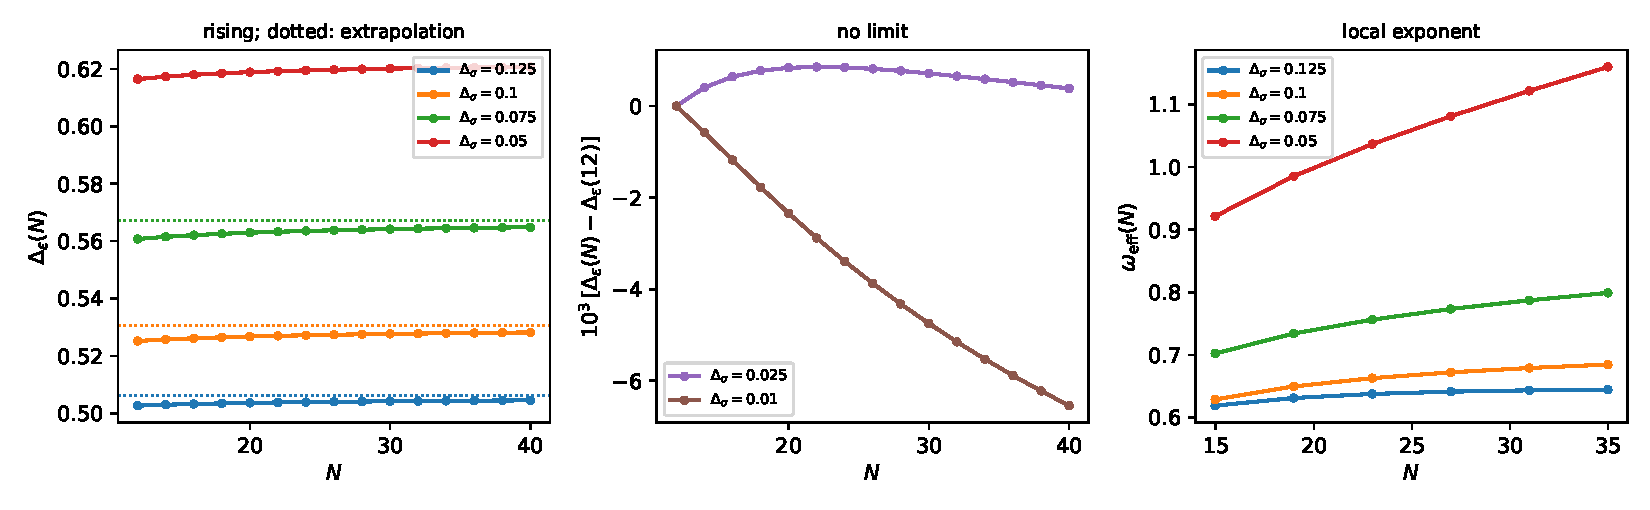
\includegraphics[width=\textwidth]{parts/ht/figures/fig_d1_cutoff.pdf}
\caption{$d=1$, \code{dens\_v1}.
\emph{Left:} $\DE(N)$ at $0.05\le\Ds\le0.125$; the dotted lines are the extrapolations of the stable series
(0.075 to 0.125).
\emph{Middle:} change $\DE(N)-\DE(12)$ at $\Ds=0.025$, which peaks near $N=\HTq{E8}$ and then falls, and at 0.01,
which falls at a nearly constant rate per unit of $\ln N$.
\emph{Right:} the local exponent~\eqref{ht:eq:omegaeff}, which levels off at 0.125 and 0.1 but rises at 0.075 and 0.05.}
\label{ht:fig:d1}
\end{figure}

\paragraph{Weak coupling and the $\eps$ expansion.}\label{ht:sec:d1-pert}
\begin{itemize}
\item At $\Ds=0.249$ the extrapolation differs from the $\eps$ series through $\eps^7$ (GFF folder:
 $C_2=(\pi+4\ln2)/9$, $C_3$ to $C_7$) by $\HTq{P1}$. That is below the $\HTq{P4}$ at which we trust the check,
 because of the series and fit systematics.
\item At $\Ds=0.24$ the value lies within the band $\HTq{P2}$ of the partial sums through $\eps^4$ to $\eps^7$.
\item The blind solver of Section~\ref{ht:sec:checks} computes the weak-coupling coefficient of the truncated model.
 With $\DE=\frac12-\frac\eps6+C_2(N)\eps^2+\dots$, it reproduces
 \begin{equation}
 C_2(N)=\frac{34}{81}+\sum_{n\ \text{even},\,2\le n\le N}v_n\Big[\frac{2}{81(n-\frac12)}+\frac{2}{9n}+\frac{2}{9(n+\frac12)}+\frac{2}{81(n+1)}\Big],\qquad v_n=\frac{(\frac12)_n}{n!},
 \label{ht:eq:C2N}
 \end{equation}
 to at most $3\times10^{-7}$ for $N=0$ to 16, raw and corrected. The limit of $C_2(N)$ is the GFF value; the
 approach is like $N^{-1/2}$.
\end{itemize}

\paragraph{Intermediate coupling.}
\begin{itemize}
\item The extrapolations are final for $\Ds\geq0.1$.
\item At $0.075\le\Ds\le0.125$ they add $\HTq{E7}$ to the $N=40$ values.
\item Over $15\le N\le35$ the local exponent levels off:
 \begin{itemize}
 \item at $\HTq{E1}$ for $\Ds=0.125$;
 \item at $\HTq{E2}$ for 0.1.
 \end{itemize}
\item It rises instead, over the same range of $N$:
 \begin{itemize}
 \item $\HTq{E3}$ at 0.075;
 \item $\HTq{E4}$ at 0.05.
 \end{itemize}
\item A rising $\omega_{\rm eff}$ precedes the turnover seen at $\Ds=0.025$ and suggests that the fits overestimate
 the limit. This is why 0.075 carries a one-sided error. The classification final versus one-sided is a judgement
 based on these trends; they differ only modestly between 0.1 and 0.075.
\item At weak coupling $\omega_{\rm eff}$ also rises slowly ($\HTq{E11}$ at $\Ds=0.249$), but the bias it implies is
 below $\HTq{E12}$.
\item Fits restricted to $N\le32$ predict $N=34$--40 to $\HTq{E5}$ (Table~\ref{ht:tab:d1-holdout}).
\end{itemize}

\begin{table}[t]
\centering\footnotesize\renewcommand{\arraystretch}{1.1}
\begin{tabular}{@{}l c c c c c c@{}}
\toprule
$\Ds$ & $\omega_{\rm eff}(15)$ & (19) & (23) & (27) & (31) & (35)\\
\midrule
\inputrows{parts/ht/sections/tab_d1_omegaeff.tex}
\bottomrule
\end{tabular}
\caption{Local exponent~\eqref{ht:eq:omegaeff} of the $d=1$ series, labelled by the centre of its four cutoffs.
Held-out test: fits on $N\le32$ predict the values at $N=34$--40 to within $\HTq{E5}$ at every $\Ds\ge0.05$, inside
the spread of the predictions. The test passes also at $\Ds=0.025$, where the series has no limit, so it checks the
fits only within the range of the data, not their limit. All values:
\code{results/HT\_1d/holdout\_and\_local\_exponent.md}.}
\label{ht:tab:d1-holdout}
\end{table}

\paragraph{Strong coupling.}
\begin{itemize}
\item \emph{$\Ds=0.05$.} The series still rises at $N=40$. The accepted F1 and F2 fits give $\HTq{D10}$, a range
 that contains the NRG value of Table~\ref{ht:tab:d1}. The F3 fits reach down to $\HTq{D11}$. Their low branch moves up as cutoffs are
 added, which mildly argues against a turnover.
 The rising $\omega_{\rm eff}$ argues the other way. No value is quoted.
\item \emph{$\Ds\le0.025$.} The corrected sequence does not converge.
 \begin{itemize}
 \item At 0.025 it peaks near $N=\HTq{E8}$ and then falls ever faster, reaching $\HTq{E9}$ per unit of $\ln N$ at
 $N=40$.
 \item At 0.01 it falls at a constant $\HTq{E10}$ per unit of $\ln N$.
 \item At 0.001 it falls slowly but lies $\HTq{C3}$ above the NRG value.
 \end{itemize}
 The zero-mode basis is converged and the solver is verified, so this is a property of the window model, not of the
 numerics. The uncorrected truncation converges, but to values that violate Eq.~\eqref{ht:eq:v}
 (Table~\ref{ht:tab:d1-ident}).
\end{itemize}

\subsection{Model dependence and the comparison with NRG}\label{ht:sec:d1-model}
The errors of Table~\ref{ht:tab:d1} are half-spreads of one family of fits (F1--F3) on one prescription. They do not cover two
further model dependences, which we measure on the shipped records
(\code{public/model\_dependence\_ht1d.py}, table in \code{results/HT\_1d/model\_dependence.md}).
\begin{itemize}
\item \emph{Tail model.} We tried two alternative descriptions of the approach $N\to\infty$ of the same window series:
 \begin{itemize}
 \item F4, Eq.~\eqref{ht:eq:fitN} with two free exponents;
 \item a local exponent continued linearly in $\ln N$ from its last four values, with the slope at $N=40$ integrated
 to infinity.
 \end{itemize}
 Both move the limit down by at most $\HTq{M3}$ at $0.075\le\Ds\le0.125$, of the order of the fit half-spread.
\item \emph{Prescription.} The same truncation without the window (raw, energy zero-mode basis) extrapolates, with
 the same fits, to limits $\HTq{M6}$ below the window limits at $\Ds=0.125$, 0.1 and 0.075, respectively.
 \begin{itemize}
 \item Neither prescription satisfies the descendant identities in the limit (Table~\ref{ht:tab:d1-ident}), so the
 limit of the truncated model depends on the prescription at this level.
 \item At $\Ds\ge0.15$ the two prescriptions agree to $\HTq{M7}$ or better.
 \end{itemize}
\end{itemize}
The prescription dependence, $\HTq{M10}$ at $0.075\le\Ds\le0.125$, is thus as large as the gap to NRG below. We do
not combine these shifts into an error. The truncation has no strict error bar, and an error built after the gap to
NRG had been seen would make the comparison read as agreement within errors. The errors of Table~\ref{ht:tab:d1} stay
the fit spreads. The window limit is expected to be the better of the two, since its $\sigma$ descendant violation is
$\HTq{V2}$ times smaller.

\paragraph{Comparison with NRG.} We compare with the final NRG values of Table~\ref{ht:tab:d1} (NRG folder). Their
errors are sums of three convergence diagnostics, not standard deviations.
\begin{itemize}
\item HT lies above NRG at all six points $0.075\le\Ds\le0.2$, by up to $\HTq{C1}$.
\item The differences are $\HTq{C5}$ to $\HTq{C1}$ at $0.075\le\Ds\le0.15$, and below $\HTq{C6}$ at 0.175 and 0.2.
\item At $\Ds=0.125$, 0.1 and 0.075 the differences are $\HTq{C2}$. They are at least five times both the fit
 half-spreads of Table~\ref{ht:tab:d1} and the NRG errors, and of the size of the prescription dependence.
\item NRG lies between the raw and the window limits at these three points.
\item NRG also lies inside the fit-free bracket $[\DE(40),\,\DE(40)+\frac{d\DE/d\ln N}{\omega_{\rm eff}}]$ of the
 window series at every $0.075\le\Ds\le0.2$. That bracket holds if $\DE(N)$ keeps rising and $\omega_{\rm eff}$
 does not decrease beyond $N=40$.
\end{itemize}
We do not assume that either method is right. The Monte Carlo values that the MC folder labels \emph{accepted}
(MC column of the $d=1$ results table of Ref.~\cite{ht:paper}) also lie above NRG at these three couplings, on the same side as HT, but their
systematic errors exceed the HT--NRG differences, so they cannot decide between the two. The resummed expansions cannot decide at this coupling
(\code{Resummation/} folder). The HT values at
$0.075\le\Ds\le0.125$ are limits of the window-corrected truncation at their fit errors. As estimates of the CFT
they depend on the truncation prescription by the shifts above, which are as large as the gap to NRG.

\subsection{Descendant identities}\label{ht:sec:d1-ident}
Table~\ref{ht:tab:d1-ident} gives the level-1 violations, Eq.~\eqref{ht:eq:v}, at $N=28$, raw and with the window, from
the identity diagnostic run on the \code{prod1--7} records. The other cutoffs are in
\code{results/HT\_1d/identity\_violations.md}.
\begin{itemize}
\item The raw violations do not decay with $N$ over $N=16$--28 and grow with the coupling. At $\Ds\le0.1$ they range
 over $\HTq{V1}$.
\item The window reduces the $\sigma$ violation by $\HTq{V2}$ times at $\Ds\le0.15$.
\item At $\eps\ge0.6$ non-decaying residuals of about $\HTq{V3}$ remain for $\sigma$ and $\phi^3$, and up to
 $\HTq{V4}$ for $\varepsilon$ at $\Ds\le0.05$.
\end{itemize}

\begin{table}[t]
\centering\footnotesize\renewcommand{\arraystretch}{1.1}
\begin{tabular}{@{}l r r r r r r@{}}
\toprule
 & \multicolumn{3}{c}{raw} & \multicolumn{3}{c}{window}\\
\cmidrule(lr){2-4}\cmidrule(l){5-7}
$\Ds$ & $\sigma$ & $\phi^3$ & $\varepsilon$ & $\sigma$ & $\phi^3$ & $\varepsilon$\\
\midrule
\inputrows{parts/ht/sections/tab_d1_ident.tex}
\bottomrule
\end{tabular}
\caption{Level-1 descendant violations $v_1$ at $N=28$, raw and with the consistent window, in the energy zero-mode
basis of \code{prod1--7}: $n_z=24$ at $\Ds\ge0.1$, 32 below. The $\varepsilon$ columns use the first excited
even state. $^a$:~ambiguous identification with the free $L_{-1}$. In the CFT all entries vanish.}
\label{ht:tab:d1-ident}
\end{table}

\IfFileExists{parts/ht/sections/d2/sec_d2.tex}{\input{parts/ht/sections/d2/sec_d2.tex}}{%
\section{Two dimensions}\label{ht:d2:sec}
\textit{Section to be supplied by the $d=2$ contributors (phi4HT2d): modes and weights, the $d=2$ window, campaigns
($N\le24$), finite-$N$ results with status words, the fold near $\Ds\approx0.1274$. Pending
the transfer of the production records from Expanse.}}

\input{parts/ht/sections/d3/sec_d3.tex}

\section{Independent checks}\label{ht:sec:checks}
In each dimension a second solver, written without using the production code, reproduces the production spectra at
finite cutoff. These checks verify that we compute the stated model, not that its limit is the CFT.

\paragraph{One dimension.}\label{ht:d1:checks}
\begin{itemize}
\item \emph{Authorship.} A Claude Code subagent wrote the solver (\code{code/lri\_dressed\_phi4\_independent\_check})
 from the definition of the model. It was not allowed to read the production code, results or analysis. Of the
 package documentation it read only the definition of the window (\code{docs/WINDOW.md}) and of the Hamiltonian
 (\code{docs/ALGORITHM.md}). It derived $H$ itself from the GFF radial
 quantization, and its derivation agrees with Eqs.~\eqref{ht:eq:Hz}--\eqref{ht:eq:Lj}.
\item \emph{Own numerics.} The zero mode is a sinc discrete-variable representation, the bath Fock space is its own,
 and both the literal and consistent windows are implemented. Newton tuning continues from weak coupling. Every point
 is verified on 1.5 times finer and 1.5 times wider grids.
\item \emph{Comparison set.} 38 points: raw and consistent at $\Ds=0.249$, 0.2, 0.1, 0.05, 0.025 and 0.01 with
 $N=12$, 16 and 20, plus literal at 0.2 and 0.1 with $N=12$.
\item \emph{Agreement with the production records} (\code{dens\_v1}, density basis, $n_z=16$). At the 18
 consistent-window points ($N=12$, 16, 20) the records agree with the blind solver to $5.6\times10^{-7}$ or better,
 the truncation error of the density basis.
\item \emph{Agreement with the energy-basis records} (\code{prod1--7}).
 \begin{itemize}
 \item $\DE$ agrees to $1.3\times10^{-9}$ where these records used $n_z=48$ or $\Ds\ge0.2$.
 \item It agrees to $4.8\times10^{-9}$ where they used $n_z=24$ or 32 at strong coupling, which is that basis's
 truncation error.
 \item Over all 38 points this gives $5\times10^{-9}$. The other levels and the tuned $(g,r)$ agree at the same level.
 \end{itemize}
\item \emph{Weak coupling.} The solver reproduces $C_2(N)$, Eq.~\eqref{ht:eq:C2N}, to $3\times10^{-7}$. It also shows
 that the window changes $\DE$ only at order $\eps^4$: the fitted exponent is 4.05 to 4.11.
\end{itemize}

\input{parts/ht/sections/d2/checks_d2.tex}

\input{parts/ht/sections/d3/checks_d3.tex}

\section{Caveats}\label{ht:sec:caveats}

\paragraph{The limit depends on the window model.}
\begin{itemize}
\item The window restores only disconnected vacuum fluctuations.
\item In $d=1$ the corrected descendant spacings still miss by amounts that do not decrease with $N$
 (Table~\ref{ht:tab:d1-ident}).
\item In $d=2$ the $\eps$ expansion of the window model is correct only through third order: its fourth-order
 coefficient grows like $\ln N$ (Section~\ref{ht:d2:sec}). In $d=3$ the fourth-order coefficient at $N=20$ is 60\% of
 $C_4(3)$ and still growing slowly; whether its $N\to\infty$ limit is wrong is not shown (Section~\ref{ht:d3:sec}).
\end{itemize}

\paragraph{The method fails toward the short-range end in every dimension.}
\begin{itemize}
\item The tuned coupling is largest there.
\item In $d=1$ it also grows with the cutoff, and toward the short-range end $\Ds\to0$ the $\sigma$ gap that the
 tuning imposes, $E_\sigma-E_v=\Ds$, closes.
\item The failure sets in at $\Ds\le0.05$ in $d=1$, at $\Ds\le0.175$ in $d=2$, and near the endpoint in $d=3$.
\end{itemize}

\paragraph{Errors.}
\begin{itemize}
\item The quoted errors are half-spreads of the extrapolations in the cutoff, not standard deviations, and they do
 not include the dependence on the window prescription (Section~\ref{ht:sec:d1-model}).
\item The exponents of Eq.~\eqref{ht:eq:fitN} are fitted, not derived.
\item At $\Ds\ge0.15$ in $d=1$ the spreads are probably optimistic.
\item The classification \emph{final} versus \emph{one-sided} is a judgement based on the local exponent.
\end{itemize}

\paragraph{Order of the analysis.}
\begin{itemize}
\item The window was designed after its effect had been seen in the descendant spacings.
\item The fit protocol of Section~\ref{ht:sec:d1-extrap} was carried over unchanged from the earlier \code{prod1--7}
 analysis.
\item The held-out test and the local exponent were added after the $N=40$ data had been seen.
\item The tail-model and prescription comparisons of Section~\ref{ht:sec:d1-model} were made after the gap to NRG had
 been seen. For that reason they are given as shifts and are not turned into an error.
\end{itemize}

\paragraph{One dimension.}
\begin{itemize}
\item \emph{Strong coupling.} The $d=1$ values at $\Ds\le0.05$ are not limits. At 0.025 and below, the correction
 overshoots: the sequence turns over and falls without bound in $\ln N$.
\item \emph{Comparison with NRG.} Where the descriptions overlap ($0.075\le\Ds\le0.2$), HT lies above NRG at all six points, by up to
 $\HTq{C1}$. At $\Ds=0.1$ and 0.125 the gap exceeds the spread of our extrapolations. However, the uncorrected
 prescription extrapolates to limits $\HTq{M10}$ lower, below NRG, so the dependence on the prescription is as large
 as the gap (Section~\ref{ht:sec:d1-model}).
\item \emph{Prescription dependence.} The quoted errors of Table~\ref{ht:tab:d1} do not include the prescription
 dependence. The raw and window limits differ by $\HTq{M6}$ at $\Ds=0.125$, 0.1 and 0.075.
\end{itemize}

\input{parts/ht/sections/d2/caveats_d2.tex}

\input{parts/ht/sections/d3/caveats_d3.tex}

\section{Reproduction}\label{ht:sec:repro}

\subsection{Layout}
All paths are relative to the folder \code{HT/} of the public repository.

\paragraph{Folders.}
\begin{itemize}
\item \code{code/<package>/}: one package per solver or analysis, shipped at the commit its production ran. Each has
 a \code{public.mk} with the targets \code{test} and \code{replay} (optionally \code{smoke}), and a \code{public/}
 folder with the replay scripts and a README.
\item \code{data/HT\_<d>d/}: the production records.
\item \code{results/HT\_<d>d/}: the published tables and the expected values of every quoted number.
\end{itemize}

\paragraph{Commands.}
\begin{itemize}
\item \code{make test} and \code{make replay} in \code{HT/} run the targets of every package.
\item In a package folder: \code{make -f public.mk test|replay|smoke}.
\end{itemize}
A replay recomputes every quoted number of its package from the shipped records, without a production rerun. It
prints a PASS/FAIL table and exits non-zero on any failure.

\subsection{Packages and records}
\begin{center}\footnotesize\renewcommand{\arraystretch}{1.15}
\begin{tabular}{@{}p{4.3cm}p{2.5cm}p{8.4cm}@{}}
\toprule
package (\code{code/}) & $d$, role & content, records, cost\\
\midrule
\code{lri\_dressed\_phi4\_hpc} & 1: solver & commit 33998bb. Zero mode plus bath, window, density basis, launcher for the symmetry cluster. Records \code{data/HT\_1d/dens\_v1} (201) and \code{prod\_window} (680). \code{test} about 3 min; \code{smoke} one item\\
\code{lri\_dressed\_phi4\_hpc\_analysis} & 1: analysis & fits, held-out test, identity records, tables. \code{replay} about 1 min\\
\code{lri\_dressed\_phi4\_independent\_check} & 1: blind check & DVR solver, its per-task outputs and comparison. \code{replay} seconds\\
\code{lri\_2d\_window\_hpc}, \code{lri\_2d\_window\_indep} & 2 & Section~\ref{ht:d2:sec}; records \code{data/HT\_2d}\\
\code{lri\_3d\_window\_hpc}, \code{lri\_3d\_window\_indep} & 3 & Section~\ref{ht:d3:sec}; records \code{data/HT\_3d}\\
\bottomrule
\end{tabular}
\end{center}

\subsection{Rules that are part of the results}
\begin{itemize}
\item \emph{Estimators.} The fit families, acceptance and stability rules, and estimators of
 Section~\ref{ht:sec:d1-extrap} define the quoted numbers. So do the status words of Table~\ref{ht:tab:d1}.
\item \emph{Expected values.} \code{results/HT\_1d/quoted\_numbers.json} gives the estimator and comparison rule of
 every $d=1$ number. The $d=1$ numbers in this note are typeset from it.
\item \emph{Fit tolerance.} The cutoff fits of $d=1$ are nonlinear least squares from several starting exponents, and
 other numpy/scipy versions may land in slightly different minima. The replay therefore checks each number twice:
 \begin{itemize}
 \item against the shipped analysis outputs, exactly;
 \item against a refit in the reader's environment, within a quarter of the quoted half-spread.
 \end{itemize}
 The largest shift measured on symmetry was 0.11 of the half-spread ($\Ds=0.175$).
\end{itemize}

\subsection{Result $\to$ code, record, command, tolerance}
\begingroup\footnotesize\renewcommand{\arraystretch}{1.1}
\newcolumntype{L}[1]{>{\raggedright\arraybackslash}p{#1}}
\begin{longtable}{@{}L{4.2cm}L{2.4cm}L{0.9cm}L{2.3cm}L{2.6cm}L{2.0cm}@{}}
\toprule
result & value & pkg & records & command & tolerance\\
\midrule\endhead
\bottomrule\endfoot
\inputrows{parts/ht/sections/repro_d1.tex}
\midrule
\inputrows{parts/ht/sections/d2/repro_d2.tex}
\midrule
\multicolumn{6}{@{}p{\linewidth}@{}}{\emph{$d=3$, finite coupling} (P = \texttt{lri\_3d\_window\_hpc}, I = \texttt{lri\_3d\_window\_indep}, C = \texttt{data/HT\_3d/campaigns})}\\*
\inputrows{parts/ht/sections/d3/repro_d3.tex}
\end{longtable}
\endgroup

\appendix
\section{Provenance and reviews}\label{ht:app:prov}

\paragraph{Who wrote what.} Every package records its origin in \code{PROVENANCE.md}, and every review is summarized
in \code{REVIEWS.md}.

\paragraph{$d=1$ solver.} \code{lri\_dressed\_phi4\_hpc} went through three stages.
\begin{itemize}
\item The author supplied it as a matrix-free rewrite of an earlier dressed zero-mode solver (commit e637dfd), written by
 OpenAI GPT-6 astra.
\item Claude Code sessions (Anthropic, model claude-opus-5-5) added the layer that runs it on the symmetry cluster
 (node packing, cross-node locks, validation records), the window correction and the descendant diagnostic
 (157a2c6 to e2ca07c). Codex (OpenAI, gpt-6-astra) reviewed the plan, which
 was approved in round 4, and inspected the code twice. All 20 findings were fixed; the last eight fixes were not
 re-inspected.
\item The density basis was supplied by the author as a patch (33998bb). A fresh Codex inspection found two medium
 defects in scripts the production does not use; they were deferred.
\end{itemize}
Both supplied archives (e637dfd and the density-basis patch) were written by OpenAI GPT-6 astra via ChatGPT (model stated by the author).

\paragraph{$d=1$ analysis and records.}
\begin{itemize}
\item The analysis scripts, the campaigns and this note were written by Claude Code sessions.
\item The blind $d=1$ solver was written by a Claude Code subagent (Section~\ref{ht:sec:checks}).
\item No Codex results review was run on the $d=1$ finite-coupling numbers. The public-release replay found three
 paper values that the stated estimators did not reproduce: the $\Ds=0.05$ range, the bound on the weak-coupling
 spreads, and the basis error. It also found one value quoted beyond its reproducible precision, the $\eps$-series
 difference at $\Ds=0.249$. All four were corrected on 2026-10-13.
\end{itemize}

\paragraph{$d=2,3$.} See the provenance files of \code{lri\_2d\_window\_hpc} and \code{lri\_3d\_window\_hpc}.

\paragraph{This note.} Written by the Claude Code session \code{phi4HT1d}. The $d=2$ and $d=3$ sections were written by
the sessions \code{phi4HT2d} and \code{phi4HT3d} and edited here only for consistency.


\begin{thebibliography}{99}
\bibitem{ht:Rychkov:2014eea} S.~Rychkov and L.~G.~Vitale, \emph{Hamiltonian truncation study of the $\phi^4$ theory in two dimensions}, Phys.\ Rev.\ D \textbf{91} (2015) 085011, arXiv:1412.3460.
\bibitem{ht:Behan:2017emf} C.~Behan, L.~Rastelli, S.~Rychkov and B.~Zan, \emph{A scaling theory for the long-range to short-range crossover and an infrared duality}, J.\ Phys.\ A \textbf{50} (2017) 354002, arXiv:1703.05325.
\bibitem{ht:Chang:2024whx} C.-H.~Chang, V.~Dommes, R.~S.~Erramilli, A.~Homrich, P.~Kravchuk, A.~Liu, M.~S.~Mitchell, D.~Poland and D.~Simmons-Duffin, \emph{Bootstrapping the 3d Ising stress tensor}, JHEP \textbf{03} (2025) 136, arXiv:2411.15300.
\bibitem{ht:paper} Z.~Zheng, \emph{The long-range Ising CFT: perturbative and nonperturbative approaches} (2026), folder \texttt{paper/} of the public repository.
\bibitem{ht:Fisher:1972zz} M.~E.~Fisher, S.-k.~Ma and B.~G.~Nickel, \emph{Critical exponents for long-range interactions}, Phys.\ Rev.\ Lett.\ \textbf{29} (1972) 917.
\bibitem{ht:Sak:1973oqx} J.~Sak, \emph{Recursion relations and fixed points for ferromagnets with long-range interactions}, Phys.\ Rev.\ B \textbf{8} (1973) 281.
\bibitem{ht:Paulos:2015jfa} M.~F.~Paulos, S.~Rychkov, B.~C.~van Rees and B.~Zan, \emph{Conformal invariance in the long-range Ising model}, Nucl.\ Phys.\ B \textbf{902} (2016) 246, arXiv:1509.00008.
\bibitem{ht:Behan:2017dwr} C.~Behan, L.~Rastelli, S.~Rychkov and B.~Zan, \emph{Long-range critical exponents near the short-range crossover}, Phys.\ Rev.\ Lett.\ \textbf{118} (2017) 241601, arXiv:1703.03430.
\bibitem{ht:Hogervorst:2014rta} M.~Hogervorst, S.~Rychkov and B.~C.~van Rees, \emph{Truncated conformal space approach in $d$ dimensions: a cheap alternative to lattice field theory?}, Phys.\ Rev.\ D \textbf{91} (2015) 025005, arXiv:1409.1581.
\bibitem{ht:Leggett:1987zz} A.~J.~Leggett, S.~Chakravarty, A.~T.~Dorsey, M.~P.~A.~Fisher, A.~Garg and W.~Zwerger, \emph{Dynamics of the dissipative two-state system}, Rev.\ Mod.\ Phys.\ \textbf{59} (1987) 1.
\bibitem{ht:Bulla:2003rns} R.~Bulla, N.-H.~Tong and M.~Vojta, \emph{Numerical renormalization group for bosonic systems and application to the subohmic spin-boson model}, Phys.\ Rev.\ Lett.\ \textbf{91} (2003) 170601, arXiv:cond-mat/0306708.
\bibitem{ht:Bulla:2005bnrg} R.~Bulla, H.-J.~Lee, N.-H.~Tong and M.~Vojta, \emph{Numerical renormalization group for quantum impurities in a bosonic bath}, Phys.\ Rev.\ B \textbf{71} (2005) 045122, arXiv:cond-mat/0407559.
\bibitem{ht:Belavin:1984vu} A.~A.~Belavin, A.~M.~Polyakov and A.~B.~Zamolodchikov, \emph{Infinite conformal symmetry in two-dimensional quantum field theory}, Nucl.\ Phys.\ B \textbf{241} (1984) 333.
\bibitem{ht:Simmons-Duffin:2016wlq} D.~Simmons-Duffin, \emph{The lightcone bootstrap and the spectrum of the 3d Ising CFT}, JHEP \textbf{03} (2017) 086, arXiv:1612.08471.
\bibitem{ht:Cohen:2021erm} T.~Cohen, K.~Farnsworth, R.~Houtz and M.~A.~Luty, \emph{Hamiltonian truncation effective theory}, SciPost Phys.\ \textbf{13} (2022) 011, arXiv:2110.08273.
\bibitem{ht:EliasMiro:2022pua} J.~Elias Mir\'o and J.~Ingoldby, \emph{Effective Hamiltonians and counterterms for Hamiltonian truncation}, JHEP \textbf{07} (2023) 052, arXiv:2212.07266.
\bibitem{ht:Elias-Miro:2020qwz} J.~Elias Mir\'o and E.~Hardy, \emph{Exploring Hamiltonian truncation in $d=2+1$}, Phys.\ Rev.\ D \textbf{102} (2020) 065001, arXiv:2003.08405.
\end{thebibliography}

\clearpage
\AuditMacro{end}{DE}
\AuditMacro{end}{Ds}
\AuditMacro{end}{HTq}
\AuditMacro{end}{HTq@B1}
\AuditMacro{end}{HTq@C1}
\AuditMacro{end}{HTq@C2}
\AuditMacro{end}{HTq@C3}
\AuditMacro{end}{HTq@C5}
\AuditMacro{end}{HTq@C6}
\AuditMacro{end}{HTq@C7}
\AuditMacro{end}{HTq@C8}
\AuditMacro{end}{HTq@C9}
\AuditMacro{end}{HTq@D01}
\AuditMacro{end}{HTq@D02}
\AuditMacro{end}{HTq@D03}
\AuditMacro{end}{HTq@D04}
\AuditMacro{end}{HTq@D05}
\AuditMacro{end}{HTq@D06}
\AuditMacro{end}{HTq@D07}
\AuditMacro{end}{HTq@D08}
\AuditMacro{end}{HTq@D09}
\AuditMacro{end}{HTq@D10}
\AuditMacro{end}{HTq@D11}
\AuditMacro{end}{HTq@D12}
\AuditMacro{end}{HTq@D13}
\AuditMacro{end}{HTq@D14}
\AuditMacro{end}{HTq@E1}
\AuditMacro{end}{HTq@E10}
\AuditMacro{end}{HTq@E11}
\AuditMacro{end}{HTq@E12}
\AuditMacro{end}{HTq@E2}
\AuditMacro{end}{HTq@E3}
\AuditMacro{end}{HTq@E4}
\AuditMacro{end}{HTq@E5}
\AuditMacro{end}{HTq@E6}
\AuditMacro{end}{HTq@E7}
\AuditMacro{end}{HTq@E8}
\AuditMacro{end}{HTq@E9}
\AuditMacro{end}{HTq@M10}
\AuditMacro{end}{HTq@M3}
\AuditMacro{end}{HTq@M4}
\AuditMacro{end}{HTq@M5}
\AuditMacro{end}{HTq@M6}
\AuditMacro{end}{HTq@M7}
\AuditMacro{end}{HTq@P1}
\AuditMacro{end}{HTq@P2}
\AuditMacro{end}{HTq@P3}
\AuditMacro{end}{HTq@P4}
\AuditMacro{end}{HTq@S1}
\AuditMacro{end}{HTq@S10}
\AuditMacro{end}{HTq@S11}
\AuditMacro{end}{HTq@S12}
\AuditMacro{end}{HTq@S2}
\AuditMacro{end}{HTq@S3}
\AuditMacro{end}{HTq@S4}
\AuditMacro{end}{HTq@S5}
\AuditMacro{end}{HTq@S6}
\AuditMacro{end}{HTq@S7}
\AuditMacro{end}{HTq@S8}
\AuditMacro{end}{HTq@S9}
\AuditMacro{end}{HTq@T01}
\AuditMacro{end}{HTq@T02}
\AuditMacro{end}{HTq@T03}
\AuditMacro{end}{HTq@T04}
\AuditMacro{end}{HTq@T05}
\AuditMacro{end}{HTq@T06}
\AuditMacro{end}{HTq@T07}
\AuditMacro{end}{HTq@T08}
\AuditMacro{end}{HTq@T09}
\AuditMacro{end}{HTq@T10}
\AuditMacro{end}{HTq@T11}
\AuditMacro{end}{HTq@T12}
\AuditMacro{end}{HTq@T13}
\AuditMacro{end}{HTq@U00}
\AuditMacro{end}{HTq@U01}
\AuditMacro{end}{HTq@U02}
\AuditMacro{end}{HTq@U03}
\AuditMacro{end}{HTq@U04}
\AuditMacro{end}{HTq@U05}
\AuditMacro{end}{HTq@U06}
\AuditMacro{end}{HTq@U07}
\AuditMacro{end}{HTq@U08}
\AuditMacro{end}{HTq@U09}
\AuditMacro{end}{HTq@U10}
\AuditMacro{end}{HTq@U11}
\AuditMacro{end}{HTq@U12}
\AuditMacro{end}{HTq@U13}
\AuditMacro{end}{HTq@V1}
\AuditMacro{end}{HTq@V2}
\AuditMacro{end}{HTq@V3}
\AuditMacro{end}{HTq@V4}
\AuditMacro{end}{HTq@V5}
\AuditMacro{end}{HTq@V6}
\AuditMacro{end}{HTq@V7}
\AuditMacro{end}{arraystretch}
\AuditMacro{end}{code}
\AuditMacro{end}{codeus}
\AuditMacro{end}{csname}
\AuditMacro{end}{eps}
\AuditMacro{end}{ii}
\AuditMacro{end}{inputrows}
\immediate\write\CombinedAuditStream{PART_END|ht|\number\numexpr\value{page}-1\relax}
\endgroup
\RestoreStructuralState
\AuditMacro{outside-after-ht}{AC}
\AuditMacro{outside-after-ht}{AIfigCodexRounds}
\AuditMacro{outside-after-ht}{AIfigCoreHours}
\AuditMacro{outside-after-ht}{AIfigGPTPackages}
\AuditMacro{outside-after-ht}{AIfigSubagents}
\AuditMacro{outside-after-ht}{AIsessions}
\AuditMacro{outside-after-ht}{Ae}
\AuditMacro{outside-after-ht}{Ag}
\AuditMacro{outside-after-ht}{Aut}
\AuditMacro{outside-after-ht}{BB}
\AuditMacro{outside-after-ht}{CSR}
\AuditMacro{outside-after-ht}{CT}
\AuditMacro{outside-after-ht}{Cat}
\AuditMacro{outside-after-ht}{CfourOne}
\AuditMacro{outside-after-ht}{CfourOneOld}
\AuditMacro{outside-after-ht}{DE}
\AuditMacro{outside-after-ht}{De}
\AuditMacro{outside-after-ht}{Deff}
\AuditMacro{outside-after-ht}{Disc}
\AuditMacro{outside-after-ht}{Dloc}
\AuditMacro{outside-after-ht}{Ds}
\AuditMacro{outside-after-ht}{Eop}
\AuditMacro{outside-after-ht}{FP}
\AuditMacro{outside-after-ht}{GG}
\AuditMacro{outside-after-ht}{Gr}
\AuditMacro{outside-after-ht}{HTCthreeDev}
\AuditMacro{outside-after-ht}{HTCtwoDev}
\AuditMacro{outside-after-ht}{HTnpDtwoCfourLog}
\AuditMacro{outside-after-ht}{HTpCeightOne}
\AuditMacro{outside-after-ht}{HTpCeightOneCalRange}
\AuditMacro{outside-after-ht}{HTpCeightOneDev}
\AuditMacro{outside-after-ht}{HTpCeightOneUncal}
\AuditMacro{outside-after-ht}{HTpCfiveOne}
\AuditMacro{outside-after-ht}{HTpCfiveOneDev}
\AuditMacro{outside-after-ht}{HTpCfiveThree}
\AuditMacro{outside-after-ht}{HTpCfiveTwo}
\AuditMacro{outside-after-ht}{HTpCfiveTwoDev}
\AuditMacro{outside-after-ht}{HTpCfiveTwoLog}
\AuditMacro{outside-after-ht}{HTpCfourOne}
\AuditMacro{outside-after-ht}{HTpCfourOneDev}
\AuditMacro{outside-after-ht}{HTpCfourThree}
\AuditMacro{outside-after-ht}{HTpCfourThreeDev}
\AuditMacro{outside-after-ht}{HTpCfourTwo}
\AuditMacro{outside-after-ht}{HTpCfourTwoDev}
\AuditMacro{outside-after-ht}{HTpCsevenOne}
\AuditMacro{outside-after-ht}{HTpCsevenOneDev}
\AuditMacro{outside-after-ht}{HTpCsixOne}
\AuditMacro{outside-after-ht}{HTpCsixOneDev}
\AuditMacro{outside-after-ht}{HTpCthreeOne}
\AuditMacro{outside-after-ht}{HTpCthreeOneDev}
\AuditMacro{outside-after-ht}{HTpCthreeThree}
\AuditMacro{outside-after-ht}{HTpCthreeThreeDev}
\AuditMacro{outside-after-ht}{HTpCthreeTwo}
\AuditMacro{outside-after-ht}{HTpCthreeTwoDev}
\AuditMacro{outside-after-ht}{HTpCtwoOne}
\AuditMacro{outside-after-ht}{HTpCtwoOneDev}
\AuditMacro{outside-after-ht}{HTpCtwoThree}
\AuditMacro{outside-after-ht}{HTpCtwoThreeDigits}
\AuditMacro{outside-after-ht}{HTpCtwoTwo}
\AuditMacro{outside-after-ht}{HTpCtwoTwoDigits}
\AuditMacro{outside-after-ht}{HTpEngineAgree}
\AuditMacro{outside-after-ht}{HTpIdentFive}
\AuditMacro{outside-after-ht}{HTpIdentFour}
\AuditMacro{outside-after-ht}{HTpIdentThree}
\AuditMacro{outside-after-ht}{HTpLamCeight}
\AuditMacro{outside-after-ht}{HTpLamThermal}
\AuditMacro{outside-after-ht}{HTpOmegaThree}
\AuditMacro{outside-after-ht}{HTpOmegaThreeEff}
\AuditMacro{outside-after-ht}{HTpOneLexact}
\AuditMacro{outside-after-ht}{HTpRawFracFour}
\AuditMacro{outside-after-ht}{HTpRawFracSeven}
\AuditMacro{outside-after-ht}{HTpRawOffsetFour}
\AuditMacro{outside-after-ht}{HTpSTenMatch}
\AuditMacro{outside-after-ht}{HTpStatesMax}
\AuditMacro{outside-after-ht}{HTpThreeGate}
\AuditMacro{outside-after-ht}{HTpThreeGateL}
\AuditMacro{outside-after-ht}{HTpThreeLfive}
\AuditMacro{outside-after-ht}{HTpThreeLfour}
\AuditMacro{outside-after-ht}{HTpThreeLmax}
\AuditMacro{outside-after-ht}{HTpThreeLwin}
\AuditMacro{outside-after-ht}{HTpTwoIdentThree}
\AuditMacro{outside-after-ht}{HTpTwoImplAgree}
\AuditMacro{outside-after-ht}{HTpTwoLfive}
\AuditMacro{outside-after-ht}{HTpTwoLfour}
\AuditMacro{outside-after-ht}{HTpTwoLowDev}
\AuditMacro{outside-after-ht}{HTpTwoLprod}
\AuditMacro{outside-after-ht}{HTpWinCfive}
\AuditMacro{outside-after-ht}{HTpWinCfour}
\AuditMacro{outside-after-ht}{HTpWinCfourInf}
\AuditMacro{outside-after-ht}{HTpWinLamEight}
\AuditMacro{outside-after-ht}{HTq}
\AuditMacro{outside-after-ht}{HTq@B1}
\AuditMacro{outside-after-ht}{HTq@C1}
\AuditMacro{outside-after-ht}{HTq@C2}
\AuditMacro{outside-after-ht}{HTq@C3}
\AuditMacro{outside-after-ht}{HTq@C5}
\AuditMacro{outside-after-ht}{HTq@C6}
\AuditMacro{outside-after-ht}{HTq@C7}
\AuditMacro{outside-after-ht}{HTq@C8}
\AuditMacro{outside-after-ht}{HTq@C9}
\AuditMacro{outside-after-ht}{HTq@D01}
\AuditMacro{outside-after-ht}{HTq@D02}
\AuditMacro{outside-after-ht}{HTq@D03}
\AuditMacro{outside-after-ht}{HTq@D04}
\AuditMacro{outside-after-ht}{HTq@D05}
\AuditMacro{outside-after-ht}{HTq@D06}
\AuditMacro{outside-after-ht}{HTq@D07}
\AuditMacro{outside-after-ht}{HTq@D08}
\AuditMacro{outside-after-ht}{HTq@D09}
\AuditMacro{outside-after-ht}{HTq@D10}
\AuditMacro{outside-after-ht}{HTq@D11}
\AuditMacro{outside-after-ht}{HTq@D12}
\AuditMacro{outside-after-ht}{HTq@D13}
\AuditMacro{outside-after-ht}{HTq@D14}
\AuditMacro{outside-after-ht}{HTq@E1}
\AuditMacro{outside-after-ht}{HTq@E10}
\AuditMacro{outside-after-ht}{HTq@E11}
\AuditMacro{outside-after-ht}{HTq@E12}
\AuditMacro{outside-after-ht}{HTq@E2}
\AuditMacro{outside-after-ht}{HTq@E3}
\AuditMacro{outside-after-ht}{HTq@E4}
\AuditMacro{outside-after-ht}{HTq@E5}
\AuditMacro{outside-after-ht}{HTq@E6}
\AuditMacro{outside-after-ht}{HTq@E7}
\AuditMacro{outside-after-ht}{HTq@E8}
\AuditMacro{outside-after-ht}{HTq@E9}
\AuditMacro{outside-after-ht}{HTq@M10}
\AuditMacro{outside-after-ht}{HTq@M3}
\AuditMacro{outside-after-ht}{HTq@M4}
\AuditMacro{outside-after-ht}{HTq@M5}
\AuditMacro{outside-after-ht}{HTq@M6}
\AuditMacro{outside-after-ht}{HTq@M7}
\AuditMacro{outside-after-ht}{HTq@P1}
\AuditMacro{outside-after-ht}{HTq@P2}
\AuditMacro{outside-after-ht}{HTq@P3}
\AuditMacro{outside-after-ht}{HTq@P4}
\AuditMacro{outside-after-ht}{HTq@S1}
\AuditMacro{outside-after-ht}{HTq@S10}
\AuditMacro{outside-after-ht}{HTq@S11}
\AuditMacro{outside-after-ht}{HTq@S12}
\AuditMacro{outside-after-ht}{HTq@S2}
\AuditMacro{outside-after-ht}{HTq@S3}
\AuditMacro{outside-after-ht}{HTq@S4}
\AuditMacro{outside-after-ht}{HTq@S5}
\AuditMacro{outside-after-ht}{HTq@S6}
\AuditMacro{outside-after-ht}{HTq@S7}
\AuditMacro{outside-after-ht}{HTq@S8}
\AuditMacro{outside-after-ht}{HTq@S9}
\AuditMacro{outside-after-ht}{HTq@T01}
\AuditMacro{outside-after-ht}{HTq@T02}
\AuditMacro{outside-after-ht}{HTq@T03}
\AuditMacro{outside-after-ht}{HTq@T04}
\AuditMacro{outside-after-ht}{HTq@T05}
\AuditMacro{outside-after-ht}{HTq@T06}
\AuditMacro{outside-after-ht}{HTq@T07}
\AuditMacro{outside-after-ht}{HTq@T08}
\AuditMacro{outside-after-ht}{HTq@T09}
\AuditMacro{outside-after-ht}{HTq@T10}
\AuditMacro{outside-after-ht}{HTq@T11}
\AuditMacro{outside-after-ht}{HTq@T12}
\AuditMacro{outside-after-ht}{HTq@T13}
\AuditMacro{outside-after-ht}{HTq@U00}
\AuditMacro{outside-after-ht}{HTq@U01}
\AuditMacro{outside-after-ht}{HTq@U02}
\AuditMacro{outside-after-ht}{HTq@U03}
\AuditMacro{outside-after-ht}{HTq@U04}
\AuditMacro{outside-after-ht}{HTq@U05}
\AuditMacro{outside-after-ht}{HTq@U06}
\AuditMacro{outside-after-ht}{HTq@U07}
\AuditMacro{outside-after-ht}{HTq@U08}
\AuditMacro{outside-after-ht}{HTq@U09}
\AuditMacro{outside-after-ht}{HTq@U10}
\AuditMacro{outside-after-ht}{HTq@U11}
\AuditMacro{outside-after-ht}{HTq@U12}
\AuditMacro{outside-after-ht}{HTq@U13}
\AuditMacro{outside-after-ht}{HTq@V1}
\AuditMacro{outside-after-ht}{HTq@V2}
\AuditMacro{outside-after-ht}{HTq@V3}
\AuditMacro{outside-after-ht}{HTq@V4}
\AuditMacro{outside-after-ht}{HTq@V5}
\AuditMacro{outside-after-ht}{HTq@V6}
\AuditMacro{outside-after-ht}{HTq@V7}
\AuditMacro{outside-after-ht}{JJ}
\AuditMacro{outside-after-ht}{KK}
\AuditMacro{outside-after-ht}{KP}
\AuditMacro{outside-after-ht}{LL}
\AuditMacro{outside-after-ht}{Li}
\AuditMacro{outside-after-ht}{MM}
\AuditMacro{outside-after-ht}{NOneCfiveAFmiss}
\AuditMacro{outside-after-ht}{NOneCfiveBlindFour}
\AuditMacro{outside-after-ht}{NOneCfiveBlindReimpl}
\AuditMacro{outside-after-ht}{NOneCfiveBlindThree}
\AuditMacro{outside-after-ht}{NOneCfiveConstrained}
\AuditMacro{outside-after-ht}{NOneCfiveFiveHundred}
\AuditMacro{outside-after-ht}{NOneCfiveFourHundred}
\AuditMacro{outside-after-ht}{NOneCfiveFreeLtwo}
\AuditMacro{outside-after-ht}{NOneCfiveFreeMthree}
\AuditMacro{outside-after-ht}{NOneCfiveFreedMiss}
\AuditMacro{outside-after-ht}{NOneCfiveLmax}
\AuditMacro{outside-after-ht}{NOneCfiveOverlap}
\AuditMacro{outside-after-ht}{NOneCfivePre}
\AuditMacro{outside-after-ht}{NOneCfiveSolver}
\AuditMacro{outside-after-ht}{NOneCfiveSolverDev}
\AuditMacro{outside-after-ht}{NOneCfiveTopLog}
\AuditMacro{outside-after-ht}{NOneCfiveTopLogPred}
\AuditMacro{outside-after-ht}{NOneCfourAF}
\AuditMacro{outside-after-ht}{NOneCfourBlind}
\AuditMacro{outside-after-ht}{NOneCfourFrozen}
\AuditMacro{outside-after-ht}{NOneCfourOverlap}
\AuditMacro{outside-after-ht}{NOneCfourRefit}
\AuditMacro{outside-after-ht}{NOneCfourSolver}
\AuditMacro{outside-after-ht}{NOneCfourSolverDev}
\AuditMacro{outside-after-ht}{NOneCfourThousand}
\AuditMacro{outside-after-ht}{NOneCfourTwoThousand}
\AuditMacro{outside-after-ht}{NOneCthreeSolver}
\AuditMacro{outside-after-ht}{NOneCtwoSolver}
\AuditMacro{outside-after-ht}{NOneDCSeventyTwo}
\AuditMacro{outside-after-ht}{NOneDCfiveFiveHundred}
\AuditMacro{outside-after-ht}{NOneGtwoDPhase}
\AuditMacro{outside-after-ht}{NOneTopLogFour}
\AuditMacro{outside-after-ht}{NOneTopLogThree}
\AuditMacro{outside-after-ht}{NThreeCfiveMed}
\AuditMacro{outside-after-ht}{NThreeCfiveWcForty}
\AuditMacro{outside-after-ht}{NThreeCfourBlind}
\AuditMacro{outside-after-ht}{NThreeCfourConsPeak}
\AuditMacro{outside-after-ht}{NThreeCfourConsSix}
\AuditMacro{outside-after-ht}{NThreeCfourPct}
\AuditMacro{outside-after-ht}{NThreeCfourWsix}
\AuditMacro{outside-after-ht}{NThreeChiSqrt}
\AuditMacro{outside-after-ht}{NThreeConsLin}
\AuditMacro{outside-after-ht}{NThreeCrossStore}
\AuditMacro{outside-after-ht}{NThreeGateMax}
\AuditMacro{outside-after-ht}{NThreeNoDiv}
\AuditMacro{outside-after-ht}{NThreeRawLsq}
\AuditMacro{outside-after-ht}{NThreeResid}
\AuditMacro{outside-after-ht}{NThreeSU}
\AuditMacro{outside-after-ht}{NThreeScalarTwenty}
\AuditMacro{outside-after-ht}{NThreeStatesTwenty}
\AuditMacro{outside-after-ht}{NThreeValBrute}
\AuditMacro{outside-after-ht}{NThreeValPkg}
\AuditMacro{outside-after-ht}{NTwoBbias}
\AuditMacro{outside-after-ht}{NTwoBbound}
\AuditMacro{outside-after-ht}{NTwoBcorr}
\AuditMacro{outside-after-ht}{NTwoBfitMax}
\AuditMacro{outside-after-ht}{NTwoBfitMin}
\AuditMacro{outside-after-ht}{NTwoBfreeThreeHundred}
\AuditMacro{outside-after-ht}{NTwoBfreeTwoHundred}
\AuditMacro{outside-after-ht}{NTwoBlindFreeLog}
\AuditMacro{outside-after-ht}{NTwoBlindLogMax}
\AuditMacro{outside-after-ht}{NTwoBlindNoLog}
\AuditMacro{outside-after-ht}{NTwoBlindNoLogMin}
\AuditMacro{outside-after-ht}{NTwoBnull}
\AuditMacro{outside-after-ht}{NTwoCauchyAgree}
\AuditMacro{outside-after-ht}{NTwoCauchyLmax}
\AuditMacro{outside-after-ht}{NTwoCfiveAgree}
\AuditMacro{outside-after-ht}{NTwoCfiveKfourHalf}
\AuditMacro{outside-after-ht}{NTwoCfiveKfourShift}
\AuditMacro{outside-after-ht}{NTwoCfiveKfourTab}
\AuditMacro{outside-after-ht}{NTwoCfiveMedian}
\AuditMacro{outside-after-ht}{NTwoCfiveWLin}
\AuditMacro{outside-after-ht}{NTwoCfiveWc}
\AuditMacro{outside-after-ht}{NTwoCfiveWcMedian}
\AuditMacro{outside-after-ht}{NTwoCfourAgree}
\AuditMacro{outside-after-ht}{NTwoCfourChi}
\AuditMacro{outside-after-ht}{NTwoCfourConsA}
\AuditMacro{outside-after-ht}{NTwoCfourConsB}
\AuditMacro{outside-after-ht}{NTwoCfourRawA}
\AuditMacro{outside-after-ht}{NTwoCfourRawB}
\AuditMacro{outside-after-ht}{NTwoCfourWFitSpread}
\AuditMacro{outside-after-ht}{NTwoCfourWLogMax}
\AuditMacro{outside-after-ht}{NTwoCfourZmA}
\AuditMacro{outside-after-ht}{NTwoCfourZmB}
\AuditMacro{outside-after-ht}{NTwoCfourZmOff}
\AuditMacro{outside-after-ht}{NTwoCsixCont}
\AuditMacro{outside-after-ht}{NTwoCsixLog}
\AuditMacro{outside-after-ht}{NTwoCsixSixteen}
\AuditMacro{outside-after-ht}{NTwoCsixStep}
\AuditMacro{outside-after-ht}{NTwoCthreeLmax}
\AuditMacro{outside-after-ht}{NTwoCthreeTail}
\AuditMacro{outside-after-ht}{NTwoDeltaIdent}
\AuditMacro{outside-after-ht}{NTwoDeltaLmax}
\AuditMacro{outside-after-ht}{NTwoDeltaMin}
\AuditMacro{outside-after-ht}{NTwoDeltaMinL}
\AuditMacro{outside-after-ht}{NTwoDeltaRational}
\AuditMacro{outside-after-ht}{NTwoDeltaS}
\AuditMacro{outside-after-ht}{NTwoGapThree}
\AuditMacro{outside-after-ht}{NTwoGapTwo}
\AuditMacro{outside-after-ht}{NTwoKappa}
\AuditMacro{outside-after-ht}{NTwoLneeded}
\AuditMacro{outside-after-ht}{NTwoLowAgree}
\AuditMacro{outside-after-ht}{NTwoOptAssembly}
\AuditMacro{outside-after-ht}{NTwoOptRegress}
\AuditMacro{outside-after-ht}{NTwoPhiDescFour}
\AuditMacro{outside-after-ht}{NTwoPhiDescTwo}
\AuditMacro{outside-after-ht}{NTwoPkgCauchy}
\AuditMacro{outside-after-ht}{NTwoRSLmax}
\AuditMacro{outside-after-ht}{NTwoRfourSlope}
\AuditMacro{outside-after-ht}{NTwoRthreeWcConst}
\AuditMacro{outside-after-ht}{NTwoRthreeWcSixteen}
\AuditMacro{outside-after-ht}{NTwoRthreeWcsSixteen}
\AuditMacro{outside-after-ht}{NTwoRtwoCons}
\AuditMacro{outside-after-ht}{NTwoRtwoSlope}
\AuditMacro{outside-after-ht}{NTwoRtwoWcoef}
\AuditMacro{outside-after-ht}{NTwoShiftLmax}
\AuditMacro{outside-after-ht}{NTwoSinf}
\AuditMacro{outside-after-ht}{Og}
\AuditMacro{outside-after-ht}{Oh}
\AuditMacro{outside-after-ht}{RR}
\AuditMacro{outside-after-ht}{Res}
\AuditMacro{outside-after-ht}{TODO}
\AuditMacro{outside-after-ht}{agbadges}
\AuditMacro{outside-after-ht}{agcyc}
\AuditMacro{outside-after-ht}{agtag}
\AuditMacro{outside-after-ht}{agtiny}
\AuditMacro{outside-after-ht}{arraystretch}
\AuditMacro{outside-after-ht}{bL}
\AuditMacro{outside-after-ht}{cB}
\AuditMacro{outside-after-ht}{cI}
\AuditMacro{outside-after-ht}{cR}
\AuditMacro{outside-after-ht}{cl@section}
\AuditMacro{outside-after-ht}{code}
\AuditMacro{outside-after-ht}{codeus}
\AuditMacro{outside-after-ht}{csname}
\AuditMacro{outside-after-ht}{dK}
\AuditMacro{outside-after-ht}{dL}
\AuditMacro{outside-after-ht}{db}
\AuditMacro{outside-after-ht}{dd}
\AuditMacro{outside-after-ht}{dtot}
\AuditMacro{outside-after-ht}{eps}
\AuditMacro{outside-after-ht}{file}
\AuditMacro{outside-after-ht}{hMS}
\AuditMacro{outside-after-ht}{href}
\AuditMacro{outside-after-ht}{ii}
\AuditMacro{outside-after-ht}{inputrows}
\AuditMacro{outside-after-ht}{ket}
\AuditMacro{outside-after-ht}{ktau}
\AuditMacro{outside-after-ht}{lbl}
\AuditMacro{outside-after-ht}{nq}
\AuditMacro{outside-after-ht}{nrgDEFifty}
\AuditMacro{outside-after-ht}{nrgDEOne}
\AuditMacro{outside-after-ht}{nrgDEOneFifty}
\AuditMacro{outside-after-ht}{nrgDEOneHundred}
\AuditMacro{outside-after-ht}{nrgDEOneSeventyFive}
\AuditMacro{outside-after-ht}{nrgDEOneTwentyFive}
\AuditMacro{outside-after-ht}{nrgDESeventyFive}
\AuditMacro{outside-after-ht}{nrgDETen}
\AuditMacro{outside-after-ht}{nrgDETwentyFive}
\AuditMacro{outside-after-ht}{nrgDETwoForty}
\AuditMacro{outside-after-ht}{nrgDETwoFortyNine}
\AuditMacro{outside-after-ht}{nrgDETwoHundred}
\AuditMacro{outside-after-ht}{nrgDETwoTwentyFive}
\AuditMacro{outside-after-ht}{nrgDEmin}
\AuditMacro{outside-after-ht}{nrgDEminAt}
\AuditMacro{outside-after-ht}{nrgKdblMax}
\AuditMacro{outside-after-ht}{nrgKdblMin}
\AuditMacro{outside-after-ht}{nrgKdblOne}
\AuditMacro{outside-after-ht}{nrgKthreeOne}
\AuditMacro{outside-after-ht}{nrgLfourFifty}
\AuditMacro{outside-after-ht}{nrgLfourOne}
\AuditMacro{outside-after-ht}{nrgLfourOneHundred}
\AuditMacro{outside-after-ht}{nrgLonefiveMove}
\AuditMacro{outside-after-ht}{nrgLonefiveNb}
\AuditMacro{outside-after-ht}{nrgLonefiveOff}
\AuditMacro{outside-after-ht}{nrgLspreadMax}
\AuditMacro{outside-after-ht}{nrgLspreadMaxAt}
\AuditMacro{outside-after-ht}{nrgLspreadOne}
\AuditMacro{outside-after-ht}{nrgLspreadPilot}
\AuditMacro{outside-after-ht}{nrgLtenSpreadTwoHundred}
\AuditMacro{outside-after-ht}{nrgLtwoFifty}
\AuditMacro{outside-after-ht}{nrgLtwoKconv}
\AuditMacro{outside-after-ht}{nrgLtwoKsixfourSmall}
\AuditMacro{outside-after-ht}{nrgLtwoOne}
\AuditMacro{outside-after-ht}{nrgLtwoOneHundred}
\AuditMacro{outside-after-ht}{nrgLtwofiveFifty}
\AuditMacro{outside-after-ht}{nrgLtwofiveKconv}
\AuditMacro{outside-after-ht}{nrgLtwofiveKconvHigh}
\AuditMacro{outside-after-ht}{nrgLtwofiveKconvNc}
\AuditMacro{outside-after-ht}{nrgLtwofiveOne}
\AuditMacro{outside-after-ht}{nrgLtwofiveOneHundred}
\AuditMacro{outside-after-ht}{nrgaprHi}
\AuditMacro{outside-after-ht}{nrgaprLo}
\AuditMacro{outside-after-ht}{nrgaprSigHi}
\AuditMacro{outside-after-ht}{nrgaprSigLo}
\AuditMacro{outside-after-ht}{nrgarchRel}
\AuditMacro{outside-after-ht}{nrgbpHiTwoHundred}
\AuditMacro{outside-after-ht}{nrgbpLoTwoHundred}
\AuditMacro{outside-after-ht}{nrgbpMedTwoHundred}
\AuditMacro{outside-after-ht}{nrgbpNTwoHundred}
\AuditMacro{outside-after-ht}{nrgcoreHoursCharged}
\AuditMacro{outside-after-ht}{nrgcrossExcHiTwoForty}
\AuditMacro{outside-after-ht}{nrgcrossExcHiTwoFortyNine}
\AuditMacro{outside-after-ht}{nrgcrossExcHiTwoHundred}
\AuditMacro{outside-after-ht}{nrgcrossExcHiTwoTwentyFive}
\AuditMacro{outside-after-ht}{nrgcrossExcLoTwoForty}
\AuditMacro{outside-after-ht}{nrgcrossExcLoTwoFortyNine}
\AuditMacro{outside-after-ht}{nrgcrossExcLoTwoHundred}
\AuditMacro{outside-after-ht}{nrgcrossExcLoTwoTwentyFive}
\AuditMacro{outside-after-ht}{nrgcrossExcTwoForty}
\AuditMacro{outside-after-ht}{nrgcrossExcTwoFortyNine}
\AuditMacro{outside-after-ht}{nrgcrossExcTwoHundred}
\AuditMacro{outside-after-ht}{nrgcrossExcTwoTwentyFive}
\AuditMacro{outside-after-ht}{nrgcrossHiTwoForty}
\AuditMacro{outside-after-ht}{nrgcrossHiTwoFortyNine}
\AuditMacro{outside-after-ht}{nrgcrossHiTwoHundred}
\AuditMacro{outside-after-ht}{nrgcrossHiTwoTwentyFive}
\AuditMacro{outside-after-ht}{nrgcrossLoTwoForty}
\AuditMacro{outside-after-ht}{nrgcrossLoTwoFortyNine}
\AuditMacro{outside-after-ht}{nrgcrossLoTwoHundred}
\AuditMacro{outside-after-ht}{nrgcrossLoTwoTwentyFive}
\AuditMacro{outside-after-ht}{nrgcrossNTwoForty}
\AuditMacro{outside-after-ht}{nrgcrossNTwoFortyNine}
\AuditMacro{outside-after-ht}{nrgcrossNTwoHundred}
\AuditMacro{outside-after-ht}{nrgcrossNTwoTwentyFive}
\AuditMacro{outside-after-ht}{nrgcrossTwoForty}
\AuditMacro{outside-after-ht}{nrgcrossTwoFortyNine}
\AuditMacro{outside-after-ht}{nrgcrossTwoHundred}
\AuditMacro{outside-after-ht}{nrgcrossTwoTwentyFive}
\AuditMacro{outside-after-ht}{nrgdepthOne}
\AuditMacro{outside-after-ht}{nrgdiffMedTwoHundred}
\AuditMacro{outside-after-ht}{nrgdiffTwoHundred}
\AuditMacro{outside-after-ht}{nrgdriftHalfLow}
\AuditMacro{outside-after-ht}{nrgdriftHalfOneFifty}
\AuditMacro{outside-after-ht}{nrgdriftMaxLow}
\AuditMacro{outside-after-ht}{nrgdriftMaxPlateau}
\AuditMacro{outside-after-ht}{nrgdriftMaxPlateauAt}
\AuditMacro{outside-after-ht}{nrgdriftMinNoPlateau}
\AuditMacro{outside-after-ht}{nrgdriftMinNoPlateauAt}
\AuditMacro{outside-after-ht}{nrgdriftSiteTwoForty}
\AuditMacro{outside-after-ht}{nrgdriftSiteTwoFortyNine}
\AuditMacro{outside-after-ht}{nrgdriftSiteTwoTwentyFive}
\AuditMacro{outside-after-ht}{nrgdriftTwentyLow}
\AuditMacro{outside-after-ht}{nrgdriftTwentyOneFifty}
\AuditMacro{outside-after-ht}{nrgedgeCentralMax}
\AuditMacro{outside-after-ht}{nrgedgeMax}
\AuditMacro{outside-after-ht}{nrgedgeMaxLow}
\AuditMacro{outside-after-ht}{nrgedgeNegMed}
\AuditMacro{outside-after-ht}{nrgedgePosMed}
\AuditMacro{outside-after-ht}{nrgerrLow}
\AuditMacro{outside-after-ht}{nrgerrOne}
\AuditMacro{outside-after-ht}{nrgerrOneFifty}
\AuditMacro{outside-after-ht}{nrgerrOneSeventyFive}
\AuditMacro{outside-after-ht}{nrgerrShrink}
\AuditMacro{outside-after-ht}{nrgerrTen}
\AuditMacro{outside-after-ht}{nrgerrTwoHundred}
\AuditMacro{outside-after-ht}{nrgexBitwise}
\AuditMacro{outside-after-ht}{nrgexRel}
\AuditMacro{outside-after-ht}{nrgexcTwoForty}
\AuditMacro{outside-after-ht}{nrgexcTwoFortyNine}
\AuditMacro{outside-after-ht}{nrgexcTwoHundred}
\AuditMacro{outside-after-ht}{nrgexcTwoTwentyFive}
\AuditMacro{outside-after-ht}{nrgextExcHiTwoForty}
\AuditMacro{outside-after-ht}{nrgextExcHiTwoFortyNine}
\AuditMacro{outside-after-ht}{nrgextExcHiTwoTwentyFive}
\AuditMacro{outside-after-ht}{nrgextExcLoTwoForty}
\AuditMacro{outside-after-ht}{nrgextExcLoTwoFortyNine}
\AuditMacro{outside-after-ht}{nrgextExcLoTwoTwentyFive}
\AuditMacro{outside-after-ht}{nrgextHiTwoForty}
\AuditMacro{outside-after-ht}{nrgextHiTwoFortyNine}
\AuditMacro{outside-after-ht}{nrgextHiTwoTwentyFive}
\AuditMacro{outside-after-ht}{nrgextLamOneSeventyFive}
\AuditMacro{outside-after-ht}{nrgextLamTwoHundred}
\AuditMacro{outside-after-ht}{nrgextLoTwoForty}
\AuditMacro{outside-after-ht}{nrgextLoTwoFortyNine}
\AuditMacro{outside-after-ht}{nrgextLoTwoTwentyFive}
\AuditMacro{outside-after-ht}{nrgextOneSeventyFive}
\AuditMacro{outside-after-ht}{nrgextShiftOneSeventyFive}
\AuditMacro{outside-after-ht}{nrgextShiftTwoForty}
\AuditMacro{outside-after-ht}{nrgextShiftTwoFortyNine}
\AuditMacro{outside-after-ht}{nrgextShiftTwoHundred}
\AuditMacro{outside-after-ht}{nrgextShiftTwoTwentyFive}
\AuditMacro{outside-after-ht}{nrgextSpreadOneSeventyFive}
\AuditMacro{outside-after-ht}{nrgextSpreadTwoForty}
\AuditMacro{outside-after-ht}{nrgextSpreadTwoFortyNine}
\AuditMacro{outside-after-ht}{nrgextSpreadTwoHundred}
\AuditMacro{outside-after-ht}{nrgextSpreadTwoTwentyFive}
\AuditMacro{outside-after-ht}{nrgextTwoForty}
\AuditMacro{outside-after-ht}{nrgextTwoFortyNine}
\AuditMacro{outside-after-ht}{nrgextTwoHundred}
\AuditMacro{outside-after-ht}{nrgextTwoTwentyFive}
\AuditMacro{outside-after-ht}{nrgindAlpha}
\AuditMacro{outside-after-ht}{nrgindAlphaBitwise}
\AuditMacro{outside-after-ht}{nrgindChain}
\AuditMacro{outside-after-ht}{nrgindCovered}
\AuditMacro{outside-after-ht}{nrgindDE}
\AuditMacro{outside-after-ht}{nrgindDEmedian}
\AuditMacro{outside-after-ht}{nrgindDivCone}
\AuditMacro{outside-after-ht}{nrgindFlow}
\AuditMacro{outside-after-ht}{nrgindFullList}
\AuditMacro{outside-after-ht}{nrgindFullN}
\AuditMacro{outside-after-ht}{nrgindN}
\AuditMacro{outside-after-ht}{nrgindQuality}
\AuditMacro{outside-after-ht}{nrgindSettled}
\AuditMacro{outside-after-ht}{nrgindSettledN}
\AuditMacro{outside-after-ht}{nrgindTrusted}
\AuditMacro{outside-after-ht}{nrgindTrustedMax}
\AuditMacro{outside-after-ht}{nrgindTrustedMin}
\AuditMacro{outside-after-ht}{nrgindWall}
\AuditMacro{outside-after-ht}{nrgkeepSpread}
\AuditMacro{outside-after-ht}{nrgktOne}
\AuditMacro{outside-after-ht}{nrgktPctOne}
\AuditMacro{outside-after-ht}{nrgktPctTen}
\AuditMacro{outside-after-ht}{nrgktPctTwentyFive}
\AuditMacro{outside-after-ht}{nrgktTen}
\AuditMacro{outside-after-ht}{nrgktTwentyFive}
\AuditMacro{outside-after-ht}{nrglateMaxLow}
\AuditMacro{outside-after-ht}{nrglateOmTen}
\AuditMacro{outside-after-ht}{nrglateOne}
\AuditMacro{outside-after-ht}{nrglateOneFifty}
\AuditMacro{outside-after-ht}{nrglateOneSeventyFive}
\AuditMacro{outside-after-ht}{nrglateOutside}
\AuditMacro{outside-after-ht}{nrglateTwoHundred}
\AuditMacro{outside-after-ht}{nrglongestItem}
\AuditMacro{outside-after-ht}{nrglzeroHi}
\AuditMacro{outside-after-ht}{nrglzeroLo}
\AuditMacro{outside-after-ht}{nrgmaxEigRes}
\AuditMacro{outside-after-ht}{nrgmaxOrth}
\AuditMacro{outside-after-ht}{nrgmcAccDiffMax}
\AuditMacro{outside-after-ht}{nrgmcAccDiffMaxAt}
\AuditMacro{outside-after-ht}{nrgmcAccList}
\AuditMacro{outside-after-ht}{nrgmcAccN}
\AuditMacro{outside-after-ht}{nrgmcAccRatioMax}
\AuditMacro{outside-after-ht}{nrgmcAccStatRatioMax}
\AuditMacro{outside-after-ht}{nrgmcAccSysRatio}
\AuditMacro{outside-after-ht}{nrgmcAccWithinLin}
\AuditMacro{outside-after-ht}{nrgmcAccWithinSys}
\AuditMacro{outside-after-ht}{nrgmcBoth}
\AuditMacro{outside-after-ht}{nrgmcCcfList}
\AuditMacro{outside-after-ht}{nrgmcCcfN}
\AuditMacro{outside-after-ht}{nrgmcCrossAllMax}
\AuditMacro{outside-after-ht}{nrgmcCrossAllN}
\AuditMacro{outside-after-ht}{nrgmcCrossOneFifty}
\AuditMacro{outside-after-ht}{nrgmcCrossOneHundred}
\AuditMacro{outside-after-ht}{nrgmcCrossOneSeventyFive}
\AuditMacro{outside-after-ht}{nrgmcCrossRatioMax}
\AuditMacro{outside-after-ht}{nrgmcCrossStatMax}
\AuditMacro{outside-after-ht}{nrgmcFitOneFifty}
\AuditMacro{outside-after-ht}{nrgmcFitOneSeventyFive}
\AuditMacro{outside-after-ht}{nrgmcNeg}
\AuditMacro{outside-after-ht}{nrgmcTwoTwentyFiveSer}
\AuditMacro{outside-after-ht}{nrgmidLmax}
\AuditMacro{outside-after-ht}{nrgmidLtwoFifty}
\AuditMacro{outside-after-ht}{nrgmidLtwoOneHundred}
\AuditMacro{outside-after-ht}{nrgmidOffHi}
\AuditMacro{outside-after-ht}{nrgmidOffLo}
\AuditMacro{outside-after-ht}{nrgmidOffOne}
\AuditMacro{outside-after-ht}{nrgmidWithin}
\AuditMacro{outside-after-ht}{nrgnExtrap}
\AuditMacro{outside-after-ht}{nrgnItems}
\AuditMacro{outside-after-ht}{nrgnItemsAll}
\AuditMacro{outside-after-ht}{nrgnItemsDs}
\AuditMacro{outside-after-ht}{nrgnItemsExample}
\AuditMacro{outside-after-ht}{nrgnItemsFollowup}
\AuditMacro{outside-after-ht}{nrgnItemsPilot}
\AuditMacro{outside-after-ht}{nrgnLambdaKdbl}
\AuditMacro{outside-after-ht}{nrgnMonoDec}
\AuditMacro{outside-after-ht}{nrgnPlateau}
\AuditMacro{outside-after-ht}{nrgnbEight}
\AuditMacro{outside-after-ht}{nrgnbTen}
\AuditMacro{outside-after-ht}{nrgnbTwelve}
\AuditMacro{outside-after-ht}{nrgnloDiffOne}
\AuditMacro{outside-after-ht}{nrgnloDiffTen}
\AuditMacro{outside-after-ht}{nrgnloDiffTwentyFive}
\AuditMacro{outside-after-ht}{nrgnloOmTen}
\AuditMacro{outside-after-ht}{nrgnloOne}
\AuditMacro{outside-after-ht}{nrgnloRatioErrOne}
\AuditMacro{outside-after-ht}{nrgnloRatioErrTen}
\AuditMacro{outside-after-ht}{nrgnloRatioOne}
\AuditMacro{outside-after-ht}{nrgnloRatioRange}
\AuditMacro{outside-after-ht}{nrgnloRatioTen}
\AuditMacro{outside-after-ht}{nrgnloTen}
\AuditMacro{outside-after-ht}{nrgnloThreeCoef}
\AuditMacro{outside-after-ht}{nrgnloTwentyFive}
\AuditMacro{outside-after-ht}{nrgnmaxTwentyFive}
\AuditMacro{outside-after-ht}{nrgnodeHours}
\AuditMacro{outside-after-ht}{nrgnqFifty}
\AuditMacro{outside-after-ht}{nrgnqOne}
\AuditMacro{outside-after-ht}{nrgnqOneFifty}
\AuditMacro{outside-after-ht}{nrgnqOneHundred}
\AuditMacro{outside-after-ht}{nrgnqOneSeventyFive}
\AuditMacro{outside-after-ht}{nrgnqOneTwentyFive}
\AuditMacro{outside-after-ht}{nrgnqSeventyFive}
\AuditMacro{outside-after-ht}{nrgnqTen}
\AuditMacro{outside-after-ht}{nrgnqTwentyFive}
\AuditMacro{outside-after-ht}{nrgnqTwoForty}
\AuditMacro{outside-after-ht}{nrgnqTwoFortyNine}
\AuditMacro{outside-after-ht}{nrgnqTwoHundred}
\AuditMacro{outside-after-ht}{nrgnqTwoTwentyFive}
\AuditMacro{outside-after-ht}{nrgomFifty}
\AuditMacro{outside-after-ht}{nrgomOneHundred}
\AuditMacro{outside-after-ht}{nrgomOneSeventyFive}
\AuditMacro{outside-after-ht}{nrgomTen}
\AuditMacro{outside-after-ht}{nrgomTwentyFive}
\AuditMacro{outside-after-ht}{nrgomTwoForty}
\AuditMacro{outside-after-ht}{nrgomTwoFortyNine}
\AuditMacro{outside-after-ht}{nrgomTwoHundred}
\AuditMacro{outside-after-ht}{nrgomTwoTwentyFive}
\AuditMacro{outside-after-ht}{nrgpeakRSS}
\AuditMacro{outside-after-ht}{nrgplanHi}
\AuditMacro{outside-after-ht}{nrgplanLo}
\AuditMacro{outside-after-ht}{nrgplanMed}
\AuditMacro{outside-after-ht}{nrgreclassOneFifty}
\AuditMacro{outside-after-ht}{nrgreclassOneSeventyFive}
\AuditMacro{outside-after-ht}{nrgruleDepthTwoTwentyFive}
\AuditMacro{outside-after-ht}{nrgruleOmTwoTwentyFive}
\AuditMacro{outside-after-ht}{nrgruleTwoTwentyFive}
\AuditMacro{outside-after-ht}{nrgserAgreeTwoForty}
\AuditMacro{outside-after-ht}{nrgserBpTwoFortyNine}
\AuditMacro{outside-after-ht}{nrgserOptErrTwoForty}
\AuditMacro{outside-after-ht}{nrgserOptErrTwoFortyNine}
\AuditMacro{outside-after-ht}{nrgserOptTwoForty}
\AuditMacro{outside-after-ht}{nrgserOptTwoTwentyFive}
\AuditMacro{outside-after-ht}{nrgserSensTwoHundred}
\AuditMacro{outside-after-ht}{nrgserSensTwoTwentyFive}
\AuditMacro{outside-after-ht}{nrgserSpreadTwoHundred}
\AuditMacro{outside-after-ht}{nrgserTwoForty}
\AuditMacro{outside-after-ht}{nrgserTwoFortyNine}
\AuditMacro{outside-after-ht}{nrgserTwoHundred}
\AuditMacro{outside-after-ht}{nrgserTwoTwentyFive}
\AuditMacro{outside-after-ht}{nrgsetOneSeventyFive}
\AuditMacro{outside-after-ht}{nrgsetTwoForty}
\AuditMacro{outside-after-ht}{nrgsetTwoFortyNine}
\AuditMacro{outside-after-ht}{nrgsetTwoHundred}
\AuditMacro{outside-after-ht}{nrgsetTwoTwentyFive}
\AuditMacro{outside-after-ht}{nrgsettledTwentyShiftOneFifty}
\AuditMacro{outside-after-ht}{nrgslopeEarly}
\AuditMacro{outside-after-ht}{nrgslopeLate}
\AuditMacro{outside-after-ht}{nrgslopeMid}
\AuditMacro{outside-after-ht}{nrgslopePredEarly}
\AuditMacro{outside-after-ht}{nrgslopePredLate}
\AuditMacro{outside-after-ht}{nrgspans}
\AuditMacro{outside-after-ht}{nrgsrDiffFive}
\AuditMacro{outside-after-ht}{nrgsrDiffFour}
\AuditMacro{outside-after-ht}{nrgsrDiffSix}
\AuditMacro{outside-after-ht}{nrgsrDiffThree}
\AuditMacro{outside-after-ht}{nrgsrDiffTwo}
\AuditMacro{outside-after-ht}{nrgsrTermSix}
\AuditMacro{outside-after-ht}{nrgtau}
\AuditMacro{outside-after-ht}{nrgtermOneMax}
\AuditMacro{outside-after-ht}{nrgtermTenMax}
\AuditMacro{outside-after-ht}{nrgtermTwentyFiveHi}
\AuditMacro{outside-after-ht}{nrgtermTwentyFiveLo}
\AuditMacro{outside-after-ht}{nrgthreadHours}
\AuditMacro{outside-after-ht}{nrgugaFifty}
\AuditMacro{outside-after-ht}{nrgugaOneFifty}
\AuditMacro{outside-after-ht}{nrgugaOneHundred}
\AuditMacro{outside-after-ht}{nrgugaTwoHundred}
\AuditMacro{outside-after-ht}{nrgytFig}
\AuditMacro{outside-after-ht}{nrgytOne}
\AuditMacro{outside-after-ht}{nrgytTen}
\AuditMacro{outside-after-ht}{nrgytTwentyFive}
\AuditMacro{outside-after-ht}{one}
\AuditMacro{outside-after-ht}{pA}
\AuditMacro{outside-after-ht}{pD}
\AuditMacro{outside-after-ht}{pFq}
\AuditMacro{outside-after-ht}{pR}
\AuditMacro{outside-after-ht}{pT}
\AuditMacro{outside-after-ht}{pU}
\AuditMacro{outside-after-ht}{pV}
\AuditMacro{outside-after-ht}{rep}
\AuditMacro{outside-after-ht}{repeatparams}
\AuditMacro{outside-after-ht}{sci}
\AuditMacro{outside-after-ht}{sstat}
\AuditMacro{outside-after-ht}{ssys}
\AuditMacro{outside-after-ht}{theHequation}
\AuditMacro{outside-after-ht}{theequation}
\AuditMacro{outside-after-ht}{widefig}
\label{combined:ht:after}

\clearpage
\SaveStructuralState
\AuditMacro{outside-before-nrg}{AC}
\AuditMacro{outside-before-nrg}{AIfigCodexRounds}
\AuditMacro{outside-before-nrg}{AIfigCoreHours}
\AuditMacro{outside-before-nrg}{AIfigGPTPackages}
\AuditMacro{outside-before-nrg}{AIfigSubagents}
\AuditMacro{outside-before-nrg}{AIsessions}
\AuditMacro{outside-before-nrg}{Ae}
\AuditMacro{outside-before-nrg}{Ag}
\AuditMacro{outside-before-nrg}{Aut}
\AuditMacro{outside-before-nrg}{BB}
\AuditMacro{outside-before-nrg}{CSR}
\AuditMacro{outside-before-nrg}{CT}
\AuditMacro{outside-before-nrg}{Cat}
\AuditMacro{outside-before-nrg}{CfourOne}
\AuditMacro{outside-before-nrg}{CfourOneOld}
\AuditMacro{outside-before-nrg}{DE}
\AuditMacro{outside-before-nrg}{De}
\AuditMacro{outside-before-nrg}{Deff}
\AuditMacro{outside-before-nrg}{Disc}
\AuditMacro{outside-before-nrg}{Dloc}
\AuditMacro{outside-before-nrg}{Ds}
\AuditMacro{outside-before-nrg}{Eop}
\AuditMacro{outside-before-nrg}{FP}
\AuditMacro{outside-before-nrg}{GG}
\AuditMacro{outside-before-nrg}{Gr}
\AuditMacro{outside-before-nrg}{HTCthreeDev}
\AuditMacro{outside-before-nrg}{HTCtwoDev}
\AuditMacro{outside-before-nrg}{HTnpDtwoCfourLog}
\AuditMacro{outside-before-nrg}{HTpCeightOne}
\AuditMacro{outside-before-nrg}{HTpCeightOneCalRange}
\AuditMacro{outside-before-nrg}{HTpCeightOneDev}
\AuditMacro{outside-before-nrg}{HTpCeightOneUncal}
\AuditMacro{outside-before-nrg}{HTpCfiveOne}
\AuditMacro{outside-before-nrg}{HTpCfiveOneDev}
\AuditMacro{outside-before-nrg}{HTpCfiveThree}
\AuditMacro{outside-before-nrg}{HTpCfiveTwo}
\AuditMacro{outside-before-nrg}{HTpCfiveTwoDev}
\AuditMacro{outside-before-nrg}{HTpCfiveTwoLog}
\AuditMacro{outside-before-nrg}{HTpCfourOne}
\AuditMacro{outside-before-nrg}{HTpCfourOneDev}
\AuditMacro{outside-before-nrg}{HTpCfourThree}
\AuditMacro{outside-before-nrg}{HTpCfourThreeDev}
\AuditMacro{outside-before-nrg}{HTpCfourTwo}
\AuditMacro{outside-before-nrg}{HTpCfourTwoDev}
\AuditMacro{outside-before-nrg}{HTpCsevenOne}
\AuditMacro{outside-before-nrg}{HTpCsevenOneDev}
\AuditMacro{outside-before-nrg}{HTpCsixOne}
\AuditMacro{outside-before-nrg}{HTpCsixOneDev}
\AuditMacro{outside-before-nrg}{HTpCthreeOne}
\AuditMacro{outside-before-nrg}{HTpCthreeOneDev}
\AuditMacro{outside-before-nrg}{HTpCthreeThree}
\AuditMacro{outside-before-nrg}{HTpCthreeThreeDev}
\AuditMacro{outside-before-nrg}{HTpCthreeTwo}
\AuditMacro{outside-before-nrg}{HTpCthreeTwoDev}
\AuditMacro{outside-before-nrg}{HTpCtwoOne}
\AuditMacro{outside-before-nrg}{HTpCtwoOneDev}
\AuditMacro{outside-before-nrg}{HTpCtwoThree}
\AuditMacro{outside-before-nrg}{HTpCtwoThreeDigits}
\AuditMacro{outside-before-nrg}{HTpCtwoTwo}
\AuditMacro{outside-before-nrg}{HTpCtwoTwoDigits}
\AuditMacro{outside-before-nrg}{HTpEngineAgree}
\AuditMacro{outside-before-nrg}{HTpIdentFive}
\AuditMacro{outside-before-nrg}{HTpIdentFour}
\AuditMacro{outside-before-nrg}{HTpIdentThree}
\AuditMacro{outside-before-nrg}{HTpLamCeight}
\AuditMacro{outside-before-nrg}{HTpLamThermal}
\AuditMacro{outside-before-nrg}{HTpOmegaThree}
\AuditMacro{outside-before-nrg}{HTpOmegaThreeEff}
\AuditMacro{outside-before-nrg}{HTpOneLexact}
\AuditMacro{outside-before-nrg}{HTpRawFracFour}
\AuditMacro{outside-before-nrg}{HTpRawFracSeven}
\AuditMacro{outside-before-nrg}{HTpRawOffsetFour}
\AuditMacro{outside-before-nrg}{HTpSTenMatch}
\AuditMacro{outside-before-nrg}{HTpStatesMax}
\AuditMacro{outside-before-nrg}{HTpThreeGate}
\AuditMacro{outside-before-nrg}{HTpThreeGateL}
\AuditMacro{outside-before-nrg}{HTpThreeLfive}
\AuditMacro{outside-before-nrg}{HTpThreeLfour}
\AuditMacro{outside-before-nrg}{HTpThreeLmax}
\AuditMacro{outside-before-nrg}{HTpThreeLwin}
\AuditMacro{outside-before-nrg}{HTpTwoIdentThree}
\AuditMacro{outside-before-nrg}{HTpTwoImplAgree}
\AuditMacro{outside-before-nrg}{HTpTwoLfive}
\AuditMacro{outside-before-nrg}{HTpTwoLfour}
\AuditMacro{outside-before-nrg}{HTpTwoLowDev}
\AuditMacro{outside-before-nrg}{HTpTwoLprod}
\AuditMacro{outside-before-nrg}{HTpWinCfive}
\AuditMacro{outside-before-nrg}{HTpWinCfour}
\AuditMacro{outside-before-nrg}{HTpWinCfourInf}
\AuditMacro{outside-before-nrg}{HTpWinLamEight}
\AuditMacro{outside-before-nrg}{HTq}
\AuditMacro{outside-before-nrg}{HTq@B1}
\AuditMacro{outside-before-nrg}{HTq@C1}
\AuditMacro{outside-before-nrg}{HTq@C2}
\AuditMacro{outside-before-nrg}{HTq@C3}
\AuditMacro{outside-before-nrg}{HTq@C5}
\AuditMacro{outside-before-nrg}{HTq@C6}
\AuditMacro{outside-before-nrg}{HTq@C7}
\AuditMacro{outside-before-nrg}{HTq@C8}
\AuditMacro{outside-before-nrg}{HTq@C9}
\AuditMacro{outside-before-nrg}{HTq@D01}
\AuditMacro{outside-before-nrg}{HTq@D02}
\AuditMacro{outside-before-nrg}{HTq@D03}
\AuditMacro{outside-before-nrg}{HTq@D04}
\AuditMacro{outside-before-nrg}{HTq@D05}
\AuditMacro{outside-before-nrg}{HTq@D06}
\AuditMacro{outside-before-nrg}{HTq@D07}
\AuditMacro{outside-before-nrg}{HTq@D08}
\AuditMacro{outside-before-nrg}{HTq@D09}
\AuditMacro{outside-before-nrg}{HTq@D10}
\AuditMacro{outside-before-nrg}{HTq@D11}
\AuditMacro{outside-before-nrg}{HTq@D12}
\AuditMacro{outside-before-nrg}{HTq@D13}
\AuditMacro{outside-before-nrg}{HTq@D14}
\AuditMacro{outside-before-nrg}{HTq@E1}
\AuditMacro{outside-before-nrg}{HTq@E10}
\AuditMacro{outside-before-nrg}{HTq@E11}
\AuditMacro{outside-before-nrg}{HTq@E12}
\AuditMacro{outside-before-nrg}{HTq@E2}
\AuditMacro{outside-before-nrg}{HTq@E3}
\AuditMacro{outside-before-nrg}{HTq@E4}
\AuditMacro{outside-before-nrg}{HTq@E5}
\AuditMacro{outside-before-nrg}{HTq@E6}
\AuditMacro{outside-before-nrg}{HTq@E7}
\AuditMacro{outside-before-nrg}{HTq@E8}
\AuditMacro{outside-before-nrg}{HTq@E9}
\AuditMacro{outside-before-nrg}{HTq@M10}
\AuditMacro{outside-before-nrg}{HTq@M3}
\AuditMacro{outside-before-nrg}{HTq@M4}
\AuditMacro{outside-before-nrg}{HTq@M5}
\AuditMacro{outside-before-nrg}{HTq@M6}
\AuditMacro{outside-before-nrg}{HTq@M7}
\AuditMacro{outside-before-nrg}{HTq@P1}
\AuditMacro{outside-before-nrg}{HTq@P2}
\AuditMacro{outside-before-nrg}{HTq@P3}
\AuditMacro{outside-before-nrg}{HTq@P4}
\AuditMacro{outside-before-nrg}{HTq@S1}
\AuditMacro{outside-before-nrg}{HTq@S10}
\AuditMacro{outside-before-nrg}{HTq@S11}
\AuditMacro{outside-before-nrg}{HTq@S12}
\AuditMacro{outside-before-nrg}{HTq@S2}
\AuditMacro{outside-before-nrg}{HTq@S3}
\AuditMacro{outside-before-nrg}{HTq@S4}
\AuditMacro{outside-before-nrg}{HTq@S5}
\AuditMacro{outside-before-nrg}{HTq@S6}
\AuditMacro{outside-before-nrg}{HTq@S7}
\AuditMacro{outside-before-nrg}{HTq@S8}
\AuditMacro{outside-before-nrg}{HTq@S9}
\AuditMacro{outside-before-nrg}{HTq@T01}
\AuditMacro{outside-before-nrg}{HTq@T02}
\AuditMacro{outside-before-nrg}{HTq@T03}
\AuditMacro{outside-before-nrg}{HTq@T04}
\AuditMacro{outside-before-nrg}{HTq@T05}
\AuditMacro{outside-before-nrg}{HTq@T06}
\AuditMacro{outside-before-nrg}{HTq@T07}
\AuditMacro{outside-before-nrg}{HTq@T08}
\AuditMacro{outside-before-nrg}{HTq@T09}
\AuditMacro{outside-before-nrg}{HTq@T10}
\AuditMacro{outside-before-nrg}{HTq@T11}
\AuditMacro{outside-before-nrg}{HTq@T12}
\AuditMacro{outside-before-nrg}{HTq@T13}
\AuditMacro{outside-before-nrg}{HTq@U00}
\AuditMacro{outside-before-nrg}{HTq@U01}
\AuditMacro{outside-before-nrg}{HTq@U02}
\AuditMacro{outside-before-nrg}{HTq@U03}
\AuditMacro{outside-before-nrg}{HTq@U04}
\AuditMacro{outside-before-nrg}{HTq@U05}
\AuditMacro{outside-before-nrg}{HTq@U06}
\AuditMacro{outside-before-nrg}{HTq@U07}
\AuditMacro{outside-before-nrg}{HTq@U08}
\AuditMacro{outside-before-nrg}{HTq@U09}
\AuditMacro{outside-before-nrg}{HTq@U10}
\AuditMacro{outside-before-nrg}{HTq@U11}
\AuditMacro{outside-before-nrg}{HTq@U12}
\AuditMacro{outside-before-nrg}{HTq@U13}
\AuditMacro{outside-before-nrg}{HTq@V1}
\AuditMacro{outside-before-nrg}{HTq@V2}
\AuditMacro{outside-before-nrg}{HTq@V3}
\AuditMacro{outside-before-nrg}{HTq@V4}
\AuditMacro{outside-before-nrg}{HTq@V5}
\AuditMacro{outside-before-nrg}{HTq@V6}
\AuditMacro{outside-before-nrg}{HTq@V7}
\AuditMacro{outside-before-nrg}{JJ}
\AuditMacro{outside-before-nrg}{KK}
\AuditMacro{outside-before-nrg}{KP}
\AuditMacro{outside-before-nrg}{LL}
\AuditMacro{outside-before-nrg}{Li}
\AuditMacro{outside-before-nrg}{MM}
\AuditMacro{outside-before-nrg}{NOneCfiveAFmiss}
\AuditMacro{outside-before-nrg}{NOneCfiveBlindFour}
\AuditMacro{outside-before-nrg}{NOneCfiveBlindReimpl}
\AuditMacro{outside-before-nrg}{NOneCfiveBlindThree}
\AuditMacro{outside-before-nrg}{NOneCfiveConstrained}
\AuditMacro{outside-before-nrg}{NOneCfiveFiveHundred}
\AuditMacro{outside-before-nrg}{NOneCfiveFourHundred}
\AuditMacro{outside-before-nrg}{NOneCfiveFreeLtwo}
\AuditMacro{outside-before-nrg}{NOneCfiveFreeMthree}
\AuditMacro{outside-before-nrg}{NOneCfiveFreedMiss}
\AuditMacro{outside-before-nrg}{NOneCfiveLmax}
\AuditMacro{outside-before-nrg}{NOneCfiveOverlap}
\AuditMacro{outside-before-nrg}{NOneCfivePre}
\AuditMacro{outside-before-nrg}{NOneCfiveSolver}
\AuditMacro{outside-before-nrg}{NOneCfiveSolverDev}
\AuditMacro{outside-before-nrg}{NOneCfiveTopLog}
\AuditMacro{outside-before-nrg}{NOneCfiveTopLogPred}
\AuditMacro{outside-before-nrg}{NOneCfourAF}
\AuditMacro{outside-before-nrg}{NOneCfourBlind}
\AuditMacro{outside-before-nrg}{NOneCfourFrozen}
\AuditMacro{outside-before-nrg}{NOneCfourOverlap}
\AuditMacro{outside-before-nrg}{NOneCfourRefit}
\AuditMacro{outside-before-nrg}{NOneCfourSolver}
\AuditMacro{outside-before-nrg}{NOneCfourSolverDev}
\AuditMacro{outside-before-nrg}{NOneCfourThousand}
\AuditMacro{outside-before-nrg}{NOneCfourTwoThousand}
\AuditMacro{outside-before-nrg}{NOneCthreeSolver}
\AuditMacro{outside-before-nrg}{NOneCtwoSolver}
\AuditMacro{outside-before-nrg}{NOneDCSeventyTwo}
\AuditMacro{outside-before-nrg}{NOneDCfiveFiveHundred}
\AuditMacro{outside-before-nrg}{NOneGtwoDPhase}
\AuditMacro{outside-before-nrg}{NOneTopLogFour}
\AuditMacro{outside-before-nrg}{NOneTopLogThree}
\AuditMacro{outside-before-nrg}{NThreeCfiveMed}
\AuditMacro{outside-before-nrg}{NThreeCfiveWcForty}
\AuditMacro{outside-before-nrg}{NThreeCfourBlind}
\AuditMacro{outside-before-nrg}{NThreeCfourConsPeak}
\AuditMacro{outside-before-nrg}{NThreeCfourConsSix}
\AuditMacro{outside-before-nrg}{NThreeCfourPct}
\AuditMacro{outside-before-nrg}{NThreeCfourWsix}
\AuditMacro{outside-before-nrg}{NThreeChiSqrt}
\AuditMacro{outside-before-nrg}{NThreeConsLin}
\AuditMacro{outside-before-nrg}{NThreeCrossStore}
\AuditMacro{outside-before-nrg}{NThreeGateMax}
\AuditMacro{outside-before-nrg}{NThreeNoDiv}
\AuditMacro{outside-before-nrg}{NThreeRawLsq}
\AuditMacro{outside-before-nrg}{NThreeResid}
\AuditMacro{outside-before-nrg}{NThreeSU}
\AuditMacro{outside-before-nrg}{NThreeScalarTwenty}
\AuditMacro{outside-before-nrg}{NThreeStatesTwenty}
\AuditMacro{outside-before-nrg}{NThreeValBrute}
\AuditMacro{outside-before-nrg}{NThreeValPkg}
\AuditMacro{outside-before-nrg}{NTwoBbias}
\AuditMacro{outside-before-nrg}{NTwoBbound}
\AuditMacro{outside-before-nrg}{NTwoBcorr}
\AuditMacro{outside-before-nrg}{NTwoBfitMax}
\AuditMacro{outside-before-nrg}{NTwoBfitMin}
\AuditMacro{outside-before-nrg}{NTwoBfreeThreeHundred}
\AuditMacro{outside-before-nrg}{NTwoBfreeTwoHundred}
\AuditMacro{outside-before-nrg}{NTwoBlindFreeLog}
\AuditMacro{outside-before-nrg}{NTwoBlindLogMax}
\AuditMacro{outside-before-nrg}{NTwoBlindNoLog}
\AuditMacro{outside-before-nrg}{NTwoBlindNoLogMin}
\AuditMacro{outside-before-nrg}{NTwoBnull}
\AuditMacro{outside-before-nrg}{NTwoCauchyAgree}
\AuditMacro{outside-before-nrg}{NTwoCauchyLmax}
\AuditMacro{outside-before-nrg}{NTwoCfiveAgree}
\AuditMacro{outside-before-nrg}{NTwoCfiveKfourHalf}
\AuditMacro{outside-before-nrg}{NTwoCfiveKfourShift}
\AuditMacro{outside-before-nrg}{NTwoCfiveKfourTab}
\AuditMacro{outside-before-nrg}{NTwoCfiveMedian}
\AuditMacro{outside-before-nrg}{NTwoCfiveWLin}
\AuditMacro{outside-before-nrg}{NTwoCfiveWc}
\AuditMacro{outside-before-nrg}{NTwoCfiveWcMedian}
\AuditMacro{outside-before-nrg}{NTwoCfourAgree}
\AuditMacro{outside-before-nrg}{NTwoCfourChi}
\AuditMacro{outside-before-nrg}{NTwoCfourConsA}
\AuditMacro{outside-before-nrg}{NTwoCfourConsB}
\AuditMacro{outside-before-nrg}{NTwoCfourRawA}
\AuditMacro{outside-before-nrg}{NTwoCfourRawB}
\AuditMacro{outside-before-nrg}{NTwoCfourWFitSpread}
\AuditMacro{outside-before-nrg}{NTwoCfourWLogMax}
\AuditMacro{outside-before-nrg}{NTwoCfourZmA}
\AuditMacro{outside-before-nrg}{NTwoCfourZmB}
\AuditMacro{outside-before-nrg}{NTwoCfourZmOff}
\AuditMacro{outside-before-nrg}{NTwoCsixCont}
\AuditMacro{outside-before-nrg}{NTwoCsixLog}
\AuditMacro{outside-before-nrg}{NTwoCsixSixteen}
\AuditMacro{outside-before-nrg}{NTwoCsixStep}
\AuditMacro{outside-before-nrg}{NTwoCthreeLmax}
\AuditMacro{outside-before-nrg}{NTwoCthreeTail}
\AuditMacro{outside-before-nrg}{NTwoDeltaIdent}
\AuditMacro{outside-before-nrg}{NTwoDeltaLmax}
\AuditMacro{outside-before-nrg}{NTwoDeltaMin}
\AuditMacro{outside-before-nrg}{NTwoDeltaMinL}
\AuditMacro{outside-before-nrg}{NTwoDeltaRational}
\AuditMacro{outside-before-nrg}{NTwoDeltaS}
\AuditMacro{outside-before-nrg}{NTwoGapThree}
\AuditMacro{outside-before-nrg}{NTwoGapTwo}
\AuditMacro{outside-before-nrg}{NTwoKappa}
\AuditMacro{outside-before-nrg}{NTwoLneeded}
\AuditMacro{outside-before-nrg}{NTwoLowAgree}
\AuditMacro{outside-before-nrg}{NTwoOptAssembly}
\AuditMacro{outside-before-nrg}{NTwoOptRegress}
\AuditMacro{outside-before-nrg}{NTwoPhiDescFour}
\AuditMacro{outside-before-nrg}{NTwoPhiDescTwo}
\AuditMacro{outside-before-nrg}{NTwoPkgCauchy}
\AuditMacro{outside-before-nrg}{NTwoRSLmax}
\AuditMacro{outside-before-nrg}{NTwoRfourSlope}
\AuditMacro{outside-before-nrg}{NTwoRthreeWcConst}
\AuditMacro{outside-before-nrg}{NTwoRthreeWcSixteen}
\AuditMacro{outside-before-nrg}{NTwoRthreeWcsSixteen}
\AuditMacro{outside-before-nrg}{NTwoRtwoCons}
\AuditMacro{outside-before-nrg}{NTwoRtwoSlope}
\AuditMacro{outside-before-nrg}{NTwoRtwoWcoef}
\AuditMacro{outside-before-nrg}{NTwoShiftLmax}
\AuditMacro{outside-before-nrg}{NTwoSinf}
\AuditMacro{outside-before-nrg}{Og}
\AuditMacro{outside-before-nrg}{Oh}
\AuditMacro{outside-before-nrg}{RR}
\AuditMacro{outside-before-nrg}{Res}
\AuditMacro{outside-before-nrg}{TODO}
\AuditMacro{outside-before-nrg}{agbadges}
\AuditMacro{outside-before-nrg}{agcyc}
\AuditMacro{outside-before-nrg}{agtag}
\AuditMacro{outside-before-nrg}{agtiny}
\AuditMacro{outside-before-nrg}{arraystretch}
\AuditMacro{outside-before-nrg}{bL}
\AuditMacro{outside-before-nrg}{cB}
\AuditMacro{outside-before-nrg}{cI}
\AuditMacro{outside-before-nrg}{cR}
\AuditMacro{outside-before-nrg}{cl@section}
\AuditMacro{outside-before-nrg}{code}
\AuditMacro{outside-before-nrg}{codeus}
\AuditMacro{outside-before-nrg}{csname}
\AuditMacro{outside-before-nrg}{dK}
\AuditMacro{outside-before-nrg}{dL}
\AuditMacro{outside-before-nrg}{db}
\AuditMacro{outside-before-nrg}{dd}
\AuditMacro{outside-before-nrg}{dtot}
\AuditMacro{outside-before-nrg}{eps}
\AuditMacro{outside-before-nrg}{file}
\AuditMacro{outside-before-nrg}{hMS}
\AuditMacro{outside-before-nrg}{href}
\AuditMacro{outside-before-nrg}{ii}
\AuditMacro{outside-before-nrg}{inputrows}
\AuditMacro{outside-before-nrg}{ket}
\AuditMacro{outside-before-nrg}{ktau}
\AuditMacro{outside-before-nrg}{lbl}
\AuditMacro{outside-before-nrg}{nq}
\AuditMacro{outside-before-nrg}{nrgDEFifty}
\AuditMacro{outside-before-nrg}{nrgDEOne}
\AuditMacro{outside-before-nrg}{nrgDEOneFifty}
\AuditMacro{outside-before-nrg}{nrgDEOneHundred}
\AuditMacro{outside-before-nrg}{nrgDEOneSeventyFive}
\AuditMacro{outside-before-nrg}{nrgDEOneTwentyFive}
\AuditMacro{outside-before-nrg}{nrgDESeventyFive}
\AuditMacro{outside-before-nrg}{nrgDETen}
\AuditMacro{outside-before-nrg}{nrgDETwentyFive}
\AuditMacro{outside-before-nrg}{nrgDETwoForty}
\AuditMacro{outside-before-nrg}{nrgDETwoFortyNine}
\AuditMacro{outside-before-nrg}{nrgDETwoHundred}
\AuditMacro{outside-before-nrg}{nrgDETwoTwentyFive}
\AuditMacro{outside-before-nrg}{nrgDEmin}
\AuditMacro{outside-before-nrg}{nrgDEminAt}
\AuditMacro{outside-before-nrg}{nrgKdblMax}
\AuditMacro{outside-before-nrg}{nrgKdblMin}
\AuditMacro{outside-before-nrg}{nrgKdblOne}
\AuditMacro{outside-before-nrg}{nrgKthreeOne}
\AuditMacro{outside-before-nrg}{nrgLfourFifty}
\AuditMacro{outside-before-nrg}{nrgLfourOne}
\AuditMacro{outside-before-nrg}{nrgLfourOneHundred}
\AuditMacro{outside-before-nrg}{nrgLonefiveMove}
\AuditMacro{outside-before-nrg}{nrgLonefiveNb}
\AuditMacro{outside-before-nrg}{nrgLonefiveOff}
\AuditMacro{outside-before-nrg}{nrgLspreadMax}
\AuditMacro{outside-before-nrg}{nrgLspreadMaxAt}
\AuditMacro{outside-before-nrg}{nrgLspreadOne}
\AuditMacro{outside-before-nrg}{nrgLspreadPilot}
\AuditMacro{outside-before-nrg}{nrgLtenSpreadTwoHundred}
\AuditMacro{outside-before-nrg}{nrgLtwoFifty}
\AuditMacro{outside-before-nrg}{nrgLtwoKconv}
\AuditMacro{outside-before-nrg}{nrgLtwoKsixfourSmall}
\AuditMacro{outside-before-nrg}{nrgLtwoOne}
\AuditMacro{outside-before-nrg}{nrgLtwoOneHundred}
\AuditMacro{outside-before-nrg}{nrgLtwofiveFifty}
\AuditMacro{outside-before-nrg}{nrgLtwofiveKconv}
\AuditMacro{outside-before-nrg}{nrgLtwofiveKconvHigh}
\AuditMacro{outside-before-nrg}{nrgLtwofiveKconvNc}
\AuditMacro{outside-before-nrg}{nrgLtwofiveOne}
\AuditMacro{outside-before-nrg}{nrgLtwofiveOneHundred}
\AuditMacro{outside-before-nrg}{nrgaprHi}
\AuditMacro{outside-before-nrg}{nrgaprLo}
\AuditMacro{outside-before-nrg}{nrgaprSigHi}
\AuditMacro{outside-before-nrg}{nrgaprSigLo}
\AuditMacro{outside-before-nrg}{nrgarchRel}
\AuditMacro{outside-before-nrg}{nrgbpHiTwoHundred}
\AuditMacro{outside-before-nrg}{nrgbpLoTwoHundred}
\AuditMacro{outside-before-nrg}{nrgbpMedTwoHundred}
\AuditMacro{outside-before-nrg}{nrgbpNTwoHundred}
\AuditMacro{outside-before-nrg}{nrgcoreHoursCharged}
\AuditMacro{outside-before-nrg}{nrgcrossExcHiTwoForty}
\AuditMacro{outside-before-nrg}{nrgcrossExcHiTwoFortyNine}
\AuditMacro{outside-before-nrg}{nrgcrossExcHiTwoHundred}
\AuditMacro{outside-before-nrg}{nrgcrossExcHiTwoTwentyFive}
\AuditMacro{outside-before-nrg}{nrgcrossExcLoTwoForty}
\AuditMacro{outside-before-nrg}{nrgcrossExcLoTwoFortyNine}
\AuditMacro{outside-before-nrg}{nrgcrossExcLoTwoHundred}
\AuditMacro{outside-before-nrg}{nrgcrossExcLoTwoTwentyFive}
\AuditMacro{outside-before-nrg}{nrgcrossExcTwoForty}
\AuditMacro{outside-before-nrg}{nrgcrossExcTwoFortyNine}
\AuditMacro{outside-before-nrg}{nrgcrossExcTwoHundred}
\AuditMacro{outside-before-nrg}{nrgcrossExcTwoTwentyFive}
\AuditMacro{outside-before-nrg}{nrgcrossHiTwoForty}
\AuditMacro{outside-before-nrg}{nrgcrossHiTwoFortyNine}
\AuditMacro{outside-before-nrg}{nrgcrossHiTwoHundred}
\AuditMacro{outside-before-nrg}{nrgcrossHiTwoTwentyFive}
\AuditMacro{outside-before-nrg}{nrgcrossLoTwoForty}
\AuditMacro{outside-before-nrg}{nrgcrossLoTwoFortyNine}
\AuditMacro{outside-before-nrg}{nrgcrossLoTwoHundred}
\AuditMacro{outside-before-nrg}{nrgcrossLoTwoTwentyFive}
\AuditMacro{outside-before-nrg}{nrgcrossNTwoForty}
\AuditMacro{outside-before-nrg}{nrgcrossNTwoFortyNine}
\AuditMacro{outside-before-nrg}{nrgcrossNTwoHundred}
\AuditMacro{outside-before-nrg}{nrgcrossNTwoTwentyFive}
\AuditMacro{outside-before-nrg}{nrgcrossTwoForty}
\AuditMacro{outside-before-nrg}{nrgcrossTwoFortyNine}
\AuditMacro{outside-before-nrg}{nrgcrossTwoHundred}
\AuditMacro{outside-before-nrg}{nrgcrossTwoTwentyFive}
\AuditMacro{outside-before-nrg}{nrgdepthOne}
\AuditMacro{outside-before-nrg}{nrgdiffMedTwoHundred}
\AuditMacro{outside-before-nrg}{nrgdiffTwoHundred}
\AuditMacro{outside-before-nrg}{nrgdriftHalfLow}
\AuditMacro{outside-before-nrg}{nrgdriftHalfOneFifty}
\AuditMacro{outside-before-nrg}{nrgdriftMaxLow}
\AuditMacro{outside-before-nrg}{nrgdriftMaxPlateau}
\AuditMacro{outside-before-nrg}{nrgdriftMaxPlateauAt}
\AuditMacro{outside-before-nrg}{nrgdriftMinNoPlateau}
\AuditMacro{outside-before-nrg}{nrgdriftMinNoPlateauAt}
\AuditMacro{outside-before-nrg}{nrgdriftSiteTwoForty}
\AuditMacro{outside-before-nrg}{nrgdriftSiteTwoFortyNine}
\AuditMacro{outside-before-nrg}{nrgdriftSiteTwoTwentyFive}
\AuditMacro{outside-before-nrg}{nrgdriftTwentyLow}
\AuditMacro{outside-before-nrg}{nrgdriftTwentyOneFifty}
\AuditMacro{outside-before-nrg}{nrgedgeCentralMax}
\AuditMacro{outside-before-nrg}{nrgedgeMax}
\AuditMacro{outside-before-nrg}{nrgedgeMaxLow}
\AuditMacro{outside-before-nrg}{nrgedgeNegMed}
\AuditMacro{outside-before-nrg}{nrgedgePosMed}
\AuditMacro{outside-before-nrg}{nrgerrLow}
\AuditMacro{outside-before-nrg}{nrgerrOne}
\AuditMacro{outside-before-nrg}{nrgerrOneFifty}
\AuditMacro{outside-before-nrg}{nrgerrOneSeventyFive}
\AuditMacro{outside-before-nrg}{nrgerrShrink}
\AuditMacro{outside-before-nrg}{nrgerrTen}
\AuditMacro{outside-before-nrg}{nrgerrTwoHundred}
\AuditMacro{outside-before-nrg}{nrgexBitwise}
\AuditMacro{outside-before-nrg}{nrgexRel}
\AuditMacro{outside-before-nrg}{nrgexcTwoForty}
\AuditMacro{outside-before-nrg}{nrgexcTwoFortyNine}
\AuditMacro{outside-before-nrg}{nrgexcTwoHundred}
\AuditMacro{outside-before-nrg}{nrgexcTwoTwentyFive}
\AuditMacro{outside-before-nrg}{nrgextExcHiTwoForty}
\AuditMacro{outside-before-nrg}{nrgextExcHiTwoFortyNine}
\AuditMacro{outside-before-nrg}{nrgextExcHiTwoTwentyFive}
\AuditMacro{outside-before-nrg}{nrgextExcLoTwoForty}
\AuditMacro{outside-before-nrg}{nrgextExcLoTwoFortyNine}
\AuditMacro{outside-before-nrg}{nrgextExcLoTwoTwentyFive}
\AuditMacro{outside-before-nrg}{nrgextHiTwoForty}
\AuditMacro{outside-before-nrg}{nrgextHiTwoFortyNine}
\AuditMacro{outside-before-nrg}{nrgextHiTwoTwentyFive}
\AuditMacro{outside-before-nrg}{nrgextLamOneSeventyFive}
\AuditMacro{outside-before-nrg}{nrgextLamTwoHundred}
\AuditMacro{outside-before-nrg}{nrgextLoTwoForty}
\AuditMacro{outside-before-nrg}{nrgextLoTwoFortyNine}
\AuditMacro{outside-before-nrg}{nrgextLoTwoTwentyFive}
\AuditMacro{outside-before-nrg}{nrgextOneSeventyFive}
\AuditMacro{outside-before-nrg}{nrgextShiftOneSeventyFive}
\AuditMacro{outside-before-nrg}{nrgextShiftTwoForty}
\AuditMacro{outside-before-nrg}{nrgextShiftTwoFortyNine}
\AuditMacro{outside-before-nrg}{nrgextShiftTwoHundred}
\AuditMacro{outside-before-nrg}{nrgextShiftTwoTwentyFive}
\AuditMacro{outside-before-nrg}{nrgextSpreadOneSeventyFive}
\AuditMacro{outside-before-nrg}{nrgextSpreadTwoForty}
\AuditMacro{outside-before-nrg}{nrgextSpreadTwoFortyNine}
\AuditMacro{outside-before-nrg}{nrgextSpreadTwoHundred}
\AuditMacro{outside-before-nrg}{nrgextSpreadTwoTwentyFive}
\AuditMacro{outside-before-nrg}{nrgextTwoForty}
\AuditMacro{outside-before-nrg}{nrgextTwoFortyNine}
\AuditMacro{outside-before-nrg}{nrgextTwoHundred}
\AuditMacro{outside-before-nrg}{nrgextTwoTwentyFive}
\AuditMacro{outside-before-nrg}{nrgindAlpha}
\AuditMacro{outside-before-nrg}{nrgindAlphaBitwise}
\AuditMacro{outside-before-nrg}{nrgindChain}
\AuditMacro{outside-before-nrg}{nrgindCovered}
\AuditMacro{outside-before-nrg}{nrgindDE}
\AuditMacro{outside-before-nrg}{nrgindDEmedian}
\AuditMacro{outside-before-nrg}{nrgindDivCone}
\AuditMacro{outside-before-nrg}{nrgindFlow}
\AuditMacro{outside-before-nrg}{nrgindFullList}
\AuditMacro{outside-before-nrg}{nrgindFullN}
\AuditMacro{outside-before-nrg}{nrgindN}
\AuditMacro{outside-before-nrg}{nrgindQuality}
\AuditMacro{outside-before-nrg}{nrgindSettled}
\AuditMacro{outside-before-nrg}{nrgindSettledN}
\AuditMacro{outside-before-nrg}{nrgindTrusted}
\AuditMacro{outside-before-nrg}{nrgindTrustedMax}
\AuditMacro{outside-before-nrg}{nrgindTrustedMin}
\AuditMacro{outside-before-nrg}{nrgindWall}
\AuditMacro{outside-before-nrg}{nrgkeepSpread}
\AuditMacro{outside-before-nrg}{nrgktOne}
\AuditMacro{outside-before-nrg}{nrgktPctOne}
\AuditMacro{outside-before-nrg}{nrgktPctTen}
\AuditMacro{outside-before-nrg}{nrgktPctTwentyFive}
\AuditMacro{outside-before-nrg}{nrgktTen}
\AuditMacro{outside-before-nrg}{nrgktTwentyFive}
\AuditMacro{outside-before-nrg}{nrglateMaxLow}
\AuditMacro{outside-before-nrg}{nrglateOmTen}
\AuditMacro{outside-before-nrg}{nrglateOne}
\AuditMacro{outside-before-nrg}{nrglateOneFifty}
\AuditMacro{outside-before-nrg}{nrglateOneSeventyFive}
\AuditMacro{outside-before-nrg}{nrglateOutside}
\AuditMacro{outside-before-nrg}{nrglateTwoHundred}
\AuditMacro{outside-before-nrg}{nrglongestItem}
\AuditMacro{outside-before-nrg}{nrglzeroHi}
\AuditMacro{outside-before-nrg}{nrglzeroLo}
\AuditMacro{outside-before-nrg}{nrgmaxEigRes}
\AuditMacro{outside-before-nrg}{nrgmaxOrth}
\AuditMacro{outside-before-nrg}{nrgmcAccDiffMax}
\AuditMacro{outside-before-nrg}{nrgmcAccDiffMaxAt}
\AuditMacro{outside-before-nrg}{nrgmcAccList}
\AuditMacro{outside-before-nrg}{nrgmcAccN}
\AuditMacro{outside-before-nrg}{nrgmcAccRatioMax}
\AuditMacro{outside-before-nrg}{nrgmcAccStatRatioMax}
\AuditMacro{outside-before-nrg}{nrgmcAccSysRatio}
\AuditMacro{outside-before-nrg}{nrgmcAccWithinLin}
\AuditMacro{outside-before-nrg}{nrgmcAccWithinSys}
\AuditMacro{outside-before-nrg}{nrgmcBoth}
\AuditMacro{outside-before-nrg}{nrgmcCcfList}
\AuditMacro{outside-before-nrg}{nrgmcCcfN}
\AuditMacro{outside-before-nrg}{nrgmcCrossAllMax}
\AuditMacro{outside-before-nrg}{nrgmcCrossAllN}
\AuditMacro{outside-before-nrg}{nrgmcCrossOneFifty}
\AuditMacro{outside-before-nrg}{nrgmcCrossOneHundred}
\AuditMacro{outside-before-nrg}{nrgmcCrossOneSeventyFive}
\AuditMacro{outside-before-nrg}{nrgmcCrossRatioMax}
\AuditMacro{outside-before-nrg}{nrgmcCrossStatMax}
\AuditMacro{outside-before-nrg}{nrgmcFitOneFifty}
\AuditMacro{outside-before-nrg}{nrgmcFitOneSeventyFive}
\AuditMacro{outside-before-nrg}{nrgmcNeg}
\AuditMacro{outside-before-nrg}{nrgmcTwoTwentyFiveSer}
\AuditMacro{outside-before-nrg}{nrgmidLmax}
\AuditMacro{outside-before-nrg}{nrgmidLtwoFifty}
\AuditMacro{outside-before-nrg}{nrgmidLtwoOneHundred}
\AuditMacro{outside-before-nrg}{nrgmidOffHi}
\AuditMacro{outside-before-nrg}{nrgmidOffLo}
\AuditMacro{outside-before-nrg}{nrgmidOffOne}
\AuditMacro{outside-before-nrg}{nrgmidWithin}
\AuditMacro{outside-before-nrg}{nrgnExtrap}
\AuditMacro{outside-before-nrg}{nrgnItems}
\AuditMacro{outside-before-nrg}{nrgnItemsAll}
\AuditMacro{outside-before-nrg}{nrgnItemsDs}
\AuditMacro{outside-before-nrg}{nrgnItemsExample}
\AuditMacro{outside-before-nrg}{nrgnItemsFollowup}
\AuditMacro{outside-before-nrg}{nrgnItemsPilot}
\AuditMacro{outside-before-nrg}{nrgnLambdaKdbl}
\AuditMacro{outside-before-nrg}{nrgnMonoDec}
\AuditMacro{outside-before-nrg}{nrgnPlateau}
\AuditMacro{outside-before-nrg}{nrgnbEight}
\AuditMacro{outside-before-nrg}{nrgnbTen}
\AuditMacro{outside-before-nrg}{nrgnbTwelve}
\AuditMacro{outside-before-nrg}{nrgnloDiffOne}
\AuditMacro{outside-before-nrg}{nrgnloDiffTen}
\AuditMacro{outside-before-nrg}{nrgnloDiffTwentyFive}
\AuditMacro{outside-before-nrg}{nrgnloOmTen}
\AuditMacro{outside-before-nrg}{nrgnloOne}
\AuditMacro{outside-before-nrg}{nrgnloRatioErrOne}
\AuditMacro{outside-before-nrg}{nrgnloRatioErrTen}
\AuditMacro{outside-before-nrg}{nrgnloRatioOne}
\AuditMacro{outside-before-nrg}{nrgnloRatioRange}
\AuditMacro{outside-before-nrg}{nrgnloRatioTen}
\AuditMacro{outside-before-nrg}{nrgnloTen}
\AuditMacro{outside-before-nrg}{nrgnloThreeCoef}
\AuditMacro{outside-before-nrg}{nrgnloTwentyFive}
\AuditMacro{outside-before-nrg}{nrgnmaxTwentyFive}
\AuditMacro{outside-before-nrg}{nrgnodeHours}
\AuditMacro{outside-before-nrg}{nrgnqFifty}
\AuditMacro{outside-before-nrg}{nrgnqOne}
\AuditMacro{outside-before-nrg}{nrgnqOneFifty}
\AuditMacro{outside-before-nrg}{nrgnqOneHundred}
\AuditMacro{outside-before-nrg}{nrgnqOneSeventyFive}
\AuditMacro{outside-before-nrg}{nrgnqOneTwentyFive}
\AuditMacro{outside-before-nrg}{nrgnqSeventyFive}
\AuditMacro{outside-before-nrg}{nrgnqTen}
\AuditMacro{outside-before-nrg}{nrgnqTwentyFive}
\AuditMacro{outside-before-nrg}{nrgnqTwoForty}
\AuditMacro{outside-before-nrg}{nrgnqTwoFortyNine}
\AuditMacro{outside-before-nrg}{nrgnqTwoHundred}
\AuditMacro{outside-before-nrg}{nrgnqTwoTwentyFive}
\AuditMacro{outside-before-nrg}{nrgomFifty}
\AuditMacro{outside-before-nrg}{nrgomOneHundred}
\AuditMacro{outside-before-nrg}{nrgomOneSeventyFive}
\AuditMacro{outside-before-nrg}{nrgomTen}
\AuditMacro{outside-before-nrg}{nrgomTwentyFive}
\AuditMacro{outside-before-nrg}{nrgomTwoForty}
\AuditMacro{outside-before-nrg}{nrgomTwoFortyNine}
\AuditMacro{outside-before-nrg}{nrgomTwoHundred}
\AuditMacro{outside-before-nrg}{nrgomTwoTwentyFive}
\AuditMacro{outside-before-nrg}{nrgpeakRSS}
\AuditMacro{outside-before-nrg}{nrgplanHi}
\AuditMacro{outside-before-nrg}{nrgplanLo}
\AuditMacro{outside-before-nrg}{nrgplanMed}
\AuditMacro{outside-before-nrg}{nrgreclassOneFifty}
\AuditMacro{outside-before-nrg}{nrgreclassOneSeventyFive}
\AuditMacro{outside-before-nrg}{nrgruleDepthTwoTwentyFive}
\AuditMacro{outside-before-nrg}{nrgruleOmTwoTwentyFive}
\AuditMacro{outside-before-nrg}{nrgruleTwoTwentyFive}
\AuditMacro{outside-before-nrg}{nrgserAgreeTwoForty}
\AuditMacro{outside-before-nrg}{nrgserBpTwoFortyNine}
\AuditMacro{outside-before-nrg}{nrgserOptErrTwoForty}
\AuditMacro{outside-before-nrg}{nrgserOptErrTwoFortyNine}
\AuditMacro{outside-before-nrg}{nrgserOptTwoForty}
\AuditMacro{outside-before-nrg}{nrgserOptTwoTwentyFive}
\AuditMacro{outside-before-nrg}{nrgserSensTwoHundred}
\AuditMacro{outside-before-nrg}{nrgserSensTwoTwentyFive}
\AuditMacro{outside-before-nrg}{nrgserSpreadTwoHundred}
\AuditMacro{outside-before-nrg}{nrgserTwoForty}
\AuditMacro{outside-before-nrg}{nrgserTwoFortyNine}
\AuditMacro{outside-before-nrg}{nrgserTwoHundred}
\AuditMacro{outside-before-nrg}{nrgserTwoTwentyFive}
\AuditMacro{outside-before-nrg}{nrgsetOneSeventyFive}
\AuditMacro{outside-before-nrg}{nrgsetTwoForty}
\AuditMacro{outside-before-nrg}{nrgsetTwoFortyNine}
\AuditMacro{outside-before-nrg}{nrgsetTwoHundred}
\AuditMacro{outside-before-nrg}{nrgsetTwoTwentyFive}
\AuditMacro{outside-before-nrg}{nrgsettledTwentyShiftOneFifty}
\AuditMacro{outside-before-nrg}{nrgslopeEarly}
\AuditMacro{outside-before-nrg}{nrgslopeLate}
\AuditMacro{outside-before-nrg}{nrgslopeMid}
\AuditMacro{outside-before-nrg}{nrgslopePredEarly}
\AuditMacro{outside-before-nrg}{nrgslopePredLate}
\AuditMacro{outside-before-nrg}{nrgspans}
\AuditMacro{outside-before-nrg}{nrgsrDiffFive}
\AuditMacro{outside-before-nrg}{nrgsrDiffFour}
\AuditMacro{outside-before-nrg}{nrgsrDiffSix}
\AuditMacro{outside-before-nrg}{nrgsrDiffThree}
\AuditMacro{outside-before-nrg}{nrgsrDiffTwo}
\AuditMacro{outside-before-nrg}{nrgsrTermSix}
\AuditMacro{outside-before-nrg}{nrgtau}
\AuditMacro{outside-before-nrg}{nrgtermOneMax}
\AuditMacro{outside-before-nrg}{nrgtermTenMax}
\AuditMacro{outside-before-nrg}{nrgtermTwentyFiveHi}
\AuditMacro{outside-before-nrg}{nrgtermTwentyFiveLo}
\AuditMacro{outside-before-nrg}{nrgthreadHours}
\AuditMacro{outside-before-nrg}{nrgugaFifty}
\AuditMacro{outside-before-nrg}{nrgugaOneFifty}
\AuditMacro{outside-before-nrg}{nrgugaOneHundred}
\AuditMacro{outside-before-nrg}{nrgugaTwoHundred}
\AuditMacro{outside-before-nrg}{nrgytFig}
\AuditMacro{outside-before-nrg}{nrgytOne}
\AuditMacro{outside-before-nrg}{nrgytTen}
\AuditMacro{outside-before-nrg}{nrgytTwentyFive}
\AuditMacro{outside-before-nrg}{one}
\AuditMacro{outside-before-nrg}{pA}
\AuditMacro{outside-before-nrg}{pD}
\AuditMacro{outside-before-nrg}{pFq}
\AuditMacro{outside-before-nrg}{pR}
\AuditMacro{outside-before-nrg}{pT}
\AuditMacro{outside-before-nrg}{pU}
\AuditMacro{outside-before-nrg}{pV}
\AuditMacro{outside-before-nrg}{rep}
\AuditMacro{outside-before-nrg}{repeatparams}
\AuditMacro{outside-before-nrg}{sci}
\AuditMacro{outside-before-nrg}{sstat}
\AuditMacro{outside-before-nrg}{ssys}
\AuditMacro{outside-before-nrg}{theHequation}
\AuditMacro{outside-before-nrg}{theequation}
\AuditMacro{outside-before-nrg}{widefig}
\begingroup
\BeginSourcePart{nrg}{10}{a4paper}{2.2cm}
% Generated local preamble; edit authoritative sources instead.
% =====================================================================================================================
%  Thermal dimension of the d = 1 long-range Ising model from bosonic NRG of the sub-ohmic spin-boson model.
%  Self-contained note (status 2026-10-15), released with the code and records in the NRG/ folder of the public
%  repository. Compiles on its own with pdflatex (three passes, `make note`); standard TeX Live packages only.
%  Every table body under tables/ and every number written as a \nrg... macro is generated from the released records by
%  code/analysis/build_tables.py and code/analysis/note_numbers.py; the figures by make_figures.py and check_figures.py.
%  `make replay` regenerates all of them and checks that they equal the released files (verify/verify.py).
% =====================================================================================================================















\captionsetup{font=small,labelfont=bf}
\setlist{itemsep=1pt,topsep=3pt}
\setlength{\LTcapwidth}{\textwidth}
\emergencystretch=3em
\newcommand{\Ds}{\Delta_\sigma}
\newcommand{\De}{\Delta_\varepsilon}
\newcommand{\DE}{\Delta_E}
\newcommand{\Dloc}{\Delta_{\rm loc}}
\newcommand{\code}[1]{\texttt{#1}}
\newcommand{\dd}{\delta_{\rm depth}}
\newcommand{\dK}{\delta_K}
\newcommand{\dL}{\delta_\Lambda}
\newcommand{\dtot}{\delta_{\rm tot}}
\newcommand{\nq}{n_q}
\newcommand{\one}{\mathds{1}}
% generated by code/analysis/note_numbers.py -- do not edit
\newcommand{\nrgnItems}{197}% number of production records (all campaigns)
\newcommand{\nrgnItemsDs}{146}% ds13 items
\newcommand{\nrgnItemsPilot}{18}% Lambda pilot items
\newcommand{\nrgnItemsFollowup}{30}% Lambda follow-up items
\newcommand{\nrgnItemsExample}{3}% example items
\newcommand{\nrgnItemsAll}{194}% records listed in App. D (all but the example items)
\newcommand{\nrgthreadHours}{178}% sum of item wall time x threads, resources.json
\newcommand{\nrgnodeHours}{15}% sum of the elapsed times of all jobs (one whole node each), job_accounting.txt
\newcommand{\nrgcoreHoursCharged}{970}% 64 cores x node-hours
\newcommand{\nrglongestItem}{2.7}% longest single item [h], resources.json
\newcommand{\nrgpeakRSS}{495}% largest per-item peak RSS [MiB], resources.json
\newcommand{\nrgmaxEigRes}{1.5\times10^{-13}}% largest checked eigen-residual over all records
\newcommand{\nrgmaxOrth}{5.0\times10^{-13}}% largest checked orthogonality error over all records
\newcommand{\nrgDETwoFortyNine}{0.5080}% Delta_E (total) at Ds=0.249
\newcommand{\nrgnqTwoFortyNine}{2}% quality windows of the central item at Ds=0.249
\newcommand{\nrgDETwoForty}{0.4989}% Delta_E (total) at Ds=0.24
\newcommand{\nrgnqTwoForty}{4}% quality windows of the central item at Ds=0.24
\newcommand{\nrgDETwoTwentyFive}{0.4897}% Delta_E (total) at Ds=0.225
\newcommand{\nrgnqTwoTwentyFive}{9}% quality windows of the central item at Ds=0.225
\newcommand{\nrgDETwoHundred}{0.4830(7)}% Delta_E (total) at Ds=0.2
\newcommand{\nrgnqTwoHundred}{15}% quality windows of the central item at Ds=0.2
\newcommand{\nrgDEOneSeventyFive}{0.48390(35)}% Delta_E (total) at Ds=0.175
\newcommand{\nrgnqOneSeventyFive}{19}% quality windows of the central item at Ds=0.175
\newcommand{\nrgDEOneFifty}{0.49111(11)}% Delta_E (total) at Ds=0.15
\newcommand{\nrgnqOneFifty}{21}% quality windows of the central item at Ds=0.15
\newcommand{\nrgDEOneTwentyFive}{0.50567(5)}% Delta_E (total) at Ds=0.125
\newcommand{\nrgnqOneTwentyFive}{23}% quality windows of the central item at Ds=0.125
\newcommand{\nrgDEOneHundred}{0.529608(33)}% Delta_E (total) at Ds=0.1
\newcommand{\nrgnqOneHundred}{23}% quality windows of the central item at Ds=0.1
\newcommand{\nrgDESeventyFive}{0.566260(30)}% Delta_E (total) at Ds=0.075
\newcommand{\nrgnqSeventyFive}{28}% quality windows of the central item at Ds=0.075
\newcommand{\nrgDEFifty}{0.622115(27)}% Delta_E (total) at Ds=0.05
\newcommand{\nrgnqFifty}{34}% quality windows of the central item at Ds=0.05
\newcommand{\nrgDETwentyFive}{0.713422(29)}% Delta_E (total) at Ds=0.025
\newcommand{\nrgnqTwentyFive}{38}% quality windows of the central item at Ds=0.025
\newcommand{\nrgDETen}{0.80975(5)}% Delta_E (total) at Ds=0.01
\newcommand{\nrgnqTen}{41}% quality windows of the central item at Ds=0.01
\newcommand{\nrgDEOne}{0.93742(11)}% Delta_E (total) at Ds=0.001
\newcommand{\nrgnqOne}{106}% quality windows of the central item at Ds=0.001
\newcommand{\nrgerrLow}{(2.7\text{--}5.4)\times10^{-5}}% range of total errors for 0.01 <= Ds <= 0.125
\newcommand{\nrgerrOneFifty}{1.1\times10^{-4}}% total error at Ds=0.15
\newcommand{\nrgerrOne}{1.1\times10^{-4}}% total error at Ds=0.001
\newcommand{\nrgerrOneSeventyFive}{3.5\times10^{-4}}% total error at Ds=0.175
\newcommand{\nrgerrTwoHundred}{7.1\times10^{-4}}% total error at Ds=0.2
\newcommand{\nrgDEmin}{0.4830}% smallest final Delta_E (at Ds=0.2)
\newcommand{\nrgDEminAt}{0.2}% where
\newcommand{\nrgtau}{5\times10^{-5}}% plateau threshold
\newcommand{\nrgspans}{30, 25, 20}% fit ranges in l
\newcommand{\nrgnPlateau}{8}% final points with a plateau
\newcommand{\nrgnExtrap}{2}% final points extrapolated
\newcommand{\nrgdriftMaxPlateau}{1.91\times10^{-5}}% largest plateau drift among plateau points
\newcommand{\nrgdriftMaxPlateauAt}{0.15}% where
\newcommand{\nrgdriftMinNoPlateau}{7.74\times10^{-5}}% smallest plateau drift among points without a plateau
\newcommand{\nrgdriftMinNoPlateauAt}{0.175}% where
\newcommand{\nrgdriftMaxLow}{9.5\times10^{-6}}% largest plateau drift, Ds<=0.125
\newcommand{\nrglateMaxLow}{3\times10^{-6}}% max |late fit - value|, plateau points Ds<=0.125
\newcommand{\nrglateOneFifty}{-1.7\times10^{-5}}% late fit - value at Ds=0.15
\newcommand{\nrglateOneSeventyFive}{+1.4\times10^{-5}}% late fit - value at Ds=0.175
\newcommand{\nrglateTwoHundred}{+6.9\times10^{-5}}% late fit - value at Ds=0.2
\newcommand{\nrglateOne}{+2.9\times10^{-6}}% late fit - value at Ds=0.001
\newcommand{\nrgdepthOne}{1.7\times10^{-6}}% delta_depth at Ds=0.001
\newcommand{\nrglateOutside}{0.001}% final points where |late fit - value| > delta_depth
\newcommand{\nrglateOmTen}{0.197}% omega of the late fit at Ds=0.01
\newcommand{\nrgnloOmTen}{0.205}% sqrt(2 delta) + delta/4 at delta = 0.02
\newcommand{\nrgcrossTwoFortyNine}{0.50209}% crossover fit (median) at Ds=0.249
\newcommand{\nrgcrossLoTwoFortyNine}{0.50154}% smallest accepted fit
\newcommand{\nrgcrossHiTwoFortyNine}{0.50304}% largest
\newcommand{\nrgcrossNTwoFortyNine}{6}% accepted fits
\newcommand{\nrgcrossExcTwoFortyNine}{+3\times10^{-3}}% median - series
\newcommand{\nrgcrossExcLoTwoFortyNine}{+2\times10^{-3}}% smallest accepted fit - series
\newcommand{\nrgcrossExcHiTwoFortyNine}{+4\times10^{-3}}% largest - series
\newcommand{\nrgcrossTwoForty}{0.49460}% crossover fit (median) at Ds=0.24
\newcommand{\nrgcrossLoTwoForty}{0.49442}% smallest accepted fit
\newcommand{\nrgcrossHiTwoForty}{0.49501}% largest
\newcommand{\nrgcrossNTwoForty}{6}% accepted fits
\newcommand{\nrgcrossExcTwoForty}{+4\times10^{-4}}% median - series
\newcommand{\nrgcrossExcLoTwoForty}{+2\times10^{-4}}% smallest accepted fit - series
\newcommand{\nrgcrossExcHiTwoForty}{+8\times10^{-4}}% largest - series
\newcommand{\nrgcrossTwoTwentyFive}{0.48810}% crossover fit (median) at Ds=0.225
\newcommand{\nrgcrossLoTwoTwentyFive}{0.48808}% smallest accepted fit
\newcommand{\nrgcrossHiTwoTwentyFive}{0.48854}% largest
\newcommand{\nrgcrossNTwoTwentyFive}{7}% accepted fits
\newcommand{\nrgcrossExcTwoTwentyFive}{+2\times10^{-5}}% median - series
\newcommand{\nrgcrossExcLoTwoTwentyFive}{+4\times10^{-6}}% smallest accepted fit - series
\newcommand{\nrgcrossExcHiTwoTwentyFive}{+5\times10^{-4}}% largest - series
\newcommand{\nrgcrossTwoHundred}{0.48305}% crossover fit (median) at Ds=0.2
\newcommand{\nrgcrossLoTwoHundred}{0.48305}% smallest accepted fit
\newcommand{\nrgcrossHiTwoHundred}{0.48310}% largest
\newcommand{\nrgcrossNTwoHundred}{9}% accepted fits
\newcommand{\nrgcrossExcTwoHundred}{+1\times10^{-4}}% median - series
\newcommand{\nrgcrossExcLoTwoHundred}{+1\times10^{-4}}% smallest accepted fit - series
\newcommand{\nrgcrossExcHiTwoHundred}{+2\times10^{-4}}% largest - series
\newcommand{\nrgomTwoHundred}{0.142}% median fitted omega at Ds=0.2
\newcommand{\nrgsetTwoHundred}{0.483392}% settled value at Ds=0.2
\newcommand{\nrgextTwoHundred}{0.482980}% extrapolated at Ds=0.2
\newcommand{\nrgextShiftTwoHundred}{-4.1\times10^{-4}}% extrapolated - settled at Ds=0.2
\newcommand{\nrgextSpreadTwoHundred}{1\times10^{-4}}% spread of the three fits at Ds=0.2
\newcommand{\nrgomOneSeventyFive}{0.199}% median fitted omega at Ds=0.175
\newcommand{\nrgsetOneSeventyFive}{0.483986}% settled value at Ds=0.175
\newcommand{\nrgextOneSeventyFive}{0.483900}% extrapolated at Ds=0.175
\newcommand{\nrgextShiftOneSeventyFive}{-8.6\times10^{-5}}% extrapolated - settled at Ds=0.175
\newcommand{\nrgextSpreadOneSeventyFive}{2\times10^{-5}}% spread of the three fits at Ds=0.175
\newcommand{\nrgomTwoFortyNine}{0.064}% median fitted omega at Ds=0.249
\newcommand{\nrgsetTwoFortyNine}{0.508030}% settled value at Ds=0.249
\newcommand{\nrgextTwoFortyNine}{0.504628}% extrapolated at Ds=0.249
\newcommand{\nrgextShiftTwoFortyNine}{-3.4\times10^{-3}}% extrapolated - settled at Ds=0.249
\newcommand{\nrgextSpreadTwoFortyNine}{3\times10^{-4}}% spread of the three fits at Ds=0.249
\newcommand{\nrgomTwoForty}{0.079}% median fitted omega at Ds=0.24
\newcommand{\nrgsetTwoForty}{0.498922}% settled value at Ds=0.24
\newcommand{\nrgextTwoForty}{0.496734}% extrapolated at Ds=0.24
\newcommand{\nrgextShiftTwoForty}{-2.2\times10^{-3}}% extrapolated - settled at Ds=0.24
\newcommand{\nrgextSpreadTwoForty}{3\times10^{-4}}% spread of the three fits at Ds=0.24
\newcommand{\nrgomTwoTwentyFive}{0.078}% median fitted omega at Ds=0.225
\newcommand{\nrgsetTwoTwentyFive}{0.489668}% settled value at Ds=0.225
\newcommand{\nrgextTwoTwentyFive}{0.487529}% extrapolated at Ds=0.225
\newcommand{\nrgextShiftTwoTwentyFive}{-2.1\times10^{-3}}% extrapolated - settled at Ds=0.225
\newcommand{\nrgextSpreadTwoTwentyFive}{1\times10^{-3}}% spread of the three fits at Ds=0.225
\newcommand{\nrgdriftSiteTwoFortyNine}{-2.5\times10^{-4}}% change of Delta_E per site at the settled window, Ds=0.249
\newcommand{\nrgdriftSiteTwoForty}{-2.0\times10^{-4}}% change of Delta_E per site at the settled window, Ds=0.24
\newcommand{\nrgdriftSiteTwoTwentyFive}{-1.9\times10^{-4}}% change of Delta_E per site at the settled window, Ds=0.225
\newcommand{\nrgextLamTwoHundred}{2\times10^{-5}}% |extrapolated Lambda=2.5 - Lambda=3 (central)| at Ds=0.2
\newcommand{\nrgextLamOneSeventyFive}{2\times10^{-5}}% |extrapolated Lambda=2.5 - Lambda=3 (central)| at Ds=0.175
\newcommand{\nrgomOneHundred}{0.339}% median fitted omega at Ds=0.1
\newcommand{\nrgomFifty}{0.358}% median fitted omega at Ds=0.05
\newcommand{\nrgomTen}{0.156}% median fitted omega at Ds=0.01
\newcommand{\nrgomTwentyFive}{0.287}% median fitted omega at Ds=0.025
\newcommand{\nrgruleTwoTwentyFive}{0.487529}% the rule alone at Ds=0.225: its extrapolation (all three fits converge)
\newcommand{\nrgruleDepthTwoTwentyFive}{2.1\times10^{-3}}% its chain-depth error
\newcommand{\nrgruleOmTwoTwentyFive}{0.059\text{--}0.092}% fitted omega of the three fits at Ds=0.225
\newcommand{\nrgreclassOneFifty}{-1.3\times10^{-5}}% value change if Ds=0.15 were extrapolated
\newcommand{\nrgreclassOneSeventyFive}{+8.6\times10^{-5}}% value change if Ds=0.175 had a plateau
\newcommand{\nrgdriftHalfOneFifty}{6.6\times10^{-5}}% plateau drift at Ds=0.15 with h = w/2
\newcommand{\nrgdriftHalfLow}{2.2\times10^{-5}}% largest plateau drift with h = w/2, Ds<=0.125
\newcommand{\nrgdriftTwentyOneFifty}{9.3\times10^{-5}}% plateau drift at Ds=0.15 with windows of 20 sites
\newcommand{\nrgdriftTwentyLow}{1.6\times10^{-5}}% largest plateau drift with windows of 20 sites, Ds<=0.125
\newcommand{\nrgsettledTwentyShiftOneFifty}{+1.8\times10^{-5}}% settled value with windows of 20 sites - settled, Ds=0.15
\newcommand{\nrgKdblMin}{2.3\times10^{-5}}% smallest K-doubling shift at Lambda=2.5 (plateau points)
\newcommand{\nrgKdblMax}{1.0\times10^{-4}}% largest (at Ds=0.001)
\newcommand{\nrgLspreadPilot}{1.9\times10^{-5}}% Lambda spread over 2..4 at Ds=0.1, 0.05
\newcommand{\nrgLspreadMax}{6.8\times10^{-5}}% largest Lambda spread among the plateau points
\newcommand{\nrgLspreadMaxAt}{0.15}% where
\newcommand{\nrgnLambdaKdbl}{8}% final points where the K-doubling allowance exceeds the measured Lambda spread
\newcommand{\nrgLtwoOneHundred}{-3\times10^{-6}}% Lambda=2 (K=256) - Lambda=3 (K=128), nb=10, Ds=0.1
\newcommand{\nrgLfourOneHundred}{+2\times10^{-5}}% Lambda=4 (K=64) - Lambda=3 (K=128), nb=10, Ds=0.1
\newcommand{\nrgLtwofiveOneHundred}{-2\times10^{-6}}% Lambda=2.5 (K=128) - Lambda=3, nb=10, Ds=0.1
\newcommand{\nrgLtwoFifty}{-1\times10^{-6}}% Lambda=2 (K=256) - Lambda=3 (K=128), nb=10, Ds=0.05
\newcommand{\nrgLfourFifty}{+5\times10^{-6}}% Lambda=4 (K=64) - Lambda=3 (K=128), nb=10, Ds=0.05
\newcommand{\nrgLtwofiveFifty}{-1\times10^{-6}}% Lambda=2.5 (K=128) - Lambda=3, nb=10, Ds=0.05
\newcommand{\nrgLtwofiveOne}{-1\times10^{-5}}% Lambda=2.5 - 3 (K=128), Ds=0.001
\newcommand{\nrgLfourOne}{+1.2\times10^{-5}}% Lambda=4 (K=64) - Lambda=3, Ds=0.001
\newcommand{\nrgLtwoOne}{+5.6\times10^{-4}}% Lambda=2 - 3 at K=64, Ds=0.001
\newcommand{\nrgKthreeOne}{4\times10^{-6}}% K/nb spread at Lambda=3, Ds=0.001
\newcommand{\nrgLspreadOne}{2.3\times10^{-5}}% spread over Lambda=2.5, 3, 4 (K-converged), Ds=0.001
\newcommand{\nrgLtenSpreadTwoHundred}{4\times10^{-4}}% Ds=0.2, nb=10: spread of the extrapolated values over Lambda=2..4 (K-converged)
\newcommand{\nrgKdblOne}{1.05\times10^{-4}}% K doubling at Lambda=2.5, Ds=0.001
\newcommand{\nrgmidOffLo}{1.7}% smallest old midpoint - new value over 0.025<=Ds<=0.15 [1e-4]
\newcommand{\nrgmidOffHi}{3.7}% largest
\newcommand{\nrgmidOffOne}{-1.0\times10^{-4}}% old midpoint - new at Ds=0.001
\newcommand{\nrgmidLmax}{2.6\times10^{-4}}% largest |old Lambda=2.5 shift| over the plateau points (midpoints)
\newcommand{\nrgmidLtwoOneHundred}{+4.0\times10^{-4}}% old midpoint Lambda=2 (K=256) - Lambda=3, Ds=0.1
\newcommand{\nrgmidLtwoFifty}{+6.5\times10^{-5}}% old midpoint Lambda=2 (K=256) - Lambda=3, Ds=0.05
\newcommand{\nrgmidWithin}{13}% points whose old midpoint lies within its old total of the new value
\newcommand{\nrgnMonoDec}{11}% central items whose quality-window Delta_E falls monotonically with the first site
\newcommand{\nrgerrShrink}{6\text{--}16}% old total / new total, final points 0.01<=Ds<=0.15
\newcommand{\nrgkeepSpread}{4.9\times10^{-6}}% max over Ds<=0.125 of the spread over K at nb=10, Lambda=3
\newcommand{\nrgnbEight}{9.5\times10^{-3}}% max |nb=8 - central| (K=64), all points
\newcommand{\nrgnbTen}{8.9\times10^{-4}}% max |nb=10 - central| (K=64) at Ds>=0.2
\newcommand{\nrgnbTwelve}{1.9\times10^{-4}}% max |nb>=12 - central| over Lambda=3, K>=64 items, final points
\newcommand{\nrgedgeMax}{4.9\times10^{-4}}% largest top-level occupation, items with nb>=12
\newcommand{\nrgedgeMaxLow}{5.4\times10^{-6}}% same, Ds<=0.15
\newcommand{\nrgedgeNegMed}{2\times10^{-8}}% median max p_edge, nb>=12, flows leaving to the localized side (f<0)
\newcommand{\nrgedgePosMed}{3\times10^{-19}}% same, flows leaving to the delocalized side (f>0)
\newcommand{\nrgedgeCentralMax}{2.1\times10^{-4}}% same, central items
\newcommand{\nrgLonefiveMove}{0.028\text{--}0.040}% Lambda=1.5: |K=128 - K=64|
\newcommand{\nrgLonefiveOff}{0.008\text{--}0.024}% Lambda=1.5, K=128 against Lambda=2, K=256
\newcommand{\nrgLonefiveNb}{1.9\times10^{-6}}% Lambda=1.5: |nb=16 - nb=10|
\newcommand{\nrgLtwoKconv}{4.7\times10^{-5}}% Lambda=2: |K=256 - K=192|
\newcommand{\nrgLtwofiveKconv}{6.8\times10^{-5}}% Lambda=2.5: |K=64 - K=128| (nb=10), 0.01<=Ds<=0.15
\newcommand{\nrgLtwofiveKconvHigh}{1.6\times10^{-4}}% same, final points with Ds>=0.175
\newcommand{\nrgLtwofiveKconvNc}{6.1\times10^{-4}}% same, the points not converged in chain depth
\newcommand{\nrgLtwoKsixfourSmall}{+2\times10^{-4}\text{ to }+6\times10^{-4}}% Lambda=2 - 3 at K=64, range over Ds<=0.05
\newcommand{\nrgytOne}{0.06258}% y_t at Ds=0.001
\newcommand{\nrgktOne}{0.06325}% 2 sqrt(Ds) at Ds=0.001
\newcommand{\nrgktPctOne}{1.1}% |y_t/(2 sqrt Ds) - 1| in % at Ds=0.001
\newcommand{\nrgnloOne}{0.06275}% sqrt(2 delta) - delta/4 at Ds=0.001
\newcommand{\nrgnloDiffOne}{-1.7\times10^{-4}}% y_t - NLO at Ds=0.001
\newcommand{\nrgytTen}{0.19025}% y_t at Ds=0.01
\newcommand{\nrgktTen}{0.20000}% 2 sqrt(Ds) at Ds=0.01
\newcommand{\nrgktPctTen}{4.9}% |y_t/(2 sqrt Ds) - 1| in % at Ds=0.01
\newcommand{\nrgnloTen}{0.19500}% sqrt(2 delta) - delta/4 at Ds=0.01
\newcommand{\nrgnloDiffTen}{-4.7\times10^{-3}}% y_t - NLO at Ds=0.01
\newcommand{\nrgytTwentyFive}{0.28658}% y_t at Ds=0.025
\newcommand{\nrgktTwentyFive}{0.31623}% 2 sqrt(Ds) at Ds=0.025
\newcommand{\nrgktPctTwentyFive}{9.4}% |y_t/(2 sqrt Ds) - 1| in % at Ds=0.025
\newcommand{\nrgnloTwentyFive}{0.30373}% sqrt(2 delta) - delta/4 at Ds=0.025
\newcommand{\nrgnloDiffTwentyFive}{-0.017}% y_t - NLO at Ds=0.025
\newcommand{\nrgytFig}{0.517, 0.509, 0.470, 0.378\text{ and }0.287}% y_t at s = 0.6, 0.7, 0.8, 0.9, 0.95
\newcommand{\nrgnloRatioRange}{-1.90\text{ to }-1.32}% (y_t - NLO)/delta^{3/2} over 0.001..0.075
\newcommand{\nrgnloThreeCoef}{-2.025}% coefficient of delta^{3/2} in y_t from the dual series: -C^SR_3(1)/2^{3/2}
\newcommand{\nrgnloRatioTen}{-1.68}% (y_t - NLO)/delta^{3/2} at Ds=0.01
\newcommand{\nrgnloRatioErrTen}{0.02}% delta_tot/delta^{3/2} at Ds=0.01
\newcommand{\nrgnloRatioOne}{-1.90}% (y_t - NLO)/delta^{3/2} at Ds=0.001
\newcommand{\nrgnloRatioErrOne}{1.2}% delta_tot/delta^{3/2} at Ds=0.001
\newcommand{\nrgsrDiffTwo}{+4.7\times10^{-3}}% Delta_E - dual series through C^SR_2(1) at Ds=0.01
\newcommand{\nrgsrDiffThree}{-9.8\times10^{-4}}% Delta_E - dual series through C^SR_3(1) at Ds=0.01
\newcommand{\nrgsrDiffFour}{+2.4\times10^{-4}}% Delta_E - dual series through C^SR_4(1) at Ds=0.01
\newcommand{\nrgsrDiffFive}{-5.3\times10^{-5}}% Delta_E - dual series through C^SR_5(1) at Ds=0.01
\newcommand{\nrgsrDiffSix}{+5.8\times10^{-6}}% Delta_E - dual series through C^SR_6(1) at Ds=0.01
\newcommand{\nrgsrTermSix}{5.9\times10^{-5}}% |C^SR_6(1)| Ds^3 at Ds=0.01
\newcommand{\nrgerrTen}{4.7\times10^{-5}}% total error at Ds=0.01
\newcommand{\nrgarchRel}{7.1\times10^{-14}}% max relative difference, production alpha_c vs the original study (3 items)
\newcommand{\nrgexBitwise}{2}% example items whose alpha_c equals the 1-thread ds13 twin bitwise
\newcommand{\nrgexRel}{2.6\times10^{-14}}% largest relative alpha_c difference example (2 threads) vs ds13 (1 thread)
\newcommand{\nrgindChain}{10^{-15}}% bound on the max relative chain-coefficient difference (rounding level)
\newcommand{\nrgindAlphaBitwise}{5}% configurations with bitwise alpha_c
\newcommand{\nrgindAlpha}{7.2\times10^{-14}}% max relative alpha_c difference
\newcommand{\nrgindFlow}{5.1\times10^{-13}}% max |g_n| difference for n<=10
\newcommand{\nrgindDE}{3.1\times10^{-7}}% max window-by-window Delta_E difference (trusted windows)
\newcommand{\nrgindDEmedian}{4\times10^{-9}}% median of the same
\newcommand{\nrgindTrusted}{316}% number of trusted windows (all configurations)
\newcommand{\nrgindTrustedMin}{17}% fewest trusted windows in a configuration
\newcommand{\nrgindTrustedMax}{126}% most trusted windows in a configuration
\newcommand{\nrgindCovered}{228}% production quality windows within finite-difference reach
\newcommand{\nrgindQuality}{296}% production quality windows (8 configurations)
\newcommand{\nrgindN}{8}% number of configurations
\newcommand{\nrgindWall}{28}% longest single-core run of the independent solver [min]
\newcommand{\nrgindDivCone}{30}% c1: first site where the critical flows differ by > 1e-8
\newcommand{\nrgindFullN}{2}% configurations whose production quality windows are all within finite-difference reach
\newcommand{\nrgindFullList}{c3\text{ and }c6}% which
\newcommand{\nrgindSettledN}{3}% configurations whose settled window is a trusted window
\newcommand{\nrgindSettled}{8.2\times10^{-8}}% max |difference| at the settled window over those
\newcommand{\nrgslopeEarly}{2.55}% slope of 1/(Delta_loc - series) on 15<=l<=25, Ds=0.249
\newcommand{\nrgslopeLate}{3.03}% same on 38<=l<=48
\newcommand{\nrgslopeMid}{2.87}% same on 20<=l<=45
\newcommand{\nrglzeroLo}{6}% l0 of the one-loop form from the inverse excess at 20<=l<=40, smallest
\newcommand{\nrglzeroHi}{9}% largest
\newcommand{\nrgslopePredEarly}{3.14\text{--}3.17}% one-loop local slope at l=20 for that l0 range
\newcommand{\nrgslopePredLate}{3.44\text{--}3.47}% same at l=43
\newcommand{\nrgtermTenMax}{2\times10^{-4}}% largest |f(alpha_c)| at Ds=0.01
\newcommand{\nrgtermOneMax}{4\times10^{-5}}% same at Ds=0.001
\newcommand{\nrgtermTwentyFiveLo}{4\times10^{-4}}% smallest |f| at Ds=0.025
\newcommand{\nrgtermTwentyFiveHi}{0.02}% largest
\newcommand{\nrgnmaxTwentyFive}{97}% n_max at Ds=0.025, Lambda=3
\newcommand{\nrgplanLo}{1.7}% smallest planner estimate / peak RSS
\newcommand{\nrgplanHi}{3.6}% largest
\newcommand{\nrgplanMed}{2.8}% median
\newcommand{\nrgaprLo}{0.5898}% NRG interpolated to Ds=0.0625: smallest of four interpolants
\newcommand{\nrgaprHi}{0.5918}% largest
\newcommand{\nrgaprSigLo}{1.7}% (interpolant - 0.5876)/0.0013, smallest
\newcommand{\nrgaprSigHi}{3.2}% largest
\newcommand{\nrgserTwoFortyNine}{0.499344}% series reference at Ds=0.249
\newcommand{\nrgexcTwoFortyNine}{+8.7\times10^{-3}}% settled - series at Ds=0.249
\newcommand{\nrgserTwoForty}{0.49422}% series reference at Ds=0.24
\newcommand{\nrgexcTwoForty}{+4.7\times10^{-3}}% settled - series at Ds=0.24
\newcommand{\nrgserTwoTwentyFive}{0.48808}% series reference at Ds=0.225
\newcommand{\nrgexcTwoTwentyFive}{+1.6\times10^{-3}}% settled - series at Ds=0.225
\newcommand{\nrgserTwoHundred}{0.48292}% series reference at Ds=0.2
\newcommand{\nrgexcTwoHundred}{+4.7\times10^{-4}}% settled - series at Ds=0.2
\newcommand{\nrgextLoTwoFortyNine}{0.5046}% smallest extrapolation (3 spans, Lambda=2.5 and 3, K=128, nb=16) at Ds=0.249
\newcommand{\nrgextHiTwoFortyNine}{0.5057}% largest
\newcommand{\nrgextExcLoTwoFortyNine}{+5\times10^{-3}}% smallest extrapolation - series
\newcommand{\nrgextExcHiTwoFortyNine}{+6\times10^{-3}}% largest
\newcommand{\nrgextLoTwoForty}{0.4934}% smallest extrapolation (3 spans, Lambda=2.5 and 3, K=128, nb=16) at Ds=0.24
\newcommand{\nrgextHiTwoForty}{0.4970}% largest
\newcommand{\nrgextExcLoTwoForty}{-8\times10^{-4}}% smallest extrapolation - series
\newcommand{\nrgextExcHiTwoForty}{+3\times10^{-3}}% largest
\newcommand{\nrgextLoTwoTwentyFive}{0.4867}% smallest extrapolation (3 spans, Lambda=2.5 and 3, K=128, nb=16) at Ds=0.225
\newcommand{\nrgextHiTwoTwentyFive}{0.4888}% largest
\newcommand{\nrgextExcLoTwoTwentyFive}{-1\times10^{-3}}% smallest extrapolation - series
\newcommand{\nrgextExcHiTwoTwentyFive}{+7\times10^{-4}}% largest
\newcommand{\nrgdiffTwoHundred}{+6\times10^{-5}}% NRG - series (upper-middle approximant) at Ds=0.2
\newcommand{\nrgbpNTwoHundred}{4}% Borel-Pade approximants with L+M=8 at Ds=0.2
\newcommand{\nrgbpLoTwoHundred}{0.468}% smallest of them
\newcommand{\nrgbpHiTwoHundred}{0.483}% largest
\newcommand{\nrgbpMedTwoHundred}{0.4809}% their true median
\newcommand{\nrgdiffMedTwoHundred}{+2.1\times10^{-3}}% NRG - true median at Ds=0.2
\newcommand{\nrgserOptErrTwoFortyNine}{5\times10^{-13}}% smallest term at Ds=0.249
\newcommand{\nrgserBpTwoFortyNine}{0.499344}% Borel-Pade at Ds=0.249
\newcommand{\nrgserOptTwoForty}{0.494194}% optimal truncation at Ds=0.24
\newcommand{\nrgserOptErrTwoForty}{5\times10^{-5}}% its smallest term
\newcommand{\nrgserAgreeTwoForty}{3\times10^{-5}}% |optimal truncation - Borel-Pade| at Ds=0.24
\newcommand{\nrgserOptTwoTwentyFive}{0.490(4)}% optimal truncation at Ds=0.225
\newcommand{\nrgserSpreadTwoHundred}{9\times10^{-3}}% Borel-Pade spread at Ds=0.2
\newcommand{\nrgserSensTwoTwentyFive}{1.1\times10^{-5}}% largest change of the [4/4] approximant when C7 or C8 moves by its allowance, Ds=0.225
\newcommand{\nrgserSensTwoHundred}{4.6\times10^{-4}}% largest change of the [4/4] approximant when C7 or C8 moves by its allowance, Ds=0.2
\newcommand{\nrgmcAccN}{5}% ACCEPTED MC points with a final NRG value
\newcommand{\nrgmcCcfN}{2}% CROSS-CHECK FAILED points
\newcommand{\nrgmcAccList}{0.125, 0.1, 0.075, 0.05, 0.025}% which
\newcommand{\nrgmcCcfList}{0.175\text{ and }0.15}% which
\newcommand{\nrgmcAccDiffMax}{2.9\times10^{-3}}% max |NRG - MC| over ACCEPTED
\newcommand{\nrgmcAccDiffMaxAt}{0.1}% where
\newcommand{\nrgmcAccRatioMax}{1.08}% max |NRG - MC|/(stat + sys + delta_tot), ACCEPTED
\newcommand{\nrgmcAccWithinLin}{4}% ACCEPTED points within stat + sys + delta_tot
\newcommand{\nrgmcAccWithinSys}{3}% ACCEPTED points with |NRG - MC| <= sigma_sys
\newcommand{\nrgmcAccStatRatioMax}{14}% max |NRG - MC|/sigma_stat, ACCEPTED
\newcommand{\nrgmcAccSysRatio}{36\text{--}333}% sigma_sys / delta_tot over ACCEPTED
\newcommand{\nrgmcNeg}{5}% points (ACCEPTED or CROSS-CHECK FAILED) with NRG below MC
\newcommand{\nrgmcBoth}{7}% those points
\newcommand{\nrgmcCrossRatioMax}{0.19}% max |NRG - crossing|/(sigma_inf + Delta_omega + delta_tot), ACCEPTED
\newcommand{\nrgmcCrossAllMax}{1.06}% max |NRG - crossing|/sigma_inf, all points with a crossing
\newcommand{\nrgmcCrossAllN}{7}% those points
\newcommand{\nrgmcCrossOneHundred}{0.10}% |NRG - crossing|/sigma_inf at Ds=0.1
\newcommand{\nrgmcCrossStatMax}{1.05}% max |NRG - crossing|/sigma_inf, ACCEPTED
\newcommand{\nrgmcFitOneSeventyFive}{-7.0\times10^{-4}}% NRG - MC fit at Ds=0.175
\newcommand{\nrgmcCrossOneSeventyFive}{+8.6\times10^{-4}}% NRG - MC crossing at Ds=0.175
\newcommand{\nrgmcFitOneFifty}{-2.1\times10^{-3}}% NRG - MC fit at Ds=0.15
\newcommand{\nrgmcCrossOneFifty}{-7.2\times10^{-4}}% NRG - MC crossing at Ds=0.15
\newcommand{\nrgmcTwoTwentyFiveSer}{-9.0\times10^{-3}}% MC - series at Ds=0.225 (MC CONDITIONAL)
\newcommand{\nrgugaFifty}{+2.2}% (NRG - UGA)/sigma_UGA at Ds=0.05
\newcommand{\nrgugaOneHundred}{-0.020}% (NRG - UGA)/sigma_UGA at Ds=0.1
\newcommand{\nrgugaOneFifty}{+0.055}% (NRG - UGA)/sigma_UGA at Ds=0.15
\newcommand{\nrgugaTwoHundred}{-0.85}% (NRG - UGA)/sigma_UGA at Ds=0.2



  % author list as in the accompanying paper; drafted by Claude Code, see App. C



\def\SourceAuthor{Z.~Zheng}
\def\SourceDate{Status of 15 October 2026}
\immediate\write\CombinedAuditStream{PART_BEGIN|nrg|\number\value{page}}
\part{Thermal dimension of the one-dimensional long-range Ising model\\ from bosonic NRG of the sub-ohmic spin--boson model\\[4pt]
\large Method, data, checks, results, limitations and reproduction}
\AuditMacro{start}{DE}
\AuditMacro{start}{De}
\AuditMacro{start}{Dloc}
\AuditMacro{start}{Ds}
\AuditMacro{start}{code}
\AuditMacro{start}{dK}
\AuditMacro{start}{dL}
\AuditMacro{start}{dd}
\AuditMacro{start}{dtot}
\AuditMacro{start}{nq}
\AuditMacro{start}{nrgDEFifty}
\AuditMacro{start}{nrgDEOne}
\AuditMacro{start}{nrgDEOneFifty}
\AuditMacro{start}{nrgDEOneHundred}
\AuditMacro{start}{nrgDEOneSeventyFive}
\AuditMacro{start}{nrgDEOneTwentyFive}
\AuditMacro{start}{nrgDESeventyFive}
\AuditMacro{start}{nrgDETen}
\AuditMacro{start}{nrgDETwentyFive}
\AuditMacro{start}{nrgDETwoForty}
\AuditMacro{start}{nrgDETwoFortyNine}
\AuditMacro{start}{nrgDETwoHundred}
\AuditMacro{start}{nrgDETwoTwentyFive}
\AuditMacro{start}{nrgDEmin}
\AuditMacro{start}{nrgDEminAt}
\AuditMacro{start}{nrgKdblMax}
\AuditMacro{start}{nrgKdblMin}
\AuditMacro{start}{nrgKdblOne}
\AuditMacro{start}{nrgKthreeOne}
\AuditMacro{start}{nrgLfourFifty}
\AuditMacro{start}{nrgLfourOne}
\AuditMacro{start}{nrgLfourOneHundred}
\AuditMacro{start}{nrgLonefiveMove}
\AuditMacro{start}{nrgLonefiveNb}
\AuditMacro{start}{nrgLonefiveOff}
\AuditMacro{start}{nrgLspreadMax}
\AuditMacro{start}{nrgLspreadMaxAt}
\AuditMacro{start}{nrgLspreadOne}
\AuditMacro{start}{nrgLspreadPilot}
\AuditMacro{start}{nrgLtenSpreadTwoHundred}
\AuditMacro{start}{nrgLtwoFifty}
\AuditMacro{start}{nrgLtwoKconv}
\AuditMacro{start}{nrgLtwoKsixfourSmall}
\AuditMacro{start}{nrgLtwoOne}
\AuditMacro{start}{nrgLtwoOneHundred}
\AuditMacro{start}{nrgLtwofiveFifty}
\AuditMacro{start}{nrgLtwofiveKconv}
\AuditMacro{start}{nrgLtwofiveKconvHigh}
\AuditMacro{start}{nrgLtwofiveKconvNc}
\AuditMacro{start}{nrgLtwofiveOne}
\AuditMacro{start}{nrgLtwofiveOneHundred}
\AuditMacro{start}{nrgaprHi}
\AuditMacro{start}{nrgaprLo}
\AuditMacro{start}{nrgaprSigHi}
\AuditMacro{start}{nrgaprSigLo}
\AuditMacro{start}{nrgarchRel}
\AuditMacro{start}{nrgbpHiTwoHundred}
\AuditMacro{start}{nrgbpLoTwoHundred}
\AuditMacro{start}{nrgbpMedTwoHundred}
\AuditMacro{start}{nrgbpNTwoHundred}
\AuditMacro{start}{nrgcoreHoursCharged}
\AuditMacro{start}{nrgcrossExcHiTwoForty}
\AuditMacro{start}{nrgcrossExcHiTwoFortyNine}
\AuditMacro{start}{nrgcrossExcHiTwoHundred}
\AuditMacro{start}{nrgcrossExcHiTwoTwentyFive}
\AuditMacro{start}{nrgcrossExcLoTwoForty}
\AuditMacro{start}{nrgcrossExcLoTwoFortyNine}
\AuditMacro{start}{nrgcrossExcLoTwoHundred}
\AuditMacro{start}{nrgcrossExcLoTwoTwentyFive}
\AuditMacro{start}{nrgcrossExcTwoForty}
\AuditMacro{start}{nrgcrossExcTwoFortyNine}
\AuditMacro{start}{nrgcrossExcTwoHundred}
\AuditMacro{start}{nrgcrossExcTwoTwentyFive}
\AuditMacro{start}{nrgcrossHiTwoForty}
\AuditMacro{start}{nrgcrossHiTwoFortyNine}
\AuditMacro{start}{nrgcrossHiTwoHundred}
\AuditMacro{start}{nrgcrossHiTwoTwentyFive}
\AuditMacro{start}{nrgcrossLoTwoForty}
\AuditMacro{start}{nrgcrossLoTwoFortyNine}
\AuditMacro{start}{nrgcrossLoTwoHundred}
\AuditMacro{start}{nrgcrossLoTwoTwentyFive}
\AuditMacro{start}{nrgcrossNTwoForty}
\AuditMacro{start}{nrgcrossNTwoFortyNine}
\AuditMacro{start}{nrgcrossNTwoHundred}
\AuditMacro{start}{nrgcrossNTwoTwentyFive}
\AuditMacro{start}{nrgcrossTwoForty}
\AuditMacro{start}{nrgcrossTwoFortyNine}
\AuditMacro{start}{nrgcrossTwoHundred}
\AuditMacro{start}{nrgcrossTwoTwentyFive}
\AuditMacro{start}{nrgdepthOne}
\AuditMacro{start}{nrgdiffMedTwoHundred}
\AuditMacro{start}{nrgdiffTwoHundred}
\AuditMacro{start}{nrgdriftHalfLow}
\AuditMacro{start}{nrgdriftHalfOneFifty}
\AuditMacro{start}{nrgdriftMaxLow}
\AuditMacro{start}{nrgdriftMaxPlateau}
\AuditMacro{start}{nrgdriftMaxPlateauAt}
\AuditMacro{start}{nrgdriftMinNoPlateau}
\AuditMacro{start}{nrgdriftMinNoPlateauAt}
\AuditMacro{start}{nrgdriftSiteTwoForty}
\AuditMacro{start}{nrgdriftSiteTwoFortyNine}
\AuditMacro{start}{nrgdriftSiteTwoTwentyFive}
\AuditMacro{start}{nrgdriftTwentyLow}
\AuditMacro{start}{nrgdriftTwentyOneFifty}
\AuditMacro{start}{nrgedgeCentralMax}
\AuditMacro{start}{nrgedgeMax}
\AuditMacro{start}{nrgedgeMaxLow}
\AuditMacro{start}{nrgedgeNegMed}
\AuditMacro{start}{nrgedgePosMed}
\AuditMacro{start}{nrgerrLow}
\AuditMacro{start}{nrgerrOne}
\AuditMacro{start}{nrgerrOneFifty}
\AuditMacro{start}{nrgerrOneSeventyFive}
\AuditMacro{start}{nrgerrShrink}
\AuditMacro{start}{nrgerrTen}
\AuditMacro{start}{nrgerrTwoHundred}
\AuditMacro{start}{nrgexBitwise}
\AuditMacro{start}{nrgexRel}
\AuditMacro{start}{nrgexcTwoForty}
\AuditMacro{start}{nrgexcTwoFortyNine}
\AuditMacro{start}{nrgexcTwoHundred}
\AuditMacro{start}{nrgexcTwoTwentyFive}
\AuditMacro{start}{nrgextExcHiTwoForty}
\AuditMacro{start}{nrgextExcHiTwoFortyNine}
\AuditMacro{start}{nrgextExcHiTwoTwentyFive}
\AuditMacro{start}{nrgextExcLoTwoForty}
\AuditMacro{start}{nrgextExcLoTwoFortyNine}
\AuditMacro{start}{nrgextExcLoTwoTwentyFive}
\AuditMacro{start}{nrgextHiTwoForty}
\AuditMacro{start}{nrgextHiTwoFortyNine}
\AuditMacro{start}{nrgextHiTwoTwentyFive}
\AuditMacro{start}{nrgextLamOneSeventyFive}
\AuditMacro{start}{nrgextLamTwoHundred}
\AuditMacro{start}{nrgextLoTwoForty}
\AuditMacro{start}{nrgextLoTwoFortyNine}
\AuditMacro{start}{nrgextLoTwoTwentyFive}
\AuditMacro{start}{nrgextOneSeventyFive}
\AuditMacro{start}{nrgextShiftOneSeventyFive}
\AuditMacro{start}{nrgextShiftTwoForty}
\AuditMacro{start}{nrgextShiftTwoFortyNine}
\AuditMacro{start}{nrgextShiftTwoHundred}
\AuditMacro{start}{nrgextShiftTwoTwentyFive}
\AuditMacro{start}{nrgextSpreadOneSeventyFive}
\AuditMacro{start}{nrgextSpreadTwoForty}
\AuditMacro{start}{nrgextSpreadTwoFortyNine}
\AuditMacro{start}{nrgextSpreadTwoHundred}
\AuditMacro{start}{nrgextSpreadTwoTwentyFive}
\AuditMacro{start}{nrgextTwoForty}
\AuditMacro{start}{nrgextTwoFortyNine}
\AuditMacro{start}{nrgextTwoHundred}
\AuditMacro{start}{nrgextTwoTwentyFive}
\AuditMacro{start}{nrgindAlpha}
\AuditMacro{start}{nrgindAlphaBitwise}
\AuditMacro{start}{nrgindChain}
\AuditMacro{start}{nrgindCovered}
\AuditMacro{start}{nrgindDE}
\AuditMacro{start}{nrgindDEmedian}
\AuditMacro{start}{nrgindDivCone}
\AuditMacro{start}{nrgindFlow}
\AuditMacro{start}{nrgindFullList}
\AuditMacro{start}{nrgindFullN}
\AuditMacro{start}{nrgindN}
\AuditMacro{start}{nrgindQuality}
\AuditMacro{start}{nrgindSettled}
\AuditMacro{start}{nrgindSettledN}
\AuditMacro{start}{nrgindTrusted}
\AuditMacro{start}{nrgindTrustedMax}
\AuditMacro{start}{nrgindTrustedMin}
\AuditMacro{start}{nrgindWall}
\AuditMacro{start}{nrgkeepSpread}
\AuditMacro{start}{nrgktOne}
\AuditMacro{start}{nrgktPctOne}
\AuditMacro{start}{nrgktPctTen}
\AuditMacro{start}{nrgktPctTwentyFive}
\AuditMacro{start}{nrgktTen}
\AuditMacro{start}{nrgktTwentyFive}
\AuditMacro{start}{nrglateMaxLow}
\AuditMacro{start}{nrglateOmTen}
\AuditMacro{start}{nrglateOne}
\AuditMacro{start}{nrglateOneFifty}
\AuditMacro{start}{nrglateOneSeventyFive}
\AuditMacro{start}{nrglateOutside}
\AuditMacro{start}{nrglateTwoHundred}
\AuditMacro{start}{nrglongestItem}
\AuditMacro{start}{nrglzeroHi}
\AuditMacro{start}{nrglzeroLo}
\AuditMacro{start}{nrgmaxEigRes}
\AuditMacro{start}{nrgmaxOrth}
\AuditMacro{start}{nrgmcAccDiffMax}
\AuditMacro{start}{nrgmcAccDiffMaxAt}
\AuditMacro{start}{nrgmcAccList}
\AuditMacro{start}{nrgmcAccN}
\AuditMacro{start}{nrgmcAccRatioMax}
\AuditMacro{start}{nrgmcAccStatRatioMax}
\AuditMacro{start}{nrgmcAccSysRatio}
\AuditMacro{start}{nrgmcAccWithinLin}
\AuditMacro{start}{nrgmcAccWithinSys}
\AuditMacro{start}{nrgmcBoth}
\AuditMacro{start}{nrgmcCcfList}
\AuditMacro{start}{nrgmcCcfN}
\AuditMacro{start}{nrgmcCrossAllMax}
\AuditMacro{start}{nrgmcCrossAllN}
\AuditMacro{start}{nrgmcCrossOneFifty}
\AuditMacro{start}{nrgmcCrossOneHundred}
\AuditMacro{start}{nrgmcCrossOneSeventyFive}
\AuditMacro{start}{nrgmcCrossRatioMax}
\AuditMacro{start}{nrgmcCrossStatMax}
\AuditMacro{start}{nrgmcFitOneFifty}
\AuditMacro{start}{nrgmcFitOneSeventyFive}
\AuditMacro{start}{nrgmcNeg}
\AuditMacro{start}{nrgmcTwoTwentyFiveSer}
\AuditMacro{start}{nrgmidLmax}
\AuditMacro{start}{nrgmidLtwoFifty}
\AuditMacro{start}{nrgmidLtwoOneHundred}
\AuditMacro{start}{nrgmidOffHi}
\AuditMacro{start}{nrgmidOffLo}
\AuditMacro{start}{nrgmidOffOne}
\AuditMacro{start}{nrgmidWithin}
\AuditMacro{start}{nrgnExtrap}
\AuditMacro{start}{nrgnItems}
\AuditMacro{start}{nrgnItemsAll}
\AuditMacro{start}{nrgnItemsDs}
\AuditMacro{start}{nrgnItemsExample}
\AuditMacro{start}{nrgnItemsFollowup}
\AuditMacro{start}{nrgnItemsPilot}
\AuditMacro{start}{nrgnLambdaKdbl}
\AuditMacro{start}{nrgnMonoDec}
\AuditMacro{start}{nrgnPlateau}
\AuditMacro{start}{nrgnbEight}
\AuditMacro{start}{nrgnbTen}
\AuditMacro{start}{nrgnbTwelve}
\AuditMacro{start}{nrgnloDiffOne}
\AuditMacro{start}{nrgnloDiffTen}
\AuditMacro{start}{nrgnloDiffTwentyFive}
\AuditMacro{start}{nrgnloOmTen}
\AuditMacro{start}{nrgnloOne}
\AuditMacro{start}{nrgnloRatioErrOne}
\AuditMacro{start}{nrgnloRatioErrTen}
\AuditMacro{start}{nrgnloRatioOne}
\AuditMacro{start}{nrgnloRatioRange}
\AuditMacro{start}{nrgnloRatioTen}
\AuditMacro{start}{nrgnloTen}
\AuditMacro{start}{nrgnloThreeCoef}
\AuditMacro{start}{nrgnloTwentyFive}
\AuditMacro{start}{nrgnmaxTwentyFive}
\AuditMacro{start}{nrgnodeHours}
\AuditMacro{start}{nrgnqFifty}
\AuditMacro{start}{nrgnqOne}
\AuditMacro{start}{nrgnqOneFifty}
\AuditMacro{start}{nrgnqOneHundred}
\AuditMacro{start}{nrgnqOneSeventyFive}
\AuditMacro{start}{nrgnqOneTwentyFive}
\AuditMacro{start}{nrgnqSeventyFive}
\AuditMacro{start}{nrgnqTen}
\AuditMacro{start}{nrgnqTwentyFive}
\AuditMacro{start}{nrgnqTwoForty}
\AuditMacro{start}{nrgnqTwoFortyNine}
\AuditMacro{start}{nrgnqTwoHundred}
\AuditMacro{start}{nrgnqTwoTwentyFive}
\AuditMacro{start}{nrgomFifty}
\AuditMacro{start}{nrgomOneHundred}
\AuditMacro{start}{nrgomOneSeventyFive}
\AuditMacro{start}{nrgomTen}
\AuditMacro{start}{nrgomTwentyFive}
\AuditMacro{start}{nrgomTwoForty}
\AuditMacro{start}{nrgomTwoFortyNine}
\AuditMacro{start}{nrgomTwoHundred}
\AuditMacro{start}{nrgomTwoTwentyFive}
\AuditMacro{start}{nrgpeakRSS}
\AuditMacro{start}{nrgplanHi}
\AuditMacro{start}{nrgplanLo}
\AuditMacro{start}{nrgplanMed}
\AuditMacro{start}{nrgreclassOneFifty}
\AuditMacro{start}{nrgreclassOneSeventyFive}
\AuditMacro{start}{nrgruleDepthTwoTwentyFive}
\AuditMacro{start}{nrgruleOmTwoTwentyFive}
\AuditMacro{start}{nrgruleTwoTwentyFive}
\AuditMacro{start}{nrgserAgreeTwoForty}
\AuditMacro{start}{nrgserBpTwoFortyNine}
\AuditMacro{start}{nrgserOptErrTwoForty}
\AuditMacro{start}{nrgserOptErrTwoFortyNine}
\AuditMacro{start}{nrgserOptTwoForty}
\AuditMacro{start}{nrgserOptTwoTwentyFive}
\AuditMacro{start}{nrgserSensTwoHundred}
\AuditMacro{start}{nrgserSensTwoTwentyFive}
\AuditMacro{start}{nrgserSpreadTwoHundred}
\AuditMacro{start}{nrgserTwoForty}
\AuditMacro{start}{nrgserTwoFortyNine}
\AuditMacro{start}{nrgserTwoHundred}
\AuditMacro{start}{nrgserTwoTwentyFive}
\AuditMacro{start}{nrgsetOneSeventyFive}
\AuditMacro{start}{nrgsetTwoForty}
\AuditMacro{start}{nrgsetTwoFortyNine}
\AuditMacro{start}{nrgsetTwoHundred}
\AuditMacro{start}{nrgsetTwoTwentyFive}
\AuditMacro{start}{nrgsettledTwentyShiftOneFifty}
\AuditMacro{start}{nrgslopeEarly}
\AuditMacro{start}{nrgslopeLate}
\AuditMacro{start}{nrgslopeMid}
\AuditMacro{start}{nrgslopePredEarly}
\AuditMacro{start}{nrgslopePredLate}
\AuditMacro{start}{nrgspans}
\AuditMacro{start}{nrgsrDiffFive}
\AuditMacro{start}{nrgsrDiffFour}
\AuditMacro{start}{nrgsrDiffSix}
\AuditMacro{start}{nrgsrDiffThree}
\AuditMacro{start}{nrgsrDiffTwo}
\AuditMacro{start}{nrgsrTermSix}
\AuditMacro{start}{nrgtau}
\AuditMacro{start}{nrgtermOneMax}
\AuditMacro{start}{nrgtermTenMax}
\AuditMacro{start}{nrgtermTwentyFiveHi}
\AuditMacro{start}{nrgtermTwentyFiveLo}
\AuditMacro{start}{nrgthreadHours}
\AuditMacro{start}{nrgugaFifty}
\AuditMacro{start}{nrgugaOneFifty}
\AuditMacro{start}{nrgugaOneHundred}
\AuditMacro{start}{nrgugaTwoHundred}
\AuditMacro{start}{nrgytFig}
\AuditMacro{start}{nrgytOne}
\AuditMacro{start}{nrgytTen}
\AuditMacro{start}{nrgytTwentyFive}
\AuditMacro{start}{one}
\label{combined:nrg:start}
% Generated body; only mechanical merging changes.



\begin{abstract}\noindent
We compute the scaling dimension $\De$ of the energy operator of the one-dimensional long-range Ising model, with couplings
decaying as $1/r^{1+s}$, at thirteen values of the spin dimension $\Ds=(1-s)/2$ between $0.249$ and $0.001$. The critical point is
realized as the quantum critical point of the sub-ohmic spin--boson model, which we solve with a bosonic numerical renormalization
group (NRG); the relevant eigenvalue $y_t=1-\De$ is obtained from the exact derivative of the truncated NRG map with respect to the
bath coupling. At ten points, $0.001\le\Ds\le0.2$, we give final values, for example $\De=\nrgDEOneHundred$ at $s=0.8$ and
$\nrgDETwoHundred$ at $s=0.6$. At eight of them, $0.001\le\Ds\le0.15$, the local exponent settles on a plateau along the chain, and
the error scales are $\nrgerrLow$ for $0.01\le\Ds\le0.125$, $\nrgerrOneFifty$ at $\Ds=0.15$ and $\nrgerrOne$ at $\Ds=0.001$. At
$\Ds=0.175$ and $0.2$ the local exponent is still drifting at the end of the usable chain and is extrapolated, with error scales
$\nrgerrOneSeventyFive$ and $\nrgerrTwoHundred$. Each error adds three parts linearly: the drift along the chain, the spread over kept
states and oscillator levels, and a discretization error, the larger of the spread over the values of $\Lambda$ that were run and the
change of the $\Lambda=2.5$ value when the number of kept states is doubled; the latter sets it at $\nrgnLambdaKdbl$ of the 10 final
points. The errors are not standard deviations. Near $s=1/2$ the leading correction exponent $\omega\approx\varepsilon$ vanishes, and
within the chain depth reachable in double precision the flow does not reach its fixed point: at $\Ds=0.249$, $0.24$ and $0.225$ the
values where it comes closest lie $\nrgexcTwoFortyNine$, $\nrgexcTwoForty$ and $\nrgexcTwoTwentyFive$ above the $\varepsilon$
expansion, and at $\Ds=0.249$ the inverse excess grows along the renormalization-group time at a rate of the size that one loop
predicts. We label these three points not converged in chain depth, a label assigned after the comparison with the series, show
their values, and use them in no comparison. Near $s=1$ the results reproduce the strong--weak dual expansion of $\De$ through its
fifth coefficient. At the $\nrgmcAccN$ points where the project's cluster Monte Carlo study accepts its own value, NRG differs from it
by at most $\nrgmcAccDiffMax$. That is within the sum of the Monte Carlo statistical error, its fit-model half-range and the NRG
error at $\nrgmcAccWithinLin$ points, and $\nrgmcAccRatioMax$ times that sum at the fifth; but it is up to $\nrgmcAccStatRatioMax$
Monte Carlo statistical errors, with the same sign at neighboring points, so only the fit-model half-range reconciles the two. The
Monte Carlo crossing extrapolations agree with NRG within $\nrgmcCrossStatMax$ of their statistical errors at these points. A second
solver, written by a separate Claude agent from a physics-only specification, reproduces the chain coefficients to better than
$\nrgindChain$ (rounding level), the critical couplings bitwise or to $\nrgindAlpha$, and $\DE$ to $\nrgindDE$ in every window its
finite differences can reach. The code was written by GPT-6 astra (OpenAI) and ported to the cluster, run and analyzed by Claude Code
(Anthropic); every number in this note is regenerated from the released records by \code{make replay}.
\end{abstract}


\clearpage

% =====================================================================================================================
\section{Overview}\label{nrg:sec:overview}
% =====================================================================================================================
\subsection{Scope}
This note is written for a physicist outside the project. Section~\ref{nrg:sec:model} states the problem and what is known analytically.
Sections~\ref{nrg:sec:method} and~\ref{nrg:sec:budget} describe the numerical method, the estimator and the error budget in enough detail to
re-implement them. Section~\ref{nrg:sec:software} describes the code and how it was validated, Sec.~\ref{nrg:sec:campaigns} the production
runs, Sec.~\ref{nrg:sec:results} the results, and Sec.~\ref{nrg:sec:checks} the checks against a second implementation, against two methods
that do not use NRG and against published values. Section~\ref{nrg:sec:limits} collects the limitations and Sec.~\ref{nrg:sec:repro}
explains how to recompute every number. The appendices give the data formats (App.~\ref{nrg:app:formats}), the production on the
cluster (App.~\ref{nrg:app:cluster}), the provenance of code, analysis and review (App.~\ref{nrg:app:provenance}), every production run
(App.~\ref{nrg:app:items}), the estimator used before this revision and its values (App.~\ref{nrg:app:midpoint}), and the terms and symbols
(App.~\ref{nrg:app:symbols}).

\paragraph{Who did what.} The NRG solver was written by GPT-6 astra (OpenAI, through ChatGPT) in two stages: a reference solver for
an earlier, unreleased study of the project (the \emph{original study}; shipped as \code{code/lri\_spin\_boson\_hpc/reference/}) and
an optimized package built on it. Claude Code (Anthropic) reviewed the package, ported it to a Slurm cluster, ran the production,
wrote the analysis and drafted this note; OpenAI Codex reviewed the cluster port. Two rounds of read-only reviews of the analysis
and of this note, three reviews each, were made by Claude agents on 13 October 2026, and an independent reader reviewed the text on
15 October. This version follows them; the changes made after the second round and after the reading were not reviewed again.
There was no human referee. App.~\ref{nrg:app:provenance} gives the details, including which model ran where. In this note ``the
author'' is Z.~Zheng, who made the decisions marked as his, and ``we'' is the study as a whole: the author and the AI systems that
worked for him.

\paragraph{Vocabulary.} A \emph{point} is one value of $\Ds$. An \emph{item} is one complete NRG calculation at fixed
$(\Ds,\Lambda,K,n_b,N)$: the search for the critical coupling, the exact derivative of the critical flow, and the window audit
(Sec.~\ref{nrg:sec:method}). Its \emph{record} is the JSON file that holds the result. The \emph{central item} of a point is the one at
$\Lambda=3$, $K=128$, $n_b=16$; all other items are convergence scans. A \emph{campaign} is a set of items submitted together
(Sec.~\ref{nrg:sec:campaigns}), and \emph{production} means the $\nrgnItems$ items whose records are released. A \emph{window} is a
stretch of consecutive chain sites over which the growth of the derivative is fitted (Sec.~\ref{nrg:sec:windows}). We write $\DE$ for the
NRG estimate of $\De$; despite the notation it is not an energy difference. App.~\ref{nrg:app:symbols} lists all terms and symbols.

\subsection{Headline results}
Table~\ref{nrg:tab:headline} is the main result, and Fig.~\ref{nrg:fig:checks} shows it with the references of Sec.~\ref{nrg:sec:checks}.
``Final'' values are the estimates of Sec.~\ref{nrg:sec:estimator} with the total error $\dtot$ of Sec.~\ref{nrg:sec:budget}. The three values
in gray brackets are not converged in chain depth (Sec.~\ref{nrg:sec:approach}): they are shown, carry no error, and enter no comparison
and no agreement statement in this note. That label is not an outcome of the estimator; it was assigned after the comparison with
the $\varepsilon$ series (Sec.~\ref{nrg:sec:estimator}).

\begin{table}[ht]\centering\small\setlength{\tabcolsep}{4pt}
\caption{Thermal dimension $\De$ of the $d=1$ long-range Ising model from bosonic NRG: $\DE=1-y_t$ at $\Lambda=3$, $K=128$ kept states
per parity sector and $n_b=16$ oscillator levels, with the total error $\dtot$ in parentheses (Sec.~\ref{nrg:sec:budget}: chain depth
plus $K$/$n_b$ spread plus discretization error, the last mostly an allowance for the convergence in $K$ at $\Lambda=2.5$; PDG
rounding). ``Final'' is the plateau value of Sec.~\ref{nrg:sec:estimator}; ``final, extrapolated'' is the extrapolation of the local
exponent. Gray: not converged in chain depth; the settled value, no error, not used in any comparison, and its excess over the
$\varepsilon$ series in the last column. External test: the $\varepsilon$ series (Sec.~\ref{nrg:sec:series}), whose spread at $\Ds=0.2$
is far larger than the NRG error; the label that the Monte Carlo study gives its own value (Sec.~\ref{nrg:sec:mc}) and, where that value
is accepted, NRG minus Monte Carlo with its ratio to $\sigma_{\rm stat}+\sigma_{\rm sys}+\dtot$; at $\Ds\le0.01$ only the expansion
about $s=1$ of Sec.~\ref{nrg:sec:s1}.}\label{nrg:tab:headline}
\begin{tabular}{@{}lllll>{\raggedright\arraybackslash}p{6.4cm}@{}}
\toprule
$\Delta_\sigma$ & $s$ & $\varepsilon$ & $\Delta_E$ & status & external test (Sec.~\ref{nrg:sec:checks})\\
\midrule
0.249 & 0.502 & 0.004 & \textcolor{gray}{[0.5080]} & not converged & series 0.499344 (excess $+8.7\times10^{-3}$)\\
0.24 & 0.52 & 0.04 & \textcolor{gray}{[0.4989]} & not converged & series 0.49422 (excess $+4.7\times10^{-3}$)\\
0.225 & 0.55 & 0.1 & \textcolor{gray}{[0.4897]} & not converged & series 0.48808 (excess $+1.6\times10^{-3}$); MC label: conditional\\
0.2 & 0.6 & 0.2 & 0.4830(7) & final, extrapolated & series 0.48292 (spread $9\times10^{-3}$: no test)\\
0.175 & 0.65 & 0.3 & 0.48390(35) & final, extrapolated & MC label: cross-check failed (not used)\\
0.15 & 0.7 & 0.4 & 0.49111(11) & final & MC label: cross-check failed (not used)\\
0.125 & 0.75 & 0.5 & 0.50567(5) & final & MC label: accepted; NRG$-$MC $-1.4\times10^{-3}$ (ratio 0.61)\\
0.1 & 0.8 & 0.6 & 0.529608(33) & final & MC label: accepted; NRG$-$MC $-2.9\times10^{-3}$ (ratio 1.08)\\
0.075 & 0.85 & 0.7 & 0.566260(30) & final & MC label: accepted; NRG$-$MC $-6.8\times10^{-4}$ (ratio 0.38)\\
0.05 & 0.9 & 0.8 & 0.622115(27) & final & MC label: accepted; NRG$-$MC $+2.2\times10^{-3}$ (ratio 0.81)\\
0.025 & 0.95 & 0.9 & 0.713422(29) & final & MC label: accepted; NRG$-$MC $+2.3\times10^{-3}$ (ratio 0.22)\\
0.01 & 0.98 & 0.96 & 0.80975(5) & final & $s\to1$ expansion only\\
0.001 & 0.998 & 0.996 & 0.93742(11) & final & $s\to1$ expansion only\\
\bottomrule
\end{tabular}

\end{table}

\begin{figure}[ht]\centering
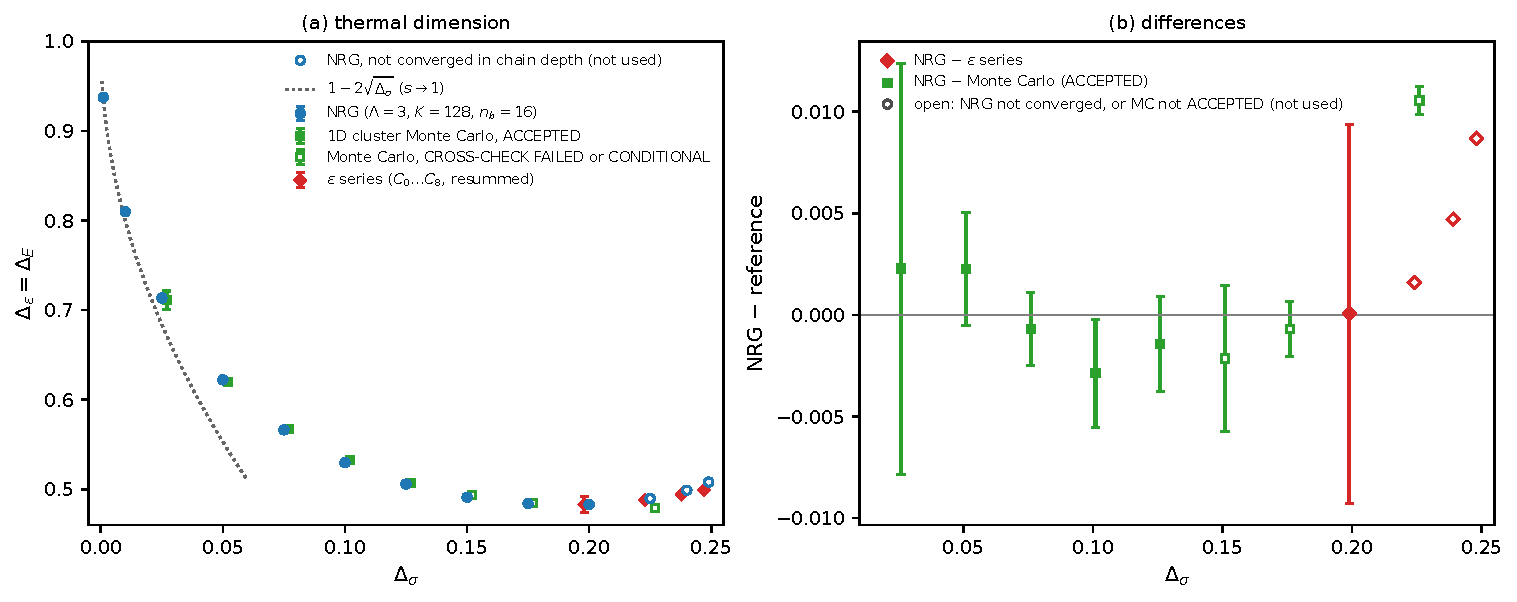
\includegraphics[width=\textwidth]{parts/nrg/figures/fig_checks.pdf}
\caption{(a) $\DE$ against $\Ds$: NRG (filled circles with $\dtot$; open: not converged in chain depth, not used), the project's 1D
cluster Monte Carlo study (filled squares: label ACCEPTED; open: CROSS-CHECK FAILED or CONDITIONAL, which that study does not certify as
infinite-size values; bars $\sigma_{\rm stat}+\sigma_{\rm sys}$, added linearly), the resummed $\varepsilon$ series (diamonds; bars:
spread over Pad\'e approximants, at $\Ds=0.249$ the partial-sum error) and $1-2\sqrt{\Ds}$ near $s=1$. (b) NRG minus reference; bars
are $\dtot$ plus the reference's error, added linearly. Open symbols are not used in any comparison.}\label{nrg:fig:checks}
\end{figure}

What the checks establish:
\begin{itemize}
\item \textbf{The code computes what it claims.} A second implementation written from a physics-only specification
  (Sec.~\ref{nrg:sec:indep}) agrees with the production solver in eight configurations: chain coefficients to better than $\nrgindChain$ (relative, rounding level),
  critical couplings bitwise in $\nrgindAlphaBitwise$ of $\nrgindN$ configurations and to $\nrgindAlpha$ in the others, and $\DE$
  window by window to $\nrgindDE$ wherever its finite differences are reliable. This tests the numerical map, not the estimator.
\item \textbf{Comparison with methods that do not use NRG.} Near $s=1$ the final values reproduce the dual expansion of $\De$ in
  $\sqrt{\Ds}$ through its fifth coefficient (Sec.~\ref{nrg:sec:s1}). At the $\nrgmcAccN$ points where the Monte Carlo study accepts its
  own value they differ from it by at most $\nrgmcAccDiffMax$: within $\sigma_{\rm stat}+\sigma_{\rm sys}+\dtot$ at
  $\nrgmcAccWithinLin$ points and $\nrgmcAccRatioMax$ times that sum at $\Ds=\nrgmcAccDiffMaxAt$. The sum adds a standard deviation, a
  fit-model half-range and an error scale and is only a scale, not a test of statistical consistency. The differences are up to
  $\nrgmcAccStatRatioMax$ Monte Carlo statistical errors and have the same sign at neighboring points, so only the Monte Carlo
  half-range $\sigma_{\rm sys}$ reconciles the two, and the comparison tests the Monte Carlo systematics more than NRG
  (Sec.~\ref{nrg:sec:mc}). At $\Ds=0.2$ the resummed series has a spread of $\nrgserSpreadTwoHundred$ and does not test NRG.
\item \textbf{Near $s=1/2$ the chain is too short.} The flow approaches its fixed point at a rate $\omega\approx\varepsilon\to0$ in
  the RG time $l$. At $\Ds=0.249$ the inverse distance to the series value grows nearly linearly in $l$, with slopes $\nrgslopeEarly$
  to $\nrgslopeLate$, of the size of the one-loop prediction ($\nrgslopePredEarly$ to $\nrgslopePredLate$; Fig.~\ref{nrg:fig:flow}c,
  Sec.~\ref{nrg:sec:approach}). Convergence scans in $K$, $n_b$ or $\Lambda$ at fixed depth cannot reveal this, because once $K$ and
  $n_b\ge12$ are converged the effect depends only on $l$.
\end{itemize}
The errors are error scales built from measured spreads and a few stated judgements (Sec.~\ref{nrg:sec:budget}); they are not standard
deviations. In the text they are quoted with two significant digits; in the tables value(error) follows the PDG rounding (two digits
if the leading digits are 10--35, else one). Bounds in the text (``at most'', ``agree to'', ``below'') are rounded up, so they can
exceed the corresponding table entry by one unit of the last digit. Monte Carlo values and the coefficients $C_7$, $C_8$ are quoted
as their sources give them.

% =====================================================================================================================
\section{The problem and what is known}\label{nrg:sec:model}
% =====================================================================================================================
\subsection{The long-range Ising chain and its thermal dimension}
The ferromagnetic long-range Ising (LRI) chain has spins $S_i=\pm1$ on the sites of a line ($d=1$) and couplings
$J_{ij}\propto1/|i-j|^{1+s}$. It has a finite-temperature transition for $0<s\le1$; the transition is mean-field for $s<1/2$, of
Kosterlitz--Thouless type at $s=1$~\cite{nrg:Kosterlitz1976,nrg:LM01}, and for $1/2<s<1$ its critical point is neither mean-field nor
short-range~\cite{nrg:Fisher1972,nrg:Sak1973}. There the spin field has the exactly known dimension
\begin{equation}
\Ds=\frac{d-s}{2}=\frac{1-s}{2},\qquad s=1-2\Ds,\qquad \varepsilon\equiv2s-d=2s-1=1-4\Ds ,\label{nrg:eq:ds}
\end{equation}
because long-range interactions are not renormalized~\cite{nrg:Sak1973}. The quantity of interest is the dimension of the energy
operator, the leading $\mathbb Z_2$-even scalar,
\begin{equation}
\De=d-\frac1\nu=1-y_t ,\label{nrg:eq:De}
\end{equation}
where $\nu$ is the correlation-length exponent and $y_t=1/\nu$ the renormalization-group (RG) eigenvalue of the temperature.

Two limits are known analytically:
\begin{itemize}
\item \textbf{$s\to1/2^+$ ($\Ds\to1/4$, $\varepsilon\to0$).} The fixed point becomes Gaussian, $\De\to1/2$, and $\De$ has an
  expansion $\De=\sum_nC_n\varepsilon^n$ with $C_0=1/2$, $C_1=-1/6$ and higher coefficients known through $C_8$ (Sec.~\ref{nrg:sec:series},
  Ref.~\cite{nrg:Paper}). The series is asymptotic, but close to $s=1/2$ it is far more precise than any numerical method. The leading
  irrelevant coupling ($\varphi^4$) has the correction exponent $\omega=\varepsilon+O(\varepsilon^2)$, so corrections to scaling
  decay ever more slowly as $s\to1/2$.
\item \textbf{$s\to1^-$ ($\delta\equiv1-s=2\Ds\to0$).} The two lowest $\mathbb Z_2$-even dimensions are
  $\Delta_\pm=1\pm\sqrt{2\delta}+\delta/4+O(\delta^{3/2})$~\cite{nrg:BLMV25,nrg:BLMV26}; the leading term is Kosterlitz's~\cite{nrg:Kosterlitz1976}.
  With $\Delta_-\sim\varphi^2$ the energy operator~\cite{nrg:BLMV25},
  \begin{equation}
  y_t=\sqrt{2\delta}-\frac\delta4+O(\delta^{3/2}),\qquad \omega=\Delta_+-1=\sqrt{2\delta}+\frac\delta4+O(\delta^{3/2}).\label{nrg:eq:s1}
  \end{equation}
  So $\omega\approx y_t$ near $s=1$: both are small, but they are comparable (Sec.~\ref{nrg:sec:depth}). Beyond this order the dual
  description gives $\De$ as a series in $\sqrt{\Ds}$,
  \begin{equation}
  \De=1+\sum_{n\ge1}C^{\rm SR}_n(1)\,\Ds^{n/2},\qquad C^{\rm SR}_1(1)=-2,\quad C^{\rm SR}_2(1)=\tfrac12,\label{nrg:eq:dual}
  \end{equation}
  equivalent to Eq.~\eqref{nrg:eq:s1} through its second term, with $C^{\rm SR}_3(1)$ to $C^{\rm SR}_8(1)$ computed in the accompanying
  paper~\cite{nrg:Paper}; $C^{\rm SR}_3(1)=\frac{39}{16}+2\zeta(2)$, $C^{\rm SR}_4(1)=4-4\zeta(2)-8\zeta(3)$,
  $C^{\rm SR}_5(1)=\frac{11249}{1024}-\frac{361}{16}\zeta(2)+24\zeta(3)+\frac{49}{2}\zeta(4)$ and
  $C^{\rm SR}_6(1)=26-38\zeta(2)+104\zeta(3)-80\zeta(4)-272\zeta(5)+112\zeta(2)\zeta(3)$.
\end{itemize}

\subsection{The spin--boson model}
The spin--boson model without a static bias field describes a two-level system coupled to a bath of harmonic
oscillators~\cite{nrg:Leggett1987}:
\begin{equation}
H=-\frac{\Omega}{2}\,\sigma_x+\sum_j\omega_j\,b_j^\dagger b_j+\frac{\sigma_z}{2}\sum_j\lambda_j\,\big(b_j+b_j^\dagger\big),\qquad
\rho(\omega)\equiv\sum_j\lambda_j^2\,\delta(\omega-\omega_j)=2\alpha\,\omega^{s}\quad(0<\omega\le1).
\label{nrg:eq:H}
\end{equation}
Here $\sigma_{x,z}$ are Pauli matrices, $\Omega$ is the tunneling amplitude (often called $\Delta$ in the literature), $b_j$
annihilates a bath oscillator of frequency
$\omega_j$, $\lambda_j$ is its coupling, $\rho(\omega)$ is the bath spectral density (the convention of Ref.~\cite{nrg:Bulla2003}, equal to
$J(\omega)/\pi$ in Ref.~\cite{nrg:Leggett1987}), $\alpha$ is the dimensionless dissipation strength and $0<s<1$ (``sub-ohmic''). The bath
cutoff frequency is the unit of energy, and $\Omega=0.1$ throughout; universality in $\Omega$ was not tested (Sec.~\ref{nrg:sec:limits}).

For $0<s<1$ the model has a quantum phase transition at a critical coupling $\alpha_c(s,\Omega)$~\cite{nrg:Bulla2003,nrg:Vojta2006}. For
$\alpha<\alpha_c$ (delocalized phase) the ground state is unique; for $\alpha>\alpha_c$ (localized phase) it is twofold degenerate,
the spin being trapped in one of the eigenstates of $\sigma_z$. In the $\sigma_z$ basis the imaginary-time path integral is a classical
Ising chain along the imaginary-time axis, with lattice spacing of order the inverse cutoff~\cite{nrg:Leggett1987,nrg:Vojta2006}: the
tunneling $\Omega$ gives a short-range coupling between neighboring time slices, and integrating out the bath gives a long-range
coupling $\propto\alpha/\tau^{1+s}$, so $\alpha$ plays the role of the inverse temperature. The quantum critical point is therefore in
the universality class of the $d=1$ LRI model with the same $s$: $\langle\sigma_z(\tau)\sigma_z(0)\rangle\propto\tau^{-2\Ds}$ there,
and $\alpha-\alpha_c$, which is $\mathbb Z_2$-even, couples to the energy operator, so its RG eigenvalue is the $y_t$ of
Eq.~\eqref{nrg:eq:De}. The other even coupling, $\Omega$, feeds the same single relevant even direction.

\subsection{The thirteen points}
The study covers the thirteen values of $\Ds$ in Table~\ref{nrg:tab:headline}, chosen for a point-by-point comparison with other methods
of the project. The outer points $\Ds=0.249$ ($s=0.502$) and $0.001$ ($s=0.998$) are the hardest for every method: near $s=1/2$ the
fixed point is almost Gaussian and the approach to it is slow, near $s=1$ the exponent $y_t$ is small.

% =====================================================================================================================
\section{Method: bosonic NRG with an exact \texorpdfstring{$\alpha$}{alpha}-derivative}\label{nrg:sec:method}
% =====================================================================================================================
NRG~\cite{nrg:Wilson1975,nrg:Bulla2008}, extended to bosonic baths in Refs.~\cite{nrg:Bulla2003,nrg:Bulla2005}, solves an impurity coupled to a bath
by mapping the bath onto a chain whose sites carry exponentially decreasing energy scales, and then diagonalizing the chain one site
at a time, keeping only the lowest states. We use the standard formulation; the non-standard elements are the way $y_t$ is extracted
(Secs.~\ref{nrg:sec:tangent}--\ref{nrg:sec:estimator}).

\subsection{Logarithmic discretization}
The bath interval $(0,1]$ is divided into bins $I_m=(\Lambda^{-(m+1)},\Lambda^{-m}]$, $m=0,1,2,\dots$, with a discretization ratio
$\Lambda>1$. Each bin is replaced by a single oscillator $c_m$ that carries the bin's spectral weight at its mean
frequency~\cite{nrg:Bulla2003,nrg:Bulla2005}. With $q=1/\Lambda$, this ``star'' representation has
\begin{equation}
\gamma_m^2=\int_{I_m}\!\rho(\omega)\,d\omega=\frac{2\alpha\,(1-q^{s+1})}{s+1}\,q^{m(s+1)},\qquad
\xi_m=\frac{\int_{I_m}\omega\rho(\omega)\,d\omega}{\gamma_m^2}=\xi_0\,q^m,\qquad \xi_0=\frac{s+1}{s+2}\,\frac{1-q^{s+2}}{1-q^{s+1}},
\label{nrg:eq:star}
\end{equation}
where $\gamma_m$ is the coupling and $\xi_m$ the frequency of oscillator $m$. Every decade of frequency gets the same number of modes,
however low; dropping all other modes of a bin is the approximation of this step, which becomes exact as $\Lambda\to1$.

\subsection{Wilson chain}
An orthogonal change of basis among the $c_m$ (Lanczos tridiagonalization, started from the combination $\sum_m\gamma_mc_m$ that
couples to the spin) maps the star onto a semi-infinite chain:
\begin{equation}
H=-\frac{\Omega}{2}\sigma_x+\frac{\lambda_{\rm tot}}{2}\,\sigma_z\,(b_0+b_0^\dagger)+\sum_{n\ge0}e_n\, b_n^\dagger b_n
+\sum_{n\ge1}t_{n-1}\,(b_{n-1}^\dagger b_n+b_n^\dagger b_{n-1}),\qquad \lambda_{\rm tot}^2=\sum_m\gamma_m^2=\frac{2\alpha}{s+1}.
\label{nrg:eq:chain}
\end{equation}
The spin now couples only to site 0, and each site only to its neighbors; $e_n$ are the on-site energies and $t_n$ the hoppings. The
star has weights $\gamma_m^2\propto(aq)^m$ at the nodes $\xi_0q^m$, with $a=q^s$: this is the orthogonality measure of the little
$q$-Jacobi polynomials $p_n(x;a,1|q)$~\cite{nrg:KLS10}, so the recurrence coefficients are known in closed form. With
\begin{gather}
\mathcal A_n=\frac{(1-aq^{n+1})^2}{(1-aq^{2n+1})(1-aq^{2n+2})},\qquad
\mathcal B_n=\frac{a\,(1-q^n)^2}{(1-aq^{2n})(1-aq^{2n+1})},\nonumber\\
\bar e_n\equiv\Lambda^{n}e_n=\xi_0\,(\mathcal A_n+\mathcal B_n),\qquad
\bar t_n\equiv\Lambda^{n}t_{n-1}=\xi_0\,\sqrt{\mathcal A_{n-1}\mathcal B_n/q}\quad(n\ge1).\label{nrg:eq:coeff}
\end{gather}
(cf.\ also the orthogonal-polynomial chain mappings of Ref.~\cite{nrg:Chin2010}). The code evaluates these closed forms
(\code{lri\_spin.config.chain\_coefficients}); the independent implementation of Sec.~\ref{nrg:sec:indep} obtains the same numbers by a
high-precision Lanczos recursion. Both rescaled coefficients tend to constants, so site $n$ carries the energy scale $\Lambda^{-n}$.
A plain Lanczos recursion on the star is unstable even in multiple-precision arithmetic: without reorthogonalization it loses the
coefficients after 13 sites with 49 digits and after 33 sites with 268 digits (\code{independent\_check/NOTES.md}). The closed form
avoids the problem.

\subsection{Iterative diagonalization and truncation}
Let $H_n$ be the chain~\eqref{nrg:eq:chain} truncated to the sites $0,\dots,n$ and multiplied by $\Lambda^n$. Adding one site is the step
\begin{equation}
H_{n}=\Lambda\,H_{n-1}\otimes\one+\bar e_n\,\one\otimes b^\dagger b
+\bar t_n\,\big(\bar b_{n-1}^\dagger\otimes b+\bar b_{n-1}\otimes b^\dagger\big),\qquad
H_0=-\frac{\Omega}{2}\sigma_x+\bar e_0\,b_0^\dagger b_0+\frac{\lambda_{\rm tot}}{2}\sigma_z\,(b_0+b_0^\dagger),
\label{nrg:eq:step}
\end{equation}
where $\one$ is the identity, $\bar b_{n-1}$ is the annihilation operator of site $n-1$ written in the basis kept at step $n-1$, and
$b$ acts on the new site. The factor $\Lambda$ brings the previous levels to the new energy scale, so the levels of $H_n$ stay of order
one and their evolution with $n$ is an RG flow; its plateaus are fixed points.

Three truncation parameters make each step finite:
\begin{itemize}
\item \textbf{Oscillator cutoff $n_b$.} Each new oscillator keeps its $n_b$ lowest number states. This suffices near the
  delocalized and critical fixed points, where the chain sites hold few bosons~\cite{nrg:Bulla2005}.
\item \textbf{Parity sectors.} The model conserves the parity $P=\sigma_x\,(-1)^{\sum_nb_n^\dagger b_n}$, which implements the Ising
  symmetry. $H_n$ is diagonalized separately in the even and odd sectors, each of dimension at most $Kn_b$.
\item \textbf{Kept states $K$.} In each sector the $K$ lowest eigenstates are kept and the rest discarded. After each step all
  energies are shifted so that the ground state is at zero.
\end{itemize}
Together with $\Lambda$ and the number $N$ of chain sites (the last site sits at energy scale $\Lambda^{-N}$), these parameters
define a finite numerical map from $\alpha$ to a sequence of spectra, which we call the \emph{finite map}. Dense diagonalization costs
of order $(Kn_b)^3$ per sector and site, which limits $K$ and $n_b$.

\subsection{Parity-gap flow and critical coupling}\label{nrg:sec:critical}
The observable is the rescaled parity gap
\begin{equation}
g_n(\alpha)=E^{\rm odd}_{0,n}-E^{\rm even}_{0,n},
\end{equation}
the difference between the lowest levels of $H_n$ in the odd and even sectors. In the delocalized phase $g_n$ flows to its value in
the decoupled chain, where the spin is frozen by $\Omega$ and $g_n$ is the lowest one-boson level; in the localized phase the ground
state becomes degenerate and $g_n\to0$; at $\alpha_c$ it stays on the value of the critical fixed point over an intermediate range
of $n$.

For a chain of $N$ sites, $n=0,\dots,N-1$, the critical coupling of the finite map is located by bisection on the sign of
\begin{equation}
f(\alpha)=g_{N-1}(\alpha)-0.3\,g_{N-1}(0),\label{nrg:eq:bisect}
\end{equation}
the last gap measured against 30\% of the last gap of the decoupled chain ($\alpha=0$) with the same parameters; $f>0$ on the
delocalized side and $f<0$ on the localized side. The rule is:
\begin{itemize}
\item \textbf{Bracket.} Start from $[0.01,2]$; halve the lower end (up to 40 times) until $f>0$; double the upper end until $f<0$,
  never evaluating $\alpha>100$. Without a sign change the item fails.
\item \textbf{Bisection.} At most 48 steps, stopping when the bracket is narrower than $5\times10^{-14}\max(1,|\alpha|)$. A bisection
  that does not reach this width is rejected.
\item \textbf{Result.} $\alpha_c$ is the midpoint of the final bracket. The \emph{terminal residual} is $f(\alpha_c)$.
\end{itemize}
This follows the script of the original study, with two conservative differences: the original evaluated $\alpha$ up to 128 and
accepted an exhausted bisection. The fraction 0.3 is a convention, like the level used to define the crossover
scale in Refs.~\cite{nrg:Bulla2003,nrg:Bulla2005}. The value of $\alpha_c$ is not universal: it depends on $\Lambda$, $K$ and $n_b$
(Fig.~\ref{nrg:fig:alpha}) and enters no result.

\subsection{Exact \texorpdfstring{$\alpha$}{alpha}-derivative of the truncated map}\label{nrg:sec:tangent}
A small detuning $\delta\alpha=\alpha-\alpha_c$ points along the relevant direction of the critical fixed point and grows by a
factor $\Lambda^{y_t}$ per site, so near the fixed point
\begin{equation}
\partial_\alpha g_n\big|_{\alpha_c}\propto\Lambda^{y_tn}.\label{nrg:eq:growth}
\end{equation}
The production code measures this growth without finite differences, by differentiating every step~\eqref{nrg:eq:step} with respect to
$\alpha$, including the change of the kept states. In each parity block write $H=U\,{\rm diag}(E)\,U^{\rm T}$, with kept
eigenvectors $U_k$ (energies $E_k$) and discarded eigenvectors $U_d$ (energies $E_d$), and let $\dot H=\partial_\alpha H$. In the
gauge without rotations among kept states,
\begin{equation}
\dot U_k=U_d\,Z,\qquad Z_{ij}=\frac{\big(U_d^{\rm T}\dot H\,U_k\big)_{ij}}{E_{k,j}-E_{d,i}},\qquad
T=U_k^{\rm T}\dot H\,U_k-\dot E_0\,\one,
\label{nrg:eq:tangent}
\end{equation}
where $\dot E_0$ is the derivative of the ground-state energy (the shift to zero is part of the step). $T$, the derivative of the kept
Hamiltonian, and the derivative of the projected site operator, $\dot{\bar b}=\dot U_k^{\rm T}B\,U_k+U_k^{\rm T}B\,\dot U_k$ with $B$
the site-$n$ annihilation operator in the unrotated product basis, are carried to the next step, where
$\dot H_{n+1}=\Lambda\,T\otimes\one+\bar t_{n+1}(\dot{\bar b}^\dagger\otimes b+{\rm h.c.})$. Only $H_0$ depends on $\alpha$
explicitly, through $\lambda_{\rm tot}\propto\alpha^{1/2}$. The derivative of the gap is $\partial_\alpha g_n=T^{\rm odd}_{00}-T^{\rm
even}_{00}$. This is the exact derivative of the finite map wherever the kept and discarded levels are separated; if the gap between
them falls below $5\times10^{-13}\max(1,|E|)$ the item fails and no record is written. A finite difference in $\alpha$ would instead
turn nonlinear once $\delta\alpha\,\Lambda^{y_tn}$ is no longer small, and lose digits to rounding as $\delta\alpha\to0$.

\subsection{The window audit}\label{nrg:sec:windows}
Near the fixed point, Eq.~\eqref{nrg:eq:growth} gives $\ln|\partial_\alpha g_n|=\kappa+y_t\,n\ln\Lambda$. The window audit, inherited from
the analyzer of the original study, is:
\begin{enumerate}
\item \textbf{Windows.} Windows of $w=\max(12,\lfloor0.13N\rfloor)$ consecutive sites, with first sites from $\max(8,\lfloor0.13N\rfloor)$
  up to (excluding) $\lfloor0.76N\rfloor-w$. A window is skipped if any gap $g_n\le0$ or any $\ln|\partial_\alpha g_n|$ is not finite.
\item \textbf{Fit.} In each window a least-squares line in $n$ is fitted to $\ln|\partial_\alpha g_n|$; its slope divided by $\ln\Lambda$
  is $y_t$, and $\DE=1-y_t$. The \emph{fit residual} is the largest absolute deviation from the line.
\item \textbf{Flatness.} The \emph{relative variation} of the window is $(\max g_n-\min g_n)/|\overline{g_n}|$.
\item \textbf{Quality windows} have relative variation $<0.005$ and fit residual $<0.003$ (inherited conventions). Their number is
  $\nq$, and their $\DE$ values span the \emph{quality range}.
\end{enumerate}
The audit uses no target value of any exponent.

\subsection{The estimate: settled value, plateau and extrapolation}\label{nrg:sec:estimator}
The window values of an item are not constant (Fig.~\ref{nrg:fig:plateau}). Along the chain the flow first approaches the fixed point,
with irrelevant corrections decaying as $e^{-\omega l}$ in the \emph{RG time} $l=n\ln\Lambda$; once the residual detuning has grown
(Sec.~\ref{nrg:sec:depth}) it leaves the fixed point again. The estimate is taken where the flow is closest to the fixed point, by a rule
with three steps (\code{code/analysis/estimator.py}):
\begin{enumerate}
\item \textbf{Settled value.} The \emph{settled window} is the window with the smallest fit residual plus relative variation; its
  $\DE$ is the \emph{settled value}. This is the window the original analyzer reports, stored in every record as \code{selected}.
\item \textbf{Plateau test.} Take the windows whose first site lies within $h=\lceil w/4\rceil$ sites of that of the settled window.
  The largest $|\DE-\text{settled value}|$ among them is the \emph{plateau drift}. A point has a \emph{plateau} if the plateau drift
  of its central item is at most $\tau_{\rm p}=\nrgtau$. Its value is then the settled value, and the plateau drift is its chain-depth
  error.
\item \textbf{Extrapolation}, where there is no plateau. The local exponent
  \begin{equation}
  \Dloc(n)=1-\frac{\ln|\partial_\alpha g_{n+1}|-\ln|\partial_\alpha g_{n-1}|}{2\ln\Lambda}\label{nrg:eq:loc}
  \end{equation}
  is fitted with $\Delta_\infty+A\,e^{-\omega(l-l_0)}$ (free $\Delta_\infty$, $A$, $\omega$; unweighted least squares) on
  $l_{\rm hi}-S\le l\le l_{\rm hi}$ for $S=\nrgspans$, where $l_{\rm hi}$ is the RG time of the last site of the settled window and
  $l_0$ that of the first fitted site. The value is the median of the three $\Delta_\infty$, and the chain-depth error is the larger of
  $|\text{extrapolated}-\text{settled}|$ and the spread of the three fits. Details: a range with fewer than 8 sites is skipped; the
  start values are $\Delta_\infty$ = last point, $A$ = first minus last, $\omega=0.2$; the fit is Levenberg--Marquardt. The
  extrapolation counts as \emph{determined} only if every fit converged with $\omega>0.01$; otherwise it is reported as not
  determined (n.d.), and a point that needs it would stop the analysis.
\end{enumerate}
Every item of a point is evaluated with that point's estimator, so the scans of Sec.~\ref{nrg:sec:budget} compare like with like. The rule
was written on 13 October 2026 and its constants were not varied afterwards (Sec.~\ref{nrg:sec:budget}, App.~\ref{nrg:app:provenance}). It replaces the midpoint of
the quality range used before; App.~\ref{nrg:app:midpoint} explains why and lists the old values.

At $\Ds=0.001$ the rule's own fit ranges lie entirely on the flat plateau, so its extrapolation is not determined (n.d.); the point
has a plateau and is not extrapolated.

\textbf{Classification of the points.} The rule puts each point in one of two classes, \emph{plateau} or \emph{extrapolated}. The eight
points with $\Ds\le0.15$ have a plateau: their plateau drift is at most $\nrgdriftMaxPlateau$ (at $\Ds=\nrgdriftMaxPlateauAt$) and at
most $\nrgdriftMaxLow$ for $\Ds\le0.125$. None of the five points with $\Ds\ge0.175$ has one: their smallest drift is
$\nrgdriftMinNoPlateau$ (at $\Ds=\nrgdriftMinNoPlateauAt$). Every threshold between these two numbers gives the same classification.
The drift grows smoothly with $\Ds$, so the split also depends on $h$ and on the window width $w$, which the rule fixes. At $\Ds=0.15$
the drift is $\nrgdriftHalfOneFifty$ with $h=w/2$ and $\nrgdriftTwentyOneFifty$ with windows of 20 sites, above $\tau_{\rm p}$ in both
cases, so the point would be extrapolated; every point with $\Ds\le0.125$ keeps its plateau (drifts below $\nrgdriftHalfLow$ and
$\nrgdriftTwentyLow$). The values hardly depend on the class: extrapolating at $\Ds=0.15$ would move the value by $\nrgreclassOneFifty$,
windows of 20 sites move its settled value by $\nrgsettledTwentyShiftOneFifty$, and taking the settled value at $0.175$ would move it by
$\nrgreclassOneSeventyFive$, all well inside $\dtot$. At the two final points without a plateau the extrapolation is the value
(Table~\ref{nrg:tab:extrap}).

A third label, \emph{not converged in chain depth}, is not an outcome of the rule. The author assigned it on 13 October 2026 to the
three points closest to $s=1/2$, $\Ds=0.249$, $0.24$ and $0.225$, when the comparison with the $\varepsilon$ series was already known
(App.~\ref{nrg:app:provenance}). The reasons: there $\omega\,l_{\max}\approx61\varepsilon$ is small (Sec.~\ref{nrg:sec:depth}); at
$\Ds=0.249$ the excess over the series decays at a rate of the one-loop size (Sec.~\ref{nrg:sec:approach}); and the excess of the settled
values over the series falls smoothly with $\varepsilon$ (Sec.~\ref{nrg:sec:series}). At $\Ds=0.225$ the rule alone would extrapolate: its
three fits converge, with $\omega=\nrgruleOmTwoTwentyFive$, and give $\nrgruleTwoTwentyFive$ with $\dd=\nrgruleDepthTwoTwentyFive$.
The label there rests on the trend from the two other points and on the Borel--Pad\'e sum of the series; optimal truncation of the
series, $\nrgserOptTwoTwentyFive$, does not exclude the settled value. For the three labeled points the settled value is shown, the
extrapolations are cross-checks only, and no error is quoted. That they ``enter no comparison'' means that no agreement or
disagreement is claimed from their values; the label itself came from a comparison.

\subsection{Cross-check fits (not adopted)}\label{nrg:sec:crosscheck}
The rule's fits end at the settled window and contain no term for the departure from the fixed point, so on a plateau they return the
plateau almost by construction. Two fits that include that departure test the rule from outside (\code{code/analysis/crosscheck.py},
written for the second review round, App.~\ref{nrg:app:provenance}). Neither is adopted, and no value in this note is taken from them. Both
fit $\Dloc(l)$ of the central item with an approach term plus a \emph{detuning term} $A_{\rm d}\,e^{(1-\Delta_\infty)(l-l_{\rm end})}$,
whose growth rate $1-\Delta_\infty=y_t$ is that of the residual detuning (Sec.~\ref{nrg:sec:depth}). Each fit range runs from a start
$l_{\rm a}$ to $l_{\rm end}=l_N-k/y_t$, where $l_N=N\ln\Lambda$ is the end of the chain and $y_t$ is taken from the settled value, so the
last stretch of RG time, where the detuning dominates, is left out. The fits are Levenberg--Marquardt; the result is the median over the
accepted fits, with their range and number $n_{\rm fit}$.
\begin{itemize}
\item \textbf{Late fit.} Approach term $A\,e^{-\omega(l-l_{\rm a})}$; $l_{\rm a}\in\{20,25,30,35\}$ ($\{40,50,60,70\}$ at
  $\Ds=0.001$), $k\in\{8,10,12\}$, at least 10 sites per range; a fit is accepted if its largest residual is below $2\times10^{-6}$
  (below $2\times10^{-5}$ if no fit reaches $2\times10^{-6}$). It is computed at every point and shown for the final points
  (Table~\ref{nrg:tab:budget}).
\item \textbf{Crossover fit.} Approach term $A/(e^{\omega(l-l_0)}-1)$, the one-loop crossover form of Eq.~\eqref{nrg:eq:oneloop} with a
  free $l_0$, or $A\,e^{-\omega(l-l_{\rm a})}$; $l_{\rm a}\in\{13,18,22\}$, $k\in\{12,15\}$, at least 8 sites per range; a fit is
  accepted if its largest residual is below $2\times10^{-5}$ and $0<\omega<2$. It is computed at $\Ds\ge0.2$, where the approach is
  slowest (Tables~\ref{nrg:tab:extrap} and~\ref{nrg:tab:series}).
\end{itemize}
\textbf{The late fit against the rule.} It reproduces the plateau values to $\nrglateMaxLow$ at $0.001\le\Ds\le0.125$, and differs from
the final values by $\nrglateOneFifty$, $\nrglateOneSeventyFive$ and $\nrglateTwoHundred$ at $\Ds=0.15$, $0.175$ and $0.2$. This is
inside $\dd$ except at $\Ds=\nrglateOutside$, where it is $\nrglateOne$ against $\dd=\nrgdepthOne$, far inside $\dtot$. At $\Ds=0.01$
its fitted $\omega=\nrglateOmTen$ agrees with $\sqrt{2\delta}+\delta/4=\nrgnloOmTen$ from Eq.~\eqref{nrg:eq:s1}. At $\Ds=0.2$ it suggests
that the rule's extrapolation, which ends where the detuning already bends $\Dloc$, lies slightly low, by about a tenth of $\dtot$.
The crossover fit is discussed with the $\varepsilon$ series in Sec.~\ref{nrg:sec:series}.

\subsection{Chain depth}\label{nrg:sec:depth}
The bisection stops when its bracket is narrower than $5\times10^{-14}$ (relative), so the critical coupling of the finite map is
located to $\delta\alpha\approx5\times10^{-14}$. This width is at the rounding level of the map: the same item run on 1 and on 2 threads
gives values of $\alpha_c$ that differ by up to $\nrgexRel$, and the two implementations of Sec.~\ref{nrg:sec:indep} differ by up to
$\nrgindAlpha$ (relative), so a narrower bracket would not locate the critical coupling better in double precision. The residual
detuning also grows as $\Lambda^{y_tn}$, and the flow therefore stays near the fixed point only up to
\begin{equation}
n\lesssim n_{\max}\simeq\frac{\ln(1/\delta\alpha)}{y_t\ln\Lambda}\approx\frac{30.6}{y_t\ln\Lambda},\qquad
l\lesssim l_{\max}=n_{\max}\ln\Lambda\approx\frac{30.6}{y_t},\label{nrg:eq:nmax}
\end{equation}
with $30.6=\ln(2\times10^{13})$: the usable RG time is fixed whatever $\Lambda$. The chain lengths follow this estimate: at
$\Lambda=3$, $N=65$ for $s\le0.8$, then $70$, $80$, $90$ and $105$ for $s=0.85$, $0.9$, $0.95$, $0.98$, and $N=250$ at $s=0.998$; for
other $\Lambda$, $N(\Lambda)=N(3)\ln3/\ln\Lambda$. Where $N\approx n_{\max}$ the terminal residual $|f(\alpha_c)|$ is of order 0.1--0.4,
which is expected and not a failure. At $\Ds=0.025$, where $N=90$ and $n_{\max}\approx\nrgnmaxTwentyFive$, the terminal residuals are
$\nrgtermTwentyFiveLo$ to $\nrgtermTwentyFiveHi$; at $\Ds\le0.01$ the chains are clearly shorter than $n_{\max}$ (at $s=0.98$, $N=105$
against $n_{\max}\approx146$) and they are at most $\nrgtermTenMax$ at $\Ds=0.01$ and $\nrgtermOneMax$ at $0.001$ (App.~\ref{nrg:app:items}).

The flow reaches its fixed point within the usable depth only if $\omega\,l_{\max}\approx30.6\,\omega/y_t$ is large. Near $s=1$,
Eq.~\eqref{nrg:eq:s1} gives $\omega/y_t\to1$, so $\omega l_{\max}\approx30$ however small $y_t$ becomes. Near $s=1/2$, $\omega\approx\varepsilon$
and $y_t\approx1/2$, so $\omega l_{\max}\approx61\varepsilon$: about 0.25, 2.4 and 6 at $\Ds=0.249$, $0.24$ and $0.225$. This is why the
plateau is lost as $s\to1/2$ and not as $s\to1$. Extended-precision arithmetic would lengthen $l_{\max}$ in proportion to the number of
digits.

% =====================================================================================================================
\section{Error budget}\label{nrg:sec:budget}
% =====================================================================================================================
For each final point the value is that of Sec.~\ref{nrg:sec:estimator} for the central item. Its error has three components, each computed
with the point's estimator:
\begin{itemize}
\item $\dd$ (chain depth): the plateau drift of the central item; at an extrapolated point, the larger of $|\text{extrapolated}-
  \text{settled}|$ and the spread of the three fits (Sec.~\ref{nrg:sec:estimator}).
\item $\dK$ ($K$ and $n_b$): the spread (maximum minus minimum) over all $\Lambda=3$ items with $K\ge64$ and $n_b\ge10$; at $\Ds\ge0.2$,
  where $n_b=10$ is not converged (Sec.~\ref{nrg:sec:keepnb}), items with $n_b=10$ are left out.
\item $\dL$ (discretization): the larger of two numbers.
  \begin{itemize}
  \item[(a)] The spread over the items at different $\Lambda$, each at the largest $K$ run there, with equal $n_b$ ($16$ at $\Ds\ge0.2$,
    else $10$): $\Lambda=2.5$ and $3$ at $K=128$ at every point; for $\Ds<0.2$ also $\Lambda=4$, run only at $K=64$; and $\Lambda=2$ at
    $K=256$ at $\Ds=0.1$ and $0.05$. The $K$ convergence of $\Lambda=4$ at $K=64$ is assumed, not tested: larger $\Lambda$ needs
    fewer kept states (Sec.~\ref{nrg:sec:lambda}), and at $\Lambda=3$ the values are converged at $K=48$ already (Sec.~\ref{nrg:sec:keepnb}).
  \item[(b)] The shift of the $\Lambda=2.5$ value under its one doubling of $K$, from 64 to 128, at $n_b=10$, the only $n_b$ run at
    $\Lambda=2.5$, $K=64$ (at $\Ds\ge0.2$, $n_b=10$ is not converged).
  \end{itemize}
  Part (b) allows for the untested $K$ convergence at $\Lambda=2.5$. It is the larger part at $\nrgnLambdaKdbl$ of the ten final points,
  so at most points the quoted error is mainly this allowance, not a measured systematic of the central value.
\end{itemize}
The total is the linear sum
\begin{equation}
\dtot=\dd+\dK+\dL,\label{nrg:eq:budget}
\end{equation}
listed in Table~\ref{nrg:tab:budget} and shown in Fig.~\ref{nrg:fig:budget}. The points that are not converged in chain depth have no $\dd$
and no $\dtot$. At $\Ds=0.2$, $\dK$ mostly measures how the extrapolation itself scatters between items (the detuning fits of
Sec.~\ref{nrg:sec:estimator} bring those items within about $2\times10^{-5}$ of each other), so it partly counts $\dd$ twice; this is
conservative.

\textbf{What this error is, and is not.} None of the components is a standard deviation: $\dd$ is a resolution or an extrapolation
length, $\dK$ and $\dL$ are ranges of convergence scans. They are therefore added linearly, not in quadrature. Five choices are
judgements, not measurements:
\begin{itemize}
\item the plateau threshold $\tau_{\rm p}$, the neighborhood $h$ and the window width $w$ (the classification is the same for every
  $\tau_{\rm p}$ between $\nrgdriftMaxPlateau$ and $\nrgdriftMinNoPlateau$; for $h$ and $w$ see Sec.~\ref{nrg:sec:estimator});
\item the fit form, the fit ranges $S$ and the end point $l_{\rm hi}$ of the extrapolation;
\item taking the full extrapolation length as $\dd$ at an extrapolated point;
\item the allowance (b) in $\dL$ for one $K$ doubling at $\Lambda=2.5$;
\item no allowance below $\Lambda=2$: over $2\le\Lambda\le4$ the values agree to $\nrgLspreadPilot$ at the two points where $\Lambda=2$
  is $K$-converged ($\Ds=0.1$, $0.05$), with a small monotone rise with $\Lambda$ far inside the error, but the limit $\Lambda\to1$
  itself is not tested (Sec.~\ref{nrg:sec:lambda}).
\end{itemize}
The window rule of Sec.~\ref{nrg:sec:windows} (width, range, thresholds) is inherited and was not varied in production. Its quality
thresholds do not set the value, because the settled window passes any reasonable threshold. The window width does enter the plateau
test, and with it the class of $\Ds=0.15$, but not its value beyond $2\times10^{-5}$ (Sec.~\ref{nrg:sec:estimator}).

\textbf{When the choices were made.} The rule and its constants were fixed on 13 October 2026, after the NRG data, the earlier
comparisons with the $\varepsilon$ series and the Monte Carlo study, and the reviews' exploratory comparisons had been seen; no
protocol was registered in advance. App.~\ref{nrg:app:provenance} gives the timeline.

\begin{table}[ht]\centering\footnotesize\setlength{\tabcolsep}{4pt}
\caption{Error budget. Columns: estimator (plateau, extrapolated, or settled for the points not converged in chain depth); $\DE$ to six
decimals; the chain-depth error $\dd$, the $K$/$n_b$ spread $\dK$, the discretization error $\dL$ and their linear sum $\dtot$, in
units of $10^{-4}$; the number $\nq$ of quality windows of the central item; the late fit of Sec.~\ref{nrg:sec:crosscheck} minus $\DE$
(cross-check, not adopted; shown for the final points). n.c.: not converged in chain depth.}\label{nrg:tab:budget}
\begin{tabular}{@{}lllrrrrrrl@{}}
\toprule
$\Delta_\sigma$ & estimator & $\Delta_E$ & $10^4\delta_{\rm depth}$ & $10^4\delta_K$ & $10^4\delta_\Lambda$ & $10^4\delta_{\rm tot}$ & $n_q$ & $10^4\,$(late fit $-\Delta_E$) & status\\
\midrule
0.249 & settled & 0.508030 & n.c. & 1.70 & 1.21 & -- & 2 & $--$ & not converged\\
0.24 & settled & 0.498922 & n.c. & 5.12 & 2.54 & -- & 4 & $--$ & not converged\\
0.225 & settled & 0.489668 & n.c. & 2.98 & 6.05 & -- & 9 & $--$ & not converged\\
0.2 & extrapolated & 0.482980 & 4.12 & 2.47 & 0.49 & 7.08 & 15 & $+0.69$ & final\\
0.175 & extrapolated & 0.483900 & 0.86 & 0.80 & 1.80 & 3.46 & 19 & $+0.14$ & final\\
0.15 & plateau & 0.491106 & 0.19 & 0.28 & 0.68 & 1.15 & 21 & $-0.17$ & final\\
0.125 & plateau & 0.505672 & 0.01 & 0.15 & 0.38 & 0.54 & 23 & $-0.00$ & final\\
0.1 & plateau & 0.529608 & 0.02 & 0.05 & 0.27 & 0.33 & 23 & $-0.01$ & final\\
0.075 & plateau & 0.566260 & 0.01 & 0.05 & 0.24 & 0.30 & 28 & $-0.00$ & final\\
0.05 & plateau & 0.622115 & 0.00 & 0.03 & 0.23 & 0.27 & 34 & $-0.00$ & final\\
0.025 & plateau & 0.713422 & 0.01 & 0.02 & 0.26 & 0.29 & 38 & $+0.00$ & final\\
0.01 & plateau & 0.809747 & 0.09 & 0.02 & 0.35 & 0.47 & 41 & $+0.01$ & final\\
0.001 & plateau & 0.937424 & 0.02 & 0.04 & 1.05 & 1.11 & 106 & $+0.03$ & final\\
\bottomrule
\end{tabular}

\end{table}

\begin{figure}[ht]\centering
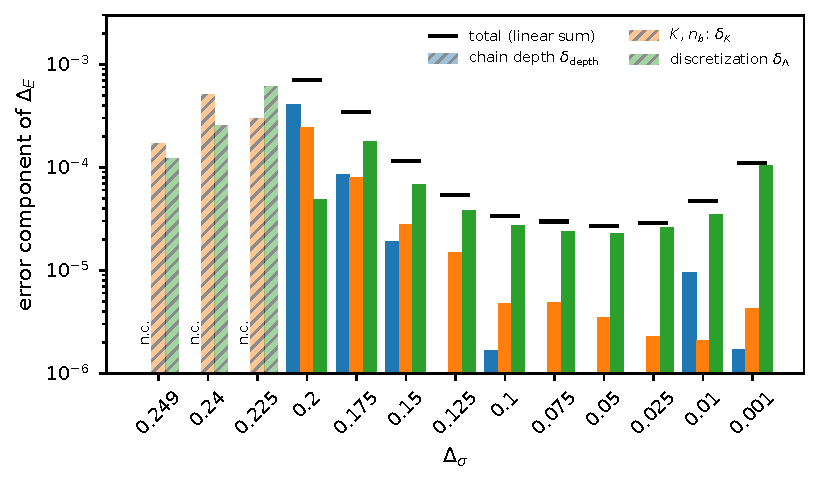
\includegraphics[width=0.72\textwidth]{parts/nrg/figures/fig_error_budget.pdf}
\caption{Components of the error at each $\Ds$ and their linear sum $\dtot$. Hatched: the three points not converged in chain depth,
which have no $\dd$ and no total. At the plateau points $\dL$ dominates, mostly through the $K$-doubling allowance at $\Lambda=2.5$; at
$\Ds=0.2$ the extrapolation length $\dd$ dominates.}\label{nrg:fig:budget}
\end{figure}

% =====================================================================================================================
\section{Software and validation}\label{nrg:sec:software}
% =====================================================================================================================
\subsection{Code}
The solver is the Python package \code{lri\_spin} (\code{code/lri\_spin\_boson\_hpc/src/lri\_spin}; NumPy, SciPy and threadpoolctl;
float64 throughout).
\begin{itemize}
\item \textbf{Backend.} The \code{ordered} backend builds one parity block at a time in the basis order of the reference solver
  (\code{code/lri\_spin\_boson\_hpc/reference/}) and reproduces its flows bitwise and its derivative to rounding (tested). The
  reordered \code{dense} and \code{banded} backends are experimental and were not used.
\item \textbf{Workflows.} The critical search writes checkpoints every 8 sites and persists the bisection state, so an interrupted
  item resumes where it stopped.
\item \textbf{Records.} Each item ends in one result record (App.~\ref{nrg:app:formats}) carrying a SHA-256 checksum and an
  \emph{identity}: the configuration, the kind of run, bracket and tolerances, the SHA-256 of the solver source and the runtime
  (Python, NumPy, SciPy and OpenBLAS versions, BLAS kernel and threading layer). A record from another source or runtime is refused by
  the analysis.
\end{itemize}
Before production Claude Code read the package line by line against the reference solver (App.~\ref{nrg:app:provenance}); no numerical
defect was found and no numerical code was changed.

\subsection{Acceptance gates and tests}
Every result record passed these gates before it was accepted: eigen-residual $\max|HU-UE|\le10^{-8}$ and orthogonality error
$\max|U^{\rm T}U-\one|\le10^{-9}$ at sites $0,1,2$, every 16th site and the last; finite observables and sorted spectra; boson
occupation within $[0,n_b-1]$ and top-level probability (the weight of the highest kept level of the newest oscillator,
$p_{\rm edge}$) within $[0,1]$; for derivatives, a positive gap between kept and discarded levels. Over all $\nrgnItems$ production
records the largest checked eigen-residual is $\nrgmaxEigRes$ and the largest orthogonality error $\nrgmaxOrth$.

The test suite (\code{make test}) has 85 tests. Physics: chain moments, small untruncated spectra against exact diagonalization,
Kronecker products against block operators, reference trajectories, finite differences against the exact derivative. Software:
workflows, record corruption, signals and locks, and the cluster tools of App.~\ref{nrg:app:cluster} (campaign ownership, generations,
lanes, submission against a simulated Slurm, exports, stopping). Before production it passed on a compute node of the cluster for the
final code, in the validation job that issued the receipt \code{inputs/validation\_receipt/receipt.json}. The receipt binds the
solver source to the node runtime: AMD EPYC 7543 nodes, Python 3.13.3, NumPy 2.1.2, SciPy 1.15.2, OpenBLAS 0.3.27/0.3.28 with the
Haswell kernel.

\subsection{Reproducibility across machines}
With the same runtime and thread counts, results are bitwise identical across nodes: a repeated smoke run on a second node reproduced
the first bitwise (App.~\ref{nrg:app:cluster}). Across runtimes, rounding differences are amplified along the relevant direction as
$\Lambda^{y_tn}$: at a \emph{fixed} $\alpha$, late flows of two machines differ, and even two implementations with bitwise identical
$\alpha_c$ (configuration c1 of Sec.~\ref{nrg:sec:indep}) have flows that differ by more than $10^{-8}$ from site $\nrgindDivCone$ on.
Archived values of $\alpha_c$ are therefore not portable, and every item retunes $\alpha_c$ on its own runtime. The critical coupling
itself and the exponent are robust: the production values of $\alpha_c$ reproduce the three couplings archived by the original study
on another machine to $\nrgarchRel$ (relative); the three example items, run on 2 threads, reproduce the $\alpha_c$ of the same items
run on 1 thread bitwise in $\nrgexBitwise$ cases and to $\nrgexRel$ in the third; and the exponents of two implementations agree to
$\nrgindDE$ (Sec.~\ref{nrg:sec:indep}).

% =====================================================================================================================
\section{Production campaigns}\label{nrg:sec:campaigns}
% =====================================================================================================================
All items are critical searches followed by the exact derivative and the window audit, with $\Omega=0.1$, bracket $[0.01,2]$ and
the \code{ordered} backend. Item IDs read \code{ds<$\Ds$>\_L<$\Lambda$>\_K<$K$>\_B<$n_b$>\_N<$N$>}; the example items use
\code{s<$s$>\_L<$\Lambda$>\_K<$K$>\_B<$n_b$>}. Items of the ds13 campaign and the $\Lambda$ campaigns ran on 1 thread if
$Kn_b\le1000$, 2 threads if $Kn_b<1600$ and 4 otherwise; the example items ran on 2 threads, as in the package's example list.
\begin{description}
\item[Example] ($\nrgnItemsExample$ items). The package's example list: $s=0.8$, $0.9$, $0.98$ at $K=64$, $n_b=10$, $\Lambda=3$
  (Table~\ref{nrg:tab:example}). They duplicate three items of the ds13 campaign, which makes them a test of thread-count
  independence (Sec.~\ref{nrg:sec:software}).
\item[ds13] ($\nrgnItemsDs$ items). All thirteen points at $\Lambda=3$ with
  \begin{itemize}
  \item a scan in kept states, $K\in\{48,64,96,128\}$ at $n_b=10$;
  \item a scan in oscillator levels, $n_b\in\{8,12,16\}$ at $K=64$;
  \item $\Lambda\in\{2,4\}$ at $K=64$, $n_b=10$;
  \item the central item $K=128$, $n_b=16$;
  \item extras at the ends: $n_b\in\{20,24\}$ for $\Ds\ge0.2$ and $K\in\{160,192\}$ for $\Ds\le0.05$.
  \end{itemize}
\item[$\Lambda$ pilot] ($\nrgnItemsPilot$ items). $\Ds\in\{0.2,0.1,0.05\}$ at $\Lambda=1.5$ ($K\in\{64,128\}$ at $n_b=10$, $K=64$ at
  $n_b=16$), $\Lambda=2$ ($K=128$) and $\Lambda=2.5$ ($K\in\{64,128\}$), $n_b=10$ unless stated. ($\Lambda=2$, $K=64$ is part of the
  ds13 campaign.)
\item[$\Lambda$ follow-up] ($\nrgnItemsFollowup$ items). $\Lambda=2.5$ at $K\in\{64,128\}$ for the other ten points, plus $K=128$,
  $n_b=16$ for $\Ds\ge0.2$; and $\Lambda=2$ at $K\in\{192,256\}$ for $\Ds\in\{0.2,0.1,0.05\}$.
\end{description}
The runs used $\nrgthreadHours$ thread-hours (sum over items of wall time times threads) on whole cluster nodes. The allocations
summed to $\nrgnodeHours$ node-hours, i.e.\ about $\nrgcoreHoursCharged$ core-hours as charged for 64-core nodes; the longest item
took $\nrglongestItem$\,h, and the production finished within two days including a cluster outage (Table~\ref{nrg:tab:resources} in
App.~\ref{nrg:app:cluster}). The largest peak memory of an item was $\nrgpeakRSS$\,MiB.

\begin{table}[ht]\centering\footnotesize\setlength{\tabcolsep}{4pt}
\caption{The example items ($K=64$, $n_b=10$, $\Lambda=3$, 2 threads): critical coupling, bisection steps, terminal residual
$f(\alpha_c)$, number of quality windows, quality range and settled value. The terminal residuals near $-0.16$ reflect $N\approx n_{\max}$
(Sec.~\ref{nrg:sec:depth}); at $s=0.98$, $N<n_{\max}$.}\label{nrg:tab:example}
\begin{tabular}{llllll}
\toprule
item & $\alpha_c$ & bisection & terminal residual & quality windows & $\Delta_E$ range (settled) \\
\midrule
\texttt{s0.80\_L3\_K64\_B10} & 0.43976978933704 & 46 & $-$0.160 & 23 & [0.52961, 0.53006] (0.52961)\\
\texttt{s0.90\_L3\_K64\_B10} & 0.68913573159160 & 46 & $-$0.159 & 34 & [0.62212, 0.62260] (0.62212)\\
\texttt{s0.98\_L3\_K64\_B10} & 1.08065976531605 & 46 & $+$0.000 & 41 & [0.80946, 0.81013] (0.80975)\\
\bottomrule
\end{tabular}

\end{table}

% =====================================================================================================================
\section{Results}\label{nrg:sec:results}
% =====================================================================================================================
\subsection{The approach to the fixed point}\label{nrg:sec:approach}
Figure~\ref{nrg:fig:flow} shows the local exponent~\eqref{nrg:eq:loc} against the RG time, which is the quantity the estimator works on.
\begin{itemize}
\item \textbf{Plateau ($\Ds=0.1$, panel a).} After the transient, $\Dloc$ is flat over $30\lesssim l\lesssim55$ and the same at
  $\Lambda=2$, $2.5$, $3$ and $4$; the fitted correction exponent is $\omega=\nrgomOneHundred$. The settled window lies on the plateau.
\item \textbf{No plateau ($\Ds=0.2$, panel b).} $\Dloc$ is still falling when the detuning sets in. The settled value,
  $\nrgsetTwoHundred$, is the deepest usable value; the extrapolation (Table~\ref{nrg:tab:extrap}; $\omega=\nrgomTwoHundred$) gives
  $\nrgextTwoHundred$, $\nrgextShiftTwoHundred$ from it, and the extrapolations at $\Lambda=2.5$ and $3$ agree to $\nrgextLamTwoHundred$.
  At $\Ds=0.175$ ($\omega=\nrgomOneSeventyFive$) the shift is $\nrgextShiftOneSeventyFive$.
\item \textbf{Near $s=1/2$ ($\Ds=0.249$, panel c).} At one loop, with the $\varphi^4$ coupling $u$ normalized so that
  $du/dl=\varepsilon u-u^2$ (fixed point $u^*=\varepsilon$), the local dimension of the energy operator is
  $\frac12-\frac\varepsilon2+\frac u3$; the factor $\frac13=(\mathcal N+2)/(\mathcal N+8)$ is that of the Ising case $\mathcal N=1$
  of the O($\mathcal N$) model~\cite{nrg:Fisher1972}, and at $u^*$ it gives $\De=\frac12-\frac\varepsilon6$. A strong bare coupling,
  $u\to\infty$ at some RG time $l_0$, then gives
  \begin{equation}
  \Dloc-\De=\frac{\varepsilon/3}{e^{\varepsilon(l-l_0)}-1},\qquad \frac1{\Dloc-\De}=\frac3\varepsilon\big(e^{\varepsilon(l-l_0)}-1\big),
  \label{nrg:eq:oneloop}
  \end{equation}
  if $\Dloc$ follows the running coupling. The inverse excess thus grows with local slope $3e^{\varepsilon(l-l_0)}$, which tends to 3
  as $\varepsilon(l-l_0)\to0$. With the series value $\De=\nrgserTwoFortyNine$ the measured inverse excess grows nearly linearly in $l$
  at every $K$, $n_b$ and $\Lambda$ shown, with slope $\nrgslopeEarly$ for $15\le l\le25$, $\nrgslopeMid$ over $20\le l\le45$ and
  $\nrgslopeLate$ for $38\le l\le48$. Inferring $l_0$ from the data at $20\le l\le40$ gives $l_0=\nrglzeroLo$ to $\nrglzeroHi$, for
  which Eq.~\eqref{nrg:eq:oneloop} predicts local slopes $\nrgslopePredEarly$ at $l=20$ and $\nrgslopePredLate$ at $l=43$. The measured
  slopes are 10--20\% lower and rise with $l$ as predicted. Terms of higher order in $u$, largest early in the flow where $u$ is
  largest, could account for the difference, but we have not shown that. The test is semi-quantitative: it shows an approach of the
  one-loop kind, at a rate set by $\varepsilon$, not a precise coefficient. At $\Ds=0.249$, $0.24$ and $0.225$ the window $\DE$ still changes by $\nrgdriftSiteTwoFortyNine$,
  $\nrgdriftSiteTwoForty$ and $\nrgdriftSiteTwoTwentyFive$ per site at the settled window. Single-exponential fits give
  $\omega=\nrgomTwoFortyNine$, $\nrgomTwoForty$ and $\nrgomTwoTwentyFive$, which approach $\varepsilon$ ($0.004$, $0.04$, $0.1$) only at the
  largest $\varepsilon$, since an exponential cannot represent a $1/l$ approach, and the three fits scatter by up to
  $\nrgextSpreadTwoTwentyFive$ (Table~\ref{nrg:tab:extrap}). The data do not determine the fixed-point value at these
  points to the precision of the others: they are \emph{not converged in chain depth}. A scan in $K$, $n_b$ or $\Lambda$ at fixed
  $l_{\max}$ cannot reveal this, because once $K$ is converged and $n_b\ge12$ the effect depends only on $l$ ($n_b=8$ and $10$ are
  off by up to $\nrgnbEight$ and $\nrgnbTen$ near $s=1/2$, Sec.~\ref{nrg:sec:keepnb}).
\item \textbf{Near $s=1$ ($\Ds=0.001$, panel d).} $\Dloc$ rises to a long plateau ($75\lesssim l\lesssim120$), as Eq.~\eqref{nrg:eq:nmax}
  allows. At the $10^{-4}$ level the plateau depends on the truncation away from $\Lambda=3$: at $\Lambda=2.5$ it moves by
  $\nrgKdblOne$ between $K=64$ and $128$, at $\Lambda=4$ ($K=64$) it overshoots by about $10^{-4}$ before settling, and at $\Lambda=2$,
  $K=64$ is far from converged ($\nrgLtwoOne$). At the largest $K$ run the values at $\Lambda=2.5$, $3$ and $4$ agree to $\nrgLspreadOne$,
  but at $\Lambda=2.5$ that is a single doubling. The
  plateau value is therefore ambiguous at the $10^{-4}$ level; the budget carries this through the $K$-doubling allowance, which gives
  $\dL=\nrgKdblOne$ at this point (Sec.~\ref{nrg:sec:budget}).
\end{itemize}

\begin{figure}[ht]\centering
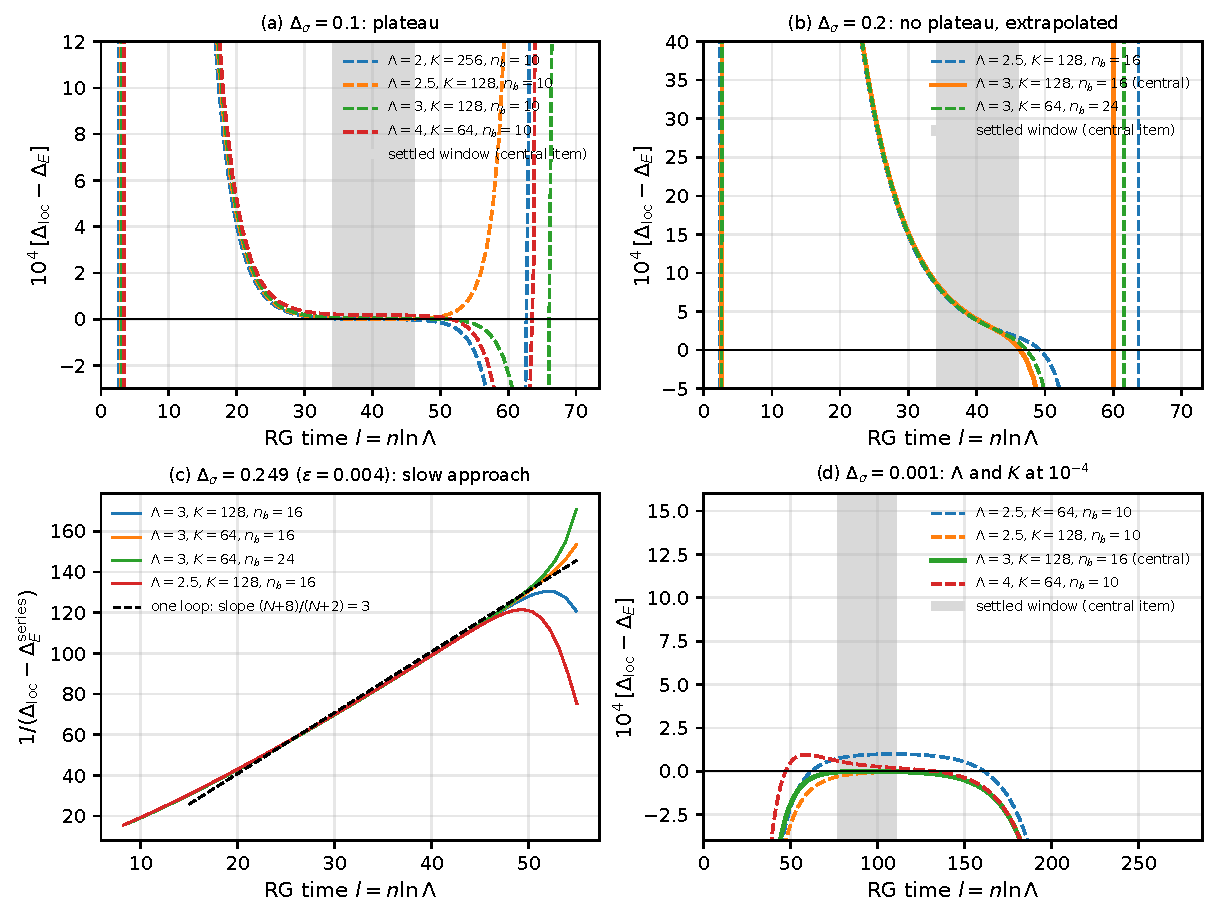
\includegraphics[width=0.95\textwidth]{parts/nrg/figures/fig_flow.pdf}
\caption{Local exponent $\Dloc$, Eq.~\eqref{nrg:eq:loc}, against the RG time $l=n\ln\Lambda$. (a), (b), (d): $10^4\,(\Dloc-\DE)$ relative to
the final value; gray band: the settled window of the central item. (a) $\Ds=0.1$, items at four values of $\Lambda$, each at the
largest $K$ run (at $\Lambda=4$ only $K=64$): a common plateau. (b) $\Ds=0.2$: no plateau; the zero line is the extrapolated value. (d)
$\Ds=0.001$: $\Lambda$ and $K$ at the $10^{-4}$ level. (c) $\Ds=0.249$: inverse distance to the $\varepsilon$-series value against $l$,
for four truncations; dashed: slope 3, the one-loop value for $\varepsilon(l-l_0)\to0$ (Eq.~\eqref{nrg:eq:oneloop}).}\label{nrg:fig:flow}
\end{figure}

\begin{table}[ht]\centering\scriptsize\setlength{\tabcolsep}{2.5pt}
\caption{The points without a plateau (central items). Settled value; plateau drift; change of the window $\DE$ per site at the settled
window; the three fitted $\Delta_\infty$ and $\omega$ for $S=30,25,20$; their median (the extrapolated value). At $\Ds=0.2$ and $0.175$
the median is the final value. Last column: the crossover fit of Sec.~\ref{nrg:sec:crosscheck} (median, number $n_{\rm fit}$ of accepted
fits), computed at $\Ds\ge0.2$ only; a cross-check, not adopted. $^\ast$Not converged in chain depth: cross-check only, not
used.}\label{nrg:tab:extrap}
\begin{tabular}{@{}llllllll@{}}
\toprule
 & & & & \multicolumn{3}{c}{the rule (Sec.~\ref{nrg:sec:estimator})} & cross-check, not adopted\\
\cmidrule(lr){5-7}\cmidrule(lr){8-8}
$\Delta_\sigma$ & settled & drift & per site & fits $\Delta_\infty$ ($S=30,25,20$) & $\omega$ & median & crossover fit ($n_{\rm fit}$)\\
\midrule
0.249$^\ast$ & 0.508030 & $8\times10^{-4}$ & $-3\times10^{-4}$ & 0.50496, 0.50463, 0.50463 & 0.068, 0.064, 0.064 & 0.504628 & 0.50209 (6)\\
0.24$^\ast$ & 0.498922 & $7\times10^{-4}$ & $-2\times10^{-4}$ & 0.49670, 0.49673, 0.49704 & 0.078, 0.079, 0.088 & 0.496734 & 0.49460 (6)\\
0.225$^\ast$ & 0.489668 & $6\times10^{-4}$ & $-2\times10^{-4}$ & 0.48804, 0.48753, 0.48668 & 0.092, 0.078, 0.059 & 0.487529 & 0.48810 (7)\\
0.2 & 0.483392 & $2\times10^{-4}$ & $-7\times10^{-5}$ & 0.48305, 0.48298, 0.48291 & 0.151, 0.142, 0.130 & 0.482980 & 0.48305 (9)\\
0.175 & 0.483986 & $8\times10^{-5}$ & $-2\times10^{-5}$ & 0.48391, 0.48390, 0.48389 & 0.205, 0.199, 0.190 & 0.483900 & --\\
\bottomrule
\end{tabular}

\end{table}

\subsection{Convergence in kept states and oscillator levels}\label{nrg:sec:keepnb}
Table~\ref{nrg:tab:keepnb} and Fig.~\ref{nrg:fig:keepnb} show the deviation of every $\Lambda=3$ item from the central value.
\begin{itemize}
\item \textbf{Kept states.} The estimates are converged at $K=48$ already: for $\Ds\le0.125$ the spread over $K$ is at most
  $\nrgkeepSpread$.
\item \textbf{Oscillator levels.} $n_b$ matters mainly near $s=1/2$, where $n_b=8$ is off by up to $\nrgnbEight$ and $n_b=10$ by up to
  $\nrgnbTen$, while at the final points all items with $n_b\ge12$ (and $K\ge64$) agree with the central value to $\nrgnbTwelve$.
\item \textbf{Top-level probability.} $p_{\rm edge}$ is the weight of the highest level, $n_b-1$, of the newest oscillator in the
  ground state, evaluated at every site of the critical flow; App.~\ref{nrg:app:items} lists its maximum over the chain. That maximum is
  reached at the last sites, where the flow leaves the fixed point, and depends on the side it leaves to: for the items with
  $n_b\ge12$ its median is $\nrgedgeNegMed$ when the flow ends toward the localized phase (negative terminal residual; the bosons are
  displaced there) and $\nrgedgePosMed$ when it ends toward the delocalized phase. This is why it changes by many decades between
  items that differ only in $K$. For $n_b\ge12$ it is at most $\nrgedgeMax$, at most $\nrgedgeCentralMax$ for the central items, and
  below $\nrgedgeMaxLow$ at $\Ds\le0.15$. It is largest near $s=1/2$, where the critical fixed point holds the most bosons.
\end{itemize}

\begin{table}[ht]\centering\scriptsize\setlength{\tabcolsep}{3.5pt}
\caption{Deviation $10^4\,[\DE(K,n_b)-\DE^{\rm central}]$ at $\Lambda=3$ (central: $K=128$, $n_b=16$), each item evaluated with its
point's estimator. In the scan over $K$, the offsets at $\Ds\ge0.2$ come from $n_b=10$, not from $K$. Empty cells were not
run.}\label{nrg:tab:keepnb}
\begin{tabular}{lrrrrrrrrrrrr}
\toprule
 & \multicolumn{6}{c}{$K$ scan ($n_b=10$)} & \multicolumn{6}{c}{$n_b$ scan ($K=64$)}\\
\cmidrule(lr){2-7}\cmidrule(lr){8-13}
$\Delta_\sigma$ & $K{=}48$ & $K{=}64$ & $K{=}96$ & $K{=}128$ & $K{=}160$ & $K{=}192$ & $n_b{=}8$ & $n_b{=}10$ & $n_b{=}12$ & $n_b{=}16$ & $n_b{=}20$ & $n_b{=}24$\\
\midrule
0.249 & $+$10.66 & $+$8.88 & $+$10.28 & $+$10.92 &  &  & $+$94.49 & $+$8.88 & $+$1.08 & $-$0.30 & $+$1.24 & $-$0.45\\
0.24 & $+$7.03 & $+$6.80 & $+$10.23 & $+$7.21 &  &  & $+$89.86 & $+$6.80 & $+$3.00 & $+$5.12 & $+$0.70 & $+$3.32\\
0.225 & $+$2.43 & $+$2.12 & $+$4.70 & $+$4.34 &  &  & $+$65.41 & $+$2.12 & $+$0.20 & $+$0.28 & $+$1.88 & $-$1.10\\
0.2 & $+$2.07 & $+$2.68 & $+$3.46 & $+$3.15 &  &  & $+$33.99 & $+$2.68 & $+$1.84 & $+$1.48 & $-$0.63 & $-$0.15\\
0.175 & $+$0.81 & $+$0.42 & $+$0.80 & $+$0.65 &  &  & $+$16.97 & $+$0.42 & $+$0.20 & $+$0.22 &  & \\
0.15 & $+$0.21 & $+$0.21 & $+$0.15 & $+$0.17 &  &  & $+$9.45 & $+$0.21 & $-$0.07 & $-$0.07 &  & \\
0.125 & $+$0.15 & $+$0.15 & $+$0.13 & $+$0.10 &  &  & $+$5.86 & $+$0.15 & $+$0.03 & $+$0.03 &  & \\
0.1 & $+$0.08 & $+$0.05 & $+$0.05 & $+$0.04 &  &  & $+$3.90 & $+$0.05 & $+$0.01 & $+$0.03 &  & \\
0.075 & $+$0.06 & $+$0.05 & $+$0.03 & $+$0.03 &  &  & $+$2.86 & $+$0.05 & $+$0.02 & $+$0.02 &  & \\
0.05 & $+$0.05 & $+$0.03 & $+$0.02 & $+$0.02 & $+$0.01 & $+$0.01 & $+$2.33 & $+$0.03 & $+$0.01 & $+$0.02 &  & \\
0.025 & $+$0.04 & $+$0.02 & $+$0.02 & $+$0.01 & $+$0.01 & $+$0.01 & $+$2.26 & $+$0.02 & $+$0.01 & $+$0.01 &  & \\
0.01 & $+$0.03 & $+$0.02 & $+$0.02 & $+$0.02 & $+$0.01 & $+$0.01 & $+$2.83 & $+$0.02 & $+$0.01 & $+$0.01 &  & \\
0.001 & $+$0.04 & $+$0.04 & $+$0.04 & $+$0.04 & $+$0.03 & $+$0.01 & $+$7.08 & $+$0.04 & $+$0.00 & $+$0.00 &  & \\
\bottomrule
\end{tabular}

\end{table}

\begin{figure}[ht]\centering
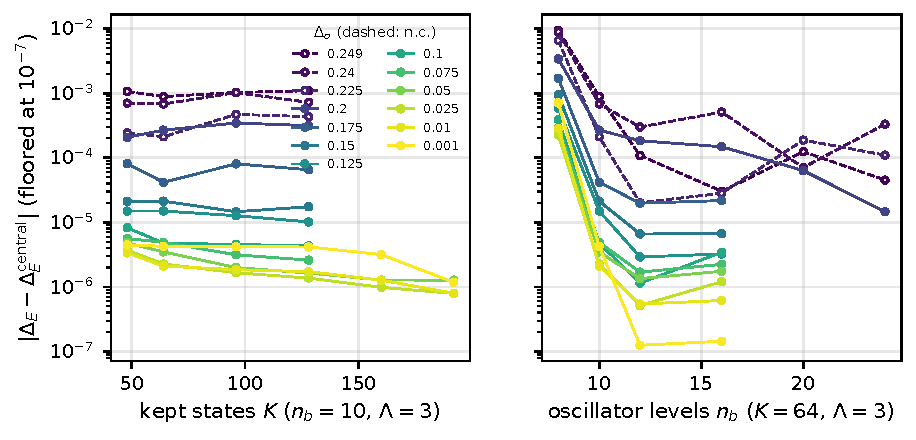
\includegraphics[width=0.92\textwidth]{parts/nrg/figures/fig_keep_nb.pdf}
\caption{$|\DE-\DE^{\rm central}|$ against $K$ (left, $n_b=10$) and $n_b$ (right, $K=64$) at $\Lambda=3$; zero deviations are drawn at
$10^{-7}$. Flat curves mean converged. Dashed: the three points not converged in chain depth. In the left panel the level of the
$\Ds\ge0.2$ curves is set by $n_b=10$.}\label{nrg:fig:keepnb}
\end{figure}

\subsection{Dependence on the discretization \texorpdfstring{$\Lambda$}{Lambda}}\label{nrg:sec:lambda}
The chain length is scaled as $N\propto1/\ln\Lambda$, so all items of a point reach the same RG time. The $\Lambda$ studies separate
truncation from discretization (Tables~\ref{nrg:tab:lambda} and~\ref{nrg:tab:lshift}, Fig.~\ref{nrg:fig:lambda}):
\begin{itemize}
\item \textbf{Smaller $\Lambda$ needs many more kept states.} At $\Lambda=1.5$, going from $K=64$ to $128$ moves $\DE$ by
  $\nrgLonefiveMove$, and $K=128$ is still $\nrgLonefiveOff$ away from the converged $\Lambda=2$ value; raising $n_b$ to 16 changes
  $\DE$ by only $\nrgLonefiveNb$. At $\Lambda=2$, $K=192$ and $256$ agree to $\nrgLtwoKconv$. At $\Lambda=2.5$, $K=64$ and $128$ (one
  doubling) agree to $\nrgLtwofiveKconv$ for $0.01\le\Ds\le0.15$, to $\nrgKdblOne$ at $0.001$, and differ by up to $\nrgLtwofiveKconvHigh$
  at the final points with $\Ds\ge0.175$ (up to $\nrgLtwofiveKconvNc$ at the points not converged in chain depth). At $\Lambda=2$, $K=64$ is not converged: it lies $\nrgLtwoKsixfourSmall$ above $\Lambda=3$ at $\Ds\le0.05$.
\item \textbf{A small $\Lambda$ dependence, far inside the error.} At the largest $K$ run at each $\Lambda$ (at $\Lambda=4$ only
  $K=64$, whose convergence is assumed), the plateau values at $\Lambda=2$, $2.5$, $3$ and $4$ agree to $\nrgLspreadPilot$ at $\Ds=0.1$ and $0.05$, and rise monotonically with $\Lambda$: relative to $\Lambda=3$, $\Lambda=2$,
  $2.5$ and $4$ lie at $\nrgLtwoOneHundred$, $\nrgLtwofiveOneHundred$ and $\nrgLfourOneHundred$ at $\Ds=0.1$, and at $\nrgLtwoFifty$,
  $\nrgLtwofiveFifty$ and $\nrgLfourFifty$ at $0.05$. Extended to $\Lambda\to1$ this would put the $\Lambda=3$ value a few $10^{-6}$ above
  the limit, far below $\dtot$. Over $\Lambda=2.5$--$4$ the largest spread at a plateau point is $\nrgLspreadMax$ (at
  $\Ds=\nrgLspreadMaxAt$, set by $\Lambda=4$). How many kept states the limit $\Lambda\to1$ needs was not determined, and the limit
  is not tested.
\item \textbf{At $\Ds=0.2$} only $\Lambda=2.5$ and $3$ were run with the converged $n_b=16$; their extrapolations agree to
  $\nrgextLamTwoHundred$. At $n_b=10$ the extrapolated values spread by $\nrgLtenSpreadTwoHundred$ over $\Lambda=2$--$4$
  (Fig.~\ref{nrg:fig:lambda}). We attribute this to an interplay of $\Lambda$ with the $n_b=10$ truncation (the $\Lambda=2.5$ minus
  $\Lambda=3$ difference changes sign between $n_b=10$ and $16$), but that is inferred, not measured; it is within $\dtot$ only through
  the large $\dd$.
\end{itemize}
An earlier version of this note reported that $\DE$ rises as $\Lambda$ decreases and covered the continuum limit with twice the
$\Lambda=2.5$ shift. Both came from the midpoint estimator: the window rule counts sites while the chain length scales as
$1/\ln\Lambda$, so smaller $\Lambda$ admitted a larger share of transient windows (App.~\ref{nrg:app:midpoint}).

\begin{table}[ht]\centering\scriptsize
\caption{The $\Lambda$ study at three points ($n_b=10$ unless stated): $\DE$ with this note's estimator (plateau value at $\Ds=0.1$,
$0.05$; extrapolated at $0.2$), the superseded midpoint with its half-width, and $\alpha_c$. $N$ is scaled with $\Lambda$ so that the
infrared scale $\Lambda^{-N}$ is fixed. At $\Lambda=1.5$ no item is converged in $K$.}\label{nrg:tab:lambda}
\begin{tabular}{llllllll}
\toprule
$\Delta_\sigma$ & $\Lambda$ & $K$ & $n_b$ & $N$ & $\Delta_E$ (this note) & old midpoint (half-width) & $\alpha_c$ \\
\midrule
0.2 & 1.5 & 64 & 10 & 176 & 0.536299 & 0.53659 (0.00036) & 0.1626225790\\
0.2 & 1.5 & 64 & 16 & 176 & 0.536300 & 0.53660 (0.00036) & 0.1626210299\\
0.2 & 1.5 & 128 & 10 & 176 & 0.507038 & 0.50754 (0.00102) & 0.1603705735\\
0.2 & 2 & 64 & 10 & 103 & 0.484078 & 0.48534 (0.00177) & 0.1676281822\\
0.2 & 2 & 128 & 10 & 103 & 0.483021 & 0.48471 (0.00165) & 0.1676098637\\
0.2 & 2 & 192 & 10 & 103 & 0.483061 & 0.48448 (0.00193) & 0.1676082707\\
0.2 & 2 & 256 & 10 & 103 & 0.483014 & 0.48449 (0.00188) & 0.1676081346\\
0.2 & 2.5 & 64 & 10 & 78 & 0.483221 & 0.48426 (0.00131) & 0.1761692489\\
0.2 & 2.5 & 128 & 10 & 78 & 0.483173 & 0.48440 (0.00101) & 0.1761670918\\
0.2 & 3 & 64 & 10 & 65 & 0.483248 & 0.48404 (0.00063) & 0.1847222031\\
0.2 & 3 & 128 & 10 & 65 & 0.483295 & 0.48406 (0.00061) & 0.1847217711\\
0.2 & 4 & 64 & 10 & 52 & 0.483381 & 0.48401 (0.00034) & 0.2008115424\\
\midrule
0.1 & 1.5 & 64 & 10 & 176 & 0.567059 & 0.56714 (0.00019) & 0.3786792319\\
0.1 & 1.5 & 64 & 16 & 176 & 0.567059 & 0.56714 (0.00019) & 0.3786839607\\
0.1 & 1.5 & 128 & 10 & 176 & 0.539196 & 0.53968 (0.00049) & 0.3733064368\\
0.1 & 2 & 64 & 10 & 103 & 0.529796 & 0.53042 (0.00063) & 0.3936704020\\
0.1 & 2 & 128 & 10 & 103 & 0.529631 & 0.53025 (0.00063) & 0.3936438035\\
0.1 & 2 & 192 & 10 & 103 & 0.529613 & 0.53024 (0.00063) & 0.3936429089\\
0.1 & 2 & 256 & 10 & 103 & 0.529609 & 0.53023 (0.00064) & 0.3936426886\\
0.1 & 2.5 & 64 & 10 & 78 & 0.529637 & 0.53010 (0.00046) & 0.4167902745\\
0.1 & 2.5 & 128 & 10 & 78 & 0.529610 & 0.53007 (0.00046) & 0.4167874486\\
0.1 & 3 & 64 & 10 & 65 & 0.529613 & 0.52984 (0.00022) & 0.4397697893\\
0.1 & 3 & 128 & 10 & 65 & 0.529612 & 0.52984 (0.00023) & 0.4397694449\\
0.1 & 4 & 64 & 10 & 52 & 0.529628 & 0.52981 (0.00018) & 0.4825812310\\
\midrule
0.05 & 1.5 & 64 & 10 & 217 & 0.670692 & 0.67093 (0.00026) & 0.5909590331\\
0.05 & 1.5 & 64 & 16 & 217 & 0.670693 & 0.67092 (0.00026) & 0.5909603112\\
0.05 & 1.5 & 128 & 10 & 217 & 0.630353 & 0.63061 (0.00026) & 0.5780543351\\
0.05 & 2 & 64 & 10 & 127 & 0.622300 & 0.62262 (0.00032) & 0.6120267877\\
0.05 & 2 & 128 & 10 & 127 & 0.622125 & 0.62241 (0.00036) & 0.6119924970\\
0.05 & 2 & 192 & 10 & 127 & 0.622119 & 0.62244 (0.00033) & 0.6119916485\\
0.05 & 2 & 256 & 10 & 127 & 0.622116 & 0.62242 (0.00034) & 0.6119911289\\
0.05 & 2.5 & 64 & 10 & 96 & 0.622139 & 0.62240 (0.00026) & 0.6507599139\\
0.05 & 2.5 & 128 & 10 & 96 & 0.622116 & 0.62235 (0.00029) & 0.6507542509\\
0.05 & 3 & 64 & 10 & 80 & 0.622119 & 0.62236 (0.00024) & 0.6891357316\\
0.05 & 3 & 128 & 10 & 80 & 0.622117 & 0.62236 (0.00024) & 0.6891354544\\
0.05 & 3 & 192 & 10 & 80 & 0.622117 & 0.62236 (0.00024) & 0.6891353149\\
0.05 & 4 & 64 & 10 & 63 & 0.622122 & 0.62223 (0.00013) & 0.7603342269\\
\bottomrule
\end{tabular}

\end{table}

\begin{table}[ht]\centering\scriptsize
\caption{$\Lambda$ and $K$ shifts at all thirteen points, in units of $10^{-4}$, relative to $\Lambda=3$ at the same $K$ and $n_b$
($\Lambda=2.5$ uses $n_b=16$ for $\Ds\ge0.2$, else $10$). The $\Lambda=2$, $K=64$ column is not converged in $K$. Last columns: the $K$
doubling at $\Lambda=2.5$ ($n_b=10$) and the number of quality windows of the $\Lambda=2.5$, $K=128$, $n_b=10$ item.}\label{nrg:tab:lshift}
\begin{tabular}{llllll}
\toprule
 & \multicolumn{3}{c}{$10^4\times$ shift relative to $\Lambda=3$} & \multicolumn{2}{c}{at $\Lambda=2.5$}\\
\cmidrule(lr){2-4}\cmidrule(lr){5-6}
$\Delta_\sigma$ & $\Lambda{=}2$, $K{=}64$ & $\Lambda{=}2.5$, $K{=}128$ & $\Lambda{=}4$, $K{=}64$ & $10^4\times(K{=}64$ minus $K{=}128)$ & $n_q$\\
\midrule
0.249 & $+$41.37 & $+$1.21 & $+$17.22 & $+$0.88 & 13\\
0.24 & $+$34.03 & $+$0.71 & $+$16.43 & $+$2.54 & 13\\
0.225 & $+$19.17 & $+$2.29 & $+$10.71 & $+$6.05 & 17\\
0.2 & $+$8.30 & $+$0.18 & $+$1.33 & $+$0.49 & 22\\
0.175 & $+$3.71 & $-$0.53 & $+$1.50 & $+$1.55 & 25\\
0.15 & $+$2.38 & $-$0.10 & $+$0.54 & $+$0.67 & 28\\
0.125 & $+$1.90 & $-$0.07 & $+$0.23 & $+$0.38 & 31\\
0.1 & $+$1.84 & $-$0.02 & $+$0.15 & $+$0.27 & 32\\
0.075 & $+$1.75 & $-$0.02 & $+$0.06 & $+$0.24 & 36\\
0.05 & $+$1.81 & $-$0.01 & $+$0.03 & $+$0.23 & 43\\
0.025 & $+$1.62 & $-$0.01 & $+$0.03 & $+$0.26 & 47\\
0.01 & $+$2.02 & $-$0.00 & $+$0.06 & $+$0.35 & 49\\
0.001 & $+$5.63 & $-$0.11 & $+$0.12 & $+$1.05 & 126\\
\bottomrule
\end{tabular}

\end{table}

\begin{figure}[ht]\centering
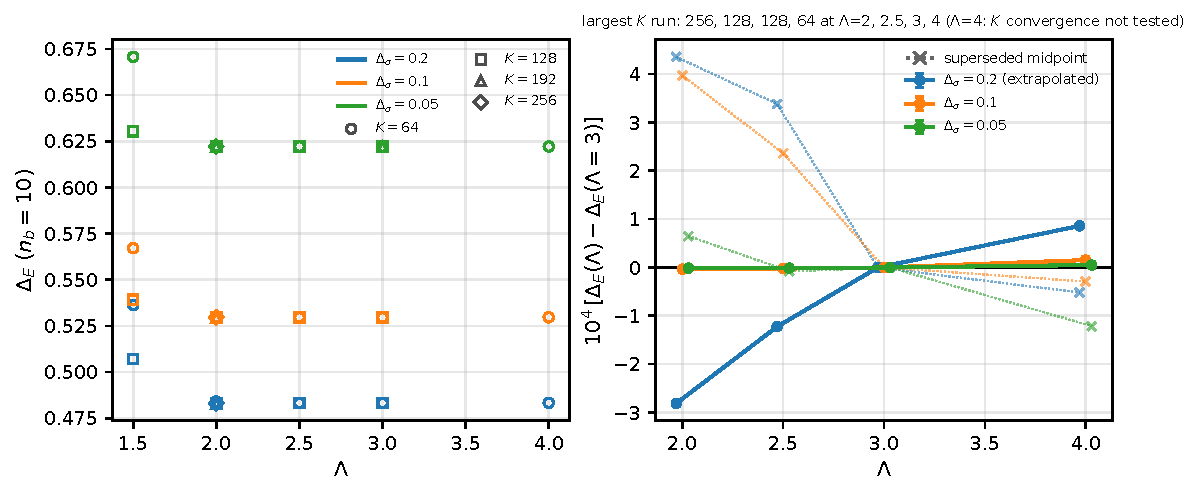
\includegraphics[width=0.95\textwidth]{parts/nrg/figures/fig_lambda.pdf}
\caption{Left: $\DE$ against $\Lambda$ for all $K$ at $n_b=10$ (open symbols by $K$, color by $\Ds$); at $\Lambda=1.5$ no item is
converged in $K$. Right: $K$-converged items relative to $\Lambda=3$ with this note's estimator (bars: plateau drift) and, dotted, the
superseded midpoints, whose apparent $\Lambda$ dependence is an artifact of the window rule.}\label{nrg:fig:lambda}
\end{figure}

\begin{figure}[ht]\centering
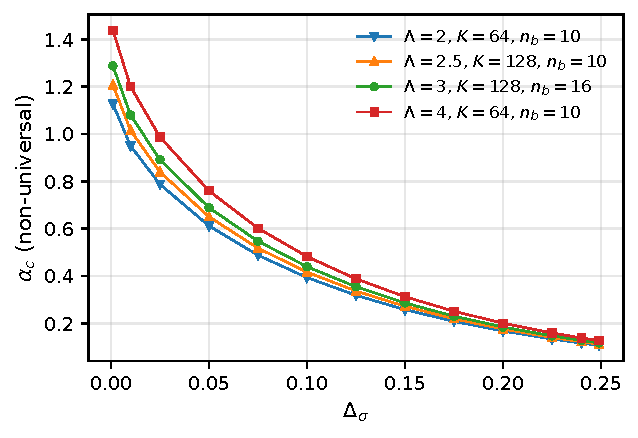
\includegraphics[width=0.6\textwidth]{parts/nrg/figures/fig_alpha_c.pdf}
\caption{The critical coupling is not universal: it depends on $\Lambda$ and weakly on $K$ and $n_b$. It enters no
result.}\label{nrg:fig:alpha}
\end{figure}

\subsection{The final table}\label{nrg:sec:final}
Table~\ref{nrg:tab:headline} gives the final values and Table~\ref{nrg:tab:budget} their errors. Starting from the Gaussian value $1/2$ at
$s=1/2$, $\De$ first decreases (the $\varepsilon$ series at $\Ds\ge0.2$), passes through a shallow minimum of about $\nrgDEmin$ near
$\Ds=\nrgDEminAt$, and rises toward 1 as $s\to1$. The window audits of three central items are shown in Fig.~\ref{nrg:fig:plateau}. The
number of quality windows falls from $\nrgnqOne$ at $\Ds=0.001$ to $\nrgnqTwoFortyNine$ at $\Ds=0.249$ (Table~\ref{nrg:tab:budget}).

\begin{figure}[ht]\centering
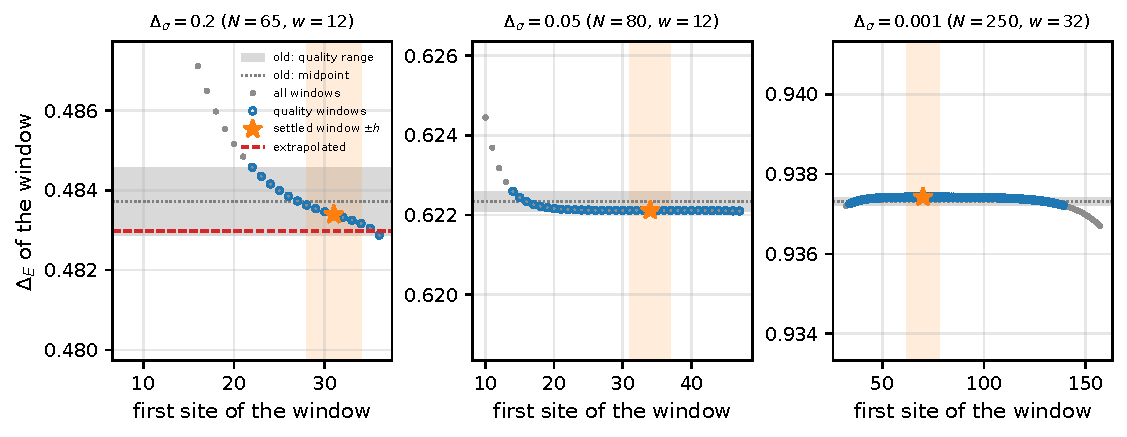
\includegraphics[width=0.98\textwidth]{parts/nrg/figures/fig_plateau.pdf}
\caption{Window audit of three central items: $\DE$ of every window (gray dots) and of the quality windows (open circles) against the
first site of the window; star and orange band: the settled window and its neighborhood $\pm h$; gray band and dotted line: the quality
range and its midpoint, the superseded estimate; dashed (at $\Ds=0.2$): the extrapolated value. The vertical scales differ between
panels. At $\Ds=0.05$ and $0.001$ the quality windows end on a flat plateau, at $0.2$ they drift downward to the end.}\label{nrg:fig:plateau}
\end{figure}

\subsection{The limit \texorpdfstring{$s\to1$}{s -> 1}}\label{nrg:sec:s1}
Table~\ref{nrg:tab:s1} compares $y_t=1-\DE$ with the leading form $\sqrt{2\delta}=2\sqrt{\Ds}$ and the next-to-leading form of
Eq.~\eqref{nrg:eq:s1}. The ratio to the leading form approaches 1 as $s\to1$: $y_t=\nrgytOne$ against $\nrgktOne$ at $\Ds=0.001$
($\nrgktPctOne$\%) and $\nrgytTen$ against $\nrgktTen$ at $0.01$ ($\nrgktPctTen$\%). Against the next-to-leading form $\nrgnloOne$ the
difference at $\Ds=0.001$ is $\nrgnloDiffOne$. The remainder divided by $\delta^{3/2}$ changes smoothly over $0.001\le\Ds\le0.075$
($\nrgnloRatioRange$): it is $\nrgnloRatioTen$ at $\Ds=0.01$, where $\dtot/\delta^{3/2}=\nrgnloRatioErrTen$, and $\nrgnloRatioOne$ at
$0.001$, where $\dtot/\delta^{3/2}=\nrgnloRatioErrOne$ is as large as the entry. The dual expansion~\eqref{nrg:eq:dual} fixes the coefficient
of $\delta^{3/2}$ in $y_t$, $-C^{\rm SR}_3(1)/2^{3/2}=\nrgnloThreeCoef$, which the remainder approaches as $s\to1$.

The accompanying paper~\cite{nrg:Paper} tests the dual expansion directly at $\Ds=0.01$, where $\dtot=\nrgerrTen$. The difference
between $\DE$ and the series~\eqref{nrg:eq:dual} summed through $C^{\rm SR}_n(1)$ is $\nrgsrDiffTwo$, $\nrgsrDiffThree$, $\nrgsrDiffFour$
and $\nrgsrDiffFive$ for $n=2$, 3, 4 and 5: it shrinks to the size of $\dtot$ as $C^{\rm SR}_3(1)$, $C^{\rm SR}_4(1)$ and
$C^{\rm SR}_5(1)$ are added. The term of $C^{\rm SR}_6(1)$, of magnitude $\nrgsrTermSix$, is itself of the size of $\dtot$ and brings
the difference to $\nrgsrDiffSix$; the higher terms lie below $\dtot$. NRG thus reproduces the dual expansion through
$C^{\rm SR}_5(1)$ and is consistent with $C^{\rm SR}_6(1)$.

\begin{table}[ht]\centering\small
\caption{$y_t=1-\DE$ near $s=1$ against the leading form $\sqrt{2\delta}$ ($\delta=1-s=2\Ds$) and the next-to-leading form
$\sqrt{2\delta}-\delta/4$ of Refs.~\cite{nrg:BLMV25,nrg:BLMV26}; the remainder in units of $\delta^{3/2}$, and $\dtot$ in the same units (the
uncertainty of the remainder).}\label{nrg:tab:s1}
\begin{tabular}{@{}llllllrr@{}}
\toprule
$\Delta_\sigma$ & $\delta=1-s$ & $y_t=1-\Delta_E$ & $\sqrt{2\delta}=2\sqrt{\Delta_\sigma}$ & ratio & $\sqrt{2\delta}-\delta/4$ & $(y_t-\sqrt{2\delta}+\delta/4)/\delta^{3/2}$ & $\delta_{\rm tot}/\delta^{3/2}$\\
\midrule
0.075 & 0.15 & 0.43374 & 0.54772 & 0.792 & 0.51022 & -1.32 & 0.00051\\
0.05 & 0.1 & 0.37788 & 0.44721 & 0.845 & 0.42221 & -1.40 & 0.00085\\
0.025 & 0.05 & 0.28658 & 0.31623 & 0.906 & 0.30373 & -1.53 & 0.0026\\
0.01 & 0.02 & 0.19025 & 0.20000 & 0.951 & 0.19500 & -1.68 & 0.017\\
0.001 & 0.002 & 0.06258 & 0.06325 & 0.989 & 0.06275 & -1.90 & 1.2\\
\bottomrule
\end{tabular}

\end{table}

% =====================================================================================================================
\section{Checks}\label{nrg:sec:checks}
% =====================================================================================================================
A second implementation of the same numerical map tests the code (Sec.~\ref{nrg:sec:indep}); two methods that do not use NRG test the
method (Secs.~\ref{nrg:sec:series} and~\ref{nrg:sec:mc}); Sec.~\ref{nrg:sec:literature} lists published values. Figure~\ref{nrg:fig:checks} summarizes
the comparisons.

\subsection{A second implementation}\label{nrg:sec:indep}
\paragraph{Design.} Claude Code, which knew the production code, wrote a specification of the physics and conventions only
(\code{independent\_check/SPEC.md}). It fixed the discretization, the chain, the truncation per parity sector, the critical-search rule
and the window rule, and forbade access to the production code, data and this note. From it a separate Claude agent wrote a second
solver (\code{independent\_check/indep\_nrg.py}); that it did not open the forbidden files rests on the instruction and on the agent's
own statement in \code{NOTES.md}, not on an access log. Every algorithmic choice differs from production:
\begin{center}\footnotesize
\begin{tabular}{@{}p{2.6cm}p{5.4cm}p{7.6cm}@{}}\toprule
 & production (\code{lri\_spin}) & second implementation (\code{indep\_nrg.py})\\\midrule
chain coefficients & closed form~\eqref{nrg:eq:coeff} & Lanczos with full reorthogonalization on the star, in mpmath\\
parity blocks & basis order of the reference solver & NumPy Kronecker order, generic operators\\
eigensolver & partial spectrum (flows), full (derivative) & full spectrum everywhere\\
$y_t$ & exact derivative~\eqref{nrg:eq:tangent} & central finite differences in $\alpha$, relative steps $\eta=10^{-9},10^{-10},10^{-11}$\\
window audit & package code & written from the specification\\\bottomrule
\end{tabular}
\end{center}
The Lanczos recursion runs with $40+1.3N\log_{10}\Lambda$ decimal digits and is repeated with 40 more digits and 40 more star modes to
check convergence. The second implementation has its own 38 self-tests (for example, the chain reproduces the star to $3\times10^{-50}$,
and the NRG reproduces exact diagonalization of untruncated systems to $5\times10^{-15}$). Eight configurations c1--c8 with
$0.502\le s\le0.998$, $\Lambda=2$, $2.5$ and $3$, $K=48$ or $64$ and $n_b=10$--$16$ ran on one cluster node, one single-core process
each, the longest in $\nrgindWall$\,min; each is compared with the production record of the same item.

\paragraph{Result.} Table~\ref{nrg:tab:indep} lists the comparison.
\begin{itemize}
\item The chain coefficients agree to better than $\nrgindChain$ (relative): to rounding, whose last bits depend on the platform. The
  closed form is confirmed.
\item The critical couplings are bitwise identical in $\nrgindAlphaBitwise$ configurations and agree to $\nrgindAlpha$ in the others.
  The critical flows agree to $\nrgindFlow$ over the first eleven sites.
\item A window's finite-difference $\DE$ is \emph{trusted} when two neighboring steps $\eta$ agree to $10^{-6}$. In all
  $\nrgindTrusted$ trusted windows ($\nrgindTrustedMin$ to $\nrgindTrustedMax$ per configuration) the two implementations agree to
  $\nrgindDE$, with median $\nrgindDEmedian$, far below the quoted errors. In the $\nrgindSettledN$ configurations whose settled window
  is trusted, they agree there to $\nrgindSettled$.
\item The latest windows of a chain lie beyond the reach of finite differences, because $\eta\,\alpha\,\Lambda^{y_tn}$ is no longer
  small there. Only $\nrgindCovered$ of the $\nrgindQuality$ production quality windows are within reach. All quality windows of a
  configuration are within reach only in $\nrgindFullList$; at $s=0.502$ (c5) none is. This is a limit of the check, not a
  disagreement.
\end{itemize}
The check verifies the numerical map at $K\le64$. It does not test the central items at $K=128$, $n_b=16$ directly (they differ only in
$K$ and $n_b$), the estimator (it shares the window rule by construction), or the limit $\Lambda\to1$. Both implementations come from
the same model family, and the specification was written by the agent that knew the production code: the check tests the code, not
shared conceptual choices.

\begin{table}[ht]\centering\scriptsize\setlength{\tabcolsep}{4pt}
\caption{Second implementation against production. Columns: configuration $(s,\Lambda,K,n_b,N)$; largest relative difference of the
rescaled chain coefficients (a rounding-level bound); relative difference of $\alpha_c$; number of trusted windows; largest window-by-window difference
$|\delta\DE|$ over them; production quality windows within finite-difference reach (covered/all); production quality range.}\label{nrg:tab:indep}
\begin{tabular}{@{}lllllrrl@{}}
\toprule
id & $(s,\Lambda,K,n_b,N)$ & chain & $\alpha_c$ & trusted & $\max|\delta\Delta_E|$ & covered & quality range (production)\\
\midrule
c1 & $(0.8,3,64,10,65)$ & $<10^{-15}$ & bitwise & 19 & $2\times10^{-7}$ & 13/23 & [0.529612, 0.530062]\\
c2 & $(0.9,3,64,10,80)$ & $<10^{-15}$ & $4\times10^{-14}$ & 27 & $9\times10^{-8}$ & 23/34 & [0.622119, 0.622597]\\
c3 & $(0.98,3,64,10,105)$ & $<10^{-15}$ & bitwise & 53 & $3\times10^{-7}$ & 41/41 & [0.809460, 0.810127]\\
c4 & $(0.6,3,64,12,65)$ & $<10^{-15}$ & bitwise & 17 & $2\times10^{-7}$ & 3/15 & [0.483316, 0.484567]\\
c5 & $(0.502,3,64,16,65)$ & $<10^{-15}$ & bitwise & 18 & $2\times10^{-7}$ & 0/2 & [0.508000, 0.508268]\\
c6 & $(0.998,3,48,10,250)$ & $<10^{-15}$ & $4\times10^{-14}$ & 126 & $2\times10^{-7}$ & 106/106 & [0.937223, 0.937429]\\
c7 & $(0.8,2,64,10,103)$ & $<10^{-15}$ & $7\times10^{-14}$ & 34 & $2\times10^{-7}$ & 28/46 & [0.529796, 0.531050]\\
c8 & $(0.7,2.5,64,10,78)$ & $<10^{-15}$ & bitwise & 22 & $2\times10^{-7}$ & 14/29 & [0.491178, 0.492328]\\
\bottomrule
\end{tabular}

\end{table}

\subsection{The \texorpdfstring{$\varepsilon$}{epsilon} expansion near \texorpdfstring{$s=1/2$}{s = 1/2}}\label{nrg:sec:series}
\paragraph{Reference.} The accompanying paper gives $\De=\sum_{n=0}^{8}C_n\varepsilon^n$ for $d=1$~\cite{nrg:Paper}, with
$C_0=1/2$, $C_1=-1/6$, $C_2=0.657131263981$, $C_3=-3.719856322902$, $C_4=45.42488010356$, $C_5=-731.13947662454$ and
$C_6=14331.6870328$ (exact to the digits shown), $C_7=-322550\pm40$ and $C_8=(8.060\pm0.017)\times10^6$. The uncertainties of $C_7$
and $C_8$ are the paper's allowances, mostly four sampling standard errors. They are not part of the Borel--Pad\'e spread below;
shifting $C_7$ or $C_8$ by about its allowance moves the $[4/4]$ approximant by at most $\nrgserSensTwoTwentyFive$ at $\Ds=0.225$ and
$\nrgserSensTwoHundred$ at $0.2$, less than the spread at both points. The coefficients grow factorially, so the series is asymptotic.
We evaluate it in two ways (\code{method\_comparison/compare\_methods.py}):
\begin{itemize}
\item \textbf{optimal truncation}: the partial sum up to, but excluding, the smallest term, with that term as its error;
\item \textbf{Borel--Pad\'e}: Pad\'e approximants $[L/M]$ of the Borel transform $\sum_nC_nu^n/n!$ with $L+M=6,7,8$, keeping those
  without a pole on the positive axis and with a value between 0.3 and 1.2, Laplace-transformed back. The central value is the upper
  of the two middle values of the $L+M=8$ approximants (there are four at $0.2\le\Ds\le0.24$), not their mean; the error is the
  half-range of all approximants with $L+M\ge7$. The $L+M=6$ approximants are computed but enter neither. The choice of the upper
  middle value is a convention of the comparison script of 8 October 2026, unchanged since and not chosen with the present NRG values
  in view; it has no further justification. At $\Ds\ge0.225$, where the approximants agree to within the quoted spread, it hardly
  matters; at $\Ds=0.2$ it does (below).
\end{itemize}
The reference is the partial sum at $\Ds=0.249$ ($\varepsilon=0.004$), where all terms decrease and the error is
$\nrgserOptErrTwoFortyNine$ (Borel--Pad\'e gives $\nrgserBpTwoFortyNine$ too), and the Borel--Pad\'e sum at larger $\varepsilon$. At
$\Ds=0.24$ the two evaluations agree to $\nrgserAgreeTwoForty$. At $0.225$ the Borel--Pad\'e sum, $\nrgserTwoTwentyFive$, has a small
spread, but optimal truncation gives $\nrgserOptTwoTwentyFive$, so the reference there depends on the resummation. At $\Ds=0.2$ the
spread, $\nrgserSpreadTwoHundred$, is too large to test NRG at the $10^{-3}$ level.

\paragraph{Result.} Table~\ref{nrg:tab:series}. At $\Ds=0.2$ the series does not test NRG: the extrapolated NRG value lies
$\nrgdiffTwoHundred$ from the central approximant, a coincidence of the convention above, and $\nrgdiffMedTwoHundred$ from the median
$\nrgbpMedTwoHundred$ of the $\nrgbpNTwoHundred$ approximants with $L+M=8$, which range from $\nrgbpLoTwoHundred$ to
$\nrgbpHiTwoHundred$; both differences are well inside the spread, and neither is evidence for or against NRG. At the three points not converged in chain depth the settled values lie above the series by $\nrgexcTwoFortyNine$,
$\nrgexcTwoForty$ and $\nrgexcTwoTwentyFive$, decreasing with $\varepsilon$, as the slow approach of Sec.~\ref{nrg:sec:approach} predicts.
Two extrapolations serve as cross-checks; neither is adopted:
\begin{itemize}
\item \textbf{The rule's own extrapolation} (Sec.~\ref{nrg:sec:estimator}) is not stable there. Over the three fit ranges and
  $\Lambda=2.5$, $3$ it gives $\nrgextLoTwoForty$--$\nrgextHiTwoForty$ ($\nrgextExcLoTwoForty$ to $\nrgextExcHiTwoForty$ from the series)
  at $\Ds=0.24$, and $\nrgextLoTwoTwentyFive$--$\nrgextHiTwoTwentyFive$ ($\nrgextExcLoTwoTwentyFive$ to $\nrgextExcHiTwoTwentyFive$) at
  $0.225$. At $\Ds=0.249$, where $\varepsilon l_{\max}\approx0.25$, a single exponential cannot represent the $1/l$ approach, and the
  extrapolation ($\nrgextLoTwoFortyNine$--$\nrgextHiTwoFortyNine$) removes less than half of the excess.
\item \textbf{The crossover fit} of Sec.~\ref{nrg:sec:crosscheck} is stable and moves the values toward the series, but not onto it. At
  $\Ds=0.225$ it gives $\nrgcrossTwoTwentyFive$ ($\nrgcrossNTwoTwentyFive$ accepted fits, $\nrgcrossLoTwoTwentyFive$ to
  $\nrgcrossHiTwoTwentyFive$, i.e.\ $\nrgcrossExcLoTwoTwentyFive$ to $\nrgcrossExcHiTwoTwentyFive$ from the series value
  $\nrgserTwoTwentyFive$). At $0.24$ it gives $\nrgcrossTwoForty$ ($\nrgcrossLoTwoForty$ to $\nrgcrossHiTwoForty$): every accepted fit
  lies above the series value $\nrgserTwoForty$, by $\nrgcrossExcLoTwoForty$ to $\nrgcrossExcHiTwoForty$, against $\nrgexcTwoForty$ for
  the settled value. At $0.249$ it gives $\nrgcrossTwoFortyNine$, $\nrgcrossExcTwoFortyNine$ from the series: there the fit is
  ill-conditioned, and the one-loop test of Sec.~\ref{nrg:sec:approach} is the relevant check.
\end{itemize}

\paragraph{Interpretation.} The excess is the expected crossover from the strong bare coupling of the spin--boson model to the
interacting fixed point, whose correction exponent $\omega\approx\varepsilon$ vanishes at $s=1/2$; within $l_{\max}$ the flow has not
arrived. It depends only on the RG time, not on $K$, $n_b$ or $\Lambda$ at fixed depth (Sec.~\ref{nrg:sec:approach}), and at
$\Ds=0.249$ it decays at a rate of the one-loop size. Logarithmic corrections of this kind were already seen in NRG at $s=1/2$~\cite{nrg:Vojta2005}.
An earlier version of this note attributed the excess to the known truncation errors of bosonic NRG near Gaussian fixed points
(Hilbert-space truncation and mass flow~\cite{nrg:Vojta2005,nrg:Vojta2010,nrg:Vojta2012}). The data do not support that: those errors affect
order-parameter exponents below $s=1/2$, and for $s>1/2$ the mass-flow correction changes the flows only quantitatively
(at $s=0.6$, ``no qualitative difference between the flows without and with mass-flow correction''~\cite{nrg:Vojta2010}); we have no run
that isolates either effect. The same mechanism acts at $\Ds=0.2$ and $0.175$ at a smaller level (shifts $\nrgextShiftTwoHundred$ and
$\nrgextShiftOneSeventyFive$ from settled to extrapolated), where the extrapolation is stable and its full length is in $\dd$.

\paragraph{Decision.} The three values at $\Ds=0.249$, $0.24$ and $0.225$ are kept as computed (the settled values), marked ``not
converged in chain depth'', shown in the tables and figures, and used in no comparison and no agreement statement. This is the
author's decision. The label is not an outcome of the estimator, and it was assigned when this comparison was already known
(Sec.~\ref{nrg:sec:estimator}); App.~\ref{nrg:app:provenance} gives its history, including an earlier recommendation that the author
overruled.

\begin{table}[ht]\centering\scriptsize\setlength{\tabcolsep}{3pt}
\caption{NRG against the $\varepsilon$ series near $s=1/2$. Optimal truncation with its smallest term; Borel--Pad\'e central value with
the spread over approximants; NRG minus the reference (the partial sum at $\Ds=0.249$, the Borel--Pad\'e sum otherwise; at $\Ds=0.2$
this difference is not meaningful, see text); the range of the rule's extrapolations and the crossover fit of
Sec.~\ref{nrg:sec:crosscheck} (cross-checks, not adopted). Bracketed: settled values not converged in chain depth, not used.}\label{nrg:tab:series}
\begin{tabular}{@{}llllllll@{}}
\toprule
$\Delta_\sigma$ & $\varepsilon$ & NRG $\Delta_E$ & optimal truncation & Borel--Pad\'e (spread) & NRG $-$ reference & rule's extrapolation & crossover fit\\
\midrule
0.249 & 0.004 & [0.508030] & 0.499344 ($\pm5\times10^{-13}$) & 0.49934 ($6\times10^{-15}$) & $+8.7\times10^{-3}$ & 0.5046--0.5057 & 0.50209\\
0.24 & 0.04 & [0.498922] & 0.494194 ($\pm5\times10^{-5}$) & 0.49422 ($2\times10^{-7}$) & $+4.7\times10^{-3}$ & 0.4934--0.4970 & 0.49460\\
0.225 & 0.1 & [0.489668] & 0.489905 ($\pm4\times10^{-3}$) & 0.48808 ($1\times10^{-4}$) & $+1.6\times10^{-3}$ & 0.4867--0.4888 & 0.48810\\
0.2 & 0.2 & 0.4830(7) & 0.466667 ($\pm0.03$) & 0.48292 ($9\times10^{-3}$) & $+5.9\times10^{-5}$ & adopted & 0.48305\\
\bottomrule
\end{tabular}

\end{table}

\subsection{The 1D cluster Monte Carlo study}\label{nrg:sec:mc}
\paragraph{Reference.} The Monte Carlo study of the same model in this repository (\code{MC/} folder~\cite{nrg:MCnote}; Fukui--Todo
cluster algorithm~\cite{nrg:FukuiTodo2009,nrg:LB95} with finite-size scaling) is the project's own, run by the same AI systems; it is
independent of NRG in method, not in authorship. We use only its quoted values and labels; their definitions are in its
note~\cite{nrg:MCnote}. In brief, its value of $\De$ comes from a finite-size-scaling fit of all lattice sizes, with a statistical error
$\sigma_{\rm stat}$ and a systematic scale $\sigma_{\rm sys}$, the half-range of the values over a family of fit models (a sensitivity
scale, not a standard deviation). As a cross-check it also extrapolates in the lattice size the crossings, between pairs of sizes, of a
finite-size-scaling observable; this \emph{crossing extrapolation} is quoted as $\De^\infty(\sigma_\infty)(\Delta_{\omega'})$, with
error $\sigma_\infty$ and sensitivity $\Delta_{\omega'}$ to the assumed correction exponent $\omega'$ ($\Delta_{\omega'}$ is a
sensitivity, not a dimension). Each value carries a label: \textbf{accepted}, the fit value and the crossing extrapolation agree within
twice the error of their difference (``$\sigma_{\rm sys}$-dominated'' marks values whose $\sigma_{\rm sys}$ is much larger than
$\sigma_{\rm stat}$); \textbf{cross-check failed}, they differ by more, and the study does not certify the value as an infinite-size
value; \textbf{cross-check unavailable}, fewer than two size series are available for the crossing extrapolation; \textbf{conditional},
$\sigma_{\rm sys}$ could not be estimated.

\paragraph{Result.} Table~\ref{nrg:tab:mc}.
\begin{itemize}
\item \textbf{Accepted ($\Ds=\nrgmcAccList$).} NRG and Monte Carlo differ by at most $\nrgmcAccDiffMax$ (at $\Ds=\nrgmcAccDiffMaxAt$).
  The differences exceed the Monte Carlo statistical errors, by up to $\nrgmcAccStatRatioMax\,\sigma_{\rm stat}$, and have the same
  sign at neighboring points (below). They lie within $\sigma_{\rm sys}$ at $\nrgmcAccWithinSys$ of the $\nrgmcAccN$ points and within
  $\sigma_{\rm stat}+\sigma_{\rm sys}+\dtot$ at $\nrgmcAccWithinLin$, the largest ratio being $\nrgmcAccRatioMax$ at
  $\Ds=\nrgmcAccDiffMaxAt$. This linear sum adds a standard deviation, a fit-model half-range and an NRG error scale; we use it as a
  scale for the size of the differences, not as a test of statistical consistency. At $\Ds=\nrgmcAccDiffMaxAt$ the Monte Carlo
  crossing extrapolation agrees with NRG to $\nrgmcCrossOneHundred\,\sigma_\infty$; at all $\nrgmcAccN$ accepted points it agrees
  within $\nrgmcCrossStatMax\,\sigma_\infty$, and within $\nrgmcCrossRatioMax$ of $\sigma_\infty+\Delta_{\omega'}+\dtot$. The NRG
  errors are smaller than $\sigma_{\rm sys}$ by factors $\nrgmcAccSysRatio$, so the comparison tests the Monte Carlo systematics more
  than it tests NRG; only $\sigma_{\rm sys}$ reconciles the two.
\item \textbf{Cross-check failed ($\Ds=\nrgmcCcfList$).} These are not infinite-size values, and we use them only to say where NRG lies:
  at $0.175$ between the fit and the crossing extrapolation ($\nrgmcFitOneSeventyFive$ from the fit, $\nrgmcCrossOneSeventyFive$ from
  the crossing), at $0.15$ below both ($\nrgmcFitOneFifty$ and $\nrgmcCrossOneFifty$). Including these two points, the crossing
  extrapolations agree with NRG within $\nrgmcCrossAllMax\,\sigma_\infty$ at all $\nrgmcCrossAllN$ common points.
\item \textbf{Correlated signs.} NRG lies below the Monte Carlo fit at $\nrgmcNeg$ consecutive points of the $\nrgmcBoth$
  ($0.175$ to $0.075$) and above it at $0.05$ and $0.025$. The differences are therefore not independent fluctuations; they look like
  a smooth systematic of one of the two methods, which the Monte Carlo $\sigma_{\rm sys}$ is meant to cover.
\item \textbf{$\Ds=0.225$} is conditional in the Monte Carlo study and not converged in NRG; the Monte Carlo value lies
  $\nrgmcTwoTwentyFiveSer$ from the series. It enters no comparison.
\end{itemize}

\begin{table}[ht]\centering\scriptsize\setlength{\tabcolsep}{3.5pt}
\caption{NRG against the 1D cluster Monte Carlo study at the common points. MC value with $\sigma_{\rm stat}$ and $\sigma_{\rm sys}$ in
units of the last digit, and its label (Sec.~\ref{nrg:sec:mc}); NRG minus MC; ``ratio'' is $|{\rm NRG}-{\rm MC}|$ divided by
$\sigma_{\rm stat}+\sigma_{\rm sys}+\dtot$ (shown also for the cross-check-failed points, which are not infinite-size values); MC
crossing extrapolation with $\sigma_\infty$ and $\Delta_{\omega'}$. MC values are quoted as that study gives them. $^\ast$Not
converged in NRG, not used.}\label{nrg:tab:mc}
\begin{tabular}{@{}lllllll@{}}
\toprule
$\Delta_\sigma$ & NRG $\Delta_E$ & MC $\Delta_\varepsilon$ ($\sigma_{\rm stat}$)($\sigma_{\rm sys}$) & MC label & NRG $-$ MC & ratio & MC crossing ($\sigma_\infty$)($\Delta_{\omega^\prime}$)\\
\midrule
0.225$^\ast$ & [0.4897] & 0.47912(68)(--) & conditional (no $\sigma_{\rm sys}$) & $+0.011$ & -- & --\\
0.175 & 0.48390(35) & 0.48460(35)(67) & cross-check failed & $-7.0\times10^{-4}$ & 0.51 & 0.48304(81)(1)\\
0.15 & 0.49111(11) & 0.49325(41)(306) & cross-check failed & $-2.1\times10^{-3}$ & 0.60 & 0.49183(71)(70)\\
0.125 & 0.50567(5) & 0.50710(35)(193) & accepted & $-1.4\times10^{-3}$ & 0.61 & 0.50640(172)(392)\\
0.1 & 0.529608(33) & 0.53248(20)(242) & accepted ($\sigma_{\rm sys}$-dom.) & $-2.9\times10^{-3}$ & 1.08 & 0.52975(135)(248)\\
0.075 & 0.566260(30) & 0.56694(37)(139) & accepted & $-6.8\times10^{-4}$ & 0.38 & 0.56843(207)(1044)\\
0.05 & 0.622115(27) & 0.61987(55)(220) & accepted & $+2.2\times10^{-3}$ & 0.81 & 0.62393(348)(773)\\
0.025 & 0.713422(29) & 0.71115(49)(959) & accepted ($\sigma_{\rm sys}$-dom.) & $+2.3\times10^{-3}$ & 0.22 & 0.70906(902)(1509)\\
\bottomrule
\end{tabular}

\end{table}

\subsection{Published values}\label{nrg:sec:literature}
\begin{itemize}
\item \textbf{1D LRI Monte Carlo.} Uzelac, Glumac and Ani\v{c}i\'c~\cite{nrg:UGA01} give $1/\nu=0.50(2)$, $0.51(2)$, $0.47(2)$ and $0.40(1)$ at
  $s=0.6$, $0.7$, $0.8$ and $0.9$, i.e.\ $\De=0.50(2)$, $0.49(2)$, $0.53(2)$ and $0.60(1)$ at $\Ds=0.2$, $0.15$, $0.1$ and $0.05$. NRG
  differs from them by $\nrgugaTwoHundred$, $\nrgugaOneFifty$, $\nrgugaOneHundred$ and $\nrgugaFifty$ of their errors; at $\Ds=0.05$ the
  project's Monte Carlo value, $0.61987(55)(220)$, also lies above theirs. Angelini, Parisi and Ricci-Tersenghi~\cite{nrg:APR14} give
  $1/\nu=0.4124(13)$ at $s=0.875$ ($\De=0.5876(13)$ at $\Ds=0.0625$) and $0.506(14)$ at $s=0.65453$; neither point is on our grid.
  Four interpolations of our final values (a cubic spline over $0.01\le\Ds\le0.15$ and polynomials through three or four neighboring
  points) give $\nrgaprLo$--$\nrgaprHi$ at $\Ds=0.0625$, $\nrgaprSigLo$ to $\nrgaprSigHi$ of their errors above $0.5876$; the project's
  Monte Carlo study gives $0.59003(35)(150)$ there (label: cross-check unavailable).
\item \textbf{The spin--boson model.} Bosonic NRG~\cite{nrg:Bulla2003,nrg:Vojta2005} and continuous-time quantum Monte
  Carlo~\cite{nrg:WRVB09} give $1/\nu$ (or $\nu z$) for $s>1/2$ only in figures. Read off the figures by eye, the NRG values of
  Ref.~\cite{nrg:Vojta2005} are about $0.50$, $0.50$, $0.46$, $0.37$ and $0.28$ at $s=0.6$, $0.7$, $0.8$, $0.9$ and $0.95$, against our
  $y_t=\nrgytFig$, and the quantum Monte Carlo values agree with both within their error bars; this is
  agreement at the resolution of the figures, a few hundredths, not a quantitative test. Other methods for this
  model~\cite{nrg:AF09,nrg:Guo2012} report order-parameter exponents, not $\nu$.
\item \textbf{Functional RG and the hierarchical model}~\cite{nrg:PGTD26} give $1/\nu$ for $1/2<s<1$ in figures; near $s=1$ they quote
  the form of Eq.~\eqref{nrg:eq:s1}.
\end{itemize}

% =====================================================================================================================
\section{Limitations and open problems}\label{nrg:sec:limits}
% =====================================================================================================================
\begin{enumerate}
\item \textbf{Chain depth near $s=1/2$.} At $\Ds=0.249$, $0.24$ and $0.225$ the flow does not reach its fixed point within the RG time
  that double precision allows (Sec.~\ref{nrg:sec:approach}). The crossover fit of Sec.~\ref{nrg:sec:crosscheck} (cross-check, not adopted) is
  stable there and gives $\nrgcrossTwoTwentyFive$ and $\nrgcrossTwoForty$ at $\Ds=0.225$ and $0.24$, closer to the series than the
  settled values but above it at $0.24$; it is ill-conditioned at $0.249$ (Sec.~\ref{nrg:sec:series}). Extended precision (longer
  $l_{\max}$) would remove the need to extrapolate. At $\Ds=0.2$ and $0.175$ the values are extrapolations; they depend on the fit
  form, and $\dd$ covers the full extrapolation length.
\item \textbf{Continuum limit.} Over $2\le\Lambda\le4$ the plateau values change by at most a few $10^{-5}$, monotonically, but
  $\Lambda<2$ is not reached, $K$ convergence at $\Lambda=2.5$ rests on one doubling (covered by an allowance) and at $\Lambda=4$ is
  assumed. At $\Ds=0.001$ the plateau depends on $K$ at $\Lambda\neq3$ at the $10^{-4}$ level. Runs at $\Lambda\le1.5$ with more than
  128 kept states, or at $\Lambda=2$ with $K\ge192$ at all points, would improve this. At $K=512$ and $n_b=10$ a parity block has
  dimension about 5000, which dense diagonalization handles, but it must be repeated at every site of every bisection step.
\item \textbf{Universality in $\Omega$.} All runs use $\Omega=0.1$. A second $\Omega$ at one or two points would test universality and
  the reading of the approach as a correction to scaling (the $l$ dependence should move, the plateau value not).
\item \textbf{Error model.} The errors are scales, not standard deviations; the linear sum, the plateau threshold, the fit form and
  ranges, the full extrapolation length and the $K$-doubling allowance are judgements (Sec.~\ref{nrg:sec:budget}). The estimator was
  chosen after the NRG data and after an earlier comparison had been seen, and the label ``not converged in chain depth'' was assigned
  after the comparison with the $\varepsilon$ series.
\item \textbf{Coverage of the second implementation.} It ran at $K\le64$, could not reach the latest windows, including both quality
  windows at $s=0.502$, and shares the window rule (Sec.~\ref{nrg:sec:indep}).
\item \textbf{Review.} The analysis, the estimator and this note were reviewed only by AI agents: two rounds on 13 October 2026 by
  agents of the same family as the AI that wrote them, and a reading on 15 October (App.~\ref{nrg:app:provenance}). The changes made after
  the second round and after the reading have not been reviewed again.
\item \textbf{Not needed.} Hamiltonian-truncation calculations of the same model~\cite{nrg:Paper,nrg:HTnote} need a correction for a fixed energy cutoff on a free
  Fock space. NRG truncates iteratively in the interacting basis, keeps the complete new site for every kept state and is
  non-perturbative in $\alpha$, so no such correction applies, and none was added.
\end{enumerate}

% =====================================================================================================================
\section{Reproduction}\label{nrg:sec:repro}
% =====================================================================================================================
\subsection{The released folder}
The \code{NRG/} folder of the repository contains:
\begingroup\raggedright
\begin{itemize}
\item \code{code/lri\_spin\_boson\_hpc/}: the solver, its tests, the reference solver of the original study and the cluster tools
  (App.~\ref{nrg:app:provenance} lists what was removed from the original tree);
\item \code{code/campaigns/}: the generators of the item lists in \code{inputs/items/};
\item \code{code/analysis/}: the analysis stages (\code{summarize.py}, \code{estimator.py},
  \code{build\_tables.py}, \code{make\_figures.py}, \code{note\_numbers.py}, \code{check\_figures.py}) and the
  collector of cluster records, \code{collect\_records.py};
\item \code{inputs/}: the item lists, the frozen manifests that were submitted, the validation receipt and the environment record;
\item \code{data/}: the $\nrgnItems$ result records, the per-job lane logs and the job accounting;
\item \code{results/}: the final table (\code{ds13\_final.json}, \code{ds13\_final\_table.md}) and the $\Lambda$ study;
\item \code{independent\_check/}, \code{independent\_check\_compare/}, \code{method\_comparison/}: the checks of Sec.~\ref{nrg:sec:checks};
\item \code{verify/}: the verifier, the expected values and the smoke-test reference; \code{slurm/}: job templates; \code{note/}: this
  note.
\end{itemize}
\endgroup
\noindent\code{README.md}, \code{REPRODUCE.md}, \code{PROVENANCE.md}, \code{REVIEWS.md} and \code{data/DATA.md} in that folder give the details.

\subsection{How to run}
From \code{NRG/}, with Python $\ge3.10$, NumPy, SciPy, threadpoolctl, mpmath, matplotlib and pytest:
\begin{itemize}
\item \code{make test} (about 75\,s on one core of a recent laptop): the 85 solver tests, the checksum list of the code, and the 38
  self-tests of the second implementation.
\item \code{make replay} (20--30\,s): checks the solver source hash, verifies every record (checksum, identity against its manifest and
  the receipt, numerical gates), recomputes all results, tables, in-text numbers and figures of this note in a hidden workspace
  \code{.work/}, and compares them with the released files and with \code{verify/expected.json}. It also needs the Monte Carlo table of
  the repository, \code{../MC/data/1d/scan\_data/FIT\_V3\_SCAN.json} (\code{make replay MCSCAN=<path>} to point elsewhere). The
  extrapolations are least-squares fits whose last bits depend on the NumPy/SciPy build and the CPU, so the comparison uses
  tolerances (about $10^{-9}$ for values, one unit of the last printed digit for tables), not byte identity (\code{REPRODUCE.md}).
\item \code{make smoke} (about 15\,s): one small critical search with both solvers, compared with each other and with the
  reference values in \code{verify/smoke\_expected.json}.
\item \code{make note}: rebuilds this note in place from the released tables and figures.
\end{itemize}
Rerunning production needs a Slurm cluster: $\nrgthreadHours$ thread-hours, about $\nrgnodeHours$ node-hours of whole-node allocations
(\code{REPRODUCE.md}). On another runtime the exponents are expected to agree within the quoted errors, while $\alpha_c$ moves at the
$10^{-13}$ level and late flows at fixed $\alpha$ differ (Sec.~\ref{nrg:sec:software}); no full rerun on a second runtime was made.

% =====================================================================================================================
\begin{thebibliography}{99}
\bibitem{nrg:Paper} The accompanying paper on the long-range Ising model (in preparation): $\varepsilon$-expansion coefficients
  $C_0,\dots,C_8$ for $d=1$, with their derivations in the \code{GFF/} folder of this repository.
\bibitem{nrg:MCnote} \emph{Monte Carlo determination of the thermal dimension $\De(\Ds)$ of the long-range Ising model in $d=1,2,3$},
  note in the \code{MC/} folder of this repository (2026).
\bibitem{nrg:HTnote} Notes on Hamiltonian truncation of the long-range Ising model, in the \code{HT/} folder of this repository (2026).
\bibitem{nrg:Fisher1972} M.~E.~Fisher, S.-k.~Ma, and B.~G.~Nickel, \emph{Critical exponents for long-range interactions}, Phys.\ Rev.\
  Lett.\ \textbf{29}, 917 (1972).
\bibitem{nrg:Sak1973} J.~Sak, \emph{Recursion relations and fixed points for ferromagnets with long-range interactions}, Phys.\ Rev.\ B
  \textbf{8}, 281 (1973).
\bibitem{nrg:Kosterlitz1976} J.~M.~Kosterlitz, \emph{Phase transitions in long-range ferromagnetic chains}, Phys.\ Rev.\ Lett.\
  \textbf{37}, 1577 (1976).
\bibitem{nrg:LM01} E.~Luijten and H.~Me\ss{}ingfeld, \emph{Criticality in one dimension with inverse square-law potentials}, Phys.\ Rev.\
  Lett.\ \textbf{86}, 5305 (2001), arXiv:cond-mat/0104175.
\bibitem{nrg:BLMV25} D.~Benedetti, E.~Lauria, D.~Maz\'a\v{c}, and P.~van Vliet, \emph{One-dimensional Ising model with $1/r^{1.99}$
  interaction}, Phys.\ Rev.\ Lett.\ \textbf{134}, 201602 (2025), arXiv:2412.12243.
\bibitem{nrg:BLMV26} D.~Benedetti, E.~Lauria, D.~Maz\'a\v{c}, and P.~van Vliet, \emph{A strong-weak duality for the 1d long-range Ising
  model}, SciPost Phys.\ \textbf{20}, 029 (2026), arXiv:2509.05250.
\bibitem{nrg:Leggett1987} A.~J.~Leggett, S.~Chakravarty, A.~T.~Dorsey, M.~P.~A.~Fisher, A.~Garg, and W.~Zwerger, \emph{Dynamics of the
  dissipative two-state system}, Rev.\ Mod.\ Phys.\ \textbf{59}, 1 (1987).
\bibitem{nrg:Wilson1975} K.~G.~Wilson, \emph{The renormalization group: Critical phenomena and the Kondo problem}, Rev.\ Mod.\ Phys.\
  \textbf{47}, 773 (1975).
\bibitem{nrg:Bulla2003} R.~Bulla, N.-H.~Tong, and M.~Vojta, \emph{Numerical renormalization group for bosonic systems and application to
  the sub-Ohmic spin-boson model}, Phys.\ Rev.\ Lett.\ \textbf{91}, 170601 (2003), arXiv:cond-mat/0306708.
\bibitem{nrg:Bulla2005} R.~Bulla, H.-J.~Lee, N.-H.~Tong, and M.~Vojta, \emph{Numerical renormalization group for quantum impurities in a
  bosonic bath}, Phys.\ Rev.\ B \textbf{71}, 045122 (2005), arXiv:cond-mat/0407559.
\bibitem{nrg:Bulla2008} R.~Bulla, T.~A.~Costi, and T.~Pruschke, \emph{Numerical renormalization group method for quantum impurity
  systems}, Rev.\ Mod.\ Phys.\ \textbf{80}, 395 (2008).
\bibitem{nrg:Vojta2005} M.~Vojta, N.-H.~Tong, and R.~Bulla, \emph{Quantum phase transitions in the sub-Ohmic spin-boson model: Failure of
  the quantum-classical mapping}, Phys.\ Rev.\ Lett.\ \textbf{94}, 070604 (2005); Erratum: Phys.\ Rev.\ Lett.\ \textbf{102}, 249904
  (2009), arXiv:cond-mat/0410132.
\bibitem{nrg:Vojta2006} M.~Vojta, \emph{Impurity quantum phase transitions}, Philos.\ Mag.\ \textbf{86}, 1807 (2006).
\bibitem{nrg:Vojta2010} M.~Vojta, R.~Bulla, F.~G\"uttge, and F.~Anders, \emph{Mass-flow error in the numerical renormalization-group
  method and the critical behavior of the sub-Ohmic spin-boson model}, Phys.\ Rev.\ B \textbf{81}, 075122 (2010), arXiv:0911.4490.
\bibitem{nrg:Vojta2012} M.~Vojta, \emph{Numerical renormalization group for the sub-Ohmic spin-boson model: A conspiracy of errors},
  Phys.\ Rev.\ B \textbf{85}, 115113 (2012), arXiv:1201.4922.
\bibitem{nrg:Guo2012} C.~Guo, A.~Weichselbaum, J.~von Delft, and M.~Vojta, \emph{Critical and strong-coupling phases in one- and two-bath
  spin-boson models}, Phys.\ Rev.\ Lett.\ \textbf{108}, 160401 (2012), arXiv:1110.6314.
\bibitem{nrg:WRVB09} A.~Winter, H.~Rieger, M.~Vojta, and R.~Bulla, \emph{Quantum phase transition in the sub-Ohmic spin-boson model:
  Quantum Monte Carlo study with a continuous imaginary time cluster algorithm}, Phys.\ Rev.\ Lett.\ \textbf{102}, 030601 (2009),
  arXiv:0807.4716.
\bibitem{nrg:AF09} A.~Alvermann and H.~Fehske, \emph{Sparse polynomial space approach to dissipative quantum systems: Application to the
  sub-Ohmic spin-boson model}, Phys.\ Rev.\ Lett.\ \textbf{102}, 150601 (2009), arXiv:0812.2808.
\bibitem{nrg:Chin2010} A.~W.~Chin, \'A.~Rivas, S.~F.~Huelga, and M.~B.~Plenio, \emph{Exact mapping between system-reservoir quantum models
  and semi-infinite discrete chains using orthogonal polynomials}, J.\ Math.\ Phys.\ \textbf{51}, 092109 (2010).
\bibitem{nrg:KLS10} R.~Koekoek, P.~A.~Lesky, and R.~F.~Swarttouw, \emph{Hypergeometric Orthogonal Polynomials and Their $q$-Analogues}
  (Springer, Berlin, 2010), Sec.~14.12.
\bibitem{nrg:FukuiTodo2009} K.~Fukui and S.~Todo, \emph{Order-N cluster Monte Carlo method for spin systems with long-range interactions},
  J.\ Comput.\ Phys.\ \textbf{228}, 2629 (2009), arXiv:0802.0272.
\bibitem{nrg:LB95} E.~Luijten and H.~W.~J.~Bl\"ote, \emph{Monte Carlo method for spin models with long-range interactions}, Int.\ J.\ Mod.\
  Phys.\ C \textbf{6}, 359 (1995).
\bibitem{nrg:UGA01} K.~Uzelac, Z.~Glumac, and A.~Ani\v{c}i\'c, \emph{Critical behavior of the long-range Ising chain from the
  largest-cluster probability distribution}, Phys.\ Rev.\ E \textbf{63}, 037101 (2001), arXiv:cond-mat/0011306.
\bibitem{nrg:APR14} M.~C.~Angelini, G.~Parisi, and F.~Ricci-Tersenghi, \emph{Relations between short-range and long-range Ising models},
  Phys.\ Rev.\ E \textbf{89}, 062120 (2014), arXiv:1401.6805.
\bibitem{nrg:PGTD26} V.~Pagni, G.~Giachetti, A.~Trombettoni, and N.~Defenu, \emph{One-dimensional long-range Ising model: Two almost
  equivalent approximations}, Phys.\ Rev.\ B \textbf{113}, 014406 (2026), arXiv:2510.02458.
\end{thebibliography}

\appendix
% =====================================================================================================================
\section{Data formats}\label{nrg:app:formats}
% =====================================================================================================================
\paragraph{Result records} (\code{data/records/<campaign>/<item>.json}; campaign folders \code{example\_K64\_B10}, \code{ds13} (the
ds13 campaign), \code{lambda\_pilot}, \code{lambda\_followup}). JSON with three keys:
\begin{itemize}
\item \code{sha256}: SHA-256 of the canonical JSON (sorted keys, no spaces) of the identity and the payload;
\item \code{identity}: configuration (\code{s}, \code{Lambda} $=\Lambda$, \code{nb} $=n_b$, \code{keep} $=K$, \code{nsites} $=N$,
  \code{tunneling} $=\Omega$, \code{nlevels}, threads), kind, bracket, fraction (0.3), tolerance, iteration limit, whether the
  derivative was computed, the solver source hash (\code{source\_sha256}, \code{3a40deb333e1\ldots}) and the runtime;
\item \code{payload}: \code{critical\_flow} (the flow at $\alpha_c$ with per-site records and the bisection summary), \code{tuning}
  (bisection history and final bracket), \code{tangent} (the derivative flow, with per-site $\partial_\alpha g_n$ and
  $\ln|\partial_\alpha g_n|$), \code{analysis} (the window audit: every window with its $\DE$, fit residual and variation, the quality
  range and the settled window under the key \code{selected}) and \code{scope} (a statement of what the audit means).
\end{itemize}
Per-site records hold the parity gap \code{odd\_gap} $=g_n$, the lowest levels of each sector, the boson occupation and top-level
probability of the newest site, and correlations of the spin with the bath. \code{INDEX.json} in each campaign folder lists the
generation (App.~\ref{nrg:app:cluster}) of every record.

\paragraph{Manifests and receipt} (\code{inputs/manifests}, \code{inputs/validation\_receipt}). A manifest is the frozen list of items
submitted to the cluster together with the solver source hash; the receipt is itself a record, issued by the validation job, that
binds the source hash to the compute-node runtime. \code{summarize.py} refuses any record whose identity differs from its manifest
item or whose runtime differs from the receipt.

\paragraph{Summaries and results.} \code{make replay} writes per-item summaries (critical coupling, bisection data, quality range,
settled window, largest top-level probability and occupation, gate maxima) and per-item details (all windows, per-site gap and
$\ln|\partial_\alpha g_n|$) to \code{.work/data/summaries}. \code{results/ds13\_final.json} holds, per $\Ds$, the estimator, $\DE$,
all error components, the settled and extrapolated values with every fit, the $\Lambda$ values used in $\dL$, the number of quality
windows, $\alpha_c$, the limiting forms, the superseded midpoint budget, and the late and crossover fits of \code{crosscheck.py}
under \code{crosschecks}. An extrapolation that is not determined is written as \code{null}.

% =====================================================================================================================
\section{Production on the cluster}\label{nrg:app:cluster}
% =====================================================================================================================
All production ran on the AMD nodes of the \emph{symmetry} cluster of the Perimeter Institute (whole nodes with 64 cores and 240\,GB,
24\,h limit, Slurm batch scheduler). One node with AVX-512 was excluded, since its runtime would not match the receipt. Code was used
from a read-only frozen copy with its commit recorded in \code{GIT\_SHA}.

\paragraph{Lanes.} One Slurm job (a \emph{lane}) runs many items concurrently on one node, admitting an item while the total threads
stay $\le64$ and the total memory reservation $\le232$\,GiB. Each lane verifies the SHA-256 of its manifest and receipt and logs the
start, end, exit code, threads and peak memory of every item (\code{data/lane\_logs}). The memory planner of the code overestimates
the need by factors of $\nrgplanLo$ to $\nrgplanHi$ (median $\nrgplanMed$) against the peaks in the lane logs.

\paragraph{Ownership.} The shared file system of the cluster does not support file locks across nodes, so items are owned
explicitly. Only the submitter, running on the login host under a campaign-wide lock, creates an item's owner file (a random token,
a generation number, the job, and the hash of the item definition). A writer must present the current token, and generation $g$
writes only inside its own subdirectory, seeded from the previous generation's checkpoints, so a surviving old process cannot touch
new files. An item is reclaimed only when its job is gone from the queue and terminal in the accounting; jobs are never requeued
silently.

\paragraph{Validation, smoke runs and drills.} The test suite passed on a compute node for each code state, and the last run issued
the receipt. A smoke lane of five small items ran packed on one node; a repeat on a second node of the same runtime reproduced it
bitwise. At a warning signal 300\,s before the wall limit, or by hand, a lane asks every item to checkpoint and exit: an interrupted
item resumed from its checkpoint in a second generation and completed; writes without the token were refused from the login node and
from another compute node; and two simultaneous reclaim calls produced exactly one winner.

\paragraph{Outage.} Two lanes of the $\Lambda$ follow-up ended with \code{NODE\_FAIL} when every compute node of the cluster stopped
responding (3 October 2026, for about 22\,h). Their 21 unfinished items were reclaimed as generation 2 and resumed from their
checkpoints.

\begin{table}[ht]\centering\scriptsize
\caption{Every job of the study (node names anonymized). Thread-h is the sum over items of wall time times threads, from the lane
logs; each job held a whole node for its elapsed time.}\label{nrg:tab:resources}
\begin{tabular}{llllllll}
\toprule
job & purpose & state & start & elapsed & node & items & thread-h\\
\midrule
569091 & validation (build) & COMPLETED & 2026-10-02 23:34:20 & 00:01:08 & amd-5 &  & \\
569093 & smoke lane & COMPLETED & 2026-10-02 23:35:55 & 00:00:18 & amd-5 &  & \\
569096 & USR1 drill, gen.~1 & FAILED & 2026-10-02 23:36:27 & 00:00:28 & amd-5 &  & \\
569097 & cross-node ownership drill & COMPLETED & 2026-10-02 23:36:32 & 00:00:02 & amd-3 &  & \\
569098 & USR1 drill, gen.~2 (resumed) & COMPLETED & 2026-10-02 23:37:06 & 00:03:23 & amd-5 &  & \\
569134 & re-validation (fix round 1) & COMPLETED & 2026-10-02 23:59:29 & 00:01:10 & amd-6 &  & \\
569135 & second smoke & COMPLETED & 2026-10-03 00:01:04 & 00:00:16 & amd-6 &  & \\
569161 & validation of final code & COMPLETED & 2026-10-03 00:15:53 & 00:01:13 & amd-6 &  & \\
569565 & example manifest & COMPLETED & 2026-10-03 08:48:32 & 00:08:32 & amd-4 & 3/3 & 0.6\\
569572 & ds13 lane 0 & COMPLETED & 2026-10-03 08:54:47 & 02:39:45 & amd-7 & 27/27 & 20.4\\
569573 & ds13 lane 1 & COMPLETED & 2026-10-03 08:54:47 & 02:22:00 & amd-8 & 29/29 & 21.7\\
569574 & ds13 lane 2 & COMPLETED & 2026-10-03 08:54:47 & 01:34:52 & amd-1 & 30/30 & 23.1\\
569575 & ds13 lane 3 & COMPLETED & 2026-10-03 08:54:47 & 01:09:04 & amd-2 & 30/30 & 22.7\\
569576 & ds13 lane 4 & COMPLETED & 2026-10-03 08:54:49 & 00:58:52 & amd-3 & 30/30 & 21.8\\
569602 & $\Lambda$ pilot & COMPLETED & 2026-10-03 11:55:38 & 00:52:39 & amd-7 & 18/18 & 12.9\\
569626 & $\Lambda$ follow-up lane 0 & NODE\_FAIL & 2026-10-03 12:52:49 & 00:15:29 & amd-7 & 3/14 & 0.2\\
569627 & $\Lambda$ follow-up lane 1 & NODE\_FAIL & 2026-10-03 12:52:49 & 00:15:29 & amd-8 & 6/16 & 0.5\\
569640 & follow-up lane 0, gen.~2 & COMPLETED & 2026-10-04 11:36:31 & 02:41:50 & amd-2 & 11/11 & 27.1\\
569641 & follow-up lane 1, gen.~2 & COMPLETED & 2026-10-04 11:36:31 & 02:03:51 & amd-3 & 10/10 & 26.7\\
\bottomrule
\end{tabular}

\end{table}

% =====================================================================================================================
\section{Provenance and review}\label{nrg:app:provenance}
% =====================================================================================================================
\paragraph{Origin of the code.} The reference solver and analyzer (\code{code/lri\_spin\_boson\_hpc/reference/}) and the three
archived critical couplings (\code{code/lri\_spin\_boson\_hpc/inputs/}) come from the original study, an earlier, unreleased study of
the project (archive \code{lri\_extended\_comparison\_study.zip}, SHA-256 \code{04bb8d30\ldots}; \code{REFERENCE\_PROVENANCE.json}). The
optimized package \code{lri\_spin\_boson\_hpc} was built on it and supplied by the author as the starting point of this study. Both
were written by GPT-6 astra (OpenAI), used through ChatGPT; the package itself carries no authorship information.

\paragraph{Review and port to the cluster.} Claude Code read the package line by line against the reference solver (no numerical
defect; operational defects only) and adapted it to the cluster in a plan--review--build--inspect loop with OpenAI Codex as reviewer.
Codex (requested model gpt-6-astra at extra-high reasoning effort; the command-line tool did not report which model ran) approved the
plan after four rounds and inspected the built code twice in fresh sessions (10 and 4 findings, all fixed and tested). The last fix
round (commit \code{af9b1dc}: scripts and benchmarks only, solver source unchanged) was not re-inspected. Codex reviewed the cluster port:
plan and code. It did not review the numerics, the analysis, the estimator or the table. \code{REVIEWS.md} summarizes all reviews.

\paragraph{Analysis, checks and this note.} Claude Code wrote the analysis scripts (3--8 October), the specification of the second
implementation and the comparison scripts (8 October), and drafted this note (13 October; this revision with Claude Opus 5.5). The
models of the earlier Claude Code sessions are not recorded in the package. The second implementation was written by a separate Claude
agent from the specification only (Sec.~\ref{nrg:sec:indep}).

\paragraph{The review of 13 October 2026 and this revision.} Three read-only reviews of the previous version of this note (physics,
statistics, readability) were made by Claude Opus 5.5 agents, launched one per review from a written brief by a separate Claude Code
session that coordinated the public release; they did not see the session that drafted this note or each other's reports. They are
independent of each other,
not of the model family. They found that the quality-range midpoint sits on the transient before the plateau, that the
$\Lambda$ dependence and the factor 2 were artifacts of it, and that the excess near $s=1/2$ is slow approach to the fixed point, not
NRG truncation. Claude Code verified these findings from the records with its own scripts before changing anything, and the author
decided (13 October): (i) the settled late-window value with a chain-depth error, extrapolated where there is no plateau, with the rule
fixed before the comparisons were recomputed; (ii) the label ``not converged in chain depth'' for the three points near $s=1/2$, which
stay shown and unused, the extrapolation at $\Ds=0.225$ being a cross-check only; (iii) the measured $\Lambda$ spread instead of the
factor 2; (iv) the old values in App.~\ref{nrg:app:midpoint}. The use of the midpoint was this study's choice of 4 October, not part of the
inherited analyzer, whose own output is the settled window; the package's analyzer calls the quality range ``not a physical
uncertainty interval''.

\paragraph{Second review round (13 October 2026).} Three further read-only reviews by the same kind of agents (numbers against the
records, note against code on the assembled release, and a recheck of the first round with a scrutiny of the new rule) reproduced
every value and error component of Table~\ref{nrg:tab:headline} independently from the raw records, and found the rule's classification
robust and the errors not too small. They found that \code{make replay} failed with the oldest library versions that
\code{requirements.txt} allows (the fits differ in their last bits), several wrong literal numbers and wording issues, and they
supplied the fits that are now the late and crossover fits of Sec.~\ref{nrg:sec:crosscheck}. All were addressed in this version; these
last fixes have not been reviewed again.

\paragraph{Reading of 15 October 2026.} At the author's request an independent reader without project context, coordinated by a
separate Claude Code session, reviewed this note for precision and readability. This version addresses its findings: the status of
the label ``not converged in chain depth'', the definition of the cross-check fits, the one-loop test, the statements about the
Monte Carlo comparison and the error budget, the uncertainties near $s=1$, and notation. These changes were not reviewed again.

\paragraph{Timeline of the choices.} The production ran on 3--4 October 2026, after validation on 2 October. On 4 October, after the
NRG data had been seen but before any external comparison, Claude Code fixed the first estimate: the quality-range midpoint, the
central item, the $K$/$n_b$ set, the $\Lambda=2.5$ follow-up, a factor 2 on the $\Lambda$ shift and a quadrature sum. The comparisons
with the $\varepsilon$ series and the Monte Carlo study followed on 8 October. The reviews of 13 October showed that the midpoint sits
on the transient before the plateau (App.~\ref{nrg:app:midpoint}). The present rule was written the same day, before the comparisons were
recomputed, and none of its constants was changed afterwards. It was not written blind, however. The earlier comparisons were known,
and the reviews had already compared candidate estimators with the references: the last quality window at $\Ds=0.2$ with the series,
an extrapolation at $0.225$ with the series, and the plateau value at $0.1$ with the Monte Carlo crossing value. The exploration that
fixed the rule's constants read only the NRG records. No protocol was registered in advance. The label ``not converged in chain depth''
was assigned by the author on 13 October, with the series comparison known (Sec.~\ref{nrg:sec:estimator}).

\paragraph{Earlier decision on the points near $s=1/2$.} After the comparisons of 8 October a Claude Code analysis (not released)
recommended excluding $\Ds=0.249$ and $0.24$ or replacing them by series values, and enlarging the error at $0.225$. The author
overruled this and kept the three values as computed, with their excess stated, and unused (Sec.~\ref{nrg:sec:series}).

\paragraph{The released code tree.} \code{code/lri\_spin\_boson\_hpc} is commit \code{af9b1dc} (\code{GIT\_SHA}) minus files not
needed to test, replay or rerun the study: \code{adapters/}, the benchmark results and all benchmark scripts except the four that
the tests run, \code{PERFORMANCE.md}, \code{VALIDATION.md}, \code{validation/}, \code{slurm/} (replaced by \code{NRG/slurm/}),
\code{review/} (summarized in \code{REVIEWS.md}), \code{docs/ALGORITHM.md} (Sec.~\ref{nrg:sec:method} of this note),
\code{cluster/symmetry/freeze.sh} and a duplicate of \code{inputs/items/example\_items.json}. The package's own \code{README.md} and
\code{docs/SYMMETRY.md} still point to some of these; use \code{NRG/slurm/} and this note instead. The checksum list
\code{MANIFEST.sha256.json} was regenerated for the remaining files. The solver \code{src/lri\_spin/} is byte-identical to
\code{af9b1dc}, so its SHA-256 still binds every record. Outside the code tree the analysis was revised as described above
(\code{estimator.py} is new; \code{build\_tables.py}, \code{make\_figures.py}, \code{note\_numbers.py} and \code{check\_figures.py}
changed), the comparison scripts take their paths as arguments and no longer compute a quadrature ``pull'', and $C_8$ in
\code{compare\_methods.py} was updated to the current value, which changes the series references by at most $3\times10^{-6}$ (at
$\Ds=0.2$; $2\times10^{-7}$ at $0.225$; at $\Ds=0.24$ optimal truncation now stops one order later). \code{crosscheck.py} (the
late and crossover fits) is new and \code{run\_all.sh} now only calls \code{make replay}.

% =====================================================================================================================
\section{All production items}\label{nrg:app:items}
% =====================================================================================================================
The $\nrgnItemsAll$ records of the three campaigns D (ds13, folder \code{ds13}), P ($\Lambda$ pilot) and F
($\Lambda$ follow-up); the three example items are in Table~\ref{nrg:tab:example}. Columns: critical coupling; number of quality windows
$\nq$; quality range; settled value; plateau drift; largest top-level probability $p_{\rm edge}$ over the sites of the critical flow
(Sec.~\ref{nrg:sec:keepnb}).
\begingroup\scriptsize\setlength{\tabcolsep}{3pt}
\begin{longtable}{@{}llrllllr@{}}
\toprule
campaign & item & $\alpha_c$ & $n_q$ & $\Delta_E$ quality range & settled & plateau drift & $\max p_{\rm edge}$\\
\midrule
\endhead
D & \texttt{ds0.249\_L2\_K64\_B10\_N103} & 0.1071795160 & 31 & [0.51298, 0.51732] & 0.513056 & 3e-04 & 1e-15\\
F & \texttt{ds0.249\_L2.5\_K64\_B10\_N78} & 0.1122397288 & 12 & [0.50803, 0.51056] & 0.508166 & 5e-04 & 2e-13\\
F & \texttt{ds0.249\_L2.5\_K128\_B10\_N78} & 0.1122368788 & 13 & [0.50808, 0.51105] & 0.508078 & 6e-04 & 2e-13\\
F & \texttt{ds0.249\_L2.5\_K128\_B16\_N78} & 0.1122377084 & 12 & [0.50789, 0.51046] & 0.508151 & 6e-04 & 2e-21\\
D & \texttt{ds0.249\_L3\_K64\_B8\_N65} & 0.1173295097 & 13 & [0.51730, 0.51890] & 0.517479 & 3e-04 & 2e-03\\
D & \texttt{ds0.249\_L3\_K48\_B10\_N65} & 0.1173263397 & 5 & [0.50910, 0.50996] & 0.509096 & 6e-04 & 5e-12\\
D & \texttt{ds0.249\_L3\_K64\_B10\_N65} & 0.1173260725 & 4 & [0.50892, 0.50966] & 0.508918 & 7e-04 & 9e-04\\
D & \texttt{ds0.249\_L3\_K96\_B10\_N65} & 0.1173255595 & 5 & [0.50906, 0.50995] & 0.509058 & 6e-04 & 5e-12\\
D & \texttt{ds0.249\_L3\_K128\_B10\_N65} & 0.1173254942 & 4 & [0.50886, 0.50965] & 0.509122 & 8e-04 & 9e-04\\
D & \texttt{ds0.249\_L3\_K64\_B12\_N65} & 0.1173260502 & 3 & [0.50814, 0.50862] & 0.508138 & 8e-04 & 1e-04\\
D & \texttt{ds0.249\_L3\_K64\_B16\_N65} & 0.1173261829 & 2 & [0.50800, 0.50827] & 0.508000 & 8e-04 & 2e-04\\
D & \texttt{ds0.249\_L3\_K128\_B16\_N65} & 0.1173255478 & 2 & [0.50803, 0.50828] & 0.508030 & 8e-04 & 4e-19\\
D & \texttt{ds0.249\_L3\_K64\_B20\_N65} & 0.1173261902 & 3 & [0.50815, 0.50860] & 0.508155 & 7e-04 & 6e-24\\
D & \texttt{ds0.249\_L3\_K64\_B24\_N65} & 0.1173261918 & 2 & [0.50798, 0.50826] & 0.507985 & 9e-04 & 1e-28\\
D & \texttt{ds0.249\_L4\_K64\_B10\_N52} & 0.1269362680 & 0 & -- & 0.510640 & 1e-03 & 5e-03\\
D & \texttt{ds0.24\_L2\_K64\_B10\_N103} & 0.1166435376 & 15 & [0.50223, 0.50699] & 0.503006 & 8e-04 & 7e-06\\
F & \texttt{ds0.24\_L2.5\_K64\_B10\_N78} & 0.1222308934 & 13 & [0.49911, 0.50160] & 0.499379 & 6e-04 & 2e-13\\
F & \texttt{ds0.24\_L2.5\_K128\_B10\_N78} & 0.1222282882 & 13 & [0.49902, 0.50166] & 0.499125 & 5e-04 & 2e-13\\
F & \texttt{ds0.24\_L2.5\_K128\_B16\_N78} & 0.1222289164 & 13 & [0.49819, 0.50145] & 0.498993 & 8e-04 & 2e-05\\
D & \texttt{ds0.24\_L3\_K64\_B8\_N65} & 0.1278472683 & 13 & [0.50788, 0.50929] & 0.507908 & 2e-04 & 1e-09\\
D & \texttt{ds0.24\_L3\_K48\_B10\_N65} & 0.1278438327 & 5 & [0.49962, 0.50057] & 0.499625 & 7e-04 & 6e-12\\
D & \texttt{ds0.24\_L3\_K64\_B10\_N65} & 0.1278435265 & 5 & [0.49960, 0.50056] & 0.499602 & 7e-04 & 6e-12\\
D & \texttt{ds0.24\_L3\_K96\_B10\_N65} & 0.1278430054 & 5 & [0.49982, 0.50058] & 0.499944 & 6e-04 & 6e-12\\
D & \texttt{ds0.24\_L3\_K128\_B10\_N65} & 0.1278429538 & 5 & [0.49964, 0.50057] & 0.499643 & 7e-04 & 6e-12\\
D & \texttt{ds0.24\_L3\_K64\_B12\_N65} & 0.1278435098 & 4 & [0.49906, 0.49967] & 0.499222 & 7e-04 & 2e-14\\
D & \texttt{ds0.24\_L3\_K64\_B16\_N65} & 0.1278436618 & 4 & [0.49913, 0.49967] & 0.499434 & 8e-04 & 3e-19\\
D & \texttt{ds0.24\_L3\_K128\_B16\_N65} & 0.1278429945 & 4 & [0.49892, 0.49962] & 0.498922 & 7e-04 & 3e-19\\
D & \texttt{ds0.24\_L3\_K64\_B20\_N65} & 0.1278436705 & 2 & [0.49899, 0.49929] & 0.498992 & 9e-04 & 9e-05\\
D & \texttt{ds0.24\_L3\_K64\_B24\_N65} & 0.1278436707 & 0 & -- & 0.499254 & 9e-04 & 6e-05\\
D & \texttt{ds0.24\_L4\_K64\_B10\_N52} & 0.1384395657 & 0 & -- & 0.501245 & 9e-04 & 5e-04\\
D & \texttt{ds0.225\_L2\_K64\_B10\_N103} & 0.1339530997 & 30 & [0.49078, 0.49557] & 0.491797 & 4e-04 & 7e-06\\
F & \texttt{ds0.225\_L2.5\_K64\_B10\_N78} & 0.1405232485 & 17 & [0.49033, 0.49270] & 0.490435 & 3e-04 & 2e-13\\
F & \texttt{ds0.225\_L2.5\_K128\_B10\_N78} & 0.1405208812 & 17 & [0.48974, 0.49231] & 0.489830 & 3e-04 & 2e-13\\
F & \texttt{ds0.225\_L2.5\_K128\_B16\_N78} & 0.1405214369 & 17 & [0.48974, 0.49220] & 0.489897 & 4e-04 & 7e-22\\
D & \texttt{ds0.225\_L3\_K64\_B8\_N65} & 0.1471196556 & 14 & [0.49618, 0.49761] & 0.496210 & 2e-04 & 1e-09\\
D & \texttt{ds0.225\_L3\_K48\_B10\_N65} & 0.1471158185 & 9 & [0.48991, 0.49132] & 0.489911 & 4e-04 & 8e-04\\
D & \texttt{ds0.225\_L3\_K64\_B10\_N65} & 0.1471154781 & 9 & [0.48988, 0.49131] & 0.489880 & 4e-04 & 8e-04\\
D & \texttt{ds0.225\_L3\_K96\_B10\_N65} & 0.1471149602 & 9 & [0.48979, 0.49134] & 0.490139 & 5e-04 & 8e-04\\
D & \texttt{ds0.225\_L3\_K128\_B10\_N65} & 0.1471149168 & 9 & [0.48973, 0.49132] & 0.490102 & 5e-04 & 8e-04\\
D & \texttt{ds0.225\_L3\_K64\_B12\_N65} & 0.1471154761 & 9 & [0.48927, 0.49099] & 0.489689 & 6e-04 & 5e-04\\
D & \texttt{ds0.225\_L3\_K64\_B16\_N65} & 0.1471156481 & 9 & [0.48931, 0.49098] & 0.489697 & 6e-04 & 2e-04\\
D & \texttt{ds0.225\_L3\_K128\_B16\_N65} & 0.1471149209 & 9 & [0.48924, 0.49098] & 0.489668 & 6e-04 & 2e-04\\
D & \texttt{ds0.225\_L3\_K64\_B20\_N65} & 0.1471156611 & 8 & [0.48944, 0.49098] & 0.489856 & 7e-04 & 1e-04\\
D & \texttt{ds0.225\_L3\_K64\_B24\_N65} & 0.1471156769 & 9 & [0.48956, 0.49099] & 0.489559 & 4e-04 & 7e-30\\
D & \texttt{ds0.225\_L4\_K64\_B10\_N52} & 0.1595443361 & 3 & [0.49095, 0.49129] & 0.490952 & 6e-04 & 3e-10\\
P & \texttt{ds0.2\_L1.5\_K64\_B10\_N176} & 0.1626225790 & 89 & [0.53623, 0.53696] & 0.536303 & 1e-07 & 2e-14\\
P & \texttt{ds0.2\_L1.5\_K128\_B10\_N176} & 0.1603705735 & 76 & [0.50652, 0.50855] & 0.507049 & 1e-05 & 3e-10\\
P & \texttt{ds0.2\_L1.5\_K64\_B16\_N176} & 0.1626210299 & 89 & [0.53623, 0.53696] & 0.536303 & 1e-07 & 3e-26\\
D & \texttt{ds0.2\_L2\_K64\_B10\_N103} & 0.1676281822 & 34 & [0.48357, 0.48710] & 0.484345 & 2e-04 & 5e-06\\
P & \texttt{ds0.2\_L2\_K128\_B10\_N103} & 0.1676098637 & 36 & [0.48306, 0.48637] & 0.483192 & 9e-05 & 3e-14\\
F & \texttt{ds0.2\_L2\_K192\_B10\_N103} & 0.1676082707 & 34 & [0.48256, 0.48641] & 0.483363 & 2e-04 & 5e-06\\
F & \texttt{ds0.2\_L2\_K256\_B10\_N103} & 0.1676081346 & 35 & [0.48261, 0.48637] & 0.483290 & 2e-04 & 5e-06\\
P & \texttt{ds0.2\_L2.5\_K64\_B10\_N78} & 0.1761692489 & 23 & [0.48295, 0.48558] & 0.483530 & 2e-04 & 1e-04\\
P & \texttt{ds0.2\_L2.5\_K128\_B10\_N78} & 0.1761670918 & 22 & [0.48338, 0.48541] & 0.483420 & 1e-04 & 2e-13\\
F & \texttt{ds0.2\_L2.5\_K128\_B16\_N78} & 0.1761675436 & 23 & [0.48307, 0.48538] & 0.483233 & 1e-04 & 2e-22\\
D & \texttt{ds0.2\_L3\_K64\_B8\_N65} & 0.1847272377 & 17 & [0.48643, 0.48778] & 0.486523 & 1e-04 & 1e-03\\
D & \texttt{ds0.2\_L3\_K48\_B10\_N65} & 0.1847227575 & 15 & [0.48333, 0.48467] & 0.483334 & 1e-04 & 6e-04\\
D & \texttt{ds0.2\_L3\_K64\_B10\_N65} & 0.1847222031 & 15 & [0.48341, 0.48467] & 0.483442 & 1e-04 & 5e-12\\
D & \texttt{ds0.2\_L3\_K96\_B10\_N65} & 0.1847218040 & 15 & [0.48350, 0.48468] & 0.483517 & 2e-04 & 5e-12\\
D & \texttt{ds0.2\_L3\_K128\_B10\_N65} & 0.1847217711 & 15 & [0.48344, 0.48467] & 0.483457 & 1e-04 & 5e-12\\
D & \texttt{ds0.2\_L3\_K64\_B12\_N65} & 0.1847223271 & 15 & [0.48332, 0.48457] & 0.483330 & 1e-04 & 1e-14\\
D & \texttt{ds0.2\_L3\_K64\_B16\_N65} & 0.1847224093 & 15 & [0.48330, 0.48457] & 0.483321 & 1e-04 & 7e-20\\
D & \texttt{ds0.2\_L3\_K128\_B16\_N65} & 0.1847217485 & 15 & [0.48288, 0.48458] & 0.483392 & 2e-04 & 1e-04\\
D & \texttt{ds0.2\_L3\_K64\_B20\_N65} & 0.1847225105 & 15 & [0.48292, 0.48457] & 0.483316 & 2e-04 & 7e-05\\
D & \texttt{ds0.2\_L3\_K64\_B24\_N65} & 0.1847225110 & 15 & [0.48302, 0.48457] & 0.483326 & 2e-04 & 3e-08\\
D & \texttt{ds0.2\_L4\_K64\_B10\_N52} & 0.2008115424 & 8 & [0.48366, 0.48435] & 0.483664 & 2e-04 & 3e-03\\
D & \texttt{ds0.175\_L2\_K64\_B10\_N103} & 0.2084469699 & 40 & [0.48393, 0.48650] & 0.484362 & 4e-05 & 3e-06\\
F & \texttt{ds0.175\_L2.5\_K64\_B10\_N78} & 0.2194635288 & 27 & [0.48411, 0.48571] & 0.484116 & 4e-05 & 2e-13\\
F & \texttt{ds0.175\_L2.5\_K128\_B10\_N78} & 0.2194614482 & 25 & [0.48362, 0.48532] & 0.483990 & 6e-05 & 9e-05\\
D & \texttt{ds0.175\_L3\_K64\_B8\_N65} & 0.2304807533 & 19 & [0.48562, 0.48647] & 0.485623 & 3e-05 & 6e-05\\
D & \texttt{ds0.175\_L3\_K48\_B10\_N65} & 0.2304755377 & 19 & [0.48403, 0.48505] & 0.484042 & 6e-05 & 5e-12\\
D & \texttt{ds0.175\_L3\_K64\_B10\_N65} & 0.2304749169 & 19 & [0.48395, 0.48505] & 0.483987 & 4e-05 & 5e-04\\
D & \texttt{ds0.175\_L3\_K96\_B10\_N65} & 0.2304744981 & 19 & [0.48403, 0.48506] & 0.484044 & 7e-05 & 5e-12\\
D & \texttt{ds0.175\_L3\_K128\_B10\_N65} & 0.2304744735 & 19 & [0.48400, 0.48505] & 0.484007 & 4e-05 & 5e-12\\
D & \texttt{ds0.175\_L3\_K64\_B12\_N65} & 0.2304749974 & 19 & [0.48395, 0.48501] & 0.483951 & 3e-05 & 1e-14\\
D & \texttt{ds0.175\_L3\_K64\_B16\_N65} & 0.2304751345 & 19 & [0.48396, 0.48501] & 0.483974 & 5e-05 & 2e-20\\
D & \texttt{ds0.175\_L3\_K128\_B16\_N65} & 0.2304744393 & 19 & [0.48377, 0.48502] & 0.483986 & 8e-05 & 1e-04\\
D & \texttt{ds0.175\_L4\_K64\_B10\_N52} & 0.2511400536 & 11 & [0.48414, 0.48461] & 0.484150 & 9e-05 & 2e-10\\
D & \texttt{ds0.15\_L2\_K64\_B10\_N103} & 0.2580502776 & 42 & [0.49114, 0.49310] & 0.491365 & 2e-05 & 2e-06\\
F & \texttt{ds0.15\_L2.5\_K64\_B10\_N78} & 0.2721823788 & 29 & [0.49118, 0.49233] & 0.491181 & 8e-06 & 8e-13\\
F & \texttt{ds0.15\_L2.5\_K128\_B10\_N78} & 0.2721802333 & 28 & [0.49111, 0.49226] & 0.491113 & 2e-05 & 8e-13\\
D & \texttt{ds0.15\_L3\_K64\_B8\_N65} & 0.2862878455 & 21 & [0.49191, 0.49271] & 0.492051 & 3e-05 & 7e-04\\
D & \texttt{ds0.15\_L3\_K48\_B10\_N65} & 0.2862812698 & 21 & [0.49102, 0.49187] & 0.491127 & 3e-05 & 2e-04\\
D & \texttt{ds0.15\_L3\_K64\_B10\_N65} & 0.2862807211 & 21 & [0.49112, 0.49187] & 0.491127 & 2e-05 & 4e-12\\
D & \texttt{ds0.15\_L3\_K96\_B10\_N65} & 0.2862803155 & 21 & [0.49105, 0.49187] & 0.491120 & 2e-05 & 3e-04\\
D & \texttt{ds0.15\_L3\_K128\_B10\_N65} & 0.2862802913 & 21 & [0.49099, 0.49187] & 0.491123 & 3e-05 & 3e-04\\
D & \texttt{ds0.15\_L3\_K64\_B12\_N65} & 0.2862808093 & 21 & [0.49110, 0.49185] & 0.491099 & 1e-05 & 7e-15\\
D & \texttt{ds0.15\_L3\_K64\_B16\_N65} & 0.2862809076 & 21 & [0.49105, 0.49185] & 0.491099 & 2e-05 & 2e-08\\
D & \texttt{ds0.15\_L3\_K128\_B16\_N65} & 0.2862802558 & 21 & [0.49110, 0.49185] & 0.491106 & 2e-05 & 5e-06\\
D & \texttt{ds0.15\_L4\_K64\_B10\_N52} & 0.3126750056 & 14 & [0.49118, 0.49169] & 0.491181 & 4e-05 & 2e-10\\
D & \texttt{ds0.125\_L2\_K64\_B10\_N103} & 0.3186931853 & 45 & [0.50588, 0.50735] & 0.505878 & 4e-06 & 2e-12\\
F & \texttt{ds0.125\_L2.5\_K64\_B10\_N78} & 0.3367673600 & 31 & [0.50570, 0.50675] & 0.505714 & 6e-06 & 1e-09\\
F & \texttt{ds0.125\_L2.5\_K128\_B10\_N78} & 0.3367650662 & 31 & [0.50567, 0.50672] & 0.505676 & 3e-06 & 3e-08\\
D & \texttt{ds0.125\_L3\_K64\_B8\_N65} & 0.3547738461 & 23 & [0.50623, 0.50693] & 0.506258 & 1e-05 & 2e-04\\
D & \texttt{ds0.125\_L3\_K48\_B10\_N65} & 0.3547649005 & 23 & [0.50569, 0.50640] & 0.505687 & 8e-06 & 6e-12\\
D & \texttt{ds0.125\_L3\_K64\_B10\_N65} & 0.3547642364 & 23 & [0.50568, 0.50640] & 0.505687 & 1e-05 & 6e-12\\
D & \texttt{ds0.125\_L3\_K96\_B10\_N65} & 0.3547638772 & 23 & [0.50568, 0.50640] & 0.505685 & 6e-06 & 6e-12\\
D & \texttt{ds0.125\_L3\_K128\_B10\_N65} & 0.3547638514 & 23 & [0.50568, 0.50640] & 0.505683 & 5e-06 & 6e-12\\
D & \texttt{ds0.125\_L3\_K64\_B12\_N65} & 0.3547643489 & 23 & [0.50567, 0.50639] & 0.505675 & 6e-06 & 5e-15\\
D & \texttt{ds0.125\_L3\_K64\_B16\_N65} & 0.3547644468 & 23 & [0.50567, 0.50639] & 0.505676 & 6e-06 & 1e-11\\
D & \texttt{ds0.125\_L3\_K128\_B16\_N65} & 0.3547638114 & 23 & [0.50567, 0.50639] & 0.505672 & 9e-07 & 5e-21\\
D & \texttt{ds0.125\_L4\_K64\_B10\_N52} & 0.3883742704 & 15 & [0.50571, 0.50609] & 0.505710 & 1e-05 & 2e-10\\
P & \texttt{ds0.1\_L1.5\_K64\_B10\_N176} & 0.3786792319 & 87 & [0.56695, 0.56733] & 0.567059 & 6e-08 & 6e-12\\
P & \texttt{ds0.1\_L1.5\_K128\_B10\_N176} & 0.3733064368 & 83 & [0.53919, 0.54017] & 0.539196 & 4e-07 & 6e-12\\
P & \texttt{ds0.1\_L1.5\_K64\_B16\_N176} & 0.3786839607 & 87 & [0.56695, 0.56733] & 0.567059 & 7e-08 & 5e-22\\
D & \texttt{ds0.1\_L2\_K64\_B10\_N103} & 0.3936704020 & 46 & [0.52980, 0.53105] & 0.529796 & 2e-06 & 9e-12\\
P & \texttt{ds0.1\_L2\_K128\_B10\_N103} & 0.3936438035 & 46 & [0.52962, 0.53089] & 0.529631 & 2e-06 & 9e-12\\
F & \texttt{ds0.1\_L2\_K192\_B10\_N103} & 0.3936429089 & 46 & [0.52961, 0.53087] & 0.529613 & 3e-06 & 4e-11\\
F & \texttt{ds0.1\_L2\_K256\_B10\_N103} & 0.3936426886 & 46 & [0.52960, 0.53087] & 0.529609 & 2e-06 & 9e-12\\
P & \texttt{ds0.1\_L2.5\_K64\_B10\_N78} & 0.4167902745 & 32 & [0.52964, 0.53056] & 0.529637 & 1e-06 & 7e-11\\
P & \texttt{ds0.1\_L2.5\_K128\_B10\_N78} & 0.4167874486 & 32 & [0.52961, 0.53054] & 0.529610 & 2e-06 & 4e-11\\
D & \texttt{ds0.1\_L3\_K64\_B8\_N65} & 0.4397848811 & 24 & [0.53000, 0.53063] & 0.529998 & 2e-06 & 2e-06\\
D & \texttt{ds0.1\_L3\_K48\_B10\_N65} & 0.4397704546 & 23 & [0.52962, 0.53006] & 0.529616 & 3e-06 & 2e-11\\
D & \texttt{ds0.1\_L3\_K64\_B10\_N65} & 0.4397697893 & 23 & [0.52961, 0.53006] & 0.529613 & 1e-06 & 2e-08\\
D & \texttt{ds0.1\_L3\_K96\_B10\_N65} & 0.4397694732 & 23 & [0.52961, 0.53006] & 0.529613 & 3e-07 & 2e-11\\
D & \texttt{ds0.1\_L3\_K128\_B10\_N65} & 0.4397694449 & 23 & [0.52961, 0.53006] & 0.529612 & 2e-06 & 3e-09\\
D & \texttt{ds0.1\_L3\_K64\_B12\_N65} & 0.4397699011 & 23 & [0.52961, 0.53006] & 0.529609 & 2e-06 & 6e-11\\
D & \texttt{ds0.1\_L3\_K64\_B16\_N65} & 0.4397699761 & 23 & [0.52961, 0.53006] & 0.529611 & 5e-06 & 2e-14\\
D & \texttt{ds0.1\_L3\_K128\_B16\_N65} & 0.4397693853 & 23 & [0.52961, 0.53006] & 0.529608 & 2e-06 & 4e-21\\
D & \texttt{ds0.1\_L4\_K64\_B10\_N52} & 0.4825812310 & 16 & [0.52962, 0.52999] & 0.529628 & 6e-06 & 2e-10\\
D & \texttt{ds0.075\_L2\_K64\_B10\_N111} & 0.4882361312 & 51 & [0.56644, 0.56743] & 0.566440 & 6e-07 & 4e-11\\
F & \texttt{ds0.075\_L2.5\_K64\_B10\_N84} & 0.5179599027 & 36 & [0.56628, 0.56707] & 0.566284 & 5e-07 & 7e-11\\
F & \texttt{ds0.075\_L2.5\_K128\_B10\_N84} & 0.5179561214 & 36 & [0.56625, 0.56705] & 0.566260 & 7e-07 & 7e-11\\
D & \texttt{ds0.075\_L3\_K64\_B8\_N70} & 0.5474812521 & 28 & [0.56655, 0.56708] & 0.566546 & 4e-07 & 6e-08\\
D & \texttt{ds0.075\_L3\_K48\_B10\_N70} & 0.5474526311 & 28 & [0.56627, 0.56681] & 0.566265 & 6e-07 & 1e-10\\
D & \texttt{ds0.075\_L3\_K64\_B10\_N70} & 0.5474520316 & 28 & [0.56624, 0.56681] & 0.566265 & 2e-06 & 1e-10\\
D & \texttt{ds0.075\_L3\_K96\_B10\_N70} & 0.5474517839 & 28 & [0.56626, 0.56681] & 0.566263 & 9e-07 & 1e-10\\
D & \texttt{ds0.075\_L3\_K128\_B10\_N70} & 0.5474517479 & 28 & [0.56625, 0.56681] & 0.566262 & 1e-06 & 1e-10\\
D & \texttt{ds0.075\_L3\_K64\_B12\_N70} & 0.5474520799 & 28 & [0.56626, 0.56681] & 0.566261 & 1e-06 & 1e-13\\
D & \texttt{ds0.075\_L3\_K64\_B16\_N70} & 0.5474521815 & 28 & [0.56626, 0.56681] & 0.566262 & 1e-06 & 4e-17\\
D & \texttt{ds0.075\_L3\_K128\_B16\_N70} & 0.5474516143 & 28 & [0.56625, 0.56681] & 0.566260 & 1e-06 & 6e-20\\
D & \texttt{ds0.075\_L4\_K64\_B10\_N55} & 0.6022718795 & 18 & [0.56627, 0.56657] & 0.566270 & 6e-07 & 7e-08\\
P & \texttt{ds0.05\_L1.5\_K64\_B10\_N217} & 0.5909590331 & 100 & [0.67067, 0.67118] & 0.670692 & 3e-07 & 1e-10\\
P & \texttt{ds0.05\_L1.5\_K128\_B10\_N217} & 0.5780543351 & 102 & [0.63035, 0.63087] & 0.630353 & 1e-07 & 1e-10\\
P & \texttt{ds0.05\_L1.5\_K64\_B16\_N217} & 0.5909603112 & 100 & [0.67066, 0.67119] & 0.670693 & 3e-07 & 9e-20\\
D & \texttt{ds0.05\_L2\_K64\_B10\_N127} & 0.6120267877 & 59 & [0.62230, 0.62295] & 0.622300 & 5e-08 & 2e-10\\
P & \texttt{ds0.05\_L2\_K128\_B10\_N127} & 0.6119924970 & 59 & [0.62205, 0.62277] & 0.622125 & 4e-07 & 2e-10\\
F & \texttt{ds0.05\_L2\_K192\_B10\_N127} & 0.6119916485 & 59 & [0.62211, 0.62277] & 0.622119 & 8e-08 & 2e-10\\
F & \texttt{ds0.05\_L2\_K256\_B10\_N127} & 0.6119911289 & 59 & [0.62208, 0.62277] & 0.622116 & 3e-07 & 2e-10\\
P & \texttt{ds0.05\_L2.5\_K64\_B10\_N96} & 0.6507599139 & 43 & [0.62214, 0.62266] & 0.622139 & 1e-07 & 3e-10\\
P & \texttt{ds0.05\_L2.5\_K128\_B10\_N96} & 0.6507542509 & 43 & [0.62206, 0.62264] & 0.622116 & 4e-07 & 3e-10\\
D & \texttt{ds0.05\_L3\_K64\_B8\_N80} & 0.6892086918 & 34 & [0.62234, 0.62282] & 0.622349 & 2e-07 & 2e-07\\
D & \texttt{ds0.05\_L3\_K48\_B10\_N80} & 0.6891363592 & 34 & [0.62211, 0.62260] & 0.622120 & 3e-07 & 6e-10\\
D & \texttt{ds0.05\_L3\_K64\_B10\_N80} & 0.6891357316 & 34 & [0.62212, 0.62260] & 0.622119 & 3e-07 & 6e-10\\
D & \texttt{ds0.05\_L3\_K96\_B10\_N80} & 0.6891355001 & 34 & [0.62208, 0.62260] & 0.622117 & 7e-07 & 6e-10\\
D & \texttt{ds0.05\_L3\_K128\_B10\_N80} & 0.6891354544 & 34 & [0.62212, 0.62260] & 0.622117 & 2e-07 & 6e-10\\
D & \texttt{ds0.05\_L3\_K160\_B10\_N80} & 0.6891354015 & 34 & [0.62210, 0.62260] & 0.622117 & 5e-07 & 6e-10\\
D & \texttt{ds0.05\_L3\_K192\_B10\_N80} & 0.6891353149 & 34 & [0.62212, 0.62260] & 0.622117 & 2e-07 & 1e-09\\
D & \texttt{ds0.05\_L3\_K64\_B12\_N80} & 0.6891353868 & 34 & [0.62212, 0.62260] & 0.622117 & 3e-07 & 4e-12\\
D & \texttt{ds0.05\_L3\_K64\_B16\_N80} & 0.6891355208 & 34 & [0.62212, 0.62260] & 0.622117 & 4e-07 & 9e-19\\
D & \texttt{ds0.05\_L3\_K128\_B16\_N80} & 0.6891349793 & 34 & [0.62210, 0.62259] & 0.622115 & 5e-07 & 9e-19\\
D & \texttt{ds0.05\_L4\_K64\_B10\_N63} & 0.7603342269 & 23 & [0.62211, 0.62236] & 0.622122 & 1e-06 & 1e-09\\
D & \texttt{ds0.025\_L2\_K64\_B10\_N143} & 0.7879305686 & 63 & [0.71355, 0.71403] & 0.713586 & 6e-07 & 1e-09\\
F & \texttt{ds0.025\_L2.5\_K64\_B10\_N108} & 0.8401456498 & 47 & [0.71340, 0.71387] & 0.713448 & 7e-07 & 2e-09\\
F & \texttt{ds0.025\_L2.5\_K128\_B10\_N108} & 0.8401346083 & 47 & [0.71338, 0.71384] & 0.713422 & 7e-07 & 2e-09\\
D & \texttt{ds0.025\_L3\_K64\_B8\_N90} & 0.8921068317 & 38 & [0.71361, 0.71402] & 0.713648 & 7e-07 & 9e-07\\
D & \texttt{ds0.025\_L3\_K48\_B10\_N90} & 0.8918504547 & 38 & [0.71339, 0.71380] & 0.713425 & 7e-07 & 3e-09\\
D & \texttt{ds0.025\_L3\_K64\_B10\_N90} & 0.8918498061 & 38 & [0.71339, 0.71380] & 0.713424 & 7e-07 & 3e-09\\
D & \texttt{ds0.025\_L3\_K96\_B10\_N90} & 0.8918496024 & 38 & [0.71339, 0.71380] & 0.713423 & 7e-07 & 3e-09\\
D & \texttt{ds0.025\_L3\_K128\_B10\_N90} & 0.8918495416 & 38 & [0.71339, 0.71380] & 0.713423 & 7e-07 & 3e-09\\
D & \texttt{ds0.025\_L3\_K160\_B10\_N90} & 0.8918494283 & 38 & [0.71339, 0.71380] & 0.713423 & 7e-07 & 3e-09\\
D & \texttt{ds0.025\_L3\_K192\_B10\_N90} & 0.8918492517 & 38 & [0.71338, 0.71380] & 0.713423 & 7e-07 & 3e-09\\
D & \texttt{ds0.025\_L3\_K64\_B12\_N90} & 0.8918472563 & 38 & [0.71339, 0.71380] & 0.713422 & 7e-07 & 9e-12\\
D & \texttt{ds0.025\_L3\_K64\_B16\_N90} & 0.8918474343 & 38 & [0.71339, 0.71380] & 0.713423 & 7e-07 & 2e-17\\
D & \texttt{ds0.025\_L3\_K128\_B16\_N90} & 0.8918469295 & 38 & [0.71339, 0.71380] & 0.713422 & 7e-07 & 2e-17\\
D & \texttt{ds0.025\_L4\_K64\_B10\_N71} & 0.9876957393 & 26 & [0.71341, 0.71366] & 0.713427 & 1e-06 & 8e-09\\
D & \texttt{ds0.01\_L2\_K64\_B10\_N166} & 0.9503649771 & 66 & [0.80960, 0.81027] & 0.809951 & 8e-06 & 5e-09\\
F & \texttt{ds0.01\_L2.5\_K64\_B10\_N126} & 1.0158010470 & 49 & [0.80949, 0.81011] & 0.809784 & 7e-06 & 8e-09\\
F & \texttt{ds0.01\_L2.5\_K128\_B10\_N126} & 1.0157777118 & 49 & [0.80945, 0.81008] & 0.809749 & 7e-06 & 8e-09\\
D & \texttt{ds0.01\_L3\_K64\_B8\_N105} & 1.0814250819 & 41 & [0.80974, 0.81041] & 0.810031 & 1e-05 & 3e-06\\
D & \texttt{ds0.01\_L3\_K48\_B10\_N105} & 1.0806604206 & 41 & [0.80946, 0.81013] & 0.809751 & 9e-06 & 1e-08\\
D & \texttt{ds0.01\_L3\_K64\_B10\_N105} & 1.0806597653 & 41 & [0.80946, 0.81013] & 0.809749 & 9e-06 & 1e-08\\
D & \texttt{ds0.01\_L3\_K96\_B10\_N105} & 1.0806595638 & 41 & [0.80946, 0.81013] & 0.809749 & 9e-06 & 1e-08\\
D & \texttt{ds0.01\_L3\_K128\_B10\_N105} & 1.0806594892 & 41 & [0.80946, 0.81013] & 0.809749 & 9e-06 & 1e-08\\
D & \texttt{ds0.01\_L3\_K160\_B10\_N105} & 1.0806592593 & 41 & [0.80946, 0.81013] & 0.809749 & 9e-06 & 1e-08\\
D & \texttt{ds0.01\_L3\_K192\_B10\_N105} & 1.0806588400 & 41 & [0.80946, 0.81013] & 0.809748 & 9e-06 & 1e-08\\
D & \texttt{ds0.01\_L3\_K64\_B12\_N105} & 1.0806490638 & 41 & [0.80946, 0.81013] & 0.809748 & 9e-06 & 5e-11\\
D & \texttt{ds0.01\_L3\_K64\_B16\_N105} & 1.0806491182 & 41 & [0.80946, 0.81013] & 0.809748 & 9e-06 & 2e-16\\
D & \texttt{ds0.01\_L3\_K128\_B16\_N105} & 1.0806486418 & 41 & [0.80946, 0.81012] & 0.809747 & 9e-06 & 2e-16\\
D & \texttt{ds0.01\_L4\_K64\_B10\_N83} & 1.2010212236 & 30 & [0.80947, 0.81002] & 0.809756 & 1e-05 & 3e-08\\
D & \texttt{ds0.001\_L2\_K64\_B10\_N396} & 1.1270646401 & 150 & [0.93780, 0.93799] & 0.937991 & 4e-06 & 2e-08\\
F & \texttt{ds0.001\_L2.5\_K64\_B10\_N300} & 1.2079818456 & 125 & [0.93729, 0.93752] & 0.937523 & 3e-06 & 3e-08\\
F & \texttt{ds0.001\_L2.5\_K128\_B10\_N300} & 1.2078925099 & 126 & [0.93719, 0.93742] & 0.937418 & 3e-06 & 3e-08\\
D & \texttt{ds0.001\_L3\_K64\_B8\_N250} & 1.2911723978 & 105 & [0.93793, 0.93813] & 0.938132 & 2e-06 & 7e-06\\
D & \texttt{ds0.001\_L3\_K48\_B10\_N250} & 1.2885532639 & 106 & [0.93722, 0.93743] & 0.937429 & 2e-06 & 5e-08\\
D & \texttt{ds0.001\_L3\_K64\_B10\_N250} & 1.2885527136 & 106 & [0.93722, 0.93743] & 0.937428 & 2e-06 & 5e-08\\
D & \texttt{ds0.001\_L3\_K96\_B10\_N250} & 1.2885525078 & 106 & [0.93722, 0.93743] & 0.937428 & 2e-06 & 5e-08\\
D & \texttt{ds0.001\_L3\_K128\_B10\_N250} & 1.2885524382 & 106 & [0.93722, 0.93743] & 0.937428 & 2e-06 & 5e-08\\
D & \texttt{ds0.001\_L3\_K160\_B10\_N250} & 1.2885515952 & 106 & [0.93722, 0.93743] & 0.937427 & 2e-06 & 5e-08\\
D & \texttt{ds0.001\_L3\_K192\_B10\_N250} & 1.2885497372 & 106 & [0.93722, 0.93743] & 0.937425 & 2e-06 & 5e-08\\
D & \texttt{ds0.001\_L3\_K64\_B12\_N250} & 1.2885056066 & 106 & [0.93722, 0.93742] & 0.937424 & 2e-06 & 3e-10\\
D & \texttt{ds0.001\_L3\_K64\_B16\_N250} & 1.2885051164 & 106 & [0.93722, 0.93742] & 0.937424 & 2e-06 & 2e-15\\
D & \texttt{ds0.001\_L3\_K128\_B16\_N250} & 1.2885046794 & 106 & [0.93722, 0.93742] & 0.937424 & 2e-06 & 2e-15\\
D & \texttt{ds0.001\_L4\_K64\_B10\_N198} & 1.4387239566 & 78 & [0.93724, 0.93751] & 0.937441 & 8e-06 & 1e-07\\
\bottomrule
\end{longtable}

\endgroup

% =====================================================================================================================
\section{The superseded midpoint estimator}\label{nrg:app:midpoint}
% =====================================================================================================================
Until 13 October 2026 the value of a point was the midpoint of the quality range of its central item, with the half-width $\delta_{\rm
w}$ as one error component and the total $\dtot^{\rm old}=[\delta_{\rm w}^2+\dK^2+(2\delta^{\rm old}_\Lambda)^2]^{1/2}$, where
$\delta^{\rm old}_\Lambda$ was the midpoint shift from $\Lambda=3$ to $2.5$. Claude Code chose it when the final table was first built
(4 October); the inherited analyzer reports the settled window. Table~\ref{nrg:tab:midpoint} lists the old values.

\textbf{Why it was replaced.} Along the quality windows $\DE$ falls monotonically at $\nrgnMonoDec$ of 13 points (Fig.~\ref{nrg:fig:plateau}): the
early quality windows are the transient toward the fixed point. The midpoint therefore lies $\nrgmidOffLo$ to $\nrgmidOffHi\times10^{-4}$
above the plateau at $0.025\le\Ds\le0.15$ (and $\nrgmidOffOne$ from it at $\Ds=0.001$, where the windows rise), and $\delta_{\rm w}$
measures the length of the transient, not a resolution of the plateau; the earlier claim of a precision floor of about $10^{-4}$ was
wrong. Because the window rule counts sites while the chain length scales as $1/\ln\Lambda$, a smaller $\Lambda$ admits a larger share
of transient windows, which produced an apparent rise of $\DE$ as $\Lambda$ decreases (the midpoint at $\Lambda=2$ lay
$\nrgmidLtwoOneHundred$ and $\nrgmidLtwoFifty$ above $\Lambda=3$ at $\Ds=0.1$ and $0.05$, against $\nrgLtwoOneHundred$ and $\nrgLtwoFifty$
on plateau values). The factor 2 on $\delta^{\rm old}_\Lambda$ multiplied this artifact. At $0.01\le\Ds\le0.15$ the new errors are
smaller than the old ones by factors $\nrgerrShrink$. At $\nrgmidWithin$ of the 13 points the old value lies within its old
$\dtot^{\rm old}$ of the new one, but only because $\delta_{\rm w}$ equalled the offset: the old interval was in effect one-sided.

\begin{table}[ht]\centering\scriptsize\setlength{\tabcolsep}{4pt}
\caption{The superseded estimator. Old value: quality-range midpoint with $\dtot^{\rm old}$ (two significant digits, as given in the
earlier version of this note); the half-width $\delta_{\rm w}$ and $2|\delta^{\rm old}_\Lambda|$ in units of $10^{-4}$; the value of
this note; the difference; the old status labels: (a) far above the $\varepsilon$ series compared with the old error, attributed to a
truncation bias of bosonic NRG, not used; (b) above the Borel--Pad\'e sum by about the old error, same attribution, not used; (c) at
$\Ds=0.2$, the series cannot test the point at the $10^{-3}$ level. The attribution to a truncation bias has since been withdrawn
(Sec.~\ref{nrg:sec:series}).}\label{nrg:tab:midpoint}
\begin{tabular}{@{}lllllrl@{}}
\toprule
$\Delta_\sigma$ & old: midpoint ($\delta_{\rm tot}^{\rm old}$) & $10^4\delta_{\rm w}$ & $10^4\cdot2\delta_\Lambda^{\rm old}$ & this note & $10^4\times$(old $-$ this note) & old status\\
\midrule
0.249 & 0.5082(21) & 1.3 & 20.5 & [0.508030] & +1.3 & biased (a)\\
0.24 & 0.4993(12) & 3.5 & 10.9 & [0.498922] & +3.5 & biased (a)\\
0.225 & 0.4901(19) & 8.7 & 17.2 & [0.489668] & +4.4 & biased (b)\\
0.2 & 0.4837(13) & 8.5 & 9.9 & 0.4830(7) & +7.5 & final (c)\\
0.175 & 0.48440(65) & 6.2 & 1.1 & 0.48390(35) & +4.9 & final\\
0.15 & 0.49148(64) & 3.8 & 5.1 & 0.49111(11) & +3.7 & final\\
0.125 & 0.50603(48) & 3.6 & 3.2 & 0.50567(5) & +3.6 & final\\
0.1 & 0.52983(52) & 2.3 & 4.7 & 0.529608(33) & +2.2 & final\\
0.075 & 0.56653(36) & 2.8 & 2.4 & 0.566260(30) & +2.7 & final\\
0.05 & 0.62235(25) & 2.5 & 0.2 & 0.622115(27) & +2.3 & final\\
0.025 & 0.71359(21) & 2.1 & 0.3 & 0.713422(29) & +1.7 & final\\
0.01 & 0.80979(34) & 3.3 & 0.6 & 0.80975(5) & +0.4 & final\\
0.001 & 0.93732(11) & 1.0 & 0.4 & 0.93742(11) & -1.0 & final\\
\bottomrule
\end{tabular}

\end{table}

% =====================================================================================================================
\section{Terms and symbols}\label{nrg:app:symbols}
% =====================================================================================================================
\paragraph{Abbreviations.} LRI: long-range Ising; NRG: numerical renormalization group; RG: renormalization group; MC: Monte Carlo;
BLAS: basic linear algebra subprograms; SHA-256: a cryptographic checksum.

\begin{longtable}{@{}>{\raggedright\arraybackslash}p{3.4cm}p{12.2cm}@{}}\toprule
term & meaning\\\midrule\endhead
point & one value of $\Ds$\\
item, record & one NRG calculation at fixed $(\Ds,\Lambda,K,n_b,N)$; the JSON file holding its result\\
central item & the item at $\Lambda=3$, $K=128$, $n_b=16$\\
campaign, production & a set of items submitted together; the released items\\
finite map & the truncated NRG at fixed $\Lambda$, $K$, $n_b$, $N$ as a function of $\alpha$\\
window, quality window & $w$ consecutive sites over which $\ln|\partial_\alpha g_n|$ is fitted; a window with relative variation $<0.005$ and fit residual $<0.003$\\
quality range & the range of $\DE$ over the quality windows of an item\\
settled window, settled value & the window with the smallest fit residual plus relative variation; its $\DE$\\
plateau, plateau drift & a point whose central item has plateau drift $\le\tau_{\rm p}$; the largest change of $\DE$ within $\pm h$ sites of the settled window\\
extrapolated & a point without a plateau; its value is the extrapolation of $\Dloc$ (Sec.~\ref{nrg:sec:estimator})\\
not converged in chain depth & label assigned by the author to $\Ds=0.249$, $0.24$, $0.225$, not an outcome of the estimator: the flow does not reach its fixed point within $l_{\max}$; no error quoted, not used\\
trusted window & a window whose finite-difference $\DE$ in the second implementation is stable under a change of the step $\eta$\\
late fit, crossover fit & cross-check fits of $\Dloc$ with a detuning term (Sec.~\ref{nrg:sec:crosscheck}); not adopted\\
n.d. & not determined: an extrapolation whose fitted $\omega$ is below 0.01\\
fit residual, terminal residual, eigen-residual & largest deviation from the window fit; $f(\alpha_c)$; $\max|HU-UE|$\\
top-level probability $p_{\rm edge}$ & weight of the highest level $n_b-1$ of the newest oscillator in the ground state, at one site of the critical flow\\
receipt, manifest, identity, runtime & see App.~\ref{nrg:app:formats}\\
lane, generation, drill & see App.~\ref{nrg:app:cluster}\\
\midrule
symbol & meaning\\\midrule
$d$, $s$ & dimension (1); exponent of the coupling decay $1/r^{1+s}$ and of the bath spectrum $\rho\propto\omega^s$\\
$\Ds$, $\varepsilon$, $\delta$ & spin dimension $(1-s)/2$; $2s-1=1-4\Ds$; $1-s=2\Ds$\\
$\De$, $y_t$, $\nu$, $\omega$ & dimension of the energy operator; thermal RG eigenvalue $1/\nu$; $\De=1-y_t$; leading correction exponent (also, in $\rho(\omega)$ and $\omega_j$, a frequency)\\
$C^{\rm SR}_n(1)$ & coefficients of the dual expansion~\eqref{nrg:eq:dual} of $\De$ in $\sqrt{\Ds}$\\
$u$, $l_0$, $\mathcal N$ & $\varphi^4$ coupling of the one-loop flow; RG time where it is infinite; number of components of the O($\mathcal N$) model\\
$\DE$, $\DE^{\rm central}$ & NRG estimate of $\De$; that of the central item\\
$\Dloc$, $l$, $l_{\max}$ & local exponent, Eq.~\eqref{nrg:eq:loc}; RG time $n\ln\Lambda$; its usable maximum, Eq.~\eqref{nrg:eq:nmax}\\
$\Delta_\infty$, $A$, $l_0$, $l_{\rm hi}$, $S$ & extrapolated value, amplitude, first and last RG time and span of an extrapolation fit\\
$A_{\rm d}$, $l_{\rm a}$, $l_{\rm end}$, $k$, $n_{\rm fit}$ & detuning amplitude, first and last RG time, end offset $k/y_t$ and number of accepted fits of a cross-check fit\\
$\tau_{\rm p}$, $h$ & plateau threshold; half-width of the plateau neighborhood, $\lceil w/4\rceil$ sites\\
$\tau$ & imaginary time (Sec.~\ref{nrg:sec:model})\\
$C_n$ & coefficients of the $\varepsilon$ expansion of $\De$ for $d=1$\\
$\Omega$, $\alpha$, $\alpha_c$, $\delta\alpha$ & tunneling amplitude (0.1); dissipation strength; its critical value for the finite map; residual detuning\\
$\rho(\omega)$, $J(\omega)$, $\omega_j$, $\lambda_j$, $b_j$ & bath spectral density; $\pi\rho$; oscillator frequencies, couplings and annihilation operators\\
$\Lambda$, $q$, $I_m$ & discretization ratio; $1/\Lambda$; frequency bins\\
$c_m$, $\gamma_m$, $\xi_m$, $\xi_0$ & star oscillators, their couplings and frequencies $\xi_m=\xi_0q^m$\\
$e_n$, $t_n$, $\bar e_n$, $\bar t_n$ & chain on-site energies and hoppings; rescaled by $\Lambda^n$\\
$\mathcal A_n$, $\mathcal B_n$, $a$ & little $q$-Jacobi recurrence quantities of Eq.~\eqref{nrg:eq:coeff}; $a=q^s$\\
$\lambda_{\rm tot}$ & total coupling of the spin to the bath, $\sqrt{2\alpha/(s+1)}$\\
$H_n$, $\bar b_n$, $\one$ & rescaled Hamiltonian of sites $0,\dots,n$; site-$n$ operator in the kept basis; identity\\
$K$, $n_b$, $N$, $N(\Lambda)$ & kept states per parity sector; oscillator levels; chain sites; chain sites at $\Lambda$\\
$P$ & parity $\sigma_x(-1)^{\sum b^\dagger b}$\\
$g_n$, $E^{\rm odd/even}_{0,n}$ & parity gap; lowest level of $H_n$ in each sector\\
$f(\alpha)$ & bisection function, Eq.~\eqref{nrg:eq:bisect}\\
$U_k$, $U_d$, $E_k$, $E_d$ & kept and discarded eigenvectors and energies\\
$\dot H$, $Z$, $T$, $\dot E_0$, $B$ & $\partial_\alpha H$; rotation of the kept states; derivative of the kept Hamiltonian; of the ground energy; site operator\\
$w$, $\kappa$, $\nq$ & window width; intercept of the window fit; number of quality windows\\
$\dd$, $\dK$, $\dL$, $\dtot$ & chain-depth error; $K$/$n_b$ spread; discretization error; their sum\\
$\delta_{\rm w}$, $\delta^{\rm old}_\Lambda$, $\dtot^{\rm old}$ & quantities of the superseded estimator (App.~\ref{nrg:app:midpoint})\\
$n_{\max}$ & estimated last site near the fixed point in double precision\\
$\sigma_{\rm stat}$, $\sigma_{\rm sys}$, $\sigma_\infty$, $\Delta_{\omega'}$ & statistical error and systematic scale of the Monte Carlo fit; error and sensitivity of its crossing extrapolation (not a dimension)\\
$\eta$ & relative step of the finite differences of the second implementation (\code{h} in its code)\\
$L$, $M$, $u$ & Pad\'e orders and Borel variable\\
c1--c8; D, P, F & configurations of the second implementation; campaign tags of App.~\ref{nrg:app:items}\\\bottomrule
\end{longtable}


\clearpage
\AuditMacro{end}{DE}
\AuditMacro{end}{De}
\AuditMacro{end}{Dloc}
\AuditMacro{end}{Ds}
\AuditMacro{end}{code}
\AuditMacro{end}{dK}
\AuditMacro{end}{dL}
\AuditMacro{end}{dd}
\AuditMacro{end}{dtot}
\AuditMacro{end}{nq}
\AuditMacro{end}{nrgDEFifty}
\AuditMacro{end}{nrgDEOne}
\AuditMacro{end}{nrgDEOneFifty}
\AuditMacro{end}{nrgDEOneHundred}
\AuditMacro{end}{nrgDEOneSeventyFive}
\AuditMacro{end}{nrgDEOneTwentyFive}
\AuditMacro{end}{nrgDESeventyFive}
\AuditMacro{end}{nrgDETen}
\AuditMacro{end}{nrgDETwentyFive}
\AuditMacro{end}{nrgDETwoForty}
\AuditMacro{end}{nrgDETwoFortyNine}
\AuditMacro{end}{nrgDETwoHundred}
\AuditMacro{end}{nrgDETwoTwentyFive}
\AuditMacro{end}{nrgDEmin}
\AuditMacro{end}{nrgDEminAt}
\AuditMacro{end}{nrgKdblMax}
\AuditMacro{end}{nrgKdblMin}
\AuditMacro{end}{nrgKdblOne}
\AuditMacro{end}{nrgKthreeOne}
\AuditMacro{end}{nrgLfourFifty}
\AuditMacro{end}{nrgLfourOne}
\AuditMacro{end}{nrgLfourOneHundred}
\AuditMacro{end}{nrgLonefiveMove}
\AuditMacro{end}{nrgLonefiveNb}
\AuditMacro{end}{nrgLonefiveOff}
\AuditMacro{end}{nrgLspreadMax}
\AuditMacro{end}{nrgLspreadMaxAt}
\AuditMacro{end}{nrgLspreadOne}
\AuditMacro{end}{nrgLspreadPilot}
\AuditMacro{end}{nrgLtenSpreadTwoHundred}
\AuditMacro{end}{nrgLtwoFifty}
\AuditMacro{end}{nrgLtwoKconv}
\AuditMacro{end}{nrgLtwoKsixfourSmall}
\AuditMacro{end}{nrgLtwoOne}
\AuditMacro{end}{nrgLtwoOneHundred}
\AuditMacro{end}{nrgLtwofiveFifty}
\AuditMacro{end}{nrgLtwofiveKconv}
\AuditMacro{end}{nrgLtwofiveKconvHigh}
\AuditMacro{end}{nrgLtwofiveKconvNc}
\AuditMacro{end}{nrgLtwofiveOne}
\AuditMacro{end}{nrgLtwofiveOneHundred}
\AuditMacro{end}{nrgaprHi}
\AuditMacro{end}{nrgaprLo}
\AuditMacro{end}{nrgaprSigHi}
\AuditMacro{end}{nrgaprSigLo}
\AuditMacro{end}{nrgarchRel}
\AuditMacro{end}{nrgbpHiTwoHundred}
\AuditMacro{end}{nrgbpLoTwoHundred}
\AuditMacro{end}{nrgbpMedTwoHundred}
\AuditMacro{end}{nrgbpNTwoHundred}
\AuditMacro{end}{nrgcoreHoursCharged}
\AuditMacro{end}{nrgcrossExcHiTwoForty}
\AuditMacro{end}{nrgcrossExcHiTwoFortyNine}
\AuditMacro{end}{nrgcrossExcHiTwoHundred}
\AuditMacro{end}{nrgcrossExcHiTwoTwentyFive}
\AuditMacro{end}{nrgcrossExcLoTwoForty}
\AuditMacro{end}{nrgcrossExcLoTwoFortyNine}
\AuditMacro{end}{nrgcrossExcLoTwoHundred}
\AuditMacro{end}{nrgcrossExcLoTwoTwentyFive}
\AuditMacro{end}{nrgcrossExcTwoForty}
\AuditMacro{end}{nrgcrossExcTwoFortyNine}
\AuditMacro{end}{nrgcrossExcTwoHundred}
\AuditMacro{end}{nrgcrossExcTwoTwentyFive}
\AuditMacro{end}{nrgcrossHiTwoForty}
\AuditMacro{end}{nrgcrossHiTwoFortyNine}
\AuditMacro{end}{nrgcrossHiTwoHundred}
\AuditMacro{end}{nrgcrossHiTwoTwentyFive}
\AuditMacro{end}{nrgcrossLoTwoForty}
\AuditMacro{end}{nrgcrossLoTwoFortyNine}
\AuditMacro{end}{nrgcrossLoTwoHundred}
\AuditMacro{end}{nrgcrossLoTwoTwentyFive}
\AuditMacro{end}{nrgcrossNTwoForty}
\AuditMacro{end}{nrgcrossNTwoFortyNine}
\AuditMacro{end}{nrgcrossNTwoHundred}
\AuditMacro{end}{nrgcrossNTwoTwentyFive}
\AuditMacro{end}{nrgcrossTwoForty}
\AuditMacro{end}{nrgcrossTwoFortyNine}
\AuditMacro{end}{nrgcrossTwoHundred}
\AuditMacro{end}{nrgcrossTwoTwentyFive}
\AuditMacro{end}{nrgdepthOne}
\AuditMacro{end}{nrgdiffMedTwoHundred}
\AuditMacro{end}{nrgdiffTwoHundred}
\AuditMacro{end}{nrgdriftHalfLow}
\AuditMacro{end}{nrgdriftHalfOneFifty}
\AuditMacro{end}{nrgdriftMaxLow}
\AuditMacro{end}{nrgdriftMaxPlateau}
\AuditMacro{end}{nrgdriftMaxPlateauAt}
\AuditMacro{end}{nrgdriftMinNoPlateau}
\AuditMacro{end}{nrgdriftMinNoPlateauAt}
\AuditMacro{end}{nrgdriftSiteTwoForty}
\AuditMacro{end}{nrgdriftSiteTwoFortyNine}
\AuditMacro{end}{nrgdriftSiteTwoTwentyFive}
\AuditMacro{end}{nrgdriftTwentyLow}
\AuditMacro{end}{nrgdriftTwentyOneFifty}
\AuditMacro{end}{nrgedgeCentralMax}
\AuditMacro{end}{nrgedgeMax}
\AuditMacro{end}{nrgedgeMaxLow}
\AuditMacro{end}{nrgedgeNegMed}
\AuditMacro{end}{nrgedgePosMed}
\AuditMacro{end}{nrgerrLow}
\AuditMacro{end}{nrgerrOne}
\AuditMacro{end}{nrgerrOneFifty}
\AuditMacro{end}{nrgerrOneSeventyFive}
\AuditMacro{end}{nrgerrShrink}
\AuditMacro{end}{nrgerrTen}
\AuditMacro{end}{nrgerrTwoHundred}
\AuditMacro{end}{nrgexBitwise}
\AuditMacro{end}{nrgexRel}
\AuditMacro{end}{nrgexcTwoForty}
\AuditMacro{end}{nrgexcTwoFortyNine}
\AuditMacro{end}{nrgexcTwoHundred}
\AuditMacro{end}{nrgexcTwoTwentyFive}
\AuditMacro{end}{nrgextExcHiTwoForty}
\AuditMacro{end}{nrgextExcHiTwoFortyNine}
\AuditMacro{end}{nrgextExcHiTwoTwentyFive}
\AuditMacro{end}{nrgextExcLoTwoForty}
\AuditMacro{end}{nrgextExcLoTwoFortyNine}
\AuditMacro{end}{nrgextExcLoTwoTwentyFive}
\AuditMacro{end}{nrgextHiTwoForty}
\AuditMacro{end}{nrgextHiTwoFortyNine}
\AuditMacro{end}{nrgextHiTwoTwentyFive}
\AuditMacro{end}{nrgextLamOneSeventyFive}
\AuditMacro{end}{nrgextLamTwoHundred}
\AuditMacro{end}{nrgextLoTwoForty}
\AuditMacro{end}{nrgextLoTwoFortyNine}
\AuditMacro{end}{nrgextLoTwoTwentyFive}
\AuditMacro{end}{nrgextOneSeventyFive}
\AuditMacro{end}{nrgextShiftOneSeventyFive}
\AuditMacro{end}{nrgextShiftTwoForty}
\AuditMacro{end}{nrgextShiftTwoFortyNine}
\AuditMacro{end}{nrgextShiftTwoHundred}
\AuditMacro{end}{nrgextShiftTwoTwentyFive}
\AuditMacro{end}{nrgextSpreadOneSeventyFive}
\AuditMacro{end}{nrgextSpreadTwoForty}
\AuditMacro{end}{nrgextSpreadTwoFortyNine}
\AuditMacro{end}{nrgextSpreadTwoHundred}
\AuditMacro{end}{nrgextSpreadTwoTwentyFive}
\AuditMacro{end}{nrgextTwoForty}
\AuditMacro{end}{nrgextTwoFortyNine}
\AuditMacro{end}{nrgextTwoHundred}
\AuditMacro{end}{nrgextTwoTwentyFive}
\AuditMacro{end}{nrgindAlpha}
\AuditMacro{end}{nrgindAlphaBitwise}
\AuditMacro{end}{nrgindChain}
\AuditMacro{end}{nrgindCovered}
\AuditMacro{end}{nrgindDE}
\AuditMacro{end}{nrgindDEmedian}
\AuditMacro{end}{nrgindDivCone}
\AuditMacro{end}{nrgindFlow}
\AuditMacro{end}{nrgindFullList}
\AuditMacro{end}{nrgindFullN}
\AuditMacro{end}{nrgindN}
\AuditMacro{end}{nrgindQuality}
\AuditMacro{end}{nrgindSettled}
\AuditMacro{end}{nrgindSettledN}
\AuditMacro{end}{nrgindTrusted}
\AuditMacro{end}{nrgindTrustedMax}
\AuditMacro{end}{nrgindTrustedMin}
\AuditMacro{end}{nrgindWall}
\AuditMacro{end}{nrgkeepSpread}
\AuditMacro{end}{nrgktOne}
\AuditMacro{end}{nrgktPctOne}
\AuditMacro{end}{nrgktPctTen}
\AuditMacro{end}{nrgktPctTwentyFive}
\AuditMacro{end}{nrgktTen}
\AuditMacro{end}{nrgktTwentyFive}
\AuditMacro{end}{nrglateMaxLow}
\AuditMacro{end}{nrglateOmTen}
\AuditMacro{end}{nrglateOne}
\AuditMacro{end}{nrglateOneFifty}
\AuditMacro{end}{nrglateOneSeventyFive}
\AuditMacro{end}{nrglateOutside}
\AuditMacro{end}{nrglateTwoHundred}
\AuditMacro{end}{nrglongestItem}
\AuditMacro{end}{nrglzeroHi}
\AuditMacro{end}{nrglzeroLo}
\AuditMacro{end}{nrgmaxEigRes}
\AuditMacro{end}{nrgmaxOrth}
\AuditMacro{end}{nrgmcAccDiffMax}
\AuditMacro{end}{nrgmcAccDiffMaxAt}
\AuditMacro{end}{nrgmcAccList}
\AuditMacro{end}{nrgmcAccN}
\AuditMacro{end}{nrgmcAccRatioMax}
\AuditMacro{end}{nrgmcAccStatRatioMax}
\AuditMacro{end}{nrgmcAccSysRatio}
\AuditMacro{end}{nrgmcAccWithinLin}
\AuditMacro{end}{nrgmcAccWithinSys}
\AuditMacro{end}{nrgmcBoth}
\AuditMacro{end}{nrgmcCcfList}
\AuditMacro{end}{nrgmcCcfN}
\AuditMacro{end}{nrgmcCrossAllMax}
\AuditMacro{end}{nrgmcCrossAllN}
\AuditMacro{end}{nrgmcCrossOneFifty}
\AuditMacro{end}{nrgmcCrossOneHundred}
\AuditMacro{end}{nrgmcCrossOneSeventyFive}
\AuditMacro{end}{nrgmcCrossRatioMax}
\AuditMacro{end}{nrgmcCrossStatMax}
\AuditMacro{end}{nrgmcFitOneFifty}
\AuditMacro{end}{nrgmcFitOneSeventyFive}
\AuditMacro{end}{nrgmcNeg}
\AuditMacro{end}{nrgmcTwoTwentyFiveSer}
\AuditMacro{end}{nrgmidLmax}
\AuditMacro{end}{nrgmidLtwoFifty}
\AuditMacro{end}{nrgmidLtwoOneHundred}
\AuditMacro{end}{nrgmidOffHi}
\AuditMacro{end}{nrgmidOffLo}
\AuditMacro{end}{nrgmidOffOne}
\AuditMacro{end}{nrgmidWithin}
\AuditMacro{end}{nrgnExtrap}
\AuditMacro{end}{nrgnItems}
\AuditMacro{end}{nrgnItemsAll}
\AuditMacro{end}{nrgnItemsDs}
\AuditMacro{end}{nrgnItemsExample}
\AuditMacro{end}{nrgnItemsFollowup}
\AuditMacro{end}{nrgnItemsPilot}
\AuditMacro{end}{nrgnLambdaKdbl}
\AuditMacro{end}{nrgnMonoDec}
\AuditMacro{end}{nrgnPlateau}
\AuditMacro{end}{nrgnbEight}
\AuditMacro{end}{nrgnbTen}
\AuditMacro{end}{nrgnbTwelve}
\AuditMacro{end}{nrgnloDiffOne}
\AuditMacro{end}{nrgnloDiffTen}
\AuditMacro{end}{nrgnloDiffTwentyFive}
\AuditMacro{end}{nrgnloOmTen}
\AuditMacro{end}{nrgnloOne}
\AuditMacro{end}{nrgnloRatioErrOne}
\AuditMacro{end}{nrgnloRatioErrTen}
\AuditMacro{end}{nrgnloRatioOne}
\AuditMacro{end}{nrgnloRatioRange}
\AuditMacro{end}{nrgnloRatioTen}
\AuditMacro{end}{nrgnloTen}
\AuditMacro{end}{nrgnloThreeCoef}
\AuditMacro{end}{nrgnloTwentyFive}
\AuditMacro{end}{nrgnmaxTwentyFive}
\AuditMacro{end}{nrgnodeHours}
\AuditMacro{end}{nrgnqFifty}
\AuditMacro{end}{nrgnqOne}
\AuditMacro{end}{nrgnqOneFifty}
\AuditMacro{end}{nrgnqOneHundred}
\AuditMacro{end}{nrgnqOneSeventyFive}
\AuditMacro{end}{nrgnqOneTwentyFive}
\AuditMacro{end}{nrgnqSeventyFive}
\AuditMacro{end}{nrgnqTen}
\AuditMacro{end}{nrgnqTwentyFive}
\AuditMacro{end}{nrgnqTwoForty}
\AuditMacro{end}{nrgnqTwoFortyNine}
\AuditMacro{end}{nrgnqTwoHundred}
\AuditMacro{end}{nrgnqTwoTwentyFive}
\AuditMacro{end}{nrgomFifty}
\AuditMacro{end}{nrgomOneHundred}
\AuditMacro{end}{nrgomOneSeventyFive}
\AuditMacro{end}{nrgomTen}
\AuditMacro{end}{nrgomTwentyFive}
\AuditMacro{end}{nrgomTwoForty}
\AuditMacro{end}{nrgomTwoFortyNine}
\AuditMacro{end}{nrgomTwoHundred}
\AuditMacro{end}{nrgomTwoTwentyFive}
\AuditMacro{end}{nrgpeakRSS}
\AuditMacro{end}{nrgplanHi}
\AuditMacro{end}{nrgplanLo}
\AuditMacro{end}{nrgplanMed}
\AuditMacro{end}{nrgreclassOneFifty}
\AuditMacro{end}{nrgreclassOneSeventyFive}
\AuditMacro{end}{nrgruleDepthTwoTwentyFive}
\AuditMacro{end}{nrgruleOmTwoTwentyFive}
\AuditMacro{end}{nrgruleTwoTwentyFive}
\AuditMacro{end}{nrgserAgreeTwoForty}
\AuditMacro{end}{nrgserBpTwoFortyNine}
\AuditMacro{end}{nrgserOptErrTwoForty}
\AuditMacro{end}{nrgserOptErrTwoFortyNine}
\AuditMacro{end}{nrgserOptTwoForty}
\AuditMacro{end}{nrgserOptTwoTwentyFive}
\AuditMacro{end}{nrgserSensTwoHundred}
\AuditMacro{end}{nrgserSensTwoTwentyFive}
\AuditMacro{end}{nrgserSpreadTwoHundred}
\AuditMacro{end}{nrgserTwoForty}
\AuditMacro{end}{nrgserTwoFortyNine}
\AuditMacro{end}{nrgserTwoHundred}
\AuditMacro{end}{nrgserTwoTwentyFive}
\AuditMacro{end}{nrgsetOneSeventyFive}
\AuditMacro{end}{nrgsetTwoForty}
\AuditMacro{end}{nrgsetTwoFortyNine}
\AuditMacro{end}{nrgsetTwoHundred}
\AuditMacro{end}{nrgsetTwoTwentyFive}
\AuditMacro{end}{nrgsettledTwentyShiftOneFifty}
\AuditMacro{end}{nrgslopeEarly}
\AuditMacro{end}{nrgslopeLate}
\AuditMacro{end}{nrgslopeMid}
\AuditMacro{end}{nrgslopePredEarly}
\AuditMacro{end}{nrgslopePredLate}
\AuditMacro{end}{nrgspans}
\AuditMacro{end}{nrgsrDiffFive}
\AuditMacro{end}{nrgsrDiffFour}
\AuditMacro{end}{nrgsrDiffSix}
\AuditMacro{end}{nrgsrDiffThree}
\AuditMacro{end}{nrgsrDiffTwo}
\AuditMacro{end}{nrgsrTermSix}
\AuditMacro{end}{nrgtau}
\AuditMacro{end}{nrgtermOneMax}
\AuditMacro{end}{nrgtermTenMax}
\AuditMacro{end}{nrgtermTwentyFiveHi}
\AuditMacro{end}{nrgtermTwentyFiveLo}
\AuditMacro{end}{nrgthreadHours}
\AuditMacro{end}{nrgugaFifty}
\AuditMacro{end}{nrgugaOneFifty}
\AuditMacro{end}{nrgugaOneHundred}
\AuditMacro{end}{nrgugaTwoHundred}
\AuditMacro{end}{nrgytFig}
\AuditMacro{end}{nrgytOne}
\AuditMacro{end}{nrgytTen}
\AuditMacro{end}{nrgytTwentyFive}
\AuditMacro{end}{one}
\immediate\write\CombinedAuditStream{PART_END|nrg|\number\numexpr\value{page}-1\relax}
\endgroup
\RestoreStructuralState
\AuditMacro{outside-after-nrg}{AC}
\AuditMacro{outside-after-nrg}{AIfigCodexRounds}
\AuditMacro{outside-after-nrg}{AIfigCoreHours}
\AuditMacro{outside-after-nrg}{AIfigGPTPackages}
\AuditMacro{outside-after-nrg}{AIfigSubagents}
\AuditMacro{outside-after-nrg}{AIsessions}
\AuditMacro{outside-after-nrg}{Ae}
\AuditMacro{outside-after-nrg}{Ag}
\AuditMacro{outside-after-nrg}{Aut}
\AuditMacro{outside-after-nrg}{BB}
\AuditMacro{outside-after-nrg}{CSR}
\AuditMacro{outside-after-nrg}{CT}
\AuditMacro{outside-after-nrg}{Cat}
\AuditMacro{outside-after-nrg}{CfourOne}
\AuditMacro{outside-after-nrg}{CfourOneOld}
\AuditMacro{outside-after-nrg}{DE}
\AuditMacro{outside-after-nrg}{De}
\AuditMacro{outside-after-nrg}{Deff}
\AuditMacro{outside-after-nrg}{Disc}
\AuditMacro{outside-after-nrg}{Dloc}
\AuditMacro{outside-after-nrg}{Ds}
\AuditMacro{outside-after-nrg}{Eop}
\AuditMacro{outside-after-nrg}{FP}
\AuditMacro{outside-after-nrg}{GG}
\AuditMacro{outside-after-nrg}{Gr}
\AuditMacro{outside-after-nrg}{HTCthreeDev}
\AuditMacro{outside-after-nrg}{HTCtwoDev}
\AuditMacro{outside-after-nrg}{HTnpDtwoCfourLog}
\AuditMacro{outside-after-nrg}{HTpCeightOne}
\AuditMacro{outside-after-nrg}{HTpCeightOneCalRange}
\AuditMacro{outside-after-nrg}{HTpCeightOneDev}
\AuditMacro{outside-after-nrg}{HTpCeightOneUncal}
\AuditMacro{outside-after-nrg}{HTpCfiveOne}
\AuditMacro{outside-after-nrg}{HTpCfiveOneDev}
\AuditMacro{outside-after-nrg}{HTpCfiveThree}
\AuditMacro{outside-after-nrg}{HTpCfiveTwo}
\AuditMacro{outside-after-nrg}{HTpCfiveTwoDev}
\AuditMacro{outside-after-nrg}{HTpCfiveTwoLog}
\AuditMacro{outside-after-nrg}{HTpCfourOne}
\AuditMacro{outside-after-nrg}{HTpCfourOneDev}
\AuditMacro{outside-after-nrg}{HTpCfourThree}
\AuditMacro{outside-after-nrg}{HTpCfourThreeDev}
\AuditMacro{outside-after-nrg}{HTpCfourTwo}
\AuditMacro{outside-after-nrg}{HTpCfourTwoDev}
\AuditMacro{outside-after-nrg}{HTpCsevenOne}
\AuditMacro{outside-after-nrg}{HTpCsevenOneDev}
\AuditMacro{outside-after-nrg}{HTpCsixOne}
\AuditMacro{outside-after-nrg}{HTpCsixOneDev}
\AuditMacro{outside-after-nrg}{HTpCthreeOne}
\AuditMacro{outside-after-nrg}{HTpCthreeOneDev}
\AuditMacro{outside-after-nrg}{HTpCthreeThree}
\AuditMacro{outside-after-nrg}{HTpCthreeThreeDev}
\AuditMacro{outside-after-nrg}{HTpCthreeTwo}
\AuditMacro{outside-after-nrg}{HTpCthreeTwoDev}
\AuditMacro{outside-after-nrg}{HTpCtwoOne}
\AuditMacro{outside-after-nrg}{HTpCtwoOneDev}
\AuditMacro{outside-after-nrg}{HTpCtwoThree}
\AuditMacro{outside-after-nrg}{HTpCtwoThreeDigits}
\AuditMacro{outside-after-nrg}{HTpCtwoTwo}
\AuditMacro{outside-after-nrg}{HTpCtwoTwoDigits}
\AuditMacro{outside-after-nrg}{HTpEngineAgree}
\AuditMacro{outside-after-nrg}{HTpIdentFive}
\AuditMacro{outside-after-nrg}{HTpIdentFour}
\AuditMacro{outside-after-nrg}{HTpIdentThree}
\AuditMacro{outside-after-nrg}{HTpLamCeight}
\AuditMacro{outside-after-nrg}{HTpLamThermal}
\AuditMacro{outside-after-nrg}{HTpOmegaThree}
\AuditMacro{outside-after-nrg}{HTpOmegaThreeEff}
\AuditMacro{outside-after-nrg}{HTpOneLexact}
\AuditMacro{outside-after-nrg}{HTpRawFracFour}
\AuditMacro{outside-after-nrg}{HTpRawFracSeven}
\AuditMacro{outside-after-nrg}{HTpRawOffsetFour}
\AuditMacro{outside-after-nrg}{HTpSTenMatch}
\AuditMacro{outside-after-nrg}{HTpStatesMax}
\AuditMacro{outside-after-nrg}{HTpThreeGate}
\AuditMacro{outside-after-nrg}{HTpThreeGateL}
\AuditMacro{outside-after-nrg}{HTpThreeLfive}
\AuditMacro{outside-after-nrg}{HTpThreeLfour}
\AuditMacro{outside-after-nrg}{HTpThreeLmax}
\AuditMacro{outside-after-nrg}{HTpThreeLwin}
\AuditMacro{outside-after-nrg}{HTpTwoIdentThree}
\AuditMacro{outside-after-nrg}{HTpTwoImplAgree}
\AuditMacro{outside-after-nrg}{HTpTwoLfive}
\AuditMacro{outside-after-nrg}{HTpTwoLfour}
\AuditMacro{outside-after-nrg}{HTpTwoLowDev}
\AuditMacro{outside-after-nrg}{HTpTwoLprod}
\AuditMacro{outside-after-nrg}{HTpWinCfive}
\AuditMacro{outside-after-nrg}{HTpWinCfour}
\AuditMacro{outside-after-nrg}{HTpWinCfourInf}
\AuditMacro{outside-after-nrg}{HTpWinLamEight}
\AuditMacro{outside-after-nrg}{HTq}
\AuditMacro{outside-after-nrg}{HTq@B1}
\AuditMacro{outside-after-nrg}{HTq@C1}
\AuditMacro{outside-after-nrg}{HTq@C2}
\AuditMacro{outside-after-nrg}{HTq@C3}
\AuditMacro{outside-after-nrg}{HTq@C5}
\AuditMacro{outside-after-nrg}{HTq@C6}
\AuditMacro{outside-after-nrg}{HTq@C7}
\AuditMacro{outside-after-nrg}{HTq@C8}
\AuditMacro{outside-after-nrg}{HTq@C9}
\AuditMacro{outside-after-nrg}{HTq@D01}
\AuditMacro{outside-after-nrg}{HTq@D02}
\AuditMacro{outside-after-nrg}{HTq@D03}
\AuditMacro{outside-after-nrg}{HTq@D04}
\AuditMacro{outside-after-nrg}{HTq@D05}
\AuditMacro{outside-after-nrg}{HTq@D06}
\AuditMacro{outside-after-nrg}{HTq@D07}
\AuditMacro{outside-after-nrg}{HTq@D08}
\AuditMacro{outside-after-nrg}{HTq@D09}
\AuditMacro{outside-after-nrg}{HTq@D10}
\AuditMacro{outside-after-nrg}{HTq@D11}
\AuditMacro{outside-after-nrg}{HTq@D12}
\AuditMacro{outside-after-nrg}{HTq@D13}
\AuditMacro{outside-after-nrg}{HTq@D14}
\AuditMacro{outside-after-nrg}{HTq@E1}
\AuditMacro{outside-after-nrg}{HTq@E10}
\AuditMacro{outside-after-nrg}{HTq@E11}
\AuditMacro{outside-after-nrg}{HTq@E12}
\AuditMacro{outside-after-nrg}{HTq@E2}
\AuditMacro{outside-after-nrg}{HTq@E3}
\AuditMacro{outside-after-nrg}{HTq@E4}
\AuditMacro{outside-after-nrg}{HTq@E5}
\AuditMacro{outside-after-nrg}{HTq@E6}
\AuditMacro{outside-after-nrg}{HTq@E7}
\AuditMacro{outside-after-nrg}{HTq@E8}
\AuditMacro{outside-after-nrg}{HTq@E9}
\AuditMacro{outside-after-nrg}{HTq@M10}
\AuditMacro{outside-after-nrg}{HTq@M3}
\AuditMacro{outside-after-nrg}{HTq@M4}
\AuditMacro{outside-after-nrg}{HTq@M5}
\AuditMacro{outside-after-nrg}{HTq@M6}
\AuditMacro{outside-after-nrg}{HTq@M7}
\AuditMacro{outside-after-nrg}{HTq@P1}
\AuditMacro{outside-after-nrg}{HTq@P2}
\AuditMacro{outside-after-nrg}{HTq@P3}
\AuditMacro{outside-after-nrg}{HTq@P4}
\AuditMacro{outside-after-nrg}{HTq@S1}
\AuditMacro{outside-after-nrg}{HTq@S10}
\AuditMacro{outside-after-nrg}{HTq@S11}
\AuditMacro{outside-after-nrg}{HTq@S12}
\AuditMacro{outside-after-nrg}{HTq@S2}
\AuditMacro{outside-after-nrg}{HTq@S3}
\AuditMacro{outside-after-nrg}{HTq@S4}
\AuditMacro{outside-after-nrg}{HTq@S5}
\AuditMacro{outside-after-nrg}{HTq@S6}
\AuditMacro{outside-after-nrg}{HTq@S7}
\AuditMacro{outside-after-nrg}{HTq@S8}
\AuditMacro{outside-after-nrg}{HTq@S9}
\AuditMacro{outside-after-nrg}{HTq@T01}
\AuditMacro{outside-after-nrg}{HTq@T02}
\AuditMacro{outside-after-nrg}{HTq@T03}
\AuditMacro{outside-after-nrg}{HTq@T04}
\AuditMacro{outside-after-nrg}{HTq@T05}
\AuditMacro{outside-after-nrg}{HTq@T06}
\AuditMacro{outside-after-nrg}{HTq@T07}
\AuditMacro{outside-after-nrg}{HTq@T08}
\AuditMacro{outside-after-nrg}{HTq@T09}
\AuditMacro{outside-after-nrg}{HTq@T10}
\AuditMacro{outside-after-nrg}{HTq@T11}
\AuditMacro{outside-after-nrg}{HTq@T12}
\AuditMacro{outside-after-nrg}{HTq@T13}
\AuditMacro{outside-after-nrg}{HTq@U00}
\AuditMacro{outside-after-nrg}{HTq@U01}
\AuditMacro{outside-after-nrg}{HTq@U02}
\AuditMacro{outside-after-nrg}{HTq@U03}
\AuditMacro{outside-after-nrg}{HTq@U04}
\AuditMacro{outside-after-nrg}{HTq@U05}
\AuditMacro{outside-after-nrg}{HTq@U06}
\AuditMacro{outside-after-nrg}{HTq@U07}
\AuditMacro{outside-after-nrg}{HTq@U08}
\AuditMacro{outside-after-nrg}{HTq@U09}
\AuditMacro{outside-after-nrg}{HTq@U10}
\AuditMacro{outside-after-nrg}{HTq@U11}
\AuditMacro{outside-after-nrg}{HTq@U12}
\AuditMacro{outside-after-nrg}{HTq@U13}
\AuditMacro{outside-after-nrg}{HTq@V1}
\AuditMacro{outside-after-nrg}{HTq@V2}
\AuditMacro{outside-after-nrg}{HTq@V3}
\AuditMacro{outside-after-nrg}{HTq@V4}
\AuditMacro{outside-after-nrg}{HTq@V5}
\AuditMacro{outside-after-nrg}{HTq@V6}
\AuditMacro{outside-after-nrg}{HTq@V7}
\AuditMacro{outside-after-nrg}{JJ}
\AuditMacro{outside-after-nrg}{KK}
\AuditMacro{outside-after-nrg}{KP}
\AuditMacro{outside-after-nrg}{LL}
\AuditMacro{outside-after-nrg}{Li}
\AuditMacro{outside-after-nrg}{MM}
\AuditMacro{outside-after-nrg}{NOneCfiveAFmiss}
\AuditMacro{outside-after-nrg}{NOneCfiveBlindFour}
\AuditMacro{outside-after-nrg}{NOneCfiveBlindReimpl}
\AuditMacro{outside-after-nrg}{NOneCfiveBlindThree}
\AuditMacro{outside-after-nrg}{NOneCfiveConstrained}
\AuditMacro{outside-after-nrg}{NOneCfiveFiveHundred}
\AuditMacro{outside-after-nrg}{NOneCfiveFourHundred}
\AuditMacro{outside-after-nrg}{NOneCfiveFreeLtwo}
\AuditMacro{outside-after-nrg}{NOneCfiveFreeMthree}
\AuditMacro{outside-after-nrg}{NOneCfiveFreedMiss}
\AuditMacro{outside-after-nrg}{NOneCfiveLmax}
\AuditMacro{outside-after-nrg}{NOneCfiveOverlap}
\AuditMacro{outside-after-nrg}{NOneCfivePre}
\AuditMacro{outside-after-nrg}{NOneCfiveSolver}
\AuditMacro{outside-after-nrg}{NOneCfiveSolverDev}
\AuditMacro{outside-after-nrg}{NOneCfiveTopLog}
\AuditMacro{outside-after-nrg}{NOneCfiveTopLogPred}
\AuditMacro{outside-after-nrg}{NOneCfourAF}
\AuditMacro{outside-after-nrg}{NOneCfourBlind}
\AuditMacro{outside-after-nrg}{NOneCfourFrozen}
\AuditMacro{outside-after-nrg}{NOneCfourOverlap}
\AuditMacro{outside-after-nrg}{NOneCfourRefit}
\AuditMacro{outside-after-nrg}{NOneCfourSolver}
\AuditMacro{outside-after-nrg}{NOneCfourSolverDev}
\AuditMacro{outside-after-nrg}{NOneCfourThousand}
\AuditMacro{outside-after-nrg}{NOneCfourTwoThousand}
\AuditMacro{outside-after-nrg}{NOneCthreeSolver}
\AuditMacro{outside-after-nrg}{NOneCtwoSolver}
\AuditMacro{outside-after-nrg}{NOneDCSeventyTwo}
\AuditMacro{outside-after-nrg}{NOneDCfiveFiveHundred}
\AuditMacro{outside-after-nrg}{NOneGtwoDPhase}
\AuditMacro{outside-after-nrg}{NOneTopLogFour}
\AuditMacro{outside-after-nrg}{NOneTopLogThree}
\AuditMacro{outside-after-nrg}{NThreeCfiveMed}
\AuditMacro{outside-after-nrg}{NThreeCfiveWcForty}
\AuditMacro{outside-after-nrg}{NThreeCfourBlind}
\AuditMacro{outside-after-nrg}{NThreeCfourConsPeak}
\AuditMacro{outside-after-nrg}{NThreeCfourConsSix}
\AuditMacro{outside-after-nrg}{NThreeCfourPct}
\AuditMacro{outside-after-nrg}{NThreeCfourWsix}
\AuditMacro{outside-after-nrg}{NThreeChiSqrt}
\AuditMacro{outside-after-nrg}{NThreeConsLin}
\AuditMacro{outside-after-nrg}{NThreeCrossStore}
\AuditMacro{outside-after-nrg}{NThreeGateMax}
\AuditMacro{outside-after-nrg}{NThreeNoDiv}
\AuditMacro{outside-after-nrg}{NThreeRawLsq}
\AuditMacro{outside-after-nrg}{NThreeResid}
\AuditMacro{outside-after-nrg}{NThreeSU}
\AuditMacro{outside-after-nrg}{NThreeScalarTwenty}
\AuditMacro{outside-after-nrg}{NThreeStatesTwenty}
\AuditMacro{outside-after-nrg}{NThreeValBrute}
\AuditMacro{outside-after-nrg}{NThreeValPkg}
\AuditMacro{outside-after-nrg}{NTwoBbias}
\AuditMacro{outside-after-nrg}{NTwoBbound}
\AuditMacro{outside-after-nrg}{NTwoBcorr}
\AuditMacro{outside-after-nrg}{NTwoBfitMax}
\AuditMacro{outside-after-nrg}{NTwoBfitMin}
\AuditMacro{outside-after-nrg}{NTwoBfreeThreeHundred}
\AuditMacro{outside-after-nrg}{NTwoBfreeTwoHundred}
\AuditMacro{outside-after-nrg}{NTwoBlindFreeLog}
\AuditMacro{outside-after-nrg}{NTwoBlindLogMax}
\AuditMacro{outside-after-nrg}{NTwoBlindNoLog}
\AuditMacro{outside-after-nrg}{NTwoBlindNoLogMin}
\AuditMacro{outside-after-nrg}{NTwoBnull}
\AuditMacro{outside-after-nrg}{NTwoCauchyAgree}
\AuditMacro{outside-after-nrg}{NTwoCauchyLmax}
\AuditMacro{outside-after-nrg}{NTwoCfiveAgree}
\AuditMacro{outside-after-nrg}{NTwoCfiveKfourHalf}
\AuditMacro{outside-after-nrg}{NTwoCfiveKfourShift}
\AuditMacro{outside-after-nrg}{NTwoCfiveKfourTab}
\AuditMacro{outside-after-nrg}{NTwoCfiveMedian}
\AuditMacro{outside-after-nrg}{NTwoCfiveWLin}
\AuditMacro{outside-after-nrg}{NTwoCfiveWc}
\AuditMacro{outside-after-nrg}{NTwoCfiveWcMedian}
\AuditMacro{outside-after-nrg}{NTwoCfourAgree}
\AuditMacro{outside-after-nrg}{NTwoCfourChi}
\AuditMacro{outside-after-nrg}{NTwoCfourConsA}
\AuditMacro{outside-after-nrg}{NTwoCfourConsB}
\AuditMacro{outside-after-nrg}{NTwoCfourRawA}
\AuditMacro{outside-after-nrg}{NTwoCfourRawB}
\AuditMacro{outside-after-nrg}{NTwoCfourWFitSpread}
\AuditMacro{outside-after-nrg}{NTwoCfourWLogMax}
\AuditMacro{outside-after-nrg}{NTwoCfourZmA}
\AuditMacro{outside-after-nrg}{NTwoCfourZmB}
\AuditMacro{outside-after-nrg}{NTwoCfourZmOff}
\AuditMacro{outside-after-nrg}{NTwoCsixCont}
\AuditMacro{outside-after-nrg}{NTwoCsixLog}
\AuditMacro{outside-after-nrg}{NTwoCsixSixteen}
\AuditMacro{outside-after-nrg}{NTwoCsixStep}
\AuditMacro{outside-after-nrg}{NTwoCthreeLmax}
\AuditMacro{outside-after-nrg}{NTwoCthreeTail}
\AuditMacro{outside-after-nrg}{NTwoDeltaIdent}
\AuditMacro{outside-after-nrg}{NTwoDeltaLmax}
\AuditMacro{outside-after-nrg}{NTwoDeltaMin}
\AuditMacro{outside-after-nrg}{NTwoDeltaMinL}
\AuditMacro{outside-after-nrg}{NTwoDeltaRational}
\AuditMacro{outside-after-nrg}{NTwoDeltaS}
\AuditMacro{outside-after-nrg}{NTwoGapThree}
\AuditMacro{outside-after-nrg}{NTwoGapTwo}
\AuditMacro{outside-after-nrg}{NTwoKappa}
\AuditMacro{outside-after-nrg}{NTwoLneeded}
\AuditMacro{outside-after-nrg}{NTwoLowAgree}
\AuditMacro{outside-after-nrg}{NTwoOptAssembly}
\AuditMacro{outside-after-nrg}{NTwoOptRegress}
\AuditMacro{outside-after-nrg}{NTwoPhiDescFour}
\AuditMacro{outside-after-nrg}{NTwoPhiDescTwo}
\AuditMacro{outside-after-nrg}{NTwoPkgCauchy}
\AuditMacro{outside-after-nrg}{NTwoRSLmax}
\AuditMacro{outside-after-nrg}{NTwoRfourSlope}
\AuditMacro{outside-after-nrg}{NTwoRthreeWcConst}
\AuditMacro{outside-after-nrg}{NTwoRthreeWcSixteen}
\AuditMacro{outside-after-nrg}{NTwoRthreeWcsSixteen}
\AuditMacro{outside-after-nrg}{NTwoRtwoCons}
\AuditMacro{outside-after-nrg}{NTwoRtwoSlope}
\AuditMacro{outside-after-nrg}{NTwoRtwoWcoef}
\AuditMacro{outside-after-nrg}{NTwoShiftLmax}
\AuditMacro{outside-after-nrg}{NTwoSinf}
\AuditMacro{outside-after-nrg}{Og}
\AuditMacro{outside-after-nrg}{Oh}
\AuditMacro{outside-after-nrg}{RR}
\AuditMacro{outside-after-nrg}{Res}
\AuditMacro{outside-after-nrg}{TODO}
\AuditMacro{outside-after-nrg}{agbadges}
\AuditMacro{outside-after-nrg}{agcyc}
\AuditMacro{outside-after-nrg}{agtag}
\AuditMacro{outside-after-nrg}{agtiny}
\AuditMacro{outside-after-nrg}{arraystretch}
\AuditMacro{outside-after-nrg}{bL}
\AuditMacro{outside-after-nrg}{cB}
\AuditMacro{outside-after-nrg}{cI}
\AuditMacro{outside-after-nrg}{cR}
\AuditMacro{outside-after-nrg}{cl@section}
\AuditMacro{outside-after-nrg}{code}
\AuditMacro{outside-after-nrg}{codeus}
\AuditMacro{outside-after-nrg}{csname}
\AuditMacro{outside-after-nrg}{dK}
\AuditMacro{outside-after-nrg}{dL}
\AuditMacro{outside-after-nrg}{db}
\AuditMacro{outside-after-nrg}{dd}
\AuditMacro{outside-after-nrg}{dtot}
\AuditMacro{outside-after-nrg}{eps}
\AuditMacro{outside-after-nrg}{file}
\AuditMacro{outside-after-nrg}{hMS}
\AuditMacro{outside-after-nrg}{href}
\AuditMacro{outside-after-nrg}{ii}
\AuditMacro{outside-after-nrg}{inputrows}
\AuditMacro{outside-after-nrg}{ket}
\AuditMacro{outside-after-nrg}{ktau}
\AuditMacro{outside-after-nrg}{lbl}
\AuditMacro{outside-after-nrg}{nq}
\AuditMacro{outside-after-nrg}{nrgDEFifty}
\AuditMacro{outside-after-nrg}{nrgDEOne}
\AuditMacro{outside-after-nrg}{nrgDEOneFifty}
\AuditMacro{outside-after-nrg}{nrgDEOneHundred}
\AuditMacro{outside-after-nrg}{nrgDEOneSeventyFive}
\AuditMacro{outside-after-nrg}{nrgDEOneTwentyFive}
\AuditMacro{outside-after-nrg}{nrgDESeventyFive}
\AuditMacro{outside-after-nrg}{nrgDETen}
\AuditMacro{outside-after-nrg}{nrgDETwentyFive}
\AuditMacro{outside-after-nrg}{nrgDETwoForty}
\AuditMacro{outside-after-nrg}{nrgDETwoFortyNine}
\AuditMacro{outside-after-nrg}{nrgDETwoHundred}
\AuditMacro{outside-after-nrg}{nrgDETwoTwentyFive}
\AuditMacro{outside-after-nrg}{nrgDEmin}
\AuditMacro{outside-after-nrg}{nrgDEminAt}
\AuditMacro{outside-after-nrg}{nrgKdblMax}
\AuditMacro{outside-after-nrg}{nrgKdblMin}
\AuditMacro{outside-after-nrg}{nrgKdblOne}
\AuditMacro{outside-after-nrg}{nrgKthreeOne}
\AuditMacro{outside-after-nrg}{nrgLfourFifty}
\AuditMacro{outside-after-nrg}{nrgLfourOne}
\AuditMacro{outside-after-nrg}{nrgLfourOneHundred}
\AuditMacro{outside-after-nrg}{nrgLonefiveMove}
\AuditMacro{outside-after-nrg}{nrgLonefiveNb}
\AuditMacro{outside-after-nrg}{nrgLonefiveOff}
\AuditMacro{outside-after-nrg}{nrgLspreadMax}
\AuditMacro{outside-after-nrg}{nrgLspreadMaxAt}
\AuditMacro{outside-after-nrg}{nrgLspreadOne}
\AuditMacro{outside-after-nrg}{nrgLspreadPilot}
\AuditMacro{outside-after-nrg}{nrgLtenSpreadTwoHundred}
\AuditMacro{outside-after-nrg}{nrgLtwoFifty}
\AuditMacro{outside-after-nrg}{nrgLtwoKconv}
\AuditMacro{outside-after-nrg}{nrgLtwoKsixfourSmall}
\AuditMacro{outside-after-nrg}{nrgLtwoOne}
\AuditMacro{outside-after-nrg}{nrgLtwoOneHundred}
\AuditMacro{outside-after-nrg}{nrgLtwofiveFifty}
\AuditMacro{outside-after-nrg}{nrgLtwofiveKconv}
\AuditMacro{outside-after-nrg}{nrgLtwofiveKconvHigh}
\AuditMacro{outside-after-nrg}{nrgLtwofiveKconvNc}
\AuditMacro{outside-after-nrg}{nrgLtwofiveOne}
\AuditMacro{outside-after-nrg}{nrgLtwofiveOneHundred}
\AuditMacro{outside-after-nrg}{nrgaprHi}
\AuditMacro{outside-after-nrg}{nrgaprLo}
\AuditMacro{outside-after-nrg}{nrgaprSigHi}
\AuditMacro{outside-after-nrg}{nrgaprSigLo}
\AuditMacro{outside-after-nrg}{nrgarchRel}
\AuditMacro{outside-after-nrg}{nrgbpHiTwoHundred}
\AuditMacro{outside-after-nrg}{nrgbpLoTwoHundred}
\AuditMacro{outside-after-nrg}{nrgbpMedTwoHundred}
\AuditMacro{outside-after-nrg}{nrgbpNTwoHundred}
\AuditMacro{outside-after-nrg}{nrgcoreHoursCharged}
\AuditMacro{outside-after-nrg}{nrgcrossExcHiTwoForty}
\AuditMacro{outside-after-nrg}{nrgcrossExcHiTwoFortyNine}
\AuditMacro{outside-after-nrg}{nrgcrossExcHiTwoHundred}
\AuditMacro{outside-after-nrg}{nrgcrossExcHiTwoTwentyFive}
\AuditMacro{outside-after-nrg}{nrgcrossExcLoTwoForty}
\AuditMacro{outside-after-nrg}{nrgcrossExcLoTwoFortyNine}
\AuditMacro{outside-after-nrg}{nrgcrossExcLoTwoHundred}
\AuditMacro{outside-after-nrg}{nrgcrossExcLoTwoTwentyFive}
\AuditMacro{outside-after-nrg}{nrgcrossExcTwoForty}
\AuditMacro{outside-after-nrg}{nrgcrossExcTwoFortyNine}
\AuditMacro{outside-after-nrg}{nrgcrossExcTwoHundred}
\AuditMacro{outside-after-nrg}{nrgcrossExcTwoTwentyFive}
\AuditMacro{outside-after-nrg}{nrgcrossHiTwoForty}
\AuditMacro{outside-after-nrg}{nrgcrossHiTwoFortyNine}
\AuditMacro{outside-after-nrg}{nrgcrossHiTwoHundred}
\AuditMacro{outside-after-nrg}{nrgcrossHiTwoTwentyFive}
\AuditMacro{outside-after-nrg}{nrgcrossLoTwoForty}
\AuditMacro{outside-after-nrg}{nrgcrossLoTwoFortyNine}
\AuditMacro{outside-after-nrg}{nrgcrossLoTwoHundred}
\AuditMacro{outside-after-nrg}{nrgcrossLoTwoTwentyFive}
\AuditMacro{outside-after-nrg}{nrgcrossNTwoForty}
\AuditMacro{outside-after-nrg}{nrgcrossNTwoFortyNine}
\AuditMacro{outside-after-nrg}{nrgcrossNTwoHundred}
\AuditMacro{outside-after-nrg}{nrgcrossNTwoTwentyFive}
\AuditMacro{outside-after-nrg}{nrgcrossTwoForty}
\AuditMacro{outside-after-nrg}{nrgcrossTwoFortyNine}
\AuditMacro{outside-after-nrg}{nrgcrossTwoHundred}
\AuditMacro{outside-after-nrg}{nrgcrossTwoTwentyFive}
\AuditMacro{outside-after-nrg}{nrgdepthOne}
\AuditMacro{outside-after-nrg}{nrgdiffMedTwoHundred}
\AuditMacro{outside-after-nrg}{nrgdiffTwoHundred}
\AuditMacro{outside-after-nrg}{nrgdriftHalfLow}
\AuditMacro{outside-after-nrg}{nrgdriftHalfOneFifty}
\AuditMacro{outside-after-nrg}{nrgdriftMaxLow}
\AuditMacro{outside-after-nrg}{nrgdriftMaxPlateau}
\AuditMacro{outside-after-nrg}{nrgdriftMaxPlateauAt}
\AuditMacro{outside-after-nrg}{nrgdriftMinNoPlateau}
\AuditMacro{outside-after-nrg}{nrgdriftMinNoPlateauAt}
\AuditMacro{outside-after-nrg}{nrgdriftSiteTwoForty}
\AuditMacro{outside-after-nrg}{nrgdriftSiteTwoFortyNine}
\AuditMacro{outside-after-nrg}{nrgdriftSiteTwoTwentyFive}
\AuditMacro{outside-after-nrg}{nrgdriftTwentyLow}
\AuditMacro{outside-after-nrg}{nrgdriftTwentyOneFifty}
\AuditMacro{outside-after-nrg}{nrgedgeCentralMax}
\AuditMacro{outside-after-nrg}{nrgedgeMax}
\AuditMacro{outside-after-nrg}{nrgedgeMaxLow}
\AuditMacro{outside-after-nrg}{nrgedgeNegMed}
\AuditMacro{outside-after-nrg}{nrgedgePosMed}
\AuditMacro{outside-after-nrg}{nrgerrLow}
\AuditMacro{outside-after-nrg}{nrgerrOne}
\AuditMacro{outside-after-nrg}{nrgerrOneFifty}
\AuditMacro{outside-after-nrg}{nrgerrOneSeventyFive}
\AuditMacro{outside-after-nrg}{nrgerrShrink}
\AuditMacro{outside-after-nrg}{nrgerrTen}
\AuditMacro{outside-after-nrg}{nrgerrTwoHundred}
\AuditMacro{outside-after-nrg}{nrgexBitwise}
\AuditMacro{outside-after-nrg}{nrgexRel}
\AuditMacro{outside-after-nrg}{nrgexcTwoForty}
\AuditMacro{outside-after-nrg}{nrgexcTwoFortyNine}
\AuditMacro{outside-after-nrg}{nrgexcTwoHundred}
\AuditMacro{outside-after-nrg}{nrgexcTwoTwentyFive}
\AuditMacro{outside-after-nrg}{nrgextExcHiTwoForty}
\AuditMacro{outside-after-nrg}{nrgextExcHiTwoFortyNine}
\AuditMacro{outside-after-nrg}{nrgextExcHiTwoTwentyFive}
\AuditMacro{outside-after-nrg}{nrgextExcLoTwoForty}
\AuditMacro{outside-after-nrg}{nrgextExcLoTwoFortyNine}
\AuditMacro{outside-after-nrg}{nrgextExcLoTwoTwentyFive}
\AuditMacro{outside-after-nrg}{nrgextHiTwoForty}
\AuditMacro{outside-after-nrg}{nrgextHiTwoFortyNine}
\AuditMacro{outside-after-nrg}{nrgextHiTwoTwentyFive}
\AuditMacro{outside-after-nrg}{nrgextLamOneSeventyFive}
\AuditMacro{outside-after-nrg}{nrgextLamTwoHundred}
\AuditMacro{outside-after-nrg}{nrgextLoTwoForty}
\AuditMacro{outside-after-nrg}{nrgextLoTwoFortyNine}
\AuditMacro{outside-after-nrg}{nrgextLoTwoTwentyFive}
\AuditMacro{outside-after-nrg}{nrgextOneSeventyFive}
\AuditMacro{outside-after-nrg}{nrgextShiftOneSeventyFive}
\AuditMacro{outside-after-nrg}{nrgextShiftTwoForty}
\AuditMacro{outside-after-nrg}{nrgextShiftTwoFortyNine}
\AuditMacro{outside-after-nrg}{nrgextShiftTwoHundred}
\AuditMacro{outside-after-nrg}{nrgextShiftTwoTwentyFive}
\AuditMacro{outside-after-nrg}{nrgextSpreadOneSeventyFive}
\AuditMacro{outside-after-nrg}{nrgextSpreadTwoForty}
\AuditMacro{outside-after-nrg}{nrgextSpreadTwoFortyNine}
\AuditMacro{outside-after-nrg}{nrgextSpreadTwoHundred}
\AuditMacro{outside-after-nrg}{nrgextSpreadTwoTwentyFive}
\AuditMacro{outside-after-nrg}{nrgextTwoForty}
\AuditMacro{outside-after-nrg}{nrgextTwoFortyNine}
\AuditMacro{outside-after-nrg}{nrgextTwoHundred}
\AuditMacro{outside-after-nrg}{nrgextTwoTwentyFive}
\AuditMacro{outside-after-nrg}{nrgindAlpha}
\AuditMacro{outside-after-nrg}{nrgindAlphaBitwise}
\AuditMacro{outside-after-nrg}{nrgindChain}
\AuditMacro{outside-after-nrg}{nrgindCovered}
\AuditMacro{outside-after-nrg}{nrgindDE}
\AuditMacro{outside-after-nrg}{nrgindDEmedian}
\AuditMacro{outside-after-nrg}{nrgindDivCone}
\AuditMacro{outside-after-nrg}{nrgindFlow}
\AuditMacro{outside-after-nrg}{nrgindFullList}
\AuditMacro{outside-after-nrg}{nrgindFullN}
\AuditMacro{outside-after-nrg}{nrgindN}
\AuditMacro{outside-after-nrg}{nrgindQuality}
\AuditMacro{outside-after-nrg}{nrgindSettled}
\AuditMacro{outside-after-nrg}{nrgindSettledN}
\AuditMacro{outside-after-nrg}{nrgindTrusted}
\AuditMacro{outside-after-nrg}{nrgindTrustedMax}
\AuditMacro{outside-after-nrg}{nrgindTrustedMin}
\AuditMacro{outside-after-nrg}{nrgindWall}
\AuditMacro{outside-after-nrg}{nrgkeepSpread}
\AuditMacro{outside-after-nrg}{nrgktOne}
\AuditMacro{outside-after-nrg}{nrgktPctOne}
\AuditMacro{outside-after-nrg}{nrgktPctTen}
\AuditMacro{outside-after-nrg}{nrgktPctTwentyFive}
\AuditMacro{outside-after-nrg}{nrgktTen}
\AuditMacro{outside-after-nrg}{nrgktTwentyFive}
\AuditMacro{outside-after-nrg}{nrglateMaxLow}
\AuditMacro{outside-after-nrg}{nrglateOmTen}
\AuditMacro{outside-after-nrg}{nrglateOne}
\AuditMacro{outside-after-nrg}{nrglateOneFifty}
\AuditMacro{outside-after-nrg}{nrglateOneSeventyFive}
\AuditMacro{outside-after-nrg}{nrglateOutside}
\AuditMacro{outside-after-nrg}{nrglateTwoHundred}
\AuditMacro{outside-after-nrg}{nrglongestItem}
\AuditMacro{outside-after-nrg}{nrglzeroHi}
\AuditMacro{outside-after-nrg}{nrglzeroLo}
\AuditMacro{outside-after-nrg}{nrgmaxEigRes}
\AuditMacro{outside-after-nrg}{nrgmaxOrth}
\AuditMacro{outside-after-nrg}{nrgmcAccDiffMax}
\AuditMacro{outside-after-nrg}{nrgmcAccDiffMaxAt}
\AuditMacro{outside-after-nrg}{nrgmcAccList}
\AuditMacro{outside-after-nrg}{nrgmcAccN}
\AuditMacro{outside-after-nrg}{nrgmcAccRatioMax}
\AuditMacro{outside-after-nrg}{nrgmcAccStatRatioMax}
\AuditMacro{outside-after-nrg}{nrgmcAccSysRatio}
\AuditMacro{outside-after-nrg}{nrgmcAccWithinLin}
\AuditMacro{outside-after-nrg}{nrgmcAccWithinSys}
\AuditMacro{outside-after-nrg}{nrgmcBoth}
\AuditMacro{outside-after-nrg}{nrgmcCcfList}
\AuditMacro{outside-after-nrg}{nrgmcCcfN}
\AuditMacro{outside-after-nrg}{nrgmcCrossAllMax}
\AuditMacro{outside-after-nrg}{nrgmcCrossAllN}
\AuditMacro{outside-after-nrg}{nrgmcCrossOneFifty}
\AuditMacro{outside-after-nrg}{nrgmcCrossOneHundred}
\AuditMacro{outside-after-nrg}{nrgmcCrossOneSeventyFive}
\AuditMacro{outside-after-nrg}{nrgmcCrossRatioMax}
\AuditMacro{outside-after-nrg}{nrgmcCrossStatMax}
\AuditMacro{outside-after-nrg}{nrgmcFitOneFifty}
\AuditMacro{outside-after-nrg}{nrgmcFitOneSeventyFive}
\AuditMacro{outside-after-nrg}{nrgmcNeg}
\AuditMacro{outside-after-nrg}{nrgmcTwoTwentyFiveSer}
\AuditMacro{outside-after-nrg}{nrgmidLmax}
\AuditMacro{outside-after-nrg}{nrgmidLtwoFifty}
\AuditMacro{outside-after-nrg}{nrgmidLtwoOneHundred}
\AuditMacro{outside-after-nrg}{nrgmidOffHi}
\AuditMacro{outside-after-nrg}{nrgmidOffLo}
\AuditMacro{outside-after-nrg}{nrgmidOffOne}
\AuditMacro{outside-after-nrg}{nrgmidWithin}
\AuditMacro{outside-after-nrg}{nrgnExtrap}
\AuditMacro{outside-after-nrg}{nrgnItems}
\AuditMacro{outside-after-nrg}{nrgnItemsAll}
\AuditMacro{outside-after-nrg}{nrgnItemsDs}
\AuditMacro{outside-after-nrg}{nrgnItemsExample}
\AuditMacro{outside-after-nrg}{nrgnItemsFollowup}
\AuditMacro{outside-after-nrg}{nrgnItemsPilot}
\AuditMacro{outside-after-nrg}{nrgnLambdaKdbl}
\AuditMacro{outside-after-nrg}{nrgnMonoDec}
\AuditMacro{outside-after-nrg}{nrgnPlateau}
\AuditMacro{outside-after-nrg}{nrgnbEight}
\AuditMacro{outside-after-nrg}{nrgnbTen}
\AuditMacro{outside-after-nrg}{nrgnbTwelve}
\AuditMacro{outside-after-nrg}{nrgnloDiffOne}
\AuditMacro{outside-after-nrg}{nrgnloDiffTen}
\AuditMacro{outside-after-nrg}{nrgnloDiffTwentyFive}
\AuditMacro{outside-after-nrg}{nrgnloOmTen}
\AuditMacro{outside-after-nrg}{nrgnloOne}
\AuditMacro{outside-after-nrg}{nrgnloRatioErrOne}
\AuditMacro{outside-after-nrg}{nrgnloRatioErrTen}
\AuditMacro{outside-after-nrg}{nrgnloRatioOne}
\AuditMacro{outside-after-nrg}{nrgnloRatioRange}
\AuditMacro{outside-after-nrg}{nrgnloRatioTen}
\AuditMacro{outside-after-nrg}{nrgnloTen}
\AuditMacro{outside-after-nrg}{nrgnloThreeCoef}
\AuditMacro{outside-after-nrg}{nrgnloTwentyFive}
\AuditMacro{outside-after-nrg}{nrgnmaxTwentyFive}
\AuditMacro{outside-after-nrg}{nrgnodeHours}
\AuditMacro{outside-after-nrg}{nrgnqFifty}
\AuditMacro{outside-after-nrg}{nrgnqOne}
\AuditMacro{outside-after-nrg}{nrgnqOneFifty}
\AuditMacro{outside-after-nrg}{nrgnqOneHundred}
\AuditMacro{outside-after-nrg}{nrgnqOneSeventyFive}
\AuditMacro{outside-after-nrg}{nrgnqOneTwentyFive}
\AuditMacro{outside-after-nrg}{nrgnqSeventyFive}
\AuditMacro{outside-after-nrg}{nrgnqTen}
\AuditMacro{outside-after-nrg}{nrgnqTwentyFive}
\AuditMacro{outside-after-nrg}{nrgnqTwoForty}
\AuditMacro{outside-after-nrg}{nrgnqTwoFortyNine}
\AuditMacro{outside-after-nrg}{nrgnqTwoHundred}
\AuditMacro{outside-after-nrg}{nrgnqTwoTwentyFive}
\AuditMacro{outside-after-nrg}{nrgomFifty}
\AuditMacro{outside-after-nrg}{nrgomOneHundred}
\AuditMacro{outside-after-nrg}{nrgomOneSeventyFive}
\AuditMacro{outside-after-nrg}{nrgomTen}
\AuditMacro{outside-after-nrg}{nrgomTwentyFive}
\AuditMacro{outside-after-nrg}{nrgomTwoForty}
\AuditMacro{outside-after-nrg}{nrgomTwoFortyNine}
\AuditMacro{outside-after-nrg}{nrgomTwoHundred}
\AuditMacro{outside-after-nrg}{nrgomTwoTwentyFive}
\AuditMacro{outside-after-nrg}{nrgpeakRSS}
\AuditMacro{outside-after-nrg}{nrgplanHi}
\AuditMacro{outside-after-nrg}{nrgplanLo}
\AuditMacro{outside-after-nrg}{nrgplanMed}
\AuditMacro{outside-after-nrg}{nrgreclassOneFifty}
\AuditMacro{outside-after-nrg}{nrgreclassOneSeventyFive}
\AuditMacro{outside-after-nrg}{nrgruleDepthTwoTwentyFive}
\AuditMacro{outside-after-nrg}{nrgruleOmTwoTwentyFive}
\AuditMacro{outside-after-nrg}{nrgruleTwoTwentyFive}
\AuditMacro{outside-after-nrg}{nrgserAgreeTwoForty}
\AuditMacro{outside-after-nrg}{nrgserBpTwoFortyNine}
\AuditMacro{outside-after-nrg}{nrgserOptErrTwoForty}
\AuditMacro{outside-after-nrg}{nrgserOptErrTwoFortyNine}
\AuditMacro{outside-after-nrg}{nrgserOptTwoForty}
\AuditMacro{outside-after-nrg}{nrgserOptTwoTwentyFive}
\AuditMacro{outside-after-nrg}{nrgserSensTwoHundred}
\AuditMacro{outside-after-nrg}{nrgserSensTwoTwentyFive}
\AuditMacro{outside-after-nrg}{nrgserSpreadTwoHundred}
\AuditMacro{outside-after-nrg}{nrgserTwoForty}
\AuditMacro{outside-after-nrg}{nrgserTwoFortyNine}
\AuditMacro{outside-after-nrg}{nrgserTwoHundred}
\AuditMacro{outside-after-nrg}{nrgserTwoTwentyFive}
\AuditMacro{outside-after-nrg}{nrgsetOneSeventyFive}
\AuditMacro{outside-after-nrg}{nrgsetTwoForty}
\AuditMacro{outside-after-nrg}{nrgsetTwoFortyNine}
\AuditMacro{outside-after-nrg}{nrgsetTwoHundred}
\AuditMacro{outside-after-nrg}{nrgsetTwoTwentyFive}
\AuditMacro{outside-after-nrg}{nrgsettledTwentyShiftOneFifty}
\AuditMacro{outside-after-nrg}{nrgslopeEarly}
\AuditMacro{outside-after-nrg}{nrgslopeLate}
\AuditMacro{outside-after-nrg}{nrgslopeMid}
\AuditMacro{outside-after-nrg}{nrgslopePredEarly}
\AuditMacro{outside-after-nrg}{nrgslopePredLate}
\AuditMacro{outside-after-nrg}{nrgspans}
\AuditMacro{outside-after-nrg}{nrgsrDiffFive}
\AuditMacro{outside-after-nrg}{nrgsrDiffFour}
\AuditMacro{outside-after-nrg}{nrgsrDiffSix}
\AuditMacro{outside-after-nrg}{nrgsrDiffThree}
\AuditMacro{outside-after-nrg}{nrgsrDiffTwo}
\AuditMacro{outside-after-nrg}{nrgsrTermSix}
\AuditMacro{outside-after-nrg}{nrgtau}
\AuditMacro{outside-after-nrg}{nrgtermOneMax}
\AuditMacro{outside-after-nrg}{nrgtermTenMax}
\AuditMacro{outside-after-nrg}{nrgtermTwentyFiveHi}
\AuditMacro{outside-after-nrg}{nrgtermTwentyFiveLo}
\AuditMacro{outside-after-nrg}{nrgthreadHours}
\AuditMacro{outside-after-nrg}{nrgugaFifty}
\AuditMacro{outside-after-nrg}{nrgugaOneFifty}
\AuditMacro{outside-after-nrg}{nrgugaOneHundred}
\AuditMacro{outside-after-nrg}{nrgugaTwoHundred}
\AuditMacro{outside-after-nrg}{nrgytFig}
\AuditMacro{outside-after-nrg}{nrgytOne}
\AuditMacro{outside-after-nrg}{nrgytTen}
\AuditMacro{outside-after-nrg}{nrgytTwentyFive}
\AuditMacro{outside-after-nrg}{one}
\AuditMacro{outside-after-nrg}{pA}
\AuditMacro{outside-after-nrg}{pD}
\AuditMacro{outside-after-nrg}{pFq}
\AuditMacro{outside-after-nrg}{pR}
\AuditMacro{outside-after-nrg}{pT}
\AuditMacro{outside-after-nrg}{pU}
\AuditMacro{outside-after-nrg}{pV}
\AuditMacro{outside-after-nrg}{rep}
\AuditMacro{outside-after-nrg}{repeatparams}
\AuditMacro{outside-after-nrg}{sci}
\AuditMacro{outside-after-nrg}{sstat}
\AuditMacro{outside-after-nrg}{ssys}
\AuditMacro{outside-after-nrg}{theHequation}
\AuditMacro{outside-after-nrg}{theequation}
\AuditMacro{outside-after-nrg}{widefig}
\label{combined:nrg:after}

\clearpage
\SaveStructuralState
\AuditMacro{outside-before-mc}{AC}
\AuditMacro{outside-before-mc}{AIfigCodexRounds}
\AuditMacro{outside-before-mc}{AIfigCoreHours}
\AuditMacro{outside-before-mc}{AIfigGPTPackages}
\AuditMacro{outside-before-mc}{AIfigSubagents}
\AuditMacro{outside-before-mc}{AIsessions}
\AuditMacro{outside-before-mc}{Ae}
\AuditMacro{outside-before-mc}{Ag}
\AuditMacro{outside-before-mc}{Aut}
\AuditMacro{outside-before-mc}{BB}
\AuditMacro{outside-before-mc}{CSR}
\AuditMacro{outside-before-mc}{CT}
\AuditMacro{outside-before-mc}{Cat}
\AuditMacro{outside-before-mc}{CfourOne}
\AuditMacro{outside-before-mc}{CfourOneOld}
\AuditMacro{outside-before-mc}{DE}
\AuditMacro{outside-before-mc}{De}
\AuditMacro{outside-before-mc}{Deff}
\AuditMacro{outside-before-mc}{Disc}
\AuditMacro{outside-before-mc}{Dloc}
\AuditMacro{outside-before-mc}{Ds}
\AuditMacro{outside-before-mc}{Eop}
\AuditMacro{outside-before-mc}{FP}
\AuditMacro{outside-before-mc}{GG}
\AuditMacro{outside-before-mc}{Gr}
\AuditMacro{outside-before-mc}{HTCthreeDev}
\AuditMacro{outside-before-mc}{HTCtwoDev}
\AuditMacro{outside-before-mc}{HTnpDtwoCfourLog}
\AuditMacro{outside-before-mc}{HTpCeightOne}
\AuditMacro{outside-before-mc}{HTpCeightOneCalRange}
\AuditMacro{outside-before-mc}{HTpCeightOneDev}
\AuditMacro{outside-before-mc}{HTpCeightOneUncal}
\AuditMacro{outside-before-mc}{HTpCfiveOne}
\AuditMacro{outside-before-mc}{HTpCfiveOneDev}
\AuditMacro{outside-before-mc}{HTpCfiveThree}
\AuditMacro{outside-before-mc}{HTpCfiveTwo}
\AuditMacro{outside-before-mc}{HTpCfiveTwoDev}
\AuditMacro{outside-before-mc}{HTpCfiveTwoLog}
\AuditMacro{outside-before-mc}{HTpCfourOne}
\AuditMacro{outside-before-mc}{HTpCfourOneDev}
\AuditMacro{outside-before-mc}{HTpCfourThree}
\AuditMacro{outside-before-mc}{HTpCfourThreeDev}
\AuditMacro{outside-before-mc}{HTpCfourTwo}
\AuditMacro{outside-before-mc}{HTpCfourTwoDev}
\AuditMacro{outside-before-mc}{HTpCsevenOne}
\AuditMacro{outside-before-mc}{HTpCsevenOneDev}
\AuditMacro{outside-before-mc}{HTpCsixOne}
\AuditMacro{outside-before-mc}{HTpCsixOneDev}
\AuditMacro{outside-before-mc}{HTpCthreeOne}
\AuditMacro{outside-before-mc}{HTpCthreeOneDev}
\AuditMacro{outside-before-mc}{HTpCthreeThree}
\AuditMacro{outside-before-mc}{HTpCthreeThreeDev}
\AuditMacro{outside-before-mc}{HTpCthreeTwo}
\AuditMacro{outside-before-mc}{HTpCthreeTwoDev}
\AuditMacro{outside-before-mc}{HTpCtwoOne}
\AuditMacro{outside-before-mc}{HTpCtwoOneDev}
\AuditMacro{outside-before-mc}{HTpCtwoThree}
\AuditMacro{outside-before-mc}{HTpCtwoThreeDigits}
\AuditMacro{outside-before-mc}{HTpCtwoTwo}
\AuditMacro{outside-before-mc}{HTpCtwoTwoDigits}
\AuditMacro{outside-before-mc}{HTpEngineAgree}
\AuditMacro{outside-before-mc}{HTpIdentFive}
\AuditMacro{outside-before-mc}{HTpIdentFour}
\AuditMacro{outside-before-mc}{HTpIdentThree}
\AuditMacro{outside-before-mc}{HTpLamCeight}
\AuditMacro{outside-before-mc}{HTpLamThermal}
\AuditMacro{outside-before-mc}{HTpOmegaThree}
\AuditMacro{outside-before-mc}{HTpOmegaThreeEff}
\AuditMacro{outside-before-mc}{HTpOneLexact}
\AuditMacro{outside-before-mc}{HTpRawFracFour}
\AuditMacro{outside-before-mc}{HTpRawFracSeven}
\AuditMacro{outside-before-mc}{HTpRawOffsetFour}
\AuditMacro{outside-before-mc}{HTpSTenMatch}
\AuditMacro{outside-before-mc}{HTpStatesMax}
\AuditMacro{outside-before-mc}{HTpThreeGate}
\AuditMacro{outside-before-mc}{HTpThreeGateL}
\AuditMacro{outside-before-mc}{HTpThreeLfive}
\AuditMacro{outside-before-mc}{HTpThreeLfour}
\AuditMacro{outside-before-mc}{HTpThreeLmax}
\AuditMacro{outside-before-mc}{HTpThreeLwin}
\AuditMacro{outside-before-mc}{HTpTwoIdentThree}
\AuditMacro{outside-before-mc}{HTpTwoImplAgree}
\AuditMacro{outside-before-mc}{HTpTwoLfive}
\AuditMacro{outside-before-mc}{HTpTwoLfour}
\AuditMacro{outside-before-mc}{HTpTwoLowDev}
\AuditMacro{outside-before-mc}{HTpTwoLprod}
\AuditMacro{outside-before-mc}{HTpWinCfive}
\AuditMacro{outside-before-mc}{HTpWinCfour}
\AuditMacro{outside-before-mc}{HTpWinCfourInf}
\AuditMacro{outside-before-mc}{HTpWinLamEight}
\AuditMacro{outside-before-mc}{HTq}
\AuditMacro{outside-before-mc}{HTq@B1}
\AuditMacro{outside-before-mc}{HTq@C1}
\AuditMacro{outside-before-mc}{HTq@C2}
\AuditMacro{outside-before-mc}{HTq@C3}
\AuditMacro{outside-before-mc}{HTq@C5}
\AuditMacro{outside-before-mc}{HTq@C6}
\AuditMacro{outside-before-mc}{HTq@C7}
\AuditMacro{outside-before-mc}{HTq@C8}
\AuditMacro{outside-before-mc}{HTq@C9}
\AuditMacro{outside-before-mc}{HTq@D01}
\AuditMacro{outside-before-mc}{HTq@D02}
\AuditMacro{outside-before-mc}{HTq@D03}
\AuditMacro{outside-before-mc}{HTq@D04}
\AuditMacro{outside-before-mc}{HTq@D05}
\AuditMacro{outside-before-mc}{HTq@D06}
\AuditMacro{outside-before-mc}{HTq@D07}
\AuditMacro{outside-before-mc}{HTq@D08}
\AuditMacro{outside-before-mc}{HTq@D09}
\AuditMacro{outside-before-mc}{HTq@D10}
\AuditMacro{outside-before-mc}{HTq@D11}
\AuditMacro{outside-before-mc}{HTq@D12}
\AuditMacro{outside-before-mc}{HTq@D13}
\AuditMacro{outside-before-mc}{HTq@D14}
\AuditMacro{outside-before-mc}{HTq@E1}
\AuditMacro{outside-before-mc}{HTq@E10}
\AuditMacro{outside-before-mc}{HTq@E11}
\AuditMacro{outside-before-mc}{HTq@E12}
\AuditMacro{outside-before-mc}{HTq@E2}
\AuditMacro{outside-before-mc}{HTq@E3}
\AuditMacro{outside-before-mc}{HTq@E4}
\AuditMacro{outside-before-mc}{HTq@E5}
\AuditMacro{outside-before-mc}{HTq@E6}
\AuditMacro{outside-before-mc}{HTq@E7}
\AuditMacro{outside-before-mc}{HTq@E8}
\AuditMacro{outside-before-mc}{HTq@E9}
\AuditMacro{outside-before-mc}{HTq@M10}
\AuditMacro{outside-before-mc}{HTq@M3}
\AuditMacro{outside-before-mc}{HTq@M4}
\AuditMacro{outside-before-mc}{HTq@M5}
\AuditMacro{outside-before-mc}{HTq@M6}
\AuditMacro{outside-before-mc}{HTq@M7}
\AuditMacro{outside-before-mc}{HTq@P1}
\AuditMacro{outside-before-mc}{HTq@P2}
\AuditMacro{outside-before-mc}{HTq@P3}
\AuditMacro{outside-before-mc}{HTq@P4}
\AuditMacro{outside-before-mc}{HTq@S1}
\AuditMacro{outside-before-mc}{HTq@S10}
\AuditMacro{outside-before-mc}{HTq@S11}
\AuditMacro{outside-before-mc}{HTq@S12}
\AuditMacro{outside-before-mc}{HTq@S2}
\AuditMacro{outside-before-mc}{HTq@S3}
\AuditMacro{outside-before-mc}{HTq@S4}
\AuditMacro{outside-before-mc}{HTq@S5}
\AuditMacro{outside-before-mc}{HTq@S6}
\AuditMacro{outside-before-mc}{HTq@S7}
\AuditMacro{outside-before-mc}{HTq@S8}
\AuditMacro{outside-before-mc}{HTq@S9}
\AuditMacro{outside-before-mc}{HTq@T01}
\AuditMacro{outside-before-mc}{HTq@T02}
\AuditMacro{outside-before-mc}{HTq@T03}
\AuditMacro{outside-before-mc}{HTq@T04}
\AuditMacro{outside-before-mc}{HTq@T05}
\AuditMacro{outside-before-mc}{HTq@T06}
\AuditMacro{outside-before-mc}{HTq@T07}
\AuditMacro{outside-before-mc}{HTq@T08}
\AuditMacro{outside-before-mc}{HTq@T09}
\AuditMacro{outside-before-mc}{HTq@T10}
\AuditMacro{outside-before-mc}{HTq@T11}
\AuditMacro{outside-before-mc}{HTq@T12}
\AuditMacro{outside-before-mc}{HTq@T13}
\AuditMacro{outside-before-mc}{HTq@U00}
\AuditMacro{outside-before-mc}{HTq@U01}
\AuditMacro{outside-before-mc}{HTq@U02}
\AuditMacro{outside-before-mc}{HTq@U03}
\AuditMacro{outside-before-mc}{HTq@U04}
\AuditMacro{outside-before-mc}{HTq@U05}
\AuditMacro{outside-before-mc}{HTq@U06}
\AuditMacro{outside-before-mc}{HTq@U07}
\AuditMacro{outside-before-mc}{HTq@U08}
\AuditMacro{outside-before-mc}{HTq@U09}
\AuditMacro{outside-before-mc}{HTq@U10}
\AuditMacro{outside-before-mc}{HTq@U11}
\AuditMacro{outside-before-mc}{HTq@U12}
\AuditMacro{outside-before-mc}{HTq@U13}
\AuditMacro{outside-before-mc}{HTq@V1}
\AuditMacro{outside-before-mc}{HTq@V2}
\AuditMacro{outside-before-mc}{HTq@V3}
\AuditMacro{outside-before-mc}{HTq@V4}
\AuditMacro{outside-before-mc}{HTq@V5}
\AuditMacro{outside-before-mc}{HTq@V6}
\AuditMacro{outside-before-mc}{HTq@V7}
\AuditMacro{outside-before-mc}{JJ}
\AuditMacro{outside-before-mc}{KK}
\AuditMacro{outside-before-mc}{KP}
\AuditMacro{outside-before-mc}{LL}
\AuditMacro{outside-before-mc}{Li}
\AuditMacro{outside-before-mc}{MM}
\AuditMacro{outside-before-mc}{NOneCfiveAFmiss}
\AuditMacro{outside-before-mc}{NOneCfiveBlindFour}
\AuditMacro{outside-before-mc}{NOneCfiveBlindReimpl}
\AuditMacro{outside-before-mc}{NOneCfiveBlindThree}
\AuditMacro{outside-before-mc}{NOneCfiveConstrained}
\AuditMacro{outside-before-mc}{NOneCfiveFiveHundred}
\AuditMacro{outside-before-mc}{NOneCfiveFourHundred}
\AuditMacro{outside-before-mc}{NOneCfiveFreeLtwo}
\AuditMacro{outside-before-mc}{NOneCfiveFreeMthree}
\AuditMacro{outside-before-mc}{NOneCfiveFreedMiss}
\AuditMacro{outside-before-mc}{NOneCfiveLmax}
\AuditMacro{outside-before-mc}{NOneCfiveOverlap}
\AuditMacro{outside-before-mc}{NOneCfivePre}
\AuditMacro{outside-before-mc}{NOneCfiveSolver}
\AuditMacro{outside-before-mc}{NOneCfiveSolverDev}
\AuditMacro{outside-before-mc}{NOneCfiveTopLog}
\AuditMacro{outside-before-mc}{NOneCfiveTopLogPred}
\AuditMacro{outside-before-mc}{NOneCfourAF}
\AuditMacro{outside-before-mc}{NOneCfourBlind}
\AuditMacro{outside-before-mc}{NOneCfourFrozen}
\AuditMacro{outside-before-mc}{NOneCfourOverlap}
\AuditMacro{outside-before-mc}{NOneCfourRefit}
\AuditMacro{outside-before-mc}{NOneCfourSolver}
\AuditMacro{outside-before-mc}{NOneCfourSolverDev}
\AuditMacro{outside-before-mc}{NOneCfourThousand}
\AuditMacro{outside-before-mc}{NOneCfourTwoThousand}
\AuditMacro{outside-before-mc}{NOneCthreeSolver}
\AuditMacro{outside-before-mc}{NOneCtwoSolver}
\AuditMacro{outside-before-mc}{NOneDCSeventyTwo}
\AuditMacro{outside-before-mc}{NOneDCfiveFiveHundred}
\AuditMacro{outside-before-mc}{NOneGtwoDPhase}
\AuditMacro{outside-before-mc}{NOneTopLogFour}
\AuditMacro{outside-before-mc}{NOneTopLogThree}
\AuditMacro{outside-before-mc}{NThreeCfiveMed}
\AuditMacro{outside-before-mc}{NThreeCfiveWcForty}
\AuditMacro{outside-before-mc}{NThreeCfourBlind}
\AuditMacro{outside-before-mc}{NThreeCfourConsPeak}
\AuditMacro{outside-before-mc}{NThreeCfourConsSix}
\AuditMacro{outside-before-mc}{NThreeCfourPct}
\AuditMacro{outside-before-mc}{NThreeCfourWsix}
\AuditMacro{outside-before-mc}{NThreeChiSqrt}
\AuditMacro{outside-before-mc}{NThreeConsLin}
\AuditMacro{outside-before-mc}{NThreeCrossStore}
\AuditMacro{outside-before-mc}{NThreeGateMax}
\AuditMacro{outside-before-mc}{NThreeNoDiv}
\AuditMacro{outside-before-mc}{NThreeRawLsq}
\AuditMacro{outside-before-mc}{NThreeResid}
\AuditMacro{outside-before-mc}{NThreeSU}
\AuditMacro{outside-before-mc}{NThreeScalarTwenty}
\AuditMacro{outside-before-mc}{NThreeStatesTwenty}
\AuditMacro{outside-before-mc}{NThreeValBrute}
\AuditMacro{outside-before-mc}{NThreeValPkg}
\AuditMacro{outside-before-mc}{NTwoBbias}
\AuditMacro{outside-before-mc}{NTwoBbound}
\AuditMacro{outside-before-mc}{NTwoBcorr}
\AuditMacro{outside-before-mc}{NTwoBfitMax}
\AuditMacro{outside-before-mc}{NTwoBfitMin}
\AuditMacro{outside-before-mc}{NTwoBfreeThreeHundred}
\AuditMacro{outside-before-mc}{NTwoBfreeTwoHundred}
\AuditMacro{outside-before-mc}{NTwoBlindFreeLog}
\AuditMacro{outside-before-mc}{NTwoBlindLogMax}
\AuditMacro{outside-before-mc}{NTwoBlindNoLog}
\AuditMacro{outside-before-mc}{NTwoBlindNoLogMin}
\AuditMacro{outside-before-mc}{NTwoBnull}
\AuditMacro{outside-before-mc}{NTwoCauchyAgree}
\AuditMacro{outside-before-mc}{NTwoCauchyLmax}
\AuditMacro{outside-before-mc}{NTwoCfiveAgree}
\AuditMacro{outside-before-mc}{NTwoCfiveKfourHalf}
\AuditMacro{outside-before-mc}{NTwoCfiveKfourShift}
\AuditMacro{outside-before-mc}{NTwoCfiveKfourTab}
\AuditMacro{outside-before-mc}{NTwoCfiveMedian}
\AuditMacro{outside-before-mc}{NTwoCfiveWLin}
\AuditMacro{outside-before-mc}{NTwoCfiveWc}
\AuditMacro{outside-before-mc}{NTwoCfiveWcMedian}
\AuditMacro{outside-before-mc}{NTwoCfourAgree}
\AuditMacro{outside-before-mc}{NTwoCfourChi}
\AuditMacro{outside-before-mc}{NTwoCfourConsA}
\AuditMacro{outside-before-mc}{NTwoCfourConsB}
\AuditMacro{outside-before-mc}{NTwoCfourRawA}
\AuditMacro{outside-before-mc}{NTwoCfourRawB}
\AuditMacro{outside-before-mc}{NTwoCfourWFitSpread}
\AuditMacro{outside-before-mc}{NTwoCfourWLogMax}
\AuditMacro{outside-before-mc}{NTwoCfourZmA}
\AuditMacro{outside-before-mc}{NTwoCfourZmB}
\AuditMacro{outside-before-mc}{NTwoCfourZmOff}
\AuditMacro{outside-before-mc}{NTwoCsixCont}
\AuditMacro{outside-before-mc}{NTwoCsixLog}
\AuditMacro{outside-before-mc}{NTwoCsixSixteen}
\AuditMacro{outside-before-mc}{NTwoCsixStep}
\AuditMacro{outside-before-mc}{NTwoCthreeLmax}
\AuditMacro{outside-before-mc}{NTwoCthreeTail}
\AuditMacro{outside-before-mc}{NTwoDeltaIdent}
\AuditMacro{outside-before-mc}{NTwoDeltaLmax}
\AuditMacro{outside-before-mc}{NTwoDeltaMin}
\AuditMacro{outside-before-mc}{NTwoDeltaMinL}
\AuditMacro{outside-before-mc}{NTwoDeltaRational}
\AuditMacro{outside-before-mc}{NTwoDeltaS}
\AuditMacro{outside-before-mc}{NTwoGapThree}
\AuditMacro{outside-before-mc}{NTwoGapTwo}
\AuditMacro{outside-before-mc}{NTwoKappa}
\AuditMacro{outside-before-mc}{NTwoLneeded}
\AuditMacro{outside-before-mc}{NTwoLowAgree}
\AuditMacro{outside-before-mc}{NTwoOptAssembly}
\AuditMacro{outside-before-mc}{NTwoOptRegress}
\AuditMacro{outside-before-mc}{NTwoPhiDescFour}
\AuditMacro{outside-before-mc}{NTwoPhiDescTwo}
\AuditMacro{outside-before-mc}{NTwoPkgCauchy}
\AuditMacro{outside-before-mc}{NTwoRSLmax}
\AuditMacro{outside-before-mc}{NTwoRfourSlope}
\AuditMacro{outside-before-mc}{NTwoRthreeWcConst}
\AuditMacro{outside-before-mc}{NTwoRthreeWcSixteen}
\AuditMacro{outside-before-mc}{NTwoRthreeWcsSixteen}
\AuditMacro{outside-before-mc}{NTwoRtwoCons}
\AuditMacro{outside-before-mc}{NTwoRtwoSlope}
\AuditMacro{outside-before-mc}{NTwoRtwoWcoef}
\AuditMacro{outside-before-mc}{NTwoShiftLmax}
\AuditMacro{outside-before-mc}{NTwoSinf}
\AuditMacro{outside-before-mc}{Og}
\AuditMacro{outside-before-mc}{Oh}
\AuditMacro{outside-before-mc}{RR}
\AuditMacro{outside-before-mc}{Res}
\AuditMacro{outside-before-mc}{TODO}
\AuditMacro{outside-before-mc}{agbadges}
\AuditMacro{outside-before-mc}{agcyc}
\AuditMacro{outside-before-mc}{agtag}
\AuditMacro{outside-before-mc}{agtiny}
\AuditMacro{outside-before-mc}{arraystretch}
\AuditMacro{outside-before-mc}{bL}
\AuditMacro{outside-before-mc}{cB}
\AuditMacro{outside-before-mc}{cI}
\AuditMacro{outside-before-mc}{cR}
\AuditMacro{outside-before-mc}{cl@section}
\AuditMacro{outside-before-mc}{code}
\AuditMacro{outside-before-mc}{codeus}
\AuditMacro{outside-before-mc}{csname}
\AuditMacro{outside-before-mc}{dK}
\AuditMacro{outside-before-mc}{dL}
\AuditMacro{outside-before-mc}{db}
\AuditMacro{outside-before-mc}{dd}
\AuditMacro{outside-before-mc}{dtot}
\AuditMacro{outside-before-mc}{eps}
\AuditMacro{outside-before-mc}{file}
\AuditMacro{outside-before-mc}{hMS}
\AuditMacro{outside-before-mc}{href}
\AuditMacro{outside-before-mc}{ii}
\AuditMacro{outside-before-mc}{inputrows}
\AuditMacro{outside-before-mc}{ket}
\AuditMacro{outside-before-mc}{ktau}
\AuditMacro{outside-before-mc}{lbl}
\AuditMacro{outside-before-mc}{nq}
\AuditMacro{outside-before-mc}{nrgDEFifty}
\AuditMacro{outside-before-mc}{nrgDEOne}
\AuditMacro{outside-before-mc}{nrgDEOneFifty}
\AuditMacro{outside-before-mc}{nrgDEOneHundred}
\AuditMacro{outside-before-mc}{nrgDEOneSeventyFive}
\AuditMacro{outside-before-mc}{nrgDEOneTwentyFive}
\AuditMacro{outside-before-mc}{nrgDESeventyFive}
\AuditMacro{outside-before-mc}{nrgDETen}
\AuditMacro{outside-before-mc}{nrgDETwentyFive}
\AuditMacro{outside-before-mc}{nrgDETwoForty}
\AuditMacro{outside-before-mc}{nrgDETwoFortyNine}
\AuditMacro{outside-before-mc}{nrgDETwoHundred}
\AuditMacro{outside-before-mc}{nrgDETwoTwentyFive}
\AuditMacro{outside-before-mc}{nrgDEmin}
\AuditMacro{outside-before-mc}{nrgDEminAt}
\AuditMacro{outside-before-mc}{nrgKdblMax}
\AuditMacro{outside-before-mc}{nrgKdblMin}
\AuditMacro{outside-before-mc}{nrgKdblOne}
\AuditMacro{outside-before-mc}{nrgKthreeOne}
\AuditMacro{outside-before-mc}{nrgLfourFifty}
\AuditMacro{outside-before-mc}{nrgLfourOne}
\AuditMacro{outside-before-mc}{nrgLfourOneHundred}
\AuditMacro{outside-before-mc}{nrgLonefiveMove}
\AuditMacro{outside-before-mc}{nrgLonefiveNb}
\AuditMacro{outside-before-mc}{nrgLonefiveOff}
\AuditMacro{outside-before-mc}{nrgLspreadMax}
\AuditMacro{outside-before-mc}{nrgLspreadMaxAt}
\AuditMacro{outside-before-mc}{nrgLspreadOne}
\AuditMacro{outside-before-mc}{nrgLspreadPilot}
\AuditMacro{outside-before-mc}{nrgLtenSpreadTwoHundred}
\AuditMacro{outside-before-mc}{nrgLtwoFifty}
\AuditMacro{outside-before-mc}{nrgLtwoKconv}
\AuditMacro{outside-before-mc}{nrgLtwoKsixfourSmall}
\AuditMacro{outside-before-mc}{nrgLtwoOne}
\AuditMacro{outside-before-mc}{nrgLtwoOneHundred}
\AuditMacro{outside-before-mc}{nrgLtwofiveFifty}
\AuditMacro{outside-before-mc}{nrgLtwofiveKconv}
\AuditMacro{outside-before-mc}{nrgLtwofiveKconvHigh}
\AuditMacro{outside-before-mc}{nrgLtwofiveKconvNc}
\AuditMacro{outside-before-mc}{nrgLtwofiveOne}
\AuditMacro{outside-before-mc}{nrgLtwofiveOneHundred}
\AuditMacro{outside-before-mc}{nrgaprHi}
\AuditMacro{outside-before-mc}{nrgaprLo}
\AuditMacro{outside-before-mc}{nrgaprSigHi}
\AuditMacro{outside-before-mc}{nrgaprSigLo}
\AuditMacro{outside-before-mc}{nrgarchRel}
\AuditMacro{outside-before-mc}{nrgbpHiTwoHundred}
\AuditMacro{outside-before-mc}{nrgbpLoTwoHundred}
\AuditMacro{outside-before-mc}{nrgbpMedTwoHundred}
\AuditMacro{outside-before-mc}{nrgbpNTwoHundred}
\AuditMacro{outside-before-mc}{nrgcoreHoursCharged}
\AuditMacro{outside-before-mc}{nrgcrossExcHiTwoForty}
\AuditMacro{outside-before-mc}{nrgcrossExcHiTwoFortyNine}
\AuditMacro{outside-before-mc}{nrgcrossExcHiTwoHundred}
\AuditMacro{outside-before-mc}{nrgcrossExcHiTwoTwentyFive}
\AuditMacro{outside-before-mc}{nrgcrossExcLoTwoForty}
\AuditMacro{outside-before-mc}{nrgcrossExcLoTwoFortyNine}
\AuditMacro{outside-before-mc}{nrgcrossExcLoTwoHundred}
\AuditMacro{outside-before-mc}{nrgcrossExcLoTwoTwentyFive}
\AuditMacro{outside-before-mc}{nrgcrossExcTwoForty}
\AuditMacro{outside-before-mc}{nrgcrossExcTwoFortyNine}
\AuditMacro{outside-before-mc}{nrgcrossExcTwoHundred}
\AuditMacro{outside-before-mc}{nrgcrossExcTwoTwentyFive}
\AuditMacro{outside-before-mc}{nrgcrossHiTwoForty}
\AuditMacro{outside-before-mc}{nrgcrossHiTwoFortyNine}
\AuditMacro{outside-before-mc}{nrgcrossHiTwoHundred}
\AuditMacro{outside-before-mc}{nrgcrossHiTwoTwentyFive}
\AuditMacro{outside-before-mc}{nrgcrossLoTwoForty}
\AuditMacro{outside-before-mc}{nrgcrossLoTwoFortyNine}
\AuditMacro{outside-before-mc}{nrgcrossLoTwoHundred}
\AuditMacro{outside-before-mc}{nrgcrossLoTwoTwentyFive}
\AuditMacro{outside-before-mc}{nrgcrossNTwoForty}
\AuditMacro{outside-before-mc}{nrgcrossNTwoFortyNine}
\AuditMacro{outside-before-mc}{nrgcrossNTwoHundred}
\AuditMacro{outside-before-mc}{nrgcrossNTwoTwentyFive}
\AuditMacro{outside-before-mc}{nrgcrossTwoForty}
\AuditMacro{outside-before-mc}{nrgcrossTwoFortyNine}
\AuditMacro{outside-before-mc}{nrgcrossTwoHundred}
\AuditMacro{outside-before-mc}{nrgcrossTwoTwentyFive}
\AuditMacro{outside-before-mc}{nrgdepthOne}
\AuditMacro{outside-before-mc}{nrgdiffMedTwoHundred}
\AuditMacro{outside-before-mc}{nrgdiffTwoHundred}
\AuditMacro{outside-before-mc}{nrgdriftHalfLow}
\AuditMacro{outside-before-mc}{nrgdriftHalfOneFifty}
\AuditMacro{outside-before-mc}{nrgdriftMaxLow}
\AuditMacro{outside-before-mc}{nrgdriftMaxPlateau}
\AuditMacro{outside-before-mc}{nrgdriftMaxPlateauAt}
\AuditMacro{outside-before-mc}{nrgdriftMinNoPlateau}
\AuditMacro{outside-before-mc}{nrgdriftMinNoPlateauAt}
\AuditMacro{outside-before-mc}{nrgdriftSiteTwoForty}
\AuditMacro{outside-before-mc}{nrgdriftSiteTwoFortyNine}
\AuditMacro{outside-before-mc}{nrgdriftSiteTwoTwentyFive}
\AuditMacro{outside-before-mc}{nrgdriftTwentyLow}
\AuditMacro{outside-before-mc}{nrgdriftTwentyOneFifty}
\AuditMacro{outside-before-mc}{nrgedgeCentralMax}
\AuditMacro{outside-before-mc}{nrgedgeMax}
\AuditMacro{outside-before-mc}{nrgedgeMaxLow}
\AuditMacro{outside-before-mc}{nrgedgeNegMed}
\AuditMacro{outside-before-mc}{nrgedgePosMed}
\AuditMacro{outside-before-mc}{nrgerrLow}
\AuditMacro{outside-before-mc}{nrgerrOne}
\AuditMacro{outside-before-mc}{nrgerrOneFifty}
\AuditMacro{outside-before-mc}{nrgerrOneSeventyFive}
\AuditMacro{outside-before-mc}{nrgerrShrink}
\AuditMacro{outside-before-mc}{nrgerrTen}
\AuditMacro{outside-before-mc}{nrgerrTwoHundred}
\AuditMacro{outside-before-mc}{nrgexBitwise}
\AuditMacro{outside-before-mc}{nrgexRel}
\AuditMacro{outside-before-mc}{nrgexcTwoForty}
\AuditMacro{outside-before-mc}{nrgexcTwoFortyNine}
\AuditMacro{outside-before-mc}{nrgexcTwoHundred}
\AuditMacro{outside-before-mc}{nrgexcTwoTwentyFive}
\AuditMacro{outside-before-mc}{nrgextExcHiTwoForty}
\AuditMacro{outside-before-mc}{nrgextExcHiTwoFortyNine}
\AuditMacro{outside-before-mc}{nrgextExcHiTwoTwentyFive}
\AuditMacro{outside-before-mc}{nrgextExcLoTwoForty}
\AuditMacro{outside-before-mc}{nrgextExcLoTwoFortyNine}
\AuditMacro{outside-before-mc}{nrgextExcLoTwoTwentyFive}
\AuditMacro{outside-before-mc}{nrgextHiTwoForty}
\AuditMacro{outside-before-mc}{nrgextHiTwoFortyNine}
\AuditMacro{outside-before-mc}{nrgextHiTwoTwentyFive}
\AuditMacro{outside-before-mc}{nrgextLamOneSeventyFive}
\AuditMacro{outside-before-mc}{nrgextLamTwoHundred}
\AuditMacro{outside-before-mc}{nrgextLoTwoForty}
\AuditMacro{outside-before-mc}{nrgextLoTwoFortyNine}
\AuditMacro{outside-before-mc}{nrgextLoTwoTwentyFive}
\AuditMacro{outside-before-mc}{nrgextOneSeventyFive}
\AuditMacro{outside-before-mc}{nrgextShiftOneSeventyFive}
\AuditMacro{outside-before-mc}{nrgextShiftTwoForty}
\AuditMacro{outside-before-mc}{nrgextShiftTwoFortyNine}
\AuditMacro{outside-before-mc}{nrgextShiftTwoHundred}
\AuditMacro{outside-before-mc}{nrgextShiftTwoTwentyFive}
\AuditMacro{outside-before-mc}{nrgextSpreadOneSeventyFive}
\AuditMacro{outside-before-mc}{nrgextSpreadTwoForty}
\AuditMacro{outside-before-mc}{nrgextSpreadTwoFortyNine}
\AuditMacro{outside-before-mc}{nrgextSpreadTwoHundred}
\AuditMacro{outside-before-mc}{nrgextSpreadTwoTwentyFive}
\AuditMacro{outside-before-mc}{nrgextTwoForty}
\AuditMacro{outside-before-mc}{nrgextTwoFortyNine}
\AuditMacro{outside-before-mc}{nrgextTwoHundred}
\AuditMacro{outside-before-mc}{nrgextTwoTwentyFive}
\AuditMacro{outside-before-mc}{nrgindAlpha}
\AuditMacro{outside-before-mc}{nrgindAlphaBitwise}
\AuditMacro{outside-before-mc}{nrgindChain}
\AuditMacro{outside-before-mc}{nrgindCovered}
\AuditMacro{outside-before-mc}{nrgindDE}
\AuditMacro{outside-before-mc}{nrgindDEmedian}
\AuditMacro{outside-before-mc}{nrgindDivCone}
\AuditMacro{outside-before-mc}{nrgindFlow}
\AuditMacro{outside-before-mc}{nrgindFullList}
\AuditMacro{outside-before-mc}{nrgindFullN}
\AuditMacro{outside-before-mc}{nrgindN}
\AuditMacro{outside-before-mc}{nrgindQuality}
\AuditMacro{outside-before-mc}{nrgindSettled}
\AuditMacro{outside-before-mc}{nrgindSettledN}
\AuditMacro{outside-before-mc}{nrgindTrusted}
\AuditMacro{outside-before-mc}{nrgindTrustedMax}
\AuditMacro{outside-before-mc}{nrgindTrustedMin}
\AuditMacro{outside-before-mc}{nrgindWall}
\AuditMacro{outside-before-mc}{nrgkeepSpread}
\AuditMacro{outside-before-mc}{nrgktOne}
\AuditMacro{outside-before-mc}{nrgktPctOne}
\AuditMacro{outside-before-mc}{nrgktPctTen}
\AuditMacro{outside-before-mc}{nrgktPctTwentyFive}
\AuditMacro{outside-before-mc}{nrgktTen}
\AuditMacro{outside-before-mc}{nrgktTwentyFive}
\AuditMacro{outside-before-mc}{nrglateMaxLow}
\AuditMacro{outside-before-mc}{nrglateOmTen}
\AuditMacro{outside-before-mc}{nrglateOne}
\AuditMacro{outside-before-mc}{nrglateOneFifty}
\AuditMacro{outside-before-mc}{nrglateOneSeventyFive}
\AuditMacro{outside-before-mc}{nrglateOutside}
\AuditMacro{outside-before-mc}{nrglateTwoHundred}
\AuditMacro{outside-before-mc}{nrglongestItem}
\AuditMacro{outside-before-mc}{nrglzeroHi}
\AuditMacro{outside-before-mc}{nrglzeroLo}
\AuditMacro{outside-before-mc}{nrgmaxEigRes}
\AuditMacro{outside-before-mc}{nrgmaxOrth}
\AuditMacro{outside-before-mc}{nrgmcAccDiffMax}
\AuditMacro{outside-before-mc}{nrgmcAccDiffMaxAt}
\AuditMacro{outside-before-mc}{nrgmcAccList}
\AuditMacro{outside-before-mc}{nrgmcAccN}
\AuditMacro{outside-before-mc}{nrgmcAccRatioMax}
\AuditMacro{outside-before-mc}{nrgmcAccStatRatioMax}
\AuditMacro{outside-before-mc}{nrgmcAccSysRatio}
\AuditMacro{outside-before-mc}{nrgmcAccWithinLin}
\AuditMacro{outside-before-mc}{nrgmcAccWithinSys}
\AuditMacro{outside-before-mc}{nrgmcBoth}
\AuditMacro{outside-before-mc}{nrgmcCcfList}
\AuditMacro{outside-before-mc}{nrgmcCcfN}
\AuditMacro{outside-before-mc}{nrgmcCrossAllMax}
\AuditMacro{outside-before-mc}{nrgmcCrossAllN}
\AuditMacro{outside-before-mc}{nrgmcCrossOneFifty}
\AuditMacro{outside-before-mc}{nrgmcCrossOneHundred}
\AuditMacro{outside-before-mc}{nrgmcCrossOneSeventyFive}
\AuditMacro{outside-before-mc}{nrgmcCrossRatioMax}
\AuditMacro{outside-before-mc}{nrgmcCrossStatMax}
\AuditMacro{outside-before-mc}{nrgmcFitOneFifty}
\AuditMacro{outside-before-mc}{nrgmcFitOneSeventyFive}
\AuditMacro{outside-before-mc}{nrgmcNeg}
\AuditMacro{outside-before-mc}{nrgmcTwoTwentyFiveSer}
\AuditMacro{outside-before-mc}{nrgmidLmax}
\AuditMacro{outside-before-mc}{nrgmidLtwoFifty}
\AuditMacro{outside-before-mc}{nrgmidLtwoOneHundred}
\AuditMacro{outside-before-mc}{nrgmidOffHi}
\AuditMacro{outside-before-mc}{nrgmidOffLo}
\AuditMacro{outside-before-mc}{nrgmidOffOne}
\AuditMacro{outside-before-mc}{nrgmidWithin}
\AuditMacro{outside-before-mc}{nrgnExtrap}
\AuditMacro{outside-before-mc}{nrgnItems}
\AuditMacro{outside-before-mc}{nrgnItemsAll}
\AuditMacro{outside-before-mc}{nrgnItemsDs}
\AuditMacro{outside-before-mc}{nrgnItemsExample}
\AuditMacro{outside-before-mc}{nrgnItemsFollowup}
\AuditMacro{outside-before-mc}{nrgnItemsPilot}
\AuditMacro{outside-before-mc}{nrgnLambdaKdbl}
\AuditMacro{outside-before-mc}{nrgnMonoDec}
\AuditMacro{outside-before-mc}{nrgnPlateau}
\AuditMacro{outside-before-mc}{nrgnbEight}
\AuditMacro{outside-before-mc}{nrgnbTen}
\AuditMacro{outside-before-mc}{nrgnbTwelve}
\AuditMacro{outside-before-mc}{nrgnloDiffOne}
\AuditMacro{outside-before-mc}{nrgnloDiffTen}
\AuditMacro{outside-before-mc}{nrgnloDiffTwentyFive}
\AuditMacro{outside-before-mc}{nrgnloOmTen}
\AuditMacro{outside-before-mc}{nrgnloOne}
\AuditMacro{outside-before-mc}{nrgnloRatioErrOne}
\AuditMacro{outside-before-mc}{nrgnloRatioErrTen}
\AuditMacro{outside-before-mc}{nrgnloRatioOne}
\AuditMacro{outside-before-mc}{nrgnloRatioRange}
\AuditMacro{outside-before-mc}{nrgnloRatioTen}
\AuditMacro{outside-before-mc}{nrgnloTen}
\AuditMacro{outside-before-mc}{nrgnloThreeCoef}
\AuditMacro{outside-before-mc}{nrgnloTwentyFive}
\AuditMacro{outside-before-mc}{nrgnmaxTwentyFive}
\AuditMacro{outside-before-mc}{nrgnodeHours}
\AuditMacro{outside-before-mc}{nrgnqFifty}
\AuditMacro{outside-before-mc}{nrgnqOne}
\AuditMacro{outside-before-mc}{nrgnqOneFifty}
\AuditMacro{outside-before-mc}{nrgnqOneHundred}
\AuditMacro{outside-before-mc}{nrgnqOneSeventyFive}
\AuditMacro{outside-before-mc}{nrgnqOneTwentyFive}
\AuditMacro{outside-before-mc}{nrgnqSeventyFive}
\AuditMacro{outside-before-mc}{nrgnqTen}
\AuditMacro{outside-before-mc}{nrgnqTwentyFive}
\AuditMacro{outside-before-mc}{nrgnqTwoForty}
\AuditMacro{outside-before-mc}{nrgnqTwoFortyNine}
\AuditMacro{outside-before-mc}{nrgnqTwoHundred}
\AuditMacro{outside-before-mc}{nrgnqTwoTwentyFive}
\AuditMacro{outside-before-mc}{nrgomFifty}
\AuditMacro{outside-before-mc}{nrgomOneHundred}
\AuditMacro{outside-before-mc}{nrgomOneSeventyFive}
\AuditMacro{outside-before-mc}{nrgomTen}
\AuditMacro{outside-before-mc}{nrgomTwentyFive}
\AuditMacro{outside-before-mc}{nrgomTwoForty}
\AuditMacro{outside-before-mc}{nrgomTwoFortyNine}
\AuditMacro{outside-before-mc}{nrgomTwoHundred}
\AuditMacro{outside-before-mc}{nrgomTwoTwentyFive}
\AuditMacro{outside-before-mc}{nrgpeakRSS}
\AuditMacro{outside-before-mc}{nrgplanHi}
\AuditMacro{outside-before-mc}{nrgplanLo}
\AuditMacro{outside-before-mc}{nrgplanMed}
\AuditMacro{outside-before-mc}{nrgreclassOneFifty}
\AuditMacro{outside-before-mc}{nrgreclassOneSeventyFive}
\AuditMacro{outside-before-mc}{nrgruleDepthTwoTwentyFive}
\AuditMacro{outside-before-mc}{nrgruleOmTwoTwentyFive}
\AuditMacro{outside-before-mc}{nrgruleTwoTwentyFive}
\AuditMacro{outside-before-mc}{nrgserAgreeTwoForty}
\AuditMacro{outside-before-mc}{nrgserBpTwoFortyNine}
\AuditMacro{outside-before-mc}{nrgserOptErrTwoForty}
\AuditMacro{outside-before-mc}{nrgserOptErrTwoFortyNine}
\AuditMacro{outside-before-mc}{nrgserOptTwoForty}
\AuditMacro{outside-before-mc}{nrgserOptTwoTwentyFive}
\AuditMacro{outside-before-mc}{nrgserSensTwoHundred}
\AuditMacro{outside-before-mc}{nrgserSensTwoTwentyFive}
\AuditMacro{outside-before-mc}{nrgserSpreadTwoHundred}
\AuditMacro{outside-before-mc}{nrgserTwoForty}
\AuditMacro{outside-before-mc}{nrgserTwoFortyNine}
\AuditMacro{outside-before-mc}{nrgserTwoHundred}
\AuditMacro{outside-before-mc}{nrgserTwoTwentyFive}
\AuditMacro{outside-before-mc}{nrgsetOneSeventyFive}
\AuditMacro{outside-before-mc}{nrgsetTwoForty}
\AuditMacro{outside-before-mc}{nrgsetTwoFortyNine}
\AuditMacro{outside-before-mc}{nrgsetTwoHundred}
\AuditMacro{outside-before-mc}{nrgsetTwoTwentyFive}
\AuditMacro{outside-before-mc}{nrgsettledTwentyShiftOneFifty}
\AuditMacro{outside-before-mc}{nrgslopeEarly}
\AuditMacro{outside-before-mc}{nrgslopeLate}
\AuditMacro{outside-before-mc}{nrgslopeMid}
\AuditMacro{outside-before-mc}{nrgslopePredEarly}
\AuditMacro{outside-before-mc}{nrgslopePredLate}
\AuditMacro{outside-before-mc}{nrgspans}
\AuditMacro{outside-before-mc}{nrgsrDiffFive}
\AuditMacro{outside-before-mc}{nrgsrDiffFour}
\AuditMacro{outside-before-mc}{nrgsrDiffSix}
\AuditMacro{outside-before-mc}{nrgsrDiffThree}
\AuditMacro{outside-before-mc}{nrgsrDiffTwo}
\AuditMacro{outside-before-mc}{nrgsrTermSix}
\AuditMacro{outside-before-mc}{nrgtau}
\AuditMacro{outside-before-mc}{nrgtermOneMax}
\AuditMacro{outside-before-mc}{nrgtermTenMax}
\AuditMacro{outside-before-mc}{nrgtermTwentyFiveHi}
\AuditMacro{outside-before-mc}{nrgtermTwentyFiveLo}
\AuditMacro{outside-before-mc}{nrgthreadHours}
\AuditMacro{outside-before-mc}{nrgugaFifty}
\AuditMacro{outside-before-mc}{nrgugaOneFifty}
\AuditMacro{outside-before-mc}{nrgugaOneHundred}
\AuditMacro{outside-before-mc}{nrgugaTwoHundred}
\AuditMacro{outside-before-mc}{nrgytFig}
\AuditMacro{outside-before-mc}{nrgytOne}
\AuditMacro{outside-before-mc}{nrgytTen}
\AuditMacro{outside-before-mc}{nrgytTwentyFive}
\AuditMacro{outside-before-mc}{one}
\AuditMacro{outside-before-mc}{pA}
\AuditMacro{outside-before-mc}{pD}
\AuditMacro{outside-before-mc}{pFq}
\AuditMacro{outside-before-mc}{pR}
\AuditMacro{outside-before-mc}{pT}
\AuditMacro{outside-before-mc}{pU}
\AuditMacro{outside-before-mc}{pV}
\AuditMacro{outside-before-mc}{rep}
\AuditMacro{outside-before-mc}{repeatparams}
\AuditMacro{outside-before-mc}{sci}
\AuditMacro{outside-before-mc}{sstat}
\AuditMacro{outside-before-mc}{ssys}
\AuditMacro{outside-before-mc}{theHequation}
\AuditMacro{outside-before-mc}{theequation}
\AuditMacro{outside-before-mc}{widefig}
\begingroup
\BeginSourcePart{mc}{10}{a4paper}{2.2cm}
% Generated local preamble; edit authoritative sources instead.
% =====================================================================================================================
%  Long-range Ising Monte Carlo in d = 1, 2, 3: the thermal dimension Delta_epsilon(Delta_sigma).
%  Self-contained note (status 2026-10-13), released with the code and records in the MC/ folder of the public repository.
%  Compiles on its own with pdflatex (three passes); standard TeX Live packages only.
%  Every table body and plot coordinate is generated from the released records by code/package_tools/make_note_tables.py and pasted
%  verbatim; `make note-tables` regenerates them and checks that each generated line occurs in this file.
% =====================================================================================================================













\pgfplotsset{compat=1.16}


\captionsetup{font=small,labelfont=bf}
\setlist{itemsep=1pt,topsep=3pt}
\emergencystretch=3em
\newcommand{\Ds}{\Delta_\sigma}
\newcommand{\De}{\Delta_\varepsilon}
\newcommand{\Deff}{\Delta_{\rm eff}}
\newcommand{\code}[1]{\texttt{#1}}
\newcommand{\lbl}[1]{{\mdseries\scshape #1}}
\newcommand{\sstat}{\sigma_{\rm stat}}
\newcommand{\ssys}{\sigma_{\rm sys}}
\newcommand{\ktau}{k_\tau}


  % author list as in the accompanying article



\def\SourceAuthor{Z.~Zheng}
\def\SourceDate{Status of 15 October 2026}
\immediate\write\CombinedAuditStream{PART_BEGIN|mc|\number\value{page}}
\part{Monte Carlo determination of the thermal dimension $\De(\Ds)$\\ of the long-range Ising model in $d=1,2,3$\\[4pt]
\large Methods, data, results, limitations and reproduction}
\AuditMacro{start}{De}
\AuditMacro{start}{Deff}
\AuditMacro{start}{Ds}
\AuditMacro{start}{code}
\AuditMacro{start}{ktau}
\AuditMacro{start}{lbl}
\AuditMacro{start}{sstat}
\AuditMacro{start}{ssys}
\label{combined:mc:start}
% Generated body; only mechanical merging changes.



\begin{abstract}\noindent
We determine, by cluster Monte Carlo simulation, the scaling dimension $\De$ of the leading $\mathbb Z_2$-even scalar of the ferromagnetic
long-range Ising model with couplings $J(r)\propto r^{-(d+s)}$, as a function of the exactly known spin dimension $\Ds=(d-s)/2$, in $d=1,2,3$.
$\De$ is extracted from finite-size scaling of the scaled susceptibility and the Binder cumulants and their exact temperature derivatives.
The analysis rules were reviewed by a separate AI system (OpenAI Codex with the model gpt-6-astra, which also drafted the simulation
engines). In $d=2,3$ they were fixed before the production data were analyzed (one later
amendment is noted below); in $d=1$ they were revised after 8\,000 of the 10\,240 chains had been analyzed, and two gates were replaced after
couplings had failed them (section~\ref{mc:sec:rules}). In $d=1$ ($N\le2^{19}$, 20 couplings) nine values pass the protocol, with statistical errors
$(2$--$5.5)\times10^{-4}$; they differ from the eight-loop resummed $\varepsilon$ expansion by $-0.0024$ to $+0.0032$, up to 13 times their
statistical errors. Their systematic error is the half-range of a family of fit models, a sensitivity scale rather than a standard deviation,
and an audit by the same AI system finds the values at three couplings sensitive to the size cut or the correction model. At the three
couplings closest to the Gaussian end ($\varepsilon\le0.15$) the Monte Carlo values lie $0.0065$--$0.0104$ below the expansion. In $d=2$
($L\le1024$) the finite-size effective dimensions are precise ($\sigma\approx0.002$) and agree with the resummed expansion to $0.0015$ for
$s=1.2$--$1.4$, about as well as the expansion itself is determined there; no infinite-size value passes the protocol. In $d=3$ ($L\le128$) one
value passes, $\De(s{=}1.6)=1.47314\pm0.00118\,(\mathrm{stat})\pm0.00230\,(\mathrm{sys})$, only under an amendment adopted after the data had been
evaluated; it agrees with the expansion ($1.4721$). Near the short-range end the 3D extrapolations lie $0.022$--$0.033$ above the expansion.
We describe the model, algorithms, data, rules, results and limitations, and how to reproduce every number from the released records.
\end{abstract}


\clearpage

% =====================================================================================================================
\section{Overview}\label{mc:sec:overview}
\subsection{Scope}
This note is written for a physicist outside the project. It explains the problem and what is known exactly (section~\ref{mc:sec:model}), the
Monte Carlo and analysis methods in enough detail to re-implement them (sections~\ref{mc:sec:mc}--\ref{mc:sec:labels}), how and when the analysis
rules were fixed (section~\ref{mc:sec:rules}), all results including negative ones (sections~\ref{mc:sec:1d}--\ref{mc:sec:3d}), the limitations and
open problems (sections~\ref{mc:sec:synthesis}--\ref{mc:sec:open}), and how to recompute every number from the released code and records
(section~\ref{mc:sec:repro}). The work was carried out by AI agents under the direction of the author. The simulation engines (section~\ref{mc:sec:mc}) were
drafted by GPT-6 astra (OpenAI, via ChatGPT) in discussions with the author and supplied as three separate packages: the initial 1D package (reference engine, campaign tools
and analysis core), the specialized 1D engine, and the 2D/3D engine. The fit pipelines, protocols, evaluators and analyses were written by
Claude (Anthropic) agents. Protocols and code were reviewed by a second AI system, OpenAI Codex with the model gpt-6-astra, the same model that
drafted the engines, in sessions separate from the ones that wrote the protocols and fits. There was no human referee. Numbers in tables and figures are generated by script from
the production records; nothing here is a new measurement except the diagnostics explicitly marked as such.

\subsection{Headline results}
\begin{table}[htbp]\centering\small
\caption{What the Monte Carlo establishes. ``Passes the protocol'' means the label \lbl{accepted} or \lbl{accepted ($\ssys$-dominated)} of
section~\ref{mc:sec:labels}; it is a statement about the protocol (in $d=3$ as amended by P1, section~\ref{mc:sec:p1}), not a guarantee of
correctness. The theory comparison uses the eight-loop resummed $\varepsilon$ expansion of the accompanying article~\cite{mc:Zheng:2026ai}
(CB8, section~\ref{mc:sec:theory1d}).}\label{mc:tab:headline}
\begin{tabular}{@{}>{\raggedright\arraybackslash}p{0.7cm}>{\raggedright\arraybackslash}p{7.2cm}>{\raggedright\arraybackslash}p{7.6cm}@{}}\toprule
$d$ & result & limitations \\\midrule
1 & Nine of 20 couplings pass the protocol: $\De$ with $\sstat=(2.0$--$5.5)\times10^{-4}$ and $\ssys=(0.8$--$9.6)\times10^{-3}$ (table~\ref{mc:tab:1dfinal}); they differ from the resummed $\varepsilon$ expansion by $-0.0024$ to $+0.0032$ (table~\ref{mc:tab:theory1d}). &
$\ssys$ is a model-family half-range; the values at $\Ds=0.025$, $0.175$, $0.225$ are sensitive to the size cut or correction model; two labels ($0.1625$, $0.1727335$) depend on the platform; quoted fits at $0.1$ and $0.125$ have $P_{\chi^2}\approx5\times10^{-5}$; for $\Ds\ge0.0875$ the fit lies above the crossing extrapolation by a common $+0.0010(3)$ (section~\ref{mc:sec:robust}). At $\Ds=0.2125$--$0.2375$ the Monte Carlo values are $0.0065$--$0.0104$ below the expansion. \\
2 & Finite-size effective dimensions $\Deff(U_4,512\to1024)=0.958$--$0.977$ with $\sigma\approx0.002$ at all eight couplings; they agree with the resummed expansion to $0.0015$ for $s=1.2$--$1.4$, where the expansion itself depends on how its end point is imposed by up to $0.005$ (table~\ref{mc:tab:theory23}). &
No infinite-size value passes the protocol. Two single-series extrapolations ($s=1.05,1.1$) lie $0.05$--$0.065$ below the expansion; near both ends of the window the finite-size values drift away from it. \\
3 & One value passes, $\De(s{=}1.6)=1.47314\pm0.00118\pm0.00230$, consistent with the expansion ($1.4721$) and with the finite-size $\Deff(U_4,64\to128)=1.4715(31)$. &
Accepted only under amendment P1, adopted after the data were evaluated, whose last code fixes are uninspected. Near the short-range end the extrapolations are $0.022$--$0.033$ above the expansion, and the $Y$ and $U_4$ estimates split. \\\bottomrule
\end{tabular}
\end{table}

% =====================================================================================================================
\section{The model and what is known exactly}\label{mc:sec:model}
\subsection{Hamiltonian and conventions}
Ising spins $S_i=\pm1$ on a periodic hypercubic lattice of linear size $L$ ($N=L^d$ sites) interact through the fully periodized power law
\begin{equation}
 H=-\sum_{i<j}J_L(i-j)\,S_iS_j,\qquad J_L(\mathbf r)=\sum_{\mathbf n\in\mathbb Z^d}|\mathbf r+L\mathbf n|^{-d-s}\quad(\mathbf r\not\equiv0\bmod L),
 \label{mc:eq:H}
\end{equation}
with no Kac normalization (the nearest-neighbor coupling of the infinite lattice is one) and no extra short-range term. Inverse temperatures
$\beta$, including critical ones, are quoted in this normalization. Below, a \emph{coupling} always means one value of $s$ (equivalently of
$\Ds$) on the simulation grid. In $d=1$ the lattice size is denoted $N$, and
$J_N(r)=N^{-1-s}[\zeta(1+s,r/N)+\zeta(1+s,1-r/N)]$ with the Hurwitz zeta function.

\subsection{Long-range fixed points and their correction exponents}
For $d/2<s<s_*$ the critical point is the long-range fixed point~\cite{mc:Fisher:1972zz,mc:Sak:1973oqx,mc:Paulos:2015jfa}. Because the kinetic term is
non-local, the spin field is not renormalized and
\begin{equation}
 \Ds=\frac{d-s}{2}\qquad\text{exactly},
\end{equation}
i.e.\ $\eta=2-s$. The thermal dimension $\De$ (dimension of the leading $\mathbb Z_2$-even scalar, $1/\nu=d-\De$) is the unknown. The ends of the
window and the leading corrections to scaling are:
\begin{itemize}
\item \emph{Gaussian end} $s\to d/2$: mean field, $\De\to d-s=d/2$. With $\varepsilon=2s-d$, $\De=d-s+\varepsilon/3+O(\varepsilon^2)$; the
 $\phi^4$ coupling is nearly marginal and the leading correction exponent is $\omega=\varepsilon+O(\varepsilon^2)$, so corrections are slow
 ($\omega\approx\varepsilon$, which is 0.05 at the $d=1$ coupling closest to this end and 0.1 in $d=2,3$).
\item \emph{Short-range end} $s\to s_*=2-\eta_{\rm SR}$ ($d=2,3$; Sak's criterion~\cite{mc:Sak:1973oqx}): $s_*=7/4$ in $d=2$, $s_*\simeq1.963702$
 in $d=3$, where $\De\to\De^{\rm SR}=1$ ($d=2$) and $1.412625$ ($d=3$; the 3D values from the conformal bootstrap~\cite{mc:Chang:2024whx}). Near $s_*$ the fixed point is the short-range Ising fixed point
 weakly coupled to a generalized free field $\chi$ through $g\int\sigma\chi$~\cite{mc:Behan:2017dwr,mc:Behan:2017emf}: with $\delta=(s_*-s)/2$,
 $dg/d\ell=\delta g-\beta_3g^3$, where $\ell$ is the logarithm of the length scale, and $\gamma_\varepsilon\equiv\De-\De^{\rm SR}=c_\varepsilon
 g^2$, with $\beta_3=12.26(3)$ and $c_\varepsilon=3.3(5)$ in $d=3$~\cite[eqs.~(2.24), (3.41)]{mc:Behan:2017emf} (and $\gamma_\varepsilon=O(\delta^2)$ in
 $d=2$). The $\sigma\chi$ coupling approaches its fixed point as $\ell^{-(s_*-s)}$, a slow correction with
 exponent $s_*-s=2\delta$ ($0.05$ at 2D $s=1.7$, $0.014$ at 3D $s=1.95$). A lattice model with a pure power law starts at strong bare
 coupling, so the approach is a crossover rather than a small correction. It may contribute to the $Y$--$U_4$ splits seen near $s_*$, but in
 $d=3$ the split grows with $L$, whereas at leading order this flow makes it shrink (sections~\ref{mc:sec:2d}, \ref{mc:sec:3d}).
\item \emph{$d=1$, $s\to1$} ($\Ds\to0$): the chain approaches the inverse-square point~\cite{mc:Kosterlitz:1976zz,mc:Cardy:1981xx}, where the
 thermal perturbation becomes marginal ($\De\to1$); the leading correction exponent tends to zero together with the thermal exponent
 $y_t=1-\De$ (at leading order of the Kosterlitz flow they are equal). Our fits near this end indeed give $\omega\approx y_t$ (table~\ref{mc:tab:robust}).
\end{itemize}
In $d=2$ both ends have $\De=1$, so $\De(s)$ dips below 1 in the interior; in $d=3$ it interpolates between $1.5$ and $1.4126$.

\subsection{Observables and the effective dimension}
With $m=N^{-1}\sum_iS_i$ define the scaled second moment, the Binder cumulant~\cite{mc:Binder:1981sa} and higher moment ratios
\begin{equation}
 Y=L^{2\Ds}\langle m^2\rangle,\quad U_4=1-\frac{\langle m^4\rangle}{3\langle m^2\rangle^2},\quad
 U_6=\frac{\langle m^6\rangle}{15\langle m^2\rangle^3},\quad U_8=\frac{\langle m^8\rangle}{105\langle m^2\rangle^4}.
\end{equation}
All are dimensionless at criticality up to corrections and are functions of the scaling variable $(\beta-\beta_c)L^{d-\De}$. For a
size-doubling pair $(L,2L)$ let $\beta_\times$ be the crossing $U_4^{(L)}(\beta_\times)=U_4^{(2L)}(\beta_\times)$. At this same temperature
\begin{equation}
 \Deff^{Q}(L)=d-\log_2\frac{Q'_{2L}(\beta_\times)}{Q'_L(\beta_\times)},\qquad Q\in\{U_4,U_6,U_8,Y\},\quad Q'=\partial_\beta Q
 \label{mc:eq:Deff}
\end{equation}
(the quotient method~\cite{mc:Ballesteros:1996bd}). Every $Q$ gives $\De$ as $L\to\infty$; their differences at finite $L$ measure corrections to
scaling. In $d=1$ the Binder cumulant is written $U$ and sizes are $N$.

% =====================================================================================================================
\section{Monte Carlo method}\label{mc:sec:mc}
\subsection{Cluster algorithm}
All simulations use the extended-Poisson Swendsen--Wang~\cite{mc:Swendsen:1987ce} construction of Fukui and Todo~\cite{mc:Fukui:2009on}, whose cost
per sweep is $O(N)$ for long-range couplings (see also ref.~\cite{mc:Luijten:1995mc}; for an application to the long-range Ising model,
ref.~\cite{mc:Horita:2017ul}). Per sweep a Poisson number of candidate bond events is
drawn with mean $\beta N\sum_{\mathbf r}J(\mathbf r)$; each event picks a uniform source site and a displacement $\mathbf r$ with probability
$\propto J(\mathbf r)$, so each unordered pair receives events at rate $2\beta J_{ij}$. An event is kept only if the two spins are aligned;
kept bonds are joined by union--find and every cluster receives an independent random sign. The number of kept events, $K$ (counted with
multiplicity, including repeated and cycle-closing events), makes the weight of a bond configuration proportional to $\beta^K$; cumulants of
$K$ therefore give exact $\beta$-derivatives and exact multi-temperature reweighting.

\subsection{Engines}
\begin{description}[leftmargin=1.2em]
\item[$d=1$, reference engine] (\path{code/1d/src/lri_mc.cpp}, C++17): Walker alias table over all $N-1$ displacements, Mersenne twister,
 checkpoint/restart with atomic writes, one completion record per chain. Used for the pilot, the two-point campaign and stages 0, A and B (the $d=1$ campaigns of table~\ref{mc:tab:campaigns}).
\item[$d=1$, specialized engine] (\path{code/1d/src_1d/}): alias table for $r<256$, geometric envelope with rejection for the tail,
 xoshiro256++ generator; 1.5--2.1$\times$ faster single core and 2.5--3.3$\times$ faster when 30 chains share a node. It agrees with the
 reference engine within statistics on 24 observable comparisons. Used for the N2 campaign (table~\ref{mc:tab:campaigns}).
\item[$d=2,3$] (\path{code/2d3d_engine/code/src/}): exact periodic-image sampling without an $L^d$ coupling table. Displacements in the core
 cube $[-16,15]^d$ use exact weights via an alias table; the rest is a union of shells $C_{k+1}\setminus C_k$, $C_k=[-16\cdot2^k,16\cdot2^k-1]^d$,
 sampled from the envelope $(16\cdot2^k)^{-d-s}$ with rejection and folded modulo $L$; the 8 (2D) or 26 (3D) nearest offsets are separate
 Poisson processes. Records per sweep: $K$, improved estimators of $m^2,m^4,m^6,m^8$ from the cluster fractions $c_j$
 ($S_{2k}=\sum_jc_j^{2k}$: $m_2=S_2$, $m_4=3S_2^2-2S_4$, $m_6=15S_2^3-30S_2S_4+16S_6$,
 $m_8=105S_2^4-420S_2^2S_4+140S_4^2+448S_2S_6-272S_8$), the sampled $m^2$, the largest cluster and the number of clusters. The engine was
 checked against exact enumeration of $4\times4$ and $2^3$ systems and against the reference engine, and restarts reproduce bitwise.
\end{description}

\subsection{Derivatives and reweighting}
For a graph observable $A$, $\partial_\beta\langle A\rangle=\mathrm{Cov}(A,K)/\beta$ and
$\partial_\beta^2\langle A\rangle=[\langle A(K-\bar K)^2\rangle-\langle A\rangle\mathrm{Var}K-\mathrm{Cov}(A,K)]/\beta^2$ (the last term arises
because the weight is $\beta^K$). In $d=1$ the analysis keeps, per $(N,\beta)$, the six quantities $(Y,Y',Y'',U,U',U'')$ with a $6\times6$
jackknife covariance from blocks of 2048, 4096 (primary) and 8192 sweeps. In $d=2,3$ each chain is packed into histograms in $K$ at blocks of
1000, 2000 (primary) and 4000 sweeps, and the five simulated temperatures of a size are combined by multi-temperature reweighting
(MBAR~\cite{mc:Shirts:2008xx}, the multiple-histogram method~\cite{mc:Ferrenberg:1989ui}) with the exact factor $(\beta/\beta_0)^K$.

\subsection{\texorpdfstring{Crossings and bootstrap in $d=2,3$}{Crossings and bootstrap in d=2,3}}
For each pre-registered pair, the crossing $\beta_\times$ is the unique root of $U_4^{(2L)}-U_4^{(L)}$ inside the shared temperature bracket
(exactly one root required, reweighting effective sample size $\ge0.2$). Errors come from 500 joint bootstrap draws (seed 571239): in each draw the blocks of every chain are resampled once (multinomial
weights), the same resample serves both pairs that contain that size, and crossings and slopes are recomputed; the draws give the full covariance across pairs and
observables.

\subsection{Equilibration and provenance}
Every $(L,\beta)$ group has hot and cold replicas with $5\times10^4$ warm-up sweeps. In $d=2,3$ the equilibration rule of a coupling requires
(i) every chain's block mean of $m^2$ within $|z|\le4$ of its group, and at most 2\,\% of the coupling's chains beyond $|z|=3$; and (ii) no
group in which half or more of the chains fail the drift test (first against second half of the chain, $|z|\le4$), the condition block
length $\ge20\,\tau_{\rm int}$ at every block size used, or finiteness. In $d=3$ the rule is also applied to the reblocking records. In $d=1$
(protocol v3) every group must have its hot--cold difference and every replica's first--second-half difference within $|z|\le4$ and
$\tau_{\rm int}$ below block$/20$; across the coupling at most 2\,\% of the groups may exceed $|z|=3$ in the hot--cold test and at most 2\,\% of
the replicas in the half-chain test. A failure labels the coupling \lbl{equilibration failed}; no chain is removed. In the preflight runs
(short runs at the production sizes, before each production, that check rates, autocorrelation times and crossing brackets) $\tau_{\rm int}$
was at most 17 sweeps ($d=1$), 29 ($d=2$, $L=1024$) and 34 ($d=3$, $L=128$). Each chain writes a
completion record; snapshot manifests list the SHA-256 of every summary, block archive, registry and code file; output directories are
created afresh and never overwritten.

% =====================================================================================================================
\section{How a label is assigned}\label{mc:sec:labels}
Each coupling receives exactly one label from a fixed decision table, applied in the order of table~\ref{mc:tab:labels}; the first condition that
applies gives the label. Only the two \lbl{accepted} labels denote values that passed the protocol (in $d=2,3$ the frozen rule or, where it
is calibrated, amendment P1; section~\ref{mc:sec:p1}). A \emph{gate} is a pass/fail condition on a fit or an extrapolation series; a $d=1$ fit that
passes its gates is \emph{quotable} (section~\ref{mc:sec:v3}), and a $d=2,3$ series that passes its gates is \emph{eligible}
(section~\ref{mc:sec:proto23}).

\paragraph{The two errors.} $\sstat$ is a bootstrap error of the quoted value. $\ssys$ is half the range of the quoted values over a family of
admissible fit models (in $d=1$) or extrapolation series (in $d=2,3$): a \emph{model-family sensitivity scale}, not a standard deviation and
not a bound. It covers only the variation inside that family, it is symmetric about the quoted value although the family's excursions need not
be, and there is no justified rule for adding it to $\sstat$ in quadrature. Values are written $v(\sstat)(\ssys)$ in units of the last digits.

\begin{table}[htbp]\centering\small
\caption{The decision labels and what triggers them. ``Cross-check'': two extrapolations of the same data (in $d=1$ the global fit and the
crossing series, in $d=2,3$ the $U_4$ and $Y$ series) must agree within $2\sigma_D$, $\sigma_D$ being the error of their paired
difference.}\label{mc:tab:labels}
\begin{tabular}{@{}>{\raggedright\arraybackslash}p{3.2cm}>{\raggedright\arraybackslash}p{6.1cm}>{\raggedright\arraybackslash}p{6.1cm}@{}}\toprule
label & trigger in $d=1$ & trigger in $d=2,3$ \\\midrule
\lbl{equilibration failed} & a group fails the equilibration rule & same \\
\lbl{coverage-limited} & a pre-registered size or temperature missing & a pre-registered pair missing \\
\lbl{model-limited} & no fit passes the quality gates (finite-size values reported) & no extrapolation series is eligible \\
\lbl{conditional} & a quoted fit exists but $\ssys$ is not available: fewer than four quotable fits, or fewer than two minimum sizes or two variants among them & exactly one eligible series, so no $\ssys$ \\
\lbl{reblocking failed/unavailable} & $\sstat$ at blocks 2048 or 8192 outside $\pm30\,\%$ of the primary & same at blocks 1000 or 4000 \\
\lbl{cross-check unavailable} & fewer than two eligible crossing series & $U_4$ and $Y$ not both eligible \\
\lbl{cross-check failed} & global fit and median crossing extrapolation differ by more than $2\sigma_D$ & extrapolated $U_4$ and $Y$ differ by more than $2\sigma_D$ \\
\lbl{accepted} & none of the above & none of the above \\
\lbl{accepted ($\ssys$-dominated)} & accepted and $\ssys>3\times$ the median $\sstat$ of the quotable fits & -- \\\bottomrule
\end{tabular}
\end{table}
Suffix ``[$\sigma$]'' ($d=2,3$): $\sigma(\Deff^{U_4})$ of the largest pair exceeds the target 0.003. A label is prefixed \lbl{non-production}
when the provenance checks of its inputs do not pass. Tables abbreviate cross-check to x-check, unavailable to unavail., dominated to dom.,
reblocking to reblock.\ and equilibration to equil.

% =====================================================================================================================
\section{How the rules were fixed}\label{mc:sec:rules}
The aim was to write each analysis protocol, and have it reviewed, before the data it governs were analyzed, with selection rules blind to
$\De$. Table~\ref{mc:tab:timeline} records how far this held. Reviews were done by the second AI system named in section~\ref{mc:sec:overview}:
plan reviews of the protocol texts, each ending with the verdict ``approved'' (no unresolved material defect in the reviewed revision) or
``revise'', and inspections of the code that implements them. The protocol texts, their hashes and their review status
are released with the code (appendix~\ref{mc:app:hashes}); \code{REVIEWS.md} summarizes every review round and verdict.
\begin{table}[htbp]\centering\small
\caption{When the rules were fixed, relative to the data they govern.}\label{mc:tab:timeline}
\begin{tabular}{@{}>{\raggedright\arraybackslash}p{2.9cm}>{\raggedright\arraybackslash}p{5.6cm}>{\raggedright\arraybackslash}p{6.6cm}@{}}\toprule
rules & review status & data seen when the rules were fixed \\\midrule
$d=1$ (FIT\_MODEL\_V3) & approved at revision 14 (2026-09-19). The first evaluation of all 20 couplings with v3 (called N1, 2026-09-18) ran under revision 8, which had not been reviewed (the review of revision 7 had asked for changes). The last fixes to the implementation are uninspected. & The previous protocol (v2, approved 2026-09-16) had been applied to stages A and B (8\,000 of the 10\,240 chains of the final fits). v3 was written after those results; its temperature windows (the frozen $(\beta_c^{\rm pre},\De^{\rm pre})$) come from fits of those data, and two v2 gates were replaced after couplings had failed them (below). The rule of the N0 diagnostic (table~\ref{mc:tab:campaigns}) was amended twice after its data had been seen (below). Only the N2 data (2\,240 chains) were taken after approval. \\
$d=2$ (FIT\_MODEL\_2D) & reviewed, never approved; the last fixes applied without a further round & Frozen 2026-09-20, before the production; stage-0 and preflight data had been seen. \\
$d=3$ (FIT\_MODEL\_3D) & revision 5 approved; production under revision 7, whose review returned one finding, fixed without a further round & Revision 7 changed one preflight condition (a $\tau_{\rm int}$ cap of 30 to the protocol's own block$/\tau\ge20$ rule) after the preflight had run; its record also showed preliminary $\Deff$ values. No production chain had run. \\
$d=2,3$ amendment P1 & approved; code inspected twice, the second round's fixes uninspected & Drafted, reviewed and approved after both production evaluations were known, with its effect on every label already computed (section~\ref{mc:sec:p1}). \\\bottomrule
\end{tabular}
\end{table}

\paragraph{$d=1$: rules changed after failures.} Two gates of v2 were replaced in v3 after couplings had failed them on these data. The
absolute cap on $\ssys$ (0.0015 for $\Ds\le1/16$) failed at all four couplings $\Ds\le0.05$; v3 has no absolute cap and labels a large $\ssys$
instead (\lbl{accepted ($\ssys$-dominated)}). The per-group equilibration rule failed at 0.0875 and 0.125, each on one group of 50 ($|z|=3.04$ and
$3.05$); v3 applies a population rule (no group above $4\sigma$, at most 2\,\% of groups above $3\sigma$). Both changes have a statistical
reason (a cap fixed on two couplings; a per-group rule that a $3\sigma$ excursion fails at about 13\,\% of couplings by chance), but four of the
nine \lbl{accepted} labels depend on them: 0.025 and 0.05 on the cap, 0.0875 and 0.125 on the equilibration rule.

\paragraph{$d=1$: the N0 diagnostic.} N0 tested, at $\Ds=0.175$, whether the planned N2 window could be described by the fit polynomials, and
so decided whether N2 ran and with which window. It was evaluated under three rules, the second and third written after its data had been
seen. The pre-registered rule gave INCONCLUSIVE; its prescribed remedy, a retest at half the temperature spacing, was not run. The second
rule gave FAIL, which would have stopped N2 and returned the plan to review; that failure came from selecting too low a polynomial degree. The
third rule, a joint polynomial test of values and derivatives, gave PASS and released N2 with the reduced window $|x|\le0.35$.

% =====================================================================================================================
\section{\texorpdfstring{$d=1$}{d=1}}\label{mc:sec:1d}
\subsection{Grid and campaigns}
Twenty couplings $\Ds=k/80$ ($k=1\dots19$) and $\Ds=0.1727335$ ($s=0.654533$, the coupling studied in ref.~\cite{mc:Angelini:2014koy}). Every chain of the final fits (stages A, B
and N2) has $5\times10^4$ warm-up and $2\times10^6$ measured sweeps, every $(N,\beta)$ group has 8 hot/cold replicas, and each size has five
temperatures; the other campaigns of table~\ref{mc:tab:campaigns} differ.
\begin{table}[htbp]\centering\small
\caption{$d=1$ campaigns. Only stages A, B and N2 enter the final fits: 10\,240 chains, $2.05\times10^{10}$ measured sweeps, 0.655~TB of raw
trajectories.}\label{mc:tab:campaigns}
\begin{tabular}{@{}>{\raggedright\arraybackslash}p{2.6cm}>{\raggedright\arraybackslash}p{7.8cm}r>{\raggedright\arraybackslash}p{2.3cm}@{}}\toprule
campaign & design & chains & in final fits? \\\midrule
pilot & bracketing at $\Ds=0.1,1/16$, $N\le32\,768$ & -- & no \\
two-point & $\Ds=0.1,1/16$, $N=2^{10}\dots2^{19}$, half-width $h(N)=0.005(N/1024)^{-0.35}$ & 800 & no \\
stage 0 & bracket finder for the temperature centers & -- & no \\
stage A & 20 points, $N=2^{10}\dots2^{16}$ & 5\,600 & yes \\
stage B & 20 points, $N=2^{17}\dots2^{19}$ & 2\,400 & yes \\
N0 & diagnostic at $\Ds=0.175$, $N=2^{16},2^{18}$, 9 temperatures & 72 & no \\
N2 & 14 points ($\Ds=1/16$ and $\ge0.1$), $N=2^{16}\dots2^{19}$, temperatures matched in the scaling variable, specialized engine & 2\,240 & yes \\\bottomrule
\end{tabular}
\end{table}

\subsection{Fit model and selection}\label{mc:sec:v3}
\paragraph{Model.} For $Q\in\{Y,U\}$, $r=N/1024$ and the scaling variable $x=100\,\tau(\beta)\,r^{1-\De}$, where
$\tau=(\beta-\beta_c)[1+a_1(\beta-\beta_c)]$ for field order $\ktau=2$ ($a_1=0$ for $\ktau=1$) and the factor 100 only makes $x$ of order one,
\begin{equation}
 Q_N(\beta)=F_Q(x)+r^{-\omega}G_Q(x)\;[+\,r^{-2\omega}H_Q(x)]\;[+\,r^{-s}(b_0+b_1(\beta-\beta_c))\ \text{on }Y]\;[\times(1+c_Q/\ln(N/256))\ \text{on }F_Q].
\end{equation}
$F_Q$ is a polynomial of degree $p=3\dots7$ and $G_Q$, $H_Q$ are quadratic. The four \emph{variants} are: \code{leading} (no bracketed term),
\code{second} (the $r^{-2\omega}$ term), \code{background} (the analytic $r^{-s}$ background of $Y$) and \code{log} (the logarithmic factor;
only for $\Ds\le0.05$). Each $(N,\beta)$ contributes six rows to the fit: $Y,Y',Y'',U,U',U''$, the derivatives following from the model by the
chain rule, with the full $6\times6$ covariance. The nonlinear parameters $(\beta_c,\De,\omega,a_1[,c_Q])$ are fitted by profiling over all
linear amplitudes.

\paragraph{Configurations.} Data are selected by windows $|x|\le x_{\max}\in\{0.35,0.45,0.6\}$, computed with frozen $(\beta_c^{\rm
pre},\De^{\rm pre})$ (appendix~\ref{mc:app:pre}), and minimum sizes $N_{\min}\in\{4096,8192,16384\}$; at least four sizes with three temperatures
each must remain. Windows $\times$ variants $\times$ $N_{\min}\times\ktau$ give 54 (72 with \code{log}) configurations per coupling; at $\Ds=0.075$ and 0.0875 the
window 0.35 leaves too few temperatures, so these couplings have 36, and the 20 couplings have 1\,116 in all.

\paragraph{Degree ladder.} For each configuration the degree starts at $p=3$ and is raised while an F-test prefers $p+1$ (F-test probability below 0.01); the ladder
stops at the first missing or flagged fit (a fit is flagged if a nonlinear parameter sits on its search bound, a matrix is rank deficient or the
optimizer fails). A fit at $p+1$ must agree with $p$ to $3\sstat$. We write $P_{\chi^2}$ for the $\chi^2$ probability of a fit and keep $p$ for
the degree.

\paragraph{Quotable fits.} A configuration's fit is quotable if $\chi^2/{\rm dof}\le1.5$, it is unflagged, the mean $|$pull$|$ of each observable is
$\le1.2$, at least 270 of 300 bootstrap refits are valid, and a test of residual structure passes (runs of pull signs and lag-one correlation
of pulls along $\beta$, with thresholds calibrated on synthetic data drawn from the fit itself).

\paragraph{The quoted value} is the quotable fit with, in order of preference, the smallest $N_{\min}$, the fewest parameters, the window
$0.45$ before $0.6$ before $0.35$, the variant \code{leading} before \code{background} before \code{second} before \code{log}, the lower $\ktau$,
the lower degree. $\sstat$ is half the 16--84\,\% range of its 300 bootstrap refits, in which the blocks of every chain are resampled and all nonlinear
parameters are refitted. $\ssys$ is
half the range over all quotable fits and requires at least four fits spanning two $N_{\min}$ and two variants.

\paragraph{Crossing cross-check.} Independently of the global fit, local polynomials in $\beta$ through the in-window temperatures of each size
give the $U$-crossings of the four largest usable doubling pairs (a size is usable if its local fit is unflagged with $\chi^2/{\rm dof}\le2$,
a pair if both sizes are usable and the crossing lies inside their common bracket). There are up to four \emph{crossing series}, one per
crossing window $|x|\le x_c\in\{0.45,0.6\}$ and local-degree rule (the degree $p^*$ chosen by an F-test, or $p^*+1$), named
\code{xc0.45\_star}, \code{xc0.45\_plus}, \code{xc0.6\_star} and \code{xc0.6\_plus}. Each is extrapolated as $\Deff^Q(N)=\De^\infty+c_QN^{-\omega'}$ with $\omega'\in[0.2,2]$ profiled on a grid of step 0.01 in every
bootstrap draw; a series is eligible if $\chi^2/{\rm dof}\le2$ and $\omega'$ is off the grid bounds. With at least two eligible series, the test
is $|\De^{\rm fit}-{\rm median}_E\,\De^\infty|\le2\sigma_D$, where, as pre-registered in the protocol, $\sigma_D$ is the half 16--84\,\% width of
the paired bootstrap difference \emph{enlarged in quadrature} by half the spread of the central values of the eligible series. This makes
$\sigma_D$ itself a mixed statistical and sensitivity quantity; table~\ref{mc:tab:robust} gives $z$ with and without the spread term. The crossing
value is quoted as $\De^\infty(\sigma_\infty)(\Delta_{\omega'})$: $\sigma_\infty$ is the bootstrap error of $\De^\infty$ with $\omega'$
re-profiled in every draw, and $\Delta_{\omega'}$ is a spread of $\De^\infty$ (not of $\omega'$): the between-series half-spread plus the
half-range of $\De^\infty$ over the union of the series' $\Delta\chi^2\le1$ intervals of $\omega'$. It counts the between-series spread twice
and is an enlarged sensitivity measure.

\paragraph{Worked examples.} At $\Ds=0.1727335$, 4 of 54 configurations are quotable; the preferred one (window 0.35, variant \code{second},
$N_{\min}=4096$, $\ktau=2$, $p=5$) gives $0.48368(52)$; the four quotable values span $\pm0.00078=\ssys$; four crossing series are eligible,
their median lies $0.00013$ below the fit with $\sigma_D=0.00078$, so the cross-check passes and the label is \lbl{accepted}. At $\Ds=0.15$,
11 configurations are quotable, the quoted value is $0.49325(41)$ with $\ssys=0.00306$, and the crossing median lies $0.00143$ below with
$\sigma_D=0.00068$: \lbl{cross-check failed}.

\subsection{Results}
\begin{sidewaystable}\centering\footnotesize
\caption{$d=1$ results. $\De$ is value($\sstat$)($\ssys$) in units of $10^{-5}$; $\dagger$: $\ssys$ not available. ``quot.'': number of quotable
fits; quoted configuration: window, variant, $N_{\min}$, field order and polynomial degree (e.g.\ \code{x0.45\_leading\_Nmin4096\_K1 d4}:
$|x|\le0.45$, variant \code{leading}, $N_{\min}=4096$, $\ktau=1$, $p=4$); crossing value $\De^\infty(\sigma_\infty)(\Delta_{\omega'})$
(section~\ref{mc:sec:v3}). Published values: UGA~\cite{mc:Uzelac:2001lc}, APR~\cite{mc:Angelini:2014koy}.}\label{mc:tab:1dfinal}
\begin{tabular}{@{}lllllrll@{}}\toprule
$\Ds$ & $s$ & decision & $\De$ (stat)(sys) & quot. & quoted configuration & crossing value & published MC \\\midrule
0.0125 & 0.975 & \lbl{cross-check unavailable} & 0.78404(77)(1003) & 72 & x0.45\_leading\_Nmin4096\_K1 d3 & -- &  \\
0.025 & 0.95 & \lbl{accepted ($\sigma_{\rm sys}$-dominated)} & 0.71115(49)(959) & 68 & x0.45\_leading\_Nmin4096\_K1 d4 & 0.70906(902)(1509) &  \\
0.0375 & 0.925 & \lbl{cross-check unavailable} & 0.65904(51)(425) & 71 & x0.45\_leading\_Nmin4096\_K1 d4 & -- &  \\
0.05 & 0.9 & \lbl{accepted} & 0.61987(55)(220) & 72 & x0.45\_leading\_Nmin4096\_K1 d4 & 0.62393(348)(773) & 0.60(1)\,UGA \\
0.0625 & 0.875 & \lbl{cross-check unavailable} & 0.59003(35)(150) & 50 & x0.45\_leading\_Nmin4096\_K1 d5 & -- & 0.5876(13)\,APR \\
0.075 & 0.85 & \lbl{accepted} & 0.56694(37)(139) & 30 & x0.45\_leading\_Nmin4096\_K2 d4 & 0.56843(207)(1044) &  \\
0.0875 & 0.825 & \lbl{accepted} & 0.54761(32)(194) & 34 & x0.45\_leading\_Nmin4096\_K1 d5 & 0.54711(113)(328) &  \\
0.1 & 0.8 & \lbl{accepted ($\sigma_{\rm sys}$-dominated)} & 0.53248(20)(242) & 48 & x0.45\_leading\_Nmin4096\_K1 d5 & 0.52975(135)(248) & 0.53(2)\,UGA \\
0.1125 & 0.775 & \lbl{accepted ($\sigma_{\rm sys}$-dominated)} & 0.52020(25)(217) & 41 & x0.45\_leading\_Nmin4096\_K2 d5 & 0.51790(86)(944) &  \\
0.125 & 0.75 & \lbl{accepted} & 0.50710(35)(193) & 9 & x0.35\_background\_Nmin4096\_K2 d5 & 0.50640(172)(392) &  \\
0.1375 & 0.725 & \lbl{accepted ($\sigma_{\rm sys}$-dominated)} & 0.49856(30)(180) & 17 & x0.45\_background\_Nmin4096\_K2 d4 & 0.49783(94)(85) &  \\
0.15 & 0.7 & \lbl{cross-check failed} & 0.49325(41)(306) & 11 & x0.35\_background\_Nmin4096\_K2 d5 & 0.49183(71)(70) & 0.49(2)\,UGA \\
0.1625 & 0.675 & \lbl{conditional} & 0.48761(58)($\dagger$) & 5 & x0.35\_second\_Nmin4096\_K2 d5 & 0.48732(75)(297) &  \\
0.1727335 & 0.6545 & \lbl{accepted} & 0.48368(52)(78) & 4 & x0.35\_second\_Nmin4096\_K2 d5 & 0.48355(62)(84) & 0.494(14)\,APR \\
0.175 & 0.65 & \lbl{cross-check failed} & 0.48460(35)(67) & 6 & x0.45\_second\_Nmin4096\_K2 d6 & 0.48304(81)(1) &  \\
0.1875 & 0.625 & \lbl{conditional} & 0.48263(30)($\dagger$) & 4 & x0.45\_second\_Nmin4096\_K2 d5 & -- &  \\
0.2 & 0.6 & \lbl{model-limited} & -- & 0 & -- & -- & 0.50(2)\,UGA \\
0.2125 & 0.575 & \lbl{model-limited} & -- & 0 & -- & -- &  \\
0.225 & 0.55 & \lbl{conditional} & 0.47912(68)($\dagger$) & 1 & x0.35\_second\_Nmin16384\_K2 d7 & -- &  \\
0.2375 & 0.525 & \lbl{model-limited} & -- & 0 & -- & -- &  \\
\bottomrule\end{tabular}
\end{sidewaystable}

\begin{table}[htbp]\centering\scriptsize
\caption{$d=1$: effective dimensions $\Deff(U)/\Deff(Y)$ at the $U$-crossing of the two largest usable doubling pairs (errors in units of
$10^{-4}$, 300 draws). For the \lbl{model-limited} couplings these finite-size values are the only result.}\label{mc:tab:1dpairs}
\begin{tabular}{@{}lll@{}}\toprule
$\Ds$ & pair 1 & pair 2 \\\midrule
0.0125 & 128k--256k: 0.7606(57) / 0.7583(26) & 256k--512k: 0.7747(61) / 0.7671(28) \\
0.025 & 128k--256k: 0.7034(32) / 0.7015(17) & 256k--512k: 0.7094(37) / 0.7044(20) \\
0.0375 & 128k--256k: 0.6617(31) / 0.6551(19) & 256k--512k: 0.6545(34) / 0.6528(20) \\
0.05 & 128k--256k: 0.6211(26) / 0.6174(17) & 256k--512k: 0.6185(26) / 0.6173(17) \\
0.0625 & 128k--256k: 0.5889(13) / 0.5850(9) & 256k--512k: 0.5921(14) / 0.5893(10) \\
0.075 & 128k--256k: 0.5670(18) / 0.5628(14) & 256k--512k: 0.5676(20) / 0.5659(16) \\
0.0875 & 128k--256k: 0.5452(17) / 0.5418(13) & 256k--512k: 0.5472(19) / 0.5440(15) \\
0.1 & 128k--256k: 0.5302(12) / 0.5251(10) & 256k--512k: 0.5296(13) / 0.5279(11) \\
0.1125 & 128k--256k: 0.5194(12) / 0.5144(10) & 256k--512k: 0.5185(13) / 0.5140(11) \\
0.125 & 128k--256k: 0.5058(12) / 0.5003(10) & 256k--512k: 0.5084(13) / 0.5020(12) \\
0.1375 & 128k--256k: 0.5005(12) / 0.4921(11) & 256k--512k: 0.4989(13) / 0.4918(12) \\
0.15 & 128k--256k: 0.4942(13) / 0.4819(12) & 256k--512k: 0.4930(14) / 0.4837(13) \\
0.1625 & 128k--256k: 0.4875(12) / 0.4746(11) & 256k--512k: 0.4889(14) / 0.4771(13) \\
0.1727335 & 128k--256k: 0.4835(13) / 0.4673(14) & 256k--512k: 0.4852(14) / 0.4715(13) \\
0.175 & 128k--256k: 0.4839(14) / 0.4668(13) & 256k--512k: 0.4851(14) / 0.4700(13) \\
0.1875 & 128k--256k: 0.4846(14) / 0.4645(13) & 256k--512k: 0.4803(14) / 0.4625(14) \\
0.2 & 128k--256k: 0.4866(14) / 0.4587(13) & 256k--512k: 0.4819(15) / 0.4570(15) \\
0.2125 & 128k--256k: 0.4855(15) / 0.4499(15) & 256k--512k: 0.4784(15) / 0.4518(15) \\
0.225 & 128k--256k: 0.4814(15) / 0.4405(16) & 256k--512k: 0.4844(16) / 0.4464(16) \\
0.2375 & 16k--32k: 0.4825(23) / 0.4150(19) & 128k--256k: 0.4826(15) / 0.4307(16) \\
\bottomrule\end{tabular}
\end{table}

\begin{figure}[htbp]\centering
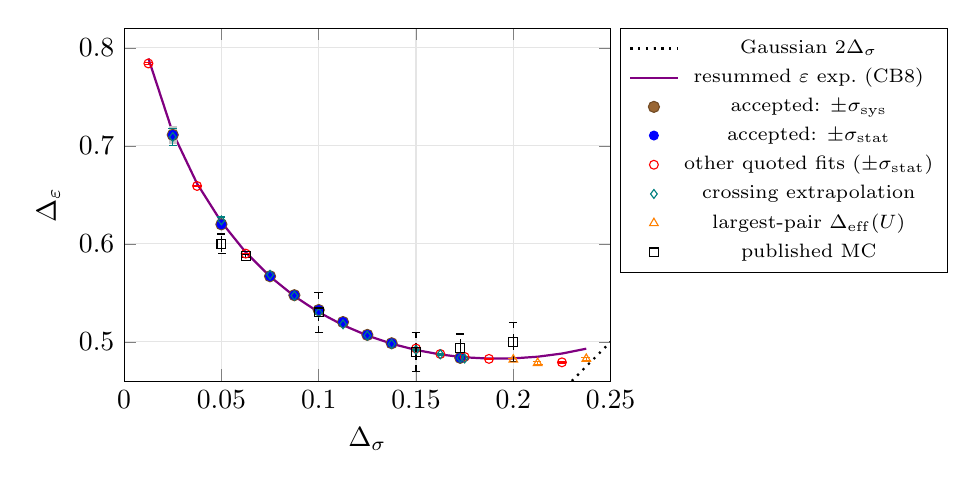
\begin{tikzpicture}
\begin{axis}[width=0.64\textwidth,height=0.5\textwidth,xlabel={$\Delta_\sigma$},ylabel={$\Delta_\varepsilon$},xmin=0,xmax=0.25,ymin=0.46,ymax=0.82,xtick={0,0.05,0.1,0.15,0.2,0.25},scaled x ticks=false,xticklabel style={/pgf/number format/fixed},
 legend style={font=\scriptsize,at={(1.02,1)},anchor=north west},grid=major,grid style={gray!20}]
\addplot[domain=0:0.25,dotted,thick,black] {2*x}; \addlegendentry{Gaussian $2\Delta_\sigma$}
\addplot[thick,violet] coordinates {(0.0125,0.78915) (0.025,0.71343) (0.0375,0.66146) (0.05,0.62223) (0.0625,0.59139) (0.075,0.56663) (0.0875,0.54656) (0.1,0.53025) (0.1125,0.51703) (0.125,0.50643) (0.1375,0.49808) (0.15,0.49171) (0.1625,0.48714) (0.1727335,0.48465) (0.175,0.48424) (0.1875,0.48291) (0.2,0.48312) (0.2125,0.48483) (0.225,0.48808) (0.2375,0.49301)};
\addlegendentry{resummed $\varepsilon$ exp.\ (CB8)}
\addplot+[only marks,mark=none,draw=none,error bars/.cd,y dir=both,y explicit,error bar style={line width=3pt,gray!45},error mark=none] coordinates {(0.025,0.71115) +- (0,0.00959) (0.05,0.61987) +- (0,0.00220) (0.075,0.56694) +- (0,0.00139) (0.0875,0.54761) +- (0,0.00194) (0.1,0.53248) +- (0,0.00242) (0.1125,0.52020) +- (0,0.00217) (0.125,0.50710) +- (0,0.00193) (0.1375,0.49856) +- (0,0.00180) (0.1727335,0.48368) +- (0,0.00078)};
\addlegendentry{accepted: $\pm\sigma_{\rm sys}$}
\addplot+[only marks,mark=*,mark size=1.6pt,blue,error bars/.cd,y dir=both,y explicit] coordinates {(0.025,0.71115) +- (0,0.00049) (0.05,0.61987) +- (0,0.00055) (0.075,0.56694) +- (0,0.00037) (0.0875,0.54761) +- (0,0.00032) (0.1,0.53248) +- (0,0.00020) (0.1125,0.52020) +- (0,0.00025) (0.125,0.50710) +- (0,0.00035) (0.1375,0.49856) +- (0,0.00030) (0.1727335,0.48368) +- (0,0.00052)};
\addlegendentry{accepted: $\pm\sigma_{\rm stat}$}
\addplot+[only marks,mark=o,mark size=1.6pt,red,error bars/.cd,y dir=both,y explicit] coordinates {(0.0125,0.78404) +- (0,0.00077) (0.0375,0.65904) +- (0,0.00051) (0.0625,0.59003) +- (0,0.00035) (0.15,0.49325) +- (0,0.00041) (0.1625,0.48761) +- (0,0.00058) (0.175,0.48460) +- (0,0.00035) (0.1875,0.48263) +- (0,0.00030) (0.225,0.47912) +- (0,0.00068)};
\addlegendentry{other quoted fits ($\pm\sigma_{\rm stat}$)}
\addplot+[only marks,mark=diamond,mark size=1.6pt,teal,error bars/.cd,y dir=both,y explicit] coordinates {(0.025,0.70906) +- (0,0.00902) (0.05,0.62393) +- (0,0.00348) (0.075,0.56843) +- (0,0.00207) (0.0875,0.54711) +- (0,0.00113) (0.1,0.52975) +- (0,0.00135) (0.1125,0.51790) +- (0,0.00086) (0.125,0.50640) +- (0,0.00172) (0.1375,0.49783) +- (0,0.00094) (0.15,0.49183) +- (0,0.00071) (0.1625,0.48732) +- (0,0.00075) (0.1727335,0.48355) +- (0,0.00062) (0.175,0.48304) +- (0,0.00081)};
\addlegendentry{crossing extrapolation}
\addplot+[only marks,mark=triangle,mark size=1.8pt,orange,error bars/.cd,y dir=both,y explicit] coordinates {(0.2,0.4819) +- (0,0.0015) (0.2125,0.4784) +- (0,0.0015) (0.2375,0.4826) +- (0,0.0015)};
\addlegendentry{largest-pair $\Delta_{\rm eff}(U)$}
\addplot+[only marks,mark=square,mark size=1.6pt,black,error bars/.cd,y dir=both,y explicit] coordinates {(0.2,0.5000) +- (0,0.0200) (0.1727335,0.4940) +- (0,0.0140) (0.15,0.4900) +- (0,0.0200) (0.1,0.5300) +- (0,0.0200) (0.0625,0.5876) +- (0,0.0013) (0.05,0.6000) +- (0,0.0100)};
\addlegendentry{published MC}
\end{axis}
\end{tikzpicture}
\caption{$d=1$: $\De(\Ds)$. Values that passed the protocol with $\sstat$ (blue bars) and, separately, the model-family half-range $\ssys$
(gray bands), which is not a standard deviation; other quoted fits; crossing extrapolations with $\sigma_\infty$; largest-pair effective
dimensions where no fit is quotable; published Monte Carlo values; and the resummed $\varepsilon$ expansion. Table~\ref{mc:tab:theory1d} gives the
differences.}\label{mc:fig:1d}
\end{figure}

\paragraph{Reading the results.}
\begin{description}[leftmargin=1.2em]
\item[Near $s\to1$ ($\Ds\le0.05$).] 68--72 configurations are quotable, but $\ssys=4$--$20\times\sstat$: the fitted correction exponents
 ($\omega\approx0.26$--$0.40$) and the variants do not settle the correction sector, as expected near a marginal point.
\item[Middle ($0.0625\le\Ds\le0.1375$).] Six of seven couplings pass, with $\sstat=(2$--$4)\times10^{-4}$ and $\ssys=(1.4$--$2.4)\times10^{-3}$. At
 $\Ds=1/16$ the value is stable across campaigns: 0.59003 (final fit, with N2), 0.59046 (stages A and B alone, under protocol v2) and 0.59071
 (the separate two-point campaign); but the crossing series fail their own goodness-of-fit gate, hence \lbl{cross-check unavailable}.
\item[Towards the Gaussian end ($\Ds\ge0.15$).] $\Ds=0.1727335$ passes. At 0.15 and 0.175 the cross-check fails by $2.1$ and $2.0\sigma_D$; at
 0.1625, 0.1875 and 0.225 only fits of variant \code{second} with $\ktau=2$ are quotable (\lbl{conditional}); at 0.2, 0.2125 and 0.2375 no fit is
 quotable, because the correction exponent $\omega\approx\varepsilon\le0.2$ is too small to separate from the scaling function over $N\le2^{19}$.
 There the finite-size values of table~\ref{mc:tab:1dpairs} are reported; they are not infinite-size estimates.
\end{description}

\subsection{\texorpdfstring{Robustness of the $d=1$ results}{Robustness of the d=1 results}}\label{mc:sec:robust}
Table~\ref{mc:tab:robust} collects, per coupling, the quantities that bear on how much a value or label can be trusted; the paragraphs below
explain them.
\begin{table}[htbp]\centering\scriptsize
\caption{$d=1$ robustness. $n_q$: quotable fits; $P_{\chi^2}$: $\chi^2$ probability of the quoted fit; $\omega$: its correction exponent; fit $-$
crossing: quoted value minus the median crossing extrapolation; $z$: that difference over $\sigma_D$ as pre-registered (with the spread
term) and over the bootstrap part alone; P: label platform-sensitive (section~\ref{mc:sec:1drefit}).}\label{mc:tab:robust}
\begin{tabular}{@{}llrllrrrl@{}}\toprule
$\Ds$ & decision & $n_q$ & $P_{\chi^2}$ & $\omega$ & fit $-$ crossing & $z$ & $z$ (bootstrap) & \\\midrule
0.0125 & \lbl{x-check unavail.} & 72 & 0.01 & 0.262 & -- & -- & -- &  \\
0.025 & \lbl{accepted ($\sigma_{\rm sys}$-dom.)} & 68 & $3.1\times10^{-4}$ & 0.309 & +0.00209 & +0.23 & +0.24 &  \\
0.0375 & \lbl{x-check unavail.} & 71 & 0.21 & 0.348 & -- & -- & -- &  \\
0.05 & \lbl{accepted} & 72 & 0.36 & 0.397 & -0.00406 & -0.92 & -1.16 &  \\
0.0625 & \lbl{x-check unavail.} & 50 & 0.29 & 0.427 & -- & -- & -- &  \\
0.075 & \lbl{accepted} & 30 & 0.51 & 0.418 & -0.00148 & -0.33 & -0.70 &  \\
0.0875 & \lbl{accepted} & 34 & 0.41 & 0.385 & +0.00050 & +0.35 & +0.50 &  \\
0.1 & \lbl{accepted ($\sigma_{\rm sys}$-dom.)} & 48 & $5.2\times10^{-5}$ & 0.367 & +0.00273 & +1.73 & +2.13 &  \\
0.1125 & \lbl{accepted ($\sigma_{\rm sys}$-dom.)} & 41 & $1.5\times10^{-3}$ & 0.368 & +0.00230 & +0.61 & +2.73 &  \\
0.125 & \lbl{accepted} & 9 & $4.6\times10^{-5}$ & 0.368 & +0.00070 & +0.31 & +0.42 &  \\
0.1375 & \lbl{accepted ($\sigma_{\rm sys}$-dom.)} & 17 & 0.03 & 0.365 & +0.00073 & +0.77 & +0.79 &  \\
0.15 & \lbl{x-check failed} & 11 & $2.1\times10^{-3}$ & 0.320 & +0.00143 & +2.10 & +2.24 &  \\
0.1625 & \lbl{conditional} & 5 & 0.05 & 0.194 & +0.00029 & +0.22 & +0.38 & P \\
0.1727335 & \lbl{accepted} & 4 & 0.08 & 0.195 & +0.00013 & +0.17 & +0.20 & P \\
0.175 & \lbl{x-check failed} & 6 & 0.03 & 0.192 & +0.00155 & +2.00 & +2.00 &  \\
0.1875 & \lbl{conditional} & 4 & $1.5\times10^{-4}$ & 0.155 & -- & -- & -- &  \\
0.2 & \lbl{model-limited} & 0 & -- & -- & -- & -- & -- &  \\
0.2125 & \lbl{model-limited} & 0 & -- & -- & -- & -- & -- &  \\
0.225 & \lbl{conditional} & 1 & $7.4\times10^{-4}$ & 0.083 & -- & -- & -- &  \\
0.2375 & \lbl{model-limited} & 0 & -- & -- & -- & -- & -- &  \\
\bottomrule\end{tabular}
\end{table}
\begin{description}[leftmargin=1.2em]
\item[Goodness of fit.] The quality gate $\chi^2/{\rm dof}\le1.5$ admits, at about 200 degrees of freedom, fits with $P_{\chi^2}\sim10^{-5}$.
 The quoted fits at $\Ds=0.1$ and $0.125$ have $P_{\chi^2}\approx5\times10^{-5}$, at 0.025 $P_{\chi^2}=3\times10^{-4}$, and at 0.1125
 $P_{\chi^2}=1.5\times10^{-3}$. The preference for the smallest $N_{\min}$
 selects the member of the family with the most data, which is also often the one with the largest $\chi^2$. For these couplings $\sstat$
 understates the point-to-point scatter, and the values should be read with $\ssys$.
\item[The cross-check and its $\sigma_D$.] Without the spread term in $\sigma_D$ the test would fail at $\Ds=0.1$ ($z=2.13$) and $0.1125$
 ($z=2.73$), both labeled \lbl{accepted}. Moreover, for all nine couplings with $\Ds\ge0.0875$ and a cross-check the fit lies above the
 crossing extrapolation: the inverse-variance mean difference is $+0.00105\pm0.00028$ with $\chi^2=8.1$ for 8 degrees of freedom about it. (Inverse-variance weights from the
 bootstrap part.) The two failures at 0.15 and 0.175 are among the points with the smallest $\sigma_D$, not isolated anomalies. The global fit and the crossings use
 different correction exponents (for example $\omega=0.32$ and $\omega'=0.31$--$0.32$ at 0.15, $\omega=0.19$ and $\omega'=0.27$ at 0.175) and the
 same data, so their comparison is a consistency check of two extrapolation models, not an independent measurement.
\item[The failures and the $\omega'$ grid.] The failures at 0.15 and 0.175 are not an artifact of conditional errors: the crossing bootstrap
 refits $\omega'$ in every draw, and fixing it at its central value would make $\sigma_D$ smaller (table~\ref{mc:tab:oned}). They are, however, numerically fragile:
 refining only the $\omega'$ grid from step 0.01 to 0.001 and 0.0001, with everything else fixed, moves the ratio
 $|\De^{\rm fit}-\De^\infty|/\sigma_D$ from 2.101 to 1.884 and 1.907 at 0.15, and from 2.003 to 1.897 and 1.931 at 0.175, below the
 threshold. The labels stand under the frozen protocol (step 0.01); whether a fit--crossing difference of this size is real is unresolved, and
 the common offset above suggests a systematic difference between the two extrapolation models.
\begin{table}[htbp]\centering\scriptsize
\caption{The cross-check at $\Ds=0.15,0.175$ with $\omega'$ refitted per draw (as recorded) and fixed at its central value. Last column:
central $\omega'$ (16--84\,\% of the per-draw values) of each eligible crossing series.}\label{mc:tab:oned}
\begin{tabular}{@{}llllll>{\raggedright\arraybackslash}p{5.0cm}@{}}\toprule
$\Ds$ & fit $-$ crossing & $\sigma_D$ (per draw) & $z$ & $\sigma_D$ (fixed $\omega'$) & $z$ & series \\\midrule
0.15 & +0.00143 & 0.00068 & +2.10 & 0.00062 & +2.30 & xc0.45\_star: 0.32 (0.31--0.32), xc0.45\_plus: 0.31 (0.30--0.32) \\
0.175 & +0.00155 & 0.00078 & +2.00 & 0.00067 & +2.30 & xc0.6\_star: 0.27 (0.26--0.27), xc0.6\_plus: 0.27 (0.26--0.27) \\
\bottomrule\end{tabular}
\end{table}
\item[Audit.] On 2026-09-22 the second AI system audited the finished analysis, with diagnostic refits
 (no new data) on the same records and bootstrap draws. It found no defect in the sampler, estimators or implementation, and these
 sensitivities:
 \begin{itemize}
 \item The quoted values at $\Ds=0.1$, 0.1375 and 0.1727335 are stable under stronger size cuts ($N\ge32\,768$, $N\ge65\,536$); at
  0.1727335 the cuts give 0.48421 and 0.48386 against 0.48368(52).
 \item At 0.025 a model outside the family (analytic background plus second power together) gives 0.69348, below the family's lower end
  0.69686, a shift of 7.0 paired-bootstrap scales (half the 16--84\,\% width of the matched difference). At 0.175, $N\ge32\,768$ shifts the
  value by $-0.00237$ (2.2 scales); at 0.225, $N\ge65\,536$ shifts it by $+0.00483$ (3.7 scales).
 \item The family is asymmetric: at 0.1375 it extends $0.00020$ below and $0.00340$ above the quoted value.
 \item A regular magnetic background gives an $N^{-s}$ correction to $U$ as well as to $Y$, but the \code{background} variant puts it only on
  $Y$. In the six cases the audit reports (0.025, 0.1, 0.1375, 0.1727335, 0.175, 0.225; variant with background and second power),
  adding it moves the central value by at most 0.0021 (at 0.025). At 0.05 such a model gives 0.61602, 0.0039 below the quoted value and below
  the family range [0.61845, 0.62286] (central fit only, not bootstrapped).
 \end{itemize}
\item[The degree ladder.] In 160 of the 1\,116 configurations, at 15 of the 20 couplings, the ladder cannot take its first step ($p=3$
 against $p=4$) because one of the two fits is missing or flagged. In 140 of them it is the $p=3$ fit, although that fit is typically a gross
 misfit that the F-test would reject by many orders of magnitude; in the other 20 it is the $p=4$ fit. $n_q$ and $\ssys$ are computed on the
 families trimmed in this way. At two couplings this decides the label (section~\ref{mc:sec:1drefit}). A sensitivity study with a ladder
 that does not stop on a flagged lower-degree fit is reported in section~\ref{mc:sec:robustladder}.
\end{description}

\subsubsection{Reproducibility of the fitting stage across platforms}\label{mc:sec:1drefit}
The fit inputs of every coupling (merged summaries and block archives) are released, so the whole fitting stage can be rerun
(\code{make refit1d}). It was rerun for all 20 couplings on 7 October 2026 on a workstation (Intel i9-13900K; Python 3.12.3, NumPy 1.26.4,
SciPy 1.11.4, OpenBLAS) with the production arguments and compared with the production run (AMD EPYC 7742; Python 3.8.5, NumPy 1.19.2, SciPy
1.5.2); table~\ref{mc:tab:refit}. Eighteen labels and all quoted configurations are reproduced, and so is $\ssys$ wherever both runs have it;
quoted values agree to $\le10^{-8}$ and $\sstat$ to $\le1.2\times10^{-7}$ absolute, because nonlinear optima agree only to $\sim10^{-7}$. Two
labels change, in opposite directions, for the same reason: the $p=3$ start of the ladder of configuration \code{x0.45\_background\_Nmin8192\_K2},
a gross misfit ($\chi^2\approx6$--$8\times10^4$ for 178 degrees of freedom, rejected by the F-test at a probability below $10^{-100}$), has two minima, one
interior and a lower one with $a_1$ on its bound $-50$, and which one the multistart optimizer finds depends on floating-point details
(table~\ref{mc:tab:d3}). A bound minimum is flagged and stops the ladder, so the configuration never reaches its good $p\ge5$ fits.
\begin{itemize}
\item At $\Ds=0.1727335$ production found the interior minimum: four quotable fits, $\ssys=0.00078$, \lbl{accepted}. The workstation (with its
 own libraries, and with the production versions in OpenBLAS and MKL builds) and an AMD EPYC 7543 node with the production versions find the
 bound minimum: three fits remain, $\ssys$ needs four, \lbl{conditional}. The fourth fit, which exists only on the production platform, has
 $\chi^2/{\rm dof}=1.47$ against the cap 1.5.
\item At $\Ds=0.1625$ it is the reverse: production found the bound minimum (five quotable fits, all of variant \code{second}, so $\ssys$ is not
 available: \lbl{conditional}); the workstation finds the interior minimum, a sixth fit of variant \code{background} becomes quotable, $\ssys=0.00024$
 and the label is \lbl{accepted}.
\end{itemize}
The values and $\sstat$ are robust; these two labels should be read as platform-sensitive.
\begin{table}[htbp]\centering\scriptsize
\caption{$d=1$ fitting stage rerun from the released snapshots (workstation, 2026-10-07) against production. $n_q$: quotable fits;
$|\delta\De|$: difference of the quoted values. Records: \code{results/1d/refit\_workstation\_20261007/}.}\label{mc:tab:refit}
\begin{tabular}{@{}lllllllll@{}}\toprule
 & \multicolumn{3}{c}{production} & \multicolumn{3}{c}{refit (workstation)} & & \\
$\Ds$ & decision & $n_q$ & $\ssys$ & decision & $n_q$ & $\ssys$ & $|\delta\De|$ & \\\midrule
0.0125 & \lbl{x-check unavail.} & 72 & 0.01003 & \lbl{x-check unavail.} & 72 & 0.01003 & 3e-09 &  \\
0.025 & \lbl{accepted ($\sigma_{\rm sys}$-dom.)} & 68 & 0.00959 & \lbl{accepted ($\sigma_{\rm sys}$-dom.)} & 68 & 0.00959 & 1e-09 &  \\
0.0375 & \lbl{x-check unavail.} & 71 & 0.00425 & \lbl{x-check unavail.} & 71 & 0.00425 & 2e-09 &  \\
0.05 & \lbl{accepted} & 72 & 0.00220 & \lbl{accepted} & 72 & 0.00220 & 5e-09 &  \\
0.0625 & \lbl{x-check unavail.} & 50 & 0.00150 & \lbl{x-check unavail.} & 50 & 0.00150 & 4e-09 &  \\
0.075 & \lbl{accepted} & 30 & 0.00139 & \lbl{accepted} & 30 & 0.00139 & 2e-09 &  \\
0.0875 & \lbl{accepted} & 34 & 0.00194 & \lbl{accepted} & 34 & 0.00194 & 2e-09 &  \\
0.1 & \lbl{accepted ($\sigma_{\rm sys}$-dom.)} & 48 & 0.00242 & \lbl{accepted ($\sigma_{\rm sys}$-dom.)} & 48 & 0.00242 & 8e-10 &  \\
0.1125 & \lbl{accepted ($\sigma_{\rm sys}$-dom.)} & 41 & 0.00217 & \lbl{accepted ($\sigma_{\rm sys}$-dom.)} & 41 & 0.00217 & 2e-09 &  \\
0.125 & \lbl{accepted} & 9 & 0.00193 & \lbl{accepted} & 9 & 0.00193 & 3e-09 &  \\
0.1375 & \lbl{accepted ($\sigma_{\rm sys}$-dom.)} & 17 & 0.00180 & \lbl{accepted ($\sigma_{\rm sys}$-dom.)} & 17 & 0.00180 & 2e-09 &  \\
0.15 & \lbl{x-check failed} & 11 & 0.00306 & \lbl{x-check failed} & 11 & 0.00306 & 2e-10 &  \\
0.1625 & \lbl{conditional} & 5 & -- & \lbl{accepted} & 6 & 0.00024 & 2e-09 & changed \\
0.1727335 & \lbl{accepted} & 4 & 0.00078 & \lbl{conditional} & 3 & -- & 3e-09 & changed \\
0.175 & \lbl{x-check failed} & 6 & 0.00067 & \lbl{x-check failed} & 6 & 0.00067 & 3e-09 &  \\
0.1875 & \lbl{conditional} & 4 & -- & \lbl{conditional} & 4 & -- & 6e-09 &  \\
0.2 & \lbl{model-limited} & 0 & -- & \lbl{model-limited} & 0 & -- & -- &  \\
0.2125 & \lbl{model-limited} & 0 & -- & \lbl{model-limited} & 0 & -- & -- &  \\
0.225 & \lbl{conditional} & 1 & -- & \lbl{conditional} & 1 & -- & 7e-09 &  \\
0.2375 & \lbl{model-limited} & 0 & -- & \lbl{model-limited} & 0 & -- & -- &  \\
\bottomrule\end{tabular}
\end{table}
\begin{table}[htbp]\centering\scriptsize
\caption{The $p=3$ start of the ladder of \code{x0.45\_background\_Nmin8192\_K2} on each platform: $\chi^2$ (178 dof), the field coefficient
$a_1$ (bounds $\pm50$), and the consequence for the ladder.}\label{mc:tab:d3}
\begin{tabular}{@{}llllll@{}}\toprule
$\Ds$ & platform & $\chi^2$ & $a_1$ & minimum & ladder \\\midrule
0.1625 & production (AMD EPYC 7742) & 60656.3 & -50.00 & bound & stops at $p=3$ \\
0.1625 & Intel i9-13900K, Py 3.12/NumPy 1.26/SciPy 1.11, OpenBLAS & 67496.2 & -38.29 & interior & continues \\
0.1727335 & production (AMD EPYC 7742) & 75400.9 & -45.49 & interior & continues \\
0.1727335 & Intel i9-13900K, Py 3.12/NumPy 1.26/SciPy 1.11, OpenBLAS & 68429.4 & -50.00 & bound & stops at $p=3$ \\
0.1727335 & Intel i9-13900K, Py 3.8.5/NumPy 1.19.2/SciPy 1.5.2, OpenBLAS & 68429.4 & -50.00 & bound & stops at $p=3$ \\
0.1727335 & Intel i9-13900K, same versions, MKL & 68429.4 & -50.00 & bound & stops at $p=3$ \\
0.1727335 & AMD EPYC 7543, same versions, MKL & 68429.4 & -50.00 & bound & stops at $p=3$ \\
\bottomrule\end{tabular}
\end{table}

\subsubsection{Sensitivity to the ladder rule}\label{mc:sec:robustladder}
To measure how much the trimmed families matter, all 20 couplings were refitted twice in one job on one node (AMD EPYC 7543; Python 3.8.5,
NumPy 1.19.2, SciPy 1.5.2, MKL): once with the frozen fitter, and once with a copy whose only change is that a flagged lower-degree fit no
longer stops the ladder (its $\chi^2$ still enters the F-test). This is a diagnostic, not the protocol, and table~\ref{mc:tab:1dfinal} is not
modified; records and the modified fitter are in \path{results/1d/robust_ladder_20261013/}. Table~\ref{mc:tab:robustladder} gives the result.
On this node the frozen ladder reproduces the workstation refit of section~\ref{mc:sec:1drefit}, including its two label changes. With the
robust ladder:
\begin{itemize}
\item every quoted value is unchanged to $2\times10^{-5}$;
\item the number of quotable fits grows at eleven couplings, and $\ssys$ grows at 0.125 (0.00193 to 0.00221), 0.1375 (0.00180 to 0.00192), 0.1625
 (0.00024 to 0.00071) and 0.175 (0.00067 to 0.00115);
\item both platform-sensitive couplings pass: 0.1625 with $\ssys=0.00071$, and 0.1727335 with nine quotable fits and the production value
 $\ssys=0.00078$;
\item 0.125 passes as $\ssys$-dominated, 0.1875 becomes \lbl{cross-check unavailable} with $\ssys=0.00063$, and 0.2 becomes \lbl{conditional}
 with two quotable fits.
\end{itemize}
The trimming therefore mostly shrinks the model families; it decides a label only where few fits are quotable. Under the robust rule ten
couplings would pass, and the two platform-sensitive labels would no longer depend on which minimum the degree-3 fit finds.
\begin{table}[htbp]\centering\scriptsize\setlength{\tabcolsep}{3pt}
\caption{$d=1$ ladder sensitivity: production, and the frozen and the robust ladder refitted on one node. $n_q$: quotable fits; $|\delta\De|$:
quoted value, robust minus production; last column: what the robust ladder changes relative to the frozen ladder on the same node.}\label{mc:tab:robustladder}
\begin{tabular}{@{}lllllllllllll@{}}\toprule
 & \multicolumn{3}{c}{production} & \multicolumn{3}{c}{frozen ladder} & \multicolumn{3}{c}{robust ladder} & & \\
$\Ds$ & decision & $n_q$ & $\ssys$ & decision & $n_q$ & $\ssys$ & decision & $n_q$ & $\ssys$ & $|\delta\De|$ & \\\midrule
0.0125 & \lbl{x-check unavail.} & 72 & 0.01003 & \lbl{x-check unavail.} & 72 & 0.01003 & \lbl{x-check unavail.} & 72 & 0.01003 & 1e-09 &  \\
0.025 & \lbl{accepted ($\sigma_{\rm sys}$-dom.)} & 68 & 0.00959 & \lbl{accepted ($\sigma_{\rm sys}$-dom.)} & 68 & 0.00959 & \lbl{accepted ($\sigma_{\rm sys}$-dom.)} & 68 & 0.00959 & 2e-10 &  \\
0.0375 & \lbl{x-check unavail.} & 71 & 0.00425 & \lbl{x-check unavail.} & 71 & 0.00425 & \lbl{x-check unavail.} & 71 & 0.00425 & 9e-10 &  \\
0.05 & \lbl{accepted} & 72 & 0.00220 & \lbl{accepted} & 72 & 0.00220 & \lbl{accepted} & 72 & 0.00220 & 6e-09 &  \\
0.0625 & \lbl{x-check unavail.} & 50 & 0.00150 & \lbl{x-check unavail.} & 50 & 0.00150 & \lbl{x-check unavail.} & 50 & 0.00150 & 3e-09 &  \\
0.075 & \lbl{accepted} & 30 & 0.00139 & \lbl{accepted} & 30 & 0.00139 & \lbl{accepted} & 30 & 0.00139 & 6e-09 &  \\
0.0875 & \lbl{accepted} & 34 & 0.00194 & \lbl{accepted} & 34 & 0.00194 & \lbl{accepted} & 35 & 0.00194 & 2e-09 & $n_q$ \\
0.1 & \lbl{accepted ($\sigma_{\rm sys}$-dom.)} & 48 & 0.00242 & \lbl{accepted ($\sigma_{\rm sys}$-dom.)} & 48 & 0.00242 & \lbl{accepted ($\sigma_{\rm sys}$-dom.)} & 49 & 0.00242 & 1e-10 & $n_q$ \\
0.1125 & \lbl{accepted ($\sigma_{\rm sys}$-dom.)} & 41 & 0.00217 & \lbl{accepted ($\sigma_{\rm sys}$-dom.)} & 41 & 0.00217 & \lbl{accepted ($\sigma_{\rm sys}$-dom.)} & 44 & 0.00217 & 4e-09 & $n_q$ \\
0.125 & \lbl{accepted} & 9 & 0.00193 & \lbl{accepted} & 9 & 0.00193 & \lbl{accepted ($\sigma_{\rm sys}$-dom.)} & 18 & 0.00221 & 2e-05 & label \\
0.1375 & \lbl{accepted ($\sigma_{\rm sys}$-dom.)} & 17 & 0.00180 & \lbl{accepted ($\sigma_{\rm sys}$-dom.)} & 17 & 0.00180 & \lbl{accepted ($\sigma_{\rm sys}$-dom.)} & 24 & 0.00192 & 1e-09 & $n_q$ \\
0.15 & \lbl{x-check failed} & 11 & 0.00306 & \lbl{x-check failed} & 11 & 0.00306 & \lbl{x-check failed} & 19 & 0.00306 & 1e-09 & $n_q$ \\
0.1625 & \lbl{conditional} & 5 & -- & \lbl{accepted} & 6 & 0.00024 & \lbl{accepted} & 15 & 0.00071 & 4e-09 & $n_q$ \\
0.1727335 & \lbl{accepted} & 4 & 0.00078 & \lbl{conditional} & 3 & -- & \lbl{accepted} & 9 & 0.00078 & 2e-09 & label \\
0.175 & \lbl{x-check failed} & 6 & 0.00067 & \lbl{x-check failed} & 6 & 0.00067 & \lbl{x-check failed} & 13 & 0.00115 & 5e-11 & $n_q$ \\
0.1875 & \lbl{conditional} & 4 & -- & \lbl{conditional} & 4 & -- & \lbl{x-check unavail.} & 10 & 0.00063 & 2e-09 & label \\
0.2 & \lbl{model-limited} & 0 & -- & \lbl{model-limited} & 0 & -- & \lbl{conditional} & 2 & -- & -- & label \\
0.2125 & \lbl{model-limited} & 0 & -- & \lbl{model-limited} & 0 & -- & \lbl{model-limited} & 0 & -- & -- &  \\
0.225 & \lbl{conditional} & 1 & -- & \lbl{conditional} & 1 & -- & \lbl{conditional} & 1 & -- & 5e-09 &  \\
0.2375 & \lbl{model-limited} & 0 & -- & \lbl{model-limited} & 0 & -- & \lbl{model-limited} & 0 & -- & -- &  \\
\bottomrule\end{tabular}
\end{table}

\subsection{Comparison with theory and earlier simulations}\label{mc:sec:theory1d}
\paragraph{Resummed $\varepsilon$ expansion.} Table~\ref{mc:tab:theory1d} compares with the eight-loop $\varepsilon$ expansion of the accompanying
article~\cite{mc:Zheng:2026ai}, resummed by conformal Borel resummation~\cite{mc:LeGuillou:1979ixc}. In $d=1$ it is resummed in the variable
$v=1-2\sqrt{\Ds}$, with the short-range series near $s=1$ imposed; we call this curve CB8 (values and band from the article's resummation
package, \path{data/reference/theory_1d_CB8.csv}). The band is a sensitivity range over resummation prescriptions, not a confidence interval.
The nine values that passed the protocol differ from CB8 by $-0.0024$ to $+0.0032$, that is 1 to 13 times their $\sstat$; four of them (0.025,
0.05, 0.1, 0.1125) lie outside the band. As a scale only, $\ssys$ exceeds the difference except at 0.05, 0.1125 and 0.1727335 (1.1, 1.5 and 1.2
times $\ssys$). Near the Gaussian end the series needs little resummation (at $\Ds=0.2375$, $\varepsilon=0.05$, its partial sums are stable to
$3\times10^{-4}$). There the largest-pair effective dimensions (0.2, 0.2125, 0.2375) and the single quoted fit at 0.225 lie $0.0012$,
$0.0065$, $0.0104$ and $0.0090$ below it. A slow approach with exponent $\omega\approx\varepsilon$, which the fit windows and the crossing grid
($\omega'\ge0.2$) cannot resolve, would give a deficit of this sign; we have not estimated its size. These values are finite-size results.
\begin{table}[htbp]\centering\scriptsize
\caption{$d=1$ against the resummed $\varepsilon$ expansion (CB8, with band). MC: the quoted global fit ($\sstat$ only), or the largest-pair
$\Deff(U)$ where no fit is quotable.}\label{mc:tab:theory1d}
\begin{tabular}{@{}llllllll@{}}\toprule
$\Ds$ & $\varepsilon$ & CB8 & band & decision & MC kind & MC & MC $-$ CB8 \\\midrule
0.0125 & 0.950 & 0.7892 & [0.7891, 0.7892] & \lbl{x-check unavail.} & fit & 0.78404(77) & -0.0051 \\
0.025 & 0.900 & 0.7134 & [0.7133, 0.7136] & \lbl{accepted ($\sigma_{\rm sys}$-dom.)} & fit & 0.71115(49) & -0.0023 \\
0.0375 & 0.850 & 0.6615 & [0.6611, 0.6619] & \lbl{x-check unavail.} & fit & 0.65904(51) & -0.0024 \\
0.05 & 0.800 & 0.6222 & [0.6215, 0.6230] & \lbl{accepted} & fit & 0.61987(55) & -0.0024 \\
0.0625 & 0.750 & 0.5914 & [0.5903, 0.5924] & \lbl{x-check unavail.} & fit & 0.59003(35) & -0.0014 \\
0.075 & 0.700 & 0.5666 & [0.5650, 0.5679] & \lbl{accepted} & fit & 0.56694(37) & +0.0003 \\
0.0875 & 0.650 & 0.5466 & [0.5446, 0.5479] & \lbl{accepted} & fit & 0.54761(32) & +0.0011 \\
0.1 & 0.600 & 0.5302 & [0.5280, 0.5316] & \lbl{accepted ($\sigma_{\rm sys}$-dom.)} & fit & 0.53248(20) & +0.0022 \\
0.1125 & 0.550 & 0.5170 & [0.5146, 0.5188] & \lbl{accepted ($\sigma_{\rm sys}$-dom.)} & fit & 0.52020(25) & +0.0032 \\
0.125 & 0.500 & 0.5064 & [0.5040, 0.5086] & \lbl{accepted} & fit & 0.50710(35) & +0.0007 \\
0.1375 & 0.450 & 0.4981 & [0.4958, 0.5005] & \lbl{accepted ($\sigma_{\rm sys}$-dom.)} & fit & 0.49856(30) & +0.0005 \\
0.15 & 0.400 & 0.4917 & [0.4898, 0.4942] & \lbl{x-check failed} & fit & 0.49325(41) & +0.0015 \\
0.1625 & 0.350 & 0.4871 & [0.4857, 0.4895] & \lbl{conditional} & fit & 0.48761(58) & +0.0005 \\
0.1727335 & 0.309 & 0.4846 & [0.4835, 0.4867] & \lbl{accepted} & fit & 0.48368(52) & -0.0010 \\
0.175 & 0.300 & 0.4842 & [0.4832, 0.4862] & \lbl{x-check failed} & fit & 0.48460(35) & +0.0004 \\
0.1875 & 0.250 & 0.4829 & [0.4822, 0.4844] & \lbl{conditional} & fit & 0.48263(30) & -0.0003 \\
0.2 & 0.200 & 0.4831 & [0.4828, 0.4840] & \lbl{model-limited} & largest pair & 0.4819(15) & -0.0012 \\
0.2125 & 0.150 & 0.4848 & [0.4847, 0.4852] & \lbl{model-limited} & largest pair & 0.4784(15) & -0.0065 \\
0.225 & 0.100 & 0.4881 & [0.4881, 0.4882] & \lbl{conditional} & fit & 0.47912(68) & -0.0090 \\
0.2375 & 0.050 & 0.4930 & [0.4930, 0.4930] & \lbl{model-limited} & largest pair & 0.4826(15) & -0.0104 \\
\bottomrule\end{tabular}
\end{table}

\paragraph{Earlier simulations.} Table~\ref{mc:tab:lit1d} lists the published Monte Carlo values at our couplings (earlier estimates from exact
finite-range scaling~\cite{mc:Glumac:1989fr} are not simulations and are not listed). Published values exist at
six of our couplings; at three of them (0.05, 0.1, 0.1727335) our value passed the protocol, and at $\Ds=0.2$ the comparison is with a finite-size
value. The equilibrium values (UGA, APR, Luijten's thesis) agree with ours to within two standard deviations of the difference, computed from the
published error and our $\sstat$; $\ssys$ is not added, because it is not a standard deviation. The largest ratio, 1.98, is at $\Ds=0.05$,
where the difference is nine times our $\ssys$. The nonequilibrium-relaxation values of Tomita lie below; his own estimate of $\eta$
misses the exact $\eta=2-s$ by 2.5--3.5 quoted errors at $s=0.6$--$0.8$, so his quoted errors do not cover the systematic errors of that
method, and the disagreement at $\Ds=0.1$ is with an estimate that fails an exact check. APR's correction exponent $\omega=0.201(11)$ at
$\Ds=0.1727335$ agrees with our fitted $\omega=0.195$ (table~\ref{mc:tab:robust}).
\begin{table}[htbp]\centering\scriptsize
\caption{Published $d=1$ values ($\De=1-1/\nu$ where $\nu$ is quoted) against ours. UGA: Uzelac--Glumac--Ani\v{c}i\'c; APR: Angelini--Parisi--Ricci-Tersenghi; NER: nonequilibrium relaxation. Ours: value($\sstat$)($\ssys$), or a finite-size value.}\label{mc:tab:lit1d}
\setlength{\tabcolsep}{2.5pt}\begin{tabular}{@{}lllllll@{}}\toprule
$\Ds$ & source & method & published & ours & our label & published $-$ ours \\\midrule
0.05 & Tomita 2009~\cite{mc:Tomita:2009mc} & MC, NER & 0.5633(362) & 0.61987(55)(220) & \lbl{accepted} & -0.0566 \\
0.05 & UGA 2001~\cite{mc:Uzelac:2001lc} & MC, largest cluster & 0.6000(100) & 0.61987(55)(220) & \lbl{accepted} & -0.0199 \\
0.0625 & APR 2014~\cite{mc:Angelini:2014koy} & MC, FSS & 0.5876(13) & 0.59003(35)(150) & \lbl{x-check unavail.} & -0.0024 \\
0.1 & Luijten 1997 (thesis)~\cite{mc:Luijten:1997th} & MC, FSS & 0.5392(106) & 0.53248(20)(242) & \lbl{accepted ($\sigma_{\rm sys}$-dom.)} & +0.0067 \\
0.1 & Tomita 2009~\cite{mc:Tomita:2009mc} & MC, NER & 0.4709(140) & 0.53248(20)(242) & \lbl{accepted ($\sigma_{\rm sys}$-dom.)} & -0.0616 \\
0.1 & UGA 2001~\cite{mc:Uzelac:2001lc} & MC, largest cluster & 0.5300(200) & 0.53248(20)(242) & \lbl{accepted ($\sigma_{\rm sys}$-dom.)} & -0.0025 \\
0.15 & Tomita 2009~\cite{mc:Tomita:2009mc} & MC, NER & 0.4536(508) & 0.49325(41)(306) & \lbl{x-check failed} & -0.0397 \\
0.15 & UGA 2001~\cite{mc:Uzelac:2001lc} & MC, largest cluster & 0.4900(200) & 0.49325(41)(306) & \lbl{x-check failed} & -0.0033 \\
0.1727335 & APR 2014~\cite{mc:Angelini:2014koy} & MC, FSS & 0.4940(140) & 0.48368(52)(78) & \lbl{accepted} & +0.0103 \\
0.2 & Tomita 2009~\cite{mc:Tomita:2009mc} & MC, NER & 0.4444(648) & 0.4819(15) [finite size] & \lbl{model-limited} & -0.0375 \\
0.2 & UGA 2001~\cite{mc:Uzelac:2001lc} & MC, largest cluster & 0.5000(200) & 0.4819(15) [finite size] & \lbl{model-limited} & +0.0181 \\
\bottomrule\end{tabular}
\end{table}

\subsection{Status of the design goals}
The campaign had three design goals: \lbl{accepted} at every $\Ds\in[0.0625,0.1875]$, which was not met (7 of 12 couplings); a definite label
at every outer coupling, which was met; and exact reproduction of the two-point campaign's values in its original windows, which was met. An
extension to $N=2^{20}$ (called N3) was not run.

% =====================================================================================================================
\section{\texorpdfstring{$d=2$ and $d=3$: common protocol}{d=2 and d=3: common protocol}}\label{mc:sec:proto23}
\subsection{Design and analysis}
For each coupling, five sizes form four size-doubling pairs, the minimum for an extrapolation with a free exponent. Temperatures are centered
on crossings measured in a short stage-0 campaign (frozen tables \path{data/2d/production_centers.csv},
\path{data/3d/production_centers_3d.csv}), five per size. Every $(L,\beta)$ group has 12 hot/cold replicas with $10^6$ measured sweeps; each
dimension has 2\,400 chains.
\begin{enumerate}[1.]
\item For each pair and $Q\in\{U_4,U_6,U_8,Y\}$ the effective dimension~\eqref{mc:eq:Deff} is computed at the $U_4$ crossing; the bootstrap gives
 the covariance over pairs and observables.
\item Each series $\Deff^Q(L)$ is extrapolated as $\De+c_QL^{-\omega'}$ by generalized least squares, with $\omega'$ profiled on $[0.2,2]$ (step
 0.01); a \emph{joint} series fits $U_4$ and $Y$ with common $\De$ and $\omega'$ and separate amplitudes (written U4+Y).
\item A series is eligible if $\chi^2/{\rm dof}\le2$, its $\Delta\chi^2\le1$ interval of $\omega'$ lies inside $[0.22,1.98]$, and its
 $\sigma_\infty$ is at most 5 times the error of the largest pair.
\item The quoted value is that of the joint series if eligible, else $U_4$, else the first eligible one of $U_6$, $U_8$, $Y$; $\ssys$ is half
 the range of $\De$ over the eligible series plus half the range of the quoted series' $\De$ over its $\Delta\chi^2\le1$ interval of $\omega'$.
\item Cross-check: the extrapolated $U_4$ and $Y$ must agree within $2\sigma_D$; reblocking at blocks 1000 and 4000 against 2000.
\end{enumerate}
The grid floor $\omega'\ge0.2$ excludes the correction exponent expected near the Gaussian end ($\omega\approx\varepsilon=0.1$ at 2D $s=1.05$
and 3D $s=1.55$), and near the short-range end the relevant exponent $s_*-s$ is also below 0.2; there the labels partly reflect this design
choice.

\subsection{The statistical error of an extrapolation: amendment P1}\label{mc:sec:p1}
The frozen protocols compute $\sstat$, $\sigma_D$ and the reblocking comparison by refitting each bootstrap draw at the \emph{central}
$\omega'$, i.e.\ conditionally on a fitted exponent. A review of the finished evaluations identified this. Amendment P1
re-profiles $\omega'$ in every draw (same grid and covariance; draws on a grid edge are kept). It leaves the eligibility gates, $\ssys$, the
choice of series and the decision order unchanged. The gate $\sigma_\infty\le5\times$ (error of the largest pair) is therefore still evaluated
with the fixed-$\omega'$ $\sigma_\infty$. With the profiled one, three series would fail it: $Y$ at 2D $s=1.05$ and $U_4$ at 3D $s=1.55$ and
1.7. 2D $s=1.05$ would then have no eligible series, and the 3D cross-check would become unavailable at 1.55 and 1.7. The series of the
accepted value at 3D $s=1.6$ pass the gate either way.

P1 was calibrated before adoption on synthetic data whose truths are the recorded fits: for every coupling, single-series ensembles for each
of $U_4,U_6,U_8,Y$ and a joint ensemble, 2\,000 synthetic data sets each with 500 synthetic draws, run through the full fit, gates and both error
rules. A coupling is evaluated under P1 only if every series it uses has profiled $1\sigma$ coverage $\ge0.60$ and $2\sigma$ coverage $\ge0.90$
(with at least 200 eligible fits) and, when both $U_4$ and $Y$ are eligible, the profiled cross-check's false-failure rate is $\le0.10$;
otherwise the frozen rule applies (appendix~\ref{mc:app:calib}).

Results:
\begin{itemize}
\item The fixed-$\omega'$ rule under-covers mainly for single series: in the strata that pass the adoption rules its $1\sigma$ coverage is
 0.00--0.38 for $U_4$ and 0.12--0.29 for $Y$, against 0.59--0.67 for the joint series (pooled over all strata, the $1\sigma$ coverage is 0.287 for
45\,440 eligible synthetic fits). In the same
 strata the profiled rule covers 0.81--1.00 for the Binder series, 0.69--0.83 for $Y$ and 0.67--0.70 for the joint series.
\item The false-failure rate of the cross-check at 3D $s=1.6$ is 0.7\,\% profiled against 61\,\% fixed.
\end{itemize}
The calibration is \emph{conditional on the single-power model}. We tested one misspecified family, which adds an $L^{-2\omega'}$ term that
reproduces the recorded $U_4-Y$ difference. In it the joint series at 3D $s=1.6$ is biased by $-0.0062$ with profiled coverage 0, and the
profiled cross-check does not detect the bias. But $U_4$ is then ineligible in every synthetic set, so that coupling could not have been
accepted under this misspecification.
The calibration therefore does not test model errors; the one misspecification studied would have blocked the label rather than biased it.
Exactly one label changes under P1: 3D $s=1.6$, from \lbl{cross-check failed} to \lbl{accepted}. This was predicted before implementation, but
after the frozen $z=-2.87$ was known.

% =====================================================================================================================
\section{\texorpdfstring{$d=2$}{d=2}}\label{mc:sec:2d}
Couplings $s\in\{1.05,\dots,1.7\}$ ($\Ds=0.475\dots0.15$), sizes $L=64\dots1024$, temperature half-width $w(L)=0.0015(L/64)^{-0.75}$. Stage 0 used
$L\le512$; the preflight confirmed every $512\to1024$ crossing inside its bracket. The production ran on 2026-09-20 to 22 ($L=1024$ at 88~ms per
sweep, 25--31~h per chain).
\begin{sidewaystable}\centering\scriptsize
\caption{$d=2$ finite-size data (block 2000): for each doubling pair the crossing inverse temperature $\beta_\times$ (error in units of $10^{-7}$) and
$\Deff(U_4)$, $\Deff(Y)$ (errors in units of $10^{-4}$, 500 bootstrap draws).}\label{mc:tab:2dpairs}
\begin{tabular}{@{}ll|lll|lll|lll|lll@{}}\toprule
 & & \multicolumn{3}{c|}{$64\to128$} & \multicolumn{3}{c|}{$128\to256$} & \multicolumn{3}{c|}{$256\to512$} & \multicolumn{3}{c}{$512\to1024$}\\
$s$ & $\Ds$ & $\beta_\times$ & $U_4$ & $Y$ & $\beta_\times$ & $U_4$ & $Y$ & $\beta_\times$ & $U_4$ & $Y$ & $\beta_\times$ & $U_4$ & $Y$ \\\midrule
1.05 & 0.475 & 0.1300733(16) & 0.9633(13) & 0.8390(14) & 0.1300298(10) & 0.9661(17) & 0.8658(18) & 0.1300145(6) & 0.9708(20) & 0.8863(21) & 0.1300084(4) & 0.9702(25) & 0.8964(23) \\
1.1 & 0.45 & 0.1355249(16) & 0.9609(14) & 0.8608(15) & 0.1354801(10) & 0.9639(17) & 0.8912(18) & 0.1354691(6) & 0.9664(20) & 0.9045(19) & 0.1354627(4) & 0.9659(23) & 0.9172(23) \\
1.2 & 0.4 & 0.1463564(17) & 0.9610(12) & 0.9142(13) & 0.1463343(10) & 0.9576(16) & 0.9281(16) & 0.1463269(5) & 0.9616(19) & 0.9391(19) & 0.1463241(3) & 0.9631(22) & 0.9478(22) \\
1.3 & 0.35 & 0.1571230(17) & 0.9581(12) & 0.9561(12) & 0.1571157(9) & 0.9586(15) & 0.9683(15) & 0.1571170(6) & 0.9605(17) & 0.9709(18) & 0.1571177(3) & 0.9584(20) & 0.9698(20) \\
1.4 & 0.3 & 0.1677986(17) & 0.9599(12) & 1.0024(12) & 0.1678175(9) & 0.9590(14) & 1.0032(14) & 0.1678263(5) & 0.9582(17) & 0.9986(16) & 0.1678310(3) & 0.9627(20) & 0.9977(19) \\
1.5 & 0.25 & 0.1783705(17) & 0.9608(12) & 1.0484(11) & 0.1784129(10) & 0.9615(14) & 1.0423(13) & 0.1784331(5) & 0.9640(16) & 1.0339(15) & 0.1784417(3) & 0.9661(18) & 1.0245(17) \\
1.6 & 0.2 & 0.1888074(18) & 0.9653(12) & 1.0977(11) & 0.1888717(10) & 0.9652(13) & 1.0885(12) & 0.1889039(5) & 0.9691(15) & 1.0729(13) & 0.1889149(3) & 0.9698(18) & 1.0620(15) \\
1.7 & 0.15 & 0.1990663(19) & 0.9671(11) & 1.1516(10) & 0.1991553(10) & 0.9699(13) & 1.1381(11) & 0.1991952(5) & 0.9751(16) & 1.1254(14) & 0.1992121(3) & 0.9773(17) & 1.1088(14) \\
\bottomrule\end{tabular}
\end{sidewaystable}
\begin{table}[htbp]\centering\scriptsize
\caption{$d=2$ labels under the frozen rule and under P1 (with the rule actually applied), the quoted value, $\sstat$ under both rules,
$\ssys$, and the $U_4-Y$ cross-check ($z$ with the fixed and the profiled $\sigma_D$). The \lbl{conditional} values at $s=1.05$ and $1.1$ are
single-series ($Y$) extrapolations $0.065$ and $0.047$ below the resummed expansion (table~\ref{mc:tab:theory23}); they are not infinite-size
estimates.}\label{mc:tab:2ddec}
\setlength{\tabcolsep}{4pt}\begin{tabular}{@{}llllllllll@{}}\toprule
$s$ & $\Ds$ & frozen label & P1 label & rule & $\De$ & $\sstat$ frozen & $\sstat$ P1 & $\ssys$ & $U_4-Y$; $z$ fixed / profiled \\\midrule
1.05 & 0.475 & \lbl{conditional} & \lbl{conditional} & profiled & 0.92078 & 0.00181 & 0.01773 & -- & -- \\
1.1 & 0.45 & \lbl{conditional} & \lbl{conditional} & profiled & 0.92846 & 0.00145 & 0.01012 & -- & -- \\
1.2 & 0.4 & \lbl{conditional} & \lbl{conditional} & profiled & 0.96202 & 0.00162 & 0.00182 & -- & -- \\
1.3 & 0.35 & \lbl{model-limited} & \lbl{model-limited} & fixed & -- & -- & -- & -- & -- \\
1.4 & 0.3 & \lbl{model-limited} & \lbl{model-limited} & fixed & -- & -- & -- & -- & -- \\
1.5 & 0.25 & \lbl{model-limited} & \lbl{model-limited} & fixed & -- & -- & -- & -- & -- \\
1.6 & 0.2 & \lbl{model-limited} & \lbl{model-limited} & fixed & -- & -- & -- & -- & -- \\
1.7 & 0.15 & \lbl{model-limited} & \lbl{model-limited} & fixed & -- & -- & -- & -- & -- \\
\bottomrule\end{tabular}
\end{table}

\paragraph{Reading.} No 2D coupling has a value that passed the protocol. The robust statement is finite-size: $\Deff(U_4,512\to1024)=0.958$--$0.977$
at all eight couplings ($\sigma\approx0.002$), moving by $\le0.01$ over the four pairs and always below the endpoint value 1. Against the
resummed expansion (table~\ref{mc:tab:theory23}) the largest-pair $U_4$ agrees within $0.0015$ for $s=1.2$--$1.4$ and falls short by $0.005$--$0.02$
towards both ends. At $s=1.2$, 1.3 and 1.4 the other ways of imposing the end point move the expansion by up to $0.0005$, $0.0023$ and $0.0047$,
so there the agreement is as good as the expansion is determined. $Y$ approaches $U_4$ as $L$ doubles at every coupling, slowly and from below at $s\le1.2$ and from above at $s\ge1.4$; near $s_*$ this is
consistent with the slow crossover of section~\ref{mc:sec:model}. A single power $L^{-\omega'}$ with $\omega'\in[0.2,2]$ is either unresolved or inconsistent over $L=64$--$1024$
(appendix~\ref{mc:app:series}). The three \lbl{conditional} values rest on one series without $\ssys$; at $s=1.05$ and $1.1$ that series is $Y$, and
its extrapolations (0.921, 0.928) lie $0.065$ and $0.047$ below the expansion, 3.7 and 4.6 times their $\sstat$. \textbf{These two values should
not be used as infinite-size estimates.} The crossing inverse temperatures $\beta_\times$ still move by up to $1.7\times10^{-5}$ between the last two
pairs; they are finite-size values.

% =====================================================================================================================
\section{\texorpdfstring{$d=3$}{d=3}}\label{mc:sec:3d}
Couplings $s\in\{1.55,\dots,1.95\}$ ($\Ds=0.725\dots0.525$), sizes $L=8\dots128$, half-width $w(L)=10^{-3}(L/16)^{-1}$. An $L=128$ chain runs at
105~ms per sweep alone but at about 250~ms when four chains share a 4-core CCX (a group of cores sharing a 16~MB L3 cache); the production
therefore pinned one $L=128$ chain per CCX (32 per 128-core node, $\approx30$~h per chain). The preflight gate and its amendment are described in
section~\ref{mc:sec:rules}. The production ran on 2026-09-21 to 23.
\begin{sidewaystable}\centering\scriptsize
\caption{$d=3$ finite-size data (block 2000), as table~\ref{mc:tab:2dpairs}.}\label{mc:tab:3dpairs}
\begin{tabular}{@{}ll|lll|lll|lll|lll@{}}\toprule
 & & \multicolumn{3}{c|}{$8\to16$} & \multicolumn{3}{c|}{$16\to32$} & \multicolumn{3}{c|}{$32\to64$} & \multicolumn{3}{c}{$64\to128$}\\
$s$ & $\Ds$ & $\beta_\times$ & $U_4$ & $Y$ & $\beta_\times$ & $U_4$ & $Y$ & $\beta_\times$ & $U_4$ & $Y$ & $\beta_\times$ & $U_4$ & $Y$ \\\midrule
1.55 & 0.725 & 0.0894786(14) & 1.4427(11) & 1.2535(12) & 0.0893412(7) & 1.4583(15) & 1.3545(16) & 0.0893146(4) & 1.4677(22) & 1.4028(23) & 0.0893087(2) & 1.4729(30) & 1.4269(30) \\
1.6 & 0.7 & 0.0916831(15) & 1.4398(11) & 1.2914(13) & 0.0915467(8) & 1.4596(15) & 1.3970(17) & 0.0915234(4) & 1.4661(21) & 1.4382(23) & 0.0915178(2) & 1.4715(31) & 1.4628(30) \\
1.7 & 0.65 & 0.0959967(15) & 1.4411(11) & 1.3761(12) & 0.0958738(8) & 1.4528(16) & 1.4673(17) & 0.0958528(3) & 1.4612(22) & 1.5085(21) & 0.0958497(2) & 1.4650(29) & 1.5263(29) \\
1.75 & 0.625 & 0.0981147(16) & 1.4377(11) & 1.4115(12) & 0.0979933(8) & 1.4535(15) & 1.5071(16) & 0.0979751(3) & 1.4536(21) & 1.5379(21) & 0.0979722(2) & 1.4615(27) & 1.5596(27) \\
1.8 & 0.6 & 0.1002020(16) & 1.4372(11) & 1.4513(12) & 0.1000841(8) & 1.4505(14) & 1.5417(15) & 0.1000677(3) & 1.4563(20) & 1.5795(20) & 0.1000665(2) & 1.4515(27) & 1.5818(27) \\
1.85 & 0.575 & 0.1022550(15) & 1.4364(11) & 1.4929(12) & 0.1021468(8) & 1.4490(15) & 1.5776(16) & 0.1021325(3) & 1.4538(20) & 1.6113(20) & 0.1021317(2) & 1.4569(27) & 1.6221(27) \\
1.9 & 0.55 & 0.1042865(17) & 1.4370(10) & 1.5325(12) & 0.1041795(8) & 1.4458(14) & 1.6148(15) & 0.1041684(4) & 1.4526(19) & 1.6464(20) & 0.1041687(2) & 1.4511(26) & 1.6488(25) \\
1.95 & 0.525 & 0.1062845(16) & 1.4320(11) & 1.5694(11) & 0.1061853(7) & 1.4466(15) & 1.6539(15) & 0.1061755(4) & 1.4481(20) & 1.6771(21) & 0.1061771(2) & 1.4493(28) & 1.6790(27) \\
\bottomrule\end{tabular}
\end{sidewaystable}
\begin{table}[htbp]\centering\scriptsize
\caption{$d=3$ labels, as table~\ref{mc:tab:2ddec}. At $s=1.7$ and $1.85$ P1 is not calibrated (rule ``fixed'', appendix~\ref{mc:app:calib}): the
profiled $z$ is shown for information only, and the label uses the fixed $z$. The extrapolated values at $s=1.7$--$1.9$ lie $0.022$--$0.033$
above the resummed expansion (table~\ref{mc:tab:theory23}).}\label{mc:tab:3ddec}
\setlength{\tabcolsep}{4pt}\begin{tabular}{@{}llllllllll@{}}\toprule
$s$ & $\Ds$ & frozen label & P1 label & rule & $\De$ & $\sstat$ frozen & $\sstat$ P1 & $\ssys$ & $U_4-Y$; $z$ fixed / profiled \\\midrule
1.55 & 0.725 & \lbl{x-check failed} [$\sigma$] & \lbl{x-check failed} [$\sigma$] & profiled & 1.48118 & 0.00165 & 0.01632 & 0.02716 & +0.0326; +29.48 / +2.49 \\
1.6 & 0.7 & \lbl{x-check failed} [$\sigma$] & \lbl{accepted} [$\sigma$] & profiled & 1.47314 & 0.00112 & 0.00118 & 0.00230 & -0.0025; -2.87 / -0.45 \\
1.7 & 0.65 & \lbl{x-check failed} & \lbl{x-check failed} & fixed & 1.47375 & 0.00174 & 0.00174 & 0.05237 & -0.0676; -56.57 / -4.90 \\
1.75 & 0.625 & \lbl{model-limited} & \lbl{model-limited} & fixed & -- & -- & -- & -- & -- \\
1.8 & 0.6 & \lbl{model-limited} & \lbl{model-limited} & fixed & -- & -- & -- & -- & -- \\
1.85 & 0.575 & \lbl{x-check failed} & \lbl{x-check failed} & fixed & 1.45830 & 0.00103 & 0.00103 & 0.09064 & -0.1723; -232.64 / -28.05 \\
1.9 & 0.55 & \lbl{x-check unavail.} & \lbl{x-check unavail.} & profiled & 1.45449 & 0.00113 & 0.00720 & 0.00452 & -- \\
1.95 & 0.525 & \lbl{model-limited} & \lbl{model-limited} & fixed & -- & -- & -- & -- & -- \\
\bottomrule\end{tabular}
\end{table}

\paragraph{The value at $s=1.6$.} At $s=1.6$ ($\Ds=0.70$) all five series are eligible: $U_4$ 1.4726, $U_6$ 1.4720, $U_8$ 1.4709, $Y$ 1.4750, U4+Y
1.4731. The quoted value comes from the joint series: $\De=1.47314\pm0.00118\,(\mathrm{stat})\pm0.00230\,(\mathrm{sys})$ ($\omega'=1.24$,
$\chi^2=2.38/4$); the range over the $U_4$ and $Y$ series alone is 1.4726--1.4750. It passed the protocol only under amendment P1, and the
precision suffix remains ($\sigma=0.0031>0.003$ at $64\to128$). Three facts limit what the label shows. The cross-check has little power here:
the extrapolated $Y-U_4$ changes sign between $s=1.55$ and $1.7$ ($-0.033$, $+0.002$, $+0.068$), so their agreement at 1.6 is partly a crossing of
two biased estimates, and the profiled $\sigma_D\approx0.0055$ cannot test a $\sstat$ of 0.0012. The fitted $\omega'=1.24$ is far above the
leading exponents expected at $s=1.6$ ($\omega\approx\varepsilon\approx0.2$; $s_*-s\approx0.36$), so the single power is an effective
description. And the label changed under an amendment adopted after the frozen result was known. The value is \emph{consistent} with the
resummed expansion (1.4721) and with the finite-size $\Deff(U_4,64\to128)=1.4715(31)$, which is the main reason to trust it.

\paragraph{Reading.} The finite-size $U_4$ exponent at $64\to128$ decreases from 1.473 ($s=1.55$) to 1.449 ($s=1.95$), between the Gaussian value
1.5 and the short-range value 1.4126. $Y$ does not converge towards $U_4$ at $s\ge1.7$: it lies above $U_4$ from $16\to32$ on and keeps rising
(1.53--1.68 at $64\to128$). Against the resummed expansion (table~\ref{mc:tab:theory23}), the extrapolated values at $s=1.7$--$1.9$ lie
$0.022$--$0.033$ above. At 1.7 and 1.85 the label is \lbl{cross-check failed}, and the differences ($+0.022$, $+0.030$) are smaller than $\ssys$
(0.052, 0.091), which is large because the series disagree; at 1.9 (\lbl{cross-check unavailable}, $\ssys=0.0045$) the difference is 4.6
times $\sstat$. Near $s_*$ the $U_4$ series therefore sits high, and the $Y$--$U_4$
split matches in size the slow crossover of section~\ref{mc:sec:model} at the largest pair, although its growth with $L$ up to 128 is not
reproduced by that leading-order picture.

\subsection{\texorpdfstring{$d=2,3$ against theory and earlier work}{d=2,3 against theory and earlier work}}
Table~\ref{mc:tab:theory23} compares with CB8 and figure~\ref{mc:fig:23} shows the effective dimensions. Table~\ref{mc:tab:lit23} lists published values
inside the window. In $d=2$ the Monte Carlo values (APR, Luijten's thesis, Picco) have errors 0.02--0.034 and differ from our largest-pair
$\Deff(U_4)$ by at most two of their errors; they do not distinguish our finite-size values from CB8. In $d=3$, at $s=1.6$, Luijten's
$L\le64$ values (1.477(16), 1.500(20)) and the functional-RG value (1.475) lie 0.002--0.027 above our accepted value, within 1.3 of their
errors. Nearer $s_*$ the bootstrap values agree with CB8 to about 0.01 or lie slightly below it, while the functional-RG values are close to
our largest-pair $\Deff(U_4)$, up to 0.03 above CB8 (both read off figures). Published values at the ends of the window, $s=d/2$ in
$d=3$~\cite{mc:Luijten:1997cl} and $s=s_*$ in $d=2$~\cite{mc:Xiao:2025sk}, are in the reference files but outside our grid.
\begin{table}[htbp]\centering\scriptsize
\caption{$d=2$ (top) and $d=3$ (bottom) against the resummed $\varepsilon$ expansion of the accompanying article (CB8, with band;
\code{data/reference/theory\_2d3d\_CB8.csv}). CB8 imposes the short-range end: in $d=2$ the value 1, zero slope and the curvature, in $d=3$
the value and the slope $0.27315$, itself an estimate (range 0.269--0.276). The band is a sensitivity range over prescriptions; it excludes
the way the end point is imposed, which in $d=2$ moves the curve by up to 0.0005, 0.0023, 0.0047, 0.0057, 0.0070 and 0.0055 at
$s=1.2,\dots,1.7$, and the 3D slope range. Last two columns: quoted value minus CB8, and largest-pair $\Deff(U_4)$ minus CB8.}\label{mc:tab:theory23}
\setlength{\tabcolsep}{4.5pt}\begin{tabular}{@{}llllllllll@{}}\toprule
$s$ & P1 label & $\De$ & $\sstat$ & $\ssys$ & $\Deff(U_4)$ largest pair & CB8 & band & $\De-$CB8 & $U_4-$CB8 \\\midrule
1.05 & \lbl{conditional} & 0.92078 & 0.01773 & -- & 0.9702(25) & 0.9858 & [0.9858, 0.9858] & -0.0651 & -0.0157 \\
1.1 & \lbl{conditional} & 0.92846 & 0.01012 & -- & 0.9659(23) & 0.9754 & [0.9753, 0.9754] & -0.0470 & -0.0095 \\
1.2 & \lbl{conditional} & 0.96202 & 0.00182 & -- & 0.9631(22) & 0.9626 & [0.9609, 0.9628] & -0.0005 & +0.0006 \\
1.3 & \lbl{model-limited} & -- & -- & -- & 0.9584(20) & 0.9581 & [0.9546, 0.9589] & -- & +0.0003 \\
1.4 & \lbl{model-limited} & -- & -- & -- & 0.9627(20) & 0.9612 & [0.9572, 0.9624] & -- & +0.0015 \\
1.5 & \lbl{model-limited} & -- & -- & -- & 0.9661(18) & 0.9711 & [0.9684, 0.9722] & -- & -0.0050 \\
1.6 & \lbl{model-limited} & -- & -- & -- & 0.9698(18) & 0.9854 & [0.9845, 0.9858] & -- & -0.0157 \\
1.7 & \lbl{model-limited} & -- & -- & -- & 0.9773(17) & 0.9978 & [0.9977, 0.9978] & -- & -0.0205 \\
\midrule
1.55 & \lbl{x-check failed} [$\sigma$] & 1.48118 & 0.01632 & 0.02716 & 1.4729(30) & 1.4849 & [1.4849, 1.4849] & -0.0037 & -0.0119 \\
1.6 & \lbl{accepted} [$\sigma$] & 1.47314 & 0.00118 & 0.00230 & 1.4715(31) & 1.4721 & [1.4721, 1.4721] & +0.0010 & -0.0006 \\
1.7 & \lbl{x-check failed} & 1.47375 & 0.00174 & 0.05237 & 1.4650(29) & 1.4515 & [1.4515, 1.4516] & +0.0222 & +0.0134 \\
1.75 & \lbl{model-limited} & -- & -- & -- & 1.4615(27) & 1.4430 & [1.4429, 1.4431] & -- & +0.0185 \\
1.8 & \lbl{model-limited} & -- & -- & -- & 1.4515(27) & 1.4352 & [1.4352, 1.4353] & -- & +0.0163 \\
1.85 & \lbl{x-check failed} & 1.45830 & 0.00103 & 0.09064 & 1.4569(27) & 1.4281 & [1.4280, 1.4281] & +0.0302 & +0.0288 \\
1.9 & \lbl{x-check unavail.} & 1.45449 & 0.00720 & 0.00452 & 1.4511(26) & 1.4212 & [1.4212, 1.4213] & +0.0333 & +0.0299 \\
1.95 & \lbl{model-limited} & -- & -- & -- & 1.4493(28) & 1.4145 & [1.4145, 1.4145] & -- & +0.0348 \\
\bottomrule\end{tabular}
\end{table}
\begin{table}[htbp]\centering\scriptsize
\caption{Published values inside the long-range window, $d=2$ (top) and $d=3$ (bottom), with our largest-pair $\Deff(U_4)$ and CB8 where the
coupling is on our grid. Bootstrap and functional-RG values are read off figures.}\label{mc:tab:lit23}
\begin{tabular}{@{}lllllll@{}}\toprule
$s$ & source & method & $L_{\max}$ & $\De$ & our $\Deff(U_4)$ & CB8 \\\midrule
1.2 & APR 2014~\cite{mc:Angelini:2014koy} & Monte Carlo & -- & 0.976(34) & 0.9631(22) & 0.9626 \\
1.2 & Luijten thesis 1997~\cite{mc:Luijten:1997th}, Tab.~5.7 & Monte Carlo & 400 & 1.000(20) & 0.9631(22) & 0.9626 \\
1.2 & Luijten thesis 1997~\cite{mc:Luijten:1997th}, Tab.~5.8 & Monte Carlo & 400 & 0.980(30) & 0.9631(22) & 0.9626 \\
1.30906 & APR 2014~\cite{mc:Angelini:2014koy} & Monte Carlo & -- & 0.986(33) & -- & -- \\
1.4 & Luijten thesis 1997~\cite{mc:Luijten:1997th}, Tab.~5.7 & Monte Carlo & 400 & 1.000(20) & 0.9627(20) & 0.9612 \\
1.4 & Luijten thesis 1997~\cite{mc:Luijten:1997th}, Tab.~5.8 & Monte Carlo & 400 & 0.960(30) & 0.9627(20) & 0.9612 \\
1.6 & APR 2014~\cite{mc:Angelini:2014koy} & Monte Carlo & -- & 1.004(33) & 0.9698(18) & 0.9854 \\
1.6 & Luijten thesis 1997~\cite{mc:Luijten:1997th}, Tab.~5.7 & Monte Carlo & 400 & 1.020(30) & 0.9698(18) & 0.9854 \\
1.6 & Luijten thesis 1997~\cite{mc:Luijten:1997th}, Tab.~5.8 & Monte Carlo & 400 & 0.970(20) & 0.9698(18) & 0.9854 \\
1.6 & Picco 2012~\cite{mc:Picco:2012ak} & Monte Carlo & 5120 & 0.958(22) & 0.9698(18) & 0.9854 \\
\midrule
1.57 & Behan 2019~\cite{mc:Behan:2018hfx} & bootstrap (figure-read) & -- & 1.484(10) & -- & -- \\
1.59274 & Behan et al.\ 2024~\cite{mc:Behan:2023ile} & bootstrap (figure-read) & -- & 1.470(5) & -- & -- \\
1.6 & Defenu et al.\ 2015~\cite{mc:Defenu:2014bea} & functional RG (figure-read) & -- & 1.475(5) & 1.4715(31) & 1.4721 \\
1.6 & Luijten thesis 1997~\cite{mc:Luijten:1997th}, Tab.~5.12 & Monte Carlo & 64 & 1.477(16) & 1.4715(31) & 1.4721 \\
1.6 & Luijten thesis 1997~\cite{mc:Luijten:1997th}, Sec.~5.5.2 & Monte Carlo & 64 & 1.500(20) & 1.4715(31) & 1.4721 \\
1.615 & Behan 2019~\cite{mc:Behan:2018hfx} & bootstrap (figure-read) & -- & 1.468(10) & -- & -- \\
1.66 & Behan 2019~\cite{mc:Behan:2018hfx} & bootstrap (figure-read) & -- & 1.461(10) & -- & -- \\
1.68548 & Behan et al.\ 2024~\cite{mc:Behan:2023ile} & bootstrap (figure-read) & -- & 1.450(5) & -- & -- \\
1.7 & Defenu et al.\ 2015~\cite{mc:Defenu:2014bea} & functional RG (figure-read) & -- & 1.459(5) & 1.4650(29) & 1.4515 \\
1.704 & Behan 2019~\cite{mc:Behan:2018hfx} & bootstrap (figure-read) & -- & 1.451(10) & -- & -- \\
1.77822 & Behan et al.\ 2024~\cite{mc:Behan:2023ile} & bootstrap (figure-read) & -- & 1.432(5) & -- & -- \\
1.8 & Defenu et al.\ 2015~\cite{mc:Defenu:2014bea} & functional RG (figure-read) & -- & 1.452(5) & 1.4515(27) & 1.4352 \\
1.8 & Luijten thesis 1997~\cite{mc:Luijten:1997th}, Tab.~5.12 & Monte Carlo & 64 & 1.460(40) & 1.4515(27) & 1.4352 \\
1.87096 & Behan et al.\ 2024~\cite{mc:Behan:2023ile} & bootstrap (figure-read) & -- & 1.415(5) & -- & -- \\
1.9 & Defenu et al.\ 2015~\cite{mc:Defenu:2014bea} & functional RG (figure-read) & -- & 1.453(5) & 1.4511(26) & 1.4212 \\
\bottomrule\end{tabular}
\end{table}

\begin{figure}[htbp]\centering
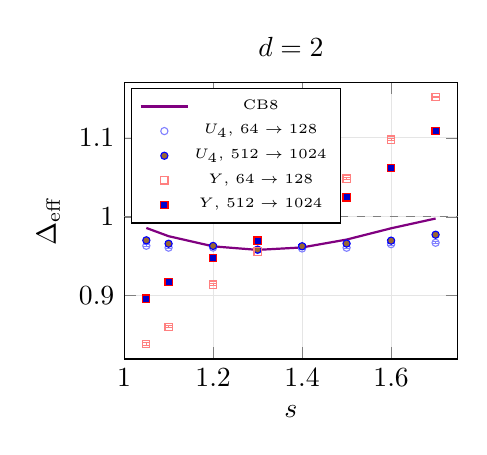
\begin{tikzpicture}
\begin{axis}[width=0.48\textwidth,height=0.42\textwidth,xlabel={$s$},ylabel={$\Delta_{\rm eff}$},title={$d=2$},xmin=1.0,xmax=1.75,ymin=0.82,ymax=1.17,
 legend style={font=\tiny,at={(0.02,0.98)},anchor=north west},grid=major,grid style={gray!20}]
\addplot[dashed,gray,forget plot] coordinates {(1.0,1) (1.75,1)};
\addplot[thick,violet] coordinates {(1.05,0.98584) (1.1,0.97543) (1.2,0.96257) (1.3,0.95810) (1.4,0.96118) (1.5,0.97114) (1.6,0.98542) (1.7,0.99780)};
\addlegendentry{CB8}
\addplot+[only marks,mark=o,mark size=1.3pt,blue!50,error bars/.cd,y dir=both,y explicit] coordinates {(1.05,0.9633) +- (0,0.0013) (1.1,0.9609) +- (0,0.0014) (1.2,0.9610) +- (0,0.0012) (1.3,0.9581) +- (0,0.0012) (1.4,0.9599) +- (0,0.0012) (1.5,0.9608) +- (0,0.0012) (1.6,0.9653) +- (0,0.0012) (1.7,0.9671) +- (0,0.0011)};
\addlegendentry{$U_4$, $64\rightarrow 128$}
\addplot+[only marks,mark=*,mark size=1.3pt,blue,error bars/.cd,y dir=both,y explicit] coordinates {(1.05,0.9702) +- (0,0.0025) (1.1,0.9659) +- (0,0.0023) (1.2,0.9631) +- (0,0.0022) (1.3,0.9584) +- (0,0.0020) (1.4,0.9627) +- (0,0.0020) (1.5,0.9661) +- (0,0.0018) (1.6,0.9698) +- (0,0.0018) (1.7,0.9773) +- (0,0.0017)};
\addlegendentry{$U_4$, $512\rightarrow 1024$}
\addplot+[only marks,mark=square,mark size=1.3pt,red!50,error bars/.cd,y dir=both,y explicit] coordinates {(1.05,0.8390) +- (0,0.0014) (1.1,0.8608) +- (0,0.0015) (1.2,0.9142) +- (0,0.0013) (1.3,0.9561) +- (0,0.0012) (1.4,1.0024) +- (0,0.0012) (1.5,1.0484) +- (0,0.0011) (1.6,1.0977) +- (0,0.0011) (1.7,1.1516) +- (0,0.0010)};
\addlegendentry{$Y$, $64\rightarrow 128$}
\addplot+[only marks,mark=square*,mark size=1.3pt,red,error bars/.cd,y dir=both,y explicit] coordinates {(1.05,0.8964) +- (0,0.0023) (1.1,0.9172) +- (0,0.0023) (1.2,0.9478) +- (0,0.0022) (1.3,0.9698) +- (0,0.0020) (1.4,0.9977) +- (0,0.0019) (1.5,1.0245) +- (0,0.0017) (1.6,1.0620) +- (0,0.0015) (1.7,1.1088) +- (0,0.0014)};
\addlegendentry{$Y$, $512\rightarrow 1024$}
\end{axis}
\end{tikzpicture}\hfill
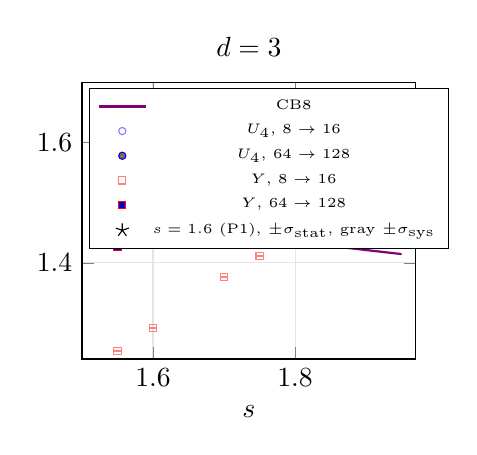
\begin{tikzpicture}
\begin{axis}[width=0.48\textwidth,height=0.42\textwidth,xlabel={$s$},title={$d=3$},xmin=1.5,xmax=1.97,ymin=1.24,ymax=1.70,
 legend style={font=\tiny,at={(0.02,0.98)},anchor=north west},grid=major,grid style={gray!20}]
\addplot[thick,violet] coordinates {(1.55,1.48488) (1.6,1.47214) (1.7,1.45154) (1.75,1.44299) (1.8,1.43524) (1.85,1.42807) (1.9,1.42123) (1.95,1.41449)};
\addlegendentry{CB8}
\addplot+[only marks,mark=o,mark size=1.3pt,blue!50,error bars/.cd,y dir=both,y explicit] coordinates {(1.55,1.4427) +- (0,0.0011) (1.6,1.4398) +- (0,0.0011) (1.7,1.4411) +- (0,0.0011) (1.75,1.4377) +- (0,0.0011) (1.8,1.4372) +- (0,0.0011) (1.85,1.4364) +- (0,0.0011) (1.9,1.4370) +- (0,0.0010) (1.95,1.4320) +- (0,0.0011)};
\addlegendentry{$U_4$, $8\rightarrow 16$}
\addplot+[only marks,mark=*,mark size=1.3pt,blue,error bars/.cd,y dir=both,y explicit] coordinates {(1.55,1.4729) +- (0,0.0030) (1.6,1.4715) +- (0,0.0031) (1.7,1.4650) +- (0,0.0029) (1.75,1.4615) +- (0,0.0027) (1.8,1.4515) +- (0,0.0027) (1.85,1.4569) +- (0,0.0027) (1.9,1.4511) +- (0,0.0026) (1.95,1.4493) +- (0,0.0028)};
\addlegendentry{$U_4$, $64\rightarrow 128$}
\addplot+[only marks,mark=square,mark size=1.3pt,red!50,error bars/.cd,y dir=both,y explicit] coordinates {(1.55,1.2535) +- (0,0.0012) (1.6,1.2914) +- (0,0.0013) (1.7,1.3761) +- (0,0.0012) (1.75,1.4115) +- (0,0.0012) (1.8,1.4513) +- (0,0.0012) (1.85,1.4929) +- (0,0.0012) (1.9,1.5325) +- (0,0.0012) (1.95,1.5694) +- (0,0.0011)};
\addlegendentry{$Y$, $8\rightarrow 16$}
\addplot+[only marks,mark=square*,mark size=1.3pt,red,error bars/.cd,y dir=both,y explicit] coordinates {(1.55,1.4269) +- (0,0.0030) (1.6,1.4628) +- (0,0.0030) (1.7,1.5263) +- (0,0.0029) (1.75,1.5596) +- (0,0.0027) (1.8,1.5818) +- (0,0.0027) (1.85,1.6221) +- (0,0.0027) (1.9,1.6488) +- (0,0.0025) (1.95,1.6790) +- (0,0.0027)};
\addlegendentry{$Y$, $64\rightarrow 128$}
\addplot+[only marks,mark=none,draw=none,forget plot,error bars/.cd,y dir=both,y explicit,error bar style={line width=3pt,gray!45},error mark=none] coordinates {(1.6,1.47314) +- (0,0.00230)};
\addplot+[only marks,mark=star,mark size=2.5pt,black,error bars/.cd,y dir=both,y explicit] coordinates {(1.6,1.47314) +- (0,0.00118)};
\addlegendentry{$s=1.6$ (P1), $\pm\sigma_{\rm stat}$, gray $\pm\sigma_{\rm sys}$}
\end{axis}
\end{tikzpicture}
\caption{Effective dimensions at the smallest and the largest doubling pair, with the resummed $\varepsilon$ expansion (CB8). Left, $d=2$
(dashed: $\De=1$ at both ends of the window). Right, $d=3$; the star is the value at $s=1.6$ that passed the protocol under P1, with $\sstat$
(bar) and $\ssys$ (gray band) shown separately. At the largest pair the $Y$ points (red) and the $U_4$ points (blue) agree in the middle of the
window and differ near its ends. In $d=2$ the difference shrinks as $L$ doubles at every coupling; in $d=3$ it shrinks at $s=1.55$ and 1.6 and
grows at $s\ge1.7$.}\label{mc:fig:23}
\end{figure}

\clearpage
% =====================================================================================================================
\section{Synthesis}\label{mc:sec:synthesis}
\begin{enumerate}[1.]
\item In $d=1$ nine couplings pass the protocol, with $\sstat=(2$--$5.5)\times10^{-4}$; they differ from the resummed $\varepsilon$ expansion
 by $-0.0024$ to $+0.0032$. $\ssys$ is a sensitivity scale. The audit supports the values at 0.1, 0.1375 and 0.1727335, which are stable under
 stronger size cuts. It flags 0.025 (a model outside the family) and 0.175 and 0.225 (stronger size cuts). The labels at 0.1625 and 0.1727335
 are platform-sensitive; two quoted fits have $P_{\chi^2}\approx5\times10^{-5}$; for $\Ds\ge0.0875$ the
 global fits lie above the crossing extrapolations by a common $0.0010(3)$.
\item In $d=2,3$ the finite-size data are precise ($\sigma(\Deff^{U_4})\approx0.0017$--$0.0031$ at the largest pair) and the bottleneck is the
 extrapolation: four doubling pairs over a factor 16 in $L$ do not determine the correction sector, especially near the ends of the window,
 where the expected correction exponents are below the grid floor. More statistics at the same sizes would sharpen, not resolve, this.
\item One 3D value passes, at $s=1.6$, under the post hoc amendment P1, and agrees with the expansion.
\item With a fitted correction exponent, a bootstrap at fixed exponent under-covers badly for single series; re-profiling the exponent in every
 draw restores coverage, conditionally on the extrapolation model.
\item The published equilibrium Monte Carlo values agree with ours within about two of their errors (in $d=1$ computed with $\sstat$, not
 $\ssys$); quantitative statements should use $\sstat$ and $\ssys$ separately.
\end{enumerate}

% =====================================================================================================================
\section{Open issues and next steps}\label{mc:sec:open}
\begin{enumerate}[1.]
\item \textbf{1D uncertainties:} a pre-declared broader model family (a $U$ background, two correction powers, stronger size cuts), asymmetric
 model ranges, a converged $\omega'$ minimization and a ladder rule that does not stop on a flagged lower-degree fit, followed by a full rerun
 of the selection. Priority couplings: 0.025, 0.175, 0.225. A label-stability study (seeds, ladder rules, grid steps) belongs here.
\item \textbf{1D goodness of fit:} a $p$-value gate or a scale factor instead of $\chi^2/{\rm dof}\le1.5$.
\item \textbf{Near the Gaussian end} in all dimensions: a crossover form $D(L)=1+CL^{-\varepsilon}$ with free amplitudes, or $\omega$ fixed at its
 perturbative value, instead of a grid with floor 0.2.
\item \textbf{Near the short-range end} ($d=2,3$): the crossover flow of section~\ref{mc:sec:model} as a model for the $Y$--$U_4$ split; measuring
 the effective $\eta$ at the crossings would test it.
\item \textbf{Larger lattices}, only where they answer a question: 2D $L=2048$ at $s=1.2$ and $1.5$; 3D $L=256$ at $s=1.9$ (about
 $1.5\times10^4$ core-hours), to tell an ordinary correction power from the slow short-range crossover by whether the $Y$--$U_4$ split grows or
 shrinks at $128\to256$.
\item \textbf{Critical inverse temperatures:} extrapolate $\beta_\times(L)$ with errors from the existing bootstrap draws.
\item \textbf{Uninspected code:} the last fixes to the P1 implementation and to the 1D tooling that records which campaigns make up each
 coupling (the registry).
\end{enumerate}

% =====================================================================================================================
\section{Reproduction}\label{mc:sec:repro}
\sloppy
\subsection{The released folder}
This note is released with the code and the records in the \path{MC/} folder of the public repository (code under the MIT license, everything else under CC~BY~4.0, except the delivered 2D/3D
engine, which keeps its own MIT license); paths
below are relative to \path{MC/}. \code{README.md} states what is computed and its status; \code{REPRODUCE.md} gives the steps in order
(environment, tests, replay, smoke run, production, merge, checks) and the decisions that a reproduction must not take on its own.
\begin{description}[leftmargin=1.2em,font=\ttfamily]
\item[code/1d/] 1D engines (\path{src/}, \path{src_1d/}), campaign tools, analysis (\code{analyze.py}, \code{merge\_summaries.py},
 \code{equilibration.py}, \code{union\_check.py}), fitting (\code{select\_model\_v3.py}, \code{select\_model.py}, \code{fit\_fss.py},
 \code{quotients.py}), the 20-point report (\code{scan\_v3\_report.py}) and tests.
\item[code/2d3d\_engine/] the $d=2,3$ sampler and its analysis (\code{pack\_histograms.py}, \code{multihist.py},
 \code{precision\_analysis.py}) and tests.
\item[code/2d/, code/3d/] the evaluators (frozen rule and P1) and planners.
\item[code/reanalysis\_p1/] \code{calibrate\_p1.py} and the tests of amendment P1.
\item[code/package\_tools/] workspace assembly, the output comparison and the generator of this note's tables.
\item[protocols/] the analysis protocols, the amendment and their history (\code{PROTOCOL\_HISTORY.md}; appendix~\ref{mc:app:hashes}).
\item[data/] the merged production records (\code{DATA.md}): 1D per-coupling selected fit runs, snapshot manifests, completion evidence and
 registries; 2D/3D analysis records at three block sizes, campaign manifests, histogram indices and the pinned production evaluations;
 reference values (\path{data/reference/}).
\item[results/] expected outputs: the P1 evaluations, the P1 calibration (an input of the P1 evaluation), the 1D tables and figures, and the
 cited diagnostics (cross-platform refits, the robust-ladder study with its modified fitter, the cross-check study).
\item[slurm/] submission templates with placeholders for account, partition and paths.
\end{description}
The evaluators bind themselves, the calibration script and the protocols by SHA-256 and locate their inputs relative to the layout they ran in;
the make targets therefore assemble that layout in a hidden \path{.work/} directory (code copied byte for byte, data linked), so every check
passes without any edit. The production records are released byte-identical, with one exception: 25 records (from the $d=1$ couplings
$\Ds=0.225$ and $0.2375$, and the P1 calibration) named a personal machine and were scrubbed after the results; only host labels, a home
directory and file names were replaced, and the hashes inside them re-pinned. \code{RE-PINNED.json} lists their original and published
SHA-256; the comparison maps one to the other. The other records name the cluster paths, user and compute nodes on which they were written.

\subsection{How to run}
Requirements: Python with NumPy and SciPy (production: Python 3.8.5, NumPy 1.19.2, SciPy 1.5.2 for the 1D fits; Python 3.8.8, NumPy 1.20.1
for the P1 calibration and evaluations; also tested with 3.12.3, 1.26.4, 1.11.4), pytest, matplotlib, a C++17 compiler and GNU make for the
engines, and pdflatex for this note.
\begin{longtable}{@{}>{\raggedright\arraybackslash}p{2.6cm}>{\raggedright\arraybackslash}p{6.5cm}>{\raggedright\arraybackslash}p{6.5cm}@{}}\toprule
target & runs & reproduces \\\midrule\endhead
\code{test} & builds the engines; 1D protocol tests; the tests of amendment P1 & the verification claims of section~\ref{mc:sec:p1} \\
\code{replay} & everything below that needs only the records in git, then the comparison with \path{results/} & every table and figure of
 this note except those needing \code{fetch-data} \\
\code{smoke} & engine validation: a tiny 1D campaign with bitwise resume; exact enumeration and bitwise restart in $d=2,3$ & that the samplers are
 exact on small systems \\
\code{eval-fixed}, \code{eval-p1} & the 2D/3D evaluators under the frozen rule and under P1 & tables~\ref{mc:tab:2ddec}, \ref{mc:tab:3ddec};
 appendix~\ref{mc:app:series} \\
\code{calibration} & \code{calibrate\_p1.py} (1\,780 tasks, $\approx7$~min on 16 cores) & appendix~\ref{mc:app:calib} and the coverage numbers \\
\code{scan1d}, \code{tables1d} & \code{scan\_v3\_report.py}, \code{make\_tables\_and\_figure.py} & tables~\ref{mc:tab:1dfinal}, \ref{mc:tab:1dpairs},
 appendix~\ref{mc:app:pre} \\
\code{refit1d DS=\dots} & \code{select\_model\_v3.py} on the released snapshot of one coupling (6--156~s on 20 cores); needs \code{fetch-data} &
 the fits, crossing series and label of that coupling; section~\ref{mc:sec:1drefit} \\
\code{note-tables} & \code{make\_note\_tables.py --check} & every generated line of this note \\
\code{fetch-data}, \code{build}, \code{note} & downloads the data not in git; the engines; this note (three passes) & -- \\\bottomrule
\end{longtable}
\addtocounter{table}{-1}

\subsection{Verified reproduction}
On 7 October 2026 the folder, in its layout before the public release, was assembled afresh on the workstation and every target was run
through Slurm. The engines built and all tests passed. The 2D/3D evaluations reproduced the pinned production evaluations in all per-point
fields (maximum relative difference $3\times10^{-11}$), and so did the P1 evaluations and the calibration regenerated from scratch
($2\times10^{-11}$). The 1D cross-check study, the 20-point 1D table and the 1D report tables were reproduced, and the 1D fitting stage
reproduced 18 of 20 labels and all values (section~\ref{mc:sec:1drefit}). The comparison reports those two labels as known to be platform-sensitive.

On 13 October 2026 the folder in its public layout was exported afresh and tested through Slurm on two platforms: a personal desktop (Python 3.12.3,
NumPy 1.26.4, SciPy 1.11.4) and an Expanse debug node (Python 3.8.8, NumPy 1.20.1, SciPy 1.6.2, GCC 10.2.0). On both, the engines build, all tests
pass (3.1 and 7.5~min), and \code{make replay} (14 and 43~s) reports 9 checks PASS, none FAIL and one NOT RUN, the regenerated calibration, which
needs \code{make calibration}; \code{note-tables} finds all 355 generated lines in this note. The cited 1D refits need \code{fetch-data} and
were not part of this test.

\subsection{What is not in git}
\code{make fetch-data} downloads two archives from the project's Zenodo data record, \href{https://doi.org/10.5281/zenodo.23466766}{doi:10.5281/zenodo.23466766}, and checks their SHA-256 (\code{data/HOSTED.json}).
\code{refit1d} needs the first: the 1D block archives of the selected snapshots (1.43~GB) and their merged summaries (25~MB). The second
holds the per-degree fits of the selected runs (140~MB), for inspection; no target needs them. Regenerating the records from scratch needs
the raw data: the 1D trajectories (0.655~TB) and the 2D/3D trees of chains, packed histograms and analyses (257.5 and 237.2~GiB). They are
not hosted; they are available from the author on request. The records were produced from
these by \code{analyze.py} and \code{merge\_summaries.py} ($d=1$) and by \code{pack\_histograms.py} and \code{precision\_analysis.py} ($d=2,3$).

% =====================================================================================================================
\appendix
\section{\texorpdfstring{$d=1$ frozen window parameters}{d=1 frozen window parameters}}\label{mc:app:pre}
The window parameters $(\beta_c^{\rm pre},\De^{\rm pre})$ were frozen per coupling from earlier fits of the stage A/B data
(section~\ref{mc:sec:rules}); $h'$ is the N2 temperature half-width.
\begin{table}[htbp]\centering\small
\caption{Frozen $(\beta_c^{\rm pre},\De^{\rm pre})$ per coupling and N2 half-widths $h'$ (units $10^{-4}$) at $N=2^{16}$ and $2^{19}$.}
\begin{tabular}{@{}lllllll@{}}\toprule
$\Ds$ & $s$ & $\beta_c^{\rm pre}$ & $\De^{\rm pre}$ & $h'(2^{16})$ & $h'(2^{19})$ & N2 \\\midrule
0.0125 & 0.975 & 0.596534 & 0.7910 & 14.67 & 9.50 & no \\
0.025 & 0.95 & 0.558588 & 0.7179 & 10.83 & 6.02 & no \\
0.0375 & 0.925 & 0.527150 & 0.6575 & 8.42 & 4.13 & no \\
0.05 & 0.9 & 0.499660 & 0.6234 & 7.31 & 3.34 & no \\
0.0625 & 0.875 & 0.474858 & 0.5898 & 6.35 & 2.71 & yes \\
0.075 & 0.85 & 0.452099 & 0.5674 & 5.79 & 2.35 & no \\
0.0875 & 0.825 & 0.430939 & 0.5462 & 5.30 & 2.06 & no \\
0.1 & 0.8 & 0.411095 & 0.5292 & 4.94 & 1.86 & yes \\
0.1125 & 0.775 & 0.392343 & 0.5191 & 4.74 & 1.74 & yes \\
0.125 & 0.75 & 0.374529 & 0.5074 & 4.51 & 1.62 & yes \\
0.1375 & 0.725 & 0.357528 & 0.4991 & 4.36 & 1.54 & yes \\
0.15 & 0.7 & 0.341247 & 0.4930 & 4.25 & 1.48 & yes \\
0.1625 & 0.675 & 0.325592 & 0.4863 & 4.13 & 1.42 & yes \\
0.1727335 & 0.654533 & 0.313200 & 0.4845 & 4.10 & 1.40 & yes \\
0.175 & 0.65 & 0.310504 & 0.4843 & 4.10 & 1.40 & yes \\
0.1875 & 0.625 & 0.295925 & 0.4814 & 4.05 & 1.38 & yes \\
0.2 & 0.6 & 0.281805 & 0.4808 & 4.04 & 1.37 & yes \\
0.2125 & 0.575 & 0.268101 & 0.4775 & 3.98 & 1.34 & yes \\
0.225 & 0.55 & 0.254785 & 0.4802 & 4.03 & 1.37 & yes \\
0.2375 & 0.525 & 0.241813 & 0.4809 & 4.04 & 1.37 & yes \\
\bottomrule\end{tabular}
\end{table}

\section{\texorpdfstring{$d=2,3$ extrapolation series}{d=2,3 extrapolation series}}\label{mc:app:series}
For every coupling and series: $\De$ of the extrapolation, $\omega'$ and its $\Delta\chi^2\le1$ interval, $\chi^2$/dof, $\sigma$ with $\omega'$
fixed and profiled per draw (P1), eligibility.
{\scriptsize
\begin{longtable}{@{}llllllll@{}}
\caption{$d=2$ series (P1 evaluation; central values identical to the frozen evaluation).}\\\toprule
$s$ & series & $\De$ & $\omega'$ [interval] & $\chi^2$/dof & $\sigma$ fixed & $\sigma$ profiled & eligible \\\midrule\endfirsthead
\multicolumn{8}{@{}l}{\emph{$d=2$ series, continued}}\\\toprule
$s$ & series & $\De$ & $\omega'$ [interval] & $\chi^2$/dof & $\sigma$ fixed & $\sigma$ profiled & eligible \\\midrule\endhead
1.05 & U4 & 0.9750 & 0.56 [0.20, 2.00] & 0.51/1 & 0.0020 & 0.0083 & no: $\omega^\prime$ edge \\
 & U6 & 0.9719 & 0.84 [0.20, 2.00] & 0.29/1 & 0.0014 & 0.0080 & no: $\omega^\prime$ edge \\
 & U8 & 0.9700 & 0.96 [0.20, 2.00] & 0.14/1 & 0.0011 & 0.0087 & no: $\omega^\prime$ edge \\
 & Y & 0.9208 & 0.60 [0.43, 0.76] & 0.44/1 & 0.0018 & 0.0177 & yes \\
 & U4+Y & 0.9840 & 0.26 [0.26, 0.27] & 8.33/4 & 0.0037 & 0.0042 & no: $\chi^2$ \\
1.1 & U4 & 0.9670 & 1.17 [0.20, 2.00] & 0.11/1 & 0.0011 & 0.0060 & no: $\omega^\prime$ edge \\
 & U6 & 0.9663 & 1.33 [0.20, 2.00] & 0.10/1 & 0.0010 & 0.0060 & no: $\omega^\prime$ edge \\
 & U8 & 0.9651 & 1.41 [0.39, 2.00] & 0.03/1 & 0.0009 & 0.0067 & no: $\omega^\prime$ edge \\
 & Y & 0.9285 & 0.80 [0.61, 1.00] & 1.10/1 & 0.0015 & 0.0101 & yes \\
 & U4+Y & 0.9720 & 0.35 [0.35, 0.36] & 15.28/4 & 0.0028 & 0.0031 & no: $\chi^2$ \\
1.2 & U4 & 0.9654 & 0.20 [0.20, 2.00] & 3.57/1 & 0.0045 & 0.0043 & no: $\chi^2$ \\
 & U6 & 0.9657 & 0.20 [0.20, 1.44] & 3.66/1 & 0.0044 & 0.0042 & no: $\chi^2$ \\
 & U8 & 0.9686 & 0.20 [0.20, 0.78] & 2.73/1 & 0.0040 & 0.0044 & no: $\chi^2$ \\
 & Y & 0.9806 & 0.34 [0.20, 0.60] & 0.00/1 & 0.0027 & 0.0237 & no: $\omega^\prime$ edge \\
 & U4+Y & 0.9620 & 0.55 [0.53, 0.57] & 5.85/4 & 0.0016 & 0.0018 & yes \\
1.3 & U4 & 0.9595 & 2.00 [0.20, 2.00] & 0.49/1 & 0.0007 & 0.0030 & no: $\omega^\prime$ edge \\
 & U6 & 0.9595 & 2.00 [0.20, 2.00] & 0.56/1 & 0.0007 & 0.0029 & no: $\omega^\prime$ edge \\
 & U8 & 0.9595 & 2.00 [0.20, 2.00] & 0.70/1 & 0.0007 & 0.0036 & no: $\omega^\prime$ edge \\
 & Y & 0.9714 & 2.00 [1.58, 2.00] & 0.72/1 & 0.0007 & 0.0012 & no: $\omega^\prime$ edge \\
 & U4+Y & 0.9832 & 0.20 [0.20, 0.20] & 201.09/4 & 0.0042 & 0.0042 & no: $\chi^2$ \\
1.4 & U4 & 0.9624 & 0.20 [0.20, 2.00] & 2.38/1 & 0.0042 & 0.0035 & no: $\chi^2$ \\
 & U6 & 0.9643 & 0.20 [0.20, 2.00] & 2.30/1 & 0.0041 & 0.0038 & no: $\chi^2$ \\
 & U8 & 0.9689 & 0.20 [0.20, 1.32] & 1.83/1 & 0.0039 & 0.0044 & no: $\omega^\prime$ edge \\
 & Y & 0.9868 & 0.20 [0.20, 0.76] & 1.85/1 & 0.0042 & 0.0051 & no: $\omega^\prime$ edge \\
 & U4+Y & 0.9730 & 0.20 [0.20, 0.20] & 93.97/4 & 0.0040 & 0.0040 & no: $\chi^2$ \\
1.5 & U4 & 0.9759 & 0.20 [0.20, 0.98] & 0.48/1 & 0.0042 & 0.0055 & no: $\omega^\prime$ edge \\
 & U6 & 0.9777 & 0.20 [0.20, 0.92] & 0.46/1 & 0.0041 & 0.0056 & no: $\omega^\prime$ edge \\
 & U8 & 0.9819 & 0.20 [0.20, 0.91] & 0.29/1 & 0.0039 & 0.0064 & no: $\omega^\prime$ edge \\
 & Y & 0.9810 & 0.20 [0.20, 0.27] & 3.15/1 & 0.0038 & 0.0055 & no: $\chi^2$ \\
 & U4+Y & 0.9792 & 0.20 [0.20, 0.20] & 18.48/4 & 0.0038 & 0.0038 & no: $\chi^2$ \\
1.6 & U4 & 0.9799 & 0.20 [0.20, 0.97] & 1.09/1 & 0.0041 & 0.0053 & no: $\omega^\prime$ edge \\
 & U6 & 0.9822 & 0.20 [0.20, 1.10] & 0.59/1 & 0.0041 & 0.0057 & no: $\omega^\prime$ edge \\
 & U8 & 0.9839 & 0.25 [0.20, 1.47] & 0.18/1 & 0.0031 & 0.0063 & no: $\omega^\prime$ edge \\
 & Y & 0.9919 & 0.20 [0.20, 0.23] & 6.34/1 & 0.0035 & 0.0050 & no: $\chi^2$ \\
 & U4+Y & 0.9915 & 0.20 [0.20, 0.20] & 56.29/4 & 0.0035 & 0.0035 & no: $\chi^2$ \\
1.7 & U4 & 0.9984 & 0.20 [0.20, 0.66] & 0.51/1 & 0.0039 & 0.0087 & no: $\omega^\prime$ edge \\
 & U6 & 1.0012 & 0.20 [0.20, 0.75] & 0.50/1 & 0.0038 & 0.0093 & no: $\omega^\prime$ edge \\
 & U8 & 0.9935 & 0.36 [0.20, 0.97] & 0.57/1 & 0.0021 & 0.0097 & no: $\omega^\prime$ edge \\
 & Y & 1.0311 & 0.20 [0.20, 0.23] & 5.82/1 & 0.0034 & 0.0038 & no: $\chi^2$ \\
 & U4+Y & 1.0260 & 0.20 [0.20, 0.20] & 225.45/4 & 0.0034 & 0.0034 & no: $\chi^2$ \\
\bottomrule
\end{longtable}
\begin{longtable}{@{}llllllll@{}}
\caption{$d=3$ series (P1 evaluation).}\\\toprule
$s$ & series & $\De$ & $\omega'$ [interval] & $\chi^2$/dof & $\sigma$ fixed & $\sigma$ profiled & eligible \\\midrule\endfirsthead
\multicolumn{8}{@{}l}{\emph{$d=3$ series, continued}}\\\toprule
$s$ & series & $\De$ & $\omega'$ [interval] & $\chi^2$/dof & $\sigma$ fixed & $\sigma$ profiled & eligible \\\midrule\endhead
1.55 & U4 & 1.4812 & 0.75 [0.44, 1.11] & 0.00/1 & 0.0017 & 0.0163 & yes \\
 & U6 & 1.4809 & 0.79 [0.51, 1.10] & 0.02/1 & 0.0016 & 0.0139 & yes \\
 & U8 & 1.4790 & 0.92 [0.71, 1.15] & 0.02/1 & 0.0013 & 0.0075 & yes \\
 & Y & 1.4486 & 1.05 [0.99, 1.11] & 0.02/1 & 0.0014 & 0.0058 & yes \\
 & U4+Y & 1.4789 & 0.78 [0.78, 0.79] & 44.76/4 & 0.0015 & 0.0017 & no: $\chi^2$ \\
1.6 & U4 & 1.4726 & 1.29 [0.93, 1.74] & 0.28/1 & 0.0011 & 0.0072 & yes \\
 & U6 & 1.4720 & 1.35 [1.02, 1.75] & 0.29/1 & 0.0011 & 0.0062 & yes \\
 & U8 & 1.4709 & 1.39 [1.14, 1.67] & 0.37/1 & 0.0010 & 0.0040 & yes \\
 & Y & 1.4750 & 1.21 [1.14, 1.28] & 1.51/1 & 0.0013 & 0.0048 & yes \\
 & U4+Y & 1.4731 & 1.24 [1.23, 1.25] & 2.38/4 & 0.0011 & 0.0012 & yes \\
1.7 & U4 & 1.4737 & 0.66 [0.28, 1.09] & 0.07/1 & 0.0017 & 0.0168 & yes \\
 & U6 & 1.4724 & 0.74 [0.40, 1.14] & 0.03/1 & 0.0015 & 0.0157 & yes \\
 & U8 & 1.4700 & 0.92 [0.67, 1.20] & 0.02/1 & 0.0012 & 0.0082 & yes \\
 & Y & 1.5414 & 1.16 [1.08, 1.24] & 0.02/1 & 0.0012 & 0.0050 & yes \\
 & U4+Y & 1.4862 & 2.00 [2.00, 2.00] & 7052.05/4 & 0.0008 & 0.0008 & no: $\chi^2$ \\
1.75 & U4 & 1.4587 & 1.69 [1.03, 2.00] & 2.89/1 & 0.0009 & 0.0062 & no: $\chi^2$ \\
 & U6 & 1.4583 & 1.75 [1.17, 2.00] & 3.47/1 & 0.0009 & 0.0047 & no: $\chi^2$ \\
 & U8 & 1.4581 & 1.65 [1.28, 2.00] & 3.84/1 & 0.0009 & 0.0033 & no: $\chi^2$ \\
 & Y & 1.5654 & 1.35 [1.27, 1.44] & 4.12/1 & 0.0011 & 0.0041 & no: $\chi^2$ \\
 & U4+Y & 1.6546 & 0.20 [0.20, 0.20] & 10550.66/4 & 0.0050 & 0.0050 & no: $\chi^2$ \\
1.8 & U4 & 1.4553 & 2.00 [1.53, 2.00] & 2.02/1 & 0.0009 & 0.0016 & no: $\chi^2$ \\
 & U6 & 1.4551 & 2.00 [1.59, 2.00] & 2.37/1 & 0.0009 & 0.0015 & no: $\chi^2$ \\
 & U8 & 1.4542 & 2.00 [1.62, 2.00] & 2.76/1 & 0.0008 & 0.0016 & no: $\chi^2$ \\
 & Y & 1.5918 & 1.55 [1.46, 1.64] & 5.46/1 & 0.0010 & 0.0030 & no: $\chi^2$ \\
 & U4+Y & 1.6897 & 0.20 [0.20, 0.20] & 11986.04/4 & 0.0050 & 0.0050 & no: $\chi^2$ \\
1.85 & U4 & 1.4583 & 1.20 [0.71, 1.85] & 0.04/1 & 0.0010 & 0.0075 & yes \\
 & U6 & 1.4589 & 1.17 [0.76, 1.68] & 0.01/1 & 0.0010 & 0.0062 & yes \\
 & U8 & 1.4592 & 1.19 [0.92, 1.50] & 0.00/1 & 0.0009 & 0.0045 & yes \\
 & Y & 1.6306 & 1.39 [1.30, 1.48] & 0.20/1 & 0.0010 & 0.0034 & yes \\
 & U4+Y & 1.6685 & 0.20 [0.20, 0.20] & 14600.83/4 & 0.0045 & 0.0045 & no: $\chi^2$ \\
1.9 & U4 & 1.4545 & 1.15 [0.63, 1.87] & 0.89/1 & 0.0011 & 0.0072 & yes \\
 & U6 & 1.4544 & 1.23 [0.78, 1.81] & 0.83/1 & 0.0011 & 0.0057 & yes \\
 & U8 & 1.4546 & 1.29 [1.00, 1.64] & 0.83/1 & 0.0009 & 0.0034 & yes \\
 & Y & 1.6563 & 1.63 [1.53, 1.74] & 2.91/1 & 0.0009 & 0.0026 & no: $\chi^2$ \\
 & U4+Y & 1.6896 & 0.20 [0.20, 0.20] & 13764.62/4 & 0.0046 & 0.0046 & no: $\chi^2$ \\
1.95 & U4 & 1.4500 & 2.00 [1.56, 2.00] & 0.49/1 & 0.0008 & 0.0014 & no: $\omega^\prime$ edge \\
 & U6 & 1.4498 & 2.00 [1.61, 2.00] & 0.39/1 & 0.0008 & 0.0013 & no: $\omega^\prime$ edge \\
 & U8 & 1.4490 & 2.00 [1.64, 2.00] & 0.05/1 & 0.0007 & 0.0014 & no: $\omega^\prime$ edge \\
 & Y & 1.6827 & 2.00 [1.88, 2.00] & 0.70/1 & 0.0008 & 0.0014 & no: $\omega^\prime$ edge \\
 & U4+Y & 1.6808 & 0.20 [0.20, 0.20] & 19130.26/4 & 0.0048 & 0.0048 & no: $\chi^2$ \\
\bottomrule
\end{longtable}}

\section{P1 calibration strata}\label{mc:app:calib}
Each cell: eligible synthetic fits: profiled $1\sigma$/$2\sigma$ coverage (fixed-$\omega'$ $1\sigma$ coverage), status (P pass, F fail, nc not
calibrated, i.e.\ fewer than 200 eligible fits). Last column: synthetic sets with $U_4$ and $Y$ both eligible: false-failure rate of the profiled
cross-check (fixed), status.
\begin{sidewaystable}\centering\footnotesize\setlength{\tabcolsep}{4pt}
\caption{Calibration strata of amendment P1 (top $d=2$, bottom $d=3$).}\label{mc:tab:calib}
\begin{tabular}{@{}lllllll@{}}\toprule
$d=2$, $s$ & $U_4$ & $U_6$ & $U_8$ & $Y$ & U4+Y & cross-check \\\midrule
1.05 & 0 nc & 0 nc & 19: 1.00/1.00 (0.16) nc & 1493: 0.83/0.95 (0.12) P & 1812: 0.68/0.95 (0.59) P & 0 nc \\
1.1 & 0 nc & 1: 1.00/1.00 (0.00) nc & 8: 1.00/1.00 (0.00) nc & 1672: 0.83/0.95 (0.15) P & 1799: 0.69/0.96 (0.63) P & 0 nc \\
1.2 & 0 nc & 0 nc & 0 nc & 490: 0.33/0.82 (0.00) F & 1805: 0.67/0.95 (0.62) P & 0 nc \\
1.3 & 0 nc & 0 nc & 0 nc & 196: 1.00/1.00 (0.01) nc & 194: 0.10/0.44 (0.01) nc & 0 nc \\
1.4 & 0 nc & 0 nc & 0 nc & 0 nc & 15: 0.87/1.00 (0.87) nc & 0 nc \\
1.5 & 1: 0.00/1.00 (0.00) nc & 0 nc & 3: 0.00/1.00 (0.00) nc & 234: 0.00/0.02 (0.00) F & 0 nc & 0 nc \\
1.6 & 0 nc & 0 nc & 2: 1.00/1.00 (0.00) nc & 222: 0.00/0.03 (0.00) F & 0 nc & 0 nc \\
1.7 & 62: 0.00/0.13 (0.00) nc & 69: 0.00/0.10 (0.00) nc & 144: 0.40/1.00 (0.00) nc & 214: 0.00/0.04 (0.00) F & 0 nc & 0 nc \\
\bottomrule\end{tabular}\\[12pt]
\begin{tabular}{@{}lllllll@{}}\toprule
$d=3$, $s$ & $U_4$ & $U_6$ & $U_8$ & $Y$ & U4+Y & cross-check \\\midrule
1.55 & 1225: 0.86/0.98 (0.19) P & 1396: 0.87/0.97 (0.17) P & 1666: 0.83/0.96 (0.17) P & 1663: 0.69/0.95 (0.20) P & 1771: 0.68/0.95 (0.63) P & 1062: 0.007 (0.69) P \\
1.6 & 1122: 0.99/1.00 (0.31) P & 1165: 0.98/1.00 (0.31) P & 1378: 0.88/1.00 (0.29) P & 1668: 0.69/0.95 (0.21) P & 1786: 0.70/0.95 (0.67) P & 1076: 0.007 (0.61) P \\
1.7 & 825: 0.92/1.00 (0.20) P & 1107: 0.90/1.00 (0.19) P & 1603: 0.89/0.97 (0.16) P & 1671: 0.69/0.96 (0.18) P & 218: 0.29/0.89 (0.06) F & 108: 0.000 (0.43) nc \\
1.75 & 428: 1.00/1.00 (0.01) P & 420: 0.98/1.00 (0.02) P & 684: 0.81/1.00 (0.15) P & 1710: 0.69/0.95 (0.23) P & 47: 0.00/0.09 (0.00) nc & 108: 0.000 (0.76) nc \\
1.8 & 228: 0.99/1.00 (0.00) P & 246: 0.95/1.00 (0.01) P & 229: 0.41/1.00 (0.02) F & 1645: 0.70/0.96 (0.26) P & 1: 0.00/0.00 (0.00) nc & 79: 0.000 (0.87) nc \\
1.85 & 717: 1.00/1.00 (0.32) P & 996: 1.00/1.00 (0.27) P & 1483: 0.93/1.00 (0.23) P & 1695: 0.70/0.96 (0.22) P & 0 nc & 93: 0.108 (1.00) nc \\
1.9 & 531: 1.00/1.00 (0.38) P & 764: 1.00/1.00 (0.32) P & 1289: 0.98/1.00 (0.32) P & 1663: 0.71/0.97 (0.29) P & 0 nc & 92: 0.326 (1.00) nc \\
1.95 & 216: 1.00/1.00 (0.00) P & 237: 0.99/1.00 (0.01) P & 254: 0.47/1.00 (0.00) F & 182: 0.15/0.84 (0.01) nc & 0 nc & 39: 0.641 (1.00) nc \\
\bottomrule\end{tabular}
\end{sidewaystable}

\section{Protocol identities and history}\label{mc:app:hashes}
SHA-256 prefixes of the files whose identity matters (full hashes in \path{protocols/} and in the records):
FIT\_MODEL\_V3 rev.\ 14 \code{f05b835b}; FIT\_MODEL\_2D rev.\ 5 \code{4d2efc63}; FIT\_MODEL\_3D rev.\ 5 (approved) \code{b4ccf436} and rev.\ 7
(production) \code{682858f0}; amendment P1 rev.\ 4 \code{2a18c0ae}; frozen evaluators \code{evaluate\_2d.py} rev.\ 5 \code{0fe221e8} and
\code{evaluate\_3d.py} rev.\ 1 \code{6bd35d7a}; P1 evaluators rev.\ 6 \code{3c3e35fc} and rev.\ 2 \code{d635c917}; \code{calibrate\_p1.py}
\code{d94b59f2}; calibration \code{CALIBRATION.json} \code{897142c1}; production evaluations \code{fbfc0ef9} (2D) and \code{ae9cf237} (3D); P1
evaluations \code{f9272978} (2D) and \code{b3fd6364} (3D). Records that named a personal machine were scrubbed after the results and
re-pinned; \code{RE-PINNED.json} lists the original and published hashes (for example \code{CALIBRATION.json}: original \code{897142c1},
published \code{1afae79a}, which differ only in a host label). The prefixes above are the original ones.

The file \code{FIT\_MODEL\_3D.md.sha256} records the hash at approval (revision 5), while the evaluators pin revision 7. The approved revision 5,
revision 6 and the difference to revision 7 are released (\path{protocols/FIT_MODEL_3D_rev5_approved.md}, \dots); the two differ only in
the preflight condition and the gate records described in section~\ref{mc:sec:rules}. \code{FIT\_MODEL\_2D.md} has no approval hash because it
was never approved. The status lines inside the protocol files (for example ``UNREVIEWED'') predate their reviews; \code{PROTOCOL\_HISTORY.md}
gives the review status of each revision.

\section{\texorpdfstring{The pre-campaign $\varepsilon$-expansion reference}{The pre-campaign epsilon-expansion reference}}\label{mc:app:eps}
Before the campaign, six-loop reference values were computed and frozen with the records
(\path{data/1d/reference/published_and_epsilon_reference.csv}); they played no role in any selection. ``GFF only'' (generalized free field, i.e.\ the Gaussian end) is the ordinary
Borel--Pad\'e [4/2] of the six-loop series about the Gaussian end; ``endpoint assisted'' is the Borel--Pad\'e [3/3] of the remainder $R$ in
$\De=1-\sqrt{1-e}+(1-e)/8+(1-e)^{3/2}R(e)$, $e=\varepsilon$, which builds in the $s\to1$ endpoint behavior. They used an older value of the six-loop coefficient of the $d=1$ series, $C_6(1)=14331.8\pm0.5$; the final value, 14331.687, is given in the
accompanying article~\cite{mc:Zheng:2026ai}. They are superseded by the eight-loop values of section~\ref{mc:sec:theory1d}. The same
file contains columns from an exploratory pre-campaign analysis (\code{new\_MC\_conditional\_fit} and related), which are also superseded.
\begin{table}[htbp]\centering\small
\caption{$d=1$: the frozen six-loop reference values against the Monte Carlo result.}\label{mc:tab:eps}
\begin{tabular}{@{}lllll@{}}\toprule
$\Ds$ & $\varepsilon=1-4\Ds$ & six-loop, GFF only & six-loop, endpoint assisted & MC (this work) \\\midrule
0.025 & 0.900 & 0.5703 & 0.7109 & 0.71115(49)(959) \\
0.05 & 0.800 & 0.5459 & 0.6182 & 0.61987(55)(220) \\
0.0625 & 0.750 & 0.5351 & 0.5871 & 0.59003(35)(150) \\
0.1 & 0.600 & 0.5085 & 0.5262 & 0.53248(20)(242) \\
0.15 & 0.400 & 0.4871 & 0.4897 & 0.49325(41)(306) \\
0.1727335 & 0.309 & 0.4829 & 0.4836 & 0.48368(52)(78) \\
0.2 & 0.200 & 0.4828 & 0.4829 & largest pair \\
\bottomrule\end{tabular}
\end{table}

\section{Glossary}
\begin{description}[leftmargin=1.2em]
\item[$\Ds$, $\De$] dimensions of the spin and of the leading $\mathbb Z_2$-even scalar; $1/\nu=d-\De$.
\item[$\Deff^Q$] finite-size effective dimension from a doubling pair at the $U_4$ crossing, eq.~\eqref{mc:eq:Deff}.
\item[$\sstat$, $\ssys$, $\sigma_D$] bootstrap error of the quoted value; half-range over the model family (a sensitivity scale, not a standard
 deviation); error of a paired difference.
\item[$p$, $\ktau$] polynomial degree of the scaling function; order of the thermal field ($d=1$ fits).
\item[$P_{\chi^2}$] $\chi^2$ probability of a fit.
\item[coupling] one value of $s$ (or $\Ds$) of the simulation grid; inverse temperatures are $\beta$.
\item[window, variant, configuration] in $d=1$: the range $|x|\le x_{\max}$ of the scaling variable kept in a fit; the form of the correction
 terms (\code{leading}, \code{second}, \code{background}, \code{log}); one choice of window, variant, $N_{\min}$ and $\ktau$
 (section~\ref{mc:sec:v3}).
\item[gate] a pass/fail condition on a fit or series.
\item[quotable, eligible] a $d=1$ fit that passes its gates; a $d=2,3$ extrapolation series that passes its gates.
\item[series] $\Deff^Q(L)$ over the doubling pairs for one $Q$ ($d=2,3$) or one crossing window and degree rule ($d=1$), extrapolated to
 $L\to\infty$.
\item[U4+Y] joint extrapolation of $U_4$ and $Y$ with common $\De$ and $\omega'$.
\item[x-check] cross-check (table~\ref{mc:tab:labels}).
\item[{[$\sigma$]}] label suffix: $\sigma(\Deff^{U_4})$ of the largest pair above the target 0.003.
\item[frozen] fixed before the data in question were analyzed (a protocol, the $d=1$ window parameters); ``the frozen rule'' is the
 $d=2,3$ protocol before amendment P1.
\item[fixed-$\omega'$ / profiled rule] bootstrap at the central $\omega'$ (the frozen rule) / $\omega'$ re-profiled in every draw (amendment P1).
\item[preflight] short runs at the production sizes, before a production, that check rates, autocorrelation times and crossing brackets.
\item[stage 0, A, B; N0, N2, N3] 1D campaigns (table~\ref{mc:tab:campaigns}); N3, an extension to $N=2^{20}$, was not run.
\item[N1] the first evaluation of all 20 $d=1$ couplings with protocol v3 (section~\ref{mc:sec:rules}).
\item[snapshot] an immutable, hashed set of merged summaries from which one fit run is made.
\item[CB8] the eight-loop $\varepsilon$ expansion of the accompanying article, resummed by conformal Borel resummation with the short-range end
 imposed.
\end{description}

\begin{thebibliography}{99}\small
\bibitem{mc:Zheng:2026ai} Z.~Zheng, \emph{The long-range Ising CFT: perturbative and nonperturbative approaches}, in preparation (2026).
\bibitem{mc:Chang:2024whx} C.-H. Chang, V.~Dommes, R.~S. Erramilli, A.~Homrich, P.~Kravchuk, A.~Liu, M.~S. Mitchell, D.~Poland and
 D.~Simmons-Duffin, \emph{Bootstrapping the 3d Ising stress tensor}, JHEP \textbf{03} (2025) 136, arXiv:2411.15300.
\bibitem{mc:LeGuillou:1979ixc} J.~C. Le~Guillou and J.~Zinn-Justin, \emph{Critical exponents from field theory}, Phys.\ Rev.\ B \textbf{21}, 3976 (1980).
\bibitem{mc:Fisher:1972zz} M.~E. Fisher, S.-k. Ma and B.~G. Nickel, \emph{Critical exponents for long-range interactions}, Phys.\ Rev.\ Lett.\ \textbf{29}, 917 (1972).
\bibitem{mc:Sak:1973oqx} J.~Sak, \emph{Recursion relations and fixed points for ferromagnets with long-range interactions}, Phys.\ Rev.\ B \textbf{8}, 281 (1973).
\bibitem{mc:Paulos:2015jfa} M.~F. Paulos, S.~Rychkov, B.~C. van Rees and B.~Zan, \emph{Conformal invariance in the long-range Ising model}, Nucl.\ Phys.\ B \textbf{902}, 246 (2016), arXiv:1509.00008.
\bibitem{mc:Behan:2017dwr} C.~Behan, L.~Rastelli, S.~Rychkov and B.~Zan, \emph{Long-range critical exponents near the short-range crossover}, Phys.\ Rev.\ Lett.\ \textbf{118}, 241601 (2017), arXiv:1703.03430.
\bibitem{mc:Behan:2017emf} C.~Behan, L.~Rastelli, S.~Rychkov and B.~Zan, \emph{A scaling theory for the long-range to short-range crossover and an infrared duality}, J.\ Phys.\ A \textbf{50}, 354002 (2017), arXiv:1703.05325.
\bibitem{mc:Kosterlitz:1976zz} J.~M. Kosterlitz, \emph{Phase transitions in long-range ferromagnetic chains}, Phys.\ Rev.\ Lett.\ \textbf{37}, 1577 (1976).
\bibitem{mc:Cardy:1981xx} J.~L. Cardy, \emph{One-dimensional models with $1/r^2$ interactions}, J.\ Phys.\ A \textbf{14}, 1407 (1981).
\bibitem{mc:Binder:1981sa} K.~Binder, \emph{Finite size scaling analysis of Ising model block distribution functions}, Z.\ Phys.\ B \textbf{43}, 119 (1981).
\bibitem{mc:Ballesteros:1996bd} H.~G. Ballesteros, L.~A. Fern\'andez, V.~Mart\'{\i}n-Mayor and A.~Mu\~noz Sudupe, \emph{Finite size effects on measures of critical exponents in $d=3$ O($N$) models}, Phys.\ Lett.\ B \textbf{387}, 125 (1996), arXiv:cond-mat/9606203.
\bibitem{mc:Swendsen:1987ce} R.~H. Swendsen and J.-S. Wang, \emph{Nonuniversal critical dynamics in Monte Carlo simulations}, Phys.\ Rev.\ Lett.\ \textbf{58}, 86 (1987).
\bibitem{mc:Fukui:2009on} K.~Fukui and S.~Todo, \emph{Order-N cluster Monte Carlo method for spin systems with long-range interactions}, J.\ Comput.\ Phys.\ \textbf{228}, 2629 (2009), arXiv:0802.0272.
\bibitem{mc:Horita:2017ul} T.~Horita, H.~Suwa and S.~Todo, \emph{Upper and lower critical decay exponents of Ising ferromagnets with long-range interaction}, Phys.\ Rev.\ E \textbf{95}, 012143 (2017), arXiv:1605.09496.
\bibitem{mc:Luijten:1995mc} E.~Luijten and H.~W.~J. Bl\"ote, \emph{Monte Carlo method for spin models with long-range interactions}, Int.\ J.\ Mod.\ Phys.\ C \textbf{6}, 359 (1995).
\bibitem{mc:Shirts:2008xx} M.~R. Shirts and J.~D. Chodera, \emph{Statistically optimal analysis of samples from multiple equilibrium states}, J.\ Chem.\ Phys.\ \textbf{129}, 124105 (2008).
\bibitem{mc:Ferrenberg:1989ui} A.~M. Ferrenberg and R.~H. Swendsen, \emph{Optimized Monte Carlo data analysis}, Phys.\ Rev.\ Lett.\ \textbf{63}, 1195 (1989).
\bibitem{mc:Uzelac:2001lc} K.~Uzelac, Z.~Glumac and A.~Ani\v{c}i\'c, \emph{Critical behavior of the long-range Ising chain from the largest-cluster probability distribution}, Phys.\ Rev.\ E \textbf{63}, 037101 (2001), arXiv:cond-mat/0011306.
\bibitem{mc:Angelini:2014koy} M.~C. Angelini, G.~Parisi and F.~Ricci-Tersenghi, \emph{Relations between short-range and long-range Ising models}, Phys.\ Rev.\ E \textbf{89}, 062120 (2014), arXiv:1401.6805.
\bibitem{mc:Luijten:1997th} E.~Luijten, \emph{Interaction range, universality and the upper critical dimension}, PhD thesis, Delft University of Technology (1997).
\bibitem{mc:Luijten:1997cl} E.~Luijten and H.~W.~J. Bl\"ote, \emph{Classical critical behavior of spin models with long-range interactions}, Phys.\ Rev.\ B \textbf{56}, 8945 (1997), arXiv:cond-mat/9704016.
\bibitem{mc:Tomita:2009mc} Y.~Tomita, \emph{Monte Carlo study of one-dimensional Ising models with long-range interactions}, J.\ Phys.\ Soc.\ Jpn.\ \textbf{78}, 014002 (2009).
\bibitem{mc:Glumac:1989fr} Z.~Glumac and K.~Uzelac, \emph{Finite-range scaling study of the 1D long-range Ising model}, J.\ Phys.\ A \textbf{22}, 4439 (1989).
\bibitem{mc:Picco:2012ak} M.~Picco, \emph{Critical behavior of the Ising model with long range interactions}, arXiv:1207.1018 (2012).
\bibitem{mc:Xiao:2025sk} T.~Xiao, Z.~Liu, Z.~Fan and Y.~Deng, \emph{On Sak's criterion for statistical models with long-range interaction}, arXiv:2512.04805 (2025).
\bibitem{mc:Behan:2018hfx} C.~Behan, \emph{Bootstrapping the long-range Ising model in three dimensions}, J.\ Phys.\ A \textbf{52}, 075401 (2019), arXiv:1810.07199.
\bibitem{mc:Behan:2023ile} C.~Behan, E.~Lauria, M.~Nocchi and P.~van Vliet, \emph{Analytic and numerical bootstrap for the long-range Ising model}, JHEP \textbf{03} (2024) 136, arXiv:2311.02742.
\bibitem{mc:Defenu:2014bea} N.~Defenu, A.~Trombettoni and A.~Codello, \emph{Fixed-point structure and effective fractional dimensionality for O($N$) models with long-range interactions}, Phys.\ Rev.\ E \textbf{92}, 052113 (2015), arXiv:1409.8322.
\end{thebibliography}

\clearpage
\AuditMacro{end}{De}
\AuditMacro{end}{Deff}
\AuditMacro{end}{Ds}
\AuditMacro{end}{code}
\AuditMacro{end}{ktau}
\AuditMacro{end}{lbl}
\AuditMacro{end}{sstat}
\AuditMacro{end}{ssys}
\immediate\write\CombinedAuditStream{PART_END|mc|\number\numexpr\value{page}-1\relax}
\endgroup
\RestoreStructuralState
\AuditMacro{outside-after-mc}{AC}
\AuditMacro{outside-after-mc}{AIfigCodexRounds}
\AuditMacro{outside-after-mc}{AIfigCoreHours}
\AuditMacro{outside-after-mc}{AIfigGPTPackages}
\AuditMacro{outside-after-mc}{AIfigSubagents}
\AuditMacro{outside-after-mc}{AIsessions}
\AuditMacro{outside-after-mc}{Ae}
\AuditMacro{outside-after-mc}{Ag}
\AuditMacro{outside-after-mc}{Aut}
\AuditMacro{outside-after-mc}{BB}
\AuditMacro{outside-after-mc}{CSR}
\AuditMacro{outside-after-mc}{CT}
\AuditMacro{outside-after-mc}{Cat}
\AuditMacro{outside-after-mc}{CfourOne}
\AuditMacro{outside-after-mc}{CfourOneOld}
\AuditMacro{outside-after-mc}{DE}
\AuditMacro{outside-after-mc}{De}
\AuditMacro{outside-after-mc}{Deff}
\AuditMacro{outside-after-mc}{Disc}
\AuditMacro{outside-after-mc}{Dloc}
\AuditMacro{outside-after-mc}{Ds}
\AuditMacro{outside-after-mc}{Eop}
\AuditMacro{outside-after-mc}{FP}
\AuditMacro{outside-after-mc}{GG}
\AuditMacro{outside-after-mc}{Gr}
\AuditMacro{outside-after-mc}{HTCthreeDev}
\AuditMacro{outside-after-mc}{HTCtwoDev}
\AuditMacro{outside-after-mc}{HTnpDtwoCfourLog}
\AuditMacro{outside-after-mc}{HTpCeightOne}
\AuditMacro{outside-after-mc}{HTpCeightOneCalRange}
\AuditMacro{outside-after-mc}{HTpCeightOneDev}
\AuditMacro{outside-after-mc}{HTpCeightOneUncal}
\AuditMacro{outside-after-mc}{HTpCfiveOne}
\AuditMacro{outside-after-mc}{HTpCfiveOneDev}
\AuditMacro{outside-after-mc}{HTpCfiveThree}
\AuditMacro{outside-after-mc}{HTpCfiveTwo}
\AuditMacro{outside-after-mc}{HTpCfiveTwoDev}
\AuditMacro{outside-after-mc}{HTpCfiveTwoLog}
\AuditMacro{outside-after-mc}{HTpCfourOne}
\AuditMacro{outside-after-mc}{HTpCfourOneDev}
\AuditMacro{outside-after-mc}{HTpCfourThree}
\AuditMacro{outside-after-mc}{HTpCfourThreeDev}
\AuditMacro{outside-after-mc}{HTpCfourTwo}
\AuditMacro{outside-after-mc}{HTpCfourTwoDev}
\AuditMacro{outside-after-mc}{HTpCsevenOne}
\AuditMacro{outside-after-mc}{HTpCsevenOneDev}
\AuditMacro{outside-after-mc}{HTpCsixOne}
\AuditMacro{outside-after-mc}{HTpCsixOneDev}
\AuditMacro{outside-after-mc}{HTpCthreeOne}
\AuditMacro{outside-after-mc}{HTpCthreeOneDev}
\AuditMacro{outside-after-mc}{HTpCthreeThree}
\AuditMacro{outside-after-mc}{HTpCthreeThreeDev}
\AuditMacro{outside-after-mc}{HTpCthreeTwo}
\AuditMacro{outside-after-mc}{HTpCthreeTwoDev}
\AuditMacro{outside-after-mc}{HTpCtwoOne}
\AuditMacro{outside-after-mc}{HTpCtwoOneDev}
\AuditMacro{outside-after-mc}{HTpCtwoThree}
\AuditMacro{outside-after-mc}{HTpCtwoThreeDigits}
\AuditMacro{outside-after-mc}{HTpCtwoTwo}
\AuditMacro{outside-after-mc}{HTpCtwoTwoDigits}
\AuditMacro{outside-after-mc}{HTpEngineAgree}
\AuditMacro{outside-after-mc}{HTpIdentFive}
\AuditMacro{outside-after-mc}{HTpIdentFour}
\AuditMacro{outside-after-mc}{HTpIdentThree}
\AuditMacro{outside-after-mc}{HTpLamCeight}
\AuditMacro{outside-after-mc}{HTpLamThermal}
\AuditMacro{outside-after-mc}{HTpOmegaThree}
\AuditMacro{outside-after-mc}{HTpOmegaThreeEff}
\AuditMacro{outside-after-mc}{HTpOneLexact}
\AuditMacro{outside-after-mc}{HTpRawFracFour}
\AuditMacro{outside-after-mc}{HTpRawFracSeven}
\AuditMacro{outside-after-mc}{HTpRawOffsetFour}
\AuditMacro{outside-after-mc}{HTpSTenMatch}
\AuditMacro{outside-after-mc}{HTpStatesMax}
\AuditMacro{outside-after-mc}{HTpThreeGate}
\AuditMacro{outside-after-mc}{HTpThreeGateL}
\AuditMacro{outside-after-mc}{HTpThreeLfive}
\AuditMacro{outside-after-mc}{HTpThreeLfour}
\AuditMacro{outside-after-mc}{HTpThreeLmax}
\AuditMacro{outside-after-mc}{HTpThreeLwin}
\AuditMacro{outside-after-mc}{HTpTwoIdentThree}
\AuditMacro{outside-after-mc}{HTpTwoImplAgree}
\AuditMacro{outside-after-mc}{HTpTwoLfive}
\AuditMacro{outside-after-mc}{HTpTwoLfour}
\AuditMacro{outside-after-mc}{HTpTwoLowDev}
\AuditMacro{outside-after-mc}{HTpTwoLprod}
\AuditMacro{outside-after-mc}{HTpWinCfive}
\AuditMacro{outside-after-mc}{HTpWinCfour}
\AuditMacro{outside-after-mc}{HTpWinCfourInf}
\AuditMacro{outside-after-mc}{HTpWinLamEight}
\AuditMacro{outside-after-mc}{HTq}
\AuditMacro{outside-after-mc}{HTq@B1}
\AuditMacro{outside-after-mc}{HTq@C1}
\AuditMacro{outside-after-mc}{HTq@C2}
\AuditMacro{outside-after-mc}{HTq@C3}
\AuditMacro{outside-after-mc}{HTq@C5}
\AuditMacro{outside-after-mc}{HTq@C6}
\AuditMacro{outside-after-mc}{HTq@C7}
\AuditMacro{outside-after-mc}{HTq@C8}
\AuditMacro{outside-after-mc}{HTq@C9}
\AuditMacro{outside-after-mc}{HTq@D01}
\AuditMacro{outside-after-mc}{HTq@D02}
\AuditMacro{outside-after-mc}{HTq@D03}
\AuditMacro{outside-after-mc}{HTq@D04}
\AuditMacro{outside-after-mc}{HTq@D05}
\AuditMacro{outside-after-mc}{HTq@D06}
\AuditMacro{outside-after-mc}{HTq@D07}
\AuditMacro{outside-after-mc}{HTq@D08}
\AuditMacro{outside-after-mc}{HTq@D09}
\AuditMacro{outside-after-mc}{HTq@D10}
\AuditMacro{outside-after-mc}{HTq@D11}
\AuditMacro{outside-after-mc}{HTq@D12}
\AuditMacro{outside-after-mc}{HTq@D13}
\AuditMacro{outside-after-mc}{HTq@D14}
\AuditMacro{outside-after-mc}{HTq@E1}
\AuditMacro{outside-after-mc}{HTq@E10}
\AuditMacro{outside-after-mc}{HTq@E11}
\AuditMacro{outside-after-mc}{HTq@E12}
\AuditMacro{outside-after-mc}{HTq@E2}
\AuditMacro{outside-after-mc}{HTq@E3}
\AuditMacro{outside-after-mc}{HTq@E4}
\AuditMacro{outside-after-mc}{HTq@E5}
\AuditMacro{outside-after-mc}{HTq@E6}
\AuditMacro{outside-after-mc}{HTq@E7}
\AuditMacro{outside-after-mc}{HTq@E8}
\AuditMacro{outside-after-mc}{HTq@E9}
\AuditMacro{outside-after-mc}{HTq@M10}
\AuditMacro{outside-after-mc}{HTq@M3}
\AuditMacro{outside-after-mc}{HTq@M4}
\AuditMacro{outside-after-mc}{HTq@M5}
\AuditMacro{outside-after-mc}{HTq@M6}
\AuditMacro{outside-after-mc}{HTq@M7}
\AuditMacro{outside-after-mc}{HTq@P1}
\AuditMacro{outside-after-mc}{HTq@P2}
\AuditMacro{outside-after-mc}{HTq@P3}
\AuditMacro{outside-after-mc}{HTq@P4}
\AuditMacro{outside-after-mc}{HTq@S1}
\AuditMacro{outside-after-mc}{HTq@S10}
\AuditMacro{outside-after-mc}{HTq@S11}
\AuditMacro{outside-after-mc}{HTq@S12}
\AuditMacro{outside-after-mc}{HTq@S2}
\AuditMacro{outside-after-mc}{HTq@S3}
\AuditMacro{outside-after-mc}{HTq@S4}
\AuditMacro{outside-after-mc}{HTq@S5}
\AuditMacro{outside-after-mc}{HTq@S6}
\AuditMacro{outside-after-mc}{HTq@S7}
\AuditMacro{outside-after-mc}{HTq@S8}
\AuditMacro{outside-after-mc}{HTq@S9}
\AuditMacro{outside-after-mc}{HTq@T01}
\AuditMacro{outside-after-mc}{HTq@T02}
\AuditMacro{outside-after-mc}{HTq@T03}
\AuditMacro{outside-after-mc}{HTq@T04}
\AuditMacro{outside-after-mc}{HTq@T05}
\AuditMacro{outside-after-mc}{HTq@T06}
\AuditMacro{outside-after-mc}{HTq@T07}
\AuditMacro{outside-after-mc}{HTq@T08}
\AuditMacro{outside-after-mc}{HTq@T09}
\AuditMacro{outside-after-mc}{HTq@T10}
\AuditMacro{outside-after-mc}{HTq@T11}
\AuditMacro{outside-after-mc}{HTq@T12}
\AuditMacro{outside-after-mc}{HTq@T13}
\AuditMacro{outside-after-mc}{HTq@U00}
\AuditMacro{outside-after-mc}{HTq@U01}
\AuditMacro{outside-after-mc}{HTq@U02}
\AuditMacro{outside-after-mc}{HTq@U03}
\AuditMacro{outside-after-mc}{HTq@U04}
\AuditMacro{outside-after-mc}{HTq@U05}
\AuditMacro{outside-after-mc}{HTq@U06}
\AuditMacro{outside-after-mc}{HTq@U07}
\AuditMacro{outside-after-mc}{HTq@U08}
\AuditMacro{outside-after-mc}{HTq@U09}
\AuditMacro{outside-after-mc}{HTq@U10}
\AuditMacro{outside-after-mc}{HTq@U11}
\AuditMacro{outside-after-mc}{HTq@U12}
\AuditMacro{outside-after-mc}{HTq@U13}
\AuditMacro{outside-after-mc}{HTq@V1}
\AuditMacro{outside-after-mc}{HTq@V2}
\AuditMacro{outside-after-mc}{HTq@V3}
\AuditMacro{outside-after-mc}{HTq@V4}
\AuditMacro{outside-after-mc}{HTq@V5}
\AuditMacro{outside-after-mc}{HTq@V6}
\AuditMacro{outside-after-mc}{HTq@V7}
\AuditMacro{outside-after-mc}{JJ}
\AuditMacro{outside-after-mc}{KK}
\AuditMacro{outside-after-mc}{KP}
\AuditMacro{outside-after-mc}{LL}
\AuditMacro{outside-after-mc}{Li}
\AuditMacro{outside-after-mc}{MM}
\AuditMacro{outside-after-mc}{NOneCfiveAFmiss}
\AuditMacro{outside-after-mc}{NOneCfiveBlindFour}
\AuditMacro{outside-after-mc}{NOneCfiveBlindReimpl}
\AuditMacro{outside-after-mc}{NOneCfiveBlindThree}
\AuditMacro{outside-after-mc}{NOneCfiveConstrained}
\AuditMacro{outside-after-mc}{NOneCfiveFiveHundred}
\AuditMacro{outside-after-mc}{NOneCfiveFourHundred}
\AuditMacro{outside-after-mc}{NOneCfiveFreeLtwo}
\AuditMacro{outside-after-mc}{NOneCfiveFreeMthree}
\AuditMacro{outside-after-mc}{NOneCfiveFreedMiss}
\AuditMacro{outside-after-mc}{NOneCfiveLmax}
\AuditMacro{outside-after-mc}{NOneCfiveOverlap}
\AuditMacro{outside-after-mc}{NOneCfivePre}
\AuditMacro{outside-after-mc}{NOneCfiveSolver}
\AuditMacro{outside-after-mc}{NOneCfiveSolverDev}
\AuditMacro{outside-after-mc}{NOneCfiveTopLog}
\AuditMacro{outside-after-mc}{NOneCfiveTopLogPred}
\AuditMacro{outside-after-mc}{NOneCfourAF}
\AuditMacro{outside-after-mc}{NOneCfourBlind}
\AuditMacro{outside-after-mc}{NOneCfourFrozen}
\AuditMacro{outside-after-mc}{NOneCfourOverlap}
\AuditMacro{outside-after-mc}{NOneCfourRefit}
\AuditMacro{outside-after-mc}{NOneCfourSolver}
\AuditMacro{outside-after-mc}{NOneCfourSolverDev}
\AuditMacro{outside-after-mc}{NOneCfourThousand}
\AuditMacro{outside-after-mc}{NOneCfourTwoThousand}
\AuditMacro{outside-after-mc}{NOneCthreeSolver}
\AuditMacro{outside-after-mc}{NOneCtwoSolver}
\AuditMacro{outside-after-mc}{NOneDCSeventyTwo}
\AuditMacro{outside-after-mc}{NOneDCfiveFiveHundred}
\AuditMacro{outside-after-mc}{NOneGtwoDPhase}
\AuditMacro{outside-after-mc}{NOneTopLogFour}
\AuditMacro{outside-after-mc}{NOneTopLogThree}
\AuditMacro{outside-after-mc}{NThreeCfiveMed}
\AuditMacro{outside-after-mc}{NThreeCfiveWcForty}
\AuditMacro{outside-after-mc}{NThreeCfourBlind}
\AuditMacro{outside-after-mc}{NThreeCfourConsPeak}
\AuditMacro{outside-after-mc}{NThreeCfourConsSix}
\AuditMacro{outside-after-mc}{NThreeCfourPct}
\AuditMacro{outside-after-mc}{NThreeCfourWsix}
\AuditMacro{outside-after-mc}{NThreeChiSqrt}
\AuditMacro{outside-after-mc}{NThreeConsLin}
\AuditMacro{outside-after-mc}{NThreeCrossStore}
\AuditMacro{outside-after-mc}{NThreeGateMax}
\AuditMacro{outside-after-mc}{NThreeNoDiv}
\AuditMacro{outside-after-mc}{NThreeRawLsq}
\AuditMacro{outside-after-mc}{NThreeResid}
\AuditMacro{outside-after-mc}{NThreeSU}
\AuditMacro{outside-after-mc}{NThreeScalarTwenty}
\AuditMacro{outside-after-mc}{NThreeStatesTwenty}
\AuditMacro{outside-after-mc}{NThreeValBrute}
\AuditMacro{outside-after-mc}{NThreeValPkg}
\AuditMacro{outside-after-mc}{NTwoBbias}
\AuditMacro{outside-after-mc}{NTwoBbound}
\AuditMacro{outside-after-mc}{NTwoBcorr}
\AuditMacro{outside-after-mc}{NTwoBfitMax}
\AuditMacro{outside-after-mc}{NTwoBfitMin}
\AuditMacro{outside-after-mc}{NTwoBfreeThreeHundred}
\AuditMacro{outside-after-mc}{NTwoBfreeTwoHundred}
\AuditMacro{outside-after-mc}{NTwoBlindFreeLog}
\AuditMacro{outside-after-mc}{NTwoBlindLogMax}
\AuditMacro{outside-after-mc}{NTwoBlindNoLog}
\AuditMacro{outside-after-mc}{NTwoBlindNoLogMin}
\AuditMacro{outside-after-mc}{NTwoBnull}
\AuditMacro{outside-after-mc}{NTwoCauchyAgree}
\AuditMacro{outside-after-mc}{NTwoCauchyLmax}
\AuditMacro{outside-after-mc}{NTwoCfiveAgree}
\AuditMacro{outside-after-mc}{NTwoCfiveKfourHalf}
\AuditMacro{outside-after-mc}{NTwoCfiveKfourShift}
\AuditMacro{outside-after-mc}{NTwoCfiveKfourTab}
\AuditMacro{outside-after-mc}{NTwoCfiveMedian}
\AuditMacro{outside-after-mc}{NTwoCfiveWLin}
\AuditMacro{outside-after-mc}{NTwoCfiveWc}
\AuditMacro{outside-after-mc}{NTwoCfiveWcMedian}
\AuditMacro{outside-after-mc}{NTwoCfourAgree}
\AuditMacro{outside-after-mc}{NTwoCfourChi}
\AuditMacro{outside-after-mc}{NTwoCfourConsA}
\AuditMacro{outside-after-mc}{NTwoCfourConsB}
\AuditMacro{outside-after-mc}{NTwoCfourRawA}
\AuditMacro{outside-after-mc}{NTwoCfourRawB}
\AuditMacro{outside-after-mc}{NTwoCfourWFitSpread}
\AuditMacro{outside-after-mc}{NTwoCfourWLogMax}
\AuditMacro{outside-after-mc}{NTwoCfourZmA}
\AuditMacro{outside-after-mc}{NTwoCfourZmB}
\AuditMacro{outside-after-mc}{NTwoCfourZmOff}
\AuditMacro{outside-after-mc}{NTwoCsixCont}
\AuditMacro{outside-after-mc}{NTwoCsixLog}
\AuditMacro{outside-after-mc}{NTwoCsixSixteen}
\AuditMacro{outside-after-mc}{NTwoCsixStep}
\AuditMacro{outside-after-mc}{NTwoCthreeLmax}
\AuditMacro{outside-after-mc}{NTwoCthreeTail}
\AuditMacro{outside-after-mc}{NTwoDeltaIdent}
\AuditMacro{outside-after-mc}{NTwoDeltaLmax}
\AuditMacro{outside-after-mc}{NTwoDeltaMin}
\AuditMacro{outside-after-mc}{NTwoDeltaMinL}
\AuditMacro{outside-after-mc}{NTwoDeltaRational}
\AuditMacro{outside-after-mc}{NTwoDeltaS}
\AuditMacro{outside-after-mc}{NTwoGapThree}
\AuditMacro{outside-after-mc}{NTwoGapTwo}
\AuditMacro{outside-after-mc}{NTwoKappa}
\AuditMacro{outside-after-mc}{NTwoLneeded}
\AuditMacro{outside-after-mc}{NTwoLowAgree}
\AuditMacro{outside-after-mc}{NTwoOptAssembly}
\AuditMacro{outside-after-mc}{NTwoOptRegress}
\AuditMacro{outside-after-mc}{NTwoPhiDescFour}
\AuditMacro{outside-after-mc}{NTwoPhiDescTwo}
\AuditMacro{outside-after-mc}{NTwoPkgCauchy}
\AuditMacro{outside-after-mc}{NTwoRSLmax}
\AuditMacro{outside-after-mc}{NTwoRfourSlope}
\AuditMacro{outside-after-mc}{NTwoRthreeWcConst}
\AuditMacro{outside-after-mc}{NTwoRthreeWcSixteen}
\AuditMacro{outside-after-mc}{NTwoRthreeWcsSixteen}
\AuditMacro{outside-after-mc}{NTwoRtwoCons}
\AuditMacro{outside-after-mc}{NTwoRtwoSlope}
\AuditMacro{outside-after-mc}{NTwoRtwoWcoef}
\AuditMacro{outside-after-mc}{NTwoShiftLmax}
\AuditMacro{outside-after-mc}{NTwoSinf}
\AuditMacro{outside-after-mc}{Og}
\AuditMacro{outside-after-mc}{Oh}
\AuditMacro{outside-after-mc}{RR}
\AuditMacro{outside-after-mc}{Res}
\AuditMacro{outside-after-mc}{TODO}
\AuditMacro{outside-after-mc}{agbadges}
\AuditMacro{outside-after-mc}{agcyc}
\AuditMacro{outside-after-mc}{agtag}
\AuditMacro{outside-after-mc}{agtiny}
\AuditMacro{outside-after-mc}{arraystretch}
\AuditMacro{outside-after-mc}{bL}
\AuditMacro{outside-after-mc}{cB}
\AuditMacro{outside-after-mc}{cI}
\AuditMacro{outside-after-mc}{cR}
\AuditMacro{outside-after-mc}{cl@section}
\AuditMacro{outside-after-mc}{code}
\AuditMacro{outside-after-mc}{codeus}
\AuditMacro{outside-after-mc}{csname}
\AuditMacro{outside-after-mc}{dK}
\AuditMacro{outside-after-mc}{dL}
\AuditMacro{outside-after-mc}{db}
\AuditMacro{outside-after-mc}{dd}
\AuditMacro{outside-after-mc}{dtot}
\AuditMacro{outside-after-mc}{eps}
\AuditMacro{outside-after-mc}{file}
\AuditMacro{outside-after-mc}{hMS}
\AuditMacro{outside-after-mc}{href}
\AuditMacro{outside-after-mc}{ii}
\AuditMacro{outside-after-mc}{inputrows}
\AuditMacro{outside-after-mc}{ket}
\AuditMacro{outside-after-mc}{ktau}
\AuditMacro{outside-after-mc}{lbl}
\AuditMacro{outside-after-mc}{nq}
\AuditMacro{outside-after-mc}{nrgDEFifty}
\AuditMacro{outside-after-mc}{nrgDEOne}
\AuditMacro{outside-after-mc}{nrgDEOneFifty}
\AuditMacro{outside-after-mc}{nrgDEOneHundred}
\AuditMacro{outside-after-mc}{nrgDEOneSeventyFive}
\AuditMacro{outside-after-mc}{nrgDEOneTwentyFive}
\AuditMacro{outside-after-mc}{nrgDESeventyFive}
\AuditMacro{outside-after-mc}{nrgDETen}
\AuditMacro{outside-after-mc}{nrgDETwentyFive}
\AuditMacro{outside-after-mc}{nrgDETwoForty}
\AuditMacro{outside-after-mc}{nrgDETwoFortyNine}
\AuditMacro{outside-after-mc}{nrgDETwoHundred}
\AuditMacro{outside-after-mc}{nrgDETwoTwentyFive}
\AuditMacro{outside-after-mc}{nrgDEmin}
\AuditMacro{outside-after-mc}{nrgDEminAt}
\AuditMacro{outside-after-mc}{nrgKdblMax}
\AuditMacro{outside-after-mc}{nrgKdblMin}
\AuditMacro{outside-after-mc}{nrgKdblOne}
\AuditMacro{outside-after-mc}{nrgKthreeOne}
\AuditMacro{outside-after-mc}{nrgLfourFifty}
\AuditMacro{outside-after-mc}{nrgLfourOne}
\AuditMacro{outside-after-mc}{nrgLfourOneHundred}
\AuditMacro{outside-after-mc}{nrgLonefiveMove}
\AuditMacro{outside-after-mc}{nrgLonefiveNb}
\AuditMacro{outside-after-mc}{nrgLonefiveOff}
\AuditMacro{outside-after-mc}{nrgLspreadMax}
\AuditMacro{outside-after-mc}{nrgLspreadMaxAt}
\AuditMacro{outside-after-mc}{nrgLspreadOne}
\AuditMacro{outside-after-mc}{nrgLspreadPilot}
\AuditMacro{outside-after-mc}{nrgLtenSpreadTwoHundred}
\AuditMacro{outside-after-mc}{nrgLtwoFifty}
\AuditMacro{outside-after-mc}{nrgLtwoKconv}
\AuditMacro{outside-after-mc}{nrgLtwoKsixfourSmall}
\AuditMacro{outside-after-mc}{nrgLtwoOne}
\AuditMacro{outside-after-mc}{nrgLtwoOneHundred}
\AuditMacro{outside-after-mc}{nrgLtwofiveFifty}
\AuditMacro{outside-after-mc}{nrgLtwofiveKconv}
\AuditMacro{outside-after-mc}{nrgLtwofiveKconvHigh}
\AuditMacro{outside-after-mc}{nrgLtwofiveKconvNc}
\AuditMacro{outside-after-mc}{nrgLtwofiveOne}
\AuditMacro{outside-after-mc}{nrgLtwofiveOneHundred}
\AuditMacro{outside-after-mc}{nrgaprHi}
\AuditMacro{outside-after-mc}{nrgaprLo}
\AuditMacro{outside-after-mc}{nrgaprSigHi}
\AuditMacro{outside-after-mc}{nrgaprSigLo}
\AuditMacro{outside-after-mc}{nrgarchRel}
\AuditMacro{outside-after-mc}{nrgbpHiTwoHundred}
\AuditMacro{outside-after-mc}{nrgbpLoTwoHundred}
\AuditMacro{outside-after-mc}{nrgbpMedTwoHundred}
\AuditMacro{outside-after-mc}{nrgbpNTwoHundred}
\AuditMacro{outside-after-mc}{nrgcoreHoursCharged}
\AuditMacro{outside-after-mc}{nrgcrossExcHiTwoForty}
\AuditMacro{outside-after-mc}{nrgcrossExcHiTwoFortyNine}
\AuditMacro{outside-after-mc}{nrgcrossExcHiTwoHundred}
\AuditMacro{outside-after-mc}{nrgcrossExcHiTwoTwentyFive}
\AuditMacro{outside-after-mc}{nrgcrossExcLoTwoForty}
\AuditMacro{outside-after-mc}{nrgcrossExcLoTwoFortyNine}
\AuditMacro{outside-after-mc}{nrgcrossExcLoTwoHundred}
\AuditMacro{outside-after-mc}{nrgcrossExcLoTwoTwentyFive}
\AuditMacro{outside-after-mc}{nrgcrossExcTwoForty}
\AuditMacro{outside-after-mc}{nrgcrossExcTwoFortyNine}
\AuditMacro{outside-after-mc}{nrgcrossExcTwoHundred}
\AuditMacro{outside-after-mc}{nrgcrossExcTwoTwentyFive}
\AuditMacro{outside-after-mc}{nrgcrossHiTwoForty}
\AuditMacro{outside-after-mc}{nrgcrossHiTwoFortyNine}
\AuditMacro{outside-after-mc}{nrgcrossHiTwoHundred}
\AuditMacro{outside-after-mc}{nrgcrossHiTwoTwentyFive}
\AuditMacro{outside-after-mc}{nrgcrossLoTwoForty}
\AuditMacro{outside-after-mc}{nrgcrossLoTwoFortyNine}
\AuditMacro{outside-after-mc}{nrgcrossLoTwoHundred}
\AuditMacro{outside-after-mc}{nrgcrossLoTwoTwentyFive}
\AuditMacro{outside-after-mc}{nrgcrossNTwoForty}
\AuditMacro{outside-after-mc}{nrgcrossNTwoFortyNine}
\AuditMacro{outside-after-mc}{nrgcrossNTwoHundred}
\AuditMacro{outside-after-mc}{nrgcrossNTwoTwentyFive}
\AuditMacro{outside-after-mc}{nrgcrossTwoForty}
\AuditMacro{outside-after-mc}{nrgcrossTwoFortyNine}
\AuditMacro{outside-after-mc}{nrgcrossTwoHundred}
\AuditMacro{outside-after-mc}{nrgcrossTwoTwentyFive}
\AuditMacro{outside-after-mc}{nrgdepthOne}
\AuditMacro{outside-after-mc}{nrgdiffMedTwoHundred}
\AuditMacro{outside-after-mc}{nrgdiffTwoHundred}
\AuditMacro{outside-after-mc}{nrgdriftHalfLow}
\AuditMacro{outside-after-mc}{nrgdriftHalfOneFifty}
\AuditMacro{outside-after-mc}{nrgdriftMaxLow}
\AuditMacro{outside-after-mc}{nrgdriftMaxPlateau}
\AuditMacro{outside-after-mc}{nrgdriftMaxPlateauAt}
\AuditMacro{outside-after-mc}{nrgdriftMinNoPlateau}
\AuditMacro{outside-after-mc}{nrgdriftMinNoPlateauAt}
\AuditMacro{outside-after-mc}{nrgdriftSiteTwoForty}
\AuditMacro{outside-after-mc}{nrgdriftSiteTwoFortyNine}
\AuditMacro{outside-after-mc}{nrgdriftSiteTwoTwentyFive}
\AuditMacro{outside-after-mc}{nrgdriftTwentyLow}
\AuditMacro{outside-after-mc}{nrgdriftTwentyOneFifty}
\AuditMacro{outside-after-mc}{nrgedgeCentralMax}
\AuditMacro{outside-after-mc}{nrgedgeMax}
\AuditMacro{outside-after-mc}{nrgedgeMaxLow}
\AuditMacro{outside-after-mc}{nrgedgeNegMed}
\AuditMacro{outside-after-mc}{nrgedgePosMed}
\AuditMacro{outside-after-mc}{nrgerrLow}
\AuditMacro{outside-after-mc}{nrgerrOne}
\AuditMacro{outside-after-mc}{nrgerrOneFifty}
\AuditMacro{outside-after-mc}{nrgerrOneSeventyFive}
\AuditMacro{outside-after-mc}{nrgerrShrink}
\AuditMacro{outside-after-mc}{nrgerrTen}
\AuditMacro{outside-after-mc}{nrgerrTwoHundred}
\AuditMacro{outside-after-mc}{nrgexBitwise}
\AuditMacro{outside-after-mc}{nrgexRel}
\AuditMacro{outside-after-mc}{nrgexcTwoForty}
\AuditMacro{outside-after-mc}{nrgexcTwoFortyNine}
\AuditMacro{outside-after-mc}{nrgexcTwoHundred}
\AuditMacro{outside-after-mc}{nrgexcTwoTwentyFive}
\AuditMacro{outside-after-mc}{nrgextExcHiTwoForty}
\AuditMacro{outside-after-mc}{nrgextExcHiTwoFortyNine}
\AuditMacro{outside-after-mc}{nrgextExcHiTwoTwentyFive}
\AuditMacro{outside-after-mc}{nrgextExcLoTwoForty}
\AuditMacro{outside-after-mc}{nrgextExcLoTwoFortyNine}
\AuditMacro{outside-after-mc}{nrgextExcLoTwoTwentyFive}
\AuditMacro{outside-after-mc}{nrgextHiTwoForty}
\AuditMacro{outside-after-mc}{nrgextHiTwoFortyNine}
\AuditMacro{outside-after-mc}{nrgextHiTwoTwentyFive}
\AuditMacro{outside-after-mc}{nrgextLamOneSeventyFive}
\AuditMacro{outside-after-mc}{nrgextLamTwoHundred}
\AuditMacro{outside-after-mc}{nrgextLoTwoForty}
\AuditMacro{outside-after-mc}{nrgextLoTwoFortyNine}
\AuditMacro{outside-after-mc}{nrgextLoTwoTwentyFive}
\AuditMacro{outside-after-mc}{nrgextOneSeventyFive}
\AuditMacro{outside-after-mc}{nrgextShiftOneSeventyFive}
\AuditMacro{outside-after-mc}{nrgextShiftTwoForty}
\AuditMacro{outside-after-mc}{nrgextShiftTwoFortyNine}
\AuditMacro{outside-after-mc}{nrgextShiftTwoHundred}
\AuditMacro{outside-after-mc}{nrgextShiftTwoTwentyFive}
\AuditMacro{outside-after-mc}{nrgextSpreadOneSeventyFive}
\AuditMacro{outside-after-mc}{nrgextSpreadTwoForty}
\AuditMacro{outside-after-mc}{nrgextSpreadTwoFortyNine}
\AuditMacro{outside-after-mc}{nrgextSpreadTwoHundred}
\AuditMacro{outside-after-mc}{nrgextSpreadTwoTwentyFive}
\AuditMacro{outside-after-mc}{nrgextTwoForty}
\AuditMacro{outside-after-mc}{nrgextTwoFortyNine}
\AuditMacro{outside-after-mc}{nrgextTwoHundred}
\AuditMacro{outside-after-mc}{nrgextTwoTwentyFive}
\AuditMacro{outside-after-mc}{nrgindAlpha}
\AuditMacro{outside-after-mc}{nrgindAlphaBitwise}
\AuditMacro{outside-after-mc}{nrgindChain}
\AuditMacro{outside-after-mc}{nrgindCovered}
\AuditMacro{outside-after-mc}{nrgindDE}
\AuditMacro{outside-after-mc}{nrgindDEmedian}
\AuditMacro{outside-after-mc}{nrgindDivCone}
\AuditMacro{outside-after-mc}{nrgindFlow}
\AuditMacro{outside-after-mc}{nrgindFullList}
\AuditMacro{outside-after-mc}{nrgindFullN}
\AuditMacro{outside-after-mc}{nrgindN}
\AuditMacro{outside-after-mc}{nrgindQuality}
\AuditMacro{outside-after-mc}{nrgindSettled}
\AuditMacro{outside-after-mc}{nrgindSettledN}
\AuditMacro{outside-after-mc}{nrgindTrusted}
\AuditMacro{outside-after-mc}{nrgindTrustedMax}
\AuditMacro{outside-after-mc}{nrgindTrustedMin}
\AuditMacro{outside-after-mc}{nrgindWall}
\AuditMacro{outside-after-mc}{nrgkeepSpread}
\AuditMacro{outside-after-mc}{nrgktOne}
\AuditMacro{outside-after-mc}{nrgktPctOne}
\AuditMacro{outside-after-mc}{nrgktPctTen}
\AuditMacro{outside-after-mc}{nrgktPctTwentyFive}
\AuditMacro{outside-after-mc}{nrgktTen}
\AuditMacro{outside-after-mc}{nrgktTwentyFive}
\AuditMacro{outside-after-mc}{nrglateMaxLow}
\AuditMacro{outside-after-mc}{nrglateOmTen}
\AuditMacro{outside-after-mc}{nrglateOne}
\AuditMacro{outside-after-mc}{nrglateOneFifty}
\AuditMacro{outside-after-mc}{nrglateOneSeventyFive}
\AuditMacro{outside-after-mc}{nrglateOutside}
\AuditMacro{outside-after-mc}{nrglateTwoHundred}
\AuditMacro{outside-after-mc}{nrglongestItem}
\AuditMacro{outside-after-mc}{nrglzeroHi}
\AuditMacro{outside-after-mc}{nrglzeroLo}
\AuditMacro{outside-after-mc}{nrgmaxEigRes}
\AuditMacro{outside-after-mc}{nrgmaxOrth}
\AuditMacro{outside-after-mc}{nrgmcAccDiffMax}
\AuditMacro{outside-after-mc}{nrgmcAccDiffMaxAt}
\AuditMacro{outside-after-mc}{nrgmcAccList}
\AuditMacro{outside-after-mc}{nrgmcAccN}
\AuditMacro{outside-after-mc}{nrgmcAccRatioMax}
\AuditMacro{outside-after-mc}{nrgmcAccStatRatioMax}
\AuditMacro{outside-after-mc}{nrgmcAccSysRatio}
\AuditMacro{outside-after-mc}{nrgmcAccWithinLin}
\AuditMacro{outside-after-mc}{nrgmcAccWithinSys}
\AuditMacro{outside-after-mc}{nrgmcBoth}
\AuditMacro{outside-after-mc}{nrgmcCcfList}
\AuditMacro{outside-after-mc}{nrgmcCcfN}
\AuditMacro{outside-after-mc}{nrgmcCrossAllMax}
\AuditMacro{outside-after-mc}{nrgmcCrossAllN}
\AuditMacro{outside-after-mc}{nrgmcCrossOneFifty}
\AuditMacro{outside-after-mc}{nrgmcCrossOneHundred}
\AuditMacro{outside-after-mc}{nrgmcCrossOneSeventyFive}
\AuditMacro{outside-after-mc}{nrgmcCrossRatioMax}
\AuditMacro{outside-after-mc}{nrgmcCrossStatMax}
\AuditMacro{outside-after-mc}{nrgmcFitOneFifty}
\AuditMacro{outside-after-mc}{nrgmcFitOneSeventyFive}
\AuditMacro{outside-after-mc}{nrgmcNeg}
\AuditMacro{outside-after-mc}{nrgmcTwoTwentyFiveSer}
\AuditMacro{outside-after-mc}{nrgmidLmax}
\AuditMacro{outside-after-mc}{nrgmidLtwoFifty}
\AuditMacro{outside-after-mc}{nrgmidLtwoOneHundred}
\AuditMacro{outside-after-mc}{nrgmidOffHi}
\AuditMacro{outside-after-mc}{nrgmidOffLo}
\AuditMacro{outside-after-mc}{nrgmidOffOne}
\AuditMacro{outside-after-mc}{nrgmidWithin}
\AuditMacro{outside-after-mc}{nrgnExtrap}
\AuditMacro{outside-after-mc}{nrgnItems}
\AuditMacro{outside-after-mc}{nrgnItemsAll}
\AuditMacro{outside-after-mc}{nrgnItemsDs}
\AuditMacro{outside-after-mc}{nrgnItemsExample}
\AuditMacro{outside-after-mc}{nrgnItemsFollowup}
\AuditMacro{outside-after-mc}{nrgnItemsPilot}
\AuditMacro{outside-after-mc}{nrgnLambdaKdbl}
\AuditMacro{outside-after-mc}{nrgnMonoDec}
\AuditMacro{outside-after-mc}{nrgnPlateau}
\AuditMacro{outside-after-mc}{nrgnbEight}
\AuditMacro{outside-after-mc}{nrgnbTen}
\AuditMacro{outside-after-mc}{nrgnbTwelve}
\AuditMacro{outside-after-mc}{nrgnloDiffOne}
\AuditMacro{outside-after-mc}{nrgnloDiffTen}
\AuditMacro{outside-after-mc}{nrgnloDiffTwentyFive}
\AuditMacro{outside-after-mc}{nrgnloOmTen}
\AuditMacro{outside-after-mc}{nrgnloOne}
\AuditMacro{outside-after-mc}{nrgnloRatioErrOne}
\AuditMacro{outside-after-mc}{nrgnloRatioErrTen}
\AuditMacro{outside-after-mc}{nrgnloRatioOne}
\AuditMacro{outside-after-mc}{nrgnloRatioRange}
\AuditMacro{outside-after-mc}{nrgnloRatioTen}
\AuditMacro{outside-after-mc}{nrgnloTen}
\AuditMacro{outside-after-mc}{nrgnloThreeCoef}
\AuditMacro{outside-after-mc}{nrgnloTwentyFive}
\AuditMacro{outside-after-mc}{nrgnmaxTwentyFive}
\AuditMacro{outside-after-mc}{nrgnodeHours}
\AuditMacro{outside-after-mc}{nrgnqFifty}
\AuditMacro{outside-after-mc}{nrgnqOne}
\AuditMacro{outside-after-mc}{nrgnqOneFifty}
\AuditMacro{outside-after-mc}{nrgnqOneHundred}
\AuditMacro{outside-after-mc}{nrgnqOneSeventyFive}
\AuditMacro{outside-after-mc}{nrgnqOneTwentyFive}
\AuditMacro{outside-after-mc}{nrgnqSeventyFive}
\AuditMacro{outside-after-mc}{nrgnqTen}
\AuditMacro{outside-after-mc}{nrgnqTwentyFive}
\AuditMacro{outside-after-mc}{nrgnqTwoForty}
\AuditMacro{outside-after-mc}{nrgnqTwoFortyNine}
\AuditMacro{outside-after-mc}{nrgnqTwoHundred}
\AuditMacro{outside-after-mc}{nrgnqTwoTwentyFive}
\AuditMacro{outside-after-mc}{nrgomFifty}
\AuditMacro{outside-after-mc}{nrgomOneHundred}
\AuditMacro{outside-after-mc}{nrgomOneSeventyFive}
\AuditMacro{outside-after-mc}{nrgomTen}
\AuditMacro{outside-after-mc}{nrgomTwentyFive}
\AuditMacro{outside-after-mc}{nrgomTwoForty}
\AuditMacro{outside-after-mc}{nrgomTwoFortyNine}
\AuditMacro{outside-after-mc}{nrgomTwoHundred}
\AuditMacro{outside-after-mc}{nrgomTwoTwentyFive}
\AuditMacro{outside-after-mc}{nrgpeakRSS}
\AuditMacro{outside-after-mc}{nrgplanHi}
\AuditMacro{outside-after-mc}{nrgplanLo}
\AuditMacro{outside-after-mc}{nrgplanMed}
\AuditMacro{outside-after-mc}{nrgreclassOneFifty}
\AuditMacro{outside-after-mc}{nrgreclassOneSeventyFive}
\AuditMacro{outside-after-mc}{nrgruleDepthTwoTwentyFive}
\AuditMacro{outside-after-mc}{nrgruleOmTwoTwentyFive}
\AuditMacro{outside-after-mc}{nrgruleTwoTwentyFive}
\AuditMacro{outside-after-mc}{nrgserAgreeTwoForty}
\AuditMacro{outside-after-mc}{nrgserBpTwoFortyNine}
\AuditMacro{outside-after-mc}{nrgserOptErrTwoForty}
\AuditMacro{outside-after-mc}{nrgserOptErrTwoFortyNine}
\AuditMacro{outside-after-mc}{nrgserOptTwoForty}
\AuditMacro{outside-after-mc}{nrgserOptTwoTwentyFive}
\AuditMacro{outside-after-mc}{nrgserSensTwoHundred}
\AuditMacro{outside-after-mc}{nrgserSensTwoTwentyFive}
\AuditMacro{outside-after-mc}{nrgserSpreadTwoHundred}
\AuditMacro{outside-after-mc}{nrgserTwoForty}
\AuditMacro{outside-after-mc}{nrgserTwoFortyNine}
\AuditMacro{outside-after-mc}{nrgserTwoHundred}
\AuditMacro{outside-after-mc}{nrgserTwoTwentyFive}
\AuditMacro{outside-after-mc}{nrgsetOneSeventyFive}
\AuditMacro{outside-after-mc}{nrgsetTwoForty}
\AuditMacro{outside-after-mc}{nrgsetTwoFortyNine}
\AuditMacro{outside-after-mc}{nrgsetTwoHundred}
\AuditMacro{outside-after-mc}{nrgsetTwoTwentyFive}
\AuditMacro{outside-after-mc}{nrgsettledTwentyShiftOneFifty}
\AuditMacro{outside-after-mc}{nrgslopeEarly}
\AuditMacro{outside-after-mc}{nrgslopeLate}
\AuditMacro{outside-after-mc}{nrgslopeMid}
\AuditMacro{outside-after-mc}{nrgslopePredEarly}
\AuditMacro{outside-after-mc}{nrgslopePredLate}
\AuditMacro{outside-after-mc}{nrgspans}
\AuditMacro{outside-after-mc}{nrgsrDiffFive}
\AuditMacro{outside-after-mc}{nrgsrDiffFour}
\AuditMacro{outside-after-mc}{nrgsrDiffSix}
\AuditMacro{outside-after-mc}{nrgsrDiffThree}
\AuditMacro{outside-after-mc}{nrgsrDiffTwo}
\AuditMacro{outside-after-mc}{nrgsrTermSix}
\AuditMacro{outside-after-mc}{nrgtau}
\AuditMacro{outside-after-mc}{nrgtermOneMax}
\AuditMacro{outside-after-mc}{nrgtermTenMax}
\AuditMacro{outside-after-mc}{nrgtermTwentyFiveHi}
\AuditMacro{outside-after-mc}{nrgtermTwentyFiveLo}
\AuditMacro{outside-after-mc}{nrgthreadHours}
\AuditMacro{outside-after-mc}{nrgugaFifty}
\AuditMacro{outside-after-mc}{nrgugaOneFifty}
\AuditMacro{outside-after-mc}{nrgugaOneHundred}
\AuditMacro{outside-after-mc}{nrgugaTwoHundred}
\AuditMacro{outside-after-mc}{nrgytFig}
\AuditMacro{outside-after-mc}{nrgytOne}
\AuditMacro{outside-after-mc}{nrgytTen}
\AuditMacro{outside-after-mc}{nrgytTwentyFive}
\AuditMacro{outside-after-mc}{one}
\AuditMacro{outside-after-mc}{pA}
\AuditMacro{outside-after-mc}{pD}
\AuditMacro{outside-after-mc}{pFq}
\AuditMacro{outside-after-mc}{pR}
\AuditMacro{outside-after-mc}{pT}
\AuditMacro{outside-after-mc}{pU}
\AuditMacro{outside-after-mc}{pV}
\AuditMacro{outside-after-mc}{rep}
\AuditMacro{outside-after-mc}{repeatparams}
\AuditMacro{outside-after-mc}{sci}
\AuditMacro{outside-after-mc}{sstat}
\AuditMacro{outside-after-mc}{ssys}
\AuditMacro{outside-after-mc}{theHequation}
\AuditMacro{outside-after-mc}{theequation}
\AuditMacro{outside-after-mc}{widefig}
\label{combined:mc:after}

\clearpage
\SaveStructuralState
\AuditMacro{outside-before-rs}{AC}
\AuditMacro{outside-before-rs}{AIfigCodexRounds}
\AuditMacro{outside-before-rs}{AIfigCoreHours}
\AuditMacro{outside-before-rs}{AIfigGPTPackages}
\AuditMacro{outside-before-rs}{AIfigSubagents}
\AuditMacro{outside-before-rs}{AIsessions}
\AuditMacro{outside-before-rs}{Ae}
\AuditMacro{outside-before-rs}{Ag}
\AuditMacro{outside-before-rs}{Aut}
\AuditMacro{outside-before-rs}{BB}
\AuditMacro{outside-before-rs}{CSR}
\AuditMacro{outside-before-rs}{CT}
\AuditMacro{outside-before-rs}{Cat}
\AuditMacro{outside-before-rs}{CfourOne}
\AuditMacro{outside-before-rs}{CfourOneOld}
\AuditMacro{outside-before-rs}{DE}
\AuditMacro{outside-before-rs}{De}
\AuditMacro{outside-before-rs}{Deff}
\AuditMacro{outside-before-rs}{Disc}
\AuditMacro{outside-before-rs}{Dloc}
\AuditMacro{outside-before-rs}{Ds}
\AuditMacro{outside-before-rs}{Eop}
\AuditMacro{outside-before-rs}{FP}
\AuditMacro{outside-before-rs}{GG}
\AuditMacro{outside-before-rs}{Gr}
\AuditMacro{outside-before-rs}{HTCthreeDev}
\AuditMacro{outside-before-rs}{HTCtwoDev}
\AuditMacro{outside-before-rs}{HTnpDtwoCfourLog}
\AuditMacro{outside-before-rs}{HTpCeightOne}
\AuditMacro{outside-before-rs}{HTpCeightOneCalRange}
\AuditMacro{outside-before-rs}{HTpCeightOneDev}
\AuditMacro{outside-before-rs}{HTpCeightOneUncal}
\AuditMacro{outside-before-rs}{HTpCfiveOne}
\AuditMacro{outside-before-rs}{HTpCfiveOneDev}
\AuditMacro{outside-before-rs}{HTpCfiveThree}
\AuditMacro{outside-before-rs}{HTpCfiveTwo}
\AuditMacro{outside-before-rs}{HTpCfiveTwoDev}
\AuditMacro{outside-before-rs}{HTpCfiveTwoLog}
\AuditMacro{outside-before-rs}{HTpCfourOne}
\AuditMacro{outside-before-rs}{HTpCfourOneDev}
\AuditMacro{outside-before-rs}{HTpCfourThree}
\AuditMacro{outside-before-rs}{HTpCfourThreeDev}
\AuditMacro{outside-before-rs}{HTpCfourTwo}
\AuditMacro{outside-before-rs}{HTpCfourTwoDev}
\AuditMacro{outside-before-rs}{HTpCsevenOne}
\AuditMacro{outside-before-rs}{HTpCsevenOneDev}
\AuditMacro{outside-before-rs}{HTpCsixOne}
\AuditMacro{outside-before-rs}{HTpCsixOneDev}
\AuditMacro{outside-before-rs}{HTpCthreeOne}
\AuditMacro{outside-before-rs}{HTpCthreeOneDev}
\AuditMacro{outside-before-rs}{HTpCthreeThree}
\AuditMacro{outside-before-rs}{HTpCthreeThreeDev}
\AuditMacro{outside-before-rs}{HTpCthreeTwo}
\AuditMacro{outside-before-rs}{HTpCthreeTwoDev}
\AuditMacro{outside-before-rs}{HTpCtwoOne}
\AuditMacro{outside-before-rs}{HTpCtwoOneDev}
\AuditMacro{outside-before-rs}{HTpCtwoThree}
\AuditMacro{outside-before-rs}{HTpCtwoThreeDigits}
\AuditMacro{outside-before-rs}{HTpCtwoTwo}
\AuditMacro{outside-before-rs}{HTpCtwoTwoDigits}
\AuditMacro{outside-before-rs}{HTpEngineAgree}
\AuditMacro{outside-before-rs}{HTpIdentFive}
\AuditMacro{outside-before-rs}{HTpIdentFour}
\AuditMacro{outside-before-rs}{HTpIdentThree}
\AuditMacro{outside-before-rs}{HTpLamCeight}
\AuditMacro{outside-before-rs}{HTpLamThermal}
\AuditMacro{outside-before-rs}{HTpOmegaThree}
\AuditMacro{outside-before-rs}{HTpOmegaThreeEff}
\AuditMacro{outside-before-rs}{HTpOneLexact}
\AuditMacro{outside-before-rs}{HTpRawFracFour}
\AuditMacro{outside-before-rs}{HTpRawFracSeven}
\AuditMacro{outside-before-rs}{HTpRawOffsetFour}
\AuditMacro{outside-before-rs}{HTpSTenMatch}
\AuditMacro{outside-before-rs}{HTpStatesMax}
\AuditMacro{outside-before-rs}{HTpThreeGate}
\AuditMacro{outside-before-rs}{HTpThreeGateL}
\AuditMacro{outside-before-rs}{HTpThreeLfive}
\AuditMacro{outside-before-rs}{HTpThreeLfour}
\AuditMacro{outside-before-rs}{HTpThreeLmax}
\AuditMacro{outside-before-rs}{HTpThreeLwin}
\AuditMacro{outside-before-rs}{HTpTwoIdentThree}
\AuditMacro{outside-before-rs}{HTpTwoImplAgree}
\AuditMacro{outside-before-rs}{HTpTwoLfive}
\AuditMacro{outside-before-rs}{HTpTwoLfour}
\AuditMacro{outside-before-rs}{HTpTwoLowDev}
\AuditMacro{outside-before-rs}{HTpTwoLprod}
\AuditMacro{outside-before-rs}{HTpWinCfive}
\AuditMacro{outside-before-rs}{HTpWinCfour}
\AuditMacro{outside-before-rs}{HTpWinCfourInf}
\AuditMacro{outside-before-rs}{HTpWinLamEight}
\AuditMacro{outside-before-rs}{HTq}
\AuditMacro{outside-before-rs}{HTq@B1}
\AuditMacro{outside-before-rs}{HTq@C1}
\AuditMacro{outside-before-rs}{HTq@C2}
\AuditMacro{outside-before-rs}{HTq@C3}
\AuditMacro{outside-before-rs}{HTq@C5}
\AuditMacro{outside-before-rs}{HTq@C6}
\AuditMacro{outside-before-rs}{HTq@C7}
\AuditMacro{outside-before-rs}{HTq@C8}
\AuditMacro{outside-before-rs}{HTq@C9}
\AuditMacro{outside-before-rs}{HTq@D01}
\AuditMacro{outside-before-rs}{HTq@D02}
\AuditMacro{outside-before-rs}{HTq@D03}
\AuditMacro{outside-before-rs}{HTq@D04}
\AuditMacro{outside-before-rs}{HTq@D05}
\AuditMacro{outside-before-rs}{HTq@D06}
\AuditMacro{outside-before-rs}{HTq@D07}
\AuditMacro{outside-before-rs}{HTq@D08}
\AuditMacro{outside-before-rs}{HTq@D09}
\AuditMacro{outside-before-rs}{HTq@D10}
\AuditMacro{outside-before-rs}{HTq@D11}
\AuditMacro{outside-before-rs}{HTq@D12}
\AuditMacro{outside-before-rs}{HTq@D13}
\AuditMacro{outside-before-rs}{HTq@D14}
\AuditMacro{outside-before-rs}{HTq@E1}
\AuditMacro{outside-before-rs}{HTq@E10}
\AuditMacro{outside-before-rs}{HTq@E11}
\AuditMacro{outside-before-rs}{HTq@E12}
\AuditMacro{outside-before-rs}{HTq@E2}
\AuditMacro{outside-before-rs}{HTq@E3}
\AuditMacro{outside-before-rs}{HTq@E4}
\AuditMacro{outside-before-rs}{HTq@E5}
\AuditMacro{outside-before-rs}{HTq@E6}
\AuditMacro{outside-before-rs}{HTq@E7}
\AuditMacro{outside-before-rs}{HTq@E8}
\AuditMacro{outside-before-rs}{HTq@E9}
\AuditMacro{outside-before-rs}{HTq@M10}
\AuditMacro{outside-before-rs}{HTq@M3}
\AuditMacro{outside-before-rs}{HTq@M4}
\AuditMacro{outside-before-rs}{HTq@M5}
\AuditMacro{outside-before-rs}{HTq@M6}
\AuditMacro{outside-before-rs}{HTq@M7}
\AuditMacro{outside-before-rs}{HTq@P1}
\AuditMacro{outside-before-rs}{HTq@P2}
\AuditMacro{outside-before-rs}{HTq@P3}
\AuditMacro{outside-before-rs}{HTq@P4}
\AuditMacro{outside-before-rs}{HTq@S1}
\AuditMacro{outside-before-rs}{HTq@S10}
\AuditMacro{outside-before-rs}{HTq@S11}
\AuditMacro{outside-before-rs}{HTq@S12}
\AuditMacro{outside-before-rs}{HTq@S2}
\AuditMacro{outside-before-rs}{HTq@S3}
\AuditMacro{outside-before-rs}{HTq@S4}
\AuditMacro{outside-before-rs}{HTq@S5}
\AuditMacro{outside-before-rs}{HTq@S6}
\AuditMacro{outside-before-rs}{HTq@S7}
\AuditMacro{outside-before-rs}{HTq@S8}
\AuditMacro{outside-before-rs}{HTq@S9}
\AuditMacro{outside-before-rs}{HTq@T01}
\AuditMacro{outside-before-rs}{HTq@T02}
\AuditMacro{outside-before-rs}{HTq@T03}
\AuditMacro{outside-before-rs}{HTq@T04}
\AuditMacro{outside-before-rs}{HTq@T05}
\AuditMacro{outside-before-rs}{HTq@T06}
\AuditMacro{outside-before-rs}{HTq@T07}
\AuditMacro{outside-before-rs}{HTq@T08}
\AuditMacro{outside-before-rs}{HTq@T09}
\AuditMacro{outside-before-rs}{HTq@T10}
\AuditMacro{outside-before-rs}{HTq@T11}
\AuditMacro{outside-before-rs}{HTq@T12}
\AuditMacro{outside-before-rs}{HTq@T13}
\AuditMacro{outside-before-rs}{HTq@U00}
\AuditMacro{outside-before-rs}{HTq@U01}
\AuditMacro{outside-before-rs}{HTq@U02}
\AuditMacro{outside-before-rs}{HTq@U03}
\AuditMacro{outside-before-rs}{HTq@U04}
\AuditMacro{outside-before-rs}{HTq@U05}
\AuditMacro{outside-before-rs}{HTq@U06}
\AuditMacro{outside-before-rs}{HTq@U07}
\AuditMacro{outside-before-rs}{HTq@U08}
\AuditMacro{outside-before-rs}{HTq@U09}
\AuditMacro{outside-before-rs}{HTq@U10}
\AuditMacro{outside-before-rs}{HTq@U11}
\AuditMacro{outside-before-rs}{HTq@U12}
\AuditMacro{outside-before-rs}{HTq@U13}
\AuditMacro{outside-before-rs}{HTq@V1}
\AuditMacro{outside-before-rs}{HTq@V2}
\AuditMacro{outside-before-rs}{HTq@V3}
\AuditMacro{outside-before-rs}{HTq@V4}
\AuditMacro{outside-before-rs}{HTq@V5}
\AuditMacro{outside-before-rs}{HTq@V6}
\AuditMacro{outside-before-rs}{HTq@V7}
\AuditMacro{outside-before-rs}{JJ}
\AuditMacro{outside-before-rs}{KK}
\AuditMacro{outside-before-rs}{KP}
\AuditMacro{outside-before-rs}{LL}
\AuditMacro{outside-before-rs}{Li}
\AuditMacro{outside-before-rs}{MM}
\AuditMacro{outside-before-rs}{NOneCfiveAFmiss}
\AuditMacro{outside-before-rs}{NOneCfiveBlindFour}
\AuditMacro{outside-before-rs}{NOneCfiveBlindReimpl}
\AuditMacro{outside-before-rs}{NOneCfiveBlindThree}
\AuditMacro{outside-before-rs}{NOneCfiveConstrained}
\AuditMacro{outside-before-rs}{NOneCfiveFiveHundred}
\AuditMacro{outside-before-rs}{NOneCfiveFourHundred}
\AuditMacro{outside-before-rs}{NOneCfiveFreeLtwo}
\AuditMacro{outside-before-rs}{NOneCfiveFreeMthree}
\AuditMacro{outside-before-rs}{NOneCfiveFreedMiss}
\AuditMacro{outside-before-rs}{NOneCfiveLmax}
\AuditMacro{outside-before-rs}{NOneCfiveOverlap}
\AuditMacro{outside-before-rs}{NOneCfivePre}
\AuditMacro{outside-before-rs}{NOneCfiveSolver}
\AuditMacro{outside-before-rs}{NOneCfiveSolverDev}
\AuditMacro{outside-before-rs}{NOneCfiveTopLog}
\AuditMacro{outside-before-rs}{NOneCfiveTopLogPred}
\AuditMacro{outside-before-rs}{NOneCfourAF}
\AuditMacro{outside-before-rs}{NOneCfourBlind}
\AuditMacro{outside-before-rs}{NOneCfourFrozen}
\AuditMacro{outside-before-rs}{NOneCfourOverlap}
\AuditMacro{outside-before-rs}{NOneCfourRefit}
\AuditMacro{outside-before-rs}{NOneCfourSolver}
\AuditMacro{outside-before-rs}{NOneCfourSolverDev}
\AuditMacro{outside-before-rs}{NOneCfourThousand}
\AuditMacro{outside-before-rs}{NOneCfourTwoThousand}
\AuditMacro{outside-before-rs}{NOneCthreeSolver}
\AuditMacro{outside-before-rs}{NOneCtwoSolver}
\AuditMacro{outside-before-rs}{NOneDCSeventyTwo}
\AuditMacro{outside-before-rs}{NOneDCfiveFiveHundred}
\AuditMacro{outside-before-rs}{NOneGtwoDPhase}
\AuditMacro{outside-before-rs}{NOneTopLogFour}
\AuditMacro{outside-before-rs}{NOneTopLogThree}
\AuditMacro{outside-before-rs}{NThreeCfiveMed}
\AuditMacro{outside-before-rs}{NThreeCfiveWcForty}
\AuditMacro{outside-before-rs}{NThreeCfourBlind}
\AuditMacro{outside-before-rs}{NThreeCfourConsPeak}
\AuditMacro{outside-before-rs}{NThreeCfourConsSix}
\AuditMacro{outside-before-rs}{NThreeCfourPct}
\AuditMacro{outside-before-rs}{NThreeCfourWsix}
\AuditMacro{outside-before-rs}{NThreeChiSqrt}
\AuditMacro{outside-before-rs}{NThreeConsLin}
\AuditMacro{outside-before-rs}{NThreeCrossStore}
\AuditMacro{outside-before-rs}{NThreeGateMax}
\AuditMacro{outside-before-rs}{NThreeNoDiv}
\AuditMacro{outside-before-rs}{NThreeRawLsq}
\AuditMacro{outside-before-rs}{NThreeResid}
\AuditMacro{outside-before-rs}{NThreeSU}
\AuditMacro{outside-before-rs}{NThreeScalarTwenty}
\AuditMacro{outside-before-rs}{NThreeStatesTwenty}
\AuditMacro{outside-before-rs}{NThreeValBrute}
\AuditMacro{outside-before-rs}{NThreeValPkg}
\AuditMacro{outside-before-rs}{NTwoBbias}
\AuditMacro{outside-before-rs}{NTwoBbound}
\AuditMacro{outside-before-rs}{NTwoBcorr}
\AuditMacro{outside-before-rs}{NTwoBfitMax}
\AuditMacro{outside-before-rs}{NTwoBfitMin}
\AuditMacro{outside-before-rs}{NTwoBfreeThreeHundred}
\AuditMacro{outside-before-rs}{NTwoBfreeTwoHundred}
\AuditMacro{outside-before-rs}{NTwoBlindFreeLog}
\AuditMacro{outside-before-rs}{NTwoBlindLogMax}
\AuditMacro{outside-before-rs}{NTwoBlindNoLog}
\AuditMacro{outside-before-rs}{NTwoBlindNoLogMin}
\AuditMacro{outside-before-rs}{NTwoBnull}
\AuditMacro{outside-before-rs}{NTwoCauchyAgree}
\AuditMacro{outside-before-rs}{NTwoCauchyLmax}
\AuditMacro{outside-before-rs}{NTwoCfiveAgree}
\AuditMacro{outside-before-rs}{NTwoCfiveKfourHalf}
\AuditMacro{outside-before-rs}{NTwoCfiveKfourShift}
\AuditMacro{outside-before-rs}{NTwoCfiveKfourTab}
\AuditMacro{outside-before-rs}{NTwoCfiveMedian}
\AuditMacro{outside-before-rs}{NTwoCfiveWLin}
\AuditMacro{outside-before-rs}{NTwoCfiveWc}
\AuditMacro{outside-before-rs}{NTwoCfiveWcMedian}
\AuditMacro{outside-before-rs}{NTwoCfourAgree}
\AuditMacro{outside-before-rs}{NTwoCfourChi}
\AuditMacro{outside-before-rs}{NTwoCfourConsA}
\AuditMacro{outside-before-rs}{NTwoCfourConsB}
\AuditMacro{outside-before-rs}{NTwoCfourRawA}
\AuditMacro{outside-before-rs}{NTwoCfourRawB}
\AuditMacro{outside-before-rs}{NTwoCfourWFitSpread}
\AuditMacro{outside-before-rs}{NTwoCfourWLogMax}
\AuditMacro{outside-before-rs}{NTwoCfourZmA}
\AuditMacro{outside-before-rs}{NTwoCfourZmB}
\AuditMacro{outside-before-rs}{NTwoCfourZmOff}
\AuditMacro{outside-before-rs}{NTwoCsixCont}
\AuditMacro{outside-before-rs}{NTwoCsixLog}
\AuditMacro{outside-before-rs}{NTwoCsixSixteen}
\AuditMacro{outside-before-rs}{NTwoCsixStep}
\AuditMacro{outside-before-rs}{NTwoCthreeLmax}
\AuditMacro{outside-before-rs}{NTwoCthreeTail}
\AuditMacro{outside-before-rs}{NTwoDeltaIdent}
\AuditMacro{outside-before-rs}{NTwoDeltaLmax}
\AuditMacro{outside-before-rs}{NTwoDeltaMin}
\AuditMacro{outside-before-rs}{NTwoDeltaMinL}
\AuditMacro{outside-before-rs}{NTwoDeltaRational}
\AuditMacro{outside-before-rs}{NTwoDeltaS}
\AuditMacro{outside-before-rs}{NTwoGapThree}
\AuditMacro{outside-before-rs}{NTwoGapTwo}
\AuditMacro{outside-before-rs}{NTwoKappa}
\AuditMacro{outside-before-rs}{NTwoLneeded}
\AuditMacro{outside-before-rs}{NTwoLowAgree}
\AuditMacro{outside-before-rs}{NTwoOptAssembly}
\AuditMacro{outside-before-rs}{NTwoOptRegress}
\AuditMacro{outside-before-rs}{NTwoPhiDescFour}
\AuditMacro{outside-before-rs}{NTwoPhiDescTwo}
\AuditMacro{outside-before-rs}{NTwoPkgCauchy}
\AuditMacro{outside-before-rs}{NTwoRSLmax}
\AuditMacro{outside-before-rs}{NTwoRfourSlope}
\AuditMacro{outside-before-rs}{NTwoRthreeWcConst}
\AuditMacro{outside-before-rs}{NTwoRthreeWcSixteen}
\AuditMacro{outside-before-rs}{NTwoRthreeWcsSixteen}
\AuditMacro{outside-before-rs}{NTwoRtwoCons}
\AuditMacro{outside-before-rs}{NTwoRtwoSlope}
\AuditMacro{outside-before-rs}{NTwoRtwoWcoef}
\AuditMacro{outside-before-rs}{NTwoShiftLmax}
\AuditMacro{outside-before-rs}{NTwoSinf}
\AuditMacro{outside-before-rs}{Og}
\AuditMacro{outside-before-rs}{Oh}
\AuditMacro{outside-before-rs}{RR}
\AuditMacro{outside-before-rs}{Res}
\AuditMacro{outside-before-rs}{TODO}
\AuditMacro{outside-before-rs}{agbadges}
\AuditMacro{outside-before-rs}{agcyc}
\AuditMacro{outside-before-rs}{agtag}
\AuditMacro{outside-before-rs}{agtiny}
\AuditMacro{outside-before-rs}{arraystretch}
\AuditMacro{outside-before-rs}{bL}
\AuditMacro{outside-before-rs}{cB}
\AuditMacro{outside-before-rs}{cI}
\AuditMacro{outside-before-rs}{cR}
\AuditMacro{outside-before-rs}{cl@section}
\AuditMacro{outside-before-rs}{code}
\AuditMacro{outside-before-rs}{codeus}
\AuditMacro{outside-before-rs}{csname}
\AuditMacro{outside-before-rs}{dK}
\AuditMacro{outside-before-rs}{dL}
\AuditMacro{outside-before-rs}{db}
\AuditMacro{outside-before-rs}{dd}
\AuditMacro{outside-before-rs}{dtot}
\AuditMacro{outside-before-rs}{eps}
\AuditMacro{outside-before-rs}{file}
\AuditMacro{outside-before-rs}{hMS}
\AuditMacro{outside-before-rs}{href}
\AuditMacro{outside-before-rs}{ii}
\AuditMacro{outside-before-rs}{inputrows}
\AuditMacro{outside-before-rs}{ket}
\AuditMacro{outside-before-rs}{ktau}
\AuditMacro{outside-before-rs}{lbl}
\AuditMacro{outside-before-rs}{nq}
\AuditMacro{outside-before-rs}{nrgDEFifty}
\AuditMacro{outside-before-rs}{nrgDEOne}
\AuditMacro{outside-before-rs}{nrgDEOneFifty}
\AuditMacro{outside-before-rs}{nrgDEOneHundred}
\AuditMacro{outside-before-rs}{nrgDEOneSeventyFive}
\AuditMacro{outside-before-rs}{nrgDEOneTwentyFive}
\AuditMacro{outside-before-rs}{nrgDESeventyFive}
\AuditMacro{outside-before-rs}{nrgDETen}
\AuditMacro{outside-before-rs}{nrgDETwentyFive}
\AuditMacro{outside-before-rs}{nrgDETwoForty}
\AuditMacro{outside-before-rs}{nrgDETwoFortyNine}
\AuditMacro{outside-before-rs}{nrgDETwoHundred}
\AuditMacro{outside-before-rs}{nrgDETwoTwentyFive}
\AuditMacro{outside-before-rs}{nrgDEmin}
\AuditMacro{outside-before-rs}{nrgDEminAt}
\AuditMacro{outside-before-rs}{nrgKdblMax}
\AuditMacro{outside-before-rs}{nrgKdblMin}
\AuditMacro{outside-before-rs}{nrgKdblOne}
\AuditMacro{outside-before-rs}{nrgKthreeOne}
\AuditMacro{outside-before-rs}{nrgLfourFifty}
\AuditMacro{outside-before-rs}{nrgLfourOne}
\AuditMacro{outside-before-rs}{nrgLfourOneHundred}
\AuditMacro{outside-before-rs}{nrgLonefiveMove}
\AuditMacro{outside-before-rs}{nrgLonefiveNb}
\AuditMacro{outside-before-rs}{nrgLonefiveOff}
\AuditMacro{outside-before-rs}{nrgLspreadMax}
\AuditMacro{outside-before-rs}{nrgLspreadMaxAt}
\AuditMacro{outside-before-rs}{nrgLspreadOne}
\AuditMacro{outside-before-rs}{nrgLspreadPilot}
\AuditMacro{outside-before-rs}{nrgLtenSpreadTwoHundred}
\AuditMacro{outside-before-rs}{nrgLtwoFifty}
\AuditMacro{outside-before-rs}{nrgLtwoKconv}
\AuditMacro{outside-before-rs}{nrgLtwoKsixfourSmall}
\AuditMacro{outside-before-rs}{nrgLtwoOne}
\AuditMacro{outside-before-rs}{nrgLtwoOneHundred}
\AuditMacro{outside-before-rs}{nrgLtwofiveFifty}
\AuditMacro{outside-before-rs}{nrgLtwofiveKconv}
\AuditMacro{outside-before-rs}{nrgLtwofiveKconvHigh}
\AuditMacro{outside-before-rs}{nrgLtwofiveKconvNc}
\AuditMacro{outside-before-rs}{nrgLtwofiveOne}
\AuditMacro{outside-before-rs}{nrgLtwofiveOneHundred}
\AuditMacro{outside-before-rs}{nrgaprHi}
\AuditMacro{outside-before-rs}{nrgaprLo}
\AuditMacro{outside-before-rs}{nrgaprSigHi}
\AuditMacro{outside-before-rs}{nrgaprSigLo}
\AuditMacro{outside-before-rs}{nrgarchRel}
\AuditMacro{outside-before-rs}{nrgbpHiTwoHundred}
\AuditMacro{outside-before-rs}{nrgbpLoTwoHundred}
\AuditMacro{outside-before-rs}{nrgbpMedTwoHundred}
\AuditMacro{outside-before-rs}{nrgbpNTwoHundred}
\AuditMacro{outside-before-rs}{nrgcoreHoursCharged}
\AuditMacro{outside-before-rs}{nrgcrossExcHiTwoForty}
\AuditMacro{outside-before-rs}{nrgcrossExcHiTwoFortyNine}
\AuditMacro{outside-before-rs}{nrgcrossExcHiTwoHundred}
\AuditMacro{outside-before-rs}{nrgcrossExcHiTwoTwentyFive}
\AuditMacro{outside-before-rs}{nrgcrossExcLoTwoForty}
\AuditMacro{outside-before-rs}{nrgcrossExcLoTwoFortyNine}
\AuditMacro{outside-before-rs}{nrgcrossExcLoTwoHundred}
\AuditMacro{outside-before-rs}{nrgcrossExcLoTwoTwentyFive}
\AuditMacro{outside-before-rs}{nrgcrossExcTwoForty}
\AuditMacro{outside-before-rs}{nrgcrossExcTwoFortyNine}
\AuditMacro{outside-before-rs}{nrgcrossExcTwoHundred}
\AuditMacro{outside-before-rs}{nrgcrossExcTwoTwentyFive}
\AuditMacro{outside-before-rs}{nrgcrossHiTwoForty}
\AuditMacro{outside-before-rs}{nrgcrossHiTwoFortyNine}
\AuditMacro{outside-before-rs}{nrgcrossHiTwoHundred}
\AuditMacro{outside-before-rs}{nrgcrossHiTwoTwentyFive}
\AuditMacro{outside-before-rs}{nrgcrossLoTwoForty}
\AuditMacro{outside-before-rs}{nrgcrossLoTwoFortyNine}
\AuditMacro{outside-before-rs}{nrgcrossLoTwoHundred}
\AuditMacro{outside-before-rs}{nrgcrossLoTwoTwentyFive}
\AuditMacro{outside-before-rs}{nrgcrossNTwoForty}
\AuditMacro{outside-before-rs}{nrgcrossNTwoFortyNine}
\AuditMacro{outside-before-rs}{nrgcrossNTwoHundred}
\AuditMacro{outside-before-rs}{nrgcrossNTwoTwentyFive}
\AuditMacro{outside-before-rs}{nrgcrossTwoForty}
\AuditMacro{outside-before-rs}{nrgcrossTwoFortyNine}
\AuditMacro{outside-before-rs}{nrgcrossTwoHundred}
\AuditMacro{outside-before-rs}{nrgcrossTwoTwentyFive}
\AuditMacro{outside-before-rs}{nrgdepthOne}
\AuditMacro{outside-before-rs}{nrgdiffMedTwoHundred}
\AuditMacro{outside-before-rs}{nrgdiffTwoHundred}
\AuditMacro{outside-before-rs}{nrgdriftHalfLow}
\AuditMacro{outside-before-rs}{nrgdriftHalfOneFifty}
\AuditMacro{outside-before-rs}{nrgdriftMaxLow}
\AuditMacro{outside-before-rs}{nrgdriftMaxPlateau}
\AuditMacro{outside-before-rs}{nrgdriftMaxPlateauAt}
\AuditMacro{outside-before-rs}{nrgdriftMinNoPlateau}
\AuditMacro{outside-before-rs}{nrgdriftMinNoPlateauAt}
\AuditMacro{outside-before-rs}{nrgdriftSiteTwoForty}
\AuditMacro{outside-before-rs}{nrgdriftSiteTwoFortyNine}
\AuditMacro{outside-before-rs}{nrgdriftSiteTwoTwentyFive}
\AuditMacro{outside-before-rs}{nrgdriftTwentyLow}
\AuditMacro{outside-before-rs}{nrgdriftTwentyOneFifty}
\AuditMacro{outside-before-rs}{nrgedgeCentralMax}
\AuditMacro{outside-before-rs}{nrgedgeMax}
\AuditMacro{outside-before-rs}{nrgedgeMaxLow}
\AuditMacro{outside-before-rs}{nrgedgeNegMed}
\AuditMacro{outside-before-rs}{nrgedgePosMed}
\AuditMacro{outside-before-rs}{nrgerrLow}
\AuditMacro{outside-before-rs}{nrgerrOne}
\AuditMacro{outside-before-rs}{nrgerrOneFifty}
\AuditMacro{outside-before-rs}{nrgerrOneSeventyFive}
\AuditMacro{outside-before-rs}{nrgerrShrink}
\AuditMacro{outside-before-rs}{nrgerrTen}
\AuditMacro{outside-before-rs}{nrgerrTwoHundred}
\AuditMacro{outside-before-rs}{nrgexBitwise}
\AuditMacro{outside-before-rs}{nrgexRel}
\AuditMacro{outside-before-rs}{nrgexcTwoForty}
\AuditMacro{outside-before-rs}{nrgexcTwoFortyNine}
\AuditMacro{outside-before-rs}{nrgexcTwoHundred}
\AuditMacro{outside-before-rs}{nrgexcTwoTwentyFive}
\AuditMacro{outside-before-rs}{nrgextExcHiTwoForty}
\AuditMacro{outside-before-rs}{nrgextExcHiTwoFortyNine}
\AuditMacro{outside-before-rs}{nrgextExcHiTwoTwentyFive}
\AuditMacro{outside-before-rs}{nrgextExcLoTwoForty}
\AuditMacro{outside-before-rs}{nrgextExcLoTwoFortyNine}
\AuditMacro{outside-before-rs}{nrgextExcLoTwoTwentyFive}
\AuditMacro{outside-before-rs}{nrgextHiTwoForty}
\AuditMacro{outside-before-rs}{nrgextHiTwoFortyNine}
\AuditMacro{outside-before-rs}{nrgextHiTwoTwentyFive}
\AuditMacro{outside-before-rs}{nrgextLamOneSeventyFive}
\AuditMacro{outside-before-rs}{nrgextLamTwoHundred}
\AuditMacro{outside-before-rs}{nrgextLoTwoForty}
\AuditMacro{outside-before-rs}{nrgextLoTwoFortyNine}
\AuditMacro{outside-before-rs}{nrgextLoTwoTwentyFive}
\AuditMacro{outside-before-rs}{nrgextOneSeventyFive}
\AuditMacro{outside-before-rs}{nrgextShiftOneSeventyFive}
\AuditMacro{outside-before-rs}{nrgextShiftTwoForty}
\AuditMacro{outside-before-rs}{nrgextShiftTwoFortyNine}
\AuditMacro{outside-before-rs}{nrgextShiftTwoHundred}
\AuditMacro{outside-before-rs}{nrgextShiftTwoTwentyFive}
\AuditMacro{outside-before-rs}{nrgextSpreadOneSeventyFive}
\AuditMacro{outside-before-rs}{nrgextSpreadTwoForty}
\AuditMacro{outside-before-rs}{nrgextSpreadTwoFortyNine}
\AuditMacro{outside-before-rs}{nrgextSpreadTwoHundred}
\AuditMacro{outside-before-rs}{nrgextSpreadTwoTwentyFive}
\AuditMacro{outside-before-rs}{nrgextTwoForty}
\AuditMacro{outside-before-rs}{nrgextTwoFortyNine}
\AuditMacro{outside-before-rs}{nrgextTwoHundred}
\AuditMacro{outside-before-rs}{nrgextTwoTwentyFive}
\AuditMacro{outside-before-rs}{nrgindAlpha}
\AuditMacro{outside-before-rs}{nrgindAlphaBitwise}
\AuditMacro{outside-before-rs}{nrgindChain}
\AuditMacro{outside-before-rs}{nrgindCovered}
\AuditMacro{outside-before-rs}{nrgindDE}
\AuditMacro{outside-before-rs}{nrgindDEmedian}
\AuditMacro{outside-before-rs}{nrgindDivCone}
\AuditMacro{outside-before-rs}{nrgindFlow}
\AuditMacro{outside-before-rs}{nrgindFullList}
\AuditMacro{outside-before-rs}{nrgindFullN}
\AuditMacro{outside-before-rs}{nrgindN}
\AuditMacro{outside-before-rs}{nrgindQuality}
\AuditMacro{outside-before-rs}{nrgindSettled}
\AuditMacro{outside-before-rs}{nrgindSettledN}
\AuditMacro{outside-before-rs}{nrgindTrusted}
\AuditMacro{outside-before-rs}{nrgindTrustedMax}
\AuditMacro{outside-before-rs}{nrgindTrustedMin}
\AuditMacro{outside-before-rs}{nrgindWall}
\AuditMacro{outside-before-rs}{nrgkeepSpread}
\AuditMacro{outside-before-rs}{nrgktOne}
\AuditMacro{outside-before-rs}{nrgktPctOne}
\AuditMacro{outside-before-rs}{nrgktPctTen}
\AuditMacro{outside-before-rs}{nrgktPctTwentyFive}
\AuditMacro{outside-before-rs}{nrgktTen}
\AuditMacro{outside-before-rs}{nrgktTwentyFive}
\AuditMacro{outside-before-rs}{nrglateMaxLow}
\AuditMacro{outside-before-rs}{nrglateOmTen}
\AuditMacro{outside-before-rs}{nrglateOne}
\AuditMacro{outside-before-rs}{nrglateOneFifty}
\AuditMacro{outside-before-rs}{nrglateOneSeventyFive}
\AuditMacro{outside-before-rs}{nrglateOutside}
\AuditMacro{outside-before-rs}{nrglateTwoHundred}
\AuditMacro{outside-before-rs}{nrglongestItem}
\AuditMacro{outside-before-rs}{nrglzeroHi}
\AuditMacro{outside-before-rs}{nrglzeroLo}
\AuditMacro{outside-before-rs}{nrgmaxEigRes}
\AuditMacro{outside-before-rs}{nrgmaxOrth}
\AuditMacro{outside-before-rs}{nrgmcAccDiffMax}
\AuditMacro{outside-before-rs}{nrgmcAccDiffMaxAt}
\AuditMacro{outside-before-rs}{nrgmcAccList}
\AuditMacro{outside-before-rs}{nrgmcAccN}
\AuditMacro{outside-before-rs}{nrgmcAccRatioMax}
\AuditMacro{outside-before-rs}{nrgmcAccStatRatioMax}
\AuditMacro{outside-before-rs}{nrgmcAccSysRatio}
\AuditMacro{outside-before-rs}{nrgmcAccWithinLin}
\AuditMacro{outside-before-rs}{nrgmcAccWithinSys}
\AuditMacro{outside-before-rs}{nrgmcBoth}
\AuditMacro{outside-before-rs}{nrgmcCcfList}
\AuditMacro{outside-before-rs}{nrgmcCcfN}
\AuditMacro{outside-before-rs}{nrgmcCrossAllMax}
\AuditMacro{outside-before-rs}{nrgmcCrossAllN}
\AuditMacro{outside-before-rs}{nrgmcCrossOneFifty}
\AuditMacro{outside-before-rs}{nrgmcCrossOneHundred}
\AuditMacro{outside-before-rs}{nrgmcCrossOneSeventyFive}
\AuditMacro{outside-before-rs}{nrgmcCrossRatioMax}
\AuditMacro{outside-before-rs}{nrgmcCrossStatMax}
\AuditMacro{outside-before-rs}{nrgmcFitOneFifty}
\AuditMacro{outside-before-rs}{nrgmcFitOneSeventyFive}
\AuditMacro{outside-before-rs}{nrgmcNeg}
\AuditMacro{outside-before-rs}{nrgmcTwoTwentyFiveSer}
\AuditMacro{outside-before-rs}{nrgmidLmax}
\AuditMacro{outside-before-rs}{nrgmidLtwoFifty}
\AuditMacro{outside-before-rs}{nrgmidLtwoOneHundred}
\AuditMacro{outside-before-rs}{nrgmidOffHi}
\AuditMacro{outside-before-rs}{nrgmidOffLo}
\AuditMacro{outside-before-rs}{nrgmidOffOne}
\AuditMacro{outside-before-rs}{nrgmidWithin}
\AuditMacro{outside-before-rs}{nrgnExtrap}
\AuditMacro{outside-before-rs}{nrgnItems}
\AuditMacro{outside-before-rs}{nrgnItemsAll}
\AuditMacro{outside-before-rs}{nrgnItemsDs}
\AuditMacro{outside-before-rs}{nrgnItemsExample}
\AuditMacro{outside-before-rs}{nrgnItemsFollowup}
\AuditMacro{outside-before-rs}{nrgnItemsPilot}
\AuditMacro{outside-before-rs}{nrgnLambdaKdbl}
\AuditMacro{outside-before-rs}{nrgnMonoDec}
\AuditMacro{outside-before-rs}{nrgnPlateau}
\AuditMacro{outside-before-rs}{nrgnbEight}
\AuditMacro{outside-before-rs}{nrgnbTen}
\AuditMacro{outside-before-rs}{nrgnbTwelve}
\AuditMacro{outside-before-rs}{nrgnloDiffOne}
\AuditMacro{outside-before-rs}{nrgnloDiffTen}
\AuditMacro{outside-before-rs}{nrgnloDiffTwentyFive}
\AuditMacro{outside-before-rs}{nrgnloOmTen}
\AuditMacro{outside-before-rs}{nrgnloOne}
\AuditMacro{outside-before-rs}{nrgnloRatioErrOne}
\AuditMacro{outside-before-rs}{nrgnloRatioErrTen}
\AuditMacro{outside-before-rs}{nrgnloRatioOne}
\AuditMacro{outside-before-rs}{nrgnloRatioRange}
\AuditMacro{outside-before-rs}{nrgnloRatioTen}
\AuditMacro{outside-before-rs}{nrgnloTen}
\AuditMacro{outside-before-rs}{nrgnloThreeCoef}
\AuditMacro{outside-before-rs}{nrgnloTwentyFive}
\AuditMacro{outside-before-rs}{nrgnmaxTwentyFive}
\AuditMacro{outside-before-rs}{nrgnodeHours}
\AuditMacro{outside-before-rs}{nrgnqFifty}
\AuditMacro{outside-before-rs}{nrgnqOne}
\AuditMacro{outside-before-rs}{nrgnqOneFifty}
\AuditMacro{outside-before-rs}{nrgnqOneHundred}
\AuditMacro{outside-before-rs}{nrgnqOneSeventyFive}
\AuditMacro{outside-before-rs}{nrgnqOneTwentyFive}
\AuditMacro{outside-before-rs}{nrgnqSeventyFive}
\AuditMacro{outside-before-rs}{nrgnqTen}
\AuditMacro{outside-before-rs}{nrgnqTwentyFive}
\AuditMacro{outside-before-rs}{nrgnqTwoForty}
\AuditMacro{outside-before-rs}{nrgnqTwoFortyNine}
\AuditMacro{outside-before-rs}{nrgnqTwoHundred}
\AuditMacro{outside-before-rs}{nrgnqTwoTwentyFive}
\AuditMacro{outside-before-rs}{nrgomFifty}
\AuditMacro{outside-before-rs}{nrgomOneHundred}
\AuditMacro{outside-before-rs}{nrgomOneSeventyFive}
\AuditMacro{outside-before-rs}{nrgomTen}
\AuditMacro{outside-before-rs}{nrgomTwentyFive}
\AuditMacro{outside-before-rs}{nrgomTwoForty}
\AuditMacro{outside-before-rs}{nrgomTwoFortyNine}
\AuditMacro{outside-before-rs}{nrgomTwoHundred}
\AuditMacro{outside-before-rs}{nrgomTwoTwentyFive}
\AuditMacro{outside-before-rs}{nrgpeakRSS}
\AuditMacro{outside-before-rs}{nrgplanHi}
\AuditMacro{outside-before-rs}{nrgplanLo}
\AuditMacro{outside-before-rs}{nrgplanMed}
\AuditMacro{outside-before-rs}{nrgreclassOneFifty}
\AuditMacro{outside-before-rs}{nrgreclassOneSeventyFive}
\AuditMacro{outside-before-rs}{nrgruleDepthTwoTwentyFive}
\AuditMacro{outside-before-rs}{nrgruleOmTwoTwentyFive}
\AuditMacro{outside-before-rs}{nrgruleTwoTwentyFive}
\AuditMacro{outside-before-rs}{nrgserAgreeTwoForty}
\AuditMacro{outside-before-rs}{nrgserBpTwoFortyNine}
\AuditMacro{outside-before-rs}{nrgserOptErrTwoForty}
\AuditMacro{outside-before-rs}{nrgserOptErrTwoFortyNine}
\AuditMacro{outside-before-rs}{nrgserOptTwoForty}
\AuditMacro{outside-before-rs}{nrgserOptTwoTwentyFive}
\AuditMacro{outside-before-rs}{nrgserSensTwoHundred}
\AuditMacro{outside-before-rs}{nrgserSensTwoTwentyFive}
\AuditMacro{outside-before-rs}{nrgserSpreadTwoHundred}
\AuditMacro{outside-before-rs}{nrgserTwoForty}
\AuditMacro{outside-before-rs}{nrgserTwoFortyNine}
\AuditMacro{outside-before-rs}{nrgserTwoHundred}
\AuditMacro{outside-before-rs}{nrgserTwoTwentyFive}
\AuditMacro{outside-before-rs}{nrgsetOneSeventyFive}
\AuditMacro{outside-before-rs}{nrgsetTwoForty}
\AuditMacro{outside-before-rs}{nrgsetTwoFortyNine}
\AuditMacro{outside-before-rs}{nrgsetTwoHundred}
\AuditMacro{outside-before-rs}{nrgsetTwoTwentyFive}
\AuditMacro{outside-before-rs}{nrgsettledTwentyShiftOneFifty}
\AuditMacro{outside-before-rs}{nrgslopeEarly}
\AuditMacro{outside-before-rs}{nrgslopeLate}
\AuditMacro{outside-before-rs}{nrgslopeMid}
\AuditMacro{outside-before-rs}{nrgslopePredEarly}
\AuditMacro{outside-before-rs}{nrgslopePredLate}
\AuditMacro{outside-before-rs}{nrgspans}
\AuditMacro{outside-before-rs}{nrgsrDiffFive}
\AuditMacro{outside-before-rs}{nrgsrDiffFour}
\AuditMacro{outside-before-rs}{nrgsrDiffSix}
\AuditMacro{outside-before-rs}{nrgsrDiffThree}
\AuditMacro{outside-before-rs}{nrgsrDiffTwo}
\AuditMacro{outside-before-rs}{nrgsrTermSix}
\AuditMacro{outside-before-rs}{nrgtau}
\AuditMacro{outside-before-rs}{nrgtermOneMax}
\AuditMacro{outside-before-rs}{nrgtermTenMax}
\AuditMacro{outside-before-rs}{nrgtermTwentyFiveHi}
\AuditMacro{outside-before-rs}{nrgtermTwentyFiveLo}
\AuditMacro{outside-before-rs}{nrgthreadHours}
\AuditMacro{outside-before-rs}{nrgugaFifty}
\AuditMacro{outside-before-rs}{nrgugaOneFifty}
\AuditMacro{outside-before-rs}{nrgugaOneHundred}
\AuditMacro{outside-before-rs}{nrgugaTwoHundred}
\AuditMacro{outside-before-rs}{nrgytFig}
\AuditMacro{outside-before-rs}{nrgytOne}
\AuditMacro{outside-before-rs}{nrgytTen}
\AuditMacro{outside-before-rs}{nrgytTwentyFive}
\AuditMacro{outside-before-rs}{one}
\AuditMacro{outside-before-rs}{pA}
\AuditMacro{outside-before-rs}{pD}
\AuditMacro{outside-before-rs}{pFq}
\AuditMacro{outside-before-rs}{pR}
\AuditMacro{outside-before-rs}{pT}
\AuditMacro{outside-before-rs}{pU}
\AuditMacro{outside-before-rs}{pV}
\AuditMacro{outside-before-rs}{rep}
\AuditMacro{outside-before-rs}{repeatparams}
\AuditMacro{outside-before-rs}{sci}
\AuditMacro{outside-before-rs}{sstat}
\AuditMacro{outside-before-rs}{ssys}
\AuditMacro{outside-before-rs}{theHequation}
\AuditMacro{outside-before-rs}{theequation}
\AuditMacro{outside-before-rs}{widefig}
\begingroup
\BeginSourcePart{rs}{11}{a4paper}{23mm}
% Generated local preamble; edit authoritative sources instead.
% !TeX program = pdflatex
% Borel resummation of the long-range Ising epsilon expansion in d = 1, 2, 3, and the comparison with HT, NRG and MC.
% Public edition (Resummation/note). Build: latexmk -pdf lri_resummation.tex (figures in ./figures).
% Every number is reproduced as described in Appendix "Reproduction" (Resummation/code/<package>).










\pretocmd{\section}{\needspace{10\baselineskip}}{}{}
\pretocmd{\subsection}{\needspace{6\baselineskip}}{}{}

\pagestyle{fancy}\fancyhf{}
\fancyhead[L]{\small LRI: Borel resummation in $d=1,2,3$}
\fancyhead[R]{\small 15 October 2026}\fancyfoot[C]{\thepage}
\setlength{\parskip}{3.5pt}
\setlength{\emergencystretch}{2.5em}
\setlist{itemsep=2pt,topsep=4pt}
\numberwithin{equation}{section}
\graphicspath{{parts/rs/figures/}{parts/rs/sections/d2/}{parts/rs/sections/d3/}}
\newcommand{\dd}{\,\mathrm d}
\newcommand{\De}{\Delta_{\mathcal E}}   % as in the Letter (\DE) and the figures since 2026-10-13
\newcommand{\Ds}{\Delta_\sigma}
\newcommand{\Ae}{A_\epsilon}
\newcommand{\Ag}{A_g}
\newcommand{\bL}{b_{\mathrm L}}
\newcommand{\CSR}{C^{\mathrm{SR}}}
\newcommand{\cB}{\mathcal B}
\newcommand{\cR}{\mathcal R}
\newcommand{\Disc}{\operatorname{Disc}}
\newcommand{\file}[1]{\path{#1}}
\newcommand{\sci}[2]{#1\times10^{#2}}
% wide figures: centered box slightly wider than the text block, for legible legends
\newcommand{\widefig}[2][1.12]{\makebox[\textwidth][c]{\includegraphics[width=#1\textwidth]{#2}}}






\def\SourceAuthor{LRI project note}
\def\SourceDate{15 October 2026}
\immediate\write\CombinedAuditStream{PART_BEGIN|rs|\number\value{page}}
\part{\textbf{Borel resummation of the long-range Ising $\epsilon$ expansion\\
in one, two and three dimensions}\\[3mm]
\large Eighth-order GFF coefficients, short-range endpoint data and the critical instanton}
\AuditMacro{start}{Ae}
\AuditMacro{start}{Ag}
\AuditMacro{start}{CSR}
\AuditMacro{start}{De}
\AuditMacro{start}{Disc}
\AuditMacro{start}{Ds}
\AuditMacro{start}{arraystretch}
\AuditMacro{start}{bL}
\AuditMacro{start}{cB}
\AuditMacro{start}{cR}
\AuditMacro{start}{dd}
\AuditMacro{start}{file}
\AuditMacro{start}{sci}
\AuditMacro{start}{widefig}
\label{combined:rs:start}
% Generated body; only mechanical merging changes.



\begin{abstract}
\noindent
We reconstruct the thermal scaling dimension $\De$ of the critical long-range Ising
model across its whole interacting window in $d=1,2,3$, by Borel resummation of the
generalized-free-field (GFF) $\epsilon$ expansion through eighth order combined with
the expansion about the short-range end. In $d=1$, with the short-range series in
$\sqrt{\Ds}$ imposed through eighth order, the conformal Borel curve gives
$\De=0.5302$ at $\Ds=0.1$, with a sensitivity range
$[0.5280,0.5316]$ that is nowhere wider than $\sci{4.7}{-3}$. This range contains every final
Hamiltonian-truncation (HT) value and every converged numerical-renormalization-group (NRG)
value within its quoted error, and every accepted Monte Carlo (MC) value reaches it within the
sum of its statistical error and its fit-model half-range. In $d=2$ and $3$ the corresponding
ranges are at most $\sci{5.2}{-3}$ and $\sci{1.5}{-4}$ wide; in $d=2$ the way the short-range
endpoint is imposed matters more, up to $\sci{7.5}{-3}$. The critical fractional instanton supplies
the candidate leading Borel singularity in each dimension; in $d=1$ its one-loop
amplitude $K_I=\sci{6.25}{-3}$ has the sign of every computed coefficient, which at
eighth order reach $16\%$ of its leading asymptotic form. We explain why the GFF series
alone cannot reach the short-range end in $d=1$, where $\De$ has a square-root branch
point at $\Ds=0$, while it nearly does in $d=2,3$. No HT, NRG or MC value enters a curve or
is used to choose between resummation prescriptions; in $d=1$, however, the number of imposed
short-range coefficients was fixed after these data had been seen. Every quoted range is a
sensitivity range, not a confidence interval.
\end{abstract}

\clearpage
\setcounter{tocdepth}{2}
\begingroup\small\endgroup
\clearpage

%====================================================================
\section{Introduction and conventions}\label{rs:sec:intro}
%====================================================================
\subsection{The model and its window}
We consider the ferromagnetic Ising model in $d$ dimensions with interaction
$J(r)\propto r^{-(d+s)}$. In a window $d/2<s<s_*(d)$ the critical point is a
nontrivial long-range fixed point whose spin dimension is protected,
\begin{equation}
 x:=\Ds=\frac{d-s}{2},\qquad
 \epsilon:=2s-d=d-4x,\qquad
 F(\epsilon):=\De=\sum_{n\ge0}C_n(d)\,\epsilon^n .
 \label{rs:eq:conventions}
\end{equation}
Here $\De$ denotes the scaling dimension of the leading $\mathbb Z_2$-even (thermal)
operator, as in all figures, and $\nu^{-1}=d-\De$. This operator is often called
$\varepsilon$; we write $\mathcal E$ to keep it apart from the expansion parameter $\epsilon$.
At $s=d/2$ ($\epsilon=0$) the theory
is a generalized free field (GFF) and $\De=d/2$. At the upper end $s_*$ the long-range
fixed point joins the short-range (SR) Ising universality class. Table~\ref{rs:tab:windows}
collects the windows.

\begin{table}[htbp]\centering\small\setlength{\tabcolsep}{4pt}
\begin{tabular}{@{}c c c c c l@{}}
\toprule
$d$ & window in $s$ & window in $x=\Ds$ & $\epsilon$ at SR end & GFF end $(x,\De)$ & SR-end data used\\ \midrule
1 & $\tfrac12<s<1$ & $0<x<\tfrac14$ & $1$ & $(\tfrac14,\tfrac12)$ & $\De=1+\sum_{n\le8}\CSR_n x^{n/2}$\\
2 & $1<s<\tfrac74$ & $\tfrac18<x<\tfrac12$ & $\tfrac32$ & $(\tfrac12,1)$ & $\De=1+c_2(x-\tfrac18)^2+\dots$\\
3 & $\tfrac32<s<s_*$ & $S<x<\tfrac34$ & $3-4S\simeq0.9274$ & $(\tfrac34,\tfrac32)$ & $\De=E+c_1(x-S)+\dots$\\
\bottomrule
\end{tabular}
\caption{Interacting windows and endpoint information. In $d=3$,
$S=0.518148806$ and $E=1.41262528$ are the short-range Ising spin and energy
dimensions and $s_*=3-2S=1.963702388$. In $d=1$ the values at $x=0$ are limiting
values; the short-range data are a series in $\tau=\sqrt x$.}
\label{rs:tab:windows}
\end{table}

\subsection{What resummation is for}
The GFF coefficients are now known through $n=8$ in all three dimensions
\cite{rs:noteGFF}. They
alternate in sign and grow factorially; in $d=1$, $C_8\simeq\sci{8.06}{6}$. The
physical window, however, reaches $\epsilon=1$, $3/2$ and $0.93$ at the short-range end
in $d=1,2,3$. A truncated power series is useless there. Borel resummation removes the
factorial growth, analytic information about the Borel transform (the location of its
leading singularity, supplied by the critical instanton) extends the transform beyond
its radius of convergence, and the known expansion about the short-range end pins the
far side of the interval. The aim of this note is a curve $\De(\Ds)$ in each dimension
with an honest account of how sensitive it is to the choices made, together with an
understanding of which pieces of information actually control it.

The coefficients, the short-range data and the comparison values come from the literature
and from the research notes of the release of Ref.~\cite{rs:LRIpaper}: the GFF, SRI, HT, NRG and
MC notes \cite{rs:noteGFF,rs:noteSRI,rs:noteHT,rs:noteNRG,rs:noteMC}. This note is the resummation note of
that release, and the paper's section on resummation summarizes it.

\subsection{Terms used below}\label{rs:sec:terms}
\begin{description}[itemsep=1pt,leftmargin=1.2em]
\item[Approximants.] CB$m$ and PB$m$ are the conformal Borel and Pad\'e--Borel approximants
of order $m$, built from $C_0,\dots,C_m$ and any imposed endpoint data (Secs.~\ref{rs:sec:pade}
and~\ref{rs:sec:cb}); CB8 is the
eighth-order conformal Borel approximant. PB$[L/M]$ is a Pad\'e--Borel approximant with
numerator degree $L$ and denominator degree $M$. The Borel--Leroy parameter $\bL$
(Eq.~\eqref{rs:eq:borel}) and the exponent $\alpha$ of the conformal Borel ansatz at the
boundary of the map are free parameters; a scan varies them.
\item[Endpoint constructions] (Sec.~\ref{rs:sec:endpoint}) impose the short-range end. In
$d=1$: endpoint-$v$, resummed in $v=1-2\sqrt{\Ds}$ with the short-range series imposed
through $\CSR_K$, $K$ being the number of imposed short-range coefficients; endpoint-$\epsilon$,
the same resummed in $\epsilon$; the archived construction is endpoint-$v$ with $K=4$, used
in earlier versions of this note. In $d=2$: curvature (value, zero slope and curvature
imposed), tangent (value and zero slope) and value (value only). In $d=3$: slope (value and
slope) and value. GFF-only curves resum the $\epsilon$ series directly, without short-range
input.
\item[Baseline:] CB8 of endpoint-$v$ with $K=8$ ($d=1$), of the curvature construction
($d=2$) and of the slope construction ($d=3$), at the central $\bL$ and $\alpha=0$
(Table~\ref{rs:tab:scans}).
\item[Core band:] the pointwise minimum and maximum, over orders $6,7,8$, three values of
$\bL$ and $\alpha=-1,0,1$, of one construction (27 approximants).
\item[Sensitivity envelope] ($d=1$): the union of the core bands of endpoint-$v$ for
$K=5,\dots,8$. Core bands and the envelope measure sensitivity, not error
(Sec.~\ref{rs:sec:status}).
\item[Instanton:] the critical bubble, a real stationary field of the action at negative
coupling; its action $\Ag$ and the Borel-plane scale $\Ae=3\Ag$ (Sec.~\ref{rs:sec:largeorder}).
\end{description}

\subsection{Main results}
\begin{enumerate}
\item \textbf{One dimension.} The baseline (CB8 of endpoint-$v$, with the short-range
series through $\CSR_8$) gives, for example,
$\De(0.05)=0.62223$, $\De(0.1)=0.53025$, $\De(0.15)=0.49171$, $\De(0.2)=0.48312$,
with a shallow minimum $0.48281$ at $\Ds=0.192$. The sensitivity envelope is
$\sci{1.45}{-3}$, $\sci{3.64}{-3}$ and $\sci{4.40}{-3}$ wide at
$\Ds=0.05,0.1,0.15$ (Sec.~\ref{rs:sec:res1d}).
\item \textbf{Two and three dimensions.} The core bands of the baselines (curvature
construction in $d=2$, slope construction in $d=3$) are at most $\sci{5.24}{-3}$ wide (near
$\Ds=0.308$) and $\sci{1.53}{-4}$ (near $\Ds=0.595$). In $d=2$ the choice of endpoint
construction moves the curve by up to $\sci{7.5}{-3}$; for $\Ds<0.29$ this shift exceeds the
width of the core band (Sec.~\ref{rs:sec:res23}).
\item \textbf{Comparisons.} In $d=1$ the sensitivity envelope contains every final HT value
and every converged NRG value within its quoted error, and every accepted MC value reaches
it within the sum of its statistical error and fit-model half-range. The NRG values lie up
to $\sci{7.6}{-4}$ below the baseline. At $\Ds=0.1$ and $0.125$ they lie below the final HT
values by $5.8$ and $4.6$ times the sum of the two quoted errors. The gap is of the size of
the dependence of HT on how its truncation artifact is corrected, which the quoted HT error
does not include. No comparison data favor the $K=8$ baseline over the archived $K=4$
construction (Table~\ref{rs:tab:k4k8}); $K=8$ is motivated a priori only, and it was fixed after
these data had been seen. In $d=2$ finite-cutoff HT lies above every endpoint construction at
$s=1.6$--$1.65$, by about $\sci{3}{-3}$ beyond the highest of their core bands; its cutoff
dependence there does not show that the excess survives at infinite cutoff. Published MC
values (quoted errors $0.006$ to $0.034$) cannot separate the curves. In $d=3$ the project's
MC point at $s=1.6$ lies $\sci{1.0}{-3}$ above the curve, and bootstrap kinks read off a
figure lie $0.004$ to $0.010$ below it at $s=1.59$--$1.87$, the gap growing toward the
short-range end (Sec.~\ref{rs:sec:compare}).
\item \textbf{Instanton.} The critical real bubble gives the candidate Borel singularity
$-\Ae$ with $\Ae=9\pi^2/\Gamma(\frac14)^4$, $\frac98$ and
$\frac94[\Gamma(\frac94)/\Gamma(\frac34)]^2$ for $d=1,2,3$. In $d=1$ the regular
one-instanton sector predicts $C_n\sim K_I(-1/\Ae)^n\Gamma(n+4)$ with
$K_I=\sci{6.2466}{-3}$; the coefficients have the predicted sign, but at $n=8$ they are
only $0.158$ of this leading form and still rising (Sec.~\ref{rs:sec:largeorder}).
\item \textbf{Analytic structure.} In $d=1$, $\De$ has a square-root branch point at
$\Ds=0$; without short-range input the GFF series cannot reproduce it and the GFF-only
curve ends at $0.567$ instead of $1$. In $d=2,3$ the short-range end is approached
analytically and the GFF-only curve reaches $1.0049$ (exact $1$) and $1.4161$ (exact
$1.4126$) (Sec.~\ref{rs:sec:analytic}).
\end{enumerate}

\subsection{Status of the statements}\label{rs:sec:status}
Table~\ref{rs:tab:status} separates what is established from what is conditional and from
what is our interpretation. We use the following words throughout: a \emph{band},
\emph{envelope} or \emph{range} is the pointwise minimum and maximum over a stated set of
resummation prescriptions. It measures sensitivity to those choices; it is not a
confidence interval, it has no probabilistic coverage, and it does not bound the
error of the approximant. Printed digits identify an approximant reproducibly and are
not claimed digits of the physical dimension. No HT, NRG or MC value enters any curve
or is used to choose between prescriptions. In $d=1$, however, the number $K=8$ of imposed
short-range coefficients was fixed after these data had been seen; it is motivated a priori
only (Secs.~\ref{rs:sec:res1d} and~\ref{rs:sec:cmp1d}). Uncertainties of different kinds are never
added in quadrature: a difference is compared with each quoted error separately or with
their linear sum, as stated each time (Sec.~\ref{rs:sec:compare}).

\begin{table}[htbp]\centering\small
\renewcommand{\arraystretch}{1.2}
\begin{tabular}{@{}>{\raggedright\arraybackslash}p{.30\textwidth}>{\raggedright\arraybackslash}p{.64\textwidth}@{}}
\toprule
Statement & Status\\ \midrule
Critical bubble and its action $\Ag$ & Explicit classical solution; least action among nonzero real finite-energy stationary fields (sharp fractional Sobolev inequality).\\
$\Ae=3\Ag$ as the nearest singularity of the full Borel transform & Conditional. It is the exponential scale of the one-instanton sector; dominance is not proved.\\
$b_I=(d+5)/2$ & $d=1$: formal renormalized one-instanton prediction, with the leading mass insertion checked. $d=2,3$: power counting only.\\
$K_I=\sci{6.25}{-3}$ ($d=1$) & One-loop prediction of the stated prescription, which reproduces the $\phi^4$ amplitude in $d=4$; the treatment of the regulator dependence of the bubble action (Sec.~\ref{rs:sec:amplitude}) is argued, not derived in full. No $d=2,3$ amplitude.\\
Square-root branch point at $\Ds=0$ ($d=1$) & Established within the short-range construction: odd powers of $\sqrt{\Ds}$ come from an eigenvalue splitting.\\
Fixed-point merger of Kosterlitz--Thouless type at $s=1$ & Our interpretation of that structure.\\
Radius $\simeq\frac12$ of the short-range series in $\sqrt{\Ds}$ & Suggestive only (eight coefficients).\\
$K=8$ in $d=1$ & Motivated a priori (all available short-range coefficients); fixed after the comparison data had been seen.\\
Eighth-order curves & Reproducible approximants; not fitted to comparison data.\\
Bands and envelopes & Sensitivity ranges, not confidence intervals.\\
$C_9$ & Not computed; all $C_9$ values are predictions or scenarios.\\
\bottomrule
\end{tabular}
\caption{Logical status of the main statements.}
\label{rs:tab:status}
\end{table}

\paragraph{Earlier versions.} This note merges and supersedes three earlier project notes,
for $d=1$ (7 October 2026) and for $d=2$ and $d=3$ (12 October). Four things have changed
since then. The short-range series in $d=1$ is imposed through $\CSR_8$ ($K=8$) instead of
$\CSR_4$ (the archived $K=4$ construction, kept as a control). $C_8(1)$ is the final value of
Sec.~\ref{rs:sec:inputs} instead of a four-batch value. The $d=1$ HT and NRG values are the final
ones of the HT and NRG notes \cite{rs:noteHT,rs:noteNRG}, which replace earlier extrapolations.
And the statement that $K=8$ removes an offset of $K=4$ against HT and NRG is withdrawn
(Sec.~\ref{rs:sec:cmp1d}).

%====================================================================
\section{Inputs}\label{rs:sec:inputs}
%====================================================================
\subsection{GFF coefficients}
Table~\ref{rs:tab:coefficients} lists the coefficients used. In every dimension
$C_0=d/2$ and $C_1=-1/6$. The coefficients $C_0$ to $C_3$ are published
\cite{rs:Benedetti:2020rrq}; $C_4$ to $C_8$ are from the GFF note \cite{rs:noteGFF}. Through $C_5$
they are exact expressions in an explicit master basis; the lowest ones read
\begin{equation}
 C_2(d)=\frac{\mathcal A_d}{9},\qquad
 C_3(d)=\frac{\mathcal A_d^2+\mathcal R_d-8Q_d}{108},\qquad
 \mathcal A_d=\psi(\tfrac d2)+\psi(1)-2\psi(\tfrac d4),\quad
 \mathcal R_d=\psi_1(\tfrac d2)-\psi_1(1),
 \label{rs:eq:C2C3}
\end{equation}
with $Q_d$ the three-loop primitive period (one third of the tetrahedron period, as
corrected in the erratum of Ref.~\cite{rs:Benedetti:2020rrq}). For $d=1$ this gives
$\mathcal A_1=\pi+4\log2$; for $d=2$, $C_2=\frac49\log2$. The values of $C_5$ are
numerical evaluations of the exact expression ($d=3$: a supplied evaluation of the
master basis). The coefficients $C_6,C_7,C_8$ are numerical estimators with empirical
allowances.

\begin{table}[htbp]\centering\small
\begin{tabular}{@{}c r r r@{}}
\toprule
$n$ & $C_n(1)$ & $C_n(2)$ & $C_n(3)$\\ \midrule
0 & $1/2$ & $1$ & $3/2$\\
1 & $-1/6$ & $-1/6$ & $-1/6$\\
2 & $0.6571312639810638$ & $0.3080654135821979$ & $0.181221785405554$\\
3 & $-3.719856322901833$ & $-0.8748500126526337$ & $-0.353581520433173$\\
4 & $45.42488010356$ & $5.048868431354847$ & $1.22806354532762$\\
5 & $-731.13947662454$ & $-38.83364589622536$ & $-5.85035142075133$\\
6 & $14331.68703276\pm\sci{4.9}{-7}$ & $362.36647\pm0.004$ & $33.57543\pm0.0005$\\
7 & $-322549.889\pm41$ & $-3876.126\pm2.1$ & $-220.3545\pm0.13$\\
8 & $8059766.7\pm17000$ & $45990.0\pm33$ & $1602.605\pm3.9$\\
\bottomrule
\end{tabular}
\caption{GFF coefficients used \cite{rs:noteGFF}. The $\pm$ entries are empirical reporting
allowances, not standard deviations: for the Monte Carlo estimates ($C_6(2)$, $C_6(3)$, $C_7$,
$C_8$) four sampling standard errors, rounded up; for the deterministic graph sum $C_6(1)$ a
convergence-and-rounding allowance. Sampling standard errors: $C_6(2)$ $\sci{8.0}{-4}$;
$C_6(3)$ $\sci{1.19}{-4}$; $C_7(1)$ $10.09$; $C_7(2)$ $0.524$; $C_7(3)$ $0.0318$; $C_8(1)$
$4210$; $C_8(2)$ $8.22$; $C_8(3)$ $0.952$. Full stored digits are used in the calculations.}
\label{rs:tab:coefficients}
\end{table}

Three remarks on Table~\ref{rs:tab:coefficients}. First, $C_6(1)$ is a deterministic sum
over all six-loop graphs with a convergence-and-rounding allowance; a closed form in nine
special-function values gives $14331.68703275805$, which differs by $\sci{-1.03}{-8}$ and
is not used. Second, the final value $C_8(1)=8059766.723129955$ is the mean of fourteen
production batches (sampling standard error $4209.6$, pre-registered allowance
$\pm17000$, quoted $(8.060\pm0.017)\times10^6$). It replaces the four-batch value
$8066723.343\pm33000$ used in earlier versions of this note; every one-dimensional result below uses
the final value. Third, the eighth-order Monte Carlo campaigns, whose $C_8$ includes the
power-containing graph sector of the GFF note, also estimate the lower coefficients; those
estimates serve as cross-checks only, and the more precise dedicated values of
$C_0,\dots,C_7$ in the table are used. No joint covariance of
$C_6,C_7,C_8$ is available, so coefficient sensitivities below are sums of absolute
responses to the allowances.

\subsection{Short-range data}\label{rs:sec:srdata}
\paragraph{One dimension.} Near $s=1$ the thermal dimension is a series in
$\tau=\sqrt{x}$ \cite{rs:noteSRI},
\begin{equation}
 \De=1+\sum_{n\ge1}\CSR_n\,\tau^n,\qquad
 \begin{aligned}
 &\CSR_1=-2,\quad \CSR_2=\tfrac12,\quad \CSR_3=\tfrac{39}{16}+2\zeta(2),\\
 &\CSR_4=4-4\zeta(2)-8\zeta(3),
 \end{aligned}
 \label{rs:eq:SRseries}
\end{equation}
with closed forms in multiple zeta values through $\CSR_7$. Numerically
$\CSR_{3,\dots,8}=5.72736813$, $-12.19619149$, $29.23781158$, $-58.66569747$,
$51.06898861$ and $247.38120480$. The leading orders reproduce the published
dual description \cite{rs:Benedetti:2024wgx,rs:Benedetti:2025nzp},
$\Delta_\pm=1\pm\sqrt{2(1-s)}+(1-s)/4+O((1-s)^{3/2})$, with $1-s=2x$. The higher
coefficients are results of the project's construction and are conditional on its
regulator, matching and two-coupling renormalization assumptions, which the SRI note states
in its Appendix~A and examines in its Appendix~D, ``The two-coupling closure and the
prescription'' \cite{rs:noteSRI}.
$\CSR_8$ is a completed numerical assembly; a short zeta-value form agrees with it to a
recorded residual of about $10^{-86}$ but is unproved. An independent re-derivation gives
$\CSR_8=242.8\pm2.4$ (one statistical standard error), $1.9$ standard errors lower
\cite{rs:noteSRI}; using its central value instead moves the baseline curve by at most
$\sci{3}{-5}$, so this tension does not matter here.

The magnitudes $|\CSR_n|^{1/n}$ are $1.96$, $1.97$, $1.75$ and $1.99$ for $n=5,6,7,8$.
This suggests a radius of convergence close to $\frac12$ in $\tau$, that is, singularities
at $\tau=\pm\frac12$: $\tau=\frac12$ is the GFF point $\Ds=\frac14$, and $\tau=-\frac12$ is its
image on the second sheet (Sec.~\ref{rs:sec:analytic}). With eight coefficients this is
suggestive, not a determination.

\paragraph{Two dimensions.} With $\delta=x-\frac18$ \cite{rs:Behan:2017emf,rs:noteSRI},
\begin{equation}
 \De=1+c_2\,\delta^2+O(\delta^3),\qquad c_2=-4.06627014813252155274\ldots,
 \label{rs:eq:sr2}
\end{equation}
with zero linear term, so $F(\frac32)=1$, $F'(\frac32)=0$ and $F''(\frac32)=c_2/8$ in
$\epsilon$ derivatives. The vanishing linear term is published \cite{rs:Behan:2017emf}; the
value of $c_2$, from the SRI note \cite{rs:noteSRI}, is a formal result in a critically tuned
analytic minimal-subtraction prescription. A Monte Carlo evaluation of the regulated integral
gives $c_2=-4.075\pm0.019$ (one statistical standard error) \cite{rs:noteSRI}. A uniform proof
of the nested subtractions is not available.

\paragraph{Three dimensions.} With $S=0.518148806(24)$ and $E=1.41262528(29)$ from the
conformal bootstrap \cite{rs:Chang:2024whx} and $\delta=x-S$,
\begin{equation}
 \De=E+c_1\,\delta+O(\delta^2),\qquad c_1=\frac{a_0}{b_0}=0.27315242382601645,
 \label{rs:eq:sr3}
\end{equation}
where $a_0=3.3474594916917857$ and $b_0=12.254914105481044$ are the crossover
coefficients of $\gamma_{\mathcal E}=a_0g_{\rm SR}^2+\dots$ and
$\beta_{\rm SR}=-\delta g_{\rm SR}+b_0g_{\rm SR}^3+\dots$ in the scaling theory of
Ref.~\cite{rs:Behan:2017emf}, computed in the SRI note \cite{rs:noteSRI} from the 3d Ising
spectrum of Refs.~\cite{rs:Simmons-Duffin:2016wlq,rs:Chang:2024whx}. That note quotes a working
range $c_1\in[0.2690,0.2760]$, conditional on its spectral and truncation assumptions (60
retained primaries through dimension 24, gaps for omitted operators, inputs within twice
their errors); it is not a statistical interval.

%====================================================================
\section{Large orders and the critical instanton}\label{rs:sec:largeorder}
%====================================================================
\subsection{Borel transform and the dispersion relation}
A large-order behavior $C_n\sim\kappa(-1/A)^n\Gamma(n+b+1)$ corresponds to a singularity
of the Borel transform at $t=-A$. With the Borel--Leroy transform
\begin{equation}
 \cB_{\bL}(t)=\sum_{n\ge0}\frac{C_n\,t^n}{\Gamma(n+\bL+1)},\qquad
 \cR[F](\epsilon)=\int_0^\infty e^{-u}u^{\bL}\,\cB_{\bL}(\epsilon u)\dd u,
 \qquad \bL>-1,
 \label{rs:eq:borel}
\end{equation}
termwise integration returns $C_n\epsilon^n$. If the discontinuity of $F$ across the
negative axis has a sector $\Disc F(-u)\sim D\,u^{-p}e^{-A/u}$, a dispersion relation
gives the contribution
\begin{equation}
 C_n^{(I)}\sim(-1)^{n+1}\,\frac{D}{2\pi i}\,A^{-n-p}\,\Gamma(n+p),
 \label{rs:eq:dispersion}
\end{equation}
so $b=p-1$. The instanton supplies the candidate location $-A$ and, after a fluctuation and
renormalization analysis, a candidate strength. It constrains the tail of the series; it
does not supply the missing coefficients. Eight coefficients cannot determine the
singularity by themselves: adding $\eta[(1+t/t_0)^{-4}-T_8(1+t/t_0)^{-4}]$, with $T_8$
the Taylor truncation, to the Borel transform reproduces all known terms and places a
singularity at $t=-t_0$ for any $t_0>0$.

\subsection{\texorpdfstring{The critical bubble in $d$ dimensions}{The critical bubble in d dimensions}}
At the expansion point $s=d/2$ normalize the free covariance to $G(x)=|x|^{-d/2}$, so
that the kinetic operator is $\mathcal K=|D|^{d/2}/(2\pi)^{d/2}$, where $|D|^\rho$ has symbol
$|p|^\rho$. At negative quartic coupling the action
$\mathcal S=\frac12\int\phi\mathcal K\phi-\frac{h_{\rm phys}}{4!}\int\phi^4$ has the stationary
family
\begin{equation}
 \phi_I(y)=\pm\frac{B_d}{\sqrt{h_{\rm phys}}}
 \left[\frac{R}{R^2+|y-y_0|^2}\right]^{d/4},\qquad
 B_d^2=\frac{6\,\Gamma(3d/4)}{\pi^{d/2}\,\Gamma(d/4)},
 \label{rs:eq:bubble}
\end{equation}
labeled by position, size and sign. In the project coupling $g$, normalized so that
$\beta_g=-\epsilon g+3g^2+\dots$ and $g_*=\epsilon/3+\dots$, the action at $g=-h$ is
$\Ag(d)/h$ with
\begin{equation}
 \Ag(d)=\frac32\,\frac{\Gamma(3d/4)^2}{\Gamma(d/4)^2\,\Gamma(d)},\qquad
 \Ae=3\Ag .
 \label{rs:eq:action}
\end{equation}
The candidate Borel singularity of the physical $\epsilon$ series is at $t=-\Ae$:
\begin{equation}
 \begin{gathered}
 \Ae(1)=\frac{9\pi^2}{\Gamma(\frac14)^4}=0.51406490367502158,\qquad
 \Ae(2)=\frac98,\\
 \Ae(3)=\frac94\left[\frac{\Gamma(\frac94)}{\Gamma(\frac34)}\right]^2=1.92343325557014548,
 \end{gathered}
 \label{rs:eq:actions}
\end{equation}
and $\Ae(4)=3$ in the same normalization. In $d=1$, $\Ag=3\pi^2/\Gamma(\frac14)^4
=0.171354967891674$; the normalization was checked independently by rescaling the field
and the coupling.

Two properties fix the meaning of this saddle. The sharp fractional Sobolev
(Hardy--Littlewood--Sobolev) inequality $T\ge\kappa_{\rm S}\sqrt V$, with $T=\int\phi\mathcal K\phi$ and
$V=\int\phi^4$, combined with the virial identity $T=hV/6$ of any nonzero real stationary
field, gives $\mathcal S\ge\Ag/h$ with equality on the bubble \cite{rs:FrankLieb,rs:ChenLiOu}. The
bubble is therefore the least-action nonzero real stationary field in the finite-energy
class. This does not classify complex saddles, integration cycles or the singularities of
the renormalized theory. Second, dilations give $(2s-d)T=0$ for a finite-action massless
solution, so the closed form exists only at $s=d/2$. Using it for the large-order
behavior of the expansion \emph{about} $\epsilon=0$ is consistent, but continuing the
saddle to physical $s$ requires a regulated (constrained) treatment.

\subsection{\texorpdfstring{Fluctuations, power counting and the exponent $b_I$}{Fluctuations, power counting and the exponent b\_I}}
Mapped conformally to the sphere, the Hessian relative to the free kinetic form has
eigenvalues $1-3p_0/p_\ell$ with $p_\ell=\Gamma(\ell+3d/4)/\Gamma(\ell+d/4)$: one
negative mode ($\ell=0$), $d+1$ zero modes ($\ell=1$: $d$ translations and the dilation)
and positive modes for $\ell\ge2$. Bubble nondegeneracy excludes further zero modes in
its class \cite{rs:Davila2013}. The $d+1$ collective coordinates, normalized with the
kinetic metric (the flat $L^2$ norm of the dilation mode diverges), contribute
$h^{-(d+1)/2}$; the four amputated legs contribute $h^{-2}$. After the size integral and
the minimal-subtraction residue, $\Disc\beta(-h)\propto h^{-(d+5)/2}e^{-\Ag/h}$. The
fixed-point shift divides by $\beta'(g_*)=O(\epsilon)$ and adds one inverse power, so
\begin{equation}
 \Disc F(-u)\propto u^{-(d+7)/2}e^{-\Ae/u},\qquad
 C_n^{(I)}\sim K_I\,(-1/\Ae)^n\,\Gamma\bigl(n+b_I+1\bigr),\qquad
 b_I=\frac{d+5}{2}.
 \label{rs:eq:bI}
\end{equation}
This gives $b_I=3,\frac72,4$ for $d=1,2,3$ and reproduces the established $\frac92$ of the
short-range $\epsilon$ expansion in $d=4$ \cite{rs:McKane:2018ocs,rs:Kompaniets:2017yct}.

In $d=1$ the analysis goes beyond counting. It includes the kinetic-metric measure
$G_{ij}=\frac{3\Ag}{8hR^2}\delta_{ij}$, the cancellation of the determinant pole
$3\Ag/z$ against the one-loop coupling counterterm (an independent check of the one-loop
coefficient $3$), and the leading direct mass insertion, whose discontinuity is down by
one power of $u$ and therefore cannot cancel the leading term within the same regular
semiclassical expansion. Three different statements must be kept apart:
\begin{enumerate}
\item $\bL=3$ is a \emph{choice} of the freely adjustable Borel--Leroy parameter;
\item $b_I=3$ is the exact integer predicted by the regular one-instanton sector, not a
fit;
\item that this sector controls the complete coefficient sequence has not been proved. It
requires a uniform renormalized saddle expansion and global dominance with nonzero net
amplitude; competing complex saddles, multi-instanton sectors and non-instanton
mechanisms have not been classified \cite{rs:Dunne:2021lie}.
\end{enumerate}
In $d=2,3$ only the action and the power counting are available; no renormalized
determinant, Stokes amplitude or competing-singularity analysis has been done.

\subsection{The one-loop amplitude in one dimension}\label{rs:sec:amplitude}
Following the minimal-subtraction procedure of
Refs.~\cite{rs:McKane:2018ocs,rs:McKaneWallaceBonfim} with the project's analytic regulator
$G_z(y)=|y|^{-(1-z)/2}$, the leading one-instanton sector gives
\begin{equation}
 \begin{gathered}
 C_n\sim K_I\,(-1/\Ae)^n\,\Gamma(n+4),\qquad K_I=\sci{6.2466}{-3},\\
 \beta_n\sim(-1)^{n+1}C_\beta\,\Ag^{-(n+1)}\Gamma(n+4),\qquad C_\beta=0.024373,
 \end{gathered}
 \label{rs:eq:KI}
\end{equation}
the second relation for the coefficients $\beta_n$ of the minimal-subtraction beta
function $\beta_0(g)=\sum_n\beta_ng^{n+1}$. The assembly is
\begin{equation}
 K_I=\frac{\mathcal N\,e^{-2\mathcal A_1\Ag}}{3\pi\Ag},\qquad
 C_\beta=\frac{\mathcal N}{\pi},\qquad
 \mathcal N=\frac{9}{2\sqrt2\,\pi^2\Ag}
 \exp\Bigl(-\tfrac12L_{\rm sub}+9\Ag\log2-\tfrac{21}{4}+\delta_{\rm p}\Bigr)=0.076571,
 \label{rs:eq:assembly}
\end{equation}
with the following ingredients:
\begin{itemize}
\item $L_{\rm sub}=-1.769169774220360678$, the convergent subtracted spectral sum over the
positive modes; its terms fall like $n^{-3/2}$, so it is summed with an exact asymptotic tail
(a default automatic summation gets the third decimal wrong);
\item the finite part $9\Ag\log2=1.06897$ of the regulated bubble trace, after its pole
$3\Ag/z$ cancels against the coupling counterterm, and the subtraction
$\Sigma_{\rm spec}=\frac{21}{2}$ of the modes $n=0,\pm1$, which enters the exponent as
$-\Sigma_{\rm spec}/2=-\frac{21}{4}$;
\item the prefactor $9/(2\sqrt2\pi^2\Ag)=2\cdot\frac{1}{2\sqrt2}\cdot\frac{3}{16\pi}\cdot
\frac{24}{\pi}\cdot\frac1{\Ag}$: the negative mode, $1/(2\sqrt2)$ in magnitude per saddle sign,
with both signs contributing equally; the collective-coordinate measure
$\sqrt{\det G}/(2\pi)=3\Ag/(16\pi hR^2)$; and the four amputated legs,
$(24/\pi\Ag)(\Ag/h)^2R$. The remaining factor $(\Ag/h)^3$ enters the size integral, whose
simple pole leaves $(\Ag/h)^2e^{-\Ag/h}$;
\item the constrained-profile shift $\delta_{\rm p}=\frac32\Ag(\pi-4\log2)=0.0948460$;
\item the fixed-point factor $e^{-2\mathcal A_1\Ag}=0.13175005$, with
$\mathcal A_1=\pi+4\log2$.
\end{itemize}
The positive $K_I$ fixes the sign of $C_n$ to that of $(-1)^n$, in agreement with all
computed coefficients.

The same programs, with only dimension-specific inputs changed, reproduce three known
results: the zero-dimensional quartic integral; McKane's general $\phi^6$ formula in
$d=3$ to fifteen digits; and the minimal-subtraction beta-function amplitude of $\phi^4$
theory in $d=4-\epsilon$ to twelve digits, once the corresponding constrained-profile
shift ($-\frac92$ there) is included \cite{rs:McKane:2018ocs,rs:McKaneWallaceBonfim}. The
remaining qualification concerns the regulator dependence of the classical action,
$A(z)=\Ag+z\vartheta\Ag$ with $\vartheta=\frac\pi2-2\log2$. The adopted prescription
treats it as a rescaling of the size coordinate, which drops out of the simple-pole
residue; this cancellation is argued and supported by the $d=4$ benchmark, but not yet
derived while tracking the integration limits, determinant, measure, legs and
counterterms explicitly. The variants $K_I=\sci{5.681}{-3}$ (without $\delta_{\rm p}$) and
$\sci{5.167}{-3}$ (with $-\delta_{\rm p}$ in place of $\delta_{\rm p}$) are disfavored by the
adopted derivation, not excluded;
their difference is not an error bar. No $d=2$ or $d=3$ amplitude has been computed, and
the one-dimensional value is not borrowed.

\subsection{Finite-order mismatch}\label{rs:sec:mismatch}
Table~\ref{rs:tab:mismatch} compares the one-dimensional coefficients with the leading
form. Every coefficient has the predicted sign. In magnitude they reach $10\%$ to $16\%$
of $K_I(-1/\Ae)^n\Gamma(n+4)$, rising from $n=4$ without a plateau. The column with the
alternative normalization $n!\,n^3$ is not an independent test: the two denominators
differ by $(n+1)(n+2)(n+3)/n^3$, which is $1.93359375$ at $n=8$. For the
minimal-subtraction beta function of $\phi^4$ theory in $d=4$ the corresponding fractions
at one to six loops are $43\%$, $12.5\%$, $9.6\%$, $9.4\%$, $10.4\%$ and $12.1\%$
\cite{rs:Kompaniets:2017yct}. The similarity makes a slow approach to the asymptotic regime
plausible; it does not show that both theories approach it in the same way.

\begin{table}[htbp]\centering\small
\begin{tabular}{@{}r r r r r@{}}
\toprule
$n$ & $\dfrac{C_n}{K_I(-1/\Ae)^n\Gamma(n+4)}$ & $\dfrac{C_n}{K_I(-1/\Ae)^n\,n!\,n^3}$ &
$r_n=-\dfrac{C_n}{nC_{n-1}}$ & $\widehat a_n=-\dfrac{C_n}{(n+3)C_{n-1}}$\\ \midrule
3 & 0.112 & 0.499 & 1.887 & 0.943\\
4 & 0.101 & 0.331 & 3.053 & 1.744\\
5 & 0.104 & 0.280 & 3.219 & 2.012\\
6 & 0.117 & 0.272 & 3.267 & 2.178\\
7 & 0.135 & 0.283 & 3.215 & 2.251\\
8 & 0.158 & 0.305 & 3.123 & 2.272\\
\bottomrule
\end{tabular}
\caption{One-dimensional coefficients against the leading instanton form, with the
final $C_8(1)$. If Eq.~\eqref{rs:eq:bI} already dominated, $\widehat a_n$ would equal
$1/\Ae=1.9453$.}
\label{rs:tab:mismatch}
\end{table}

The power-corrected ratio $\widehat a_8$ lies $16.8\%$ above $1/\Ae$ and is still
increasing. Write the next correction as
$C_n\sim K_I(-1/\Ae)^n\Gamma(n+4)[1+d_1\Ae/(n+3)+\dots]$. It changes $\widehat a_n\Ae$ by
$-d_1\Ae/[(n+2)(n+3)]$, so if it alone explained the drift, $n^2(\widehat a_n\Ae-1)$ would
approach the constant $-d_1\Ae$; it takes the values $4.31$, $7.69$ and $10.74$ at $n=6,7,8$.
The coefficient $d_1$ is only partly known: its known pieces (fixed-point composition and
the residue operation) sum to $-6.40$, a $-30\%$ correction at $n=8$; the two-loop
fluctuations, the subleading size integral and the direct mass insertion are not computed.
Fits of the first column of Table~\ref{rs:tab:mismatch} with corrections in powers of $1/(n+3)$
are unstable, depending on which orders are fitted. One correction term gives an asymptotic
value $0.24$ to $0.34$ (and $d_1\simeq-8.5$ to $-11.6$); two terms give $0.58$ to $0.73$ (and
$d_1\simeq-22$ to $-25$), values of $d_1$ that would give corrections beyond $-100\%$ at
$n=8$. The eighth order is therefore not yet a sharp test of $K_I$.

The same diagnostic in $d=2$ and $3$, with $\widehat a_n=-C_n/[(n+b_I)C_{n-1}]$ (in $d=1$,
$b_I=3$) and the candidate $b_I$, gives Table~\ref{rs:tab:ratios23}. At $n=8$ the ratio exceeds the candidate limit by
$16.1\%$ in $d=2$ and $16.6\%$ in $d=3$, close to the $16.8\%$ of $d=1$, and is still
rising in all three dimensions. Eighth order does not establish asymptotic dominance in
any dimension, and no amplitude is inferred from these ratios.

\begin{table}[htbp]\centering\small
\begin{tabular}{@{}r r r r r r r r@{}}
\toprule
$n$ & 2 & 3 & 4 & 5 & 6 & 7 & 8\\ \midrule
$d=2$, $\widehat a_n$ (limit $0.8889$) & 0.3361 & 0.4369 & 0.7695 & 0.9049 & 0.9822 & 1.0187 & 1.0317\\
$d=3$, $\widehat a_n$ (limit $0.5199$) & 0.1812 & 0.2787 & 0.4342 & 0.5293 & 0.5739 & 0.5966 & 0.6061\\
\bottomrule
\end{tabular}
\caption{Corrected ratios $\widehat a_n=-C_n/[(n+b_I)C_{n-1}]$ in $d=2$ ($b_I=\frac72$) and
$d=3$ ($b_I=4$), against the candidate limit $1/\Ae$.}
\label{rs:tab:ratios23}
\end{table}

%====================================================================
\section{Resummation methods}\label{rs:sec:methods}
%====================================================================
\subsection{Pad\'e--Borel and admissibility}\label{rs:sec:pade}
For the series $f(z)=\sum_{n\le m}f_nz^n$ actually being resummed, the Pad\'e--Borel (PB)
approximant replaces $\cB_{\bL}$ of Eq.~\eqref{rs:eq:borel} by a rational function $[L/M]$
with $L+M=m$. It receives no instanton information. Candidates have denominator degree
$M=\lfloor m/2\rfloor-1,\dots,\lfloor m/2\rfloor+1$ (one more for odd $m$), restricted to
$1\le M\le m$, ordered by $(|m-2M|,M)$; the first candidate without a positive-real
denominator root, defined by $\Re t>0$ and $|\Im t|<10^{-8}\max(1,|t|)$, is selected. No
principal value is taken. If no candidate survives, the configuration is reported as
unavailable, never replaced silently. All poles and rejected candidates are archived.

PB$m$ denotes the approximant this rule selects at order $m$. The rule fixes the PB controls
of the curves in $d=2,3$ (PB8 is $[5/3]$ in $d=2$ at $\bL=3.5$; PB7 is $[3/4]$ in $d=3$ at
$\bL=4$) and the shapes of all held-out predictions (Sec.~\ref{rs:sec:robust}). In $d=1$ the
curve controls have fixed shapes: those the rule selects for the archived $K=4$ construction
at $\bL=3$, $[4/2]$, $[5/2]$ and $[5/3]$ at orders 6, 7 and 8, held fixed for every $K$ so
that a matched comparison changes only the Borel approximation. At order 8 the rule itself
selects $[5/3]$ also for $K=5$--$7$; at $K=8$ only $[3/5]$ survives.

\subsection{Conformal Borel}\label{rs:sec:cb}
Assuming that the Borel transform is analytic in the plane cut along $(-\infty,-A]$, the
map
\begin{equation}
 w(t)=\frac{\sqrt{1+t/A}-1}{\sqrt{1+t/A}+1},\qquad t=\frac{4Aw}{(1-w)^2},
 \label{rs:eq:wmap}
\end{equation}
sends the cut to the unit circle and the positive integration axis into the disk. The
conformal Borel (CB) approximant is the Taylor-matched polynomial
$\widehat\cB(t)=(1-w)^{-\alpha}\sum_{k\le m}p_kw^k$ (Appendix~\ref{rs:app:formulas}),
integrated as in Eq.~\eqref{rs:eq:borel}. It uses the candidate action $A$, but the amplitude
$K_I$ is not imposed. The baseline has $\alpha=0$; $\alpha$ parametrizes the behavior at
$w=1$ and is not a derived exponent. A CB versus PB comparison compares two approximation
families, not the effect of one isolated input. The map can fail if the assumed nearest
singularity is wrong, if there are other off-axis singularities, or if subleading terms
are large.

\subsection{Endpoint constructions}\label{rs:sec:endpoint}
All constructions below preserve every supplied GFF coefficient through order $m$:
the series of the remainder is formed by exact series operations, truncated after each
step. Regularity of the resummed remainder at the short-range end then enforces the
endpoint constraints. Imposing endpoint information is supplied input; agreement at
that endpoint is not a prediction.

\paragraph{One dimension.} With $F^{\rm SR}_K(x)=\sum_{n\le K}\CSR_n\,x^{n/2}$ (and $\CSR_0=1$),
\begin{equation}
 \begin{gathered}
 H=\frac{F-F^{\rm SR}_K}{(4x)^{(K+1)/2}},\qquad
 v=1-\sqrt{1-\epsilon}=1-2\sqrt{x},\quad \epsilon=2v-v^2,\\
 F=F^{\rm SR}_K+(4x)^{(K+1)/2}\,\cR_m\bigl[H(2v-v^2)\bigr](v).
 \end{gathered}
 \label{rs:eq:endpoint1}
\end{equation}
The series of $H$ in $\epsilon$ is composed with $\epsilon=2v-v^2$ and resummed in $v$.
The action transforms with the expansion variable: since
$\Ae/\epsilon(v)=\Ae/(2v)+\Ae/4+O(v)$, the CB map in $v$ uses
$A_v=\Ae/2=0.2570324518375$. This change of the physical expansion variable is
distinct from the conformal map of the Borel plane. The archived construction of earlier
versions of this note is $K=4$, with
$F^{\rm SR}_4=1-\sqrt q+\frac q8+(\frac{39}{128}+\frac{\pi^2}{24})q^{3/2}
+(\frac14-\frac{\pi^2}{24}-\frac{\zeta(3)}2)q^2$, $q=4x$. The baseline of this note is
$K=8$, which uses all available short-range coefficients. A control resums $H$ in
$\epsilon$ instead of $v$ (endpoint-$\epsilon$), and the GFF-only control resums $F$
directly in $\epsilon$.

\paragraph{Two dimensions.} With $q=1-\epsilon/\frac32=(x-\frac18)/\frac38$ and
$F^{\rm SR}=1+\frac{9c_2}{64}q^2$, the baseline (\emph{curvature}) construction is
$F=F^{\rm SR}+q^3\cR_m[(F-F^{\rm SR})/q^3]$; it imposes value, zero slope and curvature. The
\emph{tangent} construction $F=1+q^2\cR_m[(F-1)/q^2]$ imposes value and zero slope; the
\emph{value} construction $F=1+q\,\cR_m[(F-1)/q]$ imposes only the value; the
GFF-only curve resums $F$ itself. All resum in $\epsilon$ with
$\Ae=\frac98$.

\paragraph{Three dimensions.} With $X=\frac34-S$, $q=(x-S)/X=1-\epsilon/\epsilon_*$
($\epsilon_*=3-4S$) and $F^{\rm SR}=E+c_1Xq$, the baseline (\emph{slope}) construction is
$F=F^{\rm SR}+q^2\cR_m[(F-F^{\rm SR})/q^2]$. The \emph{value} construction is
$F=E+q\,\cR_m[(F-E)/q]$, and the GFF-only curve resums $F$. All resum in
$\epsilon$ with $\Ae(3)$. In $d=2,3$ the one-dimensional square-root variable is not used,
for the reason explained next.

\subsection{Analytic structure at the short-range end}\label{rs:sec:analytic}
\paragraph{What is established in $d=1$.} In the project's construction of the
short-range end, the two lowest even operators are governed by a two-coupling flow whose
stability matrix at the fixed point has trace $T=(1-s)/2+O((1-s)^2)$ and determinant
$D=-2(1-s)+O((1-s)^2)$, with $1-s=2x$. The fixed-point fugacity is of order $\sqrt{1-s}$
even though the other couplings are of order $1-s$. The two dimensions
are
\begin{equation}
 \Delta_\pm=1+\frac T2\pm\sqrt{\frac{T^2}{4}-D},\qquad \De=\Delta_-,
 \label{rs:eq:split}
\end{equation}
and the square root is $\sqrt{2(1-s)}$ times a power series in $1-s$
\cite{rs:Benedetti:2025nzp}. Odd powers of $\tau=\sqrt x$ in Eq.~\eqref{rs:eq:SRseries} come from
this eigenvalue splitting. In the GFF variable, $1-\epsilon=4x=4\tau^2$, so $F(\epsilon)$ has
a square-root branch point at $\epsilon=1$, where $\De-1\simeq-2\sqrt{\Ds}$ and the slope
$\mathrm d\De/\mathrm d\Ds$ diverges. Continuing around the branch point ($\tau\to-\tau$)
exchanges $\Delta_-$ and $\Delta_+$. The variable $v=1-2\tau$ removes this branch point:
the GFF point $\tau=\frac12$ is $v=0$, the short-range end is $v=1$, and the image of the
GFF point on the second sheet, $\tau=-\frac12$, is $v=2$.

\paragraph{Interpretation.} We read Eq.~\eqref{rs:eq:split} as the structure of a
fixed-point merger at $s=1$: the coupling vanishes as $\sqrt{\Ds}$, two operators become
degenerate at dimension $1$, and their mixing is linear in the coupling, so the
dimensions split as $\pm\sqrt{\Ds}$. This is the pattern of a Kosterlitz--Thouless-type
endpoint, consistent with the inverse-square Ising chain at $s=1$ \cite{rs:Kosterlitz:1976zz}.
In $d=2,3$ the short-range end is instead an analytic crossover \cite{rs:Behan:2017emf}: a
single coupling $g_{\rm SR}$ with $\beta=-\delta g_{\rm SR}+b_0g_{\rm SR}^3$ has
$g_{\rm SR*}^2=\delta/b_0$, and since $\gamma_{\mathcal E}=a_0g_{\rm SR}^2+\dots$ is even in the
coupling, $\De=E+(a_0/b_0)\delta+O(\delta^2)$ is analytic in $\delta=x-S$; in $d=2$ the
linear term vanishes and Eq.~\eqref{rs:eq:sr2} holds. The analytic forms
\eqref{rs:eq:sr2}--\eqref{rs:eq:sr3} are inputs; the merger reading of $d=1$ is ours.

\paragraph{Consequence for GFF-only resummation.} Each finite-order Borel approximant of the
$\epsilon$ series, even with the Borel-plane singularity built in, is analytic at
$\epsilon=1$ and cannot develop the infinite slope. The GFF-only CB8 curve in $d=1$ reaches $0.567$ at $\Ds=0$
instead of $1$. In $d=2,3$, where the endpoint is analytic, the same GFF-only
prescription reaches $1.0049$ at $\Ds=\frac18$ (exact value $1$, core band
$[0.944,1.071]$) and $1.4161$ at $\Ds=S$ (exact $1.4126$, core band $[1.4124,1.4203]$).

\paragraph{How much analytic structure can the GFF series carry?} The test of
Table~\ref{rs:tab:gffonly} resums the GFF coefficients alone, without short-range input,
in increasingly informed variables: $\epsilon$; $v$, which removes the branch point (with
$A_v=\Ae/2$); $\lambda=2v/(2-v)$, which also sends the mirror point $v=2$ to infinity; and
$v$ with only the exact value $\De(0)=1$ imposed, $F=1+(1-v)\cR[\cdot]$. Each step moves
the center toward the $K=8$ baseline: at $\Ds=0.1$ the deficit shrinks from
$\sci{-25.6}{-3}$ to $\sci{-15.8}{-3}$, $\sci{-6.0}{-3}$ and $\sci{+0.6}{-3}$. Their core
bands, however, are $20$ to $65$ times wider than that of the $K=8$ baseline at $\Ds=0.1$
($\sci{2.0}{-3}$), and in $v$ and $\lambda$ they grow rapidly toward $\Ds=0$. Analytic
structure helps the center; only the short-range coefficients control the spread.

\begin{table}[htbp]\centering\small
\begin{tabular}{@{}r r r r r r@{}}
\toprule
$\Ds$ & $K=8$ baseline & GFF only, $\epsilon$ & GFF only, $v$ & GFF only, $\lambda$ & $v$ with $\De(0)=1$\\ \midrule
0.001 & 0.937424 & $-371.3\;[188.0]$ & $-237.9\;[776.2]$ & $-53.3\;[3018]$ & $-2.1\;[45.7]$\\
0.025 & 0.713432 & $-164.5\;[144.9]$ & $-104.6\;[367.0]$ & $-33.1\;[1036]$ & $-0.6\;[108.0]$\\
0.05 & 0.622235 & $-89.9\;[106.0]$ & $-56.4\;[212.0]$ & $-19.4\;[510.2]$ & $+0.9\;[88.2]$\\
0.1 & 0.530246 & $-25.6\;[47.3]$ & $-15.8\;[71.7]$ & $-6.0\;[127.6]$ & $+0.6\;[42.8]$\\
0.15 & 0.491712 & $-5.0\;[13.6]$ & $-3.2\;[16.8]$ & $-1.5\;[21.6]$ & $-0.2\;[13.6]$\\
0.2 & 0.483116 & $-0.3\;[1.2]$ & $-0.2\;[1.4]$ & $-0.1\;[1.5]$ & $-0.1\;[1.3]$\\
\bottomrule
\end{tabular}
\caption{GFF-only CB8 in different variables. The second column is the $K=8$ baseline; the
other columns give each GFF-only curve minus the baseline, in units of $10^{-3}$, with the
width of its core band (orders $6$--$8$, $\bL=2,3,4$, $\alpha=-1,0,1$) in brackets, in the
same units. At $\Ds=0.001$ the four GFF-only values are $0.566$,
$0.700$, $0.884$ and $0.935$; the exact limit at $\Ds=0$ is $1$.}
\label{rs:tab:gffonly}
\end{table}

\subsection{Scans and what the bands mean}\label{rs:sec:scans}
Table~\ref{rs:tab:scans} lists the prescriptions. The \emph{core band} is the pointwise
minimum and maximum over orders $6,7,8$, three Borel--Leroy parameters and
$\alpha=-1,0,1$ (27 approximants). In $d=1$ the reported \emph{sensitivity envelope} is
the union of the core bands for $K=5,6,7,8$, so it also covers the number of imposed
short-range coefficients. It starts at $K=5$, one coefficient beyond the archived
construction. Including $K=4$ would widen it from at most $\sci{4.67}{-3}$ to at most
$\sci{6.12}{-3}$ (near $\Ds=0.0975$). For $\Ds\le0.04$ the $K=4$ curve lies below the
$K=5$--$8$ envelope (by $\sci{5.8}{-5}$ at $\Ds=0.025$, Table~\ref{rs:tab:res1d}). Every final HT
and converged NRG value lies inside either envelope within its quoted error
(Sec.~\ref{rs:sec:cmp1d}). Wider scans ($\bL$ from $0$ to $6$ or $7$, $\alpha$ from $-2$ to $2$)
and action variations ($1/A$ scaled by $0.8$, $0.9$, $1.1$, $1.2$) are archived as
diagnostics. No HT, NRG or MC value was used to choose these settings. In $d=1$, however,
the number $K=8$ of imposed short-range coefficients, and with it the range $K=5$--$8$ of the
envelope, was fixed after these data had been seen (Sec.~\ref{rs:sec:res1d}).

\begin{table}[htbp]\centering\small\setlength{\tabcolsep}{4pt}
\begin{tabular}{@{}c l l l l@{}}
\toprule
$d$ & Baseline & Core $\bL$ & PB control shown & Action in $\epsilon$\\ \midrule
1 & CB8, endpoint-$v$, $K=8$, $\bL=3$, $\alpha=0$ & $2,3,4$ & PB$[5/3]$, $\bL=3$ ($K\le7$) & $0.5140649$\\
2 & CB8, curvature, $\bL=3.5$, $\alpha=0$ & $2.5,3.5,4.5$ & PB8 $[5/3]$, $\bL=3.5$ & $9/8$\\
3 & CB8, slope, $\bL=4$, $\alpha=0$ & $3,4,5$ & PB7 $[3/4]$, $\bL=4$ & $1.9234333$\\
\bottomrule
\end{tabular}
\caption{Baseline prescriptions and core scans. The core scan always uses orders $6,7,8$ and
$\alpha=-1,0,1$. In $d=1$ PB$[5/3]$ is admissible only for $K\le7$; in $d=3$ every eighth-order
PB candidate at $\bL=4$ is rejected, so the seventh-order control is shown.}
\label{rs:tab:scans}
\end{table}

%====================================================================
\section{Results}\label{rs:sec:results}
%====================================================================
\subsection{From three loops to eight loops and the endpoint}
Table~\ref{rs:tab:progression} shows, in each dimension, how the curve changes as
information is added: CB3 uses only $C_0,\dots,C_3$, the coefficients known before this
work \cite{rs:Benedetti:2020rrq}, in the GFF-only prescription; CB8 adds $C_4,\dots,C_8$; the baseline adds the
short-range end. In $d=1$ the GFF series alone is far from the answer over most of the
window. In $d=2$ the eighth-order GFF-only curve is already within $\sci{5.2}{-3}$ of the
baseline everywhere ($\sci{5.24}{-3}$ at $\Ds=0.193$), and in $d=3$ within $\sci{3.4}{-3}$ (at the endpoint;
$\sci{1.6}{-3}$ at $\Ds=0.55$), while CB3 is off by up to $0.087$ in $d=2$.

\begin{table}[htbp]\centering\small
\begin{tabular}{@{}c r r r r@{}}
\toprule
$d$ & $\Ds$ & CB3, GFF only & CB8, GFF only & CB8 + short-range end (baseline)\\ \midrule
1 & 0.05 & 0.458989 & 0.532338 & 0.622235\\
1 & 0.1 & 0.463610 & 0.504636 & 0.530246\\
1 & 0.15 & 0.470013 & 0.486725 & 0.491712\\
1 & 0.2 & 0.479926 & 0.482857 & 0.483116\\ \midrule
2 & 0.125 & 0.913472 & 1.004921 & 1 (imposed)\\
2 & 0.2 & 0.921916 & 0.980233 & 0.985419\\
2 & 0.3 & 0.936589 & 0.960577 & 0.961182\\
2 & 0.4 & 0.958418 & 0.962702 & 0.962567\\ \midrule
3 & $S$ & 1.410634 & 1.416062 & 1.412625 (imposed)\\
3 & 0.55 & 1.418920 & 1.422866 & 1.421232\\
3 & 0.6 & 1.433555 & 1.435599 & 1.435241\\
3 & 0.65 & 1.450835 & 1.451576 & 1.451541\\
\bottomrule
\end{tabular}
\caption{Progression of the resummed $\De$ with the information used. GFF-only curves
resum $F$ directly in $\epsilon$ with $\alpha=0$ and the baseline $\bL$ of each dimension.}
\label{rs:tab:progression}
\end{table}

\subsection{One dimension}\label{rs:sec:res1d}
Figure~\ref{rs:fig:methods} shows the baseline over the full interval and its residuals
with respect to the comparison data, and Table~\ref{rs:tab:res1d} gives representative values.
The curve falls from the imposed limit $1$ at $\Ds=0$, reaches a shallow minimum
$0.482813$ at $\Ds=0.192$ and rises to the GFF value $\frac12$. The sensitivity envelope is
$\sci{1.45}{-3}$, $\sci{3.64}{-3}$ and $\sci{4.40}{-3}$ wide at $\Ds=0.05$, $0.1$, $0.15$ and
at most $\sci{4.67}{-3}$ wide (at $\Ds=0.134$); it is not drawn in the figures. The
coefficient-allowance budget is at most $\sci{6.0}{-5}$ (at $\Ds=0.141$), far below it.

\begin{figure}[htbp]\centering
\widefig{parts/rs/figures/01_methods_clean.pdf}
\caption{One dimension. Left: $\De$ over the full interval. Purple: baseline (CB8,
endpoint-$v$, $K=8$). Blue dash-dot: GFF-only CB8. Blue dotted: CB3, the GFF-only curve from
$C_0,\dots,C_3$. Right: residuals $10^3(\De-\De^{\rm baseline})$ for $0.02\le\Ds\le0.25$.
Green squares: HT \cite{rs:noteHT} (filled: final; at $\Ds=0.075$ one-sided, with a dashed
extra bar of $-\sci{5}{-4}$; open: unstable or no limit, value at cutoff $N=40$). Orange
circles: NRG \cite{rs:noteNRG} (open: not converged in chain depth, no error, not compared).
Diamonds, labeled ``MC (this work)'' as in Ref.~\cite{rs:LRIpaper}: the project's MC
\cite{rs:noteMC} (filled black: accepted; open light gray: other labels), with separate statistical
and systematic bars. Triangles: published MC with quoted errors, one color per reference (rose,
inverted: Uzelac et al.\ \cite{rs:Uzelac:2001lc}; teal: Angelini et al.\ \cite{rs:Angelini:2014koy}); the right panel
extends to $-25$ and $+20$ for them, and three of their bars are cut at the frame (full bars
in Fig.~\ref{rs:fig:dispersion}). Labels and errors as in Table~\ref{rs:tab:refstatus}. The
envelope and the PB controls are not drawn.}
\label{rs:fig:methods}
\end{figure}

\begin{table}[htbp]\centering\small
\begin{tabular}{@{}r r r r r r@{}}
\toprule
$\Ds$ & Baseline CB8 & $K=5$--$8$ envelope & $K=4$ (archived) & endpoint-$\epsilon$, $K=8$ & GFF only\\ \midrule
0.025 & 0.713432 & $[0.713301,0.713615]$ & 0.713243 & 0.713437 & 0.548904\\
0.05 & 0.622235 & $[0.621524,0.622977]$ & 0.621623 & 0.622296 & 0.532338\\
0.075 & 0.566627 & $[0.565044,0.567868]$ & 0.565583 & 0.566838 & 0.517472\\
0.1 & 0.530246 & $[0.527952,0.531597]$ & 0.528948 & 0.530651 & 0.504636\\
0.125 & 0.506428 & $[0.503992,0.508580]$ & 0.505179 & 0.506948 & 0.494227\\
0.15 & 0.491712 & $[0.489809,0.494205]$ & 0.490810 & 0.492177 & 0.486725\\
0.175 & 0.484240 & $[0.483202,0.486233]$ & 0.483803 & 0.484506 & 0.482703\\
0.2 & 0.483116 & $[0.482766,0.484000]$ & 0.483012 & 0.483189 & 0.482857\\
0.225 & 0.488085 & $[0.488058,0.488177]$ & 0.488081 & 0.488088 & 0.488077\\
\bottomrule
\end{tabular}
\caption{One-dimensional curves: CB8 with $\bL=3$, $\alpha=0$ and the final $C_8(1)$. The
envelope column is the union of the core bands for $K=5$--$8$; the endpoint columns impose
$\CSR_1,\dots,\CSR_K$; the last column is the GFF-only curve.}
\label{rs:tab:res1d}
\end{table}

\paragraph{Dependence on the number of short-range coefficients.} The short-range input is
the most important ingredient after the GFF series itself. The core band narrows from
$K=4$ to $K=7$ and widens slightly at $K=8$: at $\Ds=0.1$ its width is $\sci{6.11}{-3}$,
$\sci{3.64}{-3}$, $\sci{2.33}{-3}$, $\sci{1.52}{-3}$ and $\sci{2.00}{-3}$ for $K=4,\dots,8$,
and at $\Ds=0.05$ it falls from $\sci{3.4}{-3}$ ($K=4$) to $\sci{2.3}{-4}$ ($K=8$). The central value moves with $K$,
non-monotonically, by up to $\sci{1.08}{-3}$ among $K=5,\dots,8$ (near $\Ds=0.121$) and by up
to $\sci{1.32}{-3}$ from $K=4$ to $K=8$. This $K$ dependence is part of the envelope.
Replacing $\CSR_8$ by the independent value $242.83$ moves the curve by at most
$\sci{3}{-5}$.

\paragraph{Endpoint variable and Pad\'e controls.} At $K=8$ the endpoint-$\epsilon$ control
differs from the $v$ baseline by at most $\sci{5.2}{-4}$ (at $\Ds=0.13$) and stays inside the
envelope. The matched PB$[5/3]$ control ($\bL=3$, same $F^{\rm SR}_K$ and variable) is
admissible only for $K=4,\dots,7$; at $K=8$ and order 8 only $[3/5]$ survives the pole screen, and no
$K=8$ PB curve is substituted. The matched CB$-$PB difference changes sign and size with
$K$; its signed extreme is $\sci{-5.5}{-4}$, $\sci{+3.4}{-4}$, $\sci{-4.6}{-5}$ and
$\sci{-1.5}{-4}$ for $K=4,5,6,7$ (Fig.~\ref{rs:fig:instanton}, top). The CB/PB comparison is
therefore a comparison of families, not evidence for either.

\paragraph{The choice $K=8$.} We impose $K=8$ because these are all the short-range
coefficients we have. This choice, and the range $K=5$--$8$ of the envelope, were not fixed
before the comparison data had been seen. Choosing the $K$ with the narrowest core band (with
an admissible PB control) would give $K=7$, and the comparison data do not favor $K=8$ over
$K=4$ (Sec.~\ref{rs:sec:cmp1d}). Whether the envelope should also include the choice of endpoint
variable is open; at present the endpoint-$\epsilon$ curve lies inside it.

\subsection{Two and three dimensions}\label{rs:sec:res23}
Figure~\ref{rs:fig:curves23} shows the baselines with the GFF-only curves and the comparison
data; Tables~\ref{rs:tab:res2d} and~\ref{rs:tab:res3d} give values.

\begin{figure}[htbp]\centering
\widefig{parts/rs/figures/06_curves_2d3d_clean.pdf}
\caption{Two dimensions (left) and three dimensions (right). Purple: baseline. Blue
dash-dot: GFF-only CB8. Blue dotted: CB3. Green squares: finite-cutoff HT \cite{rs:noteHT} (2d
$N=24$; open: $N=22$ at $\Ds=0.125,0.126$, where the tuning has no solution at $N=24$; 3d
$N=20$), without error bars. Black diamond: the project's MC value in 3d \cite{rs:noteMC},
accepted only under amendment P1 (Table~\ref{rs:tab:refstatus}). Red star: the short-range
Ising point, where the baseline is pinned: $(1/8,\,1)$ in 2d and $(0.518149,\,1.412625)$ in 3d
\cite{rs:Chang:2024whx}. Other markers: published MC with quoted errors, one color and shape per
reference (2d: Angelini et al.\ \cite{rs:Angelini:2014koy}, teal triangles; Picco \cite{rs:Picco:2012ak},
slate inverted triangle; Xiao et al.\ \cite{rs:Xiao:2025sk}, ochre star; the $\chi$ (open) and $Q$
(filled) estimators of Luijten's thesis \cite{rs:Luijten:1997th}, brown circles; 3d: Luijten's thesis,
brown circles with a central dot), shifted horizontally by at
most $0.0135$ (2d) and $0.006$ (3d) where they share a $\Ds$. Not drawn: the core bands of the
baselines (within $\sci{-4.07}{-3}$ and $\sci{+1.23}{-3}$ of the 2d curve, $\sci{-7.24}{-5}$
and $\sci{+8.09}{-5}$ of the 3d curve); the 2d value and tangent constructions; the value of
Angelini et al.\ at $s=\frac74$ ($1.02\pm0.10$).}
\label{rs:fig:curves23}
\end{figure}

\begin{table}[htbp]\centering\small
\begin{tabular}{@{}r r r r r r r@{}}
\toprule
$\Ds$ & curvature CB8 & core band & tangent CB8 & value CB8 & GFF-only CB8 & PB8 $[5/3]$\\ \midrule
0.15 & 0.997797 & $[0.997747,0.997823]$ & 0.998560 & 0.992255 & 0.995913 & 0.997816\\
0.2 & 0.985419 & $[0.984485,0.985834]$ & 0.989418 & 0.978404 & 0.980233 & 0.985708\\
0.25 & 0.971143 & $[0.968443,0.972158]$ & 0.976830 & 0.967441 & 0.968198 & 0.971821\\
0.3 & 0.961182 & $[0.957192,0.962396]$ & 0.965863 & 0.960349 & 0.960577 & 0.961953\\
0.35 & 0.958099 & $[0.954550,0.958909]$ & 0.960426 & 0.958296 & 0.958332 & 0.958584\\
0.4 & 0.962567 & $[0.960930,0.962810]$ & 0.963108 & 0.962704 & 0.962702 & 0.962702\\
0.45 & 0.975429 & $[0.975260,0.975440]$ & 0.975448 & 0.975436 & 0.975436 & 0.975434\\
\bottomrule
\end{tabular}
\caption{Two dimensions: the three endpoint constructions and the GFF-only curve (CB8,
$\bL=3.5$, $\alpha=0$), the core band of the baseline, and the PB control PB8 $[5/3]$ of the
curvature construction.}
\label{rs:tab:res2d}
\end{table}

\paragraph{Two dimensions.} The curvature baseline has a minimum
$\De=0.958072$ at $\Ds=0.346$. Adding $C_8$ changed the seventh-order curve by at most
$\sci{8.29}{-4}$, and the matched PB8 control ($[5/3]$, $\bL=3.5$) differs from CB8 by at most
$\sci{7.88}{-4}$; at $\bL=0$ every eighth-order PB candidate has a positive-real pole. The
propagated coefficient allowance is at most $\sci{7.75}{-5}$. The largest uncertainty is
the endpoint construction (Table~\ref{rs:tab:res2d}). The tangent and value constructions
differ from the baseline by up to $\sci{5.7}{-3}$ and $\sci{7.5}{-3}$. The tangent
construction lies outside the baseline's core band for all $\Ds<0.476$, the value
construction for $\Ds<0.26$; for $\Ds<0.29$ the larger of the two deviations exceeds the
width of the core band. Varying $1/\Ae$ by $\pm20\%$ moves the baseline by at most
$\sci{1.7}{-3}$.

\begin{table}[htbp]\centering\small
\begin{tabular}{@{}r r r r r r r@{}}
\toprule
$\Ds$ & slope CB8 & core band & value CB8 & GFF-only CB8 & PB7 $[3/4]$ & PB8 $[5/3]$\\ \midrule
0.55 & 1.421232 & $[1.421196,1.421266]$ & 1.421119 & 1.422866 & 1.421226 & 1.421225\\
0.575 & 1.428068 & $[1.428002,1.428137]$ & 1.427959 & 1.428886 & 1.428059 & 1.428057\\
0.6 & 1.435241 & $[1.435170,1.435321]$ & 1.435165 & 1.435599 & 1.435231 & 1.435229\\
0.65 & 1.451541 & $[1.451512,1.451582]$ & 1.451526 & 1.451576 & 1.451537 & 1.451537\\
0.7 & 1.472143 & $[1.472141,1.472146]$ & 1.472142 & 1.472143 & 1.472143 & 1.472143\\
\bottomrule
\end{tabular}
\caption{Three dimensions: the slope (baseline) and value constructions and the GFF-only
curve (CB8, $\bL=4$, $\alpha=0$), the core band of the baseline, and PB controls of the slope
construction: PB7 at $\bL=4$ and PB8 at $\bL=0$, since at order 8 and $\bL=4$ every PB
candidate is rejected.}
\label{rs:tab:res3d}
\end{table}

\paragraph{Three dimensions.} The slope baseline increases monotonically across the
window. Adding $C_8$ changed the seventh-order curve by at most $\sci{1.13}{-5}$; the
admissible PB8 at $\bL=0$ ($[5/3]$) differs by at most $\sci{1.21}{-5}$, and the propagated
coefficient allowance is at most $\sci{1.66}{-5}$. The estimated range of the short-range
slope, $c_1\in[0.269,0.276]$ (status conditional), moves the curve by at most $\sci{6.97}{-5}$, comparable to the
width of the core band; the value construction stays within $\sci{1.2}{-4}$ of the
baseline. In $d=3$ the resummation is therefore tightly constrained; its uncertainty is
dominated by the short-range inputs and by assumptions shared by all prescriptions.

%====================================================================
\section{Comparison with HT, NRG and Monte Carlo}\label{rs:sec:compare}
%====================================================================
\subsection{The comparison data and their status}
The comparison values come from the HT \cite{rs:noteHT}, NRG \cite{rs:noteNRG} and MC
\cite{rs:noteMC} notes of the release of Ref.~\cite{rs:LRIpaper} and from the literature; frozen
copies ship with this note (Appendix~\ref{rs:app:repro}). None of them enters a curve. Their
uncertainties have different meanings, summarized in Table~\ref{rs:tab:refstatus}, and their
labels (final, converged, accepted and so on) were assigned in those notes by their own
criteria, not by comparison with the curves of this note. The errors must not be combined as
independent Gaussian standard deviations: below, a difference is compared with each quoted
error separately or with the linear sum of the errors involved, never with a quadrature sum,
and the ratios are descriptive, not $\chi^2$ statistics.

\begin{table}[htbp]\centering\small
\begin{tabular}{@{}>{\raggedright\arraybackslash}p{.17\textwidth}>{\raggedright\arraybackslash}p{.77\textwidth}@{}}
\toprule
Data & Meaning and status\\ \midrule
HT, $d=1$ & Hamiltonian truncation corrected for the truncation artifact, with the zero mode in a density-matrix basis, extrapolated to infinite cutoff from $N\le40$ \cite{rs:noteHT}. \emph{Final} ($0.1\le\Ds\le0.249$): a stable extrapolation; error = half the spread of the accepted fits, a model spread. \emph{One-sided} ($\Ds=0.075$): the local exponent still rises, so the fits may overestimate the limit; extra allowance $-\sci{5}{-4}$. \emph{Unstable} ($\Ds=0.05$): the fit families disagree; no value quoted. \emph{No limit} ($\Ds\le0.025$): the corrected sequence turns over and keeps falling; the value at $N=40$ is shown. The error does not include the dependence on how the artifact is corrected (Sec.~\ref{rs:sec:cmp1d}).\\
HT, $d=2,3$ & Finite-cutoff values only \cite{rs:noteHT} (2d: $N=24$, $N=22$ near $\Ds=\frac18$; 3d: $N=20$). Solver residuals and last cutoff steps are not continuum error bars.\\
NRG, $d=1$ & Bosonic NRG of the sub-ohmic spin--boson model \cite{rs:noteNRG}: the settled value of the flow, a plateau or (at $\Ds=0.175$, $0.2$) an extrapolation in chain depth. Error: chain depth, spread over the numbers of kept states and oscillator levels, and discretization, added linearly; not a standard deviation. \emph{Final} (converged; $0.001\le\Ds\le0.2$); \emph{not converged in chain depth} ($\Ds=0.225$, $0.24$, $0.249$, near $s=\frac12$): settled value shown without error, not compared.\\
Project MC & Cluster MC of the lattice model \cite{rs:noteMC}; $\sigma_{\rm stat}$ is a bootstrap error, $\sigma_{\rm sys}$ half the range of the values over a family of admissible fits or extrapolations, a sensitivity scale, not a standard deviation. Labels from a fixed decision table: \emph{accepted}, the value passed every check of the fit protocol (\emph{$\sigma_{\rm sys}$-dominated}: with $\sigma_{\rm sys}$ more than three times the median $\sigma_{\rm stat}$); \emph{conditional}, a single extrapolation, so no $\sigma_{\rm sys}$; \emph{cross-check unavailable}, fewer than two independent extrapolations pass their gates; \emph{cross-check failed}, two independent extrapolations differ by more than twice the error of their difference; \emph{model-limited}, no fit passes. $d=1$: 17 values, 9 accepted. $d=3$: one value, at $\Ds=0.7$, accepted only under amendment P1, which re-profiles the correction exponent in every bootstrap draw of $\sigma_{\rm stat}$ and was adopted after the protocol had been applied to the production data. Where no infinite-size value exists, the finite-size exponent $\Delta_{\rm eff}(U)$ of the two largest lattices, from the slopes of the Binder cumulant $U$ at its crossing for sizes $L$ and $2L$, is shown.\\
Published MC & Quoted errors. $d=1$: Uzelac et al.\ \cite{rs:Uzelac:2001lc} (4 points), Angelini et al.\ \cite{rs:Angelini:2014koy} (2). $d=2$: 13 values from Refs.~\cite{rs:Angelini:2014koy,rs:Luijten:1997th,rs:Picco:2012ak,rs:Xiao:2025sk}. $d=3$: Luijten's thesis \cite{rs:Luijten:1997th} (2).\\
Bootstrap, FRG & $d=3$ only, read off published figures \cite{rs:Behan:2023ile,rs:Defenu:2014bea}; we assign $\pm0.005$ to the bootstrap kinks; not plotted.\\
\bottomrule
\end{tabular}
\caption{Comparison data, their uncertainty conventions and labels.}
\label{rs:tab:refstatus}
\end{table}

\subsection{One dimension}\label{rs:sec:cmp1d}
Figure~\ref{rs:fig:dispersion} shows all 48 displayed comparison points relative to the
baseline (the unconverged HT point at $\Ds=0.001$ is omitted). With $K=8$:
\begin{itemize}
\item The final HT values lie within $\sci{-5.0}{-4}$ to $\sci{+2.3}{-4}$ of the baseline
for $0.1\le\Ds\le0.249$; the one-sided point at $\Ds=0.075$ is $\sci{+7.0}{-4}$ above.
\item The final NRG values ($0.001\le\Ds\le0.2$) lie $\sci{1}{-7}$ to $\sci{7.6}{-4}$ below the
baseline, the largest offset at $\Ds=0.125$.
\item The nine accepted MC values lie within $\sci{-2.4}{-3}$ to $\sci{+3.2}{-3}$.
\end{itemize}
The $K=5$--$8$ envelope contains every final and one-sided HT value and every final NRG value
within its quoted error; all but two lie inside it, and HT at $\Ds=0.249$ and NRG at $0.001$
lie $\sci{4}{-8}$ and $\sci{9}{-8}$ outside. Every accepted MC value reaches the envelope
within the sum of its statistical error and $\sigma_{\rm sys}$; the largest distance is $0.60$
of that sum (at $\Ds=0.05$). All of this also holds for the envelope extended to $K=4$. Among
the points with other labels, the conditional MC value at $\Ds=0.225$ lies $\sci{9.0}{-3}$
below, and the NRG points not converged in chain depth rise to $\sci{8.7}{-3}$ above at
$\Ds=0.249$. Of the published MC values, four lie within one quoted error of the envelope,
while Uzelac et al.\ at $\Ds=0.05$ and Angelini et al.\ at $\Ds=0.0625$ lie $2.2$ and $2.0$
quoted errors below it.

\paragraph{Agreement among the methods.} Away from the GFF end, HT, NRG and MC agree at the
sub-percent level. The largest relative difference among accepted MC, final HT and converged
NRG values at a common coupling is $0.54\%$, between MC and NRG at $\Ds=0.1$, where HT and MC
differ by $0.38\%$. HT and NRG agree to within two parts in a thousand wherever HT has a
continuum limit ($0.075\le\Ds\le0.2$; the largest relative difference, $\sci{1.9}{-3}$, is
at the one-sided point $\Ds=0.075$). Near the GFF end the MC values at finite size lie
$0.006$ to $0.010$ below the resummed curve: the exponents $\Delta_{\rm eff}(U)$ of the largest
lattice pair at $\Ds=0.2125$ and $0.2375$ (Table~\ref{rs:tab:refs1d}) and the conditional fit at
$0.225$. There the $\epsilon$ series is accurate and these MC values are not infinite-size
estimates.

\begin{figure}[htbp]\centering
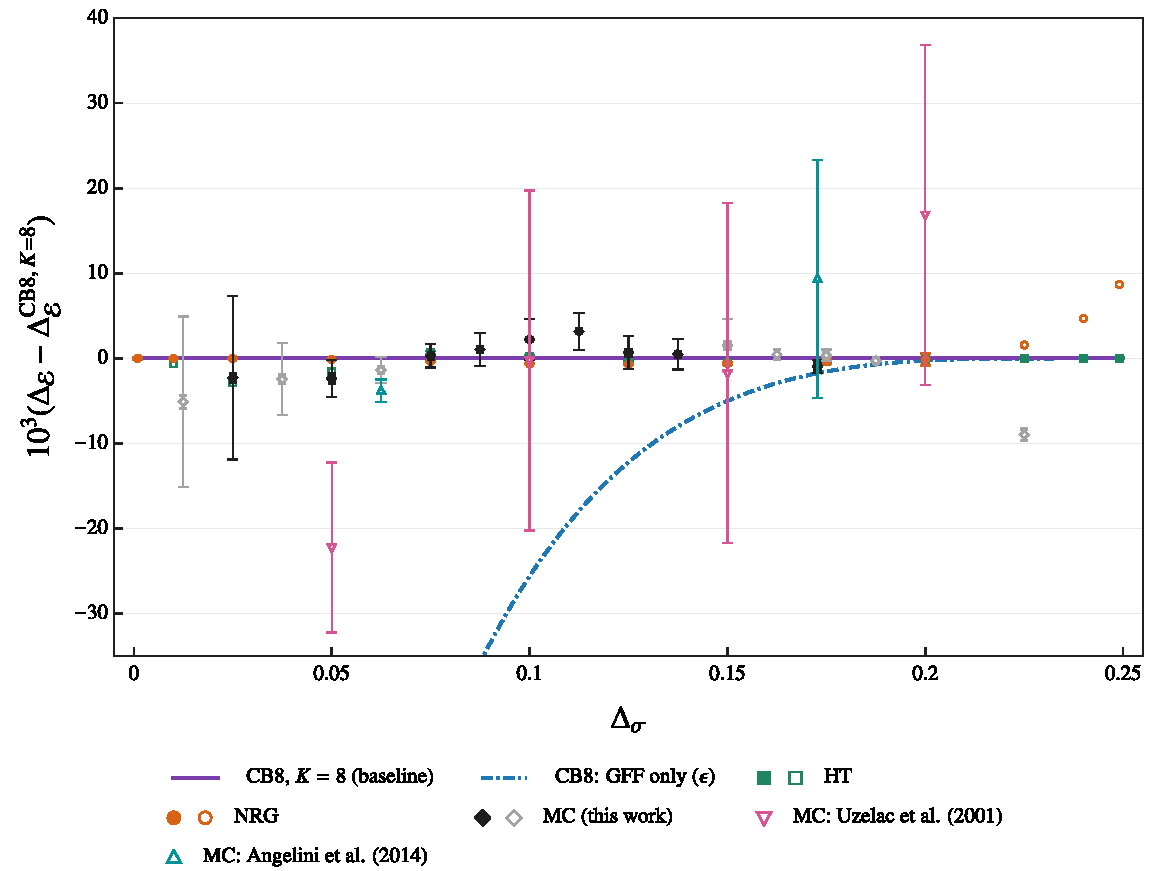
\includegraphics[width=\textwidth]{parts/rs/figures/05_method_dispersion_clean.pdf}
\caption{One dimension: deviations $10^3(\De-\De^{\rm baseline})$ of all displayed reference
points from the $K=8$ baseline, with full error bars, including the published MC values
(rose inverted triangles: Uzelac et al.\ 2001; teal triangles: Angelini et al.\ 2014). Markers as in
Fig.~\ref{rs:fig:methods}. Blue dash-dot: GFF-only CB8, below the frame for $\Ds<0.088$ (it
reaches $-433$ at $\Ds=0$). The $K=5$--$8$ envelope is not drawn; its width is at most
$\sci{4.67}{-3}$, that is $4.67$ in these units.}
\label{rs:fig:dispersion}
\end{figure}

\paragraph{HT and NRG.} At $\Ds=0.15$--$0.2$ the final HT and NRG values agree (differences
at most $\sci{1.0}{-4}$, below the sum of their errors). At $\Ds=0.1$ and $0.125$ the NRG
values lie $\sci{8.7}{-4}$ and $\sci{4.5}{-4}$ below the HT values, $5.8$ and $4.6$ times the
sum of the HT fit half-spread and the NRG error. The gap is of the size of the dependence of
HT on the correction of its truncation artifact: without the correction the truncation
extrapolates $\sci{2.3}{-3}$ and $\sci{6.6}{-4}$ lower at these points ($\sci{1.7}{-3}$ at
$0.075$), and NRG lies between the two limits. The HT note does not combine this dependence
into its error, because the truncation has no strict error bar and an error built after the
gap to NRG had been seen would make the two methods appear to agree \cite{rs:noteHT}. The HT values therefore keep their fit half-spreads, and the difference between
the corrected and uncorrected limits is shown separately.

\paragraph{Do the data select $K=8$ over $K=4$?} The archived $K=4$ and the baseline $K=8$
curves differ by at most $\sci{1.32}{-3}$ (at $\Ds=0.109$). That is less than the width of the
$K=8$ core band at the same points ($\sci{2.0}{-3}$ at $\Ds=0.1$, $\sci{3.0}{-3}$ at $0.125$), so a
preference between them is a choice inside the prescription dependence.
Table~\ref{rs:tab:k4k8} compares the separation with the quoted errors and lists the dependence of
HT on the artifact correction separately.
\begin{itemize}
\item \emph{MC} does not resolve the two curves anywhere: the separation is at most $0.59$
of the sum of $\sigma_{\rm stat}$ and $\sigma_{\rm sys}$ of an accepted value.
\item \emph{HT.} At $\Ds=0.075$ and $0.1$ HT lies above both curves, nearer $K=8$, but its
dependence on the artifact correction ($\sci{1.7}{-3}$, $\sci{2.3}{-3}$) exceeds the separation of the curves
($\sci{1.0}{-3}$, $\sci{1.3}{-3}$), so HT does not decide there. At $0.125$ it lies between the
curves, nearer $K=8$. At $0.15$--$0.2$, where the prescription dependence is small
($\le\sci{1.3}{-4}$), it lies between the curves and nearer $K=4$: $\sci{1}{-5}$ to $\sci{4}{-4}$
above $K=4$ ($2.6$--$12$ errors) and $\sci{9}{-5}$ to $\sci{5}{-4}$ below $K=8$ ($15$--$21$ errors).
\item \emph{NRG} selects $K=8$ only at $\Ds=0.025$, where the separation is $\sci{1.9}{-4}$ and
$K=4$ is $6.2$ errors away. At $0.05$--$0.15$ it lies between the curves, more than $2.5$
errors from each: nearer $K=8$ at $0.05$, $0.075$ and, marginally, $0.1$ ($19.1$ against
$19.7$ errors), nearer $K=4$ at $0.125$ and $0.15$. At $0.175$, $0.2$ and $\Ds\le0.01$ the separation is below two errors.
\end{itemize}
So the precise data resolve the $K=4$--$K=8$ difference at several points, but no method
favors $K=8$ over its range. Where both curves are resolved, HT and NRG mostly lie between
them, and at $0.15$--$0.2$, where HT is most precise and depends least on the artifact
correction, they lie nearer $K=4$. An earlier version of this note justified $K=8$ by its
agreement with HT and NRG. That argument relied on the HT fit half-spread alone at
$\Ds=0.1$--$0.125$ and on earlier NRG values; it does not survive the dependence of HT on the
artifact correction, which exceeds the separation at $\Ds=0.075$ and $0.1$, and it is
withdrawn. The choice $K=8$ rests only on its a priori motivation: these are all the
short-range coefficients we have, and at fixed $K$ the prescriptions then spread much less
than with $K=4$ (core band at $\Ds=0.05$: $\sci{2.3}{-4}$ against $\sci{3.4}{-3}$) and depend
less on $\bL$ (Secs.~\ref{rs:sec:res1d} and~\ref{rs:sec:robust}). It was fixed after the comparison
data had been seen, and taken together these data do not favor it over $K=4$.

\begin{table}[htbp]\centering\scriptsize\setlength{\tabcolsep}{2.5pt}
\begin{tabular}{@{}r r r r r r l r r r l@{}}
\toprule
 & & \multicolumn{5}{c}{HT (corrected)} & \multicolumn{4}{c}{NRG}\\
\cmidrule(lr){3-7}\cmidrule(l){8-11}
$\Ds$ & $10^4(F_4{-}F_8)$ & $10^4(y{-}F_8)$ & err & $z_8$, $z_4$ & corr.$-$unc. & & $10^4(y{-}F_8)$ & err & $z_8$, $z_4$ & \\ \midrule
0.025 & $-1.89$ & $\cdot$ & $\cdot$ & $\cdot$ & $\cdot$ &  & $-0.10$ & $\sci{2.9}{-5}$ & $-0.4$, $+6.2$ & near 8\\
0.05 & $-6.12$ & $\cdot$ & $\cdot$ & $\cdot$ & $\cdot$ &  & $-1.19$ & $\sci{2.7}{-5}$ & $-4.5$, $+18.4$ & b(8)\\
0.075 & $-10.43$ & $+6.99$ & $\sci{2.0}{-4}$ & $+3.5$, $+8.8$ & $\sci{1.7}{-3}$ & o(8)$^\dagger$ & $-3.67$ & $\sci{3.0}{-5}$ & $-12.3$, $+22.7$ & b(8)\\
0.1 & $-12.99$ & $+2.31$ & $\sci{1.2}{-4}$ & $+2.0$, $+13.2$ & $\sci{2.3}{-3}$ & o(8)$^\dagger$ & $-6.39$ & $\sci{3.3}{-5}$ & $-19.1$, $+19.7$ & b(8)\\
0.125 & $-12.48$ & $-3.09$ & $\sci{4.3}{-5}$ & $-7.2$, $+21.8$ & $\sci{6.6}{-4}$ & b(8) & $-7.55$ & $\sci{5.4}{-5}$ & $-14.1$, $+9.2$ & b(4)\\
0.15 & $-9.01$ & $-5.03$ & $\sci{3.3}{-5}$ & $-15.4$, $+12.2$ & $\sci{1.3}{-4}$ & b(4) & $-6.06$ & $\sci{1.1}{-4}$ & $-5.3$, $+2.6$ & b(4)\\
0.175 & $-4.37$ & $-3.32$ & $\sci{1.5}{-5}$ & $-21.4$, $+6.8$ & $\sci{3.3}{-5}$ & b(4) & $-3.40$ & $\sci{3.5}{-4}$ & $-1.0$, $+0.3$ & n.r.\\
0.2 & $-1.04$ & $-0.92$ & $\sci{4.7}{-6}$ & $-19.4$, $+2.6$ & $\sci{4.5}{-6}$ & b(4) & $-1.36$ & $\sci{7.1}{-4}$ & $-0.2$, $-0.0$ & n.r.\\
\bottomrule
\end{tabular}
\caption{Can the comparison data tell the $K=4$ and $K=8$ curves apart? $F_K$: CB8 with the
short-range series through $\CSR_K$; $y$: the HT or NRG value; $z_K=(y-F_K)/{\rm err}$. HT err:
half-spread of the accepted fits (quoted); at $\Ds=0.075$ its one-sided allowance $-\sci{5}{-4}$
is not included and would lower $z_8$ to $1.0$. corr.$-$unc.: the HT limit corrected for the
truncation artifact minus the uncorrected limit, shown separately and not combined with err
(Sec.~\ref{rs:sec:cmp1d}). NRG err: chain-depth, kept-state and discretization errors added
linearly. Labels: near 8, within one error of $F_8$ and more than two from $F_4$; b($K$),
between the curves, and o($K$), outside both, more than one error from each and nearer $F_K$;
n.r., separation below two errors. $^\dagger$: the dependence on the artifact correction
exceeds the separation. MC resolves neither curve anywhere. The errors are not
standard deviations; the ratios are descriptive.}
\label{rs:tab:k4k8}
\end{table}

\subsection{Two dimensions}
The finite-cutoff HT values \cite{rs:noteHT} at the largest cutoff ($N=24$ at eleven couplings,
$N=22$ at $\Ds=0.125$ and $0.126$) compare with the curvature baseline as follows
(Fig.~\ref{rs:fig:curves23}, left):
\begin{itemize}
\item At weak coupling, $\Ds\ge0.35$ ($s\le1.3$), HT agrees with CB8 to at most
$\sci{8}{-4}$, inside the core band.
\item In mid-window HT lies above the baseline: $\sci{+2.3}{-3}$ at $\Ds=0.3$,
$\sci{+6.6}{-3}$ at $0.25$, $\sci{+9.9}{-3}$ at $0.2$ and $\sci{+7.3}{-3}$ at $0.175$.
At $s=1.4$--$1.5$ ($\Ds=0.3$--$0.25$) HT lies within the spread of the endpoint
constructions, inside the core band of the tangent construction. At $s=1.6$--$1.65$
($\Ds=0.2$--$0.175$) HT is above every construction, by about $\sci{3}{-3}$ above the upper
edge of the tangent core band. The cutoff dependence does not show whether this excess
survives at infinite cutoff. At $s=1.4$ and $1.5$ HT rises monotonically with $N$, so if the
rise continues the $N=24$ values are lower bounds. At $s=1.6$, however, it is flat from $N=18$
on and falls by $\sci{5}{-5}$ in the last step, and at $s=1.65$ it falls steadily from $N=10$
on (by $\sci{5.3}{-3}$ up to $N=24$, $\sci{1.0}{-3}$ in the last step), so larger cutoffs could
reduce the excess there.
\item Near the short-range end ($\Ds\le0.15$) HT drifts downward, away from the exact
endpoint value $1$ ($0.940$ at $\Ds=\frac18$, $N=22$), and is not usable.
\end{itemize}
The discrepancy is not assigned to either method: the cutoff dependence and the artifact
correction of HT, the uncomputed orders and the endpoint assumptions all remain. The
thirteen published MC values have quoted errors from $0.006$ to $0.034$ (and $0.10$ for
Angelini et al.\ at $s=\frac74$). Away from $s=\frac74$ they lie within two quoted errors of
both CB8 and HT, so they cannot separate them; at $s=\frac74$ they agree with the exact value
$1$, which HT misses. Luijten's two estimators on the same data differ by up to $0.05$. The
project's own 2d MC values are conditional or model-limited \cite{rs:noteMC}, so only
finite-size exponents are available (Table~\ref{rs:tab:mc2d}). The exponents
$\Delta_{\rm eff}(U_4)$ of the largest lattice pair ($L=512\to1024$) agree with the curvature
baseline to $\sci{1.5}{-3}$ at $s=1.2$--$1.4$. There the endpoint constructions differ from it
by up to $\sci{4.7}{-3}$, so the exponents do not select one. Toward both ends ($s=1.05$,
$1.1$ and $1.5$--$1.7$) they fall short of the baseline by $0.005$ to $0.02$.

\begin{table}[htbp]\centering\small
\begin{tabular}{@{}r r l r r r r@{}}
\toprule
$s$ & $\Ds$ & label & $\Delta_{\rm eff}(U_4)$ & curvature CB8 & $10^3$(MC$-$CB8) & $10^3\,\max|{\rm constr.}-{\rm CB8}|$\\ \midrule
1.05 & 0.475 & conditional & 0.9702(25) & 0.985836 & $-15.65$ & 0.00\\
1.1 & 0.45 & conditional & 0.9659(23) & 0.975429 & $-9.51$ & 0.02\\
1.2 & 0.4 & conditional & 0.9631(22) & 0.962567 & $+0.56$ & 0.54\\
1.3 & 0.35 & model-limited & 0.9584(20) & 0.958099 & $+0.28$ & 2.33\\
1.4 & 0.3 & model-limited & 0.9627(20) & 0.961182 & $+1.54$ & 4.68\\
1.5 & 0.25 & model-limited & 0.9661(18) & 0.971143 & $-5.03$ & 5.69\\
1.6 & 0.2 & model-limited & 0.9698(18) & 0.985419 & $-15.66$ & 7.02\\
1.7 & 0.15 & model-limited & 0.9773(17) & 0.997797 & $-20.49$ & 5.54\\
\bottomrule
\end{tabular}
\caption{Two dimensions: finite-size exponents $\Delta_{\rm eff}(U_4)$ of the project's MC for
the largest lattice pair, $L=512\to1024$, with their statistical errors \cite{rs:noteMC}, against
the curvature baseline. Last column: the largest deviation of the tangent and value
constructions and the GFF-only curve from the baseline. These are not infinite-size values.}
\label{rs:tab:mc2d}
\end{table}

\subsection{Three dimensions}
Against the slope baseline (Fig.~\ref{rs:fig:curves23}, right):
\begin{itemize}
\item HT at $N=20$ is within $\sci{1}{-3}$ of CB8 for $\Ds\ge0.6$ ($s\le1.8$), for example
$\sci{-2.2}{-4}$ at $\Ds=0.7$ and $\sci{-9.3}{-4}$ at $\Ds=0.65$. Toward the short-range end
it lies above, by $\sci{1.2}{-3}$ at $\Ds=0.575$ rising to $\sci{6.6}{-3}$ at $\Ds=S$, where HT
gives $1.41924$ against the exact $E=1.41262528$; as in $d=2$, HT fails near the short-range
end, here lying above the curve rather than below it.
\item The project's MC value at $s=1.6$ \cite{rs:noteMC}, $\De=1.47314\pm0.00118\,({\rm
stat})\pm0.00230\,({\rm sys})$, lies $\sci{1.0}{-3}$ above CB8 ($1.47214$). It is accepted
only under amendment P1 (Table~\ref{rs:tab:refstatus}), adopted after the protocol had been
applied to the production data; $\sigma_{\rm sys}$ is the half-range of the values over the
admissible extrapolation series.
\item The project's extrapolations that are not accepted, at $s=1.7$, $1.85$ and $1.9$
(cross-check failed or unavailable), lie $0.022$ to $0.033$ above CB8.
\item Luijten's thesis gives $1.477(16)$ at $s=1.6$ and $1.46(4)$ at $s=1.8$, $+0.3$ and
$+0.6$ quoted errors from CB8; Luijten calls these results rather poor (lattices up to
$L=64$, correction exponent fixed by hand).
\item Bootstrap kinks read off Fig.~11 of Ref.~\cite{rs:Behan:2023ile} (conjectured
identification) give $1.470$, $1.450$, $1.432$, $1.415$ at $s=1.593$, $1.685$, $1.778$,
$1.871$ (read-off error about $\pm0.005$), below CB8 by $0.004$, $0.004$, $0.007$, $0.010$. The
gap grows toward the short-range end, where CB8 imposes $c_1=0.273$; the kink at $s=1.871$
implies a smaller slope. A functional-RG truncation \cite{rs:Defenu:2014bea} departs by up to
$0.03$ near the short-range end, where its thermal exponent, about $1.543$ as read off its
Fig.~2, stays below the 3d Ising value $1.5874$.
\end{itemize}

%====================================================================
\section{Robustness}\label{rs:sec:robust}
%====================================================================
\subsection{Held-out coefficients}
A finite-order test that uses no comparison data is to withhold the last known
coefficient, construct the approximant from the lower ones and re-expand it to predict
the withheld one. This tests finite-order predictive power, not asymptotic dominance.
Tables~\ref{rs:tab:heldout1} and~\ref{rs:tab:heldout23} collect the results;
Fig.~\ref{rs:fig:instanton} shows the one-dimensional ones together with the matched
CB$-$PB differences.

\begin{figure}[htbp]\centering
\widefig{parts/rs/figures/02_instanton_clean.pdf}
\caption{One dimension: conformal Borel against Pad\'e--Borel. Top: matched differences
$10^3(\De^{\rm CB8}-\De^{{\rm PB}[5/3]})$ with the same coefficients, endpoint input
$F^{\rm SR}_K$, order, variable and $\bL=3$; left in $v$ for $K=4$ (archived), $5$, $6$, $7$; right in
$\epsilon$ for $K=4,6,7$ (where PB$[5/3]$ is admissible). Bottom: absolute relative errors of
held-out $C_6,C_7,C_8$ predicted from the preceding coefficients; left for the GFF-only
series (independent of $K$), right for the endpoint-$v$ construction with $K=8$ (dark) and
$K=4$ (light). PB shapes as selected by the rule of Sec.~\ref{rs:sec:pade} ($K=8$: $[4/1]$, $[4/2]$, $[3/4]$;
$K=4$ and GFF-only: $[3/2]$, $[4/2]$, $[5/2]$). The $C_8$ bars use the final $C_8(1)$
(allowance about $0.21\%$).}
\label{rs:fig:instanton}
\end{figure}

\begin{table}[htbp]\centering\small
\begin{tabular}{@{}l r r r@{}}
\toprule
Construction ($\bL=3$) & $C_6$ & $C_7$ & $C_8$\\ \midrule
GFF only, CB & 11.03 & 1.58 & 1.55\\
GFF only, PB ($[3/2],[4/2],[5/2]$) & 5.70 & 0.44 & 0.33\\
Endpoint-$v$, $K=8$, CB & 10.95 & 5.93 & 0.94\\
Endpoint-$v$, $K=8$, PB ($[4/1],[4/2],[3/4]$) & 3.86 & 0.17 & 0.50\\
Endpoint-$v$, $K=4$, CB & 7.23 & 0.37 & 0.81\\
Endpoint-$v$, $K=4$, PB ($[3/2],[4/2],[5/2]$) & 2.53 & 0.16 & 0.44\\
\bottomrule
\end{tabular}
\caption{One dimension: absolute relative errors (\%) of held-out coefficients. The
targets $C_6,C_7$ are unchanged; for $C_8$ the final value is the target, and the
predictions themselves do not depend on it.}
\label{rs:tab:heldout1}
\end{table}

\begin{table}[htbp]\centering\small
\begin{tabular}{@{}c rrrr c rrrr@{}}
\toprule
& \multicolumn{4}{c}{$d=2$} && \multicolumn{4}{c}{$d=3$}\\
\cmidrule{2-5}\cmidrule{7-10}
& \multicolumn{2}{c}{GFF only} & \multicolumn{2}{c}{with SR input} && \multicolumn{2}{c}{GFF only} & \multicolumn{2}{c}{with SR input}\\
Target & CB & PB & CB & PB && CB & PB & CB & PB\\ \midrule
$C_5$ & 7.75 & 37.99 & 44.88 & 2.26 && 1.67 & 1.56 & 9.72 & 7.00\\
$C_6$ & 9.25 & 5.16 & 22.31 & 4.57 && 4.32 & 2.42 & 0.80 & 18.25\\
$C_7$ & 0.81 & 0.18 & 5.82 & 6.93 && 1.64 & 1.16 & 1.99 & 0.10\\
$C_8$ & 1.24 & 0.22 & 2.99 & 0.31 && 0.37 & 0.52 & 0.33 & 0.16\\
\bottomrule
\end{tabular}
\caption{Two and three dimensions: absolute relative errors (\%) of held-out coefficients
at the baseline $\bL$. GFF only: the series resummed directly; with SR input: the curvature
($d=2$) and slope ($d=3$) constructions. PB shapes as selected by the rule of
Sec.~\ref{rs:sec:pade}.}
\label{rs:tab:heldout23}
\end{table}

Different orders, dimensions and constructions favor different families. For the
newly measured $C_8$, the GFF-only PB prediction is closer in $d=1$ and $d=2$, CB is
closer in $d=3$. In $d=1$ the $K=8$ CB prediction of $C_8$ is $0.94\%$ off, which is $4.4$
times the allowance of $C_8(1)$ ($0.21\%$). An accurate PB prediction of $C_8$ also does not
guarantee an admissible eighth-order PB curve of the matched shape once $C_8$ is supplied: at
$K=8$ in $d=1$ only $[3/5]$ survives at eighth order, and in $d=3$ no eighth-order candidate
survives at $\bL=4$. These tests support keeping both families and the
explicit admissibility diagnostics. They do not validate an instanton amplitude or establish
an advantage of supplying the action.

\subsection{Order and Borel--Leroy stability}
Figure~\ref{rs:fig:stability} shows the order and $\bL$ dependence in $d=1$. At $K=8$ the CB
curves at orders 6 and 7 differ from CB8 by at most $\sci{8.8}{-4}$ and $\sci{2.2}{-4}$; changing
$\bL$ to $2$ or $4$ moves the curve by at most $\sci{1.4}{-4}$, while $\bL=0$ moves it by up to
$\sci{2.9}{-3}$ (at $K=4$: $\sci{1.8}{-2}$). The short-range input thus also stabilizes the
Borel--Leroy dependence. Varying $1/\Ae$ by $\pm20\%$ moves the $K=8$ baseline by at most
$\sci{1.0}{-3}$ (scale $0.8$), and by at most $\sci{1.6}{-4}$ for the other variations. In
$d=2$ and $3$, adding $C_8$ changed the curves by at most $\sci{8.3}{-4}$ and $\sci{1.1}{-5}$
(Sec.~\ref{rs:sec:res23}). Small order-to-order changes are stability observations, not an
estimate of the total error.

\begin{figure}[htbp]\centering
\widefig{parts/rs/figures/03_stability_clean.pdf}
\caption{One dimension: finite-order stability. Top row: $K=8$ baseline; bottom row: the
archived $K=4$ construction (with the final $C_8(1)$). Left: deviations
$10^3(\De-\De^{\rm CB8})$ of CB at orders 6, 7 and of the PB controls $[4/2]$, $[5/2]$, $[5/3]$
($\bL=3$, drawn only where admissible; at $K=8$ and order 8 no PB is drawn). Right: deviations of
CB8 at $\bL=0,2,4$ from $\bL=3$. Vertical ranges differ between the right panels.}
\label{rs:fig:stability}
\end{figure}

\subsection{\texorpdfstring{Coefficient precision, the final $C_8(1)$ and a ninth coefficient}{Coefficient precision, the final C8(1) and a ninth coefficient}}
For fixed CB parameters the reconstruction is affine in the input coefficients, so
coefficient sensitivity can be computed exactly from unit responses $J_n=\partial F/\partial
C_n$. We report $U=\sum_{n=6}^8|J_n|\,\delta C_n$, the sum of absolute responses to the
allowances. This would be a worst-case bound only if the allowances were rigorous
simultaneous bounds, which they are not; with a covariance matrix $\Sigma$ the variance would
be $J^{\mathsf T}\Sigma J$. Four sources of uncertainty must be kept separate: numerical
integration (negligible), input coefficients ($U$), prescription and endpoint construction (the
bands), and the theoretical assumptions about the endpoint and the instanton.

\begin{figure}[htbp]\centering
\widefig{parts/rs/figures/04_precision_clean.pdf}
\caption{One dimension: coefficient precision. Top row $K=8$, bottom row $K=4$ (archived
construction, current inputs). Left: $10^4\,U$ for the current allowances
($\delta C_8=17000$, $\delta C_7=41$, $\delta C_6=\sci{4.9}{-7}$), for $\delta C_8/10$, and with $C_8$
exact. Right: $10^3\,\delta\De$ for a hypothetical $C_9$: the shift if
$C_9=C_9^{\rm hyp}$ and the responses to $1\%$ and $5\%$ of $|C_9^{\rm hyp}|$. Top:
$C_9^{\rm hyp}=\sci{-2.178401719}{8}$, the CB prediction of the $K=8$ baseline, so its shift
vanishes identically. Bottom: $C_9^{\rm hyp}=\sci{-2.190506633}{8}$, the archived $K=4$
PB$[5/3]$ prediction made with the previous $C_8(1)$, kept as a fixed scenario value. These are
sensitivity scenarios, not confidence intervals; $C_9$ has not been calculated.}
\label{rs:fig:precision}
\end{figure}

At $\Ds=0.1$ and $K=8$, $U=\sci{3.76}{-5}$ with the final allowance; dividing $\delta C_8$ by ten
gives $\sci{9.69}{-6}$, and the floor with $C_8$ exact (set by $\delta C_7$) is $\sci{6.59}{-6}$.
The corresponding values at $K=4$ are $\sci{2.34}{-4}$, $\sci{5.96}{-5}$ and $\sci{4.03}{-5}$. A
tenfold better $C_8$ would thus improve the input budget by a factor $3.9$ but leave the
prescription envelope, about a hundred times larger, unchanged.

\paragraph{What the final $C_8(1)$ changed.} Replacing $8066723.343\pm33000$ by
$8059766.723\pm17000$ (a shift of $-6957$) moves the $K=8$ baseline down by at most
$\sci{2.0}{-5}$ (at $\Ds=0.141$; $\sci{-1.27}{-5}$ at $\Ds=0.1$). It lowers the upper edge of
the envelope by up to $\sci{1.9}{-4}$: the width at $\Ds=0.1$ goes from $\sci{3.84}{-3}$ to
$\sci{3.64}{-3}$, and the maximum width $\sci{4.67}{-3}$ is unchanged. It roughly halves the
$C_8$ term of $U$ ($\sci{6.02}{-5}\to\sci{3.10}{-5}$ at $\Ds=0.1$, so that $U$ falls from
$\sci{6.68}{-5}$ to $\sci{3.76}{-5}$), and it changes the mismatch ratio at $n=8$ from $0.1578$
to $0.1576$. With the previous value every program reproduces the archived outputs to
$\sci{8.4}{-15}$.

\paragraph{A ninth coefficient.} $C_9$ has not been computed. At fixed CB parameters the
ninth-order curve obeys the exact identity
\begin{equation}
 F_9(x)-F_8(x)=J_9(x)\,\bigl[C_9-C_9^{\rm CB8}\bigr],\qquad J_9=\frac{\partial F_9}{\partial C_9},
 \label{rs:eq:C9}
\end{equation}
where $C_9^{\rm CB8}$ is the coefficient implied by the eighth-order approximant; supplying
that value adds no information. The $K=8$ baseline implies
$C_9^{\rm CB8}=\sci{-2.178401719}{8}$; the only admissible eighth-order PB at $K=8$, $[3/5]$,
predicts $\sci{-2.181155}{8}$, and the $K=4$ CB8 implies $\sci{-2.19002}{8}$. These are correlated
predictions, not a calculation. At $\Ds=0.1$ a change of $1\%$ of $|C_9|$ would move the
$K=8$ curve by $\sci{3.5}{-4}$ (at $K=4$: $\sci{2.2}{-3}$). Adding the ninth order also amplifies
the inherited sensitivity to $C_8$: at $\Ds=0.1$ the $C_8$ term of $U$ grows from $\sci{3.1}{-5}$
to $\sci{2.9}{-4}$ at $K=8$ (from $\sci{1.9}{-4}$ to $\sci{1.8}{-3}$ at $K=4$). Simply appending
$C_9$ is therefore not guaranteed to improve the curve: a useful ninth order needs an
independently computed $C_9$, sufficient precision on $C_8$, and renewed prescription checks.

%====================================================================
\section{Limitations and open problems}\label{rs:sec:open}
%====================================================================
\begin{enumerate}
\item \textbf{Reporting prescription.} The number $K=8$ of imposed short-range
coefficients, and the range $K=5$--$8$ of the envelope, were fixed after the comparison data
had been seen. $K=8$ is motivated a priori only (all short-range coefficients); choosing the
narrowest core band would give $K=7$. Whether the endpoint variable ($v$ or $\epsilon$) belongs in the
envelope is open.
\item \textbf{Endpoint assumptions.} The constructions assume that the resummed remainder is
regular at the short-range end. Logarithms beyond the imposed terms are not excluded. The
two-dimensional $c_2$ carries a formal analytic-MS qualification, the three-dimensional
$c_1$ a conditional spectral range; the one-dimensional $\CSR_n$ beyond the published orders
are project results with their own assumptions, and the short form of $\CSR_8$ is unproved.
In $d=2$ the endpoint construction is the largest uncertainty in mid-window.
\item \textbf{The amplitude.} The cancellation of the regulator dependence of the bubble
action in the one-loop amplitude (Sec.~\ref{rs:sec:amplitude}) should be derived explicitly. The
derivation must keep the integration limits, determinant, measure, legs and counterterms
through the simple-pole residue, for the size coordinate and for its rescaled form.
\item \textbf{Next order and approach to large order.} The coefficient $d_1$ needs the
two-loop fluctuations, the subleading size integral and the direct mass insertion, and
possibly logarithms. Its known part already gives $-30\%$ at $n=8$; further corrections may
be needed before eighth order can test $K_I$.
\item \textbf{Dominance.} The Sobolev bound identifies the least-action real saddle; it does
not settle complex saddles, integration cycles, multi-instanton sectors, non-instanton
factorial mechanisms or the uniformity of the renormalized expansion.
\item \textbf{Two and three dimensions.} Only the actions and the power counting are
available. A renormalized determinant and amplitude would be needed for amplitude-based
tests.
\item \textbf{Coefficients.} A covariance model for $C_6,C_7,C_8$ is missing. A ninth
coefficient would be a useful test of the predictions only with adequate precision on $C_8$
(Sec.~\ref{rs:sec:robust}).
\item \textbf{Comparisons.} In $d=1$ the final HT and NRG values differ at $\Ds=0.1$ and
$0.125$ by $5.8$ and $4.6$ times the sum of their quoted errors. The gap is of the size of the
dependence of HT on the artifact correction, which the HT error does not include
(Sec.~\ref{rs:sec:cmp1d}), and its origin is open. HT and NRG resolve the $K=4$--$K=8$ difference at
several points but lie between the two curves there (Table~\ref{rs:tab:k4k8}), so they cannot
justify the choice of $K$. In $d=2$ and $3$ HT is available only at finite cutoff; the $d=2$
mid-window excess of HT over every endpoint construction (about $\sci{3}{-3}$ beyond their
core bands at $s=1.6$--$1.65$) is unresolved, and the cutoff dependence there does not show
that it survives at infinite cutoff. Published MC is too imprecise to discriminate, and in
$d=3$ there is a single accepted project MC point. Continuum HT extrapolations and MC with
controlled systematics would be the most informative additions.
\item \textbf{Interpretation of the $d=1$ endpoint.} The fixed-point-merger reading of the
square-root branch point, and the radius $\simeq\frac12$ suggested by the short-range series,
should be checked against more coefficients or an independent argument.
\end{enumerate}

%====================================================================
\appendix
\section{Formulas and parameters}\label{rs:app:formulas}
%====================================================================
\paragraph{Conformal Borel coefficients.} For the resummed series $f(z)=\sum_{j\le m}f_jz^j$
with action $A$,
\begin{equation}
 p_k=\sum_{j=0}^k\frac{f_j\,(4A)^j}{\Gamma(j+\bL+1)}\,(-1)^{k-j}\binom{\alpha-2j}{k-j},\qquad
 \cR_m^{\rm CB}[f](z)=\int_0^\infty e^{-u}u^{\bL}\,
 \frac{\sum_{k=0}^mp_k\,w(zu)^k}{[1-w(zu)]^\alpha}\dd u ,
 \label{rs:eq:pk}
\end{equation}
which reproduces the Taylor polynomial through order $m$; for integer $\alpha-2j$ the
generalized binomial coefficient is the polynomial one. The inverse map
$w(t)=\sum_{k\ge1}(-1)^{k-1}\frac{1}{k+1}\binom{2k}{k}(t/4A)^k$ gives an independent
round-trip check.

\paragraph{Pad\'e--Borel.} With $d_k=f_k/\Gamma(k+\bL+1)$, the denominator of $[L/M]$ solves
$\sum_{j=1}^Mq_jd_{k-j}=-d_k$ for $k=L+1,\dots,m$, and $p_k=\sum_{j=0}^{\min(k,M)}q_jd_{k-j}$
with $q_0=1$. The Pad\'e denominator depends nonlinearly on the coefficients, so PB curves are
not affine in the inputs.

\paragraph{Series operations and quadrature.} Products, powers $(1-z)^p$ and compositions are
formed with truncation after each operation, in 65-digit arithmetic. The Laplace integral uses
240-point generalized Gauss--Laguerre quadrature for weight $u^{\bL}e^{-u}$ (Jacobi matrix with
diagonal $2k+\bL+1$ and off-diagonal $\sqrt{k(k+\bL)}$), checked against 120 nodes, adaptive
integration and selected 65-digit integrals. For the one-dimensional CB curves the 240-node and
adaptive results agree to $\sci{1.1}{-15}$, the 65-digit checks to $\sci{5.2}{-16}$, and the
displayed PB curves to $\sci{4.0}{-15}$. Formal re-expansion reproduces the input coefficients.
These checks validate the evaluation of each approximant, not its distance from the exact theory.

\paragraph{Grids.} The one-dimensional dense grid has 1004 points (1001 equally spaced on
$[0,\frac14]$ plus the special comparison abscissae); the matched CB/PB comparison uses 502
points. The two- and three-dimensional curves have 754 and 763 stored samples.

\paragraph{Scan parameters.} Table~\ref{rs:tab:params} collects all prescription parameters.

\begin{table}[htbp]\centering\small\setlength{\tabcolsep}{3.5pt}
\begin{tabular}{@{}l l l l@{}}
\toprule
 & $d=1$ & $d=2$ & $d=3$\\ \midrule
Resummed variable & $v=1-2\sqrt{\Ds}$ & $\epsilon$ & $\epsilon$\\
CB action & $A_v=\Ae/2=0.25703245$ & $\Ae=9/8$ & $\Ae=1.92343326$\\
Endpoint input & $\CSR_1,\dots,\CSR_8$ ($K=8$) & $1$, $0$, $c_2$ & $E$, $c_1$\\
Endpoint controls & $K=4$--$7$, endpoint-$\epsilon$ & tangent, value & value\\
Without SR input & GFF-only & GFF-only & GFF-only\\
Orders & $6,7,8$ & $6,7,8$ & $6,7,8$\\
Core $\bL$ & $2,3,4$ & $2.5,3.5,4.5$ & $3,4,5$\\
Wide $\bL$ & $0,1,\dots,6$ & $0,1.5,2.5,\dots,6.5$ & $0,2,3,\dots,7$\\
$\alpha$ (core; wide) & $-1,0,1$; $-2,\dots,2$ & $-1,0,1$; $-2,\dots,2$ & $-1,0,1$; $-2,\dots,2$\\
Action variations & $1/A\times0.8,0.9,1.1,1.2$ & same & same\\
PB control & $[5/3]$ ($K\le7$) & PB8 $[5/3]$ & PB7 $[3/4]$; PB8 $[5/3]$ at $\bL=0$\\
Stored grid & 1004 points & 754 points & 763 points\\
\bottomrule
\end{tabular}
\caption{Resummation parameters. The baseline uses order 8, the middle core $\bL$ and
$\alpha=0$; the PB controls use the baseline $\bL$ unless stated.}
\label{rs:tab:params}
\end{table}

\paragraph{One-dimensional comparison data.} Table~\ref{rs:tab:refs1d} lists every
one-dimensional value compared in this note, with its residual from the baseline.

{\small
\begin{longtable}{@{}l r r r r l r@{}}
\caption{One-dimensional comparison data \cite{rs:noteHT,rs:noteNRG,rs:noteMC,rs:Uzelac:2001lc,rs:Angelini:2014koy},
labels as in Table~\ref{rs:tab:refstatus}. ``err'': for HT the half-spread of the accepted fits,
for NRG the chain-depth, kept-state and discretization errors added linearly, for MC
$\sigma_{\rm sys}$, for published MC the quoted error; ``stat'': the MC statistical error. A dot
means none supplied. MC $\Delta_{\rm eff}$: finite-size exponents of the largest lattice pair
(sizes in parentheses), not infinite-size values. The last column is
$10^3(\De-\De^{\rm baseline})$.}\label{rs:tab:refs1d}\\
\toprule Method & $\Ds$ & $\De$ & err & stat & status & resid.\\ \midrule\endfirsthead
\toprule Method & $\Ds$ & $\De$ & err & stat & status & resid.\\ \midrule\endhead
\midrule\multicolumn{7}{r}{continued on the next page}\\\endfoot
\bottomrule\endlastfoot
HT & 0.249 & 0.4993436 & $\sci{9.3}{-8}$ & $\cdot$ & final & $-0.00$\\
HT & 0.24 & 0.4942198 & $\sci{2.6}{-6}$ & $\cdot$ & final & $+0.00$\\
HT & 0.225 & 0.4880804 & $\sci{5.2}{-6}$ & $\cdot$ & final & $-0.00$\\
HT & 0.2 & 0.4830244 & $\sci{4.7}{-6}$ & $\cdot$ & final & $-0.09$\\
HT & 0.175 & 0.4839086 & $\sci{1.5}{-5}$ & $\cdot$ & final & $-0.33$\\
HT & 0.15 & 0.4912086 & $\sci{3.3}{-5}$ & $\cdot$ & final & $-0.50$\\
HT & 0.125 & 0.5061186 & $\sci{4.3}{-5}$ & $\cdot$ & final & $-0.31$\\
HT & 0.1 & 0.5304771 & $\sci{1.2}{-4}$ & $\cdot$ & final & $+0.23$\\
HT & 0.075 & 0.5673260 & $\sci{2.0}{-4}$ & $\cdot$ & one-sided & $+0.70$\\
HT & 0.05 & 0.6206712 & $\cdot$ & $\cdot$ & unstable ($N=40$) & $-1.56$\\
HT & 0.025 & 0.7105771 & $\cdot$ & $\cdot$ & no limit ($N=40$) & $-2.86$\\
HT & 0.01 & 0.8091106 & $\cdot$ & $\cdot$ & no limit ($N=40$) & $-0.64$\\
HT & 0.001 & 0.9693379 & $\cdot$ & $\cdot$ & no limit (not shown) & $+31.91$\\
NRG & 0.249 & 0.508030 & $\cdot$ & $\cdot$ & not converged & $+8.69$\\
NRG & 0.24 & 0.498922 & $\cdot$ & $\cdot$ & not converged & $+4.70$\\
NRG & 0.225 & 0.489668 & $\cdot$ & $\cdot$ & not converged & $+1.58$\\
NRG & 0.2 & 0.482980 & $\sci{7.1}{-4}$ & $\cdot$ & final & $-0.14$\\
NRG & 0.175 & 0.483900 & $\sci{3.5}{-4}$ & $\cdot$ & final & $-0.34$\\
NRG & 0.15 & 0.491106 & $\sci{1.1}{-4}$ & $\cdot$ & final & $-0.61$\\
NRG & 0.125 & 0.505672 & $\sci{5.4}{-5}$ & $\cdot$ & final & $-0.76$\\
NRG & 0.1 & 0.529608 & $\sci{3.3}{-5}$ & $\cdot$ & final & $-0.64$\\
NRG & 0.075 & 0.566260 & $\sci{3.0}{-5}$ & $\cdot$ & final & $-0.37$\\
NRG & 0.05 & 0.622115 & $\sci{2.7}{-5}$ & $\cdot$ & final & $-0.12$\\
NRG & 0.025 & 0.713422 & $\sci{2.9}{-5}$ & $\cdot$ & final & $-0.01$\\
NRG & 0.01 & 0.809747 & $\sci{4.7}{-5}$ & $\cdot$ & final & $-0.00$\\
NRG & 0.001 & 0.937424 & $\sci{1.1}{-4}$ & $\cdot$ & final & $-0.00$\\
MC & 0.0125 & 0.78404 & 0.01003 & 0.00077 & cross-check unavailable & $-5.11$\\
MC & 0.025 & 0.71115 & 0.00959 & 0.00049 & accepted ($\sigma_{\rm sys}$-dominated) & $-2.28$\\
MC & 0.0375 & 0.65904 & 0.00425 & 0.00051 & cross-check unavailable & $-2.42$\\
MC & 0.05 & 0.61987 & 0.00220 & 0.00055 & accepted & $-2.36$\\
MC & 0.0625 & 0.59003 & 0.00150 & 0.00035 & cross-check unavailable & $-1.36$\\
MC & 0.075 & 0.56694 & 0.00139 & 0.00037 & accepted & $+0.31$\\
MC & 0.0875 & 0.54761 & 0.00194 & 0.00032 & accepted & $+1.05$\\
MC & 0.1 & 0.53248 & 0.00242 & 0.00020 & accepted ($\sigma_{\rm sys}$-dominated) & $+2.23$\\
MC & 0.1125 & 0.52020 & 0.00217 & 0.00025 & accepted ($\sigma_{\rm sys}$-dominated) & $+3.17$\\
MC & 0.125 & 0.50710 & 0.00193 & 0.00035 & accepted & $+0.67$\\
MC & 0.1375 & 0.49856 & 0.00180 & 0.00030 & accepted ($\sigma_{\rm sys}$-dominated) & $+0.48$\\
MC & 0.15 & 0.49325 & 0.00306 & 0.00041 & cross-check failed & $+1.54$\\
MC & 0.1625 & 0.48761 & $\cdot$ & 0.00058 & conditional & $+0.47$\\
MC & 0.1727335 & 0.48368 & 0.00078 & 0.00052 & accepted & $-0.97$\\
MC & 0.175 & 0.48460 & 0.00067 & 0.00035 & cross-check failed & $+0.36$\\
MC & 0.1875 & 0.48263 & $\cdot$ & 0.00030 & conditional & $-0.28$\\
MC & 0.225 & 0.47912 & $\cdot$ & 0.00068 & conditional & $-8.96$\\
MC $\Delta_{\rm eff}$ & 0.2125 & 0.4784 & $\cdot$ & 0.0015 & model-limited ($256$k$\to512$k) & $-6.43$\\
MC $\Delta_{\rm eff}$ & 0.2375 & 0.4826 & $\cdot$ & 0.0015 & model-limited ($128$k$\to256$k) & $-10.41$\\
Uzelac 2001 & 0.05 & 0.600 & 0.010 & $\cdot$ & published & $-22.23$\\
Angelini 2014 & 0.0625 & 0.5876 & 0.0013 & $\cdot$ & published & $-3.79$\\
Uzelac 2001 & 0.1 & 0.53 & 0.02 & $\cdot$ & published & $-0.25$\\
Uzelac 2001 & 0.15 & 0.49 & 0.02 & $\cdot$ & published & $-1.71$\\
Angelini 2014 & 0.1727335 & 0.494 & 0.014 & $\cdot$ & published & $+9.35$\\
Uzelac 2001 & 0.2 & 0.50 & 0.02 & $\cdot$ & published & $+16.88$\\
\end{longtable}}

%====================================================================
\section{Reproduction}\label{rs:app:repro}
%====================================================================
Everything in this note is reproduced from the folder \file{Resummation/} of the public
repository. Paths below are relative to it. The programs regenerate the resummations, the
sensitivity analyses and the comparisons from the coefficients and the comparison data; they do
not regenerate graph integrals, HT spectra, NRG runs or MC samples, which come from the sibling
folders \file{GFF/}, \file{HT/}, \file{NRG/} and \file{MC/} (frozen copies in
\file{data/inputs/}, listed with their sources in \file{data/inputs/INPUTS.json}).

\paragraph{Packages.} \file{code/resum_d1/}: the one-dimensional resummation of
Secs.~\ref{rs:sec:methods}--\ref{rs:sec:robust} (endpoint construction with the short-range series
through $\CSR_K$, the $C_8(1)$ switch, curves, envelopes, matched CB/PB comparisons, held-out
tests, $C_9$ scenarios, allowance budgets, reference residuals, the instanton-mismatch table and
the $K=4$/$K=8$ table). \file{code/resum_d23/}: the two- and three-dimensional resummations,
the GFF-only CB3 curves and the table of published MC values. \file{code/instanton/}: the
critical bubble, the amplitude $K_I$ and its benchmarks (Sec.~\ref{rs:sec:largeorder}).
\file{code/comparison/}: the comparison numbers of Sec.~\ref{rs:sec:compare}. The production files
ship unchanged with their production layout and a dated sha256 list
(\file{public/SNAPSHOT.sha256}); the tools added for the public replay are in each package's
\file{public/} and \file{public.mk}.

\paragraph{Commands.} From \file{Resummation/}:
\begin{verbatim}
make test           # fast tests of every package (1 min)
make replay         # every quoted number, shipped records (1 min)
make replay-full    # rerun the resummations, compare outputs (3 min)
make check-inputs   # frozen inputs against the sibling folders
\end{verbatim}
\texttt{make replay} recomputes every number of the sections on resummation and on the
comparison of the paper \cite{rs:LRIpaper} and of its paragraph on higher orders, and the
entries of its results tables that come from this folder: the resummed values in $d=1,2,3$, the
HT values at the largest cutoff in $d=2,3$ and the MC Binder exponents in $d=2$
(\file{results/quoted_numbers.json}). It compares each value, rounded half-up to the printed
digits, with the printed text (the MC exponents with their errors by the PDG rule). The map from each number to its record, command
and tolerance is in \file{results_map.md} (per package in
\file{code/<package>/public/results_map.md}). It also regenerates, byte for
byte, the tables derived from the frozen inputs (the table of one-dimensional comparison data,
the $K=4$/$K=8$ table of Sec.~\ref{rs:sec:compare}, the published-MC table and the comparison tables
in \file{results/comparison/}), and checks the data behind the two figures of the paper
(\file{results/figures/*.csv}). \texttt{make replay-full} reruns the one-dimensional chain
(\file{code/resum_d1/update_2026-10-13/C8_1_ext/run_chain.sh}, about 2 min on one core) and the
ten 2d/3d scripts; every output must agree with the shipped one to $10^{-12}+10^{-12}|x|$ (fits of
the coefficient-model analysis to $10^{-6}$ relative), and the quoted numbers are recomputed from
the rerun. Measured on the symmetry cluster with Python 3.12, numpy 2.3, scipy 1.17: all differences
below $\sci{5}{-15}$ except those fits ($\sci{2}{-6}$).

\paragraph{Numbers of this note that the paper does not quote.} They are read from the records of
the packages: the one-dimensional curves, bands and key points from
\file{code/resum_d1/update_2026-10-13/C8_1_ext/pipeline_K8/results/} (\file{curve_K.csv},
\file{key_points_K.csv}, \file{ablation_K.csv}, \file{held_out_K.csv}, \file{c9_*},
\file{precision_budget_K.csv}, \file{comparison_points_K.csv}) and
\file{.../instanton_mismatch/}; the two- and three-dimensional ones from
\file{code/resum_d23/\{2d,3d\}/results/}; the amplitude from \file{code/instanton/results.json}.
\texttt{make replay-full} regenerates all of these records.

\paragraph{Figures.} The six figures are rendered with Wolfram Language and MaTeX
(\file{vendor/MaTeX/}) by \file{code/resum_d1/plot_lri_comparisons.wl}
(Figs.~\ref{rs:fig:methods}, \ref{rs:fig:instanton}, \ref{rs:fig:stability} and~\ref{rs:fig:precision}),
\file{code/resum_d1/plot_lri_dispersion.wl} (Fig.~\ref{rs:fig:dispersion}) and
\file{code/resum_d23/plot_lri_2d3d.wl} (Fig.~\ref{rs:fig:curves23}), through \file{run_plot.wls}; \texttt{make figures} rebuilds them where
\texttt{wolframscript} and TeX are available. The replay checks the plotted data, not the pixels.

\paragraph{Superseded constructions.} The archived $K=4$ construction (short-range series through
$\CSR_4$) and the previous $C_8(1)=(8.067\pm0.033)\times10^6$ appear only where this note compares
with them; the previous-$C_8(1)$ outputs are not shipped (they are regenerated by
\texttt{LRI\_C8\_1=previous}).

%====================================================================
\phantomsection
\addcontentsline{toc}{section}{References}
\begin{thebibliography}{99}
\bibitem{rs:LRIpaper}
Z.~Zheng, \emph{The long-range Ising CFT: perturbative and nonperturbative approaches}, in
preparation (2026); release at
\url{https://github.com/Canonical111/LRI_public}.

\bibitem{rs:noteGFF}
\emph{Thermal dimensions in the long-range Ising model: analytic coefficients through fifth
order and numerical sixth- to eighth-order coefficients}, research note in the release of
Ref.~\cite{rs:LRIpaper}, \file{GFF/note/long_range_ising_condensed.pdf}.

\bibitem{rs:noteSRI}
\emph{Expansions about the short-range end of the long-range Ising model in one, two and three
dimensions}, research note in the release of Ref.~\cite{rs:LRIpaper},
\file{SRI/note/sri_short_range.pdf}.

\bibitem{rs:noteHT}
\emph{Hamiltonian truncation of the long-range Ising model at finite coupling}, research note
in the release of Ref.~\cite{rs:LRIpaper}, \file{HT/note/lri_ht_finite_coupling.pdf}.

\bibitem{rs:noteNRG}
\emph{Thermal dimension of the one-dimensional long-range Ising model from bosonic NRG of the
sub-ohmic spin--boson model}, research note in the release of Ref.~\cite{rs:LRIpaper},
\file{NRG/note/lri_nrg_1d_note.pdf}.

\bibitem{rs:noteMC}
\emph{Monte Carlo determination of the thermal dimension $\De(\Ds)$ of the long-range Ising
model in $d=1,2,3$}, research note in the release of Ref.~\cite{rs:LRIpaper},
\file{MC/note/lri_mc_note.pdf}.

\bibitem{rs:Benedetti:2020rrq}
D.~Benedetti, R.~Gurau, S.~Harribey and K.~Suzuki,
\emph{Long-range multi-scalar models at three loops},
J.\ Phys.\ A \textbf{53}, 445008 (2020) [Erratum: J.\ Phys.\ A \textbf{58}, 129401 (2025)],
\href{https://arxiv.org/abs/2007.04603}{arXiv:2007.04603}.

\bibitem{rs:Benedetti:2024wgx}
D.~Benedetti, E.~Lauria, D.~Maz\'a\v c and P.~van Vliet,
\emph{One-dimensional Ising model with $1/r^{1.99}$ interaction},
Phys.\ Rev.\ Lett.\ \textbf{134}, 201602 (2025),
\href{https://arxiv.org/abs/2412.12243}{arXiv:2412.12243}.

\bibitem{rs:Benedetti:2025nzp}
D.~Benedetti, E.~Lauria, D.~Maz\'a\v c and P.~van Vliet,
\emph{A strong--weak duality for the 1d long-range Ising model},
SciPost Phys.\ \textbf{20}, 029 (2026),
\href{https://arxiv.org/abs/2509.05250}{arXiv:2509.05250}.

\bibitem{rs:Behan:2017emf}
C.~Behan, L.~Rastelli, S.~Rychkov and B.~Zan,
\emph{A scaling theory for the long-range to short-range crossover and an infrared duality},
J.\ Phys.\ A \textbf{50}, 354002 (2017),
\href{https://arxiv.org/abs/1703.05325}{arXiv:1703.05325}.

\bibitem{rs:Chang:2024whx}
C.-H.~Chang, V.~Dommes, R.~S.~Erramilli, A.~Homrich, P.~Kravchuk, A.~Liu, M.~S.~Mitchell and
D.~Poland, \emph{Bootstrapping the 3d Ising stress tensor},
JHEP \textbf{03}, 136 (2025),
\href{https://arxiv.org/abs/2411.15300}{arXiv:2411.15300}.

\bibitem{rs:Simmons-Duffin:2016wlq}
D.~Simmons-Duffin,
\emph{The lightcone bootstrap and the spectrum of the 3d Ising CFT},
JHEP \textbf{03}, 086 (2017),
\href{https://arxiv.org/abs/1612.08471}{arXiv:1612.08471}.

\bibitem{rs:FrankLieb}
R.~L.~Frank and E.~H.~Lieb,
\emph{A new, rearrangement-free proof of the sharp Hardy--Littlewood--Sobolev inequality},
\href{https://arxiv.org/abs/1010.5821}{arXiv:1010.5821} (2010).

\bibitem{rs:ChenLiOu}
W.~Chen, C.~Li and B.~Ou,
\emph{Classification of solutions for an integral equation},
Commun.\ Pure Appl.\ Math.\ \textbf{59}, 330 (2006).

\bibitem{rs:Davila2013}
J.~D\'avila, M.~del Pino and Y.~Sire,
\emph{Nondegeneracy of the bubble in the critical case for nonlocal equations},
\href{https://arxiv.org/abs/1302.0276}{arXiv:1302.0276} (2013).

\bibitem{rs:McKane:2018ocs}
A.~J.~McKane,
\emph{Perturbation expansions at large order: results for scalar field theories revisited},
J.\ Phys.\ A \textbf{52}, 055401 (2019),
\href{https://arxiv.org/abs/1807.00656}{arXiv:1807.00656}.

\bibitem{rs:McKaneWallaceBonfim}
A.~J.~McKane, D.~J.~Wallace and O.~F.~de~Alcantara~Bonfim,
\emph{Non-perturbative renormalisation using dimensional regularisation: applications to the
$\epsilon$ expansion}, J.\ Phys.\ A \textbf{17}, 1861 (1984).

\bibitem{rs:Kompaniets:2017yct}
M.~V.~Kompaniets and E.~Panzer,
\emph{Minimally subtracted six loop renormalization of $O(n)$-symmetric $\phi^4$ theory and
critical exponents}, Phys.\ Rev.\ D \textbf{96}, 036016 (2017),
\href{https://arxiv.org/abs/1705.06483}{arXiv:1705.06483}.

\bibitem{rs:Dunne:2021lie}
G.~V.~Dunne and M.~Meynig,
Phys.\ Rev.\ D \textbf{105}, 025019 (2022),
\href{https://arxiv.org/abs/2111.15554}{arXiv:2111.15554}.

\bibitem{rs:Kosterlitz:1976zz}
J.~M.~Kosterlitz,
\emph{Phase transitions in long-range ferromagnetic chains},
Phys.\ Rev.\ Lett.\ \textbf{37}, 1577 (1976).

\bibitem{rs:Uzelac:2001lc}
K.~Uzelac, Z.~Glumac and A.~Ani\v ci\'c,
\emph{Critical behavior of the long-range Ising chain from the largest-cluster probability
distribution}, Phys.\ Rev.\ E \textbf{63}, 037101 (2001),
\href{https://arxiv.org/abs/cond-mat/0011306}{arXiv:cond-mat/0011306}.

\bibitem{rs:Angelini:2014koy}
M.~C.~Angelini, G.~Parisi and F.~Ricci-Tersenghi,
\emph{Relations between short-range and long-range Ising models},
Phys.\ Rev.\ E \textbf{89}, 062120 (2014),
\href{https://arxiv.org/abs/1401.6805}{arXiv:1401.6805}.

\bibitem{rs:Luijten:1997th}
E.~Luijten, \emph{Interaction range, universality and the upper critical dimension},
PhD thesis, Delft University of Technology (1997).

\bibitem{rs:Picco:2012ak}
M.~Picco, \emph{Critical behavior of the Ising model with long range interactions},
\href{https://arxiv.org/abs/1207.1018}{arXiv:1207.1018} (2012), unpublished.

\bibitem{rs:Xiao:2025sk}
T.~Xiao, Z.~Liu, Z.~Fan and Y.~Deng,
\emph{On Sak's criterion for statistical models with long-range interaction},
\href{https://arxiv.org/abs/2512.04805}{arXiv:2512.04805} (2025).

\bibitem{rs:Behan:2023ile}
C.~Behan, E.~Lauria, M.~Nocchi and P.~van Vliet,
\emph{Analytic and numerical bootstrap for the long-range Ising model},
JHEP \textbf{03}, 136 (2024),
\href{https://arxiv.org/abs/2311.02742}{arXiv:2311.02742}.

\bibitem{rs:Defenu:2014bea}
N.~Defenu, A.~Trombettoni and A.~Codello,
\emph{Fixed-point structure and effective fractional dimensionality for $O(N)$ models with
long-range interactions}, Phys.\ Rev.\ E \textbf{92}, 052113 (2015),
\href{https://arxiv.org/abs/1409.8322}{arXiv:1409.8322}.
\end{thebibliography}

\clearpage
\AuditMacro{end}{Ae}
\AuditMacro{end}{Ag}
\AuditMacro{end}{CSR}
\AuditMacro{end}{De}
\AuditMacro{end}{Disc}
\AuditMacro{end}{Ds}
\AuditMacro{end}{arraystretch}
\AuditMacro{end}{bL}
\AuditMacro{end}{cB}
\AuditMacro{end}{cR}
\AuditMacro{end}{dd}
\AuditMacro{end}{file}
\AuditMacro{end}{sci}
\AuditMacro{end}{widefig}
\immediate\write\CombinedAuditStream{PART_END|rs|\number\numexpr\value{page}-1\relax}
\endgroup
\RestoreStructuralState
\AuditMacro{outside-after-rs}{AC}
\AuditMacro{outside-after-rs}{AIfigCodexRounds}
\AuditMacro{outside-after-rs}{AIfigCoreHours}
\AuditMacro{outside-after-rs}{AIfigGPTPackages}
\AuditMacro{outside-after-rs}{AIfigSubagents}
\AuditMacro{outside-after-rs}{AIsessions}
\AuditMacro{outside-after-rs}{Ae}
\AuditMacro{outside-after-rs}{Ag}
\AuditMacro{outside-after-rs}{Aut}
\AuditMacro{outside-after-rs}{BB}
\AuditMacro{outside-after-rs}{CSR}
\AuditMacro{outside-after-rs}{CT}
\AuditMacro{outside-after-rs}{Cat}
\AuditMacro{outside-after-rs}{CfourOne}
\AuditMacro{outside-after-rs}{CfourOneOld}
\AuditMacro{outside-after-rs}{DE}
\AuditMacro{outside-after-rs}{De}
\AuditMacro{outside-after-rs}{Deff}
\AuditMacro{outside-after-rs}{Disc}
\AuditMacro{outside-after-rs}{Dloc}
\AuditMacro{outside-after-rs}{Ds}
\AuditMacro{outside-after-rs}{Eop}
\AuditMacro{outside-after-rs}{FP}
\AuditMacro{outside-after-rs}{GG}
\AuditMacro{outside-after-rs}{Gr}
\AuditMacro{outside-after-rs}{HTCthreeDev}
\AuditMacro{outside-after-rs}{HTCtwoDev}
\AuditMacro{outside-after-rs}{HTnpDtwoCfourLog}
\AuditMacro{outside-after-rs}{HTpCeightOne}
\AuditMacro{outside-after-rs}{HTpCeightOneCalRange}
\AuditMacro{outside-after-rs}{HTpCeightOneDev}
\AuditMacro{outside-after-rs}{HTpCeightOneUncal}
\AuditMacro{outside-after-rs}{HTpCfiveOne}
\AuditMacro{outside-after-rs}{HTpCfiveOneDev}
\AuditMacro{outside-after-rs}{HTpCfiveThree}
\AuditMacro{outside-after-rs}{HTpCfiveTwo}
\AuditMacro{outside-after-rs}{HTpCfiveTwoDev}
\AuditMacro{outside-after-rs}{HTpCfiveTwoLog}
\AuditMacro{outside-after-rs}{HTpCfourOne}
\AuditMacro{outside-after-rs}{HTpCfourOneDev}
\AuditMacro{outside-after-rs}{HTpCfourThree}
\AuditMacro{outside-after-rs}{HTpCfourThreeDev}
\AuditMacro{outside-after-rs}{HTpCfourTwo}
\AuditMacro{outside-after-rs}{HTpCfourTwoDev}
\AuditMacro{outside-after-rs}{HTpCsevenOne}
\AuditMacro{outside-after-rs}{HTpCsevenOneDev}
\AuditMacro{outside-after-rs}{HTpCsixOne}
\AuditMacro{outside-after-rs}{HTpCsixOneDev}
\AuditMacro{outside-after-rs}{HTpCthreeOne}
\AuditMacro{outside-after-rs}{HTpCthreeOneDev}
\AuditMacro{outside-after-rs}{HTpCthreeThree}
\AuditMacro{outside-after-rs}{HTpCthreeThreeDev}
\AuditMacro{outside-after-rs}{HTpCthreeTwo}
\AuditMacro{outside-after-rs}{HTpCthreeTwoDev}
\AuditMacro{outside-after-rs}{HTpCtwoOne}
\AuditMacro{outside-after-rs}{HTpCtwoOneDev}
\AuditMacro{outside-after-rs}{HTpCtwoThree}
\AuditMacro{outside-after-rs}{HTpCtwoThreeDigits}
\AuditMacro{outside-after-rs}{HTpCtwoTwo}
\AuditMacro{outside-after-rs}{HTpCtwoTwoDigits}
\AuditMacro{outside-after-rs}{HTpEngineAgree}
\AuditMacro{outside-after-rs}{HTpIdentFive}
\AuditMacro{outside-after-rs}{HTpIdentFour}
\AuditMacro{outside-after-rs}{HTpIdentThree}
\AuditMacro{outside-after-rs}{HTpLamCeight}
\AuditMacro{outside-after-rs}{HTpLamThermal}
\AuditMacro{outside-after-rs}{HTpOmegaThree}
\AuditMacro{outside-after-rs}{HTpOmegaThreeEff}
\AuditMacro{outside-after-rs}{HTpOneLexact}
\AuditMacro{outside-after-rs}{HTpRawFracFour}
\AuditMacro{outside-after-rs}{HTpRawFracSeven}
\AuditMacro{outside-after-rs}{HTpRawOffsetFour}
\AuditMacro{outside-after-rs}{HTpSTenMatch}
\AuditMacro{outside-after-rs}{HTpStatesMax}
\AuditMacro{outside-after-rs}{HTpThreeGate}
\AuditMacro{outside-after-rs}{HTpThreeGateL}
\AuditMacro{outside-after-rs}{HTpThreeLfive}
\AuditMacro{outside-after-rs}{HTpThreeLfour}
\AuditMacro{outside-after-rs}{HTpThreeLmax}
\AuditMacro{outside-after-rs}{HTpThreeLwin}
\AuditMacro{outside-after-rs}{HTpTwoIdentThree}
\AuditMacro{outside-after-rs}{HTpTwoImplAgree}
\AuditMacro{outside-after-rs}{HTpTwoLfive}
\AuditMacro{outside-after-rs}{HTpTwoLfour}
\AuditMacro{outside-after-rs}{HTpTwoLowDev}
\AuditMacro{outside-after-rs}{HTpTwoLprod}
\AuditMacro{outside-after-rs}{HTpWinCfive}
\AuditMacro{outside-after-rs}{HTpWinCfour}
\AuditMacro{outside-after-rs}{HTpWinCfourInf}
\AuditMacro{outside-after-rs}{HTpWinLamEight}
\AuditMacro{outside-after-rs}{HTq}
\AuditMacro{outside-after-rs}{HTq@B1}
\AuditMacro{outside-after-rs}{HTq@C1}
\AuditMacro{outside-after-rs}{HTq@C2}
\AuditMacro{outside-after-rs}{HTq@C3}
\AuditMacro{outside-after-rs}{HTq@C5}
\AuditMacro{outside-after-rs}{HTq@C6}
\AuditMacro{outside-after-rs}{HTq@C7}
\AuditMacro{outside-after-rs}{HTq@C8}
\AuditMacro{outside-after-rs}{HTq@C9}
\AuditMacro{outside-after-rs}{HTq@D01}
\AuditMacro{outside-after-rs}{HTq@D02}
\AuditMacro{outside-after-rs}{HTq@D03}
\AuditMacro{outside-after-rs}{HTq@D04}
\AuditMacro{outside-after-rs}{HTq@D05}
\AuditMacro{outside-after-rs}{HTq@D06}
\AuditMacro{outside-after-rs}{HTq@D07}
\AuditMacro{outside-after-rs}{HTq@D08}
\AuditMacro{outside-after-rs}{HTq@D09}
\AuditMacro{outside-after-rs}{HTq@D10}
\AuditMacro{outside-after-rs}{HTq@D11}
\AuditMacro{outside-after-rs}{HTq@D12}
\AuditMacro{outside-after-rs}{HTq@D13}
\AuditMacro{outside-after-rs}{HTq@D14}
\AuditMacro{outside-after-rs}{HTq@E1}
\AuditMacro{outside-after-rs}{HTq@E10}
\AuditMacro{outside-after-rs}{HTq@E11}
\AuditMacro{outside-after-rs}{HTq@E12}
\AuditMacro{outside-after-rs}{HTq@E2}
\AuditMacro{outside-after-rs}{HTq@E3}
\AuditMacro{outside-after-rs}{HTq@E4}
\AuditMacro{outside-after-rs}{HTq@E5}
\AuditMacro{outside-after-rs}{HTq@E6}
\AuditMacro{outside-after-rs}{HTq@E7}
\AuditMacro{outside-after-rs}{HTq@E8}
\AuditMacro{outside-after-rs}{HTq@E9}
\AuditMacro{outside-after-rs}{HTq@M10}
\AuditMacro{outside-after-rs}{HTq@M3}
\AuditMacro{outside-after-rs}{HTq@M4}
\AuditMacro{outside-after-rs}{HTq@M5}
\AuditMacro{outside-after-rs}{HTq@M6}
\AuditMacro{outside-after-rs}{HTq@M7}
\AuditMacro{outside-after-rs}{HTq@P1}
\AuditMacro{outside-after-rs}{HTq@P2}
\AuditMacro{outside-after-rs}{HTq@P3}
\AuditMacro{outside-after-rs}{HTq@P4}
\AuditMacro{outside-after-rs}{HTq@S1}
\AuditMacro{outside-after-rs}{HTq@S10}
\AuditMacro{outside-after-rs}{HTq@S11}
\AuditMacro{outside-after-rs}{HTq@S12}
\AuditMacro{outside-after-rs}{HTq@S2}
\AuditMacro{outside-after-rs}{HTq@S3}
\AuditMacro{outside-after-rs}{HTq@S4}
\AuditMacro{outside-after-rs}{HTq@S5}
\AuditMacro{outside-after-rs}{HTq@S6}
\AuditMacro{outside-after-rs}{HTq@S7}
\AuditMacro{outside-after-rs}{HTq@S8}
\AuditMacro{outside-after-rs}{HTq@S9}
\AuditMacro{outside-after-rs}{HTq@T01}
\AuditMacro{outside-after-rs}{HTq@T02}
\AuditMacro{outside-after-rs}{HTq@T03}
\AuditMacro{outside-after-rs}{HTq@T04}
\AuditMacro{outside-after-rs}{HTq@T05}
\AuditMacro{outside-after-rs}{HTq@T06}
\AuditMacro{outside-after-rs}{HTq@T07}
\AuditMacro{outside-after-rs}{HTq@T08}
\AuditMacro{outside-after-rs}{HTq@T09}
\AuditMacro{outside-after-rs}{HTq@T10}
\AuditMacro{outside-after-rs}{HTq@T11}
\AuditMacro{outside-after-rs}{HTq@T12}
\AuditMacro{outside-after-rs}{HTq@T13}
\AuditMacro{outside-after-rs}{HTq@U00}
\AuditMacro{outside-after-rs}{HTq@U01}
\AuditMacro{outside-after-rs}{HTq@U02}
\AuditMacro{outside-after-rs}{HTq@U03}
\AuditMacro{outside-after-rs}{HTq@U04}
\AuditMacro{outside-after-rs}{HTq@U05}
\AuditMacro{outside-after-rs}{HTq@U06}
\AuditMacro{outside-after-rs}{HTq@U07}
\AuditMacro{outside-after-rs}{HTq@U08}
\AuditMacro{outside-after-rs}{HTq@U09}
\AuditMacro{outside-after-rs}{HTq@U10}
\AuditMacro{outside-after-rs}{HTq@U11}
\AuditMacro{outside-after-rs}{HTq@U12}
\AuditMacro{outside-after-rs}{HTq@U13}
\AuditMacro{outside-after-rs}{HTq@V1}
\AuditMacro{outside-after-rs}{HTq@V2}
\AuditMacro{outside-after-rs}{HTq@V3}
\AuditMacro{outside-after-rs}{HTq@V4}
\AuditMacro{outside-after-rs}{HTq@V5}
\AuditMacro{outside-after-rs}{HTq@V6}
\AuditMacro{outside-after-rs}{HTq@V7}
\AuditMacro{outside-after-rs}{JJ}
\AuditMacro{outside-after-rs}{KK}
\AuditMacro{outside-after-rs}{KP}
\AuditMacro{outside-after-rs}{LL}
\AuditMacro{outside-after-rs}{Li}
\AuditMacro{outside-after-rs}{MM}
\AuditMacro{outside-after-rs}{NOneCfiveAFmiss}
\AuditMacro{outside-after-rs}{NOneCfiveBlindFour}
\AuditMacro{outside-after-rs}{NOneCfiveBlindReimpl}
\AuditMacro{outside-after-rs}{NOneCfiveBlindThree}
\AuditMacro{outside-after-rs}{NOneCfiveConstrained}
\AuditMacro{outside-after-rs}{NOneCfiveFiveHundred}
\AuditMacro{outside-after-rs}{NOneCfiveFourHundred}
\AuditMacro{outside-after-rs}{NOneCfiveFreeLtwo}
\AuditMacro{outside-after-rs}{NOneCfiveFreeMthree}
\AuditMacro{outside-after-rs}{NOneCfiveFreedMiss}
\AuditMacro{outside-after-rs}{NOneCfiveLmax}
\AuditMacro{outside-after-rs}{NOneCfiveOverlap}
\AuditMacro{outside-after-rs}{NOneCfivePre}
\AuditMacro{outside-after-rs}{NOneCfiveSolver}
\AuditMacro{outside-after-rs}{NOneCfiveSolverDev}
\AuditMacro{outside-after-rs}{NOneCfiveTopLog}
\AuditMacro{outside-after-rs}{NOneCfiveTopLogPred}
\AuditMacro{outside-after-rs}{NOneCfourAF}
\AuditMacro{outside-after-rs}{NOneCfourBlind}
\AuditMacro{outside-after-rs}{NOneCfourFrozen}
\AuditMacro{outside-after-rs}{NOneCfourOverlap}
\AuditMacro{outside-after-rs}{NOneCfourRefit}
\AuditMacro{outside-after-rs}{NOneCfourSolver}
\AuditMacro{outside-after-rs}{NOneCfourSolverDev}
\AuditMacro{outside-after-rs}{NOneCfourThousand}
\AuditMacro{outside-after-rs}{NOneCfourTwoThousand}
\AuditMacro{outside-after-rs}{NOneCthreeSolver}
\AuditMacro{outside-after-rs}{NOneCtwoSolver}
\AuditMacro{outside-after-rs}{NOneDCSeventyTwo}
\AuditMacro{outside-after-rs}{NOneDCfiveFiveHundred}
\AuditMacro{outside-after-rs}{NOneGtwoDPhase}
\AuditMacro{outside-after-rs}{NOneTopLogFour}
\AuditMacro{outside-after-rs}{NOneTopLogThree}
\AuditMacro{outside-after-rs}{NThreeCfiveMed}
\AuditMacro{outside-after-rs}{NThreeCfiveWcForty}
\AuditMacro{outside-after-rs}{NThreeCfourBlind}
\AuditMacro{outside-after-rs}{NThreeCfourConsPeak}
\AuditMacro{outside-after-rs}{NThreeCfourConsSix}
\AuditMacro{outside-after-rs}{NThreeCfourPct}
\AuditMacro{outside-after-rs}{NThreeCfourWsix}
\AuditMacro{outside-after-rs}{NThreeChiSqrt}
\AuditMacro{outside-after-rs}{NThreeConsLin}
\AuditMacro{outside-after-rs}{NThreeCrossStore}
\AuditMacro{outside-after-rs}{NThreeGateMax}
\AuditMacro{outside-after-rs}{NThreeNoDiv}
\AuditMacro{outside-after-rs}{NThreeRawLsq}
\AuditMacro{outside-after-rs}{NThreeResid}
\AuditMacro{outside-after-rs}{NThreeSU}
\AuditMacro{outside-after-rs}{NThreeScalarTwenty}
\AuditMacro{outside-after-rs}{NThreeStatesTwenty}
\AuditMacro{outside-after-rs}{NThreeValBrute}
\AuditMacro{outside-after-rs}{NThreeValPkg}
\AuditMacro{outside-after-rs}{NTwoBbias}
\AuditMacro{outside-after-rs}{NTwoBbound}
\AuditMacro{outside-after-rs}{NTwoBcorr}
\AuditMacro{outside-after-rs}{NTwoBfitMax}
\AuditMacro{outside-after-rs}{NTwoBfitMin}
\AuditMacro{outside-after-rs}{NTwoBfreeThreeHundred}
\AuditMacro{outside-after-rs}{NTwoBfreeTwoHundred}
\AuditMacro{outside-after-rs}{NTwoBlindFreeLog}
\AuditMacro{outside-after-rs}{NTwoBlindLogMax}
\AuditMacro{outside-after-rs}{NTwoBlindNoLog}
\AuditMacro{outside-after-rs}{NTwoBlindNoLogMin}
\AuditMacro{outside-after-rs}{NTwoBnull}
\AuditMacro{outside-after-rs}{NTwoCauchyAgree}
\AuditMacro{outside-after-rs}{NTwoCauchyLmax}
\AuditMacro{outside-after-rs}{NTwoCfiveAgree}
\AuditMacro{outside-after-rs}{NTwoCfiveKfourHalf}
\AuditMacro{outside-after-rs}{NTwoCfiveKfourShift}
\AuditMacro{outside-after-rs}{NTwoCfiveKfourTab}
\AuditMacro{outside-after-rs}{NTwoCfiveMedian}
\AuditMacro{outside-after-rs}{NTwoCfiveWLin}
\AuditMacro{outside-after-rs}{NTwoCfiveWc}
\AuditMacro{outside-after-rs}{NTwoCfiveWcMedian}
\AuditMacro{outside-after-rs}{NTwoCfourAgree}
\AuditMacro{outside-after-rs}{NTwoCfourChi}
\AuditMacro{outside-after-rs}{NTwoCfourConsA}
\AuditMacro{outside-after-rs}{NTwoCfourConsB}
\AuditMacro{outside-after-rs}{NTwoCfourRawA}
\AuditMacro{outside-after-rs}{NTwoCfourRawB}
\AuditMacro{outside-after-rs}{NTwoCfourWFitSpread}
\AuditMacro{outside-after-rs}{NTwoCfourWLogMax}
\AuditMacro{outside-after-rs}{NTwoCfourZmA}
\AuditMacro{outside-after-rs}{NTwoCfourZmB}
\AuditMacro{outside-after-rs}{NTwoCfourZmOff}
\AuditMacro{outside-after-rs}{NTwoCsixCont}
\AuditMacro{outside-after-rs}{NTwoCsixLog}
\AuditMacro{outside-after-rs}{NTwoCsixSixteen}
\AuditMacro{outside-after-rs}{NTwoCsixStep}
\AuditMacro{outside-after-rs}{NTwoCthreeLmax}
\AuditMacro{outside-after-rs}{NTwoCthreeTail}
\AuditMacro{outside-after-rs}{NTwoDeltaIdent}
\AuditMacro{outside-after-rs}{NTwoDeltaLmax}
\AuditMacro{outside-after-rs}{NTwoDeltaMin}
\AuditMacro{outside-after-rs}{NTwoDeltaMinL}
\AuditMacro{outside-after-rs}{NTwoDeltaRational}
\AuditMacro{outside-after-rs}{NTwoDeltaS}
\AuditMacro{outside-after-rs}{NTwoGapThree}
\AuditMacro{outside-after-rs}{NTwoGapTwo}
\AuditMacro{outside-after-rs}{NTwoKappa}
\AuditMacro{outside-after-rs}{NTwoLneeded}
\AuditMacro{outside-after-rs}{NTwoLowAgree}
\AuditMacro{outside-after-rs}{NTwoOptAssembly}
\AuditMacro{outside-after-rs}{NTwoOptRegress}
\AuditMacro{outside-after-rs}{NTwoPhiDescFour}
\AuditMacro{outside-after-rs}{NTwoPhiDescTwo}
\AuditMacro{outside-after-rs}{NTwoPkgCauchy}
\AuditMacro{outside-after-rs}{NTwoRSLmax}
\AuditMacro{outside-after-rs}{NTwoRfourSlope}
\AuditMacro{outside-after-rs}{NTwoRthreeWcConst}
\AuditMacro{outside-after-rs}{NTwoRthreeWcSixteen}
\AuditMacro{outside-after-rs}{NTwoRthreeWcsSixteen}
\AuditMacro{outside-after-rs}{NTwoRtwoCons}
\AuditMacro{outside-after-rs}{NTwoRtwoSlope}
\AuditMacro{outside-after-rs}{NTwoRtwoWcoef}
\AuditMacro{outside-after-rs}{NTwoShiftLmax}
\AuditMacro{outside-after-rs}{NTwoSinf}
\AuditMacro{outside-after-rs}{Og}
\AuditMacro{outside-after-rs}{Oh}
\AuditMacro{outside-after-rs}{RR}
\AuditMacro{outside-after-rs}{Res}
\AuditMacro{outside-after-rs}{TODO}
\AuditMacro{outside-after-rs}{agbadges}
\AuditMacro{outside-after-rs}{agcyc}
\AuditMacro{outside-after-rs}{agtag}
\AuditMacro{outside-after-rs}{agtiny}
\AuditMacro{outside-after-rs}{arraystretch}
\AuditMacro{outside-after-rs}{bL}
\AuditMacro{outside-after-rs}{cB}
\AuditMacro{outside-after-rs}{cI}
\AuditMacro{outside-after-rs}{cR}
\AuditMacro{outside-after-rs}{cl@section}
\AuditMacro{outside-after-rs}{code}
\AuditMacro{outside-after-rs}{codeus}
\AuditMacro{outside-after-rs}{csname}
\AuditMacro{outside-after-rs}{dK}
\AuditMacro{outside-after-rs}{dL}
\AuditMacro{outside-after-rs}{db}
\AuditMacro{outside-after-rs}{dd}
\AuditMacro{outside-after-rs}{dtot}
\AuditMacro{outside-after-rs}{eps}
\AuditMacro{outside-after-rs}{file}
\AuditMacro{outside-after-rs}{hMS}
\AuditMacro{outside-after-rs}{href}
\AuditMacro{outside-after-rs}{ii}
\AuditMacro{outside-after-rs}{inputrows}
\AuditMacro{outside-after-rs}{ket}
\AuditMacro{outside-after-rs}{ktau}
\AuditMacro{outside-after-rs}{lbl}
\AuditMacro{outside-after-rs}{nq}
\AuditMacro{outside-after-rs}{nrgDEFifty}
\AuditMacro{outside-after-rs}{nrgDEOne}
\AuditMacro{outside-after-rs}{nrgDEOneFifty}
\AuditMacro{outside-after-rs}{nrgDEOneHundred}
\AuditMacro{outside-after-rs}{nrgDEOneSeventyFive}
\AuditMacro{outside-after-rs}{nrgDEOneTwentyFive}
\AuditMacro{outside-after-rs}{nrgDESeventyFive}
\AuditMacro{outside-after-rs}{nrgDETen}
\AuditMacro{outside-after-rs}{nrgDETwentyFive}
\AuditMacro{outside-after-rs}{nrgDETwoForty}
\AuditMacro{outside-after-rs}{nrgDETwoFortyNine}
\AuditMacro{outside-after-rs}{nrgDETwoHundred}
\AuditMacro{outside-after-rs}{nrgDETwoTwentyFive}
\AuditMacro{outside-after-rs}{nrgDEmin}
\AuditMacro{outside-after-rs}{nrgDEminAt}
\AuditMacro{outside-after-rs}{nrgKdblMax}
\AuditMacro{outside-after-rs}{nrgKdblMin}
\AuditMacro{outside-after-rs}{nrgKdblOne}
\AuditMacro{outside-after-rs}{nrgKthreeOne}
\AuditMacro{outside-after-rs}{nrgLfourFifty}
\AuditMacro{outside-after-rs}{nrgLfourOne}
\AuditMacro{outside-after-rs}{nrgLfourOneHundred}
\AuditMacro{outside-after-rs}{nrgLonefiveMove}
\AuditMacro{outside-after-rs}{nrgLonefiveNb}
\AuditMacro{outside-after-rs}{nrgLonefiveOff}
\AuditMacro{outside-after-rs}{nrgLspreadMax}
\AuditMacro{outside-after-rs}{nrgLspreadMaxAt}
\AuditMacro{outside-after-rs}{nrgLspreadOne}
\AuditMacro{outside-after-rs}{nrgLspreadPilot}
\AuditMacro{outside-after-rs}{nrgLtenSpreadTwoHundred}
\AuditMacro{outside-after-rs}{nrgLtwoFifty}
\AuditMacro{outside-after-rs}{nrgLtwoKconv}
\AuditMacro{outside-after-rs}{nrgLtwoKsixfourSmall}
\AuditMacro{outside-after-rs}{nrgLtwoOne}
\AuditMacro{outside-after-rs}{nrgLtwoOneHundred}
\AuditMacro{outside-after-rs}{nrgLtwofiveFifty}
\AuditMacro{outside-after-rs}{nrgLtwofiveKconv}
\AuditMacro{outside-after-rs}{nrgLtwofiveKconvHigh}
\AuditMacro{outside-after-rs}{nrgLtwofiveKconvNc}
\AuditMacro{outside-after-rs}{nrgLtwofiveOne}
\AuditMacro{outside-after-rs}{nrgLtwofiveOneHundred}
\AuditMacro{outside-after-rs}{nrgaprHi}
\AuditMacro{outside-after-rs}{nrgaprLo}
\AuditMacro{outside-after-rs}{nrgaprSigHi}
\AuditMacro{outside-after-rs}{nrgaprSigLo}
\AuditMacro{outside-after-rs}{nrgarchRel}
\AuditMacro{outside-after-rs}{nrgbpHiTwoHundred}
\AuditMacro{outside-after-rs}{nrgbpLoTwoHundred}
\AuditMacro{outside-after-rs}{nrgbpMedTwoHundred}
\AuditMacro{outside-after-rs}{nrgbpNTwoHundred}
\AuditMacro{outside-after-rs}{nrgcoreHoursCharged}
\AuditMacro{outside-after-rs}{nrgcrossExcHiTwoForty}
\AuditMacro{outside-after-rs}{nrgcrossExcHiTwoFortyNine}
\AuditMacro{outside-after-rs}{nrgcrossExcHiTwoHundred}
\AuditMacro{outside-after-rs}{nrgcrossExcHiTwoTwentyFive}
\AuditMacro{outside-after-rs}{nrgcrossExcLoTwoForty}
\AuditMacro{outside-after-rs}{nrgcrossExcLoTwoFortyNine}
\AuditMacro{outside-after-rs}{nrgcrossExcLoTwoHundred}
\AuditMacro{outside-after-rs}{nrgcrossExcLoTwoTwentyFive}
\AuditMacro{outside-after-rs}{nrgcrossExcTwoForty}
\AuditMacro{outside-after-rs}{nrgcrossExcTwoFortyNine}
\AuditMacro{outside-after-rs}{nrgcrossExcTwoHundred}
\AuditMacro{outside-after-rs}{nrgcrossExcTwoTwentyFive}
\AuditMacro{outside-after-rs}{nrgcrossHiTwoForty}
\AuditMacro{outside-after-rs}{nrgcrossHiTwoFortyNine}
\AuditMacro{outside-after-rs}{nrgcrossHiTwoHundred}
\AuditMacro{outside-after-rs}{nrgcrossHiTwoTwentyFive}
\AuditMacro{outside-after-rs}{nrgcrossLoTwoForty}
\AuditMacro{outside-after-rs}{nrgcrossLoTwoFortyNine}
\AuditMacro{outside-after-rs}{nrgcrossLoTwoHundred}
\AuditMacro{outside-after-rs}{nrgcrossLoTwoTwentyFive}
\AuditMacro{outside-after-rs}{nrgcrossNTwoForty}
\AuditMacro{outside-after-rs}{nrgcrossNTwoFortyNine}
\AuditMacro{outside-after-rs}{nrgcrossNTwoHundred}
\AuditMacro{outside-after-rs}{nrgcrossNTwoTwentyFive}
\AuditMacro{outside-after-rs}{nrgcrossTwoForty}
\AuditMacro{outside-after-rs}{nrgcrossTwoFortyNine}
\AuditMacro{outside-after-rs}{nrgcrossTwoHundred}
\AuditMacro{outside-after-rs}{nrgcrossTwoTwentyFive}
\AuditMacro{outside-after-rs}{nrgdepthOne}
\AuditMacro{outside-after-rs}{nrgdiffMedTwoHundred}
\AuditMacro{outside-after-rs}{nrgdiffTwoHundred}
\AuditMacro{outside-after-rs}{nrgdriftHalfLow}
\AuditMacro{outside-after-rs}{nrgdriftHalfOneFifty}
\AuditMacro{outside-after-rs}{nrgdriftMaxLow}
\AuditMacro{outside-after-rs}{nrgdriftMaxPlateau}
\AuditMacro{outside-after-rs}{nrgdriftMaxPlateauAt}
\AuditMacro{outside-after-rs}{nrgdriftMinNoPlateau}
\AuditMacro{outside-after-rs}{nrgdriftMinNoPlateauAt}
\AuditMacro{outside-after-rs}{nrgdriftSiteTwoForty}
\AuditMacro{outside-after-rs}{nrgdriftSiteTwoFortyNine}
\AuditMacro{outside-after-rs}{nrgdriftSiteTwoTwentyFive}
\AuditMacro{outside-after-rs}{nrgdriftTwentyLow}
\AuditMacro{outside-after-rs}{nrgdriftTwentyOneFifty}
\AuditMacro{outside-after-rs}{nrgedgeCentralMax}
\AuditMacro{outside-after-rs}{nrgedgeMax}
\AuditMacro{outside-after-rs}{nrgedgeMaxLow}
\AuditMacro{outside-after-rs}{nrgedgeNegMed}
\AuditMacro{outside-after-rs}{nrgedgePosMed}
\AuditMacro{outside-after-rs}{nrgerrLow}
\AuditMacro{outside-after-rs}{nrgerrOne}
\AuditMacro{outside-after-rs}{nrgerrOneFifty}
\AuditMacro{outside-after-rs}{nrgerrOneSeventyFive}
\AuditMacro{outside-after-rs}{nrgerrShrink}
\AuditMacro{outside-after-rs}{nrgerrTen}
\AuditMacro{outside-after-rs}{nrgerrTwoHundred}
\AuditMacro{outside-after-rs}{nrgexBitwise}
\AuditMacro{outside-after-rs}{nrgexRel}
\AuditMacro{outside-after-rs}{nrgexcTwoForty}
\AuditMacro{outside-after-rs}{nrgexcTwoFortyNine}
\AuditMacro{outside-after-rs}{nrgexcTwoHundred}
\AuditMacro{outside-after-rs}{nrgexcTwoTwentyFive}
\AuditMacro{outside-after-rs}{nrgextExcHiTwoForty}
\AuditMacro{outside-after-rs}{nrgextExcHiTwoFortyNine}
\AuditMacro{outside-after-rs}{nrgextExcHiTwoTwentyFive}
\AuditMacro{outside-after-rs}{nrgextExcLoTwoForty}
\AuditMacro{outside-after-rs}{nrgextExcLoTwoFortyNine}
\AuditMacro{outside-after-rs}{nrgextExcLoTwoTwentyFive}
\AuditMacro{outside-after-rs}{nrgextHiTwoForty}
\AuditMacro{outside-after-rs}{nrgextHiTwoFortyNine}
\AuditMacro{outside-after-rs}{nrgextHiTwoTwentyFive}
\AuditMacro{outside-after-rs}{nrgextLamOneSeventyFive}
\AuditMacro{outside-after-rs}{nrgextLamTwoHundred}
\AuditMacro{outside-after-rs}{nrgextLoTwoForty}
\AuditMacro{outside-after-rs}{nrgextLoTwoFortyNine}
\AuditMacro{outside-after-rs}{nrgextLoTwoTwentyFive}
\AuditMacro{outside-after-rs}{nrgextOneSeventyFive}
\AuditMacro{outside-after-rs}{nrgextShiftOneSeventyFive}
\AuditMacro{outside-after-rs}{nrgextShiftTwoForty}
\AuditMacro{outside-after-rs}{nrgextShiftTwoFortyNine}
\AuditMacro{outside-after-rs}{nrgextShiftTwoHundred}
\AuditMacro{outside-after-rs}{nrgextShiftTwoTwentyFive}
\AuditMacro{outside-after-rs}{nrgextSpreadOneSeventyFive}
\AuditMacro{outside-after-rs}{nrgextSpreadTwoForty}
\AuditMacro{outside-after-rs}{nrgextSpreadTwoFortyNine}
\AuditMacro{outside-after-rs}{nrgextSpreadTwoHundred}
\AuditMacro{outside-after-rs}{nrgextSpreadTwoTwentyFive}
\AuditMacro{outside-after-rs}{nrgextTwoForty}
\AuditMacro{outside-after-rs}{nrgextTwoFortyNine}
\AuditMacro{outside-after-rs}{nrgextTwoHundred}
\AuditMacro{outside-after-rs}{nrgextTwoTwentyFive}
\AuditMacro{outside-after-rs}{nrgindAlpha}
\AuditMacro{outside-after-rs}{nrgindAlphaBitwise}
\AuditMacro{outside-after-rs}{nrgindChain}
\AuditMacro{outside-after-rs}{nrgindCovered}
\AuditMacro{outside-after-rs}{nrgindDE}
\AuditMacro{outside-after-rs}{nrgindDEmedian}
\AuditMacro{outside-after-rs}{nrgindDivCone}
\AuditMacro{outside-after-rs}{nrgindFlow}
\AuditMacro{outside-after-rs}{nrgindFullList}
\AuditMacro{outside-after-rs}{nrgindFullN}
\AuditMacro{outside-after-rs}{nrgindN}
\AuditMacro{outside-after-rs}{nrgindQuality}
\AuditMacro{outside-after-rs}{nrgindSettled}
\AuditMacro{outside-after-rs}{nrgindSettledN}
\AuditMacro{outside-after-rs}{nrgindTrusted}
\AuditMacro{outside-after-rs}{nrgindTrustedMax}
\AuditMacro{outside-after-rs}{nrgindTrustedMin}
\AuditMacro{outside-after-rs}{nrgindWall}
\AuditMacro{outside-after-rs}{nrgkeepSpread}
\AuditMacro{outside-after-rs}{nrgktOne}
\AuditMacro{outside-after-rs}{nrgktPctOne}
\AuditMacro{outside-after-rs}{nrgktPctTen}
\AuditMacro{outside-after-rs}{nrgktPctTwentyFive}
\AuditMacro{outside-after-rs}{nrgktTen}
\AuditMacro{outside-after-rs}{nrgktTwentyFive}
\AuditMacro{outside-after-rs}{nrglateMaxLow}
\AuditMacro{outside-after-rs}{nrglateOmTen}
\AuditMacro{outside-after-rs}{nrglateOne}
\AuditMacro{outside-after-rs}{nrglateOneFifty}
\AuditMacro{outside-after-rs}{nrglateOneSeventyFive}
\AuditMacro{outside-after-rs}{nrglateOutside}
\AuditMacro{outside-after-rs}{nrglateTwoHundred}
\AuditMacro{outside-after-rs}{nrglongestItem}
\AuditMacro{outside-after-rs}{nrglzeroHi}
\AuditMacro{outside-after-rs}{nrglzeroLo}
\AuditMacro{outside-after-rs}{nrgmaxEigRes}
\AuditMacro{outside-after-rs}{nrgmaxOrth}
\AuditMacro{outside-after-rs}{nrgmcAccDiffMax}
\AuditMacro{outside-after-rs}{nrgmcAccDiffMaxAt}
\AuditMacro{outside-after-rs}{nrgmcAccList}
\AuditMacro{outside-after-rs}{nrgmcAccN}
\AuditMacro{outside-after-rs}{nrgmcAccRatioMax}
\AuditMacro{outside-after-rs}{nrgmcAccStatRatioMax}
\AuditMacro{outside-after-rs}{nrgmcAccSysRatio}
\AuditMacro{outside-after-rs}{nrgmcAccWithinLin}
\AuditMacro{outside-after-rs}{nrgmcAccWithinSys}
\AuditMacro{outside-after-rs}{nrgmcBoth}
\AuditMacro{outside-after-rs}{nrgmcCcfList}
\AuditMacro{outside-after-rs}{nrgmcCcfN}
\AuditMacro{outside-after-rs}{nrgmcCrossAllMax}
\AuditMacro{outside-after-rs}{nrgmcCrossAllN}
\AuditMacro{outside-after-rs}{nrgmcCrossOneFifty}
\AuditMacro{outside-after-rs}{nrgmcCrossOneHundred}
\AuditMacro{outside-after-rs}{nrgmcCrossOneSeventyFive}
\AuditMacro{outside-after-rs}{nrgmcCrossRatioMax}
\AuditMacro{outside-after-rs}{nrgmcCrossStatMax}
\AuditMacro{outside-after-rs}{nrgmcFitOneFifty}
\AuditMacro{outside-after-rs}{nrgmcFitOneSeventyFive}
\AuditMacro{outside-after-rs}{nrgmcNeg}
\AuditMacro{outside-after-rs}{nrgmcTwoTwentyFiveSer}
\AuditMacro{outside-after-rs}{nrgmidLmax}
\AuditMacro{outside-after-rs}{nrgmidLtwoFifty}
\AuditMacro{outside-after-rs}{nrgmidLtwoOneHundred}
\AuditMacro{outside-after-rs}{nrgmidOffHi}
\AuditMacro{outside-after-rs}{nrgmidOffLo}
\AuditMacro{outside-after-rs}{nrgmidOffOne}
\AuditMacro{outside-after-rs}{nrgmidWithin}
\AuditMacro{outside-after-rs}{nrgnExtrap}
\AuditMacro{outside-after-rs}{nrgnItems}
\AuditMacro{outside-after-rs}{nrgnItemsAll}
\AuditMacro{outside-after-rs}{nrgnItemsDs}
\AuditMacro{outside-after-rs}{nrgnItemsExample}
\AuditMacro{outside-after-rs}{nrgnItemsFollowup}
\AuditMacro{outside-after-rs}{nrgnItemsPilot}
\AuditMacro{outside-after-rs}{nrgnLambdaKdbl}
\AuditMacro{outside-after-rs}{nrgnMonoDec}
\AuditMacro{outside-after-rs}{nrgnPlateau}
\AuditMacro{outside-after-rs}{nrgnbEight}
\AuditMacro{outside-after-rs}{nrgnbTen}
\AuditMacro{outside-after-rs}{nrgnbTwelve}
\AuditMacro{outside-after-rs}{nrgnloDiffOne}
\AuditMacro{outside-after-rs}{nrgnloDiffTen}
\AuditMacro{outside-after-rs}{nrgnloDiffTwentyFive}
\AuditMacro{outside-after-rs}{nrgnloOmTen}
\AuditMacro{outside-after-rs}{nrgnloOne}
\AuditMacro{outside-after-rs}{nrgnloRatioErrOne}
\AuditMacro{outside-after-rs}{nrgnloRatioErrTen}
\AuditMacro{outside-after-rs}{nrgnloRatioOne}
\AuditMacro{outside-after-rs}{nrgnloRatioRange}
\AuditMacro{outside-after-rs}{nrgnloRatioTen}
\AuditMacro{outside-after-rs}{nrgnloTen}
\AuditMacro{outside-after-rs}{nrgnloThreeCoef}
\AuditMacro{outside-after-rs}{nrgnloTwentyFive}
\AuditMacro{outside-after-rs}{nrgnmaxTwentyFive}
\AuditMacro{outside-after-rs}{nrgnodeHours}
\AuditMacro{outside-after-rs}{nrgnqFifty}
\AuditMacro{outside-after-rs}{nrgnqOne}
\AuditMacro{outside-after-rs}{nrgnqOneFifty}
\AuditMacro{outside-after-rs}{nrgnqOneHundred}
\AuditMacro{outside-after-rs}{nrgnqOneSeventyFive}
\AuditMacro{outside-after-rs}{nrgnqOneTwentyFive}
\AuditMacro{outside-after-rs}{nrgnqSeventyFive}
\AuditMacro{outside-after-rs}{nrgnqTen}
\AuditMacro{outside-after-rs}{nrgnqTwentyFive}
\AuditMacro{outside-after-rs}{nrgnqTwoForty}
\AuditMacro{outside-after-rs}{nrgnqTwoFortyNine}
\AuditMacro{outside-after-rs}{nrgnqTwoHundred}
\AuditMacro{outside-after-rs}{nrgnqTwoTwentyFive}
\AuditMacro{outside-after-rs}{nrgomFifty}
\AuditMacro{outside-after-rs}{nrgomOneHundred}
\AuditMacro{outside-after-rs}{nrgomOneSeventyFive}
\AuditMacro{outside-after-rs}{nrgomTen}
\AuditMacro{outside-after-rs}{nrgomTwentyFive}
\AuditMacro{outside-after-rs}{nrgomTwoForty}
\AuditMacro{outside-after-rs}{nrgomTwoFortyNine}
\AuditMacro{outside-after-rs}{nrgomTwoHundred}
\AuditMacro{outside-after-rs}{nrgomTwoTwentyFive}
\AuditMacro{outside-after-rs}{nrgpeakRSS}
\AuditMacro{outside-after-rs}{nrgplanHi}
\AuditMacro{outside-after-rs}{nrgplanLo}
\AuditMacro{outside-after-rs}{nrgplanMed}
\AuditMacro{outside-after-rs}{nrgreclassOneFifty}
\AuditMacro{outside-after-rs}{nrgreclassOneSeventyFive}
\AuditMacro{outside-after-rs}{nrgruleDepthTwoTwentyFive}
\AuditMacro{outside-after-rs}{nrgruleOmTwoTwentyFive}
\AuditMacro{outside-after-rs}{nrgruleTwoTwentyFive}
\AuditMacro{outside-after-rs}{nrgserAgreeTwoForty}
\AuditMacro{outside-after-rs}{nrgserBpTwoFortyNine}
\AuditMacro{outside-after-rs}{nrgserOptErrTwoForty}
\AuditMacro{outside-after-rs}{nrgserOptErrTwoFortyNine}
\AuditMacro{outside-after-rs}{nrgserOptTwoForty}
\AuditMacro{outside-after-rs}{nrgserOptTwoTwentyFive}
\AuditMacro{outside-after-rs}{nrgserSensTwoHundred}
\AuditMacro{outside-after-rs}{nrgserSensTwoTwentyFive}
\AuditMacro{outside-after-rs}{nrgserSpreadTwoHundred}
\AuditMacro{outside-after-rs}{nrgserTwoForty}
\AuditMacro{outside-after-rs}{nrgserTwoFortyNine}
\AuditMacro{outside-after-rs}{nrgserTwoHundred}
\AuditMacro{outside-after-rs}{nrgserTwoTwentyFive}
\AuditMacro{outside-after-rs}{nrgsetOneSeventyFive}
\AuditMacro{outside-after-rs}{nrgsetTwoForty}
\AuditMacro{outside-after-rs}{nrgsetTwoFortyNine}
\AuditMacro{outside-after-rs}{nrgsetTwoHundred}
\AuditMacro{outside-after-rs}{nrgsetTwoTwentyFive}
\AuditMacro{outside-after-rs}{nrgsettledTwentyShiftOneFifty}
\AuditMacro{outside-after-rs}{nrgslopeEarly}
\AuditMacro{outside-after-rs}{nrgslopeLate}
\AuditMacro{outside-after-rs}{nrgslopeMid}
\AuditMacro{outside-after-rs}{nrgslopePredEarly}
\AuditMacro{outside-after-rs}{nrgslopePredLate}
\AuditMacro{outside-after-rs}{nrgspans}
\AuditMacro{outside-after-rs}{nrgsrDiffFive}
\AuditMacro{outside-after-rs}{nrgsrDiffFour}
\AuditMacro{outside-after-rs}{nrgsrDiffSix}
\AuditMacro{outside-after-rs}{nrgsrDiffThree}
\AuditMacro{outside-after-rs}{nrgsrDiffTwo}
\AuditMacro{outside-after-rs}{nrgsrTermSix}
\AuditMacro{outside-after-rs}{nrgtau}
\AuditMacro{outside-after-rs}{nrgtermOneMax}
\AuditMacro{outside-after-rs}{nrgtermTenMax}
\AuditMacro{outside-after-rs}{nrgtermTwentyFiveHi}
\AuditMacro{outside-after-rs}{nrgtermTwentyFiveLo}
\AuditMacro{outside-after-rs}{nrgthreadHours}
\AuditMacro{outside-after-rs}{nrgugaFifty}
\AuditMacro{outside-after-rs}{nrgugaOneFifty}
\AuditMacro{outside-after-rs}{nrgugaOneHundred}
\AuditMacro{outside-after-rs}{nrgugaTwoHundred}
\AuditMacro{outside-after-rs}{nrgytFig}
\AuditMacro{outside-after-rs}{nrgytOne}
\AuditMacro{outside-after-rs}{nrgytTen}
\AuditMacro{outside-after-rs}{nrgytTwentyFive}
\AuditMacro{outside-after-rs}{one}
\AuditMacro{outside-after-rs}{pA}
\AuditMacro{outside-after-rs}{pD}
\AuditMacro{outside-after-rs}{pFq}
\AuditMacro{outside-after-rs}{pR}
\AuditMacro{outside-after-rs}{pT}
\AuditMacro{outside-after-rs}{pU}
\AuditMacro{outside-after-rs}{pV}
\AuditMacro{outside-after-rs}{rep}
\AuditMacro{outside-after-rs}{repeatparams}
\AuditMacro{outside-after-rs}{sci}
\AuditMacro{outside-after-rs}{sstat}
\AuditMacro{outside-after-rs}{ssys}
\AuditMacro{outside-after-rs}{theHequation}
\AuditMacro{outside-after-rs}{theequation}
\AuditMacro{outside-after-rs}{widefig}
\label{combined:rs:after}

\hypersetup{pdftitle={The long-range Ising CFT: research notes},pdfauthor={Zechuan Zheng}}
\end{document}
